\documentclass[twoside]{book}

% Packages required by doxygen
\usepackage{fixltx2e}
\usepackage{calc}
\usepackage{doxygen}
\usepackage[export]{adjustbox} % also loads graphicx
\usepackage{graphicx}
\usepackage[utf8]{inputenc}
\usepackage{makeidx}
\usepackage{multicol}
\usepackage{multirow}
\PassOptionsToPackage{warn}{textcomp}
\usepackage{textcomp}
\usepackage[nointegrals]{wasysym}
\usepackage[table]{xcolor}

% Font selection
\usepackage[T1]{fontenc}
\usepackage[scaled=.90]{helvet}
\usepackage{courier}
\usepackage{amssymb}
\usepackage{sectsty}
\renewcommand{\familydefault}{\sfdefault}
\allsectionsfont{%
  \fontseries{bc}\selectfont%
  \color{darkgray}%
}
\renewcommand{\DoxyLabelFont}{%
  \fontseries{bc}\selectfont%
  \color{darkgray}%
}
\newcommand{\+}{\discretionary{\mbox{\scriptsize$\hookleftarrow$}}{}{}}

% Page & text layout
\usepackage{geometry}
\geometry{%
  a4paper,%
  top=2.5cm,%
  bottom=2.5cm,%
  left=2.5cm,%
  right=2.5cm%
}
\tolerance=750
\hfuzz=15pt
\hbadness=750
\setlength{\emergencystretch}{15pt}
\setlength{\parindent}{0cm}
\setlength{\parskip}{3ex plus 2ex minus 2ex}
\makeatletter
\renewcommand{\paragraph}{%
  \@startsection{paragraph}{4}{0ex}{-1.0ex}{1.0ex}{%
    \normalfont\normalsize\bfseries\SS@parafont%
  }%
}
\renewcommand{\subparagraph}{%
  \@startsection{subparagraph}{5}{0ex}{-1.0ex}{1.0ex}{%
    \normalfont\normalsize\bfseries\SS@subparafont%
  }%
}
\makeatother

% Headers & footers
\usepackage{fancyhdr}
\pagestyle{fancyplain}
\fancyhead[LE]{\fancyplain{}{\bfseries\thepage}}
\fancyhead[CE]{\fancyplain{}{}}
\fancyhead[RE]{\fancyplain{}{\bfseries\leftmark}}
\fancyhead[LO]{\fancyplain{}{\bfseries\rightmark}}
\fancyhead[CO]{\fancyplain{}{}}
\fancyhead[RO]{\fancyplain{}{\bfseries\thepage}}
\fancyfoot[LE]{\fancyplain{}{}}
\fancyfoot[CE]{\fancyplain{}{}}
\fancyfoot[RE]{\fancyplain{}{\bfseries\scriptsize Generated by Doxygen }}
\fancyfoot[LO]{\fancyplain{}{\bfseries\scriptsize Generated by Doxygen }}
\fancyfoot[CO]{\fancyplain{}{}}
\fancyfoot[RO]{\fancyplain{}{}}
\renewcommand{\footrulewidth}{0.4pt}
\renewcommand{\chaptermark}[1]{%
  \markboth{#1}{}%
}
\renewcommand{\sectionmark}[1]{%
  \markright{\thesection\ #1}%
}

% Indices & bibliography
\usepackage{natbib}
\usepackage[titles]{tocloft}
\setcounter{tocdepth}{3}
\setcounter{secnumdepth}{5}
\makeindex

% Hyperlinks (required, but should be loaded last)
\usepackage{ifpdf}
\ifpdf
  \usepackage[pdftex,pagebackref=true]{hyperref}
\else
  \usepackage[ps2pdf,pagebackref=true]{hyperref}
\fi
\hypersetup{%
  colorlinks=true,%
  linkcolor=blue,%
  citecolor=blue,%
  unicode%
}

% Custom commands
\newcommand{\clearemptydoublepage}{%
  \newpage{\pagestyle{empty}\cleardoublepage}%
}

\usepackage{caption}
\captionsetup{labelsep=space,justification=centering,font={bf},singlelinecheck=off,skip=4pt,position=top}

%===== C O N T E N T S =====

\begin{document}

% Titlepage & ToC
\hypersetup{pageanchor=false,
             bookmarksnumbered=true,
             pdfencoding=unicode
            }
\pagenumbering{alph}
\begin{titlepage}
\vspace*{7cm}
\begin{center}%
{\Large Brain\+Harmonics }\\
\vspace*{1cm}
{\large Generated by Doxygen 1.8.14}\\
\end{center}
\end{titlepage}
\clearemptydoublepage
\pagenumbering{roman}
\tableofcontents
\clearemptydoublepage
\pagenumbering{arabic}
\hypersetup{pageanchor=true}

%--- Begin generated contents ---
\chapter{Namespace Index}
\section{Namespace List}
Here is a list of all namespaces with brief descriptions\+:\begin{DoxyCompactList}
\item\contentsline{section}{\mbox{\hyperlink{namespacebhcompute}{bhcompute}} }{\pageref{namespacebhcompute}}{}
\item\contentsline{section}{\mbox{\hyperlink{namespacestd}{std}} }{\pageref{namespacestd}}{}
\end{DoxyCompactList}

\chapter{Hierarchical Index}
\section{Class Hierarchy}
This inheritance list is sorted roughly, but not completely, alphabetically\+:\begin{DoxyCompactList}
\item Ar\+Action\begin{DoxyCompactList}
\item \contentsline{section}{mapper}{\pageref{classmapper}}{}
\end{DoxyCompactList}
\item \contentsline{section}{Dimension\+:\+:Counter\+Adjustment}{\pageref{structDimension_1_1CounterAdjustment}}{}
\item \contentsline{section}{Graph$<$ L $>$}{\pageref{structGraph}}{}
\item \contentsline{section}{std\+:\+:hash$<$ tuple$<$ int, int $>$ $>$}{\pageref{structstd_1_1hash_3_01tuple_3_01int_00_01int_01_4_01_4}}{}
\item \contentsline{section}{Messages}{\pageref{classMessages}}{}
\item \contentsline{section}{Synapse\+:\+:Nearby\+Neuron}{\pageref{structSynapse_1_1NearbyNeuron}}{}
\item \contentsline{section}{Interneuron\+Space\+:\+:Nearby\+Neuron}{\pageref{structInterneuronSpace_1_1NearbyNeuron}}{}
\item \contentsline{section}{node}{\pageref{classnode}}{}
\item \contentsline{section}{Neuron\+:\+:Object\+Connection}{\pageref{structNeuron_1_1ObjectConnection}}{}
\item \contentsline{section}{Soma\+:\+:Object\+Connection}{\pageref{structSoma_1_1ObjectConnection}}{}
\item \contentsline{section}{Cognitive\+Network\+:\+:Orbital\+Connection}{\pageref{structCognitiveNetwork_1_1OrbitalConnection}}{}
\item \contentsline{section}{Priority\+Queue$<$ T, Number $>$}{\pageref{structPriorityQueue}}{}
\item \contentsline{section}{Synapse\+:\+:s\+\_\+\+Bind\+List}{\pageref{structSynapse_1_1s__BindList}}{}
\item \contentsline{section}{Interneuron\+Space\+:\+:s\+\_\+\+Bind\+List}{\pageref{structInterneuronSpace_1_1s__BindList}}{}
\item \contentsline{section}{Sniffex\+:\+:sniff\+\_\+ethernet}{\pageref{structSniffex_1_1sniff__ethernet}}{}
\item \contentsline{section}{Sniffex\+:\+:sniff\+\_\+ip}{\pageref{structSniffex_1_1sniff__ip}}{}
\item \contentsline{section}{Sniffex\+:\+:sniff\+\_\+tcp}{\pageref{structSniffex_1_1sniff__tcp}}{}
\item \contentsline{section}{Sniffex}{\pageref{classSniffex}}{}
\item \contentsline{section}{Square\+Grid}{\pageref{structSquareGrid}}{}
\begin{DoxyCompactList}
\item \contentsline{section}{Grid\+With\+Weights}{\pageref{structGridWithWeights}}{}
\item \contentsline{section}{Grid\+With\+Weights}{\pageref{structGridWithWeights}}{}
\end{DoxyCompactList}
\item \contentsline{section}{Universe}{\pageref{classUniverse}}{}
\begin{DoxyCompactList}
\item \contentsline{section}{Abstraction}{\pageref{classAbstraction}}{}
\item \contentsline{section}{App\+Timer}{\pageref{classAppTimer}}{}
\item \contentsline{section}{Cognitive\+Network}{\pageref{classCognitiveNetwork}}{}
\begin{DoxyCompactList}
\item \contentsline{section}{Cognitive\+Input}{\pageref{classCognitiveInput}}{}
\item \contentsline{section}{Cognitive\+Output}{\pageref{classCognitiveOutput}}{}
\item \contentsline{section}{Interneuron\+Space}{\pageref{classInterneuronSpace}}{}
\begin{DoxyCompactList}
\item \contentsline{section}{Schwann\+Cell}{\pageref{classSchwannCell}}{}
\end{DoxyCompactList}
\item \contentsline{section}{Myelin\+Sheath}{\pageref{classMyelinSheath}}{}
\item \contentsline{section}{Neuron}{\pageref{classNeuron}}{}
\begin{DoxyCompactList}
\item \contentsline{section}{Membrane}{\pageref{classMembrane}}{}
\begin{DoxyCompactList}
\item \contentsline{section}{Membrane\+Channel}{\pageref{classMembraneChannel}}{}
\end{DoxyCompactList}
\item \contentsline{section}{Soma}{\pageref{classSoma}}{}
\begin{DoxyCompactList}
\item \contentsline{section}{Axon\+Hillock}{\pageref{classAxonHillock}}{}
\begin{DoxyCompactList}
\item \contentsline{section}{Axon}{\pageref{classAxon}}{}
\item \contentsline{section}{Axon\+Branch}{\pageref{classAxonBranch}}{}
\item \contentsline{section}{Axon\+Bouton}{\pageref{classAxonBouton}}{}
\item \contentsline{section}{Synaptic\+Vesicle}{\pageref{classSynapticVesicle}}{}
\end{DoxyCompactList}
\item \contentsline{section}{Dendrite}{\pageref{classDendrite}}{}
\begin{DoxyCompactList}
\item \contentsline{section}{Dendrite\+Branch}{\pageref{classDendriteBranch}}{}
\item \contentsline{section}{Dendrite\+Cleft}{\pageref{classDendriteCleft}}{}
\item \contentsline{section}{Neuroreceptor}{\pageref{classNeuroreceptor}}{}
\end{DoxyCompactList}
\end{DoxyCompactList}
\end{DoxyCompactList}
\item \contentsline{section}{Neurotransmitter}{\pageref{classNeurotransmitter}}{}
\item \contentsline{section}{Orbital}{\pageref{classOrbital}}{}
\item \contentsline{section}{Spike}{\pageref{classSpike}}{}
\item \contentsline{section}{Synapse}{\pageref{classSynapse}}{}
\end{DoxyCompactList}
\item \contentsline{section}{Composite\+Force\+Particle}{\pageref{classCompositeForceParticle}}{}
\item \contentsline{section}{Dimension}{\pageref{classDimension}}{}
\item \contentsline{section}{Elementary\+Force}{\pageref{classElementaryForce}}{}
\item \contentsline{section}{Elementary\+Particle}{\pageref{classElementaryParticle}}{}
\item \contentsline{section}{Law}{\pageref{classLaw}}{}
\item \contentsline{section}{Line}{\pageref{classLine}}{}
\item \contentsline{section}{Matter}{\pageref{classMatter}}{}
\item \contentsline{section}{Monomer}{\pageref{classMonomer}}{}
\begin{DoxyCompactList}
\item \contentsline{section}{Polymer}{\pageref{classPolymer}}{}
\item \contentsline{section}{Polymer}{\pageref{classPolymer}}{}
\item \contentsline{section}{Polymer}{\pageref{classPolymer}}{}
\item \contentsline{section}{Polymer}{\pageref{classPolymer}}{}
\item \contentsline{section}{Polymer}{\pageref{classPolymer}}{}
\item \contentsline{section}{Polymer}{\pageref{classPolymer}}{}
\item \contentsline{section}{Polymer}{\pageref{classPolymer}}{}
\item \contentsline{section}{Polymer}{\pageref{classPolymer}}{}
\item \contentsline{section}{Polymer}{\pageref{classPolymer}}{}
\item \contentsline{section}{Polymer}{\pageref{classPolymer}}{}
\end{DoxyCompactList}
\item \contentsline{section}{Point}{\pageref{classPoint}}{}
\item \contentsline{section}{Polymer}{\pageref{classPolymer}}{}
\item \contentsline{section}{Solid}{\pageref{classSolid}}{}
\begin{DoxyCompactList}
\item \contentsline{section}{Polyhedron}{\pageref{classPolyhedron}}{}
\begin{DoxyCompactList}
\item \contentsline{section}{Polygon}{\pageref{classPolygon}}{}
\begin{DoxyCompactList}
\item \contentsline{section}{Quad}{\pageref{classQuad}}{}
\end{DoxyCompactList}
\end{DoxyCompactList}
\end{DoxyCompactList}
\end{DoxyCompactList}
\item vtk\+Command\begin{DoxyCompactList}
\item \contentsline{section}{Update\+All\+Command}{\pageref{classUpdateAllCommand}}{}
\end{DoxyCompactList}
\end{DoxyCompactList}

\chapter{Class Index}
\section{Class List}
Here are the classes, structs, unions and interfaces with brief descriptions\+:\begin{DoxyCompactList}
\item\contentsline{section}{\mbox{\hyperlink{classAbstraction}{Abstraction}} }{\pageref{classAbstraction}}{}
\item\contentsline{section}{\mbox{\hyperlink{structAER__Msg__t}{A\+E\+R\+\_\+\+Msg\+\_\+t}} }{\pageref{structAER__Msg__t}}{}
\item\contentsline{section}{\mbox{\hyperlink{classAppTimer}{App\+Timer}} }{\pageref{classAppTimer}}{}
\item\contentsline{section}{\mbox{\hyperlink{classAxon}{Axon}} }{\pageref{classAxon}}{}
\item\contentsline{section}{\mbox{\hyperlink{classAxonBouton}{Axon\+Bouton}} }{\pageref{classAxonBouton}}{}
\item\contentsline{section}{\mbox{\hyperlink{classAxonBranch}{Axon\+Branch}} }{\pageref{classAxonBranch}}{}
\item\contentsline{section}{\mbox{\hyperlink{classAxonHillock}{Axon\+Hillock}} }{\pageref{classAxonHillock}}{}
\item\contentsline{section}{\mbox{\hyperlink{classCognitiveInput}{Cognitive\+Input}} }{\pageref{classCognitiveInput}}{}
\item\contentsline{section}{\mbox{\hyperlink{classCognitiveNetwork}{Cognitive\+Network}} }{\pageref{classCognitiveNetwork}}{}
\item\contentsline{section}{\mbox{\hyperlink{classCognitiveOutput}{Cognitive\+Output}} }{\pageref{classCognitiveOutput}}{}
\item\contentsline{section}{\mbox{\hyperlink{classCommIntf}{Comm\+Intf}} }{\pageref{classCommIntf}}{}
\item\contentsline{section}{\mbox{\hyperlink{classCompositeForceParticle}{Composite\+Force\+Particle}} }{\pageref{classCompositeForceParticle}}{}
\item\contentsline{section}{\mbox{\hyperlink{structDimension_1_1CounterAdjustment}{Dimension\+::\+Counter\+Adjustment}} }{\pageref{structDimension_1_1CounterAdjustment}}{}
\item\contentsline{section}{\mbox{\hyperlink{classDendrite}{Dendrite}} }{\pageref{classDendrite}}{}
\item\contentsline{section}{\mbox{\hyperlink{classDendriteBranch}{Dendrite\+Branch}} }{\pageref{classDendriteBranch}}{}
\item\contentsline{section}{\mbox{\hyperlink{classDendriteCleft}{Dendrite\+Cleft}} }{\pageref{classDendriteCleft}}{}
\item\contentsline{section}{\mbox{\hyperlink{classDimension}{Dimension}} }{\pageref{classDimension}}{}
\item\contentsline{section}{\mbox{\hyperlink{classElementaryForce}{Elementary\+Force}} }{\pageref{classElementaryForce}}{}
\item\contentsline{section}{\mbox{\hyperlink{classElementaryParticle}{Elementary\+Particle}} }{\pageref{classElementaryParticle}}{}
\item\contentsline{section}{\mbox{\hyperlink{structGraph}{Graph$<$ L $>$}} }{\pageref{structGraph}}{}
\item\contentsline{section}{\mbox{\hyperlink{structGridWithWeights}{Grid\+With\+Weights}} }{\pageref{structGridWithWeights}}{}
\item\contentsline{section}{\mbox{\hyperlink{structstd_1_1hash_3_01tuple_3_01int_00_01int_01_4_01_4}{std\+::hash$<$ tuple$<$ int, int $>$ $>$}} }{\pageref{structstd_1_1hash_3_01tuple_3_01int_00_01int_01_4_01_4}}{}
\item\contentsline{section}{\mbox{\hyperlink{classInterneuronSpace}{Interneuron\+Space}} }{\pageref{classInterneuronSpace}}{}
\item\contentsline{section}{\mbox{\hyperlink{classLaw}{Law}} }{\pageref{classLaw}}{}
\item\contentsline{section}{\mbox{\hyperlink{classLine}{Line}} }{\pageref{classLine}}{}
\item\contentsline{section}{\mbox{\hyperlink{classmapper}{mapper}} }{\pageref{classmapper}}{}
\item\contentsline{section}{\mbox{\hyperlink{classMatter}{Matter}} }{\pageref{classMatter}}{}
\item\contentsline{section}{\mbox{\hyperlink{classMembrane}{Membrane}} }{\pageref{classMembrane}}{}
\item\contentsline{section}{\mbox{\hyperlink{classMembraneChannel}{Membrane\+Channel}} }{\pageref{classMembraneChannel}}{}
\item\contentsline{section}{\mbox{\hyperlink{classMessages}{Messages}} }{\pageref{classMessages}}{}
\item\contentsline{section}{\mbox{\hyperlink{classMonomer}{Monomer}} }{\pageref{classMonomer}}{}
\item\contentsline{section}{\mbox{\hyperlink{classMpiComm}{Mpi\+Comm}} }{\pageref{classMpiComm}}{}
\item\contentsline{section}{\mbox{\hyperlink{classMyelinSheath}{Myelin\+Sheath}} }{\pageref{classMyelinSheath}}{}
\item\contentsline{section}{\mbox{\hyperlink{structSynapse_1_1NearbyNeuron}{Synapse\+::\+Nearby\+Neuron}} }{\pageref{structSynapse_1_1NearbyNeuron}}{}
\item\contentsline{section}{\mbox{\hyperlink{structInterneuronSpace_1_1NearbyNeuron}{Interneuron\+Space\+::\+Nearby\+Neuron}} }{\pageref{structInterneuronSpace_1_1NearbyNeuron}}{}
\item\contentsline{section}{\mbox{\hyperlink{classNeuron}{Neuron}} }{\pageref{classNeuron}}{}
\item\contentsline{section}{\mbox{\hyperlink{classNeuroreceptor}{Neuroreceptor}} }{\pageref{classNeuroreceptor}}{}
\item\contentsline{section}{\mbox{\hyperlink{classNeurotransmitter}{Neurotransmitter}} }{\pageref{classNeurotransmitter}}{}
\item\contentsline{section}{\mbox{\hyperlink{classnode}{node}} }{\pageref{classnode}}{}
\item\contentsline{section}{\mbox{\hyperlink{structNeuron_1_1ObjectConnection}{Neuron\+::\+Object\+Connection}} }{\pageref{structNeuron_1_1ObjectConnection}}{}
\item\contentsline{section}{\mbox{\hyperlink{structSoma_1_1ObjectConnection}{Soma\+::\+Object\+Connection}} }{\pageref{structSoma_1_1ObjectConnection}}{}
\item\contentsline{section}{\mbox{\hyperlink{classOrbital}{Orbital}} }{\pageref{classOrbital}}{}
\item\contentsline{section}{\mbox{\hyperlink{structCognitiveNetwork_1_1OrbitalConnection}{Cognitive\+Network\+::\+Orbital\+Connection}} }{\pageref{structCognitiveNetwork_1_1OrbitalConnection}}{}
\item\contentsline{section}{\mbox{\hyperlink{classPoint}{Point}} }{\pageref{classPoint}}{}
\item\contentsline{section}{\mbox{\hyperlink{classPolygon}{Polygon}} }{\pageref{classPolygon}}{}
\item\contentsline{section}{\mbox{\hyperlink{classPolyhedron}{Polyhedron}} }{\pageref{classPolyhedron}}{}
\item\contentsline{section}{\mbox{\hyperlink{classPolymer}{Polymer}} }{\pageref{classPolymer}}{}
\item\contentsline{section}{\mbox{\hyperlink{structPriorityQueue}{Priority\+Queue$<$ T, Number $>$}} }{\pageref{structPriorityQueue}}{}
\item\contentsline{section}{\mbox{\hyperlink{classQuad}{Quad}} }{\pageref{classQuad}}{}
\item\contentsline{section}{\mbox{\hyperlink{structSynapse_1_1s__BindList}{Synapse\+::s\+\_\+\+Bind\+List}} }{\pageref{structSynapse_1_1s__BindList}}{}
\item\contentsline{section}{\mbox{\hyperlink{structInterneuronSpace_1_1s__BindList}{Interneuron\+Space\+::s\+\_\+\+Bind\+List}} }{\pageref{structInterneuronSpace_1_1s__BindList}}{}
\item\contentsline{section}{\mbox{\hyperlink{classSchwannCell}{Schwann\+Cell}} }{\pageref{classSchwannCell}}{}
\item\contentsline{section}{\mbox{\hyperlink{structSniffex_1_1sniff__ethernet}{Sniffex\+::sniff\+\_\+ethernet}} }{\pageref{structSniffex_1_1sniff__ethernet}}{}
\item\contentsline{section}{\mbox{\hyperlink{structSniffex_1_1sniff__ip}{Sniffex\+::sniff\+\_\+ip}} }{\pageref{structSniffex_1_1sniff__ip}}{}
\item\contentsline{section}{\mbox{\hyperlink{structSniffex_1_1sniff__tcp}{Sniffex\+::sniff\+\_\+tcp}} }{\pageref{structSniffex_1_1sniff__tcp}}{}
\item\contentsline{section}{\mbox{\hyperlink{classSniffex}{Sniffex}} }{\pageref{classSniffex}}{}
\item\contentsline{section}{\mbox{\hyperlink{classSolid}{Solid}} }{\pageref{classSolid}}{}
\item\contentsline{section}{\mbox{\hyperlink{classSoma}{Soma}} }{\pageref{classSoma}}{}
\item\contentsline{section}{\mbox{\hyperlink{classSpike}{Spike}} }{\pageref{classSpike}}{}
\item\contentsline{section}{\mbox{\hyperlink{structSquareGrid}{Square\+Grid}} }{\pageref{structSquareGrid}}{}
\item\contentsline{section}{\mbox{\hyperlink{classSynapse}{Synapse}} }{\pageref{classSynapse}}{}
\item\contentsline{section}{\mbox{\hyperlink{classSynapticVesicle}{Synaptic\+Vesicle}} }{\pageref{classSynapticVesicle}}{}
\item\contentsline{section}{\mbox{\hyperlink{classUniverse}{Universe}} }{\pageref{classUniverse}}{}
\item\contentsline{section}{\mbox{\hyperlink{classUpdateAllCommand}{Update\+All\+Command}} }{\pageref{classUpdateAllCommand}}{}
\end{DoxyCompactList}

\chapter{File Index}
\section{File List}
Here is a list of all files with brief descriptions\+:\begin{DoxyCompactList}
\item\contentsline{section}{\mbox{\hyperlink{first__glfw_8cpp}{first\+\_\+glfw.\+cpp}} }{\pageref{first__glfw_8cpp}}{}
\item\contentsline{section}{\mbox{\hyperlink{heightmap_8c}{heightmap.\+c}} }{\pageref{heightmap_8c}}{}
\item\contentsline{section}{\mbox{\hyperlink{hw_8c}{hw.\+c}} }{\pageref{hw_8c}}{}
\item\contentsline{section}{\mbox{\hyperlink{mainshader_8cpp}{mainshader.\+cpp}} }{\pageref{mainshader_8cpp}}{}
\item\contentsline{section}{\mbox{\hyperlink{py__cmake_8py}{py\+\_\+cmake.\+py}} }{\pageref{py__cmake_8py}}{}
\item\contentsline{section}{\mbox{\hyperlink{pycompute_8py}{pycompute.\+py}} }{\pageref{pycompute_8py}}{}
\item\contentsline{section}{\mbox{\hyperlink{scrap_8cpp}{scrap.\+cpp}} }{\pageref{scrap_8cpp}}{}
\item\contentsline{section}{\mbox{\hyperlink{scrap_8py}{scrap.\+py}} }{\pageref{scrap_8py}}{}
\item\contentsline{section}{\mbox{\hyperlink{transition__text_8cpp}{transition\+\_\+text.\+cpp}} }{\pageref{transition__text_8cpp}}{}
\item\contentsline{section}{\mbox{\hyperlink{triangles_8cpp}{triangles.\+cpp}} }{\pageref{triangles_8cpp}}{}
\item\contentsline{section}{\mbox{\hyperlink{twod_8cpp}{twod.\+cpp}} }{\pageref{twod_8cpp}}{}
\item\contentsline{section}{\mbox{\hyperlink{wave_8cpp}{wave.\+cpp}} }{\pageref{wave_8cpp}}{}
\item\contentsline{section}{\mbox{\hyperlink{waveback_8c}{waveback.\+c}} }{\pageref{waveback_8c}}{}
\item\contentsline{section}{Brain\+Harmonics/\mbox{\hyperlink{abstraction_8cc}{abstraction.\+cc}} }{\pageref{abstraction_8cc}}{}
\item\contentsline{section}{Brain\+Harmonics/\mbox{\hyperlink{abstraction_8h}{abstraction.\+h}} }{\pageref{abstraction_8h}}{}
\item\contentsline{section}{Brain\+Harmonics/\mbox{\hyperlink{apptimer_8cc}{apptimer.\+cc}} }{\pageref{apptimer_8cc}}{}
\item\contentsline{section}{Brain\+Harmonics/\mbox{\hyperlink{apptimer_8h}{apptimer.\+h}} }{\pageref{apptimer_8h}}{}
\item\contentsline{section}{Brain\+Harmonics/\mbox{\hyperlink{axon_8cc}{axon.\+cc}} }{\pageref{axon_8cc}}{}
\item\contentsline{section}{Brain\+Harmonics/\mbox{\hyperlink{axon_8h}{axon.\+h}} }{\pageref{axon_8h}}{}
\item\contentsline{section}{Brain\+Harmonics/\mbox{\hyperlink{axonbouton_8cc}{axonbouton.\+cc}} }{\pageref{axonbouton_8cc}}{}
\item\contentsline{section}{Brain\+Harmonics/\mbox{\hyperlink{axonbouton_8h}{axonbouton.\+h}} }{\pageref{axonbouton_8h}}{}
\item\contentsline{section}{Brain\+Harmonics/\mbox{\hyperlink{axonbranch_8cc}{axonbranch.\+cc}} }{\pageref{axonbranch_8cc}}{}
\item\contentsline{section}{Brain\+Harmonics/\mbox{\hyperlink{axonbranch_8h}{axonbranch.\+h}} }{\pageref{axonbranch_8h}}{}
\item\contentsline{section}{Brain\+Harmonics/\mbox{\hyperlink{axonhillock_8cc}{axonhillock.\+cc}} }{\pageref{axonhillock_8cc}}{}
\item\contentsline{section}{Brain\+Harmonics/\mbox{\hyperlink{axonhillock_8h}{axonhillock.\+h}} }{\pageref{axonhillock_8h}}{}
\item\contentsline{section}{Brain\+Harmonics/\mbox{\hyperlink{_brain_harmonics_8cc}{Brain\+Harmonics.\+cc}} }{\pageref{_brain_harmonics_8cc}}{}
\item\contentsline{section}{Brain\+Harmonics/\mbox{\hyperlink{carbohydrates_8cpp}{carbohydrates.\+cpp}} }{\pageref{carbohydrates_8cpp}}{}
\item\contentsline{section}{Brain\+Harmonics/\mbox{\hyperlink{carbohydrates_8h}{carbohydrates.\+h}} }{\pageref{carbohydrates_8h}}{}
\item\contentsline{section}{Brain\+Harmonics/\mbox{\hyperlink{cellmembrane_8cpp}{cellmembrane.\+cpp}} }{\pageref{cellmembrane_8cpp}}{}
\item\contentsline{section}{Brain\+Harmonics/\mbox{\hyperlink{cellmembrane_8h}{cellmembrane.\+h}} }{\pageref{cellmembrane_8h}}{}
\item\contentsline{section}{Brain\+Harmonics/\mbox{\hyperlink{cognitiveinput_8cc}{cognitiveinput.\+cc}} }{\pageref{cognitiveinput_8cc}}{}
\item\contentsline{section}{Brain\+Harmonics/\mbox{\hyperlink{cognitiveinput_8h}{cognitiveinput.\+h}} }{\pageref{cognitiveinput_8h}}{}
\item\contentsline{section}{Brain\+Harmonics/\mbox{\hyperlink{cognitivenetwork_8cc}{cognitivenetwork.\+cc}} }{\pageref{cognitivenetwork_8cc}}{}
\item\contentsline{section}{Brain\+Harmonics/\mbox{\hyperlink{cognitivenetwork_8h}{cognitivenetwork.\+h}} }{\pageref{cognitivenetwork_8h}}{}
\item\contentsline{section}{Brain\+Harmonics/\mbox{\hyperlink{cognitiveoutput_8cc}{cognitiveoutput.\+cc}} }{\pageref{cognitiveoutput_8cc}}{}
\item\contentsline{section}{Brain\+Harmonics/\mbox{\hyperlink{cognitiveoutput_8h}{cognitiveoutput.\+h}} }{\pageref{cognitiveoutput_8h}}{}
\item\contentsline{section}{Brain\+Harmonics/\mbox{\hyperlink{combinationmolecules_8cpp}{combinationmolecules.\+cpp}} }{\pageref{combinationmolecules_8cpp}}{}
\item\contentsline{section}{Brain\+Harmonics/\mbox{\hyperlink{combinationmolecules_8h}{combinationmolecules.\+h}} }{\pageref{combinationmolecules_8h}}{}
\item\contentsline{section}{Brain\+Harmonics/\mbox{\hyperlink{compositeforceparticle_8cc}{compositeforceparticle.\+cc}} }{\pageref{compositeforceparticle_8cc}}{}
\item\contentsline{section}{Brain\+Harmonics/\mbox{\hyperlink{compositeforceparticle_8h}{compositeforceparticle.\+h}} }{\pageref{compositeforceparticle_8h}}{}
\item\contentsline{section}{Brain\+Harmonics/\mbox{\hyperlink{cytoplasm_8cpp}{cytoplasm.\+cpp}} }{\pageref{cytoplasm_8cpp}}{}
\item\contentsline{section}{Brain\+Harmonics/\mbox{\hyperlink{cytoplasm_8h}{cytoplasm.\+h}} }{\pageref{cytoplasm_8h}}{}
\item\contentsline{section}{Brain\+Harmonics/\mbox{\hyperlink{dendrite_8cc}{dendrite.\+cc}} }{\pageref{dendrite_8cc}}{}
\item\contentsline{section}{Brain\+Harmonics/\mbox{\hyperlink{dendrite_8h}{dendrite.\+h}} }{\pageref{dendrite_8h}}{}
\item\contentsline{section}{Brain\+Harmonics/\mbox{\hyperlink{dendritebranch_8cc}{dendritebranch.\+cc}} }{\pageref{dendritebranch_8cc}}{}
\item\contentsline{section}{Brain\+Harmonics/\mbox{\hyperlink{dendritebranch_8h}{dendritebranch.\+h}} }{\pageref{dendritebranch_8h}}{}
\item\contentsline{section}{Brain\+Harmonics/\mbox{\hyperlink{dendritecleft_8cc}{dendritecleft.\+cc}} }{\pageref{dendritecleft_8cc}}{}
\item\contentsline{section}{Brain\+Harmonics/\mbox{\hyperlink{dendritecleft_8h}{dendritecleft.\+h}} }{\pageref{dendritecleft_8h}}{}
\item\contentsline{section}{Brain\+Harmonics/\mbox{\hyperlink{dimension_8cc}{dimension.\+cc}} }{\pageref{dimension_8cc}}{}
\item\contentsline{section}{Brain\+Harmonics/\mbox{\hyperlink{dimension_8h}{dimension.\+h}} }{\pageref{dimension_8h}}{}
\item\contentsline{section}{Brain\+Harmonics/\mbox{\hyperlink{elementaryforce_8cc}{elementaryforce.\+cc}} }{\pageref{elementaryforce_8cc}}{}
\item\contentsline{section}{Brain\+Harmonics/\mbox{\hyperlink{elementaryforce_8h}{elementaryforce.\+h}} }{\pageref{elementaryforce_8h}}{}
\item\contentsline{section}{Brain\+Harmonics/\mbox{\hyperlink{elementaryparticle_8cc}{elementaryparticle.\+cc}} }{\pageref{elementaryparticle_8cc}}{}
\item\contentsline{section}{Brain\+Harmonics/\mbox{\hyperlink{elementaryparticle_8h}{elementaryparticle.\+h}} }{\pageref{elementaryparticle_8h}}{}
\item\contentsline{section}{Brain\+Harmonics/\mbox{\hyperlink{golgiapparatus_8cpp}{golgiapparatus.\+cpp}} }{\pageref{golgiapparatus_8cpp}}{}
\item\contentsline{section}{Brain\+Harmonics/\mbox{\hyperlink{golgiapparatus_8h}{golgiapparatus.\+h}} }{\pageref{golgiapparatus_8h}}{}
\item\contentsline{section}{Brain\+Harmonics/\mbox{\hyperlink{implementation_01orig_8cpp}{implementation orig.\+cpp}} }{\pageref{implementation_01orig_8cpp}}{}
\item\contentsline{section}{Brain\+Harmonics/\mbox{\hyperlink{interneuronspace_8cc}{interneuronspace.\+cc}} }{\pageref{interneuronspace_8cc}}{}
\item\contentsline{section}{Brain\+Harmonics/\mbox{\hyperlink{interneuronspace_8h}{interneuronspace.\+h}} }{\pageref{interneuronspace_8h}}{}
\item\contentsline{section}{Brain\+Harmonics/\mbox{\hyperlink{law_8cc}{law.\+cc}} }{\pageref{law_8cc}}{}
\item\contentsline{section}{Brain\+Harmonics/\mbox{\hyperlink{law_8h}{law.\+h}} }{\pageref{law_8h}}{}
\item\contentsline{section}{Brain\+Harmonics/\mbox{\hyperlink{line_8cc}{line.\+cc}} }{\pageref{line_8cc}}{}
\item\contentsline{section}{Brain\+Harmonics/\mbox{\hyperlink{line_8h}{line.\+h}} }{\pageref{line_8h}}{}
\item\contentsline{section}{Brain\+Harmonics/\mbox{\hyperlink{lipids_8cpp}{lipids.\+cpp}} }{\pageref{lipids_8cpp}}{}
\item\contentsline{section}{Brain\+Harmonics/\mbox{\hyperlink{lipids_8h}{lipids.\+h}} }{\pageref{lipids_8h}}{}
\item\contentsline{section}{Brain\+Harmonics/\mbox{\hyperlink{mapper_8cpp}{mapper.\+cpp}} }{\pageref{mapper_8cpp}}{}
\item\contentsline{section}{Brain\+Harmonics/\mbox{\hyperlink{mapper_8h}{mapper.\+h}} }{\pageref{mapper_8h}}{}
\item\contentsline{section}{Brain\+Harmonics/\mbox{\hyperlink{matter_8cc}{matter.\+cc}} }{\pageref{matter_8cc}}{}
\item\contentsline{section}{Brain\+Harmonics/\mbox{\hyperlink{matter_8h}{matter.\+h}} }{\pageref{matter_8h}}{}
\item\contentsline{section}{Brain\+Harmonics/\mbox{\hyperlink{membrane_8cc}{membrane.\+cc}} }{\pageref{membrane_8cc}}{}
\item\contentsline{section}{Brain\+Harmonics/\mbox{\hyperlink{membrane_8h}{membrane.\+h}} }{\pageref{membrane_8h}}{}
\item\contentsline{section}{Brain\+Harmonics/\mbox{\hyperlink{membranechannel_8cc}{membranechannel.\+cc}} }{\pageref{membranechannel_8cc}}{}
\item\contentsline{section}{Brain\+Harmonics/\mbox{\hyperlink{membranechannel_8h}{membranechannel.\+h}} }{\pageref{membranechannel_8h}}{}
\item\contentsline{section}{Brain\+Harmonics/\mbox{\hyperlink{messages_8cpp}{messages.\+cpp}} }{\pageref{messages_8cpp}}{}
\item\contentsline{section}{Brain\+Harmonics/\mbox{\hyperlink{messages_8hpp}{messages.\+hpp}} }{\pageref{messages_8hpp}}{}
\item\contentsline{section}{Brain\+Harmonics/\mbox{\hyperlink{mitochondria_8cpp}{mitochondria.\+cpp}} }{\pageref{mitochondria_8cpp}}{}
\item\contentsline{section}{Brain\+Harmonics/\mbox{\hyperlink{mitochondria_8h}{mitochondria.\+h}} }{\pageref{mitochondria_8h}}{}
\item\contentsline{section}{Brain\+Harmonics/\mbox{\hyperlink{monomer_8cc}{monomer.\+cc}} }{\pageref{monomer_8cc}}{}
\item\contentsline{section}{Brain\+Harmonics/\mbox{\hyperlink{monomer_8h}{monomer.\+h}} }{\pageref{monomer_8h}}{}
\item\contentsline{section}{Brain\+Harmonics/\mbox{\hyperlink{myelinsheath_8cc}{myelinsheath.\+cc}} }{\pageref{myelinsheath_8cc}}{}
\item\contentsline{section}{Brain\+Harmonics/\mbox{\hyperlink{myelinsheath_8h}{myelinsheath.\+h}} }{\pageref{myelinsheath_8h}}{}
\item\contentsline{section}{Brain\+Harmonics/\mbox{\hyperlink{neuron_8cc}{neuron.\+cc}} }{\pageref{neuron_8cc}}{}
\item\contentsline{section}{Brain\+Harmonics/\mbox{\hyperlink{neuron_8h}{neuron.\+h}} }{\pageref{neuron_8h}}{}
\item\contentsline{section}{Brain\+Harmonics/\mbox{\hyperlink{neuroreceptor_8cc}{neuroreceptor.\+cc}} }{\pageref{neuroreceptor_8cc}}{}
\item\contentsline{section}{Brain\+Harmonics/\mbox{\hyperlink{neuroreceptor_8h}{neuroreceptor.\+h}} }{\pageref{neuroreceptor_8h}}{}
\item\contentsline{section}{Brain\+Harmonics/\mbox{\hyperlink{neurotransmitter_8cc}{neurotransmitter.\+cc}} }{\pageref{neurotransmitter_8cc}}{}
\item\contentsline{section}{Brain\+Harmonics/\mbox{\hyperlink{neurotransmitter_8h}{neurotransmitter.\+h}} }{\pageref{neurotransmitter_8h}}{}
\item\contentsline{section}{Brain\+Harmonics/\mbox{\hyperlink{node_8cc}{node.\+cc}} }{\pageref{node_8cc}}{}
\item\contentsline{section}{Brain\+Harmonics/\mbox{\hyperlink{node_8h}{node.\+h}} }{\pageref{node_8h}}{}
\item\contentsline{section}{Brain\+Harmonics/\mbox{\hyperlink{nucleicacids_8cpp}{nucleicacids.\+cpp}} }{\pageref{nucleicacids_8cpp}}{}
\item\contentsline{section}{Brain\+Harmonics/\mbox{\hyperlink{nucleicacids_8h}{nucleicacids.\+h}} }{\pageref{nucleicacids_8h}}{}
\item\contentsline{section}{Brain\+Harmonics/\mbox{\hyperlink{nucleus_8cpp}{nucleus.\+cpp}} }{\pageref{nucleus_8cpp}}{}
\item\contentsline{section}{Brain\+Harmonics/\mbox{\hyperlink{nucleus_8h}{nucleus.\+h}} }{\pageref{nucleus_8h}}{}
\item\contentsline{section}{Brain\+Harmonics/\mbox{\hyperlink{orbital_8cc}{orbital.\+cc}} }{\pageref{orbital_8cc}}{}
\item\contentsline{section}{Brain\+Harmonics/\mbox{\hyperlink{orbital_8h}{orbital.\+h}} }{\pageref{orbital_8h}}{}
\item\contentsline{section}{Brain\+Harmonics/\mbox{\hyperlink{point_8cc}{point.\+cc}} }{\pageref{point_8cc}}{}
\item\contentsline{section}{Brain\+Harmonics/\mbox{\hyperlink{point_8h}{point.\+h}} }{\pageref{point_8h}}{}
\item\contentsline{section}{Brain\+Harmonics/\mbox{\hyperlink{polygon_8cc}{polygon.\+cc}} }{\pageref{polygon_8cc}}{}
\item\contentsline{section}{Brain\+Harmonics/\mbox{\hyperlink{polygon_8h}{polygon.\+h}} }{\pageref{polygon_8h}}{}
\item\contentsline{section}{Brain\+Harmonics/\mbox{\hyperlink{polyhedron_8cc}{polyhedron.\+cc}} }{\pageref{polyhedron_8cc}}{}
\item\contentsline{section}{Brain\+Harmonics/\mbox{\hyperlink{polyhedron_8h}{polyhedron.\+h}} }{\pageref{polyhedron_8h}}{}
\item\contentsline{section}{Brain\+Harmonics/\mbox{\hyperlink{polymer_8cc}{polymer.\+cc}} }{\pageref{polymer_8cc}}{}
\item\contentsline{section}{Brain\+Harmonics/\mbox{\hyperlink{polymer_8h}{polymer.\+h}} }{\pageref{polymer_8h}}{}
\item\contentsline{section}{Brain\+Harmonics/\mbox{\hyperlink{proteins_8cpp}{proteins.\+cpp}} }{\pageref{proteins_8cpp}}{}
\item\contentsline{section}{Brain\+Harmonics/\mbox{\hyperlink{proteins_8h}{proteins.\+h}} }{\pageref{proteins_8h}}{}
\item\contentsline{section}{Brain\+Harmonics/\mbox{\hyperlink{quad_8cc}{quad.\+cc}} }{\pageref{quad_8cc}}{}
\item\contentsline{section}{Brain\+Harmonics/\mbox{\hyperlink{quad_8h}{quad.\+h}} }{\pageref{quad_8h}}{}
\item\contentsline{section}{Brain\+Harmonics/\mbox{\hyperlink{schwanncell_8cc}{schwanncell.\+cc}} }{\pageref{schwanncell_8cc}}{}
\item\contentsline{section}{Brain\+Harmonics/\mbox{\hyperlink{schwanncell_8h}{schwanncell.\+h}} }{\pageref{schwanncell_8h}}{}
\item\contentsline{section}{Brain\+Harmonics/\mbox{\hyperlink{screenlist_8cpp}{screenlist.\+cpp}} }{\pageref{screenlist_8cpp}}{}
\item\contentsline{section}{Brain\+Harmonics/\mbox{\hyperlink{screenlist_8hpp}{screenlist.\+hpp}} }{\pageref{screenlist_8hpp}}{}
\item\contentsline{section}{Brain\+Harmonics/\mbox{\hyperlink{search_8cpp}{search.\+cpp}} }{\pageref{search_8cpp}}{}
\item\contentsline{section}{Brain\+Harmonics/\mbox{\hyperlink{sniffex_8cc}{sniffex.\+cc}} }{\pageref{sniffex_8cc}}{}
\item\contentsline{section}{Brain\+Harmonics/\mbox{\hyperlink{sniffex_8h}{sniffex.\+h}} }{\pageref{sniffex_8h}}{}
\item\contentsline{section}{Brain\+Harmonics/\mbox{\hyperlink{solid_8cc}{solid.\+cc}} }{\pageref{solid_8cc}}{}
\item\contentsline{section}{Brain\+Harmonics/\mbox{\hyperlink{solid_8h}{solid.\+h}} }{\pageref{solid_8h}}{}
\item\contentsline{section}{Brain\+Harmonics/\mbox{\hyperlink{soma_8cc}{soma.\+cc}} }{\pageref{soma_8cc}}{}
\item\contentsline{section}{Brain\+Harmonics/\mbox{\hyperlink{soma_8h}{soma.\+h}} }{\pageref{soma_8h}}{}
\item\contentsline{section}{Brain\+Harmonics/\mbox{\hyperlink{spike_8cc}{spike.\+cc}} }{\pageref{spike_8cc}}{}
\item\contentsline{section}{Brain\+Harmonics/\mbox{\hyperlink{spike_8h}{spike.\+h}} }{\pageref{spike_8h}}{}
\item\contentsline{section}{Brain\+Harmonics/\mbox{\hyperlink{synapse_8cc}{synapse.\+cc}} }{\pageref{synapse_8cc}}{}
\item\contentsline{section}{Brain\+Harmonics/\mbox{\hyperlink{synapse_8h}{synapse.\+h}} }{\pageref{synapse_8h}}{}
\item\contentsline{section}{Brain\+Harmonics/\mbox{\hyperlink{synapticvesicle_8cc}{synapticvesicle.\+cc}} }{\pageref{synapticvesicle_8cc}}{}
\item\contentsline{section}{Brain\+Harmonics/\mbox{\hyperlink{synapticvesicle_8h}{synapticvesicle.\+h}} }{\pageref{synapticvesicle_8h}}{}
\item\contentsline{section}{Brain\+Harmonics/\mbox{\hyperlink{universe_8cc}{universe.\+cc}} }{\pageref{universe_8cc}}{}
\item\contentsline{section}{Brain\+Harmonics/\mbox{\hyperlink{universe_8h}{universe.\+h}} }{\pageref{universe_8h}}{}
\item\contentsline{section}{Brain\+Harmonics/\+C\+Make\+Files/3.\+16.\+3/\+Compiler\+Id\+C/\mbox{\hyperlink{_brain_harmonics_2_c_make_files_23_816_83_2_compiler_id_c_2_c_make_c_compiler_id_8c}{C\+Make\+C\+Compiler\+Id.\+c}} }{\pageref{_brain_harmonics_2_c_make_files_23_816_83_2_compiler_id_c_2_c_make_c_compiler_id_8c}}{}
\item\contentsline{section}{Brain\+Harmonics/\+C\+Make\+Files/3.\+16.\+3/\+Compiler\+Id\+C\+X\+X/\mbox{\hyperlink{_brain_harmonics_2_c_make_files_23_816_83_2_compiler_id_c_x_x_2_c_make_c_x_x_compiler_id_8cpp}{C\+Make\+C\+X\+X\+Compiler\+Id.\+cpp}} }{\pageref{_brain_harmonics_2_c_make_files_23_816_83_2_compiler_id_c_x_x_2_c_make_c_x_x_compiler_id_8cpp}}{}
\item\contentsline{section}{Brain\+Harmonics/\+C\+Make\+Files/\+Check\+Type\+Size/\mbox{\hyperlink{_brain_harmonics_2_c_make_files_2_check_type_size_2_c_m_a_k_e___s_i_z_e_o_f___u_n_s_i_g_n_e_d___s_h_o_r_t_8c}{C\+M\+A\+K\+E\+\_\+\+S\+I\+Z\+E\+O\+F\+\_\+\+U\+N\+S\+I\+G\+N\+E\+D\+\_\+\+S\+H\+O\+R\+T.\+c}} }{\pageref{_brain_harmonics_2_c_make_files_2_check_type_size_2_c_m_a_k_e___s_i_z_e_o_f___u_n_s_i_g_n_e_d___s_h_o_r_t_8c}}{}
\item\contentsline{section}{Brain\+Harmonics/\+C\+Make\+Files/\+Check\+Type\+Size/\mbox{\hyperlink{_brain_harmonics_2_c_make_files_2_check_type_size_2_s_i_z_e_o_f___s_i_z_e___t_8c}{S\+I\+Z\+E\+O\+F\+\_\+\+S\+I\+Z\+E\+\_\+\+T.\+c}} }{\pageref{_brain_harmonics_2_c_make_files_2_check_type_size_2_s_i_z_e_o_f___s_i_z_e___t_8c}}{}
\item\contentsline{section}{Brain\+Harmonics/\+C\+Make\+Files/\+Check\+Type\+Size/\mbox{\hyperlink{_brain_harmonics_2_c_make_files_2_check_type_size_2_s_i_z_e_o_f___v_o_i_d___p_t_r_8c}{S\+I\+Z\+E\+O\+F\+\_\+\+V\+O\+I\+D\+\_\+\+P\+T\+R.\+c}} }{\pageref{_brain_harmonics_2_c_make_files_2_check_type_size_2_s_i_z_e_o_f___v_o_i_d___p_t_r_8c}}{}
\item\contentsline{section}{build/\mbox{\hyperlink{build_2pycompute_8py}{pycompute.\+py}} }{\pageref{build_2pycompute_8py}}{}
\item\contentsline{section}{build/\+C\+Make\+Files/3.\+16.\+3/\+Compiler\+Id\+C/\mbox{\hyperlink{build_2_c_make_files_23_816_83_2_compiler_id_c_2_c_make_c_compiler_id_8c}{C\+Make\+C\+Compiler\+Id.\+c}} }{\pageref{build_2_c_make_files_23_816_83_2_compiler_id_c_2_c_make_c_compiler_id_8c}}{}
\item\contentsline{section}{build/\+C\+Make\+Files/3.\+16.\+3/\+Compiler\+Id\+C\+X\+X/\mbox{\hyperlink{build_2_c_make_files_23_816_83_2_compiler_id_c_x_x_2_c_make_c_x_x_compiler_id_8cpp}{C\+Make\+C\+X\+X\+Compiler\+Id.\+cpp}} }{\pageref{build_2_c_make_files_23_816_83_2_compiler_id_c_x_x_2_c_make_c_x_x_compiler_id_8cpp}}{}
\item\contentsline{section}{build/\+C\+Make\+Files/\+Check\+Type\+Size/\mbox{\hyperlink{build_2_c_make_files_2_check_type_size_2_c_m_a_k_e___s_i_z_e_o_f___u_n_s_i_g_n_e_d___s_h_o_r_t_8c}{C\+M\+A\+K\+E\+\_\+\+S\+I\+Z\+E\+O\+F\+\_\+\+U\+N\+S\+I\+G\+N\+E\+D\+\_\+\+S\+H\+O\+R\+T.\+c}} }{\pageref{build_2_c_make_files_2_check_type_size_2_c_m_a_k_e___s_i_z_e_o_f___u_n_s_i_g_n_e_d___s_h_o_r_t_8c}}{}
\item\contentsline{section}{build/\+C\+Make\+Files/\+Check\+Type\+Size/\mbox{\hyperlink{build_2_c_make_files_2_check_type_size_2_s_i_z_e_o_f___s_i_z_e___t_8c}{S\+I\+Z\+E\+O\+F\+\_\+\+S\+I\+Z\+E\+\_\+\+T.\+c}} }{\pageref{build_2_c_make_files_2_check_type_size_2_s_i_z_e_o_f___s_i_z_e___t_8c}}{}
\item\contentsline{section}{build/\+C\+Make\+Files/\+Check\+Type\+Size/\mbox{\hyperlink{build_2_c_make_files_2_check_type_size_2_s_i_z_e_o_f___v_o_i_d___p_t_r_8c}{S\+I\+Z\+E\+O\+F\+\_\+\+V\+O\+I\+D\+\_\+\+P\+T\+R.\+c}} }{\pageref{build_2_c_make_files_2_check_type_size_2_s_i_z_e_o_f___v_o_i_d___p_t_r_8c}}{}
\item\contentsline{section}{common/\mbox{\hyperlink{common_2common_8h}{common.\+h}} }{\pageref{common_2common_8h}}{}
\item\contentsline{section}{common/\mbox{\hyperlink{common_2shader_8cpp}{shader.\+cpp}} }{\pageref{common_2shader_8cpp}}{}
\item\contentsline{section}{common/\mbox{\hyperlink{common_2shader_8hpp}{shader.\+hpp}} }{\pageref{common_2shader_8hpp}}{}
\item\contentsline{section}{Derived\+Data/\+Build/\+Products/\+Debug/\mbox{\hyperlink{_derived_data_2_build_2_products_2_debug_2pycompute_8py}{pycompute.\+py}} }{\pageref{_derived_data_2_build_2_products_2_debug_2pycompute_8py}}{}
\item\contentsline{section}{glad/include/glad/\mbox{\hyperlink{glad_8h}{glad.\+h}} }{\pageref{glad_8h}}{}
\item\contentsline{section}{glad/include/\+K\+H\+R/\mbox{\hyperlink{khrplatform_8h}{khrplatform.\+h}} }{\pageref{khrplatform_8h}}{}
\item\contentsline{section}{glad/src/\mbox{\hyperlink{glad_8c}{glad.\+c}} }{\pageref{glad_8c}}{}
\item\contentsline{section}{linmath/\mbox{\hyperlink{linmath_8h}{linmath.\+h}} }{\pageref{linmath_8h}}{}
\item\contentsline{section}{opengl/\mbox{\hyperlink{opengl_2first__glfw_8cpp}{first\+\_\+glfw.\+cpp}} }{\pageref{opengl_2first__glfw_8cpp}}{}
\item\contentsline{section}{opengl/\mbox{\hyperlink{opengl_2heightmap_8c}{heightmap.\+c}} }{\pageref{opengl_2heightmap_8c}}{}
\item\contentsline{section}{opengl/\mbox{\hyperlink{opengl_2hw_8c}{hw.\+c}} }{\pageref{opengl_2hw_8c}}{}
\item\contentsline{section}{opengl/\mbox{\hyperlink{opengl_2mainshader_8cpp}{mainshader.\+cpp}} }{\pageref{opengl_2mainshader_8cpp}}{}
\item\contentsline{section}{opengl/\mbox{\hyperlink{opengl_2py__cmake_8py}{py\+\_\+cmake.\+py}} }{\pageref{opengl_2py__cmake_8py}}{}
\item\contentsline{section}{opengl/\mbox{\hyperlink{opengl_2scrap_8cpp}{scrap.\+cpp}} }{\pageref{opengl_2scrap_8cpp}}{}
\item\contentsline{section}{opengl/\mbox{\hyperlink{opengl_2scrap_8py}{scrap.\+py}} }{\pageref{opengl_2scrap_8py}}{}
\item\contentsline{section}{opengl/\mbox{\hyperlink{opengl_2transition__text_8cpp}{transition\+\_\+text.\+cpp}} }{\pageref{opengl_2transition__text_8cpp}}{}
\item\contentsline{section}{opengl/\mbox{\hyperlink{opengl_2triangles_8cpp}{triangles.\+cpp}} }{\pageref{opengl_2triangles_8cpp}}{}
\item\contentsline{section}{opengl/\mbox{\hyperlink{opengl_2twod_8cpp}{twod.\+cpp}} }{\pageref{opengl_2twod_8cpp}}{}
\item\contentsline{section}{opengl/\mbox{\hyperlink{opengl_2wave_8cpp}{wave.\+cpp}} }{\pageref{opengl_2wave_8cpp}}{}
\item\contentsline{section}{opengl/\mbox{\hyperlink{opengl_2waveback_8c}{waveback.\+c}} }{\pageref{opengl_2waveback_8c}}{}
\item\contentsline{section}{opengl/common/\mbox{\hyperlink{opengl_2common_2common_8h}{common.\+h}} }{\pageref{opengl_2common_2common_8h}}{}
\item\contentsline{section}{opengl/common/\mbox{\hyperlink{opengl_2common_2shader_8cpp}{shader.\+cpp}} }{\pageref{opengl_2common_2shader_8cpp}}{}
\item\contentsline{section}{opengl/common/\mbox{\hyperlink{opengl_2common_2shader_8hpp}{shader.\+hpp}} }{\pageref{opengl_2common_2shader_8hpp}}{}
\end{DoxyCompactList}

\chapter{Namespace Documentation}
\hypertarget{namespacebhcompute}{}\section{bhcompute Namespace Reference}
\label{namespacebhcompute}\index{bhcompute@{bhcompute}}
\subsection*{Functions}
\begin{DoxyCompactItemize}
\item 
def \mbox{\hyperlink{namespacebhcompute_a9993be8ce88198085d067eb9d777fc6a}{multiply}} (a, b)
\item 
def \mbox{\hyperlink{namespacebhcompute_a7a8340e63a09c23e5e93dba91ad0d336}{mlkmeans}} (a, b)
\end{DoxyCompactItemize}


\subsection{Function Documentation}
\mbox{\Hypertarget{namespacebhcompute_a7a8340e63a09c23e5e93dba91ad0d336}\label{namespacebhcompute_a7a8340e63a09c23e5e93dba91ad0d336}} 
\index{bhcompute@{bhcompute}!mlkmeans@{mlkmeans}}
\index{mlkmeans@{mlkmeans}!bhcompute@{bhcompute}}
\subsubsection{\texorpdfstring{mlkmeans()}{mlkmeans()}}
{\footnotesize\ttfamily def bhcompute.\+mlkmeans (\begin{DoxyParamCaption}\item[{}]{a,  }\item[{}]{b }\end{DoxyParamCaption})}

\mbox{\Hypertarget{namespacebhcompute_a9993be8ce88198085d067eb9d777fc6a}\label{namespacebhcompute_a9993be8ce88198085d067eb9d777fc6a}} 
\index{bhcompute@{bhcompute}!multiply@{multiply}}
\index{multiply@{multiply}!bhcompute@{bhcompute}}
\subsubsection{\texorpdfstring{multiply()}{multiply()}}
{\footnotesize\ttfamily def bhcompute.\+multiply (\begin{DoxyParamCaption}\item[{}]{a,  }\item[{}]{b }\end{DoxyParamCaption})}


\hypertarget{namespacestd}{}\section{std Namespace Reference}
\label{namespacestd}\index{std@{std}}
\subsection*{Classes}
\begin{DoxyCompactItemize}
\item 
struct \mbox{\hyperlink{structstd_1_1hash_3_01tuple_3_01int_00_01int_01_4_01_4}{hash$<$ tuple$<$ int, int $>$ $>$}}
\end{DoxyCompactItemize}

\chapter{Class Documentation}
\hypertarget{classAbstraction}{}\section{Abstraction Class Reference}
\label{classAbstraction}\index{Abstraction@{Abstraction}}


{\ttfamily \#include $<$abstraction.\+h$>$}

Inheritance diagram for Abstraction\+:\begin{figure}[H]
\begin{center}
\leavevmode
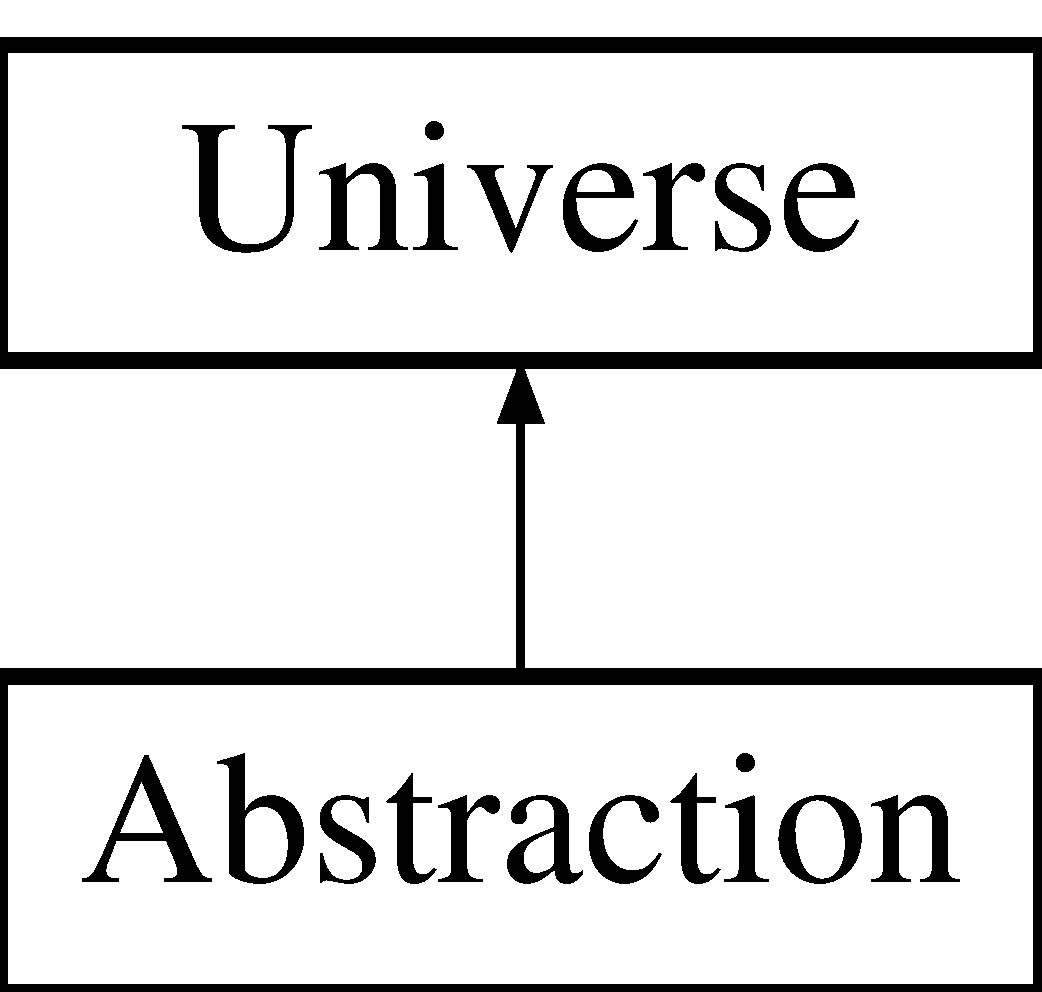
\includegraphics[height=2.000000cm]{classAbstraction}
\end{center}
\end{figure}
\subsection*{Public Member Functions}
\begin{DoxyCompactItemize}
\item 
\mbox{\hyperlink{classAbstraction_af4bf8b0e2bfd07d50ffc28b98f35b2ee}{Abstraction}} ()
\item 
virtual \mbox{\hyperlink{classAbstraction_aaf7d34417ea08792cc2b9449f9bfdc8e}{$\sim$\+Abstraction}} ()
\item 
unsigned int \mbox{\hyperlink{classAbstraction_a2b5e781d95a843a67db307b431f419a7}{Get\+Counter}} (std\+::chrono\+::time\+\_\+point$<$ \mbox{\hyperlink{universe_8h_a0ef8d951d1ca5ab3cfaf7ab4c7a6fd80}{Clock}} $>$ event\+\_\+time)
\item 
void \mbox{\hyperlink{classAbstraction_a82cd32bf3de41f35ab76d80611fe6763}{Set\+Counter}} (std\+::chrono\+::time\+\_\+point$<$ \mbox{\hyperlink{universe_8h_a0ef8d951d1ca5ab3cfaf7ab4c7a6fd80}{Clock}} $>$ event\+\_\+time, unsigned int val)
\end{DoxyCompactItemize}
\subsection*{Private Attributes}
\begin{DoxyCompactItemize}
\item 
unsigned int \mbox{\hyperlink{classAbstraction_a6144b0e382f72ad170a238d6ed4a0486}{m\+\_\+\+Counter}}
\begin{DoxyCompactList}\small\item\em Member variable \char`\"{}m\+\_\+\+Counter\char`\"{}. \end{DoxyCompactList}\end{DoxyCompactItemize}
\subsection*{Additional Inherited Members}


\subsection{Constructor \& Destructor Documentation}
\mbox{\Hypertarget{classAbstraction_af4bf8b0e2bfd07d50ffc28b98f35b2ee}\label{classAbstraction_af4bf8b0e2bfd07d50ffc28b98f35b2ee}} 
\index{Abstraction@{Abstraction}!Abstraction@{Abstraction}}
\index{Abstraction@{Abstraction}!Abstraction@{Abstraction}}
\subsubsection{\texorpdfstring{Abstraction()}{Abstraction()}}
{\footnotesize\ttfamily Abstraction\+::\+Abstraction (\begin{DoxyParamCaption}{ }\end{DoxyParamCaption})}

Default constructor \mbox{\Hypertarget{classAbstraction_aaf7d34417ea08792cc2b9449f9bfdc8e}\label{classAbstraction_aaf7d34417ea08792cc2b9449f9bfdc8e}} 
\index{Abstraction@{Abstraction}!````~Abstraction@{$\sim$\+Abstraction}}
\index{````~Abstraction@{$\sim$\+Abstraction}!Abstraction@{Abstraction}}
\subsubsection{\texorpdfstring{$\sim$\+Abstraction()}{~Abstraction()}}
{\footnotesize\ttfamily virtual Abstraction\+::$\sim$\+Abstraction (\begin{DoxyParamCaption}{ }\end{DoxyParamCaption})\hspace{0.3cm}{\ttfamily [virtual]}}

Default destructor 

\subsection{Member Function Documentation}
\mbox{\Hypertarget{classAbstraction_a2b5e781d95a843a67db307b431f419a7}\label{classAbstraction_a2b5e781d95a843a67db307b431f419a7}} 
\index{Abstraction@{Abstraction}!Get\+Counter@{Get\+Counter}}
\index{Get\+Counter@{Get\+Counter}!Abstraction@{Abstraction}}
\subsubsection{\texorpdfstring{Get\+Counter()}{GetCounter()}}
{\footnotesize\ttfamily unsigned int Abstraction\+::\+Get\+Counter (\begin{DoxyParamCaption}\item[{std\+::chrono\+::time\+\_\+point$<$ \mbox{\hyperlink{universe_8h_a0ef8d951d1ca5ab3cfaf7ab4c7a6fd80}{Clock}} $>$}]{event\+\_\+time }\end{DoxyParamCaption})\hspace{0.3cm}{\ttfamily [inline]}}

Access m\+\_\+\+Counter \begin{DoxyReturn}{Returns}
The current value of m\+\_\+\+Counter 
\end{DoxyReturn}
\mbox{\Hypertarget{classAbstraction_a82cd32bf3de41f35ab76d80611fe6763}\label{classAbstraction_a82cd32bf3de41f35ab76d80611fe6763}} 
\index{Abstraction@{Abstraction}!Set\+Counter@{Set\+Counter}}
\index{Set\+Counter@{Set\+Counter}!Abstraction@{Abstraction}}
\subsubsection{\texorpdfstring{Set\+Counter()}{SetCounter()}}
{\footnotesize\ttfamily void Abstraction\+::\+Set\+Counter (\begin{DoxyParamCaption}\item[{std\+::chrono\+::time\+\_\+point$<$ \mbox{\hyperlink{universe_8h_a0ef8d951d1ca5ab3cfaf7ab4c7a6fd80}{Clock}} $>$}]{event\+\_\+time,  }\item[{unsigned int}]{val }\end{DoxyParamCaption})\hspace{0.3cm}{\ttfamily [inline]}, {\ttfamily [virtual]}}

Set m\+\_\+\+Counter 
\begin{DoxyParams}{Parameters}
{\em val} & New value to Set \\
\hline
\end{DoxyParams}


Reimplemented from \mbox{\hyperlink{classUniverse_aa22202ae740eb1355529afcb13285e91}{Universe}}.



\subsection{Member Data Documentation}
\mbox{\Hypertarget{classAbstraction_a6144b0e382f72ad170a238d6ed4a0486}\label{classAbstraction_a6144b0e382f72ad170a238d6ed4a0486}} 
\index{Abstraction@{Abstraction}!m\+\_\+\+Counter@{m\+\_\+\+Counter}}
\index{m\+\_\+\+Counter@{m\+\_\+\+Counter}!Abstraction@{Abstraction}}
\subsubsection{\texorpdfstring{m\+\_\+\+Counter}{m\_Counter}}
{\footnotesize\ttfamily unsigned int Abstraction\+::m\+\_\+\+Counter\hspace{0.3cm}{\ttfamily [private]}}



Member variable \char`\"{}m\+\_\+\+Counter\char`\"{}. 



The documentation for this class was generated from the following file\+:\begin{DoxyCompactItemize}
\item 
/home/pbisaacs/\+Developer/\+Brain\+Harmonics/\+Brain\+Harmonics/\mbox{\hyperlink{abstraction_8h}{abstraction.\+h}}\end{DoxyCompactItemize}

\hypertarget{classAppTimer}{}\section{App\+Timer Class Reference}
\label{classAppTimer}\index{App\+Timer@{App\+Timer}}


{\ttfamily \#include $<$apptimer.\+h$>$}

Inheritance diagram for App\+Timer\+:\begin{figure}[H]
\begin{center}
\leavevmode
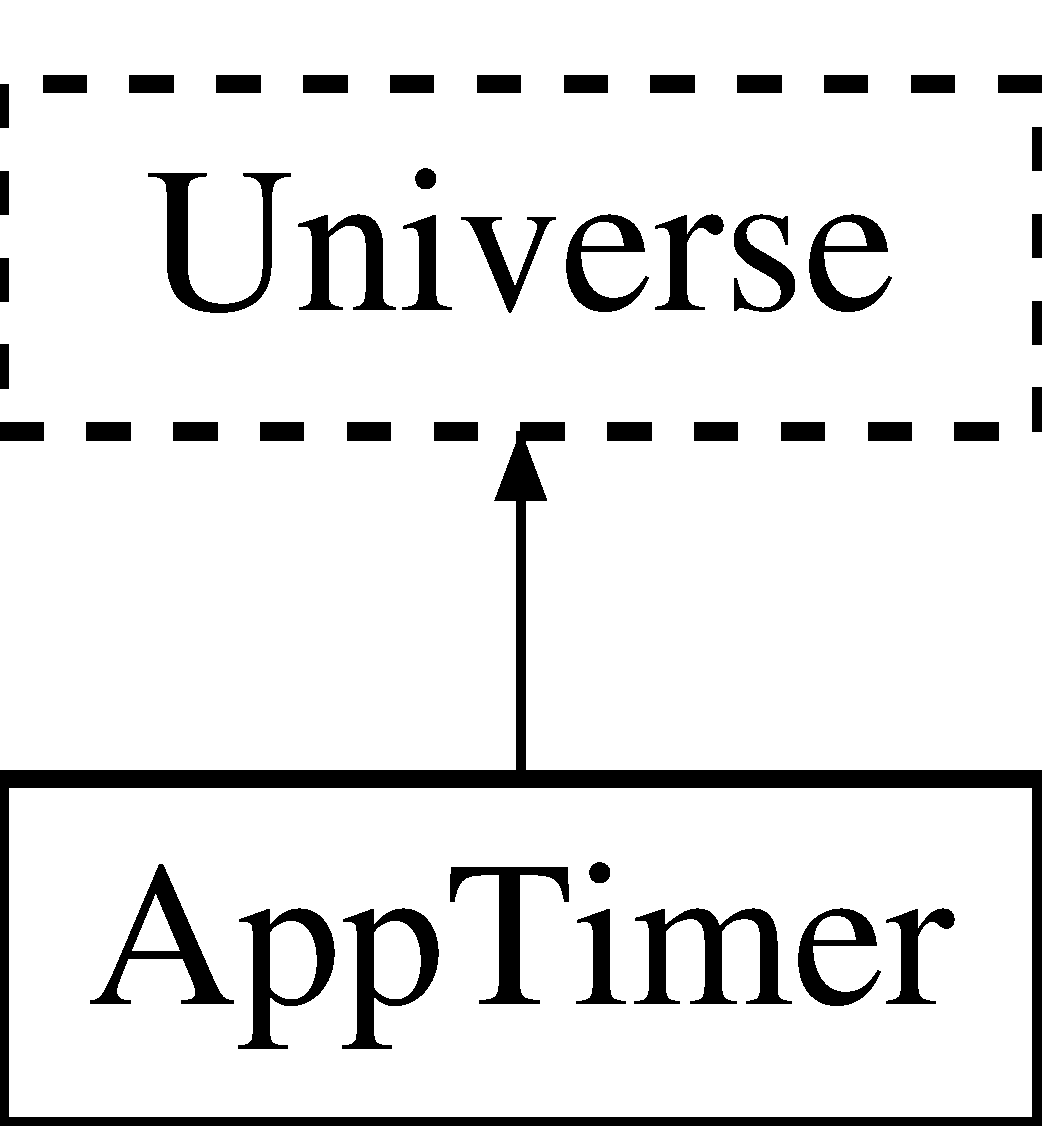
\includegraphics[height=2.000000cm]{classAppTimer}
\end{center}
\end{figure}
\subsection*{Public Member Functions}
\begin{DoxyCompactItemize}
\item 
\mbox{\hyperlink{classAppTimer_a59bf4eccdc9a3e16745b2cf9a122f935}{App\+Timer}} ()
\item 
\mbox{\hyperlink{classAppTimer_a06df15e33135f60f661c231e067951f3}{App\+Timer}} (unsigned int object\+\_\+type)
\item 
\mbox{\hyperlink{classAppTimer_a192075895ca575e9acb2663f3ebcecd6}{App\+Timer}} (unsigned int object\+\_\+type, std\+::chrono\+::time\+\_\+point$<$ \mbox{\hyperlink{universe_8h_a0ef8d951d1ca5ab3cfaf7ab4c7a6fd80}{Clock}} $>$ event\+\_\+time)
\item 
\mbox{\hyperlink{classAppTimer_af0836d131aa78b6812930199a5c7f9bd}{App\+Timer}} (unsigned int object\+\_\+type, std\+::chrono\+::time\+\_\+point$<$ \mbox{\hyperlink{universe_8h_a0ef8d951d1ca5ab3cfaf7ab4c7a6fd80}{Clock}} $>$ event\+\_\+time, \mbox{\hyperlink{classUniverse}{Universe}} \&universe\+\_\+connector)
\item 
virtual \mbox{\hyperlink{classAppTimer_a5ef0c072a0591cf5a3bcc07edbd3577f}{$\sim$\+App\+Timer}} ()
\item 
unsigned int \mbox{\hyperlink{classAppTimer_ab9bb2b5f283b02d6d2292e064ddbd2ab}{Get\+Counter}} (std\+::chrono\+::time\+\_\+point$<$ \mbox{\hyperlink{universe_8h_a0ef8d951d1ca5ab3cfaf7ab4c7a6fd80}{Clock}} $>$ event\+\_\+time)
\item 
void \mbox{\hyperlink{classAppTimer_a77d5d447d6b136a35304b0571a166ddc}{Set\+Counter}} (std\+::chrono\+::time\+\_\+point$<$ \mbox{\hyperlink{universe_8h_a0ef8d951d1ca5ab3cfaf7ab4c7a6fd80}{Clock}} $>$ event\+\_\+time, unsigned int val)
\end{DoxyCompactItemize}
\subsection*{Private Attributes}
\begin{DoxyCompactItemize}
\item 
unsigned int \mbox{\hyperlink{classAppTimer_addd53e74f8e65e44430bd20483592f98}{apptimer\+\_\+counter}}
\begin{DoxyCompactList}\small\item\em Member variable \char`\"{}m\+\_\+\+Counter\char`\"{}. \end{DoxyCompactList}\item 
int \mbox{\hyperlink{classAppTimer_a96accb68b0b4d0f0477d230b6965c460}{apptimer\+\_\+type}}
\item 
bool \mbox{\hyperlink{classAppTimer_aa16315b1eff51bc0561c9c5bf024bcc2}{object\+\_\+disabled}}
\item 
std\+::chrono\+::time\+\_\+point$<$ \mbox{\hyperlink{universe_8h_a0ef8d951d1ca5ab3cfaf7ab4c7a6fd80}{Clock}} $>$ \mbox{\hyperlink{classAppTimer_aae18c05cc314b40c572fbf674a01ac40}{time\+\_\+object\+\_\+created}}
\end{DoxyCompactItemize}
\subsection*{Additional Inherited Members}


\subsection{Constructor \& Destructor Documentation}
\mbox{\Hypertarget{classAppTimer_a59bf4eccdc9a3e16745b2cf9a122f935}\label{classAppTimer_a59bf4eccdc9a3e16745b2cf9a122f935}} 
\index{App\+Timer@{App\+Timer}!App\+Timer@{App\+Timer}}
\index{App\+Timer@{App\+Timer}!App\+Timer@{App\+Timer}}
\subsubsection{\texorpdfstring{App\+Timer()}{AppTimer()}\hspace{0.1cm}{\footnotesize\ttfamily [1/4]}}
{\footnotesize\ttfamily App\+Timer\+::\+App\+Timer (\begin{DoxyParamCaption}{ }\end{DoxyParamCaption})\hspace{0.3cm}{\ttfamily [inline]}}

\mbox{\Hypertarget{classAppTimer_a06df15e33135f60f661c231e067951f3}\label{classAppTimer_a06df15e33135f60f661c231e067951f3}} 
\index{App\+Timer@{App\+Timer}!App\+Timer@{App\+Timer}}
\index{App\+Timer@{App\+Timer}!App\+Timer@{App\+Timer}}
\subsubsection{\texorpdfstring{App\+Timer()}{AppTimer()}\hspace{0.1cm}{\footnotesize\ttfamily [2/4]}}
{\footnotesize\ttfamily App\+Timer\+::\+App\+Timer (\begin{DoxyParamCaption}\item[{unsigned int}]{object\+\_\+type }\end{DoxyParamCaption})\hspace{0.3cm}{\ttfamily [inline]}}

\mbox{\Hypertarget{classAppTimer_a192075895ca575e9acb2663f3ebcecd6}\label{classAppTimer_a192075895ca575e9acb2663f3ebcecd6}} 
\index{App\+Timer@{App\+Timer}!App\+Timer@{App\+Timer}}
\index{App\+Timer@{App\+Timer}!App\+Timer@{App\+Timer}}
\subsubsection{\texorpdfstring{App\+Timer()}{AppTimer()}\hspace{0.1cm}{\footnotesize\ttfamily [3/4]}}
{\footnotesize\ttfamily App\+Timer\+::\+App\+Timer (\begin{DoxyParamCaption}\item[{unsigned int}]{object\+\_\+type,  }\item[{std\+::chrono\+::time\+\_\+point$<$ \mbox{\hyperlink{universe_8h_a0ef8d951d1ca5ab3cfaf7ab4c7a6fd80}{Clock}} $>$}]{event\+\_\+time }\end{DoxyParamCaption})\hspace{0.3cm}{\ttfamily [inline]}}

\mbox{\Hypertarget{classAppTimer_af0836d131aa78b6812930199a5c7f9bd}\label{classAppTimer_af0836d131aa78b6812930199a5c7f9bd}} 
\index{App\+Timer@{App\+Timer}!App\+Timer@{App\+Timer}}
\index{App\+Timer@{App\+Timer}!App\+Timer@{App\+Timer}}
\subsubsection{\texorpdfstring{App\+Timer()}{AppTimer()}\hspace{0.1cm}{\footnotesize\ttfamily [4/4]}}
{\footnotesize\ttfamily App\+Timer\+::\+App\+Timer (\begin{DoxyParamCaption}\item[{unsigned int}]{object\+\_\+type,  }\item[{std\+::chrono\+::time\+\_\+point$<$ \mbox{\hyperlink{universe_8h_a0ef8d951d1ca5ab3cfaf7ab4c7a6fd80}{Clock}} $>$}]{event\+\_\+time,  }\item[{\mbox{\hyperlink{classUniverse}{Universe}} \&}]{universe\+\_\+connector }\end{DoxyParamCaption})\hspace{0.3cm}{\ttfamily [inline]}}

\mbox{\Hypertarget{classAppTimer_a5ef0c072a0591cf5a3bcc07edbd3577f}\label{classAppTimer_a5ef0c072a0591cf5a3bcc07edbd3577f}} 
\index{App\+Timer@{App\+Timer}!````~App\+Timer@{$\sim$\+App\+Timer}}
\index{````~App\+Timer@{$\sim$\+App\+Timer}!App\+Timer@{App\+Timer}}
\subsubsection{\texorpdfstring{$\sim$\+App\+Timer()}{~AppTimer()}}
{\footnotesize\ttfamily virtual App\+Timer\+::$\sim$\+App\+Timer (\begin{DoxyParamCaption}{ }\end{DoxyParamCaption})\hspace{0.3cm}{\ttfamily [inline]}, {\ttfamily [virtual]}}

Default destructor 

\subsection{Member Function Documentation}
\mbox{\Hypertarget{classAppTimer_ab9bb2b5f283b02d6d2292e064ddbd2ab}\label{classAppTimer_ab9bb2b5f283b02d6d2292e064ddbd2ab}} 
\index{App\+Timer@{App\+Timer}!Get\+Counter@{Get\+Counter}}
\index{Get\+Counter@{Get\+Counter}!App\+Timer@{App\+Timer}}
\subsubsection{\texorpdfstring{Get\+Counter()}{GetCounter()}}
{\footnotesize\ttfamily unsigned int App\+Timer\+::\+Get\+Counter (\begin{DoxyParamCaption}\item[{std\+::chrono\+::time\+\_\+point$<$ \mbox{\hyperlink{universe_8h_a0ef8d951d1ca5ab3cfaf7ab4c7a6fd80}{Clock}} $>$}]{event\+\_\+time }\end{DoxyParamCaption})\hspace{0.3cm}{\ttfamily [inline]}}

\mbox{\Hypertarget{classAppTimer_a77d5d447d6b136a35304b0571a166ddc}\label{classAppTimer_a77d5d447d6b136a35304b0571a166ddc}} 
\index{App\+Timer@{App\+Timer}!Set\+Counter@{Set\+Counter}}
\index{Set\+Counter@{Set\+Counter}!App\+Timer@{App\+Timer}}
\subsubsection{\texorpdfstring{Set\+Counter()}{SetCounter()}}
{\footnotesize\ttfamily void App\+Timer\+::\+Set\+Counter (\begin{DoxyParamCaption}\item[{std\+::chrono\+::time\+\_\+point$<$ \mbox{\hyperlink{universe_8h_a0ef8d951d1ca5ab3cfaf7ab4c7a6fd80}{Clock}} $>$}]{event\+\_\+time,  }\item[{unsigned int}]{val }\end{DoxyParamCaption})\hspace{0.3cm}{\ttfamily [inline]}, {\ttfamily [virtual]}}



Reimplemented from \mbox{\hyperlink{classUniverse_aa22202ae740eb1355529afcb13285e91}{Universe}}.



\subsection{Member Data Documentation}
\mbox{\Hypertarget{classAppTimer_addd53e74f8e65e44430bd20483592f98}\label{classAppTimer_addd53e74f8e65e44430bd20483592f98}} 
\index{App\+Timer@{App\+Timer}!apptimer\+\_\+counter@{apptimer\+\_\+counter}}
\index{apptimer\+\_\+counter@{apptimer\+\_\+counter}!App\+Timer@{App\+Timer}}
\subsubsection{\texorpdfstring{apptimer\+\_\+counter}{apptimer\_counter}}
{\footnotesize\ttfamily unsigned int App\+Timer\+::apptimer\+\_\+counter\hspace{0.3cm}{\ttfamily [private]}}



Member variable \char`\"{}m\+\_\+\+Counter\char`\"{}. 

\mbox{\Hypertarget{classAppTimer_a96accb68b0b4d0f0477d230b6965c460}\label{classAppTimer_a96accb68b0b4d0f0477d230b6965c460}} 
\index{App\+Timer@{App\+Timer}!apptimer\+\_\+type@{apptimer\+\_\+type}}
\index{apptimer\+\_\+type@{apptimer\+\_\+type}!App\+Timer@{App\+Timer}}
\subsubsection{\texorpdfstring{apptimer\+\_\+type}{apptimer\_type}}
{\footnotesize\ttfamily int App\+Timer\+::apptimer\+\_\+type\hspace{0.3cm}{\ttfamily [private]}}

\mbox{\Hypertarget{classAppTimer_aa16315b1eff51bc0561c9c5bf024bcc2}\label{classAppTimer_aa16315b1eff51bc0561c9c5bf024bcc2}} 
\index{App\+Timer@{App\+Timer}!object\+\_\+disabled@{object\+\_\+disabled}}
\index{object\+\_\+disabled@{object\+\_\+disabled}!App\+Timer@{App\+Timer}}
\subsubsection{\texorpdfstring{object\+\_\+disabled}{object\_disabled}}
{\footnotesize\ttfamily bool App\+Timer\+::object\+\_\+disabled\hspace{0.3cm}{\ttfamily [private]}}

\mbox{\Hypertarget{classAppTimer_aae18c05cc314b40c572fbf674a01ac40}\label{classAppTimer_aae18c05cc314b40c572fbf674a01ac40}} 
\index{App\+Timer@{App\+Timer}!time\+\_\+object\+\_\+created@{time\+\_\+object\+\_\+created}}
\index{time\+\_\+object\+\_\+created@{time\+\_\+object\+\_\+created}!App\+Timer@{App\+Timer}}
\subsubsection{\texorpdfstring{time\+\_\+object\+\_\+created}{time\_object\_created}}
{\footnotesize\ttfamily std\+::chrono\+::time\+\_\+point$<$\mbox{\hyperlink{universe_8h_a0ef8d951d1ca5ab3cfaf7ab4c7a6fd80}{Clock}}$>$ App\+Timer\+::time\+\_\+object\+\_\+created\hspace{0.3cm}{\ttfamily [private]}}



The documentation for this class was generated from the following file\+:\begin{DoxyCompactItemize}
\item 
/home/pbisaacs/\+Developer/\+Brain\+Harmonics/\mbox{\hyperlink{apptimer_8h}{apptimer.\+h}}\end{DoxyCompactItemize}

\hypertarget{classAxon}{}\section{Axon Class Reference}
\label{classAxon}\index{Axon@{Axon}}


{\ttfamily \#include $<$axon.\+h$>$}

Inheritance diagram for Axon\+:\begin{figure}[H]
\begin{center}
\leavevmode
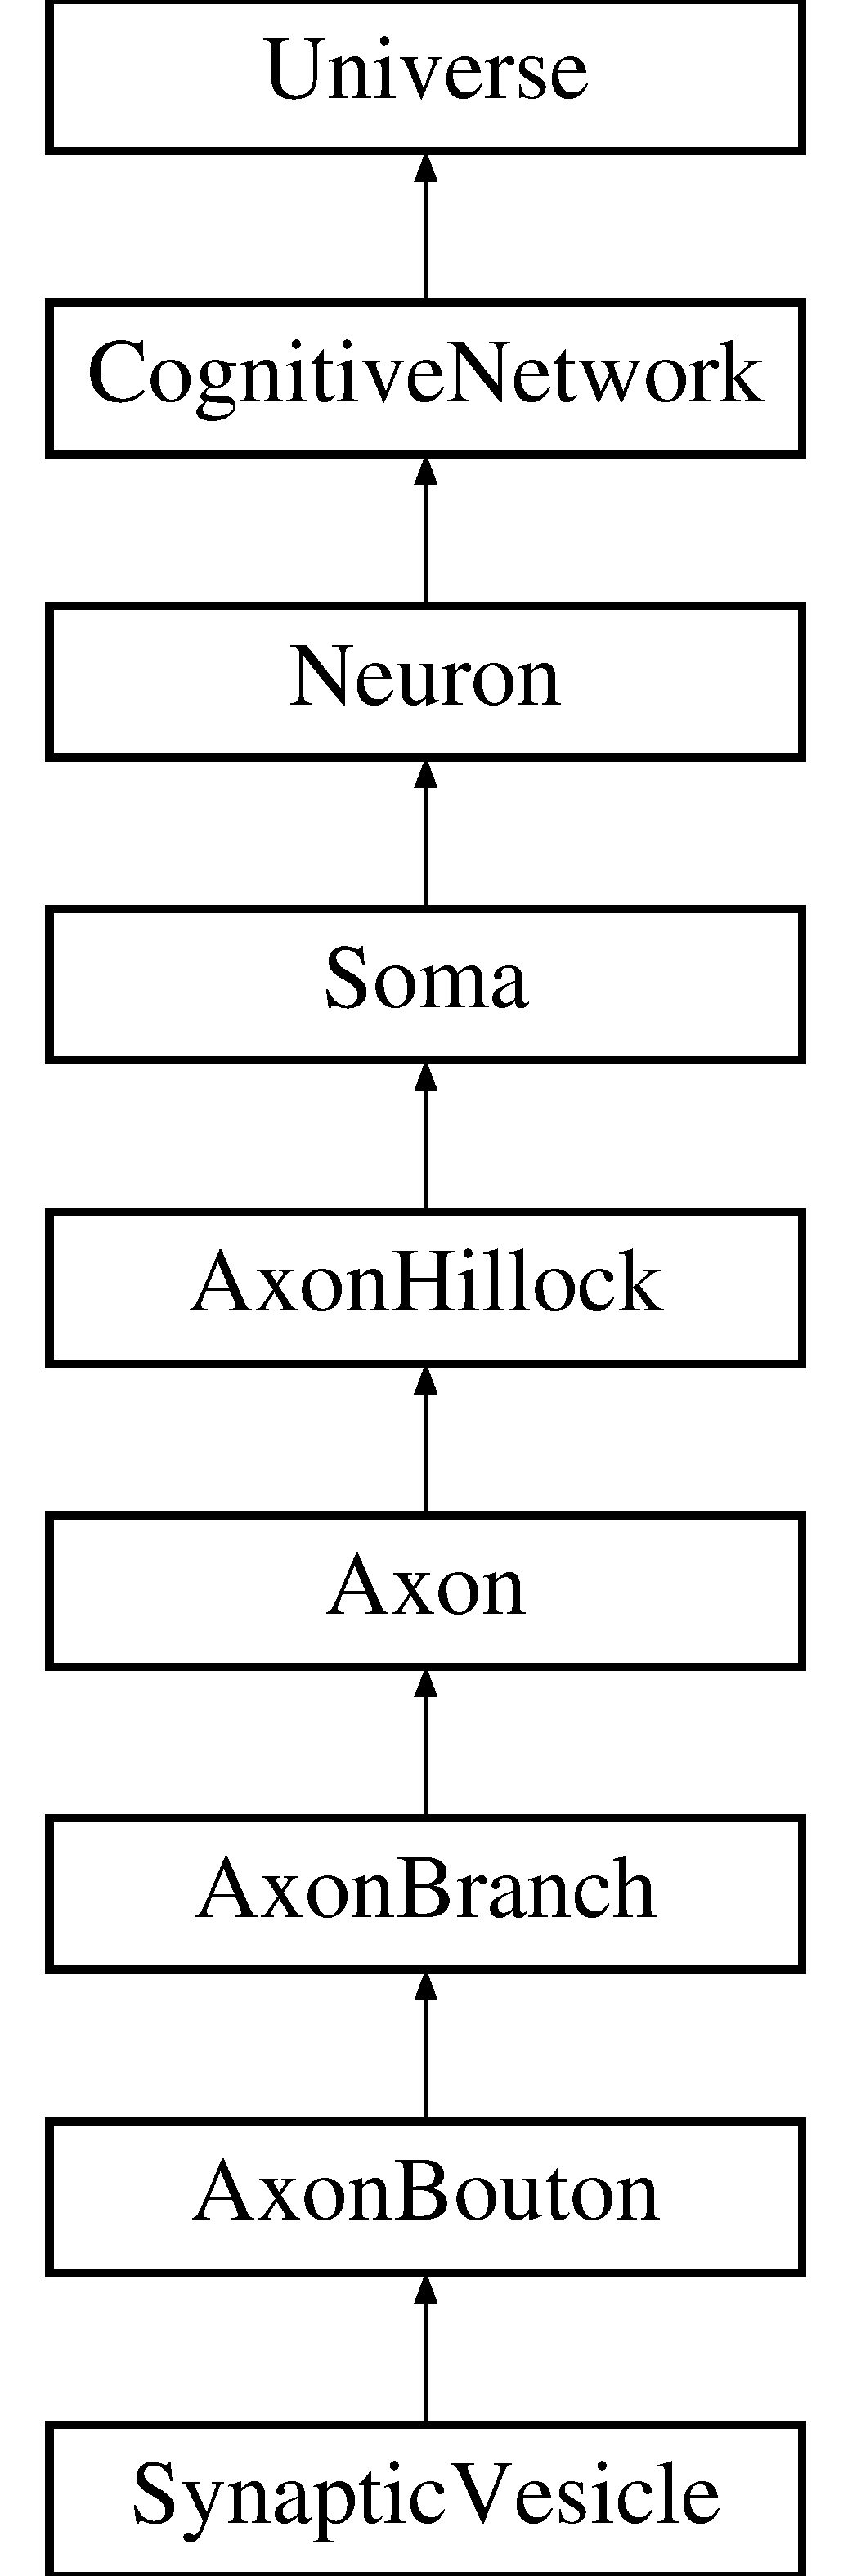
\includegraphics[height=9.000000cm]{classAxon}
\end{center}
\end{figure}
\subsection*{Public Member Functions}
\begin{DoxyCompactItemize}
\item 
\mbox{\hyperlink{classAxon_a1a0703b026b74c83e418613d929c5d22}{Axon}} ()
\item 
\mbox{\hyperlink{classAxon_a7cc05238af77735983111d1ca58c9c9b}{Axon}} (unsigned int object\+\_\+type)
\item 
\mbox{\hyperlink{classAxon_a0ca4cd87ad4a2719c6b7c8c3d46dcbc6}{Axon}} (unsigned int object\+\_\+type, std\+::chrono\+::time\+\_\+point$<$ \mbox{\hyperlink{universe_8h_a0ef8d951d1ca5ab3cfaf7ab4c7a6fd80}{Clock}} $>$ event\+\_\+time)
\item 
\mbox{\hyperlink{classAxon_afaffed720efb3cb75e46088c5fb81d95}{Axon}} (unsigned int object\+\_\+type, std\+::chrono\+::time\+\_\+point$<$ \mbox{\hyperlink{universe_8h_a0ef8d951d1ca5ab3cfaf7ab4c7a6fd80}{Clock}} $>$ event\+\_\+time, \mbox{\hyperlink{classAxonHillock}{Axon\+Hillock}} \&axonhillock\+\_\+connector)
\item 
virtual \mbox{\hyperlink{classAxon_af000507f0ff0527d1743e90d2e756282}{$\sim$\+Axon}} ()
\item 
unsigned int \mbox{\hyperlink{classAxon_a390ff1f3d85034fc85bcafc7374da9c7}{Get\+Counter}} (std\+::chrono\+::time\+\_\+point$<$ \mbox{\hyperlink{universe_8h_a0ef8d951d1ca5ab3cfaf7ab4c7a6fd80}{Clock}} $>$ event\+\_\+time)
\item 
double \mbox{\hyperlink{classAxon_a37a1ca2b0454d77dc0bc93e493feb0ce}{Get\+Energy}} (std\+::chrono\+::time\+\_\+point$<$ \mbox{\hyperlink{universe_8h_a0ef8d951d1ca5ab3cfaf7ab4c7a6fd80}{Clock}} $>$ event\+\_\+time)
\item 
void \mbox{\hyperlink{classAxon_a3493cb97bde26bd66facc6084cd5f219}{Set\+Counter}} (std\+::chrono\+::time\+\_\+point$<$ \mbox{\hyperlink{universe_8h_a0ef8d951d1ca5ab3cfaf7ab4c7a6fd80}{Clock}} $>$ event\+\_\+time, unsigned int val)
\item 
void \mbox{\hyperlink{classAxon_af5108f451de97deb56138e8e81ced359}{Set\+Energy}} (std\+::chrono\+::time\+\_\+point$<$ \mbox{\hyperlink{universe_8h_a0ef8d951d1ca5ab3cfaf7ab4c7a6fd80}{Clock}} $>$ event\+\_\+time, double val)
\item 
bool \mbox{\hyperlink{classAxon_ae079e0b47f5027625da158930e4fa9c5}{Reset\+Parameters}} (std\+::chrono\+::time\+\_\+point$<$ \mbox{\hyperlink{universe_8h_a0ef8d951d1ca5ab3cfaf7ab4c7a6fd80}{Clock}} $>$ event\+\_\+time)
\item 
\mbox{\hyperlink{classAxon}{Axon}} $\ast$ \mbox{\hyperlink{classAxon_a41e97ead4c793003db2de87061574c26}{Create\+Axon\+Branch}} (std\+::chrono\+::time\+\_\+point$<$ \mbox{\hyperlink{universe_8h_a0ef8d951d1ca5ab3cfaf7ab4c7a6fd80}{Clock}} $>$ event\+\_\+time)
\item 
std\+::vector$<$ \mbox{\hyperlink{classAxon}{Axon}} $\ast$ $>$ \mbox{\hyperlink{classAxon_ab0da51c05a0879efdb45c594b68ef8fd}{Create\+Axon\+Branches}} (std\+::chrono\+::time\+\_\+point$<$ \mbox{\hyperlink{universe_8h_a0ef8d951d1ca5ab3cfaf7ab4c7a6fd80}{Clock}} $>$ event\+\_\+time, int quantity)
\item 
\mbox{\hyperlink{classAxon}{Axon}} $\ast$ \mbox{\hyperlink{classAxon_a7720ee66a75e87f4e308b82d1841443a}{Clone\+Axon\+Branch}} (std\+::chrono\+::time\+\_\+point$<$ \mbox{\hyperlink{universe_8h_a0ef8d951d1ca5ab3cfaf7ab4c7a6fd80}{Clock}} $>$ event\+\_\+time, \mbox{\hyperlink{classAxon}{Axon}} $\ast$clone\+\_\+object, double perfection\+\_\+membership)
\item 
std\+::vector$<$ \mbox{\hyperlink{classAxon}{Axon}} $\ast$ $>$ \mbox{\hyperlink{classAxon_af2d6d5bc9ee0cd8ff654a949ef1cc294}{Clone\+Axon\+Branches}} (std\+::chrono\+::time\+\_\+point$<$ \mbox{\hyperlink{universe_8h_a0ef8d951d1ca5ab3cfaf7ab4c7a6fd80}{Clock}} $>$ event\+\_\+time, std\+::vector$<$ \mbox{\hyperlink{classAxon}{Axon}} $\ast$$>$ cloning\+\_\+list, double perfection\+\_\+membership)
\item 
\mbox{\hyperlink{classAxon}{Axon}} $\ast$ \mbox{\hyperlink{classAxon_a6ac580e4565d24c955b0a48d7a8b20e2}{Destroy\+Axon\+Branch}} (std\+::chrono\+::time\+\_\+point$<$ \mbox{\hyperlink{universe_8h_a0ef8d951d1ca5ab3cfaf7ab4c7a6fd80}{Clock}} $>$ event\+\_\+time, \mbox{\hyperlink{classAxon}{Axon}} $\ast$destroy\+\_\+object)
\item 
std\+::vector$<$ \mbox{\hyperlink{classAxon}{Axon}} $\ast$ $>$ \mbox{\hyperlink{classAxon_aa9d26eed8d178527d1995adfad2f67ac}{Destroy\+Axon\+Branches}} (std\+::chrono\+::time\+\_\+point$<$ \mbox{\hyperlink{universe_8h_a0ef8d951d1ca5ab3cfaf7ab4c7a6fd80}{Clock}} $>$ event\+\_\+time, std\+::vector$<$ \mbox{\hyperlink{classAxon}{Axon}} $\ast$$>$ destruction\+\_\+list)
\item 
\mbox{\hyperlink{classAxon}{Axon}} $\ast$ \mbox{\hyperlink{classAxon_a6ed85466115dab46ef71f26a420249ff}{Add\+Axon\+Branch}} (std\+::chrono\+::time\+\_\+point$<$ \mbox{\hyperlink{universe_8h_a0ef8d951d1ca5ab3cfaf7ab4c7a6fd80}{Clock}} $>$ event\+\_\+time, \mbox{\hyperlink{classAxon}{Axon}} $\ast$add\+\_\+object)
\item 
std\+::vector$<$ \mbox{\hyperlink{classAxon}{Axon}} $\ast$ $>$ \mbox{\hyperlink{classAxon_a04969d98c3fbb671cba5daccacffc003}{Add\+Axon\+Branches}} (std\+::chrono\+::time\+\_\+point$<$ \mbox{\hyperlink{universe_8h_a0ef8d951d1ca5ab3cfaf7ab4c7a6fd80}{Clock}} $>$ event\+\_\+time, std\+::vector$<$ \mbox{\hyperlink{classAxon}{Axon}} $\ast$$>$ add\+\_\+objects)
\item 
\mbox{\hyperlink{classAxon}{Axon}} $\ast$ \mbox{\hyperlink{classAxon_a7b43ca7f5b696c72ac17a27fea3b2822}{Remove\+Axon\+Branch}} (std\+::chrono\+::time\+\_\+point$<$ \mbox{\hyperlink{universe_8h_a0ef8d951d1ca5ab3cfaf7ab4c7a6fd80}{Clock}} $>$ event\+\_\+time)
\item 
std\+::vector$<$ \mbox{\hyperlink{classAxon}{Axon}} $\ast$ $>$ \mbox{\hyperlink{classAxon_a4c7af6c0900ae766c55362bfbb827ce3}{Remove\+Axon\+Branches}} (std\+::chrono\+::time\+\_\+point$<$ \mbox{\hyperlink{universe_8h_a0ef8d951d1ca5ab3cfaf7ab4c7a6fd80}{Clock}} $>$ event\+\_\+time, int quantity)
\item 
\mbox{\hyperlink{classAxon}{Axon}} $\ast$ \mbox{\hyperlink{classAxon_a723b00504169712e47f7437111ad4ae3}{Get\+Axon\+Branch}} (std\+::chrono\+::time\+\_\+point$<$ \mbox{\hyperlink{universe_8h_a0ef8d951d1ca5ab3cfaf7ab4c7a6fd80}{Clock}} $>$ event\+\_\+time, int selector)
\item 
std\+::vector$<$ \mbox{\hyperlink{classAxon}{Axon}} $\ast$ $>$ \mbox{\hyperlink{classAxon_adf5796ef2f72ce56516b37e7e09e9d6c}{Get\+Axon\+Branches}} (std\+::chrono\+::time\+\_\+point$<$ \mbox{\hyperlink{universe_8h_a0ef8d951d1ca5ab3cfaf7ab4c7a6fd80}{Clock}} $>$ event\+\_\+time)
\item 
int \mbox{\hyperlink{classAxon_a0065c335bc57e0a75962bcbd91f35001}{Growth}} (std\+::chrono\+::time\+\_\+point$<$ \mbox{\hyperlink{universe_8h_a0ef8d951d1ca5ab3cfaf7ab4c7a6fd80}{Clock}} $>$ event\+\_\+time)
\item 
int \mbox{\hyperlink{classAxon_a472ee760a1727072afaff0035d1eedd9}{Update}} (std\+::chrono\+::time\+\_\+point$<$ \mbox{\hyperlink{universe_8h_a0ef8d951d1ca5ab3cfaf7ab4c7a6fd80}{Clock}} $>$ event\+\_\+time)
\end{DoxyCompactItemize}
\subsection*{Protected Attributes}
\begin{DoxyCompactItemize}
\item 
std\+::vector$<$ \mbox{\hyperlink{classAxon}{Axon}} $\ast$ $>$ \mbox{\hyperlink{classAxon_ab32c0e4335cc4da8fe1aace7c16a88bf}{axonbranch\+\_\+list}}
\end{DoxyCompactItemize}
\subsection*{Private Attributes}
\begin{DoxyCompactItemize}
\item 
int \mbox{\hyperlink{classAxon_abbd92e8cf3ef8204baab98e7cbb08c64}{axon\+\_\+type}}
\item 
int \mbox{\hyperlink{classAxon_a4ad266c581741a63bf0c495a35ee3eff}{m\+\_\+add\+Status}}
\item 
int \mbox{\hyperlink{classAxon_a1be97ce73a4e60afb25798c397610be5}{axonbranch\+\_\+pool}}
\item 
bool \mbox{\hyperlink{classAxon_adc8989011b569ae1227a47f83f419694}{object\+\_\+disabled}}
\item 
std\+::chrono\+::time\+\_\+point$<$ \mbox{\hyperlink{universe_8h_a0ef8d951d1ca5ab3cfaf7ab4c7a6fd80}{Clock}} $>$ \mbox{\hyperlink{classAxon_a01b83a46da58746087de2c6f1dd30405}{time\+\_\+object\+\_\+created}}
\item 
std\+::chrono\+::time\+\_\+point$<$ \mbox{\hyperlink{universe_8h_a0ef8d951d1ca5ab3cfaf7ab4c7a6fd80}{Clock}} $>$ \mbox{\hyperlink{classAxon_a3270d8b1bf8875da361ea6e7dd46d8f1}{previous\+\_\+event\+\_\+time}}
\item 
bool \mbox{\hyperlink{classAxon_a171c967b604d668f118d3c857d23593d}{object\+\_\+initialised}} = false
\item 
int \mbox{\hyperlink{classAxon_a9aae3819e2bb13084966b70b242c8745}{duration\+\_\+since\+\_\+last\+\_\+event}}
\item 
double \mbox{\hyperlink{classAxon_a6cfb696bb484732e6d9d4c25cb4ccc7c}{m\+\_\+\+Volume}}
\item 
double \mbox{\hyperlink{classAxon_ae0e1d436b8ef9fd1007815ffc2e66e77}{m\+\_\+\+Surface\+Area}}
\item 
double \mbox{\hyperlink{classAxon_a2e5391cbc38b47b56265bc0e3d1129c8}{object\+\_\+size}}
\item 
unsigned int \mbox{\hyperlink{classAxon_a83973df45e4d3b58ca80e1ff27f69a90}{m\+\_\+\+Counter}}
\begin{DoxyCompactList}\small\item\em Member variable \char`\"{}m\+\_\+\+Counter\char`\"{}. \end{DoxyCompactList}\item 
double \mbox{\hyperlink{classAxon_a14fb0a3f9b06f6f68dd884e3ac82f828}{object\+\_\+energy}}
\begin{DoxyCompactList}\small\item\em Member variable \char`\"{}object\+\_\+energy\char`\"{}. \end{DoxyCompactList}\item 
double \mbox{\hyperlink{classAxon_a20223e0edff81afc14afbb5948570946}{object\+\_\+energy\+\_\+threshold}}
\item 
double \mbox{\hyperlink{classAxon_aeabc708a12965b17b5051a4fb11804c2}{m\+\_\+axonlength}}
\item 
double \mbox{\hyperlink{classAxon_ac477f6fc442313e4ba4eb3b069b9e5cf}{m\+\_\+\+Time\+Dilation}}
\item 
double \mbox{\hyperlink{classAxon_ae00fc37fb241ab5551a3cce4fc2a6299}{m\+\_\+\+Time\+Threshold}}
\end{DoxyCompactItemize}
\subsection*{Additional Inherited Members}


\subsection{Constructor \& Destructor Documentation}
\mbox{\Hypertarget{classAxon_a1a0703b026b74c83e418613d929c5d22}\label{classAxon_a1a0703b026b74c83e418613d929c5d22}} 
\index{Axon@{Axon}!Axon@{Axon}}
\index{Axon@{Axon}!Axon@{Axon}}
\subsubsection{\texorpdfstring{Axon()}{Axon()}\hspace{0.1cm}{\footnotesize\ttfamily [1/4]}}
{\footnotesize\ttfamily Axon\+::\+Axon (\begin{DoxyParamCaption}{ }\end{DoxyParamCaption})\hspace{0.3cm}{\ttfamily [inline]}}

\mbox{\Hypertarget{classAxon_a7cc05238af77735983111d1ca58c9c9b}\label{classAxon_a7cc05238af77735983111d1ca58c9c9b}} 
\index{Axon@{Axon}!Axon@{Axon}}
\index{Axon@{Axon}!Axon@{Axon}}
\subsubsection{\texorpdfstring{Axon()}{Axon()}\hspace{0.1cm}{\footnotesize\ttfamily [2/4]}}
{\footnotesize\ttfamily Axon\+::\+Axon (\begin{DoxyParamCaption}\item[{unsigned int}]{object\+\_\+type }\end{DoxyParamCaption})\hspace{0.3cm}{\ttfamily [inline]}}

\mbox{\Hypertarget{classAxon_a0ca4cd87ad4a2719c6b7c8c3d46dcbc6}\label{classAxon_a0ca4cd87ad4a2719c6b7c8c3d46dcbc6}} 
\index{Axon@{Axon}!Axon@{Axon}}
\index{Axon@{Axon}!Axon@{Axon}}
\subsubsection{\texorpdfstring{Axon()}{Axon()}\hspace{0.1cm}{\footnotesize\ttfamily [3/4]}}
{\footnotesize\ttfamily Axon\+::\+Axon (\begin{DoxyParamCaption}\item[{unsigned int}]{object\+\_\+type,  }\item[{std\+::chrono\+::time\+\_\+point$<$ \mbox{\hyperlink{universe_8h_a0ef8d951d1ca5ab3cfaf7ab4c7a6fd80}{Clock}} $>$}]{event\+\_\+time }\end{DoxyParamCaption})\hspace{0.3cm}{\ttfamily [inline]}}

\mbox{\Hypertarget{classAxon_afaffed720efb3cb75e46088c5fb81d95}\label{classAxon_afaffed720efb3cb75e46088c5fb81d95}} 
\index{Axon@{Axon}!Axon@{Axon}}
\index{Axon@{Axon}!Axon@{Axon}}
\subsubsection{\texorpdfstring{Axon()}{Axon()}\hspace{0.1cm}{\footnotesize\ttfamily [4/4]}}
{\footnotesize\ttfamily Axon\+::\+Axon (\begin{DoxyParamCaption}\item[{unsigned int}]{object\+\_\+type,  }\item[{std\+::chrono\+::time\+\_\+point$<$ \mbox{\hyperlink{universe_8h_a0ef8d951d1ca5ab3cfaf7ab4c7a6fd80}{Clock}} $>$}]{event\+\_\+time,  }\item[{\mbox{\hyperlink{classAxonHillock}{Axon\+Hillock}} \&}]{axonhillock\+\_\+connector }\end{DoxyParamCaption})\hspace{0.3cm}{\ttfamily [inline]}}

\mbox{\Hypertarget{classAxon_af000507f0ff0527d1743e90d2e756282}\label{classAxon_af000507f0ff0527d1743e90d2e756282}} 
\index{Axon@{Axon}!````~Axon@{$\sim$\+Axon}}
\index{````~Axon@{$\sim$\+Axon}!Axon@{Axon}}
\subsubsection{\texorpdfstring{$\sim$\+Axon()}{~Axon()}}
{\footnotesize\ttfamily virtual Axon\+::$\sim$\+Axon (\begin{DoxyParamCaption}{ }\end{DoxyParamCaption})\hspace{0.3cm}{\ttfamily [inline]}, {\ttfamily [virtual]}}

Default destructor 

\subsection{Member Function Documentation}
\mbox{\Hypertarget{classAxon_a6ed85466115dab46ef71f26a420249ff}\label{classAxon_a6ed85466115dab46ef71f26a420249ff}} 
\index{Axon@{Axon}!Add\+Axon\+Branch@{Add\+Axon\+Branch}}
\index{Add\+Axon\+Branch@{Add\+Axon\+Branch}!Axon@{Axon}}
\subsubsection{\texorpdfstring{Add\+Axon\+Branch()}{AddAxonBranch()}}
{\footnotesize\ttfamily \mbox{\hyperlink{classAxon}{Axon}} $\ast$ Axon\+::\+Add\+Axon\+Branch (\begin{DoxyParamCaption}\item[{std\+::chrono\+::time\+\_\+point$<$ \mbox{\hyperlink{universe_8h_a0ef8d951d1ca5ab3cfaf7ab4c7a6fd80}{Clock}} $>$}]{event\+\_\+time,  }\item[{\mbox{\hyperlink{classAxon}{Axon}} $\ast$}]{add\+\_\+object }\end{DoxyParamCaption})}

\mbox{\Hypertarget{classAxon_a04969d98c3fbb671cba5daccacffc003}\label{classAxon_a04969d98c3fbb671cba5daccacffc003}} 
\index{Axon@{Axon}!Add\+Axon\+Branches@{Add\+Axon\+Branches}}
\index{Add\+Axon\+Branches@{Add\+Axon\+Branches}!Axon@{Axon}}
\subsubsection{\texorpdfstring{Add\+Axon\+Branches()}{AddAxonBranches()}}
{\footnotesize\ttfamily std\+::vector$<$ \mbox{\hyperlink{classAxon}{Axon}} $\ast$ $>$ Axon\+::\+Add\+Axon\+Branches (\begin{DoxyParamCaption}\item[{std\+::chrono\+::time\+\_\+point$<$ \mbox{\hyperlink{universe_8h_a0ef8d951d1ca5ab3cfaf7ab4c7a6fd80}{Clock}} $>$}]{event\+\_\+time,  }\item[{std\+::vector$<$ \mbox{\hyperlink{classAxon}{Axon}} $\ast$$>$}]{add\+\_\+objects }\end{DoxyParamCaption})}

\mbox{\Hypertarget{classAxon_a7720ee66a75e87f4e308b82d1841443a}\label{classAxon_a7720ee66a75e87f4e308b82d1841443a}} 
\index{Axon@{Axon}!Clone\+Axon\+Branch@{Clone\+Axon\+Branch}}
\index{Clone\+Axon\+Branch@{Clone\+Axon\+Branch}!Axon@{Axon}}
\subsubsection{\texorpdfstring{Clone\+Axon\+Branch()}{CloneAxonBranch()}}
{\footnotesize\ttfamily \mbox{\hyperlink{classAxon}{Axon}} $\ast$ Axon\+::\+Clone\+Axon\+Branch (\begin{DoxyParamCaption}\item[{std\+::chrono\+::time\+\_\+point$<$ \mbox{\hyperlink{universe_8h_a0ef8d951d1ca5ab3cfaf7ab4c7a6fd80}{Clock}} $>$}]{event\+\_\+time,  }\item[{\mbox{\hyperlink{classAxon}{Axon}} $\ast$}]{clone\+\_\+object,  }\item[{double}]{perfection\+\_\+membership }\end{DoxyParamCaption})}

\mbox{\Hypertarget{classAxon_af2d6d5bc9ee0cd8ff654a949ef1cc294}\label{classAxon_af2d6d5bc9ee0cd8ff654a949ef1cc294}} 
\index{Axon@{Axon}!Clone\+Axon\+Branches@{Clone\+Axon\+Branches}}
\index{Clone\+Axon\+Branches@{Clone\+Axon\+Branches}!Axon@{Axon}}
\subsubsection{\texorpdfstring{Clone\+Axon\+Branches()}{CloneAxonBranches()}}
{\footnotesize\ttfamily std\+::vector$<$ \mbox{\hyperlink{classAxon}{Axon}} $\ast$ $>$ Axon\+::\+Clone\+Axon\+Branches (\begin{DoxyParamCaption}\item[{std\+::chrono\+::time\+\_\+point$<$ \mbox{\hyperlink{universe_8h_a0ef8d951d1ca5ab3cfaf7ab4c7a6fd80}{Clock}} $>$}]{event\+\_\+time,  }\item[{std\+::vector$<$ \mbox{\hyperlink{classAxon}{Axon}} $\ast$$>$}]{cloning\+\_\+list,  }\item[{double}]{perfection\+\_\+membership }\end{DoxyParamCaption})}

\mbox{\Hypertarget{classAxon_a41e97ead4c793003db2de87061574c26}\label{classAxon_a41e97ead4c793003db2de87061574c26}} 
\index{Axon@{Axon}!Create\+Axon\+Branch@{Create\+Axon\+Branch}}
\index{Create\+Axon\+Branch@{Create\+Axon\+Branch}!Axon@{Axon}}
\subsubsection{\texorpdfstring{Create\+Axon\+Branch()}{CreateAxonBranch()}}
{\footnotesize\ttfamily \mbox{\hyperlink{classAxon}{Axon}} $\ast$ Axon\+::\+Create\+Axon\+Branch (\begin{DoxyParamCaption}\item[{std\+::chrono\+::time\+\_\+point$<$ \mbox{\hyperlink{universe_8h_a0ef8d951d1ca5ab3cfaf7ab4c7a6fd80}{Clock}} $>$}]{event\+\_\+time }\end{DoxyParamCaption})}

\mbox{\Hypertarget{classAxon_ab0da51c05a0879efdb45c594b68ef8fd}\label{classAxon_ab0da51c05a0879efdb45c594b68ef8fd}} 
\index{Axon@{Axon}!Create\+Axon\+Branches@{Create\+Axon\+Branches}}
\index{Create\+Axon\+Branches@{Create\+Axon\+Branches}!Axon@{Axon}}
\subsubsection{\texorpdfstring{Create\+Axon\+Branches()}{CreateAxonBranches()}}
{\footnotesize\ttfamily std\+::vector$<$ \mbox{\hyperlink{classAxon}{Axon}} $\ast$ $>$ Axon\+::\+Create\+Axon\+Branches (\begin{DoxyParamCaption}\item[{std\+::chrono\+::time\+\_\+point$<$ \mbox{\hyperlink{universe_8h_a0ef8d951d1ca5ab3cfaf7ab4c7a6fd80}{Clock}} $>$}]{event\+\_\+time,  }\item[{int}]{quantity }\end{DoxyParamCaption})}

\mbox{\Hypertarget{classAxon_a6ac580e4565d24c955b0a48d7a8b20e2}\label{classAxon_a6ac580e4565d24c955b0a48d7a8b20e2}} 
\index{Axon@{Axon}!Destroy\+Axon\+Branch@{Destroy\+Axon\+Branch}}
\index{Destroy\+Axon\+Branch@{Destroy\+Axon\+Branch}!Axon@{Axon}}
\subsubsection{\texorpdfstring{Destroy\+Axon\+Branch()}{DestroyAxonBranch()}}
{\footnotesize\ttfamily \mbox{\hyperlink{classAxon}{Axon}} $\ast$ Axon\+::\+Destroy\+Axon\+Branch (\begin{DoxyParamCaption}\item[{std\+::chrono\+::time\+\_\+point$<$ \mbox{\hyperlink{universe_8h_a0ef8d951d1ca5ab3cfaf7ab4c7a6fd80}{Clock}} $>$}]{event\+\_\+time,  }\item[{\mbox{\hyperlink{classAxon}{Axon}} $\ast$}]{destroy\+\_\+object }\end{DoxyParamCaption})}

\mbox{\Hypertarget{classAxon_aa9d26eed8d178527d1995adfad2f67ac}\label{classAxon_aa9d26eed8d178527d1995adfad2f67ac}} 
\index{Axon@{Axon}!Destroy\+Axon\+Branches@{Destroy\+Axon\+Branches}}
\index{Destroy\+Axon\+Branches@{Destroy\+Axon\+Branches}!Axon@{Axon}}
\subsubsection{\texorpdfstring{Destroy\+Axon\+Branches()}{DestroyAxonBranches()}}
{\footnotesize\ttfamily std\+::vector$<$ \mbox{\hyperlink{classAxon}{Axon}} $\ast$ $>$ Axon\+::\+Destroy\+Axon\+Branches (\begin{DoxyParamCaption}\item[{std\+::chrono\+::time\+\_\+point$<$ \mbox{\hyperlink{universe_8h_a0ef8d951d1ca5ab3cfaf7ab4c7a6fd80}{Clock}} $>$}]{event\+\_\+time,  }\item[{std\+::vector$<$ \mbox{\hyperlink{classAxon}{Axon}} $\ast$$>$}]{destruction\+\_\+list }\end{DoxyParamCaption})}

\mbox{\Hypertarget{classAxon_a723b00504169712e47f7437111ad4ae3}\label{classAxon_a723b00504169712e47f7437111ad4ae3}} 
\index{Axon@{Axon}!Get\+Axon\+Branch@{Get\+Axon\+Branch}}
\index{Get\+Axon\+Branch@{Get\+Axon\+Branch}!Axon@{Axon}}
\subsubsection{\texorpdfstring{Get\+Axon\+Branch()}{GetAxonBranch()}}
{\footnotesize\ttfamily \mbox{\hyperlink{classAxon}{Axon}} $\ast$ Axon\+::\+Get\+Axon\+Branch (\begin{DoxyParamCaption}\item[{std\+::chrono\+::time\+\_\+point$<$ \mbox{\hyperlink{universe_8h_a0ef8d951d1ca5ab3cfaf7ab4c7a6fd80}{Clock}} $>$}]{event\+\_\+time,  }\item[{int}]{selector }\end{DoxyParamCaption})}

\mbox{\Hypertarget{classAxon_adf5796ef2f72ce56516b37e7e09e9d6c}\label{classAxon_adf5796ef2f72ce56516b37e7e09e9d6c}} 
\index{Axon@{Axon}!Get\+Axon\+Branches@{Get\+Axon\+Branches}}
\index{Get\+Axon\+Branches@{Get\+Axon\+Branches}!Axon@{Axon}}
\subsubsection{\texorpdfstring{Get\+Axon\+Branches()}{GetAxonBranches()}}
{\footnotesize\ttfamily std\+::vector$<$ \mbox{\hyperlink{classAxon}{Axon}} $\ast$ $>$ Axon\+::\+Get\+Axon\+Branches (\begin{DoxyParamCaption}\item[{std\+::chrono\+::time\+\_\+point$<$ \mbox{\hyperlink{universe_8h_a0ef8d951d1ca5ab3cfaf7ab4c7a6fd80}{Clock}} $>$}]{event\+\_\+time }\end{DoxyParamCaption})}

\mbox{\Hypertarget{classAxon_a390ff1f3d85034fc85bcafc7374da9c7}\label{classAxon_a390ff1f3d85034fc85bcafc7374da9c7}} 
\index{Axon@{Axon}!Get\+Counter@{Get\+Counter}}
\index{Get\+Counter@{Get\+Counter}!Axon@{Axon}}
\subsubsection{\texorpdfstring{Get\+Counter()}{GetCounter()}}
{\footnotesize\ttfamily unsigned int Axon\+::\+Get\+Counter (\begin{DoxyParamCaption}\item[{std\+::chrono\+::time\+\_\+point$<$ \mbox{\hyperlink{universe_8h_a0ef8d951d1ca5ab3cfaf7ab4c7a6fd80}{Clock}} $>$}]{event\+\_\+time }\end{DoxyParamCaption})\hspace{0.3cm}{\ttfamily [inline]}}

Access m\+\_\+\+Counter \begin{DoxyReturn}{Returns}
The current value of m\+\_\+\+Counter 
\end{DoxyReturn}
\mbox{\Hypertarget{classAxon_a37a1ca2b0454d77dc0bc93e493feb0ce}\label{classAxon_a37a1ca2b0454d77dc0bc93e493feb0ce}} 
\index{Axon@{Axon}!Get\+Energy@{Get\+Energy}}
\index{Get\+Energy@{Get\+Energy}!Axon@{Axon}}
\subsubsection{\texorpdfstring{Get\+Energy()}{GetEnergy()}}
{\footnotesize\ttfamily double Axon\+::\+Get\+Energy (\begin{DoxyParamCaption}\item[{std\+::chrono\+::time\+\_\+point$<$ \mbox{\hyperlink{universe_8h_a0ef8d951d1ca5ab3cfaf7ab4c7a6fd80}{Clock}} $>$}]{event\+\_\+time }\end{DoxyParamCaption})\hspace{0.3cm}{\ttfamily [inline]}}

\mbox{\Hypertarget{classAxon_a0065c335bc57e0a75962bcbd91f35001}\label{classAxon_a0065c335bc57e0a75962bcbd91f35001}} 
\index{Axon@{Axon}!Growth@{Growth}}
\index{Growth@{Growth}!Axon@{Axon}}
\subsubsection{\texorpdfstring{Growth()}{Growth()}}
{\footnotesize\ttfamily int Axon\+::\+Growth (\begin{DoxyParamCaption}\item[{std\+::chrono\+::time\+\_\+point$<$ \mbox{\hyperlink{universe_8h_a0ef8d951d1ca5ab3cfaf7ab4c7a6fd80}{Clock}} $>$}]{event\+\_\+time }\end{DoxyParamCaption})}

\mbox{\Hypertarget{classAxon_a7b43ca7f5b696c72ac17a27fea3b2822}\label{classAxon_a7b43ca7f5b696c72ac17a27fea3b2822}} 
\index{Axon@{Axon}!Remove\+Axon\+Branch@{Remove\+Axon\+Branch}}
\index{Remove\+Axon\+Branch@{Remove\+Axon\+Branch}!Axon@{Axon}}
\subsubsection{\texorpdfstring{Remove\+Axon\+Branch()}{RemoveAxonBranch()}}
{\footnotesize\ttfamily \mbox{\hyperlink{classAxon}{Axon}} $\ast$ Axon\+::\+Remove\+Axon\+Branch (\begin{DoxyParamCaption}\item[{std\+::chrono\+::time\+\_\+point$<$ \mbox{\hyperlink{universe_8h_a0ef8d951d1ca5ab3cfaf7ab4c7a6fd80}{Clock}} $>$}]{event\+\_\+time }\end{DoxyParamCaption})}

\mbox{\Hypertarget{classAxon_a4c7af6c0900ae766c55362bfbb827ce3}\label{classAxon_a4c7af6c0900ae766c55362bfbb827ce3}} 
\index{Axon@{Axon}!Remove\+Axon\+Branches@{Remove\+Axon\+Branches}}
\index{Remove\+Axon\+Branches@{Remove\+Axon\+Branches}!Axon@{Axon}}
\subsubsection{\texorpdfstring{Remove\+Axon\+Branches()}{RemoveAxonBranches()}}
{\footnotesize\ttfamily std\+::vector$<$ \mbox{\hyperlink{classAxon}{Axon}} $\ast$ $>$ Axon\+::\+Remove\+Axon\+Branches (\begin{DoxyParamCaption}\item[{std\+::chrono\+::time\+\_\+point$<$ \mbox{\hyperlink{universe_8h_a0ef8d951d1ca5ab3cfaf7ab4c7a6fd80}{Clock}} $>$}]{event\+\_\+time,  }\item[{int}]{quantity }\end{DoxyParamCaption})}

\mbox{\Hypertarget{classAxon_ae079e0b47f5027625da158930e4fa9c5}\label{classAxon_ae079e0b47f5027625da158930e4fa9c5}} 
\index{Axon@{Axon}!Reset\+Parameters@{Reset\+Parameters}}
\index{Reset\+Parameters@{Reset\+Parameters}!Axon@{Axon}}
\subsubsection{\texorpdfstring{Reset\+Parameters()}{ResetParameters()}}
{\footnotesize\ttfamily bool Axon\+::\+Reset\+Parameters (\begin{DoxyParamCaption}\item[{std\+::chrono\+::time\+\_\+point$<$ \mbox{\hyperlink{universe_8h_a0ef8d951d1ca5ab3cfaf7ab4c7a6fd80}{Clock}} $>$}]{event\+\_\+time }\end{DoxyParamCaption})}

\mbox{\Hypertarget{classAxon_a3493cb97bde26bd66facc6084cd5f219}\label{classAxon_a3493cb97bde26bd66facc6084cd5f219}} 
\index{Axon@{Axon}!Set\+Counter@{Set\+Counter}}
\index{Set\+Counter@{Set\+Counter}!Axon@{Axon}}
\subsubsection{\texorpdfstring{Set\+Counter()}{SetCounter()}}
{\footnotesize\ttfamily void Axon\+::\+Set\+Counter (\begin{DoxyParamCaption}\item[{std\+::chrono\+::time\+\_\+point$<$ \mbox{\hyperlink{universe_8h_a0ef8d951d1ca5ab3cfaf7ab4c7a6fd80}{Clock}} $>$}]{event\+\_\+time,  }\item[{unsigned int}]{val }\end{DoxyParamCaption})\hspace{0.3cm}{\ttfamily [inline]}, {\ttfamily [virtual]}}



Reimplemented from \mbox{\hyperlink{classUniverse_aa22202ae740eb1355529afcb13285e91}{Universe}}.



Reimplemented in \mbox{\hyperlink{classSynapticVesicle_a7fd7cfce5eccb904206d968866f85220}{Synaptic\+Vesicle}}, \mbox{\hyperlink{classAxonBouton_afe285478d414f2815afb98abe7b92898}{Axon\+Bouton}}, and \mbox{\hyperlink{classAxonBranch_a96ba30b18627563d637d4e02fac943be}{Axon\+Branch}}.

\mbox{\Hypertarget{classAxon_af5108f451de97deb56138e8e81ced359}\label{classAxon_af5108f451de97deb56138e8e81ced359}} 
\index{Axon@{Axon}!Set\+Energy@{Set\+Energy}}
\index{Set\+Energy@{Set\+Energy}!Axon@{Axon}}
\subsubsection{\texorpdfstring{Set\+Energy()}{SetEnergy()}}
{\footnotesize\ttfamily void Axon\+::\+Set\+Energy (\begin{DoxyParamCaption}\item[{std\+::chrono\+::time\+\_\+point$<$ \mbox{\hyperlink{universe_8h_a0ef8d951d1ca5ab3cfaf7ab4c7a6fd80}{Clock}} $>$}]{event\+\_\+time,  }\item[{double}]{val }\end{DoxyParamCaption})\hspace{0.3cm}{\ttfamily [inline]}}

\mbox{\Hypertarget{classAxon_a472ee760a1727072afaff0035d1eedd9}\label{classAxon_a472ee760a1727072afaff0035d1eedd9}} 
\index{Axon@{Axon}!Update@{Update}}
\index{Update@{Update}!Axon@{Axon}}
\subsubsection{\texorpdfstring{Update()}{Update()}}
{\footnotesize\ttfamily int Axon\+::\+Update (\begin{DoxyParamCaption}\item[{std\+::chrono\+::time\+\_\+point$<$ \mbox{\hyperlink{universe_8h_a0ef8d951d1ca5ab3cfaf7ab4c7a6fd80}{Clock}} $>$}]{event\+\_\+time }\end{DoxyParamCaption})}



\subsection{Member Data Documentation}
\mbox{\Hypertarget{classAxon_abbd92e8cf3ef8204baab98e7cbb08c64}\label{classAxon_abbd92e8cf3ef8204baab98e7cbb08c64}} 
\index{Axon@{Axon}!axon\+\_\+type@{axon\+\_\+type}}
\index{axon\+\_\+type@{axon\+\_\+type}!Axon@{Axon}}
\subsubsection{\texorpdfstring{axon\+\_\+type}{axon\_type}}
{\footnotesize\ttfamily int Axon\+::axon\+\_\+type\hspace{0.3cm}{\ttfamily [private]}}

\mbox{\Hypertarget{classAxon_ab32c0e4335cc4da8fe1aace7c16a88bf}\label{classAxon_ab32c0e4335cc4da8fe1aace7c16a88bf}} 
\index{Axon@{Axon}!axonbranch\+\_\+list@{axonbranch\+\_\+list}}
\index{axonbranch\+\_\+list@{axonbranch\+\_\+list}!Axon@{Axon}}
\subsubsection{\texorpdfstring{axonbranch\+\_\+list}{axonbranch\_list}}
{\footnotesize\ttfamily std\+::vector$<$\mbox{\hyperlink{classAxon}{Axon}}$\ast$$>$ Axon\+::axonbranch\+\_\+list\hspace{0.3cm}{\ttfamily [protected]}}

\mbox{\Hypertarget{classAxon_a1be97ce73a4e60afb25798c397610be5}\label{classAxon_a1be97ce73a4e60afb25798c397610be5}} 
\index{Axon@{Axon}!axonbranch\+\_\+pool@{axonbranch\+\_\+pool}}
\index{axonbranch\+\_\+pool@{axonbranch\+\_\+pool}!Axon@{Axon}}
\subsubsection{\texorpdfstring{axonbranch\+\_\+pool}{axonbranch\_pool}}
{\footnotesize\ttfamily int Axon\+::axonbranch\+\_\+pool\hspace{0.3cm}{\ttfamily [private]}}

\mbox{\Hypertarget{classAxon_a9aae3819e2bb13084966b70b242c8745}\label{classAxon_a9aae3819e2bb13084966b70b242c8745}} 
\index{Axon@{Axon}!duration\+\_\+since\+\_\+last\+\_\+event@{duration\+\_\+since\+\_\+last\+\_\+event}}
\index{duration\+\_\+since\+\_\+last\+\_\+event@{duration\+\_\+since\+\_\+last\+\_\+event}!Axon@{Axon}}
\subsubsection{\texorpdfstring{duration\+\_\+since\+\_\+last\+\_\+event}{duration\_since\_last\_event}}
{\footnotesize\ttfamily int Axon\+::duration\+\_\+since\+\_\+last\+\_\+event\hspace{0.3cm}{\ttfamily [private]}}

\mbox{\Hypertarget{classAxon_a4ad266c581741a63bf0c495a35ee3eff}\label{classAxon_a4ad266c581741a63bf0c495a35ee3eff}} 
\index{Axon@{Axon}!m\+\_\+add\+Status@{m\+\_\+add\+Status}}
\index{m\+\_\+add\+Status@{m\+\_\+add\+Status}!Axon@{Axon}}
\subsubsection{\texorpdfstring{m\+\_\+add\+Status}{m\_addStatus}}
{\footnotesize\ttfamily int Axon\+::m\+\_\+add\+Status\hspace{0.3cm}{\ttfamily [private]}}

\mbox{\Hypertarget{classAxon_aeabc708a12965b17b5051a4fb11804c2}\label{classAxon_aeabc708a12965b17b5051a4fb11804c2}} 
\index{Axon@{Axon}!m\+\_\+axonlength@{m\+\_\+axonlength}}
\index{m\+\_\+axonlength@{m\+\_\+axonlength}!Axon@{Axon}}
\subsubsection{\texorpdfstring{m\+\_\+axonlength}{m\_axonlength}}
{\footnotesize\ttfamily double Axon\+::m\+\_\+axonlength\hspace{0.3cm}{\ttfamily [private]}}

\mbox{\Hypertarget{classAxon_a83973df45e4d3b58ca80e1ff27f69a90}\label{classAxon_a83973df45e4d3b58ca80e1ff27f69a90}} 
\index{Axon@{Axon}!m\+\_\+\+Counter@{m\+\_\+\+Counter}}
\index{m\+\_\+\+Counter@{m\+\_\+\+Counter}!Axon@{Axon}}
\subsubsection{\texorpdfstring{m\+\_\+\+Counter}{m\_Counter}}
{\footnotesize\ttfamily unsigned int Axon\+::m\+\_\+\+Counter\hspace{0.3cm}{\ttfamily [private]}}



Member variable \char`\"{}m\+\_\+\+Counter\char`\"{}. 

\mbox{\Hypertarget{classAxon_ae0e1d436b8ef9fd1007815ffc2e66e77}\label{classAxon_ae0e1d436b8ef9fd1007815ffc2e66e77}} 
\index{Axon@{Axon}!m\+\_\+\+Surface\+Area@{m\+\_\+\+Surface\+Area}}
\index{m\+\_\+\+Surface\+Area@{m\+\_\+\+Surface\+Area}!Axon@{Axon}}
\subsubsection{\texorpdfstring{m\+\_\+\+Surface\+Area}{m\_SurfaceArea}}
{\footnotesize\ttfamily double Axon\+::m\+\_\+\+Surface\+Area\hspace{0.3cm}{\ttfamily [private]}}

\mbox{\Hypertarget{classAxon_ac477f6fc442313e4ba4eb3b069b9e5cf}\label{classAxon_ac477f6fc442313e4ba4eb3b069b9e5cf}} 
\index{Axon@{Axon}!m\+\_\+\+Time\+Dilation@{m\+\_\+\+Time\+Dilation}}
\index{m\+\_\+\+Time\+Dilation@{m\+\_\+\+Time\+Dilation}!Axon@{Axon}}
\subsubsection{\texorpdfstring{m\+\_\+\+Time\+Dilation}{m\_TimeDilation}}
{\footnotesize\ttfamily double Axon\+::m\+\_\+\+Time\+Dilation\hspace{0.3cm}{\ttfamily [private]}}

\mbox{\Hypertarget{classAxon_ae00fc37fb241ab5551a3cce4fc2a6299}\label{classAxon_ae00fc37fb241ab5551a3cce4fc2a6299}} 
\index{Axon@{Axon}!m\+\_\+\+Time\+Threshold@{m\+\_\+\+Time\+Threshold}}
\index{m\+\_\+\+Time\+Threshold@{m\+\_\+\+Time\+Threshold}!Axon@{Axon}}
\subsubsection{\texorpdfstring{m\+\_\+\+Time\+Threshold}{m\_TimeThreshold}}
{\footnotesize\ttfamily double Axon\+::m\+\_\+\+Time\+Threshold\hspace{0.3cm}{\ttfamily [private]}}

\mbox{\Hypertarget{classAxon_a6cfb696bb484732e6d9d4c25cb4ccc7c}\label{classAxon_a6cfb696bb484732e6d9d4c25cb4ccc7c}} 
\index{Axon@{Axon}!m\+\_\+\+Volume@{m\+\_\+\+Volume}}
\index{m\+\_\+\+Volume@{m\+\_\+\+Volume}!Axon@{Axon}}
\subsubsection{\texorpdfstring{m\+\_\+\+Volume}{m\_Volume}}
{\footnotesize\ttfamily double Axon\+::m\+\_\+\+Volume\hspace{0.3cm}{\ttfamily [private]}}

\mbox{\Hypertarget{classAxon_adc8989011b569ae1227a47f83f419694}\label{classAxon_adc8989011b569ae1227a47f83f419694}} 
\index{Axon@{Axon}!object\+\_\+disabled@{object\+\_\+disabled}}
\index{object\+\_\+disabled@{object\+\_\+disabled}!Axon@{Axon}}
\subsubsection{\texorpdfstring{object\+\_\+disabled}{object\_disabled}}
{\footnotesize\ttfamily bool Axon\+::object\+\_\+disabled\hspace{0.3cm}{\ttfamily [private]}}

\mbox{\Hypertarget{classAxon_a14fb0a3f9b06f6f68dd884e3ac82f828}\label{classAxon_a14fb0a3f9b06f6f68dd884e3ac82f828}} 
\index{Axon@{Axon}!object\+\_\+energy@{object\+\_\+energy}}
\index{object\+\_\+energy@{object\+\_\+energy}!Axon@{Axon}}
\subsubsection{\texorpdfstring{object\+\_\+energy}{object\_energy}}
{\footnotesize\ttfamily double Axon\+::object\+\_\+energy\hspace{0.3cm}{\ttfamily [private]}}



Member variable \char`\"{}object\+\_\+energy\char`\"{}. 

\mbox{\Hypertarget{classAxon_a20223e0edff81afc14afbb5948570946}\label{classAxon_a20223e0edff81afc14afbb5948570946}} 
\index{Axon@{Axon}!object\+\_\+energy\+\_\+threshold@{object\+\_\+energy\+\_\+threshold}}
\index{object\+\_\+energy\+\_\+threshold@{object\+\_\+energy\+\_\+threshold}!Axon@{Axon}}
\subsubsection{\texorpdfstring{object\+\_\+energy\+\_\+threshold}{object\_energy\_threshold}}
{\footnotesize\ttfamily double Axon\+::object\+\_\+energy\+\_\+threshold\hspace{0.3cm}{\ttfamily [private]}}

\mbox{\Hypertarget{classAxon_a171c967b604d668f118d3c857d23593d}\label{classAxon_a171c967b604d668f118d3c857d23593d}} 
\index{Axon@{Axon}!object\+\_\+initialised@{object\+\_\+initialised}}
\index{object\+\_\+initialised@{object\+\_\+initialised}!Axon@{Axon}}
\subsubsection{\texorpdfstring{object\+\_\+initialised}{object\_initialised}}
{\footnotesize\ttfamily bool Axon\+::object\+\_\+initialised = false\hspace{0.3cm}{\ttfamily [private]}}

\mbox{\Hypertarget{classAxon_a2e5391cbc38b47b56265bc0e3d1129c8}\label{classAxon_a2e5391cbc38b47b56265bc0e3d1129c8}} 
\index{Axon@{Axon}!object\+\_\+size@{object\+\_\+size}}
\index{object\+\_\+size@{object\+\_\+size}!Axon@{Axon}}
\subsubsection{\texorpdfstring{object\+\_\+size}{object\_size}}
{\footnotesize\ttfamily double Axon\+::object\+\_\+size\hspace{0.3cm}{\ttfamily [private]}}

\mbox{\Hypertarget{classAxon_a3270d8b1bf8875da361ea6e7dd46d8f1}\label{classAxon_a3270d8b1bf8875da361ea6e7dd46d8f1}} 
\index{Axon@{Axon}!previous\+\_\+event\+\_\+time@{previous\+\_\+event\+\_\+time}}
\index{previous\+\_\+event\+\_\+time@{previous\+\_\+event\+\_\+time}!Axon@{Axon}}
\subsubsection{\texorpdfstring{previous\+\_\+event\+\_\+time}{previous\_event\_time}}
{\footnotesize\ttfamily std\+::chrono\+::time\+\_\+point$<$\mbox{\hyperlink{universe_8h_a0ef8d951d1ca5ab3cfaf7ab4c7a6fd80}{Clock}}$>$ Axon\+::previous\+\_\+event\+\_\+time\hspace{0.3cm}{\ttfamily [private]}}

\mbox{\Hypertarget{classAxon_a01b83a46da58746087de2c6f1dd30405}\label{classAxon_a01b83a46da58746087de2c6f1dd30405}} 
\index{Axon@{Axon}!time\+\_\+object\+\_\+created@{time\+\_\+object\+\_\+created}}
\index{time\+\_\+object\+\_\+created@{time\+\_\+object\+\_\+created}!Axon@{Axon}}
\subsubsection{\texorpdfstring{time\+\_\+object\+\_\+created}{time\_object\_created}}
{\footnotesize\ttfamily std\+::chrono\+::time\+\_\+point$<$\mbox{\hyperlink{universe_8h_a0ef8d951d1ca5ab3cfaf7ab4c7a6fd80}{Clock}}$>$ Axon\+::time\+\_\+object\+\_\+created\hspace{0.3cm}{\ttfamily [private]}}



The documentation for this class was generated from the following files\+:\begin{DoxyCompactItemize}
\item 
/home/pbisaacs/\+Developer/\+Brain\+Harmonics/\+Brain\+Harmonics/\mbox{\hyperlink{axon_8h}{axon.\+h}}\item 
/home/pbisaacs/\+Developer/\+Brain\+Harmonics/\+Brain\+Harmonics/\mbox{\hyperlink{axon_8cc}{axon.\+cc}}\end{DoxyCompactItemize}

\hypertarget{classAxonBouton}{}\section{Axon\+Bouton Class Reference}
\label{classAxonBouton}\index{Axon\+Bouton@{Axon\+Bouton}}


{\ttfamily \#include $<$axonbouton.\+h$>$}

Inheritance diagram for Axon\+Bouton\+:\begin{figure}[H]
\begin{center}
\leavevmode
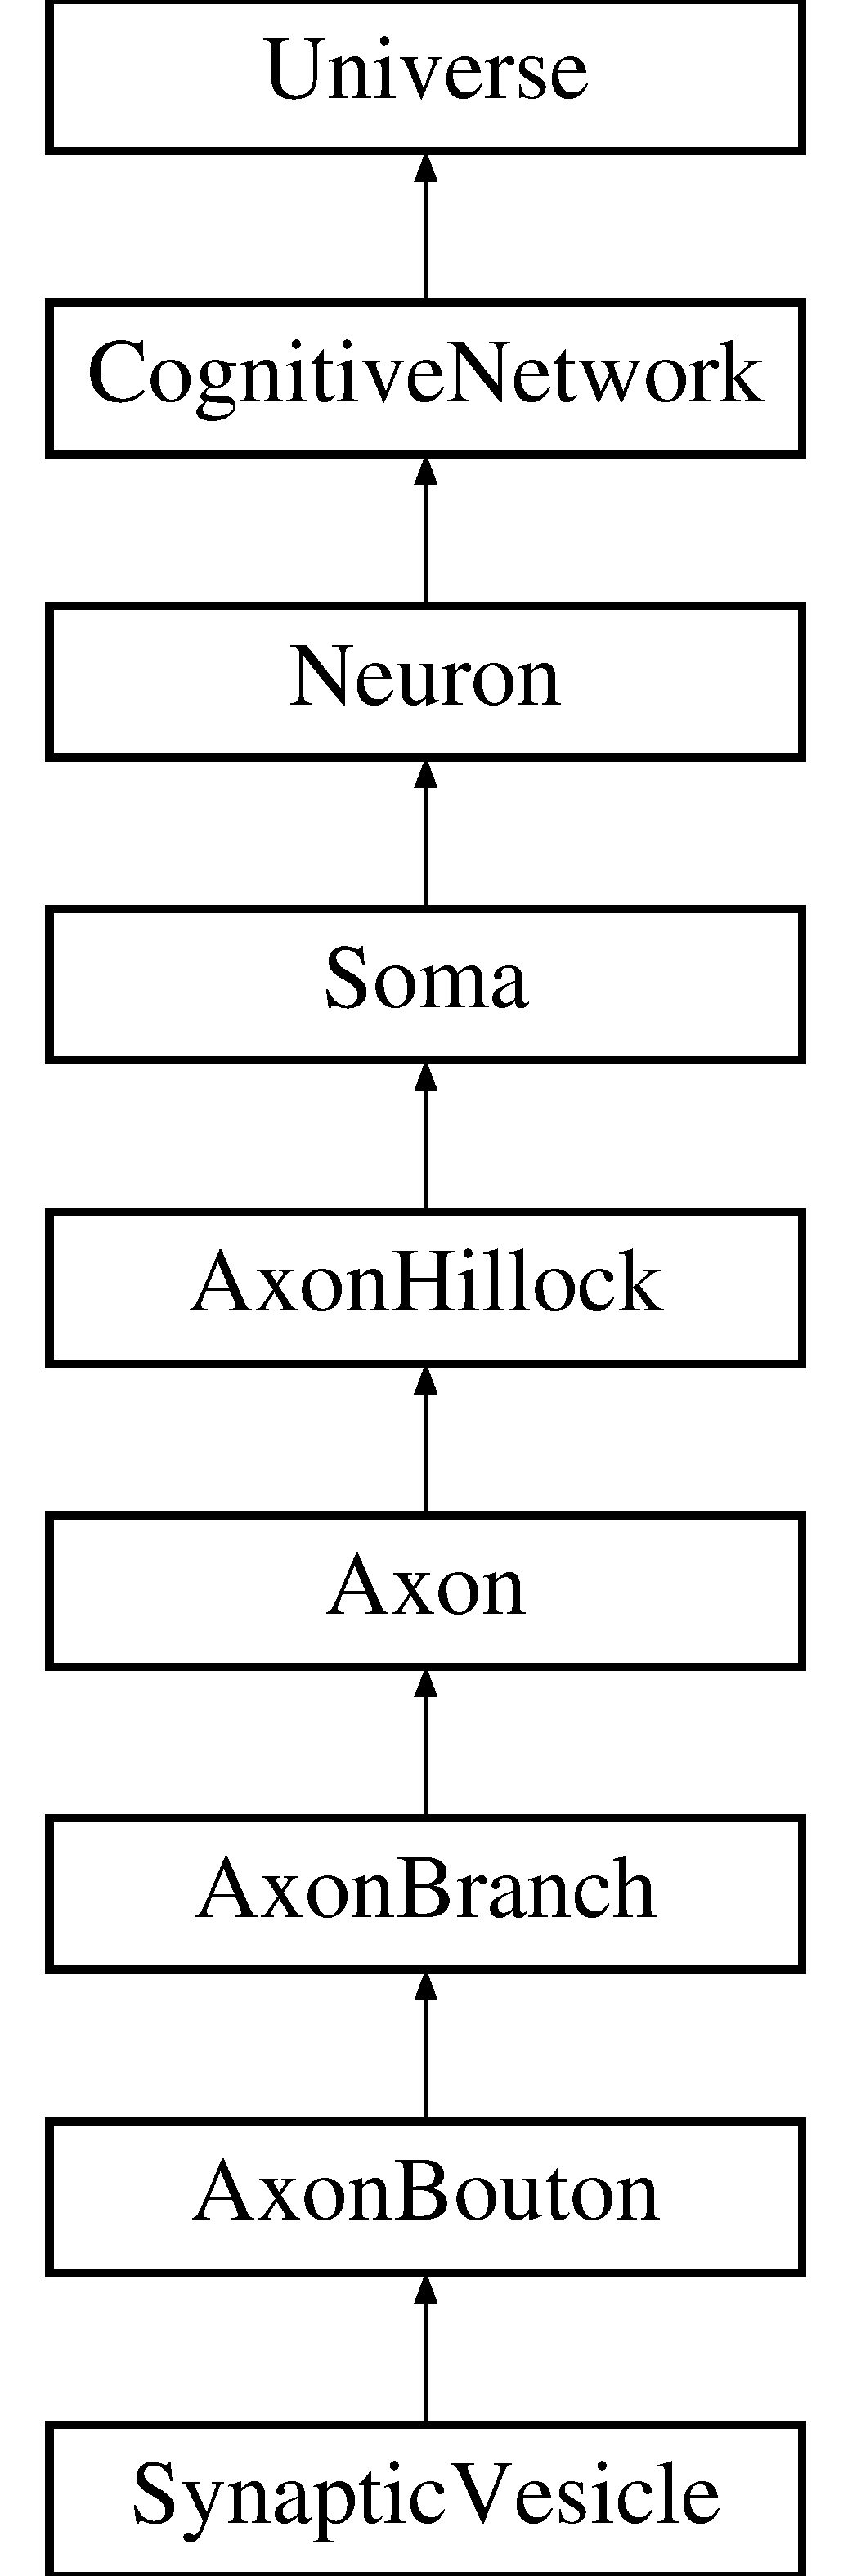
\includegraphics[height=9.000000cm]{classAxonBouton}
\end{center}
\end{figure}
\subsection*{Public Member Functions}
\begin{DoxyCompactItemize}
\item 
\mbox{\hyperlink{classAxonBouton_acd6521d65ecb2b86abf2e3a8b322699e}{Axon\+Bouton}} ()
\item 
\mbox{\hyperlink{classAxonBouton_a8a2da76b259a5ebab397fbd89d8b0632}{Axon\+Bouton}} (unsigned int object\+\_\+type)
\item 
\mbox{\hyperlink{classAxonBouton_a93e33d72d90801d29d2b16ef94b59fab}{Axon\+Bouton}} (unsigned int object\+\_\+type, std\+::chrono\+::time\+\_\+point$<$ \mbox{\hyperlink{universe_8h_a0ef8d951d1ca5ab3cfaf7ab4c7a6fd80}{Clock}} $>$ event\+\_\+time)
\item 
\mbox{\hyperlink{classAxonBouton_a6d671fc3b6bd8e617085c1bc7212400d}{Axon\+Bouton}} (unsigned int object\+\_\+type, std\+::chrono\+::time\+\_\+point$<$ \mbox{\hyperlink{universe_8h_a0ef8d951d1ca5ab3cfaf7ab4c7a6fd80}{Clock}} $>$ event\+\_\+time, \mbox{\hyperlink{classAxonBranch}{Axon\+Branch}} \&axonbranch\+\_\+connector)
\item 
virtual \mbox{\hyperlink{classAxonBouton_ab6f93f680d19d4f07476d1d1b3de776a}{$\sim$\+Axon\+Bouton}} ()
\item 
unsigned int \mbox{\hyperlink{classAxonBouton_a251fc23f754c077cf43ee68991b81624}{Get\+Counter}} (std\+::chrono\+::time\+\_\+point$<$ \mbox{\hyperlink{universe_8h_a0ef8d951d1ca5ab3cfaf7ab4c7a6fd80}{Clock}} $>$ event\+\_\+time)
\item 
double \mbox{\hyperlink{classAxonBouton_a8dff077a40565f4e3a34388a6c38a603}{Get\+Energy}} (std\+::chrono\+::time\+\_\+point$<$ \mbox{\hyperlink{universe_8h_a0ef8d951d1ca5ab3cfaf7ab4c7a6fd80}{Clock}} $>$ event\+\_\+time)
\item 
void \mbox{\hyperlink{classAxonBouton_afe285478d414f2815afb98abe7b92898}{Set\+Counter}} (std\+::chrono\+::time\+\_\+point$<$ \mbox{\hyperlink{universe_8h_a0ef8d951d1ca5ab3cfaf7ab4c7a6fd80}{Clock}} $>$ event\+\_\+time, unsigned int val)
\item 
void \mbox{\hyperlink{classAxonBouton_ab24fa467ab7221d0577e54734684a491}{Set\+Energy}} (std\+::chrono\+::time\+\_\+point$<$ \mbox{\hyperlink{universe_8h_a0ef8d951d1ca5ab3cfaf7ab4c7a6fd80}{Clock}} $>$ event\+\_\+time, double val)
\item 
bool \mbox{\hyperlink{classAxonBouton_a73d3721361c4e1ce6b110ffe1b4a7a88}{Reset\+Parameters}} (std\+::chrono\+::time\+\_\+point$<$ \mbox{\hyperlink{universe_8h_a0ef8d951d1ca5ab3cfaf7ab4c7a6fd80}{Clock}} $>$ event\+\_\+time)
\item 
\mbox{\hyperlink{classAxonBouton}{Axon\+Bouton}} $\ast$ \mbox{\hyperlink{classAxonBouton_a2aa0abe381f6e7c87c702189d01dfbf2}{Create\+Synaptic\+Vesicle}} (std\+::chrono\+::time\+\_\+point$<$ \mbox{\hyperlink{universe_8h_a0ef8d951d1ca5ab3cfaf7ab4c7a6fd80}{Clock}} $>$ event\+\_\+time)
\item 
std\+::vector$<$ \mbox{\hyperlink{classAxonBouton}{Axon\+Bouton}} $\ast$ $>$ \mbox{\hyperlink{classAxonBouton_a0cabe429536722f14ae800c8579168b7}{Create\+Synaptic\+Vesicles}} (std\+::chrono\+::time\+\_\+point$<$ \mbox{\hyperlink{universe_8h_a0ef8d951d1ca5ab3cfaf7ab4c7a6fd80}{Clock}} $>$ event\+\_\+time, int quantity)
\item 
\mbox{\hyperlink{classAxonBouton}{Axon\+Bouton}} $\ast$ \mbox{\hyperlink{classAxonBouton_a0e739b20447539f8db3655e83575fcf4}{Clone\+Synaptic\+Vesicle}} (std\+::chrono\+::time\+\_\+point$<$ \mbox{\hyperlink{universe_8h_a0ef8d951d1ca5ab3cfaf7ab4c7a6fd80}{Clock}} $>$ event\+\_\+time, \mbox{\hyperlink{classAxonBouton}{Axon\+Bouton}} $\ast$clone\+\_\+object, double perfection\+\_\+membership)
\item 
std\+::vector$<$ \mbox{\hyperlink{classAxonBouton}{Axon\+Bouton}} $\ast$ $>$ \mbox{\hyperlink{classAxonBouton_a7bf1d8db3287dc5357d0095233f5c47f}{Clone\+Synaptic\+Vesicles}} (std\+::chrono\+::time\+\_\+point$<$ \mbox{\hyperlink{universe_8h_a0ef8d951d1ca5ab3cfaf7ab4c7a6fd80}{Clock}} $>$ event\+\_\+time, std\+::vector$<$ \mbox{\hyperlink{classAxonBouton}{Axon\+Bouton}} $\ast$$>$ cloning\+\_\+list, double perfection\+\_\+membership)
\item 
\mbox{\hyperlink{classAxonBouton}{Axon\+Bouton}} $\ast$ \mbox{\hyperlink{classAxonBouton_a75592b4ccc589db756183f4aaa694ffe}{Destroy\+Synaptic\+Vesicle}} (std\+::chrono\+::time\+\_\+point$<$ \mbox{\hyperlink{universe_8h_a0ef8d951d1ca5ab3cfaf7ab4c7a6fd80}{Clock}} $>$ event\+\_\+time, \mbox{\hyperlink{classAxonBouton}{Axon\+Bouton}} $\ast$destroy\+\_\+object)
\item 
std\+::vector$<$ \mbox{\hyperlink{classAxonBouton}{Axon\+Bouton}} $\ast$ $>$ \mbox{\hyperlink{classAxonBouton_a0fa1c238a29d9e2b84b4d9c556452150}{Destroy\+Synaptic\+Vesicles}} (std\+::chrono\+::time\+\_\+point$<$ \mbox{\hyperlink{universe_8h_a0ef8d951d1ca5ab3cfaf7ab4c7a6fd80}{Clock}} $>$ event\+\_\+time, std\+::vector$<$ \mbox{\hyperlink{classAxonBouton}{Axon\+Bouton}} $\ast$$>$ destruction\+\_\+list)
\item 
\mbox{\hyperlink{classAxonBouton}{Axon\+Bouton}} $\ast$ \mbox{\hyperlink{classAxonBouton_a3009e5d49c699afa7f633b026b37ed77}{Add\+Synaptic\+Vesicle}} (std\+::chrono\+::time\+\_\+point$<$ \mbox{\hyperlink{universe_8h_a0ef8d951d1ca5ab3cfaf7ab4c7a6fd80}{Clock}} $>$ event\+\_\+time, \mbox{\hyperlink{classAxonBouton}{Axon\+Bouton}} $\ast$add\+\_\+object)
\item 
std\+::vector$<$ \mbox{\hyperlink{classAxonBouton}{Axon\+Bouton}} $\ast$ $>$ \mbox{\hyperlink{classAxonBouton_a0e264da88f6ca5d77aa42f415cb4f3aa}{Add\+Synaptic\+Vesicles}} (std\+::chrono\+::time\+\_\+point$<$ \mbox{\hyperlink{universe_8h_a0ef8d951d1ca5ab3cfaf7ab4c7a6fd80}{Clock}} $>$ event\+\_\+time, std\+::vector$<$ \mbox{\hyperlink{classAxonBouton}{Axon\+Bouton}} $\ast$$>$ add\+\_\+objects)
\item 
\mbox{\hyperlink{classAxonBouton}{Axon\+Bouton}} $\ast$ \mbox{\hyperlink{classAxonBouton_a1f0b13fa7ec408c9e0cfb22cea9bbe8c}{Remove\+Synaptic\+Vesicle}} (std\+::chrono\+::time\+\_\+point$<$ \mbox{\hyperlink{universe_8h_a0ef8d951d1ca5ab3cfaf7ab4c7a6fd80}{Clock}} $>$ event\+\_\+time)
\item 
std\+::vector$<$ \mbox{\hyperlink{classAxonBouton}{Axon\+Bouton}} $\ast$ $>$ \mbox{\hyperlink{classAxonBouton_ae4119170ef72beaed3c8a0eb1d80ef14}{Remove\+Synaptic\+Vesicles}} (std\+::chrono\+::time\+\_\+point$<$ \mbox{\hyperlink{universe_8h_a0ef8d951d1ca5ab3cfaf7ab4c7a6fd80}{Clock}} $>$ event\+\_\+time, int quantity)
\item 
\mbox{\hyperlink{classAxonBouton}{Axon\+Bouton}} $\ast$ \mbox{\hyperlink{classAxonBouton_a847ab3d3d214ddc85bdfd463c6d95d54}{Get\+Synaptic\+Vesicle}} (std\+::chrono\+::time\+\_\+point$<$ \mbox{\hyperlink{universe_8h_a0ef8d951d1ca5ab3cfaf7ab4c7a6fd80}{Clock}} $>$ event\+\_\+time, int selector)
\item 
std\+::vector$<$ \mbox{\hyperlink{classAxonBouton}{Axon\+Bouton}} $\ast$ $>$ \mbox{\hyperlink{classAxonBouton_af9a35ff7a6c32ac291021cccb3d40c9b}{Get\+Synaptic\+Vesicles}} (std\+::chrono\+::time\+\_\+point$<$ \mbox{\hyperlink{universe_8h_a0ef8d951d1ca5ab3cfaf7ab4c7a6fd80}{Clock}} $>$ event\+\_\+time)
\item 
int \mbox{\hyperlink{classAxonBouton_a95fc006b2436e2c7784af2cc0bc9522e}{Growth\+Surface}} (std\+::chrono\+::time\+\_\+point$<$ \mbox{\hyperlink{universe_8h_a0ef8d951d1ca5ab3cfaf7ab4c7a6fd80}{Clock}} $>$ event\+\_\+time, double surf\+\_\+change)
\item 
int \mbox{\hyperlink{classAxonBouton_a10ac4446e777376a3944c87b2bcf26b5}{Growth\+Volume}} (std\+::chrono\+::time\+\_\+point$<$ \mbox{\hyperlink{universe_8h_a0ef8d951d1ca5ab3cfaf7ab4c7a6fd80}{Clock}} $>$ event\+\_\+time, double vol\+\_\+change)
\item 
int \mbox{\hyperlink{classAxonBouton_a26f89bac681b8f0894fe1ae249733917}{Update}} (std\+::chrono\+::time\+\_\+point$<$ \mbox{\hyperlink{universe_8h_a0ef8d951d1ca5ab3cfaf7ab4c7a6fd80}{Clock}} $>$ event\+\_\+time)
\end{DoxyCompactItemize}
\subsection*{Protected Attributes}
\begin{DoxyCompactItemize}
\item 
std\+::vector$<$ \mbox{\hyperlink{classAxonBouton}{Axon\+Bouton}} $\ast$ $>$ \mbox{\hyperlink{classAxonBouton_ad5b4e9b5fefb2ad9e6dfe5ad91be2dd7}{synapticvesicle\+\_\+list}}
\end{DoxyCompactItemize}
\subsection*{Private Attributes}
\begin{DoxyCompactItemize}
\item 
int \mbox{\hyperlink{classAxonBouton_a29ded5dabe0b9a52fc3f1612aec68cf3}{axonbouton\+\_\+type}}
\item 
int \mbox{\hyperlink{classAxonBouton_a485081d54e0afcbe697877524cebe30d}{m\+\_\+add\+Status}}
\item 
int \mbox{\hyperlink{classAxonBouton_a6af09fee2eb7a38e8591770bc9c070ac}{synapticvesicle\+\_\+pool}}
\item 
std\+::chrono\+::time\+\_\+point$<$ \mbox{\hyperlink{universe_8h_a0ef8d951d1ca5ab3cfaf7ab4c7a6fd80}{Clock}} $>$ \mbox{\hyperlink{classAxonBouton_a26b17307437394ff14bfb5ef8dfad1e5}{time\+\_\+object\+\_\+created}}
\item 
std\+::chrono\+::time\+\_\+point$<$ \mbox{\hyperlink{universe_8h_a0ef8d951d1ca5ab3cfaf7ab4c7a6fd80}{Clock}} $>$ \mbox{\hyperlink{classAxonBouton_a6382c6be1211fdde45dd497ae56d8bbb}{previous\+\_\+event\+\_\+time}}
\item 
int \mbox{\hyperlink{classAxonBouton_a04b61a53dc110ceb77484cf894ff3787}{duration\+\_\+since\+\_\+last\+\_\+event}}
\item 
double \mbox{\hyperlink{classAxonBouton_ae994ae9fbfc40188b2379b61758d18c1}{m\+\_\+\+Volume}}
\item 
double \mbox{\hyperlink{classAxonBouton_a6a17c18e315806baa28a907e6799c6dd}{m\+\_\+\+Surface\+Area}}
\item 
unsigned int \mbox{\hyperlink{classAxonBouton_a043ef274a67fc10c6288044907533b27}{m\+\_\+\+Counter}}
\begin{DoxyCompactList}\small\item\em Member variable \char`\"{}m\+\_\+\+Counter\char`\"{}. \end{DoxyCompactList}\item 
double \mbox{\hyperlink{classAxonBouton_a4878e6a13e75b8473dfb3bb79637fe3a}{object\+\_\+energy}}
\begin{DoxyCompactList}\small\item\em Member variable \char`\"{}object\+\_\+energy\char`\"{}. \end{DoxyCompactList}\item 
double \mbox{\hyperlink{classAxonBouton_a9ac7a8e73e5f84db791a69d47863d684}{m\+\_\+axonlength}}
\item 
double \mbox{\hyperlink{classAxonBouton_ab83ac3e3436bd4080ef5f118ee6c57b4}{m\+\_\+\+Time\+Dilation}}
\item 
double \mbox{\hyperlink{classAxonBouton_aaef78a821ff347809f9bcd3787c6de15}{m\+\_\+\+Time\+Threshold}}
\item 
bool \mbox{\hyperlink{classAxonBouton_a6760cc2afc8f7a42401d82979b2ac9bc}{object\+\_\+disabled}}
\item 
bool \mbox{\hyperlink{classAxonBouton_a2d8bfbb162110b78489d059fb90e5cf3}{object\+\_\+initialised}}
\end{DoxyCompactItemize}
\subsection*{Additional Inherited Members}


\subsection{Constructor \& Destructor Documentation}
\mbox{\Hypertarget{classAxonBouton_acd6521d65ecb2b86abf2e3a8b322699e}\label{classAxonBouton_acd6521d65ecb2b86abf2e3a8b322699e}} 
\index{Axon\+Bouton@{Axon\+Bouton}!Axon\+Bouton@{Axon\+Bouton}}
\index{Axon\+Bouton@{Axon\+Bouton}!Axon\+Bouton@{Axon\+Bouton}}
\subsubsection{\texorpdfstring{Axon\+Bouton()}{AxonBouton()}\hspace{0.1cm}{\footnotesize\ttfamily [1/4]}}
{\footnotesize\ttfamily Axon\+Bouton\+::\+Axon\+Bouton (\begin{DoxyParamCaption}{ }\end{DoxyParamCaption})\hspace{0.3cm}{\ttfamily [inline]}}

\mbox{\Hypertarget{classAxonBouton_a8a2da76b259a5ebab397fbd89d8b0632}\label{classAxonBouton_a8a2da76b259a5ebab397fbd89d8b0632}} 
\index{Axon\+Bouton@{Axon\+Bouton}!Axon\+Bouton@{Axon\+Bouton}}
\index{Axon\+Bouton@{Axon\+Bouton}!Axon\+Bouton@{Axon\+Bouton}}
\subsubsection{\texorpdfstring{Axon\+Bouton()}{AxonBouton()}\hspace{0.1cm}{\footnotesize\ttfamily [2/4]}}
{\footnotesize\ttfamily Axon\+Bouton\+::\+Axon\+Bouton (\begin{DoxyParamCaption}\item[{unsigned int}]{object\+\_\+type }\end{DoxyParamCaption})\hspace{0.3cm}{\ttfamily [inline]}}

\mbox{\Hypertarget{classAxonBouton_a93e33d72d90801d29d2b16ef94b59fab}\label{classAxonBouton_a93e33d72d90801d29d2b16ef94b59fab}} 
\index{Axon\+Bouton@{Axon\+Bouton}!Axon\+Bouton@{Axon\+Bouton}}
\index{Axon\+Bouton@{Axon\+Bouton}!Axon\+Bouton@{Axon\+Bouton}}
\subsubsection{\texorpdfstring{Axon\+Bouton()}{AxonBouton()}\hspace{0.1cm}{\footnotesize\ttfamily [3/4]}}
{\footnotesize\ttfamily Axon\+Bouton\+::\+Axon\+Bouton (\begin{DoxyParamCaption}\item[{unsigned int}]{object\+\_\+type,  }\item[{std\+::chrono\+::time\+\_\+point$<$ \mbox{\hyperlink{universe_8h_a0ef8d951d1ca5ab3cfaf7ab4c7a6fd80}{Clock}} $>$}]{event\+\_\+time }\end{DoxyParamCaption})\hspace{0.3cm}{\ttfamily [inline]}}

\mbox{\Hypertarget{classAxonBouton_a6d671fc3b6bd8e617085c1bc7212400d}\label{classAxonBouton_a6d671fc3b6bd8e617085c1bc7212400d}} 
\index{Axon\+Bouton@{Axon\+Bouton}!Axon\+Bouton@{Axon\+Bouton}}
\index{Axon\+Bouton@{Axon\+Bouton}!Axon\+Bouton@{Axon\+Bouton}}
\subsubsection{\texorpdfstring{Axon\+Bouton()}{AxonBouton()}\hspace{0.1cm}{\footnotesize\ttfamily [4/4]}}
{\footnotesize\ttfamily Axon\+Bouton\+::\+Axon\+Bouton (\begin{DoxyParamCaption}\item[{unsigned int}]{object\+\_\+type,  }\item[{std\+::chrono\+::time\+\_\+point$<$ \mbox{\hyperlink{universe_8h_a0ef8d951d1ca5ab3cfaf7ab4c7a6fd80}{Clock}} $>$}]{event\+\_\+time,  }\item[{\mbox{\hyperlink{classAxonBranch}{Axon\+Branch}} \&}]{axonbranch\+\_\+connector }\end{DoxyParamCaption})\hspace{0.3cm}{\ttfamily [inline]}}

\mbox{\Hypertarget{classAxonBouton_ab6f93f680d19d4f07476d1d1b3de776a}\label{classAxonBouton_ab6f93f680d19d4f07476d1d1b3de776a}} 
\index{Axon\+Bouton@{Axon\+Bouton}!````~Axon\+Bouton@{$\sim$\+Axon\+Bouton}}
\index{````~Axon\+Bouton@{$\sim$\+Axon\+Bouton}!Axon\+Bouton@{Axon\+Bouton}}
\subsubsection{\texorpdfstring{$\sim$\+Axon\+Bouton()}{~AxonBouton()}}
{\footnotesize\ttfamily virtual Axon\+Bouton\+::$\sim$\+Axon\+Bouton (\begin{DoxyParamCaption}{ }\end{DoxyParamCaption})\hspace{0.3cm}{\ttfamily [inline]}, {\ttfamily [virtual]}}

Default destructor 

\subsection{Member Function Documentation}
\mbox{\Hypertarget{classAxonBouton_a3009e5d49c699afa7f633b026b37ed77}\label{classAxonBouton_a3009e5d49c699afa7f633b026b37ed77}} 
\index{Axon\+Bouton@{Axon\+Bouton}!Add\+Synaptic\+Vesicle@{Add\+Synaptic\+Vesicle}}
\index{Add\+Synaptic\+Vesicle@{Add\+Synaptic\+Vesicle}!Axon\+Bouton@{Axon\+Bouton}}
\subsubsection{\texorpdfstring{Add\+Synaptic\+Vesicle()}{AddSynapticVesicle()}}
{\footnotesize\ttfamily \mbox{\hyperlink{classAxonBouton}{Axon\+Bouton}} $\ast$ Axon\+Bouton\+::\+Add\+Synaptic\+Vesicle (\begin{DoxyParamCaption}\item[{std\+::chrono\+::time\+\_\+point$<$ \mbox{\hyperlink{universe_8h_a0ef8d951d1ca5ab3cfaf7ab4c7a6fd80}{Clock}} $>$}]{event\+\_\+time,  }\item[{\mbox{\hyperlink{classAxonBouton}{Axon\+Bouton}} $\ast$}]{add\+\_\+object }\end{DoxyParamCaption})}

\mbox{\Hypertarget{classAxonBouton_a0e264da88f6ca5d77aa42f415cb4f3aa}\label{classAxonBouton_a0e264da88f6ca5d77aa42f415cb4f3aa}} 
\index{Axon\+Bouton@{Axon\+Bouton}!Add\+Synaptic\+Vesicles@{Add\+Synaptic\+Vesicles}}
\index{Add\+Synaptic\+Vesicles@{Add\+Synaptic\+Vesicles}!Axon\+Bouton@{Axon\+Bouton}}
\subsubsection{\texorpdfstring{Add\+Synaptic\+Vesicles()}{AddSynapticVesicles()}}
{\footnotesize\ttfamily std\+::vector$<$ \mbox{\hyperlink{classAxonBouton}{Axon\+Bouton}} $\ast$ $>$ Axon\+Bouton\+::\+Add\+Synaptic\+Vesicles (\begin{DoxyParamCaption}\item[{std\+::chrono\+::time\+\_\+point$<$ \mbox{\hyperlink{universe_8h_a0ef8d951d1ca5ab3cfaf7ab4c7a6fd80}{Clock}} $>$}]{event\+\_\+time,  }\item[{std\+::vector$<$ \mbox{\hyperlink{classAxonBouton}{Axon\+Bouton}} $\ast$$>$}]{add\+\_\+objects }\end{DoxyParamCaption})}

\mbox{\Hypertarget{classAxonBouton_a0e739b20447539f8db3655e83575fcf4}\label{classAxonBouton_a0e739b20447539f8db3655e83575fcf4}} 
\index{Axon\+Bouton@{Axon\+Bouton}!Clone\+Synaptic\+Vesicle@{Clone\+Synaptic\+Vesicle}}
\index{Clone\+Synaptic\+Vesicle@{Clone\+Synaptic\+Vesicle}!Axon\+Bouton@{Axon\+Bouton}}
\subsubsection{\texorpdfstring{Clone\+Synaptic\+Vesicle()}{CloneSynapticVesicle()}}
{\footnotesize\ttfamily \mbox{\hyperlink{classAxonBouton}{Axon\+Bouton}} $\ast$ Axon\+Bouton\+::\+Clone\+Synaptic\+Vesicle (\begin{DoxyParamCaption}\item[{std\+::chrono\+::time\+\_\+point$<$ \mbox{\hyperlink{universe_8h_a0ef8d951d1ca5ab3cfaf7ab4c7a6fd80}{Clock}} $>$}]{event\+\_\+time,  }\item[{\mbox{\hyperlink{classAxonBouton}{Axon\+Bouton}} $\ast$}]{clone\+\_\+object,  }\item[{double}]{perfection\+\_\+membership }\end{DoxyParamCaption})}

\mbox{\Hypertarget{classAxonBouton_a7bf1d8db3287dc5357d0095233f5c47f}\label{classAxonBouton_a7bf1d8db3287dc5357d0095233f5c47f}} 
\index{Axon\+Bouton@{Axon\+Bouton}!Clone\+Synaptic\+Vesicles@{Clone\+Synaptic\+Vesicles}}
\index{Clone\+Synaptic\+Vesicles@{Clone\+Synaptic\+Vesicles}!Axon\+Bouton@{Axon\+Bouton}}
\subsubsection{\texorpdfstring{Clone\+Synaptic\+Vesicles()}{CloneSynapticVesicles()}}
{\footnotesize\ttfamily std\+::vector$<$ \mbox{\hyperlink{classAxonBouton}{Axon\+Bouton}} $\ast$ $>$ Axon\+Bouton\+::\+Clone\+Synaptic\+Vesicles (\begin{DoxyParamCaption}\item[{std\+::chrono\+::time\+\_\+point$<$ \mbox{\hyperlink{universe_8h_a0ef8d951d1ca5ab3cfaf7ab4c7a6fd80}{Clock}} $>$}]{event\+\_\+time,  }\item[{std\+::vector$<$ \mbox{\hyperlink{classAxonBouton}{Axon\+Bouton}} $\ast$$>$}]{cloning\+\_\+list,  }\item[{double}]{perfection\+\_\+membership }\end{DoxyParamCaption})}

\mbox{\Hypertarget{classAxonBouton_a2aa0abe381f6e7c87c702189d01dfbf2}\label{classAxonBouton_a2aa0abe381f6e7c87c702189d01dfbf2}} 
\index{Axon\+Bouton@{Axon\+Bouton}!Create\+Synaptic\+Vesicle@{Create\+Synaptic\+Vesicle}}
\index{Create\+Synaptic\+Vesicle@{Create\+Synaptic\+Vesicle}!Axon\+Bouton@{Axon\+Bouton}}
\subsubsection{\texorpdfstring{Create\+Synaptic\+Vesicle()}{CreateSynapticVesicle()}}
{\footnotesize\ttfamily \mbox{\hyperlink{classAxonBouton}{Axon\+Bouton}} $\ast$ Axon\+Bouton\+::\+Create\+Synaptic\+Vesicle (\begin{DoxyParamCaption}\item[{std\+::chrono\+::time\+\_\+point$<$ \mbox{\hyperlink{universe_8h_a0ef8d951d1ca5ab3cfaf7ab4c7a6fd80}{Clock}} $>$}]{event\+\_\+time }\end{DoxyParamCaption})}

\mbox{\Hypertarget{classAxonBouton_a0cabe429536722f14ae800c8579168b7}\label{classAxonBouton_a0cabe429536722f14ae800c8579168b7}} 
\index{Axon\+Bouton@{Axon\+Bouton}!Create\+Synaptic\+Vesicles@{Create\+Synaptic\+Vesicles}}
\index{Create\+Synaptic\+Vesicles@{Create\+Synaptic\+Vesicles}!Axon\+Bouton@{Axon\+Bouton}}
\subsubsection{\texorpdfstring{Create\+Synaptic\+Vesicles()}{CreateSynapticVesicles()}}
{\footnotesize\ttfamily std\+::vector$<$ \mbox{\hyperlink{classAxonBouton}{Axon\+Bouton}} $\ast$ $>$ Axon\+Bouton\+::\+Create\+Synaptic\+Vesicles (\begin{DoxyParamCaption}\item[{std\+::chrono\+::time\+\_\+point$<$ \mbox{\hyperlink{universe_8h_a0ef8d951d1ca5ab3cfaf7ab4c7a6fd80}{Clock}} $>$}]{event\+\_\+time,  }\item[{int}]{quantity }\end{DoxyParamCaption})}

\mbox{\Hypertarget{classAxonBouton_a75592b4ccc589db756183f4aaa694ffe}\label{classAxonBouton_a75592b4ccc589db756183f4aaa694ffe}} 
\index{Axon\+Bouton@{Axon\+Bouton}!Destroy\+Synaptic\+Vesicle@{Destroy\+Synaptic\+Vesicle}}
\index{Destroy\+Synaptic\+Vesicle@{Destroy\+Synaptic\+Vesicle}!Axon\+Bouton@{Axon\+Bouton}}
\subsubsection{\texorpdfstring{Destroy\+Synaptic\+Vesicle()}{DestroySynapticVesicle()}}
{\footnotesize\ttfamily \mbox{\hyperlink{classAxonBouton}{Axon\+Bouton}} $\ast$ Axon\+Bouton\+::\+Destroy\+Synaptic\+Vesicle (\begin{DoxyParamCaption}\item[{std\+::chrono\+::time\+\_\+point$<$ \mbox{\hyperlink{universe_8h_a0ef8d951d1ca5ab3cfaf7ab4c7a6fd80}{Clock}} $>$}]{event\+\_\+time,  }\item[{\mbox{\hyperlink{classAxonBouton}{Axon\+Bouton}} $\ast$}]{destroy\+\_\+object }\end{DoxyParamCaption})}

\mbox{\Hypertarget{classAxonBouton_a0fa1c238a29d9e2b84b4d9c556452150}\label{classAxonBouton_a0fa1c238a29d9e2b84b4d9c556452150}} 
\index{Axon\+Bouton@{Axon\+Bouton}!Destroy\+Synaptic\+Vesicles@{Destroy\+Synaptic\+Vesicles}}
\index{Destroy\+Synaptic\+Vesicles@{Destroy\+Synaptic\+Vesicles}!Axon\+Bouton@{Axon\+Bouton}}
\subsubsection{\texorpdfstring{Destroy\+Synaptic\+Vesicles()}{DestroySynapticVesicles()}}
{\footnotesize\ttfamily std\+::vector$<$ \mbox{\hyperlink{classAxonBouton}{Axon\+Bouton}} $\ast$ $>$ Axon\+Bouton\+::\+Destroy\+Synaptic\+Vesicles (\begin{DoxyParamCaption}\item[{std\+::chrono\+::time\+\_\+point$<$ \mbox{\hyperlink{universe_8h_a0ef8d951d1ca5ab3cfaf7ab4c7a6fd80}{Clock}} $>$}]{event\+\_\+time,  }\item[{std\+::vector$<$ \mbox{\hyperlink{classAxonBouton}{Axon\+Bouton}} $\ast$$>$}]{destruction\+\_\+list }\end{DoxyParamCaption})}

\mbox{\Hypertarget{classAxonBouton_a251fc23f754c077cf43ee68991b81624}\label{classAxonBouton_a251fc23f754c077cf43ee68991b81624}} 
\index{Axon\+Bouton@{Axon\+Bouton}!Get\+Counter@{Get\+Counter}}
\index{Get\+Counter@{Get\+Counter}!Axon\+Bouton@{Axon\+Bouton}}
\subsubsection{\texorpdfstring{Get\+Counter()}{GetCounter()}}
{\footnotesize\ttfamily unsigned int Axon\+Bouton\+::\+Get\+Counter (\begin{DoxyParamCaption}\item[{std\+::chrono\+::time\+\_\+point$<$ \mbox{\hyperlink{universe_8h_a0ef8d951d1ca5ab3cfaf7ab4c7a6fd80}{Clock}} $>$}]{event\+\_\+time }\end{DoxyParamCaption})\hspace{0.3cm}{\ttfamily [inline]}}

\mbox{\Hypertarget{classAxonBouton_a8dff077a40565f4e3a34388a6c38a603}\label{classAxonBouton_a8dff077a40565f4e3a34388a6c38a603}} 
\index{Axon\+Bouton@{Axon\+Bouton}!Get\+Energy@{Get\+Energy}}
\index{Get\+Energy@{Get\+Energy}!Axon\+Bouton@{Axon\+Bouton}}
\subsubsection{\texorpdfstring{Get\+Energy()}{GetEnergy()}}
{\footnotesize\ttfamily double Axon\+Bouton\+::\+Get\+Energy (\begin{DoxyParamCaption}\item[{std\+::chrono\+::time\+\_\+point$<$ \mbox{\hyperlink{universe_8h_a0ef8d951d1ca5ab3cfaf7ab4c7a6fd80}{Clock}} $>$}]{event\+\_\+time }\end{DoxyParamCaption})\hspace{0.3cm}{\ttfamily [inline]}}

\mbox{\Hypertarget{classAxonBouton_a847ab3d3d214ddc85bdfd463c6d95d54}\label{classAxonBouton_a847ab3d3d214ddc85bdfd463c6d95d54}} 
\index{Axon\+Bouton@{Axon\+Bouton}!Get\+Synaptic\+Vesicle@{Get\+Synaptic\+Vesicle}}
\index{Get\+Synaptic\+Vesicle@{Get\+Synaptic\+Vesicle}!Axon\+Bouton@{Axon\+Bouton}}
\subsubsection{\texorpdfstring{Get\+Synaptic\+Vesicle()}{GetSynapticVesicle()}}
{\footnotesize\ttfamily \mbox{\hyperlink{classAxonBouton}{Axon\+Bouton}} $\ast$ Axon\+Bouton\+::\+Get\+Synaptic\+Vesicle (\begin{DoxyParamCaption}\item[{std\+::chrono\+::time\+\_\+point$<$ \mbox{\hyperlink{universe_8h_a0ef8d951d1ca5ab3cfaf7ab4c7a6fd80}{Clock}} $>$}]{event\+\_\+time,  }\item[{int}]{selector }\end{DoxyParamCaption})}

\mbox{\Hypertarget{classAxonBouton_af9a35ff7a6c32ac291021cccb3d40c9b}\label{classAxonBouton_af9a35ff7a6c32ac291021cccb3d40c9b}} 
\index{Axon\+Bouton@{Axon\+Bouton}!Get\+Synaptic\+Vesicles@{Get\+Synaptic\+Vesicles}}
\index{Get\+Synaptic\+Vesicles@{Get\+Synaptic\+Vesicles}!Axon\+Bouton@{Axon\+Bouton}}
\subsubsection{\texorpdfstring{Get\+Synaptic\+Vesicles()}{GetSynapticVesicles()}}
{\footnotesize\ttfamily std\+::vector$<$ \mbox{\hyperlink{classAxonBouton}{Axon\+Bouton}} $\ast$ $>$ Axon\+Bouton\+::\+Get\+Synaptic\+Vesicles (\begin{DoxyParamCaption}\item[{std\+::chrono\+::time\+\_\+point$<$ \mbox{\hyperlink{universe_8h_a0ef8d951d1ca5ab3cfaf7ab4c7a6fd80}{Clock}} $>$}]{event\+\_\+time }\end{DoxyParamCaption})}

\mbox{\Hypertarget{classAxonBouton_a95fc006b2436e2c7784af2cc0bc9522e}\label{classAxonBouton_a95fc006b2436e2c7784af2cc0bc9522e}} 
\index{Axon\+Bouton@{Axon\+Bouton}!Growth\+Surface@{Growth\+Surface}}
\index{Growth\+Surface@{Growth\+Surface}!Axon\+Bouton@{Axon\+Bouton}}
\subsubsection{\texorpdfstring{Growth\+Surface()}{GrowthSurface()}}
{\footnotesize\ttfamily int Axon\+Bouton\+::\+Growth\+Surface (\begin{DoxyParamCaption}\item[{std\+::chrono\+::time\+\_\+point$<$ \mbox{\hyperlink{universe_8h_a0ef8d951d1ca5ab3cfaf7ab4c7a6fd80}{Clock}} $>$}]{event\+\_\+time,  }\item[{double}]{surf\+\_\+change }\end{DoxyParamCaption})}

\mbox{\Hypertarget{classAxonBouton_a10ac4446e777376a3944c87b2bcf26b5}\label{classAxonBouton_a10ac4446e777376a3944c87b2bcf26b5}} 
\index{Axon\+Bouton@{Axon\+Bouton}!Growth\+Volume@{Growth\+Volume}}
\index{Growth\+Volume@{Growth\+Volume}!Axon\+Bouton@{Axon\+Bouton}}
\subsubsection{\texorpdfstring{Growth\+Volume()}{GrowthVolume()}}
{\footnotesize\ttfamily int Axon\+Bouton\+::\+Growth\+Volume (\begin{DoxyParamCaption}\item[{std\+::chrono\+::time\+\_\+point$<$ \mbox{\hyperlink{universe_8h_a0ef8d951d1ca5ab3cfaf7ab4c7a6fd80}{Clock}} $>$}]{event\+\_\+time,  }\item[{double}]{vol\+\_\+change }\end{DoxyParamCaption})}

\mbox{\Hypertarget{classAxonBouton_a1f0b13fa7ec408c9e0cfb22cea9bbe8c}\label{classAxonBouton_a1f0b13fa7ec408c9e0cfb22cea9bbe8c}} 
\index{Axon\+Bouton@{Axon\+Bouton}!Remove\+Synaptic\+Vesicle@{Remove\+Synaptic\+Vesicle}}
\index{Remove\+Synaptic\+Vesicle@{Remove\+Synaptic\+Vesicle}!Axon\+Bouton@{Axon\+Bouton}}
\subsubsection{\texorpdfstring{Remove\+Synaptic\+Vesicle()}{RemoveSynapticVesicle()}}
{\footnotesize\ttfamily \mbox{\hyperlink{classAxonBouton}{Axon\+Bouton}} $\ast$ Axon\+Bouton\+::\+Remove\+Synaptic\+Vesicle (\begin{DoxyParamCaption}\item[{std\+::chrono\+::time\+\_\+point$<$ \mbox{\hyperlink{universe_8h_a0ef8d951d1ca5ab3cfaf7ab4c7a6fd80}{Clock}} $>$}]{event\+\_\+time }\end{DoxyParamCaption})}

\mbox{\Hypertarget{classAxonBouton_ae4119170ef72beaed3c8a0eb1d80ef14}\label{classAxonBouton_ae4119170ef72beaed3c8a0eb1d80ef14}} 
\index{Axon\+Bouton@{Axon\+Bouton}!Remove\+Synaptic\+Vesicles@{Remove\+Synaptic\+Vesicles}}
\index{Remove\+Synaptic\+Vesicles@{Remove\+Synaptic\+Vesicles}!Axon\+Bouton@{Axon\+Bouton}}
\subsubsection{\texorpdfstring{Remove\+Synaptic\+Vesicles()}{RemoveSynapticVesicles()}}
{\footnotesize\ttfamily std\+::vector$<$ \mbox{\hyperlink{classAxonBouton}{Axon\+Bouton}} $\ast$ $>$ Axon\+Bouton\+::\+Remove\+Synaptic\+Vesicles (\begin{DoxyParamCaption}\item[{std\+::chrono\+::time\+\_\+point$<$ \mbox{\hyperlink{universe_8h_a0ef8d951d1ca5ab3cfaf7ab4c7a6fd80}{Clock}} $>$}]{event\+\_\+time,  }\item[{int}]{quantity }\end{DoxyParamCaption})}

\mbox{\Hypertarget{classAxonBouton_a73d3721361c4e1ce6b110ffe1b4a7a88}\label{classAxonBouton_a73d3721361c4e1ce6b110ffe1b4a7a88}} 
\index{Axon\+Bouton@{Axon\+Bouton}!Reset\+Parameters@{Reset\+Parameters}}
\index{Reset\+Parameters@{Reset\+Parameters}!Axon\+Bouton@{Axon\+Bouton}}
\subsubsection{\texorpdfstring{Reset\+Parameters()}{ResetParameters()}}
{\footnotesize\ttfamily bool Axon\+Bouton\+::\+Reset\+Parameters (\begin{DoxyParamCaption}\item[{std\+::chrono\+::time\+\_\+point$<$ \mbox{\hyperlink{universe_8h_a0ef8d951d1ca5ab3cfaf7ab4c7a6fd80}{Clock}} $>$}]{event\+\_\+time }\end{DoxyParamCaption})}

\mbox{\Hypertarget{classAxonBouton_afe285478d414f2815afb98abe7b92898}\label{classAxonBouton_afe285478d414f2815afb98abe7b92898}} 
\index{Axon\+Bouton@{Axon\+Bouton}!Set\+Counter@{Set\+Counter}}
\index{Set\+Counter@{Set\+Counter}!Axon\+Bouton@{Axon\+Bouton}}
\subsubsection{\texorpdfstring{Set\+Counter()}{SetCounter()}}
{\footnotesize\ttfamily void Axon\+Bouton\+::\+Set\+Counter (\begin{DoxyParamCaption}\item[{std\+::chrono\+::time\+\_\+point$<$ \mbox{\hyperlink{universe_8h_a0ef8d951d1ca5ab3cfaf7ab4c7a6fd80}{Clock}} $>$}]{event\+\_\+time,  }\item[{unsigned int}]{val }\end{DoxyParamCaption})\hspace{0.3cm}{\ttfamily [inline]}, {\ttfamily [virtual]}}



Reimplemented from \mbox{\hyperlink{classAxon_a3493cb97bde26bd66facc6084cd5f219}{Axon}}.



Reimplemented in \mbox{\hyperlink{classSynapticVesicle_a7fd7cfce5eccb904206d968866f85220}{Synaptic\+Vesicle}}.

\mbox{\Hypertarget{classAxonBouton_ab24fa467ab7221d0577e54734684a491}\label{classAxonBouton_ab24fa467ab7221d0577e54734684a491}} 
\index{Axon\+Bouton@{Axon\+Bouton}!Set\+Energy@{Set\+Energy}}
\index{Set\+Energy@{Set\+Energy}!Axon\+Bouton@{Axon\+Bouton}}
\subsubsection{\texorpdfstring{Set\+Energy()}{SetEnergy()}}
{\footnotesize\ttfamily void Axon\+Bouton\+::\+Set\+Energy (\begin{DoxyParamCaption}\item[{std\+::chrono\+::time\+\_\+point$<$ \mbox{\hyperlink{universe_8h_a0ef8d951d1ca5ab3cfaf7ab4c7a6fd80}{Clock}} $>$}]{event\+\_\+time,  }\item[{double}]{val }\end{DoxyParamCaption})\hspace{0.3cm}{\ttfamily [inline]}}

\mbox{\Hypertarget{classAxonBouton_a26f89bac681b8f0894fe1ae249733917}\label{classAxonBouton_a26f89bac681b8f0894fe1ae249733917}} 
\index{Axon\+Bouton@{Axon\+Bouton}!Update@{Update}}
\index{Update@{Update}!Axon\+Bouton@{Axon\+Bouton}}
\subsubsection{\texorpdfstring{Update()}{Update()}}
{\footnotesize\ttfamily int Axon\+Bouton\+::\+Update (\begin{DoxyParamCaption}\item[{std\+::chrono\+::time\+\_\+point$<$ \mbox{\hyperlink{universe_8h_a0ef8d951d1ca5ab3cfaf7ab4c7a6fd80}{Clock}} $>$}]{event\+\_\+time }\end{DoxyParamCaption})}



\subsection{Member Data Documentation}
\mbox{\Hypertarget{classAxonBouton_a29ded5dabe0b9a52fc3f1612aec68cf3}\label{classAxonBouton_a29ded5dabe0b9a52fc3f1612aec68cf3}} 
\index{Axon\+Bouton@{Axon\+Bouton}!axonbouton\+\_\+type@{axonbouton\+\_\+type}}
\index{axonbouton\+\_\+type@{axonbouton\+\_\+type}!Axon\+Bouton@{Axon\+Bouton}}
\subsubsection{\texorpdfstring{axonbouton\+\_\+type}{axonbouton\_type}}
{\footnotesize\ttfamily int Axon\+Bouton\+::axonbouton\+\_\+type\hspace{0.3cm}{\ttfamily [private]}}

\mbox{\Hypertarget{classAxonBouton_a04b61a53dc110ceb77484cf894ff3787}\label{classAxonBouton_a04b61a53dc110ceb77484cf894ff3787}} 
\index{Axon\+Bouton@{Axon\+Bouton}!duration\+\_\+since\+\_\+last\+\_\+event@{duration\+\_\+since\+\_\+last\+\_\+event}}
\index{duration\+\_\+since\+\_\+last\+\_\+event@{duration\+\_\+since\+\_\+last\+\_\+event}!Axon\+Bouton@{Axon\+Bouton}}
\subsubsection{\texorpdfstring{duration\+\_\+since\+\_\+last\+\_\+event}{duration\_since\_last\_event}}
{\footnotesize\ttfamily int Axon\+Bouton\+::duration\+\_\+since\+\_\+last\+\_\+event\hspace{0.3cm}{\ttfamily [private]}}

\mbox{\Hypertarget{classAxonBouton_a485081d54e0afcbe697877524cebe30d}\label{classAxonBouton_a485081d54e0afcbe697877524cebe30d}} 
\index{Axon\+Bouton@{Axon\+Bouton}!m\+\_\+add\+Status@{m\+\_\+add\+Status}}
\index{m\+\_\+add\+Status@{m\+\_\+add\+Status}!Axon\+Bouton@{Axon\+Bouton}}
\subsubsection{\texorpdfstring{m\+\_\+add\+Status}{m\_addStatus}}
{\footnotesize\ttfamily int Axon\+Bouton\+::m\+\_\+add\+Status\hspace{0.3cm}{\ttfamily [private]}}

\mbox{\Hypertarget{classAxonBouton_a9ac7a8e73e5f84db791a69d47863d684}\label{classAxonBouton_a9ac7a8e73e5f84db791a69d47863d684}} 
\index{Axon\+Bouton@{Axon\+Bouton}!m\+\_\+axonlength@{m\+\_\+axonlength}}
\index{m\+\_\+axonlength@{m\+\_\+axonlength}!Axon\+Bouton@{Axon\+Bouton}}
\subsubsection{\texorpdfstring{m\+\_\+axonlength}{m\_axonlength}}
{\footnotesize\ttfamily double Axon\+Bouton\+::m\+\_\+axonlength\hspace{0.3cm}{\ttfamily [private]}}

\mbox{\Hypertarget{classAxonBouton_a043ef274a67fc10c6288044907533b27}\label{classAxonBouton_a043ef274a67fc10c6288044907533b27}} 
\index{Axon\+Bouton@{Axon\+Bouton}!m\+\_\+\+Counter@{m\+\_\+\+Counter}}
\index{m\+\_\+\+Counter@{m\+\_\+\+Counter}!Axon\+Bouton@{Axon\+Bouton}}
\subsubsection{\texorpdfstring{m\+\_\+\+Counter}{m\_Counter}}
{\footnotesize\ttfamily unsigned int Axon\+Bouton\+::m\+\_\+\+Counter\hspace{0.3cm}{\ttfamily [private]}}



Member variable \char`\"{}m\+\_\+\+Counter\char`\"{}. 

\mbox{\Hypertarget{classAxonBouton_a6a17c18e315806baa28a907e6799c6dd}\label{classAxonBouton_a6a17c18e315806baa28a907e6799c6dd}} 
\index{Axon\+Bouton@{Axon\+Bouton}!m\+\_\+\+Surface\+Area@{m\+\_\+\+Surface\+Area}}
\index{m\+\_\+\+Surface\+Area@{m\+\_\+\+Surface\+Area}!Axon\+Bouton@{Axon\+Bouton}}
\subsubsection{\texorpdfstring{m\+\_\+\+Surface\+Area}{m\_SurfaceArea}}
{\footnotesize\ttfamily double Axon\+Bouton\+::m\+\_\+\+Surface\+Area\hspace{0.3cm}{\ttfamily [private]}}

\mbox{\Hypertarget{classAxonBouton_ab83ac3e3436bd4080ef5f118ee6c57b4}\label{classAxonBouton_ab83ac3e3436bd4080ef5f118ee6c57b4}} 
\index{Axon\+Bouton@{Axon\+Bouton}!m\+\_\+\+Time\+Dilation@{m\+\_\+\+Time\+Dilation}}
\index{m\+\_\+\+Time\+Dilation@{m\+\_\+\+Time\+Dilation}!Axon\+Bouton@{Axon\+Bouton}}
\subsubsection{\texorpdfstring{m\+\_\+\+Time\+Dilation}{m\_TimeDilation}}
{\footnotesize\ttfamily double Axon\+Bouton\+::m\+\_\+\+Time\+Dilation\hspace{0.3cm}{\ttfamily [private]}}

\mbox{\Hypertarget{classAxonBouton_aaef78a821ff347809f9bcd3787c6de15}\label{classAxonBouton_aaef78a821ff347809f9bcd3787c6de15}} 
\index{Axon\+Bouton@{Axon\+Bouton}!m\+\_\+\+Time\+Threshold@{m\+\_\+\+Time\+Threshold}}
\index{m\+\_\+\+Time\+Threshold@{m\+\_\+\+Time\+Threshold}!Axon\+Bouton@{Axon\+Bouton}}
\subsubsection{\texorpdfstring{m\+\_\+\+Time\+Threshold}{m\_TimeThreshold}}
{\footnotesize\ttfamily double Axon\+Bouton\+::m\+\_\+\+Time\+Threshold\hspace{0.3cm}{\ttfamily [private]}}

\mbox{\Hypertarget{classAxonBouton_ae994ae9fbfc40188b2379b61758d18c1}\label{classAxonBouton_ae994ae9fbfc40188b2379b61758d18c1}} 
\index{Axon\+Bouton@{Axon\+Bouton}!m\+\_\+\+Volume@{m\+\_\+\+Volume}}
\index{m\+\_\+\+Volume@{m\+\_\+\+Volume}!Axon\+Bouton@{Axon\+Bouton}}
\subsubsection{\texorpdfstring{m\+\_\+\+Volume}{m\_Volume}}
{\footnotesize\ttfamily double Axon\+Bouton\+::m\+\_\+\+Volume\hspace{0.3cm}{\ttfamily [private]}}

\mbox{\Hypertarget{classAxonBouton_a6760cc2afc8f7a42401d82979b2ac9bc}\label{classAxonBouton_a6760cc2afc8f7a42401d82979b2ac9bc}} 
\index{Axon\+Bouton@{Axon\+Bouton}!object\+\_\+disabled@{object\+\_\+disabled}}
\index{object\+\_\+disabled@{object\+\_\+disabled}!Axon\+Bouton@{Axon\+Bouton}}
\subsubsection{\texorpdfstring{object\+\_\+disabled}{object\_disabled}}
{\footnotesize\ttfamily bool Axon\+Bouton\+::object\+\_\+disabled\hspace{0.3cm}{\ttfamily [private]}}

\mbox{\Hypertarget{classAxonBouton_a4878e6a13e75b8473dfb3bb79637fe3a}\label{classAxonBouton_a4878e6a13e75b8473dfb3bb79637fe3a}} 
\index{Axon\+Bouton@{Axon\+Bouton}!object\+\_\+energy@{object\+\_\+energy}}
\index{object\+\_\+energy@{object\+\_\+energy}!Axon\+Bouton@{Axon\+Bouton}}
\subsubsection{\texorpdfstring{object\+\_\+energy}{object\_energy}}
{\footnotesize\ttfamily double Axon\+Bouton\+::object\+\_\+energy\hspace{0.3cm}{\ttfamily [private]}}



Member variable \char`\"{}object\+\_\+energy\char`\"{}. 

\mbox{\Hypertarget{classAxonBouton_a2d8bfbb162110b78489d059fb90e5cf3}\label{classAxonBouton_a2d8bfbb162110b78489d059fb90e5cf3}} 
\index{Axon\+Bouton@{Axon\+Bouton}!object\+\_\+initialised@{object\+\_\+initialised}}
\index{object\+\_\+initialised@{object\+\_\+initialised}!Axon\+Bouton@{Axon\+Bouton}}
\subsubsection{\texorpdfstring{object\+\_\+initialised}{object\_initialised}}
{\footnotesize\ttfamily bool Axon\+Bouton\+::object\+\_\+initialised\hspace{0.3cm}{\ttfamily [private]}}

\mbox{\Hypertarget{classAxonBouton_a6382c6be1211fdde45dd497ae56d8bbb}\label{classAxonBouton_a6382c6be1211fdde45dd497ae56d8bbb}} 
\index{Axon\+Bouton@{Axon\+Bouton}!previous\+\_\+event\+\_\+time@{previous\+\_\+event\+\_\+time}}
\index{previous\+\_\+event\+\_\+time@{previous\+\_\+event\+\_\+time}!Axon\+Bouton@{Axon\+Bouton}}
\subsubsection{\texorpdfstring{previous\+\_\+event\+\_\+time}{previous\_event\_time}}
{\footnotesize\ttfamily std\+::chrono\+::time\+\_\+point$<$\mbox{\hyperlink{universe_8h_a0ef8d951d1ca5ab3cfaf7ab4c7a6fd80}{Clock}}$>$ Axon\+Bouton\+::previous\+\_\+event\+\_\+time\hspace{0.3cm}{\ttfamily [private]}}

\mbox{\Hypertarget{classAxonBouton_ad5b4e9b5fefb2ad9e6dfe5ad91be2dd7}\label{classAxonBouton_ad5b4e9b5fefb2ad9e6dfe5ad91be2dd7}} 
\index{Axon\+Bouton@{Axon\+Bouton}!synapticvesicle\+\_\+list@{synapticvesicle\+\_\+list}}
\index{synapticvesicle\+\_\+list@{synapticvesicle\+\_\+list}!Axon\+Bouton@{Axon\+Bouton}}
\subsubsection{\texorpdfstring{synapticvesicle\+\_\+list}{synapticvesicle\_list}}
{\footnotesize\ttfamily std\+::vector$<$\mbox{\hyperlink{classAxonBouton}{Axon\+Bouton}}$\ast$$>$ Axon\+Bouton\+::synapticvesicle\+\_\+list\hspace{0.3cm}{\ttfamily [protected]}}

\mbox{\Hypertarget{classAxonBouton_a6af09fee2eb7a38e8591770bc9c070ac}\label{classAxonBouton_a6af09fee2eb7a38e8591770bc9c070ac}} 
\index{Axon\+Bouton@{Axon\+Bouton}!synapticvesicle\+\_\+pool@{synapticvesicle\+\_\+pool}}
\index{synapticvesicle\+\_\+pool@{synapticvesicle\+\_\+pool}!Axon\+Bouton@{Axon\+Bouton}}
\subsubsection{\texorpdfstring{synapticvesicle\+\_\+pool}{synapticvesicle\_pool}}
{\footnotesize\ttfamily int Axon\+Bouton\+::synapticvesicle\+\_\+pool\hspace{0.3cm}{\ttfamily [private]}}

\mbox{\Hypertarget{classAxonBouton_a26b17307437394ff14bfb5ef8dfad1e5}\label{classAxonBouton_a26b17307437394ff14bfb5ef8dfad1e5}} 
\index{Axon\+Bouton@{Axon\+Bouton}!time\+\_\+object\+\_\+created@{time\+\_\+object\+\_\+created}}
\index{time\+\_\+object\+\_\+created@{time\+\_\+object\+\_\+created}!Axon\+Bouton@{Axon\+Bouton}}
\subsubsection{\texorpdfstring{time\+\_\+object\+\_\+created}{time\_object\_created}}
{\footnotesize\ttfamily std\+::chrono\+::time\+\_\+point$<$\mbox{\hyperlink{universe_8h_a0ef8d951d1ca5ab3cfaf7ab4c7a6fd80}{Clock}}$>$ Axon\+Bouton\+::time\+\_\+object\+\_\+created\hspace{0.3cm}{\ttfamily [private]}}



The documentation for this class was generated from the following files\+:\begin{DoxyCompactItemize}
\item 
/home/pbisaacs/\+Developer/\+Brain\+Harmonics/\+Brain\+Harmonics/\mbox{\hyperlink{axonbouton_8h}{axonbouton.\+h}}\item 
/home/pbisaacs/\+Developer/\+Brain\+Harmonics/\+Brain\+Harmonics/\mbox{\hyperlink{axonbouton_8cc}{axonbouton.\+cc}}\end{DoxyCompactItemize}

\hypertarget{classAxonBranch}{}\section{Axon\+Branch Class Reference}
\label{classAxonBranch}\index{Axon\+Branch@{Axon\+Branch}}


{\ttfamily \#include $<$axonbranch.\+h$>$}

Inheritance diagram for Axon\+Branch\+:\begin{figure}[H]
\begin{center}
\leavevmode
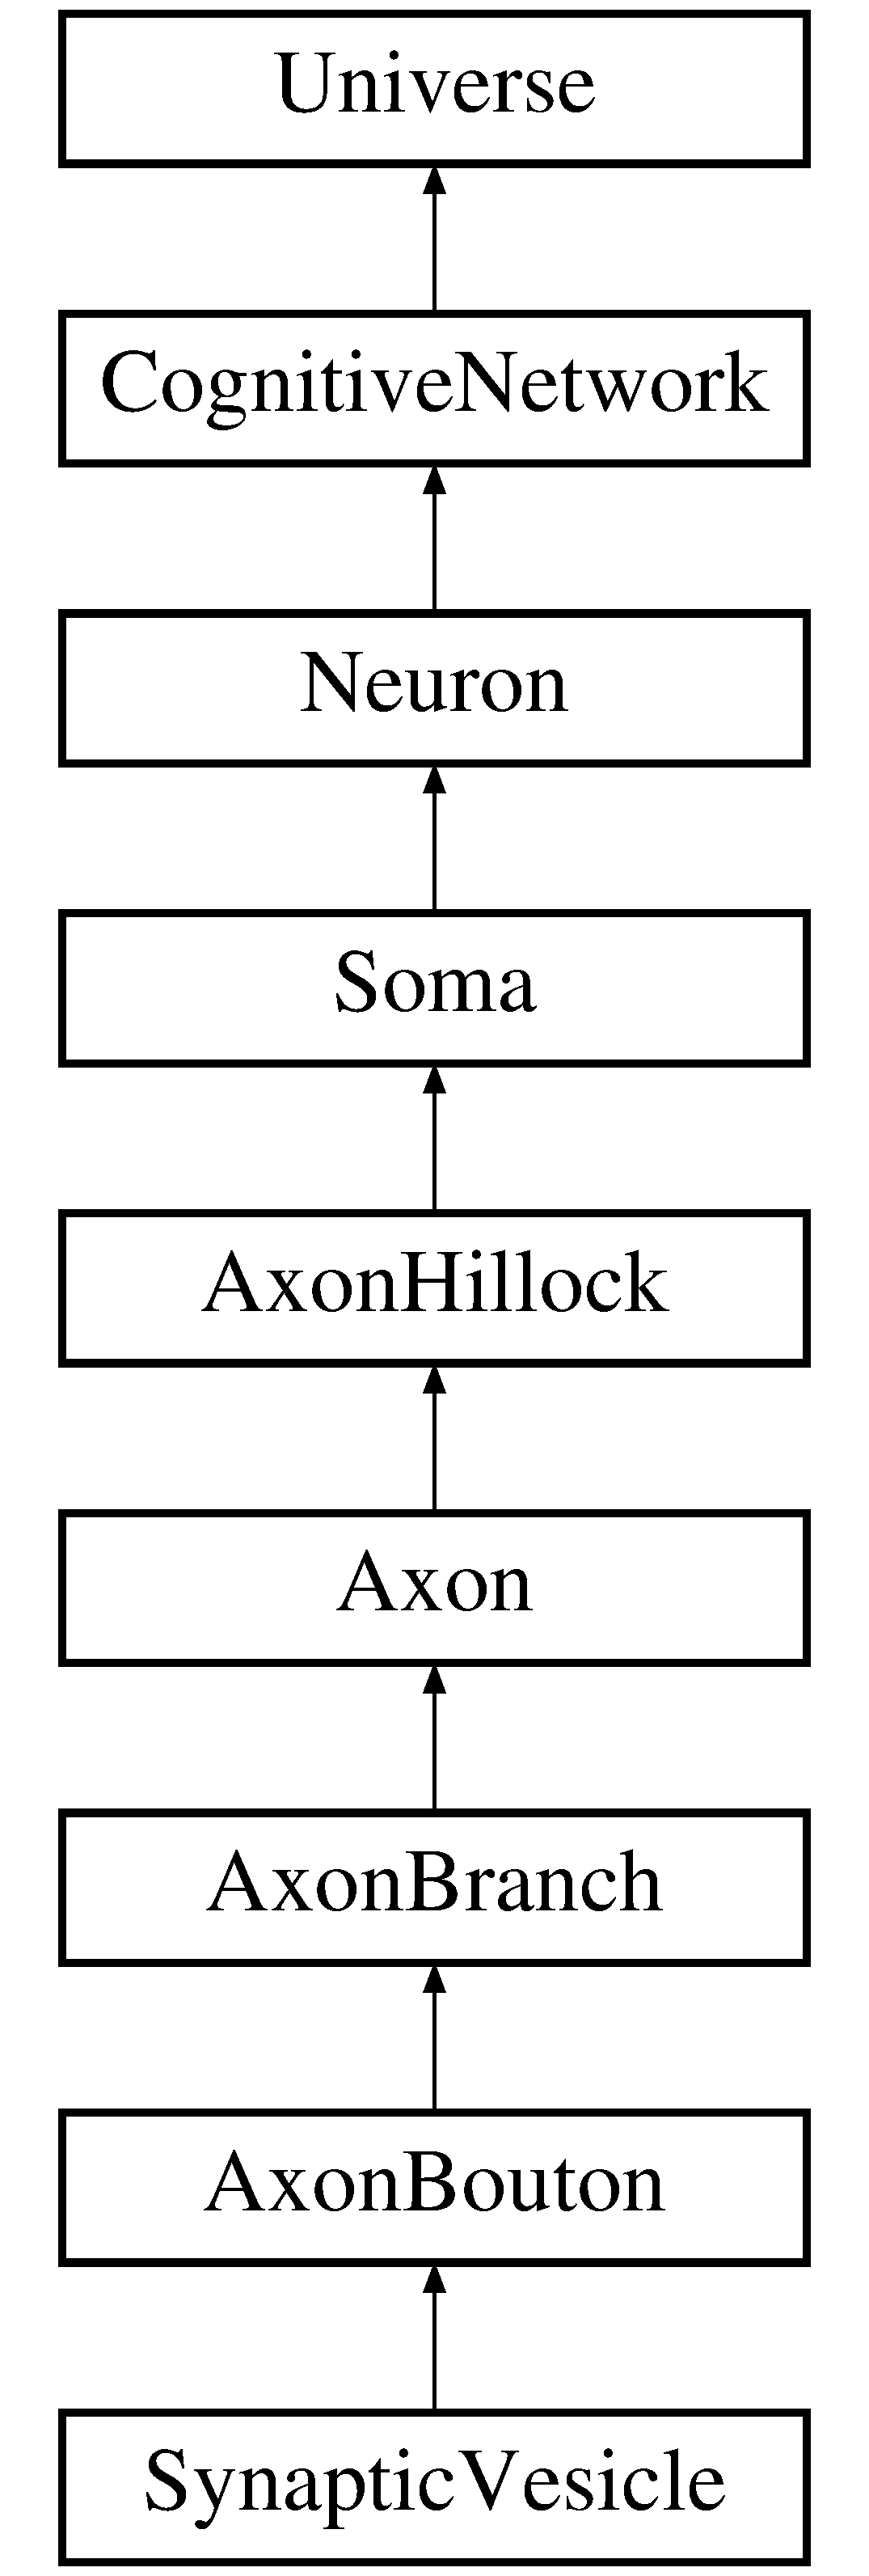
\includegraphics[height=9.000000cm]{classAxonBranch}
\end{center}
\end{figure}
\subsection*{Public Member Functions}
\begin{DoxyCompactItemize}
\item 
\mbox{\hyperlink{classAxonBranch_a5bb6ccef8d94c937a85148af932221c0}{Axon\+Branch}} ()
\item 
\mbox{\hyperlink{classAxonBranch_a67618605ac3731556ab48a6583e21ba8}{Axon\+Branch}} (unsigned int object\+\_\+type)
\item 
\mbox{\hyperlink{classAxonBranch_ad6191fcfd8bedc058a4f1cfb5056f5b2}{Axon\+Branch}} (unsigned int object\+\_\+type, std\+::chrono\+::time\+\_\+point$<$ \mbox{\hyperlink{universe_8h_a0ef8d951d1ca5ab3cfaf7ab4c7a6fd80}{Clock}} $>$ event\+\_\+time)
\item 
\mbox{\hyperlink{classAxonBranch_a98f33462edf82dacab750d1140172912}{Axon\+Branch}} (unsigned int object\+\_\+type, std\+::chrono\+::time\+\_\+point$<$ \mbox{\hyperlink{universe_8h_a0ef8d951d1ca5ab3cfaf7ab4c7a6fd80}{Clock}} $>$ event\+\_\+time, \mbox{\hyperlink{classAxon}{Axon}} \&axon\+\_\+connector)
\item 
virtual \mbox{\hyperlink{classAxonBranch_ae4ef4c954b43d084cafb30cf900a1728}{$\sim$\+Axon\+Branch}} ()
\item 
unsigned int \mbox{\hyperlink{classAxonBranch_a1d2404b68ec2d18a814c96a7c04c5fc4}{Get\+Counter}} (std\+::chrono\+::time\+\_\+point$<$ \mbox{\hyperlink{universe_8h_a0ef8d951d1ca5ab3cfaf7ab4c7a6fd80}{Clock}} $>$ event\+\_\+time)
\item 
double \mbox{\hyperlink{classAxonBranch_a688ec51cd5116e9aebe9b4d3c5c7f2b1}{Get\+Energy}} (std\+::chrono\+::time\+\_\+point$<$ \mbox{\hyperlink{universe_8h_a0ef8d951d1ca5ab3cfaf7ab4c7a6fd80}{Clock}} $>$ event\+\_\+time)
\item 
void \mbox{\hyperlink{classAxonBranch_a96ba30b18627563d637d4e02fac943be}{Set\+Counter}} (std\+::chrono\+::time\+\_\+point$<$ \mbox{\hyperlink{universe_8h_a0ef8d951d1ca5ab3cfaf7ab4c7a6fd80}{Clock}} $>$ event\+\_\+time, unsigned int val)
\item 
void \mbox{\hyperlink{classAxonBranch_a6918dcaf6d9325a1a22a2e6c65ad5dab}{Set\+Energy}} (std\+::chrono\+::time\+\_\+point$<$ \mbox{\hyperlink{universe_8h_a0ef8d951d1ca5ab3cfaf7ab4c7a6fd80}{Clock}} $>$ event\+\_\+time, double val)
\item 
bool \mbox{\hyperlink{classAxonBranch_a195d68dffd37317db3f94e1b4c8f73c7}{Reset\+Parameters}} (std\+::chrono\+::time\+\_\+point$<$ \mbox{\hyperlink{universe_8h_a0ef8d951d1ca5ab3cfaf7ab4c7a6fd80}{Clock}} $>$ event\+\_\+time)
\item 
\mbox{\hyperlink{classAxonBranch}{Axon\+Branch}} $\ast$ \mbox{\hyperlink{classAxonBranch_a30b4602e5dd121666478ff9de52d022b}{Create\+Axon\+Bouton}} (std\+::chrono\+::time\+\_\+point$<$ \mbox{\hyperlink{universe_8h_a0ef8d951d1ca5ab3cfaf7ab4c7a6fd80}{Clock}} $>$ event\+\_\+time)
\item 
std\+::vector$<$ \mbox{\hyperlink{classAxonBranch}{Axon\+Branch}} $\ast$ $>$ \mbox{\hyperlink{classAxonBranch_a77e93626a7993f76e689d09721974e90}{Create\+Axon\+Boutons}} (std\+::chrono\+::time\+\_\+point$<$ \mbox{\hyperlink{universe_8h_a0ef8d951d1ca5ab3cfaf7ab4c7a6fd80}{Clock}} $>$ event\+\_\+time, int quantity)
\item 
\mbox{\hyperlink{classAxonBranch}{Axon\+Branch}} $\ast$ \mbox{\hyperlink{classAxonBranch_ae861207a8a0aeb2b60c305b25248e4b9}{Clone\+Axon\+Bouton}} (std\+::chrono\+::time\+\_\+point$<$ \mbox{\hyperlink{universe_8h_a0ef8d951d1ca5ab3cfaf7ab4c7a6fd80}{Clock}} $>$ event\+\_\+time, \mbox{\hyperlink{classAxonBranch}{Axon\+Branch}} $\ast$clone\+\_\+object, double perfection\+\_\+membership)
\item 
std\+::vector$<$ \mbox{\hyperlink{classAxonBranch}{Axon\+Branch}} $\ast$ $>$ \mbox{\hyperlink{classAxonBranch_a842b3875b2771f4b8e7316bfb9af894c}{Clone\+Axon\+Boutons}} (std\+::chrono\+::time\+\_\+point$<$ \mbox{\hyperlink{universe_8h_a0ef8d951d1ca5ab3cfaf7ab4c7a6fd80}{Clock}} $>$ event\+\_\+time, std\+::vector$<$ \mbox{\hyperlink{classAxonBranch}{Axon\+Branch}} $\ast$$>$ cloning\+\_\+list, double perfection\+\_\+membership)
\item 
\mbox{\hyperlink{classAxonBranch}{Axon\+Branch}} $\ast$ \mbox{\hyperlink{classAxonBranch_a024c8666555702ebe67e2a5caf1b866a}{Destroy\+Axon\+Bouton}} (std\+::chrono\+::time\+\_\+point$<$ \mbox{\hyperlink{universe_8h_a0ef8d951d1ca5ab3cfaf7ab4c7a6fd80}{Clock}} $>$ event\+\_\+time, \mbox{\hyperlink{classAxonBranch}{Axon\+Branch}} $\ast$destroy\+\_\+object)
\item 
std\+::vector$<$ \mbox{\hyperlink{classAxonBranch}{Axon\+Branch}} $\ast$ $>$ \mbox{\hyperlink{classAxonBranch_a8c022977e091b8cab367b21c0c4930ea}{Destroy\+Axon\+Boutons}} (std\+::chrono\+::time\+\_\+point$<$ \mbox{\hyperlink{universe_8h_a0ef8d951d1ca5ab3cfaf7ab4c7a6fd80}{Clock}} $>$ event\+\_\+time, std\+::vector$<$ \mbox{\hyperlink{classAxonBranch}{Axon\+Branch}} $\ast$$>$ destruction\+\_\+list)
\item 
\mbox{\hyperlink{classAxonBranch}{Axon\+Branch}} $\ast$ \mbox{\hyperlink{classAxonBranch_a88e6af84b45bb6f6f8900a6d4aec446c}{Add\+Axon\+Bouton}} (std\+::chrono\+::time\+\_\+point$<$ \mbox{\hyperlink{universe_8h_a0ef8d951d1ca5ab3cfaf7ab4c7a6fd80}{Clock}} $>$ event\+\_\+time, \mbox{\hyperlink{classAxonBranch}{Axon\+Branch}} $\ast$add\+\_\+object)
\item 
std\+::vector$<$ \mbox{\hyperlink{classAxonBranch}{Axon\+Branch}} $\ast$ $>$ \mbox{\hyperlink{classAxonBranch_a788ca8cc7e6f60f07b9e19a8e3022b64}{Add\+Axon\+Boutons}} (std\+::chrono\+::time\+\_\+point$<$ \mbox{\hyperlink{universe_8h_a0ef8d951d1ca5ab3cfaf7ab4c7a6fd80}{Clock}} $>$ event\+\_\+time, std\+::vector$<$ \mbox{\hyperlink{classAxonBranch}{Axon\+Branch}} $\ast$$>$ add\+\_\+objects)
\item 
\mbox{\hyperlink{classAxonBranch}{Axon\+Branch}} $\ast$ \mbox{\hyperlink{classAxonBranch_a06753a2a61941a59d86510e51ba44b15}{Remove\+Axon\+Bouton}} (std\+::chrono\+::time\+\_\+point$<$ \mbox{\hyperlink{universe_8h_a0ef8d951d1ca5ab3cfaf7ab4c7a6fd80}{Clock}} $>$ event\+\_\+time)
\item 
std\+::vector$<$ \mbox{\hyperlink{classAxonBranch}{Axon\+Branch}} $\ast$ $>$ \mbox{\hyperlink{classAxonBranch_a815e055e37f89fb2627b250c5b95d406}{Remove\+Axon\+Boutons}} (std\+::chrono\+::time\+\_\+point$<$ \mbox{\hyperlink{universe_8h_a0ef8d951d1ca5ab3cfaf7ab4c7a6fd80}{Clock}} $>$ event\+\_\+time, int quantity)
\item 
\mbox{\hyperlink{classAxonBranch}{Axon\+Branch}} $\ast$ \mbox{\hyperlink{classAxonBranch_a6fa6eea91e72fd142f3d691f7ca4c99a}{Get\+Axon\+Bouton}} (std\+::chrono\+::time\+\_\+point$<$ \mbox{\hyperlink{universe_8h_a0ef8d951d1ca5ab3cfaf7ab4c7a6fd80}{Clock}} $>$ event\+\_\+time, int selector)
\item 
std\+::vector$<$ \mbox{\hyperlink{classAxonBranch}{Axon\+Branch}} $\ast$ $>$ \mbox{\hyperlink{classAxonBranch_aafadba57924686a8087c7f7758889045}{Get\+Axon\+Boutons}} (std\+::chrono\+::time\+\_\+point$<$ \mbox{\hyperlink{universe_8h_a0ef8d951d1ca5ab3cfaf7ab4c7a6fd80}{Clock}} $>$ event\+\_\+time)
\item 
int \mbox{\hyperlink{classAxonBranch_a6e434a57873ab0fdbc72cf7ecc7228ed}{Growth}} (std\+::chrono\+::time\+\_\+point$<$ \mbox{\hyperlink{universe_8h_a0ef8d951d1ca5ab3cfaf7ab4c7a6fd80}{Clock}} $>$ event\+\_\+time)
\item 
int \mbox{\hyperlink{classAxonBranch_a5a80bcccdc2be9f77fca25131937b52f}{Update}} (std\+::chrono\+::time\+\_\+point$<$ std\+::chrono\+::high\+\_\+resolution\+\_\+clock $>$ val)
\end{DoxyCompactItemize}
\subsection*{Protected Attributes}
\begin{DoxyCompactItemize}
\item 
std\+::vector$<$ \mbox{\hyperlink{classAxonBranch}{Axon\+Branch}} $\ast$ $>$ \mbox{\hyperlink{classAxonBranch_a43224f9fcb62274709438c9833cb10e5}{axonbouton\+\_\+list}}
\end{DoxyCompactItemize}
\subsection*{Private Attributes}
\begin{DoxyCompactItemize}
\item 
int \mbox{\hyperlink{classAxonBranch_a7ecf92c68997eb344c1d6e8c9ba92cfb}{axonbranch\+\_\+type}}
\item 
int \mbox{\hyperlink{classAxonBranch_a5c1ab609b7887ee437d9c1fbc6960fc5}{m\+\_\+add\+Status}}
\item 
int \mbox{\hyperlink{classAxonBranch_adccee24d22600a90f3507477e6ef63af}{axonbouton\+\_\+pool}}
\item 
std\+::chrono\+::time\+\_\+point$<$ \mbox{\hyperlink{universe_8h_a0ef8d951d1ca5ab3cfaf7ab4c7a6fd80}{Clock}} $>$ \mbox{\hyperlink{classAxonBranch_af57a6117490f6cf20ba22c9d107cabfb}{time\+\_\+object\+\_\+created}}
\item 
std\+::chrono\+::time\+\_\+point$<$ \mbox{\hyperlink{universe_8h_a0ef8d951d1ca5ab3cfaf7ab4c7a6fd80}{Clock}} $>$ \mbox{\hyperlink{classAxonBranch_a6a1607a44a26b4277a7f0fc32cafb530}{previous\+\_\+event\+\_\+time}}
\item 
int \mbox{\hyperlink{classAxonBranch_a98d317c3a02b1bbca631d102e9cb8d39}{duration\+\_\+since\+\_\+last\+\_\+event}}
\item 
double \mbox{\hyperlink{classAxonBranch_a9751ecf633d28c0cc33b3538e95e5ff3}{m\+\_\+\+Volume}}
\item 
double \mbox{\hyperlink{classAxonBranch_a7ef58cc007435db340fbbbb37f9f0201}{m\+\_\+\+Surface\+Area}}
\item 
unsigned int \mbox{\hyperlink{classAxonBranch_a1f5e38be0828557a63972092d61eb001}{m\+\_\+\+Counter}}
\begin{DoxyCompactList}\small\item\em Member variable \char`\"{}m\+\_\+\+Counter\char`\"{}. \end{DoxyCompactList}\item 
double \mbox{\hyperlink{classAxonBranch_a50c032dbd82cf1aad10cf51c90993361}{object\+\_\+energy}}
\begin{DoxyCompactList}\small\item\em Member variable \char`\"{}object\+\_\+energy\char`\"{}. \end{DoxyCompactList}\item 
double \mbox{\hyperlink{classAxonBranch_ab737e5ee5c9209de468e061a1a84c148}{m\+\_\+\+Time\+Dilation}}
\item 
double \mbox{\hyperlink{classAxonBranch_a962453447332826acf0bdef49cd70a7f}{m\+\_\+\+Time\+Threshold}}
\item 
double \mbox{\hyperlink{classAxonBranch_a7c7b6c5f08a20bc956d37b01b183c4d8}{object\+\_\+size}}
\item 
bool \mbox{\hyperlink{classAxonBranch_ac71332a4fcf5fbe1e58647ac09945f39}{object\+\_\+disabled}}
\item 
bool \mbox{\hyperlink{classAxonBranch_a6f7a66fc08c4b829e4f14fde6177c4ab}{object\+\_\+initialised}}
\item 
double \mbox{\hyperlink{classAxonBranch_a3278f6e24660f62018b5afd7280f1575}{object\+\_\+energy\+\_\+threshold}}
\end{DoxyCompactItemize}
\subsection*{Additional Inherited Members}


\subsection{Constructor \& Destructor Documentation}
\mbox{\Hypertarget{classAxonBranch_a5bb6ccef8d94c937a85148af932221c0}\label{classAxonBranch_a5bb6ccef8d94c937a85148af932221c0}} 
\index{Axon\+Branch@{Axon\+Branch}!Axon\+Branch@{Axon\+Branch}}
\index{Axon\+Branch@{Axon\+Branch}!Axon\+Branch@{Axon\+Branch}}
\subsubsection{\texorpdfstring{Axon\+Branch()}{AxonBranch()}\hspace{0.1cm}{\footnotesize\ttfamily [1/4]}}
{\footnotesize\ttfamily Axon\+Branch\+::\+Axon\+Branch (\begin{DoxyParamCaption}{ }\end{DoxyParamCaption})\hspace{0.3cm}{\ttfamily [inline]}}

\mbox{\Hypertarget{classAxonBranch_a67618605ac3731556ab48a6583e21ba8}\label{classAxonBranch_a67618605ac3731556ab48a6583e21ba8}} 
\index{Axon\+Branch@{Axon\+Branch}!Axon\+Branch@{Axon\+Branch}}
\index{Axon\+Branch@{Axon\+Branch}!Axon\+Branch@{Axon\+Branch}}
\subsubsection{\texorpdfstring{Axon\+Branch()}{AxonBranch()}\hspace{0.1cm}{\footnotesize\ttfamily [2/4]}}
{\footnotesize\ttfamily Axon\+Branch\+::\+Axon\+Branch (\begin{DoxyParamCaption}\item[{unsigned int}]{object\+\_\+type }\end{DoxyParamCaption})\hspace{0.3cm}{\ttfamily [inline]}}

\mbox{\Hypertarget{classAxonBranch_ad6191fcfd8bedc058a4f1cfb5056f5b2}\label{classAxonBranch_ad6191fcfd8bedc058a4f1cfb5056f5b2}} 
\index{Axon\+Branch@{Axon\+Branch}!Axon\+Branch@{Axon\+Branch}}
\index{Axon\+Branch@{Axon\+Branch}!Axon\+Branch@{Axon\+Branch}}
\subsubsection{\texorpdfstring{Axon\+Branch()}{AxonBranch()}\hspace{0.1cm}{\footnotesize\ttfamily [3/4]}}
{\footnotesize\ttfamily Axon\+Branch\+::\+Axon\+Branch (\begin{DoxyParamCaption}\item[{unsigned int}]{object\+\_\+type,  }\item[{std\+::chrono\+::time\+\_\+point$<$ \mbox{\hyperlink{universe_8h_a0ef8d951d1ca5ab3cfaf7ab4c7a6fd80}{Clock}} $>$}]{event\+\_\+time }\end{DoxyParamCaption})\hspace{0.3cm}{\ttfamily [inline]}}

\mbox{\Hypertarget{classAxonBranch_a98f33462edf82dacab750d1140172912}\label{classAxonBranch_a98f33462edf82dacab750d1140172912}} 
\index{Axon\+Branch@{Axon\+Branch}!Axon\+Branch@{Axon\+Branch}}
\index{Axon\+Branch@{Axon\+Branch}!Axon\+Branch@{Axon\+Branch}}
\subsubsection{\texorpdfstring{Axon\+Branch()}{AxonBranch()}\hspace{0.1cm}{\footnotesize\ttfamily [4/4]}}
{\footnotesize\ttfamily Axon\+Branch\+::\+Axon\+Branch (\begin{DoxyParamCaption}\item[{unsigned int}]{object\+\_\+type,  }\item[{std\+::chrono\+::time\+\_\+point$<$ \mbox{\hyperlink{universe_8h_a0ef8d951d1ca5ab3cfaf7ab4c7a6fd80}{Clock}} $>$}]{event\+\_\+time,  }\item[{\mbox{\hyperlink{classAxon}{Axon}} \&}]{axon\+\_\+connector }\end{DoxyParamCaption})\hspace{0.3cm}{\ttfamily [inline]}}

\mbox{\Hypertarget{classAxonBranch_ae4ef4c954b43d084cafb30cf900a1728}\label{classAxonBranch_ae4ef4c954b43d084cafb30cf900a1728}} 
\index{Axon\+Branch@{Axon\+Branch}!````~Axon\+Branch@{$\sim$\+Axon\+Branch}}
\index{````~Axon\+Branch@{$\sim$\+Axon\+Branch}!Axon\+Branch@{Axon\+Branch}}
\subsubsection{\texorpdfstring{$\sim$\+Axon\+Branch()}{~AxonBranch()}}
{\footnotesize\ttfamily virtual Axon\+Branch\+::$\sim$\+Axon\+Branch (\begin{DoxyParamCaption}{ }\end{DoxyParamCaption})\hspace{0.3cm}{\ttfamily [inline]}, {\ttfamily [virtual]}}

Default destructor 

\subsection{Member Function Documentation}
\mbox{\Hypertarget{classAxonBranch_a88e6af84b45bb6f6f8900a6d4aec446c}\label{classAxonBranch_a88e6af84b45bb6f6f8900a6d4aec446c}} 
\index{Axon\+Branch@{Axon\+Branch}!Add\+Axon\+Bouton@{Add\+Axon\+Bouton}}
\index{Add\+Axon\+Bouton@{Add\+Axon\+Bouton}!Axon\+Branch@{Axon\+Branch}}
\subsubsection{\texorpdfstring{Add\+Axon\+Bouton()}{AddAxonBouton()}}
{\footnotesize\ttfamily \mbox{\hyperlink{classAxonBranch}{Axon\+Branch}} $\ast$ Axon\+Branch\+::\+Add\+Axon\+Bouton (\begin{DoxyParamCaption}\item[{std\+::chrono\+::time\+\_\+point$<$ \mbox{\hyperlink{universe_8h_a0ef8d951d1ca5ab3cfaf7ab4c7a6fd80}{Clock}} $>$}]{event\+\_\+time,  }\item[{\mbox{\hyperlink{classAxonBranch}{Axon\+Branch}} $\ast$}]{add\+\_\+object }\end{DoxyParamCaption})}

\mbox{\Hypertarget{classAxonBranch_a788ca8cc7e6f60f07b9e19a8e3022b64}\label{classAxonBranch_a788ca8cc7e6f60f07b9e19a8e3022b64}} 
\index{Axon\+Branch@{Axon\+Branch}!Add\+Axon\+Boutons@{Add\+Axon\+Boutons}}
\index{Add\+Axon\+Boutons@{Add\+Axon\+Boutons}!Axon\+Branch@{Axon\+Branch}}
\subsubsection{\texorpdfstring{Add\+Axon\+Boutons()}{AddAxonBoutons()}}
{\footnotesize\ttfamily std\+::vector$<$ \mbox{\hyperlink{classAxonBranch}{Axon\+Branch}} $\ast$ $>$ Axon\+Branch\+::\+Add\+Axon\+Boutons (\begin{DoxyParamCaption}\item[{std\+::chrono\+::time\+\_\+point$<$ \mbox{\hyperlink{universe_8h_a0ef8d951d1ca5ab3cfaf7ab4c7a6fd80}{Clock}} $>$}]{event\+\_\+time,  }\item[{std\+::vector$<$ \mbox{\hyperlink{classAxonBranch}{Axon\+Branch}} $\ast$$>$}]{add\+\_\+objects }\end{DoxyParamCaption})}

\mbox{\Hypertarget{classAxonBranch_ae861207a8a0aeb2b60c305b25248e4b9}\label{classAxonBranch_ae861207a8a0aeb2b60c305b25248e4b9}} 
\index{Axon\+Branch@{Axon\+Branch}!Clone\+Axon\+Bouton@{Clone\+Axon\+Bouton}}
\index{Clone\+Axon\+Bouton@{Clone\+Axon\+Bouton}!Axon\+Branch@{Axon\+Branch}}
\subsubsection{\texorpdfstring{Clone\+Axon\+Bouton()}{CloneAxonBouton()}}
{\footnotesize\ttfamily \mbox{\hyperlink{classAxonBranch}{Axon\+Branch}} $\ast$ Axon\+Branch\+::\+Clone\+Axon\+Bouton (\begin{DoxyParamCaption}\item[{std\+::chrono\+::time\+\_\+point$<$ \mbox{\hyperlink{universe_8h_a0ef8d951d1ca5ab3cfaf7ab4c7a6fd80}{Clock}} $>$}]{event\+\_\+time,  }\item[{\mbox{\hyperlink{classAxonBranch}{Axon\+Branch}} $\ast$}]{clone\+\_\+object,  }\item[{double}]{perfection\+\_\+membership }\end{DoxyParamCaption})}

\mbox{\Hypertarget{classAxonBranch_a842b3875b2771f4b8e7316bfb9af894c}\label{classAxonBranch_a842b3875b2771f4b8e7316bfb9af894c}} 
\index{Axon\+Branch@{Axon\+Branch}!Clone\+Axon\+Boutons@{Clone\+Axon\+Boutons}}
\index{Clone\+Axon\+Boutons@{Clone\+Axon\+Boutons}!Axon\+Branch@{Axon\+Branch}}
\subsubsection{\texorpdfstring{Clone\+Axon\+Boutons()}{CloneAxonBoutons()}}
{\footnotesize\ttfamily std\+::vector$<$ \mbox{\hyperlink{classAxonBranch}{Axon\+Branch}} $\ast$ $>$ Axon\+Branch\+::\+Clone\+Axon\+Boutons (\begin{DoxyParamCaption}\item[{std\+::chrono\+::time\+\_\+point$<$ \mbox{\hyperlink{universe_8h_a0ef8d951d1ca5ab3cfaf7ab4c7a6fd80}{Clock}} $>$}]{event\+\_\+time,  }\item[{std\+::vector$<$ \mbox{\hyperlink{classAxonBranch}{Axon\+Branch}} $\ast$$>$}]{cloning\+\_\+list,  }\item[{double}]{perfection\+\_\+membership }\end{DoxyParamCaption})}

\mbox{\Hypertarget{classAxonBranch_a30b4602e5dd121666478ff9de52d022b}\label{classAxonBranch_a30b4602e5dd121666478ff9de52d022b}} 
\index{Axon\+Branch@{Axon\+Branch}!Create\+Axon\+Bouton@{Create\+Axon\+Bouton}}
\index{Create\+Axon\+Bouton@{Create\+Axon\+Bouton}!Axon\+Branch@{Axon\+Branch}}
\subsubsection{\texorpdfstring{Create\+Axon\+Bouton()}{CreateAxonBouton()}}
{\footnotesize\ttfamily \mbox{\hyperlink{classAxonBranch}{Axon\+Branch}} $\ast$ Axon\+Branch\+::\+Create\+Axon\+Bouton (\begin{DoxyParamCaption}\item[{std\+::chrono\+::time\+\_\+point$<$ \mbox{\hyperlink{universe_8h_a0ef8d951d1ca5ab3cfaf7ab4c7a6fd80}{Clock}} $>$}]{event\+\_\+time }\end{DoxyParamCaption})}

\mbox{\Hypertarget{classAxonBranch_a77e93626a7993f76e689d09721974e90}\label{classAxonBranch_a77e93626a7993f76e689d09721974e90}} 
\index{Axon\+Branch@{Axon\+Branch}!Create\+Axon\+Boutons@{Create\+Axon\+Boutons}}
\index{Create\+Axon\+Boutons@{Create\+Axon\+Boutons}!Axon\+Branch@{Axon\+Branch}}
\subsubsection{\texorpdfstring{Create\+Axon\+Boutons()}{CreateAxonBoutons()}}
{\footnotesize\ttfamily std\+::vector$<$ \mbox{\hyperlink{classAxonBranch}{Axon\+Branch}} $\ast$ $>$ Axon\+Branch\+::\+Create\+Axon\+Boutons (\begin{DoxyParamCaption}\item[{std\+::chrono\+::time\+\_\+point$<$ \mbox{\hyperlink{universe_8h_a0ef8d951d1ca5ab3cfaf7ab4c7a6fd80}{Clock}} $>$}]{event\+\_\+time,  }\item[{int}]{quantity }\end{DoxyParamCaption})}

\mbox{\Hypertarget{classAxonBranch_a024c8666555702ebe67e2a5caf1b866a}\label{classAxonBranch_a024c8666555702ebe67e2a5caf1b866a}} 
\index{Axon\+Branch@{Axon\+Branch}!Destroy\+Axon\+Bouton@{Destroy\+Axon\+Bouton}}
\index{Destroy\+Axon\+Bouton@{Destroy\+Axon\+Bouton}!Axon\+Branch@{Axon\+Branch}}
\subsubsection{\texorpdfstring{Destroy\+Axon\+Bouton()}{DestroyAxonBouton()}}
{\footnotesize\ttfamily \mbox{\hyperlink{classAxonBranch}{Axon\+Branch}} $\ast$ Axon\+Branch\+::\+Destroy\+Axon\+Bouton (\begin{DoxyParamCaption}\item[{std\+::chrono\+::time\+\_\+point$<$ \mbox{\hyperlink{universe_8h_a0ef8d951d1ca5ab3cfaf7ab4c7a6fd80}{Clock}} $>$}]{event\+\_\+time,  }\item[{\mbox{\hyperlink{classAxonBranch}{Axon\+Branch}} $\ast$}]{destroy\+\_\+object }\end{DoxyParamCaption})}

\mbox{\Hypertarget{classAxonBranch_a8c022977e091b8cab367b21c0c4930ea}\label{classAxonBranch_a8c022977e091b8cab367b21c0c4930ea}} 
\index{Axon\+Branch@{Axon\+Branch}!Destroy\+Axon\+Boutons@{Destroy\+Axon\+Boutons}}
\index{Destroy\+Axon\+Boutons@{Destroy\+Axon\+Boutons}!Axon\+Branch@{Axon\+Branch}}
\subsubsection{\texorpdfstring{Destroy\+Axon\+Boutons()}{DestroyAxonBoutons()}}
{\footnotesize\ttfamily std\+::vector$<$ \mbox{\hyperlink{classAxonBranch}{Axon\+Branch}} $\ast$ $>$ Axon\+Branch\+::\+Destroy\+Axon\+Boutons (\begin{DoxyParamCaption}\item[{std\+::chrono\+::time\+\_\+point$<$ \mbox{\hyperlink{universe_8h_a0ef8d951d1ca5ab3cfaf7ab4c7a6fd80}{Clock}} $>$}]{event\+\_\+time,  }\item[{std\+::vector$<$ \mbox{\hyperlink{classAxonBranch}{Axon\+Branch}} $\ast$$>$}]{destruction\+\_\+list }\end{DoxyParamCaption})}

\mbox{\Hypertarget{classAxonBranch_a6fa6eea91e72fd142f3d691f7ca4c99a}\label{classAxonBranch_a6fa6eea91e72fd142f3d691f7ca4c99a}} 
\index{Axon\+Branch@{Axon\+Branch}!Get\+Axon\+Bouton@{Get\+Axon\+Bouton}}
\index{Get\+Axon\+Bouton@{Get\+Axon\+Bouton}!Axon\+Branch@{Axon\+Branch}}
\subsubsection{\texorpdfstring{Get\+Axon\+Bouton()}{GetAxonBouton()}}
{\footnotesize\ttfamily \mbox{\hyperlink{classAxonBranch}{Axon\+Branch}} $\ast$ Axon\+Branch\+::\+Get\+Axon\+Bouton (\begin{DoxyParamCaption}\item[{std\+::chrono\+::time\+\_\+point$<$ \mbox{\hyperlink{universe_8h_a0ef8d951d1ca5ab3cfaf7ab4c7a6fd80}{Clock}} $>$}]{event\+\_\+time,  }\item[{int}]{selector }\end{DoxyParamCaption})}

\mbox{\Hypertarget{classAxonBranch_aafadba57924686a8087c7f7758889045}\label{classAxonBranch_aafadba57924686a8087c7f7758889045}} 
\index{Axon\+Branch@{Axon\+Branch}!Get\+Axon\+Boutons@{Get\+Axon\+Boutons}}
\index{Get\+Axon\+Boutons@{Get\+Axon\+Boutons}!Axon\+Branch@{Axon\+Branch}}
\subsubsection{\texorpdfstring{Get\+Axon\+Boutons()}{GetAxonBoutons()}}
{\footnotesize\ttfamily std\+::vector$<$ \mbox{\hyperlink{classAxonBranch}{Axon\+Branch}} $\ast$ $>$ Axon\+Branch\+::\+Get\+Axon\+Boutons (\begin{DoxyParamCaption}\item[{std\+::chrono\+::time\+\_\+point$<$ \mbox{\hyperlink{universe_8h_a0ef8d951d1ca5ab3cfaf7ab4c7a6fd80}{Clock}} $>$}]{event\+\_\+time }\end{DoxyParamCaption})}

\mbox{\Hypertarget{classAxonBranch_a1d2404b68ec2d18a814c96a7c04c5fc4}\label{classAxonBranch_a1d2404b68ec2d18a814c96a7c04c5fc4}} 
\index{Axon\+Branch@{Axon\+Branch}!Get\+Counter@{Get\+Counter}}
\index{Get\+Counter@{Get\+Counter}!Axon\+Branch@{Axon\+Branch}}
\subsubsection{\texorpdfstring{Get\+Counter()}{GetCounter()}}
{\footnotesize\ttfamily unsigned int Axon\+Branch\+::\+Get\+Counter (\begin{DoxyParamCaption}\item[{std\+::chrono\+::time\+\_\+point$<$ \mbox{\hyperlink{universe_8h_a0ef8d951d1ca5ab3cfaf7ab4c7a6fd80}{Clock}} $>$}]{event\+\_\+time }\end{DoxyParamCaption})\hspace{0.3cm}{\ttfamily [inline]}}

\mbox{\Hypertarget{classAxonBranch_a688ec51cd5116e9aebe9b4d3c5c7f2b1}\label{classAxonBranch_a688ec51cd5116e9aebe9b4d3c5c7f2b1}} 
\index{Axon\+Branch@{Axon\+Branch}!Get\+Energy@{Get\+Energy}}
\index{Get\+Energy@{Get\+Energy}!Axon\+Branch@{Axon\+Branch}}
\subsubsection{\texorpdfstring{Get\+Energy()}{GetEnergy()}}
{\footnotesize\ttfamily double Axon\+Branch\+::\+Get\+Energy (\begin{DoxyParamCaption}\item[{std\+::chrono\+::time\+\_\+point$<$ \mbox{\hyperlink{universe_8h_a0ef8d951d1ca5ab3cfaf7ab4c7a6fd80}{Clock}} $>$}]{event\+\_\+time }\end{DoxyParamCaption})\hspace{0.3cm}{\ttfamily [inline]}}

\mbox{\Hypertarget{classAxonBranch_a6e434a57873ab0fdbc72cf7ecc7228ed}\label{classAxonBranch_a6e434a57873ab0fdbc72cf7ecc7228ed}} 
\index{Axon\+Branch@{Axon\+Branch}!Growth@{Growth}}
\index{Growth@{Growth}!Axon\+Branch@{Axon\+Branch}}
\subsubsection{\texorpdfstring{Growth()}{Growth()}}
{\footnotesize\ttfamily int Axon\+Branch\+::\+Growth (\begin{DoxyParamCaption}\item[{std\+::chrono\+::time\+\_\+point$<$ \mbox{\hyperlink{universe_8h_a0ef8d951d1ca5ab3cfaf7ab4c7a6fd80}{Clock}} $>$}]{event\+\_\+time }\end{DoxyParamCaption})}

\mbox{\Hypertarget{classAxonBranch_a06753a2a61941a59d86510e51ba44b15}\label{classAxonBranch_a06753a2a61941a59d86510e51ba44b15}} 
\index{Axon\+Branch@{Axon\+Branch}!Remove\+Axon\+Bouton@{Remove\+Axon\+Bouton}}
\index{Remove\+Axon\+Bouton@{Remove\+Axon\+Bouton}!Axon\+Branch@{Axon\+Branch}}
\subsubsection{\texorpdfstring{Remove\+Axon\+Bouton()}{RemoveAxonBouton()}}
{\footnotesize\ttfamily \mbox{\hyperlink{classAxonBranch}{Axon\+Branch}} $\ast$ Axon\+Branch\+::\+Remove\+Axon\+Bouton (\begin{DoxyParamCaption}\item[{std\+::chrono\+::time\+\_\+point$<$ \mbox{\hyperlink{universe_8h_a0ef8d951d1ca5ab3cfaf7ab4c7a6fd80}{Clock}} $>$}]{event\+\_\+time }\end{DoxyParamCaption})}

\mbox{\Hypertarget{classAxonBranch_a815e055e37f89fb2627b250c5b95d406}\label{classAxonBranch_a815e055e37f89fb2627b250c5b95d406}} 
\index{Axon\+Branch@{Axon\+Branch}!Remove\+Axon\+Boutons@{Remove\+Axon\+Boutons}}
\index{Remove\+Axon\+Boutons@{Remove\+Axon\+Boutons}!Axon\+Branch@{Axon\+Branch}}
\subsubsection{\texorpdfstring{Remove\+Axon\+Boutons()}{RemoveAxonBoutons()}}
{\footnotesize\ttfamily std\+::vector$<$ \mbox{\hyperlink{classAxonBranch}{Axon\+Branch}} $\ast$ $>$ Axon\+Branch\+::\+Remove\+Axon\+Boutons (\begin{DoxyParamCaption}\item[{std\+::chrono\+::time\+\_\+point$<$ \mbox{\hyperlink{universe_8h_a0ef8d951d1ca5ab3cfaf7ab4c7a6fd80}{Clock}} $>$}]{event\+\_\+time,  }\item[{int}]{quantity }\end{DoxyParamCaption})}

\mbox{\Hypertarget{classAxonBranch_a195d68dffd37317db3f94e1b4c8f73c7}\label{classAxonBranch_a195d68dffd37317db3f94e1b4c8f73c7}} 
\index{Axon\+Branch@{Axon\+Branch}!Reset\+Parameters@{Reset\+Parameters}}
\index{Reset\+Parameters@{Reset\+Parameters}!Axon\+Branch@{Axon\+Branch}}
\subsubsection{\texorpdfstring{Reset\+Parameters()}{ResetParameters()}}
{\footnotesize\ttfamily bool Axon\+Branch\+::\+Reset\+Parameters (\begin{DoxyParamCaption}\item[{std\+::chrono\+::time\+\_\+point$<$ \mbox{\hyperlink{universe_8h_a0ef8d951d1ca5ab3cfaf7ab4c7a6fd80}{Clock}} $>$}]{event\+\_\+time }\end{DoxyParamCaption})}

\mbox{\Hypertarget{classAxonBranch_a96ba30b18627563d637d4e02fac943be}\label{classAxonBranch_a96ba30b18627563d637d4e02fac943be}} 
\index{Axon\+Branch@{Axon\+Branch}!Set\+Counter@{Set\+Counter}}
\index{Set\+Counter@{Set\+Counter}!Axon\+Branch@{Axon\+Branch}}
\subsubsection{\texorpdfstring{Set\+Counter()}{SetCounter()}}
{\footnotesize\ttfamily void Axon\+Branch\+::\+Set\+Counter (\begin{DoxyParamCaption}\item[{std\+::chrono\+::time\+\_\+point$<$ \mbox{\hyperlink{universe_8h_a0ef8d951d1ca5ab3cfaf7ab4c7a6fd80}{Clock}} $>$}]{event\+\_\+time,  }\item[{unsigned int}]{val }\end{DoxyParamCaption})\hspace{0.3cm}{\ttfamily [inline]}, {\ttfamily [virtual]}}



Reimplemented from \mbox{\hyperlink{classAxon_a3493cb97bde26bd66facc6084cd5f219}{Axon}}.



Reimplemented in \mbox{\hyperlink{classSynapticVesicle_a7fd7cfce5eccb904206d968866f85220}{Synaptic\+Vesicle}}.

\mbox{\Hypertarget{classAxonBranch_a6918dcaf6d9325a1a22a2e6c65ad5dab}\label{classAxonBranch_a6918dcaf6d9325a1a22a2e6c65ad5dab}} 
\index{Axon\+Branch@{Axon\+Branch}!Set\+Energy@{Set\+Energy}}
\index{Set\+Energy@{Set\+Energy}!Axon\+Branch@{Axon\+Branch}}
\subsubsection{\texorpdfstring{Set\+Energy()}{SetEnergy()}}
{\footnotesize\ttfamily void Axon\+Branch\+::\+Set\+Energy (\begin{DoxyParamCaption}\item[{std\+::chrono\+::time\+\_\+point$<$ \mbox{\hyperlink{universe_8h_a0ef8d951d1ca5ab3cfaf7ab4c7a6fd80}{Clock}} $>$}]{event\+\_\+time,  }\item[{double}]{val }\end{DoxyParamCaption})\hspace{0.3cm}{\ttfamily [inline]}}

\mbox{\Hypertarget{classAxonBranch_a5a80bcccdc2be9f77fca25131937b52f}\label{classAxonBranch_a5a80bcccdc2be9f77fca25131937b52f}} 
\index{Axon\+Branch@{Axon\+Branch}!Update@{Update}}
\index{Update@{Update}!Axon\+Branch@{Axon\+Branch}}
\subsubsection{\texorpdfstring{Update()}{Update()}}
{\footnotesize\ttfamily int Axon\+Branch\+::\+Update (\begin{DoxyParamCaption}\item[{std\+::chrono\+::time\+\_\+point$<$ std\+::chrono\+::high\+\_\+resolution\+\_\+clock $>$}]{val }\end{DoxyParamCaption})}



\subsection{Member Data Documentation}
\mbox{\Hypertarget{classAxonBranch_a43224f9fcb62274709438c9833cb10e5}\label{classAxonBranch_a43224f9fcb62274709438c9833cb10e5}} 
\index{Axon\+Branch@{Axon\+Branch}!axonbouton\+\_\+list@{axonbouton\+\_\+list}}
\index{axonbouton\+\_\+list@{axonbouton\+\_\+list}!Axon\+Branch@{Axon\+Branch}}
\subsubsection{\texorpdfstring{axonbouton\+\_\+list}{axonbouton\_list}}
{\footnotesize\ttfamily std\+::vector$<$\mbox{\hyperlink{classAxonBranch}{Axon\+Branch}}$\ast$$>$ Axon\+Branch\+::axonbouton\+\_\+list\hspace{0.3cm}{\ttfamily [protected]}}

\mbox{\Hypertarget{classAxonBranch_adccee24d22600a90f3507477e6ef63af}\label{classAxonBranch_adccee24d22600a90f3507477e6ef63af}} 
\index{Axon\+Branch@{Axon\+Branch}!axonbouton\+\_\+pool@{axonbouton\+\_\+pool}}
\index{axonbouton\+\_\+pool@{axonbouton\+\_\+pool}!Axon\+Branch@{Axon\+Branch}}
\subsubsection{\texorpdfstring{axonbouton\+\_\+pool}{axonbouton\_pool}}
{\footnotesize\ttfamily int Axon\+Branch\+::axonbouton\+\_\+pool\hspace{0.3cm}{\ttfamily [private]}}

\mbox{\Hypertarget{classAxonBranch_a7ecf92c68997eb344c1d6e8c9ba92cfb}\label{classAxonBranch_a7ecf92c68997eb344c1d6e8c9ba92cfb}} 
\index{Axon\+Branch@{Axon\+Branch}!axonbranch\+\_\+type@{axonbranch\+\_\+type}}
\index{axonbranch\+\_\+type@{axonbranch\+\_\+type}!Axon\+Branch@{Axon\+Branch}}
\subsubsection{\texorpdfstring{axonbranch\+\_\+type}{axonbranch\_type}}
{\footnotesize\ttfamily int Axon\+Branch\+::axonbranch\+\_\+type\hspace{0.3cm}{\ttfamily [private]}}

\mbox{\Hypertarget{classAxonBranch_a98d317c3a02b1bbca631d102e9cb8d39}\label{classAxonBranch_a98d317c3a02b1bbca631d102e9cb8d39}} 
\index{Axon\+Branch@{Axon\+Branch}!duration\+\_\+since\+\_\+last\+\_\+event@{duration\+\_\+since\+\_\+last\+\_\+event}}
\index{duration\+\_\+since\+\_\+last\+\_\+event@{duration\+\_\+since\+\_\+last\+\_\+event}!Axon\+Branch@{Axon\+Branch}}
\subsubsection{\texorpdfstring{duration\+\_\+since\+\_\+last\+\_\+event}{duration\_since\_last\_event}}
{\footnotesize\ttfamily int Axon\+Branch\+::duration\+\_\+since\+\_\+last\+\_\+event\hspace{0.3cm}{\ttfamily [private]}}

\mbox{\Hypertarget{classAxonBranch_a5c1ab609b7887ee437d9c1fbc6960fc5}\label{classAxonBranch_a5c1ab609b7887ee437d9c1fbc6960fc5}} 
\index{Axon\+Branch@{Axon\+Branch}!m\+\_\+add\+Status@{m\+\_\+add\+Status}}
\index{m\+\_\+add\+Status@{m\+\_\+add\+Status}!Axon\+Branch@{Axon\+Branch}}
\subsubsection{\texorpdfstring{m\+\_\+add\+Status}{m\_addStatus}}
{\footnotesize\ttfamily int Axon\+Branch\+::m\+\_\+add\+Status\hspace{0.3cm}{\ttfamily [private]}}

\mbox{\Hypertarget{classAxonBranch_a1f5e38be0828557a63972092d61eb001}\label{classAxonBranch_a1f5e38be0828557a63972092d61eb001}} 
\index{Axon\+Branch@{Axon\+Branch}!m\+\_\+\+Counter@{m\+\_\+\+Counter}}
\index{m\+\_\+\+Counter@{m\+\_\+\+Counter}!Axon\+Branch@{Axon\+Branch}}
\subsubsection{\texorpdfstring{m\+\_\+\+Counter}{m\_Counter}}
{\footnotesize\ttfamily unsigned int Axon\+Branch\+::m\+\_\+\+Counter\hspace{0.3cm}{\ttfamily [private]}}



Member variable \char`\"{}m\+\_\+\+Counter\char`\"{}. 

\mbox{\Hypertarget{classAxonBranch_a7ef58cc007435db340fbbbb37f9f0201}\label{classAxonBranch_a7ef58cc007435db340fbbbb37f9f0201}} 
\index{Axon\+Branch@{Axon\+Branch}!m\+\_\+\+Surface\+Area@{m\+\_\+\+Surface\+Area}}
\index{m\+\_\+\+Surface\+Area@{m\+\_\+\+Surface\+Area}!Axon\+Branch@{Axon\+Branch}}
\subsubsection{\texorpdfstring{m\+\_\+\+Surface\+Area}{m\_SurfaceArea}}
{\footnotesize\ttfamily double Axon\+Branch\+::m\+\_\+\+Surface\+Area\hspace{0.3cm}{\ttfamily [private]}}

\mbox{\Hypertarget{classAxonBranch_ab737e5ee5c9209de468e061a1a84c148}\label{classAxonBranch_ab737e5ee5c9209de468e061a1a84c148}} 
\index{Axon\+Branch@{Axon\+Branch}!m\+\_\+\+Time\+Dilation@{m\+\_\+\+Time\+Dilation}}
\index{m\+\_\+\+Time\+Dilation@{m\+\_\+\+Time\+Dilation}!Axon\+Branch@{Axon\+Branch}}
\subsubsection{\texorpdfstring{m\+\_\+\+Time\+Dilation}{m\_TimeDilation}}
{\footnotesize\ttfamily double Axon\+Branch\+::m\+\_\+\+Time\+Dilation\hspace{0.3cm}{\ttfamily [private]}}

\mbox{\Hypertarget{classAxonBranch_a962453447332826acf0bdef49cd70a7f}\label{classAxonBranch_a962453447332826acf0bdef49cd70a7f}} 
\index{Axon\+Branch@{Axon\+Branch}!m\+\_\+\+Time\+Threshold@{m\+\_\+\+Time\+Threshold}}
\index{m\+\_\+\+Time\+Threshold@{m\+\_\+\+Time\+Threshold}!Axon\+Branch@{Axon\+Branch}}
\subsubsection{\texorpdfstring{m\+\_\+\+Time\+Threshold}{m\_TimeThreshold}}
{\footnotesize\ttfamily double Axon\+Branch\+::m\+\_\+\+Time\+Threshold\hspace{0.3cm}{\ttfamily [private]}}

\mbox{\Hypertarget{classAxonBranch_a9751ecf633d28c0cc33b3538e95e5ff3}\label{classAxonBranch_a9751ecf633d28c0cc33b3538e95e5ff3}} 
\index{Axon\+Branch@{Axon\+Branch}!m\+\_\+\+Volume@{m\+\_\+\+Volume}}
\index{m\+\_\+\+Volume@{m\+\_\+\+Volume}!Axon\+Branch@{Axon\+Branch}}
\subsubsection{\texorpdfstring{m\+\_\+\+Volume}{m\_Volume}}
{\footnotesize\ttfamily double Axon\+Branch\+::m\+\_\+\+Volume\hspace{0.3cm}{\ttfamily [private]}}

\mbox{\Hypertarget{classAxonBranch_ac71332a4fcf5fbe1e58647ac09945f39}\label{classAxonBranch_ac71332a4fcf5fbe1e58647ac09945f39}} 
\index{Axon\+Branch@{Axon\+Branch}!object\+\_\+disabled@{object\+\_\+disabled}}
\index{object\+\_\+disabled@{object\+\_\+disabled}!Axon\+Branch@{Axon\+Branch}}
\subsubsection{\texorpdfstring{object\+\_\+disabled}{object\_disabled}}
{\footnotesize\ttfamily bool Axon\+Branch\+::object\+\_\+disabled\hspace{0.3cm}{\ttfamily [private]}}

\mbox{\Hypertarget{classAxonBranch_a50c032dbd82cf1aad10cf51c90993361}\label{classAxonBranch_a50c032dbd82cf1aad10cf51c90993361}} 
\index{Axon\+Branch@{Axon\+Branch}!object\+\_\+energy@{object\+\_\+energy}}
\index{object\+\_\+energy@{object\+\_\+energy}!Axon\+Branch@{Axon\+Branch}}
\subsubsection{\texorpdfstring{object\+\_\+energy}{object\_energy}}
{\footnotesize\ttfamily double Axon\+Branch\+::object\+\_\+energy\hspace{0.3cm}{\ttfamily [private]}}



Member variable \char`\"{}object\+\_\+energy\char`\"{}. 

\mbox{\Hypertarget{classAxonBranch_a3278f6e24660f62018b5afd7280f1575}\label{classAxonBranch_a3278f6e24660f62018b5afd7280f1575}} 
\index{Axon\+Branch@{Axon\+Branch}!object\+\_\+energy\+\_\+threshold@{object\+\_\+energy\+\_\+threshold}}
\index{object\+\_\+energy\+\_\+threshold@{object\+\_\+energy\+\_\+threshold}!Axon\+Branch@{Axon\+Branch}}
\subsubsection{\texorpdfstring{object\+\_\+energy\+\_\+threshold}{object\_energy\_threshold}}
{\footnotesize\ttfamily double Axon\+Branch\+::object\+\_\+energy\+\_\+threshold\hspace{0.3cm}{\ttfamily [private]}}

\mbox{\Hypertarget{classAxonBranch_a6f7a66fc08c4b829e4f14fde6177c4ab}\label{classAxonBranch_a6f7a66fc08c4b829e4f14fde6177c4ab}} 
\index{Axon\+Branch@{Axon\+Branch}!object\+\_\+initialised@{object\+\_\+initialised}}
\index{object\+\_\+initialised@{object\+\_\+initialised}!Axon\+Branch@{Axon\+Branch}}
\subsubsection{\texorpdfstring{object\+\_\+initialised}{object\_initialised}}
{\footnotesize\ttfamily bool Axon\+Branch\+::object\+\_\+initialised\hspace{0.3cm}{\ttfamily [private]}}

\mbox{\Hypertarget{classAxonBranch_a7c7b6c5f08a20bc956d37b01b183c4d8}\label{classAxonBranch_a7c7b6c5f08a20bc956d37b01b183c4d8}} 
\index{Axon\+Branch@{Axon\+Branch}!object\+\_\+size@{object\+\_\+size}}
\index{object\+\_\+size@{object\+\_\+size}!Axon\+Branch@{Axon\+Branch}}
\subsubsection{\texorpdfstring{object\+\_\+size}{object\_size}}
{\footnotesize\ttfamily double Axon\+Branch\+::object\+\_\+size\hspace{0.3cm}{\ttfamily [private]}}

\mbox{\Hypertarget{classAxonBranch_a6a1607a44a26b4277a7f0fc32cafb530}\label{classAxonBranch_a6a1607a44a26b4277a7f0fc32cafb530}} 
\index{Axon\+Branch@{Axon\+Branch}!previous\+\_\+event\+\_\+time@{previous\+\_\+event\+\_\+time}}
\index{previous\+\_\+event\+\_\+time@{previous\+\_\+event\+\_\+time}!Axon\+Branch@{Axon\+Branch}}
\subsubsection{\texorpdfstring{previous\+\_\+event\+\_\+time}{previous\_event\_time}}
{\footnotesize\ttfamily std\+::chrono\+::time\+\_\+point$<$\mbox{\hyperlink{universe_8h_a0ef8d951d1ca5ab3cfaf7ab4c7a6fd80}{Clock}}$>$ Axon\+Branch\+::previous\+\_\+event\+\_\+time\hspace{0.3cm}{\ttfamily [private]}}

\mbox{\Hypertarget{classAxonBranch_af57a6117490f6cf20ba22c9d107cabfb}\label{classAxonBranch_af57a6117490f6cf20ba22c9d107cabfb}} 
\index{Axon\+Branch@{Axon\+Branch}!time\+\_\+object\+\_\+created@{time\+\_\+object\+\_\+created}}
\index{time\+\_\+object\+\_\+created@{time\+\_\+object\+\_\+created}!Axon\+Branch@{Axon\+Branch}}
\subsubsection{\texorpdfstring{time\+\_\+object\+\_\+created}{time\_object\_created}}
{\footnotesize\ttfamily std\+::chrono\+::time\+\_\+point$<$\mbox{\hyperlink{universe_8h_a0ef8d951d1ca5ab3cfaf7ab4c7a6fd80}{Clock}}$>$ Axon\+Branch\+::time\+\_\+object\+\_\+created\hspace{0.3cm}{\ttfamily [private]}}



The documentation for this class was generated from the following files\+:\begin{DoxyCompactItemize}
\item 
/home/pbisaacs/\+Developer/\+Brain\+Harmonics/\+Brain\+Harmonics/\mbox{\hyperlink{axonbranch_8h}{axonbranch.\+h}}\item 
/home/pbisaacs/\+Developer/\+Brain\+Harmonics/\+Brain\+Harmonics/\mbox{\hyperlink{axonbranch_8cc}{axonbranch.\+cc}}\end{DoxyCompactItemize}

\hypertarget{classAxonHillock}{}\section{Axon\+Hillock Class Reference}
\label{classAxonHillock}\index{Axon\+Hillock@{Axon\+Hillock}}


{\ttfamily \#include $<$axonhillock.\+h$>$}

Inheritance diagram for Axon\+Hillock\+:\begin{figure}[H]
\begin{center}
\leavevmode
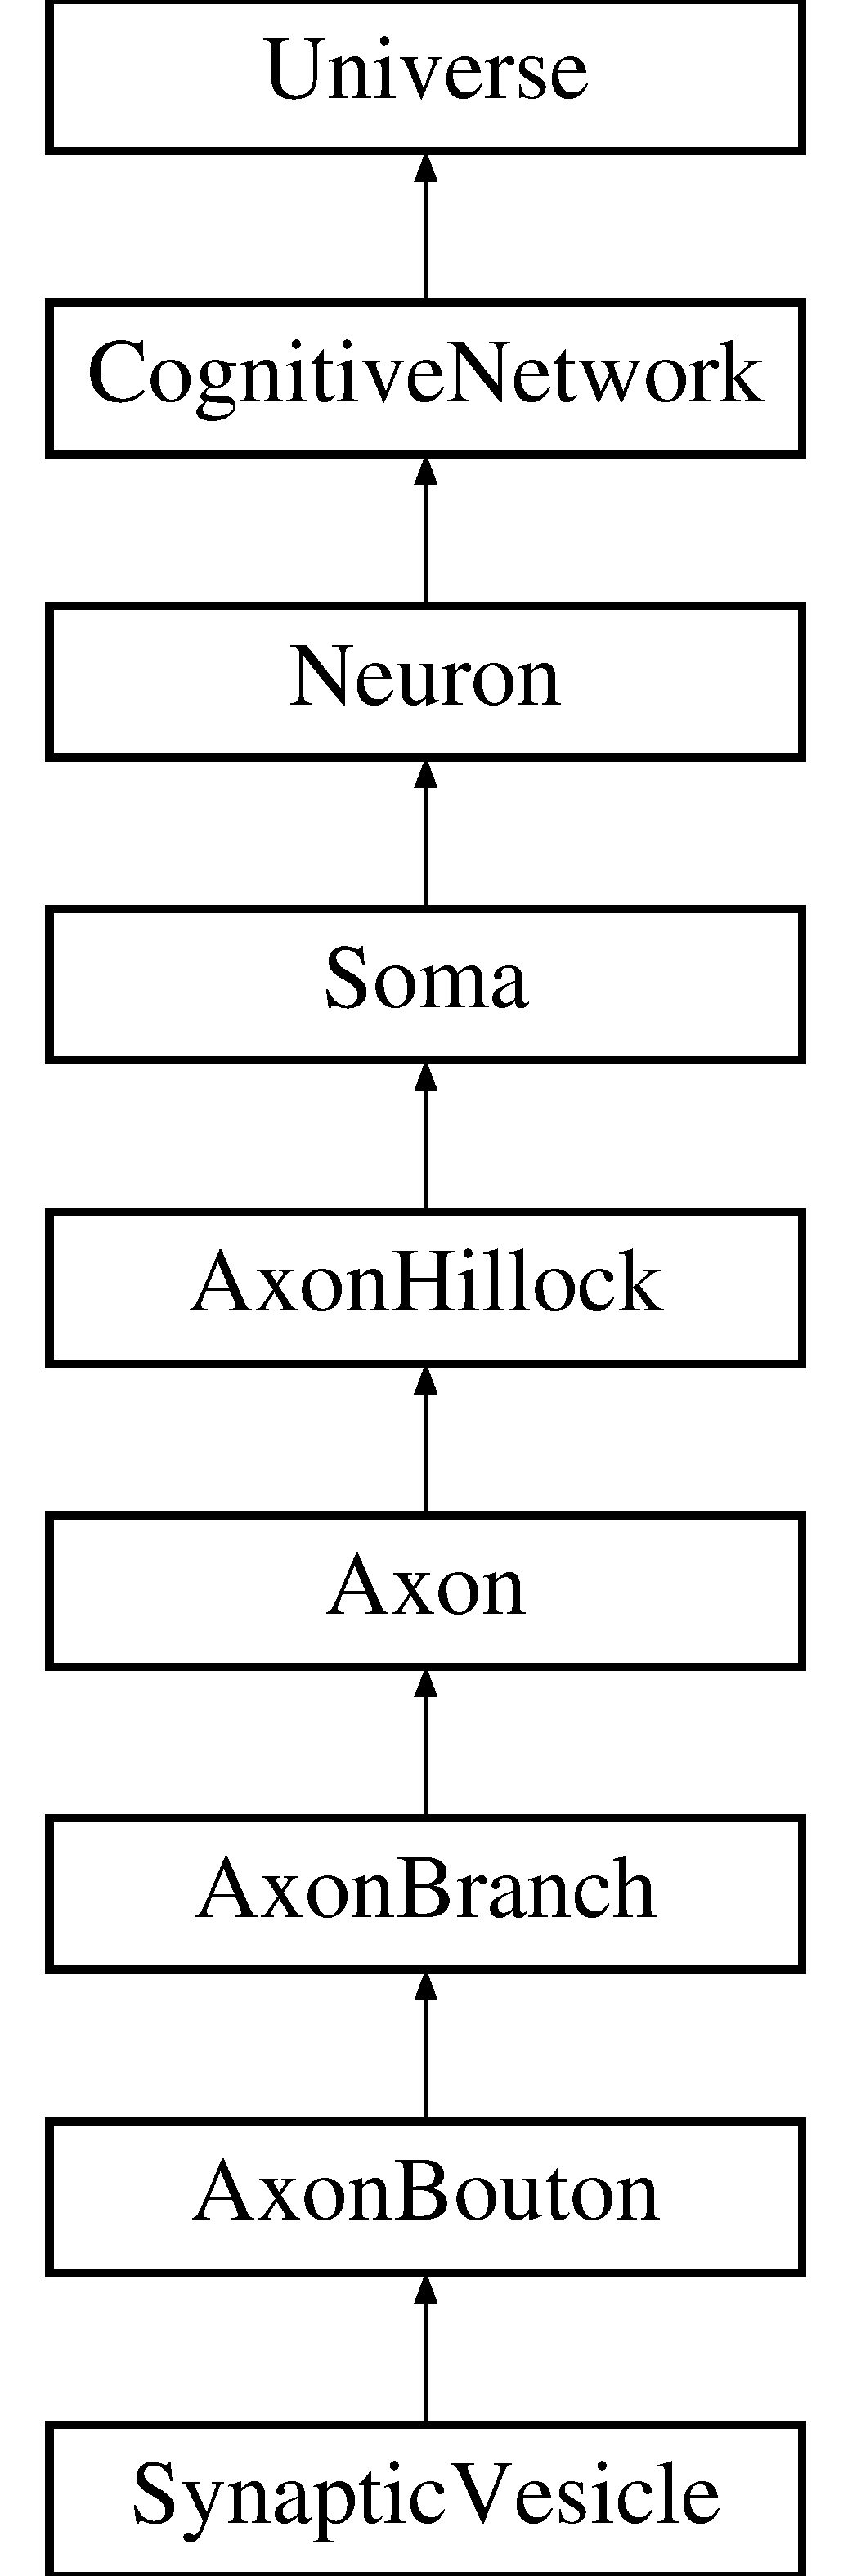
\includegraphics[height=9.000000cm]{classAxonHillock}
\end{center}
\end{figure}
\subsection*{Public Member Functions}
\begin{DoxyCompactItemize}
\item 
\mbox{\hyperlink{classAxonHillock_a432095dfb25ece393cdd83b5eb4f097a}{Axon\+Hillock}} ()
\item 
\mbox{\hyperlink{classAxonHillock_a20a4da0885f32bfca34ab5cda2a13562}{Axon\+Hillock}} (unsigned int object\+\_\+type)
\item 
\mbox{\hyperlink{classAxonHillock_acc61c61c8dfddd603e868a2fcbfd5e9c}{Axon\+Hillock}} (unsigned int object\+\_\+type, std\+::chrono\+::time\+\_\+point$<$ \mbox{\hyperlink{universe_8h_a0ef8d951d1ca5ab3cfaf7ab4c7a6fd80}{Clock}} $>$ event\+\_\+time)
\item 
\mbox{\hyperlink{classAxonHillock_a250945e24a51475369b6c7881c0d955b}{Axon\+Hillock}} (unsigned int object\+\_\+type, std\+::chrono\+::time\+\_\+point$<$ \mbox{\hyperlink{universe_8h_a0ef8d951d1ca5ab3cfaf7ab4c7a6fd80}{Clock}} $>$ event\+\_\+time, \mbox{\hyperlink{classSoma}{Soma}} \&soma\+\_\+connector)
\item 
virtual \mbox{\hyperlink{classAxonHillock_ae86220026d7c87edc1c514521d66f992}{$\sim$\+Axon\+Hillock}} ()
\item 
unsigned int \mbox{\hyperlink{classAxonHillock_a429c9876d679fe8de4533725afc4875c}{Get\+Counter}} (std\+::chrono\+::time\+\_\+point$<$ \mbox{\hyperlink{universe_8h_a0ef8d951d1ca5ab3cfaf7ab4c7a6fd80}{Clock}} $>$ event\+\_\+time)
\item 
double \mbox{\hyperlink{classAxonHillock_ab5ac3ab8771b96acf7e3fa07152525a5}{Get\+Energy}} (std\+::chrono\+::time\+\_\+point$<$ \mbox{\hyperlink{universe_8h_a0ef8d951d1ca5ab3cfaf7ab4c7a6fd80}{Clock}} $>$ event\+\_\+time)
\item 
void \mbox{\hyperlink{classAxonHillock_a0220cee0ad99ddc48496982078c1856c}{Set\+Counter}} (std\+::chrono\+::time\+\_\+point$<$ \mbox{\hyperlink{universe_8h_a0ef8d951d1ca5ab3cfaf7ab4c7a6fd80}{Clock}} $>$ event\+\_\+time, unsigned int val)
\item 
void \mbox{\hyperlink{classAxonHillock_a830afd18810e0eaa11a9e7a500b8f0c4}{Set\+Energy}} (std\+::chrono\+::time\+\_\+point$<$ \mbox{\hyperlink{universe_8h_a0ef8d951d1ca5ab3cfaf7ab4c7a6fd80}{Clock}} $>$ event\+\_\+time, double val)
\item 
void \mbox{\hyperlink{classAxonHillock_ad2c1890796e6f72ef631abb17a4b6532}{Set\+Object\+Type}} (std\+::chrono\+::time\+\_\+point$<$ \mbox{\hyperlink{universe_8h_a0ef8d951d1ca5ab3cfaf7ab4c7a6fd80}{Clock}} $>$ event\+\_\+time, int object\+\_\+type)
\item 
bool \mbox{\hyperlink{classAxonHillock_acec1571ef0b74f7f5ce6699c9b459b4f}{Reset\+Parameters}} (std\+::chrono\+::time\+\_\+point$<$ \mbox{\hyperlink{universe_8h_a0ef8d951d1ca5ab3cfaf7ab4c7a6fd80}{Clock}} $>$ event\+\_\+time)
\item 
\mbox{\hyperlink{classAxonHillock}{Axon\+Hillock}} $\ast$ \mbox{\hyperlink{classAxonHillock_ae6b18ec6f2921b9d4461b89a9d72ab25}{Create\+Axon}} (std\+::chrono\+::time\+\_\+point$<$ \mbox{\hyperlink{universe_8h_a0ef8d951d1ca5ab3cfaf7ab4c7a6fd80}{Clock}} $>$ event\+\_\+time)
\item 
std\+::vector$<$ \mbox{\hyperlink{classAxonHillock}{Axon\+Hillock}} $\ast$ $>$ \mbox{\hyperlink{classAxonHillock_a15bf1a433f38b8b0c92e4a4efe22ec6f}{Create\+Axons}} (std\+::chrono\+::time\+\_\+point$<$ \mbox{\hyperlink{universe_8h_a0ef8d951d1ca5ab3cfaf7ab4c7a6fd80}{Clock}} $>$ event\+\_\+time, int quantity)
\item 
\mbox{\hyperlink{classAxonHillock}{Axon\+Hillock}} $\ast$ \mbox{\hyperlink{classAxonHillock_ad54833cee03cfcacb5e88d174048aaa4}{Clone\+Axon}} (std\+::chrono\+::time\+\_\+point$<$ \mbox{\hyperlink{universe_8h_a0ef8d951d1ca5ab3cfaf7ab4c7a6fd80}{Clock}} $>$ event\+\_\+time, \mbox{\hyperlink{classAxonHillock}{Axon\+Hillock}} $\ast$clone\+\_\+object, double perfection\+\_\+membership)
\item 
std\+::vector$<$ \mbox{\hyperlink{classAxonHillock}{Axon\+Hillock}} $\ast$ $>$ \mbox{\hyperlink{classAxonHillock_aa65cead56b10bda66dc256c68764a553}{Clone\+Axons}} (std\+::chrono\+::time\+\_\+point$<$ \mbox{\hyperlink{universe_8h_a0ef8d951d1ca5ab3cfaf7ab4c7a6fd80}{Clock}} $>$ event\+\_\+time, std\+::vector$<$ \mbox{\hyperlink{classAxonHillock}{Axon\+Hillock}} $\ast$$>$ cloning\+\_\+list, double perfection\+\_\+membership)
\item 
\mbox{\hyperlink{classAxonHillock}{Axon\+Hillock}} $\ast$ \mbox{\hyperlink{classAxonHillock_a031b2cc7292d023506a5124639a941a7}{Destroy\+Axon}} (std\+::chrono\+::time\+\_\+point$<$ \mbox{\hyperlink{universe_8h_a0ef8d951d1ca5ab3cfaf7ab4c7a6fd80}{Clock}} $>$ event\+\_\+time, \mbox{\hyperlink{classAxonHillock}{Axon\+Hillock}} $\ast$destroy\+\_\+object)
\item 
std\+::vector$<$ \mbox{\hyperlink{classAxonHillock}{Axon\+Hillock}} $\ast$ $>$ \mbox{\hyperlink{classAxonHillock_a083c918c64c60f3cea1d39aa8e0c6fba}{Destroy\+Axons}} (std\+::chrono\+::time\+\_\+point$<$ \mbox{\hyperlink{universe_8h_a0ef8d951d1ca5ab3cfaf7ab4c7a6fd80}{Clock}} $>$ event\+\_\+time, std\+::vector$<$ \mbox{\hyperlink{classAxonHillock}{Axon\+Hillock}} $\ast$$>$ destruction\+\_\+list)
\item 
\mbox{\hyperlink{classAxonHillock}{Axon\+Hillock}} $\ast$ \mbox{\hyperlink{classAxonHillock_a02bfbaea9ea7a160933f8500c8b41d6a}{Add\+Axon}} (std\+::chrono\+::time\+\_\+point$<$ \mbox{\hyperlink{universe_8h_a0ef8d951d1ca5ab3cfaf7ab4c7a6fd80}{Clock}} $>$ event\+\_\+time, \mbox{\hyperlink{classAxonHillock}{Axon\+Hillock}} $\ast$add\+\_\+object)
\item 
std\+::vector$<$ \mbox{\hyperlink{classAxonHillock}{Axon\+Hillock}} $\ast$ $>$ \mbox{\hyperlink{classAxonHillock_a54a82227b96757f1c0d7450df6a3df37}{Add\+Axons}} (std\+::chrono\+::time\+\_\+point$<$ \mbox{\hyperlink{universe_8h_a0ef8d951d1ca5ab3cfaf7ab4c7a6fd80}{Clock}} $>$ event\+\_\+time, std\+::vector$<$ \mbox{\hyperlink{classAxonHillock}{Axon\+Hillock}} $\ast$$>$ add\+\_\+objects)
\item 
\mbox{\hyperlink{classAxonHillock}{Axon\+Hillock}} $\ast$ \mbox{\hyperlink{classAxonHillock_ae7c379ef3a70c8a43a0f105ccc94b54b}{Remove\+Axon}} (std\+::chrono\+::time\+\_\+point$<$ \mbox{\hyperlink{universe_8h_a0ef8d951d1ca5ab3cfaf7ab4c7a6fd80}{Clock}} $>$ event\+\_\+time)
\item 
std\+::vector$<$ \mbox{\hyperlink{classAxonHillock}{Axon\+Hillock}} $\ast$ $>$ \mbox{\hyperlink{classAxonHillock_a7f10edff727271408887d29a70e7e671}{Remove\+Axons}} (std\+::chrono\+::time\+\_\+point$<$ \mbox{\hyperlink{universe_8h_a0ef8d951d1ca5ab3cfaf7ab4c7a6fd80}{Clock}} $>$ event\+\_\+time, int quantity)
\item 
\mbox{\hyperlink{classAxonHillock}{Axon\+Hillock}} $\ast$ \mbox{\hyperlink{classAxonHillock_a08fde7d1b8a40ba7a052315f95b743f0}{Get\+Axon}} (std\+::chrono\+::time\+\_\+point$<$ \mbox{\hyperlink{universe_8h_a0ef8d951d1ca5ab3cfaf7ab4c7a6fd80}{Clock}} $>$ event\+\_\+time, int selector)
\item 
std\+::vector$<$ \mbox{\hyperlink{classAxonHillock}{Axon\+Hillock}} $\ast$ $>$ \mbox{\hyperlink{classAxonHillock_af35663768cbe818e092382519a6d73e3}{Get\+Axons}} (std\+::chrono\+::time\+\_\+point$<$ \mbox{\hyperlink{universe_8h_a0ef8d951d1ca5ab3cfaf7ab4c7a6fd80}{Clock}} $>$ event\+\_\+time)
\item 
int \mbox{\hyperlink{classAxonHillock_a5c5cd9008f1410898980528b959d668e}{Growth}} (std\+::chrono\+::time\+\_\+point$<$ \mbox{\hyperlink{universe_8h_a0ef8d951d1ca5ab3cfaf7ab4c7a6fd80}{Clock}} $>$ event\+\_\+time)
\item 
int \mbox{\hyperlink{classAxonHillock_a5a6a6a93a98b32c303b9ee6320c09909}{Update}} (std\+::chrono\+::time\+\_\+point$<$ \mbox{\hyperlink{universe_8h_a0ef8d951d1ca5ab3cfaf7ab4c7a6fd80}{Clock}} $>$ event\+\_\+time)
\end{DoxyCompactItemize}
\subsection*{Protected Attributes}
\begin{DoxyCompactItemize}
\item 
std\+::vector$<$ \mbox{\hyperlink{classAxonHillock}{Axon\+Hillock}} $\ast$ $>$ \mbox{\hyperlink{classAxonHillock_a110d655ded8e09306b224b6e940cd60b}{axon\+\_\+list}}
\end{DoxyCompactItemize}
\subsection*{Private Attributes}
\begin{DoxyCompactItemize}
\item 
int \mbox{\hyperlink{classAxonHillock_a1b3e5f60e24589baa3937c25d0fdaccb}{m\+\_\+\+Neuron\+Type}}
\item 
int \mbox{\hyperlink{classAxonHillock_abcf4792c5f64683a2ba6b3ad11b36c3b}{axonhillock\+\_\+type}}
\item 
bool \mbox{\hyperlink{classAxonHillock_aceaf38b22f77d3377d96e79d44b6c3d6}{object\+\_\+disabled}}
\item 
bool \mbox{\hyperlink{classAxonHillock_ac666d677d62505d33b1316f5688f1529}{object\+\_\+initialised}}
\item 
int \mbox{\hyperlink{classAxonHillock_a5128d2562b42d29b7bfc1492bfce7066}{axon\+\_\+pool}}
\item 
double \mbox{\hyperlink{classAxonHillock_ab475b735c12d372dc9227e84f8a5fe89}{m\+\_\+\+Volume}}
\item 
double \mbox{\hyperlink{classAxonHillock_ae8b94f0128e95735b088e2ed68bc1884}{m\+\_\+\+Surface\+Area}}
\item 
int \mbox{\hyperlink{classAxonHillock_a92b376c3bc0bf8f8a52f52e424f7a335}{m\+\_\+add\+Status}}
\item 
double \mbox{\hyperlink{classAxonHillock_a2b87848d4ae4bb3011347cb11656ee09}{object\+\_\+size}}
\item 
std\+::chrono\+::time\+\_\+point$<$ \mbox{\hyperlink{universe_8h_a0ef8d951d1ca5ab3cfaf7ab4c7a6fd80}{Clock}} $>$ \mbox{\hyperlink{classAxonHillock_ab8fe082b0aa59b58f6cf8ddb00202ae1}{time\+\_\+object\+\_\+created}}
\item 
std\+::chrono\+::time\+\_\+point$<$ \mbox{\hyperlink{universe_8h_a0ef8d951d1ca5ab3cfaf7ab4c7a6fd80}{Clock}} $>$ \mbox{\hyperlink{classAxonHillock_a569d0a3da91ca87f6e88a8cdb0949e81}{previous\+\_\+event\+\_\+time}}
\item 
int \mbox{\hyperlink{classAxonHillock_a5b03b9c1c492e6c37b808d0756fce018}{duration\+\_\+since\+\_\+last\+\_\+event}}
\item 
unsigned int \mbox{\hyperlink{classAxonHillock_a4ce4c0d7438dfb7a77f6412460e1adcc}{m\+\_\+\+Counter}}
\begin{DoxyCompactList}\small\item\em Member variable \char`\"{}m\+\_\+\+Counter\char`\"{}. \end{DoxyCompactList}\item 
double \mbox{\hyperlink{classAxonHillock_a1ca9726d785ecc1dce0ac01933cf1dca}{object\+\_\+energy}}
\begin{DoxyCompactList}\small\item\em Member variable \char`\"{}object\+\_\+energy\char`\"{}. \end{DoxyCompactList}\item 
double \mbox{\hyperlink{classAxonHillock_a1fc144064d284978f785b1534a290d86}{object\+\_\+energy\+\_\+threshold}}
\item 
double \mbox{\hyperlink{classAxonHillock_ad3b4b4553315421c5a22f37dd94e2e94}{m\+\_\+\+Time\+Dilation}}
\item 
double \mbox{\hyperlink{classAxonHillock_acb8b1407116e6656c49e89c3a82bfd7c}{m\+\_\+\+Time\+Threshold}}
\end{DoxyCompactItemize}
\subsection*{Additional Inherited Members}


\subsection{Constructor \& Destructor Documentation}
\mbox{\Hypertarget{classAxonHillock_a432095dfb25ece393cdd83b5eb4f097a}\label{classAxonHillock_a432095dfb25ece393cdd83b5eb4f097a}} 
\index{Axon\+Hillock@{Axon\+Hillock}!Axon\+Hillock@{Axon\+Hillock}}
\index{Axon\+Hillock@{Axon\+Hillock}!Axon\+Hillock@{Axon\+Hillock}}
\subsubsection{\texorpdfstring{Axon\+Hillock()}{AxonHillock()}\hspace{0.1cm}{\footnotesize\ttfamily [1/4]}}
{\footnotesize\ttfamily Axon\+Hillock\+::\+Axon\+Hillock (\begin{DoxyParamCaption}{ }\end{DoxyParamCaption})\hspace{0.3cm}{\ttfamily [inline]}}

\mbox{\Hypertarget{classAxonHillock_a20a4da0885f32bfca34ab5cda2a13562}\label{classAxonHillock_a20a4da0885f32bfca34ab5cda2a13562}} 
\index{Axon\+Hillock@{Axon\+Hillock}!Axon\+Hillock@{Axon\+Hillock}}
\index{Axon\+Hillock@{Axon\+Hillock}!Axon\+Hillock@{Axon\+Hillock}}
\subsubsection{\texorpdfstring{Axon\+Hillock()}{AxonHillock()}\hspace{0.1cm}{\footnotesize\ttfamily [2/4]}}
{\footnotesize\ttfamily Axon\+Hillock\+::\+Axon\+Hillock (\begin{DoxyParamCaption}\item[{unsigned int}]{object\+\_\+type }\end{DoxyParamCaption})\hspace{0.3cm}{\ttfamily [inline]}}

\mbox{\Hypertarget{classAxonHillock_acc61c61c8dfddd603e868a2fcbfd5e9c}\label{classAxonHillock_acc61c61c8dfddd603e868a2fcbfd5e9c}} 
\index{Axon\+Hillock@{Axon\+Hillock}!Axon\+Hillock@{Axon\+Hillock}}
\index{Axon\+Hillock@{Axon\+Hillock}!Axon\+Hillock@{Axon\+Hillock}}
\subsubsection{\texorpdfstring{Axon\+Hillock()}{AxonHillock()}\hspace{0.1cm}{\footnotesize\ttfamily [3/4]}}
{\footnotesize\ttfamily Axon\+Hillock\+::\+Axon\+Hillock (\begin{DoxyParamCaption}\item[{unsigned int}]{object\+\_\+type,  }\item[{std\+::chrono\+::time\+\_\+point$<$ \mbox{\hyperlink{universe_8h_a0ef8d951d1ca5ab3cfaf7ab4c7a6fd80}{Clock}} $>$}]{event\+\_\+time }\end{DoxyParamCaption})\hspace{0.3cm}{\ttfamily [inline]}}

\mbox{\Hypertarget{classAxonHillock_a250945e24a51475369b6c7881c0d955b}\label{classAxonHillock_a250945e24a51475369b6c7881c0d955b}} 
\index{Axon\+Hillock@{Axon\+Hillock}!Axon\+Hillock@{Axon\+Hillock}}
\index{Axon\+Hillock@{Axon\+Hillock}!Axon\+Hillock@{Axon\+Hillock}}
\subsubsection{\texorpdfstring{Axon\+Hillock()}{AxonHillock()}\hspace{0.1cm}{\footnotesize\ttfamily [4/4]}}
{\footnotesize\ttfamily Axon\+Hillock\+::\+Axon\+Hillock (\begin{DoxyParamCaption}\item[{unsigned int}]{object\+\_\+type,  }\item[{std\+::chrono\+::time\+\_\+point$<$ \mbox{\hyperlink{universe_8h_a0ef8d951d1ca5ab3cfaf7ab4c7a6fd80}{Clock}} $>$}]{event\+\_\+time,  }\item[{\mbox{\hyperlink{classSoma}{Soma}} \&}]{soma\+\_\+connector }\end{DoxyParamCaption})\hspace{0.3cm}{\ttfamily [inline]}}

\mbox{\Hypertarget{classAxonHillock_ae86220026d7c87edc1c514521d66f992}\label{classAxonHillock_ae86220026d7c87edc1c514521d66f992}} 
\index{Axon\+Hillock@{Axon\+Hillock}!````~Axon\+Hillock@{$\sim$\+Axon\+Hillock}}
\index{````~Axon\+Hillock@{$\sim$\+Axon\+Hillock}!Axon\+Hillock@{Axon\+Hillock}}
\subsubsection{\texorpdfstring{$\sim$\+Axon\+Hillock()}{~AxonHillock()}}
{\footnotesize\ttfamily virtual Axon\+Hillock\+::$\sim$\+Axon\+Hillock (\begin{DoxyParamCaption}{ }\end{DoxyParamCaption})\hspace{0.3cm}{\ttfamily [inline]}, {\ttfamily [virtual]}}

Default destructor 

\subsection{Member Function Documentation}
\mbox{\Hypertarget{classAxonHillock_a02bfbaea9ea7a160933f8500c8b41d6a}\label{classAxonHillock_a02bfbaea9ea7a160933f8500c8b41d6a}} 
\index{Axon\+Hillock@{Axon\+Hillock}!Add\+Axon@{Add\+Axon}}
\index{Add\+Axon@{Add\+Axon}!Axon\+Hillock@{Axon\+Hillock}}
\subsubsection{\texorpdfstring{Add\+Axon()}{AddAxon()}}
{\footnotesize\ttfamily \mbox{\hyperlink{classAxonHillock}{Axon\+Hillock}} $\ast$ Axon\+Hillock\+::\+Add\+Axon (\begin{DoxyParamCaption}\item[{std\+::chrono\+::time\+\_\+point$<$ \mbox{\hyperlink{universe_8h_a0ef8d951d1ca5ab3cfaf7ab4c7a6fd80}{Clock}} $>$}]{event\+\_\+time,  }\item[{\mbox{\hyperlink{classAxonHillock}{Axon\+Hillock}} $\ast$}]{add\+\_\+object }\end{DoxyParamCaption})}

\mbox{\Hypertarget{classAxonHillock_a54a82227b96757f1c0d7450df6a3df37}\label{classAxonHillock_a54a82227b96757f1c0d7450df6a3df37}} 
\index{Axon\+Hillock@{Axon\+Hillock}!Add\+Axons@{Add\+Axons}}
\index{Add\+Axons@{Add\+Axons}!Axon\+Hillock@{Axon\+Hillock}}
\subsubsection{\texorpdfstring{Add\+Axons()}{AddAxons()}}
{\footnotesize\ttfamily std\+::vector$<$ \mbox{\hyperlink{classAxonHillock}{Axon\+Hillock}} $\ast$ $>$ Axon\+Hillock\+::\+Add\+Axons (\begin{DoxyParamCaption}\item[{std\+::chrono\+::time\+\_\+point$<$ \mbox{\hyperlink{universe_8h_a0ef8d951d1ca5ab3cfaf7ab4c7a6fd80}{Clock}} $>$}]{event\+\_\+time,  }\item[{std\+::vector$<$ \mbox{\hyperlink{classAxonHillock}{Axon\+Hillock}} $\ast$$>$}]{add\+\_\+objects }\end{DoxyParamCaption})}

\mbox{\Hypertarget{classAxonHillock_ad54833cee03cfcacb5e88d174048aaa4}\label{classAxonHillock_ad54833cee03cfcacb5e88d174048aaa4}} 
\index{Axon\+Hillock@{Axon\+Hillock}!Clone\+Axon@{Clone\+Axon}}
\index{Clone\+Axon@{Clone\+Axon}!Axon\+Hillock@{Axon\+Hillock}}
\subsubsection{\texorpdfstring{Clone\+Axon()}{CloneAxon()}}
{\footnotesize\ttfamily \mbox{\hyperlink{classAxonHillock}{Axon\+Hillock}} $\ast$ Axon\+Hillock\+::\+Clone\+Axon (\begin{DoxyParamCaption}\item[{std\+::chrono\+::time\+\_\+point$<$ \mbox{\hyperlink{universe_8h_a0ef8d951d1ca5ab3cfaf7ab4c7a6fd80}{Clock}} $>$}]{event\+\_\+time,  }\item[{\mbox{\hyperlink{classAxonHillock}{Axon\+Hillock}} $\ast$}]{clone\+\_\+object,  }\item[{double}]{perfection\+\_\+membership }\end{DoxyParamCaption})}

\mbox{\Hypertarget{classAxonHillock_aa65cead56b10bda66dc256c68764a553}\label{classAxonHillock_aa65cead56b10bda66dc256c68764a553}} 
\index{Axon\+Hillock@{Axon\+Hillock}!Clone\+Axons@{Clone\+Axons}}
\index{Clone\+Axons@{Clone\+Axons}!Axon\+Hillock@{Axon\+Hillock}}
\subsubsection{\texorpdfstring{Clone\+Axons()}{CloneAxons()}}
{\footnotesize\ttfamily std\+::vector$<$ \mbox{\hyperlink{classAxonHillock}{Axon\+Hillock}} $\ast$ $>$ Axon\+Hillock\+::\+Clone\+Axons (\begin{DoxyParamCaption}\item[{std\+::chrono\+::time\+\_\+point$<$ \mbox{\hyperlink{universe_8h_a0ef8d951d1ca5ab3cfaf7ab4c7a6fd80}{Clock}} $>$}]{event\+\_\+time,  }\item[{std\+::vector$<$ \mbox{\hyperlink{classAxonHillock}{Axon\+Hillock}} $\ast$$>$}]{cloning\+\_\+list,  }\item[{double}]{perfection\+\_\+membership }\end{DoxyParamCaption})}

\mbox{\Hypertarget{classAxonHillock_ae6b18ec6f2921b9d4461b89a9d72ab25}\label{classAxonHillock_ae6b18ec6f2921b9d4461b89a9d72ab25}} 
\index{Axon\+Hillock@{Axon\+Hillock}!Create\+Axon@{Create\+Axon}}
\index{Create\+Axon@{Create\+Axon}!Axon\+Hillock@{Axon\+Hillock}}
\subsubsection{\texorpdfstring{Create\+Axon()}{CreateAxon()}}
{\footnotesize\ttfamily \mbox{\hyperlink{classAxonHillock}{Axon\+Hillock}} $\ast$ Axon\+Hillock\+::\+Create\+Axon (\begin{DoxyParamCaption}\item[{std\+::chrono\+::time\+\_\+point$<$ \mbox{\hyperlink{universe_8h_a0ef8d951d1ca5ab3cfaf7ab4c7a6fd80}{Clock}} $>$}]{event\+\_\+time }\end{DoxyParamCaption})}

\mbox{\Hypertarget{classAxonHillock_a15bf1a433f38b8b0c92e4a4efe22ec6f}\label{classAxonHillock_a15bf1a433f38b8b0c92e4a4efe22ec6f}} 
\index{Axon\+Hillock@{Axon\+Hillock}!Create\+Axons@{Create\+Axons}}
\index{Create\+Axons@{Create\+Axons}!Axon\+Hillock@{Axon\+Hillock}}
\subsubsection{\texorpdfstring{Create\+Axons()}{CreateAxons()}}
{\footnotesize\ttfamily std\+::vector$<$ \mbox{\hyperlink{classAxonHillock}{Axon\+Hillock}} $\ast$ $>$ Axon\+Hillock\+::\+Create\+Axons (\begin{DoxyParamCaption}\item[{std\+::chrono\+::time\+\_\+point$<$ \mbox{\hyperlink{universe_8h_a0ef8d951d1ca5ab3cfaf7ab4c7a6fd80}{Clock}} $>$}]{event\+\_\+time,  }\item[{int}]{quantity }\end{DoxyParamCaption})}

\mbox{\Hypertarget{classAxonHillock_a031b2cc7292d023506a5124639a941a7}\label{classAxonHillock_a031b2cc7292d023506a5124639a941a7}} 
\index{Axon\+Hillock@{Axon\+Hillock}!Destroy\+Axon@{Destroy\+Axon}}
\index{Destroy\+Axon@{Destroy\+Axon}!Axon\+Hillock@{Axon\+Hillock}}
\subsubsection{\texorpdfstring{Destroy\+Axon()}{DestroyAxon()}}
{\footnotesize\ttfamily \mbox{\hyperlink{classAxonHillock}{Axon\+Hillock}} $\ast$ Axon\+Hillock\+::\+Destroy\+Axon (\begin{DoxyParamCaption}\item[{std\+::chrono\+::time\+\_\+point$<$ \mbox{\hyperlink{universe_8h_a0ef8d951d1ca5ab3cfaf7ab4c7a6fd80}{Clock}} $>$}]{event\+\_\+time,  }\item[{\mbox{\hyperlink{classAxonHillock}{Axon\+Hillock}} $\ast$}]{destroy\+\_\+object }\end{DoxyParamCaption})}

\mbox{\Hypertarget{classAxonHillock_a083c918c64c60f3cea1d39aa8e0c6fba}\label{classAxonHillock_a083c918c64c60f3cea1d39aa8e0c6fba}} 
\index{Axon\+Hillock@{Axon\+Hillock}!Destroy\+Axons@{Destroy\+Axons}}
\index{Destroy\+Axons@{Destroy\+Axons}!Axon\+Hillock@{Axon\+Hillock}}
\subsubsection{\texorpdfstring{Destroy\+Axons()}{DestroyAxons()}}
{\footnotesize\ttfamily std\+::vector$<$ \mbox{\hyperlink{classAxonHillock}{Axon\+Hillock}} $\ast$ $>$ Axon\+Hillock\+::\+Destroy\+Axons (\begin{DoxyParamCaption}\item[{std\+::chrono\+::time\+\_\+point$<$ \mbox{\hyperlink{universe_8h_a0ef8d951d1ca5ab3cfaf7ab4c7a6fd80}{Clock}} $>$}]{event\+\_\+time,  }\item[{std\+::vector$<$ \mbox{\hyperlink{classAxonHillock}{Axon\+Hillock}} $\ast$$>$}]{destruction\+\_\+list }\end{DoxyParamCaption})}

\mbox{\Hypertarget{classAxonHillock_a08fde7d1b8a40ba7a052315f95b743f0}\label{classAxonHillock_a08fde7d1b8a40ba7a052315f95b743f0}} 
\index{Axon\+Hillock@{Axon\+Hillock}!Get\+Axon@{Get\+Axon}}
\index{Get\+Axon@{Get\+Axon}!Axon\+Hillock@{Axon\+Hillock}}
\subsubsection{\texorpdfstring{Get\+Axon()}{GetAxon()}}
{\footnotesize\ttfamily \mbox{\hyperlink{classAxonHillock}{Axon\+Hillock}} $\ast$ Axon\+Hillock\+::\+Get\+Axon (\begin{DoxyParamCaption}\item[{std\+::chrono\+::time\+\_\+point$<$ \mbox{\hyperlink{universe_8h_a0ef8d951d1ca5ab3cfaf7ab4c7a6fd80}{Clock}} $>$}]{event\+\_\+time,  }\item[{int}]{selector }\end{DoxyParamCaption})}

\mbox{\Hypertarget{classAxonHillock_af35663768cbe818e092382519a6d73e3}\label{classAxonHillock_af35663768cbe818e092382519a6d73e3}} 
\index{Axon\+Hillock@{Axon\+Hillock}!Get\+Axons@{Get\+Axons}}
\index{Get\+Axons@{Get\+Axons}!Axon\+Hillock@{Axon\+Hillock}}
\subsubsection{\texorpdfstring{Get\+Axons()}{GetAxons()}}
{\footnotesize\ttfamily std\+::vector$<$ \mbox{\hyperlink{classAxonHillock}{Axon\+Hillock}} $\ast$ $>$ Axon\+Hillock\+::\+Get\+Axons (\begin{DoxyParamCaption}\item[{std\+::chrono\+::time\+\_\+point$<$ \mbox{\hyperlink{universe_8h_a0ef8d951d1ca5ab3cfaf7ab4c7a6fd80}{Clock}} $>$}]{event\+\_\+time }\end{DoxyParamCaption})}

\mbox{\Hypertarget{classAxonHillock_a429c9876d679fe8de4533725afc4875c}\label{classAxonHillock_a429c9876d679fe8de4533725afc4875c}} 
\index{Axon\+Hillock@{Axon\+Hillock}!Get\+Counter@{Get\+Counter}}
\index{Get\+Counter@{Get\+Counter}!Axon\+Hillock@{Axon\+Hillock}}
\subsubsection{\texorpdfstring{Get\+Counter()}{GetCounter()}}
{\footnotesize\ttfamily unsigned int Axon\+Hillock\+::\+Get\+Counter (\begin{DoxyParamCaption}\item[{std\+::chrono\+::time\+\_\+point$<$ \mbox{\hyperlink{universe_8h_a0ef8d951d1ca5ab3cfaf7ab4c7a6fd80}{Clock}} $>$}]{event\+\_\+time }\end{DoxyParamCaption})\hspace{0.3cm}{\ttfamily [inline]}}

\mbox{\Hypertarget{classAxonHillock_ab5ac3ab8771b96acf7e3fa07152525a5}\label{classAxonHillock_ab5ac3ab8771b96acf7e3fa07152525a5}} 
\index{Axon\+Hillock@{Axon\+Hillock}!Get\+Energy@{Get\+Energy}}
\index{Get\+Energy@{Get\+Energy}!Axon\+Hillock@{Axon\+Hillock}}
\subsubsection{\texorpdfstring{Get\+Energy()}{GetEnergy()}}
{\footnotesize\ttfamily double Axon\+Hillock\+::\+Get\+Energy (\begin{DoxyParamCaption}\item[{std\+::chrono\+::time\+\_\+point$<$ \mbox{\hyperlink{universe_8h_a0ef8d951d1ca5ab3cfaf7ab4c7a6fd80}{Clock}} $>$}]{event\+\_\+time }\end{DoxyParamCaption})\hspace{0.3cm}{\ttfamily [inline]}}

\mbox{\Hypertarget{classAxonHillock_a5c5cd9008f1410898980528b959d668e}\label{classAxonHillock_a5c5cd9008f1410898980528b959d668e}} 
\index{Axon\+Hillock@{Axon\+Hillock}!Growth@{Growth}}
\index{Growth@{Growth}!Axon\+Hillock@{Axon\+Hillock}}
\subsubsection{\texorpdfstring{Growth()}{Growth()}}
{\footnotesize\ttfamily int Axon\+Hillock\+::\+Growth (\begin{DoxyParamCaption}\item[{std\+::chrono\+::time\+\_\+point$<$ \mbox{\hyperlink{universe_8h_a0ef8d951d1ca5ab3cfaf7ab4c7a6fd80}{Clock}} $>$}]{event\+\_\+time }\end{DoxyParamCaption})}

\mbox{\Hypertarget{classAxonHillock_ae7c379ef3a70c8a43a0f105ccc94b54b}\label{classAxonHillock_ae7c379ef3a70c8a43a0f105ccc94b54b}} 
\index{Axon\+Hillock@{Axon\+Hillock}!Remove\+Axon@{Remove\+Axon}}
\index{Remove\+Axon@{Remove\+Axon}!Axon\+Hillock@{Axon\+Hillock}}
\subsubsection{\texorpdfstring{Remove\+Axon()}{RemoveAxon()}}
{\footnotesize\ttfamily \mbox{\hyperlink{classAxonHillock}{Axon\+Hillock}} $\ast$ Axon\+Hillock\+::\+Remove\+Axon (\begin{DoxyParamCaption}\item[{std\+::chrono\+::time\+\_\+point$<$ \mbox{\hyperlink{universe_8h_a0ef8d951d1ca5ab3cfaf7ab4c7a6fd80}{Clock}} $>$}]{event\+\_\+time }\end{DoxyParamCaption})}

\mbox{\Hypertarget{classAxonHillock_a7f10edff727271408887d29a70e7e671}\label{classAxonHillock_a7f10edff727271408887d29a70e7e671}} 
\index{Axon\+Hillock@{Axon\+Hillock}!Remove\+Axons@{Remove\+Axons}}
\index{Remove\+Axons@{Remove\+Axons}!Axon\+Hillock@{Axon\+Hillock}}
\subsubsection{\texorpdfstring{Remove\+Axons()}{RemoveAxons()}}
{\footnotesize\ttfamily std\+::vector$<$ \mbox{\hyperlink{classAxonHillock}{Axon\+Hillock}} $\ast$ $>$ Axon\+Hillock\+::\+Remove\+Axons (\begin{DoxyParamCaption}\item[{std\+::chrono\+::time\+\_\+point$<$ \mbox{\hyperlink{universe_8h_a0ef8d951d1ca5ab3cfaf7ab4c7a6fd80}{Clock}} $>$}]{event\+\_\+time,  }\item[{int}]{quantity }\end{DoxyParamCaption})}

\mbox{\Hypertarget{classAxonHillock_acec1571ef0b74f7f5ce6699c9b459b4f}\label{classAxonHillock_acec1571ef0b74f7f5ce6699c9b459b4f}} 
\index{Axon\+Hillock@{Axon\+Hillock}!Reset\+Parameters@{Reset\+Parameters}}
\index{Reset\+Parameters@{Reset\+Parameters}!Axon\+Hillock@{Axon\+Hillock}}
\subsubsection{\texorpdfstring{Reset\+Parameters()}{ResetParameters()}}
{\footnotesize\ttfamily bool Axon\+Hillock\+::\+Reset\+Parameters (\begin{DoxyParamCaption}\item[{std\+::chrono\+::time\+\_\+point$<$ \mbox{\hyperlink{universe_8h_a0ef8d951d1ca5ab3cfaf7ab4c7a6fd80}{Clock}} $>$}]{event\+\_\+time }\end{DoxyParamCaption})}

\mbox{\Hypertarget{classAxonHillock_a0220cee0ad99ddc48496982078c1856c}\label{classAxonHillock_a0220cee0ad99ddc48496982078c1856c}} 
\index{Axon\+Hillock@{Axon\+Hillock}!Set\+Counter@{Set\+Counter}}
\index{Set\+Counter@{Set\+Counter}!Axon\+Hillock@{Axon\+Hillock}}
\subsubsection{\texorpdfstring{Set\+Counter()}{SetCounter()}}
{\footnotesize\ttfamily void Axon\+Hillock\+::\+Set\+Counter (\begin{DoxyParamCaption}\item[{std\+::chrono\+::time\+\_\+point$<$ \mbox{\hyperlink{universe_8h_a0ef8d951d1ca5ab3cfaf7ab4c7a6fd80}{Clock}} $>$}]{event\+\_\+time,  }\item[{unsigned int}]{val }\end{DoxyParamCaption})\hspace{0.3cm}{\ttfamily [inline]}, {\ttfamily [virtual]}}



Reimplemented from \mbox{\hyperlink{classUniverse_aa22202ae740eb1355529afcb13285e91}{Universe}}.



Reimplemented in \mbox{\hyperlink{classSynapticVesicle_a7fd7cfce5eccb904206d968866f85220}{Synaptic\+Vesicle}}.

\mbox{\Hypertarget{classAxonHillock_a830afd18810e0eaa11a9e7a500b8f0c4}\label{classAxonHillock_a830afd18810e0eaa11a9e7a500b8f0c4}} 
\index{Axon\+Hillock@{Axon\+Hillock}!Set\+Energy@{Set\+Energy}}
\index{Set\+Energy@{Set\+Energy}!Axon\+Hillock@{Axon\+Hillock}}
\subsubsection{\texorpdfstring{Set\+Energy()}{SetEnergy()}}
{\footnotesize\ttfamily void Axon\+Hillock\+::\+Set\+Energy (\begin{DoxyParamCaption}\item[{std\+::chrono\+::time\+\_\+point$<$ \mbox{\hyperlink{universe_8h_a0ef8d951d1ca5ab3cfaf7ab4c7a6fd80}{Clock}} $>$}]{event\+\_\+time,  }\item[{double}]{val }\end{DoxyParamCaption})\hspace{0.3cm}{\ttfamily [inline]}}

\mbox{\Hypertarget{classAxonHillock_ad2c1890796e6f72ef631abb17a4b6532}\label{classAxonHillock_ad2c1890796e6f72ef631abb17a4b6532}} 
\index{Axon\+Hillock@{Axon\+Hillock}!Set\+Object\+Type@{Set\+Object\+Type}}
\index{Set\+Object\+Type@{Set\+Object\+Type}!Axon\+Hillock@{Axon\+Hillock}}
\subsubsection{\texorpdfstring{Set\+Object\+Type()}{SetObjectType()}}
{\footnotesize\ttfamily void Axon\+Hillock\+::\+Set\+Object\+Type (\begin{DoxyParamCaption}\item[{std\+::chrono\+::time\+\_\+point$<$ \mbox{\hyperlink{universe_8h_a0ef8d951d1ca5ab3cfaf7ab4c7a6fd80}{Clock}} $>$}]{event\+\_\+time,  }\item[{int}]{object\+\_\+type }\end{DoxyParamCaption})}

\mbox{\Hypertarget{classAxonHillock_a5a6a6a93a98b32c303b9ee6320c09909}\label{classAxonHillock_a5a6a6a93a98b32c303b9ee6320c09909}} 
\index{Axon\+Hillock@{Axon\+Hillock}!Update@{Update}}
\index{Update@{Update}!Axon\+Hillock@{Axon\+Hillock}}
\subsubsection{\texorpdfstring{Update()}{Update()}}
{\footnotesize\ttfamily int Axon\+Hillock\+::\+Update (\begin{DoxyParamCaption}\item[{std\+::chrono\+::time\+\_\+point$<$ \mbox{\hyperlink{universe_8h_a0ef8d951d1ca5ab3cfaf7ab4c7a6fd80}{Clock}} $>$}]{event\+\_\+time }\end{DoxyParamCaption})}



\subsection{Member Data Documentation}
\mbox{\Hypertarget{classAxonHillock_a110d655ded8e09306b224b6e940cd60b}\label{classAxonHillock_a110d655ded8e09306b224b6e940cd60b}} 
\index{Axon\+Hillock@{Axon\+Hillock}!axon\+\_\+list@{axon\+\_\+list}}
\index{axon\+\_\+list@{axon\+\_\+list}!Axon\+Hillock@{Axon\+Hillock}}
\subsubsection{\texorpdfstring{axon\+\_\+list}{axon\_list}}
{\footnotesize\ttfamily std\+::vector$<$\mbox{\hyperlink{classAxonHillock}{Axon\+Hillock}}$\ast$$>$ Axon\+Hillock\+::axon\+\_\+list\hspace{0.3cm}{\ttfamily [protected]}}

\mbox{\Hypertarget{classAxonHillock_a5128d2562b42d29b7bfc1492bfce7066}\label{classAxonHillock_a5128d2562b42d29b7bfc1492bfce7066}} 
\index{Axon\+Hillock@{Axon\+Hillock}!axon\+\_\+pool@{axon\+\_\+pool}}
\index{axon\+\_\+pool@{axon\+\_\+pool}!Axon\+Hillock@{Axon\+Hillock}}
\subsubsection{\texorpdfstring{axon\+\_\+pool}{axon\_pool}}
{\footnotesize\ttfamily int Axon\+Hillock\+::axon\+\_\+pool\hspace{0.3cm}{\ttfamily [private]}}

\mbox{\Hypertarget{classAxonHillock_abcf4792c5f64683a2ba6b3ad11b36c3b}\label{classAxonHillock_abcf4792c5f64683a2ba6b3ad11b36c3b}} 
\index{Axon\+Hillock@{Axon\+Hillock}!axonhillock\+\_\+type@{axonhillock\+\_\+type}}
\index{axonhillock\+\_\+type@{axonhillock\+\_\+type}!Axon\+Hillock@{Axon\+Hillock}}
\subsubsection{\texorpdfstring{axonhillock\+\_\+type}{axonhillock\_type}}
{\footnotesize\ttfamily int Axon\+Hillock\+::axonhillock\+\_\+type\hspace{0.3cm}{\ttfamily [private]}}

\mbox{\Hypertarget{classAxonHillock_a5b03b9c1c492e6c37b808d0756fce018}\label{classAxonHillock_a5b03b9c1c492e6c37b808d0756fce018}} 
\index{Axon\+Hillock@{Axon\+Hillock}!duration\+\_\+since\+\_\+last\+\_\+event@{duration\+\_\+since\+\_\+last\+\_\+event}}
\index{duration\+\_\+since\+\_\+last\+\_\+event@{duration\+\_\+since\+\_\+last\+\_\+event}!Axon\+Hillock@{Axon\+Hillock}}
\subsubsection{\texorpdfstring{duration\+\_\+since\+\_\+last\+\_\+event}{duration\_since\_last\_event}}
{\footnotesize\ttfamily int Axon\+Hillock\+::duration\+\_\+since\+\_\+last\+\_\+event\hspace{0.3cm}{\ttfamily [private]}}

\mbox{\Hypertarget{classAxonHillock_a92b376c3bc0bf8f8a52f52e424f7a335}\label{classAxonHillock_a92b376c3bc0bf8f8a52f52e424f7a335}} 
\index{Axon\+Hillock@{Axon\+Hillock}!m\+\_\+add\+Status@{m\+\_\+add\+Status}}
\index{m\+\_\+add\+Status@{m\+\_\+add\+Status}!Axon\+Hillock@{Axon\+Hillock}}
\subsubsection{\texorpdfstring{m\+\_\+add\+Status}{m\_addStatus}}
{\footnotesize\ttfamily int Axon\+Hillock\+::m\+\_\+add\+Status\hspace{0.3cm}{\ttfamily [private]}}

\mbox{\Hypertarget{classAxonHillock_a4ce4c0d7438dfb7a77f6412460e1adcc}\label{classAxonHillock_a4ce4c0d7438dfb7a77f6412460e1adcc}} 
\index{Axon\+Hillock@{Axon\+Hillock}!m\+\_\+\+Counter@{m\+\_\+\+Counter}}
\index{m\+\_\+\+Counter@{m\+\_\+\+Counter}!Axon\+Hillock@{Axon\+Hillock}}
\subsubsection{\texorpdfstring{m\+\_\+\+Counter}{m\_Counter}}
{\footnotesize\ttfamily unsigned int Axon\+Hillock\+::m\+\_\+\+Counter\hspace{0.3cm}{\ttfamily [private]}}



Member variable \char`\"{}m\+\_\+\+Counter\char`\"{}. 

\mbox{\Hypertarget{classAxonHillock_a1b3e5f60e24589baa3937c25d0fdaccb}\label{classAxonHillock_a1b3e5f60e24589baa3937c25d0fdaccb}} 
\index{Axon\+Hillock@{Axon\+Hillock}!m\+\_\+\+Neuron\+Type@{m\+\_\+\+Neuron\+Type}}
\index{m\+\_\+\+Neuron\+Type@{m\+\_\+\+Neuron\+Type}!Axon\+Hillock@{Axon\+Hillock}}
\subsubsection{\texorpdfstring{m\+\_\+\+Neuron\+Type}{m\_NeuronType}}
{\footnotesize\ttfamily int Axon\+Hillock\+::m\+\_\+\+Neuron\+Type\hspace{0.3cm}{\ttfamily [private]}}

\mbox{\Hypertarget{classAxonHillock_ae8b94f0128e95735b088e2ed68bc1884}\label{classAxonHillock_ae8b94f0128e95735b088e2ed68bc1884}} 
\index{Axon\+Hillock@{Axon\+Hillock}!m\+\_\+\+Surface\+Area@{m\+\_\+\+Surface\+Area}}
\index{m\+\_\+\+Surface\+Area@{m\+\_\+\+Surface\+Area}!Axon\+Hillock@{Axon\+Hillock}}
\subsubsection{\texorpdfstring{m\+\_\+\+Surface\+Area}{m\_SurfaceArea}}
{\footnotesize\ttfamily double Axon\+Hillock\+::m\+\_\+\+Surface\+Area\hspace{0.3cm}{\ttfamily [private]}}

\mbox{\Hypertarget{classAxonHillock_ad3b4b4553315421c5a22f37dd94e2e94}\label{classAxonHillock_ad3b4b4553315421c5a22f37dd94e2e94}} 
\index{Axon\+Hillock@{Axon\+Hillock}!m\+\_\+\+Time\+Dilation@{m\+\_\+\+Time\+Dilation}}
\index{m\+\_\+\+Time\+Dilation@{m\+\_\+\+Time\+Dilation}!Axon\+Hillock@{Axon\+Hillock}}
\subsubsection{\texorpdfstring{m\+\_\+\+Time\+Dilation}{m\_TimeDilation}}
{\footnotesize\ttfamily double Axon\+Hillock\+::m\+\_\+\+Time\+Dilation\hspace{0.3cm}{\ttfamily [private]}}

\mbox{\Hypertarget{classAxonHillock_acb8b1407116e6656c49e89c3a82bfd7c}\label{classAxonHillock_acb8b1407116e6656c49e89c3a82bfd7c}} 
\index{Axon\+Hillock@{Axon\+Hillock}!m\+\_\+\+Time\+Threshold@{m\+\_\+\+Time\+Threshold}}
\index{m\+\_\+\+Time\+Threshold@{m\+\_\+\+Time\+Threshold}!Axon\+Hillock@{Axon\+Hillock}}
\subsubsection{\texorpdfstring{m\+\_\+\+Time\+Threshold}{m\_TimeThreshold}}
{\footnotesize\ttfamily double Axon\+Hillock\+::m\+\_\+\+Time\+Threshold\hspace{0.3cm}{\ttfamily [private]}}

\mbox{\Hypertarget{classAxonHillock_ab475b735c12d372dc9227e84f8a5fe89}\label{classAxonHillock_ab475b735c12d372dc9227e84f8a5fe89}} 
\index{Axon\+Hillock@{Axon\+Hillock}!m\+\_\+\+Volume@{m\+\_\+\+Volume}}
\index{m\+\_\+\+Volume@{m\+\_\+\+Volume}!Axon\+Hillock@{Axon\+Hillock}}
\subsubsection{\texorpdfstring{m\+\_\+\+Volume}{m\_Volume}}
{\footnotesize\ttfamily double Axon\+Hillock\+::m\+\_\+\+Volume\hspace{0.3cm}{\ttfamily [private]}}

\mbox{\Hypertarget{classAxonHillock_aceaf38b22f77d3377d96e79d44b6c3d6}\label{classAxonHillock_aceaf38b22f77d3377d96e79d44b6c3d6}} 
\index{Axon\+Hillock@{Axon\+Hillock}!object\+\_\+disabled@{object\+\_\+disabled}}
\index{object\+\_\+disabled@{object\+\_\+disabled}!Axon\+Hillock@{Axon\+Hillock}}
\subsubsection{\texorpdfstring{object\+\_\+disabled}{object\_disabled}}
{\footnotesize\ttfamily bool Axon\+Hillock\+::object\+\_\+disabled\hspace{0.3cm}{\ttfamily [private]}}

\mbox{\Hypertarget{classAxonHillock_a1ca9726d785ecc1dce0ac01933cf1dca}\label{classAxonHillock_a1ca9726d785ecc1dce0ac01933cf1dca}} 
\index{Axon\+Hillock@{Axon\+Hillock}!object\+\_\+energy@{object\+\_\+energy}}
\index{object\+\_\+energy@{object\+\_\+energy}!Axon\+Hillock@{Axon\+Hillock}}
\subsubsection{\texorpdfstring{object\+\_\+energy}{object\_energy}}
{\footnotesize\ttfamily double Axon\+Hillock\+::object\+\_\+energy\hspace{0.3cm}{\ttfamily [private]}}



Member variable \char`\"{}object\+\_\+energy\char`\"{}. 

\mbox{\Hypertarget{classAxonHillock_a1fc144064d284978f785b1534a290d86}\label{classAxonHillock_a1fc144064d284978f785b1534a290d86}} 
\index{Axon\+Hillock@{Axon\+Hillock}!object\+\_\+energy\+\_\+threshold@{object\+\_\+energy\+\_\+threshold}}
\index{object\+\_\+energy\+\_\+threshold@{object\+\_\+energy\+\_\+threshold}!Axon\+Hillock@{Axon\+Hillock}}
\subsubsection{\texorpdfstring{object\+\_\+energy\+\_\+threshold}{object\_energy\_threshold}}
{\footnotesize\ttfamily double Axon\+Hillock\+::object\+\_\+energy\+\_\+threshold\hspace{0.3cm}{\ttfamily [private]}}

\mbox{\Hypertarget{classAxonHillock_ac666d677d62505d33b1316f5688f1529}\label{classAxonHillock_ac666d677d62505d33b1316f5688f1529}} 
\index{Axon\+Hillock@{Axon\+Hillock}!object\+\_\+initialised@{object\+\_\+initialised}}
\index{object\+\_\+initialised@{object\+\_\+initialised}!Axon\+Hillock@{Axon\+Hillock}}
\subsubsection{\texorpdfstring{object\+\_\+initialised}{object\_initialised}}
{\footnotesize\ttfamily bool Axon\+Hillock\+::object\+\_\+initialised\hspace{0.3cm}{\ttfamily [private]}}

\mbox{\Hypertarget{classAxonHillock_a2b87848d4ae4bb3011347cb11656ee09}\label{classAxonHillock_a2b87848d4ae4bb3011347cb11656ee09}} 
\index{Axon\+Hillock@{Axon\+Hillock}!object\+\_\+size@{object\+\_\+size}}
\index{object\+\_\+size@{object\+\_\+size}!Axon\+Hillock@{Axon\+Hillock}}
\subsubsection{\texorpdfstring{object\+\_\+size}{object\_size}}
{\footnotesize\ttfamily double Axon\+Hillock\+::object\+\_\+size\hspace{0.3cm}{\ttfamily [private]}}

\mbox{\Hypertarget{classAxonHillock_a569d0a3da91ca87f6e88a8cdb0949e81}\label{classAxonHillock_a569d0a3da91ca87f6e88a8cdb0949e81}} 
\index{Axon\+Hillock@{Axon\+Hillock}!previous\+\_\+event\+\_\+time@{previous\+\_\+event\+\_\+time}}
\index{previous\+\_\+event\+\_\+time@{previous\+\_\+event\+\_\+time}!Axon\+Hillock@{Axon\+Hillock}}
\subsubsection{\texorpdfstring{previous\+\_\+event\+\_\+time}{previous\_event\_time}}
{\footnotesize\ttfamily std\+::chrono\+::time\+\_\+point$<$\mbox{\hyperlink{universe_8h_a0ef8d951d1ca5ab3cfaf7ab4c7a6fd80}{Clock}}$>$ Axon\+Hillock\+::previous\+\_\+event\+\_\+time\hspace{0.3cm}{\ttfamily [private]}}

\mbox{\Hypertarget{classAxonHillock_ab8fe082b0aa59b58f6cf8ddb00202ae1}\label{classAxonHillock_ab8fe082b0aa59b58f6cf8ddb00202ae1}} 
\index{Axon\+Hillock@{Axon\+Hillock}!time\+\_\+object\+\_\+created@{time\+\_\+object\+\_\+created}}
\index{time\+\_\+object\+\_\+created@{time\+\_\+object\+\_\+created}!Axon\+Hillock@{Axon\+Hillock}}
\subsubsection{\texorpdfstring{time\+\_\+object\+\_\+created}{time\_object\_created}}
{\footnotesize\ttfamily std\+::chrono\+::time\+\_\+point$<$\mbox{\hyperlink{universe_8h_a0ef8d951d1ca5ab3cfaf7ab4c7a6fd80}{Clock}}$>$ Axon\+Hillock\+::time\+\_\+object\+\_\+created\hspace{0.3cm}{\ttfamily [private]}}



The documentation for this class was generated from the following files\+:\begin{DoxyCompactItemize}
\item 
/home/pbisaacs/\+Developer/\+Brain\+Harmonics/\mbox{\hyperlink{axonhillock_8h}{axonhillock.\+h}}\item 
/home/pbisaacs/\+Developer/\+Brain\+Harmonics/\mbox{\hyperlink{axonhillock_8cc}{axonhillock.\+cc}}\end{DoxyCompactItemize}

\hypertarget{classCognitiveInput}{}\section{Cognitive\+Input Class Reference}
\label{classCognitiveInput}\index{Cognitive\+Input@{Cognitive\+Input}}


{\ttfamily \#include $<$cognitiveinput.\+h$>$}

Inheritance diagram for Cognitive\+Input\+:\begin{figure}[H]
\begin{center}
\leavevmode
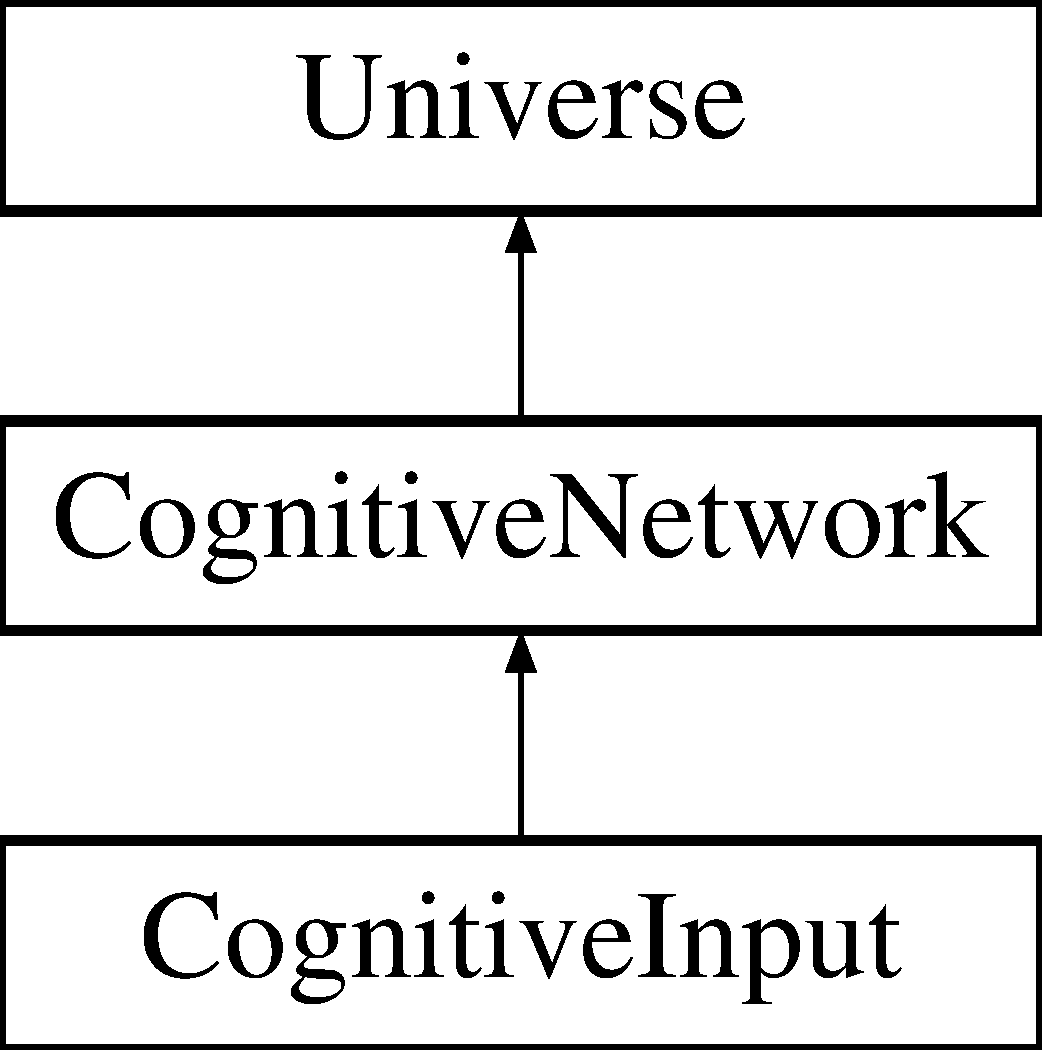
\includegraphics[height=3.000000cm]{classCognitiveInput}
\end{center}
\end{figure}
\subsection*{Public Member Functions}
\begin{DoxyCompactItemize}
\item 
\mbox{\hyperlink{classCognitiveInput_a5c3c102dc3ec6cfec25eb849488e9782}{Cognitive\+Input}} ()
\item 
\mbox{\hyperlink{classCognitiveInput_a220c07f5be517afe47b4d3c486c4152e}{Cognitive\+Input}} (unsigned int object\+\_\+type)
\item 
\mbox{\hyperlink{classCognitiveInput_a31cc06426ab41c39ec8c795ab29d43de}{Cognitive\+Input}} (unsigned int object\+\_\+type, std\+::chrono\+::time\+\_\+point$<$ \mbox{\hyperlink{universe_8h_a0ef8d951d1ca5ab3cfaf7ab4c7a6fd80}{Clock}} $>$ event\+\_\+time)
\item 
\mbox{\hyperlink{classCognitiveInput_a230ebb8f019af7e0bff51c13bc10c580}{Cognitive\+Input}} (unsigned int object\+\_\+type, std\+::chrono\+::time\+\_\+point$<$ \mbox{\hyperlink{universe_8h_a0ef8d951d1ca5ab3cfaf7ab4c7a6fd80}{Clock}} $>$ event\+\_\+time, \mbox{\hyperlink{classCognitiveNetwork}{Cognitive\+Network}} \&cognitivenetwork\+\_\+connector)
\item 
virtual \mbox{\hyperlink{classCognitiveInput_a68007661b8fdd7ef39213a1fb3c06bd7}{$\sim$\+Cognitive\+Input}} ()
\item 
unsigned int \mbox{\hyperlink{classCognitiveInput_a695e7e57b717210b64f9e2c4e26c8044}{Get\+Counter}} (std\+::chrono\+::time\+\_\+point$<$ \mbox{\hyperlink{universe_8h_a0ef8d951d1ca5ab3cfaf7ab4c7a6fd80}{Clock}} $>$ event\+\_\+time)
\item 
double \mbox{\hyperlink{classCognitiveInput_a9bdb43198c1a36b97a6da125331bc927}{Get\+Energy}} (std\+::chrono\+::time\+\_\+point$<$ \mbox{\hyperlink{universe_8h_a0ef8d951d1ca5ab3cfaf7ab4c7a6fd80}{Clock}} $>$ event\+\_\+time)
\item 
int \mbox{\hyperlink{classCognitiveInput_a0ad0919c7280b268493b27892bd7c784}{Get\+Type}} (std\+::chrono\+::time\+\_\+point$<$ \mbox{\hyperlink{universe_8h_a0ef8d951d1ca5ab3cfaf7ab4c7a6fd80}{Clock}} $>$ event\+\_\+time)
\item 
void \mbox{\hyperlink{classCognitiveInput_a37d38512fb190431b4baf8f990c077a9}{Set\+Type}} (std\+::chrono\+::time\+\_\+point$<$ \mbox{\hyperlink{universe_8h_a0ef8d951d1ca5ab3cfaf7ab4c7a6fd80}{Clock}} $>$ event\+\_\+time, int val)
\item 
void \mbox{\hyperlink{classCognitiveInput_a4f09c1f176b5406d95a14d7cb1ab75e6}{Set\+Counter}} (std\+::chrono\+::time\+\_\+point$<$ \mbox{\hyperlink{universe_8h_a0ef8d951d1ca5ab3cfaf7ab4c7a6fd80}{Clock}} $>$ event\+\_\+time, unsigned int val)
\item 
void \mbox{\hyperlink{classCognitiveInput_a3498a8b5333606ef4d089e6c427ddf74}{Set\+Energy}} (std\+::chrono\+::time\+\_\+point$<$ \mbox{\hyperlink{universe_8h_a0ef8d951d1ca5ab3cfaf7ab4c7a6fd80}{Clock}} $>$ event\+\_\+time, double val)
\item 
void \mbox{\hyperlink{classCognitiveInput_a23f56d012233f655e1530ab61d80c27f}{Add\+Energy}} (std\+::chrono\+::time\+\_\+point$<$ \mbox{\hyperlink{universe_8h_a0ef8d951d1ca5ab3cfaf7ab4c7a6fd80}{Clock}} $>$ event\+\_\+time, double val)
\item 
bool \mbox{\hyperlink{classCognitiveInput_a943605b820cc279533e19d24e11405c6}{Reset\+Parameters}} (std\+::chrono\+::time\+\_\+point$<$ \mbox{\hyperlink{universe_8h_a0ef8d951d1ca5ab3cfaf7ab4c7a6fd80}{Clock}} $>$ event\+\_\+time)
\item 
int \mbox{\hyperlink{classCognitiveInput_a93bd9d88194a545c9a85512edcbb6044}{Update}} (std\+::chrono\+::time\+\_\+point$<$ \mbox{\hyperlink{universe_8h_a0ef8d951d1ca5ab3cfaf7ab4c7a6fd80}{Clock}} $>$ event\+\_\+time)
\end{DoxyCompactItemize}
\subsection*{Private Attributes}
\begin{DoxyCompactItemize}
\item 
int \mbox{\hyperlink{classCognitiveInput_a7158317a0651e93fde965e74988e4817}{m\+\_\+\+Cognitive\+Input\+Type}}
\item 
int \mbox{\hyperlink{classCognitiveInput_ab2edb814888d1bd68a44d0547cf23691}{cognitiveinput\+\_\+type}} = 0
\item 
int \mbox{\hyperlink{classCognitiveInput_acb5b53899d51052d7ec18ecd1386fa33}{m\+\_\+add\+Status}}
\item 
std\+::chrono\+::time\+\_\+point$<$ \mbox{\hyperlink{universe_8h_a0ef8d951d1ca5ab3cfaf7ab4c7a6fd80}{Clock}} $>$ \mbox{\hyperlink{classCognitiveInput_a5ad1f0f7523ebfb32d43556b0c94ca70}{time\+\_\+object\+\_\+created}} = std\+::chrono\+::time\+\_\+point$<$\mbox{\hyperlink{universe_8h_a0ef8d951d1ca5ab3cfaf7ab4c7a6fd80}{Clock}}$>$(std\+::chrono\+::nanoseconds\+::zero())
\item 
std\+::chrono\+::time\+\_\+point$<$ \mbox{\hyperlink{universe_8h_a0ef8d951d1ca5ab3cfaf7ab4c7a6fd80}{Clock}} $>$ \mbox{\hyperlink{classCognitiveInput_a34d8fede9de24f5046f301f5326b3511}{previous\+\_\+event\+\_\+time}}
\item 
bool \mbox{\hyperlink{classCognitiveInput_a57ce1ed5b887f4a0b2efb3b9fc5c407f}{object\+\_\+disabled}} = true
\item 
bool \mbox{\hyperlink{classCognitiveInput_aa60f8084d314063b5d32e4301f40ac37}{object\+\_\+initialised}} = false
\item 
int \mbox{\hyperlink{classCognitiveInput_a269476daa7243992fff92092007feff5}{duration\+\_\+since\+\_\+last\+\_\+event}}
\item 
double \mbox{\hyperlink{classCognitiveInput_ac9a4b7de6f0475f45ff198bd5d4e6ae0}{m\+\_\+\+Volume}}
\item 
double \mbox{\hyperlink{classCognitiveInput_a47ee2b439761b314062d946850cb852b}{m\+\_\+\+Surface\+Area}}
\item 
double \mbox{\hyperlink{classCognitiveInput_a51a23a86f14e2cb0e60f6df2d8d8494e}{object\+\_\+size}}
\item 
unsigned int \mbox{\hyperlink{classCognitiveInput_a2cc357e24354d7016953475c1bc66a98}{m\+\_\+\+Counter}}
\begin{DoxyCompactList}\small\item\em Member variable \char`\"{}m\+\_\+\+Counter\char`\"{}. \end{DoxyCompactList}\item 
double \mbox{\hyperlink{classCognitiveInput_a56cb85463a47cdd57f5cf2869d0e0761}{object\+\_\+energy}}
\begin{DoxyCompactList}\small\item\em Member variable \char`\"{}object\+\_\+energy\char`\"{}. \end{DoxyCompactList}\item 
double \mbox{\hyperlink{classCognitiveInput_aea44f8591ccd7876a4f2ddf450244ea2}{object\+\_\+energy\+\_\+threshold}}
\item 
double \mbox{\hyperlink{classCognitiveInput_ad2726705c7242a842ad93272c6b7258a}{m\+\_\+\+Time\+Dilation}}
\item 
double \mbox{\hyperlink{classCognitiveInput_a11d157d16bfe28880973320cdaef33bc}{m\+\_\+\+Time\+Threshold}}
\end{DoxyCompactItemize}
\subsection*{Additional Inherited Members}


\subsection{Constructor \& Destructor Documentation}
\mbox{\Hypertarget{classCognitiveInput_a5c3c102dc3ec6cfec25eb849488e9782}\label{classCognitiveInput_a5c3c102dc3ec6cfec25eb849488e9782}} 
\index{Cognitive\+Input@{Cognitive\+Input}!Cognitive\+Input@{Cognitive\+Input}}
\index{Cognitive\+Input@{Cognitive\+Input}!Cognitive\+Input@{Cognitive\+Input}}
\subsubsection{\texorpdfstring{Cognitive\+Input()}{CognitiveInput()}\hspace{0.1cm}{\footnotesize\ttfamily [1/4]}}
{\footnotesize\ttfamily Cognitive\+Input\+::\+Cognitive\+Input (\begin{DoxyParamCaption}{ }\end{DoxyParamCaption})\hspace{0.3cm}{\ttfamily [inline]}}

\mbox{\Hypertarget{classCognitiveInput_a220c07f5be517afe47b4d3c486c4152e}\label{classCognitiveInput_a220c07f5be517afe47b4d3c486c4152e}} 
\index{Cognitive\+Input@{Cognitive\+Input}!Cognitive\+Input@{Cognitive\+Input}}
\index{Cognitive\+Input@{Cognitive\+Input}!Cognitive\+Input@{Cognitive\+Input}}
\subsubsection{\texorpdfstring{Cognitive\+Input()}{CognitiveInput()}\hspace{0.1cm}{\footnotesize\ttfamily [2/4]}}
{\footnotesize\ttfamily Cognitive\+Input\+::\+Cognitive\+Input (\begin{DoxyParamCaption}\item[{unsigned int}]{object\+\_\+type }\end{DoxyParamCaption})\hspace{0.3cm}{\ttfamily [inline]}}

\mbox{\Hypertarget{classCognitiveInput_a31cc06426ab41c39ec8c795ab29d43de}\label{classCognitiveInput_a31cc06426ab41c39ec8c795ab29d43de}} 
\index{Cognitive\+Input@{Cognitive\+Input}!Cognitive\+Input@{Cognitive\+Input}}
\index{Cognitive\+Input@{Cognitive\+Input}!Cognitive\+Input@{Cognitive\+Input}}
\subsubsection{\texorpdfstring{Cognitive\+Input()}{CognitiveInput()}\hspace{0.1cm}{\footnotesize\ttfamily [3/4]}}
{\footnotesize\ttfamily Cognitive\+Input\+::\+Cognitive\+Input (\begin{DoxyParamCaption}\item[{unsigned int}]{object\+\_\+type,  }\item[{std\+::chrono\+::time\+\_\+point$<$ \mbox{\hyperlink{universe_8h_a0ef8d951d1ca5ab3cfaf7ab4c7a6fd80}{Clock}} $>$}]{event\+\_\+time }\end{DoxyParamCaption})\hspace{0.3cm}{\ttfamily [inline]}}

\mbox{\Hypertarget{classCognitiveInput_a230ebb8f019af7e0bff51c13bc10c580}\label{classCognitiveInput_a230ebb8f019af7e0bff51c13bc10c580}} 
\index{Cognitive\+Input@{Cognitive\+Input}!Cognitive\+Input@{Cognitive\+Input}}
\index{Cognitive\+Input@{Cognitive\+Input}!Cognitive\+Input@{Cognitive\+Input}}
\subsubsection{\texorpdfstring{Cognitive\+Input()}{CognitiveInput()}\hspace{0.1cm}{\footnotesize\ttfamily [4/4]}}
{\footnotesize\ttfamily Cognitive\+Input\+::\+Cognitive\+Input (\begin{DoxyParamCaption}\item[{unsigned int}]{object\+\_\+type,  }\item[{std\+::chrono\+::time\+\_\+point$<$ \mbox{\hyperlink{universe_8h_a0ef8d951d1ca5ab3cfaf7ab4c7a6fd80}{Clock}} $>$}]{event\+\_\+time,  }\item[{\mbox{\hyperlink{classCognitiveNetwork}{Cognitive\+Network}} \&}]{cognitivenetwork\+\_\+connector }\end{DoxyParamCaption})\hspace{0.3cm}{\ttfamily [inline]}}

\mbox{\Hypertarget{classCognitiveInput_a68007661b8fdd7ef39213a1fb3c06bd7}\label{classCognitiveInput_a68007661b8fdd7ef39213a1fb3c06bd7}} 
\index{Cognitive\+Input@{Cognitive\+Input}!````~Cognitive\+Input@{$\sim$\+Cognitive\+Input}}
\index{````~Cognitive\+Input@{$\sim$\+Cognitive\+Input}!Cognitive\+Input@{Cognitive\+Input}}
\subsubsection{\texorpdfstring{$\sim$\+Cognitive\+Input()}{~CognitiveInput()}}
{\footnotesize\ttfamily virtual Cognitive\+Input\+::$\sim$\+Cognitive\+Input (\begin{DoxyParamCaption}{ }\end{DoxyParamCaption})\hspace{0.3cm}{\ttfamily [inline]}, {\ttfamily [virtual]}}

Default destructor 

\subsection{Member Function Documentation}
\mbox{\Hypertarget{classCognitiveInput_a23f56d012233f655e1530ab61d80c27f}\label{classCognitiveInput_a23f56d012233f655e1530ab61d80c27f}} 
\index{Cognitive\+Input@{Cognitive\+Input}!Add\+Energy@{Add\+Energy}}
\index{Add\+Energy@{Add\+Energy}!Cognitive\+Input@{Cognitive\+Input}}
\subsubsection{\texorpdfstring{Add\+Energy()}{AddEnergy()}}
{\footnotesize\ttfamily void Cognitive\+Input\+::\+Add\+Energy (\begin{DoxyParamCaption}\item[{std\+::chrono\+::time\+\_\+point$<$ \mbox{\hyperlink{universe_8h_a0ef8d951d1ca5ab3cfaf7ab4c7a6fd80}{Clock}} $>$}]{event\+\_\+time,  }\item[{double}]{val }\end{DoxyParamCaption})\hspace{0.3cm}{\ttfamily [inline]}}

\mbox{\Hypertarget{classCognitiveInput_a695e7e57b717210b64f9e2c4e26c8044}\label{classCognitiveInput_a695e7e57b717210b64f9e2c4e26c8044}} 
\index{Cognitive\+Input@{Cognitive\+Input}!Get\+Counter@{Get\+Counter}}
\index{Get\+Counter@{Get\+Counter}!Cognitive\+Input@{Cognitive\+Input}}
\subsubsection{\texorpdfstring{Get\+Counter()}{GetCounter()}}
{\footnotesize\ttfamily unsigned int Cognitive\+Input\+::\+Get\+Counter (\begin{DoxyParamCaption}\item[{std\+::chrono\+::time\+\_\+point$<$ \mbox{\hyperlink{universe_8h_a0ef8d951d1ca5ab3cfaf7ab4c7a6fd80}{Clock}} $>$}]{event\+\_\+time }\end{DoxyParamCaption})\hspace{0.3cm}{\ttfamily [inline]}}

\mbox{\Hypertarget{classCognitiveInput_a9bdb43198c1a36b97a6da125331bc927}\label{classCognitiveInput_a9bdb43198c1a36b97a6da125331bc927}} 
\index{Cognitive\+Input@{Cognitive\+Input}!Get\+Energy@{Get\+Energy}}
\index{Get\+Energy@{Get\+Energy}!Cognitive\+Input@{Cognitive\+Input}}
\subsubsection{\texorpdfstring{Get\+Energy()}{GetEnergy()}}
{\footnotesize\ttfamily double Cognitive\+Input\+::\+Get\+Energy (\begin{DoxyParamCaption}\item[{std\+::chrono\+::time\+\_\+point$<$ \mbox{\hyperlink{universe_8h_a0ef8d951d1ca5ab3cfaf7ab4c7a6fd80}{Clock}} $>$}]{event\+\_\+time }\end{DoxyParamCaption})\hspace{0.3cm}{\ttfamily [inline]}}

\mbox{\Hypertarget{classCognitiveInput_a0ad0919c7280b268493b27892bd7c784}\label{classCognitiveInput_a0ad0919c7280b268493b27892bd7c784}} 
\index{Cognitive\+Input@{Cognitive\+Input}!Get\+Type@{Get\+Type}}
\index{Get\+Type@{Get\+Type}!Cognitive\+Input@{Cognitive\+Input}}
\subsubsection{\texorpdfstring{Get\+Type()}{GetType()}}
{\footnotesize\ttfamily int Cognitive\+Input\+::\+Get\+Type (\begin{DoxyParamCaption}\item[{std\+::chrono\+::time\+\_\+point$<$ \mbox{\hyperlink{universe_8h_a0ef8d951d1ca5ab3cfaf7ab4c7a6fd80}{Clock}} $>$}]{event\+\_\+time }\end{DoxyParamCaption})\hspace{0.3cm}{\ttfamily [inline]}}

\mbox{\Hypertarget{classCognitiveInput_a943605b820cc279533e19d24e11405c6}\label{classCognitiveInput_a943605b820cc279533e19d24e11405c6}} 
\index{Cognitive\+Input@{Cognitive\+Input}!Reset\+Parameters@{Reset\+Parameters}}
\index{Reset\+Parameters@{Reset\+Parameters}!Cognitive\+Input@{Cognitive\+Input}}
\subsubsection{\texorpdfstring{Reset\+Parameters()}{ResetParameters()}}
{\footnotesize\ttfamily bool Cognitive\+Input\+::\+Reset\+Parameters (\begin{DoxyParamCaption}\item[{std\+::chrono\+::time\+\_\+point$<$ \mbox{\hyperlink{universe_8h_a0ef8d951d1ca5ab3cfaf7ab4c7a6fd80}{Clock}} $>$}]{event\+\_\+time }\end{DoxyParamCaption})}

\mbox{\Hypertarget{classCognitiveInput_a4f09c1f176b5406d95a14d7cb1ab75e6}\label{classCognitiveInput_a4f09c1f176b5406d95a14d7cb1ab75e6}} 
\index{Cognitive\+Input@{Cognitive\+Input}!Set\+Counter@{Set\+Counter}}
\index{Set\+Counter@{Set\+Counter}!Cognitive\+Input@{Cognitive\+Input}}
\subsubsection{\texorpdfstring{Set\+Counter()}{SetCounter()}}
{\footnotesize\ttfamily void Cognitive\+Input\+::\+Set\+Counter (\begin{DoxyParamCaption}\item[{std\+::chrono\+::time\+\_\+point$<$ \mbox{\hyperlink{universe_8h_a0ef8d951d1ca5ab3cfaf7ab4c7a6fd80}{Clock}} $>$}]{event\+\_\+time,  }\item[{unsigned int}]{val }\end{DoxyParamCaption})\hspace{0.3cm}{\ttfamily [inline]}, {\ttfamily [virtual]}}



Reimplemented from \mbox{\hyperlink{classUniverse_aa22202ae740eb1355529afcb13285e91}{Universe}}.

\mbox{\Hypertarget{classCognitiveInput_a3498a8b5333606ef4d089e6c427ddf74}\label{classCognitiveInput_a3498a8b5333606ef4d089e6c427ddf74}} 
\index{Cognitive\+Input@{Cognitive\+Input}!Set\+Energy@{Set\+Energy}}
\index{Set\+Energy@{Set\+Energy}!Cognitive\+Input@{Cognitive\+Input}}
\subsubsection{\texorpdfstring{Set\+Energy()}{SetEnergy()}}
{\footnotesize\ttfamily void Cognitive\+Input\+::\+Set\+Energy (\begin{DoxyParamCaption}\item[{std\+::chrono\+::time\+\_\+point$<$ \mbox{\hyperlink{universe_8h_a0ef8d951d1ca5ab3cfaf7ab4c7a6fd80}{Clock}} $>$}]{event\+\_\+time,  }\item[{double}]{val }\end{DoxyParamCaption})\hspace{0.3cm}{\ttfamily [inline]}}

\mbox{\Hypertarget{classCognitiveInput_a37d38512fb190431b4baf8f990c077a9}\label{classCognitiveInput_a37d38512fb190431b4baf8f990c077a9}} 
\index{Cognitive\+Input@{Cognitive\+Input}!Set\+Type@{Set\+Type}}
\index{Set\+Type@{Set\+Type}!Cognitive\+Input@{Cognitive\+Input}}
\subsubsection{\texorpdfstring{Set\+Type()}{SetType()}}
{\footnotesize\ttfamily void Cognitive\+Input\+::\+Set\+Type (\begin{DoxyParamCaption}\item[{std\+::chrono\+::time\+\_\+point$<$ \mbox{\hyperlink{universe_8h_a0ef8d951d1ca5ab3cfaf7ab4c7a6fd80}{Clock}} $>$}]{event\+\_\+time,  }\item[{int}]{val }\end{DoxyParamCaption})\hspace{0.3cm}{\ttfamily [inline]}}

\mbox{\Hypertarget{classCognitiveInput_a93bd9d88194a545c9a85512edcbb6044}\label{classCognitiveInput_a93bd9d88194a545c9a85512edcbb6044}} 
\index{Cognitive\+Input@{Cognitive\+Input}!Update@{Update}}
\index{Update@{Update}!Cognitive\+Input@{Cognitive\+Input}}
\subsubsection{\texorpdfstring{Update()}{Update()}}
{\footnotesize\ttfamily int Cognitive\+Input\+::\+Update (\begin{DoxyParamCaption}\item[{std\+::chrono\+::time\+\_\+point$<$ \mbox{\hyperlink{universe_8h_a0ef8d951d1ca5ab3cfaf7ab4c7a6fd80}{Clock}} $>$}]{event\+\_\+time }\end{DoxyParamCaption})}



\subsection{Member Data Documentation}
\mbox{\Hypertarget{classCognitiveInput_ab2edb814888d1bd68a44d0547cf23691}\label{classCognitiveInput_ab2edb814888d1bd68a44d0547cf23691}} 
\index{Cognitive\+Input@{Cognitive\+Input}!cognitiveinput\+\_\+type@{cognitiveinput\+\_\+type}}
\index{cognitiveinput\+\_\+type@{cognitiveinput\+\_\+type}!Cognitive\+Input@{Cognitive\+Input}}
\subsubsection{\texorpdfstring{cognitiveinput\+\_\+type}{cognitiveinput\_type}}
{\footnotesize\ttfamily int Cognitive\+Input\+::cognitiveinput\+\_\+type = 0\hspace{0.3cm}{\ttfamily [private]}}

\mbox{\Hypertarget{classCognitiveInput_a269476daa7243992fff92092007feff5}\label{classCognitiveInput_a269476daa7243992fff92092007feff5}} 
\index{Cognitive\+Input@{Cognitive\+Input}!duration\+\_\+since\+\_\+last\+\_\+event@{duration\+\_\+since\+\_\+last\+\_\+event}}
\index{duration\+\_\+since\+\_\+last\+\_\+event@{duration\+\_\+since\+\_\+last\+\_\+event}!Cognitive\+Input@{Cognitive\+Input}}
\subsubsection{\texorpdfstring{duration\+\_\+since\+\_\+last\+\_\+event}{duration\_since\_last\_event}}
{\footnotesize\ttfamily int Cognitive\+Input\+::duration\+\_\+since\+\_\+last\+\_\+event\hspace{0.3cm}{\ttfamily [private]}}

\mbox{\Hypertarget{classCognitiveInput_acb5b53899d51052d7ec18ecd1386fa33}\label{classCognitiveInput_acb5b53899d51052d7ec18ecd1386fa33}} 
\index{Cognitive\+Input@{Cognitive\+Input}!m\+\_\+add\+Status@{m\+\_\+add\+Status}}
\index{m\+\_\+add\+Status@{m\+\_\+add\+Status}!Cognitive\+Input@{Cognitive\+Input}}
\subsubsection{\texorpdfstring{m\+\_\+add\+Status}{m\_addStatus}}
{\footnotesize\ttfamily int Cognitive\+Input\+::m\+\_\+add\+Status\hspace{0.3cm}{\ttfamily [private]}}

\mbox{\Hypertarget{classCognitiveInput_a7158317a0651e93fde965e74988e4817}\label{classCognitiveInput_a7158317a0651e93fde965e74988e4817}} 
\index{Cognitive\+Input@{Cognitive\+Input}!m\+\_\+\+Cognitive\+Input\+Type@{m\+\_\+\+Cognitive\+Input\+Type}}
\index{m\+\_\+\+Cognitive\+Input\+Type@{m\+\_\+\+Cognitive\+Input\+Type}!Cognitive\+Input@{Cognitive\+Input}}
\subsubsection{\texorpdfstring{m\+\_\+\+Cognitive\+Input\+Type}{m\_CognitiveInputType}}
{\footnotesize\ttfamily int Cognitive\+Input\+::m\+\_\+\+Cognitive\+Input\+Type\hspace{0.3cm}{\ttfamily [private]}}

\mbox{\Hypertarget{classCognitiveInput_a2cc357e24354d7016953475c1bc66a98}\label{classCognitiveInput_a2cc357e24354d7016953475c1bc66a98}} 
\index{Cognitive\+Input@{Cognitive\+Input}!m\+\_\+\+Counter@{m\+\_\+\+Counter}}
\index{m\+\_\+\+Counter@{m\+\_\+\+Counter}!Cognitive\+Input@{Cognitive\+Input}}
\subsubsection{\texorpdfstring{m\+\_\+\+Counter}{m\_Counter}}
{\footnotesize\ttfamily unsigned int Cognitive\+Input\+::m\+\_\+\+Counter\hspace{0.3cm}{\ttfamily [private]}}



Member variable \char`\"{}m\+\_\+\+Counter\char`\"{}. 

\mbox{\Hypertarget{classCognitiveInput_a47ee2b439761b314062d946850cb852b}\label{classCognitiveInput_a47ee2b439761b314062d946850cb852b}} 
\index{Cognitive\+Input@{Cognitive\+Input}!m\+\_\+\+Surface\+Area@{m\+\_\+\+Surface\+Area}}
\index{m\+\_\+\+Surface\+Area@{m\+\_\+\+Surface\+Area}!Cognitive\+Input@{Cognitive\+Input}}
\subsubsection{\texorpdfstring{m\+\_\+\+Surface\+Area}{m\_SurfaceArea}}
{\footnotesize\ttfamily double Cognitive\+Input\+::m\+\_\+\+Surface\+Area\hspace{0.3cm}{\ttfamily [private]}}

\mbox{\Hypertarget{classCognitiveInput_ad2726705c7242a842ad93272c6b7258a}\label{classCognitiveInput_ad2726705c7242a842ad93272c6b7258a}} 
\index{Cognitive\+Input@{Cognitive\+Input}!m\+\_\+\+Time\+Dilation@{m\+\_\+\+Time\+Dilation}}
\index{m\+\_\+\+Time\+Dilation@{m\+\_\+\+Time\+Dilation}!Cognitive\+Input@{Cognitive\+Input}}
\subsubsection{\texorpdfstring{m\+\_\+\+Time\+Dilation}{m\_TimeDilation}}
{\footnotesize\ttfamily double Cognitive\+Input\+::m\+\_\+\+Time\+Dilation\hspace{0.3cm}{\ttfamily [private]}}

\mbox{\Hypertarget{classCognitiveInput_a11d157d16bfe28880973320cdaef33bc}\label{classCognitiveInput_a11d157d16bfe28880973320cdaef33bc}} 
\index{Cognitive\+Input@{Cognitive\+Input}!m\+\_\+\+Time\+Threshold@{m\+\_\+\+Time\+Threshold}}
\index{m\+\_\+\+Time\+Threshold@{m\+\_\+\+Time\+Threshold}!Cognitive\+Input@{Cognitive\+Input}}
\subsubsection{\texorpdfstring{m\+\_\+\+Time\+Threshold}{m\_TimeThreshold}}
{\footnotesize\ttfamily double Cognitive\+Input\+::m\+\_\+\+Time\+Threshold\hspace{0.3cm}{\ttfamily [private]}}

\mbox{\Hypertarget{classCognitiveInput_ac9a4b7de6f0475f45ff198bd5d4e6ae0}\label{classCognitiveInput_ac9a4b7de6f0475f45ff198bd5d4e6ae0}} 
\index{Cognitive\+Input@{Cognitive\+Input}!m\+\_\+\+Volume@{m\+\_\+\+Volume}}
\index{m\+\_\+\+Volume@{m\+\_\+\+Volume}!Cognitive\+Input@{Cognitive\+Input}}
\subsubsection{\texorpdfstring{m\+\_\+\+Volume}{m\_Volume}}
{\footnotesize\ttfamily double Cognitive\+Input\+::m\+\_\+\+Volume\hspace{0.3cm}{\ttfamily [private]}}

\mbox{\Hypertarget{classCognitiveInput_a57ce1ed5b887f4a0b2efb3b9fc5c407f}\label{classCognitiveInput_a57ce1ed5b887f4a0b2efb3b9fc5c407f}} 
\index{Cognitive\+Input@{Cognitive\+Input}!object\+\_\+disabled@{object\+\_\+disabled}}
\index{object\+\_\+disabled@{object\+\_\+disabled}!Cognitive\+Input@{Cognitive\+Input}}
\subsubsection{\texorpdfstring{object\+\_\+disabled}{object\_disabled}}
{\footnotesize\ttfamily bool Cognitive\+Input\+::object\+\_\+disabled = true\hspace{0.3cm}{\ttfamily [private]}}

\mbox{\Hypertarget{classCognitiveInput_a56cb85463a47cdd57f5cf2869d0e0761}\label{classCognitiveInput_a56cb85463a47cdd57f5cf2869d0e0761}} 
\index{Cognitive\+Input@{Cognitive\+Input}!object\+\_\+energy@{object\+\_\+energy}}
\index{object\+\_\+energy@{object\+\_\+energy}!Cognitive\+Input@{Cognitive\+Input}}
\subsubsection{\texorpdfstring{object\+\_\+energy}{object\_energy}}
{\footnotesize\ttfamily double Cognitive\+Input\+::object\+\_\+energy\hspace{0.3cm}{\ttfamily [private]}}



Member variable \char`\"{}object\+\_\+energy\char`\"{}. 

\mbox{\Hypertarget{classCognitiveInput_aea44f8591ccd7876a4f2ddf450244ea2}\label{classCognitiveInput_aea44f8591ccd7876a4f2ddf450244ea2}} 
\index{Cognitive\+Input@{Cognitive\+Input}!object\+\_\+energy\+\_\+threshold@{object\+\_\+energy\+\_\+threshold}}
\index{object\+\_\+energy\+\_\+threshold@{object\+\_\+energy\+\_\+threshold}!Cognitive\+Input@{Cognitive\+Input}}
\subsubsection{\texorpdfstring{object\+\_\+energy\+\_\+threshold}{object\_energy\_threshold}}
{\footnotesize\ttfamily double Cognitive\+Input\+::object\+\_\+energy\+\_\+threshold\hspace{0.3cm}{\ttfamily [private]}}

\mbox{\Hypertarget{classCognitiveInput_aa60f8084d314063b5d32e4301f40ac37}\label{classCognitiveInput_aa60f8084d314063b5d32e4301f40ac37}} 
\index{Cognitive\+Input@{Cognitive\+Input}!object\+\_\+initialised@{object\+\_\+initialised}}
\index{object\+\_\+initialised@{object\+\_\+initialised}!Cognitive\+Input@{Cognitive\+Input}}
\subsubsection{\texorpdfstring{object\+\_\+initialised}{object\_initialised}}
{\footnotesize\ttfamily bool Cognitive\+Input\+::object\+\_\+initialised = false\hspace{0.3cm}{\ttfamily [private]}}

\mbox{\Hypertarget{classCognitiveInput_a51a23a86f14e2cb0e60f6df2d8d8494e}\label{classCognitiveInput_a51a23a86f14e2cb0e60f6df2d8d8494e}} 
\index{Cognitive\+Input@{Cognitive\+Input}!object\+\_\+size@{object\+\_\+size}}
\index{object\+\_\+size@{object\+\_\+size}!Cognitive\+Input@{Cognitive\+Input}}
\subsubsection{\texorpdfstring{object\+\_\+size}{object\_size}}
{\footnotesize\ttfamily double Cognitive\+Input\+::object\+\_\+size\hspace{0.3cm}{\ttfamily [private]}}

\mbox{\Hypertarget{classCognitiveInput_a34d8fede9de24f5046f301f5326b3511}\label{classCognitiveInput_a34d8fede9de24f5046f301f5326b3511}} 
\index{Cognitive\+Input@{Cognitive\+Input}!previous\+\_\+event\+\_\+time@{previous\+\_\+event\+\_\+time}}
\index{previous\+\_\+event\+\_\+time@{previous\+\_\+event\+\_\+time}!Cognitive\+Input@{Cognitive\+Input}}
\subsubsection{\texorpdfstring{previous\+\_\+event\+\_\+time}{previous\_event\_time}}
{\footnotesize\ttfamily std\+::chrono\+::time\+\_\+point$<$\mbox{\hyperlink{universe_8h_a0ef8d951d1ca5ab3cfaf7ab4c7a6fd80}{Clock}}$>$ Cognitive\+Input\+::previous\+\_\+event\+\_\+time\hspace{0.3cm}{\ttfamily [private]}}

\mbox{\Hypertarget{classCognitiveInput_a5ad1f0f7523ebfb32d43556b0c94ca70}\label{classCognitiveInput_a5ad1f0f7523ebfb32d43556b0c94ca70}} 
\index{Cognitive\+Input@{Cognitive\+Input}!time\+\_\+object\+\_\+created@{time\+\_\+object\+\_\+created}}
\index{time\+\_\+object\+\_\+created@{time\+\_\+object\+\_\+created}!Cognitive\+Input@{Cognitive\+Input}}
\subsubsection{\texorpdfstring{time\+\_\+object\+\_\+created}{time\_object\_created}}
{\footnotesize\ttfamily std\+::chrono\+::time\+\_\+point$<$\mbox{\hyperlink{universe_8h_a0ef8d951d1ca5ab3cfaf7ab4c7a6fd80}{Clock}}$>$ Cognitive\+Input\+::time\+\_\+object\+\_\+created = std\+::chrono\+::time\+\_\+point$<$\mbox{\hyperlink{universe_8h_a0ef8d951d1ca5ab3cfaf7ab4c7a6fd80}{Clock}}$>$(std\+::chrono\+::nanoseconds\+::zero())\hspace{0.3cm}{\ttfamily [private]}}



The documentation for this class was generated from the following files\+:\begin{DoxyCompactItemize}
\item 
/home/pbisaacs/\+Developer/\+Brain\+Harmonics/\mbox{\hyperlink{cognitiveinput_8h}{cognitiveinput.\+h}}\item 
/home/pbisaacs/\+Developer/\+Brain\+Harmonics/\mbox{\hyperlink{cognitiveinput_8cc}{cognitiveinput.\+cc}}\end{DoxyCompactItemize}

\hypertarget{classCognitiveNetwork}{}\section{Cognitive\+Network Class Reference}
\label{classCognitiveNetwork}\index{Cognitive\+Network@{Cognitive\+Network}}


{\ttfamily \#include $<$cognitivenetwork.\+h$>$}

Inheritance diagram for Cognitive\+Network\+:\begin{figure}[H]
\begin{center}
\leavevmode
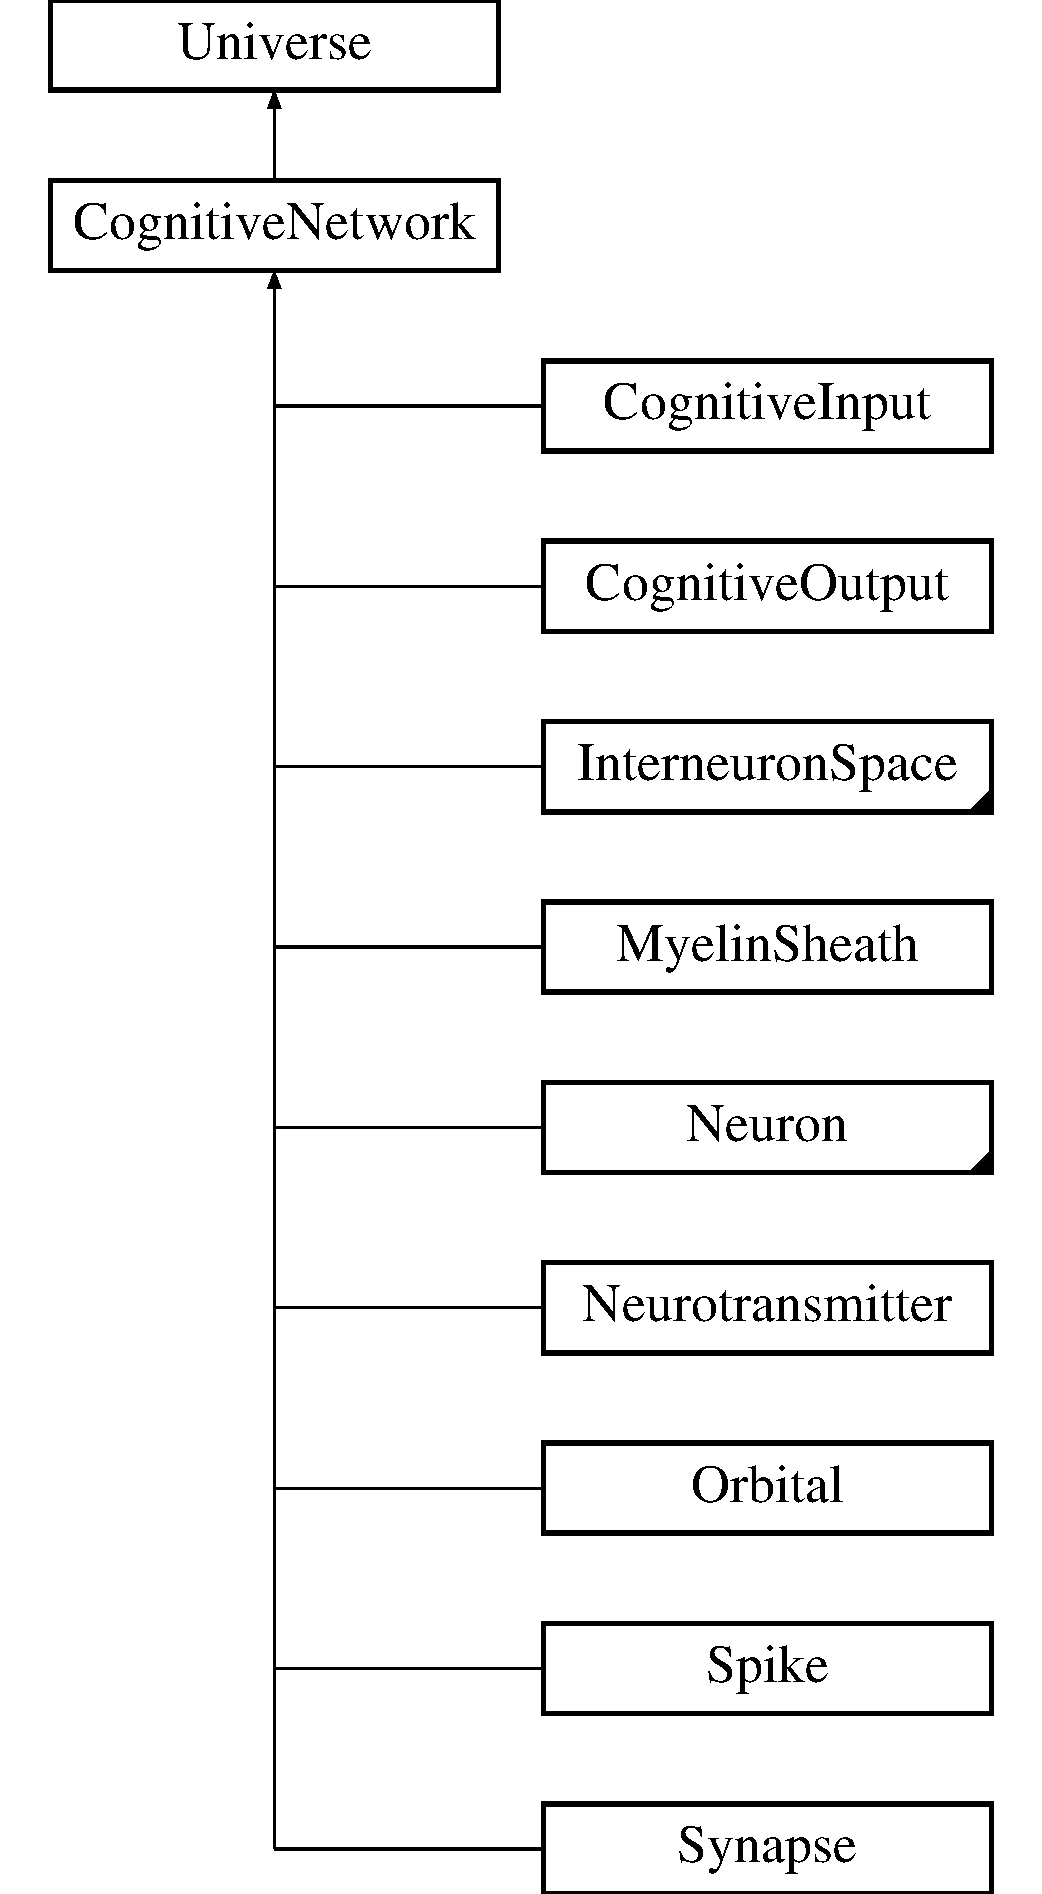
\includegraphics[height=11.000000cm]{classCognitiveNetwork}
\end{center}
\end{figure}
\subsection*{Classes}
\begin{DoxyCompactItemize}
\item 
struct \mbox{\hyperlink{structCognitiveNetwork_1_1OrbitalConnection}{Orbital\+Connection}}
\end{DoxyCompactItemize}
\subsection*{Public Member Functions}
\begin{DoxyCompactItemize}
\item 
\mbox{\hyperlink{classCognitiveNetwork_a3daddb316744336648d317e7f71ed371}{Cognitive\+Network}} ()
\item 
\mbox{\hyperlink{classCognitiveNetwork_a167b15e33bcbca43cb0a516159e890f2}{Cognitive\+Network}} (unsigned int object\+\_\+type)
\item 
\mbox{\hyperlink{classCognitiveNetwork_ac7ba285d3468a929dac88756a2c4e4f9}{Cognitive\+Network}} (unsigned int object\+\_\+type, std\+::chrono\+::time\+\_\+point$<$ \mbox{\hyperlink{universe_8h_a0ef8d951d1ca5ab3cfaf7ab4c7a6fd80}{Clock}} $>$ event\+\_\+time)
\item 
\mbox{\hyperlink{classCognitiveNetwork_a6ec49dcc8cc58cded71983291629179c}{Cognitive\+Network}} (unsigned int object\+\_\+type, std\+::chrono\+::time\+\_\+point$<$ \mbox{\hyperlink{universe_8h_a0ef8d951d1ca5ab3cfaf7ab4c7a6fd80}{Clock}} $>$ event\+\_\+time, \mbox{\hyperlink{classUniverse}{Universe}} \&universe\+\_\+connector)
\item 
virtual \mbox{\hyperlink{classCognitiveNetwork_a17142cc6f0bb3894e63f6c66fa401778}{$\sim$\+Cognitive\+Network}} ()
\item 
unsigned int \mbox{\hyperlink{classCognitiveNetwork_a160bb447671609eb14b1b8043639ac74}{Get\+Counter}} (std\+::chrono\+::time\+\_\+point$<$ \mbox{\hyperlink{universe_8h_a0ef8d951d1ca5ab3cfaf7ab4c7a6fd80}{Clock}} $>$ event\+\_\+time)
\item 
int \mbox{\hyperlink{classCognitiveNetwork_a6bb3fc06029c260dd658d0db072625a7}{Get\+Capacity}} (std\+::chrono\+::time\+\_\+point$<$ \mbox{\hyperlink{universe_8h_a0ef8d951d1ca5ab3cfaf7ab4c7a6fd80}{Clock}} $>$ event\+\_\+time)
\item 
void \mbox{\hyperlink{classCognitiveNetwork_a055b3711835b8d134356298f8975f04d}{Set\+Capacity}} (std\+::chrono\+::time\+\_\+point$<$ \mbox{\hyperlink{universe_8h_a0ef8d951d1ca5ab3cfaf7ab4c7a6fd80}{Clock}} $>$ event\+\_\+time, int val)
\item 
int \mbox{\hyperlink{classCognitiveNetwork_ad293916cfa0e454ef40d7e228d0dcba3}{Get\+Usage}} (std\+::chrono\+::time\+\_\+point$<$ \mbox{\hyperlink{universe_8h_a0ef8d951d1ca5ab3cfaf7ab4c7a6fd80}{Clock}} $>$ event\+\_\+time)
\item 
void \mbox{\hyperlink{classCognitiveNetwork_a8b6b4afc47df279604be13bce77f5b0a}{Set\+Usage}} (std\+::chrono\+::time\+\_\+point$<$ \mbox{\hyperlink{universe_8h_a0ef8d951d1ca5ab3cfaf7ab4c7a6fd80}{Clock}} $>$ event\+\_\+time, int val)
\item 
double \mbox{\hyperlink{classCognitiveNetwork_af23b9bce2587ccf3c8204be33fc76c61}{Get\+Energy}} (std\+::chrono\+::time\+\_\+point$<$ \mbox{\hyperlink{universe_8h_a0ef8d951d1ca5ab3cfaf7ab4c7a6fd80}{Clock}} $>$ event\+\_\+time)
\item 
double \mbox{\hyperlink{classCognitiveNetwork_a3a9be1c6697d063b0836cdcdc7a2600c}{Get\+Gate\+Keeper}} (std\+::chrono\+::time\+\_\+point$<$ \mbox{\hyperlink{universe_8h_a0ef8d951d1ca5ab3cfaf7ab4c7a6fd80}{Clock}} $>$ event\+\_\+time)
\item 
double \mbox{\hyperlink{classCognitiveNetwork_ad7f5cc836340017d38c22b57e177fc91}{Get\+Channel\+Min}} (std\+::chrono\+::time\+\_\+point$<$ \mbox{\hyperlink{universe_8h_a0ef8d951d1ca5ab3cfaf7ab4c7a6fd80}{Clock}} $>$ event\+\_\+time)
\item 
double \mbox{\hyperlink{classCognitiveNetwork_ab67da8690b83618d88f88411121d7071}{Get\+Channel\+Max}} (std\+::chrono\+::time\+\_\+point$<$ \mbox{\hyperlink{universe_8h_a0ef8d951d1ca5ab3cfaf7ab4c7a6fd80}{Clock}} $>$ event\+\_\+time)
\item 
bool \mbox{\hyperlink{classCognitiveNetwork_aa64c93ecec84b57b25e1fdb173795f9b}{Get\+Disabled}} (std\+::chrono\+::time\+\_\+point$<$ \mbox{\hyperlink{universe_8h_a0ef8d951d1ca5ab3cfaf7ab4c7a6fd80}{Clock}} $>$ event\+\_\+time)
\item 
int \mbox{\hyperlink{classCognitiveNetwork_a1c92a8f6c42788cf8ca890f062f853a3}{Get\+Object\+Type}} (std\+::chrono\+::time\+\_\+point$<$ \mbox{\hyperlink{universe_8h_a0ef8d951d1ca5ab3cfaf7ab4c7a6fd80}{Clock}} $>$ event\+\_\+time)
\item 
double \mbox{\hyperlink{classCognitiveNetwork_a03d744f9d0d420c1e044646bc6bd2552}{Get\+Resting\+Potential}} (std\+::chrono\+::time\+\_\+point$<$ \mbox{\hyperlink{universe_8h_a0ef8d951d1ca5ab3cfaf7ab4c7a6fd80}{Clock}} $>$ event\+\_\+time)
\item 
int \mbox{\hyperlink{classCognitiveNetwork_af33f3ff9dd829da73d183d2624f24964}{Get\+Cognitive\+Network\+Device\+Tag}} (std\+::chrono\+::time\+\_\+point$<$ \mbox{\hyperlink{universe_8h_a0ef8d951d1ca5ab3cfaf7ab4c7a6fd80}{Clock}} $>$ event\+\_\+time)
\item 
void \mbox{\hyperlink{classCognitiveNetwork_a23c6a11d9f15a141f69a9779f174bfb3}{Set\+Counter}} (std\+::chrono\+::time\+\_\+point$<$ \mbox{\hyperlink{universe_8h_a0ef8d951d1ca5ab3cfaf7ab4c7a6fd80}{Clock}} $>$ event\+\_\+time, int val)
\item 
void \mbox{\hyperlink{classCognitiveNetwork_af2f96107858445a0b7be2be6af5b5c01}{Set\+Energy}} (std\+::chrono\+::time\+\_\+point$<$ \mbox{\hyperlink{universe_8h_a0ef8d951d1ca5ab3cfaf7ab4c7a6fd80}{Clock}} $>$ event\+\_\+time, double val)
\item 
void \mbox{\hyperlink{classCognitiveNetwork_a83bc4047721417212fa1bbbfa64da5ee}{Set\+Gate\+Keeper}} (std\+::chrono\+::time\+\_\+point$<$ \mbox{\hyperlink{universe_8h_a0ef8d951d1ca5ab3cfaf7ab4c7a6fd80}{Clock}} $>$ event\+\_\+time, double val)
\item 
void \mbox{\hyperlink{classCognitiveNetwork_a6e2a6ced4ede9a4eef721d6c5aac433c}{Set\+Channel\+Min}} (std\+::chrono\+::time\+\_\+point$<$ \mbox{\hyperlink{universe_8h_a0ef8d951d1ca5ab3cfaf7ab4c7a6fd80}{Clock}} $>$ event\+\_\+time, double val)
\item 
void \mbox{\hyperlink{classCognitiveNetwork_a9c208d66ee284adfceb3b2dd76532a00}{Set\+Channel\+Max}} (std\+::chrono\+::time\+\_\+point$<$ \mbox{\hyperlink{universe_8h_a0ef8d951d1ca5ab3cfaf7ab4c7a6fd80}{Clock}} $>$ event\+\_\+time, double val)
\item 
void \mbox{\hyperlink{classCognitiveNetwork_ac29e676c84244f5b64c0083a0efead28}{Set\+Disabled}} (std\+::chrono\+::time\+\_\+point$<$ \mbox{\hyperlink{universe_8h_a0ef8d951d1ca5ab3cfaf7ab4c7a6fd80}{Clock}} $>$ event\+\_\+time, bool val)
\item 
void \mbox{\hyperlink{classCognitiveNetwork_abeac08d7cbf9df4b36de40aa9301e978}{toggle\+Disabled}} (std\+::chrono\+::time\+\_\+point$<$ \mbox{\hyperlink{universe_8h_a0ef8d951d1ca5ab3cfaf7ab4c7a6fd80}{Clock}} $>$ event\+\_\+time)
\item 
int \mbox{\hyperlink{classCognitiveNetwork_af5995eaa4ba35c555a6b65d895451f25}{Get\+Orbital\+Pool}} (std\+::chrono\+::time\+\_\+point$<$ \mbox{\hyperlink{universe_8h_a0ef8d951d1ca5ab3cfaf7ab4c7a6fd80}{Clock}} $>$ event\+\_\+time)
\item 
int \mbox{\hyperlink{classCognitiveNetwork_af81132245e486c496a055f54a5a520d0}{Get\+Neuron\+Pool}} (std\+::chrono\+::time\+\_\+point$<$ \mbox{\hyperlink{universe_8h_a0ef8d951d1ca5ab3cfaf7ab4c7a6fd80}{Clock}} $>$ event\+\_\+time)
\item 
int \mbox{\hyperlink{classCognitiveNetwork_ae0068b9df823e1b10fed3c73f1cb4702}{Get\+Synapse\+Pool}} (std\+::chrono\+::time\+\_\+point$<$ \mbox{\hyperlink{universe_8h_a0ef8d951d1ca5ab3cfaf7ab4c7a6fd80}{Clock}} $>$ event\+\_\+time)
\item 
int \mbox{\hyperlink{classCognitiveNetwork_a4e5b1d60cda4ddb4bd04d8dca42b7a5b}{Get\+Neurotransmitter\+Pool}} (std\+::chrono\+::time\+\_\+point$<$ \mbox{\hyperlink{universe_8h_a0ef8d951d1ca5ab3cfaf7ab4c7a6fd80}{Clock}} $>$ event\+\_\+time)
\item 
void \mbox{\hyperlink{classCognitiveNetwork_aeee6e2b2eb06b3c55a0f019b6c9cc250}{Set\+Orbital\+Pool}} (std\+::chrono\+::time\+\_\+point$<$ \mbox{\hyperlink{universe_8h_a0ef8d951d1ca5ab3cfaf7ab4c7a6fd80}{Clock}} $>$ event\+\_\+time, int set\+\_\+pool)
\item 
void \mbox{\hyperlink{classCognitiveNetwork_a2e1137387c4165dd3f91a758d2ce7f34}{Set\+Neuron\+Pool}} (std\+::chrono\+::time\+\_\+point$<$ \mbox{\hyperlink{universe_8h_a0ef8d951d1ca5ab3cfaf7ab4c7a6fd80}{Clock}} $>$ event\+\_\+time, int set\+\_\+pool)
\item 
void \mbox{\hyperlink{classCognitiveNetwork_a9d2b7d1de9e7148a403fc15f7f3fd1bf}{Set\+Synapse\+Pool}} (std\+::chrono\+::time\+\_\+point$<$ \mbox{\hyperlink{universe_8h_a0ef8d951d1ca5ab3cfaf7ab4c7a6fd80}{Clock}} $>$ event\+\_\+time, int set\+\_\+pool)
\item 
void \mbox{\hyperlink{classCognitiveNetwork_a84f808251f67ced0edad2e1dd4d47039}{Set\+Neurotransmitter\+Pool}} (std\+::chrono\+::time\+\_\+point$<$ \mbox{\hyperlink{universe_8h_a0ef8d951d1ca5ab3cfaf7ab4c7a6fd80}{Clock}} $>$ event\+\_\+time, int set\+\_\+pool)
\item 
void \mbox{\hyperlink{classCognitiveNetwork_ad95a0b25c7f61fc52322938eb13c9e3e}{Set\+Object\+Type}} (std\+::chrono\+::time\+\_\+point$<$ \mbox{\hyperlink{universe_8h_a0ef8d951d1ca5ab3cfaf7ab4c7a6fd80}{Clock}} $>$ event\+\_\+time, int object\+\_\+type)
\item 
void \mbox{\hyperlink{classCognitiveNetwork_a0e8a64151a2446fc16a074ad2de325df}{Set\+Cognitive\+Network\+Device\+Tag}} (std\+::chrono\+::time\+\_\+point$<$ \mbox{\hyperlink{universe_8h_a0ef8d951d1ca5ab3cfaf7ab4c7a6fd80}{Clock}} $>$ event\+\_\+time, int val)
\item 
bool \mbox{\hyperlink{classCognitiveNetwork_a8af8ed2605263e57a32e457aba2af99d}{Reset\+Parameters}} (std\+::chrono\+::time\+\_\+point$<$ \mbox{\hyperlink{universe_8h_a0ef8d951d1ca5ab3cfaf7ab4c7a6fd80}{Clock}} $>$ event\+\_\+time)
\item 
void \mbox{\hyperlink{classCognitiveNetwork_aa37dda869174e4eef986cca4ce3e55d2}{Update\+Cycle}} (std\+::chrono\+::time\+\_\+point$<$ \mbox{\hyperlink{universe_8h_a0ef8d951d1ca5ab3cfaf7ab4c7a6fd80}{Clock}} $>$ event\+\_\+time, std\+::vector$<$ \mbox{\hyperlink{classCognitiveNetwork}{Cognitive\+Network}} $\ast$$>$ set\+\_\+of\+\_\+update\+\_\+pointers, unsigned int pointer\+\_\+type)
\item 
int \mbox{\hyperlink{classCognitiveNetwork_a05dccc7759456df13a732899a8f1f4c4}{Update}} (std\+::chrono\+::time\+\_\+point$<$ \mbox{\hyperlink{universe_8h_a0ef8d951d1ca5ab3cfaf7ab4c7a6fd80}{Clock}} $>$ event\+\_\+time)
\item 
\mbox{\hyperlink{classCognitiveNetwork}{Cognitive\+Network}} $\ast$ \mbox{\hyperlink{classCognitiveNetwork_add96197c3dc51d94d06edb480fbc4a38}{Create\+Cognitive\+Input}} (std\+::chrono\+::time\+\_\+point$<$ \mbox{\hyperlink{universe_8h_a0ef8d951d1ca5ab3cfaf7ab4c7a6fd80}{Clock}} $>$ event\+\_\+time)
\item 
std\+::vector$<$ \mbox{\hyperlink{classCognitiveNetwork}{Cognitive\+Network}} $\ast$ $>$ \mbox{\hyperlink{classCognitiveNetwork_a0833f7b587f14e0c0778661a56bce957}{Create\+Cognitive\+Inputs}} (std\+::chrono\+::time\+\_\+point$<$ \mbox{\hyperlink{universe_8h_a0ef8d951d1ca5ab3cfaf7ab4c7a6fd80}{Clock}} $>$ event\+\_\+time, int quantity)
\item 
\mbox{\hyperlink{classCognitiveNetwork}{Cognitive\+Network}} $\ast$ \mbox{\hyperlink{classCognitiveNetwork_a058cb2b044d56268e36f153fac21084e}{Clone\+Cognitive\+Input}} (std\+::chrono\+::time\+\_\+point$<$ \mbox{\hyperlink{universe_8h_a0ef8d951d1ca5ab3cfaf7ab4c7a6fd80}{Clock}} $>$ event\+\_\+time, \mbox{\hyperlink{classCognitiveNetwork}{Cognitive\+Network}} $\ast$clone\+\_\+object, double perfection\+\_\+membership)
\item 
std\+::vector$<$ \mbox{\hyperlink{classCognitiveNetwork}{Cognitive\+Network}} $\ast$ $>$ \mbox{\hyperlink{classCognitiveNetwork_aeaf2883b25dbf1eefd11c2d92efe8816}{Clone\+Cognitive\+Inputs}} (std\+::chrono\+::time\+\_\+point$<$ \mbox{\hyperlink{universe_8h_a0ef8d951d1ca5ab3cfaf7ab4c7a6fd80}{Clock}} $>$ event\+\_\+time, std\+::vector$<$ \mbox{\hyperlink{classCognitiveNetwork}{Cognitive\+Network}} $\ast$$>$ cloning\+\_\+list, double perfection\+\_\+membership)
\item 
\mbox{\hyperlink{classCognitiveNetwork}{Cognitive\+Network}} $\ast$ \mbox{\hyperlink{classCognitiveNetwork_a12e085cd47b7661190527fe55b6da8dc}{Destroy\+Cognitive\+Input}} (std\+::chrono\+::time\+\_\+point$<$ \mbox{\hyperlink{universe_8h_a0ef8d951d1ca5ab3cfaf7ab4c7a6fd80}{Clock}} $>$ event\+\_\+time, \mbox{\hyperlink{classCognitiveNetwork}{Cognitive\+Network}} $\ast$destroy\+\_\+object)
\item 
std\+::vector$<$ \mbox{\hyperlink{classCognitiveNetwork}{Cognitive\+Network}} $\ast$ $>$ \mbox{\hyperlink{classCognitiveNetwork_a00aa44de67dd0593a2498ce7a3b4c0f2}{Destroy\+Cognitive\+Inputs}} (std\+::chrono\+::time\+\_\+point$<$ \mbox{\hyperlink{universe_8h_a0ef8d951d1ca5ab3cfaf7ab4c7a6fd80}{Clock}} $>$ event\+\_\+time, std\+::vector$<$ \mbox{\hyperlink{classCognitiveNetwork}{Cognitive\+Network}} $\ast$$>$ destruction\+\_\+list)
\item 
\mbox{\hyperlink{classCognitiveNetwork}{Cognitive\+Network}} $\ast$ \mbox{\hyperlink{classCognitiveNetwork_a6af57693982286ac6a6831ca3010b760}{Add\+Cognitive\+Input}} (std\+::chrono\+::time\+\_\+point$<$ \mbox{\hyperlink{universe_8h_a0ef8d951d1ca5ab3cfaf7ab4c7a6fd80}{Clock}} $>$ event\+\_\+time, \mbox{\hyperlink{classCognitiveNetwork}{Cognitive\+Network}} $\ast$add\+\_\+object)
\item 
std\+::vector$<$ \mbox{\hyperlink{classCognitiveNetwork}{Cognitive\+Network}} $\ast$ $>$ \mbox{\hyperlink{classCognitiveNetwork_afc92c9b378e7e0873d0164bc4f2635df}{Add\+Cognitive\+Inputs}} (std\+::chrono\+::time\+\_\+point$<$ \mbox{\hyperlink{universe_8h_a0ef8d951d1ca5ab3cfaf7ab4c7a6fd80}{Clock}} $>$ event\+\_\+time, std\+::vector$<$ \mbox{\hyperlink{classCognitiveNetwork}{Cognitive\+Network}} $\ast$$>$ add\+\_\+objects)
\item 
\mbox{\hyperlink{classCognitiveNetwork}{Cognitive\+Network}} $\ast$ \mbox{\hyperlink{classCognitiveNetwork_af79bf7f8b61d5392df7a87bd444eb550}{Remove\+Cognitive\+Input}} (std\+::chrono\+::time\+\_\+point$<$ \mbox{\hyperlink{universe_8h_a0ef8d951d1ca5ab3cfaf7ab4c7a6fd80}{Clock}} $>$ event\+\_\+time)
\item 
std\+::vector$<$ \mbox{\hyperlink{classCognitiveNetwork}{Cognitive\+Network}} $\ast$ $>$ \mbox{\hyperlink{classCognitiveNetwork_aaaf93e7c732b1e1e81060f82ff73c93a}{Remove\+Cognitive\+Inputs}} (std\+::chrono\+::time\+\_\+point$<$ \mbox{\hyperlink{universe_8h_a0ef8d951d1ca5ab3cfaf7ab4c7a6fd80}{Clock}} $>$ event\+\_\+time, int quantity)
\item 
\mbox{\hyperlink{classCognitiveNetwork}{Cognitive\+Network}} $\ast$ \mbox{\hyperlink{classCognitiveNetwork_a2ff68a0d11cdb29af2f05a69a11911a4}{Get\+Cognitive\+Input}} (std\+::chrono\+::time\+\_\+point$<$ \mbox{\hyperlink{universe_8h_a0ef8d951d1ca5ab3cfaf7ab4c7a6fd80}{Clock}} $>$ event\+\_\+time, int selector)
\item 
std\+::vector$<$ \mbox{\hyperlink{classCognitiveNetwork}{Cognitive\+Network}} $\ast$ $>$ \mbox{\hyperlink{classCognitiveNetwork_a92b896643b881e4030401e0f7fd256bf}{Get\+Cognitive\+Inputs}} (std\+::chrono\+::time\+\_\+point$<$ \mbox{\hyperlink{universe_8h_a0ef8d951d1ca5ab3cfaf7ab4c7a6fd80}{Clock}} $>$ event\+\_\+time)
\item 
\mbox{\hyperlink{classCognitiveNetwork}{Cognitive\+Network}} $\ast$ \mbox{\hyperlink{classCognitiveNetwork_ac220350499bd323bd8f24ff0050cd60d}{Create\+Cognitive\+Output}} (std\+::chrono\+::time\+\_\+point$<$ \mbox{\hyperlink{universe_8h_a0ef8d951d1ca5ab3cfaf7ab4c7a6fd80}{Clock}} $>$ event\+\_\+time)
\item 
std\+::vector$<$ \mbox{\hyperlink{classCognitiveNetwork}{Cognitive\+Network}} $\ast$ $>$ \mbox{\hyperlink{classCognitiveNetwork_a002df11f4389a122fc140c186ab665c9}{Create\+Cognitive\+Outputs}} (std\+::chrono\+::time\+\_\+point$<$ \mbox{\hyperlink{universe_8h_a0ef8d951d1ca5ab3cfaf7ab4c7a6fd80}{Clock}} $>$ event\+\_\+time, int quantity)
\item 
\mbox{\hyperlink{classCognitiveNetwork}{Cognitive\+Network}} $\ast$ \mbox{\hyperlink{classCognitiveNetwork_ab24f74115c11275f365245a4bb826c91}{Clone\+Cognitive\+Output}} (std\+::chrono\+::time\+\_\+point$<$ \mbox{\hyperlink{universe_8h_a0ef8d951d1ca5ab3cfaf7ab4c7a6fd80}{Clock}} $>$ event\+\_\+time, \mbox{\hyperlink{classCognitiveNetwork}{Cognitive\+Network}} $\ast$clone\+\_\+object, double perfection\+\_\+membership)
\item 
std\+::vector$<$ \mbox{\hyperlink{classCognitiveNetwork}{Cognitive\+Network}} $\ast$ $>$ \mbox{\hyperlink{classCognitiveNetwork_a5734aa5378e9b701dca5e98017c1ea35}{Clone\+Cognitive\+Outputs}} (std\+::chrono\+::time\+\_\+point$<$ \mbox{\hyperlink{universe_8h_a0ef8d951d1ca5ab3cfaf7ab4c7a6fd80}{Clock}} $>$ event\+\_\+time, std\+::vector$<$ \mbox{\hyperlink{classCognitiveNetwork}{Cognitive\+Network}} $\ast$$>$ cloning\+\_\+list, double perfection\+\_\+membership)
\item 
\mbox{\hyperlink{classCognitiveNetwork}{Cognitive\+Network}} $\ast$ \mbox{\hyperlink{classCognitiveNetwork_a8475cf7277d25532bb31926e768600e8}{Destroy\+Cognitive\+Output}} (std\+::chrono\+::time\+\_\+point$<$ \mbox{\hyperlink{universe_8h_a0ef8d951d1ca5ab3cfaf7ab4c7a6fd80}{Clock}} $>$ event\+\_\+time, \mbox{\hyperlink{classCognitiveNetwork}{Cognitive\+Network}} $\ast$destroy\+\_\+object)
\item 
std\+::vector$<$ \mbox{\hyperlink{classCognitiveNetwork}{Cognitive\+Network}} $\ast$ $>$ \mbox{\hyperlink{classCognitiveNetwork_ad08191cbab02f26f69d25bc7e6b5c1ee}{Destroy\+Cognitive\+Outputs}} (std\+::chrono\+::time\+\_\+point$<$ \mbox{\hyperlink{universe_8h_a0ef8d951d1ca5ab3cfaf7ab4c7a6fd80}{Clock}} $>$ event\+\_\+time, std\+::vector$<$ \mbox{\hyperlink{classCognitiveNetwork}{Cognitive\+Network}} $\ast$$>$ destruction\+\_\+list)
\item 
\mbox{\hyperlink{classCognitiveNetwork}{Cognitive\+Network}} $\ast$ \mbox{\hyperlink{classCognitiveNetwork_a8a9b533b89b7d62b21cf41bdf957ef14}{Add\+Cognitive\+Output}} (std\+::chrono\+::time\+\_\+point$<$ \mbox{\hyperlink{universe_8h_a0ef8d951d1ca5ab3cfaf7ab4c7a6fd80}{Clock}} $>$ event\+\_\+time, \mbox{\hyperlink{classCognitiveNetwork}{Cognitive\+Network}} $\ast$add\+\_\+object)
\item 
std\+::vector$<$ \mbox{\hyperlink{classCognitiveNetwork}{Cognitive\+Network}} $\ast$ $>$ \mbox{\hyperlink{classCognitiveNetwork_a6299433811b76f0ccb97cf69fe9bfb66}{Add\+Cognitive\+Outputs}} (std\+::chrono\+::time\+\_\+point$<$ \mbox{\hyperlink{universe_8h_a0ef8d951d1ca5ab3cfaf7ab4c7a6fd80}{Clock}} $>$ event\+\_\+time, std\+::vector$<$ \mbox{\hyperlink{classCognitiveNetwork}{Cognitive\+Network}} $\ast$$>$ add\+\_\+objects)
\item 
\mbox{\hyperlink{classCognitiveNetwork}{Cognitive\+Network}} $\ast$ \mbox{\hyperlink{classCognitiveNetwork_a9874b11ac465c84ccf7baab0a40fb84e}{Remove\+Cognitive\+Output}} (std\+::chrono\+::time\+\_\+point$<$ \mbox{\hyperlink{universe_8h_a0ef8d951d1ca5ab3cfaf7ab4c7a6fd80}{Clock}} $>$ event\+\_\+time)
\item 
std\+::vector$<$ \mbox{\hyperlink{classCognitiveNetwork}{Cognitive\+Network}} $\ast$ $>$ \mbox{\hyperlink{classCognitiveNetwork_a2f4956b004c828f0165f28c03e089144}{Remove\+Cognitive\+Outputs}} (std\+::chrono\+::time\+\_\+point$<$ \mbox{\hyperlink{universe_8h_a0ef8d951d1ca5ab3cfaf7ab4c7a6fd80}{Clock}} $>$ event\+\_\+time, int quantity)
\item 
\mbox{\hyperlink{classCognitiveNetwork}{Cognitive\+Network}} $\ast$ \mbox{\hyperlink{classCognitiveNetwork_a947fa4c50fecc4008d2bcfc96a272ffc}{Get\+Cognitive\+Output}} (std\+::chrono\+::time\+\_\+point$<$ \mbox{\hyperlink{universe_8h_a0ef8d951d1ca5ab3cfaf7ab4c7a6fd80}{Clock}} $>$ event\+\_\+time, int selector)
\item 
std\+::vector$<$ \mbox{\hyperlink{classCognitiveNetwork}{Cognitive\+Network}} $\ast$ $>$ \mbox{\hyperlink{classCognitiveNetwork_acdf847165899c36d6d9d6843ecc27218}{Get\+Cognitive\+Outputs}} (std\+::chrono\+::time\+\_\+point$<$ \mbox{\hyperlink{universe_8h_a0ef8d951d1ca5ab3cfaf7ab4c7a6fd80}{Clock}} $>$ event\+\_\+time)
\item 
\mbox{\hyperlink{classCognitiveNetwork}{Cognitive\+Network}} $\ast$ \mbox{\hyperlink{classCognitiveNetwork_af0dc86c7905baae6f2b5efb3a65b8819}{Create\+Interneuron\+Space}} (std\+::chrono\+::time\+\_\+point$<$ \mbox{\hyperlink{universe_8h_a0ef8d951d1ca5ab3cfaf7ab4c7a6fd80}{Clock}} $>$ event\+\_\+time)
\item 
std\+::vector$<$ \mbox{\hyperlink{classCognitiveNetwork}{Cognitive\+Network}} $\ast$ $>$ \mbox{\hyperlink{classCognitiveNetwork_a2d671451d659079d5efb5cda10e48827}{Create\+Interneuron\+Spaces}} (std\+::chrono\+::time\+\_\+point$<$ \mbox{\hyperlink{universe_8h_a0ef8d951d1ca5ab3cfaf7ab4c7a6fd80}{Clock}} $>$ event\+\_\+time, int quantity)
\item 
\mbox{\hyperlink{classCognitiveNetwork}{Cognitive\+Network}} $\ast$ \mbox{\hyperlink{classCognitiveNetwork_a1eef76439fffb9daaa3edc4e3c012831}{Clone\+Interneuron\+Space}} (std\+::chrono\+::time\+\_\+point$<$ \mbox{\hyperlink{universe_8h_a0ef8d951d1ca5ab3cfaf7ab4c7a6fd80}{Clock}} $>$ event\+\_\+time, \mbox{\hyperlink{classCognitiveNetwork}{Cognitive\+Network}} $\ast$clone\+\_\+object, double perfection\+\_\+membership)
\item 
std\+::vector$<$ \mbox{\hyperlink{classCognitiveNetwork}{Cognitive\+Network}} $\ast$ $>$ \mbox{\hyperlink{classCognitiveNetwork_a5ee1d7b6df5bfe0048b4aea317c1974c}{Clone\+Interneuron\+Spaces}} (std\+::chrono\+::time\+\_\+point$<$ \mbox{\hyperlink{universe_8h_a0ef8d951d1ca5ab3cfaf7ab4c7a6fd80}{Clock}} $>$ event\+\_\+time, std\+::vector$<$ \mbox{\hyperlink{classCognitiveNetwork}{Cognitive\+Network}} $\ast$$>$ cloning\+\_\+list, double perfection\+\_\+membership)
\item 
\mbox{\hyperlink{classCognitiveNetwork}{Cognitive\+Network}} $\ast$ \mbox{\hyperlink{classCognitiveNetwork_acdda154177d3b3a92885c10f6b3dc274}{Destroy\+Interneuron\+Space}} (std\+::chrono\+::time\+\_\+point$<$ \mbox{\hyperlink{universe_8h_a0ef8d951d1ca5ab3cfaf7ab4c7a6fd80}{Clock}} $>$ event\+\_\+time, \mbox{\hyperlink{classCognitiveNetwork}{Cognitive\+Network}} $\ast$destroy\+\_\+object)
\item 
std\+::vector$<$ \mbox{\hyperlink{classCognitiveNetwork}{Cognitive\+Network}} $\ast$ $>$ \mbox{\hyperlink{classCognitiveNetwork_a718833496332e0471186c9a886005c4a}{Destroy\+Interneuron\+Spaces}} (std\+::chrono\+::time\+\_\+point$<$ \mbox{\hyperlink{universe_8h_a0ef8d951d1ca5ab3cfaf7ab4c7a6fd80}{Clock}} $>$ event\+\_\+time, std\+::vector$<$ \mbox{\hyperlink{classCognitiveNetwork}{Cognitive\+Network}} $\ast$$>$ destruction\+\_\+list)
\item 
\mbox{\hyperlink{classCognitiveNetwork}{Cognitive\+Network}} $\ast$ \mbox{\hyperlink{classCognitiveNetwork_ac6a7e01f097d0cb6434eb8fa7640c214}{Add\+Interneuron\+Space}} (std\+::chrono\+::time\+\_\+point$<$ \mbox{\hyperlink{universe_8h_a0ef8d951d1ca5ab3cfaf7ab4c7a6fd80}{Clock}} $>$ event\+\_\+time, \mbox{\hyperlink{classCognitiveNetwork}{Cognitive\+Network}} $\ast$add\+\_\+object)
\item 
std\+::vector$<$ \mbox{\hyperlink{classCognitiveNetwork}{Cognitive\+Network}} $\ast$ $>$ \mbox{\hyperlink{classCognitiveNetwork_aeafe16b9f44ae1316c072a85e726ee83}{Add\+Interneuron\+Spaces}} (std\+::chrono\+::time\+\_\+point$<$ \mbox{\hyperlink{universe_8h_a0ef8d951d1ca5ab3cfaf7ab4c7a6fd80}{Clock}} $>$ event\+\_\+time, std\+::vector$<$ \mbox{\hyperlink{classCognitiveNetwork}{Cognitive\+Network}} $\ast$$>$ add\+\_\+objects)
\item 
\mbox{\hyperlink{classCognitiveNetwork}{Cognitive\+Network}} $\ast$ \mbox{\hyperlink{classCognitiveNetwork_a04e38cea356f1c7ac31c4df5e19d759c}{Remove\+Interneuron\+Space}} (std\+::chrono\+::time\+\_\+point$<$ \mbox{\hyperlink{universe_8h_a0ef8d951d1ca5ab3cfaf7ab4c7a6fd80}{Clock}} $>$ event\+\_\+time)
\item 
std\+::vector$<$ \mbox{\hyperlink{classCognitiveNetwork}{Cognitive\+Network}} $\ast$ $>$ \mbox{\hyperlink{classCognitiveNetwork_a994c5f93447a82429809c89aa08d3dc1}{Remove\+Interneuron\+Spaces}} (std\+::chrono\+::time\+\_\+point$<$ \mbox{\hyperlink{universe_8h_a0ef8d951d1ca5ab3cfaf7ab4c7a6fd80}{Clock}} $>$ event\+\_\+time, int quantity)
\item 
\mbox{\hyperlink{classCognitiveNetwork}{Cognitive\+Network}} $\ast$ \mbox{\hyperlink{classCognitiveNetwork_a0119d61e86ea6b84ad7f69f88d59d008}{Get\+Interneuron\+Space}} (std\+::chrono\+::time\+\_\+point$<$ \mbox{\hyperlink{universe_8h_a0ef8d951d1ca5ab3cfaf7ab4c7a6fd80}{Clock}} $>$ event\+\_\+time, int selector)
\item 
std\+::vector$<$ \mbox{\hyperlink{classCognitiveNetwork}{Cognitive\+Network}} $\ast$ $>$ \mbox{\hyperlink{classCognitiveNetwork_a4daf966882d527b784bd359794ad39ca}{Get\+Interneuron\+Spaces}} (std\+::chrono\+::time\+\_\+point$<$ \mbox{\hyperlink{universe_8h_a0ef8d951d1ca5ab3cfaf7ab4c7a6fd80}{Clock}} $>$ event\+\_\+time)
\item 
\mbox{\hyperlink{classCognitiveNetwork}{Cognitive\+Network}} $\ast$ \mbox{\hyperlink{classCognitiveNetwork_a5e0a782afc45d75d57fef91dd5513546}{Create\+Orbital}} (std\+::chrono\+::time\+\_\+point$<$ \mbox{\hyperlink{universe_8h_a0ef8d951d1ca5ab3cfaf7ab4c7a6fd80}{Clock}} $>$ event\+\_\+time)
\item 
std\+::vector$<$ \mbox{\hyperlink{classCognitiveNetwork}{Cognitive\+Network}} $\ast$ $>$ \mbox{\hyperlink{classCognitiveNetwork_a46d4189cf3e6b9af6190abe7b79539b4}{Create\+Orbitals}} (std\+::chrono\+::time\+\_\+point$<$ \mbox{\hyperlink{universe_8h_a0ef8d951d1ca5ab3cfaf7ab4c7a6fd80}{Clock}} $>$ event\+\_\+time, int quantity)
\item 
\mbox{\hyperlink{classCognitiveNetwork}{Cognitive\+Network}} $\ast$ \mbox{\hyperlink{classCognitiveNetwork_aa8992740f25d46b0be3d9d8344c39f67}{Clone\+Orbital}} (std\+::chrono\+::time\+\_\+point$<$ \mbox{\hyperlink{universe_8h_a0ef8d951d1ca5ab3cfaf7ab4c7a6fd80}{Clock}} $>$ event\+\_\+time, \mbox{\hyperlink{classCognitiveNetwork}{Cognitive\+Network}} $\ast$clone\+\_\+object, double perfection\+\_\+membership)
\item 
std\+::vector$<$ \mbox{\hyperlink{classCognitiveNetwork}{Cognitive\+Network}} $\ast$ $>$ \mbox{\hyperlink{classCognitiveNetwork_a266b7baf2fd9d6b5c5652e251830020a}{Clone\+Orbitals}} (std\+::chrono\+::time\+\_\+point$<$ \mbox{\hyperlink{universe_8h_a0ef8d951d1ca5ab3cfaf7ab4c7a6fd80}{Clock}} $>$ event\+\_\+time, std\+::vector$<$ \mbox{\hyperlink{classCognitiveNetwork}{Cognitive\+Network}} $\ast$$>$ cloning\+\_\+list, double perfection\+\_\+membership)
\item 
\mbox{\hyperlink{classCognitiveNetwork}{Cognitive\+Network}} $\ast$ \mbox{\hyperlink{classCognitiveNetwork_aefecb3a2464f7f21449e522af5119c63}{Destroy\+Orbital}} (std\+::chrono\+::time\+\_\+point$<$ \mbox{\hyperlink{universe_8h_a0ef8d951d1ca5ab3cfaf7ab4c7a6fd80}{Clock}} $>$ event\+\_\+time, \mbox{\hyperlink{classCognitiveNetwork}{Cognitive\+Network}} $\ast$destroy\+\_\+object)
\item 
std\+::vector$<$ \mbox{\hyperlink{classCognitiveNetwork}{Cognitive\+Network}} $\ast$ $>$ \mbox{\hyperlink{classCognitiveNetwork_a0ee8259d26e30779bf06471fb8a10bb5}{Destroy\+Orbitals}} (std\+::chrono\+::time\+\_\+point$<$ \mbox{\hyperlink{universe_8h_a0ef8d951d1ca5ab3cfaf7ab4c7a6fd80}{Clock}} $>$ event\+\_\+time, std\+::vector$<$ \mbox{\hyperlink{classCognitiveNetwork}{Cognitive\+Network}} $\ast$$>$ destruction\+\_\+list)
\item 
\mbox{\hyperlink{classCognitiveNetwork}{Cognitive\+Network}} $\ast$ \mbox{\hyperlink{classCognitiveNetwork_ab6caa285c25568259ae935cf9e746af4}{Add\+Orbital}} (std\+::chrono\+::time\+\_\+point$<$ \mbox{\hyperlink{universe_8h_a0ef8d951d1ca5ab3cfaf7ab4c7a6fd80}{Clock}} $>$ event\+\_\+time, \mbox{\hyperlink{classCognitiveNetwork}{Cognitive\+Network}} $\ast$add\+\_\+object)
\item 
std\+::vector$<$ \mbox{\hyperlink{classCognitiveNetwork}{Cognitive\+Network}} $\ast$ $>$ \mbox{\hyperlink{classCognitiveNetwork_a9dbf4a9fab3b806d2bd6b2701b7a9548}{Add\+Orbitals}} (std\+::chrono\+::time\+\_\+point$<$ \mbox{\hyperlink{universe_8h_a0ef8d951d1ca5ab3cfaf7ab4c7a6fd80}{Clock}} $>$ event\+\_\+time, std\+::vector$<$ \mbox{\hyperlink{classCognitiveNetwork}{Cognitive\+Network}} $\ast$$>$ add\+\_\+objects)
\item 
\mbox{\hyperlink{classCognitiveNetwork}{Cognitive\+Network}} $\ast$ \mbox{\hyperlink{classCognitiveNetwork_a6ed0e198f6dcfdd45d57df5d3ad5754c}{Remove\+Orbital}} (std\+::chrono\+::time\+\_\+point$<$ \mbox{\hyperlink{universe_8h_a0ef8d951d1ca5ab3cfaf7ab4c7a6fd80}{Clock}} $>$ event\+\_\+time)
\item 
std\+::vector$<$ \mbox{\hyperlink{classCognitiveNetwork}{Cognitive\+Network}} $\ast$ $>$ \mbox{\hyperlink{classCognitiveNetwork_af7834d400995607c2a5a5eac7b5e006d}{Remove\+Orbitals}} (std\+::chrono\+::time\+\_\+point$<$ \mbox{\hyperlink{universe_8h_a0ef8d951d1ca5ab3cfaf7ab4c7a6fd80}{Clock}} $>$ event\+\_\+time, int quantity)
\item 
\mbox{\hyperlink{classCognitiveNetwork}{Cognitive\+Network}} $\ast$ \mbox{\hyperlink{classCognitiveNetwork_a69655ef1e12bac5f74c2eb85c72720f4}{Get\+Orbital}} (std\+::chrono\+::time\+\_\+point$<$ \mbox{\hyperlink{universe_8h_a0ef8d951d1ca5ab3cfaf7ab4c7a6fd80}{Clock}} $>$ event\+\_\+time, int selector)
\item 
std\+::vector$<$ \mbox{\hyperlink{classCognitiveNetwork}{Cognitive\+Network}} $\ast$ $>$ \mbox{\hyperlink{classCognitiveNetwork_aa21d28ffc3b507236a7dad64663f6c42}{Get\+Orbitals}} (std\+::chrono\+::time\+\_\+point$<$ \mbox{\hyperlink{universe_8h_a0ef8d951d1ca5ab3cfaf7ab4c7a6fd80}{Clock}} $>$ event\+\_\+time)
\item 
\mbox{\hyperlink{classCognitiveNetwork}{Cognitive\+Network}} $\ast$ \mbox{\hyperlink{classCognitiveNetwork_a9b5fcaf824d5b587775e7c44630affe6}{Create\+Neuron}} (std\+::chrono\+::time\+\_\+point$<$ \mbox{\hyperlink{universe_8h_a0ef8d951d1ca5ab3cfaf7ab4c7a6fd80}{Clock}} $>$ event\+\_\+time)
\item 
std\+::vector$<$ \mbox{\hyperlink{classCognitiveNetwork}{Cognitive\+Network}} $\ast$ $>$ \mbox{\hyperlink{classCognitiveNetwork_af9b2a136584c962e44114a7ee3d2804a}{Create\+Neurons}} (std\+::chrono\+::time\+\_\+point$<$ \mbox{\hyperlink{universe_8h_a0ef8d951d1ca5ab3cfaf7ab4c7a6fd80}{Clock}} $>$ event\+\_\+time, int quantity)
\item 
\mbox{\hyperlink{classCognitiveNetwork}{Cognitive\+Network}} $\ast$ \mbox{\hyperlink{classCognitiveNetwork_abf42d64965d64836d6fcbd7ce33c8db4}{Clone\+Neuron}} (std\+::chrono\+::time\+\_\+point$<$ \mbox{\hyperlink{universe_8h_a0ef8d951d1ca5ab3cfaf7ab4c7a6fd80}{Clock}} $>$ event\+\_\+time, \mbox{\hyperlink{classCognitiveNetwork}{Cognitive\+Network}} $\ast$clone\+\_\+object, double perfection\+\_\+membership)
\item 
std\+::vector$<$ \mbox{\hyperlink{classCognitiveNetwork}{Cognitive\+Network}} $\ast$ $>$ \mbox{\hyperlink{classCognitiveNetwork_a8852409e92434523ddbd48d699c5609f}{Clone\+Neurons}} (std\+::chrono\+::time\+\_\+point$<$ \mbox{\hyperlink{universe_8h_a0ef8d951d1ca5ab3cfaf7ab4c7a6fd80}{Clock}} $>$ event\+\_\+time, std\+::vector$<$ \mbox{\hyperlink{classCognitiveNetwork}{Cognitive\+Network}} $\ast$$>$ cloning\+\_\+list, double perfection\+\_\+membership)
\item 
\mbox{\hyperlink{classCognitiveNetwork}{Cognitive\+Network}} $\ast$ \mbox{\hyperlink{classCognitiveNetwork_ab3318f517da206ad4286b6cc22acf520}{Destroy\+Neuron}} (std\+::chrono\+::time\+\_\+point$<$ \mbox{\hyperlink{universe_8h_a0ef8d951d1ca5ab3cfaf7ab4c7a6fd80}{Clock}} $>$ event\+\_\+time, \mbox{\hyperlink{classCognitiveNetwork}{Cognitive\+Network}} $\ast$destroy\+\_\+object)
\item 
std\+::vector$<$ \mbox{\hyperlink{classCognitiveNetwork}{Cognitive\+Network}} $\ast$ $>$ \mbox{\hyperlink{classCognitiveNetwork_af2f706043a0c227b93877e29b056f3c9}{Destroy\+Neurons}} (std\+::chrono\+::time\+\_\+point$<$ \mbox{\hyperlink{universe_8h_a0ef8d951d1ca5ab3cfaf7ab4c7a6fd80}{Clock}} $>$ event\+\_\+time, std\+::vector$<$ \mbox{\hyperlink{classCognitiveNetwork}{Cognitive\+Network}} $\ast$$>$ destruction\+\_\+list)
\item 
\mbox{\hyperlink{classCognitiveNetwork}{Cognitive\+Network}} $\ast$ \mbox{\hyperlink{classCognitiveNetwork_a8457342637fde2d814c54942c3367416}{Add\+Neuron}} (std\+::chrono\+::time\+\_\+point$<$ \mbox{\hyperlink{universe_8h_a0ef8d951d1ca5ab3cfaf7ab4c7a6fd80}{Clock}} $>$ event\+\_\+time, \mbox{\hyperlink{classCognitiveNetwork}{Cognitive\+Network}} $\ast$add\+\_\+object)
\item 
std\+::vector$<$ \mbox{\hyperlink{classCognitiveNetwork}{Cognitive\+Network}} $\ast$ $>$ \mbox{\hyperlink{classCognitiveNetwork_ade928e3355db97d3c5d99501ff4a3b69}{Add\+Neurons}} (std\+::chrono\+::time\+\_\+point$<$ \mbox{\hyperlink{universe_8h_a0ef8d951d1ca5ab3cfaf7ab4c7a6fd80}{Clock}} $>$ event\+\_\+time, std\+::vector$<$ \mbox{\hyperlink{classCognitiveNetwork}{Cognitive\+Network}} $\ast$$>$ add\+\_\+objects)
\item 
\mbox{\hyperlink{classCognitiveNetwork}{Cognitive\+Network}} $\ast$ \mbox{\hyperlink{classCognitiveNetwork_a33e911ec87d902a8fd8bb6d9e23c4261}{Remove\+Neuron}} (std\+::chrono\+::time\+\_\+point$<$ \mbox{\hyperlink{universe_8h_a0ef8d951d1ca5ab3cfaf7ab4c7a6fd80}{Clock}} $>$ event\+\_\+time)
\item 
std\+::vector$<$ \mbox{\hyperlink{classCognitiveNetwork}{Cognitive\+Network}} $\ast$ $>$ \mbox{\hyperlink{classCognitiveNetwork_a130985ff0aa14b2a17fc2c589e65f868}{Remove\+Neurons}} (std\+::chrono\+::time\+\_\+point$<$ \mbox{\hyperlink{universe_8h_a0ef8d951d1ca5ab3cfaf7ab4c7a6fd80}{Clock}} $>$ event\+\_\+time, int quantity)
\item 
\mbox{\hyperlink{classCognitiveNetwork}{Cognitive\+Network}} $\ast$ \mbox{\hyperlink{classCognitiveNetwork_ac12f0af92d878d45dca7303dc065c383}{Get\+Neuron}} (std\+::chrono\+::time\+\_\+point$<$ \mbox{\hyperlink{universe_8h_a0ef8d951d1ca5ab3cfaf7ab4c7a6fd80}{Clock}} $>$ event\+\_\+time, int selector)
\item 
std\+::vector$<$ \mbox{\hyperlink{classCognitiveNetwork}{Cognitive\+Network}} $\ast$ $>$ \mbox{\hyperlink{classCognitiveNetwork_a0e9e37e976a7ca5ee625e2d7b36fd7ea}{Get\+Neurons}} (std\+::chrono\+::time\+\_\+point$<$ \mbox{\hyperlink{universe_8h_a0ef8d951d1ca5ab3cfaf7ab4c7a6fd80}{Clock}} $>$ event\+\_\+time)
\item 
\mbox{\hyperlink{classCognitiveNetwork}{Cognitive\+Network}} $\ast$ \mbox{\hyperlink{classCognitiveNetwork_ade8e9295b35790b136dca9084a1b7aa9}{Create\+Synapse}} (std\+::chrono\+::time\+\_\+point$<$ \mbox{\hyperlink{universe_8h_a0ef8d951d1ca5ab3cfaf7ab4c7a6fd80}{Clock}} $>$ event\+\_\+time)
\item 
std\+::vector$<$ \mbox{\hyperlink{classCognitiveNetwork}{Cognitive\+Network}} $\ast$ $>$ \mbox{\hyperlink{classCognitiveNetwork_ae6ae16f401e7699032ac9459132763c0}{Create\+Synapses}} (std\+::chrono\+::time\+\_\+point$<$ \mbox{\hyperlink{universe_8h_a0ef8d951d1ca5ab3cfaf7ab4c7a6fd80}{Clock}} $>$ event\+\_\+time, int quantity)
\item 
\mbox{\hyperlink{classCognitiveNetwork}{Cognitive\+Network}} $\ast$ \mbox{\hyperlink{classCognitiveNetwork_a40f88d3ce9d386ee4db5c1e0ad84dad2}{Clone\+Synapse}} (std\+::chrono\+::time\+\_\+point$<$ \mbox{\hyperlink{universe_8h_a0ef8d951d1ca5ab3cfaf7ab4c7a6fd80}{Clock}} $>$ event\+\_\+time, \mbox{\hyperlink{classCognitiveNetwork}{Cognitive\+Network}} $\ast$clone\+\_\+object, double perfection\+\_\+membership)
\item 
std\+::vector$<$ \mbox{\hyperlink{classCognitiveNetwork}{Cognitive\+Network}} $\ast$ $>$ \mbox{\hyperlink{classCognitiveNetwork_a82fe792704bcbf7df56b3023266f5f70}{Clone\+Synapses}} (std\+::chrono\+::time\+\_\+point$<$ \mbox{\hyperlink{universe_8h_a0ef8d951d1ca5ab3cfaf7ab4c7a6fd80}{Clock}} $>$ event\+\_\+time, std\+::vector$<$ \mbox{\hyperlink{classCognitiveNetwork}{Cognitive\+Network}} $\ast$$>$ cloning\+\_\+list, double perfection\+\_\+membership)
\item 
\mbox{\hyperlink{classCognitiveNetwork}{Cognitive\+Network}} $\ast$ \mbox{\hyperlink{classCognitiveNetwork_a08b87aa9a0823355ef7cef77414dc6dc}{Destroy\+Synapse}} (std\+::chrono\+::time\+\_\+point$<$ \mbox{\hyperlink{universe_8h_a0ef8d951d1ca5ab3cfaf7ab4c7a6fd80}{Clock}} $>$ event\+\_\+time, \mbox{\hyperlink{classCognitiveNetwork}{Cognitive\+Network}} $\ast$destroy\+\_\+object)
\item 
std\+::vector$<$ \mbox{\hyperlink{classCognitiveNetwork}{Cognitive\+Network}} $\ast$ $>$ \mbox{\hyperlink{classCognitiveNetwork_a141e9e8e6337d42fc19edd75bb50e47b}{Destroy\+Synapses}} (std\+::chrono\+::time\+\_\+point$<$ \mbox{\hyperlink{universe_8h_a0ef8d951d1ca5ab3cfaf7ab4c7a6fd80}{Clock}} $>$ event\+\_\+time, std\+::vector$<$ \mbox{\hyperlink{classCognitiveNetwork}{Cognitive\+Network}} $\ast$$>$ destruction\+\_\+list)
\item 
\mbox{\hyperlink{classCognitiveNetwork}{Cognitive\+Network}} $\ast$ \mbox{\hyperlink{classCognitiveNetwork_a4bfdcd2affdfe2adb2da68dba60dff0e}{Add\+Synapse}} (std\+::chrono\+::time\+\_\+point$<$ \mbox{\hyperlink{universe_8h_a0ef8d951d1ca5ab3cfaf7ab4c7a6fd80}{Clock}} $>$ event\+\_\+time, \mbox{\hyperlink{classCognitiveNetwork}{Cognitive\+Network}} $\ast$add\+\_\+object)
\item 
std\+::vector$<$ \mbox{\hyperlink{classCognitiveNetwork}{Cognitive\+Network}} $\ast$ $>$ \mbox{\hyperlink{classCognitiveNetwork_a09d9e01cbd8596af7fac626ce2753643}{Add\+Synapses}} (std\+::chrono\+::time\+\_\+point$<$ \mbox{\hyperlink{universe_8h_a0ef8d951d1ca5ab3cfaf7ab4c7a6fd80}{Clock}} $>$ event\+\_\+time, std\+::vector$<$ \mbox{\hyperlink{classCognitiveNetwork}{Cognitive\+Network}} $\ast$$>$ add\+\_\+objects)
\item 
\mbox{\hyperlink{classCognitiveNetwork}{Cognitive\+Network}} $\ast$ \mbox{\hyperlink{classCognitiveNetwork_a0764ede1c23caa7022a01657a0e3726b}{Remove\+Synapse}} (std\+::chrono\+::time\+\_\+point$<$ \mbox{\hyperlink{universe_8h_a0ef8d951d1ca5ab3cfaf7ab4c7a6fd80}{Clock}} $>$ event\+\_\+time)
\item 
std\+::vector$<$ \mbox{\hyperlink{classCognitiveNetwork}{Cognitive\+Network}} $\ast$ $>$ \mbox{\hyperlink{classCognitiveNetwork_a87d6628f388baed1edb8efda9062c443}{Remove\+Synapses}} (std\+::chrono\+::time\+\_\+point$<$ \mbox{\hyperlink{universe_8h_a0ef8d951d1ca5ab3cfaf7ab4c7a6fd80}{Clock}} $>$ event\+\_\+time, int quantity)
\item 
\mbox{\hyperlink{classCognitiveNetwork}{Cognitive\+Network}} $\ast$ \mbox{\hyperlink{classCognitiveNetwork_a1944aaa13667bc267e6ef44892da969d}{Get\+Synapse}} (std\+::chrono\+::time\+\_\+point$<$ \mbox{\hyperlink{universe_8h_a0ef8d951d1ca5ab3cfaf7ab4c7a6fd80}{Clock}} $>$ event\+\_\+time, int selector)
\item 
std\+::vector$<$ \mbox{\hyperlink{classCognitiveNetwork}{Cognitive\+Network}} $\ast$ $>$ \mbox{\hyperlink{classCognitiveNetwork_aa3376f2e7aed9639c2b5ba27aa6fb314}{Get\+Synapses}} (std\+::chrono\+::time\+\_\+point$<$ \mbox{\hyperlink{universe_8h_a0ef8d951d1ca5ab3cfaf7ab4c7a6fd80}{Clock}} $>$ event\+\_\+time)
\item 
\mbox{\hyperlink{classCognitiveNetwork}{Cognitive\+Network}} $\ast$ \mbox{\hyperlink{classCognitiveNetwork_a53d1047ae3ec721540b64b05abe01559}{Create\+Neurotransmitter}} (std\+::chrono\+::time\+\_\+point$<$ \mbox{\hyperlink{universe_8h_a0ef8d951d1ca5ab3cfaf7ab4c7a6fd80}{Clock}} $>$ event\+\_\+time)
\item 
std\+::vector$<$ \mbox{\hyperlink{classCognitiveNetwork}{Cognitive\+Network}} $\ast$ $>$ \mbox{\hyperlink{classCognitiveNetwork_ad877c495c9efdb582613a5af8d854ac3}{Create\+Neurotransmitters}} (std\+::chrono\+::time\+\_\+point$<$ \mbox{\hyperlink{universe_8h_a0ef8d951d1ca5ab3cfaf7ab4c7a6fd80}{Clock}} $>$ event\+\_\+time, int quantity)
\item 
\mbox{\hyperlink{classCognitiveNetwork}{Cognitive\+Network}} $\ast$ \mbox{\hyperlink{classCognitiveNetwork_af78d31471a121844e4735d809c900502}{Clone\+Neurotransmitter}} (std\+::chrono\+::time\+\_\+point$<$ \mbox{\hyperlink{universe_8h_a0ef8d951d1ca5ab3cfaf7ab4c7a6fd80}{Clock}} $>$ event\+\_\+time, \mbox{\hyperlink{classCognitiveNetwork}{Cognitive\+Network}} $\ast$clone\+\_\+object, double perfection\+\_\+membership)
\item 
std\+::vector$<$ \mbox{\hyperlink{classCognitiveNetwork}{Cognitive\+Network}} $\ast$ $>$ \mbox{\hyperlink{classCognitiveNetwork_a2b2d40d179f95ff96e9aa0559234cc31}{Clone\+Neurotransmitters}} (std\+::chrono\+::time\+\_\+point$<$ \mbox{\hyperlink{universe_8h_a0ef8d951d1ca5ab3cfaf7ab4c7a6fd80}{Clock}} $>$ event\+\_\+time, std\+::vector$<$ \mbox{\hyperlink{classCognitiveNetwork}{Cognitive\+Network}} $\ast$$>$ cloning\+\_\+list, double perfection\+\_\+membership)
\item 
\mbox{\hyperlink{classCognitiveNetwork}{Cognitive\+Network}} $\ast$ \mbox{\hyperlink{classCognitiveNetwork_a0f943978df49ef879c43c15c81682a8a}{Destroy\+Neurotransmitter}} (std\+::chrono\+::time\+\_\+point$<$ \mbox{\hyperlink{universe_8h_a0ef8d951d1ca5ab3cfaf7ab4c7a6fd80}{Clock}} $>$ event\+\_\+time, \mbox{\hyperlink{classCognitiveNetwork}{Cognitive\+Network}} $\ast$destroy\+\_\+object)
\item 
std\+::vector$<$ \mbox{\hyperlink{classCognitiveNetwork}{Cognitive\+Network}} $\ast$ $>$ \mbox{\hyperlink{classCognitiveNetwork_a7f705e562562e9778ee0b5260dda9f09}{Destroy\+Neurotransmitters}} (std\+::chrono\+::time\+\_\+point$<$ \mbox{\hyperlink{universe_8h_a0ef8d951d1ca5ab3cfaf7ab4c7a6fd80}{Clock}} $>$ event\+\_\+time, std\+::vector$<$ \mbox{\hyperlink{classCognitiveNetwork}{Cognitive\+Network}} $\ast$$>$ destruction\+\_\+list)
\item 
\mbox{\hyperlink{classCognitiveNetwork}{Cognitive\+Network}} $\ast$ \mbox{\hyperlink{classCognitiveNetwork_ab80ffdc75ad4754463c356d36fb81ab4}{Add\+Neurotransmitter}} (std\+::chrono\+::time\+\_\+point$<$ \mbox{\hyperlink{universe_8h_a0ef8d951d1ca5ab3cfaf7ab4c7a6fd80}{Clock}} $>$ event\+\_\+time, \mbox{\hyperlink{classCognitiveNetwork}{Cognitive\+Network}} $\ast$add\+\_\+object)
\item 
std\+::vector$<$ \mbox{\hyperlink{classCognitiveNetwork}{Cognitive\+Network}} $\ast$ $>$ \mbox{\hyperlink{classCognitiveNetwork_a085f61ab94b71406a0a5e11d789ed69c}{Add\+Neurotransmitters}} (std\+::chrono\+::time\+\_\+point$<$ \mbox{\hyperlink{universe_8h_a0ef8d951d1ca5ab3cfaf7ab4c7a6fd80}{Clock}} $>$ event\+\_\+time, std\+::vector$<$ \mbox{\hyperlink{classCognitiveNetwork}{Cognitive\+Network}} $\ast$$>$ add\+\_\+objects)
\item 
\mbox{\hyperlink{classCognitiveNetwork}{Cognitive\+Network}} $\ast$ \mbox{\hyperlink{classCognitiveNetwork_ac0728c12a6d4bb87b6e8c9163435c8e6}{Remove\+Neurotransmitter}} (std\+::chrono\+::time\+\_\+point$<$ \mbox{\hyperlink{universe_8h_a0ef8d951d1ca5ab3cfaf7ab4c7a6fd80}{Clock}} $>$ event\+\_\+time)
\item 
std\+::vector$<$ \mbox{\hyperlink{classCognitiveNetwork}{Cognitive\+Network}} $\ast$ $>$ \mbox{\hyperlink{classCognitiveNetwork_a5e706084296ce84ff6884c1506213b03}{Remove\+Neurotransmitters}} (std\+::chrono\+::time\+\_\+point$<$ \mbox{\hyperlink{universe_8h_a0ef8d951d1ca5ab3cfaf7ab4c7a6fd80}{Clock}} $>$ event\+\_\+time, int quantity)
\item 
\mbox{\hyperlink{classCognitiveNetwork}{Cognitive\+Network}} $\ast$ \mbox{\hyperlink{classCognitiveNetwork_a85890c201376061b1ffbe8fdfc1a8633}{Get\+Neurotransmitter}} (std\+::chrono\+::time\+\_\+point$<$ \mbox{\hyperlink{universe_8h_a0ef8d951d1ca5ab3cfaf7ab4c7a6fd80}{Clock}} $>$ event\+\_\+time, int selector)
\item 
std\+::vector$<$ \mbox{\hyperlink{classCognitiveNetwork}{Cognitive\+Network}} $\ast$ $>$ \mbox{\hyperlink{classCognitiveNetwork_ac56b1585864b372c8897dcb5720d00a7}{Get\+Neurotransmitters}} (std\+::chrono\+::time\+\_\+point$<$ \mbox{\hyperlink{universe_8h_a0ef8d951d1ca5ab3cfaf7ab4c7a6fd80}{Clock}} $>$ event\+\_\+time)
\item 
void \mbox{\hyperlink{classCognitiveNetwork_a99f801aeca299186cc706696696749b1}{Set\+Charge}} (std\+::chrono\+::time\+\_\+point$<$ \mbox{\hyperlink{universe_8h_a0ef8d951d1ca5ab3cfaf7ab4c7a6fd80}{Clock}} $>$ event\+\_\+time, int val) final
\item 
void \mbox{\hyperlink{classCognitiveNetwork_a3fc6d08413bfd4350f94d6f2627eedc7}{Set\+Spin}} (std\+::chrono\+::time\+\_\+point$<$ \mbox{\hyperlink{universe_8h_a0ef8d951d1ca5ab3cfaf7ab4c7a6fd80}{Clock}} $>$ event\+\_\+time, int val) final
\item 
double \mbox{\hyperlink{classCognitiveNetwork_a4b5150310288c52f00ecb745ae9e7f86}{Get\+Gravitation}} (std\+::chrono\+::time\+\_\+point$<$ \mbox{\hyperlink{universe_8h_a0ef8d951d1ca5ab3cfaf7ab4c7a6fd80}{Clock}} $>$ event\+\_\+time) final
\item 
double \mbox{\hyperlink{classCognitiveNetwork_a761db75ac8eab7b4625e5a398891bd12}{Get\+Weak}} (std\+::chrono\+::time\+\_\+point$<$ \mbox{\hyperlink{universe_8h_a0ef8d951d1ca5ab3cfaf7ab4c7a6fd80}{Clock}} $>$ event\+\_\+time) final
\item 
double \mbox{\hyperlink{classCognitiveNetwork_aa6342c390fe8e7c648b4c6bc8f93ba4a}{Get\+Weak\+Electroweak}} (std\+::chrono\+::time\+\_\+point$<$ \mbox{\hyperlink{universe_8h_a0ef8d951d1ca5ab3cfaf7ab4c7a6fd80}{Clock}} $>$ event\+\_\+time) final
\item 
double \mbox{\hyperlink{classCognitiveNetwork_a09e5a1c774c84529a7adfe56fadb7467}{Get\+Electromagnetic}} (std\+::chrono\+::time\+\_\+point$<$ \mbox{\hyperlink{universe_8h_a0ef8d951d1ca5ab3cfaf7ab4c7a6fd80}{Clock}} $>$ event\+\_\+time) final
\item 
double \mbox{\hyperlink{classCognitiveNetwork_a8c4e0454068f714691ae250f795cdb67}{Get\+Electromagnetic\+Electroweak}} (std\+::chrono\+::time\+\_\+point$<$ \mbox{\hyperlink{universe_8h_a0ef8d951d1ca5ab3cfaf7ab4c7a6fd80}{Clock}} $>$ event\+\_\+time) final
\item 
double \mbox{\hyperlink{classCognitiveNetwork_a277247686f8af159e7a7beb0ec379225}{Get\+Strong}} (std\+::chrono\+::time\+\_\+point$<$ \mbox{\hyperlink{universe_8h_a0ef8d951d1ca5ab3cfaf7ab4c7a6fd80}{Clock}} $>$ event\+\_\+time) final
\item 
double \mbox{\hyperlink{classCognitiveNetwork_a942ca90561fedae46136de620accbfea}{Get\+Strong\+Fundamental}} (std\+::chrono\+::time\+\_\+point$<$ \mbox{\hyperlink{universe_8h_a0ef8d951d1ca5ab3cfaf7ab4c7a6fd80}{Clock}} $>$ event\+\_\+time) final
\item 
double \mbox{\hyperlink{classCognitiveNetwork_acfa5de663b3e686c4d9ea1a3bb483b11}{Get\+Strong\+Residual}} (std\+::chrono\+::time\+\_\+point$<$ \mbox{\hyperlink{universe_8h_a0ef8d951d1ca5ab3cfaf7ab4c7a6fd80}{Clock}} $>$ event\+\_\+time) final
\item 
double \mbox{\hyperlink{classCognitiveNetwork_a7d3252977440a9a5c004f748647ce885}{Apply\+Gravitation}} (std\+::chrono\+::time\+\_\+point$<$ \mbox{\hyperlink{universe_8h_a0ef8d951d1ca5ab3cfaf7ab4c7a6fd80}{Clock}} $>$ event\+\_\+time, double val) final
\item 
double \mbox{\hyperlink{classCognitiveNetwork_a46a15b24bd61049fa1c4f635268086a1}{Apply\+Weak}} (std\+::chrono\+::time\+\_\+point$<$ \mbox{\hyperlink{universe_8h_a0ef8d951d1ca5ab3cfaf7ab4c7a6fd80}{Clock}} $>$ event\+\_\+time, double val) final
\item 
double \mbox{\hyperlink{classCognitiveNetwork_ab8bc213d2806f0dc49c1284bf934fc24}{Apply\+Weak\+Electroweak}} (std\+::chrono\+::time\+\_\+point$<$ \mbox{\hyperlink{universe_8h_a0ef8d951d1ca5ab3cfaf7ab4c7a6fd80}{Clock}} $>$ event\+\_\+time, double val) final
\item 
double \mbox{\hyperlink{classCognitiveNetwork_ae590ecb77db0a876425b9b74bcfe2bce}{Apply\+Electromagnetic}} (std\+::chrono\+::time\+\_\+point$<$ \mbox{\hyperlink{universe_8h_a0ef8d951d1ca5ab3cfaf7ab4c7a6fd80}{Clock}} $>$ event\+\_\+time, double val) final
\item 
double \mbox{\hyperlink{classCognitiveNetwork_a9753f52c9e36ad44e9fac1d3e38a0770}{Apply\+Electromagnetic\+Electroweak}} (std\+::chrono\+::time\+\_\+point$<$ \mbox{\hyperlink{universe_8h_a0ef8d951d1ca5ab3cfaf7ab4c7a6fd80}{Clock}} $>$ event\+\_\+time, double val) final
\item 
double \mbox{\hyperlink{classCognitiveNetwork_a7a55750d3c42a277c4ffe04a87ab3b19}{Apply\+Strong}} (std\+::chrono\+::time\+\_\+point$<$ \mbox{\hyperlink{universe_8h_a0ef8d951d1ca5ab3cfaf7ab4c7a6fd80}{Clock}} $>$ event\+\_\+time, double val) final
\item 
double \mbox{\hyperlink{classCognitiveNetwork_af25bbd4f4d8f370cd2a48fd6db8302b9}{Apply\+Strong\+Fundamental}} (std\+::chrono\+::time\+\_\+point$<$ \mbox{\hyperlink{universe_8h_a0ef8d951d1ca5ab3cfaf7ab4c7a6fd80}{Clock}} $>$ event\+\_\+time, double val) final
\item 
double \mbox{\hyperlink{classCognitiveNetwork_a8b60fdb81d89a3a74d6c06cb29e7aad3}{Apply\+Strong\+Residual}} (std\+::chrono\+::time\+\_\+point$<$ \mbox{\hyperlink{universe_8h_a0ef8d951d1ca5ab3cfaf7ab4c7a6fd80}{Clock}} $>$ event\+\_\+time, double val) final
\item 
void \mbox{\hyperlink{classCognitiveNetwork_af9f082a70f0cc25a3f818d9eace5a527}{Set\+Gravitation}} (std\+::chrono\+::time\+\_\+point$<$ \mbox{\hyperlink{universe_8h_a0ef8d951d1ca5ab3cfaf7ab4c7a6fd80}{Clock}} $>$ event\+\_\+time, double val) final
\item 
void \mbox{\hyperlink{classCognitiveNetwork_ab39c9eed50da6d3630c4498ae64b804e}{Set\+Weak}} (std\+::chrono\+::time\+\_\+point$<$ \mbox{\hyperlink{universe_8h_a0ef8d951d1ca5ab3cfaf7ab4c7a6fd80}{Clock}} $>$ event\+\_\+time, double val) final
\item 
void \mbox{\hyperlink{classCognitiveNetwork_a116f6818986a622e4a318857859e2495}{Set\+Weak\+Electroweak}} (std\+::chrono\+::time\+\_\+point$<$ \mbox{\hyperlink{universe_8h_a0ef8d951d1ca5ab3cfaf7ab4c7a6fd80}{Clock}} $>$ event\+\_\+time, double val) final
\item 
void \mbox{\hyperlink{classCognitiveNetwork_a31764cd5746369d16b45f2ff74806a0b}{Set\+Electromagnetic}} (std\+::chrono\+::time\+\_\+point$<$ \mbox{\hyperlink{universe_8h_a0ef8d951d1ca5ab3cfaf7ab4c7a6fd80}{Clock}} $>$ event\+\_\+time, double val) final
\item 
void \mbox{\hyperlink{classCognitiveNetwork_a270f6842ec14b3e5b80dedf7b48ea6f4}{Set\+Electromagnetic\+Electroweak}} (std\+::chrono\+::time\+\_\+point$<$ \mbox{\hyperlink{universe_8h_a0ef8d951d1ca5ab3cfaf7ab4c7a6fd80}{Clock}} $>$ event\+\_\+time, double val) final
\item 
void \mbox{\hyperlink{classCognitiveNetwork_a50f2a12c9873e623d6247318b041ba30}{Set\+Strong}} (std\+::chrono\+::time\+\_\+point$<$ \mbox{\hyperlink{universe_8h_a0ef8d951d1ca5ab3cfaf7ab4c7a6fd80}{Clock}} $>$ event\+\_\+time, double val) final
\item 
void \mbox{\hyperlink{classCognitiveNetwork_ac54286eea279f5caa98b642b9084fd55}{Set\+Strong\+Fundamental}} (std\+::chrono\+::time\+\_\+point$<$ \mbox{\hyperlink{universe_8h_a0ef8d951d1ca5ab3cfaf7ab4c7a6fd80}{Clock}} $>$ event\+\_\+time, double val) final
\item 
void \mbox{\hyperlink{classCognitiveNetwork_a6f7210dd8c2786518329faa61b6e14d5}{Set\+Strong\+Residual}} (std\+::chrono\+::time\+\_\+point$<$ \mbox{\hyperlink{universe_8h_a0ef8d951d1ca5ab3cfaf7ab4c7a6fd80}{Clock}} $>$ event\+\_\+time, double val) final
\item 
void \mbox{\hyperlink{classCognitiveNetwork_ac97c08a0af7dc0d02fbe059827b6be87}{Poll\+Elementary\+Force}} (std\+::chrono\+::time\+\_\+point$<$ \mbox{\hyperlink{universe_8h_a0ef8d951d1ca5ab3cfaf7ab4c7a6fd80}{Clock}} $>$ event\+\_\+time) final
\end{DoxyCompactItemize}
\subsection*{Protected Attributes}
\begin{DoxyCompactItemize}
\item 
std\+::vector$<$ \mbox{\hyperlink{classDimension}{Dimension}} $\ast$ $>$ \mbox{\hyperlink{classCognitiveNetwork_a79f0541fde6dd50f8e87f3f46d849b95}{dimension\+\_\+list}}
\item 
std\+::vector$<$ \mbox{\hyperlink{classCognitiveNetwork}{Cognitive\+Network}} $\ast$ $>$ \mbox{\hyperlink{classCognitiveNetwork_a5a46cefb188858fdc023df3abbac0a47}{cognitiveinput\+\_\+list}}
\item 
std\+::vector$<$ \mbox{\hyperlink{classCognitiveNetwork}{Cognitive\+Network}} $\ast$ $>$ \mbox{\hyperlink{classCognitiveNetwork_a7a57ad82736c0d8b03e7607b5c603b00}{cognitiveoutput\+\_\+list}}
\item 
std\+::vector$<$ \mbox{\hyperlink{classCognitiveNetwork}{Cognitive\+Network}} $\ast$ $>$ \mbox{\hyperlink{classCognitiveNetwork_aaf69f6e0cc0084eb748ef1540c773f85}{interneuronspace\+\_\+list}}
\item 
std\+::vector$<$ \mbox{\hyperlink{classCognitiveNetwork}{Cognitive\+Network}} $\ast$ $>$ \mbox{\hyperlink{classCognitiveNetwork_a263efd10857d5507c0e889e48f7329fe}{orbital\+\_\+list}}
\item 
std\+::vector$<$ \mbox{\hyperlink{classCognitiveNetwork}{Cognitive\+Network}} $\ast$ $>$ \mbox{\hyperlink{classCognitiveNetwork_abbb9ff97e1b9cd61602d95f44c30132e}{neuron\+\_\+list}}
\item 
std\+::vector$<$ \mbox{\hyperlink{classCognitiveNetwork}{Cognitive\+Network}} $\ast$ $>$ \mbox{\hyperlink{classCognitiveNetwork_a9218de9d63b10b313df289d1312c81e0}{synapse\+\_\+list}}
\item 
std\+::vector$<$ \mbox{\hyperlink{classCognitiveNetwork}{Cognitive\+Network}} $\ast$ $>$ \mbox{\hyperlink{classCognitiveNetwork_a7018bee3dbf538c3d0c81a64aa002ab8}{neurotransmitter\+\_\+list}}
\end{DoxyCompactItemize}
\subsection*{Private Attributes}
\begin{DoxyCompactItemize}
\item 
int \mbox{\hyperlink{classCognitiveNetwork_a45bdf5b9f1ccc0ed1ad32e2a6b9e7dab}{cognitivenetwork\+\_\+type}}
\item 
int \mbox{\hyperlink{classCognitiveNetwork_ad6e12ec54ab456f6fad0ac33ee5836d3}{m\+\_\+\+Tag}}
\item 
double \mbox{\hyperlink{classCognitiveNetwork_a2d5ffaceb2676eeb45ed2879dc9be9ff}{object\+\_\+size}}
\item 
double \mbox{\hyperlink{classCognitiveNetwork_a79cf90e648303fbae25128053e1e74d2}{m\+\_\+\+Resting\+Potential}}
\item 
bool \mbox{\hyperlink{classCognitiveNetwork_a1bfe6f5f289e2fe876f3f7ccd459cbc6}{object\+\_\+disabled}}
\item 
bool \mbox{\hyperlink{classCognitiveNetwork_ae9c10ceb2a44c5458f93d4e66d02b245}{object\+\_\+initialised}}
\item 
std\+::chrono\+::time\+\_\+point$<$ \mbox{\hyperlink{universe_8h_a0ef8d951d1ca5ab3cfaf7ab4c7a6fd80}{Clock}} $>$ \mbox{\hyperlink{classCognitiveNetwork_a00751b9bc40bf22efd7a86a58478c760}{time\+\_\+object\+\_\+created}}
\item 
std\+::chrono\+::time\+\_\+point$<$ \mbox{\hyperlink{universe_8h_a0ef8d951d1ca5ab3cfaf7ab4c7a6fd80}{Clock}} $>$ \mbox{\hyperlink{classCognitiveNetwork_a8b20f9cf5c0857072278036c26541de5}{previous\+\_\+event\+\_\+time}}
\item 
int \mbox{\hyperlink{classCognitiveNetwork_a18e532233f30c3cd23a62d3a51361890}{duration\+\_\+since\+\_\+last\+\_\+event}}
\item 
int \mbox{\hyperlink{classCognitiveNetwork_afe2b8f2a9decc4aa34e349c4b31132ca}{m\+\_\+add\+Status}}
\item 
int \mbox{\hyperlink{classCognitiveNetwork_a97e0dfbeec1fda74336a6a01991252ad}{m\+\_\+\+Counter}}
\begin{DoxyCompactList}\small\item\em Member variable \char`\"{}m\+\_\+\+Counter\char`\"{}. \end{DoxyCompactList}\item 
double \mbox{\hyperlink{classCognitiveNetwork_a121f4a2db12d5fbaf8d7b4f38d2b8af5}{object\+\_\+energy}}
\begin{DoxyCompactList}\small\item\em Member variable \char`\"{}object\+\_\+energy\char`\"{}. \end{DoxyCompactList}\item 
double \mbox{\hyperlink{classCognitiveNetwork_a261409a3a19a76858743769605508278}{object\+\_\+energy\+\_\+threshold}}
\item 
double \mbox{\hyperlink{classCognitiveNetwork_a6fca1826ad4e0140cb1f1060891a3322}{m\+\_\+\+Spike}}
\begin{DoxyCompactList}\small\item\em Member variable \char`\"{}m\+\_\+\+Spike\char`\"{}. \end{DoxyCompactList}\item 
double \mbox{\hyperlink{classCognitiveNetwork_a790c699ecb3c98be0f3dada86f795e0b}{m\+\_\+\+Gate\+Keeper}}
\begin{DoxyCompactList}\small\item\em Member variable \char`\"{}m\+\_\+\+Gate\+Keeper\char`\"{}. \end{DoxyCompactList}\item 
double \mbox{\hyperlink{classCognitiveNetwork_a5571556d812abd789a682a606e6678c8}{m\+\_\+\+Channel\+Min}}
\begin{DoxyCompactList}\small\item\em Member variable \char`\"{}m\+\_\+\+Channel\+Min\char`\"{}. \end{DoxyCompactList}\item 
double \mbox{\hyperlink{classCognitiveNetwork_aceec291fd547c96cc0acdceb0b8ac395}{m\+\_\+\+Channel\+Max}}
\begin{DoxyCompactList}\small\item\em Member variable \char`\"{}m\+\_\+\+Channel\+Max\char`\"{}. \end{DoxyCompactList}\item 
double \mbox{\hyperlink{classCognitiveNetwork_a13ad3041f8dc46d58fd9ef6636fca04f}{m\+\_\+\+Time\+Dilation}}
\item 
double \mbox{\hyperlink{classCognitiveNetwork_adcdba17a98dffbbb12b199630d0cb83e}{m\+\_\+\+Time\+Threshold}}
\item 
unsigned int \mbox{\hyperlink{classCognitiveNetwork_ab4cfbf213ee21aeeb16d145d269aa377}{cognitivenetwork\+Counter}}
\begin{DoxyCompactList}\small\item\em Member variable \char`\"{}elementary\+Particle\+Counter\char`\"{}. \end{DoxyCompactList}\item 
int \mbox{\hyperlink{classCognitiveNetwork_a0a8f803f884cee0566bcd33ea9e0b01a}{cognitivenetwork\+Capacity}}
\item 
int \mbox{\hyperlink{classCognitiveNetwork_a7410505d26ebadbc1547deed3a2d7eaa}{cognitivenetwork\+Usage}}
\item 
int \mbox{\hyperlink{classCognitiveNetwork_a9ac40480942ca8287c09533a6e5997cd}{interneuronspace\+\_\+pool}} = 1
\item 
int \mbox{\hyperlink{classCognitiveNetwork_ad17a9880d3e4742cc4f2151d76b5e906}{cognitiveinput\+\_\+pool}} = 1
\item 
int \mbox{\hyperlink{classCognitiveNetwork_aabdf601ef8d8827cfeeacdc72fa85d37}{cognitiveoutput\+\_\+pool}} = 1
\item 
int \mbox{\hyperlink{classCognitiveNetwork_a58920f62f4c0dc71bb62b1480c78a356}{orbital\+\_\+pool}}
\item 
int \mbox{\hyperlink{classCognitiveNetwork_a8873930c11fbe7e1c8f1850961cc73ec}{neuron\+\_\+pool}}
\item 
int \mbox{\hyperlink{classCognitiveNetwork_acce7f5451dd50c27689d2239fbd66394}{synapse\+\_\+pool}}
\item 
int \mbox{\hyperlink{classCognitiveNetwork_a8fdef3aed1bd95b0980885c77f423a12}{neurotransmitter\+\_\+pool}}
\item 
std\+::vector$<$ \mbox{\hyperlink{structCognitiveNetwork_1_1OrbitalConnection}{Orbital\+Connection}} $>$ \mbox{\hyperlink{classCognitiveNetwork_aaae2978be9a9acb8d7ff0de6495ec9b0}{orbital\+\_\+connection\+\_\+list}}
\end{DoxyCompactItemize}
\subsection*{Additional Inherited Members}


\subsection{Constructor \& Destructor Documentation}
\mbox{\Hypertarget{classCognitiveNetwork_a3daddb316744336648d317e7f71ed371}\label{classCognitiveNetwork_a3daddb316744336648d317e7f71ed371}} 
\index{Cognitive\+Network@{Cognitive\+Network}!Cognitive\+Network@{Cognitive\+Network}}
\index{Cognitive\+Network@{Cognitive\+Network}!Cognitive\+Network@{Cognitive\+Network}}
\subsubsection{\texorpdfstring{Cognitive\+Network()}{CognitiveNetwork()}\hspace{0.1cm}{\footnotesize\ttfamily [1/4]}}
{\footnotesize\ttfamily Cognitive\+Network\+::\+Cognitive\+Network (\begin{DoxyParamCaption}{ }\end{DoxyParamCaption})\hspace{0.3cm}{\ttfamily [inline]}}

\mbox{\Hypertarget{classCognitiveNetwork_a167b15e33bcbca43cb0a516159e890f2}\label{classCognitiveNetwork_a167b15e33bcbca43cb0a516159e890f2}} 
\index{Cognitive\+Network@{Cognitive\+Network}!Cognitive\+Network@{Cognitive\+Network}}
\index{Cognitive\+Network@{Cognitive\+Network}!Cognitive\+Network@{Cognitive\+Network}}
\subsubsection{\texorpdfstring{Cognitive\+Network()}{CognitiveNetwork()}\hspace{0.1cm}{\footnotesize\ttfamily [2/4]}}
{\footnotesize\ttfamily Cognitive\+Network\+::\+Cognitive\+Network (\begin{DoxyParamCaption}\item[{unsigned int}]{object\+\_\+type }\end{DoxyParamCaption})\hspace{0.3cm}{\ttfamily [inline]}}

\mbox{\Hypertarget{classCognitiveNetwork_ac7ba285d3468a929dac88756a2c4e4f9}\label{classCognitiveNetwork_ac7ba285d3468a929dac88756a2c4e4f9}} 
\index{Cognitive\+Network@{Cognitive\+Network}!Cognitive\+Network@{Cognitive\+Network}}
\index{Cognitive\+Network@{Cognitive\+Network}!Cognitive\+Network@{Cognitive\+Network}}
\subsubsection{\texorpdfstring{Cognitive\+Network()}{CognitiveNetwork()}\hspace{0.1cm}{\footnotesize\ttfamily [3/4]}}
{\footnotesize\ttfamily Cognitive\+Network\+::\+Cognitive\+Network (\begin{DoxyParamCaption}\item[{unsigned int}]{object\+\_\+type,  }\item[{std\+::chrono\+::time\+\_\+point$<$ \mbox{\hyperlink{universe_8h_a0ef8d951d1ca5ab3cfaf7ab4c7a6fd80}{Clock}} $>$}]{event\+\_\+time }\end{DoxyParamCaption})\hspace{0.3cm}{\ttfamily [inline]}}

\mbox{\Hypertarget{classCognitiveNetwork_a6ec49dcc8cc58cded71983291629179c}\label{classCognitiveNetwork_a6ec49dcc8cc58cded71983291629179c}} 
\index{Cognitive\+Network@{Cognitive\+Network}!Cognitive\+Network@{Cognitive\+Network}}
\index{Cognitive\+Network@{Cognitive\+Network}!Cognitive\+Network@{Cognitive\+Network}}
\subsubsection{\texorpdfstring{Cognitive\+Network()}{CognitiveNetwork()}\hspace{0.1cm}{\footnotesize\ttfamily [4/4]}}
{\footnotesize\ttfamily Cognitive\+Network\+::\+Cognitive\+Network (\begin{DoxyParamCaption}\item[{unsigned int}]{object\+\_\+type,  }\item[{std\+::chrono\+::time\+\_\+point$<$ \mbox{\hyperlink{universe_8h_a0ef8d951d1ca5ab3cfaf7ab4c7a6fd80}{Clock}} $>$}]{event\+\_\+time,  }\item[{\mbox{\hyperlink{classUniverse}{Universe}} \&}]{universe\+\_\+connector }\end{DoxyParamCaption})\hspace{0.3cm}{\ttfamily [inline]}}

\mbox{\Hypertarget{classCognitiveNetwork_a17142cc6f0bb3894e63f6c66fa401778}\label{classCognitiveNetwork_a17142cc6f0bb3894e63f6c66fa401778}} 
\index{Cognitive\+Network@{Cognitive\+Network}!````~Cognitive\+Network@{$\sim$\+Cognitive\+Network}}
\index{````~Cognitive\+Network@{$\sim$\+Cognitive\+Network}!Cognitive\+Network@{Cognitive\+Network}}
\subsubsection{\texorpdfstring{$\sim$\+Cognitive\+Network()}{~CognitiveNetwork()}}
{\footnotesize\ttfamily virtual Cognitive\+Network\+::$\sim$\+Cognitive\+Network (\begin{DoxyParamCaption}{ }\end{DoxyParamCaption})\hspace{0.3cm}{\ttfamily [inline]}, {\ttfamily [virtual]}}

Default destructor 

\subsection{Member Function Documentation}
\mbox{\Hypertarget{classCognitiveNetwork_a6af57693982286ac6a6831ca3010b760}\label{classCognitiveNetwork_a6af57693982286ac6a6831ca3010b760}} 
\index{Cognitive\+Network@{Cognitive\+Network}!Add\+Cognitive\+Input@{Add\+Cognitive\+Input}}
\index{Add\+Cognitive\+Input@{Add\+Cognitive\+Input}!Cognitive\+Network@{Cognitive\+Network}}
\subsubsection{\texorpdfstring{Add\+Cognitive\+Input()}{AddCognitiveInput()}}
{\footnotesize\ttfamily \mbox{\hyperlink{classCognitiveNetwork}{Cognitive\+Network}} $\ast$ Cognitive\+Network\+::\+Add\+Cognitive\+Input (\begin{DoxyParamCaption}\item[{std\+::chrono\+::time\+\_\+point$<$ \mbox{\hyperlink{universe_8h_a0ef8d951d1ca5ab3cfaf7ab4c7a6fd80}{Clock}} $>$}]{event\+\_\+time,  }\item[{\mbox{\hyperlink{classCognitiveNetwork}{Cognitive\+Network}} $\ast$}]{add\+\_\+object }\end{DoxyParamCaption})}

\mbox{\Hypertarget{classCognitiveNetwork_afc92c9b378e7e0873d0164bc4f2635df}\label{classCognitiveNetwork_afc92c9b378e7e0873d0164bc4f2635df}} 
\index{Cognitive\+Network@{Cognitive\+Network}!Add\+Cognitive\+Inputs@{Add\+Cognitive\+Inputs}}
\index{Add\+Cognitive\+Inputs@{Add\+Cognitive\+Inputs}!Cognitive\+Network@{Cognitive\+Network}}
\subsubsection{\texorpdfstring{Add\+Cognitive\+Inputs()}{AddCognitiveInputs()}}
{\footnotesize\ttfamily std\+::vector$<$ \mbox{\hyperlink{classCognitiveNetwork}{Cognitive\+Network}} $\ast$ $>$ Cognitive\+Network\+::\+Add\+Cognitive\+Inputs (\begin{DoxyParamCaption}\item[{std\+::chrono\+::time\+\_\+point$<$ \mbox{\hyperlink{universe_8h_a0ef8d951d1ca5ab3cfaf7ab4c7a6fd80}{Clock}} $>$}]{event\+\_\+time,  }\item[{std\+::vector$<$ \mbox{\hyperlink{classCognitiveNetwork}{Cognitive\+Network}} $\ast$$>$}]{add\+\_\+objects }\end{DoxyParamCaption})}

\mbox{\Hypertarget{classCognitiveNetwork_a8a9b533b89b7d62b21cf41bdf957ef14}\label{classCognitiveNetwork_a8a9b533b89b7d62b21cf41bdf957ef14}} 
\index{Cognitive\+Network@{Cognitive\+Network}!Add\+Cognitive\+Output@{Add\+Cognitive\+Output}}
\index{Add\+Cognitive\+Output@{Add\+Cognitive\+Output}!Cognitive\+Network@{Cognitive\+Network}}
\subsubsection{\texorpdfstring{Add\+Cognitive\+Output()}{AddCognitiveOutput()}}
{\footnotesize\ttfamily \mbox{\hyperlink{classCognitiveNetwork}{Cognitive\+Network}} $\ast$ Cognitive\+Network\+::\+Add\+Cognitive\+Output (\begin{DoxyParamCaption}\item[{std\+::chrono\+::time\+\_\+point$<$ \mbox{\hyperlink{universe_8h_a0ef8d951d1ca5ab3cfaf7ab4c7a6fd80}{Clock}} $>$}]{event\+\_\+time,  }\item[{\mbox{\hyperlink{classCognitiveNetwork}{Cognitive\+Network}} $\ast$}]{add\+\_\+object }\end{DoxyParamCaption})}

\mbox{\Hypertarget{classCognitiveNetwork_a6299433811b76f0ccb97cf69fe9bfb66}\label{classCognitiveNetwork_a6299433811b76f0ccb97cf69fe9bfb66}} 
\index{Cognitive\+Network@{Cognitive\+Network}!Add\+Cognitive\+Outputs@{Add\+Cognitive\+Outputs}}
\index{Add\+Cognitive\+Outputs@{Add\+Cognitive\+Outputs}!Cognitive\+Network@{Cognitive\+Network}}
\subsubsection{\texorpdfstring{Add\+Cognitive\+Outputs()}{AddCognitiveOutputs()}}
{\footnotesize\ttfamily std\+::vector$<$ \mbox{\hyperlink{classCognitiveNetwork}{Cognitive\+Network}} $\ast$ $>$ Cognitive\+Network\+::\+Add\+Cognitive\+Outputs (\begin{DoxyParamCaption}\item[{std\+::chrono\+::time\+\_\+point$<$ \mbox{\hyperlink{universe_8h_a0ef8d951d1ca5ab3cfaf7ab4c7a6fd80}{Clock}} $>$}]{event\+\_\+time,  }\item[{std\+::vector$<$ \mbox{\hyperlink{classCognitiveNetwork}{Cognitive\+Network}} $\ast$$>$}]{add\+\_\+objects }\end{DoxyParamCaption})}

\mbox{\Hypertarget{classCognitiveNetwork_ac6a7e01f097d0cb6434eb8fa7640c214}\label{classCognitiveNetwork_ac6a7e01f097d0cb6434eb8fa7640c214}} 
\index{Cognitive\+Network@{Cognitive\+Network}!Add\+Interneuron\+Space@{Add\+Interneuron\+Space}}
\index{Add\+Interneuron\+Space@{Add\+Interneuron\+Space}!Cognitive\+Network@{Cognitive\+Network}}
\subsubsection{\texorpdfstring{Add\+Interneuron\+Space()}{AddInterneuronSpace()}}
{\footnotesize\ttfamily \mbox{\hyperlink{classCognitiveNetwork}{Cognitive\+Network}} $\ast$ Cognitive\+Network\+::\+Add\+Interneuron\+Space (\begin{DoxyParamCaption}\item[{std\+::chrono\+::time\+\_\+point$<$ \mbox{\hyperlink{universe_8h_a0ef8d951d1ca5ab3cfaf7ab4c7a6fd80}{Clock}} $>$}]{event\+\_\+time,  }\item[{\mbox{\hyperlink{classCognitiveNetwork}{Cognitive\+Network}} $\ast$}]{add\+\_\+object }\end{DoxyParamCaption})}

\mbox{\Hypertarget{classCognitiveNetwork_aeafe16b9f44ae1316c072a85e726ee83}\label{classCognitiveNetwork_aeafe16b9f44ae1316c072a85e726ee83}} 
\index{Cognitive\+Network@{Cognitive\+Network}!Add\+Interneuron\+Spaces@{Add\+Interneuron\+Spaces}}
\index{Add\+Interneuron\+Spaces@{Add\+Interneuron\+Spaces}!Cognitive\+Network@{Cognitive\+Network}}
\subsubsection{\texorpdfstring{Add\+Interneuron\+Spaces()}{AddInterneuronSpaces()}}
{\footnotesize\ttfamily std\+::vector$<$ \mbox{\hyperlink{classCognitiveNetwork}{Cognitive\+Network}} $\ast$ $>$ Cognitive\+Network\+::\+Add\+Interneuron\+Spaces (\begin{DoxyParamCaption}\item[{std\+::chrono\+::time\+\_\+point$<$ \mbox{\hyperlink{universe_8h_a0ef8d951d1ca5ab3cfaf7ab4c7a6fd80}{Clock}} $>$}]{event\+\_\+time,  }\item[{std\+::vector$<$ \mbox{\hyperlink{classCognitiveNetwork}{Cognitive\+Network}} $\ast$$>$}]{add\+\_\+objects }\end{DoxyParamCaption})}

\mbox{\Hypertarget{classCognitiveNetwork_a8457342637fde2d814c54942c3367416}\label{classCognitiveNetwork_a8457342637fde2d814c54942c3367416}} 
\index{Cognitive\+Network@{Cognitive\+Network}!Add\+Neuron@{Add\+Neuron}}
\index{Add\+Neuron@{Add\+Neuron}!Cognitive\+Network@{Cognitive\+Network}}
\subsubsection{\texorpdfstring{Add\+Neuron()}{AddNeuron()}}
{\footnotesize\ttfamily \mbox{\hyperlink{classCognitiveNetwork}{Cognitive\+Network}} $\ast$ Cognitive\+Network\+::\+Add\+Neuron (\begin{DoxyParamCaption}\item[{std\+::chrono\+::time\+\_\+point$<$ \mbox{\hyperlink{universe_8h_a0ef8d951d1ca5ab3cfaf7ab4c7a6fd80}{Clock}} $>$}]{event\+\_\+time,  }\item[{\mbox{\hyperlink{classCognitiveNetwork}{Cognitive\+Network}} $\ast$}]{add\+\_\+object }\end{DoxyParamCaption})}

\mbox{\Hypertarget{classCognitiveNetwork_ade928e3355db97d3c5d99501ff4a3b69}\label{classCognitiveNetwork_ade928e3355db97d3c5d99501ff4a3b69}} 
\index{Cognitive\+Network@{Cognitive\+Network}!Add\+Neurons@{Add\+Neurons}}
\index{Add\+Neurons@{Add\+Neurons}!Cognitive\+Network@{Cognitive\+Network}}
\subsubsection{\texorpdfstring{Add\+Neurons()}{AddNeurons()}}
{\footnotesize\ttfamily std\+::vector$<$ \mbox{\hyperlink{classCognitiveNetwork}{Cognitive\+Network}} $\ast$ $>$ Cognitive\+Network\+::\+Add\+Neurons (\begin{DoxyParamCaption}\item[{std\+::chrono\+::time\+\_\+point$<$ \mbox{\hyperlink{universe_8h_a0ef8d951d1ca5ab3cfaf7ab4c7a6fd80}{Clock}} $>$}]{event\+\_\+time,  }\item[{std\+::vector$<$ \mbox{\hyperlink{classCognitiveNetwork}{Cognitive\+Network}} $\ast$$>$}]{add\+\_\+objects }\end{DoxyParamCaption})}

\mbox{\Hypertarget{classCognitiveNetwork_ab80ffdc75ad4754463c356d36fb81ab4}\label{classCognitiveNetwork_ab80ffdc75ad4754463c356d36fb81ab4}} 
\index{Cognitive\+Network@{Cognitive\+Network}!Add\+Neurotransmitter@{Add\+Neurotransmitter}}
\index{Add\+Neurotransmitter@{Add\+Neurotransmitter}!Cognitive\+Network@{Cognitive\+Network}}
\subsubsection{\texorpdfstring{Add\+Neurotransmitter()}{AddNeurotransmitter()}}
{\footnotesize\ttfamily \mbox{\hyperlink{classCognitiveNetwork}{Cognitive\+Network}} $\ast$ Cognitive\+Network\+::\+Add\+Neurotransmitter (\begin{DoxyParamCaption}\item[{std\+::chrono\+::time\+\_\+point$<$ \mbox{\hyperlink{universe_8h_a0ef8d951d1ca5ab3cfaf7ab4c7a6fd80}{Clock}} $>$}]{event\+\_\+time,  }\item[{\mbox{\hyperlink{classCognitiveNetwork}{Cognitive\+Network}} $\ast$}]{add\+\_\+object }\end{DoxyParamCaption})}

\mbox{\Hypertarget{classCognitiveNetwork_a085f61ab94b71406a0a5e11d789ed69c}\label{classCognitiveNetwork_a085f61ab94b71406a0a5e11d789ed69c}} 
\index{Cognitive\+Network@{Cognitive\+Network}!Add\+Neurotransmitters@{Add\+Neurotransmitters}}
\index{Add\+Neurotransmitters@{Add\+Neurotransmitters}!Cognitive\+Network@{Cognitive\+Network}}
\subsubsection{\texorpdfstring{Add\+Neurotransmitters()}{AddNeurotransmitters()}}
{\footnotesize\ttfamily std\+::vector$<$ \mbox{\hyperlink{classCognitiveNetwork}{Cognitive\+Network}} $\ast$ $>$ Cognitive\+Network\+::\+Add\+Neurotransmitters (\begin{DoxyParamCaption}\item[{std\+::chrono\+::time\+\_\+point$<$ \mbox{\hyperlink{universe_8h_a0ef8d951d1ca5ab3cfaf7ab4c7a6fd80}{Clock}} $>$}]{event\+\_\+time,  }\item[{std\+::vector$<$ \mbox{\hyperlink{classCognitiveNetwork}{Cognitive\+Network}} $\ast$$>$}]{add\+\_\+objects }\end{DoxyParamCaption})}

\mbox{\Hypertarget{classCognitiveNetwork_ab6caa285c25568259ae935cf9e746af4}\label{classCognitiveNetwork_ab6caa285c25568259ae935cf9e746af4}} 
\index{Cognitive\+Network@{Cognitive\+Network}!Add\+Orbital@{Add\+Orbital}}
\index{Add\+Orbital@{Add\+Orbital}!Cognitive\+Network@{Cognitive\+Network}}
\subsubsection{\texorpdfstring{Add\+Orbital()}{AddOrbital()}}
{\footnotesize\ttfamily \mbox{\hyperlink{classCognitiveNetwork}{Cognitive\+Network}} $\ast$ Cognitive\+Network\+::\+Add\+Orbital (\begin{DoxyParamCaption}\item[{std\+::chrono\+::time\+\_\+point$<$ \mbox{\hyperlink{universe_8h_a0ef8d951d1ca5ab3cfaf7ab4c7a6fd80}{Clock}} $>$}]{event\+\_\+time,  }\item[{\mbox{\hyperlink{classCognitiveNetwork}{Cognitive\+Network}} $\ast$}]{add\+\_\+object }\end{DoxyParamCaption})}

\mbox{\Hypertarget{classCognitiveNetwork_a9dbf4a9fab3b806d2bd6b2701b7a9548}\label{classCognitiveNetwork_a9dbf4a9fab3b806d2bd6b2701b7a9548}} 
\index{Cognitive\+Network@{Cognitive\+Network}!Add\+Orbitals@{Add\+Orbitals}}
\index{Add\+Orbitals@{Add\+Orbitals}!Cognitive\+Network@{Cognitive\+Network}}
\subsubsection{\texorpdfstring{Add\+Orbitals()}{AddOrbitals()}}
{\footnotesize\ttfamily std\+::vector$<$ \mbox{\hyperlink{classCognitiveNetwork}{Cognitive\+Network}} $\ast$ $>$ Cognitive\+Network\+::\+Add\+Orbitals (\begin{DoxyParamCaption}\item[{std\+::chrono\+::time\+\_\+point$<$ \mbox{\hyperlink{universe_8h_a0ef8d951d1ca5ab3cfaf7ab4c7a6fd80}{Clock}} $>$}]{event\+\_\+time,  }\item[{std\+::vector$<$ \mbox{\hyperlink{classCognitiveNetwork}{Cognitive\+Network}} $\ast$$>$}]{add\+\_\+objects }\end{DoxyParamCaption})}

\mbox{\Hypertarget{classCognitiveNetwork_a4bfdcd2affdfe2adb2da68dba60dff0e}\label{classCognitiveNetwork_a4bfdcd2affdfe2adb2da68dba60dff0e}} 
\index{Cognitive\+Network@{Cognitive\+Network}!Add\+Synapse@{Add\+Synapse}}
\index{Add\+Synapse@{Add\+Synapse}!Cognitive\+Network@{Cognitive\+Network}}
\subsubsection{\texorpdfstring{Add\+Synapse()}{AddSynapse()}}
{\footnotesize\ttfamily \mbox{\hyperlink{classCognitiveNetwork}{Cognitive\+Network}} $\ast$ Cognitive\+Network\+::\+Add\+Synapse (\begin{DoxyParamCaption}\item[{std\+::chrono\+::time\+\_\+point$<$ \mbox{\hyperlink{universe_8h_a0ef8d951d1ca5ab3cfaf7ab4c7a6fd80}{Clock}} $>$}]{event\+\_\+time,  }\item[{\mbox{\hyperlink{classCognitiveNetwork}{Cognitive\+Network}} $\ast$}]{add\+\_\+object }\end{DoxyParamCaption})}

\mbox{\Hypertarget{classCognitiveNetwork_a09d9e01cbd8596af7fac626ce2753643}\label{classCognitiveNetwork_a09d9e01cbd8596af7fac626ce2753643}} 
\index{Cognitive\+Network@{Cognitive\+Network}!Add\+Synapses@{Add\+Synapses}}
\index{Add\+Synapses@{Add\+Synapses}!Cognitive\+Network@{Cognitive\+Network}}
\subsubsection{\texorpdfstring{Add\+Synapses()}{AddSynapses()}}
{\footnotesize\ttfamily std\+::vector$<$ \mbox{\hyperlink{classCognitiveNetwork}{Cognitive\+Network}} $\ast$ $>$ Cognitive\+Network\+::\+Add\+Synapses (\begin{DoxyParamCaption}\item[{std\+::chrono\+::time\+\_\+point$<$ \mbox{\hyperlink{universe_8h_a0ef8d951d1ca5ab3cfaf7ab4c7a6fd80}{Clock}} $>$}]{event\+\_\+time,  }\item[{std\+::vector$<$ \mbox{\hyperlink{classCognitiveNetwork}{Cognitive\+Network}} $\ast$$>$}]{add\+\_\+objects }\end{DoxyParamCaption})}

\mbox{\Hypertarget{classCognitiveNetwork_ae590ecb77db0a876425b9b74bcfe2bce}\label{classCognitiveNetwork_ae590ecb77db0a876425b9b74bcfe2bce}} 
\index{Cognitive\+Network@{Cognitive\+Network}!Apply\+Electromagnetic@{Apply\+Electromagnetic}}
\index{Apply\+Electromagnetic@{Apply\+Electromagnetic}!Cognitive\+Network@{Cognitive\+Network}}
\subsubsection{\texorpdfstring{Apply\+Electromagnetic()}{ApplyElectromagnetic()}}
{\footnotesize\ttfamily double Cognitive\+Network\+::\+Apply\+Electromagnetic (\begin{DoxyParamCaption}\item[{std\+::chrono\+::time\+\_\+point$<$ \mbox{\hyperlink{universe_8h_a0ef8d951d1ca5ab3cfaf7ab4c7a6fd80}{Clock}} $>$}]{event\+\_\+time,  }\item[{double}]{val }\end{DoxyParamCaption})\hspace{0.3cm}{\ttfamily [inline]}, {\ttfamily [final]}, {\ttfamily [virtual]}}



Reimplemented from \mbox{\hyperlink{classUniverse_a1f787da78fa196ba635db21a9e91dabb}{Universe}}.

\mbox{\Hypertarget{classCognitiveNetwork_a9753f52c9e36ad44e9fac1d3e38a0770}\label{classCognitiveNetwork_a9753f52c9e36ad44e9fac1d3e38a0770}} 
\index{Cognitive\+Network@{Cognitive\+Network}!Apply\+Electromagnetic\+Electroweak@{Apply\+Electromagnetic\+Electroweak}}
\index{Apply\+Electromagnetic\+Electroweak@{Apply\+Electromagnetic\+Electroweak}!Cognitive\+Network@{Cognitive\+Network}}
\subsubsection{\texorpdfstring{Apply\+Electromagnetic\+Electroweak()}{ApplyElectromagneticElectroweak()}}
{\footnotesize\ttfamily double Cognitive\+Network\+::\+Apply\+Electromagnetic\+Electroweak (\begin{DoxyParamCaption}\item[{std\+::chrono\+::time\+\_\+point$<$ \mbox{\hyperlink{universe_8h_a0ef8d951d1ca5ab3cfaf7ab4c7a6fd80}{Clock}} $>$}]{event\+\_\+time,  }\item[{double}]{val }\end{DoxyParamCaption})\hspace{0.3cm}{\ttfamily [inline]}, {\ttfamily [final]}, {\ttfamily [virtual]}}



Reimplemented from \mbox{\hyperlink{classUniverse_a4c36c1ab30db993307f88363dde5e8c5}{Universe}}.

\mbox{\Hypertarget{classCognitiveNetwork_a7d3252977440a9a5c004f748647ce885}\label{classCognitiveNetwork_a7d3252977440a9a5c004f748647ce885}} 
\index{Cognitive\+Network@{Cognitive\+Network}!Apply\+Gravitation@{Apply\+Gravitation}}
\index{Apply\+Gravitation@{Apply\+Gravitation}!Cognitive\+Network@{Cognitive\+Network}}
\subsubsection{\texorpdfstring{Apply\+Gravitation()}{ApplyGravitation()}}
{\footnotesize\ttfamily double Cognitive\+Network\+::\+Apply\+Gravitation (\begin{DoxyParamCaption}\item[{std\+::chrono\+::time\+\_\+point$<$ \mbox{\hyperlink{universe_8h_a0ef8d951d1ca5ab3cfaf7ab4c7a6fd80}{Clock}} $>$}]{event\+\_\+time,  }\item[{double}]{val }\end{DoxyParamCaption})\hspace{0.3cm}{\ttfamily [inline]}, {\ttfamily [final]}, {\ttfamily [virtual]}}



Reimplemented from \mbox{\hyperlink{classUniverse_a76c0b5e63c2a7d1988c44db341c3d64c}{Universe}}.

\mbox{\Hypertarget{classCognitiveNetwork_a7a55750d3c42a277c4ffe04a87ab3b19}\label{classCognitiveNetwork_a7a55750d3c42a277c4ffe04a87ab3b19}} 
\index{Cognitive\+Network@{Cognitive\+Network}!Apply\+Strong@{Apply\+Strong}}
\index{Apply\+Strong@{Apply\+Strong}!Cognitive\+Network@{Cognitive\+Network}}
\subsubsection{\texorpdfstring{Apply\+Strong()}{ApplyStrong()}}
{\footnotesize\ttfamily double Cognitive\+Network\+::\+Apply\+Strong (\begin{DoxyParamCaption}\item[{std\+::chrono\+::time\+\_\+point$<$ \mbox{\hyperlink{universe_8h_a0ef8d951d1ca5ab3cfaf7ab4c7a6fd80}{Clock}} $>$}]{event\+\_\+time,  }\item[{double}]{val }\end{DoxyParamCaption})\hspace{0.3cm}{\ttfamily [inline]}, {\ttfamily [final]}, {\ttfamily [virtual]}}



Reimplemented from \mbox{\hyperlink{classUniverse_a906a88b37f10bfa630bef49dfd0e907a}{Universe}}.

\mbox{\Hypertarget{classCognitiveNetwork_af25bbd4f4d8f370cd2a48fd6db8302b9}\label{classCognitiveNetwork_af25bbd4f4d8f370cd2a48fd6db8302b9}} 
\index{Cognitive\+Network@{Cognitive\+Network}!Apply\+Strong\+Fundamental@{Apply\+Strong\+Fundamental}}
\index{Apply\+Strong\+Fundamental@{Apply\+Strong\+Fundamental}!Cognitive\+Network@{Cognitive\+Network}}
\subsubsection{\texorpdfstring{Apply\+Strong\+Fundamental()}{ApplyStrongFundamental()}}
{\footnotesize\ttfamily double Cognitive\+Network\+::\+Apply\+Strong\+Fundamental (\begin{DoxyParamCaption}\item[{std\+::chrono\+::time\+\_\+point$<$ \mbox{\hyperlink{universe_8h_a0ef8d951d1ca5ab3cfaf7ab4c7a6fd80}{Clock}} $>$}]{event\+\_\+time,  }\item[{double}]{val }\end{DoxyParamCaption})\hspace{0.3cm}{\ttfamily [inline]}, {\ttfamily [final]}, {\ttfamily [virtual]}}



Reimplemented from \mbox{\hyperlink{classUniverse_a62789bcff84bd750b0366004381e2fdd}{Universe}}.

\mbox{\Hypertarget{classCognitiveNetwork_a8b60fdb81d89a3a74d6c06cb29e7aad3}\label{classCognitiveNetwork_a8b60fdb81d89a3a74d6c06cb29e7aad3}} 
\index{Cognitive\+Network@{Cognitive\+Network}!Apply\+Strong\+Residual@{Apply\+Strong\+Residual}}
\index{Apply\+Strong\+Residual@{Apply\+Strong\+Residual}!Cognitive\+Network@{Cognitive\+Network}}
\subsubsection{\texorpdfstring{Apply\+Strong\+Residual()}{ApplyStrongResidual()}}
{\footnotesize\ttfamily double Cognitive\+Network\+::\+Apply\+Strong\+Residual (\begin{DoxyParamCaption}\item[{std\+::chrono\+::time\+\_\+point$<$ \mbox{\hyperlink{universe_8h_a0ef8d951d1ca5ab3cfaf7ab4c7a6fd80}{Clock}} $>$}]{event\+\_\+time,  }\item[{double}]{val }\end{DoxyParamCaption})\hspace{0.3cm}{\ttfamily [inline]}, {\ttfamily [final]}, {\ttfamily [virtual]}}



Reimplemented from \mbox{\hyperlink{classUniverse_af7becebb347be9a85541d96a3eca1ca7}{Universe}}.

\mbox{\Hypertarget{classCognitiveNetwork_a46a15b24bd61049fa1c4f635268086a1}\label{classCognitiveNetwork_a46a15b24bd61049fa1c4f635268086a1}} 
\index{Cognitive\+Network@{Cognitive\+Network}!Apply\+Weak@{Apply\+Weak}}
\index{Apply\+Weak@{Apply\+Weak}!Cognitive\+Network@{Cognitive\+Network}}
\subsubsection{\texorpdfstring{Apply\+Weak()}{ApplyWeak()}}
{\footnotesize\ttfamily double Cognitive\+Network\+::\+Apply\+Weak (\begin{DoxyParamCaption}\item[{std\+::chrono\+::time\+\_\+point$<$ \mbox{\hyperlink{universe_8h_a0ef8d951d1ca5ab3cfaf7ab4c7a6fd80}{Clock}} $>$}]{event\+\_\+time,  }\item[{double}]{val }\end{DoxyParamCaption})\hspace{0.3cm}{\ttfamily [inline]}, {\ttfamily [final]}, {\ttfamily [virtual]}}



Reimplemented from \mbox{\hyperlink{classUniverse_a6d1226b3adec3c42a833afdbb6a65a92}{Universe}}.

\mbox{\Hypertarget{classCognitiveNetwork_ab8bc213d2806f0dc49c1284bf934fc24}\label{classCognitiveNetwork_ab8bc213d2806f0dc49c1284bf934fc24}} 
\index{Cognitive\+Network@{Cognitive\+Network}!Apply\+Weak\+Electroweak@{Apply\+Weak\+Electroweak}}
\index{Apply\+Weak\+Electroweak@{Apply\+Weak\+Electroweak}!Cognitive\+Network@{Cognitive\+Network}}
\subsubsection{\texorpdfstring{Apply\+Weak\+Electroweak()}{ApplyWeakElectroweak()}}
{\footnotesize\ttfamily double Cognitive\+Network\+::\+Apply\+Weak\+Electroweak (\begin{DoxyParamCaption}\item[{std\+::chrono\+::time\+\_\+point$<$ \mbox{\hyperlink{universe_8h_a0ef8d951d1ca5ab3cfaf7ab4c7a6fd80}{Clock}} $>$}]{event\+\_\+time,  }\item[{double}]{val }\end{DoxyParamCaption})\hspace{0.3cm}{\ttfamily [inline]}, {\ttfamily [final]}, {\ttfamily [virtual]}}



Reimplemented from \mbox{\hyperlink{classUniverse_a46a906baabb63e5d31f8b48ea1fae52e}{Universe}}.

\mbox{\Hypertarget{classCognitiveNetwork_a058cb2b044d56268e36f153fac21084e}\label{classCognitiveNetwork_a058cb2b044d56268e36f153fac21084e}} 
\index{Cognitive\+Network@{Cognitive\+Network}!Clone\+Cognitive\+Input@{Clone\+Cognitive\+Input}}
\index{Clone\+Cognitive\+Input@{Clone\+Cognitive\+Input}!Cognitive\+Network@{Cognitive\+Network}}
\subsubsection{\texorpdfstring{Clone\+Cognitive\+Input()}{CloneCognitiveInput()}}
{\footnotesize\ttfamily \mbox{\hyperlink{classCognitiveNetwork}{Cognitive\+Network}} $\ast$ Cognitive\+Network\+::\+Clone\+Cognitive\+Input (\begin{DoxyParamCaption}\item[{std\+::chrono\+::time\+\_\+point$<$ \mbox{\hyperlink{universe_8h_a0ef8d951d1ca5ab3cfaf7ab4c7a6fd80}{Clock}} $>$}]{event\+\_\+time,  }\item[{\mbox{\hyperlink{classCognitiveNetwork}{Cognitive\+Network}} $\ast$}]{clone\+\_\+object,  }\item[{double}]{perfection\+\_\+membership }\end{DoxyParamCaption})}

\mbox{\Hypertarget{classCognitiveNetwork_aeaf2883b25dbf1eefd11c2d92efe8816}\label{classCognitiveNetwork_aeaf2883b25dbf1eefd11c2d92efe8816}} 
\index{Cognitive\+Network@{Cognitive\+Network}!Clone\+Cognitive\+Inputs@{Clone\+Cognitive\+Inputs}}
\index{Clone\+Cognitive\+Inputs@{Clone\+Cognitive\+Inputs}!Cognitive\+Network@{Cognitive\+Network}}
\subsubsection{\texorpdfstring{Clone\+Cognitive\+Inputs()}{CloneCognitiveInputs()}}
{\footnotesize\ttfamily std\+::vector$<$ \mbox{\hyperlink{classCognitiveNetwork}{Cognitive\+Network}} $\ast$ $>$ Cognitive\+Network\+::\+Clone\+Cognitive\+Inputs (\begin{DoxyParamCaption}\item[{std\+::chrono\+::time\+\_\+point$<$ \mbox{\hyperlink{universe_8h_a0ef8d951d1ca5ab3cfaf7ab4c7a6fd80}{Clock}} $>$}]{event\+\_\+time,  }\item[{std\+::vector$<$ \mbox{\hyperlink{classCognitiveNetwork}{Cognitive\+Network}} $\ast$$>$}]{cloning\+\_\+list,  }\item[{double}]{perfection\+\_\+membership }\end{DoxyParamCaption})}

\mbox{\Hypertarget{classCognitiveNetwork_ab24f74115c11275f365245a4bb826c91}\label{classCognitiveNetwork_ab24f74115c11275f365245a4bb826c91}} 
\index{Cognitive\+Network@{Cognitive\+Network}!Clone\+Cognitive\+Output@{Clone\+Cognitive\+Output}}
\index{Clone\+Cognitive\+Output@{Clone\+Cognitive\+Output}!Cognitive\+Network@{Cognitive\+Network}}
\subsubsection{\texorpdfstring{Clone\+Cognitive\+Output()}{CloneCognitiveOutput()}}
{\footnotesize\ttfamily \mbox{\hyperlink{classCognitiveNetwork}{Cognitive\+Network}} $\ast$ Cognitive\+Network\+::\+Clone\+Cognitive\+Output (\begin{DoxyParamCaption}\item[{std\+::chrono\+::time\+\_\+point$<$ \mbox{\hyperlink{universe_8h_a0ef8d951d1ca5ab3cfaf7ab4c7a6fd80}{Clock}} $>$}]{event\+\_\+time,  }\item[{\mbox{\hyperlink{classCognitiveNetwork}{Cognitive\+Network}} $\ast$}]{clone\+\_\+object,  }\item[{double}]{perfection\+\_\+membership }\end{DoxyParamCaption})}

\mbox{\Hypertarget{classCognitiveNetwork_a5734aa5378e9b701dca5e98017c1ea35}\label{classCognitiveNetwork_a5734aa5378e9b701dca5e98017c1ea35}} 
\index{Cognitive\+Network@{Cognitive\+Network}!Clone\+Cognitive\+Outputs@{Clone\+Cognitive\+Outputs}}
\index{Clone\+Cognitive\+Outputs@{Clone\+Cognitive\+Outputs}!Cognitive\+Network@{Cognitive\+Network}}
\subsubsection{\texorpdfstring{Clone\+Cognitive\+Outputs()}{CloneCognitiveOutputs()}}
{\footnotesize\ttfamily std\+::vector$<$ \mbox{\hyperlink{classCognitiveNetwork}{Cognitive\+Network}} $\ast$ $>$ Cognitive\+Network\+::\+Clone\+Cognitive\+Outputs (\begin{DoxyParamCaption}\item[{std\+::chrono\+::time\+\_\+point$<$ \mbox{\hyperlink{universe_8h_a0ef8d951d1ca5ab3cfaf7ab4c7a6fd80}{Clock}} $>$}]{event\+\_\+time,  }\item[{std\+::vector$<$ \mbox{\hyperlink{classCognitiveNetwork}{Cognitive\+Network}} $\ast$$>$}]{cloning\+\_\+list,  }\item[{double}]{perfection\+\_\+membership }\end{DoxyParamCaption})}

\mbox{\Hypertarget{classCognitiveNetwork_a1eef76439fffb9daaa3edc4e3c012831}\label{classCognitiveNetwork_a1eef76439fffb9daaa3edc4e3c012831}} 
\index{Cognitive\+Network@{Cognitive\+Network}!Clone\+Interneuron\+Space@{Clone\+Interneuron\+Space}}
\index{Clone\+Interneuron\+Space@{Clone\+Interneuron\+Space}!Cognitive\+Network@{Cognitive\+Network}}
\subsubsection{\texorpdfstring{Clone\+Interneuron\+Space()}{CloneInterneuronSpace()}}
{\footnotesize\ttfamily \mbox{\hyperlink{classCognitiveNetwork}{Cognitive\+Network}} $\ast$ Cognitive\+Network\+::\+Clone\+Interneuron\+Space (\begin{DoxyParamCaption}\item[{std\+::chrono\+::time\+\_\+point$<$ \mbox{\hyperlink{universe_8h_a0ef8d951d1ca5ab3cfaf7ab4c7a6fd80}{Clock}} $>$}]{event\+\_\+time,  }\item[{\mbox{\hyperlink{classCognitiveNetwork}{Cognitive\+Network}} $\ast$}]{clone\+\_\+object,  }\item[{double}]{perfection\+\_\+membership }\end{DoxyParamCaption})}

\mbox{\Hypertarget{classCognitiveNetwork_a5ee1d7b6df5bfe0048b4aea317c1974c}\label{classCognitiveNetwork_a5ee1d7b6df5bfe0048b4aea317c1974c}} 
\index{Cognitive\+Network@{Cognitive\+Network}!Clone\+Interneuron\+Spaces@{Clone\+Interneuron\+Spaces}}
\index{Clone\+Interneuron\+Spaces@{Clone\+Interneuron\+Spaces}!Cognitive\+Network@{Cognitive\+Network}}
\subsubsection{\texorpdfstring{Clone\+Interneuron\+Spaces()}{CloneInterneuronSpaces()}}
{\footnotesize\ttfamily std\+::vector$<$ \mbox{\hyperlink{classCognitiveNetwork}{Cognitive\+Network}} $\ast$ $>$ Cognitive\+Network\+::\+Clone\+Interneuron\+Spaces (\begin{DoxyParamCaption}\item[{std\+::chrono\+::time\+\_\+point$<$ \mbox{\hyperlink{universe_8h_a0ef8d951d1ca5ab3cfaf7ab4c7a6fd80}{Clock}} $>$}]{event\+\_\+time,  }\item[{std\+::vector$<$ \mbox{\hyperlink{classCognitiveNetwork}{Cognitive\+Network}} $\ast$$>$}]{cloning\+\_\+list,  }\item[{double}]{perfection\+\_\+membership }\end{DoxyParamCaption})}

\mbox{\Hypertarget{classCognitiveNetwork_abf42d64965d64836d6fcbd7ce33c8db4}\label{classCognitiveNetwork_abf42d64965d64836d6fcbd7ce33c8db4}} 
\index{Cognitive\+Network@{Cognitive\+Network}!Clone\+Neuron@{Clone\+Neuron}}
\index{Clone\+Neuron@{Clone\+Neuron}!Cognitive\+Network@{Cognitive\+Network}}
\subsubsection{\texorpdfstring{Clone\+Neuron()}{CloneNeuron()}}
{\footnotesize\ttfamily \mbox{\hyperlink{classCognitiveNetwork}{Cognitive\+Network}} $\ast$ Cognitive\+Network\+::\+Clone\+Neuron (\begin{DoxyParamCaption}\item[{std\+::chrono\+::time\+\_\+point$<$ \mbox{\hyperlink{universe_8h_a0ef8d951d1ca5ab3cfaf7ab4c7a6fd80}{Clock}} $>$}]{event\+\_\+time,  }\item[{\mbox{\hyperlink{classCognitiveNetwork}{Cognitive\+Network}} $\ast$}]{clone\+\_\+object,  }\item[{double}]{perfection\+\_\+membership }\end{DoxyParamCaption})}

\mbox{\Hypertarget{classCognitiveNetwork_a8852409e92434523ddbd48d699c5609f}\label{classCognitiveNetwork_a8852409e92434523ddbd48d699c5609f}} 
\index{Cognitive\+Network@{Cognitive\+Network}!Clone\+Neurons@{Clone\+Neurons}}
\index{Clone\+Neurons@{Clone\+Neurons}!Cognitive\+Network@{Cognitive\+Network}}
\subsubsection{\texorpdfstring{Clone\+Neurons()}{CloneNeurons()}}
{\footnotesize\ttfamily std\+::vector$<$ \mbox{\hyperlink{classCognitiveNetwork}{Cognitive\+Network}} $\ast$ $>$ Cognitive\+Network\+::\+Clone\+Neurons (\begin{DoxyParamCaption}\item[{std\+::chrono\+::time\+\_\+point$<$ \mbox{\hyperlink{universe_8h_a0ef8d951d1ca5ab3cfaf7ab4c7a6fd80}{Clock}} $>$}]{event\+\_\+time,  }\item[{std\+::vector$<$ \mbox{\hyperlink{classCognitiveNetwork}{Cognitive\+Network}} $\ast$$>$}]{cloning\+\_\+list,  }\item[{double}]{perfection\+\_\+membership }\end{DoxyParamCaption})}

\mbox{\Hypertarget{classCognitiveNetwork_af78d31471a121844e4735d809c900502}\label{classCognitiveNetwork_af78d31471a121844e4735d809c900502}} 
\index{Cognitive\+Network@{Cognitive\+Network}!Clone\+Neurotransmitter@{Clone\+Neurotransmitter}}
\index{Clone\+Neurotransmitter@{Clone\+Neurotransmitter}!Cognitive\+Network@{Cognitive\+Network}}
\subsubsection{\texorpdfstring{Clone\+Neurotransmitter()}{CloneNeurotransmitter()}}
{\footnotesize\ttfamily \mbox{\hyperlink{classCognitiveNetwork}{Cognitive\+Network}} $\ast$ Cognitive\+Network\+::\+Clone\+Neurotransmitter (\begin{DoxyParamCaption}\item[{std\+::chrono\+::time\+\_\+point$<$ \mbox{\hyperlink{universe_8h_a0ef8d951d1ca5ab3cfaf7ab4c7a6fd80}{Clock}} $>$}]{event\+\_\+time,  }\item[{\mbox{\hyperlink{classCognitiveNetwork}{Cognitive\+Network}} $\ast$}]{clone\+\_\+object,  }\item[{double}]{perfection\+\_\+membership }\end{DoxyParamCaption})}

\mbox{\Hypertarget{classCognitiveNetwork_a2b2d40d179f95ff96e9aa0559234cc31}\label{classCognitiveNetwork_a2b2d40d179f95ff96e9aa0559234cc31}} 
\index{Cognitive\+Network@{Cognitive\+Network}!Clone\+Neurotransmitters@{Clone\+Neurotransmitters}}
\index{Clone\+Neurotransmitters@{Clone\+Neurotransmitters}!Cognitive\+Network@{Cognitive\+Network}}
\subsubsection{\texorpdfstring{Clone\+Neurotransmitters()}{CloneNeurotransmitters()}}
{\footnotesize\ttfamily std\+::vector$<$ \mbox{\hyperlink{classCognitiveNetwork}{Cognitive\+Network}} $\ast$ $>$ Cognitive\+Network\+::\+Clone\+Neurotransmitters (\begin{DoxyParamCaption}\item[{std\+::chrono\+::time\+\_\+point$<$ \mbox{\hyperlink{universe_8h_a0ef8d951d1ca5ab3cfaf7ab4c7a6fd80}{Clock}} $>$}]{event\+\_\+time,  }\item[{std\+::vector$<$ \mbox{\hyperlink{classCognitiveNetwork}{Cognitive\+Network}} $\ast$$>$}]{cloning\+\_\+list,  }\item[{double}]{perfection\+\_\+membership }\end{DoxyParamCaption})}

\mbox{\Hypertarget{classCognitiveNetwork_aa8992740f25d46b0be3d9d8344c39f67}\label{classCognitiveNetwork_aa8992740f25d46b0be3d9d8344c39f67}} 
\index{Cognitive\+Network@{Cognitive\+Network}!Clone\+Orbital@{Clone\+Orbital}}
\index{Clone\+Orbital@{Clone\+Orbital}!Cognitive\+Network@{Cognitive\+Network}}
\subsubsection{\texorpdfstring{Clone\+Orbital()}{CloneOrbital()}}
{\footnotesize\ttfamily \mbox{\hyperlink{classCognitiveNetwork}{Cognitive\+Network}} $\ast$ Cognitive\+Network\+::\+Clone\+Orbital (\begin{DoxyParamCaption}\item[{std\+::chrono\+::time\+\_\+point$<$ \mbox{\hyperlink{universe_8h_a0ef8d951d1ca5ab3cfaf7ab4c7a6fd80}{Clock}} $>$}]{event\+\_\+time,  }\item[{\mbox{\hyperlink{classCognitiveNetwork}{Cognitive\+Network}} $\ast$}]{clone\+\_\+object,  }\item[{double}]{perfection\+\_\+membership }\end{DoxyParamCaption})}

\mbox{\Hypertarget{classCognitiveNetwork_a266b7baf2fd9d6b5c5652e251830020a}\label{classCognitiveNetwork_a266b7baf2fd9d6b5c5652e251830020a}} 
\index{Cognitive\+Network@{Cognitive\+Network}!Clone\+Orbitals@{Clone\+Orbitals}}
\index{Clone\+Orbitals@{Clone\+Orbitals}!Cognitive\+Network@{Cognitive\+Network}}
\subsubsection{\texorpdfstring{Clone\+Orbitals()}{CloneOrbitals()}}
{\footnotesize\ttfamily std\+::vector$<$ \mbox{\hyperlink{classCognitiveNetwork}{Cognitive\+Network}} $\ast$ $>$ Cognitive\+Network\+::\+Clone\+Orbitals (\begin{DoxyParamCaption}\item[{std\+::chrono\+::time\+\_\+point$<$ \mbox{\hyperlink{universe_8h_a0ef8d951d1ca5ab3cfaf7ab4c7a6fd80}{Clock}} $>$}]{event\+\_\+time,  }\item[{std\+::vector$<$ \mbox{\hyperlink{classCognitiveNetwork}{Cognitive\+Network}} $\ast$$>$}]{cloning\+\_\+list,  }\item[{double}]{perfection\+\_\+membership }\end{DoxyParamCaption})}

\mbox{\Hypertarget{classCognitiveNetwork_a40f88d3ce9d386ee4db5c1e0ad84dad2}\label{classCognitiveNetwork_a40f88d3ce9d386ee4db5c1e0ad84dad2}} 
\index{Cognitive\+Network@{Cognitive\+Network}!Clone\+Synapse@{Clone\+Synapse}}
\index{Clone\+Synapse@{Clone\+Synapse}!Cognitive\+Network@{Cognitive\+Network}}
\subsubsection{\texorpdfstring{Clone\+Synapse()}{CloneSynapse()}}
{\footnotesize\ttfamily \mbox{\hyperlink{classCognitiveNetwork}{Cognitive\+Network}} $\ast$ Cognitive\+Network\+::\+Clone\+Synapse (\begin{DoxyParamCaption}\item[{std\+::chrono\+::time\+\_\+point$<$ \mbox{\hyperlink{universe_8h_a0ef8d951d1ca5ab3cfaf7ab4c7a6fd80}{Clock}} $>$}]{event\+\_\+time,  }\item[{\mbox{\hyperlink{classCognitiveNetwork}{Cognitive\+Network}} $\ast$}]{clone\+\_\+object,  }\item[{double}]{perfection\+\_\+membership }\end{DoxyParamCaption})}

\mbox{\Hypertarget{classCognitiveNetwork_a82fe792704bcbf7df56b3023266f5f70}\label{classCognitiveNetwork_a82fe792704bcbf7df56b3023266f5f70}} 
\index{Cognitive\+Network@{Cognitive\+Network}!Clone\+Synapses@{Clone\+Synapses}}
\index{Clone\+Synapses@{Clone\+Synapses}!Cognitive\+Network@{Cognitive\+Network}}
\subsubsection{\texorpdfstring{Clone\+Synapses()}{CloneSynapses()}}
{\footnotesize\ttfamily std\+::vector$<$ \mbox{\hyperlink{classCognitiveNetwork}{Cognitive\+Network}} $\ast$ $>$ Cognitive\+Network\+::\+Clone\+Synapses (\begin{DoxyParamCaption}\item[{std\+::chrono\+::time\+\_\+point$<$ \mbox{\hyperlink{universe_8h_a0ef8d951d1ca5ab3cfaf7ab4c7a6fd80}{Clock}} $>$}]{event\+\_\+time,  }\item[{std\+::vector$<$ \mbox{\hyperlink{classCognitiveNetwork}{Cognitive\+Network}} $\ast$$>$}]{cloning\+\_\+list,  }\item[{double}]{perfection\+\_\+membership }\end{DoxyParamCaption})}

\mbox{\Hypertarget{classCognitiveNetwork_add96197c3dc51d94d06edb480fbc4a38}\label{classCognitiveNetwork_add96197c3dc51d94d06edb480fbc4a38}} 
\index{Cognitive\+Network@{Cognitive\+Network}!Create\+Cognitive\+Input@{Create\+Cognitive\+Input}}
\index{Create\+Cognitive\+Input@{Create\+Cognitive\+Input}!Cognitive\+Network@{Cognitive\+Network}}
\subsubsection{\texorpdfstring{Create\+Cognitive\+Input()}{CreateCognitiveInput()}}
{\footnotesize\ttfamily \mbox{\hyperlink{classCognitiveNetwork}{Cognitive\+Network}} $\ast$ Cognitive\+Network\+::\+Create\+Cognitive\+Input (\begin{DoxyParamCaption}\item[{std\+::chrono\+::time\+\_\+point$<$ \mbox{\hyperlink{universe_8h_a0ef8d951d1ca5ab3cfaf7ab4c7a6fd80}{Clock}} $>$}]{event\+\_\+time }\end{DoxyParamCaption})}

\mbox{\Hypertarget{classCognitiveNetwork_a0833f7b587f14e0c0778661a56bce957}\label{classCognitiveNetwork_a0833f7b587f14e0c0778661a56bce957}} 
\index{Cognitive\+Network@{Cognitive\+Network}!Create\+Cognitive\+Inputs@{Create\+Cognitive\+Inputs}}
\index{Create\+Cognitive\+Inputs@{Create\+Cognitive\+Inputs}!Cognitive\+Network@{Cognitive\+Network}}
\subsubsection{\texorpdfstring{Create\+Cognitive\+Inputs()}{CreateCognitiveInputs()}}
{\footnotesize\ttfamily std\+::vector$<$ \mbox{\hyperlink{classCognitiveNetwork}{Cognitive\+Network}} $\ast$ $>$ Cognitive\+Network\+::\+Create\+Cognitive\+Inputs (\begin{DoxyParamCaption}\item[{std\+::chrono\+::time\+\_\+point$<$ \mbox{\hyperlink{universe_8h_a0ef8d951d1ca5ab3cfaf7ab4c7a6fd80}{Clock}} $>$}]{event\+\_\+time,  }\item[{int}]{quantity }\end{DoxyParamCaption})}

\mbox{\Hypertarget{classCognitiveNetwork_ac220350499bd323bd8f24ff0050cd60d}\label{classCognitiveNetwork_ac220350499bd323bd8f24ff0050cd60d}} 
\index{Cognitive\+Network@{Cognitive\+Network}!Create\+Cognitive\+Output@{Create\+Cognitive\+Output}}
\index{Create\+Cognitive\+Output@{Create\+Cognitive\+Output}!Cognitive\+Network@{Cognitive\+Network}}
\subsubsection{\texorpdfstring{Create\+Cognitive\+Output()}{CreateCognitiveOutput()}}
{\footnotesize\ttfamily \mbox{\hyperlink{classCognitiveNetwork}{Cognitive\+Network}} $\ast$ Cognitive\+Network\+::\+Create\+Cognitive\+Output (\begin{DoxyParamCaption}\item[{std\+::chrono\+::time\+\_\+point$<$ \mbox{\hyperlink{universe_8h_a0ef8d951d1ca5ab3cfaf7ab4c7a6fd80}{Clock}} $>$}]{event\+\_\+time }\end{DoxyParamCaption})}

\mbox{\Hypertarget{classCognitiveNetwork_a002df11f4389a122fc140c186ab665c9}\label{classCognitiveNetwork_a002df11f4389a122fc140c186ab665c9}} 
\index{Cognitive\+Network@{Cognitive\+Network}!Create\+Cognitive\+Outputs@{Create\+Cognitive\+Outputs}}
\index{Create\+Cognitive\+Outputs@{Create\+Cognitive\+Outputs}!Cognitive\+Network@{Cognitive\+Network}}
\subsubsection{\texorpdfstring{Create\+Cognitive\+Outputs()}{CreateCognitiveOutputs()}}
{\footnotesize\ttfamily std\+::vector$<$ \mbox{\hyperlink{classCognitiveNetwork}{Cognitive\+Network}} $\ast$ $>$ Cognitive\+Network\+::\+Create\+Cognitive\+Outputs (\begin{DoxyParamCaption}\item[{std\+::chrono\+::time\+\_\+point$<$ \mbox{\hyperlink{universe_8h_a0ef8d951d1ca5ab3cfaf7ab4c7a6fd80}{Clock}} $>$}]{event\+\_\+time,  }\item[{int}]{quantity }\end{DoxyParamCaption})}

\mbox{\Hypertarget{classCognitiveNetwork_af0dc86c7905baae6f2b5efb3a65b8819}\label{classCognitiveNetwork_af0dc86c7905baae6f2b5efb3a65b8819}} 
\index{Cognitive\+Network@{Cognitive\+Network}!Create\+Interneuron\+Space@{Create\+Interneuron\+Space}}
\index{Create\+Interneuron\+Space@{Create\+Interneuron\+Space}!Cognitive\+Network@{Cognitive\+Network}}
\subsubsection{\texorpdfstring{Create\+Interneuron\+Space()}{CreateInterneuronSpace()}}
{\footnotesize\ttfamily \mbox{\hyperlink{classCognitiveNetwork}{Cognitive\+Network}} $\ast$ Cognitive\+Network\+::\+Create\+Interneuron\+Space (\begin{DoxyParamCaption}\item[{std\+::chrono\+::time\+\_\+point$<$ \mbox{\hyperlink{universe_8h_a0ef8d951d1ca5ab3cfaf7ab4c7a6fd80}{Clock}} $>$}]{event\+\_\+time }\end{DoxyParamCaption})}

\mbox{\Hypertarget{classCognitiveNetwork_a2d671451d659079d5efb5cda10e48827}\label{classCognitiveNetwork_a2d671451d659079d5efb5cda10e48827}} 
\index{Cognitive\+Network@{Cognitive\+Network}!Create\+Interneuron\+Spaces@{Create\+Interneuron\+Spaces}}
\index{Create\+Interneuron\+Spaces@{Create\+Interneuron\+Spaces}!Cognitive\+Network@{Cognitive\+Network}}
\subsubsection{\texorpdfstring{Create\+Interneuron\+Spaces()}{CreateInterneuronSpaces()}}
{\footnotesize\ttfamily std\+::vector$<$ \mbox{\hyperlink{classCognitiveNetwork}{Cognitive\+Network}} $\ast$ $>$ Cognitive\+Network\+::\+Create\+Interneuron\+Spaces (\begin{DoxyParamCaption}\item[{std\+::chrono\+::time\+\_\+point$<$ \mbox{\hyperlink{universe_8h_a0ef8d951d1ca5ab3cfaf7ab4c7a6fd80}{Clock}} $>$}]{event\+\_\+time,  }\item[{int}]{quantity }\end{DoxyParamCaption})}

\mbox{\Hypertarget{classCognitiveNetwork_a9b5fcaf824d5b587775e7c44630affe6}\label{classCognitiveNetwork_a9b5fcaf824d5b587775e7c44630affe6}} 
\index{Cognitive\+Network@{Cognitive\+Network}!Create\+Neuron@{Create\+Neuron}}
\index{Create\+Neuron@{Create\+Neuron}!Cognitive\+Network@{Cognitive\+Network}}
\subsubsection{\texorpdfstring{Create\+Neuron()}{CreateNeuron()}}
{\footnotesize\ttfamily \mbox{\hyperlink{classCognitiveNetwork}{Cognitive\+Network}} $\ast$ Cognitive\+Network\+::\+Create\+Neuron (\begin{DoxyParamCaption}\item[{std\+::chrono\+::time\+\_\+point$<$ \mbox{\hyperlink{universe_8h_a0ef8d951d1ca5ab3cfaf7ab4c7a6fd80}{Clock}} $>$}]{event\+\_\+time }\end{DoxyParamCaption})}

\mbox{\Hypertarget{classCognitiveNetwork_af9b2a136584c962e44114a7ee3d2804a}\label{classCognitiveNetwork_af9b2a136584c962e44114a7ee3d2804a}} 
\index{Cognitive\+Network@{Cognitive\+Network}!Create\+Neurons@{Create\+Neurons}}
\index{Create\+Neurons@{Create\+Neurons}!Cognitive\+Network@{Cognitive\+Network}}
\subsubsection{\texorpdfstring{Create\+Neurons()}{CreateNeurons()}}
{\footnotesize\ttfamily std\+::vector$<$ \mbox{\hyperlink{classCognitiveNetwork}{Cognitive\+Network}} $\ast$ $>$ Cognitive\+Network\+::\+Create\+Neurons (\begin{DoxyParamCaption}\item[{std\+::chrono\+::time\+\_\+point$<$ \mbox{\hyperlink{universe_8h_a0ef8d951d1ca5ab3cfaf7ab4c7a6fd80}{Clock}} $>$}]{event\+\_\+time,  }\item[{int}]{quantity }\end{DoxyParamCaption})}

\mbox{\Hypertarget{classCognitiveNetwork_a53d1047ae3ec721540b64b05abe01559}\label{classCognitiveNetwork_a53d1047ae3ec721540b64b05abe01559}} 
\index{Cognitive\+Network@{Cognitive\+Network}!Create\+Neurotransmitter@{Create\+Neurotransmitter}}
\index{Create\+Neurotransmitter@{Create\+Neurotransmitter}!Cognitive\+Network@{Cognitive\+Network}}
\subsubsection{\texorpdfstring{Create\+Neurotransmitter()}{CreateNeurotransmitter()}}
{\footnotesize\ttfamily \mbox{\hyperlink{classCognitiveNetwork}{Cognitive\+Network}} $\ast$ Cognitive\+Network\+::\+Create\+Neurotransmitter (\begin{DoxyParamCaption}\item[{std\+::chrono\+::time\+\_\+point$<$ \mbox{\hyperlink{universe_8h_a0ef8d951d1ca5ab3cfaf7ab4c7a6fd80}{Clock}} $>$}]{event\+\_\+time }\end{DoxyParamCaption})}

\mbox{\Hypertarget{classCognitiveNetwork_ad877c495c9efdb582613a5af8d854ac3}\label{classCognitiveNetwork_ad877c495c9efdb582613a5af8d854ac3}} 
\index{Cognitive\+Network@{Cognitive\+Network}!Create\+Neurotransmitters@{Create\+Neurotransmitters}}
\index{Create\+Neurotransmitters@{Create\+Neurotransmitters}!Cognitive\+Network@{Cognitive\+Network}}
\subsubsection{\texorpdfstring{Create\+Neurotransmitters()}{CreateNeurotransmitters()}}
{\footnotesize\ttfamily std\+::vector$<$ \mbox{\hyperlink{classCognitiveNetwork}{Cognitive\+Network}} $\ast$ $>$ Cognitive\+Network\+::\+Create\+Neurotransmitters (\begin{DoxyParamCaption}\item[{std\+::chrono\+::time\+\_\+point$<$ \mbox{\hyperlink{universe_8h_a0ef8d951d1ca5ab3cfaf7ab4c7a6fd80}{Clock}} $>$}]{event\+\_\+time,  }\item[{int}]{quantity }\end{DoxyParamCaption})}

\mbox{\Hypertarget{classCognitiveNetwork_a5e0a782afc45d75d57fef91dd5513546}\label{classCognitiveNetwork_a5e0a782afc45d75d57fef91dd5513546}} 
\index{Cognitive\+Network@{Cognitive\+Network}!Create\+Orbital@{Create\+Orbital}}
\index{Create\+Orbital@{Create\+Orbital}!Cognitive\+Network@{Cognitive\+Network}}
\subsubsection{\texorpdfstring{Create\+Orbital()}{CreateOrbital()}}
{\footnotesize\ttfamily \mbox{\hyperlink{classCognitiveNetwork}{Cognitive\+Network}} $\ast$ Cognitive\+Network\+::\+Create\+Orbital (\begin{DoxyParamCaption}\item[{std\+::chrono\+::time\+\_\+point$<$ \mbox{\hyperlink{universe_8h_a0ef8d951d1ca5ab3cfaf7ab4c7a6fd80}{Clock}} $>$}]{event\+\_\+time }\end{DoxyParamCaption})}

\mbox{\Hypertarget{classCognitiveNetwork_a46d4189cf3e6b9af6190abe7b79539b4}\label{classCognitiveNetwork_a46d4189cf3e6b9af6190abe7b79539b4}} 
\index{Cognitive\+Network@{Cognitive\+Network}!Create\+Orbitals@{Create\+Orbitals}}
\index{Create\+Orbitals@{Create\+Orbitals}!Cognitive\+Network@{Cognitive\+Network}}
\subsubsection{\texorpdfstring{Create\+Orbitals()}{CreateOrbitals()}}
{\footnotesize\ttfamily std\+::vector$<$ \mbox{\hyperlink{classCognitiveNetwork}{Cognitive\+Network}} $\ast$ $>$ Cognitive\+Network\+::\+Create\+Orbitals (\begin{DoxyParamCaption}\item[{std\+::chrono\+::time\+\_\+point$<$ \mbox{\hyperlink{universe_8h_a0ef8d951d1ca5ab3cfaf7ab4c7a6fd80}{Clock}} $>$}]{event\+\_\+time,  }\item[{int}]{quantity }\end{DoxyParamCaption})}

\mbox{\Hypertarget{classCognitiveNetwork_ade8e9295b35790b136dca9084a1b7aa9}\label{classCognitiveNetwork_ade8e9295b35790b136dca9084a1b7aa9}} 
\index{Cognitive\+Network@{Cognitive\+Network}!Create\+Synapse@{Create\+Synapse}}
\index{Create\+Synapse@{Create\+Synapse}!Cognitive\+Network@{Cognitive\+Network}}
\subsubsection{\texorpdfstring{Create\+Synapse()}{CreateSynapse()}}
{\footnotesize\ttfamily \mbox{\hyperlink{classCognitiveNetwork}{Cognitive\+Network}} $\ast$ Cognitive\+Network\+::\+Create\+Synapse (\begin{DoxyParamCaption}\item[{std\+::chrono\+::time\+\_\+point$<$ \mbox{\hyperlink{universe_8h_a0ef8d951d1ca5ab3cfaf7ab4c7a6fd80}{Clock}} $>$}]{event\+\_\+time }\end{DoxyParamCaption})}

\mbox{\Hypertarget{classCognitiveNetwork_ae6ae16f401e7699032ac9459132763c0}\label{classCognitiveNetwork_ae6ae16f401e7699032ac9459132763c0}} 
\index{Cognitive\+Network@{Cognitive\+Network}!Create\+Synapses@{Create\+Synapses}}
\index{Create\+Synapses@{Create\+Synapses}!Cognitive\+Network@{Cognitive\+Network}}
\subsubsection{\texorpdfstring{Create\+Synapses()}{CreateSynapses()}}
{\footnotesize\ttfamily std\+::vector$<$ \mbox{\hyperlink{classCognitiveNetwork}{Cognitive\+Network}} $\ast$ $>$ Cognitive\+Network\+::\+Create\+Synapses (\begin{DoxyParamCaption}\item[{std\+::chrono\+::time\+\_\+point$<$ \mbox{\hyperlink{universe_8h_a0ef8d951d1ca5ab3cfaf7ab4c7a6fd80}{Clock}} $>$}]{event\+\_\+time,  }\item[{int}]{quantity }\end{DoxyParamCaption})}

\mbox{\Hypertarget{classCognitiveNetwork_a12e085cd47b7661190527fe55b6da8dc}\label{classCognitiveNetwork_a12e085cd47b7661190527fe55b6da8dc}} 
\index{Cognitive\+Network@{Cognitive\+Network}!Destroy\+Cognitive\+Input@{Destroy\+Cognitive\+Input}}
\index{Destroy\+Cognitive\+Input@{Destroy\+Cognitive\+Input}!Cognitive\+Network@{Cognitive\+Network}}
\subsubsection{\texorpdfstring{Destroy\+Cognitive\+Input()}{DestroyCognitiveInput()}}
{\footnotesize\ttfamily \mbox{\hyperlink{classCognitiveNetwork}{Cognitive\+Network}} $\ast$ Cognitive\+Network\+::\+Destroy\+Cognitive\+Input (\begin{DoxyParamCaption}\item[{std\+::chrono\+::time\+\_\+point$<$ \mbox{\hyperlink{universe_8h_a0ef8d951d1ca5ab3cfaf7ab4c7a6fd80}{Clock}} $>$}]{event\+\_\+time,  }\item[{\mbox{\hyperlink{classCognitiveNetwork}{Cognitive\+Network}} $\ast$}]{destroy\+\_\+object }\end{DoxyParamCaption})}

\mbox{\Hypertarget{classCognitiveNetwork_a00aa44de67dd0593a2498ce7a3b4c0f2}\label{classCognitiveNetwork_a00aa44de67dd0593a2498ce7a3b4c0f2}} 
\index{Cognitive\+Network@{Cognitive\+Network}!Destroy\+Cognitive\+Inputs@{Destroy\+Cognitive\+Inputs}}
\index{Destroy\+Cognitive\+Inputs@{Destroy\+Cognitive\+Inputs}!Cognitive\+Network@{Cognitive\+Network}}
\subsubsection{\texorpdfstring{Destroy\+Cognitive\+Inputs()}{DestroyCognitiveInputs()}}
{\footnotesize\ttfamily std\+::vector$<$ \mbox{\hyperlink{classCognitiveNetwork}{Cognitive\+Network}} $\ast$ $>$ Cognitive\+Network\+::\+Destroy\+Cognitive\+Inputs (\begin{DoxyParamCaption}\item[{std\+::chrono\+::time\+\_\+point$<$ \mbox{\hyperlink{universe_8h_a0ef8d951d1ca5ab3cfaf7ab4c7a6fd80}{Clock}} $>$}]{event\+\_\+time,  }\item[{std\+::vector$<$ \mbox{\hyperlink{classCognitiveNetwork}{Cognitive\+Network}} $\ast$$>$}]{destruction\+\_\+list }\end{DoxyParamCaption})}

\mbox{\Hypertarget{classCognitiveNetwork_a8475cf7277d25532bb31926e768600e8}\label{classCognitiveNetwork_a8475cf7277d25532bb31926e768600e8}} 
\index{Cognitive\+Network@{Cognitive\+Network}!Destroy\+Cognitive\+Output@{Destroy\+Cognitive\+Output}}
\index{Destroy\+Cognitive\+Output@{Destroy\+Cognitive\+Output}!Cognitive\+Network@{Cognitive\+Network}}
\subsubsection{\texorpdfstring{Destroy\+Cognitive\+Output()}{DestroyCognitiveOutput()}}
{\footnotesize\ttfamily \mbox{\hyperlink{classCognitiveNetwork}{Cognitive\+Network}} $\ast$ Cognitive\+Network\+::\+Destroy\+Cognitive\+Output (\begin{DoxyParamCaption}\item[{std\+::chrono\+::time\+\_\+point$<$ \mbox{\hyperlink{universe_8h_a0ef8d951d1ca5ab3cfaf7ab4c7a6fd80}{Clock}} $>$}]{event\+\_\+time,  }\item[{\mbox{\hyperlink{classCognitiveNetwork}{Cognitive\+Network}} $\ast$}]{destroy\+\_\+object }\end{DoxyParamCaption})}

\mbox{\Hypertarget{classCognitiveNetwork_ad08191cbab02f26f69d25bc7e6b5c1ee}\label{classCognitiveNetwork_ad08191cbab02f26f69d25bc7e6b5c1ee}} 
\index{Cognitive\+Network@{Cognitive\+Network}!Destroy\+Cognitive\+Outputs@{Destroy\+Cognitive\+Outputs}}
\index{Destroy\+Cognitive\+Outputs@{Destroy\+Cognitive\+Outputs}!Cognitive\+Network@{Cognitive\+Network}}
\subsubsection{\texorpdfstring{Destroy\+Cognitive\+Outputs()}{DestroyCognitiveOutputs()}}
{\footnotesize\ttfamily std\+::vector$<$ \mbox{\hyperlink{classCognitiveNetwork}{Cognitive\+Network}} $\ast$ $>$ Cognitive\+Network\+::\+Destroy\+Cognitive\+Outputs (\begin{DoxyParamCaption}\item[{std\+::chrono\+::time\+\_\+point$<$ \mbox{\hyperlink{universe_8h_a0ef8d951d1ca5ab3cfaf7ab4c7a6fd80}{Clock}} $>$}]{event\+\_\+time,  }\item[{std\+::vector$<$ \mbox{\hyperlink{classCognitiveNetwork}{Cognitive\+Network}} $\ast$$>$}]{destruction\+\_\+list }\end{DoxyParamCaption})}

\mbox{\Hypertarget{classCognitiveNetwork_acdda154177d3b3a92885c10f6b3dc274}\label{classCognitiveNetwork_acdda154177d3b3a92885c10f6b3dc274}} 
\index{Cognitive\+Network@{Cognitive\+Network}!Destroy\+Interneuron\+Space@{Destroy\+Interneuron\+Space}}
\index{Destroy\+Interneuron\+Space@{Destroy\+Interneuron\+Space}!Cognitive\+Network@{Cognitive\+Network}}
\subsubsection{\texorpdfstring{Destroy\+Interneuron\+Space()}{DestroyInterneuronSpace()}}
{\footnotesize\ttfamily \mbox{\hyperlink{classCognitiveNetwork}{Cognitive\+Network}} $\ast$ Cognitive\+Network\+::\+Destroy\+Interneuron\+Space (\begin{DoxyParamCaption}\item[{std\+::chrono\+::time\+\_\+point$<$ \mbox{\hyperlink{universe_8h_a0ef8d951d1ca5ab3cfaf7ab4c7a6fd80}{Clock}} $>$}]{event\+\_\+time,  }\item[{\mbox{\hyperlink{classCognitiveNetwork}{Cognitive\+Network}} $\ast$}]{destroy\+\_\+object }\end{DoxyParamCaption})}

\mbox{\Hypertarget{classCognitiveNetwork_a718833496332e0471186c9a886005c4a}\label{classCognitiveNetwork_a718833496332e0471186c9a886005c4a}} 
\index{Cognitive\+Network@{Cognitive\+Network}!Destroy\+Interneuron\+Spaces@{Destroy\+Interneuron\+Spaces}}
\index{Destroy\+Interneuron\+Spaces@{Destroy\+Interneuron\+Spaces}!Cognitive\+Network@{Cognitive\+Network}}
\subsubsection{\texorpdfstring{Destroy\+Interneuron\+Spaces()}{DestroyInterneuronSpaces()}}
{\footnotesize\ttfamily std\+::vector$<$ \mbox{\hyperlink{classCognitiveNetwork}{Cognitive\+Network}} $\ast$ $>$ Cognitive\+Network\+::\+Destroy\+Interneuron\+Spaces (\begin{DoxyParamCaption}\item[{std\+::chrono\+::time\+\_\+point$<$ \mbox{\hyperlink{universe_8h_a0ef8d951d1ca5ab3cfaf7ab4c7a6fd80}{Clock}} $>$}]{event\+\_\+time,  }\item[{std\+::vector$<$ \mbox{\hyperlink{classCognitiveNetwork}{Cognitive\+Network}} $\ast$$>$}]{destruction\+\_\+list }\end{DoxyParamCaption})}

\mbox{\Hypertarget{classCognitiveNetwork_ab3318f517da206ad4286b6cc22acf520}\label{classCognitiveNetwork_ab3318f517da206ad4286b6cc22acf520}} 
\index{Cognitive\+Network@{Cognitive\+Network}!Destroy\+Neuron@{Destroy\+Neuron}}
\index{Destroy\+Neuron@{Destroy\+Neuron}!Cognitive\+Network@{Cognitive\+Network}}
\subsubsection{\texorpdfstring{Destroy\+Neuron()}{DestroyNeuron()}}
{\footnotesize\ttfamily \mbox{\hyperlink{classCognitiveNetwork}{Cognitive\+Network}} $\ast$ Cognitive\+Network\+::\+Destroy\+Neuron (\begin{DoxyParamCaption}\item[{std\+::chrono\+::time\+\_\+point$<$ \mbox{\hyperlink{universe_8h_a0ef8d951d1ca5ab3cfaf7ab4c7a6fd80}{Clock}} $>$}]{event\+\_\+time,  }\item[{\mbox{\hyperlink{classCognitiveNetwork}{Cognitive\+Network}} $\ast$}]{destroy\+\_\+object }\end{DoxyParamCaption})}

\mbox{\Hypertarget{classCognitiveNetwork_af2f706043a0c227b93877e29b056f3c9}\label{classCognitiveNetwork_af2f706043a0c227b93877e29b056f3c9}} 
\index{Cognitive\+Network@{Cognitive\+Network}!Destroy\+Neurons@{Destroy\+Neurons}}
\index{Destroy\+Neurons@{Destroy\+Neurons}!Cognitive\+Network@{Cognitive\+Network}}
\subsubsection{\texorpdfstring{Destroy\+Neurons()}{DestroyNeurons()}}
{\footnotesize\ttfamily std\+::vector$<$ \mbox{\hyperlink{classCognitiveNetwork}{Cognitive\+Network}} $\ast$ $>$ Cognitive\+Network\+::\+Destroy\+Neurons (\begin{DoxyParamCaption}\item[{std\+::chrono\+::time\+\_\+point$<$ \mbox{\hyperlink{universe_8h_a0ef8d951d1ca5ab3cfaf7ab4c7a6fd80}{Clock}} $>$}]{event\+\_\+time,  }\item[{std\+::vector$<$ \mbox{\hyperlink{classCognitiveNetwork}{Cognitive\+Network}} $\ast$$>$}]{destruction\+\_\+list }\end{DoxyParamCaption})}

\mbox{\Hypertarget{classCognitiveNetwork_a0f943978df49ef879c43c15c81682a8a}\label{classCognitiveNetwork_a0f943978df49ef879c43c15c81682a8a}} 
\index{Cognitive\+Network@{Cognitive\+Network}!Destroy\+Neurotransmitter@{Destroy\+Neurotransmitter}}
\index{Destroy\+Neurotransmitter@{Destroy\+Neurotransmitter}!Cognitive\+Network@{Cognitive\+Network}}
\subsubsection{\texorpdfstring{Destroy\+Neurotransmitter()}{DestroyNeurotransmitter()}}
{\footnotesize\ttfamily \mbox{\hyperlink{classCognitiveNetwork}{Cognitive\+Network}} $\ast$ Cognitive\+Network\+::\+Destroy\+Neurotransmitter (\begin{DoxyParamCaption}\item[{std\+::chrono\+::time\+\_\+point$<$ \mbox{\hyperlink{universe_8h_a0ef8d951d1ca5ab3cfaf7ab4c7a6fd80}{Clock}} $>$}]{event\+\_\+time,  }\item[{\mbox{\hyperlink{classCognitiveNetwork}{Cognitive\+Network}} $\ast$}]{destroy\+\_\+object }\end{DoxyParamCaption})}

\mbox{\Hypertarget{classCognitiveNetwork_a7f705e562562e9778ee0b5260dda9f09}\label{classCognitiveNetwork_a7f705e562562e9778ee0b5260dda9f09}} 
\index{Cognitive\+Network@{Cognitive\+Network}!Destroy\+Neurotransmitters@{Destroy\+Neurotransmitters}}
\index{Destroy\+Neurotransmitters@{Destroy\+Neurotransmitters}!Cognitive\+Network@{Cognitive\+Network}}
\subsubsection{\texorpdfstring{Destroy\+Neurotransmitters()}{DestroyNeurotransmitters()}}
{\footnotesize\ttfamily std\+::vector$<$ \mbox{\hyperlink{classCognitiveNetwork}{Cognitive\+Network}} $\ast$ $>$ Cognitive\+Network\+::\+Destroy\+Neurotransmitters (\begin{DoxyParamCaption}\item[{std\+::chrono\+::time\+\_\+point$<$ \mbox{\hyperlink{universe_8h_a0ef8d951d1ca5ab3cfaf7ab4c7a6fd80}{Clock}} $>$}]{event\+\_\+time,  }\item[{std\+::vector$<$ \mbox{\hyperlink{classCognitiveNetwork}{Cognitive\+Network}} $\ast$$>$}]{destruction\+\_\+list }\end{DoxyParamCaption})}

\mbox{\Hypertarget{classCognitiveNetwork_aefecb3a2464f7f21449e522af5119c63}\label{classCognitiveNetwork_aefecb3a2464f7f21449e522af5119c63}} 
\index{Cognitive\+Network@{Cognitive\+Network}!Destroy\+Orbital@{Destroy\+Orbital}}
\index{Destroy\+Orbital@{Destroy\+Orbital}!Cognitive\+Network@{Cognitive\+Network}}
\subsubsection{\texorpdfstring{Destroy\+Orbital()}{DestroyOrbital()}}
{\footnotesize\ttfamily \mbox{\hyperlink{classCognitiveNetwork}{Cognitive\+Network}} $\ast$ Cognitive\+Network\+::\+Destroy\+Orbital (\begin{DoxyParamCaption}\item[{std\+::chrono\+::time\+\_\+point$<$ \mbox{\hyperlink{universe_8h_a0ef8d951d1ca5ab3cfaf7ab4c7a6fd80}{Clock}} $>$}]{event\+\_\+time,  }\item[{\mbox{\hyperlink{classCognitiveNetwork}{Cognitive\+Network}} $\ast$}]{destroy\+\_\+object }\end{DoxyParamCaption})}

\mbox{\Hypertarget{classCognitiveNetwork_a0ee8259d26e30779bf06471fb8a10bb5}\label{classCognitiveNetwork_a0ee8259d26e30779bf06471fb8a10bb5}} 
\index{Cognitive\+Network@{Cognitive\+Network}!Destroy\+Orbitals@{Destroy\+Orbitals}}
\index{Destroy\+Orbitals@{Destroy\+Orbitals}!Cognitive\+Network@{Cognitive\+Network}}
\subsubsection{\texorpdfstring{Destroy\+Orbitals()}{DestroyOrbitals()}}
{\footnotesize\ttfamily std\+::vector$<$ \mbox{\hyperlink{classCognitiveNetwork}{Cognitive\+Network}} $\ast$ $>$ Cognitive\+Network\+::\+Destroy\+Orbitals (\begin{DoxyParamCaption}\item[{std\+::chrono\+::time\+\_\+point$<$ \mbox{\hyperlink{universe_8h_a0ef8d951d1ca5ab3cfaf7ab4c7a6fd80}{Clock}} $>$}]{event\+\_\+time,  }\item[{std\+::vector$<$ \mbox{\hyperlink{classCognitiveNetwork}{Cognitive\+Network}} $\ast$$>$}]{destruction\+\_\+list }\end{DoxyParamCaption})}

\mbox{\Hypertarget{classCognitiveNetwork_a08b87aa9a0823355ef7cef77414dc6dc}\label{classCognitiveNetwork_a08b87aa9a0823355ef7cef77414dc6dc}} 
\index{Cognitive\+Network@{Cognitive\+Network}!Destroy\+Synapse@{Destroy\+Synapse}}
\index{Destroy\+Synapse@{Destroy\+Synapse}!Cognitive\+Network@{Cognitive\+Network}}
\subsubsection{\texorpdfstring{Destroy\+Synapse()}{DestroySynapse()}}
{\footnotesize\ttfamily \mbox{\hyperlink{classCognitiveNetwork}{Cognitive\+Network}} $\ast$ Cognitive\+Network\+::\+Destroy\+Synapse (\begin{DoxyParamCaption}\item[{std\+::chrono\+::time\+\_\+point$<$ \mbox{\hyperlink{universe_8h_a0ef8d951d1ca5ab3cfaf7ab4c7a6fd80}{Clock}} $>$}]{event\+\_\+time,  }\item[{\mbox{\hyperlink{classCognitiveNetwork}{Cognitive\+Network}} $\ast$}]{destroy\+\_\+object }\end{DoxyParamCaption})}

\mbox{\Hypertarget{classCognitiveNetwork_a141e9e8e6337d42fc19edd75bb50e47b}\label{classCognitiveNetwork_a141e9e8e6337d42fc19edd75bb50e47b}} 
\index{Cognitive\+Network@{Cognitive\+Network}!Destroy\+Synapses@{Destroy\+Synapses}}
\index{Destroy\+Synapses@{Destroy\+Synapses}!Cognitive\+Network@{Cognitive\+Network}}
\subsubsection{\texorpdfstring{Destroy\+Synapses()}{DestroySynapses()}}
{\footnotesize\ttfamily std\+::vector$<$ \mbox{\hyperlink{classCognitiveNetwork}{Cognitive\+Network}} $\ast$ $>$ Cognitive\+Network\+::\+Destroy\+Synapses (\begin{DoxyParamCaption}\item[{std\+::chrono\+::time\+\_\+point$<$ \mbox{\hyperlink{universe_8h_a0ef8d951d1ca5ab3cfaf7ab4c7a6fd80}{Clock}} $>$}]{event\+\_\+time,  }\item[{std\+::vector$<$ \mbox{\hyperlink{classCognitiveNetwork}{Cognitive\+Network}} $\ast$$>$}]{destruction\+\_\+list }\end{DoxyParamCaption})}

\mbox{\Hypertarget{classCognitiveNetwork_a6bb3fc06029c260dd658d0db072625a7}\label{classCognitiveNetwork_a6bb3fc06029c260dd658d0db072625a7}} 
\index{Cognitive\+Network@{Cognitive\+Network}!Get\+Capacity@{Get\+Capacity}}
\index{Get\+Capacity@{Get\+Capacity}!Cognitive\+Network@{Cognitive\+Network}}
\subsubsection{\texorpdfstring{Get\+Capacity()}{GetCapacity()}}
{\footnotesize\ttfamily int Cognitive\+Network\+::\+Get\+Capacity (\begin{DoxyParamCaption}\item[{std\+::chrono\+::time\+\_\+point$<$ \mbox{\hyperlink{universe_8h_a0ef8d951d1ca5ab3cfaf7ab4c7a6fd80}{Clock}} $>$}]{event\+\_\+time }\end{DoxyParamCaption})\hspace{0.3cm}{\ttfamily [inline]}}

\mbox{\Hypertarget{classCognitiveNetwork_ab67da8690b83618d88f88411121d7071}\label{classCognitiveNetwork_ab67da8690b83618d88f88411121d7071}} 
\index{Cognitive\+Network@{Cognitive\+Network}!Get\+Channel\+Max@{Get\+Channel\+Max}}
\index{Get\+Channel\+Max@{Get\+Channel\+Max}!Cognitive\+Network@{Cognitive\+Network}}
\subsubsection{\texorpdfstring{Get\+Channel\+Max()}{GetChannelMax()}}
{\footnotesize\ttfamily double Cognitive\+Network\+::\+Get\+Channel\+Max (\begin{DoxyParamCaption}\item[{std\+::chrono\+::time\+\_\+point$<$ \mbox{\hyperlink{universe_8h_a0ef8d951d1ca5ab3cfaf7ab4c7a6fd80}{Clock}} $>$}]{event\+\_\+time }\end{DoxyParamCaption})\hspace{0.3cm}{\ttfamily [inline]}}

\mbox{\Hypertarget{classCognitiveNetwork_ad7f5cc836340017d38c22b57e177fc91}\label{classCognitiveNetwork_ad7f5cc836340017d38c22b57e177fc91}} 
\index{Cognitive\+Network@{Cognitive\+Network}!Get\+Channel\+Min@{Get\+Channel\+Min}}
\index{Get\+Channel\+Min@{Get\+Channel\+Min}!Cognitive\+Network@{Cognitive\+Network}}
\subsubsection{\texorpdfstring{Get\+Channel\+Min()}{GetChannelMin()}}
{\footnotesize\ttfamily double Cognitive\+Network\+::\+Get\+Channel\+Min (\begin{DoxyParamCaption}\item[{std\+::chrono\+::time\+\_\+point$<$ \mbox{\hyperlink{universe_8h_a0ef8d951d1ca5ab3cfaf7ab4c7a6fd80}{Clock}} $>$}]{event\+\_\+time }\end{DoxyParamCaption})\hspace{0.3cm}{\ttfamily [inline]}}

\mbox{\Hypertarget{classCognitiveNetwork_a2ff68a0d11cdb29af2f05a69a11911a4}\label{classCognitiveNetwork_a2ff68a0d11cdb29af2f05a69a11911a4}} 
\index{Cognitive\+Network@{Cognitive\+Network}!Get\+Cognitive\+Input@{Get\+Cognitive\+Input}}
\index{Get\+Cognitive\+Input@{Get\+Cognitive\+Input}!Cognitive\+Network@{Cognitive\+Network}}
\subsubsection{\texorpdfstring{Get\+Cognitive\+Input()}{GetCognitiveInput()}}
{\footnotesize\ttfamily \mbox{\hyperlink{classCognitiveNetwork}{Cognitive\+Network}} $\ast$ Cognitive\+Network\+::\+Get\+Cognitive\+Input (\begin{DoxyParamCaption}\item[{std\+::chrono\+::time\+\_\+point$<$ \mbox{\hyperlink{universe_8h_a0ef8d951d1ca5ab3cfaf7ab4c7a6fd80}{Clock}} $>$}]{event\+\_\+time,  }\item[{int}]{selector }\end{DoxyParamCaption})}

\mbox{\Hypertarget{classCognitiveNetwork_a92b896643b881e4030401e0f7fd256bf}\label{classCognitiveNetwork_a92b896643b881e4030401e0f7fd256bf}} 
\index{Cognitive\+Network@{Cognitive\+Network}!Get\+Cognitive\+Inputs@{Get\+Cognitive\+Inputs}}
\index{Get\+Cognitive\+Inputs@{Get\+Cognitive\+Inputs}!Cognitive\+Network@{Cognitive\+Network}}
\subsubsection{\texorpdfstring{Get\+Cognitive\+Inputs()}{GetCognitiveInputs()}}
{\footnotesize\ttfamily std\+::vector$<$ \mbox{\hyperlink{classCognitiveNetwork}{Cognitive\+Network}} $\ast$ $>$ Cognitive\+Network\+::\+Get\+Cognitive\+Inputs (\begin{DoxyParamCaption}\item[{std\+::chrono\+::time\+\_\+point$<$ \mbox{\hyperlink{universe_8h_a0ef8d951d1ca5ab3cfaf7ab4c7a6fd80}{Clock}} $>$}]{event\+\_\+time }\end{DoxyParamCaption})}

\mbox{\Hypertarget{classCognitiveNetwork_af33f3ff9dd829da73d183d2624f24964}\label{classCognitiveNetwork_af33f3ff9dd829da73d183d2624f24964}} 
\index{Cognitive\+Network@{Cognitive\+Network}!Get\+Cognitive\+Network\+Device\+Tag@{Get\+Cognitive\+Network\+Device\+Tag}}
\index{Get\+Cognitive\+Network\+Device\+Tag@{Get\+Cognitive\+Network\+Device\+Tag}!Cognitive\+Network@{Cognitive\+Network}}
\subsubsection{\texorpdfstring{Get\+Cognitive\+Network\+Device\+Tag()}{GetCognitiveNetworkDeviceTag()}}
{\footnotesize\ttfamily int Cognitive\+Network\+::\+Get\+Cognitive\+Network\+Device\+Tag (\begin{DoxyParamCaption}\item[{std\+::chrono\+::time\+\_\+point$<$ \mbox{\hyperlink{universe_8h_a0ef8d951d1ca5ab3cfaf7ab4c7a6fd80}{Clock}} $>$}]{event\+\_\+time }\end{DoxyParamCaption})\hspace{0.3cm}{\ttfamily [inline]}}

\mbox{\Hypertarget{classCognitiveNetwork_a947fa4c50fecc4008d2bcfc96a272ffc}\label{classCognitiveNetwork_a947fa4c50fecc4008d2bcfc96a272ffc}} 
\index{Cognitive\+Network@{Cognitive\+Network}!Get\+Cognitive\+Output@{Get\+Cognitive\+Output}}
\index{Get\+Cognitive\+Output@{Get\+Cognitive\+Output}!Cognitive\+Network@{Cognitive\+Network}}
\subsubsection{\texorpdfstring{Get\+Cognitive\+Output()}{GetCognitiveOutput()}}
{\footnotesize\ttfamily \mbox{\hyperlink{classCognitiveNetwork}{Cognitive\+Network}} $\ast$ Cognitive\+Network\+::\+Get\+Cognitive\+Output (\begin{DoxyParamCaption}\item[{std\+::chrono\+::time\+\_\+point$<$ \mbox{\hyperlink{universe_8h_a0ef8d951d1ca5ab3cfaf7ab4c7a6fd80}{Clock}} $>$}]{event\+\_\+time,  }\item[{int}]{selector }\end{DoxyParamCaption})}

\mbox{\Hypertarget{classCognitiveNetwork_acdf847165899c36d6d9d6843ecc27218}\label{classCognitiveNetwork_acdf847165899c36d6d9d6843ecc27218}} 
\index{Cognitive\+Network@{Cognitive\+Network}!Get\+Cognitive\+Outputs@{Get\+Cognitive\+Outputs}}
\index{Get\+Cognitive\+Outputs@{Get\+Cognitive\+Outputs}!Cognitive\+Network@{Cognitive\+Network}}
\subsubsection{\texorpdfstring{Get\+Cognitive\+Outputs()}{GetCognitiveOutputs()}}
{\footnotesize\ttfamily std\+::vector$<$ \mbox{\hyperlink{classCognitiveNetwork}{Cognitive\+Network}} $\ast$ $>$ Cognitive\+Network\+::\+Get\+Cognitive\+Outputs (\begin{DoxyParamCaption}\item[{std\+::chrono\+::time\+\_\+point$<$ \mbox{\hyperlink{universe_8h_a0ef8d951d1ca5ab3cfaf7ab4c7a6fd80}{Clock}} $>$}]{event\+\_\+time }\end{DoxyParamCaption})}

\mbox{\Hypertarget{classCognitiveNetwork_a160bb447671609eb14b1b8043639ac74}\label{classCognitiveNetwork_a160bb447671609eb14b1b8043639ac74}} 
\index{Cognitive\+Network@{Cognitive\+Network}!Get\+Counter@{Get\+Counter}}
\index{Get\+Counter@{Get\+Counter}!Cognitive\+Network@{Cognitive\+Network}}
\subsubsection{\texorpdfstring{Get\+Counter()}{GetCounter()}}
{\footnotesize\ttfamily unsigned int Cognitive\+Network\+::\+Get\+Counter (\begin{DoxyParamCaption}\item[{std\+::chrono\+::time\+\_\+point$<$ \mbox{\hyperlink{universe_8h_a0ef8d951d1ca5ab3cfaf7ab4c7a6fd80}{Clock}} $>$}]{event\+\_\+time }\end{DoxyParamCaption})\hspace{0.3cm}{\ttfamily [inline]}}

\mbox{\Hypertarget{classCognitiveNetwork_aa64c93ecec84b57b25e1fdb173795f9b}\label{classCognitiveNetwork_aa64c93ecec84b57b25e1fdb173795f9b}} 
\index{Cognitive\+Network@{Cognitive\+Network}!Get\+Disabled@{Get\+Disabled}}
\index{Get\+Disabled@{Get\+Disabled}!Cognitive\+Network@{Cognitive\+Network}}
\subsubsection{\texorpdfstring{Get\+Disabled()}{GetDisabled()}}
{\footnotesize\ttfamily bool Cognitive\+Network\+::\+Get\+Disabled (\begin{DoxyParamCaption}\item[{std\+::chrono\+::time\+\_\+point$<$ \mbox{\hyperlink{universe_8h_a0ef8d951d1ca5ab3cfaf7ab4c7a6fd80}{Clock}} $>$}]{event\+\_\+time }\end{DoxyParamCaption})\hspace{0.3cm}{\ttfamily [inline]}}

\mbox{\Hypertarget{classCognitiveNetwork_a09e5a1c774c84529a7adfe56fadb7467}\label{classCognitiveNetwork_a09e5a1c774c84529a7adfe56fadb7467}} 
\index{Cognitive\+Network@{Cognitive\+Network}!Get\+Electromagnetic@{Get\+Electromagnetic}}
\index{Get\+Electromagnetic@{Get\+Electromagnetic}!Cognitive\+Network@{Cognitive\+Network}}
\subsubsection{\texorpdfstring{Get\+Electromagnetic()}{GetElectromagnetic()}}
{\footnotesize\ttfamily double Cognitive\+Network\+::\+Get\+Electromagnetic (\begin{DoxyParamCaption}\item[{std\+::chrono\+::time\+\_\+point$<$ \mbox{\hyperlink{universe_8h_a0ef8d951d1ca5ab3cfaf7ab4c7a6fd80}{Clock}} $>$}]{event\+\_\+time }\end{DoxyParamCaption})\hspace{0.3cm}{\ttfamily [inline]}, {\ttfamily [final]}, {\ttfamily [virtual]}}



Reimplemented from \mbox{\hyperlink{classUniverse_a63b850ef3f3394313353109d222bf5d1}{Universe}}.

\mbox{\Hypertarget{classCognitiveNetwork_a8c4e0454068f714691ae250f795cdb67}\label{classCognitiveNetwork_a8c4e0454068f714691ae250f795cdb67}} 
\index{Cognitive\+Network@{Cognitive\+Network}!Get\+Electromagnetic\+Electroweak@{Get\+Electromagnetic\+Electroweak}}
\index{Get\+Electromagnetic\+Electroweak@{Get\+Electromagnetic\+Electroweak}!Cognitive\+Network@{Cognitive\+Network}}
\subsubsection{\texorpdfstring{Get\+Electromagnetic\+Electroweak()}{GetElectromagneticElectroweak()}}
{\footnotesize\ttfamily double Cognitive\+Network\+::\+Get\+Electromagnetic\+Electroweak (\begin{DoxyParamCaption}\item[{std\+::chrono\+::time\+\_\+point$<$ \mbox{\hyperlink{universe_8h_a0ef8d951d1ca5ab3cfaf7ab4c7a6fd80}{Clock}} $>$}]{event\+\_\+time }\end{DoxyParamCaption})\hspace{0.3cm}{\ttfamily [inline]}, {\ttfamily [final]}, {\ttfamily [virtual]}}



Reimplemented from \mbox{\hyperlink{classUniverse_a9f099605c082e7fa755787a6a8cab7ba}{Universe}}.

\mbox{\Hypertarget{classCognitiveNetwork_af23b9bce2587ccf3c8204be33fc76c61}\label{classCognitiveNetwork_af23b9bce2587ccf3c8204be33fc76c61}} 
\index{Cognitive\+Network@{Cognitive\+Network}!Get\+Energy@{Get\+Energy}}
\index{Get\+Energy@{Get\+Energy}!Cognitive\+Network@{Cognitive\+Network}}
\subsubsection{\texorpdfstring{Get\+Energy()}{GetEnergy()}}
{\footnotesize\ttfamily double Cognitive\+Network\+::\+Get\+Energy (\begin{DoxyParamCaption}\item[{std\+::chrono\+::time\+\_\+point$<$ \mbox{\hyperlink{universe_8h_a0ef8d951d1ca5ab3cfaf7ab4c7a6fd80}{Clock}} $>$}]{event\+\_\+time }\end{DoxyParamCaption})\hspace{0.3cm}{\ttfamily [inline]}}

\mbox{\Hypertarget{classCognitiveNetwork_a3a9be1c6697d063b0836cdcdc7a2600c}\label{classCognitiveNetwork_a3a9be1c6697d063b0836cdcdc7a2600c}} 
\index{Cognitive\+Network@{Cognitive\+Network}!Get\+Gate\+Keeper@{Get\+Gate\+Keeper}}
\index{Get\+Gate\+Keeper@{Get\+Gate\+Keeper}!Cognitive\+Network@{Cognitive\+Network}}
\subsubsection{\texorpdfstring{Get\+Gate\+Keeper()}{GetGateKeeper()}}
{\footnotesize\ttfamily double Cognitive\+Network\+::\+Get\+Gate\+Keeper (\begin{DoxyParamCaption}\item[{std\+::chrono\+::time\+\_\+point$<$ \mbox{\hyperlink{universe_8h_a0ef8d951d1ca5ab3cfaf7ab4c7a6fd80}{Clock}} $>$}]{event\+\_\+time }\end{DoxyParamCaption})\hspace{0.3cm}{\ttfamily [inline]}}

\mbox{\Hypertarget{classCognitiveNetwork_a4b5150310288c52f00ecb745ae9e7f86}\label{classCognitiveNetwork_a4b5150310288c52f00ecb745ae9e7f86}} 
\index{Cognitive\+Network@{Cognitive\+Network}!Get\+Gravitation@{Get\+Gravitation}}
\index{Get\+Gravitation@{Get\+Gravitation}!Cognitive\+Network@{Cognitive\+Network}}
\subsubsection{\texorpdfstring{Get\+Gravitation()}{GetGravitation()}}
{\footnotesize\ttfamily double Cognitive\+Network\+::\+Get\+Gravitation (\begin{DoxyParamCaption}\item[{std\+::chrono\+::time\+\_\+point$<$ \mbox{\hyperlink{universe_8h_a0ef8d951d1ca5ab3cfaf7ab4c7a6fd80}{Clock}} $>$}]{event\+\_\+time }\end{DoxyParamCaption})\hspace{0.3cm}{\ttfamily [inline]}, {\ttfamily [final]}, {\ttfamily [virtual]}}



Reimplemented from \mbox{\hyperlink{classUniverse_ab0404e774ee0ed66b597ff5b8e989446}{Universe}}.

\mbox{\Hypertarget{classCognitiveNetwork_a0119d61e86ea6b84ad7f69f88d59d008}\label{classCognitiveNetwork_a0119d61e86ea6b84ad7f69f88d59d008}} 
\index{Cognitive\+Network@{Cognitive\+Network}!Get\+Interneuron\+Space@{Get\+Interneuron\+Space}}
\index{Get\+Interneuron\+Space@{Get\+Interneuron\+Space}!Cognitive\+Network@{Cognitive\+Network}}
\subsubsection{\texorpdfstring{Get\+Interneuron\+Space()}{GetInterneuronSpace()}}
{\footnotesize\ttfamily \mbox{\hyperlink{classCognitiveNetwork}{Cognitive\+Network}} $\ast$ Cognitive\+Network\+::\+Get\+Interneuron\+Space (\begin{DoxyParamCaption}\item[{std\+::chrono\+::time\+\_\+point$<$ \mbox{\hyperlink{universe_8h_a0ef8d951d1ca5ab3cfaf7ab4c7a6fd80}{Clock}} $>$}]{event\+\_\+time,  }\item[{int}]{selector }\end{DoxyParamCaption})}

\mbox{\Hypertarget{classCognitiveNetwork_a4daf966882d527b784bd359794ad39ca}\label{classCognitiveNetwork_a4daf966882d527b784bd359794ad39ca}} 
\index{Cognitive\+Network@{Cognitive\+Network}!Get\+Interneuron\+Spaces@{Get\+Interneuron\+Spaces}}
\index{Get\+Interneuron\+Spaces@{Get\+Interneuron\+Spaces}!Cognitive\+Network@{Cognitive\+Network}}
\subsubsection{\texorpdfstring{Get\+Interneuron\+Spaces()}{GetInterneuronSpaces()}}
{\footnotesize\ttfamily std\+::vector$<$ \mbox{\hyperlink{classCognitiveNetwork}{Cognitive\+Network}} $\ast$ $>$ Cognitive\+Network\+::\+Get\+Interneuron\+Spaces (\begin{DoxyParamCaption}\item[{std\+::chrono\+::time\+\_\+point$<$ \mbox{\hyperlink{universe_8h_a0ef8d951d1ca5ab3cfaf7ab4c7a6fd80}{Clock}} $>$}]{event\+\_\+time }\end{DoxyParamCaption})}

\mbox{\Hypertarget{classCognitiveNetwork_ac12f0af92d878d45dca7303dc065c383}\label{classCognitiveNetwork_ac12f0af92d878d45dca7303dc065c383}} 
\index{Cognitive\+Network@{Cognitive\+Network}!Get\+Neuron@{Get\+Neuron}}
\index{Get\+Neuron@{Get\+Neuron}!Cognitive\+Network@{Cognitive\+Network}}
\subsubsection{\texorpdfstring{Get\+Neuron()}{GetNeuron()}}
{\footnotesize\ttfamily \mbox{\hyperlink{classCognitiveNetwork}{Cognitive\+Network}} $\ast$ Cognitive\+Network\+::\+Get\+Neuron (\begin{DoxyParamCaption}\item[{std\+::chrono\+::time\+\_\+point$<$ \mbox{\hyperlink{universe_8h_a0ef8d951d1ca5ab3cfaf7ab4c7a6fd80}{Clock}} $>$}]{event\+\_\+time,  }\item[{int}]{selector }\end{DoxyParamCaption})}

\mbox{\Hypertarget{classCognitiveNetwork_af81132245e486c496a055f54a5a520d0}\label{classCognitiveNetwork_af81132245e486c496a055f54a5a520d0}} 
\index{Cognitive\+Network@{Cognitive\+Network}!Get\+Neuron\+Pool@{Get\+Neuron\+Pool}}
\index{Get\+Neuron\+Pool@{Get\+Neuron\+Pool}!Cognitive\+Network@{Cognitive\+Network}}
\subsubsection{\texorpdfstring{Get\+Neuron\+Pool()}{GetNeuronPool()}}
{\footnotesize\ttfamily int Cognitive\+Network\+::\+Get\+Neuron\+Pool (\begin{DoxyParamCaption}\item[{std\+::chrono\+::time\+\_\+point$<$ \mbox{\hyperlink{universe_8h_a0ef8d951d1ca5ab3cfaf7ab4c7a6fd80}{Clock}} $>$}]{event\+\_\+time }\end{DoxyParamCaption})\hspace{0.3cm}{\ttfamily [inline]}}

\mbox{\Hypertarget{classCognitiveNetwork_a0e9e37e976a7ca5ee625e2d7b36fd7ea}\label{classCognitiveNetwork_a0e9e37e976a7ca5ee625e2d7b36fd7ea}} 
\index{Cognitive\+Network@{Cognitive\+Network}!Get\+Neurons@{Get\+Neurons}}
\index{Get\+Neurons@{Get\+Neurons}!Cognitive\+Network@{Cognitive\+Network}}
\subsubsection{\texorpdfstring{Get\+Neurons()}{GetNeurons()}}
{\footnotesize\ttfamily std\+::vector$<$ \mbox{\hyperlink{classCognitiveNetwork}{Cognitive\+Network}} $\ast$ $>$ Cognitive\+Network\+::\+Get\+Neurons (\begin{DoxyParamCaption}\item[{std\+::chrono\+::time\+\_\+point$<$ \mbox{\hyperlink{universe_8h_a0ef8d951d1ca5ab3cfaf7ab4c7a6fd80}{Clock}} $>$}]{event\+\_\+time }\end{DoxyParamCaption})}

\mbox{\Hypertarget{classCognitiveNetwork_a85890c201376061b1ffbe8fdfc1a8633}\label{classCognitiveNetwork_a85890c201376061b1ffbe8fdfc1a8633}} 
\index{Cognitive\+Network@{Cognitive\+Network}!Get\+Neurotransmitter@{Get\+Neurotransmitter}}
\index{Get\+Neurotransmitter@{Get\+Neurotransmitter}!Cognitive\+Network@{Cognitive\+Network}}
\subsubsection{\texorpdfstring{Get\+Neurotransmitter()}{GetNeurotransmitter()}}
{\footnotesize\ttfamily \mbox{\hyperlink{classCognitiveNetwork}{Cognitive\+Network}} $\ast$ Cognitive\+Network\+::\+Get\+Neurotransmitter (\begin{DoxyParamCaption}\item[{std\+::chrono\+::time\+\_\+point$<$ \mbox{\hyperlink{universe_8h_a0ef8d951d1ca5ab3cfaf7ab4c7a6fd80}{Clock}} $>$}]{event\+\_\+time,  }\item[{int}]{selector }\end{DoxyParamCaption})}

\mbox{\Hypertarget{classCognitiveNetwork_a4e5b1d60cda4ddb4bd04d8dca42b7a5b}\label{classCognitiveNetwork_a4e5b1d60cda4ddb4bd04d8dca42b7a5b}} 
\index{Cognitive\+Network@{Cognitive\+Network}!Get\+Neurotransmitter\+Pool@{Get\+Neurotransmitter\+Pool}}
\index{Get\+Neurotransmitter\+Pool@{Get\+Neurotransmitter\+Pool}!Cognitive\+Network@{Cognitive\+Network}}
\subsubsection{\texorpdfstring{Get\+Neurotransmitter\+Pool()}{GetNeurotransmitterPool()}}
{\footnotesize\ttfamily int Cognitive\+Network\+::\+Get\+Neurotransmitter\+Pool (\begin{DoxyParamCaption}\item[{std\+::chrono\+::time\+\_\+point$<$ \mbox{\hyperlink{universe_8h_a0ef8d951d1ca5ab3cfaf7ab4c7a6fd80}{Clock}} $>$}]{event\+\_\+time }\end{DoxyParamCaption})\hspace{0.3cm}{\ttfamily [inline]}}

\mbox{\Hypertarget{classCognitiveNetwork_ac56b1585864b372c8897dcb5720d00a7}\label{classCognitiveNetwork_ac56b1585864b372c8897dcb5720d00a7}} 
\index{Cognitive\+Network@{Cognitive\+Network}!Get\+Neurotransmitters@{Get\+Neurotransmitters}}
\index{Get\+Neurotransmitters@{Get\+Neurotransmitters}!Cognitive\+Network@{Cognitive\+Network}}
\subsubsection{\texorpdfstring{Get\+Neurotransmitters()}{GetNeurotransmitters()}}
{\footnotesize\ttfamily std\+::vector$<$ \mbox{\hyperlink{classCognitiveNetwork}{Cognitive\+Network}} $\ast$ $>$ Cognitive\+Network\+::\+Get\+Neurotransmitters (\begin{DoxyParamCaption}\item[{std\+::chrono\+::time\+\_\+point$<$ \mbox{\hyperlink{universe_8h_a0ef8d951d1ca5ab3cfaf7ab4c7a6fd80}{Clock}} $>$}]{event\+\_\+time }\end{DoxyParamCaption})}

\mbox{\Hypertarget{classCognitiveNetwork_a1c92a8f6c42788cf8ca890f062f853a3}\label{classCognitiveNetwork_a1c92a8f6c42788cf8ca890f062f853a3}} 
\index{Cognitive\+Network@{Cognitive\+Network}!Get\+Object\+Type@{Get\+Object\+Type}}
\index{Get\+Object\+Type@{Get\+Object\+Type}!Cognitive\+Network@{Cognitive\+Network}}
\subsubsection{\texorpdfstring{Get\+Object\+Type()}{GetObjectType()}}
{\footnotesize\ttfamily int Cognitive\+Network\+::\+Get\+Object\+Type (\begin{DoxyParamCaption}\item[{std\+::chrono\+::time\+\_\+point$<$ \mbox{\hyperlink{universe_8h_a0ef8d951d1ca5ab3cfaf7ab4c7a6fd80}{Clock}} $>$}]{event\+\_\+time }\end{DoxyParamCaption})\hspace{0.3cm}{\ttfamily [inline]}}

\mbox{\Hypertarget{classCognitiveNetwork_a69655ef1e12bac5f74c2eb85c72720f4}\label{classCognitiveNetwork_a69655ef1e12bac5f74c2eb85c72720f4}} 
\index{Cognitive\+Network@{Cognitive\+Network}!Get\+Orbital@{Get\+Orbital}}
\index{Get\+Orbital@{Get\+Orbital}!Cognitive\+Network@{Cognitive\+Network}}
\subsubsection{\texorpdfstring{Get\+Orbital()}{GetOrbital()}}
{\footnotesize\ttfamily \mbox{\hyperlink{classCognitiveNetwork}{Cognitive\+Network}} $\ast$ Cognitive\+Network\+::\+Get\+Orbital (\begin{DoxyParamCaption}\item[{std\+::chrono\+::time\+\_\+point$<$ \mbox{\hyperlink{universe_8h_a0ef8d951d1ca5ab3cfaf7ab4c7a6fd80}{Clock}} $>$}]{event\+\_\+time,  }\item[{int}]{selector }\end{DoxyParamCaption})}

\mbox{\Hypertarget{classCognitiveNetwork_af5995eaa4ba35c555a6b65d895451f25}\label{classCognitiveNetwork_af5995eaa4ba35c555a6b65d895451f25}} 
\index{Cognitive\+Network@{Cognitive\+Network}!Get\+Orbital\+Pool@{Get\+Orbital\+Pool}}
\index{Get\+Orbital\+Pool@{Get\+Orbital\+Pool}!Cognitive\+Network@{Cognitive\+Network}}
\subsubsection{\texorpdfstring{Get\+Orbital\+Pool()}{GetOrbitalPool()}}
{\footnotesize\ttfamily int Cognitive\+Network\+::\+Get\+Orbital\+Pool (\begin{DoxyParamCaption}\item[{std\+::chrono\+::time\+\_\+point$<$ \mbox{\hyperlink{universe_8h_a0ef8d951d1ca5ab3cfaf7ab4c7a6fd80}{Clock}} $>$}]{event\+\_\+time }\end{DoxyParamCaption})\hspace{0.3cm}{\ttfamily [inline]}}

\mbox{\Hypertarget{classCognitiveNetwork_aa21d28ffc3b507236a7dad64663f6c42}\label{classCognitiveNetwork_aa21d28ffc3b507236a7dad64663f6c42}} 
\index{Cognitive\+Network@{Cognitive\+Network}!Get\+Orbitals@{Get\+Orbitals}}
\index{Get\+Orbitals@{Get\+Orbitals}!Cognitive\+Network@{Cognitive\+Network}}
\subsubsection{\texorpdfstring{Get\+Orbitals()}{GetOrbitals()}}
{\footnotesize\ttfamily std\+::vector$<$ \mbox{\hyperlink{classCognitiveNetwork}{Cognitive\+Network}} $\ast$ $>$ Cognitive\+Network\+::\+Get\+Orbitals (\begin{DoxyParamCaption}\item[{std\+::chrono\+::time\+\_\+point$<$ \mbox{\hyperlink{universe_8h_a0ef8d951d1ca5ab3cfaf7ab4c7a6fd80}{Clock}} $>$}]{event\+\_\+time }\end{DoxyParamCaption})}

\mbox{\Hypertarget{classCognitiveNetwork_a03d744f9d0d420c1e044646bc6bd2552}\label{classCognitiveNetwork_a03d744f9d0d420c1e044646bc6bd2552}} 
\index{Cognitive\+Network@{Cognitive\+Network}!Get\+Resting\+Potential@{Get\+Resting\+Potential}}
\index{Get\+Resting\+Potential@{Get\+Resting\+Potential}!Cognitive\+Network@{Cognitive\+Network}}
\subsubsection{\texorpdfstring{Get\+Resting\+Potential()}{GetRestingPotential()}}
{\footnotesize\ttfamily double Cognitive\+Network\+::\+Get\+Resting\+Potential (\begin{DoxyParamCaption}\item[{std\+::chrono\+::time\+\_\+point$<$ \mbox{\hyperlink{universe_8h_a0ef8d951d1ca5ab3cfaf7ab4c7a6fd80}{Clock}} $>$}]{event\+\_\+time }\end{DoxyParamCaption})\hspace{0.3cm}{\ttfamily [inline]}}

\mbox{\Hypertarget{classCognitiveNetwork_a277247686f8af159e7a7beb0ec379225}\label{classCognitiveNetwork_a277247686f8af159e7a7beb0ec379225}} 
\index{Cognitive\+Network@{Cognitive\+Network}!Get\+Strong@{Get\+Strong}}
\index{Get\+Strong@{Get\+Strong}!Cognitive\+Network@{Cognitive\+Network}}
\subsubsection{\texorpdfstring{Get\+Strong()}{GetStrong()}}
{\footnotesize\ttfamily double Cognitive\+Network\+::\+Get\+Strong (\begin{DoxyParamCaption}\item[{std\+::chrono\+::time\+\_\+point$<$ \mbox{\hyperlink{universe_8h_a0ef8d951d1ca5ab3cfaf7ab4c7a6fd80}{Clock}} $>$}]{event\+\_\+time }\end{DoxyParamCaption})\hspace{0.3cm}{\ttfamily [inline]}, {\ttfamily [final]}, {\ttfamily [virtual]}}



Reimplemented from \mbox{\hyperlink{classUniverse_acb453ce71da418c5b5617fecede9571b}{Universe}}.

\mbox{\Hypertarget{classCognitiveNetwork_a942ca90561fedae46136de620accbfea}\label{classCognitiveNetwork_a942ca90561fedae46136de620accbfea}} 
\index{Cognitive\+Network@{Cognitive\+Network}!Get\+Strong\+Fundamental@{Get\+Strong\+Fundamental}}
\index{Get\+Strong\+Fundamental@{Get\+Strong\+Fundamental}!Cognitive\+Network@{Cognitive\+Network}}
\subsubsection{\texorpdfstring{Get\+Strong\+Fundamental()}{GetStrongFundamental()}}
{\footnotesize\ttfamily double Cognitive\+Network\+::\+Get\+Strong\+Fundamental (\begin{DoxyParamCaption}\item[{std\+::chrono\+::time\+\_\+point$<$ \mbox{\hyperlink{universe_8h_a0ef8d951d1ca5ab3cfaf7ab4c7a6fd80}{Clock}} $>$}]{event\+\_\+time }\end{DoxyParamCaption})\hspace{0.3cm}{\ttfamily [inline]}, {\ttfamily [final]}, {\ttfamily [virtual]}}



Reimplemented from \mbox{\hyperlink{classUniverse_ab44daccba01ee7e3cf9b50bba83dd19e}{Universe}}.

\mbox{\Hypertarget{classCognitiveNetwork_acfa5de663b3e686c4d9ea1a3bb483b11}\label{classCognitiveNetwork_acfa5de663b3e686c4d9ea1a3bb483b11}} 
\index{Cognitive\+Network@{Cognitive\+Network}!Get\+Strong\+Residual@{Get\+Strong\+Residual}}
\index{Get\+Strong\+Residual@{Get\+Strong\+Residual}!Cognitive\+Network@{Cognitive\+Network}}
\subsubsection{\texorpdfstring{Get\+Strong\+Residual()}{GetStrongResidual()}}
{\footnotesize\ttfamily double Cognitive\+Network\+::\+Get\+Strong\+Residual (\begin{DoxyParamCaption}\item[{std\+::chrono\+::time\+\_\+point$<$ \mbox{\hyperlink{universe_8h_a0ef8d951d1ca5ab3cfaf7ab4c7a6fd80}{Clock}} $>$}]{event\+\_\+time }\end{DoxyParamCaption})\hspace{0.3cm}{\ttfamily [inline]}, {\ttfamily [final]}, {\ttfamily [virtual]}}



Reimplemented from \mbox{\hyperlink{classUniverse_af0f4b81950061e63c2855eb40957a5b1}{Universe}}.

\mbox{\Hypertarget{classCognitiveNetwork_a1944aaa13667bc267e6ef44892da969d}\label{classCognitiveNetwork_a1944aaa13667bc267e6ef44892da969d}} 
\index{Cognitive\+Network@{Cognitive\+Network}!Get\+Synapse@{Get\+Synapse}}
\index{Get\+Synapse@{Get\+Synapse}!Cognitive\+Network@{Cognitive\+Network}}
\subsubsection{\texorpdfstring{Get\+Synapse()}{GetSynapse()}}
{\footnotesize\ttfamily \mbox{\hyperlink{classCognitiveNetwork}{Cognitive\+Network}} $\ast$ Cognitive\+Network\+::\+Get\+Synapse (\begin{DoxyParamCaption}\item[{std\+::chrono\+::time\+\_\+point$<$ \mbox{\hyperlink{universe_8h_a0ef8d951d1ca5ab3cfaf7ab4c7a6fd80}{Clock}} $>$}]{event\+\_\+time,  }\item[{int}]{selector }\end{DoxyParamCaption})}

\mbox{\Hypertarget{classCognitiveNetwork_ae0068b9df823e1b10fed3c73f1cb4702}\label{classCognitiveNetwork_ae0068b9df823e1b10fed3c73f1cb4702}} 
\index{Cognitive\+Network@{Cognitive\+Network}!Get\+Synapse\+Pool@{Get\+Synapse\+Pool}}
\index{Get\+Synapse\+Pool@{Get\+Synapse\+Pool}!Cognitive\+Network@{Cognitive\+Network}}
\subsubsection{\texorpdfstring{Get\+Synapse\+Pool()}{GetSynapsePool()}}
{\footnotesize\ttfamily int Cognitive\+Network\+::\+Get\+Synapse\+Pool (\begin{DoxyParamCaption}\item[{std\+::chrono\+::time\+\_\+point$<$ \mbox{\hyperlink{universe_8h_a0ef8d951d1ca5ab3cfaf7ab4c7a6fd80}{Clock}} $>$}]{event\+\_\+time }\end{DoxyParamCaption})\hspace{0.3cm}{\ttfamily [inline]}}

\mbox{\Hypertarget{classCognitiveNetwork_aa3376f2e7aed9639c2b5ba27aa6fb314}\label{classCognitiveNetwork_aa3376f2e7aed9639c2b5ba27aa6fb314}} 
\index{Cognitive\+Network@{Cognitive\+Network}!Get\+Synapses@{Get\+Synapses}}
\index{Get\+Synapses@{Get\+Synapses}!Cognitive\+Network@{Cognitive\+Network}}
\subsubsection{\texorpdfstring{Get\+Synapses()}{GetSynapses()}}
{\footnotesize\ttfamily std\+::vector$<$ \mbox{\hyperlink{classCognitiveNetwork}{Cognitive\+Network}} $\ast$ $>$ Cognitive\+Network\+::\+Get\+Synapses (\begin{DoxyParamCaption}\item[{std\+::chrono\+::time\+\_\+point$<$ \mbox{\hyperlink{universe_8h_a0ef8d951d1ca5ab3cfaf7ab4c7a6fd80}{Clock}} $>$}]{event\+\_\+time }\end{DoxyParamCaption})}

\mbox{\Hypertarget{classCognitiveNetwork_ad293916cfa0e454ef40d7e228d0dcba3}\label{classCognitiveNetwork_ad293916cfa0e454ef40d7e228d0dcba3}} 
\index{Cognitive\+Network@{Cognitive\+Network}!Get\+Usage@{Get\+Usage}}
\index{Get\+Usage@{Get\+Usage}!Cognitive\+Network@{Cognitive\+Network}}
\subsubsection{\texorpdfstring{Get\+Usage()}{GetUsage()}}
{\footnotesize\ttfamily int Cognitive\+Network\+::\+Get\+Usage (\begin{DoxyParamCaption}\item[{std\+::chrono\+::time\+\_\+point$<$ \mbox{\hyperlink{universe_8h_a0ef8d951d1ca5ab3cfaf7ab4c7a6fd80}{Clock}} $>$}]{event\+\_\+time }\end{DoxyParamCaption})\hspace{0.3cm}{\ttfamily [inline]}}

\mbox{\Hypertarget{classCognitiveNetwork_a761db75ac8eab7b4625e5a398891bd12}\label{classCognitiveNetwork_a761db75ac8eab7b4625e5a398891bd12}} 
\index{Cognitive\+Network@{Cognitive\+Network}!Get\+Weak@{Get\+Weak}}
\index{Get\+Weak@{Get\+Weak}!Cognitive\+Network@{Cognitive\+Network}}
\subsubsection{\texorpdfstring{Get\+Weak()}{GetWeak()}}
{\footnotesize\ttfamily double Cognitive\+Network\+::\+Get\+Weak (\begin{DoxyParamCaption}\item[{std\+::chrono\+::time\+\_\+point$<$ \mbox{\hyperlink{universe_8h_a0ef8d951d1ca5ab3cfaf7ab4c7a6fd80}{Clock}} $>$}]{event\+\_\+time }\end{DoxyParamCaption})\hspace{0.3cm}{\ttfamily [inline]}, {\ttfamily [final]}, {\ttfamily [virtual]}}



Reimplemented from \mbox{\hyperlink{classUniverse_a4476b7e0a3fc1764909f556257fd9ec7}{Universe}}.

\mbox{\Hypertarget{classCognitiveNetwork_aa6342c390fe8e7c648b4c6bc8f93ba4a}\label{classCognitiveNetwork_aa6342c390fe8e7c648b4c6bc8f93ba4a}} 
\index{Cognitive\+Network@{Cognitive\+Network}!Get\+Weak\+Electroweak@{Get\+Weak\+Electroweak}}
\index{Get\+Weak\+Electroweak@{Get\+Weak\+Electroweak}!Cognitive\+Network@{Cognitive\+Network}}
\subsubsection{\texorpdfstring{Get\+Weak\+Electroweak()}{GetWeakElectroweak()}}
{\footnotesize\ttfamily double Cognitive\+Network\+::\+Get\+Weak\+Electroweak (\begin{DoxyParamCaption}\item[{std\+::chrono\+::time\+\_\+point$<$ \mbox{\hyperlink{universe_8h_a0ef8d951d1ca5ab3cfaf7ab4c7a6fd80}{Clock}} $>$}]{event\+\_\+time }\end{DoxyParamCaption})\hspace{0.3cm}{\ttfamily [inline]}, {\ttfamily [final]}, {\ttfamily [virtual]}}



Reimplemented from \mbox{\hyperlink{classUniverse_a645299738e6b798a037f2a15a2e7cf4d}{Universe}}.

\mbox{\Hypertarget{classCognitiveNetwork_ac97c08a0af7dc0d02fbe059827b6be87}\label{classCognitiveNetwork_ac97c08a0af7dc0d02fbe059827b6be87}} 
\index{Cognitive\+Network@{Cognitive\+Network}!Poll\+Elementary\+Force@{Poll\+Elementary\+Force}}
\index{Poll\+Elementary\+Force@{Poll\+Elementary\+Force}!Cognitive\+Network@{Cognitive\+Network}}
\subsubsection{\texorpdfstring{Poll\+Elementary\+Force()}{PollElementaryForce()}}
{\footnotesize\ttfamily void Cognitive\+Network\+::\+Poll\+Elementary\+Force (\begin{DoxyParamCaption}\item[{std\+::chrono\+::time\+\_\+point$<$ \mbox{\hyperlink{universe_8h_a0ef8d951d1ca5ab3cfaf7ab4c7a6fd80}{Clock}} $>$}]{event\+\_\+time }\end{DoxyParamCaption})\hspace{0.3cm}{\ttfamily [inline]}, {\ttfamily [final]}, {\ttfamily [virtual]}}



Reimplemented from \mbox{\hyperlink{classUniverse_a0c485c504542409cbb5cfd8543c35b11}{Universe}}.

\mbox{\Hypertarget{classCognitiveNetwork_af79bf7f8b61d5392df7a87bd444eb550}\label{classCognitiveNetwork_af79bf7f8b61d5392df7a87bd444eb550}} 
\index{Cognitive\+Network@{Cognitive\+Network}!Remove\+Cognitive\+Input@{Remove\+Cognitive\+Input}}
\index{Remove\+Cognitive\+Input@{Remove\+Cognitive\+Input}!Cognitive\+Network@{Cognitive\+Network}}
\subsubsection{\texorpdfstring{Remove\+Cognitive\+Input()}{RemoveCognitiveInput()}}
{\footnotesize\ttfamily \mbox{\hyperlink{classCognitiveNetwork}{Cognitive\+Network}} $\ast$ Cognitive\+Network\+::\+Remove\+Cognitive\+Input (\begin{DoxyParamCaption}\item[{std\+::chrono\+::time\+\_\+point$<$ \mbox{\hyperlink{universe_8h_a0ef8d951d1ca5ab3cfaf7ab4c7a6fd80}{Clock}} $>$}]{event\+\_\+time }\end{DoxyParamCaption})}

\mbox{\Hypertarget{classCognitiveNetwork_aaaf93e7c732b1e1e81060f82ff73c93a}\label{classCognitiveNetwork_aaaf93e7c732b1e1e81060f82ff73c93a}} 
\index{Cognitive\+Network@{Cognitive\+Network}!Remove\+Cognitive\+Inputs@{Remove\+Cognitive\+Inputs}}
\index{Remove\+Cognitive\+Inputs@{Remove\+Cognitive\+Inputs}!Cognitive\+Network@{Cognitive\+Network}}
\subsubsection{\texorpdfstring{Remove\+Cognitive\+Inputs()}{RemoveCognitiveInputs()}}
{\footnotesize\ttfamily std\+::vector$<$ \mbox{\hyperlink{classCognitiveNetwork}{Cognitive\+Network}} $\ast$ $>$ Cognitive\+Network\+::\+Remove\+Cognitive\+Inputs (\begin{DoxyParamCaption}\item[{std\+::chrono\+::time\+\_\+point$<$ \mbox{\hyperlink{universe_8h_a0ef8d951d1ca5ab3cfaf7ab4c7a6fd80}{Clock}} $>$}]{event\+\_\+time,  }\item[{int}]{quantity }\end{DoxyParamCaption})}

\mbox{\Hypertarget{classCognitiveNetwork_a9874b11ac465c84ccf7baab0a40fb84e}\label{classCognitiveNetwork_a9874b11ac465c84ccf7baab0a40fb84e}} 
\index{Cognitive\+Network@{Cognitive\+Network}!Remove\+Cognitive\+Output@{Remove\+Cognitive\+Output}}
\index{Remove\+Cognitive\+Output@{Remove\+Cognitive\+Output}!Cognitive\+Network@{Cognitive\+Network}}
\subsubsection{\texorpdfstring{Remove\+Cognitive\+Output()}{RemoveCognitiveOutput()}}
{\footnotesize\ttfamily \mbox{\hyperlink{classCognitiveNetwork}{Cognitive\+Network}} $\ast$ Cognitive\+Network\+::\+Remove\+Cognitive\+Output (\begin{DoxyParamCaption}\item[{std\+::chrono\+::time\+\_\+point$<$ \mbox{\hyperlink{universe_8h_a0ef8d951d1ca5ab3cfaf7ab4c7a6fd80}{Clock}} $>$}]{event\+\_\+time }\end{DoxyParamCaption})}

\mbox{\Hypertarget{classCognitiveNetwork_a2f4956b004c828f0165f28c03e089144}\label{classCognitiveNetwork_a2f4956b004c828f0165f28c03e089144}} 
\index{Cognitive\+Network@{Cognitive\+Network}!Remove\+Cognitive\+Outputs@{Remove\+Cognitive\+Outputs}}
\index{Remove\+Cognitive\+Outputs@{Remove\+Cognitive\+Outputs}!Cognitive\+Network@{Cognitive\+Network}}
\subsubsection{\texorpdfstring{Remove\+Cognitive\+Outputs()}{RemoveCognitiveOutputs()}}
{\footnotesize\ttfamily std\+::vector$<$ \mbox{\hyperlink{classCognitiveNetwork}{Cognitive\+Network}} $\ast$ $>$ Cognitive\+Network\+::\+Remove\+Cognitive\+Outputs (\begin{DoxyParamCaption}\item[{std\+::chrono\+::time\+\_\+point$<$ \mbox{\hyperlink{universe_8h_a0ef8d951d1ca5ab3cfaf7ab4c7a6fd80}{Clock}} $>$}]{event\+\_\+time,  }\item[{int}]{quantity }\end{DoxyParamCaption})}

\mbox{\Hypertarget{classCognitiveNetwork_a04e38cea356f1c7ac31c4df5e19d759c}\label{classCognitiveNetwork_a04e38cea356f1c7ac31c4df5e19d759c}} 
\index{Cognitive\+Network@{Cognitive\+Network}!Remove\+Interneuron\+Space@{Remove\+Interneuron\+Space}}
\index{Remove\+Interneuron\+Space@{Remove\+Interneuron\+Space}!Cognitive\+Network@{Cognitive\+Network}}
\subsubsection{\texorpdfstring{Remove\+Interneuron\+Space()}{RemoveInterneuronSpace()}}
{\footnotesize\ttfamily \mbox{\hyperlink{classCognitiveNetwork}{Cognitive\+Network}} $\ast$ Cognitive\+Network\+::\+Remove\+Interneuron\+Space (\begin{DoxyParamCaption}\item[{std\+::chrono\+::time\+\_\+point$<$ \mbox{\hyperlink{universe_8h_a0ef8d951d1ca5ab3cfaf7ab4c7a6fd80}{Clock}} $>$}]{event\+\_\+time }\end{DoxyParamCaption})}

\mbox{\Hypertarget{classCognitiveNetwork_a994c5f93447a82429809c89aa08d3dc1}\label{classCognitiveNetwork_a994c5f93447a82429809c89aa08d3dc1}} 
\index{Cognitive\+Network@{Cognitive\+Network}!Remove\+Interneuron\+Spaces@{Remove\+Interneuron\+Spaces}}
\index{Remove\+Interneuron\+Spaces@{Remove\+Interneuron\+Spaces}!Cognitive\+Network@{Cognitive\+Network}}
\subsubsection{\texorpdfstring{Remove\+Interneuron\+Spaces()}{RemoveInterneuronSpaces()}}
{\footnotesize\ttfamily std\+::vector$<$ \mbox{\hyperlink{classCognitiveNetwork}{Cognitive\+Network}} $\ast$ $>$ Cognitive\+Network\+::\+Remove\+Interneuron\+Spaces (\begin{DoxyParamCaption}\item[{std\+::chrono\+::time\+\_\+point$<$ \mbox{\hyperlink{universe_8h_a0ef8d951d1ca5ab3cfaf7ab4c7a6fd80}{Clock}} $>$}]{event\+\_\+time,  }\item[{int}]{quantity }\end{DoxyParamCaption})}

\mbox{\Hypertarget{classCognitiveNetwork_a33e911ec87d902a8fd8bb6d9e23c4261}\label{classCognitiveNetwork_a33e911ec87d902a8fd8bb6d9e23c4261}} 
\index{Cognitive\+Network@{Cognitive\+Network}!Remove\+Neuron@{Remove\+Neuron}}
\index{Remove\+Neuron@{Remove\+Neuron}!Cognitive\+Network@{Cognitive\+Network}}
\subsubsection{\texorpdfstring{Remove\+Neuron()}{RemoveNeuron()}}
{\footnotesize\ttfamily \mbox{\hyperlink{classCognitiveNetwork}{Cognitive\+Network}} $\ast$ Cognitive\+Network\+::\+Remove\+Neuron (\begin{DoxyParamCaption}\item[{std\+::chrono\+::time\+\_\+point$<$ \mbox{\hyperlink{universe_8h_a0ef8d951d1ca5ab3cfaf7ab4c7a6fd80}{Clock}} $>$}]{event\+\_\+time }\end{DoxyParamCaption})}

\mbox{\Hypertarget{classCognitiveNetwork_a130985ff0aa14b2a17fc2c589e65f868}\label{classCognitiveNetwork_a130985ff0aa14b2a17fc2c589e65f868}} 
\index{Cognitive\+Network@{Cognitive\+Network}!Remove\+Neurons@{Remove\+Neurons}}
\index{Remove\+Neurons@{Remove\+Neurons}!Cognitive\+Network@{Cognitive\+Network}}
\subsubsection{\texorpdfstring{Remove\+Neurons()}{RemoveNeurons()}}
{\footnotesize\ttfamily std\+::vector$<$ \mbox{\hyperlink{classCognitiveNetwork}{Cognitive\+Network}} $\ast$ $>$ Cognitive\+Network\+::\+Remove\+Neurons (\begin{DoxyParamCaption}\item[{std\+::chrono\+::time\+\_\+point$<$ \mbox{\hyperlink{universe_8h_a0ef8d951d1ca5ab3cfaf7ab4c7a6fd80}{Clock}} $>$}]{event\+\_\+time,  }\item[{int}]{quantity }\end{DoxyParamCaption})}

\mbox{\Hypertarget{classCognitiveNetwork_ac0728c12a6d4bb87b6e8c9163435c8e6}\label{classCognitiveNetwork_ac0728c12a6d4bb87b6e8c9163435c8e6}} 
\index{Cognitive\+Network@{Cognitive\+Network}!Remove\+Neurotransmitter@{Remove\+Neurotransmitter}}
\index{Remove\+Neurotransmitter@{Remove\+Neurotransmitter}!Cognitive\+Network@{Cognitive\+Network}}
\subsubsection{\texorpdfstring{Remove\+Neurotransmitter()}{RemoveNeurotransmitter()}}
{\footnotesize\ttfamily \mbox{\hyperlink{classCognitiveNetwork}{Cognitive\+Network}} $\ast$ Cognitive\+Network\+::\+Remove\+Neurotransmitter (\begin{DoxyParamCaption}\item[{std\+::chrono\+::time\+\_\+point$<$ \mbox{\hyperlink{universe_8h_a0ef8d951d1ca5ab3cfaf7ab4c7a6fd80}{Clock}} $>$}]{event\+\_\+time }\end{DoxyParamCaption})}

\mbox{\Hypertarget{classCognitiveNetwork_a5e706084296ce84ff6884c1506213b03}\label{classCognitiveNetwork_a5e706084296ce84ff6884c1506213b03}} 
\index{Cognitive\+Network@{Cognitive\+Network}!Remove\+Neurotransmitters@{Remove\+Neurotransmitters}}
\index{Remove\+Neurotransmitters@{Remove\+Neurotransmitters}!Cognitive\+Network@{Cognitive\+Network}}
\subsubsection{\texorpdfstring{Remove\+Neurotransmitters()}{RemoveNeurotransmitters()}}
{\footnotesize\ttfamily std\+::vector$<$ \mbox{\hyperlink{classCognitiveNetwork}{Cognitive\+Network}} $\ast$ $>$ Cognitive\+Network\+::\+Remove\+Neurotransmitters (\begin{DoxyParamCaption}\item[{std\+::chrono\+::time\+\_\+point$<$ \mbox{\hyperlink{universe_8h_a0ef8d951d1ca5ab3cfaf7ab4c7a6fd80}{Clock}} $>$}]{event\+\_\+time,  }\item[{int}]{quantity }\end{DoxyParamCaption})}

\mbox{\Hypertarget{classCognitiveNetwork_a6ed0e198f6dcfdd45d57df5d3ad5754c}\label{classCognitiveNetwork_a6ed0e198f6dcfdd45d57df5d3ad5754c}} 
\index{Cognitive\+Network@{Cognitive\+Network}!Remove\+Orbital@{Remove\+Orbital}}
\index{Remove\+Orbital@{Remove\+Orbital}!Cognitive\+Network@{Cognitive\+Network}}
\subsubsection{\texorpdfstring{Remove\+Orbital()}{RemoveOrbital()}}
{\footnotesize\ttfamily \mbox{\hyperlink{classCognitiveNetwork}{Cognitive\+Network}} $\ast$ Cognitive\+Network\+::\+Remove\+Orbital (\begin{DoxyParamCaption}\item[{std\+::chrono\+::time\+\_\+point$<$ \mbox{\hyperlink{universe_8h_a0ef8d951d1ca5ab3cfaf7ab4c7a6fd80}{Clock}} $>$}]{event\+\_\+time }\end{DoxyParamCaption})}

\mbox{\Hypertarget{classCognitiveNetwork_af7834d400995607c2a5a5eac7b5e006d}\label{classCognitiveNetwork_af7834d400995607c2a5a5eac7b5e006d}} 
\index{Cognitive\+Network@{Cognitive\+Network}!Remove\+Orbitals@{Remove\+Orbitals}}
\index{Remove\+Orbitals@{Remove\+Orbitals}!Cognitive\+Network@{Cognitive\+Network}}
\subsubsection{\texorpdfstring{Remove\+Orbitals()}{RemoveOrbitals()}}
{\footnotesize\ttfamily std\+::vector$<$ \mbox{\hyperlink{classCognitiveNetwork}{Cognitive\+Network}} $\ast$ $>$ Cognitive\+Network\+::\+Remove\+Orbitals (\begin{DoxyParamCaption}\item[{std\+::chrono\+::time\+\_\+point$<$ \mbox{\hyperlink{universe_8h_a0ef8d951d1ca5ab3cfaf7ab4c7a6fd80}{Clock}} $>$}]{event\+\_\+time,  }\item[{int}]{quantity }\end{DoxyParamCaption})}

\mbox{\Hypertarget{classCognitiveNetwork_a0764ede1c23caa7022a01657a0e3726b}\label{classCognitiveNetwork_a0764ede1c23caa7022a01657a0e3726b}} 
\index{Cognitive\+Network@{Cognitive\+Network}!Remove\+Synapse@{Remove\+Synapse}}
\index{Remove\+Synapse@{Remove\+Synapse}!Cognitive\+Network@{Cognitive\+Network}}
\subsubsection{\texorpdfstring{Remove\+Synapse()}{RemoveSynapse()}}
{\footnotesize\ttfamily \mbox{\hyperlink{classCognitiveNetwork}{Cognitive\+Network}} $\ast$ Cognitive\+Network\+::\+Remove\+Synapse (\begin{DoxyParamCaption}\item[{std\+::chrono\+::time\+\_\+point$<$ \mbox{\hyperlink{universe_8h_a0ef8d951d1ca5ab3cfaf7ab4c7a6fd80}{Clock}} $>$}]{event\+\_\+time }\end{DoxyParamCaption})}

\mbox{\Hypertarget{classCognitiveNetwork_a87d6628f388baed1edb8efda9062c443}\label{classCognitiveNetwork_a87d6628f388baed1edb8efda9062c443}} 
\index{Cognitive\+Network@{Cognitive\+Network}!Remove\+Synapses@{Remove\+Synapses}}
\index{Remove\+Synapses@{Remove\+Synapses}!Cognitive\+Network@{Cognitive\+Network}}
\subsubsection{\texorpdfstring{Remove\+Synapses()}{RemoveSynapses()}}
{\footnotesize\ttfamily std\+::vector$<$ \mbox{\hyperlink{classCognitiveNetwork}{Cognitive\+Network}} $\ast$ $>$ Cognitive\+Network\+::\+Remove\+Synapses (\begin{DoxyParamCaption}\item[{std\+::chrono\+::time\+\_\+point$<$ \mbox{\hyperlink{universe_8h_a0ef8d951d1ca5ab3cfaf7ab4c7a6fd80}{Clock}} $>$}]{event\+\_\+time,  }\item[{int}]{quantity }\end{DoxyParamCaption})}

\mbox{\Hypertarget{classCognitiveNetwork_a8af8ed2605263e57a32e457aba2af99d}\label{classCognitiveNetwork_a8af8ed2605263e57a32e457aba2af99d}} 
\index{Cognitive\+Network@{Cognitive\+Network}!Reset\+Parameters@{Reset\+Parameters}}
\index{Reset\+Parameters@{Reset\+Parameters}!Cognitive\+Network@{Cognitive\+Network}}
\subsubsection{\texorpdfstring{Reset\+Parameters()}{ResetParameters()}}
{\footnotesize\ttfamily bool Cognitive\+Network\+::\+Reset\+Parameters (\begin{DoxyParamCaption}\item[{std\+::chrono\+::time\+\_\+point$<$ \mbox{\hyperlink{universe_8h_a0ef8d951d1ca5ab3cfaf7ab4c7a6fd80}{Clock}} $>$}]{event\+\_\+time }\end{DoxyParamCaption})}

\mbox{\Hypertarget{classCognitiveNetwork_a055b3711835b8d134356298f8975f04d}\label{classCognitiveNetwork_a055b3711835b8d134356298f8975f04d}} 
\index{Cognitive\+Network@{Cognitive\+Network}!Set\+Capacity@{Set\+Capacity}}
\index{Set\+Capacity@{Set\+Capacity}!Cognitive\+Network@{Cognitive\+Network}}
\subsubsection{\texorpdfstring{Set\+Capacity()}{SetCapacity()}}
{\footnotesize\ttfamily void Cognitive\+Network\+::\+Set\+Capacity (\begin{DoxyParamCaption}\item[{std\+::chrono\+::time\+\_\+point$<$ \mbox{\hyperlink{universe_8h_a0ef8d951d1ca5ab3cfaf7ab4c7a6fd80}{Clock}} $>$}]{event\+\_\+time,  }\item[{int}]{val }\end{DoxyParamCaption})\hspace{0.3cm}{\ttfamily [inline]}}

\mbox{\Hypertarget{classCognitiveNetwork_a9c208d66ee284adfceb3b2dd76532a00}\label{classCognitiveNetwork_a9c208d66ee284adfceb3b2dd76532a00}} 
\index{Cognitive\+Network@{Cognitive\+Network}!Set\+Channel\+Max@{Set\+Channel\+Max}}
\index{Set\+Channel\+Max@{Set\+Channel\+Max}!Cognitive\+Network@{Cognitive\+Network}}
\subsubsection{\texorpdfstring{Set\+Channel\+Max()}{SetChannelMax()}}
{\footnotesize\ttfamily void Cognitive\+Network\+::\+Set\+Channel\+Max (\begin{DoxyParamCaption}\item[{std\+::chrono\+::time\+\_\+point$<$ \mbox{\hyperlink{universe_8h_a0ef8d951d1ca5ab3cfaf7ab4c7a6fd80}{Clock}} $>$}]{event\+\_\+time,  }\item[{double}]{val }\end{DoxyParamCaption})\hspace{0.3cm}{\ttfamily [inline]}}

\mbox{\Hypertarget{classCognitiveNetwork_a6e2a6ced4ede9a4eef721d6c5aac433c}\label{classCognitiveNetwork_a6e2a6ced4ede9a4eef721d6c5aac433c}} 
\index{Cognitive\+Network@{Cognitive\+Network}!Set\+Channel\+Min@{Set\+Channel\+Min}}
\index{Set\+Channel\+Min@{Set\+Channel\+Min}!Cognitive\+Network@{Cognitive\+Network}}
\subsubsection{\texorpdfstring{Set\+Channel\+Min()}{SetChannelMin()}}
{\footnotesize\ttfamily void Cognitive\+Network\+::\+Set\+Channel\+Min (\begin{DoxyParamCaption}\item[{std\+::chrono\+::time\+\_\+point$<$ \mbox{\hyperlink{universe_8h_a0ef8d951d1ca5ab3cfaf7ab4c7a6fd80}{Clock}} $>$}]{event\+\_\+time,  }\item[{double}]{val }\end{DoxyParamCaption})\hspace{0.3cm}{\ttfamily [inline]}}

\mbox{\Hypertarget{classCognitiveNetwork_a99f801aeca299186cc706696696749b1}\label{classCognitiveNetwork_a99f801aeca299186cc706696696749b1}} 
\index{Cognitive\+Network@{Cognitive\+Network}!Set\+Charge@{Set\+Charge}}
\index{Set\+Charge@{Set\+Charge}!Cognitive\+Network@{Cognitive\+Network}}
\subsubsection{\texorpdfstring{Set\+Charge()}{SetCharge()}}
{\footnotesize\ttfamily void Cognitive\+Network\+::\+Set\+Charge (\begin{DoxyParamCaption}\item[{std\+::chrono\+::time\+\_\+point$<$ \mbox{\hyperlink{universe_8h_a0ef8d951d1ca5ab3cfaf7ab4c7a6fd80}{Clock}} $>$}]{event\+\_\+time,  }\item[{int}]{val }\end{DoxyParamCaption})\hspace{0.3cm}{\ttfamily [inline]}, {\ttfamily [final]}, {\ttfamily [virtual]}}



Reimplemented from \mbox{\hyperlink{classUniverse_a3b3da7c86a7b75e5e5c0b7972ac82a87}{Universe}}.

\mbox{\Hypertarget{classCognitiveNetwork_a0e8a64151a2446fc16a074ad2de325df}\label{classCognitiveNetwork_a0e8a64151a2446fc16a074ad2de325df}} 
\index{Cognitive\+Network@{Cognitive\+Network}!Set\+Cognitive\+Network\+Device\+Tag@{Set\+Cognitive\+Network\+Device\+Tag}}
\index{Set\+Cognitive\+Network\+Device\+Tag@{Set\+Cognitive\+Network\+Device\+Tag}!Cognitive\+Network@{Cognitive\+Network}}
\subsubsection{\texorpdfstring{Set\+Cognitive\+Network\+Device\+Tag()}{SetCognitiveNetworkDeviceTag()}}
{\footnotesize\ttfamily void Cognitive\+Network\+::\+Set\+Cognitive\+Network\+Device\+Tag (\begin{DoxyParamCaption}\item[{std\+::chrono\+::time\+\_\+point$<$ \mbox{\hyperlink{universe_8h_a0ef8d951d1ca5ab3cfaf7ab4c7a6fd80}{Clock}} $>$}]{event\+\_\+time,  }\item[{int}]{val }\end{DoxyParamCaption})\hspace{0.3cm}{\ttfamily [inline]}}

\mbox{\Hypertarget{classCognitiveNetwork_a23c6a11d9f15a141f69a9779f174bfb3}\label{classCognitiveNetwork_a23c6a11d9f15a141f69a9779f174bfb3}} 
\index{Cognitive\+Network@{Cognitive\+Network}!Set\+Counter@{Set\+Counter}}
\index{Set\+Counter@{Set\+Counter}!Cognitive\+Network@{Cognitive\+Network}}
\subsubsection{\texorpdfstring{Set\+Counter()}{SetCounter()}}
{\footnotesize\ttfamily void Cognitive\+Network\+::\+Set\+Counter (\begin{DoxyParamCaption}\item[{std\+::chrono\+::time\+\_\+point$<$ \mbox{\hyperlink{universe_8h_a0ef8d951d1ca5ab3cfaf7ab4c7a6fd80}{Clock}} $>$}]{event\+\_\+time,  }\item[{int}]{val }\end{DoxyParamCaption})\hspace{0.3cm}{\ttfamily [inline]}}

\mbox{\Hypertarget{classCognitiveNetwork_ac29e676c84244f5b64c0083a0efead28}\label{classCognitiveNetwork_ac29e676c84244f5b64c0083a0efead28}} 
\index{Cognitive\+Network@{Cognitive\+Network}!Set\+Disabled@{Set\+Disabled}}
\index{Set\+Disabled@{Set\+Disabled}!Cognitive\+Network@{Cognitive\+Network}}
\subsubsection{\texorpdfstring{Set\+Disabled()}{SetDisabled()}}
{\footnotesize\ttfamily void Cognitive\+Network\+::\+Set\+Disabled (\begin{DoxyParamCaption}\item[{std\+::chrono\+::time\+\_\+point$<$ \mbox{\hyperlink{universe_8h_a0ef8d951d1ca5ab3cfaf7ab4c7a6fd80}{Clock}} $>$}]{event\+\_\+time,  }\item[{bool}]{val }\end{DoxyParamCaption})\hspace{0.3cm}{\ttfamily [inline]}}

\mbox{\Hypertarget{classCognitiveNetwork_a31764cd5746369d16b45f2ff74806a0b}\label{classCognitiveNetwork_a31764cd5746369d16b45f2ff74806a0b}} 
\index{Cognitive\+Network@{Cognitive\+Network}!Set\+Electromagnetic@{Set\+Electromagnetic}}
\index{Set\+Electromagnetic@{Set\+Electromagnetic}!Cognitive\+Network@{Cognitive\+Network}}
\subsubsection{\texorpdfstring{Set\+Electromagnetic()}{SetElectromagnetic()}}
{\footnotesize\ttfamily void Cognitive\+Network\+::\+Set\+Electromagnetic (\begin{DoxyParamCaption}\item[{std\+::chrono\+::time\+\_\+point$<$ \mbox{\hyperlink{universe_8h_a0ef8d951d1ca5ab3cfaf7ab4c7a6fd80}{Clock}} $>$}]{event\+\_\+time,  }\item[{double}]{val }\end{DoxyParamCaption})\hspace{0.3cm}{\ttfamily [inline]}, {\ttfamily [final]}, {\ttfamily [virtual]}}



Reimplemented from \mbox{\hyperlink{classUniverse_aa981fc7e252b1fbbb675f0371860954d}{Universe}}.

\mbox{\Hypertarget{classCognitiveNetwork_a270f6842ec14b3e5b80dedf7b48ea6f4}\label{classCognitiveNetwork_a270f6842ec14b3e5b80dedf7b48ea6f4}} 
\index{Cognitive\+Network@{Cognitive\+Network}!Set\+Electromagnetic\+Electroweak@{Set\+Electromagnetic\+Electroweak}}
\index{Set\+Electromagnetic\+Electroweak@{Set\+Electromagnetic\+Electroweak}!Cognitive\+Network@{Cognitive\+Network}}
\subsubsection{\texorpdfstring{Set\+Electromagnetic\+Electroweak()}{SetElectromagneticElectroweak()}}
{\footnotesize\ttfamily void Cognitive\+Network\+::\+Set\+Electromagnetic\+Electroweak (\begin{DoxyParamCaption}\item[{std\+::chrono\+::time\+\_\+point$<$ \mbox{\hyperlink{universe_8h_a0ef8d951d1ca5ab3cfaf7ab4c7a6fd80}{Clock}} $>$}]{event\+\_\+time,  }\item[{double}]{val }\end{DoxyParamCaption})\hspace{0.3cm}{\ttfamily [inline]}, {\ttfamily [final]}, {\ttfamily [virtual]}}



Reimplemented from \mbox{\hyperlink{classUniverse_a608aa95698380f791a0ffba45cc1bee3}{Universe}}.

\mbox{\Hypertarget{classCognitiveNetwork_af2f96107858445a0b7be2be6af5b5c01}\label{classCognitiveNetwork_af2f96107858445a0b7be2be6af5b5c01}} 
\index{Cognitive\+Network@{Cognitive\+Network}!Set\+Energy@{Set\+Energy}}
\index{Set\+Energy@{Set\+Energy}!Cognitive\+Network@{Cognitive\+Network}}
\subsubsection{\texorpdfstring{Set\+Energy()}{SetEnergy()}}
{\footnotesize\ttfamily void Cognitive\+Network\+::\+Set\+Energy (\begin{DoxyParamCaption}\item[{std\+::chrono\+::time\+\_\+point$<$ \mbox{\hyperlink{universe_8h_a0ef8d951d1ca5ab3cfaf7ab4c7a6fd80}{Clock}} $>$}]{event\+\_\+time,  }\item[{double}]{val }\end{DoxyParamCaption})\hspace{0.3cm}{\ttfamily [inline]}}

\mbox{\Hypertarget{classCognitiveNetwork_a83bc4047721417212fa1bbbfa64da5ee}\label{classCognitiveNetwork_a83bc4047721417212fa1bbbfa64da5ee}} 
\index{Cognitive\+Network@{Cognitive\+Network}!Set\+Gate\+Keeper@{Set\+Gate\+Keeper}}
\index{Set\+Gate\+Keeper@{Set\+Gate\+Keeper}!Cognitive\+Network@{Cognitive\+Network}}
\subsubsection{\texorpdfstring{Set\+Gate\+Keeper()}{SetGateKeeper()}}
{\footnotesize\ttfamily void Cognitive\+Network\+::\+Set\+Gate\+Keeper (\begin{DoxyParamCaption}\item[{std\+::chrono\+::time\+\_\+point$<$ \mbox{\hyperlink{universe_8h_a0ef8d951d1ca5ab3cfaf7ab4c7a6fd80}{Clock}} $>$}]{event\+\_\+time,  }\item[{double}]{val }\end{DoxyParamCaption})\hspace{0.3cm}{\ttfamily [inline]}}

\mbox{\Hypertarget{classCognitiveNetwork_af9f082a70f0cc25a3f818d9eace5a527}\label{classCognitiveNetwork_af9f082a70f0cc25a3f818d9eace5a527}} 
\index{Cognitive\+Network@{Cognitive\+Network}!Set\+Gravitation@{Set\+Gravitation}}
\index{Set\+Gravitation@{Set\+Gravitation}!Cognitive\+Network@{Cognitive\+Network}}
\subsubsection{\texorpdfstring{Set\+Gravitation()}{SetGravitation()}}
{\footnotesize\ttfamily void Cognitive\+Network\+::\+Set\+Gravitation (\begin{DoxyParamCaption}\item[{std\+::chrono\+::time\+\_\+point$<$ \mbox{\hyperlink{universe_8h_a0ef8d951d1ca5ab3cfaf7ab4c7a6fd80}{Clock}} $>$}]{event\+\_\+time,  }\item[{double}]{val }\end{DoxyParamCaption})\hspace{0.3cm}{\ttfamily [inline]}, {\ttfamily [final]}, {\ttfamily [virtual]}}



Reimplemented from \mbox{\hyperlink{classUniverse_ae0cb8d86b2fbb8396d605160344b42f5}{Universe}}.

\mbox{\Hypertarget{classCognitiveNetwork_a2e1137387c4165dd3f91a758d2ce7f34}\label{classCognitiveNetwork_a2e1137387c4165dd3f91a758d2ce7f34}} 
\index{Cognitive\+Network@{Cognitive\+Network}!Set\+Neuron\+Pool@{Set\+Neuron\+Pool}}
\index{Set\+Neuron\+Pool@{Set\+Neuron\+Pool}!Cognitive\+Network@{Cognitive\+Network}}
\subsubsection{\texorpdfstring{Set\+Neuron\+Pool()}{SetNeuronPool()}}
{\footnotesize\ttfamily void Cognitive\+Network\+::\+Set\+Neuron\+Pool (\begin{DoxyParamCaption}\item[{std\+::chrono\+::time\+\_\+point$<$ \mbox{\hyperlink{universe_8h_a0ef8d951d1ca5ab3cfaf7ab4c7a6fd80}{Clock}} $>$}]{event\+\_\+time,  }\item[{int}]{set\+\_\+pool }\end{DoxyParamCaption})\hspace{0.3cm}{\ttfamily [inline]}}

\mbox{\Hypertarget{classCognitiveNetwork_a84f808251f67ced0edad2e1dd4d47039}\label{classCognitiveNetwork_a84f808251f67ced0edad2e1dd4d47039}} 
\index{Cognitive\+Network@{Cognitive\+Network}!Set\+Neurotransmitter\+Pool@{Set\+Neurotransmitter\+Pool}}
\index{Set\+Neurotransmitter\+Pool@{Set\+Neurotransmitter\+Pool}!Cognitive\+Network@{Cognitive\+Network}}
\subsubsection{\texorpdfstring{Set\+Neurotransmitter\+Pool()}{SetNeurotransmitterPool()}}
{\footnotesize\ttfamily void Cognitive\+Network\+::\+Set\+Neurotransmitter\+Pool (\begin{DoxyParamCaption}\item[{std\+::chrono\+::time\+\_\+point$<$ \mbox{\hyperlink{universe_8h_a0ef8d951d1ca5ab3cfaf7ab4c7a6fd80}{Clock}} $>$}]{event\+\_\+time,  }\item[{int}]{set\+\_\+pool }\end{DoxyParamCaption})\hspace{0.3cm}{\ttfamily [inline]}}

\mbox{\Hypertarget{classCognitiveNetwork_ad95a0b25c7f61fc52322938eb13c9e3e}\label{classCognitiveNetwork_ad95a0b25c7f61fc52322938eb13c9e3e}} 
\index{Cognitive\+Network@{Cognitive\+Network}!Set\+Object\+Type@{Set\+Object\+Type}}
\index{Set\+Object\+Type@{Set\+Object\+Type}!Cognitive\+Network@{Cognitive\+Network}}
\subsubsection{\texorpdfstring{Set\+Object\+Type()}{SetObjectType()}}
{\footnotesize\ttfamily void Cognitive\+Network\+::\+Set\+Object\+Type (\begin{DoxyParamCaption}\item[{std\+::chrono\+::time\+\_\+point$<$ \mbox{\hyperlink{universe_8h_a0ef8d951d1ca5ab3cfaf7ab4c7a6fd80}{Clock}} $>$}]{event\+\_\+time,  }\item[{int}]{object\+\_\+type }\end{DoxyParamCaption})}

\mbox{\Hypertarget{classCognitiveNetwork_aeee6e2b2eb06b3c55a0f019b6c9cc250}\label{classCognitiveNetwork_aeee6e2b2eb06b3c55a0f019b6c9cc250}} 
\index{Cognitive\+Network@{Cognitive\+Network}!Set\+Orbital\+Pool@{Set\+Orbital\+Pool}}
\index{Set\+Orbital\+Pool@{Set\+Orbital\+Pool}!Cognitive\+Network@{Cognitive\+Network}}
\subsubsection{\texorpdfstring{Set\+Orbital\+Pool()}{SetOrbitalPool()}}
{\footnotesize\ttfamily void Cognitive\+Network\+::\+Set\+Orbital\+Pool (\begin{DoxyParamCaption}\item[{std\+::chrono\+::time\+\_\+point$<$ \mbox{\hyperlink{universe_8h_a0ef8d951d1ca5ab3cfaf7ab4c7a6fd80}{Clock}} $>$}]{event\+\_\+time,  }\item[{int}]{set\+\_\+pool }\end{DoxyParamCaption})\hspace{0.3cm}{\ttfamily [inline]}}

\mbox{\Hypertarget{classCognitiveNetwork_a3fc6d08413bfd4350f94d6f2627eedc7}\label{classCognitiveNetwork_a3fc6d08413bfd4350f94d6f2627eedc7}} 
\index{Cognitive\+Network@{Cognitive\+Network}!Set\+Spin@{Set\+Spin}}
\index{Set\+Spin@{Set\+Spin}!Cognitive\+Network@{Cognitive\+Network}}
\subsubsection{\texorpdfstring{Set\+Spin()}{SetSpin()}}
{\footnotesize\ttfamily void Cognitive\+Network\+::\+Set\+Spin (\begin{DoxyParamCaption}\item[{std\+::chrono\+::time\+\_\+point$<$ \mbox{\hyperlink{universe_8h_a0ef8d951d1ca5ab3cfaf7ab4c7a6fd80}{Clock}} $>$}]{event\+\_\+time,  }\item[{int}]{val }\end{DoxyParamCaption})\hspace{0.3cm}{\ttfamily [inline]}, {\ttfamily [final]}, {\ttfamily [virtual]}}



Reimplemented from \mbox{\hyperlink{classUniverse_ae2ae1c3b3e4cde2c18f5f6a814761ec8}{Universe}}.

\mbox{\Hypertarget{classCognitiveNetwork_a50f2a12c9873e623d6247318b041ba30}\label{classCognitiveNetwork_a50f2a12c9873e623d6247318b041ba30}} 
\index{Cognitive\+Network@{Cognitive\+Network}!Set\+Strong@{Set\+Strong}}
\index{Set\+Strong@{Set\+Strong}!Cognitive\+Network@{Cognitive\+Network}}
\subsubsection{\texorpdfstring{Set\+Strong()}{SetStrong()}}
{\footnotesize\ttfamily void Cognitive\+Network\+::\+Set\+Strong (\begin{DoxyParamCaption}\item[{std\+::chrono\+::time\+\_\+point$<$ \mbox{\hyperlink{universe_8h_a0ef8d951d1ca5ab3cfaf7ab4c7a6fd80}{Clock}} $>$}]{event\+\_\+time,  }\item[{double}]{val }\end{DoxyParamCaption})\hspace{0.3cm}{\ttfamily [inline]}, {\ttfamily [final]}, {\ttfamily [virtual]}}



Reimplemented from \mbox{\hyperlink{classUniverse_a5946c8f3d4cda305f3ecd10df21a2f94}{Universe}}.

\mbox{\Hypertarget{classCognitiveNetwork_ac54286eea279f5caa98b642b9084fd55}\label{classCognitiveNetwork_ac54286eea279f5caa98b642b9084fd55}} 
\index{Cognitive\+Network@{Cognitive\+Network}!Set\+Strong\+Fundamental@{Set\+Strong\+Fundamental}}
\index{Set\+Strong\+Fundamental@{Set\+Strong\+Fundamental}!Cognitive\+Network@{Cognitive\+Network}}
\subsubsection{\texorpdfstring{Set\+Strong\+Fundamental()}{SetStrongFundamental()}}
{\footnotesize\ttfamily void Cognitive\+Network\+::\+Set\+Strong\+Fundamental (\begin{DoxyParamCaption}\item[{std\+::chrono\+::time\+\_\+point$<$ \mbox{\hyperlink{universe_8h_a0ef8d951d1ca5ab3cfaf7ab4c7a6fd80}{Clock}} $>$}]{event\+\_\+time,  }\item[{double}]{val }\end{DoxyParamCaption})\hspace{0.3cm}{\ttfamily [inline]}, {\ttfamily [final]}, {\ttfamily [virtual]}}



Reimplemented from \mbox{\hyperlink{classUniverse_aafec97a231126b71c73ac1258609a284}{Universe}}.

\mbox{\Hypertarget{classCognitiveNetwork_a6f7210dd8c2786518329faa61b6e14d5}\label{classCognitiveNetwork_a6f7210dd8c2786518329faa61b6e14d5}} 
\index{Cognitive\+Network@{Cognitive\+Network}!Set\+Strong\+Residual@{Set\+Strong\+Residual}}
\index{Set\+Strong\+Residual@{Set\+Strong\+Residual}!Cognitive\+Network@{Cognitive\+Network}}
\subsubsection{\texorpdfstring{Set\+Strong\+Residual()}{SetStrongResidual()}}
{\footnotesize\ttfamily void Cognitive\+Network\+::\+Set\+Strong\+Residual (\begin{DoxyParamCaption}\item[{std\+::chrono\+::time\+\_\+point$<$ \mbox{\hyperlink{universe_8h_a0ef8d951d1ca5ab3cfaf7ab4c7a6fd80}{Clock}} $>$}]{event\+\_\+time,  }\item[{double}]{val }\end{DoxyParamCaption})\hspace{0.3cm}{\ttfamily [inline]}, {\ttfamily [final]}, {\ttfamily [virtual]}}



Reimplemented from \mbox{\hyperlink{classUniverse_a1b2d6197ddf3d613cc30bd04d22ed8b7}{Universe}}.

\mbox{\Hypertarget{classCognitiveNetwork_a9d2b7d1de9e7148a403fc15f7f3fd1bf}\label{classCognitiveNetwork_a9d2b7d1de9e7148a403fc15f7f3fd1bf}} 
\index{Cognitive\+Network@{Cognitive\+Network}!Set\+Synapse\+Pool@{Set\+Synapse\+Pool}}
\index{Set\+Synapse\+Pool@{Set\+Synapse\+Pool}!Cognitive\+Network@{Cognitive\+Network}}
\subsubsection{\texorpdfstring{Set\+Synapse\+Pool()}{SetSynapsePool()}}
{\footnotesize\ttfamily void Cognitive\+Network\+::\+Set\+Synapse\+Pool (\begin{DoxyParamCaption}\item[{std\+::chrono\+::time\+\_\+point$<$ \mbox{\hyperlink{universe_8h_a0ef8d951d1ca5ab3cfaf7ab4c7a6fd80}{Clock}} $>$}]{event\+\_\+time,  }\item[{int}]{set\+\_\+pool }\end{DoxyParamCaption})\hspace{0.3cm}{\ttfamily [inline]}}

\mbox{\Hypertarget{classCognitiveNetwork_a8b6b4afc47df279604be13bce77f5b0a}\label{classCognitiveNetwork_a8b6b4afc47df279604be13bce77f5b0a}} 
\index{Cognitive\+Network@{Cognitive\+Network}!Set\+Usage@{Set\+Usage}}
\index{Set\+Usage@{Set\+Usage}!Cognitive\+Network@{Cognitive\+Network}}
\subsubsection{\texorpdfstring{Set\+Usage()}{SetUsage()}}
{\footnotesize\ttfamily void Cognitive\+Network\+::\+Set\+Usage (\begin{DoxyParamCaption}\item[{std\+::chrono\+::time\+\_\+point$<$ \mbox{\hyperlink{universe_8h_a0ef8d951d1ca5ab3cfaf7ab4c7a6fd80}{Clock}} $>$}]{event\+\_\+time,  }\item[{int}]{val }\end{DoxyParamCaption})\hspace{0.3cm}{\ttfamily [inline]}}

\mbox{\Hypertarget{classCognitiveNetwork_ab39c9eed50da6d3630c4498ae64b804e}\label{classCognitiveNetwork_ab39c9eed50da6d3630c4498ae64b804e}} 
\index{Cognitive\+Network@{Cognitive\+Network}!Set\+Weak@{Set\+Weak}}
\index{Set\+Weak@{Set\+Weak}!Cognitive\+Network@{Cognitive\+Network}}
\subsubsection{\texorpdfstring{Set\+Weak()}{SetWeak()}}
{\footnotesize\ttfamily void Cognitive\+Network\+::\+Set\+Weak (\begin{DoxyParamCaption}\item[{std\+::chrono\+::time\+\_\+point$<$ \mbox{\hyperlink{universe_8h_a0ef8d951d1ca5ab3cfaf7ab4c7a6fd80}{Clock}} $>$}]{event\+\_\+time,  }\item[{double}]{val }\end{DoxyParamCaption})\hspace{0.3cm}{\ttfamily [inline]}, {\ttfamily [final]}, {\ttfamily [virtual]}}



Reimplemented from \mbox{\hyperlink{classUniverse_a0f5cd04081b41ee931c0557dc397f6fb}{Universe}}.

\mbox{\Hypertarget{classCognitiveNetwork_a116f6818986a622e4a318857859e2495}\label{classCognitiveNetwork_a116f6818986a622e4a318857859e2495}} 
\index{Cognitive\+Network@{Cognitive\+Network}!Set\+Weak\+Electroweak@{Set\+Weak\+Electroweak}}
\index{Set\+Weak\+Electroweak@{Set\+Weak\+Electroweak}!Cognitive\+Network@{Cognitive\+Network}}
\subsubsection{\texorpdfstring{Set\+Weak\+Electroweak()}{SetWeakElectroweak()}}
{\footnotesize\ttfamily void Cognitive\+Network\+::\+Set\+Weak\+Electroweak (\begin{DoxyParamCaption}\item[{std\+::chrono\+::time\+\_\+point$<$ \mbox{\hyperlink{universe_8h_a0ef8d951d1ca5ab3cfaf7ab4c7a6fd80}{Clock}} $>$}]{event\+\_\+time,  }\item[{double}]{val }\end{DoxyParamCaption})\hspace{0.3cm}{\ttfamily [inline]}, {\ttfamily [final]}, {\ttfamily [virtual]}}



Reimplemented from \mbox{\hyperlink{classUniverse_a2d3d642bfdc863248e93535832fa4b00}{Universe}}.

\mbox{\Hypertarget{classCognitiveNetwork_abeac08d7cbf9df4b36de40aa9301e978}\label{classCognitiveNetwork_abeac08d7cbf9df4b36de40aa9301e978}} 
\index{Cognitive\+Network@{Cognitive\+Network}!toggle\+Disabled@{toggle\+Disabled}}
\index{toggle\+Disabled@{toggle\+Disabled}!Cognitive\+Network@{Cognitive\+Network}}
\subsubsection{\texorpdfstring{toggle\+Disabled()}{toggleDisabled()}}
{\footnotesize\ttfamily void Cognitive\+Network\+::toggle\+Disabled (\begin{DoxyParamCaption}\item[{std\+::chrono\+::time\+\_\+point$<$ \mbox{\hyperlink{universe_8h_a0ef8d951d1ca5ab3cfaf7ab4c7a6fd80}{Clock}} $>$}]{event\+\_\+time }\end{DoxyParamCaption})\hspace{0.3cm}{\ttfamily [inline]}}

\mbox{\Hypertarget{classCognitiveNetwork_a05dccc7759456df13a732899a8f1f4c4}\label{classCognitiveNetwork_a05dccc7759456df13a732899a8f1f4c4}} 
\index{Cognitive\+Network@{Cognitive\+Network}!Update@{Update}}
\index{Update@{Update}!Cognitive\+Network@{Cognitive\+Network}}
\subsubsection{\texorpdfstring{Update()}{Update()}}
{\footnotesize\ttfamily int Cognitive\+Network\+::\+Update (\begin{DoxyParamCaption}\item[{std\+::chrono\+::time\+\_\+point$<$ \mbox{\hyperlink{universe_8h_a0ef8d951d1ca5ab3cfaf7ab4c7a6fd80}{Clock}} $>$}]{event\+\_\+time }\end{DoxyParamCaption})}

\mbox{\Hypertarget{classCognitiveNetwork_aa37dda869174e4eef986cca4ce3e55d2}\label{classCognitiveNetwork_aa37dda869174e4eef986cca4ce3e55d2}} 
\index{Cognitive\+Network@{Cognitive\+Network}!Update\+Cycle@{Update\+Cycle}}
\index{Update\+Cycle@{Update\+Cycle}!Cognitive\+Network@{Cognitive\+Network}}
\subsubsection{\texorpdfstring{Update\+Cycle()}{UpdateCycle()}}
{\footnotesize\ttfamily void Cognitive\+Network\+::\+Update\+Cycle (\begin{DoxyParamCaption}\item[{std\+::chrono\+::time\+\_\+point$<$ \mbox{\hyperlink{universe_8h_a0ef8d951d1ca5ab3cfaf7ab4c7a6fd80}{Clock}} $>$}]{event\+\_\+time,  }\item[{std\+::vector$<$ \mbox{\hyperlink{classCognitiveNetwork}{Cognitive\+Network}} $\ast$$>$}]{set\+\_\+of\+\_\+update\+\_\+pointers,  }\item[{unsigned int}]{pointer\+\_\+type }\end{DoxyParamCaption})}



\subsection{Member Data Documentation}
\mbox{\Hypertarget{classCognitiveNetwork_a5a46cefb188858fdc023df3abbac0a47}\label{classCognitiveNetwork_a5a46cefb188858fdc023df3abbac0a47}} 
\index{Cognitive\+Network@{Cognitive\+Network}!cognitiveinput\+\_\+list@{cognitiveinput\+\_\+list}}
\index{cognitiveinput\+\_\+list@{cognitiveinput\+\_\+list}!Cognitive\+Network@{Cognitive\+Network}}
\subsubsection{\texorpdfstring{cognitiveinput\+\_\+list}{cognitiveinput\_list}}
{\footnotesize\ttfamily std\+::vector$<$\mbox{\hyperlink{classCognitiveNetwork}{Cognitive\+Network}}$\ast$$>$ Cognitive\+Network\+::cognitiveinput\+\_\+list\hspace{0.3cm}{\ttfamily [protected]}}

\mbox{\Hypertarget{classCognitiveNetwork_ad17a9880d3e4742cc4f2151d76b5e906}\label{classCognitiveNetwork_ad17a9880d3e4742cc4f2151d76b5e906}} 
\index{Cognitive\+Network@{Cognitive\+Network}!cognitiveinput\+\_\+pool@{cognitiveinput\+\_\+pool}}
\index{cognitiveinput\+\_\+pool@{cognitiveinput\+\_\+pool}!Cognitive\+Network@{Cognitive\+Network}}
\subsubsection{\texorpdfstring{cognitiveinput\+\_\+pool}{cognitiveinput\_pool}}
{\footnotesize\ttfamily int Cognitive\+Network\+::cognitiveinput\+\_\+pool = 1\hspace{0.3cm}{\ttfamily [private]}}

\mbox{\Hypertarget{classCognitiveNetwork_a45bdf5b9f1ccc0ed1ad32e2a6b9e7dab}\label{classCognitiveNetwork_a45bdf5b9f1ccc0ed1ad32e2a6b9e7dab}} 
\index{Cognitive\+Network@{Cognitive\+Network}!cognitivenetwork\+\_\+type@{cognitivenetwork\+\_\+type}}
\index{cognitivenetwork\+\_\+type@{cognitivenetwork\+\_\+type}!Cognitive\+Network@{Cognitive\+Network}}
\subsubsection{\texorpdfstring{cognitivenetwork\+\_\+type}{cognitivenetwork\_type}}
{\footnotesize\ttfamily int Cognitive\+Network\+::cognitivenetwork\+\_\+type\hspace{0.3cm}{\ttfamily [private]}}

\mbox{\Hypertarget{classCognitiveNetwork_a0a8f803f884cee0566bcd33ea9e0b01a}\label{classCognitiveNetwork_a0a8f803f884cee0566bcd33ea9e0b01a}} 
\index{Cognitive\+Network@{Cognitive\+Network}!cognitivenetwork\+Capacity@{cognitivenetwork\+Capacity}}
\index{cognitivenetwork\+Capacity@{cognitivenetwork\+Capacity}!Cognitive\+Network@{Cognitive\+Network}}
\subsubsection{\texorpdfstring{cognitivenetwork\+Capacity}{cognitivenetworkCapacity}}
{\footnotesize\ttfamily int Cognitive\+Network\+::cognitivenetwork\+Capacity\hspace{0.3cm}{\ttfamily [private]}}

\mbox{\Hypertarget{classCognitiveNetwork_ab4cfbf213ee21aeeb16d145d269aa377}\label{classCognitiveNetwork_ab4cfbf213ee21aeeb16d145d269aa377}} 
\index{Cognitive\+Network@{Cognitive\+Network}!cognitivenetwork\+Counter@{cognitivenetwork\+Counter}}
\index{cognitivenetwork\+Counter@{cognitivenetwork\+Counter}!Cognitive\+Network@{Cognitive\+Network}}
\subsubsection{\texorpdfstring{cognitivenetwork\+Counter}{cognitivenetworkCounter}}
{\footnotesize\ttfamily unsigned int Cognitive\+Network\+::cognitivenetwork\+Counter\hspace{0.3cm}{\ttfamily [private]}}



Member variable \char`\"{}elementary\+Particle\+Counter\char`\"{}. 

\mbox{\Hypertarget{classCognitiveNetwork_a7410505d26ebadbc1547deed3a2d7eaa}\label{classCognitiveNetwork_a7410505d26ebadbc1547deed3a2d7eaa}} 
\index{Cognitive\+Network@{Cognitive\+Network}!cognitivenetwork\+Usage@{cognitivenetwork\+Usage}}
\index{cognitivenetwork\+Usage@{cognitivenetwork\+Usage}!Cognitive\+Network@{Cognitive\+Network}}
\subsubsection{\texorpdfstring{cognitivenetwork\+Usage}{cognitivenetworkUsage}}
{\footnotesize\ttfamily int Cognitive\+Network\+::cognitivenetwork\+Usage\hspace{0.3cm}{\ttfamily [private]}}

\mbox{\Hypertarget{classCognitiveNetwork_a7a57ad82736c0d8b03e7607b5c603b00}\label{classCognitiveNetwork_a7a57ad82736c0d8b03e7607b5c603b00}} 
\index{Cognitive\+Network@{Cognitive\+Network}!cognitiveoutput\+\_\+list@{cognitiveoutput\+\_\+list}}
\index{cognitiveoutput\+\_\+list@{cognitiveoutput\+\_\+list}!Cognitive\+Network@{Cognitive\+Network}}
\subsubsection{\texorpdfstring{cognitiveoutput\+\_\+list}{cognitiveoutput\_list}}
{\footnotesize\ttfamily std\+::vector$<$\mbox{\hyperlink{classCognitiveNetwork}{Cognitive\+Network}}$\ast$$>$ Cognitive\+Network\+::cognitiveoutput\+\_\+list\hspace{0.3cm}{\ttfamily [protected]}}

\mbox{\Hypertarget{classCognitiveNetwork_aabdf601ef8d8827cfeeacdc72fa85d37}\label{classCognitiveNetwork_aabdf601ef8d8827cfeeacdc72fa85d37}} 
\index{Cognitive\+Network@{Cognitive\+Network}!cognitiveoutput\+\_\+pool@{cognitiveoutput\+\_\+pool}}
\index{cognitiveoutput\+\_\+pool@{cognitiveoutput\+\_\+pool}!Cognitive\+Network@{Cognitive\+Network}}
\subsubsection{\texorpdfstring{cognitiveoutput\+\_\+pool}{cognitiveoutput\_pool}}
{\footnotesize\ttfamily int Cognitive\+Network\+::cognitiveoutput\+\_\+pool = 1\hspace{0.3cm}{\ttfamily [private]}}

\mbox{\Hypertarget{classCognitiveNetwork_a79f0541fde6dd50f8e87f3f46d849b95}\label{classCognitiveNetwork_a79f0541fde6dd50f8e87f3f46d849b95}} 
\index{Cognitive\+Network@{Cognitive\+Network}!dimension\+\_\+list@{dimension\+\_\+list}}
\index{dimension\+\_\+list@{dimension\+\_\+list}!Cognitive\+Network@{Cognitive\+Network}}
\subsubsection{\texorpdfstring{dimension\+\_\+list}{dimension\_list}}
{\footnotesize\ttfamily std\+::vector$<$\mbox{\hyperlink{classDimension}{Dimension}}$\ast$$>$ Cognitive\+Network\+::dimension\+\_\+list\hspace{0.3cm}{\ttfamily [protected]}}

\mbox{\Hypertarget{classCognitiveNetwork_a18e532233f30c3cd23a62d3a51361890}\label{classCognitiveNetwork_a18e532233f30c3cd23a62d3a51361890}} 
\index{Cognitive\+Network@{Cognitive\+Network}!duration\+\_\+since\+\_\+last\+\_\+event@{duration\+\_\+since\+\_\+last\+\_\+event}}
\index{duration\+\_\+since\+\_\+last\+\_\+event@{duration\+\_\+since\+\_\+last\+\_\+event}!Cognitive\+Network@{Cognitive\+Network}}
\subsubsection{\texorpdfstring{duration\+\_\+since\+\_\+last\+\_\+event}{duration\_since\_last\_event}}
{\footnotesize\ttfamily int Cognitive\+Network\+::duration\+\_\+since\+\_\+last\+\_\+event\hspace{0.3cm}{\ttfamily [private]}}

\mbox{\Hypertarget{classCognitiveNetwork_aaf69f6e0cc0084eb748ef1540c773f85}\label{classCognitiveNetwork_aaf69f6e0cc0084eb748ef1540c773f85}} 
\index{Cognitive\+Network@{Cognitive\+Network}!interneuronspace\+\_\+list@{interneuronspace\+\_\+list}}
\index{interneuronspace\+\_\+list@{interneuronspace\+\_\+list}!Cognitive\+Network@{Cognitive\+Network}}
\subsubsection{\texorpdfstring{interneuronspace\+\_\+list}{interneuronspace\_list}}
{\footnotesize\ttfamily std\+::vector$<$\mbox{\hyperlink{classCognitiveNetwork}{Cognitive\+Network}}$\ast$$>$ Cognitive\+Network\+::interneuronspace\+\_\+list\hspace{0.3cm}{\ttfamily [protected]}}

\mbox{\Hypertarget{classCognitiveNetwork_a9ac40480942ca8287c09533a6e5997cd}\label{classCognitiveNetwork_a9ac40480942ca8287c09533a6e5997cd}} 
\index{Cognitive\+Network@{Cognitive\+Network}!interneuronspace\+\_\+pool@{interneuronspace\+\_\+pool}}
\index{interneuronspace\+\_\+pool@{interneuronspace\+\_\+pool}!Cognitive\+Network@{Cognitive\+Network}}
\subsubsection{\texorpdfstring{interneuronspace\+\_\+pool}{interneuronspace\_pool}}
{\footnotesize\ttfamily int Cognitive\+Network\+::interneuronspace\+\_\+pool = 1\hspace{0.3cm}{\ttfamily [private]}}

\mbox{\Hypertarget{classCognitiveNetwork_afe2b8f2a9decc4aa34e349c4b31132ca}\label{classCognitiveNetwork_afe2b8f2a9decc4aa34e349c4b31132ca}} 
\index{Cognitive\+Network@{Cognitive\+Network}!m\+\_\+add\+Status@{m\+\_\+add\+Status}}
\index{m\+\_\+add\+Status@{m\+\_\+add\+Status}!Cognitive\+Network@{Cognitive\+Network}}
\subsubsection{\texorpdfstring{m\+\_\+add\+Status}{m\_addStatus}}
{\footnotesize\ttfamily int Cognitive\+Network\+::m\+\_\+add\+Status\hspace{0.3cm}{\ttfamily [private]}}

\mbox{\Hypertarget{classCognitiveNetwork_aceec291fd547c96cc0acdceb0b8ac395}\label{classCognitiveNetwork_aceec291fd547c96cc0acdceb0b8ac395}} 
\index{Cognitive\+Network@{Cognitive\+Network}!m\+\_\+\+Channel\+Max@{m\+\_\+\+Channel\+Max}}
\index{m\+\_\+\+Channel\+Max@{m\+\_\+\+Channel\+Max}!Cognitive\+Network@{Cognitive\+Network}}
\subsubsection{\texorpdfstring{m\+\_\+\+Channel\+Max}{m\_ChannelMax}}
{\footnotesize\ttfamily double Cognitive\+Network\+::m\+\_\+\+Channel\+Max\hspace{0.3cm}{\ttfamily [private]}}



Member variable \char`\"{}m\+\_\+\+Channel\+Max\char`\"{}. 

\mbox{\Hypertarget{classCognitiveNetwork_a5571556d812abd789a682a606e6678c8}\label{classCognitiveNetwork_a5571556d812abd789a682a606e6678c8}} 
\index{Cognitive\+Network@{Cognitive\+Network}!m\+\_\+\+Channel\+Min@{m\+\_\+\+Channel\+Min}}
\index{m\+\_\+\+Channel\+Min@{m\+\_\+\+Channel\+Min}!Cognitive\+Network@{Cognitive\+Network}}
\subsubsection{\texorpdfstring{m\+\_\+\+Channel\+Min}{m\_ChannelMin}}
{\footnotesize\ttfamily double Cognitive\+Network\+::m\+\_\+\+Channel\+Min\hspace{0.3cm}{\ttfamily [private]}}



Member variable \char`\"{}m\+\_\+\+Channel\+Min\char`\"{}. 

\mbox{\Hypertarget{classCognitiveNetwork_a97e0dfbeec1fda74336a6a01991252ad}\label{classCognitiveNetwork_a97e0dfbeec1fda74336a6a01991252ad}} 
\index{Cognitive\+Network@{Cognitive\+Network}!m\+\_\+\+Counter@{m\+\_\+\+Counter}}
\index{m\+\_\+\+Counter@{m\+\_\+\+Counter}!Cognitive\+Network@{Cognitive\+Network}}
\subsubsection{\texorpdfstring{m\+\_\+\+Counter}{m\_Counter}}
{\footnotesize\ttfamily int Cognitive\+Network\+::m\+\_\+\+Counter\hspace{0.3cm}{\ttfamily [private]}}



Member variable \char`\"{}m\+\_\+\+Counter\char`\"{}. 

\mbox{\Hypertarget{classCognitiveNetwork_a790c699ecb3c98be0f3dada86f795e0b}\label{classCognitiveNetwork_a790c699ecb3c98be0f3dada86f795e0b}} 
\index{Cognitive\+Network@{Cognitive\+Network}!m\+\_\+\+Gate\+Keeper@{m\+\_\+\+Gate\+Keeper}}
\index{m\+\_\+\+Gate\+Keeper@{m\+\_\+\+Gate\+Keeper}!Cognitive\+Network@{Cognitive\+Network}}
\subsubsection{\texorpdfstring{m\+\_\+\+Gate\+Keeper}{m\_GateKeeper}}
{\footnotesize\ttfamily double Cognitive\+Network\+::m\+\_\+\+Gate\+Keeper\hspace{0.3cm}{\ttfamily [private]}}



Member variable \char`\"{}m\+\_\+\+Gate\+Keeper\char`\"{}. 

\mbox{\Hypertarget{classCognitiveNetwork_a79cf90e648303fbae25128053e1e74d2}\label{classCognitiveNetwork_a79cf90e648303fbae25128053e1e74d2}} 
\index{Cognitive\+Network@{Cognitive\+Network}!m\+\_\+\+Resting\+Potential@{m\+\_\+\+Resting\+Potential}}
\index{m\+\_\+\+Resting\+Potential@{m\+\_\+\+Resting\+Potential}!Cognitive\+Network@{Cognitive\+Network}}
\subsubsection{\texorpdfstring{m\+\_\+\+Resting\+Potential}{m\_RestingPotential}}
{\footnotesize\ttfamily double Cognitive\+Network\+::m\+\_\+\+Resting\+Potential\hspace{0.3cm}{\ttfamily [private]}}

\mbox{\Hypertarget{classCognitiveNetwork_a6fca1826ad4e0140cb1f1060891a3322}\label{classCognitiveNetwork_a6fca1826ad4e0140cb1f1060891a3322}} 
\index{Cognitive\+Network@{Cognitive\+Network}!m\+\_\+\+Spike@{m\+\_\+\+Spike}}
\index{m\+\_\+\+Spike@{m\+\_\+\+Spike}!Cognitive\+Network@{Cognitive\+Network}}
\subsubsection{\texorpdfstring{m\+\_\+\+Spike}{m\_Spike}}
{\footnotesize\ttfamily double Cognitive\+Network\+::m\+\_\+\+Spike\hspace{0.3cm}{\ttfamily [private]}}



Member variable \char`\"{}m\+\_\+\+Spike\char`\"{}. 

\mbox{\Hypertarget{classCognitiveNetwork_ad6e12ec54ab456f6fad0ac33ee5836d3}\label{classCognitiveNetwork_ad6e12ec54ab456f6fad0ac33ee5836d3}} 
\index{Cognitive\+Network@{Cognitive\+Network}!m\+\_\+\+Tag@{m\+\_\+\+Tag}}
\index{m\+\_\+\+Tag@{m\+\_\+\+Tag}!Cognitive\+Network@{Cognitive\+Network}}
\subsubsection{\texorpdfstring{m\+\_\+\+Tag}{m\_Tag}}
{\footnotesize\ttfamily int Cognitive\+Network\+::m\+\_\+\+Tag\hspace{0.3cm}{\ttfamily [private]}}

\mbox{\Hypertarget{classCognitiveNetwork_a13ad3041f8dc46d58fd9ef6636fca04f}\label{classCognitiveNetwork_a13ad3041f8dc46d58fd9ef6636fca04f}} 
\index{Cognitive\+Network@{Cognitive\+Network}!m\+\_\+\+Time\+Dilation@{m\+\_\+\+Time\+Dilation}}
\index{m\+\_\+\+Time\+Dilation@{m\+\_\+\+Time\+Dilation}!Cognitive\+Network@{Cognitive\+Network}}
\subsubsection{\texorpdfstring{m\+\_\+\+Time\+Dilation}{m\_TimeDilation}}
{\footnotesize\ttfamily double Cognitive\+Network\+::m\+\_\+\+Time\+Dilation\hspace{0.3cm}{\ttfamily [private]}}

\mbox{\Hypertarget{classCognitiveNetwork_adcdba17a98dffbbb12b199630d0cb83e}\label{classCognitiveNetwork_adcdba17a98dffbbb12b199630d0cb83e}} 
\index{Cognitive\+Network@{Cognitive\+Network}!m\+\_\+\+Time\+Threshold@{m\+\_\+\+Time\+Threshold}}
\index{m\+\_\+\+Time\+Threshold@{m\+\_\+\+Time\+Threshold}!Cognitive\+Network@{Cognitive\+Network}}
\subsubsection{\texorpdfstring{m\+\_\+\+Time\+Threshold}{m\_TimeThreshold}}
{\footnotesize\ttfamily double Cognitive\+Network\+::m\+\_\+\+Time\+Threshold\hspace{0.3cm}{\ttfamily [private]}}

\mbox{\Hypertarget{classCognitiveNetwork_abbb9ff97e1b9cd61602d95f44c30132e}\label{classCognitiveNetwork_abbb9ff97e1b9cd61602d95f44c30132e}} 
\index{Cognitive\+Network@{Cognitive\+Network}!neuron\+\_\+list@{neuron\+\_\+list}}
\index{neuron\+\_\+list@{neuron\+\_\+list}!Cognitive\+Network@{Cognitive\+Network}}
\subsubsection{\texorpdfstring{neuron\+\_\+list}{neuron\_list}}
{\footnotesize\ttfamily std\+::vector$<$\mbox{\hyperlink{classCognitiveNetwork}{Cognitive\+Network}}$\ast$$>$ Cognitive\+Network\+::neuron\+\_\+list\hspace{0.3cm}{\ttfamily [protected]}}

\mbox{\Hypertarget{classCognitiveNetwork_a8873930c11fbe7e1c8f1850961cc73ec}\label{classCognitiveNetwork_a8873930c11fbe7e1c8f1850961cc73ec}} 
\index{Cognitive\+Network@{Cognitive\+Network}!neuron\+\_\+pool@{neuron\+\_\+pool}}
\index{neuron\+\_\+pool@{neuron\+\_\+pool}!Cognitive\+Network@{Cognitive\+Network}}
\subsubsection{\texorpdfstring{neuron\+\_\+pool}{neuron\_pool}}
{\footnotesize\ttfamily int Cognitive\+Network\+::neuron\+\_\+pool\hspace{0.3cm}{\ttfamily [private]}}

\mbox{\Hypertarget{classCognitiveNetwork_a7018bee3dbf538c3d0c81a64aa002ab8}\label{classCognitiveNetwork_a7018bee3dbf538c3d0c81a64aa002ab8}} 
\index{Cognitive\+Network@{Cognitive\+Network}!neurotransmitter\+\_\+list@{neurotransmitter\+\_\+list}}
\index{neurotransmitter\+\_\+list@{neurotransmitter\+\_\+list}!Cognitive\+Network@{Cognitive\+Network}}
\subsubsection{\texorpdfstring{neurotransmitter\+\_\+list}{neurotransmitter\_list}}
{\footnotesize\ttfamily std\+::vector$<$\mbox{\hyperlink{classCognitiveNetwork}{Cognitive\+Network}}$\ast$$>$ Cognitive\+Network\+::neurotransmitter\+\_\+list\hspace{0.3cm}{\ttfamily [protected]}}

\mbox{\Hypertarget{classCognitiveNetwork_a8fdef3aed1bd95b0980885c77f423a12}\label{classCognitiveNetwork_a8fdef3aed1bd95b0980885c77f423a12}} 
\index{Cognitive\+Network@{Cognitive\+Network}!neurotransmitter\+\_\+pool@{neurotransmitter\+\_\+pool}}
\index{neurotransmitter\+\_\+pool@{neurotransmitter\+\_\+pool}!Cognitive\+Network@{Cognitive\+Network}}
\subsubsection{\texorpdfstring{neurotransmitter\+\_\+pool}{neurotransmitter\_pool}}
{\footnotesize\ttfamily int Cognitive\+Network\+::neurotransmitter\+\_\+pool\hspace{0.3cm}{\ttfamily [private]}}

\mbox{\Hypertarget{classCognitiveNetwork_a1bfe6f5f289e2fe876f3f7ccd459cbc6}\label{classCognitiveNetwork_a1bfe6f5f289e2fe876f3f7ccd459cbc6}} 
\index{Cognitive\+Network@{Cognitive\+Network}!object\+\_\+disabled@{object\+\_\+disabled}}
\index{object\+\_\+disabled@{object\+\_\+disabled}!Cognitive\+Network@{Cognitive\+Network}}
\subsubsection{\texorpdfstring{object\+\_\+disabled}{object\_disabled}}
{\footnotesize\ttfamily bool Cognitive\+Network\+::object\+\_\+disabled\hspace{0.3cm}{\ttfamily [private]}}

\mbox{\Hypertarget{classCognitiveNetwork_a121f4a2db12d5fbaf8d7b4f38d2b8af5}\label{classCognitiveNetwork_a121f4a2db12d5fbaf8d7b4f38d2b8af5}} 
\index{Cognitive\+Network@{Cognitive\+Network}!object\+\_\+energy@{object\+\_\+energy}}
\index{object\+\_\+energy@{object\+\_\+energy}!Cognitive\+Network@{Cognitive\+Network}}
\subsubsection{\texorpdfstring{object\+\_\+energy}{object\_energy}}
{\footnotesize\ttfamily double Cognitive\+Network\+::object\+\_\+energy\hspace{0.3cm}{\ttfamily [private]}}



Member variable \char`\"{}object\+\_\+energy\char`\"{}. 

\mbox{\Hypertarget{classCognitiveNetwork_a261409a3a19a76858743769605508278}\label{classCognitiveNetwork_a261409a3a19a76858743769605508278}} 
\index{Cognitive\+Network@{Cognitive\+Network}!object\+\_\+energy\+\_\+threshold@{object\+\_\+energy\+\_\+threshold}}
\index{object\+\_\+energy\+\_\+threshold@{object\+\_\+energy\+\_\+threshold}!Cognitive\+Network@{Cognitive\+Network}}
\subsubsection{\texorpdfstring{object\+\_\+energy\+\_\+threshold}{object\_energy\_threshold}}
{\footnotesize\ttfamily double Cognitive\+Network\+::object\+\_\+energy\+\_\+threshold\hspace{0.3cm}{\ttfamily [private]}}

\mbox{\Hypertarget{classCognitiveNetwork_ae9c10ceb2a44c5458f93d4e66d02b245}\label{classCognitiveNetwork_ae9c10ceb2a44c5458f93d4e66d02b245}} 
\index{Cognitive\+Network@{Cognitive\+Network}!object\+\_\+initialised@{object\+\_\+initialised}}
\index{object\+\_\+initialised@{object\+\_\+initialised}!Cognitive\+Network@{Cognitive\+Network}}
\subsubsection{\texorpdfstring{object\+\_\+initialised}{object\_initialised}}
{\footnotesize\ttfamily bool Cognitive\+Network\+::object\+\_\+initialised\hspace{0.3cm}{\ttfamily [private]}}

\mbox{\Hypertarget{classCognitiveNetwork_a2d5ffaceb2676eeb45ed2879dc9be9ff}\label{classCognitiveNetwork_a2d5ffaceb2676eeb45ed2879dc9be9ff}} 
\index{Cognitive\+Network@{Cognitive\+Network}!object\+\_\+size@{object\+\_\+size}}
\index{object\+\_\+size@{object\+\_\+size}!Cognitive\+Network@{Cognitive\+Network}}
\subsubsection{\texorpdfstring{object\+\_\+size}{object\_size}}
{\footnotesize\ttfamily double Cognitive\+Network\+::object\+\_\+size\hspace{0.3cm}{\ttfamily [private]}}

\mbox{\Hypertarget{classCognitiveNetwork_aaae2978be9a9acb8d7ff0de6495ec9b0}\label{classCognitiveNetwork_aaae2978be9a9acb8d7ff0de6495ec9b0}} 
\index{Cognitive\+Network@{Cognitive\+Network}!orbital\+\_\+connection\+\_\+list@{orbital\+\_\+connection\+\_\+list}}
\index{orbital\+\_\+connection\+\_\+list@{orbital\+\_\+connection\+\_\+list}!Cognitive\+Network@{Cognitive\+Network}}
\subsubsection{\texorpdfstring{orbital\+\_\+connection\+\_\+list}{orbital\_connection\_list}}
{\footnotesize\ttfamily std\+::vector$<$\mbox{\hyperlink{structCognitiveNetwork_1_1OrbitalConnection}{Orbital\+Connection}}$>$ Cognitive\+Network\+::orbital\+\_\+connection\+\_\+list\hspace{0.3cm}{\ttfamily [private]}}

\mbox{\Hypertarget{classCognitiveNetwork_a263efd10857d5507c0e889e48f7329fe}\label{classCognitiveNetwork_a263efd10857d5507c0e889e48f7329fe}} 
\index{Cognitive\+Network@{Cognitive\+Network}!orbital\+\_\+list@{orbital\+\_\+list}}
\index{orbital\+\_\+list@{orbital\+\_\+list}!Cognitive\+Network@{Cognitive\+Network}}
\subsubsection{\texorpdfstring{orbital\+\_\+list}{orbital\_list}}
{\footnotesize\ttfamily std\+::vector$<$\mbox{\hyperlink{classCognitiveNetwork}{Cognitive\+Network}}$\ast$$>$ Cognitive\+Network\+::orbital\+\_\+list\hspace{0.3cm}{\ttfamily [protected]}}

\mbox{\Hypertarget{classCognitiveNetwork_a58920f62f4c0dc71bb62b1480c78a356}\label{classCognitiveNetwork_a58920f62f4c0dc71bb62b1480c78a356}} 
\index{Cognitive\+Network@{Cognitive\+Network}!orbital\+\_\+pool@{orbital\+\_\+pool}}
\index{orbital\+\_\+pool@{orbital\+\_\+pool}!Cognitive\+Network@{Cognitive\+Network}}
\subsubsection{\texorpdfstring{orbital\+\_\+pool}{orbital\_pool}}
{\footnotesize\ttfamily int Cognitive\+Network\+::orbital\+\_\+pool\hspace{0.3cm}{\ttfamily [private]}}

\mbox{\Hypertarget{classCognitiveNetwork_a8b20f9cf5c0857072278036c26541de5}\label{classCognitiveNetwork_a8b20f9cf5c0857072278036c26541de5}} 
\index{Cognitive\+Network@{Cognitive\+Network}!previous\+\_\+event\+\_\+time@{previous\+\_\+event\+\_\+time}}
\index{previous\+\_\+event\+\_\+time@{previous\+\_\+event\+\_\+time}!Cognitive\+Network@{Cognitive\+Network}}
\subsubsection{\texorpdfstring{previous\+\_\+event\+\_\+time}{previous\_event\_time}}
{\footnotesize\ttfamily std\+::chrono\+::time\+\_\+point$<$\mbox{\hyperlink{universe_8h_a0ef8d951d1ca5ab3cfaf7ab4c7a6fd80}{Clock}}$>$ Cognitive\+Network\+::previous\+\_\+event\+\_\+time\hspace{0.3cm}{\ttfamily [private]}}

\mbox{\Hypertarget{classCognitiveNetwork_a9218de9d63b10b313df289d1312c81e0}\label{classCognitiveNetwork_a9218de9d63b10b313df289d1312c81e0}} 
\index{Cognitive\+Network@{Cognitive\+Network}!synapse\+\_\+list@{synapse\+\_\+list}}
\index{synapse\+\_\+list@{synapse\+\_\+list}!Cognitive\+Network@{Cognitive\+Network}}
\subsubsection{\texorpdfstring{synapse\+\_\+list}{synapse\_list}}
{\footnotesize\ttfamily std\+::vector$<$\mbox{\hyperlink{classCognitiveNetwork}{Cognitive\+Network}}$\ast$$>$ Cognitive\+Network\+::synapse\+\_\+list\hspace{0.3cm}{\ttfamily [protected]}}

\mbox{\Hypertarget{classCognitiveNetwork_acce7f5451dd50c27689d2239fbd66394}\label{classCognitiveNetwork_acce7f5451dd50c27689d2239fbd66394}} 
\index{Cognitive\+Network@{Cognitive\+Network}!synapse\+\_\+pool@{synapse\+\_\+pool}}
\index{synapse\+\_\+pool@{synapse\+\_\+pool}!Cognitive\+Network@{Cognitive\+Network}}
\subsubsection{\texorpdfstring{synapse\+\_\+pool}{synapse\_pool}}
{\footnotesize\ttfamily int Cognitive\+Network\+::synapse\+\_\+pool\hspace{0.3cm}{\ttfamily [private]}}

\mbox{\Hypertarget{classCognitiveNetwork_a00751b9bc40bf22efd7a86a58478c760}\label{classCognitiveNetwork_a00751b9bc40bf22efd7a86a58478c760}} 
\index{Cognitive\+Network@{Cognitive\+Network}!time\+\_\+object\+\_\+created@{time\+\_\+object\+\_\+created}}
\index{time\+\_\+object\+\_\+created@{time\+\_\+object\+\_\+created}!Cognitive\+Network@{Cognitive\+Network}}
\subsubsection{\texorpdfstring{time\+\_\+object\+\_\+created}{time\_object\_created}}
{\footnotesize\ttfamily std\+::chrono\+::time\+\_\+point$<$\mbox{\hyperlink{universe_8h_a0ef8d951d1ca5ab3cfaf7ab4c7a6fd80}{Clock}}$>$ Cognitive\+Network\+::time\+\_\+object\+\_\+created\hspace{0.3cm}{\ttfamily [private]}}



The documentation for this class was generated from the following files\+:\begin{DoxyCompactItemize}
\item 
/home/pbisaacs/\+Developer/\+Brain\+Harmonics/\mbox{\hyperlink{cognitivenetwork_8h}{cognitivenetwork.\+h}}\item 
/home/pbisaacs/\+Developer/\+Brain\+Harmonics/\mbox{\hyperlink{cognitivenetwork_8cc}{cognitivenetwork.\+cc}}\end{DoxyCompactItemize}

\hypertarget{classCognitiveOutput}{}\section{Cognitive\+Output Class Reference}
\label{classCognitiveOutput}\index{Cognitive\+Output@{Cognitive\+Output}}


{\ttfamily \#include $<$cognitiveoutput.\+h$>$}

Inheritance diagram for Cognitive\+Output\+:\begin{figure}[H]
\begin{center}
\leavevmode
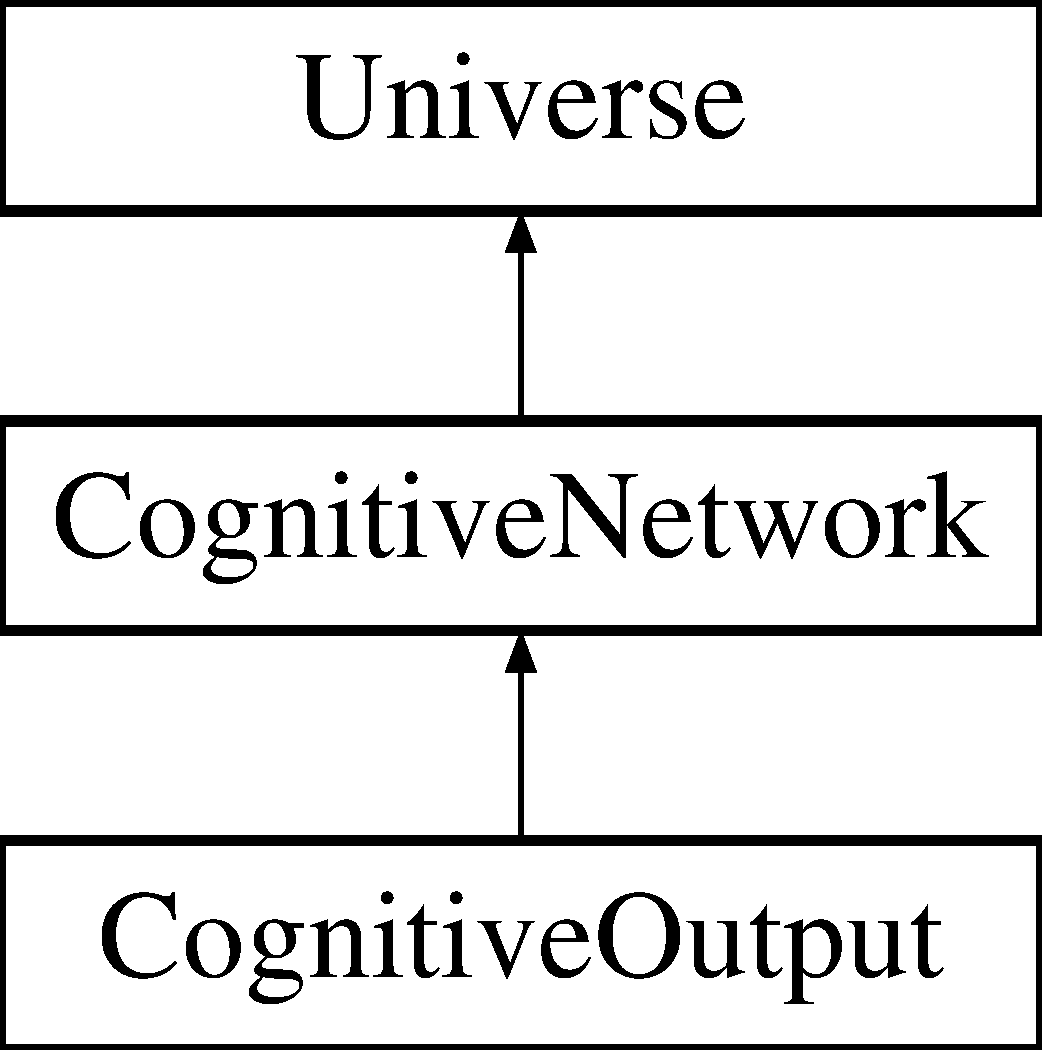
\includegraphics[height=3.000000cm]{classCognitiveOutput}
\end{center}
\end{figure}
\subsection*{Public Member Functions}
\begin{DoxyCompactItemize}
\item 
\mbox{\hyperlink{classCognitiveOutput_a743042cff5c36a76cd975767358e1bbf}{Cognitive\+Output}} ()
\item 
\mbox{\hyperlink{classCognitiveOutput_af1fca516a8a90913760e8ac5431f6f70}{Cognitive\+Output}} (unsigned int object\+\_\+type)
\item 
\mbox{\hyperlink{classCognitiveOutput_a4751f511d329c66ed80a3c127e5e9e6d}{Cognitive\+Output}} (unsigned int object\+\_\+type, std\+::chrono\+::time\+\_\+point$<$ \mbox{\hyperlink{universe_8h_a0ef8d951d1ca5ab3cfaf7ab4c7a6fd80}{Clock}} $>$ event\+\_\+time)
\item 
\mbox{\hyperlink{classCognitiveOutput_a9874901c7b49a6bb495d34c84fdbf651}{Cognitive\+Output}} (unsigned int object\+\_\+type, std\+::chrono\+::time\+\_\+point$<$ \mbox{\hyperlink{universe_8h_a0ef8d951d1ca5ab3cfaf7ab4c7a6fd80}{Clock}} $>$ event\+\_\+time, \mbox{\hyperlink{classCognitiveNetwork}{Cognitive\+Network}} \&cognitivenetwork\+\_\+connector)
\item 
virtual \mbox{\hyperlink{classCognitiveOutput_aefe310a8577684210d82236033791036}{$\sim$\+Cognitive\+Output}} ()
\item 
unsigned int \mbox{\hyperlink{classCognitiveOutput_a73efe6441491eb54df2f4dbd78b3903e}{Get\+Counter}} (std\+::chrono\+::time\+\_\+point$<$ \mbox{\hyperlink{universe_8h_a0ef8d951d1ca5ab3cfaf7ab4c7a6fd80}{Clock}} $>$ event\+\_\+time)
\item 
double \mbox{\hyperlink{classCognitiveOutput_abb923045db565ecdbac431469217cebf}{Get\+Energy}} (std\+::chrono\+::time\+\_\+point$<$ \mbox{\hyperlink{universe_8h_a0ef8d951d1ca5ab3cfaf7ab4c7a6fd80}{Clock}} $>$ event\+\_\+time)
\item 
int \mbox{\hyperlink{classCognitiveOutput_ac5ead5e6a98556d6779eda5679b69594}{Get\+Type}} ()
\item 
void \mbox{\hyperlink{classCognitiveOutput_ac76f41ab3b65ea466e9e2999270f2e5a}{Set\+Type}} (int val)
\item 
void \mbox{\hyperlink{classCognitiveOutput_a087e8bdab9eb6020dbbe6d47f524c8b6}{Set\+Counter}} (std\+::chrono\+::time\+\_\+point$<$ \mbox{\hyperlink{universe_8h_a0ef8d951d1ca5ab3cfaf7ab4c7a6fd80}{Clock}} $>$ event\+\_\+time, unsigned int val)
\item 
void \mbox{\hyperlink{classCognitiveOutput_acc16ca3521689776ecd68255ece1e671}{Set\+Energy}} (std\+::chrono\+::time\+\_\+point$<$ \mbox{\hyperlink{universe_8h_a0ef8d951d1ca5ab3cfaf7ab4c7a6fd80}{Clock}} $>$ event\+\_\+time, double val)
\item 
double \mbox{\hyperlink{classCognitiveOutput_aae27d114676c68e02ae6e7ae36326ba8}{Take\+Energy}} (std\+::chrono\+::time\+\_\+point$<$ \mbox{\hyperlink{universe_8h_a0ef8d951d1ca5ab3cfaf7ab4c7a6fd80}{Clock}} $>$ event\+\_\+time)
\item 
bool \mbox{\hyperlink{classCognitiveOutput_ab43b79aaadf75d18512c4379a77542cd}{Reset\+Parameters}} (std\+::chrono\+::time\+\_\+point$<$ \mbox{\hyperlink{universe_8h_a0ef8d951d1ca5ab3cfaf7ab4c7a6fd80}{Clock}} $>$ event\+\_\+time)
\item 
int \mbox{\hyperlink{classCognitiveOutput_a2b4d33c7a529402c684d828efd25095a}{Update}} (std\+::chrono\+::time\+\_\+point$<$ \mbox{\hyperlink{universe_8h_a0ef8d951d1ca5ab3cfaf7ab4c7a6fd80}{Clock}} $>$ event\+\_\+time)
\end{DoxyCompactItemize}
\subsection*{Private Attributes}
\begin{DoxyCompactItemize}
\item 
int \mbox{\hyperlink{classCognitiveOutput_a6b32711e6c93d36549d74e4b6d62661a}{m\+\_\+\+Cognitive\+Output\+Type}}
\item 
int \mbox{\hyperlink{classCognitiveOutput_aa34f8a3f6ab3e87ed1f5f3d749b259ac}{cognitiveoutput\+\_\+type}} = 0
\item 
int \mbox{\hyperlink{classCognitiveOutput_a3c40436281f3f5b737c23eaf27992b7e}{m\+\_\+add\+Status}}
\item 
std\+::chrono\+::time\+\_\+point$<$ \mbox{\hyperlink{universe_8h_a0ef8d951d1ca5ab3cfaf7ab4c7a6fd80}{Clock}} $>$ \mbox{\hyperlink{classCognitiveOutput_abc217a60acde159374e7a963d41e7958}{time\+\_\+object\+\_\+created}} = std\+::chrono\+::time\+\_\+point$<$\mbox{\hyperlink{universe_8h_a0ef8d951d1ca5ab3cfaf7ab4c7a6fd80}{Clock}}$>$(std\+::chrono\+::nanoseconds\+::zero())
\item 
std\+::chrono\+::time\+\_\+point$<$ \mbox{\hyperlink{universe_8h_a0ef8d951d1ca5ab3cfaf7ab4c7a6fd80}{Clock}} $>$ \mbox{\hyperlink{classCognitiveOutput_a68908403a0b612166f4a792b9203bf5e}{previous\+\_\+event\+\_\+time}}
\item 
bool \mbox{\hyperlink{classCognitiveOutput_a98ea154677177728cee120f3df672b35}{object\+\_\+disabled}} = true
\item 
bool \mbox{\hyperlink{classCognitiveOutput_aa473757ad75f1323f88730dc8a4aecc2}{object\+\_\+initialised}} = false
\item 
int \mbox{\hyperlink{classCognitiveOutput_acb201c341494433a1d33046f416cb5e9}{duration\+\_\+since\+\_\+last\+\_\+event}}
\item 
double \mbox{\hyperlink{classCognitiveOutput_a1e922926257d3711b41a2678ffe688a9}{m\+\_\+\+Volume}}
\item 
double \mbox{\hyperlink{classCognitiveOutput_a2e5b68f69ee1e76d825cd3e94443cb67}{m\+\_\+\+Surface\+Area}}
\item 
double \mbox{\hyperlink{classCognitiveOutput_ac1bfcefdc6ddd280d3728dd7804dbf1f}{object\+\_\+size}}
\item 
unsigned int \mbox{\hyperlink{classCognitiveOutput_aa13ff7dd07fd25127447cbc5699e41a3}{m\+\_\+\+Counter}}
\begin{DoxyCompactList}\small\item\em Member variable \char`\"{}m\+\_\+\+Counter\char`\"{}. \end{DoxyCompactList}\item 
double \mbox{\hyperlink{classCognitiveOutput_a2076a7d78fa8b640a2eca9dad691b239}{object\+\_\+energy}}
\begin{DoxyCompactList}\small\item\em Member variable \char`\"{}object\+\_\+energy\char`\"{}. \end{DoxyCompactList}\item 
double \mbox{\hyperlink{classCognitiveOutput_a67a1ee243a825884fc65ee70674d5b15}{object\+\_\+energy\+\_\+threshold}}
\item 
double \mbox{\hyperlink{classCognitiveOutput_a3aa3affaa91c42efda6b8a227c798070}{m\+\_\+\+Time\+Dilation}}
\item 
double \mbox{\hyperlink{classCognitiveOutput_a03ad45b97e6390b030966a50b114c5bf}{m\+\_\+\+Time\+Threshold}}
\end{DoxyCompactItemize}
\subsection*{Additional Inherited Members}


\subsection{Constructor \& Destructor Documentation}
\mbox{\Hypertarget{classCognitiveOutput_a743042cff5c36a76cd975767358e1bbf}\label{classCognitiveOutput_a743042cff5c36a76cd975767358e1bbf}} 
\index{Cognitive\+Output@{Cognitive\+Output}!Cognitive\+Output@{Cognitive\+Output}}
\index{Cognitive\+Output@{Cognitive\+Output}!Cognitive\+Output@{Cognitive\+Output}}
\subsubsection{\texorpdfstring{Cognitive\+Output()}{CognitiveOutput()}\hspace{0.1cm}{\footnotesize\ttfamily [1/4]}}
{\footnotesize\ttfamily Cognitive\+Output\+::\+Cognitive\+Output (\begin{DoxyParamCaption}{ }\end{DoxyParamCaption})\hspace{0.3cm}{\ttfamily [inline]}}

\mbox{\Hypertarget{classCognitiveOutput_af1fca516a8a90913760e8ac5431f6f70}\label{classCognitiveOutput_af1fca516a8a90913760e8ac5431f6f70}} 
\index{Cognitive\+Output@{Cognitive\+Output}!Cognitive\+Output@{Cognitive\+Output}}
\index{Cognitive\+Output@{Cognitive\+Output}!Cognitive\+Output@{Cognitive\+Output}}
\subsubsection{\texorpdfstring{Cognitive\+Output()}{CognitiveOutput()}\hspace{0.1cm}{\footnotesize\ttfamily [2/4]}}
{\footnotesize\ttfamily Cognitive\+Output\+::\+Cognitive\+Output (\begin{DoxyParamCaption}\item[{unsigned int}]{object\+\_\+type }\end{DoxyParamCaption})\hspace{0.3cm}{\ttfamily [inline]}}

\mbox{\Hypertarget{classCognitiveOutput_a4751f511d329c66ed80a3c127e5e9e6d}\label{classCognitiveOutput_a4751f511d329c66ed80a3c127e5e9e6d}} 
\index{Cognitive\+Output@{Cognitive\+Output}!Cognitive\+Output@{Cognitive\+Output}}
\index{Cognitive\+Output@{Cognitive\+Output}!Cognitive\+Output@{Cognitive\+Output}}
\subsubsection{\texorpdfstring{Cognitive\+Output()}{CognitiveOutput()}\hspace{0.1cm}{\footnotesize\ttfamily [3/4]}}
{\footnotesize\ttfamily Cognitive\+Output\+::\+Cognitive\+Output (\begin{DoxyParamCaption}\item[{unsigned int}]{object\+\_\+type,  }\item[{std\+::chrono\+::time\+\_\+point$<$ \mbox{\hyperlink{universe_8h_a0ef8d951d1ca5ab3cfaf7ab4c7a6fd80}{Clock}} $>$}]{event\+\_\+time }\end{DoxyParamCaption})\hspace{0.3cm}{\ttfamily [inline]}}

\mbox{\Hypertarget{classCognitiveOutput_a9874901c7b49a6bb495d34c84fdbf651}\label{classCognitiveOutput_a9874901c7b49a6bb495d34c84fdbf651}} 
\index{Cognitive\+Output@{Cognitive\+Output}!Cognitive\+Output@{Cognitive\+Output}}
\index{Cognitive\+Output@{Cognitive\+Output}!Cognitive\+Output@{Cognitive\+Output}}
\subsubsection{\texorpdfstring{Cognitive\+Output()}{CognitiveOutput()}\hspace{0.1cm}{\footnotesize\ttfamily [4/4]}}
{\footnotesize\ttfamily Cognitive\+Output\+::\+Cognitive\+Output (\begin{DoxyParamCaption}\item[{unsigned int}]{object\+\_\+type,  }\item[{std\+::chrono\+::time\+\_\+point$<$ \mbox{\hyperlink{universe_8h_a0ef8d951d1ca5ab3cfaf7ab4c7a6fd80}{Clock}} $>$}]{event\+\_\+time,  }\item[{\mbox{\hyperlink{classCognitiveNetwork}{Cognitive\+Network}} \&}]{cognitivenetwork\+\_\+connector }\end{DoxyParamCaption})\hspace{0.3cm}{\ttfamily [inline]}}

\mbox{\Hypertarget{classCognitiveOutput_aefe310a8577684210d82236033791036}\label{classCognitiveOutput_aefe310a8577684210d82236033791036}} 
\index{Cognitive\+Output@{Cognitive\+Output}!````~Cognitive\+Output@{$\sim$\+Cognitive\+Output}}
\index{````~Cognitive\+Output@{$\sim$\+Cognitive\+Output}!Cognitive\+Output@{Cognitive\+Output}}
\subsubsection{\texorpdfstring{$\sim$\+Cognitive\+Output()}{~CognitiveOutput()}}
{\footnotesize\ttfamily virtual Cognitive\+Output\+::$\sim$\+Cognitive\+Output (\begin{DoxyParamCaption}{ }\end{DoxyParamCaption})\hspace{0.3cm}{\ttfamily [inline]}, {\ttfamily [virtual]}}

Default destructor 

\subsection{Member Function Documentation}
\mbox{\Hypertarget{classCognitiveOutput_a73efe6441491eb54df2f4dbd78b3903e}\label{classCognitiveOutput_a73efe6441491eb54df2f4dbd78b3903e}} 
\index{Cognitive\+Output@{Cognitive\+Output}!Get\+Counter@{Get\+Counter}}
\index{Get\+Counter@{Get\+Counter}!Cognitive\+Output@{Cognitive\+Output}}
\subsubsection{\texorpdfstring{Get\+Counter()}{GetCounter()}}
{\footnotesize\ttfamily unsigned int Cognitive\+Output\+::\+Get\+Counter (\begin{DoxyParamCaption}\item[{std\+::chrono\+::time\+\_\+point$<$ \mbox{\hyperlink{universe_8h_a0ef8d951d1ca5ab3cfaf7ab4c7a6fd80}{Clock}} $>$}]{event\+\_\+time }\end{DoxyParamCaption})\hspace{0.3cm}{\ttfamily [inline]}}

\mbox{\Hypertarget{classCognitiveOutput_abb923045db565ecdbac431469217cebf}\label{classCognitiveOutput_abb923045db565ecdbac431469217cebf}} 
\index{Cognitive\+Output@{Cognitive\+Output}!Get\+Energy@{Get\+Energy}}
\index{Get\+Energy@{Get\+Energy}!Cognitive\+Output@{Cognitive\+Output}}
\subsubsection{\texorpdfstring{Get\+Energy()}{GetEnergy()}}
{\footnotesize\ttfamily double Cognitive\+Output\+::\+Get\+Energy (\begin{DoxyParamCaption}\item[{std\+::chrono\+::time\+\_\+point$<$ \mbox{\hyperlink{universe_8h_a0ef8d951d1ca5ab3cfaf7ab4c7a6fd80}{Clock}} $>$}]{event\+\_\+time }\end{DoxyParamCaption})\hspace{0.3cm}{\ttfamily [inline]}}

\mbox{\Hypertarget{classCognitiveOutput_ac5ead5e6a98556d6779eda5679b69594}\label{classCognitiveOutput_ac5ead5e6a98556d6779eda5679b69594}} 
\index{Cognitive\+Output@{Cognitive\+Output}!Get\+Type@{Get\+Type}}
\index{Get\+Type@{Get\+Type}!Cognitive\+Output@{Cognitive\+Output}}
\subsubsection{\texorpdfstring{Get\+Type()}{GetType()}}
{\footnotesize\ttfamily int Cognitive\+Output\+::\+Get\+Type (\begin{DoxyParamCaption}{ }\end{DoxyParamCaption})\hspace{0.3cm}{\ttfamily [inline]}}

\mbox{\Hypertarget{classCognitiveOutput_ab43b79aaadf75d18512c4379a77542cd}\label{classCognitiveOutput_ab43b79aaadf75d18512c4379a77542cd}} 
\index{Cognitive\+Output@{Cognitive\+Output}!Reset\+Parameters@{Reset\+Parameters}}
\index{Reset\+Parameters@{Reset\+Parameters}!Cognitive\+Output@{Cognitive\+Output}}
\subsubsection{\texorpdfstring{Reset\+Parameters()}{ResetParameters()}}
{\footnotesize\ttfamily bool Cognitive\+Output\+::\+Reset\+Parameters (\begin{DoxyParamCaption}\item[{std\+::chrono\+::time\+\_\+point$<$ \mbox{\hyperlink{universe_8h_a0ef8d951d1ca5ab3cfaf7ab4c7a6fd80}{Clock}} $>$}]{event\+\_\+time }\end{DoxyParamCaption})}

\mbox{\Hypertarget{classCognitiveOutput_a087e8bdab9eb6020dbbe6d47f524c8b6}\label{classCognitiveOutput_a087e8bdab9eb6020dbbe6d47f524c8b6}} 
\index{Cognitive\+Output@{Cognitive\+Output}!Set\+Counter@{Set\+Counter}}
\index{Set\+Counter@{Set\+Counter}!Cognitive\+Output@{Cognitive\+Output}}
\subsubsection{\texorpdfstring{Set\+Counter()}{SetCounter()}}
{\footnotesize\ttfamily void Cognitive\+Output\+::\+Set\+Counter (\begin{DoxyParamCaption}\item[{std\+::chrono\+::time\+\_\+point$<$ \mbox{\hyperlink{universe_8h_a0ef8d951d1ca5ab3cfaf7ab4c7a6fd80}{Clock}} $>$}]{event\+\_\+time,  }\item[{unsigned int}]{val }\end{DoxyParamCaption})\hspace{0.3cm}{\ttfamily [inline]}, {\ttfamily [virtual]}}



Reimplemented from \mbox{\hyperlink{classUniverse_aa22202ae740eb1355529afcb13285e91}{Universe}}.

\mbox{\Hypertarget{classCognitiveOutput_acc16ca3521689776ecd68255ece1e671}\label{classCognitiveOutput_acc16ca3521689776ecd68255ece1e671}} 
\index{Cognitive\+Output@{Cognitive\+Output}!Set\+Energy@{Set\+Energy}}
\index{Set\+Energy@{Set\+Energy}!Cognitive\+Output@{Cognitive\+Output}}
\subsubsection{\texorpdfstring{Set\+Energy()}{SetEnergy()}}
{\footnotesize\ttfamily void Cognitive\+Output\+::\+Set\+Energy (\begin{DoxyParamCaption}\item[{std\+::chrono\+::time\+\_\+point$<$ \mbox{\hyperlink{universe_8h_a0ef8d951d1ca5ab3cfaf7ab4c7a6fd80}{Clock}} $>$}]{event\+\_\+time,  }\item[{double}]{val }\end{DoxyParamCaption})\hspace{0.3cm}{\ttfamily [inline]}}

\mbox{\Hypertarget{classCognitiveOutput_ac76f41ab3b65ea466e9e2999270f2e5a}\label{classCognitiveOutput_ac76f41ab3b65ea466e9e2999270f2e5a}} 
\index{Cognitive\+Output@{Cognitive\+Output}!Set\+Type@{Set\+Type}}
\index{Set\+Type@{Set\+Type}!Cognitive\+Output@{Cognitive\+Output}}
\subsubsection{\texorpdfstring{Set\+Type()}{SetType()}}
{\footnotesize\ttfamily void Cognitive\+Output\+::\+Set\+Type (\begin{DoxyParamCaption}\item[{int}]{val }\end{DoxyParamCaption})\hspace{0.3cm}{\ttfamily [inline]}}

\mbox{\Hypertarget{classCognitiveOutput_aae27d114676c68e02ae6e7ae36326ba8}\label{classCognitiveOutput_aae27d114676c68e02ae6e7ae36326ba8}} 
\index{Cognitive\+Output@{Cognitive\+Output}!Take\+Energy@{Take\+Energy}}
\index{Take\+Energy@{Take\+Energy}!Cognitive\+Output@{Cognitive\+Output}}
\subsubsection{\texorpdfstring{Take\+Energy()}{TakeEnergy()}}
{\footnotesize\ttfamily double Cognitive\+Output\+::\+Take\+Energy (\begin{DoxyParamCaption}\item[{std\+::chrono\+::time\+\_\+point$<$ \mbox{\hyperlink{universe_8h_a0ef8d951d1ca5ab3cfaf7ab4c7a6fd80}{Clock}} $>$}]{event\+\_\+time }\end{DoxyParamCaption})\hspace{0.3cm}{\ttfamily [inline]}}

\mbox{\Hypertarget{classCognitiveOutput_a2b4d33c7a529402c684d828efd25095a}\label{classCognitiveOutput_a2b4d33c7a529402c684d828efd25095a}} 
\index{Cognitive\+Output@{Cognitive\+Output}!Update@{Update}}
\index{Update@{Update}!Cognitive\+Output@{Cognitive\+Output}}
\subsubsection{\texorpdfstring{Update()}{Update()}}
{\footnotesize\ttfamily int Cognitive\+Output\+::\+Update (\begin{DoxyParamCaption}\item[{std\+::chrono\+::time\+\_\+point$<$ \mbox{\hyperlink{universe_8h_a0ef8d951d1ca5ab3cfaf7ab4c7a6fd80}{Clock}} $>$}]{event\+\_\+time }\end{DoxyParamCaption})}



\subsection{Member Data Documentation}
\mbox{\Hypertarget{classCognitiveOutput_aa34f8a3f6ab3e87ed1f5f3d749b259ac}\label{classCognitiveOutput_aa34f8a3f6ab3e87ed1f5f3d749b259ac}} 
\index{Cognitive\+Output@{Cognitive\+Output}!cognitiveoutput\+\_\+type@{cognitiveoutput\+\_\+type}}
\index{cognitiveoutput\+\_\+type@{cognitiveoutput\+\_\+type}!Cognitive\+Output@{Cognitive\+Output}}
\subsubsection{\texorpdfstring{cognitiveoutput\+\_\+type}{cognitiveoutput\_type}}
{\footnotesize\ttfamily int Cognitive\+Output\+::cognitiveoutput\+\_\+type = 0\hspace{0.3cm}{\ttfamily [private]}}

\mbox{\Hypertarget{classCognitiveOutput_acb201c341494433a1d33046f416cb5e9}\label{classCognitiveOutput_acb201c341494433a1d33046f416cb5e9}} 
\index{Cognitive\+Output@{Cognitive\+Output}!duration\+\_\+since\+\_\+last\+\_\+event@{duration\+\_\+since\+\_\+last\+\_\+event}}
\index{duration\+\_\+since\+\_\+last\+\_\+event@{duration\+\_\+since\+\_\+last\+\_\+event}!Cognitive\+Output@{Cognitive\+Output}}
\subsubsection{\texorpdfstring{duration\+\_\+since\+\_\+last\+\_\+event}{duration\_since\_last\_event}}
{\footnotesize\ttfamily int Cognitive\+Output\+::duration\+\_\+since\+\_\+last\+\_\+event\hspace{0.3cm}{\ttfamily [private]}}

\mbox{\Hypertarget{classCognitiveOutput_a3c40436281f3f5b737c23eaf27992b7e}\label{classCognitiveOutput_a3c40436281f3f5b737c23eaf27992b7e}} 
\index{Cognitive\+Output@{Cognitive\+Output}!m\+\_\+add\+Status@{m\+\_\+add\+Status}}
\index{m\+\_\+add\+Status@{m\+\_\+add\+Status}!Cognitive\+Output@{Cognitive\+Output}}
\subsubsection{\texorpdfstring{m\+\_\+add\+Status}{m\_addStatus}}
{\footnotesize\ttfamily int Cognitive\+Output\+::m\+\_\+add\+Status\hspace{0.3cm}{\ttfamily [private]}}

\mbox{\Hypertarget{classCognitiveOutput_a6b32711e6c93d36549d74e4b6d62661a}\label{classCognitiveOutput_a6b32711e6c93d36549d74e4b6d62661a}} 
\index{Cognitive\+Output@{Cognitive\+Output}!m\+\_\+\+Cognitive\+Output\+Type@{m\+\_\+\+Cognitive\+Output\+Type}}
\index{m\+\_\+\+Cognitive\+Output\+Type@{m\+\_\+\+Cognitive\+Output\+Type}!Cognitive\+Output@{Cognitive\+Output}}
\subsubsection{\texorpdfstring{m\+\_\+\+Cognitive\+Output\+Type}{m\_CognitiveOutputType}}
{\footnotesize\ttfamily int Cognitive\+Output\+::m\+\_\+\+Cognitive\+Output\+Type\hspace{0.3cm}{\ttfamily [private]}}

\mbox{\Hypertarget{classCognitiveOutput_aa13ff7dd07fd25127447cbc5699e41a3}\label{classCognitiveOutput_aa13ff7dd07fd25127447cbc5699e41a3}} 
\index{Cognitive\+Output@{Cognitive\+Output}!m\+\_\+\+Counter@{m\+\_\+\+Counter}}
\index{m\+\_\+\+Counter@{m\+\_\+\+Counter}!Cognitive\+Output@{Cognitive\+Output}}
\subsubsection{\texorpdfstring{m\+\_\+\+Counter}{m\_Counter}}
{\footnotesize\ttfamily unsigned int Cognitive\+Output\+::m\+\_\+\+Counter\hspace{0.3cm}{\ttfamily [private]}}



Member variable \char`\"{}m\+\_\+\+Counter\char`\"{}. 

\mbox{\Hypertarget{classCognitiveOutput_a2e5b68f69ee1e76d825cd3e94443cb67}\label{classCognitiveOutput_a2e5b68f69ee1e76d825cd3e94443cb67}} 
\index{Cognitive\+Output@{Cognitive\+Output}!m\+\_\+\+Surface\+Area@{m\+\_\+\+Surface\+Area}}
\index{m\+\_\+\+Surface\+Area@{m\+\_\+\+Surface\+Area}!Cognitive\+Output@{Cognitive\+Output}}
\subsubsection{\texorpdfstring{m\+\_\+\+Surface\+Area}{m\_SurfaceArea}}
{\footnotesize\ttfamily double Cognitive\+Output\+::m\+\_\+\+Surface\+Area\hspace{0.3cm}{\ttfamily [private]}}

\mbox{\Hypertarget{classCognitiveOutput_a3aa3affaa91c42efda6b8a227c798070}\label{classCognitiveOutput_a3aa3affaa91c42efda6b8a227c798070}} 
\index{Cognitive\+Output@{Cognitive\+Output}!m\+\_\+\+Time\+Dilation@{m\+\_\+\+Time\+Dilation}}
\index{m\+\_\+\+Time\+Dilation@{m\+\_\+\+Time\+Dilation}!Cognitive\+Output@{Cognitive\+Output}}
\subsubsection{\texorpdfstring{m\+\_\+\+Time\+Dilation}{m\_TimeDilation}}
{\footnotesize\ttfamily double Cognitive\+Output\+::m\+\_\+\+Time\+Dilation\hspace{0.3cm}{\ttfamily [private]}}

\mbox{\Hypertarget{classCognitiveOutput_a03ad45b97e6390b030966a50b114c5bf}\label{classCognitiveOutput_a03ad45b97e6390b030966a50b114c5bf}} 
\index{Cognitive\+Output@{Cognitive\+Output}!m\+\_\+\+Time\+Threshold@{m\+\_\+\+Time\+Threshold}}
\index{m\+\_\+\+Time\+Threshold@{m\+\_\+\+Time\+Threshold}!Cognitive\+Output@{Cognitive\+Output}}
\subsubsection{\texorpdfstring{m\+\_\+\+Time\+Threshold}{m\_TimeThreshold}}
{\footnotesize\ttfamily double Cognitive\+Output\+::m\+\_\+\+Time\+Threshold\hspace{0.3cm}{\ttfamily [private]}}

\mbox{\Hypertarget{classCognitiveOutput_a1e922926257d3711b41a2678ffe688a9}\label{classCognitiveOutput_a1e922926257d3711b41a2678ffe688a9}} 
\index{Cognitive\+Output@{Cognitive\+Output}!m\+\_\+\+Volume@{m\+\_\+\+Volume}}
\index{m\+\_\+\+Volume@{m\+\_\+\+Volume}!Cognitive\+Output@{Cognitive\+Output}}
\subsubsection{\texorpdfstring{m\+\_\+\+Volume}{m\_Volume}}
{\footnotesize\ttfamily double Cognitive\+Output\+::m\+\_\+\+Volume\hspace{0.3cm}{\ttfamily [private]}}

\mbox{\Hypertarget{classCognitiveOutput_a98ea154677177728cee120f3df672b35}\label{classCognitiveOutput_a98ea154677177728cee120f3df672b35}} 
\index{Cognitive\+Output@{Cognitive\+Output}!object\+\_\+disabled@{object\+\_\+disabled}}
\index{object\+\_\+disabled@{object\+\_\+disabled}!Cognitive\+Output@{Cognitive\+Output}}
\subsubsection{\texorpdfstring{object\+\_\+disabled}{object\_disabled}}
{\footnotesize\ttfamily bool Cognitive\+Output\+::object\+\_\+disabled = true\hspace{0.3cm}{\ttfamily [private]}}

\mbox{\Hypertarget{classCognitiveOutput_a2076a7d78fa8b640a2eca9dad691b239}\label{classCognitiveOutput_a2076a7d78fa8b640a2eca9dad691b239}} 
\index{Cognitive\+Output@{Cognitive\+Output}!object\+\_\+energy@{object\+\_\+energy}}
\index{object\+\_\+energy@{object\+\_\+energy}!Cognitive\+Output@{Cognitive\+Output}}
\subsubsection{\texorpdfstring{object\+\_\+energy}{object\_energy}}
{\footnotesize\ttfamily double Cognitive\+Output\+::object\+\_\+energy\hspace{0.3cm}{\ttfamily [private]}}



Member variable \char`\"{}object\+\_\+energy\char`\"{}. 

\mbox{\Hypertarget{classCognitiveOutput_a67a1ee243a825884fc65ee70674d5b15}\label{classCognitiveOutput_a67a1ee243a825884fc65ee70674d5b15}} 
\index{Cognitive\+Output@{Cognitive\+Output}!object\+\_\+energy\+\_\+threshold@{object\+\_\+energy\+\_\+threshold}}
\index{object\+\_\+energy\+\_\+threshold@{object\+\_\+energy\+\_\+threshold}!Cognitive\+Output@{Cognitive\+Output}}
\subsubsection{\texorpdfstring{object\+\_\+energy\+\_\+threshold}{object\_energy\_threshold}}
{\footnotesize\ttfamily double Cognitive\+Output\+::object\+\_\+energy\+\_\+threshold\hspace{0.3cm}{\ttfamily [private]}}

\mbox{\Hypertarget{classCognitiveOutput_aa473757ad75f1323f88730dc8a4aecc2}\label{classCognitiveOutput_aa473757ad75f1323f88730dc8a4aecc2}} 
\index{Cognitive\+Output@{Cognitive\+Output}!object\+\_\+initialised@{object\+\_\+initialised}}
\index{object\+\_\+initialised@{object\+\_\+initialised}!Cognitive\+Output@{Cognitive\+Output}}
\subsubsection{\texorpdfstring{object\+\_\+initialised}{object\_initialised}}
{\footnotesize\ttfamily bool Cognitive\+Output\+::object\+\_\+initialised = false\hspace{0.3cm}{\ttfamily [private]}}

\mbox{\Hypertarget{classCognitiveOutput_ac1bfcefdc6ddd280d3728dd7804dbf1f}\label{classCognitiveOutput_ac1bfcefdc6ddd280d3728dd7804dbf1f}} 
\index{Cognitive\+Output@{Cognitive\+Output}!object\+\_\+size@{object\+\_\+size}}
\index{object\+\_\+size@{object\+\_\+size}!Cognitive\+Output@{Cognitive\+Output}}
\subsubsection{\texorpdfstring{object\+\_\+size}{object\_size}}
{\footnotesize\ttfamily double Cognitive\+Output\+::object\+\_\+size\hspace{0.3cm}{\ttfamily [private]}}

\mbox{\Hypertarget{classCognitiveOutput_a68908403a0b612166f4a792b9203bf5e}\label{classCognitiveOutput_a68908403a0b612166f4a792b9203bf5e}} 
\index{Cognitive\+Output@{Cognitive\+Output}!previous\+\_\+event\+\_\+time@{previous\+\_\+event\+\_\+time}}
\index{previous\+\_\+event\+\_\+time@{previous\+\_\+event\+\_\+time}!Cognitive\+Output@{Cognitive\+Output}}
\subsubsection{\texorpdfstring{previous\+\_\+event\+\_\+time}{previous\_event\_time}}
{\footnotesize\ttfamily std\+::chrono\+::time\+\_\+point$<$\mbox{\hyperlink{universe_8h_a0ef8d951d1ca5ab3cfaf7ab4c7a6fd80}{Clock}}$>$ Cognitive\+Output\+::previous\+\_\+event\+\_\+time\hspace{0.3cm}{\ttfamily [private]}}

\mbox{\Hypertarget{classCognitiveOutput_abc217a60acde159374e7a963d41e7958}\label{classCognitiveOutput_abc217a60acde159374e7a963d41e7958}} 
\index{Cognitive\+Output@{Cognitive\+Output}!time\+\_\+object\+\_\+created@{time\+\_\+object\+\_\+created}}
\index{time\+\_\+object\+\_\+created@{time\+\_\+object\+\_\+created}!Cognitive\+Output@{Cognitive\+Output}}
\subsubsection{\texorpdfstring{time\+\_\+object\+\_\+created}{time\_object\_created}}
{\footnotesize\ttfamily std\+::chrono\+::time\+\_\+point$<$\mbox{\hyperlink{universe_8h_a0ef8d951d1ca5ab3cfaf7ab4c7a6fd80}{Clock}}$>$ Cognitive\+Output\+::time\+\_\+object\+\_\+created = std\+::chrono\+::time\+\_\+point$<$\mbox{\hyperlink{universe_8h_a0ef8d951d1ca5ab3cfaf7ab4c7a6fd80}{Clock}}$>$(std\+::chrono\+::nanoseconds\+::zero())\hspace{0.3cm}{\ttfamily [private]}}



The documentation for this class was generated from the following files\+:\begin{DoxyCompactItemize}
\item 
/home/pbisaacs/\+Developer/\+Brain\+Harmonics/\mbox{\hyperlink{cognitiveoutput_8h}{cognitiveoutput.\+h}}\item 
/home/pbisaacs/\+Developer/\+Brain\+Harmonics/\mbox{\hyperlink{cognitiveoutput_8cc}{cognitiveoutput.\+cc}}\end{DoxyCompactItemize}

\hypertarget{classCompositeForceParticle}{}\section{Composite\+Force\+Particle Class Reference}
\label{classCompositeForceParticle}\index{Composite\+Force\+Particle@{Composite\+Force\+Particle}}


{\ttfamily \#include $<$compositeforceparticle.\+h$>$}

Inheritance diagram for Composite\+Force\+Particle\+:\begin{figure}[H]
\begin{center}
\leavevmode
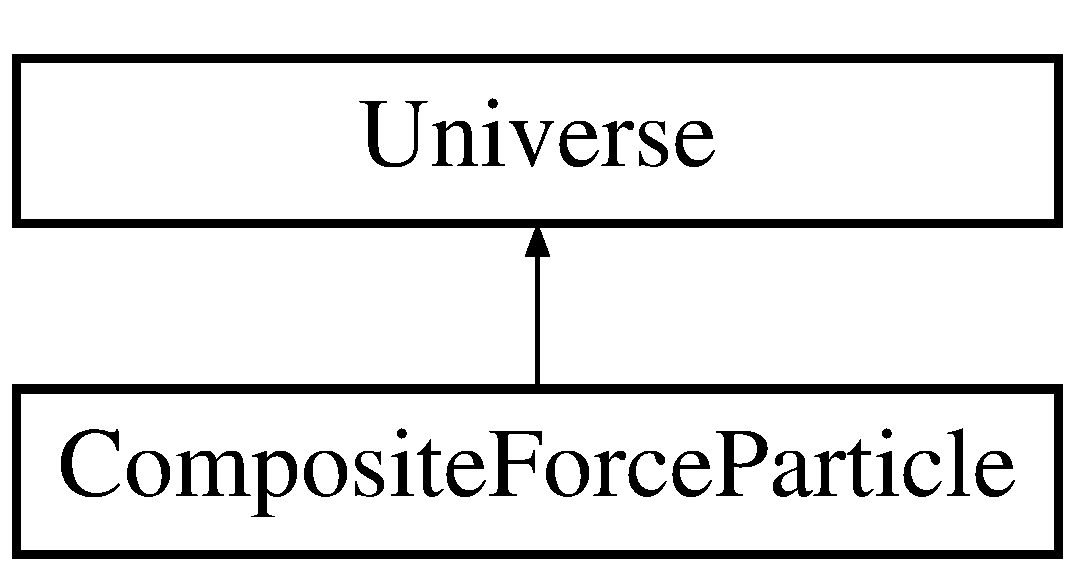
\includegraphics[height=2.000000cm]{classCompositeForceParticle}
\end{center}
\end{figure}
\subsection*{Public Member Functions}
\begin{DoxyCompactItemize}
\item 
\mbox{\hyperlink{classCompositeForceParticle_ae00ad8621af6155c86ee3205c1e2afdb}{Composite\+Force\+Particle}} ()
\item 
\mbox{\hyperlink{classCompositeForceParticle_a967036ded4212fcd6d4213275145dc50}{Composite\+Force\+Particle}} (unsigned int object\+\_\+type)
\item 
\mbox{\hyperlink{classCompositeForceParticle_a805886058bba3179de8142fd266883e4}{Composite\+Force\+Particle}} (unsigned int object\+\_\+type, std\+::chrono\+::time\+\_\+point$<$ \mbox{\hyperlink{universe_8h_a0ef8d951d1ca5ab3cfaf7ab4c7a6fd80}{Clock}} $>$ event\+\_\+time)
\item 
\mbox{\hyperlink{classCompositeForceParticle_a8c311b3e35f6def3a532346a50c15281}{Composite\+Force\+Particle}} (unsigned int object\+\_\+type, std\+::chrono\+::time\+\_\+point$<$ \mbox{\hyperlink{universe_8h_a0ef8d951d1ca5ab3cfaf7ab4c7a6fd80}{Clock}} $>$ event\+\_\+time, \mbox{\hyperlink{classUniverse}{Universe}} \&universe\+\_\+connector)
\item 
virtual \mbox{\hyperlink{classCompositeForceParticle_aa35ee4244375b2bcc5dd775de30aa39e}{$\sim$\+Composite\+Force\+Particle}} ()
\item 
unsigned int \mbox{\hyperlink{classCompositeForceParticle_ae0bc57309f04b784b2c23b82db869b25}{Get\+Counter}} (std\+::chrono\+::time\+\_\+point$<$ \mbox{\hyperlink{universe_8h_a0ef8d951d1ca5ab3cfaf7ab4c7a6fd80}{Clock}} $>$ event\+\_\+time)
\item 
double \mbox{\hyperlink{classCompositeForceParticle_a06483dc73c156679f34acf85aa5f924e}{Get\+Gravitation}} (std\+::chrono\+::time\+\_\+point$<$ \mbox{\hyperlink{universe_8h_a0ef8d951d1ca5ab3cfaf7ab4c7a6fd80}{Clock}} $>$ event\+\_\+time)
\item 
double \mbox{\hyperlink{classCompositeForceParticle_ab5cc0893a4063cc353ea5d2404f27b0b}{Get\+Weak}} (std\+::chrono\+::time\+\_\+point$<$ \mbox{\hyperlink{universe_8h_a0ef8d951d1ca5ab3cfaf7ab4c7a6fd80}{Clock}} $>$ event\+\_\+time)
\item 
double \mbox{\hyperlink{classCompositeForceParticle_a27762218af4e3c021c89ff4792d81b41}{Get\+Weak\+Electroweak}} (std\+::chrono\+::time\+\_\+point$<$ \mbox{\hyperlink{universe_8h_a0ef8d951d1ca5ab3cfaf7ab4c7a6fd80}{Clock}} $>$ event\+\_\+time)
\item 
double \mbox{\hyperlink{classCompositeForceParticle_a8ef336fed7e33d52a3baae4bd4dd32fd}{Get\+Electromagnetic}} (std\+::chrono\+::time\+\_\+point$<$ \mbox{\hyperlink{universe_8h_a0ef8d951d1ca5ab3cfaf7ab4c7a6fd80}{Clock}} $>$ event\+\_\+time)
\item 
double \mbox{\hyperlink{classCompositeForceParticle_ac26d7aab0daefcf13c68aba9e0f2ed53}{Get\+Electromagnetic\+Electroweak}} (std\+::chrono\+::time\+\_\+point$<$ \mbox{\hyperlink{universe_8h_a0ef8d951d1ca5ab3cfaf7ab4c7a6fd80}{Clock}} $>$ event\+\_\+time)
\item 
double \mbox{\hyperlink{classCompositeForceParticle_a9818d469c9841eaf77fbe329b0953354}{Get\+Strong}} (std\+::chrono\+::time\+\_\+point$<$ \mbox{\hyperlink{universe_8h_a0ef8d951d1ca5ab3cfaf7ab4c7a6fd80}{Clock}} $>$ event\+\_\+time)
\item 
double \mbox{\hyperlink{classCompositeForceParticle_abc8597f3b4f7cf755ab4618bd624b046}{Get\+Strong\+Fundamental}} (std\+::chrono\+::time\+\_\+point$<$ \mbox{\hyperlink{universe_8h_a0ef8d951d1ca5ab3cfaf7ab4c7a6fd80}{Clock}} $>$ event\+\_\+time)
\item 
double \mbox{\hyperlink{classCompositeForceParticle_a24214566eb5b44340d5563b6583052e8}{Get\+Strong\+Residual}} (std\+::chrono\+::time\+\_\+point$<$ \mbox{\hyperlink{universe_8h_a0ef8d951d1ca5ab3cfaf7ab4c7a6fd80}{Clock}} $>$ event\+\_\+time)
\item 
double \mbox{\hyperlink{classCompositeForceParticle_ae26a03c2970a3825e8583a811339b28d}{Apply\+Gravitation}} (std\+::chrono\+::time\+\_\+point$<$ \mbox{\hyperlink{universe_8h_a0ef8d951d1ca5ab3cfaf7ab4c7a6fd80}{Clock}} $>$ event\+\_\+time, double val)
\item 
double \mbox{\hyperlink{classCompositeForceParticle_a1fd171a0c6fab0cbf9a45a0d24607bde}{Apply\+Weak}} (std\+::chrono\+::time\+\_\+point$<$ \mbox{\hyperlink{universe_8h_a0ef8d951d1ca5ab3cfaf7ab4c7a6fd80}{Clock}} $>$ event\+\_\+time, double val)
\item 
double \mbox{\hyperlink{classCompositeForceParticle_a3c1c0b427c633f0685f1d812e02b92ff}{Apply\+Weak\+Electroweak}} (std\+::chrono\+::time\+\_\+point$<$ \mbox{\hyperlink{universe_8h_a0ef8d951d1ca5ab3cfaf7ab4c7a6fd80}{Clock}} $>$ event\+\_\+time, double val)
\item 
double \mbox{\hyperlink{classCompositeForceParticle_afa4dc18258722b3c85fbc9789a4297a5}{Apply\+Electromagnetic}} (std\+::chrono\+::time\+\_\+point$<$ \mbox{\hyperlink{universe_8h_a0ef8d951d1ca5ab3cfaf7ab4c7a6fd80}{Clock}} $>$ event\+\_\+time, double val)
\item 
double \mbox{\hyperlink{classCompositeForceParticle_a5f6aef9e15e2e5f346c7ede76ae6458b}{Apply\+Electromagnetic\+Electroweak}} (std\+::chrono\+::time\+\_\+point$<$ \mbox{\hyperlink{universe_8h_a0ef8d951d1ca5ab3cfaf7ab4c7a6fd80}{Clock}} $>$ event\+\_\+time, double val)
\item 
double \mbox{\hyperlink{classCompositeForceParticle_ac1464a04fbbca2d8927dfdbef0429878}{Apply\+Strong}} (std\+::chrono\+::time\+\_\+point$<$ \mbox{\hyperlink{universe_8h_a0ef8d951d1ca5ab3cfaf7ab4c7a6fd80}{Clock}} $>$ event\+\_\+time, double val)
\item 
double \mbox{\hyperlink{classCompositeForceParticle_a64fe19ee12d6ca0a69f650faa5bedb58}{Apply\+Strong\+Fundamental}} (std\+::chrono\+::time\+\_\+point$<$ \mbox{\hyperlink{universe_8h_a0ef8d951d1ca5ab3cfaf7ab4c7a6fd80}{Clock}} $>$ event\+\_\+time, double val)
\item 
double \mbox{\hyperlink{classCompositeForceParticle_ae0937405e68dd40b19036d5a359f7e07}{Apply\+Strong\+Residual}} (std\+::chrono\+::time\+\_\+point$<$ \mbox{\hyperlink{universe_8h_a0ef8d951d1ca5ab3cfaf7ab4c7a6fd80}{Clock}} $>$ event\+\_\+time, double val)
\item 
void \mbox{\hyperlink{classCompositeForceParticle_a41cee6bd5a75fbf67fa6e76a9e7d7605}{Set\+Counter}} (std\+::chrono\+::time\+\_\+point$<$ \mbox{\hyperlink{universe_8h_a0ef8d951d1ca5ab3cfaf7ab4c7a6fd80}{Clock}} $>$ event\+\_\+time, unsigned int val)
\item 
void \mbox{\hyperlink{classCompositeForceParticle_ad9e1553ab0096230edd591e3135b223d}{Set\+Gravitation}} (std\+::chrono\+::time\+\_\+point$<$ \mbox{\hyperlink{universe_8h_a0ef8d951d1ca5ab3cfaf7ab4c7a6fd80}{Clock}} $>$ event\+\_\+time, double val)
\item 
void \mbox{\hyperlink{classCompositeForceParticle_a7899a6efda98b062051e37c25c214e2a}{Set\+Weak}} (std\+::chrono\+::time\+\_\+point$<$ \mbox{\hyperlink{universe_8h_a0ef8d951d1ca5ab3cfaf7ab4c7a6fd80}{Clock}} $>$ event\+\_\+time, double val)
\item 
void \mbox{\hyperlink{classCompositeForceParticle_a73a3792ae1c334e74f945fea56083f0b}{Set\+Weak\+Electroweak}} (std\+::chrono\+::time\+\_\+point$<$ \mbox{\hyperlink{universe_8h_a0ef8d951d1ca5ab3cfaf7ab4c7a6fd80}{Clock}} $>$ event\+\_\+time, double val)
\item 
void \mbox{\hyperlink{classCompositeForceParticle_a476c0d570c3be75c9e186df1ec2a5cda}{Set\+Electromagnetic}} (std\+::chrono\+::time\+\_\+point$<$ \mbox{\hyperlink{universe_8h_a0ef8d951d1ca5ab3cfaf7ab4c7a6fd80}{Clock}} $>$ event\+\_\+time, double val)
\item 
void \mbox{\hyperlink{classCompositeForceParticle_ad53c5d396b3c56241174a9bd78f9e07a}{Set\+Electromagnetic\+Electroweak}} (std\+::chrono\+::time\+\_\+point$<$ \mbox{\hyperlink{universe_8h_a0ef8d951d1ca5ab3cfaf7ab4c7a6fd80}{Clock}} $>$ event\+\_\+time, double val)
\item 
void \mbox{\hyperlink{classCompositeForceParticle_a06488ef0457335648b161d3ed746b643}{Set\+Strong}} (std\+::chrono\+::time\+\_\+point$<$ \mbox{\hyperlink{universe_8h_a0ef8d951d1ca5ab3cfaf7ab4c7a6fd80}{Clock}} $>$ event\+\_\+time, double val)
\item 
void \mbox{\hyperlink{classCompositeForceParticle_a28d835658edcbecf60162475a8cb1ab6}{Set\+Strong\+Fundamental}} (std\+::chrono\+::time\+\_\+point$<$ \mbox{\hyperlink{universe_8h_a0ef8d951d1ca5ab3cfaf7ab4c7a6fd80}{Clock}} $>$ event\+\_\+time, double val)
\item 
void \mbox{\hyperlink{classCompositeForceParticle_aeba1070d4ec6e52fd8276e38c6a6c2e1}{Set\+Strong\+Residual}} (std\+::chrono\+::time\+\_\+point$<$ \mbox{\hyperlink{universe_8h_a0ef8d951d1ca5ab3cfaf7ab4c7a6fd80}{Clock}} $>$ event\+\_\+time, double val)
\item 
bool \mbox{\hyperlink{classCompositeForceParticle_ab4767179e32f6d2b4b31941dd3c48b10}{Reset\+Parameters}} (std\+::chrono\+::time\+\_\+point$<$ \mbox{\hyperlink{universe_8h_a0ef8d951d1ca5ab3cfaf7ab4c7a6fd80}{Clock}} $>$ event\+\_\+time)
\item 
\mbox{\hyperlink{classCompositeForceParticle}{Composite\+Force\+Particle}} $\ast$ \mbox{\hyperlink{classCompositeForceParticle_a0806069e389e30c63572c4cd6b9776d7}{Create\+Elementary\+Particle}} (std\+::chrono\+::time\+\_\+point$<$ \mbox{\hyperlink{universe_8h_a0ef8d951d1ca5ab3cfaf7ab4c7a6fd80}{Clock}} $>$ event\+\_\+time)
\item 
std\+::vector$<$ \mbox{\hyperlink{classCompositeForceParticle}{Composite\+Force\+Particle}} $\ast$ $>$ \mbox{\hyperlink{classCompositeForceParticle_afff866fe6f363c33c3b49fcca9005706}{Create\+Elementary\+Particles}} (std\+::chrono\+::time\+\_\+point$<$ \mbox{\hyperlink{universe_8h_a0ef8d951d1ca5ab3cfaf7ab4c7a6fd80}{Clock}} $>$ event\+\_\+time, int quantity)
\item 
\mbox{\hyperlink{classCompositeForceParticle}{Composite\+Force\+Particle}} $\ast$ \mbox{\hyperlink{classCompositeForceParticle_a559031016355b79ee795e621fdbbdb13}{Clone\+Elementary\+Particle}} (std\+::chrono\+::time\+\_\+point$<$ \mbox{\hyperlink{universe_8h_a0ef8d951d1ca5ab3cfaf7ab4c7a6fd80}{Clock}} $>$ event\+\_\+time, \mbox{\hyperlink{classCompositeForceParticle}{Composite\+Force\+Particle}} $\ast$clone\+\_\+object, double perfection\+\_\+membership)
\item 
std\+::vector$<$ \mbox{\hyperlink{classCompositeForceParticle}{Composite\+Force\+Particle}} $\ast$ $>$ \mbox{\hyperlink{classCompositeForceParticle_ac27e6d3bb56272728a8c197dbcd2db4e}{Clone\+Elementary\+Particles}} (std\+::chrono\+::time\+\_\+point$<$ \mbox{\hyperlink{universe_8h_a0ef8d951d1ca5ab3cfaf7ab4c7a6fd80}{Clock}} $>$ event\+\_\+time, std\+::vector$<$ \mbox{\hyperlink{classCompositeForceParticle}{Composite\+Force\+Particle}} $\ast$$>$ cloning\+\_\+list, double perfection\+\_\+membership)
\item 
\mbox{\hyperlink{classCompositeForceParticle}{Composite\+Force\+Particle}} $\ast$ \mbox{\hyperlink{classCompositeForceParticle_ac176d2e41d75e308d4b510f3338d8b9e}{Destroy\+Elementary\+Particle}} (std\+::chrono\+::time\+\_\+point$<$ \mbox{\hyperlink{universe_8h_a0ef8d951d1ca5ab3cfaf7ab4c7a6fd80}{Clock}} $>$ event\+\_\+time, \mbox{\hyperlink{classCompositeForceParticle}{Composite\+Force\+Particle}} $\ast$destroy\+\_\+object)
\item 
std\+::vector$<$ \mbox{\hyperlink{classCompositeForceParticle}{Composite\+Force\+Particle}} $\ast$ $>$ \mbox{\hyperlink{classCompositeForceParticle_a602ef5e477db576e47c36436b83f80f5}{Destroy\+Elementary\+Particles}} (std\+::chrono\+::time\+\_\+point$<$ \mbox{\hyperlink{universe_8h_a0ef8d951d1ca5ab3cfaf7ab4c7a6fd80}{Clock}} $>$ event\+\_\+time, std\+::vector$<$ \mbox{\hyperlink{classCompositeForceParticle}{Composite\+Force\+Particle}} $\ast$$>$ destruction\+\_\+list)
\item 
\mbox{\hyperlink{classCompositeForceParticle}{Composite\+Force\+Particle}} $\ast$ \mbox{\hyperlink{classCompositeForceParticle_a27924093abdaa2f19902a32a068fa324}{Add\+Elementary\+Particle}} (std\+::chrono\+::time\+\_\+point$<$ \mbox{\hyperlink{universe_8h_a0ef8d951d1ca5ab3cfaf7ab4c7a6fd80}{Clock}} $>$ event\+\_\+time, \mbox{\hyperlink{classCompositeForceParticle}{Composite\+Force\+Particle}} $\ast$add\+\_\+object)
\item 
std\+::vector$<$ \mbox{\hyperlink{classCompositeForceParticle}{Composite\+Force\+Particle}} $\ast$ $>$ \mbox{\hyperlink{classCompositeForceParticle_a2b88f000067b5d430d1850e75b733f56}{Add\+Elementary\+Particles}} (std\+::chrono\+::time\+\_\+point$<$ \mbox{\hyperlink{universe_8h_a0ef8d951d1ca5ab3cfaf7ab4c7a6fd80}{Clock}} $>$ event\+\_\+time, std\+::vector$<$ \mbox{\hyperlink{classCompositeForceParticle}{Composite\+Force\+Particle}} $\ast$$>$ add\+\_\+objects)
\item 
\mbox{\hyperlink{classCompositeForceParticle}{Composite\+Force\+Particle}} $\ast$ \mbox{\hyperlink{classCompositeForceParticle_ab63c4a1d5734f1d13806cb9463075a40}{Remove\+Elementary\+Particle}} (std\+::chrono\+::time\+\_\+point$<$ \mbox{\hyperlink{universe_8h_a0ef8d951d1ca5ab3cfaf7ab4c7a6fd80}{Clock}} $>$ event\+\_\+time)
\item 
std\+::vector$<$ \mbox{\hyperlink{classCompositeForceParticle}{Composite\+Force\+Particle}} $\ast$ $>$ \mbox{\hyperlink{classCompositeForceParticle_a032f7d935062f40c798841b2c2f81f98}{Remove\+Elementary\+Particles}} (std\+::chrono\+::time\+\_\+point$<$ \mbox{\hyperlink{universe_8h_a0ef8d951d1ca5ab3cfaf7ab4c7a6fd80}{Clock}} $>$ event\+\_\+time, int quantity)
\item 
\mbox{\hyperlink{classCompositeForceParticle}{Composite\+Force\+Particle}} $\ast$ \mbox{\hyperlink{classCompositeForceParticle_a750da9f3cd367287b051b820857c80d0}{Get\+Elementary\+Particle}} (std\+::chrono\+::time\+\_\+point$<$ \mbox{\hyperlink{universe_8h_a0ef8d951d1ca5ab3cfaf7ab4c7a6fd80}{Clock}} $>$ event\+\_\+time, int selector)
\item 
std\+::vector$<$ \mbox{\hyperlink{classCompositeForceParticle}{Composite\+Force\+Particle}} $\ast$ $>$ \mbox{\hyperlink{classCompositeForceParticle_ab953693d61515b96fe78b0cf1da058c6}{Get\+Elementary\+Particles}} (std\+::chrono\+::time\+\_\+point$<$ \mbox{\hyperlink{universe_8h_a0ef8d951d1ca5ab3cfaf7ab4c7a6fd80}{Clock}} $>$ event\+\_\+time)
\item 
\mbox{\hyperlink{classCompositeForceParticle}{Composite\+Force\+Particle}} $\ast$ \mbox{\hyperlink{classCompositeForceParticle_a490b3eed8b9dbcc3edf44a9747ef6dbb}{Create\+Elementary\+Force}} (std\+::chrono\+::time\+\_\+point$<$ \mbox{\hyperlink{universe_8h_a0ef8d951d1ca5ab3cfaf7ab4c7a6fd80}{Clock}} $>$ event\+\_\+time)
\item 
std\+::vector$<$ \mbox{\hyperlink{classCompositeForceParticle}{Composite\+Force\+Particle}} $\ast$ $>$ \mbox{\hyperlink{classCompositeForceParticle_a56e006b0aa4b54401db763782294de62}{Create\+Elementary\+Forces}} (std\+::chrono\+::time\+\_\+point$<$ \mbox{\hyperlink{universe_8h_a0ef8d951d1ca5ab3cfaf7ab4c7a6fd80}{Clock}} $>$ event\+\_\+time, int quantity)
\item 
\mbox{\hyperlink{classCompositeForceParticle}{Composite\+Force\+Particle}} $\ast$ \mbox{\hyperlink{classCompositeForceParticle_a8163b425c10bd9cb9097d99e5d53d0a1}{Clone\+Elementary\+Force}} (std\+::chrono\+::time\+\_\+point$<$ \mbox{\hyperlink{universe_8h_a0ef8d951d1ca5ab3cfaf7ab4c7a6fd80}{Clock}} $>$ event\+\_\+time, \mbox{\hyperlink{classCompositeForceParticle}{Composite\+Force\+Particle}} $\ast$clone\+\_\+object, double perfection\+\_\+membership)
\item 
std\+::vector$<$ \mbox{\hyperlink{classCompositeForceParticle}{Composite\+Force\+Particle}} $\ast$ $>$ \mbox{\hyperlink{classCompositeForceParticle_a2e620a92eaca67dbb482a7fd8e248f7b}{Clone\+Elementary\+Forces}} (std\+::chrono\+::time\+\_\+point$<$ \mbox{\hyperlink{universe_8h_a0ef8d951d1ca5ab3cfaf7ab4c7a6fd80}{Clock}} $>$ event\+\_\+time, std\+::vector$<$ \mbox{\hyperlink{classCompositeForceParticle}{Composite\+Force\+Particle}} $\ast$$>$ cloning\+\_\+list, double perfection\+\_\+membership)
\item 
\mbox{\hyperlink{classCompositeForceParticle}{Composite\+Force\+Particle}} $\ast$ \mbox{\hyperlink{classCompositeForceParticle_af12bbef12781e7b72a4569609f751af6}{Destroy\+Elementary\+Force}} (std\+::chrono\+::time\+\_\+point$<$ \mbox{\hyperlink{universe_8h_a0ef8d951d1ca5ab3cfaf7ab4c7a6fd80}{Clock}} $>$ event\+\_\+time, \mbox{\hyperlink{classCompositeForceParticle}{Composite\+Force\+Particle}} $\ast$destroy\+\_\+object)
\item 
std\+::vector$<$ \mbox{\hyperlink{classCompositeForceParticle}{Composite\+Force\+Particle}} $\ast$ $>$ \mbox{\hyperlink{classCompositeForceParticle_af07d8607737f7881aac6314313d800e3}{Destroy\+Elementary\+Forces}} (std\+::chrono\+::time\+\_\+point$<$ \mbox{\hyperlink{universe_8h_a0ef8d951d1ca5ab3cfaf7ab4c7a6fd80}{Clock}} $>$ event\+\_\+time, std\+::vector$<$ \mbox{\hyperlink{classCompositeForceParticle}{Composite\+Force\+Particle}} $\ast$$>$ destruction\+\_\+list)
\item 
\mbox{\hyperlink{classCompositeForceParticle}{Composite\+Force\+Particle}} $\ast$ \mbox{\hyperlink{classCompositeForceParticle_aed3a7ebcb98626c564dde2d54d45ff03}{Add\+Elementary\+Force}} (std\+::chrono\+::time\+\_\+point$<$ \mbox{\hyperlink{universe_8h_a0ef8d951d1ca5ab3cfaf7ab4c7a6fd80}{Clock}} $>$ event\+\_\+time, \mbox{\hyperlink{classCompositeForceParticle}{Composite\+Force\+Particle}} $\ast$add\+\_\+object)
\item 
std\+::vector$<$ \mbox{\hyperlink{classCompositeForceParticle}{Composite\+Force\+Particle}} $\ast$ $>$ \mbox{\hyperlink{classCompositeForceParticle_ad0e97ed38272c7861d162afdf0db33c7}{Add\+Elementary\+Forces}} (std\+::chrono\+::time\+\_\+point$<$ \mbox{\hyperlink{universe_8h_a0ef8d951d1ca5ab3cfaf7ab4c7a6fd80}{Clock}} $>$ event\+\_\+time, std\+::vector$<$ \mbox{\hyperlink{classCompositeForceParticle}{Composite\+Force\+Particle}} $\ast$$>$ add\+\_\+objects)
\item 
\mbox{\hyperlink{classCompositeForceParticle}{Composite\+Force\+Particle}} $\ast$ \mbox{\hyperlink{classCompositeForceParticle_afe5738b3ba1382dad085fa1ef39963b3}{Remove\+Elementary\+Force}} (std\+::chrono\+::time\+\_\+point$<$ \mbox{\hyperlink{universe_8h_a0ef8d951d1ca5ab3cfaf7ab4c7a6fd80}{Clock}} $>$ event\+\_\+time)
\item 
std\+::vector$<$ \mbox{\hyperlink{classCompositeForceParticle}{Composite\+Force\+Particle}} $\ast$ $>$ \mbox{\hyperlink{classCompositeForceParticle_a1bfa61cec4f5a8436c1a188312ba8f45}{Remove\+Elementary\+Forces}} (std\+::chrono\+::time\+\_\+point$<$ \mbox{\hyperlink{universe_8h_a0ef8d951d1ca5ab3cfaf7ab4c7a6fd80}{Clock}} $>$ event\+\_\+time, int quantity)
\item 
\mbox{\hyperlink{classCompositeForceParticle}{Composite\+Force\+Particle}} $\ast$ \mbox{\hyperlink{classCompositeForceParticle_a63b3daf44517c90bb805b6612dd26acc}{Get\+Elementary\+Force}} (std\+::chrono\+::time\+\_\+point$<$ \mbox{\hyperlink{universe_8h_a0ef8d951d1ca5ab3cfaf7ab4c7a6fd80}{Clock}} $>$ event\+\_\+time, int selector)
\item 
std\+::vector$<$ \mbox{\hyperlink{classCompositeForceParticle}{Composite\+Force\+Particle}} $\ast$ $>$ \mbox{\hyperlink{classCompositeForceParticle_a2e9da0590067cf243c0f2d239f712e7f}{Get\+Elementary\+Forces}} (std\+::chrono\+::time\+\_\+point$<$ \mbox{\hyperlink{universe_8h_a0ef8d951d1ca5ab3cfaf7ab4c7a6fd80}{Clock}} $>$ event\+\_\+time)
\item 
void \mbox{\hyperlink{classCompositeForceParticle_a578d87e48246ef83f39dce070dff541e}{Update\+Cycle}} (std\+::chrono\+::time\+\_\+point$<$ \mbox{\hyperlink{universe_8h_a0ef8d951d1ca5ab3cfaf7ab4c7a6fd80}{Clock}} $>$ event\+\_\+time, std\+::vector$<$ \mbox{\hyperlink{classCompositeForceParticle}{Composite\+Force\+Particle}} $\ast$$>$ set\+\_\+of\+\_\+update\+\_\+pointers, unsigned int pointer\+\_\+type)
\item 
int \mbox{\hyperlink{classCompositeForceParticle_a69b47aaf17ab6faa396c2f6e6c85b2e3}{Update}} (std\+::chrono\+::time\+\_\+point$<$ \mbox{\hyperlink{universe_8h_a0ef8d951d1ca5ab3cfaf7ab4c7a6fd80}{Clock}} $>$ event\+\_\+time)
\end{DoxyCompactItemize}
\subsection*{Protected Attributes}
\begin{DoxyCompactItemize}
\item 
std\+::vector$<$ \mbox{\hyperlink{classCompositeForceParticle}{Composite\+Force\+Particle}} $\ast$ $>$ \mbox{\hyperlink{classCompositeForceParticle_a1f5ab59857b8517af69205178f04abe9}{elementary\+\_\+particle\+\_\+list}}
\item 
std\+::vector$<$ \mbox{\hyperlink{classCompositeForceParticle}{Composite\+Force\+Particle}} $\ast$ $>$ \mbox{\hyperlink{classCompositeForceParticle_a00d5ce181c8d4b1df0d46ff23a8fb1b8}{elementary\+\_\+force\+\_\+list}}
\end{DoxyCompactItemize}
\subsection*{Private Attributes}
\begin{DoxyCompactItemize}
\item 
unsigned int \mbox{\hyperlink{classCompositeForceParticle_a1b502a62a416dc3a971cc6baed3e7e58}{composite\+\_\+forceparticle\+\_\+counter}}
\begin{DoxyCompactList}\small\item\em Member variable \char`\"{}composite\+\_\+force\+\_\+counter\char`\"{}. \end{DoxyCompactList}\item 
int \mbox{\hyperlink{classCompositeForceParticle_a9029889f049c39178317a38669d96c76}{composite\+\_\+forceparticle\+\_\+type}}
\item 
int \mbox{\hyperlink{classCompositeForceParticle_ad3fd0b2258171fa2165745bd856b2e81}{duration\+\_\+since\+\_\+last\+\_\+event}}
\item 
double \mbox{\hyperlink{classCompositeForceParticle_a2319495ec52f23152a1bf251ea721817}{composite\+\_\+forceparticle\+\_\+gravitation}}
\item 
double \mbox{\hyperlink{classCompositeForceParticle_aa669a44bf32fb6cd2215a14be0f41c46}{composite\+\_\+forceparticle\+\_\+weak}}
\item 
double \mbox{\hyperlink{classCompositeForceParticle_a28049d830359c984e904e4c69b1ed709}{composite\+\_\+forceparticle\+\_\+weak\+\_\+electroweak}}
\item 
double \mbox{\hyperlink{classCompositeForceParticle_a63b9441b474337f549352e058ef292f3}{composite\+\_\+forceparticle\+\_\+electromagnetic}}
\item 
double \mbox{\hyperlink{classCompositeForceParticle_a8cdc81ef46a0b4ac35aff48ab530bf34}{composite\+\_\+forceparticle\+\_\+electromagnetic\+\_\+electroweak}}
\item 
double \mbox{\hyperlink{classCompositeForceParticle_a8542f2e98ce1d9aad1796bac04239804}{composite\+\_\+forceparticle\+\_\+strong}}
\item 
double \mbox{\hyperlink{classCompositeForceParticle_a4b69d908c94c3d736a6766d1254893e6}{composite\+\_\+forceparticle\+\_\+strong\+\_\+fundamental}}
\item 
double \mbox{\hyperlink{classCompositeForceParticle_a4db27754a9314d09c4b059016b009f99}{composite\+\_\+forceparticle\+\_\+strong\+\_\+residual}}
\item 
std\+::chrono\+::time\+\_\+point$<$ \mbox{\hyperlink{universe_8h_a0ef8d951d1ca5ab3cfaf7ab4c7a6fd80}{Clock}} $>$ \mbox{\hyperlink{classCompositeForceParticle_a71308d96b2ba9adaebf20715af14c695}{time\+\_\+object\+\_\+created}}
\item 
std\+::chrono\+::time\+\_\+point$<$ \mbox{\hyperlink{universe_8h_a0ef8d951d1ca5ab3cfaf7ab4c7a6fd80}{Clock}} $>$ \mbox{\hyperlink{classCompositeForceParticle_ad9b33180a06a93964c089b698067e9c5}{previous\+\_\+event\+\_\+time}}
\item 
bool \mbox{\hyperlink{classCompositeForceParticle_a15114f4cc0922b93cede1a1357914336}{object\+\_\+disabled}}
\item 
bool \mbox{\hyperlink{classCompositeForceParticle_a4a54f289c844a65ebeb017fb27a84199}{object\+\_\+initialised}}
\end{DoxyCompactItemize}
\subsection*{Additional Inherited Members}


\subsection{Constructor \& Destructor Documentation}
\mbox{\Hypertarget{classCompositeForceParticle_ae00ad8621af6155c86ee3205c1e2afdb}\label{classCompositeForceParticle_ae00ad8621af6155c86ee3205c1e2afdb}} 
\index{Composite\+Force\+Particle@{Composite\+Force\+Particle}!Composite\+Force\+Particle@{Composite\+Force\+Particle}}
\index{Composite\+Force\+Particle@{Composite\+Force\+Particle}!Composite\+Force\+Particle@{Composite\+Force\+Particle}}
\subsubsection{\texorpdfstring{Composite\+Force\+Particle()}{CompositeForceParticle()}\hspace{0.1cm}{\footnotesize\ttfamily [1/4]}}
{\footnotesize\ttfamily Composite\+Force\+Particle\+::\+Composite\+Force\+Particle (\begin{DoxyParamCaption}{ }\end{DoxyParamCaption})\hspace{0.3cm}{\ttfamily [inline]}}

\mbox{\Hypertarget{classCompositeForceParticle_a967036ded4212fcd6d4213275145dc50}\label{classCompositeForceParticle_a967036ded4212fcd6d4213275145dc50}} 
\index{Composite\+Force\+Particle@{Composite\+Force\+Particle}!Composite\+Force\+Particle@{Composite\+Force\+Particle}}
\index{Composite\+Force\+Particle@{Composite\+Force\+Particle}!Composite\+Force\+Particle@{Composite\+Force\+Particle}}
\subsubsection{\texorpdfstring{Composite\+Force\+Particle()}{CompositeForceParticle()}\hspace{0.1cm}{\footnotesize\ttfamily [2/4]}}
{\footnotesize\ttfamily Composite\+Force\+Particle\+::\+Composite\+Force\+Particle (\begin{DoxyParamCaption}\item[{unsigned int}]{object\+\_\+type }\end{DoxyParamCaption})\hspace{0.3cm}{\ttfamily [inline]}}

\mbox{\Hypertarget{classCompositeForceParticle_a805886058bba3179de8142fd266883e4}\label{classCompositeForceParticle_a805886058bba3179de8142fd266883e4}} 
\index{Composite\+Force\+Particle@{Composite\+Force\+Particle}!Composite\+Force\+Particle@{Composite\+Force\+Particle}}
\index{Composite\+Force\+Particle@{Composite\+Force\+Particle}!Composite\+Force\+Particle@{Composite\+Force\+Particle}}
\subsubsection{\texorpdfstring{Composite\+Force\+Particle()}{CompositeForceParticle()}\hspace{0.1cm}{\footnotesize\ttfamily [3/4]}}
{\footnotesize\ttfamily Composite\+Force\+Particle\+::\+Composite\+Force\+Particle (\begin{DoxyParamCaption}\item[{unsigned int}]{object\+\_\+type,  }\item[{std\+::chrono\+::time\+\_\+point$<$ \mbox{\hyperlink{universe_8h_a0ef8d951d1ca5ab3cfaf7ab4c7a6fd80}{Clock}} $>$}]{event\+\_\+time }\end{DoxyParamCaption})\hspace{0.3cm}{\ttfamily [inline]}}

\mbox{\Hypertarget{classCompositeForceParticle_a8c311b3e35f6def3a532346a50c15281}\label{classCompositeForceParticle_a8c311b3e35f6def3a532346a50c15281}} 
\index{Composite\+Force\+Particle@{Composite\+Force\+Particle}!Composite\+Force\+Particle@{Composite\+Force\+Particle}}
\index{Composite\+Force\+Particle@{Composite\+Force\+Particle}!Composite\+Force\+Particle@{Composite\+Force\+Particle}}
\subsubsection{\texorpdfstring{Composite\+Force\+Particle()}{CompositeForceParticle()}\hspace{0.1cm}{\footnotesize\ttfamily [4/4]}}
{\footnotesize\ttfamily Composite\+Force\+Particle\+::\+Composite\+Force\+Particle (\begin{DoxyParamCaption}\item[{unsigned int}]{object\+\_\+type,  }\item[{std\+::chrono\+::time\+\_\+point$<$ \mbox{\hyperlink{universe_8h_a0ef8d951d1ca5ab3cfaf7ab4c7a6fd80}{Clock}} $>$}]{event\+\_\+time,  }\item[{\mbox{\hyperlink{classUniverse}{Universe}} \&}]{universe\+\_\+connector }\end{DoxyParamCaption})\hspace{0.3cm}{\ttfamily [inline]}}

\mbox{\Hypertarget{classCompositeForceParticle_aa35ee4244375b2bcc5dd775de30aa39e}\label{classCompositeForceParticle_aa35ee4244375b2bcc5dd775de30aa39e}} 
\index{Composite\+Force\+Particle@{Composite\+Force\+Particle}!````~Composite\+Force\+Particle@{$\sim$\+Composite\+Force\+Particle}}
\index{````~Composite\+Force\+Particle@{$\sim$\+Composite\+Force\+Particle}!Composite\+Force\+Particle@{Composite\+Force\+Particle}}
\subsubsection{\texorpdfstring{$\sim$\+Composite\+Force\+Particle()}{~CompositeForceParticle()}}
{\footnotesize\ttfamily virtual Composite\+Force\+Particle\+::$\sim$\+Composite\+Force\+Particle (\begin{DoxyParamCaption}{ }\end{DoxyParamCaption})\hspace{0.3cm}{\ttfamily [inline]}, {\ttfamily [virtual]}}

Default destructor 

\subsection{Member Function Documentation}
\mbox{\Hypertarget{classCompositeForceParticle_aed3a7ebcb98626c564dde2d54d45ff03}\label{classCompositeForceParticle_aed3a7ebcb98626c564dde2d54d45ff03}} 
\index{Composite\+Force\+Particle@{Composite\+Force\+Particle}!Add\+Elementary\+Force@{Add\+Elementary\+Force}}
\index{Add\+Elementary\+Force@{Add\+Elementary\+Force}!Composite\+Force\+Particle@{Composite\+Force\+Particle}}
\subsubsection{\texorpdfstring{Add\+Elementary\+Force()}{AddElementaryForce()}}
{\footnotesize\ttfamily \mbox{\hyperlink{classCompositeForceParticle}{Composite\+Force\+Particle}}$\ast$ Composite\+Force\+Particle\+::\+Add\+Elementary\+Force (\begin{DoxyParamCaption}\item[{std\+::chrono\+::time\+\_\+point$<$ \mbox{\hyperlink{universe_8h_a0ef8d951d1ca5ab3cfaf7ab4c7a6fd80}{Clock}} $>$}]{event\+\_\+time,  }\item[{\mbox{\hyperlink{classCompositeForceParticle}{Composite\+Force\+Particle}} $\ast$}]{add\+\_\+object }\end{DoxyParamCaption})}

\mbox{\Hypertarget{classCompositeForceParticle_ad0e97ed38272c7861d162afdf0db33c7}\label{classCompositeForceParticle_ad0e97ed38272c7861d162afdf0db33c7}} 
\index{Composite\+Force\+Particle@{Composite\+Force\+Particle}!Add\+Elementary\+Forces@{Add\+Elementary\+Forces}}
\index{Add\+Elementary\+Forces@{Add\+Elementary\+Forces}!Composite\+Force\+Particle@{Composite\+Force\+Particle}}
\subsubsection{\texorpdfstring{Add\+Elementary\+Forces()}{AddElementaryForces()}}
{\footnotesize\ttfamily std\+::vector$<$\mbox{\hyperlink{classCompositeForceParticle}{Composite\+Force\+Particle}}$\ast$$>$ Composite\+Force\+Particle\+::\+Add\+Elementary\+Forces (\begin{DoxyParamCaption}\item[{std\+::chrono\+::time\+\_\+point$<$ \mbox{\hyperlink{universe_8h_a0ef8d951d1ca5ab3cfaf7ab4c7a6fd80}{Clock}} $>$}]{event\+\_\+time,  }\item[{std\+::vector$<$ \mbox{\hyperlink{classCompositeForceParticle}{Composite\+Force\+Particle}} $\ast$$>$}]{add\+\_\+objects }\end{DoxyParamCaption})}

\mbox{\Hypertarget{classCompositeForceParticle_a27924093abdaa2f19902a32a068fa324}\label{classCompositeForceParticle_a27924093abdaa2f19902a32a068fa324}} 
\index{Composite\+Force\+Particle@{Composite\+Force\+Particle}!Add\+Elementary\+Particle@{Add\+Elementary\+Particle}}
\index{Add\+Elementary\+Particle@{Add\+Elementary\+Particle}!Composite\+Force\+Particle@{Composite\+Force\+Particle}}
\subsubsection{\texorpdfstring{Add\+Elementary\+Particle()}{AddElementaryParticle()}}
{\footnotesize\ttfamily \mbox{\hyperlink{classCompositeForceParticle}{Composite\+Force\+Particle}}$\ast$ Composite\+Force\+Particle\+::\+Add\+Elementary\+Particle (\begin{DoxyParamCaption}\item[{std\+::chrono\+::time\+\_\+point$<$ \mbox{\hyperlink{universe_8h_a0ef8d951d1ca5ab3cfaf7ab4c7a6fd80}{Clock}} $>$}]{event\+\_\+time,  }\item[{\mbox{\hyperlink{classCompositeForceParticle}{Composite\+Force\+Particle}} $\ast$}]{add\+\_\+object }\end{DoxyParamCaption})}

\mbox{\Hypertarget{classCompositeForceParticle_a2b88f000067b5d430d1850e75b733f56}\label{classCompositeForceParticle_a2b88f000067b5d430d1850e75b733f56}} 
\index{Composite\+Force\+Particle@{Composite\+Force\+Particle}!Add\+Elementary\+Particles@{Add\+Elementary\+Particles}}
\index{Add\+Elementary\+Particles@{Add\+Elementary\+Particles}!Composite\+Force\+Particle@{Composite\+Force\+Particle}}
\subsubsection{\texorpdfstring{Add\+Elementary\+Particles()}{AddElementaryParticles()}}
{\footnotesize\ttfamily std\+::vector$<$\mbox{\hyperlink{classCompositeForceParticle}{Composite\+Force\+Particle}}$\ast$$>$ Composite\+Force\+Particle\+::\+Add\+Elementary\+Particles (\begin{DoxyParamCaption}\item[{std\+::chrono\+::time\+\_\+point$<$ \mbox{\hyperlink{universe_8h_a0ef8d951d1ca5ab3cfaf7ab4c7a6fd80}{Clock}} $>$}]{event\+\_\+time,  }\item[{std\+::vector$<$ \mbox{\hyperlink{classCompositeForceParticle}{Composite\+Force\+Particle}} $\ast$$>$}]{add\+\_\+objects }\end{DoxyParamCaption})}

\mbox{\Hypertarget{classCompositeForceParticle_afa4dc18258722b3c85fbc9789a4297a5}\label{classCompositeForceParticle_afa4dc18258722b3c85fbc9789a4297a5}} 
\index{Composite\+Force\+Particle@{Composite\+Force\+Particle}!Apply\+Electromagnetic@{Apply\+Electromagnetic}}
\index{Apply\+Electromagnetic@{Apply\+Electromagnetic}!Composite\+Force\+Particle@{Composite\+Force\+Particle}}
\subsubsection{\texorpdfstring{Apply\+Electromagnetic()}{ApplyElectromagnetic()}}
{\footnotesize\ttfamily double Composite\+Force\+Particle\+::\+Apply\+Electromagnetic (\begin{DoxyParamCaption}\item[{std\+::chrono\+::time\+\_\+point$<$ \mbox{\hyperlink{universe_8h_a0ef8d951d1ca5ab3cfaf7ab4c7a6fd80}{Clock}} $>$}]{event\+\_\+time,  }\item[{double}]{val }\end{DoxyParamCaption})\hspace{0.3cm}{\ttfamily [inline]}, {\ttfamily [virtual]}}



Reimplemented from \mbox{\hyperlink{classUniverse_a1f787da78fa196ba635db21a9e91dabb}{Universe}}.

\mbox{\Hypertarget{classCompositeForceParticle_a5f6aef9e15e2e5f346c7ede76ae6458b}\label{classCompositeForceParticle_a5f6aef9e15e2e5f346c7ede76ae6458b}} 
\index{Composite\+Force\+Particle@{Composite\+Force\+Particle}!Apply\+Electromagnetic\+Electroweak@{Apply\+Electromagnetic\+Electroweak}}
\index{Apply\+Electromagnetic\+Electroweak@{Apply\+Electromagnetic\+Electroweak}!Composite\+Force\+Particle@{Composite\+Force\+Particle}}
\subsubsection{\texorpdfstring{Apply\+Electromagnetic\+Electroweak()}{ApplyElectromagneticElectroweak()}}
{\footnotesize\ttfamily double Composite\+Force\+Particle\+::\+Apply\+Electromagnetic\+Electroweak (\begin{DoxyParamCaption}\item[{std\+::chrono\+::time\+\_\+point$<$ \mbox{\hyperlink{universe_8h_a0ef8d951d1ca5ab3cfaf7ab4c7a6fd80}{Clock}} $>$}]{event\+\_\+time,  }\item[{double}]{val }\end{DoxyParamCaption})\hspace{0.3cm}{\ttfamily [inline]}, {\ttfamily [virtual]}}



Reimplemented from \mbox{\hyperlink{classUniverse_a4c36c1ab30db993307f88363dde5e8c5}{Universe}}.

\mbox{\Hypertarget{classCompositeForceParticle_ae26a03c2970a3825e8583a811339b28d}\label{classCompositeForceParticle_ae26a03c2970a3825e8583a811339b28d}} 
\index{Composite\+Force\+Particle@{Composite\+Force\+Particle}!Apply\+Gravitation@{Apply\+Gravitation}}
\index{Apply\+Gravitation@{Apply\+Gravitation}!Composite\+Force\+Particle@{Composite\+Force\+Particle}}
\subsubsection{\texorpdfstring{Apply\+Gravitation()}{ApplyGravitation()}}
{\footnotesize\ttfamily double Composite\+Force\+Particle\+::\+Apply\+Gravitation (\begin{DoxyParamCaption}\item[{std\+::chrono\+::time\+\_\+point$<$ \mbox{\hyperlink{universe_8h_a0ef8d951d1ca5ab3cfaf7ab4c7a6fd80}{Clock}} $>$}]{event\+\_\+time,  }\item[{double}]{val }\end{DoxyParamCaption})\hspace{0.3cm}{\ttfamily [inline]}, {\ttfamily [virtual]}}



Reimplemented from \mbox{\hyperlink{classUniverse_a76c0b5e63c2a7d1988c44db341c3d64c}{Universe}}.

\mbox{\Hypertarget{classCompositeForceParticle_ac1464a04fbbca2d8927dfdbef0429878}\label{classCompositeForceParticle_ac1464a04fbbca2d8927dfdbef0429878}} 
\index{Composite\+Force\+Particle@{Composite\+Force\+Particle}!Apply\+Strong@{Apply\+Strong}}
\index{Apply\+Strong@{Apply\+Strong}!Composite\+Force\+Particle@{Composite\+Force\+Particle}}
\subsubsection{\texorpdfstring{Apply\+Strong()}{ApplyStrong()}}
{\footnotesize\ttfamily double Composite\+Force\+Particle\+::\+Apply\+Strong (\begin{DoxyParamCaption}\item[{std\+::chrono\+::time\+\_\+point$<$ \mbox{\hyperlink{universe_8h_a0ef8d951d1ca5ab3cfaf7ab4c7a6fd80}{Clock}} $>$}]{event\+\_\+time,  }\item[{double}]{val }\end{DoxyParamCaption})\hspace{0.3cm}{\ttfamily [inline]}, {\ttfamily [virtual]}}



Reimplemented from \mbox{\hyperlink{classUniverse_a906a88b37f10bfa630bef49dfd0e907a}{Universe}}.

\mbox{\Hypertarget{classCompositeForceParticle_a64fe19ee12d6ca0a69f650faa5bedb58}\label{classCompositeForceParticle_a64fe19ee12d6ca0a69f650faa5bedb58}} 
\index{Composite\+Force\+Particle@{Composite\+Force\+Particle}!Apply\+Strong\+Fundamental@{Apply\+Strong\+Fundamental}}
\index{Apply\+Strong\+Fundamental@{Apply\+Strong\+Fundamental}!Composite\+Force\+Particle@{Composite\+Force\+Particle}}
\subsubsection{\texorpdfstring{Apply\+Strong\+Fundamental()}{ApplyStrongFundamental()}}
{\footnotesize\ttfamily double Composite\+Force\+Particle\+::\+Apply\+Strong\+Fundamental (\begin{DoxyParamCaption}\item[{std\+::chrono\+::time\+\_\+point$<$ \mbox{\hyperlink{universe_8h_a0ef8d951d1ca5ab3cfaf7ab4c7a6fd80}{Clock}} $>$}]{event\+\_\+time,  }\item[{double}]{val }\end{DoxyParamCaption})\hspace{0.3cm}{\ttfamily [inline]}, {\ttfamily [virtual]}}



Reimplemented from \mbox{\hyperlink{classUniverse_a62789bcff84bd750b0366004381e2fdd}{Universe}}.

\mbox{\Hypertarget{classCompositeForceParticle_ae0937405e68dd40b19036d5a359f7e07}\label{classCompositeForceParticle_ae0937405e68dd40b19036d5a359f7e07}} 
\index{Composite\+Force\+Particle@{Composite\+Force\+Particle}!Apply\+Strong\+Residual@{Apply\+Strong\+Residual}}
\index{Apply\+Strong\+Residual@{Apply\+Strong\+Residual}!Composite\+Force\+Particle@{Composite\+Force\+Particle}}
\subsubsection{\texorpdfstring{Apply\+Strong\+Residual()}{ApplyStrongResidual()}}
{\footnotesize\ttfamily double Composite\+Force\+Particle\+::\+Apply\+Strong\+Residual (\begin{DoxyParamCaption}\item[{std\+::chrono\+::time\+\_\+point$<$ \mbox{\hyperlink{universe_8h_a0ef8d951d1ca5ab3cfaf7ab4c7a6fd80}{Clock}} $>$}]{event\+\_\+time,  }\item[{double}]{val }\end{DoxyParamCaption})\hspace{0.3cm}{\ttfamily [inline]}, {\ttfamily [virtual]}}



Reimplemented from \mbox{\hyperlink{classUniverse_af7becebb347be9a85541d96a3eca1ca7}{Universe}}.

\mbox{\Hypertarget{classCompositeForceParticle_a1fd171a0c6fab0cbf9a45a0d24607bde}\label{classCompositeForceParticle_a1fd171a0c6fab0cbf9a45a0d24607bde}} 
\index{Composite\+Force\+Particle@{Composite\+Force\+Particle}!Apply\+Weak@{Apply\+Weak}}
\index{Apply\+Weak@{Apply\+Weak}!Composite\+Force\+Particle@{Composite\+Force\+Particle}}
\subsubsection{\texorpdfstring{Apply\+Weak()}{ApplyWeak()}}
{\footnotesize\ttfamily double Composite\+Force\+Particle\+::\+Apply\+Weak (\begin{DoxyParamCaption}\item[{std\+::chrono\+::time\+\_\+point$<$ \mbox{\hyperlink{universe_8h_a0ef8d951d1ca5ab3cfaf7ab4c7a6fd80}{Clock}} $>$}]{event\+\_\+time,  }\item[{double}]{val }\end{DoxyParamCaption})\hspace{0.3cm}{\ttfamily [inline]}, {\ttfamily [virtual]}}



Reimplemented from \mbox{\hyperlink{classUniverse_a6d1226b3adec3c42a833afdbb6a65a92}{Universe}}.

\mbox{\Hypertarget{classCompositeForceParticle_a3c1c0b427c633f0685f1d812e02b92ff}\label{classCompositeForceParticle_a3c1c0b427c633f0685f1d812e02b92ff}} 
\index{Composite\+Force\+Particle@{Composite\+Force\+Particle}!Apply\+Weak\+Electroweak@{Apply\+Weak\+Electroweak}}
\index{Apply\+Weak\+Electroweak@{Apply\+Weak\+Electroweak}!Composite\+Force\+Particle@{Composite\+Force\+Particle}}
\subsubsection{\texorpdfstring{Apply\+Weak\+Electroweak()}{ApplyWeakElectroweak()}}
{\footnotesize\ttfamily double Composite\+Force\+Particle\+::\+Apply\+Weak\+Electroweak (\begin{DoxyParamCaption}\item[{std\+::chrono\+::time\+\_\+point$<$ \mbox{\hyperlink{universe_8h_a0ef8d951d1ca5ab3cfaf7ab4c7a6fd80}{Clock}} $>$}]{event\+\_\+time,  }\item[{double}]{val }\end{DoxyParamCaption})\hspace{0.3cm}{\ttfamily [inline]}, {\ttfamily [virtual]}}



Reimplemented from \mbox{\hyperlink{classUniverse_a46a906baabb63e5d31f8b48ea1fae52e}{Universe}}.

\mbox{\Hypertarget{classCompositeForceParticle_a8163b425c10bd9cb9097d99e5d53d0a1}\label{classCompositeForceParticle_a8163b425c10bd9cb9097d99e5d53d0a1}} 
\index{Composite\+Force\+Particle@{Composite\+Force\+Particle}!Clone\+Elementary\+Force@{Clone\+Elementary\+Force}}
\index{Clone\+Elementary\+Force@{Clone\+Elementary\+Force}!Composite\+Force\+Particle@{Composite\+Force\+Particle}}
\subsubsection{\texorpdfstring{Clone\+Elementary\+Force()}{CloneElementaryForce()}}
{\footnotesize\ttfamily \mbox{\hyperlink{classCompositeForceParticle}{Composite\+Force\+Particle}}$\ast$ Composite\+Force\+Particle\+::\+Clone\+Elementary\+Force (\begin{DoxyParamCaption}\item[{std\+::chrono\+::time\+\_\+point$<$ \mbox{\hyperlink{universe_8h_a0ef8d951d1ca5ab3cfaf7ab4c7a6fd80}{Clock}} $>$}]{event\+\_\+time,  }\item[{\mbox{\hyperlink{classCompositeForceParticle}{Composite\+Force\+Particle}} $\ast$}]{clone\+\_\+object,  }\item[{double}]{perfection\+\_\+membership }\end{DoxyParamCaption})}

\mbox{\Hypertarget{classCompositeForceParticle_a2e620a92eaca67dbb482a7fd8e248f7b}\label{classCompositeForceParticle_a2e620a92eaca67dbb482a7fd8e248f7b}} 
\index{Composite\+Force\+Particle@{Composite\+Force\+Particle}!Clone\+Elementary\+Forces@{Clone\+Elementary\+Forces}}
\index{Clone\+Elementary\+Forces@{Clone\+Elementary\+Forces}!Composite\+Force\+Particle@{Composite\+Force\+Particle}}
\subsubsection{\texorpdfstring{Clone\+Elementary\+Forces()}{CloneElementaryForces()}}
{\footnotesize\ttfamily std\+::vector$<$\mbox{\hyperlink{classCompositeForceParticle}{Composite\+Force\+Particle}}$\ast$$>$ Composite\+Force\+Particle\+::\+Clone\+Elementary\+Forces (\begin{DoxyParamCaption}\item[{std\+::chrono\+::time\+\_\+point$<$ \mbox{\hyperlink{universe_8h_a0ef8d951d1ca5ab3cfaf7ab4c7a6fd80}{Clock}} $>$}]{event\+\_\+time,  }\item[{std\+::vector$<$ \mbox{\hyperlink{classCompositeForceParticle}{Composite\+Force\+Particle}} $\ast$$>$}]{cloning\+\_\+list,  }\item[{double}]{perfection\+\_\+membership }\end{DoxyParamCaption})}

\mbox{\Hypertarget{classCompositeForceParticle_a559031016355b79ee795e621fdbbdb13}\label{classCompositeForceParticle_a559031016355b79ee795e621fdbbdb13}} 
\index{Composite\+Force\+Particle@{Composite\+Force\+Particle}!Clone\+Elementary\+Particle@{Clone\+Elementary\+Particle}}
\index{Clone\+Elementary\+Particle@{Clone\+Elementary\+Particle}!Composite\+Force\+Particle@{Composite\+Force\+Particle}}
\subsubsection{\texorpdfstring{Clone\+Elementary\+Particle()}{CloneElementaryParticle()}}
{\footnotesize\ttfamily \mbox{\hyperlink{classCompositeForceParticle}{Composite\+Force\+Particle}}$\ast$ Composite\+Force\+Particle\+::\+Clone\+Elementary\+Particle (\begin{DoxyParamCaption}\item[{std\+::chrono\+::time\+\_\+point$<$ \mbox{\hyperlink{universe_8h_a0ef8d951d1ca5ab3cfaf7ab4c7a6fd80}{Clock}} $>$}]{event\+\_\+time,  }\item[{\mbox{\hyperlink{classCompositeForceParticle}{Composite\+Force\+Particle}} $\ast$}]{clone\+\_\+object,  }\item[{double}]{perfection\+\_\+membership }\end{DoxyParamCaption})}

\mbox{\Hypertarget{classCompositeForceParticle_ac27e6d3bb56272728a8c197dbcd2db4e}\label{classCompositeForceParticle_ac27e6d3bb56272728a8c197dbcd2db4e}} 
\index{Composite\+Force\+Particle@{Composite\+Force\+Particle}!Clone\+Elementary\+Particles@{Clone\+Elementary\+Particles}}
\index{Clone\+Elementary\+Particles@{Clone\+Elementary\+Particles}!Composite\+Force\+Particle@{Composite\+Force\+Particle}}
\subsubsection{\texorpdfstring{Clone\+Elementary\+Particles()}{CloneElementaryParticles()}}
{\footnotesize\ttfamily std\+::vector$<$\mbox{\hyperlink{classCompositeForceParticle}{Composite\+Force\+Particle}}$\ast$$>$ Composite\+Force\+Particle\+::\+Clone\+Elementary\+Particles (\begin{DoxyParamCaption}\item[{std\+::chrono\+::time\+\_\+point$<$ \mbox{\hyperlink{universe_8h_a0ef8d951d1ca5ab3cfaf7ab4c7a6fd80}{Clock}} $>$}]{event\+\_\+time,  }\item[{std\+::vector$<$ \mbox{\hyperlink{classCompositeForceParticle}{Composite\+Force\+Particle}} $\ast$$>$}]{cloning\+\_\+list,  }\item[{double}]{perfection\+\_\+membership }\end{DoxyParamCaption})}

\mbox{\Hypertarget{classCompositeForceParticle_a490b3eed8b9dbcc3edf44a9747ef6dbb}\label{classCompositeForceParticle_a490b3eed8b9dbcc3edf44a9747ef6dbb}} 
\index{Composite\+Force\+Particle@{Composite\+Force\+Particle}!Create\+Elementary\+Force@{Create\+Elementary\+Force}}
\index{Create\+Elementary\+Force@{Create\+Elementary\+Force}!Composite\+Force\+Particle@{Composite\+Force\+Particle}}
\subsubsection{\texorpdfstring{Create\+Elementary\+Force()}{CreateElementaryForce()}}
{\footnotesize\ttfamily \mbox{\hyperlink{classCompositeForceParticle}{Composite\+Force\+Particle}}$\ast$ Composite\+Force\+Particle\+::\+Create\+Elementary\+Force (\begin{DoxyParamCaption}\item[{std\+::chrono\+::time\+\_\+point$<$ \mbox{\hyperlink{universe_8h_a0ef8d951d1ca5ab3cfaf7ab4c7a6fd80}{Clock}} $>$}]{event\+\_\+time }\end{DoxyParamCaption})}

\mbox{\Hypertarget{classCompositeForceParticle_a56e006b0aa4b54401db763782294de62}\label{classCompositeForceParticle_a56e006b0aa4b54401db763782294de62}} 
\index{Composite\+Force\+Particle@{Composite\+Force\+Particle}!Create\+Elementary\+Forces@{Create\+Elementary\+Forces}}
\index{Create\+Elementary\+Forces@{Create\+Elementary\+Forces}!Composite\+Force\+Particle@{Composite\+Force\+Particle}}
\subsubsection{\texorpdfstring{Create\+Elementary\+Forces()}{CreateElementaryForces()}}
{\footnotesize\ttfamily std\+::vector$<$\mbox{\hyperlink{classCompositeForceParticle}{Composite\+Force\+Particle}}$\ast$$>$ Composite\+Force\+Particle\+::\+Create\+Elementary\+Forces (\begin{DoxyParamCaption}\item[{std\+::chrono\+::time\+\_\+point$<$ \mbox{\hyperlink{universe_8h_a0ef8d951d1ca5ab3cfaf7ab4c7a6fd80}{Clock}} $>$}]{event\+\_\+time,  }\item[{int}]{quantity }\end{DoxyParamCaption})}

\mbox{\Hypertarget{classCompositeForceParticle_a0806069e389e30c63572c4cd6b9776d7}\label{classCompositeForceParticle_a0806069e389e30c63572c4cd6b9776d7}} 
\index{Composite\+Force\+Particle@{Composite\+Force\+Particle}!Create\+Elementary\+Particle@{Create\+Elementary\+Particle}}
\index{Create\+Elementary\+Particle@{Create\+Elementary\+Particle}!Composite\+Force\+Particle@{Composite\+Force\+Particle}}
\subsubsection{\texorpdfstring{Create\+Elementary\+Particle()}{CreateElementaryParticle()}}
{\footnotesize\ttfamily \mbox{\hyperlink{classCompositeForceParticle}{Composite\+Force\+Particle}}$\ast$ Composite\+Force\+Particle\+::\+Create\+Elementary\+Particle (\begin{DoxyParamCaption}\item[{std\+::chrono\+::time\+\_\+point$<$ \mbox{\hyperlink{universe_8h_a0ef8d951d1ca5ab3cfaf7ab4c7a6fd80}{Clock}} $>$}]{event\+\_\+time }\end{DoxyParamCaption})}

\mbox{\Hypertarget{classCompositeForceParticle_afff866fe6f363c33c3b49fcca9005706}\label{classCompositeForceParticle_afff866fe6f363c33c3b49fcca9005706}} 
\index{Composite\+Force\+Particle@{Composite\+Force\+Particle}!Create\+Elementary\+Particles@{Create\+Elementary\+Particles}}
\index{Create\+Elementary\+Particles@{Create\+Elementary\+Particles}!Composite\+Force\+Particle@{Composite\+Force\+Particle}}
\subsubsection{\texorpdfstring{Create\+Elementary\+Particles()}{CreateElementaryParticles()}}
{\footnotesize\ttfamily std\+::vector$<$\mbox{\hyperlink{classCompositeForceParticle}{Composite\+Force\+Particle}}$\ast$$>$ Composite\+Force\+Particle\+::\+Create\+Elementary\+Particles (\begin{DoxyParamCaption}\item[{std\+::chrono\+::time\+\_\+point$<$ \mbox{\hyperlink{universe_8h_a0ef8d951d1ca5ab3cfaf7ab4c7a6fd80}{Clock}} $>$}]{event\+\_\+time,  }\item[{int}]{quantity }\end{DoxyParamCaption})}

\mbox{\Hypertarget{classCompositeForceParticle_af12bbef12781e7b72a4569609f751af6}\label{classCompositeForceParticle_af12bbef12781e7b72a4569609f751af6}} 
\index{Composite\+Force\+Particle@{Composite\+Force\+Particle}!Destroy\+Elementary\+Force@{Destroy\+Elementary\+Force}}
\index{Destroy\+Elementary\+Force@{Destroy\+Elementary\+Force}!Composite\+Force\+Particle@{Composite\+Force\+Particle}}
\subsubsection{\texorpdfstring{Destroy\+Elementary\+Force()}{DestroyElementaryForce()}}
{\footnotesize\ttfamily \mbox{\hyperlink{classCompositeForceParticle}{Composite\+Force\+Particle}}$\ast$ Composite\+Force\+Particle\+::\+Destroy\+Elementary\+Force (\begin{DoxyParamCaption}\item[{std\+::chrono\+::time\+\_\+point$<$ \mbox{\hyperlink{universe_8h_a0ef8d951d1ca5ab3cfaf7ab4c7a6fd80}{Clock}} $>$}]{event\+\_\+time,  }\item[{\mbox{\hyperlink{classCompositeForceParticle}{Composite\+Force\+Particle}} $\ast$}]{destroy\+\_\+object }\end{DoxyParamCaption})}

\mbox{\Hypertarget{classCompositeForceParticle_af07d8607737f7881aac6314313d800e3}\label{classCompositeForceParticle_af07d8607737f7881aac6314313d800e3}} 
\index{Composite\+Force\+Particle@{Composite\+Force\+Particle}!Destroy\+Elementary\+Forces@{Destroy\+Elementary\+Forces}}
\index{Destroy\+Elementary\+Forces@{Destroy\+Elementary\+Forces}!Composite\+Force\+Particle@{Composite\+Force\+Particle}}
\subsubsection{\texorpdfstring{Destroy\+Elementary\+Forces()}{DestroyElementaryForces()}}
{\footnotesize\ttfamily std\+::vector$<$\mbox{\hyperlink{classCompositeForceParticle}{Composite\+Force\+Particle}}$\ast$$>$ Composite\+Force\+Particle\+::\+Destroy\+Elementary\+Forces (\begin{DoxyParamCaption}\item[{std\+::chrono\+::time\+\_\+point$<$ \mbox{\hyperlink{universe_8h_a0ef8d951d1ca5ab3cfaf7ab4c7a6fd80}{Clock}} $>$}]{event\+\_\+time,  }\item[{std\+::vector$<$ \mbox{\hyperlink{classCompositeForceParticle}{Composite\+Force\+Particle}} $\ast$$>$}]{destruction\+\_\+list }\end{DoxyParamCaption})}

\mbox{\Hypertarget{classCompositeForceParticle_ac176d2e41d75e308d4b510f3338d8b9e}\label{classCompositeForceParticle_ac176d2e41d75e308d4b510f3338d8b9e}} 
\index{Composite\+Force\+Particle@{Composite\+Force\+Particle}!Destroy\+Elementary\+Particle@{Destroy\+Elementary\+Particle}}
\index{Destroy\+Elementary\+Particle@{Destroy\+Elementary\+Particle}!Composite\+Force\+Particle@{Composite\+Force\+Particle}}
\subsubsection{\texorpdfstring{Destroy\+Elementary\+Particle()}{DestroyElementaryParticle()}}
{\footnotesize\ttfamily \mbox{\hyperlink{classCompositeForceParticle}{Composite\+Force\+Particle}}$\ast$ Composite\+Force\+Particle\+::\+Destroy\+Elementary\+Particle (\begin{DoxyParamCaption}\item[{std\+::chrono\+::time\+\_\+point$<$ \mbox{\hyperlink{universe_8h_a0ef8d951d1ca5ab3cfaf7ab4c7a6fd80}{Clock}} $>$}]{event\+\_\+time,  }\item[{\mbox{\hyperlink{classCompositeForceParticle}{Composite\+Force\+Particle}} $\ast$}]{destroy\+\_\+object }\end{DoxyParamCaption})}

\mbox{\Hypertarget{classCompositeForceParticle_a602ef5e477db576e47c36436b83f80f5}\label{classCompositeForceParticle_a602ef5e477db576e47c36436b83f80f5}} 
\index{Composite\+Force\+Particle@{Composite\+Force\+Particle}!Destroy\+Elementary\+Particles@{Destroy\+Elementary\+Particles}}
\index{Destroy\+Elementary\+Particles@{Destroy\+Elementary\+Particles}!Composite\+Force\+Particle@{Composite\+Force\+Particle}}
\subsubsection{\texorpdfstring{Destroy\+Elementary\+Particles()}{DestroyElementaryParticles()}}
{\footnotesize\ttfamily std\+::vector$<$\mbox{\hyperlink{classCompositeForceParticle}{Composite\+Force\+Particle}}$\ast$$>$ Composite\+Force\+Particle\+::\+Destroy\+Elementary\+Particles (\begin{DoxyParamCaption}\item[{std\+::chrono\+::time\+\_\+point$<$ \mbox{\hyperlink{universe_8h_a0ef8d951d1ca5ab3cfaf7ab4c7a6fd80}{Clock}} $>$}]{event\+\_\+time,  }\item[{std\+::vector$<$ \mbox{\hyperlink{classCompositeForceParticle}{Composite\+Force\+Particle}} $\ast$$>$}]{destruction\+\_\+list }\end{DoxyParamCaption})}

\mbox{\Hypertarget{classCompositeForceParticle_ae0bc57309f04b784b2c23b82db869b25}\label{classCompositeForceParticle_ae0bc57309f04b784b2c23b82db869b25}} 
\index{Composite\+Force\+Particle@{Composite\+Force\+Particle}!Get\+Counter@{Get\+Counter}}
\index{Get\+Counter@{Get\+Counter}!Composite\+Force\+Particle@{Composite\+Force\+Particle}}
\subsubsection{\texorpdfstring{Get\+Counter()}{GetCounter()}}
{\footnotesize\ttfamily unsigned int Composite\+Force\+Particle\+::\+Get\+Counter (\begin{DoxyParamCaption}\item[{std\+::chrono\+::time\+\_\+point$<$ \mbox{\hyperlink{universe_8h_a0ef8d951d1ca5ab3cfaf7ab4c7a6fd80}{Clock}} $>$}]{event\+\_\+time }\end{DoxyParamCaption})\hspace{0.3cm}{\ttfamily [inline]}}

Access composite\+\_\+force\+\_\+counter \begin{DoxyReturn}{Returns}
The current value of composite\+\_\+force\+\_\+counter 
\end{DoxyReturn}
\mbox{\Hypertarget{classCompositeForceParticle_a8ef336fed7e33d52a3baae4bd4dd32fd}\label{classCompositeForceParticle_a8ef336fed7e33d52a3baae4bd4dd32fd}} 
\index{Composite\+Force\+Particle@{Composite\+Force\+Particle}!Get\+Electromagnetic@{Get\+Electromagnetic}}
\index{Get\+Electromagnetic@{Get\+Electromagnetic}!Composite\+Force\+Particle@{Composite\+Force\+Particle}}
\subsubsection{\texorpdfstring{Get\+Electromagnetic()}{GetElectromagnetic()}}
{\footnotesize\ttfamily double Composite\+Force\+Particle\+::\+Get\+Electromagnetic (\begin{DoxyParamCaption}\item[{std\+::chrono\+::time\+\_\+point$<$ \mbox{\hyperlink{universe_8h_a0ef8d951d1ca5ab3cfaf7ab4c7a6fd80}{Clock}} $>$}]{event\+\_\+time }\end{DoxyParamCaption})\hspace{0.3cm}{\ttfamily [inline]}, {\ttfamily [virtual]}}



Reimplemented from \mbox{\hyperlink{classUniverse_a63b850ef3f3394313353109d222bf5d1}{Universe}}.

\mbox{\Hypertarget{classCompositeForceParticle_ac26d7aab0daefcf13c68aba9e0f2ed53}\label{classCompositeForceParticle_ac26d7aab0daefcf13c68aba9e0f2ed53}} 
\index{Composite\+Force\+Particle@{Composite\+Force\+Particle}!Get\+Electromagnetic\+Electroweak@{Get\+Electromagnetic\+Electroweak}}
\index{Get\+Electromagnetic\+Electroweak@{Get\+Electromagnetic\+Electroweak}!Composite\+Force\+Particle@{Composite\+Force\+Particle}}
\subsubsection{\texorpdfstring{Get\+Electromagnetic\+Electroweak()}{GetElectromagneticElectroweak()}}
{\footnotesize\ttfamily double Composite\+Force\+Particle\+::\+Get\+Electromagnetic\+Electroweak (\begin{DoxyParamCaption}\item[{std\+::chrono\+::time\+\_\+point$<$ \mbox{\hyperlink{universe_8h_a0ef8d951d1ca5ab3cfaf7ab4c7a6fd80}{Clock}} $>$}]{event\+\_\+time }\end{DoxyParamCaption})\hspace{0.3cm}{\ttfamily [inline]}, {\ttfamily [virtual]}}



Reimplemented from \mbox{\hyperlink{classUniverse_a9f099605c082e7fa755787a6a8cab7ba}{Universe}}.

\mbox{\Hypertarget{classCompositeForceParticle_a63b3daf44517c90bb805b6612dd26acc}\label{classCompositeForceParticle_a63b3daf44517c90bb805b6612dd26acc}} 
\index{Composite\+Force\+Particle@{Composite\+Force\+Particle}!Get\+Elementary\+Force@{Get\+Elementary\+Force}}
\index{Get\+Elementary\+Force@{Get\+Elementary\+Force}!Composite\+Force\+Particle@{Composite\+Force\+Particle}}
\subsubsection{\texorpdfstring{Get\+Elementary\+Force()}{GetElementaryForce()}}
{\footnotesize\ttfamily \mbox{\hyperlink{classCompositeForceParticle}{Composite\+Force\+Particle}}$\ast$ Composite\+Force\+Particle\+::\+Get\+Elementary\+Force (\begin{DoxyParamCaption}\item[{std\+::chrono\+::time\+\_\+point$<$ \mbox{\hyperlink{universe_8h_a0ef8d951d1ca5ab3cfaf7ab4c7a6fd80}{Clock}} $>$}]{event\+\_\+time,  }\item[{int}]{selector }\end{DoxyParamCaption})}

\mbox{\Hypertarget{classCompositeForceParticle_a2e9da0590067cf243c0f2d239f712e7f}\label{classCompositeForceParticle_a2e9da0590067cf243c0f2d239f712e7f}} 
\index{Composite\+Force\+Particle@{Composite\+Force\+Particle}!Get\+Elementary\+Forces@{Get\+Elementary\+Forces}}
\index{Get\+Elementary\+Forces@{Get\+Elementary\+Forces}!Composite\+Force\+Particle@{Composite\+Force\+Particle}}
\subsubsection{\texorpdfstring{Get\+Elementary\+Forces()}{GetElementaryForces()}}
{\footnotesize\ttfamily std\+::vector$<$\mbox{\hyperlink{classCompositeForceParticle}{Composite\+Force\+Particle}}$\ast$$>$ Composite\+Force\+Particle\+::\+Get\+Elementary\+Forces (\begin{DoxyParamCaption}\item[{std\+::chrono\+::time\+\_\+point$<$ \mbox{\hyperlink{universe_8h_a0ef8d951d1ca5ab3cfaf7ab4c7a6fd80}{Clock}} $>$}]{event\+\_\+time }\end{DoxyParamCaption})}

\mbox{\Hypertarget{classCompositeForceParticle_a750da9f3cd367287b051b820857c80d0}\label{classCompositeForceParticle_a750da9f3cd367287b051b820857c80d0}} 
\index{Composite\+Force\+Particle@{Composite\+Force\+Particle}!Get\+Elementary\+Particle@{Get\+Elementary\+Particle}}
\index{Get\+Elementary\+Particle@{Get\+Elementary\+Particle}!Composite\+Force\+Particle@{Composite\+Force\+Particle}}
\subsubsection{\texorpdfstring{Get\+Elementary\+Particle()}{GetElementaryParticle()}}
{\footnotesize\ttfamily \mbox{\hyperlink{classCompositeForceParticle}{Composite\+Force\+Particle}}$\ast$ Composite\+Force\+Particle\+::\+Get\+Elementary\+Particle (\begin{DoxyParamCaption}\item[{std\+::chrono\+::time\+\_\+point$<$ \mbox{\hyperlink{universe_8h_a0ef8d951d1ca5ab3cfaf7ab4c7a6fd80}{Clock}} $>$}]{event\+\_\+time,  }\item[{int}]{selector }\end{DoxyParamCaption})}

\mbox{\Hypertarget{classCompositeForceParticle_ab953693d61515b96fe78b0cf1da058c6}\label{classCompositeForceParticle_ab953693d61515b96fe78b0cf1da058c6}} 
\index{Composite\+Force\+Particle@{Composite\+Force\+Particle}!Get\+Elementary\+Particles@{Get\+Elementary\+Particles}}
\index{Get\+Elementary\+Particles@{Get\+Elementary\+Particles}!Composite\+Force\+Particle@{Composite\+Force\+Particle}}
\subsubsection{\texorpdfstring{Get\+Elementary\+Particles()}{GetElementaryParticles()}}
{\footnotesize\ttfamily std\+::vector$<$\mbox{\hyperlink{classCompositeForceParticle}{Composite\+Force\+Particle}}$\ast$$>$ Composite\+Force\+Particle\+::\+Get\+Elementary\+Particles (\begin{DoxyParamCaption}\item[{std\+::chrono\+::time\+\_\+point$<$ \mbox{\hyperlink{universe_8h_a0ef8d951d1ca5ab3cfaf7ab4c7a6fd80}{Clock}} $>$}]{event\+\_\+time }\end{DoxyParamCaption})}

\mbox{\Hypertarget{classCompositeForceParticle_a06483dc73c156679f34acf85aa5f924e}\label{classCompositeForceParticle_a06483dc73c156679f34acf85aa5f924e}} 
\index{Composite\+Force\+Particle@{Composite\+Force\+Particle}!Get\+Gravitation@{Get\+Gravitation}}
\index{Get\+Gravitation@{Get\+Gravitation}!Composite\+Force\+Particle@{Composite\+Force\+Particle}}
\subsubsection{\texorpdfstring{Get\+Gravitation()}{GetGravitation()}}
{\footnotesize\ttfamily double Composite\+Force\+Particle\+::\+Get\+Gravitation (\begin{DoxyParamCaption}\item[{std\+::chrono\+::time\+\_\+point$<$ \mbox{\hyperlink{universe_8h_a0ef8d951d1ca5ab3cfaf7ab4c7a6fd80}{Clock}} $>$}]{event\+\_\+time }\end{DoxyParamCaption})\hspace{0.3cm}{\ttfamily [inline]}, {\ttfamily [virtual]}}



Reimplemented from \mbox{\hyperlink{classUniverse_ab0404e774ee0ed66b597ff5b8e989446}{Universe}}.

\mbox{\Hypertarget{classCompositeForceParticle_a9818d469c9841eaf77fbe329b0953354}\label{classCompositeForceParticle_a9818d469c9841eaf77fbe329b0953354}} 
\index{Composite\+Force\+Particle@{Composite\+Force\+Particle}!Get\+Strong@{Get\+Strong}}
\index{Get\+Strong@{Get\+Strong}!Composite\+Force\+Particle@{Composite\+Force\+Particle}}
\subsubsection{\texorpdfstring{Get\+Strong()}{GetStrong()}}
{\footnotesize\ttfamily double Composite\+Force\+Particle\+::\+Get\+Strong (\begin{DoxyParamCaption}\item[{std\+::chrono\+::time\+\_\+point$<$ \mbox{\hyperlink{universe_8h_a0ef8d951d1ca5ab3cfaf7ab4c7a6fd80}{Clock}} $>$}]{event\+\_\+time }\end{DoxyParamCaption})\hspace{0.3cm}{\ttfamily [inline]}, {\ttfamily [virtual]}}



Reimplemented from \mbox{\hyperlink{classUniverse_acb453ce71da418c5b5617fecede9571b}{Universe}}.

\mbox{\Hypertarget{classCompositeForceParticle_abc8597f3b4f7cf755ab4618bd624b046}\label{classCompositeForceParticle_abc8597f3b4f7cf755ab4618bd624b046}} 
\index{Composite\+Force\+Particle@{Composite\+Force\+Particle}!Get\+Strong\+Fundamental@{Get\+Strong\+Fundamental}}
\index{Get\+Strong\+Fundamental@{Get\+Strong\+Fundamental}!Composite\+Force\+Particle@{Composite\+Force\+Particle}}
\subsubsection{\texorpdfstring{Get\+Strong\+Fundamental()}{GetStrongFundamental()}}
{\footnotesize\ttfamily double Composite\+Force\+Particle\+::\+Get\+Strong\+Fundamental (\begin{DoxyParamCaption}\item[{std\+::chrono\+::time\+\_\+point$<$ \mbox{\hyperlink{universe_8h_a0ef8d951d1ca5ab3cfaf7ab4c7a6fd80}{Clock}} $>$}]{event\+\_\+time }\end{DoxyParamCaption})\hspace{0.3cm}{\ttfamily [inline]}, {\ttfamily [virtual]}}



Reimplemented from \mbox{\hyperlink{classUniverse_ab44daccba01ee7e3cf9b50bba83dd19e}{Universe}}.

\mbox{\Hypertarget{classCompositeForceParticle_a24214566eb5b44340d5563b6583052e8}\label{classCompositeForceParticle_a24214566eb5b44340d5563b6583052e8}} 
\index{Composite\+Force\+Particle@{Composite\+Force\+Particle}!Get\+Strong\+Residual@{Get\+Strong\+Residual}}
\index{Get\+Strong\+Residual@{Get\+Strong\+Residual}!Composite\+Force\+Particle@{Composite\+Force\+Particle}}
\subsubsection{\texorpdfstring{Get\+Strong\+Residual()}{GetStrongResidual()}}
{\footnotesize\ttfamily double Composite\+Force\+Particle\+::\+Get\+Strong\+Residual (\begin{DoxyParamCaption}\item[{std\+::chrono\+::time\+\_\+point$<$ \mbox{\hyperlink{universe_8h_a0ef8d951d1ca5ab3cfaf7ab4c7a6fd80}{Clock}} $>$}]{event\+\_\+time }\end{DoxyParamCaption})\hspace{0.3cm}{\ttfamily [inline]}, {\ttfamily [virtual]}}



Reimplemented from \mbox{\hyperlink{classUniverse_af0f4b81950061e63c2855eb40957a5b1}{Universe}}.

\mbox{\Hypertarget{classCompositeForceParticle_ab5cc0893a4063cc353ea5d2404f27b0b}\label{classCompositeForceParticle_ab5cc0893a4063cc353ea5d2404f27b0b}} 
\index{Composite\+Force\+Particle@{Composite\+Force\+Particle}!Get\+Weak@{Get\+Weak}}
\index{Get\+Weak@{Get\+Weak}!Composite\+Force\+Particle@{Composite\+Force\+Particle}}
\subsubsection{\texorpdfstring{Get\+Weak()}{GetWeak()}}
{\footnotesize\ttfamily double Composite\+Force\+Particle\+::\+Get\+Weak (\begin{DoxyParamCaption}\item[{std\+::chrono\+::time\+\_\+point$<$ \mbox{\hyperlink{universe_8h_a0ef8d951d1ca5ab3cfaf7ab4c7a6fd80}{Clock}} $>$}]{event\+\_\+time }\end{DoxyParamCaption})\hspace{0.3cm}{\ttfamily [inline]}, {\ttfamily [virtual]}}



Reimplemented from \mbox{\hyperlink{classUniverse_a4476b7e0a3fc1764909f556257fd9ec7}{Universe}}.

\mbox{\Hypertarget{classCompositeForceParticle_a27762218af4e3c021c89ff4792d81b41}\label{classCompositeForceParticle_a27762218af4e3c021c89ff4792d81b41}} 
\index{Composite\+Force\+Particle@{Composite\+Force\+Particle}!Get\+Weak\+Electroweak@{Get\+Weak\+Electroweak}}
\index{Get\+Weak\+Electroweak@{Get\+Weak\+Electroweak}!Composite\+Force\+Particle@{Composite\+Force\+Particle}}
\subsubsection{\texorpdfstring{Get\+Weak\+Electroweak()}{GetWeakElectroweak()}}
{\footnotesize\ttfamily double Composite\+Force\+Particle\+::\+Get\+Weak\+Electroweak (\begin{DoxyParamCaption}\item[{std\+::chrono\+::time\+\_\+point$<$ \mbox{\hyperlink{universe_8h_a0ef8d951d1ca5ab3cfaf7ab4c7a6fd80}{Clock}} $>$}]{event\+\_\+time }\end{DoxyParamCaption})\hspace{0.3cm}{\ttfamily [inline]}, {\ttfamily [virtual]}}



Reimplemented from \mbox{\hyperlink{classUniverse_a645299738e6b798a037f2a15a2e7cf4d}{Universe}}.

\mbox{\Hypertarget{classCompositeForceParticle_afe5738b3ba1382dad085fa1ef39963b3}\label{classCompositeForceParticle_afe5738b3ba1382dad085fa1ef39963b3}} 
\index{Composite\+Force\+Particle@{Composite\+Force\+Particle}!Remove\+Elementary\+Force@{Remove\+Elementary\+Force}}
\index{Remove\+Elementary\+Force@{Remove\+Elementary\+Force}!Composite\+Force\+Particle@{Composite\+Force\+Particle}}
\subsubsection{\texorpdfstring{Remove\+Elementary\+Force()}{RemoveElementaryForce()}}
{\footnotesize\ttfamily \mbox{\hyperlink{classCompositeForceParticle}{Composite\+Force\+Particle}}$\ast$ Composite\+Force\+Particle\+::\+Remove\+Elementary\+Force (\begin{DoxyParamCaption}\item[{std\+::chrono\+::time\+\_\+point$<$ \mbox{\hyperlink{universe_8h_a0ef8d951d1ca5ab3cfaf7ab4c7a6fd80}{Clock}} $>$}]{event\+\_\+time }\end{DoxyParamCaption})}

\mbox{\Hypertarget{classCompositeForceParticle_a1bfa61cec4f5a8436c1a188312ba8f45}\label{classCompositeForceParticle_a1bfa61cec4f5a8436c1a188312ba8f45}} 
\index{Composite\+Force\+Particle@{Composite\+Force\+Particle}!Remove\+Elementary\+Forces@{Remove\+Elementary\+Forces}}
\index{Remove\+Elementary\+Forces@{Remove\+Elementary\+Forces}!Composite\+Force\+Particle@{Composite\+Force\+Particle}}
\subsubsection{\texorpdfstring{Remove\+Elementary\+Forces()}{RemoveElementaryForces()}}
{\footnotesize\ttfamily std\+::vector$<$\mbox{\hyperlink{classCompositeForceParticle}{Composite\+Force\+Particle}}$\ast$$>$ Composite\+Force\+Particle\+::\+Remove\+Elementary\+Forces (\begin{DoxyParamCaption}\item[{std\+::chrono\+::time\+\_\+point$<$ \mbox{\hyperlink{universe_8h_a0ef8d951d1ca5ab3cfaf7ab4c7a6fd80}{Clock}} $>$}]{event\+\_\+time,  }\item[{int}]{quantity }\end{DoxyParamCaption})}

\mbox{\Hypertarget{classCompositeForceParticle_ab63c4a1d5734f1d13806cb9463075a40}\label{classCompositeForceParticle_ab63c4a1d5734f1d13806cb9463075a40}} 
\index{Composite\+Force\+Particle@{Composite\+Force\+Particle}!Remove\+Elementary\+Particle@{Remove\+Elementary\+Particle}}
\index{Remove\+Elementary\+Particle@{Remove\+Elementary\+Particle}!Composite\+Force\+Particle@{Composite\+Force\+Particle}}
\subsubsection{\texorpdfstring{Remove\+Elementary\+Particle()}{RemoveElementaryParticle()}}
{\footnotesize\ttfamily \mbox{\hyperlink{classCompositeForceParticle}{Composite\+Force\+Particle}}$\ast$ Composite\+Force\+Particle\+::\+Remove\+Elementary\+Particle (\begin{DoxyParamCaption}\item[{std\+::chrono\+::time\+\_\+point$<$ \mbox{\hyperlink{universe_8h_a0ef8d951d1ca5ab3cfaf7ab4c7a6fd80}{Clock}} $>$}]{event\+\_\+time }\end{DoxyParamCaption})}

\mbox{\Hypertarget{classCompositeForceParticle_a032f7d935062f40c798841b2c2f81f98}\label{classCompositeForceParticle_a032f7d935062f40c798841b2c2f81f98}} 
\index{Composite\+Force\+Particle@{Composite\+Force\+Particle}!Remove\+Elementary\+Particles@{Remove\+Elementary\+Particles}}
\index{Remove\+Elementary\+Particles@{Remove\+Elementary\+Particles}!Composite\+Force\+Particle@{Composite\+Force\+Particle}}
\subsubsection{\texorpdfstring{Remove\+Elementary\+Particles()}{RemoveElementaryParticles()}}
{\footnotesize\ttfamily std\+::vector$<$\mbox{\hyperlink{classCompositeForceParticle}{Composite\+Force\+Particle}}$\ast$$>$ Composite\+Force\+Particle\+::\+Remove\+Elementary\+Particles (\begin{DoxyParamCaption}\item[{std\+::chrono\+::time\+\_\+point$<$ \mbox{\hyperlink{universe_8h_a0ef8d951d1ca5ab3cfaf7ab4c7a6fd80}{Clock}} $>$}]{event\+\_\+time,  }\item[{int}]{quantity }\end{DoxyParamCaption})}

\mbox{\Hypertarget{classCompositeForceParticle_ab4767179e32f6d2b4b31941dd3c48b10}\label{classCompositeForceParticle_ab4767179e32f6d2b4b31941dd3c48b10}} 
\index{Composite\+Force\+Particle@{Composite\+Force\+Particle}!Reset\+Parameters@{Reset\+Parameters}}
\index{Reset\+Parameters@{Reset\+Parameters}!Composite\+Force\+Particle@{Composite\+Force\+Particle}}
\subsubsection{\texorpdfstring{Reset\+Parameters()}{ResetParameters()}}
{\footnotesize\ttfamily bool Composite\+Force\+Particle\+::\+Reset\+Parameters (\begin{DoxyParamCaption}\item[{std\+::chrono\+::time\+\_\+point$<$ \mbox{\hyperlink{universe_8h_a0ef8d951d1ca5ab3cfaf7ab4c7a6fd80}{Clock}} $>$}]{event\+\_\+time }\end{DoxyParamCaption})}

\mbox{\Hypertarget{classCompositeForceParticle_a41cee6bd5a75fbf67fa6e76a9e7d7605}\label{classCompositeForceParticle_a41cee6bd5a75fbf67fa6e76a9e7d7605}} 
\index{Composite\+Force\+Particle@{Composite\+Force\+Particle}!Set\+Counter@{Set\+Counter}}
\index{Set\+Counter@{Set\+Counter}!Composite\+Force\+Particle@{Composite\+Force\+Particle}}
\subsubsection{\texorpdfstring{Set\+Counter()}{SetCounter()}}
{\footnotesize\ttfamily void Composite\+Force\+Particle\+::\+Set\+Counter (\begin{DoxyParamCaption}\item[{std\+::chrono\+::time\+\_\+point$<$ \mbox{\hyperlink{universe_8h_a0ef8d951d1ca5ab3cfaf7ab4c7a6fd80}{Clock}} $>$}]{event\+\_\+time,  }\item[{unsigned int}]{val }\end{DoxyParamCaption})\hspace{0.3cm}{\ttfamily [inline]}, {\ttfamily [virtual]}}



Reimplemented from \mbox{\hyperlink{classUniverse_aa22202ae740eb1355529afcb13285e91}{Universe}}.

\mbox{\Hypertarget{classCompositeForceParticle_a476c0d570c3be75c9e186df1ec2a5cda}\label{classCompositeForceParticle_a476c0d570c3be75c9e186df1ec2a5cda}} 
\index{Composite\+Force\+Particle@{Composite\+Force\+Particle}!Set\+Electromagnetic@{Set\+Electromagnetic}}
\index{Set\+Electromagnetic@{Set\+Electromagnetic}!Composite\+Force\+Particle@{Composite\+Force\+Particle}}
\subsubsection{\texorpdfstring{Set\+Electromagnetic()}{SetElectromagnetic()}}
{\footnotesize\ttfamily void Composite\+Force\+Particle\+::\+Set\+Electromagnetic (\begin{DoxyParamCaption}\item[{std\+::chrono\+::time\+\_\+point$<$ \mbox{\hyperlink{universe_8h_a0ef8d951d1ca5ab3cfaf7ab4c7a6fd80}{Clock}} $>$}]{event\+\_\+time,  }\item[{double}]{val }\end{DoxyParamCaption})\hspace{0.3cm}{\ttfamily [inline]}, {\ttfamily [virtual]}}



Reimplemented from \mbox{\hyperlink{classUniverse_aa981fc7e252b1fbbb675f0371860954d}{Universe}}.

\mbox{\Hypertarget{classCompositeForceParticle_ad53c5d396b3c56241174a9bd78f9e07a}\label{classCompositeForceParticle_ad53c5d396b3c56241174a9bd78f9e07a}} 
\index{Composite\+Force\+Particle@{Composite\+Force\+Particle}!Set\+Electromagnetic\+Electroweak@{Set\+Electromagnetic\+Electroweak}}
\index{Set\+Electromagnetic\+Electroweak@{Set\+Electromagnetic\+Electroweak}!Composite\+Force\+Particle@{Composite\+Force\+Particle}}
\subsubsection{\texorpdfstring{Set\+Electromagnetic\+Electroweak()}{SetElectromagneticElectroweak()}}
{\footnotesize\ttfamily void Composite\+Force\+Particle\+::\+Set\+Electromagnetic\+Electroweak (\begin{DoxyParamCaption}\item[{std\+::chrono\+::time\+\_\+point$<$ \mbox{\hyperlink{universe_8h_a0ef8d951d1ca5ab3cfaf7ab4c7a6fd80}{Clock}} $>$}]{event\+\_\+time,  }\item[{double}]{val }\end{DoxyParamCaption})\hspace{0.3cm}{\ttfamily [inline]}, {\ttfamily [virtual]}}



Reimplemented from \mbox{\hyperlink{classUniverse_a608aa95698380f791a0ffba45cc1bee3}{Universe}}.

\mbox{\Hypertarget{classCompositeForceParticle_ad9e1553ab0096230edd591e3135b223d}\label{classCompositeForceParticle_ad9e1553ab0096230edd591e3135b223d}} 
\index{Composite\+Force\+Particle@{Composite\+Force\+Particle}!Set\+Gravitation@{Set\+Gravitation}}
\index{Set\+Gravitation@{Set\+Gravitation}!Composite\+Force\+Particle@{Composite\+Force\+Particle}}
\subsubsection{\texorpdfstring{Set\+Gravitation()}{SetGravitation()}}
{\footnotesize\ttfamily void Composite\+Force\+Particle\+::\+Set\+Gravitation (\begin{DoxyParamCaption}\item[{std\+::chrono\+::time\+\_\+point$<$ \mbox{\hyperlink{universe_8h_a0ef8d951d1ca5ab3cfaf7ab4c7a6fd80}{Clock}} $>$}]{event\+\_\+time,  }\item[{double}]{val }\end{DoxyParamCaption})\hspace{0.3cm}{\ttfamily [inline]}, {\ttfamily [virtual]}}



Reimplemented from \mbox{\hyperlink{classUniverse_ae0cb8d86b2fbb8396d605160344b42f5}{Universe}}.

\mbox{\Hypertarget{classCompositeForceParticle_a06488ef0457335648b161d3ed746b643}\label{classCompositeForceParticle_a06488ef0457335648b161d3ed746b643}} 
\index{Composite\+Force\+Particle@{Composite\+Force\+Particle}!Set\+Strong@{Set\+Strong}}
\index{Set\+Strong@{Set\+Strong}!Composite\+Force\+Particle@{Composite\+Force\+Particle}}
\subsubsection{\texorpdfstring{Set\+Strong()}{SetStrong()}}
{\footnotesize\ttfamily void Composite\+Force\+Particle\+::\+Set\+Strong (\begin{DoxyParamCaption}\item[{std\+::chrono\+::time\+\_\+point$<$ \mbox{\hyperlink{universe_8h_a0ef8d951d1ca5ab3cfaf7ab4c7a6fd80}{Clock}} $>$}]{event\+\_\+time,  }\item[{double}]{val }\end{DoxyParamCaption})\hspace{0.3cm}{\ttfamily [inline]}, {\ttfamily [virtual]}}



Reimplemented from \mbox{\hyperlink{classUniverse_a5946c8f3d4cda305f3ecd10df21a2f94}{Universe}}.

\mbox{\Hypertarget{classCompositeForceParticle_a28d835658edcbecf60162475a8cb1ab6}\label{classCompositeForceParticle_a28d835658edcbecf60162475a8cb1ab6}} 
\index{Composite\+Force\+Particle@{Composite\+Force\+Particle}!Set\+Strong\+Fundamental@{Set\+Strong\+Fundamental}}
\index{Set\+Strong\+Fundamental@{Set\+Strong\+Fundamental}!Composite\+Force\+Particle@{Composite\+Force\+Particle}}
\subsubsection{\texorpdfstring{Set\+Strong\+Fundamental()}{SetStrongFundamental()}}
{\footnotesize\ttfamily void Composite\+Force\+Particle\+::\+Set\+Strong\+Fundamental (\begin{DoxyParamCaption}\item[{std\+::chrono\+::time\+\_\+point$<$ \mbox{\hyperlink{universe_8h_a0ef8d951d1ca5ab3cfaf7ab4c7a6fd80}{Clock}} $>$}]{event\+\_\+time,  }\item[{double}]{val }\end{DoxyParamCaption})\hspace{0.3cm}{\ttfamily [inline]}, {\ttfamily [virtual]}}



Reimplemented from \mbox{\hyperlink{classUniverse_aafec97a231126b71c73ac1258609a284}{Universe}}.

\mbox{\Hypertarget{classCompositeForceParticle_aeba1070d4ec6e52fd8276e38c6a6c2e1}\label{classCompositeForceParticle_aeba1070d4ec6e52fd8276e38c6a6c2e1}} 
\index{Composite\+Force\+Particle@{Composite\+Force\+Particle}!Set\+Strong\+Residual@{Set\+Strong\+Residual}}
\index{Set\+Strong\+Residual@{Set\+Strong\+Residual}!Composite\+Force\+Particle@{Composite\+Force\+Particle}}
\subsubsection{\texorpdfstring{Set\+Strong\+Residual()}{SetStrongResidual()}}
{\footnotesize\ttfamily void Composite\+Force\+Particle\+::\+Set\+Strong\+Residual (\begin{DoxyParamCaption}\item[{std\+::chrono\+::time\+\_\+point$<$ \mbox{\hyperlink{universe_8h_a0ef8d951d1ca5ab3cfaf7ab4c7a6fd80}{Clock}} $>$}]{event\+\_\+time,  }\item[{double}]{val }\end{DoxyParamCaption})\hspace{0.3cm}{\ttfamily [inline]}, {\ttfamily [virtual]}}



Reimplemented from \mbox{\hyperlink{classUniverse_a1b2d6197ddf3d613cc30bd04d22ed8b7}{Universe}}.

\mbox{\Hypertarget{classCompositeForceParticle_a7899a6efda98b062051e37c25c214e2a}\label{classCompositeForceParticle_a7899a6efda98b062051e37c25c214e2a}} 
\index{Composite\+Force\+Particle@{Composite\+Force\+Particle}!Set\+Weak@{Set\+Weak}}
\index{Set\+Weak@{Set\+Weak}!Composite\+Force\+Particle@{Composite\+Force\+Particle}}
\subsubsection{\texorpdfstring{Set\+Weak()}{SetWeak()}}
{\footnotesize\ttfamily void Composite\+Force\+Particle\+::\+Set\+Weak (\begin{DoxyParamCaption}\item[{std\+::chrono\+::time\+\_\+point$<$ \mbox{\hyperlink{universe_8h_a0ef8d951d1ca5ab3cfaf7ab4c7a6fd80}{Clock}} $>$}]{event\+\_\+time,  }\item[{double}]{val }\end{DoxyParamCaption})\hspace{0.3cm}{\ttfamily [inline]}, {\ttfamily [virtual]}}



Reimplemented from \mbox{\hyperlink{classUniverse_a0f5cd04081b41ee931c0557dc397f6fb}{Universe}}.

\mbox{\Hypertarget{classCompositeForceParticle_a73a3792ae1c334e74f945fea56083f0b}\label{classCompositeForceParticle_a73a3792ae1c334e74f945fea56083f0b}} 
\index{Composite\+Force\+Particle@{Composite\+Force\+Particle}!Set\+Weak\+Electroweak@{Set\+Weak\+Electroweak}}
\index{Set\+Weak\+Electroweak@{Set\+Weak\+Electroweak}!Composite\+Force\+Particle@{Composite\+Force\+Particle}}
\subsubsection{\texorpdfstring{Set\+Weak\+Electroweak()}{SetWeakElectroweak()}}
{\footnotesize\ttfamily void Composite\+Force\+Particle\+::\+Set\+Weak\+Electroweak (\begin{DoxyParamCaption}\item[{std\+::chrono\+::time\+\_\+point$<$ \mbox{\hyperlink{universe_8h_a0ef8d951d1ca5ab3cfaf7ab4c7a6fd80}{Clock}} $>$}]{event\+\_\+time,  }\item[{double}]{val }\end{DoxyParamCaption})\hspace{0.3cm}{\ttfamily [inline]}, {\ttfamily [virtual]}}



Reimplemented from \mbox{\hyperlink{classUniverse_a2d3d642bfdc863248e93535832fa4b00}{Universe}}.

\mbox{\Hypertarget{classCompositeForceParticle_a69b47aaf17ab6faa396c2f6e6c85b2e3}\label{classCompositeForceParticle_a69b47aaf17ab6faa396c2f6e6c85b2e3}} 
\index{Composite\+Force\+Particle@{Composite\+Force\+Particle}!Update@{Update}}
\index{Update@{Update}!Composite\+Force\+Particle@{Composite\+Force\+Particle}}
\subsubsection{\texorpdfstring{Update()}{Update()}}
{\footnotesize\ttfamily int Composite\+Force\+Particle\+::\+Update (\begin{DoxyParamCaption}\item[{std\+::chrono\+::time\+\_\+point$<$ \mbox{\hyperlink{universe_8h_a0ef8d951d1ca5ab3cfaf7ab4c7a6fd80}{Clock}} $>$}]{event\+\_\+time }\end{DoxyParamCaption})}

\mbox{\Hypertarget{classCompositeForceParticle_a578d87e48246ef83f39dce070dff541e}\label{classCompositeForceParticle_a578d87e48246ef83f39dce070dff541e}} 
\index{Composite\+Force\+Particle@{Composite\+Force\+Particle}!Update\+Cycle@{Update\+Cycle}}
\index{Update\+Cycle@{Update\+Cycle}!Composite\+Force\+Particle@{Composite\+Force\+Particle}}
\subsubsection{\texorpdfstring{Update\+Cycle()}{UpdateCycle()}}
{\footnotesize\ttfamily void Composite\+Force\+Particle\+::\+Update\+Cycle (\begin{DoxyParamCaption}\item[{std\+::chrono\+::time\+\_\+point$<$ \mbox{\hyperlink{universe_8h_a0ef8d951d1ca5ab3cfaf7ab4c7a6fd80}{Clock}} $>$}]{event\+\_\+time,  }\item[{std\+::vector$<$ \mbox{\hyperlink{classCompositeForceParticle}{Composite\+Force\+Particle}} $\ast$$>$}]{set\+\_\+of\+\_\+update\+\_\+pointers,  }\item[{unsigned int}]{pointer\+\_\+type }\end{DoxyParamCaption})}



\subsection{Member Data Documentation}
\mbox{\Hypertarget{classCompositeForceParticle_a1b502a62a416dc3a971cc6baed3e7e58}\label{classCompositeForceParticle_a1b502a62a416dc3a971cc6baed3e7e58}} 
\index{Composite\+Force\+Particle@{Composite\+Force\+Particle}!composite\+\_\+forceparticle\+\_\+counter@{composite\+\_\+forceparticle\+\_\+counter}}
\index{composite\+\_\+forceparticle\+\_\+counter@{composite\+\_\+forceparticle\+\_\+counter}!Composite\+Force\+Particle@{Composite\+Force\+Particle}}
\subsubsection{\texorpdfstring{composite\+\_\+forceparticle\+\_\+counter}{composite\_forceparticle\_counter}}
{\footnotesize\ttfamily unsigned int Composite\+Force\+Particle\+::composite\+\_\+forceparticle\+\_\+counter\hspace{0.3cm}{\ttfamily [private]}}



Member variable \char`\"{}composite\+\_\+force\+\_\+counter\char`\"{}. 

\mbox{\Hypertarget{classCompositeForceParticle_a63b9441b474337f549352e058ef292f3}\label{classCompositeForceParticle_a63b9441b474337f549352e058ef292f3}} 
\index{Composite\+Force\+Particle@{Composite\+Force\+Particle}!composite\+\_\+forceparticle\+\_\+electromagnetic@{composite\+\_\+forceparticle\+\_\+electromagnetic}}
\index{composite\+\_\+forceparticle\+\_\+electromagnetic@{composite\+\_\+forceparticle\+\_\+electromagnetic}!Composite\+Force\+Particle@{Composite\+Force\+Particle}}
\subsubsection{\texorpdfstring{composite\+\_\+forceparticle\+\_\+electromagnetic}{composite\_forceparticle\_electromagnetic}}
{\footnotesize\ttfamily double Composite\+Force\+Particle\+::composite\+\_\+forceparticle\+\_\+electromagnetic\hspace{0.3cm}{\ttfamily [private]}}

\mbox{\Hypertarget{classCompositeForceParticle_a8cdc81ef46a0b4ac35aff48ab530bf34}\label{classCompositeForceParticle_a8cdc81ef46a0b4ac35aff48ab530bf34}} 
\index{Composite\+Force\+Particle@{Composite\+Force\+Particle}!composite\+\_\+forceparticle\+\_\+electromagnetic\+\_\+electroweak@{composite\+\_\+forceparticle\+\_\+electromagnetic\+\_\+electroweak}}
\index{composite\+\_\+forceparticle\+\_\+electromagnetic\+\_\+electroweak@{composite\+\_\+forceparticle\+\_\+electromagnetic\+\_\+electroweak}!Composite\+Force\+Particle@{Composite\+Force\+Particle}}
\subsubsection{\texorpdfstring{composite\+\_\+forceparticle\+\_\+electromagnetic\+\_\+electroweak}{composite\_forceparticle\_electromagnetic\_electroweak}}
{\footnotesize\ttfamily double Composite\+Force\+Particle\+::composite\+\_\+forceparticle\+\_\+electromagnetic\+\_\+electroweak\hspace{0.3cm}{\ttfamily [private]}}

\mbox{\Hypertarget{classCompositeForceParticle_a2319495ec52f23152a1bf251ea721817}\label{classCompositeForceParticle_a2319495ec52f23152a1bf251ea721817}} 
\index{Composite\+Force\+Particle@{Composite\+Force\+Particle}!composite\+\_\+forceparticle\+\_\+gravitation@{composite\+\_\+forceparticle\+\_\+gravitation}}
\index{composite\+\_\+forceparticle\+\_\+gravitation@{composite\+\_\+forceparticle\+\_\+gravitation}!Composite\+Force\+Particle@{Composite\+Force\+Particle}}
\subsubsection{\texorpdfstring{composite\+\_\+forceparticle\+\_\+gravitation}{composite\_forceparticle\_gravitation}}
{\footnotesize\ttfamily double Composite\+Force\+Particle\+::composite\+\_\+forceparticle\+\_\+gravitation\hspace{0.3cm}{\ttfamily [private]}}

\mbox{\Hypertarget{classCompositeForceParticle_a8542f2e98ce1d9aad1796bac04239804}\label{classCompositeForceParticle_a8542f2e98ce1d9aad1796bac04239804}} 
\index{Composite\+Force\+Particle@{Composite\+Force\+Particle}!composite\+\_\+forceparticle\+\_\+strong@{composite\+\_\+forceparticle\+\_\+strong}}
\index{composite\+\_\+forceparticle\+\_\+strong@{composite\+\_\+forceparticle\+\_\+strong}!Composite\+Force\+Particle@{Composite\+Force\+Particle}}
\subsubsection{\texorpdfstring{composite\+\_\+forceparticle\+\_\+strong}{composite\_forceparticle\_strong}}
{\footnotesize\ttfamily double Composite\+Force\+Particle\+::composite\+\_\+forceparticle\+\_\+strong\hspace{0.3cm}{\ttfamily [private]}}

\mbox{\Hypertarget{classCompositeForceParticle_a4b69d908c94c3d736a6766d1254893e6}\label{classCompositeForceParticle_a4b69d908c94c3d736a6766d1254893e6}} 
\index{Composite\+Force\+Particle@{Composite\+Force\+Particle}!composite\+\_\+forceparticle\+\_\+strong\+\_\+fundamental@{composite\+\_\+forceparticle\+\_\+strong\+\_\+fundamental}}
\index{composite\+\_\+forceparticle\+\_\+strong\+\_\+fundamental@{composite\+\_\+forceparticle\+\_\+strong\+\_\+fundamental}!Composite\+Force\+Particle@{Composite\+Force\+Particle}}
\subsubsection{\texorpdfstring{composite\+\_\+forceparticle\+\_\+strong\+\_\+fundamental}{composite\_forceparticle\_strong\_fundamental}}
{\footnotesize\ttfamily double Composite\+Force\+Particle\+::composite\+\_\+forceparticle\+\_\+strong\+\_\+fundamental\hspace{0.3cm}{\ttfamily [private]}}

\mbox{\Hypertarget{classCompositeForceParticle_a4db27754a9314d09c4b059016b009f99}\label{classCompositeForceParticle_a4db27754a9314d09c4b059016b009f99}} 
\index{Composite\+Force\+Particle@{Composite\+Force\+Particle}!composite\+\_\+forceparticle\+\_\+strong\+\_\+residual@{composite\+\_\+forceparticle\+\_\+strong\+\_\+residual}}
\index{composite\+\_\+forceparticle\+\_\+strong\+\_\+residual@{composite\+\_\+forceparticle\+\_\+strong\+\_\+residual}!Composite\+Force\+Particle@{Composite\+Force\+Particle}}
\subsubsection{\texorpdfstring{composite\+\_\+forceparticle\+\_\+strong\+\_\+residual}{composite\_forceparticle\_strong\_residual}}
{\footnotesize\ttfamily double Composite\+Force\+Particle\+::composite\+\_\+forceparticle\+\_\+strong\+\_\+residual\hspace{0.3cm}{\ttfamily [private]}}

\mbox{\Hypertarget{classCompositeForceParticle_a9029889f049c39178317a38669d96c76}\label{classCompositeForceParticle_a9029889f049c39178317a38669d96c76}} 
\index{Composite\+Force\+Particle@{Composite\+Force\+Particle}!composite\+\_\+forceparticle\+\_\+type@{composite\+\_\+forceparticle\+\_\+type}}
\index{composite\+\_\+forceparticle\+\_\+type@{composite\+\_\+forceparticle\+\_\+type}!Composite\+Force\+Particle@{Composite\+Force\+Particle}}
\subsubsection{\texorpdfstring{composite\+\_\+forceparticle\+\_\+type}{composite\_forceparticle\_type}}
{\footnotesize\ttfamily int Composite\+Force\+Particle\+::composite\+\_\+forceparticle\+\_\+type\hspace{0.3cm}{\ttfamily [private]}}

\mbox{\Hypertarget{classCompositeForceParticle_aa669a44bf32fb6cd2215a14be0f41c46}\label{classCompositeForceParticle_aa669a44bf32fb6cd2215a14be0f41c46}} 
\index{Composite\+Force\+Particle@{Composite\+Force\+Particle}!composite\+\_\+forceparticle\+\_\+weak@{composite\+\_\+forceparticle\+\_\+weak}}
\index{composite\+\_\+forceparticle\+\_\+weak@{composite\+\_\+forceparticle\+\_\+weak}!Composite\+Force\+Particle@{Composite\+Force\+Particle}}
\subsubsection{\texorpdfstring{composite\+\_\+forceparticle\+\_\+weak}{composite\_forceparticle\_weak}}
{\footnotesize\ttfamily double Composite\+Force\+Particle\+::composite\+\_\+forceparticle\+\_\+weak\hspace{0.3cm}{\ttfamily [private]}}

\mbox{\Hypertarget{classCompositeForceParticle_a28049d830359c984e904e4c69b1ed709}\label{classCompositeForceParticle_a28049d830359c984e904e4c69b1ed709}} 
\index{Composite\+Force\+Particle@{Composite\+Force\+Particle}!composite\+\_\+forceparticle\+\_\+weak\+\_\+electroweak@{composite\+\_\+forceparticle\+\_\+weak\+\_\+electroweak}}
\index{composite\+\_\+forceparticle\+\_\+weak\+\_\+electroweak@{composite\+\_\+forceparticle\+\_\+weak\+\_\+electroweak}!Composite\+Force\+Particle@{Composite\+Force\+Particle}}
\subsubsection{\texorpdfstring{composite\+\_\+forceparticle\+\_\+weak\+\_\+electroweak}{composite\_forceparticle\_weak\_electroweak}}
{\footnotesize\ttfamily double Composite\+Force\+Particle\+::composite\+\_\+forceparticle\+\_\+weak\+\_\+electroweak\hspace{0.3cm}{\ttfamily [private]}}

\mbox{\Hypertarget{classCompositeForceParticle_ad3fd0b2258171fa2165745bd856b2e81}\label{classCompositeForceParticle_ad3fd0b2258171fa2165745bd856b2e81}} 
\index{Composite\+Force\+Particle@{Composite\+Force\+Particle}!duration\+\_\+since\+\_\+last\+\_\+event@{duration\+\_\+since\+\_\+last\+\_\+event}}
\index{duration\+\_\+since\+\_\+last\+\_\+event@{duration\+\_\+since\+\_\+last\+\_\+event}!Composite\+Force\+Particle@{Composite\+Force\+Particle}}
\subsubsection{\texorpdfstring{duration\+\_\+since\+\_\+last\+\_\+event}{duration\_since\_last\_event}}
{\footnotesize\ttfamily int Composite\+Force\+Particle\+::duration\+\_\+since\+\_\+last\+\_\+event\hspace{0.3cm}{\ttfamily [private]}}

\mbox{\Hypertarget{classCompositeForceParticle_a00d5ce181c8d4b1df0d46ff23a8fb1b8}\label{classCompositeForceParticle_a00d5ce181c8d4b1df0d46ff23a8fb1b8}} 
\index{Composite\+Force\+Particle@{Composite\+Force\+Particle}!elementary\+\_\+force\+\_\+list@{elementary\+\_\+force\+\_\+list}}
\index{elementary\+\_\+force\+\_\+list@{elementary\+\_\+force\+\_\+list}!Composite\+Force\+Particle@{Composite\+Force\+Particle}}
\subsubsection{\texorpdfstring{elementary\+\_\+force\+\_\+list}{elementary\_force\_list}}
{\footnotesize\ttfamily std\+::vector$<$\mbox{\hyperlink{classCompositeForceParticle}{Composite\+Force\+Particle}}$\ast$$>$ Composite\+Force\+Particle\+::elementary\+\_\+force\+\_\+list\hspace{0.3cm}{\ttfamily [protected]}}

\mbox{\Hypertarget{classCompositeForceParticle_a1f5ab59857b8517af69205178f04abe9}\label{classCompositeForceParticle_a1f5ab59857b8517af69205178f04abe9}} 
\index{Composite\+Force\+Particle@{Composite\+Force\+Particle}!elementary\+\_\+particle\+\_\+list@{elementary\+\_\+particle\+\_\+list}}
\index{elementary\+\_\+particle\+\_\+list@{elementary\+\_\+particle\+\_\+list}!Composite\+Force\+Particle@{Composite\+Force\+Particle}}
\subsubsection{\texorpdfstring{elementary\+\_\+particle\+\_\+list}{elementary\_particle\_list}}
{\footnotesize\ttfamily std\+::vector$<$\mbox{\hyperlink{classCompositeForceParticle}{Composite\+Force\+Particle}}$\ast$$>$ Composite\+Force\+Particle\+::elementary\+\_\+particle\+\_\+list\hspace{0.3cm}{\ttfamily [protected]}}

\mbox{\Hypertarget{classCompositeForceParticle_a15114f4cc0922b93cede1a1357914336}\label{classCompositeForceParticle_a15114f4cc0922b93cede1a1357914336}} 
\index{Composite\+Force\+Particle@{Composite\+Force\+Particle}!object\+\_\+disabled@{object\+\_\+disabled}}
\index{object\+\_\+disabled@{object\+\_\+disabled}!Composite\+Force\+Particle@{Composite\+Force\+Particle}}
\subsubsection{\texorpdfstring{object\+\_\+disabled}{object\_disabled}}
{\footnotesize\ttfamily bool Composite\+Force\+Particle\+::object\+\_\+disabled\hspace{0.3cm}{\ttfamily [private]}}

\mbox{\Hypertarget{classCompositeForceParticle_a4a54f289c844a65ebeb017fb27a84199}\label{classCompositeForceParticle_a4a54f289c844a65ebeb017fb27a84199}} 
\index{Composite\+Force\+Particle@{Composite\+Force\+Particle}!object\+\_\+initialised@{object\+\_\+initialised}}
\index{object\+\_\+initialised@{object\+\_\+initialised}!Composite\+Force\+Particle@{Composite\+Force\+Particle}}
\subsubsection{\texorpdfstring{object\+\_\+initialised}{object\_initialised}}
{\footnotesize\ttfamily bool Composite\+Force\+Particle\+::object\+\_\+initialised\hspace{0.3cm}{\ttfamily [private]}}

\mbox{\Hypertarget{classCompositeForceParticle_ad9b33180a06a93964c089b698067e9c5}\label{classCompositeForceParticle_ad9b33180a06a93964c089b698067e9c5}} 
\index{Composite\+Force\+Particle@{Composite\+Force\+Particle}!previous\+\_\+event\+\_\+time@{previous\+\_\+event\+\_\+time}}
\index{previous\+\_\+event\+\_\+time@{previous\+\_\+event\+\_\+time}!Composite\+Force\+Particle@{Composite\+Force\+Particle}}
\subsubsection{\texorpdfstring{previous\+\_\+event\+\_\+time}{previous\_event\_time}}
{\footnotesize\ttfamily std\+::chrono\+::time\+\_\+point$<$\mbox{\hyperlink{universe_8h_a0ef8d951d1ca5ab3cfaf7ab4c7a6fd80}{Clock}}$>$ Composite\+Force\+Particle\+::previous\+\_\+event\+\_\+time\hspace{0.3cm}{\ttfamily [private]}}

\mbox{\Hypertarget{classCompositeForceParticle_a71308d96b2ba9adaebf20715af14c695}\label{classCompositeForceParticle_a71308d96b2ba9adaebf20715af14c695}} 
\index{Composite\+Force\+Particle@{Composite\+Force\+Particle}!time\+\_\+object\+\_\+created@{time\+\_\+object\+\_\+created}}
\index{time\+\_\+object\+\_\+created@{time\+\_\+object\+\_\+created}!Composite\+Force\+Particle@{Composite\+Force\+Particle}}
\subsubsection{\texorpdfstring{time\+\_\+object\+\_\+created}{time\_object\_created}}
{\footnotesize\ttfamily std\+::chrono\+::time\+\_\+point$<$\mbox{\hyperlink{universe_8h_a0ef8d951d1ca5ab3cfaf7ab4c7a6fd80}{Clock}}$>$ Composite\+Force\+Particle\+::time\+\_\+object\+\_\+created\hspace{0.3cm}{\ttfamily [private]}}



The documentation for this class was generated from the following files\+:\begin{DoxyCompactItemize}
\item 
/home/pbisaacs/\+Developer/\+Brain\+Harmonics/\mbox{\hyperlink{compositeforceparticle_8h}{compositeforceparticle.\+h}}\item 
/home/pbisaacs/\+Developer/\+Brain\+Harmonics/\mbox{\hyperlink{compositeforceparticle_8cc}{compositeforceparticle.\+cc}}\end{DoxyCompactItemize}

\hypertarget{structDimension_1_1CounterAdjustment}{}\section{Dimension\+:\+:Counter\+Adjustment Struct Reference}
\label{structDimension_1_1CounterAdjustment}\index{Dimension\+::\+Counter\+Adjustment@{Dimension\+::\+Counter\+Adjustment}}


{\ttfamily \#include $<$dimension.\+h$>$}

\subsection*{Public Member Functions}
\begin{DoxyCompactItemize}
\item 
\mbox{\hyperlink{structDimension_1_1CounterAdjustment_acc176dbec1decf3ae2276f191c78d9c0}{Counter\+Adjustment}} ()
\end{DoxyCompactItemize}
\subsection*{Public Attributes}
\begin{DoxyCompactItemize}
\item 
std\+::chrono\+::time\+\_\+point$<$ \mbox{\hyperlink{universe_8h_a0ef8d951d1ca5ab3cfaf7ab4c7a6fd80}{Clock}} $>$ \mbox{\hyperlink{structDimension_1_1CounterAdjustment_a479e5fe39e4f030d8c8ed49efaf3c9c5}{counter\+\_\+begin}}
\item 
std\+::chrono\+::time\+\_\+point$<$ \mbox{\hyperlink{universe_8h_a0ef8d951d1ca5ab3cfaf7ab4c7a6fd80}{Clock}} $>$ \mbox{\hyperlink{structDimension_1_1CounterAdjustment_a062d5881eff35aed345fb62bffe0beb2}{counter\+\_\+last\+\_\+update}}
\item 
std\+::chrono\+::time\+\_\+point$<$ \mbox{\hyperlink{universe_8h_a0ef8d951d1ca5ab3cfaf7ab4c7a6fd80}{Clock}} $>$ \mbox{\hyperlink{structDimension_1_1CounterAdjustment_a9eda012b13936ea01baf94c4bbc68752}{counter\+\_\+end}}
\item 
double $\ast$ \mbox{\hyperlink{structDimension_1_1CounterAdjustment_a365f831bf98daa6ec0a65b0691b3d67f}{point\+\_\+to\+\_\+counter}}
\item 
double \mbox{\hyperlink{structDimension_1_1CounterAdjustment_a970456a7eccf8a48476066a388a599da}{pool}}
\item 
int \mbox{\hyperlink{structDimension_1_1CounterAdjustment_a8962b1845d310b35b374988034c3866c}{interval}}
\item 
int \mbox{\hyperlink{structDimension_1_1CounterAdjustment_aa451d22451f69875aea9138f461f5b43}{shape}}
\end{DoxyCompactItemize}


\subsection{Constructor \& Destructor Documentation}
\mbox{\Hypertarget{structDimension_1_1CounterAdjustment_acc176dbec1decf3ae2276f191c78d9c0}\label{structDimension_1_1CounterAdjustment_acc176dbec1decf3ae2276f191c78d9c0}} 
\index{Dimension\+::\+Counter\+Adjustment@{Dimension\+::\+Counter\+Adjustment}!Counter\+Adjustment@{Counter\+Adjustment}}
\index{Counter\+Adjustment@{Counter\+Adjustment}!Dimension\+::\+Counter\+Adjustment@{Dimension\+::\+Counter\+Adjustment}}
\subsubsection{\texorpdfstring{Counter\+Adjustment()}{CounterAdjustment()}}
{\footnotesize\ttfamily Dimension\+::\+Counter\+Adjustment\+::\+Counter\+Adjustment (\begin{DoxyParamCaption}{ }\end{DoxyParamCaption})\hspace{0.3cm}{\ttfamily [inline]}}



\subsection{Member Data Documentation}
\mbox{\Hypertarget{structDimension_1_1CounterAdjustment_a479e5fe39e4f030d8c8ed49efaf3c9c5}\label{structDimension_1_1CounterAdjustment_a479e5fe39e4f030d8c8ed49efaf3c9c5}} 
\index{Dimension\+::\+Counter\+Adjustment@{Dimension\+::\+Counter\+Adjustment}!counter\+\_\+begin@{counter\+\_\+begin}}
\index{counter\+\_\+begin@{counter\+\_\+begin}!Dimension\+::\+Counter\+Adjustment@{Dimension\+::\+Counter\+Adjustment}}
\subsubsection{\texorpdfstring{counter\+\_\+begin}{counter\_begin}}
{\footnotesize\ttfamily std\+::chrono\+::time\+\_\+point$<$\mbox{\hyperlink{universe_8h_a0ef8d951d1ca5ab3cfaf7ab4c7a6fd80}{Clock}}$>$ Dimension\+::\+Counter\+Adjustment\+::counter\+\_\+begin}

\mbox{\Hypertarget{structDimension_1_1CounterAdjustment_a9eda012b13936ea01baf94c4bbc68752}\label{structDimension_1_1CounterAdjustment_a9eda012b13936ea01baf94c4bbc68752}} 
\index{Dimension\+::\+Counter\+Adjustment@{Dimension\+::\+Counter\+Adjustment}!counter\+\_\+end@{counter\+\_\+end}}
\index{counter\+\_\+end@{counter\+\_\+end}!Dimension\+::\+Counter\+Adjustment@{Dimension\+::\+Counter\+Adjustment}}
\subsubsection{\texorpdfstring{counter\+\_\+end}{counter\_end}}
{\footnotesize\ttfamily std\+::chrono\+::time\+\_\+point$<$\mbox{\hyperlink{universe_8h_a0ef8d951d1ca5ab3cfaf7ab4c7a6fd80}{Clock}}$>$ Dimension\+::\+Counter\+Adjustment\+::counter\+\_\+end}

\mbox{\Hypertarget{structDimension_1_1CounterAdjustment_a062d5881eff35aed345fb62bffe0beb2}\label{structDimension_1_1CounterAdjustment_a062d5881eff35aed345fb62bffe0beb2}} 
\index{Dimension\+::\+Counter\+Adjustment@{Dimension\+::\+Counter\+Adjustment}!counter\+\_\+last\+\_\+update@{counter\+\_\+last\+\_\+update}}
\index{counter\+\_\+last\+\_\+update@{counter\+\_\+last\+\_\+update}!Dimension\+::\+Counter\+Adjustment@{Dimension\+::\+Counter\+Adjustment}}
\subsubsection{\texorpdfstring{counter\+\_\+last\+\_\+update}{counter\_last\_update}}
{\footnotesize\ttfamily std\+::chrono\+::time\+\_\+point$<$\mbox{\hyperlink{universe_8h_a0ef8d951d1ca5ab3cfaf7ab4c7a6fd80}{Clock}}$>$ Dimension\+::\+Counter\+Adjustment\+::counter\+\_\+last\+\_\+update}

\mbox{\Hypertarget{structDimension_1_1CounterAdjustment_a8962b1845d310b35b374988034c3866c}\label{structDimension_1_1CounterAdjustment_a8962b1845d310b35b374988034c3866c}} 
\index{Dimension\+::\+Counter\+Adjustment@{Dimension\+::\+Counter\+Adjustment}!interval@{interval}}
\index{interval@{interval}!Dimension\+::\+Counter\+Adjustment@{Dimension\+::\+Counter\+Adjustment}}
\subsubsection{\texorpdfstring{interval}{interval}}
{\footnotesize\ttfamily int Dimension\+::\+Counter\+Adjustment\+::interval}

\mbox{\Hypertarget{structDimension_1_1CounterAdjustment_a365f831bf98daa6ec0a65b0691b3d67f}\label{structDimension_1_1CounterAdjustment_a365f831bf98daa6ec0a65b0691b3d67f}} 
\index{Dimension\+::\+Counter\+Adjustment@{Dimension\+::\+Counter\+Adjustment}!point\+\_\+to\+\_\+counter@{point\+\_\+to\+\_\+counter}}
\index{point\+\_\+to\+\_\+counter@{point\+\_\+to\+\_\+counter}!Dimension\+::\+Counter\+Adjustment@{Dimension\+::\+Counter\+Adjustment}}
\subsubsection{\texorpdfstring{point\+\_\+to\+\_\+counter}{point\_to\_counter}}
{\footnotesize\ttfamily double$\ast$ Dimension\+::\+Counter\+Adjustment\+::point\+\_\+to\+\_\+counter}

\mbox{\Hypertarget{structDimension_1_1CounterAdjustment_a970456a7eccf8a48476066a388a599da}\label{structDimension_1_1CounterAdjustment_a970456a7eccf8a48476066a388a599da}} 
\index{Dimension\+::\+Counter\+Adjustment@{Dimension\+::\+Counter\+Adjustment}!pool@{pool}}
\index{pool@{pool}!Dimension\+::\+Counter\+Adjustment@{Dimension\+::\+Counter\+Adjustment}}
\subsubsection{\texorpdfstring{pool}{pool}}
{\footnotesize\ttfamily double Dimension\+::\+Counter\+Adjustment\+::pool}

\mbox{\Hypertarget{structDimension_1_1CounterAdjustment_aa451d22451f69875aea9138f461f5b43}\label{structDimension_1_1CounterAdjustment_aa451d22451f69875aea9138f461f5b43}} 
\index{Dimension\+::\+Counter\+Adjustment@{Dimension\+::\+Counter\+Adjustment}!shape@{shape}}
\index{shape@{shape}!Dimension\+::\+Counter\+Adjustment@{Dimension\+::\+Counter\+Adjustment}}
\subsubsection{\texorpdfstring{shape}{shape}}
{\footnotesize\ttfamily int Dimension\+::\+Counter\+Adjustment\+::shape}



The documentation for this struct was generated from the following file\+:\begin{DoxyCompactItemize}
\item 
/home/pbisaacs/\+Developer/\+Brain\+Harmonics/\+Brain\+Harmonics/\mbox{\hyperlink{dimension_8h}{dimension.\+h}}\end{DoxyCompactItemize}

\hypertarget{classDendrite}{}\section{Dendrite Class Reference}
\label{classDendrite}\index{Dendrite@{Dendrite}}


{\ttfamily \#include $<$dendrite.\+h$>$}

Inheritance diagram for Dendrite\+:\begin{figure}[H]
\begin{center}
\leavevmode
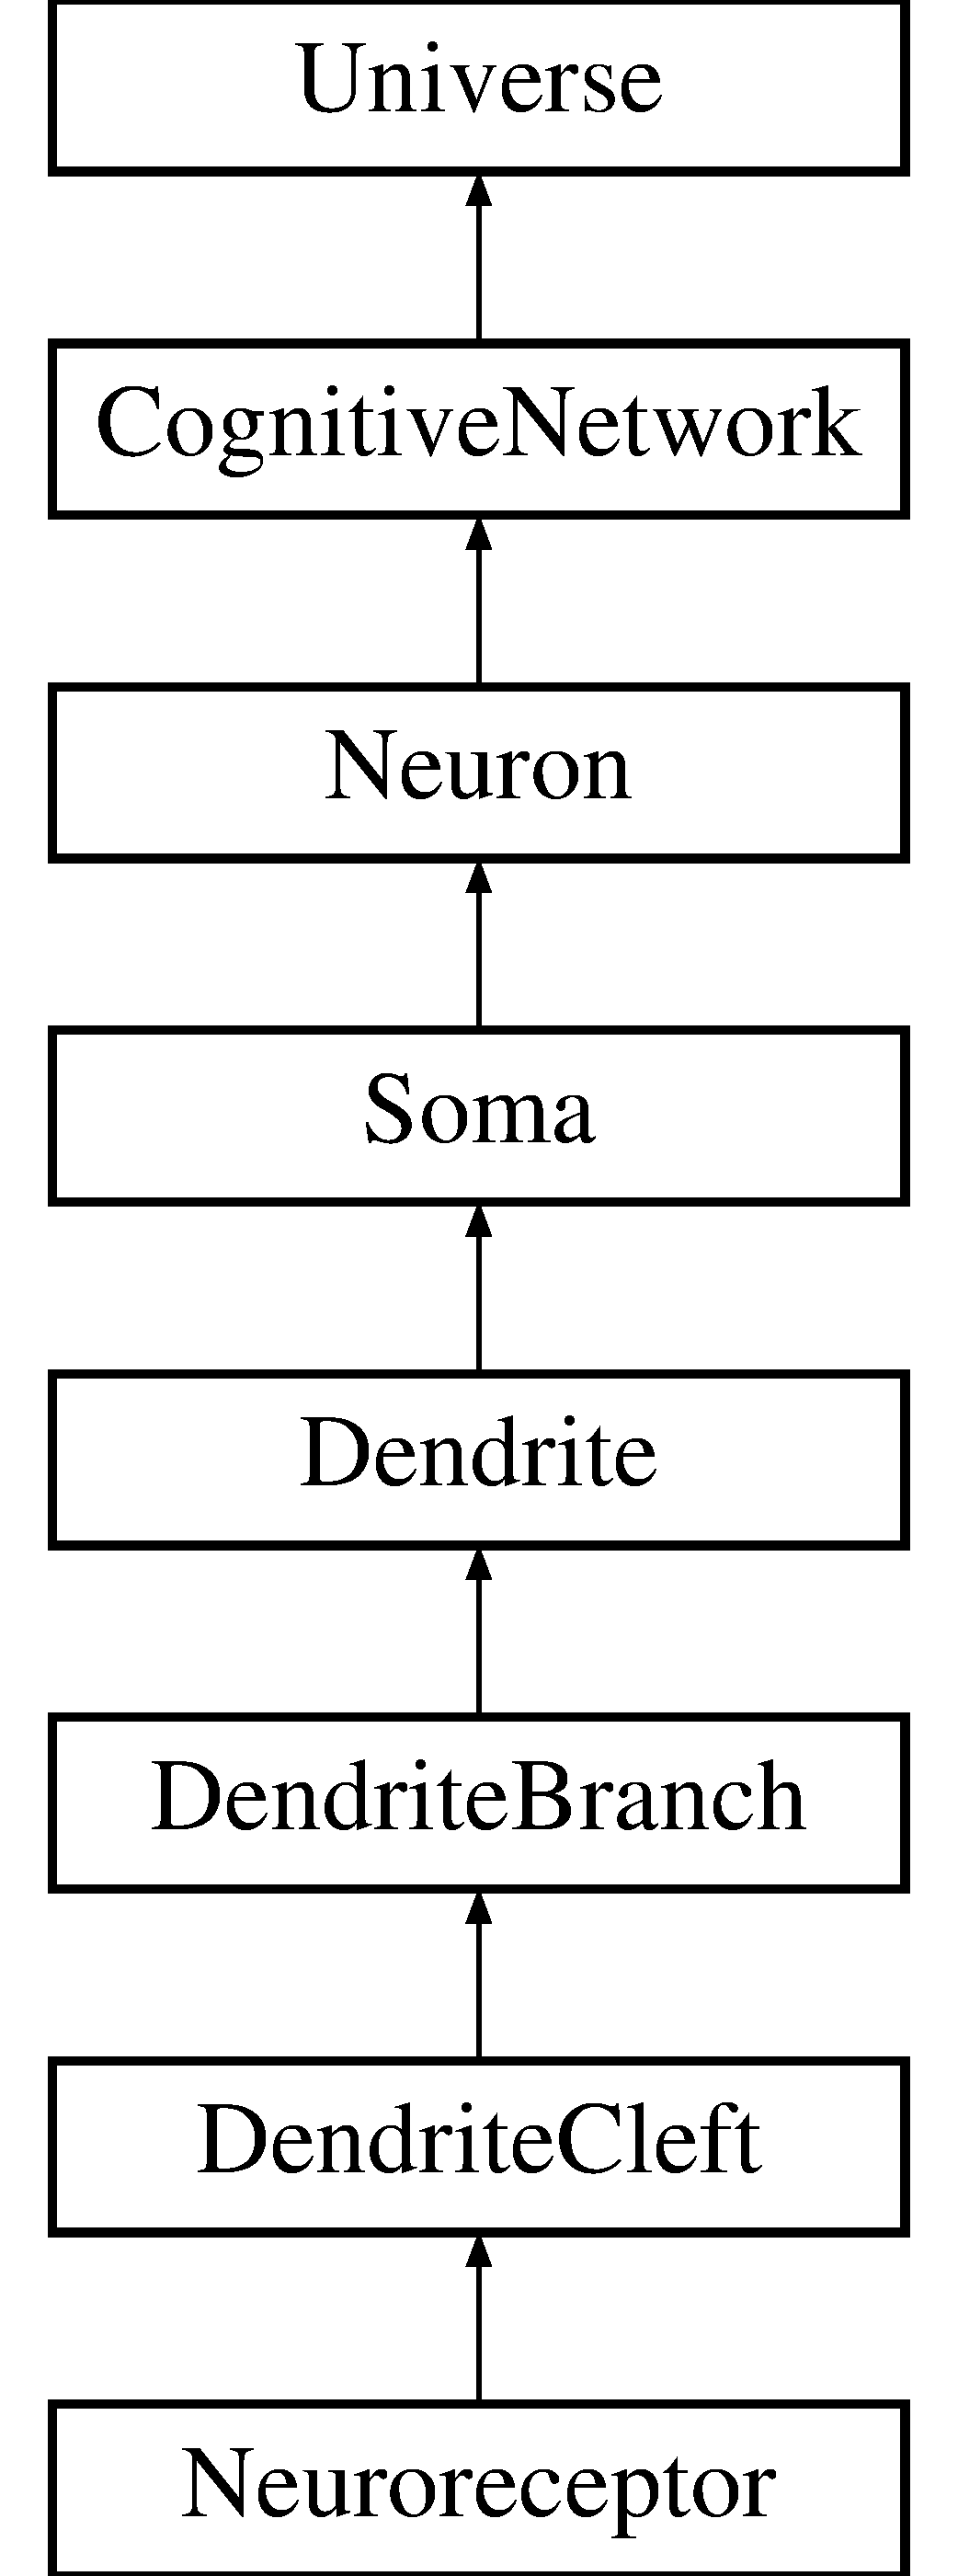
\includegraphics[height=8.000000cm]{classDendrite}
\end{center}
\end{figure}
\subsection*{Public Member Functions}
\begin{DoxyCompactItemize}
\item 
\mbox{\hyperlink{classDendrite_a0a35047fcf3dad2f81be348499e32337}{Dendrite}} ()
\item 
\mbox{\hyperlink{classDendrite_ae702e9fd351be8dc3a09afa0ed431c3b}{Dendrite}} (unsigned int object\+\_\+type)
\item 
\mbox{\hyperlink{classDendrite_a10313257362c8f62c8b01a9992ec9ff7}{Dendrite}} (unsigned int object\+\_\+type, std\+::chrono\+::time\+\_\+point$<$ \mbox{\hyperlink{universe_8h_a0ef8d951d1ca5ab3cfaf7ab4c7a6fd80}{Clock}} $>$ event\+\_\+time)
\item 
\mbox{\hyperlink{classDendrite_ac358d84fb75919386aced214fa0e1107}{Dendrite}} (unsigned int object\+\_\+type, std\+::chrono\+::time\+\_\+point$<$ \mbox{\hyperlink{universe_8h_a0ef8d951d1ca5ab3cfaf7ab4c7a6fd80}{Clock}} $>$ event\+\_\+time, \mbox{\hyperlink{classSoma}{Soma}} \&soma\+\_\+connector)
\item 
virtual \mbox{\hyperlink{classDendrite_a616c3f82655d8a3cf9cebc22e7aa2233}{$\sim$\+Dendrite}} ()
\item 
unsigned int \mbox{\hyperlink{classDendrite_afa65091d7bbeed3f16a3e71a687fdec3}{Get\+Counter}} (std\+::chrono\+::time\+\_\+point$<$ \mbox{\hyperlink{universe_8h_a0ef8d951d1ca5ab3cfaf7ab4c7a6fd80}{Clock}} $>$ event\+\_\+time)
\item 
double \mbox{\hyperlink{classDendrite_a1aa1fd51aab3996cf1a9b0ff6a86647c}{Get\+Energy}} (std\+::chrono\+::time\+\_\+point$<$ \mbox{\hyperlink{universe_8h_a0ef8d951d1ca5ab3cfaf7ab4c7a6fd80}{Clock}} $>$ event\+\_\+time)
\item 
double \mbox{\hyperlink{classDendrite_a64ebf49c488bb0225e1e5c8a8d9935d9}{Get\+Dendrite\+Length}} (std\+::chrono\+::time\+\_\+point$<$ \mbox{\hyperlink{universe_8h_a0ef8d951d1ca5ab3cfaf7ab4c7a6fd80}{Clock}} $>$ event\+\_\+time)
\item 
double \mbox{\hyperlink{classDendrite_aa103a34ce3d3525b350cb02c0a7855ea}{Get\+Dendrite\+Diameter\+Start}} (std\+::chrono\+::time\+\_\+point$<$ \mbox{\hyperlink{universe_8h_a0ef8d951d1ca5ab3cfaf7ab4c7a6fd80}{Clock}} $>$ event\+\_\+time)
\item 
double \mbox{\hyperlink{classDendrite_a2c46d2612d09964a473e1de99c17fa13}{Get\+Dendrite\+Diameter\+End}} (std\+::chrono\+::time\+\_\+point$<$ \mbox{\hyperlink{universe_8h_a0ef8d951d1ca5ab3cfaf7ab4c7a6fd80}{Clock}} $>$ event\+\_\+time)
\item 
double \mbox{\hyperlink{classDendrite_ab70008318cada82e0f21f8f010858eaa}{Get\+Membrane\+Resistance}} (std\+::chrono\+::time\+\_\+point$<$ \mbox{\hyperlink{universe_8h_a0ef8d951d1ca5ab3cfaf7ab4c7a6fd80}{Clock}} $>$ event\+\_\+time)
\item 
double \mbox{\hyperlink{classDendrite_a3551fe5fcf9c7ec767a6171f61a5ba51}{Get\+Membrane\+Capacitance}} (std\+::chrono\+::time\+\_\+point$<$ \mbox{\hyperlink{universe_8h_a0ef8d951d1ca5ab3cfaf7ab4c7a6fd80}{Clock}} $>$ event\+\_\+time)
\item 
double \mbox{\hyperlink{classDendrite_a7dd00ac5440edf9943389951a275b9bc}{Get\+Internal\+Resistance}} (std\+::chrono\+::time\+\_\+point$<$ \mbox{\hyperlink{universe_8h_a0ef8d951d1ca5ab3cfaf7ab4c7a6fd80}{Clock}} $>$ event\+\_\+time)
\item 
double \mbox{\hyperlink{classDendrite_af0315957a349532d25691385b6486e95}{Get\+Propagation\+Velocity}} (std\+::chrono\+::time\+\_\+point$<$ \mbox{\hyperlink{universe_8h_a0ef8d951d1ca5ab3cfaf7ab4c7a6fd80}{Clock}} $>$ event\+\_\+time)
\item 
void \mbox{\hyperlink{classDendrite_a9bc84d369ac487b095ed1641f89469d2}{set\+Dendrite\+Length}} (std\+::chrono\+::time\+\_\+point$<$ \mbox{\hyperlink{universe_8h_a0ef8d951d1ca5ab3cfaf7ab4c7a6fd80}{Clock}} $>$ event\+\_\+time, double val)
\item 
void \mbox{\hyperlink{classDendrite_af33658a5420b56cfd321d75ae5784302}{set\+Dendrite\+Diameter\+Start}} (std\+::chrono\+::time\+\_\+point$<$ \mbox{\hyperlink{universe_8h_a0ef8d951d1ca5ab3cfaf7ab4c7a6fd80}{Clock}} $>$ event\+\_\+time, double val)
\item 
void \mbox{\hyperlink{classDendrite_ada331daa4464ae007b3f77612aa46937}{set\+Dendrite\+Diameter\+End}} (std\+::chrono\+::time\+\_\+point$<$ \mbox{\hyperlink{universe_8h_a0ef8d951d1ca5ab3cfaf7ab4c7a6fd80}{Clock}} $>$ event\+\_\+time, double val)
\item 
void \mbox{\hyperlink{classDendrite_af6141643bf2c85404ae9c320611d1d31}{set\+Membrane\+Resistance}} (std\+::chrono\+::time\+\_\+point$<$ \mbox{\hyperlink{universe_8h_a0ef8d951d1ca5ab3cfaf7ab4c7a6fd80}{Clock}} $>$ event\+\_\+time, double val)
\item 
void \mbox{\hyperlink{classDendrite_a6fed149ffe00cf781a41a9f260f8eeb2}{set\+Membrane\+Capacitance}} (std\+::chrono\+::time\+\_\+point$<$ \mbox{\hyperlink{universe_8h_a0ef8d951d1ca5ab3cfaf7ab4c7a6fd80}{Clock}} $>$ event\+\_\+time, double val)
\item 
void \mbox{\hyperlink{classDendrite_ac79018e356cec31be05518b85c73a54d}{set\+Internal\+Resistance}} (std\+::chrono\+::time\+\_\+point$<$ \mbox{\hyperlink{universe_8h_a0ef8d951d1ca5ab3cfaf7ab4c7a6fd80}{Clock}} $>$ event\+\_\+time, double val)
\item 
void \mbox{\hyperlink{classDendrite_a7529495515de74fff2b9a92b12531057}{Set\+Counter}} (std\+::chrono\+::time\+\_\+point$<$ \mbox{\hyperlink{universe_8h_a0ef8d951d1ca5ab3cfaf7ab4c7a6fd80}{Clock}} $>$ event\+\_\+time, unsigned int val)
\item 
void \mbox{\hyperlink{classDendrite_ad341dcd42c9d5d486be1e8268d8bca27}{Set\+Energy}} (std\+::chrono\+::time\+\_\+point$<$ \mbox{\hyperlink{universe_8h_a0ef8d951d1ca5ab3cfaf7ab4c7a6fd80}{Clock}} $>$ event\+\_\+time, double val)
\item 
bool \mbox{\hyperlink{classDendrite_a6a6290955348051819badb801b753901}{Reset\+Parameters}} (std\+::chrono\+::time\+\_\+point$<$ \mbox{\hyperlink{universe_8h_a0ef8d951d1ca5ab3cfaf7ab4c7a6fd80}{Clock}} $>$ event\+\_\+time)
\item 
\mbox{\hyperlink{classDendrite}{Dendrite}} $\ast$ \mbox{\hyperlink{classDendrite_ac7b30397a4753f9c37e96ed716e275eb}{Create\+Dendrite\+Branch}} (std\+::chrono\+::time\+\_\+point$<$ \mbox{\hyperlink{universe_8h_a0ef8d951d1ca5ab3cfaf7ab4c7a6fd80}{Clock}} $>$ event\+\_\+time)
\item 
std\+::vector$<$ \mbox{\hyperlink{classDendrite}{Dendrite}} $\ast$ $>$ \mbox{\hyperlink{classDendrite_a812b9cd99ae7d81023bfa25c8f563e96}{Create\+Dendrite\+Branches}} (std\+::chrono\+::time\+\_\+point$<$ \mbox{\hyperlink{universe_8h_a0ef8d951d1ca5ab3cfaf7ab4c7a6fd80}{Clock}} $>$ event\+\_\+time, int quantity)
\item 
\mbox{\hyperlink{classDendrite}{Dendrite}} $\ast$ \mbox{\hyperlink{classDendrite_ab682ffb9bfd1a1da1623e6b641471068}{Clone\+Dendrite\+Branch}} (std\+::chrono\+::time\+\_\+point$<$ \mbox{\hyperlink{universe_8h_a0ef8d951d1ca5ab3cfaf7ab4c7a6fd80}{Clock}} $>$ event\+\_\+time, \mbox{\hyperlink{classDendrite}{Dendrite}} $\ast$clone\+\_\+object, double perfection\+\_\+membership)
\item 
std\+::vector$<$ \mbox{\hyperlink{classDendrite}{Dendrite}} $\ast$ $>$ \mbox{\hyperlink{classDendrite_abd67c09df69c520e6720bca2592bcc99}{Clone\+Dendrite\+Branches}} (std\+::chrono\+::time\+\_\+point$<$ \mbox{\hyperlink{universe_8h_a0ef8d951d1ca5ab3cfaf7ab4c7a6fd80}{Clock}} $>$ event\+\_\+time, std\+::vector$<$ \mbox{\hyperlink{classDendrite}{Dendrite}} $\ast$$>$ cloning\+\_\+list, double perfection\+\_\+membership)
\item 
\mbox{\hyperlink{classDendrite}{Dendrite}} $\ast$ \mbox{\hyperlink{classDendrite_a87887a43ac38e762255da18eaaee43f5}{Destroy\+Dendrite\+Branch}} (std\+::chrono\+::time\+\_\+point$<$ \mbox{\hyperlink{universe_8h_a0ef8d951d1ca5ab3cfaf7ab4c7a6fd80}{Clock}} $>$ event\+\_\+time, \mbox{\hyperlink{classDendrite}{Dendrite}} $\ast$destroy\+\_\+object)
\item 
std\+::vector$<$ \mbox{\hyperlink{classDendrite}{Dendrite}} $\ast$ $>$ \mbox{\hyperlink{classDendrite_a92c08afc374068922e462c9b65cf9157}{Destroy\+Dendrite\+Branches}} (std\+::chrono\+::time\+\_\+point$<$ \mbox{\hyperlink{universe_8h_a0ef8d951d1ca5ab3cfaf7ab4c7a6fd80}{Clock}} $>$ event\+\_\+time, std\+::vector$<$ \mbox{\hyperlink{classDendrite}{Dendrite}} $\ast$$>$ destruction\+\_\+list)
\item 
\mbox{\hyperlink{classDendrite}{Dendrite}} $\ast$ \mbox{\hyperlink{classDendrite_aab6cedff35cb8c65923b14c8034cccc0}{Add\+Dendrite\+Branch}} (std\+::chrono\+::time\+\_\+point$<$ \mbox{\hyperlink{universe_8h_a0ef8d951d1ca5ab3cfaf7ab4c7a6fd80}{Clock}} $>$ event\+\_\+time, \mbox{\hyperlink{classDendrite}{Dendrite}} $\ast$add\+\_\+object)
\item 
std\+::vector$<$ \mbox{\hyperlink{classDendrite}{Dendrite}} $\ast$ $>$ \mbox{\hyperlink{classDendrite_a3e6a80da180b60290545cfc92f221a05}{Add\+Dendrite\+Branches}} (std\+::chrono\+::time\+\_\+point$<$ \mbox{\hyperlink{universe_8h_a0ef8d951d1ca5ab3cfaf7ab4c7a6fd80}{Clock}} $>$ event\+\_\+time, std\+::vector$<$ \mbox{\hyperlink{classDendrite}{Dendrite}} $\ast$$>$ add\+\_\+objects)
\item 
\mbox{\hyperlink{classDendrite}{Dendrite}} $\ast$ \mbox{\hyperlink{classDendrite_aa23bd0ce7c5a0a9011b28234cc2e90e1}{Remove\+Dendrite\+Branch}} (std\+::chrono\+::time\+\_\+point$<$ \mbox{\hyperlink{universe_8h_a0ef8d951d1ca5ab3cfaf7ab4c7a6fd80}{Clock}} $>$ event\+\_\+time)
\item 
std\+::vector$<$ \mbox{\hyperlink{classDendrite}{Dendrite}} $\ast$ $>$ \mbox{\hyperlink{classDendrite_a15396dce5e1d920fcd1477b9a255dabf}{Remove\+Dendrite\+Branches}} (std\+::chrono\+::time\+\_\+point$<$ \mbox{\hyperlink{universe_8h_a0ef8d951d1ca5ab3cfaf7ab4c7a6fd80}{Clock}} $>$ event\+\_\+time, int quantity)
\item 
\mbox{\hyperlink{classDendrite}{Dendrite}} $\ast$ \mbox{\hyperlink{classDendrite_a1465037ca014fa8bbefc8c0ad70d1647}{Get\+Dendrite\+Branch}} (std\+::chrono\+::time\+\_\+point$<$ \mbox{\hyperlink{universe_8h_a0ef8d951d1ca5ab3cfaf7ab4c7a6fd80}{Clock}} $>$ event\+\_\+time, int selector)
\item 
std\+::vector$<$ \mbox{\hyperlink{classDendrite}{Dendrite}} $\ast$ $>$ \mbox{\hyperlink{classDendrite_a00b524d47e3662df712ea060ebadca77}{Get\+Dendrite\+Branches}} (std\+::chrono\+::time\+\_\+point$<$ \mbox{\hyperlink{universe_8h_a0ef8d951d1ca5ab3cfaf7ab4c7a6fd80}{Clock}} $>$ event\+\_\+time)
\item 
int \mbox{\hyperlink{classDendrite_a6a0c08a642c92d8e189e1f7eff6f6b00}{Growth}} (std\+::chrono\+::time\+\_\+point$<$ \mbox{\hyperlink{universe_8h_a0ef8d951d1ca5ab3cfaf7ab4c7a6fd80}{Clock}} $>$ event\+\_\+time)
\item 
int \mbox{\hyperlink{classDendrite_a2e7bfde37bc7aec2547253ad038aaa04}{Update}} (std\+::chrono\+::time\+\_\+point$<$ \mbox{\hyperlink{universe_8h_a0ef8d951d1ca5ab3cfaf7ab4c7a6fd80}{Clock}} $>$ event\+\_\+time)
\end{DoxyCompactItemize}
\subsection*{Protected Attributes}
\begin{DoxyCompactItemize}
\item 
std\+::vector$<$ \mbox{\hyperlink{classDendrite}{Dendrite}} $\ast$ $>$ \mbox{\hyperlink{classDendrite_a1d57708bfa57443d3fa0358984b4c761}{dendritebranch\+\_\+list}}
\end{DoxyCompactItemize}
\subsection*{Private Attributes}
\begin{DoxyCompactItemize}
\item 
int \mbox{\hyperlink{classDendrite_a1b29ae9a6ebd1cd8a329f29b11082291}{m\+\_\+\+Neuron\+Type}}
\item 
int \mbox{\hyperlink{classDendrite_a36925227bc081b318cc788b5cad78dc9}{dendrite\+\_\+type}}
\item 
bool \mbox{\hyperlink{classDendrite_ae34d0c5b775380e4fd91b697b19b4cd0}{object\+\_\+disabled}}
\item 
bool \mbox{\hyperlink{classDendrite_abf7b861f7b322d580e02fcf238fcc1a0}{object\+\_\+initialised}}
\item 
int \mbox{\hyperlink{classDendrite_a39a1f37070a1f3e0c90fdc2c54ca9bab}{m\+\_\+add\+Status}}
\item 
std\+::chrono\+::time\+\_\+point$<$ \mbox{\hyperlink{universe_8h_a0ef8d951d1ca5ab3cfaf7ab4c7a6fd80}{Clock}} $>$ \mbox{\hyperlink{classDendrite_a21584e5b60195738546123a9ba3c2d6f}{time\+\_\+object\+\_\+created}}
\item 
std\+::chrono\+::time\+\_\+point$<$ \mbox{\hyperlink{universe_8h_a0ef8d951d1ca5ab3cfaf7ab4c7a6fd80}{Clock}} $>$ \mbox{\hyperlink{classDendrite_ae4a39c5f211f908eabff9fdd35247f05}{previous\+\_\+event\+\_\+time}}
\item 
int \mbox{\hyperlink{classDendrite_ab5b135965667e18b4bd0ff7ef2cd2cc8}{dendritebranch\+\_\+pool}}
\item 
int \mbox{\hyperlink{classDendrite_ade514098e64a0f8a4061e1efbd1eda1d}{duration\+\_\+since\+\_\+last\+\_\+event}}
\item 
double \mbox{\hyperlink{classDendrite_a703375fe869320642bc6461888a42fb5}{m\+\_\+\+Volume}}
\item 
double \mbox{\hyperlink{classDendrite_a72259a619c9c3224c2779117be2c9695}{m\+\_\+\+Surface\+Area}}
\item 
double \mbox{\hyperlink{classDendrite_a733dcd2b9f524a964fc2276f2022bfbb}{m\+\_\+\+Length}}
\item 
double \mbox{\hyperlink{classDendrite_a33352f43679858316c6e1c92a4a71264}{object\+\_\+size}}
\item 
double \mbox{\hyperlink{classDendrite_ad08f503df19e5c3816340aba41351087}{m\+\_\+dendrite\+Length}}
\begin{DoxyCompactList}\small\item\em Member variable \char`\"{}m\+\_\+dendrite\+Length\char`\"{}. \end{DoxyCompactList}\item 
double \mbox{\hyperlink{classDendrite_a0911f9623a3aa5b932d47a702730752e}{m\+\_\+dendrite\+Diameter\+Start}}
\begin{DoxyCompactList}\small\item\em Member variable \char`\"{}m\+\_\+dendrite\+Diameter\+Start\char`\"{}. \end{DoxyCompactList}\item 
double \mbox{\hyperlink{classDendrite_ac3a465f1f142ba87c24c4794292d1a22}{m\+\_\+dendrite\+Diameter\+End}}
\begin{DoxyCompactList}\small\item\em Member variable \char`\"{}m\+\_\+dendrite\+Diameter\+End\char`\"{}. \end{DoxyCompactList}\item 
double \mbox{\hyperlink{classDendrite_a3d0107ad2ad6bccb14eaca4e2e118bbc}{m\+\_\+membrane\+Resistance}}
\item 
double \mbox{\hyperlink{classDendrite_aa8e9e9e5defcd99e0793bc4d1e8f3615}{m\+\_\+membrane\+Capacitance}}
\item 
double \mbox{\hyperlink{classDendrite_ae76ec62f0f14fca81d4e217002e1a631}{m\+\_\+internal\+Resistance}}
\item 
unsigned int \mbox{\hyperlink{classDendrite_a7cab5c65468ff1c45b13b172028c2209}{m\+\_\+\+Counter}}
\begin{DoxyCompactList}\small\item\em Member variable \char`\"{}m\+\_\+\+Counter\char`\"{}. \end{DoxyCompactList}\item 
double \mbox{\hyperlink{classDendrite_a88f9b4ed19218a666001e722561c6cc3}{object\+\_\+energy}}
\begin{DoxyCompactList}\small\item\em Member variable \char`\"{}object\+\_\+energy\char`\"{}. \end{DoxyCompactList}\item 
double \mbox{\hyperlink{classDendrite_a3983ac62d34b1c5bd050f0b1cfeb5855}{object\+\_\+energy\+Inc}}
\item 
double \mbox{\hyperlink{classDendrite_a1d1292149a68340a586c2da6c5de82aa}{object\+\_\+energy\+Dec}}
\item 
double \mbox{\hyperlink{classDendrite_a4dea4d8ed2606f612b96203ef88a52c9}{object\+\_\+energy\+Leak}}
\item 
double \mbox{\hyperlink{classDendrite_a29d0f83fef3ff623132ee1faf9221c35}{object\+\_\+energy\+\_\+threshold}}
\item 
double \mbox{\hyperlink{classDendrite_a18fe1c4fb9bf220176d30e163ccfa71b}{m\+\_\+\+Time\+Dilation}}
\item 
double \mbox{\hyperlink{classDendrite_a9e1fa8355d6d05913113df4cb6f0e825}{m\+\_\+\+Time\+Threshold}}
\end{DoxyCompactItemize}
\subsection*{Additional Inherited Members}


\subsection{Constructor \& Destructor Documentation}
\mbox{\Hypertarget{classDendrite_a0a35047fcf3dad2f81be348499e32337}\label{classDendrite_a0a35047fcf3dad2f81be348499e32337}} 
\index{Dendrite@{Dendrite}!Dendrite@{Dendrite}}
\index{Dendrite@{Dendrite}!Dendrite@{Dendrite}}
\subsubsection{\texorpdfstring{Dendrite()}{Dendrite()}\hspace{0.1cm}{\footnotesize\ttfamily [1/4]}}
{\footnotesize\ttfamily Dendrite\+::\+Dendrite (\begin{DoxyParamCaption}{ }\end{DoxyParamCaption})\hspace{0.3cm}{\ttfamily [inline]}}

\mbox{\Hypertarget{classDendrite_ae702e9fd351be8dc3a09afa0ed431c3b}\label{classDendrite_ae702e9fd351be8dc3a09afa0ed431c3b}} 
\index{Dendrite@{Dendrite}!Dendrite@{Dendrite}}
\index{Dendrite@{Dendrite}!Dendrite@{Dendrite}}
\subsubsection{\texorpdfstring{Dendrite()}{Dendrite()}\hspace{0.1cm}{\footnotesize\ttfamily [2/4]}}
{\footnotesize\ttfamily Dendrite\+::\+Dendrite (\begin{DoxyParamCaption}\item[{unsigned int}]{object\+\_\+type }\end{DoxyParamCaption})\hspace{0.3cm}{\ttfamily [inline]}}

\mbox{\Hypertarget{classDendrite_a10313257362c8f62c8b01a9992ec9ff7}\label{classDendrite_a10313257362c8f62c8b01a9992ec9ff7}} 
\index{Dendrite@{Dendrite}!Dendrite@{Dendrite}}
\index{Dendrite@{Dendrite}!Dendrite@{Dendrite}}
\subsubsection{\texorpdfstring{Dendrite()}{Dendrite()}\hspace{0.1cm}{\footnotesize\ttfamily [3/4]}}
{\footnotesize\ttfamily Dendrite\+::\+Dendrite (\begin{DoxyParamCaption}\item[{unsigned int}]{object\+\_\+type,  }\item[{std\+::chrono\+::time\+\_\+point$<$ \mbox{\hyperlink{universe_8h_a0ef8d951d1ca5ab3cfaf7ab4c7a6fd80}{Clock}} $>$}]{event\+\_\+time }\end{DoxyParamCaption})\hspace{0.3cm}{\ttfamily [inline]}}

\mbox{\Hypertarget{classDendrite_ac358d84fb75919386aced214fa0e1107}\label{classDendrite_ac358d84fb75919386aced214fa0e1107}} 
\index{Dendrite@{Dendrite}!Dendrite@{Dendrite}}
\index{Dendrite@{Dendrite}!Dendrite@{Dendrite}}
\subsubsection{\texorpdfstring{Dendrite()}{Dendrite()}\hspace{0.1cm}{\footnotesize\ttfamily [4/4]}}
{\footnotesize\ttfamily Dendrite\+::\+Dendrite (\begin{DoxyParamCaption}\item[{unsigned int}]{object\+\_\+type,  }\item[{std\+::chrono\+::time\+\_\+point$<$ \mbox{\hyperlink{universe_8h_a0ef8d951d1ca5ab3cfaf7ab4c7a6fd80}{Clock}} $>$}]{event\+\_\+time,  }\item[{\mbox{\hyperlink{classSoma}{Soma}} \&}]{soma\+\_\+connector }\end{DoxyParamCaption})\hspace{0.3cm}{\ttfamily [inline]}}

\mbox{\Hypertarget{classDendrite_a616c3f82655d8a3cf9cebc22e7aa2233}\label{classDendrite_a616c3f82655d8a3cf9cebc22e7aa2233}} 
\index{Dendrite@{Dendrite}!````~Dendrite@{$\sim$\+Dendrite}}
\index{````~Dendrite@{$\sim$\+Dendrite}!Dendrite@{Dendrite}}
\subsubsection{\texorpdfstring{$\sim$\+Dendrite()}{~Dendrite()}}
{\footnotesize\ttfamily virtual Dendrite\+::$\sim$\+Dendrite (\begin{DoxyParamCaption}{ }\end{DoxyParamCaption})\hspace{0.3cm}{\ttfamily [inline]}, {\ttfamily [virtual]}}

Default destructor 

\subsection{Member Function Documentation}
\mbox{\Hypertarget{classDendrite_aab6cedff35cb8c65923b14c8034cccc0}\label{classDendrite_aab6cedff35cb8c65923b14c8034cccc0}} 
\index{Dendrite@{Dendrite}!Add\+Dendrite\+Branch@{Add\+Dendrite\+Branch}}
\index{Add\+Dendrite\+Branch@{Add\+Dendrite\+Branch}!Dendrite@{Dendrite}}
\subsubsection{\texorpdfstring{Add\+Dendrite\+Branch()}{AddDendriteBranch()}}
{\footnotesize\ttfamily \mbox{\hyperlink{classDendrite}{Dendrite}} $\ast$ Dendrite\+::\+Add\+Dendrite\+Branch (\begin{DoxyParamCaption}\item[{std\+::chrono\+::time\+\_\+point$<$ \mbox{\hyperlink{universe_8h_a0ef8d951d1ca5ab3cfaf7ab4c7a6fd80}{Clock}} $>$}]{event\+\_\+time,  }\item[{\mbox{\hyperlink{classDendrite}{Dendrite}} $\ast$}]{add\+\_\+object }\end{DoxyParamCaption})}

\mbox{\Hypertarget{classDendrite_a3e6a80da180b60290545cfc92f221a05}\label{classDendrite_a3e6a80da180b60290545cfc92f221a05}} 
\index{Dendrite@{Dendrite}!Add\+Dendrite\+Branches@{Add\+Dendrite\+Branches}}
\index{Add\+Dendrite\+Branches@{Add\+Dendrite\+Branches}!Dendrite@{Dendrite}}
\subsubsection{\texorpdfstring{Add\+Dendrite\+Branches()}{AddDendriteBranches()}}
{\footnotesize\ttfamily std\+::vector$<$ \mbox{\hyperlink{classDendrite}{Dendrite}} $\ast$ $>$ Dendrite\+::\+Add\+Dendrite\+Branches (\begin{DoxyParamCaption}\item[{std\+::chrono\+::time\+\_\+point$<$ \mbox{\hyperlink{universe_8h_a0ef8d951d1ca5ab3cfaf7ab4c7a6fd80}{Clock}} $>$}]{event\+\_\+time,  }\item[{std\+::vector$<$ \mbox{\hyperlink{classDendrite}{Dendrite}} $\ast$$>$}]{add\+\_\+objects }\end{DoxyParamCaption})}

\mbox{\Hypertarget{classDendrite_ab682ffb9bfd1a1da1623e6b641471068}\label{classDendrite_ab682ffb9bfd1a1da1623e6b641471068}} 
\index{Dendrite@{Dendrite}!Clone\+Dendrite\+Branch@{Clone\+Dendrite\+Branch}}
\index{Clone\+Dendrite\+Branch@{Clone\+Dendrite\+Branch}!Dendrite@{Dendrite}}
\subsubsection{\texorpdfstring{Clone\+Dendrite\+Branch()}{CloneDendriteBranch()}}
{\footnotesize\ttfamily \mbox{\hyperlink{classDendrite}{Dendrite}} $\ast$ Dendrite\+::\+Clone\+Dendrite\+Branch (\begin{DoxyParamCaption}\item[{std\+::chrono\+::time\+\_\+point$<$ \mbox{\hyperlink{universe_8h_a0ef8d951d1ca5ab3cfaf7ab4c7a6fd80}{Clock}} $>$}]{event\+\_\+time,  }\item[{\mbox{\hyperlink{classDendrite}{Dendrite}} $\ast$}]{clone\+\_\+object,  }\item[{double}]{perfection\+\_\+membership }\end{DoxyParamCaption})}

\mbox{\Hypertarget{classDendrite_abd67c09df69c520e6720bca2592bcc99}\label{classDendrite_abd67c09df69c520e6720bca2592bcc99}} 
\index{Dendrite@{Dendrite}!Clone\+Dendrite\+Branches@{Clone\+Dendrite\+Branches}}
\index{Clone\+Dendrite\+Branches@{Clone\+Dendrite\+Branches}!Dendrite@{Dendrite}}
\subsubsection{\texorpdfstring{Clone\+Dendrite\+Branches()}{CloneDendriteBranches()}}
{\footnotesize\ttfamily std\+::vector$<$ \mbox{\hyperlink{classDendrite}{Dendrite}} $\ast$ $>$ Dendrite\+::\+Clone\+Dendrite\+Branches (\begin{DoxyParamCaption}\item[{std\+::chrono\+::time\+\_\+point$<$ \mbox{\hyperlink{universe_8h_a0ef8d951d1ca5ab3cfaf7ab4c7a6fd80}{Clock}} $>$}]{event\+\_\+time,  }\item[{std\+::vector$<$ \mbox{\hyperlink{classDendrite}{Dendrite}} $\ast$$>$}]{cloning\+\_\+list,  }\item[{double}]{perfection\+\_\+membership }\end{DoxyParamCaption})}

\mbox{\Hypertarget{classDendrite_ac7b30397a4753f9c37e96ed716e275eb}\label{classDendrite_ac7b30397a4753f9c37e96ed716e275eb}} 
\index{Dendrite@{Dendrite}!Create\+Dendrite\+Branch@{Create\+Dendrite\+Branch}}
\index{Create\+Dendrite\+Branch@{Create\+Dendrite\+Branch}!Dendrite@{Dendrite}}
\subsubsection{\texorpdfstring{Create\+Dendrite\+Branch()}{CreateDendriteBranch()}}
{\footnotesize\ttfamily \mbox{\hyperlink{classDendrite}{Dendrite}} $\ast$ Dendrite\+::\+Create\+Dendrite\+Branch (\begin{DoxyParamCaption}\item[{std\+::chrono\+::time\+\_\+point$<$ \mbox{\hyperlink{universe_8h_a0ef8d951d1ca5ab3cfaf7ab4c7a6fd80}{Clock}} $>$}]{event\+\_\+time }\end{DoxyParamCaption})}

\mbox{\Hypertarget{classDendrite_a812b9cd99ae7d81023bfa25c8f563e96}\label{classDendrite_a812b9cd99ae7d81023bfa25c8f563e96}} 
\index{Dendrite@{Dendrite}!Create\+Dendrite\+Branches@{Create\+Dendrite\+Branches}}
\index{Create\+Dendrite\+Branches@{Create\+Dendrite\+Branches}!Dendrite@{Dendrite}}
\subsubsection{\texorpdfstring{Create\+Dendrite\+Branches()}{CreateDendriteBranches()}}
{\footnotesize\ttfamily std\+::vector$<$ \mbox{\hyperlink{classDendrite}{Dendrite}} $\ast$ $>$ Dendrite\+::\+Create\+Dendrite\+Branches (\begin{DoxyParamCaption}\item[{std\+::chrono\+::time\+\_\+point$<$ \mbox{\hyperlink{universe_8h_a0ef8d951d1ca5ab3cfaf7ab4c7a6fd80}{Clock}} $>$}]{event\+\_\+time,  }\item[{int}]{quantity }\end{DoxyParamCaption})}

\mbox{\Hypertarget{classDendrite_a87887a43ac38e762255da18eaaee43f5}\label{classDendrite_a87887a43ac38e762255da18eaaee43f5}} 
\index{Dendrite@{Dendrite}!Destroy\+Dendrite\+Branch@{Destroy\+Dendrite\+Branch}}
\index{Destroy\+Dendrite\+Branch@{Destroy\+Dendrite\+Branch}!Dendrite@{Dendrite}}
\subsubsection{\texorpdfstring{Destroy\+Dendrite\+Branch()}{DestroyDendriteBranch()}}
{\footnotesize\ttfamily \mbox{\hyperlink{classDendrite}{Dendrite}} $\ast$ Dendrite\+::\+Destroy\+Dendrite\+Branch (\begin{DoxyParamCaption}\item[{std\+::chrono\+::time\+\_\+point$<$ \mbox{\hyperlink{universe_8h_a0ef8d951d1ca5ab3cfaf7ab4c7a6fd80}{Clock}} $>$}]{event\+\_\+time,  }\item[{\mbox{\hyperlink{classDendrite}{Dendrite}} $\ast$}]{destroy\+\_\+object }\end{DoxyParamCaption})}

\mbox{\Hypertarget{classDendrite_a92c08afc374068922e462c9b65cf9157}\label{classDendrite_a92c08afc374068922e462c9b65cf9157}} 
\index{Dendrite@{Dendrite}!Destroy\+Dendrite\+Branches@{Destroy\+Dendrite\+Branches}}
\index{Destroy\+Dendrite\+Branches@{Destroy\+Dendrite\+Branches}!Dendrite@{Dendrite}}
\subsubsection{\texorpdfstring{Destroy\+Dendrite\+Branches()}{DestroyDendriteBranches()}}
{\footnotesize\ttfamily std\+::vector$<$ \mbox{\hyperlink{classDendrite}{Dendrite}} $\ast$ $>$ Dendrite\+::\+Destroy\+Dendrite\+Branches (\begin{DoxyParamCaption}\item[{std\+::chrono\+::time\+\_\+point$<$ \mbox{\hyperlink{universe_8h_a0ef8d951d1ca5ab3cfaf7ab4c7a6fd80}{Clock}} $>$}]{event\+\_\+time,  }\item[{std\+::vector$<$ \mbox{\hyperlink{classDendrite}{Dendrite}} $\ast$$>$}]{destruction\+\_\+list }\end{DoxyParamCaption})}

\mbox{\Hypertarget{classDendrite_afa65091d7bbeed3f16a3e71a687fdec3}\label{classDendrite_afa65091d7bbeed3f16a3e71a687fdec3}} 
\index{Dendrite@{Dendrite}!Get\+Counter@{Get\+Counter}}
\index{Get\+Counter@{Get\+Counter}!Dendrite@{Dendrite}}
\subsubsection{\texorpdfstring{Get\+Counter()}{GetCounter()}}
{\footnotesize\ttfamily unsigned int Dendrite\+::\+Get\+Counter (\begin{DoxyParamCaption}\item[{std\+::chrono\+::time\+\_\+point$<$ \mbox{\hyperlink{universe_8h_a0ef8d951d1ca5ab3cfaf7ab4c7a6fd80}{Clock}} $>$}]{event\+\_\+time }\end{DoxyParamCaption})\hspace{0.3cm}{\ttfamily [inline]}}

\mbox{\Hypertarget{classDendrite_a1465037ca014fa8bbefc8c0ad70d1647}\label{classDendrite_a1465037ca014fa8bbefc8c0ad70d1647}} 
\index{Dendrite@{Dendrite}!Get\+Dendrite\+Branch@{Get\+Dendrite\+Branch}}
\index{Get\+Dendrite\+Branch@{Get\+Dendrite\+Branch}!Dendrite@{Dendrite}}
\subsubsection{\texorpdfstring{Get\+Dendrite\+Branch()}{GetDendriteBranch()}}
{\footnotesize\ttfamily \mbox{\hyperlink{classDendrite}{Dendrite}} $\ast$ Dendrite\+::\+Get\+Dendrite\+Branch (\begin{DoxyParamCaption}\item[{std\+::chrono\+::time\+\_\+point$<$ \mbox{\hyperlink{universe_8h_a0ef8d951d1ca5ab3cfaf7ab4c7a6fd80}{Clock}} $>$}]{event\+\_\+time,  }\item[{int}]{selector }\end{DoxyParamCaption})}

\mbox{\Hypertarget{classDendrite_a00b524d47e3662df712ea060ebadca77}\label{classDendrite_a00b524d47e3662df712ea060ebadca77}} 
\index{Dendrite@{Dendrite}!Get\+Dendrite\+Branches@{Get\+Dendrite\+Branches}}
\index{Get\+Dendrite\+Branches@{Get\+Dendrite\+Branches}!Dendrite@{Dendrite}}
\subsubsection{\texorpdfstring{Get\+Dendrite\+Branches()}{GetDendriteBranches()}}
{\footnotesize\ttfamily std\+::vector$<$ \mbox{\hyperlink{classDendrite}{Dendrite}} $\ast$ $>$ Dendrite\+::\+Get\+Dendrite\+Branches (\begin{DoxyParamCaption}\item[{std\+::chrono\+::time\+\_\+point$<$ \mbox{\hyperlink{universe_8h_a0ef8d951d1ca5ab3cfaf7ab4c7a6fd80}{Clock}} $>$}]{event\+\_\+time }\end{DoxyParamCaption})}

\mbox{\Hypertarget{classDendrite_a2c46d2612d09964a473e1de99c17fa13}\label{classDendrite_a2c46d2612d09964a473e1de99c17fa13}} 
\index{Dendrite@{Dendrite}!Get\+Dendrite\+Diameter\+End@{Get\+Dendrite\+Diameter\+End}}
\index{Get\+Dendrite\+Diameter\+End@{Get\+Dendrite\+Diameter\+End}!Dendrite@{Dendrite}}
\subsubsection{\texorpdfstring{Get\+Dendrite\+Diameter\+End()}{GetDendriteDiameterEnd()}}
{\footnotesize\ttfamily double Dendrite\+::\+Get\+Dendrite\+Diameter\+End (\begin{DoxyParamCaption}\item[{std\+::chrono\+::time\+\_\+point$<$ \mbox{\hyperlink{universe_8h_a0ef8d951d1ca5ab3cfaf7ab4c7a6fd80}{Clock}} $>$}]{event\+\_\+time }\end{DoxyParamCaption})\hspace{0.3cm}{\ttfamily [inline]}}

\mbox{\Hypertarget{classDendrite_aa103a34ce3d3525b350cb02c0a7855ea}\label{classDendrite_aa103a34ce3d3525b350cb02c0a7855ea}} 
\index{Dendrite@{Dendrite}!Get\+Dendrite\+Diameter\+Start@{Get\+Dendrite\+Diameter\+Start}}
\index{Get\+Dendrite\+Diameter\+Start@{Get\+Dendrite\+Diameter\+Start}!Dendrite@{Dendrite}}
\subsubsection{\texorpdfstring{Get\+Dendrite\+Diameter\+Start()}{GetDendriteDiameterStart()}}
{\footnotesize\ttfamily double Dendrite\+::\+Get\+Dendrite\+Diameter\+Start (\begin{DoxyParamCaption}\item[{std\+::chrono\+::time\+\_\+point$<$ \mbox{\hyperlink{universe_8h_a0ef8d951d1ca5ab3cfaf7ab4c7a6fd80}{Clock}} $>$}]{event\+\_\+time }\end{DoxyParamCaption})\hspace{0.3cm}{\ttfamily [inline]}}

\mbox{\Hypertarget{classDendrite_a64ebf49c488bb0225e1e5c8a8d9935d9}\label{classDendrite_a64ebf49c488bb0225e1e5c8a8d9935d9}} 
\index{Dendrite@{Dendrite}!Get\+Dendrite\+Length@{Get\+Dendrite\+Length}}
\index{Get\+Dendrite\+Length@{Get\+Dendrite\+Length}!Dendrite@{Dendrite}}
\subsubsection{\texorpdfstring{Get\+Dendrite\+Length()}{GetDendriteLength()}}
{\footnotesize\ttfamily double Dendrite\+::\+Get\+Dendrite\+Length (\begin{DoxyParamCaption}\item[{std\+::chrono\+::time\+\_\+point$<$ \mbox{\hyperlink{universe_8h_a0ef8d951d1ca5ab3cfaf7ab4c7a6fd80}{Clock}} $>$}]{event\+\_\+time }\end{DoxyParamCaption})\hspace{0.3cm}{\ttfamily [inline]}}

\mbox{\Hypertarget{classDendrite_a1aa1fd51aab3996cf1a9b0ff6a86647c}\label{classDendrite_a1aa1fd51aab3996cf1a9b0ff6a86647c}} 
\index{Dendrite@{Dendrite}!Get\+Energy@{Get\+Energy}}
\index{Get\+Energy@{Get\+Energy}!Dendrite@{Dendrite}}
\subsubsection{\texorpdfstring{Get\+Energy()}{GetEnergy()}}
{\footnotesize\ttfamily double Dendrite\+::\+Get\+Energy (\begin{DoxyParamCaption}\item[{std\+::chrono\+::time\+\_\+point$<$ \mbox{\hyperlink{universe_8h_a0ef8d951d1ca5ab3cfaf7ab4c7a6fd80}{Clock}} $>$}]{event\+\_\+time }\end{DoxyParamCaption})\hspace{0.3cm}{\ttfamily [inline]}}

\mbox{\Hypertarget{classDendrite_a7dd00ac5440edf9943389951a275b9bc}\label{classDendrite_a7dd00ac5440edf9943389951a275b9bc}} 
\index{Dendrite@{Dendrite}!Get\+Internal\+Resistance@{Get\+Internal\+Resistance}}
\index{Get\+Internal\+Resistance@{Get\+Internal\+Resistance}!Dendrite@{Dendrite}}
\subsubsection{\texorpdfstring{Get\+Internal\+Resistance()}{GetInternalResistance()}}
{\footnotesize\ttfamily double Dendrite\+::\+Get\+Internal\+Resistance (\begin{DoxyParamCaption}\item[{std\+::chrono\+::time\+\_\+point$<$ \mbox{\hyperlink{universe_8h_a0ef8d951d1ca5ab3cfaf7ab4c7a6fd80}{Clock}} $>$}]{event\+\_\+time }\end{DoxyParamCaption})\hspace{0.3cm}{\ttfamily [inline]}}

\mbox{\Hypertarget{classDendrite_a3551fe5fcf9c7ec767a6171f61a5ba51}\label{classDendrite_a3551fe5fcf9c7ec767a6171f61a5ba51}} 
\index{Dendrite@{Dendrite}!Get\+Membrane\+Capacitance@{Get\+Membrane\+Capacitance}}
\index{Get\+Membrane\+Capacitance@{Get\+Membrane\+Capacitance}!Dendrite@{Dendrite}}
\subsubsection{\texorpdfstring{Get\+Membrane\+Capacitance()}{GetMembraneCapacitance()}}
{\footnotesize\ttfamily double Dendrite\+::\+Get\+Membrane\+Capacitance (\begin{DoxyParamCaption}\item[{std\+::chrono\+::time\+\_\+point$<$ \mbox{\hyperlink{universe_8h_a0ef8d951d1ca5ab3cfaf7ab4c7a6fd80}{Clock}} $>$}]{event\+\_\+time }\end{DoxyParamCaption})\hspace{0.3cm}{\ttfamily [inline]}}

\mbox{\Hypertarget{classDendrite_ab70008318cada82e0f21f8f010858eaa}\label{classDendrite_ab70008318cada82e0f21f8f010858eaa}} 
\index{Dendrite@{Dendrite}!Get\+Membrane\+Resistance@{Get\+Membrane\+Resistance}}
\index{Get\+Membrane\+Resistance@{Get\+Membrane\+Resistance}!Dendrite@{Dendrite}}
\subsubsection{\texorpdfstring{Get\+Membrane\+Resistance()}{GetMembraneResistance()}}
{\footnotesize\ttfamily double Dendrite\+::\+Get\+Membrane\+Resistance (\begin{DoxyParamCaption}\item[{std\+::chrono\+::time\+\_\+point$<$ \mbox{\hyperlink{universe_8h_a0ef8d951d1ca5ab3cfaf7ab4c7a6fd80}{Clock}} $>$}]{event\+\_\+time }\end{DoxyParamCaption})\hspace{0.3cm}{\ttfamily [inline]}}

\mbox{\Hypertarget{classDendrite_af0315957a349532d25691385b6486e95}\label{classDendrite_af0315957a349532d25691385b6486e95}} 
\index{Dendrite@{Dendrite}!Get\+Propagation\+Velocity@{Get\+Propagation\+Velocity}}
\index{Get\+Propagation\+Velocity@{Get\+Propagation\+Velocity}!Dendrite@{Dendrite}}
\subsubsection{\texorpdfstring{Get\+Propagation\+Velocity()}{GetPropagationVelocity()}}
{\footnotesize\ttfamily double Dendrite\+::\+Get\+Propagation\+Velocity (\begin{DoxyParamCaption}\item[{std\+::chrono\+::time\+\_\+point$<$ \mbox{\hyperlink{universe_8h_a0ef8d951d1ca5ab3cfaf7ab4c7a6fd80}{Clock}} $>$}]{event\+\_\+time }\end{DoxyParamCaption})\hspace{0.3cm}{\ttfamily [inline]}}

\mbox{\Hypertarget{classDendrite_a6a0c08a642c92d8e189e1f7eff6f6b00}\label{classDendrite_a6a0c08a642c92d8e189e1f7eff6f6b00}} 
\index{Dendrite@{Dendrite}!Growth@{Growth}}
\index{Growth@{Growth}!Dendrite@{Dendrite}}
\subsubsection{\texorpdfstring{Growth()}{Growth()}}
{\footnotesize\ttfamily int Dendrite\+::\+Growth (\begin{DoxyParamCaption}\item[{std\+::chrono\+::time\+\_\+point$<$ \mbox{\hyperlink{universe_8h_a0ef8d951d1ca5ab3cfaf7ab4c7a6fd80}{Clock}} $>$}]{event\+\_\+time }\end{DoxyParamCaption})}

\mbox{\Hypertarget{classDendrite_aa23bd0ce7c5a0a9011b28234cc2e90e1}\label{classDendrite_aa23bd0ce7c5a0a9011b28234cc2e90e1}} 
\index{Dendrite@{Dendrite}!Remove\+Dendrite\+Branch@{Remove\+Dendrite\+Branch}}
\index{Remove\+Dendrite\+Branch@{Remove\+Dendrite\+Branch}!Dendrite@{Dendrite}}
\subsubsection{\texorpdfstring{Remove\+Dendrite\+Branch()}{RemoveDendriteBranch()}}
{\footnotesize\ttfamily \mbox{\hyperlink{classDendrite}{Dendrite}} $\ast$ Dendrite\+::\+Remove\+Dendrite\+Branch (\begin{DoxyParamCaption}\item[{std\+::chrono\+::time\+\_\+point$<$ \mbox{\hyperlink{universe_8h_a0ef8d951d1ca5ab3cfaf7ab4c7a6fd80}{Clock}} $>$}]{event\+\_\+time }\end{DoxyParamCaption})}

\mbox{\Hypertarget{classDendrite_a15396dce5e1d920fcd1477b9a255dabf}\label{classDendrite_a15396dce5e1d920fcd1477b9a255dabf}} 
\index{Dendrite@{Dendrite}!Remove\+Dendrite\+Branches@{Remove\+Dendrite\+Branches}}
\index{Remove\+Dendrite\+Branches@{Remove\+Dendrite\+Branches}!Dendrite@{Dendrite}}
\subsubsection{\texorpdfstring{Remove\+Dendrite\+Branches()}{RemoveDendriteBranches()}}
{\footnotesize\ttfamily std\+::vector$<$ \mbox{\hyperlink{classDendrite}{Dendrite}} $\ast$ $>$ Dendrite\+::\+Remove\+Dendrite\+Branches (\begin{DoxyParamCaption}\item[{std\+::chrono\+::time\+\_\+point$<$ \mbox{\hyperlink{universe_8h_a0ef8d951d1ca5ab3cfaf7ab4c7a6fd80}{Clock}} $>$}]{event\+\_\+time,  }\item[{int}]{quantity }\end{DoxyParamCaption})}

\mbox{\Hypertarget{classDendrite_a6a6290955348051819badb801b753901}\label{classDendrite_a6a6290955348051819badb801b753901}} 
\index{Dendrite@{Dendrite}!Reset\+Parameters@{Reset\+Parameters}}
\index{Reset\+Parameters@{Reset\+Parameters}!Dendrite@{Dendrite}}
\subsubsection{\texorpdfstring{Reset\+Parameters()}{ResetParameters()}}
{\footnotesize\ttfamily bool Dendrite\+::\+Reset\+Parameters (\begin{DoxyParamCaption}\item[{std\+::chrono\+::time\+\_\+point$<$ \mbox{\hyperlink{universe_8h_a0ef8d951d1ca5ab3cfaf7ab4c7a6fd80}{Clock}} $>$}]{event\+\_\+time }\end{DoxyParamCaption})}

\mbox{\Hypertarget{classDendrite_a7529495515de74fff2b9a92b12531057}\label{classDendrite_a7529495515de74fff2b9a92b12531057}} 
\index{Dendrite@{Dendrite}!Set\+Counter@{Set\+Counter}}
\index{Set\+Counter@{Set\+Counter}!Dendrite@{Dendrite}}
\subsubsection{\texorpdfstring{Set\+Counter()}{SetCounter()}}
{\footnotesize\ttfamily void Dendrite\+::\+Set\+Counter (\begin{DoxyParamCaption}\item[{std\+::chrono\+::time\+\_\+point$<$ \mbox{\hyperlink{universe_8h_a0ef8d951d1ca5ab3cfaf7ab4c7a6fd80}{Clock}} $>$}]{event\+\_\+time,  }\item[{unsigned int}]{val }\end{DoxyParamCaption})\hspace{0.3cm}{\ttfamily [inline]}, {\ttfamily [virtual]}}



Reimplemented from \mbox{\hyperlink{classUniverse_aa22202ae740eb1355529afcb13285e91}{Universe}}.



Reimplemented in \mbox{\hyperlink{classNeuroreceptor_a0660a316ef44cf723509f720acd16f24}{Neuroreceptor}}, \mbox{\hyperlink{classDendriteBranch_a2ce03fbad4a70564eeaafb62debd4d74}{Dendrite\+Branch}}, and \mbox{\hyperlink{classDendriteCleft_a428b8e5117f381a382e0071b936d42a1}{Dendrite\+Cleft}}.

\mbox{\Hypertarget{classDendrite_ada331daa4464ae007b3f77612aa46937}\label{classDendrite_ada331daa4464ae007b3f77612aa46937}} 
\index{Dendrite@{Dendrite}!set\+Dendrite\+Diameter\+End@{set\+Dendrite\+Diameter\+End}}
\index{set\+Dendrite\+Diameter\+End@{set\+Dendrite\+Diameter\+End}!Dendrite@{Dendrite}}
\subsubsection{\texorpdfstring{set\+Dendrite\+Diameter\+End()}{setDendriteDiameterEnd()}}
{\footnotesize\ttfamily void Dendrite\+::set\+Dendrite\+Diameter\+End (\begin{DoxyParamCaption}\item[{std\+::chrono\+::time\+\_\+point$<$ \mbox{\hyperlink{universe_8h_a0ef8d951d1ca5ab3cfaf7ab4c7a6fd80}{Clock}} $>$}]{event\+\_\+time,  }\item[{double}]{val }\end{DoxyParamCaption})\hspace{0.3cm}{\ttfamily [inline]}}

\mbox{\Hypertarget{classDendrite_af33658a5420b56cfd321d75ae5784302}\label{classDendrite_af33658a5420b56cfd321d75ae5784302}} 
\index{Dendrite@{Dendrite}!set\+Dendrite\+Diameter\+Start@{set\+Dendrite\+Diameter\+Start}}
\index{set\+Dendrite\+Diameter\+Start@{set\+Dendrite\+Diameter\+Start}!Dendrite@{Dendrite}}
\subsubsection{\texorpdfstring{set\+Dendrite\+Diameter\+Start()}{setDendriteDiameterStart()}}
{\footnotesize\ttfamily void Dendrite\+::set\+Dendrite\+Diameter\+Start (\begin{DoxyParamCaption}\item[{std\+::chrono\+::time\+\_\+point$<$ \mbox{\hyperlink{universe_8h_a0ef8d951d1ca5ab3cfaf7ab4c7a6fd80}{Clock}} $>$}]{event\+\_\+time,  }\item[{double}]{val }\end{DoxyParamCaption})\hspace{0.3cm}{\ttfamily [inline]}}

\mbox{\Hypertarget{classDendrite_a9bc84d369ac487b095ed1641f89469d2}\label{classDendrite_a9bc84d369ac487b095ed1641f89469d2}} 
\index{Dendrite@{Dendrite}!set\+Dendrite\+Length@{set\+Dendrite\+Length}}
\index{set\+Dendrite\+Length@{set\+Dendrite\+Length}!Dendrite@{Dendrite}}
\subsubsection{\texorpdfstring{set\+Dendrite\+Length()}{setDendriteLength()}}
{\footnotesize\ttfamily void Dendrite\+::set\+Dendrite\+Length (\begin{DoxyParamCaption}\item[{std\+::chrono\+::time\+\_\+point$<$ \mbox{\hyperlink{universe_8h_a0ef8d951d1ca5ab3cfaf7ab4c7a6fd80}{Clock}} $>$}]{event\+\_\+time,  }\item[{double}]{val }\end{DoxyParamCaption})\hspace{0.3cm}{\ttfamily [inline]}}

\mbox{\Hypertarget{classDendrite_ad341dcd42c9d5d486be1e8268d8bca27}\label{classDendrite_ad341dcd42c9d5d486be1e8268d8bca27}} 
\index{Dendrite@{Dendrite}!Set\+Energy@{Set\+Energy}}
\index{Set\+Energy@{Set\+Energy}!Dendrite@{Dendrite}}
\subsubsection{\texorpdfstring{Set\+Energy()}{SetEnergy()}}
{\footnotesize\ttfamily void Dendrite\+::\+Set\+Energy (\begin{DoxyParamCaption}\item[{std\+::chrono\+::time\+\_\+point$<$ \mbox{\hyperlink{universe_8h_a0ef8d951d1ca5ab3cfaf7ab4c7a6fd80}{Clock}} $>$}]{event\+\_\+time,  }\item[{double}]{val }\end{DoxyParamCaption})\hspace{0.3cm}{\ttfamily [inline]}}

\mbox{\Hypertarget{classDendrite_ac79018e356cec31be05518b85c73a54d}\label{classDendrite_ac79018e356cec31be05518b85c73a54d}} 
\index{Dendrite@{Dendrite}!set\+Internal\+Resistance@{set\+Internal\+Resistance}}
\index{set\+Internal\+Resistance@{set\+Internal\+Resistance}!Dendrite@{Dendrite}}
\subsubsection{\texorpdfstring{set\+Internal\+Resistance()}{setInternalResistance()}}
{\footnotesize\ttfamily void Dendrite\+::set\+Internal\+Resistance (\begin{DoxyParamCaption}\item[{std\+::chrono\+::time\+\_\+point$<$ \mbox{\hyperlink{universe_8h_a0ef8d951d1ca5ab3cfaf7ab4c7a6fd80}{Clock}} $>$}]{event\+\_\+time,  }\item[{double}]{val }\end{DoxyParamCaption})\hspace{0.3cm}{\ttfamily [inline]}}

\mbox{\Hypertarget{classDendrite_a6fed149ffe00cf781a41a9f260f8eeb2}\label{classDendrite_a6fed149ffe00cf781a41a9f260f8eeb2}} 
\index{Dendrite@{Dendrite}!set\+Membrane\+Capacitance@{set\+Membrane\+Capacitance}}
\index{set\+Membrane\+Capacitance@{set\+Membrane\+Capacitance}!Dendrite@{Dendrite}}
\subsubsection{\texorpdfstring{set\+Membrane\+Capacitance()}{setMembraneCapacitance()}}
{\footnotesize\ttfamily void Dendrite\+::set\+Membrane\+Capacitance (\begin{DoxyParamCaption}\item[{std\+::chrono\+::time\+\_\+point$<$ \mbox{\hyperlink{universe_8h_a0ef8d951d1ca5ab3cfaf7ab4c7a6fd80}{Clock}} $>$}]{event\+\_\+time,  }\item[{double}]{val }\end{DoxyParamCaption})\hspace{0.3cm}{\ttfamily [inline]}}

\mbox{\Hypertarget{classDendrite_af6141643bf2c85404ae9c320611d1d31}\label{classDendrite_af6141643bf2c85404ae9c320611d1d31}} 
\index{Dendrite@{Dendrite}!set\+Membrane\+Resistance@{set\+Membrane\+Resistance}}
\index{set\+Membrane\+Resistance@{set\+Membrane\+Resistance}!Dendrite@{Dendrite}}
\subsubsection{\texorpdfstring{set\+Membrane\+Resistance()}{setMembraneResistance()}}
{\footnotesize\ttfamily void Dendrite\+::set\+Membrane\+Resistance (\begin{DoxyParamCaption}\item[{std\+::chrono\+::time\+\_\+point$<$ \mbox{\hyperlink{universe_8h_a0ef8d951d1ca5ab3cfaf7ab4c7a6fd80}{Clock}} $>$}]{event\+\_\+time,  }\item[{double}]{val }\end{DoxyParamCaption})\hspace{0.3cm}{\ttfamily [inline]}}

\mbox{\Hypertarget{classDendrite_a2e7bfde37bc7aec2547253ad038aaa04}\label{classDendrite_a2e7bfde37bc7aec2547253ad038aaa04}} 
\index{Dendrite@{Dendrite}!Update@{Update}}
\index{Update@{Update}!Dendrite@{Dendrite}}
\subsubsection{\texorpdfstring{Update()}{Update()}}
{\footnotesize\ttfamily int Dendrite\+::\+Update (\begin{DoxyParamCaption}\item[{std\+::chrono\+::time\+\_\+point$<$ \mbox{\hyperlink{universe_8h_a0ef8d951d1ca5ab3cfaf7ab4c7a6fd80}{Clock}} $>$}]{event\+\_\+time }\end{DoxyParamCaption})}



\subsection{Member Data Documentation}
\mbox{\Hypertarget{classDendrite_a36925227bc081b318cc788b5cad78dc9}\label{classDendrite_a36925227bc081b318cc788b5cad78dc9}} 
\index{Dendrite@{Dendrite}!dendrite\+\_\+type@{dendrite\+\_\+type}}
\index{dendrite\+\_\+type@{dendrite\+\_\+type}!Dendrite@{Dendrite}}
\subsubsection{\texorpdfstring{dendrite\+\_\+type}{dendrite\_type}}
{\footnotesize\ttfamily int Dendrite\+::dendrite\+\_\+type\hspace{0.3cm}{\ttfamily [private]}}

\mbox{\Hypertarget{classDendrite_a1d57708bfa57443d3fa0358984b4c761}\label{classDendrite_a1d57708bfa57443d3fa0358984b4c761}} 
\index{Dendrite@{Dendrite}!dendritebranch\+\_\+list@{dendritebranch\+\_\+list}}
\index{dendritebranch\+\_\+list@{dendritebranch\+\_\+list}!Dendrite@{Dendrite}}
\subsubsection{\texorpdfstring{dendritebranch\+\_\+list}{dendritebranch\_list}}
{\footnotesize\ttfamily std\+::vector$<$\mbox{\hyperlink{classDendrite}{Dendrite}}$\ast$$>$ Dendrite\+::dendritebranch\+\_\+list\hspace{0.3cm}{\ttfamily [protected]}}

\mbox{\Hypertarget{classDendrite_ab5b135965667e18b4bd0ff7ef2cd2cc8}\label{classDendrite_ab5b135965667e18b4bd0ff7ef2cd2cc8}} 
\index{Dendrite@{Dendrite}!dendritebranch\+\_\+pool@{dendritebranch\+\_\+pool}}
\index{dendritebranch\+\_\+pool@{dendritebranch\+\_\+pool}!Dendrite@{Dendrite}}
\subsubsection{\texorpdfstring{dendritebranch\+\_\+pool}{dendritebranch\_pool}}
{\footnotesize\ttfamily int Dendrite\+::dendritebranch\+\_\+pool\hspace{0.3cm}{\ttfamily [private]}}

\mbox{\Hypertarget{classDendrite_ade514098e64a0f8a4061e1efbd1eda1d}\label{classDendrite_ade514098e64a0f8a4061e1efbd1eda1d}} 
\index{Dendrite@{Dendrite}!duration\+\_\+since\+\_\+last\+\_\+event@{duration\+\_\+since\+\_\+last\+\_\+event}}
\index{duration\+\_\+since\+\_\+last\+\_\+event@{duration\+\_\+since\+\_\+last\+\_\+event}!Dendrite@{Dendrite}}
\subsubsection{\texorpdfstring{duration\+\_\+since\+\_\+last\+\_\+event}{duration\_since\_last\_event}}
{\footnotesize\ttfamily int Dendrite\+::duration\+\_\+since\+\_\+last\+\_\+event\hspace{0.3cm}{\ttfamily [private]}}

\mbox{\Hypertarget{classDendrite_a39a1f37070a1f3e0c90fdc2c54ca9bab}\label{classDendrite_a39a1f37070a1f3e0c90fdc2c54ca9bab}} 
\index{Dendrite@{Dendrite}!m\+\_\+add\+Status@{m\+\_\+add\+Status}}
\index{m\+\_\+add\+Status@{m\+\_\+add\+Status}!Dendrite@{Dendrite}}
\subsubsection{\texorpdfstring{m\+\_\+add\+Status}{m\_addStatus}}
{\footnotesize\ttfamily int Dendrite\+::m\+\_\+add\+Status\hspace{0.3cm}{\ttfamily [private]}}

\mbox{\Hypertarget{classDendrite_a7cab5c65468ff1c45b13b172028c2209}\label{classDendrite_a7cab5c65468ff1c45b13b172028c2209}} 
\index{Dendrite@{Dendrite}!m\+\_\+\+Counter@{m\+\_\+\+Counter}}
\index{m\+\_\+\+Counter@{m\+\_\+\+Counter}!Dendrite@{Dendrite}}
\subsubsection{\texorpdfstring{m\+\_\+\+Counter}{m\_Counter}}
{\footnotesize\ttfamily unsigned int Dendrite\+::m\+\_\+\+Counter\hspace{0.3cm}{\ttfamily [private]}}



Member variable \char`\"{}m\+\_\+\+Counter\char`\"{}. 

\mbox{\Hypertarget{classDendrite_ac3a465f1f142ba87c24c4794292d1a22}\label{classDendrite_ac3a465f1f142ba87c24c4794292d1a22}} 
\index{Dendrite@{Dendrite}!m\+\_\+dendrite\+Diameter\+End@{m\+\_\+dendrite\+Diameter\+End}}
\index{m\+\_\+dendrite\+Diameter\+End@{m\+\_\+dendrite\+Diameter\+End}!Dendrite@{Dendrite}}
\subsubsection{\texorpdfstring{m\+\_\+dendrite\+Diameter\+End}{m\_dendriteDiameterEnd}}
{\footnotesize\ttfamily double Dendrite\+::m\+\_\+dendrite\+Diameter\+End\hspace{0.3cm}{\ttfamily [private]}}



Member variable \char`\"{}m\+\_\+dendrite\+Diameter\+End\char`\"{}. 

\mbox{\Hypertarget{classDendrite_a0911f9623a3aa5b932d47a702730752e}\label{classDendrite_a0911f9623a3aa5b932d47a702730752e}} 
\index{Dendrite@{Dendrite}!m\+\_\+dendrite\+Diameter\+Start@{m\+\_\+dendrite\+Diameter\+Start}}
\index{m\+\_\+dendrite\+Diameter\+Start@{m\+\_\+dendrite\+Diameter\+Start}!Dendrite@{Dendrite}}
\subsubsection{\texorpdfstring{m\+\_\+dendrite\+Diameter\+Start}{m\_dendriteDiameterStart}}
{\footnotesize\ttfamily double Dendrite\+::m\+\_\+dendrite\+Diameter\+Start\hspace{0.3cm}{\ttfamily [private]}}



Member variable \char`\"{}m\+\_\+dendrite\+Diameter\+Start\char`\"{}. 

\mbox{\Hypertarget{classDendrite_ad08f503df19e5c3816340aba41351087}\label{classDendrite_ad08f503df19e5c3816340aba41351087}} 
\index{Dendrite@{Dendrite}!m\+\_\+dendrite\+Length@{m\+\_\+dendrite\+Length}}
\index{m\+\_\+dendrite\+Length@{m\+\_\+dendrite\+Length}!Dendrite@{Dendrite}}
\subsubsection{\texorpdfstring{m\+\_\+dendrite\+Length}{m\_dendriteLength}}
{\footnotesize\ttfamily double Dendrite\+::m\+\_\+dendrite\+Length\hspace{0.3cm}{\ttfamily [private]}}



Member variable \char`\"{}m\+\_\+dendrite\+Length\char`\"{}. 

\mbox{\Hypertarget{classDendrite_ae76ec62f0f14fca81d4e217002e1a631}\label{classDendrite_ae76ec62f0f14fca81d4e217002e1a631}} 
\index{Dendrite@{Dendrite}!m\+\_\+internal\+Resistance@{m\+\_\+internal\+Resistance}}
\index{m\+\_\+internal\+Resistance@{m\+\_\+internal\+Resistance}!Dendrite@{Dendrite}}
\subsubsection{\texorpdfstring{m\+\_\+internal\+Resistance}{m\_internalResistance}}
{\footnotesize\ttfamily double Dendrite\+::m\+\_\+internal\+Resistance\hspace{0.3cm}{\ttfamily [private]}}

\mbox{\Hypertarget{classDendrite_a733dcd2b9f524a964fc2276f2022bfbb}\label{classDendrite_a733dcd2b9f524a964fc2276f2022bfbb}} 
\index{Dendrite@{Dendrite}!m\+\_\+\+Length@{m\+\_\+\+Length}}
\index{m\+\_\+\+Length@{m\+\_\+\+Length}!Dendrite@{Dendrite}}
\subsubsection{\texorpdfstring{m\+\_\+\+Length}{m\_Length}}
{\footnotesize\ttfamily double Dendrite\+::m\+\_\+\+Length\hspace{0.3cm}{\ttfamily [private]}}

\mbox{\Hypertarget{classDendrite_aa8e9e9e5defcd99e0793bc4d1e8f3615}\label{classDendrite_aa8e9e9e5defcd99e0793bc4d1e8f3615}} 
\index{Dendrite@{Dendrite}!m\+\_\+membrane\+Capacitance@{m\+\_\+membrane\+Capacitance}}
\index{m\+\_\+membrane\+Capacitance@{m\+\_\+membrane\+Capacitance}!Dendrite@{Dendrite}}
\subsubsection{\texorpdfstring{m\+\_\+membrane\+Capacitance}{m\_membraneCapacitance}}
{\footnotesize\ttfamily double Dendrite\+::m\+\_\+membrane\+Capacitance\hspace{0.3cm}{\ttfamily [private]}}

\mbox{\Hypertarget{classDendrite_a3d0107ad2ad6bccb14eaca4e2e118bbc}\label{classDendrite_a3d0107ad2ad6bccb14eaca4e2e118bbc}} 
\index{Dendrite@{Dendrite}!m\+\_\+membrane\+Resistance@{m\+\_\+membrane\+Resistance}}
\index{m\+\_\+membrane\+Resistance@{m\+\_\+membrane\+Resistance}!Dendrite@{Dendrite}}
\subsubsection{\texorpdfstring{m\+\_\+membrane\+Resistance}{m\_membraneResistance}}
{\footnotesize\ttfamily double Dendrite\+::m\+\_\+membrane\+Resistance\hspace{0.3cm}{\ttfamily [private]}}

\mbox{\Hypertarget{classDendrite_a1b29ae9a6ebd1cd8a329f29b11082291}\label{classDendrite_a1b29ae9a6ebd1cd8a329f29b11082291}} 
\index{Dendrite@{Dendrite}!m\+\_\+\+Neuron\+Type@{m\+\_\+\+Neuron\+Type}}
\index{m\+\_\+\+Neuron\+Type@{m\+\_\+\+Neuron\+Type}!Dendrite@{Dendrite}}
\subsubsection{\texorpdfstring{m\+\_\+\+Neuron\+Type}{m\_NeuronType}}
{\footnotesize\ttfamily int Dendrite\+::m\+\_\+\+Neuron\+Type\hspace{0.3cm}{\ttfamily [private]}}

\mbox{\Hypertarget{classDendrite_a72259a619c9c3224c2779117be2c9695}\label{classDendrite_a72259a619c9c3224c2779117be2c9695}} 
\index{Dendrite@{Dendrite}!m\+\_\+\+Surface\+Area@{m\+\_\+\+Surface\+Area}}
\index{m\+\_\+\+Surface\+Area@{m\+\_\+\+Surface\+Area}!Dendrite@{Dendrite}}
\subsubsection{\texorpdfstring{m\+\_\+\+Surface\+Area}{m\_SurfaceArea}}
{\footnotesize\ttfamily double Dendrite\+::m\+\_\+\+Surface\+Area\hspace{0.3cm}{\ttfamily [private]}}

\mbox{\Hypertarget{classDendrite_a18fe1c4fb9bf220176d30e163ccfa71b}\label{classDendrite_a18fe1c4fb9bf220176d30e163ccfa71b}} 
\index{Dendrite@{Dendrite}!m\+\_\+\+Time\+Dilation@{m\+\_\+\+Time\+Dilation}}
\index{m\+\_\+\+Time\+Dilation@{m\+\_\+\+Time\+Dilation}!Dendrite@{Dendrite}}
\subsubsection{\texorpdfstring{m\+\_\+\+Time\+Dilation}{m\_TimeDilation}}
{\footnotesize\ttfamily double Dendrite\+::m\+\_\+\+Time\+Dilation\hspace{0.3cm}{\ttfamily [private]}}

\mbox{\Hypertarget{classDendrite_a9e1fa8355d6d05913113df4cb6f0e825}\label{classDendrite_a9e1fa8355d6d05913113df4cb6f0e825}} 
\index{Dendrite@{Dendrite}!m\+\_\+\+Time\+Threshold@{m\+\_\+\+Time\+Threshold}}
\index{m\+\_\+\+Time\+Threshold@{m\+\_\+\+Time\+Threshold}!Dendrite@{Dendrite}}
\subsubsection{\texorpdfstring{m\+\_\+\+Time\+Threshold}{m\_TimeThreshold}}
{\footnotesize\ttfamily double Dendrite\+::m\+\_\+\+Time\+Threshold\hspace{0.3cm}{\ttfamily [private]}}

\mbox{\Hypertarget{classDendrite_a703375fe869320642bc6461888a42fb5}\label{classDendrite_a703375fe869320642bc6461888a42fb5}} 
\index{Dendrite@{Dendrite}!m\+\_\+\+Volume@{m\+\_\+\+Volume}}
\index{m\+\_\+\+Volume@{m\+\_\+\+Volume}!Dendrite@{Dendrite}}
\subsubsection{\texorpdfstring{m\+\_\+\+Volume}{m\_Volume}}
{\footnotesize\ttfamily double Dendrite\+::m\+\_\+\+Volume\hspace{0.3cm}{\ttfamily [private]}}

\mbox{\Hypertarget{classDendrite_ae34d0c5b775380e4fd91b697b19b4cd0}\label{classDendrite_ae34d0c5b775380e4fd91b697b19b4cd0}} 
\index{Dendrite@{Dendrite}!object\+\_\+disabled@{object\+\_\+disabled}}
\index{object\+\_\+disabled@{object\+\_\+disabled}!Dendrite@{Dendrite}}
\subsubsection{\texorpdfstring{object\+\_\+disabled}{object\_disabled}}
{\footnotesize\ttfamily bool Dendrite\+::object\+\_\+disabled\hspace{0.3cm}{\ttfamily [private]}}

\mbox{\Hypertarget{classDendrite_a88f9b4ed19218a666001e722561c6cc3}\label{classDendrite_a88f9b4ed19218a666001e722561c6cc3}} 
\index{Dendrite@{Dendrite}!object\+\_\+energy@{object\+\_\+energy}}
\index{object\+\_\+energy@{object\+\_\+energy}!Dendrite@{Dendrite}}
\subsubsection{\texorpdfstring{object\+\_\+energy}{object\_energy}}
{\footnotesize\ttfamily double Dendrite\+::object\+\_\+energy\hspace{0.3cm}{\ttfamily [private]}}



Member variable \char`\"{}object\+\_\+energy\char`\"{}. 

\mbox{\Hypertarget{classDendrite_a29d0f83fef3ff623132ee1faf9221c35}\label{classDendrite_a29d0f83fef3ff623132ee1faf9221c35}} 
\index{Dendrite@{Dendrite}!object\+\_\+energy\+\_\+threshold@{object\+\_\+energy\+\_\+threshold}}
\index{object\+\_\+energy\+\_\+threshold@{object\+\_\+energy\+\_\+threshold}!Dendrite@{Dendrite}}
\subsubsection{\texorpdfstring{object\+\_\+energy\+\_\+threshold}{object\_energy\_threshold}}
{\footnotesize\ttfamily double Dendrite\+::object\+\_\+energy\+\_\+threshold\hspace{0.3cm}{\ttfamily [private]}}

\mbox{\Hypertarget{classDendrite_a1d1292149a68340a586c2da6c5de82aa}\label{classDendrite_a1d1292149a68340a586c2da6c5de82aa}} 
\index{Dendrite@{Dendrite}!object\+\_\+energy\+Dec@{object\+\_\+energy\+Dec}}
\index{object\+\_\+energy\+Dec@{object\+\_\+energy\+Dec}!Dendrite@{Dendrite}}
\subsubsection{\texorpdfstring{object\+\_\+energy\+Dec}{object\_energyDec}}
{\footnotesize\ttfamily double Dendrite\+::object\+\_\+energy\+Dec\hspace{0.3cm}{\ttfamily [private]}}

\mbox{\Hypertarget{classDendrite_a3983ac62d34b1c5bd050f0b1cfeb5855}\label{classDendrite_a3983ac62d34b1c5bd050f0b1cfeb5855}} 
\index{Dendrite@{Dendrite}!object\+\_\+energy\+Inc@{object\+\_\+energy\+Inc}}
\index{object\+\_\+energy\+Inc@{object\+\_\+energy\+Inc}!Dendrite@{Dendrite}}
\subsubsection{\texorpdfstring{object\+\_\+energy\+Inc}{object\_energyInc}}
{\footnotesize\ttfamily double Dendrite\+::object\+\_\+energy\+Inc\hspace{0.3cm}{\ttfamily [private]}}

\mbox{\Hypertarget{classDendrite_a4dea4d8ed2606f612b96203ef88a52c9}\label{classDendrite_a4dea4d8ed2606f612b96203ef88a52c9}} 
\index{Dendrite@{Dendrite}!object\+\_\+energy\+Leak@{object\+\_\+energy\+Leak}}
\index{object\+\_\+energy\+Leak@{object\+\_\+energy\+Leak}!Dendrite@{Dendrite}}
\subsubsection{\texorpdfstring{object\+\_\+energy\+Leak}{object\_energyLeak}}
{\footnotesize\ttfamily double Dendrite\+::object\+\_\+energy\+Leak\hspace{0.3cm}{\ttfamily [private]}}

\mbox{\Hypertarget{classDendrite_abf7b861f7b322d580e02fcf238fcc1a0}\label{classDendrite_abf7b861f7b322d580e02fcf238fcc1a0}} 
\index{Dendrite@{Dendrite}!object\+\_\+initialised@{object\+\_\+initialised}}
\index{object\+\_\+initialised@{object\+\_\+initialised}!Dendrite@{Dendrite}}
\subsubsection{\texorpdfstring{object\+\_\+initialised}{object\_initialised}}
{\footnotesize\ttfamily bool Dendrite\+::object\+\_\+initialised\hspace{0.3cm}{\ttfamily [private]}}

\mbox{\Hypertarget{classDendrite_a33352f43679858316c6e1c92a4a71264}\label{classDendrite_a33352f43679858316c6e1c92a4a71264}} 
\index{Dendrite@{Dendrite}!object\+\_\+size@{object\+\_\+size}}
\index{object\+\_\+size@{object\+\_\+size}!Dendrite@{Dendrite}}
\subsubsection{\texorpdfstring{object\+\_\+size}{object\_size}}
{\footnotesize\ttfamily double Dendrite\+::object\+\_\+size\hspace{0.3cm}{\ttfamily [private]}}

\mbox{\Hypertarget{classDendrite_ae4a39c5f211f908eabff9fdd35247f05}\label{classDendrite_ae4a39c5f211f908eabff9fdd35247f05}} 
\index{Dendrite@{Dendrite}!previous\+\_\+event\+\_\+time@{previous\+\_\+event\+\_\+time}}
\index{previous\+\_\+event\+\_\+time@{previous\+\_\+event\+\_\+time}!Dendrite@{Dendrite}}
\subsubsection{\texorpdfstring{previous\+\_\+event\+\_\+time}{previous\_event\_time}}
{\footnotesize\ttfamily std\+::chrono\+::time\+\_\+point$<$\mbox{\hyperlink{universe_8h_a0ef8d951d1ca5ab3cfaf7ab4c7a6fd80}{Clock}}$>$ Dendrite\+::previous\+\_\+event\+\_\+time\hspace{0.3cm}{\ttfamily [private]}}

\mbox{\Hypertarget{classDendrite_a21584e5b60195738546123a9ba3c2d6f}\label{classDendrite_a21584e5b60195738546123a9ba3c2d6f}} 
\index{Dendrite@{Dendrite}!time\+\_\+object\+\_\+created@{time\+\_\+object\+\_\+created}}
\index{time\+\_\+object\+\_\+created@{time\+\_\+object\+\_\+created}!Dendrite@{Dendrite}}
\subsubsection{\texorpdfstring{time\+\_\+object\+\_\+created}{time\_object\_created}}
{\footnotesize\ttfamily std\+::chrono\+::time\+\_\+point$<$\mbox{\hyperlink{universe_8h_a0ef8d951d1ca5ab3cfaf7ab4c7a6fd80}{Clock}}$>$ Dendrite\+::time\+\_\+object\+\_\+created\hspace{0.3cm}{\ttfamily [private]}}



The documentation for this class was generated from the following files\+:\begin{DoxyCompactItemize}
\item 
/home/pbisaacs/\+Developer/\+Brain\+Harmonics/\mbox{\hyperlink{dendrite_8h}{dendrite.\+h}}\item 
/home/pbisaacs/\+Developer/\+Brain\+Harmonics/\mbox{\hyperlink{dendrite_8cc}{dendrite.\+cc}}\end{DoxyCompactItemize}

\hypertarget{classDendriteBranch}{}\section{Dendrite\+Branch Class Reference}
\label{classDendriteBranch}\index{Dendrite\+Branch@{Dendrite\+Branch}}


{\ttfamily \#include $<$dendritebranch.\+h$>$}

Inheritance diagram for Dendrite\+Branch\+:\begin{figure}[H]
\begin{center}
\leavevmode
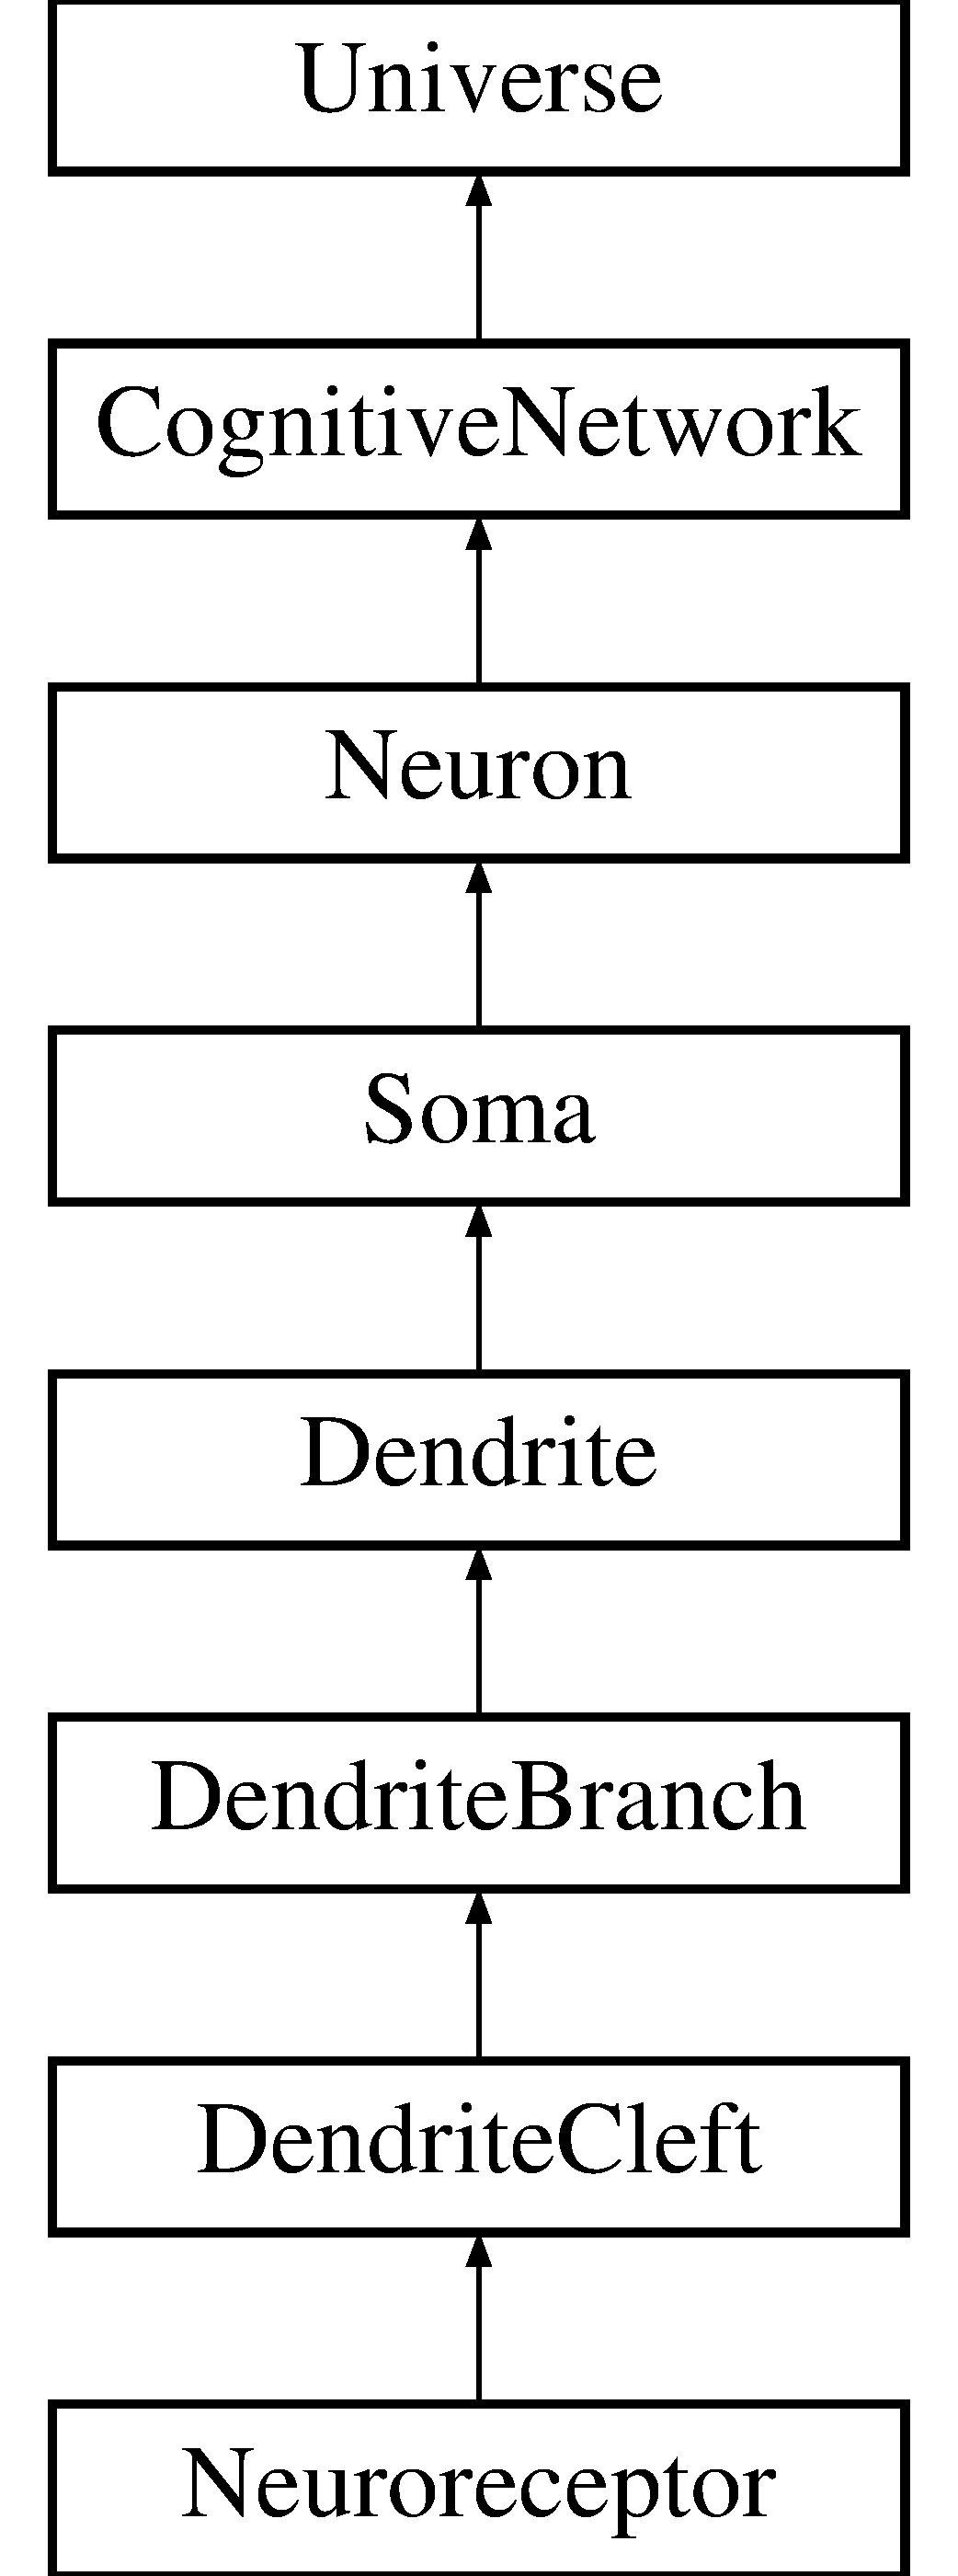
\includegraphics[height=8.000000cm]{classDendriteBranch}
\end{center}
\end{figure}
\subsection*{Public Member Functions}
\begin{DoxyCompactItemize}
\item 
\mbox{\hyperlink{classDendriteBranch_af391f5fd2379539523b3d2523c59ea8b}{Dendrite\+Branch}} ()
\item 
\mbox{\hyperlink{classDendriteBranch_a391ba1440a6c29a0752b03eb60357370}{Dendrite\+Branch}} (unsigned int object\+\_\+type)
\item 
\mbox{\hyperlink{classDendriteBranch_a390bfee680074f5f3ddcd9aee54db679}{Dendrite\+Branch}} (unsigned int object\+\_\+type, std\+::chrono\+::time\+\_\+point$<$ \mbox{\hyperlink{universe_8h_a0ef8d951d1ca5ab3cfaf7ab4c7a6fd80}{Clock}} $>$ event\+\_\+time)
\item 
\mbox{\hyperlink{classDendriteBranch_a9b7e932b0614dad370edd76f31900c40}{Dendrite\+Branch}} (unsigned int object\+\_\+type, std\+::chrono\+::time\+\_\+point$<$ \mbox{\hyperlink{universe_8h_a0ef8d951d1ca5ab3cfaf7ab4c7a6fd80}{Clock}} $>$ event\+\_\+time, \mbox{\hyperlink{classDendrite}{Dendrite}} \&dendrite\+\_\+connector)
\item 
virtual \mbox{\hyperlink{classDendriteBranch_a38707cb6d1f9f07c6e8aa34a8a415051}{$\sim$\+Dendrite\+Branch}} ()
\item 
unsigned int \mbox{\hyperlink{classDendriteBranch_a4d4a4b1591dd612eef903d95605d50fd}{Get\+Counter}} (std\+::chrono\+::time\+\_\+point$<$ \mbox{\hyperlink{universe_8h_a0ef8d951d1ca5ab3cfaf7ab4c7a6fd80}{Clock}} $>$ event\+\_\+time)
\item 
double \mbox{\hyperlink{classDendriteBranch_afab2dd907fba115c3483cd9a217ccec0}{Get\+Energy}} (std\+::chrono\+::time\+\_\+point$<$ \mbox{\hyperlink{universe_8h_a0ef8d951d1ca5ab3cfaf7ab4c7a6fd80}{Clock}} $>$ event\+\_\+time)
\item 
void \mbox{\hyperlink{classDendriteBranch_a2ce03fbad4a70564eeaafb62debd4d74}{Set\+Counter}} (std\+::chrono\+::time\+\_\+point$<$ \mbox{\hyperlink{universe_8h_a0ef8d951d1ca5ab3cfaf7ab4c7a6fd80}{Clock}} $>$ event\+\_\+time, unsigned int val)
\item 
void \mbox{\hyperlink{classDendriteBranch_a13dd0373022d653448c9067d075586a8}{Set\+Energy}} (std\+::chrono\+::time\+\_\+point$<$ \mbox{\hyperlink{universe_8h_a0ef8d951d1ca5ab3cfaf7ab4c7a6fd80}{Clock}} $>$ event\+\_\+time, double val)
\item 
bool \mbox{\hyperlink{classDendriteBranch_a70b5e63fc44166ccd7f0c7177660c250}{Reset\+Parameters}} (std\+::chrono\+::time\+\_\+point$<$ \mbox{\hyperlink{universe_8h_a0ef8d951d1ca5ab3cfaf7ab4c7a6fd80}{Clock}} $>$ event\+\_\+time)
\item 
\mbox{\hyperlink{classDendriteBranch}{Dendrite\+Branch}} $\ast$ \mbox{\hyperlink{classDendriteBranch_a4f751442a537f2e3d7d0dc66a09bd84b}{Create\+Dendrite\+Cleft}} (std\+::chrono\+::time\+\_\+point$<$ \mbox{\hyperlink{universe_8h_a0ef8d951d1ca5ab3cfaf7ab4c7a6fd80}{Clock}} $>$ event\+\_\+time)
\item 
std\+::vector$<$ \mbox{\hyperlink{classDendriteBranch}{Dendrite\+Branch}} $\ast$ $>$ \mbox{\hyperlink{classDendriteBranch_a86d00d6ad66c8c83683e9e22d73a71b6}{Create\+Dendrite\+Clefts}} (std\+::chrono\+::time\+\_\+point$<$ \mbox{\hyperlink{universe_8h_a0ef8d951d1ca5ab3cfaf7ab4c7a6fd80}{Clock}} $>$ event\+\_\+time, int quantity)
\item 
\mbox{\hyperlink{classDendriteBranch}{Dendrite\+Branch}} $\ast$ \mbox{\hyperlink{classDendriteBranch_a45d2fea350165fe0c81f1f429aa96061}{Clone\+Dendrite\+Cleft}} (std\+::chrono\+::time\+\_\+point$<$ \mbox{\hyperlink{universe_8h_a0ef8d951d1ca5ab3cfaf7ab4c7a6fd80}{Clock}} $>$ event\+\_\+time, \mbox{\hyperlink{classDendriteBranch}{Dendrite\+Branch}} $\ast$clone\+\_\+object, double perfection\+\_\+membership)
\item 
std\+::vector$<$ \mbox{\hyperlink{classDendriteBranch}{Dendrite\+Branch}} $\ast$ $>$ \mbox{\hyperlink{classDendriteBranch_a3cf1e07fe5e0ea827965c0dc76881c9f}{Clone\+Dendrite\+Clefts}} (std\+::chrono\+::time\+\_\+point$<$ \mbox{\hyperlink{universe_8h_a0ef8d951d1ca5ab3cfaf7ab4c7a6fd80}{Clock}} $>$ event\+\_\+time, std\+::vector$<$ \mbox{\hyperlink{classDendriteBranch}{Dendrite\+Branch}} $\ast$$>$ cloning\+\_\+list, double perfection\+\_\+membership)
\item 
\mbox{\hyperlink{classDendriteBranch}{Dendrite\+Branch}} $\ast$ \mbox{\hyperlink{classDendriteBranch_a60225ab106eae6bce25eb8159166d5e9}{Destroy\+Dendrite\+Cleft}} (std\+::chrono\+::time\+\_\+point$<$ \mbox{\hyperlink{universe_8h_a0ef8d951d1ca5ab3cfaf7ab4c7a6fd80}{Clock}} $>$ event\+\_\+time, \mbox{\hyperlink{classDendriteBranch}{Dendrite\+Branch}} $\ast$destroy\+\_\+object)
\item 
std\+::vector$<$ \mbox{\hyperlink{classDendriteBranch}{Dendrite\+Branch}} $\ast$ $>$ \mbox{\hyperlink{classDendriteBranch_a454dd0483439353076df63fc124a24f7}{Destroy\+Dendrite\+Clefts}} (std\+::chrono\+::time\+\_\+point$<$ \mbox{\hyperlink{universe_8h_a0ef8d951d1ca5ab3cfaf7ab4c7a6fd80}{Clock}} $>$ event\+\_\+time, std\+::vector$<$ \mbox{\hyperlink{classDendriteBranch}{Dendrite\+Branch}} $\ast$$>$ destruction\+\_\+list)
\item 
\mbox{\hyperlink{classDendriteBranch}{Dendrite\+Branch}} $\ast$ \mbox{\hyperlink{classDendriteBranch_a060f0c55b2e6cb65b68e160df0bbf563}{Add\+Dendrite\+Cleft}} (std\+::chrono\+::time\+\_\+point$<$ \mbox{\hyperlink{universe_8h_a0ef8d951d1ca5ab3cfaf7ab4c7a6fd80}{Clock}} $>$ event\+\_\+time, \mbox{\hyperlink{classDendriteBranch}{Dendrite\+Branch}} $\ast$add\+\_\+object)
\item 
std\+::vector$<$ \mbox{\hyperlink{classDendriteBranch}{Dendrite\+Branch}} $\ast$ $>$ \mbox{\hyperlink{classDendriteBranch_a2ddeff41db805e414c994ac169cbcf4b}{Add\+Dendrite\+Clefts}} (std\+::chrono\+::time\+\_\+point$<$ \mbox{\hyperlink{universe_8h_a0ef8d951d1ca5ab3cfaf7ab4c7a6fd80}{Clock}} $>$ event\+\_\+time, std\+::vector$<$ \mbox{\hyperlink{classDendriteBranch}{Dendrite\+Branch}} $\ast$$>$ add\+\_\+objects)
\item 
\mbox{\hyperlink{classDendriteBranch}{Dendrite\+Branch}} $\ast$ \mbox{\hyperlink{classDendriteBranch_afaca221cb4bba98e56f11b0f9e6370b5}{Remove\+Dendrite\+Cleft}} (std\+::chrono\+::time\+\_\+point$<$ \mbox{\hyperlink{universe_8h_a0ef8d951d1ca5ab3cfaf7ab4c7a6fd80}{Clock}} $>$ event\+\_\+time)
\item 
std\+::vector$<$ \mbox{\hyperlink{classDendriteBranch}{Dendrite\+Branch}} $\ast$ $>$ \mbox{\hyperlink{classDendriteBranch_acd54003e5acb9abda7d7a42f248c14b0}{Remove\+Dendrite\+Clefts}} (std\+::chrono\+::time\+\_\+point$<$ \mbox{\hyperlink{universe_8h_a0ef8d951d1ca5ab3cfaf7ab4c7a6fd80}{Clock}} $>$ event\+\_\+time, int quantity)
\item 
\mbox{\hyperlink{classDendriteBranch}{Dendrite\+Branch}} $\ast$ \mbox{\hyperlink{classDendriteBranch_a11f25ffce77011afad909acb593d2e42}{Get\+Dendrite\+Cleft}} (std\+::chrono\+::time\+\_\+point$<$ \mbox{\hyperlink{universe_8h_a0ef8d951d1ca5ab3cfaf7ab4c7a6fd80}{Clock}} $>$ event\+\_\+time, int selector)
\item 
std\+::vector$<$ \mbox{\hyperlink{classDendriteBranch}{Dendrite\+Branch}} $\ast$ $>$ \mbox{\hyperlink{classDendriteBranch_a2be44a81b4b5213947e9545400a0453c}{Get\+Dendrite\+Clefts}} (std\+::chrono\+::time\+\_\+point$<$ \mbox{\hyperlink{universe_8h_a0ef8d951d1ca5ab3cfaf7ab4c7a6fd80}{Clock}} $>$ event\+\_\+time)
\item 
int \mbox{\hyperlink{classDendriteBranch_a4b950ef8a0856a11240d353bcfd1fba4}{Growth}} (std\+::chrono\+::time\+\_\+point$<$ \mbox{\hyperlink{universe_8h_a0ef8d951d1ca5ab3cfaf7ab4c7a6fd80}{Clock}} $>$ event\+\_\+time)
\item 
int \mbox{\hyperlink{classDendriteBranch_a8540dfafeb5bd45f782ab31b8231b10f}{Update}} (std\+::chrono\+::time\+\_\+point$<$ \mbox{\hyperlink{universe_8h_a0ef8d951d1ca5ab3cfaf7ab4c7a6fd80}{Clock}} $>$ event\+\_\+time)
\end{DoxyCompactItemize}
\subsection*{Protected Attributes}
\begin{DoxyCompactItemize}
\item 
std\+::vector$<$ \mbox{\hyperlink{classDendriteBranch}{Dendrite\+Branch}} $\ast$ $>$ \mbox{\hyperlink{classDendriteBranch_a8015119958f7581d826dcac2c21919c9}{dendritecleft\+\_\+list}}
\end{DoxyCompactItemize}
\subsection*{Private Attributes}
\begin{DoxyCompactItemize}
\item 
int \mbox{\hyperlink{classDendriteBranch_a9d7e5a41efbacc5bb7445a978191c2ca}{m\+\_\+\+Dendrite\+Branch\+Type}}
\item 
int \mbox{\hyperlink{classDendriteBranch_a44ed56dc44bea543b97a6924024edaa8}{dendritebranch\+\_\+type}}
\item 
int \mbox{\hyperlink{classDendriteBranch_a14ca1ae99be78c8dbfea00ec0688ec3d}{m\+\_\+add\+Status}}
\item 
int \mbox{\hyperlink{classDendriteBranch_a27d706db3dbe49fea1a33e835036be43}{dendritecleft\+\_\+pool}}
\item 
std\+::chrono\+::time\+\_\+point$<$ \mbox{\hyperlink{universe_8h_a0ef8d951d1ca5ab3cfaf7ab4c7a6fd80}{Clock}} $>$ \mbox{\hyperlink{classDendriteBranch_a253b94811cb4a0697446dc3d572f91de}{time\+\_\+object\+\_\+created}}
\item 
std\+::chrono\+::time\+\_\+point$<$ \mbox{\hyperlink{universe_8h_a0ef8d951d1ca5ab3cfaf7ab4c7a6fd80}{Clock}} $>$ \mbox{\hyperlink{classDendriteBranch_a16bdc976d615cf2b1b5e3238241e19b6}{previous\+\_\+event\+\_\+time}}
\item 
int \mbox{\hyperlink{classDendriteBranch_a534b56c182fe5f07f012b452c22e59e9}{duration\+\_\+since\+\_\+last\+\_\+event}}
\item 
double \mbox{\hyperlink{classDendriteBranch_a06c7e10791bfbafa1f32ff5cc52e689e}{m\+\_\+\+Volume}}
\item 
double \mbox{\hyperlink{classDendriteBranch_ad7296b522c39f3dae64caf75733e7744}{m\+\_\+\+Surface\+Area}}
\item 
double \mbox{\hyperlink{classDendriteBranch_a87bfabc1ab5a0e066085130808b11c30}{m\+\_\+\+Length}}
\item 
double \mbox{\hyperlink{classDendriteBranch_a19c3bd5c518cf8b4fdae49586ad0df4b}{object\+\_\+size}}
\item 
double \mbox{\hyperlink{classDendriteBranch_a0f736fff956d287d66d060865ef0a254}{m\+\_\+dendrite\+Length}}
\begin{DoxyCompactList}\small\item\em Member variable \char`\"{}m\+\_\+dendrite\+Length\char`\"{}. \end{DoxyCompactList}\item 
double \mbox{\hyperlink{classDendriteBranch_a48ffaeeca1f0ffa9245d07f34d768f30}{m\+\_\+dendrite\+Diameter\+Start}}
\begin{DoxyCompactList}\small\item\em Member variable \char`\"{}m\+\_\+dendrite\+Diameter\+Start\char`\"{}. \end{DoxyCompactList}\item 
double \mbox{\hyperlink{classDendriteBranch_ab87dfc434e138ad012bf23d8b8167650}{m\+\_\+dendrite\+Diameter\+End}}
\begin{DoxyCompactList}\small\item\em Member variable \char`\"{}m\+\_\+dendrite\+Diameter\+End\char`\"{}. \end{DoxyCompactList}\item 
double \mbox{\hyperlink{classDendriteBranch_afc2202be6065e3bef5a7024d54f7d4c5}{m\+\_\+membrane\+Resistance}}
\item 
double \mbox{\hyperlink{classDendriteBranch_ac6fb4da55240b7502089d2a29507e05f}{m\+\_\+membrane\+Capacitance}}
\item 
double \mbox{\hyperlink{classDendriteBranch_aefc12ab16c6198a2bd261c47dd148787}{m\+\_\+internal\+Resistance}}
\item 
unsigned int \mbox{\hyperlink{classDendriteBranch_a3c2f2b113bc19eedfb1eead9a477616f}{m\+\_\+\+Counter}}
\begin{DoxyCompactList}\small\item\em Member variable \char`\"{}m\+\_\+\+Counter\char`\"{}. \end{DoxyCompactList}\item 
double \mbox{\hyperlink{classDendriteBranch_a319e6e991af134f8f37bae3ed6da14d2}{object\+\_\+energy}}
\begin{DoxyCompactList}\small\item\em Member variable \char`\"{}object\+\_\+energy\char`\"{}. \end{DoxyCompactList}\item 
double \mbox{\hyperlink{classDendriteBranch_a697663e490708e557511316e798cb7e8}{object\+\_\+energy\+Inc}}
\item 
double \mbox{\hyperlink{classDendriteBranch_a5d77cb55a6f5d986d671970cf284bd7f}{object\+\_\+energy\+Dec}}
\item 
double \mbox{\hyperlink{classDendriteBranch_ac3fb26edaf6f895856c1ec6db8e50781}{object\+\_\+energy\+Leak}}
\item 
double \mbox{\hyperlink{classDendriteBranch_a261cb8f1bc667b0f412b15f2308f63eb}{object\+\_\+energy\+\_\+threshold}}
\item 
double \mbox{\hyperlink{classDendriteBranch_a26ac4fd971258f19d15ccdc7d7f6b8c8}{m\+\_\+\+Time\+Dilation}}
\item 
double \mbox{\hyperlink{classDendriteBranch_aab9a65d713c085277489bfdc6255ed36}{m\+\_\+\+Time\+Threshold}}
\item 
bool \mbox{\hyperlink{classDendriteBranch_adb05fc412eaeef001fe62550e543b9b1}{object\+\_\+disabled}}
\item 
bool \mbox{\hyperlink{classDendriteBranch_a061380e64b7632973504c4b5ecb53d65}{object\+\_\+initialised}}
\end{DoxyCompactItemize}
\subsection*{Additional Inherited Members}


\subsection{Constructor \& Destructor Documentation}
\mbox{\Hypertarget{classDendriteBranch_af391f5fd2379539523b3d2523c59ea8b}\label{classDendriteBranch_af391f5fd2379539523b3d2523c59ea8b}} 
\index{Dendrite\+Branch@{Dendrite\+Branch}!Dendrite\+Branch@{Dendrite\+Branch}}
\index{Dendrite\+Branch@{Dendrite\+Branch}!Dendrite\+Branch@{Dendrite\+Branch}}
\subsubsection{\texorpdfstring{Dendrite\+Branch()}{DendriteBranch()}\hspace{0.1cm}{\footnotesize\ttfamily [1/4]}}
{\footnotesize\ttfamily Dendrite\+Branch\+::\+Dendrite\+Branch (\begin{DoxyParamCaption}{ }\end{DoxyParamCaption})\hspace{0.3cm}{\ttfamily [inline]}}

\mbox{\Hypertarget{classDendriteBranch_a391ba1440a6c29a0752b03eb60357370}\label{classDendriteBranch_a391ba1440a6c29a0752b03eb60357370}} 
\index{Dendrite\+Branch@{Dendrite\+Branch}!Dendrite\+Branch@{Dendrite\+Branch}}
\index{Dendrite\+Branch@{Dendrite\+Branch}!Dendrite\+Branch@{Dendrite\+Branch}}
\subsubsection{\texorpdfstring{Dendrite\+Branch()}{DendriteBranch()}\hspace{0.1cm}{\footnotesize\ttfamily [2/4]}}
{\footnotesize\ttfamily Dendrite\+Branch\+::\+Dendrite\+Branch (\begin{DoxyParamCaption}\item[{unsigned int}]{object\+\_\+type }\end{DoxyParamCaption})\hspace{0.3cm}{\ttfamily [inline]}}

\mbox{\Hypertarget{classDendriteBranch_a390bfee680074f5f3ddcd9aee54db679}\label{classDendriteBranch_a390bfee680074f5f3ddcd9aee54db679}} 
\index{Dendrite\+Branch@{Dendrite\+Branch}!Dendrite\+Branch@{Dendrite\+Branch}}
\index{Dendrite\+Branch@{Dendrite\+Branch}!Dendrite\+Branch@{Dendrite\+Branch}}
\subsubsection{\texorpdfstring{Dendrite\+Branch()}{DendriteBranch()}\hspace{0.1cm}{\footnotesize\ttfamily [3/4]}}
{\footnotesize\ttfamily Dendrite\+Branch\+::\+Dendrite\+Branch (\begin{DoxyParamCaption}\item[{unsigned int}]{object\+\_\+type,  }\item[{std\+::chrono\+::time\+\_\+point$<$ \mbox{\hyperlink{universe_8h_a0ef8d951d1ca5ab3cfaf7ab4c7a6fd80}{Clock}} $>$}]{event\+\_\+time }\end{DoxyParamCaption})\hspace{0.3cm}{\ttfamily [inline]}}

\mbox{\Hypertarget{classDendriteBranch_a9b7e932b0614dad370edd76f31900c40}\label{classDendriteBranch_a9b7e932b0614dad370edd76f31900c40}} 
\index{Dendrite\+Branch@{Dendrite\+Branch}!Dendrite\+Branch@{Dendrite\+Branch}}
\index{Dendrite\+Branch@{Dendrite\+Branch}!Dendrite\+Branch@{Dendrite\+Branch}}
\subsubsection{\texorpdfstring{Dendrite\+Branch()}{DendriteBranch()}\hspace{0.1cm}{\footnotesize\ttfamily [4/4]}}
{\footnotesize\ttfamily Dendrite\+Branch\+::\+Dendrite\+Branch (\begin{DoxyParamCaption}\item[{unsigned int}]{object\+\_\+type,  }\item[{std\+::chrono\+::time\+\_\+point$<$ \mbox{\hyperlink{universe_8h_a0ef8d951d1ca5ab3cfaf7ab4c7a6fd80}{Clock}} $>$}]{event\+\_\+time,  }\item[{\mbox{\hyperlink{classDendrite}{Dendrite}} \&}]{dendrite\+\_\+connector }\end{DoxyParamCaption})\hspace{0.3cm}{\ttfamily [inline]}}

\mbox{\Hypertarget{classDendriteBranch_a38707cb6d1f9f07c6e8aa34a8a415051}\label{classDendriteBranch_a38707cb6d1f9f07c6e8aa34a8a415051}} 
\index{Dendrite\+Branch@{Dendrite\+Branch}!````~Dendrite\+Branch@{$\sim$\+Dendrite\+Branch}}
\index{````~Dendrite\+Branch@{$\sim$\+Dendrite\+Branch}!Dendrite\+Branch@{Dendrite\+Branch}}
\subsubsection{\texorpdfstring{$\sim$\+Dendrite\+Branch()}{~DendriteBranch()}}
{\footnotesize\ttfamily virtual Dendrite\+Branch\+::$\sim$\+Dendrite\+Branch (\begin{DoxyParamCaption}{ }\end{DoxyParamCaption})\hspace{0.3cm}{\ttfamily [inline]}, {\ttfamily [virtual]}}

Default destructor 

\subsection{Member Function Documentation}
\mbox{\Hypertarget{classDendriteBranch_a060f0c55b2e6cb65b68e160df0bbf563}\label{classDendriteBranch_a060f0c55b2e6cb65b68e160df0bbf563}} 
\index{Dendrite\+Branch@{Dendrite\+Branch}!Add\+Dendrite\+Cleft@{Add\+Dendrite\+Cleft}}
\index{Add\+Dendrite\+Cleft@{Add\+Dendrite\+Cleft}!Dendrite\+Branch@{Dendrite\+Branch}}
\subsubsection{\texorpdfstring{Add\+Dendrite\+Cleft()}{AddDendriteCleft()}}
{\footnotesize\ttfamily \mbox{\hyperlink{classDendriteBranch}{Dendrite\+Branch}} $\ast$ Dendrite\+Branch\+::\+Add\+Dendrite\+Cleft (\begin{DoxyParamCaption}\item[{std\+::chrono\+::time\+\_\+point$<$ \mbox{\hyperlink{universe_8h_a0ef8d951d1ca5ab3cfaf7ab4c7a6fd80}{Clock}} $>$}]{event\+\_\+time,  }\item[{\mbox{\hyperlink{classDendriteBranch}{Dendrite\+Branch}} $\ast$}]{add\+\_\+object }\end{DoxyParamCaption})}

\mbox{\Hypertarget{classDendriteBranch_a2ddeff41db805e414c994ac169cbcf4b}\label{classDendriteBranch_a2ddeff41db805e414c994ac169cbcf4b}} 
\index{Dendrite\+Branch@{Dendrite\+Branch}!Add\+Dendrite\+Clefts@{Add\+Dendrite\+Clefts}}
\index{Add\+Dendrite\+Clefts@{Add\+Dendrite\+Clefts}!Dendrite\+Branch@{Dendrite\+Branch}}
\subsubsection{\texorpdfstring{Add\+Dendrite\+Clefts()}{AddDendriteClefts()}}
{\footnotesize\ttfamily std\+::vector$<$ \mbox{\hyperlink{classDendriteBranch}{Dendrite\+Branch}} $\ast$ $>$ Dendrite\+Branch\+::\+Add\+Dendrite\+Clefts (\begin{DoxyParamCaption}\item[{std\+::chrono\+::time\+\_\+point$<$ \mbox{\hyperlink{universe_8h_a0ef8d951d1ca5ab3cfaf7ab4c7a6fd80}{Clock}} $>$}]{event\+\_\+time,  }\item[{std\+::vector$<$ \mbox{\hyperlink{classDendriteBranch}{Dendrite\+Branch}} $\ast$$>$}]{add\+\_\+objects }\end{DoxyParamCaption})}

\mbox{\Hypertarget{classDendriteBranch_a45d2fea350165fe0c81f1f429aa96061}\label{classDendriteBranch_a45d2fea350165fe0c81f1f429aa96061}} 
\index{Dendrite\+Branch@{Dendrite\+Branch}!Clone\+Dendrite\+Cleft@{Clone\+Dendrite\+Cleft}}
\index{Clone\+Dendrite\+Cleft@{Clone\+Dendrite\+Cleft}!Dendrite\+Branch@{Dendrite\+Branch}}
\subsubsection{\texorpdfstring{Clone\+Dendrite\+Cleft()}{CloneDendriteCleft()}}
{\footnotesize\ttfamily \mbox{\hyperlink{classDendriteBranch}{Dendrite\+Branch}} $\ast$ Dendrite\+Branch\+::\+Clone\+Dendrite\+Cleft (\begin{DoxyParamCaption}\item[{std\+::chrono\+::time\+\_\+point$<$ \mbox{\hyperlink{universe_8h_a0ef8d951d1ca5ab3cfaf7ab4c7a6fd80}{Clock}} $>$}]{event\+\_\+time,  }\item[{\mbox{\hyperlink{classDendriteBranch}{Dendrite\+Branch}} $\ast$}]{clone\+\_\+object,  }\item[{double}]{perfection\+\_\+membership }\end{DoxyParamCaption})}

\mbox{\Hypertarget{classDendriteBranch_a3cf1e07fe5e0ea827965c0dc76881c9f}\label{classDendriteBranch_a3cf1e07fe5e0ea827965c0dc76881c9f}} 
\index{Dendrite\+Branch@{Dendrite\+Branch}!Clone\+Dendrite\+Clefts@{Clone\+Dendrite\+Clefts}}
\index{Clone\+Dendrite\+Clefts@{Clone\+Dendrite\+Clefts}!Dendrite\+Branch@{Dendrite\+Branch}}
\subsubsection{\texorpdfstring{Clone\+Dendrite\+Clefts()}{CloneDendriteClefts()}}
{\footnotesize\ttfamily std\+::vector$<$ \mbox{\hyperlink{classDendriteBranch}{Dendrite\+Branch}} $\ast$ $>$ Dendrite\+Branch\+::\+Clone\+Dendrite\+Clefts (\begin{DoxyParamCaption}\item[{std\+::chrono\+::time\+\_\+point$<$ \mbox{\hyperlink{universe_8h_a0ef8d951d1ca5ab3cfaf7ab4c7a6fd80}{Clock}} $>$}]{event\+\_\+time,  }\item[{std\+::vector$<$ \mbox{\hyperlink{classDendriteBranch}{Dendrite\+Branch}} $\ast$$>$}]{cloning\+\_\+list,  }\item[{double}]{perfection\+\_\+membership }\end{DoxyParamCaption})}

\mbox{\Hypertarget{classDendriteBranch_a4f751442a537f2e3d7d0dc66a09bd84b}\label{classDendriteBranch_a4f751442a537f2e3d7d0dc66a09bd84b}} 
\index{Dendrite\+Branch@{Dendrite\+Branch}!Create\+Dendrite\+Cleft@{Create\+Dendrite\+Cleft}}
\index{Create\+Dendrite\+Cleft@{Create\+Dendrite\+Cleft}!Dendrite\+Branch@{Dendrite\+Branch}}
\subsubsection{\texorpdfstring{Create\+Dendrite\+Cleft()}{CreateDendriteCleft()}}
{\footnotesize\ttfamily \mbox{\hyperlink{classDendriteBranch}{Dendrite\+Branch}} $\ast$ Dendrite\+Branch\+::\+Create\+Dendrite\+Cleft (\begin{DoxyParamCaption}\item[{std\+::chrono\+::time\+\_\+point$<$ \mbox{\hyperlink{universe_8h_a0ef8d951d1ca5ab3cfaf7ab4c7a6fd80}{Clock}} $>$}]{event\+\_\+time }\end{DoxyParamCaption})}

\mbox{\Hypertarget{classDendriteBranch_a86d00d6ad66c8c83683e9e22d73a71b6}\label{classDendriteBranch_a86d00d6ad66c8c83683e9e22d73a71b6}} 
\index{Dendrite\+Branch@{Dendrite\+Branch}!Create\+Dendrite\+Clefts@{Create\+Dendrite\+Clefts}}
\index{Create\+Dendrite\+Clefts@{Create\+Dendrite\+Clefts}!Dendrite\+Branch@{Dendrite\+Branch}}
\subsubsection{\texorpdfstring{Create\+Dendrite\+Clefts()}{CreateDendriteClefts()}}
{\footnotesize\ttfamily std\+::vector$<$ \mbox{\hyperlink{classDendriteBranch}{Dendrite\+Branch}} $\ast$ $>$ Dendrite\+Branch\+::\+Create\+Dendrite\+Clefts (\begin{DoxyParamCaption}\item[{std\+::chrono\+::time\+\_\+point$<$ \mbox{\hyperlink{universe_8h_a0ef8d951d1ca5ab3cfaf7ab4c7a6fd80}{Clock}} $>$}]{event\+\_\+time,  }\item[{int}]{quantity }\end{DoxyParamCaption})}

\mbox{\Hypertarget{classDendriteBranch_a60225ab106eae6bce25eb8159166d5e9}\label{classDendriteBranch_a60225ab106eae6bce25eb8159166d5e9}} 
\index{Dendrite\+Branch@{Dendrite\+Branch}!Destroy\+Dendrite\+Cleft@{Destroy\+Dendrite\+Cleft}}
\index{Destroy\+Dendrite\+Cleft@{Destroy\+Dendrite\+Cleft}!Dendrite\+Branch@{Dendrite\+Branch}}
\subsubsection{\texorpdfstring{Destroy\+Dendrite\+Cleft()}{DestroyDendriteCleft()}}
{\footnotesize\ttfamily \mbox{\hyperlink{classDendriteBranch}{Dendrite\+Branch}} $\ast$ Dendrite\+Branch\+::\+Destroy\+Dendrite\+Cleft (\begin{DoxyParamCaption}\item[{std\+::chrono\+::time\+\_\+point$<$ \mbox{\hyperlink{universe_8h_a0ef8d951d1ca5ab3cfaf7ab4c7a6fd80}{Clock}} $>$}]{event\+\_\+time,  }\item[{\mbox{\hyperlink{classDendriteBranch}{Dendrite\+Branch}} $\ast$}]{destroy\+\_\+object }\end{DoxyParamCaption})}

\mbox{\Hypertarget{classDendriteBranch_a454dd0483439353076df63fc124a24f7}\label{classDendriteBranch_a454dd0483439353076df63fc124a24f7}} 
\index{Dendrite\+Branch@{Dendrite\+Branch}!Destroy\+Dendrite\+Clefts@{Destroy\+Dendrite\+Clefts}}
\index{Destroy\+Dendrite\+Clefts@{Destroy\+Dendrite\+Clefts}!Dendrite\+Branch@{Dendrite\+Branch}}
\subsubsection{\texorpdfstring{Destroy\+Dendrite\+Clefts()}{DestroyDendriteClefts()}}
{\footnotesize\ttfamily std\+::vector$<$ \mbox{\hyperlink{classDendriteBranch}{Dendrite\+Branch}} $\ast$ $>$ Dendrite\+Branch\+::\+Destroy\+Dendrite\+Clefts (\begin{DoxyParamCaption}\item[{std\+::chrono\+::time\+\_\+point$<$ \mbox{\hyperlink{universe_8h_a0ef8d951d1ca5ab3cfaf7ab4c7a6fd80}{Clock}} $>$}]{event\+\_\+time,  }\item[{std\+::vector$<$ \mbox{\hyperlink{classDendriteBranch}{Dendrite\+Branch}} $\ast$$>$}]{destruction\+\_\+list }\end{DoxyParamCaption})}

\mbox{\Hypertarget{classDendriteBranch_a4d4a4b1591dd612eef903d95605d50fd}\label{classDendriteBranch_a4d4a4b1591dd612eef903d95605d50fd}} 
\index{Dendrite\+Branch@{Dendrite\+Branch}!Get\+Counter@{Get\+Counter}}
\index{Get\+Counter@{Get\+Counter}!Dendrite\+Branch@{Dendrite\+Branch}}
\subsubsection{\texorpdfstring{Get\+Counter()}{GetCounter()}}
{\footnotesize\ttfamily unsigned int Dendrite\+Branch\+::\+Get\+Counter (\begin{DoxyParamCaption}\item[{std\+::chrono\+::time\+\_\+point$<$ \mbox{\hyperlink{universe_8h_a0ef8d951d1ca5ab3cfaf7ab4c7a6fd80}{Clock}} $>$}]{event\+\_\+time }\end{DoxyParamCaption})\hspace{0.3cm}{\ttfamily [inline]}}

\mbox{\Hypertarget{classDendriteBranch_a11f25ffce77011afad909acb593d2e42}\label{classDendriteBranch_a11f25ffce77011afad909acb593d2e42}} 
\index{Dendrite\+Branch@{Dendrite\+Branch}!Get\+Dendrite\+Cleft@{Get\+Dendrite\+Cleft}}
\index{Get\+Dendrite\+Cleft@{Get\+Dendrite\+Cleft}!Dendrite\+Branch@{Dendrite\+Branch}}
\subsubsection{\texorpdfstring{Get\+Dendrite\+Cleft()}{GetDendriteCleft()}}
{\footnotesize\ttfamily \mbox{\hyperlink{classDendriteBranch}{Dendrite\+Branch}} $\ast$ Dendrite\+Branch\+::\+Get\+Dendrite\+Cleft (\begin{DoxyParamCaption}\item[{std\+::chrono\+::time\+\_\+point$<$ \mbox{\hyperlink{universe_8h_a0ef8d951d1ca5ab3cfaf7ab4c7a6fd80}{Clock}} $>$}]{event\+\_\+time,  }\item[{int}]{selector }\end{DoxyParamCaption})}

\mbox{\Hypertarget{classDendriteBranch_a2be44a81b4b5213947e9545400a0453c}\label{classDendriteBranch_a2be44a81b4b5213947e9545400a0453c}} 
\index{Dendrite\+Branch@{Dendrite\+Branch}!Get\+Dendrite\+Clefts@{Get\+Dendrite\+Clefts}}
\index{Get\+Dendrite\+Clefts@{Get\+Dendrite\+Clefts}!Dendrite\+Branch@{Dendrite\+Branch}}
\subsubsection{\texorpdfstring{Get\+Dendrite\+Clefts()}{GetDendriteClefts()}}
{\footnotesize\ttfamily std\+::vector$<$ \mbox{\hyperlink{classDendriteBranch}{Dendrite\+Branch}} $\ast$ $>$ Dendrite\+Branch\+::\+Get\+Dendrite\+Clefts (\begin{DoxyParamCaption}\item[{std\+::chrono\+::time\+\_\+point$<$ \mbox{\hyperlink{universe_8h_a0ef8d951d1ca5ab3cfaf7ab4c7a6fd80}{Clock}} $>$}]{event\+\_\+time }\end{DoxyParamCaption})}

\mbox{\Hypertarget{classDendriteBranch_afab2dd907fba115c3483cd9a217ccec0}\label{classDendriteBranch_afab2dd907fba115c3483cd9a217ccec0}} 
\index{Dendrite\+Branch@{Dendrite\+Branch}!Get\+Energy@{Get\+Energy}}
\index{Get\+Energy@{Get\+Energy}!Dendrite\+Branch@{Dendrite\+Branch}}
\subsubsection{\texorpdfstring{Get\+Energy()}{GetEnergy()}}
{\footnotesize\ttfamily double Dendrite\+Branch\+::\+Get\+Energy (\begin{DoxyParamCaption}\item[{std\+::chrono\+::time\+\_\+point$<$ \mbox{\hyperlink{universe_8h_a0ef8d951d1ca5ab3cfaf7ab4c7a6fd80}{Clock}} $>$}]{event\+\_\+time }\end{DoxyParamCaption})\hspace{0.3cm}{\ttfamily [inline]}}

\mbox{\Hypertarget{classDendriteBranch_a4b950ef8a0856a11240d353bcfd1fba4}\label{classDendriteBranch_a4b950ef8a0856a11240d353bcfd1fba4}} 
\index{Dendrite\+Branch@{Dendrite\+Branch}!Growth@{Growth}}
\index{Growth@{Growth}!Dendrite\+Branch@{Dendrite\+Branch}}
\subsubsection{\texorpdfstring{Growth()}{Growth()}}
{\footnotesize\ttfamily int Dendrite\+Branch\+::\+Growth (\begin{DoxyParamCaption}\item[{std\+::chrono\+::time\+\_\+point$<$ \mbox{\hyperlink{universe_8h_a0ef8d951d1ca5ab3cfaf7ab4c7a6fd80}{Clock}} $>$}]{event\+\_\+time }\end{DoxyParamCaption})}

\mbox{\Hypertarget{classDendriteBranch_afaca221cb4bba98e56f11b0f9e6370b5}\label{classDendriteBranch_afaca221cb4bba98e56f11b0f9e6370b5}} 
\index{Dendrite\+Branch@{Dendrite\+Branch}!Remove\+Dendrite\+Cleft@{Remove\+Dendrite\+Cleft}}
\index{Remove\+Dendrite\+Cleft@{Remove\+Dendrite\+Cleft}!Dendrite\+Branch@{Dendrite\+Branch}}
\subsubsection{\texorpdfstring{Remove\+Dendrite\+Cleft()}{RemoveDendriteCleft()}}
{\footnotesize\ttfamily \mbox{\hyperlink{classDendriteBranch}{Dendrite\+Branch}} $\ast$ Dendrite\+Branch\+::\+Remove\+Dendrite\+Cleft (\begin{DoxyParamCaption}\item[{std\+::chrono\+::time\+\_\+point$<$ \mbox{\hyperlink{universe_8h_a0ef8d951d1ca5ab3cfaf7ab4c7a6fd80}{Clock}} $>$}]{event\+\_\+time }\end{DoxyParamCaption})}

\mbox{\Hypertarget{classDendriteBranch_acd54003e5acb9abda7d7a42f248c14b0}\label{classDendriteBranch_acd54003e5acb9abda7d7a42f248c14b0}} 
\index{Dendrite\+Branch@{Dendrite\+Branch}!Remove\+Dendrite\+Clefts@{Remove\+Dendrite\+Clefts}}
\index{Remove\+Dendrite\+Clefts@{Remove\+Dendrite\+Clefts}!Dendrite\+Branch@{Dendrite\+Branch}}
\subsubsection{\texorpdfstring{Remove\+Dendrite\+Clefts()}{RemoveDendriteClefts()}}
{\footnotesize\ttfamily std\+::vector$<$ \mbox{\hyperlink{classDendriteBranch}{Dendrite\+Branch}} $\ast$ $>$ Dendrite\+Branch\+::\+Remove\+Dendrite\+Clefts (\begin{DoxyParamCaption}\item[{std\+::chrono\+::time\+\_\+point$<$ \mbox{\hyperlink{universe_8h_a0ef8d951d1ca5ab3cfaf7ab4c7a6fd80}{Clock}} $>$}]{event\+\_\+time,  }\item[{int}]{quantity }\end{DoxyParamCaption})}

\mbox{\Hypertarget{classDendriteBranch_a70b5e63fc44166ccd7f0c7177660c250}\label{classDendriteBranch_a70b5e63fc44166ccd7f0c7177660c250}} 
\index{Dendrite\+Branch@{Dendrite\+Branch}!Reset\+Parameters@{Reset\+Parameters}}
\index{Reset\+Parameters@{Reset\+Parameters}!Dendrite\+Branch@{Dendrite\+Branch}}
\subsubsection{\texorpdfstring{Reset\+Parameters()}{ResetParameters()}}
{\footnotesize\ttfamily bool Dendrite\+Branch\+::\+Reset\+Parameters (\begin{DoxyParamCaption}\item[{std\+::chrono\+::time\+\_\+point$<$ \mbox{\hyperlink{universe_8h_a0ef8d951d1ca5ab3cfaf7ab4c7a6fd80}{Clock}} $>$}]{event\+\_\+time }\end{DoxyParamCaption})}

\mbox{\Hypertarget{classDendriteBranch_a2ce03fbad4a70564eeaafb62debd4d74}\label{classDendriteBranch_a2ce03fbad4a70564eeaafb62debd4d74}} 
\index{Dendrite\+Branch@{Dendrite\+Branch}!Set\+Counter@{Set\+Counter}}
\index{Set\+Counter@{Set\+Counter}!Dendrite\+Branch@{Dendrite\+Branch}}
\subsubsection{\texorpdfstring{Set\+Counter()}{SetCounter()}}
{\footnotesize\ttfamily void Dendrite\+Branch\+::\+Set\+Counter (\begin{DoxyParamCaption}\item[{std\+::chrono\+::time\+\_\+point$<$ \mbox{\hyperlink{universe_8h_a0ef8d951d1ca5ab3cfaf7ab4c7a6fd80}{Clock}} $>$}]{event\+\_\+time,  }\item[{unsigned int}]{val }\end{DoxyParamCaption})\hspace{0.3cm}{\ttfamily [inline]}, {\ttfamily [virtual]}}



Reimplemented from \mbox{\hyperlink{classDendrite_a7529495515de74fff2b9a92b12531057}{Dendrite}}.



Reimplemented in \mbox{\hyperlink{classNeuroreceptor_a0660a316ef44cf723509f720acd16f24}{Neuroreceptor}}, and \mbox{\hyperlink{classDendriteCleft_a428b8e5117f381a382e0071b936d42a1}{Dendrite\+Cleft}}.

\mbox{\Hypertarget{classDendriteBranch_a13dd0373022d653448c9067d075586a8}\label{classDendriteBranch_a13dd0373022d653448c9067d075586a8}} 
\index{Dendrite\+Branch@{Dendrite\+Branch}!Set\+Energy@{Set\+Energy}}
\index{Set\+Energy@{Set\+Energy}!Dendrite\+Branch@{Dendrite\+Branch}}
\subsubsection{\texorpdfstring{Set\+Energy()}{SetEnergy()}}
{\footnotesize\ttfamily void Dendrite\+Branch\+::\+Set\+Energy (\begin{DoxyParamCaption}\item[{std\+::chrono\+::time\+\_\+point$<$ \mbox{\hyperlink{universe_8h_a0ef8d951d1ca5ab3cfaf7ab4c7a6fd80}{Clock}} $>$}]{event\+\_\+time,  }\item[{double}]{val }\end{DoxyParamCaption})\hspace{0.3cm}{\ttfamily [inline]}}

\mbox{\Hypertarget{classDendriteBranch_a8540dfafeb5bd45f782ab31b8231b10f}\label{classDendriteBranch_a8540dfafeb5bd45f782ab31b8231b10f}} 
\index{Dendrite\+Branch@{Dendrite\+Branch}!Update@{Update}}
\index{Update@{Update}!Dendrite\+Branch@{Dendrite\+Branch}}
\subsubsection{\texorpdfstring{Update()}{Update()}}
{\footnotesize\ttfamily int Dendrite\+Branch\+::\+Update (\begin{DoxyParamCaption}\item[{std\+::chrono\+::time\+\_\+point$<$ \mbox{\hyperlink{universe_8h_a0ef8d951d1ca5ab3cfaf7ab4c7a6fd80}{Clock}} $>$}]{event\+\_\+time }\end{DoxyParamCaption})}



\subsection{Member Data Documentation}
\mbox{\Hypertarget{classDendriteBranch_a44ed56dc44bea543b97a6924024edaa8}\label{classDendriteBranch_a44ed56dc44bea543b97a6924024edaa8}} 
\index{Dendrite\+Branch@{Dendrite\+Branch}!dendritebranch\+\_\+type@{dendritebranch\+\_\+type}}
\index{dendritebranch\+\_\+type@{dendritebranch\+\_\+type}!Dendrite\+Branch@{Dendrite\+Branch}}
\subsubsection{\texorpdfstring{dendritebranch\+\_\+type}{dendritebranch\_type}}
{\footnotesize\ttfamily int Dendrite\+Branch\+::dendritebranch\+\_\+type\hspace{0.3cm}{\ttfamily [private]}}

\mbox{\Hypertarget{classDendriteBranch_a8015119958f7581d826dcac2c21919c9}\label{classDendriteBranch_a8015119958f7581d826dcac2c21919c9}} 
\index{Dendrite\+Branch@{Dendrite\+Branch}!dendritecleft\+\_\+list@{dendritecleft\+\_\+list}}
\index{dendritecleft\+\_\+list@{dendritecleft\+\_\+list}!Dendrite\+Branch@{Dendrite\+Branch}}
\subsubsection{\texorpdfstring{dendritecleft\+\_\+list}{dendritecleft\_list}}
{\footnotesize\ttfamily std\+::vector$<$\mbox{\hyperlink{classDendriteBranch}{Dendrite\+Branch}}$\ast$$>$ Dendrite\+Branch\+::dendritecleft\+\_\+list\hspace{0.3cm}{\ttfamily [protected]}}

\mbox{\Hypertarget{classDendriteBranch_a27d706db3dbe49fea1a33e835036be43}\label{classDendriteBranch_a27d706db3dbe49fea1a33e835036be43}} 
\index{Dendrite\+Branch@{Dendrite\+Branch}!dendritecleft\+\_\+pool@{dendritecleft\+\_\+pool}}
\index{dendritecleft\+\_\+pool@{dendritecleft\+\_\+pool}!Dendrite\+Branch@{Dendrite\+Branch}}
\subsubsection{\texorpdfstring{dendritecleft\+\_\+pool}{dendritecleft\_pool}}
{\footnotesize\ttfamily int Dendrite\+Branch\+::dendritecleft\+\_\+pool\hspace{0.3cm}{\ttfamily [private]}}

\mbox{\Hypertarget{classDendriteBranch_a534b56c182fe5f07f012b452c22e59e9}\label{classDendriteBranch_a534b56c182fe5f07f012b452c22e59e9}} 
\index{Dendrite\+Branch@{Dendrite\+Branch}!duration\+\_\+since\+\_\+last\+\_\+event@{duration\+\_\+since\+\_\+last\+\_\+event}}
\index{duration\+\_\+since\+\_\+last\+\_\+event@{duration\+\_\+since\+\_\+last\+\_\+event}!Dendrite\+Branch@{Dendrite\+Branch}}
\subsubsection{\texorpdfstring{duration\+\_\+since\+\_\+last\+\_\+event}{duration\_since\_last\_event}}
{\footnotesize\ttfamily int Dendrite\+Branch\+::duration\+\_\+since\+\_\+last\+\_\+event\hspace{0.3cm}{\ttfamily [private]}}

\mbox{\Hypertarget{classDendriteBranch_a14ca1ae99be78c8dbfea00ec0688ec3d}\label{classDendriteBranch_a14ca1ae99be78c8dbfea00ec0688ec3d}} 
\index{Dendrite\+Branch@{Dendrite\+Branch}!m\+\_\+add\+Status@{m\+\_\+add\+Status}}
\index{m\+\_\+add\+Status@{m\+\_\+add\+Status}!Dendrite\+Branch@{Dendrite\+Branch}}
\subsubsection{\texorpdfstring{m\+\_\+add\+Status}{m\_addStatus}}
{\footnotesize\ttfamily int Dendrite\+Branch\+::m\+\_\+add\+Status\hspace{0.3cm}{\ttfamily [private]}}

\mbox{\Hypertarget{classDendriteBranch_a3c2f2b113bc19eedfb1eead9a477616f}\label{classDendriteBranch_a3c2f2b113bc19eedfb1eead9a477616f}} 
\index{Dendrite\+Branch@{Dendrite\+Branch}!m\+\_\+\+Counter@{m\+\_\+\+Counter}}
\index{m\+\_\+\+Counter@{m\+\_\+\+Counter}!Dendrite\+Branch@{Dendrite\+Branch}}
\subsubsection{\texorpdfstring{m\+\_\+\+Counter}{m\_Counter}}
{\footnotesize\ttfamily unsigned int Dendrite\+Branch\+::m\+\_\+\+Counter\hspace{0.3cm}{\ttfamily [private]}}



Member variable \char`\"{}m\+\_\+\+Counter\char`\"{}. 

\mbox{\Hypertarget{classDendriteBranch_a9d7e5a41efbacc5bb7445a978191c2ca}\label{classDendriteBranch_a9d7e5a41efbacc5bb7445a978191c2ca}} 
\index{Dendrite\+Branch@{Dendrite\+Branch}!m\+\_\+\+Dendrite\+Branch\+Type@{m\+\_\+\+Dendrite\+Branch\+Type}}
\index{m\+\_\+\+Dendrite\+Branch\+Type@{m\+\_\+\+Dendrite\+Branch\+Type}!Dendrite\+Branch@{Dendrite\+Branch}}
\subsubsection{\texorpdfstring{m\+\_\+\+Dendrite\+Branch\+Type}{m\_DendriteBranchType}}
{\footnotesize\ttfamily int Dendrite\+Branch\+::m\+\_\+\+Dendrite\+Branch\+Type\hspace{0.3cm}{\ttfamily [private]}}

\mbox{\Hypertarget{classDendriteBranch_ab87dfc434e138ad012bf23d8b8167650}\label{classDendriteBranch_ab87dfc434e138ad012bf23d8b8167650}} 
\index{Dendrite\+Branch@{Dendrite\+Branch}!m\+\_\+dendrite\+Diameter\+End@{m\+\_\+dendrite\+Diameter\+End}}
\index{m\+\_\+dendrite\+Diameter\+End@{m\+\_\+dendrite\+Diameter\+End}!Dendrite\+Branch@{Dendrite\+Branch}}
\subsubsection{\texorpdfstring{m\+\_\+dendrite\+Diameter\+End}{m\_dendriteDiameterEnd}}
{\footnotesize\ttfamily double Dendrite\+Branch\+::m\+\_\+dendrite\+Diameter\+End\hspace{0.3cm}{\ttfamily [private]}}



Member variable \char`\"{}m\+\_\+dendrite\+Diameter\+End\char`\"{}. 

\mbox{\Hypertarget{classDendriteBranch_a48ffaeeca1f0ffa9245d07f34d768f30}\label{classDendriteBranch_a48ffaeeca1f0ffa9245d07f34d768f30}} 
\index{Dendrite\+Branch@{Dendrite\+Branch}!m\+\_\+dendrite\+Diameter\+Start@{m\+\_\+dendrite\+Diameter\+Start}}
\index{m\+\_\+dendrite\+Diameter\+Start@{m\+\_\+dendrite\+Diameter\+Start}!Dendrite\+Branch@{Dendrite\+Branch}}
\subsubsection{\texorpdfstring{m\+\_\+dendrite\+Diameter\+Start}{m\_dendriteDiameterStart}}
{\footnotesize\ttfamily double Dendrite\+Branch\+::m\+\_\+dendrite\+Diameter\+Start\hspace{0.3cm}{\ttfamily [private]}}



Member variable \char`\"{}m\+\_\+dendrite\+Diameter\+Start\char`\"{}. 

\mbox{\Hypertarget{classDendriteBranch_a0f736fff956d287d66d060865ef0a254}\label{classDendriteBranch_a0f736fff956d287d66d060865ef0a254}} 
\index{Dendrite\+Branch@{Dendrite\+Branch}!m\+\_\+dendrite\+Length@{m\+\_\+dendrite\+Length}}
\index{m\+\_\+dendrite\+Length@{m\+\_\+dendrite\+Length}!Dendrite\+Branch@{Dendrite\+Branch}}
\subsubsection{\texorpdfstring{m\+\_\+dendrite\+Length}{m\_dendriteLength}}
{\footnotesize\ttfamily double Dendrite\+Branch\+::m\+\_\+dendrite\+Length\hspace{0.3cm}{\ttfamily [private]}}



Member variable \char`\"{}m\+\_\+dendrite\+Length\char`\"{}. 

\mbox{\Hypertarget{classDendriteBranch_aefc12ab16c6198a2bd261c47dd148787}\label{classDendriteBranch_aefc12ab16c6198a2bd261c47dd148787}} 
\index{Dendrite\+Branch@{Dendrite\+Branch}!m\+\_\+internal\+Resistance@{m\+\_\+internal\+Resistance}}
\index{m\+\_\+internal\+Resistance@{m\+\_\+internal\+Resistance}!Dendrite\+Branch@{Dendrite\+Branch}}
\subsubsection{\texorpdfstring{m\+\_\+internal\+Resistance}{m\_internalResistance}}
{\footnotesize\ttfamily double Dendrite\+Branch\+::m\+\_\+internal\+Resistance\hspace{0.3cm}{\ttfamily [private]}}

\mbox{\Hypertarget{classDendriteBranch_a87bfabc1ab5a0e066085130808b11c30}\label{classDendriteBranch_a87bfabc1ab5a0e066085130808b11c30}} 
\index{Dendrite\+Branch@{Dendrite\+Branch}!m\+\_\+\+Length@{m\+\_\+\+Length}}
\index{m\+\_\+\+Length@{m\+\_\+\+Length}!Dendrite\+Branch@{Dendrite\+Branch}}
\subsubsection{\texorpdfstring{m\+\_\+\+Length}{m\_Length}}
{\footnotesize\ttfamily double Dendrite\+Branch\+::m\+\_\+\+Length\hspace{0.3cm}{\ttfamily [private]}}

\mbox{\Hypertarget{classDendriteBranch_ac6fb4da55240b7502089d2a29507e05f}\label{classDendriteBranch_ac6fb4da55240b7502089d2a29507e05f}} 
\index{Dendrite\+Branch@{Dendrite\+Branch}!m\+\_\+membrane\+Capacitance@{m\+\_\+membrane\+Capacitance}}
\index{m\+\_\+membrane\+Capacitance@{m\+\_\+membrane\+Capacitance}!Dendrite\+Branch@{Dendrite\+Branch}}
\subsubsection{\texorpdfstring{m\+\_\+membrane\+Capacitance}{m\_membraneCapacitance}}
{\footnotesize\ttfamily double Dendrite\+Branch\+::m\+\_\+membrane\+Capacitance\hspace{0.3cm}{\ttfamily [private]}}

\mbox{\Hypertarget{classDendriteBranch_afc2202be6065e3bef5a7024d54f7d4c5}\label{classDendriteBranch_afc2202be6065e3bef5a7024d54f7d4c5}} 
\index{Dendrite\+Branch@{Dendrite\+Branch}!m\+\_\+membrane\+Resistance@{m\+\_\+membrane\+Resistance}}
\index{m\+\_\+membrane\+Resistance@{m\+\_\+membrane\+Resistance}!Dendrite\+Branch@{Dendrite\+Branch}}
\subsubsection{\texorpdfstring{m\+\_\+membrane\+Resistance}{m\_membraneResistance}}
{\footnotesize\ttfamily double Dendrite\+Branch\+::m\+\_\+membrane\+Resistance\hspace{0.3cm}{\ttfamily [private]}}

\mbox{\Hypertarget{classDendriteBranch_ad7296b522c39f3dae64caf75733e7744}\label{classDendriteBranch_ad7296b522c39f3dae64caf75733e7744}} 
\index{Dendrite\+Branch@{Dendrite\+Branch}!m\+\_\+\+Surface\+Area@{m\+\_\+\+Surface\+Area}}
\index{m\+\_\+\+Surface\+Area@{m\+\_\+\+Surface\+Area}!Dendrite\+Branch@{Dendrite\+Branch}}
\subsubsection{\texorpdfstring{m\+\_\+\+Surface\+Area}{m\_SurfaceArea}}
{\footnotesize\ttfamily double Dendrite\+Branch\+::m\+\_\+\+Surface\+Area\hspace{0.3cm}{\ttfamily [private]}}

\mbox{\Hypertarget{classDendriteBranch_a26ac4fd971258f19d15ccdc7d7f6b8c8}\label{classDendriteBranch_a26ac4fd971258f19d15ccdc7d7f6b8c8}} 
\index{Dendrite\+Branch@{Dendrite\+Branch}!m\+\_\+\+Time\+Dilation@{m\+\_\+\+Time\+Dilation}}
\index{m\+\_\+\+Time\+Dilation@{m\+\_\+\+Time\+Dilation}!Dendrite\+Branch@{Dendrite\+Branch}}
\subsubsection{\texorpdfstring{m\+\_\+\+Time\+Dilation}{m\_TimeDilation}}
{\footnotesize\ttfamily double Dendrite\+Branch\+::m\+\_\+\+Time\+Dilation\hspace{0.3cm}{\ttfamily [private]}}

\mbox{\Hypertarget{classDendriteBranch_aab9a65d713c085277489bfdc6255ed36}\label{classDendriteBranch_aab9a65d713c085277489bfdc6255ed36}} 
\index{Dendrite\+Branch@{Dendrite\+Branch}!m\+\_\+\+Time\+Threshold@{m\+\_\+\+Time\+Threshold}}
\index{m\+\_\+\+Time\+Threshold@{m\+\_\+\+Time\+Threshold}!Dendrite\+Branch@{Dendrite\+Branch}}
\subsubsection{\texorpdfstring{m\+\_\+\+Time\+Threshold}{m\_TimeThreshold}}
{\footnotesize\ttfamily double Dendrite\+Branch\+::m\+\_\+\+Time\+Threshold\hspace{0.3cm}{\ttfamily [private]}}

\mbox{\Hypertarget{classDendriteBranch_a06c7e10791bfbafa1f32ff5cc52e689e}\label{classDendriteBranch_a06c7e10791bfbafa1f32ff5cc52e689e}} 
\index{Dendrite\+Branch@{Dendrite\+Branch}!m\+\_\+\+Volume@{m\+\_\+\+Volume}}
\index{m\+\_\+\+Volume@{m\+\_\+\+Volume}!Dendrite\+Branch@{Dendrite\+Branch}}
\subsubsection{\texorpdfstring{m\+\_\+\+Volume}{m\_Volume}}
{\footnotesize\ttfamily double Dendrite\+Branch\+::m\+\_\+\+Volume\hspace{0.3cm}{\ttfamily [private]}}

\mbox{\Hypertarget{classDendriteBranch_adb05fc412eaeef001fe62550e543b9b1}\label{classDendriteBranch_adb05fc412eaeef001fe62550e543b9b1}} 
\index{Dendrite\+Branch@{Dendrite\+Branch}!object\+\_\+disabled@{object\+\_\+disabled}}
\index{object\+\_\+disabled@{object\+\_\+disabled}!Dendrite\+Branch@{Dendrite\+Branch}}
\subsubsection{\texorpdfstring{object\+\_\+disabled}{object\_disabled}}
{\footnotesize\ttfamily bool Dendrite\+Branch\+::object\+\_\+disabled\hspace{0.3cm}{\ttfamily [private]}}

\mbox{\Hypertarget{classDendriteBranch_a319e6e991af134f8f37bae3ed6da14d2}\label{classDendriteBranch_a319e6e991af134f8f37bae3ed6da14d2}} 
\index{Dendrite\+Branch@{Dendrite\+Branch}!object\+\_\+energy@{object\+\_\+energy}}
\index{object\+\_\+energy@{object\+\_\+energy}!Dendrite\+Branch@{Dendrite\+Branch}}
\subsubsection{\texorpdfstring{object\+\_\+energy}{object\_energy}}
{\footnotesize\ttfamily double Dendrite\+Branch\+::object\+\_\+energy\hspace{0.3cm}{\ttfamily [private]}}



Member variable \char`\"{}object\+\_\+energy\char`\"{}. 

\mbox{\Hypertarget{classDendriteBranch_a261cb8f1bc667b0f412b15f2308f63eb}\label{classDendriteBranch_a261cb8f1bc667b0f412b15f2308f63eb}} 
\index{Dendrite\+Branch@{Dendrite\+Branch}!object\+\_\+energy\+\_\+threshold@{object\+\_\+energy\+\_\+threshold}}
\index{object\+\_\+energy\+\_\+threshold@{object\+\_\+energy\+\_\+threshold}!Dendrite\+Branch@{Dendrite\+Branch}}
\subsubsection{\texorpdfstring{object\+\_\+energy\+\_\+threshold}{object\_energy\_threshold}}
{\footnotesize\ttfamily double Dendrite\+Branch\+::object\+\_\+energy\+\_\+threshold\hspace{0.3cm}{\ttfamily [private]}}

\mbox{\Hypertarget{classDendriteBranch_a5d77cb55a6f5d986d671970cf284bd7f}\label{classDendriteBranch_a5d77cb55a6f5d986d671970cf284bd7f}} 
\index{Dendrite\+Branch@{Dendrite\+Branch}!object\+\_\+energy\+Dec@{object\+\_\+energy\+Dec}}
\index{object\+\_\+energy\+Dec@{object\+\_\+energy\+Dec}!Dendrite\+Branch@{Dendrite\+Branch}}
\subsubsection{\texorpdfstring{object\+\_\+energy\+Dec}{object\_energyDec}}
{\footnotesize\ttfamily double Dendrite\+Branch\+::object\+\_\+energy\+Dec\hspace{0.3cm}{\ttfamily [private]}}

\mbox{\Hypertarget{classDendriteBranch_a697663e490708e557511316e798cb7e8}\label{classDendriteBranch_a697663e490708e557511316e798cb7e8}} 
\index{Dendrite\+Branch@{Dendrite\+Branch}!object\+\_\+energy\+Inc@{object\+\_\+energy\+Inc}}
\index{object\+\_\+energy\+Inc@{object\+\_\+energy\+Inc}!Dendrite\+Branch@{Dendrite\+Branch}}
\subsubsection{\texorpdfstring{object\+\_\+energy\+Inc}{object\_energyInc}}
{\footnotesize\ttfamily double Dendrite\+Branch\+::object\+\_\+energy\+Inc\hspace{0.3cm}{\ttfamily [private]}}

\mbox{\Hypertarget{classDendriteBranch_ac3fb26edaf6f895856c1ec6db8e50781}\label{classDendriteBranch_ac3fb26edaf6f895856c1ec6db8e50781}} 
\index{Dendrite\+Branch@{Dendrite\+Branch}!object\+\_\+energy\+Leak@{object\+\_\+energy\+Leak}}
\index{object\+\_\+energy\+Leak@{object\+\_\+energy\+Leak}!Dendrite\+Branch@{Dendrite\+Branch}}
\subsubsection{\texorpdfstring{object\+\_\+energy\+Leak}{object\_energyLeak}}
{\footnotesize\ttfamily double Dendrite\+Branch\+::object\+\_\+energy\+Leak\hspace{0.3cm}{\ttfamily [private]}}

\mbox{\Hypertarget{classDendriteBranch_a061380e64b7632973504c4b5ecb53d65}\label{classDendriteBranch_a061380e64b7632973504c4b5ecb53d65}} 
\index{Dendrite\+Branch@{Dendrite\+Branch}!object\+\_\+initialised@{object\+\_\+initialised}}
\index{object\+\_\+initialised@{object\+\_\+initialised}!Dendrite\+Branch@{Dendrite\+Branch}}
\subsubsection{\texorpdfstring{object\+\_\+initialised}{object\_initialised}}
{\footnotesize\ttfamily bool Dendrite\+Branch\+::object\+\_\+initialised\hspace{0.3cm}{\ttfamily [private]}}

\mbox{\Hypertarget{classDendriteBranch_a19c3bd5c518cf8b4fdae49586ad0df4b}\label{classDendriteBranch_a19c3bd5c518cf8b4fdae49586ad0df4b}} 
\index{Dendrite\+Branch@{Dendrite\+Branch}!object\+\_\+size@{object\+\_\+size}}
\index{object\+\_\+size@{object\+\_\+size}!Dendrite\+Branch@{Dendrite\+Branch}}
\subsubsection{\texorpdfstring{object\+\_\+size}{object\_size}}
{\footnotesize\ttfamily double Dendrite\+Branch\+::object\+\_\+size\hspace{0.3cm}{\ttfamily [private]}}

\mbox{\Hypertarget{classDendriteBranch_a16bdc976d615cf2b1b5e3238241e19b6}\label{classDendriteBranch_a16bdc976d615cf2b1b5e3238241e19b6}} 
\index{Dendrite\+Branch@{Dendrite\+Branch}!previous\+\_\+event\+\_\+time@{previous\+\_\+event\+\_\+time}}
\index{previous\+\_\+event\+\_\+time@{previous\+\_\+event\+\_\+time}!Dendrite\+Branch@{Dendrite\+Branch}}
\subsubsection{\texorpdfstring{previous\+\_\+event\+\_\+time}{previous\_event\_time}}
{\footnotesize\ttfamily std\+::chrono\+::time\+\_\+point$<$\mbox{\hyperlink{universe_8h_a0ef8d951d1ca5ab3cfaf7ab4c7a6fd80}{Clock}}$>$ Dendrite\+Branch\+::previous\+\_\+event\+\_\+time\hspace{0.3cm}{\ttfamily [private]}}

\mbox{\Hypertarget{classDendriteBranch_a253b94811cb4a0697446dc3d572f91de}\label{classDendriteBranch_a253b94811cb4a0697446dc3d572f91de}} 
\index{Dendrite\+Branch@{Dendrite\+Branch}!time\+\_\+object\+\_\+created@{time\+\_\+object\+\_\+created}}
\index{time\+\_\+object\+\_\+created@{time\+\_\+object\+\_\+created}!Dendrite\+Branch@{Dendrite\+Branch}}
\subsubsection{\texorpdfstring{time\+\_\+object\+\_\+created}{time\_object\_created}}
{\footnotesize\ttfamily std\+::chrono\+::time\+\_\+point$<$\mbox{\hyperlink{universe_8h_a0ef8d951d1ca5ab3cfaf7ab4c7a6fd80}{Clock}}$>$ Dendrite\+Branch\+::time\+\_\+object\+\_\+created\hspace{0.3cm}{\ttfamily [private]}}



The documentation for this class was generated from the following files\+:\begin{DoxyCompactItemize}
\item 
/home/pbisaacs/\+Developer/\+Brain\+Harmonics/\+Brain\+Harmonics/\mbox{\hyperlink{dendritebranch_8h}{dendritebranch.\+h}}\item 
/home/pbisaacs/\+Developer/\+Brain\+Harmonics/\+Brain\+Harmonics/\mbox{\hyperlink{dendritebranch_8cc}{dendritebranch.\+cc}}\end{DoxyCompactItemize}

\hypertarget{classDendriteCleft}{}\section{Dendrite\+Cleft Class Reference}
\label{classDendriteCleft}\index{Dendrite\+Cleft@{Dendrite\+Cleft}}


{\ttfamily \#include $<$dendritecleft.\+h$>$}

Inheritance diagram for Dendrite\+Cleft\+:\begin{figure}[H]
\begin{center}
\leavevmode
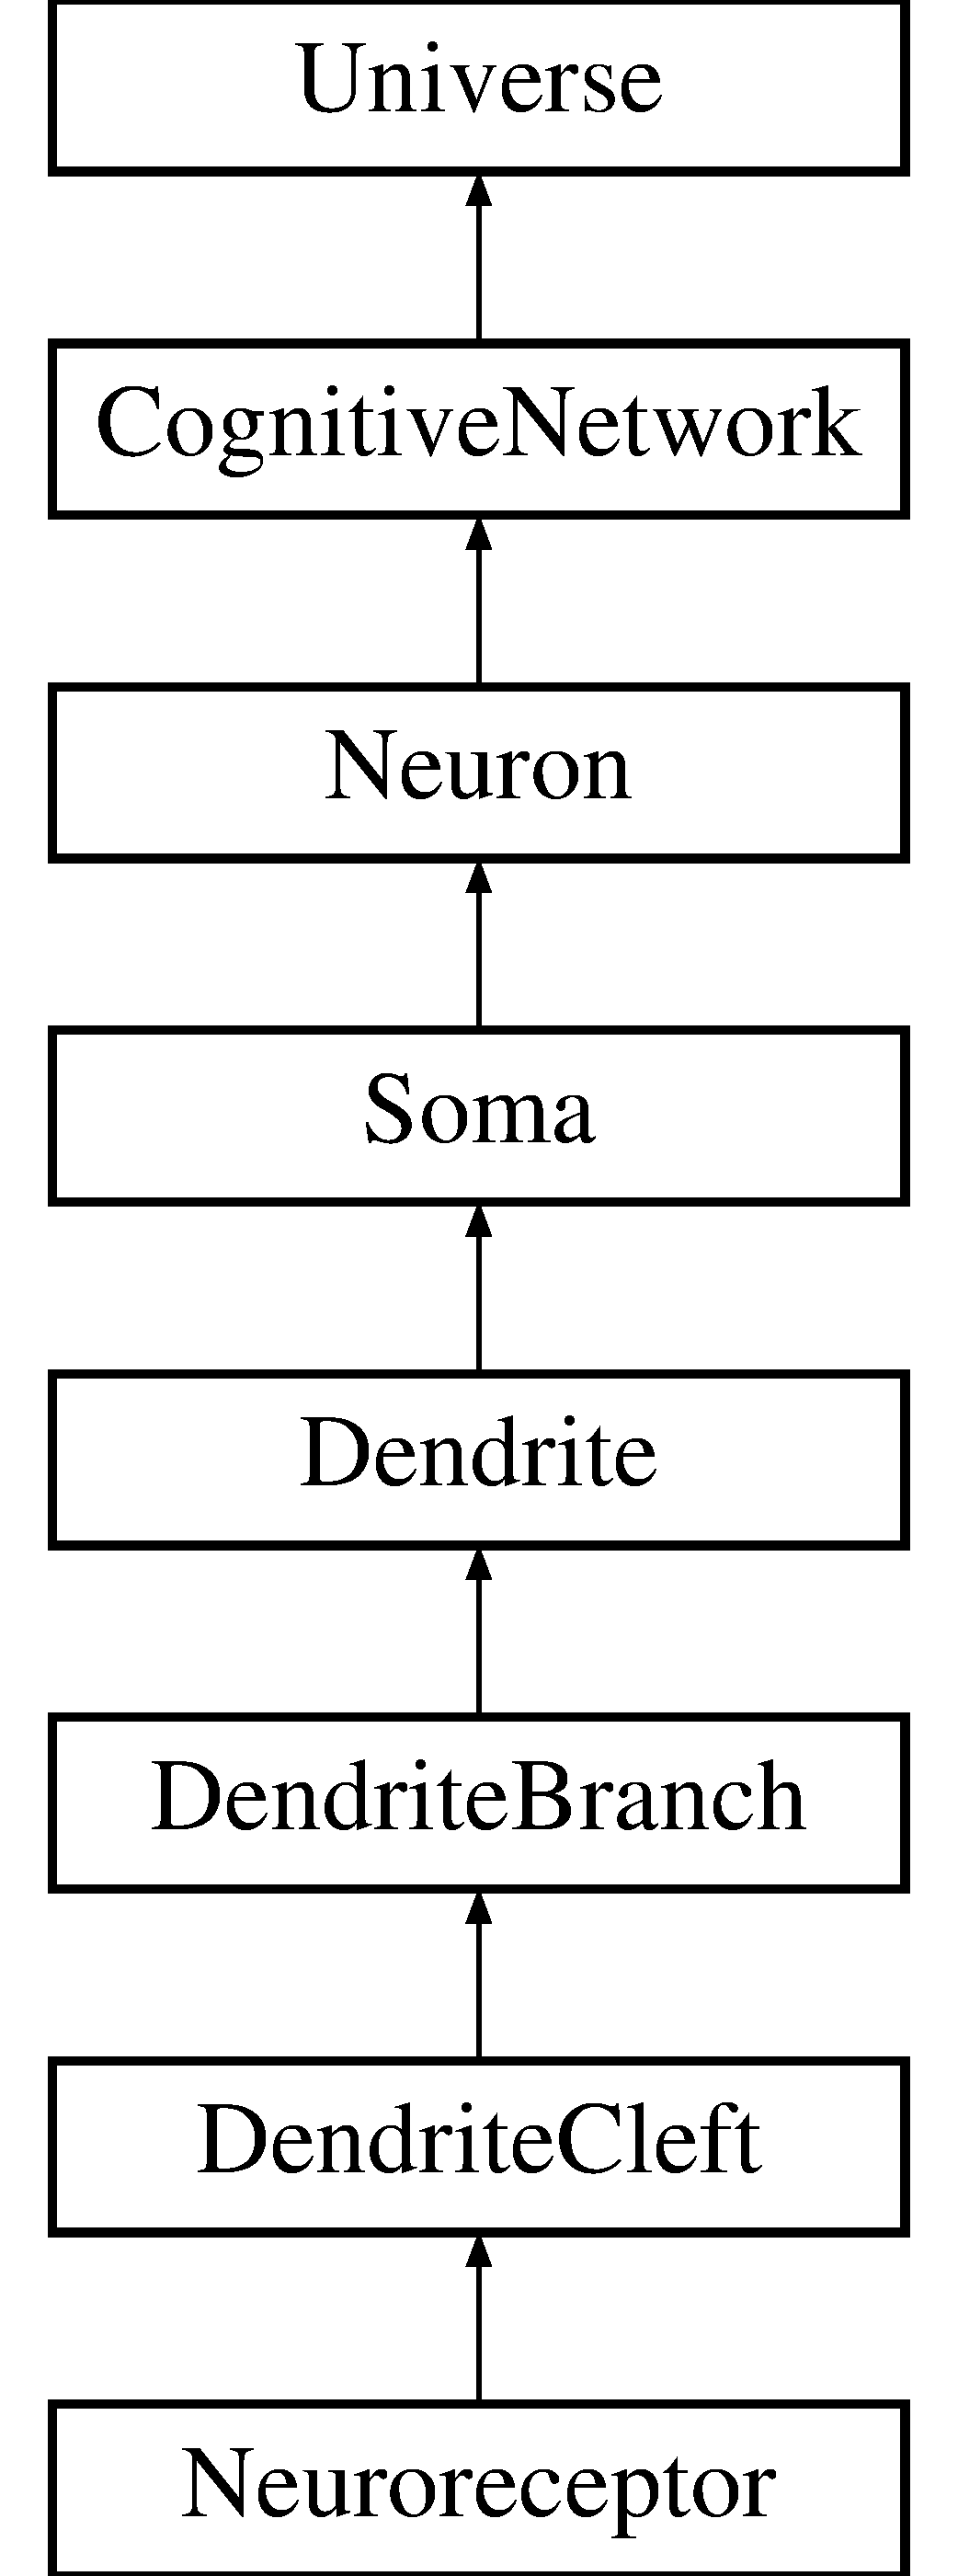
\includegraphics[height=8.000000cm]{classDendriteCleft}
\end{center}
\end{figure}
\subsection*{Public Member Functions}
\begin{DoxyCompactItemize}
\item 
\mbox{\hyperlink{classDendriteCleft_a244a2e6377fafdf79df757d39a2684e5}{Dendrite\+Cleft}} ()
\item 
\mbox{\hyperlink{classDendriteCleft_a335660dfc63f55980b2dcf8849568086}{Dendrite\+Cleft}} (unsigned int object\+\_\+type)
\item 
\mbox{\hyperlink{classDendriteCleft_ad4070ce743d8302bc120ea948890ea37}{Dendrite\+Cleft}} (unsigned int object\+\_\+type, std\+::chrono\+::time\+\_\+point$<$ \mbox{\hyperlink{universe_8h_a0ef8d951d1ca5ab3cfaf7ab4c7a6fd80}{Clock}} $>$ event\+\_\+time)
\item 
\mbox{\hyperlink{classDendriteCleft_abcb81284cd9bd7ee2863eecfb6b59f62}{Dendrite\+Cleft}} (unsigned int object\+\_\+type, std\+::chrono\+::time\+\_\+point$<$ \mbox{\hyperlink{universe_8h_a0ef8d951d1ca5ab3cfaf7ab4c7a6fd80}{Clock}} $>$ event\+\_\+time, \mbox{\hyperlink{classDendriteBranch}{Dendrite\+Branch}} \&dendritebranch\+\_\+connector)
\item 
virtual \mbox{\hyperlink{classDendriteCleft_ad99958c45fa63f2f68b65d7e5ba45b32}{$\sim$\+Dendrite\+Cleft}} ()
\item 
unsigned int \mbox{\hyperlink{classDendriteCleft_ac567530d9f083e1ee65d5c6484cc9fa7}{Get\+Counter}} (std\+::chrono\+::time\+\_\+point$<$ \mbox{\hyperlink{universe_8h_a0ef8d951d1ca5ab3cfaf7ab4c7a6fd80}{Clock}} $>$ event\+\_\+time)
\item 
double \mbox{\hyperlink{classDendriteCleft_ad673df32db3982b3df745a55bf527834}{Get\+Energy}} (std\+::chrono\+::time\+\_\+point$<$ \mbox{\hyperlink{universe_8h_a0ef8d951d1ca5ab3cfaf7ab4c7a6fd80}{Clock}} $>$ event\+\_\+time)
\item 
void \mbox{\hyperlink{classDendriteCleft_a428b8e5117f381a382e0071b936d42a1}{Set\+Counter}} (std\+::chrono\+::time\+\_\+point$<$ \mbox{\hyperlink{universe_8h_a0ef8d951d1ca5ab3cfaf7ab4c7a6fd80}{Clock}} $>$ event\+\_\+time, unsigned int val)
\item 
void \mbox{\hyperlink{classDendriteCleft_a7e09ccb70936deabde9c12457cec949c}{Set\+Energy}} (std\+::chrono\+::time\+\_\+point$<$ \mbox{\hyperlink{universe_8h_a0ef8d951d1ca5ab3cfaf7ab4c7a6fd80}{Clock}} $>$ event\+\_\+time, double val)
\item 
bool \mbox{\hyperlink{classDendriteCleft_a3fee388d7023cfb460412e0322244ae2}{Reset\+Parameters}} (std\+::chrono\+::time\+\_\+point$<$ \mbox{\hyperlink{universe_8h_a0ef8d951d1ca5ab3cfaf7ab4c7a6fd80}{Clock}} $>$ event\+\_\+time)
\item 
\mbox{\hyperlink{classDendriteCleft}{Dendrite\+Cleft}} $\ast$ \mbox{\hyperlink{classDendriteCleft_ac84d3e0cafecd1436c34162f687e3851}{Create\+Neuroreceptor}} (std\+::chrono\+::time\+\_\+point$<$ \mbox{\hyperlink{universe_8h_a0ef8d951d1ca5ab3cfaf7ab4c7a6fd80}{Clock}} $>$ event\+\_\+time)
\item 
std\+::vector$<$ \mbox{\hyperlink{classDendriteCleft}{Dendrite\+Cleft}} $\ast$ $>$ \mbox{\hyperlink{classDendriteCleft_ab34af5363b25c6498aee429725a1c7db}{Create\+Neuroreceptors}} (std\+::chrono\+::time\+\_\+point$<$ \mbox{\hyperlink{universe_8h_a0ef8d951d1ca5ab3cfaf7ab4c7a6fd80}{Clock}} $>$ event\+\_\+time, int quantity)
\item 
\mbox{\hyperlink{classDendriteCleft}{Dendrite\+Cleft}} $\ast$ \mbox{\hyperlink{classDendriteCleft_a7650e1115baab30729da0b03a48da851}{Clone\+Neuroreceptor}} (std\+::chrono\+::time\+\_\+point$<$ \mbox{\hyperlink{universe_8h_a0ef8d951d1ca5ab3cfaf7ab4c7a6fd80}{Clock}} $>$ event\+\_\+time, \mbox{\hyperlink{classDendriteCleft}{Dendrite\+Cleft}} $\ast$clone\+\_\+object, double perfection\+\_\+membership)
\item 
std\+::vector$<$ \mbox{\hyperlink{classDendriteCleft}{Dendrite\+Cleft}} $\ast$ $>$ \mbox{\hyperlink{classDendriteCleft_a93b542418482f3732380e33346e23bd2}{Clone\+Neuroreceptors}} (std\+::chrono\+::time\+\_\+point$<$ \mbox{\hyperlink{universe_8h_a0ef8d951d1ca5ab3cfaf7ab4c7a6fd80}{Clock}} $>$ event\+\_\+time, std\+::vector$<$ \mbox{\hyperlink{classDendriteCleft}{Dendrite\+Cleft}} $\ast$$>$ cloning\+\_\+list, double perfection\+\_\+membership)
\item 
\mbox{\hyperlink{classDendriteCleft}{Dendrite\+Cleft}} $\ast$ \mbox{\hyperlink{classDendriteCleft_a86e9943d9d140c2a06d7e222812c9548}{Destroy\+Neuroreceptor}} (std\+::chrono\+::time\+\_\+point$<$ \mbox{\hyperlink{universe_8h_a0ef8d951d1ca5ab3cfaf7ab4c7a6fd80}{Clock}} $>$ event\+\_\+time, \mbox{\hyperlink{classDendriteCleft}{Dendrite\+Cleft}} $\ast$destroy\+\_\+object)
\item 
std\+::vector$<$ \mbox{\hyperlink{classDendriteCleft}{Dendrite\+Cleft}} $\ast$ $>$ \mbox{\hyperlink{classDendriteCleft_a630e00e2d1108f2a43bcac9466e4681b}{Destroy\+Neuroreceptors}} (std\+::chrono\+::time\+\_\+point$<$ \mbox{\hyperlink{universe_8h_a0ef8d951d1ca5ab3cfaf7ab4c7a6fd80}{Clock}} $>$ event\+\_\+time, std\+::vector$<$ \mbox{\hyperlink{classDendriteCleft}{Dendrite\+Cleft}} $\ast$$>$ destruction\+\_\+list)
\item 
\mbox{\hyperlink{classDendriteCleft}{Dendrite\+Cleft}} $\ast$ \mbox{\hyperlink{classDendriteCleft_a65901c5659ca5eac161a26f15e0f437b}{Add\+Neuroreceptor}} (std\+::chrono\+::time\+\_\+point$<$ \mbox{\hyperlink{universe_8h_a0ef8d951d1ca5ab3cfaf7ab4c7a6fd80}{Clock}} $>$ event\+\_\+time, \mbox{\hyperlink{classDendriteCleft}{Dendrite\+Cleft}} $\ast$add\+\_\+object)
\item 
std\+::vector$<$ \mbox{\hyperlink{classDendriteCleft}{Dendrite\+Cleft}} $\ast$ $>$ \mbox{\hyperlink{classDendriteCleft_a6d29f577ff12366f8f51804b13468395}{Add\+Neuroreceptors}} (std\+::chrono\+::time\+\_\+point$<$ \mbox{\hyperlink{universe_8h_a0ef8d951d1ca5ab3cfaf7ab4c7a6fd80}{Clock}} $>$ event\+\_\+time, std\+::vector$<$ \mbox{\hyperlink{classDendriteCleft}{Dendrite\+Cleft}} $\ast$$>$ add\+\_\+objects)
\item 
\mbox{\hyperlink{classDendriteCleft}{Dendrite\+Cleft}} $\ast$ \mbox{\hyperlink{classDendriteCleft_afaf06d4516355dfe2e0e4c33a00f0f1d}{Remove\+Neuroreceptor}} (std\+::chrono\+::time\+\_\+point$<$ \mbox{\hyperlink{universe_8h_a0ef8d951d1ca5ab3cfaf7ab4c7a6fd80}{Clock}} $>$ event\+\_\+time)
\item 
std\+::vector$<$ \mbox{\hyperlink{classDendriteCleft}{Dendrite\+Cleft}} $\ast$ $>$ \mbox{\hyperlink{classDendriteCleft_ac29b12d4abcc47fa298ab9e95f578f0e}{Remove\+Neuroreceptors}} (std\+::chrono\+::time\+\_\+point$<$ \mbox{\hyperlink{universe_8h_a0ef8d951d1ca5ab3cfaf7ab4c7a6fd80}{Clock}} $>$ event\+\_\+time, int quantity)
\item 
\mbox{\hyperlink{classDendriteCleft}{Dendrite\+Cleft}} $\ast$ \mbox{\hyperlink{classDendriteCleft_a5eb3a8f143f63b852b8f5e245d385519}{Get\+Neuroreceptor}} (std\+::chrono\+::time\+\_\+point$<$ \mbox{\hyperlink{universe_8h_a0ef8d951d1ca5ab3cfaf7ab4c7a6fd80}{Clock}} $>$ event\+\_\+time, int selector)
\item 
std\+::vector$<$ \mbox{\hyperlink{classDendriteCleft}{Dendrite\+Cleft}} $\ast$ $>$ \mbox{\hyperlink{classDendriteCleft_a4a14361574777fb1d66fd4ed2d4f2492}{Get\+Neuroreceptors}} (std\+::chrono\+::time\+\_\+point$<$ \mbox{\hyperlink{universe_8h_a0ef8d951d1ca5ab3cfaf7ab4c7a6fd80}{Clock}} $>$ event\+\_\+time)
\item 
int \mbox{\hyperlink{classDendriteCleft_af4715ffbf1bf437523d07e37b7abc3e0}{Growth\+Surface}} (std\+::chrono\+::time\+\_\+point$<$ \mbox{\hyperlink{universe_8h_a0ef8d951d1ca5ab3cfaf7ab4c7a6fd80}{Clock}} $>$ event\+\_\+time, double surf\+\_\+change)
\item 
int \mbox{\hyperlink{classDendriteCleft_a0cb2fc6ad72bba55b5f65130006d4b12}{Growth\+Volume}} (std\+::chrono\+::time\+\_\+point$<$ \mbox{\hyperlink{universe_8h_a0ef8d951d1ca5ab3cfaf7ab4c7a6fd80}{Clock}} $>$ event\+\_\+time, double vol\+\_\+change)
\item 
int \mbox{\hyperlink{classDendriteCleft_a3a75af4d6fd97c9635134509f170a04e}{Update}} (std\+::chrono\+::time\+\_\+point$<$ \mbox{\hyperlink{universe_8h_a0ef8d951d1ca5ab3cfaf7ab4c7a6fd80}{Clock}} $>$ event\+\_\+time)
\end{DoxyCompactItemize}
\subsection*{Protected Attributes}
\begin{DoxyCompactItemize}
\item 
std\+::vector$<$ \mbox{\hyperlink{classDendriteCleft}{Dendrite\+Cleft}} $\ast$ $>$ \mbox{\hyperlink{classDendriteCleft_a42de9c556ce58c9f511031361755a0c3}{neuroreceptor\+\_\+list}}
\end{DoxyCompactItemize}
\subsection*{Private Attributes}
\begin{DoxyCompactItemize}
\item 
int \mbox{\hyperlink{classDendriteCleft_ab5f89d395d4f77f7d23cd15425f0de6b}{dendritecleft\+\_\+type}}
\item 
int \mbox{\hyperlink{classDendriteCleft_aaaf447d15eebe2a304ee03a62cc97c05}{m\+\_\+add\+Status}}
\item 
int \mbox{\hyperlink{classDendriteCleft_afd7b84cb30b571db5d42130915a27033}{neuroreceptor\+\_\+pool}}
\item 
std\+::chrono\+::time\+\_\+point$<$ \mbox{\hyperlink{universe_8h_a0ef8d951d1ca5ab3cfaf7ab4c7a6fd80}{Clock}} $>$ \mbox{\hyperlink{classDendriteCleft_a97d85edbb69960d16398d212107c36fb}{previous\+\_\+event\+\_\+time}}
\item 
std\+::chrono\+::time\+\_\+point$<$ \mbox{\hyperlink{universe_8h_a0ef8d951d1ca5ab3cfaf7ab4c7a6fd80}{Clock}} $>$ \mbox{\hyperlink{classDendriteCleft_a145dcc0e5e2564e22464625930c006c9}{time\+\_\+object\+\_\+created}}
\item 
bool \mbox{\hyperlink{classDendriteCleft_ac457de5e25a7c7e29db9d50f0874f078}{object\+\_\+disabled}}
\item 
bool \mbox{\hyperlink{classDendriteCleft_a246dda1826ad0fd93002388993899e10}{object\+\_\+initialised}}
\item 
int \mbox{\hyperlink{classDendriteCleft_aef90c83b99d8a74e0aa05e845a8e07b6}{duration\+\_\+since\+\_\+last\+\_\+event}}
\item 
double \mbox{\hyperlink{classDendriteCleft_a93155af6d9d9179eb0608ee0cbf90e8c}{m\+\_\+\+Volume}}
\item 
double \mbox{\hyperlink{classDendriteCleft_aabf37b96644ddc07d3195d6c2ebc60e8}{m\+\_\+\+Surface\+Area}}
\item 
double \mbox{\hyperlink{classDendriteCleft_a6876a474554771833ea179fbc8d8cd62}{m\+\_\+\+Length}}
\item 
double \mbox{\hyperlink{classDendriteCleft_ac78e2502c53c1b3d0c2a759f3b653dde}{object\+\_\+size}}
\begin{DoxyCompactList}\small\item\em Member variable \char`\"{}object\+\_\+size\char`\"{} Area of cleft (assumed to be circular due to pressure equalisation) \end{DoxyCompactList}\item 
double \mbox{\hyperlink{classDendriteCleft_ae24f44df5148f9bcf95ba4a2a1916491}{m\+\_\+dendrite\+Length}}
\begin{DoxyCompactList}\small\item\em Member variable \char`\"{}m\+\_\+dendrite\+Length\char`\"{}. \end{DoxyCompactList}\item 
double \mbox{\hyperlink{classDendriteCleft_ad206cd42f8bf36b989e3993d02214e12}{m\+\_\+dendrite\+Diameter\+Start}}
\begin{DoxyCompactList}\small\item\em Member variable \char`\"{}m\+\_\+dendrite\+Diameter\+Start\char`\"{}. \end{DoxyCompactList}\item 
double \mbox{\hyperlink{classDendriteCleft_aa905ee6ba625bfa340282b03b916ecdf}{m\+\_\+dendrite\+Diameter\+End}}
\begin{DoxyCompactList}\small\item\em Member variable \char`\"{}m\+\_\+dendrite\+Diameter\+End\char`\"{}. \end{DoxyCompactList}\item 
double \mbox{\hyperlink{classDendriteCleft_aed8f88f66a419600c41da62d8814dc59}{m\+\_\+membrane\+Resistance}}
\item 
double \mbox{\hyperlink{classDendriteCleft_ab5a89436993650294a6abab92852f488}{m\+\_\+membrane\+Capacitance}}
\item 
double \mbox{\hyperlink{classDendriteCleft_ad947e5dda845fb5ac25cfb3709a4e860}{m\+\_\+internal\+Resistance}}
\item 
unsigned int \mbox{\hyperlink{classDendriteCleft_a9244fcddd66073866759b5bedca083db}{m\+\_\+\+Counter}}
\begin{DoxyCompactList}\small\item\em Member variable \char`\"{}m\+\_\+\+Counter\char`\"{}. \end{DoxyCompactList}\item 
double \mbox{\hyperlink{classDendriteCleft_a22c6048147877a2c59c9264b295e7179}{object\+\_\+energy}}
\begin{DoxyCompactList}\small\item\em Member variable \char`\"{}object\+\_\+energy\char`\"{}. \end{DoxyCompactList}\item 
double \mbox{\hyperlink{classDendriteCleft_a81149b707c189d2b96a40af75af1f059}{object\+\_\+energy\+Inc}}
\item 
double \mbox{\hyperlink{classDendriteCleft_aba50e581f1aec412b7b44ecd0dfc8076}{object\+\_\+energy\+Dec}}
\item 
double \mbox{\hyperlink{classDendriteCleft_a541502a9ffbc2926e76d2eb4a972ae39}{object\+\_\+energy\+Leak}}
\item 
double \mbox{\hyperlink{classDendriteCleft_ac73d775c34a5c3f186b395c8e7738cd8}{object\+\_\+energy\+\_\+threshold}}
\item 
double \mbox{\hyperlink{classDendriteCleft_a8236dc02dccfe1f59bb0d288599a84b5}{m\+\_\+\+Time\+Dilation}}
\item 
double \mbox{\hyperlink{classDendriteCleft_a504e4aef51d3e52dbad3589844a821de}{m\+\_\+\+Time\+Threshold}}
\end{DoxyCompactItemize}
\subsection*{Additional Inherited Members}


\subsection{Constructor \& Destructor Documentation}
\mbox{\Hypertarget{classDendriteCleft_a244a2e6377fafdf79df757d39a2684e5}\label{classDendriteCleft_a244a2e6377fafdf79df757d39a2684e5}} 
\index{Dendrite\+Cleft@{Dendrite\+Cleft}!Dendrite\+Cleft@{Dendrite\+Cleft}}
\index{Dendrite\+Cleft@{Dendrite\+Cleft}!Dendrite\+Cleft@{Dendrite\+Cleft}}
\subsubsection{\texorpdfstring{Dendrite\+Cleft()}{DendriteCleft()}\hspace{0.1cm}{\footnotesize\ttfamily [1/4]}}
{\footnotesize\ttfamily Dendrite\+Cleft\+::\+Dendrite\+Cleft (\begin{DoxyParamCaption}{ }\end{DoxyParamCaption})\hspace{0.3cm}{\ttfamily [inline]}}

\mbox{\Hypertarget{classDendriteCleft_a335660dfc63f55980b2dcf8849568086}\label{classDendriteCleft_a335660dfc63f55980b2dcf8849568086}} 
\index{Dendrite\+Cleft@{Dendrite\+Cleft}!Dendrite\+Cleft@{Dendrite\+Cleft}}
\index{Dendrite\+Cleft@{Dendrite\+Cleft}!Dendrite\+Cleft@{Dendrite\+Cleft}}
\subsubsection{\texorpdfstring{Dendrite\+Cleft()}{DendriteCleft()}\hspace{0.1cm}{\footnotesize\ttfamily [2/4]}}
{\footnotesize\ttfamily Dendrite\+Cleft\+::\+Dendrite\+Cleft (\begin{DoxyParamCaption}\item[{unsigned int}]{object\+\_\+type }\end{DoxyParamCaption})\hspace{0.3cm}{\ttfamily [inline]}}

\mbox{\Hypertarget{classDendriteCleft_ad4070ce743d8302bc120ea948890ea37}\label{classDendriteCleft_ad4070ce743d8302bc120ea948890ea37}} 
\index{Dendrite\+Cleft@{Dendrite\+Cleft}!Dendrite\+Cleft@{Dendrite\+Cleft}}
\index{Dendrite\+Cleft@{Dendrite\+Cleft}!Dendrite\+Cleft@{Dendrite\+Cleft}}
\subsubsection{\texorpdfstring{Dendrite\+Cleft()}{DendriteCleft()}\hspace{0.1cm}{\footnotesize\ttfamily [3/4]}}
{\footnotesize\ttfamily Dendrite\+Cleft\+::\+Dendrite\+Cleft (\begin{DoxyParamCaption}\item[{unsigned int}]{object\+\_\+type,  }\item[{std\+::chrono\+::time\+\_\+point$<$ \mbox{\hyperlink{universe_8h_a0ef8d951d1ca5ab3cfaf7ab4c7a6fd80}{Clock}} $>$}]{event\+\_\+time }\end{DoxyParamCaption})\hspace{0.3cm}{\ttfamily [inline]}}

\mbox{\Hypertarget{classDendriteCleft_abcb81284cd9bd7ee2863eecfb6b59f62}\label{classDendriteCleft_abcb81284cd9bd7ee2863eecfb6b59f62}} 
\index{Dendrite\+Cleft@{Dendrite\+Cleft}!Dendrite\+Cleft@{Dendrite\+Cleft}}
\index{Dendrite\+Cleft@{Dendrite\+Cleft}!Dendrite\+Cleft@{Dendrite\+Cleft}}
\subsubsection{\texorpdfstring{Dendrite\+Cleft()}{DendriteCleft()}\hspace{0.1cm}{\footnotesize\ttfamily [4/4]}}
{\footnotesize\ttfamily Dendrite\+Cleft\+::\+Dendrite\+Cleft (\begin{DoxyParamCaption}\item[{unsigned int}]{object\+\_\+type,  }\item[{std\+::chrono\+::time\+\_\+point$<$ \mbox{\hyperlink{universe_8h_a0ef8d951d1ca5ab3cfaf7ab4c7a6fd80}{Clock}} $>$}]{event\+\_\+time,  }\item[{\mbox{\hyperlink{classDendriteBranch}{Dendrite\+Branch}} \&}]{dendritebranch\+\_\+connector }\end{DoxyParamCaption})\hspace{0.3cm}{\ttfamily [inline]}}

\mbox{\Hypertarget{classDendriteCleft_ad99958c45fa63f2f68b65d7e5ba45b32}\label{classDendriteCleft_ad99958c45fa63f2f68b65d7e5ba45b32}} 
\index{Dendrite\+Cleft@{Dendrite\+Cleft}!````~Dendrite\+Cleft@{$\sim$\+Dendrite\+Cleft}}
\index{````~Dendrite\+Cleft@{$\sim$\+Dendrite\+Cleft}!Dendrite\+Cleft@{Dendrite\+Cleft}}
\subsubsection{\texorpdfstring{$\sim$\+Dendrite\+Cleft()}{~DendriteCleft()}}
{\footnotesize\ttfamily virtual Dendrite\+Cleft\+::$\sim$\+Dendrite\+Cleft (\begin{DoxyParamCaption}{ }\end{DoxyParamCaption})\hspace{0.3cm}{\ttfamily [inline]}, {\ttfamily [virtual]}}

Default destructor 

\subsection{Member Function Documentation}
\mbox{\Hypertarget{classDendriteCleft_a65901c5659ca5eac161a26f15e0f437b}\label{classDendriteCleft_a65901c5659ca5eac161a26f15e0f437b}} 
\index{Dendrite\+Cleft@{Dendrite\+Cleft}!Add\+Neuroreceptor@{Add\+Neuroreceptor}}
\index{Add\+Neuroreceptor@{Add\+Neuroreceptor}!Dendrite\+Cleft@{Dendrite\+Cleft}}
\subsubsection{\texorpdfstring{Add\+Neuroreceptor()}{AddNeuroreceptor()}}
{\footnotesize\ttfamily \mbox{\hyperlink{classDendriteCleft}{Dendrite\+Cleft}} $\ast$ Dendrite\+Cleft\+::\+Add\+Neuroreceptor (\begin{DoxyParamCaption}\item[{std\+::chrono\+::time\+\_\+point$<$ \mbox{\hyperlink{universe_8h_a0ef8d951d1ca5ab3cfaf7ab4c7a6fd80}{Clock}} $>$}]{event\+\_\+time,  }\item[{\mbox{\hyperlink{classDendriteCleft}{Dendrite\+Cleft}} $\ast$}]{add\+\_\+object }\end{DoxyParamCaption})}

\mbox{\Hypertarget{classDendriteCleft_a6d29f577ff12366f8f51804b13468395}\label{classDendriteCleft_a6d29f577ff12366f8f51804b13468395}} 
\index{Dendrite\+Cleft@{Dendrite\+Cleft}!Add\+Neuroreceptors@{Add\+Neuroreceptors}}
\index{Add\+Neuroreceptors@{Add\+Neuroreceptors}!Dendrite\+Cleft@{Dendrite\+Cleft}}
\subsubsection{\texorpdfstring{Add\+Neuroreceptors()}{AddNeuroreceptors()}}
{\footnotesize\ttfamily std\+::vector$<$ \mbox{\hyperlink{classDendriteCleft}{Dendrite\+Cleft}} $\ast$ $>$ Dendrite\+Cleft\+::\+Add\+Neuroreceptors (\begin{DoxyParamCaption}\item[{std\+::chrono\+::time\+\_\+point$<$ \mbox{\hyperlink{universe_8h_a0ef8d951d1ca5ab3cfaf7ab4c7a6fd80}{Clock}} $>$}]{event\+\_\+time,  }\item[{std\+::vector$<$ \mbox{\hyperlink{classDendriteCleft}{Dendrite\+Cleft}} $\ast$$>$}]{add\+\_\+objects }\end{DoxyParamCaption})}

\mbox{\Hypertarget{classDendriteCleft_a7650e1115baab30729da0b03a48da851}\label{classDendriteCleft_a7650e1115baab30729da0b03a48da851}} 
\index{Dendrite\+Cleft@{Dendrite\+Cleft}!Clone\+Neuroreceptor@{Clone\+Neuroreceptor}}
\index{Clone\+Neuroreceptor@{Clone\+Neuroreceptor}!Dendrite\+Cleft@{Dendrite\+Cleft}}
\subsubsection{\texorpdfstring{Clone\+Neuroreceptor()}{CloneNeuroreceptor()}}
{\footnotesize\ttfamily \mbox{\hyperlink{classDendriteCleft}{Dendrite\+Cleft}} $\ast$ Dendrite\+Cleft\+::\+Clone\+Neuroreceptor (\begin{DoxyParamCaption}\item[{std\+::chrono\+::time\+\_\+point$<$ \mbox{\hyperlink{universe_8h_a0ef8d951d1ca5ab3cfaf7ab4c7a6fd80}{Clock}} $>$}]{event\+\_\+time,  }\item[{\mbox{\hyperlink{classDendriteCleft}{Dendrite\+Cleft}} $\ast$}]{clone\+\_\+object,  }\item[{double}]{perfection\+\_\+membership }\end{DoxyParamCaption})}

\mbox{\Hypertarget{classDendriteCleft_a93b542418482f3732380e33346e23bd2}\label{classDendriteCleft_a93b542418482f3732380e33346e23bd2}} 
\index{Dendrite\+Cleft@{Dendrite\+Cleft}!Clone\+Neuroreceptors@{Clone\+Neuroreceptors}}
\index{Clone\+Neuroreceptors@{Clone\+Neuroreceptors}!Dendrite\+Cleft@{Dendrite\+Cleft}}
\subsubsection{\texorpdfstring{Clone\+Neuroreceptors()}{CloneNeuroreceptors()}}
{\footnotesize\ttfamily std\+::vector$<$ \mbox{\hyperlink{classDendriteCleft}{Dendrite\+Cleft}} $\ast$ $>$ Dendrite\+Cleft\+::\+Clone\+Neuroreceptors (\begin{DoxyParamCaption}\item[{std\+::chrono\+::time\+\_\+point$<$ \mbox{\hyperlink{universe_8h_a0ef8d951d1ca5ab3cfaf7ab4c7a6fd80}{Clock}} $>$}]{event\+\_\+time,  }\item[{std\+::vector$<$ \mbox{\hyperlink{classDendriteCleft}{Dendrite\+Cleft}} $\ast$$>$}]{cloning\+\_\+list,  }\item[{double}]{perfection\+\_\+membership }\end{DoxyParamCaption})}

\mbox{\Hypertarget{classDendriteCleft_ac84d3e0cafecd1436c34162f687e3851}\label{classDendriteCleft_ac84d3e0cafecd1436c34162f687e3851}} 
\index{Dendrite\+Cleft@{Dendrite\+Cleft}!Create\+Neuroreceptor@{Create\+Neuroreceptor}}
\index{Create\+Neuroreceptor@{Create\+Neuroreceptor}!Dendrite\+Cleft@{Dendrite\+Cleft}}
\subsubsection{\texorpdfstring{Create\+Neuroreceptor()}{CreateNeuroreceptor()}}
{\footnotesize\ttfamily \mbox{\hyperlink{classDendriteCleft}{Dendrite\+Cleft}} $\ast$ Dendrite\+Cleft\+::\+Create\+Neuroreceptor (\begin{DoxyParamCaption}\item[{std\+::chrono\+::time\+\_\+point$<$ \mbox{\hyperlink{universe_8h_a0ef8d951d1ca5ab3cfaf7ab4c7a6fd80}{Clock}} $>$}]{event\+\_\+time }\end{DoxyParamCaption})}

\mbox{\Hypertarget{classDendriteCleft_ab34af5363b25c6498aee429725a1c7db}\label{classDendriteCleft_ab34af5363b25c6498aee429725a1c7db}} 
\index{Dendrite\+Cleft@{Dendrite\+Cleft}!Create\+Neuroreceptors@{Create\+Neuroreceptors}}
\index{Create\+Neuroreceptors@{Create\+Neuroreceptors}!Dendrite\+Cleft@{Dendrite\+Cleft}}
\subsubsection{\texorpdfstring{Create\+Neuroreceptors()}{CreateNeuroreceptors()}}
{\footnotesize\ttfamily std\+::vector$<$ \mbox{\hyperlink{classDendriteCleft}{Dendrite\+Cleft}} $\ast$ $>$ Dendrite\+Cleft\+::\+Create\+Neuroreceptors (\begin{DoxyParamCaption}\item[{std\+::chrono\+::time\+\_\+point$<$ \mbox{\hyperlink{universe_8h_a0ef8d951d1ca5ab3cfaf7ab4c7a6fd80}{Clock}} $>$}]{event\+\_\+time,  }\item[{int}]{quantity }\end{DoxyParamCaption})}

\mbox{\Hypertarget{classDendriteCleft_a86e9943d9d140c2a06d7e222812c9548}\label{classDendriteCleft_a86e9943d9d140c2a06d7e222812c9548}} 
\index{Dendrite\+Cleft@{Dendrite\+Cleft}!Destroy\+Neuroreceptor@{Destroy\+Neuroreceptor}}
\index{Destroy\+Neuroreceptor@{Destroy\+Neuroreceptor}!Dendrite\+Cleft@{Dendrite\+Cleft}}
\subsubsection{\texorpdfstring{Destroy\+Neuroreceptor()}{DestroyNeuroreceptor()}}
{\footnotesize\ttfamily \mbox{\hyperlink{classDendriteCleft}{Dendrite\+Cleft}} $\ast$ Dendrite\+Cleft\+::\+Destroy\+Neuroreceptor (\begin{DoxyParamCaption}\item[{std\+::chrono\+::time\+\_\+point$<$ \mbox{\hyperlink{universe_8h_a0ef8d951d1ca5ab3cfaf7ab4c7a6fd80}{Clock}} $>$}]{event\+\_\+time,  }\item[{\mbox{\hyperlink{classDendriteCleft}{Dendrite\+Cleft}} $\ast$}]{destroy\+\_\+object }\end{DoxyParamCaption})}

\mbox{\Hypertarget{classDendriteCleft_a630e00e2d1108f2a43bcac9466e4681b}\label{classDendriteCleft_a630e00e2d1108f2a43bcac9466e4681b}} 
\index{Dendrite\+Cleft@{Dendrite\+Cleft}!Destroy\+Neuroreceptors@{Destroy\+Neuroreceptors}}
\index{Destroy\+Neuroreceptors@{Destroy\+Neuroreceptors}!Dendrite\+Cleft@{Dendrite\+Cleft}}
\subsubsection{\texorpdfstring{Destroy\+Neuroreceptors()}{DestroyNeuroreceptors()}}
{\footnotesize\ttfamily std\+::vector$<$ \mbox{\hyperlink{classDendriteCleft}{Dendrite\+Cleft}} $\ast$ $>$ Dendrite\+Cleft\+::\+Destroy\+Neuroreceptors (\begin{DoxyParamCaption}\item[{std\+::chrono\+::time\+\_\+point$<$ \mbox{\hyperlink{universe_8h_a0ef8d951d1ca5ab3cfaf7ab4c7a6fd80}{Clock}} $>$}]{event\+\_\+time,  }\item[{std\+::vector$<$ \mbox{\hyperlink{classDendriteCleft}{Dendrite\+Cleft}} $\ast$$>$}]{destruction\+\_\+list }\end{DoxyParamCaption})}

\mbox{\Hypertarget{classDendriteCleft_ac567530d9f083e1ee65d5c6484cc9fa7}\label{classDendriteCleft_ac567530d9f083e1ee65d5c6484cc9fa7}} 
\index{Dendrite\+Cleft@{Dendrite\+Cleft}!Get\+Counter@{Get\+Counter}}
\index{Get\+Counter@{Get\+Counter}!Dendrite\+Cleft@{Dendrite\+Cleft}}
\subsubsection{\texorpdfstring{Get\+Counter()}{GetCounter()}}
{\footnotesize\ttfamily unsigned int Dendrite\+Cleft\+::\+Get\+Counter (\begin{DoxyParamCaption}\item[{std\+::chrono\+::time\+\_\+point$<$ \mbox{\hyperlink{universe_8h_a0ef8d951d1ca5ab3cfaf7ab4c7a6fd80}{Clock}} $>$}]{event\+\_\+time }\end{DoxyParamCaption})\hspace{0.3cm}{\ttfamily [inline]}}

\mbox{\Hypertarget{classDendriteCleft_ad673df32db3982b3df745a55bf527834}\label{classDendriteCleft_ad673df32db3982b3df745a55bf527834}} 
\index{Dendrite\+Cleft@{Dendrite\+Cleft}!Get\+Energy@{Get\+Energy}}
\index{Get\+Energy@{Get\+Energy}!Dendrite\+Cleft@{Dendrite\+Cleft}}
\subsubsection{\texorpdfstring{Get\+Energy()}{GetEnergy()}}
{\footnotesize\ttfamily double Dendrite\+Cleft\+::\+Get\+Energy (\begin{DoxyParamCaption}\item[{std\+::chrono\+::time\+\_\+point$<$ \mbox{\hyperlink{universe_8h_a0ef8d951d1ca5ab3cfaf7ab4c7a6fd80}{Clock}} $>$}]{event\+\_\+time }\end{DoxyParamCaption})\hspace{0.3cm}{\ttfamily [inline]}}

\mbox{\Hypertarget{classDendriteCleft_a5eb3a8f143f63b852b8f5e245d385519}\label{classDendriteCleft_a5eb3a8f143f63b852b8f5e245d385519}} 
\index{Dendrite\+Cleft@{Dendrite\+Cleft}!Get\+Neuroreceptor@{Get\+Neuroreceptor}}
\index{Get\+Neuroreceptor@{Get\+Neuroreceptor}!Dendrite\+Cleft@{Dendrite\+Cleft}}
\subsubsection{\texorpdfstring{Get\+Neuroreceptor()}{GetNeuroreceptor()}}
{\footnotesize\ttfamily \mbox{\hyperlink{classDendriteCleft}{Dendrite\+Cleft}} $\ast$ Dendrite\+Cleft\+::\+Get\+Neuroreceptor (\begin{DoxyParamCaption}\item[{std\+::chrono\+::time\+\_\+point$<$ \mbox{\hyperlink{universe_8h_a0ef8d951d1ca5ab3cfaf7ab4c7a6fd80}{Clock}} $>$}]{event\+\_\+time,  }\item[{int}]{selector }\end{DoxyParamCaption})}

\mbox{\Hypertarget{classDendriteCleft_a4a14361574777fb1d66fd4ed2d4f2492}\label{classDendriteCleft_a4a14361574777fb1d66fd4ed2d4f2492}} 
\index{Dendrite\+Cleft@{Dendrite\+Cleft}!Get\+Neuroreceptors@{Get\+Neuroreceptors}}
\index{Get\+Neuroreceptors@{Get\+Neuroreceptors}!Dendrite\+Cleft@{Dendrite\+Cleft}}
\subsubsection{\texorpdfstring{Get\+Neuroreceptors()}{GetNeuroreceptors()}}
{\footnotesize\ttfamily std\+::vector$<$ \mbox{\hyperlink{classDendriteCleft}{Dendrite\+Cleft}} $\ast$ $>$ Dendrite\+Cleft\+::\+Get\+Neuroreceptors (\begin{DoxyParamCaption}\item[{std\+::chrono\+::time\+\_\+point$<$ \mbox{\hyperlink{universe_8h_a0ef8d951d1ca5ab3cfaf7ab4c7a6fd80}{Clock}} $>$}]{event\+\_\+time }\end{DoxyParamCaption})}

\mbox{\Hypertarget{classDendriteCleft_af4715ffbf1bf437523d07e37b7abc3e0}\label{classDendriteCleft_af4715ffbf1bf437523d07e37b7abc3e0}} 
\index{Dendrite\+Cleft@{Dendrite\+Cleft}!Growth\+Surface@{Growth\+Surface}}
\index{Growth\+Surface@{Growth\+Surface}!Dendrite\+Cleft@{Dendrite\+Cleft}}
\subsubsection{\texorpdfstring{Growth\+Surface()}{GrowthSurface()}}
{\footnotesize\ttfamily int Dendrite\+Cleft\+::\+Growth\+Surface (\begin{DoxyParamCaption}\item[{std\+::chrono\+::time\+\_\+point$<$ \mbox{\hyperlink{universe_8h_a0ef8d951d1ca5ab3cfaf7ab4c7a6fd80}{Clock}} $>$}]{event\+\_\+time,  }\item[{double}]{surf\+\_\+change }\end{DoxyParamCaption})}

\mbox{\Hypertarget{classDendriteCleft_a0cb2fc6ad72bba55b5f65130006d4b12}\label{classDendriteCleft_a0cb2fc6ad72bba55b5f65130006d4b12}} 
\index{Dendrite\+Cleft@{Dendrite\+Cleft}!Growth\+Volume@{Growth\+Volume}}
\index{Growth\+Volume@{Growth\+Volume}!Dendrite\+Cleft@{Dendrite\+Cleft}}
\subsubsection{\texorpdfstring{Growth\+Volume()}{GrowthVolume()}}
{\footnotesize\ttfamily int Dendrite\+Cleft\+::\+Growth\+Volume (\begin{DoxyParamCaption}\item[{std\+::chrono\+::time\+\_\+point$<$ \mbox{\hyperlink{universe_8h_a0ef8d951d1ca5ab3cfaf7ab4c7a6fd80}{Clock}} $>$}]{event\+\_\+time,  }\item[{double}]{vol\+\_\+change }\end{DoxyParamCaption})}

\mbox{\Hypertarget{classDendriteCleft_afaf06d4516355dfe2e0e4c33a00f0f1d}\label{classDendriteCleft_afaf06d4516355dfe2e0e4c33a00f0f1d}} 
\index{Dendrite\+Cleft@{Dendrite\+Cleft}!Remove\+Neuroreceptor@{Remove\+Neuroreceptor}}
\index{Remove\+Neuroreceptor@{Remove\+Neuroreceptor}!Dendrite\+Cleft@{Dendrite\+Cleft}}
\subsubsection{\texorpdfstring{Remove\+Neuroreceptor()}{RemoveNeuroreceptor()}}
{\footnotesize\ttfamily \mbox{\hyperlink{classDendriteCleft}{Dendrite\+Cleft}} $\ast$ Dendrite\+Cleft\+::\+Remove\+Neuroreceptor (\begin{DoxyParamCaption}\item[{std\+::chrono\+::time\+\_\+point$<$ \mbox{\hyperlink{universe_8h_a0ef8d951d1ca5ab3cfaf7ab4c7a6fd80}{Clock}} $>$}]{event\+\_\+time }\end{DoxyParamCaption})}

\mbox{\Hypertarget{classDendriteCleft_ac29b12d4abcc47fa298ab9e95f578f0e}\label{classDendriteCleft_ac29b12d4abcc47fa298ab9e95f578f0e}} 
\index{Dendrite\+Cleft@{Dendrite\+Cleft}!Remove\+Neuroreceptors@{Remove\+Neuroreceptors}}
\index{Remove\+Neuroreceptors@{Remove\+Neuroreceptors}!Dendrite\+Cleft@{Dendrite\+Cleft}}
\subsubsection{\texorpdfstring{Remove\+Neuroreceptors()}{RemoveNeuroreceptors()}}
{\footnotesize\ttfamily std\+::vector$<$ \mbox{\hyperlink{classDendriteCleft}{Dendrite\+Cleft}} $\ast$ $>$ Dendrite\+Cleft\+::\+Remove\+Neuroreceptors (\begin{DoxyParamCaption}\item[{std\+::chrono\+::time\+\_\+point$<$ \mbox{\hyperlink{universe_8h_a0ef8d951d1ca5ab3cfaf7ab4c7a6fd80}{Clock}} $>$}]{event\+\_\+time,  }\item[{int}]{quantity }\end{DoxyParamCaption})}

\mbox{\Hypertarget{classDendriteCleft_a3fee388d7023cfb460412e0322244ae2}\label{classDendriteCleft_a3fee388d7023cfb460412e0322244ae2}} 
\index{Dendrite\+Cleft@{Dendrite\+Cleft}!Reset\+Parameters@{Reset\+Parameters}}
\index{Reset\+Parameters@{Reset\+Parameters}!Dendrite\+Cleft@{Dendrite\+Cleft}}
\subsubsection{\texorpdfstring{Reset\+Parameters()}{ResetParameters()}}
{\footnotesize\ttfamily bool Dendrite\+Cleft\+::\+Reset\+Parameters (\begin{DoxyParamCaption}\item[{std\+::chrono\+::time\+\_\+point$<$ \mbox{\hyperlink{universe_8h_a0ef8d951d1ca5ab3cfaf7ab4c7a6fd80}{Clock}} $>$}]{event\+\_\+time }\end{DoxyParamCaption})}

\mbox{\Hypertarget{classDendriteCleft_a428b8e5117f381a382e0071b936d42a1}\label{classDendriteCleft_a428b8e5117f381a382e0071b936d42a1}} 
\index{Dendrite\+Cleft@{Dendrite\+Cleft}!Set\+Counter@{Set\+Counter}}
\index{Set\+Counter@{Set\+Counter}!Dendrite\+Cleft@{Dendrite\+Cleft}}
\subsubsection{\texorpdfstring{Set\+Counter()}{SetCounter()}}
{\footnotesize\ttfamily void Dendrite\+Cleft\+::\+Set\+Counter (\begin{DoxyParamCaption}\item[{std\+::chrono\+::time\+\_\+point$<$ \mbox{\hyperlink{universe_8h_a0ef8d951d1ca5ab3cfaf7ab4c7a6fd80}{Clock}} $>$}]{event\+\_\+time,  }\item[{unsigned int}]{val }\end{DoxyParamCaption})\hspace{0.3cm}{\ttfamily [inline]}, {\ttfamily [virtual]}}



Reimplemented from \mbox{\hyperlink{classDendriteBranch_a2ce03fbad4a70564eeaafb62debd4d74}{Dendrite\+Branch}}.



Reimplemented in \mbox{\hyperlink{classNeuroreceptor_a0660a316ef44cf723509f720acd16f24}{Neuroreceptor}}.

\mbox{\Hypertarget{classDendriteCleft_a7e09ccb70936deabde9c12457cec949c}\label{classDendriteCleft_a7e09ccb70936deabde9c12457cec949c}} 
\index{Dendrite\+Cleft@{Dendrite\+Cleft}!Set\+Energy@{Set\+Energy}}
\index{Set\+Energy@{Set\+Energy}!Dendrite\+Cleft@{Dendrite\+Cleft}}
\subsubsection{\texorpdfstring{Set\+Energy()}{SetEnergy()}}
{\footnotesize\ttfamily void Dendrite\+Cleft\+::\+Set\+Energy (\begin{DoxyParamCaption}\item[{std\+::chrono\+::time\+\_\+point$<$ \mbox{\hyperlink{universe_8h_a0ef8d951d1ca5ab3cfaf7ab4c7a6fd80}{Clock}} $>$}]{event\+\_\+time,  }\item[{double}]{val }\end{DoxyParamCaption})\hspace{0.3cm}{\ttfamily [inline]}}

\mbox{\Hypertarget{classDendriteCleft_a3a75af4d6fd97c9635134509f170a04e}\label{classDendriteCleft_a3a75af4d6fd97c9635134509f170a04e}} 
\index{Dendrite\+Cleft@{Dendrite\+Cleft}!Update@{Update}}
\index{Update@{Update}!Dendrite\+Cleft@{Dendrite\+Cleft}}
\subsubsection{\texorpdfstring{Update()}{Update()}}
{\footnotesize\ttfamily int Dendrite\+Cleft\+::\+Update (\begin{DoxyParamCaption}\item[{std\+::chrono\+::time\+\_\+point$<$ \mbox{\hyperlink{universe_8h_a0ef8d951d1ca5ab3cfaf7ab4c7a6fd80}{Clock}} $>$}]{event\+\_\+time }\end{DoxyParamCaption})}



\subsection{Member Data Documentation}
\mbox{\Hypertarget{classDendriteCleft_ab5f89d395d4f77f7d23cd15425f0de6b}\label{classDendriteCleft_ab5f89d395d4f77f7d23cd15425f0de6b}} 
\index{Dendrite\+Cleft@{Dendrite\+Cleft}!dendritecleft\+\_\+type@{dendritecleft\+\_\+type}}
\index{dendritecleft\+\_\+type@{dendritecleft\+\_\+type}!Dendrite\+Cleft@{Dendrite\+Cleft}}
\subsubsection{\texorpdfstring{dendritecleft\+\_\+type}{dendritecleft\_type}}
{\footnotesize\ttfamily int Dendrite\+Cleft\+::dendritecleft\+\_\+type\hspace{0.3cm}{\ttfamily [private]}}

\mbox{\Hypertarget{classDendriteCleft_aef90c83b99d8a74e0aa05e845a8e07b6}\label{classDendriteCleft_aef90c83b99d8a74e0aa05e845a8e07b6}} 
\index{Dendrite\+Cleft@{Dendrite\+Cleft}!duration\+\_\+since\+\_\+last\+\_\+event@{duration\+\_\+since\+\_\+last\+\_\+event}}
\index{duration\+\_\+since\+\_\+last\+\_\+event@{duration\+\_\+since\+\_\+last\+\_\+event}!Dendrite\+Cleft@{Dendrite\+Cleft}}
\subsubsection{\texorpdfstring{duration\+\_\+since\+\_\+last\+\_\+event}{duration\_since\_last\_event}}
{\footnotesize\ttfamily int Dendrite\+Cleft\+::duration\+\_\+since\+\_\+last\+\_\+event\hspace{0.3cm}{\ttfamily [private]}}

\mbox{\Hypertarget{classDendriteCleft_aaaf447d15eebe2a304ee03a62cc97c05}\label{classDendriteCleft_aaaf447d15eebe2a304ee03a62cc97c05}} 
\index{Dendrite\+Cleft@{Dendrite\+Cleft}!m\+\_\+add\+Status@{m\+\_\+add\+Status}}
\index{m\+\_\+add\+Status@{m\+\_\+add\+Status}!Dendrite\+Cleft@{Dendrite\+Cleft}}
\subsubsection{\texorpdfstring{m\+\_\+add\+Status}{m\_addStatus}}
{\footnotesize\ttfamily int Dendrite\+Cleft\+::m\+\_\+add\+Status\hspace{0.3cm}{\ttfamily [private]}}

\mbox{\Hypertarget{classDendriteCleft_a9244fcddd66073866759b5bedca083db}\label{classDendriteCleft_a9244fcddd66073866759b5bedca083db}} 
\index{Dendrite\+Cleft@{Dendrite\+Cleft}!m\+\_\+\+Counter@{m\+\_\+\+Counter}}
\index{m\+\_\+\+Counter@{m\+\_\+\+Counter}!Dendrite\+Cleft@{Dendrite\+Cleft}}
\subsubsection{\texorpdfstring{m\+\_\+\+Counter}{m\_Counter}}
{\footnotesize\ttfamily unsigned int Dendrite\+Cleft\+::m\+\_\+\+Counter\hspace{0.3cm}{\ttfamily [private]}}



Member variable \char`\"{}m\+\_\+\+Counter\char`\"{}. 

\mbox{\Hypertarget{classDendriteCleft_aa905ee6ba625bfa340282b03b916ecdf}\label{classDendriteCleft_aa905ee6ba625bfa340282b03b916ecdf}} 
\index{Dendrite\+Cleft@{Dendrite\+Cleft}!m\+\_\+dendrite\+Diameter\+End@{m\+\_\+dendrite\+Diameter\+End}}
\index{m\+\_\+dendrite\+Diameter\+End@{m\+\_\+dendrite\+Diameter\+End}!Dendrite\+Cleft@{Dendrite\+Cleft}}
\subsubsection{\texorpdfstring{m\+\_\+dendrite\+Diameter\+End}{m\_dendriteDiameterEnd}}
{\footnotesize\ttfamily double Dendrite\+Cleft\+::m\+\_\+dendrite\+Diameter\+End\hspace{0.3cm}{\ttfamily [private]}}



Member variable \char`\"{}m\+\_\+dendrite\+Diameter\+End\char`\"{}. 

\mbox{\Hypertarget{classDendriteCleft_ad206cd42f8bf36b989e3993d02214e12}\label{classDendriteCleft_ad206cd42f8bf36b989e3993d02214e12}} 
\index{Dendrite\+Cleft@{Dendrite\+Cleft}!m\+\_\+dendrite\+Diameter\+Start@{m\+\_\+dendrite\+Diameter\+Start}}
\index{m\+\_\+dendrite\+Diameter\+Start@{m\+\_\+dendrite\+Diameter\+Start}!Dendrite\+Cleft@{Dendrite\+Cleft}}
\subsubsection{\texorpdfstring{m\+\_\+dendrite\+Diameter\+Start}{m\_dendriteDiameterStart}}
{\footnotesize\ttfamily double Dendrite\+Cleft\+::m\+\_\+dendrite\+Diameter\+Start\hspace{0.3cm}{\ttfamily [private]}}



Member variable \char`\"{}m\+\_\+dendrite\+Diameter\+Start\char`\"{}. 

\mbox{\Hypertarget{classDendriteCleft_ae24f44df5148f9bcf95ba4a2a1916491}\label{classDendriteCleft_ae24f44df5148f9bcf95ba4a2a1916491}} 
\index{Dendrite\+Cleft@{Dendrite\+Cleft}!m\+\_\+dendrite\+Length@{m\+\_\+dendrite\+Length}}
\index{m\+\_\+dendrite\+Length@{m\+\_\+dendrite\+Length}!Dendrite\+Cleft@{Dendrite\+Cleft}}
\subsubsection{\texorpdfstring{m\+\_\+dendrite\+Length}{m\_dendriteLength}}
{\footnotesize\ttfamily double Dendrite\+Cleft\+::m\+\_\+dendrite\+Length\hspace{0.3cm}{\ttfamily [private]}}



Member variable \char`\"{}m\+\_\+dendrite\+Length\char`\"{}. 

\mbox{\Hypertarget{classDendriteCleft_ad947e5dda845fb5ac25cfb3709a4e860}\label{classDendriteCleft_ad947e5dda845fb5ac25cfb3709a4e860}} 
\index{Dendrite\+Cleft@{Dendrite\+Cleft}!m\+\_\+internal\+Resistance@{m\+\_\+internal\+Resistance}}
\index{m\+\_\+internal\+Resistance@{m\+\_\+internal\+Resistance}!Dendrite\+Cleft@{Dendrite\+Cleft}}
\subsubsection{\texorpdfstring{m\+\_\+internal\+Resistance}{m\_internalResistance}}
{\footnotesize\ttfamily double Dendrite\+Cleft\+::m\+\_\+internal\+Resistance\hspace{0.3cm}{\ttfamily [private]}}

\mbox{\Hypertarget{classDendriteCleft_a6876a474554771833ea179fbc8d8cd62}\label{classDendriteCleft_a6876a474554771833ea179fbc8d8cd62}} 
\index{Dendrite\+Cleft@{Dendrite\+Cleft}!m\+\_\+\+Length@{m\+\_\+\+Length}}
\index{m\+\_\+\+Length@{m\+\_\+\+Length}!Dendrite\+Cleft@{Dendrite\+Cleft}}
\subsubsection{\texorpdfstring{m\+\_\+\+Length}{m\_Length}}
{\footnotesize\ttfamily double Dendrite\+Cleft\+::m\+\_\+\+Length\hspace{0.3cm}{\ttfamily [private]}}

\mbox{\Hypertarget{classDendriteCleft_ab5a89436993650294a6abab92852f488}\label{classDendriteCleft_ab5a89436993650294a6abab92852f488}} 
\index{Dendrite\+Cleft@{Dendrite\+Cleft}!m\+\_\+membrane\+Capacitance@{m\+\_\+membrane\+Capacitance}}
\index{m\+\_\+membrane\+Capacitance@{m\+\_\+membrane\+Capacitance}!Dendrite\+Cleft@{Dendrite\+Cleft}}
\subsubsection{\texorpdfstring{m\+\_\+membrane\+Capacitance}{m\_membraneCapacitance}}
{\footnotesize\ttfamily double Dendrite\+Cleft\+::m\+\_\+membrane\+Capacitance\hspace{0.3cm}{\ttfamily [private]}}

\mbox{\Hypertarget{classDendriteCleft_aed8f88f66a419600c41da62d8814dc59}\label{classDendriteCleft_aed8f88f66a419600c41da62d8814dc59}} 
\index{Dendrite\+Cleft@{Dendrite\+Cleft}!m\+\_\+membrane\+Resistance@{m\+\_\+membrane\+Resistance}}
\index{m\+\_\+membrane\+Resistance@{m\+\_\+membrane\+Resistance}!Dendrite\+Cleft@{Dendrite\+Cleft}}
\subsubsection{\texorpdfstring{m\+\_\+membrane\+Resistance}{m\_membraneResistance}}
{\footnotesize\ttfamily double Dendrite\+Cleft\+::m\+\_\+membrane\+Resistance\hspace{0.3cm}{\ttfamily [private]}}

\mbox{\Hypertarget{classDendriteCleft_aabf37b96644ddc07d3195d6c2ebc60e8}\label{classDendriteCleft_aabf37b96644ddc07d3195d6c2ebc60e8}} 
\index{Dendrite\+Cleft@{Dendrite\+Cleft}!m\+\_\+\+Surface\+Area@{m\+\_\+\+Surface\+Area}}
\index{m\+\_\+\+Surface\+Area@{m\+\_\+\+Surface\+Area}!Dendrite\+Cleft@{Dendrite\+Cleft}}
\subsubsection{\texorpdfstring{m\+\_\+\+Surface\+Area}{m\_SurfaceArea}}
{\footnotesize\ttfamily double Dendrite\+Cleft\+::m\+\_\+\+Surface\+Area\hspace{0.3cm}{\ttfamily [private]}}

\mbox{\Hypertarget{classDendriteCleft_a8236dc02dccfe1f59bb0d288599a84b5}\label{classDendriteCleft_a8236dc02dccfe1f59bb0d288599a84b5}} 
\index{Dendrite\+Cleft@{Dendrite\+Cleft}!m\+\_\+\+Time\+Dilation@{m\+\_\+\+Time\+Dilation}}
\index{m\+\_\+\+Time\+Dilation@{m\+\_\+\+Time\+Dilation}!Dendrite\+Cleft@{Dendrite\+Cleft}}
\subsubsection{\texorpdfstring{m\+\_\+\+Time\+Dilation}{m\_TimeDilation}}
{\footnotesize\ttfamily double Dendrite\+Cleft\+::m\+\_\+\+Time\+Dilation\hspace{0.3cm}{\ttfamily [private]}}

\mbox{\Hypertarget{classDendriteCleft_a504e4aef51d3e52dbad3589844a821de}\label{classDendriteCleft_a504e4aef51d3e52dbad3589844a821de}} 
\index{Dendrite\+Cleft@{Dendrite\+Cleft}!m\+\_\+\+Time\+Threshold@{m\+\_\+\+Time\+Threshold}}
\index{m\+\_\+\+Time\+Threshold@{m\+\_\+\+Time\+Threshold}!Dendrite\+Cleft@{Dendrite\+Cleft}}
\subsubsection{\texorpdfstring{m\+\_\+\+Time\+Threshold}{m\_TimeThreshold}}
{\footnotesize\ttfamily double Dendrite\+Cleft\+::m\+\_\+\+Time\+Threshold\hspace{0.3cm}{\ttfamily [private]}}

\mbox{\Hypertarget{classDendriteCleft_a93155af6d9d9179eb0608ee0cbf90e8c}\label{classDendriteCleft_a93155af6d9d9179eb0608ee0cbf90e8c}} 
\index{Dendrite\+Cleft@{Dendrite\+Cleft}!m\+\_\+\+Volume@{m\+\_\+\+Volume}}
\index{m\+\_\+\+Volume@{m\+\_\+\+Volume}!Dendrite\+Cleft@{Dendrite\+Cleft}}
\subsubsection{\texorpdfstring{m\+\_\+\+Volume}{m\_Volume}}
{\footnotesize\ttfamily double Dendrite\+Cleft\+::m\+\_\+\+Volume\hspace{0.3cm}{\ttfamily [private]}}

\mbox{\Hypertarget{classDendriteCleft_a42de9c556ce58c9f511031361755a0c3}\label{classDendriteCleft_a42de9c556ce58c9f511031361755a0c3}} 
\index{Dendrite\+Cleft@{Dendrite\+Cleft}!neuroreceptor\+\_\+list@{neuroreceptor\+\_\+list}}
\index{neuroreceptor\+\_\+list@{neuroreceptor\+\_\+list}!Dendrite\+Cleft@{Dendrite\+Cleft}}
\subsubsection{\texorpdfstring{neuroreceptor\+\_\+list}{neuroreceptor\_list}}
{\footnotesize\ttfamily std\+::vector$<$\mbox{\hyperlink{classDendriteCleft}{Dendrite\+Cleft}}$\ast$$>$ Dendrite\+Cleft\+::neuroreceptor\+\_\+list\hspace{0.3cm}{\ttfamily [protected]}}

\mbox{\Hypertarget{classDendriteCleft_afd7b84cb30b571db5d42130915a27033}\label{classDendriteCleft_afd7b84cb30b571db5d42130915a27033}} 
\index{Dendrite\+Cleft@{Dendrite\+Cleft}!neuroreceptor\+\_\+pool@{neuroreceptor\+\_\+pool}}
\index{neuroreceptor\+\_\+pool@{neuroreceptor\+\_\+pool}!Dendrite\+Cleft@{Dendrite\+Cleft}}
\subsubsection{\texorpdfstring{neuroreceptor\+\_\+pool}{neuroreceptor\_pool}}
{\footnotesize\ttfamily int Dendrite\+Cleft\+::neuroreceptor\+\_\+pool\hspace{0.3cm}{\ttfamily [private]}}

\mbox{\Hypertarget{classDendriteCleft_ac457de5e25a7c7e29db9d50f0874f078}\label{classDendriteCleft_ac457de5e25a7c7e29db9d50f0874f078}} 
\index{Dendrite\+Cleft@{Dendrite\+Cleft}!object\+\_\+disabled@{object\+\_\+disabled}}
\index{object\+\_\+disabled@{object\+\_\+disabled}!Dendrite\+Cleft@{Dendrite\+Cleft}}
\subsubsection{\texorpdfstring{object\+\_\+disabled}{object\_disabled}}
{\footnotesize\ttfamily bool Dendrite\+Cleft\+::object\+\_\+disabled\hspace{0.3cm}{\ttfamily [private]}}

\mbox{\Hypertarget{classDendriteCleft_a22c6048147877a2c59c9264b295e7179}\label{classDendriteCleft_a22c6048147877a2c59c9264b295e7179}} 
\index{Dendrite\+Cleft@{Dendrite\+Cleft}!object\+\_\+energy@{object\+\_\+energy}}
\index{object\+\_\+energy@{object\+\_\+energy}!Dendrite\+Cleft@{Dendrite\+Cleft}}
\subsubsection{\texorpdfstring{object\+\_\+energy}{object\_energy}}
{\footnotesize\ttfamily double Dendrite\+Cleft\+::object\+\_\+energy\hspace{0.3cm}{\ttfamily [private]}}



Member variable \char`\"{}object\+\_\+energy\char`\"{}. 

\mbox{\Hypertarget{classDendriteCleft_ac73d775c34a5c3f186b395c8e7738cd8}\label{classDendriteCleft_ac73d775c34a5c3f186b395c8e7738cd8}} 
\index{Dendrite\+Cleft@{Dendrite\+Cleft}!object\+\_\+energy\+\_\+threshold@{object\+\_\+energy\+\_\+threshold}}
\index{object\+\_\+energy\+\_\+threshold@{object\+\_\+energy\+\_\+threshold}!Dendrite\+Cleft@{Dendrite\+Cleft}}
\subsubsection{\texorpdfstring{object\+\_\+energy\+\_\+threshold}{object\_energy\_threshold}}
{\footnotesize\ttfamily double Dendrite\+Cleft\+::object\+\_\+energy\+\_\+threshold\hspace{0.3cm}{\ttfamily [private]}}

\mbox{\Hypertarget{classDendriteCleft_aba50e581f1aec412b7b44ecd0dfc8076}\label{classDendriteCleft_aba50e581f1aec412b7b44ecd0dfc8076}} 
\index{Dendrite\+Cleft@{Dendrite\+Cleft}!object\+\_\+energy\+Dec@{object\+\_\+energy\+Dec}}
\index{object\+\_\+energy\+Dec@{object\+\_\+energy\+Dec}!Dendrite\+Cleft@{Dendrite\+Cleft}}
\subsubsection{\texorpdfstring{object\+\_\+energy\+Dec}{object\_energyDec}}
{\footnotesize\ttfamily double Dendrite\+Cleft\+::object\+\_\+energy\+Dec\hspace{0.3cm}{\ttfamily [private]}}

\mbox{\Hypertarget{classDendriteCleft_a81149b707c189d2b96a40af75af1f059}\label{classDendriteCleft_a81149b707c189d2b96a40af75af1f059}} 
\index{Dendrite\+Cleft@{Dendrite\+Cleft}!object\+\_\+energy\+Inc@{object\+\_\+energy\+Inc}}
\index{object\+\_\+energy\+Inc@{object\+\_\+energy\+Inc}!Dendrite\+Cleft@{Dendrite\+Cleft}}
\subsubsection{\texorpdfstring{object\+\_\+energy\+Inc}{object\_energyInc}}
{\footnotesize\ttfamily double Dendrite\+Cleft\+::object\+\_\+energy\+Inc\hspace{0.3cm}{\ttfamily [private]}}

\mbox{\Hypertarget{classDendriteCleft_a541502a9ffbc2926e76d2eb4a972ae39}\label{classDendriteCleft_a541502a9ffbc2926e76d2eb4a972ae39}} 
\index{Dendrite\+Cleft@{Dendrite\+Cleft}!object\+\_\+energy\+Leak@{object\+\_\+energy\+Leak}}
\index{object\+\_\+energy\+Leak@{object\+\_\+energy\+Leak}!Dendrite\+Cleft@{Dendrite\+Cleft}}
\subsubsection{\texorpdfstring{object\+\_\+energy\+Leak}{object\_energyLeak}}
{\footnotesize\ttfamily double Dendrite\+Cleft\+::object\+\_\+energy\+Leak\hspace{0.3cm}{\ttfamily [private]}}

\mbox{\Hypertarget{classDendriteCleft_a246dda1826ad0fd93002388993899e10}\label{classDendriteCleft_a246dda1826ad0fd93002388993899e10}} 
\index{Dendrite\+Cleft@{Dendrite\+Cleft}!object\+\_\+initialised@{object\+\_\+initialised}}
\index{object\+\_\+initialised@{object\+\_\+initialised}!Dendrite\+Cleft@{Dendrite\+Cleft}}
\subsubsection{\texorpdfstring{object\+\_\+initialised}{object\_initialised}}
{\footnotesize\ttfamily bool Dendrite\+Cleft\+::object\+\_\+initialised\hspace{0.3cm}{\ttfamily [private]}}

\mbox{\Hypertarget{classDendriteCleft_ac78e2502c53c1b3d0c2a759f3b653dde}\label{classDendriteCleft_ac78e2502c53c1b3d0c2a759f3b653dde}} 
\index{Dendrite\+Cleft@{Dendrite\+Cleft}!object\+\_\+size@{object\+\_\+size}}
\index{object\+\_\+size@{object\+\_\+size}!Dendrite\+Cleft@{Dendrite\+Cleft}}
\subsubsection{\texorpdfstring{object\+\_\+size}{object\_size}}
{\footnotesize\ttfamily double Dendrite\+Cleft\+::object\+\_\+size\hspace{0.3cm}{\ttfamily [private]}}



Member variable \char`\"{}object\+\_\+size\char`\"{} Area of cleft (assumed to be circular due to pressure equalisation) 

\mbox{\Hypertarget{classDendriteCleft_a97d85edbb69960d16398d212107c36fb}\label{classDendriteCleft_a97d85edbb69960d16398d212107c36fb}} 
\index{Dendrite\+Cleft@{Dendrite\+Cleft}!previous\+\_\+event\+\_\+time@{previous\+\_\+event\+\_\+time}}
\index{previous\+\_\+event\+\_\+time@{previous\+\_\+event\+\_\+time}!Dendrite\+Cleft@{Dendrite\+Cleft}}
\subsubsection{\texorpdfstring{previous\+\_\+event\+\_\+time}{previous\_event\_time}}
{\footnotesize\ttfamily std\+::chrono\+::time\+\_\+point$<$\mbox{\hyperlink{universe_8h_a0ef8d951d1ca5ab3cfaf7ab4c7a6fd80}{Clock}}$>$ Dendrite\+Cleft\+::previous\+\_\+event\+\_\+time\hspace{0.3cm}{\ttfamily [private]}}

\mbox{\Hypertarget{classDendriteCleft_a145dcc0e5e2564e22464625930c006c9}\label{classDendriteCleft_a145dcc0e5e2564e22464625930c006c9}} 
\index{Dendrite\+Cleft@{Dendrite\+Cleft}!time\+\_\+object\+\_\+created@{time\+\_\+object\+\_\+created}}
\index{time\+\_\+object\+\_\+created@{time\+\_\+object\+\_\+created}!Dendrite\+Cleft@{Dendrite\+Cleft}}
\subsubsection{\texorpdfstring{time\+\_\+object\+\_\+created}{time\_object\_created}}
{\footnotesize\ttfamily std\+::chrono\+::time\+\_\+point$<$\mbox{\hyperlink{universe_8h_a0ef8d951d1ca5ab3cfaf7ab4c7a6fd80}{Clock}}$>$ Dendrite\+Cleft\+::time\+\_\+object\+\_\+created\hspace{0.3cm}{\ttfamily [private]}}



The documentation for this class was generated from the following files\+:\begin{DoxyCompactItemize}
\item 
/home/pbisaacs/\+Developer/\+Brain\+Harmonics/\mbox{\hyperlink{dendritecleft_8h}{dendritecleft.\+h}}\item 
/home/pbisaacs/\+Developer/\+Brain\+Harmonics/\mbox{\hyperlink{dendritecleft_8cc}{dendritecleft.\+cc}}\end{DoxyCompactItemize}

\hypertarget{classDimension}{}\section{Dimension Class Reference}
\label{classDimension}\index{Dimension@{Dimension}}


{\ttfamily \#include $<$dimension.\+h$>$}

Inheritance diagram for Dimension\+:\begin{figure}[H]
\begin{center}
\leavevmode
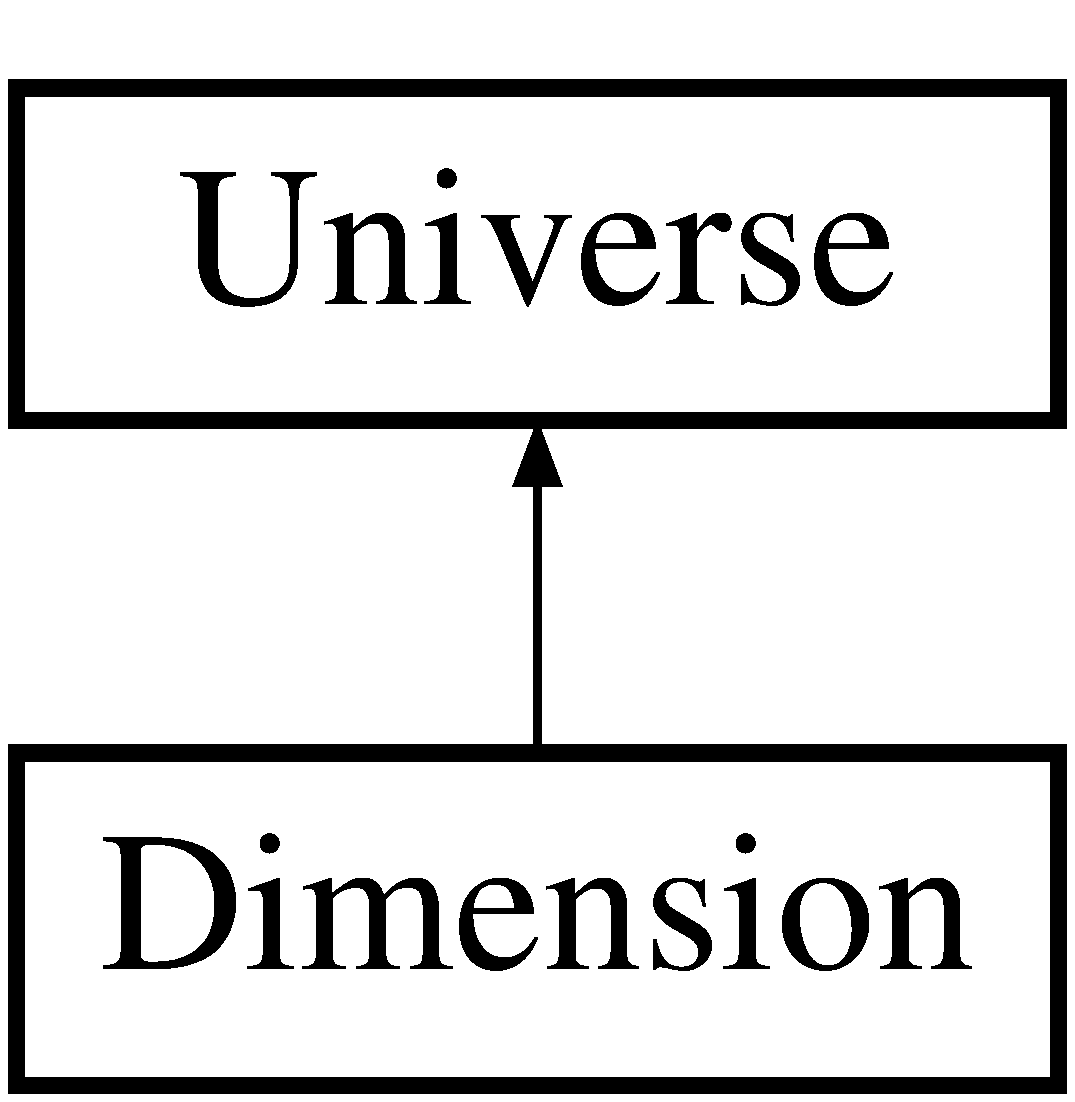
\includegraphics[height=2.000000cm]{classDimension}
\end{center}
\end{figure}
\subsection*{Classes}
\begin{DoxyCompactItemize}
\item 
struct \mbox{\hyperlink{structDimension_1_1CounterAdjustment}{Counter\+Adjustment}}
\end{DoxyCompactItemize}
\subsection*{Public Member Functions}
\begin{DoxyCompactItemize}
\item 
\mbox{\hyperlink{classDimension_aa61dad15f33b6c3d09028ba9e545aa70}{Dimension}} ()
\item 
\mbox{\hyperlink{classDimension_a68def81e037c1bcc005591f45c53e3a3}{Dimension}} (unsigned int object\+\_\+type)
\item 
\mbox{\hyperlink{classDimension_ab48cbe6ca22404ab5a2c522498c38d7c}{Dimension}} (unsigned int object\+\_\+type, std\+::chrono\+::time\+\_\+point$<$ \mbox{\hyperlink{universe_8h_a0ef8d951d1ca5ab3cfaf7ab4c7a6fd80}{Clock}} $>$ event\+\_\+time)
\item 
\mbox{\hyperlink{classDimension_a9282c4669e8f97dce010324886d79a99}{Dimension}} (unsigned int object\+\_\+type, std\+::chrono\+::time\+\_\+point$<$ \mbox{\hyperlink{universe_8h_a0ef8d951d1ca5ab3cfaf7ab4c7a6fd80}{Clock}} $>$ event\+\_\+time, \mbox{\hyperlink{classUniverse}{Universe}} \&universe\+\_\+connector)
\item 
virtual \mbox{\hyperlink{classDimension_aa990dfd442020c193a1941e9dffbfbee}{$\sim$\+Dimension}} ()
\item 
unsigned int \mbox{\hyperlink{classDimension_a2fbee64eeea5de3d8eab10cf0fdb6363}{Get\+Counter}} (std\+::chrono\+::time\+\_\+point$<$ \mbox{\hyperlink{universe_8h_a0ef8d951d1ca5ab3cfaf7ab4c7a6fd80}{Clock}} $>$ event\+\_\+time)
\item 
double \mbox{\hyperlink{classDimension_a6985e3d8738202530cb2cd428b5b884c}{Get\+Scale}} (std\+::chrono\+::time\+\_\+point$<$ \mbox{\hyperlink{universe_8h_a0ef8d951d1ca5ab3cfaf7ab4c7a6fd80}{Clock}} $>$ event\+\_\+time)
\item 
double \mbox{\hyperlink{classDimension_a58009cd435ead4b7b2f395a11fda0ae8}{Get\+Offset}} (std\+::chrono\+::time\+\_\+point$<$ \mbox{\hyperlink{universe_8h_a0ef8d951d1ca5ab3cfaf7ab4c7a6fd80}{Clock}} $>$ event\+\_\+time)
\item 
double \mbox{\hyperlink{classDimension_ae0b4f856e62a70bb3dff96528315f3c9}{Get\+Time}} (std\+::chrono\+::time\+\_\+point$<$ \mbox{\hyperlink{universe_8h_a0ef8d951d1ca5ab3cfaf7ab4c7a6fd80}{Clock}} $>$ event\+\_\+time)
\item 
std\+::chrono\+::time\+\_\+point$<$ std\+::chrono\+::high\+\_\+resolution\+\_\+clock $>$ \mbox{\hyperlink{classDimension_ab39b7ff253ade59c5c2d807c511b4028}{The\+Time\+Now}} ()
\item 
void \mbox{\hyperlink{classDimension_a75c6a1a1e09c40b5860dc11a83384d9f}{Set\+Counter}} (std\+::chrono\+::time\+\_\+point$<$ \mbox{\hyperlink{universe_8h_a0ef8d951d1ca5ab3cfaf7ab4c7a6fd80}{Clock}} $>$ event\+\_\+time, unsigned int val)
\item 
void \mbox{\hyperlink{classDimension_a7f655ea002e8f9614a8c5cfa1807c49c}{Set\+Scale}} (std\+::chrono\+::time\+\_\+point$<$ \mbox{\hyperlink{universe_8h_a0ef8d951d1ca5ab3cfaf7ab4c7a6fd80}{Clock}} $>$ event\+\_\+time, double val)
\item 
void \mbox{\hyperlink{classDimension_a0558d45fe020ba1d1895e521a411decb}{Set\+Time}} (std\+::chrono\+::time\+\_\+point$<$ \mbox{\hyperlink{universe_8h_a0ef8d951d1ca5ab3cfaf7ab4c7a6fd80}{Clock}} $>$ event\+\_\+time, double val)
\item 
void \mbox{\hyperlink{classDimension_af74dd7af3af95c0a51b001b6ad665300}{Set\+Offset}} (std\+::chrono\+::time\+\_\+point$<$ \mbox{\hyperlink{universe_8h_a0ef8d951d1ca5ab3cfaf7ab4c7a6fd80}{Clock}} $>$ event\+\_\+time, double val)
\item 
void \mbox{\hyperlink{classDimension_aa323eaa2c592e498d48e0739009ec313}{Inc\+Scale}} (std\+::chrono\+::time\+\_\+point$<$ \mbox{\hyperlink{universe_8h_a0ef8d951d1ca5ab3cfaf7ab4c7a6fd80}{Clock}} $>$ event\+\_\+time, double val)
\item 
void \mbox{\hyperlink{classDimension_a4bd8e584c3bb68ebd7ca0463f8905813}{Dec\+Scale}} (std\+::chrono\+::time\+\_\+point$<$ \mbox{\hyperlink{universe_8h_a0ef8d951d1ca5ab3cfaf7ab4c7a6fd80}{Clock}} $>$ event\+\_\+time, double val)
\item 
void \mbox{\hyperlink{classDimension_afc61c6d6d68ec0ed461458d504fec16f}{Inc\+Time}} (std\+::chrono\+::time\+\_\+point$<$ \mbox{\hyperlink{universe_8h_a0ef8d951d1ca5ab3cfaf7ab4c7a6fd80}{Clock}} $>$ event\+\_\+time, double val)
\item 
void \mbox{\hyperlink{classDimension_a25978bcb1f62aa7ed909463d08d92ca4}{Dec\+Time}} (std\+::chrono\+::time\+\_\+point$<$ \mbox{\hyperlink{universe_8h_a0ef8d951d1ca5ab3cfaf7ab4c7a6fd80}{Clock}} $>$ event\+\_\+time, double val)
\item 
void \mbox{\hyperlink{classDimension_aaf18cc220562b30f9e7aee92f16cc08e}{Inc\+Offset}} (std\+::chrono\+::time\+\_\+point$<$ \mbox{\hyperlink{universe_8h_a0ef8d951d1ca5ab3cfaf7ab4c7a6fd80}{Clock}} $>$ event\+\_\+time, double val)
\item 
void \mbox{\hyperlink{classDimension_a2017e62d4b3caf31f4f1b6b5cf59a798}{Dec\+Offset}} (std\+::chrono\+::time\+\_\+point$<$ \mbox{\hyperlink{universe_8h_a0ef8d951d1ca5ab3cfaf7ab4c7a6fd80}{Clock}} $>$ event\+\_\+time, double val)
\item 
void \mbox{\hyperlink{classDimension_a484621a7c6f9b43f6e251ba04e0fdf8b}{Set\+Object\+Type}} (std\+::chrono\+::time\+\_\+point$<$ \mbox{\hyperlink{universe_8h_a0ef8d951d1ca5ab3cfaf7ab4c7a6fd80}{Clock}} $>$ event\+\_\+time, int val)
\item 
int \mbox{\hyperlink{classDimension_a72f494215a114cb43cecd9b170bcde51}{Get\+Object\+Type}} (std\+::chrono\+::time\+\_\+point$<$ \mbox{\hyperlink{universe_8h_a0ef8d951d1ca5ab3cfaf7ab4c7a6fd80}{Clock}} $>$ event\+\_\+time)
\item 
bool \mbox{\hyperlink{classDimension_af83732dba929ae01aca457e7d6121374}{Reset\+Parameters}} (std\+::chrono\+::time\+\_\+point$<$ \mbox{\hyperlink{universe_8h_a0ef8d951d1ca5ab3cfaf7ab4c7a6fd80}{Clock}} $>$ event\+\_\+time)
\item 
void \mbox{\hyperlink{classDimension_a31e28c2777888449fad32843f6dd15ed}{Adjust\+Counters}} (std\+::chrono\+::time\+\_\+point$<$ std\+::chrono\+::high\+\_\+resolution\+\_\+clock $>$ current\+Time)
\item 
int \mbox{\hyperlink{classDimension_a663916c2573b6df4db02ccee5678a75d}{Update}} (std\+::chrono\+::time\+\_\+point$<$ \mbox{\hyperlink{universe_8h_a0ef8d951d1ca5ab3cfaf7ab4c7a6fd80}{Clock}} $>$ event\+\_\+time)
\item 
void \mbox{\hyperlink{classDimension_a6d3f7fa4a26b92d8ae6161a1b8bb8220}{Set\+Charge}} (std\+::chrono\+::time\+\_\+point$<$ \mbox{\hyperlink{universe_8h_a0ef8d951d1ca5ab3cfaf7ab4c7a6fd80}{Clock}} $>$ event\+\_\+time, int val) final
\item 
void \mbox{\hyperlink{classDimension_a8d73c050c67b0226572b4a1b08ae6594}{Set\+Spin}} (std\+::chrono\+::time\+\_\+point$<$ \mbox{\hyperlink{universe_8h_a0ef8d951d1ca5ab3cfaf7ab4c7a6fd80}{Clock}} $>$ event\+\_\+time, int val) final
\item 
double \mbox{\hyperlink{classDimension_a652220a2eb1b26c749ad032865d81788}{Get\+Gravitation}} (std\+::chrono\+::time\+\_\+point$<$ \mbox{\hyperlink{universe_8h_a0ef8d951d1ca5ab3cfaf7ab4c7a6fd80}{Clock}} $>$ event\+\_\+time) final
\item 
double \mbox{\hyperlink{classDimension_a656ce92d07ea600cc0ec53865ad515e2}{Get\+Weak}} (std\+::chrono\+::time\+\_\+point$<$ \mbox{\hyperlink{universe_8h_a0ef8d951d1ca5ab3cfaf7ab4c7a6fd80}{Clock}} $>$ event\+\_\+time) final
\item 
double \mbox{\hyperlink{classDimension_a5bb5a164564013a60728854cc2e5ddb3}{Get\+Weak\+Electroweak}} (std\+::chrono\+::time\+\_\+point$<$ \mbox{\hyperlink{universe_8h_a0ef8d951d1ca5ab3cfaf7ab4c7a6fd80}{Clock}} $>$ event\+\_\+time) final
\item 
double \mbox{\hyperlink{classDimension_a21783c29a576518b722512f1245fa598}{Get\+Electromagnetic}} (std\+::chrono\+::time\+\_\+point$<$ \mbox{\hyperlink{universe_8h_a0ef8d951d1ca5ab3cfaf7ab4c7a6fd80}{Clock}} $>$ event\+\_\+time) final
\item 
double \mbox{\hyperlink{classDimension_ae1babb1fa280c35966d7ee3de6655e4d}{Get\+Electromagnetic\+Electroweak}} (std\+::chrono\+::time\+\_\+point$<$ \mbox{\hyperlink{universe_8h_a0ef8d951d1ca5ab3cfaf7ab4c7a6fd80}{Clock}} $>$ event\+\_\+time) final
\item 
double \mbox{\hyperlink{classDimension_ae36aadad4ae84735a5ff73bff4eb97b1}{Get\+Strong}} (std\+::chrono\+::time\+\_\+point$<$ \mbox{\hyperlink{universe_8h_a0ef8d951d1ca5ab3cfaf7ab4c7a6fd80}{Clock}} $>$ event\+\_\+time) final
\item 
double \mbox{\hyperlink{classDimension_ad0d067d7f9dc4841b0ad280979ebe7af}{Get\+Strong\+Fundamental}} (std\+::chrono\+::time\+\_\+point$<$ \mbox{\hyperlink{universe_8h_a0ef8d951d1ca5ab3cfaf7ab4c7a6fd80}{Clock}} $>$ event\+\_\+time) final
\item 
double \mbox{\hyperlink{classDimension_aeee6025f17d9cd1bf7f324d715a30691}{Get\+Strong\+Residual}} (std\+::chrono\+::time\+\_\+point$<$ \mbox{\hyperlink{universe_8h_a0ef8d951d1ca5ab3cfaf7ab4c7a6fd80}{Clock}} $>$ event\+\_\+time) final
\item 
double \mbox{\hyperlink{classDimension_a9474b0dd3f6321a92bfe4375bb4b2266}{Apply\+Gravitation}} (std\+::chrono\+::time\+\_\+point$<$ \mbox{\hyperlink{universe_8h_a0ef8d951d1ca5ab3cfaf7ab4c7a6fd80}{Clock}} $>$ event\+\_\+time, double val) final
\item 
double \mbox{\hyperlink{classDimension_a72b8ab8d676b4df6b9a6ef948f5693c9}{Apply\+Weak}} (std\+::chrono\+::time\+\_\+point$<$ \mbox{\hyperlink{universe_8h_a0ef8d951d1ca5ab3cfaf7ab4c7a6fd80}{Clock}} $>$ event\+\_\+time, double val) final
\item 
double \mbox{\hyperlink{classDimension_abf490cabd486afa660f17940ed0d17e6}{Apply\+Weak\+Electroweak}} (std\+::chrono\+::time\+\_\+point$<$ \mbox{\hyperlink{universe_8h_a0ef8d951d1ca5ab3cfaf7ab4c7a6fd80}{Clock}} $>$ event\+\_\+time, double val) final
\item 
double \mbox{\hyperlink{classDimension_a65bcd3c09792cf53b1f614eff49cf111}{Apply\+Electromagnetic}} (std\+::chrono\+::time\+\_\+point$<$ \mbox{\hyperlink{universe_8h_a0ef8d951d1ca5ab3cfaf7ab4c7a6fd80}{Clock}} $>$ event\+\_\+time, double val) final
\item 
double \mbox{\hyperlink{classDimension_ab13e8ed50a4373274636e542c917db01}{Apply\+Electromagnetic\+Electroweak}} (std\+::chrono\+::time\+\_\+point$<$ \mbox{\hyperlink{universe_8h_a0ef8d951d1ca5ab3cfaf7ab4c7a6fd80}{Clock}} $>$ event\+\_\+time, double val) final
\item 
double \mbox{\hyperlink{classDimension_a621e8f7f24db86e836c5b3da0f019290}{Apply\+Strong}} (std\+::chrono\+::time\+\_\+point$<$ \mbox{\hyperlink{universe_8h_a0ef8d951d1ca5ab3cfaf7ab4c7a6fd80}{Clock}} $>$ event\+\_\+time, double val) final
\item 
double \mbox{\hyperlink{classDimension_afb01fb9e469da18899d4b14e5f095ece}{Apply\+Strong\+Fundamental}} (std\+::chrono\+::time\+\_\+point$<$ \mbox{\hyperlink{universe_8h_a0ef8d951d1ca5ab3cfaf7ab4c7a6fd80}{Clock}} $>$ event\+\_\+time, double val) final
\item 
double \mbox{\hyperlink{classDimension_a2ae0b6a8ee17f6e28b6d2d3209df4bf4}{Apply\+Strong\+Residual}} (std\+::chrono\+::time\+\_\+point$<$ \mbox{\hyperlink{universe_8h_a0ef8d951d1ca5ab3cfaf7ab4c7a6fd80}{Clock}} $>$ event\+\_\+time, double val) final
\item 
void \mbox{\hyperlink{classDimension_aeec6887382d09e3d78382582ff4e7c33}{Set\+Gravitation}} (std\+::chrono\+::time\+\_\+point$<$ \mbox{\hyperlink{universe_8h_a0ef8d951d1ca5ab3cfaf7ab4c7a6fd80}{Clock}} $>$ event\+\_\+time, double val) final
\item 
void \mbox{\hyperlink{classDimension_a157cfa28dd6bc5518d622d01445ca827}{Set\+Weak}} (std\+::chrono\+::time\+\_\+point$<$ \mbox{\hyperlink{universe_8h_a0ef8d951d1ca5ab3cfaf7ab4c7a6fd80}{Clock}} $>$ event\+\_\+time, double val) final
\item 
void \mbox{\hyperlink{classDimension_a1d2accef9e6adf747f5cc143ae4527c9}{Set\+Weak\+Electroweak}} (std\+::chrono\+::time\+\_\+point$<$ \mbox{\hyperlink{universe_8h_a0ef8d951d1ca5ab3cfaf7ab4c7a6fd80}{Clock}} $>$ event\+\_\+time, double val) final
\item 
void \mbox{\hyperlink{classDimension_ad8c18ce6358904e01594092dca9f1311}{Set\+Electromagnetic}} (std\+::chrono\+::time\+\_\+point$<$ \mbox{\hyperlink{universe_8h_a0ef8d951d1ca5ab3cfaf7ab4c7a6fd80}{Clock}} $>$ event\+\_\+time, double val) final
\item 
void \mbox{\hyperlink{classDimension_aead73fc6a25388d14b514b2170735b1b}{Set\+Electromagnetic\+Electroweak}} (std\+::chrono\+::time\+\_\+point$<$ \mbox{\hyperlink{universe_8h_a0ef8d951d1ca5ab3cfaf7ab4c7a6fd80}{Clock}} $>$ event\+\_\+time, double val) final
\item 
void \mbox{\hyperlink{classDimension_ab9021cb6727ed590026bf870c638576d}{Set\+Strong}} (std\+::chrono\+::time\+\_\+point$<$ \mbox{\hyperlink{universe_8h_a0ef8d951d1ca5ab3cfaf7ab4c7a6fd80}{Clock}} $>$ event\+\_\+time, double val) final
\item 
void \mbox{\hyperlink{classDimension_a2de864aaa4b1074684395dbe928468c1}{Set\+Strong\+Fundamental}} (std\+::chrono\+::time\+\_\+point$<$ \mbox{\hyperlink{universe_8h_a0ef8d951d1ca5ab3cfaf7ab4c7a6fd80}{Clock}} $>$ event\+\_\+time, double val) final
\item 
void \mbox{\hyperlink{classDimension_a9bd5480b1da689cd58bf61dac7169080}{Set\+Strong\+Residual}} (std\+::chrono\+::time\+\_\+point$<$ \mbox{\hyperlink{universe_8h_a0ef8d951d1ca5ab3cfaf7ab4c7a6fd80}{Clock}} $>$ event\+\_\+time, double val) final
\item 
void \mbox{\hyperlink{classDimension_a5b07f5c8558233c8f3488baf1fe3459a}{Poll\+Elementary\+Force}} (std\+::chrono\+::time\+\_\+point$<$ \mbox{\hyperlink{universe_8h_a0ef8d951d1ca5ab3cfaf7ab4c7a6fd80}{Clock}} $>$ event\+\_\+time) final
\end{DoxyCompactItemize}
\subsection*{Public Attributes}
\begin{DoxyCompactItemize}
\item 
std\+::vector$<$ \mbox{\hyperlink{structDimension_1_1CounterAdjustment}{Counter\+Adjustment}} $\ast$ $>$ \mbox{\hyperlink{classDimension_a370bb42cca1211c7a6c66846ecec4dd9}{temporal\+\_\+adjustment\+\_\+list}}
\item 
int \mbox{\hyperlink{classDimension_a8095020214e474081002dbf7d9ff9d42}{duration\+\_\+since\+\_\+last\+\_\+event}}
\end{DoxyCompactItemize}
\subsection*{Protected Attributes}
\begin{DoxyCompactItemize}
\item 
double \mbox{\hyperlink{classDimension_ad3ba9c1c332756658b1e711c447831a3}{scale\+\_\+time}}
\item 
std\+::chrono\+::time\+\_\+point$<$ \mbox{\hyperlink{universe_8h_a0ef8d951d1ca5ab3cfaf7ab4c7a6fd80}{Clock}} $>$ \mbox{\hyperlink{classDimension_a99ba1a7fe44c7e52520144ab4793cad3}{time\+\_\+object\+\_\+created}}
\begin{DoxyCompactList}\small\item\em Member variable \char`\"{}time\+\_\+object\+\_\+created\char`\"{}. \end{DoxyCompactList}\item 
std\+::chrono\+::time\+\_\+point$<$ \mbox{\hyperlink{universe_8h_a0ef8d951d1ca5ab3cfaf7ab4c7a6fd80}{Clock}} $>$ \mbox{\hyperlink{classDimension_ac2df45c101a97359cfe179636f62b0f2}{object\+Expiration}}
\begin{DoxyCompactList}\small\item\em Member variable \char`\"{}object\+Expiration\char`\"{}. \end{DoxyCompactList}\item 
std\+::chrono\+::time\+\_\+point$<$ \mbox{\hyperlink{universe_8h_a0ef8d951d1ca5ab3cfaf7ab4c7a6fd80}{Clock}} $>$ \mbox{\hyperlink{classDimension_a249074ae65a06cb5386baf196bdee022}{object\+Lifespan}}
\begin{DoxyCompactList}\small\item\em Member variable \char`\"{}object\+Lifespan\char`\"{}. \end{DoxyCompactList}\end{DoxyCompactItemize}
\subsection*{Private Member Functions}
\begin{DoxyCompactItemize}
\item 
void \mbox{\hyperlink{classDimension_a278d8c3df7896eb01c55283482f8674a}{Add\+Temporal\+Adjustment}} (std\+::chrono\+::time\+\_\+point$<$ \mbox{\hyperlink{universe_8h_a0ef8d951d1ca5ab3cfaf7ab4c7a6fd80}{Clock}} $>$ event\+\_\+time, double $\ast$point\+\_\+to\+\_\+counter, double pool, int interval, int shape)
\end{DoxyCompactItemize}
\subsection*{Private Attributes}
\begin{DoxyCompactItemize}
\item 
double \mbox{\hyperlink{classDimension_a4b4e30a89bc08dd201962f530b7c31f8}{object\+\_\+energy}}
\item 
int \mbox{\hyperlink{classDimension_add0a5cbc1ccf67d063dbaf5e1ee07b40}{dimension\+\_\+type}}
\item 
unsigned int \mbox{\hyperlink{classDimension_aafe44c853102feeea49e8ffa00f2c6ae}{dimension\+Counter}}
\begin{DoxyCompactList}\small\item\em Member variable \char`\"{}dimension\+Counter\char`\"{}. \end{DoxyCompactList}\item 
double \mbox{\hyperlink{classDimension_a7ed6787b2ac9e0fe7e8fec36a3a1c287}{dimension\+\_\+scale}}
\item 
double \mbox{\hyperlink{classDimension_a3e2868e1f50df8d249835aa3d4819a52}{dimension\+\_\+time\+\_\+counter}}
\item 
double \mbox{\hyperlink{classDimension_aba67083965a790931bc581a65f6ca01a}{dimension\+\_\+offset}}
\item 
unsigned int \mbox{\hyperlink{classDimension_a286384f40ffbb03d770307bb3a2b57d9}{m\+\_\+\+Counter}}
\begin{DoxyCompactList}\small\item\em Member variable \char`\"{}m\+\_\+\+Counter\char`\"{}. \end{DoxyCompactList}\item 
int \mbox{\hyperlink{classDimension_aa808e7d2df6d70eb81b74b8f5b1107c5}{m\+\_\+\+Orbital\+Type}}
\item 
int \mbox{\hyperlink{classDimension_a7c7a09553bdb908fc0f133e3049c62e3}{m\+\_\+\+Tau}}
\item 
double \mbox{\hyperlink{classDimension_a1e1ba937169eefc74b53fac47ae4cf54}{m\+\_\+\+Position}}
\item 
double \mbox{\hyperlink{classDimension_aad79e5f97dffe0bff2908fee13d9ce8f}{m\+\_\+\+Phase}}
\item 
int \mbox{\hyperlink{classDimension_ad3a31f39b4ce1d8e2c777bffd8042378}{m\+\_\+\+Duration}}
\item 
int \mbox{\hyperlink{classDimension_af3cd48a0e5321d1cf48b24c48fcc5659}{m\+\_\+\+Internal\+Clock}}
\item 
std\+::chrono\+::time\+\_\+point$<$ \mbox{\hyperlink{universe_8h_a0ef8d951d1ca5ab3cfaf7ab4c7a6fd80}{Clock}} $>$ \mbox{\hyperlink{classDimension_addc0ef6daebc40044668f4db8667c9c6}{previous\+\_\+event\+\_\+time}}
\item 
bool \mbox{\hyperlink{classDimension_add91aa075486fb41cb889a1132ce1d9b}{object\+\_\+initialised}}
\item 
bool \mbox{\hyperlink{classDimension_abab9945cfe63c94dcf2a25e2fb3651e1}{object\+\_\+disabled}}
\end{DoxyCompactItemize}
\subsection*{Friends}
\begin{DoxyCompactItemize}
\item 
class \mbox{\hyperlink{classDimension_ad04bbaef84caa0d408ec09a1c1302f5f}{Cognitive\+Network}}
\item 
class \mbox{\hyperlink{classDimension_a1dacbeca8e464bdc533a40a1b18f33b2}{Composite\+Force}}
\item 
class \mbox{\hyperlink{classDimension_a8be5cf46db5f9876c49d58e4ab84044b}{Composite\+Particle}}
\item 
class \mbox{\hyperlink{classDimension_a6e57500586e9cd366f5cf76ea0299957}{Elementary\+Force}}
\item 
class \mbox{\hyperlink{classDimension_af2ace341c1d7ccd30de3502502773591}{Elementary\+Particle}}
\item 
class \mbox{\hyperlink{classDimension_a01ab5ef28c10ff1c9ed0c618fa044aea}{Matter}}
\item 
class \mbox{\hyperlink{classDimension_ac790db405644a01723104c3c0c8128bb}{Membrane}}
\item 
class \mbox{\hyperlink{classDimension_a9175d4e959674956ccb487d060bac93f}{Monomer}}
\item 
class \mbox{\hyperlink{classDimension_aa410d74ba34b18a9f6bdf24323c4ee5b}{Neuron}}
\item 
class \mbox{\hyperlink{classDimension_ae64ddc1700c5abc4106cbcc5843a4a42}{Polymer}}
\item 
class \mbox{\hyperlink{classDimension_aa238d52f825b8ea8da6a5c4ae1b8d482}{Point}}
\item 
class \mbox{\hyperlink{classDimension_a5636b9113fd1246b3392dd52b3138229}{Solid}}
\item 
class \mbox{\hyperlink{classDimension_aaa07b7b364b620b9a781f30a5cd9f5ea}{Soma}}
\end{DoxyCompactItemize}


\subsection{Constructor \& Destructor Documentation}
\mbox{\Hypertarget{classDimension_aa61dad15f33b6c3d09028ba9e545aa70}\label{classDimension_aa61dad15f33b6c3d09028ba9e545aa70}} 
\index{Dimension@{Dimension}!Dimension@{Dimension}}
\index{Dimension@{Dimension}!Dimension@{Dimension}}
\subsubsection{\texorpdfstring{Dimension()}{Dimension()}\hspace{0.1cm}{\footnotesize\ttfamily [1/4]}}
{\footnotesize\ttfamily Dimension\+::\+Dimension (\begin{DoxyParamCaption}{ }\end{DoxyParamCaption})\hspace{0.3cm}{\ttfamily [inline]}}

\mbox{\Hypertarget{classDimension_a68def81e037c1bcc005591f45c53e3a3}\label{classDimension_a68def81e037c1bcc005591f45c53e3a3}} 
\index{Dimension@{Dimension}!Dimension@{Dimension}}
\index{Dimension@{Dimension}!Dimension@{Dimension}}
\subsubsection{\texorpdfstring{Dimension()}{Dimension()}\hspace{0.1cm}{\footnotesize\ttfamily [2/4]}}
{\footnotesize\ttfamily Dimension\+::\+Dimension (\begin{DoxyParamCaption}\item[{unsigned int}]{object\+\_\+type }\end{DoxyParamCaption})\hspace{0.3cm}{\ttfamily [inline]}}

\mbox{\Hypertarget{classDimension_ab48cbe6ca22404ab5a2c522498c38d7c}\label{classDimension_ab48cbe6ca22404ab5a2c522498c38d7c}} 
\index{Dimension@{Dimension}!Dimension@{Dimension}}
\index{Dimension@{Dimension}!Dimension@{Dimension}}
\subsubsection{\texorpdfstring{Dimension()}{Dimension()}\hspace{0.1cm}{\footnotesize\ttfamily [3/4]}}
{\footnotesize\ttfamily Dimension\+::\+Dimension (\begin{DoxyParamCaption}\item[{unsigned int}]{object\+\_\+type,  }\item[{std\+::chrono\+::time\+\_\+point$<$ \mbox{\hyperlink{universe_8h_a0ef8d951d1ca5ab3cfaf7ab4c7a6fd80}{Clock}} $>$}]{event\+\_\+time }\end{DoxyParamCaption})\hspace{0.3cm}{\ttfamily [inline]}}

\mbox{\Hypertarget{classDimension_a9282c4669e8f97dce010324886d79a99}\label{classDimension_a9282c4669e8f97dce010324886d79a99}} 
\index{Dimension@{Dimension}!Dimension@{Dimension}}
\index{Dimension@{Dimension}!Dimension@{Dimension}}
\subsubsection{\texorpdfstring{Dimension()}{Dimension()}\hspace{0.1cm}{\footnotesize\ttfamily [4/4]}}
{\footnotesize\ttfamily Dimension\+::\+Dimension (\begin{DoxyParamCaption}\item[{unsigned int}]{object\+\_\+type,  }\item[{std\+::chrono\+::time\+\_\+point$<$ \mbox{\hyperlink{universe_8h_a0ef8d951d1ca5ab3cfaf7ab4c7a6fd80}{Clock}} $>$}]{event\+\_\+time,  }\item[{\mbox{\hyperlink{classUniverse}{Universe}} \&}]{universe\+\_\+connector }\end{DoxyParamCaption})\hspace{0.3cm}{\ttfamily [inline]}}

\mbox{\Hypertarget{classDimension_aa990dfd442020c193a1941e9dffbfbee}\label{classDimension_aa990dfd442020c193a1941e9dffbfbee}} 
\index{Dimension@{Dimension}!````~Dimension@{$\sim$\+Dimension}}
\index{````~Dimension@{$\sim$\+Dimension}!Dimension@{Dimension}}
\subsubsection{\texorpdfstring{$\sim$\+Dimension()}{~Dimension()}}
{\footnotesize\ttfamily virtual Dimension\+::$\sim$\+Dimension (\begin{DoxyParamCaption}{ }\end{DoxyParamCaption})\hspace{0.3cm}{\ttfamily [inline]}, {\ttfamily [virtual]}}



\subsection{Member Function Documentation}
\mbox{\Hypertarget{classDimension_a278d8c3df7896eb01c55283482f8674a}\label{classDimension_a278d8c3df7896eb01c55283482f8674a}} 
\index{Dimension@{Dimension}!Add\+Temporal\+Adjustment@{Add\+Temporal\+Adjustment}}
\index{Add\+Temporal\+Adjustment@{Add\+Temporal\+Adjustment}!Dimension@{Dimension}}
\subsubsection{\texorpdfstring{Add\+Temporal\+Adjustment()}{AddTemporalAdjustment()}}
{\footnotesize\ttfamily void Dimension\+::\+Add\+Temporal\+Adjustment (\begin{DoxyParamCaption}\item[{std\+::chrono\+::time\+\_\+point$<$ \mbox{\hyperlink{universe_8h_a0ef8d951d1ca5ab3cfaf7ab4c7a6fd80}{Clock}} $>$}]{event\+\_\+time,  }\item[{double $\ast$}]{point\+\_\+to\+\_\+counter,  }\item[{double}]{pool,  }\item[{int}]{interval,  }\item[{int}]{shape }\end{DoxyParamCaption})\hspace{0.3cm}{\ttfamily [private]}, {\ttfamily [virtual]}}



Reimplemented from \mbox{\hyperlink{classUniverse_a901e16db5e8af258c66af7ac75662fe0}{Universe}}.

\mbox{\Hypertarget{classDimension_a31e28c2777888449fad32843f6dd15ed}\label{classDimension_a31e28c2777888449fad32843f6dd15ed}} 
\index{Dimension@{Dimension}!Adjust\+Counters@{Adjust\+Counters}}
\index{Adjust\+Counters@{Adjust\+Counters}!Dimension@{Dimension}}
\subsubsection{\texorpdfstring{Adjust\+Counters()}{AdjustCounters()}}
{\footnotesize\ttfamily void Dimension\+::\+Adjust\+Counters (\begin{DoxyParamCaption}\item[{std\+::chrono\+::time\+\_\+point$<$ std\+::chrono\+::high\+\_\+resolution\+\_\+clock $>$}]{current\+Time }\end{DoxyParamCaption})\hspace{0.3cm}{\ttfamily [virtual]}}



Reimplemented from \mbox{\hyperlink{classUniverse_a15aa20218286fd11ecb9b792dfb63be3}{Universe}}.

\mbox{\Hypertarget{classDimension_a65bcd3c09792cf53b1f614eff49cf111}\label{classDimension_a65bcd3c09792cf53b1f614eff49cf111}} 
\index{Dimension@{Dimension}!Apply\+Electromagnetic@{Apply\+Electromagnetic}}
\index{Apply\+Electromagnetic@{Apply\+Electromagnetic}!Dimension@{Dimension}}
\subsubsection{\texorpdfstring{Apply\+Electromagnetic()}{ApplyElectromagnetic()}}
{\footnotesize\ttfamily double Dimension\+::\+Apply\+Electromagnetic (\begin{DoxyParamCaption}\item[{std\+::chrono\+::time\+\_\+point$<$ \mbox{\hyperlink{universe_8h_a0ef8d951d1ca5ab3cfaf7ab4c7a6fd80}{Clock}} $>$}]{event\+\_\+time,  }\item[{double}]{val }\end{DoxyParamCaption})\hspace{0.3cm}{\ttfamily [inline]}, {\ttfamily [final]}, {\ttfamily [virtual]}}



Reimplemented from \mbox{\hyperlink{classUniverse_a1f787da78fa196ba635db21a9e91dabb}{Universe}}.

\mbox{\Hypertarget{classDimension_ab13e8ed50a4373274636e542c917db01}\label{classDimension_ab13e8ed50a4373274636e542c917db01}} 
\index{Dimension@{Dimension}!Apply\+Electromagnetic\+Electroweak@{Apply\+Electromagnetic\+Electroweak}}
\index{Apply\+Electromagnetic\+Electroweak@{Apply\+Electromagnetic\+Electroweak}!Dimension@{Dimension}}
\subsubsection{\texorpdfstring{Apply\+Electromagnetic\+Electroweak()}{ApplyElectromagneticElectroweak()}}
{\footnotesize\ttfamily double Dimension\+::\+Apply\+Electromagnetic\+Electroweak (\begin{DoxyParamCaption}\item[{std\+::chrono\+::time\+\_\+point$<$ \mbox{\hyperlink{universe_8h_a0ef8d951d1ca5ab3cfaf7ab4c7a6fd80}{Clock}} $>$}]{event\+\_\+time,  }\item[{double}]{val }\end{DoxyParamCaption})\hspace{0.3cm}{\ttfamily [inline]}, {\ttfamily [final]}, {\ttfamily [virtual]}}



Reimplemented from \mbox{\hyperlink{classUniverse_a4c36c1ab30db993307f88363dde5e8c5}{Universe}}.

\mbox{\Hypertarget{classDimension_a9474b0dd3f6321a92bfe4375bb4b2266}\label{classDimension_a9474b0dd3f6321a92bfe4375bb4b2266}} 
\index{Dimension@{Dimension}!Apply\+Gravitation@{Apply\+Gravitation}}
\index{Apply\+Gravitation@{Apply\+Gravitation}!Dimension@{Dimension}}
\subsubsection{\texorpdfstring{Apply\+Gravitation()}{ApplyGravitation()}}
{\footnotesize\ttfamily double Dimension\+::\+Apply\+Gravitation (\begin{DoxyParamCaption}\item[{std\+::chrono\+::time\+\_\+point$<$ \mbox{\hyperlink{universe_8h_a0ef8d951d1ca5ab3cfaf7ab4c7a6fd80}{Clock}} $>$}]{event\+\_\+time,  }\item[{double}]{val }\end{DoxyParamCaption})\hspace{0.3cm}{\ttfamily [inline]}, {\ttfamily [final]}, {\ttfamily [virtual]}}



Reimplemented from \mbox{\hyperlink{classUniverse_a76c0b5e63c2a7d1988c44db341c3d64c}{Universe}}.

\mbox{\Hypertarget{classDimension_a621e8f7f24db86e836c5b3da0f019290}\label{classDimension_a621e8f7f24db86e836c5b3da0f019290}} 
\index{Dimension@{Dimension}!Apply\+Strong@{Apply\+Strong}}
\index{Apply\+Strong@{Apply\+Strong}!Dimension@{Dimension}}
\subsubsection{\texorpdfstring{Apply\+Strong()}{ApplyStrong()}}
{\footnotesize\ttfamily double Dimension\+::\+Apply\+Strong (\begin{DoxyParamCaption}\item[{std\+::chrono\+::time\+\_\+point$<$ \mbox{\hyperlink{universe_8h_a0ef8d951d1ca5ab3cfaf7ab4c7a6fd80}{Clock}} $>$}]{event\+\_\+time,  }\item[{double}]{val }\end{DoxyParamCaption})\hspace{0.3cm}{\ttfamily [inline]}, {\ttfamily [final]}, {\ttfamily [virtual]}}



Reimplemented from \mbox{\hyperlink{classUniverse_a906a88b37f10bfa630bef49dfd0e907a}{Universe}}.

\mbox{\Hypertarget{classDimension_afb01fb9e469da18899d4b14e5f095ece}\label{classDimension_afb01fb9e469da18899d4b14e5f095ece}} 
\index{Dimension@{Dimension}!Apply\+Strong\+Fundamental@{Apply\+Strong\+Fundamental}}
\index{Apply\+Strong\+Fundamental@{Apply\+Strong\+Fundamental}!Dimension@{Dimension}}
\subsubsection{\texorpdfstring{Apply\+Strong\+Fundamental()}{ApplyStrongFundamental()}}
{\footnotesize\ttfamily double Dimension\+::\+Apply\+Strong\+Fundamental (\begin{DoxyParamCaption}\item[{std\+::chrono\+::time\+\_\+point$<$ \mbox{\hyperlink{universe_8h_a0ef8d951d1ca5ab3cfaf7ab4c7a6fd80}{Clock}} $>$}]{event\+\_\+time,  }\item[{double}]{val }\end{DoxyParamCaption})\hspace{0.3cm}{\ttfamily [inline]}, {\ttfamily [final]}, {\ttfamily [virtual]}}



Reimplemented from \mbox{\hyperlink{classUniverse_a62789bcff84bd750b0366004381e2fdd}{Universe}}.

\mbox{\Hypertarget{classDimension_a2ae0b6a8ee17f6e28b6d2d3209df4bf4}\label{classDimension_a2ae0b6a8ee17f6e28b6d2d3209df4bf4}} 
\index{Dimension@{Dimension}!Apply\+Strong\+Residual@{Apply\+Strong\+Residual}}
\index{Apply\+Strong\+Residual@{Apply\+Strong\+Residual}!Dimension@{Dimension}}
\subsubsection{\texorpdfstring{Apply\+Strong\+Residual()}{ApplyStrongResidual()}}
{\footnotesize\ttfamily double Dimension\+::\+Apply\+Strong\+Residual (\begin{DoxyParamCaption}\item[{std\+::chrono\+::time\+\_\+point$<$ \mbox{\hyperlink{universe_8h_a0ef8d951d1ca5ab3cfaf7ab4c7a6fd80}{Clock}} $>$}]{event\+\_\+time,  }\item[{double}]{val }\end{DoxyParamCaption})\hspace{0.3cm}{\ttfamily [inline]}, {\ttfamily [final]}, {\ttfamily [virtual]}}



Reimplemented from \mbox{\hyperlink{classUniverse_af7becebb347be9a85541d96a3eca1ca7}{Universe}}.

\mbox{\Hypertarget{classDimension_a72b8ab8d676b4df6b9a6ef948f5693c9}\label{classDimension_a72b8ab8d676b4df6b9a6ef948f5693c9}} 
\index{Dimension@{Dimension}!Apply\+Weak@{Apply\+Weak}}
\index{Apply\+Weak@{Apply\+Weak}!Dimension@{Dimension}}
\subsubsection{\texorpdfstring{Apply\+Weak()}{ApplyWeak()}}
{\footnotesize\ttfamily double Dimension\+::\+Apply\+Weak (\begin{DoxyParamCaption}\item[{std\+::chrono\+::time\+\_\+point$<$ \mbox{\hyperlink{universe_8h_a0ef8d951d1ca5ab3cfaf7ab4c7a6fd80}{Clock}} $>$}]{event\+\_\+time,  }\item[{double}]{val }\end{DoxyParamCaption})\hspace{0.3cm}{\ttfamily [inline]}, {\ttfamily [final]}, {\ttfamily [virtual]}}



Reimplemented from \mbox{\hyperlink{classUniverse_a6d1226b3adec3c42a833afdbb6a65a92}{Universe}}.

\mbox{\Hypertarget{classDimension_abf490cabd486afa660f17940ed0d17e6}\label{classDimension_abf490cabd486afa660f17940ed0d17e6}} 
\index{Dimension@{Dimension}!Apply\+Weak\+Electroweak@{Apply\+Weak\+Electroweak}}
\index{Apply\+Weak\+Electroweak@{Apply\+Weak\+Electroweak}!Dimension@{Dimension}}
\subsubsection{\texorpdfstring{Apply\+Weak\+Electroweak()}{ApplyWeakElectroweak()}}
{\footnotesize\ttfamily double Dimension\+::\+Apply\+Weak\+Electroweak (\begin{DoxyParamCaption}\item[{std\+::chrono\+::time\+\_\+point$<$ \mbox{\hyperlink{universe_8h_a0ef8d951d1ca5ab3cfaf7ab4c7a6fd80}{Clock}} $>$}]{event\+\_\+time,  }\item[{double}]{val }\end{DoxyParamCaption})\hspace{0.3cm}{\ttfamily [inline]}, {\ttfamily [final]}, {\ttfamily [virtual]}}



Reimplemented from \mbox{\hyperlink{classUniverse_a46a906baabb63e5d31f8b48ea1fae52e}{Universe}}.

\mbox{\Hypertarget{classDimension_a2017e62d4b3caf31f4f1b6b5cf59a798}\label{classDimension_a2017e62d4b3caf31f4f1b6b5cf59a798}} 
\index{Dimension@{Dimension}!Dec\+Offset@{Dec\+Offset}}
\index{Dec\+Offset@{Dec\+Offset}!Dimension@{Dimension}}
\subsubsection{\texorpdfstring{Dec\+Offset()}{DecOffset()}}
{\footnotesize\ttfamily void Dimension\+::\+Dec\+Offset (\begin{DoxyParamCaption}\item[{std\+::chrono\+::time\+\_\+point$<$ \mbox{\hyperlink{universe_8h_a0ef8d951d1ca5ab3cfaf7ab4c7a6fd80}{Clock}} $>$}]{event\+\_\+time,  }\item[{double}]{val }\end{DoxyParamCaption})}

\mbox{\Hypertarget{classDimension_a4bd8e584c3bb68ebd7ca0463f8905813}\label{classDimension_a4bd8e584c3bb68ebd7ca0463f8905813}} 
\index{Dimension@{Dimension}!Dec\+Scale@{Dec\+Scale}}
\index{Dec\+Scale@{Dec\+Scale}!Dimension@{Dimension}}
\subsubsection{\texorpdfstring{Dec\+Scale()}{DecScale()}}
{\footnotesize\ttfamily void Dimension\+::\+Dec\+Scale (\begin{DoxyParamCaption}\item[{std\+::chrono\+::time\+\_\+point$<$ \mbox{\hyperlink{universe_8h_a0ef8d951d1ca5ab3cfaf7ab4c7a6fd80}{Clock}} $>$}]{event\+\_\+time,  }\item[{double}]{val }\end{DoxyParamCaption})}

\mbox{\Hypertarget{classDimension_a25978bcb1f62aa7ed909463d08d92ca4}\label{classDimension_a25978bcb1f62aa7ed909463d08d92ca4}} 
\index{Dimension@{Dimension}!Dec\+Time@{Dec\+Time}}
\index{Dec\+Time@{Dec\+Time}!Dimension@{Dimension}}
\subsubsection{\texorpdfstring{Dec\+Time()}{DecTime()}}
{\footnotesize\ttfamily void Dimension\+::\+Dec\+Time (\begin{DoxyParamCaption}\item[{std\+::chrono\+::time\+\_\+point$<$ \mbox{\hyperlink{universe_8h_a0ef8d951d1ca5ab3cfaf7ab4c7a6fd80}{Clock}} $>$}]{event\+\_\+time,  }\item[{double}]{val }\end{DoxyParamCaption})}

\mbox{\Hypertarget{classDimension_a2fbee64eeea5de3d8eab10cf0fdb6363}\label{classDimension_a2fbee64eeea5de3d8eab10cf0fdb6363}} 
\index{Dimension@{Dimension}!Get\+Counter@{Get\+Counter}}
\index{Get\+Counter@{Get\+Counter}!Dimension@{Dimension}}
\subsubsection{\texorpdfstring{Get\+Counter()}{GetCounter()}}
{\footnotesize\ttfamily unsigned int Dimension\+::\+Get\+Counter (\begin{DoxyParamCaption}\item[{std\+::chrono\+::time\+\_\+point$<$ \mbox{\hyperlink{universe_8h_a0ef8d951d1ca5ab3cfaf7ab4c7a6fd80}{Clock}} $>$}]{event\+\_\+time }\end{DoxyParamCaption})\hspace{0.3cm}{\ttfamily [inline]}}

\mbox{\Hypertarget{classDimension_a21783c29a576518b722512f1245fa598}\label{classDimension_a21783c29a576518b722512f1245fa598}} 
\index{Dimension@{Dimension}!Get\+Electromagnetic@{Get\+Electromagnetic}}
\index{Get\+Electromagnetic@{Get\+Electromagnetic}!Dimension@{Dimension}}
\subsubsection{\texorpdfstring{Get\+Electromagnetic()}{GetElectromagnetic()}}
{\footnotesize\ttfamily double Dimension\+::\+Get\+Electromagnetic (\begin{DoxyParamCaption}\item[{std\+::chrono\+::time\+\_\+point$<$ \mbox{\hyperlink{universe_8h_a0ef8d951d1ca5ab3cfaf7ab4c7a6fd80}{Clock}} $>$}]{event\+\_\+time }\end{DoxyParamCaption})\hspace{0.3cm}{\ttfamily [inline]}, {\ttfamily [final]}, {\ttfamily [virtual]}}



Reimplemented from \mbox{\hyperlink{classUniverse_a63b850ef3f3394313353109d222bf5d1}{Universe}}.

\mbox{\Hypertarget{classDimension_ae1babb1fa280c35966d7ee3de6655e4d}\label{classDimension_ae1babb1fa280c35966d7ee3de6655e4d}} 
\index{Dimension@{Dimension}!Get\+Electromagnetic\+Electroweak@{Get\+Electromagnetic\+Electroweak}}
\index{Get\+Electromagnetic\+Electroweak@{Get\+Electromagnetic\+Electroweak}!Dimension@{Dimension}}
\subsubsection{\texorpdfstring{Get\+Electromagnetic\+Electroweak()}{GetElectromagneticElectroweak()}}
{\footnotesize\ttfamily double Dimension\+::\+Get\+Electromagnetic\+Electroweak (\begin{DoxyParamCaption}\item[{std\+::chrono\+::time\+\_\+point$<$ \mbox{\hyperlink{universe_8h_a0ef8d951d1ca5ab3cfaf7ab4c7a6fd80}{Clock}} $>$}]{event\+\_\+time }\end{DoxyParamCaption})\hspace{0.3cm}{\ttfamily [inline]}, {\ttfamily [final]}, {\ttfamily [virtual]}}



Reimplemented from \mbox{\hyperlink{classUniverse_a9f099605c082e7fa755787a6a8cab7ba}{Universe}}.

\mbox{\Hypertarget{classDimension_a652220a2eb1b26c749ad032865d81788}\label{classDimension_a652220a2eb1b26c749ad032865d81788}} 
\index{Dimension@{Dimension}!Get\+Gravitation@{Get\+Gravitation}}
\index{Get\+Gravitation@{Get\+Gravitation}!Dimension@{Dimension}}
\subsubsection{\texorpdfstring{Get\+Gravitation()}{GetGravitation()}}
{\footnotesize\ttfamily double Dimension\+::\+Get\+Gravitation (\begin{DoxyParamCaption}\item[{std\+::chrono\+::time\+\_\+point$<$ \mbox{\hyperlink{universe_8h_a0ef8d951d1ca5ab3cfaf7ab4c7a6fd80}{Clock}} $>$}]{event\+\_\+time }\end{DoxyParamCaption})\hspace{0.3cm}{\ttfamily [inline]}, {\ttfamily [final]}, {\ttfamily [virtual]}}



Reimplemented from \mbox{\hyperlink{classUniverse_ab0404e774ee0ed66b597ff5b8e989446}{Universe}}.

\mbox{\Hypertarget{classDimension_a72f494215a114cb43cecd9b170bcde51}\label{classDimension_a72f494215a114cb43cecd9b170bcde51}} 
\index{Dimension@{Dimension}!Get\+Object\+Type@{Get\+Object\+Type}}
\index{Get\+Object\+Type@{Get\+Object\+Type}!Dimension@{Dimension}}
\subsubsection{\texorpdfstring{Get\+Object\+Type()}{GetObjectType()}}
{\footnotesize\ttfamily int Dimension\+::\+Get\+Object\+Type (\begin{DoxyParamCaption}\item[{std\+::chrono\+::time\+\_\+point$<$ \mbox{\hyperlink{universe_8h_a0ef8d951d1ca5ab3cfaf7ab4c7a6fd80}{Clock}} $>$}]{event\+\_\+time }\end{DoxyParamCaption})\hspace{0.3cm}{\ttfamily [inline]}}

\mbox{\Hypertarget{classDimension_a58009cd435ead4b7b2f395a11fda0ae8}\label{classDimension_a58009cd435ead4b7b2f395a11fda0ae8}} 
\index{Dimension@{Dimension}!Get\+Offset@{Get\+Offset}}
\index{Get\+Offset@{Get\+Offset}!Dimension@{Dimension}}
\subsubsection{\texorpdfstring{Get\+Offset()}{GetOffset()}}
{\footnotesize\ttfamily double Dimension\+::\+Get\+Offset (\begin{DoxyParamCaption}\item[{std\+::chrono\+::time\+\_\+point$<$ \mbox{\hyperlink{universe_8h_a0ef8d951d1ca5ab3cfaf7ab4c7a6fd80}{Clock}} $>$}]{event\+\_\+time }\end{DoxyParamCaption})\hspace{0.3cm}{\ttfamily [inline]}}

\mbox{\Hypertarget{classDimension_a6985e3d8738202530cb2cd428b5b884c}\label{classDimension_a6985e3d8738202530cb2cd428b5b884c}} 
\index{Dimension@{Dimension}!Get\+Scale@{Get\+Scale}}
\index{Get\+Scale@{Get\+Scale}!Dimension@{Dimension}}
\subsubsection{\texorpdfstring{Get\+Scale()}{GetScale()}}
{\footnotesize\ttfamily double Dimension\+::\+Get\+Scale (\begin{DoxyParamCaption}\item[{std\+::chrono\+::time\+\_\+point$<$ \mbox{\hyperlink{universe_8h_a0ef8d951d1ca5ab3cfaf7ab4c7a6fd80}{Clock}} $>$}]{event\+\_\+time }\end{DoxyParamCaption})\hspace{0.3cm}{\ttfamily [inline]}}

\mbox{\Hypertarget{classDimension_ae36aadad4ae84735a5ff73bff4eb97b1}\label{classDimension_ae36aadad4ae84735a5ff73bff4eb97b1}} 
\index{Dimension@{Dimension}!Get\+Strong@{Get\+Strong}}
\index{Get\+Strong@{Get\+Strong}!Dimension@{Dimension}}
\subsubsection{\texorpdfstring{Get\+Strong()}{GetStrong()}}
{\footnotesize\ttfamily double Dimension\+::\+Get\+Strong (\begin{DoxyParamCaption}\item[{std\+::chrono\+::time\+\_\+point$<$ \mbox{\hyperlink{universe_8h_a0ef8d951d1ca5ab3cfaf7ab4c7a6fd80}{Clock}} $>$}]{event\+\_\+time }\end{DoxyParamCaption})\hspace{0.3cm}{\ttfamily [inline]}, {\ttfamily [final]}, {\ttfamily [virtual]}}



Reimplemented from \mbox{\hyperlink{classUniverse_acb453ce71da418c5b5617fecede9571b}{Universe}}.

\mbox{\Hypertarget{classDimension_ad0d067d7f9dc4841b0ad280979ebe7af}\label{classDimension_ad0d067d7f9dc4841b0ad280979ebe7af}} 
\index{Dimension@{Dimension}!Get\+Strong\+Fundamental@{Get\+Strong\+Fundamental}}
\index{Get\+Strong\+Fundamental@{Get\+Strong\+Fundamental}!Dimension@{Dimension}}
\subsubsection{\texorpdfstring{Get\+Strong\+Fundamental()}{GetStrongFundamental()}}
{\footnotesize\ttfamily double Dimension\+::\+Get\+Strong\+Fundamental (\begin{DoxyParamCaption}\item[{std\+::chrono\+::time\+\_\+point$<$ \mbox{\hyperlink{universe_8h_a0ef8d951d1ca5ab3cfaf7ab4c7a6fd80}{Clock}} $>$}]{event\+\_\+time }\end{DoxyParamCaption})\hspace{0.3cm}{\ttfamily [inline]}, {\ttfamily [final]}, {\ttfamily [virtual]}}



Reimplemented from \mbox{\hyperlink{classUniverse_ab44daccba01ee7e3cf9b50bba83dd19e}{Universe}}.

\mbox{\Hypertarget{classDimension_aeee6025f17d9cd1bf7f324d715a30691}\label{classDimension_aeee6025f17d9cd1bf7f324d715a30691}} 
\index{Dimension@{Dimension}!Get\+Strong\+Residual@{Get\+Strong\+Residual}}
\index{Get\+Strong\+Residual@{Get\+Strong\+Residual}!Dimension@{Dimension}}
\subsubsection{\texorpdfstring{Get\+Strong\+Residual()}{GetStrongResidual()}}
{\footnotesize\ttfamily double Dimension\+::\+Get\+Strong\+Residual (\begin{DoxyParamCaption}\item[{std\+::chrono\+::time\+\_\+point$<$ \mbox{\hyperlink{universe_8h_a0ef8d951d1ca5ab3cfaf7ab4c7a6fd80}{Clock}} $>$}]{event\+\_\+time }\end{DoxyParamCaption})\hspace{0.3cm}{\ttfamily [inline]}, {\ttfamily [final]}, {\ttfamily [virtual]}}



Reimplemented from \mbox{\hyperlink{classUniverse_af0f4b81950061e63c2855eb40957a5b1}{Universe}}.

\mbox{\Hypertarget{classDimension_ae0b4f856e62a70bb3dff96528315f3c9}\label{classDimension_ae0b4f856e62a70bb3dff96528315f3c9}} 
\index{Dimension@{Dimension}!Get\+Time@{Get\+Time}}
\index{Get\+Time@{Get\+Time}!Dimension@{Dimension}}
\subsubsection{\texorpdfstring{Get\+Time()}{GetTime()}}
{\footnotesize\ttfamily double Dimension\+::\+Get\+Time (\begin{DoxyParamCaption}\item[{std\+::chrono\+::time\+\_\+point$<$ \mbox{\hyperlink{universe_8h_a0ef8d951d1ca5ab3cfaf7ab4c7a6fd80}{Clock}} $>$}]{event\+\_\+time }\end{DoxyParamCaption})\hspace{0.3cm}{\ttfamily [inline]}}

\mbox{\Hypertarget{classDimension_a656ce92d07ea600cc0ec53865ad515e2}\label{classDimension_a656ce92d07ea600cc0ec53865ad515e2}} 
\index{Dimension@{Dimension}!Get\+Weak@{Get\+Weak}}
\index{Get\+Weak@{Get\+Weak}!Dimension@{Dimension}}
\subsubsection{\texorpdfstring{Get\+Weak()}{GetWeak()}}
{\footnotesize\ttfamily double Dimension\+::\+Get\+Weak (\begin{DoxyParamCaption}\item[{std\+::chrono\+::time\+\_\+point$<$ \mbox{\hyperlink{universe_8h_a0ef8d951d1ca5ab3cfaf7ab4c7a6fd80}{Clock}} $>$}]{event\+\_\+time }\end{DoxyParamCaption})\hspace{0.3cm}{\ttfamily [inline]}, {\ttfamily [final]}, {\ttfamily [virtual]}}



Reimplemented from \mbox{\hyperlink{classUniverse_a4476b7e0a3fc1764909f556257fd9ec7}{Universe}}.

\mbox{\Hypertarget{classDimension_a5bb5a164564013a60728854cc2e5ddb3}\label{classDimension_a5bb5a164564013a60728854cc2e5ddb3}} 
\index{Dimension@{Dimension}!Get\+Weak\+Electroweak@{Get\+Weak\+Electroweak}}
\index{Get\+Weak\+Electroweak@{Get\+Weak\+Electroweak}!Dimension@{Dimension}}
\subsubsection{\texorpdfstring{Get\+Weak\+Electroweak()}{GetWeakElectroweak()}}
{\footnotesize\ttfamily double Dimension\+::\+Get\+Weak\+Electroweak (\begin{DoxyParamCaption}\item[{std\+::chrono\+::time\+\_\+point$<$ \mbox{\hyperlink{universe_8h_a0ef8d951d1ca5ab3cfaf7ab4c7a6fd80}{Clock}} $>$}]{event\+\_\+time }\end{DoxyParamCaption})\hspace{0.3cm}{\ttfamily [inline]}, {\ttfamily [final]}, {\ttfamily [virtual]}}



Reimplemented from \mbox{\hyperlink{classUniverse_a645299738e6b798a037f2a15a2e7cf4d}{Universe}}.

\mbox{\Hypertarget{classDimension_aaf18cc220562b30f9e7aee92f16cc08e}\label{classDimension_aaf18cc220562b30f9e7aee92f16cc08e}} 
\index{Dimension@{Dimension}!Inc\+Offset@{Inc\+Offset}}
\index{Inc\+Offset@{Inc\+Offset}!Dimension@{Dimension}}
\subsubsection{\texorpdfstring{Inc\+Offset()}{IncOffset()}}
{\footnotesize\ttfamily void Dimension\+::\+Inc\+Offset (\begin{DoxyParamCaption}\item[{std\+::chrono\+::time\+\_\+point$<$ \mbox{\hyperlink{universe_8h_a0ef8d951d1ca5ab3cfaf7ab4c7a6fd80}{Clock}} $>$}]{event\+\_\+time,  }\item[{double}]{val }\end{DoxyParamCaption})}

\mbox{\Hypertarget{classDimension_aa323eaa2c592e498d48e0739009ec313}\label{classDimension_aa323eaa2c592e498d48e0739009ec313}} 
\index{Dimension@{Dimension}!Inc\+Scale@{Inc\+Scale}}
\index{Inc\+Scale@{Inc\+Scale}!Dimension@{Dimension}}
\subsubsection{\texorpdfstring{Inc\+Scale()}{IncScale()}}
{\footnotesize\ttfamily void Dimension\+::\+Inc\+Scale (\begin{DoxyParamCaption}\item[{std\+::chrono\+::time\+\_\+point$<$ \mbox{\hyperlink{universe_8h_a0ef8d951d1ca5ab3cfaf7ab4c7a6fd80}{Clock}} $>$}]{event\+\_\+time,  }\item[{double}]{val }\end{DoxyParamCaption})}

\mbox{\Hypertarget{classDimension_afc61c6d6d68ec0ed461458d504fec16f}\label{classDimension_afc61c6d6d68ec0ed461458d504fec16f}} 
\index{Dimension@{Dimension}!Inc\+Time@{Inc\+Time}}
\index{Inc\+Time@{Inc\+Time}!Dimension@{Dimension}}
\subsubsection{\texorpdfstring{Inc\+Time()}{IncTime()}}
{\footnotesize\ttfamily void Dimension\+::\+Inc\+Time (\begin{DoxyParamCaption}\item[{std\+::chrono\+::time\+\_\+point$<$ \mbox{\hyperlink{universe_8h_a0ef8d951d1ca5ab3cfaf7ab4c7a6fd80}{Clock}} $>$}]{event\+\_\+time,  }\item[{double}]{val }\end{DoxyParamCaption})}

\mbox{\Hypertarget{classDimension_a5b07f5c8558233c8f3488baf1fe3459a}\label{classDimension_a5b07f5c8558233c8f3488baf1fe3459a}} 
\index{Dimension@{Dimension}!Poll\+Elementary\+Force@{Poll\+Elementary\+Force}}
\index{Poll\+Elementary\+Force@{Poll\+Elementary\+Force}!Dimension@{Dimension}}
\subsubsection{\texorpdfstring{Poll\+Elementary\+Force()}{PollElementaryForce()}}
{\footnotesize\ttfamily void Dimension\+::\+Poll\+Elementary\+Force (\begin{DoxyParamCaption}\item[{std\+::chrono\+::time\+\_\+point$<$ \mbox{\hyperlink{universe_8h_a0ef8d951d1ca5ab3cfaf7ab4c7a6fd80}{Clock}} $>$}]{event\+\_\+time }\end{DoxyParamCaption})\hspace{0.3cm}{\ttfamily [inline]}, {\ttfamily [final]}, {\ttfamily [virtual]}}



Reimplemented from \mbox{\hyperlink{classUniverse_a0c485c504542409cbb5cfd8543c35b11}{Universe}}.

\mbox{\Hypertarget{classDimension_af83732dba929ae01aca457e7d6121374}\label{classDimension_af83732dba929ae01aca457e7d6121374}} 
\index{Dimension@{Dimension}!Reset\+Parameters@{Reset\+Parameters}}
\index{Reset\+Parameters@{Reset\+Parameters}!Dimension@{Dimension}}
\subsubsection{\texorpdfstring{Reset\+Parameters()}{ResetParameters()}}
{\footnotesize\ttfamily bool Dimension\+::\+Reset\+Parameters (\begin{DoxyParamCaption}\item[{std\+::chrono\+::time\+\_\+point$<$ \mbox{\hyperlink{universe_8h_a0ef8d951d1ca5ab3cfaf7ab4c7a6fd80}{Clock}} $>$}]{event\+\_\+time }\end{DoxyParamCaption})}

\mbox{\Hypertarget{classDimension_a6d3f7fa4a26b92d8ae6161a1b8bb8220}\label{classDimension_a6d3f7fa4a26b92d8ae6161a1b8bb8220}} 
\index{Dimension@{Dimension}!Set\+Charge@{Set\+Charge}}
\index{Set\+Charge@{Set\+Charge}!Dimension@{Dimension}}
\subsubsection{\texorpdfstring{Set\+Charge()}{SetCharge()}}
{\footnotesize\ttfamily void Dimension\+::\+Set\+Charge (\begin{DoxyParamCaption}\item[{std\+::chrono\+::time\+\_\+point$<$ \mbox{\hyperlink{universe_8h_a0ef8d951d1ca5ab3cfaf7ab4c7a6fd80}{Clock}} $>$}]{event\+\_\+time,  }\item[{int}]{val }\end{DoxyParamCaption})\hspace{0.3cm}{\ttfamily [inline]}, {\ttfamily [final]}, {\ttfamily [virtual]}}



Reimplemented from \mbox{\hyperlink{classUniverse_a3b3da7c86a7b75e5e5c0b7972ac82a87}{Universe}}.

\mbox{\Hypertarget{classDimension_a75c6a1a1e09c40b5860dc11a83384d9f}\label{classDimension_a75c6a1a1e09c40b5860dc11a83384d9f}} 
\index{Dimension@{Dimension}!Set\+Counter@{Set\+Counter}}
\index{Set\+Counter@{Set\+Counter}!Dimension@{Dimension}}
\subsubsection{\texorpdfstring{Set\+Counter()}{SetCounter()}}
{\footnotesize\ttfamily void Dimension\+::\+Set\+Counter (\begin{DoxyParamCaption}\item[{std\+::chrono\+::time\+\_\+point$<$ \mbox{\hyperlink{universe_8h_a0ef8d951d1ca5ab3cfaf7ab4c7a6fd80}{Clock}} $>$}]{event\+\_\+time,  }\item[{unsigned int}]{val }\end{DoxyParamCaption})\hspace{0.3cm}{\ttfamily [virtual]}}



Reimplemented from \mbox{\hyperlink{classUniverse_aa22202ae740eb1355529afcb13285e91}{Universe}}.

\mbox{\Hypertarget{classDimension_ad8c18ce6358904e01594092dca9f1311}\label{classDimension_ad8c18ce6358904e01594092dca9f1311}} 
\index{Dimension@{Dimension}!Set\+Electromagnetic@{Set\+Electromagnetic}}
\index{Set\+Electromagnetic@{Set\+Electromagnetic}!Dimension@{Dimension}}
\subsubsection{\texorpdfstring{Set\+Electromagnetic()}{SetElectromagnetic()}}
{\footnotesize\ttfamily void Dimension\+::\+Set\+Electromagnetic (\begin{DoxyParamCaption}\item[{std\+::chrono\+::time\+\_\+point$<$ \mbox{\hyperlink{universe_8h_a0ef8d951d1ca5ab3cfaf7ab4c7a6fd80}{Clock}} $>$}]{event\+\_\+time,  }\item[{double}]{val }\end{DoxyParamCaption})\hspace{0.3cm}{\ttfamily [inline]}, {\ttfamily [final]}, {\ttfamily [virtual]}}



Reimplemented from \mbox{\hyperlink{classUniverse_aa981fc7e252b1fbbb675f0371860954d}{Universe}}.

\mbox{\Hypertarget{classDimension_aead73fc6a25388d14b514b2170735b1b}\label{classDimension_aead73fc6a25388d14b514b2170735b1b}} 
\index{Dimension@{Dimension}!Set\+Electromagnetic\+Electroweak@{Set\+Electromagnetic\+Electroweak}}
\index{Set\+Electromagnetic\+Electroweak@{Set\+Electromagnetic\+Electroweak}!Dimension@{Dimension}}
\subsubsection{\texorpdfstring{Set\+Electromagnetic\+Electroweak()}{SetElectromagneticElectroweak()}}
{\footnotesize\ttfamily void Dimension\+::\+Set\+Electromagnetic\+Electroweak (\begin{DoxyParamCaption}\item[{std\+::chrono\+::time\+\_\+point$<$ \mbox{\hyperlink{universe_8h_a0ef8d951d1ca5ab3cfaf7ab4c7a6fd80}{Clock}} $>$}]{event\+\_\+time,  }\item[{double}]{val }\end{DoxyParamCaption})\hspace{0.3cm}{\ttfamily [inline]}, {\ttfamily [final]}, {\ttfamily [virtual]}}



Reimplemented from \mbox{\hyperlink{classUniverse_a608aa95698380f791a0ffba45cc1bee3}{Universe}}.

\mbox{\Hypertarget{classDimension_aeec6887382d09e3d78382582ff4e7c33}\label{classDimension_aeec6887382d09e3d78382582ff4e7c33}} 
\index{Dimension@{Dimension}!Set\+Gravitation@{Set\+Gravitation}}
\index{Set\+Gravitation@{Set\+Gravitation}!Dimension@{Dimension}}
\subsubsection{\texorpdfstring{Set\+Gravitation()}{SetGravitation()}}
{\footnotesize\ttfamily void Dimension\+::\+Set\+Gravitation (\begin{DoxyParamCaption}\item[{std\+::chrono\+::time\+\_\+point$<$ \mbox{\hyperlink{universe_8h_a0ef8d951d1ca5ab3cfaf7ab4c7a6fd80}{Clock}} $>$}]{event\+\_\+time,  }\item[{double}]{val }\end{DoxyParamCaption})\hspace{0.3cm}{\ttfamily [inline]}, {\ttfamily [final]}, {\ttfamily [virtual]}}



Reimplemented from \mbox{\hyperlink{classUniverse_ae0cb8d86b2fbb8396d605160344b42f5}{Universe}}.

\mbox{\Hypertarget{classDimension_a484621a7c6f9b43f6e251ba04e0fdf8b}\label{classDimension_a484621a7c6f9b43f6e251ba04e0fdf8b}} 
\index{Dimension@{Dimension}!Set\+Object\+Type@{Set\+Object\+Type}}
\index{Set\+Object\+Type@{Set\+Object\+Type}!Dimension@{Dimension}}
\subsubsection{\texorpdfstring{Set\+Object\+Type()}{SetObjectType()}}
{\footnotesize\ttfamily void Dimension\+::\+Set\+Object\+Type (\begin{DoxyParamCaption}\item[{std\+::chrono\+::time\+\_\+point$<$ \mbox{\hyperlink{universe_8h_a0ef8d951d1ca5ab3cfaf7ab4c7a6fd80}{Clock}} $>$}]{event\+\_\+time,  }\item[{int}]{val }\end{DoxyParamCaption})}

\mbox{\Hypertarget{classDimension_af74dd7af3af95c0a51b001b6ad665300}\label{classDimension_af74dd7af3af95c0a51b001b6ad665300}} 
\index{Dimension@{Dimension}!Set\+Offset@{Set\+Offset}}
\index{Set\+Offset@{Set\+Offset}!Dimension@{Dimension}}
\subsubsection{\texorpdfstring{Set\+Offset()}{SetOffset()}}
{\footnotesize\ttfamily void Dimension\+::\+Set\+Offset (\begin{DoxyParamCaption}\item[{std\+::chrono\+::time\+\_\+point$<$ \mbox{\hyperlink{universe_8h_a0ef8d951d1ca5ab3cfaf7ab4c7a6fd80}{Clock}} $>$}]{event\+\_\+time,  }\item[{double}]{val }\end{DoxyParamCaption})}

\mbox{\Hypertarget{classDimension_a7f655ea002e8f9614a8c5cfa1807c49c}\label{classDimension_a7f655ea002e8f9614a8c5cfa1807c49c}} 
\index{Dimension@{Dimension}!Set\+Scale@{Set\+Scale}}
\index{Set\+Scale@{Set\+Scale}!Dimension@{Dimension}}
\subsubsection{\texorpdfstring{Set\+Scale()}{SetScale()}}
{\footnotesize\ttfamily void Dimension\+::\+Set\+Scale (\begin{DoxyParamCaption}\item[{std\+::chrono\+::time\+\_\+point$<$ \mbox{\hyperlink{universe_8h_a0ef8d951d1ca5ab3cfaf7ab4c7a6fd80}{Clock}} $>$}]{event\+\_\+time,  }\item[{double}]{val }\end{DoxyParamCaption})}

\mbox{\Hypertarget{classDimension_a8d73c050c67b0226572b4a1b08ae6594}\label{classDimension_a8d73c050c67b0226572b4a1b08ae6594}} 
\index{Dimension@{Dimension}!Set\+Spin@{Set\+Spin}}
\index{Set\+Spin@{Set\+Spin}!Dimension@{Dimension}}
\subsubsection{\texorpdfstring{Set\+Spin()}{SetSpin()}}
{\footnotesize\ttfamily void Dimension\+::\+Set\+Spin (\begin{DoxyParamCaption}\item[{std\+::chrono\+::time\+\_\+point$<$ \mbox{\hyperlink{universe_8h_a0ef8d951d1ca5ab3cfaf7ab4c7a6fd80}{Clock}} $>$}]{event\+\_\+time,  }\item[{int}]{val }\end{DoxyParamCaption})\hspace{0.3cm}{\ttfamily [inline]}, {\ttfamily [final]}, {\ttfamily [virtual]}}



Reimplemented from \mbox{\hyperlink{classUniverse_ae2ae1c3b3e4cde2c18f5f6a814761ec8}{Universe}}.

\mbox{\Hypertarget{classDimension_ab9021cb6727ed590026bf870c638576d}\label{classDimension_ab9021cb6727ed590026bf870c638576d}} 
\index{Dimension@{Dimension}!Set\+Strong@{Set\+Strong}}
\index{Set\+Strong@{Set\+Strong}!Dimension@{Dimension}}
\subsubsection{\texorpdfstring{Set\+Strong()}{SetStrong()}}
{\footnotesize\ttfamily void Dimension\+::\+Set\+Strong (\begin{DoxyParamCaption}\item[{std\+::chrono\+::time\+\_\+point$<$ \mbox{\hyperlink{universe_8h_a0ef8d951d1ca5ab3cfaf7ab4c7a6fd80}{Clock}} $>$}]{event\+\_\+time,  }\item[{double}]{val }\end{DoxyParamCaption})\hspace{0.3cm}{\ttfamily [inline]}, {\ttfamily [final]}, {\ttfamily [virtual]}}



Reimplemented from \mbox{\hyperlink{classUniverse_a5946c8f3d4cda305f3ecd10df21a2f94}{Universe}}.

\mbox{\Hypertarget{classDimension_a2de864aaa4b1074684395dbe928468c1}\label{classDimension_a2de864aaa4b1074684395dbe928468c1}} 
\index{Dimension@{Dimension}!Set\+Strong\+Fundamental@{Set\+Strong\+Fundamental}}
\index{Set\+Strong\+Fundamental@{Set\+Strong\+Fundamental}!Dimension@{Dimension}}
\subsubsection{\texorpdfstring{Set\+Strong\+Fundamental()}{SetStrongFundamental()}}
{\footnotesize\ttfamily void Dimension\+::\+Set\+Strong\+Fundamental (\begin{DoxyParamCaption}\item[{std\+::chrono\+::time\+\_\+point$<$ \mbox{\hyperlink{universe_8h_a0ef8d951d1ca5ab3cfaf7ab4c7a6fd80}{Clock}} $>$}]{event\+\_\+time,  }\item[{double}]{val }\end{DoxyParamCaption})\hspace{0.3cm}{\ttfamily [inline]}, {\ttfamily [final]}, {\ttfamily [virtual]}}



Reimplemented from \mbox{\hyperlink{classUniverse_aafec97a231126b71c73ac1258609a284}{Universe}}.

\mbox{\Hypertarget{classDimension_a9bd5480b1da689cd58bf61dac7169080}\label{classDimension_a9bd5480b1da689cd58bf61dac7169080}} 
\index{Dimension@{Dimension}!Set\+Strong\+Residual@{Set\+Strong\+Residual}}
\index{Set\+Strong\+Residual@{Set\+Strong\+Residual}!Dimension@{Dimension}}
\subsubsection{\texorpdfstring{Set\+Strong\+Residual()}{SetStrongResidual()}}
{\footnotesize\ttfamily void Dimension\+::\+Set\+Strong\+Residual (\begin{DoxyParamCaption}\item[{std\+::chrono\+::time\+\_\+point$<$ \mbox{\hyperlink{universe_8h_a0ef8d951d1ca5ab3cfaf7ab4c7a6fd80}{Clock}} $>$}]{event\+\_\+time,  }\item[{double}]{val }\end{DoxyParamCaption})\hspace{0.3cm}{\ttfamily [inline]}, {\ttfamily [final]}, {\ttfamily [virtual]}}



Reimplemented from \mbox{\hyperlink{classUniverse_a1b2d6197ddf3d613cc30bd04d22ed8b7}{Universe}}.

\mbox{\Hypertarget{classDimension_a0558d45fe020ba1d1895e521a411decb}\label{classDimension_a0558d45fe020ba1d1895e521a411decb}} 
\index{Dimension@{Dimension}!Set\+Time@{Set\+Time}}
\index{Set\+Time@{Set\+Time}!Dimension@{Dimension}}
\subsubsection{\texorpdfstring{Set\+Time()}{SetTime()}}
{\footnotesize\ttfamily void Dimension\+::\+Set\+Time (\begin{DoxyParamCaption}\item[{std\+::chrono\+::time\+\_\+point$<$ \mbox{\hyperlink{universe_8h_a0ef8d951d1ca5ab3cfaf7ab4c7a6fd80}{Clock}} $>$}]{event\+\_\+time,  }\item[{double}]{val }\end{DoxyParamCaption})}

\mbox{\Hypertarget{classDimension_a157cfa28dd6bc5518d622d01445ca827}\label{classDimension_a157cfa28dd6bc5518d622d01445ca827}} 
\index{Dimension@{Dimension}!Set\+Weak@{Set\+Weak}}
\index{Set\+Weak@{Set\+Weak}!Dimension@{Dimension}}
\subsubsection{\texorpdfstring{Set\+Weak()}{SetWeak()}}
{\footnotesize\ttfamily void Dimension\+::\+Set\+Weak (\begin{DoxyParamCaption}\item[{std\+::chrono\+::time\+\_\+point$<$ \mbox{\hyperlink{universe_8h_a0ef8d951d1ca5ab3cfaf7ab4c7a6fd80}{Clock}} $>$}]{event\+\_\+time,  }\item[{double}]{val }\end{DoxyParamCaption})\hspace{0.3cm}{\ttfamily [inline]}, {\ttfamily [final]}, {\ttfamily [virtual]}}



Reimplemented from \mbox{\hyperlink{classUniverse_a0f5cd04081b41ee931c0557dc397f6fb}{Universe}}.

\mbox{\Hypertarget{classDimension_a1d2accef9e6adf747f5cc143ae4527c9}\label{classDimension_a1d2accef9e6adf747f5cc143ae4527c9}} 
\index{Dimension@{Dimension}!Set\+Weak\+Electroweak@{Set\+Weak\+Electroweak}}
\index{Set\+Weak\+Electroweak@{Set\+Weak\+Electroweak}!Dimension@{Dimension}}
\subsubsection{\texorpdfstring{Set\+Weak\+Electroweak()}{SetWeakElectroweak()}}
{\footnotesize\ttfamily void Dimension\+::\+Set\+Weak\+Electroweak (\begin{DoxyParamCaption}\item[{std\+::chrono\+::time\+\_\+point$<$ \mbox{\hyperlink{universe_8h_a0ef8d951d1ca5ab3cfaf7ab4c7a6fd80}{Clock}} $>$}]{event\+\_\+time,  }\item[{double}]{val }\end{DoxyParamCaption})\hspace{0.3cm}{\ttfamily [inline]}, {\ttfamily [final]}, {\ttfamily [virtual]}}



Reimplemented from \mbox{\hyperlink{classUniverse_a2d3d642bfdc863248e93535832fa4b00}{Universe}}.

\mbox{\Hypertarget{classDimension_ab39b7ff253ade59c5c2d807c511b4028}\label{classDimension_ab39b7ff253ade59c5c2d807c511b4028}} 
\index{Dimension@{Dimension}!The\+Time\+Now@{The\+Time\+Now}}
\index{The\+Time\+Now@{The\+Time\+Now}!Dimension@{Dimension}}
\subsubsection{\texorpdfstring{The\+Time\+Now()}{TheTimeNow()}}
{\footnotesize\ttfamily std\+::chrono\+::time\+\_\+point$<$ std\+::chrono\+::high\+\_\+resolution\+\_\+clock $>$ Dimension\+::\+The\+Time\+Now (\begin{DoxyParamCaption}{ }\end{DoxyParamCaption})}

\mbox{\Hypertarget{classDimension_a663916c2573b6df4db02ccee5678a75d}\label{classDimension_a663916c2573b6df4db02ccee5678a75d}} 
\index{Dimension@{Dimension}!Update@{Update}}
\index{Update@{Update}!Dimension@{Dimension}}
\subsubsection{\texorpdfstring{Update()}{Update()}}
{\footnotesize\ttfamily int Dimension\+::\+Update (\begin{DoxyParamCaption}\item[{std\+::chrono\+::time\+\_\+point$<$ \mbox{\hyperlink{universe_8h_a0ef8d951d1ca5ab3cfaf7ab4c7a6fd80}{Clock}} $>$}]{event\+\_\+time }\end{DoxyParamCaption})}



\subsection{Friends And Related Function Documentation}
\mbox{\Hypertarget{classDimension_ad04bbaef84caa0d408ec09a1c1302f5f}\label{classDimension_ad04bbaef84caa0d408ec09a1c1302f5f}} 
\index{Dimension@{Dimension}!Cognitive\+Network@{Cognitive\+Network}}
\index{Cognitive\+Network@{Cognitive\+Network}!Dimension@{Dimension}}
\subsubsection{\texorpdfstring{Cognitive\+Network}{CognitiveNetwork}}
{\footnotesize\ttfamily friend class \mbox{\hyperlink{classCognitiveNetwork}{Cognitive\+Network}}\hspace{0.3cm}{\ttfamily [friend]}}

\mbox{\Hypertarget{classDimension_a1dacbeca8e464bdc533a40a1b18f33b2}\label{classDimension_a1dacbeca8e464bdc533a40a1b18f33b2}} 
\index{Dimension@{Dimension}!Composite\+Force@{Composite\+Force}}
\index{Composite\+Force@{Composite\+Force}!Dimension@{Dimension}}
\subsubsection{\texorpdfstring{Composite\+Force}{CompositeForce}}
{\footnotesize\ttfamily friend class Composite\+Force\hspace{0.3cm}{\ttfamily [friend]}}

\mbox{\Hypertarget{classDimension_a8be5cf46db5f9876c49d58e4ab84044b}\label{classDimension_a8be5cf46db5f9876c49d58e4ab84044b}} 
\index{Dimension@{Dimension}!Composite\+Particle@{Composite\+Particle}}
\index{Composite\+Particle@{Composite\+Particle}!Dimension@{Dimension}}
\subsubsection{\texorpdfstring{Composite\+Particle}{CompositeParticle}}
{\footnotesize\ttfamily friend class Composite\+Particle\hspace{0.3cm}{\ttfamily [friend]}}

\mbox{\Hypertarget{classDimension_a6e57500586e9cd366f5cf76ea0299957}\label{classDimension_a6e57500586e9cd366f5cf76ea0299957}} 
\index{Dimension@{Dimension}!Elementary\+Force@{Elementary\+Force}}
\index{Elementary\+Force@{Elementary\+Force}!Dimension@{Dimension}}
\subsubsection{\texorpdfstring{Elementary\+Force}{ElementaryForce}}
{\footnotesize\ttfamily friend class \mbox{\hyperlink{classElementaryForce}{Elementary\+Force}}\hspace{0.3cm}{\ttfamily [friend]}}

\mbox{\Hypertarget{classDimension_af2ace341c1d7ccd30de3502502773591}\label{classDimension_af2ace341c1d7ccd30de3502502773591}} 
\index{Dimension@{Dimension}!Elementary\+Particle@{Elementary\+Particle}}
\index{Elementary\+Particle@{Elementary\+Particle}!Dimension@{Dimension}}
\subsubsection{\texorpdfstring{Elementary\+Particle}{ElementaryParticle}}
{\footnotesize\ttfamily friend class \mbox{\hyperlink{classElementaryParticle}{Elementary\+Particle}}\hspace{0.3cm}{\ttfamily [friend]}}

\mbox{\Hypertarget{classDimension_a01ab5ef28c10ff1c9ed0c618fa044aea}\label{classDimension_a01ab5ef28c10ff1c9ed0c618fa044aea}} 
\index{Dimension@{Dimension}!Matter@{Matter}}
\index{Matter@{Matter}!Dimension@{Dimension}}
\subsubsection{\texorpdfstring{Matter}{Matter}}
{\footnotesize\ttfamily friend class \mbox{\hyperlink{classMatter}{Matter}}\hspace{0.3cm}{\ttfamily [friend]}}

\mbox{\Hypertarget{classDimension_ac790db405644a01723104c3c0c8128bb}\label{classDimension_ac790db405644a01723104c3c0c8128bb}} 
\index{Dimension@{Dimension}!Membrane@{Membrane}}
\index{Membrane@{Membrane}!Dimension@{Dimension}}
\subsubsection{\texorpdfstring{Membrane}{Membrane}}
{\footnotesize\ttfamily friend class \mbox{\hyperlink{classMembrane}{Membrane}}\hspace{0.3cm}{\ttfamily [friend]}}

\mbox{\Hypertarget{classDimension_a9175d4e959674956ccb487d060bac93f}\label{classDimension_a9175d4e959674956ccb487d060bac93f}} 
\index{Dimension@{Dimension}!Monomer@{Monomer}}
\index{Monomer@{Monomer}!Dimension@{Dimension}}
\subsubsection{\texorpdfstring{Monomer}{Monomer}}
{\footnotesize\ttfamily friend class \mbox{\hyperlink{classMonomer}{Monomer}}\hspace{0.3cm}{\ttfamily [friend]}}

\mbox{\Hypertarget{classDimension_aa410d74ba34b18a9f6bdf24323c4ee5b}\label{classDimension_aa410d74ba34b18a9f6bdf24323c4ee5b}} 
\index{Dimension@{Dimension}!Neuron@{Neuron}}
\index{Neuron@{Neuron}!Dimension@{Dimension}}
\subsubsection{\texorpdfstring{Neuron}{Neuron}}
{\footnotesize\ttfamily friend class \mbox{\hyperlink{classNeuron}{Neuron}}\hspace{0.3cm}{\ttfamily [friend]}}

\mbox{\Hypertarget{classDimension_aa238d52f825b8ea8da6a5c4ae1b8d482}\label{classDimension_aa238d52f825b8ea8da6a5c4ae1b8d482}} 
\index{Dimension@{Dimension}!Point@{Point}}
\index{Point@{Point}!Dimension@{Dimension}}
\subsubsection{\texorpdfstring{Point}{Point}}
{\footnotesize\ttfamily friend class \mbox{\hyperlink{classPoint}{Point}}\hspace{0.3cm}{\ttfamily [friend]}}

\mbox{\Hypertarget{classDimension_ae64ddc1700c5abc4106cbcc5843a4a42}\label{classDimension_ae64ddc1700c5abc4106cbcc5843a4a42}} 
\index{Dimension@{Dimension}!Polymer@{Polymer}}
\index{Polymer@{Polymer}!Dimension@{Dimension}}
\subsubsection{\texorpdfstring{Polymer}{Polymer}}
{\footnotesize\ttfamily friend class \mbox{\hyperlink{classPolymer}{Polymer}}\hspace{0.3cm}{\ttfamily [friend]}}

\mbox{\Hypertarget{classDimension_a5636b9113fd1246b3392dd52b3138229}\label{classDimension_a5636b9113fd1246b3392dd52b3138229}} 
\index{Dimension@{Dimension}!Solid@{Solid}}
\index{Solid@{Solid}!Dimension@{Dimension}}
\subsubsection{\texorpdfstring{Solid}{Solid}}
{\footnotesize\ttfamily friend class \mbox{\hyperlink{classSolid}{Solid}}\hspace{0.3cm}{\ttfamily [friend]}}

\mbox{\Hypertarget{classDimension_aaa07b7b364b620b9a781f30a5cd9f5ea}\label{classDimension_aaa07b7b364b620b9a781f30a5cd9f5ea}} 
\index{Dimension@{Dimension}!Soma@{Soma}}
\index{Soma@{Soma}!Dimension@{Dimension}}
\subsubsection{\texorpdfstring{Soma}{Soma}}
{\footnotesize\ttfamily friend class \mbox{\hyperlink{classSoma}{Soma}}\hspace{0.3cm}{\ttfamily [friend]}}



\subsection{Member Data Documentation}
\mbox{\Hypertarget{classDimension_aba67083965a790931bc581a65f6ca01a}\label{classDimension_aba67083965a790931bc581a65f6ca01a}} 
\index{Dimension@{Dimension}!dimension\+\_\+offset@{dimension\+\_\+offset}}
\index{dimension\+\_\+offset@{dimension\+\_\+offset}!Dimension@{Dimension}}
\subsubsection{\texorpdfstring{dimension\+\_\+offset}{dimension\_offset}}
{\footnotesize\ttfamily double Dimension\+::dimension\+\_\+offset\hspace{0.3cm}{\ttfamily [private]}}

\mbox{\Hypertarget{classDimension_a7ed6787b2ac9e0fe7e8fec36a3a1c287}\label{classDimension_a7ed6787b2ac9e0fe7e8fec36a3a1c287}} 
\index{Dimension@{Dimension}!dimension\+\_\+scale@{dimension\+\_\+scale}}
\index{dimension\+\_\+scale@{dimension\+\_\+scale}!Dimension@{Dimension}}
\subsubsection{\texorpdfstring{dimension\+\_\+scale}{dimension\_scale}}
{\footnotesize\ttfamily double Dimension\+::dimension\+\_\+scale\hspace{0.3cm}{\ttfamily [private]}}

\mbox{\Hypertarget{classDimension_a3e2868e1f50df8d249835aa3d4819a52}\label{classDimension_a3e2868e1f50df8d249835aa3d4819a52}} 
\index{Dimension@{Dimension}!dimension\+\_\+time\+\_\+counter@{dimension\+\_\+time\+\_\+counter}}
\index{dimension\+\_\+time\+\_\+counter@{dimension\+\_\+time\+\_\+counter}!Dimension@{Dimension}}
\subsubsection{\texorpdfstring{dimension\+\_\+time\+\_\+counter}{dimension\_time\_counter}}
{\footnotesize\ttfamily double Dimension\+::dimension\+\_\+time\+\_\+counter\hspace{0.3cm}{\ttfamily [private]}}

\mbox{\Hypertarget{classDimension_add0a5cbc1ccf67d063dbaf5e1ee07b40}\label{classDimension_add0a5cbc1ccf67d063dbaf5e1ee07b40}} 
\index{Dimension@{Dimension}!dimension\+\_\+type@{dimension\+\_\+type}}
\index{dimension\+\_\+type@{dimension\+\_\+type}!Dimension@{Dimension}}
\subsubsection{\texorpdfstring{dimension\+\_\+type}{dimension\_type}}
{\footnotesize\ttfamily int Dimension\+::dimension\+\_\+type\hspace{0.3cm}{\ttfamily [private]}}

\mbox{\Hypertarget{classDimension_aafe44c853102feeea49e8ffa00f2c6ae}\label{classDimension_aafe44c853102feeea49e8ffa00f2c6ae}} 
\index{Dimension@{Dimension}!dimension\+Counter@{dimension\+Counter}}
\index{dimension\+Counter@{dimension\+Counter}!Dimension@{Dimension}}
\subsubsection{\texorpdfstring{dimension\+Counter}{dimensionCounter}}
{\footnotesize\ttfamily unsigned int Dimension\+::dimension\+Counter\hspace{0.3cm}{\ttfamily [private]}}



Member variable \char`\"{}dimension\+Counter\char`\"{}. 

\mbox{\Hypertarget{classDimension_a8095020214e474081002dbf7d9ff9d42}\label{classDimension_a8095020214e474081002dbf7d9ff9d42}} 
\index{Dimension@{Dimension}!duration\+\_\+since\+\_\+last\+\_\+event@{duration\+\_\+since\+\_\+last\+\_\+event}}
\index{duration\+\_\+since\+\_\+last\+\_\+event@{duration\+\_\+since\+\_\+last\+\_\+event}!Dimension@{Dimension}}
\subsubsection{\texorpdfstring{duration\+\_\+since\+\_\+last\+\_\+event}{duration\_since\_last\_event}}
{\footnotesize\ttfamily int Dimension\+::duration\+\_\+since\+\_\+last\+\_\+event}

\mbox{\Hypertarget{classDimension_a286384f40ffbb03d770307bb3a2b57d9}\label{classDimension_a286384f40ffbb03d770307bb3a2b57d9}} 
\index{Dimension@{Dimension}!m\+\_\+\+Counter@{m\+\_\+\+Counter}}
\index{m\+\_\+\+Counter@{m\+\_\+\+Counter}!Dimension@{Dimension}}
\subsubsection{\texorpdfstring{m\+\_\+\+Counter}{m\_Counter}}
{\footnotesize\ttfamily unsigned int Dimension\+::m\+\_\+\+Counter\hspace{0.3cm}{\ttfamily [private]}}



Member variable \char`\"{}m\+\_\+\+Counter\char`\"{}. 

\mbox{\Hypertarget{classDimension_ad3a31f39b4ce1d8e2c777bffd8042378}\label{classDimension_ad3a31f39b4ce1d8e2c777bffd8042378}} 
\index{Dimension@{Dimension}!m\+\_\+\+Duration@{m\+\_\+\+Duration}}
\index{m\+\_\+\+Duration@{m\+\_\+\+Duration}!Dimension@{Dimension}}
\subsubsection{\texorpdfstring{m\+\_\+\+Duration}{m\_Duration}}
{\footnotesize\ttfamily int Dimension\+::m\+\_\+\+Duration\hspace{0.3cm}{\ttfamily [private]}}

\mbox{\Hypertarget{classDimension_af3cd48a0e5321d1cf48b24c48fcc5659}\label{classDimension_af3cd48a0e5321d1cf48b24c48fcc5659}} 
\index{Dimension@{Dimension}!m\+\_\+\+Internal\+Clock@{m\+\_\+\+Internal\+Clock}}
\index{m\+\_\+\+Internal\+Clock@{m\+\_\+\+Internal\+Clock}!Dimension@{Dimension}}
\subsubsection{\texorpdfstring{m\+\_\+\+Internal\+Clock}{m\_InternalClock}}
{\footnotesize\ttfamily int Dimension\+::m\+\_\+\+Internal\+Clock\hspace{0.3cm}{\ttfamily [private]}}

\mbox{\Hypertarget{classDimension_aa808e7d2df6d70eb81b74b8f5b1107c5}\label{classDimension_aa808e7d2df6d70eb81b74b8f5b1107c5}} 
\index{Dimension@{Dimension}!m\+\_\+\+Orbital\+Type@{m\+\_\+\+Orbital\+Type}}
\index{m\+\_\+\+Orbital\+Type@{m\+\_\+\+Orbital\+Type}!Dimension@{Dimension}}
\subsubsection{\texorpdfstring{m\+\_\+\+Orbital\+Type}{m\_OrbitalType}}
{\footnotesize\ttfamily int Dimension\+::m\+\_\+\+Orbital\+Type\hspace{0.3cm}{\ttfamily [private]}}

\mbox{\Hypertarget{classDimension_aad79e5f97dffe0bff2908fee13d9ce8f}\label{classDimension_aad79e5f97dffe0bff2908fee13d9ce8f}} 
\index{Dimension@{Dimension}!m\+\_\+\+Phase@{m\+\_\+\+Phase}}
\index{m\+\_\+\+Phase@{m\+\_\+\+Phase}!Dimension@{Dimension}}
\subsubsection{\texorpdfstring{m\+\_\+\+Phase}{m\_Phase}}
{\footnotesize\ttfamily double Dimension\+::m\+\_\+\+Phase\hspace{0.3cm}{\ttfamily [private]}}

\mbox{\Hypertarget{classDimension_a1e1ba937169eefc74b53fac47ae4cf54}\label{classDimension_a1e1ba937169eefc74b53fac47ae4cf54}} 
\index{Dimension@{Dimension}!m\+\_\+\+Position@{m\+\_\+\+Position}}
\index{m\+\_\+\+Position@{m\+\_\+\+Position}!Dimension@{Dimension}}
\subsubsection{\texorpdfstring{m\+\_\+\+Position}{m\_Position}}
{\footnotesize\ttfamily double Dimension\+::m\+\_\+\+Position\hspace{0.3cm}{\ttfamily [private]}}

\mbox{\Hypertarget{classDimension_a7c7a09553bdb908fc0f133e3049c62e3}\label{classDimension_a7c7a09553bdb908fc0f133e3049c62e3}} 
\index{Dimension@{Dimension}!m\+\_\+\+Tau@{m\+\_\+\+Tau}}
\index{m\+\_\+\+Tau@{m\+\_\+\+Tau}!Dimension@{Dimension}}
\subsubsection{\texorpdfstring{m\+\_\+\+Tau}{m\_Tau}}
{\footnotesize\ttfamily int Dimension\+::m\+\_\+\+Tau\hspace{0.3cm}{\ttfamily [private]}}

\mbox{\Hypertarget{classDimension_abab9945cfe63c94dcf2a25e2fb3651e1}\label{classDimension_abab9945cfe63c94dcf2a25e2fb3651e1}} 
\index{Dimension@{Dimension}!object\+\_\+disabled@{object\+\_\+disabled}}
\index{object\+\_\+disabled@{object\+\_\+disabled}!Dimension@{Dimension}}
\subsubsection{\texorpdfstring{object\+\_\+disabled}{object\_disabled}}
{\footnotesize\ttfamily bool Dimension\+::object\+\_\+disabled\hspace{0.3cm}{\ttfamily [private]}}

\mbox{\Hypertarget{classDimension_a4b4e30a89bc08dd201962f530b7c31f8}\label{classDimension_a4b4e30a89bc08dd201962f530b7c31f8}} 
\index{Dimension@{Dimension}!object\+\_\+energy@{object\+\_\+energy}}
\index{object\+\_\+energy@{object\+\_\+energy}!Dimension@{Dimension}}
\subsubsection{\texorpdfstring{object\+\_\+energy}{object\_energy}}
{\footnotesize\ttfamily double Dimension\+::object\+\_\+energy\hspace{0.3cm}{\ttfamily [private]}}

\mbox{\Hypertarget{classDimension_add91aa075486fb41cb889a1132ce1d9b}\label{classDimension_add91aa075486fb41cb889a1132ce1d9b}} 
\index{Dimension@{Dimension}!object\+\_\+initialised@{object\+\_\+initialised}}
\index{object\+\_\+initialised@{object\+\_\+initialised}!Dimension@{Dimension}}
\subsubsection{\texorpdfstring{object\+\_\+initialised}{object\_initialised}}
{\footnotesize\ttfamily bool Dimension\+::object\+\_\+initialised\hspace{0.3cm}{\ttfamily [private]}}

\mbox{\Hypertarget{classDimension_ac2df45c101a97359cfe179636f62b0f2}\label{classDimension_ac2df45c101a97359cfe179636f62b0f2}} 
\index{Dimension@{Dimension}!object\+Expiration@{object\+Expiration}}
\index{object\+Expiration@{object\+Expiration}!Dimension@{Dimension}}
\subsubsection{\texorpdfstring{object\+Expiration}{objectExpiration}}
{\footnotesize\ttfamily std\+::chrono\+::time\+\_\+point$<$\mbox{\hyperlink{universe_8h_a0ef8d951d1ca5ab3cfaf7ab4c7a6fd80}{Clock}}$>$ Dimension\+::object\+Expiration\hspace{0.3cm}{\ttfamily [protected]}}



Member variable \char`\"{}object\+Expiration\char`\"{}. 

\mbox{\Hypertarget{classDimension_a249074ae65a06cb5386baf196bdee022}\label{classDimension_a249074ae65a06cb5386baf196bdee022}} 
\index{Dimension@{Dimension}!object\+Lifespan@{object\+Lifespan}}
\index{object\+Lifespan@{object\+Lifespan}!Dimension@{Dimension}}
\subsubsection{\texorpdfstring{object\+Lifespan}{objectLifespan}}
{\footnotesize\ttfamily std\+::chrono\+::time\+\_\+point$<$\mbox{\hyperlink{universe_8h_a0ef8d951d1ca5ab3cfaf7ab4c7a6fd80}{Clock}}$>$ Dimension\+::object\+Lifespan\hspace{0.3cm}{\ttfamily [protected]}}



Member variable \char`\"{}object\+Lifespan\char`\"{}. 

\mbox{\Hypertarget{classDimension_addc0ef6daebc40044668f4db8667c9c6}\label{classDimension_addc0ef6daebc40044668f4db8667c9c6}} 
\index{Dimension@{Dimension}!previous\+\_\+event\+\_\+time@{previous\+\_\+event\+\_\+time}}
\index{previous\+\_\+event\+\_\+time@{previous\+\_\+event\+\_\+time}!Dimension@{Dimension}}
\subsubsection{\texorpdfstring{previous\+\_\+event\+\_\+time}{previous\_event\_time}}
{\footnotesize\ttfamily std\+::chrono\+::time\+\_\+point$<$\mbox{\hyperlink{universe_8h_a0ef8d951d1ca5ab3cfaf7ab4c7a6fd80}{Clock}}$>$ Dimension\+::previous\+\_\+event\+\_\+time\hspace{0.3cm}{\ttfamily [private]}}

\mbox{\Hypertarget{classDimension_ad3ba9c1c332756658b1e711c447831a3}\label{classDimension_ad3ba9c1c332756658b1e711c447831a3}} 
\index{Dimension@{Dimension}!scale\+\_\+time@{scale\+\_\+time}}
\index{scale\+\_\+time@{scale\+\_\+time}!Dimension@{Dimension}}
\subsubsection{\texorpdfstring{scale\+\_\+time}{scale\_time}}
{\footnotesize\ttfamily double Dimension\+::scale\+\_\+time\hspace{0.3cm}{\ttfamily [protected]}}

\mbox{\Hypertarget{classDimension_a370bb42cca1211c7a6c66846ecec4dd9}\label{classDimension_a370bb42cca1211c7a6c66846ecec4dd9}} 
\index{Dimension@{Dimension}!temporal\+\_\+adjustment\+\_\+list@{temporal\+\_\+adjustment\+\_\+list}}
\index{temporal\+\_\+adjustment\+\_\+list@{temporal\+\_\+adjustment\+\_\+list}!Dimension@{Dimension}}
\subsubsection{\texorpdfstring{temporal\+\_\+adjustment\+\_\+list}{temporal\_adjustment\_list}}
{\footnotesize\ttfamily std\+::vector$<$\mbox{\hyperlink{structDimension_1_1CounterAdjustment}{Counter\+Adjustment}}$\ast$$>$ Dimension\+::temporal\+\_\+adjustment\+\_\+list}

\mbox{\Hypertarget{classDimension_a99ba1a7fe44c7e52520144ab4793cad3}\label{classDimension_a99ba1a7fe44c7e52520144ab4793cad3}} 
\index{Dimension@{Dimension}!time\+\_\+object\+\_\+created@{time\+\_\+object\+\_\+created}}
\index{time\+\_\+object\+\_\+created@{time\+\_\+object\+\_\+created}!Dimension@{Dimension}}
\subsubsection{\texorpdfstring{time\+\_\+object\+\_\+created}{time\_object\_created}}
{\footnotesize\ttfamily std\+::chrono\+::time\+\_\+point$<$\mbox{\hyperlink{universe_8h_a0ef8d951d1ca5ab3cfaf7ab4c7a6fd80}{Clock}}$>$ Dimension\+::time\+\_\+object\+\_\+created\hspace{0.3cm}{\ttfamily [protected]}}



Member variable \char`\"{}time\+\_\+object\+\_\+created\char`\"{}. 



The documentation for this class was generated from the following files\+:\begin{DoxyCompactItemize}
\item 
/home/pbisaacs/\+Developer/\+Brain\+Harmonics/\mbox{\hyperlink{dimension_8h}{dimension.\+h}}\item 
/home/pbisaacs/\+Developer/\+Brain\+Harmonics/\mbox{\hyperlink{dimension_8cc}{dimension.\+cc}}\end{DoxyCompactItemize}

\hypertarget{classElementaryForce}{}\section{Elementary\+Force Class Reference}
\label{classElementaryForce}\index{Elementary\+Force@{Elementary\+Force}}


{\ttfamily \#include $<$elementaryforce.\+h$>$}

Inheritance diagram for Elementary\+Force\+:\begin{figure}[H]
\begin{center}
\leavevmode
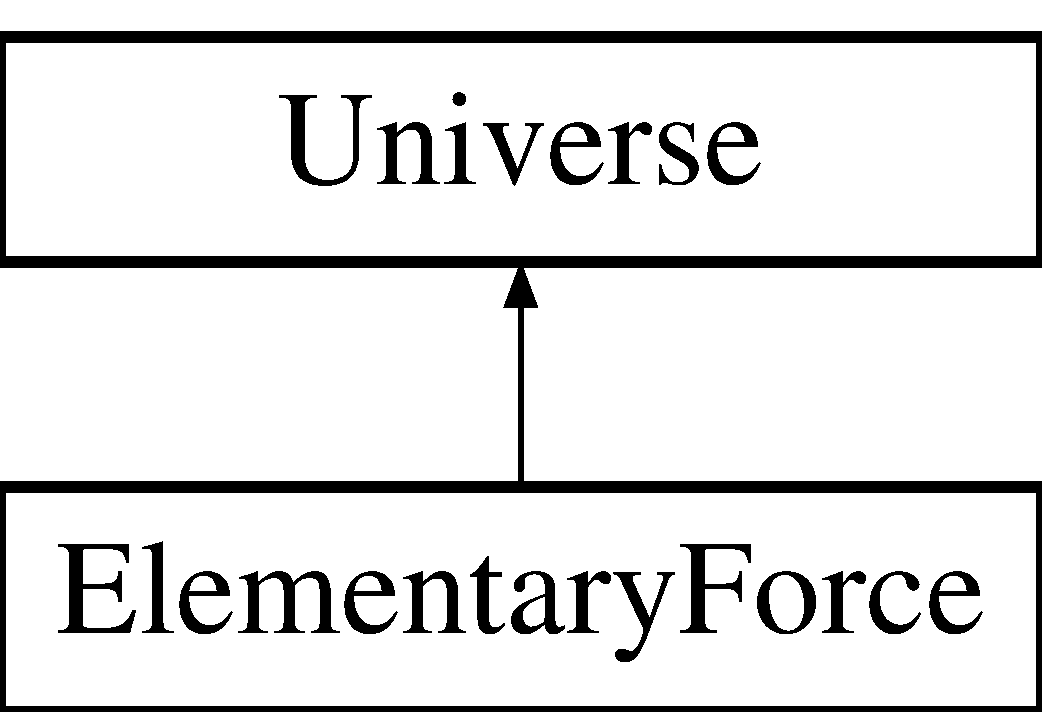
\includegraphics[height=2.000000cm]{classElementaryForce}
\end{center}
\end{figure}
\subsection*{Public Member Functions}
\begin{DoxyCompactItemize}
\item 
\mbox{\hyperlink{classElementaryForce_a1da5b85cdf3b79f3506dbdc4d877155a}{Elementary\+Force}} ()
\item 
\mbox{\hyperlink{classElementaryForce_a7aeb59eab2a299037e1fef94b9290b78}{Elementary\+Force}} (unsigned int object\+\_\+type)
\item 
\mbox{\hyperlink{classElementaryForce_a30f4a2259927de81cf3ef66c495f423c}{Elementary\+Force}} (unsigned int object\+\_\+type, std\+::chrono\+::time\+\_\+point$<$ \mbox{\hyperlink{universe_8h_a0ef8d951d1ca5ab3cfaf7ab4c7a6fd80}{Clock}} $>$ event\+\_\+time)
\item 
\mbox{\hyperlink{classElementaryForce_a1b466cc9aeb317161a7632cb5651a537}{Elementary\+Force}} (unsigned int object\+\_\+type, std\+::chrono\+::time\+\_\+point$<$ \mbox{\hyperlink{universe_8h_a0ef8d951d1ca5ab3cfaf7ab4c7a6fd80}{Clock}} $>$ event\+\_\+time, \mbox{\hyperlink{classUniverse}{Universe}} \&universe\+\_\+connector)
\item 
virtual \mbox{\hyperlink{classElementaryForce_afee0c87be3bd2a5221c9fcaddd70dfa6}{$\sim$\+Elementary\+Force}} ()
\item 
unsigned int \mbox{\hyperlink{classElementaryForce_a466c37c769c1826bd0f416f38bb09996}{Get\+Counter}} (std\+::chrono\+::time\+\_\+point$<$ \mbox{\hyperlink{universe_8h_a0ef8d951d1ca5ab3cfaf7ab4c7a6fd80}{Clock}} $>$ event\+\_\+time)
\item 
double \mbox{\hyperlink{classElementaryForce_af608447a2b6380142e2345ada11d1c32}{Get\+Energy}} (std\+::chrono\+::time\+\_\+point$<$ \mbox{\hyperlink{universe_8h_a0ef8d951d1ca5ab3cfaf7ab4c7a6fd80}{Clock}} $>$ event\+\_\+time)
\item 
double \mbox{\hyperlink{classElementaryForce_a579afb8079668f0587096934d1de9c04}{Get\+Gravitation}} (std\+::chrono\+::time\+\_\+point$<$ \mbox{\hyperlink{universe_8h_a0ef8d951d1ca5ab3cfaf7ab4c7a6fd80}{Clock}} $>$ event\+\_\+time)
\item 
double \mbox{\hyperlink{classElementaryForce_a4669f2ce414e508c70ae4ce0df503ad1}{Get\+Weak}} (std\+::chrono\+::time\+\_\+point$<$ \mbox{\hyperlink{universe_8h_a0ef8d951d1ca5ab3cfaf7ab4c7a6fd80}{Clock}} $>$ event\+\_\+time)
\item 
double \mbox{\hyperlink{classElementaryForce_a928e06a1fa81b8d7ec4a426d959a0f98}{Get\+Weak\+Electroweak}} (std\+::chrono\+::time\+\_\+point$<$ \mbox{\hyperlink{universe_8h_a0ef8d951d1ca5ab3cfaf7ab4c7a6fd80}{Clock}} $>$ event\+\_\+time)
\item 
double \mbox{\hyperlink{classElementaryForce_a2c8bc3226f42710717775c73eee1644e}{Get\+Electromagnetic}} (std\+::chrono\+::time\+\_\+point$<$ \mbox{\hyperlink{universe_8h_a0ef8d951d1ca5ab3cfaf7ab4c7a6fd80}{Clock}} $>$ event\+\_\+time)
\item 
double \mbox{\hyperlink{classElementaryForce_a58e503f2f3a7410f034a2a04bca560d1}{Get\+Electromagnetic\+Electroweak}} (std\+::chrono\+::time\+\_\+point$<$ \mbox{\hyperlink{universe_8h_a0ef8d951d1ca5ab3cfaf7ab4c7a6fd80}{Clock}} $>$ event\+\_\+time)
\item 
double \mbox{\hyperlink{classElementaryForce_aaa1cde27b1508831f67353eb39745a7e}{Get\+Strong}} (std\+::chrono\+::time\+\_\+point$<$ \mbox{\hyperlink{universe_8h_a0ef8d951d1ca5ab3cfaf7ab4c7a6fd80}{Clock}} $>$ event\+\_\+time)
\item 
double \mbox{\hyperlink{classElementaryForce_a0974d6537c07dac2453d2a607324fa21}{Get\+Strong\+Fundamental}} (std\+::chrono\+::time\+\_\+point$<$ \mbox{\hyperlink{universe_8h_a0ef8d951d1ca5ab3cfaf7ab4c7a6fd80}{Clock}} $>$ event\+\_\+time)
\item 
double \mbox{\hyperlink{classElementaryForce_a3478c8ad35bce240055da7d4a03e555e}{Get\+Strong\+Residual}} (std\+::chrono\+::time\+\_\+point$<$ \mbox{\hyperlink{universe_8h_a0ef8d951d1ca5ab3cfaf7ab4c7a6fd80}{Clock}} $>$ event\+\_\+time)
\item 
double \mbox{\hyperlink{classElementaryForce_a0961328b260cb4dfb2ba54f4e284f0e8}{Apply\+Energy}} (std\+::chrono\+::time\+\_\+point$<$ \mbox{\hyperlink{universe_8h_a0ef8d951d1ca5ab3cfaf7ab4c7a6fd80}{Clock}} $>$ event\+\_\+time, double val)
\item 
double \mbox{\hyperlink{classElementaryForce_a655a2c9489bfbbf15e05ba4953628134}{Apply\+Gravitation}} (std\+::chrono\+::time\+\_\+point$<$ \mbox{\hyperlink{universe_8h_a0ef8d951d1ca5ab3cfaf7ab4c7a6fd80}{Clock}} $>$ event\+\_\+time, double val)
\item 
double \mbox{\hyperlink{classElementaryForce_aabf66a859e6e808a65c6929cd16f7597}{Apply\+Weak}} (std\+::chrono\+::time\+\_\+point$<$ \mbox{\hyperlink{universe_8h_a0ef8d951d1ca5ab3cfaf7ab4c7a6fd80}{Clock}} $>$ event\+\_\+time, double val)
\item 
double \mbox{\hyperlink{classElementaryForce_a2d3a5444c771f35d66d4151c62f53b12}{Apply\+Weak\+Electroweak}} (std\+::chrono\+::time\+\_\+point$<$ \mbox{\hyperlink{universe_8h_a0ef8d951d1ca5ab3cfaf7ab4c7a6fd80}{Clock}} $>$ event\+\_\+time, double val)
\item 
double \mbox{\hyperlink{classElementaryForce_a0045a3380e468c6cfdbefce829888c1f}{Apply\+Electromagnetic}} (std\+::chrono\+::time\+\_\+point$<$ \mbox{\hyperlink{universe_8h_a0ef8d951d1ca5ab3cfaf7ab4c7a6fd80}{Clock}} $>$ event\+\_\+time, double val)
\item 
double \mbox{\hyperlink{classElementaryForce_a3764a27b11760b6ead2c8a23ff25d77a}{Apply\+Electromagnetic\+Electroweak}} (std\+::chrono\+::time\+\_\+point$<$ \mbox{\hyperlink{universe_8h_a0ef8d951d1ca5ab3cfaf7ab4c7a6fd80}{Clock}} $>$ event\+\_\+time, double val)
\item 
double \mbox{\hyperlink{classElementaryForce_a8a16bff6b5df2b0ff918262bf6376ade}{Apply\+Strong}} (std\+::chrono\+::time\+\_\+point$<$ \mbox{\hyperlink{universe_8h_a0ef8d951d1ca5ab3cfaf7ab4c7a6fd80}{Clock}} $>$ event\+\_\+time, double val)
\item 
double \mbox{\hyperlink{classElementaryForce_a80f1977e777aa0c8cce2124b666e6446}{Apply\+Strong\+Fundamental}} (std\+::chrono\+::time\+\_\+point$<$ \mbox{\hyperlink{universe_8h_a0ef8d951d1ca5ab3cfaf7ab4c7a6fd80}{Clock}} $>$ event\+\_\+time, double val)
\item 
double \mbox{\hyperlink{classElementaryForce_a185dc4e0b840505df27dbbed9fdcdc7b}{Apply\+Strong\+Residual}} (std\+::chrono\+::time\+\_\+point$<$ \mbox{\hyperlink{universe_8h_a0ef8d951d1ca5ab3cfaf7ab4c7a6fd80}{Clock}} $>$ event\+\_\+time, double val)
\item 
void \mbox{\hyperlink{classElementaryForce_a3762cf66ed266b310446417215dec3fa}{Set\+Counter}} (std\+::chrono\+::time\+\_\+point$<$ \mbox{\hyperlink{universe_8h_a0ef8d951d1ca5ab3cfaf7ab4c7a6fd80}{Clock}} $>$ event\+\_\+time, unsigned int val)
\item 
void \mbox{\hyperlink{classElementaryForce_a466c84ee4a50a29ef1f0fc6509ae3161}{Set\+Energy}} (std\+::chrono\+::time\+\_\+point$<$ \mbox{\hyperlink{universe_8h_a0ef8d951d1ca5ab3cfaf7ab4c7a6fd80}{Clock}} $>$ event\+\_\+time, double val)
\item 
void \mbox{\hyperlink{classElementaryForce_aa36d5875964f7e2fc981f6fc5431be7f}{Set\+Gravitation}} (std\+::chrono\+::time\+\_\+point$<$ \mbox{\hyperlink{universe_8h_a0ef8d951d1ca5ab3cfaf7ab4c7a6fd80}{Clock}} $>$ event\+\_\+time, double val)
\item 
void \mbox{\hyperlink{classElementaryForce_a093cdf0810e95f1d973bd9dc88c6788b}{Set\+Weak}} (std\+::chrono\+::time\+\_\+point$<$ \mbox{\hyperlink{universe_8h_a0ef8d951d1ca5ab3cfaf7ab4c7a6fd80}{Clock}} $>$ event\+\_\+time, double val)
\item 
void \mbox{\hyperlink{classElementaryForce_a38d4f86f18a9f84a4198ee43bc90f6b4}{Set\+Weak\+Electroweak}} (std\+::chrono\+::time\+\_\+point$<$ \mbox{\hyperlink{universe_8h_a0ef8d951d1ca5ab3cfaf7ab4c7a6fd80}{Clock}} $>$ event\+\_\+time, double val)
\item 
void \mbox{\hyperlink{classElementaryForce_a67f6845bd715c29c17387d291b343a1b}{Set\+Electromagnetic}} (std\+::chrono\+::time\+\_\+point$<$ \mbox{\hyperlink{universe_8h_a0ef8d951d1ca5ab3cfaf7ab4c7a6fd80}{Clock}} $>$ event\+\_\+time, double val)
\item 
void \mbox{\hyperlink{classElementaryForce_af4f12038c33d7edf9f13339fcd632ec9}{Set\+Electromagnetic\+Electroweak}} (std\+::chrono\+::time\+\_\+point$<$ \mbox{\hyperlink{universe_8h_a0ef8d951d1ca5ab3cfaf7ab4c7a6fd80}{Clock}} $>$ event\+\_\+time, double val)
\item 
void \mbox{\hyperlink{classElementaryForce_aa1b5708cfab2069049fec5c924e1f246}{Set\+Strong}} (std\+::chrono\+::time\+\_\+point$<$ \mbox{\hyperlink{universe_8h_a0ef8d951d1ca5ab3cfaf7ab4c7a6fd80}{Clock}} $>$ event\+\_\+time, double val)
\item 
void \mbox{\hyperlink{classElementaryForce_afb00e9a10ec33eeb1daefce39b0468b7}{Set\+Strong\+Fundamental}} (std\+::chrono\+::time\+\_\+point$<$ \mbox{\hyperlink{universe_8h_a0ef8d951d1ca5ab3cfaf7ab4c7a6fd80}{Clock}} $>$ event\+\_\+time, double val)
\item 
void \mbox{\hyperlink{classElementaryForce_ac25021d38c1d54bf711096ab37a461f6}{Set\+Strong\+Residual}} (std\+::chrono\+::time\+\_\+point$<$ \mbox{\hyperlink{universe_8h_a0ef8d951d1ca5ab3cfaf7ab4c7a6fd80}{Clock}} $>$ event\+\_\+time, double val)
\item 
void \mbox{\hyperlink{classElementaryForce_aa5ab479744dbf3e8578f8d2974299ff7}{Poll\+Elementary\+Force}} (std\+::chrono\+::time\+\_\+point$<$ \mbox{\hyperlink{universe_8h_a0ef8d951d1ca5ab3cfaf7ab4c7a6fd80}{Clock}} $>$ event\+\_\+time)
\item 
bool \mbox{\hyperlink{classElementaryForce_a1dedcd23a538b87f71ecd43cb36a6db5}{Reset\+Parameters}} (std\+::chrono\+::time\+\_\+point$<$ \mbox{\hyperlink{universe_8h_a0ef8d951d1ca5ab3cfaf7ab4c7a6fd80}{Clock}} $>$ event\+\_\+time)
\item 
int \mbox{\hyperlink{classElementaryForce_a855c26eb8a542ff633af66940da5f90b}{Update}} (std\+::chrono\+::time\+\_\+point$<$ \mbox{\hyperlink{universe_8h_a0ef8d951d1ca5ab3cfaf7ab4c7a6fd80}{Clock}} $>$ event\+\_\+time)
\end{DoxyCompactItemize}
\subsection*{Private Attributes}
\begin{DoxyCompactItemize}
\item 
unsigned int \mbox{\hyperlink{classElementaryForce_a027c7a909b116a22470f0e359f8c6e5d}{elementary\+\_\+force\+\_\+counter}}
\begin{DoxyCompactList}\small\item\em Member variable \char`\"{}elementary\+\_\+force\+\_\+counter\char`\"{}. \end{DoxyCompactList}\item 
int \mbox{\hyperlink{classElementaryForce_a4e5bcb6ba1b0d2217c6fb757a9370dff}{elementary\+\_\+force\+\_\+type}}
\item 
double \mbox{\hyperlink{classElementaryForce_a994d23e57e813a14120658f883e6c721}{elementary\+\_\+force\+\_\+energy}}
\item 
double \mbox{\hyperlink{classElementaryForce_a6348f87d1bb920e9ab11e624cb543ae0}{elementary\+\_\+force\+\_\+gravitation}}
\item 
double \mbox{\hyperlink{classElementaryForce_a927269eaae5bf8ac3dbd0bc2fd260592}{elementary\+\_\+force\+\_\+weak}}
\item 
double \mbox{\hyperlink{classElementaryForce_a901032dde4f6c7a00d3dc51c5acecdff}{elementary\+\_\+force\+\_\+weak\+\_\+electroweak}}
\item 
double \mbox{\hyperlink{classElementaryForce_a0a26ca7f126214261958f67d5716c6f8}{elementary\+\_\+force\+\_\+electromagnetic}}
\item 
double \mbox{\hyperlink{classElementaryForce_a211ff8cdcd3b78c5fe1b6216bc908346}{elementary\+\_\+force\+\_\+electromagnetic\+\_\+electroweak}}
\item 
double \mbox{\hyperlink{classElementaryForce_a3137ccc3db3e58f16daaf0face93f98d}{elementary\+\_\+force\+\_\+strong}}
\item 
double \mbox{\hyperlink{classElementaryForce_a5a12a7faddd6d0adae5232d4014a9b01}{elementary\+\_\+force\+\_\+strong\+\_\+fundamental}}
\item 
double \mbox{\hyperlink{classElementaryForce_a73ccecd6e432bdf773832bdce6db15b5}{elementary\+\_\+force\+\_\+strong\+\_\+residual}}
\item 
std\+::chrono\+::time\+\_\+point$<$ \mbox{\hyperlink{universe_8h_a0ef8d951d1ca5ab3cfaf7ab4c7a6fd80}{Clock}} $>$ \mbox{\hyperlink{classElementaryForce_a3c0db9aacae297a036837e127a49741d}{time\+\_\+object\+\_\+created}}
\item 
std\+::chrono\+::time\+\_\+point$<$ \mbox{\hyperlink{universe_8h_a0ef8d951d1ca5ab3cfaf7ab4c7a6fd80}{Clock}} $>$ \mbox{\hyperlink{classElementaryForce_ae61e8203d30c535260a473b0044e0070}{previous\+\_\+event\+\_\+time}}
\item 
bool \mbox{\hyperlink{classElementaryForce_ac5002305be13d4105a2c4a4ba79e2e49}{object\+\_\+initialised}}
\item 
bool \mbox{\hyperlink{classElementaryForce_a9854fb3352e6a66145dc1670026126b3}{object\+\_\+disabled}}
\item 
int \mbox{\hyperlink{classElementaryForce_a3d1e76c3faf50f2150df66b90c61b2f5}{duration\+\_\+since\+\_\+last\+\_\+event}}
\end{DoxyCompactItemize}
\subsection*{Friends}
\begin{DoxyCompactItemize}
\item 
class \mbox{\hyperlink{classElementaryForce_a9bc6eb2a4c20ce83728a7c9a31b91f19}{Composite\+Force\+Particle}}
\end{DoxyCompactItemize}
\subsection*{Additional Inherited Members}


\subsection{Constructor \& Destructor Documentation}
\mbox{\Hypertarget{classElementaryForce_a1da5b85cdf3b79f3506dbdc4d877155a}\label{classElementaryForce_a1da5b85cdf3b79f3506dbdc4d877155a}} 
\index{Elementary\+Force@{Elementary\+Force}!Elementary\+Force@{Elementary\+Force}}
\index{Elementary\+Force@{Elementary\+Force}!Elementary\+Force@{Elementary\+Force}}
\subsubsection{\texorpdfstring{Elementary\+Force()}{ElementaryForce()}\hspace{0.1cm}{\footnotesize\ttfamily [1/4]}}
{\footnotesize\ttfamily Elementary\+Force\+::\+Elementary\+Force (\begin{DoxyParamCaption}{ }\end{DoxyParamCaption})\hspace{0.3cm}{\ttfamily [inline]}}

\mbox{\Hypertarget{classElementaryForce_a7aeb59eab2a299037e1fef94b9290b78}\label{classElementaryForce_a7aeb59eab2a299037e1fef94b9290b78}} 
\index{Elementary\+Force@{Elementary\+Force}!Elementary\+Force@{Elementary\+Force}}
\index{Elementary\+Force@{Elementary\+Force}!Elementary\+Force@{Elementary\+Force}}
\subsubsection{\texorpdfstring{Elementary\+Force()}{ElementaryForce()}\hspace{0.1cm}{\footnotesize\ttfamily [2/4]}}
{\footnotesize\ttfamily Elementary\+Force\+::\+Elementary\+Force (\begin{DoxyParamCaption}\item[{unsigned int}]{object\+\_\+type }\end{DoxyParamCaption})\hspace{0.3cm}{\ttfamily [inline]}}

\mbox{\Hypertarget{classElementaryForce_a30f4a2259927de81cf3ef66c495f423c}\label{classElementaryForce_a30f4a2259927de81cf3ef66c495f423c}} 
\index{Elementary\+Force@{Elementary\+Force}!Elementary\+Force@{Elementary\+Force}}
\index{Elementary\+Force@{Elementary\+Force}!Elementary\+Force@{Elementary\+Force}}
\subsubsection{\texorpdfstring{Elementary\+Force()}{ElementaryForce()}\hspace{0.1cm}{\footnotesize\ttfamily [3/4]}}
{\footnotesize\ttfamily Elementary\+Force\+::\+Elementary\+Force (\begin{DoxyParamCaption}\item[{unsigned int}]{object\+\_\+type,  }\item[{std\+::chrono\+::time\+\_\+point$<$ \mbox{\hyperlink{universe_8h_a0ef8d951d1ca5ab3cfaf7ab4c7a6fd80}{Clock}} $>$}]{event\+\_\+time }\end{DoxyParamCaption})\hspace{0.3cm}{\ttfamily [inline]}}

\mbox{\Hypertarget{classElementaryForce_a1b466cc9aeb317161a7632cb5651a537}\label{classElementaryForce_a1b466cc9aeb317161a7632cb5651a537}} 
\index{Elementary\+Force@{Elementary\+Force}!Elementary\+Force@{Elementary\+Force}}
\index{Elementary\+Force@{Elementary\+Force}!Elementary\+Force@{Elementary\+Force}}
\subsubsection{\texorpdfstring{Elementary\+Force()}{ElementaryForce()}\hspace{0.1cm}{\footnotesize\ttfamily [4/4]}}
{\footnotesize\ttfamily Elementary\+Force\+::\+Elementary\+Force (\begin{DoxyParamCaption}\item[{unsigned int}]{object\+\_\+type,  }\item[{std\+::chrono\+::time\+\_\+point$<$ \mbox{\hyperlink{universe_8h_a0ef8d951d1ca5ab3cfaf7ab4c7a6fd80}{Clock}} $>$}]{event\+\_\+time,  }\item[{\mbox{\hyperlink{classUniverse}{Universe}} \&}]{universe\+\_\+connector }\end{DoxyParamCaption})\hspace{0.3cm}{\ttfamily [inline]}}

\mbox{\Hypertarget{classElementaryForce_afee0c87be3bd2a5221c9fcaddd70dfa6}\label{classElementaryForce_afee0c87be3bd2a5221c9fcaddd70dfa6}} 
\index{Elementary\+Force@{Elementary\+Force}!````~Elementary\+Force@{$\sim$\+Elementary\+Force}}
\index{````~Elementary\+Force@{$\sim$\+Elementary\+Force}!Elementary\+Force@{Elementary\+Force}}
\subsubsection{\texorpdfstring{$\sim$\+Elementary\+Force()}{~ElementaryForce()}}
{\footnotesize\ttfamily virtual Elementary\+Force\+::$\sim$\+Elementary\+Force (\begin{DoxyParamCaption}{ }\end{DoxyParamCaption})\hspace{0.3cm}{\ttfamily [inline]}, {\ttfamily [virtual]}}

Default destructor 

\subsection{Member Function Documentation}
\mbox{\Hypertarget{classElementaryForce_a0045a3380e468c6cfdbefce829888c1f}\label{classElementaryForce_a0045a3380e468c6cfdbefce829888c1f}} 
\index{Elementary\+Force@{Elementary\+Force}!Apply\+Electromagnetic@{Apply\+Electromagnetic}}
\index{Apply\+Electromagnetic@{Apply\+Electromagnetic}!Elementary\+Force@{Elementary\+Force}}
\subsubsection{\texorpdfstring{Apply\+Electromagnetic()}{ApplyElectromagnetic()}}
{\footnotesize\ttfamily double Elementary\+Force\+::\+Apply\+Electromagnetic (\begin{DoxyParamCaption}\item[{std\+::chrono\+::time\+\_\+point$<$ \mbox{\hyperlink{universe_8h_a0ef8d951d1ca5ab3cfaf7ab4c7a6fd80}{Clock}} $>$}]{event\+\_\+time,  }\item[{double}]{val }\end{DoxyParamCaption})\hspace{0.3cm}{\ttfamily [virtual]}}



Reimplemented from \mbox{\hyperlink{classUniverse_a1f787da78fa196ba635db21a9e91dabb}{Universe}}.

\mbox{\Hypertarget{classElementaryForce_a3764a27b11760b6ead2c8a23ff25d77a}\label{classElementaryForce_a3764a27b11760b6ead2c8a23ff25d77a}} 
\index{Elementary\+Force@{Elementary\+Force}!Apply\+Electromagnetic\+Electroweak@{Apply\+Electromagnetic\+Electroweak}}
\index{Apply\+Electromagnetic\+Electroweak@{Apply\+Electromagnetic\+Electroweak}!Elementary\+Force@{Elementary\+Force}}
\subsubsection{\texorpdfstring{Apply\+Electromagnetic\+Electroweak()}{ApplyElectromagneticElectroweak()}}
{\footnotesize\ttfamily double Elementary\+Force\+::\+Apply\+Electromagnetic\+Electroweak (\begin{DoxyParamCaption}\item[{std\+::chrono\+::time\+\_\+point$<$ \mbox{\hyperlink{universe_8h_a0ef8d951d1ca5ab3cfaf7ab4c7a6fd80}{Clock}} $>$}]{event\+\_\+time,  }\item[{double}]{val }\end{DoxyParamCaption})\hspace{0.3cm}{\ttfamily [virtual]}}



Reimplemented from \mbox{\hyperlink{classUniverse_a4c36c1ab30db993307f88363dde5e8c5}{Universe}}.

\mbox{\Hypertarget{classElementaryForce_a0961328b260cb4dfb2ba54f4e284f0e8}\label{classElementaryForce_a0961328b260cb4dfb2ba54f4e284f0e8}} 
\index{Elementary\+Force@{Elementary\+Force}!Apply\+Energy@{Apply\+Energy}}
\index{Apply\+Energy@{Apply\+Energy}!Elementary\+Force@{Elementary\+Force}}
\subsubsection{\texorpdfstring{Apply\+Energy()}{ApplyEnergy()}}
{\footnotesize\ttfamily double Elementary\+Force\+::\+Apply\+Energy (\begin{DoxyParamCaption}\item[{std\+::chrono\+::time\+\_\+point$<$ \mbox{\hyperlink{universe_8h_a0ef8d951d1ca5ab3cfaf7ab4c7a6fd80}{Clock}} $>$}]{event\+\_\+time,  }\item[{double}]{val }\end{DoxyParamCaption})}

\mbox{\Hypertarget{classElementaryForce_a655a2c9489bfbbf15e05ba4953628134}\label{classElementaryForce_a655a2c9489bfbbf15e05ba4953628134}} 
\index{Elementary\+Force@{Elementary\+Force}!Apply\+Gravitation@{Apply\+Gravitation}}
\index{Apply\+Gravitation@{Apply\+Gravitation}!Elementary\+Force@{Elementary\+Force}}
\subsubsection{\texorpdfstring{Apply\+Gravitation()}{ApplyGravitation()}}
{\footnotesize\ttfamily double Elementary\+Force\+::\+Apply\+Gravitation (\begin{DoxyParamCaption}\item[{std\+::chrono\+::time\+\_\+point$<$ \mbox{\hyperlink{universe_8h_a0ef8d951d1ca5ab3cfaf7ab4c7a6fd80}{Clock}} $>$}]{event\+\_\+time,  }\item[{double}]{val }\end{DoxyParamCaption})\hspace{0.3cm}{\ttfamily [virtual]}}



Reimplemented from \mbox{\hyperlink{classUniverse_a76c0b5e63c2a7d1988c44db341c3d64c}{Universe}}.

\mbox{\Hypertarget{classElementaryForce_a8a16bff6b5df2b0ff918262bf6376ade}\label{classElementaryForce_a8a16bff6b5df2b0ff918262bf6376ade}} 
\index{Elementary\+Force@{Elementary\+Force}!Apply\+Strong@{Apply\+Strong}}
\index{Apply\+Strong@{Apply\+Strong}!Elementary\+Force@{Elementary\+Force}}
\subsubsection{\texorpdfstring{Apply\+Strong()}{ApplyStrong()}}
{\footnotesize\ttfamily double Elementary\+Force\+::\+Apply\+Strong (\begin{DoxyParamCaption}\item[{std\+::chrono\+::time\+\_\+point$<$ \mbox{\hyperlink{universe_8h_a0ef8d951d1ca5ab3cfaf7ab4c7a6fd80}{Clock}} $>$}]{event\+\_\+time,  }\item[{double}]{val }\end{DoxyParamCaption})\hspace{0.3cm}{\ttfamily [virtual]}}



Reimplemented from \mbox{\hyperlink{classUniverse_a906a88b37f10bfa630bef49dfd0e907a}{Universe}}.

\mbox{\Hypertarget{classElementaryForce_a80f1977e777aa0c8cce2124b666e6446}\label{classElementaryForce_a80f1977e777aa0c8cce2124b666e6446}} 
\index{Elementary\+Force@{Elementary\+Force}!Apply\+Strong\+Fundamental@{Apply\+Strong\+Fundamental}}
\index{Apply\+Strong\+Fundamental@{Apply\+Strong\+Fundamental}!Elementary\+Force@{Elementary\+Force}}
\subsubsection{\texorpdfstring{Apply\+Strong\+Fundamental()}{ApplyStrongFundamental()}}
{\footnotesize\ttfamily double Elementary\+Force\+::\+Apply\+Strong\+Fundamental (\begin{DoxyParamCaption}\item[{std\+::chrono\+::time\+\_\+point$<$ \mbox{\hyperlink{universe_8h_a0ef8d951d1ca5ab3cfaf7ab4c7a6fd80}{Clock}} $>$}]{event\+\_\+time,  }\item[{double}]{val }\end{DoxyParamCaption})\hspace{0.3cm}{\ttfamily [virtual]}}



Reimplemented from \mbox{\hyperlink{classUniverse_a62789bcff84bd750b0366004381e2fdd}{Universe}}.

\mbox{\Hypertarget{classElementaryForce_a185dc4e0b840505df27dbbed9fdcdc7b}\label{classElementaryForce_a185dc4e0b840505df27dbbed9fdcdc7b}} 
\index{Elementary\+Force@{Elementary\+Force}!Apply\+Strong\+Residual@{Apply\+Strong\+Residual}}
\index{Apply\+Strong\+Residual@{Apply\+Strong\+Residual}!Elementary\+Force@{Elementary\+Force}}
\subsubsection{\texorpdfstring{Apply\+Strong\+Residual()}{ApplyStrongResidual()}}
{\footnotesize\ttfamily double Elementary\+Force\+::\+Apply\+Strong\+Residual (\begin{DoxyParamCaption}\item[{std\+::chrono\+::time\+\_\+point$<$ \mbox{\hyperlink{universe_8h_a0ef8d951d1ca5ab3cfaf7ab4c7a6fd80}{Clock}} $>$}]{event\+\_\+time,  }\item[{double}]{val }\end{DoxyParamCaption})\hspace{0.3cm}{\ttfamily [virtual]}}



Reimplemented from \mbox{\hyperlink{classUniverse_af7becebb347be9a85541d96a3eca1ca7}{Universe}}.

\mbox{\Hypertarget{classElementaryForce_aabf66a859e6e808a65c6929cd16f7597}\label{classElementaryForce_aabf66a859e6e808a65c6929cd16f7597}} 
\index{Elementary\+Force@{Elementary\+Force}!Apply\+Weak@{Apply\+Weak}}
\index{Apply\+Weak@{Apply\+Weak}!Elementary\+Force@{Elementary\+Force}}
\subsubsection{\texorpdfstring{Apply\+Weak()}{ApplyWeak()}}
{\footnotesize\ttfamily double Elementary\+Force\+::\+Apply\+Weak (\begin{DoxyParamCaption}\item[{std\+::chrono\+::time\+\_\+point$<$ \mbox{\hyperlink{universe_8h_a0ef8d951d1ca5ab3cfaf7ab4c7a6fd80}{Clock}} $>$}]{event\+\_\+time,  }\item[{double}]{val }\end{DoxyParamCaption})\hspace{0.3cm}{\ttfamily [virtual]}}



Reimplemented from \mbox{\hyperlink{classUniverse_a6d1226b3adec3c42a833afdbb6a65a92}{Universe}}.

\mbox{\Hypertarget{classElementaryForce_a2d3a5444c771f35d66d4151c62f53b12}\label{classElementaryForce_a2d3a5444c771f35d66d4151c62f53b12}} 
\index{Elementary\+Force@{Elementary\+Force}!Apply\+Weak\+Electroweak@{Apply\+Weak\+Electroweak}}
\index{Apply\+Weak\+Electroweak@{Apply\+Weak\+Electroweak}!Elementary\+Force@{Elementary\+Force}}
\subsubsection{\texorpdfstring{Apply\+Weak\+Electroweak()}{ApplyWeakElectroweak()}}
{\footnotesize\ttfamily double Elementary\+Force\+::\+Apply\+Weak\+Electroweak (\begin{DoxyParamCaption}\item[{std\+::chrono\+::time\+\_\+point$<$ \mbox{\hyperlink{universe_8h_a0ef8d951d1ca5ab3cfaf7ab4c7a6fd80}{Clock}} $>$}]{event\+\_\+time,  }\item[{double}]{val }\end{DoxyParamCaption})\hspace{0.3cm}{\ttfamily [virtual]}}



Reimplemented from \mbox{\hyperlink{classUniverse_a46a906baabb63e5d31f8b48ea1fae52e}{Universe}}.

\mbox{\Hypertarget{classElementaryForce_a466c37c769c1826bd0f416f38bb09996}\label{classElementaryForce_a466c37c769c1826bd0f416f38bb09996}} 
\index{Elementary\+Force@{Elementary\+Force}!Get\+Counter@{Get\+Counter}}
\index{Get\+Counter@{Get\+Counter}!Elementary\+Force@{Elementary\+Force}}
\subsubsection{\texorpdfstring{Get\+Counter()}{GetCounter()}}
{\footnotesize\ttfamily unsigned int Elementary\+Force\+::\+Get\+Counter (\begin{DoxyParamCaption}\item[{std\+::chrono\+::time\+\_\+point$<$ \mbox{\hyperlink{universe_8h_a0ef8d951d1ca5ab3cfaf7ab4c7a6fd80}{Clock}} $>$}]{event\+\_\+time }\end{DoxyParamCaption})}

\mbox{\Hypertarget{classElementaryForce_a2c8bc3226f42710717775c73eee1644e}\label{classElementaryForce_a2c8bc3226f42710717775c73eee1644e}} 
\index{Elementary\+Force@{Elementary\+Force}!Get\+Electromagnetic@{Get\+Electromagnetic}}
\index{Get\+Electromagnetic@{Get\+Electromagnetic}!Elementary\+Force@{Elementary\+Force}}
\subsubsection{\texorpdfstring{Get\+Electromagnetic()}{GetElectromagnetic()}}
{\footnotesize\ttfamily double Elementary\+Force\+::\+Get\+Electromagnetic (\begin{DoxyParamCaption}\item[{std\+::chrono\+::time\+\_\+point$<$ \mbox{\hyperlink{universe_8h_a0ef8d951d1ca5ab3cfaf7ab4c7a6fd80}{Clock}} $>$}]{event\+\_\+time }\end{DoxyParamCaption})\hspace{0.3cm}{\ttfamily [virtual]}}



Reimplemented from \mbox{\hyperlink{classUniverse_a63b850ef3f3394313353109d222bf5d1}{Universe}}.

\mbox{\Hypertarget{classElementaryForce_a58e503f2f3a7410f034a2a04bca560d1}\label{classElementaryForce_a58e503f2f3a7410f034a2a04bca560d1}} 
\index{Elementary\+Force@{Elementary\+Force}!Get\+Electromagnetic\+Electroweak@{Get\+Electromagnetic\+Electroweak}}
\index{Get\+Electromagnetic\+Electroweak@{Get\+Electromagnetic\+Electroweak}!Elementary\+Force@{Elementary\+Force}}
\subsubsection{\texorpdfstring{Get\+Electromagnetic\+Electroweak()}{GetElectromagneticElectroweak()}}
{\footnotesize\ttfamily double Elementary\+Force\+::\+Get\+Electromagnetic\+Electroweak (\begin{DoxyParamCaption}\item[{std\+::chrono\+::time\+\_\+point$<$ \mbox{\hyperlink{universe_8h_a0ef8d951d1ca5ab3cfaf7ab4c7a6fd80}{Clock}} $>$}]{event\+\_\+time }\end{DoxyParamCaption})\hspace{0.3cm}{\ttfamily [virtual]}}



Reimplemented from \mbox{\hyperlink{classUniverse_a9f099605c082e7fa755787a6a8cab7ba}{Universe}}.

\mbox{\Hypertarget{classElementaryForce_af608447a2b6380142e2345ada11d1c32}\label{classElementaryForce_af608447a2b6380142e2345ada11d1c32}} 
\index{Elementary\+Force@{Elementary\+Force}!Get\+Energy@{Get\+Energy}}
\index{Get\+Energy@{Get\+Energy}!Elementary\+Force@{Elementary\+Force}}
\subsubsection{\texorpdfstring{Get\+Energy()}{GetEnergy()}}
{\footnotesize\ttfamily double Elementary\+Force\+::\+Get\+Energy (\begin{DoxyParamCaption}\item[{std\+::chrono\+::time\+\_\+point$<$ \mbox{\hyperlink{universe_8h_a0ef8d951d1ca5ab3cfaf7ab4c7a6fd80}{Clock}} $>$}]{event\+\_\+time }\end{DoxyParamCaption})}

\mbox{\Hypertarget{classElementaryForce_a579afb8079668f0587096934d1de9c04}\label{classElementaryForce_a579afb8079668f0587096934d1de9c04}} 
\index{Elementary\+Force@{Elementary\+Force}!Get\+Gravitation@{Get\+Gravitation}}
\index{Get\+Gravitation@{Get\+Gravitation}!Elementary\+Force@{Elementary\+Force}}
\subsubsection{\texorpdfstring{Get\+Gravitation()}{GetGravitation()}}
{\footnotesize\ttfamily double Elementary\+Force\+::\+Get\+Gravitation (\begin{DoxyParamCaption}\item[{std\+::chrono\+::time\+\_\+point$<$ \mbox{\hyperlink{universe_8h_a0ef8d951d1ca5ab3cfaf7ab4c7a6fd80}{Clock}} $>$}]{event\+\_\+time }\end{DoxyParamCaption})\hspace{0.3cm}{\ttfamily [virtual]}}



Reimplemented from \mbox{\hyperlink{classUniverse_ab0404e774ee0ed66b597ff5b8e989446}{Universe}}.

\mbox{\Hypertarget{classElementaryForce_aaa1cde27b1508831f67353eb39745a7e}\label{classElementaryForce_aaa1cde27b1508831f67353eb39745a7e}} 
\index{Elementary\+Force@{Elementary\+Force}!Get\+Strong@{Get\+Strong}}
\index{Get\+Strong@{Get\+Strong}!Elementary\+Force@{Elementary\+Force}}
\subsubsection{\texorpdfstring{Get\+Strong()}{GetStrong()}}
{\footnotesize\ttfamily double Elementary\+Force\+::\+Get\+Strong (\begin{DoxyParamCaption}\item[{std\+::chrono\+::time\+\_\+point$<$ \mbox{\hyperlink{universe_8h_a0ef8d951d1ca5ab3cfaf7ab4c7a6fd80}{Clock}} $>$}]{event\+\_\+time }\end{DoxyParamCaption})\hspace{0.3cm}{\ttfamily [virtual]}}



Reimplemented from \mbox{\hyperlink{classUniverse_acb453ce71da418c5b5617fecede9571b}{Universe}}.

\mbox{\Hypertarget{classElementaryForce_a0974d6537c07dac2453d2a607324fa21}\label{classElementaryForce_a0974d6537c07dac2453d2a607324fa21}} 
\index{Elementary\+Force@{Elementary\+Force}!Get\+Strong\+Fundamental@{Get\+Strong\+Fundamental}}
\index{Get\+Strong\+Fundamental@{Get\+Strong\+Fundamental}!Elementary\+Force@{Elementary\+Force}}
\subsubsection{\texorpdfstring{Get\+Strong\+Fundamental()}{GetStrongFundamental()}}
{\footnotesize\ttfamily double Elementary\+Force\+::\+Get\+Strong\+Fundamental (\begin{DoxyParamCaption}\item[{std\+::chrono\+::time\+\_\+point$<$ \mbox{\hyperlink{universe_8h_a0ef8d951d1ca5ab3cfaf7ab4c7a6fd80}{Clock}} $>$}]{event\+\_\+time }\end{DoxyParamCaption})\hspace{0.3cm}{\ttfamily [virtual]}}



Reimplemented from \mbox{\hyperlink{classUniverse_ab44daccba01ee7e3cf9b50bba83dd19e}{Universe}}.

\mbox{\Hypertarget{classElementaryForce_a3478c8ad35bce240055da7d4a03e555e}\label{classElementaryForce_a3478c8ad35bce240055da7d4a03e555e}} 
\index{Elementary\+Force@{Elementary\+Force}!Get\+Strong\+Residual@{Get\+Strong\+Residual}}
\index{Get\+Strong\+Residual@{Get\+Strong\+Residual}!Elementary\+Force@{Elementary\+Force}}
\subsubsection{\texorpdfstring{Get\+Strong\+Residual()}{GetStrongResidual()}}
{\footnotesize\ttfamily double Elementary\+Force\+::\+Get\+Strong\+Residual (\begin{DoxyParamCaption}\item[{std\+::chrono\+::time\+\_\+point$<$ \mbox{\hyperlink{universe_8h_a0ef8d951d1ca5ab3cfaf7ab4c7a6fd80}{Clock}} $>$}]{event\+\_\+time }\end{DoxyParamCaption})\hspace{0.3cm}{\ttfamily [virtual]}}



Reimplemented from \mbox{\hyperlink{classUniverse_af0f4b81950061e63c2855eb40957a5b1}{Universe}}.

\mbox{\Hypertarget{classElementaryForce_a4669f2ce414e508c70ae4ce0df503ad1}\label{classElementaryForce_a4669f2ce414e508c70ae4ce0df503ad1}} 
\index{Elementary\+Force@{Elementary\+Force}!Get\+Weak@{Get\+Weak}}
\index{Get\+Weak@{Get\+Weak}!Elementary\+Force@{Elementary\+Force}}
\subsubsection{\texorpdfstring{Get\+Weak()}{GetWeak()}}
{\footnotesize\ttfamily double Elementary\+Force\+::\+Get\+Weak (\begin{DoxyParamCaption}\item[{std\+::chrono\+::time\+\_\+point$<$ \mbox{\hyperlink{universe_8h_a0ef8d951d1ca5ab3cfaf7ab4c7a6fd80}{Clock}} $>$}]{event\+\_\+time }\end{DoxyParamCaption})\hspace{0.3cm}{\ttfamily [virtual]}}



Reimplemented from \mbox{\hyperlink{classUniverse_a4476b7e0a3fc1764909f556257fd9ec7}{Universe}}.

\mbox{\Hypertarget{classElementaryForce_a928e06a1fa81b8d7ec4a426d959a0f98}\label{classElementaryForce_a928e06a1fa81b8d7ec4a426d959a0f98}} 
\index{Elementary\+Force@{Elementary\+Force}!Get\+Weak\+Electroweak@{Get\+Weak\+Electroweak}}
\index{Get\+Weak\+Electroweak@{Get\+Weak\+Electroweak}!Elementary\+Force@{Elementary\+Force}}
\subsubsection{\texorpdfstring{Get\+Weak\+Electroweak()}{GetWeakElectroweak()}}
{\footnotesize\ttfamily double Elementary\+Force\+::\+Get\+Weak\+Electroweak (\begin{DoxyParamCaption}\item[{std\+::chrono\+::time\+\_\+point$<$ \mbox{\hyperlink{universe_8h_a0ef8d951d1ca5ab3cfaf7ab4c7a6fd80}{Clock}} $>$}]{event\+\_\+time }\end{DoxyParamCaption})\hspace{0.3cm}{\ttfamily [virtual]}}



Reimplemented from \mbox{\hyperlink{classUniverse_a645299738e6b798a037f2a15a2e7cf4d}{Universe}}.

\mbox{\Hypertarget{classElementaryForce_aa5ab479744dbf3e8578f8d2974299ff7}\label{classElementaryForce_aa5ab479744dbf3e8578f8d2974299ff7}} 
\index{Elementary\+Force@{Elementary\+Force}!Poll\+Elementary\+Force@{Poll\+Elementary\+Force}}
\index{Poll\+Elementary\+Force@{Poll\+Elementary\+Force}!Elementary\+Force@{Elementary\+Force}}
\subsubsection{\texorpdfstring{Poll\+Elementary\+Force()}{PollElementaryForce()}}
{\footnotesize\ttfamily void Elementary\+Force\+::\+Poll\+Elementary\+Force (\begin{DoxyParamCaption}\item[{std\+::chrono\+::time\+\_\+point$<$ \mbox{\hyperlink{universe_8h_a0ef8d951d1ca5ab3cfaf7ab4c7a6fd80}{Clock}} $>$}]{event\+\_\+time }\end{DoxyParamCaption})\hspace{0.3cm}{\ttfamily [virtual]}}



Reimplemented from \mbox{\hyperlink{classUniverse_a0c485c504542409cbb5cfd8543c35b11}{Universe}}.

\mbox{\Hypertarget{classElementaryForce_a1dedcd23a538b87f71ecd43cb36a6db5}\label{classElementaryForce_a1dedcd23a538b87f71ecd43cb36a6db5}} 
\index{Elementary\+Force@{Elementary\+Force}!Reset\+Parameters@{Reset\+Parameters}}
\index{Reset\+Parameters@{Reset\+Parameters}!Elementary\+Force@{Elementary\+Force}}
\subsubsection{\texorpdfstring{Reset\+Parameters()}{ResetParameters()}}
{\footnotesize\ttfamily bool Elementary\+Force\+::\+Reset\+Parameters (\begin{DoxyParamCaption}\item[{std\+::chrono\+::time\+\_\+point$<$ \mbox{\hyperlink{universe_8h_a0ef8d951d1ca5ab3cfaf7ab4c7a6fd80}{Clock}} $>$}]{event\+\_\+time }\end{DoxyParamCaption})}

\mbox{\Hypertarget{classElementaryForce_a3762cf66ed266b310446417215dec3fa}\label{classElementaryForce_a3762cf66ed266b310446417215dec3fa}} 
\index{Elementary\+Force@{Elementary\+Force}!Set\+Counter@{Set\+Counter}}
\index{Set\+Counter@{Set\+Counter}!Elementary\+Force@{Elementary\+Force}}
\subsubsection{\texorpdfstring{Set\+Counter()}{SetCounter()}}
{\footnotesize\ttfamily void Elementary\+Force\+::\+Set\+Counter (\begin{DoxyParamCaption}\item[{std\+::chrono\+::time\+\_\+point$<$ \mbox{\hyperlink{universe_8h_a0ef8d951d1ca5ab3cfaf7ab4c7a6fd80}{Clock}} $>$}]{event\+\_\+time,  }\item[{unsigned int}]{val }\end{DoxyParamCaption})\hspace{0.3cm}{\ttfamily [virtual]}}



Reimplemented from \mbox{\hyperlink{classUniverse_aa22202ae740eb1355529afcb13285e91}{Universe}}.

\mbox{\Hypertarget{classElementaryForce_a67f6845bd715c29c17387d291b343a1b}\label{classElementaryForce_a67f6845bd715c29c17387d291b343a1b}} 
\index{Elementary\+Force@{Elementary\+Force}!Set\+Electromagnetic@{Set\+Electromagnetic}}
\index{Set\+Electromagnetic@{Set\+Electromagnetic}!Elementary\+Force@{Elementary\+Force}}
\subsubsection{\texorpdfstring{Set\+Electromagnetic()}{SetElectromagnetic()}}
{\footnotesize\ttfamily void Elementary\+Force\+::\+Set\+Electromagnetic (\begin{DoxyParamCaption}\item[{std\+::chrono\+::time\+\_\+point$<$ \mbox{\hyperlink{universe_8h_a0ef8d951d1ca5ab3cfaf7ab4c7a6fd80}{Clock}} $>$}]{event\+\_\+time,  }\item[{double}]{val }\end{DoxyParamCaption})\hspace{0.3cm}{\ttfamily [virtual]}}



Reimplemented from \mbox{\hyperlink{classUniverse_aa981fc7e252b1fbbb675f0371860954d}{Universe}}.

\mbox{\Hypertarget{classElementaryForce_af4f12038c33d7edf9f13339fcd632ec9}\label{classElementaryForce_af4f12038c33d7edf9f13339fcd632ec9}} 
\index{Elementary\+Force@{Elementary\+Force}!Set\+Electromagnetic\+Electroweak@{Set\+Electromagnetic\+Electroweak}}
\index{Set\+Electromagnetic\+Electroweak@{Set\+Electromagnetic\+Electroweak}!Elementary\+Force@{Elementary\+Force}}
\subsubsection{\texorpdfstring{Set\+Electromagnetic\+Electroweak()}{SetElectromagneticElectroweak()}}
{\footnotesize\ttfamily void Elementary\+Force\+::\+Set\+Electromagnetic\+Electroweak (\begin{DoxyParamCaption}\item[{std\+::chrono\+::time\+\_\+point$<$ \mbox{\hyperlink{universe_8h_a0ef8d951d1ca5ab3cfaf7ab4c7a6fd80}{Clock}} $>$}]{event\+\_\+time,  }\item[{double}]{val }\end{DoxyParamCaption})\hspace{0.3cm}{\ttfamily [virtual]}}



Reimplemented from \mbox{\hyperlink{classUniverse_a608aa95698380f791a0ffba45cc1bee3}{Universe}}.

\mbox{\Hypertarget{classElementaryForce_a466c84ee4a50a29ef1f0fc6509ae3161}\label{classElementaryForce_a466c84ee4a50a29ef1f0fc6509ae3161}} 
\index{Elementary\+Force@{Elementary\+Force}!Set\+Energy@{Set\+Energy}}
\index{Set\+Energy@{Set\+Energy}!Elementary\+Force@{Elementary\+Force}}
\subsubsection{\texorpdfstring{Set\+Energy()}{SetEnergy()}}
{\footnotesize\ttfamily void Elementary\+Force\+::\+Set\+Energy (\begin{DoxyParamCaption}\item[{std\+::chrono\+::time\+\_\+point$<$ \mbox{\hyperlink{universe_8h_a0ef8d951d1ca5ab3cfaf7ab4c7a6fd80}{Clock}} $>$}]{event\+\_\+time,  }\item[{double}]{val }\end{DoxyParamCaption})}

\mbox{\Hypertarget{classElementaryForce_aa36d5875964f7e2fc981f6fc5431be7f}\label{classElementaryForce_aa36d5875964f7e2fc981f6fc5431be7f}} 
\index{Elementary\+Force@{Elementary\+Force}!Set\+Gravitation@{Set\+Gravitation}}
\index{Set\+Gravitation@{Set\+Gravitation}!Elementary\+Force@{Elementary\+Force}}
\subsubsection{\texorpdfstring{Set\+Gravitation()}{SetGravitation()}}
{\footnotesize\ttfamily void Elementary\+Force\+::\+Set\+Gravitation (\begin{DoxyParamCaption}\item[{std\+::chrono\+::time\+\_\+point$<$ \mbox{\hyperlink{universe_8h_a0ef8d951d1ca5ab3cfaf7ab4c7a6fd80}{Clock}} $>$}]{event\+\_\+time,  }\item[{double}]{val }\end{DoxyParamCaption})\hspace{0.3cm}{\ttfamily [virtual]}}



Reimplemented from \mbox{\hyperlink{classUniverse_ae0cb8d86b2fbb8396d605160344b42f5}{Universe}}.

\mbox{\Hypertarget{classElementaryForce_aa1b5708cfab2069049fec5c924e1f246}\label{classElementaryForce_aa1b5708cfab2069049fec5c924e1f246}} 
\index{Elementary\+Force@{Elementary\+Force}!Set\+Strong@{Set\+Strong}}
\index{Set\+Strong@{Set\+Strong}!Elementary\+Force@{Elementary\+Force}}
\subsubsection{\texorpdfstring{Set\+Strong()}{SetStrong()}}
{\footnotesize\ttfamily void Elementary\+Force\+::\+Set\+Strong (\begin{DoxyParamCaption}\item[{std\+::chrono\+::time\+\_\+point$<$ \mbox{\hyperlink{universe_8h_a0ef8d951d1ca5ab3cfaf7ab4c7a6fd80}{Clock}} $>$}]{event\+\_\+time,  }\item[{double}]{val }\end{DoxyParamCaption})\hspace{0.3cm}{\ttfamily [virtual]}}



Reimplemented from \mbox{\hyperlink{classUniverse_a5946c8f3d4cda305f3ecd10df21a2f94}{Universe}}.

\mbox{\Hypertarget{classElementaryForce_afb00e9a10ec33eeb1daefce39b0468b7}\label{classElementaryForce_afb00e9a10ec33eeb1daefce39b0468b7}} 
\index{Elementary\+Force@{Elementary\+Force}!Set\+Strong\+Fundamental@{Set\+Strong\+Fundamental}}
\index{Set\+Strong\+Fundamental@{Set\+Strong\+Fundamental}!Elementary\+Force@{Elementary\+Force}}
\subsubsection{\texorpdfstring{Set\+Strong\+Fundamental()}{SetStrongFundamental()}}
{\footnotesize\ttfamily void Elementary\+Force\+::\+Set\+Strong\+Fundamental (\begin{DoxyParamCaption}\item[{std\+::chrono\+::time\+\_\+point$<$ \mbox{\hyperlink{universe_8h_a0ef8d951d1ca5ab3cfaf7ab4c7a6fd80}{Clock}} $>$}]{event\+\_\+time,  }\item[{double}]{val }\end{DoxyParamCaption})\hspace{0.3cm}{\ttfamily [virtual]}}



Reimplemented from \mbox{\hyperlink{classUniverse_aafec97a231126b71c73ac1258609a284}{Universe}}.

\mbox{\Hypertarget{classElementaryForce_ac25021d38c1d54bf711096ab37a461f6}\label{classElementaryForce_ac25021d38c1d54bf711096ab37a461f6}} 
\index{Elementary\+Force@{Elementary\+Force}!Set\+Strong\+Residual@{Set\+Strong\+Residual}}
\index{Set\+Strong\+Residual@{Set\+Strong\+Residual}!Elementary\+Force@{Elementary\+Force}}
\subsubsection{\texorpdfstring{Set\+Strong\+Residual()}{SetStrongResidual()}}
{\footnotesize\ttfamily void Elementary\+Force\+::\+Set\+Strong\+Residual (\begin{DoxyParamCaption}\item[{std\+::chrono\+::time\+\_\+point$<$ \mbox{\hyperlink{universe_8h_a0ef8d951d1ca5ab3cfaf7ab4c7a6fd80}{Clock}} $>$}]{event\+\_\+time,  }\item[{double}]{val }\end{DoxyParamCaption})\hspace{0.3cm}{\ttfamily [virtual]}}



Reimplemented from \mbox{\hyperlink{classUniverse_a1b2d6197ddf3d613cc30bd04d22ed8b7}{Universe}}.

\mbox{\Hypertarget{classElementaryForce_a093cdf0810e95f1d973bd9dc88c6788b}\label{classElementaryForce_a093cdf0810e95f1d973bd9dc88c6788b}} 
\index{Elementary\+Force@{Elementary\+Force}!Set\+Weak@{Set\+Weak}}
\index{Set\+Weak@{Set\+Weak}!Elementary\+Force@{Elementary\+Force}}
\subsubsection{\texorpdfstring{Set\+Weak()}{SetWeak()}}
{\footnotesize\ttfamily void Elementary\+Force\+::\+Set\+Weak (\begin{DoxyParamCaption}\item[{std\+::chrono\+::time\+\_\+point$<$ \mbox{\hyperlink{universe_8h_a0ef8d951d1ca5ab3cfaf7ab4c7a6fd80}{Clock}} $>$}]{event\+\_\+time,  }\item[{double}]{val }\end{DoxyParamCaption})\hspace{0.3cm}{\ttfamily [virtual]}}



Reimplemented from \mbox{\hyperlink{classUniverse_a0f5cd04081b41ee931c0557dc397f6fb}{Universe}}.

\mbox{\Hypertarget{classElementaryForce_a38d4f86f18a9f84a4198ee43bc90f6b4}\label{classElementaryForce_a38d4f86f18a9f84a4198ee43bc90f6b4}} 
\index{Elementary\+Force@{Elementary\+Force}!Set\+Weak\+Electroweak@{Set\+Weak\+Electroweak}}
\index{Set\+Weak\+Electroweak@{Set\+Weak\+Electroweak}!Elementary\+Force@{Elementary\+Force}}
\subsubsection{\texorpdfstring{Set\+Weak\+Electroweak()}{SetWeakElectroweak()}}
{\footnotesize\ttfamily void Elementary\+Force\+::\+Set\+Weak\+Electroweak (\begin{DoxyParamCaption}\item[{std\+::chrono\+::time\+\_\+point$<$ \mbox{\hyperlink{universe_8h_a0ef8d951d1ca5ab3cfaf7ab4c7a6fd80}{Clock}} $>$}]{event\+\_\+time,  }\item[{double}]{val }\end{DoxyParamCaption})\hspace{0.3cm}{\ttfamily [virtual]}}



Reimplemented from \mbox{\hyperlink{classUniverse_a2d3d642bfdc863248e93535832fa4b00}{Universe}}.

\mbox{\Hypertarget{classElementaryForce_a855c26eb8a542ff633af66940da5f90b}\label{classElementaryForce_a855c26eb8a542ff633af66940da5f90b}} 
\index{Elementary\+Force@{Elementary\+Force}!Update@{Update}}
\index{Update@{Update}!Elementary\+Force@{Elementary\+Force}}
\subsubsection{\texorpdfstring{Update()}{Update()}}
{\footnotesize\ttfamily int Elementary\+Force\+::\+Update (\begin{DoxyParamCaption}\item[{std\+::chrono\+::time\+\_\+point$<$ \mbox{\hyperlink{universe_8h_a0ef8d951d1ca5ab3cfaf7ab4c7a6fd80}{Clock}} $>$}]{event\+\_\+time }\end{DoxyParamCaption})}



\subsection{Friends And Related Function Documentation}
\mbox{\Hypertarget{classElementaryForce_a9bc6eb2a4c20ce83728a7c9a31b91f19}\label{classElementaryForce_a9bc6eb2a4c20ce83728a7c9a31b91f19}} 
\index{Elementary\+Force@{Elementary\+Force}!Composite\+Force\+Particle@{Composite\+Force\+Particle}}
\index{Composite\+Force\+Particle@{Composite\+Force\+Particle}!Elementary\+Force@{Elementary\+Force}}
\subsubsection{\texorpdfstring{Composite\+Force\+Particle}{CompositeForceParticle}}
{\footnotesize\ttfamily friend class \mbox{\hyperlink{classCompositeForceParticle}{Composite\+Force\+Particle}}\hspace{0.3cm}{\ttfamily [friend]}}



\subsection{Member Data Documentation}
\mbox{\Hypertarget{classElementaryForce_a3d1e76c3faf50f2150df66b90c61b2f5}\label{classElementaryForce_a3d1e76c3faf50f2150df66b90c61b2f5}} 
\index{Elementary\+Force@{Elementary\+Force}!duration\+\_\+since\+\_\+last\+\_\+event@{duration\+\_\+since\+\_\+last\+\_\+event}}
\index{duration\+\_\+since\+\_\+last\+\_\+event@{duration\+\_\+since\+\_\+last\+\_\+event}!Elementary\+Force@{Elementary\+Force}}
\subsubsection{\texorpdfstring{duration\+\_\+since\+\_\+last\+\_\+event}{duration\_since\_last\_event}}
{\footnotesize\ttfamily int Elementary\+Force\+::duration\+\_\+since\+\_\+last\+\_\+event\hspace{0.3cm}{\ttfamily [private]}}

\mbox{\Hypertarget{classElementaryForce_a027c7a909b116a22470f0e359f8c6e5d}\label{classElementaryForce_a027c7a909b116a22470f0e359f8c6e5d}} 
\index{Elementary\+Force@{Elementary\+Force}!elementary\+\_\+force\+\_\+counter@{elementary\+\_\+force\+\_\+counter}}
\index{elementary\+\_\+force\+\_\+counter@{elementary\+\_\+force\+\_\+counter}!Elementary\+Force@{Elementary\+Force}}
\subsubsection{\texorpdfstring{elementary\+\_\+force\+\_\+counter}{elementary\_force\_counter}}
{\footnotesize\ttfamily unsigned int Elementary\+Force\+::elementary\+\_\+force\+\_\+counter\hspace{0.3cm}{\ttfamily [private]}}



Member variable \char`\"{}elementary\+\_\+force\+\_\+counter\char`\"{}. 

\mbox{\Hypertarget{classElementaryForce_a0a26ca7f126214261958f67d5716c6f8}\label{classElementaryForce_a0a26ca7f126214261958f67d5716c6f8}} 
\index{Elementary\+Force@{Elementary\+Force}!elementary\+\_\+force\+\_\+electromagnetic@{elementary\+\_\+force\+\_\+electromagnetic}}
\index{elementary\+\_\+force\+\_\+electromagnetic@{elementary\+\_\+force\+\_\+electromagnetic}!Elementary\+Force@{Elementary\+Force}}
\subsubsection{\texorpdfstring{elementary\+\_\+force\+\_\+electromagnetic}{elementary\_force\_electromagnetic}}
{\footnotesize\ttfamily double Elementary\+Force\+::elementary\+\_\+force\+\_\+electromagnetic\hspace{0.3cm}{\ttfamily [private]}}

\mbox{\Hypertarget{classElementaryForce_a211ff8cdcd3b78c5fe1b6216bc908346}\label{classElementaryForce_a211ff8cdcd3b78c5fe1b6216bc908346}} 
\index{Elementary\+Force@{Elementary\+Force}!elementary\+\_\+force\+\_\+electromagnetic\+\_\+electroweak@{elementary\+\_\+force\+\_\+electromagnetic\+\_\+electroweak}}
\index{elementary\+\_\+force\+\_\+electromagnetic\+\_\+electroweak@{elementary\+\_\+force\+\_\+electromagnetic\+\_\+electroweak}!Elementary\+Force@{Elementary\+Force}}
\subsubsection{\texorpdfstring{elementary\+\_\+force\+\_\+electromagnetic\+\_\+electroweak}{elementary\_force\_electromagnetic\_electroweak}}
{\footnotesize\ttfamily double Elementary\+Force\+::elementary\+\_\+force\+\_\+electromagnetic\+\_\+electroweak\hspace{0.3cm}{\ttfamily [private]}}

\mbox{\Hypertarget{classElementaryForce_a994d23e57e813a14120658f883e6c721}\label{classElementaryForce_a994d23e57e813a14120658f883e6c721}} 
\index{Elementary\+Force@{Elementary\+Force}!elementary\+\_\+force\+\_\+energy@{elementary\+\_\+force\+\_\+energy}}
\index{elementary\+\_\+force\+\_\+energy@{elementary\+\_\+force\+\_\+energy}!Elementary\+Force@{Elementary\+Force}}
\subsubsection{\texorpdfstring{elementary\+\_\+force\+\_\+energy}{elementary\_force\_energy}}
{\footnotesize\ttfamily double Elementary\+Force\+::elementary\+\_\+force\+\_\+energy\hspace{0.3cm}{\ttfamily [private]}}

\mbox{\Hypertarget{classElementaryForce_a6348f87d1bb920e9ab11e624cb543ae0}\label{classElementaryForce_a6348f87d1bb920e9ab11e624cb543ae0}} 
\index{Elementary\+Force@{Elementary\+Force}!elementary\+\_\+force\+\_\+gravitation@{elementary\+\_\+force\+\_\+gravitation}}
\index{elementary\+\_\+force\+\_\+gravitation@{elementary\+\_\+force\+\_\+gravitation}!Elementary\+Force@{Elementary\+Force}}
\subsubsection{\texorpdfstring{elementary\+\_\+force\+\_\+gravitation}{elementary\_force\_gravitation}}
{\footnotesize\ttfamily double Elementary\+Force\+::elementary\+\_\+force\+\_\+gravitation\hspace{0.3cm}{\ttfamily [private]}}

\mbox{\Hypertarget{classElementaryForce_a3137ccc3db3e58f16daaf0face93f98d}\label{classElementaryForce_a3137ccc3db3e58f16daaf0face93f98d}} 
\index{Elementary\+Force@{Elementary\+Force}!elementary\+\_\+force\+\_\+strong@{elementary\+\_\+force\+\_\+strong}}
\index{elementary\+\_\+force\+\_\+strong@{elementary\+\_\+force\+\_\+strong}!Elementary\+Force@{Elementary\+Force}}
\subsubsection{\texorpdfstring{elementary\+\_\+force\+\_\+strong}{elementary\_force\_strong}}
{\footnotesize\ttfamily double Elementary\+Force\+::elementary\+\_\+force\+\_\+strong\hspace{0.3cm}{\ttfamily [private]}}

\mbox{\Hypertarget{classElementaryForce_a5a12a7faddd6d0adae5232d4014a9b01}\label{classElementaryForce_a5a12a7faddd6d0adae5232d4014a9b01}} 
\index{Elementary\+Force@{Elementary\+Force}!elementary\+\_\+force\+\_\+strong\+\_\+fundamental@{elementary\+\_\+force\+\_\+strong\+\_\+fundamental}}
\index{elementary\+\_\+force\+\_\+strong\+\_\+fundamental@{elementary\+\_\+force\+\_\+strong\+\_\+fundamental}!Elementary\+Force@{Elementary\+Force}}
\subsubsection{\texorpdfstring{elementary\+\_\+force\+\_\+strong\+\_\+fundamental}{elementary\_force\_strong\_fundamental}}
{\footnotesize\ttfamily double Elementary\+Force\+::elementary\+\_\+force\+\_\+strong\+\_\+fundamental\hspace{0.3cm}{\ttfamily [private]}}

\mbox{\Hypertarget{classElementaryForce_a73ccecd6e432bdf773832bdce6db15b5}\label{classElementaryForce_a73ccecd6e432bdf773832bdce6db15b5}} 
\index{Elementary\+Force@{Elementary\+Force}!elementary\+\_\+force\+\_\+strong\+\_\+residual@{elementary\+\_\+force\+\_\+strong\+\_\+residual}}
\index{elementary\+\_\+force\+\_\+strong\+\_\+residual@{elementary\+\_\+force\+\_\+strong\+\_\+residual}!Elementary\+Force@{Elementary\+Force}}
\subsubsection{\texorpdfstring{elementary\+\_\+force\+\_\+strong\+\_\+residual}{elementary\_force\_strong\_residual}}
{\footnotesize\ttfamily double Elementary\+Force\+::elementary\+\_\+force\+\_\+strong\+\_\+residual\hspace{0.3cm}{\ttfamily [private]}}

\mbox{\Hypertarget{classElementaryForce_a4e5bcb6ba1b0d2217c6fb757a9370dff}\label{classElementaryForce_a4e5bcb6ba1b0d2217c6fb757a9370dff}} 
\index{Elementary\+Force@{Elementary\+Force}!elementary\+\_\+force\+\_\+type@{elementary\+\_\+force\+\_\+type}}
\index{elementary\+\_\+force\+\_\+type@{elementary\+\_\+force\+\_\+type}!Elementary\+Force@{Elementary\+Force}}
\subsubsection{\texorpdfstring{elementary\+\_\+force\+\_\+type}{elementary\_force\_type}}
{\footnotesize\ttfamily int Elementary\+Force\+::elementary\+\_\+force\+\_\+type\hspace{0.3cm}{\ttfamily [private]}}

\mbox{\Hypertarget{classElementaryForce_a927269eaae5bf8ac3dbd0bc2fd260592}\label{classElementaryForce_a927269eaae5bf8ac3dbd0bc2fd260592}} 
\index{Elementary\+Force@{Elementary\+Force}!elementary\+\_\+force\+\_\+weak@{elementary\+\_\+force\+\_\+weak}}
\index{elementary\+\_\+force\+\_\+weak@{elementary\+\_\+force\+\_\+weak}!Elementary\+Force@{Elementary\+Force}}
\subsubsection{\texorpdfstring{elementary\+\_\+force\+\_\+weak}{elementary\_force\_weak}}
{\footnotesize\ttfamily double Elementary\+Force\+::elementary\+\_\+force\+\_\+weak\hspace{0.3cm}{\ttfamily [private]}}

\mbox{\Hypertarget{classElementaryForce_a901032dde4f6c7a00d3dc51c5acecdff}\label{classElementaryForce_a901032dde4f6c7a00d3dc51c5acecdff}} 
\index{Elementary\+Force@{Elementary\+Force}!elementary\+\_\+force\+\_\+weak\+\_\+electroweak@{elementary\+\_\+force\+\_\+weak\+\_\+electroweak}}
\index{elementary\+\_\+force\+\_\+weak\+\_\+electroweak@{elementary\+\_\+force\+\_\+weak\+\_\+electroweak}!Elementary\+Force@{Elementary\+Force}}
\subsubsection{\texorpdfstring{elementary\+\_\+force\+\_\+weak\+\_\+electroweak}{elementary\_force\_weak\_electroweak}}
{\footnotesize\ttfamily double Elementary\+Force\+::elementary\+\_\+force\+\_\+weak\+\_\+electroweak\hspace{0.3cm}{\ttfamily [private]}}

\mbox{\Hypertarget{classElementaryForce_a9854fb3352e6a66145dc1670026126b3}\label{classElementaryForce_a9854fb3352e6a66145dc1670026126b3}} 
\index{Elementary\+Force@{Elementary\+Force}!object\+\_\+disabled@{object\+\_\+disabled}}
\index{object\+\_\+disabled@{object\+\_\+disabled}!Elementary\+Force@{Elementary\+Force}}
\subsubsection{\texorpdfstring{object\+\_\+disabled}{object\_disabled}}
{\footnotesize\ttfamily bool Elementary\+Force\+::object\+\_\+disabled\hspace{0.3cm}{\ttfamily [private]}}

\mbox{\Hypertarget{classElementaryForce_ac5002305be13d4105a2c4a4ba79e2e49}\label{classElementaryForce_ac5002305be13d4105a2c4a4ba79e2e49}} 
\index{Elementary\+Force@{Elementary\+Force}!object\+\_\+initialised@{object\+\_\+initialised}}
\index{object\+\_\+initialised@{object\+\_\+initialised}!Elementary\+Force@{Elementary\+Force}}
\subsubsection{\texorpdfstring{object\+\_\+initialised}{object\_initialised}}
{\footnotesize\ttfamily bool Elementary\+Force\+::object\+\_\+initialised\hspace{0.3cm}{\ttfamily [private]}}

\mbox{\Hypertarget{classElementaryForce_ae61e8203d30c535260a473b0044e0070}\label{classElementaryForce_ae61e8203d30c535260a473b0044e0070}} 
\index{Elementary\+Force@{Elementary\+Force}!previous\+\_\+event\+\_\+time@{previous\+\_\+event\+\_\+time}}
\index{previous\+\_\+event\+\_\+time@{previous\+\_\+event\+\_\+time}!Elementary\+Force@{Elementary\+Force}}
\subsubsection{\texorpdfstring{previous\+\_\+event\+\_\+time}{previous\_event\_time}}
{\footnotesize\ttfamily std\+::chrono\+::time\+\_\+point$<$\mbox{\hyperlink{universe_8h_a0ef8d951d1ca5ab3cfaf7ab4c7a6fd80}{Clock}}$>$ Elementary\+Force\+::previous\+\_\+event\+\_\+time\hspace{0.3cm}{\ttfamily [private]}}

\mbox{\Hypertarget{classElementaryForce_a3c0db9aacae297a036837e127a49741d}\label{classElementaryForce_a3c0db9aacae297a036837e127a49741d}} 
\index{Elementary\+Force@{Elementary\+Force}!time\+\_\+object\+\_\+created@{time\+\_\+object\+\_\+created}}
\index{time\+\_\+object\+\_\+created@{time\+\_\+object\+\_\+created}!Elementary\+Force@{Elementary\+Force}}
\subsubsection{\texorpdfstring{time\+\_\+object\+\_\+created}{time\_object\_created}}
{\footnotesize\ttfamily std\+::chrono\+::time\+\_\+point$<$\mbox{\hyperlink{universe_8h_a0ef8d951d1ca5ab3cfaf7ab4c7a6fd80}{Clock}}$>$ Elementary\+Force\+::time\+\_\+object\+\_\+created\hspace{0.3cm}{\ttfamily [private]}}



The documentation for this class was generated from the following files\+:\begin{DoxyCompactItemize}
\item 
/home/pbisaacs/\+Developer/\+Brain\+Harmonics/\+Brain\+Harmonics/\mbox{\hyperlink{elementaryforce_8h}{elementaryforce.\+h}}\item 
/home/pbisaacs/\+Developer/\+Brain\+Harmonics/\+Brain\+Harmonics/\mbox{\hyperlink{elementaryforce_8cc}{elementaryforce.\+cc}}\end{DoxyCompactItemize}

\hypertarget{classElementaryParticle}{}\section{Elementary\+Particle Class Reference}
\label{classElementaryParticle}\index{Elementary\+Particle@{Elementary\+Particle}}


{\ttfamily \#include $<$elementaryparticle.\+h$>$}

Inheritance diagram for Elementary\+Particle\+:\begin{figure}[H]
\begin{center}
\leavevmode
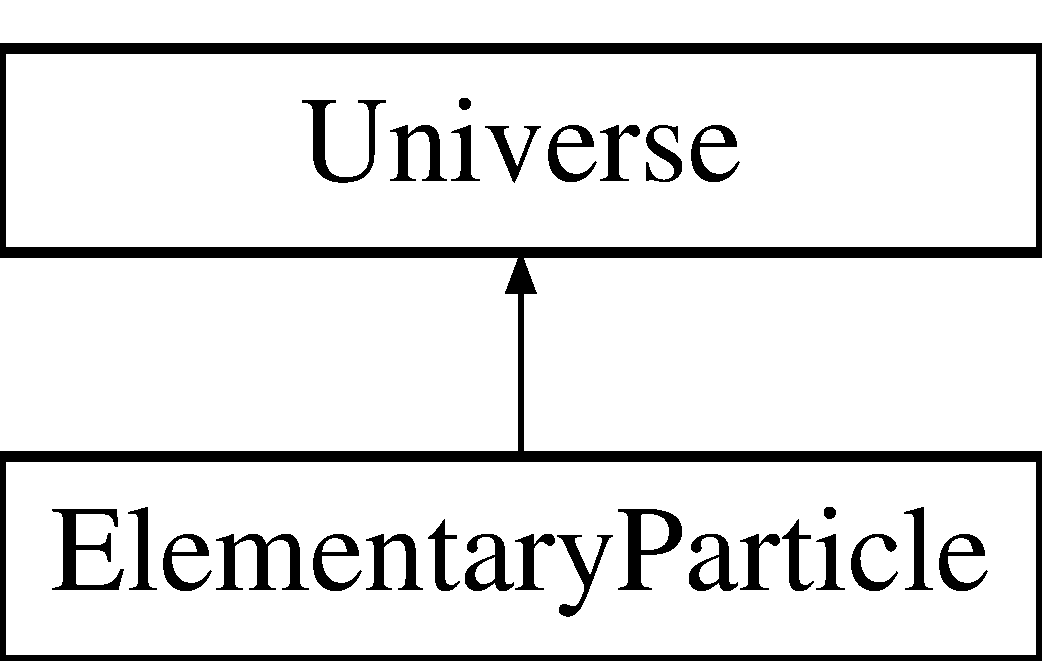
\includegraphics[height=2.000000cm]{classElementaryParticle}
\end{center}
\end{figure}
\subsection*{Public Member Functions}
\begin{DoxyCompactItemize}
\item 
\mbox{\hyperlink{classElementaryParticle_a4035ffd6ce053ea3390632fa530c6e21}{Elementary\+Particle}} ()
\item 
\mbox{\hyperlink{classElementaryParticle_a6bd3ad699e15769c1860e3068020a824}{Elementary\+Particle}} (unsigned int object\+\_\+type)
\item 
\mbox{\hyperlink{classElementaryParticle_a371e2742ab8b5ce0fe55ef4adbaed3af}{Elementary\+Particle}} (unsigned int object\+\_\+type, std\+::chrono\+::time\+\_\+point$<$ \mbox{\hyperlink{universe_8h_a0ef8d951d1ca5ab3cfaf7ab4c7a6fd80}{Clock}} $>$ event\+\_\+time)
\item 
\mbox{\hyperlink{classElementaryParticle_a0b43033247b36096d0de2a7553c620a9}{Elementary\+Particle}} (unsigned int object\+\_\+type, std\+::chrono\+::time\+\_\+point$<$ \mbox{\hyperlink{universe_8h_a0ef8d951d1ca5ab3cfaf7ab4c7a6fd80}{Clock}} $>$ event\+\_\+time, \mbox{\hyperlink{classUniverse}{Universe}} \&universe\+\_\+connector)
\item 
virtual \mbox{\hyperlink{classElementaryParticle_a5adce47bf88a5381c88a4d40f87fe76f}{$\sim$\+Elementary\+Particle}} ()
\item 
unsigned int \mbox{\hyperlink{classElementaryParticle_a371b9b9bc520047c42d9e6d06b7f3dd9}{Get\+Counter}} (std\+::chrono\+::time\+\_\+point$<$ \mbox{\hyperlink{universe_8h_a0ef8d951d1ca5ab3cfaf7ab4c7a6fd80}{Clock}} $>$ event\+\_\+time)
\item 
unsigned int \mbox{\hyperlink{classElementaryParticle_a63fe7df86d2fba4a64a69dfa5757e94e}{Get\+Type}} (std\+::chrono\+::time\+\_\+point$<$ \mbox{\hyperlink{universe_8h_a0ef8d951d1ca5ab3cfaf7ab4c7a6fd80}{Clock}} $>$ event\+\_\+time)
\item 
int \mbox{\hyperlink{classElementaryParticle_af3ebb984cfe957b2e76463c22e4b5bb5}{Get\+Charge}} (std\+::chrono\+::time\+\_\+point$<$ \mbox{\hyperlink{universe_8h_a0ef8d951d1ca5ab3cfaf7ab4c7a6fd80}{Clock}} $>$ event\+\_\+time)
\item 
int \mbox{\hyperlink{classElementaryParticle_ad5f5a05770f94f4c8fee418d59098126}{Get\+Spin}} (std\+::chrono\+::time\+\_\+point$<$ \mbox{\hyperlink{universe_8h_a0ef8d951d1ca5ab3cfaf7ab4c7a6fd80}{Clock}} $>$ event\+\_\+time)
\item 
double \mbox{\hyperlink{classElementaryParticle_a85400dc97f66c1ce23d9d961ddb6b8f3}{Get\+Mass}} (std\+::chrono\+::time\+\_\+point$<$ \mbox{\hyperlink{universe_8h_a0ef8d951d1ca5ab3cfaf7ab4c7a6fd80}{Clock}} $>$ event\+\_\+time)
\item 
void \mbox{\hyperlink{classElementaryParticle_a141316fd968cce8ecc5aa11ce0757d63}{Set\+Counter}} (std\+::chrono\+::time\+\_\+point$<$ \mbox{\hyperlink{universe_8h_a0ef8d951d1ca5ab3cfaf7ab4c7a6fd80}{Clock}} $>$ event\+\_\+time, unsigned int val)
\item 
void \mbox{\hyperlink{classElementaryParticle_a37d7718faf6be68d4374bcc56816f30a}{Set\+Type}} (std\+::chrono\+::time\+\_\+point$<$ \mbox{\hyperlink{universe_8h_a0ef8d951d1ca5ab3cfaf7ab4c7a6fd80}{Clock}} $>$ event\+\_\+time, unsigned int val)
\item 
void \mbox{\hyperlink{classElementaryParticle_abbc6d3c58509c4121df55bfef716d2f1}{Set\+Charge}} (std\+::chrono\+::time\+\_\+point$<$ \mbox{\hyperlink{universe_8h_a0ef8d951d1ca5ab3cfaf7ab4c7a6fd80}{Clock}} $>$ event\+\_\+time, int val)
\item 
void \mbox{\hyperlink{classElementaryParticle_a437fa86d88157314b84662b158d52353}{Set\+Spin}} (std\+::chrono\+::time\+\_\+point$<$ \mbox{\hyperlink{universe_8h_a0ef8d951d1ca5ab3cfaf7ab4c7a6fd80}{Clock}} $>$ event\+\_\+time, int val)
\item 
void \mbox{\hyperlink{classElementaryParticle_a8a3b91409772f4091a782624a34024e7}{Set\+Mass\+Index}} (std\+::chrono\+::time\+\_\+point$<$ \mbox{\hyperlink{universe_8h_a0ef8d951d1ca5ab3cfaf7ab4c7a6fd80}{Clock}} $>$ event\+\_\+time, int val)
\item 
void \mbox{\hyperlink{classElementaryParticle_a778ff8188ecb369e533521ed4f94b034}{Set\+Mass}} (std\+::chrono\+::time\+\_\+point$<$ \mbox{\hyperlink{universe_8h_a0ef8d951d1ca5ab3cfaf7ab4c7a6fd80}{Clock}} $>$ event\+\_\+time, double val)
\item 
bool \mbox{\hyperlink{classElementaryParticle_ac0f85f34bdfc1d42324201eb7c38e85e}{Reset\+Parameters}} (std\+::chrono\+::time\+\_\+point$<$ \mbox{\hyperlink{universe_8h_a0ef8d951d1ca5ab3cfaf7ab4c7a6fd80}{Clock}} $>$ event\+\_\+time)
\item 
void \mbox{\hyperlink{classElementaryParticle_af37afad11f5602f1a943b6e88a728b07}{Update}} (std\+::chrono\+::time\+\_\+point$<$ \mbox{\hyperlink{universe_8h_a0ef8d951d1ca5ab3cfaf7ab4c7a6fd80}{Clock}} $>$ event\+\_\+time)
\end{DoxyCompactItemize}
\subsection*{Private Attributes}
\begin{DoxyCompactItemize}
\item 
unsigned int \mbox{\hyperlink{classElementaryParticle_a2fae6ea0f434b01e6dee5479c74bebfb}{elementary\+\_\+particle\+\_\+counter}}
\begin{DoxyCompactList}\small\item\em Member variable \char`\"{}elementary\+\_\+particle\+\_\+counter\char`\"{}. \end{DoxyCompactList}\item 
unsigned int \mbox{\hyperlink{classElementaryParticle_a68872e9f84702245f8c963b0dea2472d}{elementary\+\_\+particle\+\_\+type}}
\begin{DoxyCompactList}\small\item\em Member variable \char`\"{}elementary\+\_\+particle\+\_\+type\char`\"{}. \end{DoxyCompactList}\item 
int \mbox{\hyperlink{classElementaryParticle_a61555c6c0ba98944282f9f868260b698}{elementary\+\_\+particle\+\_\+charge}}
\begin{DoxyCompactList}\small\item\em Member variable \char`\"{}elementary\+\_\+particle\+\_\+charge\char`\"{}. \end{DoxyCompactList}\item 
int \mbox{\hyperlink{classElementaryParticle_a599cb91c4a19db54599c8b47c18f1136}{elementary\+\_\+particle\+\_\+spin}}
\begin{DoxyCompactList}\small\item\em Member variable \char`\"{}elementary\+\_\+particle\+\_\+spin\char`\"{}. \end{DoxyCompactList}\item 
double \mbox{\hyperlink{classElementaryParticle_aaa8e3d6d924875e6dc63b8156181de48}{elementary\+\_\+particle\+\_\+mass}}
\begin{DoxyCompactList}\small\item\em Member variable \char`\"{}elementary\+\_\+particle\+\_\+mass\char`\"{}. \end{DoxyCompactList}\item 
int \mbox{\hyperlink{classElementaryParticle_aff63a6097a70d03bf283fea0fc5e461c}{elementary\+\_\+particle\+\_\+mass\+\_\+index}}
\begin{DoxyCompactList}\small\item\em Member variable \char`\"{}elementary\+\_\+particle\+\_\+mass\+\_\+index\char`\"{}. \end{DoxyCompactList}\item 
const double \mbox{\hyperlink{classElementaryParticle_a4b00a86b2f7ad3165e5ea6bcd8771779}{k\+Unit\+KgeV}} = 1.\+783\+E-\/36
\item 
const double \mbox{\hyperlink{classElementaryParticle_a423723d503eb1761a98f4495f193d63f}{k\+Unit\+Kg\+MeV}} = 1.\+783\+E-\/30
\item 
const double \mbox{\hyperlink{classElementaryParticle_a1f3c4e9183754e2f36a14f915ec4be9b}{k\+Unit\+Kg\+GeV}} = 1.\+783\+E-\/27
\item 
std\+::chrono\+::time\+\_\+point$<$ \mbox{\hyperlink{universe_8h_a0ef8d951d1ca5ab3cfaf7ab4c7a6fd80}{Clock}} $>$ \mbox{\hyperlink{classElementaryParticle_af7a592e44e4ccc8f1b19cd4c49ab50c3}{time\+\_\+object\+\_\+created}}
\item 
std\+::chrono\+::time\+\_\+point$<$ \mbox{\hyperlink{universe_8h_a0ef8d951d1ca5ab3cfaf7ab4c7a6fd80}{Clock}} $>$ \mbox{\hyperlink{classElementaryParticle_a8b0b30058853d850c0853fc101f5d45c}{previous\+\_\+event\+\_\+time}}
\item 
int \mbox{\hyperlink{classElementaryParticle_a7e518b7f634700ede48e59e266e09708}{duration\+\_\+since\+\_\+last\+\_\+event}}
\item 
bool \mbox{\hyperlink{classElementaryParticle_a502537989e804d20788686a29c736657}{object\+\_\+initialised}}
\item 
bool \mbox{\hyperlink{classElementaryParticle_a32f8eadc6c761d991ccaff0354af398c}{object\+\_\+disabled}}
\end{DoxyCompactItemize}
\subsection*{Friends}
\begin{DoxyCompactItemize}
\item 
class \mbox{\hyperlink{classElementaryParticle_a9bc6eb2a4c20ce83728a7c9a31b91f19}{Composite\+Force\+Particle}}
\end{DoxyCompactItemize}
\subsection*{Additional Inherited Members}


\subsection{Constructor \& Destructor Documentation}
\mbox{\Hypertarget{classElementaryParticle_a4035ffd6ce053ea3390632fa530c6e21}\label{classElementaryParticle_a4035ffd6ce053ea3390632fa530c6e21}} 
\index{Elementary\+Particle@{Elementary\+Particle}!Elementary\+Particle@{Elementary\+Particle}}
\index{Elementary\+Particle@{Elementary\+Particle}!Elementary\+Particle@{Elementary\+Particle}}
\subsubsection{\texorpdfstring{Elementary\+Particle()}{ElementaryParticle()}\hspace{0.1cm}{\footnotesize\ttfamily [1/4]}}
{\footnotesize\ttfamily Elementary\+Particle\+::\+Elementary\+Particle (\begin{DoxyParamCaption}{ }\end{DoxyParamCaption})\hspace{0.3cm}{\ttfamily [inline]}}

\mbox{\Hypertarget{classElementaryParticle_a6bd3ad699e15769c1860e3068020a824}\label{classElementaryParticle_a6bd3ad699e15769c1860e3068020a824}} 
\index{Elementary\+Particle@{Elementary\+Particle}!Elementary\+Particle@{Elementary\+Particle}}
\index{Elementary\+Particle@{Elementary\+Particle}!Elementary\+Particle@{Elementary\+Particle}}
\subsubsection{\texorpdfstring{Elementary\+Particle()}{ElementaryParticle()}\hspace{0.1cm}{\footnotesize\ttfamily [2/4]}}
{\footnotesize\ttfamily Elementary\+Particle\+::\+Elementary\+Particle (\begin{DoxyParamCaption}\item[{unsigned int}]{object\+\_\+type }\end{DoxyParamCaption})\hspace{0.3cm}{\ttfamily [inline]}}

\mbox{\Hypertarget{classElementaryParticle_a371e2742ab8b5ce0fe55ef4adbaed3af}\label{classElementaryParticle_a371e2742ab8b5ce0fe55ef4adbaed3af}} 
\index{Elementary\+Particle@{Elementary\+Particle}!Elementary\+Particle@{Elementary\+Particle}}
\index{Elementary\+Particle@{Elementary\+Particle}!Elementary\+Particle@{Elementary\+Particle}}
\subsubsection{\texorpdfstring{Elementary\+Particle()}{ElementaryParticle()}\hspace{0.1cm}{\footnotesize\ttfamily [3/4]}}
{\footnotesize\ttfamily Elementary\+Particle\+::\+Elementary\+Particle (\begin{DoxyParamCaption}\item[{unsigned int}]{object\+\_\+type,  }\item[{std\+::chrono\+::time\+\_\+point$<$ \mbox{\hyperlink{universe_8h_a0ef8d951d1ca5ab3cfaf7ab4c7a6fd80}{Clock}} $>$}]{event\+\_\+time }\end{DoxyParamCaption})\hspace{0.3cm}{\ttfamily [inline]}}

\mbox{\Hypertarget{classElementaryParticle_a0b43033247b36096d0de2a7553c620a9}\label{classElementaryParticle_a0b43033247b36096d0de2a7553c620a9}} 
\index{Elementary\+Particle@{Elementary\+Particle}!Elementary\+Particle@{Elementary\+Particle}}
\index{Elementary\+Particle@{Elementary\+Particle}!Elementary\+Particle@{Elementary\+Particle}}
\subsubsection{\texorpdfstring{Elementary\+Particle()}{ElementaryParticle()}\hspace{0.1cm}{\footnotesize\ttfamily [4/4]}}
{\footnotesize\ttfamily Elementary\+Particle\+::\+Elementary\+Particle (\begin{DoxyParamCaption}\item[{unsigned int}]{object\+\_\+type,  }\item[{std\+::chrono\+::time\+\_\+point$<$ \mbox{\hyperlink{universe_8h_a0ef8d951d1ca5ab3cfaf7ab4c7a6fd80}{Clock}} $>$}]{event\+\_\+time,  }\item[{\mbox{\hyperlink{classUniverse}{Universe}} \&}]{universe\+\_\+connector }\end{DoxyParamCaption})\hspace{0.3cm}{\ttfamily [inline]}}

\mbox{\Hypertarget{classElementaryParticle_a5adce47bf88a5381c88a4d40f87fe76f}\label{classElementaryParticle_a5adce47bf88a5381c88a4d40f87fe76f}} 
\index{Elementary\+Particle@{Elementary\+Particle}!````~Elementary\+Particle@{$\sim$\+Elementary\+Particle}}
\index{````~Elementary\+Particle@{$\sim$\+Elementary\+Particle}!Elementary\+Particle@{Elementary\+Particle}}
\subsubsection{\texorpdfstring{$\sim$\+Elementary\+Particle()}{~ElementaryParticle()}}
{\footnotesize\ttfamily virtual Elementary\+Particle\+::$\sim$\+Elementary\+Particle (\begin{DoxyParamCaption}{ }\end{DoxyParamCaption})\hspace{0.3cm}{\ttfamily [inline]}, {\ttfamily [virtual]}}

Default destructor 

\subsection{Member Function Documentation}
\mbox{\Hypertarget{classElementaryParticle_af3ebb984cfe957b2e76463c22e4b5bb5}\label{classElementaryParticle_af3ebb984cfe957b2e76463c22e4b5bb5}} 
\index{Elementary\+Particle@{Elementary\+Particle}!Get\+Charge@{Get\+Charge}}
\index{Get\+Charge@{Get\+Charge}!Elementary\+Particle@{Elementary\+Particle}}
\subsubsection{\texorpdfstring{Get\+Charge()}{GetCharge()}}
{\footnotesize\ttfamily int Elementary\+Particle\+::\+Get\+Charge (\begin{DoxyParamCaption}\item[{std\+::chrono\+::time\+\_\+point$<$ \mbox{\hyperlink{universe_8h_a0ef8d951d1ca5ab3cfaf7ab4c7a6fd80}{Clock}} $>$}]{event\+\_\+time }\end{DoxyParamCaption})\hspace{0.3cm}{\ttfamily [inline]}}

\mbox{\Hypertarget{classElementaryParticle_a371b9b9bc520047c42d9e6d06b7f3dd9}\label{classElementaryParticle_a371b9b9bc520047c42d9e6d06b7f3dd9}} 
\index{Elementary\+Particle@{Elementary\+Particle}!Get\+Counter@{Get\+Counter}}
\index{Get\+Counter@{Get\+Counter}!Elementary\+Particle@{Elementary\+Particle}}
\subsubsection{\texorpdfstring{Get\+Counter()}{GetCounter()}}
{\footnotesize\ttfamily unsigned int Elementary\+Particle\+::\+Get\+Counter (\begin{DoxyParamCaption}\item[{std\+::chrono\+::time\+\_\+point$<$ \mbox{\hyperlink{universe_8h_a0ef8d951d1ca5ab3cfaf7ab4c7a6fd80}{Clock}} $>$}]{event\+\_\+time }\end{DoxyParamCaption})\hspace{0.3cm}{\ttfamily [inline]}}

\mbox{\Hypertarget{classElementaryParticle_a85400dc97f66c1ce23d9d961ddb6b8f3}\label{classElementaryParticle_a85400dc97f66c1ce23d9d961ddb6b8f3}} 
\index{Elementary\+Particle@{Elementary\+Particle}!Get\+Mass@{Get\+Mass}}
\index{Get\+Mass@{Get\+Mass}!Elementary\+Particle@{Elementary\+Particle}}
\subsubsection{\texorpdfstring{Get\+Mass()}{GetMass()}}
{\footnotesize\ttfamily double Elementary\+Particle\+::\+Get\+Mass (\begin{DoxyParamCaption}\item[{std\+::chrono\+::time\+\_\+point$<$ \mbox{\hyperlink{universe_8h_a0ef8d951d1ca5ab3cfaf7ab4c7a6fd80}{Clock}} $>$}]{event\+\_\+time }\end{DoxyParamCaption})\hspace{0.3cm}{\ttfamily [inline]}}

\mbox{\Hypertarget{classElementaryParticle_ad5f5a05770f94f4c8fee418d59098126}\label{classElementaryParticle_ad5f5a05770f94f4c8fee418d59098126}} 
\index{Elementary\+Particle@{Elementary\+Particle}!Get\+Spin@{Get\+Spin}}
\index{Get\+Spin@{Get\+Spin}!Elementary\+Particle@{Elementary\+Particle}}
\subsubsection{\texorpdfstring{Get\+Spin()}{GetSpin()}}
{\footnotesize\ttfamily int Elementary\+Particle\+::\+Get\+Spin (\begin{DoxyParamCaption}\item[{std\+::chrono\+::time\+\_\+point$<$ \mbox{\hyperlink{universe_8h_a0ef8d951d1ca5ab3cfaf7ab4c7a6fd80}{Clock}} $>$}]{event\+\_\+time }\end{DoxyParamCaption})\hspace{0.3cm}{\ttfamily [inline]}}

\mbox{\Hypertarget{classElementaryParticle_a63fe7df86d2fba4a64a69dfa5757e94e}\label{classElementaryParticle_a63fe7df86d2fba4a64a69dfa5757e94e}} 
\index{Elementary\+Particle@{Elementary\+Particle}!Get\+Type@{Get\+Type}}
\index{Get\+Type@{Get\+Type}!Elementary\+Particle@{Elementary\+Particle}}
\subsubsection{\texorpdfstring{Get\+Type()}{GetType()}}
{\footnotesize\ttfamily unsigned int Elementary\+Particle\+::\+Get\+Type (\begin{DoxyParamCaption}\item[{std\+::chrono\+::time\+\_\+point$<$ \mbox{\hyperlink{universe_8h_a0ef8d951d1ca5ab3cfaf7ab4c7a6fd80}{Clock}} $>$}]{event\+\_\+time }\end{DoxyParamCaption})\hspace{0.3cm}{\ttfamily [inline]}}

\mbox{\Hypertarget{classElementaryParticle_ac0f85f34bdfc1d42324201eb7c38e85e}\label{classElementaryParticle_ac0f85f34bdfc1d42324201eb7c38e85e}} 
\index{Elementary\+Particle@{Elementary\+Particle}!Reset\+Parameters@{Reset\+Parameters}}
\index{Reset\+Parameters@{Reset\+Parameters}!Elementary\+Particle@{Elementary\+Particle}}
\subsubsection{\texorpdfstring{Reset\+Parameters()}{ResetParameters()}}
{\footnotesize\ttfamily bool Elementary\+Particle\+::\+Reset\+Parameters (\begin{DoxyParamCaption}\item[{std\+::chrono\+::time\+\_\+point$<$ \mbox{\hyperlink{universe_8h_a0ef8d951d1ca5ab3cfaf7ab4c7a6fd80}{Clock}} $>$}]{event\+\_\+time }\end{DoxyParamCaption})}

\mbox{\Hypertarget{classElementaryParticle_abbc6d3c58509c4121df55bfef716d2f1}\label{classElementaryParticle_abbc6d3c58509c4121df55bfef716d2f1}} 
\index{Elementary\+Particle@{Elementary\+Particle}!Set\+Charge@{Set\+Charge}}
\index{Set\+Charge@{Set\+Charge}!Elementary\+Particle@{Elementary\+Particle}}
\subsubsection{\texorpdfstring{Set\+Charge()}{SetCharge()}}
{\footnotesize\ttfamily void Elementary\+Particle\+::\+Set\+Charge (\begin{DoxyParamCaption}\item[{std\+::chrono\+::time\+\_\+point$<$ \mbox{\hyperlink{universe_8h_a0ef8d951d1ca5ab3cfaf7ab4c7a6fd80}{Clock}} $>$}]{event\+\_\+time,  }\item[{int}]{val }\end{DoxyParamCaption})\hspace{0.3cm}{\ttfamily [inline]}, {\ttfamily [virtual]}}



Reimplemented from \mbox{\hyperlink{classUniverse_a3b3da7c86a7b75e5e5c0b7972ac82a87}{Universe}}.

\mbox{\Hypertarget{classElementaryParticle_a141316fd968cce8ecc5aa11ce0757d63}\label{classElementaryParticle_a141316fd968cce8ecc5aa11ce0757d63}} 
\index{Elementary\+Particle@{Elementary\+Particle}!Set\+Counter@{Set\+Counter}}
\index{Set\+Counter@{Set\+Counter}!Elementary\+Particle@{Elementary\+Particle}}
\subsubsection{\texorpdfstring{Set\+Counter()}{SetCounter()}}
{\footnotesize\ttfamily void Elementary\+Particle\+::\+Set\+Counter (\begin{DoxyParamCaption}\item[{std\+::chrono\+::time\+\_\+point$<$ \mbox{\hyperlink{universe_8h_a0ef8d951d1ca5ab3cfaf7ab4c7a6fd80}{Clock}} $>$}]{event\+\_\+time,  }\item[{unsigned int}]{val }\end{DoxyParamCaption})\hspace{0.3cm}{\ttfamily [inline]}, {\ttfamily [virtual]}}



Reimplemented from \mbox{\hyperlink{classUniverse_aa22202ae740eb1355529afcb13285e91}{Universe}}.

\mbox{\Hypertarget{classElementaryParticle_a778ff8188ecb369e533521ed4f94b034}\label{classElementaryParticle_a778ff8188ecb369e533521ed4f94b034}} 
\index{Elementary\+Particle@{Elementary\+Particle}!Set\+Mass@{Set\+Mass}}
\index{Set\+Mass@{Set\+Mass}!Elementary\+Particle@{Elementary\+Particle}}
\subsubsection{\texorpdfstring{Set\+Mass()}{SetMass()}}
{\footnotesize\ttfamily void Elementary\+Particle\+::\+Set\+Mass (\begin{DoxyParamCaption}\item[{std\+::chrono\+::time\+\_\+point$<$ \mbox{\hyperlink{universe_8h_a0ef8d951d1ca5ab3cfaf7ab4c7a6fd80}{Clock}} $>$}]{event\+\_\+time,  }\item[{double}]{val }\end{DoxyParamCaption})}

\mbox{\Hypertarget{classElementaryParticle_a8a3b91409772f4091a782624a34024e7}\label{classElementaryParticle_a8a3b91409772f4091a782624a34024e7}} 
\index{Elementary\+Particle@{Elementary\+Particle}!Set\+Mass\+Index@{Set\+Mass\+Index}}
\index{Set\+Mass\+Index@{Set\+Mass\+Index}!Elementary\+Particle@{Elementary\+Particle}}
\subsubsection{\texorpdfstring{Set\+Mass\+Index()}{SetMassIndex()}}
{\footnotesize\ttfamily void Elementary\+Particle\+::\+Set\+Mass\+Index (\begin{DoxyParamCaption}\item[{std\+::chrono\+::time\+\_\+point$<$ \mbox{\hyperlink{universe_8h_a0ef8d951d1ca5ab3cfaf7ab4c7a6fd80}{Clock}} $>$}]{event\+\_\+time,  }\item[{int}]{val }\end{DoxyParamCaption})}

\mbox{\Hypertarget{classElementaryParticle_a437fa86d88157314b84662b158d52353}\label{classElementaryParticle_a437fa86d88157314b84662b158d52353}} 
\index{Elementary\+Particle@{Elementary\+Particle}!Set\+Spin@{Set\+Spin}}
\index{Set\+Spin@{Set\+Spin}!Elementary\+Particle@{Elementary\+Particle}}
\subsubsection{\texorpdfstring{Set\+Spin()}{SetSpin()}}
{\footnotesize\ttfamily void Elementary\+Particle\+::\+Set\+Spin (\begin{DoxyParamCaption}\item[{std\+::chrono\+::time\+\_\+point$<$ \mbox{\hyperlink{universe_8h_a0ef8d951d1ca5ab3cfaf7ab4c7a6fd80}{Clock}} $>$}]{event\+\_\+time,  }\item[{int}]{val }\end{DoxyParamCaption})\hspace{0.3cm}{\ttfamily [inline]}, {\ttfamily [virtual]}}



Reimplemented from \mbox{\hyperlink{classUniverse_ae2ae1c3b3e4cde2c18f5f6a814761ec8}{Universe}}.

\mbox{\Hypertarget{classElementaryParticle_a37d7718faf6be68d4374bcc56816f30a}\label{classElementaryParticle_a37d7718faf6be68d4374bcc56816f30a}} 
\index{Elementary\+Particle@{Elementary\+Particle}!Set\+Type@{Set\+Type}}
\index{Set\+Type@{Set\+Type}!Elementary\+Particle@{Elementary\+Particle}}
\subsubsection{\texorpdfstring{Set\+Type()}{SetType()}}
{\footnotesize\ttfamily void Elementary\+Particle\+::\+Set\+Type (\begin{DoxyParamCaption}\item[{std\+::chrono\+::time\+\_\+point$<$ \mbox{\hyperlink{universe_8h_a0ef8d951d1ca5ab3cfaf7ab4c7a6fd80}{Clock}} $>$}]{event\+\_\+time,  }\item[{unsigned int}]{val }\end{DoxyParamCaption})\hspace{0.3cm}{\ttfamily [inline]}}

\mbox{\Hypertarget{classElementaryParticle_af37afad11f5602f1a943b6e88a728b07}\label{classElementaryParticle_af37afad11f5602f1a943b6e88a728b07}} 
\index{Elementary\+Particle@{Elementary\+Particle}!Update@{Update}}
\index{Update@{Update}!Elementary\+Particle@{Elementary\+Particle}}
\subsubsection{\texorpdfstring{Update()}{Update()}}
{\footnotesize\ttfamily void Elementary\+Particle\+::\+Update (\begin{DoxyParamCaption}\item[{std\+::chrono\+::time\+\_\+point$<$ \mbox{\hyperlink{universe_8h_a0ef8d951d1ca5ab3cfaf7ab4c7a6fd80}{Clock}} $>$}]{event\+\_\+time }\end{DoxyParamCaption})}



\subsection{Friends And Related Function Documentation}
\mbox{\Hypertarget{classElementaryParticle_a9bc6eb2a4c20ce83728a7c9a31b91f19}\label{classElementaryParticle_a9bc6eb2a4c20ce83728a7c9a31b91f19}} 
\index{Elementary\+Particle@{Elementary\+Particle}!Composite\+Force\+Particle@{Composite\+Force\+Particle}}
\index{Composite\+Force\+Particle@{Composite\+Force\+Particle}!Elementary\+Particle@{Elementary\+Particle}}
\subsubsection{\texorpdfstring{Composite\+Force\+Particle}{CompositeForceParticle}}
{\footnotesize\ttfamily friend class \mbox{\hyperlink{classCompositeForceParticle}{Composite\+Force\+Particle}}\hspace{0.3cm}{\ttfamily [friend]}}



\subsection{Member Data Documentation}
\mbox{\Hypertarget{classElementaryParticle_a7e518b7f634700ede48e59e266e09708}\label{classElementaryParticle_a7e518b7f634700ede48e59e266e09708}} 
\index{Elementary\+Particle@{Elementary\+Particle}!duration\+\_\+since\+\_\+last\+\_\+event@{duration\+\_\+since\+\_\+last\+\_\+event}}
\index{duration\+\_\+since\+\_\+last\+\_\+event@{duration\+\_\+since\+\_\+last\+\_\+event}!Elementary\+Particle@{Elementary\+Particle}}
\subsubsection{\texorpdfstring{duration\+\_\+since\+\_\+last\+\_\+event}{duration\_since\_last\_event}}
{\footnotesize\ttfamily int Elementary\+Particle\+::duration\+\_\+since\+\_\+last\+\_\+event\hspace{0.3cm}{\ttfamily [private]}}

\mbox{\Hypertarget{classElementaryParticle_a61555c6c0ba98944282f9f868260b698}\label{classElementaryParticle_a61555c6c0ba98944282f9f868260b698}} 
\index{Elementary\+Particle@{Elementary\+Particle}!elementary\+\_\+particle\+\_\+charge@{elementary\+\_\+particle\+\_\+charge}}
\index{elementary\+\_\+particle\+\_\+charge@{elementary\+\_\+particle\+\_\+charge}!Elementary\+Particle@{Elementary\+Particle}}
\subsubsection{\texorpdfstring{elementary\+\_\+particle\+\_\+charge}{elementary\_particle\_charge}}
{\footnotesize\ttfamily int Elementary\+Particle\+::elementary\+\_\+particle\+\_\+charge\hspace{0.3cm}{\ttfamily [private]}}



Member variable \char`\"{}elementary\+\_\+particle\+\_\+charge\char`\"{}. 

\mbox{\Hypertarget{classElementaryParticle_a2fae6ea0f434b01e6dee5479c74bebfb}\label{classElementaryParticle_a2fae6ea0f434b01e6dee5479c74bebfb}} 
\index{Elementary\+Particle@{Elementary\+Particle}!elementary\+\_\+particle\+\_\+counter@{elementary\+\_\+particle\+\_\+counter}}
\index{elementary\+\_\+particle\+\_\+counter@{elementary\+\_\+particle\+\_\+counter}!Elementary\+Particle@{Elementary\+Particle}}
\subsubsection{\texorpdfstring{elementary\+\_\+particle\+\_\+counter}{elementary\_particle\_counter}}
{\footnotesize\ttfamily unsigned int Elementary\+Particle\+::elementary\+\_\+particle\+\_\+counter\hspace{0.3cm}{\ttfamily [private]}}



Member variable \char`\"{}elementary\+\_\+particle\+\_\+counter\char`\"{}. 

\mbox{\Hypertarget{classElementaryParticle_aaa8e3d6d924875e6dc63b8156181de48}\label{classElementaryParticle_aaa8e3d6d924875e6dc63b8156181de48}} 
\index{Elementary\+Particle@{Elementary\+Particle}!elementary\+\_\+particle\+\_\+mass@{elementary\+\_\+particle\+\_\+mass}}
\index{elementary\+\_\+particle\+\_\+mass@{elementary\+\_\+particle\+\_\+mass}!Elementary\+Particle@{Elementary\+Particle}}
\subsubsection{\texorpdfstring{elementary\+\_\+particle\+\_\+mass}{elementary\_particle\_mass}}
{\footnotesize\ttfamily double Elementary\+Particle\+::elementary\+\_\+particle\+\_\+mass\hspace{0.3cm}{\ttfamily [private]}}



Member variable \char`\"{}elementary\+\_\+particle\+\_\+mass\char`\"{}. 

\mbox{\Hypertarget{classElementaryParticle_aff63a6097a70d03bf283fea0fc5e461c}\label{classElementaryParticle_aff63a6097a70d03bf283fea0fc5e461c}} 
\index{Elementary\+Particle@{Elementary\+Particle}!elementary\+\_\+particle\+\_\+mass\+\_\+index@{elementary\+\_\+particle\+\_\+mass\+\_\+index}}
\index{elementary\+\_\+particle\+\_\+mass\+\_\+index@{elementary\+\_\+particle\+\_\+mass\+\_\+index}!Elementary\+Particle@{Elementary\+Particle}}
\subsubsection{\texorpdfstring{elementary\+\_\+particle\+\_\+mass\+\_\+index}{elementary\_particle\_mass\_index}}
{\footnotesize\ttfamily int Elementary\+Particle\+::elementary\+\_\+particle\+\_\+mass\+\_\+index\hspace{0.3cm}{\ttfamily [private]}}



Member variable \char`\"{}elementary\+\_\+particle\+\_\+mass\+\_\+index\char`\"{}. 

\mbox{\Hypertarget{classElementaryParticle_a599cb91c4a19db54599c8b47c18f1136}\label{classElementaryParticle_a599cb91c4a19db54599c8b47c18f1136}} 
\index{Elementary\+Particle@{Elementary\+Particle}!elementary\+\_\+particle\+\_\+spin@{elementary\+\_\+particle\+\_\+spin}}
\index{elementary\+\_\+particle\+\_\+spin@{elementary\+\_\+particle\+\_\+spin}!Elementary\+Particle@{Elementary\+Particle}}
\subsubsection{\texorpdfstring{elementary\+\_\+particle\+\_\+spin}{elementary\_particle\_spin}}
{\footnotesize\ttfamily int Elementary\+Particle\+::elementary\+\_\+particle\+\_\+spin\hspace{0.3cm}{\ttfamily [private]}}



Member variable \char`\"{}elementary\+\_\+particle\+\_\+spin\char`\"{}. 

\mbox{\Hypertarget{classElementaryParticle_a68872e9f84702245f8c963b0dea2472d}\label{classElementaryParticle_a68872e9f84702245f8c963b0dea2472d}} 
\index{Elementary\+Particle@{Elementary\+Particle}!elementary\+\_\+particle\+\_\+type@{elementary\+\_\+particle\+\_\+type}}
\index{elementary\+\_\+particle\+\_\+type@{elementary\+\_\+particle\+\_\+type}!Elementary\+Particle@{Elementary\+Particle}}
\subsubsection{\texorpdfstring{elementary\+\_\+particle\+\_\+type}{elementary\_particle\_type}}
{\footnotesize\ttfamily unsigned int Elementary\+Particle\+::elementary\+\_\+particle\+\_\+type\hspace{0.3cm}{\ttfamily [private]}}



Member variable \char`\"{}elementary\+\_\+particle\+\_\+type\char`\"{}. 

\mbox{\Hypertarget{classElementaryParticle_a4b00a86b2f7ad3165e5ea6bcd8771779}\label{classElementaryParticle_a4b00a86b2f7ad3165e5ea6bcd8771779}} 
\index{Elementary\+Particle@{Elementary\+Particle}!k\+Unit\+KgeV@{k\+Unit\+KgeV}}
\index{k\+Unit\+KgeV@{k\+Unit\+KgeV}!Elementary\+Particle@{Elementary\+Particle}}
\subsubsection{\texorpdfstring{k\+Unit\+KgeV}{kUnitKgeV}}
{\footnotesize\ttfamily const double Elementary\+Particle\+::k\+Unit\+KgeV = 1.\+783\+E-\/36\hspace{0.3cm}{\ttfamily [private]}}

\mbox{\Hypertarget{classElementaryParticle_a1f3c4e9183754e2f36a14f915ec4be9b}\label{classElementaryParticle_a1f3c4e9183754e2f36a14f915ec4be9b}} 
\index{Elementary\+Particle@{Elementary\+Particle}!k\+Unit\+Kg\+GeV@{k\+Unit\+Kg\+GeV}}
\index{k\+Unit\+Kg\+GeV@{k\+Unit\+Kg\+GeV}!Elementary\+Particle@{Elementary\+Particle}}
\subsubsection{\texorpdfstring{k\+Unit\+Kg\+GeV}{kUnitKgGeV}}
{\footnotesize\ttfamily const double Elementary\+Particle\+::k\+Unit\+Kg\+GeV = 1.\+783\+E-\/27\hspace{0.3cm}{\ttfamily [private]}}

\mbox{\Hypertarget{classElementaryParticle_a423723d503eb1761a98f4495f193d63f}\label{classElementaryParticle_a423723d503eb1761a98f4495f193d63f}} 
\index{Elementary\+Particle@{Elementary\+Particle}!k\+Unit\+Kg\+MeV@{k\+Unit\+Kg\+MeV}}
\index{k\+Unit\+Kg\+MeV@{k\+Unit\+Kg\+MeV}!Elementary\+Particle@{Elementary\+Particle}}
\subsubsection{\texorpdfstring{k\+Unit\+Kg\+MeV}{kUnitKgMeV}}
{\footnotesize\ttfamily const double Elementary\+Particle\+::k\+Unit\+Kg\+MeV = 1.\+783\+E-\/30\hspace{0.3cm}{\ttfamily [private]}}

\mbox{\Hypertarget{classElementaryParticle_a32f8eadc6c761d991ccaff0354af398c}\label{classElementaryParticle_a32f8eadc6c761d991ccaff0354af398c}} 
\index{Elementary\+Particle@{Elementary\+Particle}!object\+\_\+disabled@{object\+\_\+disabled}}
\index{object\+\_\+disabled@{object\+\_\+disabled}!Elementary\+Particle@{Elementary\+Particle}}
\subsubsection{\texorpdfstring{object\+\_\+disabled}{object\_disabled}}
{\footnotesize\ttfamily bool Elementary\+Particle\+::object\+\_\+disabled\hspace{0.3cm}{\ttfamily [private]}}

\mbox{\Hypertarget{classElementaryParticle_a502537989e804d20788686a29c736657}\label{classElementaryParticle_a502537989e804d20788686a29c736657}} 
\index{Elementary\+Particle@{Elementary\+Particle}!object\+\_\+initialised@{object\+\_\+initialised}}
\index{object\+\_\+initialised@{object\+\_\+initialised}!Elementary\+Particle@{Elementary\+Particle}}
\subsubsection{\texorpdfstring{object\+\_\+initialised}{object\_initialised}}
{\footnotesize\ttfamily bool Elementary\+Particle\+::object\+\_\+initialised\hspace{0.3cm}{\ttfamily [private]}}

\mbox{\Hypertarget{classElementaryParticle_a8b0b30058853d850c0853fc101f5d45c}\label{classElementaryParticle_a8b0b30058853d850c0853fc101f5d45c}} 
\index{Elementary\+Particle@{Elementary\+Particle}!previous\+\_\+event\+\_\+time@{previous\+\_\+event\+\_\+time}}
\index{previous\+\_\+event\+\_\+time@{previous\+\_\+event\+\_\+time}!Elementary\+Particle@{Elementary\+Particle}}
\subsubsection{\texorpdfstring{previous\+\_\+event\+\_\+time}{previous\_event\_time}}
{\footnotesize\ttfamily std\+::chrono\+::time\+\_\+point$<$\mbox{\hyperlink{universe_8h_a0ef8d951d1ca5ab3cfaf7ab4c7a6fd80}{Clock}}$>$ Elementary\+Particle\+::previous\+\_\+event\+\_\+time\hspace{0.3cm}{\ttfamily [private]}}

\mbox{\Hypertarget{classElementaryParticle_af7a592e44e4ccc8f1b19cd4c49ab50c3}\label{classElementaryParticle_af7a592e44e4ccc8f1b19cd4c49ab50c3}} 
\index{Elementary\+Particle@{Elementary\+Particle}!time\+\_\+object\+\_\+created@{time\+\_\+object\+\_\+created}}
\index{time\+\_\+object\+\_\+created@{time\+\_\+object\+\_\+created}!Elementary\+Particle@{Elementary\+Particle}}
\subsubsection{\texorpdfstring{time\+\_\+object\+\_\+created}{time\_object\_created}}
{\footnotesize\ttfamily std\+::chrono\+::time\+\_\+point$<$\mbox{\hyperlink{universe_8h_a0ef8d951d1ca5ab3cfaf7ab4c7a6fd80}{Clock}}$>$ Elementary\+Particle\+::time\+\_\+object\+\_\+created\hspace{0.3cm}{\ttfamily [private]}}



The documentation for this class was generated from the following files\+:\begin{DoxyCompactItemize}
\item 
/home/pbisaacs/\+Developer/\+Brain\+Harmonics/\mbox{\hyperlink{elementaryparticle_8h}{elementaryparticle.\+h}}\item 
/home/pbisaacs/\+Developer/\+Brain\+Harmonics/\mbox{\hyperlink{elementaryparticle_8cc}{elementaryparticle.\+cc}}\end{DoxyCompactItemize}

\hypertarget{structGraph}{}\section{Graph$<$ L $>$ Struct Template Reference}
\label{structGraph}\index{Graph$<$ L $>$@{Graph$<$ L $>$}}
\subsection*{Public Types}
\begin{DoxyCompactItemize}
\item 
typedef L \mbox{\hyperlink{structGraph_aea7d42bb67163fe692353674435a1426}{Location}}
\item 
typedef vector$<$ \mbox{\hyperlink{structGraph_aea7d42bb67163fe692353674435a1426}{Location}} $>$\+::\mbox{\hyperlink{structGraph_af43d6412d7a6034eaeacde8ca1c1d984}{iterator}} \mbox{\hyperlink{structGraph_af43d6412d7a6034eaeacde8ca1c1d984}{iterator}}
\item 
typedef L \mbox{\hyperlink{structGraph_aea7d42bb67163fe692353674435a1426}{Location}}
\item 
typedef vector$<$ \mbox{\hyperlink{structGraph_aea7d42bb67163fe692353674435a1426}{Location}} $>$\+::\mbox{\hyperlink{structGraph_af43d6412d7a6034eaeacde8ca1c1d984}{iterator}} \mbox{\hyperlink{structGraph_af43d6412d7a6034eaeacde8ca1c1d984}{iterator}}
\end{DoxyCompactItemize}
\subsection*{Public Member Functions}
\begin{DoxyCompactItemize}
\item 
const vector$<$ \mbox{\hyperlink{structGraph_aea7d42bb67163fe692353674435a1426}{Location}} $>$ \mbox{\hyperlink{structGraph_a8389c308ee673e63d574e0a30191662e}{neighbors}} (\mbox{\hyperlink{structGraph_aea7d42bb67163fe692353674435a1426}{Location}} id)
\item 
const vector$<$ \mbox{\hyperlink{structGraph_aea7d42bb67163fe692353674435a1426}{Location}} $>$ \mbox{\hyperlink{structGraph_a8389c308ee673e63d574e0a30191662e}{neighbors}} (\mbox{\hyperlink{structGraph_aea7d42bb67163fe692353674435a1426}{Location}} id)
\end{DoxyCompactItemize}
\subsection*{Public Attributes}
\begin{DoxyCompactItemize}
\item 
unordered\+\_\+map$<$ \mbox{\hyperlink{structGraph_aea7d42bb67163fe692353674435a1426}{Location}}, vector$<$ \mbox{\hyperlink{structGraph_aea7d42bb67163fe692353674435a1426}{Location}} $>$ $>$ \mbox{\hyperlink{structGraph_a8b01818e086835dc5d24ec4082afeef0}{edges}}
\end{DoxyCompactItemize}


\subsection{Member Typedef Documentation}
\mbox{\Hypertarget{structGraph_af43d6412d7a6034eaeacde8ca1c1d984}\label{structGraph_af43d6412d7a6034eaeacde8ca1c1d984}} 
\index{Graph@{Graph}!iterator@{iterator}}
\index{iterator@{iterator}!Graph@{Graph}}
\subsubsection{\texorpdfstring{iterator}{iterator}\hspace{0.1cm}{\footnotesize\ttfamily [1/2]}}
{\footnotesize\ttfamily template$<$typename L $>$ \\
typedef vector$<$\mbox{\hyperlink{structGraph_aea7d42bb67163fe692353674435a1426}{Location}}$>$\+::\mbox{\hyperlink{structGraph_af43d6412d7a6034eaeacde8ca1c1d984}{iterator}} \mbox{\hyperlink{structGraph}{Graph}}$<$ L $>$\+::\mbox{\hyperlink{structGraph_af43d6412d7a6034eaeacde8ca1c1d984}{iterator}}}

\mbox{\Hypertarget{structGraph_af43d6412d7a6034eaeacde8ca1c1d984}\label{structGraph_af43d6412d7a6034eaeacde8ca1c1d984}} 
\index{Graph@{Graph}!iterator@{iterator}}
\index{iterator@{iterator}!Graph@{Graph}}
\subsubsection{\texorpdfstring{iterator}{iterator}\hspace{0.1cm}{\footnotesize\ttfamily [2/2]}}
{\footnotesize\ttfamily template$<$typename L $>$ \\
typedef vector$<$\mbox{\hyperlink{structGraph_aea7d42bb67163fe692353674435a1426}{Location}}$>$\+::\mbox{\hyperlink{structGraph_af43d6412d7a6034eaeacde8ca1c1d984}{iterator}} \mbox{\hyperlink{structGraph}{Graph}}$<$ L $>$\+::\mbox{\hyperlink{structGraph_af43d6412d7a6034eaeacde8ca1c1d984}{iterator}}}

\mbox{\Hypertarget{structGraph_aea7d42bb67163fe692353674435a1426}\label{structGraph_aea7d42bb67163fe692353674435a1426}} 
\index{Graph@{Graph}!Location@{Location}}
\index{Location@{Location}!Graph@{Graph}}
\subsubsection{\texorpdfstring{Location}{Location}\hspace{0.1cm}{\footnotesize\ttfamily [1/2]}}
{\footnotesize\ttfamily template$<$typename L $>$ \\
typedef L \mbox{\hyperlink{structGraph}{Graph}}$<$ L $>$\+::\mbox{\hyperlink{structGraph_aea7d42bb67163fe692353674435a1426}{Location}}}

\mbox{\Hypertarget{structGraph_aea7d42bb67163fe692353674435a1426}\label{structGraph_aea7d42bb67163fe692353674435a1426}} 
\index{Graph@{Graph}!Location@{Location}}
\index{Location@{Location}!Graph@{Graph}}
\subsubsection{\texorpdfstring{Location}{Location}\hspace{0.1cm}{\footnotesize\ttfamily [2/2]}}
{\footnotesize\ttfamily template$<$typename L $>$ \\
typedef L \mbox{\hyperlink{structGraph}{Graph}}$<$ L $>$\+::\mbox{\hyperlink{structGraph_aea7d42bb67163fe692353674435a1426}{Location}}}



\subsection{Member Function Documentation}
\mbox{\Hypertarget{structGraph_a8389c308ee673e63d574e0a30191662e}\label{structGraph_a8389c308ee673e63d574e0a30191662e}} 
\index{Graph@{Graph}!neighbors@{neighbors}}
\index{neighbors@{neighbors}!Graph@{Graph}}
\subsubsection{\texorpdfstring{neighbors()}{neighbors()}\hspace{0.1cm}{\footnotesize\ttfamily [1/2]}}
{\footnotesize\ttfamily template$<$typename L $>$ \\
const vector$<$\mbox{\hyperlink{structGraph_aea7d42bb67163fe692353674435a1426}{Location}}$>$ \mbox{\hyperlink{structGraph}{Graph}}$<$ L $>$\+::neighbors (\begin{DoxyParamCaption}\item[{\mbox{\hyperlink{structGraph_aea7d42bb67163fe692353674435a1426}{Location}}}]{id }\end{DoxyParamCaption})\hspace{0.3cm}{\ttfamily [inline]}}

\mbox{\Hypertarget{structGraph_a8389c308ee673e63d574e0a30191662e}\label{structGraph_a8389c308ee673e63d574e0a30191662e}} 
\index{Graph@{Graph}!neighbors@{neighbors}}
\index{neighbors@{neighbors}!Graph@{Graph}}
\subsubsection{\texorpdfstring{neighbors()}{neighbors()}\hspace{0.1cm}{\footnotesize\ttfamily [2/2]}}
{\footnotesize\ttfamily template$<$typename L $>$ \\
const vector$<$\mbox{\hyperlink{structGraph_aea7d42bb67163fe692353674435a1426}{Location}}$>$ \mbox{\hyperlink{structGraph}{Graph}}$<$ L $>$\+::neighbors (\begin{DoxyParamCaption}\item[{\mbox{\hyperlink{structGraph_aea7d42bb67163fe692353674435a1426}{Location}}}]{id }\end{DoxyParamCaption})\hspace{0.3cm}{\ttfamily [inline]}}



\subsection{Member Data Documentation}
\mbox{\Hypertarget{structGraph_a8b01818e086835dc5d24ec4082afeef0}\label{structGraph_a8b01818e086835dc5d24ec4082afeef0}} 
\index{Graph@{Graph}!edges@{edges}}
\index{edges@{edges}!Graph@{Graph}}
\subsubsection{\texorpdfstring{edges}{edges}}
{\footnotesize\ttfamily template$<$typename L $>$ \\
unordered\+\_\+map$<$ \mbox{\hyperlink{structGraph_aea7d42bb67163fe692353674435a1426}{Location}}, vector$<$ \mbox{\hyperlink{structGraph_aea7d42bb67163fe692353674435a1426}{Location}} $>$ $>$ \mbox{\hyperlink{structGraph}{Graph}}$<$ L $>$\+::edges}



The documentation for this struct was generated from the following files\+:\begin{DoxyCompactItemize}
\item 
/home/pbisaacs/\+Developer/\+Brain\+Harmonics/\mbox{\hyperlink{implementation_01orig_8cc}{implementation orig.\+cc}}\item 
/home/pbisaacs/\+Developer/\+Brain\+Harmonics/\mbox{\hyperlink{search_8cpp}{search.\+cpp}}\end{DoxyCompactItemize}

\hypertarget{structGridWithWeights}{}\section{Grid\+With\+Weights Struct Reference}
\label{structGridWithWeights}\index{Grid\+With\+Weights@{Grid\+With\+Weights}}
Inheritance diagram for Grid\+With\+Weights\+:\begin{figure}[H]
\begin{center}
\leavevmode
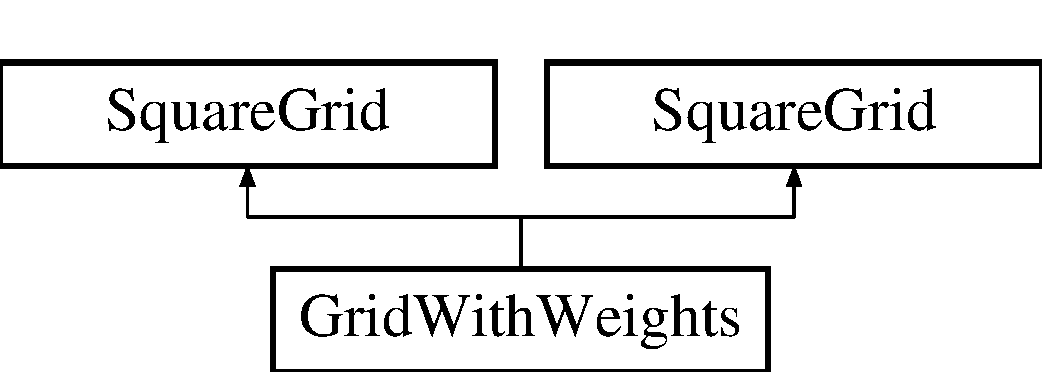
\includegraphics[height=2.000000cm]{structGridWithWeights}
\end{center}
\end{figure}
\subsection*{Public Member Functions}
\begin{DoxyCompactItemize}
\item 
\mbox{\hyperlink{structGridWithWeights_ad9eb67bf93deb3409ecf658288bc78f6}{Grid\+With\+Weights}} (int w, int h)
\item 
int \mbox{\hyperlink{structGridWithWeights_a999c39922a9b507e4436b817592a7ff9}{cost}} (\mbox{\hyperlink{structSquareGrid_a2c9a2cbd3912aa48ac97289abc3f1c0f}{Location}} a, \mbox{\hyperlink{structSquareGrid_a2c9a2cbd3912aa48ac97289abc3f1c0f}{Location}} b)
\item 
\mbox{\hyperlink{structGridWithWeights_ad9eb67bf93deb3409ecf658288bc78f6}{Grid\+With\+Weights}} (int w, int h)
\item 
int \mbox{\hyperlink{structGridWithWeights_a999c39922a9b507e4436b817592a7ff9}{cost}} (\mbox{\hyperlink{structSquareGrid_a2c9a2cbd3912aa48ac97289abc3f1c0f}{Location}} a, \mbox{\hyperlink{structSquareGrid_a2c9a2cbd3912aa48ac97289abc3f1c0f}{Location}} b)
\end{DoxyCompactItemize}
\subsection*{Public Attributes}
\begin{DoxyCompactItemize}
\item 
unordered\+\_\+set$<$ \mbox{\hyperlink{structSquareGrid_a2c9a2cbd3912aa48ac97289abc3f1c0f}{Location}} $>$ \mbox{\hyperlink{structGridWithWeights_a03137c824b8c63cdeed414ef40f5b504}{forests}}
\end{DoxyCompactItemize}
\subsection*{Additional Inherited Members}


\subsection{Constructor \& Destructor Documentation}
\mbox{\Hypertarget{structGridWithWeights_ad9eb67bf93deb3409ecf658288bc78f6}\label{structGridWithWeights_ad9eb67bf93deb3409ecf658288bc78f6}} 
\index{Grid\+With\+Weights@{Grid\+With\+Weights}!Grid\+With\+Weights@{Grid\+With\+Weights}}
\index{Grid\+With\+Weights@{Grid\+With\+Weights}!Grid\+With\+Weights@{Grid\+With\+Weights}}
\subsubsection{\texorpdfstring{Grid\+With\+Weights()}{GridWithWeights()}\hspace{0.1cm}{\footnotesize\ttfamily [1/2]}}
{\footnotesize\ttfamily Grid\+With\+Weights\+::\+Grid\+With\+Weights (\begin{DoxyParamCaption}\item[{int}]{w,  }\item[{int}]{h }\end{DoxyParamCaption})\hspace{0.3cm}{\ttfamily [inline]}}

\mbox{\Hypertarget{structGridWithWeights_ad9eb67bf93deb3409ecf658288bc78f6}\label{structGridWithWeights_ad9eb67bf93deb3409ecf658288bc78f6}} 
\index{Grid\+With\+Weights@{Grid\+With\+Weights}!Grid\+With\+Weights@{Grid\+With\+Weights}}
\index{Grid\+With\+Weights@{Grid\+With\+Weights}!Grid\+With\+Weights@{Grid\+With\+Weights}}
\subsubsection{\texorpdfstring{Grid\+With\+Weights()}{GridWithWeights()}\hspace{0.1cm}{\footnotesize\ttfamily [2/2]}}
{\footnotesize\ttfamily Grid\+With\+Weights\+::\+Grid\+With\+Weights (\begin{DoxyParamCaption}\item[{int}]{w,  }\item[{int}]{h }\end{DoxyParamCaption})\hspace{0.3cm}{\ttfamily [inline]}}



\subsection{Member Function Documentation}
\mbox{\Hypertarget{structGridWithWeights_a999c39922a9b507e4436b817592a7ff9}\label{structGridWithWeights_a999c39922a9b507e4436b817592a7ff9}} 
\index{Grid\+With\+Weights@{Grid\+With\+Weights}!cost@{cost}}
\index{cost@{cost}!Grid\+With\+Weights@{Grid\+With\+Weights}}
\subsubsection{\texorpdfstring{cost()}{cost()}\hspace{0.1cm}{\footnotesize\ttfamily [1/2]}}
{\footnotesize\ttfamily int Grid\+With\+Weights\+::cost (\begin{DoxyParamCaption}\item[{\mbox{\hyperlink{structSquareGrid_a2c9a2cbd3912aa48ac97289abc3f1c0f}{Location}}}]{a,  }\item[{\mbox{\hyperlink{structSquareGrid_a2c9a2cbd3912aa48ac97289abc3f1c0f}{Location}}}]{b }\end{DoxyParamCaption})\hspace{0.3cm}{\ttfamily [inline]}}

\mbox{\Hypertarget{structGridWithWeights_a999c39922a9b507e4436b817592a7ff9}\label{structGridWithWeights_a999c39922a9b507e4436b817592a7ff9}} 
\index{Grid\+With\+Weights@{Grid\+With\+Weights}!cost@{cost}}
\index{cost@{cost}!Grid\+With\+Weights@{Grid\+With\+Weights}}
\subsubsection{\texorpdfstring{cost()}{cost()}\hspace{0.1cm}{\footnotesize\ttfamily [2/2]}}
{\footnotesize\ttfamily int Grid\+With\+Weights\+::cost (\begin{DoxyParamCaption}\item[{\mbox{\hyperlink{structSquareGrid_a2c9a2cbd3912aa48ac97289abc3f1c0f}{Location}}}]{a,  }\item[{\mbox{\hyperlink{structSquareGrid_a2c9a2cbd3912aa48ac97289abc3f1c0f}{Location}}}]{b }\end{DoxyParamCaption})\hspace{0.3cm}{\ttfamily [inline]}}



\subsection{Member Data Documentation}
\mbox{\Hypertarget{structGridWithWeights_a03137c824b8c63cdeed414ef40f5b504}\label{structGridWithWeights_a03137c824b8c63cdeed414ef40f5b504}} 
\index{Grid\+With\+Weights@{Grid\+With\+Weights}!forests@{forests}}
\index{forests@{forests}!Grid\+With\+Weights@{Grid\+With\+Weights}}
\subsubsection{\texorpdfstring{forests}{forests}}
{\footnotesize\ttfamily unordered\+\_\+set$<$ \mbox{\hyperlink{structSquareGrid_a2c9a2cbd3912aa48ac97289abc3f1c0f}{Location}} $>$ Grid\+With\+Weights\+::forests}



The documentation for this struct was generated from the following files\+:\begin{DoxyCompactItemize}
\item 
/home/pbisaacs/\+Developer/\+Brain\+Harmonics/\+Brain\+Harmonics/\mbox{\hyperlink{implementation_01orig_8cpp}{implementation orig.\+cpp}}\item 
/home/pbisaacs/\+Developer/\+Brain\+Harmonics/\+Brain\+Harmonics/\mbox{\hyperlink{search_8cpp}{search.\+cpp}}\end{DoxyCompactItemize}

\hypertarget{structstd_1_1hash_3_01tuple_3_01int_00_01int_01_4_01_4}{}\section{std\+:\+:hash$<$ tuple$<$ int, int $>$ $>$ Struct Template Reference}
\label{structstd_1_1hash_3_01tuple_3_01int_00_01int_01_4_01_4}\index{std\+::hash$<$ tuple$<$ int, int $>$ $>$@{std\+::hash$<$ tuple$<$ int, int $>$ $>$}}
\subsection*{Public Member Functions}
\begin{DoxyCompactItemize}
\item 
size\+\_\+t \mbox{\hyperlink{structstd_1_1hash_3_01tuple_3_01int_00_01int_01_4_01_4_af46854ec2c5aa6cd6d1cd164374bd54f}{operator()}} (const tuple$<$ int, int $>$ \&location) const
\item 
size\+\_\+t \mbox{\hyperlink{structstd_1_1hash_3_01tuple_3_01int_00_01int_01_4_01_4_af46854ec2c5aa6cd6d1cd164374bd54f}{operator()}} (const tuple$<$ int, int $>$ \&location) const
\end{DoxyCompactItemize}


\subsection{Member Function Documentation}
\mbox{\Hypertarget{structstd_1_1hash_3_01tuple_3_01int_00_01int_01_4_01_4_af46854ec2c5aa6cd6d1cd164374bd54f}\label{structstd_1_1hash_3_01tuple_3_01int_00_01int_01_4_01_4_af46854ec2c5aa6cd6d1cd164374bd54f}} 
\index{std\+::hash$<$ tuple$<$ int, int $>$ $>$@{std\+::hash$<$ tuple$<$ int, int $>$ $>$}!operator()@{operator()}}
\index{operator()@{operator()}!std\+::hash$<$ tuple$<$ int, int $>$ $>$@{std\+::hash$<$ tuple$<$ int, int $>$ $>$}}
\subsubsection{\texorpdfstring{operator()()}{operator()()}\hspace{0.1cm}{\footnotesize\ttfamily [1/2]}}
{\footnotesize\ttfamily size\+\_\+t std\+::hash$<$ tuple$<$ int, int $>$ $>$\+::operator() (\begin{DoxyParamCaption}\item[{const tuple$<$ int, int $>$ \&}]{location }\end{DoxyParamCaption}) const\hspace{0.3cm}{\ttfamily [inline]}}

\mbox{\Hypertarget{structstd_1_1hash_3_01tuple_3_01int_00_01int_01_4_01_4_af46854ec2c5aa6cd6d1cd164374bd54f}\label{structstd_1_1hash_3_01tuple_3_01int_00_01int_01_4_01_4_af46854ec2c5aa6cd6d1cd164374bd54f}} 
\index{std\+::hash$<$ tuple$<$ int, int $>$ $>$@{std\+::hash$<$ tuple$<$ int, int $>$ $>$}!operator()@{operator()}}
\index{operator()@{operator()}!std\+::hash$<$ tuple$<$ int, int $>$ $>$@{std\+::hash$<$ tuple$<$ int, int $>$ $>$}}
\subsubsection{\texorpdfstring{operator()()}{operator()()}\hspace{0.1cm}{\footnotesize\ttfamily [2/2]}}
{\footnotesize\ttfamily size\+\_\+t std\+::hash$<$ tuple$<$ int, int $>$ $>$\+::operator() (\begin{DoxyParamCaption}\item[{const tuple$<$ int, int $>$ \&}]{location }\end{DoxyParamCaption}) const\hspace{0.3cm}{\ttfamily [inline]}}



The documentation for this struct was generated from the following files\+:\begin{DoxyCompactItemize}
\item 
/home/pbisaacs/\+Developer/\+Brain\+Harmonics/\+Brain\+Harmonics/\mbox{\hyperlink{implementation_01orig_8cpp}{implementation orig.\+cpp}}\item 
/home/pbisaacs/\+Developer/\+Brain\+Harmonics/\+Brain\+Harmonics/\mbox{\hyperlink{search_8cpp}{search.\+cpp}}\end{DoxyCompactItemize}

\hypertarget{classInterneuronSpace}{}\section{Interneuron\+Space Class Reference}
\label{classInterneuronSpace}\index{Interneuron\+Space@{Interneuron\+Space}}


{\ttfamily \#include $<$interneuronspace.\+h$>$}

Inheritance diagram for Interneuron\+Space\+:\begin{figure}[H]
\begin{center}
\leavevmode
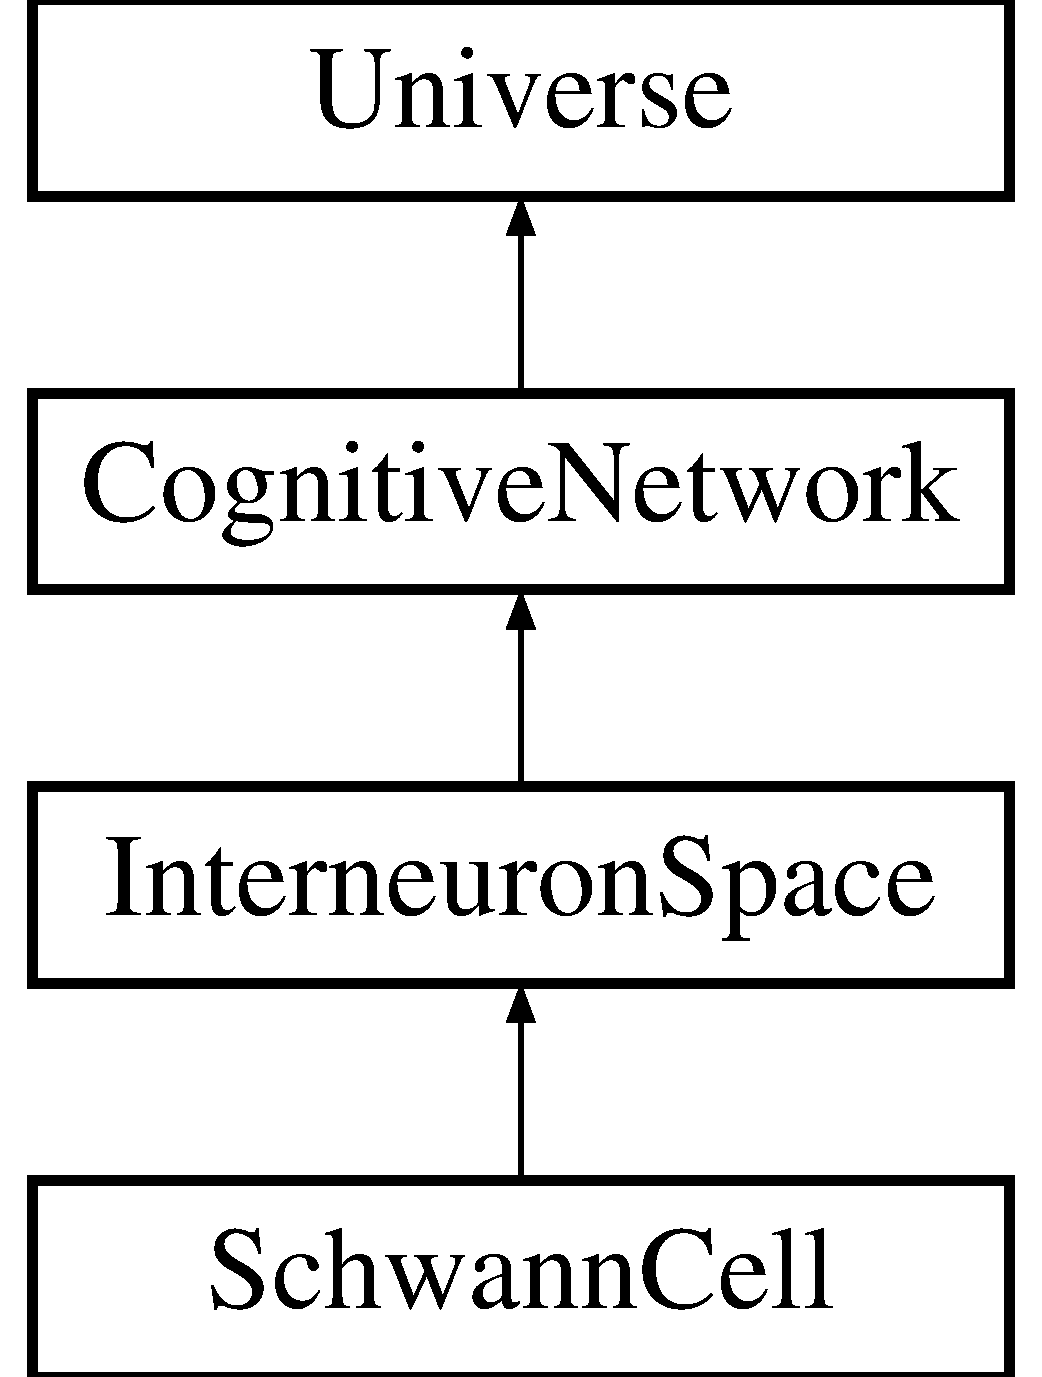
\includegraphics[height=4.000000cm]{classInterneuronSpace}
\end{center}
\end{figure}
\subsection*{Classes}
\begin{DoxyCompactItemize}
\item 
struct \mbox{\hyperlink{structInterneuronSpace_1_1NearbyNeuron}{Nearby\+Neuron}}
\item 
struct \mbox{\hyperlink{structInterneuronSpace_1_1s__BindList}{s\+\_\+\+Bind\+List}}
\end{DoxyCompactItemize}
\subsection*{Public Member Functions}
\begin{DoxyCompactItemize}
\item 
\mbox{\hyperlink{classInterneuronSpace_a4ad439037f087e7d5cb3e1d8c581ee5f}{Interneuron\+Space}} ()
\item 
\mbox{\hyperlink{classInterneuronSpace_a18d5d4920073a9a93ee3cb8f5efe9211}{Interneuron\+Space}} (unsigned int object\+\_\+type)
\item 
\mbox{\hyperlink{classInterneuronSpace_a753903f3c74415922607846040ac50a6}{Interneuron\+Space}} (unsigned int object\+\_\+type, std\+::chrono\+::time\+\_\+point$<$ \mbox{\hyperlink{universe_8h_a0ef8d951d1ca5ab3cfaf7ab4c7a6fd80}{Clock}} $>$ event\+\_\+time)
\item 
\mbox{\hyperlink{classInterneuronSpace_aa87eb8c7186542989fccdadc594c5915}{Interneuron\+Space}} (unsigned int object\+\_\+type, std\+::chrono\+::time\+\_\+point$<$ \mbox{\hyperlink{universe_8h_a0ef8d951d1ca5ab3cfaf7ab4c7a6fd80}{Clock}} $>$ event\+\_\+time, \mbox{\hyperlink{classCognitiveNetwork}{Cognitive\+Network}} \&cognitivenetwork\+\_\+connector)
\item 
virtual \mbox{\hyperlink{classInterneuronSpace_aff0056e3c60b7eff3ad4ca12f6756628}{$\sim$\+Interneuron\+Space}} ()
\item 
double \mbox{\hyperlink{classInterneuronSpace_a677430712211956219767d4fa71d20e6}{Get\+Energy}} (std\+::chrono\+::time\+\_\+point$<$ \mbox{\hyperlink{universe_8h_a0ef8d951d1ca5ab3cfaf7ab4c7a6fd80}{Clock}} $>$ event\+\_\+time)
\item 
int \mbox{\hyperlink{classInterneuronSpace_abd37d409a97acca62d11576314bdfcf4}{Get\+Tau\+Cycles\+Add}} (std\+::chrono\+::time\+\_\+point$<$ \mbox{\hyperlink{universe_8h_a0ef8d951d1ca5ab3cfaf7ab4c7a6fd80}{Clock}} $>$ event\+\_\+time)
\item 
int \mbox{\hyperlink{classInterneuronSpace_a1024eadca0b56be9b54593ea47c5879f}{Get\+Tau\+Cycles\+Decay}} (std\+::chrono\+::time\+\_\+point$<$ \mbox{\hyperlink{universe_8h_a0ef8d951d1ca5ab3cfaf7ab4c7a6fd80}{Clock}} $>$ event\+\_\+time)
\item 
int \mbox{\hyperlink{classInterneuronSpace_a90a2c950dd426ed3f015e3c186e877fd}{Get\+Charge\+Type}} (std\+::chrono\+::time\+\_\+point$<$ \mbox{\hyperlink{universe_8h_a0ef8d951d1ca5ab3cfaf7ab4c7a6fd80}{Clock}} $>$ event\+\_\+time)
\item 
int \mbox{\hyperlink{classInterneuronSpace_ae65bf091b84fa11459ef754ed1c7bf21}{Get\+Discharge\+Type}} (std\+::chrono\+::time\+\_\+point$<$ \mbox{\hyperlink{universe_8h_a0ef8d951d1ca5ab3cfaf7ab4c7a6fd80}{Clock}} $>$ event\+\_\+time)
\item 
int \mbox{\hyperlink{classInterneuronSpace_a66b6683bab6872dfece6111a8ccfb1d7}{Get\+Interneuron\+Space\+Device\+Tag}} (std\+::chrono\+::time\+\_\+point$<$ \mbox{\hyperlink{universe_8h_a0ef8d951d1ca5ab3cfaf7ab4c7a6fd80}{Clock}} $>$ event\+\_\+time)
\item 
void \mbox{\hyperlink{classInterneuronSpace_a60a46f22a2e575d65031635a698a60a9}{Set\+Counter}} (std\+::chrono\+::time\+\_\+point$<$ \mbox{\hyperlink{universe_8h_a0ef8d951d1ca5ab3cfaf7ab4c7a6fd80}{Clock}} $>$ event\+\_\+time, unsigned int val)
\item 
void \mbox{\hyperlink{classInterneuronSpace_a65ecd1914ab039707313beb1b8702e68}{Set\+Energy}} (std\+::chrono\+::time\+\_\+point$<$ \mbox{\hyperlink{universe_8h_a0ef8d951d1ca5ab3cfaf7ab4c7a6fd80}{Clock}} $>$ event\+\_\+time, double val)
\item 
void \mbox{\hyperlink{classInterneuronSpace_ad6c1387daa261a3e8e1dba1402101d5c}{Set\+Tau\+Cycles\+Add}} (std\+::chrono\+::time\+\_\+point$<$ \mbox{\hyperlink{universe_8h_a0ef8d951d1ca5ab3cfaf7ab4c7a6fd80}{Clock}} $>$ event\+\_\+time, int val)
\item 
void \mbox{\hyperlink{classInterneuronSpace_a7f44a965e377ecdc5c387af2b5d30d69}{Set\+Tau\+Cycles\+Decay}} (std\+::chrono\+::time\+\_\+point$<$ \mbox{\hyperlink{universe_8h_a0ef8d951d1ca5ab3cfaf7ab4c7a6fd80}{Clock}} $>$ event\+\_\+time, int val)
\item 
void \mbox{\hyperlink{classInterneuronSpace_a404aacb1adce30288bb7b4237344e4cc}{Set\+Charge\+Type}} (std\+::chrono\+::time\+\_\+point$<$ \mbox{\hyperlink{universe_8h_a0ef8d951d1ca5ab3cfaf7ab4c7a6fd80}{Clock}} $>$ event\+\_\+time, int val)
\item 
void \mbox{\hyperlink{classInterneuronSpace_a7fc404aae98d45ccad26b5c186fab6e2}{Set\+Discharge\+Type}} (std\+::chrono\+::time\+\_\+point$<$ \mbox{\hyperlink{universe_8h_a0ef8d951d1ca5ab3cfaf7ab4c7a6fd80}{Clock}} $>$ event\+\_\+time, int val)
\item 
void \mbox{\hyperlink{classInterneuronSpace_ab34d72ef9135288690328217d7c0a388}{Set\+Interneuron\+Space\+Device\+Tag}} (std\+::chrono\+::time\+\_\+point$<$ \mbox{\hyperlink{universe_8h_a0ef8d951d1ca5ab3cfaf7ab4c7a6fd80}{Clock}} $>$ event\+\_\+time, int val)
\item 
bool \mbox{\hyperlink{classInterneuronSpace_a3a9776e4a77b87374204468ca7974157}{Reset\+Parameters}} (std\+::chrono\+::time\+\_\+point$<$ \mbox{\hyperlink{universe_8h_a0ef8d951d1ca5ab3cfaf7ab4c7a6fd80}{Clock}} $>$ event\+\_\+time)
\item 
\mbox{\hyperlink{classCognitiveNetwork}{Cognitive\+Network}} $\ast$ \mbox{\hyperlink{classInterneuronSpace_a26d98a0ae78ce363ab93e92cf0c973e7}{Create\+Neurotransmitter}} (std\+::chrono\+::time\+\_\+point$<$ \mbox{\hyperlink{universe_8h_a0ef8d951d1ca5ab3cfaf7ab4c7a6fd80}{Clock}} $>$ event\+\_\+time)
\item 
std\+::vector$<$ \mbox{\hyperlink{classCognitiveNetwork}{Cognitive\+Network}} $\ast$ $>$ \mbox{\hyperlink{classInterneuronSpace_af69f7190226d77a30a80d66d7c28e0ba}{Create\+Neurotransmitters}} (std\+::chrono\+::time\+\_\+point$<$ \mbox{\hyperlink{universe_8h_a0ef8d951d1ca5ab3cfaf7ab4c7a6fd80}{Clock}} $>$ event\+\_\+time, int quantity)
\item 
\mbox{\hyperlink{classCognitiveNetwork}{Cognitive\+Network}} $\ast$ \mbox{\hyperlink{classInterneuronSpace_a96149bba4c6efd03586700a6fe86960a}{Clone\+Neurotransmitter}} (std\+::chrono\+::time\+\_\+point$<$ \mbox{\hyperlink{universe_8h_a0ef8d951d1ca5ab3cfaf7ab4c7a6fd80}{Clock}} $>$ event\+\_\+time, \mbox{\hyperlink{classCognitiveNetwork}{Cognitive\+Network}} $\ast$clone\+\_\+object, double perfection\+\_\+membership)
\item 
std\+::vector$<$ \mbox{\hyperlink{classCognitiveNetwork}{Cognitive\+Network}} $\ast$ $>$ \mbox{\hyperlink{classInterneuronSpace_a3defddf17eb839dbd799980f6116f895}{Clone\+Neurotransmitters}} (std\+::chrono\+::time\+\_\+point$<$ \mbox{\hyperlink{universe_8h_a0ef8d951d1ca5ab3cfaf7ab4c7a6fd80}{Clock}} $>$ event\+\_\+time, std\+::vector$<$ \mbox{\hyperlink{classCognitiveNetwork}{Cognitive\+Network}} $\ast$$>$ cloning\+\_\+list, double perfection\+\_\+membership)
\item 
\mbox{\hyperlink{classCognitiveNetwork}{Cognitive\+Network}} $\ast$ \mbox{\hyperlink{classInterneuronSpace_a41eb332165b0a67c3549bd73a8faa969}{Destroy\+Neurotransmitter}} (std\+::chrono\+::time\+\_\+point$<$ \mbox{\hyperlink{universe_8h_a0ef8d951d1ca5ab3cfaf7ab4c7a6fd80}{Clock}} $>$ event\+\_\+time, \mbox{\hyperlink{classCognitiveNetwork}{Cognitive\+Network}} $\ast$destroy\+\_\+object)
\item 
std\+::vector$<$ \mbox{\hyperlink{classCognitiveNetwork}{Cognitive\+Network}} $\ast$ $>$ \mbox{\hyperlink{classInterneuronSpace_a9543932ffea18cce46fdfbf0fbb85b1b}{Destroy\+Neurotransmitters}} (std\+::chrono\+::time\+\_\+point$<$ \mbox{\hyperlink{universe_8h_a0ef8d951d1ca5ab3cfaf7ab4c7a6fd80}{Clock}} $>$ event\+\_\+time, std\+::vector$<$ \mbox{\hyperlink{classCognitiveNetwork}{Cognitive\+Network}} $\ast$$>$ destruction\+\_\+list)
\item 
\mbox{\hyperlink{classCognitiveNetwork}{Cognitive\+Network}} $\ast$ \mbox{\hyperlink{classInterneuronSpace_afee7374310b2a8c08bac232d62ea7aa1}{Add\+Neurotransmitter}} (std\+::chrono\+::time\+\_\+point$<$ \mbox{\hyperlink{universe_8h_a0ef8d951d1ca5ab3cfaf7ab4c7a6fd80}{Clock}} $>$ event\+\_\+time, \mbox{\hyperlink{classCognitiveNetwork}{Cognitive\+Network}} $\ast$add\+\_\+object)
\item 
std\+::vector$<$ \mbox{\hyperlink{classCognitiveNetwork}{Cognitive\+Network}} $\ast$ $>$ \mbox{\hyperlink{classInterneuronSpace_a1049397cd511c753d8c178db8f68a1a7}{Add\+Neurotransmitters}} (std\+::chrono\+::time\+\_\+point$<$ \mbox{\hyperlink{universe_8h_a0ef8d951d1ca5ab3cfaf7ab4c7a6fd80}{Clock}} $>$ event\+\_\+time, std\+::vector$<$ \mbox{\hyperlink{classCognitiveNetwork}{Cognitive\+Network}} $\ast$$>$ add\+\_\+objects)
\item 
\mbox{\hyperlink{classCognitiveNetwork}{Cognitive\+Network}} $\ast$ \mbox{\hyperlink{classInterneuronSpace_aa46b5ce238b49425a68fcfd53ba1d8b7}{Remove\+Neurotransmitter}} (std\+::chrono\+::time\+\_\+point$<$ \mbox{\hyperlink{universe_8h_a0ef8d951d1ca5ab3cfaf7ab4c7a6fd80}{Clock}} $>$ event\+\_\+time)
\item 
std\+::vector$<$ \mbox{\hyperlink{classCognitiveNetwork}{Cognitive\+Network}} $\ast$ $>$ \mbox{\hyperlink{classInterneuronSpace_a7b11f542ab7a3d293d5fcf5a1b522ac2}{Remove\+Neurotransmitters}} (std\+::chrono\+::time\+\_\+point$<$ \mbox{\hyperlink{universe_8h_a0ef8d951d1ca5ab3cfaf7ab4c7a6fd80}{Clock}} $>$ event\+\_\+time, int quantity)
\item 
\mbox{\hyperlink{classCognitiveNetwork}{Cognitive\+Network}} $\ast$ \mbox{\hyperlink{classInterneuronSpace_a7a60c95c8706cbff3084e74b7b15d75c}{Get\+Neurotransmitter}} (std\+::chrono\+::time\+\_\+point$<$ \mbox{\hyperlink{universe_8h_a0ef8d951d1ca5ab3cfaf7ab4c7a6fd80}{Clock}} $>$ event\+\_\+time, int selector)
\item 
std\+::vector$<$ \mbox{\hyperlink{classCognitiveNetwork}{Cognitive\+Network}} $\ast$ $>$ \mbox{\hyperlink{classInterneuronSpace_aaae45b76a4c059aae1e27bde3901371c}{Get\+Neurotransmitters}} (std\+::chrono\+::time\+\_\+point$<$ \mbox{\hyperlink{universe_8h_a0ef8d951d1ca5ab3cfaf7ab4c7a6fd80}{Clock}} $>$ event\+\_\+time)
\item 
int \mbox{\hyperlink{classInterneuronSpace_ae62237c3a84893c81e9998602ab16718}{Get\+Demand}} (std\+::chrono\+::time\+\_\+point$<$ \mbox{\hyperlink{universe_8h_a0ef8d951d1ca5ab3cfaf7ab4c7a6fd80}{Clock}} $>$ event\+\_\+time)
\item 
double \mbox{\hyperlink{classInterneuronSpace_a634322f8b405ead2dc51afb0a5c3d725}{Get\+Distance}} (std\+::chrono\+::time\+\_\+point$<$ \mbox{\hyperlink{universe_8h_a0ef8d951d1ca5ab3cfaf7ab4c7a6fd80}{Clock}} $>$ event\+\_\+time, int val)
\item 
int \mbox{\hyperlink{classInterneuronSpace_a4b053dc94a921c8176d9f58d40169089}{Get\+Allocated\+Interneuron\+Space}} (std\+::chrono\+::time\+\_\+point$<$ \mbox{\hyperlink{universe_8h_a0ef8d951d1ca5ab3cfaf7ab4c7a6fd80}{Clock}} $>$ event\+\_\+time)
\item 
double \mbox{\hyperlink{classInterneuronSpace_a243535a8f09f104c3a4488f6df4cfd57}{Get\+Minimum\+Distance}} (std\+::chrono\+::time\+\_\+point$<$ \mbox{\hyperlink{universe_8h_a0ef8d951d1ca5ab3cfaf7ab4c7a6fd80}{Clock}} $>$ event\+\_\+time)
\item 
void \mbox{\hyperlink{classInterneuronSpace_ae77729a0c140cfb8a9121e898be791b2}{Get\+Interneuron\+Space\+List}} (std\+::chrono\+::time\+\_\+point$<$ \mbox{\hyperlink{universe_8h_a0ef8d951d1ca5ab3cfaf7ab4c7a6fd80}{Clock}} $>$ event\+\_\+time)
\item 
void \mbox{\hyperlink{classInterneuronSpace_ad2225077a049e78ce583a79eee2d373f}{Set\+Demand}} (std\+::chrono\+::time\+\_\+point$<$ \mbox{\hyperlink{universe_8h_a0ef8d951d1ca5ab3cfaf7ab4c7a6fd80}{Clock}} $>$ event\+\_\+time, int val)
\item 
void \mbox{\hyperlink{classInterneuronSpace_a50aaa97f71011dafb583dc432817f477}{Set\+Neuron}} (std\+::chrono\+::time\+\_\+point$<$ \mbox{\hyperlink{universe_8h_a0ef8d951d1ca5ab3cfaf7ab4c7a6fd80}{Clock}} $>$ event\+\_\+time, int val)
\item 
void \mbox{\hyperlink{classInterneuronSpace_ab56b0336c9e53f7b448e9d35e617e8c0}{Send\+Bare\+Spike}} (std\+::chrono\+::time\+\_\+point$<$ \mbox{\hyperlink{universe_8h_a0ef8d951d1ca5ab3cfaf7ab4c7a6fd80}{Clock}} $>$ event\+\_\+time)
\item 
void \mbox{\hyperlink{classInterneuronSpace_a0a24da715aecafd4072d596fc271666f}{Send\+Transmitter\+Spike}} (std\+::chrono\+::time\+\_\+point$<$ \mbox{\hyperlink{universe_8h_a0ef8d951d1ca5ab3cfaf7ab4c7a6fd80}{Clock}} $>$ event\+\_\+time)
\item 
int \mbox{\hyperlink{classInterneuronSpace_a72ce2431e1348dd2558fa9b8f864d306}{Update}} (std\+::chrono\+::time\+\_\+point$<$ \mbox{\hyperlink{universe_8h_a0ef8d951d1ca5ab3cfaf7ab4c7a6fd80}{Clock}} $>$ event\+\_\+time)
\end{DoxyCompactItemize}
\subsection*{Protected Attributes}
\begin{DoxyCompactItemize}
\item 
std\+::vector$<$ \mbox{\hyperlink{classCognitiveNetwork}{Cognitive\+Network}} $\ast$ $>$ \mbox{\hyperlink{classInterneuronSpace_a51d51c2f71f6fcf65c478aa27457c4a3}{neurotransmitter\+\_\+list}}
\end{DoxyCompactItemize}
\subsection*{Private Attributes}
\begin{DoxyCompactItemize}
\item 
int \mbox{\hyperlink{classInterneuronSpace_af520cb6f8766c77b1e575b2b65393cce}{interneuronspace\+\_\+type}}
\item 
double \mbox{\hyperlink{classInterneuronSpace_aff15cb40feb85e4b75c1bdc31604f333}{object\+\_\+size}}
\item 
double \mbox{\hyperlink{classInterneuronSpace_acfef881bda3b9184542530453075d1b1}{object\+\_\+energy}}
\item 
double \mbox{\hyperlink{classInterneuronSpace_a822a704e13dc60edfc5cb710e52150c3}{object\+\_\+energy\+\_\+threshold}}
\item 
int \mbox{\hyperlink{classInterneuronSpace_aedb61682c1c2a374645e21abd4526825}{m\+\_\+\+Neuron\+Type}}
\item 
int \mbox{\hyperlink{classInterneuronSpace_a5065916461ffbe096fe6bbb6503a767e}{neurotransmitter\+\_\+pool}}
\item 
int \mbox{\hyperlink{classInterneuronSpace_a5a4e1290b3bbb384597f111419be9c76}{m\+\_\+\+Tag}}
\item 
int \mbox{\hyperlink{classInterneuronSpace_a9f49bd1364861ea859f1a66c606cff8a}{m\+\_\+add\+Status}}
\item 
int \mbox{\hyperlink{classInterneuronSpace_ae71819def096138a0fb466cbe3f4bf02}{m\+\_\+\+Tau\+Cycles\+Add}}
\item 
int \mbox{\hyperlink{classInterneuronSpace_ac5c246784a31e7299aec57b2861a87e7}{m\+\_\+\+Tau\+Cycles\+Decay}}
\item 
int \mbox{\hyperlink{classInterneuronSpace_aa8a5afd05659a9bbfd0934de9ea3cd53}{m\+\_\+\+Charge\+Type}}
\item 
int \mbox{\hyperlink{classInterneuronSpace_abaa8436af9b85307c65de2755a010297}{m\+\_\+\+Discharge\+Type}}
\item 
bool \mbox{\hyperlink{classInterneuronSpace_a42f0a8cfca4592f0a6b47219df489396}{object\+\_\+disabled}}
\item 
std\+::chrono\+::time\+\_\+point$<$ \mbox{\hyperlink{universe_8h_a0ef8d951d1ca5ab3cfaf7ab4c7a6fd80}{Clock}} $>$ \mbox{\hyperlink{classInterneuronSpace_a5504d64df22fd330cdd14b4aca0171ea}{time\+\_\+object\+\_\+created}}
\item 
std\+::chrono\+::time\+\_\+point$<$ \mbox{\hyperlink{universe_8h_a0ef8d951d1ca5ab3cfaf7ab4c7a6fd80}{Clock}} $>$ \mbox{\hyperlink{classInterneuronSpace_a28efcbf608d5dd02f9dd85bec76a7650}{previous\+\_\+event\+\_\+time}}
\item 
int \mbox{\hyperlink{classInterneuronSpace_a7a5cfbb9b0a619283417044345b01578}{duration\+\_\+since\+\_\+last\+\_\+event}}
\item 
double \mbox{\hyperlink{classInterneuronSpace_aae1ef00c4fdc597fa12548771953b239}{m\+\_\+\+Volume}}
\item 
double \mbox{\hyperlink{classInterneuronSpace_a2cd3cbca541688d4eaf15fc6c8496dd1}{m\+\_\+\+Surface\+Area}}
\item 
unsigned int \mbox{\hyperlink{classInterneuronSpace_a854dc7cd9f9b8643b2c674d2eaa36873}{m\+\_\+\+Counter}}
\begin{DoxyCompactList}\small\item\em Member variable \char`\"{}m\+\_\+\+Counter\char`\"{}. \end{DoxyCompactList}\item 
double \mbox{\hyperlink{classInterneuronSpace_a97595972171f2fd0c37ad2d830f61fbb}{m\+\_\+axonlength}}
\item 
double \mbox{\hyperlink{classInterneuronSpace_a31182cce98aaecef1533fe17fc3e6786}{m\+\_\+\+Time\+Dilation}}
\item 
double \mbox{\hyperlink{classInterneuronSpace_a16272fc7502a95a69ca60cbe4612f100}{m\+\_\+\+Time\+Threshold}}
\item 
bool \mbox{\hyperlink{classInterneuronSpace_af16aec913a2ec7b4f92f7da2487b4b00}{object\+\_\+initialised}} = false
\item 
double \mbox{\hyperlink{classInterneuronSpace_a9cb8dd97e4c6c18d3b84e0c0db6ca605}{m\+\_\+\+Reduce\+By}}
\item 
double \mbox{\hyperlink{classInterneuronSpace_a848666191c3e8c746d5b7d82b1b8d329}{m\+\_\+\+Reduced\+By}}
\item 
std\+::vector$<$ \mbox{\hyperlink{structInterneuronSpace_1_1s__BindList}{s\+\_\+\+Bind\+List}} $>$ \mbox{\hyperlink{classInterneuronSpace_a37041f5f3a796a7dedcf4cb576c9dbcd}{m\+\_\+\+Bind\+List}}
\item 
int \mbox{\hyperlink{classInterneuronSpace_ae1196b764996aa441538d5f6909a2344}{interneuronspace\+Counter}}
\begin{DoxyCompactList}\small\item\em Member variable \char`\"{}interneuronspace\+Counter\char`\"{}. \end{DoxyCompactList}\item 
int \mbox{\hyperlink{classInterneuronSpace_a6b6f5ac9671c40ea57d39824e76a7ccd}{interneuronspace\+Demand}}
\item 
double \mbox{\hyperlink{classInterneuronSpace_a7656441e3758dae6167e49903a916bf6}{minimum\+Distance}}
\item 
std\+::vector$<$ \mbox{\hyperlink{structInterneuronSpace_1_1NearbyNeuron}{Nearby\+Neuron}} $>$ \mbox{\hyperlink{classInterneuronSpace_ac55f2a154e8abc403ac1459f0317f0cf}{neuron\+List}}
\item 
std\+::vector$<$ \mbox{\hyperlink{structInterneuronSpace_1_1NearbyNeuron}{Nearby\+Neuron}} $>$\+::iterator \mbox{\hyperlink{classInterneuronSpace_a9643f76d9b5acf91152ed69f6c3dca49}{it}}
\end{DoxyCompactItemize}
\subsection*{Additional Inherited Members}


\subsection{Constructor \& Destructor Documentation}
\mbox{\Hypertarget{classInterneuronSpace_a4ad439037f087e7d5cb3e1d8c581ee5f}\label{classInterneuronSpace_a4ad439037f087e7d5cb3e1d8c581ee5f}} 
\index{Interneuron\+Space@{Interneuron\+Space}!Interneuron\+Space@{Interneuron\+Space}}
\index{Interneuron\+Space@{Interneuron\+Space}!Interneuron\+Space@{Interneuron\+Space}}
\subsubsection{\texorpdfstring{Interneuron\+Space()}{InterneuronSpace()}\hspace{0.1cm}{\footnotesize\ttfamily [1/4]}}
{\footnotesize\ttfamily Interneuron\+Space\+::\+Interneuron\+Space (\begin{DoxyParamCaption}{ }\end{DoxyParamCaption})\hspace{0.3cm}{\ttfamily [inline]}}

\mbox{\Hypertarget{classInterneuronSpace_a18d5d4920073a9a93ee3cb8f5efe9211}\label{classInterneuronSpace_a18d5d4920073a9a93ee3cb8f5efe9211}} 
\index{Interneuron\+Space@{Interneuron\+Space}!Interneuron\+Space@{Interneuron\+Space}}
\index{Interneuron\+Space@{Interneuron\+Space}!Interneuron\+Space@{Interneuron\+Space}}
\subsubsection{\texorpdfstring{Interneuron\+Space()}{InterneuronSpace()}\hspace{0.1cm}{\footnotesize\ttfamily [2/4]}}
{\footnotesize\ttfamily Interneuron\+Space\+::\+Interneuron\+Space (\begin{DoxyParamCaption}\item[{unsigned int}]{object\+\_\+type }\end{DoxyParamCaption})\hspace{0.3cm}{\ttfamily [inline]}}

\mbox{\Hypertarget{classInterneuronSpace_a753903f3c74415922607846040ac50a6}\label{classInterneuronSpace_a753903f3c74415922607846040ac50a6}} 
\index{Interneuron\+Space@{Interneuron\+Space}!Interneuron\+Space@{Interneuron\+Space}}
\index{Interneuron\+Space@{Interneuron\+Space}!Interneuron\+Space@{Interneuron\+Space}}
\subsubsection{\texorpdfstring{Interneuron\+Space()}{InterneuronSpace()}\hspace{0.1cm}{\footnotesize\ttfamily [3/4]}}
{\footnotesize\ttfamily Interneuron\+Space\+::\+Interneuron\+Space (\begin{DoxyParamCaption}\item[{unsigned int}]{object\+\_\+type,  }\item[{std\+::chrono\+::time\+\_\+point$<$ \mbox{\hyperlink{universe_8h_a0ef8d951d1ca5ab3cfaf7ab4c7a6fd80}{Clock}} $>$}]{event\+\_\+time }\end{DoxyParamCaption})\hspace{0.3cm}{\ttfamily [inline]}}

\mbox{\Hypertarget{classInterneuronSpace_aa87eb8c7186542989fccdadc594c5915}\label{classInterneuronSpace_aa87eb8c7186542989fccdadc594c5915}} 
\index{Interneuron\+Space@{Interneuron\+Space}!Interneuron\+Space@{Interneuron\+Space}}
\index{Interneuron\+Space@{Interneuron\+Space}!Interneuron\+Space@{Interneuron\+Space}}
\subsubsection{\texorpdfstring{Interneuron\+Space()}{InterneuronSpace()}\hspace{0.1cm}{\footnotesize\ttfamily [4/4]}}
{\footnotesize\ttfamily Interneuron\+Space\+::\+Interneuron\+Space (\begin{DoxyParamCaption}\item[{unsigned int}]{object\+\_\+type,  }\item[{std\+::chrono\+::time\+\_\+point$<$ \mbox{\hyperlink{universe_8h_a0ef8d951d1ca5ab3cfaf7ab4c7a6fd80}{Clock}} $>$}]{event\+\_\+time,  }\item[{\mbox{\hyperlink{classCognitiveNetwork}{Cognitive\+Network}} \&}]{cognitivenetwork\+\_\+connector }\end{DoxyParamCaption})\hspace{0.3cm}{\ttfamily [inline]}}

\mbox{\Hypertarget{classInterneuronSpace_aff0056e3c60b7eff3ad4ca12f6756628}\label{classInterneuronSpace_aff0056e3c60b7eff3ad4ca12f6756628}} 
\index{Interneuron\+Space@{Interneuron\+Space}!````~Interneuron\+Space@{$\sim$\+Interneuron\+Space}}
\index{````~Interneuron\+Space@{$\sim$\+Interneuron\+Space}!Interneuron\+Space@{Interneuron\+Space}}
\subsubsection{\texorpdfstring{$\sim$\+Interneuron\+Space()}{~InterneuronSpace()}}
{\footnotesize\ttfamily virtual Interneuron\+Space\+::$\sim$\+Interneuron\+Space (\begin{DoxyParamCaption}{ }\end{DoxyParamCaption})\hspace{0.3cm}{\ttfamily [inline]}, {\ttfamily [virtual]}}

Default destructor 

\subsection{Member Function Documentation}
\mbox{\Hypertarget{classInterneuronSpace_afee7374310b2a8c08bac232d62ea7aa1}\label{classInterneuronSpace_afee7374310b2a8c08bac232d62ea7aa1}} 
\index{Interneuron\+Space@{Interneuron\+Space}!Add\+Neurotransmitter@{Add\+Neurotransmitter}}
\index{Add\+Neurotransmitter@{Add\+Neurotransmitter}!Interneuron\+Space@{Interneuron\+Space}}
\subsubsection{\texorpdfstring{Add\+Neurotransmitter()}{AddNeurotransmitter()}}
{\footnotesize\ttfamily \mbox{\hyperlink{classCognitiveNetwork}{Cognitive\+Network}} $\ast$ Interneuron\+Space\+::\+Add\+Neurotransmitter (\begin{DoxyParamCaption}\item[{std\+::chrono\+::time\+\_\+point$<$ \mbox{\hyperlink{universe_8h_a0ef8d951d1ca5ab3cfaf7ab4c7a6fd80}{Clock}} $>$}]{event\+\_\+time,  }\item[{\mbox{\hyperlink{classCognitiveNetwork}{Cognitive\+Network}} $\ast$}]{add\+\_\+object }\end{DoxyParamCaption})}

\mbox{\Hypertarget{classInterneuronSpace_a1049397cd511c753d8c178db8f68a1a7}\label{classInterneuronSpace_a1049397cd511c753d8c178db8f68a1a7}} 
\index{Interneuron\+Space@{Interneuron\+Space}!Add\+Neurotransmitters@{Add\+Neurotransmitters}}
\index{Add\+Neurotransmitters@{Add\+Neurotransmitters}!Interneuron\+Space@{Interneuron\+Space}}
\subsubsection{\texorpdfstring{Add\+Neurotransmitters()}{AddNeurotransmitters()}}
{\footnotesize\ttfamily std\+::vector$<$ \mbox{\hyperlink{classCognitiveNetwork}{Cognitive\+Network}} $\ast$ $>$ Interneuron\+Space\+::\+Add\+Neurotransmitters (\begin{DoxyParamCaption}\item[{std\+::chrono\+::time\+\_\+point$<$ \mbox{\hyperlink{universe_8h_a0ef8d951d1ca5ab3cfaf7ab4c7a6fd80}{Clock}} $>$}]{event\+\_\+time,  }\item[{std\+::vector$<$ \mbox{\hyperlink{classCognitiveNetwork}{Cognitive\+Network}} $\ast$$>$}]{add\+\_\+objects }\end{DoxyParamCaption})}

\mbox{\Hypertarget{classInterneuronSpace_a96149bba4c6efd03586700a6fe86960a}\label{classInterneuronSpace_a96149bba4c6efd03586700a6fe86960a}} 
\index{Interneuron\+Space@{Interneuron\+Space}!Clone\+Neurotransmitter@{Clone\+Neurotransmitter}}
\index{Clone\+Neurotransmitter@{Clone\+Neurotransmitter}!Interneuron\+Space@{Interneuron\+Space}}
\subsubsection{\texorpdfstring{Clone\+Neurotransmitter()}{CloneNeurotransmitter()}}
{\footnotesize\ttfamily \mbox{\hyperlink{classCognitiveNetwork}{Cognitive\+Network}} $\ast$ Interneuron\+Space\+::\+Clone\+Neurotransmitter (\begin{DoxyParamCaption}\item[{std\+::chrono\+::time\+\_\+point$<$ \mbox{\hyperlink{universe_8h_a0ef8d951d1ca5ab3cfaf7ab4c7a6fd80}{Clock}} $>$}]{event\+\_\+time,  }\item[{\mbox{\hyperlink{classCognitiveNetwork}{Cognitive\+Network}} $\ast$}]{clone\+\_\+object,  }\item[{double}]{perfection\+\_\+membership }\end{DoxyParamCaption})}

\mbox{\Hypertarget{classInterneuronSpace_a3defddf17eb839dbd799980f6116f895}\label{classInterneuronSpace_a3defddf17eb839dbd799980f6116f895}} 
\index{Interneuron\+Space@{Interneuron\+Space}!Clone\+Neurotransmitters@{Clone\+Neurotransmitters}}
\index{Clone\+Neurotransmitters@{Clone\+Neurotransmitters}!Interneuron\+Space@{Interneuron\+Space}}
\subsubsection{\texorpdfstring{Clone\+Neurotransmitters()}{CloneNeurotransmitters()}}
{\footnotesize\ttfamily std\+::vector$<$ \mbox{\hyperlink{classCognitiveNetwork}{Cognitive\+Network}} $\ast$ $>$ Interneuron\+Space\+::\+Clone\+Neurotransmitters (\begin{DoxyParamCaption}\item[{std\+::chrono\+::time\+\_\+point$<$ \mbox{\hyperlink{universe_8h_a0ef8d951d1ca5ab3cfaf7ab4c7a6fd80}{Clock}} $>$}]{event\+\_\+time,  }\item[{std\+::vector$<$ \mbox{\hyperlink{classCognitiveNetwork}{Cognitive\+Network}} $\ast$$>$}]{cloning\+\_\+list,  }\item[{double}]{perfection\+\_\+membership }\end{DoxyParamCaption})}

\mbox{\Hypertarget{classInterneuronSpace_a26d98a0ae78ce363ab93e92cf0c973e7}\label{classInterneuronSpace_a26d98a0ae78ce363ab93e92cf0c973e7}} 
\index{Interneuron\+Space@{Interneuron\+Space}!Create\+Neurotransmitter@{Create\+Neurotransmitter}}
\index{Create\+Neurotransmitter@{Create\+Neurotransmitter}!Interneuron\+Space@{Interneuron\+Space}}
\subsubsection{\texorpdfstring{Create\+Neurotransmitter()}{CreateNeurotransmitter()}}
{\footnotesize\ttfamily \mbox{\hyperlink{classCognitiveNetwork}{Cognitive\+Network}} $\ast$ Interneuron\+Space\+::\+Create\+Neurotransmitter (\begin{DoxyParamCaption}\item[{std\+::chrono\+::time\+\_\+point$<$ \mbox{\hyperlink{universe_8h_a0ef8d951d1ca5ab3cfaf7ab4c7a6fd80}{Clock}} $>$}]{event\+\_\+time }\end{DoxyParamCaption})}

\mbox{\Hypertarget{classInterneuronSpace_af69f7190226d77a30a80d66d7c28e0ba}\label{classInterneuronSpace_af69f7190226d77a30a80d66d7c28e0ba}} 
\index{Interneuron\+Space@{Interneuron\+Space}!Create\+Neurotransmitters@{Create\+Neurotransmitters}}
\index{Create\+Neurotransmitters@{Create\+Neurotransmitters}!Interneuron\+Space@{Interneuron\+Space}}
\subsubsection{\texorpdfstring{Create\+Neurotransmitters()}{CreateNeurotransmitters()}}
{\footnotesize\ttfamily std\+::vector$<$ \mbox{\hyperlink{classCognitiveNetwork}{Cognitive\+Network}} $\ast$ $>$ Interneuron\+Space\+::\+Create\+Neurotransmitters (\begin{DoxyParamCaption}\item[{std\+::chrono\+::time\+\_\+point$<$ \mbox{\hyperlink{universe_8h_a0ef8d951d1ca5ab3cfaf7ab4c7a6fd80}{Clock}} $>$}]{event\+\_\+time,  }\item[{int}]{quantity }\end{DoxyParamCaption})}

\mbox{\Hypertarget{classInterneuronSpace_a41eb332165b0a67c3549bd73a8faa969}\label{classInterneuronSpace_a41eb332165b0a67c3549bd73a8faa969}} 
\index{Interneuron\+Space@{Interneuron\+Space}!Destroy\+Neurotransmitter@{Destroy\+Neurotransmitter}}
\index{Destroy\+Neurotransmitter@{Destroy\+Neurotransmitter}!Interneuron\+Space@{Interneuron\+Space}}
\subsubsection{\texorpdfstring{Destroy\+Neurotransmitter()}{DestroyNeurotransmitter()}}
{\footnotesize\ttfamily \mbox{\hyperlink{classCognitiveNetwork}{Cognitive\+Network}} $\ast$ Interneuron\+Space\+::\+Destroy\+Neurotransmitter (\begin{DoxyParamCaption}\item[{std\+::chrono\+::time\+\_\+point$<$ \mbox{\hyperlink{universe_8h_a0ef8d951d1ca5ab3cfaf7ab4c7a6fd80}{Clock}} $>$}]{event\+\_\+time,  }\item[{\mbox{\hyperlink{classCognitiveNetwork}{Cognitive\+Network}} $\ast$}]{destroy\+\_\+object }\end{DoxyParamCaption})}

\mbox{\Hypertarget{classInterneuronSpace_a9543932ffea18cce46fdfbf0fbb85b1b}\label{classInterneuronSpace_a9543932ffea18cce46fdfbf0fbb85b1b}} 
\index{Interneuron\+Space@{Interneuron\+Space}!Destroy\+Neurotransmitters@{Destroy\+Neurotransmitters}}
\index{Destroy\+Neurotransmitters@{Destroy\+Neurotransmitters}!Interneuron\+Space@{Interneuron\+Space}}
\subsubsection{\texorpdfstring{Destroy\+Neurotransmitters()}{DestroyNeurotransmitters()}}
{\footnotesize\ttfamily std\+::vector$<$ \mbox{\hyperlink{classCognitiveNetwork}{Cognitive\+Network}} $\ast$ $>$ Interneuron\+Space\+::\+Destroy\+Neurotransmitters (\begin{DoxyParamCaption}\item[{std\+::chrono\+::time\+\_\+point$<$ \mbox{\hyperlink{universe_8h_a0ef8d951d1ca5ab3cfaf7ab4c7a6fd80}{Clock}} $>$}]{event\+\_\+time,  }\item[{std\+::vector$<$ \mbox{\hyperlink{classCognitiveNetwork}{Cognitive\+Network}} $\ast$$>$}]{destruction\+\_\+list }\end{DoxyParamCaption})}

\mbox{\Hypertarget{classInterneuronSpace_a4b053dc94a921c8176d9f58d40169089}\label{classInterneuronSpace_a4b053dc94a921c8176d9f58d40169089}} 
\index{Interneuron\+Space@{Interneuron\+Space}!Get\+Allocated\+Interneuron\+Space@{Get\+Allocated\+Interneuron\+Space}}
\index{Get\+Allocated\+Interneuron\+Space@{Get\+Allocated\+Interneuron\+Space}!Interneuron\+Space@{Interneuron\+Space}}
\subsubsection{\texorpdfstring{Get\+Allocated\+Interneuron\+Space()}{GetAllocatedInterneuronSpace()}}
{\footnotesize\ttfamily int Interneuron\+Space\+::\+Get\+Allocated\+Interneuron\+Space (\begin{DoxyParamCaption}\item[{std\+::chrono\+::time\+\_\+point$<$ \mbox{\hyperlink{universe_8h_a0ef8d951d1ca5ab3cfaf7ab4c7a6fd80}{Clock}} $>$}]{event\+\_\+time }\end{DoxyParamCaption})}

\mbox{\Hypertarget{classInterneuronSpace_a90a2c950dd426ed3f015e3c186e877fd}\label{classInterneuronSpace_a90a2c950dd426ed3f015e3c186e877fd}} 
\index{Interneuron\+Space@{Interneuron\+Space}!Get\+Charge\+Type@{Get\+Charge\+Type}}
\index{Get\+Charge\+Type@{Get\+Charge\+Type}!Interneuron\+Space@{Interneuron\+Space}}
\subsubsection{\texorpdfstring{Get\+Charge\+Type()}{GetChargeType()}}
{\footnotesize\ttfamily int Interneuron\+Space\+::\+Get\+Charge\+Type (\begin{DoxyParamCaption}\item[{std\+::chrono\+::time\+\_\+point$<$ \mbox{\hyperlink{universe_8h_a0ef8d951d1ca5ab3cfaf7ab4c7a6fd80}{Clock}} $>$}]{event\+\_\+time }\end{DoxyParamCaption})\hspace{0.3cm}{\ttfamily [inline]}}

\mbox{\Hypertarget{classInterneuronSpace_ae62237c3a84893c81e9998602ab16718}\label{classInterneuronSpace_ae62237c3a84893c81e9998602ab16718}} 
\index{Interneuron\+Space@{Interneuron\+Space}!Get\+Demand@{Get\+Demand}}
\index{Get\+Demand@{Get\+Demand}!Interneuron\+Space@{Interneuron\+Space}}
\subsubsection{\texorpdfstring{Get\+Demand()}{GetDemand()}}
{\footnotesize\ttfamily int Interneuron\+Space\+::\+Get\+Demand (\begin{DoxyParamCaption}\item[{std\+::chrono\+::time\+\_\+point$<$ \mbox{\hyperlink{universe_8h_a0ef8d951d1ca5ab3cfaf7ab4c7a6fd80}{Clock}} $>$}]{event\+\_\+time }\end{DoxyParamCaption})}

\mbox{\Hypertarget{classInterneuronSpace_ae65bf091b84fa11459ef754ed1c7bf21}\label{classInterneuronSpace_ae65bf091b84fa11459ef754ed1c7bf21}} 
\index{Interneuron\+Space@{Interneuron\+Space}!Get\+Discharge\+Type@{Get\+Discharge\+Type}}
\index{Get\+Discharge\+Type@{Get\+Discharge\+Type}!Interneuron\+Space@{Interneuron\+Space}}
\subsubsection{\texorpdfstring{Get\+Discharge\+Type()}{GetDischargeType()}}
{\footnotesize\ttfamily int Interneuron\+Space\+::\+Get\+Discharge\+Type (\begin{DoxyParamCaption}\item[{std\+::chrono\+::time\+\_\+point$<$ \mbox{\hyperlink{universe_8h_a0ef8d951d1ca5ab3cfaf7ab4c7a6fd80}{Clock}} $>$}]{event\+\_\+time }\end{DoxyParamCaption})\hspace{0.3cm}{\ttfamily [inline]}}

\mbox{\Hypertarget{classInterneuronSpace_a634322f8b405ead2dc51afb0a5c3d725}\label{classInterneuronSpace_a634322f8b405ead2dc51afb0a5c3d725}} 
\index{Interneuron\+Space@{Interneuron\+Space}!Get\+Distance@{Get\+Distance}}
\index{Get\+Distance@{Get\+Distance}!Interneuron\+Space@{Interneuron\+Space}}
\subsubsection{\texorpdfstring{Get\+Distance()}{GetDistance()}}
{\footnotesize\ttfamily double Interneuron\+Space\+::\+Get\+Distance (\begin{DoxyParamCaption}\item[{std\+::chrono\+::time\+\_\+point$<$ \mbox{\hyperlink{universe_8h_a0ef8d951d1ca5ab3cfaf7ab4c7a6fd80}{Clock}} $>$}]{event\+\_\+time,  }\item[{int}]{val }\end{DoxyParamCaption})}

\mbox{\Hypertarget{classInterneuronSpace_a677430712211956219767d4fa71d20e6}\label{classInterneuronSpace_a677430712211956219767d4fa71d20e6}} 
\index{Interneuron\+Space@{Interneuron\+Space}!Get\+Energy@{Get\+Energy}}
\index{Get\+Energy@{Get\+Energy}!Interneuron\+Space@{Interneuron\+Space}}
\subsubsection{\texorpdfstring{Get\+Energy()}{GetEnergy()}}
{\footnotesize\ttfamily double Interneuron\+Space\+::\+Get\+Energy (\begin{DoxyParamCaption}\item[{std\+::chrono\+::time\+\_\+point$<$ \mbox{\hyperlink{universe_8h_a0ef8d951d1ca5ab3cfaf7ab4c7a6fd80}{Clock}} $>$}]{event\+\_\+time }\end{DoxyParamCaption})\hspace{0.3cm}{\ttfamily [inline]}}

\mbox{\Hypertarget{classInterneuronSpace_a66b6683bab6872dfece6111a8ccfb1d7}\label{classInterneuronSpace_a66b6683bab6872dfece6111a8ccfb1d7}} 
\index{Interneuron\+Space@{Interneuron\+Space}!Get\+Interneuron\+Space\+Device\+Tag@{Get\+Interneuron\+Space\+Device\+Tag}}
\index{Get\+Interneuron\+Space\+Device\+Tag@{Get\+Interneuron\+Space\+Device\+Tag}!Interneuron\+Space@{Interneuron\+Space}}
\subsubsection{\texorpdfstring{Get\+Interneuron\+Space\+Device\+Tag()}{GetInterneuronSpaceDeviceTag()}}
{\footnotesize\ttfamily int Interneuron\+Space\+::\+Get\+Interneuron\+Space\+Device\+Tag (\begin{DoxyParamCaption}\item[{std\+::chrono\+::time\+\_\+point$<$ \mbox{\hyperlink{universe_8h_a0ef8d951d1ca5ab3cfaf7ab4c7a6fd80}{Clock}} $>$}]{event\+\_\+time }\end{DoxyParamCaption})\hspace{0.3cm}{\ttfamily [inline]}}

\mbox{\Hypertarget{classInterneuronSpace_ae77729a0c140cfb8a9121e898be791b2}\label{classInterneuronSpace_ae77729a0c140cfb8a9121e898be791b2}} 
\index{Interneuron\+Space@{Interneuron\+Space}!Get\+Interneuron\+Space\+List@{Get\+Interneuron\+Space\+List}}
\index{Get\+Interneuron\+Space\+List@{Get\+Interneuron\+Space\+List}!Interneuron\+Space@{Interneuron\+Space}}
\subsubsection{\texorpdfstring{Get\+Interneuron\+Space\+List()}{GetInterneuronSpaceList()}}
{\footnotesize\ttfamily void Interneuron\+Space\+::\+Get\+Interneuron\+Space\+List (\begin{DoxyParamCaption}\item[{std\+::chrono\+::time\+\_\+point$<$ \mbox{\hyperlink{universe_8h_a0ef8d951d1ca5ab3cfaf7ab4c7a6fd80}{Clock}} $>$}]{event\+\_\+time }\end{DoxyParamCaption})}

\mbox{\Hypertarget{classInterneuronSpace_a243535a8f09f104c3a4488f6df4cfd57}\label{classInterneuronSpace_a243535a8f09f104c3a4488f6df4cfd57}} 
\index{Interneuron\+Space@{Interneuron\+Space}!Get\+Minimum\+Distance@{Get\+Minimum\+Distance}}
\index{Get\+Minimum\+Distance@{Get\+Minimum\+Distance}!Interneuron\+Space@{Interneuron\+Space}}
\subsubsection{\texorpdfstring{Get\+Minimum\+Distance()}{GetMinimumDistance()}}
{\footnotesize\ttfamily double Interneuron\+Space\+::\+Get\+Minimum\+Distance (\begin{DoxyParamCaption}\item[{std\+::chrono\+::time\+\_\+point$<$ \mbox{\hyperlink{universe_8h_a0ef8d951d1ca5ab3cfaf7ab4c7a6fd80}{Clock}} $>$}]{event\+\_\+time }\end{DoxyParamCaption})}

\mbox{\Hypertarget{classInterneuronSpace_a7a60c95c8706cbff3084e74b7b15d75c}\label{classInterneuronSpace_a7a60c95c8706cbff3084e74b7b15d75c}} 
\index{Interneuron\+Space@{Interneuron\+Space}!Get\+Neurotransmitter@{Get\+Neurotransmitter}}
\index{Get\+Neurotransmitter@{Get\+Neurotransmitter}!Interneuron\+Space@{Interneuron\+Space}}
\subsubsection{\texorpdfstring{Get\+Neurotransmitter()}{GetNeurotransmitter()}}
{\footnotesize\ttfamily \mbox{\hyperlink{classCognitiveNetwork}{Cognitive\+Network}} $\ast$ Interneuron\+Space\+::\+Get\+Neurotransmitter (\begin{DoxyParamCaption}\item[{std\+::chrono\+::time\+\_\+point$<$ \mbox{\hyperlink{universe_8h_a0ef8d951d1ca5ab3cfaf7ab4c7a6fd80}{Clock}} $>$}]{event\+\_\+time,  }\item[{int}]{selector }\end{DoxyParamCaption})}

\mbox{\Hypertarget{classInterneuronSpace_aaae45b76a4c059aae1e27bde3901371c}\label{classInterneuronSpace_aaae45b76a4c059aae1e27bde3901371c}} 
\index{Interneuron\+Space@{Interneuron\+Space}!Get\+Neurotransmitters@{Get\+Neurotransmitters}}
\index{Get\+Neurotransmitters@{Get\+Neurotransmitters}!Interneuron\+Space@{Interneuron\+Space}}
\subsubsection{\texorpdfstring{Get\+Neurotransmitters()}{GetNeurotransmitters()}}
{\footnotesize\ttfamily std\+::vector$<$ \mbox{\hyperlink{classCognitiveNetwork}{Cognitive\+Network}} $\ast$ $>$ Interneuron\+Space\+::\+Get\+Neurotransmitters (\begin{DoxyParamCaption}\item[{std\+::chrono\+::time\+\_\+point$<$ \mbox{\hyperlink{universe_8h_a0ef8d951d1ca5ab3cfaf7ab4c7a6fd80}{Clock}} $>$}]{event\+\_\+time }\end{DoxyParamCaption})}

\mbox{\Hypertarget{classInterneuronSpace_abd37d409a97acca62d11576314bdfcf4}\label{classInterneuronSpace_abd37d409a97acca62d11576314bdfcf4}} 
\index{Interneuron\+Space@{Interneuron\+Space}!Get\+Tau\+Cycles\+Add@{Get\+Tau\+Cycles\+Add}}
\index{Get\+Tau\+Cycles\+Add@{Get\+Tau\+Cycles\+Add}!Interneuron\+Space@{Interneuron\+Space}}
\subsubsection{\texorpdfstring{Get\+Tau\+Cycles\+Add()}{GetTauCyclesAdd()}}
{\footnotesize\ttfamily int Interneuron\+Space\+::\+Get\+Tau\+Cycles\+Add (\begin{DoxyParamCaption}\item[{std\+::chrono\+::time\+\_\+point$<$ \mbox{\hyperlink{universe_8h_a0ef8d951d1ca5ab3cfaf7ab4c7a6fd80}{Clock}} $>$}]{event\+\_\+time }\end{DoxyParamCaption})\hspace{0.3cm}{\ttfamily [inline]}}

\mbox{\Hypertarget{classInterneuronSpace_a1024eadca0b56be9b54593ea47c5879f}\label{classInterneuronSpace_a1024eadca0b56be9b54593ea47c5879f}} 
\index{Interneuron\+Space@{Interneuron\+Space}!Get\+Tau\+Cycles\+Decay@{Get\+Tau\+Cycles\+Decay}}
\index{Get\+Tau\+Cycles\+Decay@{Get\+Tau\+Cycles\+Decay}!Interneuron\+Space@{Interneuron\+Space}}
\subsubsection{\texorpdfstring{Get\+Tau\+Cycles\+Decay()}{GetTauCyclesDecay()}}
{\footnotesize\ttfamily int Interneuron\+Space\+::\+Get\+Tau\+Cycles\+Decay (\begin{DoxyParamCaption}\item[{std\+::chrono\+::time\+\_\+point$<$ \mbox{\hyperlink{universe_8h_a0ef8d951d1ca5ab3cfaf7ab4c7a6fd80}{Clock}} $>$}]{event\+\_\+time }\end{DoxyParamCaption})\hspace{0.3cm}{\ttfamily [inline]}}

\mbox{\Hypertarget{classInterneuronSpace_aa46b5ce238b49425a68fcfd53ba1d8b7}\label{classInterneuronSpace_aa46b5ce238b49425a68fcfd53ba1d8b7}} 
\index{Interneuron\+Space@{Interneuron\+Space}!Remove\+Neurotransmitter@{Remove\+Neurotransmitter}}
\index{Remove\+Neurotransmitter@{Remove\+Neurotransmitter}!Interneuron\+Space@{Interneuron\+Space}}
\subsubsection{\texorpdfstring{Remove\+Neurotransmitter()}{RemoveNeurotransmitter()}}
{\footnotesize\ttfamily \mbox{\hyperlink{classCognitiveNetwork}{Cognitive\+Network}} $\ast$ Interneuron\+Space\+::\+Remove\+Neurotransmitter (\begin{DoxyParamCaption}\item[{std\+::chrono\+::time\+\_\+point$<$ \mbox{\hyperlink{universe_8h_a0ef8d951d1ca5ab3cfaf7ab4c7a6fd80}{Clock}} $>$}]{event\+\_\+time }\end{DoxyParamCaption})}

\mbox{\Hypertarget{classInterneuronSpace_a7b11f542ab7a3d293d5fcf5a1b522ac2}\label{classInterneuronSpace_a7b11f542ab7a3d293d5fcf5a1b522ac2}} 
\index{Interneuron\+Space@{Interneuron\+Space}!Remove\+Neurotransmitters@{Remove\+Neurotransmitters}}
\index{Remove\+Neurotransmitters@{Remove\+Neurotransmitters}!Interneuron\+Space@{Interneuron\+Space}}
\subsubsection{\texorpdfstring{Remove\+Neurotransmitters()}{RemoveNeurotransmitters()}}
{\footnotesize\ttfamily std\+::vector$<$ \mbox{\hyperlink{classCognitiveNetwork}{Cognitive\+Network}} $\ast$ $>$ Interneuron\+Space\+::\+Remove\+Neurotransmitters (\begin{DoxyParamCaption}\item[{std\+::chrono\+::time\+\_\+point$<$ \mbox{\hyperlink{universe_8h_a0ef8d951d1ca5ab3cfaf7ab4c7a6fd80}{Clock}} $>$}]{event\+\_\+time,  }\item[{int}]{quantity }\end{DoxyParamCaption})}

\mbox{\Hypertarget{classInterneuronSpace_a3a9776e4a77b87374204468ca7974157}\label{classInterneuronSpace_a3a9776e4a77b87374204468ca7974157}} 
\index{Interneuron\+Space@{Interneuron\+Space}!Reset\+Parameters@{Reset\+Parameters}}
\index{Reset\+Parameters@{Reset\+Parameters}!Interneuron\+Space@{Interneuron\+Space}}
\subsubsection{\texorpdfstring{Reset\+Parameters()}{ResetParameters()}}
{\footnotesize\ttfamily bool Interneuron\+Space\+::\+Reset\+Parameters (\begin{DoxyParamCaption}\item[{std\+::chrono\+::time\+\_\+point$<$ \mbox{\hyperlink{universe_8h_a0ef8d951d1ca5ab3cfaf7ab4c7a6fd80}{Clock}} $>$}]{event\+\_\+time }\end{DoxyParamCaption})}

Set initial type value \mbox{\Hypertarget{classInterneuronSpace_ab56b0336c9e53f7b448e9d35e617e8c0}\label{classInterneuronSpace_ab56b0336c9e53f7b448e9d35e617e8c0}} 
\index{Interneuron\+Space@{Interneuron\+Space}!Send\+Bare\+Spike@{Send\+Bare\+Spike}}
\index{Send\+Bare\+Spike@{Send\+Bare\+Spike}!Interneuron\+Space@{Interneuron\+Space}}
\subsubsection{\texorpdfstring{Send\+Bare\+Spike()}{SendBareSpike()}}
{\footnotesize\ttfamily void Interneuron\+Space\+::\+Send\+Bare\+Spike (\begin{DoxyParamCaption}\item[{std\+::chrono\+::time\+\_\+point$<$ \mbox{\hyperlink{universe_8h_a0ef8d951d1ca5ab3cfaf7ab4c7a6fd80}{Clock}} $>$}]{event\+\_\+time }\end{DoxyParamCaption})}

\mbox{\Hypertarget{classInterneuronSpace_a0a24da715aecafd4072d596fc271666f}\label{classInterneuronSpace_a0a24da715aecafd4072d596fc271666f}} 
\index{Interneuron\+Space@{Interneuron\+Space}!Send\+Transmitter\+Spike@{Send\+Transmitter\+Spike}}
\index{Send\+Transmitter\+Spike@{Send\+Transmitter\+Spike}!Interneuron\+Space@{Interneuron\+Space}}
\subsubsection{\texorpdfstring{Send\+Transmitter\+Spike()}{SendTransmitterSpike()}}
{\footnotesize\ttfamily void Interneuron\+Space\+::\+Send\+Transmitter\+Spike (\begin{DoxyParamCaption}\item[{std\+::chrono\+::time\+\_\+point$<$ \mbox{\hyperlink{universe_8h_a0ef8d951d1ca5ab3cfaf7ab4c7a6fd80}{Clock}} $>$}]{event\+\_\+time }\end{DoxyParamCaption})}

\mbox{\Hypertarget{classInterneuronSpace_a404aacb1adce30288bb7b4237344e4cc}\label{classInterneuronSpace_a404aacb1adce30288bb7b4237344e4cc}} 
\index{Interneuron\+Space@{Interneuron\+Space}!Set\+Charge\+Type@{Set\+Charge\+Type}}
\index{Set\+Charge\+Type@{Set\+Charge\+Type}!Interneuron\+Space@{Interneuron\+Space}}
\subsubsection{\texorpdfstring{Set\+Charge\+Type()}{SetChargeType()}}
{\footnotesize\ttfamily void Interneuron\+Space\+::\+Set\+Charge\+Type (\begin{DoxyParamCaption}\item[{std\+::chrono\+::time\+\_\+point$<$ \mbox{\hyperlink{universe_8h_a0ef8d951d1ca5ab3cfaf7ab4c7a6fd80}{Clock}} $>$}]{event\+\_\+time,  }\item[{int}]{val }\end{DoxyParamCaption})\hspace{0.3cm}{\ttfamily [inline]}}

\mbox{\Hypertarget{classInterneuronSpace_a60a46f22a2e575d65031635a698a60a9}\label{classInterneuronSpace_a60a46f22a2e575d65031635a698a60a9}} 
\index{Interneuron\+Space@{Interneuron\+Space}!Set\+Counter@{Set\+Counter}}
\index{Set\+Counter@{Set\+Counter}!Interneuron\+Space@{Interneuron\+Space}}
\subsubsection{\texorpdfstring{Set\+Counter()}{SetCounter()}}
{\footnotesize\ttfamily void Interneuron\+Space\+::\+Set\+Counter (\begin{DoxyParamCaption}\item[{std\+::chrono\+::time\+\_\+point$<$ \mbox{\hyperlink{universe_8h_a0ef8d951d1ca5ab3cfaf7ab4c7a6fd80}{Clock}} $>$}]{event\+\_\+time,  }\item[{unsigned int}]{val }\end{DoxyParamCaption})\hspace{0.3cm}{\ttfamily [inline]}, {\ttfamily [virtual]}}



Reimplemented from \mbox{\hyperlink{classUniverse_aa22202ae740eb1355529afcb13285e91}{Universe}}.



Reimplemented in \mbox{\hyperlink{classSchwannCell_a067f87983cb937d5fdb882c267e27921}{Schwann\+Cell}}.

\mbox{\Hypertarget{classInterneuronSpace_ad2225077a049e78ce583a79eee2d373f}\label{classInterneuronSpace_ad2225077a049e78ce583a79eee2d373f}} 
\index{Interneuron\+Space@{Interneuron\+Space}!Set\+Demand@{Set\+Demand}}
\index{Set\+Demand@{Set\+Demand}!Interneuron\+Space@{Interneuron\+Space}}
\subsubsection{\texorpdfstring{Set\+Demand()}{SetDemand()}}
{\footnotesize\ttfamily void Interneuron\+Space\+::\+Set\+Demand (\begin{DoxyParamCaption}\item[{std\+::chrono\+::time\+\_\+point$<$ \mbox{\hyperlink{universe_8h_a0ef8d951d1ca5ab3cfaf7ab4c7a6fd80}{Clock}} $>$}]{event\+\_\+time,  }\item[{int}]{val }\end{DoxyParamCaption})}

\mbox{\Hypertarget{classInterneuronSpace_a7fc404aae98d45ccad26b5c186fab6e2}\label{classInterneuronSpace_a7fc404aae98d45ccad26b5c186fab6e2}} 
\index{Interneuron\+Space@{Interneuron\+Space}!Set\+Discharge\+Type@{Set\+Discharge\+Type}}
\index{Set\+Discharge\+Type@{Set\+Discharge\+Type}!Interneuron\+Space@{Interneuron\+Space}}
\subsubsection{\texorpdfstring{Set\+Discharge\+Type()}{SetDischargeType()}}
{\footnotesize\ttfamily void Interneuron\+Space\+::\+Set\+Discharge\+Type (\begin{DoxyParamCaption}\item[{std\+::chrono\+::time\+\_\+point$<$ \mbox{\hyperlink{universe_8h_a0ef8d951d1ca5ab3cfaf7ab4c7a6fd80}{Clock}} $>$}]{event\+\_\+time,  }\item[{int}]{val }\end{DoxyParamCaption})\hspace{0.3cm}{\ttfamily [inline]}}

\mbox{\Hypertarget{classInterneuronSpace_a65ecd1914ab039707313beb1b8702e68}\label{classInterneuronSpace_a65ecd1914ab039707313beb1b8702e68}} 
\index{Interneuron\+Space@{Interneuron\+Space}!Set\+Energy@{Set\+Energy}}
\index{Set\+Energy@{Set\+Energy}!Interneuron\+Space@{Interneuron\+Space}}
\subsubsection{\texorpdfstring{Set\+Energy()}{SetEnergy()}}
{\footnotesize\ttfamily void Interneuron\+Space\+::\+Set\+Energy (\begin{DoxyParamCaption}\item[{std\+::chrono\+::time\+\_\+point$<$ \mbox{\hyperlink{universe_8h_a0ef8d951d1ca5ab3cfaf7ab4c7a6fd80}{Clock}} $>$}]{event\+\_\+time,  }\item[{double}]{val }\end{DoxyParamCaption})\hspace{0.3cm}{\ttfamily [inline]}}

\mbox{\Hypertarget{classInterneuronSpace_ab34d72ef9135288690328217d7c0a388}\label{classInterneuronSpace_ab34d72ef9135288690328217d7c0a388}} 
\index{Interneuron\+Space@{Interneuron\+Space}!Set\+Interneuron\+Space\+Device\+Tag@{Set\+Interneuron\+Space\+Device\+Tag}}
\index{Set\+Interneuron\+Space\+Device\+Tag@{Set\+Interneuron\+Space\+Device\+Tag}!Interneuron\+Space@{Interneuron\+Space}}
\subsubsection{\texorpdfstring{Set\+Interneuron\+Space\+Device\+Tag()}{SetInterneuronSpaceDeviceTag()}}
{\footnotesize\ttfamily void Interneuron\+Space\+::\+Set\+Interneuron\+Space\+Device\+Tag (\begin{DoxyParamCaption}\item[{std\+::chrono\+::time\+\_\+point$<$ \mbox{\hyperlink{universe_8h_a0ef8d951d1ca5ab3cfaf7ab4c7a6fd80}{Clock}} $>$}]{event\+\_\+time,  }\item[{int}]{val }\end{DoxyParamCaption})\hspace{0.3cm}{\ttfamily [inline]}}

\mbox{\Hypertarget{classInterneuronSpace_a50aaa97f71011dafb583dc432817f477}\label{classInterneuronSpace_a50aaa97f71011dafb583dc432817f477}} 
\index{Interneuron\+Space@{Interneuron\+Space}!Set\+Neuron@{Set\+Neuron}}
\index{Set\+Neuron@{Set\+Neuron}!Interneuron\+Space@{Interneuron\+Space}}
\subsubsection{\texorpdfstring{Set\+Neuron()}{SetNeuron()}}
{\footnotesize\ttfamily void Interneuron\+Space\+::\+Set\+Neuron (\begin{DoxyParamCaption}\item[{std\+::chrono\+::time\+\_\+point$<$ \mbox{\hyperlink{universe_8h_a0ef8d951d1ca5ab3cfaf7ab4c7a6fd80}{Clock}} $>$}]{event\+\_\+time,  }\item[{int}]{val }\end{DoxyParamCaption})}

\mbox{\Hypertarget{classInterneuronSpace_ad6c1387daa261a3e8e1dba1402101d5c}\label{classInterneuronSpace_ad6c1387daa261a3e8e1dba1402101d5c}} 
\index{Interneuron\+Space@{Interneuron\+Space}!Set\+Tau\+Cycles\+Add@{Set\+Tau\+Cycles\+Add}}
\index{Set\+Tau\+Cycles\+Add@{Set\+Tau\+Cycles\+Add}!Interneuron\+Space@{Interneuron\+Space}}
\subsubsection{\texorpdfstring{Set\+Tau\+Cycles\+Add()}{SetTauCyclesAdd()}}
{\footnotesize\ttfamily void Interneuron\+Space\+::\+Set\+Tau\+Cycles\+Add (\begin{DoxyParamCaption}\item[{std\+::chrono\+::time\+\_\+point$<$ \mbox{\hyperlink{universe_8h_a0ef8d951d1ca5ab3cfaf7ab4c7a6fd80}{Clock}} $>$}]{event\+\_\+time,  }\item[{int}]{val }\end{DoxyParamCaption})\hspace{0.3cm}{\ttfamily [inline]}}

\mbox{\Hypertarget{classInterneuronSpace_a7f44a965e377ecdc5c387af2b5d30d69}\label{classInterneuronSpace_a7f44a965e377ecdc5c387af2b5d30d69}} 
\index{Interneuron\+Space@{Interneuron\+Space}!Set\+Tau\+Cycles\+Decay@{Set\+Tau\+Cycles\+Decay}}
\index{Set\+Tau\+Cycles\+Decay@{Set\+Tau\+Cycles\+Decay}!Interneuron\+Space@{Interneuron\+Space}}
\subsubsection{\texorpdfstring{Set\+Tau\+Cycles\+Decay()}{SetTauCyclesDecay()}}
{\footnotesize\ttfamily void Interneuron\+Space\+::\+Set\+Tau\+Cycles\+Decay (\begin{DoxyParamCaption}\item[{std\+::chrono\+::time\+\_\+point$<$ \mbox{\hyperlink{universe_8h_a0ef8d951d1ca5ab3cfaf7ab4c7a6fd80}{Clock}} $>$}]{event\+\_\+time,  }\item[{int}]{val }\end{DoxyParamCaption})\hspace{0.3cm}{\ttfamily [inline]}}

\mbox{\Hypertarget{classInterneuronSpace_a72ce2431e1348dd2558fa9b8f864d306}\label{classInterneuronSpace_a72ce2431e1348dd2558fa9b8f864d306}} 
\index{Interneuron\+Space@{Interneuron\+Space}!Update@{Update}}
\index{Update@{Update}!Interneuron\+Space@{Interneuron\+Space}}
\subsubsection{\texorpdfstring{Update()}{Update()}}
{\footnotesize\ttfamily int Interneuron\+Space\+::\+Update (\begin{DoxyParamCaption}\item[{std\+::chrono\+::time\+\_\+point$<$ \mbox{\hyperlink{universe_8h_a0ef8d951d1ca5ab3cfaf7ab4c7a6fd80}{Clock}} $>$}]{event\+\_\+time }\end{DoxyParamCaption})}



\subsection{Member Data Documentation}
\mbox{\Hypertarget{classInterneuronSpace_a7a5cfbb9b0a619283417044345b01578}\label{classInterneuronSpace_a7a5cfbb9b0a619283417044345b01578}} 
\index{Interneuron\+Space@{Interneuron\+Space}!duration\+\_\+since\+\_\+last\+\_\+event@{duration\+\_\+since\+\_\+last\+\_\+event}}
\index{duration\+\_\+since\+\_\+last\+\_\+event@{duration\+\_\+since\+\_\+last\+\_\+event}!Interneuron\+Space@{Interneuron\+Space}}
\subsubsection{\texorpdfstring{duration\+\_\+since\+\_\+last\+\_\+event}{duration\_since\_last\_event}}
{\footnotesize\ttfamily int Interneuron\+Space\+::duration\+\_\+since\+\_\+last\+\_\+event\hspace{0.3cm}{\ttfamily [private]}}

\mbox{\Hypertarget{classInterneuronSpace_af520cb6f8766c77b1e575b2b65393cce}\label{classInterneuronSpace_af520cb6f8766c77b1e575b2b65393cce}} 
\index{Interneuron\+Space@{Interneuron\+Space}!interneuronspace\+\_\+type@{interneuronspace\+\_\+type}}
\index{interneuronspace\+\_\+type@{interneuronspace\+\_\+type}!Interneuron\+Space@{Interneuron\+Space}}
\subsubsection{\texorpdfstring{interneuronspace\+\_\+type}{interneuronspace\_type}}
{\footnotesize\ttfamily int Interneuron\+Space\+::interneuronspace\+\_\+type\hspace{0.3cm}{\ttfamily [private]}}

\mbox{\Hypertarget{classInterneuronSpace_ae1196b764996aa441538d5f6909a2344}\label{classInterneuronSpace_ae1196b764996aa441538d5f6909a2344}} 
\index{Interneuron\+Space@{Interneuron\+Space}!interneuronspace\+Counter@{interneuronspace\+Counter}}
\index{interneuronspace\+Counter@{interneuronspace\+Counter}!Interneuron\+Space@{Interneuron\+Space}}
\subsubsection{\texorpdfstring{interneuronspace\+Counter}{interneuronspaceCounter}}
{\footnotesize\ttfamily int Interneuron\+Space\+::interneuronspace\+Counter\hspace{0.3cm}{\ttfamily [private]}}



Member variable \char`\"{}interneuronspace\+Counter\char`\"{}. 

\mbox{\Hypertarget{classInterneuronSpace_a6b6f5ac9671c40ea57d39824e76a7ccd}\label{classInterneuronSpace_a6b6f5ac9671c40ea57d39824e76a7ccd}} 
\index{Interneuron\+Space@{Interneuron\+Space}!interneuronspace\+Demand@{interneuronspace\+Demand}}
\index{interneuronspace\+Demand@{interneuronspace\+Demand}!Interneuron\+Space@{Interneuron\+Space}}
\subsubsection{\texorpdfstring{interneuronspace\+Demand}{interneuronspaceDemand}}
{\footnotesize\ttfamily int Interneuron\+Space\+::interneuronspace\+Demand\hspace{0.3cm}{\ttfamily [private]}}

\mbox{\Hypertarget{classInterneuronSpace_a9643f76d9b5acf91152ed69f6c3dca49}\label{classInterneuronSpace_a9643f76d9b5acf91152ed69f6c3dca49}} 
\index{Interneuron\+Space@{Interneuron\+Space}!it@{it}}
\index{it@{it}!Interneuron\+Space@{Interneuron\+Space}}
\subsubsection{\texorpdfstring{it}{it}}
{\footnotesize\ttfamily std\+::vector$<$\mbox{\hyperlink{structInterneuronSpace_1_1NearbyNeuron}{Nearby\+Neuron}}$>$\+::iterator Interneuron\+Space\+::it\hspace{0.3cm}{\ttfamily [private]}}

\mbox{\Hypertarget{classInterneuronSpace_a9f49bd1364861ea859f1a66c606cff8a}\label{classInterneuronSpace_a9f49bd1364861ea859f1a66c606cff8a}} 
\index{Interneuron\+Space@{Interneuron\+Space}!m\+\_\+add\+Status@{m\+\_\+add\+Status}}
\index{m\+\_\+add\+Status@{m\+\_\+add\+Status}!Interneuron\+Space@{Interneuron\+Space}}
\subsubsection{\texorpdfstring{m\+\_\+add\+Status}{m\_addStatus}}
{\footnotesize\ttfamily int Interneuron\+Space\+::m\+\_\+add\+Status\hspace{0.3cm}{\ttfamily [private]}}

\mbox{\Hypertarget{classInterneuronSpace_a97595972171f2fd0c37ad2d830f61fbb}\label{classInterneuronSpace_a97595972171f2fd0c37ad2d830f61fbb}} 
\index{Interneuron\+Space@{Interneuron\+Space}!m\+\_\+axonlength@{m\+\_\+axonlength}}
\index{m\+\_\+axonlength@{m\+\_\+axonlength}!Interneuron\+Space@{Interneuron\+Space}}
\subsubsection{\texorpdfstring{m\+\_\+axonlength}{m\_axonlength}}
{\footnotesize\ttfamily double Interneuron\+Space\+::m\+\_\+axonlength\hspace{0.3cm}{\ttfamily [private]}}

\mbox{\Hypertarget{classInterneuronSpace_a37041f5f3a796a7dedcf4cb576c9dbcd}\label{classInterneuronSpace_a37041f5f3a796a7dedcf4cb576c9dbcd}} 
\index{Interneuron\+Space@{Interneuron\+Space}!m\+\_\+\+Bind\+List@{m\+\_\+\+Bind\+List}}
\index{m\+\_\+\+Bind\+List@{m\+\_\+\+Bind\+List}!Interneuron\+Space@{Interneuron\+Space}}
\subsubsection{\texorpdfstring{m\+\_\+\+Bind\+List}{m\_BindList}}
{\footnotesize\ttfamily std\+::vector$<$\mbox{\hyperlink{structInterneuronSpace_1_1s__BindList}{s\+\_\+\+Bind\+List}}$>$ Interneuron\+Space\+::m\+\_\+\+Bind\+List\hspace{0.3cm}{\ttfamily [private]}}

\mbox{\Hypertarget{classInterneuronSpace_aa8a5afd05659a9bbfd0934de9ea3cd53}\label{classInterneuronSpace_aa8a5afd05659a9bbfd0934de9ea3cd53}} 
\index{Interneuron\+Space@{Interneuron\+Space}!m\+\_\+\+Charge\+Type@{m\+\_\+\+Charge\+Type}}
\index{m\+\_\+\+Charge\+Type@{m\+\_\+\+Charge\+Type}!Interneuron\+Space@{Interneuron\+Space}}
\subsubsection{\texorpdfstring{m\+\_\+\+Charge\+Type}{m\_ChargeType}}
{\footnotesize\ttfamily int Interneuron\+Space\+::m\+\_\+\+Charge\+Type\hspace{0.3cm}{\ttfamily [private]}}

\mbox{\Hypertarget{classInterneuronSpace_a854dc7cd9f9b8643b2c674d2eaa36873}\label{classInterneuronSpace_a854dc7cd9f9b8643b2c674d2eaa36873}} 
\index{Interneuron\+Space@{Interneuron\+Space}!m\+\_\+\+Counter@{m\+\_\+\+Counter}}
\index{m\+\_\+\+Counter@{m\+\_\+\+Counter}!Interneuron\+Space@{Interneuron\+Space}}
\subsubsection{\texorpdfstring{m\+\_\+\+Counter}{m\_Counter}}
{\footnotesize\ttfamily unsigned int Interneuron\+Space\+::m\+\_\+\+Counter\hspace{0.3cm}{\ttfamily [private]}}



Member variable \char`\"{}m\+\_\+\+Counter\char`\"{}. 

\mbox{\Hypertarget{classInterneuronSpace_abaa8436af9b85307c65de2755a010297}\label{classInterneuronSpace_abaa8436af9b85307c65de2755a010297}} 
\index{Interneuron\+Space@{Interneuron\+Space}!m\+\_\+\+Discharge\+Type@{m\+\_\+\+Discharge\+Type}}
\index{m\+\_\+\+Discharge\+Type@{m\+\_\+\+Discharge\+Type}!Interneuron\+Space@{Interneuron\+Space}}
\subsubsection{\texorpdfstring{m\+\_\+\+Discharge\+Type}{m\_DischargeType}}
{\footnotesize\ttfamily int Interneuron\+Space\+::m\+\_\+\+Discharge\+Type\hspace{0.3cm}{\ttfamily [private]}}

\mbox{\Hypertarget{classInterneuronSpace_aedb61682c1c2a374645e21abd4526825}\label{classInterneuronSpace_aedb61682c1c2a374645e21abd4526825}} 
\index{Interneuron\+Space@{Interneuron\+Space}!m\+\_\+\+Neuron\+Type@{m\+\_\+\+Neuron\+Type}}
\index{m\+\_\+\+Neuron\+Type@{m\+\_\+\+Neuron\+Type}!Interneuron\+Space@{Interneuron\+Space}}
\subsubsection{\texorpdfstring{m\+\_\+\+Neuron\+Type}{m\_NeuronType}}
{\footnotesize\ttfamily int Interneuron\+Space\+::m\+\_\+\+Neuron\+Type\hspace{0.3cm}{\ttfamily [private]}}

\mbox{\Hypertarget{classInterneuronSpace_a9cb8dd97e4c6c18d3b84e0c0db6ca605}\label{classInterneuronSpace_a9cb8dd97e4c6c18d3b84e0c0db6ca605}} 
\index{Interneuron\+Space@{Interneuron\+Space}!m\+\_\+\+Reduce\+By@{m\+\_\+\+Reduce\+By}}
\index{m\+\_\+\+Reduce\+By@{m\+\_\+\+Reduce\+By}!Interneuron\+Space@{Interneuron\+Space}}
\subsubsection{\texorpdfstring{m\+\_\+\+Reduce\+By}{m\_ReduceBy}}
{\footnotesize\ttfamily double Interneuron\+Space\+::m\+\_\+\+Reduce\+By\hspace{0.3cm}{\ttfamily [private]}}

\mbox{\Hypertarget{classInterneuronSpace_a848666191c3e8c746d5b7d82b1b8d329}\label{classInterneuronSpace_a848666191c3e8c746d5b7d82b1b8d329}} 
\index{Interneuron\+Space@{Interneuron\+Space}!m\+\_\+\+Reduced\+By@{m\+\_\+\+Reduced\+By}}
\index{m\+\_\+\+Reduced\+By@{m\+\_\+\+Reduced\+By}!Interneuron\+Space@{Interneuron\+Space}}
\subsubsection{\texorpdfstring{m\+\_\+\+Reduced\+By}{m\_ReducedBy}}
{\footnotesize\ttfamily double Interneuron\+Space\+::m\+\_\+\+Reduced\+By\hspace{0.3cm}{\ttfamily [private]}}

\mbox{\Hypertarget{classInterneuronSpace_a2cd3cbca541688d4eaf15fc6c8496dd1}\label{classInterneuronSpace_a2cd3cbca541688d4eaf15fc6c8496dd1}} 
\index{Interneuron\+Space@{Interneuron\+Space}!m\+\_\+\+Surface\+Area@{m\+\_\+\+Surface\+Area}}
\index{m\+\_\+\+Surface\+Area@{m\+\_\+\+Surface\+Area}!Interneuron\+Space@{Interneuron\+Space}}
\subsubsection{\texorpdfstring{m\+\_\+\+Surface\+Area}{m\_SurfaceArea}}
{\footnotesize\ttfamily double Interneuron\+Space\+::m\+\_\+\+Surface\+Area\hspace{0.3cm}{\ttfamily [private]}}

\mbox{\Hypertarget{classInterneuronSpace_a5a4e1290b3bbb384597f111419be9c76}\label{classInterneuronSpace_a5a4e1290b3bbb384597f111419be9c76}} 
\index{Interneuron\+Space@{Interneuron\+Space}!m\+\_\+\+Tag@{m\+\_\+\+Tag}}
\index{m\+\_\+\+Tag@{m\+\_\+\+Tag}!Interneuron\+Space@{Interneuron\+Space}}
\subsubsection{\texorpdfstring{m\+\_\+\+Tag}{m\_Tag}}
{\footnotesize\ttfamily int Interneuron\+Space\+::m\+\_\+\+Tag\hspace{0.3cm}{\ttfamily [private]}}

\mbox{\Hypertarget{classInterneuronSpace_ae71819def096138a0fb466cbe3f4bf02}\label{classInterneuronSpace_ae71819def096138a0fb466cbe3f4bf02}} 
\index{Interneuron\+Space@{Interneuron\+Space}!m\+\_\+\+Tau\+Cycles\+Add@{m\+\_\+\+Tau\+Cycles\+Add}}
\index{m\+\_\+\+Tau\+Cycles\+Add@{m\+\_\+\+Tau\+Cycles\+Add}!Interneuron\+Space@{Interneuron\+Space}}
\subsubsection{\texorpdfstring{m\+\_\+\+Tau\+Cycles\+Add}{m\_TauCyclesAdd}}
{\footnotesize\ttfamily int Interneuron\+Space\+::m\+\_\+\+Tau\+Cycles\+Add\hspace{0.3cm}{\ttfamily [private]}}

\mbox{\Hypertarget{classInterneuronSpace_ac5c246784a31e7299aec57b2861a87e7}\label{classInterneuronSpace_ac5c246784a31e7299aec57b2861a87e7}} 
\index{Interneuron\+Space@{Interneuron\+Space}!m\+\_\+\+Tau\+Cycles\+Decay@{m\+\_\+\+Tau\+Cycles\+Decay}}
\index{m\+\_\+\+Tau\+Cycles\+Decay@{m\+\_\+\+Tau\+Cycles\+Decay}!Interneuron\+Space@{Interneuron\+Space}}
\subsubsection{\texorpdfstring{m\+\_\+\+Tau\+Cycles\+Decay}{m\_TauCyclesDecay}}
{\footnotesize\ttfamily int Interneuron\+Space\+::m\+\_\+\+Tau\+Cycles\+Decay\hspace{0.3cm}{\ttfamily [private]}}

\mbox{\Hypertarget{classInterneuronSpace_a31182cce98aaecef1533fe17fc3e6786}\label{classInterneuronSpace_a31182cce98aaecef1533fe17fc3e6786}} 
\index{Interneuron\+Space@{Interneuron\+Space}!m\+\_\+\+Time\+Dilation@{m\+\_\+\+Time\+Dilation}}
\index{m\+\_\+\+Time\+Dilation@{m\+\_\+\+Time\+Dilation}!Interneuron\+Space@{Interneuron\+Space}}
\subsubsection{\texorpdfstring{m\+\_\+\+Time\+Dilation}{m\_TimeDilation}}
{\footnotesize\ttfamily double Interneuron\+Space\+::m\+\_\+\+Time\+Dilation\hspace{0.3cm}{\ttfamily [private]}}

\mbox{\Hypertarget{classInterneuronSpace_a16272fc7502a95a69ca60cbe4612f100}\label{classInterneuronSpace_a16272fc7502a95a69ca60cbe4612f100}} 
\index{Interneuron\+Space@{Interneuron\+Space}!m\+\_\+\+Time\+Threshold@{m\+\_\+\+Time\+Threshold}}
\index{m\+\_\+\+Time\+Threshold@{m\+\_\+\+Time\+Threshold}!Interneuron\+Space@{Interneuron\+Space}}
\subsubsection{\texorpdfstring{m\+\_\+\+Time\+Threshold}{m\_TimeThreshold}}
{\footnotesize\ttfamily double Interneuron\+Space\+::m\+\_\+\+Time\+Threshold\hspace{0.3cm}{\ttfamily [private]}}

\mbox{\Hypertarget{classInterneuronSpace_aae1ef00c4fdc597fa12548771953b239}\label{classInterneuronSpace_aae1ef00c4fdc597fa12548771953b239}} 
\index{Interneuron\+Space@{Interneuron\+Space}!m\+\_\+\+Volume@{m\+\_\+\+Volume}}
\index{m\+\_\+\+Volume@{m\+\_\+\+Volume}!Interneuron\+Space@{Interneuron\+Space}}
\subsubsection{\texorpdfstring{m\+\_\+\+Volume}{m\_Volume}}
{\footnotesize\ttfamily double Interneuron\+Space\+::m\+\_\+\+Volume\hspace{0.3cm}{\ttfamily [private]}}

\mbox{\Hypertarget{classInterneuronSpace_a7656441e3758dae6167e49903a916bf6}\label{classInterneuronSpace_a7656441e3758dae6167e49903a916bf6}} 
\index{Interneuron\+Space@{Interneuron\+Space}!minimum\+Distance@{minimum\+Distance}}
\index{minimum\+Distance@{minimum\+Distance}!Interneuron\+Space@{Interneuron\+Space}}
\subsubsection{\texorpdfstring{minimum\+Distance}{minimumDistance}}
{\footnotesize\ttfamily double Interneuron\+Space\+::minimum\+Distance\hspace{0.3cm}{\ttfamily [private]}}

\mbox{\Hypertarget{classInterneuronSpace_ac55f2a154e8abc403ac1459f0317f0cf}\label{classInterneuronSpace_ac55f2a154e8abc403ac1459f0317f0cf}} 
\index{Interneuron\+Space@{Interneuron\+Space}!neuron\+List@{neuron\+List}}
\index{neuron\+List@{neuron\+List}!Interneuron\+Space@{Interneuron\+Space}}
\subsubsection{\texorpdfstring{neuron\+List}{neuronList}}
{\footnotesize\ttfamily std\+::vector$<$\mbox{\hyperlink{structInterneuronSpace_1_1NearbyNeuron}{Nearby\+Neuron}}$>$ Interneuron\+Space\+::neuron\+List\hspace{0.3cm}{\ttfamily [private]}}

\mbox{\Hypertarget{classInterneuronSpace_a51d51c2f71f6fcf65c478aa27457c4a3}\label{classInterneuronSpace_a51d51c2f71f6fcf65c478aa27457c4a3}} 
\index{Interneuron\+Space@{Interneuron\+Space}!neurotransmitter\+\_\+list@{neurotransmitter\+\_\+list}}
\index{neurotransmitter\+\_\+list@{neurotransmitter\+\_\+list}!Interneuron\+Space@{Interneuron\+Space}}
\subsubsection{\texorpdfstring{neurotransmitter\+\_\+list}{neurotransmitter\_list}}
{\footnotesize\ttfamily std\+::vector$<$\mbox{\hyperlink{classCognitiveNetwork}{Cognitive\+Network}}$\ast$$>$ Interneuron\+Space\+::neurotransmitter\+\_\+list\hspace{0.3cm}{\ttfamily [protected]}}

\mbox{\Hypertarget{classInterneuronSpace_a5065916461ffbe096fe6bbb6503a767e}\label{classInterneuronSpace_a5065916461ffbe096fe6bbb6503a767e}} 
\index{Interneuron\+Space@{Interneuron\+Space}!neurotransmitter\+\_\+pool@{neurotransmitter\+\_\+pool}}
\index{neurotransmitter\+\_\+pool@{neurotransmitter\+\_\+pool}!Interneuron\+Space@{Interneuron\+Space}}
\subsubsection{\texorpdfstring{neurotransmitter\+\_\+pool}{neurotransmitter\_pool}}
{\footnotesize\ttfamily int Interneuron\+Space\+::neurotransmitter\+\_\+pool\hspace{0.3cm}{\ttfamily [private]}}

\mbox{\Hypertarget{classInterneuronSpace_a42f0a8cfca4592f0a6b47219df489396}\label{classInterneuronSpace_a42f0a8cfca4592f0a6b47219df489396}} 
\index{Interneuron\+Space@{Interneuron\+Space}!object\+\_\+disabled@{object\+\_\+disabled}}
\index{object\+\_\+disabled@{object\+\_\+disabled}!Interneuron\+Space@{Interneuron\+Space}}
\subsubsection{\texorpdfstring{object\+\_\+disabled}{object\_disabled}}
{\footnotesize\ttfamily bool Interneuron\+Space\+::object\+\_\+disabled\hspace{0.3cm}{\ttfamily [private]}}

\mbox{\Hypertarget{classInterneuronSpace_acfef881bda3b9184542530453075d1b1}\label{classInterneuronSpace_acfef881bda3b9184542530453075d1b1}} 
\index{Interneuron\+Space@{Interneuron\+Space}!object\+\_\+energy@{object\+\_\+energy}}
\index{object\+\_\+energy@{object\+\_\+energy}!Interneuron\+Space@{Interneuron\+Space}}
\subsubsection{\texorpdfstring{object\+\_\+energy}{object\_energy}}
{\footnotesize\ttfamily double Interneuron\+Space\+::object\+\_\+energy\hspace{0.3cm}{\ttfamily [private]}}

\mbox{\Hypertarget{classInterneuronSpace_a822a704e13dc60edfc5cb710e52150c3}\label{classInterneuronSpace_a822a704e13dc60edfc5cb710e52150c3}} 
\index{Interneuron\+Space@{Interneuron\+Space}!object\+\_\+energy\+\_\+threshold@{object\+\_\+energy\+\_\+threshold}}
\index{object\+\_\+energy\+\_\+threshold@{object\+\_\+energy\+\_\+threshold}!Interneuron\+Space@{Interneuron\+Space}}
\subsubsection{\texorpdfstring{object\+\_\+energy\+\_\+threshold}{object\_energy\_threshold}}
{\footnotesize\ttfamily double Interneuron\+Space\+::object\+\_\+energy\+\_\+threshold\hspace{0.3cm}{\ttfamily [private]}}

\mbox{\Hypertarget{classInterneuronSpace_af16aec913a2ec7b4f92f7da2487b4b00}\label{classInterneuronSpace_af16aec913a2ec7b4f92f7da2487b4b00}} 
\index{Interneuron\+Space@{Interneuron\+Space}!object\+\_\+initialised@{object\+\_\+initialised}}
\index{object\+\_\+initialised@{object\+\_\+initialised}!Interneuron\+Space@{Interneuron\+Space}}
\subsubsection{\texorpdfstring{object\+\_\+initialised}{object\_initialised}}
{\footnotesize\ttfamily bool Interneuron\+Space\+::object\+\_\+initialised = false\hspace{0.3cm}{\ttfamily [private]}}

\mbox{\Hypertarget{classInterneuronSpace_aff15cb40feb85e4b75c1bdc31604f333}\label{classInterneuronSpace_aff15cb40feb85e4b75c1bdc31604f333}} 
\index{Interneuron\+Space@{Interneuron\+Space}!object\+\_\+size@{object\+\_\+size}}
\index{object\+\_\+size@{object\+\_\+size}!Interneuron\+Space@{Interneuron\+Space}}
\subsubsection{\texorpdfstring{object\+\_\+size}{object\_size}}
{\footnotesize\ttfamily double Interneuron\+Space\+::object\+\_\+size\hspace{0.3cm}{\ttfamily [private]}}

\mbox{\Hypertarget{classInterneuronSpace_a28efcbf608d5dd02f9dd85bec76a7650}\label{classInterneuronSpace_a28efcbf608d5dd02f9dd85bec76a7650}} 
\index{Interneuron\+Space@{Interneuron\+Space}!previous\+\_\+event\+\_\+time@{previous\+\_\+event\+\_\+time}}
\index{previous\+\_\+event\+\_\+time@{previous\+\_\+event\+\_\+time}!Interneuron\+Space@{Interneuron\+Space}}
\subsubsection{\texorpdfstring{previous\+\_\+event\+\_\+time}{previous\_event\_time}}
{\footnotesize\ttfamily std\+::chrono\+::time\+\_\+point$<$\mbox{\hyperlink{universe_8h_a0ef8d951d1ca5ab3cfaf7ab4c7a6fd80}{Clock}}$>$ Interneuron\+Space\+::previous\+\_\+event\+\_\+time\hspace{0.3cm}{\ttfamily [private]}}

\mbox{\Hypertarget{classInterneuronSpace_a5504d64df22fd330cdd14b4aca0171ea}\label{classInterneuronSpace_a5504d64df22fd330cdd14b4aca0171ea}} 
\index{Interneuron\+Space@{Interneuron\+Space}!time\+\_\+object\+\_\+created@{time\+\_\+object\+\_\+created}}
\index{time\+\_\+object\+\_\+created@{time\+\_\+object\+\_\+created}!Interneuron\+Space@{Interneuron\+Space}}
\subsubsection{\texorpdfstring{time\+\_\+object\+\_\+created}{time\_object\_created}}
{\footnotesize\ttfamily std\+::chrono\+::time\+\_\+point$<$\mbox{\hyperlink{universe_8h_a0ef8d951d1ca5ab3cfaf7ab4c7a6fd80}{Clock}}$>$ Interneuron\+Space\+::time\+\_\+object\+\_\+created\hspace{0.3cm}{\ttfamily [private]}}



The documentation for this class was generated from the following files\+:\begin{DoxyCompactItemize}
\item 
/home/pbisaacs/\+Developer/\+Brain\+Harmonics/\mbox{\hyperlink{interneuronspace_8h}{interneuronspace.\+h}}\item 
/home/pbisaacs/\+Developer/\+Brain\+Harmonics/\mbox{\hyperlink{interneuronspace_8cc}{interneuronspace.\+cc}}\end{DoxyCompactItemize}

\hypertarget{classLaw}{}\section{Law Class Reference}
\label{classLaw}\index{Law@{Law}}


{\ttfamily \#include $<$law.\+h$>$}

Inheritance diagram for Law\+:\begin{figure}[H]
\begin{center}
\leavevmode
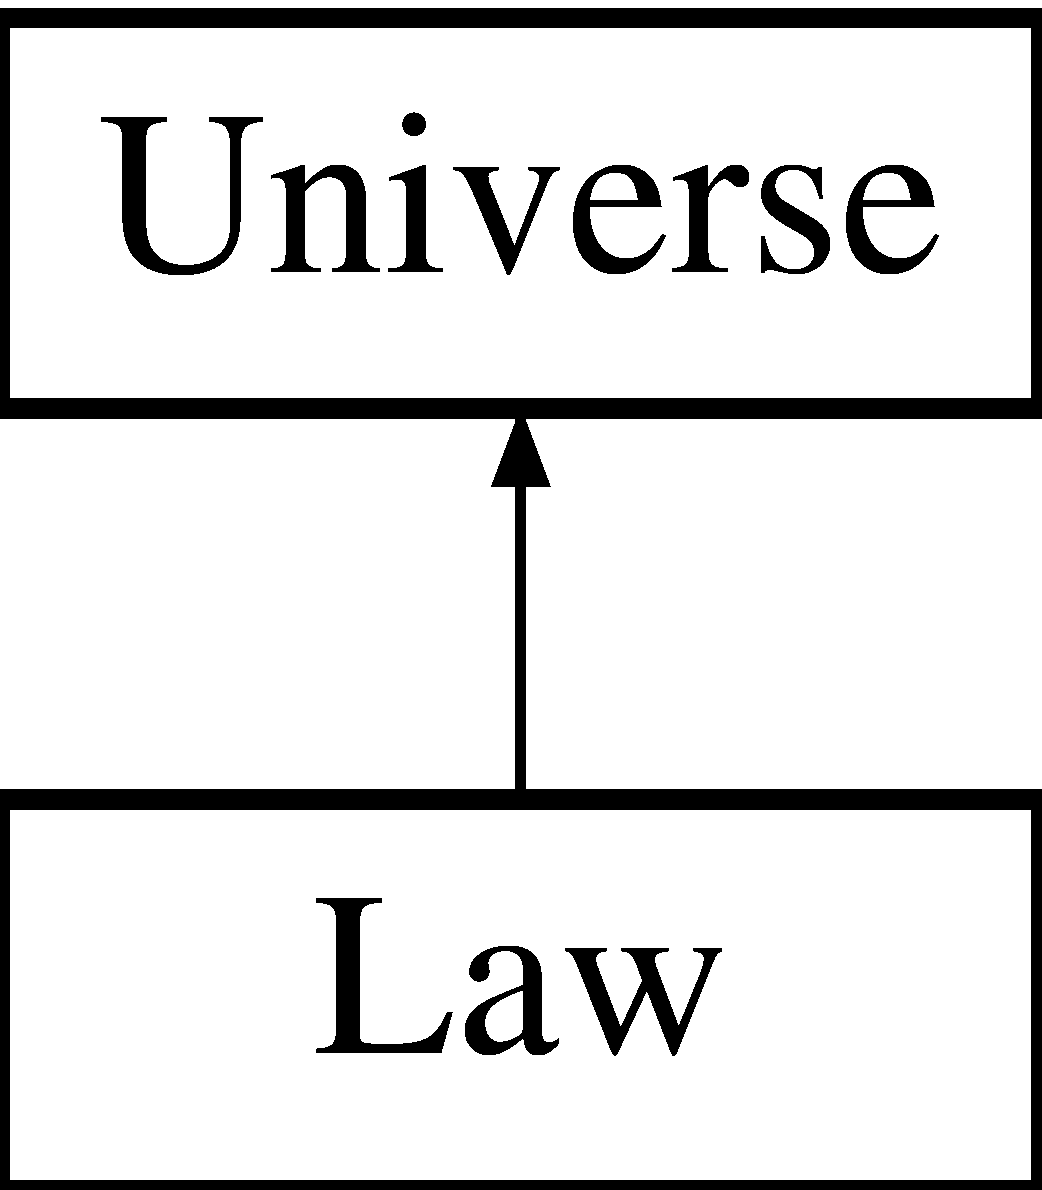
\includegraphics[height=2.000000cm]{classLaw}
\end{center}
\end{figure}
\subsection*{Public Member Functions}
\begin{DoxyCompactItemize}
\item 
\mbox{\hyperlink{classLaw_a3b94b6e9f09b8f457dba70f3b1c1ab43}{Law}} ()
\item 
\mbox{\hyperlink{classLaw_afd1730474b2806ec6665e16419f4994c}{Law}} (unsigned int object\+\_\+type)
\item 
\mbox{\hyperlink{classLaw_afdc75daa3a3346c473454c7a4dc2eab5}{Law}} (unsigned int object\+\_\+type, std\+::chrono\+::time\+\_\+point$<$ \mbox{\hyperlink{universe_8h_a0ef8d951d1ca5ab3cfaf7ab4c7a6fd80}{Clock}} $>$ event\+\_\+time)
\item 
\mbox{\hyperlink{classLaw_aa4fb7baf54aa77720605fd601fb80b8d}{Law}} (unsigned int object\+\_\+type, std\+::chrono\+::time\+\_\+point$<$ \mbox{\hyperlink{universe_8h_a0ef8d951d1ca5ab3cfaf7ab4c7a6fd80}{Clock}} $>$ event\+\_\+time, \mbox{\hyperlink{classUniverse}{Universe}} \&universe\+\_\+connector)
\item 
virtual \mbox{\hyperlink{classLaw_a4fa6f0fb61285152c8c6d7a17b51a82b}{$\sim$\+Law}} ()
\item 
bool \mbox{\hyperlink{classLaw_a56541ec0b82b8a7c377ae2e6b444205c}{Reset\+Parameters}} (std\+::chrono\+::time\+\_\+point$<$ \mbox{\hyperlink{universe_8h_a0ef8d951d1ca5ab3cfaf7ab4c7a6fd80}{Clock}} $>$ event\+\_\+time)
\item 
unsigned int \mbox{\hyperlink{classLaw_ab30a86ef88a85e13d3e598caa45bff05}{Get\+Counter}} (std\+::chrono\+::time\+\_\+point$<$ \mbox{\hyperlink{universe_8h_a0ef8d951d1ca5ab3cfaf7ab4c7a6fd80}{Clock}} $>$ event\+\_\+time)
\item 
void \mbox{\hyperlink{classLaw_a408c401c8a44870c29ba9d08b45cb40f}{Set\+Counter}} (std\+::chrono\+::time\+\_\+point$<$ \mbox{\hyperlink{universe_8h_a0ef8d951d1ca5ab3cfaf7ab4c7a6fd80}{Clock}} $>$ event\+\_\+time, unsigned int val)
\item 
int \mbox{\hyperlink{classLaw_a0240b10c679b671039dbf10771342ea7}{Update}} (std\+::chrono\+::time\+\_\+point$<$ \mbox{\hyperlink{universe_8h_a0ef8d951d1ca5ab3cfaf7ab4c7a6fd80}{Clock}} $>$ event\+\_\+time)
\item 
void \mbox{\hyperlink{classLaw_a2e780573f6285f88d167d45a2e243d01}{Set\+Charge}} (std\+::chrono\+::time\+\_\+point$<$ \mbox{\hyperlink{universe_8h_a0ef8d951d1ca5ab3cfaf7ab4c7a6fd80}{Clock}} $>$ event\+\_\+time, int val) final
\item 
void \mbox{\hyperlink{classLaw_a3de75edea5e20db0a7b731de61f07dea}{Set\+Spin}} (std\+::chrono\+::time\+\_\+point$<$ \mbox{\hyperlink{universe_8h_a0ef8d951d1ca5ab3cfaf7ab4c7a6fd80}{Clock}} $>$ event\+\_\+time, int val) final
\item 
double \mbox{\hyperlink{classLaw_a84bdc0c2ca97a9c19422018ff761b992}{Get\+Gravitation}} (std\+::chrono\+::time\+\_\+point$<$ \mbox{\hyperlink{universe_8h_a0ef8d951d1ca5ab3cfaf7ab4c7a6fd80}{Clock}} $>$ event\+\_\+time) final
\item 
double \mbox{\hyperlink{classLaw_a303c365b7a17997a63a74756fc72fba3}{Get\+Weak}} (std\+::chrono\+::time\+\_\+point$<$ \mbox{\hyperlink{universe_8h_a0ef8d951d1ca5ab3cfaf7ab4c7a6fd80}{Clock}} $>$ event\+\_\+time) final
\item 
double \mbox{\hyperlink{classLaw_aad6e54da64a5d8499dcb6c232aa6748f}{Get\+Weak\+Electroweak}} (std\+::chrono\+::time\+\_\+point$<$ \mbox{\hyperlink{universe_8h_a0ef8d951d1ca5ab3cfaf7ab4c7a6fd80}{Clock}} $>$ event\+\_\+time) final
\item 
double \mbox{\hyperlink{classLaw_a01eba6e68d2d8a717e2b4789be90853d}{Get\+Electromagnetic}} (std\+::chrono\+::time\+\_\+point$<$ \mbox{\hyperlink{universe_8h_a0ef8d951d1ca5ab3cfaf7ab4c7a6fd80}{Clock}} $>$ event\+\_\+time) final
\item 
double \mbox{\hyperlink{classLaw_ae4ccaca7b78905f416f35f9556b1923c}{Get\+Electromagnetic\+Electroweak}} (std\+::chrono\+::time\+\_\+point$<$ \mbox{\hyperlink{universe_8h_a0ef8d951d1ca5ab3cfaf7ab4c7a6fd80}{Clock}} $>$ event\+\_\+time) final
\item 
double \mbox{\hyperlink{classLaw_afd94bf09dbaf5d5df36b8f093db02dd9}{Get\+Strong}} (std\+::chrono\+::time\+\_\+point$<$ \mbox{\hyperlink{universe_8h_a0ef8d951d1ca5ab3cfaf7ab4c7a6fd80}{Clock}} $>$ event\+\_\+time) final
\item 
double \mbox{\hyperlink{classLaw_afcdbea76524e5a52691fff7b526971e9}{Get\+Strong\+Fundamental}} (std\+::chrono\+::time\+\_\+point$<$ \mbox{\hyperlink{universe_8h_a0ef8d951d1ca5ab3cfaf7ab4c7a6fd80}{Clock}} $>$ event\+\_\+time) final
\item 
double \mbox{\hyperlink{classLaw_a70fb2a7710776c4e2315a1e29fe35eb6}{Get\+Strong\+Residual}} (std\+::chrono\+::time\+\_\+point$<$ \mbox{\hyperlink{universe_8h_a0ef8d951d1ca5ab3cfaf7ab4c7a6fd80}{Clock}} $>$ event\+\_\+time) final
\item 
double \mbox{\hyperlink{classLaw_a04efdc724335219ab0affdcffb55eea2}{Apply\+Gravitation}} (std\+::chrono\+::time\+\_\+point$<$ \mbox{\hyperlink{universe_8h_a0ef8d951d1ca5ab3cfaf7ab4c7a6fd80}{Clock}} $>$ event\+\_\+time, double val) final
\item 
double \mbox{\hyperlink{classLaw_a96ddd42403e3665c6070283ac201658d}{Apply\+Weak}} (std\+::chrono\+::time\+\_\+point$<$ \mbox{\hyperlink{universe_8h_a0ef8d951d1ca5ab3cfaf7ab4c7a6fd80}{Clock}} $>$ event\+\_\+time, double val) final
\item 
double \mbox{\hyperlink{classLaw_ae8a5d1d09686d79f7814c8800791460b}{Apply\+Weak\+Electroweak}} (std\+::chrono\+::time\+\_\+point$<$ \mbox{\hyperlink{universe_8h_a0ef8d951d1ca5ab3cfaf7ab4c7a6fd80}{Clock}} $>$ event\+\_\+time, double val) final
\item 
double \mbox{\hyperlink{classLaw_a418791aee2a9204a99d3a917b86fafd3}{Apply\+Electromagnetic}} (std\+::chrono\+::time\+\_\+point$<$ \mbox{\hyperlink{universe_8h_a0ef8d951d1ca5ab3cfaf7ab4c7a6fd80}{Clock}} $>$ event\+\_\+time, double val) final
\item 
double \mbox{\hyperlink{classLaw_a4485046db890a95cea16573042a4f4f6}{Apply\+Electromagnetic\+Electroweak}} (std\+::chrono\+::time\+\_\+point$<$ \mbox{\hyperlink{universe_8h_a0ef8d951d1ca5ab3cfaf7ab4c7a6fd80}{Clock}} $>$ event\+\_\+time, double val) final
\item 
double \mbox{\hyperlink{classLaw_ab38659b209055df7e59f4bcd1b9e545a}{Apply\+Strong}} (std\+::chrono\+::time\+\_\+point$<$ \mbox{\hyperlink{universe_8h_a0ef8d951d1ca5ab3cfaf7ab4c7a6fd80}{Clock}} $>$ event\+\_\+time, double val) final
\item 
double \mbox{\hyperlink{classLaw_a57d05f26e1c0ee953260ebd3780248f8}{Apply\+Strong\+Fundamental}} (std\+::chrono\+::time\+\_\+point$<$ \mbox{\hyperlink{universe_8h_a0ef8d951d1ca5ab3cfaf7ab4c7a6fd80}{Clock}} $>$ event\+\_\+time, double val) final
\item 
double \mbox{\hyperlink{classLaw_a266f86cdcc01e813249a2f192ab85eb3}{Apply\+Strong\+Residual}} (std\+::chrono\+::time\+\_\+point$<$ \mbox{\hyperlink{universe_8h_a0ef8d951d1ca5ab3cfaf7ab4c7a6fd80}{Clock}} $>$ event\+\_\+time, double val) final
\item 
void \mbox{\hyperlink{classLaw_a908ccc2b0a561a7324a15393ec157219}{Set\+Gravitation}} (std\+::chrono\+::time\+\_\+point$<$ \mbox{\hyperlink{universe_8h_a0ef8d951d1ca5ab3cfaf7ab4c7a6fd80}{Clock}} $>$ event\+\_\+time, double val) final
\item 
void \mbox{\hyperlink{classLaw_a1009b4e0bc0b91f41d48dc137529e97b}{Set\+Weak}} (std\+::chrono\+::time\+\_\+point$<$ \mbox{\hyperlink{universe_8h_a0ef8d951d1ca5ab3cfaf7ab4c7a6fd80}{Clock}} $>$ event\+\_\+time, double val) final
\item 
void \mbox{\hyperlink{classLaw_a65e5e757041c1e72bb046eccbb6d66db}{Set\+Weak\+Electroweak}} (std\+::chrono\+::time\+\_\+point$<$ \mbox{\hyperlink{universe_8h_a0ef8d951d1ca5ab3cfaf7ab4c7a6fd80}{Clock}} $>$ event\+\_\+time, double val) final
\item 
void \mbox{\hyperlink{classLaw_acabe1a3113c207368f3bb6fe81e13963}{Set\+Electromagnetic}} (std\+::chrono\+::time\+\_\+point$<$ \mbox{\hyperlink{universe_8h_a0ef8d951d1ca5ab3cfaf7ab4c7a6fd80}{Clock}} $>$ event\+\_\+time, double val) final
\item 
void \mbox{\hyperlink{classLaw_aca9bb82839ddb46bd89f52b6211c5a54}{Set\+Electromagnetic\+Electroweak}} (std\+::chrono\+::time\+\_\+point$<$ \mbox{\hyperlink{universe_8h_a0ef8d951d1ca5ab3cfaf7ab4c7a6fd80}{Clock}} $>$ event\+\_\+time, double val) final
\item 
void \mbox{\hyperlink{classLaw_a4cd0dd1908edbd02090dd1ba1387d722}{Set\+Strong}} (std\+::chrono\+::time\+\_\+point$<$ \mbox{\hyperlink{universe_8h_a0ef8d951d1ca5ab3cfaf7ab4c7a6fd80}{Clock}} $>$ event\+\_\+time, double val) final
\item 
void \mbox{\hyperlink{classLaw_a4a7c8caa24acf453c1a8782a1ec4acf4}{Set\+Strong\+Fundamental}} (std\+::chrono\+::time\+\_\+point$<$ \mbox{\hyperlink{universe_8h_a0ef8d951d1ca5ab3cfaf7ab4c7a6fd80}{Clock}} $>$ event\+\_\+time, double val) final
\item 
void \mbox{\hyperlink{classLaw_ad4a05c77d11ddec40b1e07246cac449d}{Set\+Strong\+Residual}} (std\+::chrono\+::time\+\_\+point$<$ \mbox{\hyperlink{universe_8h_a0ef8d951d1ca5ab3cfaf7ab4c7a6fd80}{Clock}} $>$ event\+\_\+time, double val) final
\item 
void \mbox{\hyperlink{classLaw_af99520c95b2cd8af0af110b78b2288ef}{Poll\+Elementary\+Force}} (std\+::chrono\+::time\+\_\+point$<$ \mbox{\hyperlink{universe_8h_a0ef8d951d1ca5ab3cfaf7ab4c7a6fd80}{Clock}} $>$ event\+\_\+time) final
\end{DoxyCompactItemize}
\subsection*{Private Attributes}
\begin{DoxyCompactItemize}
\item 
unsigned int \mbox{\hyperlink{classLaw_a5d0e4fe1c614b9dac57f5f0135148cd6}{m\+\_\+\+Counter}}
\begin{DoxyCompactList}\small\item\em Member variable \char`\"{}m\+\_\+\+Counter\char`\"{}. \end{DoxyCompactList}\item 
int \mbox{\hyperlink{classLaw_a89176462e467ae7fa48c9b9cce6e55b2}{law\+\_\+type}}
\item 
std\+::chrono\+::time\+\_\+point$<$ \mbox{\hyperlink{universe_8h_a0ef8d951d1ca5ab3cfaf7ab4c7a6fd80}{Clock}} $>$ \mbox{\hyperlink{classLaw_a454bec5c547ef7482f1ec17259fb5af3}{time\+\_\+object\+\_\+created}}
\item 
std\+::chrono\+::time\+\_\+point$<$ \mbox{\hyperlink{universe_8h_a0ef8d951d1ca5ab3cfaf7ab4c7a6fd80}{Clock}} $>$ \mbox{\hyperlink{classLaw_a975eb41929cb9b4f216809889bfcb380}{previous\+\_\+event\+\_\+time}}
\item 
bool \mbox{\hyperlink{classLaw_ae0f326365accd025499b12cb0a9cb785}{object\+\_\+disabled}}
\item 
bool \mbox{\hyperlink{classLaw_abe7d645ce2c940fecdbbf7308ab9b2e8}{object\+\_\+initialised}}
\item 
int \mbox{\hyperlink{classLaw_a347aff85a02895946ff97718afdfeeff}{duration\+\_\+since\+\_\+last\+\_\+event}}
\end{DoxyCompactItemize}
\subsection*{Additional Inherited Members}


\subsection{Constructor \& Destructor Documentation}
\mbox{\Hypertarget{classLaw_a3b94b6e9f09b8f457dba70f3b1c1ab43}\label{classLaw_a3b94b6e9f09b8f457dba70f3b1c1ab43}} 
\index{Law@{Law}!Law@{Law}}
\index{Law@{Law}!Law@{Law}}
\subsubsection{\texorpdfstring{Law()}{Law()}\hspace{0.1cm}{\footnotesize\ttfamily [1/4]}}
{\footnotesize\ttfamily Law\+::\+Law (\begin{DoxyParamCaption}{ }\end{DoxyParamCaption})\hspace{0.3cm}{\ttfamily [inline]}}

\mbox{\Hypertarget{classLaw_afd1730474b2806ec6665e16419f4994c}\label{classLaw_afd1730474b2806ec6665e16419f4994c}} 
\index{Law@{Law}!Law@{Law}}
\index{Law@{Law}!Law@{Law}}
\subsubsection{\texorpdfstring{Law()}{Law()}\hspace{0.1cm}{\footnotesize\ttfamily [2/4]}}
{\footnotesize\ttfamily Law\+::\+Law (\begin{DoxyParamCaption}\item[{unsigned int}]{object\+\_\+type }\end{DoxyParamCaption})\hspace{0.3cm}{\ttfamily [inline]}}

\mbox{\Hypertarget{classLaw_afdc75daa3a3346c473454c7a4dc2eab5}\label{classLaw_afdc75daa3a3346c473454c7a4dc2eab5}} 
\index{Law@{Law}!Law@{Law}}
\index{Law@{Law}!Law@{Law}}
\subsubsection{\texorpdfstring{Law()}{Law()}\hspace{0.1cm}{\footnotesize\ttfamily [3/4]}}
{\footnotesize\ttfamily Law\+::\+Law (\begin{DoxyParamCaption}\item[{unsigned int}]{object\+\_\+type,  }\item[{std\+::chrono\+::time\+\_\+point$<$ \mbox{\hyperlink{universe_8h_a0ef8d951d1ca5ab3cfaf7ab4c7a6fd80}{Clock}} $>$}]{event\+\_\+time }\end{DoxyParamCaption})\hspace{0.3cm}{\ttfamily [inline]}}

\mbox{\Hypertarget{classLaw_aa4fb7baf54aa77720605fd601fb80b8d}\label{classLaw_aa4fb7baf54aa77720605fd601fb80b8d}} 
\index{Law@{Law}!Law@{Law}}
\index{Law@{Law}!Law@{Law}}
\subsubsection{\texorpdfstring{Law()}{Law()}\hspace{0.1cm}{\footnotesize\ttfamily [4/4]}}
{\footnotesize\ttfamily Law\+::\+Law (\begin{DoxyParamCaption}\item[{unsigned int}]{object\+\_\+type,  }\item[{std\+::chrono\+::time\+\_\+point$<$ \mbox{\hyperlink{universe_8h_a0ef8d951d1ca5ab3cfaf7ab4c7a6fd80}{Clock}} $>$}]{event\+\_\+time,  }\item[{\mbox{\hyperlink{classUniverse}{Universe}} \&}]{universe\+\_\+connector }\end{DoxyParamCaption})\hspace{0.3cm}{\ttfamily [inline]}}

\mbox{\Hypertarget{classLaw_a4fa6f0fb61285152c8c6d7a17b51a82b}\label{classLaw_a4fa6f0fb61285152c8c6d7a17b51a82b}} 
\index{Law@{Law}!````~Law@{$\sim$\+Law}}
\index{````~Law@{$\sim$\+Law}!Law@{Law}}
\subsubsection{\texorpdfstring{$\sim$\+Law()}{~Law()}}
{\footnotesize\ttfamily virtual Law\+::$\sim$\+Law (\begin{DoxyParamCaption}{ }\end{DoxyParamCaption})\hspace{0.3cm}{\ttfamily [inline]}, {\ttfamily [virtual]}}

Default destructor 

\subsection{Member Function Documentation}
\mbox{\Hypertarget{classLaw_a418791aee2a9204a99d3a917b86fafd3}\label{classLaw_a418791aee2a9204a99d3a917b86fafd3}} 
\index{Law@{Law}!Apply\+Electromagnetic@{Apply\+Electromagnetic}}
\index{Apply\+Electromagnetic@{Apply\+Electromagnetic}!Law@{Law}}
\subsubsection{\texorpdfstring{Apply\+Electromagnetic()}{ApplyElectromagnetic()}}
{\footnotesize\ttfamily double Law\+::\+Apply\+Electromagnetic (\begin{DoxyParamCaption}\item[{std\+::chrono\+::time\+\_\+point$<$ \mbox{\hyperlink{universe_8h_a0ef8d951d1ca5ab3cfaf7ab4c7a6fd80}{Clock}} $>$}]{event\+\_\+time,  }\item[{double}]{val }\end{DoxyParamCaption})\hspace{0.3cm}{\ttfamily [inline]}, {\ttfamily [final]}, {\ttfamily [virtual]}}



Reimplemented from \mbox{\hyperlink{classUniverse_a1f787da78fa196ba635db21a9e91dabb}{Universe}}.

\mbox{\Hypertarget{classLaw_a4485046db890a95cea16573042a4f4f6}\label{classLaw_a4485046db890a95cea16573042a4f4f6}} 
\index{Law@{Law}!Apply\+Electromagnetic\+Electroweak@{Apply\+Electromagnetic\+Electroweak}}
\index{Apply\+Electromagnetic\+Electroweak@{Apply\+Electromagnetic\+Electroweak}!Law@{Law}}
\subsubsection{\texorpdfstring{Apply\+Electromagnetic\+Electroweak()}{ApplyElectromagneticElectroweak()}}
{\footnotesize\ttfamily double Law\+::\+Apply\+Electromagnetic\+Electroweak (\begin{DoxyParamCaption}\item[{std\+::chrono\+::time\+\_\+point$<$ \mbox{\hyperlink{universe_8h_a0ef8d951d1ca5ab3cfaf7ab4c7a6fd80}{Clock}} $>$}]{event\+\_\+time,  }\item[{double}]{val }\end{DoxyParamCaption})\hspace{0.3cm}{\ttfamily [inline]}, {\ttfamily [final]}, {\ttfamily [virtual]}}



Reimplemented from \mbox{\hyperlink{classUniverse_a4c36c1ab30db993307f88363dde5e8c5}{Universe}}.

\mbox{\Hypertarget{classLaw_a04efdc724335219ab0affdcffb55eea2}\label{classLaw_a04efdc724335219ab0affdcffb55eea2}} 
\index{Law@{Law}!Apply\+Gravitation@{Apply\+Gravitation}}
\index{Apply\+Gravitation@{Apply\+Gravitation}!Law@{Law}}
\subsubsection{\texorpdfstring{Apply\+Gravitation()}{ApplyGravitation()}}
{\footnotesize\ttfamily double Law\+::\+Apply\+Gravitation (\begin{DoxyParamCaption}\item[{std\+::chrono\+::time\+\_\+point$<$ \mbox{\hyperlink{universe_8h_a0ef8d951d1ca5ab3cfaf7ab4c7a6fd80}{Clock}} $>$}]{event\+\_\+time,  }\item[{double}]{val }\end{DoxyParamCaption})\hspace{0.3cm}{\ttfamily [inline]}, {\ttfamily [final]}, {\ttfamily [virtual]}}



Reimplemented from \mbox{\hyperlink{classUniverse_a76c0b5e63c2a7d1988c44db341c3d64c}{Universe}}.

\mbox{\Hypertarget{classLaw_ab38659b209055df7e59f4bcd1b9e545a}\label{classLaw_ab38659b209055df7e59f4bcd1b9e545a}} 
\index{Law@{Law}!Apply\+Strong@{Apply\+Strong}}
\index{Apply\+Strong@{Apply\+Strong}!Law@{Law}}
\subsubsection{\texorpdfstring{Apply\+Strong()}{ApplyStrong()}}
{\footnotesize\ttfamily double Law\+::\+Apply\+Strong (\begin{DoxyParamCaption}\item[{std\+::chrono\+::time\+\_\+point$<$ \mbox{\hyperlink{universe_8h_a0ef8d951d1ca5ab3cfaf7ab4c7a6fd80}{Clock}} $>$}]{event\+\_\+time,  }\item[{double}]{val }\end{DoxyParamCaption})\hspace{0.3cm}{\ttfamily [inline]}, {\ttfamily [final]}, {\ttfamily [virtual]}}



Reimplemented from \mbox{\hyperlink{classUniverse_a906a88b37f10bfa630bef49dfd0e907a}{Universe}}.

\mbox{\Hypertarget{classLaw_a57d05f26e1c0ee953260ebd3780248f8}\label{classLaw_a57d05f26e1c0ee953260ebd3780248f8}} 
\index{Law@{Law}!Apply\+Strong\+Fundamental@{Apply\+Strong\+Fundamental}}
\index{Apply\+Strong\+Fundamental@{Apply\+Strong\+Fundamental}!Law@{Law}}
\subsubsection{\texorpdfstring{Apply\+Strong\+Fundamental()}{ApplyStrongFundamental()}}
{\footnotesize\ttfamily double Law\+::\+Apply\+Strong\+Fundamental (\begin{DoxyParamCaption}\item[{std\+::chrono\+::time\+\_\+point$<$ \mbox{\hyperlink{universe_8h_a0ef8d951d1ca5ab3cfaf7ab4c7a6fd80}{Clock}} $>$}]{event\+\_\+time,  }\item[{double}]{val }\end{DoxyParamCaption})\hspace{0.3cm}{\ttfamily [inline]}, {\ttfamily [final]}, {\ttfamily [virtual]}}



Reimplemented from \mbox{\hyperlink{classUniverse_a62789bcff84bd750b0366004381e2fdd}{Universe}}.

\mbox{\Hypertarget{classLaw_a266f86cdcc01e813249a2f192ab85eb3}\label{classLaw_a266f86cdcc01e813249a2f192ab85eb3}} 
\index{Law@{Law}!Apply\+Strong\+Residual@{Apply\+Strong\+Residual}}
\index{Apply\+Strong\+Residual@{Apply\+Strong\+Residual}!Law@{Law}}
\subsubsection{\texorpdfstring{Apply\+Strong\+Residual()}{ApplyStrongResidual()}}
{\footnotesize\ttfamily double Law\+::\+Apply\+Strong\+Residual (\begin{DoxyParamCaption}\item[{std\+::chrono\+::time\+\_\+point$<$ \mbox{\hyperlink{universe_8h_a0ef8d951d1ca5ab3cfaf7ab4c7a6fd80}{Clock}} $>$}]{event\+\_\+time,  }\item[{double}]{val }\end{DoxyParamCaption})\hspace{0.3cm}{\ttfamily [inline]}, {\ttfamily [final]}, {\ttfamily [virtual]}}



Reimplemented from \mbox{\hyperlink{classUniverse_af7becebb347be9a85541d96a3eca1ca7}{Universe}}.

\mbox{\Hypertarget{classLaw_a96ddd42403e3665c6070283ac201658d}\label{classLaw_a96ddd42403e3665c6070283ac201658d}} 
\index{Law@{Law}!Apply\+Weak@{Apply\+Weak}}
\index{Apply\+Weak@{Apply\+Weak}!Law@{Law}}
\subsubsection{\texorpdfstring{Apply\+Weak()}{ApplyWeak()}}
{\footnotesize\ttfamily double Law\+::\+Apply\+Weak (\begin{DoxyParamCaption}\item[{std\+::chrono\+::time\+\_\+point$<$ \mbox{\hyperlink{universe_8h_a0ef8d951d1ca5ab3cfaf7ab4c7a6fd80}{Clock}} $>$}]{event\+\_\+time,  }\item[{double}]{val }\end{DoxyParamCaption})\hspace{0.3cm}{\ttfamily [inline]}, {\ttfamily [final]}, {\ttfamily [virtual]}}



Reimplemented from \mbox{\hyperlink{classUniverse_a6d1226b3adec3c42a833afdbb6a65a92}{Universe}}.

\mbox{\Hypertarget{classLaw_ae8a5d1d09686d79f7814c8800791460b}\label{classLaw_ae8a5d1d09686d79f7814c8800791460b}} 
\index{Law@{Law}!Apply\+Weak\+Electroweak@{Apply\+Weak\+Electroweak}}
\index{Apply\+Weak\+Electroweak@{Apply\+Weak\+Electroweak}!Law@{Law}}
\subsubsection{\texorpdfstring{Apply\+Weak\+Electroweak()}{ApplyWeakElectroweak()}}
{\footnotesize\ttfamily double Law\+::\+Apply\+Weak\+Electroweak (\begin{DoxyParamCaption}\item[{std\+::chrono\+::time\+\_\+point$<$ \mbox{\hyperlink{universe_8h_a0ef8d951d1ca5ab3cfaf7ab4c7a6fd80}{Clock}} $>$}]{event\+\_\+time,  }\item[{double}]{val }\end{DoxyParamCaption})\hspace{0.3cm}{\ttfamily [inline]}, {\ttfamily [final]}, {\ttfamily [virtual]}}



Reimplemented from \mbox{\hyperlink{classUniverse_a46a906baabb63e5d31f8b48ea1fae52e}{Universe}}.

\mbox{\Hypertarget{classLaw_ab30a86ef88a85e13d3e598caa45bff05}\label{classLaw_ab30a86ef88a85e13d3e598caa45bff05}} 
\index{Law@{Law}!Get\+Counter@{Get\+Counter}}
\index{Get\+Counter@{Get\+Counter}!Law@{Law}}
\subsubsection{\texorpdfstring{Get\+Counter()}{GetCounter()}}
{\footnotesize\ttfamily unsigned int Law\+::\+Get\+Counter (\begin{DoxyParamCaption}\item[{std\+::chrono\+::time\+\_\+point$<$ \mbox{\hyperlink{universe_8h_a0ef8d951d1ca5ab3cfaf7ab4c7a6fd80}{Clock}} $>$}]{event\+\_\+time }\end{DoxyParamCaption})}

\mbox{\Hypertarget{classLaw_a01eba6e68d2d8a717e2b4789be90853d}\label{classLaw_a01eba6e68d2d8a717e2b4789be90853d}} 
\index{Law@{Law}!Get\+Electromagnetic@{Get\+Electromagnetic}}
\index{Get\+Electromagnetic@{Get\+Electromagnetic}!Law@{Law}}
\subsubsection{\texorpdfstring{Get\+Electromagnetic()}{GetElectromagnetic()}}
{\footnotesize\ttfamily double Law\+::\+Get\+Electromagnetic (\begin{DoxyParamCaption}\item[{std\+::chrono\+::time\+\_\+point$<$ \mbox{\hyperlink{universe_8h_a0ef8d951d1ca5ab3cfaf7ab4c7a6fd80}{Clock}} $>$}]{event\+\_\+time }\end{DoxyParamCaption})\hspace{0.3cm}{\ttfamily [inline]}, {\ttfamily [final]}, {\ttfamily [virtual]}}



Reimplemented from \mbox{\hyperlink{classUniverse_a63b850ef3f3394313353109d222bf5d1}{Universe}}.

\mbox{\Hypertarget{classLaw_ae4ccaca7b78905f416f35f9556b1923c}\label{classLaw_ae4ccaca7b78905f416f35f9556b1923c}} 
\index{Law@{Law}!Get\+Electromagnetic\+Electroweak@{Get\+Electromagnetic\+Electroweak}}
\index{Get\+Electromagnetic\+Electroweak@{Get\+Electromagnetic\+Electroweak}!Law@{Law}}
\subsubsection{\texorpdfstring{Get\+Electromagnetic\+Electroweak()}{GetElectromagneticElectroweak()}}
{\footnotesize\ttfamily double Law\+::\+Get\+Electromagnetic\+Electroweak (\begin{DoxyParamCaption}\item[{std\+::chrono\+::time\+\_\+point$<$ \mbox{\hyperlink{universe_8h_a0ef8d951d1ca5ab3cfaf7ab4c7a6fd80}{Clock}} $>$}]{event\+\_\+time }\end{DoxyParamCaption})\hspace{0.3cm}{\ttfamily [inline]}, {\ttfamily [final]}, {\ttfamily [virtual]}}



Reimplemented from \mbox{\hyperlink{classUniverse_a9f099605c082e7fa755787a6a8cab7ba}{Universe}}.

\mbox{\Hypertarget{classLaw_a84bdc0c2ca97a9c19422018ff761b992}\label{classLaw_a84bdc0c2ca97a9c19422018ff761b992}} 
\index{Law@{Law}!Get\+Gravitation@{Get\+Gravitation}}
\index{Get\+Gravitation@{Get\+Gravitation}!Law@{Law}}
\subsubsection{\texorpdfstring{Get\+Gravitation()}{GetGravitation()}}
{\footnotesize\ttfamily double Law\+::\+Get\+Gravitation (\begin{DoxyParamCaption}\item[{std\+::chrono\+::time\+\_\+point$<$ \mbox{\hyperlink{universe_8h_a0ef8d951d1ca5ab3cfaf7ab4c7a6fd80}{Clock}} $>$}]{event\+\_\+time }\end{DoxyParamCaption})\hspace{0.3cm}{\ttfamily [inline]}, {\ttfamily [final]}, {\ttfamily [virtual]}}



Reimplemented from \mbox{\hyperlink{classUniverse_ab0404e774ee0ed66b597ff5b8e989446}{Universe}}.

\mbox{\Hypertarget{classLaw_afd94bf09dbaf5d5df36b8f093db02dd9}\label{classLaw_afd94bf09dbaf5d5df36b8f093db02dd9}} 
\index{Law@{Law}!Get\+Strong@{Get\+Strong}}
\index{Get\+Strong@{Get\+Strong}!Law@{Law}}
\subsubsection{\texorpdfstring{Get\+Strong()}{GetStrong()}}
{\footnotesize\ttfamily double Law\+::\+Get\+Strong (\begin{DoxyParamCaption}\item[{std\+::chrono\+::time\+\_\+point$<$ \mbox{\hyperlink{universe_8h_a0ef8d951d1ca5ab3cfaf7ab4c7a6fd80}{Clock}} $>$}]{event\+\_\+time }\end{DoxyParamCaption})\hspace{0.3cm}{\ttfamily [inline]}, {\ttfamily [final]}, {\ttfamily [virtual]}}



Reimplemented from \mbox{\hyperlink{classUniverse_acb453ce71da418c5b5617fecede9571b}{Universe}}.

\mbox{\Hypertarget{classLaw_afcdbea76524e5a52691fff7b526971e9}\label{classLaw_afcdbea76524e5a52691fff7b526971e9}} 
\index{Law@{Law}!Get\+Strong\+Fundamental@{Get\+Strong\+Fundamental}}
\index{Get\+Strong\+Fundamental@{Get\+Strong\+Fundamental}!Law@{Law}}
\subsubsection{\texorpdfstring{Get\+Strong\+Fundamental()}{GetStrongFundamental()}}
{\footnotesize\ttfamily double Law\+::\+Get\+Strong\+Fundamental (\begin{DoxyParamCaption}\item[{std\+::chrono\+::time\+\_\+point$<$ \mbox{\hyperlink{universe_8h_a0ef8d951d1ca5ab3cfaf7ab4c7a6fd80}{Clock}} $>$}]{event\+\_\+time }\end{DoxyParamCaption})\hspace{0.3cm}{\ttfamily [inline]}, {\ttfamily [final]}, {\ttfamily [virtual]}}



Reimplemented from \mbox{\hyperlink{classUniverse_ab44daccba01ee7e3cf9b50bba83dd19e}{Universe}}.

\mbox{\Hypertarget{classLaw_a70fb2a7710776c4e2315a1e29fe35eb6}\label{classLaw_a70fb2a7710776c4e2315a1e29fe35eb6}} 
\index{Law@{Law}!Get\+Strong\+Residual@{Get\+Strong\+Residual}}
\index{Get\+Strong\+Residual@{Get\+Strong\+Residual}!Law@{Law}}
\subsubsection{\texorpdfstring{Get\+Strong\+Residual()}{GetStrongResidual()}}
{\footnotesize\ttfamily double Law\+::\+Get\+Strong\+Residual (\begin{DoxyParamCaption}\item[{std\+::chrono\+::time\+\_\+point$<$ \mbox{\hyperlink{universe_8h_a0ef8d951d1ca5ab3cfaf7ab4c7a6fd80}{Clock}} $>$}]{event\+\_\+time }\end{DoxyParamCaption})\hspace{0.3cm}{\ttfamily [inline]}, {\ttfamily [final]}, {\ttfamily [virtual]}}



Reimplemented from \mbox{\hyperlink{classUniverse_af0f4b81950061e63c2855eb40957a5b1}{Universe}}.

\mbox{\Hypertarget{classLaw_a303c365b7a17997a63a74756fc72fba3}\label{classLaw_a303c365b7a17997a63a74756fc72fba3}} 
\index{Law@{Law}!Get\+Weak@{Get\+Weak}}
\index{Get\+Weak@{Get\+Weak}!Law@{Law}}
\subsubsection{\texorpdfstring{Get\+Weak()}{GetWeak()}}
{\footnotesize\ttfamily double Law\+::\+Get\+Weak (\begin{DoxyParamCaption}\item[{std\+::chrono\+::time\+\_\+point$<$ \mbox{\hyperlink{universe_8h_a0ef8d951d1ca5ab3cfaf7ab4c7a6fd80}{Clock}} $>$}]{event\+\_\+time }\end{DoxyParamCaption})\hspace{0.3cm}{\ttfamily [inline]}, {\ttfamily [final]}, {\ttfamily [virtual]}}



Reimplemented from \mbox{\hyperlink{classUniverse_a4476b7e0a3fc1764909f556257fd9ec7}{Universe}}.

\mbox{\Hypertarget{classLaw_aad6e54da64a5d8499dcb6c232aa6748f}\label{classLaw_aad6e54da64a5d8499dcb6c232aa6748f}} 
\index{Law@{Law}!Get\+Weak\+Electroweak@{Get\+Weak\+Electroweak}}
\index{Get\+Weak\+Electroweak@{Get\+Weak\+Electroweak}!Law@{Law}}
\subsubsection{\texorpdfstring{Get\+Weak\+Electroweak()}{GetWeakElectroweak()}}
{\footnotesize\ttfamily double Law\+::\+Get\+Weak\+Electroweak (\begin{DoxyParamCaption}\item[{std\+::chrono\+::time\+\_\+point$<$ \mbox{\hyperlink{universe_8h_a0ef8d951d1ca5ab3cfaf7ab4c7a6fd80}{Clock}} $>$}]{event\+\_\+time }\end{DoxyParamCaption})\hspace{0.3cm}{\ttfamily [inline]}, {\ttfamily [final]}, {\ttfamily [virtual]}}



Reimplemented from \mbox{\hyperlink{classUniverse_a645299738e6b798a037f2a15a2e7cf4d}{Universe}}.

\mbox{\Hypertarget{classLaw_af99520c95b2cd8af0af110b78b2288ef}\label{classLaw_af99520c95b2cd8af0af110b78b2288ef}} 
\index{Law@{Law}!Poll\+Elementary\+Force@{Poll\+Elementary\+Force}}
\index{Poll\+Elementary\+Force@{Poll\+Elementary\+Force}!Law@{Law}}
\subsubsection{\texorpdfstring{Poll\+Elementary\+Force()}{PollElementaryForce()}}
{\footnotesize\ttfamily void Law\+::\+Poll\+Elementary\+Force (\begin{DoxyParamCaption}\item[{std\+::chrono\+::time\+\_\+point$<$ \mbox{\hyperlink{universe_8h_a0ef8d951d1ca5ab3cfaf7ab4c7a6fd80}{Clock}} $>$}]{event\+\_\+time }\end{DoxyParamCaption})\hspace{0.3cm}{\ttfamily [inline]}, {\ttfamily [final]}, {\ttfamily [virtual]}}



Reimplemented from \mbox{\hyperlink{classUniverse_a0c485c504542409cbb5cfd8543c35b11}{Universe}}.

\mbox{\Hypertarget{classLaw_a56541ec0b82b8a7c377ae2e6b444205c}\label{classLaw_a56541ec0b82b8a7c377ae2e6b444205c}} 
\index{Law@{Law}!Reset\+Parameters@{Reset\+Parameters}}
\index{Reset\+Parameters@{Reset\+Parameters}!Law@{Law}}
\subsubsection{\texorpdfstring{Reset\+Parameters()}{ResetParameters()}}
{\footnotesize\ttfamily bool Law\+::\+Reset\+Parameters (\begin{DoxyParamCaption}\item[{std\+::chrono\+::time\+\_\+point$<$ \mbox{\hyperlink{universe_8h_a0ef8d951d1ca5ab3cfaf7ab4c7a6fd80}{Clock}} $>$}]{event\+\_\+time }\end{DoxyParamCaption})}

\mbox{\Hypertarget{classLaw_a2e780573f6285f88d167d45a2e243d01}\label{classLaw_a2e780573f6285f88d167d45a2e243d01}} 
\index{Law@{Law}!Set\+Charge@{Set\+Charge}}
\index{Set\+Charge@{Set\+Charge}!Law@{Law}}
\subsubsection{\texorpdfstring{Set\+Charge()}{SetCharge()}}
{\footnotesize\ttfamily void Law\+::\+Set\+Charge (\begin{DoxyParamCaption}\item[{std\+::chrono\+::time\+\_\+point$<$ \mbox{\hyperlink{universe_8h_a0ef8d951d1ca5ab3cfaf7ab4c7a6fd80}{Clock}} $>$}]{event\+\_\+time,  }\item[{int}]{val }\end{DoxyParamCaption})\hspace{0.3cm}{\ttfamily [inline]}, {\ttfamily [final]}, {\ttfamily [virtual]}}



Reimplemented from \mbox{\hyperlink{classUniverse_a3b3da7c86a7b75e5e5c0b7972ac82a87}{Universe}}.

\mbox{\Hypertarget{classLaw_a408c401c8a44870c29ba9d08b45cb40f}\label{classLaw_a408c401c8a44870c29ba9d08b45cb40f}} 
\index{Law@{Law}!Set\+Counter@{Set\+Counter}}
\index{Set\+Counter@{Set\+Counter}!Law@{Law}}
\subsubsection{\texorpdfstring{Set\+Counter()}{SetCounter()}}
{\footnotesize\ttfamily void Law\+::\+Set\+Counter (\begin{DoxyParamCaption}\item[{std\+::chrono\+::time\+\_\+point$<$ \mbox{\hyperlink{universe_8h_a0ef8d951d1ca5ab3cfaf7ab4c7a6fd80}{Clock}} $>$}]{event\+\_\+time,  }\item[{unsigned int}]{val }\end{DoxyParamCaption})\hspace{0.3cm}{\ttfamily [virtual]}}



Reimplemented from \mbox{\hyperlink{classUniverse_aa22202ae740eb1355529afcb13285e91}{Universe}}.

\mbox{\Hypertarget{classLaw_acabe1a3113c207368f3bb6fe81e13963}\label{classLaw_acabe1a3113c207368f3bb6fe81e13963}} 
\index{Law@{Law}!Set\+Electromagnetic@{Set\+Electromagnetic}}
\index{Set\+Electromagnetic@{Set\+Electromagnetic}!Law@{Law}}
\subsubsection{\texorpdfstring{Set\+Electromagnetic()}{SetElectromagnetic()}}
{\footnotesize\ttfamily void Law\+::\+Set\+Electromagnetic (\begin{DoxyParamCaption}\item[{std\+::chrono\+::time\+\_\+point$<$ \mbox{\hyperlink{universe_8h_a0ef8d951d1ca5ab3cfaf7ab4c7a6fd80}{Clock}} $>$}]{event\+\_\+time,  }\item[{double}]{val }\end{DoxyParamCaption})\hspace{0.3cm}{\ttfamily [inline]}, {\ttfamily [final]}, {\ttfamily [virtual]}}



Reimplemented from \mbox{\hyperlink{classUniverse_aa981fc7e252b1fbbb675f0371860954d}{Universe}}.

\mbox{\Hypertarget{classLaw_aca9bb82839ddb46bd89f52b6211c5a54}\label{classLaw_aca9bb82839ddb46bd89f52b6211c5a54}} 
\index{Law@{Law}!Set\+Electromagnetic\+Electroweak@{Set\+Electromagnetic\+Electroweak}}
\index{Set\+Electromagnetic\+Electroweak@{Set\+Electromagnetic\+Electroweak}!Law@{Law}}
\subsubsection{\texorpdfstring{Set\+Electromagnetic\+Electroweak()}{SetElectromagneticElectroweak()}}
{\footnotesize\ttfamily void Law\+::\+Set\+Electromagnetic\+Electroweak (\begin{DoxyParamCaption}\item[{std\+::chrono\+::time\+\_\+point$<$ \mbox{\hyperlink{universe_8h_a0ef8d951d1ca5ab3cfaf7ab4c7a6fd80}{Clock}} $>$}]{event\+\_\+time,  }\item[{double}]{val }\end{DoxyParamCaption})\hspace{0.3cm}{\ttfamily [inline]}, {\ttfamily [final]}, {\ttfamily [virtual]}}



Reimplemented from \mbox{\hyperlink{classUniverse_a608aa95698380f791a0ffba45cc1bee3}{Universe}}.

\mbox{\Hypertarget{classLaw_a908ccc2b0a561a7324a15393ec157219}\label{classLaw_a908ccc2b0a561a7324a15393ec157219}} 
\index{Law@{Law}!Set\+Gravitation@{Set\+Gravitation}}
\index{Set\+Gravitation@{Set\+Gravitation}!Law@{Law}}
\subsubsection{\texorpdfstring{Set\+Gravitation()}{SetGravitation()}}
{\footnotesize\ttfamily void Law\+::\+Set\+Gravitation (\begin{DoxyParamCaption}\item[{std\+::chrono\+::time\+\_\+point$<$ \mbox{\hyperlink{universe_8h_a0ef8d951d1ca5ab3cfaf7ab4c7a6fd80}{Clock}} $>$}]{event\+\_\+time,  }\item[{double}]{val }\end{DoxyParamCaption})\hspace{0.3cm}{\ttfamily [inline]}, {\ttfamily [final]}, {\ttfamily [virtual]}}



Reimplemented from \mbox{\hyperlink{classUniverse_ae0cb8d86b2fbb8396d605160344b42f5}{Universe}}.

\mbox{\Hypertarget{classLaw_a3de75edea5e20db0a7b731de61f07dea}\label{classLaw_a3de75edea5e20db0a7b731de61f07dea}} 
\index{Law@{Law}!Set\+Spin@{Set\+Spin}}
\index{Set\+Spin@{Set\+Spin}!Law@{Law}}
\subsubsection{\texorpdfstring{Set\+Spin()}{SetSpin()}}
{\footnotesize\ttfamily void Law\+::\+Set\+Spin (\begin{DoxyParamCaption}\item[{std\+::chrono\+::time\+\_\+point$<$ \mbox{\hyperlink{universe_8h_a0ef8d951d1ca5ab3cfaf7ab4c7a6fd80}{Clock}} $>$}]{event\+\_\+time,  }\item[{int}]{val }\end{DoxyParamCaption})\hspace{0.3cm}{\ttfamily [inline]}, {\ttfamily [final]}, {\ttfamily [virtual]}}



Reimplemented from \mbox{\hyperlink{classUniverse_ae2ae1c3b3e4cde2c18f5f6a814761ec8}{Universe}}.

\mbox{\Hypertarget{classLaw_a4cd0dd1908edbd02090dd1ba1387d722}\label{classLaw_a4cd0dd1908edbd02090dd1ba1387d722}} 
\index{Law@{Law}!Set\+Strong@{Set\+Strong}}
\index{Set\+Strong@{Set\+Strong}!Law@{Law}}
\subsubsection{\texorpdfstring{Set\+Strong()}{SetStrong()}}
{\footnotesize\ttfamily void Law\+::\+Set\+Strong (\begin{DoxyParamCaption}\item[{std\+::chrono\+::time\+\_\+point$<$ \mbox{\hyperlink{universe_8h_a0ef8d951d1ca5ab3cfaf7ab4c7a6fd80}{Clock}} $>$}]{event\+\_\+time,  }\item[{double}]{val }\end{DoxyParamCaption})\hspace{0.3cm}{\ttfamily [inline]}, {\ttfamily [final]}, {\ttfamily [virtual]}}



Reimplemented from \mbox{\hyperlink{classUniverse_a5946c8f3d4cda305f3ecd10df21a2f94}{Universe}}.

\mbox{\Hypertarget{classLaw_a4a7c8caa24acf453c1a8782a1ec4acf4}\label{classLaw_a4a7c8caa24acf453c1a8782a1ec4acf4}} 
\index{Law@{Law}!Set\+Strong\+Fundamental@{Set\+Strong\+Fundamental}}
\index{Set\+Strong\+Fundamental@{Set\+Strong\+Fundamental}!Law@{Law}}
\subsubsection{\texorpdfstring{Set\+Strong\+Fundamental()}{SetStrongFundamental()}}
{\footnotesize\ttfamily void Law\+::\+Set\+Strong\+Fundamental (\begin{DoxyParamCaption}\item[{std\+::chrono\+::time\+\_\+point$<$ \mbox{\hyperlink{universe_8h_a0ef8d951d1ca5ab3cfaf7ab4c7a6fd80}{Clock}} $>$}]{event\+\_\+time,  }\item[{double}]{val }\end{DoxyParamCaption})\hspace{0.3cm}{\ttfamily [inline]}, {\ttfamily [final]}, {\ttfamily [virtual]}}



Reimplemented from \mbox{\hyperlink{classUniverse_aafec97a231126b71c73ac1258609a284}{Universe}}.

\mbox{\Hypertarget{classLaw_ad4a05c77d11ddec40b1e07246cac449d}\label{classLaw_ad4a05c77d11ddec40b1e07246cac449d}} 
\index{Law@{Law}!Set\+Strong\+Residual@{Set\+Strong\+Residual}}
\index{Set\+Strong\+Residual@{Set\+Strong\+Residual}!Law@{Law}}
\subsubsection{\texorpdfstring{Set\+Strong\+Residual()}{SetStrongResidual()}}
{\footnotesize\ttfamily void Law\+::\+Set\+Strong\+Residual (\begin{DoxyParamCaption}\item[{std\+::chrono\+::time\+\_\+point$<$ \mbox{\hyperlink{universe_8h_a0ef8d951d1ca5ab3cfaf7ab4c7a6fd80}{Clock}} $>$}]{event\+\_\+time,  }\item[{double}]{val }\end{DoxyParamCaption})\hspace{0.3cm}{\ttfamily [inline]}, {\ttfamily [final]}, {\ttfamily [virtual]}}



Reimplemented from \mbox{\hyperlink{classUniverse_a1b2d6197ddf3d613cc30bd04d22ed8b7}{Universe}}.

\mbox{\Hypertarget{classLaw_a1009b4e0bc0b91f41d48dc137529e97b}\label{classLaw_a1009b4e0bc0b91f41d48dc137529e97b}} 
\index{Law@{Law}!Set\+Weak@{Set\+Weak}}
\index{Set\+Weak@{Set\+Weak}!Law@{Law}}
\subsubsection{\texorpdfstring{Set\+Weak()}{SetWeak()}}
{\footnotesize\ttfamily void Law\+::\+Set\+Weak (\begin{DoxyParamCaption}\item[{std\+::chrono\+::time\+\_\+point$<$ \mbox{\hyperlink{universe_8h_a0ef8d951d1ca5ab3cfaf7ab4c7a6fd80}{Clock}} $>$}]{event\+\_\+time,  }\item[{double}]{val }\end{DoxyParamCaption})\hspace{0.3cm}{\ttfamily [inline]}, {\ttfamily [final]}, {\ttfamily [virtual]}}



Reimplemented from \mbox{\hyperlink{classUniverse_a0f5cd04081b41ee931c0557dc397f6fb}{Universe}}.

\mbox{\Hypertarget{classLaw_a65e5e757041c1e72bb046eccbb6d66db}\label{classLaw_a65e5e757041c1e72bb046eccbb6d66db}} 
\index{Law@{Law}!Set\+Weak\+Electroweak@{Set\+Weak\+Electroweak}}
\index{Set\+Weak\+Electroweak@{Set\+Weak\+Electroweak}!Law@{Law}}
\subsubsection{\texorpdfstring{Set\+Weak\+Electroweak()}{SetWeakElectroweak()}}
{\footnotesize\ttfamily void Law\+::\+Set\+Weak\+Electroweak (\begin{DoxyParamCaption}\item[{std\+::chrono\+::time\+\_\+point$<$ \mbox{\hyperlink{universe_8h_a0ef8d951d1ca5ab3cfaf7ab4c7a6fd80}{Clock}} $>$}]{event\+\_\+time,  }\item[{double}]{val }\end{DoxyParamCaption})\hspace{0.3cm}{\ttfamily [inline]}, {\ttfamily [final]}, {\ttfamily [virtual]}}



Reimplemented from \mbox{\hyperlink{classUniverse_a2d3d642bfdc863248e93535832fa4b00}{Universe}}.

\mbox{\Hypertarget{classLaw_a0240b10c679b671039dbf10771342ea7}\label{classLaw_a0240b10c679b671039dbf10771342ea7}} 
\index{Law@{Law}!Update@{Update}}
\index{Update@{Update}!Law@{Law}}
\subsubsection{\texorpdfstring{Update()}{Update()}}
{\footnotesize\ttfamily int Law\+::\+Update (\begin{DoxyParamCaption}\item[{std\+::chrono\+::time\+\_\+point$<$ \mbox{\hyperlink{universe_8h_a0ef8d951d1ca5ab3cfaf7ab4c7a6fd80}{Clock}} $>$}]{event\+\_\+time }\end{DoxyParamCaption})}



\subsection{Member Data Documentation}
\mbox{\Hypertarget{classLaw_a347aff85a02895946ff97718afdfeeff}\label{classLaw_a347aff85a02895946ff97718afdfeeff}} 
\index{Law@{Law}!duration\+\_\+since\+\_\+last\+\_\+event@{duration\+\_\+since\+\_\+last\+\_\+event}}
\index{duration\+\_\+since\+\_\+last\+\_\+event@{duration\+\_\+since\+\_\+last\+\_\+event}!Law@{Law}}
\subsubsection{\texorpdfstring{duration\+\_\+since\+\_\+last\+\_\+event}{duration\_since\_last\_event}}
{\footnotesize\ttfamily int Law\+::duration\+\_\+since\+\_\+last\+\_\+event\hspace{0.3cm}{\ttfamily [private]}}

\mbox{\Hypertarget{classLaw_a89176462e467ae7fa48c9b9cce6e55b2}\label{classLaw_a89176462e467ae7fa48c9b9cce6e55b2}} 
\index{Law@{Law}!law\+\_\+type@{law\+\_\+type}}
\index{law\+\_\+type@{law\+\_\+type}!Law@{Law}}
\subsubsection{\texorpdfstring{law\+\_\+type}{law\_type}}
{\footnotesize\ttfamily int Law\+::law\+\_\+type\hspace{0.3cm}{\ttfamily [private]}}

\mbox{\Hypertarget{classLaw_a5d0e4fe1c614b9dac57f5f0135148cd6}\label{classLaw_a5d0e4fe1c614b9dac57f5f0135148cd6}} 
\index{Law@{Law}!m\+\_\+\+Counter@{m\+\_\+\+Counter}}
\index{m\+\_\+\+Counter@{m\+\_\+\+Counter}!Law@{Law}}
\subsubsection{\texorpdfstring{m\+\_\+\+Counter}{m\_Counter}}
{\footnotesize\ttfamily unsigned int Law\+::m\+\_\+\+Counter\hspace{0.3cm}{\ttfamily [private]}}



Member variable \char`\"{}m\+\_\+\+Counter\char`\"{}. 

\mbox{\Hypertarget{classLaw_ae0f326365accd025499b12cb0a9cb785}\label{classLaw_ae0f326365accd025499b12cb0a9cb785}} 
\index{Law@{Law}!object\+\_\+disabled@{object\+\_\+disabled}}
\index{object\+\_\+disabled@{object\+\_\+disabled}!Law@{Law}}
\subsubsection{\texorpdfstring{object\+\_\+disabled}{object\_disabled}}
{\footnotesize\ttfamily bool Law\+::object\+\_\+disabled\hspace{0.3cm}{\ttfamily [private]}}

\mbox{\Hypertarget{classLaw_abe7d645ce2c940fecdbbf7308ab9b2e8}\label{classLaw_abe7d645ce2c940fecdbbf7308ab9b2e8}} 
\index{Law@{Law}!object\+\_\+initialised@{object\+\_\+initialised}}
\index{object\+\_\+initialised@{object\+\_\+initialised}!Law@{Law}}
\subsubsection{\texorpdfstring{object\+\_\+initialised}{object\_initialised}}
{\footnotesize\ttfamily bool Law\+::object\+\_\+initialised\hspace{0.3cm}{\ttfamily [private]}}

\mbox{\Hypertarget{classLaw_a975eb41929cb9b4f216809889bfcb380}\label{classLaw_a975eb41929cb9b4f216809889bfcb380}} 
\index{Law@{Law}!previous\+\_\+event\+\_\+time@{previous\+\_\+event\+\_\+time}}
\index{previous\+\_\+event\+\_\+time@{previous\+\_\+event\+\_\+time}!Law@{Law}}
\subsubsection{\texorpdfstring{previous\+\_\+event\+\_\+time}{previous\_event\_time}}
{\footnotesize\ttfamily std\+::chrono\+::time\+\_\+point$<$\mbox{\hyperlink{universe_8h_a0ef8d951d1ca5ab3cfaf7ab4c7a6fd80}{Clock}}$>$ Law\+::previous\+\_\+event\+\_\+time\hspace{0.3cm}{\ttfamily [private]}}

\mbox{\Hypertarget{classLaw_a454bec5c547ef7482f1ec17259fb5af3}\label{classLaw_a454bec5c547ef7482f1ec17259fb5af3}} 
\index{Law@{Law}!time\+\_\+object\+\_\+created@{time\+\_\+object\+\_\+created}}
\index{time\+\_\+object\+\_\+created@{time\+\_\+object\+\_\+created}!Law@{Law}}
\subsubsection{\texorpdfstring{time\+\_\+object\+\_\+created}{time\_object\_created}}
{\footnotesize\ttfamily std\+::chrono\+::time\+\_\+point$<$\mbox{\hyperlink{universe_8h_a0ef8d951d1ca5ab3cfaf7ab4c7a6fd80}{Clock}}$>$ Law\+::time\+\_\+object\+\_\+created\hspace{0.3cm}{\ttfamily [private]}}



The documentation for this class was generated from the following files\+:\begin{DoxyCompactItemize}
\item 
/home/pbisaacs/\+Developer/\+Brain\+Harmonics/\mbox{\hyperlink{law_8h}{law.\+h}}\item 
/home/pbisaacs/\+Developer/\+Brain\+Harmonics/\mbox{\hyperlink{law_8cc}{law.\+cc}}\end{DoxyCompactItemize}

\hypertarget{classLine}{}\section{Line Class Reference}
\label{classLine}\index{Line@{Line}}


{\ttfamily \#include $<$line.\+h$>$}

Inheritance diagram for Line\+:\begin{figure}[H]
\begin{center}
\leavevmode
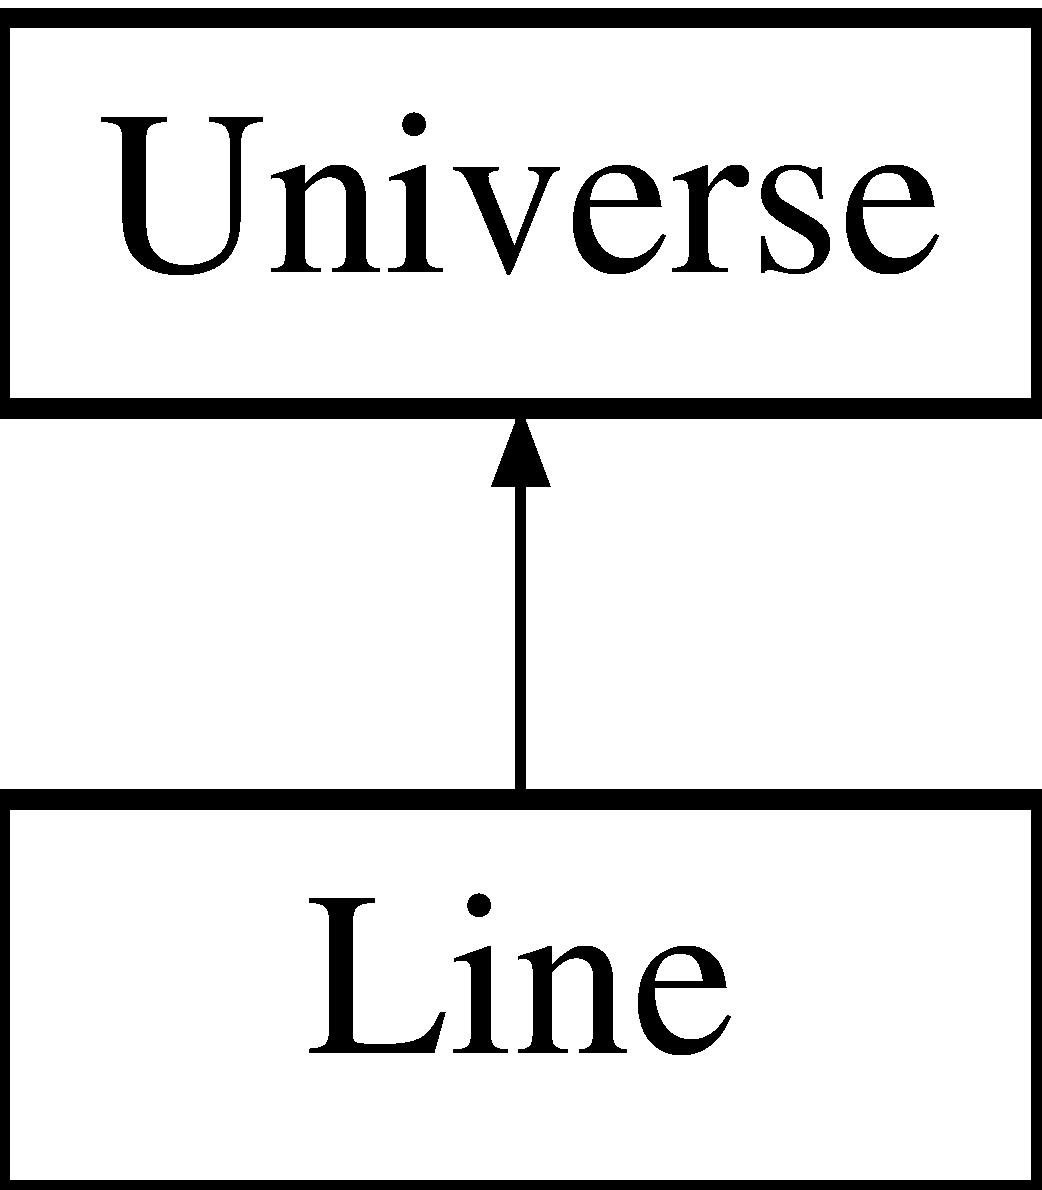
\includegraphics[height=2.000000cm]{classLine}
\end{center}
\end{figure}
\subsection*{Public Member Functions}
\begin{DoxyCompactItemize}
\item 
\mbox{\hyperlink{classLine_acc11b8a429d8cdd63ba6803dff5602b3}{Line}} ()
\item 
\mbox{\hyperlink{classLine_a4e3242660d8d3c1aa43e932560840552}{Line}} (unsigned int object\+\_\+type)
\item 
\mbox{\hyperlink{classLine_a5330353765ab0f965a4293bdc7c3564a}{Line}} (unsigned int object\+\_\+type, std\+::chrono\+::time\+\_\+point$<$ \mbox{\hyperlink{universe_8h_a0ef8d951d1ca5ab3cfaf7ab4c7a6fd80}{Clock}} $>$ event\+\_\+time)
\item 
\mbox{\hyperlink{classLine_a740aacdf468a1519f9a01d9cbd1f9219}{Line}} (unsigned int object\+\_\+type, std\+::chrono\+::time\+\_\+point$<$ \mbox{\hyperlink{universe_8h_a0ef8d951d1ca5ab3cfaf7ab4c7a6fd80}{Clock}} $>$ event\+\_\+time, \mbox{\hyperlink{classUniverse}{Universe}} \&universe\+\_\+connector)
\item 
virtual \mbox{\hyperlink{classLine_a4a95bafcefa28672b3999deb011b9e50}{$\sim$\+Line}} ()
\item 
bool \mbox{\hyperlink{classLine_af1756d1500ab0a5616313be6e213015a}{Reset\+Parameters}} (std\+::chrono\+::time\+\_\+point$<$ \mbox{\hyperlink{universe_8h_a0ef8d951d1ca5ab3cfaf7ab4c7a6fd80}{Clock}} $>$ event\+\_\+time)
\item 
int \mbox{\hyperlink{classLine_a20756feda4d42032955ec6cf12d89941}{Get\+Line\+ID}} (std\+::chrono\+::time\+\_\+point$<$ \mbox{\hyperlink{universe_8h_a0ef8d951d1ca5ab3cfaf7ab4c7a6fd80}{Clock}} $>$ event\+\_\+time)
\item 
double \mbox{\hyperlink{classLine_a8752cfce7330fbeda936778b77e534d0}{Get\+Line\+X\+Y\+Bubble}} (std\+::chrono\+::time\+\_\+point$<$ \mbox{\hyperlink{universe_8h_a0ef8d951d1ca5ab3cfaf7ab4c7a6fd80}{Clock}} $>$ event\+\_\+time) const
\item 
double \mbox{\hyperlink{classLine_ab14245ec4348e925b6e0f860e9254308}{Get\+Line\+X1}} (std\+::chrono\+::time\+\_\+point$<$ \mbox{\hyperlink{universe_8h_a0ef8d951d1ca5ab3cfaf7ab4c7a6fd80}{Clock}} $>$ event\+\_\+time) const
\item 
double \mbox{\hyperlink{classLine_ac09a53b36a300c38191269f110c73eb1}{Get\+Line\+Y1}} (std\+::chrono\+::time\+\_\+point$<$ \mbox{\hyperlink{universe_8h_a0ef8d951d1ca5ab3cfaf7ab4c7a6fd80}{Clock}} $>$ event\+\_\+time) const
\item 
double \mbox{\hyperlink{classLine_adc3c6c42d1b3d172e32fad59db2e3eaa}{Get\+Line\+X1\+Y1\+Bubble}} (std\+::chrono\+::time\+\_\+point$<$ \mbox{\hyperlink{universe_8h_a0ef8d951d1ca5ab3cfaf7ab4c7a6fd80}{Clock}} $>$ event\+\_\+time) const
\item 
double \mbox{\hyperlink{classLine_a9cdf38d7aaeadfa35136dd417865c189}{Get\+Line\+X2}} (std\+::chrono\+::time\+\_\+point$<$ \mbox{\hyperlink{universe_8h_a0ef8d951d1ca5ab3cfaf7ab4c7a6fd80}{Clock}} $>$ event\+\_\+time) const
\item 
double \mbox{\hyperlink{classLine_a6222d15f883f3183ec9eed085046916a}{Get\+Line\+Y2}} (std\+::chrono\+::time\+\_\+point$<$ \mbox{\hyperlink{universe_8h_a0ef8d951d1ca5ab3cfaf7ab4c7a6fd80}{Clock}} $>$ event\+\_\+time) const
\item 
double \mbox{\hyperlink{classLine_a2432406f734963e4497541081a843131}{Get\+Line\+X2\+Y2\+Bubble}} (std\+::chrono\+::time\+\_\+point$<$ \mbox{\hyperlink{universe_8h_a0ef8d951d1ca5ab3cfaf7ab4c7a6fd80}{Clock}} $>$ event\+\_\+time) const
\item 
double \mbox{\hyperlink{classLine_ac4a6e8f232b529169d91b9f44496933b}{Get\+Line\+X\+Min}} (std\+::chrono\+::time\+\_\+point$<$ \mbox{\hyperlink{universe_8h_a0ef8d951d1ca5ab3cfaf7ab4c7a6fd80}{Clock}} $>$ event\+\_\+time)
\item 
double \mbox{\hyperlink{classLine_ae8151f5f3b102924b09de686f536e220}{Get\+Line\+Y\+Min}} (std\+::chrono\+::time\+\_\+point$<$ \mbox{\hyperlink{universe_8h_a0ef8d951d1ca5ab3cfaf7ab4c7a6fd80}{Clock}} $>$ event\+\_\+time)
\item 
double \mbox{\hyperlink{classLine_a1393a4dcd9fa9e1ab1653c37d76c8c3a}{Get\+Line\+X\+Max}} (std\+::chrono\+::time\+\_\+point$<$ \mbox{\hyperlink{universe_8h_a0ef8d951d1ca5ab3cfaf7ab4c7a6fd80}{Clock}} $>$ event\+\_\+time)
\item 
double \mbox{\hyperlink{classLine_ab033cff3a24b67be829759d16f13c281}{Get\+Line\+Y\+Max}} (std\+::chrono\+::time\+\_\+point$<$ \mbox{\hyperlink{universe_8h_a0ef8d951d1ca5ab3cfaf7ab4c7a6fd80}{Clock}} $>$ event\+\_\+time)
\item 
double \mbox{\hyperlink{classLine_a7b105f0af704489446cc93302c30813d}{Get\+Line\+Min\+Ordinal}} (std\+::chrono\+::time\+\_\+point$<$ \mbox{\hyperlink{universe_8h_a0ef8d951d1ca5ab3cfaf7ab4c7a6fd80}{Clock}} $>$ event\+\_\+time)
\item 
double \mbox{\hyperlink{classLine_a3fc7779998759b641ec2b7bc8515563a}{Get\+Line\+Max\+Ordinal}} (std\+::chrono\+::time\+\_\+point$<$ \mbox{\hyperlink{universe_8h_a0ef8d951d1ca5ab3cfaf7ab4c7a6fd80}{Clock}} $>$ event\+\_\+time)
\item 
double \mbox{\hyperlink{classLine_a2be3926d47a1a8849007a6c29a603dcf}{Get\+Slope}} (std\+::chrono\+::time\+\_\+point$<$ \mbox{\hyperlink{universe_8h_a0ef8d951d1ca5ab3cfaf7ab4c7a6fd80}{Clock}} $>$ event\+\_\+time)
\item 
double \mbox{\hyperlink{classLine_a5319d68ecb254ff61e2a46d5928aec93}{Get\+Yint}} (std\+::chrono\+::time\+\_\+point$<$ \mbox{\hyperlink{universe_8h_a0ef8d951d1ca5ab3cfaf7ab4c7a6fd80}{Clock}} $>$ event\+\_\+time)
\item 
double \mbox{\hyperlink{classLine_a5b9419146093908e5c7d740ac384fe39}{Get\+Line\+T\+TL}} (std\+::chrono\+::time\+\_\+point$<$ \mbox{\hyperlink{universe_8h_a0ef8d951d1ca5ab3cfaf7ab4c7a6fd80}{Clock}} $>$ event\+\_\+time) const
\item 
int \mbox{\hyperlink{classLine_a8764cb987ec4af839f30411dc47a835a}{Get\+Line\+Seq}} (std\+::chrono\+::time\+\_\+point$<$ \mbox{\hyperlink{universe_8h_a0ef8d951d1ca5ab3cfaf7ab4c7a6fd80}{Clock}} $>$ event\+\_\+time)
\item 
int \mbox{\hyperlink{classLine_ac13c6405cfd2a586633b5a5eece05fff}{Get\+Line\+Counter}} (std\+::chrono\+::time\+\_\+point$<$ \mbox{\hyperlink{universe_8h_a0ef8d951d1ca5ab3cfaf7ab4c7a6fd80}{Clock}} $>$ event\+\_\+time) const
\item 
bool \mbox{\hyperlink{classLine_a4c9d571599ebc5e9b6090b54a338fbde}{Get\+In\+Line}} (std\+::chrono\+::time\+\_\+point$<$ \mbox{\hyperlink{universe_8h_a0ef8d951d1ca5ab3cfaf7ab4c7a6fd80}{Clock}} $>$ event\+\_\+time, double X1, double Y1, double X2, double Y2, double Threshold)
\item 
void \mbox{\hyperlink{classLine_aaa634bf320b9d1c4becb4083cd8324d4}{set\+Line\+ID}} (std\+::chrono\+::time\+\_\+point$<$ \mbox{\hyperlink{universe_8h_a0ef8d951d1ca5ab3cfaf7ab4c7a6fd80}{Clock}} $>$ event\+\_\+time, int val)
\item 
void \mbox{\hyperlink{classLine_ab8df9f66bffc86994db3150a4eb8ed29}{set\+Line\+X1}} (std\+::chrono\+::time\+\_\+point$<$ \mbox{\hyperlink{universe_8h_a0ef8d951d1ca5ab3cfaf7ab4c7a6fd80}{Clock}} $>$ event\+\_\+time, double val)
\item 
void \mbox{\hyperlink{classLine_af236c5ddb0d125b388621b3597266a95}{set\+Line\+Y1}} (std\+::chrono\+::time\+\_\+point$<$ \mbox{\hyperlink{universe_8h_a0ef8d951d1ca5ab3cfaf7ab4c7a6fd80}{Clock}} $>$ event\+\_\+time, double val)
\item 
void \mbox{\hyperlink{classLine_ade959bc4d4f69bb421ed4f69c0d77fb7}{set\+Line\+X2}} (std\+::chrono\+::time\+\_\+point$<$ \mbox{\hyperlink{universe_8h_a0ef8d951d1ca5ab3cfaf7ab4c7a6fd80}{Clock}} $>$ event\+\_\+time, double val)
\item 
void \mbox{\hyperlink{classLine_a671f64c437fe1bef798476d93c675099}{set\+Line\+Y2}} (std\+::chrono\+::time\+\_\+point$<$ \mbox{\hyperlink{universe_8h_a0ef8d951d1ca5ab3cfaf7ab4c7a6fd80}{Clock}} $>$ event\+\_\+time, double val)
\item 
void \mbox{\hyperlink{classLine_a3fb9e9eab13d146feff0bc891709eaf9}{set\+Slope}} (std\+::chrono\+::time\+\_\+point$<$ \mbox{\hyperlink{universe_8h_a0ef8d951d1ca5ab3cfaf7ab4c7a6fd80}{Clock}} $>$ event\+\_\+time, double val)
\item 
void \mbox{\hyperlink{classLine_ad966eb3f1bd4cb29976b3e97811c344f}{set\+Yint}} (std\+::chrono\+::time\+\_\+point$<$ \mbox{\hyperlink{universe_8h_a0ef8d951d1ca5ab3cfaf7ab4c7a6fd80}{Clock}} $>$ event\+\_\+time, double val)
\item 
void \mbox{\hyperlink{classLine_a602398c8c3131ec7236ccadbab8281d5}{set\+Line\+T\+TL}} (std\+::chrono\+::time\+\_\+point$<$ \mbox{\hyperlink{universe_8h_a0ef8d951d1ca5ab3cfaf7ab4c7a6fd80}{Clock}} $>$ event\+\_\+time, double val)
\item 
void \mbox{\hyperlink{classLine_a7c315c5ffdd4fa875918583738e2e157}{set\+Line\+Seq}} (std\+::chrono\+::time\+\_\+point$<$ \mbox{\hyperlink{universe_8h_a0ef8d951d1ca5ab3cfaf7ab4c7a6fd80}{Clock}} $>$ event\+\_\+time, int val)
\item 
void \mbox{\hyperlink{classLine_ab98abcf3c8546e266ae5bbea243d8b8d}{set\+Line\+Counter}} (std\+::chrono\+::time\+\_\+point$<$ \mbox{\hyperlink{universe_8h_a0ef8d951d1ca5ab3cfaf7ab4c7a6fd80}{Clock}} $>$ event\+\_\+time, int val)
\item 
int \mbox{\hyperlink{classLine_a8c6dece66f5cd93ce40134002a40f505}{Update}} (std\+::chrono\+::time\+\_\+point$<$ \mbox{\hyperlink{universe_8h_a0ef8d951d1ca5ab3cfaf7ab4c7a6fd80}{Clock}} $>$ event\+\_\+time)
\end{DoxyCompactItemize}
\subsection*{Private Attributes}
\begin{DoxyCompactItemize}
\item 
int \mbox{\hyperlink{classLine_a92cbc39dd66e02a0507132422a2a830c}{line\+Line\+ID}}
\item 
int \mbox{\hyperlink{classLine_aa5bac2c364a75b5212500dce6846ee0b}{line\+\_\+type}}
\item 
double \mbox{\hyperlink{classLine_ac581c18e7d6a976b14dd986d42cb8163}{line\+Line\+X1}}
\begin{DoxyCompactList}\small\item\em Member variable \char`\"{}line\+Line\+X1\char`\"{}. \end{DoxyCompactList}\item 
double \mbox{\hyperlink{classLine_a46e251350694d1bdf8425d9f9a24f896}{line\+Line\+Y1}}
\begin{DoxyCompactList}\small\item\em Member variable \char`\"{}line\+Line\+Y1\char`\"{}. \end{DoxyCompactList}\item 
double \mbox{\hyperlink{classLine_a795ef48c075a36f0dea1af10b5ff323d}{line\+Line\+X2}}
\begin{DoxyCompactList}\small\item\em Member variable \char`\"{}line\+Line\+X2\char`\"{}. \end{DoxyCompactList}\item 
double \mbox{\hyperlink{classLine_aa0f76375751fb3a75b9593161ecfc0e2}{line\+Line\+Y2}}
\begin{DoxyCompactList}\small\item\em Member variable \char`\"{}line\+Line\+Y2\char`\"{}. \end{DoxyCompactList}\item 
double \mbox{\hyperlink{classLine_afdf693a798435ec16076396f3631853e}{line\+Slope}}
\begin{DoxyCompactList}\small\item\em Member variable \char`\"{}line\+Slope\char`\"{}. \end{DoxyCompactList}\item 
double \mbox{\hyperlink{classLine_a35197c3051202d4c4f0bb7d122780368}{line\+Yint}}
\begin{DoxyCompactList}\small\item\em Member variable \char`\"{}line\+Yint\char`\"{}. \end{DoxyCompactList}\item 
double \mbox{\hyperlink{classLine_afb3c20f2415b40bc800ae36796b2f7c7}{line\+Line\+T\+TL}}
\begin{DoxyCompactList}\small\item\em Member variable \char`\"{}line\+Line\+T\+T\+L\char`\"{}. \end{DoxyCompactList}\item 
int \mbox{\hyperlink{classLine_a46a8187d5ccc8bf0dc9bc041836f241f}{line\+Line\+Seq}}
\item 
int \mbox{\hyperlink{classLine_a4fb7e6f35d49e0113755913b5179f922}{line\+Line\+Counter}}
\item 
std\+::chrono\+::time\+\_\+point$<$ \mbox{\hyperlink{universe_8h_a0ef8d951d1ca5ab3cfaf7ab4c7a6fd80}{Clock}} $>$ \mbox{\hyperlink{classLine_ad1d89d2499cf9455fc2499078e0acc32}{time\+\_\+object\+\_\+created}}
\item 
std\+::chrono\+::time\+\_\+point$<$ \mbox{\hyperlink{universe_8h_a0ef8d951d1ca5ab3cfaf7ab4c7a6fd80}{Clock}} $>$ \mbox{\hyperlink{classLine_a1d6ddf845443fa6baa5d15d14baed9f8}{previous\+\_\+event\+\_\+time}}
\item 
int \mbox{\hyperlink{classLine_ab4c19eb7e67615c609de20d98a2d0b5f}{duration\+\_\+since\+\_\+last\+\_\+event}}
\item 
bool \mbox{\hyperlink{classLine_ae9070a9da0afebb31910e31e62019301}{object\+\_\+disabled}}
\item 
bool \mbox{\hyperlink{classLine_a53a3368bd95b126c281eea4736ebc282}{object\+\_\+initialised}}
\end{DoxyCompactItemize}
\subsection*{Additional Inherited Members}


\subsection{Detailed Description}
$<$ For Sine, Cosine, Fabs \& Sqrt functions 

\subsection{Constructor \& Destructor Documentation}
\mbox{\Hypertarget{classLine_acc11b8a429d8cdd63ba6803dff5602b3}\label{classLine_acc11b8a429d8cdd63ba6803dff5602b3}} 
\index{Line@{Line}!Line@{Line}}
\index{Line@{Line}!Line@{Line}}
\subsubsection{\texorpdfstring{Line()}{Line()}\hspace{0.1cm}{\footnotesize\ttfamily [1/4]}}
{\footnotesize\ttfamily Line\+::\+Line (\begin{DoxyParamCaption}{ }\end{DoxyParamCaption})\hspace{0.3cm}{\ttfamily [inline]}}

\mbox{\Hypertarget{classLine_a4e3242660d8d3c1aa43e932560840552}\label{classLine_a4e3242660d8d3c1aa43e932560840552}} 
\index{Line@{Line}!Line@{Line}}
\index{Line@{Line}!Line@{Line}}
\subsubsection{\texorpdfstring{Line()}{Line()}\hspace{0.1cm}{\footnotesize\ttfamily [2/4]}}
{\footnotesize\ttfamily Line\+::\+Line (\begin{DoxyParamCaption}\item[{unsigned int}]{object\+\_\+type }\end{DoxyParamCaption})\hspace{0.3cm}{\ttfamily [inline]}}

\mbox{\Hypertarget{classLine_a5330353765ab0f965a4293bdc7c3564a}\label{classLine_a5330353765ab0f965a4293bdc7c3564a}} 
\index{Line@{Line}!Line@{Line}}
\index{Line@{Line}!Line@{Line}}
\subsubsection{\texorpdfstring{Line()}{Line()}\hspace{0.1cm}{\footnotesize\ttfamily [3/4]}}
{\footnotesize\ttfamily Line\+::\+Line (\begin{DoxyParamCaption}\item[{unsigned int}]{object\+\_\+type,  }\item[{std\+::chrono\+::time\+\_\+point$<$ \mbox{\hyperlink{universe_8h_a0ef8d951d1ca5ab3cfaf7ab4c7a6fd80}{Clock}} $>$}]{event\+\_\+time }\end{DoxyParamCaption})\hspace{0.3cm}{\ttfamily [inline]}}

\mbox{\Hypertarget{classLine_a740aacdf468a1519f9a01d9cbd1f9219}\label{classLine_a740aacdf468a1519f9a01d9cbd1f9219}} 
\index{Line@{Line}!Line@{Line}}
\index{Line@{Line}!Line@{Line}}
\subsubsection{\texorpdfstring{Line()}{Line()}\hspace{0.1cm}{\footnotesize\ttfamily [4/4]}}
{\footnotesize\ttfamily Line\+::\+Line (\begin{DoxyParamCaption}\item[{unsigned int}]{object\+\_\+type,  }\item[{std\+::chrono\+::time\+\_\+point$<$ \mbox{\hyperlink{universe_8h_a0ef8d951d1ca5ab3cfaf7ab4c7a6fd80}{Clock}} $>$}]{event\+\_\+time,  }\item[{\mbox{\hyperlink{classUniverse}{Universe}} \&}]{universe\+\_\+connector }\end{DoxyParamCaption})\hspace{0.3cm}{\ttfamily [inline]}}

\mbox{\Hypertarget{classLine_a4a95bafcefa28672b3999deb011b9e50}\label{classLine_a4a95bafcefa28672b3999deb011b9e50}} 
\index{Line@{Line}!````~Line@{$\sim$\+Line}}
\index{````~Line@{$\sim$\+Line}!Line@{Line}}
\subsubsection{\texorpdfstring{$\sim$\+Line()}{~Line()}}
{\footnotesize\ttfamily virtual Line\+::$\sim$\+Line (\begin{DoxyParamCaption}{ }\end{DoxyParamCaption})\hspace{0.3cm}{\ttfamily [inline]}, {\ttfamily [virtual]}}

Default destructor 

\subsection{Member Function Documentation}
\mbox{\Hypertarget{classLine_a4c9d571599ebc5e9b6090b54a338fbde}\label{classLine_a4c9d571599ebc5e9b6090b54a338fbde}} 
\index{Line@{Line}!Get\+In\+Line@{Get\+In\+Line}}
\index{Get\+In\+Line@{Get\+In\+Line}!Line@{Line}}
\subsubsection{\texorpdfstring{Get\+In\+Line()}{GetInLine()}}
{\footnotesize\ttfamily bool Line\+::\+Get\+In\+Line (\begin{DoxyParamCaption}\item[{std\+::chrono\+::time\+\_\+point$<$ \mbox{\hyperlink{universe_8h_a0ef8d951d1ca5ab3cfaf7ab4c7a6fd80}{Clock}} $>$}]{event\+\_\+time,  }\item[{double}]{X1,  }\item[{double}]{Y1,  }\item[{double}]{X2,  }\item[{double}]{Y2,  }\item[{double}]{Threshold }\end{DoxyParamCaption})\hspace{0.3cm}{\ttfamily [inline]}}

\mbox{\Hypertarget{classLine_ac13c6405cfd2a586633b5a5eece05fff}\label{classLine_ac13c6405cfd2a586633b5a5eece05fff}} 
\index{Line@{Line}!Get\+Line\+Counter@{Get\+Line\+Counter}}
\index{Get\+Line\+Counter@{Get\+Line\+Counter}!Line@{Line}}
\subsubsection{\texorpdfstring{Get\+Line\+Counter()}{GetLineCounter()}}
{\footnotesize\ttfamily int Line\+::\+Get\+Line\+Counter (\begin{DoxyParamCaption}\item[{std\+::chrono\+::time\+\_\+point$<$ \mbox{\hyperlink{universe_8h_a0ef8d951d1ca5ab3cfaf7ab4c7a6fd80}{Clock}} $>$}]{event\+\_\+time }\end{DoxyParamCaption}) const\hspace{0.3cm}{\ttfamily [inline]}}

\mbox{\Hypertarget{classLine_a20756feda4d42032955ec6cf12d89941}\label{classLine_a20756feda4d42032955ec6cf12d89941}} 
\index{Line@{Line}!Get\+Line\+ID@{Get\+Line\+ID}}
\index{Get\+Line\+ID@{Get\+Line\+ID}!Line@{Line}}
\subsubsection{\texorpdfstring{Get\+Line\+I\+D()}{GetLineID()}}
{\footnotesize\ttfamily int Line\+::\+Get\+Line\+ID (\begin{DoxyParamCaption}\item[{std\+::chrono\+::time\+\_\+point$<$ \mbox{\hyperlink{universe_8h_a0ef8d951d1ca5ab3cfaf7ab4c7a6fd80}{Clock}} $>$}]{event\+\_\+time }\end{DoxyParamCaption})\hspace{0.3cm}{\ttfamily [inline]}}

\mbox{\Hypertarget{classLine_a3fc7779998759b641ec2b7bc8515563a}\label{classLine_a3fc7779998759b641ec2b7bc8515563a}} 
\index{Line@{Line}!Get\+Line\+Max\+Ordinal@{Get\+Line\+Max\+Ordinal}}
\index{Get\+Line\+Max\+Ordinal@{Get\+Line\+Max\+Ordinal}!Line@{Line}}
\subsubsection{\texorpdfstring{Get\+Line\+Max\+Ordinal()}{GetLineMaxOrdinal()}}
{\footnotesize\ttfamily double Line\+::\+Get\+Line\+Max\+Ordinal (\begin{DoxyParamCaption}\item[{std\+::chrono\+::time\+\_\+point$<$ \mbox{\hyperlink{universe_8h_a0ef8d951d1ca5ab3cfaf7ab4c7a6fd80}{Clock}} $>$}]{event\+\_\+time }\end{DoxyParamCaption})\hspace{0.3cm}{\ttfamily [inline]}}

\mbox{\Hypertarget{classLine_a7b105f0af704489446cc93302c30813d}\label{classLine_a7b105f0af704489446cc93302c30813d}} 
\index{Line@{Line}!Get\+Line\+Min\+Ordinal@{Get\+Line\+Min\+Ordinal}}
\index{Get\+Line\+Min\+Ordinal@{Get\+Line\+Min\+Ordinal}!Line@{Line}}
\subsubsection{\texorpdfstring{Get\+Line\+Min\+Ordinal()}{GetLineMinOrdinal()}}
{\footnotesize\ttfamily double Line\+::\+Get\+Line\+Min\+Ordinal (\begin{DoxyParamCaption}\item[{std\+::chrono\+::time\+\_\+point$<$ \mbox{\hyperlink{universe_8h_a0ef8d951d1ca5ab3cfaf7ab4c7a6fd80}{Clock}} $>$}]{event\+\_\+time }\end{DoxyParamCaption})\hspace{0.3cm}{\ttfamily [inline]}}

\mbox{\Hypertarget{classLine_a8764cb987ec4af839f30411dc47a835a}\label{classLine_a8764cb987ec4af839f30411dc47a835a}} 
\index{Line@{Line}!Get\+Line\+Seq@{Get\+Line\+Seq}}
\index{Get\+Line\+Seq@{Get\+Line\+Seq}!Line@{Line}}
\subsubsection{\texorpdfstring{Get\+Line\+Seq()}{GetLineSeq()}}
{\footnotesize\ttfamily int Line\+::\+Get\+Line\+Seq (\begin{DoxyParamCaption}\item[{std\+::chrono\+::time\+\_\+point$<$ \mbox{\hyperlink{universe_8h_a0ef8d951d1ca5ab3cfaf7ab4c7a6fd80}{Clock}} $>$}]{event\+\_\+time }\end{DoxyParamCaption})\hspace{0.3cm}{\ttfamily [inline]}}

\mbox{\Hypertarget{classLine_a5b9419146093908e5c7d740ac384fe39}\label{classLine_a5b9419146093908e5c7d740ac384fe39}} 
\index{Line@{Line}!Get\+Line\+T\+TL@{Get\+Line\+T\+TL}}
\index{Get\+Line\+T\+TL@{Get\+Line\+T\+TL}!Line@{Line}}
\subsubsection{\texorpdfstring{Get\+Line\+T\+T\+L()}{GetLineTTL()}}
{\footnotesize\ttfamily double Line\+::\+Get\+Line\+T\+TL (\begin{DoxyParamCaption}\item[{std\+::chrono\+::time\+\_\+point$<$ \mbox{\hyperlink{universe_8h_a0ef8d951d1ca5ab3cfaf7ab4c7a6fd80}{Clock}} $>$}]{event\+\_\+time }\end{DoxyParamCaption}) const\hspace{0.3cm}{\ttfamily [inline]}}

\mbox{\Hypertarget{classLine_ab14245ec4348e925b6e0f860e9254308}\label{classLine_ab14245ec4348e925b6e0f860e9254308}} 
\index{Line@{Line}!Get\+Line\+X1@{Get\+Line\+X1}}
\index{Get\+Line\+X1@{Get\+Line\+X1}!Line@{Line}}
\subsubsection{\texorpdfstring{Get\+Line\+X1()}{GetLineX1()}}
{\footnotesize\ttfamily double Line\+::\+Get\+Line\+X1 (\begin{DoxyParamCaption}\item[{std\+::chrono\+::time\+\_\+point$<$ \mbox{\hyperlink{universe_8h_a0ef8d951d1ca5ab3cfaf7ab4c7a6fd80}{Clock}} $>$}]{event\+\_\+time }\end{DoxyParamCaption}) const\hspace{0.3cm}{\ttfamily [inline]}}

\mbox{\Hypertarget{classLine_adc3c6c42d1b3d172e32fad59db2e3eaa}\label{classLine_adc3c6c42d1b3d172e32fad59db2e3eaa}} 
\index{Line@{Line}!Get\+Line\+X1\+Y1\+Bubble@{Get\+Line\+X1\+Y1\+Bubble}}
\index{Get\+Line\+X1\+Y1\+Bubble@{Get\+Line\+X1\+Y1\+Bubble}!Line@{Line}}
\subsubsection{\texorpdfstring{Get\+Line\+X1\+Y1\+Bubble()}{GetLineX1Y1Bubble()}}
{\footnotesize\ttfamily double Line\+::\+Get\+Line\+X1\+Y1\+Bubble (\begin{DoxyParamCaption}\item[{std\+::chrono\+::time\+\_\+point$<$ \mbox{\hyperlink{universe_8h_a0ef8d951d1ca5ab3cfaf7ab4c7a6fd80}{Clock}} $>$}]{event\+\_\+time }\end{DoxyParamCaption}) const\hspace{0.3cm}{\ttfamily [inline]}}

\mbox{\Hypertarget{classLine_a9cdf38d7aaeadfa35136dd417865c189}\label{classLine_a9cdf38d7aaeadfa35136dd417865c189}} 
\index{Line@{Line}!Get\+Line\+X2@{Get\+Line\+X2}}
\index{Get\+Line\+X2@{Get\+Line\+X2}!Line@{Line}}
\subsubsection{\texorpdfstring{Get\+Line\+X2()}{GetLineX2()}}
{\footnotesize\ttfamily double Line\+::\+Get\+Line\+X2 (\begin{DoxyParamCaption}\item[{std\+::chrono\+::time\+\_\+point$<$ \mbox{\hyperlink{universe_8h_a0ef8d951d1ca5ab3cfaf7ab4c7a6fd80}{Clock}} $>$}]{event\+\_\+time }\end{DoxyParamCaption}) const\hspace{0.3cm}{\ttfamily [inline]}}

\mbox{\Hypertarget{classLine_a2432406f734963e4497541081a843131}\label{classLine_a2432406f734963e4497541081a843131}} 
\index{Line@{Line}!Get\+Line\+X2\+Y2\+Bubble@{Get\+Line\+X2\+Y2\+Bubble}}
\index{Get\+Line\+X2\+Y2\+Bubble@{Get\+Line\+X2\+Y2\+Bubble}!Line@{Line}}
\subsubsection{\texorpdfstring{Get\+Line\+X2\+Y2\+Bubble()}{GetLineX2Y2Bubble()}}
{\footnotesize\ttfamily double Line\+::\+Get\+Line\+X2\+Y2\+Bubble (\begin{DoxyParamCaption}\item[{std\+::chrono\+::time\+\_\+point$<$ \mbox{\hyperlink{universe_8h_a0ef8d951d1ca5ab3cfaf7ab4c7a6fd80}{Clock}} $>$}]{event\+\_\+time }\end{DoxyParamCaption}) const\hspace{0.3cm}{\ttfamily [inline]}}

\mbox{\Hypertarget{classLine_a1393a4dcd9fa9e1ab1653c37d76c8c3a}\label{classLine_a1393a4dcd9fa9e1ab1653c37d76c8c3a}} 
\index{Line@{Line}!Get\+Line\+X\+Max@{Get\+Line\+X\+Max}}
\index{Get\+Line\+X\+Max@{Get\+Line\+X\+Max}!Line@{Line}}
\subsubsection{\texorpdfstring{Get\+Line\+X\+Max()}{GetLineXMax()}}
{\footnotesize\ttfamily double Line\+::\+Get\+Line\+X\+Max (\begin{DoxyParamCaption}\item[{std\+::chrono\+::time\+\_\+point$<$ \mbox{\hyperlink{universe_8h_a0ef8d951d1ca5ab3cfaf7ab4c7a6fd80}{Clock}} $>$}]{event\+\_\+time }\end{DoxyParamCaption})\hspace{0.3cm}{\ttfamily [inline]}}

\mbox{\Hypertarget{classLine_ac4a6e8f232b529169d91b9f44496933b}\label{classLine_ac4a6e8f232b529169d91b9f44496933b}} 
\index{Line@{Line}!Get\+Line\+X\+Min@{Get\+Line\+X\+Min}}
\index{Get\+Line\+X\+Min@{Get\+Line\+X\+Min}!Line@{Line}}
\subsubsection{\texorpdfstring{Get\+Line\+X\+Min()}{GetLineXMin()}}
{\footnotesize\ttfamily double Line\+::\+Get\+Line\+X\+Min (\begin{DoxyParamCaption}\item[{std\+::chrono\+::time\+\_\+point$<$ \mbox{\hyperlink{universe_8h_a0ef8d951d1ca5ab3cfaf7ab4c7a6fd80}{Clock}} $>$}]{event\+\_\+time }\end{DoxyParamCaption})\hspace{0.3cm}{\ttfamily [inline]}}

\mbox{\Hypertarget{classLine_a8752cfce7330fbeda936778b77e534d0}\label{classLine_a8752cfce7330fbeda936778b77e534d0}} 
\index{Line@{Line}!Get\+Line\+X\+Y\+Bubble@{Get\+Line\+X\+Y\+Bubble}}
\index{Get\+Line\+X\+Y\+Bubble@{Get\+Line\+X\+Y\+Bubble}!Line@{Line}}
\subsubsection{\texorpdfstring{Get\+Line\+X\+Y\+Bubble()}{GetLineXYBubble()}}
{\footnotesize\ttfamily double Line\+::\+Get\+Line\+X\+Y\+Bubble (\begin{DoxyParamCaption}\item[{std\+::chrono\+::time\+\_\+point$<$ \mbox{\hyperlink{universe_8h_a0ef8d951d1ca5ab3cfaf7ab4c7a6fd80}{Clock}} $>$}]{event\+\_\+time }\end{DoxyParamCaption}) const\hspace{0.3cm}{\ttfamily [inline]}}

\mbox{\Hypertarget{classLine_ac09a53b36a300c38191269f110c73eb1}\label{classLine_ac09a53b36a300c38191269f110c73eb1}} 
\index{Line@{Line}!Get\+Line\+Y1@{Get\+Line\+Y1}}
\index{Get\+Line\+Y1@{Get\+Line\+Y1}!Line@{Line}}
\subsubsection{\texorpdfstring{Get\+Line\+Y1()}{GetLineY1()}}
{\footnotesize\ttfamily double Line\+::\+Get\+Line\+Y1 (\begin{DoxyParamCaption}\item[{std\+::chrono\+::time\+\_\+point$<$ \mbox{\hyperlink{universe_8h_a0ef8d951d1ca5ab3cfaf7ab4c7a6fd80}{Clock}} $>$}]{event\+\_\+time }\end{DoxyParamCaption}) const\hspace{0.3cm}{\ttfamily [inline]}}

\mbox{\Hypertarget{classLine_a6222d15f883f3183ec9eed085046916a}\label{classLine_a6222d15f883f3183ec9eed085046916a}} 
\index{Line@{Line}!Get\+Line\+Y2@{Get\+Line\+Y2}}
\index{Get\+Line\+Y2@{Get\+Line\+Y2}!Line@{Line}}
\subsubsection{\texorpdfstring{Get\+Line\+Y2()}{GetLineY2()}}
{\footnotesize\ttfamily double Line\+::\+Get\+Line\+Y2 (\begin{DoxyParamCaption}\item[{std\+::chrono\+::time\+\_\+point$<$ \mbox{\hyperlink{universe_8h_a0ef8d951d1ca5ab3cfaf7ab4c7a6fd80}{Clock}} $>$}]{event\+\_\+time }\end{DoxyParamCaption}) const\hspace{0.3cm}{\ttfamily [inline]}}

\mbox{\Hypertarget{classLine_ab033cff3a24b67be829759d16f13c281}\label{classLine_ab033cff3a24b67be829759d16f13c281}} 
\index{Line@{Line}!Get\+Line\+Y\+Max@{Get\+Line\+Y\+Max}}
\index{Get\+Line\+Y\+Max@{Get\+Line\+Y\+Max}!Line@{Line}}
\subsubsection{\texorpdfstring{Get\+Line\+Y\+Max()}{GetLineYMax()}}
{\footnotesize\ttfamily double Line\+::\+Get\+Line\+Y\+Max (\begin{DoxyParamCaption}\item[{std\+::chrono\+::time\+\_\+point$<$ \mbox{\hyperlink{universe_8h_a0ef8d951d1ca5ab3cfaf7ab4c7a6fd80}{Clock}} $>$}]{event\+\_\+time }\end{DoxyParamCaption})\hspace{0.3cm}{\ttfamily [inline]}}

\mbox{\Hypertarget{classLine_ae8151f5f3b102924b09de686f536e220}\label{classLine_ae8151f5f3b102924b09de686f536e220}} 
\index{Line@{Line}!Get\+Line\+Y\+Min@{Get\+Line\+Y\+Min}}
\index{Get\+Line\+Y\+Min@{Get\+Line\+Y\+Min}!Line@{Line}}
\subsubsection{\texorpdfstring{Get\+Line\+Y\+Min()}{GetLineYMin()}}
{\footnotesize\ttfamily double Line\+::\+Get\+Line\+Y\+Min (\begin{DoxyParamCaption}\item[{std\+::chrono\+::time\+\_\+point$<$ \mbox{\hyperlink{universe_8h_a0ef8d951d1ca5ab3cfaf7ab4c7a6fd80}{Clock}} $>$}]{event\+\_\+time }\end{DoxyParamCaption})\hspace{0.3cm}{\ttfamily [inline]}}

\mbox{\Hypertarget{classLine_a2be3926d47a1a8849007a6c29a603dcf}\label{classLine_a2be3926d47a1a8849007a6c29a603dcf}} 
\index{Line@{Line}!Get\+Slope@{Get\+Slope}}
\index{Get\+Slope@{Get\+Slope}!Line@{Line}}
\subsubsection{\texorpdfstring{Get\+Slope()}{GetSlope()}}
{\footnotesize\ttfamily double Line\+::\+Get\+Slope (\begin{DoxyParamCaption}\item[{std\+::chrono\+::time\+\_\+point$<$ \mbox{\hyperlink{universe_8h_a0ef8d951d1ca5ab3cfaf7ab4c7a6fd80}{Clock}} $>$}]{event\+\_\+time }\end{DoxyParamCaption})\hspace{0.3cm}{\ttfamily [inline]}}

\mbox{\Hypertarget{classLine_a5319d68ecb254ff61e2a46d5928aec93}\label{classLine_a5319d68ecb254ff61e2a46d5928aec93}} 
\index{Line@{Line}!Get\+Yint@{Get\+Yint}}
\index{Get\+Yint@{Get\+Yint}!Line@{Line}}
\subsubsection{\texorpdfstring{Get\+Yint()}{GetYint()}}
{\footnotesize\ttfamily double Line\+::\+Get\+Yint (\begin{DoxyParamCaption}\item[{std\+::chrono\+::time\+\_\+point$<$ \mbox{\hyperlink{universe_8h_a0ef8d951d1ca5ab3cfaf7ab4c7a6fd80}{Clock}} $>$}]{event\+\_\+time }\end{DoxyParamCaption})\hspace{0.3cm}{\ttfamily [inline]}}

\mbox{\Hypertarget{classLine_af1756d1500ab0a5616313be6e213015a}\label{classLine_af1756d1500ab0a5616313be6e213015a}} 
\index{Line@{Line}!Reset\+Parameters@{Reset\+Parameters}}
\index{Reset\+Parameters@{Reset\+Parameters}!Line@{Line}}
\subsubsection{\texorpdfstring{Reset\+Parameters()}{ResetParameters()}}
{\footnotesize\ttfamily bool Line\+::\+Reset\+Parameters (\begin{DoxyParamCaption}\item[{std\+::chrono\+::time\+\_\+point$<$ \mbox{\hyperlink{universe_8h_a0ef8d951d1ca5ab3cfaf7ab4c7a6fd80}{Clock}} $>$}]{event\+\_\+time }\end{DoxyParamCaption})}

Access line\+Counter \begin{DoxyReturn}{Returns}
The current value of line\+Counter 
\end{DoxyReturn}
\mbox{\Hypertarget{classLine_ab98abcf3c8546e266ae5bbea243d8b8d}\label{classLine_ab98abcf3c8546e266ae5bbea243d8b8d}} 
\index{Line@{Line}!set\+Line\+Counter@{set\+Line\+Counter}}
\index{set\+Line\+Counter@{set\+Line\+Counter}!Line@{Line}}
\subsubsection{\texorpdfstring{set\+Line\+Counter()}{setLineCounter()}}
{\footnotesize\ttfamily void Line\+::set\+Line\+Counter (\begin{DoxyParamCaption}\item[{std\+::chrono\+::time\+\_\+point$<$ \mbox{\hyperlink{universe_8h_a0ef8d951d1ca5ab3cfaf7ab4c7a6fd80}{Clock}} $>$}]{event\+\_\+time,  }\item[{int}]{val }\end{DoxyParamCaption})\hspace{0.3cm}{\ttfamily [inline]}}

\mbox{\Hypertarget{classLine_aaa634bf320b9d1c4becb4083cd8324d4}\label{classLine_aaa634bf320b9d1c4becb4083cd8324d4}} 
\index{Line@{Line}!set\+Line\+ID@{set\+Line\+ID}}
\index{set\+Line\+ID@{set\+Line\+ID}!Line@{Line}}
\subsubsection{\texorpdfstring{set\+Line\+I\+D()}{setLineID()}}
{\footnotesize\ttfamily void Line\+::set\+Line\+ID (\begin{DoxyParamCaption}\item[{std\+::chrono\+::time\+\_\+point$<$ \mbox{\hyperlink{universe_8h_a0ef8d951d1ca5ab3cfaf7ab4c7a6fd80}{Clock}} $>$}]{event\+\_\+time,  }\item[{int}]{val }\end{DoxyParamCaption})\hspace{0.3cm}{\ttfamily [inline]}}

set line\+Counter 
\begin{DoxyParams}{Parameters}
{\em val} & New value to set \\
\hline
\end{DoxyParams}
\mbox{\Hypertarget{classLine_a7c315c5ffdd4fa875918583738e2e157}\label{classLine_a7c315c5ffdd4fa875918583738e2e157}} 
\index{Line@{Line}!set\+Line\+Seq@{set\+Line\+Seq}}
\index{set\+Line\+Seq@{set\+Line\+Seq}!Line@{Line}}
\subsubsection{\texorpdfstring{set\+Line\+Seq()}{setLineSeq()}}
{\footnotesize\ttfamily void Line\+::set\+Line\+Seq (\begin{DoxyParamCaption}\item[{std\+::chrono\+::time\+\_\+point$<$ \mbox{\hyperlink{universe_8h_a0ef8d951d1ca5ab3cfaf7ab4c7a6fd80}{Clock}} $>$}]{event\+\_\+time,  }\item[{int}]{val }\end{DoxyParamCaption})\hspace{0.3cm}{\ttfamily [inline]}}

\mbox{\Hypertarget{classLine_a602398c8c3131ec7236ccadbab8281d5}\label{classLine_a602398c8c3131ec7236ccadbab8281d5}} 
\index{Line@{Line}!set\+Line\+T\+TL@{set\+Line\+T\+TL}}
\index{set\+Line\+T\+TL@{set\+Line\+T\+TL}!Line@{Line}}
\subsubsection{\texorpdfstring{set\+Line\+T\+T\+L()}{setLineTTL()}}
{\footnotesize\ttfamily void Line\+::set\+Line\+T\+TL (\begin{DoxyParamCaption}\item[{std\+::chrono\+::time\+\_\+point$<$ \mbox{\hyperlink{universe_8h_a0ef8d951d1ca5ab3cfaf7ab4c7a6fd80}{Clock}} $>$}]{event\+\_\+time,  }\item[{double}]{val }\end{DoxyParamCaption})\hspace{0.3cm}{\ttfamily [inline]}}

\mbox{\Hypertarget{classLine_ab8df9f66bffc86994db3150a4eb8ed29}\label{classLine_ab8df9f66bffc86994db3150a4eb8ed29}} 
\index{Line@{Line}!set\+Line\+X1@{set\+Line\+X1}}
\index{set\+Line\+X1@{set\+Line\+X1}!Line@{Line}}
\subsubsection{\texorpdfstring{set\+Line\+X1()}{setLineX1()}}
{\footnotesize\ttfamily void Line\+::set\+Line\+X1 (\begin{DoxyParamCaption}\item[{std\+::chrono\+::time\+\_\+point$<$ \mbox{\hyperlink{universe_8h_a0ef8d951d1ca5ab3cfaf7ab4c7a6fd80}{Clock}} $>$}]{event\+\_\+time,  }\item[{double}]{val }\end{DoxyParamCaption})\hspace{0.3cm}{\ttfamily [inline]}}

\mbox{\Hypertarget{classLine_ade959bc4d4f69bb421ed4f69c0d77fb7}\label{classLine_ade959bc4d4f69bb421ed4f69c0d77fb7}} 
\index{Line@{Line}!set\+Line\+X2@{set\+Line\+X2}}
\index{set\+Line\+X2@{set\+Line\+X2}!Line@{Line}}
\subsubsection{\texorpdfstring{set\+Line\+X2()}{setLineX2()}}
{\footnotesize\ttfamily void Line\+::set\+Line\+X2 (\begin{DoxyParamCaption}\item[{std\+::chrono\+::time\+\_\+point$<$ \mbox{\hyperlink{universe_8h_a0ef8d951d1ca5ab3cfaf7ab4c7a6fd80}{Clock}} $>$}]{event\+\_\+time,  }\item[{double}]{val }\end{DoxyParamCaption})\hspace{0.3cm}{\ttfamily [inline]}}

\mbox{\Hypertarget{classLine_af236c5ddb0d125b388621b3597266a95}\label{classLine_af236c5ddb0d125b388621b3597266a95}} 
\index{Line@{Line}!set\+Line\+Y1@{set\+Line\+Y1}}
\index{set\+Line\+Y1@{set\+Line\+Y1}!Line@{Line}}
\subsubsection{\texorpdfstring{set\+Line\+Y1()}{setLineY1()}}
{\footnotesize\ttfamily void Line\+::set\+Line\+Y1 (\begin{DoxyParamCaption}\item[{std\+::chrono\+::time\+\_\+point$<$ \mbox{\hyperlink{universe_8h_a0ef8d951d1ca5ab3cfaf7ab4c7a6fd80}{Clock}} $>$}]{event\+\_\+time,  }\item[{double}]{val }\end{DoxyParamCaption})\hspace{0.3cm}{\ttfamily [inline]}}

\mbox{\Hypertarget{classLine_a671f64c437fe1bef798476d93c675099}\label{classLine_a671f64c437fe1bef798476d93c675099}} 
\index{Line@{Line}!set\+Line\+Y2@{set\+Line\+Y2}}
\index{set\+Line\+Y2@{set\+Line\+Y2}!Line@{Line}}
\subsubsection{\texorpdfstring{set\+Line\+Y2()}{setLineY2()}}
{\footnotesize\ttfamily void Line\+::set\+Line\+Y2 (\begin{DoxyParamCaption}\item[{std\+::chrono\+::time\+\_\+point$<$ \mbox{\hyperlink{universe_8h_a0ef8d951d1ca5ab3cfaf7ab4c7a6fd80}{Clock}} $>$}]{event\+\_\+time,  }\item[{double}]{val }\end{DoxyParamCaption})\hspace{0.3cm}{\ttfamily [inline]}}

\mbox{\Hypertarget{classLine_a3fb9e9eab13d146feff0bc891709eaf9}\label{classLine_a3fb9e9eab13d146feff0bc891709eaf9}} 
\index{Line@{Line}!set\+Slope@{set\+Slope}}
\index{set\+Slope@{set\+Slope}!Line@{Line}}
\subsubsection{\texorpdfstring{set\+Slope()}{setSlope()}}
{\footnotesize\ttfamily void Line\+::set\+Slope (\begin{DoxyParamCaption}\item[{std\+::chrono\+::time\+\_\+point$<$ \mbox{\hyperlink{universe_8h_a0ef8d951d1ca5ab3cfaf7ab4c7a6fd80}{Clock}} $>$}]{event\+\_\+time,  }\item[{double}]{val }\end{DoxyParamCaption})\hspace{0.3cm}{\ttfamily [inline]}}

\mbox{\Hypertarget{classLine_ad966eb3f1bd4cb29976b3e97811c344f}\label{classLine_ad966eb3f1bd4cb29976b3e97811c344f}} 
\index{Line@{Line}!set\+Yint@{set\+Yint}}
\index{set\+Yint@{set\+Yint}!Line@{Line}}
\subsubsection{\texorpdfstring{set\+Yint()}{setYint()}}
{\footnotesize\ttfamily void Line\+::set\+Yint (\begin{DoxyParamCaption}\item[{std\+::chrono\+::time\+\_\+point$<$ \mbox{\hyperlink{universe_8h_a0ef8d951d1ca5ab3cfaf7ab4c7a6fd80}{Clock}} $>$}]{event\+\_\+time,  }\item[{double}]{val }\end{DoxyParamCaption})\hspace{0.3cm}{\ttfamily [inline]}}

\mbox{\Hypertarget{classLine_a8c6dece66f5cd93ce40134002a40f505}\label{classLine_a8c6dece66f5cd93ce40134002a40f505}} 
\index{Line@{Line}!Update@{Update}}
\index{Update@{Update}!Line@{Line}}
\subsubsection{\texorpdfstring{Update()}{Update()}}
{\footnotesize\ttfamily int Line\+::\+Update (\begin{DoxyParamCaption}\item[{std\+::chrono\+::time\+\_\+point$<$ \mbox{\hyperlink{universe_8h_a0ef8d951d1ca5ab3cfaf7ab4c7a6fd80}{Clock}} $>$}]{event\+\_\+time }\end{DoxyParamCaption})}



\subsection{Member Data Documentation}
\mbox{\Hypertarget{classLine_ab4c19eb7e67615c609de20d98a2d0b5f}\label{classLine_ab4c19eb7e67615c609de20d98a2d0b5f}} 
\index{Line@{Line}!duration\+\_\+since\+\_\+last\+\_\+event@{duration\+\_\+since\+\_\+last\+\_\+event}}
\index{duration\+\_\+since\+\_\+last\+\_\+event@{duration\+\_\+since\+\_\+last\+\_\+event}!Line@{Line}}
\subsubsection{\texorpdfstring{duration\+\_\+since\+\_\+last\+\_\+event}{duration\_since\_last\_event}}
{\footnotesize\ttfamily int Line\+::duration\+\_\+since\+\_\+last\+\_\+event\hspace{0.3cm}{\ttfamily [private]}}

\mbox{\Hypertarget{classLine_aa5bac2c364a75b5212500dce6846ee0b}\label{classLine_aa5bac2c364a75b5212500dce6846ee0b}} 
\index{Line@{Line}!line\+\_\+type@{line\+\_\+type}}
\index{line\+\_\+type@{line\+\_\+type}!Line@{Line}}
\subsubsection{\texorpdfstring{line\+\_\+type}{line\_type}}
{\footnotesize\ttfamily int Line\+::line\+\_\+type\hspace{0.3cm}{\ttfamily [private]}}

\mbox{\Hypertarget{classLine_a4fb7e6f35d49e0113755913b5179f922}\label{classLine_a4fb7e6f35d49e0113755913b5179f922}} 
\index{Line@{Line}!line\+Line\+Counter@{line\+Line\+Counter}}
\index{line\+Line\+Counter@{line\+Line\+Counter}!Line@{Line}}
\subsubsection{\texorpdfstring{line\+Line\+Counter}{lineLineCounter}}
{\footnotesize\ttfamily int Line\+::line\+Line\+Counter\hspace{0.3cm}{\ttfamily [private]}}

\mbox{\Hypertarget{classLine_a92cbc39dd66e02a0507132422a2a830c}\label{classLine_a92cbc39dd66e02a0507132422a2a830c}} 
\index{Line@{Line}!line\+Line\+ID@{line\+Line\+ID}}
\index{line\+Line\+ID@{line\+Line\+ID}!Line@{Line}}
\subsubsection{\texorpdfstring{line\+Line\+ID}{lineLineID}}
{\footnotesize\ttfamily int Line\+::line\+Line\+ID\hspace{0.3cm}{\ttfamily [private]}}

\mbox{\Hypertarget{classLine_a46a8187d5ccc8bf0dc9bc041836f241f}\label{classLine_a46a8187d5ccc8bf0dc9bc041836f241f}} 
\index{Line@{Line}!line\+Line\+Seq@{line\+Line\+Seq}}
\index{line\+Line\+Seq@{line\+Line\+Seq}!Line@{Line}}
\subsubsection{\texorpdfstring{line\+Line\+Seq}{lineLineSeq}}
{\footnotesize\ttfamily int Line\+::line\+Line\+Seq\hspace{0.3cm}{\ttfamily [private]}}

\mbox{\Hypertarget{classLine_afb3c20f2415b40bc800ae36796b2f7c7}\label{classLine_afb3c20f2415b40bc800ae36796b2f7c7}} 
\index{Line@{Line}!line\+Line\+T\+TL@{line\+Line\+T\+TL}}
\index{line\+Line\+T\+TL@{line\+Line\+T\+TL}!Line@{Line}}
\subsubsection{\texorpdfstring{line\+Line\+T\+TL}{lineLineTTL}}
{\footnotesize\ttfamily double Line\+::line\+Line\+T\+TL\hspace{0.3cm}{\ttfamily [private]}}



Member variable \char`\"{}line\+Line\+T\+T\+L\char`\"{}. 

\mbox{\Hypertarget{classLine_ac581c18e7d6a976b14dd986d42cb8163}\label{classLine_ac581c18e7d6a976b14dd986d42cb8163}} 
\index{Line@{Line}!line\+Line\+X1@{line\+Line\+X1}}
\index{line\+Line\+X1@{line\+Line\+X1}!Line@{Line}}
\subsubsection{\texorpdfstring{line\+Line\+X1}{lineLineX1}}
{\footnotesize\ttfamily double Line\+::line\+Line\+X1\hspace{0.3cm}{\ttfamily [private]}}



Member variable \char`\"{}line\+Line\+X1\char`\"{}. 

\mbox{\Hypertarget{classLine_a795ef48c075a36f0dea1af10b5ff323d}\label{classLine_a795ef48c075a36f0dea1af10b5ff323d}} 
\index{Line@{Line}!line\+Line\+X2@{line\+Line\+X2}}
\index{line\+Line\+X2@{line\+Line\+X2}!Line@{Line}}
\subsubsection{\texorpdfstring{line\+Line\+X2}{lineLineX2}}
{\footnotesize\ttfamily double Line\+::line\+Line\+X2\hspace{0.3cm}{\ttfamily [private]}}



Member variable \char`\"{}line\+Line\+X2\char`\"{}. 

\mbox{\Hypertarget{classLine_a46e251350694d1bdf8425d9f9a24f896}\label{classLine_a46e251350694d1bdf8425d9f9a24f896}} 
\index{Line@{Line}!line\+Line\+Y1@{line\+Line\+Y1}}
\index{line\+Line\+Y1@{line\+Line\+Y1}!Line@{Line}}
\subsubsection{\texorpdfstring{line\+Line\+Y1}{lineLineY1}}
{\footnotesize\ttfamily double Line\+::line\+Line\+Y1\hspace{0.3cm}{\ttfamily [private]}}



Member variable \char`\"{}line\+Line\+Y1\char`\"{}. 

\mbox{\Hypertarget{classLine_aa0f76375751fb3a75b9593161ecfc0e2}\label{classLine_aa0f76375751fb3a75b9593161ecfc0e2}} 
\index{Line@{Line}!line\+Line\+Y2@{line\+Line\+Y2}}
\index{line\+Line\+Y2@{line\+Line\+Y2}!Line@{Line}}
\subsubsection{\texorpdfstring{line\+Line\+Y2}{lineLineY2}}
{\footnotesize\ttfamily double Line\+::line\+Line\+Y2\hspace{0.3cm}{\ttfamily [private]}}



Member variable \char`\"{}line\+Line\+Y2\char`\"{}. 

\mbox{\Hypertarget{classLine_afdf693a798435ec16076396f3631853e}\label{classLine_afdf693a798435ec16076396f3631853e}} 
\index{Line@{Line}!line\+Slope@{line\+Slope}}
\index{line\+Slope@{line\+Slope}!Line@{Line}}
\subsubsection{\texorpdfstring{line\+Slope}{lineSlope}}
{\footnotesize\ttfamily double Line\+::line\+Slope\hspace{0.3cm}{\ttfamily [private]}}



Member variable \char`\"{}line\+Slope\char`\"{}. 

\mbox{\Hypertarget{classLine_a35197c3051202d4c4f0bb7d122780368}\label{classLine_a35197c3051202d4c4f0bb7d122780368}} 
\index{Line@{Line}!line\+Yint@{line\+Yint}}
\index{line\+Yint@{line\+Yint}!Line@{Line}}
\subsubsection{\texorpdfstring{line\+Yint}{lineYint}}
{\footnotesize\ttfamily double Line\+::line\+Yint\hspace{0.3cm}{\ttfamily [private]}}



Member variable \char`\"{}line\+Yint\char`\"{}. 

\mbox{\Hypertarget{classLine_ae9070a9da0afebb31910e31e62019301}\label{classLine_ae9070a9da0afebb31910e31e62019301}} 
\index{Line@{Line}!object\+\_\+disabled@{object\+\_\+disabled}}
\index{object\+\_\+disabled@{object\+\_\+disabled}!Line@{Line}}
\subsubsection{\texorpdfstring{object\+\_\+disabled}{object\_disabled}}
{\footnotesize\ttfamily bool Line\+::object\+\_\+disabled\hspace{0.3cm}{\ttfamily [private]}}

\mbox{\Hypertarget{classLine_a53a3368bd95b126c281eea4736ebc282}\label{classLine_a53a3368bd95b126c281eea4736ebc282}} 
\index{Line@{Line}!object\+\_\+initialised@{object\+\_\+initialised}}
\index{object\+\_\+initialised@{object\+\_\+initialised}!Line@{Line}}
\subsubsection{\texorpdfstring{object\+\_\+initialised}{object\_initialised}}
{\footnotesize\ttfamily bool Line\+::object\+\_\+initialised\hspace{0.3cm}{\ttfamily [private]}}

\mbox{\Hypertarget{classLine_a1d6ddf845443fa6baa5d15d14baed9f8}\label{classLine_a1d6ddf845443fa6baa5d15d14baed9f8}} 
\index{Line@{Line}!previous\+\_\+event\+\_\+time@{previous\+\_\+event\+\_\+time}}
\index{previous\+\_\+event\+\_\+time@{previous\+\_\+event\+\_\+time}!Line@{Line}}
\subsubsection{\texorpdfstring{previous\+\_\+event\+\_\+time}{previous\_event\_time}}
{\footnotesize\ttfamily std\+::chrono\+::time\+\_\+point$<$\mbox{\hyperlink{universe_8h_a0ef8d951d1ca5ab3cfaf7ab4c7a6fd80}{Clock}}$>$ Line\+::previous\+\_\+event\+\_\+time\hspace{0.3cm}{\ttfamily [private]}}

\mbox{\Hypertarget{classLine_ad1d89d2499cf9455fc2499078e0acc32}\label{classLine_ad1d89d2499cf9455fc2499078e0acc32}} 
\index{Line@{Line}!time\+\_\+object\+\_\+created@{time\+\_\+object\+\_\+created}}
\index{time\+\_\+object\+\_\+created@{time\+\_\+object\+\_\+created}!Line@{Line}}
\subsubsection{\texorpdfstring{time\+\_\+object\+\_\+created}{time\_object\_created}}
{\footnotesize\ttfamily std\+::chrono\+::time\+\_\+point$<$\mbox{\hyperlink{universe_8h_a0ef8d951d1ca5ab3cfaf7ab4c7a6fd80}{Clock}}$>$ Line\+::time\+\_\+object\+\_\+created\hspace{0.3cm}{\ttfamily [private]}}



The documentation for this class was generated from the following files\+:\begin{DoxyCompactItemize}
\item 
/home/pbisaacs/\+Developer/\+Brain\+Harmonics/\mbox{\hyperlink{line_8h}{line.\+h}}\item 
/home/pbisaacs/\+Developer/\+Brain\+Harmonics/\mbox{\hyperlink{line_8cc}{line.\+cc}}\end{DoxyCompactItemize}

\hypertarget{classmapper}{}\section{mapper Class Reference}
\label{classmapper}\index{mapper@{mapper}}


{\ttfamily \#include $<$mapper.\+h$>$}



Inheritance diagram for mapper\+:\nopagebreak
\begin{figure}[H]
\begin{center}
\leavevmode
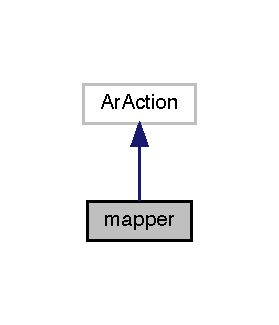
\includegraphics[width=134pt]{classmapper__inherit__graph}
\end{center}
\end{figure}


Collaboration diagram for mapper\+:\nopagebreak
\begin{figure}[H]
\begin{center}
\leavevmode
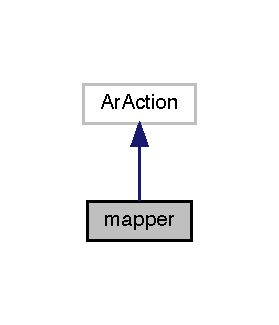
\includegraphics[width=134pt]{classmapper__coll__graph}
\end{center}
\end{figure}
\subsection*{Public Member Functions}
\begin{DoxyCompactItemize}
\item 
\hyperlink{classmapper_a63253379db55193ffc58434c32657270}{mapper} ()
\item 
virtual \hyperlink{classmapper_aab426a3eb8681cf2c1137f658a6802a4}{$\sim$mapper} ()
\item 
virtual Ar\+Action\+Desired $\ast$ \hyperlink{classmapper_a9d8bd0abf6844385c45d8b3ccd7b8e87}{fire} (Ar\+Action\+Desired d)
\end{DoxyCompactItemize}
\subsection*{Public Attributes}
\begin{DoxyCompactItemize}
\item 
Ar\+Action\+Desired \hyperlink{classmapper_ad12cf719b7ef6c4399ca718cdc9f270d}{desired\+State}
\end{DoxyCompactItemize}
\subsection*{Protected Attributes}
\begin{DoxyCompactItemize}
\item 
int \hyperlink{classmapper_a2764f9fead6392132485f3545c18b629}{speed}
\end{DoxyCompactItemize}


\subsection{Detailed Description}


Definition at line 6 of file mapper.\+h.



\subsection{Constructor \& Destructor Documentation}
\mbox{\Hypertarget{classmapper_a63253379db55193ffc58434c32657270}\label{classmapper_a63253379db55193ffc58434c32657270}} 
\index{mapper@{mapper}!mapper@{mapper}}
\index{mapper@{mapper}!mapper@{mapper}}
\subsubsection{\texorpdfstring{mapper()}{mapper()}}
{\footnotesize\ttfamily mapper\+::mapper (\begin{DoxyParamCaption}{ }\end{DoxyParamCaption})}



Definition at line 5 of file mapper.\+cpp.

\mbox{\Hypertarget{classmapper_aab426a3eb8681cf2c1137f658a6802a4}\label{classmapper_aab426a3eb8681cf2c1137f658a6802a4}} 
\index{mapper@{mapper}!````~mapper@{$\sim$mapper}}
\index{````~mapper@{$\sim$mapper}!mapper@{mapper}}
\subsubsection{\texorpdfstring{$\sim$mapper()}{~mapper()}}
{\footnotesize\ttfamily virtual mapper\+::$\sim$mapper (\begin{DoxyParamCaption}{ }\end{DoxyParamCaption})\hspace{0.3cm}{\ttfamily [inline]}, {\ttfamily [virtual]}}



Definition at line 10 of file mapper.\+h.

Here is the call graph for this function\+:\nopagebreak
\begin{figure}[H]
\begin{center}
\leavevmode
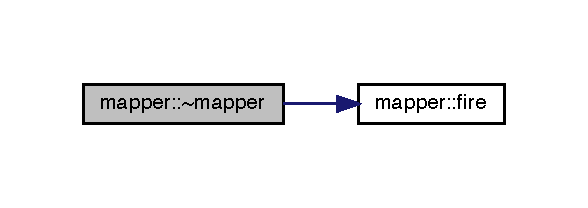
\includegraphics[width=282pt]{classmapper_aab426a3eb8681cf2c1137f658a6802a4_cgraph}
\end{center}
\end{figure}


\subsection{Member Function Documentation}
\mbox{\Hypertarget{classmapper_a9d8bd0abf6844385c45d8b3ccd7b8e87}\label{classmapper_a9d8bd0abf6844385c45d8b3ccd7b8e87}} 
\index{mapper@{mapper}!fire@{fire}}
\index{fire@{fire}!mapper@{mapper}}
\subsubsection{\texorpdfstring{fire()}{fire()}}
{\footnotesize\ttfamily virtual Ar\+Action\+Desired$\ast$ mapper\+::fire (\begin{DoxyParamCaption}\item[{Ar\+Action\+Desired}]{d }\end{DoxyParamCaption})\hspace{0.3cm}{\ttfamily [virtual]}}

Here is the caller graph for this function\+:\nopagebreak
\begin{figure}[H]
\begin{center}
\leavevmode
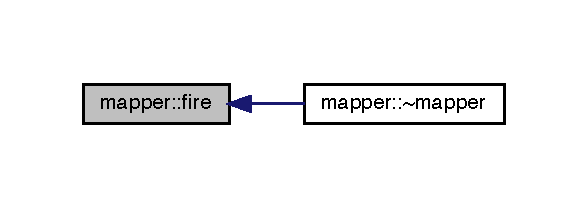
\includegraphics[width=282pt]{classmapper_a9d8bd0abf6844385c45d8b3ccd7b8e87_icgraph}
\end{center}
\end{figure}


\subsection{Member Data Documentation}
\mbox{\Hypertarget{classmapper_ad12cf719b7ef6c4399ca718cdc9f270d}\label{classmapper_ad12cf719b7ef6c4399ca718cdc9f270d}} 
\index{mapper@{mapper}!desired\+State@{desired\+State}}
\index{desired\+State@{desired\+State}!mapper@{mapper}}
\subsubsection{\texorpdfstring{desired\+State}{desiredState}}
{\footnotesize\ttfamily Ar\+Action\+Desired mapper\+::desired\+State}



Definition at line 12 of file mapper.\+h.

\mbox{\Hypertarget{classmapper_a2764f9fead6392132485f3545c18b629}\label{classmapper_a2764f9fead6392132485f3545c18b629}} 
\index{mapper@{mapper}!speed@{speed}}
\index{speed@{speed}!mapper@{mapper}}
\subsubsection{\texorpdfstring{speed}{speed}}
{\footnotesize\ttfamily int mapper\+::speed\hspace{0.3cm}{\ttfamily [protected]}}



Definition at line 14 of file mapper.\+h.



The documentation for this class was generated from the following files\+:\begin{DoxyCompactItemize}
\item 
Brain\+Harmonics/\hyperlink{mapper_8h}{mapper.\+h}\item 
Brain\+Harmonics/\hyperlink{mapper_8cpp}{mapper.\+cpp}\end{DoxyCompactItemize}

\hypertarget{classMatter}{}\section{Matter Class Reference}
\label{classMatter}\index{Matter@{Matter}}


{\ttfamily \#include $<$matter.\+h$>$}

Inheritance diagram for Matter\+:\begin{figure}[H]
\begin{center}
\leavevmode
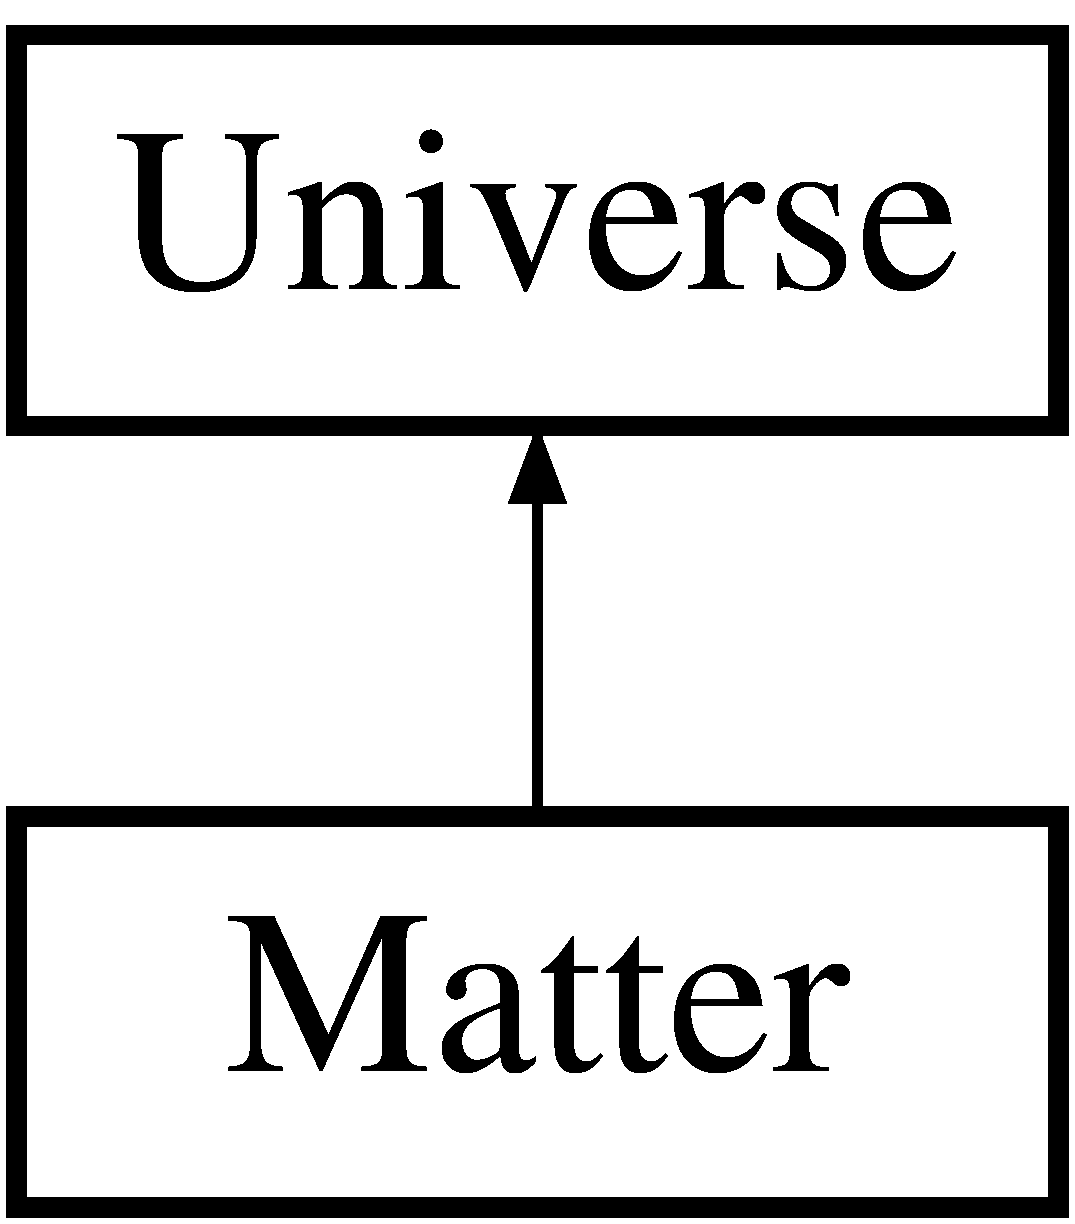
\includegraphics[height=2.000000cm]{classMatter}
\end{center}
\end{figure}
\subsection*{Public Member Functions}
\begin{DoxyCompactItemize}
\item 
\mbox{\hyperlink{classMatter_ac2dc2f5eeef03d3bdf41a68334ae49b4}{Matter}} ()
\item 
\mbox{\hyperlink{classMatter_a7e2328c2a17dcc7b57af59d1d5c9ea96}{Matter}} (unsigned int object\+\_\+type)
\item 
\mbox{\hyperlink{classMatter_ae15b0b8d811fb2ffd01ea039777d1b95}{Matter}} (unsigned int object\+\_\+type, std\+::chrono\+::time\+\_\+point$<$ \mbox{\hyperlink{universe_8h_a0ef8d951d1ca5ab3cfaf7ab4c7a6fd80}{Clock}} $>$ event\+\_\+time)
\item 
\mbox{\hyperlink{classMatter_a724543a0439d3099f5fc0eae68110b75}{Matter}} (unsigned int object\+\_\+type, std\+::chrono\+::time\+\_\+point$<$ \mbox{\hyperlink{universe_8h_a0ef8d951d1ca5ab3cfaf7ab4c7a6fd80}{Clock}} $>$ event\+\_\+time, \mbox{\hyperlink{classUniverse}{Universe}} \&universe\+\_\+connector)
\item 
virtual \mbox{\hyperlink{classMatter_a646fca3d4176950aed6173e1378664e3}{$\sim$\+Matter}} ()
\item 
bool \mbox{\hyperlink{classMatter_adfd93d323e43d09fa8d8b7cdd2258611}{Reset\+Parameters}} (std\+::chrono\+::time\+\_\+point$<$ \mbox{\hyperlink{universe_8h_a0ef8d951d1ca5ab3cfaf7ab4c7a6fd80}{Clock}} $>$ event\+\_\+time)
\item 
unsigned int \mbox{\hyperlink{classMatter_ac667a2f3b6d5d2ce8469efe1596cdd62}{Get\+Counter}} (std\+::chrono\+::time\+\_\+point$<$ \mbox{\hyperlink{universe_8h_a0ef8d951d1ca5ab3cfaf7ab4c7a6fd80}{Clock}} $>$ event\+\_\+time)
\item 
void \mbox{\hyperlink{classMatter_a514b4a64589eb3fbc3db6b3b356bd687}{Set\+Counter}} (std\+::chrono\+::time\+\_\+point$<$ \mbox{\hyperlink{universe_8h_a0ef8d951d1ca5ab3cfaf7ab4c7a6fd80}{Clock}} $>$ event\+\_\+time, unsigned int val)
\item 
int \mbox{\hyperlink{classMatter_a56898dd51e5a675832bc82de285b3ef7}{Update}} (std\+::chrono\+::time\+\_\+point$<$ \mbox{\hyperlink{universe_8h_a0ef8d951d1ca5ab3cfaf7ab4c7a6fd80}{Clock}} $>$ event\+\_\+time)
\end{DoxyCompactItemize}
\subsection*{Private Attributes}
\begin{DoxyCompactItemize}
\item 
unsigned int \mbox{\hyperlink{classMatter_aaa9afd2c589feed49f7ac3c8ba1e2ae1}{matter\+\_\+counter}}
\begin{DoxyCompactList}\small\item\em Member variable \char`\"{}matter\+\_\+counter\char`\"{}. \end{DoxyCompactList}\item 
int \mbox{\hyperlink{classMatter_a03bdd796ec849635193fea2f7e6c3e03}{matter\+\_\+type}}
\item 
std\+::chrono\+::time\+\_\+point$<$ \mbox{\hyperlink{universe_8h_a0ef8d951d1ca5ab3cfaf7ab4c7a6fd80}{Clock}} $>$ \mbox{\hyperlink{classMatter_abce05beb1ad51f3b4bddefcd35731a2f}{time\+\_\+object\+\_\+created}}
\item 
std\+::chrono\+::time\+\_\+point$<$ \mbox{\hyperlink{universe_8h_a0ef8d951d1ca5ab3cfaf7ab4c7a6fd80}{Clock}} $>$ \mbox{\hyperlink{classMatter_a4e4a62161c81e4c2ba70b3ff41b95b56}{previous\+\_\+event\+\_\+time}}
\item 
int \mbox{\hyperlink{classMatter_af50b6a357e77f2cd81264234148686ba}{duration\+\_\+since\+\_\+last\+\_\+event}}
\item 
bool \mbox{\hyperlink{classMatter_a570c6b0584f1e67d24f0a7661d3cc790}{object\+\_\+initialised}}
\item 
bool \mbox{\hyperlink{classMatter_a51eb653f21084e8d7494ea87059072ea}{object\+\_\+disabled}}
\end{DoxyCompactItemize}
\subsection*{Friends}
\begin{DoxyCompactItemize}
\item 
class \mbox{\hyperlink{classMatter_a9bc6eb2a4c20ce83728a7c9a31b91f19}{Composite\+Force\+Particle}}
\end{DoxyCompactItemize}
\subsection*{Additional Inherited Members}


\subsection{Constructor \& Destructor Documentation}
\mbox{\Hypertarget{classMatter_ac2dc2f5eeef03d3bdf41a68334ae49b4}\label{classMatter_ac2dc2f5eeef03d3bdf41a68334ae49b4}} 
\index{Matter@{Matter}!Matter@{Matter}}
\index{Matter@{Matter}!Matter@{Matter}}
\subsubsection{\texorpdfstring{Matter()}{Matter()}\hspace{0.1cm}{\footnotesize\ttfamily [1/4]}}
{\footnotesize\ttfamily Matter\+::\+Matter (\begin{DoxyParamCaption}{ }\end{DoxyParamCaption})\hspace{0.3cm}{\ttfamily [inline]}}

\mbox{\Hypertarget{classMatter_a7e2328c2a17dcc7b57af59d1d5c9ea96}\label{classMatter_a7e2328c2a17dcc7b57af59d1d5c9ea96}} 
\index{Matter@{Matter}!Matter@{Matter}}
\index{Matter@{Matter}!Matter@{Matter}}
\subsubsection{\texorpdfstring{Matter()}{Matter()}\hspace{0.1cm}{\footnotesize\ttfamily [2/4]}}
{\footnotesize\ttfamily Matter\+::\+Matter (\begin{DoxyParamCaption}\item[{unsigned int}]{object\+\_\+type }\end{DoxyParamCaption})\hspace{0.3cm}{\ttfamily [inline]}}

\mbox{\Hypertarget{classMatter_ae15b0b8d811fb2ffd01ea039777d1b95}\label{classMatter_ae15b0b8d811fb2ffd01ea039777d1b95}} 
\index{Matter@{Matter}!Matter@{Matter}}
\index{Matter@{Matter}!Matter@{Matter}}
\subsubsection{\texorpdfstring{Matter()}{Matter()}\hspace{0.1cm}{\footnotesize\ttfamily [3/4]}}
{\footnotesize\ttfamily Matter\+::\+Matter (\begin{DoxyParamCaption}\item[{unsigned int}]{object\+\_\+type,  }\item[{std\+::chrono\+::time\+\_\+point$<$ \mbox{\hyperlink{universe_8h_a0ef8d951d1ca5ab3cfaf7ab4c7a6fd80}{Clock}} $>$}]{event\+\_\+time }\end{DoxyParamCaption})\hspace{0.3cm}{\ttfamily [inline]}}

\mbox{\Hypertarget{classMatter_a724543a0439d3099f5fc0eae68110b75}\label{classMatter_a724543a0439d3099f5fc0eae68110b75}} 
\index{Matter@{Matter}!Matter@{Matter}}
\index{Matter@{Matter}!Matter@{Matter}}
\subsubsection{\texorpdfstring{Matter()}{Matter()}\hspace{0.1cm}{\footnotesize\ttfamily [4/4]}}
{\footnotesize\ttfamily Matter\+::\+Matter (\begin{DoxyParamCaption}\item[{unsigned int}]{object\+\_\+type,  }\item[{std\+::chrono\+::time\+\_\+point$<$ \mbox{\hyperlink{universe_8h_a0ef8d951d1ca5ab3cfaf7ab4c7a6fd80}{Clock}} $>$}]{event\+\_\+time,  }\item[{\mbox{\hyperlink{classUniverse}{Universe}} \&}]{universe\+\_\+connector }\end{DoxyParamCaption})\hspace{0.3cm}{\ttfamily [inline]}}

\mbox{\Hypertarget{classMatter_a646fca3d4176950aed6173e1378664e3}\label{classMatter_a646fca3d4176950aed6173e1378664e3}} 
\index{Matter@{Matter}!````~Matter@{$\sim$\+Matter}}
\index{````~Matter@{$\sim$\+Matter}!Matter@{Matter}}
\subsubsection{\texorpdfstring{$\sim$\+Matter()}{~Matter()}}
{\footnotesize\ttfamily virtual Matter\+::$\sim$\+Matter (\begin{DoxyParamCaption}{ }\end{DoxyParamCaption})\hspace{0.3cm}{\ttfamily [inline]}, {\ttfamily [virtual]}}

Default destructor 

\subsection{Member Function Documentation}
\mbox{\Hypertarget{classMatter_ac667a2f3b6d5d2ce8469efe1596cdd62}\label{classMatter_ac667a2f3b6d5d2ce8469efe1596cdd62}} 
\index{Matter@{Matter}!Get\+Counter@{Get\+Counter}}
\index{Get\+Counter@{Get\+Counter}!Matter@{Matter}}
\subsubsection{\texorpdfstring{Get\+Counter()}{GetCounter()}}
{\footnotesize\ttfamily unsigned int Matter\+::\+Get\+Counter (\begin{DoxyParamCaption}\item[{std\+::chrono\+::time\+\_\+point$<$ \mbox{\hyperlink{universe_8h_a0ef8d951d1ca5ab3cfaf7ab4c7a6fd80}{Clock}} $>$}]{event\+\_\+time }\end{DoxyParamCaption})\hspace{0.3cm}{\ttfamily [inline]}}

\mbox{\Hypertarget{classMatter_adfd93d323e43d09fa8d8b7cdd2258611}\label{classMatter_adfd93d323e43d09fa8d8b7cdd2258611}} 
\index{Matter@{Matter}!Reset\+Parameters@{Reset\+Parameters}}
\index{Reset\+Parameters@{Reset\+Parameters}!Matter@{Matter}}
\subsubsection{\texorpdfstring{Reset\+Parameters()}{ResetParameters()}}
{\footnotesize\ttfamily bool Matter\+::\+Reset\+Parameters (\begin{DoxyParamCaption}\item[{std\+::chrono\+::time\+\_\+point$<$ \mbox{\hyperlink{universe_8h_a0ef8d951d1ca5ab3cfaf7ab4c7a6fd80}{Clock}} $>$}]{event\+\_\+time }\end{DoxyParamCaption})}

\mbox{\Hypertarget{classMatter_a514b4a64589eb3fbc3db6b3b356bd687}\label{classMatter_a514b4a64589eb3fbc3db6b3b356bd687}} 
\index{Matter@{Matter}!Set\+Counter@{Set\+Counter}}
\index{Set\+Counter@{Set\+Counter}!Matter@{Matter}}
\subsubsection{\texorpdfstring{Set\+Counter()}{SetCounter()}}
{\footnotesize\ttfamily void Matter\+::\+Set\+Counter (\begin{DoxyParamCaption}\item[{std\+::chrono\+::time\+\_\+point$<$ \mbox{\hyperlink{universe_8h_a0ef8d951d1ca5ab3cfaf7ab4c7a6fd80}{Clock}} $>$}]{event\+\_\+time,  }\item[{unsigned int}]{val }\end{DoxyParamCaption})\hspace{0.3cm}{\ttfamily [inline]}, {\ttfamily [virtual]}}



Reimplemented from \mbox{\hyperlink{classUniverse_aa22202ae740eb1355529afcb13285e91}{Universe}}.

\mbox{\Hypertarget{classMatter_a56898dd51e5a675832bc82de285b3ef7}\label{classMatter_a56898dd51e5a675832bc82de285b3ef7}} 
\index{Matter@{Matter}!Update@{Update}}
\index{Update@{Update}!Matter@{Matter}}
\subsubsection{\texorpdfstring{Update()}{Update()}}
{\footnotesize\ttfamily int Matter\+::\+Update (\begin{DoxyParamCaption}\item[{std\+::chrono\+::time\+\_\+point$<$ \mbox{\hyperlink{universe_8h_a0ef8d951d1ca5ab3cfaf7ab4c7a6fd80}{Clock}} $>$}]{event\+\_\+time }\end{DoxyParamCaption})}



\subsection{Friends And Related Function Documentation}
\mbox{\Hypertarget{classMatter_a9bc6eb2a4c20ce83728a7c9a31b91f19}\label{classMatter_a9bc6eb2a4c20ce83728a7c9a31b91f19}} 
\index{Matter@{Matter}!Composite\+Force\+Particle@{Composite\+Force\+Particle}}
\index{Composite\+Force\+Particle@{Composite\+Force\+Particle}!Matter@{Matter}}
\subsubsection{\texorpdfstring{Composite\+Force\+Particle}{CompositeForceParticle}}
{\footnotesize\ttfamily friend class \mbox{\hyperlink{classCompositeForceParticle}{Composite\+Force\+Particle}}\hspace{0.3cm}{\ttfamily [friend]}}



\subsection{Member Data Documentation}
\mbox{\Hypertarget{classMatter_af50b6a357e77f2cd81264234148686ba}\label{classMatter_af50b6a357e77f2cd81264234148686ba}} 
\index{Matter@{Matter}!duration\+\_\+since\+\_\+last\+\_\+event@{duration\+\_\+since\+\_\+last\+\_\+event}}
\index{duration\+\_\+since\+\_\+last\+\_\+event@{duration\+\_\+since\+\_\+last\+\_\+event}!Matter@{Matter}}
\subsubsection{\texorpdfstring{duration\+\_\+since\+\_\+last\+\_\+event}{duration\_since\_last\_event}}
{\footnotesize\ttfamily int Matter\+::duration\+\_\+since\+\_\+last\+\_\+event\hspace{0.3cm}{\ttfamily [private]}}

\mbox{\Hypertarget{classMatter_aaa9afd2c589feed49f7ac3c8ba1e2ae1}\label{classMatter_aaa9afd2c589feed49f7ac3c8ba1e2ae1}} 
\index{Matter@{Matter}!matter\+\_\+counter@{matter\+\_\+counter}}
\index{matter\+\_\+counter@{matter\+\_\+counter}!Matter@{Matter}}
\subsubsection{\texorpdfstring{matter\+\_\+counter}{matter\_counter}}
{\footnotesize\ttfamily unsigned int Matter\+::matter\+\_\+counter\hspace{0.3cm}{\ttfamily [private]}}



Member variable \char`\"{}matter\+\_\+counter\char`\"{}. 

\mbox{\Hypertarget{classMatter_a03bdd796ec849635193fea2f7e6c3e03}\label{classMatter_a03bdd796ec849635193fea2f7e6c3e03}} 
\index{Matter@{Matter}!matter\+\_\+type@{matter\+\_\+type}}
\index{matter\+\_\+type@{matter\+\_\+type}!Matter@{Matter}}
\subsubsection{\texorpdfstring{matter\+\_\+type}{matter\_type}}
{\footnotesize\ttfamily int Matter\+::matter\+\_\+type\hspace{0.3cm}{\ttfamily [private]}}

\mbox{\Hypertarget{classMatter_a51eb653f21084e8d7494ea87059072ea}\label{classMatter_a51eb653f21084e8d7494ea87059072ea}} 
\index{Matter@{Matter}!object\+\_\+disabled@{object\+\_\+disabled}}
\index{object\+\_\+disabled@{object\+\_\+disabled}!Matter@{Matter}}
\subsubsection{\texorpdfstring{object\+\_\+disabled}{object\_disabled}}
{\footnotesize\ttfamily bool Matter\+::object\+\_\+disabled\hspace{0.3cm}{\ttfamily [private]}}

\mbox{\Hypertarget{classMatter_a570c6b0584f1e67d24f0a7661d3cc790}\label{classMatter_a570c6b0584f1e67d24f0a7661d3cc790}} 
\index{Matter@{Matter}!object\+\_\+initialised@{object\+\_\+initialised}}
\index{object\+\_\+initialised@{object\+\_\+initialised}!Matter@{Matter}}
\subsubsection{\texorpdfstring{object\+\_\+initialised}{object\_initialised}}
{\footnotesize\ttfamily bool Matter\+::object\+\_\+initialised\hspace{0.3cm}{\ttfamily [private]}}

\mbox{\Hypertarget{classMatter_a4e4a62161c81e4c2ba70b3ff41b95b56}\label{classMatter_a4e4a62161c81e4c2ba70b3ff41b95b56}} 
\index{Matter@{Matter}!previous\+\_\+event\+\_\+time@{previous\+\_\+event\+\_\+time}}
\index{previous\+\_\+event\+\_\+time@{previous\+\_\+event\+\_\+time}!Matter@{Matter}}
\subsubsection{\texorpdfstring{previous\+\_\+event\+\_\+time}{previous\_event\_time}}
{\footnotesize\ttfamily std\+::chrono\+::time\+\_\+point$<$\mbox{\hyperlink{universe_8h_a0ef8d951d1ca5ab3cfaf7ab4c7a6fd80}{Clock}}$>$ Matter\+::previous\+\_\+event\+\_\+time\hspace{0.3cm}{\ttfamily [private]}}

\mbox{\Hypertarget{classMatter_abce05beb1ad51f3b4bddefcd35731a2f}\label{classMatter_abce05beb1ad51f3b4bddefcd35731a2f}} 
\index{Matter@{Matter}!time\+\_\+object\+\_\+created@{time\+\_\+object\+\_\+created}}
\index{time\+\_\+object\+\_\+created@{time\+\_\+object\+\_\+created}!Matter@{Matter}}
\subsubsection{\texorpdfstring{time\+\_\+object\+\_\+created}{time\_object\_created}}
{\footnotesize\ttfamily std\+::chrono\+::time\+\_\+point$<$\mbox{\hyperlink{universe_8h_a0ef8d951d1ca5ab3cfaf7ab4c7a6fd80}{Clock}}$>$ Matter\+::time\+\_\+object\+\_\+created\hspace{0.3cm}{\ttfamily [private]}}



The documentation for this class was generated from the following files\+:\begin{DoxyCompactItemize}
\item 
/home/pbisaacs/\+Developer/\+Brain\+Harmonics/\mbox{\hyperlink{matter_8h}{matter.\+h}}\item 
/home/pbisaacs/\+Developer/\+Brain\+Harmonics/\mbox{\hyperlink{matter_8cc}{matter.\+cc}}\end{DoxyCompactItemize}

\hypertarget{classMembrane}{}\section{Membrane Class Reference}
\label{classMembrane}\index{Membrane@{Membrane}}


{\ttfamily \#include $<$membrane.\+h$>$}

Inheritance diagram for Membrane\+:\begin{figure}[H]
\begin{center}
\leavevmode
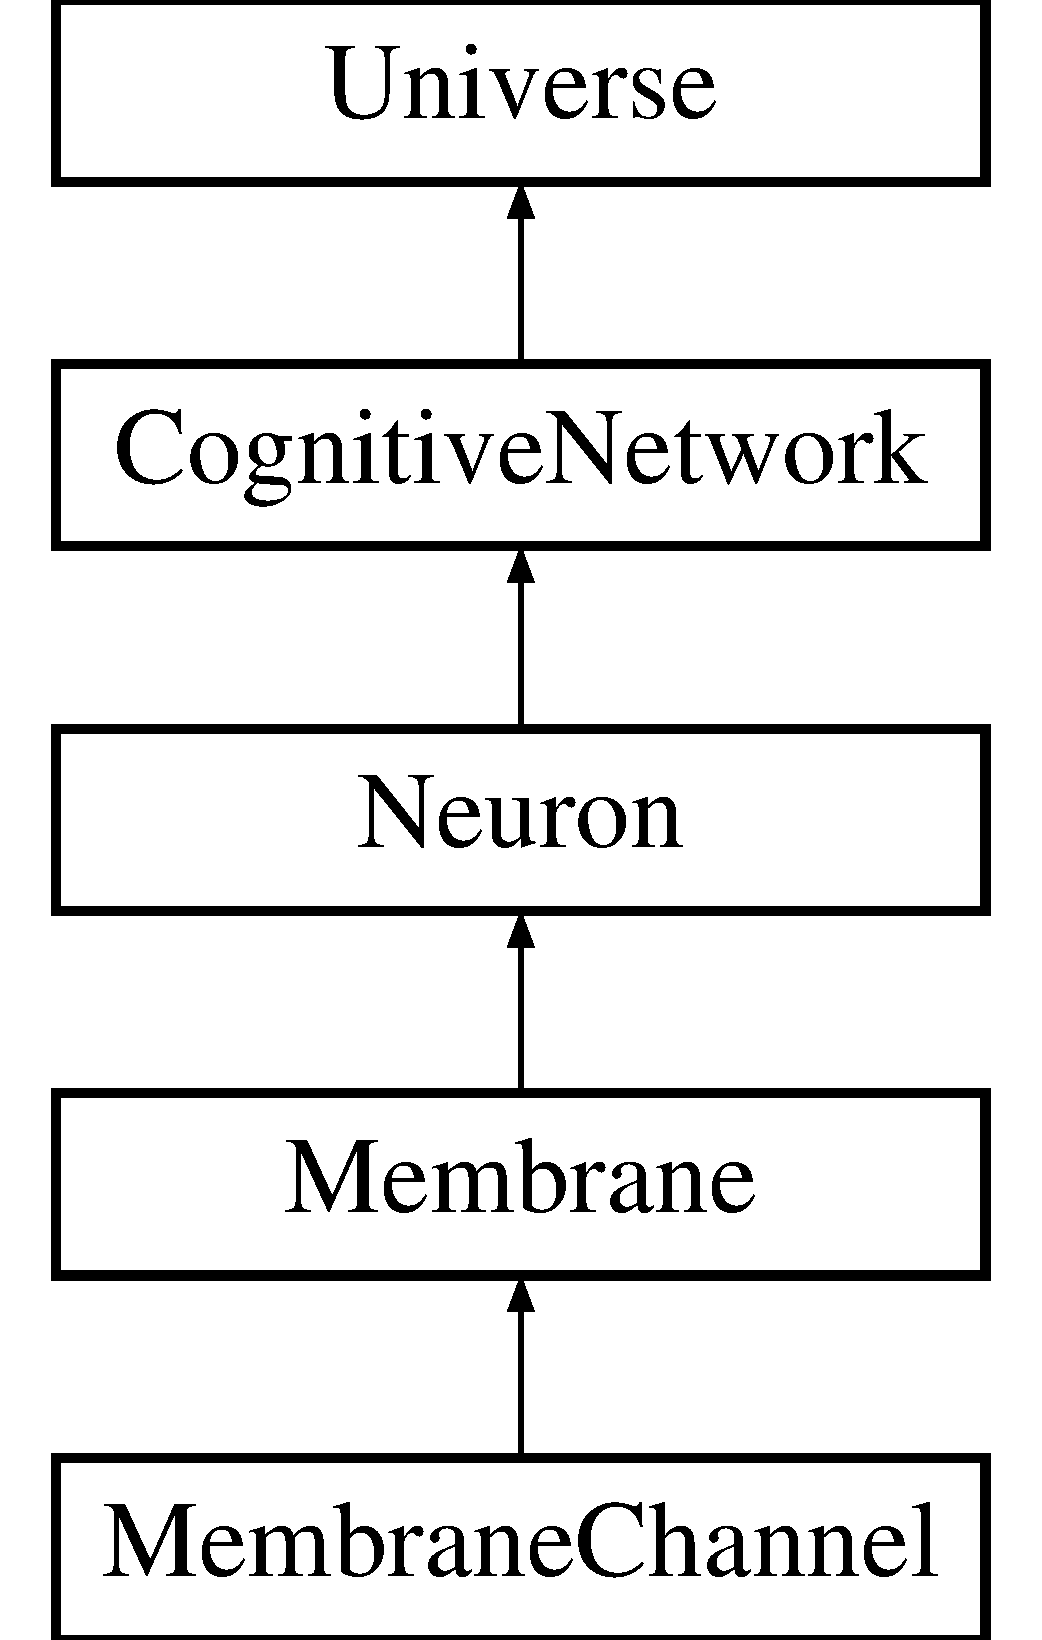
\includegraphics[height=5.000000cm]{classMembrane}
\end{center}
\end{figure}
\subsection*{Public Member Functions}
\begin{DoxyCompactItemize}
\item 
\mbox{\hyperlink{classMembrane_ae3db1e55d9a535226bfd41c2a9ac1f0c}{Membrane}} ()
\item 
\mbox{\hyperlink{classMembrane_a9e45fcb5a4e791f2697fce4d9fa78a3f}{Membrane}} (unsigned int object\+\_\+type)
\item 
\mbox{\hyperlink{classMembrane_afeb8292866a69bdc2b9be6dcd902b519}{Membrane}} (unsigned int object\+\_\+type, std\+::chrono\+::time\+\_\+point$<$ \mbox{\hyperlink{universe_8h_a0ef8d951d1ca5ab3cfaf7ab4c7a6fd80}{Clock}} $>$ event\+\_\+time)
\item 
\mbox{\hyperlink{classMembrane_a8d61894d90a7f63e427cd8b1a5eca380}{Membrane}} (unsigned int object\+\_\+type, std\+::chrono\+::time\+\_\+point$<$ \mbox{\hyperlink{universe_8h_a0ef8d951d1ca5ab3cfaf7ab4c7a6fd80}{Clock}} $>$ event\+\_\+time, \mbox{\hyperlink{classNeuron}{Neuron}} \&neuron\+\_\+connector)
\item 
virtual \mbox{\hyperlink{classMembrane_a8765daf8038c1e992e3ea3752db0042f}{$\sim$\+Membrane}} ()
\item 
double \mbox{\hyperlink{classMembrane_a8c3593b0747495c412bf2d99b7b10104}{Time\+Function}} (double time\+Delay, double time\+Dilation)
\item 
unsigned int \mbox{\hyperlink{classMembrane_a85f8b2633ff32f79b6fbb466ce690858}{Get\+Counter}} (std\+::chrono\+::time\+\_\+point$<$ \mbox{\hyperlink{universe_8h_a0ef8d951d1ca5ab3cfaf7ab4c7a6fd80}{Clock}} $>$ event\+\_\+time)
\item 
double \mbox{\hyperlink{classMembrane_a50d39c596daa7af8da7dd7215d3a32ba}{Get\+Energy}} (std\+::chrono\+::time\+\_\+point$<$ \mbox{\hyperlink{universe_8h_a0ef8d951d1ca5ab3cfaf7ab4c7a6fd80}{Clock}} $>$ event\+\_\+time)
\item 
double \mbox{\hyperlink{classMembrane_a00e038f0023186139467d490c6cd38a3}{Get\+Energy\+Inc}} (std\+::chrono\+::time\+\_\+point$<$ \mbox{\hyperlink{universe_8h_a0ef8d951d1ca5ab3cfaf7ab4c7a6fd80}{Clock}} $>$ event\+\_\+time)
\item 
double \mbox{\hyperlink{classMembrane_a874068c028004d4dde7ec41d999872eb}{Get\+Energy\+Dec}} (std\+::chrono\+::time\+\_\+point$<$ \mbox{\hyperlink{universe_8h_a0ef8d951d1ca5ab3cfaf7ab4c7a6fd80}{Clock}} $>$ event\+\_\+time)
\item 
double \mbox{\hyperlink{classMembrane_ac6c8d1f7348b24e448e8163260500b89}{Get\+Energy\+Leak}} (std\+::chrono\+::time\+\_\+point$<$ \mbox{\hyperlink{universe_8h_a0ef8d951d1ca5ab3cfaf7ab4c7a6fd80}{Clock}} $>$ event\+\_\+time)
\item 
double \mbox{\hyperlink{classMembrane_a7ce7398888bdad73ac848a2362261acf}{Get\+Energy\+Threshold}} (std\+::chrono\+::time\+\_\+point$<$ \mbox{\hyperlink{universe_8h_a0ef8d951d1ca5ab3cfaf7ab4c7a6fd80}{Clock}} $>$ event\+\_\+time)
\item 
int \mbox{\hyperlink{classMembrane_a270278dd346edfe8c7bbd4c48929fdd5}{Get\+Membrane\+Channel\+Pool}} (std\+::chrono\+::time\+\_\+point$<$ \mbox{\hyperlink{universe_8h_a0ef8d951d1ca5ab3cfaf7ab4c7a6fd80}{Clock}} $>$ event\+\_\+time)
\item 
void \mbox{\hyperlink{classMembrane_aeda845ea9577e6a07690acad22ef375f}{Set\+Membrane\+Channel\+Pool}} (std\+::chrono\+::time\+\_\+point$<$ \mbox{\hyperlink{universe_8h_a0ef8d951d1ca5ab3cfaf7ab4c7a6fd80}{Clock}} $>$ event\+\_\+time, int set\+\_\+pool)
\item 
void \mbox{\hyperlink{classMembrane_a4bff43b38d7046867f220392a39cc272}{Set\+Counter}} (std\+::chrono\+::time\+\_\+point$<$ \mbox{\hyperlink{universe_8h_a0ef8d951d1ca5ab3cfaf7ab4c7a6fd80}{Clock}} $>$ event\+\_\+time, unsigned int val)
\item 
void \mbox{\hyperlink{classMembrane_a37beeb28761af644bc3a51d3509f14f1}{Set\+Energy}} (std\+::chrono\+::time\+\_\+point$<$ \mbox{\hyperlink{universe_8h_a0ef8d951d1ca5ab3cfaf7ab4c7a6fd80}{Clock}} $>$ event\+\_\+time, double val)
\item 
void \mbox{\hyperlink{classMembrane_abd1c69b9b0260799afd3965c34f881ff}{Set\+Energy\+Inc}} (std\+::chrono\+::time\+\_\+point$<$ \mbox{\hyperlink{universe_8h_a0ef8d951d1ca5ab3cfaf7ab4c7a6fd80}{Clock}} $>$ event\+\_\+time, double val)
\item 
void \mbox{\hyperlink{classMembrane_acefb2fe781d7316b232614663777cde1}{Set\+Energy\+Dec}} (std\+::chrono\+::time\+\_\+point$<$ \mbox{\hyperlink{universe_8h_a0ef8d951d1ca5ab3cfaf7ab4c7a6fd80}{Clock}} $>$ event\+\_\+time, double val)
\item 
void \mbox{\hyperlink{classMembrane_a96618ef2c05a8af5d6bd8606c9b8eae8}{Set\+Energy\+Leak}} (std\+::chrono\+::time\+\_\+point$<$ \mbox{\hyperlink{universe_8h_a0ef8d951d1ca5ab3cfaf7ab4c7a6fd80}{Clock}} $>$ event\+\_\+time, double val)
\item 
void \mbox{\hyperlink{classMembrane_a6d0b96fb6d823cc113dd56b8889b1544}{Set\+Energy\+Threshold}} (std\+::chrono\+::time\+\_\+point$<$ \mbox{\hyperlink{universe_8h_a0ef8d951d1ca5ab3cfaf7ab4c7a6fd80}{Clock}} $>$ event\+\_\+time, double val)
\item 
void \mbox{\hyperlink{classMembrane_a5ba2bcb906f3984b28f1030207e106ad}{Set\+Object\+Type}} (std\+::chrono\+::time\+\_\+point$<$ \mbox{\hyperlink{universe_8h_a0ef8d951d1ca5ab3cfaf7ab4c7a6fd80}{Clock}} $>$ event\+\_\+time, int object\+\_\+type)
\item 
bool \mbox{\hyperlink{classMembrane_a9c49462cf63495381a52e2defc80b1e4}{Reset\+Parameters}} (std\+::chrono\+::time\+\_\+point$<$ \mbox{\hyperlink{universe_8h_a0ef8d951d1ca5ab3cfaf7ab4c7a6fd80}{Clock}} $>$ event\+\_\+time)
\item 
\mbox{\hyperlink{classMembrane}{Membrane}} $\ast$ \mbox{\hyperlink{classMembrane_a589b56529ac634a52b2a5fc78d356973}{Create\+Membrane\+Channel}} (std\+::chrono\+::time\+\_\+point$<$ \mbox{\hyperlink{universe_8h_a0ef8d951d1ca5ab3cfaf7ab4c7a6fd80}{Clock}} $>$ event\+\_\+time)
\item 
std\+::vector$<$ \mbox{\hyperlink{classMembrane}{Membrane}} $\ast$ $>$ \mbox{\hyperlink{classMembrane_a72987fae41e552af5befcd9a62aa6e46}{Create\+Membrane\+Channels}} (std\+::chrono\+::time\+\_\+point$<$ \mbox{\hyperlink{universe_8h_a0ef8d951d1ca5ab3cfaf7ab4c7a6fd80}{Clock}} $>$ event\+\_\+time, int quantity)
\item 
\mbox{\hyperlink{classMembrane}{Membrane}} $\ast$ \mbox{\hyperlink{classMembrane_a9514ca4d4378e6467d2059a9d5f9b99b}{Clone\+Membrane\+Channel}} (std\+::chrono\+::time\+\_\+point$<$ \mbox{\hyperlink{universe_8h_a0ef8d951d1ca5ab3cfaf7ab4c7a6fd80}{Clock}} $>$ event\+\_\+time, \mbox{\hyperlink{classMembrane}{Membrane}} $\ast$clone\+\_\+object, double perfection\+\_\+membership)
\item 
std\+::vector$<$ \mbox{\hyperlink{classMembrane}{Membrane}} $\ast$ $>$ \mbox{\hyperlink{classMembrane_aa9958ea461092c0d2aceb07c9c34373c}{Clone\+Membrane\+Channels}} (std\+::chrono\+::time\+\_\+point$<$ \mbox{\hyperlink{universe_8h_a0ef8d951d1ca5ab3cfaf7ab4c7a6fd80}{Clock}} $>$ event\+\_\+time, std\+::vector$<$ \mbox{\hyperlink{classMembrane}{Membrane}} $\ast$$>$ cloning\+\_\+list, double perfection\+\_\+membership)
\item 
\mbox{\hyperlink{classMembrane}{Membrane}} $\ast$ \mbox{\hyperlink{classMembrane_a12413d933a62b3bbb7931c6ab25de7de}{Destroy\+Membrane\+Channel}} (std\+::chrono\+::time\+\_\+point$<$ \mbox{\hyperlink{universe_8h_a0ef8d951d1ca5ab3cfaf7ab4c7a6fd80}{Clock}} $>$ event\+\_\+time, \mbox{\hyperlink{classMembrane}{Membrane}} $\ast$destroy\+\_\+object)
\item 
std\+::vector$<$ \mbox{\hyperlink{classMembrane}{Membrane}} $\ast$ $>$ \mbox{\hyperlink{classMembrane_aea71c4443f2fc22359ac3f770ff7755e}{Destroy\+Membrane\+Channels}} (std\+::chrono\+::time\+\_\+point$<$ \mbox{\hyperlink{universe_8h_a0ef8d951d1ca5ab3cfaf7ab4c7a6fd80}{Clock}} $>$ event\+\_\+time, std\+::vector$<$ \mbox{\hyperlink{classMembrane}{Membrane}} $\ast$$>$ destruction\+\_\+list)
\item 
\mbox{\hyperlink{classMembrane}{Membrane}} $\ast$ \mbox{\hyperlink{classMembrane_a3e3b4f55f028541e7513f826d01a689a}{Add\+Membrane\+Channel}} (std\+::chrono\+::time\+\_\+point$<$ \mbox{\hyperlink{universe_8h_a0ef8d951d1ca5ab3cfaf7ab4c7a6fd80}{Clock}} $>$ event\+\_\+time, \mbox{\hyperlink{classMembrane}{Membrane}} $\ast$add\+\_\+object)
\item 
std\+::vector$<$ \mbox{\hyperlink{classMembrane}{Membrane}} $\ast$ $>$ \mbox{\hyperlink{classMembrane_aab591875e3266d6c5af0f7c5f7f21e8f}{Add\+Membrane\+Channels}} (std\+::chrono\+::time\+\_\+point$<$ \mbox{\hyperlink{universe_8h_a0ef8d951d1ca5ab3cfaf7ab4c7a6fd80}{Clock}} $>$ event\+\_\+time, std\+::vector$<$ \mbox{\hyperlink{classMembrane}{Membrane}} $\ast$$>$ add\+\_\+objects)
\item 
\mbox{\hyperlink{classMembrane}{Membrane}} $\ast$ \mbox{\hyperlink{classMembrane_a36d6927c8869cc752b55623dac661107}{Remove\+Membrane\+Channel}} (std\+::chrono\+::time\+\_\+point$<$ \mbox{\hyperlink{universe_8h_a0ef8d951d1ca5ab3cfaf7ab4c7a6fd80}{Clock}} $>$ event\+\_\+time)
\item 
std\+::vector$<$ \mbox{\hyperlink{classMembrane}{Membrane}} $\ast$ $>$ \mbox{\hyperlink{classMembrane_ac33ffd86416112420dc5b0576287c44d}{Remove\+Membrane\+Channels}} (std\+::chrono\+::time\+\_\+point$<$ \mbox{\hyperlink{universe_8h_a0ef8d951d1ca5ab3cfaf7ab4c7a6fd80}{Clock}} $>$ event\+\_\+time, int quantity)
\item 
\mbox{\hyperlink{classMembrane}{Membrane}} $\ast$ \mbox{\hyperlink{classMembrane_a1e2bdb800f0f38254214ea7cbdc06941}{Get\+Membrane\+Channel}} (std\+::chrono\+::time\+\_\+point$<$ \mbox{\hyperlink{universe_8h_a0ef8d951d1ca5ab3cfaf7ab4c7a6fd80}{Clock}} $>$ event\+\_\+time, int selector)
\item 
std\+::vector$<$ \mbox{\hyperlink{classMembrane}{Membrane}} $\ast$ $>$ \mbox{\hyperlink{classMembrane_a7fac2929241b7ff9b8b7f1ec955b2cc5}{Get\+Membrane\+Channels}} (std\+::chrono\+::time\+\_\+point$<$ \mbox{\hyperlink{universe_8h_a0ef8d951d1ca5ab3cfaf7ab4c7a6fd80}{Clock}} $>$ event\+\_\+time)
\item 
int \mbox{\hyperlink{classMembrane_a544742864485b9ac052f3b241ae5c6b4}{Growth}} (std\+::chrono\+::time\+\_\+point$<$ \mbox{\hyperlink{universe_8h_a0ef8d951d1ca5ab3cfaf7ab4c7a6fd80}{Clock}} $>$ event\+\_\+time)
\item 
int \mbox{\hyperlink{classMembrane_a4af9710ea7f0bc6f1b6b6b6462612d51}{Update}} (std\+::chrono\+::time\+\_\+point$<$ \mbox{\hyperlink{universe_8h_a0ef8d951d1ca5ab3cfaf7ab4c7a6fd80}{Clock}} $>$ event\+\_\+time)
\end{DoxyCompactItemize}
\subsection*{Protected Attributes}
\begin{DoxyCompactItemize}
\item 
std\+::vector$<$ \mbox{\hyperlink{classMembrane}{Membrane}} $\ast$ $>$ \mbox{\hyperlink{classMembrane_ad41c9c20d5a1bc279f32f9001dee8c50}{membranechannel\+\_\+list}}
\item 
std\+::vector$<$ \mbox{\hyperlink{classSolid}{Solid}} $\ast$ $>$ \mbox{\hyperlink{classMembrane_a926d35c07f664b60deb6e9f87649fe89}{visualisation\+\_\+list}}
\end{DoxyCompactItemize}
\subsection*{Private Attributes}
\begin{DoxyCompactItemize}
\item 
int \mbox{\hyperlink{classMembrane_a4ae44a3db559cbae5009c1ec4e63016f}{m\+\_\+\+Neuron\+Type}}
\item 
int \mbox{\hyperlink{classMembrane_ac55bb1eede5e5c54f04c72c4d09dd6b4}{membrane\+\_\+type}}
\item 
int \mbox{\hyperlink{classMembrane_a3d0f00801a39053adff2691816a443e7}{m\+\_\+add\+Status}}
\item 
std\+::chrono\+::time\+\_\+point$<$ \mbox{\hyperlink{universe_8h_a0ef8d951d1ca5ab3cfaf7ab4c7a6fd80}{Clock}} $>$ \mbox{\hyperlink{classMembrane_a44eaaa3b258fc5169c1ece8bf7c9ab32}{time\+\_\+object\+\_\+created}}
\item 
std\+::chrono\+::time\+\_\+point$<$ \mbox{\hyperlink{universe_8h_a0ef8d951d1ca5ab3cfaf7ab4c7a6fd80}{Clock}} $>$ \mbox{\hyperlink{classMembrane_a2decce528a2588104fd75465a077aa2f}{previous\+\_\+event\+\_\+time}}
\item 
bool \mbox{\hyperlink{classMembrane_aca7993094a3bc7b7ba03892b61183e6b}{object\+\_\+disabled}}
\item 
bool \mbox{\hyperlink{classMembrane_aaa2bd265c8d1d3c6ac73b04df4f08216}{object\+\_\+initialised}}
\item 
int \mbox{\hyperlink{classMembrane_a7e2df85f4d5a0aff0b02636e35a4aeaf}{duration\+\_\+since\+\_\+last\+\_\+event}}
\item 
double \mbox{\hyperlink{classMembrane_a8049feca4d942ea33837aac2a13d18b3}{m\+\_\+\+Volume}}
\item 
double \mbox{\hyperlink{classMembrane_a8afe483ca9fa8447e1e05d9405571fe0}{m\+\_\+\+Surface\+Area}}
\item 
double \mbox{\hyperlink{classMembrane_a7e7d0df87bbe5f498e9042fcc687c74f}{object\+\_\+size}}
\item 
unsigned int \mbox{\hyperlink{classMembrane_a341a25633aa7a79f20781075b6c0c2bc}{m\+\_\+\+Counter}}
\begin{DoxyCompactList}\small\item\em Member variable \char`\"{}m\+\_\+\+Counter\char`\"{}. \end{DoxyCompactList}\item 
double \mbox{\hyperlink{classMembrane_a19ef43ccffe8974084f4018b7d539d03}{object\+\_\+energy}}
\begin{DoxyCompactList}\small\item\em Member variable \char`\"{}object\+\_\+energy\char`\"{}. \end{DoxyCompactList}\item 
double \mbox{\hyperlink{classMembrane_a013037dc858a1f81ba198434ba13701d}{object\+\_\+energy\+Inc}}
\item 
double \mbox{\hyperlink{classMembrane_a8cda5e365097454dc62f336a479a5777}{object\+\_\+energy\+Dec}}
\item 
double \mbox{\hyperlink{classMembrane_a4e80c2cad8bb2e5f026caf33ce90d7f0}{object\+\_\+energy\+Leak}}
\item 
double \mbox{\hyperlink{classMembrane_aa91a60ecdefc7dd375208bc4f73c6d80}{object\+\_\+energy\+\_\+threshold}}
\item 
double \mbox{\hyperlink{classMembrane_a28a7100c84ccee492664edd47fd206e3}{m\+\_\+\+Time\+Dilation}}
\item 
double \mbox{\hyperlink{classMembrane_ade7f8f4b0839c78f33c95fe90a5187b9}{m\+\_\+\+Time\+Threshold}}
\item 
int \mbox{\hyperlink{classMembrane_a2d39f4e61a2cc3c5b4db5e5ff5689e76}{membranechannel\+\_\+pool}}
\end{DoxyCompactItemize}
\subsection*{Additional Inherited Members}


\subsection{Constructor \& Destructor Documentation}
\mbox{\Hypertarget{classMembrane_ae3db1e55d9a535226bfd41c2a9ac1f0c}\label{classMembrane_ae3db1e55d9a535226bfd41c2a9ac1f0c}} 
\index{Membrane@{Membrane}!Membrane@{Membrane}}
\index{Membrane@{Membrane}!Membrane@{Membrane}}
\subsubsection{\texorpdfstring{Membrane()}{Membrane()}\hspace{0.1cm}{\footnotesize\ttfamily [1/4]}}
{\footnotesize\ttfamily Membrane\+::\+Membrane (\begin{DoxyParamCaption}{ }\end{DoxyParamCaption})\hspace{0.3cm}{\ttfamily [inline]}}

\mbox{\Hypertarget{classMembrane_a9e45fcb5a4e791f2697fce4d9fa78a3f}\label{classMembrane_a9e45fcb5a4e791f2697fce4d9fa78a3f}} 
\index{Membrane@{Membrane}!Membrane@{Membrane}}
\index{Membrane@{Membrane}!Membrane@{Membrane}}
\subsubsection{\texorpdfstring{Membrane()}{Membrane()}\hspace{0.1cm}{\footnotesize\ttfamily [2/4]}}
{\footnotesize\ttfamily Membrane\+::\+Membrane (\begin{DoxyParamCaption}\item[{unsigned int}]{object\+\_\+type }\end{DoxyParamCaption})\hspace{0.3cm}{\ttfamily [inline]}}

\mbox{\Hypertarget{classMembrane_afeb8292866a69bdc2b9be6dcd902b519}\label{classMembrane_afeb8292866a69bdc2b9be6dcd902b519}} 
\index{Membrane@{Membrane}!Membrane@{Membrane}}
\index{Membrane@{Membrane}!Membrane@{Membrane}}
\subsubsection{\texorpdfstring{Membrane()}{Membrane()}\hspace{0.1cm}{\footnotesize\ttfamily [3/4]}}
{\footnotesize\ttfamily Membrane\+::\+Membrane (\begin{DoxyParamCaption}\item[{unsigned int}]{object\+\_\+type,  }\item[{std\+::chrono\+::time\+\_\+point$<$ \mbox{\hyperlink{universe_8h_a0ef8d951d1ca5ab3cfaf7ab4c7a6fd80}{Clock}} $>$}]{event\+\_\+time }\end{DoxyParamCaption})\hspace{0.3cm}{\ttfamily [inline]}}

\mbox{\Hypertarget{classMembrane_a8d61894d90a7f63e427cd8b1a5eca380}\label{classMembrane_a8d61894d90a7f63e427cd8b1a5eca380}} 
\index{Membrane@{Membrane}!Membrane@{Membrane}}
\index{Membrane@{Membrane}!Membrane@{Membrane}}
\subsubsection{\texorpdfstring{Membrane()}{Membrane()}\hspace{0.1cm}{\footnotesize\ttfamily [4/4]}}
{\footnotesize\ttfamily Membrane\+::\+Membrane (\begin{DoxyParamCaption}\item[{unsigned int}]{object\+\_\+type,  }\item[{std\+::chrono\+::time\+\_\+point$<$ \mbox{\hyperlink{universe_8h_a0ef8d951d1ca5ab3cfaf7ab4c7a6fd80}{Clock}} $>$}]{event\+\_\+time,  }\item[{\mbox{\hyperlink{classNeuron}{Neuron}} \&}]{neuron\+\_\+connector }\end{DoxyParamCaption})\hspace{0.3cm}{\ttfamily [inline]}}

\mbox{\Hypertarget{classMembrane_a8765daf8038c1e992e3ea3752db0042f}\label{classMembrane_a8765daf8038c1e992e3ea3752db0042f}} 
\index{Membrane@{Membrane}!````~Membrane@{$\sim$\+Membrane}}
\index{````~Membrane@{$\sim$\+Membrane}!Membrane@{Membrane}}
\subsubsection{\texorpdfstring{$\sim$\+Membrane()}{~Membrane()}}
{\footnotesize\ttfamily virtual Membrane\+::$\sim$\+Membrane (\begin{DoxyParamCaption}{ }\end{DoxyParamCaption})\hspace{0.3cm}{\ttfamily [inline]}, {\ttfamily [virtual]}}

Default destructor 

\subsection{Member Function Documentation}
\mbox{\Hypertarget{classMembrane_a3e3b4f55f028541e7513f826d01a689a}\label{classMembrane_a3e3b4f55f028541e7513f826d01a689a}} 
\index{Membrane@{Membrane}!Add\+Membrane\+Channel@{Add\+Membrane\+Channel}}
\index{Add\+Membrane\+Channel@{Add\+Membrane\+Channel}!Membrane@{Membrane}}
\subsubsection{\texorpdfstring{Add\+Membrane\+Channel()}{AddMembraneChannel()}}
{\footnotesize\ttfamily \mbox{\hyperlink{classMembrane}{Membrane}} $\ast$ Membrane\+::\+Add\+Membrane\+Channel (\begin{DoxyParamCaption}\item[{std\+::chrono\+::time\+\_\+point$<$ \mbox{\hyperlink{universe_8h_a0ef8d951d1ca5ab3cfaf7ab4c7a6fd80}{Clock}} $>$}]{event\+\_\+time,  }\item[{\mbox{\hyperlink{classMembrane}{Membrane}} $\ast$}]{add\+\_\+object }\end{DoxyParamCaption})}

\mbox{\Hypertarget{classMembrane_aab591875e3266d6c5af0f7c5f7f21e8f}\label{classMembrane_aab591875e3266d6c5af0f7c5f7f21e8f}} 
\index{Membrane@{Membrane}!Add\+Membrane\+Channels@{Add\+Membrane\+Channels}}
\index{Add\+Membrane\+Channels@{Add\+Membrane\+Channels}!Membrane@{Membrane}}
\subsubsection{\texorpdfstring{Add\+Membrane\+Channels()}{AddMembraneChannels()}}
{\footnotesize\ttfamily std\+::vector$<$ \mbox{\hyperlink{classMembrane}{Membrane}} $\ast$ $>$ Membrane\+::\+Add\+Membrane\+Channels (\begin{DoxyParamCaption}\item[{std\+::chrono\+::time\+\_\+point$<$ \mbox{\hyperlink{universe_8h_a0ef8d951d1ca5ab3cfaf7ab4c7a6fd80}{Clock}} $>$}]{event\+\_\+time,  }\item[{std\+::vector$<$ \mbox{\hyperlink{classMembrane}{Membrane}} $\ast$$>$}]{add\+\_\+objects }\end{DoxyParamCaption})}

\mbox{\Hypertarget{classMembrane_a9514ca4d4378e6467d2059a9d5f9b99b}\label{classMembrane_a9514ca4d4378e6467d2059a9d5f9b99b}} 
\index{Membrane@{Membrane}!Clone\+Membrane\+Channel@{Clone\+Membrane\+Channel}}
\index{Clone\+Membrane\+Channel@{Clone\+Membrane\+Channel}!Membrane@{Membrane}}
\subsubsection{\texorpdfstring{Clone\+Membrane\+Channel()}{CloneMembraneChannel()}}
{\footnotesize\ttfamily \mbox{\hyperlink{classMembrane}{Membrane}} $\ast$ Membrane\+::\+Clone\+Membrane\+Channel (\begin{DoxyParamCaption}\item[{std\+::chrono\+::time\+\_\+point$<$ \mbox{\hyperlink{universe_8h_a0ef8d951d1ca5ab3cfaf7ab4c7a6fd80}{Clock}} $>$}]{event\+\_\+time,  }\item[{\mbox{\hyperlink{classMembrane}{Membrane}} $\ast$}]{clone\+\_\+object,  }\item[{double}]{perfection\+\_\+membership }\end{DoxyParamCaption})}

\mbox{\Hypertarget{classMembrane_aa9958ea461092c0d2aceb07c9c34373c}\label{classMembrane_aa9958ea461092c0d2aceb07c9c34373c}} 
\index{Membrane@{Membrane}!Clone\+Membrane\+Channels@{Clone\+Membrane\+Channels}}
\index{Clone\+Membrane\+Channels@{Clone\+Membrane\+Channels}!Membrane@{Membrane}}
\subsubsection{\texorpdfstring{Clone\+Membrane\+Channels()}{CloneMembraneChannels()}}
{\footnotesize\ttfamily std\+::vector$<$ \mbox{\hyperlink{classMembrane}{Membrane}} $\ast$ $>$ Membrane\+::\+Clone\+Membrane\+Channels (\begin{DoxyParamCaption}\item[{std\+::chrono\+::time\+\_\+point$<$ \mbox{\hyperlink{universe_8h_a0ef8d951d1ca5ab3cfaf7ab4c7a6fd80}{Clock}} $>$}]{event\+\_\+time,  }\item[{std\+::vector$<$ \mbox{\hyperlink{classMembrane}{Membrane}} $\ast$$>$}]{cloning\+\_\+list,  }\item[{double}]{perfection\+\_\+membership }\end{DoxyParamCaption})}

\mbox{\Hypertarget{classMembrane_a589b56529ac634a52b2a5fc78d356973}\label{classMembrane_a589b56529ac634a52b2a5fc78d356973}} 
\index{Membrane@{Membrane}!Create\+Membrane\+Channel@{Create\+Membrane\+Channel}}
\index{Create\+Membrane\+Channel@{Create\+Membrane\+Channel}!Membrane@{Membrane}}
\subsubsection{\texorpdfstring{Create\+Membrane\+Channel()}{CreateMembraneChannel()}}
{\footnotesize\ttfamily \mbox{\hyperlink{classMembrane}{Membrane}} $\ast$ Membrane\+::\+Create\+Membrane\+Channel (\begin{DoxyParamCaption}\item[{std\+::chrono\+::time\+\_\+point$<$ \mbox{\hyperlink{universe_8h_a0ef8d951d1ca5ab3cfaf7ab4c7a6fd80}{Clock}} $>$}]{event\+\_\+time }\end{DoxyParamCaption})}

\mbox{\Hypertarget{classMembrane_a72987fae41e552af5befcd9a62aa6e46}\label{classMembrane_a72987fae41e552af5befcd9a62aa6e46}} 
\index{Membrane@{Membrane}!Create\+Membrane\+Channels@{Create\+Membrane\+Channels}}
\index{Create\+Membrane\+Channels@{Create\+Membrane\+Channels}!Membrane@{Membrane}}
\subsubsection{\texorpdfstring{Create\+Membrane\+Channels()}{CreateMembraneChannels()}}
{\footnotesize\ttfamily std\+::vector$<$ \mbox{\hyperlink{classMembrane}{Membrane}} $\ast$ $>$ Membrane\+::\+Create\+Membrane\+Channels (\begin{DoxyParamCaption}\item[{std\+::chrono\+::time\+\_\+point$<$ \mbox{\hyperlink{universe_8h_a0ef8d951d1ca5ab3cfaf7ab4c7a6fd80}{Clock}} $>$}]{event\+\_\+time,  }\item[{int}]{quantity }\end{DoxyParamCaption})}

\mbox{\Hypertarget{classMembrane_a12413d933a62b3bbb7931c6ab25de7de}\label{classMembrane_a12413d933a62b3bbb7931c6ab25de7de}} 
\index{Membrane@{Membrane}!Destroy\+Membrane\+Channel@{Destroy\+Membrane\+Channel}}
\index{Destroy\+Membrane\+Channel@{Destroy\+Membrane\+Channel}!Membrane@{Membrane}}
\subsubsection{\texorpdfstring{Destroy\+Membrane\+Channel()}{DestroyMembraneChannel()}}
{\footnotesize\ttfamily \mbox{\hyperlink{classMembrane}{Membrane}} $\ast$ Membrane\+::\+Destroy\+Membrane\+Channel (\begin{DoxyParamCaption}\item[{std\+::chrono\+::time\+\_\+point$<$ \mbox{\hyperlink{universe_8h_a0ef8d951d1ca5ab3cfaf7ab4c7a6fd80}{Clock}} $>$}]{event\+\_\+time,  }\item[{\mbox{\hyperlink{classMembrane}{Membrane}} $\ast$}]{destroy\+\_\+object }\end{DoxyParamCaption})}

\mbox{\Hypertarget{classMembrane_aea71c4443f2fc22359ac3f770ff7755e}\label{classMembrane_aea71c4443f2fc22359ac3f770ff7755e}} 
\index{Membrane@{Membrane}!Destroy\+Membrane\+Channels@{Destroy\+Membrane\+Channels}}
\index{Destroy\+Membrane\+Channels@{Destroy\+Membrane\+Channels}!Membrane@{Membrane}}
\subsubsection{\texorpdfstring{Destroy\+Membrane\+Channels()}{DestroyMembraneChannels()}}
{\footnotesize\ttfamily std\+::vector$<$ \mbox{\hyperlink{classMembrane}{Membrane}} $\ast$ $>$ Membrane\+::\+Destroy\+Membrane\+Channels (\begin{DoxyParamCaption}\item[{std\+::chrono\+::time\+\_\+point$<$ \mbox{\hyperlink{universe_8h_a0ef8d951d1ca5ab3cfaf7ab4c7a6fd80}{Clock}} $>$}]{event\+\_\+time,  }\item[{std\+::vector$<$ \mbox{\hyperlink{classMembrane}{Membrane}} $\ast$$>$}]{destruction\+\_\+list }\end{DoxyParamCaption})}

\mbox{\Hypertarget{classMembrane_a85f8b2633ff32f79b6fbb466ce690858}\label{classMembrane_a85f8b2633ff32f79b6fbb466ce690858}} 
\index{Membrane@{Membrane}!Get\+Counter@{Get\+Counter}}
\index{Get\+Counter@{Get\+Counter}!Membrane@{Membrane}}
\subsubsection{\texorpdfstring{Get\+Counter()}{GetCounter()}}
{\footnotesize\ttfamily unsigned int Membrane\+::\+Get\+Counter (\begin{DoxyParamCaption}\item[{std\+::chrono\+::time\+\_\+point$<$ \mbox{\hyperlink{universe_8h_a0ef8d951d1ca5ab3cfaf7ab4c7a6fd80}{Clock}} $>$}]{event\+\_\+time }\end{DoxyParamCaption})\hspace{0.3cm}{\ttfamily [inline]}}

\mbox{\Hypertarget{classMembrane_a50d39c596daa7af8da7dd7215d3a32ba}\label{classMembrane_a50d39c596daa7af8da7dd7215d3a32ba}} 
\index{Membrane@{Membrane}!Get\+Energy@{Get\+Energy}}
\index{Get\+Energy@{Get\+Energy}!Membrane@{Membrane}}
\subsubsection{\texorpdfstring{Get\+Energy()}{GetEnergy()}}
{\footnotesize\ttfamily double Membrane\+::\+Get\+Energy (\begin{DoxyParamCaption}\item[{std\+::chrono\+::time\+\_\+point$<$ \mbox{\hyperlink{universe_8h_a0ef8d951d1ca5ab3cfaf7ab4c7a6fd80}{Clock}} $>$}]{event\+\_\+time }\end{DoxyParamCaption})\hspace{0.3cm}{\ttfamily [inline]}}

\mbox{\Hypertarget{classMembrane_a874068c028004d4dde7ec41d999872eb}\label{classMembrane_a874068c028004d4dde7ec41d999872eb}} 
\index{Membrane@{Membrane}!Get\+Energy\+Dec@{Get\+Energy\+Dec}}
\index{Get\+Energy\+Dec@{Get\+Energy\+Dec}!Membrane@{Membrane}}
\subsubsection{\texorpdfstring{Get\+Energy\+Dec()}{GetEnergyDec()}}
{\footnotesize\ttfamily double Membrane\+::\+Get\+Energy\+Dec (\begin{DoxyParamCaption}\item[{std\+::chrono\+::time\+\_\+point$<$ \mbox{\hyperlink{universe_8h_a0ef8d951d1ca5ab3cfaf7ab4c7a6fd80}{Clock}} $>$}]{event\+\_\+time }\end{DoxyParamCaption})\hspace{0.3cm}{\ttfamily [inline]}}

\mbox{\Hypertarget{classMembrane_a00e038f0023186139467d490c6cd38a3}\label{classMembrane_a00e038f0023186139467d490c6cd38a3}} 
\index{Membrane@{Membrane}!Get\+Energy\+Inc@{Get\+Energy\+Inc}}
\index{Get\+Energy\+Inc@{Get\+Energy\+Inc}!Membrane@{Membrane}}
\subsubsection{\texorpdfstring{Get\+Energy\+Inc()}{GetEnergyInc()}}
{\footnotesize\ttfamily double Membrane\+::\+Get\+Energy\+Inc (\begin{DoxyParamCaption}\item[{std\+::chrono\+::time\+\_\+point$<$ \mbox{\hyperlink{universe_8h_a0ef8d951d1ca5ab3cfaf7ab4c7a6fd80}{Clock}} $>$}]{event\+\_\+time }\end{DoxyParamCaption})\hspace{0.3cm}{\ttfamily [inline]}}

\mbox{\Hypertarget{classMembrane_ac6c8d1f7348b24e448e8163260500b89}\label{classMembrane_ac6c8d1f7348b24e448e8163260500b89}} 
\index{Membrane@{Membrane}!Get\+Energy\+Leak@{Get\+Energy\+Leak}}
\index{Get\+Energy\+Leak@{Get\+Energy\+Leak}!Membrane@{Membrane}}
\subsubsection{\texorpdfstring{Get\+Energy\+Leak()}{GetEnergyLeak()}}
{\footnotesize\ttfamily double Membrane\+::\+Get\+Energy\+Leak (\begin{DoxyParamCaption}\item[{std\+::chrono\+::time\+\_\+point$<$ \mbox{\hyperlink{universe_8h_a0ef8d951d1ca5ab3cfaf7ab4c7a6fd80}{Clock}} $>$}]{event\+\_\+time }\end{DoxyParamCaption})\hspace{0.3cm}{\ttfamily [inline]}}

\mbox{\Hypertarget{classMembrane_a7ce7398888bdad73ac848a2362261acf}\label{classMembrane_a7ce7398888bdad73ac848a2362261acf}} 
\index{Membrane@{Membrane}!Get\+Energy\+Threshold@{Get\+Energy\+Threshold}}
\index{Get\+Energy\+Threshold@{Get\+Energy\+Threshold}!Membrane@{Membrane}}
\subsubsection{\texorpdfstring{Get\+Energy\+Threshold()}{GetEnergyThreshold()}}
{\footnotesize\ttfamily double Membrane\+::\+Get\+Energy\+Threshold (\begin{DoxyParamCaption}\item[{std\+::chrono\+::time\+\_\+point$<$ \mbox{\hyperlink{universe_8h_a0ef8d951d1ca5ab3cfaf7ab4c7a6fd80}{Clock}} $>$}]{event\+\_\+time }\end{DoxyParamCaption})\hspace{0.3cm}{\ttfamily [inline]}}

\mbox{\Hypertarget{classMembrane_a1e2bdb800f0f38254214ea7cbdc06941}\label{classMembrane_a1e2bdb800f0f38254214ea7cbdc06941}} 
\index{Membrane@{Membrane}!Get\+Membrane\+Channel@{Get\+Membrane\+Channel}}
\index{Get\+Membrane\+Channel@{Get\+Membrane\+Channel}!Membrane@{Membrane}}
\subsubsection{\texorpdfstring{Get\+Membrane\+Channel()}{GetMembraneChannel()}}
{\footnotesize\ttfamily \mbox{\hyperlink{classMembrane}{Membrane}} $\ast$ Membrane\+::\+Get\+Membrane\+Channel (\begin{DoxyParamCaption}\item[{std\+::chrono\+::time\+\_\+point$<$ \mbox{\hyperlink{universe_8h_a0ef8d951d1ca5ab3cfaf7ab4c7a6fd80}{Clock}} $>$}]{event\+\_\+time,  }\item[{int}]{selector }\end{DoxyParamCaption})}

\mbox{\Hypertarget{classMembrane_a270278dd346edfe8c7bbd4c48929fdd5}\label{classMembrane_a270278dd346edfe8c7bbd4c48929fdd5}} 
\index{Membrane@{Membrane}!Get\+Membrane\+Channel\+Pool@{Get\+Membrane\+Channel\+Pool}}
\index{Get\+Membrane\+Channel\+Pool@{Get\+Membrane\+Channel\+Pool}!Membrane@{Membrane}}
\subsubsection{\texorpdfstring{Get\+Membrane\+Channel\+Pool()}{GetMembraneChannelPool()}}
{\footnotesize\ttfamily int Membrane\+::\+Get\+Membrane\+Channel\+Pool (\begin{DoxyParamCaption}\item[{std\+::chrono\+::time\+\_\+point$<$ \mbox{\hyperlink{universe_8h_a0ef8d951d1ca5ab3cfaf7ab4c7a6fd80}{Clock}} $>$}]{event\+\_\+time }\end{DoxyParamCaption})\hspace{0.3cm}{\ttfamily [inline]}}

\mbox{\Hypertarget{classMembrane_a7fac2929241b7ff9b8b7f1ec955b2cc5}\label{classMembrane_a7fac2929241b7ff9b8b7f1ec955b2cc5}} 
\index{Membrane@{Membrane}!Get\+Membrane\+Channels@{Get\+Membrane\+Channels}}
\index{Get\+Membrane\+Channels@{Get\+Membrane\+Channels}!Membrane@{Membrane}}
\subsubsection{\texorpdfstring{Get\+Membrane\+Channels()}{GetMembraneChannels()}}
{\footnotesize\ttfamily std\+::vector$<$ \mbox{\hyperlink{classMembrane}{Membrane}} $\ast$ $>$ Membrane\+::\+Get\+Membrane\+Channels (\begin{DoxyParamCaption}\item[{std\+::chrono\+::time\+\_\+point$<$ \mbox{\hyperlink{universe_8h_a0ef8d951d1ca5ab3cfaf7ab4c7a6fd80}{Clock}} $>$}]{event\+\_\+time }\end{DoxyParamCaption})}

\mbox{\Hypertarget{classMembrane_a544742864485b9ac052f3b241ae5c6b4}\label{classMembrane_a544742864485b9ac052f3b241ae5c6b4}} 
\index{Membrane@{Membrane}!Growth@{Growth}}
\index{Growth@{Growth}!Membrane@{Membrane}}
\subsubsection{\texorpdfstring{Growth()}{Growth()}}
{\footnotesize\ttfamily int Membrane\+::\+Growth (\begin{DoxyParamCaption}\item[{std\+::chrono\+::time\+\_\+point$<$ \mbox{\hyperlink{universe_8h_a0ef8d951d1ca5ab3cfaf7ab4c7a6fd80}{Clock}} $>$}]{event\+\_\+time }\end{DoxyParamCaption})}

\mbox{\Hypertarget{classMembrane_a36d6927c8869cc752b55623dac661107}\label{classMembrane_a36d6927c8869cc752b55623dac661107}} 
\index{Membrane@{Membrane}!Remove\+Membrane\+Channel@{Remove\+Membrane\+Channel}}
\index{Remove\+Membrane\+Channel@{Remove\+Membrane\+Channel}!Membrane@{Membrane}}
\subsubsection{\texorpdfstring{Remove\+Membrane\+Channel()}{RemoveMembraneChannel()}}
{\footnotesize\ttfamily \mbox{\hyperlink{classMembrane}{Membrane}} $\ast$ Membrane\+::\+Remove\+Membrane\+Channel (\begin{DoxyParamCaption}\item[{std\+::chrono\+::time\+\_\+point$<$ \mbox{\hyperlink{universe_8h_a0ef8d951d1ca5ab3cfaf7ab4c7a6fd80}{Clock}} $>$}]{event\+\_\+time }\end{DoxyParamCaption})}

\mbox{\Hypertarget{classMembrane_ac33ffd86416112420dc5b0576287c44d}\label{classMembrane_ac33ffd86416112420dc5b0576287c44d}} 
\index{Membrane@{Membrane}!Remove\+Membrane\+Channels@{Remove\+Membrane\+Channels}}
\index{Remove\+Membrane\+Channels@{Remove\+Membrane\+Channels}!Membrane@{Membrane}}
\subsubsection{\texorpdfstring{Remove\+Membrane\+Channels()}{RemoveMembraneChannels()}}
{\footnotesize\ttfamily std\+::vector$<$ \mbox{\hyperlink{classMembrane}{Membrane}} $\ast$ $>$ Membrane\+::\+Remove\+Membrane\+Channels (\begin{DoxyParamCaption}\item[{std\+::chrono\+::time\+\_\+point$<$ \mbox{\hyperlink{universe_8h_a0ef8d951d1ca5ab3cfaf7ab4c7a6fd80}{Clock}} $>$}]{event\+\_\+time,  }\item[{int}]{quantity }\end{DoxyParamCaption})}

\mbox{\Hypertarget{classMembrane_a9c49462cf63495381a52e2defc80b1e4}\label{classMembrane_a9c49462cf63495381a52e2defc80b1e4}} 
\index{Membrane@{Membrane}!Reset\+Parameters@{Reset\+Parameters}}
\index{Reset\+Parameters@{Reset\+Parameters}!Membrane@{Membrane}}
\subsubsection{\texorpdfstring{Reset\+Parameters()}{ResetParameters()}}
{\footnotesize\ttfamily bool Membrane\+::\+Reset\+Parameters (\begin{DoxyParamCaption}\item[{std\+::chrono\+::time\+\_\+point$<$ \mbox{\hyperlink{universe_8h_a0ef8d951d1ca5ab3cfaf7ab4c7a6fd80}{Clock}} $>$}]{event\+\_\+time }\end{DoxyParamCaption})}

\mbox{\Hypertarget{classMembrane_a4bff43b38d7046867f220392a39cc272}\label{classMembrane_a4bff43b38d7046867f220392a39cc272}} 
\index{Membrane@{Membrane}!Set\+Counter@{Set\+Counter}}
\index{Set\+Counter@{Set\+Counter}!Membrane@{Membrane}}
\subsubsection{\texorpdfstring{Set\+Counter()}{SetCounter()}}
{\footnotesize\ttfamily void Membrane\+::\+Set\+Counter (\begin{DoxyParamCaption}\item[{std\+::chrono\+::time\+\_\+point$<$ \mbox{\hyperlink{universe_8h_a0ef8d951d1ca5ab3cfaf7ab4c7a6fd80}{Clock}} $>$}]{event\+\_\+time,  }\item[{unsigned int}]{val }\end{DoxyParamCaption})\hspace{0.3cm}{\ttfamily [inline]}, {\ttfamily [virtual]}}



Reimplemented from \mbox{\hyperlink{classUniverse_aa22202ae740eb1355529afcb13285e91}{Universe}}.



Reimplemented in \mbox{\hyperlink{classMembraneChannel_a61931feff8f3bb485eeb5c80125bb732}{Membrane\+Channel}}.

\mbox{\Hypertarget{classMembrane_a37beeb28761af644bc3a51d3509f14f1}\label{classMembrane_a37beeb28761af644bc3a51d3509f14f1}} 
\index{Membrane@{Membrane}!Set\+Energy@{Set\+Energy}}
\index{Set\+Energy@{Set\+Energy}!Membrane@{Membrane}}
\subsubsection{\texorpdfstring{Set\+Energy()}{SetEnergy()}}
{\footnotesize\ttfamily void Membrane\+::\+Set\+Energy (\begin{DoxyParamCaption}\item[{std\+::chrono\+::time\+\_\+point$<$ \mbox{\hyperlink{universe_8h_a0ef8d951d1ca5ab3cfaf7ab4c7a6fd80}{Clock}} $>$}]{event\+\_\+time,  }\item[{double}]{val }\end{DoxyParamCaption})\hspace{0.3cm}{\ttfamily [inline]}}

\mbox{\Hypertarget{classMembrane_acefb2fe781d7316b232614663777cde1}\label{classMembrane_acefb2fe781d7316b232614663777cde1}} 
\index{Membrane@{Membrane}!Set\+Energy\+Dec@{Set\+Energy\+Dec}}
\index{Set\+Energy\+Dec@{Set\+Energy\+Dec}!Membrane@{Membrane}}
\subsubsection{\texorpdfstring{Set\+Energy\+Dec()}{SetEnergyDec()}}
{\footnotesize\ttfamily void Membrane\+::\+Set\+Energy\+Dec (\begin{DoxyParamCaption}\item[{std\+::chrono\+::time\+\_\+point$<$ \mbox{\hyperlink{universe_8h_a0ef8d951d1ca5ab3cfaf7ab4c7a6fd80}{Clock}} $>$}]{event\+\_\+time,  }\item[{double}]{val }\end{DoxyParamCaption})\hspace{0.3cm}{\ttfamily [inline]}}

\mbox{\Hypertarget{classMembrane_abd1c69b9b0260799afd3965c34f881ff}\label{classMembrane_abd1c69b9b0260799afd3965c34f881ff}} 
\index{Membrane@{Membrane}!Set\+Energy\+Inc@{Set\+Energy\+Inc}}
\index{Set\+Energy\+Inc@{Set\+Energy\+Inc}!Membrane@{Membrane}}
\subsubsection{\texorpdfstring{Set\+Energy\+Inc()}{SetEnergyInc()}}
{\footnotesize\ttfamily void Membrane\+::\+Set\+Energy\+Inc (\begin{DoxyParamCaption}\item[{std\+::chrono\+::time\+\_\+point$<$ \mbox{\hyperlink{universe_8h_a0ef8d951d1ca5ab3cfaf7ab4c7a6fd80}{Clock}} $>$}]{event\+\_\+time,  }\item[{double}]{val }\end{DoxyParamCaption})\hspace{0.3cm}{\ttfamily [inline]}}

\mbox{\Hypertarget{classMembrane_a96618ef2c05a8af5d6bd8606c9b8eae8}\label{classMembrane_a96618ef2c05a8af5d6bd8606c9b8eae8}} 
\index{Membrane@{Membrane}!Set\+Energy\+Leak@{Set\+Energy\+Leak}}
\index{Set\+Energy\+Leak@{Set\+Energy\+Leak}!Membrane@{Membrane}}
\subsubsection{\texorpdfstring{Set\+Energy\+Leak()}{SetEnergyLeak()}}
{\footnotesize\ttfamily void Membrane\+::\+Set\+Energy\+Leak (\begin{DoxyParamCaption}\item[{std\+::chrono\+::time\+\_\+point$<$ \mbox{\hyperlink{universe_8h_a0ef8d951d1ca5ab3cfaf7ab4c7a6fd80}{Clock}} $>$}]{event\+\_\+time,  }\item[{double}]{val }\end{DoxyParamCaption})\hspace{0.3cm}{\ttfamily [inline]}}

\mbox{\Hypertarget{classMembrane_a6d0b96fb6d823cc113dd56b8889b1544}\label{classMembrane_a6d0b96fb6d823cc113dd56b8889b1544}} 
\index{Membrane@{Membrane}!Set\+Energy\+Threshold@{Set\+Energy\+Threshold}}
\index{Set\+Energy\+Threshold@{Set\+Energy\+Threshold}!Membrane@{Membrane}}
\subsubsection{\texorpdfstring{Set\+Energy\+Threshold()}{SetEnergyThreshold()}}
{\footnotesize\ttfamily void Membrane\+::\+Set\+Energy\+Threshold (\begin{DoxyParamCaption}\item[{std\+::chrono\+::time\+\_\+point$<$ \mbox{\hyperlink{universe_8h_a0ef8d951d1ca5ab3cfaf7ab4c7a6fd80}{Clock}} $>$}]{event\+\_\+time,  }\item[{double}]{val }\end{DoxyParamCaption})\hspace{0.3cm}{\ttfamily [inline]}}

\mbox{\Hypertarget{classMembrane_aeda845ea9577e6a07690acad22ef375f}\label{classMembrane_aeda845ea9577e6a07690acad22ef375f}} 
\index{Membrane@{Membrane}!Set\+Membrane\+Channel\+Pool@{Set\+Membrane\+Channel\+Pool}}
\index{Set\+Membrane\+Channel\+Pool@{Set\+Membrane\+Channel\+Pool}!Membrane@{Membrane}}
\subsubsection{\texorpdfstring{Set\+Membrane\+Channel\+Pool()}{SetMembraneChannelPool()}}
{\footnotesize\ttfamily void Membrane\+::\+Set\+Membrane\+Channel\+Pool (\begin{DoxyParamCaption}\item[{std\+::chrono\+::time\+\_\+point$<$ \mbox{\hyperlink{universe_8h_a0ef8d951d1ca5ab3cfaf7ab4c7a6fd80}{Clock}} $>$}]{event\+\_\+time,  }\item[{int}]{set\+\_\+pool }\end{DoxyParamCaption})\hspace{0.3cm}{\ttfamily [inline]}}

\mbox{\Hypertarget{classMembrane_a5ba2bcb906f3984b28f1030207e106ad}\label{classMembrane_a5ba2bcb906f3984b28f1030207e106ad}} 
\index{Membrane@{Membrane}!Set\+Object\+Type@{Set\+Object\+Type}}
\index{Set\+Object\+Type@{Set\+Object\+Type}!Membrane@{Membrane}}
\subsubsection{\texorpdfstring{Set\+Object\+Type()}{SetObjectType()}}
{\footnotesize\ttfamily void Membrane\+::\+Set\+Object\+Type (\begin{DoxyParamCaption}\item[{std\+::chrono\+::time\+\_\+point$<$ \mbox{\hyperlink{universe_8h_a0ef8d951d1ca5ab3cfaf7ab4c7a6fd80}{Clock}} $>$}]{event\+\_\+time,  }\item[{int}]{object\+\_\+type }\end{DoxyParamCaption})}

\mbox{\Hypertarget{classMembrane_a8c3593b0747495c412bf2d99b7b10104}\label{classMembrane_a8c3593b0747495c412bf2d99b7b10104}} 
\index{Membrane@{Membrane}!Time\+Function@{Time\+Function}}
\index{Time\+Function@{Time\+Function}!Membrane@{Membrane}}
\subsubsection{\texorpdfstring{Time\+Function()}{TimeFunction()}}
{\footnotesize\ttfamily double Membrane\+::\+Time\+Function (\begin{DoxyParamCaption}\item[{double}]{time\+Delay,  }\item[{double}]{time\+Dilation }\end{DoxyParamCaption})\hspace{0.3cm}{\ttfamily [inline]}}

\mbox{\Hypertarget{classMembrane_a4af9710ea7f0bc6f1b6b6b6462612d51}\label{classMembrane_a4af9710ea7f0bc6f1b6b6b6462612d51}} 
\index{Membrane@{Membrane}!Update@{Update}}
\index{Update@{Update}!Membrane@{Membrane}}
\subsubsection{\texorpdfstring{Update()}{Update()}}
{\footnotesize\ttfamily int Membrane\+::\+Update (\begin{DoxyParamCaption}\item[{std\+::chrono\+::time\+\_\+point$<$ \mbox{\hyperlink{universe_8h_a0ef8d951d1ca5ab3cfaf7ab4c7a6fd80}{Clock}} $>$}]{event\+\_\+time }\end{DoxyParamCaption})}



\subsection{Member Data Documentation}
\mbox{\Hypertarget{classMembrane_a7e2df85f4d5a0aff0b02636e35a4aeaf}\label{classMembrane_a7e2df85f4d5a0aff0b02636e35a4aeaf}} 
\index{Membrane@{Membrane}!duration\+\_\+since\+\_\+last\+\_\+event@{duration\+\_\+since\+\_\+last\+\_\+event}}
\index{duration\+\_\+since\+\_\+last\+\_\+event@{duration\+\_\+since\+\_\+last\+\_\+event}!Membrane@{Membrane}}
\subsubsection{\texorpdfstring{duration\+\_\+since\+\_\+last\+\_\+event}{duration\_since\_last\_event}}
{\footnotesize\ttfamily int Membrane\+::duration\+\_\+since\+\_\+last\+\_\+event\hspace{0.3cm}{\ttfamily [private]}}

\mbox{\Hypertarget{classMembrane_a3d0f00801a39053adff2691816a443e7}\label{classMembrane_a3d0f00801a39053adff2691816a443e7}} 
\index{Membrane@{Membrane}!m\+\_\+add\+Status@{m\+\_\+add\+Status}}
\index{m\+\_\+add\+Status@{m\+\_\+add\+Status}!Membrane@{Membrane}}
\subsubsection{\texorpdfstring{m\+\_\+add\+Status}{m\_addStatus}}
{\footnotesize\ttfamily int Membrane\+::m\+\_\+add\+Status\hspace{0.3cm}{\ttfamily [private]}}

\mbox{\Hypertarget{classMembrane_a341a25633aa7a79f20781075b6c0c2bc}\label{classMembrane_a341a25633aa7a79f20781075b6c0c2bc}} 
\index{Membrane@{Membrane}!m\+\_\+\+Counter@{m\+\_\+\+Counter}}
\index{m\+\_\+\+Counter@{m\+\_\+\+Counter}!Membrane@{Membrane}}
\subsubsection{\texorpdfstring{m\+\_\+\+Counter}{m\_Counter}}
{\footnotesize\ttfamily unsigned int Membrane\+::m\+\_\+\+Counter\hspace{0.3cm}{\ttfamily [private]}}



Member variable \char`\"{}m\+\_\+\+Counter\char`\"{}. 

\mbox{\Hypertarget{classMembrane_a4ae44a3db559cbae5009c1ec4e63016f}\label{classMembrane_a4ae44a3db559cbae5009c1ec4e63016f}} 
\index{Membrane@{Membrane}!m\+\_\+\+Neuron\+Type@{m\+\_\+\+Neuron\+Type}}
\index{m\+\_\+\+Neuron\+Type@{m\+\_\+\+Neuron\+Type}!Membrane@{Membrane}}
\subsubsection{\texorpdfstring{m\+\_\+\+Neuron\+Type}{m\_NeuronType}}
{\footnotesize\ttfamily int Membrane\+::m\+\_\+\+Neuron\+Type\hspace{0.3cm}{\ttfamily [private]}}

\mbox{\Hypertarget{classMembrane_a8afe483ca9fa8447e1e05d9405571fe0}\label{classMembrane_a8afe483ca9fa8447e1e05d9405571fe0}} 
\index{Membrane@{Membrane}!m\+\_\+\+Surface\+Area@{m\+\_\+\+Surface\+Area}}
\index{m\+\_\+\+Surface\+Area@{m\+\_\+\+Surface\+Area}!Membrane@{Membrane}}
\subsubsection{\texorpdfstring{m\+\_\+\+Surface\+Area}{m\_SurfaceArea}}
{\footnotesize\ttfamily double Membrane\+::m\+\_\+\+Surface\+Area\hspace{0.3cm}{\ttfamily [private]}}

\mbox{\Hypertarget{classMembrane_a28a7100c84ccee492664edd47fd206e3}\label{classMembrane_a28a7100c84ccee492664edd47fd206e3}} 
\index{Membrane@{Membrane}!m\+\_\+\+Time\+Dilation@{m\+\_\+\+Time\+Dilation}}
\index{m\+\_\+\+Time\+Dilation@{m\+\_\+\+Time\+Dilation}!Membrane@{Membrane}}
\subsubsection{\texorpdfstring{m\+\_\+\+Time\+Dilation}{m\_TimeDilation}}
{\footnotesize\ttfamily double Membrane\+::m\+\_\+\+Time\+Dilation\hspace{0.3cm}{\ttfamily [private]}}

\mbox{\Hypertarget{classMembrane_ade7f8f4b0839c78f33c95fe90a5187b9}\label{classMembrane_ade7f8f4b0839c78f33c95fe90a5187b9}} 
\index{Membrane@{Membrane}!m\+\_\+\+Time\+Threshold@{m\+\_\+\+Time\+Threshold}}
\index{m\+\_\+\+Time\+Threshold@{m\+\_\+\+Time\+Threshold}!Membrane@{Membrane}}
\subsubsection{\texorpdfstring{m\+\_\+\+Time\+Threshold}{m\_TimeThreshold}}
{\footnotesize\ttfamily double Membrane\+::m\+\_\+\+Time\+Threshold\hspace{0.3cm}{\ttfamily [private]}}

\mbox{\Hypertarget{classMembrane_a8049feca4d942ea33837aac2a13d18b3}\label{classMembrane_a8049feca4d942ea33837aac2a13d18b3}} 
\index{Membrane@{Membrane}!m\+\_\+\+Volume@{m\+\_\+\+Volume}}
\index{m\+\_\+\+Volume@{m\+\_\+\+Volume}!Membrane@{Membrane}}
\subsubsection{\texorpdfstring{m\+\_\+\+Volume}{m\_Volume}}
{\footnotesize\ttfamily double Membrane\+::m\+\_\+\+Volume\hspace{0.3cm}{\ttfamily [private]}}

\mbox{\Hypertarget{classMembrane_ac55bb1eede5e5c54f04c72c4d09dd6b4}\label{classMembrane_ac55bb1eede5e5c54f04c72c4d09dd6b4}} 
\index{Membrane@{Membrane}!membrane\+\_\+type@{membrane\+\_\+type}}
\index{membrane\+\_\+type@{membrane\+\_\+type}!Membrane@{Membrane}}
\subsubsection{\texorpdfstring{membrane\+\_\+type}{membrane\_type}}
{\footnotesize\ttfamily int Membrane\+::membrane\+\_\+type\hspace{0.3cm}{\ttfamily [private]}}

\mbox{\Hypertarget{classMembrane_ad41c9c20d5a1bc279f32f9001dee8c50}\label{classMembrane_ad41c9c20d5a1bc279f32f9001dee8c50}} 
\index{Membrane@{Membrane}!membranechannel\+\_\+list@{membranechannel\+\_\+list}}
\index{membranechannel\+\_\+list@{membranechannel\+\_\+list}!Membrane@{Membrane}}
\subsubsection{\texorpdfstring{membranechannel\+\_\+list}{membranechannel\_list}}
{\footnotesize\ttfamily std\+::vector$<$\mbox{\hyperlink{classMembrane}{Membrane}}$\ast$$>$ Membrane\+::membranechannel\+\_\+list\hspace{0.3cm}{\ttfamily [protected]}}

\mbox{\Hypertarget{classMembrane_a2d39f4e61a2cc3c5b4db5e5ff5689e76}\label{classMembrane_a2d39f4e61a2cc3c5b4db5e5ff5689e76}} 
\index{Membrane@{Membrane}!membranechannel\+\_\+pool@{membranechannel\+\_\+pool}}
\index{membranechannel\+\_\+pool@{membranechannel\+\_\+pool}!Membrane@{Membrane}}
\subsubsection{\texorpdfstring{membranechannel\+\_\+pool}{membranechannel\_pool}}
{\footnotesize\ttfamily int Membrane\+::membranechannel\+\_\+pool\hspace{0.3cm}{\ttfamily [private]}}

\mbox{\Hypertarget{classMembrane_aca7993094a3bc7b7ba03892b61183e6b}\label{classMembrane_aca7993094a3bc7b7ba03892b61183e6b}} 
\index{Membrane@{Membrane}!object\+\_\+disabled@{object\+\_\+disabled}}
\index{object\+\_\+disabled@{object\+\_\+disabled}!Membrane@{Membrane}}
\subsubsection{\texorpdfstring{object\+\_\+disabled}{object\_disabled}}
{\footnotesize\ttfamily bool Membrane\+::object\+\_\+disabled\hspace{0.3cm}{\ttfamily [private]}}

\mbox{\Hypertarget{classMembrane_a19ef43ccffe8974084f4018b7d539d03}\label{classMembrane_a19ef43ccffe8974084f4018b7d539d03}} 
\index{Membrane@{Membrane}!object\+\_\+energy@{object\+\_\+energy}}
\index{object\+\_\+energy@{object\+\_\+energy}!Membrane@{Membrane}}
\subsubsection{\texorpdfstring{object\+\_\+energy}{object\_energy}}
{\footnotesize\ttfamily double Membrane\+::object\+\_\+energy\hspace{0.3cm}{\ttfamily [private]}}



Member variable \char`\"{}object\+\_\+energy\char`\"{}. 

\mbox{\Hypertarget{classMembrane_aa91a60ecdefc7dd375208bc4f73c6d80}\label{classMembrane_aa91a60ecdefc7dd375208bc4f73c6d80}} 
\index{Membrane@{Membrane}!object\+\_\+energy\+\_\+threshold@{object\+\_\+energy\+\_\+threshold}}
\index{object\+\_\+energy\+\_\+threshold@{object\+\_\+energy\+\_\+threshold}!Membrane@{Membrane}}
\subsubsection{\texorpdfstring{object\+\_\+energy\+\_\+threshold}{object\_energy\_threshold}}
{\footnotesize\ttfamily double Membrane\+::object\+\_\+energy\+\_\+threshold\hspace{0.3cm}{\ttfamily [private]}}

\mbox{\Hypertarget{classMembrane_a8cda5e365097454dc62f336a479a5777}\label{classMembrane_a8cda5e365097454dc62f336a479a5777}} 
\index{Membrane@{Membrane}!object\+\_\+energy\+Dec@{object\+\_\+energy\+Dec}}
\index{object\+\_\+energy\+Dec@{object\+\_\+energy\+Dec}!Membrane@{Membrane}}
\subsubsection{\texorpdfstring{object\+\_\+energy\+Dec}{object\_energyDec}}
{\footnotesize\ttfamily double Membrane\+::object\+\_\+energy\+Dec\hspace{0.3cm}{\ttfamily [private]}}

\mbox{\Hypertarget{classMembrane_a013037dc858a1f81ba198434ba13701d}\label{classMembrane_a013037dc858a1f81ba198434ba13701d}} 
\index{Membrane@{Membrane}!object\+\_\+energy\+Inc@{object\+\_\+energy\+Inc}}
\index{object\+\_\+energy\+Inc@{object\+\_\+energy\+Inc}!Membrane@{Membrane}}
\subsubsection{\texorpdfstring{object\+\_\+energy\+Inc}{object\_energyInc}}
{\footnotesize\ttfamily double Membrane\+::object\+\_\+energy\+Inc\hspace{0.3cm}{\ttfamily [private]}}

\mbox{\Hypertarget{classMembrane_a4e80c2cad8bb2e5f026caf33ce90d7f0}\label{classMembrane_a4e80c2cad8bb2e5f026caf33ce90d7f0}} 
\index{Membrane@{Membrane}!object\+\_\+energy\+Leak@{object\+\_\+energy\+Leak}}
\index{object\+\_\+energy\+Leak@{object\+\_\+energy\+Leak}!Membrane@{Membrane}}
\subsubsection{\texorpdfstring{object\+\_\+energy\+Leak}{object\_energyLeak}}
{\footnotesize\ttfamily double Membrane\+::object\+\_\+energy\+Leak\hspace{0.3cm}{\ttfamily [private]}}

\mbox{\Hypertarget{classMembrane_aaa2bd265c8d1d3c6ac73b04df4f08216}\label{classMembrane_aaa2bd265c8d1d3c6ac73b04df4f08216}} 
\index{Membrane@{Membrane}!object\+\_\+initialised@{object\+\_\+initialised}}
\index{object\+\_\+initialised@{object\+\_\+initialised}!Membrane@{Membrane}}
\subsubsection{\texorpdfstring{object\+\_\+initialised}{object\_initialised}}
{\footnotesize\ttfamily bool Membrane\+::object\+\_\+initialised\hspace{0.3cm}{\ttfamily [private]}}

\mbox{\Hypertarget{classMembrane_a7e7d0df87bbe5f498e9042fcc687c74f}\label{classMembrane_a7e7d0df87bbe5f498e9042fcc687c74f}} 
\index{Membrane@{Membrane}!object\+\_\+size@{object\+\_\+size}}
\index{object\+\_\+size@{object\+\_\+size}!Membrane@{Membrane}}
\subsubsection{\texorpdfstring{object\+\_\+size}{object\_size}}
{\footnotesize\ttfamily double Membrane\+::object\+\_\+size\hspace{0.3cm}{\ttfamily [private]}}

\mbox{\Hypertarget{classMembrane_a2decce528a2588104fd75465a077aa2f}\label{classMembrane_a2decce528a2588104fd75465a077aa2f}} 
\index{Membrane@{Membrane}!previous\+\_\+event\+\_\+time@{previous\+\_\+event\+\_\+time}}
\index{previous\+\_\+event\+\_\+time@{previous\+\_\+event\+\_\+time}!Membrane@{Membrane}}
\subsubsection{\texorpdfstring{previous\+\_\+event\+\_\+time}{previous\_event\_time}}
{\footnotesize\ttfamily std\+::chrono\+::time\+\_\+point$<$\mbox{\hyperlink{universe_8h_a0ef8d951d1ca5ab3cfaf7ab4c7a6fd80}{Clock}}$>$ Membrane\+::previous\+\_\+event\+\_\+time\hspace{0.3cm}{\ttfamily [private]}}

\mbox{\Hypertarget{classMembrane_a44eaaa3b258fc5169c1ece8bf7c9ab32}\label{classMembrane_a44eaaa3b258fc5169c1ece8bf7c9ab32}} 
\index{Membrane@{Membrane}!time\+\_\+object\+\_\+created@{time\+\_\+object\+\_\+created}}
\index{time\+\_\+object\+\_\+created@{time\+\_\+object\+\_\+created}!Membrane@{Membrane}}
\subsubsection{\texorpdfstring{time\+\_\+object\+\_\+created}{time\_object\_created}}
{\footnotesize\ttfamily std\+::chrono\+::time\+\_\+point$<$\mbox{\hyperlink{universe_8h_a0ef8d951d1ca5ab3cfaf7ab4c7a6fd80}{Clock}}$>$ Membrane\+::time\+\_\+object\+\_\+created\hspace{0.3cm}{\ttfamily [private]}}

\mbox{\Hypertarget{classMembrane_a926d35c07f664b60deb6e9f87649fe89}\label{classMembrane_a926d35c07f664b60deb6e9f87649fe89}} 
\index{Membrane@{Membrane}!visualisation\+\_\+list@{visualisation\+\_\+list}}
\index{visualisation\+\_\+list@{visualisation\+\_\+list}!Membrane@{Membrane}}
\subsubsection{\texorpdfstring{visualisation\+\_\+list}{visualisation\_list}}
{\footnotesize\ttfamily std\+::vector$<$\mbox{\hyperlink{classSolid}{Solid}}$\ast$$>$ Membrane\+::visualisation\+\_\+list\hspace{0.3cm}{\ttfamily [protected]}}



The documentation for this class was generated from the following files\+:\begin{DoxyCompactItemize}
\item 
/home/pbisaacs/\+Developer/\+Brain\+Harmonics/\mbox{\hyperlink{membrane_8h}{membrane.\+h}}\item 
/home/pbisaacs/\+Developer/\+Brain\+Harmonics/\mbox{\hyperlink{membrane_8cc}{membrane.\+cc}}\end{DoxyCompactItemize}

\hypertarget{classMembraneChannel}{}\section{Membrane\+Channel Class Reference}
\label{classMembraneChannel}\index{Membrane\+Channel@{Membrane\+Channel}}


{\ttfamily \#include $<$membranechannel.\+h$>$}

Inheritance diagram for Membrane\+Channel\+:\begin{figure}[H]
\begin{center}
\leavevmode
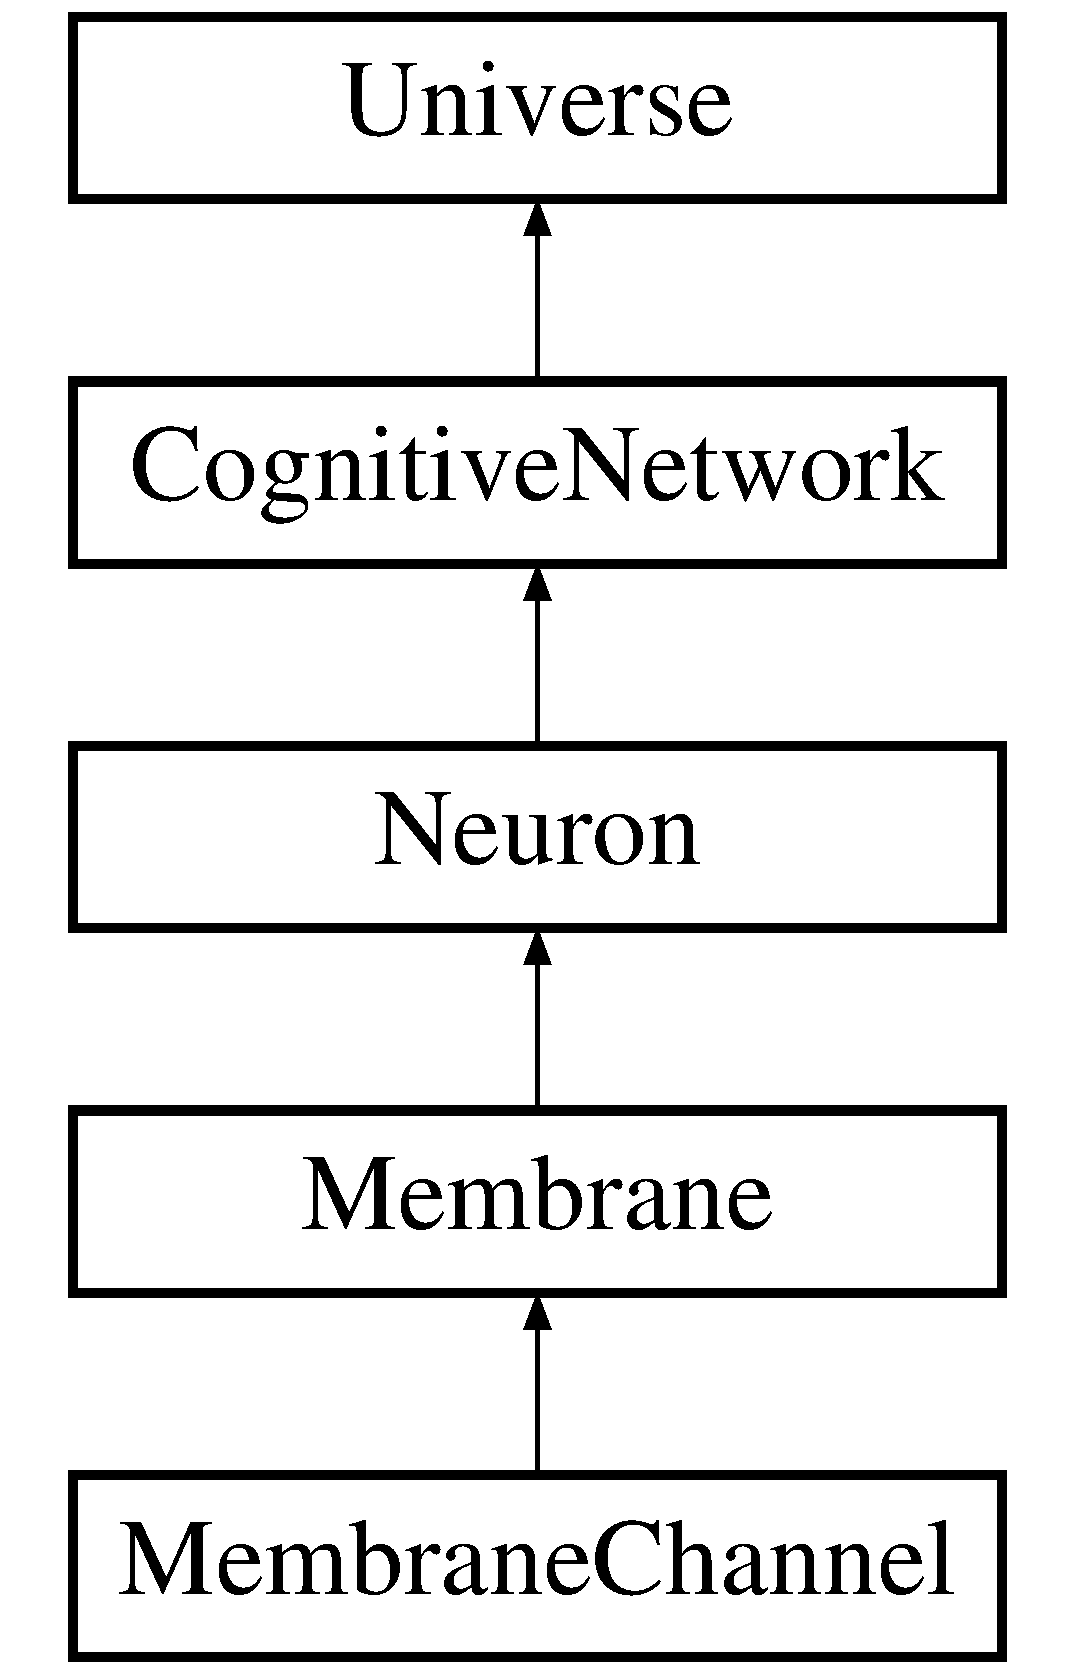
\includegraphics[height=5.000000cm]{classMembraneChannel}
\end{center}
\end{figure}
\subsection*{Public Member Functions}
\begin{DoxyCompactItemize}
\item 
\mbox{\hyperlink{classMembraneChannel_acbc07cd5836394396b0c1944f43350d6}{Membrane\+Channel}} ()
\item 
\mbox{\hyperlink{classMembraneChannel_a17cdd2064bebb7bd2568cf5ec92715fc}{Membrane\+Channel}} (unsigned int object\+\_\+type)
\item 
\mbox{\hyperlink{classMembraneChannel_aedc9eb52da9e7160850f552781df27b6}{Membrane\+Channel}} (unsigned int object\+\_\+type, std\+::chrono\+::time\+\_\+point$<$ \mbox{\hyperlink{universe_8h_a0ef8d951d1ca5ab3cfaf7ab4c7a6fd80}{Clock}} $>$ event\+\_\+time)
\item 
\mbox{\hyperlink{classMembraneChannel_ac467743cbdebcdc6a77ad5ea0527e6f0}{Membrane\+Channel}} (unsigned int object\+\_\+type, std\+::chrono\+::time\+\_\+point$<$ \mbox{\hyperlink{universe_8h_a0ef8d951d1ca5ab3cfaf7ab4c7a6fd80}{Clock}} $>$ event\+\_\+time, \mbox{\hyperlink{classMembrane}{Membrane}} \&membrane\+\_\+connector)
\item 
virtual \mbox{\hyperlink{classMembraneChannel_a925e7e98530ef9cc94616ea7a4dd0cbd}{$\sim$\+Membrane\+Channel}} ()
\item 
unsigned int \mbox{\hyperlink{classMembraneChannel_ac856b74d47b28bd8638fce9c0f12dd20}{Get\+Counter}} (std\+::chrono\+::time\+\_\+point$<$ \mbox{\hyperlink{universe_8h_a0ef8d951d1ca5ab3cfaf7ab4c7a6fd80}{Clock}} $>$ event\+\_\+time)
\item 
double \mbox{\hyperlink{classMembraneChannel_a25b542d8156c42ed785eebbea0db21a7}{Get\+Energy}} (std\+::chrono\+::time\+\_\+point$<$ \mbox{\hyperlink{universe_8h_a0ef8d951d1ca5ab3cfaf7ab4c7a6fd80}{Clock}} $>$ event\+\_\+time)
\item 
bool \mbox{\hyperlink{classMembraneChannel_a8eb115e2583e5bf0f37156f1fc974aa6}{Get\+Receptor\+Binding\+State}} (std\+::chrono\+::time\+\_\+point$<$ \mbox{\hyperlink{universe_8h_a0ef8d951d1ca5ab3cfaf7ab4c7a6fd80}{Clock}} $>$ event\+\_\+time)
\item 
int \mbox{\hyperlink{classMembraneChannel_aa37056ebb4e757a5ed00252112b516aa}{Get\+Receptor\+Type}} (std\+::chrono\+::time\+\_\+point$<$ \mbox{\hyperlink{universe_8h_a0ef8d951d1ca5ab3cfaf7ab4c7a6fd80}{Clock}} $>$ event\+\_\+time)
\item 
bool \mbox{\hyperlink{classMembraneChannel_afde030429a160621a2255ab8a2d689b8}{Get\+Disabled}} (std\+::chrono\+::time\+\_\+point$<$ \mbox{\hyperlink{universe_8h_a0ef8d951d1ca5ab3cfaf7ab4c7a6fd80}{Clock}} $>$ event\+\_\+time)
\item 
int \mbox{\hyperlink{classMembraneChannel_af20c4ca6a3708c86122e7118a29952fd}{Get\+Ions}} (std\+::chrono\+::time\+\_\+point$<$ \mbox{\hyperlink{universe_8h_a0ef8d951d1ca5ab3cfaf7ab4c7a6fd80}{Clock}} $>$ event\+\_\+time)
\item 
void \mbox{\hyperlink{classMembraneChannel_a9f5c69ab1f4dce6113fceebaaa4f15f4}{set\+Receptor\+Binding\+State}} (bool val)
\item 
void \mbox{\hyperlink{classMembraneChannel_a289ec477e64eec5d2a1f88f4a677650c}{toggle\+Receptor\+Binding\+State}} (std\+::chrono\+::time\+\_\+point$<$ \mbox{\hyperlink{universe_8h_a0ef8d951d1ca5ab3cfaf7ab4c7a6fd80}{Clock}} $>$ event\+\_\+time)
\item 
void \mbox{\hyperlink{classMembraneChannel_aabbadec31782704dd497848154dfe0fc}{toggle\+Disabled}} (std\+::chrono\+::time\+\_\+point$<$ \mbox{\hyperlink{universe_8h_a0ef8d951d1ca5ab3cfaf7ab4c7a6fd80}{Clock}} $>$ event\+\_\+time)
\item 
void \mbox{\hyperlink{classMembraneChannel_aed2055857888506a35c09bdcc265799a}{set\+Disabled}} (std\+::chrono\+::time\+\_\+point$<$ \mbox{\hyperlink{universe_8h_a0ef8d951d1ca5ab3cfaf7ab4c7a6fd80}{Clock}} $>$ event\+\_\+time, bool val)
\item 
void \mbox{\hyperlink{classMembraneChannel_a7f40594845bb0aa6a03fd9c08a836d7e}{set\+Receptor\+Type}} (std\+::chrono\+::time\+\_\+point$<$ \mbox{\hyperlink{universe_8h_a0ef8d951d1ca5ab3cfaf7ab4c7a6fd80}{Clock}} $>$ event\+\_\+time, int val)
\item 
void \mbox{\hyperlink{classMembraneChannel_a61931feff8f3bb485eeb5c80125bb732}{Set\+Counter}} (std\+::chrono\+::time\+\_\+point$<$ \mbox{\hyperlink{universe_8h_a0ef8d951d1ca5ab3cfaf7ab4c7a6fd80}{Clock}} $>$ event\+\_\+time, unsigned int val)
\item 
void \mbox{\hyperlink{classMembraneChannel_aaa2d816d3887b6292d995a83130a4834}{Set\+Energy}} (std\+::chrono\+::time\+\_\+point$<$ \mbox{\hyperlink{universe_8h_a0ef8d951d1ca5ab3cfaf7ab4c7a6fd80}{Clock}} $>$ event\+\_\+time, double val)
\item 
void \mbox{\hyperlink{classMembraneChannel_a1fe0c61eccbb6aa0d905ead27e8337bd}{Set\+Ions}} (std\+::chrono\+::time\+\_\+point$<$ \mbox{\hyperlink{universe_8h_a0ef8d951d1ca5ab3cfaf7ab4c7a6fd80}{Clock}} $>$ event\+\_\+time, int val)
\item 
bool \mbox{\hyperlink{classMembraneChannel_a5982040b46efe5e2b824d1cf4dead25e}{Reset\+Parameters}} (std\+::chrono\+::time\+\_\+point$<$ \mbox{\hyperlink{universe_8h_a0ef8d951d1ca5ab3cfaf7ab4c7a6fd80}{Clock}} $>$ event\+\_\+time)
\item 
\mbox{\hyperlink{classCognitiveNetwork}{Cognitive\+Network}} $\ast$ \mbox{\hyperlink{classMembraneChannel_aa8e78a1b0dd7c6b81cac09d33f01e6c2}{Create\+Neurotransmitter}} (std\+::chrono\+::time\+\_\+point$<$ \mbox{\hyperlink{universe_8h_a0ef8d951d1ca5ab3cfaf7ab4c7a6fd80}{Clock}} $>$ event\+\_\+time)
\item 
std\+::vector$<$ \mbox{\hyperlink{classCognitiveNetwork}{Cognitive\+Network}} $\ast$ $>$ \mbox{\hyperlink{classMembraneChannel_a24c791e6cfd906d49e0ceb8a24eeb4cb}{Create\+Neurotransmitters}} (std\+::chrono\+::time\+\_\+point$<$ \mbox{\hyperlink{universe_8h_a0ef8d951d1ca5ab3cfaf7ab4c7a6fd80}{Clock}} $>$ event\+\_\+time, int quantity)
\item 
\mbox{\hyperlink{classCognitiveNetwork}{Cognitive\+Network}} $\ast$ \mbox{\hyperlink{classMembraneChannel_af667720bd2214ea3a1e6d272b57d3a79}{Clone\+Neurotransmitter}} (std\+::chrono\+::time\+\_\+point$<$ \mbox{\hyperlink{universe_8h_a0ef8d951d1ca5ab3cfaf7ab4c7a6fd80}{Clock}} $>$ event\+\_\+time, \mbox{\hyperlink{classCognitiveNetwork}{Cognitive\+Network}} $\ast$clone\+\_\+object, double perfection\+\_\+membership)
\item 
std\+::vector$<$ \mbox{\hyperlink{classCognitiveNetwork}{Cognitive\+Network}} $\ast$ $>$ \mbox{\hyperlink{classMembraneChannel_a6426185a0d73c967adcb72e3a22b48b0}{Clone\+Neurotransmitters}} (std\+::chrono\+::time\+\_\+point$<$ \mbox{\hyperlink{universe_8h_a0ef8d951d1ca5ab3cfaf7ab4c7a6fd80}{Clock}} $>$ event\+\_\+time, std\+::vector$<$ \mbox{\hyperlink{classCognitiveNetwork}{Cognitive\+Network}} $\ast$$>$ cloning\+\_\+list, double perfection\+\_\+membership)
\item 
\mbox{\hyperlink{classCognitiveNetwork}{Cognitive\+Network}} $\ast$ \mbox{\hyperlink{classMembraneChannel_a985d8f93077b0f93daa9c311a22917a1}{Destroy\+Neurotransmitter}} (std\+::chrono\+::time\+\_\+point$<$ \mbox{\hyperlink{universe_8h_a0ef8d951d1ca5ab3cfaf7ab4c7a6fd80}{Clock}} $>$ event\+\_\+time, \mbox{\hyperlink{classCognitiveNetwork}{Cognitive\+Network}} $\ast$destroy\+\_\+object)
\item 
std\+::vector$<$ \mbox{\hyperlink{classCognitiveNetwork}{Cognitive\+Network}} $\ast$ $>$ \mbox{\hyperlink{classMembraneChannel_ad5dfc13b89aff0c7383e052113da1d8f}{Destroy\+Neurotransmitters}} (std\+::chrono\+::time\+\_\+point$<$ \mbox{\hyperlink{universe_8h_a0ef8d951d1ca5ab3cfaf7ab4c7a6fd80}{Clock}} $>$ event\+\_\+time, std\+::vector$<$ \mbox{\hyperlink{classCognitiveNetwork}{Cognitive\+Network}} $\ast$$>$ destruction\+\_\+list)
\item 
\mbox{\hyperlink{classCognitiveNetwork}{Cognitive\+Network}} $\ast$ \mbox{\hyperlink{classMembraneChannel_ae483c6bc45f73390070b824296762d4c}{Add\+Neurotransmitter}} (std\+::chrono\+::time\+\_\+point$<$ \mbox{\hyperlink{universe_8h_a0ef8d951d1ca5ab3cfaf7ab4c7a6fd80}{Clock}} $>$ event\+\_\+time, \mbox{\hyperlink{classCognitiveNetwork}{Cognitive\+Network}} $\ast$add\+\_\+object)
\item 
std\+::vector$<$ \mbox{\hyperlink{classCognitiveNetwork}{Cognitive\+Network}} $\ast$ $>$ \mbox{\hyperlink{classMembraneChannel_a01fb5f3176cfa3423bb10a04bf69da01}{Add\+Neurotransmitters}} (std\+::chrono\+::time\+\_\+point$<$ \mbox{\hyperlink{universe_8h_a0ef8d951d1ca5ab3cfaf7ab4c7a6fd80}{Clock}} $>$ event\+\_\+time, std\+::vector$<$ \mbox{\hyperlink{classCognitiveNetwork}{Cognitive\+Network}} $\ast$$>$ add\+\_\+objects)
\item 
\mbox{\hyperlink{classCognitiveNetwork}{Cognitive\+Network}} $\ast$ \mbox{\hyperlink{classMembraneChannel_a2252f222f4a41bf1975dc856569e0a22}{Remove\+Neurotransmitter}} (std\+::chrono\+::time\+\_\+point$<$ \mbox{\hyperlink{universe_8h_a0ef8d951d1ca5ab3cfaf7ab4c7a6fd80}{Clock}} $>$ event\+\_\+time)
\item 
std\+::vector$<$ \mbox{\hyperlink{classCognitiveNetwork}{Cognitive\+Network}} $\ast$ $>$ \mbox{\hyperlink{classMembraneChannel_a37f22ddd877e3be7b353048149a7bbcd}{Remove\+Neurotransmitters}} (std\+::chrono\+::time\+\_\+point$<$ \mbox{\hyperlink{universe_8h_a0ef8d951d1ca5ab3cfaf7ab4c7a6fd80}{Clock}} $>$ event\+\_\+time, int quantity)
\item 
\mbox{\hyperlink{classCognitiveNetwork}{Cognitive\+Network}} $\ast$ \mbox{\hyperlink{classMembraneChannel_a91ce6506a8e82905de7cd031ed5d63f5}{Get\+Neurotransmitter}} (std\+::chrono\+::time\+\_\+point$<$ \mbox{\hyperlink{universe_8h_a0ef8d951d1ca5ab3cfaf7ab4c7a6fd80}{Clock}} $>$ event\+\_\+time, int selector)
\item 
std\+::vector$<$ \mbox{\hyperlink{classCognitiveNetwork}{Cognitive\+Network}} $\ast$ $>$ \mbox{\hyperlink{classMembraneChannel_a9fdb20eb7d3f9ebad864d07aaa835716}{Get\+Neurotransmitters}} (std\+::chrono\+::time\+\_\+point$<$ \mbox{\hyperlink{universe_8h_a0ef8d951d1ca5ab3cfaf7ab4c7a6fd80}{Clock}} $>$ event\+\_\+time)
\item 
bool \mbox{\hyperlink{classMembraneChannel_a67496ca67ad3ecae38f6b987547b1b99}{Compatibility\+Check}} (std\+::chrono\+::time\+\_\+point$<$ \mbox{\hyperlink{universe_8h_a0ef8d951d1ca5ab3cfaf7ab4c7a6fd80}{Clock}} $>$ event\+\_\+time, int neurotransmitter\+Type)
\item 
int \mbox{\hyperlink{classMembraneChannel_a34077828eee1c2457212f05217b09d6c}{Update}} (std\+::chrono\+::time\+\_\+point$<$ \mbox{\hyperlink{universe_8h_a0ef8d951d1ca5ab3cfaf7ab4c7a6fd80}{Clock}} $>$ event\+\_\+time)
\end{DoxyCompactItemize}
\subsection*{Protected Attributes}
\begin{DoxyCompactItemize}
\item 
std\+::vector$<$ \mbox{\hyperlink{classCognitiveNetwork}{Cognitive\+Network}} $\ast$ $>$ \mbox{\hyperlink{classMembraneChannel_ad603f58813157b33ca81b919cf9c2897}{neurotransmitter\+\_\+list}}
\end{DoxyCompactItemize}
\subsection*{Private Attributes}
\begin{DoxyCompactItemize}
\item 
int \mbox{\hyperlink{classMembraneChannel_aa8beeb2908b603d7b568442b635f4164}{m\+\_\+\+Neuron\+Type}}
\item 
int \mbox{\hyperlink{classMembraneChannel_a99646a50163299948faa5a5f0da60add}{membranechannel\+\_\+type}}
\item 
int \mbox{\hyperlink{classMembraneChannel_a79af5f43970e9496ea293c9ac8bb73f6}{neurotransmitter\+\_\+pool}}
\item 
int \mbox{\hyperlink{classMembraneChannel_aaabe065df6250159df3ee8b9ea3f824f}{m\+\_\+add\+Status}}
\item 
std\+::chrono\+::time\+\_\+point$<$ \mbox{\hyperlink{universe_8h_a0ef8d951d1ca5ab3cfaf7ab4c7a6fd80}{Clock}} $>$ \mbox{\hyperlink{classMembraneChannel_a05a2ea08d814a99d1c349dab4b5f3266}{previous\+\_\+event\+\_\+time}}
\item 
std\+::chrono\+::time\+\_\+point$<$ \mbox{\hyperlink{universe_8h_a0ef8d951d1ca5ab3cfaf7ab4c7a6fd80}{Clock}} $>$ \mbox{\hyperlink{classMembraneChannel_a16fbba2c7aaf591b3a1d012b745ee97a}{time\+\_\+object\+\_\+created}}
\item 
int \mbox{\hyperlink{classMembraneChannel_ad6b972a3874ddc236b63c7145123e0c2}{duration\+\_\+since\+\_\+last\+\_\+event}}
\item 
double \mbox{\hyperlink{classMembraneChannel_af542b034258dce62f0666b0397fdd2fb}{m\+\_\+\+Volume}}
\item 
double \mbox{\hyperlink{classMembraneChannel_a85b55287517ff9d5cacb98bacf79a0d3}{m\+\_\+\+Surface\+Area}}
\item 
unsigned int \mbox{\hyperlink{classMembraneChannel_a0df3b8e24bd5d496d2832b486b35aab1}{m\+\_\+\+Counter}}
\begin{DoxyCompactList}\small\item\em Member variable \char`\"{}m\+\_\+\+Counter\char`\"{}. \end{DoxyCompactList}\item 
double \mbox{\hyperlink{classMembraneChannel_a3615bab719d4a6c43a1d5d3e64d0079c}{object\+\_\+energy}}
\begin{DoxyCompactList}\small\item\em Member variable \char`\"{}object\+\_\+energy\char`\"{}. \end{DoxyCompactList}\item 
double \mbox{\hyperlink{classMembraneChannel_acb697781909d7e8bd2e69fbb1268b2f2}{object\+\_\+energy\+\_\+threshold}}
\item 
double \mbox{\hyperlink{classMembraneChannel_a1c843660b2ea25ca2506f967dbd7e0d2}{m\+\_\+\+Time\+Dilation}}
\item 
double \mbox{\hyperlink{classMembraneChannel_a71a07468f3add9783acfbe2ca0df2101}{m\+\_\+\+Time\+Threshold}}
\item 
double \mbox{\hyperlink{classMembraneChannel_aa3bd560d7c7c6c5b452d11f18bca30b1}{m\+\_\+\+Length}}
\item 
bool \mbox{\hyperlink{classMembraneChannel_a9cd227ac36102ed8958973ae46163e1c}{object\+\_\+initialised}} = false
\item 
bool \mbox{\hyperlink{classMembraneChannel_acd2bbf349255bbeb5ee2304f05e14ff6}{object\+\_\+disabled}}
\item 
double \mbox{\hyperlink{classMembraneChannel_abc68fa8d4693c6512c15a230b9bc8744}{object\+\_\+size}} = 0
\item 
double \mbox{\hyperlink{classMembraneChannel_a41896472da1942a6be07eb8d6e8e508f}{object\+\_\+energy\+Full}}
\item 
int \mbox{\hyperlink{classMembraneChannel_afe6cbd4b6eeca252fde5c1b3b23f4717}{m\+\_\+\+Ions}}
\item 
bool \mbox{\hyperlink{classMembraneChannel_ab257b77285836ce5dc0c16824116351b}{m\+\_\+bound\+Receptor}}
\begin{DoxyCompactList}\small\item\em Member variable \char`\"{}m\+\_\+bound\+Receptor\char`\"{}. \end{DoxyCompactList}\item 
int \mbox{\hyperlink{classMembraneChannel_a21f2bf86c93a07d133d01927af48d96d}{m\+\_\+type\+Receptor}}
\begin{DoxyCompactList}\small\item\em Member variable \char`\"{}m\+\_\+type\+Receptor\char`\"{}. \end{DoxyCompactList}\end{DoxyCompactItemize}
\subsection*{Additional Inherited Members}


\subsection{Constructor \& Destructor Documentation}
\mbox{\Hypertarget{classMembraneChannel_acbc07cd5836394396b0c1944f43350d6}\label{classMembraneChannel_acbc07cd5836394396b0c1944f43350d6}} 
\index{Membrane\+Channel@{Membrane\+Channel}!Membrane\+Channel@{Membrane\+Channel}}
\index{Membrane\+Channel@{Membrane\+Channel}!Membrane\+Channel@{Membrane\+Channel}}
\subsubsection{\texorpdfstring{Membrane\+Channel()}{MembraneChannel()}\hspace{0.1cm}{\footnotesize\ttfamily [1/4]}}
{\footnotesize\ttfamily Membrane\+Channel\+::\+Membrane\+Channel (\begin{DoxyParamCaption}{ }\end{DoxyParamCaption})\hspace{0.3cm}{\ttfamily [inline]}}

\mbox{\Hypertarget{classMembraneChannel_a17cdd2064bebb7bd2568cf5ec92715fc}\label{classMembraneChannel_a17cdd2064bebb7bd2568cf5ec92715fc}} 
\index{Membrane\+Channel@{Membrane\+Channel}!Membrane\+Channel@{Membrane\+Channel}}
\index{Membrane\+Channel@{Membrane\+Channel}!Membrane\+Channel@{Membrane\+Channel}}
\subsubsection{\texorpdfstring{Membrane\+Channel()}{MembraneChannel()}\hspace{0.1cm}{\footnotesize\ttfamily [2/4]}}
{\footnotesize\ttfamily Membrane\+Channel\+::\+Membrane\+Channel (\begin{DoxyParamCaption}\item[{unsigned int}]{object\+\_\+type }\end{DoxyParamCaption})\hspace{0.3cm}{\ttfamily [inline]}}

\mbox{\Hypertarget{classMembraneChannel_aedc9eb52da9e7160850f552781df27b6}\label{classMembraneChannel_aedc9eb52da9e7160850f552781df27b6}} 
\index{Membrane\+Channel@{Membrane\+Channel}!Membrane\+Channel@{Membrane\+Channel}}
\index{Membrane\+Channel@{Membrane\+Channel}!Membrane\+Channel@{Membrane\+Channel}}
\subsubsection{\texorpdfstring{Membrane\+Channel()}{MembraneChannel()}\hspace{0.1cm}{\footnotesize\ttfamily [3/4]}}
{\footnotesize\ttfamily Membrane\+Channel\+::\+Membrane\+Channel (\begin{DoxyParamCaption}\item[{unsigned int}]{object\+\_\+type,  }\item[{std\+::chrono\+::time\+\_\+point$<$ \mbox{\hyperlink{universe_8h_a0ef8d951d1ca5ab3cfaf7ab4c7a6fd80}{Clock}} $>$}]{event\+\_\+time }\end{DoxyParamCaption})\hspace{0.3cm}{\ttfamily [inline]}}

\mbox{\Hypertarget{classMembraneChannel_ac467743cbdebcdc6a77ad5ea0527e6f0}\label{classMembraneChannel_ac467743cbdebcdc6a77ad5ea0527e6f0}} 
\index{Membrane\+Channel@{Membrane\+Channel}!Membrane\+Channel@{Membrane\+Channel}}
\index{Membrane\+Channel@{Membrane\+Channel}!Membrane\+Channel@{Membrane\+Channel}}
\subsubsection{\texorpdfstring{Membrane\+Channel()}{MembraneChannel()}\hspace{0.1cm}{\footnotesize\ttfamily [4/4]}}
{\footnotesize\ttfamily Membrane\+Channel\+::\+Membrane\+Channel (\begin{DoxyParamCaption}\item[{unsigned int}]{object\+\_\+type,  }\item[{std\+::chrono\+::time\+\_\+point$<$ \mbox{\hyperlink{universe_8h_a0ef8d951d1ca5ab3cfaf7ab4c7a6fd80}{Clock}} $>$}]{event\+\_\+time,  }\item[{\mbox{\hyperlink{classMembrane}{Membrane}} \&}]{membrane\+\_\+connector }\end{DoxyParamCaption})\hspace{0.3cm}{\ttfamily [inline]}}

\mbox{\Hypertarget{classMembraneChannel_a925e7e98530ef9cc94616ea7a4dd0cbd}\label{classMembraneChannel_a925e7e98530ef9cc94616ea7a4dd0cbd}} 
\index{Membrane\+Channel@{Membrane\+Channel}!````~Membrane\+Channel@{$\sim$\+Membrane\+Channel}}
\index{````~Membrane\+Channel@{$\sim$\+Membrane\+Channel}!Membrane\+Channel@{Membrane\+Channel}}
\subsubsection{\texorpdfstring{$\sim$\+Membrane\+Channel()}{~MembraneChannel()}}
{\footnotesize\ttfamily virtual Membrane\+Channel\+::$\sim$\+Membrane\+Channel (\begin{DoxyParamCaption}{ }\end{DoxyParamCaption})\hspace{0.3cm}{\ttfamily [inline]}, {\ttfamily [virtual]}}

Default destructor 

\subsection{Member Function Documentation}
\mbox{\Hypertarget{classMembraneChannel_ae483c6bc45f73390070b824296762d4c}\label{classMembraneChannel_ae483c6bc45f73390070b824296762d4c}} 
\index{Membrane\+Channel@{Membrane\+Channel}!Add\+Neurotransmitter@{Add\+Neurotransmitter}}
\index{Add\+Neurotransmitter@{Add\+Neurotransmitter}!Membrane\+Channel@{Membrane\+Channel}}
\subsubsection{\texorpdfstring{Add\+Neurotransmitter()}{AddNeurotransmitter()}}
{\footnotesize\ttfamily \mbox{\hyperlink{classCognitiveNetwork}{Cognitive\+Network}} $\ast$ Membrane\+Channel\+::\+Add\+Neurotransmitter (\begin{DoxyParamCaption}\item[{std\+::chrono\+::time\+\_\+point$<$ \mbox{\hyperlink{universe_8h_a0ef8d951d1ca5ab3cfaf7ab4c7a6fd80}{Clock}} $>$}]{event\+\_\+time,  }\item[{\mbox{\hyperlink{classCognitiveNetwork}{Cognitive\+Network}} $\ast$}]{add\+\_\+object }\end{DoxyParamCaption})}

\mbox{\Hypertarget{classMembraneChannel_a01fb5f3176cfa3423bb10a04bf69da01}\label{classMembraneChannel_a01fb5f3176cfa3423bb10a04bf69da01}} 
\index{Membrane\+Channel@{Membrane\+Channel}!Add\+Neurotransmitters@{Add\+Neurotransmitters}}
\index{Add\+Neurotransmitters@{Add\+Neurotransmitters}!Membrane\+Channel@{Membrane\+Channel}}
\subsubsection{\texorpdfstring{Add\+Neurotransmitters()}{AddNeurotransmitters()}}
{\footnotesize\ttfamily std\+::vector$<$ \mbox{\hyperlink{classCognitiveNetwork}{Cognitive\+Network}} $\ast$ $>$ Membrane\+Channel\+::\+Add\+Neurotransmitters (\begin{DoxyParamCaption}\item[{std\+::chrono\+::time\+\_\+point$<$ \mbox{\hyperlink{universe_8h_a0ef8d951d1ca5ab3cfaf7ab4c7a6fd80}{Clock}} $>$}]{event\+\_\+time,  }\item[{std\+::vector$<$ \mbox{\hyperlink{classCognitiveNetwork}{Cognitive\+Network}} $\ast$$>$}]{add\+\_\+objects }\end{DoxyParamCaption})}

\mbox{\Hypertarget{classMembraneChannel_af667720bd2214ea3a1e6d272b57d3a79}\label{classMembraneChannel_af667720bd2214ea3a1e6d272b57d3a79}} 
\index{Membrane\+Channel@{Membrane\+Channel}!Clone\+Neurotransmitter@{Clone\+Neurotransmitter}}
\index{Clone\+Neurotransmitter@{Clone\+Neurotransmitter}!Membrane\+Channel@{Membrane\+Channel}}
\subsubsection{\texorpdfstring{Clone\+Neurotransmitter()}{CloneNeurotransmitter()}}
{\footnotesize\ttfamily \mbox{\hyperlink{classCognitiveNetwork}{Cognitive\+Network}} $\ast$ Membrane\+Channel\+::\+Clone\+Neurotransmitter (\begin{DoxyParamCaption}\item[{std\+::chrono\+::time\+\_\+point$<$ \mbox{\hyperlink{universe_8h_a0ef8d951d1ca5ab3cfaf7ab4c7a6fd80}{Clock}} $>$}]{event\+\_\+time,  }\item[{\mbox{\hyperlink{classCognitiveNetwork}{Cognitive\+Network}} $\ast$}]{clone\+\_\+object,  }\item[{double}]{perfection\+\_\+membership }\end{DoxyParamCaption})}

\mbox{\Hypertarget{classMembraneChannel_a6426185a0d73c967adcb72e3a22b48b0}\label{classMembraneChannel_a6426185a0d73c967adcb72e3a22b48b0}} 
\index{Membrane\+Channel@{Membrane\+Channel}!Clone\+Neurotransmitters@{Clone\+Neurotransmitters}}
\index{Clone\+Neurotransmitters@{Clone\+Neurotransmitters}!Membrane\+Channel@{Membrane\+Channel}}
\subsubsection{\texorpdfstring{Clone\+Neurotransmitters()}{CloneNeurotransmitters()}}
{\footnotesize\ttfamily std\+::vector$<$ \mbox{\hyperlink{classCognitiveNetwork}{Cognitive\+Network}} $\ast$ $>$ Membrane\+Channel\+::\+Clone\+Neurotransmitters (\begin{DoxyParamCaption}\item[{std\+::chrono\+::time\+\_\+point$<$ \mbox{\hyperlink{universe_8h_a0ef8d951d1ca5ab3cfaf7ab4c7a6fd80}{Clock}} $>$}]{event\+\_\+time,  }\item[{std\+::vector$<$ \mbox{\hyperlink{classCognitiveNetwork}{Cognitive\+Network}} $\ast$$>$}]{cloning\+\_\+list,  }\item[{double}]{perfection\+\_\+membership }\end{DoxyParamCaption})}

\mbox{\Hypertarget{classMembraneChannel_a67496ca67ad3ecae38f6b987547b1b99}\label{classMembraneChannel_a67496ca67ad3ecae38f6b987547b1b99}} 
\index{Membrane\+Channel@{Membrane\+Channel}!Compatibility\+Check@{Compatibility\+Check}}
\index{Compatibility\+Check@{Compatibility\+Check}!Membrane\+Channel@{Membrane\+Channel}}
\subsubsection{\texorpdfstring{Compatibility\+Check()}{CompatibilityCheck()}}
{\footnotesize\ttfamily bool Membrane\+Channel\+::\+Compatibility\+Check (\begin{DoxyParamCaption}\item[{std\+::chrono\+::time\+\_\+point$<$ \mbox{\hyperlink{universe_8h_a0ef8d951d1ca5ab3cfaf7ab4c7a6fd80}{Clock}} $>$}]{event\+\_\+time,  }\item[{int}]{neurotransmitter\+Type }\end{DoxyParamCaption})}

\mbox{\Hypertarget{classMembraneChannel_aa8e78a1b0dd7c6b81cac09d33f01e6c2}\label{classMembraneChannel_aa8e78a1b0dd7c6b81cac09d33f01e6c2}} 
\index{Membrane\+Channel@{Membrane\+Channel}!Create\+Neurotransmitter@{Create\+Neurotransmitter}}
\index{Create\+Neurotransmitter@{Create\+Neurotransmitter}!Membrane\+Channel@{Membrane\+Channel}}
\subsubsection{\texorpdfstring{Create\+Neurotransmitter()}{CreateNeurotransmitter()}}
{\footnotesize\ttfamily \mbox{\hyperlink{classCognitiveNetwork}{Cognitive\+Network}} $\ast$ Membrane\+Channel\+::\+Create\+Neurotransmitter (\begin{DoxyParamCaption}\item[{std\+::chrono\+::time\+\_\+point$<$ \mbox{\hyperlink{universe_8h_a0ef8d951d1ca5ab3cfaf7ab4c7a6fd80}{Clock}} $>$}]{event\+\_\+time }\end{DoxyParamCaption})}

\mbox{\Hypertarget{classMembraneChannel_a24c791e6cfd906d49e0ceb8a24eeb4cb}\label{classMembraneChannel_a24c791e6cfd906d49e0ceb8a24eeb4cb}} 
\index{Membrane\+Channel@{Membrane\+Channel}!Create\+Neurotransmitters@{Create\+Neurotransmitters}}
\index{Create\+Neurotransmitters@{Create\+Neurotransmitters}!Membrane\+Channel@{Membrane\+Channel}}
\subsubsection{\texorpdfstring{Create\+Neurotransmitters()}{CreateNeurotransmitters()}}
{\footnotesize\ttfamily std\+::vector$<$ \mbox{\hyperlink{classCognitiveNetwork}{Cognitive\+Network}} $\ast$ $>$ Membrane\+Channel\+::\+Create\+Neurotransmitters (\begin{DoxyParamCaption}\item[{std\+::chrono\+::time\+\_\+point$<$ \mbox{\hyperlink{universe_8h_a0ef8d951d1ca5ab3cfaf7ab4c7a6fd80}{Clock}} $>$}]{event\+\_\+time,  }\item[{int}]{quantity }\end{DoxyParamCaption})}

\mbox{\Hypertarget{classMembraneChannel_a985d8f93077b0f93daa9c311a22917a1}\label{classMembraneChannel_a985d8f93077b0f93daa9c311a22917a1}} 
\index{Membrane\+Channel@{Membrane\+Channel}!Destroy\+Neurotransmitter@{Destroy\+Neurotransmitter}}
\index{Destroy\+Neurotransmitter@{Destroy\+Neurotransmitter}!Membrane\+Channel@{Membrane\+Channel}}
\subsubsection{\texorpdfstring{Destroy\+Neurotransmitter()}{DestroyNeurotransmitter()}}
{\footnotesize\ttfamily \mbox{\hyperlink{classCognitiveNetwork}{Cognitive\+Network}} $\ast$ Membrane\+Channel\+::\+Destroy\+Neurotransmitter (\begin{DoxyParamCaption}\item[{std\+::chrono\+::time\+\_\+point$<$ \mbox{\hyperlink{universe_8h_a0ef8d951d1ca5ab3cfaf7ab4c7a6fd80}{Clock}} $>$}]{event\+\_\+time,  }\item[{\mbox{\hyperlink{classCognitiveNetwork}{Cognitive\+Network}} $\ast$}]{destroy\+\_\+object }\end{DoxyParamCaption})}

\mbox{\Hypertarget{classMembraneChannel_ad5dfc13b89aff0c7383e052113da1d8f}\label{classMembraneChannel_ad5dfc13b89aff0c7383e052113da1d8f}} 
\index{Membrane\+Channel@{Membrane\+Channel}!Destroy\+Neurotransmitters@{Destroy\+Neurotransmitters}}
\index{Destroy\+Neurotransmitters@{Destroy\+Neurotransmitters}!Membrane\+Channel@{Membrane\+Channel}}
\subsubsection{\texorpdfstring{Destroy\+Neurotransmitters()}{DestroyNeurotransmitters()}}
{\footnotesize\ttfamily std\+::vector$<$ \mbox{\hyperlink{classCognitiveNetwork}{Cognitive\+Network}} $\ast$ $>$ Membrane\+Channel\+::\+Destroy\+Neurotransmitters (\begin{DoxyParamCaption}\item[{std\+::chrono\+::time\+\_\+point$<$ \mbox{\hyperlink{universe_8h_a0ef8d951d1ca5ab3cfaf7ab4c7a6fd80}{Clock}} $>$}]{event\+\_\+time,  }\item[{std\+::vector$<$ \mbox{\hyperlink{classCognitiveNetwork}{Cognitive\+Network}} $\ast$$>$}]{destruction\+\_\+list }\end{DoxyParamCaption})}

\mbox{\Hypertarget{classMembraneChannel_ac856b74d47b28bd8638fce9c0f12dd20}\label{classMembraneChannel_ac856b74d47b28bd8638fce9c0f12dd20}} 
\index{Membrane\+Channel@{Membrane\+Channel}!Get\+Counter@{Get\+Counter}}
\index{Get\+Counter@{Get\+Counter}!Membrane\+Channel@{Membrane\+Channel}}
\subsubsection{\texorpdfstring{Get\+Counter()}{GetCounter()}}
{\footnotesize\ttfamily unsigned int Membrane\+Channel\+::\+Get\+Counter (\begin{DoxyParamCaption}\item[{std\+::chrono\+::time\+\_\+point$<$ \mbox{\hyperlink{universe_8h_a0ef8d951d1ca5ab3cfaf7ab4c7a6fd80}{Clock}} $>$}]{event\+\_\+time }\end{DoxyParamCaption})\hspace{0.3cm}{\ttfamily [inline]}}

\mbox{\Hypertarget{classMembraneChannel_afde030429a160621a2255ab8a2d689b8}\label{classMembraneChannel_afde030429a160621a2255ab8a2d689b8}} 
\index{Membrane\+Channel@{Membrane\+Channel}!Get\+Disabled@{Get\+Disabled}}
\index{Get\+Disabled@{Get\+Disabled}!Membrane\+Channel@{Membrane\+Channel}}
\subsubsection{\texorpdfstring{Get\+Disabled()}{GetDisabled()}}
{\footnotesize\ttfamily bool Membrane\+Channel\+::\+Get\+Disabled (\begin{DoxyParamCaption}\item[{std\+::chrono\+::time\+\_\+point$<$ \mbox{\hyperlink{universe_8h_a0ef8d951d1ca5ab3cfaf7ab4c7a6fd80}{Clock}} $>$}]{event\+\_\+time }\end{DoxyParamCaption})\hspace{0.3cm}{\ttfamily [inline]}}

\mbox{\Hypertarget{classMembraneChannel_a25b542d8156c42ed785eebbea0db21a7}\label{classMembraneChannel_a25b542d8156c42ed785eebbea0db21a7}} 
\index{Membrane\+Channel@{Membrane\+Channel}!Get\+Energy@{Get\+Energy}}
\index{Get\+Energy@{Get\+Energy}!Membrane\+Channel@{Membrane\+Channel}}
\subsubsection{\texorpdfstring{Get\+Energy()}{GetEnergy()}}
{\footnotesize\ttfamily double Membrane\+Channel\+::\+Get\+Energy (\begin{DoxyParamCaption}\item[{std\+::chrono\+::time\+\_\+point$<$ \mbox{\hyperlink{universe_8h_a0ef8d951d1ca5ab3cfaf7ab4c7a6fd80}{Clock}} $>$}]{event\+\_\+time }\end{DoxyParamCaption})\hspace{0.3cm}{\ttfamily [inline]}}

\mbox{\Hypertarget{classMembraneChannel_af20c4ca6a3708c86122e7118a29952fd}\label{classMembraneChannel_af20c4ca6a3708c86122e7118a29952fd}} 
\index{Membrane\+Channel@{Membrane\+Channel}!Get\+Ions@{Get\+Ions}}
\index{Get\+Ions@{Get\+Ions}!Membrane\+Channel@{Membrane\+Channel}}
\subsubsection{\texorpdfstring{Get\+Ions()}{GetIons()}}
{\footnotesize\ttfamily int Membrane\+Channel\+::\+Get\+Ions (\begin{DoxyParamCaption}\item[{std\+::chrono\+::time\+\_\+point$<$ \mbox{\hyperlink{universe_8h_a0ef8d951d1ca5ab3cfaf7ab4c7a6fd80}{Clock}} $>$}]{event\+\_\+time }\end{DoxyParamCaption})\hspace{0.3cm}{\ttfamily [inline]}}

\mbox{\Hypertarget{classMembraneChannel_a91ce6506a8e82905de7cd031ed5d63f5}\label{classMembraneChannel_a91ce6506a8e82905de7cd031ed5d63f5}} 
\index{Membrane\+Channel@{Membrane\+Channel}!Get\+Neurotransmitter@{Get\+Neurotransmitter}}
\index{Get\+Neurotransmitter@{Get\+Neurotransmitter}!Membrane\+Channel@{Membrane\+Channel}}
\subsubsection{\texorpdfstring{Get\+Neurotransmitter()}{GetNeurotransmitter()}}
{\footnotesize\ttfamily \mbox{\hyperlink{classCognitiveNetwork}{Cognitive\+Network}} $\ast$ Membrane\+Channel\+::\+Get\+Neurotransmitter (\begin{DoxyParamCaption}\item[{std\+::chrono\+::time\+\_\+point$<$ \mbox{\hyperlink{universe_8h_a0ef8d951d1ca5ab3cfaf7ab4c7a6fd80}{Clock}} $>$}]{event\+\_\+time,  }\item[{int}]{selector }\end{DoxyParamCaption})}

\mbox{\Hypertarget{classMembraneChannel_a9fdb20eb7d3f9ebad864d07aaa835716}\label{classMembraneChannel_a9fdb20eb7d3f9ebad864d07aaa835716}} 
\index{Membrane\+Channel@{Membrane\+Channel}!Get\+Neurotransmitters@{Get\+Neurotransmitters}}
\index{Get\+Neurotransmitters@{Get\+Neurotransmitters}!Membrane\+Channel@{Membrane\+Channel}}
\subsubsection{\texorpdfstring{Get\+Neurotransmitters()}{GetNeurotransmitters()}}
{\footnotesize\ttfamily std\+::vector$<$ \mbox{\hyperlink{classCognitiveNetwork}{Cognitive\+Network}} $\ast$ $>$ Membrane\+Channel\+::\+Get\+Neurotransmitters (\begin{DoxyParamCaption}\item[{std\+::chrono\+::time\+\_\+point$<$ \mbox{\hyperlink{universe_8h_a0ef8d951d1ca5ab3cfaf7ab4c7a6fd80}{Clock}} $>$}]{event\+\_\+time }\end{DoxyParamCaption})}

\mbox{\Hypertarget{classMembraneChannel_a8eb115e2583e5bf0f37156f1fc974aa6}\label{classMembraneChannel_a8eb115e2583e5bf0f37156f1fc974aa6}} 
\index{Membrane\+Channel@{Membrane\+Channel}!Get\+Receptor\+Binding\+State@{Get\+Receptor\+Binding\+State}}
\index{Get\+Receptor\+Binding\+State@{Get\+Receptor\+Binding\+State}!Membrane\+Channel@{Membrane\+Channel}}
\subsubsection{\texorpdfstring{Get\+Receptor\+Binding\+State()}{GetReceptorBindingState()}}
{\footnotesize\ttfamily bool Membrane\+Channel\+::\+Get\+Receptor\+Binding\+State (\begin{DoxyParamCaption}\item[{std\+::chrono\+::time\+\_\+point$<$ \mbox{\hyperlink{universe_8h_a0ef8d951d1ca5ab3cfaf7ab4c7a6fd80}{Clock}} $>$}]{event\+\_\+time }\end{DoxyParamCaption})\hspace{0.3cm}{\ttfamily [inline]}}

\mbox{\Hypertarget{classMembraneChannel_aa37056ebb4e757a5ed00252112b516aa}\label{classMembraneChannel_aa37056ebb4e757a5ed00252112b516aa}} 
\index{Membrane\+Channel@{Membrane\+Channel}!Get\+Receptor\+Type@{Get\+Receptor\+Type}}
\index{Get\+Receptor\+Type@{Get\+Receptor\+Type}!Membrane\+Channel@{Membrane\+Channel}}
\subsubsection{\texorpdfstring{Get\+Receptor\+Type()}{GetReceptorType()}}
{\footnotesize\ttfamily int Membrane\+Channel\+::\+Get\+Receptor\+Type (\begin{DoxyParamCaption}\item[{std\+::chrono\+::time\+\_\+point$<$ \mbox{\hyperlink{universe_8h_a0ef8d951d1ca5ab3cfaf7ab4c7a6fd80}{Clock}} $>$}]{event\+\_\+time }\end{DoxyParamCaption})\hspace{0.3cm}{\ttfamily [inline]}}

\mbox{\Hypertarget{classMembraneChannel_a2252f222f4a41bf1975dc856569e0a22}\label{classMembraneChannel_a2252f222f4a41bf1975dc856569e0a22}} 
\index{Membrane\+Channel@{Membrane\+Channel}!Remove\+Neurotransmitter@{Remove\+Neurotransmitter}}
\index{Remove\+Neurotransmitter@{Remove\+Neurotransmitter}!Membrane\+Channel@{Membrane\+Channel}}
\subsubsection{\texorpdfstring{Remove\+Neurotransmitter()}{RemoveNeurotransmitter()}}
{\footnotesize\ttfamily \mbox{\hyperlink{classCognitiveNetwork}{Cognitive\+Network}} $\ast$ Membrane\+Channel\+::\+Remove\+Neurotransmitter (\begin{DoxyParamCaption}\item[{std\+::chrono\+::time\+\_\+point$<$ \mbox{\hyperlink{universe_8h_a0ef8d951d1ca5ab3cfaf7ab4c7a6fd80}{Clock}} $>$}]{event\+\_\+time }\end{DoxyParamCaption})}

\mbox{\Hypertarget{classMembraneChannel_a37f22ddd877e3be7b353048149a7bbcd}\label{classMembraneChannel_a37f22ddd877e3be7b353048149a7bbcd}} 
\index{Membrane\+Channel@{Membrane\+Channel}!Remove\+Neurotransmitters@{Remove\+Neurotransmitters}}
\index{Remove\+Neurotransmitters@{Remove\+Neurotransmitters}!Membrane\+Channel@{Membrane\+Channel}}
\subsubsection{\texorpdfstring{Remove\+Neurotransmitters()}{RemoveNeurotransmitters()}}
{\footnotesize\ttfamily std\+::vector$<$ \mbox{\hyperlink{classCognitiveNetwork}{Cognitive\+Network}} $\ast$ $>$ Membrane\+Channel\+::\+Remove\+Neurotransmitters (\begin{DoxyParamCaption}\item[{std\+::chrono\+::time\+\_\+point$<$ \mbox{\hyperlink{universe_8h_a0ef8d951d1ca5ab3cfaf7ab4c7a6fd80}{Clock}} $>$}]{event\+\_\+time,  }\item[{int}]{quantity }\end{DoxyParamCaption})}

\mbox{\Hypertarget{classMembraneChannel_a5982040b46efe5e2b824d1cf4dead25e}\label{classMembraneChannel_a5982040b46efe5e2b824d1cf4dead25e}} 
\index{Membrane\+Channel@{Membrane\+Channel}!Reset\+Parameters@{Reset\+Parameters}}
\index{Reset\+Parameters@{Reset\+Parameters}!Membrane\+Channel@{Membrane\+Channel}}
\subsubsection{\texorpdfstring{Reset\+Parameters()}{ResetParameters()}}
{\footnotesize\ttfamily bool Membrane\+Channel\+::\+Reset\+Parameters (\begin{DoxyParamCaption}\item[{std\+::chrono\+::time\+\_\+point$<$ \mbox{\hyperlink{universe_8h_a0ef8d951d1ca5ab3cfaf7ab4c7a6fd80}{Clock}} $>$}]{event\+\_\+time }\end{DoxyParamCaption})}

\mbox{\Hypertarget{classMembraneChannel_a61931feff8f3bb485eeb5c80125bb732}\label{classMembraneChannel_a61931feff8f3bb485eeb5c80125bb732}} 
\index{Membrane\+Channel@{Membrane\+Channel}!Set\+Counter@{Set\+Counter}}
\index{Set\+Counter@{Set\+Counter}!Membrane\+Channel@{Membrane\+Channel}}
\subsubsection{\texorpdfstring{Set\+Counter()}{SetCounter()}}
{\footnotesize\ttfamily void Membrane\+Channel\+::\+Set\+Counter (\begin{DoxyParamCaption}\item[{std\+::chrono\+::time\+\_\+point$<$ \mbox{\hyperlink{universe_8h_a0ef8d951d1ca5ab3cfaf7ab4c7a6fd80}{Clock}} $>$}]{event\+\_\+time,  }\item[{unsigned int}]{val }\end{DoxyParamCaption})\hspace{0.3cm}{\ttfamily [inline]}, {\ttfamily [virtual]}}



Reimplemented from \mbox{\hyperlink{classMembrane_a4bff43b38d7046867f220392a39cc272}{Membrane}}.

\mbox{\Hypertarget{classMembraneChannel_aed2055857888506a35c09bdcc265799a}\label{classMembraneChannel_aed2055857888506a35c09bdcc265799a}} 
\index{Membrane\+Channel@{Membrane\+Channel}!set\+Disabled@{set\+Disabled}}
\index{set\+Disabled@{set\+Disabled}!Membrane\+Channel@{Membrane\+Channel}}
\subsubsection{\texorpdfstring{set\+Disabled()}{setDisabled()}}
{\footnotesize\ttfamily void Membrane\+Channel\+::set\+Disabled (\begin{DoxyParamCaption}\item[{std\+::chrono\+::time\+\_\+point$<$ \mbox{\hyperlink{universe_8h_a0ef8d951d1ca5ab3cfaf7ab4c7a6fd80}{Clock}} $>$}]{event\+\_\+time,  }\item[{bool}]{val }\end{DoxyParamCaption})\hspace{0.3cm}{\ttfamily [inline]}}

\mbox{\Hypertarget{classMembraneChannel_aaa2d816d3887b6292d995a83130a4834}\label{classMembraneChannel_aaa2d816d3887b6292d995a83130a4834}} 
\index{Membrane\+Channel@{Membrane\+Channel}!Set\+Energy@{Set\+Energy}}
\index{Set\+Energy@{Set\+Energy}!Membrane\+Channel@{Membrane\+Channel}}
\subsubsection{\texorpdfstring{Set\+Energy()}{SetEnergy()}}
{\footnotesize\ttfamily void Membrane\+Channel\+::\+Set\+Energy (\begin{DoxyParamCaption}\item[{std\+::chrono\+::time\+\_\+point$<$ \mbox{\hyperlink{universe_8h_a0ef8d951d1ca5ab3cfaf7ab4c7a6fd80}{Clock}} $>$}]{event\+\_\+time,  }\item[{double}]{val }\end{DoxyParamCaption})\hspace{0.3cm}{\ttfamily [inline]}}

\mbox{\Hypertarget{classMembraneChannel_a1fe0c61eccbb6aa0d905ead27e8337bd}\label{classMembraneChannel_a1fe0c61eccbb6aa0d905ead27e8337bd}} 
\index{Membrane\+Channel@{Membrane\+Channel}!Set\+Ions@{Set\+Ions}}
\index{Set\+Ions@{Set\+Ions}!Membrane\+Channel@{Membrane\+Channel}}
\subsubsection{\texorpdfstring{Set\+Ions()}{SetIons()}}
{\footnotesize\ttfamily void Membrane\+Channel\+::\+Set\+Ions (\begin{DoxyParamCaption}\item[{std\+::chrono\+::time\+\_\+point$<$ \mbox{\hyperlink{universe_8h_a0ef8d951d1ca5ab3cfaf7ab4c7a6fd80}{Clock}} $>$}]{event\+\_\+time,  }\item[{int}]{val }\end{DoxyParamCaption})\hspace{0.3cm}{\ttfamily [inline]}}

\mbox{\Hypertarget{classMembraneChannel_a9f5c69ab1f4dce6113fceebaaa4f15f4}\label{classMembraneChannel_a9f5c69ab1f4dce6113fceebaaa4f15f4}} 
\index{Membrane\+Channel@{Membrane\+Channel}!set\+Receptor\+Binding\+State@{set\+Receptor\+Binding\+State}}
\index{set\+Receptor\+Binding\+State@{set\+Receptor\+Binding\+State}!Membrane\+Channel@{Membrane\+Channel}}
\subsubsection{\texorpdfstring{set\+Receptor\+Binding\+State()}{setReceptorBindingState()}}
{\footnotesize\ttfamily void Membrane\+Channel\+::set\+Receptor\+Binding\+State (\begin{DoxyParamCaption}\item[{bool}]{val }\end{DoxyParamCaption})\hspace{0.3cm}{\ttfamily [inline]}}

\mbox{\Hypertarget{classMembraneChannel_a7f40594845bb0aa6a03fd9c08a836d7e}\label{classMembraneChannel_a7f40594845bb0aa6a03fd9c08a836d7e}} 
\index{Membrane\+Channel@{Membrane\+Channel}!set\+Receptor\+Type@{set\+Receptor\+Type}}
\index{set\+Receptor\+Type@{set\+Receptor\+Type}!Membrane\+Channel@{Membrane\+Channel}}
\subsubsection{\texorpdfstring{set\+Receptor\+Type()}{setReceptorType()}}
{\footnotesize\ttfamily void Membrane\+Channel\+::set\+Receptor\+Type (\begin{DoxyParamCaption}\item[{std\+::chrono\+::time\+\_\+point$<$ \mbox{\hyperlink{universe_8h_a0ef8d951d1ca5ab3cfaf7ab4c7a6fd80}{Clock}} $>$}]{event\+\_\+time,  }\item[{int}]{val }\end{DoxyParamCaption})\hspace{0.3cm}{\ttfamily [inline]}}

\mbox{\Hypertarget{classMembraneChannel_aabbadec31782704dd497848154dfe0fc}\label{classMembraneChannel_aabbadec31782704dd497848154dfe0fc}} 
\index{Membrane\+Channel@{Membrane\+Channel}!toggle\+Disabled@{toggle\+Disabled}}
\index{toggle\+Disabled@{toggle\+Disabled}!Membrane\+Channel@{Membrane\+Channel}}
\subsubsection{\texorpdfstring{toggle\+Disabled()}{toggleDisabled()}}
{\footnotesize\ttfamily void Membrane\+Channel\+::toggle\+Disabled (\begin{DoxyParamCaption}\item[{std\+::chrono\+::time\+\_\+point$<$ \mbox{\hyperlink{universe_8h_a0ef8d951d1ca5ab3cfaf7ab4c7a6fd80}{Clock}} $>$}]{event\+\_\+time }\end{DoxyParamCaption})\hspace{0.3cm}{\ttfamily [inline]}}

\mbox{\Hypertarget{classMembraneChannel_a289ec477e64eec5d2a1f88f4a677650c}\label{classMembraneChannel_a289ec477e64eec5d2a1f88f4a677650c}} 
\index{Membrane\+Channel@{Membrane\+Channel}!toggle\+Receptor\+Binding\+State@{toggle\+Receptor\+Binding\+State}}
\index{toggle\+Receptor\+Binding\+State@{toggle\+Receptor\+Binding\+State}!Membrane\+Channel@{Membrane\+Channel}}
\subsubsection{\texorpdfstring{toggle\+Receptor\+Binding\+State()}{toggleReceptorBindingState()}}
{\footnotesize\ttfamily void Membrane\+Channel\+::toggle\+Receptor\+Binding\+State (\begin{DoxyParamCaption}\item[{std\+::chrono\+::time\+\_\+point$<$ \mbox{\hyperlink{universe_8h_a0ef8d951d1ca5ab3cfaf7ab4c7a6fd80}{Clock}} $>$}]{event\+\_\+time }\end{DoxyParamCaption})\hspace{0.3cm}{\ttfamily [inline]}}

\mbox{\Hypertarget{classMembraneChannel_a34077828eee1c2457212f05217b09d6c}\label{classMembraneChannel_a34077828eee1c2457212f05217b09d6c}} 
\index{Membrane\+Channel@{Membrane\+Channel}!Update@{Update}}
\index{Update@{Update}!Membrane\+Channel@{Membrane\+Channel}}
\subsubsection{\texorpdfstring{Update()}{Update()}}
{\footnotesize\ttfamily int Membrane\+Channel\+::\+Update (\begin{DoxyParamCaption}\item[{std\+::chrono\+::time\+\_\+point$<$ \mbox{\hyperlink{universe_8h_a0ef8d951d1ca5ab3cfaf7ab4c7a6fd80}{Clock}} $>$}]{event\+\_\+time }\end{DoxyParamCaption})}



\subsection{Member Data Documentation}
\mbox{\Hypertarget{classMembraneChannel_ad6b972a3874ddc236b63c7145123e0c2}\label{classMembraneChannel_ad6b972a3874ddc236b63c7145123e0c2}} 
\index{Membrane\+Channel@{Membrane\+Channel}!duration\+\_\+since\+\_\+last\+\_\+event@{duration\+\_\+since\+\_\+last\+\_\+event}}
\index{duration\+\_\+since\+\_\+last\+\_\+event@{duration\+\_\+since\+\_\+last\+\_\+event}!Membrane\+Channel@{Membrane\+Channel}}
\subsubsection{\texorpdfstring{duration\+\_\+since\+\_\+last\+\_\+event}{duration\_since\_last\_event}}
{\footnotesize\ttfamily int Membrane\+Channel\+::duration\+\_\+since\+\_\+last\+\_\+event\hspace{0.3cm}{\ttfamily [private]}}

\mbox{\Hypertarget{classMembraneChannel_aaabe065df6250159df3ee8b9ea3f824f}\label{classMembraneChannel_aaabe065df6250159df3ee8b9ea3f824f}} 
\index{Membrane\+Channel@{Membrane\+Channel}!m\+\_\+add\+Status@{m\+\_\+add\+Status}}
\index{m\+\_\+add\+Status@{m\+\_\+add\+Status}!Membrane\+Channel@{Membrane\+Channel}}
\subsubsection{\texorpdfstring{m\+\_\+add\+Status}{m\_addStatus}}
{\footnotesize\ttfamily int Membrane\+Channel\+::m\+\_\+add\+Status\hspace{0.3cm}{\ttfamily [private]}}

\mbox{\Hypertarget{classMembraneChannel_ab257b77285836ce5dc0c16824116351b}\label{classMembraneChannel_ab257b77285836ce5dc0c16824116351b}} 
\index{Membrane\+Channel@{Membrane\+Channel}!m\+\_\+bound\+Receptor@{m\+\_\+bound\+Receptor}}
\index{m\+\_\+bound\+Receptor@{m\+\_\+bound\+Receptor}!Membrane\+Channel@{Membrane\+Channel}}
\subsubsection{\texorpdfstring{m\+\_\+bound\+Receptor}{m\_boundReceptor}}
{\footnotesize\ttfamily bool Membrane\+Channel\+::m\+\_\+bound\+Receptor\hspace{0.3cm}{\ttfamily [private]}}



Member variable \char`\"{}m\+\_\+bound\+Receptor\char`\"{}. 

\mbox{\Hypertarget{classMembraneChannel_a0df3b8e24bd5d496d2832b486b35aab1}\label{classMembraneChannel_a0df3b8e24bd5d496d2832b486b35aab1}} 
\index{Membrane\+Channel@{Membrane\+Channel}!m\+\_\+\+Counter@{m\+\_\+\+Counter}}
\index{m\+\_\+\+Counter@{m\+\_\+\+Counter}!Membrane\+Channel@{Membrane\+Channel}}
\subsubsection{\texorpdfstring{m\+\_\+\+Counter}{m\_Counter}}
{\footnotesize\ttfamily unsigned int Membrane\+Channel\+::m\+\_\+\+Counter\hspace{0.3cm}{\ttfamily [private]}}



Member variable \char`\"{}m\+\_\+\+Counter\char`\"{}. 

\mbox{\Hypertarget{classMembraneChannel_afe6cbd4b6eeca252fde5c1b3b23f4717}\label{classMembraneChannel_afe6cbd4b6eeca252fde5c1b3b23f4717}} 
\index{Membrane\+Channel@{Membrane\+Channel}!m\+\_\+\+Ions@{m\+\_\+\+Ions}}
\index{m\+\_\+\+Ions@{m\+\_\+\+Ions}!Membrane\+Channel@{Membrane\+Channel}}
\subsubsection{\texorpdfstring{m\+\_\+\+Ions}{m\_Ions}}
{\footnotesize\ttfamily int Membrane\+Channel\+::m\+\_\+\+Ions\hspace{0.3cm}{\ttfamily [private]}}

\mbox{\Hypertarget{classMembraneChannel_aa3bd560d7c7c6c5b452d11f18bca30b1}\label{classMembraneChannel_aa3bd560d7c7c6c5b452d11f18bca30b1}} 
\index{Membrane\+Channel@{Membrane\+Channel}!m\+\_\+\+Length@{m\+\_\+\+Length}}
\index{m\+\_\+\+Length@{m\+\_\+\+Length}!Membrane\+Channel@{Membrane\+Channel}}
\subsubsection{\texorpdfstring{m\+\_\+\+Length}{m\_Length}}
{\footnotesize\ttfamily double Membrane\+Channel\+::m\+\_\+\+Length\hspace{0.3cm}{\ttfamily [private]}}

\mbox{\Hypertarget{classMembraneChannel_aa8beeb2908b603d7b568442b635f4164}\label{classMembraneChannel_aa8beeb2908b603d7b568442b635f4164}} 
\index{Membrane\+Channel@{Membrane\+Channel}!m\+\_\+\+Neuron\+Type@{m\+\_\+\+Neuron\+Type}}
\index{m\+\_\+\+Neuron\+Type@{m\+\_\+\+Neuron\+Type}!Membrane\+Channel@{Membrane\+Channel}}
\subsubsection{\texorpdfstring{m\+\_\+\+Neuron\+Type}{m\_NeuronType}}
{\footnotesize\ttfamily int Membrane\+Channel\+::m\+\_\+\+Neuron\+Type\hspace{0.3cm}{\ttfamily [private]}}

\mbox{\Hypertarget{classMembraneChannel_a85b55287517ff9d5cacb98bacf79a0d3}\label{classMembraneChannel_a85b55287517ff9d5cacb98bacf79a0d3}} 
\index{Membrane\+Channel@{Membrane\+Channel}!m\+\_\+\+Surface\+Area@{m\+\_\+\+Surface\+Area}}
\index{m\+\_\+\+Surface\+Area@{m\+\_\+\+Surface\+Area}!Membrane\+Channel@{Membrane\+Channel}}
\subsubsection{\texorpdfstring{m\+\_\+\+Surface\+Area}{m\_SurfaceArea}}
{\footnotesize\ttfamily double Membrane\+Channel\+::m\+\_\+\+Surface\+Area\hspace{0.3cm}{\ttfamily [private]}}

\mbox{\Hypertarget{classMembraneChannel_a1c843660b2ea25ca2506f967dbd7e0d2}\label{classMembraneChannel_a1c843660b2ea25ca2506f967dbd7e0d2}} 
\index{Membrane\+Channel@{Membrane\+Channel}!m\+\_\+\+Time\+Dilation@{m\+\_\+\+Time\+Dilation}}
\index{m\+\_\+\+Time\+Dilation@{m\+\_\+\+Time\+Dilation}!Membrane\+Channel@{Membrane\+Channel}}
\subsubsection{\texorpdfstring{m\+\_\+\+Time\+Dilation}{m\_TimeDilation}}
{\footnotesize\ttfamily double Membrane\+Channel\+::m\+\_\+\+Time\+Dilation\hspace{0.3cm}{\ttfamily [private]}}

\mbox{\Hypertarget{classMembraneChannel_a71a07468f3add9783acfbe2ca0df2101}\label{classMembraneChannel_a71a07468f3add9783acfbe2ca0df2101}} 
\index{Membrane\+Channel@{Membrane\+Channel}!m\+\_\+\+Time\+Threshold@{m\+\_\+\+Time\+Threshold}}
\index{m\+\_\+\+Time\+Threshold@{m\+\_\+\+Time\+Threshold}!Membrane\+Channel@{Membrane\+Channel}}
\subsubsection{\texorpdfstring{m\+\_\+\+Time\+Threshold}{m\_TimeThreshold}}
{\footnotesize\ttfamily double Membrane\+Channel\+::m\+\_\+\+Time\+Threshold\hspace{0.3cm}{\ttfamily [private]}}

\mbox{\Hypertarget{classMembraneChannel_a21f2bf86c93a07d133d01927af48d96d}\label{classMembraneChannel_a21f2bf86c93a07d133d01927af48d96d}} 
\index{Membrane\+Channel@{Membrane\+Channel}!m\+\_\+type\+Receptor@{m\+\_\+type\+Receptor}}
\index{m\+\_\+type\+Receptor@{m\+\_\+type\+Receptor}!Membrane\+Channel@{Membrane\+Channel}}
\subsubsection{\texorpdfstring{m\+\_\+type\+Receptor}{m\_typeReceptor}}
{\footnotesize\ttfamily int Membrane\+Channel\+::m\+\_\+type\+Receptor\hspace{0.3cm}{\ttfamily [private]}}



Member variable \char`\"{}m\+\_\+type\+Receptor\char`\"{}. 

\mbox{\Hypertarget{classMembraneChannel_af542b034258dce62f0666b0397fdd2fb}\label{classMembraneChannel_af542b034258dce62f0666b0397fdd2fb}} 
\index{Membrane\+Channel@{Membrane\+Channel}!m\+\_\+\+Volume@{m\+\_\+\+Volume}}
\index{m\+\_\+\+Volume@{m\+\_\+\+Volume}!Membrane\+Channel@{Membrane\+Channel}}
\subsubsection{\texorpdfstring{m\+\_\+\+Volume}{m\_Volume}}
{\footnotesize\ttfamily double Membrane\+Channel\+::m\+\_\+\+Volume\hspace{0.3cm}{\ttfamily [private]}}

\mbox{\Hypertarget{classMembraneChannel_a99646a50163299948faa5a5f0da60add}\label{classMembraneChannel_a99646a50163299948faa5a5f0da60add}} 
\index{Membrane\+Channel@{Membrane\+Channel}!membranechannel\+\_\+type@{membranechannel\+\_\+type}}
\index{membranechannel\+\_\+type@{membranechannel\+\_\+type}!Membrane\+Channel@{Membrane\+Channel}}
\subsubsection{\texorpdfstring{membranechannel\+\_\+type}{membranechannel\_type}}
{\footnotesize\ttfamily int Membrane\+Channel\+::membranechannel\+\_\+type\hspace{0.3cm}{\ttfamily [private]}}

\mbox{\Hypertarget{classMembraneChannel_ad603f58813157b33ca81b919cf9c2897}\label{classMembraneChannel_ad603f58813157b33ca81b919cf9c2897}} 
\index{Membrane\+Channel@{Membrane\+Channel}!neurotransmitter\+\_\+list@{neurotransmitter\+\_\+list}}
\index{neurotransmitter\+\_\+list@{neurotransmitter\+\_\+list}!Membrane\+Channel@{Membrane\+Channel}}
\subsubsection{\texorpdfstring{neurotransmitter\+\_\+list}{neurotransmitter\_list}}
{\footnotesize\ttfamily std\+::vector$<$\mbox{\hyperlink{classCognitiveNetwork}{Cognitive\+Network}}$\ast$$>$ Membrane\+Channel\+::neurotransmitter\+\_\+list\hspace{0.3cm}{\ttfamily [protected]}}

\mbox{\Hypertarget{classMembraneChannel_a79af5f43970e9496ea293c9ac8bb73f6}\label{classMembraneChannel_a79af5f43970e9496ea293c9ac8bb73f6}} 
\index{Membrane\+Channel@{Membrane\+Channel}!neurotransmitter\+\_\+pool@{neurotransmitter\+\_\+pool}}
\index{neurotransmitter\+\_\+pool@{neurotransmitter\+\_\+pool}!Membrane\+Channel@{Membrane\+Channel}}
\subsubsection{\texorpdfstring{neurotransmitter\+\_\+pool}{neurotransmitter\_pool}}
{\footnotesize\ttfamily int Membrane\+Channel\+::neurotransmitter\+\_\+pool\hspace{0.3cm}{\ttfamily [private]}}

\mbox{\Hypertarget{classMembraneChannel_acd2bbf349255bbeb5ee2304f05e14ff6}\label{classMembraneChannel_acd2bbf349255bbeb5ee2304f05e14ff6}} 
\index{Membrane\+Channel@{Membrane\+Channel}!object\+\_\+disabled@{object\+\_\+disabled}}
\index{object\+\_\+disabled@{object\+\_\+disabled}!Membrane\+Channel@{Membrane\+Channel}}
\subsubsection{\texorpdfstring{object\+\_\+disabled}{object\_disabled}}
{\footnotesize\ttfamily bool Membrane\+Channel\+::object\+\_\+disabled\hspace{0.3cm}{\ttfamily [private]}}

\mbox{\Hypertarget{classMembraneChannel_a3615bab719d4a6c43a1d5d3e64d0079c}\label{classMembraneChannel_a3615bab719d4a6c43a1d5d3e64d0079c}} 
\index{Membrane\+Channel@{Membrane\+Channel}!object\+\_\+energy@{object\+\_\+energy}}
\index{object\+\_\+energy@{object\+\_\+energy}!Membrane\+Channel@{Membrane\+Channel}}
\subsubsection{\texorpdfstring{object\+\_\+energy}{object\_energy}}
{\footnotesize\ttfamily double Membrane\+Channel\+::object\+\_\+energy\hspace{0.3cm}{\ttfamily [private]}}



Member variable \char`\"{}object\+\_\+energy\char`\"{}. 

\mbox{\Hypertarget{classMembraneChannel_acb697781909d7e8bd2e69fbb1268b2f2}\label{classMembraneChannel_acb697781909d7e8bd2e69fbb1268b2f2}} 
\index{Membrane\+Channel@{Membrane\+Channel}!object\+\_\+energy\+\_\+threshold@{object\+\_\+energy\+\_\+threshold}}
\index{object\+\_\+energy\+\_\+threshold@{object\+\_\+energy\+\_\+threshold}!Membrane\+Channel@{Membrane\+Channel}}
\subsubsection{\texorpdfstring{object\+\_\+energy\+\_\+threshold}{object\_energy\_threshold}}
{\footnotesize\ttfamily double Membrane\+Channel\+::object\+\_\+energy\+\_\+threshold\hspace{0.3cm}{\ttfamily [private]}}

\mbox{\Hypertarget{classMembraneChannel_a41896472da1942a6be07eb8d6e8e508f}\label{classMembraneChannel_a41896472da1942a6be07eb8d6e8e508f}} 
\index{Membrane\+Channel@{Membrane\+Channel}!object\+\_\+energy\+Full@{object\+\_\+energy\+Full}}
\index{object\+\_\+energy\+Full@{object\+\_\+energy\+Full}!Membrane\+Channel@{Membrane\+Channel}}
\subsubsection{\texorpdfstring{object\+\_\+energy\+Full}{object\_energyFull}}
{\footnotesize\ttfamily double Membrane\+Channel\+::object\+\_\+energy\+Full\hspace{0.3cm}{\ttfamily [private]}}

\mbox{\Hypertarget{classMembraneChannel_a9cd227ac36102ed8958973ae46163e1c}\label{classMembraneChannel_a9cd227ac36102ed8958973ae46163e1c}} 
\index{Membrane\+Channel@{Membrane\+Channel}!object\+\_\+initialised@{object\+\_\+initialised}}
\index{object\+\_\+initialised@{object\+\_\+initialised}!Membrane\+Channel@{Membrane\+Channel}}
\subsubsection{\texorpdfstring{object\+\_\+initialised}{object\_initialised}}
{\footnotesize\ttfamily bool Membrane\+Channel\+::object\+\_\+initialised = false\hspace{0.3cm}{\ttfamily [private]}}

\mbox{\Hypertarget{classMembraneChannel_abc68fa8d4693c6512c15a230b9bc8744}\label{classMembraneChannel_abc68fa8d4693c6512c15a230b9bc8744}} 
\index{Membrane\+Channel@{Membrane\+Channel}!object\+\_\+size@{object\+\_\+size}}
\index{object\+\_\+size@{object\+\_\+size}!Membrane\+Channel@{Membrane\+Channel}}
\subsubsection{\texorpdfstring{object\+\_\+size}{object\_size}}
{\footnotesize\ttfamily double Membrane\+Channel\+::object\+\_\+size = 0\hspace{0.3cm}{\ttfamily [private]}}

\mbox{\Hypertarget{classMembraneChannel_a05a2ea08d814a99d1c349dab4b5f3266}\label{classMembraneChannel_a05a2ea08d814a99d1c349dab4b5f3266}} 
\index{Membrane\+Channel@{Membrane\+Channel}!previous\+\_\+event\+\_\+time@{previous\+\_\+event\+\_\+time}}
\index{previous\+\_\+event\+\_\+time@{previous\+\_\+event\+\_\+time}!Membrane\+Channel@{Membrane\+Channel}}
\subsubsection{\texorpdfstring{previous\+\_\+event\+\_\+time}{previous\_event\_time}}
{\footnotesize\ttfamily std\+::chrono\+::time\+\_\+point$<$\mbox{\hyperlink{universe_8h_a0ef8d951d1ca5ab3cfaf7ab4c7a6fd80}{Clock}}$>$ Membrane\+Channel\+::previous\+\_\+event\+\_\+time\hspace{0.3cm}{\ttfamily [private]}}

\mbox{\Hypertarget{classMembraneChannel_a16fbba2c7aaf591b3a1d012b745ee97a}\label{classMembraneChannel_a16fbba2c7aaf591b3a1d012b745ee97a}} 
\index{Membrane\+Channel@{Membrane\+Channel}!time\+\_\+object\+\_\+created@{time\+\_\+object\+\_\+created}}
\index{time\+\_\+object\+\_\+created@{time\+\_\+object\+\_\+created}!Membrane\+Channel@{Membrane\+Channel}}
\subsubsection{\texorpdfstring{time\+\_\+object\+\_\+created}{time\_object\_created}}
{\footnotesize\ttfamily std\+::chrono\+::time\+\_\+point$<$\mbox{\hyperlink{universe_8h_a0ef8d951d1ca5ab3cfaf7ab4c7a6fd80}{Clock}}$>$ Membrane\+Channel\+::time\+\_\+object\+\_\+created\hspace{0.3cm}{\ttfamily [private]}}



The documentation for this class was generated from the following files\+:\begin{DoxyCompactItemize}
\item 
/home/pbisaacs/\+Developer/\+Brain\+Harmonics/\mbox{\hyperlink{membranechannel_8h}{membranechannel.\+h}}\item 
/home/pbisaacs/\+Developer/\+Brain\+Harmonics/\mbox{\hyperlink{membranechannel_8cc}{membranechannel.\+cc}}\end{DoxyCompactItemize}

\hypertarget{classMessages}{}\section{Messages Class Reference}
\label{classMessages}\index{Messages@{Messages}}


{\ttfamily \#include $<$messages.\+h$>$}

\subsection*{Public Member Functions}
\begin{DoxyCompactItemize}
\item 
\mbox{\hyperlink{classMessages_abd3013dea54bfd87550739c3fa6e20d5}{Messages}} ()
\item 
virtual \mbox{\hyperlink{classMessages_ab0060ed5667e5dd2d47811df6c42d462}{$\sim$\+Messages}} ()
\item 
bool \mbox{\hyperlink{classMessages_a4263549c3f5c27b68279adbd7bcbcc30}{load\+From\+File}} (const std\+::string \&filename)
\item 
unsigned int \mbox{\hyperlink{classMessages_a256f8190d9ef6e25db6a5030f9805b5d}{Get\+Counter}} ()
\item 
double \mbox{\hyperlink{classMessages_ab33cb49f408b16cf1fa29b5f141921c4}{Get\+Energy}} ()
\item 
void \mbox{\hyperlink{classMessages_aecaad70bba58fd8d1a5640cb04088a2c}{Set\+Counter}} (unsigned int val)
\item 
void \mbox{\hyperlink{classMessages_a522996f78812e3a01e68214385db2cfd}{Set\+Energy}} (double val)
\item 
void \mbox{\hyperlink{classMessages_ac575287a8c19833d30480c5fb1769dfa}{Creation}} ()
\end{DoxyCompactItemize}
\subsection*{Private Attributes}
\begin{DoxyCompactItemize}
\item 
unsigned int \mbox{\hyperlink{classMessages_a43ed87c9f9c3ed6dee41b1e420eaf30f}{m\+\_\+\+Counter}}
\begin{DoxyCompactList}\small\item\em Member variable \char`\"{}m\+\_\+\+Counter\char`\"{}. \end{DoxyCompactList}\item 
double \mbox{\hyperlink{classMessages_afd1431daeff8d60f5856b36144b49f87}{m\+\_\+\+Energy}}
\begin{DoxyCompactList}\small\item\em Member variable \char`\"{}m\+\_\+\+Energy\char`\"{}. \end{DoxyCompactList}\end{DoxyCompactItemize}


\subsection{Constructor \& Destructor Documentation}
\mbox{\Hypertarget{classMessages_abd3013dea54bfd87550739c3fa6e20d5}\label{classMessages_abd3013dea54bfd87550739c3fa6e20d5}} 
\index{Messages@{Messages}!Messages@{Messages}}
\index{Messages@{Messages}!Messages@{Messages}}
\subsubsection{\texorpdfstring{Messages()}{Messages()}}
{\footnotesize\ttfamily Messages\+::\+Messages (\begin{DoxyParamCaption}{ }\end{DoxyParamCaption})}

Default constructor \mbox{\Hypertarget{classMessages_ab0060ed5667e5dd2d47811df6c42d462}\label{classMessages_ab0060ed5667e5dd2d47811df6c42d462}} 
\index{Messages@{Messages}!````~Messages@{$\sim$\+Messages}}
\index{````~Messages@{$\sim$\+Messages}!Messages@{Messages}}
\subsubsection{\texorpdfstring{$\sim$\+Messages()}{~Messages()}}
{\footnotesize\ttfamily Messages\+::$\sim$\+Messages (\begin{DoxyParamCaption}{ }\end{DoxyParamCaption})\hspace{0.3cm}{\ttfamily [virtual]}}

Default destructor 

\subsection{Member Function Documentation}
\mbox{\Hypertarget{classMessages_ac575287a8c19833d30480c5fb1769dfa}\label{classMessages_ac575287a8c19833d30480c5fb1769dfa}} 
\index{Messages@{Messages}!Creation@{Creation}}
\index{Creation@{Creation}!Messages@{Messages}}
\subsubsection{\texorpdfstring{Creation()}{Creation()}}
{\footnotesize\ttfamily void Messages\+::\+Creation (\begin{DoxyParamCaption}{ }\end{DoxyParamCaption})\hspace{0.3cm}{\ttfamily [inline]}}

\mbox{\Hypertarget{classMessages_a256f8190d9ef6e25db6a5030f9805b5d}\label{classMessages_a256f8190d9ef6e25db6a5030f9805b5d}} 
\index{Messages@{Messages}!Get\+Counter@{Get\+Counter}}
\index{Get\+Counter@{Get\+Counter}!Messages@{Messages}}
\subsubsection{\texorpdfstring{Get\+Counter()}{GetCounter()}}
{\footnotesize\ttfamily unsigned int Messages\+::\+Get\+Counter (\begin{DoxyParamCaption}{ }\end{DoxyParamCaption})\hspace{0.3cm}{\ttfamily [inline]}}

Access m\+\_\+\+Counter \begin{DoxyReturn}{Returns}
The current value of m\+\_\+\+Counter 
\end{DoxyReturn}
\mbox{\Hypertarget{classMessages_ab33cb49f408b16cf1fa29b5f141921c4}\label{classMessages_ab33cb49f408b16cf1fa29b5f141921c4}} 
\index{Messages@{Messages}!Get\+Energy@{Get\+Energy}}
\index{Get\+Energy@{Get\+Energy}!Messages@{Messages}}
\subsubsection{\texorpdfstring{Get\+Energy()}{GetEnergy()}}
{\footnotesize\ttfamily double Messages\+::\+Get\+Energy (\begin{DoxyParamCaption}{ }\end{DoxyParamCaption})\hspace{0.3cm}{\ttfamily [inline]}}

\mbox{\Hypertarget{classMessages_a4263549c3f5c27b68279adbd7bcbcc30}\label{classMessages_a4263549c3f5c27b68279adbd7bcbcc30}} 
\index{Messages@{Messages}!load\+From\+File@{load\+From\+File}}
\index{load\+From\+File@{load\+From\+File}!Messages@{Messages}}
\subsubsection{\texorpdfstring{load\+From\+File()}{loadFromFile()}}
{\footnotesize\ttfamily bool Messages\+::load\+From\+File (\begin{DoxyParamCaption}\item[{const std\+::string \&}]{filename }\end{DoxyParamCaption})\hspace{0.3cm}{\ttfamily [inline]}}

\mbox{\Hypertarget{classMessages_aecaad70bba58fd8d1a5640cb04088a2c}\label{classMessages_aecaad70bba58fd8d1a5640cb04088a2c}} 
\index{Messages@{Messages}!Set\+Counter@{Set\+Counter}}
\index{Set\+Counter@{Set\+Counter}!Messages@{Messages}}
\subsubsection{\texorpdfstring{Set\+Counter()}{SetCounter()}}
{\footnotesize\ttfamily void Messages\+::\+Set\+Counter (\begin{DoxyParamCaption}\item[{unsigned int}]{val }\end{DoxyParamCaption})\hspace{0.3cm}{\ttfamily [inline]}}

Set m\+\_\+\+Counter 
\begin{DoxyParams}{Parameters}
{\em val} & New value to set \\
\hline
\end{DoxyParams}
\mbox{\Hypertarget{classMessages_a522996f78812e3a01e68214385db2cfd}\label{classMessages_a522996f78812e3a01e68214385db2cfd}} 
\index{Messages@{Messages}!Set\+Energy@{Set\+Energy}}
\index{Set\+Energy@{Set\+Energy}!Messages@{Messages}}
\subsubsection{\texorpdfstring{Set\+Energy()}{SetEnergy()}}
{\footnotesize\ttfamily void Messages\+::\+Set\+Energy (\begin{DoxyParamCaption}\item[{double}]{val }\end{DoxyParamCaption})\hspace{0.3cm}{\ttfamily [inline]}}



\subsection{Member Data Documentation}
\mbox{\Hypertarget{classMessages_a43ed87c9f9c3ed6dee41b1e420eaf30f}\label{classMessages_a43ed87c9f9c3ed6dee41b1e420eaf30f}} 
\index{Messages@{Messages}!m\+\_\+\+Counter@{m\+\_\+\+Counter}}
\index{m\+\_\+\+Counter@{m\+\_\+\+Counter}!Messages@{Messages}}
\subsubsection{\texorpdfstring{m\+\_\+\+Counter}{m\_Counter}}
{\footnotesize\ttfamily unsigned int Messages\+::m\+\_\+\+Counter\hspace{0.3cm}{\ttfamily [private]}}



Member variable \char`\"{}m\+\_\+\+Counter\char`\"{}. 

\mbox{\Hypertarget{classMessages_afd1431daeff8d60f5856b36144b49f87}\label{classMessages_afd1431daeff8d60f5856b36144b49f87}} 
\index{Messages@{Messages}!m\+\_\+\+Energy@{m\+\_\+\+Energy}}
\index{m\+\_\+\+Energy@{m\+\_\+\+Energy}!Messages@{Messages}}
\subsubsection{\texorpdfstring{m\+\_\+\+Energy}{m\_Energy}}
{\footnotesize\ttfamily double Messages\+::m\+\_\+\+Energy\hspace{0.3cm}{\ttfamily [private]}}



Member variable \char`\"{}m\+\_\+\+Energy\char`\"{}. 



The documentation for this class was generated from the following files\+:\begin{DoxyCompactItemize}
\item 
/home/pbisaacs/\+Developer/\+Brain\+Harmonics/\mbox{\hyperlink{messages_8h}{messages.\+h}}\item 
/home/pbisaacs/\+Developer/\+Brain\+Harmonics/\mbox{\hyperlink{messages_8cc}{messages.\+cc}}\end{DoxyCompactItemize}

\hypertarget{classMonomer}{}\section{Monomer Class Reference}
\label{classMonomer}\index{Monomer@{Monomer}}


{\ttfamily \#include $<$monomer.\+h$>$}

Inheritance diagram for Monomer\+:\begin{figure}[H]
\begin{center}
\leavevmode
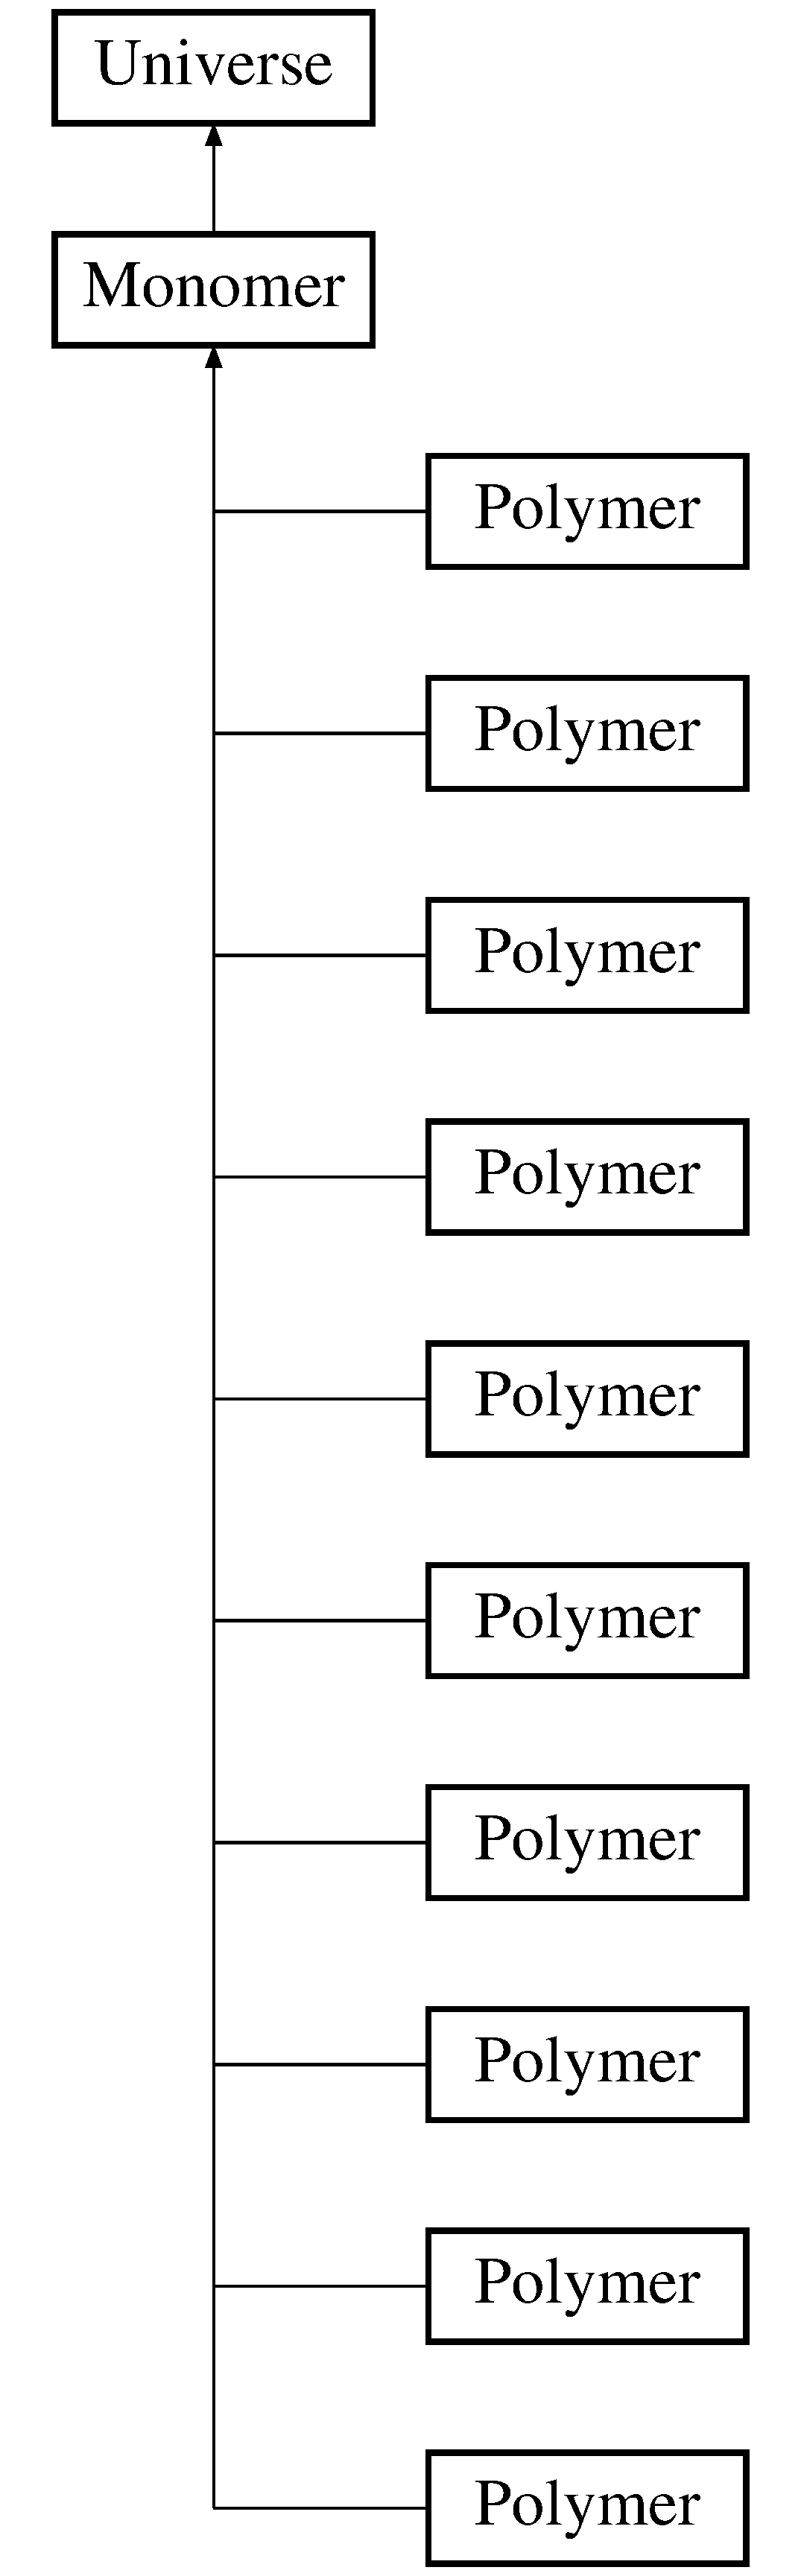
\includegraphics[height=12.000000cm]{classMonomer}
\end{center}
\end{figure}
\subsection*{Public Member Functions}
\begin{DoxyCompactItemize}
\item 
\mbox{\hyperlink{classMonomer_a2b1f69caca47d8597e43300ae7076095}{Monomer}} ()
\item 
\mbox{\hyperlink{classMonomer_af2249bf76132ee3802eaccb49b76fb96}{Monomer}} (unsigned int object\+\_\+type)
\item 
\mbox{\hyperlink{classMonomer_acab23e1c41e236417492da5c1e617b1a}{Monomer}} (unsigned int object\+\_\+type, std\+::chrono\+::time\+\_\+point$<$ \mbox{\hyperlink{universe_8h_a0ef8d951d1ca5ab3cfaf7ab4c7a6fd80}{Clock}} $>$ event\+\_\+time)
\item 
\mbox{\hyperlink{classMonomer_ae2b80466a0e724125aee173df34d1a6c}{Monomer}} (unsigned int object\+\_\+type, std\+::chrono\+::time\+\_\+point$<$ \mbox{\hyperlink{universe_8h_a0ef8d951d1ca5ab3cfaf7ab4c7a6fd80}{Clock}} $>$ event\+\_\+time, \mbox{\hyperlink{classUniverse}{Universe}} \&universe\+\_\+connector)
\item 
virtual \mbox{\hyperlink{classMonomer_a802bf239fc55d16783736393edbd6899}{$\sim$\+Monomer}} ()
\item 
unsigned int \mbox{\hyperlink{classMonomer_a4651a4bd0a41d0698821421043e41126}{Get\+Counter}} (std\+::chrono\+::time\+\_\+point$<$ \mbox{\hyperlink{universe_8h_a0ef8d951d1ca5ab3cfaf7ab4c7a6fd80}{Clock}} $>$ event\+\_\+time)
\item 
void \mbox{\hyperlink{classMonomer_a6f0dfa4382b3d4fa19b7ee0fb8fe7a55}{Set\+Counter}} (std\+::chrono\+::time\+\_\+point$<$ \mbox{\hyperlink{universe_8h_a0ef8d951d1ca5ab3cfaf7ab4c7a6fd80}{Clock}} $>$ event\+\_\+time, unsigned int val)
\item 
bool \mbox{\hyperlink{classMonomer_a16a692cf11117581c9b4ebbed3c04c9c}{Reset\+Parameters}} (std\+::chrono\+::time\+\_\+point$<$ \mbox{\hyperlink{universe_8h_a0ef8d951d1ca5ab3cfaf7ab4c7a6fd80}{Clock}} $>$ event\+\_\+time)
\item 
int \mbox{\hyperlink{classMonomer_ac03023c0d1bb67e5f11091af7ad3735d}{Add\+Solid}} (std\+::chrono\+::time\+\_\+point$<$ \mbox{\hyperlink{universe_8h_a0ef8d951d1ca5ab3cfaf7ab4c7a6fd80}{Clock}} $>$ event\+\_\+time)
\item 
int \mbox{\hyperlink{classMonomer_a48dc2ffb5da8cf3dc3f4f56bba674de6}{Update}} (std\+::chrono\+::time\+\_\+point$<$ \mbox{\hyperlink{universe_8h_a0ef8d951d1ca5ab3cfaf7ab4c7a6fd80}{Clock}} $>$ event\+\_\+time)
\item 
void \mbox{\hyperlink{classMonomer_a1ee35c888318e590082e6cd1772bb430}{Set\+Charge}} (std\+::chrono\+::time\+\_\+point$<$ \mbox{\hyperlink{universe_8h_a0ef8d951d1ca5ab3cfaf7ab4c7a6fd80}{Clock}} $>$ event\+\_\+time, int val) final
\item 
void \mbox{\hyperlink{classMonomer_ad24a86a4c1ac62d1b0ce8040d6b08adf}{Set\+Spin}} (std\+::chrono\+::time\+\_\+point$<$ \mbox{\hyperlink{universe_8h_a0ef8d951d1ca5ab3cfaf7ab4c7a6fd80}{Clock}} $>$ event\+\_\+time, int val) final
\item 
double \mbox{\hyperlink{classMonomer_aa5f7b901e15c9a9eb6e1c3564cd06e4f}{Get\+Gravitation}} (std\+::chrono\+::time\+\_\+point$<$ \mbox{\hyperlink{universe_8h_a0ef8d951d1ca5ab3cfaf7ab4c7a6fd80}{Clock}} $>$ event\+\_\+time) final
\item 
double \mbox{\hyperlink{classMonomer_ac2070d7e39cd0b2a00aa6023ffd51f55}{Get\+Weak}} (std\+::chrono\+::time\+\_\+point$<$ \mbox{\hyperlink{universe_8h_a0ef8d951d1ca5ab3cfaf7ab4c7a6fd80}{Clock}} $>$ event\+\_\+time) final
\item 
double \mbox{\hyperlink{classMonomer_aec6e42dde40c5b3142fab880eabb346a}{Get\+Weak\+Electroweak}} (std\+::chrono\+::time\+\_\+point$<$ \mbox{\hyperlink{universe_8h_a0ef8d951d1ca5ab3cfaf7ab4c7a6fd80}{Clock}} $>$ event\+\_\+time) final
\item 
double \mbox{\hyperlink{classMonomer_ad23f4829d66cb20401cc72a9d72ac320}{Get\+Electromagnetic}} (std\+::chrono\+::time\+\_\+point$<$ \mbox{\hyperlink{universe_8h_a0ef8d951d1ca5ab3cfaf7ab4c7a6fd80}{Clock}} $>$ event\+\_\+time) final
\item 
double \mbox{\hyperlink{classMonomer_a9b270cd1293bc9635813ead284bd3881}{Get\+Electromagnetic\+Electroweak}} (std\+::chrono\+::time\+\_\+point$<$ \mbox{\hyperlink{universe_8h_a0ef8d951d1ca5ab3cfaf7ab4c7a6fd80}{Clock}} $>$ event\+\_\+time) final
\item 
double \mbox{\hyperlink{classMonomer_aa35033340e88c46757d1d5ccba21a21e}{Get\+Strong}} (std\+::chrono\+::time\+\_\+point$<$ \mbox{\hyperlink{universe_8h_a0ef8d951d1ca5ab3cfaf7ab4c7a6fd80}{Clock}} $>$ event\+\_\+time) final
\item 
double \mbox{\hyperlink{classMonomer_a4bc8b39086260e26a196b28b4fc6667f}{Get\+Strong\+Fundamental}} (std\+::chrono\+::time\+\_\+point$<$ \mbox{\hyperlink{universe_8h_a0ef8d951d1ca5ab3cfaf7ab4c7a6fd80}{Clock}} $>$ event\+\_\+time) final
\item 
double \mbox{\hyperlink{classMonomer_a3b00168520f592098356f7cd3e663ad3}{Get\+Strong\+Residual}} (std\+::chrono\+::time\+\_\+point$<$ \mbox{\hyperlink{universe_8h_a0ef8d951d1ca5ab3cfaf7ab4c7a6fd80}{Clock}} $>$ event\+\_\+time) final
\item 
double \mbox{\hyperlink{classMonomer_a8747945cc2f7abd7ce0885345ad14ebc}{Apply\+Gravitation}} (std\+::chrono\+::time\+\_\+point$<$ \mbox{\hyperlink{universe_8h_a0ef8d951d1ca5ab3cfaf7ab4c7a6fd80}{Clock}} $>$ event\+\_\+time, double val) final
\item 
double \mbox{\hyperlink{classMonomer_a176a1a4dfed1eaddc6637bbfd2660aba}{Apply\+Weak}} (std\+::chrono\+::time\+\_\+point$<$ \mbox{\hyperlink{universe_8h_a0ef8d951d1ca5ab3cfaf7ab4c7a6fd80}{Clock}} $>$ event\+\_\+time, double val) final
\item 
double \mbox{\hyperlink{classMonomer_a64f65c128ebc2428c42739c930696ea1}{Apply\+Weak\+Electroweak}} (std\+::chrono\+::time\+\_\+point$<$ \mbox{\hyperlink{universe_8h_a0ef8d951d1ca5ab3cfaf7ab4c7a6fd80}{Clock}} $>$ event\+\_\+time, double val) final
\item 
double \mbox{\hyperlink{classMonomer_ae64dfbf82610ae26427be9c824aef70f}{Apply\+Electromagnetic}} (std\+::chrono\+::time\+\_\+point$<$ \mbox{\hyperlink{universe_8h_a0ef8d951d1ca5ab3cfaf7ab4c7a6fd80}{Clock}} $>$ event\+\_\+time, double val) final
\item 
double \mbox{\hyperlink{classMonomer_a4c3f9894ea57047789bec32602f033cb}{Apply\+Electromagnetic\+Electroweak}} (std\+::chrono\+::time\+\_\+point$<$ \mbox{\hyperlink{universe_8h_a0ef8d951d1ca5ab3cfaf7ab4c7a6fd80}{Clock}} $>$ event\+\_\+time, double val) final
\item 
double \mbox{\hyperlink{classMonomer_acba5091693082fdf2d28f1a5a4ae19a1}{Apply\+Strong}} (std\+::chrono\+::time\+\_\+point$<$ \mbox{\hyperlink{universe_8h_a0ef8d951d1ca5ab3cfaf7ab4c7a6fd80}{Clock}} $>$ event\+\_\+time, double val) final
\item 
double \mbox{\hyperlink{classMonomer_aa186454670f7796e196509238d419a35}{Apply\+Strong\+Fundamental}} (std\+::chrono\+::time\+\_\+point$<$ \mbox{\hyperlink{universe_8h_a0ef8d951d1ca5ab3cfaf7ab4c7a6fd80}{Clock}} $>$ event\+\_\+time, double val) final
\item 
double \mbox{\hyperlink{classMonomer_a921f7add2d446b8670513220ace6c4b2}{Apply\+Strong\+Residual}} (std\+::chrono\+::time\+\_\+point$<$ \mbox{\hyperlink{universe_8h_a0ef8d951d1ca5ab3cfaf7ab4c7a6fd80}{Clock}} $>$ event\+\_\+time, double val) final
\item 
void \mbox{\hyperlink{classMonomer_ab38d44b27a46d5630aeb5e889f927c09}{Set\+Gravitation}} (std\+::chrono\+::time\+\_\+point$<$ \mbox{\hyperlink{universe_8h_a0ef8d951d1ca5ab3cfaf7ab4c7a6fd80}{Clock}} $>$ event\+\_\+time, double val) final
\item 
void \mbox{\hyperlink{classMonomer_ad4fe1db33f493575281e1a2fb35004ca}{Set\+Weak}} (std\+::chrono\+::time\+\_\+point$<$ \mbox{\hyperlink{universe_8h_a0ef8d951d1ca5ab3cfaf7ab4c7a6fd80}{Clock}} $>$ event\+\_\+time, double val) final
\item 
void \mbox{\hyperlink{classMonomer_ab887d7cfd2ecb557efb3ace59852019c}{Set\+Weak\+Electroweak}} (std\+::chrono\+::time\+\_\+point$<$ \mbox{\hyperlink{universe_8h_a0ef8d951d1ca5ab3cfaf7ab4c7a6fd80}{Clock}} $>$ event\+\_\+time, double val) final
\item 
void \mbox{\hyperlink{classMonomer_a50e41be601b31450a97bfd15950cfb3d}{Set\+Electromagnetic}} (std\+::chrono\+::time\+\_\+point$<$ \mbox{\hyperlink{universe_8h_a0ef8d951d1ca5ab3cfaf7ab4c7a6fd80}{Clock}} $>$ event\+\_\+time, double val) final
\item 
void \mbox{\hyperlink{classMonomer_aa034728b74053ed3df452ddc8f1b46e8}{Set\+Electromagnetic\+Electroweak}} (std\+::chrono\+::time\+\_\+point$<$ \mbox{\hyperlink{universe_8h_a0ef8d951d1ca5ab3cfaf7ab4c7a6fd80}{Clock}} $>$ event\+\_\+time, double val) final
\item 
void \mbox{\hyperlink{classMonomer_a10b864f6bcad43f11a2316dbbe4c4742}{Set\+Strong}} (std\+::chrono\+::time\+\_\+point$<$ \mbox{\hyperlink{universe_8h_a0ef8d951d1ca5ab3cfaf7ab4c7a6fd80}{Clock}} $>$ event\+\_\+time, double val) final
\item 
void \mbox{\hyperlink{classMonomer_ad9df06c1a8264bfdb514ef3ba04ef4c7}{Set\+Strong\+Fundamental}} (std\+::chrono\+::time\+\_\+point$<$ \mbox{\hyperlink{universe_8h_a0ef8d951d1ca5ab3cfaf7ab4c7a6fd80}{Clock}} $>$ event\+\_\+time, double val) final
\item 
void \mbox{\hyperlink{classMonomer_ae6ca57913da27fa749d33d1c4fed27ca}{Set\+Strong\+Residual}} (std\+::chrono\+::time\+\_\+point$<$ \mbox{\hyperlink{universe_8h_a0ef8d951d1ca5ab3cfaf7ab4c7a6fd80}{Clock}} $>$ event\+\_\+time, double val) final
\item 
void \mbox{\hyperlink{classMonomer_a5b2375df1e19abdf6045c475d2ac23ca}{Poll\+Elementary\+Force}} (std\+::chrono\+::time\+\_\+point$<$ \mbox{\hyperlink{universe_8h_a0ef8d951d1ca5ab3cfaf7ab4c7a6fd80}{Clock}} $>$ event\+\_\+time) final
\end{DoxyCompactItemize}
\subsection*{Protected Attributes}
\begin{DoxyCompactItemize}
\item 
std\+::vector$<$ \mbox{\hyperlink{classMonomer}{Monomer}} $\ast$ $>$ \mbox{\hyperlink{classMonomer_ad792aeb859c72edbb17414bf00b8fd12}{solid\+\_\+list}}
\end{DoxyCompactItemize}
\subsection*{Private Attributes}
\begin{DoxyCompactItemize}
\item 
unsigned int \mbox{\hyperlink{classMonomer_a163885a7c7da282e9487425392a8f570}{monomer\+\_\+counter}}
\begin{DoxyCompactList}\small\item\em Member variable \char`\"{}monomer\+\_\+counter\char`\"{}. \end{DoxyCompactList}\item 
int \mbox{\hyperlink{classMonomer_acc09d7e702f91a7b14ff58863eb5e4a6}{monomer\+\_\+type}}
\item 
bool \mbox{\hyperlink{classMonomer_ac79d26bc31d0bff553773e38f5f7b9e5}{object\+\_\+initialised}}
\item 
bool \mbox{\hyperlink{classMonomer_ad80cf80e7bc9b29d63e9bb15a364abed}{object\+\_\+disabled}}
\item 
int \mbox{\hyperlink{classMonomer_aaba064b94b15cdafaa5da341a97b7a7f}{duration\+\_\+since\+\_\+last\+\_\+event}}
\item 
std\+::chrono\+::time\+\_\+point$<$ \mbox{\hyperlink{universe_8h_a0ef8d951d1ca5ab3cfaf7ab4c7a6fd80}{Clock}} $>$ \mbox{\hyperlink{classMonomer_a689f4abe0f31c0a7d32221242b3bf944}{time\+\_\+object\+\_\+created}}
\item 
std\+::chrono\+::time\+\_\+point$<$ \mbox{\hyperlink{universe_8h_a0ef8d951d1ca5ab3cfaf7ab4c7a6fd80}{Clock}} $>$ \mbox{\hyperlink{classMonomer_ac2b6be09ea5da5953ced21c9d7d5e3d1}{previous\+\_\+event\+\_\+time}}
\end{DoxyCompactItemize}
\subsection*{Additional Inherited Members}


\subsection{Constructor \& Destructor Documentation}
\mbox{\Hypertarget{classMonomer_a2b1f69caca47d8597e43300ae7076095}\label{classMonomer_a2b1f69caca47d8597e43300ae7076095}} 
\index{Monomer@{Monomer}!Monomer@{Monomer}}
\index{Monomer@{Monomer}!Monomer@{Monomer}}
\subsubsection{\texorpdfstring{Monomer()}{Monomer()}\hspace{0.1cm}{\footnotesize\ttfamily [1/4]}}
{\footnotesize\ttfamily Monomer\+::\+Monomer (\begin{DoxyParamCaption}{ }\end{DoxyParamCaption})\hspace{0.3cm}{\ttfamily [inline]}}

\mbox{\Hypertarget{classMonomer_af2249bf76132ee3802eaccb49b76fb96}\label{classMonomer_af2249bf76132ee3802eaccb49b76fb96}} 
\index{Monomer@{Monomer}!Monomer@{Monomer}}
\index{Monomer@{Monomer}!Monomer@{Monomer}}
\subsubsection{\texorpdfstring{Monomer()}{Monomer()}\hspace{0.1cm}{\footnotesize\ttfamily [2/4]}}
{\footnotesize\ttfamily Monomer\+::\+Monomer (\begin{DoxyParamCaption}\item[{unsigned int}]{object\+\_\+type }\end{DoxyParamCaption})\hspace{0.3cm}{\ttfamily [inline]}}

\mbox{\Hypertarget{classMonomer_acab23e1c41e236417492da5c1e617b1a}\label{classMonomer_acab23e1c41e236417492da5c1e617b1a}} 
\index{Monomer@{Monomer}!Monomer@{Monomer}}
\index{Monomer@{Monomer}!Monomer@{Monomer}}
\subsubsection{\texorpdfstring{Monomer()}{Monomer()}\hspace{0.1cm}{\footnotesize\ttfamily [3/4]}}
{\footnotesize\ttfamily Monomer\+::\+Monomer (\begin{DoxyParamCaption}\item[{unsigned int}]{object\+\_\+type,  }\item[{std\+::chrono\+::time\+\_\+point$<$ \mbox{\hyperlink{universe_8h_a0ef8d951d1ca5ab3cfaf7ab4c7a6fd80}{Clock}} $>$}]{event\+\_\+time }\end{DoxyParamCaption})\hspace{0.3cm}{\ttfamily [inline]}}

\mbox{\Hypertarget{classMonomer_ae2b80466a0e724125aee173df34d1a6c}\label{classMonomer_ae2b80466a0e724125aee173df34d1a6c}} 
\index{Monomer@{Monomer}!Monomer@{Monomer}}
\index{Monomer@{Monomer}!Monomer@{Monomer}}
\subsubsection{\texorpdfstring{Monomer()}{Monomer()}\hspace{0.1cm}{\footnotesize\ttfamily [4/4]}}
{\footnotesize\ttfamily Monomer\+::\+Monomer (\begin{DoxyParamCaption}\item[{unsigned int}]{object\+\_\+type,  }\item[{std\+::chrono\+::time\+\_\+point$<$ \mbox{\hyperlink{universe_8h_a0ef8d951d1ca5ab3cfaf7ab4c7a6fd80}{Clock}} $>$}]{event\+\_\+time,  }\item[{\mbox{\hyperlink{classUniverse}{Universe}} \&}]{universe\+\_\+connector }\end{DoxyParamCaption})\hspace{0.3cm}{\ttfamily [inline]}}

\mbox{\Hypertarget{classMonomer_a802bf239fc55d16783736393edbd6899}\label{classMonomer_a802bf239fc55d16783736393edbd6899}} 
\index{Monomer@{Monomer}!````~Monomer@{$\sim$\+Monomer}}
\index{````~Monomer@{$\sim$\+Monomer}!Monomer@{Monomer}}
\subsubsection{\texorpdfstring{$\sim$\+Monomer()}{~Monomer()}}
{\footnotesize\ttfamily virtual Monomer\+::$\sim$\+Monomer (\begin{DoxyParamCaption}{ }\end{DoxyParamCaption})\hspace{0.3cm}{\ttfamily [inline]}, {\ttfamily [virtual]}}

Default destructor 

\subsection{Member Function Documentation}
\mbox{\Hypertarget{classMonomer_ac03023c0d1bb67e5f11091af7ad3735d}\label{classMonomer_ac03023c0d1bb67e5f11091af7ad3735d}} 
\index{Monomer@{Monomer}!Add\+Solid@{Add\+Solid}}
\index{Add\+Solid@{Add\+Solid}!Monomer@{Monomer}}
\subsubsection{\texorpdfstring{Add\+Solid()}{AddSolid()}}
{\footnotesize\ttfamily int Monomer\+::\+Add\+Solid (\begin{DoxyParamCaption}\item[{std\+::chrono\+::time\+\_\+point$<$ \mbox{\hyperlink{universe_8h_a0ef8d951d1ca5ab3cfaf7ab4c7a6fd80}{Clock}} $>$}]{event\+\_\+time }\end{DoxyParamCaption})}

\mbox{\Hypertarget{classMonomer_ae64dfbf82610ae26427be9c824aef70f}\label{classMonomer_ae64dfbf82610ae26427be9c824aef70f}} 
\index{Monomer@{Monomer}!Apply\+Electromagnetic@{Apply\+Electromagnetic}}
\index{Apply\+Electromagnetic@{Apply\+Electromagnetic}!Monomer@{Monomer}}
\subsubsection{\texorpdfstring{Apply\+Electromagnetic()}{ApplyElectromagnetic()}}
{\footnotesize\ttfamily double Monomer\+::\+Apply\+Electromagnetic (\begin{DoxyParamCaption}\item[{std\+::chrono\+::time\+\_\+point$<$ \mbox{\hyperlink{universe_8h_a0ef8d951d1ca5ab3cfaf7ab4c7a6fd80}{Clock}} $>$}]{event\+\_\+time,  }\item[{double}]{val }\end{DoxyParamCaption})\hspace{0.3cm}{\ttfamily [inline]}, {\ttfamily [final]}, {\ttfamily [virtual]}}



Reimplemented from \mbox{\hyperlink{classUniverse_a1f787da78fa196ba635db21a9e91dabb}{Universe}}.

\mbox{\Hypertarget{classMonomer_a4c3f9894ea57047789bec32602f033cb}\label{classMonomer_a4c3f9894ea57047789bec32602f033cb}} 
\index{Monomer@{Monomer}!Apply\+Electromagnetic\+Electroweak@{Apply\+Electromagnetic\+Electroweak}}
\index{Apply\+Electromagnetic\+Electroweak@{Apply\+Electromagnetic\+Electroweak}!Monomer@{Monomer}}
\subsubsection{\texorpdfstring{Apply\+Electromagnetic\+Electroweak()}{ApplyElectromagneticElectroweak()}}
{\footnotesize\ttfamily double Monomer\+::\+Apply\+Electromagnetic\+Electroweak (\begin{DoxyParamCaption}\item[{std\+::chrono\+::time\+\_\+point$<$ \mbox{\hyperlink{universe_8h_a0ef8d951d1ca5ab3cfaf7ab4c7a6fd80}{Clock}} $>$}]{event\+\_\+time,  }\item[{double}]{val }\end{DoxyParamCaption})\hspace{0.3cm}{\ttfamily [inline]}, {\ttfamily [final]}, {\ttfamily [virtual]}}



Reimplemented from \mbox{\hyperlink{classUniverse_a4c36c1ab30db993307f88363dde5e8c5}{Universe}}.

\mbox{\Hypertarget{classMonomer_a8747945cc2f7abd7ce0885345ad14ebc}\label{classMonomer_a8747945cc2f7abd7ce0885345ad14ebc}} 
\index{Monomer@{Monomer}!Apply\+Gravitation@{Apply\+Gravitation}}
\index{Apply\+Gravitation@{Apply\+Gravitation}!Monomer@{Monomer}}
\subsubsection{\texorpdfstring{Apply\+Gravitation()}{ApplyGravitation()}}
{\footnotesize\ttfamily double Monomer\+::\+Apply\+Gravitation (\begin{DoxyParamCaption}\item[{std\+::chrono\+::time\+\_\+point$<$ \mbox{\hyperlink{universe_8h_a0ef8d951d1ca5ab3cfaf7ab4c7a6fd80}{Clock}} $>$}]{event\+\_\+time,  }\item[{double}]{val }\end{DoxyParamCaption})\hspace{0.3cm}{\ttfamily [inline]}, {\ttfamily [final]}, {\ttfamily [virtual]}}



Reimplemented from \mbox{\hyperlink{classUniverse_a76c0b5e63c2a7d1988c44db341c3d64c}{Universe}}.

\mbox{\Hypertarget{classMonomer_acba5091693082fdf2d28f1a5a4ae19a1}\label{classMonomer_acba5091693082fdf2d28f1a5a4ae19a1}} 
\index{Monomer@{Monomer}!Apply\+Strong@{Apply\+Strong}}
\index{Apply\+Strong@{Apply\+Strong}!Monomer@{Monomer}}
\subsubsection{\texorpdfstring{Apply\+Strong()}{ApplyStrong()}}
{\footnotesize\ttfamily double Monomer\+::\+Apply\+Strong (\begin{DoxyParamCaption}\item[{std\+::chrono\+::time\+\_\+point$<$ \mbox{\hyperlink{universe_8h_a0ef8d951d1ca5ab3cfaf7ab4c7a6fd80}{Clock}} $>$}]{event\+\_\+time,  }\item[{double}]{val }\end{DoxyParamCaption})\hspace{0.3cm}{\ttfamily [inline]}, {\ttfamily [final]}, {\ttfamily [virtual]}}



Reimplemented from \mbox{\hyperlink{classUniverse_a906a88b37f10bfa630bef49dfd0e907a}{Universe}}.

\mbox{\Hypertarget{classMonomer_aa186454670f7796e196509238d419a35}\label{classMonomer_aa186454670f7796e196509238d419a35}} 
\index{Monomer@{Monomer}!Apply\+Strong\+Fundamental@{Apply\+Strong\+Fundamental}}
\index{Apply\+Strong\+Fundamental@{Apply\+Strong\+Fundamental}!Monomer@{Monomer}}
\subsubsection{\texorpdfstring{Apply\+Strong\+Fundamental()}{ApplyStrongFundamental()}}
{\footnotesize\ttfamily double Monomer\+::\+Apply\+Strong\+Fundamental (\begin{DoxyParamCaption}\item[{std\+::chrono\+::time\+\_\+point$<$ \mbox{\hyperlink{universe_8h_a0ef8d951d1ca5ab3cfaf7ab4c7a6fd80}{Clock}} $>$}]{event\+\_\+time,  }\item[{double}]{val }\end{DoxyParamCaption})\hspace{0.3cm}{\ttfamily [inline]}, {\ttfamily [final]}, {\ttfamily [virtual]}}



Reimplemented from \mbox{\hyperlink{classUniverse_a62789bcff84bd750b0366004381e2fdd}{Universe}}.

\mbox{\Hypertarget{classMonomer_a921f7add2d446b8670513220ace6c4b2}\label{classMonomer_a921f7add2d446b8670513220ace6c4b2}} 
\index{Monomer@{Monomer}!Apply\+Strong\+Residual@{Apply\+Strong\+Residual}}
\index{Apply\+Strong\+Residual@{Apply\+Strong\+Residual}!Monomer@{Monomer}}
\subsubsection{\texorpdfstring{Apply\+Strong\+Residual()}{ApplyStrongResidual()}}
{\footnotesize\ttfamily double Monomer\+::\+Apply\+Strong\+Residual (\begin{DoxyParamCaption}\item[{std\+::chrono\+::time\+\_\+point$<$ \mbox{\hyperlink{universe_8h_a0ef8d951d1ca5ab3cfaf7ab4c7a6fd80}{Clock}} $>$}]{event\+\_\+time,  }\item[{double}]{val }\end{DoxyParamCaption})\hspace{0.3cm}{\ttfamily [inline]}, {\ttfamily [final]}, {\ttfamily [virtual]}}



Reimplemented from \mbox{\hyperlink{classUniverse_af7becebb347be9a85541d96a3eca1ca7}{Universe}}.

\mbox{\Hypertarget{classMonomer_a176a1a4dfed1eaddc6637bbfd2660aba}\label{classMonomer_a176a1a4dfed1eaddc6637bbfd2660aba}} 
\index{Monomer@{Monomer}!Apply\+Weak@{Apply\+Weak}}
\index{Apply\+Weak@{Apply\+Weak}!Monomer@{Monomer}}
\subsubsection{\texorpdfstring{Apply\+Weak()}{ApplyWeak()}}
{\footnotesize\ttfamily double Monomer\+::\+Apply\+Weak (\begin{DoxyParamCaption}\item[{std\+::chrono\+::time\+\_\+point$<$ \mbox{\hyperlink{universe_8h_a0ef8d951d1ca5ab3cfaf7ab4c7a6fd80}{Clock}} $>$}]{event\+\_\+time,  }\item[{double}]{val }\end{DoxyParamCaption})\hspace{0.3cm}{\ttfamily [inline]}, {\ttfamily [final]}, {\ttfamily [virtual]}}



Reimplemented from \mbox{\hyperlink{classUniverse_a6d1226b3adec3c42a833afdbb6a65a92}{Universe}}.

\mbox{\Hypertarget{classMonomer_a64f65c128ebc2428c42739c930696ea1}\label{classMonomer_a64f65c128ebc2428c42739c930696ea1}} 
\index{Monomer@{Monomer}!Apply\+Weak\+Electroweak@{Apply\+Weak\+Electroweak}}
\index{Apply\+Weak\+Electroweak@{Apply\+Weak\+Electroweak}!Monomer@{Monomer}}
\subsubsection{\texorpdfstring{Apply\+Weak\+Electroweak()}{ApplyWeakElectroweak()}}
{\footnotesize\ttfamily double Monomer\+::\+Apply\+Weak\+Electroweak (\begin{DoxyParamCaption}\item[{std\+::chrono\+::time\+\_\+point$<$ \mbox{\hyperlink{universe_8h_a0ef8d951d1ca5ab3cfaf7ab4c7a6fd80}{Clock}} $>$}]{event\+\_\+time,  }\item[{double}]{val }\end{DoxyParamCaption})\hspace{0.3cm}{\ttfamily [inline]}, {\ttfamily [final]}, {\ttfamily [virtual]}}



Reimplemented from \mbox{\hyperlink{classUniverse_a46a906baabb63e5d31f8b48ea1fae52e}{Universe}}.

\mbox{\Hypertarget{classMonomer_a4651a4bd0a41d0698821421043e41126}\label{classMonomer_a4651a4bd0a41d0698821421043e41126}} 
\index{Monomer@{Monomer}!Get\+Counter@{Get\+Counter}}
\index{Get\+Counter@{Get\+Counter}!Monomer@{Monomer}}
\subsubsection{\texorpdfstring{Get\+Counter()}{GetCounter()}}
{\footnotesize\ttfamily unsigned int Monomer\+::\+Get\+Counter (\begin{DoxyParamCaption}\item[{std\+::chrono\+::time\+\_\+point$<$ \mbox{\hyperlink{universe_8h_a0ef8d951d1ca5ab3cfaf7ab4c7a6fd80}{Clock}} $>$}]{event\+\_\+time }\end{DoxyParamCaption})}

\mbox{\Hypertarget{classMonomer_ad23f4829d66cb20401cc72a9d72ac320}\label{classMonomer_ad23f4829d66cb20401cc72a9d72ac320}} 
\index{Monomer@{Monomer}!Get\+Electromagnetic@{Get\+Electromagnetic}}
\index{Get\+Electromagnetic@{Get\+Electromagnetic}!Monomer@{Monomer}}
\subsubsection{\texorpdfstring{Get\+Electromagnetic()}{GetElectromagnetic()}}
{\footnotesize\ttfamily double Monomer\+::\+Get\+Electromagnetic (\begin{DoxyParamCaption}\item[{std\+::chrono\+::time\+\_\+point$<$ \mbox{\hyperlink{universe_8h_a0ef8d951d1ca5ab3cfaf7ab4c7a6fd80}{Clock}} $>$}]{event\+\_\+time }\end{DoxyParamCaption})\hspace{0.3cm}{\ttfamily [inline]}, {\ttfamily [final]}, {\ttfamily [virtual]}}



Reimplemented from \mbox{\hyperlink{classUniverse_a63b850ef3f3394313353109d222bf5d1}{Universe}}.

\mbox{\Hypertarget{classMonomer_a9b270cd1293bc9635813ead284bd3881}\label{classMonomer_a9b270cd1293bc9635813ead284bd3881}} 
\index{Monomer@{Monomer}!Get\+Electromagnetic\+Electroweak@{Get\+Electromagnetic\+Electroweak}}
\index{Get\+Electromagnetic\+Electroweak@{Get\+Electromagnetic\+Electroweak}!Monomer@{Monomer}}
\subsubsection{\texorpdfstring{Get\+Electromagnetic\+Electroweak()}{GetElectromagneticElectroweak()}}
{\footnotesize\ttfamily double Monomer\+::\+Get\+Electromagnetic\+Electroweak (\begin{DoxyParamCaption}\item[{std\+::chrono\+::time\+\_\+point$<$ \mbox{\hyperlink{universe_8h_a0ef8d951d1ca5ab3cfaf7ab4c7a6fd80}{Clock}} $>$}]{event\+\_\+time }\end{DoxyParamCaption})\hspace{0.3cm}{\ttfamily [inline]}, {\ttfamily [final]}, {\ttfamily [virtual]}}



Reimplemented from \mbox{\hyperlink{classUniverse_a9f099605c082e7fa755787a6a8cab7ba}{Universe}}.

\mbox{\Hypertarget{classMonomer_aa5f7b901e15c9a9eb6e1c3564cd06e4f}\label{classMonomer_aa5f7b901e15c9a9eb6e1c3564cd06e4f}} 
\index{Monomer@{Monomer}!Get\+Gravitation@{Get\+Gravitation}}
\index{Get\+Gravitation@{Get\+Gravitation}!Monomer@{Monomer}}
\subsubsection{\texorpdfstring{Get\+Gravitation()}{GetGravitation()}}
{\footnotesize\ttfamily double Monomer\+::\+Get\+Gravitation (\begin{DoxyParamCaption}\item[{std\+::chrono\+::time\+\_\+point$<$ \mbox{\hyperlink{universe_8h_a0ef8d951d1ca5ab3cfaf7ab4c7a6fd80}{Clock}} $>$}]{event\+\_\+time }\end{DoxyParamCaption})\hspace{0.3cm}{\ttfamily [inline]}, {\ttfamily [final]}, {\ttfamily [virtual]}}



Reimplemented from \mbox{\hyperlink{classUniverse_ab0404e774ee0ed66b597ff5b8e989446}{Universe}}.

\mbox{\Hypertarget{classMonomer_aa35033340e88c46757d1d5ccba21a21e}\label{classMonomer_aa35033340e88c46757d1d5ccba21a21e}} 
\index{Monomer@{Monomer}!Get\+Strong@{Get\+Strong}}
\index{Get\+Strong@{Get\+Strong}!Monomer@{Monomer}}
\subsubsection{\texorpdfstring{Get\+Strong()}{GetStrong()}}
{\footnotesize\ttfamily double Monomer\+::\+Get\+Strong (\begin{DoxyParamCaption}\item[{std\+::chrono\+::time\+\_\+point$<$ \mbox{\hyperlink{universe_8h_a0ef8d951d1ca5ab3cfaf7ab4c7a6fd80}{Clock}} $>$}]{event\+\_\+time }\end{DoxyParamCaption})\hspace{0.3cm}{\ttfamily [inline]}, {\ttfamily [final]}, {\ttfamily [virtual]}}



Reimplemented from \mbox{\hyperlink{classUniverse_acb453ce71da418c5b5617fecede9571b}{Universe}}.

\mbox{\Hypertarget{classMonomer_a4bc8b39086260e26a196b28b4fc6667f}\label{classMonomer_a4bc8b39086260e26a196b28b4fc6667f}} 
\index{Monomer@{Monomer}!Get\+Strong\+Fundamental@{Get\+Strong\+Fundamental}}
\index{Get\+Strong\+Fundamental@{Get\+Strong\+Fundamental}!Monomer@{Monomer}}
\subsubsection{\texorpdfstring{Get\+Strong\+Fundamental()}{GetStrongFundamental()}}
{\footnotesize\ttfamily double Monomer\+::\+Get\+Strong\+Fundamental (\begin{DoxyParamCaption}\item[{std\+::chrono\+::time\+\_\+point$<$ \mbox{\hyperlink{universe_8h_a0ef8d951d1ca5ab3cfaf7ab4c7a6fd80}{Clock}} $>$}]{event\+\_\+time }\end{DoxyParamCaption})\hspace{0.3cm}{\ttfamily [inline]}, {\ttfamily [final]}, {\ttfamily [virtual]}}



Reimplemented from \mbox{\hyperlink{classUniverse_ab44daccba01ee7e3cf9b50bba83dd19e}{Universe}}.

\mbox{\Hypertarget{classMonomer_a3b00168520f592098356f7cd3e663ad3}\label{classMonomer_a3b00168520f592098356f7cd3e663ad3}} 
\index{Monomer@{Monomer}!Get\+Strong\+Residual@{Get\+Strong\+Residual}}
\index{Get\+Strong\+Residual@{Get\+Strong\+Residual}!Monomer@{Monomer}}
\subsubsection{\texorpdfstring{Get\+Strong\+Residual()}{GetStrongResidual()}}
{\footnotesize\ttfamily double Monomer\+::\+Get\+Strong\+Residual (\begin{DoxyParamCaption}\item[{std\+::chrono\+::time\+\_\+point$<$ \mbox{\hyperlink{universe_8h_a0ef8d951d1ca5ab3cfaf7ab4c7a6fd80}{Clock}} $>$}]{event\+\_\+time }\end{DoxyParamCaption})\hspace{0.3cm}{\ttfamily [inline]}, {\ttfamily [final]}, {\ttfamily [virtual]}}



Reimplemented from \mbox{\hyperlink{classUniverse_af0f4b81950061e63c2855eb40957a5b1}{Universe}}.

\mbox{\Hypertarget{classMonomer_ac2070d7e39cd0b2a00aa6023ffd51f55}\label{classMonomer_ac2070d7e39cd0b2a00aa6023ffd51f55}} 
\index{Monomer@{Monomer}!Get\+Weak@{Get\+Weak}}
\index{Get\+Weak@{Get\+Weak}!Monomer@{Monomer}}
\subsubsection{\texorpdfstring{Get\+Weak()}{GetWeak()}}
{\footnotesize\ttfamily double Monomer\+::\+Get\+Weak (\begin{DoxyParamCaption}\item[{std\+::chrono\+::time\+\_\+point$<$ \mbox{\hyperlink{universe_8h_a0ef8d951d1ca5ab3cfaf7ab4c7a6fd80}{Clock}} $>$}]{event\+\_\+time }\end{DoxyParamCaption})\hspace{0.3cm}{\ttfamily [inline]}, {\ttfamily [final]}, {\ttfamily [virtual]}}



Reimplemented from \mbox{\hyperlink{classUniverse_a4476b7e0a3fc1764909f556257fd9ec7}{Universe}}.

\mbox{\Hypertarget{classMonomer_aec6e42dde40c5b3142fab880eabb346a}\label{classMonomer_aec6e42dde40c5b3142fab880eabb346a}} 
\index{Monomer@{Monomer}!Get\+Weak\+Electroweak@{Get\+Weak\+Electroweak}}
\index{Get\+Weak\+Electroweak@{Get\+Weak\+Electroweak}!Monomer@{Monomer}}
\subsubsection{\texorpdfstring{Get\+Weak\+Electroweak()}{GetWeakElectroweak()}}
{\footnotesize\ttfamily double Monomer\+::\+Get\+Weak\+Electroweak (\begin{DoxyParamCaption}\item[{std\+::chrono\+::time\+\_\+point$<$ \mbox{\hyperlink{universe_8h_a0ef8d951d1ca5ab3cfaf7ab4c7a6fd80}{Clock}} $>$}]{event\+\_\+time }\end{DoxyParamCaption})\hspace{0.3cm}{\ttfamily [inline]}, {\ttfamily [final]}, {\ttfamily [virtual]}}



Reimplemented from \mbox{\hyperlink{classUniverse_a645299738e6b798a037f2a15a2e7cf4d}{Universe}}.

\mbox{\Hypertarget{classMonomer_a5b2375df1e19abdf6045c475d2ac23ca}\label{classMonomer_a5b2375df1e19abdf6045c475d2ac23ca}} 
\index{Monomer@{Monomer}!Poll\+Elementary\+Force@{Poll\+Elementary\+Force}}
\index{Poll\+Elementary\+Force@{Poll\+Elementary\+Force}!Monomer@{Monomer}}
\subsubsection{\texorpdfstring{Poll\+Elementary\+Force()}{PollElementaryForce()}}
{\footnotesize\ttfamily void Monomer\+::\+Poll\+Elementary\+Force (\begin{DoxyParamCaption}\item[{std\+::chrono\+::time\+\_\+point$<$ \mbox{\hyperlink{universe_8h_a0ef8d951d1ca5ab3cfaf7ab4c7a6fd80}{Clock}} $>$}]{event\+\_\+time }\end{DoxyParamCaption})\hspace{0.3cm}{\ttfamily [inline]}, {\ttfamily [final]}, {\ttfamily [virtual]}}



Reimplemented from \mbox{\hyperlink{classUniverse_a0c485c504542409cbb5cfd8543c35b11}{Universe}}.

\mbox{\Hypertarget{classMonomer_a16a692cf11117581c9b4ebbed3c04c9c}\label{classMonomer_a16a692cf11117581c9b4ebbed3c04c9c}} 
\index{Monomer@{Monomer}!Reset\+Parameters@{Reset\+Parameters}}
\index{Reset\+Parameters@{Reset\+Parameters}!Monomer@{Monomer}}
\subsubsection{\texorpdfstring{Reset\+Parameters()}{ResetParameters()}}
{\footnotesize\ttfamily bool Monomer\+::\+Reset\+Parameters (\begin{DoxyParamCaption}\item[{std\+::chrono\+::time\+\_\+point$<$ \mbox{\hyperlink{universe_8h_a0ef8d951d1ca5ab3cfaf7ab4c7a6fd80}{Clock}} $>$}]{event\+\_\+time }\end{DoxyParamCaption})}

\mbox{\Hypertarget{classMonomer_a1ee35c888318e590082e6cd1772bb430}\label{classMonomer_a1ee35c888318e590082e6cd1772bb430}} 
\index{Monomer@{Monomer}!Set\+Charge@{Set\+Charge}}
\index{Set\+Charge@{Set\+Charge}!Monomer@{Monomer}}
\subsubsection{\texorpdfstring{Set\+Charge()}{SetCharge()}}
{\footnotesize\ttfamily void Monomer\+::\+Set\+Charge (\begin{DoxyParamCaption}\item[{std\+::chrono\+::time\+\_\+point$<$ \mbox{\hyperlink{universe_8h_a0ef8d951d1ca5ab3cfaf7ab4c7a6fd80}{Clock}} $>$}]{event\+\_\+time,  }\item[{int}]{val }\end{DoxyParamCaption})\hspace{0.3cm}{\ttfamily [inline]}, {\ttfamily [final]}, {\ttfamily [virtual]}}



Reimplemented from \mbox{\hyperlink{classUniverse_a3b3da7c86a7b75e5e5c0b7972ac82a87}{Universe}}.

\mbox{\Hypertarget{classMonomer_a6f0dfa4382b3d4fa19b7ee0fb8fe7a55}\label{classMonomer_a6f0dfa4382b3d4fa19b7ee0fb8fe7a55}} 
\index{Monomer@{Monomer}!Set\+Counter@{Set\+Counter}}
\index{Set\+Counter@{Set\+Counter}!Monomer@{Monomer}}
\subsubsection{\texorpdfstring{Set\+Counter()}{SetCounter()}}
{\footnotesize\ttfamily void Monomer\+::\+Set\+Counter (\begin{DoxyParamCaption}\item[{std\+::chrono\+::time\+\_\+point$<$ \mbox{\hyperlink{universe_8h_a0ef8d951d1ca5ab3cfaf7ab4c7a6fd80}{Clock}} $>$}]{event\+\_\+time,  }\item[{unsigned int}]{val }\end{DoxyParamCaption})\hspace{0.3cm}{\ttfamily [virtual]}}



Reimplemented from \mbox{\hyperlink{classUniverse_aa22202ae740eb1355529afcb13285e91}{Universe}}.



Reimplemented in \mbox{\hyperlink{classPolymer_a1500ffc682396af2f4306c7c7ea7fd87}{Polymer}}.

\mbox{\Hypertarget{classMonomer_a50e41be601b31450a97bfd15950cfb3d}\label{classMonomer_a50e41be601b31450a97bfd15950cfb3d}} 
\index{Monomer@{Monomer}!Set\+Electromagnetic@{Set\+Electromagnetic}}
\index{Set\+Electromagnetic@{Set\+Electromagnetic}!Monomer@{Monomer}}
\subsubsection{\texorpdfstring{Set\+Electromagnetic()}{SetElectromagnetic()}}
{\footnotesize\ttfamily void Monomer\+::\+Set\+Electromagnetic (\begin{DoxyParamCaption}\item[{std\+::chrono\+::time\+\_\+point$<$ \mbox{\hyperlink{universe_8h_a0ef8d951d1ca5ab3cfaf7ab4c7a6fd80}{Clock}} $>$}]{event\+\_\+time,  }\item[{double}]{val }\end{DoxyParamCaption})\hspace{0.3cm}{\ttfamily [inline]}, {\ttfamily [final]}, {\ttfamily [virtual]}}



Reimplemented from \mbox{\hyperlink{classUniverse_aa981fc7e252b1fbbb675f0371860954d}{Universe}}.

\mbox{\Hypertarget{classMonomer_aa034728b74053ed3df452ddc8f1b46e8}\label{classMonomer_aa034728b74053ed3df452ddc8f1b46e8}} 
\index{Monomer@{Monomer}!Set\+Electromagnetic\+Electroweak@{Set\+Electromagnetic\+Electroweak}}
\index{Set\+Electromagnetic\+Electroweak@{Set\+Electromagnetic\+Electroweak}!Monomer@{Monomer}}
\subsubsection{\texorpdfstring{Set\+Electromagnetic\+Electroweak()}{SetElectromagneticElectroweak()}}
{\footnotesize\ttfamily void Monomer\+::\+Set\+Electromagnetic\+Electroweak (\begin{DoxyParamCaption}\item[{std\+::chrono\+::time\+\_\+point$<$ \mbox{\hyperlink{universe_8h_a0ef8d951d1ca5ab3cfaf7ab4c7a6fd80}{Clock}} $>$}]{event\+\_\+time,  }\item[{double}]{val }\end{DoxyParamCaption})\hspace{0.3cm}{\ttfamily [inline]}, {\ttfamily [final]}, {\ttfamily [virtual]}}



Reimplemented from \mbox{\hyperlink{classUniverse_a608aa95698380f791a0ffba45cc1bee3}{Universe}}.

\mbox{\Hypertarget{classMonomer_ab38d44b27a46d5630aeb5e889f927c09}\label{classMonomer_ab38d44b27a46d5630aeb5e889f927c09}} 
\index{Monomer@{Monomer}!Set\+Gravitation@{Set\+Gravitation}}
\index{Set\+Gravitation@{Set\+Gravitation}!Monomer@{Monomer}}
\subsubsection{\texorpdfstring{Set\+Gravitation()}{SetGravitation()}}
{\footnotesize\ttfamily void Monomer\+::\+Set\+Gravitation (\begin{DoxyParamCaption}\item[{std\+::chrono\+::time\+\_\+point$<$ \mbox{\hyperlink{universe_8h_a0ef8d951d1ca5ab3cfaf7ab4c7a6fd80}{Clock}} $>$}]{event\+\_\+time,  }\item[{double}]{val }\end{DoxyParamCaption})\hspace{0.3cm}{\ttfamily [inline]}, {\ttfamily [final]}, {\ttfamily [virtual]}}



Reimplemented from \mbox{\hyperlink{classUniverse_ae0cb8d86b2fbb8396d605160344b42f5}{Universe}}.

\mbox{\Hypertarget{classMonomer_ad24a86a4c1ac62d1b0ce8040d6b08adf}\label{classMonomer_ad24a86a4c1ac62d1b0ce8040d6b08adf}} 
\index{Monomer@{Monomer}!Set\+Spin@{Set\+Spin}}
\index{Set\+Spin@{Set\+Spin}!Monomer@{Monomer}}
\subsubsection{\texorpdfstring{Set\+Spin()}{SetSpin()}}
{\footnotesize\ttfamily void Monomer\+::\+Set\+Spin (\begin{DoxyParamCaption}\item[{std\+::chrono\+::time\+\_\+point$<$ \mbox{\hyperlink{universe_8h_a0ef8d951d1ca5ab3cfaf7ab4c7a6fd80}{Clock}} $>$}]{event\+\_\+time,  }\item[{int}]{val }\end{DoxyParamCaption})\hspace{0.3cm}{\ttfamily [inline]}, {\ttfamily [final]}, {\ttfamily [virtual]}}



Reimplemented from \mbox{\hyperlink{classUniverse_ae2ae1c3b3e4cde2c18f5f6a814761ec8}{Universe}}.

\mbox{\Hypertarget{classMonomer_a10b864f6bcad43f11a2316dbbe4c4742}\label{classMonomer_a10b864f6bcad43f11a2316dbbe4c4742}} 
\index{Monomer@{Monomer}!Set\+Strong@{Set\+Strong}}
\index{Set\+Strong@{Set\+Strong}!Monomer@{Monomer}}
\subsubsection{\texorpdfstring{Set\+Strong()}{SetStrong()}}
{\footnotesize\ttfamily void Monomer\+::\+Set\+Strong (\begin{DoxyParamCaption}\item[{std\+::chrono\+::time\+\_\+point$<$ \mbox{\hyperlink{universe_8h_a0ef8d951d1ca5ab3cfaf7ab4c7a6fd80}{Clock}} $>$}]{event\+\_\+time,  }\item[{double}]{val }\end{DoxyParamCaption})\hspace{0.3cm}{\ttfamily [inline]}, {\ttfamily [final]}, {\ttfamily [virtual]}}



Reimplemented from \mbox{\hyperlink{classUniverse_a5946c8f3d4cda305f3ecd10df21a2f94}{Universe}}.

\mbox{\Hypertarget{classMonomer_ad9df06c1a8264bfdb514ef3ba04ef4c7}\label{classMonomer_ad9df06c1a8264bfdb514ef3ba04ef4c7}} 
\index{Monomer@{Monomer}!Set\+Strong\+Fundamental@{Set\+Strong\+Fundamental}}
\index{Set\+Strong\+Fundamental@{Set\+Strong\+Fundamental}!Monomer@{Monomer}}
\subsubsection{\texorpdfstring{Set\+Strong\+Fundamental()}{SetStrongFundamental()}}
{\footnotesize\ttfamily void Monomer\+::\+Set\+Strong\+Fundamental (\begin{DoxyParamCaption}\item[{std\+::chrono\+::time\+\_\+point$<$ \mbox{\hyperlink{universe_8h_a0ef8d951d1ca5ab3cfaf7ab4c7a6fd80}{Clock}} $>$}]{event\+\_\+time,  }\item[{double}]{val }\end{DoxyParamCaption})\hspace{0.3cm}{\ttfamily [inline]}, {\ttfamily [final]}, {\ttfamily [virtual]}}



Reimplemented from \mbox{\hyperlink{classUniverse_aafec97a231126b71c73ac1258609a284}{Universe}}.

\mbox{\Hypertarget{classMonomer_ae6ca57913da27fa749d33d1c4fed27ca}\label{classMonomer_ae6ca57913da27fa749d33d1c4fed27ca}} 
\index{Monomer@{Monomer}!Set\+Strong\+Residual@{Set\+Strong\+Residual}}
\index{Set\+Strong\+Residual@{Set\+Strong\+Residual}!Monomer@{Monomer}}
\subsubsection{\texorpdfstring{Set\+Strong\+Residual()}{SetStrongResidual()}}
{\footnotesize\ttfamily void Monomer\+::\+Set\+Strong\+Residual (\begin{DoxyParamCaption}\item[{std\+::chrono\+::time\+\_\+point$<$ \mbox{\hyperlink{universe_8h_a0ef8d951d1ca5ab3cfaf7ab4c7a6fd80}{Clock}} $>$}]{event\+\_\+time,  }\item[{double}]{val }\end{DoxyParamCaption})\hspace{0.3cm}{\ttfamily [inline]}, {\ttfamily [final]}, {\ttfamily [virtual]}}



Reimplemented from \mbox{\hyperlink{classUniverse_a1b2d6197ddf3d613cc30bd04d22ed8b7}{Universe}}.

\mbox{\Hypertarget{classMonomer_ad4fe1db33f493575281e1a2fb35004ca}\label{classMonomer_ad4fe1db33f493575281e1a2fb35004ca}} 
\index{Monomer@{Monomer}!Set\+Weak@{Set\+Weak}}
\index{Set\+Weak@{Set\+Weak}!Monomer@{Monomer}}
\subsubsection{\texorpdfstring{Set\+Weak()}{SetWeak()}}
{\footnotesize\ttfamily void Monomer\+::\+Set\+Weak (\begin{DoxyParamCaption}\item[{std\+::chrono\+::time\+\_\+point$<$ \mbox{\hyperlink{universe_8h_a0ef8d951d1ca5ab3cfaf7ab4c7a6fd80}{Clock}} $>$}]{event\+\_\+time,  }\item[{double}]{val }\end{DoxyParamCaption})\hspace{0.3cm}{\ttfamily [inline]}, {\ttfamily [final]}, {\ttfamily [virtual]}}



Reimplemented from \mbox{\hyperlink{classUniverse_a0f5cd04081b41ee931c0557dc397f6fb}{Universe}}.

\mbox{\Hypertarget{classMonomer_ab887d7cfd2ecb557efb3ace59852019c}\label{classMonomer_ab887d7cfd2ecb557efb3ace59852019c}} 
\index{Monomer@{Monomer}!Set\+Weak\+Electroweak@{Set\+Weak\+Electroweak}}
\index{Set\+Weak\+Electroweak@{Set\+Weak\+Electroweak}!Monomer@{Monomer}}
\subsubsection{\texorpdfstring{Set\+Weak\+Electroweak()}{SetWeakElectroweak()}}
{\footnotesize\ttfamily void Monomer\+::\+Set\+Weak\+Electroweak (\begin{DoxyParamCaption}\item[{std\+::chrono\+::time\+\_\+point$<$ \mbox{\hyperlink{universe_8h_a0ef8d951d1ca5ab3cfaf7ab4c7a6fd80}{Clock}} $>$}]{event\+\_\+time,  }\item[{double}]{val }\end{DoxyParamCaption})\hspace{0.3cm}{\ttfamily [inline]}, {\ttfamily [final]}, {\ttfamily [virtual]}}



Reimplemented from \mbox{\hyperlink{classUniverse_a2d3d642bfdc863248e93535832fa4b00}{Universe}}.

\mbox{\Hypertarget{classMonomer_a48dc2ffb5da8cf3dc3f4f56bba674de6}\label{classMonomer_a48dc2ffb5da8cf3dc3f4f56bba674de6}} 
\index{Monomer@{Monomer}!Update@{Update}}
\index{Update@{Update}!Monomer@{Monomer}}
\subsubsection{\texorpdfstring{Update()}{Update()}}
{\footnotesize\ttfamily int Monomer\+::\+Update (\begin{DoxyParamCaption}\item[{std\+::chrono\+::time\+\_\+point$<$ \mbox{\hyperlink{universe_8h_a0ef8d951d1ca5ab3cfaf7ab4c7a6fd80}{Clock}} $>$}]{event\+\_\+time }\end{DoxyParamCaption})}



\subsection{Member Data Documentation}
\mbox{\Hypertarget{classMonomer_aaba064b94b15cdafaa5da341a97b7a7f}\label{classMonomer_aaba064b94b15cdafaa5da341a97b7a7f}} 
\index{Monomer@{Monomer}!duration\+\_\+since\+\_\+last\+\_\+event@{duration\+\_\+since\+\_\+last\+\_\+event}}
\index{duration\+\_\+since\+\_\+last\+\_\+event@{duration\+\_\+since\+\_\+last\+\_\+event}!Monomer@{Monomer}}
\subsubsection{\texorpdfstring{duration\+\_\+since\+\_\+last\+\_\+event}{duration\_since\_last\_event}}
{\footnotesize\ttfamily int Monomer\+::duration\+\_\+since\+\_\+last\+\_\+event\hspace{0.3cm}{\ttfamily [private]}}

\mbox{\Hypertarget{classMonomer_a163885a7c7da282e9487425392a8f570}\label{classMonomer_a163885a7c7da282e9487425392a8f570}} 
\index{Monomer@{Monomer}!monomer\+\_\+counter@{monomer\+\_\+counter}}
\index{monomer\+\_\+counter@{monomer\+\_\+counter}!Monomer@{Monomer}}
\subsubsection{\texorpdfstring{monomer\+\_\+counter}{monomer\_counter}}
{\footnotesize\ttfamily unsigned int Monomer\+::monomer\+\_\+counter\hspace{0.3cm}{\ttfamily [private]}}



Member variable \char`\"{}monomer\+\_\+counter\char`\"{}. 

\mbox{\Hypertarget{classMonomer_acc09d7e702f91a7b14ff58863eb5e4a6}\label{classMonomer_acc09d7e702f91a7b14ff58863eb5e4a6}} 
\index{Monomer@{Monomer}!monomer\+\_\+type@{monomer\+\_\+type}}
\index{monomer\+\_\+type@{monomer\+\_\+type}!Monomer@{Monomer}}
\subsubsection{\texorpdfstring{monomer\+\_\+type}{monomer\_type}}
{\footnotesize\ttfamily int Monomer\+::monomer\+\_\+type\hspace{0.3cm}{\ttfamily [private]}}

\mbox{\Hypertarget{classMonomer_ad80cf80e7bc9b29d63e9bb15a364abed}\label{classMonomer_ad80cf80e7bc9b29d63e9bb15a364abed}} 
\index{Monomer@{Monomer}!object\+\_\+disabled@{object\+\_\+disabled}}
\index{object\+\_\+disabled@{object\+\_\+disabled}!Monomer@{Monomer}}
\subsubsection{\texorpdfstring{object\+\_\+disabled}{object\_disabled}}
{\footnotesize\ttfamily bool Monomer\+::object\+\_\+disabled\hspace{0.3cm}{\ttfamily [private]}}

\mbox{\Hypertarget{classMonomer_ac79d26bc31d0bff553773e38f5f7b9e5}\label{classMonomer_ac79d26bc31d0bff553773e38f5f7b9e5}} 
\index{Monomer@{Monomer}!object\+\_\+initialised@{object\+\_\+initialised}}
\index{object\+\_\+initialised@{object\+\_\+initialised}!Monomer@{Monomer}}
\subsubsection{\texorpdfstring{object\+\_\+initialised}{object\_initialised}}
{\footnotesize\ttfamily bool Monomer\+::object\+\_\+initialised\hspace{0.3cm}{\ttfamily [private]}}

\mbox{\Hypertarget{classMonomer_ac2b6be09ea5da5953ced21c9d7d5e3d1}\label{classMonomer_ac2b6be09ea5da5953ced21c9d7d5e3d1}} 
\index{Monomer@{Monomer}!previous\+\_\+event\+\_\+time@{previous\+\_\+event\+\_\+time}}
\index{previous\+\_\+event\+\_\+time@{previous\+\_\+event\+\_\+time}!Monomer@{Monomer}}
\subsubsection{\texorpdfstring{previous\+\_\+event\+\_\+time}{previous\_event\_time}}
{\footnotesize\ttfamily std\+::chrono\+::time\+\_\+point$<$\mbox{\hyperlink{universe_8h_a0ef8d951d1ca5ab3cfaf7ab4c7a6fd80}{Clock}}$>$ Monomer\+::previous\+\_\+event\+\_\+time\hspace{0.3cm}{\ttfamily [private]}}

\mbox{\Hypertarget{classMonomer_ad792aeb859c72edbb17414bf00b8fd12}\label{classMonomer_ad792aeb859c72edbb17414bf00b8fd12}} 
\index{Monomer@{Monomer}!solid\+\_\+list@{solid\+\_\+list}}
\index{solid\+\_\+list@{solid\+\_\+list}!Monomer@{Monomer}}
\subsubsection{\texorpdfstring{solid\+\_\+list}{solid\_list}}
{\footnotesize\ttfamily std\+::vector$<$\mbox{\hyperlink{classMonomer}{Monomer}}$\ast$$>$ Monomer\+::solid\+\_\+list\hspace{0.3cm}{\ttfamily [protected]}}

\mbox{\Hypertarget{classMonomer_a689f4abe0f31c0a7d32221242b3bf944}\label{classMonomer_a689f4abe0f31c0a7d32221242b3bf944}} 
\index{Monomer@{Monomer}!time\+\_\+object\+\_\+created@{time\+\_\+object\+\_\+created}}
\index{time\+\_\+object\+\_\+created@{time\+\_\+object\+\_\+created}!Monomer@{Monomer}}
\subsubsection{\texorpdfstring{time\+\_\+object\+\_\+created}{time\_object\_created}}
{\footnotesize\ttfamily std\+::chrono\+::time\+\_\+point$<$\mbox{\hyperlink{universe_8h_a0ef8d951d1ca5ab3cfaf7ab4c7a6fd80}{Clock}}$>$ Monomer\+::time\+\_\+object\+\_\+created\hspace{0.3cm}{\ttfamily [private]}}



The documentation for this class was generated from the following files\+:\begin{DoxyCompactItemize}
\item 
/home/pbisaacs/\+Developer/\+Brain\+Harmonics/\mbox{\hyperlink{monomer_8h}{monomer.\+h}}\item 
/home/pbisaacs/\+Developer/\+Brain\+Harmonics/\mbox{\hyperlink{monomer_8cc}{monomer.\+cc}}\end{DoxyCompactItemize}

\hypertarget{classMyelinSheath}{}\section{Myelin\+Sheath Class Reference}
\label{classMyelinSheath}\index{Myelin\+Sheath@{Myelin\+Sheath}}


{\ttfamily \#include $<$myelinsheath.\+h$>$}

Inheritance diagram for Myelin\+Sheath\+:\begin{figure}[H]
\begin{center}
\leavevmode
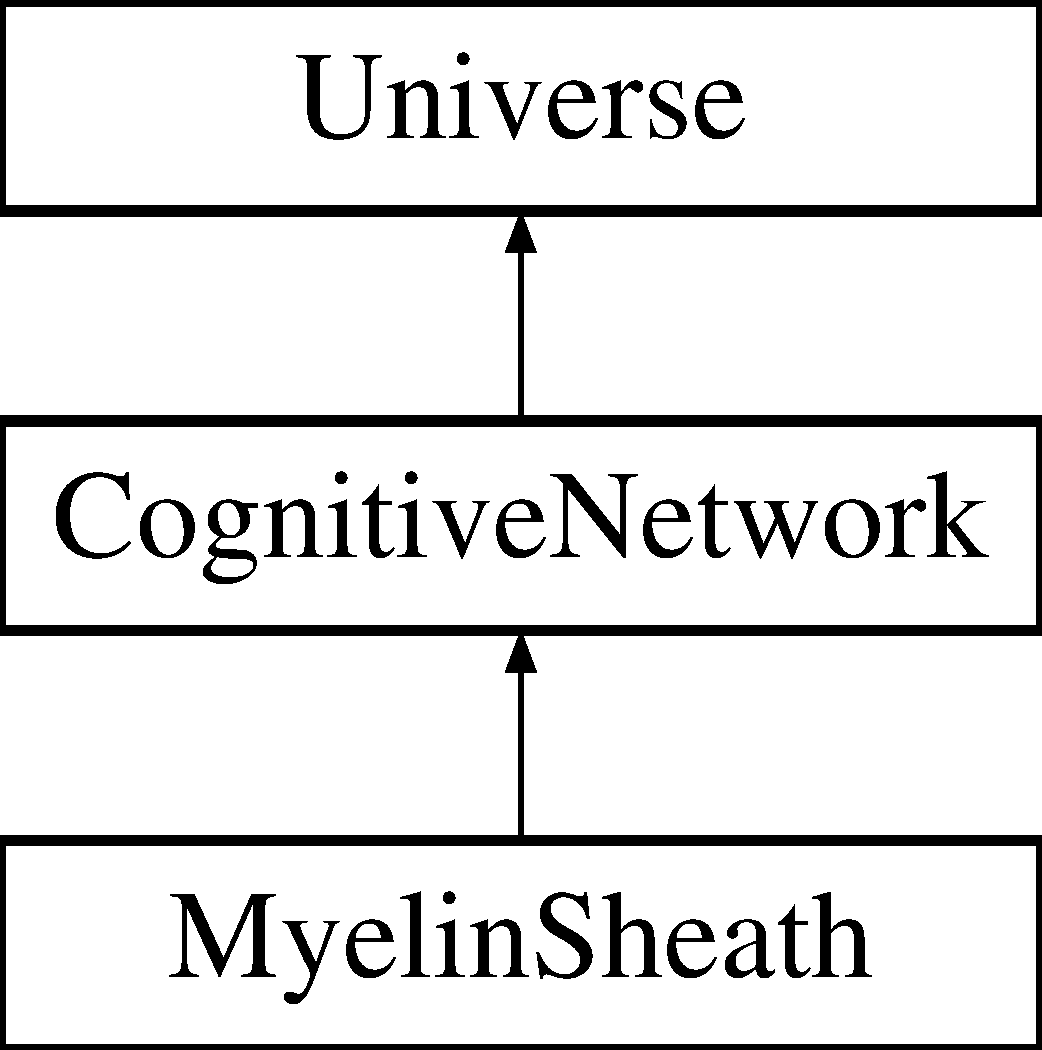
\includegraphics[height=3.000000cm]{classMyelinSheath}
\end{center}
\end{figure}
\subsection*{Public Member Functions}
\begin{DoxyCompactItemize}
\item 
\mbox{\hyperlink{classMyelinSheath_a298d69acb8d64de018f32443ea015287}{Myelin\+Sheath}} ()
\item 
\mbox{\hyperlink{classMyelinSheath_a9f9f90c853f341b5cbf4f2c5035a14af}{Myelin\+Sheath}} (unsigned int object\+\_\+type)
\item 
\mbox{\hyperlink{classMyelinSheath_a34a80a57ebcde58933a07ca9d99780eb}{Myelin\+Sheath}} (unsigned int object\+\_\+type, std\+::chrono\+::time\+\_\+point$<$ \mbox{\hyperlink{universe_8h_a0ef8d951d1ca5ab3cfaf7ab4c7a6fd80}{Clock}} $>$ event\+\_\+time)
\item 
\mbox{\hyperlink{classMyelinSheath_aac107d8f22ca3c02f2d346f44950e6d0}{Myelin\+Sheath}} (unsigned int object\+\_\+type, std\+::chrono\+::time\+\_\+point$<$ \mbox{\hyperlink{universe_8h_a0ef8d951d1ca5ab3cfaf7ab4c7a6fd80}{Clock}} $>$ event\+\_\+time, \mbox{\hyperlink{classCognitiveNetwork}{Cognitive\+Network}} \&cognitivenetwork\+\_\+connector)
\item 
virtual \mbox{\hyperlink{classMyelinSheath_acf71a2a450e2df353f28eed6c7a4129a}{$\sim$\+Myelin\+Sheath}} ()
\item 
bool \mbox{\hyperlink{classMyelinSheath_af1174b93be36aa43506a4ba9857d92a4}{Reset\+Parameters}} (std\+::chrono\+::time\+\_\+point$<$ \mbox{\hyperlink{universe_8h_a0ef8d951d1ca5ab3cfaf7ab4c7a6fd80}{Clock}} $>$ event\+\_\+time)
\item 
unsigned int \mbox{\hyperlink{classMyelinSheath_a10eef8601d129e7e2f28e8ed1ebc975c}{Get\+Counter}} (std\+::chrono\+::time\+\_\+point$<$ \mbox{\hyperlink{universe_8h_a0ef8d951d1ca5ab3cfaf7ab4c7a6fd80}{Clock}} $>$ event\+\_\+time)
\item 
double \mbox{\hyperlink{classMyelinSheath_ac0c4142b6066e5982c54583e8ac01271}{Get\+Energy}} (std\+::chrono\+::time\+\_\+point$<$ \mbox{\hyperlink{universe_8h_a0ef8d951d1ca5ab3cfaf7ab4c7a6fd80}{Clock}} $>$ event\+\_\+time)
\item 
void \mbox{\hyperlink{classMyelinSheath_afb9cd377a71881558f48cf8bb226af77}{Set\+Counter}} (std\+::chrono\+::time\+\_\+point$<$ \mbox{\hyperlink{universe_8h_a0ef8d951d1ca5ab3cfaf7ab4c7a6fd80}{Clock}} $>$ event\+\_\+time, unsigned int val)
\item 
void \mbox{\hyperlink{classMyelinSheath_ad0f6dbae2819f6642a92b8e85ec8f775}{Set\+Energy}} (std\+::chrono\+::time\+\_\+point$<$ \mbox{\hyperlink{universe_8h_a0ef8d951d1ca5ab3cfaf7ab4c7a6fd80}{Clock}} $>$ event\+\_\+time, double val)
\item 
int \mbox{\hyperlink{classMyelinSheath_af53c8f36ee963168dec09b74a6be8e4c}{Update}} (std\+::chrono\+::time\+\_\+point$<$ \mbox{\hyperlink{universe_8h_a0ef8d951d1ca5ab3cfaf7ab4c7a6fd80}{Clock}} $>$ event\+\_\+time)
\end{DoxyCompactItemize}
\subsection*{Protected Attributes}
\begin{DoxyCompactItemize}
\item 
std\+::vector$<$ \mbox{\hyperlink{classCognitiveNetwork}{Cognitive\+Network}} $\ast$ $>$ \mbox{\hyperlink{classMyelinSheath_a7877f5feab5bae37903653bf89dc3d5b}{axonbranch\+\_\+list}}
\end{DoxyCompactItemize}
\subsection*{Private Attributes}
\begin{DoxyCompactItemize}
\item 
int \mbox{\hyperlink{classMyelinSheath_a567eae60904df1812447cc55ecd43e70}{myelinsheath\+\_\+type}}
\item 
unsigned int \mbox{\hyperlink{classMyelinSheath_ab8aab14d9707ee30265faa73c601e7d6}{m\+\_\+\+Counter}}
\begin{DoxyCompactList}\small\item\em Member variable \char`\"{}m\+\_\+\+Counter\char`\"{}. \end{DoxyCompactList}\item 
double \mbox{\hyperlink{classMyelinSheath_ac30cc301a8bcbdf03c66dd0c73a65e13}{object\+\_\+energy}}
\begin{DoxyCompactList}\small\item\em Member variable \char`\"{}object\+\_\+energy\char`\"{}. \end{DoxyCompactList}\item 
double \mbox{\hyperlink{classMyelinSheath_a5099ab3d740d0127f4b6697b51d8f61b}{object\+\_\+energy\+\_\+threshold}}
\item 
double \mbox{\hyperlink{classMyelinSheath_a780de7cd0440fa006b8e6fff6586c6dc}{object\+\_\+size}}
\item 
double \mbox{\hyperlink{classMyelinSheath_a301d5466675d2bc58e367ca2b97c2680}{object\+\_\+energy\+Full}}
\item 
double \mbox{\hyperlink{classMyelinSheath_a05dcc6e1cc6ddd322ea6d70c04294ac1}{m\+\_\+\+Ions}}
\item 
double \mbox{\hyperlink{classMyelinSheath_a2c9fb3682ac15eb0a1c39acfbce6e284}{m\+\_\+\+Volume}}
\item 
double \mbox{\hyperlink{classMyelinSheath_a8e8410a18e4464464ea4bc1629a95e68}{m\+\_\+\+Surface\+Area}}
\item 
double \mbox{\hyperlink{classMyelinSheath_a90f9cb23a8be59444dd997da5e184553}{m\+\_\+\+Length}}
\item 
std\+::chrono\+::time\+\_\+point$<$ \mbox{\hyperlink{universe_8h_a0ef8d951d1ca5ab3cfaf7ab4c7a6fd80}{Clock}} $>$ \mbox{\hyperlink{classMyelinSheath_a93336530fb4a6210f7bd3ec297192042}{previous\+\_\+event\+\_\+time}}
\item 
std\+::chrono\+::time\+\_\+point$<$ \mbox{\hyperlink{universe_8h_a0ef8d951d1ca5ab3cfaf7ab4c7a6fd80}{Clock}} $>$ \mbox{\hyperlink{classMyelinSheath_a5ff52b5d66d81809d62851ce6b8b12a8}{time\+\_\+object\+\_\+created}}
\item 
int \mbox{\hyperlink{classMyelinSheath_a71de35f1f6326d808253a588c3ca3636}{duration\+\_\+since\+\_\+last\+\_\+event}}
\item 
bool \mbox{\hyperlink{classMyelinSheath_ac5859735cf21fa7456f7bed143f19f6c}{object\+\_\+initialised}}
\item 
bool \mbox{\hyperlink{classMyelinSheath_a60271f6802b2289945aa4f5536b55b34}{object\+\_\+disabled}}
\end{DoxyCompactItemize}
\subsection*{Additional Inherited Members}


\subsection{Constructor \& Destructor Documentation}
\mbox{\Hypertarget{classMyelinSheath_a298d69acb8d64de018f32443ea015287}\label{classMyelinSheath_a298d69acb8d64de018f32443ea015287}} 
\index{Myelin\+Sheath@{Myelin\+Sheath}!Myelin\+Sheath@{Myelin\+Sheath}}
\index{Myelin\+Sheath@{Myelin\+Sheath}!Myelin\+Sheath@{Myelin\+Sheath}}
\subsubsection{\texorpdfstring{Myelin\+Sheath()}{MyelinSheath()}\hspace{0.1cm}{\footnotesize\ttfamily [1/4]}}
{\footnotesize\ttfamily Myelin\+Sheath\+::\+Myelin\+Sheath (\begin{DoxyParamCaption}{ }\end{DoxyParamCaption})\hspace{0.3cm}{\ttfamily [inline]}}

\mbox{\Hypertarget{classMyelinSheath_a9f9f90c853f341b5cbf4f2c5035a14af}\label{classMyelinSheath_a9f9f90c853f341b5cbf4f2c5035a14af}} 
\index{Myelin\+Sheath@{Myelin\+Sheath}!Myelin\+Sheath@{Myelin\+Sheath}}
\index{Myelin\+Sheath@{Myelin\+Sheath}!Myelin\+Sheath@{Myelin\+Sheath}}
\subsubsection{\texorpdfstring{Myelin\+Sheath()}{MyelinSheath()}\hspace{0.1cm}{\footnotesize\ttfamily [2/4]}}
{\footnotesize\ttfamily Myelin\+Sheath\+::\+Myelin\+Sheath (\begin{DoxyParamCaption}\item[{unsigned int}]{object\+\_\+type }\end{DoxyParamCaption})\hspace{0.3cm}{\ttfamily [inline]}}

\mbox{\Hypertarget{classMyelinSheath_a34a80a57ebcde58933a07ca9d99780eb}\label{classMyelinSheath_a34a80a57ebcde58933a07ca9d99780eb}} 
\index{Myelin\+Sheath@{Myelin\+Sheath}!Myelin\+Sheath@{Myelin\+Sheath}}
\index{Myelin\+Sheath@{Myelin\+Sheath}!Myelin\+Sheath@{Myelin\+Sheath}}
\subsubsection{\texorpdfstring{Myelin\+Sheath()}{MyelinSheath()}\hspace{0.1cm}{\footnotesize\ttfamily [3/4]}}
{\footnotesize\ttfamily Myelin\+Sheath\+::\+Myelin\+Sheath (\begin{DoxyParamCaption}\item[{unsigned int}]{object\+\_\+type,  }\item[{std\+::chrono\+::time\+\_\+point$<$ \mbox{\hyperlink{universe_8h_a0ef8d951d1ca5ab3cfaf7ab4c7a6fd80}{Clock}} $>$}]{event\+\_\+time }\end{DoxyParamCaption})\hspace{0.3cm}{\ttfamily [inline]}}

\mbox{\Hypertarget{classMyelinSheath_aac107d8f22ca3c02f2d346f44950e6d0}\label{classMyelinSheath_aac107d8f22ca3c02f2d346f44950e6d0}} 
\index{Myelin\+Sheath@{Myelin\+Sheath}!Myelin\+Sheath@{Myelin\+Sheath}}
\index{Myelin\+Sheath@{Myelin\+Sheath}!Myelin\+Sheath@{Myelin\+Sheath}}
\subsubsection{\texorpdfstring{Myelin\+Sheath()}{MyelinSheath()}\hspace{0.1cm}{\footnotesize\ttfamily [4/4]}}
{\footnotesize\ttfamily Myelin\+Sheath\+::\+Myelin\+Sheath (\begin{DoxyParamCaption}\item[{unsigned int}]{object\+\_\+type,  }\item[{std\+::chrono\+::time\+\_\+point$<$ \mbox{\hyperlink{universe_8h_a0ef8d951d1ca5ab3cfaf7ab4c7a6fd80}{Clock}} $>$}]{event\+\_\+time,  }\item[{\mbox{\hyperlink{classCognitiveNetwork}{Cognitive\+Network}} \&}]{cognitivenetwork\+\_\+connector }\end{DoxyParamCaption})\hspace{0.3cm}{\ttfamily [inline]}}

\mbox{\Hypertarget{classMyelinSheath_acf71a2a450e2df353f28eed6c7a4129a}\label{classMyelinSheath_acf71a2a450e2df353f28eed6c7a4129a}} 
\index{Myelin\+Sheath@{Myelin\+Sheath}!````~Myelin\+Sheath@{$\sim$\+Myelin\+Sheath}}
\index{````~Myelin\+Sheath@{$\sim$\+Myelin\+Sheath}!Myelin\+Sheath@{Myelin\+Sheath}}
\subsubsection{\texorpdfstring{$\sim$\+Myelin\+Sheath()}{~MyelinSheath()}}
{\footnotesize\ttfamily virtual Myelin\+Sheath\+::$\sim$\+Myelin\+Sheath (\begin{DoxyParamCaption}{ }\end{DoxyParamCaption})\hspace{0.3cm}{\ttfamily [inline]}, {\ttfamily [virtual]}}

Default destructor 

\subsection{Member Function Documentation}
\mbox{\Hypertarget{classMyelinSheath_a10eef8601d129e7e2f28e8ed1ebc975c}\label{classMyelinSheath_a10eef8601d129e7e2f28e8ed1ebc975c}} 
\index{Myelin\+Sheath@{Myelin\+Sheath}!Get\+Counter@{Get\+Counter}}
\index{Get\+Counter@{Get\+Counter}!Myelin\+Sheath@{Myelin\+Sheath}}
\subsubsection{\texorpdfstring{Get\+Counter()}{GetCounter()}}
{\footnotesize\ttfamily unsigned int Myelin\+Sheath\+::\+Get\+Counter (\begin{DoxyParamCaption}\item[{std\+::chrono\+::time\+\_\+point$<$ \mbox{\hyperlink{universe_8h_a0ef8d951d1ca5ab3cfaf7ab4c7a6fd80}{Clock}} $>$}]{event\+\_\+time }\end{DoxyParamCaption})\hspace{0.3cm}{\ttfamily [inline]}}

\mbox{\Hypertarget{classMyelinSheath_ac0c4142b6066e5982c54583e8ac01271}\label{classMyelinSheath_ac0c4142b6066e5982c54583e8ac01271}} 
\index{Myelin\+Sheath@{Myelin\+Sheath}!Get\+Energy@{Get\+Energy}}
\index{Get\+Energy@{Get\+Energy}!Myelin\+Sheath@{Myelin\+Sheath}}
\subsubsection{\texorpdfstring{Get\+Energy()}{GetEnergy()}}
{\footnotesize\ttfamily double Myelin\+Sheath\+::\+Get\+Energy (\begin{DoxyParamCaption}\item[{std\+::chrono\+::time\+\_\+point$<$ \mbox{\hyperlink{universe_8h_a0ef8d951d1ca5ab3cfaf7ab4c7a6fd80}{Clock}} $>$}]{event\+\_\+time }\end{DoxyParamCaption})\hspace{0.3cm}{\ttfamily [inline]}}

\mbox{\Hypertarget{classMyelinSheath_af1174b93be36aa43506a4ba9857d92a4}\label{classMyelinSheath_af1174b93be36aa43506a4ba9857d92a4}} 
\index{Myelin\+Sheath@{Myelin\+Sheath}!Reset\+Parameters@{Reset\+Parameters}}
\index{Reset\+Parameters@{Reset\+Parameters}!Myelin\+Sheath@{Myelin\+Sheath}}
\subsubsection{\texorpdfstring{Reset\+Parameters()}{ResetParameters()}}
{\footnotesize\ttfamily bool Myelin\+Sheath\+::\+Reset\+Parameters (\begin{DoxyParamCaption}\item[{std\+::chrono\+::time\+\_\+point$<$ \mbox{\hyperlink{universe_8h_a0ef8d951d1ca5ab3cfaf7ab4c7a6fd80}{Clock}} $>$}]{event\+\_\+time }\end{DoxyParamCaption})}

\mbox{\Hypertarget{classMyelinSheath_afb9cd377a71881558f48cf8bb226af77}\label{classMyelinSheath_afb9cd377a71881558f48cf8bb226af77}} 
\index{Myelin\+Sheath@{Myelin\+Sheath}!Set\+Counter@{Set\+Counter}}
\index{Set\+Counter@{Set\+Counter}!Myelin\+Sheath@{Myelin\+Sheath}}
\subsubsection{\texorpdfstring{Set\+Counter()}{SetCounter()}}
{\footnotesize\ttfamily void Myelin\+Sheath\+::\+Set\+Counter (\begin{DoxyParamCaption}\item[{std\+::chrono\+::time\+\_\+point$<$ \mbox{\hyperlink{universe_8h_a0ef8d951d1ca5ab3cfaf7ab4c7a6fd80}{Clock}} $>$}]{event\+\_\+time,  }\item[{unsigned int}]{val }\end{DoxyParamCaption})\hspace{0.3cm}{\ttfamily [inline]}, {\ttfamily [virtual]}}



Reimplemented from \mbox{\hyperlink{classUniverse_aa22202ae740eb1355529afcb13285e91}{Universe}}.

\mbox{\Hypertarget{classMyelinSheath_ad0f6dbae2819f6642a92b8e85ec8f775}\label{classMyelinSheath_ad0f6dbae2819f6642a92b8e85ec8f775}} 
\index{Myelin\+Sheath@{Myelin\+Sheath}!Set\+Energy@{Set\+Energy}}
\index{Set\+Energy@{Set\+Energy}!Myelin\+Sheath@{Myelin\+Sheath}}
\subsubsection{\texorpdfstring{Set\+Energy()}{SetEnergy()}}
{\footnotesize\ttfamily void Myelin\+Sheath\+::\+Set\+Energy (\begin{DoxyParamCaption}\item[{std\+::chrono\+::time\+\_\+point$<$ \mbox{\hyperlink{universe_8h_a0ef8d951d1ca5ab3cfaf7ab4c7a6fd80}{Clock}} $>$}]{event\+\_\+time,  }\item[{double}]{val }\end{DoxyParamCaption})\hspace{0.3cm}{\ttfamily [inline]}}

\mbox{\Hypertarget{classMyelinSheath_af53c8f36ee963168dec09b74a6be8e4c}\label{classMyelinSheath_af53c8f36ee963168dec09b74a6be8e4c}} 
\index{Myelin\+Sheath@{Myelin\+Sheath}!Update@{Update}}
\index{Update@{Update}!Myelin\+Sheath@{Myelin\+Sheath}}
\subsubsection{\texorpdfstring{Update()}{Update()}}
{\footnotesize\ttfamily int Myelin\+Sheath\+::\+Update (\begin{DoxyParamCaption}\item[{std\+::chrono\+::time\+\_\+point$<$ \mbox{\hyperlink{universe_8h_a0ef8d951d1ca5ab3cfaf7ab4c7a6fd80}{Clock}} $>$}]{event\+\_\+time }\end{DoxyParamCaption})}



\subsection{Member Data Documentation}
\mbox{\Hypertarget{classMyelinSheath_a7877f5feab5bae37903653bf89dc3d5b}\label{classMyelinSheath_a7877f5feab5bae37903653bf89dc3d5b}} 
\index{Myelin\+Sheath@{Myelin\+Sheath}!axonbranch\+\_\+list@{axonbranch\+\_\+list}}
\index{axonbranch\+\_\+list@{axonbranch\+\_\+list}!Myelin\+Sheath@{Myelin\+Sheath}}
\subsubsection{\texorpdfstring{axonbranch\+\_\+list}{axonbranch\_list}}
{\footnotesize\ttfamily std\+::vector$<$\mbox{\hyperlink{classCognitiveNetwork}{Cognitive\+Network}}$\ast$$>$ Myelin\+Sheath\+::axonbranch\+\_\+list\hspace{0.3cm}{\ttfamily [protected]}}

\mbox{\Hypertarget{classMyelinSheath_a71de35f1f6326d808253a588c3ca3636}\label{classMyelinSheath_a71de35f1f6326d808253a588c3ca3636}} 
\index{Myelin\+Sheath@{Myelin\+Sheath}!duration\+\_\+since\+\_\+last\+\_\+event@{duration\+\_\+since\+\_\+last\+\_\+event}}
\index{duration\+\_\+since\+\_\+last\+\_\+event@{duration\+\_\+since\+\_\+last\+\_\+event}!Myelin\+Sheath@{Myelin\+Sheath}}
\subsubsection{\texorpdfstring{duration\+\_\+since\+\_\+last\+\_\+event}{duration\_since\_last\_event}}
{\footnotesize\ttfamily int Myelin\+Sheath\+::duration\+\_\+since\+\_\+last\+\_\+event\hspace{0.3cm}{\ttfamily [private]}}

\mbox{\Hypertarget{classMyelinSheath_ab8aab14d9707ee30265faa73c601e7d6}\label{classMyelinSheath_ab8aab14d9707ee30265faa73c601e7d6}} 
\index{Myelin\+Sheath@{Myelin\+Sheath}!m\+\_\+\+Counter@{m\+\_\+\+Counter}}
\index{m\+\_\+\+Counter@{m\+\_\+\+Counter}!Myelin\+Sheath@{Myelin\+Sheath}}
\subsubsection{\texorpdfstring{m\+\_\+\+Counter}{m\_Counter}}
{\footnotesize\ttfamily unsigned int Myelin\+Sheath\+::m\+\_\+\+Counter\hspace{0.3cm}{\ttfamily [private]}}



Member variable \char`\"{}m\+\_\+\+Counter\char`\"{}. 

\mbox{\Hypertarget{classMyelinSheath_a05dcc6e1cc6ddd322ea6d70c04294ac1}\label{classMyelinSheath_a05dcc6e1cc6ddd322ea6d70c04294ac1}} 
\index{Myelin\+Sheath@{Myelin\+Sheath}!m\+\_\+\+Ions@{m\+\_\+\+Ions}}
\index{m\+\_\+\+Ions@{m\+\_\+\+Ions}!Myelin\+Sheath@{Myelin\+Sheath}}
\subsubsection{\texorpdfstring{m\+\_\+\+Ions}{m\_Ions}}
{\footnotesize\ttfamily double Myelin\+Sheath\+::m\+\_\+\+Ions\hspace{0.3cm}{\ttfamily [private]}}

\mbox{\Hypertarget{classMyelinSheath_a90f9cb23a8be59444dd997da5e184553}\label{classMyelinSheath_a90f9cb23a8be59444dd997da5e184553}} 
\index{Myelin\+Sheath@{Myelin\+Sheath}!m\+\_\+\+Length@{m\+\_\+\+Length}}
\index{m\+\_\+\+Length@{m\+\_\+\+Length}!Myelin\+Sheath@{Myelin\+Sheath}}
\subsubsection{\texorpdfstring{m\+\_\+\+Length}{m\_Length}}
{\footnotesize\ttfamily double Myelin\+Sheath\+::m\+\_\+\+Length\hspace{0.3cm}{\ttfamily [private]}}

\mbox{\Hypertarget{classMyelinSheath_a8e8410a18e4464464ea4bc1629a95e68}\label{classMyelinSheath_a8e8410a18e4464464ea4bc1629a95e68}} 
\index{Myelin\+Sheath@{Myelin\+Sheath}!m\+\_\+\+Surface\+Area@{m\+\_\+\+Surface\+Area}}
\index{m\+\_\+\+Surface\+Area@{m\+\_\+\+Surface\+Area}!Myelin\+Sheath@{Myelin\+Sheath}}
\subsubsection{\texorpdfstring{m\+\_\+\+Surface\+Area}{m\_SurfaceArea}}
{\footnotesize\ttfamily double Myelin\+Sheath\+::m\+\_\+\+Surface\+Area\hspace{0.3cm}{\ttfamily [private]}}

\mbox{\Hypertarget{classMyelinSheath_a2c9fb3682ac15eb0a1c39acfbce6e284}\label{classMyelinSheath_a2c9fb3682ac15eb0a1c39acfbce6e284}} 
\index{Myelin\+Sheath@{Myelin\+Sheath}!m\+\_\+\+Volume@{m\+\_\+\+Volume}}
\index{m\+\_\+\+Volume@{m\+\_\+\+Volume}!Myelin\+Sheath@{Myelin\+Sheath}}
\subsubsection{\texorpdfstring{m\+\_\+\+Volume}{m\_Volume}}
{\footnotesize\ttfamily double Myelin\+Sheath\+::m\+\_\+\+Volume\hspace{0.3cm}{\ttfamily [private]}}

\mbox{\Hypertarget{classMyelinSheath_a567eae60904df1812447cc55ecd43e70}\label{classMyelinSheath_a567eae60904df1812447cc55ecd43e70}} 
\index{Myelin\+Sheath@{Myelin\+Sheath}!myelinsheath\+\_\+type@{myelinsheath\+\_\+type}}
\index{myelinsheath\+\_\+type@{myelinsheath\+\_\+type}!Myelin\+Sheath@{Myelin\+Sheath}}
\subsubsection{\texorpdfstring{myelinsheath\+\_\+type}{myelinsheath\_type}}
{\footnotesize\ttfamily int Myelin\+Sheath\+::myelinsheath\+\_\+type\hspace{0.3cm}{\ttfamily [private]}}

\mbox{\Hypertarget{classMyelinSheath_a60271f6802b2289945aa4f5536b55b34}\label{classMyelinSheath_a60271f6802b2289945aa4f5536b55b34}} 
\index{Myelin\+Sheath@{Myelin\+Sheath}!object\+\_\+disabled@{object\+\_\+disabled}}
\index{object\+\_\+disabled@{object\+\_\+disabled}!Myelin\+Sheath@{Myelin\+Sheath}}
\subsubsection{\texorpdfstring{object\+\_\+disabled}{object\_disabled}}
{\footnotesize\ttfamily bool Myelin\+Sheath\+::object\+\_\+disabled\hspace{0.3cm}{\ttfamily [private]}}

\mbox{\Hypertarget{classMyelinSheath_ac30cc301a8bcbdf03c66dd0c73a65e13}\label{classMyelinSheath_ac30cc301a8bcbdf03c66dd0c73a65e13}} 
\index{Myelin\+Sheath@{Myelin\+Sheath}!object\+\_\+energy@{object\+\_\+energy}}
\index{object\+\_\+energy@{object\+\_\+energy}!Myelin\+Sheath@{Myelin\+Sheath}}
\subsubsection{\texorpdfstring{object\+\_\+energy}{object\_energy}}
{\footnotesize\ttfamily double Myelin\+Sheath\+::object\+\_\+energy\hspace{0.3cm}{\ttfamily [private]}}



Member variable \char`\"{}object\+\_\+energy\char`\"{}. 

\mbox{\Hypertarget{classMyelinSheath_a5099ab3d740d0127f4b6697b51d8f61b}\label{classMyelinSheath_a5099ab3d740d0127f4b6697b51d8f61b}} 
\index{Myelin\+Sheath@{Myelin\+Sheath}!object\+\_\+energy\+\_\+threshold@{object\+\_\+energy\+\_\+threshold}}
\index{object\+\_\+energy\+\_\+threshold@{object\+\_\+energy\+\_\+threshold}!Myelin\+Sheath@{Myelin\+Sheath}}
\subsubsection{\texorpdfstring{object\+\_\+energy\+\_\+threshold}{object\_energy\_threshold}}
{\footnotesize\ttfamily double Myelin\+Sheath\+::object\+\_\+energy\+\_\+threshold\hspace{0.3cm}{\ttfamily [private]}}

\mbox{\Hypertarget{classMyelinSheath_a301d5466675d2bc58e367ca2b97c2680}\label{classMyelinSheath_a301d5466675d2bc58e367ca2b97c2680}} 
\index{Myelin\+Sheath@{Myelin\+Sheath}!object\+\_\+energy\+Full@{object\+\_\+energy\+Full}}
\index{object\+\_\+energy\+Full@{object\+\_\+energy\+Full}!Myelin\+Sheath@{Myelin\+Sheath}}
\subsubsection{\texorpdfstring{object\+\_\+energy\+Full}{object\_energyFull}}
{\footnotesize\ttfamily double Myelin\+Sheath\+::object\+\_\+energy\+Full\hspace{0.3cm}{\ttfamily [private]}}

\mbox{\Hypertarget{classMyelinSheath_ac5859735cf21fa7456f7bed143f19f6c}\label{classMyelinSheath_ac5859735cf21fa7456f7bed143f19f6c}} 
\index{Myelin\+Sheath@{Myelin\+Sheath}!object\+\_\+initialised@{object\+\_\+initialised}}
\index{object\+\_\+initialised@{object\+\_\+initialised}!Myelin\+Sheath@{Myelin\+Sheath}}
\subsubsection{\texorpdfstring{object\+\_\+initialised}{object\_initialised}}
{\footnotesize\ttfamily bool Myelin\+Sheath\+::object\+\_\+initialised\hspace{0.3cm}{\ttfamily [private]}}

\mbox{\Hypertarget{classMyelinSheath_a780de7cd0440fa006b8e6fff6586c6dc}\label{classMyelinSheath_a780de7cd0440fa006b8e6fff6586c6dc}} 
\index{Myelin\+Sheath@{Myelin\+Sheath}!object\+\_\+size@{object\+\_\+size}}
\index{object\+\_\+size@{object\+\_\+size}!Myelin\+Sheath@{Myelin\+Sheath}}
\subsubsection{\texorpdfstring{object\+\_\+size}{object\_size}}
{\footnotesize\ttfamily double Myelin\+Sheath\+::object\+\_\+size\hspace{0.3cm}{\ttfamily [private]}}

\mbox{\Hypertarget{classMyelinSheath_a93336530fb4a6210f7bd3ec297192042}\label{classMyelinSheath_a93336530fb4a6210f7bd3ec297192042}} 
\index{Myelin\+Sheath@{Myelin\+Sheath}!previous\+\_\+event\+\_\+time@{previous\+\_\+event\+\_\+time}}
\index{previous\+\_\+event\+\_\+time@{previous\+\_\+event\+\_\+time}!Myelin\+Sheath@{Myelin\+Sheath}}
\subsubsection{\texorpdfstring{previous\+\_\+event\+\_\+time}{previous\_event\_time}}
{\footnotesize\ttfamily std\+::chrono\+::time\+\_\+point$<$\mbox{\hyperlink{universe_8h_a0ef8d951d1ca5ab3cfaf7ab4c7a6fd80}{Clock}}$>$ Myelin\+Sheath\+::previous\+\_\+event\+\_\+time\hspace{0.3cm}{\ttfamily [private]}}

\mbox{\Hypertarget{classMyelinSheath_a5ff52b5d66d81809d62851ce6b8b12a8}\label{classMyelinSheath_a5ff52b5d66d81809d62851ce6b8b12a8}} 
\index{Myelin\+Sheath@{Myelin\+Sheath}!time\+\_\+object\+\_\+created@{time\+\_\+object\+\_\+created}}
\index{time\+\_\+object\+\_\+created@{time\+\_\+object\+\_\+created}!Myelin\+Sheath@{Myelin\+Sheath}}
\subsubsection{\texorpdfstring{time\+\_\+object\+\_\+created}{time\_object\_created}}
{\footnotesize\ttfamily std\+::chrono\+::time\+\_\+point$<$\mbox{\hyperlink{universe_8h_a0ef8d951d1ca5ab3cfaf7ab4c7a6fd80}{Clock}}$>$ Myelin\+Sheath\+::time\+\_\+object\+\_\+created\hspace{0.3cm}{\ttfamily [private]}}



The documentation for this class was generated from the following files\+:\begin{DoxyCompactItemize}
\item 
/home/pbisaacs/\+Developer/\+Brain\+Harmonics/\+Brain\+Harmonics/\mbox{\hyperlink{myelinsheath_8h}{myelinsheath.\+h}}\item 
/home/pbisaacs/\+Developer/\+Brain\+Harmonics/\+Brain\+Harmonics/\mbox{\hyperlink{myelinsheath_8cc}{myelinsheath.\+cc}}\end{DoxyCompactItemize}

\hypertarget{structSynapse_1_1NearbyNeuron}{}\section{Synapse\+:\+:Nearby\+Neuron Struct Reference}
\label{structSynapse_1_1NearbyNeuron}\index{Synapse\+::\+Nearby\+Neuron@{Synapse\+::\+Nearby\+Neuron}}
\subsection*{Public Attributes}
\begin{DoxyCompactItemize}
\item 
double \mbox{\hyperlink{structSynapse_1_1NearbyNeuron_a11322181215d2b2d3ef360fa212badb9}{distance\+To\+Neuron}}
\item 
double \mbox{\hyperlink{structSynapse_1_1NearbyNeuron_ad81c00ed7d53310fa94f44e1e3fffc77}{synapse\+Gravitational\+Attraction}}
\item 
bool \mbox{\hyperlink{structSynapse_1_1NearbyNeuron_a211af29e29f4c2cfeb221b45d594d047}{synapse\+Allocated}}
\end{DoxyCompactItemize}


\subsection{Member Data Documentation}
\mbox{\Hypertarget{structSynapse_1_1NearbyNeuron_a11322181215d2b2d3ef360fa212badb9}\label{structSynapse_1_1NearbyNeuron_a11322181215d2b2d3ef360fa212badb9}} 
\index{Synapse\+::\+Nearby\+Neuron@{Synapse\+::\+Nearby\+Neuron}!distance\+To\+Neuron@{distance\+To\+Neuron}}
\index{distance\+To\+Neuron@{distance\+To\+Neuron}!Synapse\+::\+Nearby\+Neuron@{Synapse\+::\+Nearby\+Neuron}}
\subsubsection{\texorpdfstring{distance\+To\+Neuron}{distanceToNeuron}}
{\footnotesize\ttfamily double Synapse\+::\+Nearby\+Neuron\+::distance\+To\+Neuron}

\mbox{\Hypertarget{structSynapse_1_1NearbyNeuron_a211af29e29f4c2cfeb221b45d594d047}\label{structSynapse_1_1NearbyNeuron_a211af29e29f4c2cfeb221b45d594d047}} 
\index{Synapse\+::\+Nearby\+Neuron@{Synapse\+::\+Nearby\+Neuron}!synapse\+Allocated@{synapse\+Allocated}}
\index{synapse\+Allocated@{synapse\+Allocated}!Synapse\+::\+Nearby\+Neuron@{Synapse\+::\+Nearby\+Neuron}}
\subsubsection{\texorpdfstring{synapse\+Allocated}{synapseAllocated}}
{\footnotesize\ttfamily bool Synapse\+::\+Nearby\+Neuron\+::synapse\+Allocated}

\mbox{\Hypertarget{structSynapse_1_1NearbyNeuron_ad81c00ed7d53310fa94f44e1e3fffc77}\label{structSynapse_1_1NearbyNeuron_ad81c00ed7d53310fa94f44e1e3fffc77}} 
\index{Synapse\+::\+Nearby\+Neuron@{Synapse\+::\+Nearby\+Neuron}!synapse\+Gravitational\+Attraction@{synapse\+Gravitational\+Attraction}}
\index{synapse\+Gravitational\+Attraction@{synapse\+Gravitational\+Attraction}!Synapse\+::\+Nearby\+Neuron@{Synapse\+::\+Nearby\+Neuron}}
\subsubsection{\texorpdfstring{synapse\+Gravitational\+Attraction}{synapseGravitationalAttraction}}
{\footnotesize\ttfamily double Synapse\+::\+Nearby\+Neuron\+::synapse\+Gravitational\+Attraction}



The documentation for this struct was generated from the following file\+:\begin{DoxyCompactItemize}
\item 
/home/pbisaacs/\+Developer/\+Brain\+Harmonics/\mbox{\hyperlink{synapse_8h}{synapse.\+h}}\end{DoxyCompactItemize}

\hypertarget{structInterneuronSpace_1_1NearbyNeuron}{}\section{Interneuron\+Space\+:\+:Nearby\+Neuron Struct Reference}
\label{structInterneuronSpace_1_1NearbyNeuron}\index{Interneuron\+Space\+::\+Nearby\+Neuron@{Interneuron\+Space\+::\+Nearby\+Neuron}}
\subsection*{Public Attributes}
\begin{DoxyCompactItemize}
\item 
double \mbox{\hyperlink{structInterneuronSpace_1_1NearbyNeuron_aac9b3036ebacb6c96c0cab20606bcbf2}{distance\+To\+Neuron}}
\item 
double \mbox{\hyperlink{structInterneuronSpace_1_1NearbyNeuron_a5cb224a1735249e1e50b934bdfd2ff3f}{interneuronspace\+Gravitational\+Attraction}}
\item 
bool \mbox{\hyperlink{structInterneuronSpace_1_1NearbyNeuron_ab003504638f28dfdc7f88a24727f72c9}{interneuronspace\+Allocated}}
\end{DoxyCompactItemize}


\subsection{Member Data Documentation}
\mbox{\Hypertarget{structInterneuronSpace_1_1NearbyNeuron_aac9b3036ebacb6c96c0cab20606bcbf2}\label{structInterneuronSpace_1_1NearbyNeuron_aac9b3036ebacb6c96c0cab20606bcbf2}} 
\index{Interneuron\+Space\+::\+Nearby\+Neuron@{Interneuron\+Space\+::\+Nearby\+Neuron}!distance\+To\+Neuron@{distance\+To\+Neuron}}
\index{distance\+To\+Neuron@{distance\+To\+Neuron}!Interneuron\+Space\+::\+Nearby\+Neuron@{Interneuron\+Space\+::\+Nearby\+Neuron}}
\subsubsection{\texorpdfstring{distance\+To\+Neuron}{distanceToNeuron}}
{\footnotesize\ttfamily double Interneuron\+Space\+::\+Nearby\+Neuron\+::distance\+To\+Neuron}

\mbox{\Hypertarget{structInterneuronSpace_1_1NearbyNeuron_ab003504638f28dfdc7f88a24727f72c9}\label{structInterneuronSpace_1_1NearbyNeuron_ab003504638f28dfdc7f88a24727f72c9}} 
\index{Interneuron\+Space\+::\+Nearby\+Neuron@{Interneuron\+Space\+::\+Nearby\+Neuron}!interneuronspace\+Allocated@{interneuronspace\+Allocated}}
\index{interneuronspace\+Allocated@{interneuronspace\+Allocated}!Interneuron\+Space\+::\+Nearby\+Neuron@{Interneuron\+Space\+::\+Nearby\+Neuron}}
\subsubsection{\texorpdfstring{interneuronspace\+Allocated}{interneuronspaceAllocated}}
{\footnotesize\ttfamily bool Interneuron\+Space\+::\+Nearby\+Neuron\+::interneuronspace\+Allocated}

\mbox{\Hypertarget{structInterneuronSpace_1_1NearbyNeuron_a5cb224a1735249e1e50b934bdfd2ff3f}\label{structInterneuronSpace_1_1NearbyNeuron_a5cb224a1735249e1e50b934bdfd2ff3f}} 
\index{Interneuron\+Space\+::\+Nearby\+Neuron@{Interneuron\+Space\+::\+Nearby\+Neuron}!interneuronspace\+Gravitational\+Attraction@{interneuronspace\+Gravitational\+Attraction}}
\index{interneuronspace\+Gravitational\+Attraction@{interneuronspace\+Gravitational\+Attraction}!Interneuron\+Space\+::\+Nearby\+Neuron@{Interneuron\+Space\+::\+Nearby\+Neuron}}
\subsubsection{\texorpdfstring{interneuronspace\+Gravitational\+Attraction}{interneuronspaceGravitationalAttraction}}
{\footnotesize\ttfamily double Interneuron\+Space\+::\+Nearby\+Neuron\+::interneuronspace\+Gravitational\+Attraction}



The documentation for this struct was generated from the following file\+:\begin{DoxyCompactItemize}
\item 
/home/pbisaacs/\+Developer/\+Brain\+Harmonics/\+Brain\+Harmonics/\mbox{\hyperlink{interneuronspace_8h}{interneuronspace.\+h}}\end{DoxyCompactItemize}

\hypertarget{classNeuron}{}\section{Neuron Class Reference}
\label{classNeuron}\index{Neuron@{Neuron}}


{\ttfamily \#include $<$neuron.\+h$>$}

Inheritance diagram for Neuron\+:\begin{figure}[H]
\begin{center}
\leavevmode
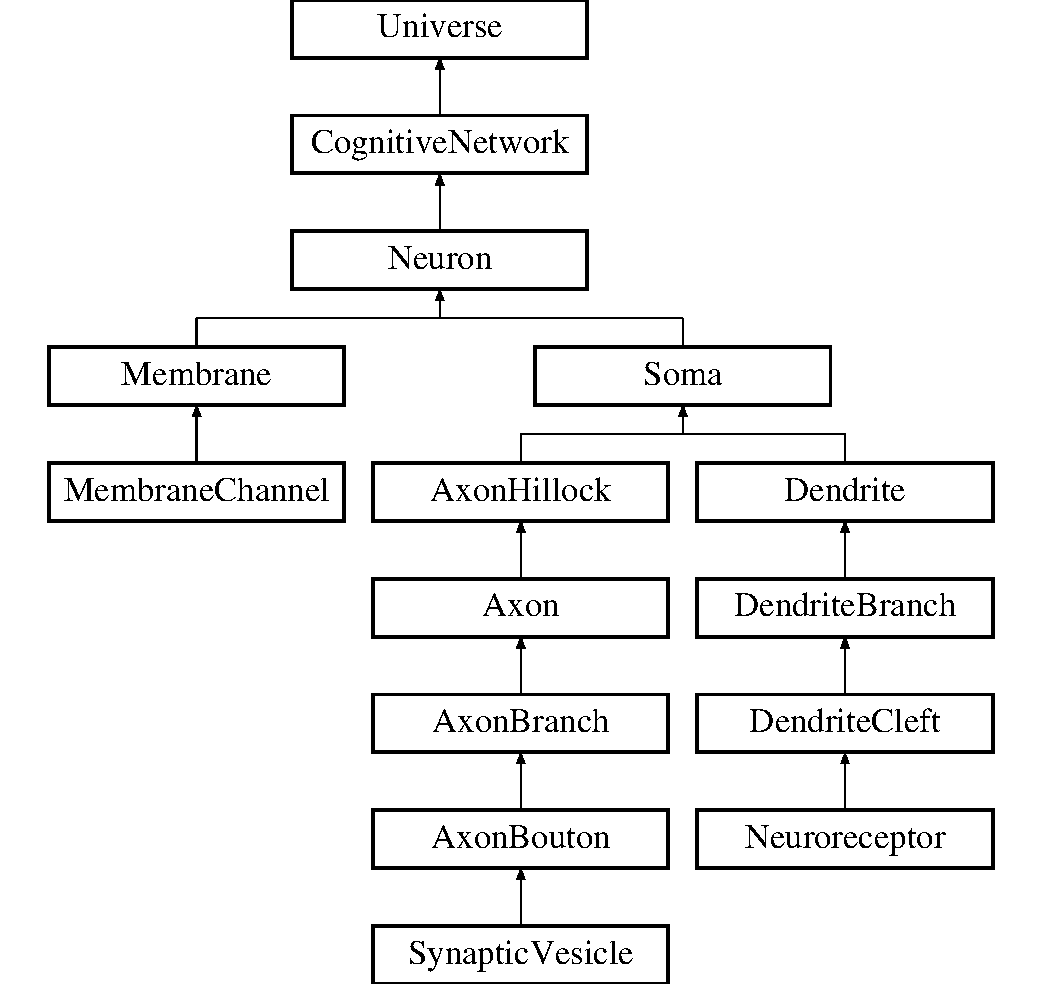
\includegraphics[height=9.000000cm]{classNeuron}
\end{center}
\end{figure}
\subsection*{Classes}
\begin{DoxyCompactItemize}
\item 
struct \mbox{\hyperlink{structNeuron_1_1ObjectConnection}{Object\+Connection}}
\end{DoxyCompactItemize}
\subsection*{Public Member Functions}
\begin{DoxyCompactItemize}
\item 
\mbox{\hyperlink{classNeuron_a823487d01615fadb8ac19a2768dd9d96}{Neuron}} ()
\item 
\mbox{\hyperlink{classNeuron_acbc433cac4f27aa7f4e05be26c336aa5}{Neuron}} (unsigned int object\+\_\+type)
\item 
\mbox{\hyperlink{classNeuron_a4611499895417d44250c452d0fc719a6}{Neuron}} (unsigned int object\+\_\+type, std\+::chrono\+::time\+\_\+point$<$ \mbox{\hyperlink{universe_8h_a0ef8d951d1ca5ab3cfaf7ab4c7a6fd80}{Clock}} $>$ event\+\_\+time)
\item 
\mbox{\hyperlink{classNeuron_a6839febd20fb8f776151e00142411a56}{Neuron}} (unsigned int object\+\_\+type, std\+::chrono\+::time\+\_\+point$<$ \mbox{\hyperlink{universe_8h_a0ef8d951d1ca5ab3cfaf7ab4c7a6fd80}{Clock}} $>$ event\+\_\+time, \mbox{\hyperlink{classCognitiveNetwork}{Cognitive\+Network}} \&cognitivenetwork\+\_\+connector)
\item 
virtual \mbox{\hyperlink{classNeuron_aecd41febe74ef417230cd74af0c8b801}{$\sim$\+Neuron}} ()
\item 
unsigned int \mbox{\hyperlink{classNeuron_a0b5fe55bf939808986b3697d18a834f4}{Get\+Counter}} (std\+::chrono\+::time\+\_\+point$<$ \mbox{\hyperlink{universe_8h_a0ef8d951d1ca5ab3cfaf7ab4c7a6fd80}{Clock}} $>$ event\+\_\+time)
\item 
int \mbox{\hyperlink{classNeuron_a93cce70c19c8e70accaa31908d3f29f6}{Get\+Capacity}} (std\+::chrono\+::time\+\_\+point$<$ \mbox{\hyperlink{universe_8h_a0ef8d951d1ca5ab3cfaf7ab4c7a6fd80}{Clock}} $>$ event\+\_\+time)
\item 
void \mbox{\hyperlink{classNeuron_a8f5766ea61dc46b7a25361df540755ec}{Set\+Capacity}} (std\+::chrono\+::time\+\_\+point$<$ \mbox{\hyperlink{universe_8h_a0ef8d951d1ca5ab3cfaf7ab4c7a6fd80}{Clock}} $>$ event\+\_\+time, int val)
\item 
int \mbox{\hyperlink{classNeuron_a745b090da1b8f8fc7e3cf0ca06dfb117}{Get\+Usage}} (std\+::chrono\+::time\+\_\+point$<$ \mbox{\hyperlink{universe_8h_a0ef8d951d1ca5ab3cfaf7ab4c7a6fd80}{Clock}} $>$ event\+\_\+time)
\item 
void \mbox{\hyperlink{classNeuron_abf99856ac41b5c9c4948b3204bbc1590}{Set\+Usage}} (std\+::chrono\+::time\+\_\+point$<$ \mbox{\hyperlink{universe_8h_a0ef8d951d1ca5ab3cfaf7ab4c7a6fd80}{Clock}} $>$ event\+\_\+time, int val)
\item 
double \mbox{\hyperlink{classNeuron_a91dd5325856e246d98c2864e1c955972}{Get\+Energy}} (std\+::chrono\+::time\+\_\+point$<$ \mbox{\hyperlink{universe_8h_a0ef8d951d1ca5ab3cfaf7ab4c7a6fd80}{Clock}} $>$ event\+\_\+time)
\item 
double \mbox{\hyperlink{classNeuron_a94accac3223afdecd1edf25e6db59ace}{Get\+Gate\+Keeper}} (std\+::chrono\+::time\+\_\+point$<$ \mbox{\hyperlink{universe_8h_a0ef8d951d1ca5ab3cfaf7ab4c7a6fd80}{Clock}} $>$ event\+\_\+time)
\item 
double \mbox{\hyperlink{classNeuron_a794c8fa270ea0600dab4fd13c25912fd}{Get\+Channel\+Min}} (std\+::chrono\+::time\+\_\+point$<$ \mbox{\hyperlink{universe_8h_a0ef8d951d1ca5ab3cfaf7ab4c7a6fd80}{Clock}} $>$ event\+\_\+time)
\item 
double \mbox{\hyperlink{classNeuron_ae8b6c47bebe302e62721dc4a6e447ca2}{Get\+Channel\+Max}} (std\+::chrono\+::time\+\_\+point$<$ \mbox{\hyperlink{universe_8h_a0ef8d951d1ca5ab3cfaf7ab4c7a6fd80}{Clock}} $>$ event\+\_\+time)
\item 
bool \mbox{\hyperlink{classNeuron_adfee1a62df820344b84fe2020451b24f}{Get\+Disabled}} (std\+::chrono\+::time\+\_\+point$<$ \mbox{\hyperlink{universe_8h_a0ef8d951d1ca5ab3cfaf7ab4c7a6fd80}{Clock}} $>$ event\+\_\+time)
\item 
int \mbox{\hyperlink{classNeuron_a98f326ea86e6e8371b639609a4495c37}{Get\+Neuron\+Type}} (std\+::chrono\+::time\+\_\+point$<$ \mbox{\hyperlink{universe_8h_a0ef8d951d1ca5ab3cfaf7ab4c7a6fd80}{Clock}} $>$ event\+\_\+time)
\item 
double \mbox{\hyperlink{classNeuron_a0573244d3c78a22a45c249db536cbb68}{Get\+Resting\+Potential}} (std\+::chrono\+::time\+\_\+point$<$ \mbox{\hyperlink{universe_8h_a0ef8d951d1ca5ab3cfaf7ab4c7a6fd80}{Clock}} $>$ event\+\_\+time)
\item 
int \mbox{\hyperlink{classNeuron_aff3a33f5d8ef5dacdec9c03df50f168c}{Get\+Neuron\+Device\+Tag}} (std\+::chrono\+::time\+\_\+point$<$ \mbox{\hyperlink{universe_8h_a0ef8d951d1ca5ab3cfaf7ab4c7a6fd80}{Clock}} $>$ event\+\_\+time)
\item 
int \mbox{\hyperlink{classNeuron_aa6f1237ed89c48eb57610083edf43efa}{Get\+Soma\+Pool}} (std\+::chrono\+::time\+\_\+point$<$ \mbox{\hyperlink{universe_8h_a0ef8d951d1ca5ab3cfaf7ab4c7a6fd80}{Clock}} $>$ event\+\_\+time)
\item 
void \mbox{\hyperlink{classNeuron_ae18e23983d02953fa6886bef0bbeb339}{Set\+Soma\+Pool}} (std\+::chrono\+::time\+\_\+point$<$ \mbox{\hyperlink{universe_8h_a0ef8d951d1ca5ab3cfaf7ab4c7a6fd80}{Clock}} $>$ event\+\_\+time, int set\+\_\+pool)
\item 
void \mbox{\hyperlink{classNeuron_a92f942f6f0bd783c39bb550cf4bb8fd0}{Set\+Counter}} (std\+::chrono\+::time\+\_\+point$<$ \mbox{\hyperlink{universe_8h_a0ef8d951d1ca5ab3cfaf7ab4c7a6fd80}{Clock}} $>$ event\+\_\+time, int val)
\item 
void \mbox{\hyperlink{classNeuron_a5efa690ce4d8ff2f8dfb1fbfd84c5279}{Set\+Energy}} (std\+::chrono\+::time\+\_\+point$<$ \mbox{\hyperlink{universe_8h_a0ef8d951d1ca5ab3cfaf7ab4c7a6fd80}{Clock}} $>$ event\+\_\+time, double val)
\item 
void \mbox{\hyperlink{classNeuron_a492f597021faf1b74942bc75364c3c22}{Set\+Gate\+Keeper}} (std\+::chrono\+::time\+\_\+point$<$ \mbox{\hyperlink{universe_8h_a0ef8d951d1ca5ab3cfaf7ab4c7a6fd80}{Clock}} $>$ event\+\_\+time, double val)
\item 
void \mbox{\hyperlink{classNeuron_ae463ad8173c63e7970a5f4594667d481}{Set\+Channel\+Min}} (std\+::chrono\+::time\+\_\+point$<$ \mbox{\hyperlink{universe_8h_a0ef8d951d1ca5ab3cfaf7ab4c7a6fd80}{Clock}} $>$ event\+\_\+time, double val)
\item 
void \mbox{\hyperlink{classNeuron_aed1ba99e24b905cd91a519c33b5a62b0}{Set\+Channel\+Max}} (std\+::chrono\+::time\+\_\+point$<$ \mbox{\hyperlink{universe_8h_a0ef8d951d1ca5ab3cfaf7ab4c7a6fd80}{Clock}} $>$ event\+\_\+time, double val)
\item 
void \mbox{\hyperlink{classNeuron_af9ad96e27f7692e9e328d90e4c96977a}{Set\+Disabled}} (std\+::chrono\+::time\+\_\+point$<$ \mbox{\hyperlink{universe_8h_a0ef8d951d1ca5ab3cfaf7ab4c7a6fd80}{Clock}} $>$ event\+\_\+time, bool val)
\item 
void \mbox{\hyperlink{classNeuron_a32fe82aa21f8a68392d696eea3a34c99}{toggle\+Disabled}} (std\+::chrono\+::time\+\_\+point$<$ \mbox{\hyperlink{universe_8h_a0ef8d951d1ca5ab3cfaf7ab4c7a6fd80}{Clock}} $>$ event\+\_\+time)
\item 
void \mbox{\hyperlink{classNeuron_afc685a0444425fceab6685a6ee004b65}{Set\+Neuron\+Type}} (std\+::chrono\+::time\+\_\+point$<$ \mbox{\hyperlink{universe_8h_a0ef8d951d1ca5ab3cfaf7ab4c7a6fd80}{Clock}} $>$ event\+\_\+time, int val)
\item 
void \mbox{\hyperlink{classNeuron_aa06d0f1a129e4a901a60e7343bc43533}{Set\+Neuron\+Device\+Tag}} (std\+::chrono\+::time\+\_\+point$<$ \mbox{\hyperlink{universe_8h_a0ef8d951d1ca5ab3cfaf7ab4c7a6fd80}{Clock}} $>$ event\+\_\+time, int val)
\item 
void \mbox{\hyperlink{classNeuron_ab371e2dacf2cdde8db5547b72fb45ca1}{Set\+Object\+Type}} (std\+::chrono\+::time\+\_\+point$<$ \mbox{\hyperlink{universe_8h_a0ef8d951d1ca5ab3cfaf7ab4c7a6fd80}{Clock}} $>$ event\+\_\+time, int object\+\_\+type)
\item 
bool \mbox{\hyperlink{classNeuron_a4c154fecb0b689d7da9d8d274f067ccf}{Reset\+Parameters}} (std\+::chrono\+::time\+\_\+point$<$ \mbox{\hyperlink{universe_8h_a0ef8d951d1ca5ab3cfaf7ab4c7a6fd80}{Clock}} $>$ event\+\_\+time)
\item 
bool \mbox{\hyperlink{classNeuron_a82d0a4739244d79ff929be01eeb0be28}{Open\+Gate}} (std\+::chrono\+::time\+\_\+point$<$ \mbox{\hyperlink{universe_8h_a0ef8d951d1ca5ab3cfaf7ab4c7a6fd80}{Clock}} $>$ event\+\_\+time, double val)
\item 
\mbox{\hyperlink{classNeuron}{Neuron}} $\ast$ \mbox{\hyperlink{classNeuron_a32593a869b25c778c1856c36704f49cf}{Create\+Soma}} (std\+::chrono\+::time\+\_\+point$<$ \mbox{\hyperlink{universe_8h_a0ef8d951d1ca5ab3cfaf7ab4c7a6fd80}{Clock}} $>$ event\+\_\+time)
\item 
std\+::vector$<$ \mbox{\hyperlink{classNeuron}{Neuron}} $\ast$ $>$ \mbox{\hyperlink{classNeuron_a2016d83b02bfe9e5548d5c24ef31dded}{Create\+Somas}} (std\+::chrono\+::time\+\_\+point$<$ \mbox{\hyperlink{universe_8h_a0ef8d951d1ca5ab3cfaf7ab4c7a6fd80}{Clock}} $>$ event\+\_\+time, int quantity)
\item 
\mbox{\hyperlink{classNeuron}{Neuron}} $\ast$ \mbox{\hyperlink{classNeuron_a7706e0f722c70138458423c07b6b153b}{Clone\+Soma}} (std\+::chrono\+::time\+\_\+point$<$ \mbox{\hyperlink{universe_8h_a0ef8d951d1ca5ab3cfaf7ab4c7a6fd80}{Clock}} $>$ event\+\_\+time, \mbox{\hyperlink{classNeuron}{Neuron}} $\ast$clone\+\_\+object, double perfection\+\_\+membership)
\item 
std\+::vector$<$ \mbox{\hyperlink{classNeuron}{Neuron}} $\ast$ $>$ \mbox{\hyperlink{classNeuron_a508841fa635a6e89609c514a79ea59da}{Clone\+Somas}} (std\+::chrono\+::time\+\_\+point$<$ \mbox{\hyperlink{universe_8h_a0ef8d951d1ca5ab3cfaf7ab4c7a6fd80}{Clock}} $>$ event\+\_\+time, std\+::vector$<$ \mbox{\hyperlink{classNeuron}{Neuron}} $\ast$$>$ cloning\+\_\+list, double perfection\+\_\+membership)
\item 
\mbox{\hyperlink{classNeuron}{Neuron}} $\ast$ \mbox{\hyperlink{classNeuron_a6ff7510f73e29c31003b016bdcb4a70e}{Destroy\+Soma}} (std\+::chrono\+::time\+\_\+point$<$ \mbox{\hyperlink{universe_8h_a0ef8d951d1ca5ab3cfaf7ab4c7a6fd80}{Clock}} $>$ event\+\_\+time, \mbox{\hyperlink{classNeuron}{Neuron}} $\ast$destroy\+\_\+object)
\item 
std\+::vector$<$ \mbox{\hyperlink{classNeuron}{Neuron}} $\ast$ $>$ \mbox{\hyperlink{classNeuron_a32b3a98eec58dc66481a2b877a7592cb}{Destroy\+Somas}} (std\+::chrono\+::time\+\_\+point$<$ \mbox{\hyperlink{universe_8h_a0ef8d951d1ca5ab3cfaf7ab4c7a6fd80}{Clock}} $>$ event\+\_\+time, std\+::vector$<$ \mbox{\hyperlink{classNeuron}{Neuron}} $\ast$$>$ destruction\+\_\+list)
\item 
\mbox{\hyperlink{classNeuron}{Neuron}} $\ast$ \mbox{\hyperlink{classNeuron_a6198fa352056e3bbe1e979adf088b900}{Add\+Soma}} (std\+::chrono\+::time\+\_\+point$<$ \mbox{\hyperlink{universe_8h_a0ef8d951d1ca5ab3cfaf7ab4c7a6fd80}{Clock}} $>$ event\+\_\+time, \mbox{\hyperlink{classNeuron}{Neuron}} $\ast$add\+\_\+object)
\item 
std\+::vector$<$ \mbox{\hyperlink{classNeuron}{Neuron}} $\ast$ $>$ \mbox{\hyperlink{classNeuron_a78a0f48a669b6ea20280829304e51de2}{Add\+Somas}} (std\+::chrono\+::time\+\_\+point$<$ \mbox{\hyperlink{universe_8h_a0ef8d951d1ca5ab3cfaf7ab4c7a6fd80}{Clock}} $>$ event\+\_\+time, std\+::vector$<$ \mbox{\hyperlink{classNeuron}{Neuron}} $\ast$$>$ add\+\_\+objects)
\item 
\mbox{\hyperlink{classNeuron}{Neuron}} $\ast$ \mbox{\hyperlink{classNeuron_a4f8c2f0c1b294493a7c581a7f46c2863}{Remove\+Soma}} (std\+::chrono\+::time\+\_\+point$<$ \mbox{\hyperlink{universe_8h_a0ef8d951d1ca5ab3cfaf7ab4c7a6fd80}{Clock}} $>$ event\+\_\+time)
\item 
std\+::vector$<$ \mbox{\hyperlink{classNeuron}{Neuron}} $\ast$ $>$ \mbox{\hyperlink{classNeuron_a976b1bab63d0bd21b1c8c8e1cfbd17fe}{Remove\+Somas}} (std\+::chrono\+::time\+\_\+point$<$ \mbox{\hyperlink{universe_8h_a0ef8d951d1ca5ab3cfaf7ab4c7a6fd80}{Clock}} $>$ event\+\_\+time, int quantity)
\item 
\mbox{\hyperlink{classNeuron}{Neuron}} $\ast$ \mbox{\hyperlink{classNeuron_a8539a7965349078a7b1c1265895daefa}{Get\+Soma}} (std\+::chrono\+::time\+\_\+point$<$ \mbox{\hyperlink{universe_8h_a0ef8d951d1ca5ab3cfaf7ab4c7a6fd80}{Clock}} $>$ event\+\_\+time, int selector)
\item 
std\+::vector$<$ \mbox{\hyperlink{classNeuron}{Neuron}} $\ast$ $>$ \mbox{\hyperlink{classNeuron_a867fbd498b54c115a2c8769f83c48020}{Get\+Somas}} (std\+::chrono\+::time\+\_\+point$<$ \mbox{\hyperlink{universe_8h_a0ef8d951d1ca5ab3cfaf7ab4c7a6fd80}{Clock}} $>$ event\+\_\+time)
\item 
\mbox{\hyperlink{classNeuron}{Neuron}} $\ast$ \mbox{\hyperlink{classNeuron_af06efbcc1a96af0290673e9e048267cf}{Create\+Membrane}} (std\+::chrono\+::time\+\_\+point$<$ \mbox{\hyperlink{universe_8h_a0ef8d951d1ca5ab3cfaf7ab4c7a6fd80}{Clock}} $>$ event\+\_\+time)
\item 
std\+::vector$<$ \mbox{\hyperlink{classNeuron}{Neuron}} $\ast$ $>$ \mbox{\hyperlink{classNeuron_a5f6f460c6a98319a05c3ba06d14e6f60}{Create\+Membranes}} (std\+::chrono\+::time\+\_\+point$<$ \mbox{\hyperlink{universe_8h_a0ef8d951d1ca5ab3cfaf7ab4c7a6fd80}{Clock}} $>$ event\+\_\+time, int quantity)
\item 
\mbox{\hyperlink{classNeuron}{Neuron}} $\ast$ \mbox{\hyperlink{classNeuron_ab85f7c42466657095efb3aca5a9ee71d}{Clone\+Membrane}} (std\+::chrono\+::time\+\_\+point$<$ \mbox{\hyperlink{universe_8h_a0ef8d951d1ca5ab3cfaf7ab4c7a6fd80}{Clock}} $>$ event\+\_\+time, \mbox{\hyperlink{classNeuron}{Neuron}} $\ast$clone\+\_\+object, double perfection\+\_\+membership)
\item 
std\+::vector$<$ \mbox{\hyperlink{classNeuron}{Neuron}} $\ast$ $>$ \mbox{\hyperlink{classNeuron_ae119d77522a4f11f5d9b1e935a9c80ba}{Clone\+Membranes}} (std\+::chrono\+::time\+\_\+point$<$ \mbox{\hyperlink{universe_8h_a0ef8d951d1ca5ab3cfaf7ab4c7a6fd80}{Clock}} $>$ event\+\_\+time, std\+::vector$<$ \mbox{\hyperlink{classNeuron}{Neuron}} $\ast$$>$ cloning\+\_\+list, double perfection\+\_\+membership)
\item 
\mbox{\hyperlink{classNeuron}{Neuron}} $\ast$ \mbox{\hyperlink{classNeuron_a127d1b915e976c63e731a94b7d27e0b1}{Destroy\+Membrane}} (std\+::chrono\+::time\+\_\+point$<$ \mbox{\hyperlink{universe_8h_a0ef8d951d1ca5ab3cfaf7ab4c7a6fd80}{Clock}} $>$ event\+\_\+time, \mbox{\hyperlink{classNeuron}{Neuron}} $\ast$destroy\+\_\+object)
\item 
std\+::vector$<$ \mbox{\hyperlink{classNeuron}{Neuron}} $\ast$ $>$ \mbox{\hyperlink{classNeuron_ab77feff95ed7127400a4e02648641ff7}{Destroy\+Membranes}} (std\+::chrono\+::time\+\_\+point$<$ \mbox{\hyperlink{universe_8h_a0ef8d951d1ca5ab3cfaf7ab4c7a6fd80}{Clock}} $>$ event\+\_\+time, std\+::vector$<$ \mbox{\hyperlink{classNeuron}{Neuron}} $\ast$$>$ destruction\+\_\+list)
\item 
\mbox{\hyperlink{classNeuron}{Neuron}} $\ast$ \mbox{\hyperlink{classNeuron_a99d4b64f128e2bfbffec3c5d476a2ca3}{Add\+Membrane}} (std\+::chrono\+::time\+\_\+point$<$ \mbox{\hyperlink{universe_8h_a0ef8d951d1ca5ab3cfaf7ab4c7a6fd80}{Clock}} $>$ event\+\_\+time, \mbox{\hyperlink{classNeuron}{Neuron}} $\ast$add\+\_\+object)
\item 
std\+::vector$<$ \mbox{\hyperlink{classNeuron}{Neuron}} $\ast$ $>$ \mbox{\hyperlink{classNeuron_a9e1f79bf8e991893f4ef318841932a13}{Add\+Membranes}} (std\+::chrono\+::time\+\_\+point$<$ \mbox{\hyperlink{universe_8h_a0ef8d951d1ca5ab3cfaf7ab4c7a6fd80}{Clock}} $>$ event\+\_\+time, std\+::vector$<$ \mbox{\hyperlink{classNeuron}{Neuron}} $\ast$$>$ add\+\_\+objects)
\item 
\mbox{\hyperlink{classNeuron}{Neuron}} $\ast$ \mbox{\hyperlink{classNeuron_a190ae0628482048bef95c8b318939322}{Remove\+Membrane}} (std\+::chrono\+::time\+\_\+point$<$ \mbox{\hyperlink{universe_8h_a0ef8d951d1ca5ab3cfaf7ab4c7a6fd80}{Clock}} $>$ event\+\_\+time)
\item 
std\+::vector$<$ \mbox{\hyperlink{classNeuron}{Neuron}} $\ast$ $>$ \mbox{\hyperlink{classNeuron_a3cd5fc6f1a354d99bb8768df7ee40552}{Remove\+Membranes}} (std\+::chrono\+::time\+\_\+point$<$ \mbox{\hyperlink{universe_8h_a0ef8d951d1ca5ab3cfaf7ab4c7a6fd80}{Clock}} $>$ event\+\_\+time, int quantity)
\item 
\mbox{\hyperlink{classNeuron}{Neuron}} $\ast$ \mbox{\hyperlink{classNeuron_a5bc4e67c5f2d8a3bcd160aa3f5086aec}{Get\+Membrane}} (std\+::chrono\+::time\+\_\+point$<$ \mbox{\hyperlink{universe_8h_a0ef8d951d1ca5ab3cfaf7ab4c7a6fd80}{Clock}} $>$ event\+\_\+time, int selector)
\item 
std\+::vector$<$ \mbox{\hyperlink{classNeuron}{Neuron}} $\ast$ $>$ \mbox{\hyperlink{classNeuron_ac759d9589c0505332e8238cafbc8fa66}{Get\+Membranes}} (std\+::chrono\+::time\+\_\+point$<$ \mbox{\hyperlink{universe_8h_a0ef8d951d1ca5ab3cfaf7ab4c7a6fd80}{Clock}} $>$ event\+\_\+time)
\item 
int \mbox{\hyperlink{classNeuron_a82b34717999a29e5413ebfcfa58c9356}{Growth}} (std\+::chrono\+::time\+\_\+point$<$ \mbox{\hyperlink{universe_8h_a0ef8d951d1ca5ab3cfaf7ab4c7a6fd80}{Clock}} $>$ event\+\_\+time)
\item 
void \mbox{\hyperlink{classNeuron_a06f45a5d1de890da84d3644fe58ea0a9}{Update\+Cycle}} (std\+::chrono\+::time\+\_\+point$<$ \mbox{\hyperlink{universe_8h_a0ef8d951d1ca5ab3cfaf7ab4c7a6fd80}{Clock}} $>$ event\+\_\+time, std\+::vector$<$ \mbox{\hyperlink{classNeuron}{Neuron}} $\ast$$>$ set\+\_\+of\+\_\+update\+\_\+pointers, unsigned int pointer\+\_\+type)
\item 
void \mbox{\hyperlink{classNeuron_a55c72e8066caf1ad8e25a2b0b453ee69}{Update\+Cycle2}} (std\+::chrono\+::time\+\_\+point$<$ \mbox{\hyperlink{universe_8h_a0ef8d951d1ca5ab3cfaf7ab4c7a6fd80}{Clock}} $>$ event\+\_\+time, std\+::vector$<$ \mbox{\hyperlink{classUniverse}{Universe}} $\ast$$>$ set\+\_\+of\+\_\+update\+\_\+pointers, unsigned int pointer\+\_\+type)
\item 
int \mbox{\hyperlink{classNeuron_a4d1dc3a9f30196fe2b09dfbfc0a567bb}{Update}} (std\+::chrono\+::time\+\_\+point$<$ \mbox{\hyperlink{universe_8h_a0ef8d951d1ca5ab3cfaf7ab4c7a6fd80}{Clock}} $>$ event\+\_\+time)
\item 
std\+::vector$<$ \mbox{\hyperlink{classUniverse}{Universe}} $\ast$ $>$ \mbox{\hyperlink{classNeuron_a9af31418d1232135bf5074f6a3d5dbf1}{Get\+Visualisation\+List}} ()
\end{DoxyCompactItemize}
\subsection*{Protected Attributes}
\begin{DoxyCompactItemize}
\item 
std\+::vector$<$ \mbox{\hyperlink{classNeuron}{Neuron}} $\ast$ $>$ \mbox{\hyperlink{classNeuron_abb3745c6a8727f4ceb8db9e2258b90b5}{soma\+\_\+list}}
\item 
std\+::vector$<$ \mbox{\hyperlink{classNeuron}{Neuron}} $\ast$ $>$ \mbox{\hyperlink{classNeuron_a878a5a42025ba8205adeb9a50b2c1457}{membrane\+\_\+list}}
\item 
std\+::vector$<$ \mbox{\hyperlink{classUniverse}{Universe}} $\ast$ $>$ \mbox{\hyperlink{classNeuron_a00b1e2e5f9d224759df1aa54093092ba}{visualisation\+\_\+list}}
\item 
std\+::vector$<$ \mbox{\hyperlink{structNeuron_1_1ObjectConnection}{Object\+Connection}} $>$ \mbox{\hyperlink{classNeuron_a8259952162df5c8bb66eb78126feafe6}{object\+\_\+connection\+\_\+list}}
\end{DoxyCompactItemize}
\subsection*{Private Attributes}
\begin{DoxyCompactItemize}
\item 
int \mbox{\hyperlink{classNeuron_a182d8061d0beac5ede8b5ea9ac21a1c9}{neuron\+\_\+type}}
\item 
int \mbox{\hyperlink{classNeuron_a8d900856e69534603cd984fef05811be}{m\+\_\+\+Tag}}
\item 
int \mbox{\hyperlink{classNeuron_abf8b1f840cd466fb23f2e778edef0a92}{membrane\+\_\+pool}} = 1
\item 
double \mbox{\hyperlink{classNeuron_ada166022e3abc5a5e32db25343f8f765}{object\+\_\+size}}
\item 
double \mbox{\hyperlink{classNeuron_a225fc0b7f0586a11fb62fee76f3f1acb}{m\+\_\+\+Resting\+Potential}}
\item 
bool \mbox{\hyperlink{classNeuron_ad936ed27ba3b0f5d8fe18d1dd2fd5fcf}{object\+\_\+initialised}}
\item 
bool \mbox{\hyperlink{classNeuron_a09ea127c2427653e15bfce989c717b3f}{object\+\_\+disabled}}
\item 
std\+::chrono\+::time\+\_\+point$<$ \mbox{\hyperlink{universe_8h_a0ef8d951d1ca5ab3cfaf7ab4c7a6fd80}{Clock}} $>$ \mbox{\hyperlink{classNeuron_aac5b1f8a26738f915778ebf25183f258}{time\+\_\+object\+\_\+created}}
\item 
std\+::chrono\+::time\+\_\+point$<$ \mbox{\hyperlink{universe_8h_a0ef8d951d1ca5ab3cfaf7ab4c7a6fd80}{Clock}} $>$ \mbox{\hyperlink{classNeuron_ab66c0975e682e5339cabc50981732ae5}{previous\+\_\+event\+\_\+time}}
\item 
int \mbox{\hyperlink{classNeuron_ab3cea312e56a8b3bb4707a1c2654fc36}{duration\+\_\+since\+\_\+last\+\_\+event}}
\item 
int \mbox{\hyperlink{classNeuron_a82f1de3ea8317c97f4968a06d13ec8ca}{m\+\_\+add\+Status}}
\item 
int \mbox{\hyperlink{classNeuron_ad6955bbce8c9b6c6ccde10c8022d9a07}{m\+\_\+\+Counter}}
\begin{DoxyCompactList}\small\item\em Member variable \char`\"{}m\+\_\+\+Counter\char`\"{}. \end{DoxyCompactList}\item 
double \mbox{\hyperlink{classNeuron_a2dba550b29497723039a3aa193934ab2}{object\+\_\+energy}}
\begin{DoxyCompactList}\small\item\em Member variable \char`\"{}object\+\_\+energy\char`\"{}. \end{DoxyCompactList}\item 
double \mbox{\hyperlink{classNeuron_ad0dd6393bdd85a09e35179cabd1083a2}{object\+\_\+energy\+\_\+threshold}}
\item 
double \mbox{\hyperlink{classNeuron_ab35fb4d7f3cc2b9491a2d9eb9d75c39a}{m\+\_\+\+Spike}}
\begin{DoxyCompactList}\small\item\em Member variable \char`\"{}m\+\_\+\+Spike\char`\"{}. \end{DoxyCompactList}\item 
double \mbox{\hyperlink{classNeuron_a44d4be63f49259ad3f475c695e38aa88}{m\+\_\+\+Gate\+Keeper}}
\begin{DoxyCompactList}\small\item\em Member variable \char`\"{}m\+\_\+\+Gate\+Keeper\char`\"{}. \end{DoxyCompactList}\item 
double \mbox{\hyperlink{classNeuron_aaba16c243f6b227b44609475e4e9a8cc}{m\+\_\+\+Channel\+Min}}
\begin{DoxyCompactList}\small\item\em Member variable \char`\"{}m\+\_\+\+Channel\+Min\char`\"{}. \end{DoxyCompactList}\item 
double \mbox{\hyperlink{classNeuron_a79b66d9cd9cc28601bffe154bee05525}{m\+\_\+\+Channel\+Max}}
\begin{DoxyCompactList}\small\item\em Member variable \char`\"{}m\+\_\+\+Channel\+Max\char`\"{}. \end{DoxyCompactList}\item 
double \mbox{\hyperlink{classNeuron_aa7f0b4aaf00fa2f9b8de0a0932d5fb65}{m\+\_\+\+Time\+Dilation}}
\item 
double \mbox{\hyperlink{classNeuron_a6e0b63b5c0aada57da5f5e4fe71f3955}{m\+\_\+\+Time\+Threshold}}
\item 
unsigned int \mbox{\hyperlink{classNeuron_a2ca1ab8d7891fbd10646a936e272cb7d}{neuron\+Counter}}
\begin{DoxyCompactList}\small\item\em Member variable \char`\"{}elementary\+Particle\+Counter\char`\"{}. \end{DoxyCompactList}\item 
int \mbox{\hyperlink{classNeuron_a56cdde5298abf121898ebd4ea99a738b}{neuron\+Capacity}}
\item 
int \mbox{\hyperlink{classNeuron_a785cf2a73a206d056db9633d447dbfb3}{neuron\+Usage}}
\item 
int \mbox{\hyperlink{classNeuron_a575bb396a026333541f5ff3ec1a90602}{soma\+\_\+pool}} = 1
\end{DoxyCompactItemize}
\subsection*{Friends}
\begin{DoxyCompactItemize}
\item 
class \mbox{\hyperlink{classNeuron_a2ae3e36fe53bb2c406559e5a7c309027}{Orbital}}
\end{DoxyCompactItemize}
\subsection*{Additional Inherited Members}


\subsection{Constructor \& Destructor Documentation}
\mbox{\Hypertarget{classNeuron_a823487d01615fadb8ac19a2768dd9d96}\label{classNeuron_a823487d01615fadb8ac19a2768dd9d96}} 
\index{Neuron@{Neuron}!Neuron@{Neuron}}
\index{Neuron@{Neuron}!Neuron@{Neuron}}
\subsubsection{\texorpdfstring{Neuron()}{Neuron()}\hspace{0.1cm}{\footnotesize\ttfamily [1/4]}}
{\footnotesize\ttfamily Neuron\+::\+Neuron (\begin{DoxyParamCaption}{ }\end{DoxyParamCaption})\hspace{0.3cm}{\ttfamily [inline]}}

\mbox{\Hypertarget{classNeuron_acbc433cac4f27aa7f4e05be26c336aa5}\label{classNeuron_acbc433cac4f27aa7f4e05be26c336aa5}} 
\index{Neuron@{Neuron}!Neuron@{Neuron}}
\index{Neuron@{Neuron}!Neuron@{Neuron}}
\subsubsection{\texorpdfstring{Neuron()}{Neuron()}\hspace{0.1cm}{\footnotesize\ttfamily [2/4]}}
{\footnotesize\ttfamily Neuron\+::\+Neuron (\begin{DoxyParamCaption}\item[{unsigned int}]{object\+\_\+type }\end{DoxyParamCaption})\hspace{0.3cm}{\ttfamily [inline]}}

\mbox{\Hypertarget{classNeuron_a4611499895417d44250c452d0fc719a6}\label{classNeuron_a4611499895417d44250c452d0fc719a6}} 
\index{Neuron@{Neuron}!Neuron@{Neuron}}
\index{Neuron@{Neuron}!Neuron@{Neuron}}
\subsubsection{\texorpdfstring{Neuron()}{Neuron()}\hspace{0.1cm}{\footnotesize\ttfamily [3/4]}}
{\footnotesize\ttfamily Neuron\+::\+Neuron (\begin{DoxyParamCaption}\item[{unsigned int}]{object\+\_\+type,  }\item[{std\+::chrono\+::time\+\_\+point$<$ \mbox{\hyperlink{universe_8h_a0ef8d951d1ca5ab3cfaf7ab4c7a6fd80}{Clock}} $>$}]{event\+\_\+time }\end{DoxyParamCaption})\hspace{0.3cm}{\ttfamily [inline]}}

\mbox{\Hypertarget{classNeuron_a6839febd20fb8f776151e00142411a56}\label{classNeuron_a6839febd20fb8f776151e00142411a56}} 
\index{Neuron@{Neuron}!Neuron@{Neuron}}
\index{Neuron@{Neuron}!Neuron@{Neuron}}
\subsubsection{\texorpdfstring{Neuron()}{Neuron()}\hspace{0.1cm}{\footnotesize\ttfamily [4/4]}}
{\footnotesize\ttfamily Neuron\+::\+Neuron (\begin{DoxyParamCaption}\item[{unsigned int}]{object\+\_\+type,  }\item[{std\+::chrono\+::time\+\_\+point$<$ \mbox{\hyperlink{universe_8h_a0ef8d951d1ca5ab3cfaf7ab4c7a6fd80}{Clock}} $>$}]{event\+\_\+time,  }\item[{\mbox{\hyperlink{classCognitiveNetwork}{Cognitive\+Network}} \&}]{cognitivenetwork\+\_\+connector }\end{DoxyParamCaption})\hspace{0.3cm}{\ttfamily [inline]}}

\mbox{\Hypertarget{classNeuron_aecd41febe74ef417230cd74af0c8b801}\label{classNeuron_aecd41febe74ef417230cd74af0c8b801}} 
\index{Neuron@{Neuron}!````~Neuron@{$\sim$\+Neuron}}
\index{````~Neuron@{$\sim$\+Neuron}!Neuron@{Neuron}}
\subsubsection{\texorpdfstring{$\sim$\+Neuron()}{~Neuron()}}
{\footnotesize\ttfamily virtual Neuron\+::$\sim$\+Neuron (\begin{DoxyParamCaption}{ }\end{DoxyParamCaption})\hspace{0.3cm}{\ttfamily [inline]}, {\ttfamily [virtual]}}

Default destructor 

\subsection{Member Function Documentation}
\mbox{\Hypertarget{classNeuron_a99d4b64f128e2bfbffec3c5d476a2ca3}\label{classNeuron_a99d4b64f128e2bfbffec3c5d476a2ca3}} 
\index{Neuron@{Neuron}!Add\+Membrane@{Add\+Membrane}}
\index{Add\+Membrane@{Add\+Membrane}!Neuron@{Neuron}}
\subsubsection{\texorpdfstring{Add\+Membrane()}{AddMembrane()}}
{\footnotesize\ttfamily \mbox{\hyperlink{classNeuron}{Neuron}} $\ast$ Neuron\+::\+Add\+Membrane (\begin{DoxyParamCaption}\item[{std\+::chrono\+::time\+\_\+point$<$ \mbox{\hyperlink{universe_8h_a0ef8d951d1ca5ab3cfaf7ab4c7a6fd80}{Clock}} $>$}]{event\+\_\+time,  }\item[{\mbox{\hyperlink{classNeuron}{Neuron}} $\ast$}]{add\+\_\+object }\end{DoxyParamCaption})}

\mbox{\Hypertarget{classNeuron_a9e1f79bf8e991893f4ef318841932a13}\label{classNeuron_a9e1f79bf8e991893f4ef318841932a13}} 
\index{Neuron@{Neuron}!Add\+Membranes@{Add\+Membranes}}
\index{Add\+Membranes@{Add\+Membranes}!Neuron@{Neuron}}
\subsubsection{\texorpdfstring{Add\+Membranes()}{AddMembranes()}}
{\footnotesize\ttfamily std\+::vector$<$ \mbox{\hyperlink{classNeuron}{Neuron}} $\ast$ $>$ Neuron\+::\+Add\+Membranes (\begin{DoxyParamCaption}\item[{std\+::chrono\+::time\+\_\+point$<$ \mbox{\hyperlink{universe_8h_a0ef8d951d1ca5ab3cfaf7ab4c7a6fd80}{Clock}} $>$}]{event\+\_\+time,  }\item[{std\+::vector$<$ \mbox{\hyperlink{classNeuron}{Neuron}} $\ast$$>$}]{add\+\_\+objects }\end{DoxyParamCaption})}

\mbox{\Hypertarget{classNeuron_a6198fa352056e3bbe1e979adf088b900}\label{classNeuron_a6198fa352056e3bbe1e979adf088b900}} 
\index{Neuron@{Neuron}!Add\+Soma@{Add\+Soma}}
\index{Add\+Soma@{Add\+Soma}!Neuron@{Neuron}}
\subsubsection{\texorpdfstring{Add\+Soma()}{AddSoma()}}
{\footnotesize\ttfamily \mbox{\hyperlink{classNeuron}{Neuron}} $\ast$ Neuron\+::\+Add\+Soma (\begin{DoxyParamCaption}\item[{std\+::chrono\+::time\+\_\+point$<$ \mbox{\hyperlink{universe_8h_a0ef8d951d1ca5ab3cfaf7ab4c7a6fd80}{Clock}} $>$}]{event\+\_\+time,  }\item[{\mbox{\hyperlink{classNeuron}{Neuron}} $\ast$}]{add\+\_\+object }\end{DoxyParamCaption})}

\mbox{\Hypertarget{classNeuron_a78a0f48a669b6ea20280829304e51de2}\label{classNeuron_a78a0f48a669b6ea20280829304e51de2}} 
\index{Neuron@{Neuron}!Add\+Somas@{Add\+Somas}}
\index{Add\+Somas@{Add\+Somas}!Neuron@{Neuron}}
\subsubsection{\texorpdfstring{Add\+Somas()}{AddSomas()}}
{\footnotesize\ttfamily std\+::vector$<$ \mbox{\hyperlink{classNeuron}{Neuron}} $\ast$ $>$ Neuron\+::\+Add\+Somas (\begin{DoxyParamCaption}\item[{std\+::chrono\+::time\+\_\+point$<$ \mbox{\hyperlink{universe_8h_a0ef8d951d1ca5ab3cfaf7ab4c7a6fd80}{Clock}} $>$}]{event\+\_\+time,  }\item[{std\+::vector$<$ \mbox{\hyperlink{classNeuron}{Neuron}} $\ast$$>$}]{add\+\_\+objects }\end{DoxyParamCaption})}

\mbox{\Hypertarget{classNeuron_ab85f7c42466657095efb3aca5a9ee71d}\label{classNeuron_ab85f7c42466657095efb3aca5a9ee71d}} 
\index{Neuron@{Neuron}!Clone\+Membrane@{Clone\+Membrane}}
\index{Clone\+Membrane@{Clone\+Membrane}!Neuron@{Neuron}}
\subsubsection{\texorpdfstring{Clone\+Membrane()}{CloneMembrane()}}
{\footnotesize\ttfamily \mbox{\hyperlink{classNeuron}{Neuron}} $\ast$ Neuron\+::\+Clone\+Membrane (\begin{DoxyParamCaption}\item[{std\+::chrono\+::time\+\_\+point$<$ \mbox{\hyperlink{universe_8h_a0ef8d951d1ca5ab3cfaf7ab4c7a6fd80}{Clock}} $>$}]{event\+\_\+time,  }\item[{\mbox{\hyperlink{classNeuron}{Neuron}} $\ast$}]{clone\+\_\+object,  }\item[{double}]{perfection\+\_\+membership }\end{DoxyParamCaption})}

\mbox{\Hypertarget{classNeuron_ae119d77522a4f11f5d9b1e935a9c80ba}\label{classNeuron_ae119d77522a4f11f5d9b1e935a9c80ba}} 
\index{Neuron@{Neuron}!Clone\+Membranes@{Clone\+Membranes}}
\index{Clone\+Membranes@{Clone\+Membranes}!Neuron@{Neuron}}
\subsubsection{\texorpdfstring{Clone\+Membranes()}{CloneMembranes()}}
{\footnotesize\ttfamily std\+::vector$<$ \mbox{\hyperlink{classNeuron}{Neuron}} $\ast$ $>$ Neuron\+::\+Clone\+Membranes (\begin{DoxyParamCaption}\item[{std\+::chrono\+::time\+\_\+point$<$ \mbox{\hyperlink{universe_8h_a0ef8d951d1ca5ab3cfaf7ab4c7a6fd80}{Clock}} $>$}]{event\+\_\+time,  }\item[{std\+::vector$<$ \mbox{\hyperlink{classNeuron}{Neuron}} $\ast$$>$}]{cloning\+\_\+list,  }\item[{double}]{perfection\+\_\+membership }\end{DoxyParamCaption})}

\mbox{\Hypertarget{classNeuron_a7706e0f722c70138458423c07b6b153b}\label{classNeuron_a7706e0f722c70138458423c07b6b153b}} 
\index{Neuron@{Neuron}!Clone\+Soma@{Clone\+Soma}}
\index{Clone\+Soma@{Clone\+Soma}!Neuron@{Neuron}}
\subsubsection{\texorpdfstring{Clone\+Soma()}{CloneSoma()}}
{\footnotesize\ttfamily \mbox{\hyperlink{classNeuron}{Neuron}} $\ast$ Neuron\+::\+Clone\+Soma (\begin{DoxyParamCaption}\item[{std\+::chrono\+::time\+\_\+point$<$ \mbox{\hyperlink{universe_8h_a0ef8d951d1ca5ab3cfaf7ab4c7a6fd80}{Clock}} $>$}]{event\+\_\+time,  }\item[{\mbox{\hyperlink{classNeuron}{Neuron}} $\ast$}]{clone\+\_\+object,  }\item[{double}]{perfection\+\_\+membership }\end{DoxyParamCaption})}

\mbox{\Hypertarget{classNeuron_a508841fa635a6e89609c514a79ea59da}\label{classNeuron_a508841fa635a6e89609c514a79ea59da}} 
\index{Neuron@{Neuron}!Clone\+Somas@{Clone\+Somas}}
\index{Clone\+Somas@{Clone\+Somas}!Neuron@{Neuron}}
\subsubsection{\texorpdfstring{Clone\+Somas()}{CloneSomas()}}
{\footnotesize\ttfamily std\+::vector$<$ \mbox{\hyperlink{classNeuron}{Neuron}} $\ast$ $>$ Neuron\+::\+Clone\+Somas (\begin{DoxyParamCaption}\item[{std\+::chrono\+::time\+\_\+point$<$ \mbox{\hyperlink{universe_8h_a0ef8d951d1ca5ab3cfaf7ab4c7a6fd80}{Clock}} $>$}]{event\+\_\+time,  }\item[{std\+::vector$<$ \mbox{\hyperlink{classNeuron}{Neuron}} $\ast$$>$}]{cloning\+\_\+list,  }\item[{double}]{perfection\+\_\+membership }\end{DoxyParamCaption})}

\mbox{\Hypertarget{classNeuron_af06efbcc1a96af0290673e9e048267cf}\label{classNeuron_af06efbcc1a96af0290673e9e048267cf}} 
\index{Neuron@{Neuron}!Create\+Membrane@{Create\+Membrane}}
\index{Create\+Membrane@{Create\+Membrane}!Neuron@{Neuron}}
\subsubsection{\texorpdfstring{Create\+Membrane()}{CreateMembrane()}}
{\footnotesize\ttfamily \mbox{\hyperlink{classNeuron}{Neuron}} $\ast$ Neuron\+::\+Create\+Membrane (\begin{DoxyParamCaption}\item[{std\+::chrono\+::time\+\_\+point$<$ \mbox{\hyperlink{universe_8h_a0ef8d951d1ca5ab3cfaf7ab4c7a6fd80}{Clock}} $>$}]{event\+\_\+time }\end{DoxyParamCaption})}

\mbox{\Hypertarget{classNeuron_a5f6f460c6a98319a05c3ba06d14e6f60}\label{classNeuron_a5f6f460c6a98319a05c3ba06d14e6f60}} 
\index{Neuron@{Neuron}!Create\+Membranes@{Create\+Membranes}}
\index{Create\+Membranes@{Create\+Membranes}!Neuron@{Neuron}}
\subsubsection{\texorpdfstring{Create\+Membranes()}{CreateMembranes()}}
{\footnotesize\ttfamily std\+::vector$<$ \mbox{\hyperlink{classNeuron}{Neuron}} $\ast$ $>$ Neuron\+::\+Create\+Membranes (\begin{DoxyParamCaption}\item[{std\+::chrono\+::time\+\_\+point$<$ \mbox{\hyperlink{universe_8h_a0ef8d951d1ca5ab3cfaf7ab4c7a6fd80}{Clock}} $>$}]{event\+\_\+time,  }\item[{int}]{quantity }\end{DoxyParamCaption})}

\mbox{\Hypertarget{classNeuron_a32593a869b25c778c1856c36704f49cf}\label{classNeuron_a32593a869b25c778c1856c36704f49cf}} 
\index{Neuron@{Neuron}!Create\+Soma@{Create\+Soma}}
\index{Create\+Soma@{Create\+Soma}!Neuron@{Neuron}}
\subsubsection{\texorpdfstring{Create\+Soma()}{CreateSoma()}}
{\footnotesize\ttfamily \mbox{\hyperlink{classNeuron}{Neuron}} $\ast$ Neuron\+::\+Create\+Soma (\begin{DoxyParamCaption}\item[{std\+::chrono\+::time\+\_\+point$<$ \mbox{\hyperlink{universe_8h_a0ef8d951d1ca5ab3cfaf7ab4c7a6fd80}{Clock}} $>$}]{event\+\_\+time }\end{DoxyParamCaption})}

\mbox{\Hypertarget{classNeuron_a2016d83b02bfe9e5548d5c24ef31dded}\label{classNeuron_a2016d83b02bfe9e5548d5c24ef31dded}} 
\index{Neuron@{Neuron}!Create\+Somas@{Create\+Somas}}
\index{Create\+Somas@{Create\+Somas}!Neuron@{Neuron}}
\subsubsection{\texorpdfstring{Create\+Somas()}{CreateSomas()}}
{\footnotesize\ttfamily std\+::vector$<$ \mbox{\hyperlink{classNeuron}{Neuron}} $\ast$ $>$ Neuron\+::\+Create\+Somas (\begin{DoxyParamCaption}\item[{std\+::chrono\+::time\+\_\+point$<$ \mbox{\hyperlink{universe_8h_a0ef8d951d1ca5ab3cfaf7ab4c7a6fd80}{Clock}} $>$}]{event\+\_\+time,  }\item[{int}]{quantity }\end{DoxyParamCaption})}

\mbox{\Hypertarget{classNeuron_a127d1b915e976c63e731a94b7d27e0b1}\label{classNeuron_a127d1b915e976c63e731a94b7d27e0b1}} 
\index{Neuron@{Neuron}!Destroy\+Membrane@{Destroy\+Membrane}}
\index{Destroy\+Membrane@{Destroy\+Membrane}!Neuron@{Neuron}}
\subsubsection{\texorpdfstring{Destroy\+Membrane()}{DestroyMembrane()}}
{\footnotesize\ttfamily \mbox{\hyperlink{classNeuron}{Neuron}} $\ast$ Neuron\+::\+Destroy\+Membrane (\begin{DoxyParamCaption}\item[{std\+::chrono\+::time\+\_\+point$<$ \mbox{\hyperlink{universe_8h_a0ef8d951d1ca5ab3cfaf7ab4c7a6fd80}{Clock}} $>$}]{event\+\_\+time,  }\item[{\mbox{\hyperlink{classNeuron}{Neuron}} $\ast$}]{destroy\+\_\+object }\end{DoxyParamCaption})}

\mbox{\Hypertarget{classNeuron_ab77feff95ed7127400a4e02648641ff7}\label{classNeuron_ab77feff95ed7127400a4e02648641ff7}} 
\index{Neuron@{Neuron}!Destroy\+Membranes@{Destroy\+Membranes}}
\index{Destroy\+Membranes@{Destroy\+Membranes}!Neuron@{Neuron}}
\subsubsection{\texorpdfstring{Destroy\+Membranes()}{DestroyMembranes()}}
{\footnotesize\ttfamily std\+::vector$<$ \mbox{\hyperlink{classNeuron}{Neuron}} $\ast$ $>$ Neuron\+::\+Destroy\+Membranes (\begin{DoxyParamCaption}\item[{std\+::chrono\+::time\+\_\+point$<$ \mbox{\hyperlink{universe_8h_a0ef8d951d1ca5ab3cfaf7ab4c7a6fd80}{Clock}} $>$}]{event\+\_\+time,  }\item[{std\+::vector$<$ \mbox{\hyperlink{classNeuron}{Neuron}} $\ast$$>$}]{destruction\+\_\+list }\end{DoxyParamCaption})}

\mbox{\Hypertarget{classNeuron_a6ff7510f73e29c31003b016bdcb4a70e}\label{classNeuron_a6ff7510f73e29c31003b016bdcb4a70e}} 
\index{Neuron@{Neuron}!Destroy\+Soma@{Destroy\+Soma}}
\index{Destroy\+Soma@{Destroy\+Soma}!Neuron@{Neuron}}
\subsubsection{\texorpdfstring{Destroy\+Soma()}{DestroySoma()}}
{\footnotesize\ttfamily \mbox{\hyperlink{classNeuron}{Neuron}} $\ast$ Neuron\+::\+Destroy\+Soma (\begin{DoxyParamCaption}\item[{std\+::chrono\+::time\+\_\+point$<$ \mbox{\hyperlink{universe_8h_a0ef8d951d1ca5ab3cfaf7ab4c7a6fd80}{Clock}} $>$}]{event\+\_\+time,  }\item[{\mbox{\hyperlink{classNeuron}{Neuron}} $\ast$}]{destroy\+\_\+object }\end{DoxyParamCaption})}

\mbox{\Hypertarget{classNeuron_a32b3a98eec58dc66481a2b877a7592cb}\label{classNeuron_a32b3a98eec58dc66481a2b877a7592cb}} 
\index{Neuron@{Neuron}!Destroy\+Somas@{Destroy\+Somas}}
\index{Destroy\+Somas@{Destroy\+Somas}!Neuron@{Neuron}}
\subsubsection{\texorpdfstring{Destroy\+Somas()}{DestroySomas()}}
{\footnotesize\ttfamily std\+::vector$<$ \mbox{\hyperlink{classNeuron}{Neuron}} $\ast$ $>$ Neuron\+::\+Destroy\+Somas (\begin{DoxyParamCaption}\item[{std\+::chrono\+::time\+\_\+point$<$ \mbox{\hyperlink{universe_8h_a0ef8d951d1ca5ab3cfaf7ab4c7a6fd80}{Clock}} $>$}]{event\+\_\+time,  }\item[{std\+::vector$<$ \mbox{\hyperlink{classNeuron}{Neuron}} $\ast$$>$}]{destruction\+\_\+list }\end{DoxyParamCaption})}

\mbox{\Hypertarget{classNeuron_a93cce70c19c8e70accaa31908d3f29f6}\label{classNeuron_a93cce70c19c8e70accaa31908d3f29f6}} 
\index{Neuron@{Neuron}!Get\+Capacity@{Get\+Capacity}}
\index{Get\+Capacity@{Get\+Capacity}!Neuron@{Neuron}}
\subsubsection{\texorpdfstring{Get\+Capacity()}{GetCapacity()}}
{\footnotesize\ttfamily int Neuron\+::\+Get\+Capacity (\begin{DoxyParamCaption}\item[{std\+::chrono\+::time\+\_\+point$<$ \mbox{\hyperlink{universe_8h_a0ef8d951d1ca5ab3cfaf7ab4c7a6fd80}{Clock}} $>$}]{event\+\_\+time }\end{DoxyParamCaption})\hspace{0.3cm}{\ttfamily [inline]}}

\mbox{\Hypertarget{classNeuron_ae8b6c47bebe302e62721dc4a6e447ca2}\label{classNeuron_ae8b6c47bebe302e62721dc4a6e447ca2}} 
\index{Neuron@{Neuron}!Get\+Channel\+Max@{Get\+Channel\+Max}}
\index{Get\+Channel\+Max@{Get\+Channel\+Max}!Neuron@{Neuron}}
\subsubsection{\texorpdfstring{Get\+Channel\+Max()}{GetChannelMax()}}
{\footnotesize\ttfamily double Neuron\+::\+Get\+Channel\+Max (\begin{DoxyParamCaption}\item[{std\+::chrono\+::time\+\_\+point$<$ \mbox{\hyperlink{universe_8h_a0ef8d951d1ca5ab3cfaf7ab4c7a6fd80}{Clock}} $>$}]{event\+\_\+time }\end{DoxyParamCaption})\hspace{0.3cm}{\ttfamily [inline]}}

\mbox{\Hypertarget{classNeuron_a794c8fa270ea0600dab4fd13c25912fd}\label{classNeuron_a794c8fa270ea0600dab4fd13c25912fd}} 
\index{Neuron@{Neuron}!Get\+Channel\+Min@{Get\+Channel\+Min}}
\index{Get\+Channel\+Min@{Get\+Channel\+Min}!Neuron@{Neuron}}
\subsubsection{\texorpdfstring{Get\+Channel\+Min()}{GetChannelMin()}}
{\footnotesize\ttfamily double Neuron\+::\+Get\+Channel\+Min (\begin{DoxyParamCaption}\item[{std\+::chrono\+::time\+\_\+point$<$ \mbox{\hyperlink{universe_8h_a0ef8d951d1ca5ab3cfaf7ab4c7a6fd80}{Clock}} $>$}]{event\+\_\+time }\end{DoxyParamCaption})\hspace{0.3cm}{\ttfamily [inline]}}

\mbox{\Hypertarget{classNeuron_a0b5fe55bf939808986b3697d18a834f4}\label{classNeuron_a0b5fe55bf939808986b3697d18a834f4}} 
\index{Neuron@{Neuron}!Get\+Counter@{Get\+Counter}}
\index{Get\+Counter@{Get\+Counter}!Neuron@{Neuron}}
\subsubsection{\texorpdfstring{Get\+Counter()}{GetCounter()}}
{\footnotesize\ttfamily unsigned int Neuron\+::\+Get\+Counter (\begin{DoxyParamCaption}\item[{std\+::chrono\+::time\+\_\+point$<$ \mbox{\hyperlink{universe_8h_a0ef8d951d1ca5ab3cfaf7ab4c7a6fd80}{Clock}} $>$}]{event\+\_\+time }\end{DoxyParamCaption})\hspace{0.3cm}{\ttfamily [inline]}}

\mbox{\Hypertarget{classNeuron_adfee1a62df820344b84fe2020451b24f}\label{classNeuron_adfee1a62df820344b84fe2020451b24f}} 
\index{Neuron@{Neuron}!Get\+Disabled@{Get\+Disabled}}
\index{Get\+Disabled@{Get\+Disabled}!Neuron@{Neuron}}
\subsubsection{\texorpdfstring{Get\+Disabled()}{GetDisabled()}}
{\footnotesize\ttfamily bool Neuron\+::\+Get\+Disabled (\begin{DoxyParamCaption}\item[{std\+::chrono\+::time\+\_\+point$<$ \mbox{\hyperlink{universe_8h_a0ef8d951d1ca5ab3cfaf7ab4c7a6fd80}{Clock}} $>$}]{event\+\_\+time }\end{DoxyParamCaption})\hspace{0.3cm}{\ttfamily [inline]}}

\mbox{\Hypertarget{classNeuron_a91dd5325856e246d98c2864e1c955972}\label{classNeuron_a91dd5325856e246d98c2864e1c955972}} 
\index{Neuron@{Neuron}!Get\+Energy@{Get\+Energy}}
\index{Get\+Energy@{Get\+Energy}!Neuron@{Neuron}}
\subsubsection{\texorpdfstring{Get\+Energy()}{GetEnergy()}}
{\footnotesize\ttfamily double Neuron\+::\+Get\+Energy (\begin{DoxyParamCaption}\item[{std\+::chrono\+::time\+\_\+point$<$ \mbox{\hyperlink{universe_8h_a0ef8d951d1ca5ab3cfaf7ab4c7a6fd80}{Clock}} $>$}]{event\+\_\+time }\end{DoxyParamCaption})\hspace{0.3cm}{\ttfamily [inline]}}

\mbox{\Hypertarget{classNeuron_a94accac3223afdecd1edf25e6db59ace}\label{classNeuron_a94accac3223afdecd1edf25e6db59ace}} 
\index{Neuron@{Neuron}!Get\+Gate\+Keeper@{Get\+Gate\+Keeper}}
\index{Get\+Gate\+Keeper@{Get\+Gate\+Keeper}!Neuron@{Neuron}}
\subsubsection{\texorpdfstring{Get\+Gate\+Keeper()}{GetGateKeeper()}}
{\footnotesize\ttfamily double Neuron\+::\+Get\+Gate\+Keeper (\begin{DoxyParamCaption}\item[{std\+::chrono\+::time\+\_\+point$<$ \mbox{\hyperlink{universe_8h_a0ef8d951d1ca5ab3cfaf7ab4c7a6fd80}{Clock}} $>$}]{event\+\_\+time }\end{DoxyParamCaption})\hspace{0.3cm}{\ttfamily [inline]}}

\mbox{\Hypertarget{classNeuron_a5bc4e67c5f2d8a3bcd160aa3f5086aec}\label{classNeuron_a5bc4e67c5f2d8a3bcd160aa3f5086aec}} 
\index{Neuron@{Neuron}!Get\+Membrane@{Get\+Membrane}}
\index{Get\+Membrane@{Get\+Membrane}!Neuron@{Neuron}}
\subsubsection{\texorpdfstring{Get\+Membrane()}{GetMembrane()}}
{\footnotesize\ttfamily \mbox{\hyperlink{classNeuron}{Neuron}} $\ast$ Neuron\+::\+Get\+Membrane (\begin{DoxyParamCaption}\item[{std\+::chrono\+::time\+\_\+point$<$ \mbox{\hyperlink{universe_8h_a0ef8d951d1ca5ab3cfaf7ab4c7a6fd80}{Clock}} $>$}]{event\+\_\+time,  }\item[{int}]{selector }\end{DoxyParamCaption})}

\mbox{\Hypertarget{classNeuron_ac759d9589c0505332e8238cafbc8fa66}\label{classNeuron_ac759d9589c0505332e8238cafbc8fa66}} 
\index{Neuron@{Neuron}!Get\+Membranes@{Get\+Membranes}}
\index{Get\+Membranes@{Get\+Membranes}!Neuron@{Neuron}}
\subsubsection{\texorpdfstring{Get\+Membranes()}{GetMembranes()}}
{\footnotesize\ttfamily std\+::vector$<$ \mbox{\hyperlink{classNeuron}{Neuron}} $\ast$ $>$ Neuron\+::\+Get\+Membranes (\begin{DoxyParamCaption}\item[{std\+::chrono\+::time\+\_\+point$<$ \mbox{\hyperlink{universe_8h_a0ef8d951d1ca5ab3cfaf7ab4c7a6fd80}{Clock}} $>$}]{event\+\_\+time }\end{DoxyParamCaption})}

\mbox{\Hypertarget{classNeuron_aff3a33f5d8ef5dacdec9c03df50f168c}\label{classNeuron_aff3a33f5d8ef5dacdec9c03df50f168c}} 
\index{Neuron@{Neuron}!Get\+Neuron\+Device\+Tag@{Get\+Neuron\+Device\+Tag}}
\index{Get\+Neuron\+Device\+Tag@{Get\+Neuron\+Device\+Tag}!Neuron@{Neuron}}
\subsubsection{\texorpdfstring{Get\+Neuron\+Device\+Tag()}{GetNeuronDeviceTag()}}
{\footnotesize\ttfamily int Neuron\+::\+Get\+Neuron\+Device\+Tag (\begin{DoxyParamCaption}\item[{std\+::chrono\+::time\+\_\+point$<$ \mbox{\hyperlink{universe_8h_a0ef8d951d1ca5ab3cfaf7ab4c7a6fd80}{Clock}} $>$}]{event\+\_\+time }\end{DoxyParamCaption})\hspace{0.3cm}{\ttfamily [inline]}}

\mbox{\Hypertarget{classNeuron_a98f326ea86e6e8371b639609a4495c37}\label{classNeuron_a98f326ea86e6e8371b639609a4495c37}} 
\index{Neuron@{Neuron}!Get\+Neuron\+Type@{Get\+Neuron\+Type}}
\index{Get\+Neuron\+Type@{Get\+Neuron\+Type}!Neuron@{Neuron}}
\subsubsection{\texorpdfstring{Get\+Neuron\+Type()}{GetNeuronType()}}
{\footnotesize\ttfamily int Neuron\+::\+Get\+Neuron\+Type (\begin{DoxyParamCaption}\item[{std\+::chrono\+::time\+\_\+point$<$ \mbox{\hyperlink{universe_8h_a0ef8d951d1ca5ab3cfaf7ab4c7a6fd80}{Clock}} $>$}]{event\+\_\+time }\end{DoxyParamCaption})\hspace{0.3cm}{\ttfamily [inline]}}

\mbox{\Hypertarget{classNeuron_a0573244d3c78a22a45c249db536cbb68}\label{classNeuron_a0573244d3c78a22a45c249db536cbb68}} 
\index{Neuron@{Neuron}!Get\+Resting\+Potential@{Get\+Resting\+Potential}}
\index{Get\+Resting\+Potential@{Get\+Resting\+Potential}!Neuron@{Neuron}}
\subsubsection{\texorpdfstring{Get\+Resting\+Potential()}{GetRestingPotential()}}
{\footnotesize\ttfamily double Neuron\+::\+Get\+Resting\+Potential (\begin{DoxyParamCaption}\item[{std\+::chrono\+::time\+\_\+point$<$ \mbox{\hyperlink{universe_8h_a0ef8d951d1ca5ab3cfaf7ab4c7a6fd80}{Clock}} $>$}]{event\+\_\+time }\end{DoxyParamCaption})\hspace{0.3cm}{\ttfamily [inline]}}

\mbox{\Hypertarget{classNeuron_a8539a7965349078a7b1c1265895daefa}\label{classNeuron_a8539a7965349078a7b1c1265895daefa}} 
\index{Neuron@{Neuron}!Get\+Soma@{Get\+Soma}}
\index{Get\+Soma@{Get\+Soma}!Neuron@{Neuron}}
\subsubsection{\texorpdfstring{Get\+Soma()}{GetSoma()}}
{\footnotesize\ttfamily \mbox{\hyperlink{classNeuron}{Neuron}} $\ast$ Neuron\+::\+Get\+Soma (\begin{DoxyParamCaption}\item[{std\+::chrono\+::time\+\_\+point$<$ \mbox{\hyperlink{universe_8h_a0ef8d951d1ca5ab3cfaf7ab4c7a6fd80}{Clock}} $>$}]{event\+\_\+time,  }\item[{int}]{selector }\end{DoxyParamCaption})}

\mbox{\Hypertarget{classNeuron_aa6f1237ed89c48eb57610083edf43efa}\label{classNeuron_aa6f1237ed89c48eb57610083edf43efa}} 
\index{Neuron@{Neuron}!Get\+Soma\+Pool@{Get\+Soma\+Pool}}
\index{Get\+Soma\+Pool@{Get\+Soma\+Pool}!Neuron@{Neuron}}
\subsubsection{\texorpdfstring{Get\+Soma\+Pool()}{GetSomaPool()}}
{\footnotesize\ttfamily int Neuron\+::\+Get\+Soma\+Pool (\begin{DoxyParamCaption}\item[{std\+::chrono\+::time\+\_\+point$<$ \mbox{\hyperlink{universe_8h_a0ef8d951d1ca5ab3cfaf7ab4c7a6fd80}{Clock}} $>$}]{event\+\_\+time }\end{DoxyParamCaption})\hspace{0.3cm}{\ttfamily [inline]}}

\mbox{\Hypertarget{classNeuron_a867fbd498b54c115a2c8769f83c48020}\label{classNeuron_a867fbd498b54c115a2c8769f83c48020}} 
\index{Neuron@{Neuron}!Get\+Somas@{Get\+Somas}}
\index{Get\+Somas@{Get\+Somas}!Neuron@{Neuron}}
\subsubsection{\texorpdfstring{Get\+Somas()}{GetSomas()}}
{\footnotesize\ttfamily std\+::vector$<$ \mbox{\hyperlink{classNeuron}{Neuron}} $\ast$ $>$ Neuron\+::\+Get\+Somas (\begin{DoxyParamCaption}\item[{std\+::chrono\+::time\+\_\+point$<$ \mbox{\hyperlink{universe_8h_a0ef8d951d1ca5ab3cfaf7ab4c7a6fd80}{Clock}} $>$}]{event\+\_\+time }\end{DoxyParamCaption})}

\mbox{\Hypertarget{classNeuron_a745b090da1b8f8fc7e3cf0ca06dfb117}\label{classNeuron_a745b090da1b8f8fc7e3cf0ca06dfb117}} 
\index{Neuron@{Neuron}!Get\+Usage@{Get\+Usage}}
\index{Get\+Usage@{Get\+Usage}!Neuron@{Neuron}}
\subsubsection{\texorpdfstring{Get\+Usage()}{GetUsage()}}
{\footnotesize\ttfamily int Neuron\+::\+Get\+Usage (\begin{DoxyParamCaption}\item[{std\+::chrono\+::time\+\_\+point$<$ \mbox{\hyperlink{universe_8h_a0ef8d951d1ca5ab3cfaf7ab4c7a6fd80}{Clock}} $>$}]{event\+\_\+time }\end{DoxyParamCaption})\hspace{0.3cm}{\ttfamily [inline]}}

\mbox{\Hypertarget{classNeuron_a9af31418d1232135bf5074f6a3d5dbf1}\label{classNeuron_a9af31418d1232135bf5074f6a3d5dbf1}} 
\index{Neuron@{Neuron}!Get\+Visualisation\+List@{Get\+Visualisation\+List}}
\index{Get\+Visualisation\+List@{Get\+Visualisation\+List}!Neuron@{Neuron}}
\subsubsection{\texorpdfstring{Get\+Visualisation\+List()}{GetVisualisationList()}}
{\footnotesize\ttfamily std\+::vector$<$\mbox{\hyperlink{classUniverse}{Universe}}$\ast$$>$ Neuron\+::\+Get\+Visualisation\+List (\begin{DoxyParamCaption}{ }\end{DoxyParamCaption})\hspace{0.3cm}{\ttfamily [inline]}}

\mbox{\Hypertarget{classNeuron_a82b34717999a29e5413ebfcfa58c9356}\label{classNeuron_a82b34717999a29e5413ebfcfa58c9356}} 
\index{Neuron@{Neuron}!Growth@{Growth}}
\index{Growth@{Growth}!Neuron@{Neuron}}
\subsubsection{\texorpdfstring{Growth()}{Growth()}}
{\footnotesize\ttfamily int Neuron\+::\+Growth (\begin{DoxyParamCaption}\item[{std\+::chrono\+::time\+\_\+point$<$ \mbox{\hyperlink{universe_8h_a0ef8d951d1ca5ab3cfaf7ab4c7a6fd80}{Clock}} $>$}]{event\+\_\+time }\end{DoxyParamCaption})}

\mbox{\Hypertarget{classNeuron_a82d0a4739244d79ff929be01eeb0be28}\label{classNeuron_a82d0a4739244d79ff929be01eeb0be28}} 
\index{Neuron@{Neuron}!Open\+Gate@{Open\+Gate}}
\index{Open\+Gate@{Open\+Gate}!Neuron@{Neuron}}
\subsubsection{\texorpdfstring{Open\+Gate()}{OpenGate()}}
{\footnotesize\ttfamily bool Neuron\+::\+Open\+Gate (\begin{DoxyParamCaption}\item[{std\+::chrono\+::time\+\_\+point$<$ \mbox{\hyperlink{universe_8h_a0ef8d951d1ca5ab3cfaf7ab4c7a6fd80}{Clock}} $>$}]{event\+\_\+time,  }\item[{double}]{val }\end{DoxyParamCaption})}

\mbox{\Hypertarget{classNeuron_a190ae0628482048bef95c8b318939322}\label{classNeuron_a190ae0628482048bef95c8b318939322}} 
\index{Neuron@{Neuron}!Remove\+Membrane@{Remove\+Membrane}}
\index{Remove\+Membrane@{Remove\+Membrane}!Neuron@{Neuron}}
\subsubsection{\texorpdfstring{Remove\+Membrane()}{RemoveMembrane()}}
{\footnotesize\ttfamily \mbox{\hyperlink{classNeuron}{Neuron}} $\ast$ Neuron\+::\+Remove\+Membrane (\begin{DoxyParamCaption}\item[{std\+::chrono\+::time\+\_\+point$<$ \mbox{\hyperlink{universe_8h_a0ef8d951d1ca5ab3cfaf7ab4c7a6fd80}{Clock}} $>$}]{event\+\_\+time }\end{DoxyParamCaption})}

\mbox{\Hypertarget{classNeuron_a3cd5fc6f1a354d99bb8768df7ee40552}\label{classNeuron_a3cd5fc6f1a354d99bb8768df7ee40552}} 
\index{Neuron@{Neuron}!Remove\+Membranes@{Remove\+Membranes}}
\index{Remove\+Membranes@{Remove\+Membranes}!Neuron@{Neuron}}
\subsubsection{\texorpdfstring{Remove\+Membranes()}{RemoveMembranes()}}
{\footnotesize\ttfamily std\+::vector$<$ \mbox{\hyperlink{classNeuron}{Neuron}} $\ast$ $>$ Neuron\+::\+Remove\+Membranes (\begin{DoxyParamCaption}\item[{std\+::chrono\+::time\+\_\+point$<$ \mbox{\hyperlink{universe_8h_a0ef8d951d1ca5ab3cfaf7ab4c7a6fd80}{Clock}} $>$}]{event\+\_\+time,  }\item[{int}]{quantity }\end{DoxyParamCaption})}

\mbox{\Hypertarget{classNeuron_a4f8c2f0c1b294493a7c581a7f46c2863}\label{classNeuron_a4f8c2f0c1b294493a7c581a7f46c2863}} 
\index{Neuron@{Neuron}!Remove\+Soma@{Remove\+Soma}}
\index{Remove\+Soma@{Remove\+Soma}!Neuron@{Neuron}}
\subsubsection{\texorpdfstring{Remove\+Soma()}{RemoveSoma()}}
{\footnotesize\ttfamily \mbox{\hyperlink{classNeuron}{Neuron}} $\ast$ Neuron\+::\+Remove\+Soma (\begin{DoxyParamCaption}\item[{std\+::chrono\+::time\+\_\+point$<$ \mbox{\hyperlink{universe_8h_a0ef8d951d1ca5ab3cfaf7ab4c7a6fd80}{Clock}} $>$}]{event\+\_\+time }\end{DoxyParamCaption})}

\mbox{\Hypertarget{classNeuron_a976b1bab63d0bd21b1c8c8e1cfbd17fe}\label{classNeuron_a976b1bab63d0bd21b1c8c8e1cfbd17fe}} 
\index{Neuron@{Neuron}!Remove\+Somas@{Remove\+Somas}}
\index{Remove\+Somas@{Remove\+Somas}!Neuron@{Neuron}}
\subsubsection{\texorpdfstring{Remove\+Somas()}{RemoveSomas()}}
{\footnotesize\ttfamily std\+::vector$<$ \mbox{\hyperlink{classNeuron}{Neuron}} $\ast$ $>$ Neuron\+::\+Remove\+Somas (\begin{DoxyParamCaption}\item[{std\+::chrono\+::time\+\_\+point$<$ \mbox{\hyperlink{universe_8h_a0ef8d951d1ca5ab3cfaf7ab4c7a6fd80}{Clock}} $>$}]{event\+\_\+time,  }\item[{int}]{quantity }\end{DoxyParamCaption})}

\mbox{\Hypertarget{classNeuron_a4c154fecb0b689d7da9d8d274f067ccf}\label{classNeuron_a4c154fecb0b689d7da9d8d274f067ccf}} 
\index{Neuron@{Neuron}!Reset\+Parameters@{Reset\+Parameters}}
\index{Reset\+Parameters@{Reset\+Parameters}!Neuron@{Neuron}}
\subsubsection{\texorpdfstring{Reset\+Parameters()}{ResetParameters()}}
{\footnotesize\ttfamily bool Neuron\+::\+Reset\+Parameters (\begin{DoxyParamCaption}\item[{std\+::chrono\+::time\+\_\+point$<$ \mbox{\hyperlink{universe_8h_a0ef8d951d1ca5ab3cfaf7ab4c7a6fd80}{Clock}} $>$}]{event\+\_\+time }\end{DoxyParamCaption})}

\mbox{\Hypertarget{classNeuron_a8f5766ea61dc46b7a25361df540755ec}\label{classNeuron_a8f5766ea61dc46b7a25361df540755ec}} 
\index{Neuron@{Neuron}!Set\+Capacity@{Set\+Capacity}}
\index{Set\+Capacity@{Set\+Capacity}!Neuron@{Neuron}}
\subsubsection{\texorpdfstring{Set\+Capacity()}{SetCapacity()}}
{\footnotesize\ttfamily void Neuron\+::\+Set\+Capacity (\begin{DoxyParamCaption}\item[{std\+::chrono\+::time\+\_\+point$<$ \mbox{\hyperlink{universe_8h_a0ef8d951d1ca5ab3cfaf7ab4c7a6fd80}{Clock}} $>$}]{event\+\_\+time,  }\item[{int}]{val }\end{DoxyParamCaption})\hspace{0.3cm}{\ttfamily [inline]}}

\mbox{\Hypertarget{classNeuron_aed1ba99e24b905cd91a519c33b5a62b0}\label{classNeuron_aed1ba99e24b905cd91a519c33b5a62b0}} 
\index{Neuron@{Neuron}!Set\+Channel\+Max@{Set\+Channel\+Max}}
\index{Set\+Channel\+Max@{Set\+Channel\+Max}!Neuron@{Neuron}}
\subsubsection{\texorpdfstring{Set\+Channel\+Max()}{SetChannelMax()}}
{\footnotesize\ttfamily void Neuron\+::\+Set\+Channel\+Max (\begin{DoxyParamCaption}\item[{std\+::chrono\+::time\+\_\+point$<$ \mbox{\hyperlink{universe_8h_a0ef8d951d1ca5ab3cfaf7ab4c7a6fd80}{Clock}} $>$}]{event\+\_\+time,  }\item[{double}]{val }\end{DoxyParamCaption})\hspace{0.3cm}{\ttfamily [inline]}}

\mbox{\Hypertarget{classNeuron_ae463ad8173c63e7970a5f4594667d481}\label{classNeuron_ae463ad8173c63e7970a5f4594667d481}} 
\index{Neuron@{Neuron}!Set\+Channel\+Min@{Set\+Channel\+Min}}
\index{Set\+Channel\+Min@{Set\+Channel\+Min}!Neuron@{Neuron}}
\subsubsection{\texorpdfstring{Set\+Channel\+Min()}{SetChannelMin()}}
{\footnotesize\ttfamily void Neuron\+::\+Set\+Channel\+Min (\begin{DoxyParamCaption}\item[{std\+::chrono\+::time\+\_\+point$<$ \mbox{\hyperlink{universe_8h_a0ef8d951d1ca5ab3cfaf7ab4c7a6fd80}{Clock}} $>$}]{event\+\_\+time,  }\item[{double}]{val }\end{DoxyParamCaption})\hspace{0.3cm}{\ttfamily [inline]}}

\mbox{\Hypertarget{classNeuron_a92f942f6f0bd783c39bb550cf4bb8fd0}\label{classNeuron_a92f942f6f0bd783c39bb550cf4bb8fd0}} 
\index{Neuron@{Neuron}!Set\+Counter@{Set\+Counter}}
\index{Set\+Counter@{Set\+Counter}!Neuron@{Neuron}}
\subsubsection{\texorpdfstring{Set\+Counter()}{SetCounter()}}
{\footnotesize\ttfamily void Neuron\+::\+Set\+Counter (\begin{DoxyParamCaption}\item[{std\+::chrono\+::time\+\_\+point$<$ \mbox{\hyperlink{universe_8h_a0ef8d951d1ca5ab3cfaf7ab4c7a6fd80}{Clock}} $>$}]{event\+\_\+time,  }\item[{int}]{val }\end{DoxyParamCaption})\hspace{0.3cm}{\ttfamily [inline]}}

\mbox{\Hypertarget{classNeuron_af9ad96e27f7692e9e328d90e4c96977a}\label{classNeuron_af9ad96e27f7692e9e328d90e4c96977a}} 
\index{Neuron@{Neuron}!Set\+Disabled@{Set\+Disabled}}
\index{Set\+Disabled@{Set\+Disabled}!Neuron@{Neuron}}
\subsubsection{\texorpdfstring{Set\+Disabled()}{SetDisabled()}}
{\footnotesize\ttfamily void Neuron\+::\+Set\+Disabled (\begin{DoxyParamCaption}\item[{std\+::chrono\+::time\+\_\+point$<$ \mbox{\hyperlink{universe_8h_a0ef8d951d1ca5ab3cfaf7ab4c7a6fd80}{Clock}} $>$}]{event\+\_\+time,  }\item[{bool}]{val }\end{DoxyParamCaption})\hspace{0.3cm}{\ttfamily [inline]}}

\mbox{\Hypertarget{classNeuron_a5efa690ce4d8ff2f8dfb1fbfd84c5279}\label{classNeuron_a5efa690ce4d8ff2f8dfb1fbfd84c5279}} 
\index{Neuron@{Neuron}!Set\+Energy@{Set\+Energy}}
\index{Set\+Energy@{Set\+Energy}!Neuron@{Neuron}}
\subsubsection{\texorpdfstring{Set\+Energy()}{SetEnergy()}}
{\footnotesize\ttfamily void Neuron\+::\+Set\+Energy (\begin{DoxyParamCaption}\item[{std\+::chrono\+::time\+\_\+point$<$ \mbox{\hyperlink{universe_8h_a0ef8d951d1ca5ab3cfaf7ab4c7a6fd80}{Clock}} $>$}]{event\+\_\+time,  }\item[{double}]{val }\end{DoxyParamCaption})\hspace{0.3cm}{\ttfamily [inline]}}

\mbox{\Hypertarget{classNeuron_a492f597021faf1b74942bc75364c3c22}\label{classNeuron_a492f597021faf1b74942bc75364c3c22}} 
\index{Neuron@{Neuron}!Set\+Gate\+Keeper@{Set\+Gate\+Keeper}}
\index{Set\+Gate\+Keeper@{Set\+Gate\+Keeper}!Neuron@{Neuron}}
\subsubsection{\texorpdfstring{Set\+Gate\+Keeper()}{SetGateKeeper()}}
{\footnotesize\ttfamily void Neuron\+::\+Set\+Gate\+Keeper (\begin{DoxyParamCaption}\item[{std\+::chrono\+::time\+\_\+point$<$ \mbox{\hyperlink{universe_8h_a0ef8d951d1ca5ab3cfaf7ab4c7a6fd80}{Clock}} $>$}]{event\+\_\+time,  }\item[{double}]{val }\end{DoxyParamCaption})\hspace{0.3cm}{\ttfamily [inline]}}

\mbox{\Hypertarget{classNeuron_aa06d0f1a129e4a901a60e7343bc43533}\label{classNeuron_aa06d0f1a129e4a901a60e7343bc43533}} 
\index{Neuron@{Neuron}!Set\+Neuron\+Device\+Tag@{Set\+Neuron\+Device\+Tag}}
\index{Set\+Neuron\+Device\+Tag@{Set\+Neuron\+Device\+Tag}!Neuron@{Neuron}}
\subsubsection{\texorpdfstring{Set\+Neuron\+Device\+Tag()}{SetNeuronDeviceTag()}}
{\footnotesize\ttfamily void Neuron\+::\+Set\+Neuron\+Device\+Tag (\begin{DoxyParamCaption}\item[{std\+::chrono\+::time\+\_\+point$<$ \mbox{\hyperlink{universe_8h_a0ef8d951d1ca5ab3cfaf7ab4c7a6fd80}{Clock}} $>$}]{event\+\_\+time,  }\item[{int}]{val }\end{DoxyParamCaption})\hspace{0.3cm}{\ttfamily [inline]}}

\mbox{\Hypertarget{classNeuron_afc685a0444425fceab6685a6ee004b65}\label{classNeuron_afc685a0444425fceab6685a6ee004b65}} 
\index{Neuron@{Neuron}!Set\+Neuron\+Type@{Set\+Neuron\+Type}}
\index{Set\+Neuron\+Type@{Set\+Neuron\+Type}!Neuron@{Neuron}}
\subsubsection{\texorpdfstring{Set\+Neuron\+Type()}{SetNeuronType()}}
{\footnotesize\ttfamily void Neuron\+::\+Set\+Neuron\+Type (\begin{DoxyParamCaption}\item[{std\+::chrono\+::time\+\_\+point$<$ \mbox{\hyperlink{universe_8h_a0ef8d951d1ca5ab3cfaf7ab4c7a6fd80}{Clock}} $>$}]{event\+\_\+time,  }\item[{int}]{val }\end{DoxyParamCaption})\hspace{0.3cm}{\ttfamily [inline]}}

\mbox{\Hypertarget{classNeuron_ab371e2dacf2cdde8db5547b72fb45ca1}\label{classNeuron_ab371e2dacf2cdde8db5547b72fb45ca1}} 
\index{Neuron@{Neuron}!Set\+Object\+Type@{Set\+Object\+Type}}
\index{Set\+Object\+Type@{Set\+Object\+Type}!Neuron@{Neuron}}
\subsubsection{\texorpdfstring{Set\+Object\+Type()}{SetObjectType()}}
{\footnotesize\ttfamily void Neuron\+::\+Set\+Object\+Type (\begin{DoxyParamCaption}\item[{std\+::chrono\+::time\+\_\+point$<$ \mbox{\hyperlink{universe_8h_a0ef8d951d1ca5ab3cfaf7ab4c7a6fd80}{Clock}} $>$}]{event\+\_\+time,  }\item[{int}]{object\+\_\+type }\end{DoxyParamCaption})}

\mbox{\Hypertarget{classNeuron_ae18e23983d02953fa6886bef0bbeb339}\label{classNeuron_ae18e23983d02953fa6886bef0bbeb339}} 
\index{Neuron@{Neuron}!Set\+Soma\+Pool@{Set\+Soma\+Pool}}
\index{Set\+Soma\+Pool@{Set\+Soma\+Pool}!Neuron@{Neuron}}
\subsubsection{\texorpdfstring{Set\+Soma\+Pool()}{SetSomaPool()}}
{\footnotesize\ttfamily void Neuron\+::\+Set\+Soma\+Pool (\begin{DoxyParamCaption}\item[{std\+::chrono\+::time\+\_\+point$<$ \mbox{\hyperlink{universe_8h_a0ef8d951d1ca5ab3cfaf7ab4c7a6fd80}{Clock}} $>$}]{event\+\_\+time,  }\item[{int}]{set\+\_\+pool }\end{DoxyParamCaption})\hspace{0.3cm}{\ttfamily [inline]}}

\mbox{\Hypertarget{classNeuron_abf99856ac41b5c9c4948b3204bbc1590}\label{classNeuron_abf99856ac41b5c9c4948b3204bbc1590}} 
\index{Neuron@{Neuron}!Set\+Usage@{Set\+Usage}}
\index{Set\+Usage@{Set\+Usage}!Neuron@{Neuron}}
\subsubsection{\texorpdfstring{Set\+Usage()}{SetUsage()}}
{\footnotesize\ttfamily void Neuron\+::\+Set\+Usage (\begin{DoxyParamCaption}\item[{std\+::chrono\+::time\+\_\+point$<$ \mbox{\hyperlink{universe_8h_a0ef8d951d1ca5ab3cfaf7ab4c7a6fd80}{Clock}} $>$}]{event\+\_\+time,  }\item[{int}]{val }\end{DoxyParamCaption})\hspace{0.3cm}{\ttfamily [inline]}}

\mbox{\Hypertarget{classNeuron_a32fe82aa21f8a68392d696eea3a34c99}\label{classNeuron_a32fe82aa21f8a68392d696eea3a34c99}} 
\index{Neuron@{Neuron}!toggle\+Disabled@{toggle\+Disabled}}
\index{toggle\+Disabled@{toggle\+Disabled}!Neuron@{Neuron}}
\subsubsection{\texorpdfstring{toggle\+Disabled()}{toggleDisabled()}}
{\footnotesize\ttfamily void Neuron\+::toggle\+Disabled (\begin{DoxyParamCaption}\item[{std\+::chrono\+::time\+\_\+point$<$ \mbox{\hyperlink{universe_8h_a0ef8d951d1ca5ab3cfaf7ab4c7a6fd80}{Clock}} $>$}]{event\+\_\+time }\end{DoxyParamCaption})\hspace{0.3cm}{\ttfamily [inline]}}

\mbox{\Hypertarget{classNeuron_a4d1dc3a9f30196fe2b09dfbfc0a567bb}\label{classNeuron_a4d1dc3a9f30196fe2b09dfbfc0a567bb}} 
\index{Neuron@{Neuron}!Update@{Update}}
\index{Update@{Update}!Neuron@{Neuron}}
\subsubsection{\texorpdfstring{Update()}{Update()}}
{\footnotesize\ttfamily int Neuron\+::\+Update (\begin{DoxyParamCaption}\item[{std\+::chrono\+::time\+\_\+point$<$ \mbox{\hyperlink{universe_8h_a0ef8d951d1ca5ab3cfaf7ab4c7a6fd80}{Clock}} $>$}]{event\+\_\+time }\end{DoxyParamCaption})}

\mbox{\Hypertarget{classNeuron_a06f45a5d1de890da84d3644fe58ea0a9}\label{classNeuron_a06f45a5d1de890da84d3644fe58ea0a9}} 
\index{Neuron@{Neuron}!Update\+Cycle@{Update\+Cycle}}
\index{Update\+Cycle@{Update\+Cycle}!Neuron@{Neuron}}
\subsubsection{\texorpdfstring{Update\+Cycle()}{UpdateCycle()}}
{\footnotesize\ttfamily void Neuron\+::\+Update\+Cycle (\begin{DoxyParamCaption}\item[{std\+::chrono\+::time\+\_\+point$<$ \mbox{\hyperlink{universe_8h_a0ef8d951d1ca5ab3cfaf7ab4c7a6fd80}{Clock}} $>$}]{event\+\_\+time,  }\item[{std\+::vector$<$ \mbox{\hyperlink{classNeuron}{Neuron}} $\ast$$>$}]{set\+\_\+of\+\_\+update\+\_\+pointers,  }\item[{unsigned int}]{pointer\+\_\+type }\end{DoxyParamCaption})}

\mbox{\Hypertarget{classNeuron_a55c72e8066caf1ad8e25a2b0b453ee69}\label{classNeuron_a55c72e8066caf1ad8e25a2b0b453ee69}} 
\index{Neuron@{Neuron}!Update\+Cycle2@{Update\+Cycle2}}
\index{Update\+Cycle2@{Update\+Cycle2}!Neuron@{Neuron}}
\subsubsection{\texorpdfstring{Update\+Cycle2()}{UpdateCycle2()}}
{\footnotesize\ttfamily void Neuron\+::\+Update\+Cycle2 (\begin{DoxyParamCaption}\item[{std\+::chrono\+::time\+\_\+point$<$ \mbox{\hyperlink{universe_8h_a0ef8d951d1ca5ab3cfaf7ab4c7a6fd80}{Clock}} $>$}]{event\+\_\+time,  }\item[{std\+::vector$<$ \mbox{\hyperlink{classUniverse}{Universe}} $\ast$$>$}]{set\+\_\+of\+\_\+update\+\_\+pointers,  }\item[{unsigned int}]{pointer\+\_\+type }\end{DoxyParamCaption})}



\subsection{Friends And Related Function Documentation}
\mbox{\Hypertarget{classNeuron_a2ae3e36fe53bb2c406559e5a7c309027}\label{classNeuron_a2ae3e36fe53bb2c406559e5a7c309027}} 
\index{Neuron@{Neuron}!Orbital@{Orbital}}
\index{Orbital@{Orbital}!Neuron@{Neuron}}
\subsubsection{\texorpdfstring{Orbital}{Orbital}}
{\footnotesize\ttfamily friend class \mbox{\hyperlink{classOrbital}{Orbital}}\hspace{0.3cm}{\ttfamily [friend]}}



\subsection{Member Data Documentation}
\mbox{\Hypertarget{classNeuron_ab3cea312e56a8b3bb4707a1c2654fc36}\label{classNeuron_ab3cea312e56a8b3bb4707a1c2654fc36}} 
\index{Neuron@{Neuron}!duration\+\_\+since\+\_\+last\+\_\+event@{duration\+\_\+since\+\_\+last\+\_\+event}}
\index{duration\+\_\+since\+\_\+last\+\_\+event@{duration\+\_\+since\+\_\+last\+\_\+event}!Neuron@{Neuron}}
\subsubsection{\texorpdfstring{duration\+\_\+since\+\_\+last\+\_\+event}{duration\_since\_last\_event}}
{\footnotesize\ttfamily int Neuron\+::duration\+\_\+since\+\_\+last\+\_\+event\hspace{0.3cm}{\ttfamily [private]}}

\mbox{\Hypertarget{classNeuron_a82f1de3ea8317c97f4968a06d13ec8ca}\label{classNeuron_a82f1de3ea8317c97f4968a06d13ec8ca}} 
\index{Neuron@{Neuron}!m\+\_\+add\+Status@{m\+\_\+add\+Status}}
\index{m\+\_\+add\+Status@{m\+\_\+add\+Status}!Neuron@{Neuron}}
\subsubsection{\texorpdfstring{m\+\_\+add\+Status}{m\_addStatus}}
{\footnotesize\ttfamily int Neuron\+::m\+\_\+add\+Status\hspace{0.3cm}{\ttfamily [private]}}

\mbox{\Hypertarget{classNeuron_a79b66d9cd9cc28601bffe154bee05525}\label{classNeuron_a79b66d9cd9cc28601bffe154bee05525}} 
\index{Neuron@{Neuron}!m\+\_\+\+Channel\+Max@{m\+\_\+\+Channel\+Max}}
\index{m\+\_\+\+Channel\+Max@{m\+\_\+\+Channel\+Max}!Neuron@{Neuron}}
\subsubsection{\texorpdfstring{m\+\_\+\+Channel\+Max}{m\_ChannelMax}}
{\footnotesize\ttfamily double Neuron\+::m\+\_\+\+Channel\+Max\hspace{0.3cm}{\ttfamily [private]}}



Member variable \char`\"{}m\+\_\+\+Channel\+Max\char`\"{}. 

\mbox{\Hypertarget{classNeuron_aaba16c243f6b227b44609475e4e9a8cc}\label{classNeuron_aaba16c243f6b227b44609475e4e9a8cc}} 
\index{Neuron@{Neuron}!m\+\_\+\+Channel\+Min@{m\+\_\+\+Channel\+Min}}
\index{m\+\_\+\+Channel\+Min@{m\+\_\+\+Channel\+Min}!Neuron@{Neuron}}
\subsubsection{\texorpdfstring{m\+\_\+\+Channel\+Min}{m\_ChannelMin}}
{\footnotesize\ttfamily double Neuron\+::m\+\_\+\+Channel\+Min\hspace{0.3cm}{\ttfamily [private]}}



Member variable \char`\"{}m\+\_\+\+Channel\+Min\char`\"{}. 

\mbox{\Hypertarget{classNeuron_ad6955bbce8c9b6c6ccde10c8022d9a07}\label{classNeuron_ad6955bbce8c9b6c6ccde10c8022d9a07}} 
\index{Neuron@{Neuron}!m\+\_\+\+Counter@{m\+\_\+\+Counter}}
\index{m\+\_\+\+Counter@{m\+\_\+\+Counter}!Neuron@{Neuron}}
\subsubsection{\texorpdfstring{m\+\_\+\+Counter}{m\_Counter}}
{\footnotesize\ttfamily int Neuron\+::m\+\_\+\+Counter\hspace{0.3cm}{\ttfamily [private]}}



Member variable \char`\"{}m\+\_\+\+Counter\char`\"{}. 

\mbox{\Hypertarget{classNeuron_a44d4be63f49259ad3f475c695e38aa88}\label{classNeuron_a44d4be63f49259ad3f475c695e38aa88}} 
\index{Neuron@{Neuron}!m\+\_\+\+Gate\+Keeper@{m\+\_\+\+Gate\+Keeper}}
\index{m\+\_\+\+Gate\+Keeper@{m\+\_\+\+Gate\+Keeper}!Neuron@{Neuron}}
\subsubsection{\texorpdfstring{m\+\_\+\+Gate\+Keeper}{m\_GateKeeper}}
{\footnotesize\ttfamily double Neuron\+::m\+\_\+\+Gate\+Keeper\hspace{0.3cm}{\ttfamily [private]}}



Member variable \char`\"{}m\+\_\+\+Gate\+Keeper\char`\"{}. 

\mbox{\Hypertarget{classNeuron_a225fc0b7f0586a11fb62fee76f3f1acb}\label{classNeuron_a225fc0b7f0586a11fb62fee76f3f1acb}} 
\index{Neuron@{Neuron}!m\+\_\+\+Resting\+Potential@{m\+\_\+\+Resting\+Potential}}
\index{m\+\_\+\+Resting\+Potential@{m\+\_\+\+Resting\+Potential}!Neuron@{Neuron}}
\subsubsection{\texorpdfstring{m\+\_\+\+Resting\+Potential}{m\_RestingPotential}}
{\footnotesize\ttfamily double Neuron\+::m\+\_\+\+Resting\+Potential\hspace{0.3cm}{\ttfamily [private]}}

\mbox{\Hypertarget{classNeuron_ab35fb4d7f3cc2b9491a2d9eb9d75c39a}\label{classNeuron_ab35fb4d7f3cc2b9491a2d9eb9d75c39a}} 
\index{Neuron@{Neuron}!m\+\_\+\+Spike@{m\+\_\+\+Spike}}
\index{m\+\_\+\+Spike@{m\+\_\+\+Spike}!Neuron@{Neuron}}
\subsubsection{\texorpdfstring{m\+\_\+\+Spike}{m\_Spike}}
{\footnotesize\ttfamily double Neuron\+::m\+\_\+\+Spike\hspace{0.3cm}{\ttfamily [private]}}



Member variable \char`\"{}m\+\_\+\+Spike\char`\"{}. 

\mbox{\Hypertarget{classNeuron_a8d900856e69534603cd984fef05811be}\label{classNeuron_a8d900856e69534603cd984fef05811be}} 
\index{Neuron@{Neuron}!m\+\_\+\+Tag@{m\+\_\+\+Tag}}
\index{m\+\_\+\+Tag@{m\+\_\+\+Tag}!Neuron@{Neuron}}
\subsubsection{\texorpdfstring{m\+\_\+\+Tag}{m\_Tag}}
{\footnotesize\ttfamily int Neuron\+::m\+\_\+\+Tag\hspace{0.3cm}{\ttfamily [private]}}

\mbox{\Hypertarget{classNeuron_aa7f0b4aaf00fa2f9b8de0a0932d5fb65}\label{classNeuron_aa7f0b4aaf00fa2f9b8de0a0932d5fb65}} 
\index{Neuron@{Neuron}!m\+\_\+\+Time\+Dilation@{m\+\_\+\+Time\+Dilation}}
\index{m\+\_\+\+Time\+Dilation@{m\+\_\+\+Time\+Dilation}!Neuron@{Neuron}}
\subsubsection{\texorpdfstring{m\+\_\+\+Time\+Dilation}{m\_TimeDilation}}
{\footnotesize\ttfamily double Neuron\+::m\+\_\+\+Time\+Dilation\hspace{0.3cm}{\ttfamily [private]}}

\mbox{\Hypertarget{classNeuron_a6e0b63b5c0aada57da5f5e4fe71f3955}\label{classNeuron_a6e0b63b5c0aada57da5f5e4fe71f3955}} 
\index{Neuron@{Neuron}!m\+\_\+\+Time\+Threshold@{m\+\_\+\+Time\+Threshold}}
\index{m\+\_\+\+Time\+Threshold@{m\+\_\+\+Time\+Threshold}!Neuron@{Neuron}}
\subsubsection{\texorpdfstring{m\+\_\+\+Time\+Threshold}{m\_TimeThreshold}}
{\footnotesize\ttfamily double Neuron\+::m\+\_\+\+Time\+Threshold\hspace{0.3cm}{\ttfamily [private]}}

\mbox{\Hypertarget{classNeuron_a878a5a42025ba8205adeb9a50b2c1457}\label{classNeuron_a878a5a42025ba8205adeb9a50b2c1457}} 
\index{Neuron@{Neuron}!membrane\+\_\+list@{membrane\+\_\+list}}
\index{membrane\+\_\+list@{membrane\+\_\+list}!Neuron@{Neuron}}
\subsubsection{\texorpdfstring{membrane\+\_\+list}{membrane\_list}}
{\footnotesize\ttfamily std\+::vector$<$\mbox{\hyperlink{classNeuron}{Neuron}}$\ast$$>$ Neuron\+::membrane\+\_\+list\hspace{0.3cm}{\ttfamily [protected]}}

\mbox{\Hypertarget{classNeuron_abf8b1f840cd466fb23f2e778edef0a92}\label{classNeuron_abf8b1f840cd466fb23f2e778edef0a92}} 
\index{Neuron@{Neuron}!membrane\+\_\+pool@{membrane\+\_\+pool}}
\index{membrane\+\_\+pool@{membrane\+\_\+pool}!Neuron@{Neuron}}
\subsubsection{\texorpdfstring{membrane\+\_\+pool}{membrane\_pool}}
{\footnotesize\ttfamily int Neuron\+::membrane\+\_\+pool = 1\hspace{0.3cm}{\ttfamily [private]}}

\mbox{\Hypertarget{classNeuron_a182d8061d0beac5ede8b5ea9ac21a1c9}\label{classNeuron_a182d8061d0beac5ede8b5ea9ac21a1c9}} 
\index{Neuron@{Neuron}!neuron\+\_\+type@{neuron\+\_\+type}}
\index{neuron\+\_\+type@{neuron\+\_\+type}!Neuron@{Neuron}}
\subsubsection{\texorpdfstring{neuron\+\_\+type}{neuron\_type}}
{\footnotesize\ttfamily int Neuron\+::neuron\+\_\+type\hspace{0.3cm}{\ttfamily [private]}}

\mbox{\Hypertarget{classNeuron_a56cdde5298abf121898ebd4ea99a738b}\label{classNeuron_a56cdde5298abf121898ebd4ea99a738b}} 
\index{Neuron@{Neuron}!neuron\+Capacity@{neuron\+Capacity}}
\index{neuron\+Capacity@{neuron\+Capacity}!Neuron@{Neuron}}
\subsubsection{\texorpdfstring{neuron\+Capacity}{neuronCapacity}}
{\footnotesize\ttfamily int Neuron\+::neuron\+Capacity\hspace{0.3cm}{\ttfamily [private]}}

\mbox{\Hypertarget{classNeuron_a2ca1ab8d7891fbd10646a936e272cb7d}\label{classNeuron_a2ca1ab8d7891fbd10646a936e272cb7d}} 
\index{Neuron@{Neuron}!neuron\+Counter@{neuron\+Counter}}
\index{neuron\+Counter@{neuron\+Counter}!Neuron@{Neuron}}
\subsubsection{\texorpdfstring{neuron\+Counter}{neuronCounter}}
{\footnotesize\ttfamily unsigned int Neuron\+::neuron\+Counter\hspace{0.3cm}{\ttfamily [private]}}



Member variable \char`\"{}elementary\+Particle\+Counter\char`\"{}. 

\mbox{\Hypertarget{classNeuron_a785cf2a73a206d056db9633d447dbfb3}\label{classNeuron_a785cf2a73a206d056db9633d447dbfb3}} 
\index{Neuron@{Neuron}!neuron\+Usage@{neuron\+Usage}}
\index{neuron\+Usage@{neuron\+Usage}!Neuron@{Neuron}}
\subsubsection{\texorpdfstring{neuron\+Usage}{neuronUsage}}
{\footnotesize\ttfamily int Neuron\+::neuron\+Usage\hspace{0.3cm}{\ttfamily [private]}}

\mbox{\Hypertarget{classNeuron_a8259952162df5c8bb66eb78126feafe6}\label{classNeuron_a8259952162df5c8bb66eb78126feafe6}} 
\index{Neuron@{Neuron}!object\+\_\+connection\+\_\+list@{object\+\_\+connection\+\_\+list}}
\index{object\+\_\+connection\+\_\+list@{object\+\_\+connection\+\_\+list}!Neuron@{Neuron}}
\subsubsection{\texorpdfstring{object\+\_\+connection\+\_\+list}{object\_connection\_list}}
{\footnotesize\ttfamily std\+::vector$<$\mbox{\hyperlink{structNeuron_1_1ObjectConnection}{Object\+Connection}}$>$ Neuron\+::object\+\_\+connection\+\_\+list\hspace{0.3cm}{\ttfamily [protected]}}

\mbox{\Hypertarget{classNeuron_a09ea127c2427653e15bfce989c717b3f}\label{classNeuron_a09ea127c2427653e15bfce989c717b3f}} 
\index{Neuron@{Neuron}!object\+\_\+disabled@{object\+\_\+disabled}}
\index{object\+\_\+disabled@{object\+\_\+disabled}!Neuron@{Neuron}}
\subsubsection{\texorpdfstring{object\+\_\+disabled}{object\_disabled}}
{\footnotesize\ttfamily bool Neuron\+::object\+\_\+disabled\hspace{0.3cm}{\ttfamily [private]}}

\mbox{\Hypertarget{classNeuron_a2dba550b29497723039a3aa193934ab2}\label{classNeuron_a2dba550b29497723039a3aa193934ab2}} 
\index{Neuron@{Neuron}!object\+\_\+energy@{object\+\_\+energy}}
\index{object\+\_\+energy@{object\+\_\+energy}!Neuron@{Neuron}}
\subsubsection{\texorpdfstring{object\+\_\+energy}{object\_energy}}
{\footnotesize\ttfamily double Neuron\+::object\+\_\+energy\hspace{0.3cm}{\ttfamily [private]}}



Member variable \char`\"{}object\+\_\+energy\char`\"{}. 

\mbox{\Hypertarget{classNeuron_ad0dd6393bdd85a09e35179cabd1083a2}\label{classNeuron_ad0dd6393bdd85a09e35179cabd1083a2}} 
\index{Neuron@{Neuron}!object\+\_\+energy\+\_\+threshold@{object\+\_\+energy\+\_\+threshold}}
\index{object\+\_\+energy\+\_\+threshold@{object\+\_\+energy\+\_\+threshold}!Neuron@{Neuron}}
\subsubsection{\texorpdfstring{object\+\_\+energy\+\_\+threshold}{object\_energy\_threshold}}
{\footnotesize\ttfamily double Neuron\+::object\+\_\+energy\+\_\+threshold\hspace{0.3cm}{\ttfamily [private]}}

\mbox{\Hypertarget{classNeuron_ad936ed27ba3b0f5d8fe18d1dd2fd5fcf}\label{classNeuron_ad936ed27ba3b0f5d8fe18d1dd2fd5fcf}} 
\index{Neuron@{Neuron}!object\+\_\+initialised@{object\+\_\+initialised}}
\index{object\+\_\+initialised@{object\+\_\+initialised}!Neuron@{Neuron}}
\subsubsection{\texorpdfstring{object\+\_\+initialised}{object\_initialised}}
{\footnotesize\ttfamily bool Neuron\+::object\+\_\+initialised\hspace{0.3cm}{\ttfamily [private]}}

\mbox{\Hypertarget{classNeuron_ada166022e3abc5a5e32db25343f8f765}\label{classNeuron_ada166022e3abc5a5e32db25343f8f765}} 
\index{Neuron@{Neuron}!object\+\_\+size@{object\+\_\+size}}
\index{object\+\_\+size@{object\+\_\+size}!Neuron@{Neuron}}
\subsubsection{\texorpdfstring{object\+\_\+size}{object\_size}}
{\footnotesize\ttfamily double Neuron\+::object\+\_\+size\hspace{0.3cm}{\ttfamily [private]}}

\mbox{\Hypertarget{classNeuron_ab66c0975e682e5339cabc50981732ae5}\label{classNeuron_ab66c0975e682e5339cabc50981732ae5}} 
\index{Neuron@{Neuron}!previous\+\_\+event\+\_\+time@{previous\+\_\+event\+\_\+time}}
\index{previous\+\_\+event\+\_\+time@{previous\+\_\+event\+\_\+time}!Neuron@{Neuron}}
\subsubsection{\texorpdfstring{previous\+\_\+event\+\_\+time}{previous\_event\_time}}
{\footnotesize\ttfamily std\+::chrono\+::time\+\_\+point$<$\mbox{\hyperlink{universe_8h_a0ef8d951d1ca5ab3cfaf7ab4c7a6fd80}{Clock}}$>$ Neuron\+::previous\+\_\+event\+\_\+time\hspace{0.3cm}{\ttfamily [private]}}

\mbox{\Hypertarget{classNeuron_abb3745c6a8727f4ceb8db9e2258b90b5}\label{classNeuron_abb3745c6a8727f4ceb8db9e2258b90b5}} 
\index{Neuron@{Neuron}!soma\+\_\+list@{soma\+\_\+list}}
\index{soma\+\_\+list@{soma\+\_\+list}!Neuron@{Neuron}}
\subsubsection{\texorpdfstring{soma\+\_\+list}{soma\_list}}
{\footnotesize\ttfamily std\+::vector$<$\mbox{\hyperlink{classNeuron}{Neuron}}$\ast$$>$ Neuron\+::soma\+\_\+list\hspace{0.3cm}{\ttfamily [protected]}}

\mbox{\Hypertarget{classNeuron_a575bb396a026333541f5ff3ec1a90602}\label{classNeuron_a575bb396a026333541f5ff3ec1a90602}} 
\index{Neuron@{Neuron}!soma\+\_\+pool@{soma\+\_\+pool}}
\index{soma\+\_\+pool@{soma\+\_\+pool}!Neuron@{Neuron}}
\subsubsection{\texorpdfstring{soma\+\_\+pool}{soma\_pool}}
{\footnotesize\ttfamily int Neuron\+::soma\+\_\+pool = 1\hspace{0.3cm}{\ttfamily [private]}}

\mbox{\Hypertarget{classNeuron_aac5b1f8a26738f915778ebf25183f258}\label{classNeuron_aac5b1f8a26738f915778ebf25183f258}} 
\index{Neuron@{Neuron}!time\+\_\+object\+\_\+created@{time\+\_\+object\+\_\+created}}
\index{time\+\_\+object\+\_\+created@{time\+\_\+object\+\_\+created}!Neuron@{Neuron}}
\subsubsection{\texorpdfstring{time\+\_\+object\+\_\+created}{time\_object\_created}}
{\footnotesize\ttfamily std\+::chrono\+::time\+\_\+point$<$\mbox{\hyperlink{universe_8h_a0ef8d951d1ca5ab3cfaf7ab4c7a6fd80}{Clock}}$>$ Neuron\+::time\+\_\+object\+\_\+created\hspace{0.3cm}{\ttfamily [private]}}

\mbox{\Hypertarget{classNeuron_a00b1e2e5f9d224759df1aa54093092ba}\label{classNeuron_a00b1e2e5f9d224759df1aa54093092ba}} 
\index{Neuron@{Neuron}!visualisation\+\_\+list@{visualisation\+\_\+list}}
\index{visualisation\+\_\+list@{visualisation\+\_\+list}!Neuron@{Neuron}}
\subsubsection{\texorpdfstring{visualisation\+\_\+list}{visualisation\_list}}
{\footnotesize\ttfamily std\+::vector$<$\mbox{\hyperlink{classUniverse}{Universe}}$\ast$$>$ Neuron\+::visualisation\+\_\+list\hspace{0.3cm}{\ttfamily [protected]}}



The documentation for this class was generated from the following files\+:\begin{DoxyCompactItemize}
\item 
/home/pbisaacs/\+Developer/\+Brain\+Harmonics/\+Brain\+Harmonics/\mbox{\hyperlink{neuron_8h}{neuron.\+h}}\item 
/home/pbisaacs/\+Developer/\+Brain\+Harmonics/\+Brain\+Harmonics/\mbox{\hyperlink{neuron_8cc}{neuron.\+cc}}\end{DoxyCompactItemize}

\hypertarget{classNeuroreceptor}{}\section{Neuroreceptor Class Reference}
\label{classNeuroreceptor}\index{Neuroreceptor@{Neuroreceptor}}


{\ttfamily \#include $<$neuroreceptor.\+h$>$}

Inheritance diagram for Neuroreceptor\+:\begin{figure}[H]
\begin{center}
\leavevmode
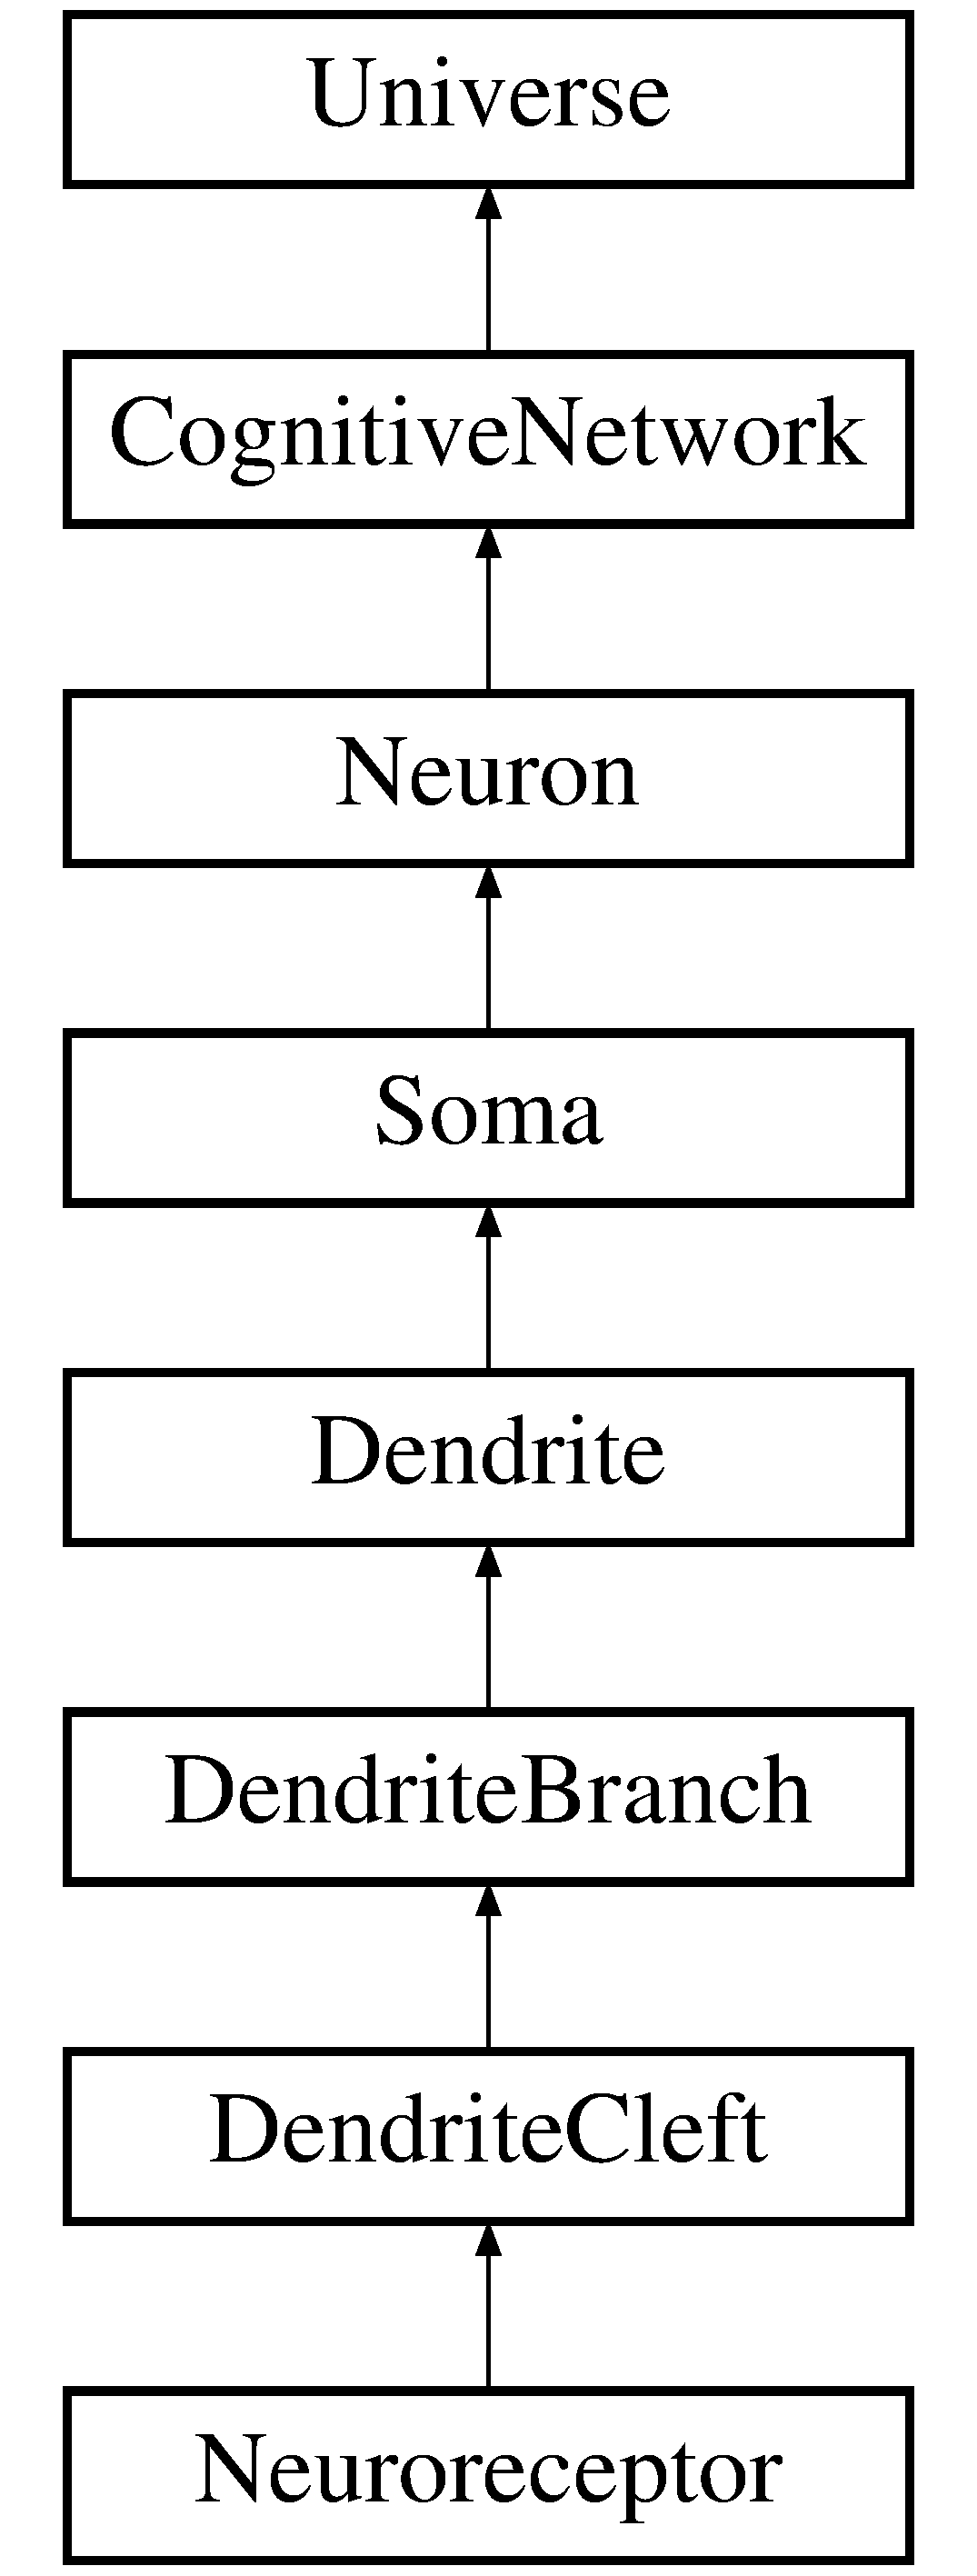
\includegraphics[height=8.000000cm]{classNeuroreceptor}
\end{center}
\end{figure}
\subsection*{Public Member Functions}
\begin{DoxyCompactItemize}
\item 
\mbox{\hyperlink{classNeuroreceptor_a70d2c87f9932f6fc113da815b6aecb7f}{Neuroreceptor}} ()
\item 
\mbox{\hyperlink{classNeuroreceptor_a4628bf1ab69e010dc42b3adfd4dee72b}{Neuroreceptor}} (unsigned int object\+\_\+type)
\item 
\mbox{\hyperlink{classNeuroreceptor_a600273e92c3a4b076273d41fa58b58e9}{Neuroreceptor}} (unsigned int object\+\_\+type, std\+::chrono\+::time\+\_\+point$<$ \mbox{\hyperlink{universe_8h_a0ef8d951d1ca5ab3cfaf7ab4c7a6fd80}{Clock}} $>$ event\+\_\+time)
\item 
\mbox{\hyperlink{classNeuroreceptor_ab002bab3b4ffeed402f60e574ce0263e}{Neuroreceptor}} (unsigned int object\+\_\+type, std\+::chrono\+::time\+\_\+point$<$ \mbox{\hyperlink{universe_8h_a0ef8d951d1ca5ab3cfaf7ab4c7a6fd80}{Clock}} $>$ event\+\_\+time, \mbox{\hyperlink{classDendriteCleft}{Dendrite\+Cleft}} \&dendritecleft\+\_\+connector)
\item 
virtual \mbox{\hyperlink{classNeuroreceptor_ac9c1e9e985ed85712c14c85e306bebc9}{$\sim$\+Neuroreceptor}} ()
\item 
unsigned int \mbox{\hyperlink{classNeuroreceptor_a4a49cfc2f741d7f7b7888929651f7be3}{Get\+Counter}} (std\+::chrono\+::time\+\_\+point$<$ \mbox{\hyperlink{universe_8h_a0ef8d951d1ca5ab3cfaf7ab4c7a6fd80}{Clock}} $>$ event\+\_\+time)
\item 
double \mbox{\hyperlink{classNeuroreceptor_abc151381ec5e7c39bb45f87a9fd17b9a}{Get\+Energy}} (std\+::chrono\+::time\+\_\+point$<$ \mbox{\hyperlink{universe_8h_a0ef8d951d1ca5ab3cfaf7ab4c7a6fd80}{Clock}} $>$ event\+\_\+time)
\item 
bool \mbox{\hyperlink{classNeuroreceptor_afbcf31596170f09292e4d8057c0215e8}{Get\+Receptor\+Binding\+State}} (std\+::chrono\+::time\+\_\+point$<$ \mbox{\hyperlink{universe_8h_a0ef8d951d1ca5ab3cfaf7ab4c7a6fd80}{Clock}} $>$ event\+\_\+time)
\item 
int \mbox{\hyperlink{classNeuroreceptor_a3ef0065a7670a2c156e34851140e0fa8}{Get\+Receptor\+Type}} (std\+::chrono\+::time\+\_\+point$<$ \mbox{\hyperlink{universe_8h_a0ef8d951d1ca5ab3cfaf7ab4c7a6fd80}{Clock}} $>$ event\+\_\+time)
\item 
bool \mbox{\hyperlink{classNeuroreceptor_aff4754990dc5b8d0105db281c02031d7}{Get\+Disabled}} (std\+::chrono\+::time\+\_\+point$<$ \mbox{\hyperlink{universe_8h_a0ef8d951d1ca5ab3cfaf7ab4c7a6fd80}{Clock}} $>$ event\+\_\+time)
\item 
int \mbox{\hyperlink{classNeuroreceptor_a69103180d9b335b9504b4ae3c203d0ea}{Get\+Ions}} (std\+::chrono\+::time\+\_\+point$<$ \mbox{\hyperlink{universe_8h_a0ef8d951d1ca5ab3cfaf7ab4c7a6fd80}{Clock}} $>$ event\+\_\+time)
\item 
void \mbox{\hyperlink{classNeuroreceptor_a75adddd7e615af57b8f3f841ec25463c}{Set\+Receptor\+Binding\+State}} (std\+::chrono\+::time\+\_\+point$<$ \mbox{\hyperlink{universe_8h_a0ef8d951d1ca5ab3cfaf7ab4c7a6fd80}{Clock}} $>$ event\+\_\+time, bool val)
\item 
void \mbox{\hyperlink{classNeuroreceptor_ace41227d30a8f50e1a6efadc86573f80}{Toggle\+Receptor\+Binding\+State}} (std\+::chrono\+::time\+\_\+point$<$ \mbox{\hyperlink{universe_8h_a0ef8d951d1ca5ab3cfaf7ab4c7a6fd80}{Clock}} $>$ event\+\_\+time)
\item 
void \mbox{\hyperlink{classNeuroreceptor_a8a339a4d0f150bbdfbc2650155625196}{Toggle\+Disabled}} (std\+::chrono\+::time\+\_\+point$<$ \mbox{\hyperlink{universe_8h_a0ef8d951d1ca5ab3cfaf7ab4c7a6fd80}{Clock}} $>$ event\+\_\+time)
\item 
void \mbox{\hyperlink{classNeuroreceptor_aeec8bb2442e04700d4e9d80bb2d6e47e}{Set\+Disabled}} (std\+::chrono\+::time\+\_\+point$<$ \mbox{\hyperlink{universe_8h_a0ef8d951d1ca5ab3cfaf7ab4c7a6fd80}{Clock}} $>$ event\+\_\+time, bool val)
\item 
void \mbox{\hyperlink{classNeuroreceptor_a0e6e88d6c5b357872f055edbddb54d4c}{Set\+Receptor\+Type}} (std\+::chrono\+::time\+\_\+point$<$ \mbox{\hyperlink{universe_8h_a0ef8d951d1ca5ab3cfaf7ab4c7a6fd80}{Clock}} $>$ event\+\_\+time, int val)
\item 
void \mbox{\hyperlink{classNeuroreceptor_a0660a316ef44cf723509f720acd16f24}{Set\+Counter}} (std\+::chrono\+::time\+\_\+point$<$ \mbox{\hyperlink{universe_8h_a0ef8d951d1ca5ab3cfaf7ab4c7a6fd80}{Clock}} $>$ event\+\_\+time, unsigned int val)
\item 
void \mbox{\hyperlink{classNeuroreceptor_ac1189f9c40e3cd07e4b1dc11115ad882}{Set\+Energy}} (std\+::chrono\+::time\+\_\+point$<$ \mbox{\hyperlink{universe_8h_a0ef8d951d1ca5ab3cfaf7ab4c7a6fd80}{Clock}} $>$ event\+\_\+time, double val)
\item 
void \mbox{\hyperlink{classNeuroreceptor_a36a548475e752631130a2b4ec67c66b6}{Set\+Ions}} (std\+::chrono\+::time\+\_\+point$<$ \mbox{\hyperlink{universe_8h_a0ef8d951d1ca5ab3cfaf7ab4c7a6fd80}{Clock}} $>$ event\+\_\+time, int val)
\item 
bool \mbox{\hyperlink{classNeuroreceptor_a30debeb0311d92eb6abe354409c15d09}{Reset\+Parameters}} (std\+::chrono\+::time\+\_\+point$<$ \mbox{\hyperlink{universe_8h_a0ef8d951d1ca5ab3cfaf7ab4c7a6fd80}{Clock}} $>$ event\+\_\+time)
\item 
\mbox{\hyperlink{classCognitiveNetwork}{Cognitive\+Network}} $\ast$ \mbox{\hyperlink{classNeuroreceptor_af671059884336eadbc367f9d8556eb3f}{Create\+Neurotransmitter}} (std\+::chrono\+::time\+\_\+point$<$ \mbox{\hyperlink{universe_8h_a0ef8d951d1ca5ab3cfaf7ab4c7a6fd80}{Clock}} $>$ event\+\_\+time)
\item 
std\+::vector$<$ \mbox{\hyperlink{classCognitiveNetwork}{Cognitive\+Network}} $\ast$ $>$ \mbox{\hyperlink{classNeuroreceptor_aa0037379ecb214ff982429e054f2a194}{Create\+Neurotransmitters}} (std\+::chrono\+::time\+\_\+point$<$ \mbox{\hyperlink{universe_8h_a0ef8d951d1ca5ab3cfaf7ab4c7a6fd80}{Clock}} $>$ event\+\_\+time, int quantity)
\item 
\mbox{\hyperlink{classCognitiveNetwork}{Cognitive\+Network}} $\ast$ \mbox{\hyperlink{classNeuroreceptor_a5629a3d463cc963138ff017ec499720d}{Clone\+Neurotransmitter}} (std\+::chrono\+::time\+\_\+point$<$ \mbox{\hyperlink{universe_8h_a0ef8d951d1ca5ab3cfaf7ab4c7a6fd80}{Clock}} $>$ event\+\_\+time, \mbox{\hyperlink{classCognitiveNetwork}{Cognitive\+Network}} $\ast$clone\+\_\+object, double perfection\+\_\+membership)
\item 
std\+::vector$<$ \mbox{\hyperlink{classCognitiveNetwork}{Cognitive\+Network}} $\ast$ $>$ \mbox{\hyperlink{classNeuroreceptor_af953abb478f4a3a1843b4b61f9969274}{Clone\+Neurotransmitters}} (std\+::chrono\+::time\+\_\+point$<$ \mbox{\hyperlink{universe_8h_a0ef8d951d1ca5ab3cfaf7ab4c7a6fd80}{Clock}} $>$ event\+\_\+time, std\+::vector$<$ \mbox{\hyperlink{classCognitiveNetwork}{Cognitive\+Network}} $\ast$$>$ cloning\+\_\+list, double perfection\+\_\+membership)
\item 
\mbox{\hyperlink{classCognitiveNetwork}{Cognitive\+Network}} $\ast$ \mbox{\hyperlink{classNeuroreceptor_a35beb8e355f9b567b327e9323f5552a0}{Destroy\+Neurotransmitter}} (std\+::chrono\+::time\+\_\+point$<$ \mbox{\hyperlink{universe_8h_a0ef8d951d1ca5ab3cfaf7ab4c7a6fd80}{Clock}} $>$ event\+\_\+time, \mbox{\hyperlink{classCognitiveNetwork}{Cognitive\+Network}} $\ast$destroy\+\_\+object)
\item 
std\+::vector$<$ \mbox{\hyperlink{classCognitiveNetwork}{Cognitive\+Network}} $\ast$ $>$ \mbox{\hyperlink{classNeuroreceptor_acd500abfb25bd08167b2002e85e8b788}{Destroy\+Neurotransmitters}} (std\+::chrono\+::time\+\_\+point$<$ \mbox{\hyperlink{universe_8h_a0ef8d951d1ca5ab3cfaf7ab4c7a6fd80}{Clock}} $>$ event\+\_\+time, std\+::vector$<$ \mbox{\hyperlink{classCognitiveNetwork}{Cognitive\+Network}} $\ast$$>$ destruction\+\_\+list)
\item 
\mbox{\hyperlink{classCognitiveNetwork}{Cognitive\+Network}} $\ast$ \mbox{\hyperlink{classNeuroreceptor_a900b21f6feb6334d4ff8a3fd5244bf05}{Add\+Neurotransmitter}} (std\+::chrono\+::time\+\_\+point$<$ \mbox{\hyperlink{universe_8h_a0ef8d951d1ca5ab3cfaf7ab4c7a6fd80}{Clock}} $>$ event\+\_\+time, \mbox{\hyperlink{classCognitiveNetwork}{Cognitive\+Network}} $\ast$add\+\_\+object)
\item 
std\+::vector$<$ \mbox{\hyperlink{classCognitiveNetwork}{Cognitive\+Network}} $\ast$ $>$ \mbox{\hyperlink{classNeuroreceptor_a2e4cbd9debd555091923f57f8aa11fe4}{Add\+Neurotransmitters}} (std\+::chrono\+::time\+\_\+point$<$ \mbox{\hyperlink{universe_8h_a0ef8d951d1ca5ab3cfaf7ab4c7a6fd80}{Clock}} $>$ event\+\_\+time, std\+::vector$<$ \mbox{\hyperlink{classCognitiveNetwork}{Cognitive\+Network}} $\ast$$>$ add\+\_\+objects)
\item 
\mbox{\hyperlink{classCognitiveNetwork}{Cognitive\+Network}} $\ast$ \mbox{\hyperlink{classNeuroreceptor_a7e94ac827de7abbac585639edfd4f985}{Remove\+Neurotransmitter}} (std\+::chrono\+::time\+\_\+point$<$ \mbox{\hyperlink{universe_8h_a0ef8d951d1ca5ab3cfaf7ab4c7a6fd80}{Clock}} $>$ event\+\_\+time)
\item 
std\+::vector$<$ \mbox{\hyperlink{classCognitiveNetwork}{Cognitive\+Network}} $\ast$ $>$ \mbox{\hyperlink{classNeuroreceptor_ad760106ce6194ac02959c1882bd0f327}{Remove\+Neurotransmitters}} (std\+::chrono\+::time\+\_\+point$<$ \mbox{\hyperlink{universe_8h_a0ef8d951d1ca5ab3cfaf7ab4c7a6fd80}{Clock}} $>$ event\+\_\+time, int quantity)
\item 
\mbox{\hyperlink{classCognitiveNetwork}{Cognitive\+Network}} $\ast$ \mbox{\hyperlink{classNeuroreceptor_a526d41738265399c19c67068db450851}{Get\+Neurotransmitter}} (std\+::chrono\+::time\+\_\+point$<$ \mbox{\hyperlink{universe_8h_a0ef8d951d1ca5ab3cfaf7ab4c7a6fd80}{Clock}} $>$ event\+\_\+time, int selector)
\item 
std\+::vector$<$ \mbox{\hyperlink{classCognitiveNetwork}{Cognitive\+Network}} $\ast$ $>$ \mbox{\hyperlink{classNeuroreceptor_a4267220ee11105b7628bf39049ef7cc5}{Get\+Neurotransmitters}} (std\+::chrono\+::time\+\_\+point$<$ \mbox{\hyperlink{universe_8h_a0ef8d951d1ca5ab3cfaf7ab4c7a6fd80}{Clock}} $>$ event\+\_\+time)
\item 
bool \mbox{\hyperlink{classNeuroreceptor_a5d54ca353f0be78522aacc4fca06db63}{Compatibility\+Check}} (std\+::chrono\+::time\+\_\+point$<$ \mbox{\hyperlink{universe_8h_a0ef8d951d1ca5ab3cfaf7ab4c7a6fd80}{Clock}} $>$ event\+\_\+time, int neurotransmitter\+Type)
\item 
int \mbox{\hyperlink{classNeuroreceptor_ab8f288a095fb028793e7246a42de233b}{Update}} (std\+::chrono\+::time\+\_\+point$<$ \mbox{\hyperlink{universe_8h_a0ef8d951d1ca5ab3cfaf7ab4c7a6fd80}{Clock}} $>$ event\+\_\+time)
\end{DoxyCompactItemize}
\subsection*{Protected Attributes}
\begin{DoxyCompactItemize}
\item 
std\+::vector$<$ \mbox{\hyperlink{classCognitiveNetwork}{Cognitive\+Network}} $\ast$ $>$ \mbox{\hyperlink{classNeuroreceptor_aeb769732421531614a47bcab8ae21f8e}{neurotransmitter\+\_\+list}}
\end{DoxyCompactItemize}
\subsection*{Private Attributes}
\begin{DoxyCompactItemize}
\item 
int \mbox{\hyperlink{classNeuroreceptor_ab851e887c0570177192a0ff0c0e97e6b}{m\+\_\+\+Neuron\+Type}}
\item 
int \mbox{\hyperlink{classNeuroreceptor_a7fa3fda8a40bf5d42f687a6c8d0c90e8}{neuroreceptor\+\_\+type}}
\item 
int \mbox{\hyperlink{classNeuroreceptor_a12960bf3fcc399426d49a4c6b43b98e7}{neurotransmitter\+\_\+pool}}
\item 
int \mbox{\hyperlink{classNeuroreceptor_a72e33b87787c22588d891857ee3b3d89}{m\+\_\+add\+Status}}
\item 
std\+::chrono\+::time\+\_\+point$<$ \mbox{\hyperlink{universe_8h_a0ef8d951d1ca5ab3cfaf7ab4c7a6fd80}{Clock}} $>$ \mbox{\hyperlink{classNeuroreceptor_a135d843eb579212e0e5307b6062304d5}{previous\+\_\+event\+\_\+time}}
\item 
std\+::chrono\+::time\+\_\+point$<$ \mbox{\hyperlink{universe_8h_a0ef8d951d1ca5ab3cfaf7ab4c7a6fd80}{Clock}} $>$ \mbox{\hyperlink{classNeuroreceptor_a1ca4d66356d1e59850ea2d7591873ff5}{time\+\_\+object\+\_\+created}}
\item 
int \mbox{\hyperlink{classNeuroreceptor_af3b19cf8ef91627d66c718944ff3c67d}{duration\+\_\+since\+\_\+last\+\_\+event}}
\item 
double \mbox{\hyperlink{classNeuroreceptor_a38da9f3b9e759374eaa27039c5cd7eb1}{m\+\_\+\+Volume}}
\item 
double \mbox{\hyperlink{classNeuroreceptor_a635db1419140d67306d3164e7727087f}{m\+\_\+\+Surface\+Area}}
\item 
unsigned int \mbox{\hyperlink{classNeuroreceptor_a934ea2375feb82cc4b3ca94373542f57}{m\+\_\+\+Counter}}
\begin{DoxyCompactList}\small\item\em Member variable \char`\"{}m\+\_\+\+Counter\char`\"{}. \end{DoxyCompactList}\item 
double \mbox{\hyperlink{classNeuroreceptor_a80028c9ce2c6146d9b9df7bd66ac431e}{object\+\_\+energy}}
\begin{DoxyCompactList}\small\item\em Member variable \char`\"{}object\+\_\+energy\char`\"{}. \end{DoxyCompactList}\item 
double \mbox{\hyperlink{classNeuroreceptor_a314c6c2312e947d17c1159806c6fbd60}{object\+\_\+energy\+\_\+threshold}}
\item 
double \mbox{\hyperlink{classNeuroreceptor_aed2feaadd9a22823d58d0b3dfbb99f4e}{m\+\_\+\+Time\+Dilation}}
\item 
double \mbox{\hyperlink{classNeuroreceptor_a2f9a114bc07e75721dde5f8ec0d94944}{m\+\_\+\+Time\+Threshold}}
\item 
double \mbox{\hyperlink{classNeuroreceptor_a2633c2cb6dbeb3aa0d0a6a71ea1235fa}{m\+\_\+\+Length}}
\item 
bool \mbox{\hyperlink{classNeuroreceptor_a31a18ad0a083d4d9b40bb4ad3eb45458}{object\+\_\+initialised}} = false
\item 
bool \mbox{\hyperlink{classNeuroreceptor_ad7cec01383ddbdfce87ed5510703d21b}{object\+\_\+disabled}}
\item 
double \mbox{\hyperlink{classNeuroreceptor_abfff414d8cd3e762fd73f303908fdb03}{object\+\_\+size}} = 0
\item 
double \mbox{\hyperlink{classNeuroreceptor_a51c4fde4d12804418451b1e3212d3b9e}{object\+\_\+energy\+Full}}
\item 
int \mbox{\hyperlink{classNeuroreceptor_a78a8356b686482232ccb9e65ed733c12}{m\+\_\+\+Ions}}
\item 
bool \mbox{\hyperlink{classNeuroreceptor_add9d0f75226881200221d886bcdcc6ab}{m\+\_\+bound\+Receptor}}
\begin{DoxyCompactList}\small\item\em Member variable \char`\"{}m\+\_\+bound\+Receptor\char`\"{}. \end{DoxyCompactList}\item 
int \mbox{\hyperlink{classNeuroreceptor_a1bd49f13829d154ecd9b91488bd63035}{m\+\_\+type\+Receptor}}
\begin{DoxyCompactList}\small\item\em Member variable \char`\"{}m\+\_\+type\+Receptor\char`\"{}. \end{DoxyCompactList}\end{DoxyCompactItemize}
\subsection*{Additional Inherited Members}


\subsection{Constructor \& Destructor Documentation}
\mbox{\Hypertarget{classNeuroreceptor_a70d2c87f9932f6fc113da815b6aecb7f}\label{classNeuroreceptor_a70d2c87f9932f6fc113da815b6aecb7f}} 
\index{Neuroreceptor@{Neuroreceptor}!Neuroreceptor@{Neuroreceptor}}
\index{Neuroreceptor@{Neuroreceptor}!Neuroreceptor@{Neuroreceptor}}
\subsubsection{\texorpdfstring{Neuroreceptor()}{Neuroreceptor()}\hspace{0.1cm}{\footnotesize\ttfamily [1/4]}}
{\footnotesize\ttfamily Neuroreceptor\+::\+Neuroreceptor (\begin{DoxyParamCaption}{ }\end{DoxyParamCaption})\hspace{0.3cm}{\ttfamily [inline]}}

\mbox{\Hypertarget{classNeuroreceptor_a4628bf1ab69e010dc42b3adfd4dee72b}\label{classNeuroreceptor_a4628bf1ab69e010dc42b3adfd4dee72b}} 
\index{Neuroreceptor@{Neuroreceptor}!Neuroreceptor@{Neuroreceptor}}
\index{Neuroreceptor@{Neuroreceptor}!Neuroreceptor@{Neuroreceptor}}
\subsubsection{\texorpdfstring{Neuroreceptor()}{Neuroreceptor()}\hspace{0.1cm}{\footnotesize\ttfamily [2/4]}}
{\footnotesize\ttfamily Neuroreceptor\+::\+Neuroreceptor (\begin{DoxyParamCaption}\item[{unsigned int}]{object\+\_\+type }\end{DoxyParamCaption})\hspace{0.3cm}{\ttfamily [inline]}}

\mbox{\Hypertarget{classNeuroreceptor_a600273e92c3a4b076273d41fa58b58e9}\label{classNeuroreceptor_a600273e92c3a4b076273d41fa58b58e9}} 
\index{Neuroreceptor@{Neuroreceptor}!Neuroreceptor@{Neuroreceptor}}
\index{Neuroreceptor@{Neuroreceptor}!Neuroreceptor@{Neuroreceptor}}
\subsubsection{\texorpdfstring{Neuroreceptor()}{Neuroreceptor()}\hspace{0.1cm}{\footnotesize\ttfamily [3/4]}}
{\footnotesize\ttfamily Neuroreceptor\+::\+Neuroreceptor (\begin{DoxyParamCaption}\item[{unsigned int}]{object\+\_\+type,  }\item[{std\+::chrono\+::time\+\_\+point$<$ \mbox{\hyperlink{universe_8h_a0ef8d951d1ca5ab3cfaf7ab4c7a6fd80}{Clock}} $>$}]{event\+\_\+time }\end{DoxyParamCaption})\hspace{0.3cm}{\ttfamily [inline]}}

\mbox{\Hypertarget{classNeuroreceptor_ab002bab3b4ffeed402f60e574ce0263e}\label{classNeuroreceptor_ab002bab3b4ffeed402f60e574ce0263e}} 
\index{Neuroreceptor@{Neuroreceptor}!Neuroreceptor@{Neuroreceptor}}
\index{Neuroreceptor@{Neuroreceptor}!Neuroreceptor@{Neuroreceptor}}
\subsubsection{\texorpdfstring{Neuroreceptor()}{Neuroreceptor()}\hspace{0.1cm}{\footnotesize\ttfamily [4/4]}}
{\footnotesize\ttfamily Neuroreceptor\+::\+Neuroreceptor (\begin{DoxyParamCaption}\item[{unsigned int}]{object\+\_\+type,  }\item[{std\+::chrono\+::time\+\_\+point$<$ \mbox{\hyperlink{universe_8h_a0ef8d951d1ca5ab3cfaf7ab4c7a6fd80}{Clock}} $>$}]{event\+\_\+time,  }\item[{\mbox{\hyperlink{classDendriteCleft}{Dendrite\+Cleft}} \&}]{dendritecleft\+\_\+connector }\end{DoxyParamCaption})\hspace{0.3cm}{\ttfamily [inline]}}

\mbox{\Hypertarget{classNeuroreceptor_ac9c1e9e985ed85712c14c85e306bebc9}\label{classNeuroreceptor_ac9c1e9e985ed85712c14c85e306bebc9}} 
\index{Neuroreceptor@{Neuroreceptor}!````~Neuroreceptor@{$\sim$\+Neuroreceptor}}
\index{````~Neuroreceptor@{$\sim$\+Neuroreceptor}!Neuroreceptor@{Neuroreceptor}}
\subsubsection{\texorpdfstring{$\sim$\+Neuroreceptor()}{~Neuroreceptor()}}
{\footnotesize\ttfamily virtual Neuroreceptor\+::$\sim$\+Neuroreceptor (\begin{DoxyParamCaption}{ }\end{DoxyParamCaption})\hspace{0.3cm}{\ttfamily [inline]}, {\ttfamily [virtual]}}

Default destructor 

\subsection{Member Function Documentation}
\mbox{\Hypertarget{classNeuroreceptor_a900b21f6feb6334d4ff8a3fd5244bf05}\label{classNeuroreceptor_a900b21f6feb6334d4ff8a3fd5244bf05}} 
\index{Neuroreceptor@{Neuroreceptor}!Add\+Neurotransmitter@{Add\+Neurotransmitter}}
\index{Add\+Neurotransmitter@{Add\+Neurotransmitter}!Neuroreceptor@{Neuroreceptor}}
\subsubsection{\texorpdfstring{Add\+Neurotransmitter()}{AddNeurotransmitter()}}
{\footnotesize\ttfamily \mbox{\hyperlink{classCognitiveNetwork}{Cognitive\+Network}} $\ast$ Neuroreceptor\+::\+Add\+Neurotransmitter (\begin{DoxyParamCaption}\item[{std\+::chrono\+::time\+\_\+point$<$ \mbox{\hyperlink{universe_8h_a0ef8d951d1ca5ab3cfaf7ab4c7a6fd80}{Clock}} $>$}]{event\+\_\+time,  }\item[{\mbox{\hyperlink{classCognitiveNetwork}{Cognitive\+Network}} $\ast$}]{add\+\_\+object }\end{DoxyParamCaption})}

\mbox{\Hypertarget{classNeuroreceptor_a2e4cbd9debd555091923f57f8aa11fe4}\label{classNeuroreceptor_a2e4cbd9debd555091923f57f8aa11fe4}} 
\index{Neuroreceptor@{Neuroreceptor}!Add\+Neurotransmitters@{Add\+Neurotransmitters}}
\index{Add\+Neurotransmitters@{Add\+Neurotransmitters}!Neuroreceptor@{Neuroreceptor}}
\subsubsection{\texorpdfstring{Add\+Neurotransmitters()}{AddNeurotransmitters()}}
{\footnotesize\ttfamily std\+::vector$<$ \mbox{\hyperlink{classCognitiveNetwork}{Cognitive\+Network}} $\ast$ $>$ Neuroreceptor\+::\+Add\+Neurotransmitters (\begin{DoxyParamCaption}\item[{std\+::chrono\+::time\+\_\+point$<$ \mbox{\hyperlink{universe_8h_a0ef8d951d1ca5ab3cfaf7ab4c7a6fd80}{Clock}} $>$}]{event\+\_\+time,  }\item[{std\+::vector$<$ \mbox{\hyperlink{classCognitiveNetwork}{Cognitive\+Network}} $\ast$$>$}]{add\+\_\+objects }\end{DoxyParamCaption})}

\mbox{\Hypertarget{classNeuroreceptor_a5629a3d463cc963138ff017ec499720d}\label{classNeuroreceptor_a5629a3d463cc963138ff017ec499720d}} 
\index{Neuroreceptor@{Neuroreceptor}!Clone\+Neurotransmitter@{Clone\+Neurotransmitter}}
\index{Clone\+Neurotransmitter@{Clone\+Neurotransmitter}!Neuroreceptor@{Neuroreceptor}}
\subsubsection{\texorpdfstring{Clone\+Neurotransmitter()}{CloneNeurotransmitter()}}
{\footnotesize\ttfamily \mbox{\hyperlink{classCognitiveNetwork}{Cognitive\+Network}} $\ast$ Neuroreceptor\+::\+Clone\+Neurotransmitter (\begin{DoxyParamCaption}\item[{std\+::chrono\+::time\+\_\+point$<$ \mbox{\hyperlink{universe_8h_a0ef8d951d1ca5ab3cfaf7ab4c7a6fd80}{Clock}} $>$}]{event\+\_\+time,  }\item[{\mbox{\hyperlink{classCognitiveNetwork}{Cognitive\+Network}} $\ast$}]{clone\+\_\+object,  }\item[{double}]{perfection\+\_\+membership }\end{DoxyParamCaption})}

\mbox{\Hypertarget{classNeuroreceptor_af953abb478f4a3a1843b4b61f9969274}\label{classNeuroreceptor_af953abb478f4a3a1843b4b61f9969274}} 
\index{Neuroreceptor@{Neuroreceptor}!Clone\+Neurotransmitters@{Clone\+Neurotransmitters}}
\index{Clone\+Neurotransmitters@{Clone\+Neurotransmitters}!Neuroreceptor@{Neuroreceptor}}
\subsubsection{\texorpdfstring{Clone\+Neurotransmitters()}{CloneNeurotransmitters()}}
{\footnotesize\ttfamily std\+::vector$<$ \mbox{\hyperlink{classCognitiveNetwork}{Cognitive\+Network}} $\ast$ $>$ Neuroreceptor\+::\+Clone\+Neurotransmitters (\begin{DoxyParamCaption}\item[{std\+::chrono\+::time\+\_\+point$<$ \mbox{\hyperlink{universe_8h_a0ef8d951d1ca5ab3cfaf7ab4c7a6fd80}{Clock}} $>$}]{event\+\_\+time,  }\item[{std\+::vector$<$ \mbox{\hyperlink{classCognitiveNetwork}{Cognitive\+Network}} $\ast$$>$}]{cloning\+\_\+list,  }\item[{double}]{perfection\+\_\+membership }\end{DoxyParamCaption})}

\mbox{\Hypertarget{classNeuroreceptor_a5d54ca353f0be78522aacc4fca06db63}\label{classNeuroreceptor_a5d54ca353f0be78522aacc4fca06db63}} 
\index{Neuroreceptor@{Neuroreceptor}!Compatibility\+Check@{Compatibility\+Check}}
\index{Compatibility\+Check@{Compatibility\+Check}!Neuroreceptor@{Neuroreceptor}}
\subsubsection{\texorpdfstring{Compatibility\+Check()}{CompatibilityCheck()}}
{\footnotesize\ttfamily bool Neuroreceptor\+::\+Compatibility\+Check (\begin{DoxyParamCaption}\item[{std\+::chrono\+::time\+\_\+point$<$ \mbox{\hyperlink{universe_8h_a0ef8d951d1ca5ab3cfaf7ab4c7a6fd80}{Clock}} $>$}]{event\+\_\+time,  }\item[{int}]{neurotransmitter\+Type }\end{DoxyParamCaption})}

\mbox{\Hypertarget{classNeuroreceptor_af671059884336eadbc367f9d8556eb3f}\label{classNeuroreceptor_af671059884336eadbc367f9d8556eb3f}} 
\index{Neuroreceptor@{Neuroreceptor}!Create\+Neurotransmitter@{Create\+Neurotransmitter}}
\index{Create\+Neurotransmitter@{Create\+Neurotransmitter}!Neuroreceptor@{Neuroreceptor}}
\subsubsection{\texorpdfstring{Create\+Neurotransmitter()}{CreateNeurotransmitter()}}
{\footnotesize\ttfamily \mbox{\hyperlink{classCognitiveNetwork}{Cognitive\+Network}} $\ast$ Neuroreceptor\+::\+Create\+Neurotransmitter (\begin{DoxyParamCaption}\item[{std\+::chrono\+::time\+\_\+point$<$ \mbox{\hyperlink{universe_8h_a0ef8d951d1ca5ab3cfaf7ab4c7a6fd80}{Clock}} $>$}]{event\+\_\+time }\end{DoxyParamCaption})}

\mbox{\Hypertarget{classNeuroreceptor_aa0037379ecb214ff982429e054f2a194}\label{classNeuroreceptor_aa0037379ecb214ff982429e054f2a194}} 
\index{Neuroreceptor@{Neuroreceptor}!Create\+Neurotransmitters@{Create\+Neurotransmitters}}
\index{Create\+Neurotransmitters@{Create\+Neurotransmitters}!Neuroreceptor@{Neuroreceptor}}
\subsubsection{\texorpdfstring{Create\+Neurotransmitters()}{CreateNeurotransmitters()}}
{\footnotesize\ttfamily std\+::vector$<$ \mbox{\hyperlink{classCognitiveNetwork}{Cognitive\+Network}} $\ast$ $>$ Neuroreceptor\+::\+Create\+Neurotransmitters (\begin{DoxyParamCaption}\item[{std\+::chrono\+::time\+\_\+point$<$ \mbox{\hyperlink{universe_8h_a0ef8d951d1ca5ab3cfaf7ab4c7a6fd80}{Clock}} $>$}]{event\+\_\+time,  }\item[{int}]{quantity }\end{DoxyParamCaption})}

\mbox{\Hypertarget{classNeuroreceptor_a35beb8e355f9b567b327e9323f5552a0}\label{classNeuroreceptor_a35beb8e355f9b567b327e9323f5552a0}} 
\index{Neuroreceptor@{Neuroreceptor}!Destroy\+Neurotransmitter@{Destroy\+Neurotransmitter}}
\index{Destroy\+Neurotransmitter@{Destroy\+Neurotransmitter}!Neuroreceptor@{Neuroreceptor}}
\subsubsection{\texorpdfstring{Destroy\+Neurotransmitter()}{DestroyNeurotransmitter()}}
{\footnotesize\ttfamily \mbox{\hyperlink{classCognitiveNetwork}{Cognitive\+Network}} $\ast$ Neuroreceptor\+::\+Destroy\+Neurotransmitter (\begin{DoxyParamCaption}\item[{std\+::chrono\+::time\+\_\+point$<$ \mbox{\hyperlink{universe_8h_a0ef8d951d1ca5ab3cfaf7ab4c7a6fd80}{Clock}} $>$}]{event\+\_\+time,  }\item[{\mbox{\hyperlink{classCognitiveNetwork}{Cognitive\+Network}} $\ast$}]{destroy\+\_\+object }\end{DoxyParamCaption})}

\mbox{\Hypertarget{classNeuroreceptor_acd500abfb25bd08167b2002e85e8b788}\label{classNeuroreceptor_acd500abfb25bd08167b2002e85e8b788}} 
\index{Neuroreceptor@{Neuroreceptor}!Destroy\+Neurotransmitters@{Destroy\+Neurotransmitters}}
\index{Destroy\+Neurotransmitters@{Destroy\+Neurotransmitters}!Neuroreceptor@{Neuroreceptor}}
\subsubsection{\texorpdfstring{Destroy\+Neurotransmitters()}{DestroyNeurotransmitters()}}
{\footnotesize\ttfamily std\+::vector$<$ \mbox{\hyperlink{classCognitiveNetwork}{Cognitive\+Network}} $\ast$ $>$ Neuroreceptor\+::\+Destroy\+Neurotransmitters (\begin{DoxyParamCaption}\item[{std\+::chrono\+::time\+\_\+point$<$ \mbox{\hyperlink{universe_8h_a0ef8d951d1ca5ab3cfaf7ab4c7a6fd80}{Clock}} $>$}]{event\+\_\+time,  }\item[{std\+::vector$<$ \mbox{\hyperlink{classCognitiveNetwork}{Cognitive\+Network}} $\ast$$>$}]{destruction\+\_\+list }\end{DoxyParamCaption})}

\mbox{\Hypertarget{classNeuroreceptor_a4a49cfc2f741d7f7b7888929651f7be3}\label{classNeuroreceptor_a4a49cfc2f741d7f7b7888929651f7be3}} 
\index{Neuroreceptor@{Neuroreceptor}!Get\+Counter@{Get\+Counter}}
\index{Get\+Counter@{Get\+Counter}!Neuroreceptor@{Neuroreceptor}}
\subsubsection{\texorpdfstring{Get\+Counter()}{GetCounter()}}
{\footnotesize\ttfamily unsigned int Neuroreceptor\+::\+Get\+Counter (\begin{DoxyParamCaption}\item[{std\+::chrono\+::time\+\_\+point$<$ \mbox{\hyperlink{universe_8h_a0ef8d951d1ca5ab3cfaf7ab4c7a6fd80}{Clock}} $>$}]{event\+\_\+time }\end{DoxyParamCaption})\hspace{0.3cm}{\ttfamily [inline]}}

\mbox{\Hypertarget{classNeuroreceptor_aff4754990dc5b8d0105db281c02031d7}\label{classNeuroreceptor_aff4754990dc5b8d0105db281c02031d7}} 
\index{Neuroreceptor@{Neuroreceptor}!Get\+Disabled@{Get\+Disabled}}
\index{Get\+Disabled@{Get\+Disabled}!Neuroreceptor@{Neuroreceptor}}
\subsubsection{\texorpdfstring{Get\+Disabled()}{GetDisabled()}}
{\footnotesize\ttfamily bool Neuroreceptor\+::\+Get\+Disabled (\begin{DoxyParamCaption}\item[{std\+::chrono\+::time\+\_\+point$<$ \mbox{\hyperlink{universe_8h_a0ef8d951d1ca5ab3cfaf7ab4c7a6fd80}{Clock}} $>$}]{event\+\_\+time }\end{DoxyParamCaption})\hspace{0.3cm}{\ttfamily [inline]}}

\mbox{\Hypertarget{classNeuroreceptor_abc151381ec5e7c39bb45f87a9fd17b9a}\label{classNeuroreceptor_abc151381ec5e7c39bb45f87a9fd17b9a}} 
\index{Neuroreceptor@{Neuroreceptor}!Get\+Energy@{Get\+Energy}}
\index{Get\+Energy@{Get\+Energy}!Neuroreceptor@{Neuroreceptor}}
\subsubsection{\texorpdfstring{Get\+Energy()}{GetEnergy()}}
{\footnotesize\ttfamily double Neuroreceptor\+::\+Get\+Energy (\begin{DoxyParamCaption}\item[{std\+::chrono\+::time\+\_\+point$<$ \mbox{\hyperlink{universe_8h_a0ef8d951d1ca5ab3cfaf7ab4c7a6fd80}{Clock}} $>$}]{event\+\_\+time }\end{DoxyParamCaption})\hspace{0.3cm}{\ttfamily [inline]}}

\mbox{\Hypertarget{classNeuroreceptor_a69103180d9b335b9504b4ae3c203d0ea}\label{classNeuroreceptor_a69103180d9b335b9504b4ae3c203d0ea}} 
\index{Neuroreceptor@{Neuroreceptor}!Get\+Ions@{Get\+Ions}}
\index{Get\+Ions@{Get\+Ions}!Neuroreceptor@{Neuroreceptor}}
\subsubsection{\texorpdfstring{Get\+Ions()}{GetIons()}}
{\footnotesize\ttfamily int Neuroreceptor\+::\+Get\+Ions (\begin{DoxyParamCaption}\item[{std\+::chrono\+::time\+\_\+point$<$ \mbox{\hyperlink{universe_8h_a0ef8d951d1ca5ab3cfaf7ab4c7a6fd80}{Clock}} $>$}]{event\+\_\+time }\end{DoxyParamCaption})\hspace{0.3cm}{\ttfamily [inline]}}

\mbox{\Hypertarget{classNeuroreceptor_a526d41738265399c19c67068db450851}\label{classNeuroreceptor_a526d41738265399c19c67068db450851}} 
\index{Neuroreceptor@{Neuroreceptor}!Get\+Neurotransmitter@{Get\+Neurotransmitter}}
\index{Get\+Neurotransmitter@{Get\+Neurotransmitter}!Neuroreceptor@{Neuroreceptor}}
\subsubsection{\texorpdfstring{Get\+Neurotransmitter()}{GetNeurotransmitter()}}
{\footnotesize\ttfamily \mbox{\hyperlink{classCognitiveNetwork}{Cognitive\+Network}} $\ast$ Neuroreceptor\+::\+Get\+Neurotransmitter (\begin{DoxyParamCaption}\item[{std\+::chrono\+::time\+\_\+point$<$ \mbox{\hyperlink{universe_8h_a0ef8d951d1ca5ab3cfaf7ab4c7a6fd80}{Clock}} $>$}]{event\+\_\+time,  }\item[{int}]{selector }\end{DoxyParamCaption})}

\mbox{\Hypertarget{classNeuroreceptor_a4267220ee11105b7628bf39049ef7cc5}\label{classNeuroreceptor_a4267220ee11105b7628bf39049ef7cc5}} 
\index{Neuroreceptor@{Neuroreceptor}!Get\+Neurotransmitters@{Get\+Neurotransmitters}}
\index{Get\+Neurotransmitters@{Get\+Neurotransmitters}!Neuroreceptor@{Neuroreceptor}}
\subsubsection{\texorpdfstring{Get\+Neurotransmitters()}{GetNeurotransmitters()}}
{\footnotesize\ttfamily std\+::vector$<$ \mbox{\hyperlink{classCognitiveNetwork}{Cognitive\+Network}} $\ast$ $>$ Neuroreceptor\+::\+Get\+Neurotransmitters (\begin{DoxyParamCaption}\item[{std\+::chrono\+::time\+\_\+point$<$ \mbox{\hyperlink{universe_8h_a0ef8d951d1ca5ab3cfaf7ab4c7a6fd80}{Clock}} $>$}]{event\+\_\+time }\end{DoxyParamCaption})}

\mbox{\Hypertarget{classNeuroreceptor_afbcf31596170f09292e4d8057c0215e8}\label{classNeuroreceptor_afbcf31596170f09292e4d8057c0215e8}} 
\index{Neuroreceptor@{Neuroreceptor}!Get\+Receptor\+Binding\+State@{Get\+Receptor\+Binding\+State}}
\index{Get\+Receptor\+Binding\+State@{Get\+Receptor\+Binding\+State}!Neuroreceptor@{Neuroreceptor}}
\subsubsection{\texorpdfstring{Get\+Receptor\+Binding\+State()}{GetReceptorBindingState()}}
{\footnotesize\ttfamily bool Neuroreceptor\+::\+Get\+Receptor\+Binding\+State (\begin{DoxyParamCaption}\item[{std\+::chrono\+::time\+\_\+point$<$ \mbox{\hyperlink{universe_8h_a0ef8d951d1ca5ab3cfaf7ab4c7a6fd80}{Clock}} $>$}]{event\+\_\+time }\end{DoxyParamCaption})\hspace{0.3cm}{\ttfamily [inline]}}

\mbox{\Hypertarget{classNeuroreceptor_a3ef0065a7670a2c156e34851140e0fa8}\label{classNeuroreceptor_a3ef0065a7670a2c156e34851140e0fa8}} 
\index{Neuroreceptor@{Neuroreceptor}!Get\+Receptor\+Type@{Get\+Receptor\+Type}}
\index{Get\+Receptor\+Type@{Get\+Receptor\+Type}!Neuroreceptor@{Neuroreceptor}}
\subsubsection{\texorpdfstring{Get\+Receptor\+Type()}{GetReceptorType()}}
{\footnotesize\ttfamily int Neuroreceptor\+::\+Get\+Receptor\+Type (\begin{DoxyParamCaption}\item[{std\+::chrono\+::time\+\_\+point$<$ \mbox{\hyperlink{universe_8h_a0ef8d951d1ca5ab3cfaf7ab4c7a6fd80}{Clock}} $>$}]{event\+\_\+time }\end{DoxyParamCaption})\hspace{0.3cm}{\ttfamily [inline]}}

\mbox{\Hypertarget{classNeuroreceptor_a7e94ac827de7abbac585639edfd4f985}\label{classNeuroreceptor_a7e94ac827de7abbac585639edfd4f985}} 
\index{Neuroreceptor@{Neuroreceptor}!Remove\+Neurotransmitter@{Remove\+Neurotransmitter}}
\index{Remove\+Neurotransmitter@{Remove\+Neurotransmitter}!Neuroreceptor@{Neuroreceptor}}
\subsubsection{\texorpdfstring{Remove\+Neurotransmitter()}{RemoveNeurotransmitter()}}
{\footnotesize\ttfamily \mbox{\hyperlink{classCognitiveNetwork}{Cognitive\+Network}} $\ast$ Neuroreceptor\+::\+Remove\+Neurotransmitter (\begin{DoxyParamCaption}\item[{std\+::chrono\+::time\+\_\+point$<$ \mbox{\hyperlink{universe_8h_a0ef8d951d1ca5ab3cfaf7ab4c7a6fd80}{Clock}} $>$}]{event\+\_\+time }\end{DoxyParamCaption})}

\mbox{\Hypertarget{classNeuroreceptor_ad760106ce6194ac02959c1882bd0f327}\label{classNeuroreceptor_ad760106ce6194ac02959c1882bd0f327}} 
\index{Neuroreceptor@{Neuroreceptor}!Remove\+Neurotransmitters@{Remove\+Neurotransmitters}}
\index{Remove\+Neurotransmitters@{Remove\+Neurotransmitters}!Neuroreceptor@{Neuroreceptor}}
\subsubsection{\texorpdfstring{Remove\+Neurotransmitters()}{RemoveNeurotransmitters()}}
{\footnotesize\ttfamily std\+::vector$<$ \mbox{\hyperlink{classCognitiveNetwork}{Cognitive\+Network}} $\ast$ $>$ Neuroreceptor\+::\+Remove\+Neurotransmitters (\begin{DoxyParamCaption}\item[{std\+::chrono\+::time\+\_\+point$<$ \mbox{\hyperlink{universe_8h_a0ef8d951d1ca5ab3cfaf7ab4c7a6fd80}{Clock}} $>$}]{event\+\_\+time,  }\item[{int}]{quantity }\end{DoxyParamCaption})}

\mbox{\Hypertarget{classNeuroreceptor_a30debeb0311d92eb6abe354409c15d09}\label{classNeuroreceptor_a30debeb0311d92eb6abe354409c15d09}} 
\index{Neuroreceptor@{Neuroreceptor}!Reset\+Parameters@{Reset\+Parameters}}
\index{Reset\+Parameters@{Reset\+Parameters}!Neuroreceptor@{Neuroreceptor}}
\subsubsection{\texorpdfstring{Reset\+Parameters()}{ResetParameters()}}
{\footnotesize\ttfamily bool Neuroreceptor\+::\+Reset\+Parameters (\begin{DoxyParamCaption}\item[{std\+::chrono\+::time\+\_\+point$<$ \mbox{\hyperlink{universe_8h_a0ef8d951d1ca5ab3cfaf7ab4c7a6fd80}{Clock}} $>$}]{event\+\_\+time }\end{DoxyParamCaption})}

\mbox{\Hypertarget{classNeuroreceptor_a0660a316ef44cf723509f720acd16f24}\label{classNeuroreceptor_a0660a316ef44cf723509f720acd16f24}} 
\index{Neuroreceptor@{Neuroreceptor}!Set\+Counter@{Set\+Counter}}
\index{Set\+Counter@{Set\+Counter}!Neuroreceptor@{Neuroreceptor}}
\subsubsection{\texorpdfstring{Set\+Counter()}{SetCounter()}}
{\footnotesize\ttfamily void Neuroreceptor\+::\+Set\+Counter (\begin{DoxyParamCaption}\item[{std\+::chrono\+::time\+\_\+point$<$ \mbox{\hyperlink{universe_8h_a0ef8d951d1ca5ab3cfaf7ab4c7a6fd80}{Clock}} $>$}]{event\+\_\+time,  }\item[{unsigned int}]{val }\end{DoxyParamCaption})\hspace{0.3cm}{\ttfamily [inline]}, {\ttfamily [virtual]}}



Reimplemented from \mbox{\hyperlink{classDendriteCleft_a428b8e5117f381a382e0071b936d42a1}{Dendrite\+Cleft}}.

\mbox{\Hypertarget{classNeuroreceptor_aeec8bb2442e04700d4e9d80bb2d6e47e}\label{classNeuroreceptor_aeec8bb2442e04700d4e9d80bb2d6e47e}} 
\index{Neuroreceptor@{Neuroreceptor}!Set\+Disabled@{Set\+Disabled}}
\index{Set\+Disabled@{Set\+Disabled}!Neuroreceptor@{Neuroreceptor}}
\subsubsection{\texorpdfstring{Set\+Disabled()}{SetDisabled()}}
{\footnotesize\ttfamily void Neuroreceptor\+::\+Set\+Disabled (\begin{DoxyParamCaption}\item[{std\+::chrono\+::time\+\_\+point$<$ \mbox{\hyperlink{universe_8h_a0ef8d951d1ca5ab3cfaf7ab4c7a6fd80}{Clock}} $>$}]{event\+\_\+time,  }\item[{bool}]{val }\end{DoxyParamCaption})\hspace{0.3cm}{\ttfamily [inline]}}

\mbox{\Hypertarget{classNeuroreceptor_ac1189f9c40e3cd07e4b1dc11115ad882}\label{classNeuroreceptor_ac1189f9c40e3cd07e4b1dc11115ad882}} 
\index{Neuroreceptor@{Neuroreceptor}!Set\+Energy@{Set\+Energy}}
\index{Set\+Energy@{Set\+Energy}!Neuroreceptor@{Neuroreceptor}}
\subsubsection{\texorpdfstring{Set\+Energy()}{SetEnergy()}}
{\footnotesize\ttfamily void Neuroreceptor\+::\+Set\+Energy (\begin{DoxyParamCaption}\item[{std\+::chrono\+::time\+\_\+point$<$ \mbox{\hyperlink{universe_8h_a0ef8d951d1ca5ab3cfaf7ab4c7a6fd80}{Clock}} $>$}]{event\+\_\+time,  }\item[{double}]{val }\end{DoxyParamCaption})\hspace{0.3cm}{\ttfamily [inline]}}

\mbox{\Hypertarget{classNeuroreceptor_a36a548475e752631130a2b4ec67c66b6}\label{classNeuroreceptor_a36a548475e752631130a2b4ec67c66b6}} 
\index{Neuroreceptor@{Neuroreceptor}!Set\+Ions@{Set\+Ions}}
\index{Set\+Ions@{Set\+Ions}!Neuroreceptor@{Neuroreceptor}}
\subsubsection{\texorpdfstring{Set\+Ions()}{SetIons()}}
{\footnotesize\ttfamily void Neuroreceptor\+::\+Set\+Ions (\begin{DoxyParamCaption}\item[{std\+::chrono\+::time\+\_\+point$<$ \mbox{\hyperlink{universe_8h_a0ef8d951d1ca5ab3cfaf7ab4c7a6fd80}{Clock}} $>$}]{event\+\_\+time,  }\item[{int}]{val }\end{DoxyParamCaption})\hspace{0.3cm}{\ttfamily [inline]}}

\mbox{\Hypertarget{classNeuroreceptor_a75adddd7e615af57b8f3f841ec25463c}\label{classNeuroreceptor_a75adddd7e615af57b8f3f841ec25463c}} 
\index{Neuroreceptor@{Neuroreceptor}!Set\+Receptor\+Binding\+State@{Set\+Receptor\+Binding\+State}}
\index{Set\+Receptor\+Binding\+State@{Set\+Receptor\+Binding\+State}!Neuroreceptor@{Neuroreceptor}}
\subsubsection{\texorpdfstring{Set\+Receptor\+Binding\+State()}{SetReceptorBindingState()}}
{\footnotesize\ttfamily void Neuroreceptor\+::\+Set\+Receptor\+Binding\+State (\begin{DoxyParamCaption}\item[{std\+::chrono\+::time\+\_\+point$<$ \mbox{\hyperlink{universe_8h_a0ef8d951d1ca5ab3cfaf7ab4c7a6fd80}{Clock}} $>$}]{event\+\_\+time,  }\item[{bool}]{val }\end{DoxyParamCaption})\hspace{0.3cm}{\ttfamily [inline]}}

\mbox{\Hypertarget{classNeuroreceptor_a0e6e88d6c5b357872f055edbddb54d4c}\label{classNeuroreceptor_a0e6e88d6c5b357872f055edbddb54d4c}} 
\index{Neuroreceptor@{Neuroreceptor}!Set\+Receptor\+Type@{Set\+Receptor\+Type}}
\index{Set\+Receptor\+Type@{Set\+Receptor\+Type}!Neuroreceptor@{Neuroreceptor}}
\subsubsection{\texorpdfstring{Set\+Receptor\+Type()}{SetReceptorType()}}
{\footnotesize\ttfamily void Neuroreceptor\+::\+Set\+Receptor\+Type (\begin{DoxyParamCaption}\item[{std\+::chrono\+::time\+\_\+point$<$ \mbox{\hyperlink{universe_8h_a0ef8d951d1ca5ab3cfaf7ab4c7a6fd80}{Clock}} $>$}]{event\+\_\+time,  }\item[{int}]{val }\end{DoxyParamCaption})\hspace{0.3cm}{\ttfamily [inline]}}

\mbox{\Hypertarget{classNeuroreceptor_a8a339a4d0f150bbdfbc2650155625196}\label{classNeuroreceptor_a8a339a4d0f150bbdfbc2650155625196}} 
\index{Neuroreceptor@{Neuroreceptor}!Toggle\+Disabled@{Toggle\+Disabled}}
\index{Toggle\+Disabled@{Toggle\+Disabled}!Neuroreceptor@{Neuroreceptor}}
\subsubsection{\texorpdfstring{Toggle\+Disabled()}{ToggleDisabled()}}
{\footnotesize\ttfamily void Neuroreceptor\+::\+Toggle\+Disabled (\begin{DoxyParamCaption}\item[{std\+::chrono\+::time\+\_\+point$<$ \mbox{\hyperlink{universe_8h_a0ef8d951d1ca5ab3cfaf7ab4c7a6fd80}{Clock}} $>$}]{event\+\_\+time }\end{DoxyParamCaption})\hspace{0.3cm}{\ttfamily [inline]}}

\mbox{\Hypertarget{classNeuroreceptor_ace41227d30a8f50e1a6efadc86573f80}\label{classNeuroreceptor_ace41227d30a8f50e1a6efadc86573f80}} 
\index{Neuroreceptor@{Neuroreceptor}!Toggle\+Receptor\+Binding\+State@{Toggle\+Receptor\+Binding\+State}}
\index{Toggle\+Receptor\+Binding\+State@{Toggle\+Receptor\+Binding\+State}!Neuroreceptor@{Neuroreceptor}}
\subsubsection{\texorpdfstring{Toggle\+Receptor\+Binding\+State()}{ToggleReceptorBindingState()}}
{\footnotesize\ttfamily void Neuroreceptor\+::\+Toggle\+Receptor\+Binding\+State (\begin{DoxyParamCaption}\item[{std\+::chrono\+::time\+\_\+point$<$ \mbox{\hyperlink{universe_8h_a0ef8d951d1ca5ab3cfaf7ab4c7a6fd80}{Clock}} $>$}]{event\+\_\+time }\end{DoxyParamCaption})\hspace{0.3cm}{\ttfamily [inline]}}

\mbox{\Hypertarget{classNeuroreceptor_ab8f288a095fb028793e7246a42de233b}\label{classNeuroreceptor_ab8f288a095fb028793e7246a42de233b}} 
\index{Neuroreceptor@{Neuroreceptor}!Update@{Update}}
\index{Update@{Update}!Neuroreceptor@{Neuroreceptor}}
\subsubsection{\texorpdfstring{Update()}{Update()}}
{\footnotesize\ttfamily int Neuroreceptor\+::\+Update (\begin{DoxyParamCaption}\item[{std\+::chrono\+::time\+\_\+point$<$ \mbox{\hyperlink{universe_8h_a0ef8d951d1ca5ab3cfaf7ab4c7a6fd80}{Clock}} $>$}]{event\+\_\+time }\end{DoxyParamCaption})}



\subsection{Member Data Documentation}
\mbox{\Hypertarget{classNeuroreceptor_af3b19cf8ef91627d66c718944ff3c67d}\label{classNeuroreceptor_af3b19cf8ef91627d66c718944ff3c67d}} 
\index{Neuroreceptor@{Neuroreceptor}!duration\+\_\+since\+\_\+last\+\_\+event@{duration\+\_\+since\+\_\+last\+\_\+event}}
\index{duration\+\_\+since\+\_\+last\+\_\+event@{duration\+\_\+since\+\_\+last\+\_\+event}!Neuroreceptor@{Neuroreceptor}}
\subsubsection{\texorpdfstring{duration\+\_\+since\+\_\+last\+\_\+event}{duration\_since\_last\_event}}
{\footnotesize\ttfamily int Neuroreceptor\+::duration\+\_\+since\+\_\+last\+\_\+event\hspace{0.3cm}{\ttfamily [private]}}

\mbox{\Hypertarget{classNeuroreceptor_a72e33b87787c22588d891857ee3b3d89}\label{classNeuroreceptor_a72e33b87787c22588d891857ee3b3d89}} 
\index{Neuroreceptor@{Neuroreceptor}!m\+\_\+add\+Status@{m\+\_\+add\+Status}}
\index{m\+\_\+add\+Status@{m\+\_\+add\+Status}!Neuroreceptor@{Neuroreceptor}}
\subsubsection{\texorpdfstring{m\+\_\+add\+Status}{m\_addStatus}}
{\footnotesize\ttfamily int Neuroreceptor\+::m\+\_\+add\+Status\hspace{0.3cm}{\ttfamily [private]}}

\mbox{\Hypertarget{classNeuroreceptor_add9d0f75226881200221d886bcdcc6ab}\label{classNeuroreceptor_add9d0f75226881200221d886bcdcc6ab}} 
\index{Neuroreceptor@{Neuroreceptor}!m\+\_\+bound\+Receptor@{m\+\_\+bound\+Receptor}}
\index{m\+\_\+bound\+Receptor@{m\+\_\+bound\+Receptor}!Neuroreceptor@{Neuroreceptor}}
\subsubsection{\texorpdfstring{m\+\_\+bound\+Receptor}{m\_boundReceptor}}
{\footnotesize\ttfamily bool Neuroreceptor\+::m\+\_\+bound\+Receptor\hspace{0.3cm}{\ttfamily [private]}}



Member variable \char`\"{}m\+\_\+bound\+Receptor\char`\"{}. 

\mbox{\Hypertarget{classNeuroreceptor_a934ea2375feb82cc4b3ca94373542f57}\label{classNeuroreceptor_a934ea2375feb82cc4b3ca94373542f57}} 
\index{Neuroreceptor@{Neuroreceptor}!m\+\_\+\+Counter@{m\+\_\+\+Counter}}
\index{m\+\_\+\+Counter@{m\+\_\+\+Counter}!Neuroreceptor@{Neuroreceptor}}
\subsubsection{\texorpdfstring{m\+\_\+\+Counter}{m\_Counter}}
{\footnotesize\ttfamily unsigned int Neuroreceptor\+::m\+\_\+\+Counter\hspace{0.3cm}{\ttfamily [private]}}



Member variable \char`\"{}m\+\_\+\+Counter\char`\"{}. 

\mbox{\Hypertarget{classNeuroreceptor_a78a8356b686482232ccb9e65ed733c12}\label{classNeuroreceptor_a78a8356b686482232ccb9e65ed733c12}} 
\index{Neuroreceptor@{Neuroreceptor}!m\+\_\+\+Ions@{m\+\_\+\+Ions}}
\index{m\+\_\+\+Ions@{m\+\_\+\+Ions}!Neuroreceptor@{Neuroreceptor}}
\subsubsection{\texorpdfstring{m\+\_\+\+Ions}{m\_Ions}}
{\footnotesize\ttfamily int Neuroreceptor\+::m\+\_\+\+Ions\hspace{0.3cm}{\ttfamily [private]}}

\mbox{\Hypertarget{classNeuroreceptor_a2633c2cb6dbeb3aa0d0a6a71ea1235fa}\label{classNeuroreceptor_a2633c2cb6dbeb3aa0d0a6a71ea1235fa}} 
\index{Neuroreceptor@{Neuroreceptor}!m\+\_\+\+Length@{m\+\_\+\+Length}}
\index{m\+\_\+\+Length@{m\+\_\+\+Length}!Neuroreceptor@{Neuroreceptor}}
\subsubsection{\texorpdfstring{m\+\_\+\+Length}{m\_Length}}
{\footnotesize\ttfamily double Neuroreceptor\+::m\+\_\+\+Length\hspace{0.3cm}{\ttfamily [private]}}

\mbox{\Hypertarget{classNeuroreceptor_ab851e887c0570177192a0ff0c0e97e6b}\label{classNeuroreceptor_ab851e887c0570177192a0ff0c0e97e6b}} 
\index{Neuroreceptor@{Neuroreceptor}!m\+\_\+\+Neuron\+Type@{m\+\_\+\+Neuron\+Type}}
\index{m\+\_\+\+Neuron\+Type@{m\+\_\+\+Neuron\+Type}!Neuroreceptor@{Neuroreceptor}}
\subsubsection{\texorpdfstring{m\+\_\+\+Neuron\+Type}{m\_NeuronType}}
{\footnotesize\ttfamily int Neuroreceptor\+::m\+\_\+\+Neuron\+Type\hspace{0.3cm}{\ttfamily [private]}}

\mbox{\Hypertarget{classNeuroreceptor_a635db1419140d67306d3164e7727087f}\label{classNeuroreceptor_a635db1419140d67306d3164e7727087f}} 
\index{Neuroreceptor@{Neuroreceptor}!m\+\_\+\+Surface\+Area@{m\+\_\+\+Surface\+Area}}
\index{m\+\_\+\+Surface\+Area@{m\+\_\+\+Surface\+Area}!Neuroreceptor@{Neuroreceptor}}
\subsubsection{\texorpdfstring{m\+\_\+\+Surface\+Area}{m\_SurfaceArea}}
{\footnotesize\ttfamily double Neuroreceptor\+::m\+\_\+\+Surface\+Area\hspace{0.3cm}{\ttfamily [private]}}

\mbox{\Hypertarget{classNeuroreceptor_aed2feaadd9a22823d58d0b3dfbb99f4e}\label{classNeuroreceptor_aed2feaadd9a22823d58d0b3dfbb99f4e}} 
\index{Neuroreceptor@{Neuroreceptor}!m\+\_\+\+Time\+Dilation@{m\+\_\+\+Time\+Dilation}}
\index{m\+\_\+\+Time\+Dilation@{m\+\_\+\+Time\+Dilation}!Neuroreceptor@{Neuroreceptor}}
\subsubsection{\texorpdfstring{m\+\_\+\+Time\+Dilation}{m\_TimeDilation}}
{\footnotesize\ttfamily double Neuroreceptor\+::m\+\_\+\+Time\+Dilation\hspace{0.3cm}{\ttfamily [private]}}

\mbox{\Hypertarget{classNeuroreceptor_a2f9a114bc07e75721dde5f8ec0d94944}\label{classNeuroreceptor_a2f9a114bc07e75721dde5f8ec0d94944}} 
\index{Neuroreceptor@{Neuroreceptor}!m\+\_\+\+Time\+Threshold@{m\+\_\+\+Time\+Threshold}}
\index{m\+\_\+\+Time\+Threshold@{m\+\_\+\+Time\+Threshold}!Neuroreceptor@{Neuroreceptor}}
\subsubsection{\texorpdfstring{m\+\_\+\+Time\+Threshold}{m\_TimeThreshold}}
{\footnotesize\ttfamily double Neuroreceptor\+::m\+\_\+\+Time\+Threshold\hspace{0.3cm}{\ttfamily [private]}}

\mbox{\Hypertarget{classNeuroreceptor_a1bd49f13829d154ecd9b91488bd63035}\label{classNeuroreceptor_a1bd49f13829d154ecd9b91488bd63035}} 
\index{Neuroreceptor@{Neuroreceptor}!m\+\_\+type\+Receptor@{m\+\_\+type\+Receptor}}
\index{m\+\_\+type\+Receptor@{m\+\_\+type\+Receptor}!Neuroreceptor@{Neuroreceptor}}
\subsubsection{\texorpdfstring{m\+\_\+type\+Receptor}{m\_typeReceptor}}
{\footnotesize\ttfamily int Neuroreceptor\+::m\+\_\+type\+Receptor\hspace{0.3cm}{\ttfamily [private]}}



Member variable \char`\"{}m\+\_\+type\+Receptor\char`\"{}. 

\mbox{\Hypertarget{classNeuroreceptor_a38da9f3b9e759374eaa27039c5cd7eb1}\label{classNeuroreceptor_a38da9f3b9e759374eaa27039c5cd7eb1}} 
\index{Neuroreceptor@{Neuroreceptor}!m\+\_\+\+Volume@{m\+\_\+\+Volume}}
\index{m\+\_\+\+Volume@{m\+\_\+\+Volume}!Neuroreceptor@{Neuroreceptor}}
\subsubsection{\texorpdfstring{m\+\_\+\+Volume}{m\_Volume}}
{\footnotesize\ttfamily double Neuroreceptor\+::m\+\_\+\+Volume\hspace{0.3cm}{\ttfamily [private]}}

\mbox{\Hypertarget{classNeuroreceptor_a7fa3fda8a40bf5d42f687a6c8d0c90e8}\label{classNeuroreceptor_a7fa3fda8a40bf5d42f687a6c8d0c90e8}} 
\index{Neuroreceptor@{Neuroreceptor}!neuroreceptor\+\_\+type@{neuroreceptor\+\_\+type}}
\index{neuroreceptor\+\_\+type@{neuroreceptor\+\_\+type}!Neuroreceptor@{Neuroreceptor}}
\subsubsection{\texorpdfstring{neuroreceptor\+\_\+type}{neuroreceptor\_type}}
{\footnotesize\ttfamily int Neuroreceptor\+::neuroreceptor\+\_\+type\hspace{0.3cm}{\ttfamily [private]}}

\mbox{\Hypertarget{classNeuroreceptor_aeb769732421531614a47bcab8ae21f8e}\label{classNeuroreceptor_aeb769732421531614a47bcab8ae21f8e}} 
\index{Neuroreceptor@{Neuroreceptor}!neurotransmitter\+\_\+list@{neurotransmitter\+\_\+list}}
\index{neurotransmitter\+\_\+list@{neurotransmitter\+\_\+list}!Neuroreceptor@{Neuroreceptor}}
\subsubsection{\texorpdfstring{neurotransmitter\+\_\+list}{neurotransmitter\_list}}
{\footnotesize\ttfamily std\+::vector$<$\mbox{\hyperlink{classCognitiveNetwork}{Cognitive\+Network}}$\ast$$>$ Neuroreceptor\+::neurotransmitter\+\_\+list\hspace{0.3cm}{\ttfamily [protected]}}

\mbox{\Hypertarget{classNeuroreceptor_a12960bf3fcc399426d49a4c6b43b98e7}\label{classNeuroreceptor_a12960bf3fcc399426d49a4c6b43b98e7}} 
\index{Neuroreceptor@{Neuroreceptor}!neurotransmitter\+\_\+pool@{neurotransmitter\+\_\+pool}}
\index{neurotransmitter\+\_\+pool@{neurotransmitter\+\_\+pool}!Neuroreceptor@{Neuroreceptor}}
\subsubsection{\texorpdfstring{neurotransmitter\+\_\+pool}{neurotransmitter\_pool}}
{\footnotesize\ttfamily int Neuroreceptor\+::neurotransmitter\+\_\+pool\hspace{0.3cm}{\ttfamily [private]}}

\mbox{\Hypertarget{classNeuroreceptor_ad7cec01383ddbdfce87ed5510703d21b}\label{classNeuroreceptor_ad7cec01383ddbdfce87ed5510703d21b}} 
\index{Neuroreceptor@{Neuroreceptor}!object\+\_\+disabled@{object\+\_\+disabled}}
\index{object\+\_\+disabled@{object\+\_\+disabled}!Neuroreceptor@{Neuroreceptor}}
\subsubsection{\texorpdfstring{object\+\_\+disabled}{object\_disabled}}
{\footnotesize\ttfamily bool Neuroreceptor\+::object\+\_\+disabled\hspace{0.3cm}{\ttfamily [private]}}

\mbox{\Hypertarget{classNeuroreceptor_a80028c9ce2c6146d9b9df7bd66ac431e}\label{classNeuroreceptor_a80028c9ce2c6146d9b9df7bd66ac431e}} 
\index{Neuroreceptor@{Neuroreceptor}!object\+\_\+energy@{object\+\_\+energy}}
\index{object\+\_\+energy@{object\+\_\+energy}!Neuroreceptor@{Neuroreceptor}}
\subsubsection{\texorpdfstring{object\+\_\+energy}{object\_energy}}
{\footnotesize\ttfamily double Neuroreceptor\+::object\+\_\+energy\hspace{0.3cm}{\ttfamily [private]}}



Member variable \char`\"{}object\+\_\+energy\char`\"{}. 

\mbox{\Hypertarget{classNeuroreceptor_a314c6c2312e947d17c1159806c6fbd60}\label{classNeuroreceptor_a314c6c2312e947d17c1159806c6fbd60}} 
\index{Neuroreceptor@{Neuroreceptor}!object\+\_\+energy\+\_\+threshold@{object\+\_\+energy\+\_\+threshold}}
\index{object\+\_\+energy\+\_\+threshold@{object\+\_\+energy\+\_\+threshold}!Neuroreceptor@{Neuroreceptor}}
\subsubsection{\texorpdfstring{object\+\_\+energy\+\_\+threshold}{object\_energy\_threshold}}
{\footnotesize\ttfamily double Neuroreceptor\+::object\+\_\+energy\+\_\+threshold\hspace{0.3cm}{\ttfamily [private]}}

\mbox{\Hypertarget{classNeuroreceptor_a51c4fde4d12804418451b1e3212d3b9e}\label{classNeuroreceptor_a51c4fde4d12804418451b1e3212d3b9e}} 
\index{Neuroreceptor@{Neuroreceptor}!object\+\_\+energy\+Full@{object\+\_\+energy\+Full}}
\index{object\+\_\+energy\+Full@{object\+\_\+energy\+Full}!Neuroreceptor@{Neuroreceptor}}
\subsubsection{\texorpdfstring{object\+\_\+energy\+Full}{object\_energyFull}}
{\footnotesize\ttfamily double Neuroreceptor\+::object\+\_\+energy\+Full\hspace{0.3cm}{\ttfamily [private]}}

\mbox{\Hypertarget{classNeuroreceptor_a31a18ad0a083d4d9b40bb4ad3eb45458}\label{classNeuroreceptor_a31a18ad0a083d4d9b40bb4ad3eb45458}} 
\index{Neuroreceptor@{Neuroreceptor}!object\+\_\+initialised@{object\+\_\+initialised}}
\index{object\+\_\+initialised@{object\+\_\+initialised}!Neuroreceptor@{Neuroreceptor}}
\subsubsection{\texorpdfstring{object\+\_\+initialised}{object\_initialised}}
{\footnotesize\ttfamily bool Neuroreceptor\+::object\+\_\+initialised = false\hspace{0.3cm}{\ttfamily [private]}}

\mbox{\Hypertarget{classNeuroreceptor_abfff414d8cd3e762fd73f303908fdb03}\label{classNeuroreceptor_abfff414d8cd3e762fd73f303908fdb03}} 
\index{Neuroreceptor@{Neuroreceptor}!object\+\_\+size@{object\+\_\+size}}
\index{object\+\_\+size@{object\+\_\+size}!Neuroreceptor@{Neuroreceptor}}
\subsubsection{\texorpdfstring{object\+\_\+size}{object\_size}}
{\footnotesize\ttfamily double Neuroreceptor\+::object\+\_\+size = 0\hspace{0.3cm}{\ttfamily [private]}}

\mbox{\Hypertarget{classNeuroreceptor_a135d843eb579212e0e5307b6062304d5}\label{classNeuroreceptor_a135d843eb579212e0e5307b6062304d5}} 
\index{Neuroreceptor@{Neuroreceptor}!previous\+\_\+event\+\_\+time@{previous\+\_\+event\+\_\+time}}
\index{previous\+\_\+event\+\_\+time@{previous\+\_\+event\+\_\+time}!Neuroreceptor@{Neuroreceptor}}
\subsubsection{\texorpdfstring{previous\+\_\+event\+\_\+time}{previous\_event\_time}}
{\footnotesize\ttfamily std\+::chrono\+::time\+\_\+point$<$\mbox{\hyperlink{universe_8h_a0ef8d951d1ca5ab3cfaf7ab4c7a6fd80}{Clock}}$>$ Neuroreceptor\+::previous\+\_\+event\+\_\+time\hspace{0.3cm}{\ttfamily [private]}}

\mbox{\Hypertarget{classNeuroreceptor_a1ca4d66356d1e59850ea2d7591873ff5}\label{classNeuroreceptor_a1ca4d66356d1e59850ea2d7591873ff5}} 
\index{Neuroreceptor@{Neuroreceptor}!time\+\_\+object\+\_\+created@{time\+\_\+object\+\_\+created}}
\index{time\+\_\+object\+\_\+created@{time\+\_\+object\+\_\+created}!Neuroreceptor@{Neuroreceptor}}
\subsubsection{\texorpdfstring{time\+\_\+object\+\_\+created}{time\_object\_created}}
{\footnotesize\ttfamily std\+::chrono\+::time\+\_\+point$<$\mbox{\hyperlink{universe_8h_a0ef8d951d1ca5ab3cfaf7ab4c7a6fd80}{Clock}}$>$ Neuroreceptor\+::time\+\_\+object\+\_\+created\hspace{0.3cm}{\ttfamily [private]}}



The documentation for this class was generated from the following files\+:\begin{DoxyCompactItemize}
\item 
/home/pbisaacs/\+Developer/\+Brain\+Harmonics/\+Brain\+Harmonics/\mbox{\hyperlink{neuroreceptor_8h}{neuroreceptor.\+h}}\item 
/home/pbisaacs/\+Developer/\+Brain\+Harmonics/\+Brain\+Harmonics/\mbox{\hyperlink{neuroreceptor_8cc}{neuroreceptor.\+cc}}\end{DoxyCompactItemize}

\hypertarget{classNeurotransmitter}{}\section{Neurotransmitter Class Reference}
\label{classNeurotransmitter}\index{Neurotransmitter@{Neurotransmitter}}


{\ttfamily \#include $<$neurotransmitter.\+h$>$}

Inheritance diagram for Neurotransmitter\+:\begin{figure}[H]
\begin{center}
\leavevmode
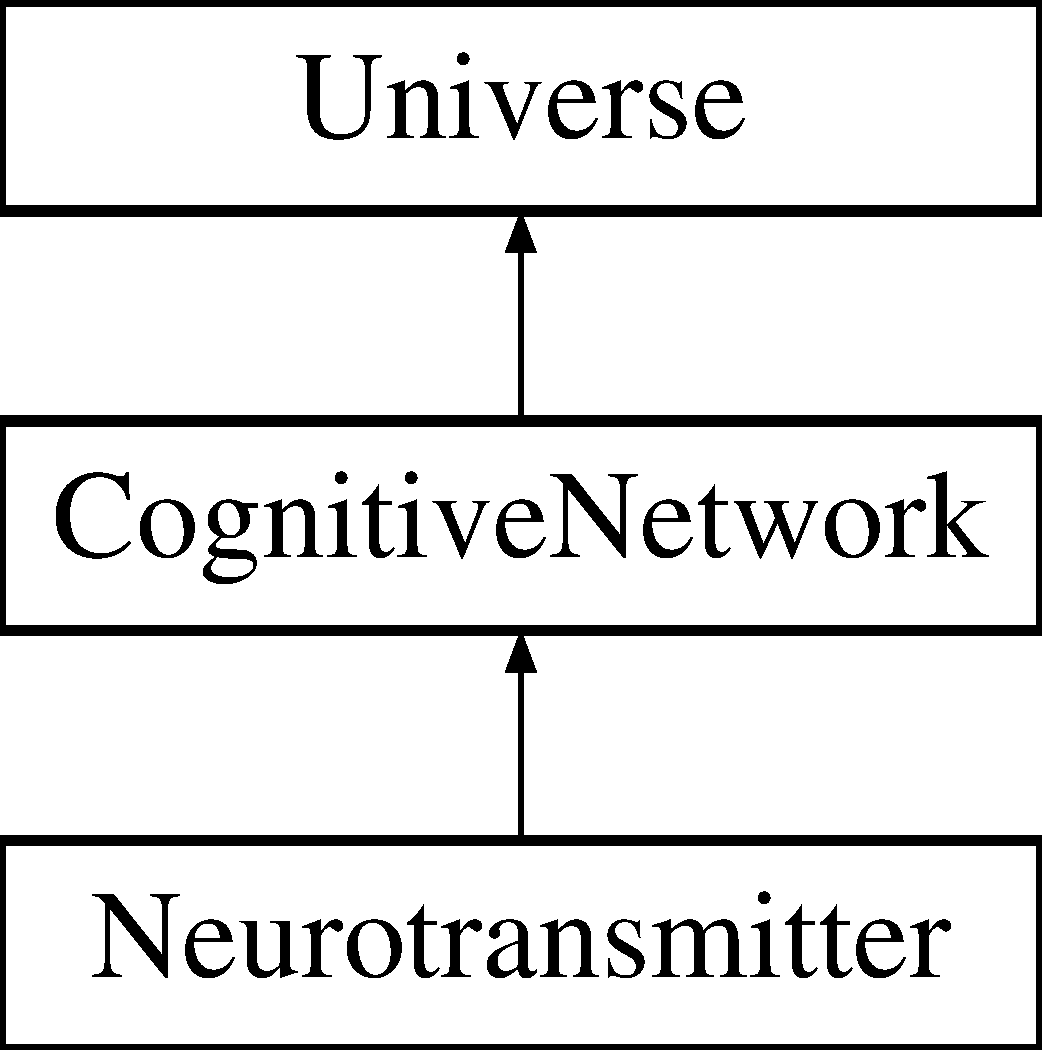
\includegraphics[height=3.000000cm]{classNeurotransmitter}
\end{center}
\end{figure}
\subsection*{Public Member Functions}
\begin{DoxyCompactItemize}
\item 
\mbox{\hyperlink{classNeurotransmitter_a05883c62f2c20b8034121a46c50de00f}{Neurotransmitter}} ()
\item 
\mbox{\hyperlink{classNeurotransmitter_adca6f02b1a9c98d269e3909e1e2f0463}{Neurotransmitter}} (unsigned int object\+\_\+type)
\item 
\mbox{\hyperlink{classNeurotransmitter_ac1c768a2769536a8a16569ae0dde1671}{Neurotransmitter}} (unsigned int object\+\_\+type, std\+::chrono\+::time\+\_\+point$<$ \mbox{\hyperlink{universe_8h_a0ef8d951d1ca5ab3cfaf7ab4c7a6fd80}{Clock}} $>$ event\+\_\+time)
\item 
\mbox{\hyperlink{classNeurotransmitter_ac9257a1b310a26eba8a08ffb4b93bb64}{Neurotransmitter}} (unsigned int object\+\_\+type, std\+::chrono\+::time\+\_\+point$<$ \mbox{\hyperlink{universe_8h_a0ef8d951d1ca5ab3cfaf7ab4c7a6fd80}{Clock}} $>$ event\+\_\+time, \mbox{\hyperlink{classCognitiveNetwork}{Cognitive\+Network}} \&cognitivenetwork\+\_\+connector)
\item 
virtual \mbox{\hyperlink{classNeurotransmitter_a0ea63f67dc5a49d485b7a7034a8f7968}{$\sim$\+Neurotransmitter}} ()
\item 
unsigned int \mbox{\hyperlink{classNeurotransmitter_a94b3d1909cdd787f0583e28e1e9b58dd}{Get\+Counter}} (std\+::chrono\+::time\+\_\+point$<$ \mbox{\hyperlink{universe_8h_a0ef8d951d1ca5ab3cfaf7ab4c7a6fd80}{Clock}} $>$ event\+\_\+time)
\item 
double \mbox{\hyperlink{classNeurotransmitter_a1e3e8134ea935f617b0afd2f7b5b5799}{Get\+Energy}} (std\+::chrono\+::time\+\_\+point$<$ \mbox{\hyperlink{universe_8h_a0ef8d951d1ca5ab3cfaf7ab4c7a6fd80}{Clock}} $>$ event\+\_\+time)
\item 
int \mbox{\hyperlink{classNeurotransmitter_a45414c0d173758edbbf9318a7eccb623}{Get\+Type}} (std\+::chrono\+::time\+\_\+point$<$ \mbox{\hyperlink{universe_8h_a0ef8d951d1ca5ab3cfaf7ab4c7a6fd80}{Clock}} $>$ event\+\_\+time)
\item 
void \mbox{\hyperlink{classNeurotransmitter_ae460ed5fac92ba136a80bba12ebce246}{Set\+Type}} (std\+::chrono\+::time\+\_\+point$<$ \mbox{\hyperlink{universe_8h_a0ef8d951d1ca5ab3cfaf7ab4c7a6fd80}{Clock}} $>$ event\+\_\+time, int val)
\item 
void \mbox{\hyperlink{classNeurotransmitter_ae16ec051609867d4f64fad5ba4449443}{Set\+Counter}} (std\+::chrono\+::time\+\_\+point$<$ \mbox{\hyperlink{universe_8h_a0ef8d951d1ca5ab3cfaf7ab4c7a6fd80}{Clock}} $>$ event\+\_\+time, unsigned int val)
\item 
void \mbox{\hyperlink{classNeurotransmitter_a5ad51ddb1351868e1756e3c41bb88e04}{Set\+Energy}} (std\+::chrono\+::time\+\_\+point$<$ \mbox{\hyperlink{universe_8h_a0ef8d951d1ca5ab3cfaf7ab4c7a6fd80}{Clock}} $>$ event\+\_\+time, double val)
\item 
bool \mbox{\hyperlink{classNeurotransmitter_a6e7650d738bccfbbd49ede10970687aa}{Reset\+Parameters}} (std\+::chrono\+::time\+\_\+point$<$ \mbox{\hyperlink{universe_8h_a0ef8d951d1ca5ab3cfaf7ab4c7a6fd80}{Clock}} $>$ event\+\_\+time)
\item 
int \mbox{\hyperlink{classNeurotransmitter_ac9f7be22ca7242207de76ec5e1b055b1}{Update}} (std\+::chrono\+::time\+\_\+point$<$ \mbox{\hyperlink{universe_8h_a0ef8d951d1ca5ab3cfaf7ab4c7a6fd80}{Clock}} $>$ event\+\_\+time)
\end{DoxyCompactItemize}
\subsection*{Private Attributes}
\begin{DoxyCompactItemize}
\item 
int \mbox{\hyperlink{classNeurotransmitter_aaabafa90f31a1afd660c654d6066820b}{m\+\_\+\+Neurotransmitter\+Type}}
\item 
int \mbox{\hyperlink{classNeurotransmitter_a53484821d08c351a07ea9774d09434b1}{neurotransmitter\+\_\+type}} = 0
\item 
int \mbox{\hyperlink{classNeurotransmitter_ac15c7d29a34d8b8a75de5d851c3b5e73}{m\+\_\+add\+Status}}
\item 
std\+::chrono\+::time\+\_\+point$<$ \mbox{\hyperlink{universe_8h_a0ef8d951d1ca5ab3cfaf7ab4c7a6fd80}{Clock}} $>$ \mbox{\hyperlink{classNeurotransmitter_acad5444f7486ee9c2d3bff1b6b3f59ad}{time\+\_\+object\+\_\+created}} = std\+::chrono\+::time\+\_\+point$<$\mbox{\hyperlink{universe_8h_a0ef8d951d1ca5ab3cfaf7ab4c7a6fd80}{Clock}}$>$(std\+::chrono\+::nanoseconds\+::zero())
\item 
std\+::chrono\+::time\+\_\+point$<$ \mbox{\hyperlink{universe_8h_a0ef8d951d1ca5ab3cfaf7ab4c7a6fd80}{Clock}} $>$ \mbox{\hyperlink{classNeurotransmitter_a47efa9a5481fae796df7f1020a15e2f2}{previous\+\_\+event\+\_\+time}}
\item 
bool \mbox{\hyperlink{classNeurotransmitter_a27175b3f5400e9d341291b11828ea32e}{object\+\_\+disabled}} = true
\item 
bool \mbox{\hyperlink{classNeurotransmitter_ab5e0c93e6f54bec95c294bc59427a54a}{object\+\_\+initialised}} = false
\item 
int \mbox{\hyperlink{classNeurotransmitter_acbf1efa25f5b69954d9baaacf273e8da}{duration\+\_\+since\+\_\+last\+\_\+event}}
\item 
double \mbox{\hyperlink{classNeurotransmitter_a82764f72535f859b74d419bad922253a}{m\+\_\+\+Volume}}
\item 
double \mbox{\hyperlink{classNeurotransmitter_ae1dea2e0732f91027f4597a6ca4588fc}{m\+\_\+\+Surface\+Area}}
\item 
double \mbox{\hyperlink{classNeurotransmitter_afed70401d85814b609c569a9c79f6a16}{object\+\_\+size}}
\item 
unsigned int \mbox{\hyperlink{classNeurotransmitter_a39531872ba361395e620745e28bdc8d4}{m\+\_\+\+Counter}}
\begin{DoxyCompactList}\small\item\em Member variable \char`\"{}m\+\_\+\+Counter\char`\"{}. \end{DoxyCompactList}\item 
double \mbox{\hyperlink{classNeurotransmitter_a3cc474a0f16ffe26d7f4403551cce222}{object\+\_\+energy}}
\begin{DoxyCompactList}\small\item\em Member variable \char`\"{}object\+\_\+energy\char`\"{}. \end{DoxyCompactList}\item 
double \mbox{\hyperlink{classNeurotransmitter_aa3e998b3dfc01ec3c0b02080ffeb0d46}{object\+\_\+energy\+\_\+threshold}}
\item 
double \mbox{\hyperlink{classNeurotransmitter_ae04cfd2ef2be895457c293463e8ba24f}{m\+\_\+\+Time\+Dilation}}
\item 
double \mbox{\hyperlink{classNeurotransmitter_a27b12315e40389dfd903c5e9cd188768}{m\+\_\+\+Time\+Threshold}}
\end{DoxyCompactItemize}
\subsection*{Additional Inherited Members}


\subsection{Constructor \& Destructor Documentation}
\mbox{\Hypertarget{classNeurotransmitter_a05883c62f2c20b8034121a46c50de00f}\label{classNeurotransmitter_a05883c62f2c20b8034121a46c50de00f}} 
\index{Neurotransmitter@{Neurotransmitter}!Neurotransmitter@{Neurotransmitter}}
\index{Neurotransmitter@{Neurotransmitter}!Neurotransmitter@{Neurotransmitter}}
\subsubsection{\texorpdfstring{Neurotransmitter()}{Neurotransmitter()}\hspace{0.1cm}{\footnotesize\ttfamily [1/4]}}
{\footnotesize\ttfamily Neurotransmitter\+::\+Neurotransmitter (\begin{DoxyParamCaption}{ }\end{DoxyParamCaption})\hspace{0.3cm}{\ttfamily [inline]}}

\mbox{\Hypertarget{classNeurotransmitter_adca6f02b1a9c98d269e3909e1e2f0463}\label{classNeurotransmitter_adca6f02b1a9c98d269e3909e1e2f0463}} 
\index{Neurotransmitter@{Neurotransmitter}!Neurotransmitter@{Neurotransmitter}}
\index{Neurotransmitter@{Neurotransmitter}!Neurotransmitter@{Neurotransmitter}}
\subsubsection{\texorpdfstring{Neurotransmitter()}{Neurotransmitter()}\hspace{0.1cm}{\footnotesize\ttfamily [2/4]}}
{\footnotesize\ttfamily Neurotransmitter\+::\+Neurotransmitter (\begin{DoxyParamCaption}\item[{unsigned int}]{object\+\_\+type }\end{DoxyParamCaption})\hspace{0.3cm}{\ttfamily [inline]}}

\mbox{\Hypertarget{classNeurotransmitter_ac1c768a2769536a8a16569ae0dde1671}\label{classNeurotransmitter_ac1c768a2769536a8a16569ae0dde1671}} 
\index{Neurotransmitter@{Neurotransmitter}!Neurotransmitter@{Neurotransmitter}}
\index{Neurotransmitter@{Neurotransmitter}!Neurotransmitter@{Neurotransmitter}}
\subsubsection{\texorpdfstring{Neurotransmitter()}{Neurotransmitter()}\hspace{0.1cm}{\footnotesize\ttfamily [3/4]}}
{\footnotesize\ttfamily Neurotransmitter\+::\+Neurotransmitter (\begin{DoxyParamCaption}\item[{unsigned int}]{object\+\_\+type,  }\item[{std\+::chrono\+::time\+\_\+point$<$ \mbox{\hyperlink{universe_8h_a0ef8d951d1ca5ab3cfaf7ab4c7a6fd80}{Clock}} $>$}]{event\+\_\+time }\end{DoxyParamCaption})\hspace{0.3cm}{\ttfamily [inline]}}

\mbox{\Hypertarget{classNeurotransmitter_ac9257a1b310a26eba8a08ffb4b93bb64}\label{classNeurotransmitter_ac9257a1b310a26eba8a08ffb4b93bb64}} 
\index{Neurotransmitter@{Neurotransmitter}!Neurotransmitter@{Neurotransmitter}}
\index{Neurotransmitter@{Neurotransmitter}!Neurotransmitter@{Neurotransmitter}}
\subsubsection{\texorpdfstring{Neurotransmitter()}{Neurotransmitter()}\hspace{0.1cm}{\footnotesize\ttfamily [4/4]}}
{\footnotesize\ttfamily Neurotransmitter\+::\+Neurotransmitter (\begin{DoxyParamCaption}\item[{unsigned int}]{object\+\_\+type,  }\item[{std\+::chrono\+::time\+\_\+point$<$ \mbox{\hyperlink{universe_8h_a0ef8d951d1ca5ab3cfaf7ab4c7a6fd80}{Clock}} $>$}]{event\+\_\+time,  }\item[{\mbox{\hyperlink{classCognitiveNetwork}{Cognitive\+Network}} \&}]{cognitivenetwork\+\_\+connector }\end{DoxyParamCaption})\hspace{0.3cm}{\ttfamily [inline]}}

\mbox{\Hypertarget{classNeurotransmitter_a0ea63f67dc5a49d485b7a7034a8f7968}\label{classNeurotransmitter_a0ea63f67dc5a49d485b7a7034a8f7968}} 
\index{Neurotransmitter@{Neurotransmitter}!````~Neurotransmitter@{$\sim$\+Neurotransmitter}}
\index{````~Neurotransmitter@{$\sim$\+Neurotransmitter}!Neurotransmitter@{Neurotransmitter}}
\subsubsection{\texorpdfstring{$\sim$\+Neurotransmitter()}{~Neurotransmitter()}}
{\footnotesize\ttfamily virtual Neurotransmitter\+::$\sim$\+Neurotransmitter (\begin{DoxyParamCaption}{ }\end{DoxyParamCaption})\hspace{0.3cm}{\ttfamily [inline]}, {\ttfamily [virtual]}}

Default destructor 

\subsection{Member Function Documentation}
\mbox{\Hypertarget{classNeurotransmitter_a94b3d1909cdd787f0583e28e1e9b58dd}\label{classNeurotransmitter_a94b3d1909cdd787f0583e28e1e9b58dd}} 
\index{Neurotransmitter@{Neurotransmitter}!Get\+Counter@{Get\+Counter}}
\index{Get\+Counter@{Get\+Counter}!Neurotransmitter@{Neurotransmitter}}
\subsubsection{\texorpdfstring{Get\+Counter()}{GetCounter()}}
{\footnotesize\ttfamily unsigned int Neurotransmitter\+::\+Get\+Counter (\begin{DoxyParamCaption}\item[{std\+::chrono\+::time\+\_\+point$<$ \mbox{\hyperlink{universe_8h_a0ef8d951d1ca5ab3cfaf7ab4c7a6fd80}{Clock}} $>$}]{event\+\_\+time }\end{DoxyParamCaption})\hspace{0.3cm}{\ttfamily [inline]}}

\mbox{\Hypertarget{classNeurotransmitter_a1e3e8134ea935f617b0afd2f7b5b5799}\label{classNeurotransmitter_a1e3e8134ea935f617b0afd2f7b5b5799}} 
\index{Neurotransmitter@{Neurotransmitter}!Get\+Energy@{Get\+Energy}}
\index{Get\+Energy@{Get\+Energy}!Neurotransmitter@{Neurotransmitter}}
\subsubsection{\texorpdfstring{Get\+Energy()}{GetEnergy()}}
{\footnotesize\ttfamily double Neurotransmitter\+::\+Get\+Energy (\begin{DoxyParamCaption}\item[{std\+::chrono\+::time\+\_\+point$<$ \mbox{\hyperlink{universe_8h_a0ef8d951d1ca5ab3cfaf7ab4c7a6fd80}{Clock}} $>$}]{event\+\_\+time }\end{DoxyParamCaption})\hspace{0.3cm}{\ttfamily [inline]}}

\mbox{\Hypertarget{classNeurotransmitter_a45414c0d173758edbbf9318a7eccb623}\label{classNeurotransmitter_a45414c0d173758edbbf9318a7eccb623}} 
\index{Neurotransmitter@{Neurotransmitter}!Get\+Type@{Get\+Type}}
\index{Get\+Type@{Get\+Type}!Neurotransmitter@{Neurotransmitter}}
\subsubsection{\texorpdfstring{Get\+Type()}{GetType()}}
{\footnotesize\ttfamily int Neurotransmitter\+::\+Get\+Type (\begin{DoxyParamCaption}\item[{std\+::chrono\+::time\+\_\+point$<$ \mbox{\hyperlink{universe_8h_a0ef8d951d1ca5ab3cfaf7ab4c7a6fd80}{Clock}} $>$}]{event\+\_\+time }\end{DoxyParamCaption})\hspace{0.3cm}{\ttfamily [inline]}}

\mbox{\Hypertarget{classNeurotransmitter_a6e7650d738bccfbbd49ede10970687aa}\label{classNeurotransmitter_a6e7650d738bccfbbd49ede10970687aa}} 
\index{Neurotransmitter@{Neurotransmitter}!Reset\+Parameters@{Reset\+Parameters}}
\index{Reset\+Parameters@{Reset\+Parameters}!Neurotransmitter@{Neurotransmitter}}
\subsubsection{\texorpdfstring{Reset\+Parameters()}{ResetParameters()}}
{\footnotesize\ttfamily bool Neurotransmitter\+::\+Reset\+Parameters (\begin{DoxyParamCaption}\item[{std\+::chrono\+::time\+\_\+point$<$ \mbox{\hyperlink{universe_8h_a0ef8d951d1ca5ab3cfaf7ab4c7a6fd80}{Clock}} $>$}]{event\+\_\+time }\end{DoxyParamCaption})}

\mbox{\Hypertarget{classNeurotransmitter_ae16ec051609867d4f64fad5ba4449443}\label{classNeurotransmitter_ae16ec051609867d4f64fad5ba4449443}} 
\index{Neurotransmitter@{Neurotransmitter}!Set\+Counter@{Set\+Counter}}
\index{Set\+Counter@{Set\+Counter}!Neurotransmitter@{Neurotransmitter}}
\subsubsection{\texorpdfstring{Set\+Counter()}{SetCounter()}}
{\footnotesize\ttfamily void Neurotransmitter\+::\+Set\+Counter (\begin{DoxyParamCaption}\item[{std\+::chrono\+::time\+\_\+point$<$ \mbox{\hyperlink{universe_8h_a0ef8d951d1ca5ab3cfaf7ab4c7a6fd80}{Clock}} $>$}]{event\+\_\+time,  }\item[{unsigned int}]{val }\end{DoxyParamCaption})\hspace{0.3cm}{\ttfamily [inline]}, {\ttfamily [virtual]}}



Reimplemented from \mbox{\hyperlink{classUniverse_aa22202ae740eb1355529afcb13285e91}{Universe}}.

\mbox{\Hypertarget{classNeurotransmitter_a5ad51ddb1351868e1756e3c41bb88e04}\label{classNeurotransmitter_a5ad51ddb1351868e1756e3c41bb88e04}} 
\index{Neurotransmitter@{Neurotransmitter}!Set\+Energy@{Set\+Energy}}
\index{Set\+Energy@{Set\+Energy}!Neurotransmitter@{Neurotransmitter}}
\subsubsection{\texorpdfstring{Set\+Energy()}{SetEnergy()}}
{\footnotesize\ttfamily void Neurotransmitter\+::\+Set\+Energy (\begin{DoxyParamCaption}\item[{std\+::chrono\+::time\+\_\+point$<$ \mbox{\hyperlink{universe_8h_a0ef8d951d1ca5ab3cfaf7ab4c7a6fd80}{Clock}} $>$}]{event\+\_\+time,  }\item[{double}]{val }\end{DoxyParamCaption})\hspace{0.3cm}{\ttfamily [inline]}}

\mbox{\Hypertarget{classNeurotransmitter_ae460ed5fac92ba136a80bba12ebce246}\label{classNeurotransmitter_ae460ed5fac92ba136a80bba12ebce246}} 
\index{Neurotransmitter@{Neurotransmitter}!Set\+Type@{Set\+Type}}
\index{Set\+Type@{Set\+Type}!Neurotransmitter@{Neurotransmitter}}
\subsubsection{\texorpdfstring{Set\+Type()}{SetType()}}
{\footnotesize\ttfamily void Neurotransmitter\+::\+Set\+Type (\begin{DoxyParamCaption}\item[{std\+::chrono\+::time\+\_\+point$<$ \mbox{\hyperlink{universe_8h_a0ef8d951d1ca5ab3cfaf7ab4c7a6fd80}{Clock}} $>$}]{event\+\_\+time,  }\item[{int}]{val }\end{DoxyParamCaption})\hspace{0.3cm}{\ttfamily [inline]}}

\mbox{\Hypertarget{classNeurotransmitter_ac9f7be22ca7242207de76ec5e1b055b1}\label{classNeurotransmitter_ac9f7be22ca7242207de76ec5e1b055b1}} 
\index{Neurotransmitter@{Neurotransmitter}!Update@{Update}}
\index{Update@{Update}!Neurotransmitter@{Neurotransmitter}}
\subsubsection{\texorpdfstring{Update()}{Update()}}
{\footnotesize\ttfamily int Neurotransmitter\+::\+Update (\begin{DoxyParamCaption}\item[{std\+::chrono\+::time\+\_\+point$<$ \mbox{\hyperlink{universe_8h_a0ef8d951d1ca5ab3cfaf7ab4c7a6fd80}{Clock}} $>$}]{event\+\_\+time }\end{DoxyParamCaption})}



\subsection{Member Data Documentation}
\mbox{\Hypertarget{classNeurotransmitter_acbf1efa25f5b69954d9baaacf273e8da}\label{classNeurotransmitter_acbf1efa25f5b69954d9baaacf273e8da}} 
\index{Neurotransmitter@{Neurotransmitter}!duration\+\_\+since\+\_\+last\+\_\+event@{duration\+\_\+since\+\_\+last\+\_\+event}}
\index{duration\+\_\+since\+\_\+last\+\_\+event@{duration\+\_\+since\+\_\+last\+\_\+event}!Neurotransmitter@{Neurotransmitter}}
\subsubsection{\texorpdfstring{duration\+\_\+since\+\_\+last\+\_\+event}{duration\_since\_last\_event}}
{\footnotesize\ttfamily int Neurotransmitter\+::duration\+\_\+since\+\_\+last\+\_\+event\hspace{0.3cm}{\ttfamily [private]}}

\mbox{\Hypertarget{classNeurotransmitter_ac15c7d29a34d8b8a75de5d851c3b5e73}\label{classNeurotransmitter_ac15c7d29a34d8b8a75de5d851c3b5e73}} 
\index{Neurotransmitter@{Neurotransmitter}!m\+\_\+add\+Status@{m\+\_\+add\+Status}}
\index{m\+\_\+add\+Status@{m\+\_\+add\+Status}!Neurotransmitter@{Neurotransmitter}}
\subsubsection{\texorpdfstring{m\+\_\+add\+Status}{m\_addStatus}}
{\footnotesize\ttfamily int Neurotransmitter\+::m\+\_\+add\+Status\hspace{0.3cm}{\ttfamily [private]}}

\mbox{\Hypertarget{classNeurotransmitter_a39531872ba361395e620745e28bdc8d4}\label{classNeurotransmitter_a39531872ba361395e620745e28bdc8d4}} 
\index{Neurotransmitter@{Neurotransmitter}!m\+\_\+\+Counter@{m\+\_\+\+Counter}}
\index{m\+\_\+\+Counter@{m\+\_\+\+Counter}!Neurotransmitter@{Neurotransmitter}}
\subsubsection{\texorpdfstring{m\+\_\+\+Counter}{m\_Counter}}
{\footnotesize\ttfamily unsigned int Neurotransmitter\+::m\+\_\+\+Counter\hspace{0.3cm}{\ttfamily [private]}}



Member variable \char`\"{}m\+\_\+\+Counter\char`\"{}. 

\mbox{\Hypertarget{classNeurotransmitter_aaabafa90f31a1afd660c654d6066820b}\label{classNeurotransmitter_aaabafa90f31a1afd660c654d6066820b}} 
\index{Neurotransmitter@{Neurotransmitter}!m\+\_\+\+Neurotransmitter\+Type@{m\+\_\+\+Neurotransmitter\+Type}}
\index{m\+\_\+\+Neurotransmitter\+Type@{m\+\_\+\+Neurotransmitter\+Type}!Neurotransmitter@{Neurotransmitter}}
\subsubsection{\texorpdfstring{m\+\_\+\+Neurotransmitter\+Type}{m\_NeurotransmitterType}}
{\footnotesize\ttfamily int Neurotransmitter\+::m\+\_\+\+Neurotransmitter\+Type\hspace{0.3cm}{\ttfamily [private]}}

\mbox{\Hypertarget{classNeurotransmitter_ae1dea2e0732f91027f4597a6ca4588fc}\label{classNeurotransmitter_ae1dea2e0732f91027f4597a6ca4588fc}} 
\index{Neurotransmitter@{Neurotransmitter}!m\+\_\+\+Surface\+Area@{m\+\_\+\+Surface\+Area}}
\index{m\+\_\+\+Surface\+Area@{m\+\_\+\+Surface\+Area}!Neurotransmitter@{Neurotransmitter}}
\subsubsection{\texorpdfstring{m\+\_\+\+Surface\+Area}{m\_SurfaceArea}}
{\footnotesize\ttfamily double Neurotransmitter\+::m\+\_\+\+Surface\+Area\hspace{0.3cm}{\ttfamily [private]}}

\mbox{\Hypertarget{classNeurotransmitter_ae04cfd2ef2be895457c293463e8ba24f}\label{classNeurotransmitter_ae04cfd2ef2be895457c293463e8ba24f}} 
\index{Neurotransmitter@{Neurotransmitter}!m\+\_\+\+Time\+Dilation@{m\+\_\+\+Time\+Dilation}}
\index{m\+\_\+\+Time\+Dilation@{m\+\_\+\+Time\+Dilation}!Neurotransmitter@{Neurotransmitter}}
\subsubsection{\texorpdfstring{m\+\_\+\+Time\+Dilation}{m\_TimeDilation}}
{\footnotesize\ttfamily double Neurotransmitter\+::m\+\_\+\+Time\+Dilation\hspace{0.3cm}{\ttfamily [private]}}

\mbox{\Hypertarget{classNeurotransmitter_a27b12315e40389dfd903c5e9cd188768}\label{classNeurotransmitter_a27b12315e40389dfd903c5e9cd188768}} 
\index{Neurotransmitter@{Neurotransmitter}!m\+\_\+\+Time\+Threshold@{m\+\_\+\+Time\+Threshold}}
\index{m\+\_\+\+Time\+Threshold@{m\+\_\+\+Time\+Threshold}!Neurotransmitter@{Neurotransmitter}}
\subsubsection{\texorpdfstring{m\+\_\+\+Time\+Threshold}{m\_TimeThreshold}}
{\footnotesize\ttfamily double Neurotransmitter\+::m\+\_\+\+Time\+Threshold\hspace{0.3cm}{\ttfamily [private]}}

\mbox{\Hypertarget{classNeurotransmitter_a82764f72535f859b74d419bad922253a}\label{classNeurotransmitter_a82764f72535f859b74d419bad922253a}} 
\index{Neurotransmitter@{Neurotransmitter}!m\+\_\+\+Volume@{m\+\_\+\+Volume}}
\index{m\+\_\+\+Volume@{m\+\_\+\+Volume}!Neurotransmitter@{Neurotransmitter}}
\subsubsection{\texorpdfstring{m\+\_\+\+Volume}{m\_Volume}}
{\footnotesize\ttfamily double Neurotransmitter\+::m\+\_\+\+Volume\hspace{0.3cm}{\ttfamily [private]}}

\mbox{\Hypertarget{classNeurotransmitter_a53484821d08c351a07ea9774d09434b1}\label{classNeurotransmitter_a53484821d08c351a07ea9774d09434b1}} 
\index{Neurotransmitter@{Neurotransmitter}!neurotransmitter\+\_\+type@{neurotransmitter\+\_\+type}}
\index{neurotransmitter\+\_\+type@{neurotransmitter\+\_\+type}!Neurotransmitter@{Neurotransmitter}}
\subsubsection{\texorpdfstring{neurotransmitter\+\_\+type}{neurotransmitter\_type}}
{\footnotesize\ttfamily int Neurotransmitter\+::neurotransmitter\+\_\+type = 0\hspace{0.3cm}{\ttfamily [private]}}

\mbox{\Hypertarget{classNeurotransmitter_a27175b3f5400e9d341291b11828ea32e}\label{classNeurotransmitter_a27175b3f5400e9d341291b11828ea32e}} 
\index{Neurotransmitter@{Neurotransmitter}!object\+\_\+disabled@{object\+\_\+disabled}}
\index{object\+\_\+disabled@{object\+\_\+disabled}!Neurotransmitter@{Neurotransmitter}}
\subsubsection{\texorpdfstring{object\+\_\+disabled}{object\_disabled}}
{\footnotesize\ttfamily bool Neurotransmitter\+::object\+\_\+disabled = true\hspace{0.3cm}{\ttfamily [private]}}

\mbox{\Hypertarget{classNeurotransmitter_a3cc474a0f16ffe26d7f4403551cce222}\label{classNeurotransmitter_a3cc474a0f16ffe26d7f4403551cce222}} 
\index{Neurotransmitter@{Neurotransmitter}!object\+\_\+energy@{object\+\_\+energy}}
\index{object\+\_\+energy@{object\+\_\+energy}!Neurotransmitter@{Neurotransmitter}}
\subsubsection{\texorpdfstring{object\+\_\+energy}{object\_energy}}
{\footnotesize\ttfamily double Neurotransmitter\+::object\+\_\+energy\hspace{0.3cm}{\ttfamily [private]}}



Member variable \char`\"{}object\+\_\+energy\char`\"{}. 

\mbox{\Hypertarget{classNeurotransmitter_aa3e998b3dfc01ec3c0b02080ffeb0d46}\label{classNeurotransmitter_aa3e998b3dfc01ec3c0b02080ffeb0d46}} 
\index{Neurotransmitter@{Neurotransmitter}!object\+\_\+energy\+\_\+threshold@{object\+\_\+energy\+\_\+threshold}}
\index{object\+\_\+energy\+\_\+threshold@{object\+\_\+energy\+\_\+threshold}!Neurotransmitter@{Neurotransmitter}}
\subsubsection{\texorpdfstring{object\+\_\+energy\+\_\+threshold}{object\_energy\_threshold}}
{\footnotesize\ttfamily double Neurotransmitter\+::object\+\_\+energy\+\_\+threshold\hspace{0.3cm}{\ttfamily [private]}}

\mbox{\Hypertarget{classNeurotransmitter_ab5e0c93e6f54bec95c294bc59427a54a}\label{classNeurotransmitter_ab5e0c93e6f54bec95c294bc59427a54a}} 
\index{Neurotransmitter@{Neurotransmitter}!object\+\_\+initialised@{object\+\_\+initialised}}
\index{object\+\_\+initialised@{object\+\_\+initialised}!Neurotransmitter@{Neurotransmitter}}
\subsubsection{\texorpdfstring{object\+\_\+initialised}{object\_initialised}}
{\footnotesize\ttfamily bool Neurotransmitter\+::object\+\_\+initialised = false\hspace{0.3cm}{\ttfamily [private]}}

\mbox{\Hypertarget{classNeurotransmitter_afed70401d85814b609c569a9c79f6a16}\label{classNeurotransmitter_afed70401d85814b609c569a9c79f6a16}} 
\index{Neurotransmitter@{Neurotransmitter}!object\+\_\+size@{object\+\_\+size}}
\index{object\+\_\+size@{object\+\_\+size}!Neurotransmitter@{Neurotransmitter}}
\subsubsection{\texorpdfstring{object\+\_\+size}{object\_size}}
{\footnotesize\ttfamily double Neurotransmitter\+::object\+\_\+size\hspace{0.3cm}{\ttfamily [private]}}

\mbox{\Hypertarget{classNeurotransmitter_a47efa9a5481fae796df7f1020a15e2f2}\label{classNeurotransmitter_a47efa9a5481fae796df7f1020a15e2f2}} 
\index{Neurotransmitter@{Neurotransmitter}!previous\+\_\+event\+\_\+time@{previous\+\_\+event\+\_\+time}}
\index{previous\+\_\+event\+\_\+time@{previous\+\_\+event\+\_\+time}!Neurotransmitter@{Neurotransmitter}}
\subsubsection{\texorpdfstring{previous\+\_\+event\+\_\+time}{previous\_event\_time}}
{\footnotesize\ttfamily std\+::chrono\+::time\+\_\+point$<$\mbox{\hyperlink{universe_8h_a0ef8d951d1ca5ab3cfaf7ab4c7a6fd80}{Clock}}$>$ Neurotransmitter\+::previous\+\_\+event\+\_\+time\hspace{0.3cm}{\ttfamily [private]}}

\mbox{\Hypertarget{classNeurotransmitter_acad5444f7486ee9c2d3bff1b6b3f59ad}\label{classNeurotransmitter_acad5444f7486ee9c2d3bff1b6b3f59ad}} 
\index{Neurotransmitter@{Neurotransmitter}!time\+\_\+object\+\_\+created@{time\+\_\+object\+\_\+created}}
\index{time\+\_\+object\+\_\+created@{time\+\_\+object\+\_\+created}!Neurotransmitter@{Neurotransmitter}}
\subsubsection{\texorpdfstring{time\+\_\+object\+\_\+created}{time\_object\_created}}
{\footnotesize\ttfamily std\+::chrono\+::time\+\_\+point$<$\mbox{\hyperlink{universe_8h_a0ef8d951d1ca5ab3cfaf7ab4c7a6fd80}{Clock}}$>$ Neurotransmitter\+::time\+\_\+object\+\_\+created = std\+::chrono\+::time\+\_\+point$<$\mbox{\hyperlink{universe_8h_a0ef8d951d1ca5ab3cfaf7ab4c7a6fd80}{Clock}}$>$(std\+::chrono\+::nanoseconds\+::zero())\hspace{0.3cm}{\ttfamily [private]}}



The documentation for this class was generated from the following files\+:\begin{DoxyCompactItemize}
\item 
/home/pbisaacs/\+Developer/\+Brain\+Harmonics/\+Brain\+Harmonics/\mbox{\hyperlink{neurotransmitter_8h}{neurotransmitter.\+h}}\item 
/home/pbisaacs/\+Developer/\+Brain\+Harmonics/\+Brain\+Harmonics/\mbox{\hyperlink{neurotransmitter_8cc}{neurotransmitter.\+cc}}\end{DoxyCompactItemize}

\hypertarget{classnode}{}\section{node Class Reference}
\label{classnode}\index{node@{node}}


{\ttfamily \#include $<$node.\+h$>$}

\subsection*{Public Member Functions}
\begin{DoxyCompactItemize}
\item 
\hyperlink{classnode_a802701cab6639590de6f16136184c2de}{node} (int xp, int yp, int d, int p)
\item 
\hyperlink{classnode_a482f83436a89f09d289b26144d817adf}{$\sim$node} ()
\item 
int \hyperlink{classnode_a32e22b8a1fb6be6efa7348cc848600cf}{Getx\+Pos} () const
\item 
int \hyperlink{classnode_a0d644ed02899013bdc6e222afefb4c25}{Gety\+Pos} () const
\item 
int \hyperlink{classnode_a8f168b85b9bdf0a837f5070e5af6f009}{Get\+Level} () const
\item 
int \hyperlink{classnode_afa8c64a3cf2d61348b69b7e68233aa8d}{Get\+Priority} () const
\item 
void \hyperlink{classnode_ad51b92de008bd5107a7b55cc61fc497b}{update\+Priority} (const int \&x\+Dest, const int \&y\+Dest)
\item 
void \hyperlink{classnode_a04a186013c42fb942b6da90d2e98d4ed}{next\+Level} (const int \&i)
\item 
const int \& \hyperlink{classnode_acd0a1c2330a9984fa120fe7a6f169680}{estimate} (const int \&x\+Dest, const int \&y\+Dest) const
\end{DoxyCompactItemize}


\subsection{Detailed Description}


Definition at line 14 of file node.\+h.



\subsection{Constructor \& Destructor Documentation}
\mbox{\Hypertarget{classnode_a802701cab6639590de6f16136184c2de}\label{classnode_a802701cab6639590de6f16136184c2de}} 
\index{node@{node}!node@{node}}
\index{node@{node}!node@{node}}
\subsubsection{\texorpdfstring{node()}{node()}}
{\footnotesize\ttfamily node\+::node (\begin{DoxyParamCaption}\item[{int}]{xp,  }\item[{int}]{yp,  }\item[{int}]{d,  }\item[{int}]{p }\end{DoxyParamCaption})\hspace{0.3cm}{\ttfamily [inline]}}



Definition at line 27 of file node.\+h.

\mbox{\Hypertarget{classnode_a482f83436a89f09d289b26144d817adf}\label{classnode_a482f83436a89f09d289b26144d817adf}} 
\index{node@{node}!````~node@{$\sim$node}}
\index{````~node@{$\sim$node}!node@{node}}
\subsubsection{\texorpdfstring{$\sim$node()}{~node()}}
{\footnotesize\ttfamily node\+::$\sim$node (\begin{DoxyParamCaption}{ }\end{DoxyParamCaption})\hspace{0.3cm}{\ttfamily [inline]}}



Definition at line 28 of file node.\+h.



\subsection{Member Function Documentation}
\mbox{\Hypertarget{classnode_acd0a1c2330a9984fa120fe7a6f169680}\label{classnode_acd0a1c2330a9984fa120fe7a6f169680}} 
\index{node@{node}!estimate@{estimate}}
\index{estimate@{estimate}!node@{node}}
\subsubsection{\texorpdfstring{estimate()}{estimate()}}
{\footnotesize\ttfamily const int\& node\+::estimate (\begin{DoxyParamCaption}\item[{const int \&}]{x\+Dest,  }\item[{const int \&}]{y\+Dest }\end{DoxyParamCaption}) const\hspace{0.3cm}{\ttfamily [inline]}}



Definition at line 46 of file node.\+h.

Here is the caller graph for this function\+:\nopagebreak
\begin{figure}[H]
\begin{center}
\leavevmode
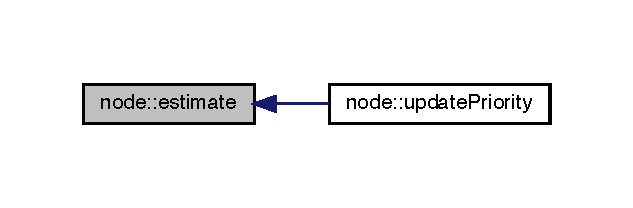
\includegraphics[width=304pt]{classnode_acd0a1c2330a9984fa120fe7a6f169680_icgraph}
\end{center}
\end{figure}
\mbox{\Hypertarget{classnode_a8f168b85b9bdf0a837f5070e5af6f009}\label{classnode_a8f168b85b9bdf0a837f5070e5af6f009}} 
\index{node@{node}!Get\+Level@{Get\+Level}}
\index{Get\+Level@{Get\+Level}!node@{node}}
\subsubsection{\texorpdfstring{Get\+Level()}{GetLevel()}}
{\footnotesize\ttfamily int node\+::\+Get\+Level (\begin{DoxyParamCaption}{ }\end{DoxyParamCaption}) const\hspace{0.3cm}{\ttfamily [inline]}}



Definition at line 31 of file node.\+h.

\mbox{\Hypertarget{classnode_afa8c64a3cf2d61348b69b7e68233aa8d}\label{classnode_afa8c64a3cf2d61348b69b7e68233aa8d}} 
\index{node@{node}!Get\+Priority@{Get\+Priority}}
\index{Get\+Priority@{Get\+Priority}!node@{node}}
\subsubsection{\texorpdfstring{Get\+Priority()}{GetPriority()}}
{\footnotesize\ttfamily int node\+::\+Get\+Priority (\begin{DoxyParamCaption}{ }\end{DoxyParamCaption}) const\hspace{0.3cm}{\ttfamily [inline]}}



Definition at line 32 of file node.\+h.

\mbox{\Hypertarget{classnode_a32e22b8a1fb6be6efa7348cc848600cf}\label{classnode_a32e22b8a1fb6be6efa7348cc848600cf}} 
\index{node@{node}!Getx\+Pos@{Getx\+Pos}}
\index{Getx\+Pos@{Getx\+Pos}!node@{node}}
\subsubsection{\texorpdfstring{Getx\+Pos()}{GetxPos()}}
{\footnotesize\ttfamily int node\+::\+Getx\+Pos (\begin{DoxyParamCaption}{ }\end{DoxyParamCaption}) const\hspace{0.3cm}{\ttfamily [inline]}}



Definition at line 29 of file node.\+h.

\mbox{\Hypertarget{classnode_a0d644ed02899013bdc6e222afefb4c25}\label{classnode_a0d644ed02899013bdc6e222afefb4c25}} 
\index{node@{node}!Gety\+Pos@{Gety\+Pos}}
\index{Gety\+Pos@{Gety\+Pos}!node@{node}}
\subsubsection{\texorpdfstring{Gety\+Pos()}{GetyPos()}}
{\footnotesize\ttfamily int node\+::\+Gety\+Pos (\begin{DoxyParamCaption}{ }\end{DoxyParamCaption}) const\hspace{0.3cm}{\ttfamily [inline]}}



Definition at line 30 of file node.\+h.

\mbox{\Hypertarget{classnode_a04a186013c42fb942b6da90d2e98d4ed}\label{classnode_a04a186013c42fb942b6da90d2e98d4ed}} 
\index{node@{node}!next\+Level@{next\+Level}}
\index{next\+Level@{next\+Level}!node@{node}}
\subsubsection{\texorpdfstring{next\+Level()}{nextLevel()}}
{\footnotesize\ttfamily void node\+::next\+Level (\begin{DoxyParamCaption}\item[{const int \&}]{i }\end{DoxyParamCaption})\hspace{0.3cm}{\ttfamily [inline]}}



Definition at line 40 of file node.\+h.

\mbox{\Hypertarget{classnode_ad51b92de008bd5107a7b55cc61fc497b}\label{classnode_ad51b92de008bd5107a7b55cc61fc497b}} 
\index{node@{node}!update\+Priority@{update\+Priority}}
\index{update\+Priority@{update\+Priority}!node@{node}}
\subsubsection{\texorpdfstring{update\+Priority()}{updatePriority()}}
{\footnotesize\ttfamily void node\+::update\+Priority (\begin{DoxyParamCaption}\item[{const int \&}]{x\+Dest,  }\item[{const int \&}]{y\+Dest }\end{DoxyParamCaption})\hspace{0.3cm}{\ttfamily [inline]}}



Definition at line 34 of file node.\+h.

Here is the call graph for this function\+:\nopagebreak
\begin{figure}[H]
\begin{center}
\leavevmode
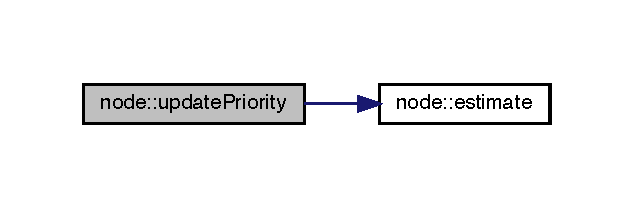
\includegraphics[width=304pt]{classnode_ad51b92de008bd5107a7b55cc61fc497b_cgraph}
\end{center}
\end{figure}


The documentation for this class was generated from the following file\+:\begin{DoxyCompactItemize}
\item 
Brain\+Harmonics/\hyperlink{node_8h}{node.\+h}\end{DoxyCompactItemize}

\hypertarget{structNeuron_1_1ObjectConnection}{}\section{Neuron\+:\+:Object\+Connection Struct Reference}
\label{structNeuron_1_1ObjectConnection}\index{Neuron\+::\+Object\+Connection@{Neuron\+::\+Object\+Connection}}


{\ttfamily \#include $<$neuron.\+h$>$}

\subsection*{Public Attributes}
\begin{DoxyCompactItemize}
\item 
int \mbox{\hyperlink{structNeuron_1_1ObjectConnection_a6174f20de091bf9942b14550890f122d}{object\+\_\+one\+\_\+type}}
\item 
int \mbox{\hyperlink{structNeuron_1_1ObjectConnection_af6bdcfe97aee7b1d47788f92fa57a7a8}{object\+\_\+one}}
\item 
int \mbox{\hyperlink{structNeuron_1_1ObjectConnection_a69d9c1f11a36f759b6aef68236b4cd93}{object\+\_\+two\+\_\+type}}
\item 
int \mbox{\hyperlink{structNeuron_1_1ObjectConnection_a457a80615d216a9db5e90159294bed48}{object\+\_\+two}}
\item 
double \mbox{\hyperlink{structNeuron_1_1ObjectConnection_aaad352b3f1e712aff929a8c2fc370ac1}{object\+\_\+connection\+\_\+strength}}
\item 
double \mbox{\hyperlink{structNeuron_1_1ObjectConnection_a52bbd1a5fb20ee3e5e10c36002b4dcba}{object\+\_\+connection\+\_\+modifier}}
\item 
double \mbox{\hyperlink{structNeuron_1_1ObjectConnection_a2dd04a4740d11779423a2ba5e94d8f5e}{object\+\_\+two\+\_\+position}}
\end{DoxyCompactItemize}


\subsection{Member Data Documentation}
\mbox{\Hypertarget{structNeuron_1_1ObjectConnection_a52bbd1a5fb20ee3e5e10c36002b4dcba}\label{structNeuron_1_1ObjectConnection_a52bbd1a5fb20ee3e5e10c36002b4dcba}} 
\index{Neuron\+::\+Object\+Connection@{Neuron\+::\+Object\+Connection}!object\+\_\+connection\+\_\+modifier@{object\+\_\+connection\+\_\+modifier}}
\index{object\+\_\+connection\+\_\+modifier@{object\+\_\+connection\+\_\+modifier}!Neuron\+::\+Object\+Connection@{Neuron\+::\+Object\+Connection}}
\subsubsection{\texorpdfstring{object\+\_\+connection\+\_\+modifier}{object\_connection\_modifier}}
{\footnotesize\ttfamily double Neuron\+::\+Object\+Connection\+::object\+\_\+connection\+\_\+modifier}

\mbox{\Hypertarget{structNeuron_1_1ObjectConnection_aaad352b3f1e712aff929a8c2fc370ac1}\label{structNeuron_1_1ObjectConnection_aaad352b3f1e712aff929a8c2fc370ac1}} 
\index{Neuron\+::\+Object\+Connection@{Neuron\+::\+Object\+Connection}!object\+\_\+connection\+\_\+strength@{object\+\_\+connection\+\_\+strength}}
\index{object\+\_\+connection\+\_\+strength@{object\+\_\+connection\+\_\+strength}!Neuron\+::\+Object\+Connection@{Neuron\+::\+Object\+Connection}}
\subsubsection{\texorpdfstring{object\+\_\+connection\+\_\+strength}{object\_connection\_strength}}
{\footnotesize\ttfamily double Neuron\+::\+Object\+Connection\+::object\+\_\+connection\+\_\+strength}

\mbox{\Hypertarget{structNeuron_1_1ObjectConnection_af6bdcfe97aee7b1d47788f92fa57a7a8}\label{structNeuron_1_1ObjectConnection_af6bdcfe97aee7b1d47788f92fa57a7a8}} 
\index{Neuron\+::\+Object\+Connection@{Neuron\+::\+Object\+Connection}!object\+\_\+one@{object\+\_\+one}}
\index{object\+\_\+one@{object\+\_\+one}!Neuron\+::\+Object\+Connection@{Neuron\+::\+Object\+Connection}}
\subsubsection{\texorpdfstring{object\+\_\+one}{object\_one}}
{\footnotesize\ttfamily int Neuron\+::\+Object\+Connection\+::object\+\_\+one}

\mbox{\Hypertarget{structNeuron_1_1ObjectConnection_a6174f20de091bf9942b14550890f122d}\label{structNeuron_1_1ObjectConnection_a6174f20de091bf9942b14550890f122d}} 
\index{Neuron\+::\+Object\+Connection@{Neuron\+::\+Object\+Connection}!object\+\_\+one\+\_\+type@{object\+\_\+one\+\_\+type}}
\index{object\+\_\+one\+\_\+type@{object\+\_\+one\+\_\+type}!Neuron\+::\+Object\+Connection@{Neuron\+::\+Object\+Connection}}
\subsubsection{\texorpdfstring{object\+\_\+one\+\_\+type}{object\_one\_type}}
{\footnotesize\ttfamily int Neuron\+::\+Object\+Connection\+::object\+\_\+one\+\_\+type}

\mbox{\Hypertarget{structNeuron_1_1ObjectConnection_a457a80615d216a9db5e90159294bed48}\label{structNeuron_1_1ObjectConnection_a457a80615d216a9db5e90159294bed48}} 
\index{Neuron\+::\+Object\+Connection@{Neuron\+::\+Object\+Connection}!object\+\_\+two@{object\+\_\+two}}
\index{object\+\_\+two@{object\+\_\+two}!Neuron\+::\+Object\+Connection@{Neuron\+::\+Object\+Connection}}
\subsubsection{\texorpdfstring{object\+\_\+two}{object\_two}}
{\footnotesize\ttfamily int Neuron\+::\+Object\+Connection\+::object\+\_\+two}

\mbox{\Hypertarget{structNeuron_1_1ObjectConnection_a2dd04a4740d11779423a2ba5e94d8f5e}\label{structNeuron_1_1ObjectConnection_a2dd04a4740d11779423a2ba5e94d8f5e}} 
\index{Neuron\+::\+Object\+Connection@{Neuron\+::\+Object\+Connection}!object\+\_\+two\+\_\+position@{object\+\_\+two\+\_\+position}}
\index{object\+\_\+two\+\_\+position@{object\+\_\+two\+\_\+position}!Neuron\+::\+Object\+Connection@{Neuron\+::\+Object\+Connection}}
\subsubsection{\texorpdfstring{object\+\_\+two\+\_\+position}{object\_two\_position}}
{\footnotesize\ttfamily double Neuron\+::\+Object\+Connection\+::object\+\_\+two\+\_\+position}

\mbox{\Hypertarget{structNeuron_1_1ObjectConnection_a69d9c1f11a36f759b6aef68236b4cd93}\label{structNeuron_1_1ObjectConnection_a69d9c1f11a36f759b6aef68236b4cd93}} 
\index{Neuron\+::\+Object\+Connection@{Neuron\+::\+Object\+Connection}!object\+\_\+two\+\_\+type@{object\+\_\+two\+\_\+type}}
\index{object\+\_\+two\+\_\+type@{object\+\_\+two\+\_\+type}!Neuron\+::\+Object\+Connection@{Neuron\+::\+Object\+Connection}}
\subsubsection{\texorpdfstring{object\+\_\+two\+\_\+type}{object\_two\_type}}
{\footnotesize\ttfamily int Neuron\+::\+Object\+Connection\+::object\+\_\+two\+\_\+type}



The documentation for this struct was generated from the following file\+:\begin{DoxyCompactItemize}
\item 
/home/pbisaacs/\+Developer/\+Brain\+Harmonics/\+Brain\+Harmonics/\mbox{\hyperlink{neuron_8h}{neuron.\+h}}\end{DoxyCompactItemize}

\hypertarget{structSoma_1_1ObjectConnection}{}\section{Soma\+:\+:Object\+Connection Struct Reference}
\label{structSoma_1_1ObjectConnection}\index{Soma\+::\+Object\+Connection@{Soma\+::\+Object\+Connection}}


{\ttfamily \#include $<$soma.\+h$>$}

\subsection*{Public Attributes}
\begin{DoxyCompactItemize}
\item 
int \mbox{\hyperlink{structSoma_1_1ObjectConnection_aa24770c082347464b35203cd65703386}{object\+\_\+one\+\_\+type}}
\item 
int \mbox{\hyperlink{structSoma_1_1ObjectConnection_ab882c137a4c8414c3663e254ccf5c27d}{object\+\_\+one}}
\item 
int \mbox{\hyperlink{structSoma_1_1ObjectConnection_a948d7e2d1db9b33d3fca95f249fb48c7}{object\+\_\+two\+\_\+type}}
\item 
int \mbox{\hyperlink{structSoma_1_1ObjectConnection_a6a16f602b8206114618db99a45c99e6f}{object\+\_\+two}}
\item 
double \mbox{\hyperlink{structSoma_1_1ObjectConnection_aa7973892dc2435b992a657a4c1e29eb3}{object\+\_\+connection\+\_\+strength}}
\item 
double \mbox{\hyperlink{structSoma_1_1ObjectConnection_a55c6abf4a7906ee1ffede53b7fa36aa6}{object\+\_\+connection\+\_\+modifier}}
\item 
double \mbox{\hyperlink{structSoma_1_1ObjectConnection_a00112b17c9f78d05c2d2e684f304ec03}{object\+\_\+two\+\_\+position}}
\end{DoxyCompactItemize}


\subsection{Member Data Documentation}
\mbox{\Hypertarget{structSoma_1_1ObjectConnection_a55c6abf4a7906ee1ffede53b7fa36aa6}\label{structSoma_1_1ObjectConnection_a55c6abf4a7906ee1ffede53b7fa36aa6}} 
\index{Soma\+::\+Object\+Connection@{Soma\+::\+Object\+Connection}!object\+\_\+connection\+\_\+modifier@{object\+\_\+connection\+\_\+modifier}}
\index{object\+\_\+connection\+\_\+modifier@{object\+\_\+connection\+\_\+modifier}!Soma\+::\+Object\+Connection@{Soma\+::\+Object\+Connection}}
\subsubsection{\texorpdfstring{object\+\_\+connection\+\_\+modifier}{object\_connection\_modifier}}
{\footnotesize\ttfamily double Soma\+::\+Object\+Connection\+::object\+\_\+connection\+\_\+modifier}

\mbox{\Hypertarget{structSoma_1_1ObjectConnection_aa7973892dc2435b992a657a4c1e29eb3}\label{structSoma_1_1ObjectConnection_aa7973892dc2435b992a657a4c1e29eb3}} 
\index{Soma\+::\+Object\+Connection@{Soma\+::\+Object\+Connection}!object\+\_\+connection\+\_\+strength@{object\+\_\+connection\+\_\+strength}}
\index{object\+\_\+connection\+\_\+strength@{object\+\_\+connection\+\_\+strength}!Soma\+::\+Object\+Connection@{Soma\+::\+Object\+Connection}}
\subsubsection{\texorpdfstring{object\+\_\+connection\+\_\+strength}{object\_connection\_strength}}
{\footnotesize\ttfamily double Soma\+::\+Object\+Connection\+::object\+\_\+connection\+\_\+strength}

\mbox{\Hypertarget{structSoma_1_1ObjectConnection_ab882c137a4c8414c3663e254ccf5c27d}\label{structSoma_1_1ObjectConnection_ab882c137a4c8414c3663e254ccf5c27d}} 
\index{Soma\+::\+Object\+Connection@{Soma\+::\+Object\+Connection}!object\+\_\+one@{object\+\_\+one}}
\index{object\+\_\+one@{object\+\_\+one}!Soma\+::\+Object\+Connection@{Soma\+::\+Object\+Connection}}
\subsubsection{\texorpdfstring{object\+\_\+one}{object\_one}}
{\footnotesize\ttfamily int Soma\+::\+Object\+Connection\+::object\+\_\+one}

\mbox{\Hypertarget{structSoma_1_1ObjectConnection_aa24770c082347464b35203cd65703386}\label{structSoma_1_1ObjectConnection_aa24770c082347464b35203cd65703386}} 
\index{Soma\+::\+Object\+Connection@{Soma\+::\+Object\+Connection}!object\+\_\+one\+\_\+type@{object\+\_\+one\+\_\+type}}
\index{object\+\_\+one\+\_\+type@{object\+\_\+one\+\_\+type}!Soma\+::\+Object\+Connection@{Soma\+::\+Object\+Connection}}
\subsubsection{\texorpdfstring{object\+\_\+one\+\_\+type}{object\_one\_type}}
{\footnotesize\ttfamily int Soma\+::\+Object\+Connection\+::object\+\_\+one\+\_\+type}

\mbox{\Hypertarget{structSoma_1_1ObjectConnection_a6a16f602b8206114618db99a45c99e6f}\label{structSoma_1_1ObjectConnection_a6a16f602b8206114618db99a45c99e6f}} 
\index{Soma\+::\+Object\+Connection@{Soma\+::\+Object\+Connection}!object\+\_\+two@{object\+\_\+two}}
\index{object\+\_\+two@{object\+\_\+two}!Soma\+::\+Object\+Connection@{Soma\+::\+Object\+Connection}}
\subsubsection{\texorpdfstring{object\+\_\+two}{object\_two}}
{\footnotesize\ttfamily int Soma\+::\+Object\+Connection\+::object\+\_\+two}

\mbox{\Hypertarget{structSoma_1_1ObjectConnection_a00112b17c9f78d05c2d2e684f304ec03}\label{structSoma_1_1ObjectConnection_a00112b17c9f78d05c2d2e684f304ec03}} 
\index{Soma\+::\+Object\+Connection@{Soma\+::\+Object\+Connection}!object\+\_\+two\+\_\+position@{object\+\_\+two\+\_\+position}}
\index{object\+\_\+two\+\_\+position@{object\+\_\+two\+\_\+position}!Soma\+::\+Object\+Connection@{Soma\+::\+Object\+Connection}}
\subsubsection{\texorpdfstring{object\+\_\+two\+\_\+position}{object\_two\_position}}
{\footnotesize\ttfamily double Soma\+::\+Object\+Connection\+::object\+\_\+two\+\_\+position}

\mbox{\Hypertarget{structSoma_1_1ObjectConnection_a948d7e2d1db9b33d3fca95f249fb48c7}\label{structSoma_1_1ObjectConnection_a948d7e2d1db9b33d3fca95f249fb48c7}} 
\index{Soma\+::\+Object\+Connection@{Soma\+::\+Object\+Connection}!object\+\_\+two\+\_\+type@{object\+\_\+two\+\_\+type}}
\index{object\+\_\+two\+\_\+type@{object\+\_\+two\+\_\+type}!Soma\+::\+Object\+Connection@{Soma\+::\+Object\+Connection}}
\subsubsection{\texorpdfstring{object\+\_\+two\+\_\+type}{object\_two\_type}}
{\footnotesize\ttfamily int Soma\+::\+Object\+Connection\+::object\+\_\+two\+\_\+type}



The documentation for this struct was generated from the following file\+:\begin{DoxyCompactItemize}
\item 
/home/pbisaacs/\+Developer/\+Brain\+Harmonics/\mbox{\hyperlink{soma_8h}{soma.\+h}}\end{DoxyCompactItemize}

\hypertarget{classOrbital}{}\section{Orbital Class Reference}
\label{classOrbital}\index{Orbital@{Orbital}}


{\ttfamily \#include $<$orbital.\+h$>$}

Inheritance diagram for Orbital\+:\begin{figure}[H]
\begin{center}
\leavevmode
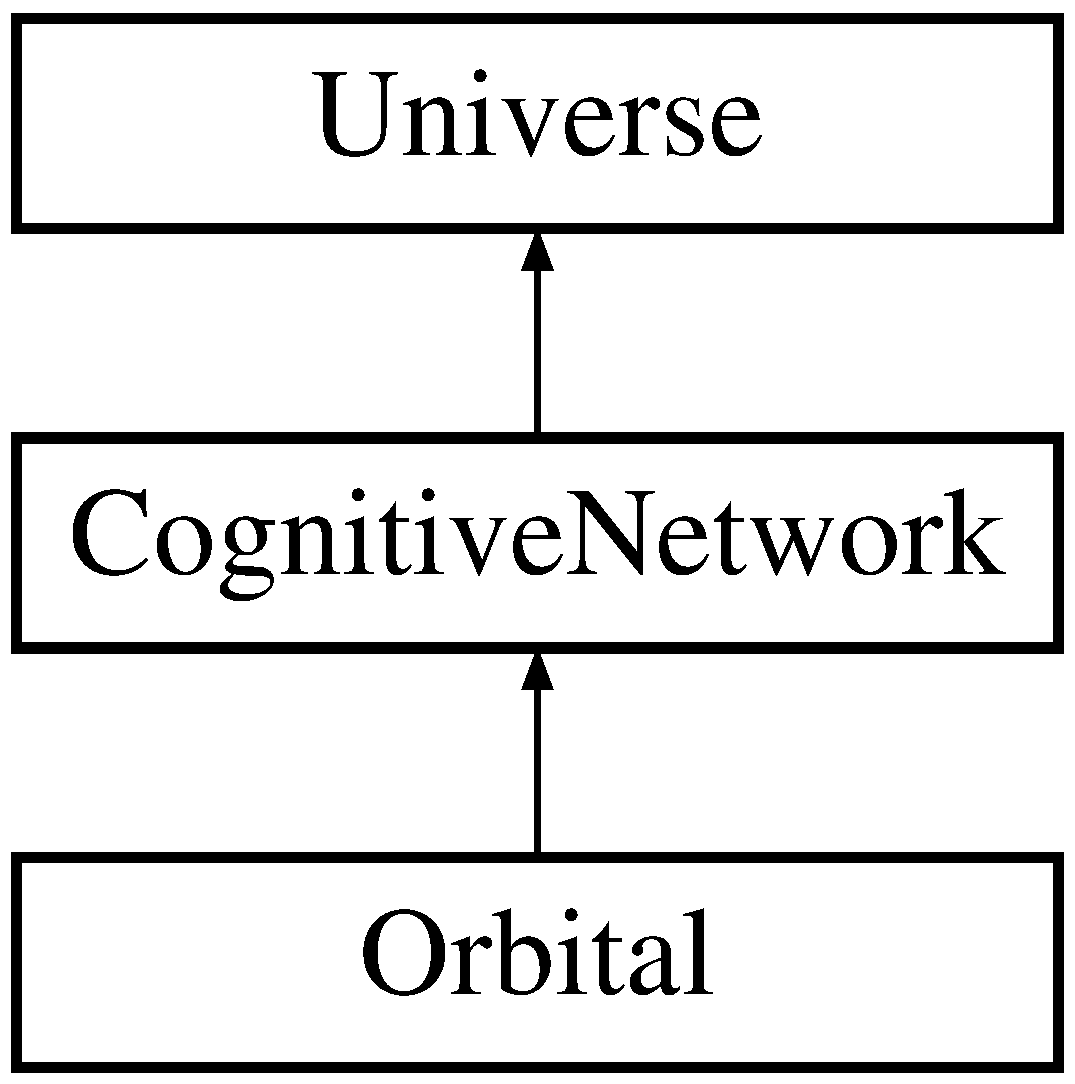
\includegraphics[height=3.000000cm]{classOrbital}
\end{center}
\end{figure}
\subsection*{Public Member Functions}
\begin{DoxyCompactItemize}
\item 
\mbox{\hyperlink{classOrbital_ac6f5367141eaa6fb4fa825262da4593a}{Orbital}} ()
\item 
\mbox{\hyperlink{classOrbital_a1c7dd9f58b740ce5058ce04aab54292c}{Orbital}} (unsigned int object\+\_\+type)
\item 
\mbox{\hyperlink{classOrbital_a099b2f1d77a36181fdf1820a6089a05b}{Orbital}} (unsigned int object\+\_\+type, std\+::chrono\+::time\+\_\+point$<$ \mbox{\hyperlink{universe_8h_a0ef8d951d1ca5ab3cfaf7ab4c7a6fd80}{Clock}} $>$ event\+\_\+time)
\item 
\mbox{\hyperlink{classOrbital_ac54161437f3bd23cc1e6e85e702239c8}{Orbital}} (unsigned int object\+\_\+type, std\+::chrono\+::time\+\_\+point$<$ \mbox{\hyperlink{universe_8h_a0ef8d951d1ca5ab3cfaf7ab4c7a6fd80}{Clock}} $>$ event\+\_\+time, \mbox{\hyperlink{classCognitiveNetwork}{Cognitive\+Network}} \&cognitivenetwork\+\_\+connector)
\item 
virtual \mbox{\hyperlink{classOrbital_af3c531d6dd6f3951dca836a2a9787c2c}{$\sim$\+Orbital}} ()
\item 
unsigned int \mbox{\hyperlink{classOrbital_ae46443496d38a22f1da8f7f063d420bc}{Get\+Counter}} (std\+::chrono\+::time\+\_\+point$<$ \mbox{\hyperlink{universe_8h_a0ef8d951d1ca5ab3cfaf7ab4c7a6fd80}{Clock}} $>$ event\+\_\+time)
\item 
double \mbox{\hyperlink{classOrbital_a6748a8f75bfd255c1a53a5061d4e14e1}{Get\+Energy}} (std\+::chrono\+::time\+\_\+point$<$ \mbox{\hyperlink{universe_8h_a0ef8d951d1ca5ab3cfaf7ab4c7a6fd80}{Clock}} $>$ event\+\_\+time)
\item 
double \mbox{\hyperlink{classOrbital_aea872758f844534806a638080a39507e}{Get\+Position}} (std\+::chrono\+::time\+\_\+point$<$ \mbox{\hyperlink{universe_8h_a0ef8d951d1ca5ab3cfaf7ab4c7a6fd80}{Clock}} $>$ event\+\_\+time)
\item 
double \mbox{\hyperlink{classOrbital_ad891e4a65c01e94c72ad36cda114cc2a}{Get\+Phase}} (std\+::chrono\+::time\+\_\+point$<$ \mbox{\hyperlink{universe_8h_a0ef8d951d1ca5ab3cfaf7ab4c7a6fd80}{Clock}} $>$ event\+\_\+time)
\item 
double \mbox{\hyperlink{classOrbital_aeb7758cc920cb862fdc33374c26cb585}{Get\+Tau}} (std\+::chrono\+::time\+\_\+point$<$ \mbox{\hyperlink{universe_8h_a0ef8d951d1ca5ab3cfaf7ab4c7a6fd80}{Clock}} $>$ event\+\_\+time)
\item 
void \mbox{\hyperlink{classOrbital_a16ff46f7e720f2f7aed332585310a9b8}{Set\+Position}} (std\+::chrono\+::time\+\_\+point$<$ \mbox{\hyperlink{universe_8h_a0ef8d951d1ca5ab3cfaf7ab4c7a6fd80}{Clock}} $>$ event\+\_\+time, double val)
\item 
void \mbox{\hyperlink{classOrbital_ac1c58fcb56e4d5c19c4ab39cc09c88ad}{Set\+Phase}} (std\+::chrono\+::time\+\_\+point$<$ \mbox{\hyperlink{universe_8h_a0ef8d951d1ca5ab3cfaf7ab4c7a6fd80}{Clock}} $>$ event\+\_\+time, double val)
\item 
void \mbox{\hyperlink{classOrbital_afd09baa67f1a9bff08c74dcf60e1398a}{Set\+Tau}} (std\+::chrono\+::time\+\_\+point$<$ \mbox{\hyperlink{universe_8h_a0ef8d951d1ca5ab3cfaf7ab4c7a6fd80}{Clock}} $>$ event\+\_\+time, double val)
\item 
void \mbox{\hyperlink{classOrbital_ae2a2fb06700d1d68501b0cbdea87cc08}{Set\+Counter}} (std\+::chrono\+::time\+\_\+point$<$ \mbox{\hyperlink{universe_8h_a0ef8d951d1ca5ab3cfaf7ab4c7a6fd80}{Clock}} $>$ event\+\_\+time, unsigned int val)
\item 
void \mbox{\hyperlink{classOrbital_a20b0f4d549fd9024df89603a5adcc214}{Set\+Energy}} (std\+::chrono\+::time\+\_\+point$<$ \mbox{\hyperlink{universe_8h_a0ef8d951d1ca5ab3cfaf7ab4c7a6fd80}{Clock}} $>$ event\+\_\+time, double val)
\item 
void \mbox{\hyperlink{classOrbital_afd0dfd382d4bf7d9fbace315bd37fa85}{Set\+Object\+Type}} (std\+::chrono\+::time\+\_\+point$<$ \mbox{\hyperlink{universe_8h_a0ef8d951d1ca5ab3cfaf7ab4c7a6fd80}{Clock}} $>$ event\+\_\+time, int object\+\_\+type)
\item 
bool \mbox{\hyperlink{classOrbital_acc6137a5a79be91a255f685a2f065330}{Reset\+Parameters}} (std\+::chrono\+::time\+\_\+point$<$ \mbox{\hyperlink{universe_8h_a0ef8d951d1ca5ab3cfaf7ab4c7a6fd80}{Clock}} $>$ event\+\_\+time)
\item 
std\+::vector$<$ \mbox{\hyperlink{classCognitiveNetwork}{Cognitive\+Network}} $\ast$ $>$ \mbox{\hyperlink{classOrbital_a44230cebc40357d186c442bfac2507a4}{Add\+To\+Neuron\+List}} (\mbox{\hyperlink{classCognitiveNetwork}{Cognitive\+Network}} $\ast$neuron\+\_\+pointer)
\item 
std\+::vector$<$ \mbox{\hyperlink{classCognitiveNetwork}{Cognitive\+Network}} $\ast$ $>$ \mbox{\hyperlink{classOrbital_a57480cdd63dd1bf731864f513767800d}{Add\+Neuron}} (std\+::chrono\+::time\+\_\+point$<$ \mbox{\hyperlink{universe_8h_a0ef8d951d1ca5ab3cfaf7ab4c7a6fd80}{Clock}} $>$ event\+\_\+time, std\+::vector$<$ \mbox{\hyperlink{classCognitiveNetwork}{Cognitive\+Network}} $\ast$$>$ list\+\_\+to\+\_\+add)
\item 
std\+::vector$<$ \mbox{\hyperlink{classCognitiveNetwork}{Cognitive\+Network}} $\ast$ $>$ \mbox{\hyperlink{classOrbital_a7d7e4b7cb0d009a5e7224b6f758d7b6b}{Get\+Neurons}} (std\+::chrono\+::time\+\_\+point$<$ \mbox{\hyperlink{universe_8h_a0ef8d951d1ca5ab3cfaf7ab4c7a6fd80}{Clock}} $>$ event\+\_\+time)
\item 
void \mbox{\hyperlink{classOrbital_a5aa5edbae517ff393fc1eb0ae2422123}{Calc\+Position}} (std\+::chrono\+::time\+\_\+point$<$ \mbox{\hyperlink{universe_8h_a0ef8d951d1ca5ab3cfaf7ab4c7a6fd80}{Clock}} $>$ event\+\_\+time, double Duration)
\item 
void \mbox{\hyperlink{classOrbital_afbf72ba4e260627422c9f53dea793923}{Update\+Cycle}} (std\+::chrono\+::time\+\_\+point$<$ \mbox{\hyperlink{universe_8h_a0ef8d951d1ca5ab3cfaf7ab4c7a6fd80}{Clock}} $>$ event\+\_\+time, std\+::vector$<$ \mbox{\hyperlink{classCognitiveNetwork}{Cognitive\+Network}} $\ast$$>$ set\+\_\+of\+\_\+update\+\_\+pointers, unsigned int pointer\+\_\+type)
\item 
virtual int \mbox{\hyperlink{classOrbital_a837289c3b2af844724c381707dee40d0}{Update}} (std\+::chrono\+::time\+\_\+point$<$ \mbox{\hyperlink{universe_8h_a0ef8d951d1ca5ab3cfaf7ab4c7a6fd80}{Clock}} $>$ event\+\_\+time)
\end{DoxyCompactItemize}
\subsection*{Protected Attributes}
\begin{DoxyCompactItemize}
\item 
std\+::vector$<$ \mbox{\hyperlink{classCognitiveNetwork}{Cognitive\+Network}} $\ast$ $>$ \mbox{\hyperlink{classOrbital_a504f1b3e8621e7eb7e682c3cec48272d}{neuron\+\_\+list}}
\end{DoxyCompactItemize}
\subsection*{Private Attributes}
\begin{DoxyCompactItemize}
\item 
unsigned int \mbox{\hyperlink{classOrbital_aa372740124e986fd28903fc0a58b9c76}{m\+\_\+\+Counter}}
\begin{DoxyCompactList}\small\item\em Member variable \char`\"{}m\+\_\+\+Counter\char`\"{}. \end{DoxyCompactList}\item 
double \mbox{\hyperlink{classOrbital_ac625d580da26f03f2222352c92b9e61e}{object\+\_\+energy}}
\item 
int \mbox{\hyperlink{classOrbital_a00b10dd18889b7ab0f3a60de0c6bdcf5}{orbital\+\_\+type}}
\item 
int \mbox{\hyperlink{classOrbital_a39c9d2d348dc7c20970bb16c01c7649e}{m\+\_\+\+Tau}}
\item 
double \mbox{\hyperlink{classOrbital_a16163ba33abccd079bbf5f4bcb9d9054}{m\+\_\+\+Position}}
\item 
double \mbox{\hyperlink{classOrbital_a74299cf4fcffa5078b836c66204439cc}{m\+\_\+\+Phase}}
\item 
int \mbox{\hyperlink{classOrbital_a890367094e4fd52818480127d4cf5083}{m\+\_\+\+Duration}}
\item 
int \mbox{\hyperlink{classOrbital_a8aa88a5fe3fc3bc9c662886ca890360c}{m\+\_\+\+Internal\+Clock}}
\item 
std\+::chrono\+::time\+\_\+point$<$ \mbox{\hyperlink{universe_8h_a0ef8d951d1ca5ab3cfaf7ab4c7a6fd80}{Clock}} $>$ \mbox{\hyperlink{classOrbital_aa3a9163f5de9d49cd8fa11c87502a67b}{m\+\_\+\+Old\+Clock}}
\item 
std\+::chrono\+::time\+\_\+point$<$ \mbox{\hyperlink{universe_8h_a0ef8d951d1ca5ab3cfaf7ab4c7a6fd80}{Clock}} $>$ \mbox{\hyperlink{classOrbital_a0c5c5ea93a03de69e7aa0267d74d8740}{time\+\_\+object\+\_\+created}}
\item 
std\+::chrono\+::time\+\_\+point$<$ \mbox{\hyperlink{universe_8h_a0ef8d951d1ca5ab3cfaf7ab4c7a6fd80}{Clock}} $>$ \mbox{\hyperlink{classOrbital_aa7389103c601bdc29ae97f52d85966a2}{previous\+\_\+event\+\_\+time}}
\item 
int \mbox{\hyperlink{classOrbital_a8deef7437a3b111b12a78e9bc9919604}{duration\+\_\+since\+\_\+last\+\_\+event}}
\item 
bool \mbox{\hyperlink{classOrbital_ae2f3114681ba00fdfeea23d60efea869}{object\+\_\+disabled}}
\item 
bool \mbox{\hyperlink{classOrbital_a41d2c8c2ecad75d258acf7991468a684}{object\+\_\+initialised}} = false
\end{DoxyCompactItemize}
\subsection*{Friends}
\begin{DoxyCompactItemize}
\item 
class \mbox{\hyperlink{classOrbital_aa410d74ba34b18a9f6bdf24323c4ee5b}{Neuron}}
\end{DoxyCompactItemize}
\subsection*{Additional Inherited Members}


\subsection{Detailed Description}
$<$ For Sine, Cosine, Power, Fabs \& Sqrt functions 

\subsection{Constructor \& Destructor Documentation}
\mbox{\Hypertarget{classOrbital_ac6f5367141eaa6fb4fa825262da4593a}\label{classOrbital_ac6f5367141eaa6fb4fa825262da4593a}} 
\index{Orbital@{Orbital}!Orbital@{Orbital}}
\index{Orbital@{Orbital}!Orbital@{Orbital}}
\subsubsection{\texorpdfstring{Orbital()}{Orbital()}\hspace{0.1cm}{\footnotesize\ttfamily [1/4]}}
{\footnotesize\ttfamily Orbital\+::\+Orbital (\begin{DoxyParamCaption}{ }\end{DoxyParamCaption})\hspace{0.3cm}{\ttfamily [inline]}}

\mbox{\Hypertarget{classOrbital_a1c7dd9f58b740ce5058ce04aab54292c}\label{classOrbital_a1c7dd9f58b740ce5058ce04aab54292c}} 
\index{Orbital@{Orbital}!Orbital@{Orbital}}
\index{Orbital@{Orbital}!Orbital@{Orbital}}
\subsubsection{\texorpdfstring{Orbital()}{Orbital()}\hspace{0.1cm}{\footnotesize\ttfamily [2/4]}}
{\footnotesize\ttfamily Orbital\+::\+Orbital (\begin{DoxyParamCaption}\item[{unsigned int}]{object\+\_\+type }\end{DoxyParamCaption})\hspace{0.3cm}{\ttfamily [inline]}}

\mbox{\Hypertarget{classOrbital_a099b2f1d77a36181fdf1820a6089a05b}\label{classOrbital_a099b2f1d77a36181fdf1820a6089a05b}} 
\index{Orbital@{Orbital}!Orbital@{Orbital}}
\index{Orbital@{Orbital}!Orbital@{Orbital}}
\subsubsection{\texorpdfstring{Orbital()}{Orbital()}\hspace{0.1cm}{\footnotesize\ttfamily [3/4]}}
{\footnotesize\ttfamily Orbital\+::\+Orbital (\begin{DoxyParamCaption}\item[{unsigned int}]{object\+\_\+type,  }\item[{std\+::chrono\+::time\+\_\+point$<$ \mbox{\hyperlink{universe_8h_a0ef8d951d1ca5ab3cfaf7ab4c7a6fd80}{Clock}} $>$}]{event\+\_\+time }\end{DoxyParamCaption})\hspace{0.3cm}{\ttfamily [inline]}}

\mbox{\Hypertarget{classOrbital_ac54161437f3bd23cc1e6e85e702239c8}\label{classOrbital_ac54161437f3bd23cc1e6e85e702239c8}} 
\index{Orbital@{Orbital}!Orbital@{Orbital}}
\index{Orbital@{Orbital}!Orbital@{Orbital}}
\subsubsection{\texorpdfstring{Orbital()}{Orbital()}\hspace{0.1cm}{\footnotesize\ttfamily [4/4]}}
{\footnotesize\ttfamily Orbital\+::\+Orbital (\begin{DoxyParamCaption}\item[{unsigned int}]{object\+\_\+type,  }\item[{std\+::chrono\+::time\+\_\+point$<$ \mbox{\hyperlink{universe_8h_a0ef8d951d1ca5ab3cfaf7ab4c7a6fd80}{Clock}} $>$}]{event\+\_\+time,  }\item[{\mbox{\hyperlink{classCognitiveNetwork}{Cognitive\+Network}} \&}]{cognitivenetwork\+\_\+connector }\end{DoxyParamCaption})\hspace{0.3cm}{\ttfamily [inline]}}

\mbox{\Hypertarget{classOrbital_af3c531d6dd6f3951dca836a2a9787c2c}\label{classOrbital_af3c531d6dd6f3951dca836a2a9787c2c}} 
\index{Orbital@{Orbital}!````~Orbital@{$\sim$\+Orbital}}
\index{````~Orbital@{$\sim$\+Orbital}!Orbital@{Orbital}}
\subsubsection{\texorpdfstring{$\sim$\+Orbital()}{~Orbital()}}
{\footnotesize\ttfamily virtual Orbital\+::$\sim$\+Orbital (\begin{DoxyParamCaption}{ }\end{DoxyParamCaption})\hspace{0.3cm}{\ttfamily [inline]}, {\ttfamily [virtual]}}



\subsection{Member Function Documentation}
\mbox{\Hypertarget{classOrbital_a57480cdd63dd1bf731864f513767800d}\label{classOrbital_a57480cdd63dd1bf731864f513767800d}} 
\index{Orbital@{Orbital}!Add\+Neuron@{Add\+Neuron}}
\index{Add\+Neuron@{Add\+Neuron}!Orbital@{Orbital}}
\subsubsection{\texorpdfstring{Add\+Neuron()}{AddNeuron()}}
{\footnotesize\ttfamily std\+::vector$<$ \mbox{\hyperlink{classCognitiveNetwork}{Cognitive\+Network}} $\ast$ $>$ Orbital\+::\+Add\+Neuron (\begin{DoxyParamCaption}\item[{std\+::chrono\+::time\+\_\+point$<$ \mbox{\hyperlink{universe_8h_a0ef8d951d1ca5ab3cfaf7ab4c7a6fd80}{Clock}} $>$}]{event\+\_\+time,  }\item[{std\+::vector$<$ \mbox{\hyperlink{classCognitiveNetwork}{Cognitive\+Network}} $\ast$$>$}]{list\+\_\+to\+\_\+add }\end{DoxyParamCaption})}

\mbox{\Hypertarget{classOrbital_a44230cebc40357d186c442bfac2507a4}\label{classOrbital_a44230cebc40357d186c442bfac2507a4}} 
\index{Orbital@{Orbital}!Add\+To\+Neuron\+List@{Add\+To\+Neuron\+List}}
\index{Add\+To\+Neuron\+List@{Add\+To\+Neuron\+List}!Orbital@{Orbital}}
\subsubsection{\texorpdfstring{Add\+To\+Neuron\+List()}{AddToNeuronList()}}
{\footnotesize\ttfamily std\+::vector$<$ \mbox{\hyperlink{classCognitiveNetwork}{Cognitive\+Network}} $\ast$ $>$ Orbital\+::\+Add\+To\+Neuron\+List (\begin{DoxyParamCaption}\item[{\mbox{\hyperlink{classCognitiveNetwork}{Cognitive\+Network}} $\ast$}]{neuron\+\_\+pointer }\end{DoxyParamCaption})}

\mbox{\Hypertarget{classOrbital_a5aa5edbae517ff393fc1eb0ae2422123}\label{classOrbital_a5aa5edbae517ff393fc1eb0ae2422123}} 
\index{Orbital@{Orbital}!Calc\+Position@{Calc\+Position}}
\index{Calc\+Position@{Calc\+Position}!Orbital@{Orbital}}
\subsubsection{\texorpdfstring{Calc\+Position()}{CalcPosition()}}
{\footnotesize\ttfamily void Orbital\+::\+Calc\+Position (\begin{DoxyParamCaption}\item[{std\+::chrono\+::time\+\_\+point$<$ \mbox{\hyperlink{universe_8h_a0ef8d951d1ca5ab3cfaf7ab4c7a6fd80}{Clock}} $>$}]{event\+\_\+time,  }\item[{double}]{Duration }\end{DoxyParamCaption})}

\mbox{\Hypertarget{classOrbital_ae46443496d38a22f1da8f7f063d420bc}\label{classOrbital_ae46443496d38a22f1da8f7f063d420bc}} 
\index{Orbital@{Orbital}!Get\+Counter@{Get\+Counter}}
\index{Get\+Counter@{Get\+Counter}!Orbital@{Orbital}}
\subsubsection{\texorpdfstring{Get\+Counter()}{GetCounter()}}
{\footnotesize\ttfamily unsigned int Orbital\+::\+Get\+Counter (\begin{DoxyParamCaption}\item[{std\+::chrono\+::time\+\_\+point$<$ \mbox{\hyperlink{universe_8h_a0ef8d951d1ca5ab3cfaf7ab4c7a6fd80}{Clock}} $>$}]{event\+\_\+time }\end{DoxyParamCaption})\hspace{0.3cm}{\ttfamily [inline]}}

\mbox{\Hypertarget{classOrbital_a6748a8f75bfd255c1a53a5061d4e14e1}\label{classOrbital_a6748a8f75bfd255c1a53a5061d4e14e1}} 
\index{Orbital@{Orbital}!Get\+Energy@{Get\+Energy}}
\index{Get\+Energy@{Get\+Energy}!Orbital@{Orbital}}
\subsubsection{\texorpdfstring{Get\+Energy()}{GetEnergy()}}
{\footnotesize\ttfamily double Orbital\+::\+Get\+Energy (\begin{DoxyParamCaption}\item[{std\+::chrono\+::time\+\_\+point$<$ \mbox{\hyperlink{universe_8h_a0ef8d951d1ca5ab3cfaf7ab4c7a6fd80}{Clock}} $>$}]{event\+\_\+time }\end{DoxyParamCaption})\hspace{0.3cm}{\ttfamily [inline]}}

\mbox{\Hypertarget{classOrbital_a7d7e4b7cb0d009a5e7224b6f758d7b6b}\label{classOrbital_a7d7e4b7cb0d009a5e7224b6f758d7b6b}} 
\index{Orbital@{Orbital}!Get\+Neurons@{Get\+Neurons}}
\index{Get\+Neurons@{Get\+Neurons}!Orbital@{Orbital}}
\subsubsection{\texorpdfstring{Get\+Neurons()}{GetNeurons()}}
{\footnotesize\ttfamily std\+::vector$<$ \mbox{\hyperlink{classCognitiveNetwork}{Cognitive\+Network}} $\ast$ $>$ Orbital\+::\+Get\+Neurons (\begin{DoxyParamCaption}\item[{std\+::chrono\+::time\+\_\+point$<$ \mbox{\hyperlink{universe_8h_a0ef8d951d1ca5ab3cfaf7ab4c7a6fd80}{Clock}} $>$}]{event\+\_\+time }\end{DoxyParamCaption})}

\mbox{\Hypertarget{classOrbital_ad891e4a65c01e94c72ad36cda114cc2a}\label{classOrbital_ad891e4a65c01e94c72ad36cda114cc2a}} 
\index{Orbital@{Orbital}!Get\+Phase@{Get\+Phase}}
\index{Get\+Phase@{Get\+Phase}!Orbital@{Orbital}}
\subsubsection{\texorpdfstring{Get\+Phase()}{GetPhase()}}
{\footnotesize\ttfamily double Orbital\+::\+Get\+Phase (\begin{DoxyParamCaption}\item[{std\+::chrono\+::time\+\_\+point$<$ \mbox{\hyperlink{universe_8h_a0ef8d951d1ca5ab3cfaf7ab4c7a6fd80}{Clock}} $>$}]{event\+\_\+time }\end{DoxyParamCaption})\hspace{0.3cm}{\ttfamily [inline]}}

\mbox{\Hypertarget{classOrbital_aea872758f844534806a638080a39507e}\label{classOrbital_aea872758f844534806a638080a39507e}} 
\index{Orbital@{Orbital}!Get\+Position@{Get\+Position}}
\index{Get\+Position@{Get\+Position}!Orbital@{Orbital}}
\subsubsection{\texorpdfstring{Get\+Position()}{GetPosition()}}
{\footnotesize\ttfamily double Orbital\+::\+Get\+Position (\begin{DoxyParamCaption}\item[{std\+::chrono\+::time\+\_\+point$<$ \mbox{\hyperlink{universe_8h_a0ef8d951d1ca5ab3cfaf7ab4c7a6fd80}{Clock}} $>$}]{event\+\_\+time }\end{DoxyParamCaption})\hspace{0.3cm}{\ttfamily [inline]}}

\mbox{\Hypertarget{classOrbital_aeb7758cc920cb862fdc33374c26cb585}\label{classOrbital_aeb7758cc920cb862fdc33374c26cb585}} 
\index{Orbital@{Orbital}!Get\+Tau@{Get\+Tau}}
\index{Get\+Tau@{Get\+Tau}!Orbital@{Orbital}}
\subsubsection{\texorpdfstring{Get\+Tau()}{GetTau()}}
{\footnotesize\ttfamily double Orbital\+::\+Get\+Tau (\begin{DoxyParamCaption}\item[{std\+::chrono\+::time\+\_\+point$<$ \mbox{\hyperlink{universe_8h_a0ef8d951d1ca5ab3cfaf7ab4c7a6fd80}{Clock}} $>$}]{event\+\_\+time }\end{DoxyParamCaption})\hspace{0.3cm}{\ttfamily [inline]}}

\mbox{\Hypertarget{classOrbital_acc6137a5a79be91a255f685a2f065330}\label{classOrbital_acc6137a5a79be91a255f685a2f065330}} 
\index{Orbital@{Orbital}!Reset\+Parameters@{Reset\+Parameters}}
\index{Reset\+Parameters@{Reset\+Parameters}!Orbital@{Orbital}}
\subsubsection{\texorpdfstring{Reset\+Parameters()}{ResetParameters()}}
{\footnotesize\ttfamily bool Orbital\+::\+Reset\+Parameters (\begin{DoxyParamCaption}\item[{std\+::chrono\+::time\+\_\+point$<$ \mbox{\hyperlink{universe_8h_a0ef8d951d1ca5ab3cfaf7ab4c7a6fd80}{Clock}} $>$}]{event\+\_\+time }\end{DoxyParamCaption})}

\mbox{\Hypertarget{classOrbital_ae2a2fb06700d1d68501b0cbdea87cc08}\label{classOrbital_ae2a2fb06700d1d68501b0cbdea87cc08}} 
\index{Orbital@{Orbital}!Set\+Counter@{Set\+Counter}}
\index{Set\+Counter@{Set\+Counter}!Orbital@{Orbital}}
\subsubsection{\texorpdfstring{Set\+Counter()}{SetCounter()}}
{\footnotesize\ttfamily void Orbital\+::\+Set\+Counter (\begin{DoxyParamCaption}\item[{std\+::chrono\+::time\+\_\+point$<$ \mbox{\hyperlink{universe_8h_a0ef8d951d1ca5ab3cfaf7ab4c7a6fd80}{Clock}} $>$}]{event\+\_\+time,  }\item[{unsigned int}]{val }\end{DoxyParamCaption})\hspace{0.3cm}{\ttfamily [inline]}, {\ttfamily [virtual]}}



Reimplemented from \mbox{\hyperlink{classUniverse_aa22202ae740eb1355529afcb13285e91}{Universe}}.

\mbox{\Hypertarget{classOrbital_a20b0f4d549fd9024df89603a5adcc214}\label{classOrbital_a20b0f4d549fd9024df89603a5adcc214}} 
\index{Orbital@{Orbital}!Set\+Energy@{Set\+Energy}}
\index{Set\+Energy@{Set\+Energy}!Orbital@{Orbital}}
\subsubsection{\texorpdfstring{Set\+Energy()}{SetEnergy()}}
{\footnotesize\ttfamily void Orbital\+::\+Set\+Energy (\begin{DoxyParamCaption}\item[{std\+::chrono\+::time\+\_\+point$<$ \mbox{\hyperlink{universe_8h_a0ef8d951d1ca5ab3cfaf7ab4c7a6fd80}{Clock}} $>$}]{event\+\_\+time,  }\item[{double}]{val }\end{DoxyParamCaption})\hspace{0.3cm}{\ttfamily [inline]}}

\mbox{\Hypertarget{classOrbital_afd0dfd382d4bf7d9fbace315bd37fa85}\label{classOrbital_afd0dfd382d4bf7d9fbace315bd37fa85}} 
\index{Orbital@{Orbital}!Set\+Object\+Type@{Set\+Object\+Type}}
\index{Set\+Object\+Type@{Set\+Object\+Type}!Orbital@{Orbital}}
\subsubsection{\texorpdfstring{Set\+Object\+Type()}{SetObjectType()}}
{\footnotesize\ttfamily void Orbital\+::\+Set\+Object\+Type (\begin{DoxyParamCaption}\item[{std\+::chrono\+::time\+\_\+point$<$ \mbox{\hyperlink{universe_8h_a0ef8d951d1ca5ab3cfaf7ab4c7a6fd80}{Clock}} $>$}]{event\+\_\+time,  }\item[{int}]{object\+\_\+type }\end{DoxyParamCaption})}

\mbox{\Hypertarget{classOrbital_ac1c58fcb56e4d5c19c4ab39cc09c88ad}\label{classOrbital_ac1c58fcb56e4d5c19c4ab39cc09c88ad}} 
\index{Orbital@{Orbital}!Set\+Phase@{Set\+Phase}}
\index{Set\+Phase@{Set\+Phase}!Orbital@{Orbital}}
\subsubsection{\texorpdfstring{Set\+Phase()}{SetPhase()}}
{\footnotesize\ttfamily void Orbital\+::\+Set\+Phase (\begin{DoxyParamCaption}\item[{std\+::chrono\+::time\+\_\+point$<$ \mbox{\hyperlink{universe_8h_a0ef8d951d1ca5ab3cfaf7ab4c7a6fd80}{Clock}} $>$}]{event\+\_\+time,  }\item[{double}]{val }\end{DoxyParamCaption})\hspace{0.3cm}{\ttfamily [inline]}}

\mbox{\Hypertarget{classOrbital_a16ff46f7e720f2f7aed332585310a9b8}\label{classOrbital_a16ff46f7e720f2f7aed332585310a9b8}} 
\index{Orbital@{Orbital}!Set\+Position@{Set\+Position}}
\index{Set\+Position@{Set\+Position}!Orbital@{Orbital}}
\subsubsection{\texorpdfstring{Set\+Position()}{SetPosition()}}
{\footnotesize\ttfamily void Orbital\+::\+Set\+Position (\begin{DoxyParamCaption}\item[{std\+::chrono\+::time\+\_\+point$<$ \mbox{\hyperlink{universe_8h_a0ef8d951d1ca5ab3cfaf7ab4c7a6fd80}{Clock}} $>$}]{event\+\_\+time,  }\item[{double}]{val }\end{DoxyParamCaption})\hspace{0.3cm}{\ttfamily [inline]}}

\mbox{\Hypertarget{classOrbital_afd09baa67f1a9bff08c74dcf60e1398a}\label{classOrbital_afd09baa67f1a9bff08c74dcf60e1398a}} 
\index{Orbital@{Orbital}!Set\+Tau@{Set\+Tau}}
\index{Set\+Tau@{Set\+Tau}!Orbital@{Orbital}}
\subsubsection{\texorpdfstring{Set\+Tau()}{SetTau()}}
{\footnotesize\ttfamily void Orbital\+::\+Set\+Tau (\begin{DoxyParamCaption}\item[{std\+::chrono\+::time\+\_\+point$<$ \mbox{\hyperlink{universe_8h_a0ef8d951d1ca5ab3cfaf7ab4c7a6fd80}{Clock}} $>$}]{event\+\_\+time,  }\item[{double}]{val }\end{DoxyParamCaption})\hspace{0.3cm}{\ttfamily [inline]}}

\mbox{\Hypertarget{classOrbital_a837289c3b2af844724c381707dee40d0}\label{classOrbital_a837289c3b2af844724c381707dee40d0}} 
\index{Orbital@{Orbital}!Update@{Update}}
\index{Update@{Update}!Orbital@{Orbital}}
\subsubsection{\texorpdfstring{Update()}{Update()}}
{\footnotesize\ttfamily int Orbital\+::\+Update (\begin{DoxyParamCaption}\item[{std\+::chrono\+::time\+\_\+point$<$ \mbox{\hyperlink{universe_8h_a0ef8d951d1ca5ab3cfaf7ab4c7a6fd80}{Clock}} $>$}]{event\+\_\+time }\end{DoxyParamCaption})\hspace{0.3cm}{\ttfamily [virtual]}}

\mbox{\Hypertarget{classOrbital_afbf72ba4e260627422c9f53dea793923}\label{classOrbital_afbf72ba4e260627422c9f53dea793923}} 
\index{Orbital@{Orbital}!Update\+Cycle@{Update\+Cycle}}
\index{Update\+Cycle@{Update\+Cycle}!Orbital@{Orbital}}
\subsubsection{\texorpdfstring{Update\+Cycle()}{UpdateCycle()}}
{\footnotesize\ttfamily void Orbital\+::\+Update\+Cycle (\begin{DoxyParamCaption}\item[{std\+::chrono\+::time\+\_\+point$<$ \mbox{\hyperlink{universe_8h_a0ef8d951d1ca5ab3cfaf7ab4c7a6fd80}{Clock}} $>$}]{event\+\_\+time,  }\item[{std\+::vector$<$ \mbox{\hyperlink{classCognitiveNetwork}{Cognitive\+Network}} $\ast$$>$}]{set\+\_\+of\+\_\+update\+\_\+pointers,  }\item[{unsigned int}]{pointer\+\_\+type }\end{DoxyParamCaption})}



\subsection{Friends And Related Function Documentation}
\mbox{\Hypertarget{classOrbital_aa410d74ba34b18a9f6bdf24323c4ee5b}\label{classOrbital_aa410d74ba34b18a9f6bdf24323c4ee5b}} 
\index{Orbital@{Orbital}!Neuron@{Neuron}}
\index{Neuron@{Neuron}!Orbital@{Orbital}}
\subsubsection{\texorpdfstring{Neuron}{Neuron}}
{\footnotesize\ttfamily friend class \mbox{\hyperlink{classNeuron}{Neuron}}\hspace{0.3cm}{\ttfamily [friend]}}



\subsection{Member Data Documentation}
\mbox{\Hypertarget{classOrbital_a8deef7437a3b111b12a78e9bc9919604}\label{classOrbital_a8deef7437a3b111b12a78e9bc9919604}} 
\index{Orbital@{Orbital}!duration\+\_\+since\+\_\+last\+\_\+event@{duration\+\_\+since\+\_\+last\+\_\+event}}
\index{duration\+\_\+since\+\_\+last\+\_\+event@{duration\+\_\+since\+\_\+last\+\_\+event}!Orbital@{Orbital}}
\subsubsection{\texorpdfstring{duration\+\_\+since\+\_\+last\+\_\+event}{duration\_since\_last\_event}}
{\footnotesize\ttfamily int Orbital\+::duration\+\_\+since\+\_\+last\+\_\+event\hspace{0.3cm}{\ttfamily [private]}}

\mbox{\Hypertarget{classOrbital_aa372740124e986fd28903fc0a58b9c76}\label{classOrbital_aa372740124e986fd28903fc0a58b9c76}} 
\index{Orbital@{Orbital}!m\+\_\+\+Counter@{m\+\_\+\+Counter}}
\index{m\+\_\+\+Counter@{m\+\_\+\+Counter}!Orbital@{Orbital}}
\subsubsection{\texorpdfstring{m\+\_\+\+Counter}{m\_Counter}}
{\footnotesize\ttfamily unsigned int Orbital\+::m\+\_\+\+Counter\hspace{0.3cm}{\ttfamily [private]}}



Member variable \char`\"{}m\+\_\+\+Counter\char`\"{}. 

\mbox{\Hypertarget{classOrbital_a890367094e4fd52818480127d4cf5083}\label{classOrbital_a890367094e4fd52818480127d4cf5083}} 
\index{Orbital@{Orbital}!m\+\_\+\+Duration@{m\+\_\+\+Duration}}
\index{m\+\_\+\+Duration@{m\+\_\+\+Duration}!Orbital@{Orbital}}
\subsubsection{\texorpdfstring{m\+\_\+\+Duration}{m\_Duration}}
{\footnotesize\ttfamily int Orbital\+::m\+\_\+\+Duration\hspace{0.3cm}{\ttfamily [private]}}

\mbox{\Hypertarget{classOrbital_a8aa88a5fe3fc3bc9c662886ca890360c}\label{classOrbital_a8aa88a5fe3fc3bc9c662886ca890360c}} 
\index{Orbital@{Orbital}!m\+\_\+\+Internal\+Clock@{m\+\_\+\+Internal\+Clock}}
\index{m\+\_\+\+Internal\+Clock@{m\+\_\+\+Internal\+Clock}!Orbital@{Orbital}}
\subsubsection{\texorpdfstring{m\+\_\+\+Internal\+Clock}{m\_InternalClock}}
{\footnotesize\ttfamily int Orbital\+::m\+\_\+\+Internal\+Clock\hspace{0.3cm}{\ttfamily [private]}}

\mbox{\Hypertarget{classOrbital_aa3a9163f5de9d49cd8fa11c87502a67b}\label{classOrbital_aa3a9163f5de9d49cd8fa11c87502a67b}} 
\index{Orbital@{Orbital}!m\+\_\+\+Old\+Clock@{m\+\_\+\+Old\+Clock}}
\index{m\+\_\+\+Old\+Clock@{m\+\_\+\+Old\+Clock}!Orbital@{Orbital}}
\subsubsection{\texorpdfstring{m\+\_\+\+Old\+Clock}{m\_OldClock}}
{\footnotesize\ttfamily std\+::chrono\+::time\+\_\+point$<$\mbox{\hyperlink{universe_8h_a0ef8d951d1ca5ab3cfaf7ab4c7a6fd80}{Clock}}$>$ Orbital\+::m\+\_\+\+Old\+Clock\hspace{0.3cm}{\ttfamily [private]}}

\mbox{\Hypertarget{classOrbital_a74299cf4fcffa5078b836c66204439cc}\label{classOrbital_a74299cf4fcffa5078b836c66204439cc}} 
\index{Orbital@{Orbital}!m\+\_\+\+Phase@{m\+\_\+\+Phase}}
\index{m\+\_\+\+Phase@{m\+\_\+\+Phase}!Orbital@{Orbital}}
\subsubsection{\texorpdfstring{m\+\_\+\+Phase}{m\_Phase}}
{\footnotesize\ttfamily double Orbital\+::m\+\_\+\+Phase\hspace{0.3cm}{\ttfamily [private]}}

\mbox{\Hypertarget{classOrbital_a16163ba33abccd079bbf5f4bcb9d9054}\label{classOrbital_a16163ba33abccd079bbf5f4bcb9d9054}} 
\index{Orbital@{Orbital}!m\+\_\+\+Position@{m\+\_\+\+Position}}
\index{m\+\_\+\+Position@{m\+\_\+\+Position}!Orbital@{Orbital}}
\subsubsection{\texorpdfstring{m\+\_\+\+Position}{m\_Position}}
{\footnotesize\ttfamily double Orbital\+::m\+\_\+\+Position\hspace{0.3cm}{\ttfamily [private]}}

\mbox{\Hypertarget{classOrbital_a39c9d2d348dc7c20970bb16c01c7649e}\label{classOrbital_a39c9d2d348dc7c20970bb16c01c7649e}} 
\index{Orbital@{Orbital}!m\+\_\+\+Tau@{m\+\_\+\+Tau}}
\index{m\+\_\+\+Tau@{m\+\_\+\+Tau}!Orbital@{Orbital}}
\subsubsection{\texorpdfstring{m\+\_\+\+Tau}{m\_Tau}}
{\footnotesize\ttfamily int Orbital\+::m\+\_\+\+Tau\hspace{0.3cm}{\ttfamily [private]}}

\mbox{\Hypertarget{classOrbital_a504f1b3e8621e7eb7e682c3cec48272d}\label{classOrbital_a504f1b3e8621e7eb7e682c3cec48272d}} 
\index{Orbital@{Orbital}!neuron\+\_\+list@{neuron\+\_\+list}}
\index{neuron\+\_\+list@{neuron\+\_\+list}!Orbital@{Orbital}}
\subsubsection{\texorpdfstring{neuron\+\_\+list}{neuron\_list}}
{\footnotesize\ttfamily std\+::vector$<$\mbox{\hyperlink{classCognitiveNetwork}{Cognitive\+Network}}$\ast$$>$ Orbital\+::neuron\+\_\+list\hspace{0.3cm}{\ttfamily [protected]}}

\mbox{\Hypertarget{classOrbital_ae2f3114681ba00fdfeea23d60efea869}\label{classOrbital_ae2f3114681ba00fdfeea23d60efea869}} 
\index{Orbital@{Orbital}!object\+\_\+disabled@{object\+\_\+disabled}}
\index{object\+\_\+disabled@{object\+\_\+disabled}!Orbital@{Orbital}}
\subsubsection{\texorpdfstring{object\+\_\+disabled}{object\_disabled}}
{\footnotesize\ttfamily bool Orbital\+::object\+\_\+disabled\hspace{0.3cm}{\ttfamily [private]}}

\mbox{\Hypertarget{classOrbital_ac625d580da26f03f2222352c92b9e61e}\label{classOrbital_ac625d580da26f03f2222352c92b9e61e}} 
\index{Orbital@{Orbital}!object\+\_\+energy@{object\+\_\+energy}}
\index{object\+\_\+energy@{object\+\_\+energy}!Orbital@{Orbital}}
\subsubsection{\texorpdfstring{object\+\_\+energy}{object\_energy}}
{\footnotesize\ttfamily double Orbital\+::object\+\_\+energy\hspace{0.3cm}{\ttfamily [private]}}

\mbox{\Hypertarget{classOrbital_a41d2c8c2ecad75d258acf7991468a684}\label{classOrbital_a41d2c8c2ecad75d258acf7991468a684}} 
\index{Orbital@{Orbital}!object\+\_\+initialised@{object\+\_\+initialised}}
\index{object\+\_\+initialised@{object\+\_\+initialised}!Orbital@{Orbital}}
\subsubsection{\texorpdfstring{object\+\_\+initialised}{object\_initialised}}
{\footnotesize\ttfamily bool Orbital\+::object\+\_\+initialised = false\hspace{0.3cm}{\ttfamily [private]}}

\mbox{\Hypertarget{classOrbital_a00b10dd18889b7ab0f3a60de0c6bdcf5}\label{classOrbital_a00b10dd18889b7ab0f3a60de0c6bdcf5}} 
\index{Orbital@{Orbital}!orbital\+\_\+type@{orbital\+\_\+type}}
\index{orbital\+\_\+type@{orbital\+\_\+type}!Orbital@{Orbital}}
\subsubsection{\texorpdfstring{orbital\+\_\+type}{orbital\_type}}
{\footnotesize\ttfamily int Orbital\+::orbital\+\_\+type\hspace{0.3cm}{\ttfamily [private]}}

\mbox{\Hypertarget{classOrbital_aa7389103c601bdc29ae97f52d85966a2}\label{classOrbital_aa7389103c601bdc29ae97f52d85966a2}} 
\index{Orbital@{Orbital}!previous\+\_\+event\+\_\+time@{previous\+\_\+event\+\_\+time}}
\index{previous\+\_\+event\+\_\+time@{previous\+\_\+event\+\_\+time}!Orbital@{Orbital}}
\subsubsection{\texorpdfstring{previous\+\_\+event\+\_\+time}{previous\_event\_time}}
{\footnotesize\ttfamily std\+::chrono\+::time\+\_\+point$<$\mbox{\hyperlink{universe_8h_a0ef8d951d1ca5ab3cfaf7ab4c7a6fd80}{Clock}}$>$ Orbital\+::previous\+\_\+event\+\_\+time\hspace{0.3cm}{\ttfamily [private]}}

\mbox{\Hypertarget{classOrbital_a0c5c5ea93a03de69e7aa0267d74d8740}\label{classOrbital_a0c5c5ea93a03de69e7aa0267d74d8740}} 
\index{Orbital@{Orbital}!time\+\_\+object\+\_\+created@{time\+\_\+object\+\_\+created}}
\index{time\+\_\+object\+\_\+created@{time\+\_\+object\+\_\+created}!Orbital@{Orbital}}
\subsubsection{\texorpdfstring{time\+\_\+object\+\_\+created}{time\_object\_created}}
{\footnotesize\ttfamily std\+::chrono\+::time\+\_\+point$<$\mbox{\hyperlink{universe_8h_a0ef8d951d1ca5ab3cfaf7ab4c7a6fd80}{Clock}}$>$ Orbital\+::time\+\_\+object\+\_\+created\hspace{0.3cm}{\ttfamily [private]}}



The documentation for this class was generated from the following files\+:\begin{DoxyCompactItemize}
\item 
/home/pbisaacs/\+Developer/\+Brain\+Harmonics/\+Brain\+Harmonics/\mbox{\hyperlink{orbital_8h}{orbital.\+h}}\item 
/home/pbisaacs/\+Developer/\+Brain\+Harmonics/\+Brain\+Harmonics/\mbox{\hyperlink{orbital_8cc}{orbital.\+cc}}\end{DoxyCompactItemize}

\hypertarget{structCognitiveNetwork_1_1OrbitalConnection}{}\section{Cognitive\+Network\+:\+:Orbital\+Connection Struct Reference}
\label{structCognitiveNetwork_1_1OrbitalConnection}\index{Cognitive\+Network\+::\+Orbital\+Connection@{Cognitive\+Network\+::\+Orbital\+Connection}}
\subsection*{Public Attributes}
\begin{DoxyCompactItemize}
\item 
int \mbox{\hyperlink{structCognitiveNetwork_1_1OrbitalConnection_a76f0fc87226c177011792a19a5b4e4dd}{orbital\+\_\+one}}
\item 
int \mbox{\hyperlink{structCognitiveNetwork_1_1OrbitalConnection_a6330bb2565e13af54a0dd397763d17c8}{orbital\+\_\+two}}
\item 
double \mbox{\hyperlink{structCognitiveNetwork_1_1OrbitalConnection_a408dd29e7f55581f06d545ef8a8bffe7}{orbital\+\_\+connection\+\_\+strength}}
\item 
double \mbox{\hyperlink{structCognitiveNetwork_1_1OrbitalConnection_a6b903ccb612ca099066a58a1808064be}{orbital\+\_\+connection\+\_\+modifier}}
\item 
bool \mbox{\hyperlink{structCognitiveNetwork_1_1OrbitalConnection_a909dea36b9e0bc92a0a6454a36db72f4}{orbital\+\_\+spike}}
\item 
double \mbox{\hyperlink{structCognitiveNetwork_1_1OrbitalConnection_a12ab873bc2928edb077420d4d7200000}{orbital\+\_\+one\+\_\+position}}
\item 
double \mbox{\hyperlink{structCognitiveNetwork_1_1OrbitalConnection_ab0f3697e879a6b6956c5eb24088d87d0}{orbital\+\_\+two\+\_\+position}}
\end{DoxyCompactItemize}


\subsection{Member Data Documentation}
\mbox{\Hypertarget{structCognitiveNetwork_1_1OrbitalConnection_a6b903ccb612ca099066a58a1808064be}\label{structCognitiveNetwork_1_1OrbitalConnection_a6b903ccb612ca099066a58a1808064be}} 
\index{Cognitive\+Network\+::\+Orbital\+Connection@{Cognitive\+Network\+::\+Orbital\+Connection}!orbital\+\_\+connection\+\_\+modifier@{orbital\+\_\+connection\+\_\+modifier}}
\index{orbital\+\_\+connection\+\_\+modifier@{orbital\+\_\+connection\+\_\+modifier}!Cognitive\+Network\+::\+Orbital\+Connection@{Cognitive\+Network\+::\+Orbital\+Connection}}
\subsubsection{\texorpdfstring{orbital\+\_\+connection\+\_\+modifier}{orbital\_connection\_modifier}}
{\footnotesize\ttfamily double Cognitive\+Network\+::\+Orbital\+Connection\+::orbital\+\_\+connection\+\_\+modifier}

\mbox{\Hypertarget{structCognitiveNetwork_1_1OrbitalConnection_a408dd29e7f55581f06d545ef8a8bffe7}\label{structCognitiveNetwork_1_1OrbitalConnection_a408dd29e7f55581f06d545ef8a8bffe7}} 
\index{Cognitive\+Network\+::\+Orbital\+Connection@{Cognitive\+Network\+::\+Orbital\+Connection}!orbital\+\_\+connection\+\_\+strength@{orbital\+\_\+connection\+\_\+strength}}
\index{orbital\+\_\+connection\+\_\+strength@{orbital\+\_\+connection\+\_\+strength}!Cognitive\+Network\+::\+Orbital\+Connection@{Cognitive\+Network\+::\+Orbital\+Connection}}
\subsubsection{\texorpdfstring{orbital\+\_\+connection\+\_\+strength}{orbital\_connection\_strength}}
{\footnotesize\ttfamily double Cognitive\+Network\+::\+Orbital\+Connection\+::orbital\+\_\+connection\+\_\+strength}

\mbox{\Hypertarget{structCognitiveNetwork_1_1OrbitalConnection_a76f0fc87226c177011792a19a5b4e4dd}\label{structCognitiveNetwork_1_1OrbitalConnection_a76f0fc87226c177011792a19a5b4e4dd}} 
\index{Cognitive\+Network\+::\+Orbital\+Connection@{Cognitive\+Network\+::\+Orbital\+Connection}!orbital\+\_\+one@{orbital\+\_\+one}}
\index{orbital\+\_\+one@{orbital\+\_\+one}!Cognitive\+Network\+::\+Orbital\+Connection@{Cognitive\+Network\+::\+Orbital\+Connection}}
\subsubsection{\texorpdfstring{orbital\+\_\+one}{orbital\_one}}
{\footnotesize\ttfamily int Cognitive\+Network\+::\+Orbital\+Connection\+::orbital\+\_\+one}

\mbox{\Hypertarget{structCognitiveNetwork_1_1OrbitalConnection_a12ab873bc2928edb077420d4d7200000}\label{structCognitiveNetwork_1_1OrbitalConnection_a12ab873bc2928edb077420d4d7200000}} 
\index{Cognitive\+Network\+::\+Orbital\+Connection@{Cognitive\+Network\+::\+Orbital\+Connection}!orbital\+\_\+one\+\_\+position@{orbital\+\_\+one\+\_\+position}}
\index{orbital\+\_\+one\+\_\+position@{orbital\+\_\+one\+\_\+position}!Cognitive\+Network\+::\+Orbital\+Connection@{Cognitive\+Network\+::\+Orbital\+Connection}}
\subsubsection{\texorpdfstring{orbital\+\_\+one\+\_\+position}{orbital\_one\_position}}
{\footnotesize\ttfamily double Cognitive\+Network\+::\+Orbital\+Connection\+::orbital\+\_\+one\+\_\+position}

\mbox{\Hypertarget{structCognitiveNetwork_1_1OrbitalConnection_a909dea36b9e0bc92a0a6454a36db72f4}\label{structCognitiveNetwork_1_1OrbitalConnection_a909dea36b9e0bc92a0a6454a36db72f4}} 
\index{Cognitive\+Network\+::\+Orbital\+Connection@{Cognitive\+Network\+::\+Orbital\+Connection}!orbital\+\_\+spike@{orbital\+\_\+spike}}
\index{orbital\+\_\+spike@{orbital\+\_\+spike}!Cognitive\+Network\+::\+Orbital\+Connection@{Cognitive\+Network\+::\+Orbital\+Connection}}
\subsubsection{\texorpdfstring{orbital\+\_\+spike}{orbital\_spike}}
{\footnotesize\ttfamily bool Cognitive\+Network\+::\+Orbital\+Connection\+::orbital\+\_\+spike}

\mbox{\Hypertarget{structCognitiveNetwork_1_1OrbitalConnection_a6330bb2565e13af54a0dd397763d17c8}\label{structCognitiveNetwork_1_1OrbitalConnection_a6330bb2565e13af54a0dd397763d17c8}} 
\index{Cognitive\+Network\+::\+Orbital\+Connection@{Cognitive\+Network\+::\+Orbital\+Connection}!orbital\+\_\+two@{orbital\+\_\+two}}
\index{orbital\+\_\+two@{orbital\+\_\+two}!Cognitive\+Network\+::\+Orbital\+Connection@{Cognitive\+Network\+::\+Orbital\+Connection}}
\subsubsection{\texorpdfstring{orbital\+\_\+two}{orbital\_two}}
{\footnotesize\ttfamily int Cognitive\+Network\+::\+Orbital\+Connection\+::orbital\+\_\+two}

\mbox{\Hypertarget{structCognitiveNetwork_1_1OrbitalConnection_ab0f3697e879a6b6956c5eb24088d87d0}\label{structCognitiveNetwork_1_1OrbitalConnection_ab0f3697e879a6b6956c5eb24088d87d0}} 
\index{Cognitive\+Network\+::\+Orbital\+Connection@{Cognitive\+Network\+::\+Orbital\+Connection}!orbital\+\_\+two\+\_\+position@{orbital\+\_\+two\+\_\+position}}
\index{orbital\+\_\+two\+\_\+position@{orbital\+\_\+two\+\_\+position}!Cognitive\+Network\+::\+Orbital\+Connection@{Cognitive\+Network\+::\+Orbital\+Connection}}
\subsubsection{\texorpdfstring{orbital\+\_\+two\+\_\+position}{orbital\_two\_position}}
{\footnotesize\ttfamily double Cognitive\+Network\+::\+Orbital\+Connection\+::orbital\+\_\+two\+\_\+position}



The documentation for this struct was generated from the following file\+:\begin{DoxyCompactItemize}
\item 
/home/pbisaacs/\+Developer/\+Brain\+Harmonics/\mbox{\hyperlink{cognitivenetwork_8h}{cognitivenetwork.\+h}}\end{DoxyCompactItemize}

\hypertarget{classPoint}{}\section{Point Class Reference}
\label{classPoint}\index{Point@{Point}}


{\ttfamily \#include $<$point.\+h$>$}

Inheritance diagram for Point\+:\begin{figure}[H]
\begin{center}
\leavevmode
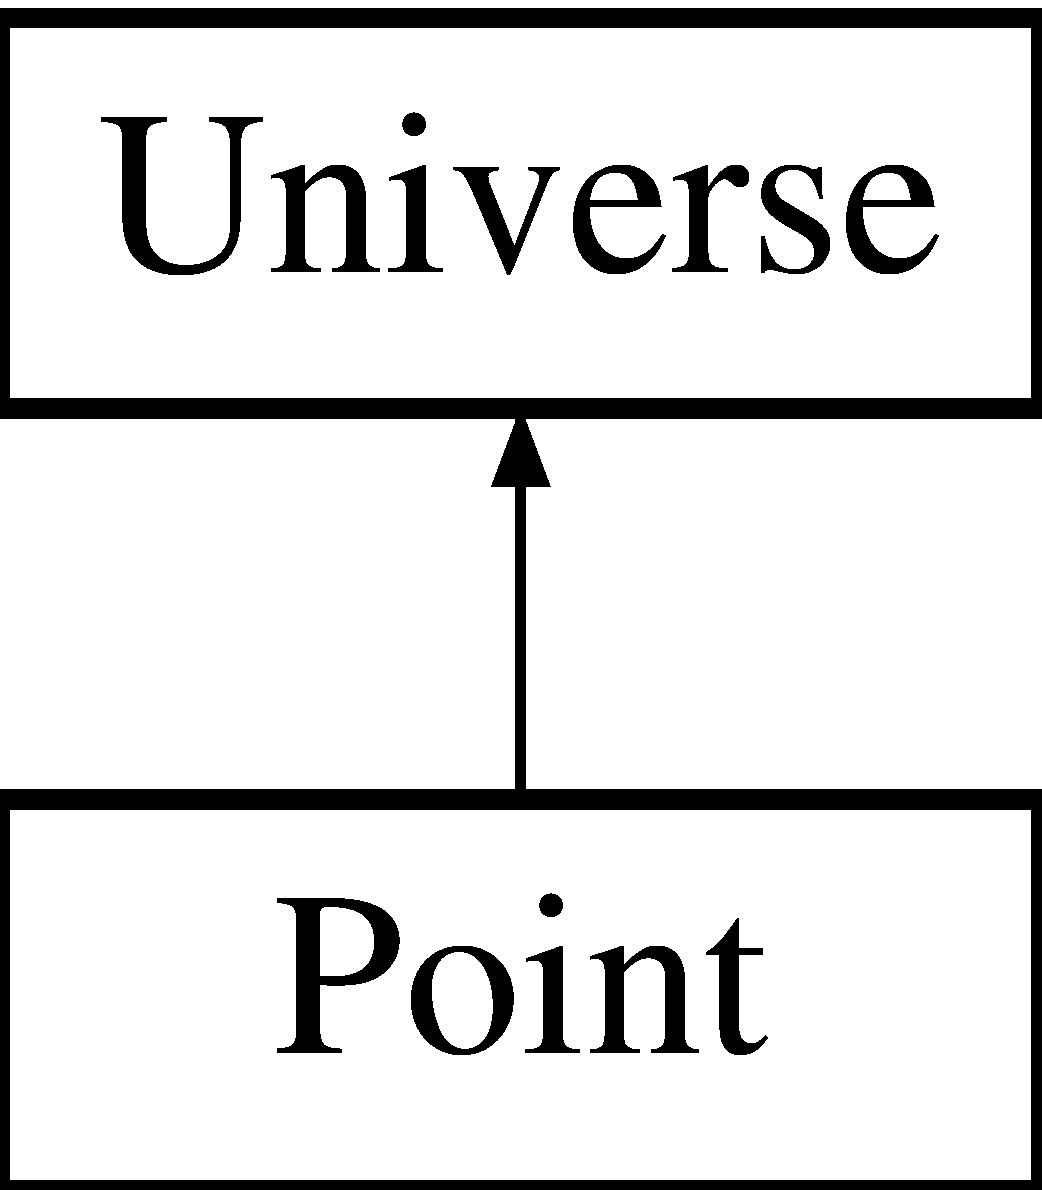
\includegraphics[height=2.000000cm]{classPoint}
\end{center}
\end{figure}
\subsection*{Public Member Functions}
\begin{DoxyCompactItemize}
\item 
\mbox{\hyperlink{classPoint_ad92f2337b839a94ce97dcdb439b4325a}{Point}} ()
\item 
\mbox{\hyperlink{classPoint_a84d29a0f72e67406901cb87c1d2f77e9}{Point}} (unsigned int object\+\_\+type)
\item 
\mbox{\hyperlink{classPoint_ac3e6d30951c40e5bc5dafe6c90668b3f}{Point}} (unsigned int object\+\_\+type, std\+::chrono\+::time\+\_\+point$<$ \mbox{\hyperlink{universe_8h_a0ef8d951d1ca5ab3cfaf7ab4c7a6fd80}{Clock}} $>$ event\+\_\+time)
\item 
\mbox{\hyperlink{classPoint_abbc76ed1b437c982eb607ec165ecfa47}{Point}} (unsigned int object\+\_\+type, std\+::chrono\+::time\+\_\+point$<$ \mbox{\hyperlink{universe_8h_a0ef8d951d1ca5ab3cfaf7ab4c7a6fd80}{Clock}} $>$ event\+\_\+time, \mbox{\hyperlink{classUniverse}{Universe}} \&universe\+\_\+connector)
\item 
virtual \mbox{\hyperlink{classPoint_a364091762d6aa1aa5983d36fd7d8b6d5}{$\sim$\+Point}} ()
\item 
int \mbox{\hyperlink{classPoint_a04bae1bb3475d1e5d97ddd7b2dae40aa}{Get\+Point\+Seq}} (std\+::chrono\+::time\+\_\+point$<$ \mbox{\hyperlink{universe_8h_a0ef8d951d1ca5ab3cfaf7ab4c7a6fd80}{Clock}} $>$ event\+\_\+time)
\item 
std\+::vector$<$ double $>$ \mbox{\hyperlink{classPoint_acdd393f39d8c08aff1e866ce1c5585e5}{Get\+Point\+Scale}} (std\+::chrono\+::time\+\_\+point$<$ \mbox{\hyperlink{universe_8h_a0ef8d951d1ca5ab3cfaf7ab4c7a6fd80}{Clock}} $>$ event\+\_\+time)
\item 
std\+::vector$<$ double $>$ \mbox{\hyperlink{classPoint_a521d229550d7f38851f9ffb1933046a6}{Get\+Point\+Position}} (std\+::chrono\+::time\+\_\+point$<$ \mbox{\hyperlink{universe_8h_a0ef8d951d1ca5ab3cfaf7ab4c7a6fd80}{Clock}} $>$ event\+\_\+time)
\item 
std\+::vector$<$ double $>$ \mbox{\hyperlink{classPoint_a98557a7ad341f981b13bb009994868f2}{Get\+Point\+Position2}} (std\+::chrono\+::time\+\_\+point$<$ \mbox{\hyperlink{universe_8h_a0ef8d951d1ca5ab3cfaf7ab4c7a6fd80}{Clock}} $>$ event\+\_\+time)
\item 
std\+::vector$<$ double $>$ \mbox{\hyperlink{classPoint_a6182865226595813eccadbe25d38cd9e}{Get\+Point\+Position\+Min}} (std\+::chrono\+::time\+\_\+point$<$ \mbox{\hyperlink{universe_8h_a0ef8d951d1ca5ab3cfaf7ab4c7a6fd80}{Clock}} $>$ event\+\_\+time)
\item 
std\+::vector$<$ int $>$ \mbox{\hyperlink{classPoint_a3a0caf079555585799754b3cab12129c}{Get\+Point\+Position\+Min\+Overflow}} (std\+::chrono\+::time\+\_\+point$<$ \mbox{\hyperlink{universe_8h_a0ef8d951d1ca5ab3cfaf7ab4c7a6fd80}{Clock}} $>$ event\+\_\+time)
\item 
std\+::vector$<$ double $>$ \mbox{\hyperlink{classPoint_afca47c5ea265894faf7b6aa4f4b17998}{Get\+Point\+Position\+Max}} (std\+::chrono\+::time\+\_\+point$<$ \mbox{\hyperlink{universe_8h_a0ef8d951d1ca5ab3cfaf7ab4c7a6fd80}{Clock}} $>$ event\+\_\+time)
\item 
std\+::vector$<$ int $>$ \mbox{\hyperlink{classPoint_a228830fddb8b4d90e910e0774796e635}{Get\+Point\+Position\+Max\+Overflow}} (std\+::chrono\+::time\+\_\+point$<$ \mbox{\hyperlink{universe_8h_a0ef8d951d1ca5ab3cfaf7ab4c7a6fd80}{Clock}} $>$ event\+\_\+time)
\item 
std\+::vector$<$ double $>$ \mbox{\hyperlink{classPoint_a46d06a6d5e8107a0321ede4ca162f264}{Get\+Point\+Move}} (std\+::chrono\+::time\+\_\+point$<$ \mbox{\hyperlink{universe_8h_a0ef8d951d1ca5ab3cfaf7ab4c7a6fd80}{Clock}} $>$ event\+\_\+time)
\item 
std\+::vector$<$ double $>$ \mbox{\hyperlink{classPoint_a92d41c8cd9a07ef56223839a44f54fe8}{Get\+Point\+Move\+Min}} (std\+::chrono\+::time\+\_\+point$<$ \mbox{\hyperlink{universe_8h_a0ef8d951d1ca5ab3cfaf7ab4c7a6fd80}{Clock}} $>$ event\+\_\+time)
\item 
std\+::vector$<$ int $>$ \mbox{\hyperlink{classPoint_a3c88bb9f80535e98fb0f479b69f75c64}{Get\+Point\+Move\+Min\+Overflow}} (std\+::chrono\+::time\+\_\+point$<$ \mbox{\hyperlink{universe_8h_a0ef8d951d1ca5ab3cfaf7ab4c7a6fd80}{Clock}} $>$ event\+\_\+time)
\item 
std\+::vector$<$ double $>$ \mbox{\hyperlink{classPoint_af67ce3da60a8e3907df6ec193786c2ae}{Get\+Point\+Move\+Max}} (std\+::chrono\+::time\+\_\+point$<$ \mbox{\hyperlink{universe_8h_a0ef8d951d1ca5ab3cfaf7ab4c7a6fd80}{Clock}} $>$ event\+\_\+time)
\item 
std\+::vector$<$ int $>$ \mbox{\hyperlink{classPoint_a83e3715d429ab2099f0c421d46603004}{Get\+Point\+Move\+Max\+Overflow}} (std\+::chrono\+::time\+\_\+point$<$ \mbox{\hyperlink{universe_8h_a0ef8d951d1ca5ab3cfaf7ab4c7a6fd80}{Clock}} $>$ event\+\_\+time)
\item 
std\+::vector$<$ double $>$ \mbox{\hyperlink{classPoint_af3941d62b39234e468e201f25a37d9da}{Get\+Point\+Differential}} (std\+::chrono\+::time\+\_\+point$<$ \mbox{\hyperlink{universe_8h_a0ef8d951d1ca5ab3cfaf7ab4c7a6fd80}{Clock}} $>$ event\+\_\+time)
\item 
std\+::vector$<$ double $>$ \mbox{\hyperlink{classPoint_a782860849006b601600f8df15af23f7a}{Get\+Point\+Differential\+Min}} (std\+::chrono\+::time\+\_\+point$<$ \mbox{\hyperlink{universe_8h_a0ef8d951d1ca5ab3cfaf7ab4c7a6fd80}{Clock}} $>$ event\+\_\+time)
\item 
std\+::vector$<$ int $>$ \mbox{\hyperlink{classPoint_adbc225afbd532763617db1acdb81ef4c}{Get\+Point\+Differential\+Min\+Overflow}} (std\+::chrono\+::time\+\_\+point$<$ \mbox{\hyperlink{universe_8h_a0ef8d951d1ca5ab3cfaf7ab4c7a6fd80}{Clock}} $>$ event\+\_\+time)
\item 
std\+::vector$<$ double $>$ \mbox{\hyperlink{classPoint_a326cd5742e908f8fb3cf6f3275b5462c}{Get\+Point\+Differential\+Max}} (std\+::chrono\+::time\+\_\+point$<$ \mbox{\hyperlink{universe_8h_a0ef8d951d1ca5ab3cfaf7ab4c7a6fd80}{Clock}} $>$ event\+\_\+time)
\item 
std\+::vector$<$ int $>$ \mbox{\hyperlink{classPoint_a2d38599722fbf65afe2b9ac57b0c4bcf}{Get\+Point\+Differential\+Max\+Overflow}} (std\+::chrono\+::time\+\_\+point$<$ \mbox{\hyperlink{universe_8h_a0ef8d951d1ca5ab3cfaf7ab4c7a6fd80}{Clock}} $>$ event\+\_\+time)
\item 
double \mbox{\hyperlink{classPoint_a72cf99a391fc3d6ea8f4252f4f92c19f}{Get\+Point\+T\+TL}} (std\+::chrono\+::time\+\_\+point$<$ \mbox{\hyperlink{universe_8h_a0ef8d951d1ca5ab3cfaf7ab4c7a6fd80}{Clock}} $>$ event\+\_\+time)
\item 
double \mbox{\hyperlink{classPoint_a272b99a9cd054b09c8944b9f0e657890}{Get\+Point\+T\+T\+L\+Min}} (std\+::chrono\+::time\+\_\+point$<$ \mbox{\hyperlink{universe_8h_a0ef8d951d1ca5ab3cfaf7ab4c7a6fd80}{Clock}} $>$ event\+\_\+time)
\item 
int \mbox{\hyperlink{classPoint_a72b222f880df30ebcc12ddc1a6d430b5}{Get\+Point\+T\+T\+L\+Min\+Overflow}} (std\+::chrono\+::time\+\_\+point$<$ \mbox{\hyperlink{universe_8h_a0ef8d951d1ca5ab3cfaf7ab4c7a6fd80}{Clock}} $>$ event\+\_\+time)
\item 
double \mbox{\hyperlink{classPoint_a0800eea77109f6fbb1220b4d551a70d3}{Get\+Point\+T\+T\+L\+Max}} (std\+::chrono\+::time\+\_\+point$<$ \mbox{\hyperlink{universe_8h_a0ef8d951d1ca5ab3cfaf7ab4c7a6fd80}{Clock}} $>$ event\+\_\+time)
\item 
int \mbox{\hyperlink{classPoint_a61d7e0fb0fd0280f628ea46609082809}{Get\+Point\+T\+T\+L\+Max\+Overflow}} (std\+::chrono\+::time\+\_\+point$<$ \mbox{\hyperlink{universe_8h_a0ef8d951d1ca5ab3cfaf7ab4c7a6fd80}{Clock}} $>$ event\+\_\+time)
\item 
std\+::vector$<$ double $>$ \mbox{\hyperlink{classPoint_ac3e94cb7e2ab1d6008ff1d5df00641c2}{Respect\+Limits}} (std\+::chrono\+::time\+\_\+point$<$ \mbox{\hyperlink{universe_8h_a0ef8d951d1ca5ab3cfaf7ab4c7a6fd80}{Clock}} $>$ event\+\_\+time, std\+::vector$<$ double $>$ val)
\item 
void \mbox{\hyperlink{classPoint_a3afeb2d7a2e2b7d9406a57fefa1af2ee}{Set\+Object\+Type}} (std\+::chrono\+::time\+\_\+point$<$ \mbox{\hyperlink{universe_8h_a0ef8d951d1ca5ab3cfaf7ab4c7a6fd80}{Clock}} $>$ event\+\_\+time, unsigned int val)
\item 
void \mbox{\hyperlink{classPoint_a912aefb007184f73b86c37257a415237}{Set\+Point\+Seq}} (std\+::chrono\+::time\+\_\+point$<$ \mbox{\hyperlink{universe_8h_a0ef8d951d1ca5ab3cfaf7ab4c7a6fd80}{Clock}} $>$ event\+\_\+time, int val)
\item 
void \mbox{\hyperlink{classPoint_a8fc02455a773624df80933403b0e545f}{Set\+Point\+Scale}} (std\+::chrono\+::time\+\_\+point$<$ \mbox{\hyperlink{universe_8h_a0ef8d951d1ca5ab3cfaf7ab4c7a6fd80}{Clock}} $>$ event\+\_\+time, std\+::vector$<$ double $>$ val)
\item 
void \mbox{\hyperlink{classPoint_a9191f97ece64b8385140d5f800a3a4ca}{Set\+Point\+Position}} (std\+::chrono\+::time\+\_\+point$<$ \mbox{\hyperlink{universe_8h_a0ef8d951d1ca5ab3cfaf7ab4c7a6fd80}{Clock}} $>$ event\+\_\+time, std\+::vector$<$ double $>$ val)
\item 
void \mbox{\hyperlink{classPoint_ad47980a6ed515a2def172d757af46f1a}{Set\+Point\+Position\+Min}} (std\+::chrono\+::time\+\_\+point$<$ \mbox{\hyperlink{universe_8h_a0ef8d951d1ca5ab3cfaf7ab4c7a6fd80}{Clock}} $>$ event\+\_\+time, std\+::vector$<$ double $>$ val)
\item 
void \mbox{\hyperlink{classPoint_ab0c0a837abb8bd52a59f82723a31f61f}{Set\+Point\+Position\+Min\+Overflow}} (std\+::chrono\+::time\+\_\+point$<$ \mbox{\hyperlink{universe_8h_a0ef8d951d1ca5ab3cfaf7ab4c7a6fd80}{Clock}} $>$ event\+\_\+time, std\+::vector$<$ int $>$ val)
\item 
void \mbox{\hyperlink{classPoint_adb2897b1a7bde15e81b72cb59342f186}{Set\+Point\+Position\+Max}} (std\+::chrono\+::time\+\_\+point$<$ \mbox{\hyperlink{universe_8h_a0ef8d951d1ca5ab3cfaf7ab4c7a6fd80}{Clock}} $>$ event\+\_\+time, std\+::vector$<$ double $>$ val)
\item 
void \mbox{\hyperlink{classPoint_a29aca71cae82195775f3822740df80ec}{Set\+Point\+Position\+Max\+Overflow}} (std\+::chrono\+::time\+\_\+point$<$ \mbox{\hyperlink{universe_8h_a0ef8d951d1ca5ab3cfaf7ab4c7a6fd80}{Clock}} $>$ event\+\_\+time, std\+::vector$<$ int $>$ val)
\item 
void \mbox{\hyperlink{classPoint_a2cf44d5cf17ecf2b3385bde963678589}{Set\+Point\+Move}} (std\+::chrono\+::time\+\_\+point$<$ \mbox{\hyperlink{universe_8h_a0ef8d951d1ca5ab3cfaf7ab4c7a6fd80}{Clock}} $>$ event\+\_\+time, std\+::vector$<$ double $>$ val)
\item 
void \mbox{\hyperlink{classPoint_a287698b6f3ec6a610447fded5c3542ca}{Set\+Point\+Move\+Min}} (std\+::chrono\+::time\+\_\+point$<$ \mbox{\hyperlink{universe_8h_a0ef8d951d1ca5ab3cfaf7ab4c7a6fd80}{Clock}} $>$ event\+\_\+time, std\+::vector$<$ double $>$ val)
\item 
void \mbox{\hyperlink{classPoint_a4a988ff988a3984545cf0c35e764c404}{Set\+Point\+Move\+Min\+Overflow}} (std\+::chrono\+::time\+\_\+point$<$ \mbox{\hyperlink{universe_8h_a0ef8d951d1ca5ab3cfaf7ab4c7a6fd80}{Clock}} $>$ event\+\_\+time, std\+::vector$<$ int $>$ val)
\item 
void \mbox{\hyperlink{classPoint_afa3c2290a72c99e8892029eaa6676204}{Set\+Point\+Move\+Max}} (std\+::chrono\+::time\+\_\+point$<$ \mbox{\hyperlink{universe_8h_a0ef8d951d1ca5ab3cfaf7ab4c7a6fd80}{Clock}} $>$ event\+\_\+time, std\+::vector$<$ double $>$ val)
\item 
void \mbox{\hyperlink{classPoint_a7c9776ffca2fde856fa8eaee669d9881}{Set\+Point\+Move\+Max\+Overflow}} (std\+::chrono\+::time\+\_\+point$<$ \mbox{\hyperlink{universe_8h_a0ef8d951d1ca5ab3cfaf7ab4c7a6fd80}{Clock}} $>$ event\+\_\+time, std\+::vector$<$ int $>$ val)
\item 
void \mbox{\hyperlink{classPoint_adb977a2f01e7a2b549e1bd36fa6f5354}{Set\+Point\+Differential}} (std\+::chrono\+::time\+\_\+point$<$ \mbox{\hyperlink{universe_8h_a0ef8d951d1ca5ab3cfaf7ab4c7a6fd80}{Clock}} $>$ event\+\_\+time, std\+::vector$<$ double $>$ val)
\item 
void \mbox{\hyperlink{classPoint_a944fcec52017ce88e052a576ef143926}{Set\+Point\+Differential\+Min}} (std\+::chrono\+::time\+\_\+point$<$ \mbox{\hyperlink{universe_8h_a0ef8d951d1ca5ab3cfaf7ab4c7a6fd80}{Clock}} $>$ event\+\_\+time, std\+::vector$<$ double $>$ val)
\item 
void \mbox{\hyperlink{classPoint_a582e63ebdbb0979234acb460e673a393}{Set\+Point\+Differential\+Min\+Overflow}} (std\+::chrono\+::time\+\_\+point$<$ \mbox{\hyperlink{universe_8h_a0ef8d951d1ca5ab3cfaf7ab4c7a6fd80}{Clock}} $>$ event\+\_\+time, std\+::vector$<$ int $>$ val)
\item 
void \mbox{\hyperlink{classPoint_ac2e53da4cbee0dc39c0b7a4d3e3a6ee5}{Set\+Point\+Differential\+Max}} (std\+::chrono\+::time\+\_\+point$<$ \mbox{\hyperlink{universe_8h_a0ef8d951d1ca5ab3cfaf7ab4c7a6fd80}{Clock}} $>$ event\+\_\+time, std\+::vector$<$ double $>$ val)
\item 
void \mbox{\hyperlink{classPoint_a0b1ce0db9514762fc3aa9d57fa3034a0}{Set\+Point\+Differential\+Max\+Overflow}} (std\+::chrono\+::time\+\_\+point$<$ \mbox{\hyperlink{universe_8h_a0ef8d951d1ca5ab3cfaf7ab4c7a6fd80}{Clock}} $>$ event\+\_\+time, std\+::vector$<$ int $>$ val)
\item 
void \mbox{\hyperlink{classPoint_a60ccff89b647d069146a596b8c43d123}{Set\+Point\+T\+TL}} (std\+::chrono\+::time\+\_\+point$<$ \mbox{\hyperlink{universe_8h_a0ef8d951d1ca5ab3cfaf7ab4c7a6fd80}{Clock}} $>$ event\+\_\+time, double val)
\item 
void \mbox{\hyperlink{classPoint_ae36f75ff4e27742000acd8cad7743614}{Set\+Point\+T\+T\+L\+Min}} (std\+::chrono\+::time\+\_\+point$<$ \mbox{\hyperlink{universe_8h_a0ef8d951d1ca5ab3cfaf7ab4c7a6fd80}{Clock}} $>$ event\+\_\+time, double val)
\item 
void \mbox{\hyperlink{classPoint_a167884648fa6ce217472edfdbf515ac3}{Set\+Point\+T\+T\+L\+Min\+Overflow}} (std\+::chrono\+::time\+\_\+point$<$ \mbox{\hyperlink{universe_8h_a0ef8d951d1ca5ab3cfaf7ab4c7a6fd80}{Clock}} $>$ event\+\_\+time, int val)
\item 
void \mbox{\hyperlink{classPoint_a1227b110f1fa0aab599f9374ea5ec484}{Set\+Point\+T\+T\+L\+Max}} (std\+::chrono\+::time\+\_\+point$<$ \mbox{\hyperlink{universe_8h_a0ef8d951d1ca5ab3cfaf7ab4c7a6fd80}{Clock}} $>$ event\+\_\+time, double val)
\item 
void \mbox{\hyperlink{classPoint_a6a7ca43c551232d5c5d0f5a5d8603c9e}{Set\+Point\+T\+T\+L\+Max\+Overflow}} (std\+::chrono\+::time\+\_\+point$<$ \mbox{\hyperlink{universe_8h_a0ef8d951d1ca5ab3cfaf7ab4c7a6fd80}{Clock}} $>$ event\+\_\+time, int val)
\item 
bool \mbox{\hyperlink{classPoint_a123c78bef71f74d71bc833709a38709c}{Reset\+Parameters}} (std\+::chrono\+::time\+\_\+point$<$ \mbox{\hyperlink{universe_8h_a0ef8d951d1ca5ab3cfaf7ab4c7a6fd80}{Clock}} $>$ event\+\_\+time)
\item 
void \mbox{\hyperlink{classPoint_a414f2215f758cd69fa67e8135ecc4fe2}{Point\+Force\+Poll}} (std\+::chrono\+::time\+\_\+point$<$ \mbox{\hyperlink{universe_8h_a0ef8d951d1ca5ab3cfaf7ab4c7a6fd80}{Clock}} $>$ event\+\_\+time, \mbox{\hyperlink{classPoint}{Point}} $\ast$opposing\+Point)
\item 
int \mbox{\hyperlink{classPoint_a7ad2d1933410012c59bffbd4ac611279}{Update}} (std\+::chrono\+::time\+\_\+point$<$ \mbox{\hyperlink{universe_8h_a0ef8d951d1ca5ab3cfaf7ab4c7a6fd80}{Clock}} $>$ event\+\_\+time)
\item 
void \mbox{\hyperlink{classPoint_a026fcbc22b4667e74fea48a9dc6eeb61}{Point\+Poll}} (std\+::chrono\+::time\+\_\+point$<$ \mbox{\hyperlink{universe_8h_a0ef8d951d1ca5ab3cfaf7ab4c7a6fd80}{Clock}} $>$ event\+\_\+time, double val)
\item 
void \mbox{\hyperlink{classPoint_a44c69c43cfdcb3273d0e6786a21fd000}{Overflow\+Poll}} (std\+::chrono\+::time\+\_\+point$<$ \mbox{\hyperlink{universe_8h_a0ef8d951d1ca5ab3cfaf7ab4c7a6fd80}{Clock}} $>$ event\+\_\+time)
\end{DoxyCompactItemize}
\subsection*{Private Attributes}
\begin{DoxyCompactItemize}
\item 
int \mbox{\hyperlink{classPoint_ad33c4b30332e7e58264b35986ca5a387}{point\+\_\+seq}}
\begin{DoxyCompactList}\small\item\em Member variable \char`\"{}point\+\_\+seq\char`\"{}. \end{DoxyCompactList}\item 
int \mbox{\hyperlink{classPoint_aa672daab7c7949e840dfe79980d162b5}{point\+\_\+type}}
\begin{DoxyCompactList}\small\item\em Member variable \char`\"{}point\+\_\+type\char`\"{}. \end{DoxyCompactList}\item 
bool \mbox{\hyperlink{classPoint_a8767bfc9390f3089ebeb69f84293f816}{object\+\_\+disabled}} = true
\begin{DoxyCompactList}\small\item\em Member variable \char`\"{}object\+\_\+disabled\char`\"{}. \end{DoxyCompactList}\item 
bool \mbox{\hyperlink{classPoint_af2120c639f62adcd53844fc1ced96de4}{object\+\_\+initialised}} = false
\item 
std\+::vector$<$ double $>$ \mbox{\hyperlink{classPoint_a087b62626654e6fabae0bdb483d03be9}{point\+\_\+scale}}
\begin{DoxyCompactList}\small\item\em Member variable \char`\"{}point\+\_\+scale\char`\"{}. \end{DoxyCompactList}\item 
std\+::vector$<$ double $>$ \mbox{\hyperlink{classPoint_ad0fe25e84155d95663b00791ff9983fa}{point\+\_\+position}}
\begin{DoxyCompactList}\small\item\em Member variable \char`\"{}point\+\_\+position\char`\"{}. \end{DoxyCompactList}\item 
std\+::vector$<$ double $>$ \mbox{\hyperlink{classPoint_a2a1a9dcad0d1ef163b3ff0f35de8ddb4}{point\+\_\+position\+\_\+min}}
\begin{DoxyCompactList}\small\item\em Member variable \char`\"{}point\+\_\+position\+\_\+min\char`\"{}. \end{DoxyCompactList}\item 
std\+::vector$<$ int $>$ \mbox{\hyperlink{classPoint_a0c0cab60e2a94adce49302c2647b9c45}{point\+\_\+position\+\_\+min\+\_\+overflow}}
\begin{DoxyCompactList}\small\item\em Member variable \char`\"{}point\+\_\+position\+\_\+min\+\_\+overflow\char`\"{}. \end{DoxyCompactList}\item 
std\+::vector$<$ double $>$ \mbox{\hyperlink{classPoint_abae7f1b61c44e4829bfa864dffc400f6}{point\+\_\+position\+\_\+max}}
\begin{DoxyCompactList}\small\item\em Member variable \char`\"{}point\+\_\+position\+\_\+max\char`\"{}. \end{DoxyCompactList}\item 
std\+::vector$<$ int $>$ \mbox{\hyperlink{classPoint_abd6f21f21522ff1021ee4cb96ff1e4e0}{point\+\_\+position\+\_\+max\+\_\+overflow}}
\begin{DoxyCompactList}\small\item\em Member variable \char`\"{}point\+\_\+position\+\_\+max\+\_\+overflow\char`\"{}. \end{DoxyCompactList}\item 
std\+::vector$<$ double $>$ \mbox{\hyperlink{classPoint_a1a2a481ca7d0fa5f3212ad3d4d2871a9}{point\+\_\+move}}
\begin{DoxyCompactList}\small\item\em Member variable \char`\"{}point\+\_\+move\char`\"{}. \end{DoxyCompactList}\item 
std\+::vector$<$ double $>$ \mbox{\hyperlink{classPoint_af686f563a571b1e0a2871f5428c068d9}{point\+\_\+move\+\_\+min}}
\begin{DoxyCompactList}\small\item\em Member variable \char`\"{}point\+\_\+move\+\_\+min\char`\"{}. \end{DoxyCompactList}\item 
std\+::vector$<$ int $>$ \mbox{\hyperlink{classPoint_a9d647ea8a7c6def7fd1e07592adaabaa}{point\+\_\+move\+\_\+min\+\_\+overflow}}
\begin{DoxyCompactList}\small\item\em Member variable \char`\"{}point\+\_\+move\+\_\+min\+\_\+overflow\char`\"{}. \end{DoxyCompactList}\item 
std\+::vector$<$ double $>$ \mbox{\hyperlink{classPoint_ab54f1aa3f0183ad0dd9d60d3a685ab5e}{point\+\_\+move\+\_\+max}}
\begin{DoxyCompactList}\small\item\em Member variable \char`\"{}point\+\_\+move\+\_\+max\char`\"{}. \end{DoxyCompactList}\item 
std\+::vector$<$ int $>$ \mbox{\hyperlink{classPoint_a702a47d6ecf6fdcd8d2420ba0e3b3e86}{point\+\_\+move\+\_\+max\+\_\+overflow}}
\begin{DoxyCompactList}\small\item\em Member variable \char`\"{}point\+\_\+move\+\_\+max\+\_\+overflow\char`\"{}. \end{DoxyCompactList}\item 
std\+::vector$<$ double $>$ \mbox{\hyperlink{classPoint_ab015c120be197a2338719eceb0506d76}{point\+\_\+differential}}
\begin{DoxyCompactList}\small\item\em Member variable \char`\"{}point\+\_\+differential\char`\"{}. \end{DoxyCompactList}\item 
std\+::vector$<$ double $>$ \mbox{\hyperlink{classPoint_adaa3334658ce9dad7542bbe5d0b94ef3}{point\+\_\+differential\+\_\+min}}
\begin{DoxyCompactList}\small\item\em Member variable \char`\"{}point\+\_\+differential\+\_\+min\char`\"{}. \end{DoxyCompactList}\item 
std\+::vector$<$ int $>$ \mbox{\hyperlink{classPoint_aa1ffa865d85687a905c805babb117a3a}{point\+\_\+differential\+\_\+min\+\_\+overflow}}
\begin{DoxyCompactList}\small\item\em Member variable \char`\"{}point\+\_\+differential\+\_\+min\+\_\+overflow\char`\"{}. \end{DoxyCompactList}\item 
std\+::vector$<$ double $>$ \mbox{\hyperlink{classPoint_a425668a281378a22012e6e5d2a51a3fa}{point\+\_\+differential\+\_\+max}}
\begin{DoxyCompactList}\small\item\em Member variable \char`\"{}point\+\_\+differential\+\_\+max\char`\"{}. \end{DoxyCompactList}\item 
std\+::vector$<$ int $>$ \mbox{\hyperlink{classPoint_a2d564b1268fad445926e1d14873e3a8e}{point\+\_\+differential\+\_\+max\+\_\+overflow}}
\begin{DoxyCompactList}\small\item\em Member variable \char`\"{}point\+\_\+differential\+\_\+max\+\_\+overflow\char`\"{}. \end{DoxyCompactList}\item 
double \mbox{\hyperlink{classPoint_aa839d0ecb9c12b07ee2600344d5bedeb}{point\+\_\+\+T\+TL}}
\begin{DoxyCompactList}\small\item\em Member variable \char`\"{}point\+\_\+\+T\+T\+L\char`\"{}. \end{DoxyCompactList}\item 
double \mbox{\hyperlink{classPoint_abae86f9c65f86d2843551e89bc5c18fa}{point\+\_\+\+T\+T\+L\+\_\+min}}
\begin{DoxyCompactList}\small\item\em Member variable \char`\"{}point\+\_\+\+T\+T\+L\+\_\+min\char`\"{}. \end{DoxyCompactList}\item 
int \mbox{\hyperlink{classPoint_af45f32c8b67614d680a4d85996ba64f7}{point\+\_\+\+T\+T\+L\+\_\+min\+\_\+overflow}}
\begin{DoxyCompactList}\small\item\em Member variable \char`\"{}point\+\_\+\+T\+T\+L\+\_\+min\+\_\+overflow\char`\"{}. \end{DoxyCompactList}\item 
double \mbox{\hyperlink{classPoint_ad466df219c14f585d5cd10f9eac6f929}{point\+\_\+\+T\+T\+L\+\_\+max}}
\begin{DoxyCompactList}\small\item\em Member variable \char`\"{}point\+\_\+\+T\+T\+L\+\_\+max\char`\"{}. \end{DoxyCompactList}\item 
int \mbox{\hyperlink{classPoint_a14a0d7be9c2ada24628d6b89524def44}{point\+\_\+\+T\+T\+L\+\_\+max\+\_\+overflow}}
\begin{DoxyCompactList}\small\item\em Member variable \char`\"{}point\+\_\+\+T\+T\+L\+\_\+max\+\_\+overflow\char`\"{}. \end{DoxyCompactList}\item 
std\+::vector$<$ double $>$ \mbox{\hyperlink{classPoint_aa71ef0cdabcc5fbb4b3e6532b76b4027}{combined\+\_\+acceleration}}
\begin{DoxyCompactList}\small\item\em Member variable \char`\"{}combined\+\_\+acceleration\char`\"{}. \end{DoxyCompactList}\item 
std\+::vector$<$ double $>$ \mbox{\hyperlink{classPoint_adab2c73402406c954413b98a7f608154}{distance\+\_\+apart}}
\begin{DoxyCompactList}\small\item\em Member variable \char`\"{}distance\+\_\+apart\char`\"{}. \end{DoxyCompactList}\item 
std\+::chrono\+::time\+\_\+point$<$ \mbox{\hyperlink{universe_8h_a0ef8d951d1ca5ab3cfaf7ab4c7a6fd80}{Clock}} $>$ \mbox{\hyperlink{classPoint_a7d06d004516b58e6a6d85a35e689b28a}{time\+\_\+object\+\_\+created}}
\item 
std\+::chrono\+::time\+\_\+point$<$ \mbox{\hyperlink{universe_8h_a0ef8d951d1ca5ab3cfaf7ab4c7a6fd80}{Clock}} $>$ \mbox{\hyperlink{classPoint_abdae57027e086386d297d503feba1b41}{previous\+\_\+event\+\_\+time}}
\item 
int \mbox{\hyperlink{classPoint_ab3a9b92a8ae102e1413988be02f72368}{duration\+\_\+since\+\_\+last\+\_\+event}}
\end{DoxyCompactItemize}
\subsection*{Friends}
\begin{DoxyCompactItemize}
\item 
class \mbox{\hyperlink{classPoint_af2ace341c1d7ccd30de3502502773591}{Elementary\+Particle}}
\item 
class \mbox{\hyperlink{classPoint_a6e57500586e9cd366f5cf76ea0299957}{Elementary\+Force}}
\item 
class \mbox{\hyperlink{classPoint_a9bc6eb2a4c20ce83728a7c9a31b91f19}{Composite\+Force\+Particle}}
\item 
class \mbox{\hyperlink{classPoint_a28d1b9582890ca3e2b61dafdc1c3ba84}{Polyhedron}}
\end{DoxyCompactItemize}
\subsection*{Additional Inherited Members}


\subsection{Constructor \& Destructor Documentation}
\mbox{\Hypertarget{classPoint_ad92f2337b839a94ce97dcdb439b4325a}\label{classPoint_ad92f2337b839a94ce97dcdb439b4325a}} 
\index{Point@{Point}!Point@{Point}}
\index{Point@{Point}!Point@{Point}}
\subsubsection{\texorpdfstring{Point()}{Point()}\hspace{0.1cm}{\footnotesize\ttfamily [1/4]}}
{\footnotesize\ttfamily Point\+::\+Point (\begin{DoxyParamCaption}{ }\end{DoxyParamCaption})\hspace{0.3cm}{\ttfamily [inline]}}

\mbox{\Hypertarget{classPoint_a84d29a0f72e67406901cb87c1d2f77e9}\label{classPoint_a84d29a0f72e67406901cb87c1d2f77e9}} 
\index{Point@{Point}!Point@{Point}}
\index{Point@{Point}!Point@{Point}}
\subsubsection{\texorpdfstring{Point()}{Point()}\hspace{0.1cm}{\footnotesize\ttfamily [2/4]}}
{\footnotesize\ttfamily Point\+::\+Point (\begin{DoxyParamCaption}\item[{unsigned int}]{object\+\_\+type }\end{DoxyParamCaption})\hspace{0.3cm}{\ttfamily [inline]}}

\mbox{\Hypertarget{classPoint_ac3e6d30951c40e5bc5dafe6c90668b3f}\label{classPoint_ac3e6d30951c40e5bc5dafe6c90668b3f}} 
\index{Point@{Point}!Point@{Point}}
\index{Point@{Point}!Point@{Point}}
\subsubsection{\texorpdfstring{Point()}{Point()}\hspace{0.1cm}{\footnotesize\ttfamily [3/4]}}
{\footnotesize\ttfamily Point\+::\+Point (\begin{DoxyParamCaption}\item[{unsigned int}]{object\+\_\+type,  }\item[{std\+::chrono\+::time\+\_\+point$<$ \mbox{\hyperlink{universe_8h_a0ef8d951d1ca5ab3cfaf7ab4c7a6fd80}{Clock}} $>$}]{event\+\_\+time }\end{DoxyParamCaption})\hspace{0.3cm}{\ttfamily [inline]}}

\mbox{\Hypertarget{classPoint_abbc76ed1b437c982eb607ec165ecfa47}\label{classPoint_abbc76ed1b437c982eb607ec165ecfa47}} 
\index{Point@{Point}!Point@{Point}}
\index{Point@{Point}!Point@{Point}}
\subsubsection{\texorpdfstring{Point()}{Point()}\hspace{0.1cm}{\footnotesize\ttfamily [4/4]}}
{\footnotesize\ttfamily Point\+::\+Point (\begin{DoxyParamCaption}\item[{unsigned int}]{object\+\_\+type,  }\item[{std\+::chrono\+::time\+\_\+point$<$ \mbox{\hyperlink{universe_8h_a0ef8d951d1ca5ab3cfaf7ab4c7a6fd80}{Clock}} $>$}]{event\+\_\+time,  }\item[{\mbox{\hyperlink{classUniverse}{Universe}} \&}]{universe\+\_\+connector }\end{DoxyParamCaption})\hspace{0.3cm}{\ttfamily [inline]}}

\mbox{\Hypertarget{classPoint_a364091762d6aa1aa5983d36fd7d8b6d5}\label{classPoint_a364091762d6aa1aa5983d36fd7d8b6d5}} 
\index{Point@{Point}!````~Point@{$\sim$\+Point}}
\index{````~Point@{$\sim$\+Point}!Point@{Point}}
\subsubsection{\texorpdfstring{$\sim$\+Point()}{~Point()}}
{\footnotesize\ttfamily virtual Point\+::$\sim$\+Point (\begin{DoxyParamCaption}{ }\end{DoxyParamCaption})\hspace{0.3cm}{\ttfamily [inline]}, {\ttfamily [virtual]}}

Default destructor 

\subsection{Member Function Documentation}
\mbox{\Hypertarget{classPoint_af3941d62b39234e468e201f25a37d9da}\label{classPoint_af3941d62b39234e468e201f25a37d9da}} 
\index{Point@{Point}!Get\+Point\+Differential@{Get\+Point\+Differential}}
\index{Get\+Point\+Differential@{Get\+Point\+Differential}!Point@{Point}}
\subsubsection{\texorpdfstring{Get\+Point\+Differential()}{GetPointDifferential()}}
{\footnotesize\ttfamily std\+::vector$<$double$>$ Point\+::\+Get\+Point\+Differential (\begin{DoxyParamCaption}\item[{std\+::chrono\+::time\+\_\+point$<$ \mbox{\hyperlink{universe_8h_a0ef8d951d1ca5ab3cfaf7ab4c7a6fd80}{Clock}} $>$}]{event\+\_\+time }\end{DoxyParamCaption})\hspace{0.3cm}{\ttfamily [inline]}}

\mbox{\Hypertarget{classPoint_a326cd5742e908f8fb3cf6f3275b5462c}\label{classPoint_a326cd5742e908f8fb3cf6f3275b5462c}} 
\index{Point@{Point}!Get\+Point\+Differential\+Max@{Get\+Point\+Differential\+Max}}
\index{Get\+Point\+Differential\+Max@{Get\+Point\+Differential\+Max}!Point@{Point}}
\subsubsection{\texorpdfstring{Get\+Point\+Differential\+Max()}{GetPointDifferentialMax()}}
{\footnotesize\ttfamily std\+::vector$<$double$>$ Point\+::\+Get\+Point\+Differential\+Max (\begin{DoxyParamCaption}\item[{std\+::chrono\+::time\+\_\+point$<$ \mbox{\hyperlink{universe_8h_a0ef8d951d1ca5ab3cfaf7ab4c7a6fd80}{Clock}} $>$}]{event\+\_\+time }\end{DoxyParamCaption})\hspace{0.3cm}{\ttfamily [inline]}}

\mbox{\Hypertarget{classPoint_a2d38599722fbf65afe2b9ac57b0c4bcf}\label{classPoint_a2d38599722fbf65afe2b9ac57b0c4bcf}} 
\index{Point@{Point}!Get\+Point\+Differential\+Max\+Overflow@{Get\+Point\+Differential\+Max\+Overflow}}
\index{Get\+Point\+Differential\+Max\+Overflow@{Get\+Point\+Differential\+Max\+Overflow}!Point@{Point}}
\subsubsection{\texorpdfstring{Get\+Point\+Differential\+Max\+Overflow()}{GetPointDifferentialMaxOverflow()}}
{\footnotesize\ttfamily std\+::vector$<$int$>$ Point\+::\+Get\+Point\+Differential\+Max\+Overflow (\begin{DoxyParamCaption}\item[{std\+::chrono\+::time\+\_\+point$<$ \mbox{\hyperlink{universe_8h_a0ef8d951d1ca5ab3cfaf7ab4c7a6fd80}{Clock}} $>$}]{event\+\_\+time }\end{DoxyParamCaption})\hspace{0.3cm}{\ttfamily [inline]}}

\mbox{\Hypertarget{classPoint_a782860849006b601600f8df15af23f7a}\label{classPoint_a782860849006b601600f8df15af23f7a}} 
\index{Point@{Point}!Get\+Point\+Differential\+Min@{Get\+Point\+Differential\+Min}}
\index{Get\+Point\+Differential\+Min@{Get\+Point\+Differential\+Min}!Point@{Point}}
\subsubsection{\texorpdfstring{Get\+Point\+Differential\+Min()}{GetPointDifferentialMin()}}
{\footnotesize\ttfamily std\+::vector$<$double$>$ Point\+::\+Get\+Point\+Differential\+Min (\begin{DoxyParamCaption}\item[{std\+::chrono\+::time\+\_\+point$<$ \mbox{\hyperlink{universe_8h_a0ef8d951d1ca5ab3cfaf7ab4c7a6fd80}{Clock}} $>$}]{event\+\_\+time }\end{DoxyParamCaption})\hspace{0.3cm}{\ttfamily [inline]}}

\mbox{\Hypertarget{classPoint_adbc225afbd532763617db1acdb81ef4c}\label{classPoint_adbc225afbd532763617db1acdb81ef4c}} 
\index{Point@{Point}!Get\+Point\+Differential\+Min\+Overflow@{Get\+Point\+Differential\+Min\+Overflow}}
\index{Get\+Point\+Differential\+Min\+Overflow@{Get\+Point\+Differential\+Min\+Overflow}!Point@{Point}}
\subsubsection{\texorpdfstring{Get\+Point\+Differential\+Min\+Overflow()}{GetPointDifferentialMinOverflow()}}
{\footnotesize\ttfamily std\+::vector$<$int$>$ Point\+::\+Get\+Point\+Differential\+Min\+Overflow (\begin{DoxyParamCaption}\item[{std\+::chrono\+::time\+\_\+point$<$ \mbox{\hyperlink{universe_8h_a0ef8d951d1ca5ab3cfaf7ab4c7a6fd80}{Clock}} $>$}]{event\+\_\+time }\end{DoxyParamCaption})\hspace{0.3cm}{\ttfamily [inline]}}

\mbox{\Hypertarget{classPoint_a46d06a6d5e8107a0321ede4ca162f264}\label{classPoint_a46d06a6d5e8107a0321ede4ca162f264}} 
\index{Point@{Point}!Get\+Point\+Move@{Get\+Point\+Move}}
\index{Get\+Point\+Move@{Get\+Point\+Move}!Point@{Point}}
\subsubsection{\texorpdfstring{Get\+Point\+Move()}{GetPointMove()}}
{\footnotesize\ttfamily std\+::vector$<$double$>$ Point\+::\+Get\+Point\+Move (\begin{DoxyParamCaption}\item[{std\+::chrono\+::time\+\_\+point$<$ \mbox{\hyperlink{universe_8h_a0ef8d951d1ca5ab3cfaf7ab4c7a6fd80}{Clock}} $>$}]{event\+\_\+time }\end{DoxyParamCaption})\hspace{0.3cm}{\ttfamily [inline]}}

\mbox{\Hypertarget{classPoint_af67ce3da60a8e3907df6ec193786c2ae}\label{classPoint_af67ce3da60a8e3907df6ec193786c2ae}} 
\index{Point@{Point}!Get\+Point\+Move\+Max@{Get\+Point\+Move\+Max}}
\index{Get\+Point\+Move\+Max@{Get\+Point\+Move\+Max}!Point@{Point}}
\subsubsection{\texorpdfstring{Get\+Point\+Move\+Max()}{GetPointMoveMax()}}
{\footnotesize\ttfamily std\+::vector$<$double$>$ Point\+::\+Get\+Point\+Move\+Max (\begin{DoxyParamCaption}\item[{std\+::chrono\+::time\+\_\+point$<$ \mbox{\hyperlink{universe_8h_a0ef8d951d1ca5ab3cfaf7ab4c7a6fd80}{Clock}} $>$}]{event\+\_\+time }\end{DoxyParamCaption})\hspace{0.3cm}{\ttfamily [inline]}}

\mbox{\Hypertarget{classPoint_a83e3715d429ab2099f0c421d46603004}\label{classPoint_a83e3715d429ab2099f0c421d46603004}} 
\index{Point@{Point}!Get\+Point\+Move\+Max\+Overflow@{Get\+Point\+Move\+Max\+Overflow}}
\index{Get\+Point\+Move\+Max\+Overflow@{Get\+Point\+Move\+Max\+Overflow}!Point@{Point}}
\subsubsection{\texorpdfstring{Get\+Point\+Move\+Max\+Overflow()}{GetPointMoveMaxOverflow()}}
{\footnotesize\ttfamily std\+::vector$<$int$>$ Point\+::\+Get\+Point\+Move\+Max\+Overflow (\begin{DoxyParamCaption}\item[{std\+::chrono\+::time\+\_\+point$<$ \mbox{\hyperlink{universe_8h_a0ef8d951d1ca5ab3cfaf7ab4c7a6fd80}{Clock}} $>$}]{event\+\_\+time }\end{DoxyParamCaption})\hspace{0.3cm}{\ttfamily [inline]}}

\mbox{\Hypertarget{classPoint_a92d41c8cd9a07ef56223839a44f54fe8}\label{classPoint_a92d41c8cd9a07ef56223839a44f54fe8}} 
\index{Point@{Point}!Get\+Point\+Move\+Min@{Get\+Point\+Move\+Min}}
\index{Get\+Point\+Move\+Min@{Get\+Point\+Move\+Min}!Point@{Point}}
\subsubsection{\texorpdfstring{Get\+Point\+Move\+Min()}{GetPointMoveMin()}}
{\footnotesize\ttfamily std\+::vector$<$double$>$ Point\+::\+Get\+Point\+Move\+Min (\begin{DoxyParamCaption}\item[{std\+::chrono\+::time\+\_\+point$<$ \mbox{\hyperlink{universe_8h_a0ef8d951d1ca5ab3cfaf7ab4c7a6fd80}{Clock}} $>$}]{event\+\_\+time }\end{DoxyParamCaption})\hspace{0.3cm}{\ttfamily [inline]}}

\mbox{\Hypertarget{classPoint_a3c88bb9f80535e98fb0f479b69f75c64}\label{classPoint_a3c88bb9f80535e98fb0f479b69f75c64}} 
\index{Point@{Point}!Get\+Point\+Move\+Min\+Overflow@{Get\+Point\+Move\+Min\+Overflow}}
\index{Get\+Point\+Move\+Min\+Overflow@{Get\+Point\+Move\+Min\+Overflow}!Point@{Point}}
\subsubsection{\texorpdfstring{Get\+Point\+Move\+Min\+Overflow()}{GetPointMoveMinOverflow()}}
{\footnotesize\ttfamily std\+::vector$<$int$>$ Point\+::\+Get\+Point\+Move\+Min\+Overflow (\begin{DoxyParamCaption}\item[{std\+::chrono\+::time\+\_\+point$<$ \mbox{\hyperlink{universe_8h_a0ef8d951d1ca5ab3cfaf7ab4c7a6fd80}{Clock}} $>$}]{event\+\_\+time }\end{DoxyParamCaption})\hspace{0.3cm}{\ttfamily [inline]}}

\mbox{\Hypertarget{classPoint_a521d229550d7f38851f9ffb1933046a6}\label{classPoint_a521d229550d7f38851f9ffb1933046a6}} 
\index{Point@{Point}!Get\+Point\+Position@{Get\+Point\+Position}}
\index{Get\+Point\+Position@{Get\+Point\+Position}!Point@{Point}}
\subsubsection{\texorpdfstring{Get\+Point\+Position()}{GetPointPosition()}}
{\footnotesize\ttfamily std\+::vector$<$double$>$ Point\+::\+Get\+Point\+Position (\begin{DoxyParamCaption}\item[{std\+::chrono\+::time\+\_\+point$<$ \mbox{\hyperlink{universe_8h_a0ef8d951d1ca5ab3cfaf7ab4c7a6fd80}{Clock}} $>$}]{event\+\_\+time }\end{DoxyParamCaption})\hspace{0.3cm}{\ttfamily [inline]}}

\mbox{\Hypertarget{classPoint_a98557a7ad341f981b13bb009994868f2}\label{classPoint_a98557a7ad341f981b13bb009994868f2}} 
\index{Point@{Point}!Get\+Point\+Position2@{Get\+Point\+Position2}}
\index{Get\+Point\+Position2@{Get\+Point\+Position2}!Point@{Point}}
\subsubsection{\texorpdfstring{Get\+Point\+Position2()}{GetPointPosition2()}}
{\footnotesize\ttfamily std\+::vector$<$double$>$ Point\+::\+Get\+Point\+Position2 (\begin{DoxyParamCaption}\item[{std\+::chrono\+::time\+\_\+point$<$ \mbox{\hyperlink{universe_8h_a0ef8d951d1ca5ab3cfaf7ab4c7a6fd80}{Clock}} $>$}]{event\+\_\+time }\end{DoxyParamCaption})\hspace{0.3cm}{\ttfamily [inline]}}

\mbox{\Hypertarget{classPoint_afca47c5ea265894faf7b6aa4f4b17998}\label{classPoint_afca47c5ea265894faf7b6aa4f4b17998}} 
\index{Point@{Point}!Get\+Point\+Position\+Max@{Get\+Point\+Position\+Max}}
\index{Get\+Point\+Position\+Max@{Get\+Point\+Position\+Max}!Point@{Point}}
\subsubsection{\texorpdfstring{Get\+Point\+Position\+Max()}{GetPointPositionMax()}}
{\footnotesize\ttfamily std\+::vector$<$double$>$ Point\+::\+Get\+Point\+Position\+Max (\begin{DoxyParamCaption}\item[{std\+::chrono\+::time\+\_\+point$<$ \mbox{\hyperlink{universe_8h_a0ef8d951d1ca5ab3cfaf7ab4c7a6fd80}{Clock}} $>$}]{event\+\_\+time }\end{DoxyParamCaption})\hspace{0.3cm}{\ttfamily [inline]}}

\mbox{\Hypertarget{classPoint_a228830fddb8b4d90e910e0774796e635}\label{classPoint_a228830fddb8b4d90e910e0774796e635}} 
\index{Point@{Point}!Get\+Point\+Position\+Max\+Overflow@{Get\+Point\+Position\+Max\+Overflow}}
\index{Get\+Point\+Position\+Max\+Overflow@{Get\+Point\+Position\+Max\+Overflow}!Point@{Point}}
\subsubsection{\texorpdfstring{Get\+Point\+Position\+Max\+Overflow()}{GetPointPositionMaxOverflow()}}
{\footnotesize\ttfamily std\+::vector$<$int$>$ Point\+::\+Get\+Point\+Position\+Max\+Overflow (\begin{DoxyParamCaption}\item[{std\+::chrono\+::time\+\_\+point$<$ \mbox{\hyperlink{universe_8h_a0ef8d951d1ca5ab3cfaf7ab4c7a6fd80}{Clock}} $>$}]{event\+\_\+time }\end{DoxyParamCaption})\hspace{0.3cm}{\ttfamily [inline]}}

\mbox{\Hypertarget{classPoint_a6182865226595813eccadbe25d38cd9e}\label{classPoint_a6182865226595813eccadbe25d38cd9e}} 
\index{Point@{Point}!Get\+Point\+Position\+Min@{Get\+Point\+Position\+Min}}
\index{Get\+Point\+Position\+Min@{Get\+Point\+Position\+Min}!Point@{Point}}
\subsubsection{\texorpdfstring{Get\+Point\+Position\+Min()}{GetPointPositionMin()}}
{\footnotesize\ttfamily std\+::vector$<$double$>$ Point\+::\+Get\+Point\+Position\+Min (\begin{DoxyParamCaption}\item[{std\+::chrono\+::time\+\_\+point$<$ \mbox{\hyperlink{universe_8h_a0ef8d951d1ca5ab3cfaf7ab4c7a6fd80}{Clock}} $>$}]{event\+\_\+time }\end{DoxyParamCaption})\hspace{0.3cm}{\ttfamily [inline]}}

\mbox{\Hypertarget{classPoint_a3a0caf079555585799754b3cab12129c}\label{classPoint_a3a0caf079555585799754b3cab12129c}} 
\index{Point@{Point}!Get\+Point\+Position\+Min\+Overflow@{Get\+Point\+Position\+Min\+Overflow}}
\index{Get\+Point\+Position\+Min\+Overflow@{Get\+Point\+Position\+Min\+Overflow}!Point@{Point}}
\subsubsection{\texorpdfstring{Get\+Point\+Position\+Min\+Overflow()}{GetPointPositionMinOverflow()}}
{\footnotesize\ttfamily std\+::vector$<$int$>$ Point\+::\+Get\+Point\+Position\+Min\+Overflow (\begin{DoxyParamCaption}\item[{std\+::chrono\+::time\+\_\+point$<$ \mbox{\hyperlink{universe_8h_a0ef8d951d1ca5ab3cfaf7ab4c7a6fd80}{Clock}} $>$}]{event\+\_\+time }\end{DoxyParamCaption})\hspace{0.3cm}{\ttfamily [inline]}}

\mbox{\Hypertarget{classPoint_acdd393f39d8c08aff1e866ce1c5585e5}\label{classPoint_acdd393f39d8c08aff1e866ce1c5585e5}} 
\index{Point@{Point}!Get\+Point\+Scale@{Get\+Point\+Scale}}
\index{Get\+Point\+Scale@{Get\+Point\+Scale}!Point@{Point}}
\subsubsection{\texorpdfstring{Get\+Point\+Scale()}{GetPointScale()}}
{\footnotesize\ttfamily std\+::vector$<$double$>$ Point\+::\+Get\+Point\+Scale (\begin{DoxyParamCaption}\item[{std\+::chrono\+::time\+\_\+point$<$ \mbox{\hyperlink{universe_8h_a0ef8d951d1ca5ab3cfaf7ab4c7a6fd80}{Clock}} $>$}]{event\+\_\+time }\end{DoxyParamCaption})\hspace{0.3cm}{\ttfamily [inline]}}

\mbox{\Hypertarget{classPoint_a04bae1bb3475d1e5d97ddd7b2dae40aa}\label{classPoint_a04bae1bb3475d1e5d97ddd7b2dae40aa}} 
\index{Point@{Point}!Get\+Point\+Seq@{Get\+Point\+Seq}}
\index{Get\+Point\+Seq@{Get\+Point\+Seq}!Point@{Point}}
\subsubsection{\texorpdfstring{Get\+Point\+Seq()}{GetPointSeq()}}
{\footnotesize\ttfamily int Point\+::\+Get\+Point\+Seq (\begin{DoxyParamCaption}\item[{std\+::chrono\+::time\+\_\+point$<$ \mbox{\hyperlink{universe_8h_a0ef8d951d1ca5ab3cfaf7ab4c7a6fd80}{Clock}} $>$}]{event\+\_\+time }\end{DoxyParamCaption})\hspace{0.3cm}{\ttfamily [inline]}}

Access member variable values \mbox{\Hypertarget{classPoint_a72cf99a391fc3d6ea8f4252f4f92c19f}\label{classPoint_a72cf99a391fc3d6ea8f4252f4f92c19f}} 
\index{Point@{Point}!Get\+Point\+T\+TL@{Get\+Point\+T\+TL}}
\index{Get\+Point\+T\+TL@{Get\+Point\+T\+TL}!Point@{Point}}
\subsubsection{\texorpdfstring{Get\+Point\+T\+T\+L()}{GetPointTTL()}}
{\footnotesize\ttfamily double Point\+::\+Get\+Point\+T\+TL (\begin{DoxyParamCaption}\item[{std\+::chrono\+::time\+\_\+point$<$ \mbox{\hyperlink{universe_8h_a0ef8d951d1ca5ab3cfaf7ab4c7a6fd80}{Clock}} $>$}]{event\+\_\+time }\end{DoxyParamCaption})\hspace{0.3cm}{\ttfamily [inline]}}

\mbox{\Hypertarget{classPoint_a0800eea77109f6fbb1220b4d551a70d3}\label{classPoint_a0800eea77109f6fbb1220b4d551a70d3}} 
\index{Point@{Point}!Get\+Point\+T\+T\+L\+Max@{Get\+Point\+T\+T\+L\+Max}}
\index{Get\+Point\+T\+T\+L\+Max@{Get\+Point\+T\+T\+L\+Max}!Point@{Point}}
\subsubsection{\texorpdfstring{Get\+Point\+T\+T\+L\+Max()}{GetPointTTLMax()}}
{\footnotesize\ttfamily double Point\+::\+Get\+Point\+T\+T\+L\+Max (\begin{DoxyParamCaption}\item[{std\+::chrono\+::time\+\_\+point$<$ \mbox{\hyperlink{universe_8h_a0ef8d951d1ca5ab3cfaf7ab4c7a6fd80}{Clock}} $>$}]{event\+\_\+time }\end{DoxyParamCaption})\hspace{0.3cm}{\ttfamily [inline]}}

\mbox{\Hypertarget{classPoint_a61d7e0fb0fd0280f628ea46609082809}\label{classPoint_a61d7e0fb0fd0280f628ea46609082809}} 
\index{Point@{Point}!Get\+Point\+T\+T\+L\+Max\+Overflow@{Get\+Point\+T\+T\+L\+Max\+Overflow}}
\index{Get\+Point\+T\+T\+L\+Max\+Overflow@{Get\+Point\+T\+T\+L\+Max\+Overflow}!Point@{Point}}
\subsubsection{\texorpdfstring{Get\+Point\+T\+T\+L\+Max\+Overflow()}{GetPointTTLMaxOverflow()}}
{\footnotesize\ttfamily int Point\+::\+Get\+Point\+T\+T\+L\+Max\+Overflow (\begin{DoxyParamCaption}\item[{std\+::chrono\+::time\+\_\+point$<$ \mbox{\hyperlink{universe_8h_a0ef8d951d1ca5ab3cfaf7ab4c7a6fd80}{Clock}} $>$}]{event\+\_\+time }\end{DoxyParamCaption})\hspace{0.3cm}{\ttfamily [inline]}}

\mbox{\Hypertarget{classPoint_a272b99a9cd054b09c8944b9f0e657890}\label{classPoint_a272b99a9cd054b09c8944b9f0e657890}} 
\index{Point@{Point}!Get\+Point\+T\+T\+L\+Min@{Get\+Point\+T\+T\+L\+Min}}
\index{Get\+Point\+T\+T\+L\+Min@{Get\+Point\+T\+T\+L\+Min}!Point@{Point}}
\subsubsection{\texorpdfstring{Get\+Point\+T\+T\+L\+Min()}{GetPointTTLMin()}}
{\footnotesize\ttfamily double Point\+::\+Get\+Point\+T\+T\+L\+Min (\begin{DoxyParamCaption}\item[{std\+::chrono\+::time\+\_\+point$<$ \mbox{\hyperlink{universe_8h_a0ef8d951d1ca5ab3cfaf7ab4c7a6fd80}{Clock}} $>$}]{event\+\_\+time }\end{DoxyParamCaption})\hspace{0.3cm}{\ttfamily [inline]}}

\mbox{\Hypertarget{classPoint_a72b222f880df30ebcc12ddc1a6d430b5}\label{classPoint_a72b222f880df30ebcc12ddc1a6d430b5}} 
\index{Point@{Point}!Get\+Point\+T\+T\+L\+Min\+Overflow@{Get\+Point\+T\+T\+L\+Min\+Overflow}}
\index{Get\+Point\+T\+T\+L\+Min\+Overflow@{Get\+Point\+T\+T\+L\+Min\+Overflow}!Point@{Point}}
\subsubsection{\texorpdfstring{Get\+Point\+T\+T\+L\+Min\+Overflow()}{GetPointTTLMinOverflow()}}
{\footnotesize\ttfamily int Point\+::\+Get\+Point\+T\+T\+L\+Min\+Overflow (\begin{DoxyParamCaption}\item[{std\+::chrono\+::time\+\_\+point$<$ \mbox{\hyperlink{universe_8h_a0ef8d951d1ca5ab3cfaf7ab4c7a6fd80}{Clock}} $>$}]{event\+\_\+time }\end{DoxyParamCaption})\hspace{0.3cm}{\ttfamily [inline]}}

\mbox{\Hypertarget{classPoint_a44c69c43cfdcb3273d0e6786a21fd000}\label{classPoint_a44c69c43cfdcb3273d0e6786a21fd000}} 
\index{Point@{Point}!Overflow\+Poll@{Overflow\+Poll}}
\index{Overflow\+Poll@{Overflow\+Poll}!Point@{Point}}
\subsubsection{\texorpdfstring{Overflow\+Poll()}{OverflowPoll()}}
{\footnotesize\ttfamily void Point\+::\+Overflow\+Poll (\begin{DoxyParamCaption}\item[{std\+::chrono\+::time\+\_\+point$<$ \mbox{\hyperlink{universe_8h_a0ef8d951d1ca5ab3cfaf7ab4c7a6fd80}{Clock}} $>$}]{event\+\_\+time }\end{DoxyParamCaption})}

\mbox{\Hypertarget{classPoint_a414f2215f758cd69fa67e8135ecc4fe2}\label{classPoint_a414f2215f758cd69fa67e8135ecc4fe2}} 
\index{Point@{Point}!Point\+Force\+Poll@{Point\+Force\+Poll}}
\index{Point\+Force\+Poll@{Point\+Force\+Poll}!Point@{Point}}
\subsubsection{\texorpdfstring{Point\+Force\+Poll()}{PointForcePoll()}}
{\footnotesize\ttfamily void Point\+::\+Point\+Force\+Poll (\begin{DoxyParamCaption}\item[{std\+::chrono\+::time\+\_\+point$<$ \mbox{\hyperlink{universe_8h_a0ef8d951d1ca5ab3cfaf7ab4c7a6fd80}{Clock}} $>$}]{event\+\_\+time,  }\item[{\mbox{\hyperlink{classPoint}{Point}} $\ast$}]{opposing\+Point }\end{DoxyParamCaption})}

\mbox{\Hypertarget{classPoint_a026fcbc22b4667e74fea48a9dc6eeb61}\label{classPoint_a026fcbc22b4667e74fea48a9dc6eeb61}} 
\index{Point@{Point}!Point\+Poll@{Point\+Poll}}
\index{Point\+Poll@{Point\+Poll}!Point@{Point}}
\subsubsection{\texorpdfstring{Point\+Poll()}{PointPoll()}}
{\footnotesize\ttfamily void Point\+::\+Point\+Poll (\begin{DoxyParamCaption}\item[{std\+::chrono\+::time\+\_\+point$<$ \mbox{\hyperlink{universe_8h_a0ef8d951d1ca5ab3cfaf7ab4c7a6fd80}{Clock}} $>$}]{event\+\_\+time,  }\item[{double}]{val }\end{DoxyParamCaption})}

\mbox{\Hypertarget{classPoint_a123c78bef71f74d71bc833709a38709c}\label{classPoint_a123c78bef71f74d71bc833709a38709c}} 
\index{Point@{Point}!Reset\+Parameters@{Reset\+Parameters}}
\index{Reset\+Parameters@{Reset\+Parameters}!Point@{Point}}
\subsubsection{\texorpdfstring{Reset\+Parameters()}{ResetParameters()}}
{\footnotesize\ttfamily bool Point\+::\+Reset\+Parameters (\begin{DoxyParamCaption}\item[{std\+::chrono\+::time\+\_\+point$<$ \mbox{\hyperlink{universe_8h_a0ef8d951d1ca5ab3cfaf7ab4c7a6fd80}{Clock}} $>$}]{event\+\_\+time }\end{DoxyParamCaption})}

Overflow options\+: 0 = Stay at Min/\+Max, 1 = Wrap, 2 = Bounce, 3 = Hidden, 4 = Destroy\+Dimension, 5 = Destroy\+All\+Dimensions ~\newline
~\newline
~\newline
~\newline
~\newline
~\newline
~\newline
~\newline
~\newline
~\newline
~\newline
~\newline
~\newline
~\newline
~\newline
~\newline
~\newline
~\newline
~\newline
~\newline
~\newline
~\newline
~\newline
 Initialise to zero ~\newline
~\newline
~\newline
~\newline
~\newline
~\newline
~\newline
~\newline
~\newline
~\newline
~\newline
~\newline
~\newline
~\newline
~\newline
~\newline
~\newline
~\newline
~\newline
~\newline
~\newline
~\newline
 Unique point sequence number ~\newline
~\newline
~\newline
~\newline
~\newline
~\newline
~\newline
~\newline
~\newline
~\newline
~\newline
~\newline
~\newline
~\newline
~\newline
~\newline
~\newline
~\newline
~\newline
~\newline
~\newline
 Size can vary greatly. Scaling groups points ~\newline
~\newline
~\newline
~\newline
~\newline
~\newline
~\newline
~\newline
~\newline
~\newline
~\newline
~\newline
~\newline
~\newline
~\newline
~\newline
~\newline
~\newline
~\newline
~\newline
 \mbox{\hyperlink{classPoint}{Point}} \mbox{\hyperlink{classDimension}{Dimension}} value ~\newline
~\newline
~\newline
~\newline
~\newline
~\newline
~\newline
~\newline
~\newline
~\newline
~\newline
~\newline
~\newline
~\newline
~\newline
~\newline
~\newline
~\newline
~\newline
 Minimum value allowed for point ~\newline
~\newline
~\newline
~\newline
~\newline
~\newline
~\newline
~\newline
~\newline
~\newline
~\newline
~\newline
~\newline
~\newline
~\newline
~\newline
~\newline
~\newline
 What to do if overflow -\/ see above ~\newline
~\newline
~\newline
~\newline
~\newline
~\newline
~\newline
~\newline
~\newline
~\newline
~\newline
~\newline
~\newline
~\newline
~\newline
~\newline
~\newline
 Maximum value allowed for point ~\newline
~\newline
~\newline
~\newline
~\newline
~\newline
~\newline
~\newline
~\newline
~\newline
~\newline
~\newline
~\newline
~\newline
~\newline
~\newline
 What to do if overflow -\/ see above ~\newline
~\newline
~\newline
~\newline
~\newline
~\newline
~\newline
~\newline
~\newline
~\newline
~\newline
~\newline
~\newline
~\newline
~\newline
 How far to move the point value ~\newline
~\newline
~\newline
~\newline
~\newline
~\newline
~\newline
~\newline
~\newline
~\newline
~\newline
~\newline
~\newline
~\newline
 Maximum change in movement ~\newline
~\newline
~\newline
~\newline
~\newline
~\newline
~\newline
~\newline
~\newline
~\newline
~\newline
~\newline
~\newline
 What to do if overflow -\/ see above ~\newline
~\newline
~\newline
~\newline
~\newline
~\newline
~\newline
~\newline
~\newline
~\newline
~\newline
~\newline
 Minimum change in movement ~\newline
~\newline
~\newline
~\newline
~\newline
~\newline
~\newline
~\newline
~\newline
~\newline
~\newline
 What to do if overflow -\/ see above ~\newline
~\newline
~\newline
~\newline
~\newline
~\newline
~\newline
~\newline
~\newline
~\newline
 Rate of change of movement ~\newline
~\newline
~\newline
~\newline
~\newline
~\newline
~\newline
~\newline
~\newline
 Minimum rate of change ~\newline
~\newline
~\newline
~\newline
~\newline
~\newline
~\newline
~\newline
 What to do if overflow -\/ see above ~\newline
~\newline
~\newline
~\newline
~\newline
~\newline
~\newline
 Maximum rate of change ~\newline
~\newline
~\newline
~\newline
~\newline
~\newline
 What to do if overflow -\/ see above ~\newline
~\newline
~\newline
~\newline
~\newline
 Time to live for point ~\newline
~\newline
~\newline
~\newline
 Minimum T\+TL for point ~\newline
~\newline
~\newline
 What to do if overflow -\/ see above ~\newline
~\newline
 Maximum T\+TL for point ~\newline
 What to do if overflow -\/ see above \mbox{\Hypertarget{classPoint_ac3e94cb7e2ab1d6008ff1d5df00641c2}\label{classPoint_ac3e94cb7e2ab1d6008ff1d5df00641c2}} 
\index{Point@{Point}!Respect\+Limits@{Respect\+Limits}}
\index{Respect\+Limits@{Respect\+Limits}!Point@{Point}}
\subsubsection{\texorpdfstring{Respect\+Limits()}{RespectLimits()}}
{\footnotesize\ttfamily std\+::vector$<$double$>$ Point\+::\+Respect\+Limits (\begin{DoxyParamCaption}\item[{std\+::chrono\+::time\+\_\+point$<$ \mbox{\hyperlink{universe_8h_a0ef8d951d1ca5ab3cfaf7ab4c7a6fd80}{Clock}} $>$}]{event\+\_\+time,  }\item[{std\+::vector$<$ double $>$}]{val }\end{DoxyParamCaption})\hspace{0.3cm}{\ttfamily [inline]}}

Set member variable values \mbox{\Hypertarget{classPoint_a3afeb2d7a2e2b7d9406a57fefa1af2ee}\label{classPoint_a3afeb2d7a2e2b7d9406a57fefa1af2ee}} 
\index{Point@{Point}!Set\+Object\+Type@{Set\+Object\+Type}}
\index{Set\+Object\+Type@{Set\+Object\+Type}!Point@{Point}}
\subsubsection{\texorpdfstring{Set\+Object\+Type()}{SetObjectType()}}
{\footnotesize\ttfamily void Point\+::\+Set\+Object\+Type (\begin{DoxyParamCaption}\item[{std\+::chrono\+::time\+\_\+point$<$ \mbox{\hyperlink{universe_8h_a0ef8d951d1ca5ab3cfaf7ab4c7a6fd80}{Clock}} $>$}]{event\+\_\+time,  }\item[{unsigned int}]{val }\end{DoxyParamCaption})}

\mbox{\Hypertarget{classPoint_adb977a2f01e7a2b549e1bd36fa6f5354}\label{classPoint_adb977a2f01e7a2b549e1bd36fa6f5354}} 
\index{Point@{Point}!Set\+Point\+Differential@{Set\+Point\+Differential}}
\index{Set\+Point\+Differential@{Set\+Point\+Differential}!Point@{Point}}
\subsubsection{\texorpdfstring{Set\+Point\+Differential()}{SetPointDifferential()}}
{\footnotesize\ttfamily void Point\+::\+Set\+Point\+Differential (\begin{DoxyParamCaption}\item[{std\+::chrono\+::time\+\_\+point$<$ \mbox{\hyperlink{universe_8h_a0ef8d951d1ca5ab3cfaf7ab4c7a6fd80}{Clock}} $>$}]{event\+\_\+time,  }\item[{std\+::vector$<$ double $>$}]{val }\end{DoxyParamCaption})\hspace{0.3cm}{\ttfamily [inline]}}

\mbox{\Hypertarget{classPoint_ac2e53da4cbee0dc39c0b7a4d3e3a6ee5}\label{classPoint_ac2e53da4cbee0dc39c0b7a4d3e3a6ee5}} 
\index{Point@{Point}!Set\+Point\+Differential\+Max@{Set\+Point\+Differential\+Max}}
\index{Set\+Point\+Differential\+Max@{Set\+Point\+Differential\+Max}!Point@{Point}}
\subsubsection{\texorpdfstring{Set\+Point\+Differential\+Max()}{SetPointDifferentialMax()}}
{\footnotesize\ttfamily void Point\+::\+Set\+Point\+Differential\+Max (\begin{DoxyParamCaption}\item[{std\+::chrono\+::time\+\_\+point$<$ \mbox{\hyperlink{universe_8h_a0ef8d951d1ca5ab3cfaf7ab4c7a6fd80}{Clock}} $>$}]{event\+\_\+time,  }\item[{std\+::vector$<$ double $>$}]{val }\end{DoxyParamCaption})\hspace{0.3cm}{\ttfamily [inline]}}

\mbox{\Hypertarget{classPoint_a0b1ce0db9514762fc3aa9d57fa3034a0}\label{classPoint_a0b1ce0db9514762fc3aa9d57fa3034a0}} 
\index{Point@{Point}!Set\+Point\+Differential\+Max\+Overflow@{Set\+Point\+Differential\+Max\+Overflow}}
\index{Set\+Point\+Differential\+Max\+Overflow@{Set\+Point\+Differential\+Max\+Overflow}!Point@{Point}}
\subsubsection{\texorpdfstring{Set\+Point\+Differential\+Max\+Overflow()}{SetPointDifferentialMaxOverflow()}}
{\footnotesize\ttfamily void Point\+::\+Set\+Point\+Differential\+Max\+Overflow (\begin{DoxyParamCaption}\item[{std\+::chrono\+::time\+\_\+point$<$ \mbox{\hyperlink{universe_8h_a0ef8d951d1ca5ab3cfaf7ab4c7a6fd80}{Clock}} $>$}]{event\+\_\+time,  }\item[{std\+::vector$<$ int $>$}]{val }\end{DoxyParamCaption})\hspace{0.3cm}{\ttfamily [inline]}}

\mbox{\Hypertarget{classPoint_a944fcec52017ce88e052a576ef143926}\label{classPoint_a944fcec52017ce88e052a576ef143926}} 
\index{Point@{Point}!Set\+Point\+Differential\+Min@{Set\+Point\+Differential\+Min}}
\index{Set\+Point\+Differential\+Min@{Set\+Point\+Differential\+Min}!Point@{Point}}
\subsubsection{\texorpdfstring{Set\+Point\+Differential\+Min()}{SetPointDifferentialMin()}}
{\footnotesize\ttfamily void Point\+::\+Set\+Point\+Differential\+Min (\begin{DoxyParamCaption}\item[{std\+::chrono\+::time\+\_\+point$<$ \mbox{\hyperlink{universe_8h_a0ef8d951d1ca5ab3cfaf7ab4c7a6fd80}{Clock}} $>$}]{event\+\_\+time,  }\item[{std\+::vector$<$ double $>$}]{val }\end{DoxyParamCaption})\hspace{0.3cm}{\ttfamily [inline]}}

\mbox{\Hypertarget{classPoint_a582e63ebdbb0979234acb460e673a393}\label{classPoint_a582e63ebdbb0979234acb460e673a393}} 
\index{Point@{Point}!Set\+Point\+Differential\+Min\+Overflow@{Set\+Point\+Differential\+Min\+Overflow}}
\index{Set\+Point\+Differential\+Min\+Overflow@{Set\+Point\+Differential\+Min\+Overflow}!Point@{Point}}
\subsubsection{\texorpdfstring{Set\+Point\+Differential\+Min\+Overflow()}{SetPointDifferentialMinOverflow()}}
{\footnotesize\ttfamily void Point\+::\+Set\+Point\+Differential\+Min\+Overflow (\begin{DoxyParamCaption}\item[{std\+::chrono\+::time\+\_\+point$<$ \mbox{\hyperlink{universe_8h_a0ef8d951d1ca5ab3cfaf7ab4c7a6fd80}{Clock}} $>$}]{event\+\_\+time,  }\item[{std\+::vector$<$ int $>$}]{val }\end{DoxyParamCaption})\hspace{0.3cm}{\ttfamily [inline]}}

\mbox{\Hypertarget{classPoint_a2cf44d5cf17ecf2b3385bde963678589}\label{classPoint_a2cf44d5cf17ecf2b3385bde963678589}} 
\index{Point@{Point}!Set\+Point\+Move@{Set\+Point\+Move}}
\index{Set\+Point\+Move@{Set\+Point\+Move}!Point@{Point}}
\subsubsection{\texorpdfstring{Set\+Point\+Move()}{SetPointMove()}}
{\footnotesize\ttfamily void Point\+::\+Set\+Point\+Move (\begin{DoxyParamCaption}\item[{std\+::chrono\+::time\+\_\+point$<$ \mbox{\hyperlink{universe_8h_a0ef8d951d1ca5ab3cfaf7ab4c7a6fd80}{Clock}} $>$}]{event\+\_\+time,  }\item[{std\+::vector$<$ double $>$}]{val }\end{DoxyParamCaption})\hspace{0.3cm}{\ttfamily [inline]}}

\mbox{\Hypertarget{classPoint_afa3c2290a72c99e8892029eaa6676204}\label{classPoint_afa3c2290a72c99e8892029eaa6676204}} 
\index{Point@{Point}!Set\+Point\+Move\+Max@{Set\+Point\+Move\+Max}}
\index{Set\+Point\+Move\+Max@{Set\+Point\+Move\+Max}!Point@{Point}}
\subsubsection{\texorpdfstring{Set\+Point\+Move\+Max()}{SetPointMoveMax()}}
{\footnotesize\ttfamily void Point\+::\+Set\+Point\+Move\+Max (\begin{DoxyParamCaption}\item[{std\+::chrono\+::time\+\_\+point$<$ \mbox{\hyperlink{universe_8h_a0ef8d951d1ca5ab3cfaf7ab4c7a6fd80}{Clock}} $>$}]{event\+\_\+time,  }\item[{std\+::vector$<$ double $>$}]{val }\end{DoxyParamCaption})\hspace{0.3cm}{\ttfamily [inline]}}

\mbox{\Hypertarget{classPoint_a7c9776ffca2fde856fa8eaee669d9881}\label{classPoint_a7c9776ffca2fde856fa8eaee669d9881}} 
\index{Point@{Point}!Set\+Point\+Move\+Max\+Overflow@{Set\+Point\+Move\+Max\+Overflow}}
\index{Set\+Point\+Move\+Max\+Overflow@{Set\+Point\+Move\+Max\+Overflow}!Point@{Point}}
\subsubsection{\texorpdfstring{Set\+Point\+Move\+Max\+Overflow()}{SetPointMoveMaxOverflow()}}
{\footnotesize\ttfamily void Point\+::\+Set\+Point\+Move\+Max\+Overflow (\begin{DoxyParamCaption}\item[{std\+::chrono\+::time\+\_\+point$<$ \mbox{\hyperlink{universe_8h_a0ef8d951d1ca5ab3cfaf7ab4c7a6fd80}{Clock}} $>$}]{event\+\_\+time,  }\item[{std\+::vector$<$ int $>$}]{val }\end{DoxyParamCaption})\hspace{0.3cm}{\ttfamily [inline]}}

\mbox{\Hypertarget{classPoint_a287698b6f3ec6a610447fded5c3542ca}\label{classPoint_a287698b6f3ec6a610447fded5c3542ca}} 
\index{Point@{Point}!Set\+Point\+Move\+Min@{Set\+Point\+Move\+Min}}
\index{Set\+Point\+Move\+Min@{Set\+Point\+Move\+Min}!Point@{Point}}
\subsubsection{\texorpdfstring{Set\+Point\+Move\+Min()}{SetPointMoveMin()}}
{\footnotesize\ttfamily void Point\+::\+Set\+Point\+Move\+Min (\begin{DoxyParamCaption}\item[{std\+::chrono\+::time\+\_\+point$<$ \mbox{\hyperlink{universe_8h_a0ef8d951d1ca5ab3cfaf7ab4c7a6fd80}{Clock}} $>$}]{event\+\_\+time,  }\item[{std\+::vector$<$ double $>$}]{val }\end{DoxyParamCaption})\hspace{0.3cm}{\ttfamily [inline]}}

\mbox{\Hypertarget{classPoint_a4a988ff988a3984545cf0c35e764c404}\label{classPoint_a4a988ff988a3984545cf0c35e764c404}} 
\index{Point@{Point}!Set\+Point\+Move\+Min\+Overflow@{Set\+Point\+Move\+Min\+Overflow}}
\index{Set\+Point\+Move\+Min\+Overflow@{Set\+Point\+Move\+Min\+Overflow}!Point@{Point}}
\subsubsection{\texorpdfstring{Set\+Point\+Move\+Min\+Overflow()}{SetPointMoveMinOverflow()}}
{\footnotesize\ttfamily void Point\+::\+Set\+Point\+Move\+Min\+Overflow (\begin{DoxyParamCaption}\item[{std\+::chrono\+::time\+\_\+point$<$ \mbox{\hyperlink{universe_8h_a0ef8d951d1ca5ab3cfaf7ab4c7a6fd80}{Clock}} $>$}]{event\+\_\+time,  }\item[{std\+::vector$<$ int $>$}]{val }\end{DoxyParamCaption})\hspace{0.3cm}{\ttfamily [inline]}}

\mbox{\Hypertarget{classPoint_a9191f97ece64b8385140d5f800a3a4ca}\label{classPoint_a9191f97ece64b8385140d5f800a3a4ca}} 
\index{Point@{Point}!Set\+Point\+Position@{Set\+Point\+Position}}
\index{Set\+Point\+Position@{Set\+Point\+Position}!Point@{Point}}
\subsubsection{\texorpdfstring{Set\+Point\+Position()}{SetPointPosition()}}
{\footnotesize\ttfamily void Point\+::\+Set\+Point\+Position (\begin{DoxyParamCaption}\item[{std\+::chrono\+::time\+\_\+point$<$ \mbox{\hyperlink{universe_8h_a0ef8d951d1ca5ab3cfaf7ab4c7a6fd80}{Clock}} $>$}]{event\+\_\+time,  }\item[{std\+::vector$<$ double $>$}]{val }\end{DoxyParamCaption})\hspace{0.3cm}{\ttfamily [inline]}}

\mbox{\Hypertarget{classPoint_adb2897b1a7bde15e81b72cb59342f186}\label{classPoint_adb2897b1a7bde15e81b72cb59342f186}} 
\index{Point@{Point}!Set\+Point\+Position\+Max@{Set\+Point\+Position\+Max}}
\index{Set\+Point\+Position\+Max@{Set\+Point\+Position\+Max}!Point@{Point}}
\subsubsection{\texorpdfstring{Set\+Point\+Position\+Max()}{SetPointPositionMax()}}
{\footnotesize\ttfamily void Point\+::\+Set\+Point\+Position\+Max (\begin{DoxyParamCaption}\item[{std\+::chrono\+::time\+\_\+point$<$ \mbox{\hyperlink{universe_8h_a0ef8d951d1ca5ab3cfaf7ab4c7a6fd80}{Clock}} $>$}]{event\+\_\+time,  }\item[{std\+::vector$<$ double $>$}]{val }\end{DoxyParamCaption})\hspace{0.3cm}{\ttfamily [inline]}}

\mbox{\Hypertarget{classPoint_a29aca71cae82195775f3822740df80ec}\label{classPoint_a29aca71cae82195775f3822740df80ec}} 
\index{Point@{Point}!Set\+Point\+Position\+Max\+Overflow@{Set\+Point\+Position\+Max\+Overflow}}
\index{Set\+Point\+Position\+Max\+Overflow@{Set\+Point\+Position\+Max\+Overflow}!Point@{Point}}
\subsubsection{\texorpdfstring{Set\+Point\+Position\+Max\+Overflow()}{SetPointPositionMaxOverflow()}}
{\footnotesize\ttfamily void Point\+::\+Set\+Point\+Position\+Max\+Overflow (\begin{DoxyParamCaption}\item[{std\+::chrono\+::time\+\_\+point$<$ \mbox{\hyperlink{universe_8h_a0ef8d951d1ca5ab3cfaf7ab4c7a6fd80}{Clock}} $>$}]{event\+\_\+time,  }\item[{std\+::vector$<$ int $>$}]{val }\end{DoxyParamCaption})\hspace{0.3cm}{\ttfamily [inline]}}

\mbox{\Hypertarget{classPoint_ad47980a6ed515a2def172d757af46f1a}\label{classPoint_ad47980a6ed515a2def172d757af46f1a}} 
\index{Point@{Point}!Set\+Point\+Position\+Min@{Set\+Point\+Position\+Min}}
\index{Set\+Point\+Position\+Min@{Set\+Point\+Position\+Min}!Point@{Point}}
\subsubsection{\texorpdfstring{Set\+Point\+Position\+Min()}{SetPointPositionMin()}}
{\footnotesize\ttfamily void Point\+::\+Set\+Point\+Position\+Min (\begin{DoxyParamCaption}\item[{std\+::chrono\+::time\+\_\+point$<$ \mbox{\hyperlink{universe_8h_a0ef8d951d1ca5ab3cfaf7ab4c7a6fd80}{Clock}} $>$}]{event\+\_\+time,  }\item[{std\+::vector$<$ double $>$}]{val }\end{DoxyParamCaption})\hspace{0.3cm}{\ttfamily [inline]}}

\mbox{\Hypertarget{classPoint_ab0c0a837abb8bd52a59f82723a31f61f}\label{classPoint_ab0c0a837abb8bd52a59f82723a31f61f}} 
\index{Point@{Point}!Set\+Point\+Position\+Min\+Overflow@{Set\+Point\+Position\+Min\+Overflow}}
\index{Set\+Point\+Position\+Min\+Overflow@{Set\+Point\+Position\+Min\+Overflow}!Point@{Point}}
\subsubsection{\texorpdfstring{Set\+Point\+Position\+Min\+Overflow()}{SetPointPositionMinOverflow()}}
{\footnotesize\ttfamily void Point\+::\+Set\+Point\+Position\+Min\+Overflow (\begin{DoxyParamCaption}\item[{std\+::chrono\+::time\+\_\+point$<$ \mbox{\hyperlink{universe_8h_a0ef8d951d1ca5ab3cfaf7ab4c7a6fd80}{Clock}} $>$}]{event\+\_\+time,  }\item[{std\+::vector$<$ int $>$}]{val }\end{DoxyParamCaption})\hspace{0.3cm}{\ttfamily [inline]}}

\mbox{\Hypertarget{classPoint_a8fc02455a773624df80933403b0e545f}\label{classPoint_a8fc02455a773624df80933403b0e545f}} 
\index{Point@{Point}!Set\+Point\+Scale@{Set\+Point\+Scale}}
\index{Set\+Point\+Scale@{Set\+Point\+Scale}!Point@{Point}}
\subsubsection{\texorpdfstring{Set\+Point\+Scale()}{SetPointScale()}}
{\footnotesize\ttfamily void Point\+::\+Set\+Point\+Scale (\begin{DoxyParamCaption}\item[{std\+::chrono\+::time\+\_\+point$<$ \mbox{\hyperlink{universe_8h_a0ef8d951d1ca5ab3cfaf7ab4c7a6fd80}{Clock}} $>$}]{event\+\_\+time,  }\item[{std\+::vector$<$ double $>$}]{val }\end{DoxyParamCaption})\hspace{0.3cm}{\ttfamily [inline]}}

\mbox{\Hypertarget{classPoint_a912aefb007184f73b86c37257a415237}\label{classPoint_a912aefb007184f73b86c37257a415237}} 
\index{Point@{Point}!Set\+Point\+Seq@{Set\+Point\+Seq}}
\index{Set\+Point\+Seq@{Set\+Point\+Seq}!Point@{Point}}
\subsubsection{\texorpdfstring{Set\+Point\+Seq()}{SetPointSeq()}}
{\footnotesize\ttfamily void Point\+::\+Set\+Point\+Seq (\begin{DoxyParamCaption}\item[{std\+::chrono\+::time\+\_\+point$<$ \mbox{\hyperlink{universe_8h_a0ef8d951d1ca5ab3cfaf7ab4c7a6fd80}{Clock}} $>$}]{event\+\_\+time,  }\item[{int}]{val }\end{DoxyParamCaption})\hspace{0.3cm}{\ttfamily [inline]}}

\mbox{\Hypertarget{classPoint_a60ccff89b647d069146a596b8c43d123}\label{classPoint_a60ccff89b647d069146a596b8c43d123}} 
\index{Point@{Point}!Set\+Point\+T\+TL@{Set\+Point\+T\+TL}}
\index{Set\+Point\+T\+TL@{Set\+Point\+T\+TL}!Point@{Point}}
\subsubsection{\texorpdfstring{Set\+Point\+T\+T\+L()}{SetPointTTL()}}
{\footnotesize\ttfamily void Point\+::\+Set\+Point\+T\+TL (\begin{DoxyParamCaption}\item[{std\+::chrono\+::time\+\_\+point$<$ \mbox{\hyperlink{universe_8h_a0ef8d951d1ca5ab3cfaf7ab4c7a6fd80}{Clock}} $>$}]{event\+\_\+time,  }\item[{double}]{val }\end{DoxyParamCaption})\hspace{0.3cm}{\ttfamily [inline]}}

\mbox{\Hypertarget{classPoint_a1227b110f1fa0aab599f9374ea5ec484}\label{classPoint_a1227b110f1fa0aab599f9374ea5ec484}} 
\index{Point@{Point}!Set\+Point\+T\+T\+L\+Max@{Set\+Point\+T\+T\+L\+Max}}
\index{Set\+Point\+T\+T\+L\+Max@{Set\+Point\+T\+T\+L\+Max}!Point@{Point}}
\subsubsection{\texorpdfstring{Set\+Point\+T\+T\+L\+Max()}{SetPointTTLMax()}}
{\footnotesize\ttfamily void Point\+::\+Set\+Point\+T\+T\+L\+Max (\begin{DoxyParamCaption}\item[{std\+::chrono\+::time\+\_\+point$<$ \mbox{\hyperlink{universe_8h_a0ef8d951d1ca5ab3cfaf7ab4c7a6fd80}{Clock}} $>$}]{event\+\_\+time,  }\item[{double}]{val }\end{DoxyParamCaption})\hspace{0.3cm}{\ttfamily [inline]}}

\mbox{\Hypertarget{classPoint_a6a7ca43c551232d5c5d0f5a5d8603c9e}\label{classPoint_a6a7ca43c551232d5c5d0f5a5d8603c9e}} 
\index{Point@{Point}!Set\+Point\+T\+T\+L\+Max\+Overflow@{Set\+Point\+T\+T\+L\+Max\+Overflow}}
\index{Set\+Point\+T\+T\+L\+Max\+Overflow@{Set\+Point\+T\+T\+L\+Max\+Overflow}!Point@{Point}}
\subsubsection{\texorpdfstring{Set\+Point\+T\+T\+L\+Max\+Overflow()}{SetPointTTLMaxOverflow()}}
{\footnotesize\ttfamily void Point\+::\+Set\+Point\+T\+T\+L\+Max\+Overflow (\begin{DoxyParamCaption}\item[{std\+::chrono\+::time\+\_\+point$<$ \mbox{\hyperlink{universe_8h_a0ef8d951d1ca5ab3cfaf7ab4c7a6fd80}{Clock}} $>$}]{event\+\_\+time,  }\item[{int}]{val }\end{DoxyParamCaption})\hspace{0.3cm}{\ttfamily [inline]}}

\mbox{\Hypertarget{classPoint_ae36f75ff4e27742000acd8cad7743614}\label{classPoint_ae36f75ff4e27742000acd8cad7743614}} 
\index{Point@{Point}!Set\+Point\+T\+T\+L\+Min@{Set\+Point\+T\+T\+L\+Min}}
\index{Set\+Point\+T\+T\+L\+Min@{Set\+Point\+T\+T\+L\+Min}!Point@{Point}}
\subsubsection{\texorpdfstring{Set\+Point\+T\+T\+L\+Min()}{SetPointTTLMin()}}
{\footnotesize\ttfamily void Point\+::\+Set\+Point\+T\+T\+L\+Min (\begin{DoxyParamCaption}\item[{std\+::chrono\+::time\+\_\+point$<$ \mbox{\hyperlink{universe_8h_a0ef8d951d1ca5ab3cfaf7ab4c7a6fd80}{Clock}} $>$}]{event\+\_\+time,  }\item[{double}]{val }\end{DoxyParamCaption})\hspace{0.3cm}{\ttfamily [inline]}}

\mbox{\Hypertarget{classPoint_a167884648fa6ce217472edfdbf515ac3}\label{classPoint_a167884648fa6ce217472edfdbf515ac3}} 
\index{Point@{Point}!Set\+Point\+T\+T\+L\+Min\+Overflow@{Set\+Point\+T\+T\+L\+Min\+Overflow}}
\index{Set\+Point\+T\+T\+L\+Min\+Overflow@{Set\+Point\+T\+T\+L\+Min\+Overflow}!Point@{Point}}
\subsubsection{\texorpdfstring{Set\+Point\+T\+T\+L\+Min\+Overflow()}{SetPointTTLMinOverflow()}}
{\footnotesize\ttfamily void Point\+::\+Set\+Point\+T\+T\+L\+Min\+Overflow (\begin{DoxyParamCaption}\item[{std\+::chrono\+::time\+\_\+point$<$ \mbox{\hyperlink{universe_8h_a0ef8d951d1ca5ab3cfaf7ab4c7a6fd80}{Clock}} $>$}]{event\+\_\+time,  }\item[{int}]{val }\end{DoxyParamCaption})\hspace{0.3cm}{\ttfamily [inline]}}

\mbox{\Hypertarget{classPoint_a7ad2d1933410012c59bffbd4ac611279}\label{classPoint_a7ad2d1933410012c59bffbd4ac611279}} 
\index{Point@{Point}!Update@{Update}}
\index{Update@{Update}!Point@{Point}}
\subsubsection{\texorpdfstring{Update()}{Update()}}
{\footnotesize\ttfamily int Point\+::\+Update (\begin{DoxyParamCaption}\item[{std\+::chrono\+::time\+\_\+point$<$ \mbox{\hyperlink{universe_8h_a0ef8d951d1ca5ab3cfaf7ab4c7a6fd80}{Clock}} $>$}]{event\+\_\+time }\end{DoxyParamCaption})}



\subsection{Friends And Related Function Documentation}
\mbox{\Hypertarget{classPoint_a9bc6eb2a4c20ce83728a7c9a31b91f19}\label{classPoint_a9bc6eb2a4c20ce83728a7c9a31b91f19}} 
\index{Point@{Point}!Composite\+Force\+Particle@{Composite\+Force\+Particle}}
\index{Composite\+Force\+Particle@{Composite\+Force\+Particle}!Point@{Point}}
\subsubsection{\texorpdfstring{Composite\+Force\+Particle}{CompositeForceParticle}}
{\footnotesize\ttfamily friend class \mbox{\hyperlink{classCompositeForceParticle}{Composite\+Force\+Particle}}\hspace{0.3cm}{\ttfamily [friend]}}

\mbox{\Hypertarget{classPoint_a6e57500586e9cd366f5cf76ea0299957}\label{classPoint_a6e57500586e9cd366f5cf76ea0299957}} 
\index{Point@{Point}!Elementary\+Force@{Elementary\+Force}}
\index{Elementary\+Force@{Elementary\+Force}!Point@{Point}}
\subsubsection{\texorpdfstring{Elementary\+Force}{ElementaryForce}}
{\footnotesize\ttfamily friend class \mbox{\hyperlink{classElementaryForce}{Elementary\+Force}}\hspace{0.3cm}{\ttfamily [friend]}}

\mbox{\Hypertarget{classPoint_af2ace341c1d7ccd30de3502502773591}\label{classPoint_af2ace341c1d7ccd30de3502502773591}} 
\index{Point@{Point}!Elementary\+Particle@{Elementary\+Particle}}
\index{Elementary\+Particle@{Elementary\+Particle}!Point@{Point}}
\subsubsection{\texorpdfstring{Elementary\+Particle}{ElementaryParticle}}
{\footnotesize\ttfamily friend class \mbox{\hyperlink{classElementaryParticle}{Elementary\+Particle}}\hspace{0.3cm}{\ttfamily [friend]}}

\mbox{\Hypertarget{classPoint_a28d1b9582890ca3e2b61dafdc1c3ba84}\label{classPoint_a28d1b9582890ca3e2b61dafdc1c3ba84}} 
\index{Point@{Point}!Polyhedron@{Polyhedron}}
\index{Polyhedron@{Polyhedron}!Point@{Point}}
\subsubsection{\texorpdfstring{Polyhedron}{Polyhedron}}
{\footnotesize\ttfamily friend class \mbox{\hyperlink{classPolyhedron}{Polyhedron}}\hspace{0.3cm}{\ttfamily [friend]}}



\subsection{Member Data Documentation}
\mbox{\Hypertarget{classPoint_aa71ef0cdabcc5fbb4b3e6532b76b4027}\label{classPoint_aa71ef0cdabcc5fbb4b3e6532b76b4027}} 
\index{Point@{Point}!combined\+\_\+acceleration@{combined\+\_\+acceleration}}
\index{combined\+\_\+acceleration@{combined\+\_\+acceleration}!Point@{Point}}
\subsubsection{\texorpdfstring{combined\+\_\+acceleration}{combined\_acceleration}}
{\footnotesize\ttfamily std\+::vector$<$double$>$ Point\+::combined\+\_\+acceleration\hspace{0.3cm}{\ttfamily [private]}}



Member variable \char`\"{}combined\+\_\+acceleration\char`\"{}. 

\mbox{\Hypertarget{classPoint_adab2c73402406c954413b98a7f608154}\label{classPoint_adab2c73402406c954413b98a7f608154}} 
\index{Point@{Point}!distance\+\_\+apart@{distance\+\_\+apart}}
\index{distance\+\_\+apart@{distance\+\_\+apart}!Point@{Point}}
\subsubsection{\texorpdfstring{distance\+\_\+apart}{distance\_apart}}
{\footnotesize\ttfamily std\+::vector$<$double$>$ Point\+::distance\+\_\+apart\hspace{0.3cm}{\ttfamily [private]}}



Member variable \char`\"{}distance\+\_\+apart\char`\"{}. 

\mbox{\Hypertarget{classPoint_ab3a9b92a8ae102e1413988be02f72368}\label{classPoint_ab3a9b92a8ae102e1413988be02f72368}} 
\index{Point@{Point}!duration\+\_\+since\+\_\+last\+\_\+event@{duration\+\_\+since\+\_\+last\+\_\+event}}
\index{duration\+\_\+since\+\_\+last\+\_\+event@{duration\+\_\+since\+\_\+last\+\_\+event}!Point@{Point}}
\subsubsection{\texorpdfstring{duration\+\_\+since\+\_\+last\+\_\+event}{duration\_since\_last\_event}}
{\footnotesize\ttfamily int Point\+::duration\+\_\+since\+\_\+last\+\_\+event\hspace{0.3cm}{\ttfamily [private]}}

\mbox{\Hypertarget{classPoint_a8767bfc9390f3089ebeb69f84293f816}\label{classPoint_a8767bfc9390f3089ebeb69f84293f816}} 
\index{Point@{Point}!object\+\_\+disabled@{object\+\_\+disabled}}
\index{object\+\_\+disabled@{object\+\_\+disabled}!Point@{Point}}
\subsubsection{\texorpdfstring{object\+\_\+disabled}{object\_disabled}}
{\footnotesize\ttfamily bool Point\+::object\+\_\+disabled = true\hspace{0.3cm}{\ttfamily [private]}}



Member variable \char`\"{}object\+\_\+disabled\char`\"{}. 

\mbox{\Hypertarget{classPoint_af2120c639f62adcd53844fc1ced96de4}\label{classPoint_af2120c639f62adcd53844fc1ced96de4}} 
\index{Point@{Point}!object\+\_\+initialised@{object\+\_\+initialised}}
\index{object\+\_\+initialised@{object\+\_\+initialised}!Point@{Point}}
\subsubsection{\texorpdfstring{object\+\_\+initialised}{object\_initialised}}
{\footnotesize\ttfamily bool Point\+::object\+\_\+initialised = false\hspace{0.3cm}{\ttfamily [private]}}

\mbox{\Hypertarget{classPoint_ab015c120be197a2338719eceb0506d76}\label{classPoint_ab015c120be197a2338719eceb0506d76}} 
\index{Point@{Point}!point\+\_\+differential@{point\+\_\+differential}}
\index{point\+\_\+differential@{point\+\_\+differential}!Point@{Point}}
\subsubsection{\texorpdfstring{point\+\_\+differential}{point\_differential}}
{\footnotesize\ttfamily std\+::vector$<$double$>$ Point\+::point\+\_\+differential\hspace{0.3cm}{\ttfamily [private]}}



Member variable \char`\"{}point\+\_\+differential\char`\"{}. 

\mbox{\Hypertarget{classPoint_a425668a281378a22012e6e5d2a51a3fa}\label{classPoint_a425668a281378a22012e6e5d2a51a3fa}} 
\index{Point@{Point}!point\+\_\+differential\+\_\+max@{point\+\_\+differential\+\_\+max}}
\index{point\+\_\+differential\+\_\+max@{point\+\_\+differential\+\_\+max}!Point@{Point}}
\subsubsection{\texorpdfstring{point\+\_\+differential\+\_\+max}{point\_differential\_max}}
{\footnotesize\ttfamily std\+::vector$<$double$>$ Point\+::point\+\_\+differential\+\_\+max\hspace{0.3cm}{\ttfamily [private]}}



Member variable \char`\"{}point\+\_\+differential\+\_\+max\char`\"{}. 

\mbox{\Hypertarget{classPoint_a2d564b1268fad445926e1d14873e3a8e}\label{classPoint_a2d564b1268fad445926e1d14873e3a8e}} 
\index{Point@{Point}!point\+\_\+differential\+\_\+max\+\_\+overflow@{point\+\_\+differential\+\_\+max\+\_\+overflow}}
\index{point\+\_\+differential\+\_\+max\+\_\+overflow@{point\+\_\+differential\+\_\+max\+\_\+overflow}!Point@{Point}}
\subsubsection{\texorpdfstring{point\+\_\+differential\+\_\+max\+\_\+overflow}{point\_differential\_max\_overflow}}
{\footnotesize\ttfamily std\+::vector$<$int$>$ Point\+::point\+\_\+differential\+\_\+max\+\_\+overflow\hspace{0.3cm}{\ttfamily [private]}}



Member variable \char`\"{}point\+\_\+differential\+\_\+max\+\_\+overflow\char`\"{}. 

\mbox{\Hypertarget{classPoint_adaa3334658ce9dad7542bbe5d0b94ef3}\label{classPoint_adaa3334658ce9dad7542bbe5d0b94ef3}} 
\index{Point@{Point}!point\+\_\+differential\+\_\+min@{point\+\_\+differential\+\_\+min}}
\index{point\+\_\+differential\+\_\+min@{point\+\_\+differential\+\_\+min}!Point@{Point}}
\subsubsection{\texorpdfstring{point\+\_\+differential\+\_\+min}{point\_differential\_min}}
{\footnotesize\ttfamily std\+::vector$<$double$>$ Point\+::point\+\_\+differential\+\_\+min\hspace{0.3cm}{\ttfamily [private]}}



Member variable \char`\"{}point\+\_\+differential\+\_\+min\char`\"{}. 

\mbox{\Hypertarget{classPoint_aa1ffa865d85687a905c805babb117a3a}\label{classPoint_aa1ffa865d85687a905c805babb117a3a}} 
\index{Point@{Point}!point\+\_\+differential\+\_\+min\+\_\+overflow@{point\+\_\+differential\+\_\+min\+\_\+overflow}}
\index{point\+\_\+differential\+\_\+min\+\_\+overflow@{point\+\_\+differential\+\_\+min\+\_\+overflow}!Point@{Point}}
\subsubsection{\texorpdfstring{point\+\_\+differential\+\_\+min\+\_\+overflow}{point\_differential\_min\_overflow}}
{\footnotesize\ttfamily std\+::vector$<$int$>$ Point\+::point\+\_\+differential\+\_\+min\+\_\+overflow\hspace{0.3cm}{\ttfamily [private]}}



Member variable \char`\"{}point\+\_\+differential\+\_\+min\+\_\+overflow\char`\"{}. 

\mbox{\Hypertarget{classPoint_a1a2a481ca7d0fa5f3212ad3d4d2871a9}\label{classPoint_a1a2a481ca7d0fa5f3212ad3d4d2871a9}} 
\index{Point@{Point}!point\+\_\+move@{point\+\_\+move}}
\index{point\+\_\+move@{point\+\_\+move}!Point@{Point}}
\subsubsection{\texorpdfstring{point\+\_\+move}{point\_move}}
{\footnotesize\ttfamily std\+::vector$<$double$>$ Point\+::point\+\_\+move\hspace{0.3cm}{\ttfamily [private]}}



Member variable \char`\"{}point\+\_\+move\char`\"{}. 

\mbox{\Hypertarget{classPoint_ab54f1aa3f0183ad0dd9d60d3a685ab5e}\label{classPoint_ab54f1aa3f0183ad0dd9d60d3a685ab5e}} 
\index{Point@{Point}!point\+\_\+move\+\_\+max@{point\+\_\+move\+\_\+max}}
\index{point\+\_\+move\+\_\+max@{point\+\_\+move\+\_\+max}!Point@{Point}}
\subsubsection{\texorpdfstring{point\+\_\+move\+\_\+max}{point\_move\_max}}
{\footnotesize\ttfamily std\+::vector$<$double$>$ Point\+::point\+\_\+move\+\_\+max\hspace{0.3cm}{\ttfamily [private]}}



Member variable \char`\"{}point\+\_\+move\+\_\+max\char`\"{}. 

\mbox{\Hypertarget{classPoint_a702a47d6ecf6fdcd8d2420ba0e3b3e86}\label{classPoint_a702a47d6ecf6fdcd8d2420ba0e3b3e86}} 
\index{Point@{Point}!point\+\_\+move\+\_\+max\+\_\+overflow@{point\+\_\+move\+\_\+max\+\_\+overflow}}
\index{point\+\_\+move\+\_\+max\+\_\+overflow@{point\+\_\+move\+\_\+max\+\_\+overflow}!Point@{Point}}
\subsubsection{\texorpdfstring{point\+\_\+move\+\_\+max\+\_\+overflow}{point\_move\_max\_overflow}}
{\footnotesize\ttfamily std\+::vector$<$int$>$ Point\+::point\+\_\+move\+\_\+max\+\_\+overflow\hspace{0.3cm}{\ttfamily [private]}}



Member variable \char`\"{}point\+\_\+move\+\_\+max\+\_\+overflow\char`\"{}. 

\mbox{\Hypertarget{classPoint_af686f563a571b1e0a2871f5428c068d9}\label{classPoint_af686f563a571b1e0a2871f5428c068d9}} 
\index{Point@{Point}!point\+\_\+move\+\_\+min@{point\+\_\+move\+\_\+min}}
\index{point\+\_\+move\+\_\+min@{point\+\_\+move\+\_\+min}!Point@{Point}}
\subsubsection{\texorpdfstring{point\+\_\+move\+\_\+min}{point\_move\_min}}
{\footnotesize\ttfamily std\+::vector$<$double$>$ Point\+::point\+\_\+move\+\_\+min\hspace{0.3cm}{\ttfamily [private]}}



Member variable \char`\"{}point\+\_\+move\+\_\+min\char`\"{}. 

\mbox{\Hypertarget{classPoint_a9d647ea8a7c6def7fd1e07592adaabaa}\label{classPoint_a9d647ea8a7c6def7fd1e07592adaabaa}} 
\index{Point@{Point}!point\+\_\+move\+\_\+min\+\_\+overflow@{point\+\_\+move\+\_\+min\+\_\+overflow}}
\index{point\+\_\+move\+\_\+min\+\_\+overflow@{point\+\_\+move\+\_\+min\+\_\+overflow}!Point@{Point}}
\subsubsection{\texorpdfstring{point\+\_\+move\+\_\+min\+\_\+overflow}{point\_move\_min\_overflow}}
{\footnotesize\ttfamily std\+::vector$<$int$>$ Point\+::point\+\_\+move\+\_\+min\+\_\+overflow\hspace{0.3cm}{\ttfamily [private]}}



Member variable \char`\"{}point\+\_\+move\+\_\+min\+\_\+overflow\char`\"{}. 

\mbox{\Hypertarget{classPoint_ad0fe25e84155d95663b00791ff9983fa}\label{classPoint_ad0fe25e84155d95663b00791ff9983fa}} 
\index{Point@{Point}!point\+\_\+position@{point\+\_\+position}}
\index{point\+\_\+position@{point\+\_\+position}!Point@{Point}}
\subsubsection{\texorpdfstring{point\+\_\+position}{point\_position}}
{\footnotesize\ttfamily std\+::vector$<$double$>$ Point\+::point\+\_\+position\hspace{0.3cm}{\ttfamily [private]}}



Member variable \char`\"{}point\+\_\+position\char`\"{}. 

\mbox{\Hypertarget{classPoint_abae7f1b61c44e4829bfa864dffc400f6}\label{classPoint_abae7f1b61c44e4829bfa864dffc400f6}} 
\index{Point@{Point}!point\+\_\+position\+\_\+max@{point\+\_\+position\+\_\+max}}
\index{point\+\_\+position\+\_\+max@{point\+\_\+position\+\_\+max}!Point@{Point}}
\subsubsection{\texorpdfstring{point\+\_\+position\+\_\+max}{point\_position\_max}}
{\footnotesize\ttfamily std\+::vector$<$double$>$ Point\+::point\+\_\+position\+\_\+max\hspace{0.3cm}{\ttfamily [private]}}



Member variable \char`\"{}point\+\_\+position\+\_\+max\char`\"{}. 

\mbox{\Hypertarget{classPoint_abd6f21f21522ff1021ee4cb96ff1e4e0}\label{classPoint_abd6f21f21522ff1021ee4cb96ff1e4e0}} 
\index{Point@{Point}!point\+\_\+position\+\_\+max\+\_\+overflow@{point\+\_\+position\+\_\+max\+\_\+overflow}}
\index{point\+\_\+position\+\_\+max\+\_\+overflow@{point\+\_\+position\+\_\+max\+\_\+overflow}!Point@{Point}}
\subsubsection{\texorpdfstring{point\+\_\+position\+\_\+max\+\_\+overflow}{point\_position\_max\_overflow}}
{\footnotesize\ttfamily std\+::vector$<$int$>$ Point\+::point\+\_\+position\+\_\+max\+\_\+overflow\hspace{0.3cm}{\ttfamily [private]}}



Member variable \char`\"{}point\+\_\+position\+\_\+max\+\_\+overflow\char`\"{}. 

\mbox{\Hypertarget{classPoint_a2a1a9dcad0d1ef163b3ff0f35de8ddb4}\label{classPoint_a2a1a9dcad0d1ef163b3ff0f35de8ddb4}} 
\index{Point@{Point}!point\+\_\+position\+\_\+min@{point\+\_\+position\+\_\+min}}
\index{point\+\_\+position\+\_\+min@{point\+\_\+position\+\_\+min}!Point@{Point}}
\subsubsection{\texorpdfstring{point\+\_\+position\+\_\+min}{point\_position\_min}}
{\footnotesize\ttfamily std\+::vector$<$double$>$ Point\+::point\+\_\+position\+\_\+min\hspace{0.3cm}{\ttfamily [private]}}



Member variable \char`\"{}point\+\_\+position\+\_\+min\char`\"{}. 

\mbox{\Hypertarget{classPoint_a0c0cab60e2a94adce49302c2647b9c45}\label{classPoint_a0c0cab60e2a94adce49302c2647b9c45}} 
\index{Point@{Point}!point\+\_\+position\+\_\+min\+\_\+overflow@{point\+\_\+position\+\_\+min\+\_\+overflow}}
\index{point\+\_\+position\+\_\+min\+\_\+overflow@{point\+\_\+position\+\_\+min\+\_\+overflow}!Point@{Point}}
\subsubsection{\texorpdfstring{point\+\_\+position\+\_\+min\+\_\+overflow}{point\_position\_min\_overflow}}
{\footnotesize\ttfamily std\+::vector$<$int$>$ Point\+::point\+\_\+position\+\_\+min\+\_\+overflow\hspace{0.3cm}{\ttfamily [private]}}



Member variable \char`\"{}point\+\_\+position\+\_\+min\+\_\+overflow\char`\"{}. 

\mbox{\Hypertarget{classPoint_a087b62626654e6fabae0bdb483d03be9}\label{classPoint_a087b62626654e6fabae0bdb483d03be9}} 
\index{Point@{Point}!point\+\_\+scale@{point\+\_\+scale}}
\index{point\+\_\+scale@{point\+\_\+scale}!Point@{Point}}
\subsubsection{\texorpdfstring{point\+\_\+scale}{point\_scale}}
{\footnotesize\ttfamily std\+::vector$<$double$>$ Point\+::point\+\_\+scale\hspace{0.3cm}{\ttfamily [private]}}



Member variable \char`\"{}point\+\_\+scale\char`\"{}. 

\mbox{\Hypertarget{classPoint_ad33c4b30332e7e58264b35986ca5a387}\label{classPoint_ad33c4b30332e7e58264b35986ca5a387}} 
\index{Point@{Point}!point\+\_\+seq@{point\+\_\+seq}}
\index{point\+\_\+seq@{point\+\_\+seq}!Point@{Point}}
\subsubsection{\texorpdfstring{point\+\_\+seq}{point\_seq}}
{\footnotesize\ttfamily int Point\+::point\+\_\+seq\hspace{0.3cm}{\ttfamily [private]}}



Member variable \char`\"{}point\+\_\+seq\char`\"{}. 

\mbox{\Hypertarget{classPoint_aa839d0ecb9c12b07ee2600344d5bedeb}\label{classPoint_aa839d0ecb9c12b07ee2600344d5bedeb}} 
\index{Point@{Point}!point\+\_\+\+T\+TL@{point\+\_\+\+T\+TL}}
\index{point\+\_\+\+T\+TL@{point\+\_\+\+T\+TL}!Point@{Point}}
\subsubsection{\texorpdfstring{point\+\_\+\+T\+TL}{point\_TTL}}
{\footnotesize\ttfamily double Point\+::point\+\_\+\+T\+TL\hspace{0.3cm}{\ttfamily [private]}}



Member variable \char`\"{}point\+\_\+\+T\+T\+L\char`\"{}. 

\mbox{\Hypertarget{classPoint_ad466df219c14f585d5cd10f9eac6f929}\label{classPoint_ad466df219c14f585d5cd10f9eac6f929}} 
\index{Point@{Point}!point\+\_\+\+T\+T\+L\+\_\+max@{point\+\_\+\+T\+T\+L\+\_\+max}}
\index{point\+\_\+\+T\+T\+L\+\_\+max@{point\+\_\+\+T\+T\+L\+\_\+max}!Point@{Point}}
\subsubsection{\texorpdfstring{point\+\_\+\+T\+T\+L\+\_\+max}{point\_TTL\_max}}
{\footnotesize\ttfamily double Point\+::point\+\_\+\+T\+T\+L\+\_\+max\hspace{0.3cm}{\ttfamily [private]}}



Member variable \char`\"{}point\+\_\+\+T\+T\+L\+\_\+max\char`\"{}. 

\mbox{\Hypertarget{classPoint_a14a0d7be9c2ada24628d6b89524def44}\label{classPoint_a14a0d7be9c2ada24628d6b89524def44}} 
\index{Point@{Point}!point\+\_\+\+T\+T\+L\+\_\+max\+\_\+overflow@{point\+\_\+\+T\+T\+L\+\_\+max\+\_\+overflow}}
\index{point\+\_\+\+T\+T\+L\+\_\+max\+\_\+overflow@{point\+\_\+\+T\+T\+L\+\_\+max\+\_\+overflow}!Point@{Point}}
\subsubsection{\texorpdfstring{point\+\_\+\+T\+T\+L\+\_\+max\+\_\+overflow}{point\_TTL\_max\_overflow}}
{\footnotesize\ttfamily int Point\+::point\+\_\+\+T\+T\+L\+\_\+max\+\_\+overflow\hspace{0.3cm}{\ttfamily [private]}}



Member variable \char`\"{}point\+\_\+\+T\+T\+L\+\_\+max\+\_\+overflow\char`\"{}. 

\mbox{\Hypertarget{classPoint_abae86f9c65f86d2843551e89bc5c18fa}\label{classPoint_abae86f9c65f86d2843551e89bc5c18fa}} 
\index{Point@{Point}!point\+\_\+\+T\+T\+L\+\_\+min@{point\+\_\+\+T\+T\+L\+\_\+min}}
\index{point\+\_\+\+T\+T\+L\+\_\+min@{point\+\_\+\+T\+T\+L\+\_\+min}!Point@{Point}}
\subsubsection{\texorpdfstring{point\+\_\+\+T\+T\+L\+\_\+min}{point\_TTL\_min}}
{\footnotesize\ttfamily double Point\+::point\+\_\+\+T\+T\+L\+\_\+min\hspace{0.3cm}{\ttfamily [private]}}



Member variable \char`\"{}point\+\_\+\+T\+T\+L\+\_\+min\char`\"{}. 

\mbox{\Hypertarget{classPoint_af45f32c8b67614d680a4d85996ba64f7}\label{classPoint_af45f32c8b67614d680a4d85996ba64f7}} 
\index{Point@{Point}!point\+\_\+\+T\+T\+L\+\_\+min\+\_\+overflow@{point\+\_\+\+T\+T\+L\+\_\+min\+\_\+overflow}}
\index{point\+\_\+\+T\+T\+L\+\_\+min\+\_\+overflow@{point\+\_\+\+T\+T\+L\+\_\+min\+\_\+overflow}!Point@{Point}}
\subsubsection{\texorpdfstring{point\+\_\+\+T\+T\+L\+\_\+min\+\_\+overflow}{point\_TTL\_min\_overflow}}
{\footnotesize\ttfamily int Point\+::point\+\_\+\+T\+T\+L\+\_\+min\+\_\+overflow\hspace{0.3cm}{\ttfamily [private]}}



Member variable \char`\"{}point\+\_\+\+T\+T\+L\+\_\+min\+\_\+overflow\char`\"{}. 

\mbox{\Hypertarget{classPoint_aa672daab7c7949e840dfe79980d162b5}\label{classPoint_aa672daab7c7949e840dfe79980d162b5}} 
\index{Point@{Point}!point\+\_\+type@{point\+\_\+type}}
\index{point\+\_\+type@{point\+\_\+type}!Point@{Point}}
\subsubsection{\texorpdfstring{point\+\_\+type}{point\_type}}
{\footnotesize\ttfamily int Point\+::point\+\_\+type\hspace{0.3cm}{\ttfamily [private]}}



Member variable \char`\"{}point\+\_\+type\char`\"{}. 

\mbox{\Hypertarget{classPoint_abdae57027e086386d297d503feba1b41}\label{classPoint_abdae57027e086386d297d503feba1b41}} 
\index{Point@{Point}!previous\+\_\+event\+\_\+time@{previous\+\_\+event\+\_\+time}}
\index{previous\+\_\+event\+\_\+time@{previous\+\_\+event\+\_\+time}!Point@{Point}}
\subsubsection{\texorpdfstring{previous\+\_\+event\+\_\+time}{previous\_event\_time}}
{\footnotesize\ttfamily std\+::chrono\+::time\+\_\+point$<$\mbox{\hyperlink{universe_8h_a0ef8d951d1ca5ab3cfaf7ab4c7a6fd80}{Clock}}$>$ Point\+::previous\+\_\+event\+\_\+time\hspace{0.3cm}{\ttfamily [private]}}

\mbox{\Hypertarget{classPoint_a7d06d004516b58e6a6d85a35e689b28a}\label{classPoint_a7d06d004516b58e6a6d85a35e689b28a}} 
\index{Point@{Point}!time\+\_\+object\+\_\+created@{time\+\_\+object\+\_\+created}}
\index{time\+\_\+object\+\_\+created@{time\+\_\+object\+\_\+created}!Point@{Point}}
\subsubsection{\texorpdfstring{time\+\_\+object\+\_\+created}{time\_object\_created}}
{\footnotesize\ttfamily std\+::chrono\+::time\+\_\+point$<$\mbox{\hyperlink{universe_8h_a0ef8d951d1ca5ab3cfaf7ab4c7a6fd80}{Clock}}$>$ Point\+::time\+\_\+object\+\_\+created\hspace{0.3cm}{\ttfamily [private]}}



The documentation for this class was generated from the following files\+:\begin{DoxyCompactItemize}
\item 
/home/pbisaacs/\+Developer/\+Brain\+Harmonics/\+Brain\+Harmonics/\mbox{\hyperlink{point_8h}{point.\+h}}\item 
/home/pbisaacs/\+Developer/\+Brain\+Harmonics/\+Brain\+Harmonics/\mbox{\hyperlink{point_8cc}{point.\+cc}}\end{DoxyCompactItemize}

\hypertarget{classPolygon}{}\section{Polygon Class Reference}
\label{classPolygon}\index{Polygon@{Polygon}}


{\ttfamily \#include $<$polygon.\+h$>$}

Inheritance diagram for Polygon\+:\begin{figure}[H]
\begin{center}
\leavevmode
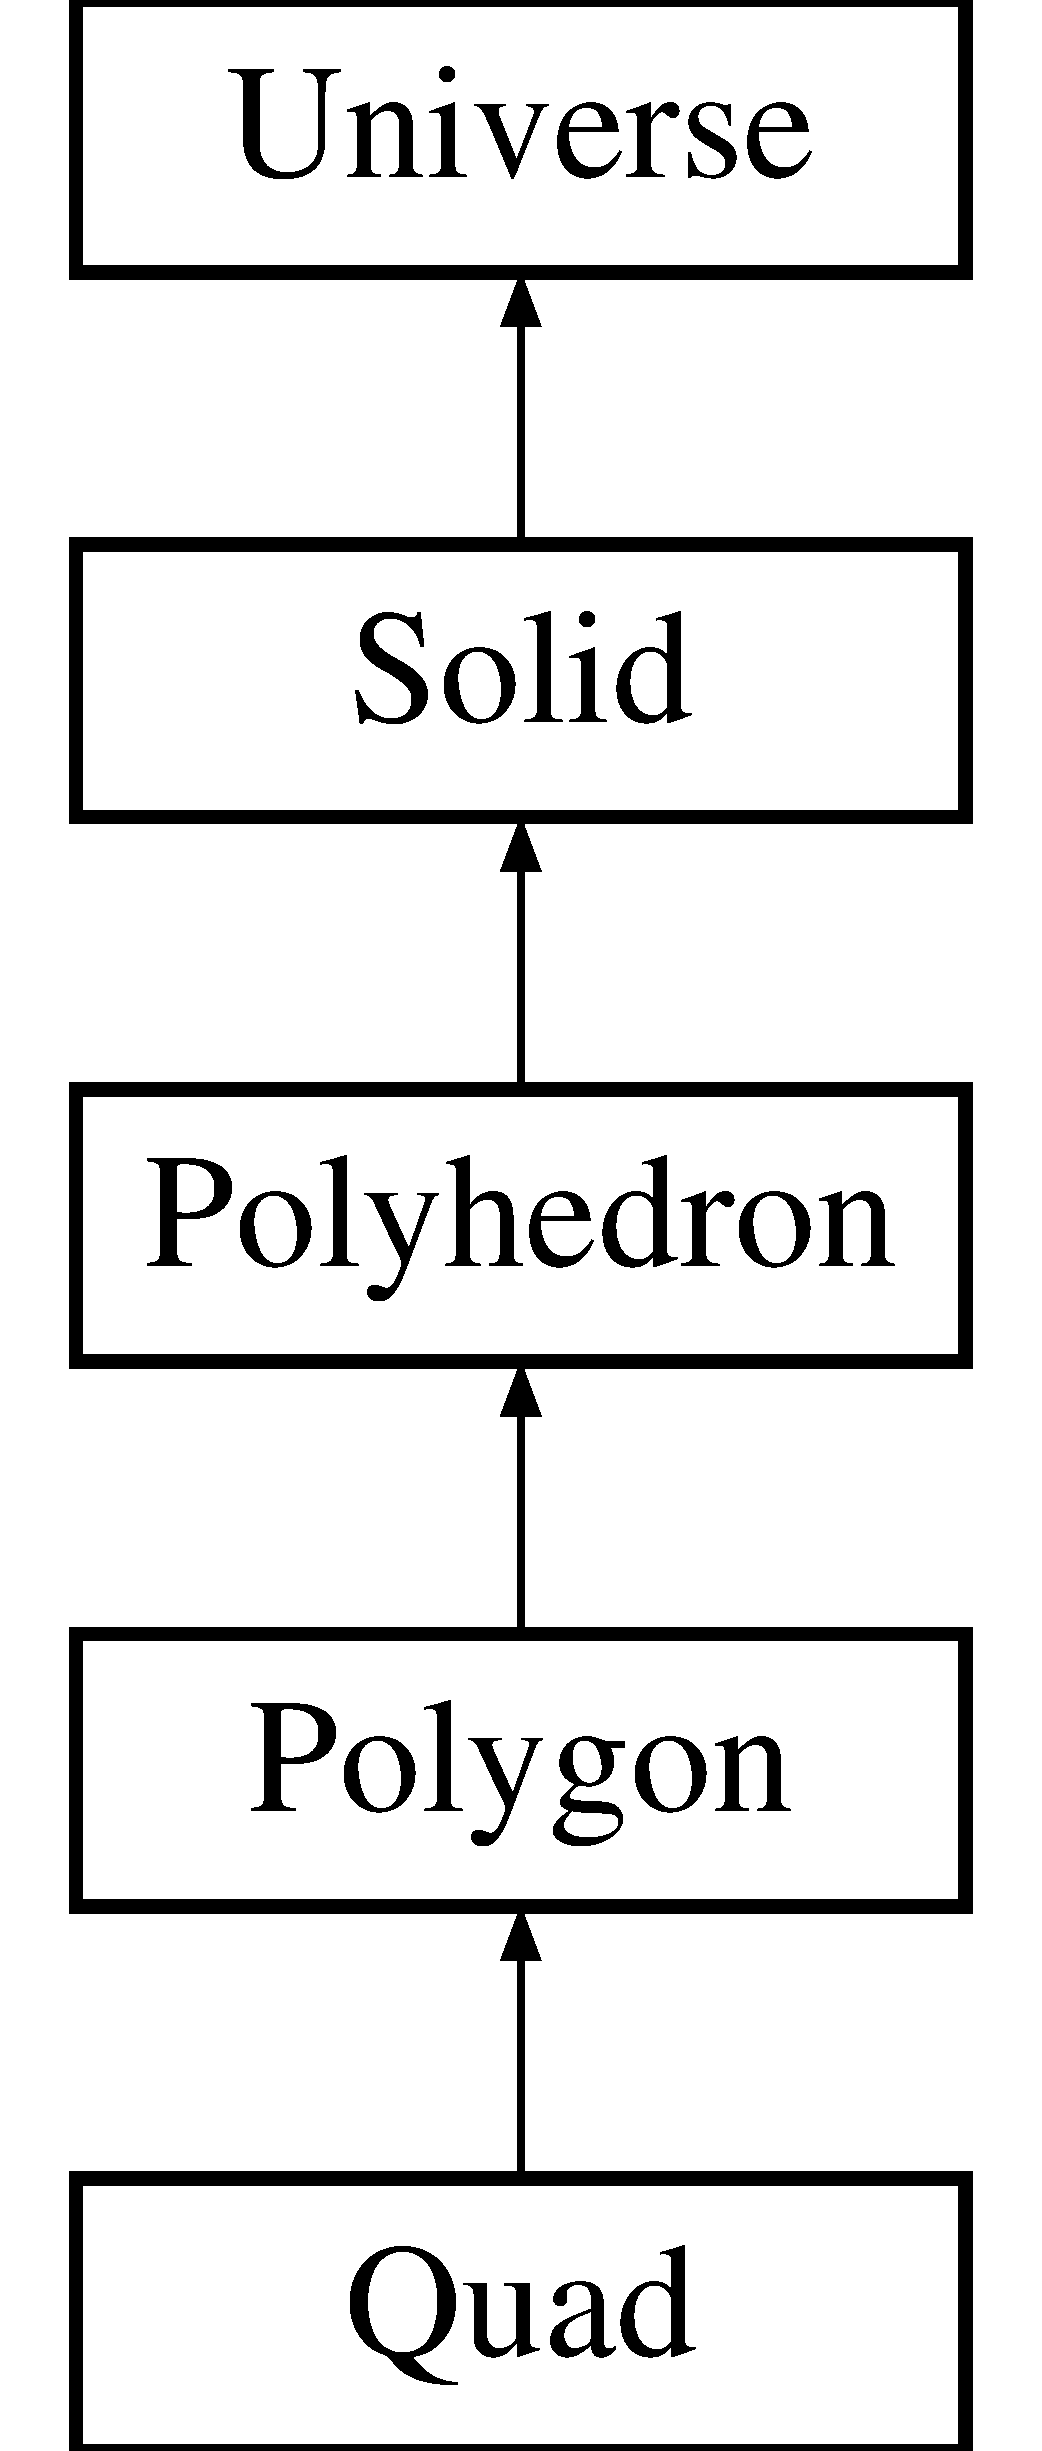
\includegraphics[height=5.000000cm]{classPolygon}
\end{center}
\end{figure}
\subsection*{Public Member Functions}
\begin{DoxyCompactItemize}
\item 
\mbox{\hyperlink{classPolygon_ac183e712f8be1e13f1c9d5b4d4512ead}{Polygon}} ()
\item 
\mbox{\hyperlink{classPolygon_a023fe85caf3682e46fb6d15d03da3435}{Polygon}} (unsigned int object\+\_\+type)
\item 
\mbox{\hyperlink{classPolygon_aa2a7d4a8a7765c45b834a7ecc198e0c3}{Polygon}} (unsigned int object\+\_\+type, std\+::chrono\+::time\+\_\+point$<$ \mbox{\hyperlink{universe_8h_a0ef8d951d1ca5ab3cfaf7ab4c7a6fd80}{Clock}} $>$ event\+\_\+time)
\item 
\mbox{\hyperlink{classPolygon_a581ad88f80bf40668e6c8b928c908bcb}{Polygon}} (unsigned int object\+\_\+type, std\+::chrono\+::time\+\_\+point$<$ \mbox{\hyperlink{universe_8h_a0ef8d951d1ca5ab3cfaf7ab4c7a6fd80}{Clock}} $>$ event\+\_\+time, \mbox{\hyperlink{classPolyhedron}{Polyhedron}} \&polyhedron\+\_\+connector)
\item 
virtual \mbox{\hyperlink{classPolygon_a873f9acee059f717277b6414102dab16}{$\sim$\+Polygon}} ()
\item 
bool \mbox{\hyperlink{classPolygon_a0e2824d12cd6b18c8b14c64ef4b2bf97}{Reset\+Parameters}} (std\+::chrono\+::time\+\_\+point$<$ \mbox{\hyperlink{universe_8h_a0ef8d951d1ca5ab3cfaf7ab4c7a6fd80}{Clock}} $>$ event\+\_\+time)
\item 
unsigned int \mbox{\hyperlink{classPolygon_a344626b07ee8dc40c71c3bec1480d2c2}{Set\+Counter}} (std\+::chrono\+::time\+\_\+point$<$ \mbox{\hyperlink{universe_8h_a0ef8d951d1ca5ab3cfaf7ab4c7a6fd80}{Clock}} $>$ event\+\_\+time)
\item 
void \mbox{\hyperlink{classPolygon_ad12083d8c152a1979b04bead93b6b730}{Set\+Counter}} (std\+::chrono\+::time\+\_\+point$<$ \mbox{\hyperlink{universe_8h_a0ef8d951d1ca5ab3cfaf7ab4c7a6fd80}{Clock}} $>$ event\+\_\+time, unsigned int val)
\item 
int \mbox{\hyperlink{classPolygon_ab3fe58d8ffce2e16589958def88aa188}{Update}} (std\+::chrono\+::time\+\_\+point$<$ \mbox{\hyperlink{universe_8h_a0ef8d951d1ca5ab3cfaf7ab4c7a6fd80}{Clock}} $>$ event\+\_\+time)
\end{DoxyCompactItemize}
\subsection*{Private Attributes}
\begin{DoxyCompactItemize}
\item 
unsigned int \mbox{\hyperlink{classPolygon_a4292b71e5bf6d76a09f582dedf81c862}{polygon\+Counter}}
\begin{DoxyCompactList}\small\item\em Member variable \char`\"{}polygon\+Counter\char`\"{}. \end{DoxyCompactList}\item 
int \mbox{\hyperlink{classPolygon_aba437ec0b8ab34ca435e1a653c69b558}{polygon\+\_\+type}}
\item 
std\+::chrono\+::time\+\_\+point$<$ \mbox{\hyperlink{universe_8h_a0ef8d951d1ca5ab3cfaf7ab4c7a6fd80}{Clock}} $>$ \mbox{\hyperlink{classPolygon_a46fa35a90ffcf375c8eceb2cf8a169d0}{previous\+\_\+event\+\_\+time}}
\item 
std\+::chrono\+::time\+\_\+point$<$ \mbox{\hyperlink{universe_8h_a0ef8d951d1ca5ab3cfaf7ab4c7a6fd80}{Clock}} $>$ \mbox{\hyperlink{classPolygon_af5b19b47f12f4984521d6f48a45c1428}{time\+\_\+object\+\_\+created}}
\item 
bool \mbox{\hyperlink{classPolygon_ada7d263fdf6c7a6138c71ca93bbea02f}{object\+\_\+disabled}} = true
\item 
bool \mbox{\hyperlink{classPolygon_a1c59030523e7784edf3c17dad240c821}{object\+\_\+initialised}} = false
\item 
int \mbox{\hyperlink{classPolygon_a06161c2266baa0d3ef7afeeeccc0547b}{duration\+\_\+since\+\_\+last\+\_\+event}}
\end{DoxyCompactItemize}
\subsection*{Additional Inherited Members}


\subsection{Constructor \& Destructor Documentation}
\mbox{\Hypertarget{classPolygon_ac183e712f8be1e13f1c9d5b4d4512ead}\label{classPolygon_ac183e712f8be1e13f1c9d5b4d4512ead}} 
\index{Polygon@{Polygon}!Polygon@{Polygon}}
\index{Polygon@{Polygon}!Polygon@{Polygon}}
\subsubsection{\texorpdfstring{Polygon()}{Polygon()}\hspace{0.1cm}{\footnotesize\ttfamily [1/4]}}
{\footnotesize\ttfamily Polygon\+::\+Polygon (\begin{DoxyParamCaption}{ }\end{DoxyParamCaption})\hspace{0.3cm}{\ttfamily [inline]}}

\mbox{\Hypertarget{classPolygon_a023fe85caf3682e46fb6d15d03da3435}\label{classPolygon_a023fe85caf3682e46fb6d15d03da3435}} 
\index{Polygon@{Polygon}!Polygon@{Polygon}}
\index{Polygon@{Polygon}!Polygon@{Polygon}}
\subsubsection{\texorpdfstring{Polygon()}{Polygon()}\hspace{0.1cm}{\footnotesize\ttfamily [2/4]}}
{\footnotesize\ttfamily Polygon\+::\+Polygon (\begin{DoxyParamCaption}\item[{unsigned int}]{object\+\_\+type }\end{DoxyParamCaption})\hspace{0.3cm}{\ttfamily [inline]}}

\mbox{\Hypertarget{classPolygon_aa2a7d4a8a7765c45b834a7ecc198e0c3}\label{classPolygon_aa2a7d4a8a7765c45b834a7ecc198e0c3}} 
\index{Polygon@{Polygon}!Polygon@{Polygon}}
\index{Polygon@{Polygon}!Polygon@{Polygon}}
\subsubsection{\texorpdfstring{Polygon()}{Polygon()}\hspace{0.1cm}{\footnotesize\ttfamily [3/4]}}
{\footnotesize\ttfamily Polygon\+::\+Polygon (\begin{DoxyParamCaption}\item[{unsigned int}]{object\+\_\+type,  }\item[{std\+::chrono\+::time\+\_\+point$<$ \mbox{\hyperlink{universe_8h_a0ef8d951d1ca5ab3cfaf7ab4c7a6fd80}{Clock}} $>$}]{event\+\_\+time }\end{DoxyParamCaption})\hspace{0.3cm}{\ttfamily [inline]}}

\mbox{\Hypertarget{classPolygon_a581ad88f80bf40668e6c8b928c908bcb}\label{classPolygon_a581ad88f80bf40668e6c8b928c908bcb}} 
\index{Polygon@{Polygon}!Polygon@{Polygon}}
\index{Polygon@{Polygon}!Polygon@{Polygon}}
\subsubsection{\texorpdfstring{Polygon()}{Polygon()}\hspace{0.1cm}{\footnotesize\ttfamily [4/4]}}
{\footnotesize\ttfamily Polygon\+::\+Polygon (\begin{DoxyParamCaption}\item[{unsigned int}]{object\+\_\+type,  }\item[{std\+::chrono\+::time\+\_\+point$<$ \mbox{\hyperlink{universe_8h_a0ef8d951d1ca5ab3cfaf7ab4c7a6fd80}{Clock}} $>$}]{event\+\_\+time,  }\item[{\mbox{\hyperlink{classPolyhedron}{Polyhedron}} \&}]{polyhedron\+\_\+connector }\end{DoxyParamCaption})\hspace{0.3cm}{\ttfamily [inline]}}

\mbox{\Hypertarget{classPolygon_a873f9acee059f717277b6414102dab16}\label{classPolygon_a873f9acee059f717277b6414102dab16}} 
\index{Polygon@{Polygon}!````~Polygon@{$\sim$\+Polygon}}
\index{````~Polygon@{$\sim$\+Polygon}!Polygon@{Polygon}}
\subsubsection{\texorpdfstring{$\sim$\+Polygon()}{~Polygon()}}
{\footnotesize\ttfamily virtual Polygon\+::$\sim$\+Polygon (\begin{DoxyParamCaption}{ }\end{DoxyParamCaption})\hspace{0.3cm}{\ttfamily [inline]}, {\ttfamily [virtual]}}



\subsection{Member Function Documentation}
\mbox{\Hypertarget{classPolygon_a0e2824d12cd6b18c8b14c64ef4b2bf97}\label{classPolygon_a0e2824d12cd6b18c8b14c64ef4b2bf97}} 
\index{Polygon@{Polygon}!Reset\+Parameters@{Reset\+Parameters}}
\index{Reset\+Parameters@{Reset\+Parameters}!Polygon@{Polygon}}
\subsubsection{\texorpdfstring{Reset\+Parameters()}{ResetParameters()}}
{\footnotesize\ttfamily bool Polygon\+::\+Reset\+Parameters (\begin{DoxyParamCaption}\item[{std\+::chrono\+::time\+\_\+point$<$ \mbox{\hyperlink{universe_8h_a0ef8d951d1ca5ab3cfaf7ab4c7a6fd80}{Clock}} $>$}]{event\+\_\+time }\end{DoxyParamCaption})}

\mbox{\Hypertarget{classPolygon_a344626b07ee8dc40c71c3bec1480d2c2}\label{classPolygon_a344626b07ee8dc40c71c3bec1480d2c2}} 
\index{Polygon@{Polygon}!Set\+Counter@{Set\+Counter}}
\index{Set\+Counter@{Set\+Counter}!Polygon@{Polygon}}
\subsubsection{\texorpdfstring{Set\+Counter()}{SetCounter()}\hspace{0.1cm}{\footnotesize\ttfamily [1/2]}}
{\footnotesize\ttfamily unsigned int Polygon\+::\+Set\+Counter (\begin{DoxyParamCaption}\item[{std\+::chrono\+::time\+\_\+point$<$ \mbox{\hyperlink{universe_8h_a0ef8d951d1ca5ab3cfaf7ab4c7a6fd80}{Clock}} $>$}]{event\+\_\+time }\end{DoxyParamCaption})\hspace{0.3cm}{\ttfamily [inline]}}

\mbox{\Hypertarget{classPolygon_ad12083d8c152a1979b04bead93b6b730}\label{classPolygon_ad12083d8c152a1979b04bead93b6b730}} 
\index{Polygon@{Polygon}!Set\+Counter@{Set\+Counter}}
\index{Set\+Counter@{Set\+Counter}!Polygon@{Polygon}}
\subsubsection{\texorpdfstring{Set\+Counter()}{SetCounter()}\hspace{0.1cm}{\footnotesize\ttfamily [2/2]}}
{\footnotesize\ttfamily void Polygon\+::\+Set\+Counter (\begin{DoxyParamCaption}\item[{std\+::chrono\+::time\+\_\+point$<$ \mbox{\hyperlink{universe_8h_a0ef8d951d1ca5ab3cfaf7ab4c7a6fd80}{Clock}} $>$}]{event\+\_\+time,  }\item[{unsigned int}]{val }\end{DoxyParamCaption})\hspace{0.3cm}{\ttfamily [inline]}, {\ttfamily [virtual]}}



Reimplemented from \mbox{\hyperlink{classUniverse_aa22202ae740eb1355529afcb13285e91}{Universe}}.

\mbox{\Hypertarget{classPolygon_ab3fe58d8ffce2e16589958def88aa188}\label{classPolygon_ab3fe58d8ffce2e16589958def88aa188}} 
\index{Polygon@{Polygon}!Update@{Update}}
\index{Update@{Update}!Polygon@{Polygon}}
\subsubsection{\texorpdfstring{Update()}{Update()}}
{\footnotesize\ttfamily int Polygon\+::\+Update (\begin{DoxyParamCaption}\item[{std\+::chrono\+::time\+\_\+point$<$ \mbox{\hyperlink{universe_8h_a0ef8d951d1ca5ab3cfaf7ab4c7a6fd80}{Clock}} $>$}]{event\+\_\+time }\end{DoxyParamCaption})}



\subsection{Member Data Documentation}
\mbox{\Hypertarget{classPolygon_a06161c2266baa0d3ef7afeeeccc0547b}\label{classPolygon_a06161c2266baa0d3ef7afeeeccc0547b}} 
\index{Polygon@{Polygon}!duration\+\_\+since\+\_\+last\+\_\+event@{duration\+\_\+since\+\_\+last\+\_\+event}}
\index{duration\+\_\+since\+\_\+last\+\_\+event@{duration\+\_\+since\+\_\+last\+\_\+event}!Polygon@{Polygon}}
\subsubsection{\texorpdfstring{duration\+\_\+since\+\_\+last\+\_\+event}{duration\_since\_last\_event}}
{\footnotesize\ttfamily int Polygon\+::duration\+\_\+since\+\_\+last\+\_\+event\hspace{0.3cm}{\ttfamily [private]}}

\mbox{\Hypertarget{classPolygon_ada7d263fdf6c7a6138c71ca93bbea02f}\label{classPolygon_ada7d263fdf6c7a6138c71ca93bbea02f}} 
\index{Polygon@{Polygon}!object\+\_\+disabled@{object\+\_\+disabled}}
\index{object\+\_\+disabled@{object\+\_\+disabled}!Polygon@{Polygon}}
\subsubsection{\texorpdfstring{object\+\_\+disabled}{object\_disabled}}
{\footnotesize\ttfamily bool Polygon\+::object\+\_\+disabled = true\hspace{0.3cm}{\ttfamily [private]}}

\mbox{\Hypertarget{classPolygon_a1c59030523e7784edf3c17dad240c821}\label{classPolygon_a1c59030523e7784edf3c17dad240c821}} 
\index{Polygon@{Polygon}!object\+\_\+initialised@{object\+\_\+initialised}}
\index{object\+\_\+initialised@{object\+\_\+initialised}!Polygon@{Polygon}}
\subsubsection{\texorpdfstring{object\+\_\+initialised}{object\_initialised}}
{\footnotesize\ttfamily bool Polygon\+::object\+\_\+initialised = false\hspace{0.3cm}{\ttfamily [private]}}

\mbox{\Hypertarget{classPolygon_aba437ec0b8ab34ca435e1a653c69b558}\label{classPolygon_aba437ec0b8ab34ca435e1a653c69b558}} 
\index{Polygon@{Polygon}!polygon\+\_\+type@{polygon\+\_\+type}}
\index{polygon\+\_\+type@{polygon\+\_\+type}!Polygon@{Polygon}}
\subsubsection{\texorpdfstring{polygon\+\_\+type}{polygon\_type}}
{\footnotesize\ttfamily int Polygon\+::polygon\+\_\+type\hspace{0.3cm}{\ttfamily [private]}}

\mbox{\Hypertarget{classPolygon_a4292b71e5bf6d76a09f582dedf81c862}\label{classPolygon_a4292b71e5bf6d76a09f582dedf81c862}} 
\index{Polygon@{Polygon}!polygon\+Counter@{polygon\+Counter}}
\index{polygon\+Counter@{polygon\+Counter}!Polygon@{Polygon}}
\subsubsection{\texorpdfstring{polygon\+Counter}{polygonCounter}}
{\footnotesize\ttfamily unsigned int Polygon\+::polygon\+Counter\hspace{0.3cm}{\ttfamily [private]}}



Member variable \char`\"{}polygon\+Counter\char`\"{}. 

\mbox{\Hypertarget{classPolygon_a46fa35a90ffcf375c8eceb2cf8a169d0}\label{classPolygon_a46fa35a90ffcf375c8eceb2cf8a169d0}} 
\index{Polygon@{Polygon}!previous\+\_\+event\+\_\+time@{previous\+\_\+event\+\_\+time}}
\index{previous\+\_\+event\+\_\+time@{previous\+\_\+event\+\_\+time}!Polygon@{Polygon}}
\subsubsection{\texorpdfstring{previous\+\_\+event\+\_\+time}{previous\_event\_time}}
{\footnotesize\ttfamily std\+::chrono\+::time\+\_\+point$<$\mbox{\hyperlink{universe_8h_a0ef8d951d1ca5ab3cfaf7ab4c7a6fd80}{Clock}}$>$ Polygon\+::previous\+\_\+event\+\_\+time\hspace{0.3cm}{\ttfamily [private]}}

\mbox{\Hypertarget{classPolygon_af5b19b47f12f4984521d6f48a45c1428}\label{classPolygon_af5b19b47f12f4984521d6f48a45c1428}} 
\index{Polygon@{Polygon}!time\+\_\+object\+\_\+created@{time\+\_\+object\+\_\+created}}
\index{time\+\_\+object\+\_\+created@{time\+\_\+object\+\_\+created}!Polygon@{Polygon}}
\subsubsection{\texorpdfstring{time\+\_\+object\+\_\+created}{time\_object\_created}}
{\footnotesize\ttfamily std\+::chrono\+::time\+\_\+point$<$\mbox{\hyperlink{universe_8h_a0ef8d951d1ca5ab3cfaf7ab4c7a6fd80}{Clock}}$>$ Polygon\+::time\+\_\+object\+\_\+created\hspace{0.3cm}{\ttfamily [private]}}



The documentation for this class was generated from the following files\+:\begin{DoxyCompactItemize}
\item 
/home/pbisaacs/\+Developer/\+Brain\+Harmonics/\mbox{\hyperlink{polygon_8h}{polygon.\+h}}\item 
/home/pbisaacs/\+Developer/\+Brain\+Harmonics/\mbox{\hyperlink{polygon_8cc}{polygon.\+cc}}\end{DoxyCompactItemize}

\hypertarget{classPolyhedron}{}\section{Polyhedron Class Reference}
\label{classPolyhedron}\index{Polyhedron@{Polyhedron}}


{\ttfamily \#include $<$polyhedron.\+h$>$}

Inheritance diagram for Polyhedron\+:\begin{figure}[H]
\begin{center}
\leavevmode
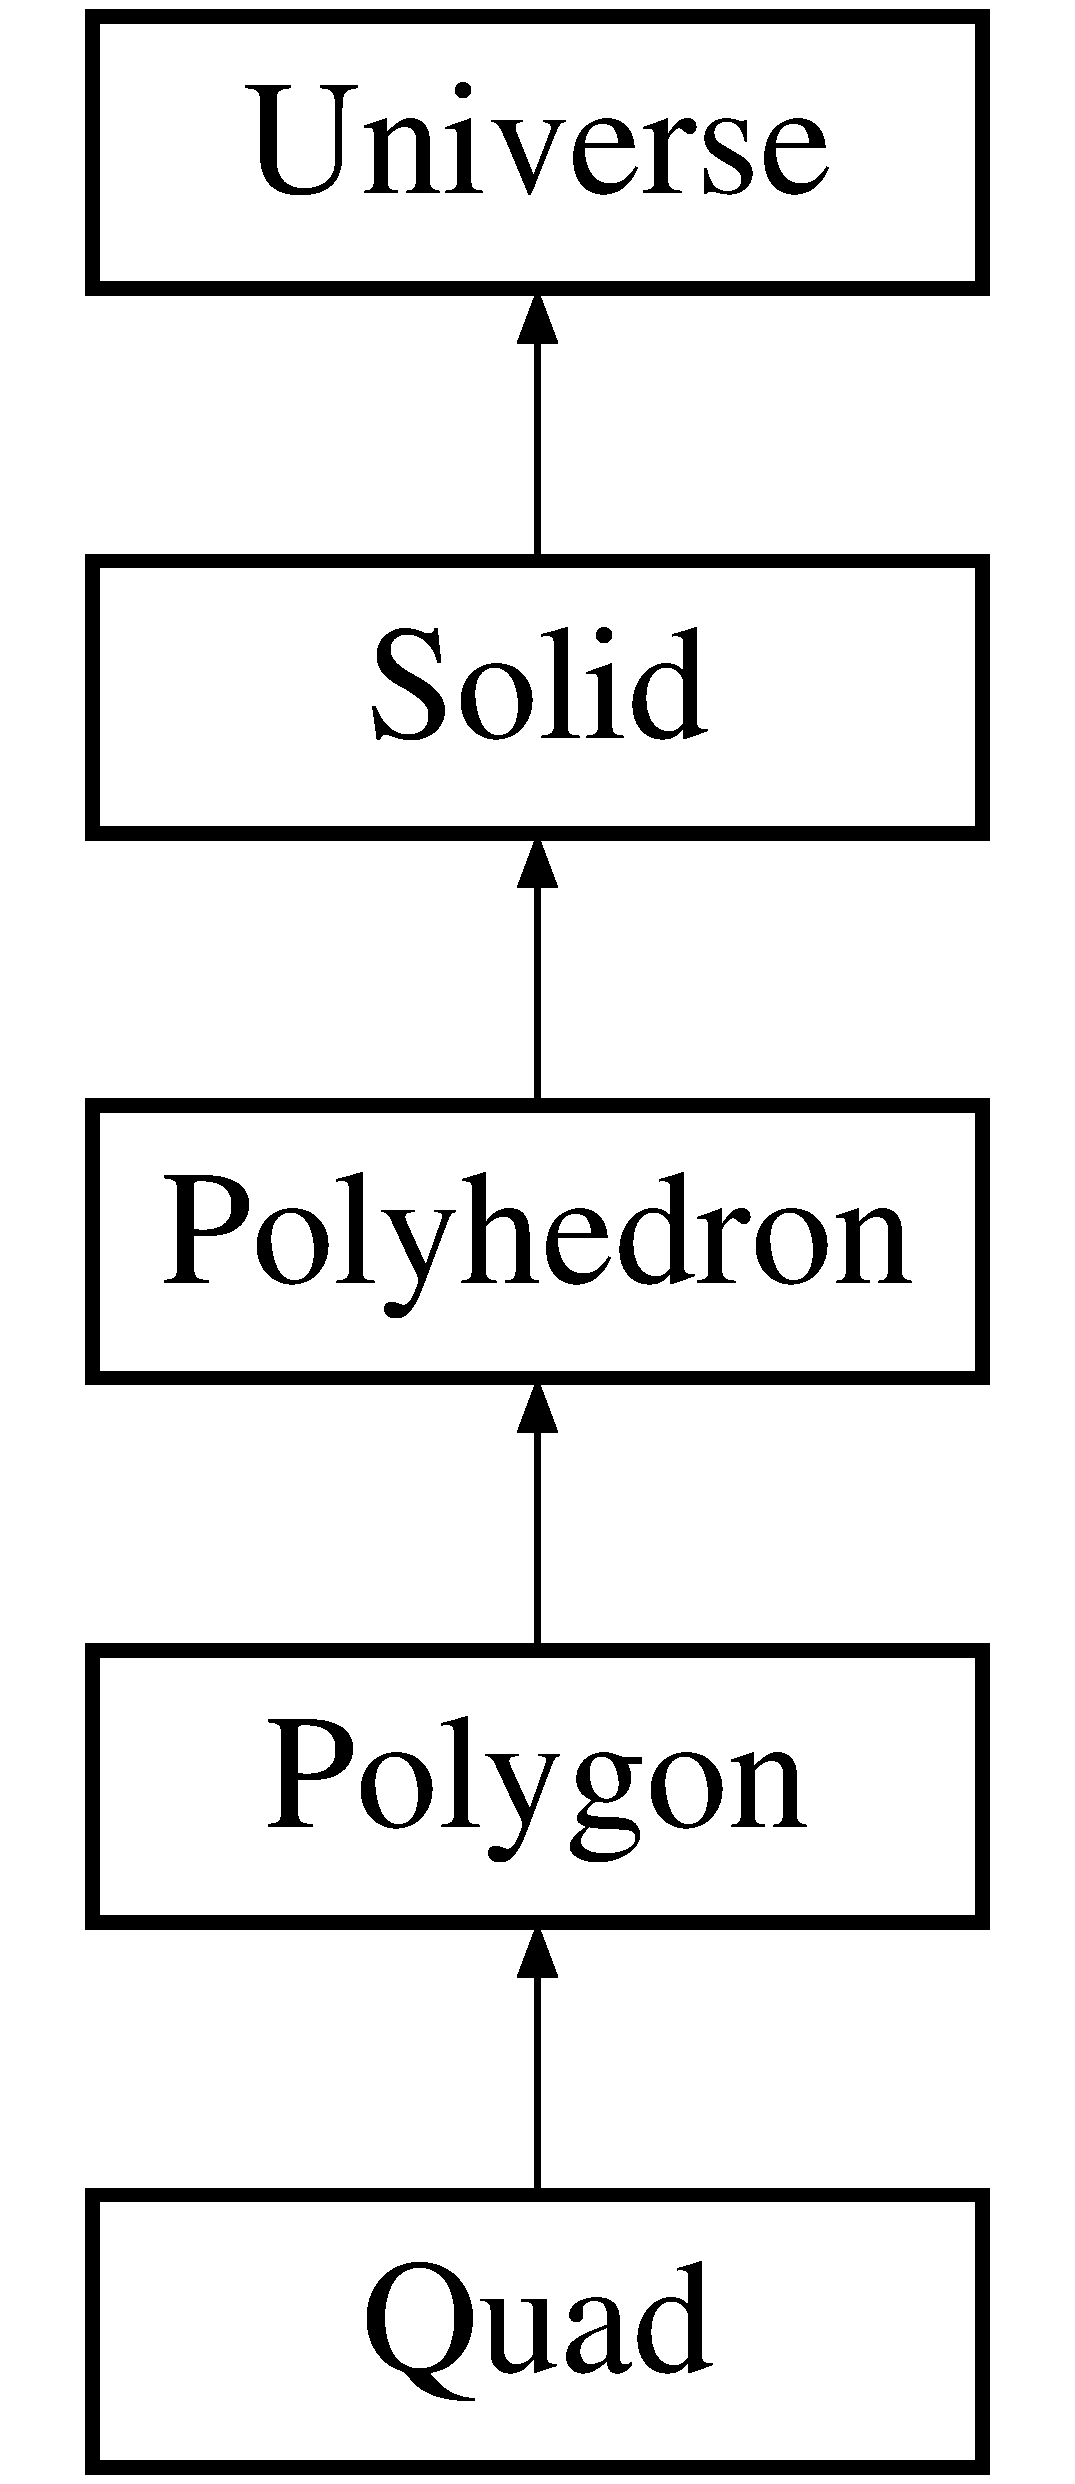
\includegraphics[height=5.000000cm]{classPolyhedron}
\end{center}
\end{figure}
\subsection*{Public Member Functions}
\begin{DoxyCompactItemize}
\item 
\mbox{\hyperlink{classPolyhedron_aebdf7ee85eb636069bf93afb4e6a483f}{Polyhedron}} ()
\item 
\mbox{\hyperlink{classPolyhedron_a304950efef7fb67203d8136578b42535}{Polyhedron}} (unsigned int object\+\_\+type)
\item 
\mbox{\hyperlink{classPolyhedron_a29a4fff595cdb6a557e5f62255e61192}{Polyhedron}} (unsigned int object\+\_\+type, std\+::chrono\+::time\+\_\+point$<$ \mbox{\hyperlink{universe_8h_a0ef8d951d1ca5ab3cfaf7ab4c7a6fd80}{Clock}} $>$ event\+\_\+time)
\item 
\mbox{\hyperlink{classPolyhedron_af5bb1d2a6b04502dfdbfc9f04aafc950}{Polyhedron}} (unsigned int object\+\_\+type, std\+::chrono\+::time\+\_\+point$<$ \mbox{\hyperlink{universe_8h_a0ef8d951d1ca5ab3cfaf7ab4c7a6fd80}{Clock}} $>$ event\+\_\+time, \mbox{\hyperlink{classSolid}{Solid}} \&solid\+\_\+connector)
\item 
virtual \mbox{\hyperlink{classPolyhedron_a3ad3df8be901a55ddcd97128ac890473}{$\sim$\+Polyhedron}} ()
\item 
bool \mbox{\hyperlink{classPolyhedron_ae90c347cfb8ca8028a260e88bef2b45c}{Reset\+Parameters}} (std\+::chrono\+::time\+\_\+point$<$ \mbox{\hyperlink{universe_8h_a0ef8d951d1ca5ab3cfaf7ab4c7a6fd80}{Clock}} $>$ event\+\_\+time)
\item 
unsigned int \mbox{\hyperlink{classPolyhedron_a021ec67f2040f8ec26df64e4b9370521}{Get\+Counter}} (std\+::chrono\+::time\+\_\+point$<$ \mbox{\hyperlink{universe_8h_a0ef8d951d1ca5ab3cfaf7ab4c7a6fd80}{Clock}} $>$ event\+\_\+time)
\item 
void \mbox{\hyperlink{classPolyhedron_ad74a1ccc28a08bc2dbc186e5f2c1f694}{set\+Counter}} (unsigned int val)
\item 
void \mbox{\hyperlink{classPolyhedron_a014c8f981aef5fa1d70dcb5be6a0875a}{Set\+Object\+Type}} (std\+::chrono\+::time\+\_\+point$<$ \mbox{\hyperlink{universe_8h_a0ef8d951d1ca5ab3cfaf7ab4c7a6fd80}{Clock}} $>$ event\+\_\+time, unsigned int val)
\item 
\mbox{\hyperlink{classPolyhedron}{Polyhedron}} $\ast$ \mbox{\hyperlink{classPolyhedron_ae5852dd26065d9f38ed293f8d95106ad}{Create\+Polygon}} (std\+::chrono\+::time\+\_\+point$<$ \mbox{\hyperlink{universe_8h_a0ef8d951d1ca5ab3cfaf7ab4c7a6fd80}{Clock}} $>$ event\+\_\+time)
\item 
std\+::vector$<$ \mbox{\hyperlink{classPolyhedron}{Polyhedron}} $\ast$ $>$ \mbox{\hyperlink{classPolyhedron_a1848eb8747c1132c40c2d27336af2896}{Create\+Polygons}} (std\+::chrono\+::time\+\_\+point$<$ \mbox{\hyperlink{universe_8h_a0ef8d951d1ca5ab3cfaf7ab4c7a6fd80}{Clock}} $>$ event\+\_\+time, int quantity)
\item 
\mbox{\hyperlink{classPolyhedron}{Polyhedron}} $\ast$ \mbox{\hyperlink{classPolyhedron_abfacad3a348785dab8819e70bf92d8d1}{Clone\+Polygon}} (std\+::chrono\+::time\+\_\+point$<$ \mbox{\hyperlink{universe_8h_a0ef8d951d1ca5ab3cfaf7ab4c7a6fd80}{Clock}} $>$ event\+\_\+time, \mbox{\hyperlink{classPolyhedron}{Polyhedron}} $\ast$clone\+\_\+object, double perfection\+\_\+membership)
\item 
std\+::vector$<$ \mbox{\hyperlink{classPolyhedron}{Polyhedron}} $\ast$ $>$ \mbox{\hyperlink{classPolyhedron_ab4f57da9595dc92de7340cc46237a2ea}{Clone\+Polygons}} (std\+::chrono\+::time\+\_\+point$<$ \mbox{\hyperlink{universe_8h_a0ef8d951d1ca5ab3cfaf7ab4c7a6fd80}{Clock}} $>$ event\+\_\+time, std\+::vector$<$ \mbox{\hyperlink{classPolyhedron}{Polyhedron}} $\ast$$>$ cloning\+\_\+list, double perfection\+\_\+membership)
\item 
\mbox{\hyperlink{classPolyhedron}{Polyhedron}} $\ast$ \mbox{\hyperlink{classPolyhedron_a2fcc5144ebc64363f40c31d2b980cfaf}{Destroy\+Polygon}} (std\+::chrono\+::time\+\_\+point$<$ \mbox{\hyperlink{universe_8h_a0ef8d951d1ca5ab3cfaf7ab4c7a6fd80}{Clock}} $>$ event\+\_\+time, \mbox{\hyperlink{classPolyhedron}{Polyhedron}} $\ast$destroy\+\_\+object)
\item 
std\+::vector$<$ \mbox{\hyperlink{classPolyhedron}{Polyhedron}} $\ast$ $>$ \mbox{\hyperlink{classPolyhedron_ae372d216765d48b9423ee37a8bf8b282}{Destroy\+Polygons}} (std\+::chrono\+::time\+\_\+point$<$ \mbox{\hyperlink{universe_8h_a0ef8d951d1ca5ab3cfaf7ab4c7a6fd80}{Clock}} $>$ event\+\_\+time, std\+::vector$<$ \mbox{\hyperlink{classPolyhedron}{Polyhedron}} $\ast$$>$ destruction\+\_\+list)
\item 
\mbox{\hyperlink{classPolyhedron}{Polyhedron}} $\ast$ \mbox{\hyperlink{classPolyhedron_a63bc509a87935cc25e541d2490c01d1f}{Add\+Polygon}} (std\+::chrono\+::time\+\_\+point$<$ \mbox{\hyperlink{universe_8h_a0ef8d951d1ca5ab3cfaf7ab4c7a6fd80}{Clock}} $>$ event\+\_\+time, \mbox{\hyperlink{classPolyhedron}{Polyhedron}} $\ast$add\+\_\+object)
\item 
std\+::vector$<$ \mbox{\hyperlink{classPolyhedron}{Polyhedron}} $\ast$ $>$ \mbox{\hyperlink{classPolyhedron_a9564a286e7323b56667971b851f0674a}{Add\+Polygons}} (std\+::chrono\+::time\+\_\+point$<$ \mbox{\hyperlink{universe_8h_a0ef8d951d1ca5ab3cfaf7ab4c7a6fd80}{Clock}} $>$ event\+\_\+time, std\+::vector$<$ \mbox{\hyperlink{classPolyhedron}{Polyhedron}} $\ast$$>$ add\+\_\+objects)
\item 
\mbox{\hyperlink{classPolyhedron}{Polyhedron}} $\ast$ \mbox{\hyperlink{classPolyhedron_a3b411fa617291a2a2d5df92b819285b4}{Remove\+Polygon}} (std\+::chrono\+::time\+\_\+point$<$ \mbox{\hyperlink{universe_8h_a0ef8d951d1ca5ab3cfaf7ab4c7a6fd80}{Clock}} $>$ event\+\_\+time)
\item 
std\+::vector$<$ \mbox{\hyperlink{classPolyhedron}{Polyhedron}} $\ast$ $>$ \mbox{\hyperlink{classPolyhedron_a5c2639b21aec25b76449fdf4c209aad1}{Remove\+Polygons}} (std\+::chrono\+::time\+\_\+point$<$ \mbox{\hyperlink{universe_8h_a0ef8d951d1ca5ab3cfaf7ab4c7a6fd80}{Clock}} $>$ event\+\_\+time, int quantity)
\item 
\mbox{\hyperlink{classPolyhedron}{Polyhedron}} $\ast$ \mbox{\hyperlink{classPolyhedron_a8b197b9eb163bdc83d9669d592bacac1}{Get\+Polygon}} (std\+::chrono\+::time\+\_\+point$<$ \mbox{\hyperlink{universe_8h_a0ef8d951d1ca5ab3cfaf7ab4c7a6fd80}{Clock}} $>$ event\+\_\+time, int selector)
\item 
std\+::vector$<$ \mbox{\hyperlink{classPolyhedron}{Polyhedron}} $\ast$ $>$ \mbox{\hyperlink{classPolyhedron_adeaf461cc8504a225f6344b954c196a8}{Get\+Polygons}} (std\+::chrono\+::time\+\_\+point$<$ \mbox{\hyperlink{universe_8h_a0ef8d951d1ca5ab3cfaf7ab4c7a6fd80}{Clock}} $>$ event\+\_\+time)
\item 
\mbox{\hyperlink{classPoint}{Point}} $\ast$ \mbox{\hyperlink{classPolyhedron_a4d61f89c56e15d96008856cfb540d558}{Get\+Point}} (std\+::chrono\+::time\+\_\+point$<$ \mbox{\hyperlink{universe_8h_a0ef8d951d1ca5ab3cfaf7ab4c7a6fd80}{Clock}} $>$ event\+\_\+time, int selector)
\item 
std\+::vector$<$ \mbox{\hyperlink{classPoint}{Point}} $\ast$ $>$ \mbox{\hyperlink{classPolyhedron_a1430429d6c8447e90b8c94ca46496a59}{Get\+Points}} (std\+::chrono\+::time\+\_\+point$<$ \mbox{\hyperlink{universe_8h_a0ef8d951d1ca5ab3cfaf7ab4c7a6fd80}{Clock}} $>$ event\+\_\+time)
\item 
int \mbox{\hyperlink{classPolyhedron_a15d1cae35ceb6c1ba559928fd417800c}{Generate\+Sphere\+Points}} (std\+::chrono\+::time\+\_\+point$<$ \mbox{\hyperlink{universe_8h_a0ef8d951d1ca5ab3cfaf7ab4c7a6fd80}{Clock}} $>$ event\+\_\+time)
\item 
int \mbox{\hyperlink{classPolyhedron_a642a64ae8cde5e2a9f15334e151fd3f9}{Generate\+Cylinder\+Points}} (std\+::chrono\+::time\+\_\+point$<$ \mbox{\hyperlink{universe_8h_a0ef8d951d1ca5ab3cfaf7ab4c7a6fd80}{Clock}} $>$ event\+\_\+time)
\item 
void \mbox{\hyperlink{classPolyhedron_a6b26174513703bc2b13f69b9cd8e1a48}{Update\+Cycle}} (std\+::chrono\+::time\+\_\+point$<$ \mbox{\hyperlink{universe_8h_a0ef8d951d1ca5ab3cfaf7ab4c7a6fd80}{Clock}} $>$ event\+\_\+time, std\+::vector$<$ \mbox{\hyperlink{classPoint}{Point}} $\ast$$>$ set\+\_\+of\+\_\+update\+\_\+pointers, unsigned int pointer\+\_\+type)
\item 
int \mbox{\hyperlink{classPolyhedron_a5fdc8c91719799904b8a1ccef535a42c}{Update}} (std\+::chrono\+::time\+\_\+point$<$ \mbox{\hyperlink{universe_8h_a0ef8d951d1ca5ab3cfaf7ab4c7a6fd80}{Clock}} $>$ event\+\_\+time)
\end{DoxyCompactItemize}
\subsection*{Protected Attributes}
\begin{DoxyCompactItemize}
\item 
std\+::vector$<$ \mbox{\hyperlink{classPolyhedron}{Polyhedron}} $\ast$ $>$ \mbox{\hyperlink{classPolyhedron_afd0cf6dddfbdc36266a73edca0c2c219}{polygon\+\_\+list}}
\item 
std\+::vector$<$ \mbox{\hyperlink{classPoint}{Point}} $\ast$ $>$ \mbox{\hyperlink{classPolyhedron_a4a39c8beb34831634b871dbc301502a6}{point\+\_\+list}}
\end{DoxyCompactItemize}
\subsection*{Private Attributes}
\begin{DoxyCompactItemize}
\item 
unsigned int \mbox{\hyperlink{classPolyhedron_a430c837e8a5a9dafc3ee32e7be24bd66}{polyhedron\+Counter}}
\begin{DoxyCompactList}\small\item\em Member variable \char`\"{}polyhedron\+Counter\char`\"{}. \end{DoxyCompactList}\item 
unsigned int \mbox{\hyperlink{classPolyhedron_aadbb8594382e92c3a9cb4e4592d8bdf5}{polyhedron\+\_\+type}} = 0
\item 
bool \mbox{\hyperlink{classPolyhedron_a7cafd82a09de260c4a5c57a264e4b7db}{object\+\_\+disabled}} = true
\item 
bool \mbox{\hyperlink{classPolyhedron_a33323db978a74f2ceaf15d950b5f18c1}{object\+\_\+initialised}} = false
\item 
std\+::chrono\+::time\+\_\+point$<$ \mbox{\hyperlink{universe_8h_a0ef8d951d1ca5ab3cfaf7ab4c7a6fd80}{Clock}} $>$ \mbox{\hyperlink{classPolyhedron_ae9d82476019a02008de7b1cb2e0e179f}{previous\+\_\+event\+\_\+time}}
\item 
std\+::chrono\+::time\+\_\+point$<$ \mbox{\hyperlink{universe_8h_a0ef8d951d1ca5ab3cfaf7ab4c7a6fd80}{Clock}} $>$ \mbox{\hyperlink{classPolyhedron_a59ae1bf10fa368663a38f3fab34534ca}{time\+\_\+object\+\_\+created}}
\item 
int \mbox{\hyperlink{classPolyhedron_a6ac1eea3357b7c5f70cd508117bba9f9}{duration\+\_\+since\+\_\+last\+\_\+event}}
\item 
int \mbox{\hyperlink{classPolyhedron_a33a190e2cf355ba85a9850a7f083c1c1}{polygon\+\_\+pool}}
\item 
int \mbox{\hyperlink{classPolyhedron_a22f74624a32515bbcf8de8a1818f1ee8}{point\+\_\+pool}}
\end{DoxyCompactItemize}
\subsection*{Friends}
\begin{DoxyCompactItemize}
\item 
class \mbox{\hyperlink{classPolyhedron_aaa07b7b364b620b9a781f30a5cd9f5ea}{Soma}}
\item 
class \mbox{\hyperlink{classPolyhedron_ac790db405644a01723104c3c0c8128bb}{Membrane}}
\end{DoxyCompactItemize}
\subsection*{Additional Inherited Members}


\subsection{Constructor \& Destructor Documentation}
\mbox{\Hypertarget{classPolyhedron_aebdf7ee85eb636069bf93afb4e6a483f}\label{classPolyhedron_aebdf7ee85eb636069bf93afb4e6a483f}} 
\index{Polyhedron@{Polyhedron}!Polyhedron@{Polyhedron}}
\index{Polyhedron@{Polyhedron}!Polyhedron@{Polyhedron}}
\subsubsection{\texorpdfstring{Polyhedron()}{Polyhedron()}\hspace{0.1cm}{\footnotesize\ttfamily [1/4]}}
{\footnotesize\ttfamily Polyhedron\+::\+Polyhedron (\begin{DoxyParamCaption}{ }\end{DoxyParamCaption})\hspace{0.3cm}{\ttfamily [inline]}}

\mbox{\Hypertarget{classPolyhedron_a304950efef7fb67203d8136578b42535}\label{classPolyhedron_a304950efef7fb67203d8136578b42535}} 
\index{Polyhedron@{Polyhedron}!Polyhedron@{Polyhedron}}
\index{Polyhedron@{Polyhedron}!Polyhedron@{Polyhedron}}
\subsubsection{\texorpdfstring{Polyhedron()}{Polyhedron()}\hspace{0.1cm}{\footnotesize\ttfamily [2/4]}}
{\footnotesize\ttfamily Polyhedron\+::\+Polyhedron (\begin{DoxyParamCaption}\item[{unsigned int}]{object\+\_\+type }\end{DoxyParamCaption})\hspace{0.3cm}{\ttfamily [inline]}}

\mbox{\Hypertarget{classPolyhedron_a29a4fff595cdb6a557e5f62255e61192}\label{classPolyhedron_a29a4fff595cdb6a557e5f62255e61192}} 
\index{Polyhedron@{Polyhedron}!Polyhedron@{Polyhedron}}
\index{Polyhedron@{Polyhedron}!Polyhedron@{Polyhedron}}
\subsubsection{\texorpdfstring{Polyhedron()}{Polyhedron()}\hspace{0.1cm}{\footnotesize\ttfamily [3/4]}}
{\footnotesize\ttfamily Polyhedron\+::\+Polyhedron (\begin{DoxyParamCaption}\item[{unsigned int}]{object\+\_\+type,  }\item[{std\+::chrono\+::time\+\_\+point$<$ \mbox{\hyperlink{universe_8h_a0ef8d951d1ca5ab3cfaf7ab4c7a6fd80}{Clock}} $>$}]{event\+\_\+time }\end{DoxyParamCaption})\hspace{0.3cm}{\ttfamily [inline]}}

\mbox{\Hypertarget{classPolyhedron_af5bb1d2a6b04502dfdbfc9f04aafc950}\label{classPolyhedron_af5bb1d2a6b04502dfdbfc9f04aafc950}} 
\index{Polyhedron@{Polyhedron}!Polyhedron@{Polyhedron}}
\index{Polyhedron@{Polyhedron}!Polyhedron@{Polyhedron}}
\subsubsection{\texorpdfstring{Polyhedron()}{Polyhedron()}\hspace{0.1cm}{\footnotesize\ttfamily [4/4]}}
{\footnotesize\ttfamily Polyhedron\+::\+Polyhedron (\begin{DoxyParamCaption}\item[{unsigned int}]{object\+\_\+type,  }\item[{std\+::chrono\+::time\+\_\+point$<$ \mbox{\hyperlink{universe_8h_a0ef8d951d1ca5ab3cfaf7ab4c7a6fd80}{Clock}} $>$}]{event\+\_\+time,  }\item[{\mbox{\hyperlink{classSolid}{Solid}} \&}]{solid\+\_\+connector }\end{DoxyParamCaption})\hspace{0.3cm}{\ttfamily [inline]}}

\mbox{\Hypertarget{classPolyhedron_a3ad3df8be901a55ddcd97128ac890473}\label{classPolyhedron_a3ad3df8be901a55ddcd97128ac890473}} 
\index{Polyhedron@{Polyhedron}!````~Polyhedron@{$\sim$\+Polyhedron}}
\index{````~Polyhedron@{$\sim$\+Polyhedron}!Polyhedron@{Polyhedron}}
\subsubsection{\texorpdfstring{$\sim$\+Polyhedron()}{~Polyhedron()}}
{\footnotesize\ttfamily virtual Polyhedron\+::$\sim$\+Polyhedron (\begin{DoxyParamCaption}{ }\end{DoxyParamCaption})\hspace{0.3cm}{\ttfamily [inline]}, {\ttfamily [virtual]}}



\subsection{Member Function Documentation}
\mbox{\Hypertarget{classPolyhedron_a63bc509a87935cc25e541d2490c01d1f}\label{classPolyhedron_a63bc509a87935cc25e541d2490c01d1f}} 
\index{Polyhedron@{Polyhedron}!Add\+Polygon@{Add\+Polygon}}
\index{Add\+Polygon@{Add\+Polygon}!Polyhedron@{Polyhedron}}
\subsubsection{\texorpdfstring{Add\+Polygon()}{AddPolygon()}}
{\footnotesize\ttfamily \mbox{\hyperlink{classPolyhedron}{Polyhedron}} $\ast$ Polyhedron\+::\+Add\+Polygon (\begin{DoxyParamCaption}\item[{std\+::chrono\+::time\+\_\+point$<$ \mbox{\hyperlink{universe_8h_a0ef8d951d1ca5ab3cfaf7ab4c7a6fd80}{Clock}} $>$}]{event\+\_\+time,  }\item[{\mbox{\hyperlink{classPolyhedron}{Polyhedron}} $\ast$}]{add\+\_\+object }\end{DoxyParamCaption})}

\mbox{\Hypertarget{classPolyhedron_a9564a286e7323b56667971b851f0674a}\label{classPolyhedron_a9564a286e7323b56667971b851f0674a}} 
\index{Polyhedron@{Polyhedron}!Add\+Polygons@{Add\+Polygons}}
\index{Add\+Polygons@{Add\+Polygons}!Polyhedron@{Polyhedron}}
\subsubsection{\texorpdfstring{Add\+Polygons()}{AddPolygons()}}
{\footnotesize\ttfamily std\+::vector$<$ \mbox{\hyperlink{classPolyhedron}{Polyhedron}} $\ast$ $>$ Polyhedron\+::\+Add\+Polygons (\begin{DoxyParamCaption}\item[{std\+::chrono\+::time\+\_\+point$<$ \mbox{\hyperlink{universe_8h_a0ef8d951d1ca5ab3cfaf7ab4c7a6fd80}{Clock}} $>$}]{event\+\_\+time,  }\item[{std\+::vector$<$ \mbox{\hyperlink{classPolyhedron}{Polyhedron}} $\ast$$>$}]{add\+\_\+objects }\end{DoxyParamCaption})}

\mbox{\Hypertarget{classPolyhedron_abfacad3a348785dab8819e70bf92d8d1}\label{classPolyhedron_abfacad3a348785dab8819e70bf92d8d1}} 
\index{Polyhedron@{Polyhedron}!Clone\+Polygon@{Clone\+Polygon}}
\index{Clone\+Polygon@{Clone\+Polygon}!Polyhedron@{Polyhedron}}
\subsubsection{\texorpdfstring{Clone\+Polygon()}{ClonePolygon()}}
{\footnotesize\ttfamily \mbox{\hyperlink{classPolyhedron}{Polyhedron}} $\ast$ Polyhedron\+::\+Clone\+Polygon (\begin{DoxyParamCaption}\item[{std\+::chrono\+::time\+\_\+point$<$ \mbox{\hyperlink{universe_8h_a0ef8d951d1ca5ab3cfaf7ab4c7a6fd80}{Clock}} $>$}]{event\+\_\+time,  }\item[{\mbox{\hyperlink{classPolyhedron}{Polyhedron}} $\ast$}]{clone\+\_\+object,  }\item[{double}]{perfection\+\_\+membership }\end{DoxyParamCaption})}

\mbox{\Hypertarget{classPolyhedron_ab4f57da9595dc92de7340cc46237a2ea}\label{classPolyhedron_ab4f57da9595dc92de7340cc46237a2ea}} 
\index{Polyhedron@{Polyhedron}!Clone\+Polygons@{Clone\+Polygons}}
\index{Clone\+Polygons@{Clone\+Polygons}!Polyhedron@{Polyhedron}}
\subsubsection{\texorpdfstring{Clone\+Polygons()}{ClonePolygons()}}
{\footnotesize\ttfamily std\+::vector$<$ \mbox{\hyperlink{classPolyhedron}{Polyhedron}} $\ast$ $>$ Polyhedron\+::\+Clone\+Polygons (\begin{DoxyParamCaption}\item[{std\+::chrono\+::time\+\_\+point$<$ \mbox{\hyperlink{universe_8h_a0ef8d951d1ca5ab3cfaf7ab4c7a6fd80}{Clock}} $>$}]{event\+\_\+time,  }\item[{std\+::vector$<$ \mbox{\hyperlink{classPolyhedron}{Polyhedron}} $\ast$$>$}]{cloning\+\_\+list,  }\item[{double}]{perfection\+\_\+membership }\end{DoxyParamCaption})}

\mbox{\Hypertarget{classPolyhedron_ae5852dd26065d9f38ed293f8d95106ad}\label{classPolyhedron_ae5852dd26065d9f38ed293f8d95106ad}} 
\index{Polyhedron@{Polyhedron}!Create\+Polygon@{Create\+Polygon}}
\index{Create\+Polygon@{Create\+Polygon}!Polyhedron@{Polyhedron}}
\subsubsection{\texorpdfstring{Create\+Polygon()}{CreatePolygon()}}
{\footnotesize\ttfamily \mbox{\hyperlink{classPolyhedron}{Polyhedron}} $\ast$ Polyhedron\+::\+Create\+Polygon (\begin{DoxyParamCaption}\item[{std\+::chrono\+::time\+\_\+point$<$ \mbox{\hyperlink{universe_8h_a0ef8d951d1ca5ab3cfaf7ab4c7a6fd80}{Clock}} $>$}]{event\+\_\+time }\end{DoxyParamCaption})}

\mbox{\Hypertarget{classPolyhedron_a1848eb8747c1132c40c2d27336af2896}\label{classPolyhedron_a1848eb8747c1132c40c2d27336af2896}} 
\index{Polyhedron@{Polyhedron}!Create\+Polygons@{Create\+Polygons}}
\index{Create\+Polygons@{Create\+Polygons}!Polyhedron@{Polyhedron}}
\subsubsection{\texorpdfstring{Create\+Polygons()}{CreatePolygons()}}
{\footnotesize\ttfamily std\+::vector$<$ \mbox{\hyperlink{classPolyhedron}{Polyhedron}} $\ast$ $>$ Polyhedron\+::\+Create\+Polygons (\begin{DoxyParamCaption}\item[{std\+::chrono\+::time\+\_\+point$<$ \mbox{\hyperlink{universe_8h_a0ef8d951d1ca5ab3cfaf7ab4c7a6fd80}{Clock}} $>$}]{event\+\_\+time,  }\item[{int}]{quantity }\end{DoxyParamCaption})}

\mbox{\Hypertarget{classPolyhedron_a2fcc5144ebc64363f40c31d2b980cfaf}\label{classPolyhedron_a2fcc5144ebc64363f40c31d2b980cfaf}} 
\index{Polyhedron@{Polyhedron}!Destroy\+Polygon@{Destroy\+Polygon}}
\index{Destroy\+Polygon@{Destroy\+Polygon}!Polyhedron@{Polyhedron}}
\subsubsection{\texorpdfstring{Destroy\+Polygon()}{DestroyPolygon()}}
{\footnotesize\ttfamily \mbox{\hyperlink{classPolyhedron}{Polyhedron}} $\ast$ Polyhedron\+::\+Destroy\+Polygon (\begin{DoxyParamCaption}\item[{std\+::chrono\+::time\+\_\+point$<$ \mbox{\hyperlink{universe_8h_a0ef8d951d1ca5ab3cfaf7ab4c7a6fd80}{Clock}} $>$}]{event\+\_\+time,  }\item[{\mbox{\hyperlink{classPolyhedron}{Polyhedron}} $\ast$}]{destroy\+\_\+object }\end{DoxyParamCaption})}

\mbox{\Hypertarget{classPolyhedron_ae372d216765d48b9423ee37a8bf8b282}\label{classPolyhedron_ae372d216765d48b9423ee37a8bf8b282}} 
\index{Polyhedron@{Polyhedron}!Destroy\+Polygons@{Destroy\+Polygons}}
\index{Destroy\+Polygons@{Destroy\+Polygons}!Polyhedron@{Polyhedron}}
\subsubsection{\texorpdfstring{Destroy\+Polygons()}{DestroyPolygons()}}
{\footnotesize\ttfamily std\+::vector$<$ \mbox{\hyperlink{classPolyhedron}{Polyhedron}} $\ast$ $>$ Polyhedron\+::\+Destroy\+Polygons (\begin{DoxyParamCaption}\item[{std\+::chrono\+::time\+\_\+point$<$ \mbox{\hyperlink{universe_8h_a0ef8d951d1ca5ab3cfaf7ab4c7a6fd80}{Clock}} $>$}]{event\+\_\+time,  }\item[{std\+::vector$<$ \mbox{\hyperlink{classPolyhedron}{Polyhedron}} $\ast$$>$}]{destruction\+\_\+list }\end{DoxyParamCaption})}

\mbox{\Hypertarget{classPolyhedron_a642a64ae8cde5e2a9f15334e151fd3f9}\label{classPolyhedron_a642a64ae8cde5e2a9f15334e151fd3f9}} 
\index{Polyhedron@{Polyhedron}!Generate\+Cylinder\+Points@{Generate\+Cylinder\+Points}}
\index{Generate\+Cylinder\+Points@{Generate\+Cylinder\+Points}!Polyhedron@{Polyhedron}}
\subsubsection{\texorpdfstring{Generate\+Cylinder\+Points()}{GenerateCylinderPoints()}}
{\footnotesize\ttfamily int Polyhedron\+::\+Generate\+Cylinder\+Points (\begin{DoxyParamCaption}\item[{std\+::chrono\+::time\+\_\+point$<$ \mbox{\hyperlink{universe_8h_a0ef8d951d1ca5ab3cfaf7ab4c7a6fd80}{Clock}} $>$}]{event\+\_\+time }\end{DoxyParamCaption})}

\mbox{\Hypertarget{classPolyhedron_a15d1cae35ceb6c1ba559928fd417800c}\label{classPolyhedron_a15d1cae35ceb6c1ba559928fd417800c}} 
\index{Polyhedron@{Polyhedron}!Generate\+Sphere\+Points@{Generate\+Sphere\+Points}}
\index{Generate\+Sphere\+Points@{Generate\+Sphere\+Points}!Polyhedron@{Polyhedron}}
\subsubsection{\texorpdfstring{Generate\+Sphere\+Points()}{GenerateSpherePoints()}}
{\footnotesize\ttfamily int Polyhedron\+::\+Generate\+Sphere\+Points (\begin{DoxyParamCaption}\item[{std\+::chrono\+::time\+\_\+point$<$ \mbox{\hyperlink{universe_8h_a0ef8d951d1ca5ab3cfaf7ab4c7a6fd80}{Clock}} $>$}]{event\+\_\+time }\end{DoxyParamCaption})}

\mbox{\Hypertarget{classPolyhedron_a021ec67f2040f8ec26df64e4b9370521}\label{classPolyhedron_a021ec67f2040f8ec26df64e4b9370521}} 
\index{Polyhedron@{Polyhedron}!Get\+Counter@{Get\+Counter}}
\index{Get\+Counter@{Get\+Counter}!Polyhedron@{Polyhedron}}
\subsubsection{\texorpdfstring{Get\+Counter()}{GetCounter()}}
{\footnotesize\ttfamily unsigned int Polyhedron\+::\+Get\+Counter (\begin{DoxyParamCaption}\item[{std\+::chrono\+::time\+\_\+point$<$ \mbox{\hyperlink{universe_8h_a0ef8d951d1ca5ab3cfaf7ab4c7a6fd80}{Clock}} $>$}]{event\+\_\+time }\end{DoxyParamCaption})\hspace{0.3cm}{\ttfamily [inline]}}

\mbox{\Hypertarget{classPolyhedron_a4d61f89c56e15d96008856cfb540d558}\label{classPolyhedron_a4d61f89c56e15d96008856cfb540d558}} 
\index{Polyhedron@{Polyhedron}!Get\+Point@{Get\+Point}}
\index{Get\+Point@{Get\+Point}!Polyhedron@{Polyhedron}}
\subsubsection{\texorpdfstring{Get\+Point()}{GetPoint()}}
{\footnotesize\ttfamily \mbox{\hyperlink{classPoint}{Point}} $\ast$ Polyhedron\+::\+Get\+Point (\begin{DoxyParamCaption}\item[{std\+::chrono\+::time\+\_\+point$<$ \mbox{\hyperlink{universe_8h_a0ef8d951d1ca5ab3cfaf7ab4c7a6fd80}{Clock}} $>$}]{event\+\_\+time,  }\item[{int}]{selector }\end{DoxyParamCaption})}

\mbox{\Hypertarget{classPolyhedron_a1430429d6c8447e90b8c94ca46496a59}\label{classPolyhedron_a1430429d6c8447e90b8c94ca46496a59}} 
\index{Polyhedron@{Polyhedron}!Get\+Points@{Get\+Points}}
\index{Get\+Points@{Get\+Points}!Polyhedron@{Polyhedron}}
\subsubsection{\texorpdfstring{Get\+Points()}{GetPoints()}}
{\footnotesize\ttfamily std\+::vector$<$ \mbox{\hyperlink{classPoint}{Point}} $\ast$ $>$ Polyhedron\+::\+Get\+Points (\begin{DoxyParamCaption}\item[{std\+::chrono\+::time\+\_\+point$<$ \mbox{\hyperlink{universe_8h_a0ef8d951d1ca5ab3cfaf7ab4c7a6fd80}{Clock}} $>$}]{event\+\_\+time }\end{DoxyParamCaption})}

\mbox{\Hypertarget{classPolyhedron_a8b197b9eb163bdc83d9669d592bacac1}\label{classPolyhedron_a8b197b9eb163bdc83d9669d592bacac1}} 
\index{Polyhedron@{Polyhedron}!Get\+Polygon@{Get\+Polygon}}
\index{Get\+Polygon@{Get\+Polygon}!Polyhedron@{Polyhedron}}
\subsubsection{\texorpdfstring{Get\+Polygon()}{GetPolygon()}}
{\footnotesize\ttfamily \mbox{\hyperlink{classPolyhedron}{Polyhedron}} $\ast$ Polyhedron\+::\+Get\+Polygon (\begin{DoxyParamCaption}\item[{std\+::chrono\+::time\+\_\+point$<$ \mbox{\hyperlink{universe_8h_a0ef8d951d1ca5ab3cfaf7ab4c7a6fd80}{Clock}} $>$}]{event\+\_\+time,  }\item[{int}]{selector }\end{DoxyParamCaption})}

\mbox{\Hypertarget{classPolyhedron_adeaf461cc8504a225f6344b954c196a8}\label{classPolyhedron_adeaf461cc8504a225f6344b954c196a8}} 
\index{Polyhedron@{Polyhedron}!Get\+Polygons@{Get\+Polygons}}
\index{Get\+Polygons@{Get\+Polygons}!Polyhedron@{Polyhedron}}
\subsubsection{\texorpdfstring{Get\+Polygons()}{GetPolygons()}}
{\footnotesize\ttfamily std\+::vector$<$ \mbox{\hyperlink{classPolyhedron}{Polyhedron}} $\ast$ $>$ Polyhedron\+::\+Get\+Polygons (\begin{DoxyParamCaption}\item[{std\+::chrono\+::time\+\_\+point$<$ \mbox{\hyperlink{universe_8h_a0ef8d951d1ca5ab3cfaf7ab4c7a6fd80}{Clock}} $>$}]{event\+\_\+time }\end{DoxyParamCaption})}

\mbox{\Hypertarget{classPolyhedron_a3b411fa617291a2a2d5df92b819285b4}\label{classPolyhedron_a3b411fa617291a2a2d5df92b819285b4}} 
\index{Polyhedron@{Polyhedron}!Remove\+Polygon@{Remove\+Polygon}}
\index{Remove\+Polygon@{Remove\+Polygon}!Polyhedron@{Polyhedron}}
\subsubsection{\texorpdfstring{Remove\+Polygon()}{RemovePolygon()}}
{\footnotesize\ttfamily \mbox{\hyperlink{classPolyhedron}{Polyhedron}} $\ast$ Polyhedron\+::\+Remove\+Polygon (\begin{DoxyParamCaption}\item[{std\+::chrono\+::time\+\_\+point$<$ \mbox{\hyperlink{universe_8h_a0ef8d951d1ca5ab3cfaf7ab4c7a6fd80}{Clock}} $>$}]{event\+\_\+time }\end{DoxyParamCaption})}

\mbox{\Hypertarget{classPolyhedron_a5c2639b21aec25b76449fdf4c209aad1}\label{classPolyhedron_a5c2639b21aec25b76449fdf4c209aad1}} 
\index{Polyhedron@{Polyhedron}!Remove\+Polygons@{Remove\+Polygons}}
\index{Remove\+Polygons@{Remove\+Polygons}!Polyhedron@{Polyhedron}}
\subsubsection{\texorpdfstring{Remove\+Polygons()}{RemovePolygons()}}
{\footnotesize\ttfamily std\+::vector$<$ \mbox{\hyperlink{classPolyhedron}{Polyhedron}} $\ast$ $>$ Polyhedron\+::\+Remove\+Polygons (\begin{DoxyParamCaption}\item[{std\+::chrono\+::time\+\_\+point$<$ \mbox{\hyperlink{universe_8h_a0ef8d951d1ca5ab3cfaf7ab4c7a6fd80}{Clock}} $>$}]{event\+\_\+time,  }\item[{int}]{quantity }\end{DoxyParamCaption})}

\mbox{\Hypertarget{classPolyhedron_ae90c347cfb8ca8028a260e88bef2b45c}\label{classPolyhedron_ae90c347cfb8ca8028a260e88bef2b45c}} 
\index{Polyhedron@{Polyhedron}!Reset\+Parameters@{Reset\+Parameters}}
\index{Reset\+Parameters@{Reset\+Parameters}!Polyhedron@{Polyhedron}}
\subsubsection{\texorpdfstring{Reset\+Parameters()}{ResetParameters()}}
{\footnotesize\ttfamily bool Polyhedron\+::\+Reset\+Parameters (\begin{DoxyParamCaption}\item[{std\+::chrono\+::time\+\_\+point$<$ \mbox{\hyperlink{universe_8h_a0ef8d951d1ca5ab3cfaf7ab4c7a6fd80}{Clock}} $>$}]{event\+\_\+time }\end{DoxyParamCaption})}

\mbox{\Hypertarget{classPolyhedron_ad74a1ccc28a08bc2dbc186e5f2c1f694}\label{classPolyhedron_ad74a1ccc28a08bc2dbc186e5f2c1f694}} 
\index{Polyhedron@{Polyhedron}!set\+Counter@{set\+Counter}}
\index{set\+Counter@{set\+Counter}!Polyhedron@{Polyhedron}}
\subsubsection{\texorpdfstring{set\+Counter()}{setCounter()}}
{\footnotesize\ttfamily void Polyhedron\+::set\+Counter (\begin{DoxyParamCaption}\item[{unsigned int}]{val }\end{DoxyParamCaption})\hspace{0.3cm}{\ttfamily [inline]}}

\mbox{\Hypertarget{classPolyhedron_a014c8f981aef5fa1d70dcb5be6a0875a}\label{classPolyhedron_a014c8f981aef5fa1d70dcb5be6a0875a}} 
\index{Polyhedron@{Polyhedron}!Set\+Object\+Type@{Set\+Object\+Type}}
\index{Set\+Object\+Type@{Set\+Object\+Type}!Polyhedron@{Polyhedron}}
\subsubsection{\texorpdfstring{Set\+Object\+Type()}{SetObjectType()}}
{\footnotesize\ttfamily void Polyhedron\+::\+Set\+Object\+Type (\begin{DoxyParamCaption}\item[{std\+::chrono\+::time\+\_\+point$<$ \mbox{\hyperlink{universe_8h_a0ef8d951d1ca5ab3cfaf7ab4c7a6fd80}{Clock}} $>$}]{event\+\_\+time,  }\item[{unsigned int}]{val }\end{DoxyParamCaption})}

\mbox{\Hypertarget{classPolyhedron_a5fdc8c91719799904b8a1ccef535a42c}\label{classPolyhedron_a5fdc8c91719799904b8a1ccef535a42c}} 
\index{Polyhedron@{Polyhedron}!Update@{Update}}
\index{Update@{Update}!Polyhedron@{Polyhedron}}
\subsubsection{\texorpdfstring{Update()}{Update()}}
{\footnotesize\ttfamily int Polyhedron\+::\+Update (\begin{DoxyParamCaption}\item[{std\+::chrono\+::time\+\_\+point$<$ \mbox{\hyperlink{universe_8h_a0ef8d951d1ca5ab3cfaf7ab4c7a6fd80}{Clock}} $>$}]{event\+\_\+time }\end{DoxyParamCaption})}

\mbox{\Hypertarget{classPolyhedron_a6b26174513703bc2b13f69b9cd8e1a48}\label{classPolyhedron_a6b26174513703bc2b13f69b9cd8e1a48}} 
\index{Polyhedron@{Polyhedron}!Update\+Cycle@{Update\+Cycle}}
\index{Update\+Cycle@{Update\+Cycle}!Polyhedron@{Polyhedron}}
\subsubsection{\texorpdfstring{Update\+Cycle()}{UpdateCycle()}}
{\footnotesize\ttfamily void Polyhedron\+::\+Update\+Cycle (\begin{DoxyParamCaption}\item[{std\+::chrono\+::time\+\_\+point$<$ \mbox{\hyperlink{universe_8h_a0ef8d951d1ca5ab3cfaf7ab4c7a6fd80}{Clock}} $>$}]{event\+\_\+time,  }\item[{std\+::vector$<$ \mbox{\hyperlink{classPoint}{Point}} $\ast$$>$}]{set\+\_\+of\+\_\+update\+\_\+pointers,  }\item[{unsigned int}]{pointer\+\_\+type }\end{DoxyParamCaption})}



\subsection{Friends And Related Function Documentation}
\mbox{\Hypertarget{classPolyhedron_ac790db405644a01723104c3c0c8128bb}\label{classPolyhedron_ac790db405644a01723104c3c0c8128bb}} 
\index{Polyhedron@{Polyhedron}!Membrane@{Membrane}}
\index{Membrane@{Membrane}!Polyhedron@{Polyhedron}}
\subsubsection{\texorpdfstring{Membrane}{Membrane}}
{\footnotesize\ttfamily friend class \mbox{\hyperlink{classMembrane}{Membrane}}\hspace{0.3cm}{\ttfamily [friend]}}

\mbox{\Hypertarget{classPolyhedron_aaa07b7b364b620b9a781f30a5cd9f5ea}\label{classPolyhedron_aaa07b7b364b620b9a781f30a5cd9f5ea}} 
\index{Polyhedron@{Polyhedron}!Soma@{Soma}}
\index{Soma@{Soma}!Polyhedron@{Polyhedron}}
\subsubsection{\texorpdfstring{Soma}{Soma}}
{\footnotesize\ttfamily friend class \mbox{\hyperlink{classSoma}{Soma}}\hspace{0.3cm}{\ttfamily [friend]}}



\subsection{Member Data Documentation}
\mbox{\Hypertarget{classPolyhedron_a6ac1eea3357b7c5f70cd508117bba9f9}\label{classPolyhedron_a6ac1eea3357b7c5f70cd508117bba9f9}} 
\index{Polyhedron@{Polyhedron}!duration\+\_\+since\+\_\+last\+\_\+event@{duration\+\_\+since\+\_\+last\+\_\+event}}
\index{duration\+\_\+since\+\_\+last\+\_\+event@{duration\+\_\+since\+\_\+last\+\_\+event}!Polyhedron@{Polyhedron}}
\subsubsection{\texorpdfstring{duration\+\_\+since\+\_\+last\+\_\+event}{duration\_since\_last\_event}}
{\footnotesize\ttfamily int Polyhedron\+::duration\+\_\+since\+\_\+last\+\_\+event\hspace{0.3cm}{\ttfamily [private]}}

\mbox{\Hypertarget{classPolyhedron_a7cafd82a09de260c4a5c57a264e4b7db}\label{classPolyhedron_a7cafd82a09de260c4a5c57a264e4b7db}} 
\index{Polyhedron@{Polyhedron}!object\+\_\+disabled@{object\+\_\+disabled}}
\index{object\+\_\+disabled@{object\+\_\+disabled}!Polyhedron@{Polyhedron}}
\subsubsection{\texorpdfstring{object\+\_\+disabled}{object\_disabled}}
{\footnotesize\ttfamily bool Polyhedron\+::object\+\_\+disabled = true\hspace{0.3cm}{\ttfamily [private]}}

\mbox{\Hypertarget{classPolyhedron_a33323db978a74f2ceaf15d950b5f18c1}\label{classPolyhedron_a33323db978a74f2ceaf15d950b5f18c1}} 
\index{Polyhedron@{Polyhedron}!object\+\_\+initialised@{object\+\_\+initialised}}
\index{object\+\_\+initialised@{object\+\_\+initialised}!Polyhedron@{Polyhedron}}
\subsubsection{\texorpdfstring{object\+\_\+initialised}{object\_initialised}}
{\footnotesize\ttfamily bool Polyhedron\+::object\+\_\+initialised = false\hspace{0.3cm}{\ttfamily [private]}}

\mbox{\Hypertarget{classPolyhedron_a4a39c8beb34831634b871dbc301502a6}\label{classPolyhedron_a4a39c8beb34831634b871dbc301502a6}} 
\index{Polyhedron@{Polyhedron}!point\+\_\+list@{point\+\_\+list}}
\index{point\+\_\+list@{point\+\_\+list}!Polyhedron@{Polyhedron}}
\subsubsection{\texorpdfstring{point\+\_\+list}{point\_list}}
{\footnotesize\ttfamily std\+::vector$<$\mbox{\hyperlink{classPoint}{Point}}$\ast$$>$ Polyhedron\+::point\+\_\+list\hspace{0.3cm}{\ttfamily [protected]}}

\mbox{\Hypertarget{classPolyhedron_a22f74624a32515bbcf8de8a1818f1ee8}\label{classPolyhedron_a22f74624a32515bbcf8de8a1818f1ee8}} 
\index{Polyhedron@{Polyhedron}!point\+\_\+pool@{point\+\_\+pool}}
\index{point\+\_\+pool@{point\+\_\+pool}!Polyhedron@{Polyhedron}}
\subsubsection{\texorpdfstring{point\+\_\+pool}{point\_pool}}
{\footnotesize\ttfamily int Polyhedron\+::point\+\_\+pool\hspace{0.3cm}{\ttfamily [private]}}

\mbox{\Hypertarget{classPolyhedron_afd0cf6dddfbdc36266a73edca0c2c219}\label{classPolyhedron_afd0cf6dddfbdc36266a73edca0c2c219}} 
\index{Polyhedron@{Polyhedron}!polygon\+\_\+list@{polygon\+\_\+list}}
\index{polygon\+\_\+list@{polygon\+\_\+list}!Polyhedron@{Polyhedron}}
\subsubsection{\texorpdfstring{polygon\+\_\+list}{polygon\_list}}
{\footnotesize\ttfamily std\+::vector$<$\mbox{\hyperlink{classPolyhedron}{Polyhedron}}$\ast$$>$ Polyhedron\+::polygon\+\_\+list\hspace{0.3cm}{\ttfamily [protected]}}

\mbox{\Hypertarget{classPolyhedron_a33a190e2cf355ba85a9850a7f083c1c1}\label{classPolyhedron_a33a190e2cf355ba85a9850a7f083c1c1}} 
\index{Polyhedron@{Polyhedron}!polygon\+\_\+pool@{polygon\+\_\+pool}}
\index{polygon\+\_\+pool@{polygon\+\_\+pool}!Polyhedron@{Polyhedron}}
\subsubsection{\texorpdfstring{polygon\+\_\+pool}{polygon\_pool}}
{\footnotesize\ttfamily int Polyhedron\+::polygon\+\_\+pool\hspace{0.3cm}{\ttfamily [private]}}

\mbox{\Hypertarget{classPolyhedron_aadbb8594382e92c3a9cb4e4592d8bdf5}\label{classPolyhedron_aadbb8594382e92c3a9cb4e4592d8bdf5}} 
\index{Polyhedron@{Polyhedron}!polyhedron\+\_\+type@{polyhedron\+\_\+type}}
\index{polyhedron\+\_\+type@{polyhedron\+\_\+type}!Polyhedron@{Polyhedron}}
\subsubsection{\texorpdfstring{polyhedron\+\_\+type}{polyhedron\_type}}
{\footnotesize\ttfamily unsigned int Polyhedron\+::polyhedron\+\_\+type = 0\hspace{0.3cm}{\ttfamily [private]}}

\mbox{\Hypertarget{classPolyhedron_a430c837e8a5a9dafc3ee32e7be24bd66}\label{classPolyhedron_a430c837e8a5a9dafc3ee32e7be24bd66}} 
\index{Polyhedron@{Polyhedron}!polyhedron\+Counter@{polyhedron\+Counter}}
\index{polyhedron\+Counter@{polyhedron\+Counter}!Polyhedron@{Polyhedron}}
\subsubsection{\texorpdfstring{polyhedron\+Counter}{polyhedronCounter}}
{\footnotesize\ttfamily unsigned int Polyhedron\+::polyhedron\+Counter\hspace{0.3cm}{\ttfamily [private]}}



Member variable \char`\"{}polyhedron\+Counter\char`\"{}. 

\mbox{\Hypertarget{classPolyhedron_ae9d82476019a02008de7b1cb2e0e179f}\label{classPolyhedron_ae9d82476019a02008de7b1cb2e0e179f}} 
\index{Polyhedron@{Polyhedron}!previous\+\_\+event\+\_\+time@{previous\+\_\+event\+\_\+time}}
\index{previous\+\_\+event\+\_\+time@{previous\+\_\+event\+\_\+time}!Polyhedron@{Polyhedron}}
\subsubsection{\texorpdfstring{previous\+\_\+event\+\_\+time}{previous\_event\_time}}
{\footnotesize\ttfamily std\+::chrono\+::time\+\_\+point$<$\mbox{\hyperlink{universe_8h_a0ef8d951d1ca5ab3cfaf7ab4c7a6fd80}{Clock}}$>$ Polyhedron\+::previous\+\_\+event\+\_\+time\hspace{0.3cm}{\ttfamily [private]}}

\mbox{\Hypertarget{classPolyhedron_a59ae1bf10fa368663a38f3fab34534ca}\label{classPolyhedron_a59ae1bf10fa368663a38f3fab34534ca}} 
\index{Polyhedron@{Polyhedron}!time\+\_\+object\+\_\+created@{time\+\_\+object\+\_\+created}}
\index{time\+\_\+object\+\_\+created@{time\+\_\+object\+\_\+created}!Polyhedron@{Polyhedron}}
\subsubsection{\texorpdfstring{time\+\_\+object\+\_\+created}{time\_object\_created}}
{\footnotesize\ttfamily std\+::chrono\+::time\+\_\+point$<$\mbox{\hyperlink{universe_8h_a0ef8d951d1ca5ab3cfaf7ab4c7a6fd80}{Clock}}$>$ Polyhedron\+::time\+\_\+object\+\_\+created\hspace{0.3cm}{\ttfamily [private]}}



The documentation for this class was generated from the following files\+:\begin{DoxyCompactItemize}
\item 
/home/pbisaacs/\+Developer/\+Brain\+Harmonics/\mbox{\hyperlink{polyhedron_8h}{polyhedron.\+h}}\item 
/home/pbisaacs/\+Developer/\+Brain\+Harmonics/\mbox{\hyperlink{polyhedron_8cc}{polyhedron.\+cc}}\end{DoxyCompactItemize}

\hypertarget{classPolymer}{}\section{Polymer Class Reference}
\label{classPolymer}\index{Polymer@{Polymer}}


{\ttfamily \#include $<$carbohydrates.\+h$>$}

Inheritance diagram for Polymer\+:\begin{figure}[H]
\begin{center}
\leavevmode
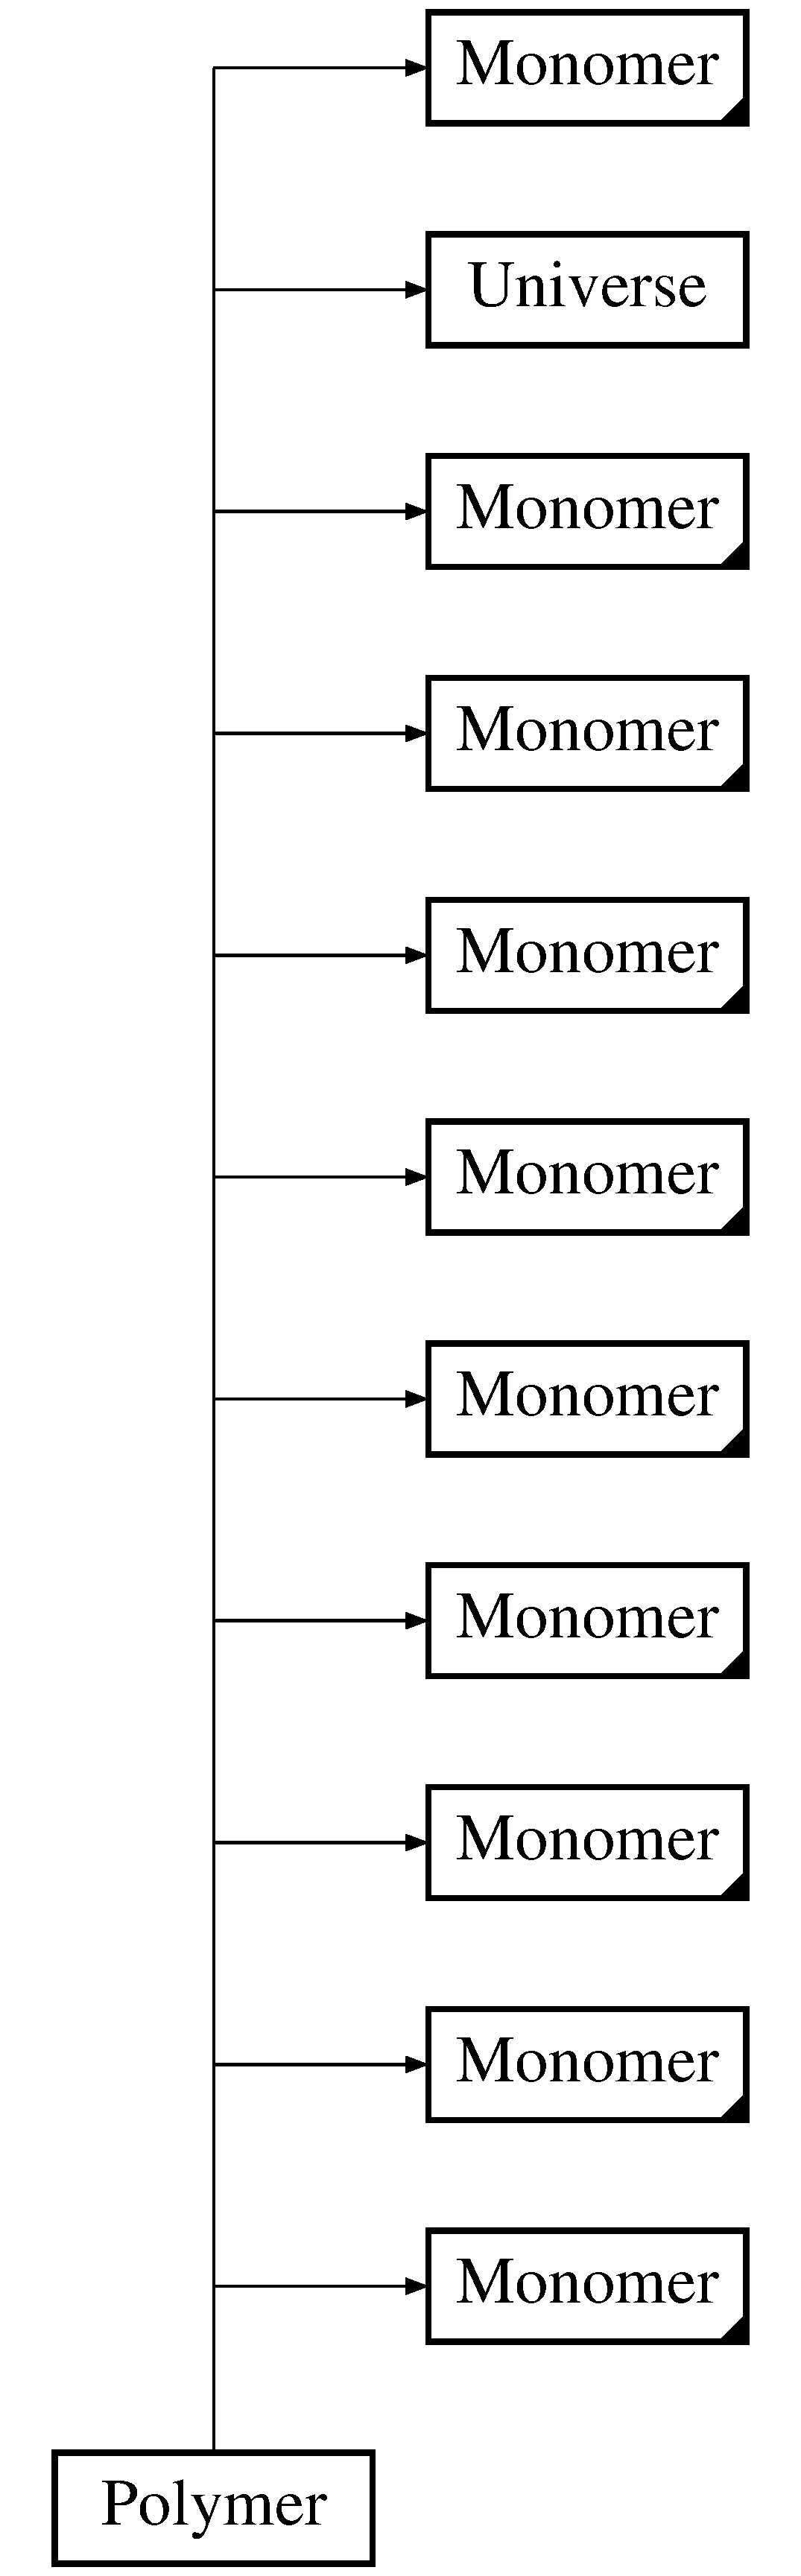
\includegraphics[height=12.000000cm]{classPolymer}
\end{center}
\end{figure}
\subsection*{Public Member Functions}
\begin{DoxyCompactItemize}
\item 
\mbox{\hyperlink{classPolymer_ae77454a3908652e4df6a26b9cac509a5}{Polymer}} (\mbox{\hyperlink{classMonomer}{Monomer}} \&mm)
\item 
virtual \mbox{\hyperlink{classPolymer_aac2b3983f375a5691c7d5ca1a79594d5}{$\sim$\+Polymer}} ()
\item 
unsigned int \mbox{\hyperlink{classPolymer_a8346d821e5f8690d7816ba1d40036b69}{get\+Counter}} ()
\item 
void \mbox{\hyperlink{classPolymer_a7ed6bbe09a570b59f9253d63fd3326d2}{set\+Counter}} (unsigned int val)
\item 
void \mbox{\hyperlink{classPolymer_a1daba3eb2ba8428bf2f3e814668b155f}{creation}} ()
\item 
\mbox{\hyperlink{classPolymer_ae77454a3908652e4df6a26b9cac509a5}{Polymer}} (\mbox{\hyperlink{classMonomer}{Monomer}} \&mm)
\item 
virtual \mbox{\hyperlink{classPolymer_aac2b3983f375a5691c7d5ca1a79594d5}{$\sim$\+Polymer}} ()
\item 
unsigned int \mbox{\hyperlink{classPolymer_a8346d821e5f8690d7816ba1d40036b69}{get\+Counter}} ()
\item 
void \mbox{\hyperlink{classPolymer_a7ed6bbe09a570b59f9253d63fd3326d2}{set\+Counter}} (unsigned int val)
\item 
void \mbox{\hyperlink{classPolymer_a1daba3eb2ba8428bf2f3e814668b155f}{creation}} ()
\item 
\mbox{\hyperlink{classPolymer_ae77454a3908652e4df6a26b9cac509a5}{Polymer}} (\mbox{\hyperlink{classMonomer}{Monomer}} \&mm)
\item 
virtual \mbox{\hyperlink{classPolymer_aac2b3983f375a5691c7d5ca1a79594d5}{$\sim$\+Polymer}} ()
\item 
unsigned int \mbox{\hyperlink{classPolymer_a8346d821e5f8690d7816ba1d40036b69}{get\+Counter}} ()
\item 
void \mbox{\hyperlink{classPolymer_a7ed6bbe09a570b59f9253d63fd3326d2}{set\+Counter}} (unsigned int val)
\item 
void \mbox{\hyperlink{classPolymer_a1daba3eb2ba8428bf2f3e814668b155f}{creation}} ()
\item 
\mbox{\hyperlink{classPolymer_ae77454a3908652e4df6a26b9cac509a5}{Polymer}} (\mbox{\hyperlink{classMonomer}{Monomer}} \&mm)
\item 
virtual \mbox{\hyperlink{classPolymer_aac2b3983f375a5691c7d5ca1a79594d5}{$\sim$\+Polymer}} ()
\item 
unsigned int \mbox{\hyperlink{classPolymer_a8346d821e5f8690d7816ba1d40036b69}{get\+Counter}} ()
\item 
void \mbox{\hyperlink{classPolymer_a7ed6bbe09a570b59f9253d63fd3326d2}{set\+Counter}} (unsigned int val)
\item 
void \mbox{\hyperlink{classPolymer_a1daba3eb2ba8428bf2f3e814668b155f}{creation}} ()
\item 
\mbox{\hyperlink{classPolymer_ae77454a3908652e4df6a26b9cac509a5}{Polymer}} (\mbox{\hyperlink{classMonomer}{Monomer}} \&mm)
\item 
virtual \mbox{\hyperlink{classPolymer_aac2b3983f375a5691c7d5ca1a79594d5}{$\sim$\+Polymer}} ()
\item 
unsigned int \mbox{\hyperlink{classPolymer_a8346d821e5f8690d7816ba1d40036b69}{get\+Counter}} ()
\item 
void \mbox{\hyperlink{classPolymer_a7ed6bbe09a570b59f9253d63fd3326d2}{set\+Counter}} (unsigned int val)
\item 
void \mbox{\hyperlink{classPolymer_a1daba3eb2ba8428bf2f3e814668b155f}{creation}} ()
\item 
\mbox{\hyperlink{classPolymer_ae77454a3908652e4df6a26b9cac509a5}{Polymer}} (\mbox{\hyperlink{classMonomer}{Monomer}} \&mm)
\item 
virtual \mbox{\hyperlink{classPolymer_aac2b3983f375a5691c7d5ca1a79594d5}{$\sim$\+Polymer}} ()
\item 
unsigned int \mbox{\hyperlink{classPolymer_a8346d821e5f8690d7816ba1d40036b69}{get\+Counter}} ()
\item 
void \mbox{\hyperlink{classPolymer_a7ed6bbe09a570b59f9253d63fd3326d2}{set\+Counter}} (unsigned int val)
\item 
void \mbox{\hyperlink{classPolymer_a1daba3eb2ba8428bf2f3e814668b155f}{creation}} ()
\item 
\mbox{\hyperlink{classPolymer_ae77454a3908652e4df6a26b9cac509a5}{Polymer}} (\mbox{\hyperlink{classMonomer}{Monomer}} \&mm)
\item 
virtual \mbox{\hyperlink{classPolymer_aac2b3983f375a5691c7d5ca1a79594d5}{$\sim$\+Polymer}} ()
\item 
unsigned int \mbox{\hyperlink{classPolymer_a8346d821e5f8690d7816ba1d40036b69}{get\+Counter}} ()
\item 
void \mbox{\hyperlink{classPolymer_a7ed6bbe09a570b59f9253d63fd3326d2}{set\+Counter}} (unsigned int val)
\item 
void \mbox{\hyperlink{classPolymer_a1daba3eb2ba8428bf2f3e814668b155f}{creation}} ()
\item 
\mbox{\hyperlink{classPolymer_ae77454a3908652e4df6a26b9cac509a5}{Polymer}} (\mbox{\hyperlink{classMonomer}{Monomer}} \&mm)
\item 
virtual \mbox{\hyperlink{classPolymer_aac2b3983f375a5691c7d5ca1a79594d5}{$\sim$\+Polymer}} ()
\item 
unsigned int \mbox{\hyperlink{classPolymer_a8346d821e5f8690d7816ba1d40036b69}{get\+Counter}} ()
\item 
void \mbox{\hyperlink{classPolymer_a7ed6bbe09a570b59f9253d63fd3326d2}{set\+Counter}} (unsigned int val)
\item 
void \mbox{\hyperlink{classPolymer_a1daba3eb2ba8428bf2f3e814668b155f}{creation}} ()
\item 
\mbox{\hyperlink{classPolymer_ae77454a3908652e4df6a26b9cac509a5}{Polymer}} (\mbox{\hyperlink{classMonomer}{Monomer}} \&mm)
\item 
virtual \mbox{\hyperlink{classPolymer_aac2b3983f375a5691c7d5ca1a79594d5}{$\sim$\+Polymer}} ()
\item 
unsigned int \mbox{\hyperlink{classPolymer_a8346d821e5f8690d7816ba1d40036b69}{get\+Counter}} ()
\item 
void \mbox{\hyperlink{classPolymer_a7ed6bbe09a570b59f9253d63fd3326d2}{set\+Counter}} (unsigned int val)
\item 
void \mbox{\hyperlink{classPolymer_a1daba3eb2ba8428bf2f3e814668b155f}{creation}} ()
\item 
\mbox{\hyperlink{classPolymer_a0f7d915300bfec223c4025f8e9d4f46d}{Polymer}} ()
\item 
\mbox{\hyperlink{classPolymer_adb35b8b7a5eae1e39187c0e525b0d9b1}{Polymer}} (unsigned int object\+\_\+type)
\item 
\mbox{\hyperlink{classPolymer_af918b8776cfd76d9ae4611bf35d4192a}{Polymer}} (unsigned int object\+\_\+type, std\+::chrono\+::time\+\_\+point$<$ \mbox{\hyperlink{universe_8h_a0ef8d951d1ca5ab3cfaf7ab4c7a6fd80}{Clock}} $>$ event\+\_\+time)
\item 
\mbox{\hyperlink{classPolymer_a53797e297c95b3bd934e1b8dd8c0c399}{Polymer}} (unsigned int object\+\_\+type, std\+::chrono\+::time\+\_\+point$<$ \mbox{\hyperlink{universe_8h_a0ef8d951d1ca5ab3cfaf7ab4c7a6fd80}{Clock}} $>$ event\+\_\+time, \mbox{\hyperlink{classUniverse}{Universe}} \&universe\+\_\+connector)
\item 
virtual \mbox{\hyperlink{classPolymer_aac2b3983f375a5691c7d5ca1a79594d5}{$\sim$\+Polymer}} ()
\item 
bool \mbox{\hyperlink{classPolymer_aa20f1e5c79e8631afa291569d5030103}{Reset\+Parameters}} (std\+::chrono\+::time\+\_\+point$<$ \mbox{\hyperlink{universe_8h_a0ef8d951d1ca5ab3cfaf7ab4c7a6fd80}{Clock}} $>$ event\+\_\+time)
\item 
unsigned int \mbox{\hyperlink{classPolymer_ac33903f9b5d2c73d6ddadcb02ece323e}{Get\+Counter}} (std\+::chrono\+::time\+\_\+point$<$ \mbox{\hyperlink{universe_8h_a0ef8d951d1ca5ab3cfaf7ab4c7a6fd80}{Clock}} $>$ event\+\_\+time)
\item 
void \mbox{\hyperlink{classPolymer_a1500ffc682396af2f4306c7c7ea7fd87}{Set\+Counter}} (std\+::chrono\+::time\+\_\+point$<$ \mbox{\hyperlink{universe_8h_a0ef8d951d1ca5ab3cfaf7ab4c7a6fd80}{Clock}} $>$ event\+\_\+time, unsigned int val)
\item 
void \mbox{\hyperlink{classPolymer_ab96200f701d9e2e63d22bdfd434e5ccb}{Set\+Polymer\+Label}} (std\+::string val)
\item 
std\+::string \mbox{\hyperlink{classPolymer_a80dbc65ac07e20dce3d9a2e9290c5e3b}{Get\+Polymer\+Label}} ()
\item 
int \mbox{\hyperlink{classPolymer_ac82f603c3010212122008c4ed3953045}{Update}} (std\+::chrono\+::time\+\_\+point$<$ \mbox{\hyperlink{universe_8h_a0ef8d951d1ca5ab3cfaf7ab4c7a6fd80}{Clock}} $>$ event\+\_\+time)
\item 
\mbox{\hyperlink{classPolymer_ae77454a3908652e4df6a26b9cac509a5}{Polymer}} (\mbox{\hyperlink{classMonomer}{Monomer}} \&mm)
\item 
virtual \mbox{\hyperlink{classPolymer_aac2b3983f375a5691c7d5ca1a79594d5}{$\sim$\+Polymer}} ()
\item 
unsigned int \mbox{\hyperlink{classPolymer_a8346d821e5f8690d7816ba1d40036b69}{get\+Counter}} ()
\item 
void \mbox{\hyperlink{classPolymer_a7ed6bbe09a570b59f9253d63fd3326d2}{set\+Counter}} (unsigned int val)
\item 
void \mbox{\hyperlink{classPolymer_a1daba3eb2ba8428bf2f3e814668b155f}{creation}} ()
\end{DoxyCompactItemize}
\subsection*{Private Attributes}
\begin{DoxyCompactItemize}
\item 
unsigned int \mbox{\hyperlink{classPolymer_a4687ca9273a4c34b5f32ab840d8cbf0d}{polymer\+Counter}}
\begin{DoxyCompactList}\small\item\em Member variable \char`\"{}polymer\+Counter\char`\"{}. \end{DoxyCompactList}\item 
unsigned int \mbox{\hyperlink{classPolymer_ac7b32509637c2164757728dbefd2ad77}{polymer\+\_\+counter}}
\begin{DoxyCompactList}\small\item\em Member variable \char`\"{}polymer\+\_\+counter\char`\"{}. \end{DoxyCompactList}\item 
std\+::string \mbox{\hyperlink{classPolymer_a8073d0650f9343960d4b199fb98640e3}{m\+\_\+polymer\+Label}}
\begin{DoxyCompactList}\small\item\em Member variable \char`\"{}m\+\_\+polymer\+Label\char`\"{}. \end{DoxyCompactList}\item 
int \mbox{\hyperlink{classPolymer_afc5e38aa165f2e18ec1eac442edfaf90}{polymer\+\_\+type}}
\item 
bool \mbox{\hyperlink{classPolymer_a07ca6a3ab8d562229090657c3862d140}{object\+\_\+disabled}} = true
\item 
bool \mbox{\hyperlink{classPolymer_a88ec0b2b21fb475cc4de108d2e17cff9}{object\+\_\+initialised}} = false
\item 
std\+::chrono\+::time\+\_\+point$<$ \mbox{\hyperlink{universe_8h_a0ef8d951d1ca5ab3cfaf7ab4c7a6fd80}{Clock}} $>$ \mbox{\hyperlink{classPolymer_a7c6e20b697e1e0dade7158db402e6e4f}{time\+\_\+object\+\_\+created}}
\item 
std\+::chrono\+::time\+\_\+point$<$ \mbox{\hyperlink{universe_8h_a0ef8d951d1ca5ab3cfaf7ab4c7a6fd80}{Clock}} $>$ \mbox{\hyperlink{classPolymer_ab96f5cc44ebcf5edbe7ddad9bc553cf7}{previous\+\_\+event\+\_\+time}}
\item 
int \mbox{\hyperlink{classPolymer_ab78fb6d122f0f8991477ca29d9cf1183}{duration\+\_\+since\+\_\+last\+\_\+event}}
\end{DoxyCompactItemize}
\subsection*{Additional Inherited Members}


\subsection{Constructor \& Destructor Documentation}
\mbox{\Hypertarget{classPolymer_ae77454a3908652e4df6a26b9cac509a5}\label{classPolymer_ae77454a3908652e4df6a26b9cac509a5}} 
\index{Polymer@{Polymer}!Polymer@{Polymer}}
\index{Polymer@{Polymer}!Polymer@{Polymer}}
\subsubsection{\texorpdfstring{Polymer()}{Polymer()}\hspace{0.1cm}{\footnotesize\ttfamily [1/14]}}
{\footnotesize\ttfamily Polymer\+::\+Polymer (\begin{DoxyParamCaption}\item[{\mbox{\hyperlink{classMonomer}{Monomer}} \&}]{mm }\end{DoxyParamCaption})\hspace{0.3cm}{\ttfamily [inline]}}

Default constructor \mbox{\Hypertarget{classPolymer_aac2b3983f375a5691c7d5ca1a79594d5}\label{classPolymer_aac2b3983f375a5691c7d5ca1a79594d5}} 
\index{Polymer@{Polymer}!````~Polymer@{$\sim$\+Polymer}}
\index{````~Polymer@{$\sim$\+Polymer}!Polymer@{Polymer}}
\subsubsection{\texorpdfstring{$\sim$\+Polymer()}{~Polymer()}\hspace{0.1cm}{\footnotesize\ttfamily [1/11]}}
{\footnotesize\ttfamily virtual Polymer\+::$\sim$\+Polymer (\begin{DoxyParamCaption}{ }\end{DoxyParamCaption})\hspace{0.3cm}{\ttfamily [inline]}, {\ttfamily [virtual]}}

Default destructor \mbox{\Hypertarget{classPolymer_ae77454a3908652e4df6a26b9cac509a5}\label{classPolymer_ae77454a3908652e4df6a26b9cac509a5}} 
\index{Polymer@{Polymer}!Polymer@{Polymer}}
\index{Polymer@{Polymer}!Polymer@{Polymer}}
\subsubsection{\texorpdfstring{Polymer()}{Polymer()}\hspace{0.1cm}{\footnotesize\ttfamily [2/14]}}
{\footnotesize\ttfamily Polymer\+::\+Polymer (\begin{DoxyParamCaption}\item[{\mbox{\hyperlink{classMonomer}{Monomer}} \&}]{mm }\end{DoxyParamCaption})\hspace{0.3cm}{\ttfamily [inline]}}

Default constructor \mbox{\Hypertarget{classPolymer_aac2b3983f375a5691c7d5ca1a79594d5}\label{classPolymer_aac2b3983f375a5691c7d5ca1a79594d5}} 
\index{Polymer@{Polymer}!````~Polymer@{$\sim$\+Polymer}}
\index{````~Polymer@{$\sim$\+Polymer}!Polymer@{Polymer}}
\subsubsection{\texorpdfstring{$\sim$\+Polymer()}{~Polymer()}\hspace{0.1cm}{\footnotesize\ttfamily [2/11]}}
{\footnotesize\ttfamily virtual Polymer\+::$\sim$\+Polymer (\begin{DoxyParamCaption}{ }\end{DoxyParamCaption})\hspace{0.3cm}{\ttfamily [inline]}, {\ttfamily [virtual]}}

Default destructor \mbox{\Hypertarget{classPolymer_ae77454a3908652e4df6a26b9cac509a5}\label{classPolymer_ae77454a3908652e4df6a26b9cac509a5}} 
\index{Polymer@{Polymer}!Polymer@{Polymer}}
\index{Polymer@{Polymer}!Polymer@{Polymer}}
\subsubsection{\texorpdfstring{Polymer()}{Polymer()}\hspace{0.1cm}{\footnotesize\ttfamily [3/14]}}
{\footnotesize\ttfamily Polymer\+::\+Polymer (\begin{DoxyParamCaption}\item[{\mbox{\hyperlink{classMonomer}{Monomer}} \&}]{mm }\end{DoxyParamCaption})\hspace{0.3cm}{\ttfamily [inline]}}

Default constructor \mbox{\Hypertarget{classPolymer_aac2b3983f375a5691c7d5ca1a79594d5}\label{classPolymer_aac2b3983f375a5691c7d5ca1a79594d5}} 
\index{Polymer@{Polymer}!````~Polymer@{$\sim$\+Polymer}}
\index{````~Polymer@{$\sim$\+Polymer}!Polymer@{Polymer}}
\subsubsection{\texorpdfstring{$\sim$\+Polymer()}{~Polymer()}\hspace{0.1cm}{\footnotesize\ttfamily [3/11]}}
{\footnotesize\ttfamily virtual Polymer\+::$\sim$\+Polymer (\begin{DoxyParamCaption}{ }\end{DoxyParamCaption})\hspace{0.3cm}{\ttfamily [inline]}, {\ttfamily [virtual]}}

Default destructor \mbox{\Hypertarget{classPolymer_ae77454a3908652e4df6a26b9cac509a5}\label{classPolymer_ae77454a3908652e4df6a26b9cac509a5}} 
\index{Polymer@{Polymer}!Polymer@{Polymer}}
\index{Polymer@{Polymer}!Polymer@{Polymer}}
\subsubsection{\texorpdfstring{Polymer()}{Polymer()}\hspace{0.1cm}{\footnotesize\ttfamily [4/14]}}
{\footnotesize\ttfamily Polymer\+::\+Polymer (\begin{DoxyParamCaption}\item[{\mbox{\hyperlink{classMonomer}{Monomer}} \&}]{mm }\end{DoxyParamCaption})\hspace{0.3cm}{\ttfamily [inline]}}

Default constructor \mbox{\Hypertarget{classPolymer_aac2b3983f375a5691c7d5ca1a79594d5}\label{classPolymer_aac2b3983f375a5691c7d5ca1a79594d5}} 
\index{Polymer@{Polymer}!````~Polymer@{$\sim$\+Polymer}}
\index{````~Polymer@{$\sim$\+Polymer}!Polymer@{Polymer}}
\subsubsection{\texorpdfstring{$\sim$\+Polymer()}{~Polymer()}\hspace{0.1cm}{\footnotesize\ttfamily [4/11]}}
{\footnotesize\ttfamily virtual Polymer\+::$\sim$\+Polymer (\begin{DoxyParamCaption}{ }\end{DoxyParamCaption})\hspace{0.3cm}{\ttfamily [inline]}, {\ttfamily [virtual]}}

Default destructor \mbox{\Hypertarget{classPolymer_ae77454a3908652e4df6a26b9cac509a5}\label{classPolymer_ae77454a3908652e4df6a26b9cac509a5}} 
\index{Polymer@{Polymer}!Polymer@{Polymer}}
\index{Polymer@{Polymer}!Polymer@{Polymer}}
\subsubsection{\texorpdfstring{Polymer()}{Polymer()}\hspace{0.1cm}{\footnotesize\ttfamily [5/14]}}
{\footnotesize\ttfamily Polymer\+::\+Polymer (\begin{DoxyParamCaption}\item[{\mbox{\hyperlink{classMonomer}{Monomer}} \&}]{mm }\end{DoxyParamCaption})\hspace{0.3cm}{\ttfamily [inline]}}

Default constructor \mbox{\Hypertarget{classPolymer_aac2b3983f375a5691c7d5ca1a79594d5}\label{classPolymer_aac2b3983f375a5691c7d5ca1a79594d5}} 
\index{Polymer@{Polymer}!````~Polymer@{$\sim$\+Polymer}}
\index{````~Polymer@{$\sim$\+Polymer}!Polymer@{Polymer}}
\subsubsection{\texorpdfstring{$\sim$\+Polymer()}{~Polymer()}\hspace{0.1cm}{\footnotesize\ttfamily [5/11]}}
{\footnotesize\ttfamily virtual Polymer\+::$\sim$\+Polymer (\begin{DoxyParamCaption}{ }\end{DoxyParamCaption})\hspace{0.3cm}{\ttfamily [inline]}, {\ttfamily [virtual]}}

Default destructor \mbox{\Hypertarget{classPolymer_ae77454a3908652e4df6a26b9cac509a5}\label{classPolymer_ae77454a3908652e4df6a26b9cac509a5}} 
\index{Polymer@{Polymer}!Polymer@{Polymer}}
\index{Polymer@{Polymer}!Polymer@{Polymer}}
\subsubsection{\texorpdfstring{Polymer()}{Polymer()}\hspace{0.1cm}{\footnotesize\ttfamily [6/14]}}
{\footnotesize\ttfamily Polymer\+::\+Polymer (\begin{DoxyParamCaption}\item[{\mbox{\hyperlink{classMonomer}{Monomer}} \&}]{mm }\end{DoxyParamCaption})\hspace{0.3cm}{\ttfamily [inline]}}

Default constructor \mbox{\Hypertarget{classPolymer_aac2b3983f375a5691c7d5ca1a79594d5}\label{classPolymer_aac2b3983f375a5691c7d5ca1a79594d5}} 
\index{Polymer@{Polymer}!````~Polymer@{$\sim$\+Polymer}}
\index{````~Polymer@{$\sim$\+Polymer}!Polymer@{Polymer}}
\subsubsection{\texorpdfstring{$\sim$\+Polymer()}{~Polymer()}\hspace{0.1cm}{\footnotesize\ttfamily [6/11]}}
{\footnotesize\ttfamily virtual Polymer\+::$\sim$\+Polymer (\begin{DoxyParamCaption}{ }\end{DoxyParamCaption})\hspace{0.3cm}{\ttfamily [inline]}, {\ttfamily [virtual]}}

Default destructor \mbox{\Hypertarget{classPolymer_ae77454a3908652e4df6a26b9cac509a5}\label{classPolymer_ae77454a3908652e4df6a26b9cac509a5}} 
\index{Polymer@{Polymer}!Polymer@{Polymer}}
\index{Polymer@{Polymer}!Polymer@{Polymer}}
\subsubsection{\texorpdfstring{Polymer()}{Polymer()}\hspace{0.1cm}{\footnotesize\ttfamily [7/14]}}
{\footnotesize\ttfamily Polymer\+::\+Polymer (\begin{DoxyParamCaption}\item[{\mbox{\hyperlink{classMonomer}{Monomer}} \&}]{mm }\end{DoxyParamCaption})\hspace{0.3cm}{\ttfamily [inline]}}

Default constructor \mbox{\Hypertarget{classPolymer_aac2b3983f375a5691c7d5ca1a79594d5}\label{classPolymer_aac2b3983f375a5691c7d5ca1a79594d5}} 
\index{Polymer@{Polymer}!````~Polymer@{$\sim$\+Polymer}}
\index{````~Polymer@{$\sim$\+Polymer}!Polymer@{Polymer}}
\subsubsection{\texorpdfstring{$\sim$\+Polymer()}{~Polymer()}\hspace{0.1cm}{\footnotesize\ttfamily [7/11]}}
{\footnotesize\ttfamily virtual Polymer\+::$\sim$\+Polymer (\begin{DoxyParamCaption}{ }\end{DoxyParamCaption})\hspace{0.3cm}{\ttfamily [inline]}, {\ttfamily [virtual]}}

Default destructor \mbox{\Hypertarget{classPolymer_ae77454a3908652e4df6a26b9cac509a5}\label{classPolymer_ae77454a3908652e4df6a26b9cac509a5}} 
\index{Polymer@{Polymer}!Polymer@{Polymer}}
\index{Polymer@{Polymer}!Polymer@{Polymer}}
\subsubsection{\texorpdfstring{Polymer()}{Polymer()}\hspace{0.1cm}{\footnotesize\ttfamily [8/14]}}
{\footnotesize\ttfamily Polymer\+::\+Polymer (\begin{DoxyParamCaption}\item[{\mbox{\hyperlink{classMonomer}{Monomer}} \&}]{mm }\end{DoxyParamCaption})\hspace{0.3cm}{\ttfamily [inline]}}

Default constructor \mbox{\Hypertarget{classPolymer_aac2b3983f375a5691c7d5ca1a79594d5}\label{classPolymer_aac2b3983f375a5691c7d5ca1a79594d5}} 
\index{Polymer@{Polymer}!````~Polymer@{$\sim$\+Polymer}}
\index{````~Polymer@{$\sim$\+Polymer}!Polymer@{Polymer}}
\subsubsection{\texorpdfstring{$\sim$\+Polymer()}{~Polymer()}\hspace{0.1cm}{\footnotesize\ttfamily [8/11]}}
{\footnotesize\ttfamily virtual Polymer\+::$\sim$\+Polymer (\begin{DoxyParamCaption}{ }\end{DoxyParamCaption})\hspace{0.3cm}{\ttfamily [inline]}, {\ttfamily [virtual]}}

Default destructor \mbox{\Hypertarget{classPolymer_ae77454a3908652e4df6a26b9cac509a5}\label{classPolymer_ae77454a3908652e4df6a26b9cac509a5}} 
\index{Polymer@{Polymer}!Polymer@{Polymer}}
\index{Polymer@{Polymer}!Polymer@{Polymer}}
\subsubsection{\texorpdfstring{Polymer()}{Polymer()}\hspace{0.1cm}{\footnotesize\ttfamily [9/14]}}
{\footnotesize\ttfamily Polymer\+::\+Polymer (\begin{DoxyParamCaption}\item[{\mbox{\hyperlink{classMonomer}{Monomer}} \&}]{mm }\end{DoxyParamCaption})\hspace{0.3cm}{\ttfamily [inline]}}

Default constructor \mbox{\Hypertarget{classPolymer_aac2b3983f375a5691c7d5ca1a79594d5}\label{classPolymer_aac2b3983f375a5691c7d5ca1a79594d5}} 
\index{Polymer@{Polymer}!````~Polymer@{$\sim$\+Polymer}}
\index{````~Polymer@{$\sim$\+Polymer}!Polymer@{Polymer}}
\subsubsection{\texorpdfstring{$\sim$\+Polymer()}{~Polymer()}\hspace{0.1cm}{\footnotesize\ttfamily [9/11]}}
{\footnotesize\ttfamily virtual Polymer\+::$\sim$\+Polymer (\begin{DoxyParamCaption}{ }\end{DoxyParamCaption})\hspace{0.3cm}{\ttfamily [inline]}, {\ttfamily [virtual]}}

Default destructor \mbox{\Hypertarget{classPolymer_a0f7d915300bfec223c4025f8e9d4f46d}\label{classPolymer_a0f7d915300bfec223c4025f8e9d4f46d}} 
\index{Polymer@{Polymer}!Polymer@{Polymer}}
\index{Polymer@{Polymer}!Polymer@{Polymer}}
\subsubsection{\texorpdfstring{Polymer()}{Polymer()}\hspace{0.1cm}{\footnotesize\ttfamily [10/14]}}
{\footnotesize\ttfamily Polymer\+::\+Polymer (\begin{DoxyParamCaption}{ }\end{DoxyParamCaption})\hspace{0.3cm}{\ttfamily [inline]}}

\mbox{\Hypertarget{classPolymer_adb35b8b7a5eae1e39187c0e525b0d9b1}\label{classPolymer_adb35b8b7a5eae1e39187c0e525b0d9b1}} 
\index{Polymer@{Polymer}!Polymer@{Polymer}}
\index{Polymer@{Polymer}!Polymer@{Polymer}}
\subsubsection{\texorpdfstring{Polymer()}{Polymer()}\hspace{0.1cm}{\footnotesize\ttfamily [11/14]}}
{\footnotesize\ttfamily Polymer\+::\+Polymer (\begin{DoxyParamCaption}\item[{unsigned int}]{object\+\_\+type }\end{DoxyParamCaption})\hspace{0.3cm}{\ttfamily [inline]}}

\mbox{\Hypertarget{classPolymer_af918b8776cfd76d9ae4611bf35d4192a}\label{classPolymer_af918b8776cfd76d9ae4611bf35d4192a}} 
\index{Polymer@{Polymer}!Polymer@{Polymer}}
\index{Polymer@{Polymer}!Polymer@{Polymer}}
\subsubsection{\texorpdfstring{Polymer()}{Polymer()}\hspace{0.1cm}{\footnotesize\ttfamily [12/14]}}
{\footnotesize\ttfamily Polymer\+::\+Polymer (\begin{DoxyParamCaption}\item[{unsigned int}]{object\+\_\+type,  }\item[{std\+::chrono\+::time\+\_\+point$<$ \mbox{\hyperlink{universe_8h_a0ef8d951d1ca5ab3cfaf7ab4c7a6fd80}{Clock}} $>$}]{event\+\_\+time }\end{DoxyParamCaption})\hspace{0.3cm}{\ttfamily [inline]}}

\mbox{\Hypertarget{classPolymer_a53797e297c95b3bd934e1b8dd8c0c399}\label{classPolymer_a53797e297c95b3bd934e1b8dd8c0c399}} 
\index{Polymer@{Polymer}!Polymer@{Polymer}}
\index{Polymer@{Polymer}!Polymer@{Polymer}}
\subsubsection{\texorpdfstring{Polymer()}{Polymer()}\hspace{0.1cm}{\footnotesize\ttfamily [13/14]}}
{\footnotesize\ttfamily Polymer\+::\+Polymer (\begin{DoxyParamCaption}\item[{unsigned int}]{object\+\_\+type,  }\item[{std\+::chrono\+::time\+\_\+point$<$ \mbox{\hyperlink{universe_8h_a0ef8d951d1ca5ab3cfaf7ab4c7a6fd80}{Clock}} $>$}]{event\+\_\+time,  }\item[{\mbox{\hyperlink{classUniverse}{Universe}} \&}]{universe\+\_\+connector }\end{DoxyParamCaption})\hspace{0.3cm}{\ttfamily [inline]}}

\mbox{\Hypertarget{classPolymer_aac2b3983f375a5691c7d5ca1a79594d5}\label{classPolymer_aac2b3983f375a5691c7d5ca1a79594d5}} 
\index{Polymer@{Polymer}!````~Polymer@{$\sim$\+Polymer}}
\index{````~Polymer@{$\sim$\+Polymer}!Polymer@{Polymer}}
\subsubsection{\texorpdfstring{$\sim$\+Polymer()}{~Polymer()}\hspace{0.1cm}{\footnotesize\ttfamily [10/11]}}
{\footnotesize\ttfamily virtual Polymer\+::$\sim$\+Polymer (\begin{DoxyParamCaption}{ }\end{DoxyParamCaption})\hspace{0.3cm}{\ttfamily [inline]}, {\ttfamily [virtual]}}

Default destructor \mbox{\Hypertarget{classPolymer_ae77454a3908652e4df6a26b9cac509a5}\label{classPolymer_ae77454a3908652e4df6a26b9cac509a5}} 
\index{Polymer@{Polymer}!Polymer@{Polymer}}
\index{Polymer@{Polymer}!Polymer@{Polymer}}
\subsubsection{\texorpdfstring{Polymer()}{Polymer()}\hspace{0.1cm}{\footnotesize\ttfamily [14/14]}}
{\footnotesize\ttfamily Polymer\+::\+Polymer (\begin{DoxyParamCaption}\item[{\mbox{\hyperlink{classMonomer}{Monomer}} \&}]{mm }\end{DoxyParamCaption})\hspace{0.3cm}{\ttfamily [inline]}}

Default constructor \mbox{\Hypertarget{classPolymer_aac2b3983f375a5691c7d5ca1a79594d5}\label{classPolymer_aac2b3983f375a5691c7d5ca1a79594d5}} 
\index{Polymer@{Polymer}!````~Polymer@{$\sim$\+Polymer}}
\index{````~Polymer@{$\sim$\+Polymer}!Polymer@{Polymer}}
\subsubsection{\texorpdfstring{$\sim$\+Polymer()}{~Polymer()}\hspace{0.1cm}{\footnotesize\ttfamily [11/11]}}
{\footnotesize\ttfamily virtual Polymer\+::$\sim$\+Polymer (\begin{DoxyParamCaption}{ }\end{DoxyParamCaption})\hspace{0.3cm}{\ttfamily [inline]}, {\ttfamily [virtual]}}

Default destructor 

\subsection{Member Function Documentation}
\mbox{\Hypertarget{classPolymer_a1daba3eb2ba8428bf2f3e814668b155f}\label{classPolymer_a1daba3eb2ba8428bf2f3e814668b155f}} 
\index{Polymer@{Polymer}!creation@{creation}}
\index{creation@{creation}!Polymer@{Polymer}}
\subsubsection{\texorpdfstring{creation()}{creation()}\hspace{0.1cm}{\footnotesize\ttfamily [1/10]}}
{\footnotesize\ttfamily void Polymer\+::creation (\begin{DoxyParamCaption}{ }\end{DoxyParamCaption})\hspace{0.3cm}{\ttfamily [inline]}}

\mbox{\Hypertarget{classPolymer_a1daba3eb2ba8428bf2f3e814668b155f}\label{classPolymer_a1daba3eb2ba8428bf2f3e814668b155f}} 
\index{Polymer@{Polymer}!creation@{creation}}
\index{creation@{creation}!Polymer@{Polymer}}
\subsubsection{\texorpdfstring{creation()}{creation()}\hspace{0.1cm}{\footnotesize\ttfamily [2/10]}}
{\footnotesize\ttfamily void Polymer\+::creation (\begin{DoxyParamCaption}{ }\end{DoxyParamCaption})\hspace{0.3cm}{\ttfamily [inline]}}

\mbox{\Hypertarget{classPolymer_a1daba3eb2ba8428bf2f3e814668b155f}\label{classPolymer_a1daba3eb2ba8428bf2f3e814668b155f}} 
\index{Polymer@{Polymer}!creation@{creation}}
\index{creation@{creation}!Polymer@{Polymer}}
\subsubsection{\texorpdfstring{creation()}{creation()}\hspace{0.1cm}{\footnotesize\ttfamily [3/10]}}
{\footnotesize\ttfamily void Polymer\+::creation (\begin{DoxyParamCaption}{ }\end{DoxyParamCaption})\hspace{0.3cm}{\ttfamily [inline]}}

\mbox{\Hypertarget{classPolymer_a1daba3eb2ba8428bf2f3e814668b155f}\label{classPolymer_a1daba3eb2ba8428bf2f3e814668b155f}} 
\index{Polymer@{Polymer}!creation@{creation}}
\index{creation@{creation}!Polymer@{Polymer}}
\subsubsection{\texorpdfstring{creation()}{creation()}\hspace{0.1cm}{\footnotesize\ttfamily [4/10]}}
{\footnotesize\ttfamily void Polymer\+::creation (\begin{DoxyParamCaption}{ }\end{DoxyParamCaption})\hspace{0.3cm}{\ttfamily [inline]}}

\mbox{\Hypertarget{classPolymer_a1daba3eb2ba8428bf2f3e814668b155f}\label{classPolymer_a1daba3eb2ba8428bf2f3e814668b155f}} 
\index{Polymer@{Polymer}!creation@{creation}}
\index{creation@{creation}!Polymer@{Polymer}}
\subsubsection{\texorpdfstring{creation()}{creation()}\hspace{0.1cm}{\footnotesize\ttfamily [5/10]}}
{\footnotesize\ttfamily void Polymer\+::creation (\begin{DoxyParamCaption}{ }\end{DoxyParamCaption})\hspace{0.3cm}{\ttfamily [inline]}}

\mbox{\Hypertarget{classPolymer_a1daba3eb2ba8428bf2f3e814668b155f}\label{classPolymer_a1daba3eb2ba8428bf2f3e814668b155f}} 
\index{Polymer@{Polymer}!creation@{creation}}
\index{creation@{creation}!Polymer@{Polymer}}
\subsubsection{\texorpdfstring{creation()}{creation()}\hspace{0.1cm}{\footnotesize\ttfamily [6/10]}}
{\footnotesize\ttfamily void Polymer\+::creation (\begin{DoxyParamCaption}{ }\end{DoxyParamCaption})\hspace{0.3cm}{\ttfamily [inline]}}

\mbox{\Hypertarget{classPolymer_a1daba3eb2ba8428bf2f3e814668b155f}\label{classPolymer_a1daba3eb2ba8428bf2f3e814668b155f}} 
\index{Polymer@{Polymer}!creation@{creation}}
\index{creation@{creation}!Polymer@{Polymer}}
\subsubsection{\texorpdfstring{creation()}{creation()}\hspace{0.1cm}{\footnotesize\ttfamily [7/10]}}
{\footnotesize\ttfamily void Polymer\+::creation (\begin{DoxyParamCaption}{ }\end{DoxyParamCaption})\hspace{0.3cm}{\ttfamily [inline]}}

\mbox{\Hypertarget{classPolymer_a1daba3eb2ba8428bf2f3e814668b155f}\label{classPolymer_a1daba3eb2ba8428bf2f3e814668b155f}} 
\index{Polymer@{Polymer}!creation@{creation}}
\index{creation@{creation}!Polymer@{Polymer}}
\subsubsection{\texorpdfstring{creation()}{creation()}\hspace{0.1cm}{\footnotesize\ttfamily [8/10]}}
{\footnotesize\ttfamily void Polymer\+::creation (\begin{DoxyParamCaption}{ }\end{DoxyParamCaption})\hspace{0.3cm}{\ttfamily [inline]}}

\mbox{\Hypertarget{classPolymer_a1daba3eb2ba8428bf2f3e814668b155f}\label{classPolymer_a1daba3eb2ba8428bf2f3e814668b155f}} 
\index{Polymer@{Polymer}!creation@{creation}}
\index{creation@{creation}!Polymer@{Polymer}}
\subsubsection{\texorpdfstring{creation()}{creation()}\hspace{0.1cm}{\footnotesize\ttfamily [9/10]}}
{\footnotesize\ttfamily void Polymer\+::creation (\begin{DoxyParamCaption}{ }\end{DoxyParamCaption})\hspace{0.3cm}{\ttfamily [inline]}}

\mbox{\Hypertarget{classPolymer_a1daba3eb2ba8428bf2f3e814668b155f}\label{classPolymer_a1daba3eb2ba8428bf2f3e814668b155f}} 
\index{Polymer@{Polymer}!creation@{creation}}
\index{creation@{creation}!Polymer@{Polymer}}
\subsubsection{\texorpdfstring{creation()}{creation()}\hspace{0.1cm}{\footnotesize\ttfamily [10/10]}}
{\footnotesize\ttfamily void Polymer\+::creation (\begin{DoxyParamCaption}{ }\end{DoxyParamCaption})\hspace{0.3cm}{\ttfamily [inline]}}

\mbox{\Hypertarget{classPolymer_a8346d821e5f8690d7816ba1d40036b69}\label{classPolymer_a8346d821e5f8690d7816ba1d40036b69}} 
\index{Polymer@{Polymer}!get\+Counter@{get\+Counter}}
\index{get\+Counter@{get\+Counter}!Polymer@{Polymer}}
\subsubsection{\texorpdfstring{get\+Counter()}{getCounter()}\hspace{0.1cm}{\footnotesize\ttfamily [1/10]}}
{\footnotesize\ttfamily unsigned int Polymer\+::get\+Counter (\begin{DoxyParamCaption}{ }\end{DoxyParamCaption})\hspace{0.3cm}{\ttfamily [inline]}}

\mbox{\Hypertarget{classPolymer_a8346d821e5f8690d7816ba1d40036b69}\label{classPolymer_a8346d821e5f8690d7816ba1d40036b69}} 
\index{Polymer@{Polymer}!get\+Counter@{get\+Counter}}
\index{get\+Counter@{get\+Counter}!Polymer@{Polymer}}
\subsubsection{\texorpdfstring{get\+Counter()}{getCounter()}\hspace{0.1cm}{\footnotesize\ttfamily [2/10]}}
{\footnotesize\ttfamily unsigned int Polymer\+::get\+Counter (\begin{DoxyParamCaption}{ }\end{DoxyParamCaption})\hspace{0.3cm}{\ttfamily [inline]}}

\mbox{\Hypertarget{classPolymer_a8346d821e5f8690d7816ba1d40036b69}\label{classPolymer_a8346d821e5f8690d7816ba1d40036b69}} 
\index{Polymer@{Polymer}!get\+Counter@{get\+Counter}}
\index{get\+Counter@{get\+Counter}!Polymer@{Polymer}}
\subsubsection{\texorpdfstring{get\+Counter()}{getCounter()}\hspace{0.1cm}{\footnotesize\ttfamily [3/10]}}
{\footnotesize\ttfamily unsigned int Polymer\+::get\+Counter (\begin{DoxyParamCaption}{ }\end{DoxyParamCaption})\hspace{0.3cm}{\ttfamily [inline]}}

\mbox{\Hypertarget{classPolymer_a8346d821e5f8690d7816ba1d40036b69}\label{classPolymer_a8346d821e5f8690d7816ba1d40036b69}} 
\index{Polymer@{Polymer}!get\+Counter@{get\+Counter}}
\index{get\+Counter@{get\+Counter}!Polymer@{Polymer}}
\subsubsection{\texorpdfstring{get\+Counter()}{getCounter()}\hspace{0.1cm}{\footnotesize\ttfamily [4/10]}}
{\footnotesize\ttfamily unsigned int Polymer\+::get\+Counter (\begin{DoxyParamCaption}{ }\end{DoxyParamCaption})\hspace{0.3cm}{\ttfamily [inline]}}

\mbox{\Hypertarget{classPolymer_a8346d821e5f8690d7816ba1d40036b69}\label{classPolymer_a8346d821e5f8690d7816ba1d40036b69}} 
\index{Polymer@{Polymer}!get\+Counter@{get\+Counter}}
\index{get\+Counter@{get\+Counter}!Polymer@{Polymer}}
\subsubsection{\texorpdfstring{get\+Counter()}{getCounter()}\hspace{0.1cm}{\footnotesize\ttfamily [5/10]}}
{\footnotesize\ttfamily unsigned int Polymer\+::get\+Counter (\begin{DoxyParamCaption}{ }\end{DoxyParamCaption})\hspace{0.3cm}{\ttfamily [inline]}}

\mbox{\Hypertarget{classPolymer_a8346d821e5f8690d7816ba1d40036b69}\label{classPolymer_a8346d821e5f8690d7816ba1d40036b69}} 
\index{Polymer@{Polymer}!get\+Counter@{get\+Counter}}
\index{get\+Counter@{get\+Counter}!Polymer@{Polymer}}
\subsubsection{\texorpdfstring{get\+Counter()}{getCounter()}\hspace{0.1cm}{\footnotesize\ttfamily [6/10]}}
{\footnotesize\ttfamily unsigned int Polymer\+::get\+Counter (\begin{DoxyParamCaption}{ }\end{DoxyParamCaption})\hspace{0.3cm}{\ttfamily [inline]}}

\mbox{\Hypertarget{classPolymer_a8346d821e5f8690d7816ba1d40036b69}\label{classPolymer_a8346d821e5f8690d7816ba1d40036b69}} 
\index{Polymer@{Polymer}!get\+Counter@{get\+Counter}}
\index{get\+Counter@{get\+Counter}!Polymer@{Polymer}}
\subsubsection{\texorpdfstring{get\+Counter()}{getCounter()}\hspace{0.1cm}{\footnotesize\ttfamily [7/10]}}
{\footnotesize\ttfamily unsigned int Polymer\+::get\+Counter (\begin{DoxyParamCaption}{ }\end{DoxyParamCaption})\hspace{0.3cm}{\ttfamily [inline]}}

\mbox{\Hypertarget{classPolymer_a8346d821e5f8690d7816ba1d40036b69}\label{classPolymer_a8346d821e5f8690d7816ba1d40036b69}} 
\index{Polymer@{Polymer}!get\+Counter@{get\+Counter}}
\index{get\+Counter@{get\+Counter}!Polymer@{Polymer}}
\subsubsection{\texorpdfstring{get\+Counter()}{getCounter()}\hspace{0.1cm}{\footnotesize\ttfamily [8/10]}}
{\footnotesize\ttfamily unsigned int Polymer\+::get\+Counter (\begin{DoxyParamCaption}{ }\end{DoxyParamCaption})\hspace{0.3cm}{\ttfamily [inline]}}

\mbox{\Hypertarget{classPolymer_a8346d821e5f8690d7816ba1d40036b69}\label{classPolymer_a8346d821e5f8690d7816ba1d40036b69}} 
\index{Polymer@{Polymer}!get\+Counter@{get\+Counter}}
\index{get\+Counter@{get\+Counter}!Polymer@{Polymer}}
\subsubsection{\texorpdfstring{get\+Counter()}{getCounter()}\hspace{0.1cm}{\footnotesize\ttfamily [9/10]}}
{\footnotesize\ttfamily unsigned int Polymer\+::get\+Counter (\begin{DoxyParamCaption}{ }\end{DoxyParamCaption})\hspace{0.3cm}{\ttfamily [inline]}}

\mbox{\Hypertarget{classPolymer_a8346d821e5f8690d7816ba1d40036b69}\label{classPolymer_a8346d821e5f8690d7816ba1d40036b69}} 
\index{Polymer@{Polymer}!get\+Counter@{get\+Counter}}
\index{get\+Counter@{get\+Counter}!Polymer@{Polymer}}
\subsubsection{\texorpdfstring{get\+Counter()}{getCounter()}\hspace{0.1cm}{\footnotesize\ttfamily [10/10]}}
{\footnotesize\ttfamily unsigned int Polymer\+::get\+Counter (\begin{DoxyParamCaption}{ }\end{DoxyParamCaption})\hspace{0.3cm}{\ttfamily [inline]}}

\mbox{\Hypertarget{classPolymer_ac33903f9b5d2c73d6ddadcb02ece323e}\label{classPolymer_ac33903f9b5d2c73d6ddadcb02ece323e}} 
\index{Polymer@{Polymer}!Get\+Counter@{Get\+Counter}}
\index{Get\+Counter@{Get\+Counter}!Polymer@{Polymer}}
\subsubsection{\texorpdfstring{Get\+Counter()}{GetCounter()}}
{\footnotesize\ttfamily unsigned int Polymer\+::\+Get\+Counter (\begin{DoxyParamCaption}\item[{std\+::chrono\+::time\+\_\+point$<$ \mbox{\hyperlink{universe_8h_a0ef8d951d1ca5ab3cfaf7ab4c7a6fd80}{Clock}} $>$}]{event\+\_\+time }\end{DoxyParamCaption})\hspace{0.3cm}{\ttfamily [inline]}}

\mbox{\Hypertarget{classPolymer_a80dbc65ac07e20dce3d9a2e9290c5e3b}\label{classPolymer_a80dbc65ac07e20dce3d9a2e9290c5e3b}} 
\index{Polymer@{Polymer}!Get\+Polymer\+Label@{Get\+Polymer\+Label}}
\index{Get\+Polymer\+Label@{Get\+Polymer\+Label}!Polymer@{Polymer}}
\subsubsection{\texorpdfstring{Get\+Polymer\+Label()}{GetPolymerLabel()}}
{\footnotesize\ttfamily std\+::string Polymer\+::\+Get\+Polymer\+Label (\begin{DoxyParamCaption}{ }\end{DoxyParamCaption})\hspace{0.3cm}{\ttfamily [inline]}}

\mbox{\Hypertarget{classPolymer_aa20f1e5c79e8631afa291569d5030103}\label{classPolymer_aa20f1e5c79e8631afa291569d5030103}} 
\index{Polymer@{Polymer}!Reset\+Parameters@{Reset\+Parameters}}
\index{Reset\+Parameters@{Reset\+Parameters}!Polymer@{Polymer}}
\subsubsection{\texorpdfstring{Reset\+Parameters()}{ResetParameters()}}
{\footnotesize\ttfamily bool Polymer\+::\+Reset\+Parameters (\begin{DoxyParamCaption}\item[{std\+::chrono\+::time\+\_\+point$<$ \mbox{\hyperlink{universe_8h_a0ef8d951d1ca5ab3cfaf7ab4c7a6fd80}{Clock}} $>$}]{event\+\_\+time }\end{DoxyParamCaption})}

\mbox{\Hypertarget{classPolymer_a7ed6bbe09a570b59f9253d63fd3326d2}\label{classPolymer_a7ed6bbe09a570b59f9253d63fd3326d2}} 
\index{Polymer@{Polymer}!set\+Counter@{set\+Counter}}
\index{set\+Counter@{set\+Counter}!Polymer@{Polymer}}
\subsubsection{\texorpdfstring{set\+Counter()}{setCounter()}\hspace{0.1cm}{\footnotesize\ttfamily [1/10]}}
{\footnotesize\ttfamily void Polymer\+::set\+Counter (\begin{DoxyParamCaption}\item[{unsigned int}]{val }\end{DoxyParamCaption})\hspace{0.3cm}{\ttfamily [inline]}}

\mbox{\Hypertarget{classPolymer_a7ed6bbe09a570b59f9253d63fd3326d2}\label{classPolymer_a7ed6bbe09a570b59f9253d63fd3326d2}} 
\index{Polymer@{Polymer}!set\+Counter@{set\+Counter}}
\index{set\+Counter@{set\+Counter}!Polymer@{Polymer}}
\subsubsection{\texorpdfstring{set\+Counter()}{setCounter()}\hspace{0.1cm}{\footnotesize\ttfamily [2/10]}}
{\footnotesize\ttfamily void Polymer\+::set\+Counter (\begin{DoxyParamCaption}\item[{unsigned int}]{val }\end{DoxyParamCaption})\hspace{0.3cm}{\ttfamily [inline]}}

\mbox{\Hypertarget{classPolymer_a7ed6bbe09a570b59f9253d63fd3326d2}\label{classPolymer_a7ed6bbe09a570b59f9253d63fd3326d2}} 
\index{Polymer@{Polymer}!set\+Counter@{set\+Counter}}
\index{set\+Counter@{set\+Counter}!Polymer@{Polymer}}
\subsubsection{\texorpdfstring{set\+Counter()}{setCounter()}\hspace{0.1cm}{\footnotesize\ttfamily [3/10]}}
{\footnotesize\ttfamily void Polymer\+::set\+Counter (\begin{DoxyParamCaption}\item[{unsigned int}]{val }\end{DoxyParamCaption})\hspace{0.3cm}{\ttfamily [inline]}}

\mbox{\Hypertarget{classPolymer_a7ed6bbe09a570b59f9253d63fd3326d2}\label{classPolymer_a7ed6bbe09a570b59f9253d63fd3326d2}} 
\index{Polymer@{Polymer}!set\+Counter@{set\+Counter}}
\index{set\+Counter@{set\+Counter}!Polymer@{Polymer}}
\subsubsection{\texorpdfstring{set\+Counter()}{setCounter()}\hspace{0.1cm}{\footnotesize\ttfamily [4/10]}}
{\footnotesize\ttfamily void Polymer\+::set\+Counter (\begin{DoxyParamCaption}\item[{unsigned int}]{val }\end{DoxyParamCaption})\hspace{0.3cm}{\ttfamily [inline]}}

\mbox{\Hypertarget{classPolymer_a7ed6bbe09a570b59f9253d63fd3326d2}\label{classPolymer_a7ed6bbe09a570b59f9253d63fd3326d2}} 
\index{Polymer@{Polymer}!set\+Counter@{set\+Counter}}
\index{set\+Counter@{set\+Counter}!Polymer@{Polymer}}
\subsubsection{\texorpdfstring{set\+Counter()}{setCounter()}\hspace{0.1cm}{\footnotesize\ttfamily [5/10]}}
{\footnotesize\ttfamily void Polymer\+::set\+Counter (\begin{DoxyParamCaption}\item[{unsigned int}]{val }\end{DoxyParamCaption})\hspace{0.3cm}{\ttfamily [inline]}}

\mbox{\Hypertarget{classPolymer_a7ed6bbe09a570b59f9253d63fd3326d2}\label{classPolymer_a7ed6bbe09a570b59f9253d63fd3326d2}} 
\index{Polymer@{Polymer}!set\+Counter@{set\+Counter}}
\index{set\+Counter@{set\+Counter}!Polymer@{Polymer}}
\subsubsection{\texorpdfstring{set\+Counter()}{setCounter()}\hspace{0.1cm}{\footnotesize\ttfamily [6/10]}}
{\footnotesize\ttfamily void Polymer\+::set\+Counter (\begin{DoxyParamCaption}\item[{unsigned int}]{val }\end{DoxyParamCaption})\hspace{0.3cm}{\ttfamily [inline]}}

\mbox{\Hypertarget{classPolymer_a7ed6bbe09a570b59f9253d63fd3326d2}\label{classPolymer_a7ed6bbe09a570b59f9253d63fd3326d2}} 
\index{Polymer@{Polymer}!set\+Counter@{set\+Counter}}
\index{set\+Counter@{set\+Counter}!Polymer@{Polymer}}
\subsubsection{\texorpdfstring{set\+Counter()}{setCounter()}\hspace{0.1cm}{\footnotesize\ttfamily [7/10]}}
{\footnotesize\ttfamily void Polymer\+::set\+Counter (\begin{DoxyParamCaption}\item[{unsigned int}]{val }\end{DoxyParamCaption})\hspace{0.3cm}{\ttfamily [inline]}}

\mbox{\Hypertarget{classPolymer_a7ed6bbe09a570b59f9253d63fd3326d2}\label{classPolymer_a7ed6bbe09a570b59f9253d63fd3326d2}} 
\index{Polymer@{Polymer}!set\+Counter@{set\+Counter}}
\index{set\+Counter@{set\+Counter}!Polymer@{Polymer}}
\subsubsection{\texorpdfstring{set\+Counter()}{setCounter()}\hspace{0.1cm}{\footnotesize\ttfamily [8/10]}}
{\footnotesize\ttfamily void Polymer\+::set\+Counter (\begin{DoxyParamCaption}\item[{unsigned int}]{val }\end{DoxyParamCaption})\hspace{0.3cm}{\ttfamily [inline]}}

\mbox{\Hypertarget{classPolymer_a7ed6bbe09a570b59f9253d63fd3326d2}\label{classPolymer_a7ed6bbe09a570b59f9253d63fd3326d2}} 
\index{Polymer@{Polymer}!set\+Counter@{set\+Counter}}
\index{set\+Counter@{set\+Counter}!Polymer@{Polymer}}
\subsubsection{\texorpdfstring{set\+Counter()}{setCounter()}\hspace{0.1cm}{\footnotesize\ttfamily [9/10]}}
{\footnotesize\ttfamily void Polymer\+::set\+Counter (\begin{DoxyParamCaption}\item[{unsigned int}]{val }\end{DoxyParamCaption})\hspace{0.3cm}{\ttfamily [inline]}}

\mbox{\Hypertarget{classPolymer_a7ed6bbe09a570b59f9253d63fd3326d2}\label{classPolymer_a7ed6bbe09a570b59f9253d63fd3326d2}} 
\index{Polymer@{Polymer}!set\+Counter@{set\+Counter}}
\index{set\+Counter@{set\+Counter}!Polymer@{Polymer}}
\subsubsection{\texorpdfstring{set\+Counter()}{setCounter()}\hspace{0.1cm}{\footnotesize\ttfamily [10/10]}}
{\footnotesize\ttfamily void Polymer\+::set\+Counter (\begin{DoxyParamCaption}\item[{unsigned int}]{val }\end{DoxyParamCaption})\hspace{0.3cm}{\ttfamily [inline]}}

\mbox{\Hypertarget{classPolymer_a1500ffc682396af2f4306c7c7ea7fd87}\label{classPolymer_a1500ffc682396af2f4306c7c7ea7fd87}} 
\index{Polymer@{Polymer}!Set\+Counter@{Set\+Counter}}
\index{Set\+Counter@{Set\+Counter}!Polymer@{Polymer}}
\subsubsection{\texorpdfstring{Set\+Counter()}{SetCounter()}}
{\footnotesize\ttfamily void Polymer\+::\+Set\+Counter (\begin{DoxyParamCaption}\item[{std\+::chrono\+::time\+\_\+point$<$ \mbox{\hyperlink{universe_8h_a0ef8d951d1ca5ab3cfaf7ab4c7a6fd80}{Clock}} $>$}]{event\+\_\+time,  }\item[{unsigned int}]{val }\end{DoxyParamCaption})\hspace{0.3cm}{\ttfamily [inline]}, {\ttfamily [virtual]}}



Reimplemented from \mbox{\hyperlink{classMonomer_a6f0dfa4382b3d4fa19b7ee0fb8fe7a55}{Monomer}}.

\mbox{\Hypertarget{classPolymer_ab96200f701d9e2e63d22bdfd434e5ccb}\label{classPolymer_ab96200f701d9e2e63d22bdfd434e5ccb}} 
\index{Polymer@{Polymer}!Set\+Polymer\+Label@{Set\+Polymer\+Label}}
\index{Set\+Polymer\+Label@{Set\+Polymer\+Label}!Polymer@{Polymer}}
\subsubsection{\texorpdfstring{Set\+Polymer\+Label()}{SetPolymerLabel()}}
{\footnotesize\ttfamily void Polymer\+::\+Set\+Polymer\+Label (\begin{DoxyParamCaption}\item[{std\+::string}]{val }\end{DoxyParamCaption})\hspace{0.3cm}{\ttfamily [inline]}}

\mbox{\Hypertarget{classPolymer_ac82f603c3010212122008c4ed3953045}\label{classPolymer_ac82f603c3010212122008c4ed3953045}} 
\index{Polymer@{Polymer}!Update@{Update}}
\index{Update@{Update}!Polymer@{Polymer}}
\subsubsection{\texorpdfstring{Update()}{Update()}}
{\footnotesize\ttfamily int Polymer\+::\+Update (\begin{DoxyParamCaption}\item[{std\+::chrono\+::time\+\_\+point$<$ \mbox{\hyperlink{universe_8h_a0ef8d951d1ca5ab3cfaf7ab4c7a6fd80}{Clock}} $>$}]{event\+\_\+time }\end{DoxyParamCaption})}



\subsection{Member Data Documentation}
\mbox{\Hypertarget{classPolymer_ab78fb6d122f0f8991477ca29d9cf1183}\label{classPolymer_ab78fb6d122f0f8991477ca29d9cf1183}} 
\index{Polymer@{Polymer}!duration\+\_\+since\+\_\+last\+\_\+event@{duration\+\_\+since\+\_\+last\+\_\+event}}
\index{duration\+\_\+since\+\_\+last\+\_\+event@{duration\+\_\+since\+\_\+last\+\_\+event}!Polymer@{Polymer}}
\subsubsection{\texorpdfstring{duration\+\_\+since\+\_\+last\+\_\+event}{duration\_since\_last\_event}}
{\footnotesize\ttfamily int Polymer\+::duration\+\_\+since\+\_\+last\+\_\+event\hspace{0.3cm}{\ttfamily [private]}}

\mbox{\Hypertarget{classPolymer_a8073d0650f9343960d4b199fb98640e3}\label{classPolymer_a8073d0650f9343960d4b199fb98640e3}} 
\index{Polymer@{Polymer}!m\+\_\+polymer\+Label@{m\+\_\+polymer\+Label}}
\index{m\+\_\+polymer\+Label@{m\+\_\+polymer\+Label}!Polymer@{Polymer}}
\subsubsection{\texorpdfstring{m\+\_\+polymer\+Label}{m\_polymerLabel}}
{\footnotesize\ttfamily std\+::string Polymer\+::m\+\_\+polymer\+Label\hspace{0.3cm}{\ttfamily [private]}}



Member variable \char`\"{}m\+\_\+polymer\+Label\char`\"{}. 

\mbox{\Hypertarget{classPolymer_a07ca6a3ab8d562229090657c3862d140}\label{classPolymer_a07ca6a3ab8d562229090657c3862d140}} 
\index{Polymer@{Polymer}!object\+\_\+disabled@{object\+\_\+disabled}}
\index{object\+\_\+disabled@{object\+\_\+disabled}!Polymer@{Polymer}}
\subsubsection{\texorpdfstring{object\+\_\+disabled}{object\_disabled}}
{\footnotesize\ttfamily bool Polymer\+::object\+\_\+disabled = true\hspace{0.3cm}{\ttfamily [private]}}

\mbox{\Hypertarget{classPolymer_a88ec0b2b21fb475cc4de108d2e17cff9}\label{classPolymer_a88ec0b2b21fb475cc4de108d2e17cff9}} 
\index{Polymer@{Polymer}!object\+\_\+initialised@{object\+\_\+initialised}}
\index{object\+\_\+initialised@{object\+\_\+initialised}!Polymer@{Polymer}}
\subsubsection{\texorpdfstring{object\+\_\+initialised}{object\_initialised}}
{\footnotesize\ttfamily bool Polymer\+::object\+\_\+initialised = false\hspace{0.3cm}{\ttfamily [private]}}

\mbox{\Hypertarget{classPolymer_ac7b32509637c2164757728dbefd2ad77}\label{classPolymer_ac7b32509637c2164757728dbefd2ad77}} 
\index{Polymer@{Polymer}!polymer\+\_\+counter@{polymer\+\_\+counter}}
\index{polymer\+\_\+counter@{polymer\+\_\+counter}!Polymer@{Polymer}}
\subsubsection{\texorpdfstring{polymer\+\_\+counter}{polymer\_counter}}
{\footnotesize\ttfamily unsigned int Polymer\+::polymer\+\_\+counter\hspace{0.3cm}{\ttfamily [private]}}



Member variable \char`\"{}polymer\+\_\+counter\char`\"{}. 

\mbox{\Hypertarget{classPolymer_afc5e38aa165f2e18ec1eac442edfaf90}\label{classPolymer_afc5e38aa165f2e18ec1eac442edfaf90}} 
\index{Polymer@{Polymer}!polymer\+\_\+type@{polymer\+\_\+type}}
\index{polymer\+\_\+type@{polymer\+\_\+type}!Polymer@{Polymer}}
\subsubsection{\texorpdfstring{polymer\+\_\+type}{polymer\_type}}
{\footnotesize\ttfamily int Polymer\+::polymer\+\_\+type\hspace{0.3cm}{\ttfamily [private]}}

\mbox{\Hypertarget{classPolymer_a4687ca9273a4c34b5f32ab840d8cbf0d}\label{classPolymer_a4687ca9273a4c34b5f32ab840d8cbf0d}} 
\index{Polymer@{Polymer}!polymer\+Counter@{polymer\+Counter}}
\index{polymer\+Counter@{polymer\+Counter}!Polymer@{Polymer}}
\subsubsection{\texorpdfstring{polymer\+Counter}{polymerCounter}}
{\footnotesize\ttfamily unsigned int Polymer\+::polymer\+Counter\hspace{0.3cm}{\ttfamily [private]}}



Member variable \char`\"{}polymer\+Counter\char`\"{}. 

\mbox{\Hypertarget{classPolymer_ab96f5cc44ebcf5edbe7ddad9bc553cf7}\label{classPolymer_ab96f5cc44ebcf5edbe7ddad9bc553cf7}} 
\index{Polymer@{Polymer}!previous\+\_\+event\+\_\+time@{previous\+\_\+event\+\_\+time}}
\index{previous\+\_\+event\+\_\+time@{previous\+\_\+event\+\_\+time}!Polymer@{Polymer}}
\subsubsection{\texorpdfstring{previous\+\_\+event\+\_\+time}{previous\_event\_time}}
{\footnotesize\ttfamily std\+::chrono\+::time\+\_\+point$<$\mbox{\hyperlink{universe_8h_a0ef8d951d1ca5ab3cfaf7ab4c7a6fd80}{Clock}}$>$ Polymer\+::previous\+\_\+event\+\_\+time\hspace{0.3cm}{\ttfamily [private]}}

\mbox{\Hypertarget{classPolymer_a7c6e20b697e1e0dade7158db402e6e4f}\label{classPolymer_a7c6e20b697e1e0dade7158db402e6e4f}} 
\index{Polymer@{Polymer}!time\+\_\+object\+\_\+created@{time\+\_\+object\+\_\+created}}
\index{time\+\_\+object\+\_\+created@{time\+\_\+object\+\_\+created}!Polymer@{Polymer}}
\subsubsection{\texorpdfstring{time\+\_\+object\+\_\+created}{time\_object\_created}}
{\footnotesize\ttfamily std\+::chrono\+::time\+\_\+point$<$\mbox{\hyperlink{universe_8h_a0ef8d951d1ca5ab3cfaf7ab4c7a6fd80}{Clock}}$>$ Polymer\+::time\+\_\+object\+\_\+created\hspace{0.3cm}{\ttfamily [private]}}



The documentation for this class was generated from the following files\+:\begin{DoxyCompactItemize}
\item 
/home/pbisaacs/\+Developer/\+Brain\+Harmonics/\mbox{\hyperlink{carbohydrates_8h}{carbohydrates.\+h}}\item 
/home/pbisaacs/\+Developer/\+Brain\+Harmonics/\mbox{\hyperlink{cellmembrane_8h}{cellmembrane.\+h}}\item 
/home/pbisaacs/\+Developer/\+Brain\+Harmonics/\mbox{\hyperlink{combinationmolecules_8h}{combinationmolecules.\+h}}\item 
/home/pbisaacs/\+Developer/\+Brain\+Harmonics/\mbox{\hyperlink{cytoplasm_8h}{cytoplasm.\+h}}\item 
/home/pbisaacs/\+Developer/\+Brain\+Harmonics/\mbox{\hyperlink{golgiapparatus_8h}{golgiapparatus.\+h}}\item 
/home/pbisaacs/\+Developer/\+Brain\+Harmonics/\mbox{\hyperlink{lipids_8h}{lipids.\+h}}\item 
/home/pbisaacs/\+Developer/\+Brain\+Harmonics/\mbox{\hyperlink{mitochondria_8h}{mitochondria.\+h}}\item 
/home/pbisaacs/\+Developer/\+Brain\+Harmonics/\mbox{\hyperlink{nucleicacids_8h}{nucleicacids.\+h}}\item 
/home/pbisaacs/\+Developer/\+Brain\+Harmonics/\mbox{\hyperlink{nucleus_8h}{nucleus.\+h}}\item 
/home/pbisaacs/\+Developer/\+Brain\+Harmonics/\mbox{\hyperlink{polymer_8h}{polymer.\+h}}\item 
/home/pbisaacs/\+Developer/\+Brain\+Harmonics/\mbox{\hyperlink{proteins_8h}{proteins.\+h}}\item 
/home/pbisaacs/\+Developer/\+Brain\+Harmonics/\mbox{\hyperlink{polymer_8cc}{polymer.\+cc}}\end{DoxyCompactItemize}

\hypertarget{structPriorityQueue}{}\section{Priority\+Queue$<$ T, Number $>$ Struct Template Reference}
\label{structPriorityQueue}\index{Priority\+Queue$<$ T, Number $>$@{Priority\+Queue$<$ T, Number $>$}}
\subsection*{Public Types}
\begin{DoxyCompactItemize}
\item 
typedef pair$<$ Number, T $>$ \mbox{\hyperlink{structPriorityQueue_ae86a19aae3f9a32a1d76dfdab34eb70b}{P\+Q\+Element}}
\item 
typedef pair$<$ Number, T $>$ \mbox{\hyperlink{structPriorityQueue_ae86a19aae3f9a32a1d76dfdab34eb70b}{P\+Q\+Element}}
\end{DoxyCompactItemize}
\subsection*{Public Member Functions}
\begin{DoxyCompactItemize}
\item 
bool \mbox{\hyperlink{structPriorityQueue_a422e38d0c3b8398dc6e4867bb4ceec41}{empty}} ()
\item 
void \mbox{\hyperlink{structPriorityQueue_a9361c94664b98a15a91a595d65c9846c}{put}} (T item, Number priority)
\item 
T \mbox{\hyperlink{structPriorityQueue_ab211c9583fda5c1a6352021444af5f0e}{get}} ()
\item 
bool \mbox{\hyperlink{structPriorityQueue_a422e38d0c3b8398dc6e4867bb4ceec41}{empty}} ()
\item 
void \mbox{\hyperlink{structPriorityQueue_a9361c94664b98a15a91a595d65c9846c}{put}} (T item, Number priority)
\item 
T \mbox{\hyperlink{structPriorityQueue_ab211c9583fda5c1a6352021444af5f0e}{get}} ()
\end{DoxyCompactItemize}
\subsection*{Public Attributes}
\begin{DoxyCompactItemize}
\item 
priority\+\_\+queue$<$ \mbox{\hyperlink{structPriorityQueue_ae86a19aae3f9a32a1d76dfdab34eb70b}{P\+Q\+Element}}, vector$<$ \mbox{\hyperlink{structPriorityQueue_ae86a19aae3f9a32a1d76dfdab34eb70b}{P\+Q\+Element}} $>$, std\+::greater$<$ \mbox{\hyperlink{structPriorityQueue_ae86a19aae3f9a32a1d76dfdab34eb70b}{P\+Q\+Element}} $>$ $>$ \mbox{\hyperlink{structPriorityQueue_a289cc383607c83fe77a0d571cb06bb01}{elements}}
\end{DoxyCompactItemize}


\subsection{Member Typedef Documentation}
\mbox{\Hypertarget{structPriorityQueue_ae86a19aae3f9a32a1d76dfdab34eb70b}\label{structPriorityQueue_ae86a19aae3f9a32a1d76dfdab34eb70b}} 
\index{Priority\+Queue@{Priority\+Queue}!P\+Q\+Element@{P\+Q\+Element}}
\index{P\+Q\+Element@{P\+Q\+Element}!Priority\+Queue@{Priority\+Queue}}
\subsubsection{\texorpdfstring{P\+Q\+Element}{PQElement}\hspace{0.1cm}{\footnotesize\ttfamily [1/2]}}
{\footnotesize\ttfamily template$<$typename T , typename Number  = int$>$ \\
typedef pair$<$Number, T$>$ \mbox{\hyperlink{structPriorityQueue}{Priority\+Queue}}$<$ T, Number $>$\+::\mbox{\hyperlink{structPriorityQueue_ae86a19aae3f9a32a1d76dfdab34eb70b}{P\+Q\+Element}}}

\mbox{\Hypertarget{structPriorityQueue_ae86a19aae3f9a32a1d76dfdab34eb70b}\label{structPriorityQueue_ae86a19aae3f9a32a1d76dfdab34eb70b}} 
\index{Priority\+Queue@{Priority\+Queue}!P\+Q\+Element@{P\+Q\+Element}}
\index{P\+Q\+Element@{P\+Q\+Element}!Priority\+Queue@{Priority\+Queue}}
\subsubsection{\texorpdfstring{P\+Q\+Element}{PQElement}\hspace{0.1cm}{\footnotesize\ttfamily [2/2]}}
{\footnotesize\ttfamily template$<$typename T , typename Number  = int$>$ \\
typedef pair$<$Number, T$>$ \mbox{\hyperlink{structPriorityQueue}{Priority\+Queue}}$<$ T, Number $>$\+::\mbox{\hyperlink{structPriorityQueue_ae86a19aae3f9a32a1d76dfdab34eb70b}{P\+Q\+Element}}}



\subsection{Member Function Documentation}
\mbox{\Hypertarget{structPriorityQueue_a422e38d0c3b8398dc6e4867bb4ceec41}\label{structPriorityQueue_a422e38d0c3b8398dc6e4867bb4ceec41}} 
\index{Priority\+Queue@{Priority\+Queue}!empty@{empty}}
\index{empty@{empty}!Priority\+Queue@{Priority\+Queue}}
\subsubsection{\texorpdfstring{empty()}{empty()}\hspace{0.1cm}{\footnotesize\ttfamily [1/2]}}
{\footnotesize\ttfamily template$<$typename T , typename Number  = int$>$ \\
bool \mbox{\hyperlink{structPriorityQueue}{Priority\+Queue}}$<$ T, Number $>$\+::empty (\begin{DoxyParamCaption}{ }\end{DoxyParamCaption})\hspace{0.3cm}{\ttfamily [inline]}}

\mbox{\Hypertarget{structPriorityQueue_a422e38d0c3b8398dc6e4867bb4ceec41}\label{structPriorityQueue_a422e38d0c3b8398dc6e4867bb4ceec41}} 
\index{Priority\+Queue@{Priority\+Queue}!empty@{empty}}
\index{empty@{empty}!Priority\+Queue@{Priority\+Queue}}
\subsubsection{\texorpdfstring{empty()}{empty()}\hspace{0.1cm}{\footnotesize\ttfamily [2/2]}}
{\footnotesize\ttfamily template$<$typename T , typename Number  = int$>$ \\
bool \mbox{\hyperlink{structPriorityQueue}{Priority\+Queue}}$<$ T, Number $>$\+::empty (\begin{DoxyParamCaption}{ }\end{DoxyParamCaption})\hspace{0.3cm}{\ttfamily [inline]}}

\mbox{\Hypertarget{structPriorityQueue_ab211c9583fda5c1a6352021444af5f0e}\label{structPriorityQueue_ab211c9583fda5c1a6352021444af5f0e}} 
\index{Priority\+Queue@{Priority\+Queue}!get@{get}}
\index{get@{get}!Priority\+Queue@{Priority\+Queue}}
\subsubsection{\texorpdfstring{get()}{get()}\hspace{0.1cm}{\footnotesize\ttfamily [1/2]}}
{\footnotesize\ttfamily template$<$typename T , typename Number  = int$>$ \\
T \mbox{\hyperlink{structPriorityQueue}{Priority\+Queue}}$<$ T, Number $>$\+::get (\begin{DoxyParamCaption}{ }\end{DoxyParamCaption})\hspace{0.3cm}{\ttfamily [inline]}}

\mbox{\Hypertarget{structPriorityQueue_ab211c9583fda5c1a6352021444af5f0e}\label{structPriorityQueue_ab211c9583fda5c1a6352021444af5f0e}} 
\index{Priority\+Queue@{Priority\+Queue}!get@{get}}
\index{get@{get}!Priority\+Queue@{Priority\+Queue}}
\subsubsection{\texorpdfstring{get()}{get()}\hspace{0.1cm}{\footnotesize\ttfamily [2/2]}}
{\footnotesize\ttfamily template$<$typename T , typename Number  = int$>$ \\
T \mbox{\hyperlink{structPriorityQueue}{Priority\+Queue}}$<$ T, Number $>$\+::get (\begin{DoxyParamCaption}{ }\end{DoxyParamCaption})\hspace{0.3cm}{\ttfamily [inline]}}

\mbox{\Hypertarget{structPriorityQueue_a9361c94664b98a15a91a595d65c9846c}\label{structPriorityQueue_a9361c94664b98a15a91a595d65c9846c}} 
\index{Priority\+Queue@{Priority\+Queue}!put@{put}}
\index{put@{put}!Priority\+Queue@{Priority\+Queue}}
\subsubsection{\texorpdfstring{put()}{put()}\hspace{0.1cm}{\footnotesize\ttfamily [1/2]}}
{\footnotesize\ttfamily template$<$typename T , typename Number  = int$>$ \\
void \mbox{\hyperlink{structPriorityQueue}{Priority\+Queue}}$<$ T, Number $>$\+::put (\begin{DoxyParamCaption}\item[{T}]{item,  }\item[{Number}]{priority }\end{DoxyParamCaption})\hspace{0.3cm}{\ttfamily [inline]}}

\mbox{\Hypertarget{structPriorityQueue_a9361c94664b98a15a91a595d65c9846c}\label{structPriorityQueue_a9361c94664b98a15a91a595d65c9846c}} 
\index{Priority\+Queue@{Priority\+Queue}!put@{put}}
\index{put@{put}!Priority\+Queue@{Priority\+Queue}}
\subsubsection{\texorpdfstring{put()}{put()}\hspace{0.1cm}{\footnotesize\ttfamily [2/2]}}
{\footnotesize\ttfamily template$<$typename T , typename Number  = int$>$ \\
void \mbox{\hyperlink{structPriorityQueue}{Priority\+Queue}}$<$ T, Number $>$\+::put (\begin{DoxyParamCaption}\item[{T}]{item,  }\item[{Number}]{priority }\end{DoxyParamCaption})\hspace{0.3cm}{\ttfamily [inline]}}



\subsection{Member Data Documentation}
\mbox{\Hypertarget{structPriorityQueue_a289cc383607c83fe77a0d571cb06bb01}\label{structPriorityQueue_a289cc383607c83fe77a0d571cb06bb01}} 
\index{Priority\+Queue@{Priority\+Queue}!elements@{elements}}
\index{elements@{elements}!Priority\+Queue@{Priority\+Queue}}
\subsubsection{\texorpdfstring{elements}{elements}}
{\footnotesize\ttfamily template$<$typename T , typename Number  = int$>$ \\
priority\+\_\+queue$<$ \mbox{\hyperlink{structPriorityQueue_ae86a19aae3f9a32a1d76dfdab34eb70b}{P\+Q\+Element}}, vector$<$ \mbox{\hyperlink{structPriorityQueue_ae86a19aae3f9a32a1d76dfdab34eb70b}{P\+Q\+Element}} $>$, std\+::greater$<$ \mbox{\hyperlink{structPriorityQueue_ae86a19aae3f9a32a1d76dfdab34eb70b}{P\+Q\+Element}} $>$ $>$ \mbox{\hyperlink{structPriorityQueue}{Priority\+Queue}}$<$ T, Number $>$\+::elements}



The documentation for this struct was generated from the following files\+:\begin{DoxyCompactItemize}
\item 
/home/pbisaacs/\+Developer/\+Brain\+Harmonics/\+Brain\+Harmonics/\mbox{\hyperlink{implementation_01orig_8cpp}{implementation orig.\+cpp}}\item 
/home/pbisaacs/\+Developer/\+Brain\+Harmonics/\+Brain\+Harmonics/\mbox{\hyperlink{search_8cpp}{search.\+cpp}}\end{DoxyCompactItemize}

\hypertarget{classQuad}{}\section{Quad Class Reference}
\label{classQuad}\index{Quad@{Quad}}


{\ttfamily \#include $<$quad.\+h$>$}

Inheritance diagram for Quad\+:\begin{figure}[H]
\begin{center}
\leavevmode
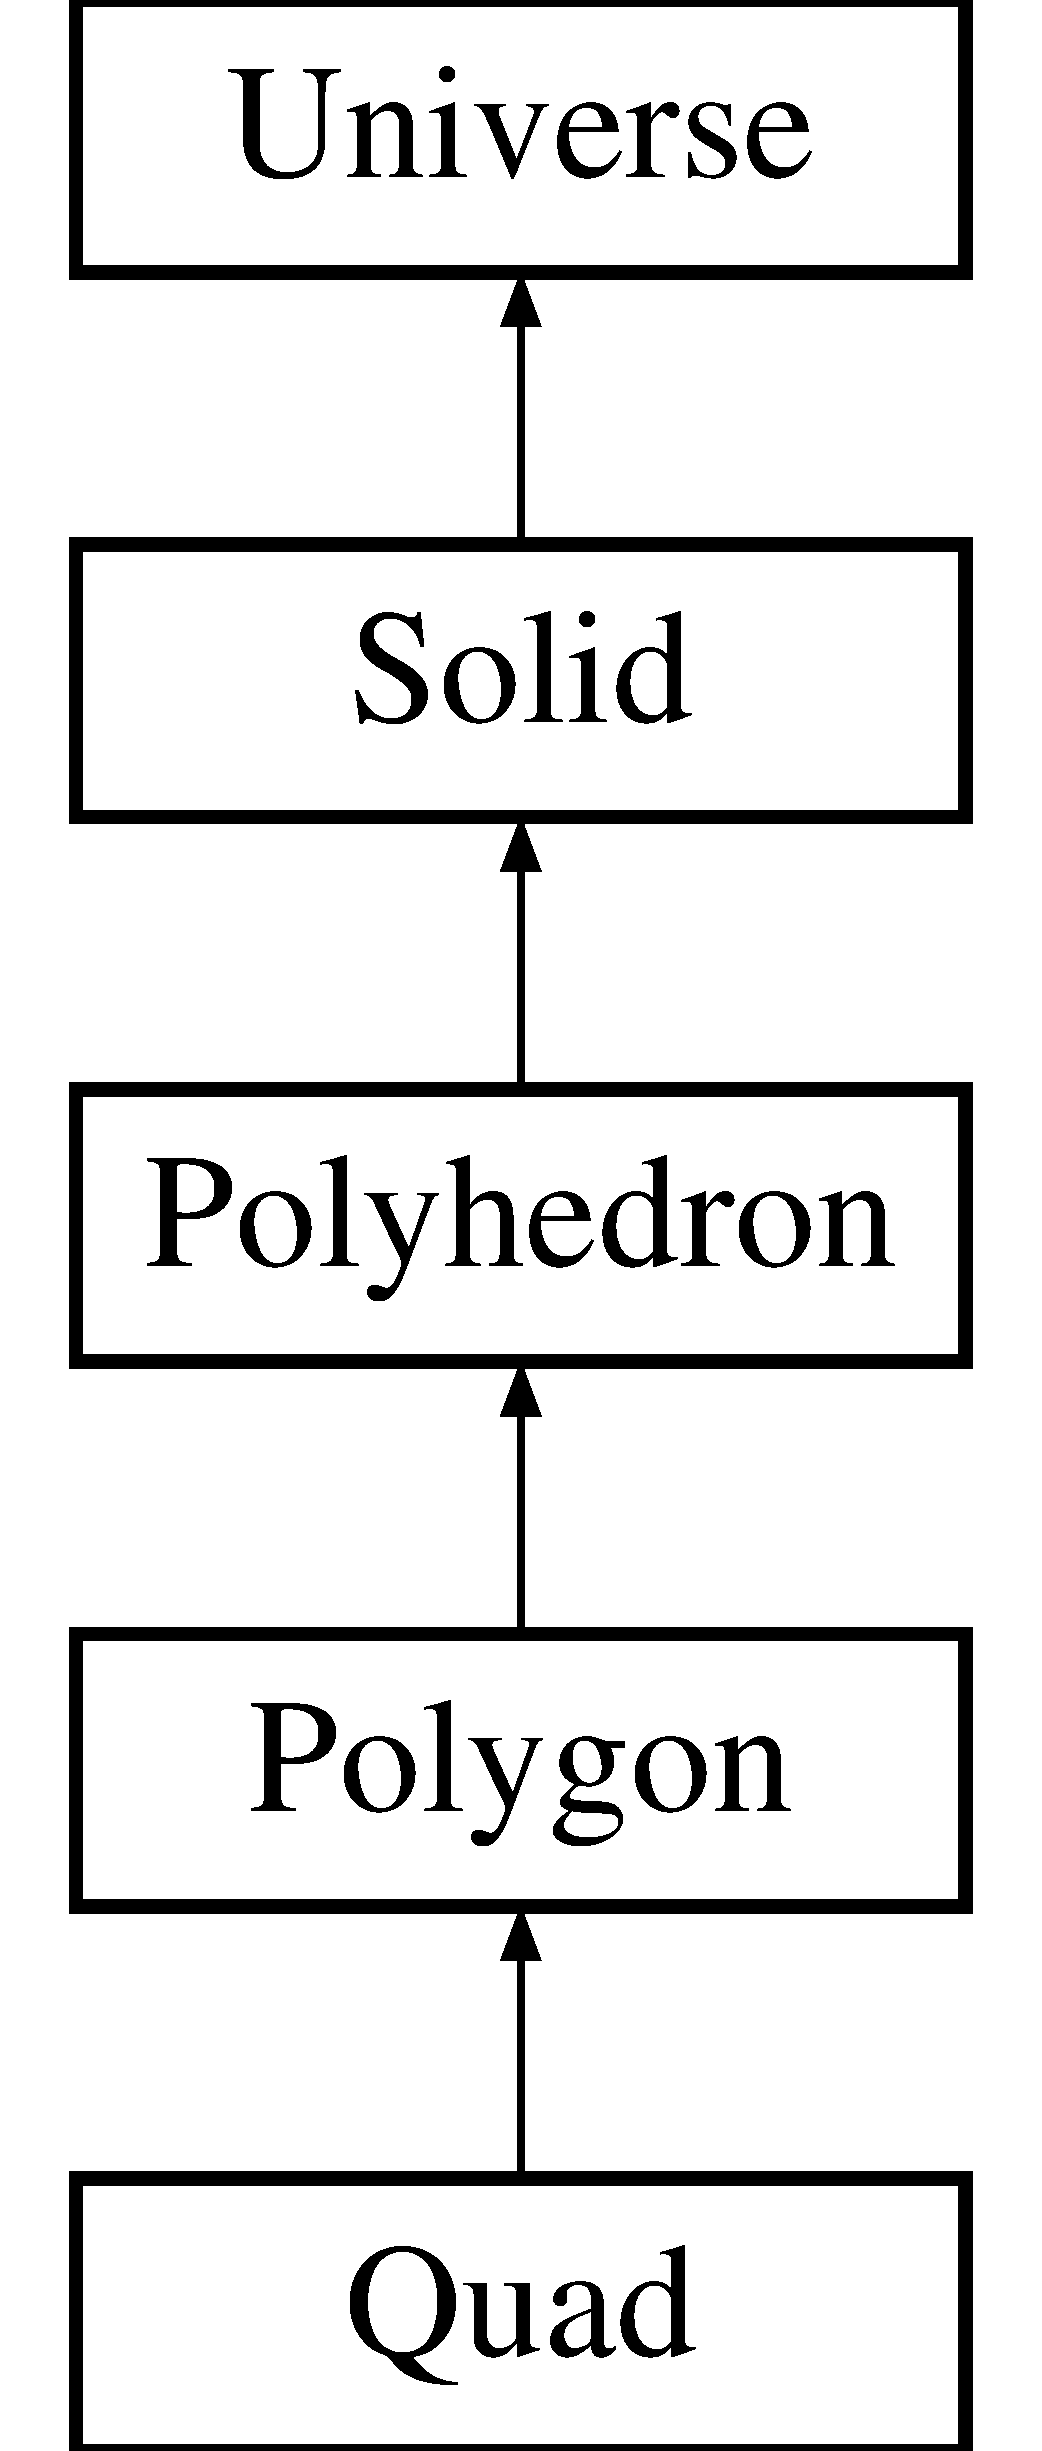
\includegraphics[height=5.000000cm]{classQuad}
\end{center}
\end{figure}
\subsection*{Public Member Functions}
\begin{DoxyCompactItemize}
\item 
\mbox{\hyperlink{classQuad_ae446d188d645cc5c512336f25d1a697a}{Quad}} ()
\item 
\mbox{\hyperlink{classQuad_a8a0b4e52a52ac35a4a78fac3a0cd36b8}{Quad}} (unsigned int object\+\_\+type)
\item 
\mbox{\hyperlink{classQuad_aa22093808d9a84db2bf826ccacee415e}{Quad}} (unsigned int object\+\_\+type, std\+::chrono\+::time\+\_\+point$<$ \mbox{\hyperlink{universe_8h_a0ef8d951d1ca5ab3cfaf7ab4c7a6fd80}{Clock}} $>$ event\+\_\+time)
\item 
\mbox{\hyperlink{classQuad_a4bb08fd4d953ce61076ed06b51ee2793}{Quad}} (unsigned int object\+\_\+type, std\+::chrono\+::time\+\_\+point$<$ \mbox{\hyperlink{universe_8h_a0ef8d951d1ca5ab3cfaf7ab4c7a6fd80}{Clock}} $>$ event\+\_\+time, \mbox{\hyperlink{classPolygon}{Polygon}} \&polygon\+\_\+connector)
\item 
virtual \mbox{\hyperlink{classQuad_a64a53d5b7a7811c34a85054828f74866}{$\sim$\+Quad}} ()
\item 
bool \mbox{\hyperlink{classQuad_af7c18022d7db1ad20bb7a1e1bd1ffb90}{Reset\+Parameters}} (std\+::chrono\+::time\+\_\+point$<$ \mbox{\hyperlink{universe_8h_a0ef8d951d1ca5ab3cfaf7ab4c7a6fd80}{Clock}} $>$ event\+\_\+time)
\item 
int \mbox{\hyperlink{classQuad_aba78e3b63f568529fcae1cfa6c3c54bf}{Get\+Quad\+ID}} (std\+::chrono\+::time\+\_\+point$<$ \mbox{\hyperlink{universe_8h_a0ef8d951d1ca5ab3cfaf7ab4c7a6fd80}{Clock}} $>$ event\+\_\+time) const
\item 
double \mbox{\hyperlink{classQuad_a7b0e34a18832713528b861f7ed35e139}{Get\+Quad\+X1}} (std\+::chrono\+::time\+\_\+point$<$ \mbox{\hyperlink{universe_8h_a0ef8d951d1ca5ab3cfaf7ab4c7a6fd80}{Clock}} $>$ event\+\_\+time) const
\item 
double \mbox{\hyperlink{classQuad_ac7b0d27994149531dcd81eacca4e1a5c}{Get\+Quad\+Y1}} (std\+::chrono\+::time\+\_\+point$<$ \mbox{\hyperlink{universe_8h_a0ef8d951d1ca5ab3cfaf7ab4c7a6fd80}{Clock}} $>$ event\+\_\+time) const
\item 
double \mbox{\hyperlink{classQuad_a2974623eaf17fe5bef35e8c4638149d6}{Get\+Quad\+X2}} (std\+::chrono\+::time\+\_\+point$<$ \mbox{\hyperlink{universe_8h_a0ef8d951d1ca5ab3cfaf7ab4c7a6fd80}{Clock}} $>$ event\+\_\+time) const
\item 
double \mbox{\hyperlink{classQuad_a8f10730993f6c6310f18431a81fb352a}{Get\+Quad\+Y2}} (std\+::chrono\+::time\+\_\+point$<$ \mbox{\hyperlink{universe_8h_a0ef8d951d1ca5ab3cfaf7ab4c7a6fd80}{Clock}} $>$ event\+\_\+time) const
\item 
double \mbox{\hyperlink{classQuad_aaa044d9683717efd054d82f553b3337d}{Get\+Quad\+X3}} (std\+::chrono\+::time\+\_\+point$<$ \mbox{\hyperlink{universe_8h_a0ef8d951d1ca5ab3cfaf7ab4c7a6fd80}{Clock}} $>$ event\+\_\+time) const
\item 
double \mbox{\hyperlink{classQuad_a9cdb9ea12e3aa3eb0e471015d4cb46bb}{Get\+Quad\+Y3}} (std\+::chrono\+::time\+\_\+point$<$ \mbox{\hyperlink{universe_8h_a0ef8d951d1ca5ab3cfaf7ab4c7a6fd80}{Clock}} $>$ event\+\_\+time) const
\item 
double \mbox{\hyperlink{classQuad_a07884076387e255aa09ca8b0ac7ff599}{Get\+Quad\+X4}} (std\+::chrono\+::time\+\_\+point$<$ \mbox{\hyperlink{universe_8h_a0ef8d951d1ca5ab3cfaf7ab4c7a6fd80}{Clock}} $>$ event\+\_\+time) const
\item 
double \mbox{\hyperlink{classQuad_aff3097e4988549376102daf18b582a0b}{Get\+Quad\+Y4}} (std\+::chrono\+::time\+\_\+point$<$ \mbox{\hyperlink{universe_8h_a0ef8d951d1ca5ab3cfaf7ab4c7a6fd80}{Clock}} $>$ event\+\_\+time) const
\item 
double \mbox{\hyperlink{classQuad_ab17ff4d689675e80107ecf6588811eee}{Get\+Quad\+T\+TL}} (std\+::chrono\+::time\+\_\+point$<$ \mbox{\hyperlink{universe_8h_a0ef8d951d1ca5ab3cfaf7ab4c7a6fd80}{Clock}} $>$ event\+\_\+time) const
\item 
int \mbox{\hyperlink{classQuad_a56ac193fa18af6ec468463cc16588cc1}{Get\+Quad\+Counter}} (std\+::chrono\+::time\+\_\+point$<$ \mbox{\hyperlink{universe_8h_a0ef8d951d1ca5ab3cfaf7ab4c7a6fd80}{Clock}} $>$ event\+\_\+time) const
\item 
bool \mbox{\hyperlink{classQuad_a80c2eb7c282e1566c5f7f235611b6206}{Get\+In\+Quad}} (std\+::chrono\+::time\+\_\+point$<$ \mbox{\hyperlink{universe_8h_a0ef8d951d1ca5ab3cfaf7ab4c7a6fd80}{Clock}} $>$ event\+\_\+time, double X1, double Y1, double X2, double Y2, double X3, double Y3, double X4, double Y4, double Threshold)
\item 
void \mbox{\hyperlink{classQuad_a9900acc75445ebc71aba2307e3fe0131}{Set\+Quad\+ID}} (std\+::chrono\+::time\+\_\+point$<$ \mbox{\hyperlink{universe_8h_a0ef8d951d1ca5ab3cfaf7ab4c7a6fd80}{Clock}} $>$ event\+\_\+time, int val)
\item 
void \mbox{\hyperlink{classQuad_a05fb7c22bfef542b99d04f968b4e18ab}{Set\+Quad\+X1}} (std\+::chrono\+::time\+\_\+point$<$ \mbox{\hyperlink{universe_8h_a0ef8d951d1ca5ab3cfaf7ab4c7a6fd80}{Clock}} $>$ event\+\_\+time, double val)
\item 
void \mbox{\hyperlink{classQuad_a3f0f9162be2b1ec2e2597a163586fb01}{Set\+Quad\+Y1}} (std\+::chrono\+::time\+\_\+point$<$ \mbox{\hyperlink{universe_8h_a0ef8d951d1ca5ab3cfaf7ab4c7a6fd80}{Clock}} $>$ event\+\_\+time, double val)
\item 
void \mbox{\hyperlink{classQuad_af1df44b73207c3e70b794e889e5225af}{Set\+Quad\+X2}} (std\+::chrono\+::time\+\_\+point$<$ \mbox{\hyperlink{universe_8h_a0ef8d951d1ca5ab3cfaf7ab4c7a6fd80}{Clock}} $>$ event\+\_\+time, double val)
\item 
void \mbox{\hyperlink{classQuad_afcec579c40a3763c34d1ace417888bf9}{Set\+Quad\+Y2}} (std\+::chrono\+::time\+\_\+point$<$ \mbox{\hyperlink{universe_8h_a0ef8d951d1ca5ab3cfaf7ab4c7a6fd80}{Clock}} $>$ event\+\_\+time, double val)
\item 
void \mbox{\hyperlink{classQuad_a0cbdd18a95fe7240b09c40fcee29f5df}{Set\+Quad\+X3}} (std\+::chrono\+::time\+\_\+point$<$ \mbox{\hyperlink{universe_8h_a0ef8d951d1ca5ab3cfaf7ab4c7a6fd80}{Clock}} $>$ event\+\_\+time, double val)
\item 
void \mbox{\hyperlink{classQuad_a1774a89a5d668aadf94966867270c0c5}{Set\+Quad\+Y3}} (std\+::chrono\+::time\+\_\+point$<$ \mbox{\hyperlink{universe_8h_a0ef8d951d1ca5ab3cfaf7ab4c7a6fd80}{Clock}} $>$ event\+\_\+time, double val)
\item 
void \mbox{\hyperlink{classQuad_ac49d711fa31a12ba24ad65c959c74e05}{Set\+Quad\+X4}} (std\+::chrono\+::time\+\_\+point$<$ \mbox{\hyperlink{universe_8h_a0ef8d951d1ca5ab3cfaf7ab4c7a6fd80}{Clock}} $>$ event\+\_\+time, double val)
\item 
void \mbox{\hyperlink{classQuad_ae299f75dcd479f5eb6ba8efed578961b}{Set\+Quad\+Y4}} (std\+::chrono\+::time\+\_\+point$<$ \mbox{\hyperlink{universe_8h_a0ef8d951d1ca5ab3cfaf7ab4c7a6fd80}{Clock}} $>$ event\+\_\+time, double val)
\item 
void \mbox{\hyperlink{classQuad_a4d3a52272d572315198623e836ac0a97}{Set\+Quad\+T\+TL}} (std\+::chrono\+::time\+\_\+point$<$ \mbox{\hyperlink{universe_8h_a0ef8d951d1ca5ab3cfaf7ab4c7a6fd80}{Clock}} $>$ event\+\_\+time, double val)
\item 
void \mbox{\hyperlink{classQuad_a66ba58a32cf7b351e3e155efbdb46f8e}{Set\+Quad\+Counter}} (std\+::chrono\+::time\+\_\+point$<$ \mbox{\hyperlink{universe_8h_a0ef8d951d1ca5ab3cfaf7ab4c7a6fd80}{Clock}} $>$ event\+\_\+time, int val)
\item 
int \mbox{\hyperlink{classQuad_a0710e6a7d77a34fdadbd2c36d03ade62}{Update}} (std\+::chrono\+::time\+\_\+point$<$ \mbox{\hyperlink{universe_8h_a0ef8d951d1ca5ab3cfaf7ab4c7a6fd80}{Clock}} $>$ event\+\_\+time)
\end{DoxyCompactItemize}
\subsection*{Private Attributes}
\begin{DoxyCompactItemize}
\item 
int \mbox{\hyperlink{classQuad_a188ee923776070ca5e70fdf7b4e450e7}{quad\+Quad\+ID}}
\item 
double \mbox{\hyperlink{classQuad_a5253015c13e6858a9fd0d8c1823fb434}{quad\+Quad\+X1}}
\begin{DoxyCompactList}\small\item\em Member variable \char`\"{}quad\+Quad\+X1\char`\"{}. \end{DoxyCompactList}\item 
double \mbox{\hyperlink{classQuad_aa15251ffcca05eb0e35a3d6b60782c9d}{quad\+Quad\+Y1}}
\begin{DoxyCompactList}\small\item\em Member variable \char`\"{}quad\+Quad\+Y1\char`\"{}. \end{DoxyCompactList}\item 
double \mbox{\hyperlink{classQuad_a26bd14e8ee6c121eea8508480cc69139}{quad\+Quad\+X2}}
\begin{DoxyCompactList}\small\item\em Member variable \char`\"{}quad\+Quad\+X2\char`\"{}. \end{DoxyCompactList}\item 
double \mbox{\hyperlink{classQuad_afa2e09e70744ac127feedd54d2c2de85}{quad\+Quad\+Y2}}
\begin{DoxyCompactList}\small\item\em Member variable \char`\"{}quad\+Quad\+Y2\char`\"{}. \end{DoxyCompactList}\item 
double \mbox{\hyperlink{classQuad_af9b30ca5cb770b3afe12d93eae9bbff1}{quad\+Quad\+X3}}
\begin{DoxyCompactList}\small\item\em Member variable \char`\"{}quad\+Quad\+X3\char`\"{}. \end{DoxyCompactList}\item 
double \mbox{\hyperlink{classQuad_a71c344b5032f910a34a8ffef7ba894c0}{quad\+Quad\+Y3}}
\begin{DoxyCompactList}\small\item\em Member variable \char`\"{}quad\+Quad\+Y3\char`\"{}. \end{DoxyCompactList}\item 
double \mbox{\hyperlink{classQuad_a6bc4285074ff7259ab59293fe207af01}{quad\+Quad\+X4}}
\begin{DoxyCompactList}\small\item\em Member variable \char`\"{}quad\+Quad\+X4\char`\"{}. \end{DoxyCompactList}\item 
double \mbox{\hyperlink{classQuad_a0e7d3d2357464cbe78d73750b2399d95}{quad\+Quad\+Y4}}
\begin{DoxyCompactList}\small\item\em Member variable \char`\"{}quad\+Quad\+Y4\char`\"{}. \end{DoxyCompactList}\item 
double \mbox{\hyperlink{classQuad_aaeab0be987926009753a8d6ba0da91f3}{quad\+Quad\+T\+TL}}
\item 
int \mbox{\hyperlink{classQuad_a997f8e0e69db9b872a79566225686535}{quad\+Quad\+Counter}}
\item 
int \mbox{\hyperlink{classQuad_a57fab7c05edae3fcc29ab4e9aad3fadf}{quad\+\_\+type}}
\item 
bool \mbox{\hyperlink{classQuad_a5c2d3f68a2e9635ef429696dc6ea85a4}{object\+\_\+disabled}} = true
\item 
bool \mbox{\hyperlink{classQuad_a3c86ec7d962acd1e478ed55095970b1d}{object\+\_\+initialised}} = false
\item 
std\+::chrono\+::time\+\_\+point$<$ \mbox{\hyperlink{universe_8h_a0ef8d951d1ca5ab3cfaf7ab4c7a6fd80}{Clock}} $>$ \mbox{\hyperlink{classQuad_a5779e2e09362b665bccd2ae4e29602ff}{time\+\_\+object\+\_\+created}}
\item 
std\+::chrono\+::time\+\_\+point$<$ \mbox{\hyperlink{universe_8h_a0ef8d951d1ca5ab3cfaf7ab4c7a6fd80}{Clock}} $>$ \mbox{\hyperlink{classQuad_a949879597ab1df686b85faef577c9081}{previous\+\_\+event\+\_\+time}}
\item 
int \mbox{\hyperlink{classQuad_a2b51c548a5ede0a340374c6ce9093cd5}{duration\+\_\+since\+\_\+last\+\_\+event}}
\end{DoxyCompactItemize}
\subsection*{Additional Inherited Members}


\subsection{Constructor \& Destructor Documentation}
\mbox{\Hypertarget{classQuad_ae446d188d645cc5c512336f25d1a697a}\label{classQuad_ae446d188d645cc5c512336f25d1a697a}} 
\index{Quad@{Quad}!Quad@{Quad}}
\index{Quad@{Quad}!Quad@{Quad}}
\subsubsection{\texorpdfstring{Quad()}{Quad()}\hspace{0.1cm}{\footnotesize\ttfamily [1/4]}}
{\footnotesize\ttfamily Quad\+::\+Quad (\begin{DoxyParamCaption}{ }\end{DoxyParamCaption})\hspace{0.3cm}{\ttfamily [inline]}}

\mbox{\Hypertarget{classQuad_a8a0b4e52a52ac35a4a78fac3a0cd36b8}\label{classQuad_a8a0b4e52a52ac35a4a78fac3a0cd36b8}} 
\index{Quad@{Quad}!Quad@{Quad}}
\index{Quad@{Quad}!Quad@{Quad}}
\subsubsection{\texorpdfstring{Quad()}{Quad()}\hspace{0.1cm}{\footnotesize\ttfamily [2/4]}}
{\footnotesize\ttfamily Quad\+::\+Quad (\begin{DoxyParamCaption}\item[{unsigned int}]{object\+\_\+type }\end{DoxyParamCaption})\hspace{0.3cm}{\ttfamily [inline]}}

\mbox{\Hypertarget{classQuad_aa22093808d9a84db2bf826ccacee415e}\label{classQuad_aa22093808d9a84db2bf826ccacee415e}} 
\index{Quad@{Quad}!Quad@{Quad}}
\index{Quad@{Quad}!Quad@{Quad}}
\subsubsection{\texorpdfstring{Quad()}{Quad()}\hspace{0.1cm}{\footnotesize\ttfamily [3/4]}}
{\footnotesize\ttfamily Quad\+::\+Quad (\begin{DoxyParamCaption}\item[{unsigned int}]{object\+\_\+type,  }\item[{std\+::chrono\+::time\+\_\+point$<$ \mbox{\hyperlink{universe_8h_a0ef8d951d1ca5ab3cfaf7ab4c7a6fd80}{Clock}} $>$}]{event\+\_\+time }\end{DoxyParamCaption})\hspace{0.3cm}{\ttfamily [inline]}}

\mbox{\Hypertarget{classQuad_a4bb08fd4d953ce61076ed06b51ee2793}\label{classQuad_a4bb08fd4d953ce61076ed06b51ee2793}} 
\index{Quad@{Quad}!Quad@{Quad}}
\index{Quad@{Quad}!Quad@{Quad}}
\subsubsection{\texorpdfstring{Quad()}{Quad()}\hspace{0.1cm}{\footnotesize\ttfamily [4/4]}}
{\footnotesize\ttfamily Quad\+::\+Quad (\begin{DoxyParamCaption}\item[{unsigned int}]{object\+\_\+type,  }\item[{std\+::chrono\+::time\+\_\+point$<$ \mbox{\hyperlink{universe_8h_a0ef8d951d1ca5ab3cfaf7ab4c7a6fd80}{Clock}} $>$}]{event\+\_\+time,  }\item[{\mbox{\hyperlink{classPolygon}{Polygon}} \&}]{polygon\+\_\+connector }\end{DoxyParamCaption})\hspace{0.3cm}{\ttfamily [inline]}}

\mbox{\Hypertarget{classQuad_a64a53d5b7a7811c34a85054828f74866}\label{classQuad_a64a53d5b7a7811c34a85054828f74866}} 
\index{Quad@{Quad}!````~Quad@{$\sim$\+Quad}}
\index{````~Quad@{$\sim$\+Quad}!Quad@{Quad}}
\subsubsection{\texorpdfstring{$\sim$\+Quad()}{~Quad()}}
{\footnotesize\ttfamily virtual Quad\+::$\sim$\+Quad (\begin{DoxyParamCaption}{ }\end{DoxyParamCaption})\hspace{0.3cm}{\ttfamily [inline]}, {\ttfamily [virtual]}}

Default destructor 

\subsection{Member Function Documentation}
\mbox{\Hypertarget{classQuad_a80c2eb7c282e1566c5f7f235611b6206}\label{classQuad_a80c2eb7c282e1566c5f7f235611b6206}} 
\index{Quad@{Quad}!Get\+In\+Quad@{Get\+In\+Quad}}
\index{Get\+In\+Quad@{Get\+In\+Quad}!Quad@{Quad}}
\subsubsection{\texorpdfstring{Get\+In\+Quad()}{GetInQuad()}}
{\footnotesize\ttfamily bool Quad\+::\+Get\+In\+Quad (\begin{DoxyParamCaption}\item[{std\+::chrono\+::time\+\_\+point$<$ \mbox{\hyperlink{universe_8h_a0ef8d951d1ca5ab3cfaf7ab4c7a6fd80}{Clock}} $>$}]{event\+\_\+time,  }\item[{double}]{X1,  }\item[{double}]{Y1,  }\item[{double}]{X2,  }\item[{double}]{Y2,  }\item[{double}]{X3,  }\item[{double}]{Y3,  }\item[{double}]{X4,  }\item[{double}]{Y4,  }\item[{double}]{Threshold }\end{DoxyParamCaption})\hspace{0.3cm}{\ttfamily [inline]}}

\mbox{\Hypertarget{classQuad_a56ac193fa18af6ec468463cc16588cc1}\label{classQuad_a56ac193fa18af6ec468463cc16588cc1}} 
\index{Quad@{Quad}!Get\+Quad\+Counter@{Get\+Quad\+Counter}}
\index{Get\+Quad\+Counter@{Get\+Quad\+Counter}!Quad@{Quad}}
\subsubsection{\texorpdfstring{Get\+Quad\+Counter()}{GetQuadCounter()}}
{\footnotesize\ttfamily int Quad\+::\+Get\+Quad\+Counter (\begin{DoxyParamCaption}\item[{std\+::chrono\+::time\+\_\+point$<$ \mbox{\hyperlink{universe_8h_a0ef8d951d1ca5ab3cfaf7ab4c7a6fd80}{Clock}} $>$}]{event\+\_\+time }\end{DoxyParamCaption}) const\hspace{0.3cm}{\ttfamily [inline]}}

\mbox{\Hypertarget{classQuad_aba78e3b63f568529fcae1cfa6c3c54bf}\label{classQuad_aba78e3b63f568529fcae1cfa6c3c54bf}} 
\index{Quad@{Quad}!Get\+Quad\+ID@{Get\+Quad\+ID}}
\index{Get\+Quad\+ID@{Get\+Quad\+ID}!Quad@{Quad}}
\subsubsection{\texorpdfstring{Get\+Quad\+I\+D()}{GetQuadID()}}
{\footnotesize\ttfamily int Quad\+::\+Get\+Quad\+ID (\begin{DoxyParamCaption}\item[{std\+::chrono\+::time\+\_\+point$<$ \mbox{\hyperlink{universe_8h_a0ef8d951d1ca5ab3cfaf7ab4c7a6fd80}{Clock}} $>$}]{event\+\_\+time }\end{DoxyParamCaption}) const\hspace{0.3cm}{\ttfamily [inline]}}

\mbox{\Hypertarget{classQuad_ab17ff4d689675e80107ecf6588811eee}\label{classQuad_ab17ff4d689675e80107ecf6588811eee}} 
\index{Quad@{Quad}!Get\+Quad\+T\+TL@{Get\+Quad\+T\+TL}}
\index{Get\+Quad\+T\+TL@{Get\+Quad\+T\+TL}!Quad@{Quad}}
\subsubsection{\texorpdfstring{Get\+Quad\+T\+T\+L()}{GetQuadTTL()}}
{\footnotesize\ttfamily double Quad\+::\+Get\+Quad\+T\+TL (\begin{DoxyParamCaption}\item[{std\+::chrono\+::time\+\_\+point$<$ \mbox{\hyperlink{universe_8h_a0ef8d951d1ca5ab3cfaf7ab4c7a6fd80}{Clock}} $>$}]{event\+\_\+time }\end{DoxyParamCaption}) const\hspace{0.3cm}{\ttfamily [inline]}}

\mbox{\Hypertarget{classQuad_a7b0e34a18832713528b861f7ed35e139}\label{classQuad_a7b0e34a18832713528b861f7ed35e139}} 
\index{Quad@{Quad}!Get\+Quad\+X1@{Get\+Quad\+X1}}
\index{Get\+Quad\+X1@{Get\+Quad\+X1}!Quad@{Quad}}
\subsubsection{\texorpdfstring{Get\+Quad\+X1()}{GetQuadX1()}}
{\footnotesize\ttfamily double Quad\+::\+Get\+Quad\+X1 (\begin{DoxyParamCaption}\item[{std\+::chrono\+::time\+\_\+point$<$ \mbox{\hyperlink{universe_8h_a0ef8d951d1ca5ab3cfaf7ab4c7a6fd80}{Clock}} $>$}]{event\+\_\+time }\end{DoxyParamCaption}) const\hspace{0.3cm}{\ttfamily [inline]}}

\mbox{\Hypertarget{classQuad_a2974623eaf17fe5bef35e8c4638149d6}\label{classQuad_a2974623eaf17fe5bef35e8c4638149d6}} 
\index{Quad@{Quad}!Get\+Quad\+X2@{Get\+Quad\+X2}}
\index{Get\+Quad\+X2@{Get\+Quad\+X2}!Quad@{Quad}}
\subsubsection{\texorpdfstring{Get\+Quad\+X2()}{GetQuadX2()}}
{\footnotesize\ttfamily double Quad\+::\+Get\+Quad\+X2 (\begin{DoxyParamCaption}\item[{std\+::chrono\+::time\+\_\+point$<$ \mbox{\hyperlink{universe_8h_a0ef8d951d1ca5ab3cfaf7ab4c7a6fd80}{Clock}} $>$}]{event\+\_\+time }\end{DoxyParamCaption}) const\hspace{0.3cm}{\ttfamily [inline]}}

\mbox{\Hypertarget{classQuad_aaa044d9683717efd054d82f553b3337d}\label{classQuad_aaa044d9683717efd054d82f553b3337d}} 
\index{Quad@{Quad}!Get\+Quad\+X3@{Get\+Quad\+X3}}
\index{Get\+Quad\+X3@{Get\+Quad\+X3}!Quad@{Quad}}
\subsubsection{\texorpdfstring{Get\+Quad\+X3()}{GetQuadX3()}}
{\footnotesize\ttfamily double Quad\+::\+Get\+Quad\+X3 (\begin{DoxyParamCaption}\item[{std\+::chrono\+::time\+\_\+point$<$ \mbox{\hyperlink{universe_8h_a0ef8d951d1ca5ab3cfaf7ab4c7a6fd80}{Clock}} $>$}]{event\+\_\+time }\end{DoxyParamCaption}) const\hspace{0.3cm}{\ttfamily [inline]}}

\mbox{\Hypertarget{classQuad_a07884076387e255aa09ca8b0ac7ff599}\label{classQuad_a07884076387e255aa09ca8b0ac7ff599}} 
\index{Quad@{Quad}!Get\+Quad\+X4@{Get\+Quad\+X4}}
\index{Get\+Quad\+X4@{Get\+Quad\+X4}!Quad@{Quad}}
\subsubsection{\texorpdfstring{Get\+Quad\+X4()}{GetQuadX4()}}
{\footnotesize\ttfamily double Quad\+::\+Get\+Quad\+X4 (\begin{DoxyParamCaption}\item[{std\+::chrono\+::time\+\_\+point$<$ \mbox{\hyperlink{universe_8h_a0ef8d951d1ca5ab3cfaf7ab4c7a6fd80}{Clock}} $>$}]{event\+\_\+time }\end{DoxyParamCaption}) const\hspace{0.3cm}{\ttfamily [inline]}}

\mbox{\Hypertarget{classQuad_ac7b0d27994149531dcd81eacca4e1a5c}\label{classQuad_ac7b0d27994149531dcd81eacca4e1a5c}} 
\index{Quad@{Quad}!Get\+Quad\+Y1@{Get\+Quad\+Y1}}
\index{Get\+Quad\+Y1@{Get\+Quad\+Y1}!Quad@{Quad}}
\subsubsection{\texorpdfstring{Get\+Quad\+Y1()}{GetQuadY1()}}
{\footnotesize\ttfamily double Quad\+::\+Get\+Quad\+Y1 (\begin{DoxyParamCaption}\item[{std\+::chrono\+::time\+\_\+point$<$ \mbox{\hyperlink{universe_8h_a0ef8d951d1ca5ab3cfaf7ab4c7a6fd80}{Clock}} $>$}]{event\+\_\+time }\end{DoxyParamCaption}) const\hspace{0.3cm}{\ttfamily [inline]}}

\mbox{\Hypertarget{classQuad_a8f10730993f6c6310f18431a81fb352a}\label{classQuad_a8f10730993f6c6310f18431a81fb352a}} 
\index{Quad@{Quad}!Get\+Quad\+Y2@{Get\+Quad\+Y2}}
\index{Get\+Quad\+Y2@{Get\+Quad\+Y2}!Quad@{Quad}}
\subsubsection{\texorpdfstring{Get\+Quad\+Y2()}{GetQuadY2()}}
{\footnotesize\ttfamily double Quad\+::\+Get\+Quad\+Y2 (\begin{DoxyParamCaption}\item[{std\+::chrono\+::time\+\_\+point$<$ \mbox{\hyperlink{universe_8h_a0ef8d951d1ca5ab3cfaf7ab4c7a6fd80}{Clock}} $>$}]{event\+\_\+time }\end{DoxyParamCaption}) const\hspace{0.3cm}{\ttfamily [inline]}}

\mbox{\Hypertarget{classQuad_a9cdb9ea12e3aa3eb0e471015d4cb46bb}\label{classQuad_a9cdb9ea12e3aa3eb0e471015d4cb46bb}} 
\index{Quad@{Quad}!Get\+Quad\+Y3@{Get\+Quad\+Y3}}
\index{Get\+Quad\+Y3@{Get\+Quad\+Y3}!Quad@{Quad}}
\subsubsection{\texorpdfstring{Get\+Quad\+Y3()}{GetQuadY3()}}
{\footnotesize\ttfamily double Quad\+::\+Get\+Quad\+Y3 (\begin{DoxyParamCaption}\item[{std\+::chrono\+::time\+\_\+point$<$ \mbox{\hyperlink{universe_8h_a0ef8d951d1ca5ab3cfaf7ab4c7a6fd80}{Clock}} $>$}]{event\+\_\+time }\end{DoxyParamCaption}) const\hspace{0.3cm}{\ttfamily [inline]}}

\mbox{\Hypertarget{classQuad_aff3097e4988549376102daf18b582a0b}\label{classQuad_aff3097e4988549376102daf18b582a0b}} 
\index{Quad@{Quad}!Get\+Quad\+Y4@{Get\+Quad\+Y4}}
\index{Get\+Quad\+Y4@{Get\+Quad\+Y4}!Quad@{Quad}}
\subsubsection{\texorpdfstring{Get\+Quad\+Y4()}{GetQuadY4()}}
{\footnotesize\ttfamily double Quad\+::\+Get\+Quad\+Y4 (\begin{DoxyParamCaption}\item[{std\+::chrono\+::time\+\_\+point$<$ \mbox{\hyperlink{universe_8h_a0ef8d951d1ca5ab3cfaf7ab4c7a6fd80}{Clock}} $>$}]{event\+\_\+time }\end{DoxyParamCaption}) const\hspace{0.3cm}{\ttfamily [inline]}}

\mbox{\Hypertarget{classQuad_af7c18022d7db1ad20bb7a1e1bd1ffb90}\label{classQuad_af7c18022d7db1ad20bb7a1e1bd1ffb90}} 
\index{Quad@{Quad}!Reset\+Parameters@{Reset\+Parameters}}
\index{Reset\+Parameters@{Reset\+Parameters}!Quad@{Quad}}
\subsubsection{\texorpdfstring{Reset\+Parameters()}{ResetParameters()}}
{\footnotesize\ttfamily bool Quad\+::\+Reset\+Parameters (\begin{DoxyParamCaption}\item[{std\+::chrono\+::time\+\_\+point$<$ \mbox{\hyperlink{universe_8h_a0ef8d951d1ca5ab3cfaf7ab4c7a6fd80}{Clock}} $>$}]{event\+\_\+time }\end{DoxyParamCaption})}

\mbox{\Hypertarget{classQuad_a66ba58a32cf7b351e3e155efbdb46f8e}\label{classQuad_a66ba58a32cf7b351e3e155efbdb46f8e}} 
\index{Quad@{Quad}!Set\+Quad\+Counter@{Set\+Quad\+Counter}}
\index{Set\+Quad\+Counter@{Set\+Quad\+Counter}!Quad@{Quad}}
\subsubsection{\texorpdfstring{Set\+Quad\+Counter()}{SetQuadCounter()}}
{\footnotesize\ttfamily void Quad\+::\+Set\+Quad\+Counter (\begin{DoxyParamCaption}\item[{std\+::chrono\+::time\+\_\+point$<$ \mbox{\hyperlink{universe_8h_a0ef8d951d1ca5ab3cfaf7ab4c7a6fd80}{Clock}} $>$}]{event\+\_\+time,  }\item[{int}]{val }\end{DoxyParamCaption})\hspace{0.3cm}{\ttfamily [inline]}}

\mbox{\Hypertarget{classQuad_a9900acc75445ebc71aba2307e3fe0131}\label{classQuad_a9900acc75445ebc71aba2307e3fe0131}} 
\index{Quad@{Quad}!Set\+Quad\+ID@{Set\+Quad\+ID}}
\index{Set\+Quad\+ID@{Set\+Quad\+ID}!Quad@{Quad}}
\subsubsection{\texorpdfstring{Set\+Quad\+I\+D()}{SetQuadID()}}
{\footnotesize\ttfamily void Quad\+::\+Set\+Quad\+ID (\begin{DoxyParamCaption}\item[{std\+::chrono\+::time\+\_\+point$<$ \mbox{\hyperlink{universe_8h_a0ef8d951d1ca5ab3cfaf7ab4c7a6fd80}{Clock}} $>$}]{event\+\_\+time,  }\item[{int}]{val }\end{DoxyParamCaption})\hspace{0.3cm}{\ttfamily [inline]}}

\mbox{\Hypertarget{classQuad_a4d3a52272d572315198623e836ac0a97}\label{classQuad_a4d3a52272d572315198623e836ac0a97}} 
\index{Quad@{Quad}!Set\+Quad\+T\+TL@{Set\+Quad\+T\+TL}}
\index{Set\+Quad\+T\+TL@{Set\+Quad\+T\+TL}!Quad@{Quad}}
\subsubsection{\texorpdfstring{Set\+Quad\+T\+T\+L()}{SetQuadTTL()}}
{\footnotesize\ttfamily void Quad\+::\+Set\+Quad\+T\+TL (\begin{DoxyParamCaption}\item[{std\+::chrono\+::time\+\_\+point$<$ \mbox{\hyperlink{universe_8h_a0ef8d951d1ca5ab3cfaf7ab4c7a6fd80}{Clock}} $>$}]{event\+\_\+time,  }\item[{double}]{val }\end{DoxyParamCaption})\hspace{0.3cm}{\ttfamily [inline]}}

\mbox{\Hypertarget{classQuad_a05fb7c22bfef542b99d04f968b4e18ab}\label{classQuad_a05fb7c22bfef542b99d04f968b4e18ab}} 
\index{Quad@{Quad}!Set\+Quad\+X1@{Set\+Quad\+X1}}
\index{Set\+Quad\+X1@{Set\+Quad\+X1}!Quad@{Quad}}
\subsubsection{\texorpdfstring{Set\+Quad\+X1()}{SetQuadX1()}}
{\footnotesize\ttfamily void Quad\+::\+Set\+Quad\+X1 (\begin{DoxyParamCaption}\item[{std\+::chrono\+::time\+\_\+point$<$ \mbox{\hyperlink{universe_8h_a0ef8d951d1ca5ab3cfaf7ab4c7a6fd80}{Clock}} $>$}]{event\+\_\+time,  }\item[{double}]{val }\end{DoxyParamCaption})\hspace{0.3cm}{\ttfamily [inline]}}

\mbox{\Hypertarget{classQuad_af1df44b73207c3e70b794e889e5225af}\label{classQuad_af1df44b73207c3e70b794e889e5225af}} 
\index{Quad@{Quad}!Set\+Quad\+X2@{Set\+Quad\+X2}}
\index{Set\+Quad\+X2@{Set\+Quad\+X2}!Quad@{Quad}}
\subsubsection{\texorpdfstring{Set\+Quad\+X2()}{SetQuadX2()}}
{\footnotesize\ttfamily void Quad\+::\+Set\+Quad\+X2 (\begin{DoxyParamCaption}\item[{std\+::chrono\+::time\+\_\+point$<$ \mbox{\hyperlink{universe_8h_a0ef8d951d1ca5ab3cfaf7ab4c7a6fd80}{Clock}} $>$}]{event\+\_\+time,  }\item[{double}]{val }\end{DoxyParamCaption})\hspace{0.3cm}{\ttfamily [inline]}}

\mbox{\Hypertarget{classQuad_a0cbdd18a95fe7240b09c40fcee29f5df}\label{classQuad_a0cbdd18a95fe7240b09c40fcee29f5df}} 
\index{Quad@{Quad}!Set\+Quad\+X3@{Set\+Quad\+X3}}
\index{Set\+Quad\+X3@{Set\+Quad\+X3}!Quad@{Quad}}
\subsubsection{\texorpdfstring{Set\+Quad\+X3()}{SetQuadX3()}}
{\footnotesize\ttfamily void Quad\+::\+Set\+Quad\+X3 (\begin{DoxyParamCaption}\item[{std\+::chrono\+::time\+\_\+point$<$ \mbox{\hyperlink{universe_8h_a0ef8d951d1ca5ab3cfaf7ab4c7a6fd80}{Clock}} $>$}]{event\+\_\+time,  }\item[{double}]{val }\end{DoxyParamCaption})\hspace{0.3cm}{\ttfamily [inline]}}

\mbox{\Hypertarget{classQuad_ac49d711fa31a12ba24ad65c959c74e05}\label{classQuad_ac49d711fa31a12ba24ad65c959c74e05}} 
\index{Quad@{Quad}!Set\+Quad\+X4@{Set\+Quad\+X4}}
\index{Set\+Quad\+X4@{Set\+Quad\+X4}!Quad@{Quad}}
\subsubsection{\texorpdfstring{Set\+Quad\+X4()}{SetQuadX4()}}
{\footnotesize\ttfamily void Quad\+::\+Set\+Quad\+X4 (\begin{DoxyParamCaption}\item[{std\+::chrono\+::time\+\_\+point$<$ \mbox{\hyperlink{universe_8h_a0ef8d951d1ca5ab3cfaf7ab4c7a6fd80}{Clock}} $>$}]{event\+\_\+time,  }\item[{double}]{val }\end{DoxyParamCaption})\hspace{0.3cm}{\ttfamily [inline]}}

\mbox{\Hypertarget{classQuad_a3f0f9162be2b1ec2e2597a163586fb01}\label{classQuad_a3f0f9162be2b1ec2e2597a163586fb01}} 
\index{Quad@{Quad}!Set\+Quad\+Y1@{Set\+Quad\+Y1}}
\index{Set\+Quad\+Y1@{Set\+Quad\+Y1}!Quad@{Quad}}
\subsubsection{\texorpdfstring{Set\+Quad\+Y1()}{SetQuadY1()}}
{\footnotesize\ttfamily void Quad\+::\+Set\+Quad\+Y1 (\begin{DoxyParamCaption}\item[{std\+::chrono\+::time\+\_\+point$<$ \mbox{\hyperlink{universe_8h_a0ef8d951d1ca5ab3cfaf7ab4c7a6fd80}{Clock}} $>$}]{event\+\_\+time,  }\item[{double}]{val }\end{DoxyParamCaption})\hspace{0.3cm}{\ttfamily [inline]}}

\mbox{\Hypertarget{classQuad_afcec579c40a3763c34d1ace417888bf9}\label{classQuad_afcec579c40a3763c34d1ace417888bf9}} 
\index{Quad@{Quad}!Set\+Quad\+Y2@{Set\+Quad\+Y2}}
\index{Set\+Quad\+Y2@{Set\+Quad\+Y2}!Quad@{Quad}}
\subsubsection{\texorpdfstring{Set\+Quad\+Y2()}{SetQuadY2()}}
{\footnotesize\ttfamily void Quad\+::\+Set\+Quad\+Y2 (\begin{DoxyParamCaption}\item[{std\+::chrono\+::time\+\_\+point$<$ \mbox{\hyperlink{universe_8h_a0ef8d951d1ca5ab3cfaf7ab4c7a6fd80}{Clock}} $>$}]{event\+\_\+time,  }\item[{double}]{val }\end{DoxyParamCaption})\hspace{0.3cm}{\ttfamily [inline]}}

\mbox{\Hypertarget{classQuad_a1774a89a5d668aadf94966867270c0c5}\label{classQuad_a1774a89a5d668aadf94966867270c0c5}} 
\index{Quad@{Quad}!Set\+Quad\+Y3@{Set\+Quad\+Y3}}
\index{Set\+Quad\+Y3@{Set\+Quad\+Y3}!Quad@{Quad}}
\subsubsection{\texorpdfstring{Set\+Quad\+Y3()}{SetQuadY3()}}
{\footnotesize\ttfamily void Quad\+::\+Set\+Quad\+Y3 (\begin{DoxyParamCaption}\item[{std\+::chrono\+::time\+\_\+point$<$ \mbox{\hyperlink{universe_8h_a0ef8d951d1ca5ab3cfaf7ab4c7a6fd80}{Clock}} $>$}]{event\+\_\+time,  }\item[{double}]{val }\end{DoxyParamCaption})\hspace{0.3cm}{\ttfamily [inline]}}

\mbox{\Hypertarget{classQuad_ae299f75dcd479f5eb6ba8efed578961b}\label{classQuad_ae299f75dcd479f5eb6ba8efed578961b}} 
\index{Quad@{Quad}!Set\+Quad\+Y4@{Set\+Quad\+Y4}}
\index{Set\+Quad\+Y4@{Set\+Quad\+Y4}!Quad@{Quad}}
\subsubsection{\texorpdfstring{Set\+Quad\+Y4()}{SetQuadY4()}}
{\footnotesize\ttfamily void Quad\+::\+Set\+Quad\+Y4 (\begin{DoxyParamCaption}\item[{std\+::chrono\+::time\+\_\+point$<$ \mbox{\hyperlink{universe_8h_a0ef8d951d1ca5ab3cfaf7ab4c7a6fd80}{Clock}} $>$}]{event\+\_\+time,  }\item[{double}]{val }\end{DoxyParamCaption})\hspace{0.3cm}{\ttfamily [inline]}}

\mbox{\Hypertarget{classQuad_a0710e6a7d77a34fdadbd2c36d03ade62}\label{classQuad_a0710e6a7d77a34fdadbd2c36d03ade62}} 
\index{Quad@{Quad}!Update@{Update}}
\index{Update@{Update}!Quad@{Quad}}
\subsubsection{\texorpdfstring{Update()}{Update()}}
{\footnotesize\ttfamily int Quad\+::\+Update (\begin{DoxyParamCaption}\item[{std\+::chrono\+::time\+\_\+point$<$ \mbox{\hyperlink{universe_8h_a0ef8d951d1ca5ab3cfaf7ab4c7a6fd80}{Clock}} $>$}]{event\+\_\+time }\end{DoxyParamCaption})}



\subsection{Member Data Documentation}
\mbox{\Hypertarget{classQuad_a2b51c548a5ede0a340374c6ce9093cd5}\label{classQuad_a2b51c548a5ede0a340374c6ce9093cd5}} 
\index{Quad@{Quad}!duration\+\_\+since\+\_\+last\+\_\+event@{duration\+\_\+since\+\_\+last\+\_\+event}}
\index{duration\+\_\+since\+\_\+last\+\_\+event@{duration\+\_\+since\+\_\+last\+\_\+event}!Quad@{Quad}}
\subsubsection{\texorpdfstring{duration\+\_\+since\+\_\+last\+\_\+event}{duration\_since\_last\_event}}
{\footnotesize\ttfamily int Quad\+::duration\+\_\+since\+\_\+last\+\_\+event\hspace{0.3cm}{\ttfamily [private]}}

\mbox{\Hypertarget{classQuad_a5c2d3f68a2e9635ef429696dc6ea85a4}\label{classQuad_a5c2d3f68a2e9635ef429696dc6ea85a4}} 
\index{Quad@{Quad}!object\+\_\+disabled@{object\+\_\+disabled}}
\index{object\+\_\+disabled@{object\+\_\+disabled}!Quad@{Quad}}
\subsubsection{\texorpdfstring{object\+\_\+disabled}{object\_disabled}}
{\footnotesize\ttfamily bool Quad\+::object\+\_\+disabled = true\hspace{0.3cm}{\ttfamily [private]}}

\mbox{\Hypertarget{classQuad_a3c86ec7d962acd1e478ed55095970b1d}\label{classQuad_a3c86ec7d962acd1e478ed55095970b1d}} 
\index{Quad@{Quad}!object\+\_\+initialised@{object\+\_\+initialised}}
\index{object\+\_\+initialised@{object\+\_\+initialised}!Quad@{Quad}}
\subsubsection{\texorpdfstring{object\+\_\+initialised}{object\_initialised}}
{\footnotesize\ttfamily bool Quad\+::object\+\_\+initialised = false\hspace{0.3cm}{\ttfamily [private]}}

\mbox{\Hypertarget{classQuad_a949879597ab1df686b85faef577c9081}\label{classQuad_a949879597ab1df686b85faef577c9081}} 
\index{Quad@{Quad}!previous\+\_\+event\+\_\+time@{previous\+\_\+event\+\_\+time}}
\index{previous\+\_\+event\+\_\+time@{previous\+\_\+event\+\_\+time}!Quad@{Quad}}
\subsubsection{\texorpdfstring{previous\+\_\+event\+\_\+time}{previous\_event\_time}}
{\footnotesize\ttfamily std\+::chrono\+::time\+\_\+point$<$\mbox{\hyperlink{universe_8h_a0ef8d951d1ca5ab3cfaf7ab4c7a6fd80}{Clock}}$>$ Quad\+::previous\+\_\+event\+\_\+time\hspace{0.3cm}{\ttfamily [private]}}

\mbox{\Hypertarget{classQuad_a57fab7c05edae3fcc29ab4e9aad3fadf}\label{classQuad_a57fab7c05edae3fcc29ab4e9aad3fadf}} 
\index{Quad@{Quad}!quad\+\_\+type@{quad\+\_\+type}}
\index{quad\+\_\+type@{quad\+\_\+type}!Quad@{Quad}}
\subsubsection{\texorpdfstring{quad\+\_\+type}{quad\_type}}
{\footnotesize\ttfamily int Quad\+::quad\+\_\+type\hspace{0.3cm}{\ttfamily [private]}}

\mbox{\Hypertarget{classQuad_a997f8e0e69db9b872a79566225686535}\label{classQuad_a997f8e0e69db9b872a79566225686535}} 
\index{Quad@{Quad}!quad\+Quad\+Counter@{quad\+Quad\+Counter}}
\index{quad\+Quad\+Counter@{quad\+Quad\+Counter}!Quad@{Quad}}
\subsubsection{\texorpdfstring{quad\+Quad\+Counter}{quadQuadCounter}}
{\footnotesize\ttfamily int Quad\+::quad\+Quad\+Counter\hspace{0.3cm}{\ttfamily [private]}}

\mbox{\Hypertarget{classQuad_a188ee923776070ca5e70fdf7b4e450e7}\label{classQuad_a188ee923776070ca5e70fdf7b4e450e7}} 
\index{Quad@{Quad}!quad\+Quad\+ID@{quad\+Quad\+ID}}
\index{quad\+Quad\+ID@{quad\+Quad\+ID}!Quad@{Quad}}
\subsubsection{\texorpdfstring{quad\+Quad\+ID}{quadQuadID}}
{\footnotesize\ttfamily int Quad\+::quad\+Quad\+ID\hspace{0.3cm}{\ttfamily [private]}}

\mbox{\Hypertarget{classQuad_aaeab0be987926009753a8d6ba0da91f3}\label{classQuad_aaeab0be987926009753a8d6ba0da91f3}} 
\index{Quad@{Quad}!quad\+Quad\+T\+TL@{quad\+Quad\+T\+TL}}
\index{quad\+Quad\+T\+TL@{quad\+Quad\+T\+TL}!Quad@{Quad}}
\subsubsection{\texorpdfstring{quad\+Quad\+T\+TL}{quadQuadTTL}}
{\footnotesize\ttfamily double Quad\+::quad\+Quad\+T\+TL\hspace{0.3cm}{\ttfamily [private]}}

\mbox{\Hypertarget{classQuad_a5253015c13e6858a9fd0d8c1823fb434}\label{classQuad_a5253015c13e6858a9fd0d8c1823fb434}} 
\index{Quad@{Quad}!quad\+Quad\+X1@{quad\+Quad\+X1}}
\index{quad\+Quad\+X1@{quad\+Quad\+X1}!Quad@{Quad}}
\subsubsection{\texorpdfstring{quad\+Quad\+X1}{quadQuadX1}}
{\footnotesize\ttfamily double Quad\+::quad\+Quad\+X1\hspace{0.3cm}{\ttfamily [private]}}



Member variable \char`\"{}quad\+Quad\+X1\char`\"{}. 

\mbox{\Hypertarget{classQuad_a26bd14e8ee6c121eea8508480cc69139}\label{classQuad_a26bd14e8ee6c121eea8508480cc69139}} 
\index{Quad@{Quad}!quad\+Quad\+X2@{quad\+Quad\+X2}}
\index{quad\+Quad\+X2@{quad\+Quad\+X2}!Quad@{Quad}}
\subsubsection{\texorpdfstring{quad\+Quad\+X2}{quadQuadX2}}
{\footnotesize\ttfamily double Quad\+::quad\+Quad\+X2\hspace{0.3cm}{\ttfamily [private]}}



Member variable \char`\"{}quad\+Quad\+X2\char`\"{}. 

\mbox{\Hypertarget{classQuad_af9b30ca5cb770b3afe12d93eae9bbff1}\label{classQuad_af9b30ca5cb770b3afe12d93eae9bbff1}} 
\index{Quad@{Quad}!quad\+Quad\+X3@{quad\+Quad\+X3}}
\index{quad\+Quad\+X3@{quad\+Quad\+X3}!Quad@{Quad}}
\subsubsection{\texorpdfstring{quad\+Quad\+X3}{quadQuadX3}}
{\footnotesize\ttfamily double Quad\+::quad\+Quad\+X3\hspace{0.3cm}{\ttfamily [private]}}



Member variable \char`\"{}quad\+Quad\+X3\char`\"{}. 

\mbox{\Hypertarget{classQuad_a6bc4285074ff7259ab59293fe207af01}\label{classQuad_a6bc4285074ff7259ab59293fe207af01}} 
\index{Quad@{Quad}!quad\+Quad\+X4@{quad\+Quad\+X4}}
\index{quad\+Quad\+X4@{quad\+Quad\+X4}!Quad@{Quad}}
\subsubsection{\texorpdfstring{quad\+Quad\+X4}{quadQuadX4}}
{\footnotesize\ttfamily double Quad\+::quad\+Quad\+X4\hspace{0.3cm}{\ttfamily [private]}}



Member variable \char`\"{}quad\+Quad\+X4\char`\"{}. 

\mbox{\Hypertarget{classQuad_aa15251ffcca05eb0e35a3d6b60782c9d}\label{classQuad_aa15251ffcca05eb0e35a3d6b60782c9d}} 
\index{Quad@{Quad}!quad\+Quad\+Y1@{quad\+Quad\+Y1}}
\index{quad\+Quad\+Y1@{quad\+Quad\+Y1}!Quad@{Quad}}
\subsubsection{\texorpdfstring{quad\+Quad\+Y1}{quadQuadY1}}
{\footnotesize\ttfamily double Quad\+::quad\+Quad\+Y1\hspace{0.3cm}{\ttfamily [private]}}



Member variable \char`\"{}quad\+Quad\+Y1\char`\"{}. 

\mbox{\Hypertarget{classQuad_afa2e09e70744ac127feedd54d2c2de85}\label{classQuad_afa2e09e70744ac127feedd54d2c2de85}} 
\index{Quad@{Quad}!quad\+Quad\+Y2@{quad\+Quad\+Y2}}
\index{quad\+Quad\+Y2@{quad\+Quad\+Y2}!Quad@{Quad}}
\subsubsection{\texorpdfstring{quad\+Quad\+Y2}{quadQuadY2}}
{\footnotesize\ttfamily double Quad\+::quad\+Quad\+Y2\hspace{0.3cm}{\ttfamily [private]}}



Member variable \char`\"{}quad\+Quad\+Y2\char`\"{}. 

\mbox{\Hypertarget{classQuad_a71c344b5032f910a34a8ffef7ba894c0}\label{classQuad_a71c344b5032f910a34a8ffef7ba894c0}} 
\index{Quad@{Quad}!quad\+Quad\+Y3@{quad\+Quad\+Y3}}
\index{quad\+Quad\+Y3@{quad\+Quad\+Y3}!Quad@{Quad}}
\subsubsection{\texorpdfstring{quad\+Quad\+Y3}{quadQuadY3}}
{\footnotesize\ttfamily double Quad\+::quad\+Quad\+Y3\hspace{0.3cm}{\ttfamily [private]}}



Member variable \char`\"{}quad\+Quad\+Y3\char`\"{}. 

\mbox{\Hypertarget{classQuad_a0e7d3d2357464cbe78d73750b2399d95}\label{classQuad_a0e7d3d2357464cbe78d73750b2399d95}} 
\index{Quad@{Quad}!quad\+Quad\+Y4@{quad\+Quad\+Y4}}
\index{quad\+Quad\+Y4@{quad\+Quad\+Y4}!Quad@{Quad}}
\subsubsection{\texorpdfstring{quad\+Quad\+Y4}{quadQuadY4}}
{\footnotesize\ttfamily double Quad\+::quad\+Quad\+Y4\hspace{0.3cm}{\ttfamily [private]}}



Member variable \char`\"{}quad\+Quad\+Y4\char`\"{}. 

\mbox{\Hypertarget{classQuad_a5779e2e09362b665bccd2ae4e29602ff}\label{classQuad_a5779e2e09362b665bccd2ae4e29602ff}} 
\index{Quad@{Quad}!time\+\_\+object\+\_\+created@{time\+\_\+object\+\_\+created}}
\index{time\+\_\+object\+\_\+created@{time\+\_\+object\+\_\+created}!Quad@{Quad}}
\subsubsection{\texorpdfstring{time\+\_\+object\+\_\+created}{time\_object\_created}}
{\footnotesize\ttfamily std\+::chrono\+::time\+\_\+point$<$\mbox{\hyperlink{universe_8h_a0ef8d951d1ca5ab3cfaf7ab4c7a6fd80}{Clock}}$>$ Quad\+::time\+\_\+object\+\_\+created\hspace{0.3cm}{\ttfamily [private]}}



The documentation for this class was generated from the following files\+:\begin{DoxyCompactItemize}
\item 
/home/pbisaacs/\+Developer/\+Brain\+Harmonics/\mbox{\hyperlink{quad_8h}{quad.\+h}}\item 
/home/pbisaacs/\+Developer/\+Brain\+Harmonics/\mbox{\hyperlink{quad_8cc}{quad.\+cc}}\end{DoxyCompactItemize}

\hypertarget{structSynapse_1_1s__BindList}{}\section{Synapse\+:\+:s\+\_\+\+Bind\+List Struct Reference}
\label{structSynapse_1_1s__BindList}\index{Synapse\+::s\+\_\+\+Bind\+List@{Synapse\+::s\+\_\+\+Bind\+List}}


The documentation for this struct was generated from the following file\+:\begin{DoxyCompactItemize}
\item 
/home/pbisaacs/\+Developer/\+Brain\+Harmonics/\mbox{\hyperlink{synapse_8h}{synapse.\+h}}\end{DoxyCompactItemize}

\hypertarget{structInterneuronSpace_1_1s__BindList}{}\section{Interneuron\+Space\+:\+:s\+\_\+\+Bind\+List Struct Reference}
\label{structInterneuronSpace_1_1s__BindList}\index{Interneuron\+Space\+::s\+\_\+\+Bind\+List@{Interneuron\+Space\+::s\+\_\+\+Bind\+List}}


The documentation for this struct was generated from the following file\+:\begin{DoxyCompactItemize}
\item 
/home/pbisaacs/\+Developer/\+Brain\+Harmonics/\+Brain\+Harmonics/\mbox{\hyperlink{interneuronspace_8h}{interneuronspace.\+h}}\end{DoxyCompactItemize}

\hypertarget{classSchwannCell}{}\section{Schwann\+Cell Class Reference}
\label{classSchwannCell}\index{Schwann\+Cell@{Schwann\+Cell}}


{\ttfamily \#include $<$schwanncell.\+h$>$}

Inheritance diagram for Schwann\+Cell\+:\begin{figure}[H]
\begin{center}
\leavevmode
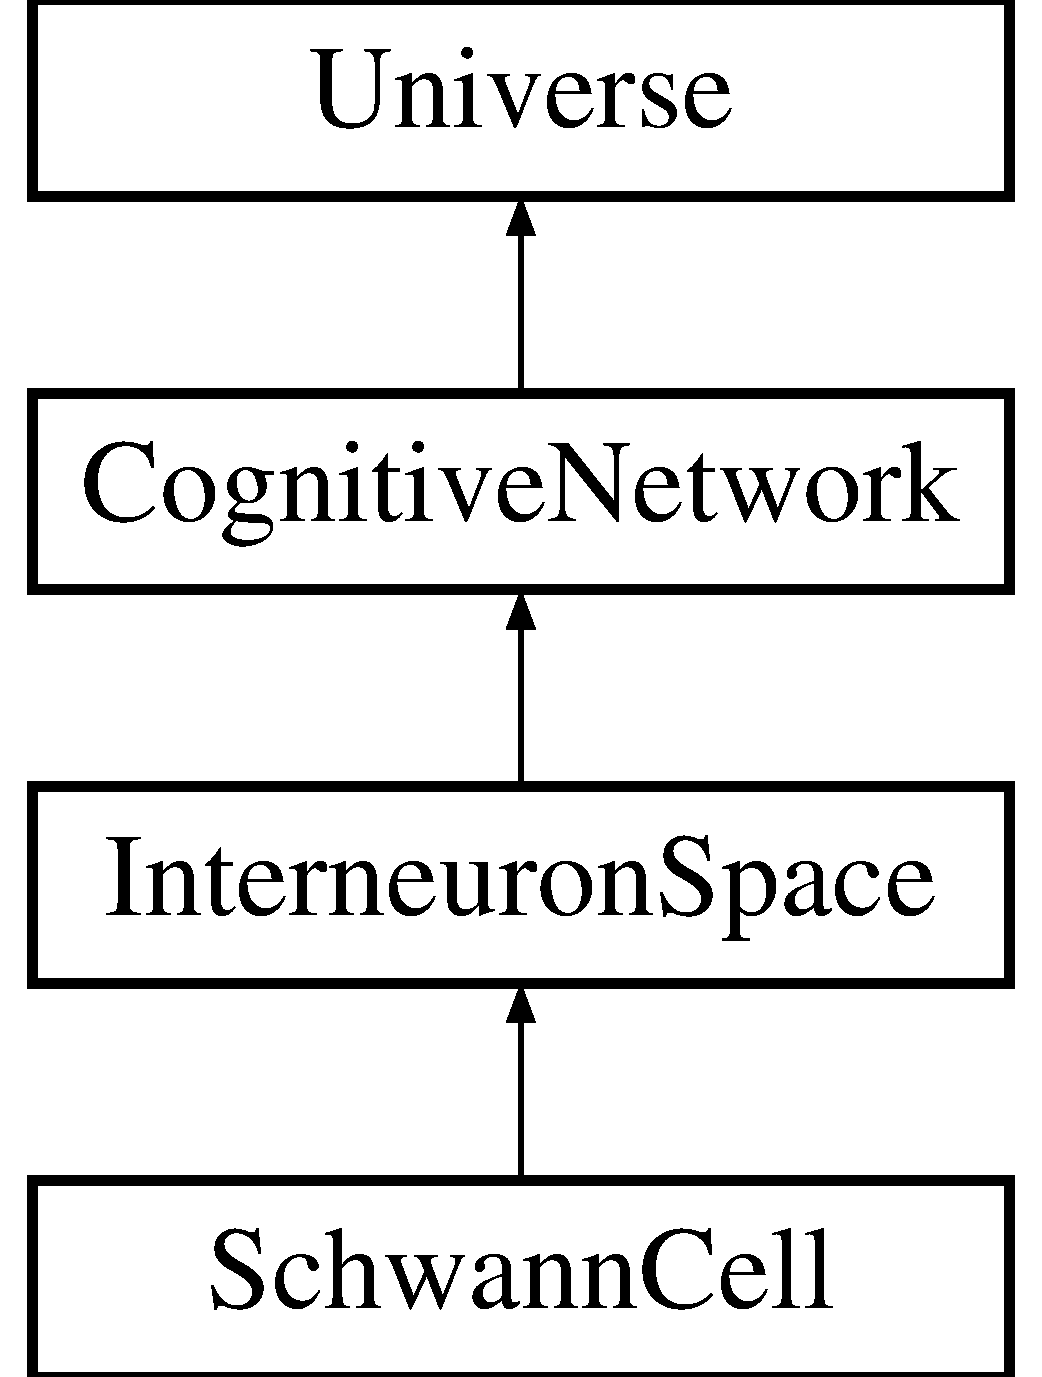
\includegraphics[height=4.000000cm]{classSchwannCell}
\end{center}
\end{figure}
\subsection*{Private Member Functions}
\begin{DoxyCompactItemize}
\item 
\mbox{\hyperlink{classSchwannCell_aab3414e0d6266c5b791a000c39359ca5}{Schwann\+Cell}} ()
\item 
\mbox{\hyperlink{classSchwannCell_a1387a5d8b87e485a507c72a657ab2864}{Schwann\+Cell}} (unsigned int object\+\_\+type)
\item 
\mbox{\hyperlink{classSchwannCell_ad8e9f6343a3617a44d8a03e4edbc92d6}{Schwann\+Cell}} (unsigned int object\+\_\+type, std\+::chrono\+::time\+\_\+point$<$ \mbox{\hyperlink{universe_8h_a0ef8d951d1ca5ab3cfaf7ab4c7a6fd80}{Clock}} $>$ event\+\_\+time)
\item 
\mbox{\hyperlink{classSchwannCell_abaa1caff5e245ede16a538d1e1bcc1e7}{Schwann\+Cell}} (unsigned int object\+\_\+type, std\+::chrono\+::time\+\_\+point$<$ \mbox{\hyperlink{universe_8h_a0ef8d951d1ca5ab3cfaf7ab4c7a6fd80}{Clock}} $>$ event\+\_\+time, \mbox{\hyperlink{classInterneuronSpace}{Interneuron\+Space}} \&interneuronspace\+\_\+connector)
\item 
virtual \mbox{\hyperlink{classSchwannCell_af98a51e1f9c191bb57282dbbb16dd2a9}{$\sim$\+Schwann\+Cell}} ()
\item 
bool \mbox{\hyperlink{classSchwannCell_af60de27e9658b2ca9973931c2175fe74}{Reset\+Parameters}} (std\+::chrono\+::time\+\_\+point$<$ \mbox{\hyperlink{universe_8h_a0ef8d951d1ca5ab3cfaf7ab4c7a6fd80}{Clock}} $>$ event\+\_\+time)
\item 
unsigned int \mbox{\hyperlink{classSchwannCell_ab43faeb8f76529162985b2a0c53eb3f5}{Get\+Counter}} (std\+::chrono\+::time\+\_\+point$<$ \mbox{\hyperlink{universe_8h_a0ef8d951d1ca5ab3cfaf7ab4c7a6fd80}{Clock}} $>$ event\+\_\+time)
\item 
double \mbox{\hyperlink{classSchwannCell_af6dd3963bc46763b34f2ee742a4c9fae}{Get\+Energy}} (std\+::chrono\+::time\+\_\+point$<$ \mbox{\hyperlink{universe_8h_a0ef8d951d1ca5ab3cfaf7ab4c7a6fd80}{Clock}} $>$ event\+\_\+time)
\item 
void \mbox{\hyperlink{classSchwannCell_a067f87983cb937d5fdb882c267e27921}{Set\+Counter}} (std\+::chrono\+::time\+\_\+point$<$ \mbox{\hyperlink{universe_8h_a0ef8d951d1ca5ab3cfaf7ab4c7a6fd80}{Clock}} $>$ event\+\_\+time, unsigned int val)
\item 
void \mbox{\hyperlink{classSchwannCell_aadc0a342e29ccacbd8686b9431fb41c6}{Set\+Energy}} (std\+::chrono\+::time\+\_\+point$<$ \mbox{\hyperlink{universe_8h_a0ef8d951d1ca5ab3cfaf7ab4c7a6fd80}{Clock}} $>$ event\+\_\+time, double val)
\item 
int \mbox{\hyperlink{classSchwannCell_a765280afc21c2546ad6162db46089d40}{Update}} (std\+::chrono\+::time\+\_\+point$<$ \mbox{\hyperlink{universe_8h_a0ef8d951d1ca5ab3cfaf7ab4c7a6fd80}{Clock}} $>$ event\+\_\+time)
\end{DoxyCompactItemize}
\subsection*{Private Attributes}
\begin{DoxyCompactItemize}
\item 
unsigned int \mbox{\hyperlink{classSchwannCell_a6a72f907dbb2b8516f2292e0d82f887d}{m\+\_\+\+Counter}}
\begin{DoxyCompactList}\small\item\em Member variable \char`\"{}m\+\_\+\+Counter\char`\"{}. \end{DoxyCompactList}\item 
double \mbox{\hyperlink{classSchwannCell_a16689a4b1f42cabe7de168440c815edd}{object\+\_\+energy}}
\begin{DoxyCompactList}\small\item\em Member variable \char`\"{}object\+\_\+energy\char`\"{}. \end{DoxyCompactList}\item 
int \mbox{\hyperlink{classSchwannCell_a6b045b7f7bf629cd9f75b58c40f5b7c1}{schwanncell\+\_\+type}}
\item 
bool \mbox{\hyperlink{classSchwannCell_a3fe616a8aadf62602a0aeff0f3d4d491}{object\+\_\+disabled}} = true
\item 
bool \mbox{\hyperlink{classSchwannCell_aa9264dbe039d439956f94391769fda5f}{object\+\_\+initialised}} = false
\item 
std\+::chrono\+::time\+\_\+point$<$ \mbox{\hyperlink{universe_8h_a0ef8d951d1ca5ab3cfaf7ab4c7a6fd80}{Clock}} $>$ \mbox{\hyperlink{classSchwannCell_ac5c518c34e3c2afb70bc2780c1b74439}{time\+\_\+object\+\_\+created}}
\item 
std\+::chrono\+::time\+\_\+point$<$ \mbox{\hyperlink{universe_8h_a0ef8d951d1ca5ab3cfaf7ab4c7a6fd80}{Clock}} $>$ \mbox{\hyperlink{classSchwannCell_acea7e2f40d807a2ca973c4c8de90c879}{previous\+\_\+event\+\_\+time}}
\item 
int \mbox{\hyperlink{classSchwannCell_ad2281f878b3aec7ce7ba31f27f698daa}{duration\+\_\+since\+\_\+last\+\_\+event}}
\end{DoxyCompactItemize}
\subsection*{Additional Inherited Members}


\subsection{Constructor \& Destructor Documentation}
\mbox{\Hypertarget{classSchwannCell_aab3414e0d6266c5b791a000c39359ca5}\label{classSchwannCell_aab3414e0d6266c5b791a000c39359ca5}} 
\index{Schwann\+Cell@{Schwann\+Cell}!Schwann\+Cell@{Schwann\+Cell}}
\index{Schwann\+Cell@{Schwann\+Cell}!Schwann\+Cell@{Schwann\+Cell}}
\subsubsection{\texorpdfstring{Schwann\+Cell()}{SchwannCell()}\hspace{0.1cm}{\footnotesize\ttfamily [1/4]}}
{\footnotesize\ttfamily Schwann\+Cell\+::\+Schwann\+Cell (\begin{DoxyParamCaption}{ }\end{DoxyParamCaption})\hspace{0.3cm}{\ttfamily [inline]}, {\ttfamily [private]}}

\mbox{\Hypertarget{classSchwannCell_a1387a5d8b87e485a507c72a657ab2864}\label{classSchwannCell_a1387a5d8b87e485a507c72a657ab2864}} 
\index{Schwann\+Cell@{Schwann\+Cell}!Schwann\+Cell@{Schwann\+Cell}}
\index{Schwann\+Cell@{Schwann\+Cell}!Schwann\+Cell@{Schwann\+Cell}}
\subsubsection{\texorpdfstring{Schwann\+Cell()}{SchwannCell()}\hspace{0.1cm}{\footnotesize\ttfamily [2/4]}}
{\footnotesize\ttfamily Schwann\+Cell\+::\+Schwann\+Cell (\begin{DoxyParamCaption}\item[{unsigned int}]{object\+\_\+type }\end{DoxyParamCaption})\hspace{0.3cm}{\ttfamily [inline]}, {\ttfamily [private]}}

\mbox{\Hypertarget{classSchwannCell_ad8e9f6343a3617a44d8a03e4edbc92d6}\label{classSchwannCell_ad8e9f6343a3617a44d8a03e4edbc92d6}} 
\index{Schwann\+Cell@{Schwann\+Cell}!Schwann\+Cell@{Schwann\+Cell}}
\index{Schwann\+Cell@{Schwann\+Cell}!Schwann\+Cell@{Schwann\+Cell}}
\subsubsection{\texorpdfstring{Schwann\+Cell()}{SchwannCell()}\hspace{0.1cm}{\footnotesize\ttfamily [3/4]}}
{\footnotesize\ttfamily Schwann\+Cell\+::\+Schwann\+Cell (\begin{DoxyParamCaption}\item[{unsigned int}]{object\+\_\+type,  }\item[{std\+::chrono\+::time\+\_\+point$<$ \mbox{\hyperlink{universe_8h_a0ef8d951d1ca5ab3cfaf7ab4c7a6fd80}{Clock}} $>$}]{event\+\_\+time }\end{DoxyParamCaption})\hspace{0.3cm}{\ttfamily [inline]}, {\ttfamily [private]}}

\mbox{\Hypertarget{classSchwannCell_abaa1caff5e245ede16a538d1e1bcc1e7}\label{classSchwannCell_abaa1caff5e245ede16a538d1e1bcc1e7}} 
\index{Schwann\+Cell@{Schwann\+Cell}!Schwann\+Cell@{Schwann\+Cell}}
\index{Schwann\+Cell@{Schwann\+Cell}!Schwann\+Cell@{Schwann\+Cell}}
\subsubsection{\texorpdfstring{Schwann\+Cell()}{SchwannCell()}\hspace{0.1cm}{\footnotesize\ttfamily [4/4]}}
{\footnotesize\ttfamily Schwann\+Cell\+::\+Schwann\+Cell (\begin{DoxyParamCaption}\item[{unsigned int}]{object\+\_\+type,  }\item[{std\+::chrono\+::time\+\_\+point$<$ \mbox{\hyperlink{universe_8h_a0ef8d951d1ca5ab3cfaf7ab4c7a6fd80}{Clock}} $>$}]{event\+\_\+time,  }\item[{\mbox{\hyperlink{classInterneuronSpace}{Interneuron\+Space}} \&}]{interneuronspace\+\_\+connector }\end{DoxyParamCaption})\hspace{0.3cm}{\ttfamily [inline]}, {\ttfamily [private]}}

\mbox{\Hypertarget{classSchwannCell_af98a51e1f9c191bb57282dbbb16dd2a9}\label{classSchwannCell_af98a51e1f9c191bb57282dbbb16dd2a9}} 
\index{Schwann\+Cell@{Schwann\+Cell}!````~Schwann\+Cell@{$\sim$\+Schwann\+Cell}}
\index{````~Schwann\+Cell@{$\sim$\+Schwann\+Cell}!Schwann\+Cell@{Schwann\+Cell}}
\subsubsection{\texorpdfstring{$\sim$\+Schwann\+Cell()}{~SchwannCell()}}
{\footnotesize\ttfamily virtual Schwann\+Cell\+::$\sim$\+Schwann\+Cell (\begin{DoxyParamCaption}{ }\end{DoxyParamCaption})\hspace{0.3cm}{\ttfamily [inline]}, {\ttfamily [private]}, {\ttfamily [virtual]}}



\subsection{Member Function Documentation}
\mbox{\Hypertarget{classSchwannCell_ab43faeb8f76529162985b2a0c53eb3f5}\label{classSchwannCell_ab43faeb8f76529162985b2a0c53eb3f5}} 
\index{Schwann\+Cell@{Schwann\+Cell}!Get\+Counter@{Get\+Counter}}
\index{Get\+Counter@{Get\+Counter}!Schwann\+Cell@{Schwann\+Cell}}
\subsubsection{\texorpdfstring{Get\+Counter()}{GetCounter()}}
{\footnotesize\ttfamily unsigned int Schwann\+Cell\+::\+Get\+Counter (\begin{DoxyParamCaption}\item[{std\+::chrono\+::time\+\_\+point$<$ \mbox{\hyperlink{universe_8h_a0ef8d951d1ca5ab3cfaf7ab4c7a6fd80}{Clock}} $>$}]{event\+\_\+time }\end{DoxyParamCaption})\hspace{0.3cm}{\ttfamily [inline]}, {\ttfamily [private]}}

\mbox{\Hypertarget{classSchwannCell_af6dd3963bc46763b34f2ee742a4c9fae}\label{classSchwannCell_af6dd3963bc46763b34f2ee742a4c9fae}} 
\index{Schwann\+Cell@{Schwann\+Cell}!Get\+Energy@{Get\+Energy}}
\index{Get\+Energy@{Get\+Energy}!Schwann\+Cell@{Schwann\+Cell}}
\subsubsection{\texorpdfstring{Get\+Energy()}{GetEnergy()}}
{\footnotesize\ttfamily double Schwann\+Cell\+::\+Get\+Energy (\begin{DoxyParamCaption}\item[{std\+::chrono\+::time\+\_\+point$<$ \mbox{\hyperlink{universe_8h_a0ef8d951d1ca5ab3cfaf7ab4c7a6fd80}{Clock}} $>$}]{event\+\_\+time }\end{DoxyParamCaption})\hspace{0.3cm}{\ttfamily [inline]}, {\ttfamily [private]}}

\mbox{\Hypertarget{classSchwannCell_af60de27e9658b2ca9973931c2175fe74}\label{classSchwannCell_af60de27e9658b2ca9973931c2175fe74}} 
\index{Schwann\+Cell@{Schwann\+Cell}!Reset\+Parameters@{Reset\+Parameters}}
\index{Reset\+Parameters@{Reset\+Parameters}!Schwann\+Cell@{Schwann\+Cell}}
\subsubsection{\texorpdfstring{Reset\+Parameters()}{ResetParameters()}}
{\footnotesize\ttfamily bool Schwann\+Cell\+::\+Reset\+Parameters (\begin{DoxyParamCaption}\item[{std\+::chrono\+::time\+\_\+point$<$ \mbox{\hyperlink{universe_8h_a0ef8d951d1ca5ab3cfaf7ab4c7a6fd80}{Clock}} $>$}]{event\+\_\+time }\end{DoxyParamCaption})\hspace{0.3cm}{\ttfamily [private]}}

\mbox{\Hypertarget{classSchwannCell_a067f87983cb937d5fdb882c267e27921}\label{classSchwannCell_a067f87983cb937d5fdb882c267e27921}} 
\index{Schwann\+Cell@{Schwann\+Cell}!Set\+Counter@{Set\+Counter}}
\index{Set\+Counter@{Set\+Counter}!Schwann\+Cell@{Schwann\+Cell}}
\subsubsection{\texorpdfstring{Set\+Counter()}{SetCounter()}}
{\footnotesize\ttfamily void Schwann\+Cell\+::\+Set\+Counter (\begin{DoxyParamCaption}\item[{std\+::chrono\+::time\+\_\+point$<$ \mbox{\hyperlink{universe_8h_a0ef8d951d1ca5ab3cfaf7ab4c7a6fd80}{Clock}} $>$}]{event\+\_\+time,  }\item[{unsigned int}]{val }\end{DoxyParamCaption})\hspace{0.3cm}{\ttfamily [inline]}, {\ttfamily [private]}, {\ttfamily [virtual]}}

Set m\+\_\+\+Counter 
\begin{DoxyParams}{Parameters}
{\em val} & New value to Set \\
\hline
\end{DoxyParams}


Reimplemented from \mbox{\hyperlink{classInterneuronSpace_a60a46f22a2e575d65031635a698a60a9}{Interneuron\+Space}}.

\mbox{\Hypertarget{classSchwannCell_aadc0a342e29ccacbd8686b9431fb41c6}\label{classSchwannCell_aadc0a342e29ccacbd8686b9431fb41c6}} 
\index{Schwann\+Cell@{Schwann\+Cell}!Set\+Energy@{Set\+Energy}}
\index{Set\+Energy@{Set\+Energy}!Schwann\+Cell@{Schwann\+Cell}}
\subsubsection{\texorpdfstring{Set\+Energy()}{SetEnergy()}}
{\footnotesize\ttfamily void Schwann\+Cell\+::\+Set\+Energy (\begin{DoxyParamCaption}\item[{std\+::chrono\+::time\+\_\+point$<$ \mbox{\hyperlink{universe_8h_a0ef8d951d1ca5ab3cfaf7ab4c7a6fd80}{Clock}} $>$}]{event\+\_\+time,  }\item[{double}]{val }\end{DoxyParamCaption})\hspace{0.3cm}{\ttfamily [inline]}, {\ttfamily [private]}}

\mbox{\Hypertarget{classSchwannCell_a765280afc21c2546ad6162db46089d40}\label{classSchwannCell_a765280afc21c2546ad6162db46089d40}} 
\index{Schwann\+Cell@{Schwann\+Cell}!Update@{Update}}
\index{Update@{Update}!Schwann\+Cell@{Schwann\+Cell}}
\subsubsection{\texorpdfstring{Update()}{Update()}}
{\footnotesize\ttfamily int Schwann\+Cell\+::\+Update (\begin{DoxyParamCaption}\item[{std\+::chrono\+::time\+\_\+point$<$ \mbox{\hyperlink{universe_8h_a0ef8d951d1ca5ab3cfaf7ab4c7a6fd80}{Clock}} $>$}]{event\+\_\+time }\end{DoxyParamCaption})\hspace{0.3cm}{\ttfamily [private]}}



\subsection{Member Data Documentation}
\mbox{\Hypertarget{classSchwannCell_ad2281f878b3aec7ce7ba31f27f698daa}\label{classSchwannCell_ad2281f878b3aec7ce7ba31f27f698daa}} 
\index{Schwann\+Cell@{Schwann\+Cell}!duration\+\_\+since\+\_\+last\+\_\+event@{duration\+\_\+since\+\_\+last\+\_\+event}}
\index{duration\+\_\+since\+\_\+last\+\_\+event@{duration\+\_\+since\+\_\+last\+\_\+event}!Schwann\+Cell@{Schwann\+Cell}}
\subsubsection{\texorpdfstring{duration\+\_\+since\+\_\+last\+\_\+event}{duration\_since\_last\_event}}
{\footnotesize\ttfamily int Schwann\+Cell\+::duration\+\_\+since\+\_\+last\+\_\+event\hspace{0.3cm}{\ttfamily [private]}}

\mbox{\Hypertarget{classSchwannCell_a6a72f907dbb2b8516f2292e0d82f887d}\label{classSchwannCell_a6a72f907dbb2b8516f2292e0d82f887d}} 
\index{Schwann\+Cell@{Schwann\+Cell}!m\+\_\+\+Counter@{m\+\_\+\+Counter}}
\index{m\+\_\+\+Counter@{m\+\_\+\+Counter}!Schwann\+Cell@{Schwann\+Cell}}
\subsubsection{\texorpdfstring{m\+\_\+\+Counter}{m\_Counter}}
{\footnotesize\ttfamily unsigned int Schwann\+Cell\+::m\+\_\+\+Counter\hspace{0.3cm}{\ttfamily [private]}}



Member variable \char`\"{}m\+\_\+\+Counter\char`\"{}. 

\mbox{\Hypertarget{classSchwannCell_a3fe616a8aadf62602a0aeff0f3d4d491}\label{classSchwannCell_a3fe616a8aadf62602a0aeff0f3d4d491}} 
\index{Schwann\+Cell@{Schwann\+Cell}!object\+\_\+disabled@{object\+\_\+disabled}}
\index{object\+\_\+disabled@{object\+\_\+disabled}!Schwann\+Cell@{Schwann\+Cell}}
\subsubsection{\texorpdfstring{object\+\_\+disabled}{object\_disabled}}
{\footnotesize\ttfamily bool Schwann\+Cell\+::object\+\_\+disabled = true\hspace{0.3cm}{\ttfamily [private]}}

\mbox{\Hypertarget{classSchwannCell_a16689a4b1f42cabe7de168440c815edd}\label{classSchwannCell_a16689a4b1f42cabe7de168440c815edd}} 
\index{Schwann\+Cell@{Schwann\+Cell}!object\+\_\+energy@{object\+\_\+energy}}
\index{object\+\_\+energy@{object\+\_\+energy}!Schwann\+Cell@{Schwann\+Cell}}
\subsubsection{\texorpdfstring{object\+\_\+energy}{object\_energy}}
{\footnotesize\ttfamily double Schwann\+Cell\+::object\+\_\+energy\hspace{0.3cm}{\ttfamily [private]}}



Member variable \char`\"{}object\+\_\+energy\char`\"{}. 

\mbox{\Hypertarget{classSchwannCell_aa9264dbe039d439956f94391769fda5f}\label{classSchwannCell_aa9264dbe039d439956f94391769fda5f}} 
\index{Schwann\+Cell@{Schwann\+Cell}!object\+\_\+initialised@{object\+\_\+initialised}}
\index{object\+\_\+initialised@{object\+\_\+initialised}!Schwann\+Cell@{Schwann\+Cell}}
\subsubsection{\texorpdfstring{object\+\_\+initialised}{object\_initialised}}
{\footnotesize\ttfamily bool Schwann\+Cell\+::object\+\_\+initialised = false\hspace{0.3cm}{\ttfamily [private]}}

\mbox{\Hypertarget{classSchwannCell_acea7e2f40d807a2ca973c4c8de90c879}\label{classSchwannCell_acea7e2f40d807a2ca973c4c8de90c879}} 
\index{Schwann\+Cell@{Schwann\+Cell}!previous\+\_\+event\+\_\+time@{previous\+\_\+event\+\_\+time}}
\index{previous\+\_\+event\+\_\+time@{previous\+\_\+event\+\_\+time}!Schwann\+Cell@{Schwann\+Cell}}
\subsubsection{\texorpdfstring{previous\+\_\+event\+\_\+time}{previous\_event\_time}}
{\footnotesize\ttfamily std\+::chrono\+::time\+\_\+point$<$\mbox{\hyperlink{universe_8h_a0ef8d951d1ca5ab3cfaf7ab4c7a6fd80}{Clock}}$>$ Schwann\+Cell\+::previous\+\_\+event\+\_\+time\hspace{0.3cm}{\ttfamily [private]}}

\mbox{\Hypertarget{classSchwannCell_a6b045b7f7bf629cd9f75b58c40f5b7c1}\label{classSchwannCell_a6b045b7f7bf629cd9f75b58c40f5b7c1}} 
\index{Schwann\+Cell@{Schwann\+Cell}!schwanncell\+\_\+type@{schwanncell\+\_\+type}}
\index{schwanncell\+\_\+type@{schwanncell\+\_\+type}!Schwann\+Cell@{Schwann\+Cell}}
\subsubsection{\texorpdfstring{schwanncell\+\_\+type}{schwanncell\_type}}
{\footnotesize\ttfamily int Schwann\+Cell\+::schwanncell\+\_\+type\hspace{0.3cm}{\ttfamily [private]}}

\mbox{\Hypertarget{classSchwannCell_ac5c518c34e3c2afb70bc2780c1b74439}\label{classSchwannCell_ac5c518c34e3c2afb70bc2780c1b74439}} 
\index{Schwann\+Cell@{Schwann\+Cell}!time\+\_\+object\+\_\+created@{time\+\_\+object\+\_\+created}}
\index{time\+\_\+object\+\_\+created@{time\+\_\+object\+\_\+created}!Schwann\+Cell@{Schwann\+Cell}}
\subsubsection{\texorpdfstring{time\+\_\+object\+\_\+created}{time\_object\_created}}
{\footnotesize\ttfamily std\+::chrono\+::time\+\_\+point$<$\mbox{\hyperlink{universe_8h_a0ef8d951d1ca5ab3cfaf7ab4c7a6fd80}{Clock}}$>$ Schwann\+Cell\+::time\+\_\+object\+\_\+created\hspace{0.3cm}{\ttfamily [private]}}



The documentation for this class was generated from the following files\+:\begin{DoxyCompactItemize}
\item 
/home/pbisaacs/\+Developer/\+Brain\+Harmonics/\+Brain\+Harmonics/\mbox{\hyperlink{schwanncell_8h}{schwanncell.\+h}}\item 
/home/pbisaacs/\+Developer/\+Brain\+Harmonics/\+Brain\+Harmonics/\mbox{\hyperlink{schwanncell_8cc}{schwanncell.\+cc}}\end{DoxyCompactItemize}

\hypertarget{structSniffex_1_1sniff__ethernet}{}\section{Sniffex\+:\+:sniff\+\_\+ethernet Struct Reference}
\label{structSniffex_1_1sniff__ethernet}\index{Sniffex\+::sniff\+\_\+ethernet@{Sniffex\+::sniff\+\_\+ethernet}}


{\ttfamily \#include $<$sniffex.\+h$>$}

\subsection*{Public Attributes}
\begin{DoxyCompactItemize}
\item 
u\+\_\+char \mbox{\hyperlink{structSniffex_1_1sniff__ethernet_a68600307767c3cfe20ba593423abec8b}{ether\+\_\+dhost}} \mbox{[}\mbox{\hyperlink{sniffex_8h_abf4fcaacb1ad2010711b7c880ec2ed20}{E\+T\+H\+E\+R\+\_\+\+A\+D\+D\+R\+\_\+\+L\+EN}}\mbox{]}
\item 
u\+\_\+char \mbox{\hyperlink{structSniffex_1_1sniff__ethernet_af40407403f51872c064c28298441b2d9}{ether\+\_\+shost}} \mbox{[}\mbox{\hyperlink{sniffex_8h_abf4fcaacb1ad2010711b7c880ec2ed20}{E\+T\+H\+E\+R\+\_\+\+A\+D\+D\+R\+\_\+\+L\+EN}}\mbox{]}
\item 
u\+\_\+short \mbox{\hyperlink{structSniffex_1_1sniff__ethernet_a31b8a8e9232feffeeb747f949580753a}{ether\+\_\+type}}
\end{DoxyCompactItemize}


\subsection{Member Data Documentation}
\mbox{\Hypertarget{structSniffex_1_1sniff__ethernet_a68600307767c3cfe20ba593423abec8b}\label{structSniffex_1_1sniff__ethernet_a68600307767c3cfe20ba593423abec8b}} 
\index{Sniffex\+::sniff\+\_\+ethernet@{Sniffex\+::sniff\+\_\+ethernet}!ether\+\_\+dhost@{ether\+\_\+dhost}}
\index{ether\+\_\+dhost@{ether\+\_\+dhost}!Sniffex\+::sniff\+\_\+ethernet@{Sniffex\+::sniff\+\_\+ethernet}}
\subsubsection{\texorpdfstring{ether\+\_\+dhost}{ether\_dhost}}
{\footnotesize\ttfamily u\+\_\+char Sniffex\+::sniff\+\_\+ethernet\+::ether\+\_\+dhost\mbox{[}\mbox{\hyperlink{sniffex_8h_abf4fcaacb1ad2010711b7c880ec2ed20}{E\+T\+H\+E\+R\+\_\+\+A\+D\+D\+R\+\_\+\+L\+EN}}\mbox{]}}

\mbox{\Hypertarget{structSniffex_1_1sniff__ethernet_af40407403f51872c064c28298441b2d9}\label{structSniffex_1_1sniff__ethernet_af40407403f51872c064c28298441b2d9}} 
\index{Sniffex\+::sniff\+\_\+ethernet@{Sniffex\+::sniff\+\_\+ethernet}!ether\+\_\+shost@{ether\+\_\+shost}}
\index{ether\+\_\+shost@{ether\+\_\+shost}!Sniffex\+::sniff\+\_\+ethernet@{Sniffex\+::sniff\+\_\+ethernet}}
\subsubsection{\texorpdfstring{ether\+\_\+shost}{ether\_shost}}
{\footnotesize\ttfamily u\+\_\+char Sniffex\+::sniff\+\_\+ethernet\+::ether\+\_\+shost\mbox{[}\mbox{\hyperlink{sniffex_8h_abf4fcaacb1ad2010711b7c880ec2ed20}{E\+T\+H\+E\+R\+\_\+\+A\+D\+D\+R\+\_\+\+L\+EN}}\mbox{]}}

\mbox{\Hypertarget{structSniffex_1_1sniff__ethernet_a31b8a8e9232feffeeb747f949580753a}\label{structSniffex_1_1sniff__ethernet_a31b8a8e9232feffeeb747f949580753a}} 
\index{Sniffex\+::sniff\+\_\+ethernet@{Sniffex\+::sniff\+\_\+ethernet}!ether\+\_\+type@{ether\+\_\+type}}
\index{ether\+\_\+type@{ether\+\_\+type}!Sniffex\+::sniff\+\_\+ethernet@{Sniffex\+::sniff\+\_\+ethernet}}
\subsubsection{\texorpdfstring{ether\+\_\+type}{ether\_type}}
{\footnotesize\ttfamily u\+\_\+short Sniffex\+::sniff\+\_\+ethernet\+::ether\+\_\+type}



The documentation for this struct was generated from the following file\+:\begin{DoxyCompactItemize}
\item 
/home/pbisaacs/\+Developer/\+Brain\+Harmonics/\mbox{\hyperlink{sniffex_8h}{sniffex.\+h}}\end{DoxyCompactItemize}

\hypertarget{structSniffex_1_1sniff__ip}{}\section{Sniffex\+:\+:sniff\+\_\+ip Struct Reference}
\label{structSniffex_1_1sniff__ip}\index{Sniffex\+::sniff\+\_\+ip@{Sniffex\+::sniff\+\_\+ip}}


{\ttfamily \#include $<$sniffex.\+h$>$}

\subsection*{Public Attributes}
\begin{DoxyCompactItemize}
\item 
u\+\_\+char \mbox{\hyperlink{structSniffex_1_1sniff__ip_a64daddec106d5178ffbfe2f07378e438}{ip\+\_\+vhl}}
\item 
u\+\_\+char \mbox{\hyperlink{structSniffex_1_1sniff__ip_a2cfa668bb5e7079cc05e0d19d95b3816}{ip\+\_\+tos}}
\item 
u\+\_\+short \mbox{\hyperlink{structSniffex_1_1sniff__ip_a8ae9deed5b399601307bca07dc59054a}{ip\+\_\+len}}
\item 
u\+\_\+short \mbox{\hyperlink{structSniffex_1_1sniff__ip_a98026bc0aad86b837f246635ed9b25df}{ip\+\_\+id}}
\item 
u\+\_\+short \mbox{\hyperlink{structSniffex_1_1sniff__ip_aa66ee179c411c56586369198edcc7b43}{ip\+\_\+off}}
\item 
u\+\_\+char \mbox{\hyperlink{structSniffex_1_1sniff__ip_aea2468d9918eb811586acb71de6870ef}{ip\+\_\+ttl}}
\item 
u\+\_\+char \mbox{\hyperlink{structSniffex_1_1sniff__ip_a2c06fbd06dc42564a398cec20a6b15b9}{ip\+\_\+p}}
\item 
u\+\_\+short \mbox{\hyperlink{structSniffex_1_1sniff__ip_ab50c5a07d672683f1039ba5edcd7d583}{ip\+\_\+sum}}
\item 
struct in\+\_\+addr ip\+\_\+src \mbox{\hyperlink{structSniffex_1_1sniff__ip_abf8550a1a90663dc9f529f50ecee72ee}{ip\+\_\+dst}}
\end{DoxyCompactItemize}


\subsection{Member Data Documentation}
\mbox{\Hypertarget{structSniffex_1_1sniff__ip_abf8550a1a90663dc9f529f50ecee72ee}\label{structSniffex_1_1sniff__ip_abf8550a1a90663dc9f529f50ecee72ee}} 
\index{Sniffex\+::sniff\+\_\+ip@{Sniffex\+::sniff\+\_\+ip}!ip\+\_\+dst@{ip\+\_\+dst}}
\index{ip\+\_\+dst@{ip\+\_\+dst}!Sniffex\+::sniff\+\_\+ip@{Sniffex\+::sniff\+\_\+ip}}
\subsubsection{\texorpdfstring{ip\+\_\+dst}{ip\_dst}}
{\footnotesize\ttfamily struct in\+\_\+addr ip\+\_\+src Sniffex\+::sniff\+\_\+ip\+::ip\+\_\+dst}

\mbox{\Hypertarget{structSniffex_1_1sniff__ip_a98026bc0aad86b837f246635ed9b25df}\label{structSniffex_1_1sniff__ip_a98026bc0aad86b837f246635ed9b25df}} 
\index{Sniffex\+::sniff\+\_\+ip@{Sniffex\+::sniff\+\_\+ip}!ip\+\_\+id@{ip\+\_\+id}}
\index{ip\+\_\+id@{ip\+\_\+id}!Sniffex\+::sniff\+\_\+ip@{Sniffex\+::sniff\+\_\+ip}}
\subsubsection{\texorpdfstring{ip\+\_\+id}{ip\_id}}
{\footnotesize\ttfamily u\+\_\+short Sniffex\+::sniff\+\_\+ip\+::ip\+\_\+id}

\mbox{\Hypertarget{structSniffex_1_1sniff__ip_a8ae9deed5b399601307bca07dc59054a}\label{structSniffex_1_1sniff__ip_a8ae9deed5b399601307bca07dc59054a}} 
\index{Sniffex\+::sniff\+\_\+ip@{Sniffex\+::sniff\+\_\+ip}!ip\+\_\+len@{ip\+\_\+len}}
\index{ip\+\_\+len@{ip\+\_\+len}!Sniffex\+::sniff\+\_\+ip@{Sniffex\+::sniff\+\_\+ip}}
\subsubsection{\texorpdfstring{ip\+\_\+len}{ip\_len}}
{\footnotesize\ttfamily u\+\_\+short Sniffex\+::sniff\+\_\+ip\+::ip\+\_\+len}

\mbox{\Hypertarget{structSniffex_1_1sniff__ip_aa66ee179c411c56586369198edcc7b43}\label{structSniffex_1_1sniff__ip_aa66ee179c411c56586369198edcc7b43}} 
\index{Sniffex\+::sniff\+\_\+ip@{Sniffex\+::sniff\+\_\+ip}!ip\+\_\+off@{ip\+\_\+off}}
\index{ip\+\_\+off@{ip\+\_\+off}!Sniffex\+::sniff\+\_\+ip@{Sniffex\+::sniff\+\_\+ip}}
\subsubsection{\texorpdfstring{ip\+\_\+off}{ip\_off}}
{\footnotesize\ttfamily u\+\_\+short Sniffex\+::sniff\+\_\+ip\+::ip\+\_\+off}

\mbox{\Hypertarget{structSniffex_1_1sniff__ip_a2c06fbd06dc42564a398cec20a6b15b9}\label{structSniffex_1_1sniff__ip_a2c06fbd06dc42564a398cec20a6b15b9}} 
\index{Sniffex\+::sniff\+\_\+ip@{Sniffex\+::sniff\+\_\+ip}!ip\+\_\+p@{ip\+\_\+p}}
\index{ip\+\_\+p@{ip\+\_\+p}!Sniffex\+::sniff\+\_\+ip@{Sniffex\+::sniff\+\_\+ip}}
\subsubsection{\texorpdfstring{ip\+\_\+p}{ip\_p}}
{\footnotesize\ttfamily u\+\_\+char Sniffex\+::sniff\+\_\+ip\+::ip\+\_\+p}

\mbox{\Hypertarget{structSniffex_1_1sniff__ip_ab50c5a07d672683f1039ba5edcd7d583}\label{structSniffex_1_1sniff__ip_ab50c5a07d672683f1039ba5edcd7d583}} 
\index{Sniffex\+::sniff\+\_\+ip@{Sniffex\+::sniff\+\_\+ip}!ip\+\_\+sum@{ip\+\_\+sum}}
\index{ip\+\_\+sum@{ip\+\_\+sum}!Sniffex\+::sniff\+\_\+ip@{Sniffex\+::sniff\+\_\+ip}}
\subsubsection{\texorpdfstring{ip\+\_\+sum}{ip\_sum}}
{\footnotesize\ttfamily u\+\_\+short Sniffex\+::sniff\+\_\+ip\+::ip\+\_\+sum}

\mbox{\Hypertarget{structSniffex_1_1sniff__ip_a2cfa668bb5e7079cc05e0d19d95b3816}\label{structSniffex_1_1sniff__ip_a2cfa668bb5e7079cc05e0d19d95b3816}} 
\index{Sniffex\+::sniff\+\_\+ip@{Sniffex\+::sniff\+\_\+ip}!ip\+\_\+tos@{ip\+\_\+tos}}
\index{ip\+\_\+tos@{ip\+\_\+tos}!Sniffex\+::sniff\+\_\+ip@{Sniffex\+::sniff\+\_\+ip}}
\subsubsection{\texorpdfstring{ip\+\_\+tos}{ip\_tos}}
{\footnotesize\ttfamily u\+\_\+char Sniffex\+::sniff\+\_\+ip\+::ip\+\_\+tos}

\mbox{\Hypertarget{structSniffex_1_1sniff__ip_aea2468d9918eb811586acb71de6870ef}\label{structSniffex_1_1sniff__ip_aea2468d9918eb811586acb71de6870ef}} 
\index{Sniffex\+::sniff\+\_\+ip@{Sniffex\+::sniff\+\_\+ip}!ip\+\_\+ttl@{ip\+\_\+ttl}}
\index{ip\+\_\+ttl@{ip\+\_\+ttl}!Sniffex\+::sniff\+\_\+ip@{Sniffex\+::sniff\+\_\+ip}}
\subsubsection{\texorpdfstring{ip\+\_\+ttl}{ip\_ttl}}
{\footnotesize\ttfamily u\+\_\+char Sniffex\+::sniff\+\_\+ip\+::ip\+\_\+ttl}

\mbox{\Hypertarget{structSniffex_1_1sniff__ip_a64daddec106d5178ffbfe2f07378e438}\label{structSniffex_1_1sniff__ip_a64daddec106d5178ffbfe2f07378e438}} 
\index{Sniffex\+::sniff\+\_\+ip@{Sniffex\+::sniff\+\_\+ip}!ip\+\_\+vhl@{ip\+\_\+vhl}}
\index{ip\+\_\+vhl@{ip\+\_\+vhl}!Sniffex\+::sniff\+\_\+ip@{Sniffex\+::sniff\+\_\+ip}}
\subsubsection{\texorpdfstring{ip\+\_\+vhl}{ip\_vhl}}
{\footnotesize\ttfamily u\+\_\+char Sniffex\+::sniff\+\_\+ip\+::ip\+\_\+vhl}



The documentation for this struct was generated from the following file\+:\begin{DoxyCompactItemize}
\item 
/home/pbisaacs/\+Developer/\+Brain\+Harmonics/\mbox{\hyperlink{sniffex_8h}{sniffex.\+h}}\end{DoxyCompactItemize}

\hypertarget{structSniffex_1_1sniff__tcp}{}\section{Sniffex\+:\+:sniff\+\_\+tcp Struct Reference}
\label{structSniffex_1_1sniff__tcp}\index{Sniffex\+::sniff\+\_\+tcp@{Sniffex\+::sniff\+\_\+tcp}}


{\ttfamily \#include $<$sniffex.\+h$>$}

\subsection*{Public Attributes}
\begin{DoxyCompactItemize}
\item 
u\+\_\+short \mbox{\hyperlink{structSniffex_1_1sniff__tcp_a3cbc5a34aaffbb66d2e37060bd2ea9b6}{th\+\_\+sport}}
\item 
u\+\_\+short \mbox{\hyperlink{structSniffex_1_1sniff__tcp_a98f86dbef1d01db2bd032e1fe99342eb}{th\+\_\+dport}}
\item 
\mbox{\hyperlink{classSniffex_a83629f6a3ec687dd2bb381e9bf157d4f}{tcp\+\_\+seq}} \mbox{\hyperlink{structSniffex_1_1sniff__tcp_a7adabab3aaed105f0e075d3ce9ad523d}{th\+\_\+seq}}
\item 
\mbox{\hyperlink{classSniffex_a83629f6a3ec687dd2bb381e9bf157d4f}{tcp\+\_\+seq}} \mbox{\hyperlink{structSniffex_1_1sniff__tcp_a3c946baf5941e2e12af8b56a2570eece}{th\+\_\+ack}}
\item 
u\+\_\+char \mbox{\hyperlink{structSniffex_1_1sniff__tcp_a27045544602ef965e5a50025f42fbd1d}{th\+\_\+offx2}}
\item 
u\+\_\+char \mbox{\hyperlink{structSniffex_1_1sniff__tcp_a2bef60aa797ee914836f6b0007dc3ebb}{th\+\_\+flags}}
\item 
u\+\_\+short \mbox{\hyperlink{structSniffex_1_1sniff__tcp_aa8b7d8b1967e81a255ec9362f681c721}{th\+\_\+win}}
\item 
u\+\_\+short \mbox{\hyperlink{structSniffex_1_1sniff__tcp_a69830e35f22fcd1b9051afbd4e633fc0}{th\+\_\+sum}}
\item 
u\+\_\+short \mbox{\hyperlink{structSniffex_1_1sniff__tcp_a9f030cb6718b8d828f242d0464560761}{th\+\_\+urp}}
\end{DoxyCompactItemize}


\subsection{Member Data Documentation}
\mbox{\Hypertarget{structSniffex_1_1sniff__tcp_a3c946baf5941e2e12af8b56a2570eece}\label{structSniffex_1_1sniff__tcp_a3c946baf5941e2e12af8b56a2570eece}} 
\index{Sniffex\+::sniff\+\_\+tcp@{Sniffex\+::sniff\+\_\+tcp}!th\+\_\+ack@{th\+\_\+ack}}
\index{th\+\_\+ack@{th\+\_\+ack}!Sniffex\+::sniff\+\_\+tcp@{Sniffex\+::sniff\+\_\+tcp}}
\subsubsection{\texorpdfstring{th\+\_\+ack}{th\_ack}}
{\footnotesize\ttfamily \mbox{\hyperlink{classSniffex_a83629f6a3ec687dd2bb381e9bf157d4f}{tcp\+\_\+seq}} Sniffex\+::sniff\+\_\+tcp\+::th\+\_\+ack}

\mbox{\Hypertarget{structSniffex_1_1sniff__tcp_a98f86dbef1d01db2bd032e1fe99342eb}\label{structSniffex_1_1sniff__tcp_a98f86dbef1d01db2bd032e1fe99342eb}} 
\index{Sniffex\+::sniff\+\_\+tcp@{Sniffex\+::sniff\+\_\+tcp}!th\+\_\+dport@{th\+\_\+dport}}
\index{th\+\_\+dport@{th\+\_\+dport}!Sniffex\+::sniff\+\_\+tcp@{Sniffex\+::sniff\+\_\+tcp}}
\subsubsection{\texorpdfstring{th\+\_\+dport}{th\_dport}}
{\footnotesize\ttfamily u\+\_\+short Sniffex\+::sniff\+\_\+tcp\+::th\+\_\+dport}

\mbox{\Hypertarget{structSniffex_1_1sniff__tcp_a2bef60aa797ee914836f6b0007dc3ebb}\label{structSniffex_1_1sniff__tcp_a2bef60aa797ee914836f6b0007dc3ebb}} 
\index{Sniffex\+::sniff\+\_\+tcp@{Sniffex\+::sniff\+\_\+tcp}!th\+\_\+flags@{th\+\_\+flags}}
\index{th\+\_\+flags@{th\+\_\+flags}!Sniffex\+::sniff\+\_\+tcp@{Sniffex\+::sniff\+\_\+tcp}}
\subsubsection{\texorpdfstring{th\+\_\+flags}{th\_flags}}
{\footnotesize\ttfamily u\+\_\+char Sniffex\+::sniff\+\_\+tcp\+::th\+\_\+flags}

\mbox{\Hypertarget{structSniffex_1_1sniff__tcp_a27045544602ef965e5a50025f42fbd1d}\label{structSniffex_1_1sniff__tcp_a27045544602ef965e5a50025f42fbd1d}} 
\index{Sniffex\+::sniff\+\_\+tcp@{Sniffex\+::sniff\+\_\+tcp}!th\+\_\+offx2@{th\+\_\+offx2}}
\index{th\+\_\+offx2@{th\+\_\+offx2}!Sniffex\+::sniff\+\_\+tcp@{Sniffex\+::sniff\+\_\+tcp}}
\subsubsection{\texorpdfstring{th\+\_\+offx2}{th\_offx2}}
{\footnotesize\ttfamily u\+\_\+char Sniffex\+::sniff\+\_\+tcp\+::th\+\_\+offx2}

\mbox{\Hypertarget{structSniffex_1_1sniff__tcp_a7adabab3aaed105f0e075d3ce9ad523d}\label{structSniffex_1_1sniff__tcp_a7adabab3aaed105f0e075d3ce9ad523d}} 
\index{Sniffex\+::sniff\+\_\+tcp@{Sniffex\+::sniff\+\_\+tcp}!th\+\_\+seq@{th\+\_\+seq}}
\index{th\+\_\+seq@{th\+\_\+seq}!Sniffex\+::sniff\+\_\+tcp@{Sniffex\+::sniff\+\_\+tcp}}
\subsubsection{\texorpdfstring{th\+\_\+seq}{th\_seq}}
{\footnotesize\ttfamily \mbox{\hyperlink{classSniffex_a83629f6a3ec687dd2bb381e9bf157d4f}{tcp\+\_\+seq}} Sniffex\+::sniff\+\_\+tcp\+::th\+\_\+seq}

\mbox{\Hypertarget{structSniffex_1_1sniff__tcp_a3cbc5a34aaffbb66d2e37060bd2ea9b6}\label{structSniffex_1_1sniff__tcp_a3cbc5a34aaffbb66d2e37060bd2ea9b6}} 
\index{Sniffex\+::sniff\+\_\+tcp@{Sniffex\+::sniff\+\_\+tcp}!th\+\_\+sport@{th\+\_\+sport}}
\index{th\+\_\+sport@{th\+\_\+sport}!Sniffex\+::sniff\+\_\+tcp@{Sniffex\+::sniff\+\_\+tcp}}
\subsubsection{\texorpdfstring{th\+\_\+sport}{th\_sport}}
{\footnotesize\ttfamily u\+\_\+short Sniffex\+::sniff\+\_\+tcp\+::th\+\_\+sport}

\mbox{\Hypertarget{structSniffex_1_1sniff__tcp_a69830e35f22fcd1b9051afbd4e633fc0}\label{structSniffex_1_1sniff__tcp_a69830e35f22fcd1b9051afbd4e633fc0}} 
\index{Sniffex\+::sniff\+\_\+tcp@{Sniffex\+::sniff\+\_\+tcp}!th\+\_\+sum@{th\+\_\+sum}}
\index{th\+\_\+sum@{th\+\_\+sum}!Sniffex\+::sniff\+\_\+tcp@{Sniffex\+::sniff\+\_\+tcp}}
\subsubsection{\texorpdfstring{th\+\_\+sum}{th\_sum}}
{\footnotesize\ttfamily u\+\_\+short Sniffex\+::sniff\+\_\+tcp\+::th\+\_\+sum}

\mbox{\Hypertarget{structSniffex_1_1sniff__tcp_a9f030cb6718b8d828f242d0464560761}\label{structSniffex_1_1sniff__tcp_a9f030cb6718b8d828f242d0464560761}} 
\index{Sniffex\+::sniff\+\_\+tcp@{Sniffex\+::sniff\+\_\+tcp}!th\+\_\+urp@{th\+\_\+urp}}
\index{th\+\_\+urp@{th\+\_\+urp}!Sniffex\+::sniff\+\_\+tcp@{Sniffex\+::sniff\+\_\+tcp}}
\subsubsection{\texorpdfstring{th\+\_\+urp}{th\_urp}}
{\footnotesize\ttfamily u\+\_\+short Sniffex\+::sniff\+\_\+tcp\+::th\+\_\+urp}

\mbox{\Hypertarget{structSniffex_1_1sniff__tcp_aa8b7d8b1967e81a255ec9362f681c721}\label{structSniffex_1_1sniff__tcp_aa8b7d8b1967e81a255ec9362f681c721}} 
\index{Sniffex\+::sniff\+\_\+tcp@{Sniffex\+::sniff\+\_\+tcp}!th\+\_\+win@{th\+\_\+win}}
\index{th\+\_\+win@{th\+\_\+win}!Sniffex\+::sniff\+\_\+tcp@{Sniffex\+::sniff\+\_\+tcp}}
\subsubsection{\texorpdfstring{th\+\_\+win}{th\_win}}
{\footnotesize\ttfamily u\+\_\+short Sniffex\+::sniff\+\_\+tcp\+::th\+\_\+win}



The documentation for this struct was generated from the following file\+:\begin{DoxyCompactItemize}
\item 
/home/pbisaacs/\+Developer/\+Brain\+Harmonics/\mbox{\hyperlink{sniffex_8h}{sniffex.\+h}}\end{DoxyCompactItemize}

\hypertarget{classSniffex}{}\section{Sniffex Class Reference}
\label{classSniffex}\index{Sniffex@{Sniffex}}


{\ttfamily \#include $<$sniffex.\+h$>$}

\subsection*{Classes}
\begin{DoxyCompactItemize}
\item 
struct \mbox{\hyperlink{structSniffex_1_1sniff__ethernet}{sniff\+\_\+ethernet}}
\item 
struct \mbox{\hyperlink{structSniffex_1_1sniff__ip}{sniff\+\_\+ip}}
\item 
struct \mbox{\hyperlink{structSniffex_1_1sniff__tcp}{sniff\+\_\+tcp}}
\end{DoxyCompactItemize}
\subsection*{Public Types}
\begin{DoxyCompactItemize}
\item 
typedef u\+\_\+int \mbox{\hyperlink{classSniffex_a83629f6a3ec687dd2bb381e9bf157d4f}{tcp\+\_\+seq}}
\end{DoxyCompactItemize}
\subsection*{Public Member Functions}
\begin{DoxyCompactItemize}
\item 
void \mbox{\hyperlink{classSniffex_a3d4ef3c90e55035eadca2d577004cd14}{got\+\_\+packet}} (u\+\_\+char $\ast$args, const struct pcap\+\_\+pkthdr $\ast$header, const u\+\_\+char $\ast$packet)
\item 
void \mbox{\hyperlink{classSniffex_a1b24163d441d38f3672800c3de85d149}{print\+\_\+payload}} (const u\+\_\+char $\ast$payload, int len)
\item 
void \mbox{\hyperlink{classSniffex_aec1e34cb4b2ff906304f957c205707ea}{print\+\_\+hex\+\_\+ascii\+\_\+line}} (const u\+\_\+char $\ast$payload, int len, int offset)
\item 
void \mbox{\hyperlink{classSniffex_ab32951f576e7cd62caf4fe1c5b085b4e}{print\+\_\+app\+\_\+banner}} (void)
\item 
void \mbox{\hyperlink{classSniffex_aea81794fe2ac6e2b857eef01c3b109e5}{print\+\_\+app\+\_\+usage}} (void)
\item 
int \mbox{\hyperlink{classSniffex_a41e146d588c285c94c0beee223d8552b}{sniffexmain}} (int argc, char $\ast$$\ast$argv)
\end{DoxyCompactItemize}


\subsection{Member Typedef Documentation}
\mbox{\Hypertarget{classSniffex_a83629f6a3ec687dd2bb381e9bf157d4f}\label{classSniffex_a83629f6a3ec687dd2bb381e9bf157d4f}} 
\index{Sniffex@{Sniffex}!tcp\+\_\+seq@{tcp\+\_\+seq}}
\index{tcp\+\_\+seq@{tcp\+\_\+seq}!Sniffex@{Sniffex}}
\subsubsection{\texorpdfstring{tcp\+\_\+seq}{tcp\_seq}}
{\footnotesize\ttfamily typedef u\+\_\+int \mbox{\hyperlink{classSniffex_a83629f6a3ec687dd2bb381e9bf157d4f}{Sniffex\+::tcp\+\_\+seq}}}



\subsection{Member Function Documentation}
\mbox{\Hypertarget{classSniffex_a3d4ef3c90e55035eadca2d577004cd14}\label{classSniffex_a3d4ef3c90e55035eadca2d577004cd14}} 
\index{Sniffex@{Sniffex}!got\+\_\+packet@{got\+\_\+packet}}
\index{got\+\_\+packet@{got\+\_\+packet}!Sniffex@{Sniffex}}
\subsubsection{\texorpdfstring{got\+\_\+packet()}{got\_packet()}}
{\footnotesize\ttfamily void Sniffex\+::got\+\_\+packet (\begin{DoxyParamCaption}\item[{u\+\_\+char $\ast$}]{args,  }\item[{const struct pcap\+\_\+pkthdr $\ast$}]{header,  }\item[{const u\+\_\+char $\ast$}]{packet }\end{DoxyParamCaption})}

\mbox{\Hypertarget{classSniffex_ab32951f576e7cd62caf4fe1c5b085b4e}\label{classSniffex_ab32951f576e7cd62caf4fe1c5b085b4e}} 
\index{Sniffex@{Sniffex}!print\+\_\+app\+\_\+banner@{print\+\_\+app\+\_\+banner}}
\index{print\+\_\+app\+\_\+banner@{print\+\_\+app\+\_\+banner}!Sniffex@{Sniffex}}
\subsubsection{\texorpdfstring{print\+\_\+app\+\_\+banner()}{print\_app\_banner()}}
{\footnotesize\ttfamily void Sniffex\+::print\+\_\+app\+\_\+banner (\begin{DoxyParamCaption}\item[{void}]{ }\end{DoxyParamCaption})}

\mbox{\Hypertarget{classSniffex_aea81794fe2ac6e2b857eef01c3b109e5}\label{classSniffex_aea81794fe2ac6e2b857eef01c3b109e5}} 
\index{Sniffex@{Sniffex}!print\+\_\+app\+\_\+usage@{print\+\_\+app\+\_\+usage}}
\index{print\+\_\+app\+\_\+usage@{print\+\_\+app\+\_\+usage}!Sniffex@{Sniffex}}
\subsubsection{\texorpdfstring{print\+\_\+app\+\_\+usage()}{print\_app\_usage()}}
{\footnotesize\ttfamily void Sniffex\+::print\+\_\+app\+\_\+usage (\begin{DoxyParamCaption}\item[{void}]{ }\end{DoxyParamCaption})}

\mbox{\Hypertarget{classSniffex_aec1e34cb4b2ff906304f957c205707ea}\label{classSniffex_aec1e34cb4b2ff906304f957c205707ea}} 
\index{Sniffex@{Sniffex}!print\+\_\+hex\+\_\+ascii\+\_\+line@{print\+\_\+hex\+\_\+ascii\+\_\+line}}
\index{print\+\_\+hex\+\_\+ascii\+\_\+line@{print\+\_\+hex\+\_\+ascii\+\_\+line}!Sniffex@{Sniffex}}
\subsubsection{\texorpdfstring{print\+\_\+hex\+\_\+ascii\+\_\+line()}{print\_hex\_ascii\_line()}}
{\footnotesize\ttfamily void Sniffex\+::print\+\_\+hex\+\_\+ascii\+\_\+line (\begin{DoxyParamCaption}\item[{const u\+\_\+char $\ast$}]{payload,  }\item[{int}]{len,  }\item[{int}]{offset }\end{DoxyParamCaption})}

\mbox{\Hypertarget{classSniffex_a1b24163d441d38f3672800c3de85d149}\label{classSniffex_a1b24163d441d38f3672800c3de85d149}} 
\index{Sniffex@{Sniffex}!print\+\_\+payload@{print\+\_\+payload}}
\index{print\+\_\+payload@{print\+\_\+payload}!Sniffex@{Sniffex}}
\subsubsection{\texorpdfstring{print\+\_\+payload()}{print\_payload()}}
{\footnotesize\ttfamily void Sniffex\+::print\+\_\+payload (\begin{DoxyParamCaption}\item[{const u\+\_\+char $\ast$}]{payload,  }\item[{int}]{len }\end{DoxyParamCaption})}

\mbox{\Hypertarget{classSniffex_a41e146d588c285c94c0beee223d8552b}\label{classSniffex_a41e146d588c285c94c0beee223d8552b}} 
\index{Sniffex@{Sniffex}!sniffexmain@{sniffexmain}}
\index{sniffexmain@{sniffexmain}!Sniffex@{Sniffex}}
\subsubsection{\texorpdfstring{sniffexmain()}{sniffexmain()}}
{\footnotesize\ttfamily int Sniffex\+::sniffexmain (\begin{DoxyParamCaption}\item[{int}]{argc,  }\item[{char $\ast$$\ast$}]{argv }\end{DoxyParamCaption})}



The documentation for this class was generated from the following files\+:\begin{DoxyCompactItemize}
\item 
/home/pbisaacs/\+Developer/\+Brain\+Harmonics/\+Brain\+Harmonics/\mbox{\hyperlink{sniffex_8h}{sniffex.\+h}}\item 
/home/pbisaacs/\+Developer/\+Brain\+Harmonics/\+Brain\+Harmonics/\mbox{\hyperlink{sniffex_8cc}{sniffex.\+cc}}\end{DoxyCompactItemize}

\hypertarget{classSolid}{}\section{Solid Class Reference}
\label{classSolid}\index{Solid@{Solid}}


{\ttfamily \#include $<$solid.\+h$>$}

Inheritance diagram for Solid\+:\begin{figure}[H]
\begin{center}
\leavevmode
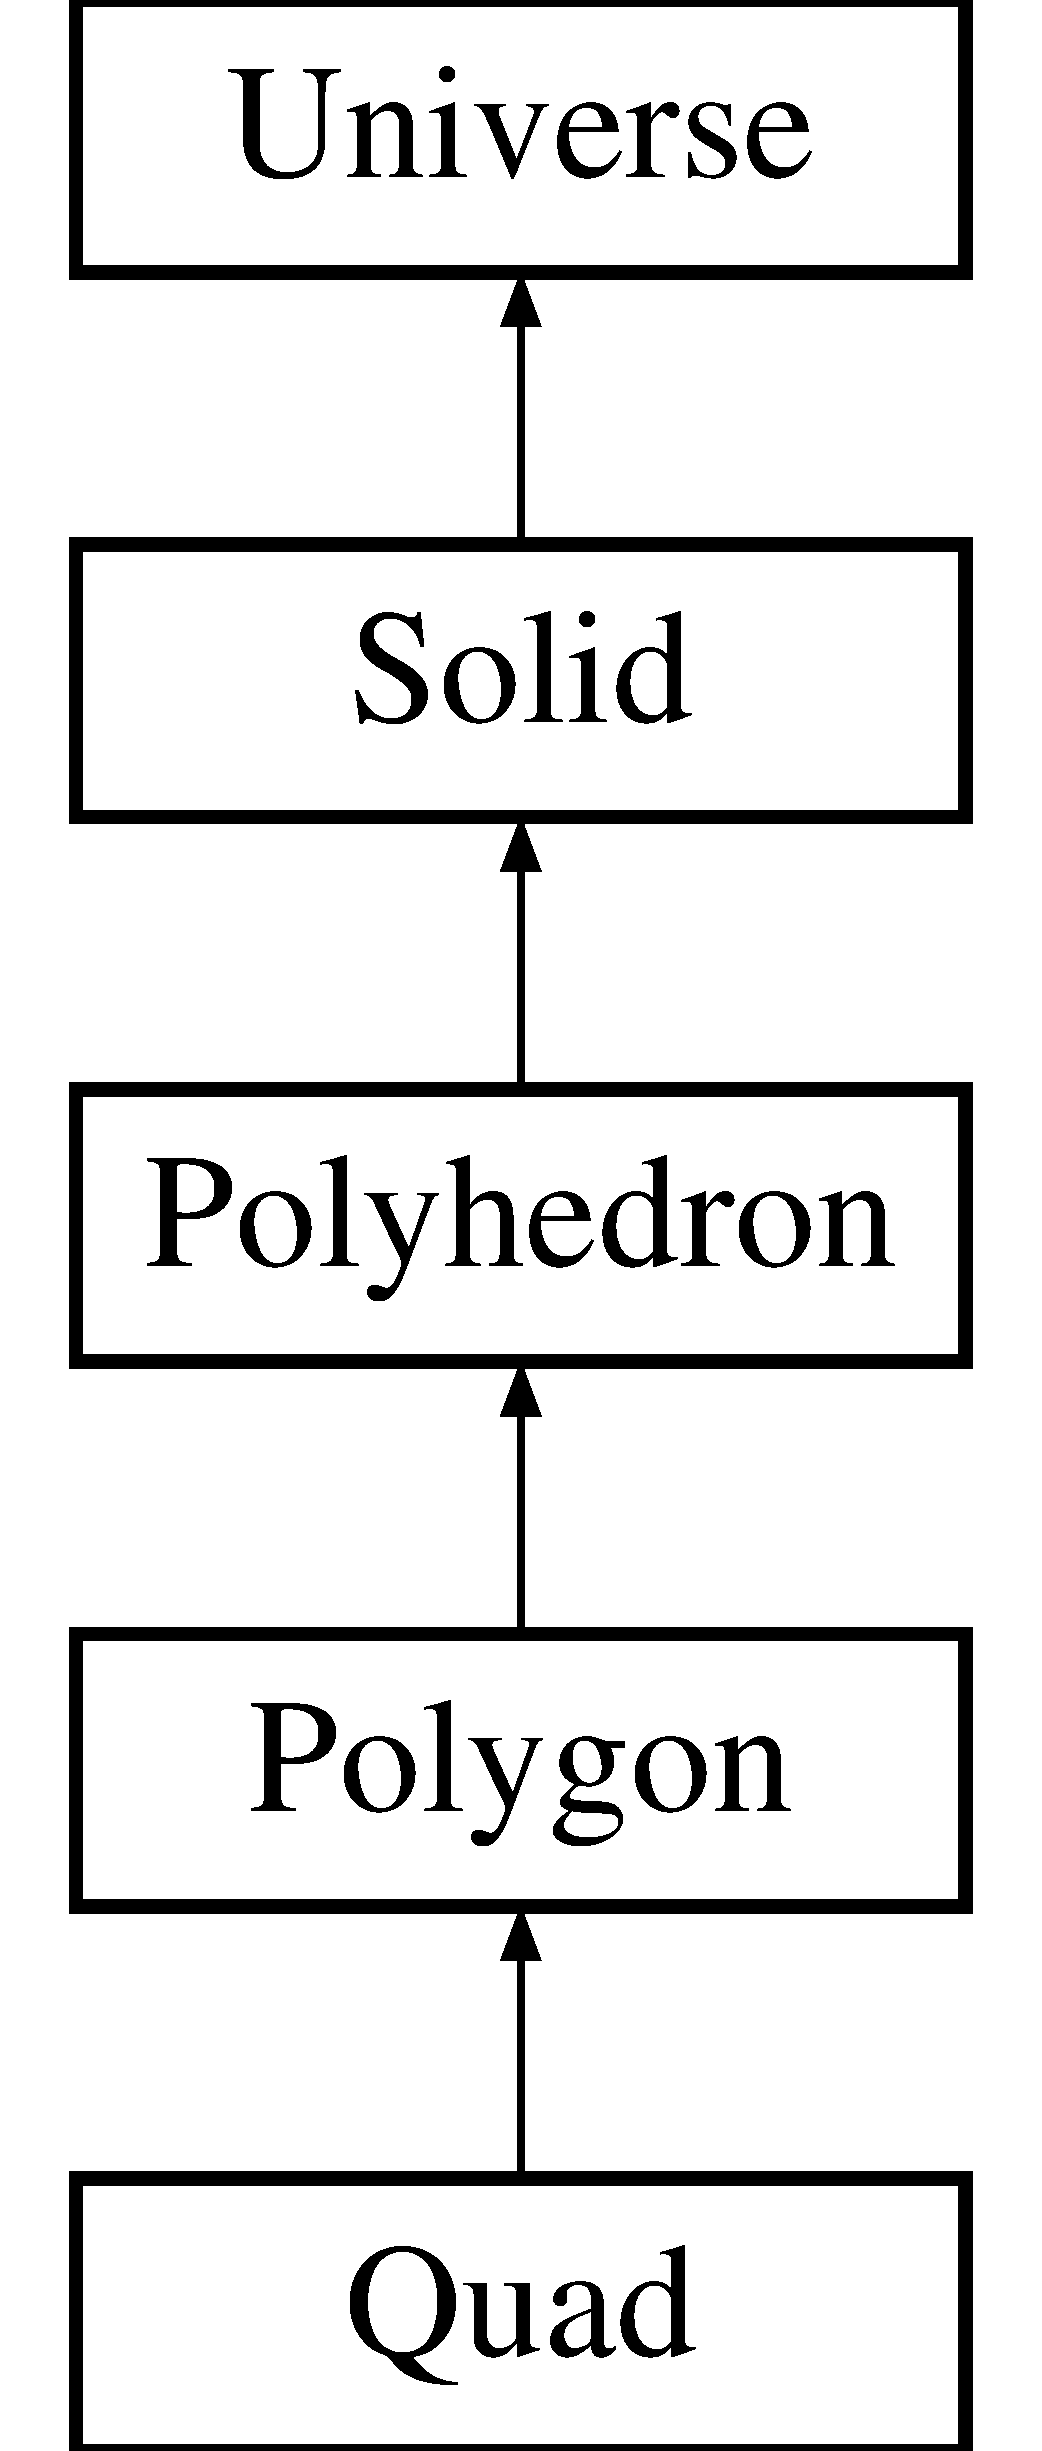
\includegraphics[height=5.000000cm]{classSolid}
\end{center}
\end{figure}
\subsection*{Public Member Functions}
\begin{DoxyCompactItemize}
\item 
\mbox{\hyperlink{classSolid_a2cf157c87df66dc3eb8722f9b3ee8f66}{Solid}} ()
\item 
\mbox{\hyperlink{classSolid_a00a71dfc929ca50ee9850bdfca5b3fd6}{Solid}} (unsigned int object\+\_\+type)
\item 
\mbox{\hyperlink{classSolid_a9f5476b751c749af38b349b9fc7e2ba5}{Solid}} (unsigned int object\+\_\+type, std\+::chrono\+::time\+\_\+point$<$ \mbox{\hyperlink{universe_8h_a0ef8d951d1ca5ab3cfaf7ab4c7a6fd80}{Clock}} $>$ event\+\_\+time)
\item 
\mbox{\hyperlink{classSolid_a80746ad255dded6090e648fc3f0dbd93}{Solid}} (unsigned int object\+\_\+type, std\+::chrono\+::time\+\_\+point$<$ \mbox{\hyperlink{universe_8h_a0ef8d951d1ca5ab3cfaf7ab4c7a6fd80}{Clock}} $>$ event\+\_\+time, \mbox{\hyperlink{classUniverse}{Universe}} \&universe\+\_\+connector)
\item 
virtual \mbox{\hyperlink{classSolid_a07095e0808c0ef6b206bc70992ef557d}{$\sim$\+Solid}} ()
\item 
bool \mbox{\hyperlink{classSolid_ac43dc78fa7f6a3348fc99751ff6bbc52}{Reset\+Parameters}} (std\+::chrono\+::time\+\_\+point$<$ \mbox{\hyperlink{universe_8h_a0ef8d951d1ca5ab3cfaf7ab4c7a6fd80}{Clock}} $>$ event\+\_\+time)
\item 
unsigned int \mbox{\hyperlink{classSolid_a7ca41431033d05957f8be3f49c3aca23}{Get\+Counter}} (std\+::chrono\+::time\+\_\+point$<$ \mbox{\hyperlink{universe_8h_a0ef8d951d1ca5ab3cfaf7ab4c7a6fd80}{Clock}} $>$ event\+\_\+time)
\item 
void \mbox{\hyperlink{classSolid_aea949040518e505ed39b1456a360c5e0}{Set\+Counter}} (std\+::chrono\+::time\+\_\+point$<$ \mbox{\hyperlink{universe_8h_a0ef8d951d1ca5ab3cfaf7ab4c7a6fd80}{Clock}} $>$ event\+\_\+time, unsigned int val)
\item 
void \mbox{\hyperlink{classSolid_af6fe46af0be9a9533e114b1c0f186bfc}{Set\+Object\+Type}} (std\+::chrono\+::time\+\_\+point$<$ \mbox{\hyperlink{universe_8h_a0ef8d951d1ca5ab3cfaf7ab4c7a6fd80}{Clock}} $>$ event\+\_\+time, unsigned int val)
\item 
\mbox{\hyperlink{classSolid}{Solid}} $\ast$ \mbox{\hyperlink{classSolid_a231b2c469aab60b092fcc3a9525e5c80}{Create\+Polyhedron}} (std\+::chrono\+::time\+\_\+point$<$ \mbox{\hyperlink{universe_8h_a0ef8d951d1ca5ab3cfaf7ab4c7a6fd80}{Clock}} $>$ event\+\_\+time)
\item 
std\+::vector$<$ \mbox{\hyperlink{classSolid}{Solid}} $\ast$ $>$ \mbox{\hyperlink{classSolid_a40b2ea07e384aff138ba139c3c84f525}{Create\+Polyhedrons}} (std\+::chrono\+::time\+\_\+point$<$ \mbox{\hyperlink{universe_8h_a0ef8d951d1ca5ab3cfaf7ab4c7a6fd80}{Clock}} $>$ event\+\_\+time, int quantity)
\item 
\mbox{\hyperlink{classSolid}{Solid}} $\ast$ \mbox{\hyperlink{classSolid_ae83094e9c002a7574db242ed0bff6288}{Clone\+Polyhedron}} (std\+::chrono\+::time\+\_\+point$<$ \mbox{\hyperlink{universe_8h_a0ef8d951d1ca5ab3cfaf7ab4c7a6fd80}{Clock}} $>$ event\+\_\+time, \mbox{\hyperlink{classSolid}{Solid}} $\ast$clone\+\_\+object, double perfection\+\_\+membership)
\item 
std\+::vector$<$ \mbox{\hyperlink{classSolid}{Solid}} $\ast$ $>$ \mbox{\hyperlink{classSolid_a1e650b6d8437acfaf7b9384b885d77bf}{Clone\+Polyhedrons}} (std\+::chrono\+::time\+\_\+point$<$ \mbox{\hyperlink{universe_8h_a0ef8d951d1ca5ab3cfaf7ab4c7a6fd80}{Clock}} $>$ event\+\_\+time, std\+::vector$<$ \mbox{\hyperlink{classSolid}{Solid}} $\ast$$>$ cloning\+\_\+list, double perfection\+\_\+membership)
\item 
\mbox{\hyperlink{classSolid}{Solid}} $\ast$ \mbox{\hyperlink{classSolid_a0841900d8ef4b82292ac027c4852b59b}{Destroy\+Polyhedron}} (std\+::chrono\+::time\+\_\+point$<$ \mbox{\hyperlink{universe_8h_a0ef8d951d1ca5ab3cfaf7ab4c7a6fd80}{Clock}} $>$ event\+\_\+time, \mbox{\hyperlink{classSolid}{Solid}} $\ast$destroy\+\_\+object)
\item 
std\+::vector$<$ \mbox{\hyperlink{classSolid}{Solid}} $\ast$ $>$ \mbox{\hyperlink{classSolid_ab1652ee511ed51bbe6a0a3b1854b7974}{Destroy\+Polyhedrons}} (std\+::chrono\+::time\+\_\+point$<$ \mbox{\hyperlink{universe_8h_a0ef8d951d1ca5ab3cfaf7ab4c7a6fd80}{Clock}} $>$ event\+\_\+time, std\+::vector$<$ \mbox{\hyperlink{classSolid}{Solid}} $\ast$$>$ destruction\+\_\+list)
\item 
\mbox{\hyperlink{classSolid}{Solid}} $\ast$ \mbox{\hyperlink{classSolid_a87a3b588f931ff20f09a5d46f6cb7907}{Add\+Polyhedron}} (std\+::chrono\+::time\+\_\+point$<$ \mbox{\hyperlink{universe_8h_a0ef8d951d1ca5ab3cfaf7ab4c7a6fd80}{Clock}} $>$ event\+\_\+time, \mbox{\hyperlink{classSolid}{Solid}} $\ast$add\+\_\+object)
\item 
std\+::vector$<$ \mbox{\hyperlink{classSolid}{Solid}} $\ast$ $>$ \mbox{\hyperlink{classSolid_a649ba1103a9889bc9e45256633dc72c3}{Add\+Polyhedrons}} (std\+::chrono\+::time\+\_\+point$<$ \mbox{\hyperlink{universe_8h_a0ef8d951d1ca5ab3cfaf7ab4c7a6fd80}{Clock}} $>$ event\+\_\+time, std\+::vector$<$ \mbox{\hyperlink{classSolid}{Solid}} $\ast$$>$ add\+\_\+objects)
\item 
\mbox{\hyperlink{classSolid}{Solid}} $\ast$ \mbox{\hyperlink{classSolid_a1233a3fe43abca7d2a0f83d724fd6640}{Remove\+Polyhedron}} (std\+::chrono\+::time\+\_\+point$<$ \mbox{\hyperlink{universe_8h_a0ef8d951d1ca5ab3cfaf7ab4c7a6fd80}{Clock}} $>$ event\+\_\+time)
\item 
std\+::vector$<$ \mbox{\hyperlink{classSolid}{Solid}} $\ast$ $>$ \mbox{\hyperlink{classSolid_a0fc53641571eb796c9d6bc33ae7a7138}{Remove\+Polyhedrons}} (std\+::chrono\+::time\+\_\+point$<$ \mbox{\hyperlink{universe_8h_a0ef8d951d1ca5ab3cfaf7ab4c7a6fd80}{Clock}} $>$ event\+\_\+time, int quantity)
\item 
\mbox{\hyperlink{classSolid}{Solid}} $\ast$ \mbox{\hyperlink{classSolid_a256ecadf461f7232eb05c28b6b4b438a}{Get\+Polyhedron}} (std\+::chrono\+::time\+\_\+point$<$ \mbox{\hyperlink{universe_8h_a0ef8d951d1ca5ab3cfaf7ab4c7a6fd80}{Clock}} $>$ event\+\_\+time, int selector)
\item 
std\+::vector$<$ \mbox{\hyperlink{classSolid}{Solid}} $\ast$ $>$ \mbox{\hyperlink{classSolid_a7006714c19bf8a7b020f42f394e4edc0}{Get\+Polyhedrons}} (std\+::chrono\+::time\+\_\+point$<$ \mbox{\hyperlink{universe_8h_a0ef8d951d1ca5ab3cfaf7ab4c7a6fd80}{Clock}} $>$ event\+\_\+time)
\item 
void \mbox{\hyperlink{classSolid_a94bb5df6d873c14a94355fc95557efd6}{Glue\+Polyhedrons}} (std\+::chrono\+::time\+\_\+point$<$ \mbox{\hyperlink{universe_8h_a0ef8d951d1ca5ab3cfaf7ab4c7a6fd80}{Clock}} $>$ event\+\_\+time)
\item 
void \mbox{\hyperlink{classSolid_a17239817eba0e5870454311857dca736}{Update\+Cycle}} (std\+::chrono\+::time\+\_\+point$<$ \mbox{\hyperlink{universe_8h_a0ef8d951d1ca5ab3cfaf7ab4c7a6fd80}{Clock}} $>$ event\+\_\+time, std\+::vector$<$ \mbox{\hyperlink{classSolid}{Solid}} $\ast$$>$ set\+\_\+of\+\_\+update\+\_\+pointers, unsigned int pointer\+\_\+type)
\item 
int \mbox{\hyperlink{classSolid_a248a5eab9fa0c584af7cdec2f86dc3a3}{Update}} (std\+::chrono\+::time\+\_\+point$<$ \mbox{\hyperlink{universe_8h_a0ef8d951d1ca5ab3cfaf7ab4c7a6fd80}{Clock}} $>$ event\+\_\+time)
\item 
void \mbox{\hyperlink{classSolid_a37503e6b25f912254414e778af2e75cd}{Set\+Charge}} (std\+::chrono\+::time\+\_\+point$<$ \mbox{\hyperlink{universe_8h_a0ef8d951d1ca5ab3cfaf7ab4c7a6fd80}{Clock}} $>$ event\+\_\+time, int val) final
\item 
void \mbox{\hyperlink{classSolid_a615cb8d1ec1376781726bcefa86339cb}{Set\+Spin}} (std\+::chrono\+::time\+\_\+point$<$ \mbox{\hyperlink{universe_8h_a0ef8d951d1ca5ab3cfaf7ab4c7a6fd80}{Clock}} $>$ event\+\_\+time, int val) final
\item 
double \mbox{\hyperlink{classSolid_ab5ecb5598be93fe3cd2a21c0cfd363c8}{Get\+Gravitation}} (std\+::chrono\+::time\+\_\+point$<$ \mbox{\hyperlink{universe_8h_a0ef8d951d1ca5ab3cfaf7ab4c7a6fd80}{Clock}} $>$ event\+\_\+time) final
\item 
double \mbox{\hyperlink{classSolid_ac8a7738735a6bda4e89414a2b0c370e1}{Get\+Weak}} (std\+::chrono\+::time\+\_\+point$<$ \mbox{\hyperlink{universe_8h_a0ef8d951d1ca5ab3cfaf7ab4c7a6fd80}{Clock}} $>$ event\+\_\+time) final
\item 
double \mbox{\hyperlink{classSolid_ac98f9c827d58a631627423e25dd611ba}{Get\+Weak\+Electroweak}} (std\+::chrono\+::time\+\_\+point$<$ \mbox{\hyperlink{universe_8h_a0ef8d951d1ca5ab3cfaf7ab4c7a6fd80}{Clock}} $>$ event\+\_\+time) final
\item 
double \mbox{\hyperlink{classSolid_a01cd3c441a4e339927c43536de6d9b5e}{Get\+Electromagnetic}} (std\+::chrono\+::time\+\_\+point$<$ \mbox{\hyperlink{universe_8h_a0ef8d951d1ca5ab3cfaf7ab4c7a6fd80}{Clock}} $>$ event\+\_\+time) final
\item 
double \mbox{\hyperlink{classSolid_aff7ec13bcc584d8330e3f3a1b371bbe6}{Get\+Electromagnetic\+Electroweak}} (std\+::chrono\+::time\+\_\+point$<$ \mbox{\hyperlink{universe_8h_a0ef8d951d1ca5ab3cfaf7ab4c7a6fd80}{Clock}} $>$ event\+\_\+time) final
\item 
double \mbox{\hyperlink{classSolid_ae39d0166456b8feaa39547e5a21c9096}{Get\+Strong}} (std\+::chrono\+::time\+\_\+point$<$ \mbox{\hyperlink{universe_8h_a0ef8d951d1ca5ab3cfaf7ab4c7a6fd80}{Clock}} $>$ event\+\_\+time) final
\item 
double \mbox{\hyperlink{classSolid_ab3a972354b25ad1bbe8c3f3e7638e24c}{Get\+Strong\+Fundamental}} (std\+::chrono\+::time\+\_\+point$<$ \mbox{\hyperlink{universe_8h_a0ef8d951d1ca5ab3cfaf7ab4c7a6fd80}{Clock}} $>$ event\+\_\+time) final
\item 
double \mbox{\hyperlink{classSolid_a9cfde1c3a4b7c6d2a5a3719d74e27237}{Get\+Strong\+Residual}} (std\+::chrono\+::time\+\_\+point$<$ \mbox{\hyperlink{universe_8h_a0ef8d951d1ca5ab3cfaf7ab4c7a6fd80}{Clock}} $>$ event\+\_\+time) final
\item 
double \mbox{\hyperlink{classSolid_af2b3133138ce2482faa462d07aa23042}{Apply\+Gravitation}} (std\+::chrono\+::time\+\_\+point$<$ \mbox{\hyperlink{universe_8h_a0ef8d951d1ca5ab3cfaf7ab4c7a6fd80}{Clock}} $>$ event\+\_\+time, double val) final
\item 
double \mbox{\hyperlink{classSolid_a49e35bf258104b7bce225dc21058affb}{Apply\+Weak}} (std\+::chrono\+::time\+\_\+point$<$ \mbox{\hyperlink{universe_8h_a0ef8d951d1ca5ab3cfaf7ab4c7a6fd80}{Clock}} $>$ event\+\_\+time, double val) final
\item 
double \mbox{\hyperlink{classSolid_ad6c28ec896cbcf64e24a7132a144befd}{Apply\+Weak\+Electroweak}} (std\+::chrono\+::time\+\_\+point$<$ \mbox{\hyperlink{universe_8h_a0ef8d951d1ca5ab3cfaf7ab4c7a6fd80}{Clock}} $>$ event\+\_\+time, double val) final
\item 
double \mbox{\hyperlink{classSolid_ab546d607d6f0bf70dc5e6bbac8baf287}{Apply\+Electromagnetic}} (std\+::chrono\+::time\+\_\+point$<$ \mbox{\hyperlink{universe_8h_a0ef8d951d1ca5ab3cfaf7ab4c7a6fd80}{Clock}} $>$ event\+\_\+time, double val) final
\item 
double \mbox{\hyperlink{classSolid_a46702e3109994b310eb4f1fba5610e0b}{Apply\+Electromagnetic\+Electroweak}} (std\+::chrono\+::time\+\_\+point$<$ \mbox{\hyperlink{universe_8h_a0ef8d951d1ca5ab3cfaf7ab4c7a6fd80}{Clock}} $>$ event\+\_\+time, double val) final
\item 
double \mbox{\hyperlink{classSolid_a0801ec0382bc509191575bcf9f5c83c1}{Apply\+Strong}} (std\+::chrono\+::time\+\_\+point$<$ \mbox{\hyperlink{universe_8h_a0ef8d951d1ca5ab3cfaf7ab4c7a6fd80}{Clock}} $>$ event\+\_\+time, double val) final
\item 
double \mbox{\hyperlink{classSolid_abd8fff76385306f97aa65dfd6b867fc6}{Apply\+Strong\+Fundamental}} (std\+::chrono\+::time\+\_\+point$<$ \mbox{\hyperlink{universe_8h_a0ef8d951d1ca5ab3cfaf7ab4c7a6fd80}{Clock}} $>$ event\+\_\+time, double val) final
\item 
double \mbox{\hyperlink{classSolid_a07534fa79bb8a6eb32e081e5158ba9e5}{Apply\+Strong\+Residual}} (std\+::chrono\+::time\+\_\+point$<$ \mbox{\hyperlink{universe_8h_a0ef8d951d1ca5ab3cfaf7ab4c7a6fd80}{Clock}} $>$ event\+\_\+time, double val) final
\item 
void \mbox{\hyperlink{classSolid_ae237f2c713868c133e28ed7f75fc9125}{Set\+Gravitation}} (std\+::chrono\+::time\+\_\+point$<$ \mbox{\hyperlink{universe_8h_a0ef8d951d1ca5ab3cfaf7ab4c7a6fd80}{Clock}} $>$ event\+\_\+time, double val) final
\item 
void \mbox{\hyperlink{classSolid_aa28e0f7e4de2fc0c1e28d385214296bf}{Set\+Weak}} (std\+::chrono\+::time\+\_\+point$<$ \mbox{\hyperlink{universe_8h_a0ef8d951d1ca5ab3cfaf7ab4c7a6fd80}{Clock}} $>$ event\+\_\+time, double val) final
\item 
void \mbox{\hyperlink{classSolid_adb34befc66f8c681f3a85c44e0d00e3a}{Set\+Weak\+Electroweak}} (std\+::chrono\+::time\+\_\+point$<$ \mbox{\hyperlink{universe_8h_a0ef8d951d1ca5ab3cfaf7ab4c7a6fd80}{Clock}} $>$ event\+\_\+time, double val) final
\item 
void \mbox{\hyperlink{classSolid_a9a660f9d94f597712c67922aa1d4d795}{Set\+Electromagnetic}} (std\+::chrono\+::time\+\_\+point$<$ \mbox{\hyperlink{universe_8h_a0ef8d951d1ca5ab3cfaf7ab4c7a6fd80}{Clock}} $>$ event\+\_\+time, double val) final
\item 
void \mbox{\hyperlink{classSolid_a6617ae9fe4707d760a23b54eddf00dec}{Set\+Electromagnetic\+Electroweak}} (std\+::chrono\+::time\+\_\+point$<$ \mbox{\hyperlink{universe_8h_a0ef8d951d1ca5ab3cfaf7ab4c7a6fd80}{Clock}} $>$ event\+\_\+time, double val) final
\item 
void \mbox{\hyperlink{classSolid_a478e15cdf15c5bb01cbcbd5f584ef83a}{Set\+Strong}} (std\+::chrono\+::time\+\_\+point$<$ \mbox{\hyperlink{universe_8h_a0ef8d951d1ca5ab3cfaf7ab4c7a6fd80}{Clock}} $>$ event\+\_\+time, double val) final
\item 
void \mbox{\hyperlink{classSolid_a4342786a7785b1a3816d20de02105bcf}{Set\+Strong\+Fundamental}} (std\+::chrono\+::time\+\_\+point$<$ \mbox{\hyperlink{universe_8h_a0ef8d951d1ca5ab3cfaf7ab4c7a6fd80}{Clock}} $>$ event\+\_\+time, double val) final
\item 
void \mbox{\hyperlink{classSolid_a8b80ebe209fcd3afa4791968127753d0}{Set\+Strong\+Residual}} (std\+::chrono\+::time\+\_\+point$<$ \mbox{\hyperlink{universe_8h_a0ef8d951d1ca5ab3cfaf7ab4c7a6fd80}{Clock}} $>$ event\+\_\+time, double val) final
\item 
void \mbox{\hyperlink{classSolid_ae2a486e59f11f96a1a39756b3f3da53f}{Poll\+Elementary\+Force}} (std\+::chrono\+::time\+\_\+point$<$ \mbox{\hyperlink{universe_8h_a0ef8d951d1ca5ab3cfaf7ab4c7a6fd80}{Clock}} $>$ event\+\_\+time) final
\end{DoxyCompactItemize}
\subsection*{Protected Attributes}
\begin{DoxyCompactItemize}
\item 
std\+::vector$<$ \mbox{\hyperlink{classSolid}{Solid}} $\ast$ $>$ \mbox{\hyperlink{classSolid_a67ef5cdd87e5629159660fa9bb5833c8}{polyhedron\+\_\+list}}
\item 
std\+::vector$<$ unsigned int $>$ \mbox{\hyperlink{classSolid_ad63206ff20f38b621db482b01801c4c5}{poly\+\_\+type\+\_\+list}}
\end{DoxyCompactItemize}
\subsection*{Private Attributes}
\begin{DoxyCompactItemize}
\item 
unsigned int \mbox{\hyperlink{classSolid_ab267c0a27586fa46a1b03bb0750caf5a}{m\+\_\+\+Counter}}
\begin{DoxyCompactList}\small\item\em Member variable \char`\"{}m\+\_\+\+Counter\char`\"{}. \end{DoxyCompactList}\item 
unsigned int \mbox{\hyperlink{classSolid_a4cb0429a28598d5501553787524b705d}{solid\+\_\+type}}
\item 
bool \mbox{\hyperlink{classSolid_ac521c984065957c82c239d5fb8be82ff}{object\+\_\+disabled}} = true
\item 
bool \mbox{\hyperlink{classSolid_ac92543b277d9a01d4cfbdf7fd71d3e1f}{object\+\_\+initialised}} = false
\item 
std\+::chrono\+::time\+\_\+point$<$ \mbox{\hyperlink{universe_8h_a0ef8d951d1ca5ab3cfaf7ab4c7a6fd80}{Clock}} $>$ \mbox{\hyperlink{classSolid_ab511520c2e523c203c1ca7b97f573f65}{time\+\_\+object\+\_\+created}}
\item 
std\+::chrono\+::time\+\_\+point$<$ \mbox{\hyperlink{universe_8h_a0ef8d951d1ca5ab3cfaf7ab4c7a6fd80}{Clock}} $>$ \mbox{\hyperlink{classSolid_ace5c8628a4f60d96029d8acea4580ab5}{previous\+\_\+event\+\_\+time}}
\item 
int \mbox{\hyperlink{classSolid_ad845ec39ddd38670049e9c6e046f2454}{duration\+\_\+since\+\_\+last\+\_\+event}}
\item 
int \mbox{\hyperlink{classSolid_abd4b935f7835fd0f8b50b526f6399731}{polyhedron\+\_\+pool}}
\end{DoxyCompactItemize}
\subsection*{Friends}
\begin{DoxyCompactItemize}
\item 
class \mbox{\hyperlink{classSolid_ad04bbaef84caa0d408ec09a1c1302f5f}{Cognitive\+Network}}
\item 
class \mbox{\hyperlink{classSolid_aa410d74ba34b18a9f6bdf24323c4ee5b}{Neuron}}
\item 
class \mbox{\hyperlink{classSolid_aaa07b7b364b620b9a781f30a5cd9f5ea}{Soma}}
\item 
class \mbox{\hyperlink{classSolid_ac790db405644a01723104c3c0c8128bb}{Membrane}}
\end{DoxyCompactItemize}
\subsection*{Additional Inherited Members}


\subsection{Constructor \& Destructor Documentation}
\mbox{\Hypertarget{classSolid_a2cf157c87df66dc3eb8722f9b3ee8f66}\label{classSolid_a2cf157c87df66dc3eb8722f9b3ee8f66}} 
\index{Solid@{Solid}!Solid@{Solid}}
\index{Solid@{Solid}!Solid@{Solid}}
\subsubsection{\texorpdfstring{Solid()}{Solid()}\hspace{0.1cm}{\footnotesize\ttfamily [1/4]}}
{\footnotesize\ttfamily Solid\+::\+Solid (\begin{DoxyParamCaption}{ }\end{DoxyParamCaption})\hspace{0.3cm}{\ttfamily [inline]}}

\mbox{\Hypertarget{classSolid_a00a71dfc929ca50ee9850bdfca5b3fd6}\label{classSolid_a00a71dfc929ca50ee9850bdfca5b3fd6}} 
\index{Solid@{Solid}!Solid@{Solid}}
\index{Solid@{Solid}!Solid@{Solid}}
\subsubsection{\texorpdfstring{Solid()}{Solid()}\hspace{0.1cm}{\footnotesize\ttfamily [2/4]}}
{\footnotesize\ttfamily Solid\+::\+Solid (\begin{DoxyParamCaption}\item[{unsigned int}]{object\+\_\+type }\end{DoxyParamCaption})\hspace{0.3cm}{\ttfamily [inline]}}

\mbox{\Hypertarget{classSolid_a9f5476b751c749af38b349b9fc7e2ba5}\label{classSolid_a9f5476b751c749af38b349b9fc7e2ba5}} 
\index{Solid@{Solid}!Solid@{Solid}}
\index{Solid@{Solid}!Solid@{Solid}}
\subsubsection{\texorpdfstring{Solid()}{Solid()}\hspace{0.1cm}{\footnotesize\ttfamily [3/4]}}
{\footnotesize\ttfamily Solid\+::\+Solid (\begin{DoxyParamCaption}\item[{unsigned int}]{object\+\_\+type,  }\item[{std\+::chrono\+::time\+\_\+point$<$ \mbox{\hyperlink{universe_8h_a0ef8d951d1ca5ab3cfaf7ab4c7a6fd80}{Clock}} $>$}]{event\+\_\+time }\end{DoxyParamCaption})\hspace{0.3cm}{\ttfamily [inline]}}

\mbox{\Hypertarget{classSolid_a80746ad255dded6090e648fc3f0dbd93}\label{classSolid_a80746ad255dded6090e648fc3f0dbd93}} 
\index{Solid@{Solid}!Solid@{Solid}}
\index{Solid@{Solid}!Solid@{Solid}}
\subsubsection{\texorpdfstring{Solid()}{Solid()}\hspace{0.1cm}{\footnotesize\ttfamily [4/4]}}
{\footnotesize\ttfamily Solid\+::\+Solid (\begin{DoxyParamCaption}\item[{unsigned int}]{object\+\_\+type,  }\item[{std\+::chrono\+::time\+\_\+point$<$ \mbox{\hyperlink{universe_8h_a0ef8d951d1ca5ab3cfaf7ab4c7a6fd80}{Clock}} $>$}]{event\+\_\+time,  }\item[{\mbox{\hyperlink{classUniverse}{Universe}} \&}]{universe\+\_\+connector }\end{DoxyParamCaption})\hspace{0.3cm}{\ttfamily [inline]}}

\mbox{\Hypertarget{classSolid_a07095e0808c0ef6b206bc70992ef557d}\label{classSolid_a07095e0808c0ef6b206bc70992ef557d}} 
\index{Solid@{Solid}!````~Solid@{$\sim$\+Solid}}
\index{````~Solid@{$\sim$\+Solid}!Solid@{Solid}}
\subsubsection{\texorpdfstring{$\sim$\+Solid()}{~Solid()}}
{\footnotesize\ttfamily virtual Solid\+::$\sim$\+Solid (\begin{DoxyParamCaption}{ }\end{DoxyParamCaption})\hspace{0.3cm}{\ttfamily [inline]}, {\ttfamily [virtual]}}

Default destructor 

\subsection{Member Function Documentation}
\mbox{\Hypertarget{classSolid_a87a3b588f931ff20f09a5d46f6cb7907}\label{classSolid_a87a3b588f931ff20f09a5d46f6cb7907}} 
\index{Solid@{Solid}!Add\+Polyhedron@{Add\+Polyhedron}}
\index{Add\+Polyhedron@{Add\+Polyhedron}!Solid@{Solid}}
\subsubsection{\texorpdfstring{Add\+Polyhedron()}{AddPolyhedron()}}
{\footnotesize\ttfamily \mbox{\hyperlink{classSolid}{Solid}} $\ast$ Solid\+::\+Add\+Polyhedron (\begin{DoxyParamCaption}\item[{std\+::chrono\+::time\+\_\+point$<$ \mbox{\hyperlink{universe_8h_a0ef8d951d1ca5ab3cfaf7ab4c7a6fd80}{Clock}} $>$}]{event\+\_\+time,  }\item[{\mbox{\hyperlink{classSolid}{Solid}} $\ast$}]{add\+\_\+object }\end{DoxyParamCaption})}

\mbox{\Hypertarget{classSolid_a649ba1103a9889bc9e45256633dc72c3}\label{classSolid_a649ba1103a9889bc9e45256633dc72c3}} 
\index{Solid@{Solid}!Add\+Polyhedrons@{Add\+Polyhedrons}}
\index{Add\+Polyhedrons@{Add\+Polyhedrons}!Solid@{Solid}}
\subsubsection{\texorpdfstring{Add\+Polyhedrons()}{AddPolyhedrons()}}
{\footnotesize\ttfamily std\+::vector$<$ \mbox{\hyperlink{classSolid}{Solid}} $\ast$ $>$ Solid\+::\+Add\+Polyhedrons (\begin{DoxyParamCaption}\item[{std\+::chrono\+::time\+\_\+point$<$ \mbox{\hyperlink{universe_8h_a0ef8d951d1ca5ab3cfaf7ab4c7a6fd80}{Clock}} $>$}]{event\+\_\+time,  }\item[{std\+::vector$<$ \mbox{\hyperlink{classSolid}{Solid}} $\ast$$>$}]{add\+\_\+objects }\end{DoxyParamCaption})}

\mbox{\Hypertarget{classSolid_ab546d607d6f0bf70dc5e6bbac8baf287}\label{classSolid_ab546d607d6f0bf70dc5e6bbac8baf287}} 
\index{Solid@{Solid}!Apply\+Electromagnetic@{Apply\+Electromagnetic}}
\index{Apply\+Electromagnetic@{Apply\+Electromagnetic}!Solid@{Solid}}
\subsubsection{\texorpdfstring{Apply\+Electromagnetic()}{ApplyElectromagnetic()}}
{\footnotesize\ttfamily double Solid\+::\+Apply\+Electromagnetic (\begin{DoxyParamCaption}\item[{std\+::chrono\+::time\+\_\+point$<$ \mbox{\hyperlink{universe_8h_a0ef8d951d1ca5ab3cfaf7ab4c7a6fd80}{Clock}} $>$}]{event\+\_\+time,  }\item[{double}]{val }\end{DoxyParamCaption})\hspace{0.3cm}{\ttfamily [inline]}, {\ttfamily [final]}, {\ttfamily [virtual]}}



Reimplemented from \mbox{\hyperlink{classUniverse_a1f787da78fa196ba635db21a9e91dabb}{Universe}}.

\mbox{\Hypertarget{classSolid_a46702e3109994b310eb4f1fba5610e0b}\label{classSolid_a46702e3109994b310eb4f1fba5610e0b}} 
\index{Solid@{Solid}!Apply\+Electromagnetic\+Electroweak@{Apply\+Electromagnetic\+Electroweak}}
\index{Apply\+Electromagnetic\+Electroweak@{Apply\+Electromagnetic\+Electroweak}!Solid@{Solid}}
\subsubsection{\texorpdfstring{Apply\+Electromagnetic\+Electroweak()}{ApplyElectromagneticElectroweak()}}
{\footnotesize\ttfamily double Solid\+::\+Apply\+Electromagnetic\+Electroweak (\begin{DoxyParamCaption}\item[{std\+::chrono\+::time\+\_\+point$<$ \mbox{\hyperlink{universe_8h_a0ef8d951d1ca5ab3cfaf7ab4c7a6fd80}{Clock}} $>$}]{event\+\_\+time,  }\item[{double}]{val }\end{DoxyParamCaption})\hspace{0.3cm}{\ttfamily [inline]}, {\ttfamily [final]}, {\ttfamily [virtual]}}



Reimplemented from \mbox{\hyperlink{classUniverse_a4c36c1ab30db993307f88363dde5e8c5}{Universe}}.

\mbox{\Hypertarget{classSolid_af2b3133138ce2482faa462d07aa23042}\label{classSolid_af2b3133138ce2482faa462d07aa23042}} 
\index{Solid@{Solid}!Apply\+Gravitation@{Apply\+Gravitation}}
\index{Apply\+Gravitation@{Apply\+Gravitation}!Solid@{Solid}}
\subsubsection{\texorpdfstring{Apply\+Gravitation()}{ApplyGravitation()}}
{\footnotesize\ttfamily double Solid\+::\+Apply\+Gravitation (\begin{DoxyParamCaption}\item[{std\+::chrono\+::time\+\_\+point$<$ \mbox{\hyperlink{universe_8h_a0ef8d951d1ca5ab3cfaf7ab4c7a6fd80}{Clock}} $>$}]{event\+\_\+time,  }\item[{double}]{val }\end{DoxyParamCaption})\hspace{0.3cm}{\ttfamily [inline]}, {\ttfamily [final]}, {\ttfamily [virtual]}}



Reimplemented from \mbox{\hyperlink{classUniverse_a76c0b5e63c2a7d1988c44db341c3d64c}{Universe}}.

\mbox{\Hypertarget{classSolid_a0801ec0382bc509191575bcf9f5c83c1}\label{classSolid_a0801ec0382bc509191575bcf9f5c83c1}} 
\index{Solid@{Solid}!Apply\+Strong@{Apply\+Strong}}
\index{Apply\+Strong@{Apply\+Strong}!Solid@{Solid}}
\subsubsection{\texorpdfstring{Apply\+Strong()}{ApplyStrong()}}
{\footnotesize\ttfamily double Solid\+::\+Apply\+Strong (\begin{DoxyParamCaption}\item[{std\+::chrono\+::time\+\_\+point$<$ \mbox{\hyperlink{universe_8h_a0ef8d951d1ca5ab3cfaf7ab4c7a6fd80}{Clock}} $>$}]{event\+\_\+time,  }\item[{double}]{val }\end{DoxyParamCaption})\hspace{0.3cm}{\ttfamily [inline]}, {\ttfamily [final]}, {\ttfamily [virtual]}}



Reimplemented from \mbox{\hyperlink{classUniverse_a906a88b37f10bfa630bef49dfd0e907a}{Universe}}.

\mbox{\Hypertarget{classSolid_abd8fff76385306f97aa65dfd6b867fc6}\label{classSolid_abd8fff76385306f97aa65dfd6b867fc6}} 
\index{Solid@{Solid}!Apply\+Strong\+Fundamental@{Apply\+Strong\+Fundamental}}
\index{Apply\+Strong\+Fundamental@{Apply\+Strong\+Fundamental}!Solid@{Solid}}
\subsubsection{\texorpdfstring{Apply\+Strong\+Fundamental()}{ApplyStrongFundamental()}}
{\footnotesize\ttfamily double Solid\+::\+Apply\+Strong\+Fundamental (\begin{DoxyParamCaption}\item[{std\+::chrono\+::time\+\_\+point$<$ \mbox{\hyperlink{universe_8h_a0ef8d951d1ca5ab3cfaf7ab4c7a6fd80}{Clock}} $>$}]{event\+\_\+time,  }\item[{double}]{val }\end{DoxyParamCaption})\hspace{0.3cm}{\ttfamily [inline]}, {\ttfamily [final]}, {\ttfamily [virtual]}}



Reimplemented from \mbox{\hyperlink{classUniverse_a62789bcff84bd750b0366004381e2fdd}{Universe}}.

\mbox{\Hypertarget{classSolid_a07534fa79bb8a6eb32e081e5158ba9e5}\label{classSolid_a07534fa79bb8a6eb32e081e5158ba9e5}} 
\index{Solid@{Solid}!Apply\+Strong\+Residual@{Apply\+Strong\+Residual}}
\index{Apply\+Strong\+Residual@{Apply\+Strong\+Residual}!Solid@{Solid}}
\subsubsection{\texorpdfstring{Apply\+Strong\+Residual()}{ApplyStrongResidual()}}
{\footnotesize\ttfamily double Solid\+::\+Apply\+Strong\+Residual (\begin{DoxyParamCaption}\item[{std\+::chrono\+::time\+\_\+point$<$ \mbox{\hyperlink{universe_8h_a0ef8d951d1ca5ab3cfaf7ab4c7a6fd80}{Clock}} $>$}]{event\+\_\+time,  }\item[{double}]{val }\end{DoxyParamCaption})\hspace{0.3cm}{\ttfamily [inline]}, {\ttfamily [final]}, {\ttfamily [virtual]}}



Reimplemented from \mbox{\hyperlink{classUniverse_af7becebb347be9a85541d96a3eca1ca7}{Universe}}.

\mbox{\Hypertarget{classSolid_a49e35bf258104b7bce225dc21058affb}\label{classSolid_a49e35bf258104b7bce225dc21058affb}} 
\index{Solid@{Solid}!Apply\+Weak@{Apply\+Weak}}
\index{Apply\+Weak@{Apply\+Weak}!Solid@{Solid}}
\subsubsection{\texorpdfstring{Apply\+Weak()}{ApplyWeak()}}
{\footnotesize\ttfamily double Solid\+::\+Apply\+Weak (\begin{DoxyParamCaption}\item[{std\+::chrono\+::time\+\_\+point$<$ \mbox{\hyperlink{universe_8h_a0ef8d951d1ca5ab3cfaf7ab4c7a6fd80}{Clock}} $>$}]{event\+\_\+time,  }\item[{double}]{val }\end{DoxyParamCaption})\hspace{0.3cm}{\ttfamily [inline]}, {\ttfamily [final]}, {\ttfamily [virtual]}}



Reimplemented from \mbox{\hyperlink{classUniverse_a6d1226b3adec3c42a833afdbb6a65a92}{Universe}}.

\mbox{\Hypertarget{classSolid_ad6c28ec896cbcf64e24a7132a144befd}\label{classSolid_ad6c28ec896cbcf64e24a7132a144befd}} 
\index{Solid@{Solid}!Apply\+Weak\+Electroweak@{Apply\+Weak\+Electroweak}}
\index{Apply\+Weak\+Electroweak@{Apply\+Weak\+Electroweak}!Solid@{Solid}}
\subsubsection{\texorpdfstring{Apply\+Weak\+Electroweak()}{ApplyWeakElectroweak()}}
{\footnotesize\ttfamily double Solid\+::\+Apply\+Weak\+Electroweak (\begin{DoxyParamCaption}\item[{std\+::chrono\+::time\+\_\+point$<$ \mbox{\hyperlink{universe_8h_a0ef8d951d1ca5ab3cfaf7ab4c7a6fd80}{Clock}} $>$}]{event\+\_\+time,  }\item[{double}]{val }\end{DoxyParamCaption})\hspace{0.3cm}{\ttfamily [inline]}, {\ttfamily [final]}, {\ttfamily [virtual]}}



Reimplemented from \mbox{\hyperlink{classUniverse_a46a906baabb63e5d31f8b48ea1fae52e}{Universe}}.

\mbox{\Hypertarget{classSolid_ae83094e9c002a7574db242ed0bff6288}\label{classSolid_ae83094e9c002a7574db242ed0bff6288}} 
\index{Solid@{Solid}!Clone\+Polyhedron@{Clone\+Polyhedron}}
\index{Clone\+Polyhedron@{Clone\+Polyhedron}!Solid@{Solid}}
\subsubsection{\texorpdfstring{Clone\+Polyhedron()}{ClonePolyhedron()}}
{\footnotesize\ttfamily \mbox{\hyperlink{classSolid}{Solid}} $\ast$ Solid\+::\+Clone\+Polyhedron (\begin{DoxyParamCaption}\item[{std\+::chrono\+::time\+\_\+point$<$ \mbox{\hyperlink{universe_8h_a0ef8d951d1ca5ab3cfaf7ab4c7a6fd80}{Clock}} $>$}]{event\+\_\+time,  }\item[{\mbox{\hyperlink{classSolid}{Solid}} $\ast$}]{clone\+\_\+object,  }\item[{double}]{perfection\+\_\+membership }\end{DoxyParamCaption})}

\mbox{\Hypertarget{classSolid_a1e650b6d8437acfaf7b9384b885d77bf}\label{classSolid_a1e650b6d8437acfaf7b9384b885d77bf}} 
\index{Solid@{Solid}!Clone\+Polyhedrons@{Clone\+Polyhedrons}}
\index{Clone\+Polyhedrons@{Clone\+Polyhedrons}!Solid@{Solid}}
\subsubsection{\texorpdfstring{Clone\+Polyhedrons()}{ClonePolyhedrons()}}
{\footnotesize\ttfamily std\+::vector$<$ \mbox{\hyperlink{classSolid}{Solid}} $\ast$ $>$ Solid\+::\+Clone\+Polyhedrons (\begin{DoxyParamCaption}\item[{std\+::chrono\+::time\+\_\+point$<$ \mbox{\hyperlink{universe_8h_a0ef8d951d1ca5ab3cfaf7ab4c7a6fd80}{Clock}} $>$}]{event\+\_\+time,  }\item[{std\+::vector$<$ \mbox{\hyperlink{classSolid}{Solid}} $\ast$$>$}]{cloning\+\_\+list,  }\item[{double}]{perfection\+\_\+membership }\end{DoxyParamCaption})}

\mbox{\Hypertarget{classSolid_a231b2c469aab60b092fcc3a9525e5c80}\label{classSolid_a231b2c469aab60b092fcc3a9525e5c80}} 
\index{Solid@{Solid}!Create\+Polyhedron@{Create\+Polyhedron}}
\index{Create\+Polyhedron@{Create\+Polyhedron}!Solid@{Solid}}
\subsubsection{\texorpdfstring{Create\+Polyhedron()}{CreatePolyhedron()}}
{\footnotesize\ttfamily \mbox{\hyperlink{classSolid}{Solid}} $\ast$ Solid\+::\+Create\+Polyhedron (\begin{DoxyParamCaption}\item[{std\+::chrono\+::time\+\_\+point$<$ \mbox{\hyperlink{universe_8h_a0ef8d951d1ca5ab3cfaf7ab4c7a6fd80}{Clock}} $>$}]{event\+\_\+time }\end{DoxyParamCaption})}

\mbox{\Hypertarget{classSolid_a40b2ea07e384aff138ba139c3c84f525}\label{classSolid_a40b2ea07e384aff138ba139c3c84f525}} 
\index{Solid@{Solid}!Create\+Polyhedrons@{Create\+Polyhedrons}}
\index{Create\+Polyhedrons@{Create\+Polyhedrons}!Solid@{Solid}}
\subsubsection{\texorpdfstring{Create\+Polyhedrons()}{CreatePolyhedrons()}}
{\footnotesize\ttfamily std\+::vector$<$ \mbox{\hyperlink{classSolid}{Solid}} $\ast$ $>$ Solid\+::\+Create\+Polyhedrons (\begin{DoxyParamCaption}\item[{std\+::chrono\+::time\+\_\+point$<$ \mbox{\hyperlink{universe_8h_a0ef8d951d1ca5ab3cfaf7ab4c7a6fd80}{Clock}} $>$}]{event\+\_\+time,  }\item[{int}]{quantity }\end{DoxyParamCaption})}

\mbox{\Hypertarget{classSolid_a0841900d8ef4b82292ac027c4852b59b}\label{classSolid_a0841900d8ef4b82292ac027c4852b59b}} 
\index{Solid@{Solid}!Destroy\+Polyhedron@{Destroy\+Polyhedron}}
\index{Destroy\+Polyhedron@{Destroy\+Polyhedron}!Solid@{Solid}}
\subsubsection{\texorpdfstring{Destroy\+Polyhedron()}{DestroyPolyhedron()}}
{\footnotesize\ttfamily \mbox{\hyperlink{classSolid}{Solid}} $\ast$ Solid\+::\+Destroy\+Polyhedron (\begin{DoxyParamCaption}\item[{std\+::chrono\+::time\+\_\+point$<$ \mbox{\hyperlink{universe_8h_a0ef8d951d1ca5ab3cfaf7ab4c7a6fd80}{Clock}} $>$}]{event\+\_\+time,  }\item[{\mbox{\hyperlink{classSolid}{Solid}} $\ast$}]{destroy\+\_\+object }\end{DoxyParamCaption})}

\mbox{\Hypertarget{classSolid_ab1652ee511ed51bbe6a0a3b1854b7974}\label{classSolid_ab1652ee511ed51bbe6a0a3b1854b7974}} 
\index{Solid@{Solid}!Destroy\+Polyhedrons@{Destroy\+Polyhedrons}}
\index{Destroy\+Polyhedrons@{Destroy\+Polyhedrons}!Solid@{Solid}}
\subsubsection{\texorpdfstring{Destroy\+Polyhedrons()}{DestroyPolyhedrons()}}
{\footnotesize\ttfamily std\+::vector$<$ \mbox{\hyperlink{classSolid}{Solid}} $\ast$ $>$ Solid\+::\+Destroy\+Polyhedrons (\begin{DoxyParamCaption}\item[{std\+::chrono\+::time\+\_\+point$<$ \mbox{\hyperlink{universe_8h_a0ef8d951d1ca5ab3cfaf7ab4c7a6fd80}{Clock}} $>$}]{event\+\_\+time,  }\item[{std\+::vector$<$ \mbox{\hyperlink{classSolid}{Solid}} $\ast$$>$}]{destruction\+\_\+list }\end{DoxyParamCaption})}

\mbox{\Hypertarget{classSolid_a7ca41431033d05957f8be3f49c3aca23}\label{classSolid_a7ca41431033d05957f8be3f49c3aca23}} 
\index{Solid@{Solid}!Get\+Counter@{Get\+Counter}}
\index{Get\+Counter@{Get\+Counter}!Solid@{Solid}}
\subsubsection{\texorpdfstring{Get\+Counter()}{GetCounter()}}
{\footnotesize\ttfamily unsigned int Solid\+::\+Get\+Counter (\begin{DoxyParamCaption}\item[{std\+::chrono\+::time\+\_\+point$<$ \mbox{\hyperlink{universe_8h_a0ef8d951d1ca5ab3cfaf7ab4c7a6fd80}{Clock}} $>$}]{event\+\_\+time }\end{DoxyParamCaption})}

\mbox{\Hypertarget{classSolid_a01cd3c441a4e339927c43536de6d9b5e}\label{classSolid_a01cd3c441a4e339927c43536de6d9b5e}} 
\index{Solid@{Solid}!Get\+Electromagnetic@{Get\+Electromagnetic}}
\index{Get\+Electromagnetic@{Get\+Electromagnetic}!Solid@{Solid}}
\subsubsection{\texorpdfstring{Get\+Electromagnetic()}{GetElectromagnetic()}}
{\footnotesize\ttfamily double Solid\+::\+Get\+Electromagnetic (\begin{DoxyParamCaption}\item[{std\+::chrono\+::time\+\_\+point$<$ \mbox{\hyperlink{universe_8h_a0ef8d951d1ca5ab3cfaf7ab4c7a6fd80}{Clock}} $>$}]{event\+\_\+time }\end{DoxyParamCaption})\hspace{0.3cm}{\ttfamily [inline]}, {\ttfamily [final]}, {\ttfamily [virtual]}}



Reimplemented from \mbox{\hyperlink{classUniverse_a63b850ef3f3394313353109d222bf5d1}{Universe}}.

\mbox{\Hypertarget{classSolid_aff7ec13bcc584d8330e3f3a1b371bbe6}\label{classSolid_aff7ec13bcc584d8330e3f3a1b371bbe6}} 
\index{Solid@{Solid}!Get\+Electromagnetic\+Electroweak@{Get\+Electromagnetic\+Electroweak}}
\index{Get\+Electromagnetic\+Electroweak@{Get\+Electromagnetic\+Electroweak}!Solid@{Solid}}
\subsubsection{\texorpdfstring{Get\+Electromagnetic\+Electroweak()}{GetElectromagneticElectroweak()}}
{\footnotesize\ttfamily double Solid\+::\+Get\+Electromagnetic\+Electroweak (\begin{DoxyParamCaption}\item[{std\+::chrono\+::time\+\_\+point$<$ \mbox{\hyperlink{universe_8h_a0ef8d951d1ca5ab3cfaf7ab4c7a6fd80}{Clock}} $>$}]{event\+\_\+time }\end{DoxyParamCaption})\hspace{0.3cm}{\ttfamily [inline]}, {\ttfamily [final]}, {\ttfamily [virtual]}}



Reimplemented from \mbox{\hyperlink{classUniverse_a9f099605c082e7fa755787a6a8cab7ba}{Universe}}.

\mbox{\Hypertarget{classSolid_ab5ecb5598be93fe3cd2a21c0cfd363c8}\label{classSolid_ab5ecb5598be93fe3cd2a21c0cfd363c8}} 
\index{Solid@{Solid}!Get\+Gravitation@{Get\+Gravitation}}
\index{Get\+Gravitation@{Get\+Gravitation}!Solid@{Solid}}
\subsubsection{\texorpdfstring{Get\+Gravitation()}{GetGravitation()}}
{\footnotesize\ttfamily double Solid\+::\+Get\+Gravitation (\begin{DoxyParamCaption}\item[{std\+::chrono\+::time\+\_\+point$<$ \mbox{\hyperlink{universe_8h_a0ef8d951d1ca5ab3cfaf7ab4c7a6fd80}{Clock}} $>$}]{event\+\_\+time }\end{DoxyParamCaption})\hspace{0.3cm}{\ttfamily [inline]}, {\ttfamily [final]}, {\ttfamily [virtual]}}



Reimplemented from \mbox{\hyperlink{classUniverse_ab0404e774ee0ed66b597ff5b8e989446}{Universe}}.

\mbox{\Hypertarget{classSolid_a256ecadf461f7232eb05c28b6b4b438a}\label{classSolid_a256ecadf461f7232eb05c28b6b4b438a}} 
\index{Solid@{Solid}!Get\+Polyhedron@{Get\+Polyhedron}}
\index{Get\+Polyhedron@{Get\+Polyhedron}!Solid@{Solid}}
\subsubsection{\texorpdfstring{Get\+Polyhedron()}{GetPolyhedron()}}
{\footnotesize\ttfamily \mbox{\hyperlink{classSolid}{Solid}} $\ast$ Solid\+::\+Get\+Polyhedron (\begin{DoxyParamCaption}\item[{std\+::chrono\+::time\+\_\+point$<$ \mbox{\hyperlink{universe_8h_a0ef8d951d1ca5ab3cfaf7ab4c7a6fd80}{Clock}} $>$}]{event\+\_\+time,  }\item[{int}]{selector }\end{DoxyParamCaption})}

\mbox{\Hypertarget{classSolid_a7006714c19bf8a7b020f42f394e4edc0}\label{classSolid_a7006714c19bf8a7b020f42f394e4edc0}} 
\index{Solid@{Solid}!Get\+Polyhedrons@{Get\+Polyhedrons}}
\index{Get\+Polyhedrons@{Get\+Polyhedrons}!Solid@{Solid}}
\subsubsection{\texorpdfstring{Get\+Polyhedrons()}{GetPolyhedrons()}}
{\footnotesize\ttfamily std\+::vector$<$ \mbox{\hyperlink{classSolid}{Solid}} $\ast$ $>$ Solid\+::\+Get\+Polyhedrons (\begin{DoxyParamCaption}\item[{std\+::chrono\+::time\+\_\+point$<$ \mbox{\hyperlink{universe_8h_a0ef8d951d1ca5ab3cfaf7ab4c7a6fd80}{Clock}} $>$}]{event\+\_\+time }\end{DoxyParamCaption})}

\mbox{\Hypertarget{classSolid_ae39d0166456b8feaa39547e5a21c9096}\label{classSolid_ae39d0166456b8feaa39547e5a21c9096}} 
\index{Solid@{Solid}!Get\+Strong@{Get\+Strong}}
\index{Get\+Strong@{Get\+Strong}!Solid@{Solid}}
\subsubsection{\texorpdfstring{Get\+Strong()}{GetStrong()}}
{\footnotesize\ttfamily double Solid\+::\+Get\+Strong (\begin{DoxyParamCaption}\item[{std\+::chrono\+::time\+\_\+point$<$ \mbox{\hyperlink{universe_8h_a0ef8d951d1ca5ab3cfaf7ab4c7a6fd80}{Clock}} $>$}]{event\+\_\+time }\end{DoxyParamCaption})\hspace{0.3cm}{\ttfamily [inline]}, {\ttfamily [final]}, {\ttfamily [virtual]}}



Reimplemented from \mbox{\hyperlink{classUniverse_acb453ce71da418c5b5617fecede9571b}{Universe}}.

\mbox{\Hypertarget{classSolid_ab3a972354b25ad1bbe8c3f3e7638e24c}\label{classSolid_ab3a972354b25ad1bbe8c3f3e7638e24c}} 
\index{Solid@{Solid}!Get\+Strong\+Fundamental@{Get\+Strong\+Fundamental}}
\index{Get\+Strong\+Fundamental@{Get\+Strong\+Fundamental}!Solid@{Solid}}
\subsubsection{\texorpdfstring{Get\+Strong\+Fundamental()}{GetStrongFundamental()}}
{\footnotesize\ttfamily double Solid\+::\+Get\+Strong\+Fundamental (\begin{DoxyParamCaption}\item[{std\+::chrono\+::time\+\_\+point$<$ \mbox{\hyperlink{universe_8h_a0ef8d951d1ca5ab3cfaf7ab4c7a6fd80}{Clock}} $>$}]{event\+\_\+time }\end{DoxyParamCaption})\hspace{0.3cm}{\ttfamily [inline]}, {\ttfamily [final]}, {\ttfamily [virtual]}}



Reimplemented from \mbox{\hyperlink{classUniverse_ab44daccba01ee7e3cf9b50bba83dd19e}{Universe}}.

\mbox{\Hypertarget{classSolid_a9cfde1c3a4b7c6d2a5a3719d74e27237}\label{classSolid_a9cfde1c3a4b7c6d2a5a3719d74e27237}} 
\index{Solid@{Solid}!Get\+Strong\+Residual@{Get\+Strong\+Residual}}
\index{Get\+Strong\+Residual@{Get\+Strong\+Residual}!Solid@{Solid}}
\subsubsection{\texorpdfstring{Get\+Strong\+Residual()}{GetStrongResidual()}}
{\footnotesize\ttfamily double Solid\+::\+Get\+Strong\+Residual (\begin{DoxyParamCaption}\item[{std\+::chrono\+::time\+\_\+point$<$ \mbox{\hyperlink{universe_8h_a0ef8d951d1ca5ab3cfaf7ab4c7a6fd80}{Clock}} $>$}]{event\+\_\+time }\end{DoxyParamCaption})\hspace{0.3cm}{\ttfamily [inline]}, {\ttfamily [final]}, {\ttfamily [virtual]}}



Reimplemented from \mbox{\hyperlink{classUniverse_af0f4b81950061e63c2855eb40957a5b1}{Universe}}.

\mbox{\Hypertarget{classSolid_ac8a7738735a6bda4e89414a2b0c370e1}\label{classSolid_ac8a7738735a6bda4e89414a2b0c370e1}} 
\index{Solid@{Solid}!Get\+Weak@{Get\+Weak}}
\index{Get\+Weak@{Get\+Weak}!Solid@{Solid}}
\subsubsection{\texorpdfstring{Get\+Weak()}{GetWeak()}}
{\footnotesize\ttfamily double Solid\+::\+Get\+Weak (\begin{DoxyParamCaption}\item[{std\+::chrono\+::time\+\_\+point$<$ \mbox{\hyperlink{universe_8h_a0ef8d951d1ca5ab3cfaf7ab4c7a6fd80}{Clock}} $>$}]{event\+\_\+time }\end{DoxyParamCaption})\hspace{0.3cm}{\ttfamily [inline]}, {\ttfamily [final]}, {\ttfamily [virtual]}}



Reimplemented from \mbox{\hyperlink{classUniverse_a4476b7e0a3fc1764909f556257fd9ec7}{Universe}}.

\mbox{\Hypertarget{classSolid_ac98f9c827d58a631627423e25dd611ba}\label{classSolid_ac98f9c827d58a631627423e25dd611ba}} 
\index{Solid@{Solid}!Get\+Weak\+Electroweak@{Get\+Weak\+Electroweak}}
\index{Get\+Weak\+Electroweak@{Get\+Weak\+Electroweak}!Solid@{Solid}}
\subsubsection{\texorpdfstring{Get\+Weak\+Electroweak()}{GetWeakElectroweak()}}
{\footnotesize\ttfamily double Solid\+::\+Get\+Weak\+Electroweak (\begin{DoxyParamCaption}\item[{std\+::chrono\+::time\+\_\+point$<$ \mbox{\hyperlink{universe_8h_a0ef8d951d1ca5ab3cfaf7ab4c7a6fd80}{Clock}} $>$}]{event\+\_\+time }\end{DoxyParamCaption})\hspace{0.3cm}{\ttfamily [inline]}, {\ttfamily [final]}, {\ttfamily [virtual]}}



Reimplemented from \mbox{\hyperlink{classUniverse_a645299738e6b798a037f2a15a2e7cf4d}{Universe}}.

\mbox{\Hypertarget{classSolid_a94bb5df6d873c14a94355fc95557efd6}\label{classSolid_a94bb5df6d873c14a94355fc95557efd6}} 
\index{Solid@{Solid}!Glue\+Polyhedrons@{Glue\+Polyhedrons}}
\index{Glue\+Polyhedrons@{Glue\+Polyhedrons}!Solid@{Solid}}
\subsubsection{\texorpdfstring{Glue\+Polyhedrons()}{GluePolyhedrons()}}
{\footnotesize\ttfamily void Solid\+::\+Glue\+Polyhedrons (\begin{DoxyParamCaption}\item[{std\+::chrono\+::time\+\_\+point$<$ \mbox{\hyperlink{universe_8h_a0ef8d951d1ca5ab3cfaf7ab4c7a6fd80}{Clock}} $>$}]{event\+\_\+time }\end{DoxyParamCaption})}

\mbox{\Hypertarget{classSolid_ae2a486e59f11f96a1a39756b3f3da53f}\label{classSolid_ae2a486e59f11f96a1a39756b3f3da53f}} 
\index{Solid@{Solid}!Poll\+Elementary\+Force@{Poll\+Elementary\+Force}}
\index{Poll\+Elementary\+Force@{Poll\+Elementary\+Force}!Solid@{Solid}}
\subsubsection{\texorpdfstring{Poll\+Elementary\+Force()}{PollElementaryForce()}}
{\footnotesize\ttfamily void Solid\+::\+Poll\+Elementary\+Force (\begin{DoxyParamCaption}\item[{std\+::chrono\+::time\+\_\+point$<$ \mbox{\hyperlink{universe_8h_a0ef8d951d1ca5ab3cfaf7ab4c7a6fd80}{Clock}} $>$}]{event\+\_\+time }\end{DoxyParamCaption})\hspace{0.3cm}{\ttfamily [inline]}, {\ttfamily [final]}, {\ttfamily [virtual]}}



Reimplemented from \mbox{\hyperlink{classUniverse_a0c485c504542409cbb5cfd8543c35b11}{Universe}}.

\mbox{\Hypertarget{classSolid_a1233a3fe43abca7d2a0f83d724fd6640}\label{classSolid_a1233a3fe43abca7d2a0f83d724fd6640}} 
\index{Solid@{Solid}!Remove\+Polyhedron@{Remove\+Polyhedron}}
\index{Remove\+Polyhedron@{Remove\+Polyhedron}!Solid@{Solid}}
\subsubsection{\texorpdfstring{Remove\+Polyhedron()}{RemovePolyhedron()}}
{\footnotesize\ttfamily \mbox{\hyperlink{classSolid}{Solid}} $\ast$ Solid\+::\+Remove\+Polyhedron (\begin{DoxyParamCaption}\item[{std\+::chrono\+::time\+\_\+point$<$ \mbox{\hyperlink{universe_8h_a0ef8d951d1ca5ab3cfaf7ab4c7a6fd80}{Clock}} $>$}]{event\+\_\+time }\end{DoxyParamCaption})}

\mbox{\Hypertarget{classSolid_a0fc53641571eb796c9d6bc33ae7a7138}\label{classSolid_a0fc53641571eb796c9d6bc33ae7a7138}} 
\index{Solid@{Solid}!Remove\+Polyhedrons@{Remove\+Polyhedrons}}
\index{Remove\+Polyhedrons@{Remove\+Polyhedrons}!Solid@{Solid}}
\subsubsection{\texorpdfstring{Remove\+Polyhedrons()}{RemovePolyhedrons()}}
{\footnotesize\ttfamily std\+::vector$<$ \mbox{\hyperlink{classSolid}{Solid}} $\ast$ $>$ Solid\+::\+Remove\+Polyhedrons (\begin{DoxyParamCaption}\item[{std\+::chrono\+::time\+\_\+point$<$ \mbox{\hyperlink{universe_8h_a0ef8d951d1ca5ab3cfaf7ab4c7a6fd80}{Clock}} $>$}]{event\+\_\+time,  }\item[{int}]{quantity }\end{DoxyParamCaption})}

\mbox{\Hypertarget{classSolid_ac43dc78fa7f6a3348fc99751ff6bbc52}\label{classSolid_ac43dc78fa7f6a3348fc99751ff6bbc52}} 
\index{Solid@{Solid}!Reset\+Parameters@{Reset\+Parameters}}
\index{Reset\+Parameters@{Reset\+Parameters}!Solid@{Solid}}
\subsubsection{\texorpdfstring{Reset\+Parameters()}{ResetParameters()}}
{\footnotesize\ttfamily bool Solid\+::\+Reset\+Parameters (\begin{DoxyParamCaption}\item[{std\+::chrono\+::time\+\_\+point$<$ \mbox{\hyperlink{universe_8h_a0ef8d951d1ca5ab3cfaf7ab4c7a6fd80}{Clock}} $>$}]{event\+\_\+time }\end{DoxyParamCaption})}

\mbox{\Hypertarget{classSolid_a37503e6b25f912254414e778af2e75cd}\label{classSolid_a37503e6b25f912254414e778af2e75cd}} 
\index{Solid@{Solid}!Set\+Charge@{Set\+Charge}}
\index{Set\+Charge@{Set\+Charge}!Solid@{Solid}}
\subsubsection{\texorpdfstring{Set\+Charge()}{SetCharge()}}
{\footnotesize\ttfamily void Solid\+::\+Set\+Charge (\begin{DoxyParamCaption}\item[{std\+::chrono\+::time\+\_\+point$<$ \mbox{\hyperlink{universe_8h_a0ef8d951d1ca5ab3cfaf7ab4c7a6fd80}{Clock}} $>$}]{event\+\_\+time,  }\item[{int}]{val }\end{DoxyParamCaption})\hspace{0.3cm}{\ttfamily [inline]}, {\ttfamily [final]}, {\ttfamily [virtual]}}



Reimplemented from \mbox{\hyperlink{classUniverse_a3b3da7c86a7b75e5e5c0b7972ac82a87}{Universe}}.

\mbox{\Hypertarget{classSolid_aea949040518e505ed39b1456a360c5e0}\label{classSolid_aea949040518e505ed39b1456a360c5e0}} 
\index{Solid@{Solid}!Set\+Counter@{Set\+Counter}}
\index{Set\+Counter@{Set\+Counter}!Solid@{Solid}}
\subsubsection{\texorpdfstring{Set\+Counter()}{SetCounter()}}
{\footnotesize\ttfamily void Solid\+::\+Set\+Counter (\begin{DoxyParamCaption}\item[{std\+::chrono\+::time\+\_\+point$<$ \mbox{\hyperlink{universe_8h_a0ef8d951d1ca5ab3cfaf7ab4c7a6fd80}{Clock}} $>$}]{event\+\_\+time,  }\item[{unsigned int}]{val }\end{DoxyParamCaption})\hspace{0.3cm}{\ttfamily [virtual]}}



Reimplemented from \mbox{\hyperlink{classUniverse_aa22202ae740eb1355529afcb13285e91}{Universe}}.

\mbox{\Hypertarget{classSolid_a9a660f9d94f597712c67922aa1d4d795}\label{classSolid_a9a660f9d94f597712c67922aa1d4d795}} 
\index{Solid@{Solid}!Set\+Electromagnetic@{Set\+Electromagnetic}}
\index{Set\+Electromagnetic@{Set\+Electromagnetic}!Solid@{Solid}}
\subsubsection{\texorpdfstring{Set\+Electromagnetic()}{SetElectromagnetic()}}
{\footnotesize\ttfamily void Solid\+::\+Set\+Electromagnetic (\begin{DoxyParamCaption}\item[{std\+::chrono\+::time\+\_\+point$<$ \mbox{\hyperlink{universe_8h_a0ef8d951d1ca5ab3cfaf7ab4c7a6fd80}{Clock}} $>$}]{event\+\_\+time,  }\item[{double}]{val }\end{DoxyParamCaption})\hspace{0.3cm}{\ttfamily [inline]}, {\ttfamily [final]}, {\ttfamily [virtual]}}



Reimplemented from \mbox{\hyperlink{classUniverse_aa981fc7e252b1fbbb675f0371860954d}{Universe}}.

\mbox{\Hypertarget{classSolid_a6617ae9fe4707d760a23b54eddf00dec}\label{classSolid_a6617ae9fe4707d760a23b54eddf00dec}} 
\index{Solid@{Solid}!Set\+Electromagnetic\+Electroweak@{Set\+Electromagnetic\+Electroweak}}
\index{Set\+Electromagnetic\+Electroweak@{Set\+Electromagnetic\+Electroweak}!Solid@{Solid}}
\subsubsection{\texorpdfstring{Set\+Electromagnetic\+Electroweak()}{SetElectromagneticElectroweak()}}
{\footnotesize\ttfamily void Solid\+::\+Set\+Electromagnetic\+Electroweak (\begin{DoxyParamCaption}\item[{std\+::chrono\+::time\+\_\+point$<$ \mbox{\hyperlink{universe_8h_a0ef8d951d1ca5ab3cfaf7ab4c7a6fd80}{Clock}} $>$}]{event\+\_\+time,  }\item[{double}]{val }\end{DoxyParamCaption})\hspace{0.3cm}{\ttfamily [inline]}, {\ttfamily [final]}, {\ttfamily [virtual]}}



Reimplemented from \mbox{\hyperlink{classUniverse_a608aa95698380f791a0ffba45cc1bee3}{Universe}}.

\mbox{\Hypertarget{classSolid_ae237f2c713868c133e28ed7f75fc9125}\label{classSolid_ae237f2c713868c133e28ed7f75fc9125}} 
\index{Solid@{Solid}!Set\+Gravitation@{Set\+Gravitation}}
\index{Set\+Gravitation@{Set\+Gravitation}!Solid@{Solid}}
\subsubsection{\texorpdfstring{Set\+Gravitation()}{SetGravitation()}}
{\footnotesize\ttfamily void Solid\+::\+Set\+Gravitation (\begin{DoxyParamCaption}\item[{std\+::chrono\+::time\+\_\+point$<$ \mbox{\hyperlink{universe_8h_a0ef8d951d1ca5ab3cfaf7ab4c7a6fd80}{Clock}} $>$}]{event\+\_\+time,  }\item[{double}]{val }\end{DoxyParamCaption})\hspace{0.3cm}{\ttfamily [inline]}, {\ttfamily [final]}, {\ttfamily [virtual]}}



Reimplemented from \mbox{\hyperlink{classUniverse_ae0cb8d86b2fbb8396d605160344b42f5}{Universe}}.

\mbox{\Hypertarget{classSolid_af6fe46af0be9a9533e114b1c0f186bfc}\label{classSolid_af6fe46af0be9a9533e114b1c0f186bfc}} 
\index{Solid@{Solid}!Set\+Object\+Type@{Set\+Object\+Type}}
\index{Set\+Object\+Type@{Set\+Object\+Type}!Solid@{Solid}}
\subsubsection{\texorpdfstring{Set\+Object\+Type()}{SetObjectType()}}
{\footnotesize\ttfamily void Solid\+::\+Set\+Object\+Type (\begin{DoxyParamCaption}\item[{std\+::chrono\+::time\+\_\+point$<$ \mbox{\hyperlink{universe_8h_a0ef8d951d1ca5ab3cfaf7ab4c7a6fd80}{Clock}} $>$}]{event\+\_\+time,  }\item[{unsigned int}]{val }\end{DoxyParamCaption})}

\mbox{\Hypertarget{classSolid_a615cb8d1ec1376781726bcefa86339cb}\label{classSolid_a615cb8d1ec1376781726bcefa86339cb}} 
\index{Solid@{Solid}!Set\+Spin@{Set\+Spin}}
\index{Set\+Spin@{Set\+Spin}!Solid@{Solid}}
\subsubsection{\texorpdfstring{Set\+Spin()}{SetSpin()}}
{\footnotesize\ttfamily void Solid\+::\+Set\+Spin (\begin{DoxyParamCaption}\item[{std\+::chrono\+::time\+\_\+point$<$ \mbox{\hyperlink{universe_8h_a0ef8d951d1ca5ab3cfaf7ab4c7a6fd80}{Clock}} $>$}]{event\+\_\+time,  }\item[{int}]{val }\end{DoxyParamCaption})\hspace{0.3cm}{\ttfamily [inline]}, {\ttfamily [final]}, {\ttfamily [virtual]}}



Reimplemented from \mbox{\hyperlink{classUniverse_ae2ae1c3b3e4cde2c18f5f6a814761ec8}{Universe}}.

\mbox{\Hypertarget{classSolid_a478e15cdf15c5bb01cbcbd5f584ef83a}\label{classSolid_a478e15cdf15c5bb01cbcbd5f584ef83a}} 
\index{Solid@{Solid}!Set\+Strong@{Set\+Strong}}
\index{Set\+Strong@{Set\+Strong}!Solid@{Solid}}
\subsubsection{\texorpdfstring{Set\+Strong()}{SetStrong()}}
{\footnotesize\ttfamily void Solid\+::\+Set\+Strong (\begin{DoxyParamCaption}\item[{std\+::chrono\+::time\+\_\+point$<$ \mbox{\hyperlink{universe_8h_a0ef8d951d1ca5ab3cfaf7ab4c7a6fd80}{Clock}} $>$}]{event\+\_\+time,  }\item[{double}]{val }\end{DoxyParamCaption})\hspace{0.3cm}{\ttfamily [inline]}, {\ttfamily [final]}, {\ttfamily [virtual]}}



Reimplemented from \mbox{\hyperlink{classUniverse_a5946c8f3d4cda305f3ecd10df21a2f94}{Universe}}.

\mbox{\Hypertarget{classSolid_a4342786a7785b1a3816d20de02105bcf}\label{classSolid_a4342786a7785b1a3816d20de02105bcf}} 
\index{Solid@{Solid}!Set\+Strong\+Fundamental@{Set\+Strong\+Fundamental}}
\index{Set\+Strong\+Fundamental@{Set\+Strong\+Fundamental}!Solid@{Solid}}
\subsubsection{\texorpdfstring{Set\+Strong\+Fundamental()}{SetStrongFundamental()}}
{\footnotesize\ttfamily void Solid\+::\+Set\+Strong\+Fundamental (\begin{DoxyParamCaption}\item[{std\+::chrono\+::time\+\_\+point$<$ \mbox{\hyperlink{universe_8h_a0ef8d951d1ca5ab3cfaf7ab4c7a6fd80}{Clock}} $>$}]{event\+\_\+time,  }\item[{double}]{val }\end{DoxyParamCaption})\hspace{0.3cm}{\ttfamily [inline]}, {\ttfamily [final]}, {\ttfamily [virtual]}}



Reimplemented from \mbox{\hyperlink{classUniverse_aafec97a231126b71c73ac1258609a284}{Universe}}.

\mbox{\Hypertarget{classSolid_a8b80ebe209fcd3afa4791968127753d0}\label{classSolid_a8b80ebe209fcd3afa4791968127753d0}} 
\index{Solid@{Solid}!Set\+Strong\+Residual@{Set\+Strong\+Residual}}
\index{Set\+Strong\+Residual@{Set\+Strong\+Residual}!Solid@{Solid}}
\subsubsection{\texorpdfstring{Set\+Strong\+Residual()}{SetStrongResidual()}}
{\footnotesize\ttfamily void Solid\+::\+Set\+Strong\+Residual (\begin{DoxyParamCaption}\item[{std\+::chrono\+::time\+\_\+point$<$ \mbox{\hyperlink{universe_8h_a0ef8d951d1ca5ab3cfaf7ab4c7a6fd80}{Clock}} $>$}]{event\+\_\+time,  }\item[{double}]{val }\end{DoxyParamCaption})\hspace{0.3cm}{\ttfamily [inline]}, {\ttfamily [final]}, {\ttfamily [virtual]}}



Reimplemented from \mbox{\hyperlink{classUniverse_a1b2d6197ddf3d613cc30bd04d22ed8b7}{Universe}}.

\mbox{\Hypertarget{classSolid_aa28e0f7e4de2fc0c1e28d385214296bf}\label{classSolid_aa28e0f7e4de2fc0c1e28d385214296bf}} 
\index{Solid@{Solid}!Set\+Weak@{Set\+Weak}}
\index{Set\+Weak@{Set\+Weak}!Solid@{Solid}}
\subsubsection{\texorpdfstring{Set\+Weak()}{SetWeak()}}
{\footnotesize\ttfamily void Solid\+::\+Set\+Weak (\begin{DoxyParamCaption}\item[{std\+::chrono\+::time\+\_\+point$<$ \mbox{\hyperlink{universe_8h_a0ef8d951d1ca5ab3cfaf7ab4c7a6fd80}{Clock}} $>$}]{event\+\_\+time,  }\item[{double}]{val }\end{DoxyParamCaption})\hspace{0.3cm}{\ttfamily [inline]}, {\ttfamily [final]}, {\ttfamily [virtual]}}



Reimplemented from \mbox{\hyperlink{classUniverse_a0f5cd04081b41ee931c0557dc397f6fb}{Universe}}.

\mbox{\Hypertarget{classSolid_adb34befc66f8c681f3a85c44e0d00e3a}\label{classSolid_adb34befc66f8c681f3a85c44e0d00e3a}} 
\index{Solid@{Solid}!Set\+Weak\+Electroweak@{Set\+Weak\+Electroweak}}
\index{Set\+Weak\+Electroweak@{Set\+Weak\+Electroweak}!Solid@{Solid}}
\subsubsection{\texorpdfstring{Set\+Weak\+Electroweak()}{SetWeakElectroweak()}}
{\footnotesize\ttfamily void Solid\+::\+Set\+Weak\+Electroweak (\begin{DoxyParamCaption}\item[{std\+::chrono\+::time\+\_\+point$<$ \mbox{\hyperlink{universe_8h_a0ef8d951d1ca5ab3cfaf7ab4c7a6fd80}{Clock}} $>$}]{event\+\_\+time,  }\item[{double}]{val }\end{DoxyParamCaption})\hspace{0.3cm}{\ttfamily [inline]}, {\ttfamily [final]}, {\ttfamily [virtual]}}



Reimplemented from \mbox{\hyperlink{classUniverse_a2d3d642bfdc863248e93535832fa4b00}{Universe}}.

\mbox{\Hypertarget{classSolid_a248a5eab9fa0c584af7cdec2f86dc3a3}\label{classSolid_a248a5eab9fa0c584af7cdec2f86dc3a3}} 
\index{Solid@{Solid}!Update@{Update}}
\index{Update@{Update}!Solid@{Solid}}
\subsubsection{\texorpdfstring{Update()}{Update()}}
{\footnotesize\ttfamily int Solid\+::\+Update (\begin{DoxyParamCaption}\item[{std\+::chrono\+::time\+\_\+point$<$ \mbox{\hyperlink{universe_8h_a0ef8d951d1ca5ab3cfaf7ab4c7a6fd80}{Clock}} $>$}]{event\+\_\+time }\end{DoxyParamCaption})}

\mbox{\Hypertarget{classSolid_a17239817eba0e5870454311857dca736}\label{classSolid_a17239817eba0e5870454311857dca736}} 
\index{Solid@{Solid}!Update\+Cycle@{Update\+Cycle}}
\index{Update\+Cycle@{Update\+Cycle}!Solid@{Solid}}
\subsubsection{\texorpdfstring{Update\+Cycle()}{UpdateCycle()}}
{\footnotesize\ttfamily void Solid\+::\+Update\+Cycle (\begin{DoxyParamCaption}\item[{std\+::chrono\+::time\+\_\+point$<$ \mbox{\hyperlink{universe_8h_a0ef8d951d1ca5ab3cfaf7ab4c7a6fd80}{Clock}} $>$}]{event\+\_\+time,  }\item[{std\+::vector$<$ \mbox{\hyperlink{classSolid}{Solid}} $\ast$$>$}]{set\+\_\+of\+\_\+update\+\_\+pointers,  }\item[{unsigned int}]{pointer\+\_\+type }\end{DoxyParamCaption})}



\subsection{Friends And Related Function Documentation}
\mbox{\Hypertarget{classSolid_ad04bbaef84caa0d408ec09a1c1302f5f}\label{classSolid_ad04bbaef84caa0d408ec09a1c1302f5f}} 
\index{Solid@{Solid}!Cognitive\+Network@{Cognitive\+Network}}
\index{Cognitive\+Network@{Cognitive\+Network}!Solid@{Solid}}
\subsubsection{\texorpdfstring{Cognitive\+Network}{CognitiveNetwork}}
{\footnotesize\ttfamily friend class \mbox{\hyperlink{classCognitiveNetwork}{Cognitive\+Network}}\hspace{0.3cm}{\ttfamily [friend]}}

\mbox{\Hypertarget{classSolid_ac790db405644a01723104c3c0c8128bb}\label{classSolid_ac790db405644a01723104c3c0c8128bb}} 
\index{Solid@{Solid}!Membrane@{Membrane}}
\index{Membrane@{Membrane}!Solid@{Solid}}
\subsubsection{\texorpdfstring{Membrane}{Membrane}}
{\footnotesize\ttfamily friend class \mbox{\hyperlink{classMembrane}{Membrane}}\hspace{0.3cm}{\ttfamily [friend]}}

\mbox{\Hypertarget{classSolid_aa410d74ba34b18a9f6bdf24323c4ee5b}\label{classSolid_aa410d74ba34b18a9f6bdf24323c4ee5b}} 
\index{Solid@{Solid}!Neuron@{Neuron}}
\index{Neuron@{Neuron}!Solid@{Solid}}
\subsubsection{\texorpdfstring{Neuron}{Neuron}}
{\footnotesize\ttfamily friend class \mbox{\hyperlink{classNeuron}{Neuron}}\hspace{0.3cm}{\ttfamily [friend]}}

\mbox{\Hypertarget{classSolid_aaa07b7b364b620b9a781f30a5cd9f5ea}\label{classSolid_aaa07b7b364b620b9a781f30a5cd9f5ea}} 
\index{Solid@{Solid}!Soma@{Soma}}
\index{Soma@{Soma}!Solid@{Solid}}
\subsubsection{\texorpdfstring{Soma}{Soma}}
{\footnotesize\ttfamily friend class \mbox{\hyperlink{classSoma}{Soma}}\hspace{0.3cm}{\ttfamily [friend]}}



\subsection{Member Data Documentation}
\mbox{\Hypertarget{classSolid_ad845ec39ddd38670049e9c6e046f2454}\label{classSolid_ad845ec39ddd38670049e9c6e046f2454}} 
\index{Solid@{Solid}!duration\+\_\+since\+\_\+last\+\_\+event@{duration\+\_\+since\+\_\+last\+\_\+event}}
\index{duration\+\_\+since\+\_\+last\+\_\+event@{duration\+\_\+since\+\_\+last\+\_\+event}!Solid@{Solid}}
\subsubsection{\texorpdfstring{duration\+\_\+since\+\_\+last\+\_\+event}{duration\_since\_last\_event}}
{\footnotesize\ttfamily int Solid\+::duration\+\_\+since\+\_\+last\+\_\+event\hspace{0.3cm}{\ttfamily [private]}}

\mbox{\Hypertarget{classSolid_ab267c0a27586fa46a1b03bb0750caf5a}\label{classSolid_ab267c0a27586fa46a1b03bb0750caf5a}} 
\index{Solid@{Solid}!m\+\_\+\+Counter@{m\+\_\+\+Counter}}
\index{m\+\_\+\+Counter@{m\+\_\+\+Counter}!Solid@{Solid}}
\subsubsection{\texorpdfstring{m\+\_\+\+Counter}{m\_Counter}}
{\footnotesize\ttfamily unsigned int Solid\+::m\+\_\+\+Counter\hspace{0.3cm}{\ttfamily [private]}}



Member variable \char`\"{}m\+\_\+\+Counter\char`\"{}. 

\mbox{\Hypertarget{classSolid_ac521c984065957c82c239d5fb8be82ff}\label{classSolid_ac521c984065957c82c239d5fb8be82ff}} 
\index{Solid@{Solid}!object\+\_\+disabled@{object\+\_\+disabled}}
\index{object\+\_\+disabled@{object\+\_\+disabled}!Solid@{Solid}}
\subsubsection{\texorpdfstring{object\+\_\+disabled}{object\_disabled}}
{\footnotesize\ttfamily bool Solid\+::object\+\_\+disabled = true\hspace{0.3cm}{\ttfamily [private]}}

\mbox{\Hypertarget{classSolid_ac92543b277d9a01d4cfbdf7fd71d3e1f}\label{classSolid_ac92543b277d9a01d4cfbdf7fd71d3e1f}} 
\index{Solid@{Solid}!object\+\_\+initialised@{object\+\_\+initialised}}
\index{object\+\_\+initialised@{object\+\_\+initialised}!Solid@{Solid}}
\subsubsection{\texorpdfstring{object\+\_\+initialised}{object\_initialised}}
{\footnotesize\ttfamily bool Solid\+::object\+\_\+initialised = false\hspace{0.3cm}{\ttfamily [private]}}

\mbox{\Hypertarget{classSolid_ad63206ff20f38b621db482b01801c4c5}\label{classSolid_ad63206ff20f38b621db482b01801c4c5}} 
\index{Solid@{Solid}!poly\+\_\+type\+\_\+list@{poly\+\_\+type\+\_\+list}}
\index{poly\+\_\+type\+\_\+list@{poly\+\_\+type\+\_\+list}!Solid@{Solid}}
\subsubsection{\texorpdfstring{poly\+\_\+type\+\_\+list}{poly\_type\_list}}
{\footnotesize\ttfamily std\+::vector$<$unsigned int$>$ Solid\+::poly\+\_\+type\+\_\+list\hspace{0.3cm}{\ttfamily [protected]}}

\mbox{\Hypertarget{classSolid_a67ef5cdd87e5629159660fa9bb5833c8}\label{classSolid_a67ef5cdd87e5629159660fa9bb5833c8}} 
\index{Solid@{Solid}!polyhedron\+\_\+list@{polyhedron\+\_\+list}}
\index{polyhedron\+\_\+list@{polyhedron\+\_\+list}!Solid@{Solid}}
\subsubsection{\texorpdfstring{polyhedron\+\_\+list}{polyhedron\_list}}
{\footnotesize\ttfamily std\+::vector$<$\mbox{\hyperlink{classSolid}{Solid}}$\ast$$>$ Solid\+::polyhedron\+\_\+list\hspace{0.3cm}{\ttfamily [protected]}}

\mbox{\Hypertarget{classSolid_abd4b935f7835fd0f8b50b526f6399731}\label{classSolid_abd4b935f7835fd0f8b50b526f6399731}} 
\index{Solid@{Solid}!polyhedron\+\_\+pool@{polyhedron\+\_\+pool}}
\index{polyhedron\+\_\+pool@{polyhedron\+\_\+pool}!Solid@{Solid}}
\subsubsection{\texorpdfstring{polyhedron\+\_\+pool}{polyhedron\_pool}}
{\footnotesize\ttfamily int Solid\+::polyhedron\+\_\+pool\hspace{0.3cm}{\ttfamily [private]}}

\mbox{\Hypertarget{classSolid_ace5c8628a4f60d96029d8acea4580ab5}\label{classSolid_ace5c8628a4f60d96029d8acea4580ab5}} 
\index{Solid@{Solid}!previous\+\_\+event\+\_\+time@{previous\+\_\+event\+\_\+time}}
\index{previous\+\_\+event\+\_\+time@{previous\+\_\+event\+\_\+time}!Solid@{Solid}}
\subsubsection{\texorpdfstring{previous\+\_\+event\+\_\+time}{previous\_event\_time}}
{\footnotesize\ttfamily std\+::chrono\+::time\+\_\+point$<$\mbox{\hyperlink{universe_8h_a0ef8d951d1ca5ab3cfaf7ab4c7a6fd80}{Clock}}$>$ Solid\+::previous\+\_\+event\+\_\+time\hspace{0.3cm}{\ttfamily [private]}}

\mbox{\Hypertarget{classSolid_a4cb0429a28598d5501553787524b705d}\label{classSolid_a4cb0429a28598d5501553787524b705d}} 
\index{Solid@{Solid}!solid\+\_\+type@{solid\+\_\+type}}
\index{solid\+\_\+type@{solid\+\_\+type}!Solid@{Solid}}
\subsubsection{\texorpdfstring{solid\+\_\+type}{solid\_type}}
{\footnotesize\ttfamily unsigned int Solid\+::solid\+\_\+type\hspace{0.3cm}{\ttfamily [private]}}

\mbox{\Hypertarget{classSolid_ab511520c2e523c203c1ca7b97f573f65}\label{classSolid_ab511520c2e523c203c1ca7b97f573f65}} 
\index{Solid@{Solid}!time\+\_\+object\+\_\+created@{time\+\_\+object\+\_\+created}}
\index{time\+\_\+object\+\_\+created@{time\+\_\+object\+\_\+created}!Solid@{Solid}}
\subsubsection{\texorpdfstring{time\+\_\+object\+\_\+created}{time\_object\_created}}
{\footnotesize\ttfamily std\+::chrono\+::time\+\_\+point$<$\mbox{\hyperlink{universe_8h_a0ef8d951d1ca5ab3cfaf7ab4c7a6fd80}{Clock}}$>$ Solid\+::time\+\_\+object\+\_\+created\hspace{0.3cm}{\ttfamily [private]}}



The documentation for this class was generated from the following files\+:\begin{DoxyCompactItemize}
\item 
/home/pbisaacs/\+Developer/\+Brain\+Harmonics/\+Brain\+Harmonics/\mbox{\hyperlink{solid_8h}{solid.\+h}}\item 
/home/pbisaacs/\+Developer/\+Brain\+Harmonics/\+Brain\+Harmonics/\mbox{\hyperlink{solid_8cc}{solid.\+cc}}\end{DoxyCompactItemize}

\hypertarget{classSoma}{}\section{Soma Class Reference}
\label{classSoma}\index{Soma@{Soma}}


{\ttfamily \#include $<$soma.\+h$>$}

Inheritance diagram for Soma\+:\begin{figure}[H]
\begin{center}
\leavevmode
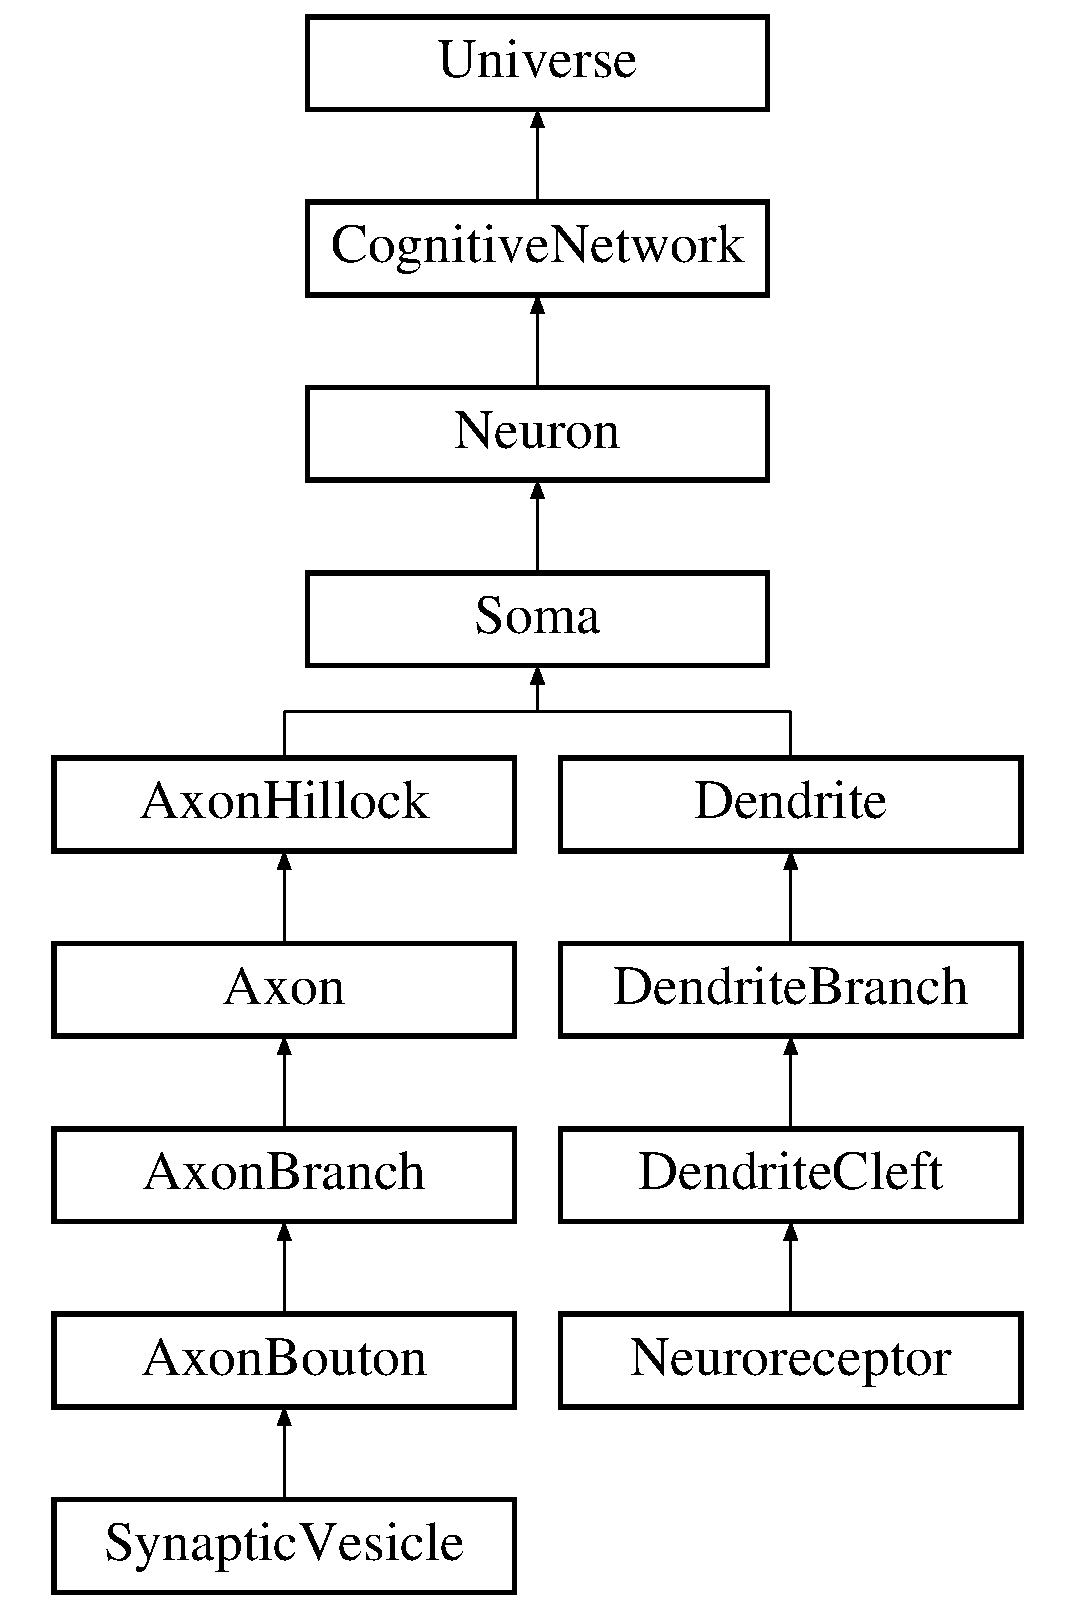
\includegraphics[height=9.000000cm]{classSoma}
\end{center}
\end{figure}
\subsection*{Classes}
\begin{DoxyCompactItemize}
\item 
struct \mbox{\hyperlink{structSoma_1_1ObjectConnection}{Object\+Connection}}
\end{DoxyCompactItemize}
\subsection*{Public Member Functions}
\begin{DoxyCompactItemize}
\item 
\mbox{\hyperlink{classSoma_abb9524743f65717d33797b45bff42441}{Soma}} ()
\item 
\mbox{\hyperlink{classSoma_a5c0fb24d35ef360cdb830887952f44e5}{Soma}} (unsigned int object\+\_\+type)
\item 
\mbox{\hyperlink{classSoma_a9c9388e5b6562c39689768856d59ca51}{Soma}} (unsigned int object\+\_\+type, std\+::chrono\+::time\+\_\+point$<$ \mbox{\hyperlink{universe_8h_a0ef8d951d1ca5ab3cfaf7ab4c7a6fd80}{Clock}} $>$ event\+\_\+time)
\item 
\mbox{\hyperlink{classSoma_a451e3918aa5f3ec5670fa08d4d710dd6}{Soma}} (unsigned int object\+\_\+type, std\+::chrono\+::time\+\_\+point$<$ \mbox{\hyperlink{universe_8h_a0ef8d951d1ca5ab3cfaf7ab4c7a6fd80}{Clock}} $>$ event\+\_\+time, \mbox{\hyperlink{classNeuron}{Neuron}} \&neuron\+\_\+connector)
\item 
virtual \mbox{\hyperlink{classSoma_a482570e6b3e366db93396add6ba1922d}{$\sim$\+Soma}} ()
\item 
double \mbox{\hyperlink{classSoma_a926552007228732d39525ce127ee5a0d}{Time\+Function}} (double time\+Delay, double time\+Dilation)
\item 
unsigned int \mbox{\hyperlink{classSoma_a8bac091792e1ac47655bb549510e8960}{Get\+Counter}} (std\+::chrono\+::time\+\_\+point$<$ \mbox{\hyperlink{universe_8h_a0ef8d951d1ca5ab3cfaf7ab4c7a6fd80}{Clock}} $>$ event\+\_\+time)
\item 
double \mbox{\hyperlink{classSoma_a91dca73d2f5f97247cae0217a8c1440a}{Get\+Energy}} (std\+::chrono\+::time\+\_\+point$<$ \mbox{\hyperlink{universe_8h_a0ef8d951d1ca5ab3cfaf7ab4c7a6fd80}{Clock}} $>$ event\+\_\+time)
\item 
double \mbox{\hyperlink{classSoma_a5d698a7ad270ad4ea63a3de5f25fa760}{Get\+Energy\+Inc}} (std\+::chrono\+::time\+\_\+point$<$ \mbox{\hyperlink{universe_8h_a0ef8d951d1ca5ab3cfaf7ab4c7a6fd80}{Clock}} $>$ event\+\_\+time)
\item 
double \mbox{\hyperlink{classSoma_afbdc1f4e4f54adefea9a16fdca50aab5}{Get\+Energy\+Dec}} (std\+::chrono\+::time\+\_\+point$<$ \mbox{\hyperlink{universe_8h_a0ef8d951d1ca5ab3cfaf7ab4c7a6fd80}{Clock}} $>$ event\+\_\+time)
\item 
double \mbox{\hyperlink{classSoma_a0be69cd912f978f3ab3d94bebb9fbbaf}{Get\+Energy\+Leak}} (std\+::chrono\+::time\+\_\+point$<$ \mbox{\hyperlink{universe_8h_a0ef8d951d1ca5ab3cfaf7ab4c7a6fd80}{Clock}} $>$ event\+\_\+time)
\item 
double \mbox{\hyperlink{classSoma_a0b45cc454565027bb25daa1396056a7e}{Get\+Energy\+Threshold}} (std\+::chrono\+::time\+\_\+point$<$ \mbox{\hyperlink{universe_8h_a0ef8d951d1ca5ab3cfaf7ab4c7a6fd80}{Clock}} $>$ event\+\_\+time)
\item 
int \mbox{\hyperlink{classSoma_a23dc309849522d9f857fdcc71ea85877}{Get\+Axon\+Hillock\+Pool}} (std\+::chrono\+::time\+\_\+point$<$ \mbox{\hyperlink{universe_8h_a0ef8d951d1ca5ab3cfaf7ab4c7a6fd80}{Clock}} $>$ event\+\_\+time)
\item 
void \mbox{\hyperlink{classSoma_a67cdb8d00b7130b44d4ac75468f4b385}{Set\+Axon\+Hillock\+Pool}} (std\+::chrono\+::time\+\_\+point$<$ \mbox{\hyperlink{universe_8h_a0ef8d951d1ca5ab3cfaf7ab4c7a6fd80}{Clock}} $>$ event\+\_\+time, int set\+\_\+pool)
\item 
int \mbox{\hyperlink{classSoma_a000d9eca00c61af853fd81a2c1569b0e}{Get\+Dendrite\+Pool}} (std\+::chrono\+::time\+\_\+point$<$ \mbox{\hyperlink{universe_8h_a0ef8d951d1ca5ab3cfaf7ab4c7a6fd80}{Clock}} $>$ event\+\_\+time)
\item 
void \mbox{\hyperlink{classSoma_a08260f4dfa8f736611fb924cfd03c4ec}{Set\+Dendrite\+Pool}} (std\+::chrono\+::time\+\_\+point$<$ \mbox{\hyperlink{universe_8h_a0ef8d951d1ca5ab3cfaf7ab4c7a6fd80}{Clock}} $>$ event\+\_\+time, int set\+\_\+pool)
\item 
void \mbox{\hyperlink{classSoma_a9ef49d3fea8c0fbe6513f3910339f736}{Set\+Counter}} (std\+::chrono\+::time\+\_\+point$<$ \mbox{\hyperlink{universe_8h_a0ef8d951d1ca5ab3cfaf7ab4c7a6fd80}{Clock}} $>$ event\+\_\+time, unsigned int val)
\item 
void \mbox{\hyperlink{classSoma_a0d1c0271fc8eeacd6e8836f751dff331}{Set\+Energy}} (std\+::chrono\+::time\+\_\+point$<$ \mbox{\hyperlink{universe_8h_a0ef8d951d1ca5ab3cfaf7ab4c7a6fd80}{Clock}} $>$ event\+\_\+time, double val)
\item 
void \mbox{\hyperlink{classSoma_a414afd7eb780e29a432603198a9838ed}{Set\+Energy\+Inc}} (std\+::chrono\+::time\+\_\+point$<$ \mbox{\hyperlink{universe_8h_a0ef8d951d1ca5ab3cfaf7ab4c7a6fd80}{Clock}} $>$ event\+\_\+time, double val)
\item 
void \mbox{\hyperlink{classSoma_a37081f7a8fc7832f8e89629221ddb8a6}{Set\+Energy\+Dec}} (std\+::chrono\+::time\+\_\+point$<$ \mbox{\hyperlink{universe_8h_a0ef8d951d1ca5ab3cfaf7ab4c7a6fd80}{Clock}} $>$ event\+\_\+time, double val)
\item 
void \mbox{\hyperlink{classSoma_abca59a00940ca2d9c005a84b6785c12f}{Set\+Energy\+Leak}} (std\+::chrono\+::time\+\_\+point$<$ \mbox{\hyperlink{universe_8h_a0ef8d951d1ca5ab3cfaf7ab4c7a6fd80}{Clock}} $>$ event\+\_\+time, double val)
\item 
void \mbox{\hyperlink{classSoma_ae2876b37909f37e8922ce364eb06491f}{Set\+Energy\+Threshold}} (std\+::chrono\+::time\+\_\+point$<$ \mbox{\hyperlink{universe_8h_a0ef8d951d1ca5ab3cfaf7ab4c7a6fd80}{Clock}} $>$ event\+\_\+time, double val)
\item 
void \mbox{\hyperlink{classSoma_a85b4708eb51ab0962a6128b87aff0700}{Set\+Object\+Type}} (std\+::chrono\+::time\+\_\+point$<$ \mbox{\hyperlink{universe_8h_a0ef8d951d1ca5ab3cfaf7ab4c7a6fd80}{Clock}} $>$ event\+\_\+time, int object\+\_\+type)
\item 
bool \mbox{\hyperlink{classSoma_a82f016dc126f7d1053e5eb455d28c44b}{Reset\+Parameters}} (std\+::chrono\+::time\+\_\+point$<$ \mbox{\hyperlink{universe_8h_a0ef8d951d1ca5ab3cfaf7ab4c7a6fd80}{Clock}} $>$ event\+\_\+time)
\item 
\mbox{\hyperlink{classSoma}{Soma}} $\ast$ \mbox{\hyperlink{classSoma_a42289635de3cb326bceeb5358b99c190}{Create\+Axon\+Hillock}} (std\+::chrono\+::time\+\_\+point$<$ \mbox{\hyperlink{universe_8h_a0ef8d951d1ca5ab3cfaf7ab4c7a6fd80}{Clock}} $>$ event\+\_\+time)
\item 
std\+::vector$<$ \mbox{\hyperlink{classSoma}{Soma}} $\ast$ $>$ \mbox{\hyperlink{classSoma_ab059a6d4a7dc41664d6d17794d09b260}{Create\+Axon\+Hillocks}} (std\+::chrono\+::time\+\_\+point$<$ \mbox{\hyperlink{universe_8h_a0ef8d951d1ca5ab3cfaf7ab4c7a6fd80}{Clock}} $>$ event\+\_\+time, int quantity)
\item 
\mbox{\hyperlink{classSoma}{Soma}} $\ast$ \mbox{\hyperlink{classSoma_a31463fba2f535e9c7cb05c8622fe3562}{Clone\+Axon\+Hillock}} (std\+::chrono\+::time\+\_\+point$<$ \mbox{\hyperlink{universe_8h_a0ef8d951d1ca5ab3cfaf7ab4c7a6fd80}{Clock}} $>$ event\+\_\+time, \mbox{\hyperlink{classSoma}{Soma}} $\ast$clone\+\_\+object, double perfection\+\_\+membership)
\item 
std\+::vector$<$ \mbox{\hyperlink{classSoma}{Soma}} $\ast$ $>$ \mbox{\hyperlink{classSoma_a299c95b89f50576244d1e56f531a80be}{Clone\+Axon\+Hillocks}} (std\+::chrono\+::time\+\_\+point$<$ \mbox{\hyperlink{universe_8h_a0ef8d951d1ca5ab3cfaf7ab4c7a6fd80}{Clock}} $>$ event\+\_\+time, std\+::vector$<$ \mbox{\hyperlink{classSoma}{Soma}} $\ast$$>$ cloning\+\_\+list, double perfection\+\_\+membership)
\item 
\mbox{\hyperlink{classSoma}{Soma}} $\ast$ \mbox{\hyperlink{classSoma_af6d6d3e3c94f06682cf05a7a72032a46}{Destroy\+Axon\+Hillock}} (std\+::chrono\+::time\+\_\+point$<$ \mbox{\hyperlink{universe_8h_a0ef8d951d1ca5ab3cfaf7ab4c7a6fd80}{Clock}} $>$ event\+\_\+time, \mbox{\hyperlink{classSoma}{Soma}} $\ast$destroy\+\_\+object)
\item 
std\+::vector$<$ \mbox{\hyperlink{classSoma}{Soma}} $\ast$ $>$ \mbox{\hyperlink{classSoma_a5220929442601962af1a1fad66a8c919}{Destroy\+Axon\+Hillocks}} (std\+::chrono\+::time\+\_\+point$<$ \mbox{\hyperlink{universe_8h_a0ef8d951d1ca5ab3cfaf7ab4c7a6fd80}{Clock}} $>$ event\+\_\+time, std\+::vector$<$ \mbox{\hyperlink{classSoma}{Soma}} $\ast$$>$ destruction\+\_\+list)
\item 
\mbox{\hyperlink{classSoma}{Soma}} $\ast$ \mbox{\hyperlink{classSoma_a02e0e4656099531b35ab56ad1f7c945a}{Add\+Axon\+Hillock}} (std\+::chrono\+::time\+\_\+point$<$ \mbox{\hyperlink{universe_8h_a0ef8d951d1ca5ab3cfaf7ab4c7a6fd80}{Clock}} $>$ event\+\_\+time, \mbox{\hyperlink{classSoma}{Soma}} $\ast$add\+\_\+object)
\item 
std\+::vector$<$ \mbox{\hyperlink{classSoma}{Soma}} $\ast$ $>$ \mbox{\hyperlink{classSoma_a0fbede6e06b8e24a2cf22878c2f49165}{Add\+Axon\+Hillocks}} (std\+::chrono\+::time\+\_\+point$<$ \mbox{\hyperlink{universe_8h_a0ef8d951d1ca5ab3cfaf7ab4c7a6fd80}{Clock}} $>$ event\+\_\+time, std\+::vector$<$ \mbox{\hyperlink{classSoma}{Soma}} $\ast$$>$ add\+\_\+objects)
\item 
\mbox{\hyperlink{classSoma}{Soma}} $\ast$ \mbox{\hyperlink{classSoma_a2f75c0f716fa1f74f70697db9dfcd562}{Remove\+Axon\+Hillock}} (std\+::chrono\+::time\+\_\+point$<$ \mbox{\hyperlink{universe_8h_a0ef8d951d1ca5ab3cfaf7ab4c7a6fd80}{Clock}} $>$ event\+\_\+time)
\item 
std\+::vector$<$ \mbox{\hyperlink{classSoma}{Soma}} $\ast$ $>$ \mbox{\hyperlink{classSoma_a7281585d74015a2549a19df6cb16e3fb}{Remove\+Axon\+Hillocks}} (std\+::chrono\+::time\+\_\+point$<$ \mbox{\hyperlink{universe_8h_a0ef8d951d1ca5ab3cfaf7ab4c7a6fd80}{Clock}} $>$ event\+\_\+time, int quantity)
\item 
\mbox{\hyperlink{classSoma}{Soma}} $\ast$ \mbox{\hyperlink{classSoma_ac8756f68dbaac8c70cfba435f7068a85}{Get\+Axon\+Hillock}} (std\+::chrono\+::time\+\_\+point$<$ \mbox{\hyperlink{universe_8h_a0ef8d951d1ca5ab3cfaf7ab4c7a6fd80}{Clock}} $>$ event\+\_\+time, int selector)
\item 
std\+::vector$<$ \mbox{\hyperlink{classSoma}{Soma}} $\ast$ $>$ \mbox{\hyperlink{classSoma_af76f86d082c3f60442148ec843b586e7}{Get\+Axon\+Hillocks}} (std\+::chrono\+::time\+\_\+point$<$ \mbox{\hyperlink{universe_8h_a0ef8d951d1ca5ab3cfaf7ab4c7a6fd80}{Clock}} $>$ event\+\_\+time)
\item 
\mbox{\hyperlink{classSoma}{Soma}} $\ast$ \mbox{\hyperlink{classSoma_a0fab0c7cf54c2b7d36e90edcd3e21a16}{Create\+Dendrite}} (std\+::chrono\+::time\+\_\+point$<$ \mbox{\hyperlink{universe_8h_a0ef8d951d1ca5ab3cfaf7ab4c7a6fd80}{Clock}} $>$ event\+\_\+time)
\item 
std\+::vector$<$ \mbox{\hyperlink{classSoma}{Soma}} $\ast$ $>$ \mbox{\hyperlink{classSoma_a68dc02eff2912ad045900ab1879f020e}{Create\+Dendrites}} (std\+::chrono\+::time\+\_\+point$<$ \mbox{\hyperlink{universe_8h_a0ef8d951d1ca5ab3cfaf7ab4c7a6fd80}{Clock}} $>$ event\+\_\+time, int quantity)
\item 
\mbox{\hyperlink{classSoma}{Soma}} $\ast$ \mbox{\hyperlink{classSoma_ad51c97b76dd7a1f77dc987ae33fd89bc}{Clone\+Dendrite}} (std\+::chrono\+::time\+\_\+point$<$ \mbox{\hyperlink{universe_8h_a0ef8d951d1ca5ab3cfaf7ab4c7a6fd80}{Clock}} $>$ event\+\_\+time, \mbox{\hyperlink{classSoma}{Soma}} $\ast$clone\+\_\+object, double perfection\+\_\+membership)
\item 
std\+::vector$<$ \mbox{\hyperlink{classSoma}{Soma}} $\ast$ $>$ \mbox{\hyperlink{classSoma_a3975212d2e3d8675ca14fbc9879e5e54}{Clone\+Dendrites}} (std\+::chrono\+::time\+\_\+point$<$ \mbox{\hyperlink{universe_8h_a0ef8d951d1ca5ab3cfaf7ab4c7a6fd80}{Clock}} $>$ event\+\_\+time, std\+::vector$<$ \mbox{\hyperlink{classSoma}{Soma}} $\ast$$>$ cloning\+\_\+list, double perfection\+\_\+membership)
\item 
\mbox{\hyperlink{classSoma}{Soma}} $\ast$ \mbox{\hyperlink{classSoma_a086cb5a05e82f6f58ac0bd8403e25e07}{Destroy\+Dendrite}} (std\+::chrono\+::time\+\_\+point$<$ \mbox{\hyperlink{universe_8h_a0ef8d951d1ca5ab3cfaf7ab4c7a6fd80}{Clock}} $>$ event\+\_\+time, \mbox{\hyperlink{classSoma}{Soma}} $\ast$destroy\+\_\+object)
\item 
std\+::vector$<$ \mbox{\hyperlink{classSoma}{Soma}} $\ast$ $>$ \mbox{\hyperlink{classSoma_ac549a7caf885fdc0ac3a6adf393430af}{Destroy\+Dendrites}} (std\+::chrono\+::time\+\_\+point$<$ \mbox{\hyperlink{universe_8h_a0ef8d951d1ca5ab3cfaf7ab4c7a6fd80}{Clock}} $>$ event\+\_\+time, std\+::vector$<$ \mbox{\hyperlink{classSoma}{Soma}} $\ast$$>$ destruction\+\_\+list)
\item 
\mbox{\hyperlink{classSoma}{Soma}} $\ast$ \mbox{\hyperlink{classSoma_acc198b8ec11c3f2e43d3ba9a16ce84db}{Add\+Dendrite}} (std\+::chrono\+::time\+\_\+point$<$ \mbox{\hyperlink{universe_8h_a0ef8d951d1ca5ab3cfaf7ab4c7a6fd80}{Clock}} $>$ event\+\_\+time, \mbox{\hyperlink{classSoma}{Soma}} $\ast$add\+\_\+object)
\item 
std\+::vector$<$ \mbox{\hyperlink{classSoma}{Soma}} $\ast$ $>$ \mbox{\hyperlink{classSoma_a9874f03b33413b06ca74a3143cc35331}{Add\+Dendrites}} (std\+::chrono\+::time\+\_\+point$<$ \mbox{\hyperlink{universe_8h_a0ef8d951d1ca5ab3cfaf7ab4c7a6fd80}{Clock}} $>$ event\+\_\+time, std\+::vector$<$ \mbox{\hyperlink{classSoma}{Soma}} $\ast$$>$ add\+\_\+objects)
\item 
\mbox{\hyperlink{classSoma}{Soma}} $\ast$ \mbox{\hyperlink{classSoma_a85c7d4b41486182c9528f5c43beaf7fd}{Remove\+Dendrite}} (std\+::chrono\+::time\+\_\+point$<$ \mbox{\hyperlink{universe_8h_a0ef8d951d1ca5ab3cfaf7ab4c7a6fd80}{Clock}} $>$ event\+\_\+time)
\item 
std\+::vector$<$ \mbox{\hyperlink{classSoma}{Soma}} $\ast$ $>$ \mbox{\hyperlink{classSoma_ad15baed4b2f5dab6f93e5df8fd1f7b23}{Remove\+Dendrites}} (std\+::chrono\+::time\+\_\+point$<$ \mbox{\hyperlink{universe_8h_a0ef8d951d1ca5ab3cfaf7ab4c7a6fd80}{Clock}} $>$ event\+\_\+time, int quantity)
\item 
\mbox{\hyperlink{classSoma}{Soma}} $\ast$ \mbox{\hyperlink{classSoma_ab86537170d550cda0e7da080f7640f84}{Get\+Dendrite}} (std\+::chrono\+::time\+\_\+point$<$ \mbox{\hyperlink{universe_8h_a0ef8d951d1ca5ab3cfaf7ab4c7a6fd80}{Clock}} $>$ event\+\_\+time, int selector)
\item 
std\+::vector$<$ \mbox{\hyperlink{classSoma}{Soma}} $\ast$ $>$ \mbox{\hyperlink{classSoma_afdb0e40855f31f2d9a48f3b13c01b599}{Get\+Dendrites}} (std\+::chrono\+::time\+\_\+point$<$ \mbox{\hyperlink{universe_8h_a0ef8d951d1ca5ab3cfaf7ab4c7a6fd80}{Clock}} $>$ event\+\_\+time)
\item 
int \mbox{\hyperlink{classSoma_aa6162ca8a98a14cf49ba8310db129d47}{Growth}} (std\+::chrono\+::time\+\_\+point$<$ \mbox{\hyperlink{universe_8h_a0ef8d951d1ca5ab3cfaf7ab4c7a6fd80}{Clock}} $>$ event\+\_\+time)
\item 
int \mbox{\hyperlink{classSoma_a211587ef21a7932c2f8f0345b1d32f57}{Update}} (std\+::chrono\+::time\+\_\+point$<$ \mbox{\hyperlink{universe_8h_a0ef8d951d1ca5ab3cfaf7ab4c7a6fd80}{Clock}} $>$ event\+\_\+time)
\end{DoxyCompactItemize}
\subsection*{Protected Attributes}
\begin{DoxyCompactItemize}
\item 
std\+::vector$<$ \mbox{\hyperlink{classSoma}{Soma}} $\ast$ $>$ \mbox{\hyperlink{classSoma_af93902336cddb974b282aef8b7b4243c}{axonhillock\+\_\+list}}
\item 
std\+::vector$<$ \mbox{\hyperlink{classSoma}{Soma}} $\ast$ $>$ \mbox{\hyperlink{classSoma_ab2d13b0adf2d10c242df0b8e62bcc01a}{dendrite\+\_\+list}}
\item 
std\+::vector$<$ \mbox{\hyperlink{structSoma_1_1ObjectConnection}{Object\+Connection}} $>$ \mbox{\hyperlink{classSoma_a84739acd533862b115bd5cbe56da6c98}{object\+\_\+connection\+\_\+list}}
\end{DoxyCompactItemize}
\subsection*{Private Attributes}
\begin{DoxyCompactItemize}
\item 
\mbox{\hyperlink{classNeuron}{Neuron}} $\ast$ \mbox{\hyperlink{classSoma_a02223dabe7a45cebcdb79b6eb159d2a9}{parent\+\_\+pointer}}
\item 
int \mbox{\hyperlink{classSoma_aba619b25aef756c8361d0444efb31cf3}{m\+\_\+\+Neuron\+Type}}
\item 
int \mbox{\hyperlink{classSoma_ada423d58bc25a27df2a68adffb13718b}{soma\+\_\+type}}
\item 
int \mbox{\hyperlink{classSoma_ab9887343fb7e5575677e7a526d7e7a69}{m\+\_\+add\+Status}}
\item 
std\+::chrono\+::time\+\_\+point$<$ \mbox{\hyperlink{universe_8h_a0ef8d951d1ca5ab3cfaf7ab4c7a6fd80}{Clock}} $>$ \mbox{\hyperlink{classSoma_ac0e5b4b952e136b8a6c4c69f607ce4da}{time\+\_\+object\+\_\+created}}
\item 
std\+::chrono\+::time\+\_\+point$<$ \mbox{\hyperlink{universe_8h_a0ef8d951d1ca5ab3cfaf7ab4c7a6fd80}{Clock}} $>$ \mbox{\hyperlink{classSoma_ab6204961b77d4224199eec0b105e41dd}{previous\+\_\+event\+\_\+time}}
\item 
bool \mbox{\hyperlink{classSoma_af2b64c3b8490b302fcdd6461034271c0}{object\+\_\+disabled}} = true
\item 
bool \mbox{\hyperlink{classSoma_ab85b5a30283f03bb8ff202704bec08fe}{object\+\_\+initialised}} = false
\item 
int \mbox{\hyperlink{classSoma_ab5ada1db9da44a5aac9a7b40364fc1b8}{duration\+\_\+since\+\_\+last\+\_\+event}}
\item 
double \mbox{\hyperlink{classSoma_aa5c0b1a0db07052b76d2ccf4e7ef3e83}{m\+\_\+\+Volume}}
\item 
double \mbox{\hyperlink{classSoma_a66bfc792729e6f5d3827d57f2cf3780c}{m\+\_\+\+Surface\+Area}}
\item 
double \mbox{\hyperlink{classSoma_a803536eba7a6aecd3716cbdd32659fc4}{object\+\_\+size}}
\item 
unsigned int \mbox{\hyperlink{classSoma_a11f3e7371be45ce6d7a55eb19e98b006}{m\+\_\+\+Counter}}
\begin{DoxyCompactList}\small\item\em Member variable \char`\"{}m\+\_\+\+Counter\char`\"{}. \end{DoxyCompactList}\item 
double \mbox{\hyperlink{classSoma_ac476da0d76368316b374839f60387176}{object\+\_\+energy}}
\begin{DoxyCompactList}\small\item\em Member variable \char`\"{}object\+\_\+energy\char`\"{}. \end{DoxyCompactList}\item 
double \mbox{\hyperlink{classSoma_aa290cae75c0a834fbfe2556ed359a135}{object\+\_\+energy\+Inc}}
\item 
double \mbox{\hyperlink{classSoma_a49345275d3d890f9d3c44e09de5b3c8c}{object\+\_\+energy\+Dec}}
\item 
double \mbox{\hyperlink{classSoma_a7f8941a98528311a249f13ea73f14e3b}{object\+\_\+energy\+Leak}}
\item 
double \mbox{\hyperlink{classSoma_a4a9bab479f79acb47d57b7fb3730fd7d}{object\+\_\+energy\+\_\+threshold}}
\item 
double \mbox{\hyperlink{classSoma_a170d85686c1a30d045c2966df962ba3e}{m\+\_\+\+Time\+Dilation}}
\item 
double \mbox{\hyperlink{classSoma_a1884a12afbda6576f64997ca9c349579}{m\+\_\+\+Time\+Threshold}}
\item 
int \mbox{\hyperlink{classSoma_a57dca929c2579efc29ee9d96bdb1b261}{axonhillock\+\_\+pool}}
\item 
int \mbox{\hyperlink{classSoma_ab9b22d223ef063b3bafb4686893dea33}{dendrite\+\_\+pool}}
\end{DoxyCompactItemize}
\subsection*{Friends}
\begin{DoxyCompactItemize}
\item 
class \mbox{\hyperlink{classSoma_aabae1fdc220bf040d4f5c2c057abfcf5}{Dimension}}
\end{DoxyCompactItemize}
\subsection*{Additional Inherited Members}


\subsection{Constructor \& Destructor Documentation}
\mbox{\Hypertarget{classSoma_abb9524743f65717d33797b45bff42441}\label{classSoma_abb9524743f65717d33797b45bff42441}} 
\index{Soma@{Soma}!Soma@{Soma}}
\index{Soma@{Soma}!Soma@{Soma}}
\subsubsection{\texorpdfstring{Soma()}{Soma()}\hspace{0.1cm}{\footnotesize\ttfamily [1/4]}}
{\footnotesize\ttfamily Soma\+::\+Soma (\begin{DoxyParamCaption}{ }\end{DoxyParamCaption})\hspace{0.3cm}{\ttfamily [inline]}}

\mbox{\Hypertarget{classSoma_a5c0fb24d35ef360cdb830887952f44e5}\label{classSoma_a5c0fb24d35ef360cdb830887952f44e5}} 
\index{Soma@{Soma}!Soma@{Soma}}
\index{Soma@{Soma}!Soma@{Soma}}
\subsubsection{\texorpdfstring{Soma()}{Soma()}\hspace{0.1cm}{\footnotesize\ttfamily [2/4]}}
{\footnotesize\ttfamily Soma\+::\+Soma (\begin{DoxyParamCaption}\item[{unsigned int}]{object\+\_\+type }\end{DoxyParamCaption})\hspace{0.3cm}{\ttfamily [inline]}}

\mbox{\Hypertarget{classSoma_a9c9388e5b6562c39689768856d59ca51}\label{classSoma_a9c9388e5b6562c39689768856d59ca51}} 
\index{Soma@{Soma}!Soma@{Soma}}
\index{Soma@{Soma}!Soma@{Soma}}
\subsubsection{\texorpdfstring{Soma()}{Soma()}\hspace{0.1cm}{\footnotesize\ttfamily [3/4]}}
{\footnotesize\ttfamily Soma\+::\+Soma (\begin{DoxyParamCaption}\item[{unsigned int}]{object\+\_\+type,  }\item[{std\+::chrono\+::time\+\_\+point$<$ \mbox{\hyperlink{universe_8h_a0ef8d951d1ca5ab3cfaf7ab4c7a6fd80}{Clock}} $>$}]{event\+\_\+time }\end{DoxyParamCaption})\hspace{0.3cm}{\ttfamily [inline]}}

\mbox{\Hypertarget{classSoma_a451e3918aa5f3ec5670fa08d4d710dd6}\label{classSoma_a451e3918aa5f3ec5670fa08d4d710dd6}} 
\index{Soma@{Soma}!Soma@{Soma}}
\index{Soma@{Soma}!Soma@{Soma}}
\subsubsection{\texorpdfstring{Soma()}{Soma()}\hspace{0.1cm}{\footnotesize\ttfamily [4/4]}}
{\footnotesize\ttfamily Soma\+::\+Soma (\begin{DoxyParamCaption}\item[{unsigned int}]{object\+\_\+type,  }\item[{std\+::chrono\+::time\+\_\+point$<$ \mbox{\hyperlink{universe_8h_a0ef8d951d1ca5ab3cfaf7ab4c7a6fd80}{Clock}} $>$}]{event\+\_\+time,  }\item[{\mbox{\hyperlink{classNeuron}{Neuron}} \&}]{neuron\+\_\+connector }\end{DoxyParamCaption})\hspace{0.3cm}{\ttfamily [inline]}}

\mbox{\Hypertarget{classSoma_a482570e6b3e366db93396add6ba1922d}\label{classSoma_a482570e6b3e366db93396add6ba1922d}} 
\index{Soma@{Soma}!````~Soma@{$\sim$\+Soma}}
\index{````~Soma@{$\sim$\+Soma}!Soma@{Soma}}
\subsubsection{\texorpdfstring{$\sim$\+Soma()}{~Soma()}}
{\footnotesize\ttfamily virtual Soma\+::$\sim$\+Soma (\begin{DoxyParamCaption}{ }\end{DoxyParamCaption})\hspace{0.3cm}{\ttfamily [inline]}, {\ttfamily [virtual]}}

Default destructor 

\subsection{Member Function Documentation}
\mbox{\Hypertarget{classSoma_a02e0e4656099531b35ab56ad1f7c945a}\label{classSoma_a02e0e4656099531b35ab56ad1f7c945a}} 
\index{Soma@{Soma}!Add\+Axon\+Hillock@{Add\+Axon\+Hillock}}
\index{Add\+Axon\+Hillock@{Add\+Axon\+Hillock}!Soma@{Soma}}
\subsubsection{\texorpdfstring{Add\+Axon\+Hillock()}{AddAxonHillock()}}
{\footnotesize\ttfamily \mbox{\hyperlink{classSoma}{Soma}} $\ast$ Soma\+::\+Add\+Axon\+Hillock (\begin{DoxyParamCaption}\item[{std\+::chrono\+::time\+\_\+point$<$ \mbox{\hyperlink{universe_8h_a0ef8d951d1ca5ab3cfaf7ab4c7a6fd80}{Clock}} $>$}]{event\+\_\+time,  }\item[{\mbox{\hyperlink{classSoma}{Soma}} $\ast$}]{add\+\_\+object }\end{DoxyParamCaption})}

\mbox{\Hypertarget{classSoma_a0fbede6e06b8e24a2cf22878c2f49165}\label{classSoma_a0fbede6e06b8e24a2cf22878c2f49165}} 
\index{Soma@{Soma}!Add\+Axon\+Hillocks@{Add\+Axon\+Hillocks}}
\index{Add\+Axon\+Hillocks@{Add\+Axon\+Hillocks}!Soma@{Soma}}
\subsubsection{\texorpdfstring{Add\+Axon\+Hillocks()}{AddAxonHillocks()}}
{\footnotesize\ttfamily std\+::vector$<$ \mbox{\hyperlink{classSoma}{Soma}} $\ast$ $>$ Soma\+::\+Add\+Axon\+Hillocks (\begin{DoxyParamCaption}\item[{std\+::chrono\+::time\+\_\+point$<$ \mbox{\hyperlink{universe_8h_a0ef8d951d1ca5ab3cfaf7ab4c7a6fd80}{Clock}} $>$}]{event\+\_\+time,  }\item[{std\+::vector$<$ \mbox{\hyperlink{classSoma}{Soma}} $\ast$$>$}]{add\+\_\+objects }\end{DoxyParamCaption})}

\mbox{\Hypertarget{classSoma_acc198b8ec11c3f2e43d3ba9a16ce84db}\label{classSoma_acc198b8ec11c3f2e43d3ba9a16ce84db}} 
\index{Soma@{Soma}!Add\+Dendrite@{Add\+Dendrite}}
\index{Add\+Dendrite@{Add\+Dendrite}!Soma@{Soma}}
\subsubsection{\texorpdfstring{Add\+Dendrite()}{AddDendrite()}}
{\footnotesize\ttfamily \mbox{\hyperlink{classSoma}{Soma}} $\ast$ Soma\+::\+Add\+Dendrite (\begin{DoxyParamCaption}\item[{std\+::chrono\+::time\+\_\+point$<$ \mbox{\hyperlink{universe_8h_a0ef8d951d1ca5ab3cfaf7ab4c7a6fd80}{Clock}} $>$}]{event\+\_\+time,  }\item[{\mbox{\hyperlink{classSoma}{Soma}} $\ast$}]{add\+\_\+object }\end{DoxyParamCaption})}

\mbox{\Hypertarget{classSoma_a9874f03b33413b06ca74a3143cc35331}\label{classSoma_a9874f03b33413b06ca74a3143cc35331}} 
\index{Soma@{Soma}!Add\+Dendrites@{Add\+Dendrites}}
\index{Add\+Dendrites@{Add\+Dendrites}!Soma@{Soma}}
\subsubsection{\texorpdfstring{Add\+Dendrites()}{AddDendrites()}}
{\footnotesize\ttfamily std\+::vector$<$ \mbox{\hyperlink{classSoma}{Soma}} $\ast$ $>$ Soma\+::\+Add\+Dendrites (\begin{DoxyParamCaption}\item[{std\+::chrono\+::time\+\_\+point$<$ \mbox{\hyperlink{universe_8h_a0ef8d951d1ca5ab3cfaf7ab4c7a6fd80}{Clock}} $>$}]{event\+\_\+time,  }\item[{std\+::vector$<$ \mbox{\hyperlink{classSoma}{Soma}} $\ast$$>$}]{add\+\_\+objects }\end{DoxyParamCaption})}

\mbox{\Hypertarget{classSoma_a31463fba2f535e9c7cb05c8622fe3562}\label{classSoma_a31463fba2f535e9c7cb05c8622fe3562}} 
\index{Soma@{Soma}!Clone\+Axon\+Hillock@{Clone\+Axon\+Hillock}}
\index{Clone\+Axon\+Hillock@{Clone\+Axon\+Hillock}!Soma@{Soma}}
\subsubsection{\texorpdfstring{Clone\+Axon\+Hillock()}{CloneAxonHillock()}}
{\footnotesize\ttfamily \mbox{\hyperlink{classSoma}{Soma}} $\ast$ Soma\+::\+Clone\+Axon\+Hillock (\begin{DoxyParamCaption}\item[{std\+::chrono\+::time\+\_\+point$<$ \mbox{\hyperlink{universe_8h_a0ef8d951d1ca5ab3cfaf7ab4c7a6fd80}{Clock}} $>$}]{event\+\_\+time,  }\item[{\mbox{\hyperlink{classSoma}{Soma}} $\ast$}]{clone\+\_\+object,  }\item[{double}]{perfection\+\_\+membership }\end{DoxyParamCaption})}

\mbox{\Hypertarget{classSoma_a299c95b89f50576244d1e56f531a80be}\label{classSoma_a299c95b89f50576244d1e56f531a80be}} 
\index{Soma@{Soma}!Clone\+Axon\+Hillocks@{Clone\+Axon\+Hillocks}}
\index{Clone\+Axon\+Hillocks@{Clone\+Axon\+Hillocks}!Soma@{Soma}}
\subsubsection{\texorpdfstring{Clone\+Axon\+Hillocks()}{CloneAxonHillocks()}}
{\footnotesize\ttfamily std\+::vector$<$ \mbox{\hyperlink{classSoma}{Soma}} $\ast$ $>$ Soma\+::\+Clone\+Axon\+Hillocks (\begin{DoxyParamCaption}\item[{std\+::chrono\+::time\+\_\+point$<$ \mbox{\hyperlink{universe_8h_a0ef8d951d1ca5ab3cfaf7ab4c7a6fd80}{Clock}} $>$}]{event\+\_\+time,  }\item[{std\+::vector$<$ \mbox{\hyperlink{classSoma}{Soma}} $\ast$$>$}]{cloning\+\_\+list,  }\item[{double}]{perfection\+\_\+membership }\end{DoxyParamCaption})}

\mbox{\Hypertarget{classSoma_ad51c97b76dd7a1f77dc987ae33fd89bc}\label{classSoma_ad51c97b76dd7a1f77dc987ae33fd89bc}} 
\index{Soma@{Soma}!Clone\+Dendrite@{Clone\+Dendrite}}
\index{Clone\+Dendrite@{Clone\+Dendrite}!Soma@{Soma}}
\subsubsection{\texorpdfstring{Clone\+Dendrite()}{CloneDendrite()}}
{\footnotesize\ttfamily \mbox{\hyperlink{classSoma}{Soma}} $\ast$ Soma\+::\+Clone\+Dendrite (\begin{DoxyParamCaption}\item[{std\+::chrono\+::time\+\_\+point$<$ \mbox{\hyperlink{universe_8h_a0ef8d951d1ca5ab3cfaf7ab4c7a6fd80}{Clock}} $>$}]{event\+\_\+time,  }\item[{\mbox{\hyperlink{classSoma}{Soma}} $\ast$}]{clone\+\_\+object,  }\item[{double}]{perfection\+\_\+membership }\end{DoxyParamCaption})}

\mbox{\Hypertarget{classSoma_a3975212d2e3d8675ca14fbc9879e5e54}\label{classSoma_a3975212d2e3d8675ca14fbc9879e5e54}} 
\index{Soma@{Soma}!Clone\+Dendrites@{Clone\+Dendrites}}
\index{Clone\+Dendrites@{Clone\+Dendrites}!Soma@{Soma}}
\subsubsection{\texorpdfstring{Clone\+Dendrites()}{CloneDendrites()}}
{\footnotesize\ttfamily std\+::vector$<$ \mbox{\hyperlink{classSoma}{Soma}} $\ast$ $>$ Soma\+::\+Clone\+Dendrites (\begin{DoxyParamCaption}\item[{std\+::chrono\+::time\+\_\+point$<$ \mbox{\hyperlink{universe_8h_a0ef8d951d1ca5ab3cfaf7ab4c7a6fd80}{Clock}} $>$}]{event\+\_\+time,  }\item[{std\+::vector$<$ \mbox{\hyperlink{classSoma}{Soma}} $\ast$$>$}]{cloning\+\_\+list,  }\item[{double}]{perfection\+\_\+membership }\end{DoxyParamCaption})}

\mbox{\Hypertarget{classSoma_a42289635de3cb326bceeb5358b99c190}\label{classSoma_a42289635de3cb326bceeb5358b99c190}} 
\index{Soma@{Soma}!Create\+Axon\+Hillock@{Create\+Axon\+Hillock}}
\index{Create\+Axon\+Hillock@{Create\+Axon\+Hillock}!Soma@{Soma}}
\subsubsection{\texorpdfstring{Create\+Axon\+Hillock()}{CreateAxonHillock()}}
{\footnotesize\ttfamily \mbox{\hyperlink{classSoma}{Soma}} $\ast$ Soma\+::\+Create\+Axon\+Hillock (\begin{DoxyParamCaption}\item[{std\+::chrono\+::time\+\_\+point$<$ \mbox{\hyperlink{universe_8h_a0ef8d951d1ca5ab3cfaf7ab4c7a6fd80}{Clock}} $>$}]{event\+\_\+time }\end{DoxyParamCaption})}

\mbox{\Hypertarget{classSoma_ab059a6d4a7dc41664d6d17794d09b260}\label{classSoma_ab059a6d4a7dc41664d6d17794d09b260}} 
\index{Soma@{Soma}!Create\+Axon\+Hillocks@{Create\+Axon\+Hillocks}}
\index{Create\+Axon\+Hillocks@{Create\+Axon\+Hillocks}!Soma@{Soma}}
\subsubsection{\texorpdfstring{Create\+Axon\+Hillocks()}{CreateAxonHillocks()}}
{\footnotesize\ttfamily std\+::vector$<$ \mbox{\hyperlink{classSoma}{Soma}} $\ast$ $>$ Soma\+::\+Create\+Axon\+Hillocks (\begin{DoxyParamCaption}\item[{std\+::chrono\+::time\+\_\+point$<$ \mbox{\hyperlink{universe_8h_a0ef8d951d1ca5ab3cfaf7ab4c7a6fd80}{Clock}} $>$}]{event\+\_\+time,  }\item[{int}]{quantity }\end{DoxyParamCaption})}

\mbox{\Hypertarget{classSoma_a0fab0c7cf54c2b7d36e90edcd3e21a16}\label{classSoma_a0fab0c7cf54c2b7d36e90edcd3e21a16}} 
\index{Soma@{Soma}!Create\+Dendrite@{Create\+Dendrite}}
\index{Create\+Dendrite@{Create\+Dendrite}!Soma@{Soma}}
\subsubsection{\texorpdfstring{Create\+Dendrite()}{CreateDendrite()}}
{\footnotesize\ttfamily \mbox{\hyperlink{classSoma}{Soma}} $\ast$ Soma\+::\+Create\+Dendrite (\begin{DoxyParamCaption}\item[{std\+::chrono\+::time\+\_\+point$<$ \mbox{\hyperlink{universe_8h_a0ef8d951d1ca5ab3cfaf7ab4c7a6fd80}{Clock}} $>$}]{event\+\_\+time }\end{DoxyParamCaption})}

\mbox{\Hypertarget{classSoma_a68dc02eff2912ad045900ab1879f020e}\label{classSoma_a68dc02eff2912ad045900ab1879f020e}} 
\index{Soma@{Soma}!Create\+Dendrites@{Create\+Dendrites}}
\index{Create\+Dendrites@{Create\+Dendrites}!Soma@{Soma}}
\subsubsection{\texorpdfstring{Create\+Dendrites()}{CreateDendrites()}}
{\footnotesize\ttfamily std\+::vector$<$ \mbox{\hyperlink{classSoma}{Soma}} $\ast$ $>$ Soma\+::\+Create\+Dendrites (\begin{DoxyParamCaption}\item[{std\+::chrono\+::time\+\_\+point$<$ \mbox{\hyperlink{universe_8h_a0ef8d951d1ca5ab3cfaf7ab4c7a6fd80}{Clock}} $>$}]{event\+\_\+time,  }\item[{int}]{quantity }\end{DoxyParamCaption})}

\mbox{\Hypertarget{classSoma_af6d6d3e3c94f06682cf05a7a72032a46}\label{classSoma_af6d6d3e3c94f06682cf05a7a72032a46}} 
\index{Soma@{Soma}!Destroy\+Axon\+Hillock@{Destroy\+Axon\+Hillock}}
\index{Destroy\+Axon\+Hillock@{Destroy\+Axon\+Hillock}!Soma@{Soma}}
\subsubsection{\texorpdfstring{Destroy\+Axon\+Hillock()}{DestroyAxonHillock()}}
{\footnotesize\ttfamily \mbox{\hyperlink{classSoma}{Soma}} $\ast$ Soma\+::\+Destroy\+Axon\+Hillock (\begin{DoxyParamCaption}\item[{std\+::chrono\+::time\+\_\+point$<$ \mbox{\hyperlink{universe_8h_a0ef8d951d1ca5ab3cfaf7ab4c7a6fd80}{Clock}} $>$}]{event\+\_\+time,  }\item[{\mbox{\hyperlink{classSoma}{Soma}} $\ast$}]{destroy\+\_\+object }\end{DoxyParamCaption})}

\mbox{\Hypertarget{classSoma_a5220929442601962af1a1fad66a8c919}\label{classSoma_a5220929442601962af1a1fad66a8c919}} 
\index{Soma@{Soma}!Destroy\+Axon\+Hillocks@{Destroy\+Axon\+Hillocks}}
\index{Destroy\+Axon\+Hillocks@{Destroy\+Axon\+Hillocks}!Soma@{Soma}}
\subsubsection{\texorpdfstring{Destroy\+Axon\+Hillocks()}{DestroyAxonHillocks()}}
{\footnotesize\ttfamily std\+::vector$<$ \mbox{\hyperlink{classSoma}{Soma}} $\ast$ $>$ Soma\+::\+Destroy\+Axon\+Hillocks (\begin{DoxyParamCaption}\item[{std\+::chrono\+::time\+\_\+point$<$ \mbox{\hyperlink{universe_8h_a0ef8d951d1ca5ab3cfaf7ab4c7a6fd80}{Clock}} $>$}]{event\+\_\+time,  }\item[{std\+::vector$<$ \mbox{\hyperlink{classSoma}{Soma}} $\ast$$>$}]{destruction\+\_\+list }\end{DoxyParamCaption})}

\mbox{\Hypertarget{classSoma_a086cb5a05e82f6f58ac0bd8403e25e07}\label{classSoma_a086cb5a05e82f6f58ac0bd8403e25e07}} 
\index{Soma@{Soma}!Destroy\+Dendrite@{Destroy\+Dendrite}}
\index{Destroy\+Dendrite@{Destroy\+Dendrite}!Soma@{Soma}}
\subsubsection{\texorpdfstring{Destroy\+Dendrite()}{DestroyDendrite()}}
{\footnotesize\ttfamily \mbox{\hyperlink{classSoma}{Soma}} $\ast$ Soma\+::\+Destroy\+Dendrite (\begin{DoxyParamCaption}\item[{std\+::chrono\+::time\+\_\+point$<$ \mbox{\hyperlink{universe_8h_a0ef8d951d1ca5ab3cfaf7ab4c7a6fd80}{Clock}} $>$}]{event\+\_\+time,  }\item[{\mbox{\hyperlink{classSoma}{Soma}} $\ast$}]{destroy\+\_\+object }\end{DoxyParamCaption})}

\mbox{\Hypertarget{classSoma_ac549a7caf885fdc0ac3a6adf393430af}\label{classSoma_ac549a7caf885fdc0ac3a6adf393430af}} 
\index{Soma@{Soma}!Destroy\+Dendrites@{Destroy\+Dendrites}}
\index{Destroy\+Dendrites@{Destroy\+Dendrites}!Soma@{Soma}}
\subsubsection{\texorpdfstring{Destroy\+Dendrites()}{DestroyDendrites()}}
{\footnotesize\ttfamily std\+::vector$<$ \mbox{\hyperlink{classSoma}{Soma}} $\ast$ $>$ Soma\+::\+Destroy\+Dendrites (\begin{DoxyParamCaption}\item[{std\+::chrono\+::time\+\_\+point$<$ \mbox{\hyperlink{universe_8h_a0ef8d951d1ca5ab3cfaf7ab4c7a6fd80}{Clock}} $>$}]{event\+\_\+time,  }\item[{std\+::vector$<$ \mbox{\hyperlink{classSoma}{Soma}} $\ast$$>$}]{destruction\+\_\+list }\end{DoxyParamCaption})}

\mbox{\Hypertarget{classSoma_ac8756f68dbaac8c70cfba435f7068a85}\label{classSoma_ac8756f68dbaac8c70cfba435f7068a85}} 
\index{Soma@{Soma}!Get\+Axon\+Hillock@{Get\+Axon\+Hillock}}
\index{Get\+Axon\+Hillock@{Get\+Axon\+Hillock}!Soma@{Soma}}
\subsubsection{\texorpdfstring{Get\+Axon\+Hillock()}{GetAxonHillock()}}
{\footnotesize\ttfamily \mbox{\hyperlink{classSoma}{Soma}} $\ast$ Soma\+::\+Get\+Axon\+Hillock (\begin{DoxyParamCaption}\item[{std\+::chrono\+::time\+\_\+point$<$ \mbox{\hyperlink{universe_8h_a0ef8d951d1ca5ab3cfaf7ab4c7a6fd80}{Clock}} $>$}]{event\+\_\+time,  }\item[{int}]{selector }\end{DoxyParamCaption})}

\mbox{\Hypertarget{classSoma_a23dc309849522d9f857fdcc71ea85877}\label{classSoma_a23dc309849522d9f857fdcc71ea85877}} 
\index{Soma@{Soma}!Get\+Axon\+Hillock\+Pool@{Get\+Axon\+Hillock\+Pool}}
\index{Get\+Axon\+Hillock\+Pool@{Get\+Axon\+Hillock\+Pool}!Soma@{Soma}}
\subsubsection{\texorpdfstring{Get\+Axon\+Hillock\+Pool()}{GetAxonHillockPool()}}
{\footnotesize\ttfamily int Soma\+::\+Get\+Axon\+Hillock\+Pool (\begin{DoxyParamCaption}\item[{std\+::chrono\+::time\+\_\+point$<$ \mbox{\hyperlink{universe_8h_a0ef8d951d1ca5ab3cfaf7ab4c7a6fd80}{Clock}} $>$}]{event\+\_\+time }\end{DoxyParamCaption})\hspace{0.3cm}{\ttfamily [inline]}}

\mbox{\Hypertarget{classSoma_af76f86d082c3f60442148ec843b586e7}\label{classSoma_af76f86d082c3f60442148ec843b586e7}} 
\index{Soma@{Soma}!Get\+Axon\+Hillocks@{Get\+Axon\+Hillocks}}
\index{Get\+Axon\+Hillocks@{Get\+Axon\+Hillocks}!Soma@{Soma}}
\subsubsection{\texorpdfstring{Get\+Axon\+Hillocks()}{GetAxonHillocks()}}
{\footnotesize\ttfamily std\+::vector$<$ \mbox{\hyperlink{classSoma}{Soma}} $\ast$ $>$ Soma\+::\+Get\+Axon\+Hillocks (\begin{DoxyParamCaption}\item[{std\+::chrono\+::time\+\_\+point$<$ \mbox{\hyperlink{universe_8h_a0ef8d951d1ca5ab3cfaf7ab4c7a6fd80}{Clock}} $>$}]{event\+\_\+time }\end{DoxyParamCaption})}

\mbox{\Hypertarget{classSoma_a8bac091792e1ac47655bb549510e8960}\label{classSoma_a8bac091792e1ac47655bb549510e8960}} 
\index{Soma@{Soma}!Get\+Counter@{Get\+Counter}}
\index{Get\+Counter@{Get\+Counter}!Soma@{Soma}}
\subsubsection{\texorpdfstring{Get\+Counter()}{GetCounter()}}
{\footnotesize\ttfamily unsigned int Soma\+::\+Get\+Counter (\begin{DoxyParamCaption}\item[{std\+::chrono\+::time\+\_\+point$<$ \mbox{\hyperlink{universe_8h_a0ef8d951d1ca5ab3cfaf7ab4c7a6fd80}{Clock}} $>$}]{event\+\_\+time }\end{DoxyParamCaption})\hspace{0.3cm}{\ttfamily [inline]}}

\mbox{\Hypertarget{classSoma_ab86537170d550cda0e7da080f7640f84}\label{classSoma_ab86537170d550cda0e7da080f7640f84}} 
\index{Soma@{Soma}!Get\+Dendrite@{Get\+Dendrite}}
\index{Get\+Dendrite@{Get\+Dendrite}!Soma@{Soma}}
\subsubsection{\texorpdfstring{Get\+Dendrite()}{GetDendrite()}}
{\footnotesize\ttfamily \mbox{\hyperlink{classSoma}{Soma}} $\ast$ Soma\+::\+Get\+Dendrite (\begin{DoxyParamCaption}\item[{std\+::chrono\+::time\+\_\+point$<$ \mbox{\hyperlink{universe_8h_a0ef8d951d1ca5ab3cfaf7ab4c7a6fd80}{Clock}} $>$}]{event\+\_\+time,  }\item[{int}]{selector }\end{DoxyParamCaption})}

\mbox{\Hypertarget{classSoma_a000d9eca00c61af853fd81a2c1569b0e}\label{classSoma_a000d9eca00c61af853fd81a2c1569b0e}} 
\index{Soma@{Soma}!Get\+Dendrite\+Pool@{Get\+Dendrite\+Pool}}
\index{Get\+Dendrite\+Pool@{Get\+Dendrite\+Pool}!Soma@{Soma}}
\subsubsection{\texorpdfstring{Get\+Dendrite\+Pool()}{GetDendritePool()}}
{\footnotesize\ttfamily int Soma\+::\+Get\+Dendrite\+Pool (\begin{DoxyParamCaption}\item[{std\+::chrono\+::time\+\_\+point$<$ \mbox{\hyperlink{universe_8h_a0ef8d951d1ca5ab3cfaf7ab4c7a6fd80}{Clock}} $>$}]{event\+\_\+time }\end{DoxyParamCaption})\hspace{0.3cm}{\ttfamily [inline]}}

\mbox{\Hypertarget{classSoma_afdb0e40855f31f2d9a48f3b13c01b599}\label{classSoma_afdb0e40855f31f2d9a48f3b13c01b599}} 
\index{Soma@{Soma}!Get\+Dendrites@{Get\+Dendrites}}
\index{Get\+Dendrites@{Get\+Dendrites}!Soma@{Soma}}
\subsubsection{\texorpdfstring{Get\+Dendrites()}{GetDendrites()}}
{\footnotesize\ttfamily std\+::vector$<$ \mbox{\hyperlink{classSoma}{Soma}} $\ast$ $>$ Soma\+::\+Get\+Dendrites (\begin{DoxyParamCaption}\item[{std\+::chrono\+::time\+\_\+point$<$ \mbox{\hyperlink{universe_8h_a0ef8d951d1ca5ab3cfaf7ab4c7a6fd80}{Clock}} $>$}]{event\+\_\+time }\end{DoxyParamCaption})}

\mbox{\Hypertarget{classSoma_a91dca73d2f5f97247cae0217a8c1440a}\label{classSoma_a91dca73d2f5f97247cae0217a8c1440a}} 
\index{Soma@{Soma}!Get\+Energy@{Get\+Energy}}
\index{Get\+Energy@{Get\+Energy}!Soma@{Soma}}
\subsubsection{\texorpdfstring{Get\+Energy()}{GetEnergy()}}
{\footnotesize\ttfamily double Soma\+::\+Get\+Energy (\begin{DoxyParamCaption}\item[{std\+::chrono\+::time\+\_\+point$<$ \mbox{\hyperlink{universe_8h_a0ef8d951d1ca5ab3cfaf7ab4c7a6fd80}{Clock}} $>$}]{event\+\_\+time }\end{DoxyParamCaption})\hspace{0.3cm}{\ttfamily [inline]}}

\mbox{\Hypertarget{classSoma_afbdc1f4e4f54adefea9a16fdca50aab5}\label{classSoma_afbdc1f4e4f54adefea9a16fdca50aab5}} 
\index{Soma@{Soma}!Get\+Energy\+Dec@{Get\+Energy\+Dec}}
\index{Get\+Energy\+Dec@{Get\+Energy\+Dec}!Soma@{Soma}}
\subsubsection{\texorpdfstring{Get\+Energy\+Dec()}{GetEnergyDec()}}
{\footnotesize\ttfamily double Soma\+::\+Get\+Energy\+Dec (\begin{DoxyParamCaption}\item[{std\+::chrono\+::time\+\_\+point$<$ \mbox{\hyperlink{universe_8h_a0ef8d951d1ca5ab3cfaf7ab4c7a6fd80}{Clock}} $>$}]{event\+\_\+time }\end{DoxyParamCaption})\hspace{0.3cm}{\ttfamily [inline]}}

\mbox{\Hypertarget{classSoma_a5d698a7ad270ad4ea63a3de5f25fa760}\label{classSoma_a5d698a7ad270ad4ea63a3de5f25fa760}} 
\index{Soma@{Soma}!Get\+Energy\+Inc@{Get\+Energy\+Inc}}
\index{Get\+Energy\+Inc@{Get\+Energy\+Inc}!Soma@{Soma}}
\subsubsection{\texorpdfstring{Get\+Energy\+Inc()}{GetEnergyInc()}}
{\footnotesize\ttfamily double Soma\+::\+Get\+Energy\+Inc (\begin{DoxyParamCaption}\item[{std\+::chrono\+::time\+\_\+point$<$ \mbox{\hyperlink{universe_8h_a0ef8d951d1ca5ab3cfaf7ab4c7a6fd80}{Clock}} $>$}]{event\+\_\+time }\end{DoxyParamCaption})\hspace{0.3cm}{\ttfamily [inline]}}

\mbox{\Hypertarget{classSoma_a0be69cd912f978f3ab3d94bebb9fbbaf}\label{classSoma_a0be69cd912f978f3ab3d94bebb9fbbaf}} 
\index{Soma@{Soma}!Get\+Energy\+Leak@{Get\+Energy\+Leak}}
\index{Get\+Energy\+Leak@{Get\+Energy\+Leak}!Soma@{Soma}}
\subsubsection{\texorpdfstring{Get\+Energy\+Leak()}{GetEnergyLeak()}}
{\footnotesize\ttfamily double Soma\+::\+Get\+Energy\+Leak (\begin{DoxyParamCaption}\item[{std\+::chrono\+::time\+\_\+point$<$ \mbox{\hyperlink{universe_8h_a0ef8d951d1ca5ab3cfaf7ab4c7a6fd80}{Clock}} $>$}]{event\+\_\+time }\end{DoxyParamCaption})\hspace{0.3cm}{\ttfamily [inline]}}

\mbox{\Hypertarget{classSoma_a0b45cc454565027bb25daa1396056a7e}\label{classSoma_a0b45cc454565027bb25daa1396056a7e}} 
\index{Soma@{Soma}!Get\+Energy\+Threshold@{Get\+Energy\+Threshold}}
\index{Get\+Energy\+Threshold@{Get\+Energy\+Threshold}!Soma@{Soma}}
\subsubsection{\texorpdfstring{Get\+Energy\+Threshold()}{GetEnergyThreshold()}}
{\footnotesize\ttfamily double Soma\+::\+Get\+Energy\+Threshold (\begin{DoxyParamCaption}\item[{std\+::chrono\+::time\+\_\+point$<$ \mbox{\hyperlink{universe_8h_a0ef8d951d1ca5ab3cfaf7ab4c7a6fd80}{Clock}} $>$}]{event\+\_\+time }\end{DoxyParamCaption})\hspace{0.3cm}{\ttfamily [inline]}}

\mbox{\Hypertarget{classSoma_aa6162ca8a98a14cf49ba8310db129d47}\label{classSoma_aa6162ca8a98a14cf49ba8310db129d47}} 
\index{Soma@{Soma}!Growth@{Growth}}
\index{Growth@{Growth}!Soma@{Soma}}
\subsubsection{\texorpdfstring{Growth()}{Growth()}}
{\footnotesize\ttfamily int Soma\+::\+Growth (\begin{DoxyParamCaption}\item[{std\+::chrono\+::time\+\_\+point$<$ \mbox{\hyperlink{universe_8h_a0ef8d951d1ca5ab3cfaf7ab4c7a6fd80}{Clock}} $>$}]{event\+\_\+time }\end{DoxyParamCaption})}

\mbox{\Hypertarget{classSoma_a2f75c0f716fa1f74f70697db9dfcd562}\label{classSoma_a2f75c0f716fa1f74f70697db9dfcd562}} 
\index{Soma@{Soma}!Remove\+Axon\+Hillock@{Remove\+Axon\+Hillock}}
\index{Remove\+Axon\+Hillock@{Remove\+Axon\+Hillock}!Soma@{Soma}}
\subsubsection{\texorpdfstring{Remove\+Axon\+Hillock()}{RemoveAxonHillock()}}
{\footnotesize\ttfamily \mbox{\hyperlink{classSoma}{Soma}} $\ast$ Soma\+::\+Remove\+Axon\+Hillock (\begin{DoxyParamCaption}\item[{std\+::chrono\+::time\+\_\+point$<$ \mbox{\hyperlink{universe_8h_a0ef8d951d1ca5ab3cfaf7ab4c7a6fd80}{Clock}} $>$}]{event\+\_\+time }\end{DoxyParamCaption})}

\mbox{\Hypertarget{classSoma_a7281585d74015a2549a19df6cb16e3fb}\label{classSoma_a7281585d74015a2549a19df6cb16e3fb}} 
\index{Soma@{Soma}!Remove\+Axon\+Hillocks@{Remove\+Axon\+Hillocks}}
\index{Remove\+Axon\+Hillocks@{Remove\+Axon\+Hillocks}!Soma@{Soma}}
\subsubsection{\texorpdfstring{Remove\+Axon\+Hillocks()}{RemoveAxonHillocks()}}
{\footnotesize\ttfamily std\+::vector$<$ \mbox{\hyperlink{classSoma}{Soma}} $\ast$ $>$ Soma\+::\+Remove\+Axon\+Hillocks (\begin{DoxyParamCaption}\item[{std\+::chrono\+::time\+\_\+point$<$ \mbox{\hyperlink{universe_8h_a0ef8d951d1ca5ab3cfaf7ab4c7a6fd80}{Clock}} $>$}]{event\+\_\+time,  }\item[{int}]{quantity }\end{DoxyParamCaption})}

\mbox{\Hypertarget{classSoma_a85c7d4b41486182c9528f5c43beaf7fd}\label{classSoma_a85c7d4b41486182c9528f5c43beaf7fd}} 
\index{Soma@{Soma}!Remove\+Dendrite@{Remove\+Dendrite}}
\index{Remove\+Dendrite@{Remove\+Dendrite}!Soma@{Soma}}
\subsubsection{\texorpdfstring{Remove\+Dendrite()}{RemoveDendrite()}}
{\footnotesize\ttfamily \mbox{\hyperlink{classSoma}{Soma}} $\ast$ Soma\+::\+Remove\+Dendrite (\begin{DoxyParamCaption}\item[{std\+::chrono\+::time\+\_\+point$<$ \mbox{\hyperlink{universe_8h_a0ef8d951d1ca5ab3cfaf7ab4c7a6fd80}{Clock}} $>$}]{event\+\_\+time }\end{DoxyParamCaption})}

\mbox{\Hypertarget{classSoma_ad15baed4b2f5dab6f93e5df8fd1f7b23}\label{classSoma_ad15baed4b2f5dab6f93e5df8fd1f7b23}} 
\index{Soma@{Soma}!Remove\+Dendrites@{Remove\+Dendrites}}
\index{Remove\+Dendrites@{Remove\+Dendrites}!Soma@{Soma}}
\subsubsection{\texorpdfstring{Remove\+Dendrites()}{RemoveDendrites()}}
{\footnotesize\ttfamily std\+::vector$<$ \mbox{\hyperlink{classSoma}{Soma}} $\ast$ $>$ Soma\+::\+Remove\+Dendrites (\begin{DoxyParamCaption}\item[{std\+::chrono\+::time\+\_\+point$<$ \mbox{\hyperlink{universe_8h_a0ef8d951d1ca5ab3cfaf7ab4c7a6fd80}{Clock}} $>$}]{event\+\_\+time,  }\item[{int}]{quantity }\end{DoxyParamCaption})}

\mbox{\Hypertarget{classSoma_a82f016dc126f7d1053e5eb455d28c44b}\label{classSoma_a82f016dc126f7d1053e5eb455d28c44b}} 
\index{Soma@{Soma}!Reset\+Parameters@{Reset\+Parameters}}
\index{Reset\+Parameters@{Reset\+Parameters}!Soma@{Soma}}
\subsubsection{\texorpdfstring{Reset\+Parameters()}{ResetParameters()}}
{\footnotesize\ttfamily bool Soma\+::\+Reset\+Parameters (\begin{DoxyParamCaption}\item[{std\+::chrono\+::time\+\_\+point$<$ \mbox{\hyperlink{universe_8h_a0ef8d951d1ca5ab3cfaf7ab4c7a6fd80}{Clock}} $>$}]{event\+\_\+time }\end{DoxyParamCaption})}

\mbox{\Hypertarget{classSoma_a67cdb8d00b7130b44d4ac75468f4b385}\label{classSoma_a67cdb8d00b7130b44d4ac75468f4b385}} 
\index{Soma@{Soma}!Set\+Axon\+Hillock\+Pool@{Set\+Axon\+Hillock\+Pool}}
\index{Set\+Axon\+Hillock\+Pool@{Set\+Axon\+Hillock\+Pool}!Soma@{Soma}}
\subsubsection{\texorpdfstring{Set\+Axon\+Hillock\+Pool()}{SetAxonHillockPool()}}
{\footnotesize\ttfamily void Soma\+::\+Set\+Axon\+Hillock\+Pool (\begin{DoxyParamCaption}\item[{std\+::chrono\+::time\+\_\+point$<$ \mbox{\hyperlink{universe_8h_a0ef8d951d1ca5ab3cfaf7ab4c7a6fd80}{Clock}} $>$}]{event\+\_\+time,  }\item[{int}]{set\+\_\+pool }\end{DoxyParamCaption})\hspace{0.3cm}{\ttfamily [inline]}}

\mbox{\Hypertarget{classSoma_a9ef49d3fea8c0fbe6513f3910339f736}\label{classSoma_a9ef49d3fea8c0fbe6513f3910339f736}} 
\index{Soma@{Soma}!Set\+Counter@{Set\+Counter}}
\index{Set\+Counter@{Set\+Counter}!Soma@{Soma}}
\subsubsection{\texorpdfstring{Set\+Counter()}{SetCounter()}}
{\footnotesize\ttfamily void Soma\+::\+Set\+Counter (\begin{DoxyParamCaption}\item[{std\+::chrono\+::time\+\_\+point$<$ \mbox{\hyperlink{universe_8h_a0ef8d951d1ca5ab3cfaf7ab4c7a6fd80}{Clock}} $>$}]{event\+\_\+time,  }\item[{unsigned int}]{val }\end{DoxyParamCaption})\hspace{0.3cm}{\ttfamily [inline]}, {\ttfamily [virtual]}}



Reimplemented from \mbox{\hyperlink{classUniverse_aa22202ae740eb1355529afcb13285e91}{Universe}}.



Reimplemented in \mbox{\hyperlink{classSynapticVesicle_a7fd7cfce5eccb904206d968866f85220}{Synaptic\+Vesicle}}.

\mbox{\Hypertarget{classSoma_a08260f4dfa8f736611fb924cfd03c4ec}\label{classSoma_a08260f4dfa8f736611fb924cfd03c4ec}} 
\index{Soma@{Soma}!Set\+Dendrite\+Pool@{Set\+Dendrite\+Pool}}
\index{Set\+Dendrite\+Pool@{Set\+Dendrite\+Pool}!Soma@{Soma}}
\subsubsection{\texorpdfstring{Set\+Dendrite\+Pool()}{SetDendritePool()}}
{\footnotesize\ttfamily void Soma\+::\+Set\+Dendrite\+Pool (\begin{DoxyParamCaption}\item[{std\+::chrono\+::time\+\_\+point$<$ \mbox{\hyperlink{universe_8h_a0ef8d951d1ca5ab3cfaf7ab4c7a6fd80}{Clock}} $>$}]{event\+\_\+time,  }\item[{int}]{set\+\_\+pool }\end{DoxyParamCaption})\hspace{0.3cm}{\ttfamily [inline]}}

\mbox{\Hypertarget{classSoma_a0d1c0271fc8eeacd6e8836f751dff331}\label{classSoma_a0d1c0271fc8eeacd6e8836f751dff331}} 
\index{Soma@{Soma}!Set\+Energy@{Set\+Energy}}
\index{Set\+Energy@{Set\+Energy}!Soma@{Soma}}
\subsubsection{\texorpdfstring{Set\+Energy()}{SetEnergy()}}
{\footnotesize\ttfamily void Soma\+::\+Set\+Energy (\begin{DoxyParamCaption}\item[{std\+::chrono\+::time\+\_\+point$<$ \mbox{\hyperlink{universe_8h_a0ef8d951d1ca5ab3cfaf7ab4c7a6fd80}{Clock}} $>$}]{event\+\_\+time,  }\item[{double}]{val }\end{DoxyParamCaption})\hspace{0.3cm}{\ttfamily [inline]}}

\mbox{\Hypertarget{classSoma_a37081f7a8fc7832f8e89629221ddb8a6}\label{classSoma_a37081f7a8fc7832f8e89629221ddb8a6}} 
\index{Soma@{Soma}!Set\+Energy\+Dec@{Set\+Energy\+Dec}}
\index{Set\+Energy\+Dec@{Set\+Energy\+Dec}!Soma@{Soma}}
\subsubsection{\texorpdfstring{Set\+Energy\+Dec()}{SetEnergyDec()}}
{\footnotesize\ttfamily void Soma\+::\+Set\+Energy\+Dec (\begin{DoxyParamCaption}\item[{std\+::chrono\+::time\+\_\+point$<$ \mbox{\hyperlink{universe_8h_a0ef8d951d1ca5ab3cfaf7ab4c7a6fd80}{Clock}} $>$}]{event\+\_\+time,  }\item[{double}]{val }\end{DoxyParamCaption})\hspace{0.3cm}{\ttfamily [inline]}}

\mbox{\Hypertarget{classSoma_a414afd7eb780e29a432603198a9838ed}\label{classSoma_a414afd7eb780e29a432603198a9838ed}} 
\index{Soma@{Soma}!Set\+Energy\+Inc@{Set\+Energy\+Inc}}
\index{Set\+Energy\+Inc@{Set\+Energy\+Inc}!Soma@{Soma}}
\subsubsection{\texorpdfstring{Set\+Energy\+Inc()}{SetEnergyInc()}}
{\footnotesize\ttfamily void Soma\+::\+Set\+Energy\+Inc (\begin{DoxyParamCaption}\item[{std\+::chrono\+::time\+\_\+point$<$ \mbox{\hyperlink{universe_8h_a0ef8d951d1ca5ab3cfaf7ab4c7a6fd80}{Clock}} $>$}]{event\+\_\+time,  }\item[{double}]{val }\end{DoxyParamCaption})\hspace{0.3cm}{\ttfamily [inline]}}

\mbox{\Hypertarget{classSoma_abca59a00940ca2d9c005a84b6785c12f}\label{classSoma_abca59a00940ca2d9c005a84b6785c12f}} 
\index{Soma@{Soma}!Set\+Energy\+Leak@{Set\+Energy\+Leak}}
\index{Set\+Energy\+Leak@{Set\+Energy\+Leak}!Soma@{Soma}}
\subsubsection{\texorpdfstring{Set\+Energy\+Leak()}{SetEnergyLeak()}}
{\footnotesize\ttfamily void Soma\+::\+Set\+Energy\+Leak (\begin{DoxyParamCaption}\item[{std\+::chrono\+::time\+\_\+point$<$ \mbox{\hyperlink{universe_8h_a0ef8d951d1ca5ab3cfaf7ab4c7a6fd80}{Clock}} $>$}]{event\+\_\+time,  }\item[{double}]{val }\end{DoxyParamCaption})\hspace{0.3cm}{\ttfamily [inline]}}

\mbox{\Hypertarget{classSoma_ae2876b37909f37e8922ce364eb06491f}\label{classSoma_ae2876b37909f37e8922ce364eb06491f}} 
\index{Soma@{Soma}!Set\+Energy\+Threshold@{Set\+Energy\+Threshold}}
\index{Set\+Energy\+Threshold@{Set\+Energy\+Threshold}!Soma@{Soma}}
\subsubsection{\texorpdfstring{Set\+Energy\+Threshold()}{SetEnergyThreshold()}}
{\footnotesize\ttfamily void Soma\+::\+Set\+Energy\+Threshold (\begin{DoxyParamCaption}\item[{std\+::chrono\+::time\+\_\+point$<$ \mbox{\hyperlink{universe_8h_a0ef8d951d1ca5ab3cfaf7ab4c7a6fd80}{Clock}} $>$}]{event\+\_\+time,  }\item[{double}]{val }\end{DoxyParamCaption})\hspace{0.3cm}{\ttfamily [inline]}}

\mbox{\Hypertarget{classSoma_a85b4708eb51ab0962a6128b87aff0700}\label{classSoma_a85b4708eb51ab0962a6128b87aff0700}} 
\index{Soma@{Soma}!Set\+Object\+Type@{Set\+Object\+Type}}
\index{Set\+Object\+Type@{Set\+Object\+Type}!Soma@{Soma}}
\subsubsection{\texorpdfstring{Set\+Object\+Type()}{SetObjectType()}}
{\footnotesize\ttfamily void Soma\+::\+Set\+Object\+Type (\begin{DoxyParamCaption}\item[{std\+::chrono\+::time\+\_\+point$<$ \mbox{\hyperlink{universe_8h_a0ef8d951d1ca5ab3cfaf7ab4c7a6fd80}{Clock}} $>$}]{event\+\_\+time,  }\item[{int}]{object\+\_\+type }\end{DoxyParamCaption})}

\mbox{\Hypertarget{classSoma_a926552007228732d39525ce127ee5a0d}\label{classSoma_a926552007228732d39525ce127ee5a0d}} 
\index{Soma@{Soma}!Time\+Function@{Time\+Function}}
\index{Time\+Function@{Time\+Function}!Soma@{Soma}}
\subsubsection{\texorpdfstring{Time\+Function()}{TimeFunction()}}
{\footnotesize\ttfamily double Soma\+::\+Time\+Function (\begin{DoxyParamCaption}\item[{double}]{time\+Delay,  }\item[{double}]{time\+Dilation }\end{DoxyParamCaption})\hspace{0.3cm}{\ttfamily [inline]}}

\mbox{\Hypertarget{classSoma_a211587ef21a7932c2f8f0345b1d32f57}\label{classSoma_a211587ef21a7932c2f8f0345b1d32f57}} 
\index{Soma@{Soma}!Update@{Update}}
\index{Update@{Update}!Soma@{Soma}}
\subsubsection{\texorpdfstring{Update()}{Update()}}
{\footnotesize\ttfamily int Soma\+::\+Update (\begin{DoxyParamCaption}\item[{std\+::chrono\+::time\+\_\+point$<$ \mbox{\hyperlink{universe_8h_a0ef8d951d1ca5ab3cfaf7ab4c7a6fd80}{Clock}} $>$}]{event\+\_\+time }\end{DoxyParamCaption})}



\subsection{Friends And Related Function Documentation}
\mbox{\Hypertarget{classSoma_aabae1fdc220bf040d4f5c2c057abfcf5}\label{classSoma_aabae1fdc220bf040d4f5c2c057abfcf5}} 
\index{Soma@{Soma}!Dimension@{Dimension}}
\index{Dimension@{Dimension}!Soma@{Soma}}
\subsubsection{\texorpdfstring{Dimension}{Dimension}}
{\footnotesize\ttfamily friend class \mbox{\hyperlink{classDimension}{Dimension}}\hspace{0.3cm}{\ttfamily [friend]}}



\subsection{Member Data Documentation}
\mbox{\Hypertarget{classSoma_af93902336cddb974b282aef8b7b4243c}\label{classSoma_af93902336cddb974b282aef8b7b4243c}} 
\index{Soma@{Soma}!axonhillock\+\_\+list@{axonhillock\+\_\+list}}
\index{axonhillock\+\_\+list@{axonhillock\+\_\+list}!Soma@{Soma}}
\subsubsection{\texorpdfstring{axonhillock\+\_\+list}{axonhillock\_list}}
{\footnotesize\ttfamily std\+::vector$<$\mbox{\hyperlink{classSoma}{Soma}}$\ast$$>$ Soma\+::axonhillock\+\_\+list\hspace{0.3cm}{\ttfamily [protected]}}

\mbox{\Hypertarget{classSoma_a57dca929c2579efc29ee9d96bdb1b261}\label{classSoma_a57dca929c2579efc29ee9d96bdb1b261}} 
\index{Soma@{Soma}!axonhillock\+\_\+pool@{axonhillock\+\_\+pool}}
\index{axonhillock\+\_\+pool@{axonhillock\+\_\+pool}!Soma@{Soma}}
\subsubsection{\texorpdfstring{axonhillock\+\_\+pool}{axonhillock\_pool}}
{\footnotesize\ttfamily int Soma\+::axonhillock\+\_\+pool\hspace{0.3cm}{\ttfamily [private]}}

\mbox{\Hypertarget{classSoma_ab2d13b0adf2d10c242df0b8e62bcc01a}\label{classSoma_ab2d13b0adf2d10c242df0b8e62bcc01a}} 
\index{Soma@{Soma}!dendrite\+\_\+list@{dendrite\+\_\+list}}
\index{dendrite\+\_\+list@{dendrite\+\_\+list}!Soma@{Soma}}
\subsubsection{\texorpdfstring{dendrite\+\_\+list}{dendrite\_list}}
{\footnotesize\ttfamily std\+::vector$<$\mbox{\hyperlink{classSoma}{Soma}}$\ast$$>$ Soma\+::dendrite\+\_\+list\hspace{0.3cm}{\ttfamily [protected]}}

\mbox{\Hypertarget{classSoma_ab9b22d223ef063b3bafb4686893dea33}\label{classSoma_ab9b22d223ef063b3bafb4686893dea33}} 
\index{Soma@{Soma}!dendrite\+\_\+pool@{dendrite\+\_\+pool}}
\index{dendrite\+\_\+pool@{dendrite\+\_\+pool}!Soma@{Soma}}
\subsubsection{\texorpdfstring{dendrite\+\_\+pool}{dendrite\_pool}}
{\footnotesize\ttfamily int Soma\+::dendrite\+\_\+pool\hspace{0.3cm}{\ttfamily [private]}}

\mbox{\Hypertarget{classSoma_ab5ada1db9da44a5aac9a7b40364fc1b8}\label{classSoma_ab5ada1db9da44a5aac9a7b40364fc1b8}} 
\index{Soma@{Soma}!duration\+\_\+since\+\_\+last\+\_\+event@{duration\+\_\+since\+\_\+last\+\_\+event}}
\index{duration\+\_\+since\+\_\+last\+\_\+event@{duration\+\_\+since\+\_\+last\+\_\+event}!Soma@{Soma}}
\subsubsection{\texorpdfstring{duration\+\_\+since\+\_\+last\+\_\+event}{duration\_since\_last\_event}}
{\footnotesize\ttfamily int Soma\+::duration\+\_\+since\+\_\+last\+\_\+event\hspace{0.3cm}{\ttfamily [private]}}

\mbox{\Hypertarget{classSoma_ab9887343fb7e5575677e7a526d7e7a69}\label{classSoma_ab9887343fb7e5575677e7a526d7e7a69}} 
\index{Soma@{Soma}!m\+\_\+add\+Status@{m\+\_\+add\+Status}}
\index{m\+\_\+add\+Status@{m\+\_\+add\+Status}!Soma@{Soma}}
\subsubsection{\texorpdfstring{m\+\_\+add\+Status}{m\_addStatus}}
{\footnotesize\ttfamily int Soma\+::m\+\_\+add\+Status\hspace{0.3cm}{\ttfamily [private]}}

\mbox{\Hypertarget{classSoma_a11f3e7371be45ce6d7a55eb19e98b006}\label{classSoma_a11f3e7371be45ce6d7a55eb19e98b006}} 
\index{Soma@{Soma}!m\+\_\+\+Counter@{m\+\_\+\+Counter}}
\index{m\+\_\+\+Counter@{m\+\_\+\+Counter}!Soma@{Soma}}
\subsubsection{\texorpdfstring{m\+\_\+\+Counter}{m\_Counter}}
{\footnotesize\ttfamily unsigned int Soma\+::m\+\_\+\+Counter\hspace{0.3cm}{\ttfamily [private]}}



Member variable \char`\"{}m\+\_\+\+Counter\char`\"{}. 

\mbox{\Hypertarget{classSoma_aba619b25aef756c8361d0444efb31cf3}\label{classSoma_aba619b25aef756c8361d0444efb31cf3}} 
\index{Soma@{Soma}!m\+\_\+\+Neuron\+Type@{m\+\_\+\+Neuron\+Type}}
\index{m\+\_\+\+Neuron\+Type@{m\+\_\+\+Neuron\+Type}!Soma@{Soma}}
\subsubsection{\texorpdfstring{m\+\_\+\+Neuron\+Type}{m\_NeuronType}}
{\footnotesize\ttfamily int Soma\+::m\+\_\+\+Neuron\+Type\hspace{0.3cm}{\ttfamily [private]}}

\mbox{\Hypertarget{classSoma_a66bfc792729e6f5d3827d57f2cf3780c}\label{classSoma_a66bfc792729e6f5d3827d57f2cf3780c}} 
\index{Soma@{Soma}!m\+\_\+\+Surface\+Area@{m\+\_\+\+Surface\+Area}}
\index{m\+\_\+\+Surface\+Area@{m\+\_\+\+Surface\+Area}!Soma@{Soma}}
\subsubsection{\texorpdfstring{m\+\_\+\+Surface\+Area}{m\_SurfaceArea}}
{\footnotesize\ttfamily double Soma\+::m\+\_\+\+Surface\+Area\hspace{0.3cm}{\ttfamily [private]}}

\mbox{\Hypertarget{classSoma_a170d85686c1a30d045c2966df962ba3e}\label{classSoma_a170d85686c1a30d045c2966df962ba3e}} 
\index{Soma@{Soma}!m\+\_\+\+Time\+Dilation@{m\+\_\+\+Time\+Dilation}}
\index{m\+\_\+\+Time\+Dilation@{m\+\_\+\+Time\+Dilation}!Soma@{Soma}}
\subsubsection{\texorpdfstring{m\+\_\+\+Time\+Dilation}{m\_TimeDilation}}
{\footnotesize\ttfamily double Soma\+::m\+\_\+\+Time\+Dilation\hspace{0.3cm}{\ttfamily [private]}}

\mbox{\Hypertarget{classSoma_a1884a12afbda6576f64997ca9c349579}\label{classSoma_a1884a12afbda6576f64997ca9c349579}} 
\index{Soma@{Soma}!m\+\_\+\+Time\+Threshold@{m\+\_\+\+Time\+Threshold}}
\index{m\+\_\+\+Time\+Threshold@{m\+\_\+\+Time\+Threshold}!Soma@{Soma}}
\subsubsection{\texorpdfstring{m\+\_\+\+Time\+Threshold}{m\_TimeThreshold}}
{\footnotesize\ttfamily double Soma\+::m\+\_\+\+Time\+Threshold\hspace{0.3cm}{\ttfamily [private]}}

\mbox{\Hypertarget{classSoma_aa5c0b1a0db07052b76d2ccf4e7ef3e83}\label{classSoma_aa5c0b1a0db07052b76d2ccf4e7ef3e83}} 
\index{Soma@{Soma}!m\+\_\+\+Volume@{m\+\_\+\+Volume}}
\index{m\+\_\+\+Volume@{m\+\_\+\+Volume}!Soma@{Soma}}
\subsubsection{\texorpdfstring{m\+\_\+\+Volume}{m\_Volume}}
{\footnotesize\ttfamily double Soma\+::m\+\_\+\+Volume\hspace{0.3cm}{\ttfamily [private]}}

\mbox{\Hypertarget{classSoma_a84739acd533862b115bd5cbe56da6c98}\label{classSoma_a84739acd533862b115bd5cbe56da6c98}} 
\index{Soma@{Soma}!object\+\_\+connection\+\_\+list@{object\+\_\+connection\+\_\+list}}
\index{object\+\_\+connection\+\_\+list@{object\+\_\+connection\+\_\+list}!Soma@{Soma}}
\subsubsection{\texorpdfstring{object\+\_\+connection\+\_\+list}{object\_connection\_list}}
{\footnotesize\ttfamily std\+::vector$<$\mbox{\hyperlink{structSoma_1_1ObjectConnection}{Object\+Connection}}$>$ Soma\+::object\+\_\+connection\+\_\+list\hspace{0.3cm}{\ttfamily [protected]}}

\mbox{\Hypertarget{classSoma_af2b64c3b8490b302fcdd6461034271c0}\label{classSoma_af2b64c3b8490b302fcdd6461034271c0}} 
\index{Soma@{Soma}!object\+\_\+disabled@{object\+\_\+disabled}}
\index{object\+\_\+disabled@{object\+\_\+disabled}!Soma@{Soma}}
\subsubsection{\texorpdfstring{object\+\_\+disabled}{object\_disabled}}
{\footnotesize\ttfamily bool Soma\+::object\+\_\+disabled = true\hspace{0.3cm}{\ttfamily [private]}}

\mbox{\Hypertarget{classSoma_ac476da0d76368316b374839f60387176}\label{classSoma_ac476da0d76368316b374839f60387176}} 
\index{Soma@{Soma}!object\+\_\+energy@{object\+\_\+energy}}
\index{object\+\_\+energy@{object\+\_\+energy}!Soma@{Soma}}
\subsubsection{\texorpdfstring{object\+\_\+energy}{object\_energy}}
{\footnotesize\ttfamily double Soma\+::object\+\_\+energy\hspace{0.3cm}{\ttfamily [private]}}



Member variable \char`\"{}object\+\_\+energy\char`\"{}. 

\mbox{\Hypertarget{classSoma_a4a9bab479f79acb47d57b7fb3730fd7d}\label{classSoma_a4a9bab479f79acb47d57b7fb3730fd7d}} 
\index{Soma@{Soma}!object\+\_\+energy\+\_\+threshold@{object\+\_\+energy\+\_\+threshold}}
\index{object\+\_\+energy\+\_\+threshold@{object\+\_\+energy\+\_\+threshold}!Soma@{Soma}}
\subsubsection{\texorpdfstring{object\+\_\+energy\+\_\+threshold}{object\_energy\_threshold}}
{\footnotesize\ttfamily double Soma\+::object\+\_\+energy\+\_\+threshold\hspace{0.3cm}{\ttfamily [private]}}

\mbox{\Hypertarget{classSoma_a49345275d3d890f9d3c44e09de5b3c8c}\label{classSoma_a49345275d3d890f9d3c44e09de5b3c8c}} 
\index{Soma@{Soma}!object\+\_\+energy\+Dec@{object\+\_\+energy\+Dec}}
\index{object\+\_\+energy\+Dec@{object\+\_\+energy\+Dec}!Soma@{Soma}}
\subsubsection{\texorpdfstring{object\+\_\+energy\+Dec}{object\_energyDec}}
{\footnotesize\ttfamily double Soma\+::object\+\_\+energy\+Dec\hspace{0.3cm}{\ttfamily [private]}}

\mbox{\Hypertarget{classSoma_aa290cae75c0a834fbfe2556ed359a135}\label{classSoma_aa290cae75c0a834fbfe2556ed359a135}} 
\index{Soma@{Soma}!object\+\_\+energy\+Inc@{object\+\_\+energy\+Inc}}
\index{object\+\_\+energy\+Inc@{object\+\_\+energy\+Inc}!Soma@{Soma}}
\subsubsection{\texorpdfstring{object\+\_\+energy\+Inc}{object\_energyInc}}
{\footnotesize\ttfamily double Soma\+::object\+\_\+energy\+Inc\hspace{0.3cm}{\ttfamily [private]}}

\mbox{\Hypertarget{classSoma_a7f8941a98528311a249f13ea73f14e3b}\label{classSoma_a7f8941a98528311a249f13ea73f14e3b}} 
\index{Soma@{Soma}!object\+\_\+energy\+Leak@{object\+\_\+energy\+Leak}}
\index{object\+\_\+energy\+Leak@{object\+\_\+energy\+Leak}!Soma@{Soma}}
\subsubsection{\texorpdfstring{object\+\_\+energy\+Leak}{object\_energyLeak}}
{\footnotesize\ttfamily double Soma\+::object\+\_\+energy\+Leak\hspace{0.3cm}{\ttfamily [private]}}

\mbox{\Hypertarget{classSoma_ab85b5a30283f03bb8ff202704bec08fe}\label{classSoma_ab85b5a30283f03bb8ff202704bec08fe}} 
\index{Soma@{Soma}!object\+\_\+initialised@{object\+\_\+initialised}}
\index{object\+\_\+initialised@{object\+\_\+initialised}!Soma@{Soma}}
\subsubsection{\texorpdfstring{object\+\_\+initialised}{object\_initialised}}
{\footnotesize\ttfamily bool Soma\+::object\+\_\+initialised = false\hspace{0.3cm}{\ttfamily [private]}}

\mbox{\Hypertarget{classSoma_a803536eba7a6aecd3716cbdd32659fc4}\label{classSoma_a803536eba7a6aecd3716cbdd32659fc4}} 
\index{Soma@{Soma}!object\+\_\+size@{object\+\_\+size}}
\index{object\+\_\+size@{object\+\_\+size}!Soma@{Soma}}
\subsubsection{\texorpdfstring{object\+\_\+size}{object\_size}}
{\footnotesize\ttfamily double Soma\+::object\+\_\+size\hspace{0.3cm}{\ttfamily [private]}}

\mbox{\Hypertarget{classSoma_a02223dabe7a45cebcdb79b6eb159d2a9}\label{classSoma_a02223dabe7a45cebcdb79b6eb159d2a9}} 
\index{Soma@{Soma}!parent\+\_\+pointer@{parent\+\_\+pointer}}
\index{parent\+\_\+pointer@{parent\+\_\+pointer}!Soma@{Soma}}
\subsubsection{\texorpdfstring{parent\+\_\+pointer}{parent\_pointer}}
{\footnotesize\ttfamily \mbox{\hyperlink{classNeuron}{Neuron}}$\ast$ Soma\+::parent\+\_\+pointer\hspace{0.3cm}{\ttfamily [private]}}

\mbox{\Hypertarget{classSoma_ab6204961b77d4224199eec0b105e41dd}\label{classSoma_ab6204961b77d4224199eec0b105e41dd}} 
\index{Soma@{Soma}!previous\+\_\+event\+\_\+time@{previous\+\_\+event\+\_\+time}}
\index{previous\+\_\+event\+\_\+time@{previous\+\_\+event\+\_\+time}!Soma@{Soma}}
\subsubsection{\texorpdfstring{previous\+\_\+event\+\_\+time}{previous\_event\_time}}
{\footnotesize\ttfamily std\+::chrono\+::time\+\_\+point$<$\mbox{\hyperlink{universe_8h_a0ef8d951d1ca5ab3cfaf7ab4c7a6fd80}{Clock}}$>$ Soma\+::previous\+\_\+event\+\_\+time\hspace{0.3cm}{\ttfamily [private]}}

\mbox{\Hypertarget{classSoma_ada423d58bc25a27df2a68adffb13718b}\label{classSoma_ada423d58bc25a27df2a68adffb13718b}} 
\index{Soma@{Soma}!soma\+\_\+type@{soma\+\_\+type}}
\index{soma\+\_\+type@{soma\+\_\+type}!Soma@{Soma}}
\subsubsection{\texorpdfstring{soma\+\_\+type}{soma\_type}}
{\footnotesize\ttfamily int Soma\+::soma\+\_\+type\hspace{0.3cm}{\ttfamily [private]}}

\mbox{\Hypertarget{classSoma_ac0e5b4b952e136b8a6c4c69f607ce4da}\label{classSoma_ac0e5b4b952e136b8a6c4c69f607ce4da}} 
\index{Soma@{Soma}!time\+\_\+object\+\_\+created@{time\+\_\+object\+\_\+created}}
\index{time\+\_\+object\+\_\+created@{time\+\_\+object\+\_\+created}!Soma@{Soma}}
\subsubsection{\texorpdfstring{time\+\_\+object\+\_\+created}{time\_object\_created}}
{\footnotesize\ttfamily std\+::chrono\+::time\+\_\+point$<$\mbox{\hyperlink{universe_8h_a0ef8d951d1ca5ab3cfaf7ab4c7a6fd80}{Clock}}$>$ Soma\+::time\+\_\+object\+\_\+created\hspace{0.3cm}{\ttfamily [private]}}



The documentation for this class was generated from the following files\+:\begin{DoxyCompactItemize}
\item 
/home/pbisaacs/\+Developer/\+Brain\+Harmonics/\+Brain\+Harmonics/\mbox{\hyperlink{soma_8h}{soma.\+h}}\item 
/home/pbisaacs/\+Developer/\+Brain\+Harmonics/\+Brain\+Harmonics/\mbox{\hyperlink{soma_8cc}{soma.\+cc}}\end{DoxyCompactItemize}

\hypertarget{classSpike}{}\section{Spike Class Reference}
\label{classSpike}\index{Spike@{Spike}}


{\ttfamily \#include $<$spike.\+h$>$}

Inheritance diagram for Spike\+:\begin{figure}[H]
\begin{center}
\leavevmode
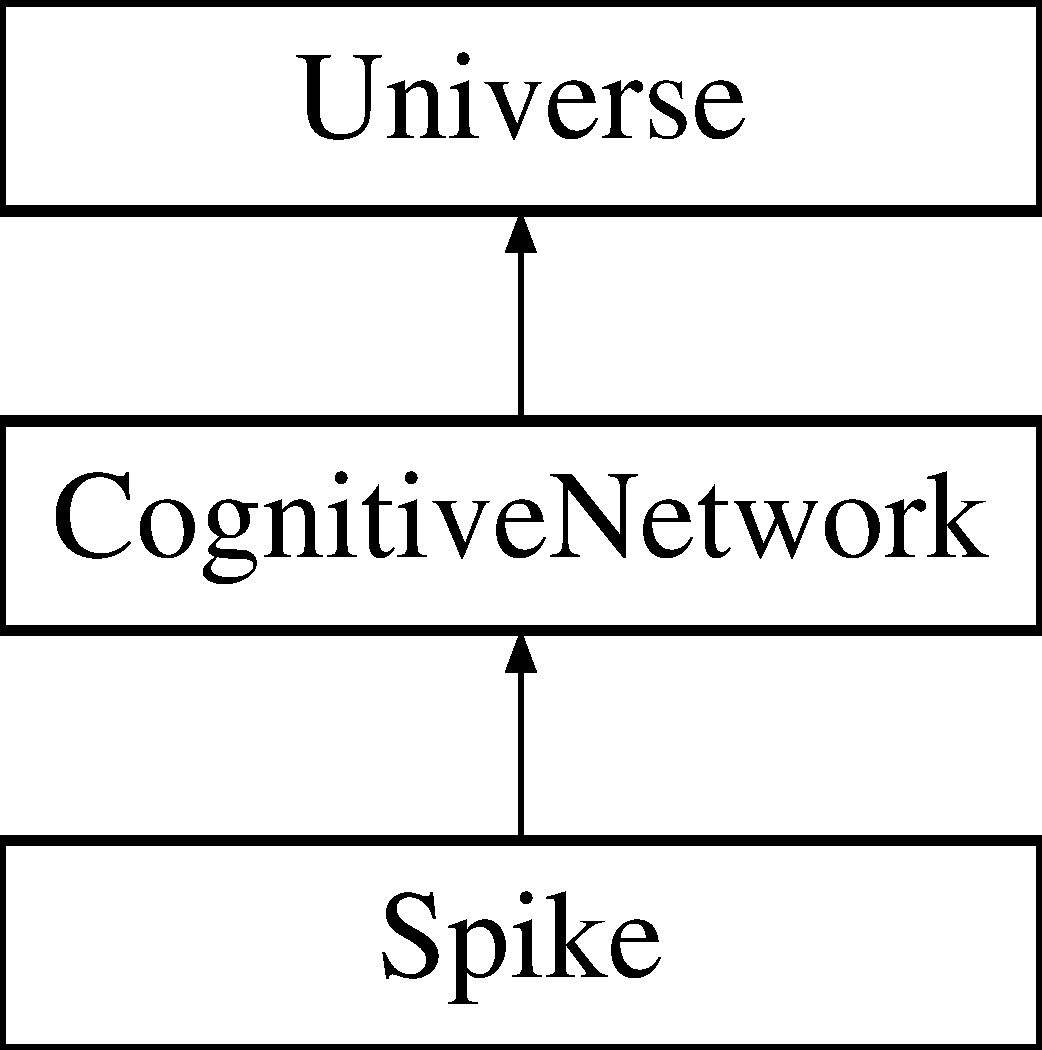
\includegraphics[height=3.000000cm]{classSpike}
\end{center}
\end{figure}
\subsection*{Public Member Functions}
\begin{DoxyCompactItemize}
\item 
\mbox{\hyperlink{classSpike_a1f82ea9e43a3a71b878261753c722dd9}{Spike}} ()
\item 
\mbox{\hyperlink{classSpike_a3e6dbba4e235f7adb02ade45c918b266}{Spike}} (unsigned int object\+\_\+type)
\item 
\mbox{\hyperlink{classSpike_a9368fb7b20887e5f02f3de6176f04c02}{Spike}} (unsigned int object\+\_\+type, std\+::chrono\+::time\+\_\+point$<$ \mbox{\hyperlink{universe_8h_a0ef8d951d1ca5ab3cfaf7ab4c7a6fd80}{Clock}} $>$ event\+\_\+time)
\item 
\mbox{\hyperlink{classSpike_afecf811f48103b529016a73349b50fe4}{Spike}} (unsigned int object\+\_\+type, std\+::chrono\+::time\+\_\+point$<$ \mbox{\hyperlink{universe_8h_a0ef8d951d1ca5ab3cfaf7ab4c7a6fd80}{Clock}} $>$ event\+\_\+time, \mbox{\hyperlink{classCognitiveNetwork}{Cognitive\+Network}} \&cognitivenetwork\+\_\+connector)
\item 
virtual \mbox{\hyperlink{classSpike_a6c2c62e81cb32ca4eb73bc686974d00d}{$\sim$\+Spike}} ()
\item 
bool \mbox{\hyperlink{classSpike_af4475560da7a33e70a0f2036197f000f}{Reset\+Parameters}} (std\+::chrono\+::time\+\_\+point$<$ \mbox{\hyperlink{universe_8h_a0ef8d951d1ca5ab3cfaf7ab4c7a6fd80}{Clock}} $>$ event\+\_\+time)
\item 
double \mbox{\hyperlink{classSpike_a6266871881a2581aaee499f6a10e1841}{Get\+Spike\+Height\+Reset}} (std\+::chrono\+::time\+\_\+point$<$ \mbox{\hyperlink{universe_8h_a0ef8d951d1ca5ab3cfaf7ab4c7a6fd80}{Clock}} $>$ event\+\_\+time)
\item 
void \mbox{\hyperlink{classSpike_a872adf39d66b0f491fb179c9745d7d11}{Set\+Spike\+Height\+Reset}} (std\+::chrono\+::time\+\_\+point$<$ \mbox{\hyperlink{universe_8h_a0ef8d951d1ca5ab3cfaf7ab4c7a6fd80}{Clock}} $>$ event\+\_\+time, double val)
\item 
void \mbox{\hyperlink{classSpike_acce1cc96e84e7cbf3b68010ab32f045e}{spike\+Reset}} (std\+::chrono\+::time\+\_\+point$<$ \mbox{\hyperlink{universe_8h_a0ef8d951d1ca5ab3cfaf7ab4c7a6fd80}{Clock}} $>$ event\+\_\+time)
\item 
double \mbox{\hyperlink{classSpike_ac465dbe6500f1eb1f5421f7174f91dd3}{poll\+Spike}} (std\+::chrono\+::time\+\_\+point$<$ \mbox{\hyperlink{universe_8h_a0ef8d951d1ca5ab3cfaf7ab4c7a6fd80}{Clock}} $>$ event\+\_\+time)
\item 
int \mbox{\hyperlink{classSpike_a683a0ca5e62e68777381fc85f4bf3019}{Update}} (std\+::chrono\+::time\+\_\+point$<$ \mbox{\hyperlink{universe_8h_a0ef8d951d1ca5ab3cfaf7ab4c7a6fd80}{Clock}} $>$ event\+\_\+time)
\end{DoxyCompactItemize}
\subsection*{Private Attributes}
\begin{DoxyCompactItemize}
\item 
double \mbox{\hyperlink{classSpike_af683cd1e0da2d4310da1d0bb723dc42b}{m\+\_\+attack\+Begin}} = 10
\item 
double \mbox{\hyperlink{classSpike_ad3a40048454bb37ad94e3c06069c77d5}{m\+\_\+attack\+Length}} = 10
\item 
double \mbox{\hyperlink{classSpike_a052650828271cd24a9709a832faf42b3}{m\+\_\+attack\+Peak}} = 80
\item 
double \mbox{\hyperlink{classSpike_a11d8945cda206677a7adb5571647a914}{m\+\_\+sustain}} = 75
\item 
double \mbox{\hyperlink{classSpike_a48b134667f3825716ded6966f5f37d10}{m\+\_\+sustain\+Length}} = 1
\item 
double \mbox{\hyperlink{classSpike_a6b37740d10e157844a2f4ee3a108e3ad}{m\+\_\+refactory\+Begin}} = 10
\item 
double \mbox{\hyperlink{classSpike_af1ecee046a275bfa13b663a8bc4722be}{m\+\_\+refactory\+Length}} = 20
\item 
double \mbox{\hyperlink{classSpike_a8dd4a3bc280a171e4c7ea23b85b43649}{m\+\_\+refactory\+End}} =8
\item 
double \mbox{\hyperlink{classSpike_a6a060f633f9abbeddf66f9d4e96961e7}{m\+\_\+spike\+Height}} = 0
\item 
double \mbox{\hyperlink{classSpike_a62bf030de52397708ef944d41e95398c}{m\+\_\+spike\+Height\+Reset}} = 0
\item 
double \mbox{\hyperlink{classSpike_a74fa438d3749330d86a3f0a90848a5bc}{m\+\_\+spike\+Loop}} = 0
\item 
double \mbox{\hyperlink{classSpike_ab30604e73d58882c56bb51272595e3e5}{object\+\_\+energy}}
\item 
int \mbox{\hyperlink{classSpike_a64297f01535f97c833eb740082830daf}{spike\+\_\+type}}
\item 
bool \mbox{\hyperlink{classSpike_a25760759b2d19a819feab8d27f5f9bfa}{object\+\_\+disabled}} = true
\item 
bool \mbox{\hyperlink{classSpike_ad700142996616c7cbc302baad6398e82}{object\+\_\+initialised}} = false
\item 
std\+::chrono\+::time\+\_\+point$<$ \mbox{\hyperlink{universe_8h_a0ef8d951d1ca5ab3cfaf7ab4c7a6fd80}{Clock}} $>$ \mbox{\hyperlink{classSpike_ae9e73c1745176138c2f2474c4dfdf89e}{time\+\_\+object\+\_\+created}}
\item 
std\+::chrono\+::time\+\_\+point$<$ \mbox{\hyperlink{universe_8h_a0ef8d951d1ca5ab3cfaf7ab4c7a6fd80}{Clock}} $>$ \mbox{\hyperlink{classSpike_adee91141c43f3507017abd53cdcdab08}{previous\+\_\+event\+\_\+time}}
\item 
int \mbox{\hyperlink{classSpike_a572287432bfe6202f85b2dd1822715c1}{duration\+\_\+since\+\_\+last\+\_\+event}}
\end{DoxyCompactItemize}
\subsection*{Additional Inherited Members}


\subsection{Constructor \& Destructor Documentation}
\mbox{\Hypertarget{classSpike_a1f82ea9e43a3a71b878261753c722dd9}\label{classSpike_a1f82ea9e43a3a71b878261753c722dd9}} 
\index{Spike@{Spike}!Spike@{Spike}}
\index{Spike@{Spike}!Spike@{Spike}}
\subsubsection{\texorpdfstring{Spike()}{Spike()}\hspace{0.1cm}{\footnotesize\ttfamily [1/4]}}
{\footnotesize\ttfamily Spike\+::\+Spike (\begin{DoxyParamCaption}{ }\end{DoxyParamCaption})\hspace{0.3cm}{\ttfamily [inline]}}

\mbox{\Hypertarget{classSpike_a3e6dbba4e235f7adb02ade45c918b266}\label{classSpike_a3e6dbba4e235f7adb02ade45c918b266}} 
\index{Spike@{Spike}!Spike@{Spike}}
\index{Spike@{Spike}!Spike@{Spike}}
\subsubsection{\texorpdfstring{Spike()}{Spike()}\hspace{0.1cm}{\footnotesize\ttfamily [2/4]}}
{\footnotesize\ttfamily Spike\+::\+Spike (\begin{DoxyParamCaption}\item[{unsigned int}]{object\+\_\+type }\end{DoxyParamCaption})\hspace{0.3cm}{\ttfamily [inline]}}

\mbox{\Hypertarget{classSpike_a9368fb7b20887e5f02f3de6176f04c02}\label{classSpike_a9368fb7b20887e5f02f3de6176f04c02}} 
\index{Spike@{Spike}!Spike@{Spike}}
\index{Spike@{Spike}!Spike@{Spike}}
\subsubsection{\texorpdfstring{Spike()}{Spike()}\hspace{0.1cm}{\footnotesize\ttfamily [3/4]}}
{\footnotesize\ttfamily Spike\+::\+Spike (\begin{DoxyParamCaption}\item[{unsigned int}]{object\+\_\+type,  }\item[{std\+::chrono\+::time\+\_\+point$<$ \mbox{\hyperlink{universe_8h_a0ef8d951d1ca5ab3cfaf7ab4c7a6fd80}{Clock}} $>$}]{event\+\_\+time }\end{DoxyParamCaption})\hspace{0.3cm}{\ttfamily [inline]}}

\mbox{\Hypertarget{classSpike_afecf811f48103b529016a73349b50fe4}\label{classSpike_afecf811f48103b529016a73349b50fe4}} 
\index{Spike@{Spike}!Spike@{Spike}}
\index{Spike@{Spike}!Spike@{Spike}}
\subsubsection{\texorpdfstring{Spike()}{Spike()}\hspace{0.1cm}{\footnotesize\ttfamily [4/4]}}
{\footnotesize\ttfamily Spike\+::\+Spike (\begin{DoxyParamCaption}\item[{unsigned int}]{object\+\_\+type,  }\item[{std\+::chrono\+::time\+\_\+point$<$ \mbox{\hyperlink{universe_8h_a0ef8d951d1ca5ab3cfaf7ab4c7a6fd80}{Clock}} $>$}]{event\+\_\+time,  }\item[{\mbox{\hyperlink{classCognitiveNetwork}{Cognitive\+Network}} \&}]{cognitivenetwork\+\_\+connector }\end{DoxyParamCaption})\hspace{0.3cm}{\ttfamily [inline]}}

\mbox{\Hypertarget{classSpike_a6c2c62e81cb32ca4eb73bc686974d00d}\label{classSpike_a6c2c62e81cb32ca4eb73bc686974d00d}} 
\index{Spike@{Spike}!````~Spike@{$\sim$\+Spike}}
\index{````~Spike@{$\sim$\+Spike}!Spike@{Spike}}
\subsubsection{\texorpdfstring{$\sim$\+Spike()}{~Spike()}}
{\footnotesize\ttfamily virtual Spike\+::$\sim$\+Spike (\begin{DoxyParamCaption}{ }\end{DoxyParamCaption})\hspace{0.3cm}{\ttfamily [inline]}, {\ttfamily [virtual]}}



\subsection{Member Function Documentation}
\mbox{\Hypertarget{classSpike_a6266871881a2581aaee499f6a10e1841}\label{classSpike_a6266871881a2581aaee499f6a10e1841}} 
\index{Spike@{Spike}!Get\+Spike\+Height\+Reset@{Get\+Spike\+Height\+Reset}}
\index{Get\+Spike\+Height\+Reset@{Get\+Spike\+Height\+Reset}!Spike@{Spike}}
\subsubsection{\texorpdfstring{Get\+Spike\+Height\+Reset()}{GetSpikeHeightReset()}}
{\footnotesize\ttfamily double Spike\+::\+Get\+Spike\+Height\+Reset (\begin{DoxyParamCaption}\item[{std\+::chrono\+::time\+\_\+point$<$ \mbox{\hyperlink{universe_8h_a0ef8d951d1ca5ab3cfaf7ab4c7a6fd80}{Clock}} $>$}]{event\+\_\+time }\end{DoxyParamCaption})\hspace{0.3cm}{\ttfamily [inline]}}

\mbox{\Hypertarget{classSpike_ac465dbe6500f1eb1f5421f7174f91dd3}\label{classSpike_ac465dbe6500f1eb1f5421f7174f91dd3}} 
\index{Spike@{Spike}!poll\+Spike@{poll\+Spike}}
\index{poll\+Spike@{poll\+Spike}!Spike@{Spike}}
\subsubsection{\texorpdfstring{poll\+Spike()}{pollSpike()}}
{\footnotesize\ttfamily double Spike\+::poll\+Spike (\begin{DoxyParamCaption}\item[{std\+::chrono\+::time\+\_\+point$<$ \mbox{\hyperlink{universe_8h_a0ef8d951d1ca5ab3cfaf7ab4c7a6fd80}{Clock}} $>$}]{event\+\_\+time }\end{DoxyParamCaption})\hspace{0.3cm}{\ttfamily [inline]}}

\mbox{\Hypertarget{classSpike_af4475560da7a33e70a0f2036197f000f}\label{classSpike_af4475560da7a33e70a0f2036197f000f}} 
\index{Spike@{Spike}!Reset\+Parameters@{Reset\+Parameters}}
\index{Reset\+Parameters@{Reset\+Parameters}!Spike@{Spike}}
\subsubsection{\texorpdfstring{Reset\+Parameters()}{ResetParameters()}}
{\footnotesize\ttfamily bool Spike\+::\+Reset\+Parameters (\begin{DoxyParamCaption}\item[{std\+::chrono\+::time\+\_\+point$<$ \mbox{\hyperlink{universe_8h_a0ef8d951d1ca5ab3cfaf7ab4c7a6fd80}{Clock}} $>$}]{event\+\_\+time }\end{DoxyParamCaption})}

\mbox{\Hypertarget{classSpike_a872adf39d66b0f491fb179c9745d7d11}\label{classSpike_a872adf39d66b0f491fb179c9745d7d11}} 
\index{Spike@{Spike}!Set\+Spike\+Height\+Reset@{Set\+Spike\+Height\+Reset}}
\index{Set\+Spike\+Height\+Reset@{Set\+Spike\+Height\+Reset}!Spike@{Spike}}
\subsubsection{\texorpdfstring{Set\+Spike\+Height\+Reset()}{SetSpikeHeightReset()}}
{\footnotesize\ttfamily void Spike\+::\+Set\+Spike\+Height\+Reset (\begin{DoxyParamCaption}\item[{std\+::chrono\+::time\+\_\+point$<$ \mbox{\hyperlink{universe_8h_a0ef8d951d1ca5ab3cfaf7ab4c7a6fd80}{Clock}} $>$}]{event\+\_\+time,  }\item[{double}]{val }\end{DoxyParamCaption})\hspace{0.3cm}{\ttfamily [inline]}}

\mbox{\Hypertarget{classSpike_acce1cc96e84e7cbf3b68010ab32f045e}\label{classSpike_acce1cc96e84e7cbf3b68010ab32f045e}} 
\index{Spike@{Spike}!spike\+Reset@{spike\+Reset}}
\index{spike\+Reset@{spike\+Reset}!Spike@{Spike}}
\subsubsection{\texorpdfstring{spike\+Reset()}{spikeReset()}}
{\footnotesize\ttfamily void Spike\+::spike\+Reset (\begin{DoxyParamCaption}\item[{std\+::chrono\+::time\+\_\+point$<$ \mbox{\hyperlink{universe_8h_a0ef8d951d1ca5ab3cfaf7ab4c7a6fd80}{Clock}} $>$}]{event\+\_\+time }\end{DoxyParamCaption})\hspace{0.3cm}{\ttfamily [inline]}}

\mbox{\Hypertarget{classSpike_a683a0ca5e62e68777381fc85f4bf3019}\label{classSpike_a683a0ca5e62e68777381fc85f4bf3019}} 
\index{Spike@{Spike}!Update@{Update}}
\index{Update@{Update}!Spike@{Spike}}
\subsubsection{\texorpdfstring{Update()}{Update()}}
{\footnotesize\ttfamily int Spike\+::\+Update (\begin{DoxyParamCaption}\item[{std\+::chrono\+::time\+\_\+point$<$ \mbox{\hyperlink{universe_8h_a0ef8d951d1ca5ab3cfaf7ab4c7a6fd80}{Clock}} $>$}]{event\+\_\+time }\end{DoxyParamCaption})}



\subsection{Member Data Documentation}
\mbox{\Hypertarget{classSpike_a572287432bfe6202f85b2dd1822715c1}\label{classSpike_a572287432bfe6202f85b2dd1822715c1}} 
\index{Spike@{Spike}!duration\+\_\+since\+\_\+last\+\_\+event@{duration\+\_\+since\+\_\+last\+\_\+event}}
\index{duration\+\_\+since\+\_\+last\+\_\+event@{duration\+\_\+since\+\_\+last\+\_\+event}!Spike@{Spike}}
\subsubsection{\texorpdfstring{duration\+\_\+since\+\_\+last\+\_\+event}{duration\_since\_last\_event}}
{\footnotesize\ttfamily int Spike\+::duration\+\_\+since\+\_\+last\+\_\+event\hspace{0.3cm}{\ttfamily [private]}}

\mbox{\Hypertarget{classSpike_af683cd1e0da2d4310da1d0bb723dc42b}\label{classSpike_af683cd1e0da2d4310da1d0bb723dc42b}} 
\index{Spike@{Spike}!m\+\_\+attack\+Begin@{m\+\_\+attack\+Begin}}
\index{m\+\_\+attack\+Begin@{m\+\_\+attack\+Begin}!Spike@{Spike}}
\subsubsection{\texorpdfstring{m\+\_\+attack\+Begin}{m\_attackBegin}}
{\footnotesize\ttfamily double Spike\+::m\+\_\+attack\+Begin = 10\hspace{0.3cm}{\ttfamily [private]}}

\mbox{\Hypertarget{classSpike_ad3a40048454bb37ad94e3c06069c77d5}\label{classSpike_ad3a40048454bb37ad94e3c06069c77d5}} 
\index{Spike@{Spike}!m\+\_\+attack\+Length@{m\+\_\+attack\+Length}}
\index{m\+\_\+attack\+Length@{m\+\_\+attack\+Length}!Spike@{Spike}}
\subsubsection{\texorpdfstring{m\+\_\+attack\+Length}{m\_attackLength}}
{\footnotesize\ttfamily double Spike\+::m\+\_\+attack\+Length = 10\hspace{0.3cm}{\ttfamily [private]}}

\mbox{\Hypertarget{classSpike_a052650828271cd24a9709a832faf42b3}\label{classSpike_a052650828271cd24a9709a832faf42b3}} 
\index{Spike@{Spike}!m\+\_\+attack\+Peak@{m\+\_\+attack\+Peak}}
\index{m\+\_\+attack\+Peak@{m\+\_\+attack\+Peak}!Spike@{Spike}}
\subsubsection{\texorpdfstring{m\+\_\+attack\+Peak}{m\_attackPeak}}
{\footnotesize\ttfamily double Spike\+::m\+\_\+attack\+Peak = 80\hspace{0.3cm}{\ttfamily [private]}}

\mbox{\Hypertarget{classSpike_a6b37740d10e157844a2f4ee3a108e3ad}\label{classSpike_a6b37740d10e157844a2f4ee3a108e3ad}} 
\index{Spike@{Spike}!m\+\_\+refactory\+Begin@{m\+\_\+refactory\+Begin}}
\index{m\+\_\+refactory\+Begin@{m\+\_\+refactory\+Begin}!Spike@{Spike}}
\subsubsection{\texorpdfstring{m\+\_\+refactory\+Begin}{m\_refactoryBegin}}
{\footnotesize\ttfamily double Spike\+::m\+\_\+refactory\+Begin = 10\hspace{0.3cm}{\ttfamily [private]}}

\mbox{\Hypertarget{classSpike_a8dd4a3bc280a171e4c7ea23b85b43649}\label{classSpike_a8dd4a3bc280a171e4c7ea23b85b43649}} 
\index{Spike@{Spike}!m\+\_\+refactory\+End@{m\+\_\+refactory\+End}}
\index{m\+\_\+refactory\+End@{m\+\_\+refactory\+End}!Spike@{Spike}}
\subsubsection{\texorpdfstring{m\+\_\+refactory\+End}{m\_refactoryEnd}}
{\footnotesize\ttfamily double Spike\+::m\+\_\+refactory\+End =8\hspace{0.3cm}{\ttfamily [private]}}

\mbox{\Hypertarget{classSpike_af1ecee046a275bfa13b663a8bc4722be}\label{classSpike_af1ecee046a275bfa13b663a8bc4722be}} 
\index{Spike@{Spike}!m\+\_\+refactory\+Length@{m\+\_\+refactory\+Length}}
\index{m\+\_\+refactory\+Length@{m\+\_\+refactory\+Length}!Spike@{Spike}}
\subsubsection{\texorpdfstring{m\+\_\+refactory\+Length}{m\_refactoryLength}}
{\footnotesize\ttfamily double Spike\+::m\+\_\+refactory\+Length = 20\hspace{0.3cm}{\ttfamily [private]}}

\mbox{\Hypertarget{classSpike_a6a060f633f9abbeddf66f9d4e96961e7}\label{classSpike_a6a060f633f9abbeddf66f9d4e96961e7}} 
\index{Spike@{Spike}!m\+\_\+spike\+Height@{m\+\_\+spike\+Height}}
\index{m\+\_\+spike\+Height@{m\+\_\+spike\+Height}!Spike@{Spike}}
\subsubsection{\texorpdfstring{m\+\_\+spike\+Height}{m\_spikeHeight}}
{\footnotesize\ttfamily double Spike\+::m\+\_\+spike\+Height = 0\hspace{0.3cm}{\ttfamily [private]}}

\mbox{\Hypertarget{classSpike_a62bf030de52397708ef944d41e95398c}\label{classSpike_a62bf030de52397708ef944d41e95398c}} 
\index{Spike@{Spike}!m\+\_\+spike\+Height\+Reset@{m\+\_\+spike\+Height\+Reset}}
\index{m\+\_\+spike\+Height\+Reset@{m\+\_\+spike\+Height\+Reset}!Spike@{Spike}}
\subsubsection{\texorpdfstring{m\+\_\+spike\+Height\+Reset}{m\_spikeHeightReset}}
{\footnotesize\ttfamily double Spike\+::m\+\_\+spike\+Height\+Reset = 0\hspace{0.3cm}{\ttfamily [private]}}

\mbox{\Hypertarget{classSpike_a74fa438d3749330d86a3f0a90848a5bc}\label{classSpike_a74fa438d3749330d86a3f0a90848a5bc}} 
\index{Spike@{Spike}!m\+\_\+spike\+Loop@{m\+\_\+spike\+Loop}}
\index{m\+\_\+spike\+Loop@{m\+\_\+spike\+Loop}!Spike@{Spike}}
\subsubsection{\texorpdfstring{m\+\_\+spike\+Loop}{m\_spikeLoop}}
{\footnotesize\ttfamily double Spike\+::m\+\_\+spike\+Loop = 0\hspace{0.3cm}{\ttfamily [private]}}

\mbox{\Hypertarget{classSpike_a11d8945cda206677a7adb5571647a914}\label{classSpike_a11d8945cda206677a7adb5571647a914}} 
\index{Spike@{Spike}!m\+\_\+sustain@{m\+\_\+sustain}}
\index{m\+\_\+sustain@{m\+\_\+sustain}!Spike@{Spike}}
\subsubsection{\texorpdfstring{m\+\_\+sustain}{m\_sustain}}
{\footnotesize\ttfamily double Spike\+::m\+\_\+sustain = 75\hspace{0.3cm}{\ttfamily [private]}}

\mbox{\Hypertarget{classSpike_a48b134667f3825716ded6966f5f37d10}\label{classSpike_a48b134667f3825716ded6966f5f37d10}} 
\index{Spike@{Spike}!m\+\_\+sustain\+Length@{m\+\_\+sustain\+Length}}
\index{m\+\_\+sustain\+Length@{m\+\_\+sustain\+Length}!Spike@{Spike}}
\subsubsection{\texorpdfstring{m\+\_\+sustain\+Length}{m\_sustainLength}}
{\footnotesize\ttfamily double Spike\+::m\+\_\+sustain\+Length = 1\hspace{0.3cm}{\ttfamily [private]}}

\mbox{\Hypertarget{classSpike_a25760759b2d19a819feab8d27f5f9bfa}\label{classSpike_a25760759b2d19a819feab8d27f5f9bfa}} 
\index{Spike@{Spike}!object\+\_\+disabled@{object\+\_\+disabled}}
\index{object\+\_\+disabled@{object\+\_\+disabled}!Spike@{Spike}}
\subsubsection{\texorpdfstring{object\+\_\+disabled}{object\_disabled}}
{\footnotesize\ttfamily bool Spike\+::object\+\_\+disabled = true\hspace{0.3cm}{\ttfamily [private]}}

\mbox{\Hypertarget{classSpike_ab30604e73d58882c56bb51272595e3e5}\label{classSpike_ab30604e73d58882c56bb51272595e3e5}} 
\index{Spike@{Spike}!object\+\_\+energy@{object\+\_\+energy}}
\index{object\+\_\+energy@{object\+\_\+energy}!Spike@{Spike}}
\subsubsection{\texorpdfstring{object\+\_\+energy}{object\_energy}}
{\footnotesize\ttfamily double Spike\+::object\+\_\+energy\hspace{0.3cm}{\ttfamily [private]}}

\mbox{\Hypertarget{classSpike_ad700142996616c7cbc302baad6398e82}\label{classSpike_ad700142996616c7cbc302baad6398e82}} 
\index{Spike@{Spike}!object\+\_\+initialised@{object\+\_\+initialised}}
\index{object\+\_\+initialised@{object\+\_\+initialised}!Spike@{Spike}}
\subsubsection{\texorpdfstring{object\+\_\+initialised}{object\_initialised}}
{\footnotesize\ttfamily bool Spike\+::object\+\_\+initialised = false\hspace{0.3cm}{\ttfamily [private]}}

\mbox{\Hypertarget{classSpike_adee91141c43f3507017abd53cdcdab08}\label{classSpike_adee91141c43f3507017abd53cdcdab08}} 
\index{Spike@{Spike}!previous\+\_\+event\+\_\+time@{previous\+\_\+event\+\_\+time}}
\index{previous\+\_\+event\+\_\+time@{previous\+\_\+event\+\_\+time}!Spike@{Spike}}
\subsubsection{\texorpdfstring{previous\+\_\+event\+\_\+time}{previous\_event\_time}}
{\footnotesize\ttfamily std\+::chrono\+::time\+\_\+point$<$\mbox{\hyperlink{universe_8h_a0ef8d951d1ca5ab3cfaf7ab4c7a6fd80}{Clock}}$>$ Spike\+::previous\+\_\+event\+\_\+time\hspace{0.3cm}{\ttfamily [private]}}

\mbox{\Hypertarget{classSpike_a64297f01535f97c833eb740082830daf}\label{classSpike_a64297f01535f97c833eb740082830daf}} 
\index{Spike@{Spike}!spike\+\_\+type@{spike\+\_\+type}}
\index{spike\+\_\+type@{spike\+\_\+type}!Spike@{Spike}}
\subsubsection{\texorpdfstring{spike\+\_\+type}{spike\_type}}
{\footnotesize\ttfamily int Spike\+::spike\+\_\+type\hspace{0.3cm}{\ttfamily [private]}}

\mbox{\Hypertarget{classSpike_ae9e73c1745176138c2f2474c4dfdf89e}\label{classSpike_ae9e73c1745176138c2f2474c4dfdf89e}} 
\index{Spike@{Spike}!time\+\_\+object\+\_\+created@{time\+\_\+object\+\_\+created}}
\index{time\+\_\+object\+\_\+created@{time\+\_\+object\+\_\+created}!Spike@{Spike}}
\subsubsection{\texorpdfstring{time\+\_\+object\+\_\+created}{time\_object\_created}}
{\footnotesize\ttfamily std\+::chrono\+::time\+\_\+point$<$\mbox{\hyperlink{universe_8h_a0ef8d951d1ca5ab3cfaf7ab4c7a6fd80}{Clock}}$>$ Spike\+::time\+\_\+object\+\_\+created\hspace{0.3cm}{\ttfamily [private]}}



The documentation for this class was generated from the following files\+:\begin{DoxyCompactItemize}
\item 
/home/pbisaacs/\+Developer/\+Brain\+Harmonics/\mbox{\hyperlink{spike_8h}{spike.\+h}}\item 
/home/pbisaacs/\+Developer/\+Brain\+Harmonics/\mbox{\hyperlink{spike_8cc}{spike.\+cc}}\end{DoxyCompactItemize}

\hypertarget{structSquareGrid}{}\section{Square\+Grid Struct Reference}
\label{structSquareGrid}\index{Square\+Grid@{Square\+Grid}}
Inheritance diagram for Square\+Grid\+:\begin{figure}[H]
\begin{center}
\leavevmode
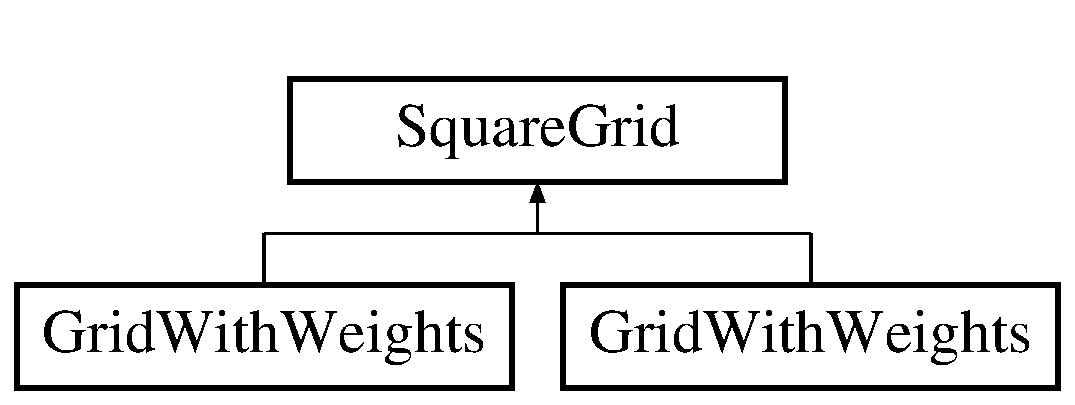
\includegraphics[height=2.000000cm]{structSquareGrid}
\end{center}
\end{figure}
\subsection*{Public Types}
\begin{DoxyCompactItemize}
\item 
typedef tuple$<$ int, int $>$ \mbox{\hyperlink{structSquareGrid_a2c9a2cbd3912aa48ac97289abc3f1c0f}{Location}}
\item 
typedef tuple$<$ int, int $>$ \mbox{\hyperlink{structSquareGrid_a2c9a2cbd3912aa48ac97289abc3f1c0f}{Location}}
\end{DoxyCompactItemize}
\subsection*{Public Member Functions}
\begin{DoxyCompactItemize}
\item 
\mbox{\hyperlink{structSquareGrid_ae5debd1459b89aba9497f270f6d76d7b}{Square\+Grid}} (int width\+\_\+, int height\+\_\+)
\item 
bool \mbox{\hyperlink{structSquareGrid_a84bbaa9dad618228a2d6d3196254b86b}{in\+\_\+bounds}} (\mbox{\hyperlink{structSquareGrid_a2c9a2cbd3912aa48ac97289abc3f1c0f}{Location}} id)
\item 
bool \mbox{\hyperlink{structSquareGrid_a3f638b46510dd880823b1acac75c7b96}{passable}} (\mbox{\hyperlink{structSquareGrid_a2c9a2cbd3912aa48ac97289abc3f1c0f}{Location}} id)
\item 
vector$<$ \mbox{\hyperlink{structSquareGrid_a2c9a2cbd3912aa48ac97289abc3f1c0f}{Location}} $>$ \mbox{\hyperlink{structSquareGrid_a106d76702d8c4acb03883c477db28e3a}{neighbors}} (\mbox{\hyperlink{structSquareGrid_a2c9a2cbd3912aa48ac97289abc3f1c0f}{Location}} id)
\item 
\mbox{\hyperlink{structSquareGrid_ae5debd1459b89aba9497f270f6d76d7b}{Square\+Grid}} (int width\+\_\+, int height\+\_\+)
\item 
bool \mbox{\hyperlink{structSquareGrid_a84bbaa9dad618228a2d6d3196254b86b}{in\+\_\+bounds}} (\mbox{\hyperlink{structSquareGrid_a2c9a2cbd3912aa48ac97289abc3f1c0f}{Location}} id)
\item 
bool \mbox{\hyperlink{structSquareGrid_a3f638b46510dd880823b1acac75c7b96}{passable}} (\mbox{\hyperlink{structSquareGrid_a2c9a2cbd3912aa48ac97289abc3f1c0f}{Location}} id)
\item 
vector$<$ \mbox{\hyperlink{structSquareGrid_a2c9a2cbd3912aa48ac97289abc3f1c0f}{Location}} $>$ \mbox{\hyperlink{structSquareGrid_a106d76702d8c4acb03883c477db28e3a}{neighbors}} (\mbox{\hyperlink{structSquareGrid_a2c9a2cbd3912aa48ac97289abc3f1c0f}{Location}} id)
\end{DoxyCompactItemize}
\subsection*{Public Attributes}
\begin{DoxyCompactItemize}
\item 
int \mbox{\hyperlink{structSquareGrid_af5476cf49f0bb03d1e940adbc6e5febf}{width}}
\item 
int \mbox{\hyperlink{structSquareGrid_ad6b113fc3a49f5db5fbf9c8138e35634}{height}}
\item 
unordered\+\_\+set$<$ \mbox{\hyperlink{structSquareGrid_a2c9a2cbd3912aa48ac97289abc3f1c0f}{Location}} $>$ \mbox{\hyperlink{structSquareGrid_a1bc7e32bd195e42fd9685310d7ee65c5}{walls}}
\end{DoxyCompactItemize}
\subsection*{Static Public Attributes}
\begin{DoxyCompactItemize}
\item 
static array$<$ \mbox{\hyperlink{structSquareGrid_a2c9a2cbd3912aa48ac97289abc3f1c0f}{Location}}, 4 $>$ \mbox{\hyperlink{structSquareGrid_aac91cba6573640c545485ed054089c87}{D\+I\+RS}} \{\mbox{\hyperlink{structSquareGrid_a2c9a2cbd3912aa48ac97289abc3f1c0f}{Location}}\{1, 0\}, \mbox{\hyperlink{structSquareGrid_a2c9a2cbd3912aa48ac97289abc3f1c0f}{Location}}\{0, -\/1\}, \mbox{\hyperlink{structSquareGrid_a2c9a2cbd3912aa48ac97289abc3f1c0f}{Location}}\{-\/1, 0\}, \mbox{\hyperlink{structSquareGrid_a2c9a2cbd3912aa48ac97289abc3f1c0f}{Location}}\{0, 1\}\}
\end{DoxyCompactItemize}


\subsection{Member Typedef Documentation}
\mbox{\Hypertarget{structSquareGrid_a2c9a2cbd3912aa48ac97289abc3f1c0f}\label{structSquareGrid_a2c9a2cbd3912aa48ac97289abc3f1c0f}} 
\index{Square\+Grid@{Square\+Grid}!Location@{Location}}
\index{Location@{Location}!Square\+Grid@{Square\+Grid}}
\subsubsection{\texorpdfstring{Location}{Location}\hspace{0.1cm}{\footnotesize\ttfamily [1/2]}}
{\footnotesize\ttfamily typedef tuple$<$int,int$>$ \mbox{\hyperlink{structSquareGrid_a2c9a2cbd3912aa48ac97289abc3f1c0f}{Square\+Grid\+::\+Location}}}

\mbox{\Hypertarget{structSquareGrid_a2c9a2cbd3912aa48ac97289abc3f1c0f}\label{structSquareGrid_a2c9a2cbd3912aa48ac97289abc3f1c0f}} 
\index{Square\+Grid@{Square\+Grid}!Location@{Location}}
\index{Location@{Location}!Square\+Grid@{Square\+Grid}}
\subsubsection{\texorpdfstring{Location}{Location}\hspace{0.1cm}{\footnotesize\ttfamily [2/2]}}
{\footnotesize\ttfamily typedef tuple$<$int,int$>$ \mbox{\hyperlink{structSquareGrid_a2c9a2cbd3912aa48ac97289abc3f1c0f}{Square\+Grid\+::\+Location}}}



\subsection{Constructor \& Destructor Documentation}
\mbox{\Hypertarget{structSquareGrid_ae5debd1459b89aba9497f270f6d76d7b}\label{structSquareGrid_ae5debd1459b89aba9497f270f6d76d7b}} 
\index{Square\+Grid@{Square\+Grid}!Square\+Grid@{Square\+Grid}}
\index{Square\+Grid@{Square\+Grid}!Square\+Grid@{Square\+Grid}}
\subsubsection{\texorpdfstring{Square\+Grid()}{SquareGrid()}\hspace{0.1cm}{\footnotesize\ttfamily [1/2]}}
{\footnotesize\ttfamily Square\+Grid\+::\+Square\+Grid (\begin{DoxyParamCaption}\item[{int}]{width\+\_\+,  }\item[{int}]{height\+\_\+ }\end{DoxyParamCaption})\hspace{0.3cm}{\ttfamily [inline]}}

\mbox{\Hypertarget{structSquareGrid_ae5debd1459b89aba9497f270f6d76d7b}\label{structSquareGrid_ae5debd1459b89aba9497f270f6d76d7b}} 
\index{Square\+Grid@{Square\+Grid}!Square\+Grid@{Square\+Grid}}
\index{Square\+Grid@{Square\+Grid}!Square\+Grid@{Square\+Grid}}
\subsubsection{\texorpdfstring{Square\+Grid()}{SquareGrid()}\hspace{0.1cm}{\footnotesize\ttfamily [2/2]}}
{\footnotesize\ttfamily Square\+Grid\+::\+Square\+Grid (\begin{DoxyParamCaption}\item[{int}]{width\+\_\+,  }\item[{int}]{height\+\_\+ }\end{DoxyParamCaption})\hspace{0.3cm}{\ttfamily [inline]}}



\subsection{Member Function Documentation}
\mbox{\Hypertarget{structSquareGrid_a84bbaa9dad618228a2d6d3196254b86b}\label{structSquareGrid_a84bbaa9dad618228a2d6d3196254b86b}} 
\index{Square\+Grid@{Square\+Grid}!in\+\_\+bounds@{in\+\_\+bounds}}
\index{in\+\_\+bounds@{in\+\_\+bounds}!Square\+Grid@{Square\+Grid}}
\subsubsection{\texorpdfstring{in\+\_\+bounds()}{in\_bounds()}\hspace{0.1cm}{\footnotesize\ttfamily [1/2]}}
{\footnotesize\ttfamily bool Square\+Grid\+::in\+\_\+bounds (\begin{DoxyParamCaption}\item[{\mbox{\hyperlink{structSquareGrid_a2c9a2cbd3912aa48ac97289abc3f1c0f}{Location}}}]{id }\end{DoxyParamCaption})\hspace{0.3cm}{\ttfamily [inline]}}

\mbox{\Hypertarget{structSquareGrid_a84bbaa9dad618228a2d6d3196254b86b}\label{structSquareGrid_a84bbaa9dad618228a2d6d3196254b86b}} 
\index{Square\+Grid@{Square\+Grid}!in\+\_\+bounds@{in\+\_\+bounds}}
\index{in\+\_\+bounds@{in\+\_\+bounds}!Square\+Grid@{Square\+Grid}}
\subsubsection{\texorpdfstring{in\+\_\+bounds()}{in\_bounds()}\hspace{0.1cm}{\footnotesize\ttfamily [2/2]}}
{\footnotesize\ttfamily bool Square\+Grid\+::in\+\_\+bounds (\begin{DoxyParamCaption}\item[{\mbox{\hyperlink{structSquareGrid_a2c9a2cbd3912aa48ac97289abc3f1c0f}{Location}}}]{id }\end{DoxyParamCaption})\hspace{0.3cm}{\ttfamily [inline]}}

\mbox{\Hypertarget{structSquareGrid_a106d76702d8c4acb03883c477db28e3a}\label{structSquareGrid_a106d76702d8c4acb03883c477db28e3a}} 
\index{Square\+Grid@{Square\+Grid}!neighbors@{neighbors}}
\index{neighbors@{neighbors}!Square\+Grid@{Square\+Grid}}
\subsubsection{\texorpdfstring{neighbors()}{neighbors()}\hspace{0.1cm}{\footnotesize\ttfamily [1/2]}}
{\footnotesize\ttfamily vector$<$\mbox{\hyperlink{structSquareGrid_a2c9a2cbd3912aa48ac97289abc3f1c0f}{Location}}$>$ Square\+Grid\+::neighbors (\begin{DoxyParamCaption}\item[{\mbox{\hyperlink{structSquareGrid_a2c9a2cbd3912aa48ac97289abc3f1c0f}{Location}}}]{id }\end{DoxyParamCaption})\hspace{0.3cm}{\ttfamily [inline]}}

\mbox{\Hypertarget{structSquareGrid_a106d76702d8c4acb03883c477db28e3a}\label{structSquareGrid_a106d76702d8c4acb03883c477db28e3a}} 
\index{Square\+Grid@{Square\+Grid}!neighbors@{neighbors}}
\index{neighbors@{neighbors}!Square\+Grid@{Square\+Grid}}
\subsubsection{\texorpdfstring{neighbors()}{neighbors()}\hspace{0.1cm}{\footnotesize\ttfamily [2/2]}}
{\footnotesize\ttfamily vector$<$\mbox{\hyperlink{structSquareGrid_a2c9a2cbd3912aa48ac97289abc3f1c0f}{Location}}$>$ Square\+Grid\+::neighbors (\begin{DoxyParamCaption}\item[{\mbox{\hyperlink{structSquareGrid_a2c9a2cbd3912aa48ac97289abc3f1c0f}{Location}}}]{id }\end{DoxyParamCaption})\hspace{0.3cm}{\ttfamily [inline]}}

\mbox{\Hypertarget{structSquareGrid_a3f638b46510dd880823b1acac75c7b96}\label{structSquareGrid_a3f638b46510dd880823b1acac75c7b96}} 
\index{Square\+Grid@{Square\+Grid}!passable@{passable}}
\index{passable@{passable}!Square\+Grid@{Square\+Grid}}
\subsubsection{\texorpdfstring{passable()}{passable()}\hspace{0.1cm}{\footnotesize\ttfamily [1/2]}}
{\footnotesize\ttfamily bool Square\+Grid\+::passable (\begin{DoxyParamCaption}\item[{\mbox{\hyperlink{structSquareGrid_a2c9a2cbd3912aa48ac97289abc3f1c0f}{Location}}}]{id }\end{DoxyParamCaption})\hspace{0.3cm}{\ttfamily [inline]}}

\mbox{\Hypertarget{structSquareGrid_a3f638b46510dd880823b1acac75c7b96}\label{structSquareGrid_a3f638b46510dd880823b1acac75c7b96}} 
\index{Square\+Grid@{Square\+Grid}!passable@{passable}}
\index{passable@{passable}!Square\+Grid@{Square\+Grid}}
\subsubsection{\texorpdfstring{passable()}{passable()}\hspace{0.1cm}{\footnotesize\ttfamily [2/2]}}
{\footnotesize\ttfamily bool Square\+Grid\+::passable (\begin{DoxyParamCaption}\item[{\mbox{\hyperlink{structSquareGrid_a2c9a2cbd3912aa48ac97289abc3f1c0f}{Location}}}]{id }\end{DoxyParamCaption})\hspace{0.3cm}{\ttfamily [inline]}}



\subsection{Member Data Documentation}
\mbox{\Hypertarget{structSquareGrid_aac91cba6573640c545485ed054089c87}\label{structSquareGrid_aac91cba6573640c545485ed054089c87}} 
\index{Square\+Grid@{Square\+Grid}!D\+I\+RS@{D\+I\+RS}}
\index{D\+I\+RS@{D\+I\+RS}!Square\+Grid@{Square\+Grid}}
\subsubsection{\texorpdfstring{D\+I\+RS}{DIRS}}
{\footnotesize\ttfamily array$<$ \mbox{\hyperlink{structSquareGrid_a2c9a2cbd3912aa48ac97289abc3f1c0f}{Square\+Grid\+::\+Location}}, 4 $>$ Square\+Grid\+::\+D\+I\+RS \{\mbox{\hyperlink{structSquareGrid_a2c9a2cbd3912aa48ac97289abc3f1c0f}{Location}}\{1, 0\}, \mbox{\hyperlink{structSquareGrid_a2c9a2cbd3912aa48ac97289abc3f1c0f}{Location}}\{0, -\/1\}, \mbox{\hyperlink{structSquareGrid_a2c9a2cbd3912aa48ac97289abc3f1c0f}{Location}}\{-\/1, 0\}, \mbox{\hyperlink{structSquareGrid_a2c9a2cbd3912aa48ac97289abc3f1c0f}{Location}}\{0, 1\}\}\hspace{0.3cm}{\ttfamily [static]}}

\mbox{\Hypertarget{structSquareGrid_ad6b113fc3a49f5db5fbf9c8138e35634}\label{structSquareGrid_ad6b113fc3a49f5db5fbf9c8138e35634}} 
\index{Square\+Grid@{Square\+Grid}!height@{height}}
\index{height@{height}!Square\+Grid@{Square\+Grid}}
\subsubsection{\texorpdfstring{height}{height}}
{\footnotesize\ttfamily int Square\+Grid\+::height}

\mbox{\Hypertarget{structSquareGrid_a1bc7e32bd195e42fd9685310d7ee65c5}\label{structSquareGrid_a1bc7e32bd195e42fd9685310d7ee65c5}} 
\index{Square\+Grid@{Square\+Grid}!walls@{walls}}
\index{walls@{walls}!Square\+Grid@{Square\+Grid}}
\subsubsection{\texorpdfstring{walls}{walls}}
{\footnotesize\ttfamily unordered\+\_\+set$<$ \mbox{\hyperlink{structSquareGrid_a2c9a2cbd3912aa48ac97289abc3f1c0f}{Location}} $>$ Square\+Grid\+::walls}

\mbox{\Hypertarget{structSquareGrid_af5476cf49f0bb03d1e940adbc6e5febf}\label{structSquareGrid_af5476cf49f0bb03d1e940adbc6e5febf}} 
\index{Square\+Grid@{Square\+Grid}!width@{width}}
\index{width@{width}!Square\+Grid@{Square\+Grid}}
\subsubsection{\texorpdfstring{width}{width}}
{\footnotesize\ttfamily int Square\+Grid\+::width}



The documentation for this struct was generated from the following files\+:\begin{DoxyCompactItemize}
\item 
/home/pbisaacs/\+Developer/\+Brain\+Harmonics/\mbox{\hyperlink{implementation_01orig_8cc}{implementation orig.\+cc}}\item 
/home/pbisaacs/\+Developer/\+Brain\+Harmonics/\mbox{\hyperlink{search_8cpp}{search.\+cpp}}\end{DoxyCompactItemize}

\hypertarget{classSynapse}{}\section{Synapse Class Reference}
\label{classSynapse}\index{Synapse@{Synapse}}


{\ttfamily \#include $<$synapse.\+h$>$}

Inheritance diagram for Synapse\+:\begin{figure}[H]
\begin{center}
\leavevmode
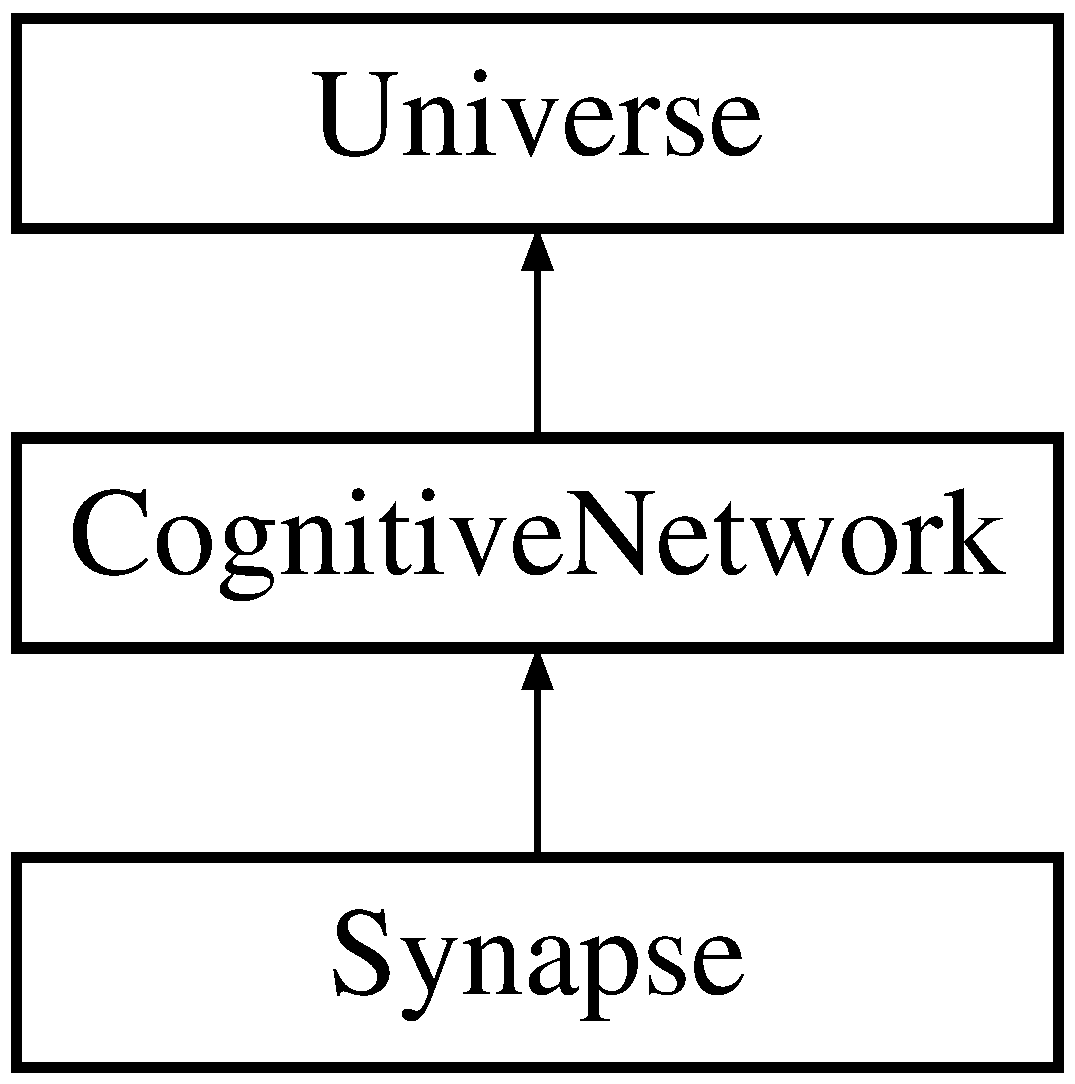
\includegraphics[height=3.000000cm]{classSynapse}
\end{center}
\end{figure}
\subsection*{Classes}
\begin{DoxyCompactItemize}
\item 
struct \mbox{\hyperlink{structSynapse_1_1NearbyNeuron}{Nearby\+Neuron}}
\item 
struct \mbox{\hyperlink{structSynapse_1_1s__BindList}{s\+\_\+\+Bind\+List}}
\end{DoxyCompactItemize}
\subsection*{Public Member Functions}
\begin{DoxyCompactItemize}
\item 
\mbox{\hyperlink{classSynapse_a68e6c8546084f93ae7d39af6986562fb}{Synapse}} ()
\item 
\mbox{\hyperlink{classSynapse_a821e35d693de963edb6d5aa9e565dfde}{Synapse}} (unsigned int object\+\_\+type)
\item 
\mbox{\hyperlink{classSynapse_a339a3dff64e545fc7c013b251737257b}{Synapse}} (unsigned int object\+\_\+type, std\+::chrono\+::time\+\_\+point$<$ \mbox{\hyperlink{universe_8h_a0ef8d951d1ca5ab3cfaf7ab4c7a6fd80}{Clock}} $>$ event\+\_\+time)
\item 
\mbox{\hyperlink{classSynapse_ab651f847b74235df5121fe42faf3f253}{Synapse}} (unsigned int object\+\_\+type, std\+::chrono\+::time\+\_\+point$<$ \mbox{\hyperlink{universe_8h_a0ef8d951d1ca5ab3cfaf7ab4c7a6fd80}{Clock}} $>$ event\+\_\+time, \mbox{\hyperlink{classCognitiveNetwork}{Cognitive\+Network}} \&cognitivenetwork\+\_\+connector)
\item 
virtual \mbox{\hyperlink{classSynapse_a882bfd0fbb2aead46c1410ab310920e5}{$\sim$\+Synapse}} ()
\item 
double \mbox{\hyperlink{classSynapse_a58659a5134815f7a6e06eb5c60e9033f}{Get\+Energy}} (std\+::chrono\+::time\+\_\+point$<$ \mbox{\hyperlink{universe_8h_a0ef8d951d1ca5ab3cfaf7ab4c7a6fd80}{Clock}} $>$ event\+\_\+time)
\item 
int \mbox{\hyperlink{classSynapse_aeaf2f46a927a4aa7ad982e7da9d630d6}{Get\+Tau\+Cycles\+Add}} (std\+::chrono\+::time\+\_\+point$<$ \mbox{\hyperlink{universe_8h_a0ef8d951d1ca5ab3cfaf7ab4c7a6fd80}{Clock}} $>$ event\+\_\+time)
\item 
int \mbox{\hyperlink{classSynapse_ab56dd60c4bb15a07faef144ec58bcee2}{Get\+Tau\+Cycles\+Decay}} (std\+::chrono\+::time\+\_\+point$<$ \mbox{\hyperlink{universe_8h_a0ef8d951d1ca5ab3cfaf7ab4c7a6fd80}{Clock}} $>$ event\+\_\+time)
\item 
int \mbox{\hyperlink{classSynapse_a1390c9fed5c01e712797818af1305ec0}{Get\+Charge\+Type}} (std\+::chrono\+::time\+\_\+point$<$ \mbox{\hyperlink{universe_8h_a0ef8d951d1ca5ab3cfaf7ab4c7a6fd80}{Clock}} $>$ event\+\_\+time)
\item 
int \mbox{\hyperlink{classSynapse_a314047a6f724abee8c73a16c68f3a8c2}{Get\+Discharge\+Type}} (std\+::chrono\+::time\+\_\+point$<$ \mbox{\hyperlink{universe_8h_a0ef8d951d1ca5ab3cfaf7ab4c7a6fd80}{Clock}} $>$ event\+\_\+time)
\item 
int \mbox{\hyperlink{classSynapse_a4fe6b49e46ebda6f34593d3df54d5593}{Get\+Synapse\+Device\+Tag}} (std\+::chrono\+::time\+\_\+point$<$ \mbox{\hyperlink{universe_8h_a0ef8d951d1ca5ab3cfaf7ab4c7a6fd80}{Clock}} $>$ event\+\_\+time)
\item 
void \mbox{\hyperlink{classSynapse_aa1a990a7b89fbeaf1109a8b70d86111b}{Set\+Counter}} (std\+::chrono\+::time\+\_\+point$<$ \mbox{\hyperlink{universe_8h_a0ef8d951d1ca5ab3cfaf7ab4c7a6fd80}{Clock}} $>$ event\+\_\+time, unsigned int val)
\item 
void \mbox{\hyperlink{classSynapse_aa90b66763c8aca2ad8df535ffed5d4a9}{Set\+Energy}} (std\+::chrono\+::time\+\_\+point$<$ \mbox{\hyperlink{universe_8h_a0ef8d951d1ca5ab3cfaf7ab4c7a6fd80}{Clock}} $>$ event\+\_\+time, double val)
\item 
void \mbox{\hyperlink{classSynapse_afbd7a2e7e6353b3e743ec100fe615e84}{Set\+Tau\+Cycles\+Add}} (std\+::chrono\+::time\+\_\+point$<$ \mbox{\hyperlink{universe_8h_a0ef8d951d1ca5ab3cfaf7ab4c7a6fd80}{Clock}} $>$ event\+\_\+time, int val)
\item 
void \mbox{\hyperlink{classSynapse_a5bbee6bb7dc49c90b7c3413d02e06cc8}{Set\+Tau\+Cycles\+Decay}} (std\+::chrono\+::time\+\_\+point$<$ \mbox{\hyperlink{universe_8h_a0ef8d951d1ca5ab3cfaf7ab4c7a6fd80}{Clock}} $>$ event\+\_\+time, int val)
\item 
void \mbox{\hyperlink{classSynapse_a87fb31c2758d8fc26e8f2cf4fd7d1af5}{Set\+Charge\+Type}} (std\+::chrono\+::time\+\_\+point$<$ \mbox{\hyperlink{universe_8h_a0ef8d951d1ca5ab3cfaf7ab4c7a6fd80}{Clock}} $>$ event\+\_\+time, int val)
\item 
void \mbox{\hyperlink{classSynapse_a1956d553c15fa1aea12d39725baeca1b}{Set\+Discharge\+Type}} (std\+::chrono\+::time\+\_\+point$<$ \mbox{\hyperlink{universe_8h_a0ef8d951d1ca5ab3cfaf7ab4c7a6fd80}{Clock}} $>$ event\+\_\+time, int val)
\item 
void \mbox{\hyperlink{classSynapse_a702c08b1ee4389382a5890d8c19aee9c}{Set\+Synapse\+Device\+Tag}} (std\+::chrono\+::time\+\_\+point$<$ \mbox{\hyperlink{universe_8h_a0ef8d951d1ca5ab3cfaf7ab4c7a6fd80}{Clock}} $>$ event\+\_\+time, int val)
\item 
bool \mbox{\hyperlink{classSynapse_a5b2bbc3553e92492a5c38d1d797fcd92}{Reset\+Parameters}} (std\+::chrono\+::time\+\_\+point$<$ \mbox{\hyperlink{universe_8h_a0ef8d951d1ca5ab3cfaf7ab4c7a6fd80}{Clock}} $>$ event\+\_\+time)
\item 
\mbox{\hyperlink{classCognitiveNetwork}{Cognitive\+Network}} $\ast$ \mbox{\hyperlink{classSynapse_aef4c17534bc93b31de8e81c1ad138b7b}{Create\+Neurotransmitter}} (std\+::chrono\+::time\+\_\+point$<$ \mbox{\hyperlink{universe_8h_a0ef8d951d1ca5ab3cfaf7ab4c7a6fd80}{Clock}} $>$ event\+\_\+time)
\item 
std\+::vector$<$ \mbox{\hyperlink{classCognitiveNetwork}{Cognitive\+Network}} $\ast$ $>$ \mbox{\hyperlink{classSynapse_a593c70925fb80b880c6a01f2f252eb22}{Create\+Neurotransmitters}} (std\+::chrono\+::time\+\_\+point$<$ \mbox{\hyperlink{universe_8h_a0ef8d951d1ca5ab3cfaf7ab4c7a6fd80}{Clock}} $>$ event\+\_\+time, int quantity)
\item 
\mbox{\hyperlink{classCognitiveNetwork}{Cognitive\+Network}} $\ast$ \mbox{\hyperlink{classSynapse_a1b52aa12cc7c28bfa2564e21ac17eb07}{Clone\+Neurotransmitter}} (std\+::chrono\+::time\+\_\+point$<$ \mbox{\hyperlink{universe_8h_a0ef8d951d1ca5ab3cfaf7ab4c7a6fd80}{Clock}} $>$ event\+\_\+time, \mbox{\hyperlink{classCognitiveNetwork}{Cognitive\+Network}} $\ast$clone\+\_\+object, double perfection\+\_\+membership)
\item 
std\+::vector$<$ \mbox{\hyperlink{classCognitiveNetwork}{Cognitive\+Network}} $\ast$ $>$ \mbox{\hyperlink{classSynapse_a97c0db103754d337e28591f185c8379f}{Clone\+Neurotransmitters}} (std\+::chrono\+::time\+\_\+point$<$ \mbox{\hyperlink{universe_8h_a0ef8d951d1ca5ab3cfaf7ab4c7a6fd80}{Clock}} $>$ event\+\_\+time, std\+::vector$<$ \mbox{\hyperlink{classCognitiveNetwork}{Cognitive\+Network}} $\ast$$>$ cloning\+\_\+list, double perfection\+\_\+membership)
\item 
\mbox{\hyperlink{classCognitiveNetwork}{Cognitive\+Network}} $\ast$ \mbox{\hyperlink{classSynapse_a8d53488bdd8f0bd97216e5d388df35b8}{Destroy\+Neurotransmitter}} (std\+::chrono\+::time\+\_\+point$<$ \mbox{\hyperlink{universe_8h_a0ef8d951d1ca5ab3cfaf7ab4c7a6fd80}{Clock}} $>$ event\+\_\+time, \mbox{\hyperlink{classCognitiveNetwork}{Cognitive\+Network}} $\ast$destroy\+\_\+object)
\item 
std\+::vector$<$ \mbox{\hyperlink{classCognitiveNetwork}{Cognitive\+Network}} $\ast$ $>$ \mbox{\hyperlink{classSynapse_a58c882f356bc34c66a7cd2b345532ec9}{Destroy\+Neurotransmitters}} (std\+::chrono\+::time\+\_\+point$<$ \mbox{\hyperlink{universe_8h_a0ef8d951d1ca5ab3cfaf7ab4c7a6fd80}{Clock}} $>$ event\+\_\+time, std\+::vector$<$ \mbox{\hyperlink{classCognitiveNetwork}{Cognitive\+Network}} $\ast$$>$ destruction\+\_\+list)
\item 
\mbox{\hyperlink{classCognitiveNetwork}{Cognitive\+Network}} $\ast$ \mbox{\hyperlink{classSynapse_a76b96e3f71f9e7b0ba6b80166c3883f7}{Add\+Neurotransmitter}} (std\+::chrono\+::time\+\_\+point$<$ \mbox{\hyperlink{universe_8h_a0ef8d951d1ca5ab3cfaf7ab4c7a6fd80}{Clock}} $>$ event\+\_\+time, \mbox{\hyperlink{classCognitiveNetwork}{Cognitive\+Network}} $\ast$add\+\_\+object)
\item 
std\+::vector$<$ \mbox{\hyperlink{classCognitiveNetwork}{Cognitive\+Network}} $\ast$ $>$ \mbox{\hyperlink{classSynapse_a5ad01cc92c00d790b44472156065786e}{Add\+Neurotransmitters}} (std\+::chrono\+::time\+\_\+point$<$ \mbox{\hyperlink{universe_8h_a0ef8d951d1ca5ab3cfaf7ab4c7a6fd80}{Clock}} $>$ event\+\_\+time, std\+::vector$<$ \mbox{\hyperlink{classCognitiveNetwork}{Cognitive\+Network}} $\ast$$>$ add\+\_\+objects)
\item 
\mbox{\hyperlink{classCognitiveNetwork}{Cognitive\+Network}} $\ast$ \mbox{\hyperlink{classSynapse_a29593ed2f05d60fcbf1db3e931ef5c53}{Remove\+Neurotransmitter}} (std\+::chrono\+::time\+\_\+point$<$ \mbox{\hyperlink{universe_8h_a0ef8d951d1ca5ab3cfaf7ab4c7a6fd80}{Clock}} $>$ event\+\_\+time)
\item 
std\+::vector$<$ \mbox{\hyperlink{classCognitiveNetwork}{Cognitive\+Network}} $\ast$ $>$ \mbox{\hyperlink{classSynapse_adcf623e56f90e07344537d71c0a5d51b}{Remove\+Neurotransmitters}} (std\+::chrono\+::time\+\_\+point$<$ \mbox{\hyperlink{universe_8h_a0ef8d951d1ca5ab3cfaf7ab4c7a6fd80}{Clock}} $>$ event\+\_\+time, int quantity)
\item 
\mbox{\hyperlink{classCognitiveNetwork}{Cognitive\+Network}} $\ast$ \mbox{\hyperlink{classSynapse_aee76302a55cb0728497caa7a9f5ddeb5}{Get\+Neurotransmitter}} (std\+::chrono\+::time\+\_\+point$<$ \mbox{\hyperlink{universe_8h_a0ef8d951d1ca5ab3cfaf7ab4c7a6fd80}{Clock}} $>$ event\+\_\+time, int selector)
\item 
std\+::vector$<$ \mbox{\hyperlink{classCognitiveNetwork}{Cognitive\+Network}} $\ast$ $>$ \mbox{\hyperlink{classSynapse_a16d2d8025a2955be987731990309316a}{Get\+Neurotransmitters}} (std\+::chrono\+::time\+\_\+point$<$ \mbox{\hyperlink{universe_8h_a0ef8d951d1ca5ab3cfaf7ab4c7a6fd80}{Clock}} $>$ event\+\_\+time)
\item 
int \mbox{\hyperlink{classSynapse_a6d4d63e445961c62f71eaf0da1c2848b}{Get\+Demand}} (std\+::chrono\+::time\+\_\+point$<$ \mbox{\hyperlink{universe_8h_a0ef8d951d1ca5ab3cfaf7ab4c7a6fd80}{Clock}} $>$ event\+\_\+time)
\item 
double \mbox{\hyperlink{classSynapse_a0a0a100802e6662ecf18d39bf2a52d98}{Get\+Distance}} (std\+::chrono\+::time\+\_\+point$<$ \mbox{\hyperlink{universe_8h_a0ef8d951d1ca5ab3cfaf7ab4c7a6fd80}{Clock}} $>$ event\+\_\+time, int val)
\item 
int \mbox{\hyperlink{classSynapse_ad9a7225ede0ce4f64ecea9bc9cb49e20}{Get\+Allocated\+Synapse}} (std\+::chrono\+::time\+\_\+point$<$ \mbox{\hyperlink{universe_8h_a0ef8d951d1ca5ab3cfaf7ab4c7a6fd80}{Clock}} $>$ event\+\_\+time)
\item 
double \mbox{\hyperlink{classSynapse_a9c59a28a562e1f3f964b0196af21d00f}{Get\+Minimum\+Distance}} (std\+::chrono\+::time\+\_\+point$<$ \mbox{\hyperlink{universe_8h_a0ef8d951d1ca5ab3cfaf7ab4c7a6fd80}{Clock}} $>$ event\+\_\+time)
\item 
void \mbox{\hyperlink{classSynapse_a63f214e8ccef1f6625d5fecd36104efe}{Get\+Synapse\+List}} (std\+::chrono\+::time\+\_\+point$<$ \mbox{\hyperlink{universe_8h_a0ef8d951d1ca5ab3cfaf7ab4c7a6fd80}{Clock}} $>$ event\+\_\+time)
\item 
void \mbox{\hyperlink{classSynapse_a1a6e54f679223615065572502df5e257}{Set\+Demand}} (std\+::chrono\+::time\+\_\+point$<$ \mbox{\hyperlink{universe_8h_a0ef8d951d1ca5ab3cfaf7ab4c7a6fd80}{Clock}} $>$ event\+\_\+time, int val)
\item 
void \mbox{\hyperlink{classSynapse_a278f054df3f4ff25683787ba8fe78263}{Set\+Neuron}} (std\+::chrono\+::time\+\_\+point$<$ \mbox{\hyperlink{universe_8h_a0ef8d951d1ca5ab3cfaf7ab4c7a6fd80}{Clock}} $>$ event\+\_\+time, int val)
\item 
void \mbox{\hyperlink{classSynapse_a0e28e56ecea170443fdd9722622da6b9}{Send\+Bare\+Spike}} (std\+::chrono\+::time\+\_\+point$<$ \mbox{\hyperlink{universe_8h_a0ef8d951d1ca5ab3cfaf7ab4c7a6fd80}{Clock}} $>$ event\+\_\+time)
\item 
void \mbox{\hyperlink{classSynapse_a4147d3bea8f21918f88bea334f9c4abc}{Send\+Transmitter\+Spike}} (std\+::chrono\+::time\+\_\+point$<$ \mbox{\hyperlink{universe_8h_a0ef8d951d1ca5ab3cfaf7ab4c7a6fd80}{Clock}} $>$ event\+\_\+time)
\item 
int \mbox{\hyperlink{classSynapse_a37c64f579846cf18d09b3b262d566ffe}{Update}} (std\+::chrono\+::time\+\_\+point$<$ \mbox{\hyperlink{universe_8h_a0ef8d951d1ca5ab3cfaf7ab4c7a6fd80}{Clock}} $>$ event\+\_\+time)
\end{DoxyCompactItemize}
\subsection*{Protected Attributes}
\begin{DoxyCompactItemize}
\item 
std\+::vector$<$ \mbox{\hyperlink{classCognitiveNetwork}{Cognitive\+Network}} $\ast$ $>$ \mbox{\hyperlink{classSynapse_ae1ab127b1a94b459f20aa5a5e9a23630}{neurotransmitter\+\_\+list}}
\end{DoxyCompactItemize}
\subsection*{Private Attributes}
\begin{DoxyCompactItemize}
\item 
int \mbox{\hyperlink{classSynapse_a612d4b6465dc34887fb44c35a8178ee4}{synapse\+\_\+type}}
\item 
double \mbox{\hyperlink{classSynapse_a77b50411221e399c2ddc6def2fdd9a46}{object\+\_\+size}}
\item 
double \mbox{\hyperlink{classSynapse_aa96848ccedd9362a654b451a78326592}{object\+\_\+energy}}
\item 
double \mbox{\hyperlink{classSynapse_aa4393430b47ea5e157ddf0fb0b4c8a2e}{object\+\_\+energy\+\_\+threshold}}
\item 
int \mbox{\hyperlink{classSynapse_a7983e1d9e07a5f677cbde5510d3d6521}{m\+\_\+\+Neuron\+Type}}
\item 
int \mbox{\hyperlink{classSynapse_a0ece24fe6dedbfed206a7540b7347658}{neurotransmitter\+\_\+pool}}
\item 
int \mbox{\hyperlink{classSynapse_a0687ebfa82329b596fbd2f9f7400aa39}{m\+\_\+\+Tag}}
\item 
int \mbox{\hyperlink{classSynapse_a7f630b1d28c221502e14daab758c6dd7}{m\+\_\+add\+Status}}
\item 
int \mbox{\hyperlink{classSynapse_a7dbdce94e017f494677e1991e5beeb93}{m\+\_\+\+Tau\+Cycles\+Add}}
\item 
int \mbox{\hyperlink{classSynapse_a1aa2ead64f40b729bedce5b09ca69c6e}{m\+\_\+\+Tau\+Cycles\+Decay}}
\item 
int \mbox{\hyperlink{classSynapse_a37e3edaee7ba77a45a3777c253d5d073}{m\+\_\+\+Charge\+Type}}
\item 
int \mbox{\hyperlink{classSynapse_acd54d9a5401e5b4eb52c8eb8e16e0c9e}{m\+\_\+\+Discharge\+Type}}
\item 
bool \mbox{\hyperlink{classSynapse_a3fc1cf2626bdacf717b239161c42bb1e}{object\+\_\+disabled}}
\item 
std\+::chrono\+::time\+\_\+point$<$ \mbox{\hyperlink{universe_8h_a0ef8d951d1ca5ab3cfaf7ab4c7a6fd80}{Clock}} $>$ \mbox{\hyperlink{classSynapse_afbfdba5e6a7bfaf688189d07a9dd62a0}{time\+\_\+object\+\_\+created}}
\item 
std\+::chrono\+::time\+\_\+point$<$ \mbox{\hyperlink{universe_8h_a0ef8d951d1ca5ab3cfaf7ab4c7a6fd80}{Clock}} $>$ \mbox{\hyperlink{classSynapse_a75f080d987ac346b2410125a56eed650}{previous\+\_\+event\+\_\+time}}
\item 
int \mbox{\hyperlink{classSynapse_a5b05eaf7f8c95e4412463cbc54ec0cd0}{duration\+\_\+since\+\_\+last\+\_\+event}}
\item 
double \mbox{\hyperlink{classSynapse_ad606b920c0697597dae790058c0ea5bf}{m\+\_\+\+Volume}}
\item 
double \mbox{\hyperlink{classSynapse_a0336f1a0df81845e61ab9639589240e6}{m\+\_\+\+Surface\+Area}}
\item 
unsigned int \mbox{\hyperlink{classSynapse_a845035b8a77969ef9de4e5c51089b42c}{m\+\_\+\+Counter}}
\begin{DoxyCompactList}\small\item\em Member variable \char`\"{}m\+\_\+\+Counter\char`\"{}. \end{DoxyCompactList}\item 
double \mbox{\hyperlink{classSynapse_a66b616d22d5ff93d6481e3487cb4edc2}{m\+\_\+axonlength}}
\item 
double \mbox{\hyperlink{classSynapse_aa3e1102b0b329c90a4dc00e2c8529fd1}{m\+\_\+\+Time\+Dilation}}
\item 
double \mbox{\hyperlink{classSynapse_aa7a0fce115380ee73b87a9453649c770}{m\+\_\+\+Time\+Threshold}}
\item 
bool \mbox{\hyperlink{classSynapse_ae08f3f0cdb44d68cbf65e61887965b34}{object\+\_\+initialised}} = false
\item 
double \mbox{\hyperlink{classSynapse_aded55ae9dd54f3a4fa0294c6121d7f9f}{m\+\_\+\+Reduce\+By}}
\item 
double \mbox{\hyperlink{classSynapse_a569f2e76d59331d4b0a55a22df208824}{m\+\_\+\+Reduced\+By}}
\item 
std\+::vector$<$ \mbox{\hyperlink{structSynapse_1_1s__BindList}{s\+\_\+\+Bind\+List}} $>$ \mbox{\hyperlink{classSynapse_a8b176e0e09c16a09718fb30a84552734}{m\+\_\+\+Bind\+List}}
\item 
int \mbox{\hyperlink{classSynapse_a776b521162c8544118fa9b555b866fdf}{synapse\+Counter}}
\begin{DoxyCompactList}\small\item\em Member variable \char`\"{}synapse\+Counter\char`\"{}. \end{DoxyCompactList}\item 
int \mbox{\hyperlink{classSynapse_a9395cb1a49c5b736647b17dcfa23895d}{synapse\+Demand}}
\item 
double \mbox{\hyperlink{classSynapse_a3021c0f2231d913c2a78d287d9529b6d}{minimum\+Distance}}
\item 
std\+::vector$<$ \mbox{\hyperlink{structSynapse_1_1NearbyNeuron}{Nearby\+Neuron}} $>$ \mbox{\hyperlink{classSynapse_af3238e299887b45563d2cd4415c96322}{neuron\+List}}
\item 
std\+::vector$<$ \mbox{\hyperlink{structSynapse_1_1NearbyNeuron}{Nearby\+Neuron}} $>$\+::iterator \mbox{\hyperlink{classSynapse_ad99978eedee263fa3fdb8e4673fb0f93}{it}}
\end{DoxyCompactItemize}
\subsection*{Additional Inherited Members}


\subsection{Constructor \& Destructor Documentation}
\mbox{\Hypertarget{classSynapse_a68e6c8546084f93ae7d39af6986562fb}\label{classSynapse_a68e6c8546084f93ae7d39af6986562fb}} 
\index{Synapse@{Synapse}!Synapse@{Synapse}}
\index{Synapse@{Synapse}!Synapse@{Synapse}}
\subsubsection{\texorpdfstring{Synapse()}{Synapse()}\hspace{0.1cm}{\footnotesize\ttfamily [1/4]}}
{\footnotesize\ttfamily Synapse\+::\+Synapse (\begin{DoxyParamCaption}{ }\end{DoxyParamCaption})\hspace{0.3cm}{\ttfamily [inline]}}

\mbox{\Hypertarget{classSynapse_a821e35d693de963edb6d5aa9e565dfde}\label{classSynapse_a821e35d693de963edb6d5aa9e565dfde}} 
\index{Synapse@{Synapse}!Synapse@{Synapse}}
\index{Synapse@{Synapse}!Synapse@{Synapse}}
\subsubsection{\texorpdfstring{Synapse()}{Synapse()}\hspace{0.1cm}{\footnotesize\ttfamily [2/4]}}
{\footnotesize\ttfamily Synapse\+::\+Synapse (\begin{DoxyParamCaption}\item[{unsigned int}]{object\+\_\+type }\end{DoxyParamCaption})\hspace{0.3cm}{\ttfamily [inline]}}

\mbox{\Hypertarget{classSynapse_a339a3dff64e545fc7c013b251737257b}\label{classSynapse_a339a3dff64e545fc7c013b251737257b}} 
\index{Synapse@{Synapse}!Synapse@{Synapse}}
\index{Synapse@{Synapse}!Synapse@{Synapse}}
\subsubsection{\texorpdfstring{Synapse()}{Synapse()}\hspace{0.1cm}{\footnotesize\ttfamily [3/4]}}
{\footnotesize\ttfamily Synapse\+::\+Synapse (\begin{DoxyParamCaption}\item[{unsigned int}]{object\+\_\+type,  }\item[{std\+::chrono\+::time\+\_\+point$<$ \mbox{\hyperlink{universe_8h_a0ef8d951d1ca5ab3cfaf7ab4c7a6fd80}{Clock}} $>$}]{event\+\_\+time }\end{DoxyParamCaption})\hspace{0.3cm}{\ttfamily [inline]}}

\mbox{\Hypertarget{classSynapse_ab651f847b74235df5121fe42faf3f253}\label{classSynapse_ab651f847b74235df5121fe42faf3f253}} 
\index{Synapse@{Synapse}!Synapse@{Synapse}}
\index{Synapse@{Synapse}!Synapse@{Synapse}}
\subsubsection{\texorpdfstring{Synapse()}{Synapse()}\hspace{0.1cm}{\footnotesize\ttfamily [4/4]}}
{\footnotesize\ttfamily Synapse\+::\+Synapse (\begin{DoxyParamCaption}\item[{unsigned int}]{object\+\_\+type,  }\item[{std\+::chrono\+::time\+\_\+point$<$ \mbox{\hyperlink{universe_8h_a0ef8d951d1ca5ab3cfaf7ab4c7a6fd80}{Clock}} $>$}]{event\+\_\+time,  }\item[{\mbox{\hyperlink{classCognitiveNetwork}{Cognitive\+Network}} \&}]{cognitivenetwork\+\_\+connector }\end{DoxyParamCaption})\hspace{0.3cm}{\ttfamily [inline]}}

\mbox{\Hypertarget{classSynapse_a882bfd0fbb2aead46c1410ab310920e5}\label{classSynapse_a882bfd0fbb2aead46c1410ab310920e5}} 
\index{Synapse@{Synapse}!````~Synapse@{$\sim$\+Synapse}}
\index{````~Synapse@{$\sim$\+Synapse}!Synapse@{Synapse}}
\subsubsection{\texorpdfstring{$\sim$\+Synapse()}{~Synapse()}}
{\footnotesize\ttfamily virtual Synapse\+::$\sim$\+Synapse (\begin{DoxyParamCaption}{ }\end{DoxyParamCaption})\hspace{0.3cm}{\ttfamily [inline]}, {\ttfamily [virtual]}}

Default destructor 

\subsection{Member Function Documentation}
\mbox{\Hypertarget{classSynapse_a76b96e3f71f9e7b0ba6b80166c3883f7}\label{classSynapse_a76b96e3f71f9e7b0ba6b80166c3883f7}} 
\index{Synapse@{Synapse}!Add\+Neurotransmitter@{Add\+Neurotransmitter}}
\index{Add\+Neurotransmitter@{Add\+Neurotransmitter}!Synapse@{Synapse}}
\subsubsection{\texorpdfstring{Add\+Neurotransmitter()}{AddNeurotransmitter()}}
{\footnotesize\ttfamily \mbox{\hyperlink{classCognitiveNetwork}{Cognitive\+Network}} $\ast$ Synapse\+::\+Add\+Neurotransmitter (\begin{DoxyParamCaption}\item[{std\+::chrono\+::time\+\_\+point$<$ \mbox{\hyperlink{universe_8h_a0ef8d951d1ca5ab3cfaf7ab4c7a6fd80}{Clock}} $>$}]{event\+\_\+time,  }\item[{\mbox{\hyperlink{classCognitiveNetwork}{Cognitive\+Network}} $\ast$}]{add\+\_\+object }\end{DoxyParamCaption})}

\mbox{\Hypertarget{classSynapse_a5ad01cc92c00d790b44472156065786e}\label{classSynapse_a5ad01cc92c00d790b44472156065786e}} 
\index{Synapse@{Synapse}!Add\+Neurotransmitters@{Add\+Neurotransmitters}}
\index{Add\+Neurotransmitters@{Add\+Neurotransmitters}!Synapse@{Synapse}}
\subsubsection{\texorpdfstring{Add\+Neurotransmitters()}{AddNeurotransmitters()}}
{\footnotesize\ttfamily std\+::vector$<$ \mbox{\hyperlink{classCognitiveNetwork}{Cognitive\+Network}} $\ast$ $>$ Synapse\+::\+Add\+Neurotransmitters (\begin{DoxyParamCaption}\item[{std\+::chrono\+::time\+\_\+point$<$ \mbox{\hyperlink{universe_8h_a0ef8d951d1ca5ab3cfaf7ab4c7a6fd80}{Clock}} $>$}]{event\+\_\+time,  }\item[{std\+::vector$<$ \mbox{\hyperlink{classCognitiveNetwork}{Cognitive\+Network}} $\ast$$>$}]{add\+\_\+objects }\end{DoxyParamCaption})}

\mbox{\Hypertarget{classSynapse_a1b52aa12cc7c28bfa2564e21ac17eb07}\label{classSynapse_a1b52aa12cc7c28bfa2564e21ac17eb07}} 
\index{Synapse@{Synapse}!Clone\+Neurotransmitter@{Clone\+Neurotransmitter}}
\index{Clone\+Neurotransmitter@{Clone\+Neurotransmitter}!Synapse@{Synapse}}
\subsubsection{\texorpdfstring{Clone\+Neurotransmitter()}{CloneNeurotransmitter()}}
{\footnotesize\ttfamily \mbox{\hyperlink{classCognitiveNetwork}{Cognitive\+Network}} $\ast$ Synapse\+::\+Clone\+Neurotransmitter (\begin{DoxyParamCaption}\item[{std\+::chrono\+::time\+\_\+point$<$ \mbox{\hyperlink{universe_8h_a0ef8d951d1ca5ab3cfaf7ab4c7a6fd80}{Clock}} $>$}]{event\+\_\+time,  }\item[{\mbox{\hyperlink{classCognitiveNetwork}{Cognitive\+Network}} $\ast$}]{clone\+\_\+object,  }\item[{double}]{perfection\+\_\+membership }\end{DoxyParamCaption})}

\mbox{\Hypertarget{classSynapse_a97c0db103754d337e28591f185c8379f}\label{classSynapse_a97c0db103754d337e28591f185c8379f}} 
\index{Synapse@{Synapse}!Clone\+Neurotransmitters@{Clone\+Neurotransmitters}}
\index{Clone\+Neurotransmitters@{Clone\+Neurotransmitters}!Synapse@{Synapse}}
\subsubsection{\texorpdfstring{Clone\+Neurotransmitters()}{CloneNeurotransmitters()}}
{\footnotesize\ttfamily std\+::vector$<$ \mbox{\hyperlink{classCognitiveNetwork}{Cognitive\+Network}} $\ast$ $>$ Synapse\+::\+Clone\+Neurotransmitters (\begin{DoxyParamCaption}\item[{std\+::chrono\+::time\+\_\+point$<$ \mbox{\hyperlink{universe_8h_a0ef8d951d1ca5ab3cfaf7ab4c7a6fd80}{Clock}} $>$}]{event\+\_\+time,  }\item[{std\+::vector$<$ \mbox{\hyperlink{classCognitiveNetwork}{Cognitive\+Network}} $\ast$$>$}]{cloning\+\_\+list,  }\item[{double}]{perfection\+\_\+membership }\end{DoxyParamCaption})}

\mbox{\Hypertarget{classSynapse_aef4c17534bc93b31de8e81c1ad138b7b}\label{classSynapse_aef4c17534bc93b31de8e81c1ad138b7b}} 
\index{Synapse@{Synapse}!Create\+Neurotransmitter@{Create\+Neurotransmitter}}
\index{Create\+Neurotransmitter@{Create\+Neurotransmitter}!Synapse@{Synapse}}
\subsubsection{\texorpdfstring{Create\+Neurotransmitter()}{CreateNeurotransmitter()}}
{\footnotesize\ttfamily \mbox{\hyperlink{classCognitiveNetwork}{Cognitive\+Network}} $\ast$ Synapse\+::\+Create\+Neurotransmitter (\begin{DoxyParamCaption}\item[{std\+::chrono\+::time\+\_\+point$<$ \mbox{\hyperlink{universe_8h_a0ef8d951d1ca5ab3cfaf7ab4c7a6fd80}{Clock}} $>$}]{event\+\_\+time }\end{DoxyParamCaption})}

\mbox{\Hypertarget{classSynapse_a593c70925fb80b880c6a01f2f252eb22}\label{classSynapse_a593c70925fb80b880c6a01f2f252eb22}} 
\index{Synapse@{Synapse}!Create\+Neurotransmitters@{Create\+Neurotransmitters}}
\index{Create\+Neurotransmitters@{Create\+Neurotransmitters}!Synapse@{Synapse}}
\subsubsection{\texorpdfstring{Create\+Neurotransmitters()}{CreateNeurotransmitters()}}
{\footnotesize\ttfamily std\+::vector$<$ \mbox{\hyperlink{classCognitiveNetwork}{Cognitive\+Network}} $\ast$ $>$ Synapse\+::\+Create\+Neurotransmitters (\begin{DoxyParamCaption}\item[{std\+::chrono\+::time\+\_\+point$<$ \mbox{\hyperlink{universe_8h_a0ef8d951d1ca5ab3cfaf7ab4c7a6fd80}{Clock}} $>$}]{event\+\_\+time,  }\item[{int}]{quantity }\end{DoxyParamCaption})}

\mbox{\Hypertarget{classSynapse_a8d53488bdd8f0bd97216e5d388df35b8}\label{classSynapse_a8d53488bdd8f0bd97216e5d388df35b8}} 
\index{Synapse@{Synapse}!Destroy\+Neurotransmitter@{Destroy\+Neurotransmitter}}
\index{Destroy\+Neurotransmitter@{Destroy\+Neurotransmitter}!Synapse@{Synapse}}
\subsubsection{\texorpdfstring{Destroy\+Neurotransmitter()}{DestroyNeurotransmitter()}}
{\footnotesize\ttfamily \mbox{\hyperlink{classCognitiveNetwork}{Cognitive\+Network}} $\ast$ Synapse\+::\+Destroy\+Neurotransmitter (\begin{DoxyParamCaption}\item[{std\+::chrono\+::time\+\_\+point$<$ \mbox{\hyperlink{universe_8h_a0ef8d951d1ca5ab3cfaf7ab4c7a6fd80}{Clock}} $>$}]{event\+\_\+time,  }\item[{\mbox{\hyperlink{classCognitiveNetwork}{Cognitive\+Network}} $\ast$}]{destroy\+\_\+object }\end{DoxyParamCaption})}

\mbox{\Hypertarget{classSynapse_a58c882f356bc34c66a7cd2b345532ec9}\label{classSynapse_a58c882f356bc34c66a7cd2b345532ec9}} 
\index{Synapse@{Synapse}!Destroy\+Neurotransmitters@{Destroy\+Neurotransmitters}}
\index{Destroy\+Neurotransmitters@{Destroy\+Neurotransmitters}!Synapse@{Synapse}}
\subsubsection{\texorpdfstring{Destroy\+Neurotransmitters()}{DestroyNeurotransmitters()}}
{\footnotesize\ttfamily std\+::vector$<$ \mbox{\hyperlink{classCognitiveNetwork}{Cognitive\+Network}} $\ast$ $>$ Synapse\+::\+Destroy\+Neurotransmitters (\begin{DoxyParamCaption}\item[{std\+::chrono\+::time\+\_\+point$<$ \mbox{\hyperlink{universe_8h_a0ef8d951d1ca5ab3cfaf7ab4c7a6fd80}{Clock}} $>$}]{event\+\_\+time,  }\item[{std\+::vector$<$ \mbox{\hyperlink{classCognitiveNetwork}{Cognitive\+Network}} $\ast$$>$}]{destruction\+\_\+list }\end{DoxyParamCaption})}

\mbox{\Hypertarget{classSynapse_ad9a7225ede0ce4f64ecea9bc9cb49e20}\label{classSynapse_ad9a7225ede0ce4f64ecea9bc9cb49e20}} 
\index{Synapse@{Synapse}!Get\+Allocated\+Synapse@{Get\+Allocated\+Synapse}}
\index{Get\+Allocated\+Synapse@{Get\+Allocated\+Synapse}!Synapse@{Synapse}}
\subsubsection{\texorpdfstring{Get\+Allocated\+Synapse()}{GetAllocatedSynapse()}}
{\footnotesize\ttfamily int Synapse\+::\+Get\+Allocated\+Synapse (\begin{DoxyParamCaption}\item[{std\+::chrono\+::time\+\_\+point$<$ \mbox{\hyperlink{universe_8h_a0ef8d951d1ca5ab3cfaf7ab4c7a6fd80}{Clock}} $>$}]{event\+\_\+time }\end{DoxyParamCaption})}

\mbox{\Hypertarget{classSynapse_a1390c9fed5c01e712797818af1305ec0}\label{classSynapse_a1390c9fed5c01e712797818af1305ec0}} 
\index{Synapse@{Synapse}!Get\+Charge\+Type@{Get\+Charge\+Type}}
\index{Get\+Charge\+Type@{Get\+Charge\+Type}!Synapse@{Synapse}}
\subsubsection{\texorpdfstring{Get\+Charge\+Type()}{GetChargeType()}}
{\footnotesize\ttfamily int Synapse\+::\+Get\+Charge\+Type (\begin{DoxyParamCaption}\item[{std\+::chrono\+::time\+\_\+point$<$ \mbox{\hyperlink{universe_8h_a0ef8d951d1ca5ab3cfaf7ab4c7a6fd80}{Clock}} $>$}]{event\+\_\+time }\end{DoxyParamCaption})\hspace{0.3cm}{\ttfamily [inline]}}

\mbox{\Hypertarget{classSynapse_a6d4d63e445961c62f71eaf0da1c2848b}\label{classSynapse_a6d4d63e445961c62f71eaf0da1c2848b}} 
\index{Synapse@{Synapse}!Get\+Demand@{Get\+Demand}}
\index{Get\+Demand@{Get\+Demand}!Synapse@{Synapse}}
\subsubsection{\texorpdfstring{Get\+Demand()}{GetDemand()}}
{\footnotesize\ttfamily int Synapse\+::\+Get\+Demand (\begin{DoxyParamCaption}\item[{std\+::chrono\+::time\+\_\+point$<$ \mbox{\hyperlink{universe_8h_a0ef8d951d1ca5ab3cfaf7ab4c7a6fd80}{Clock}} $>$}]{event\+\_\+time }\end{DoxyParamCaption})}

\mbox{\Hypertarget{classSynapse_a314047a6f724abee8c73a16c68f3a8c2}\label{classSynapse_a314047a6f724abee8c73a16c68f3a8c2}} 
\index{Synapse@{Synapse}!Get\+Discharge\+Type@{Get\+Discharge\+Type}}
\index{Get\+Discharge\+Type@{Get\+Discharge\+Type}!Synapse@{Synapse}}
\subsubsection{\texorpdfstring{Get\+Discharge\+Type()}{GetDischargeType()}}
{\footnotesize\ttfamily int Synapse\+::\+Get\+Discharge\+Type (\begin{DoxyParamCaption}\item[{std\+::chrono\+::time\+\_\+point$<$ \mbox{\hyperlink{universe_8h_a0ef8d951d1ca5ab3cfaf7ab4c7a6fd80}{Clock}} $>$}]{event\+\_\+time }\end{DoxyParamCaption})\hspace{0.3cm}{\ttfamily [inline]}}

\mbox{\Hypertarget{classSynapse_a0a0a100802e6662ecf18d39bf2a52d98}\label{classSynapse_a0a0a100802e6662ecf18d39bf2a52d98}} 
\index{Synapse@{Synapse}!Get\+Distance@{Get\+Distance}}
\index{Get\+Distance@{Get\+Distance}!Synapse@{Synapse}}
\subsubsection{\texorpdfstring{Get\+Distance()}{GetDistance()}}
{\footnotesize\ttfamily double Synapse\+::\+Get\+Distance (\begin{DoxyParamCaption}\item[{std\+::chrono\+::time\+\_\+point$<$ \mbox{\hyperlink{universe_8h_a0ef8d951d1ca5ab3cfaf7ab4c7a6fd80}{Clock}} $>$}]{event\+\_\+time,  }\item[{int}]{val }\end{DoxyParamCaption})}

\mbox{\Hypertarget{classSynapse_a58659a5134815f7a6e06eb5c60e9033f}\label{classSynapse_a58659a5134815f7a6e06eb5c60e9033f}} 
\index{Synapse@{Synapse}!Get\+Energy@{Get\+Energy}}
\index{Get\+Energy@{Get\+Energy}!Synapse@{Synapse}}
\subsubsection{\texorpdfstring{Get\+Energy()}{GetEnergy()}}
{\footnotesize\ttfamily double Synapse\+::\+Get\+Energy (\begin{DoxyParamCaption}\item[{std\+::chrono\+::time\+\_\+point$<$ \mbox{\hyperlink{universe_8h_a0ef8d951d1ca5ab3cfaf7ab4c7a6fd80}{Clock}} $>$}]{event\+\_\+time }\end{DoxyParamCaption})\hspace{0.3cm}{\ttfamily [inline]}}

\mbox{\Hypertarget{classSynapse_a9c59a28a562e1f3f964b0196af21d00f}\label{classSynapse_a9c59a28a562e1f3f964b0196af21d00f}} 
\index{Synapse@{Synapse}!Get\+Minimum\+Distance@{Get\+Minimum\+Distance}}
\index{Get\+Minimum\+Distance@{Get\+Minimum\+Distance}!Synapse@{Synapse}}
\subsubsection{\texorpdfstring{Get\+Minimum\+Distance()}{GetMinimumDistance()}}
{\footnotesize\ttfamily double Synapse\+::\+Get\+Minimum\+Distance (\begin{DoxyParamCaption}\item[{std\+::chrono\+::time\+\_\+point$<$ \mbox{\hyperlink{universe_8h_a0ef8d951d1ca5ab3cfaf7ab4c7a6fd80}{Clock}} $>$}]{event\+\_\+time }\end{DoxyParamCaption})}

\mbox{\Hypertarget{classSynapse_aee76302a55cb0728497caa7a9f5ddeb5}\label{classSynapse_aee76302a55cb0728497caa7a9f5ddeb5}} 
\index{Synapse@{Synapse}!Get\+Neurotransmitter@{Get\+Neurotransmitter}}
\index{Get\+Neurotransmitter@{Get\+Neurotransmitter}!Synapse@{Synapse}}
\subsubsection{\texorpdfstring{Get\+Neurotransmitter()}{GetNeurotransmitter()}}
{\footnotesize\ttfamily \mbox{\hyperlink{classCognitiveNetwork}{Cognitive\+Network}} $\ast$ Synapse\+::\+Get\+Neurotransmitter (\begin{DoxyParamCaption}\item[{std\+::chrono\+::time\+\_\+point$<$ \mbox{\hyperlink{universe_8h_a0ef8d951d1ca5ab3cfaf7ab4c7a6fd80}{Clock}} $>$}]{event\+\_\+time,  }\item[{int}]{selector }\end{DoxyParamCaption})}

\mbox{\Hypertarget{classSynapse_a16d2d8025a2955be987731990309316a}\label{classSynapse_a16d2d8025a2955be987731990309316a}} 
\index{Synapse@{Synapse}!Get\+Neurotransmitters@{Get\+Neurotransmitters}}
\index{Get\+Neurotransmitters@{Get\+Neurotransmitters}!Synapse@{Synapse}}
\subsubsection{\texorpdfstring{Get\+Neurotransmitters()}{GetNeurotransmitters()}}
{\footnotesize\ttfamily std\+::vector$<$ \mbox{\hyperlink{classCognitiveNetwork}{Cognitive\+Network}} $\ast$ $>$ Synapse\+::\+Get\+Neurotransmitters (\begin{DoxyParamCaption}\item[{std\+::chrono\+::time\+\_\+point$<$ \mbox{\hyperlink{universe_8h_a0ef8d951d1ca5ab3cfaf7ab4c7a6fd80}{Clock}} $>$}]{event\+\_\+time }\end{DoxyParamCaption})}

\mbox{\Hypertarget{classSynapse_a4fe6b49e46ebda6f34593d3df54d5593}\label{classSynapse_a4fe6b49e46ebda6f34593d3df54d5593}} 
\index{Synapse@{Synapse}!Get\+Synapse\+Device\+Tag@{Get\+Synapse\+Device\+Tag}}
\index{Get\+Synapse\+Device\+Tag@{Get\+Synapse\+Device\+Tag}!Synapse@{Synapse}}
\subsubsection{\texorpdfstring{Get\+Synapse\+Device\+Tag()}{GetSynapseDeviceTag()}}
{\footnotesize\ttfamily int Synapse\+::\+Get\+Synapse\+Device\+Tag (\begin{DoxyParamCaption}\item[{std\+::chrono\+::time\+\_\+point$<$ \mbox{\hyperlink{universe_8h_a0ef8d951d1ca5ab3cfaf7ab4c7a6fd80}{Clock}} $>$}]{event\+\_\+time }\end{DoxyParamCaption})\hspace{0.3cm}{\ttfamily [inline]}}

\mbox{\Hypertarget{classSynapse_a63f214e8ccef1f6625d5fecd36104efe}\label{classSynapse_a63f214e8ccef1f6625d5fecd36104efe}} 
\index{Synapse@{Synapse}!Get\+Synapse\+List@{Get\+Synapse\+List}}
\index{Get\+Synapse\+List@{Get\+Synapse\+List}!Synapse@{Synapse}}
\subsubsection{\texorpdfstring{Get\+Synapse\+List()}{GetSynapseList()}}
{\footnotesize\ttfamily void Synapse\+::\+Get\+Synapse\+List (\begin{DoxyParamCaption}\item[{std\+::chrono\+::time\+\_\+point$<$ \mbox{\hyperlink{universe_8h_a0ef8d951d1ca5ab3cfaf7ab4c7a6fd80}{Clock}} $>$}]{event\+\_\+time }\end{DoxyParamCaption})}

\mbox{\Hypertarget{classSynapse_aeaf2f46a927a4aa7ad982e7da9d630d6}\label{classSynapse_aeaf2f46a927a4aa7ad982e7da9d630d6}} 
\index{Synapse@{Synapse}!Get\+Tau\+Cycles\+Add@{Get\+Tau\+Cycles\+Add}}
\index{Get\+Tau\+Cycles\+Add@{Get\+Tau\+Cycles\+Add}!Synapse@{Synapse}}
\subsubsection{\texorpdfstring{Get\+Tau\+Cycles\+Add()}{GetTauCyclesAdd()}}
{\footnotesize\ttfamily int Synapse\+::\+Get\+Tau\+Cycles\+Add (\begin{DoxyParamCaption}\item[{std\+::chrono\+::time\+\_\+point$<$ \mbox{\hyperlink{universe_8h_a0ef8d951d1ca5ab3cfaf7ab4c7a6fd80}{Clock}} $>$}]{event\+\_\+time }\end{DoxyParamCaption})\hspace{0.3cm}{\ttfamily [inline]}}

\mbox{\Hypertarget{classSynapse_ab56dd60c4bb15a07faef144ec58bcee2}\label{classSynapse_ab56dd60c4bb15a07faef144ec58bcee2}} 
\index{Synapse@{Synapse}!Get\+Tau\+Cycles\+Decay@{Get\+Tau\+Cycles\+Decay}}
\index{Get\+Tau\+Cycles\+Decay@{Get\+Tau\+Cycles\+Decay}!Synapse@{Synapse}}
\subsubsection{\texorpdfstring{Get\+Tau\+Cycles\+Decay()}{GetTauCyclesDecay()}}
{\footnotesize\ttfamily int Synapse\+::\+Get\+Tau\+Cycles\+Decay (\begin{DoxyParamCaption}\item[{std\+::chrono\+::time\+\_\+point$<$ \mbox{\hyperlink{universe_8h_a0ef8d951d1ca5ab3cfaf7ab4c7a6fd80}{Clock}} $>$}]{event\+\_\+time }\end{DoxyParamCaption})\hspace{0.3cm}{\ttfamily [inline]}}

\mbox{\Hypertarget{classSynapse_a29593ed2f05d60fcbf1db3e931ef5c53}\label{classSynapse_a29593ed2f05d60fcbf1db3e931ef5c53}} 
\index{Synapse@{Synapse}!Remove\+Neurotransmitter@{Remove\+Neurotransmitter}}
\index{Remove\+Neurotransmitter@{Remove\+Neurotransmitter}!Synapse@{Synapse}}
\subsubsection{\texorpdfstring{Remove\+Neurotransmitter()}{RemoveNeurotransmitter()}}
{\footnotesize\ttfamily \mbox{\hyperlink{classCognitiveNetwork}{Cognitive\+Network}} $\ast$ Synapse\+::\+Remove\+Neurotransmitter (\begin{DoxyParamCaption}\item[{std\+::chrono\+::time\+\_\+point$<$ \mbox{\hyperlink{universe_8h_a0ef8d951d1ca5ab3cfaf7ab4c7a6fd80}{Clock}} $>$}]{event\+\_\+time }\end{DoxyParamCaption})}

\mbox{\Hypertarget{classSynapse_adcf623e56f90e07344537d71c0a5d51b}\label{classSynapse_adcf623e56f90e07344537d71c0a5d51b}} 
\index{Synapse@{Synapse}!Remove\+Neurotransmitters@{Remove\+Neurotransmitters}}
\index{Remove\+Neurotransmitters@{Remove\+Neurotransmitters}!Synapse@{Synapse}}
\subsubsection{\texorpdfstring{Remove\+Neurotransmitters()}{RemoveNeurotransmitters()}}
{\footnotesize\ttfamily std\+::vector$<$ \mbox{\hyperlink{classCognitiveNetwork}{Cognitive\+Network}} $\ast$ $>$ Synapse\+::\+Remove\+Neurotransmitters (\begin{DoxyParamCaption}\item[{std\+::chrono\+::time\+\_\+point$<$ \mbox{\hyperlink{universe_8h_a0ef8d951d1ca5ab3cfaf7ab4c7a6fd80}{Clock}} $>$}]{event\+\_\+time,  }\item[{int}]{quantity }\end{DoxyParamCaption})}

\mbox{\Hypertarget{classSynapse_a5b2bbc3553e92492a5c38d1d797fcd92}\label{classSynapse_a5b2bbc3553e92492a5c38d1d797fcd92}} 
\index{Synapse@{Synapse}!Reset\+Parameters@{Reset\+Parameters}}
\index{Reset\+Parameters@{Reset\+Parameters}!Synapse@{Synapse}}
\subsubsection{\texorpdfstring{Reset\+Parameters()}{ResetParameters()}}
{\footnotesize\ttfamily bool Synapse\+::\+Reset\+Parameters (\begin{DoxyParamCaption}\item[{std\+::chrono\+::time\+\_\+point$<$ \mbox{\hyperlink{universe_8h_a0ef8d951d1ca5ab3cfaf7ab4c7a6fd80}{Clock}} $>$}]{event\+\_\+time }\end{DoxyParamCaption})}

Set initial type value \mbox{\Hypertarget{classSynapse_a0e28e56ecea170443fdd9722622da6b9}\label{classSynapse_a0e28e56ecea170443fdd9722622da6b9}} 
\index{Synapse@{Synapse}!Send\+Bare\+Spike@{Send\+Bare\+Spike}}
\index{Send\+Bare\+Spike@{Send\+Bare\+Spike}!Synapse@{Synapse}}
\subsubsection{\texorpdfstring{Send\+Bare\+Spike()}{SendBareSpike()}}
{\footnotesize\ttfamily void Synapse\+::\+Send\+Bare\+Spike (\begin{DoxyParamCaption}\item[{std\+::chrono\+::time\+\_\+point$<$ \mbox{\hyperlink{universe_8h_a0ef8d951d1ca5ab3cfaf7ab4c7a6fd80}{Clock}} $>$}]{event\+\_\+time }\end{DoxyParamCaption})}

\mbox{\Hypertarget{classSynapse_a4147d3bea8f21918f88bea334f9c4abc}\label{classSynapse_a4147d3bea8f21918f88bea334f9c4abc}} 
\index{Synapse@{Synapse}!Send\+Transmitter\+Spike@{Send\+Transmitter\+Spike}}
\index{Send\+Transmitter\+Spike@{Send\+Transmitter\+Spike}!Synapse@{Synapse}}
\subsubsection{\texorpdfstring{Send\+Transmitter\+Spike()}{SendTransmitterSpike()}}
{\footnotesize\ttfamily void Synapse\+::\+Send\+Transmitter\+Spike (\begin{DoxyParamCaption}\item[{std\+::chrono\+::time\+\_\+point$<$ \mbox{\hyperlink{universe_8h_a0ef8d951d1ca5ab3cfaf7ab4c7a6fd80}{Clock}} $>$}]{event\+\_\+time }\end{DoxyParamCaption})}

\mbox{\Hypertarget{classSynapse_a87fb31c2758d8fc26e8f2cf4fd7d1af5}\label{classSynapse_a87fb31c2758d8fc26e8f2cf4fd7d1af5}} 
\index{Synapse@{Synapse}!Set\+Charge\+Type@{Set\+Charge\+Type}}
\index{Set\+Charge\+Type@{Set\+Charge\+Type}!Synapse@{Synapse}}
\subsubsection{\texorpdfstring{Set\+Charge\+Type()}{SetChargeType()}}
{\footnotesize\ttfamily void Synapse\+::\+Set\+Charge\+Type (\begin{DoxyParamCaption}\item[{std\+::chrono\+::time\+\_\+point$<$ \mbox{\hyperlink{universe_8h_a0ef8d951d1ca5ab3cfaf7ab4c7a6fd80}{Clock}} $>$}]{event\+\_\+time,  }\item[{int}]{val }\end{DoxyParamCaption})\hspace{0.3cm}{\ttfamily [inline]}}

\mbox{\Hypertarget{classSynapse_aa1a990a7b89fbeaf1109a8b70d86111b}\label{classSynapse_aa1a990a7b89fbeaf1109a8b70d86111b}} 
\index{Synapse@{Synapse}!Set\+Counter@{Set\+Counter}}
\index{Set\+Counter@{Set\+Counter}!Synapse@{Synapse}}
\subsubsection{\texorpdfstring{Set\+Counter()}{SetCounter()}}
{\footnotesize\ttfamily void Synapse\+::\+Set\+Counter (\begin{DoxyParamCaption}\item[{std\+::chrono\+::time\+\_\+point$<$ \mbox{\hyperlink{universe_8h_a0ef8d951d1ca5ab3cfaf7ab4c7a6fd80}{Clock}} $>$}]{event\+\_\+time,  }\item[{unsigned int}]{val }\end{DoxyParamCaption})\hspace{0.3cm}{\ttfamily [inline]}, {\ttfamily [virtual]}}



Reimplemented from \mbox{\hyperlink{classUniverse_aa22202ae740eb1355529afcb13285e91}{Universe}}.

\mbox{\Hypertarget{classSynapse_a1a6e54f679223615065572502df5e257}\label{classSynapse_a1a6e54f679223615065572502df5e257}} 
\index{Synapse@{Synapse}!Set\+Demand@{Set\+Demand}}
\index{Set\+Demand@{Set\+Demand}!Synapse@{Synapse}}
\subsubsection{\texorpdfstring{Set\+Demand()}{SetDemand()}}
{\footnotesize\ttfamily void Synapse\+::\+Set\+Demand (\begin{DoxyParamCaption}\item[{std\+::chrono\+::time\+\_\+point$<$ \mbox{\hyperlink{universe_8h_a0ef8d951d1ca5ab3cfaf7ab4c7a6fd80}{Clock}} $>$}]{event\+\_\+time,  }\item[{int}]{val }\end{DoxyParamCaption})}

\mbox{\Hypertarget{classSynapse_a1956d553c15fa1aea12d39725baeca1b}\label{classSynapse_a1956d553c15fa1aea12d39725baeca1b}} 
\index{Synapse@{Synapse}!Set\+Discharge\+Type@{Set\+Discharge\+Type}}
\index{Set\+Discharge\+Type@{Set\+Discharge\+Type}!Synapse@{Synapse}}
\subsubsection{\texorpdfstring{Set\+Discharge\+Type()}{SetDischargeType()}}
{\footnotesize\ttfamily void Synapse\+::\+Set\+Discharge\+Type (\begin{DoxyParamCaption}\item[{std\+::chrono\+::time\+\_\+point$<$ \mbox{\hyperlink{universe_8h_a0ef8d951d1ca5ab3cfaf7ab4c7a6fd80}{Clock}} $>$}]{event\+\_\+time,  }\item[{int}]{val }\end{DoxyParamCaption})\hspace{0.3cm}{\ttfamily [inline]}}

\mbox{\Hypertarget{classSynapse_aa90b66763c8aca2ad8df535ffed5d4a9}\label{classSynapse_aa90b66763c8aca2ad8df535ffed5d4a9}} 
\index{Synapse@{Synapse}!Set\+Energy@{Set\+Energy}}
\index{Set\+Energy@{Set\+Energy}!Synapse@{Synapse}}
\subsubsection{\texorpdfstring{Set\+Energy()}{SetEnergy()}}
{\footnotesize\ttfamily void Synapse\+::\+Set\+Energy (\begin{DoxyParamCaption}\item[{std\+::chrono\+::time\+\_\+point$<$ \mbox{\hyperlink{universe_8h_a0ef8d951d1ca5ab3cfaf7ab4c7a6fd80}{Clock}} $>$}]{event\+\_\+time,  }\item[{double}]{val }\end{DoxyParamCaption})\hspace{0.3cm}{\ttfamily [inline]}}

\mbox{\Hypertarget{classSynapse_a278f054df3f4ff25683787ba8fe78263}\label{classSynapse_a278f054df3f4ff25683787ba8fe78263}} 
\index{Synapse@{Synapse}!Set\+Neuron@{Set\+Neuron}}
\index{Set\+Neuron@{Set\+Neuron}!Synapse@{Synapse}}
\subsubsection{\texorpdfstring{Set\+Neuron()}{SetNeuron()}}
{\footnotesize\ttfamily void Synapse\+::\+Set\+Neuron (\begin{DoxyParamCaption}\item[{std\+::chrono\+::time\+\_\+point$<$ \mbox{\hyperlink{universe_8h_a0ef8d951d1ca5ab3cfaf7ab4c7a6fd80}{Clock}} $>$}]{event\+\_\+time,  }\item[{int}]{val }\end{DoxyParamCaption})}

\mbox{\Hypertarget{classSynapse_a702c08b1ee4389382a5890d8c19aee9c}\label{classSynapse_a702c08b1ee4389382a5890d8c19aee9c}} 
\index{Synapse@{Synapse}!Set\+Synapse\+Device\+Tag@{Set\+Synapse\+Device\+Tag}}
\index{Set\+Synapse\+Device\+Tag@{Set\+Synapse\+Device\+Tag}!Synapse@{Synapse}}
\subsubsection{\texorpdfstring{Set\+Synapse\+Device\+Tag()}{SetSynapseDeviceTag()}}
{\footnotesize\ttfamily void Synapse\+::\+Set\+Synapse\+Device\+Tag (\begin{DoxyParamCaption}\item[{std\+::chrono\+::time\+\_\+point$<$ \mbox{\hyperlink{universe_8h_a0ef8d951d1ca5ab3cfaf7ab4c7a6fd80}{Clock}} $>$}]{event\+\_\+time,  }\item[{int}]{val }\end{DoxyParamCaption})\hspace{0.3cm}{\ttfamily [inline]}}

\mbox{\Hypertarget{classSynapse_afbd7a2e7e6353b3e743ec100fe615e84}\label{classSynapse_afbd7a2e7e6353b3e743ec100fe615e84}} 
\index{Synapse@{Synapse}!Set\+Tau\+Cycles\+Add@{Set\+Tau\+Cycles\+Add}}
\index{Set\+Tau\+Cycles\+Add@{Set\+Tau\+Cycles\+Add}!Synapse@{Synapse}}
\subsubsection{\texorpdfstring{Set\+Tau\+Cycles\+Add()}{SetTauCyclesAdd()}}
{\footnotesize\ttfamily void Synapse\+::\+Set\+Tau\+Cycles\+Add (\begin{DoxyParamCaption}\item[{std\+::chrono\+::time\+\_\+point$<$ \mbox{\hyperlink{universe_8h_a0ef8d951d1ca5ab3cfaf7ab4c7a6fd80}{Clock}} $>$}]{event\+\_\+time,  }\item[{int}]{val }\end{DoxyParamCaption})\hspace{0.3cm}{\ttfamily [inline]}}

\mbox{\Hypertarget{classSynapse_a5bbee6bb7dc49c90b7c3413d02e06cc8}\label{classSynapse_a5bbee6bb7dc49c90b7c3413d02e06cc8}} 
\index{Synapse@{Synapse}!Set\+Tau\+Cycles\+Decay@{Set\+Tau\+Cycles\+Decay}}
\index{Set\+Tau\+Cycles\+Decay@{Set\+Tau\+Cycles\+Decay}!Synapse@{Synapse}}
\subsubsection{\texorpdfstring{Set\+Tau\+Cycles\+Decay()}{SetTauCyclesDecay()}}
{\footnotesize\ttfamily void Synapse\+::\+Set\+Tau\+Cycles\+Decay (\begin{DoxyParamCaption}\item[{std\+::chrono\+::time\+\_\+point$<$ \mbox{\hyperlink{universe_8h_a0ef8d951d1ca5ab3cfaf7ab4c7a6fd80}{Clock}} $>$}]{event\+\_\+time,  }\item[{int}]{val }\end{DoxyParamCaption})\hspace{0.3cm}{\ttfamily [inline]}}

\mbox{\Hypertarget{classSynapse_a37c64f579846cf18d09b3b262d566ffe}\label{classSynapse_a37c64f579846cf18d09b3b262d566ffe}} 
\index{Synapse@{Synapse}!Update@{Update}}
\index{Update@{Update}!Synapse@{Synapse}}
\subsubsection{\texorpdfstring{Update()}{Update()}}
{\footnotesize\ttfamily int Synapse\+::\+Update (\begin{DoxyParamCaption}\item[{std\+::chrono\+::time\+\_\+point$<$ \mbox{\hyperlink{universe_8h_a0ef8d951d1ca5ab3cfaf7ab4c7a6fd80}{Clock}} $>$}]{event\+\_\+time }\end{DoxyParamCaption})}



\subsection{Member Data Documentation}
\mbox{\Hypertarget{classSynapse_a5b05eaf7f8c95e4412463cbc54ec0cd0}\label{classSynapse_a5b05eaf7f8c95e4412463cbc54ec0cd0}} 
\index{Synapse@{Synapse}!duration\+\_\+since\+\_\+last\+\_\+event@{duration\+\_\+since\+\_\+last\+\_\+event}}
\index{duration\+\_\+since\+\_\+last\+\_\+event@{duration\+\_\+since\+\_\+last\+\_\+event}!Synapse@{Synapse}}
\subsubsection{\texorpdfstring{duration\+\_\+since\+\_\+last\+\_\+event}{duration\_since\_last\_event}}
{\footnotesize\ttfamily int Synapse\+::duration\+\_\+since\+\_\+last\+\_\+event\hspace{0.3cm}{\ttfamily [private]}}

\mbox{\Hypertarget{classSynapse_ad99978eedee263fa3fdb8e4673fb0f93}\label{classSynapse_ad99978eedee263fa3fdb8e4673fb0f93}} 
\index{Synapse@{Synapse}!it@{it}}
\index{it@{it}!Synapse@{Synapse}}
\subsubsection{\texorpdfstring{it}{it}}
{\footnotesize\ttfamily std\+::vector$<$\mbox{\hyperlink{structSynapse_1_1NearbyNeuron}{Nearby\+Neuron}}$>$\+::iterator Synapse\+::it\hspace{0.3cm}{\ttfamily [private]}}

\mbox{\Hypertarget{classSynapse_a7f630b1d28c221502e14daab758c6dd7}\label{classSynapse_a7f630b1d28c221502e14daab758c6dd7}} 
\index{Synapse@{Synapse}!m\+\_\+add\+Status@{m\+\_\+add\+Status}}
\index{m\+\_\+add\+Status@{m\+\_\+add\+Status}!Synapse@{Synapse}}
\subsubsection{\texorpdfstring{m\+\_\+add\+Status}{m\_addStatus}}
{\footnotesize\ttfamily int Synapse\+::m\+\_\+add\+Status\hspace{0.3cm}{\ttfamily [private]}}

\mbox{\Hypertarget{classSynapse_a66b616d22d5ff93d6481e3487cb4edc2}\label{classSynapse_a66b616d22d5ff93d6481e3487cb4edc2}} 
\index{Synapse@{Synapse}!m\+\_\+axonlength@{m\+\_\+axonlength}}
\index{m\+\_\+axonlength@{m\+\_\+axonlength}!Synapse@{Synapse}}
\subsubsection{\texorpdfstring{m\+\_\+axonlength}{m\_axonlength}}
{\footnotesize\ttfamily double Synapse\+::m\+\_\+axonlength\hspace{0.3cm}{\ttfamily [private]}}

\mbox{\Hypertarget{classSynapse_a8b176e0e09c16a09718fb30a84552734}\label{classSynapse_a8b176e0e09c16a09718fb30a84552734}} 
\index{Synapse@{Synapse}!m\+\_\+\+Bind\+List@{m\+\_\+\+Bind\+List}}
\index{m\+\_\+\+Bind\+List@{m\+\_\+\+Bind\+List}!Synapse@{Synapse}}
\subsubsection{\texorpdfstring{m\+\_\+\+Bind\+List}{m\_BindList}}
{\footnotesize\ttfamily std\+::vector$<$\mbox{\hyperlink{structSynapse_1_1s__BindList}{s\+\_\+\+Bind\+List}}$>$ Synapse\+::m\+\_\+\+Bind\+List\hspace{0.3cm}{\ttfamily [private]}}

\mbox{\Hypertarget{classSynapse_a37e3edaee7ba77a45a3777c253d5d073}\label{classSynapse_a37e3edaee7ba77a45a3777c253d5d073}} 
\index{Synapse@{Synapse}!m\+\_\+\+Charge\+Type@{m\+\_\+\+Charge\+Type}}
\index{m\+\_\+\+Charge\+Type@{m\+\_\+\+Charge\+Type}!Synapse@{Synapse}}
\subsubsection{\texorpdfstring{m\+\_\+\+Charge\+Type}{m\_ChargeType}}
{\footnotesize\ttfamily int Synapse\+::m\+\_\+\+Charge\+Type\hspace{0.3cm}{\ttfamily [private]}}

\mbox{\Hypertarget{classSynapse_a845035b8a77969ef9de4e5c51089b42c}\label{classSynapse_a845035b8a77969ef9de4e5c51089b42c}} 
\index{Synapse@{Synapse}!m\+\_\+\+Counter@{m\+\_\+\+Counter}}
\index{m\+\_\+\+Counter@{m\+\_\+\+Counter}!Synapse@{Synapse}}
\subsubsection{\texorpdfstring{m\+\_\+\+Counter}{m\_Counter}}
{\footnotesize\ttfamily unsigned int Synapse\+::m\+\_\+\+Counter\hspace{0.3cm}{\ttfamily [private]}}



Member variable \char`\"{}m\+\_\+\+Counter\char`\"{}. 

\mbox{\Hypertarget{classSynapse_acd54d9a5401e5b4eb52c8eb8e16e0c9e}\label{classSynapse_acd54d9a5401e5b4eb52c8eb8e16e0c9e}} 
\index{Synapse@{Synapse}!m\+\_\+\+Discharge\+Type@{m\+\_\+\+Discharge\+Type}}
\index{m\+\_\+\+Discharge\+Type@{m\+\_\+\+Discharge\+Type}!Synapse@{Synapse}}
\subsubsection{\texorpdfstring{m\+\_\+\+Discharge\+Type}{m\_DischargeType}}
{\footnotesize\ttfamily int Synapse\+::m\+\_\+\+Discharge\+Type\hspace{0.3cm}{\ttfamily [private]}}

\mbox{\Hypertarget{classSynapse_a7983e1d9e07a5f677cbde5510d3d6521}\label{classSynapse_a7983e1d9e07a5f677cbde5510d3d6521}} 
\index{Synapse@{Synapse}!m\+\_\+\+Neuron\+Type@{m\+\_\+\+Neuron\+Type}}
\index{m\+\_\+\+Neuron\+Type@{m\+\_\+\+Neuron\+Type}!Synapse@{Synapse}}
\subsubsection{\texorpdfstring{m\+\_\+\+Neuron\+Type}{m\_NeuronType}}
{\footnotesize\ttfamily int Synapse\+::m\+\_\+\+Neuron\+Type\hspace{0.3cm}{\ttfamily [private]}}

\mbox{\Hypertarget{classSynapse_aded55ae9dd54f3a4fa0294c6121d7f9f}\label{classSynapse_aded55ae9dd54f3a4fa0294c6121d7f9f}} 
\index{Synapse@{Synapse}!m\+\_\+\+Reduce\+By@{m\+\_\+\+Reduce\+By}}
\index{m\+\_\+\+Reduce\+By@{m\+\_\+\+Reduce\+By}!Synapse@{Synapse}}
\subsubsection{\texorpdfstring{m\+\_\+\+Reduce\+By}{m\_ReduceBy}}
{\footnotesize\ttfamily double Synapse\+::m\+\_\+\+Reduce\+By\hspace{0.3cm}{\ttfamily [private]}}

\mbox{\Hypertarget{classSynapse_a569f2e76d59331d4b0a55a22df208824}\label{classSynapse_a569f2e76d59331d4b0a55a22df208824}} 
\index{Synapse@{Synapse}!m\+\_\+\+Reduced\+By@{m\+\_\+\+Reduced\+By}}
\index{m\+\_\+\+Reduced\+By@{m\+\_\+\+Reduced\+By}!Synapse@{Synapse}}
\subsubsection{\texorpdfstring{m\+\_\+\+Reduced\+By}{m\_ReducedBy}}
{\footnotesize\ttfamily double Synapse\+::m\+\_\+\+Reduced\+By\hspace{0.3cm}{\ttfamily [private]}}

\mbox{\Hypertarget{classSynapse_a0336f1a0df81845e61ab9639589240e6}\label{classSynapse_a0336f1a0df81845e61ab9639589240e6}} 
\index{Synapse@{Synapse}!m\+\_\+\+Surface\+Area@{m\+\_\+\+Surface\+Area}}
\index{m\+\_\+\+Surface\+Area@{m\+\_\+\+Surface\+Area}!Synapse@{Synapse}}
\subsubsection{\texorpdfstring{m\+\_\+\+Surface\+Area}{m\_SurfaceArea}}
{\footnotesize\ttfamily double Synapse\+::m\+\_\+\+Surface\+Area\hspace{0.3cm}{\ttfamily [private]}}

\mbox{\Hypertarget{classSynapse_a0687ebfa82329b596fbd2f9f7400aa39}\label{classSynapse_a0687ebfa82329b596fbd2f9f7400aa39}} 
\index{Synapse@{Synapse}!m\+\_\+\+Tag@{m\+\_\+\+Tag}}
\index{m\+\_\+\+Tag@{m\+\_\+\+Tag}!Synapse@{Synapse}}
\subsubsection{\texorpdfstring{m\+\_\+\+Tag}{m\_Tag}}
{\footnotesize\ttfamily int Synapse\+::m\+\_\+\+Tag\hspace{0.3cm}{\ttfamily [private]}}

\mbox{\Hypertarget{classSynapse_a7dbdce94e017f494677e1991e5beeb93}\label{classSynapse_a7dbdce94e017f494677e1991e5beeb93}} 
\index{Synapse@{Synapse}!m\+\_\+\+Tau\+Cycles\+Add@{m\+\_\+\+Tau\+Cycles\+Add}}
\index{m\+\_\+\+Tau\+Cycles\+Add@{m\+\_\+\+Tau\+Cycles\+Add}!Synapse@{Synapse}}
\subsubsection{\texorpdfstring{m\+\_\+\+Tau\+Cycles\+Add}{m\_TauCyclesAdd}}
{\footnotesize\ttfamily int Synapse\+::m\+\_\+\+Tau\+Cycles\+Add\hspace{0.3cm}{\ttfamily [private]}}

\mbox{\Hypertarget{classSynapse_a1aa2ead64f40b729bedce5b09ca69c6e}\label{classSynapse_a1aa2ead64f40b729bedce5b09ca69c6e}} 
\index{Synapse@{Synapse}!m\+\_\+\+Tau\+Cycles\+Decay@{m\+\_\+\+Tau\+Cycles\+Decay}}
\index{m\+\_\+\+Tau\+Cycles\+Decay@{m\+\_\+\+Tau\+Cycles\+Decay}!Synapse@{Synapse}}
\subsubsection{\texorpdfstring{m\+\_\+\+Tau\+Cycles\+Decay}{m\_TauCyclesDecay}}
{\footnotesize\ttfamily int Synapse\+::m\+\_\+\+Tau\+Cycles\+Decay\hspace{0.3cm}{\ttfamily [private]}}

\mbox{\Hypertarget{classSynapse_aa3e1102b0b329c90a4dc00e2c8529fd1}\label{classSynapse_aa3e1102b0b329c90a4dc00e2c8529fd1}} 
\index{Synapse@{Synapse}!m\+\_\+\+Time\+Dilation@{m\+\_\+\+Time\+Dilation}}
\index{m\+\_\+\+Time\+Dilation@{m\+\_\+\+Time\+Dilation}!Synapse@{Synapse}}
\subsubsection{\texorpdfstring{m\+\_\+\+Time\+Dilation}{m\_TimeDilation}}
{\footnotesize\ttfamily double Synapse\+::m\+\_\+\+Time\+Dilation\hspace{0.3cm}{\ttfamily [private]}}

\mbox{\Hypertarget{classSynapse_aa7a0fce115380ee73b87a9453649c770}\label{classSynapse_aa7a0fce115380ee73b87a9453649c770}} 
\index{Synapse@{Synapse}!m\+\_\+\+Time\+Threshold@{m\+\_\+\+Time\+Threshold}}
\index{m\+\_\+\+Time\+Threshold@{m\+\_\+\+Time\+Threshold}!Synapse@{Synapse}}
\subsubsection{\texorpdfstring{m\+\_\+\+Time\+Threshold}{m\_TimeThreshold}}
{\footnotesize\ttfamily double Synapse\+::m\+\_\+\+Time\+Threshold\hspace{0.3cm}{\ttfamily [private]}}

\mbox{\Hypertarget{classSynapse_ad606b920c0697597dae790058c0ea5bf}\label{classSynapse_ad606b920c0697597dae790058c0ea5bf}} 
\index{Synapse@{Synapse}!m\+\_\+\+Volume@{m\+\_\+\+Volume}}
\index{m\+\_\+\+Volume@{m\+\_\+\+Volume}!Synapse@{Synapse}}
\subsubsection{\texorpdfstring{m\+\_\+\+Volume}{m\_Volume}}
{\footnotesize\ttfamily double Synapse\+::m\+\_\+\+Volume\hspace{0.3cm}{\ttfamily [private]}}

\mbox{\Hypertarget{classSynapse_a3021c0f2231d913c2a78d287d9529b6d}\label{classSynapse_a3021c0f2231d913c2a78d287d9529b6d}} 
\index{Synapse@{Synapse}!minimum\+Distance@{minimum\+Distance}}
\index{minimum\+Distance@{minimum\+Distance}!Synapse@{Synapse}}
\subsubsection{\texorpdfstring{minimum\+Distance}{minimumDistance}}
{\footnotesize\ttfamily double Synapse\+::minimum\+Distance\hspace{0.3cm}{\ttfamily [private]}}

\mbox{\Hypertarget{classSynapse_af3238e299887b45563d2cd4415c96322}\label{classSynapse_af3238e299887b45563d2cd4415c96322}} 
\index{Synapse@{Synapse}!neuron\+List@{neuron\+List}}
\index{neuron\+List@{neuron\+List}!Synapse@{Synapse}}
\subsubsection{\texorpdfstring{neuron\+List}{neuronList}}
{\footnotesize\ttfamily std\+::vector$<$\mbox{\hyperlink{structSynapse_1_1NearbyNeuron}{Nearby\+Neuron}}$>$ Synapse\+::neuron\+List\hspace{0.3cm}{\ttfamily [private]}}

\mbox{\Hypertarget{classSynapse_ae1ab127b1a94b459f20aa5a5e9a23630}\label{classSynapse_ae1ab127b1a94b459f20aa5a5e9a23630}} 
\index{Synapse@{Synapse}!neurotransmitter\+\_\+list@{neurotransmitter\+\_\+list}}
\index{neurotransmitter\+\_\+list@{neurotransmitter\+\_\+list}!Synapse@{Synapse}}
\subsubsection{\texorpdfstring{neurotransmitter\+\_\+list}{neurotransmitter\_list}}
{\footnotesize\ttfamily std\+::vector$<$\mbox{\hyperlink{classCognitiveNetwork}{Cognitive\+Network}}$\ast$$>$ Synapse\+::neurotransmitter\+\_\+list\hspace{0.3cm}{\ttfamily [protected]}}

\mbox{\Hypertarget{classSynapse_a0ece24fe6dedbfed206a7540b7347658}\label{classSynapse_a0ece24fe6dedbfed206a7540b7347658}} 
\index{Synapse@{Synapse}!neurotransmitter\+\_\+pool@{neurotransmitter\+\_\+pool}}
\index{neurotransmitter\+\_\+pool@{neurotransmitter\+\_\+pool}!Synapse@{Synapse}}
\subsubsection{\texorpdfstring{neurotransmitter\+\_\+pool}{neurotransmitter\_pool}}
{\footnotesize\ttfamily int Synapse\+::neurotransmitter\+\_\+pool\hspace{0.3cm}{\ttfamily [private]}}

\mbox{\Hypertarget{classSynapse_a3fc1cf2626bdacf717b239161c42bb1e}\label{classSynapse_a3fc1cf2626bdacf717b239161c42bb1e}} 
\index{Synapse@{Synapse}!object\+\_\+disabled@{object\+\_\+disabled}}
\index{object\+\_\+disabled@{object\+\_\+disabled}!Synapse@{Synapse}}
\subsubsection{\texorpdfstring{object\+\_\+disabled}{object\_disabled}}
{\footnotesize\ttfamily bool Synapse\+::object\+\_\+disabled\hspace{0.3cm}{\ttfamily [private]}}

\mbox{\Hypertarget{classSynapse_aa96848ccedd9362a654b451a78326592}\label{classSynapse_aa96848ccedd9362a654b451a78326592}} 
\index{Synapse@{Synapse}!object\+\_\+energy@{object\+\_\+energy}}
\index{object\+\_\+energy@{object\+\_\+energy}!Synapse@{Synapse}}
\subsubsection{\texorpdfstring{object\+\_\+energy}{object\_energy}}
{\footnotesize\ttfamily double Synapse\+::object\+\_\+energy\hspace{0.3cm}{\ttfamily [private]}}

\mbox{\Hypertarget{classSynapse_aa4393430b47ea5e157ddf0fb0b4c8a2e}\label{classSynapse_aa4393430b47ea5e157ddf0fb0b4c8a2e}} 
\index{Synapse@{Synapse}!object\+\_\+energy\+\_\+threshold@{object\+\_\+energy\+\_\+threshold}}
\index{object\+\_\+energy\+\_\+threshold@{object\+\_\+energy\+\_\+threshold}!Synapse@{Synapse}}
\subsubsection{\texorpdfstring{object\+\_\+energy\+\_\+threshold}{object\_energy\_threshold}}
{\footnotesize\ttfamily double Synapse\+::object\+\_\+energy\+\_\+threshold\hspace{0.3cm}{\ttfamily [private]}}

\mbox{\Hypertarget{classSynapse_ae08f3f0cdb44d68cbf65e61887965b34}\label{classSynapse_ae08f3f0cdb44d68cbf65e61887965b34}} 
\index{Synapse@{Synapse}!object\+\_\+initialised@{object\+\_\+initialised}}
\index{object\+\_\+initialised@{object\+\_\+initialised}!Synapse@{Synapse}}
\subsubsection{\texorpdfstring{object\+\_\+initialised}{object\_initialised}}
{\footnotesize\ttfamily bool Synapse\+::object\+\_\+initialised = false\hspace{0.3cm}{\ttfamily [private]}}

\mbox{\Hypertarget{classSynapse_a77b50411221e399c2ddc6def2fdd9a46}\label{classSynapse_a77b50411221e399c2ddc6def2fdd9a46}} 
\index{Synapse@{Synapse}!object\+\_\+size@{object\+\_\+size}}
\index{object\+\_\+size@{object\+\_\+size}!Synapse@{Synapse}}
\subsubsection{\texorpdfstring{object\+\_\+size}{object\_size}}
{\footnotesize\ttfamily double Synapse\+::object\+\_\+size\hspace{0.3cm}{\ttfamily [private]}}

\mbox{\Hypertarget{classSynapse_a75f080d987ac346b2410125a56eed650}\label{classSynapse_a75f080d987ac346b2410125a56eed650}} 
\index{Synapse@{Synapse}!previous\+\_\+event\+\_\+time@{previous\+\_\+event\+\_\+time}}
\index{previous\+\_\+event\+\_\+time@{previous\+\_\+event\+\_\+time}!Synapse@{Synapse}}
\subsubsection{\texorpdfstring{previous\+\_\+event\+\_\+time}{previous\_event\_time}}
{\footnotesize\ttfamily std\+::chrono\+::time\+\_\+point$<$\mbox{\hyperlink{universe_8h_a0ef8d951d1ca5ab3cfaf7ab4c7a6fd80}{Clock}}$>$ Synapse\+::previous\+\_\+event\+\_\+time\hspace{0.3cm}{\ttfamily [private]}}

\mbox{\Hypertarget{classSynapse_a612d4b6465dc34887fb44c35a8178ee4}\label{classSynapse_a612d4b6465dc34887fb44c35a8178ee4}} 
\index{Synapse@{Synapse}!synapse\+\_\+type@{synapse\+\_\+type}}
\index{synapse\+\_\+type@{synapse\+\_\+type}!Synapse@{Synapse}}
\subsubsection{\texorpdfstring{synapse\+\_\+type}{synapse\_type}}
{\footnotesize\ttfamily int Synapse\+::synapse\+\_\+type\hspace{0.3cm}{\ttfamily [private]}}

\mbox{\Hypertarget{classSynapse_a776b521162c8544118fa9b555b866fdf}\label{classSynapse_a776b521162c8544118fa9b555b866fdf}} 
\index{Synapse@{Synapse}!synapse\+Counter@{synapse\+Counter}}
\index{synapse\+Counter@{synapse\+Counter}!Synapse@{Synapse}}
\subsubsection{\texorpdfstring{synapse\+Counter}{synapseCounter}}
{\footnotesize\ttfamily int Synapse\+::synapse\+Counter\hspace{0.3cm}{\ttfamily [private]}}



Member variable \char`\"{}synapse\+Counter\char`\"{}. 

\mbox{\Hypertarget{classSynapse_a9395cb1a49c5b736647b17dcfa23895d}\label{classSynapse_a9395cb1a49c5b736647b17dcfa23895d}} 
\index{Synapse@{Synapse}!synapse\+Demand@{synapse\+Demand}}
\index{synapse\+Demand@{synapse\+Demand}!Synapse@{Synapse}}
\subsubsection{\texorpdfstring{synapse\+Demand}{synapseDemand}}
{\footnotesize\ttfamily int Synapse\+::synapse\+Demand\hspace{0.3cm}{\ttfamily [private]}}

\mbox{\Hypertarget{classSynapse_afbfdba5e6a7bfaf688189d07a9dd62a0}\label{classSynapse_afbfdba5e6a7bfaf688189d07a9dd62a0}} 
\index{Synapse@{Synapse}!time\+\_\+object\+\_\+created@{time\+\_\+object\+\_\+created}}
\index{time\+\_\+object\+\_\+created@{time\+\_\+object\+\_\+created}!Synapse@{Synapse}}
\subsubsection{\texorpdfstring{time\+\_\+object\+\_\+created}{time\_object\_created}}
{\footnotesize\ttfamily std\+::chrono\+::time\+\_\+point$<$\mbox{\hyperlink{universe_8h_a0ef8d951d1ca5ab3cfaf7ab4c7a6fd80}{Clock}}$>$ Synapse\+::time\+\_\+object\+\_\+created\hspace{0.3cm}{\ttfamily [private]}}



The documentation for this class was generated from the following files\+:\begin{DoxyCompactItemize}
\item 
/home/pbisaacs/\+Developer/\+Brain\+Harmonics/\mbox{\hyperlink{synapse_8h}{synapse.\+h}}\item 
/home/pbisaacs/\+Developer/\+Brain\+Harmonics/\mbox{\hyperlink{synapse_8cc}{synapse.\+cc}}\end{DoxyCompactItemize}

\hypertarget{classSynapticVesicle}{}\section{Synaptic\+Vesicle Class Reference}
\label{classSynapticVesicle}\index{Synaptic\+Vesicle@{Synaptic\+Vesicle}}


{\ttfamily \#include $<$synapticvesicle.\+h$>$}

Inheritance diagram for Synaptic\+Vesicle\+:\begin{figure}[H]
\begin{center}
\leavevmode
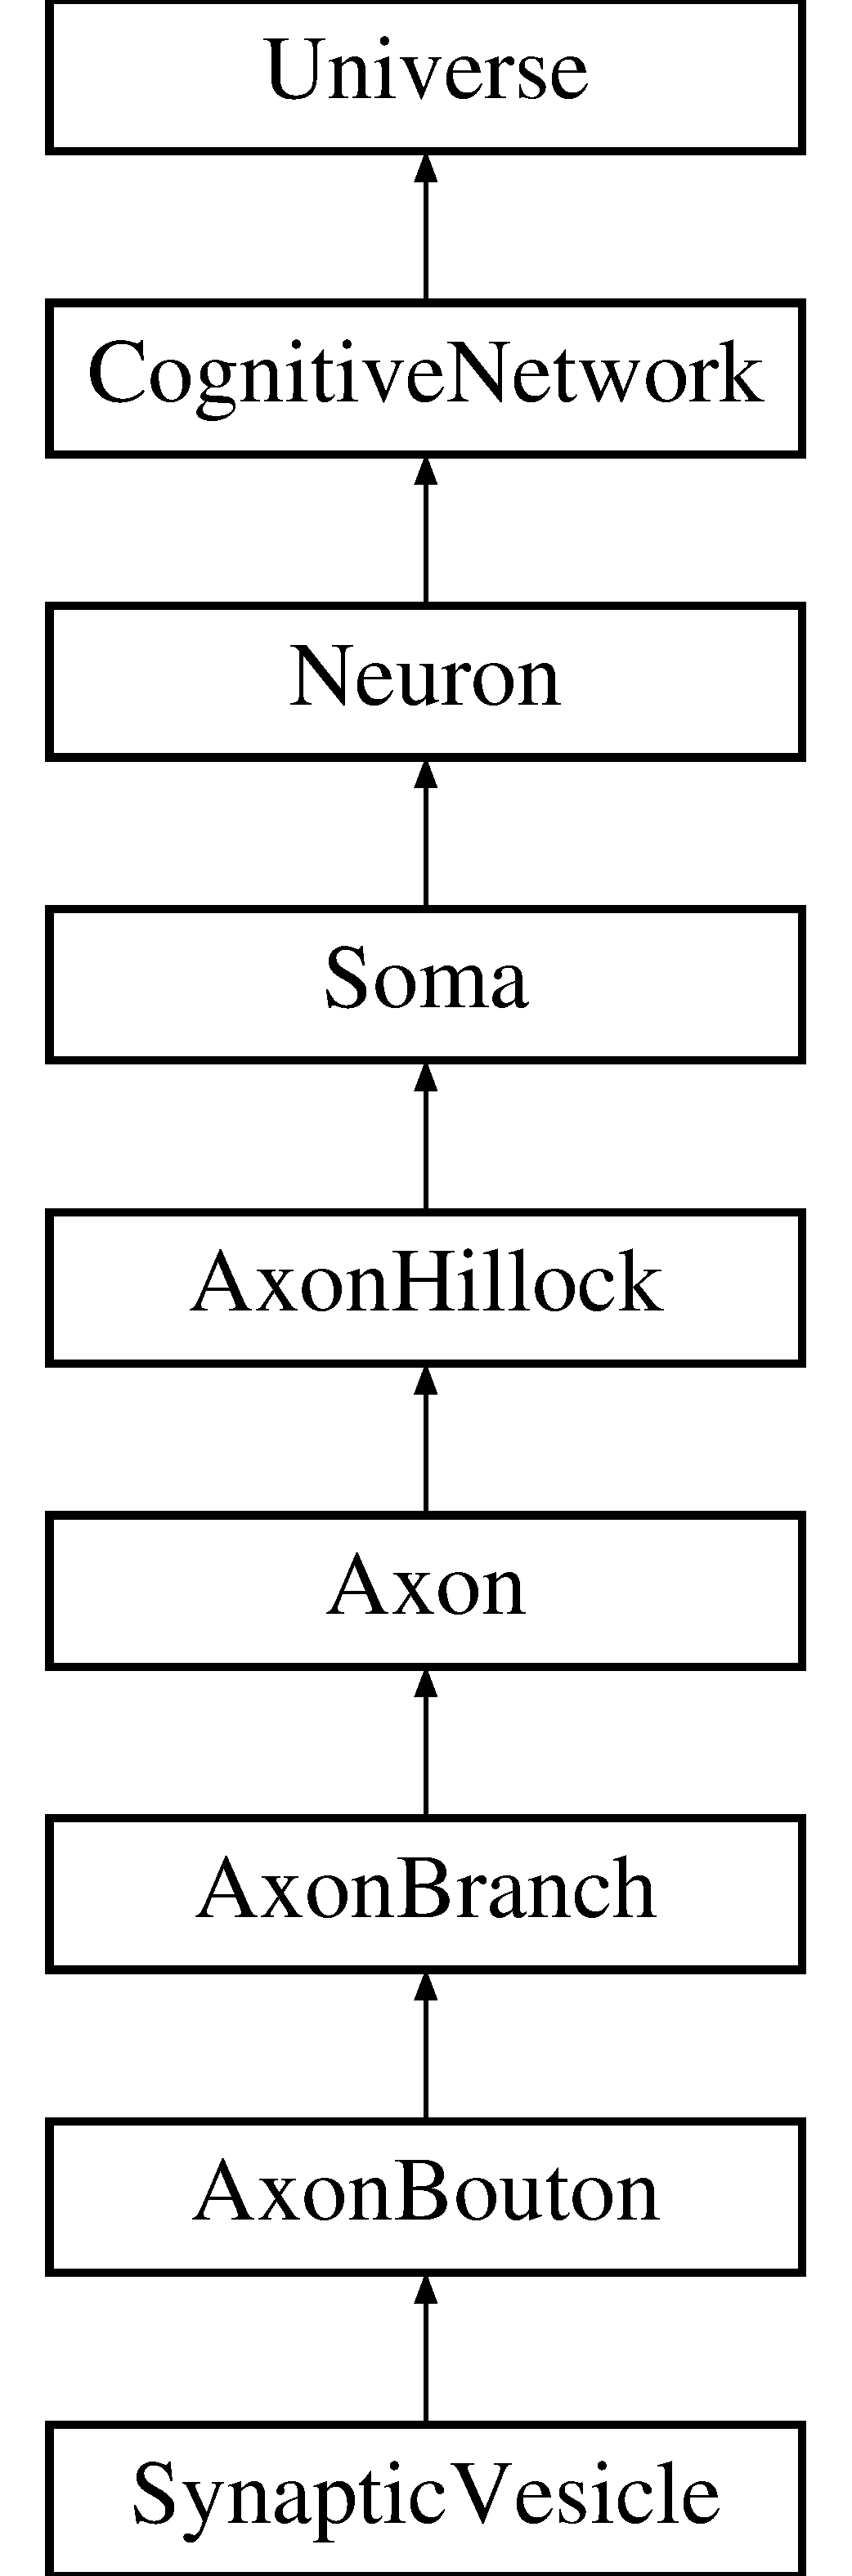
\includegraphics[height=9.000000cm]{classSynapticVesicle}
\end{center}
\end{figure}
\subsection*{Public Member Functions}
\begin{DoxyCompactItemize}
\item 
\mbox{\hyperlink{classSynapticVesicle_ac3f899ed25281a6d337ecefe1da41c67}{Synaptic\+Vesicle}} ()
\item 
\mbox{\hyperlink{classSynapticVesicle_aefd8a743e80077235a1c9a9fd133cc9d}{Synaptic\+Vesicle}} (unsigned int object\+\_\+type)
\item 
\mbox{\hyperlink{classSynapticVesicle_a6602b03ba498129b46c173e8fa66927b}{Synaptic\+Vesicle}} (unsigned int object\+\_\+type, std\+::chrono\+::time\+\_\+point$<$ \mbox{\hyperlink{universe_8h_a0ef8d951d1ca5ab3cfaf7ab4c7a6fd80}{Clock}} $>$ event\+\_\+time)
\item 
\mbox{\hyperlink{classSynapticVesicle_a0f86278b771137978d03bb6cf460a527}{Synaptic\+Vesicle}} (unsigned int object\+\_\+type, std\+::chrono\+::time\+\_\+point$<$ \mbox{\hyperlink{universe_8h_a0ef8d951d1ca5ab3cfaf7ab4c7a6fd80}{Clock}} $>$ event\+\_\+time, \mbox{\hyperlink{classAxonBouton}{Axon\+Bouton}} \&axonbouton\+\_\+connector)
\item 
virtual \mbox{\hyperlink{classSynapticVesicle_a9bbc23a1c9757d8522a10bb28e0f575b}{$\sim$\+Synaptic\+Vesicle}} ()
\item 
unsigned int \mbox{\hyperlink{classSynapticVesicle_a42a3ab6704c27ca55531864c46f0fc2b}{Get\+Counter}} (std\+::chrono\+::time\+\_\+point$<$ \mbox{\hyperlink{universe_8h_a0ef8d951d1ca5ab3cfaf7ab4c7a6fd80}{Clock}} $>$ event\+\_\+time)
\item 
double \mbox{\hyperlink{classSynapticVesicle_a0c4d7e936023cf0f719d0a4d3f315c9c}{Get\+Energy}} (std\+::chrono\+::time\+\_\+point$<$ \mbox{\hyperlink{universe_8h_a0ef8d951d1ca5ab3cfaf7ab4c7a6fd80}{Clock}} $>$ event\+\_\+time)
\item 
int \mbox{\hyperlink{classSynapticVesicle_a6cc0018a0fd02cf99f1ba0ad31f495bc}{Get\+Release\+State}} (std\+::chrono\+::time\+\_\+point$<$ \mbox{\hyperlink{universe_8h_a0ef8d951d1ca5ab3cfaf7ab4c7a6fd80}{Clock}} $>$ event\+\_\+time)
\item 
void \mbox{\hyperlink{classSynapticVesicle_a7fd7cfce5eccb904206d968866f85220}{Set\+Counter}} (std\+::chrono\+::time\+\_\+point$<$ \mbox{\hyperlink{universe_8h_a0ef8d951d1ca5ab3cfaf7ab4c7a6fd80}{Clock}} $>$ event\+\_\+time, unsigned int val)
\item 
void \mbox{\hyperlink{classSynapticVesicle_ac98f9c8ccaabbccc38151c51d204dfec}{Set\+Energy}} (std\+::chrono\+::time\+\_\+point$<$ \mbox{\hyperlink{universe_8h_a0ef8d951d1ca5ab3cfaf7ab4c7a6fd80}{Clock}} $>$ event\+\_\+time, double val)
\item 
bool \mbox{\hyperlink{classSynapticVesicle_add2f2815448729977fbcdbd5a59ec7b4}{Reset\+Parameters}} (std\+::chrono\+::time\+\_\+point$<$ \mbox{\hyperlink{universe_8h_a0ef8d951d1ca5ab3cfaf7ab4c7a6fd80}{Clock}} $>$ event\+\_\+time)
\item 
\mbox{\hyperlink{classCognitiveNetwork}{Cognitive\+Network}} $\ast$ \mbox{\hyperlink{classSynapticVesicle_a89f4fd3ed27a7dc768de215534325d6a}{Create\+Neurotransmitter}} (std\+::chrono\+::time\+\_\+point$<$ \mbox{\hyperlink{universe_8h_a0ef8d951d1ca5ab3cfaf7ab4c7a6fd80}{Clock}} $>$ event\+\_\+time)
\item 
std\+::vector$<$ \mbox{\hyperlink{classCognitiveNetwork}{Cognitive\+Network}} $\ast$ $>$ \mbox{\hyperlink{classSynapticVesicle_a052b85a42c2d55ca146665c40cbabffd}{Create\+Neurotransmitters}} (std\+::chrono\+::time\+\_\+point$<$ \mbox{\hyperlink{universe_8h_a0ef8d951d1ca5ab3cfaf7ab4c7a6fd80}{Clock}} $>$ event\+\_\+time, int quantity)
\item 
\mbox{\hyperlink{classCognitiveNetwork}{Cognitive\+Network}} $\ast$ \mbox{\hyperlink{classSynapticVesicle_aa811e68d1a3220c07140847eb3ebc8b3}{Clone\+Neurotransmitter}} (std\+::chrono\+::time\+\_\+point$<$ \mbox{\hyperlink{universe_8h_a0ef8d951d1ca5ab3cfaf7ab4c7a6fd80}{Clock}} $>$ event\+\_\+time, \mbox{\hyperlink{classCognitiveNetwork}{Cognitive\+Network}} $\ast$clone\+\_\+object, double perfection\+\_\+membership)
\item 
std\+::vector$<$ \mbox{\hyperlink{classCognitiveNetwork}{Cognitive\+Network}} $\ast$ $>$ \mbox{\hyperlink{classSynapticVesicle_aa610e38786a8c9978d9c00bca40a5200}{Clone\+Neurotransmitters}} (std\+::chrono\+::time\+\_\+point$<$ \mbox{\hyperlink{universe_8h_a0ef8d951d1ca5ab3cfaf7ab4c7a6fd80}{Clock}} $>$ event\+\_\+time, std\+::vector$<$ \mbox{\hyperlink{classCognitiveNetwork}{Cognitive\+Network}} $\ast$$>$ cloning\+\_\+list, double perfection\+\_\+membership)
\item 
\mbox{\hyperlink{classCognitiveNetwork}{Cognitive\+Network}} $\ast$ \mbox{\hyperlink{classSynapticVesicle_a5ab4ecfb4a880bc729078f5529c547bc}{Destroy\+Neurotransmitter}} (std\+::chrono\+::time\+\_\+point$<$ \mbox{\hyperlink{universe_8h_a0ef8d951d1ca5ab3cfaf7ab4c7a6fd80}{Clock}} $>$ event\+\_\+time, \mbox{\hyperlink{classCognitiveNetwork}{Cognitive\+Network}} $\ast$destroy\+\_\+object)
\item 
std\+::vector$<$ \mbox{\hyperlink{classCognitiveNetwork}{Cognitive\+Network}} $\ast$ $>$ \mbox{\hyperlink{classSynapticVesicle_a37817cc68b212d89ef8aa08c73631cbb}{Destroy\+Neurotransmitters}} (std\+::chrono\+::time\+\_\+point$<$ \mbox{\hyperlink{universe_8h_a0ef8d951d1ca5ab3cfaf7ab4c7a6fd80}{Clock}} $>$ event\+\_\+time, std\+::vector$<$ \mbox{\hyperlink{classCognitiveNetwork}{Cognitive\+Network}} $\ast$$>$ destruction\+\_\+list)
\item 
\mbox{\hyperlink{classCognitiveNetwork}{Cognitive\+Network}} $\ast$ \mbox{\hyperlink{classSynapticVesicle_a56d406fdd01f267d868caedb390080ff}{Add\+Neurotransmitter}} (std\+::chrono\+::time\+\_\+point$<$ \mbox{\hyperlink{universe_8h_a0ef8d951d1ca5ab3cfaf7ab4c7a6fd80}{Clock}} $>$ event\+\_\+time, \mbox{\hyperlink{classCognitiveNetwork}{Cognitive\+Network}} $\ast$add\+\_\+object)
\item 
std\+::vector$<$ \mbox{\hyperlink{classCognitiveNetwork}{Cognitive\+Network}} $\ast$ $>$ \mbox{\hyperlink{classSynapticVesicle_ac924e6b7b824066a89136e52f2d5ce80}{Add\+Neurotransmitters}} (std\+::chrono\+::time\+\_\+point$<$ \mbox{\hyperlink{universe_8h_a0ef8d951d1ca5ab3cfaf7ab4c7a6fd80}{Clock}} $>$ event\+\_\+time, std\+::vector$<$ \mbox{\hyperlink{classCognitiveNetwork}{Cognitive\+Network}} $\ast$$>$ add\+\_\+objects)
\item 
\mbox{\hyperlink{classCognitiveNetwork}{Cognitive\+Network}} $\ast$ \mbox{\hyperlink{classSynapticVesicle_a7ea7841bd1a7a17c78a023db8860cc22}{Remove\+Neurotransmitter}} (std\+::chrono\+::time\+\_\+point$<$ \mbox{\hyperlink{universe_8h_a0ef8d951d1ca5ab3cfaf7ab4c7a6fd80}{Clock}} $>$ event\+\_\+time)
\item 
std\+::vector$<$ \mbox{\hyperlink{classCognitiveNetwork}{Cognitive\+Network}} $\ast$ $>$ \mbox{\hyperlink{classSynapticVesicle_aab1e61b4910399d56071ca59f2758e72}{Remove\+Neurotransmitters}} (std\+::chrono\+::time\+\_\+point$<$ \mbox{\hyperlink{universe_8h_a0ef8d951d1ca5ab3cfaf7ab4c7a6fd80}{Clock}} $>$ event\+\_\+time, int quantity)
\item 
\mbox{\hyperlink{classCognitiveNetwork}{Cognitive\+Network}} $\ast$ \mbox{\hyperlink{classSynapticVesicle_a3bdf4423899d438b5a1d2246c52c8c45}{Get\+Neurotransmitter}} (std\+::chrono\+::time\+\_\+point$<$ \mbox{\hyperlink{universe_8h_a0ef8d951d1ca5ab3cfaf7ab4c7a6fd80}{Clock}} $>$ event\+\_\+time, int selector)
\item 
std\+::vector$<$ \mbox{\hyperlink{classCognitiveNetwork}{Cognitive\+Network}} $\ast$ $>$ \mbox{\hyperlink{classSynapticVesicle_ada95d85873125115208ff51f60fa72e9}{Get\+Neurotransmitters}} (std\+::chrono\+::time\+\_\+point$<$ \mbox{\hyperlink{universe_8h_a0ef8d951d1ca5ab3cfaf7ab4c7a6fd80}{Clock}} $>$ event\+\_\+time)
\item 
int \mbox{\hyperlink{classSynapticVesicle_a045f27b28b8b11edc884568b390c22fe}{Growth\+Surface}} (std\+::chrono\+::time\+\_\+point$<$ \mbox{\hyperlink{universe_8h_a0ef8d951d1ca5ab3cfaf7ab4c7a6fd80}{Clock}} $>$ event\+\_\+time, double surf\+\_\+change)
\item 
int \mbox{\hyperlink{classSynapticVesicle_a0d4a4a03405593b3abc0e734c1758830}{Growth\+Volume}} (std\+::chrono\+::time\+\_\+point$<$ \mbox{\hyperlink{universe_8h_a0ef8d951d1ca5ab3cfaf7ab4c7a6fd80}{Clock}} $>$ event\+\_\+time, double vol\+\_\+change)
\item 
void \mbox{\hyperlink{classSynapticVesicle_a2509969e82fee789cc56fb0978f27662}{Release\+Neurotransmitters}} (std\+::chrono\+::time\+\_\+point$<$ \mbox{\hyperlink{universe_8h_a0ef8d951d1ca5ab3cfaf7ab4c7a6fd80}{Clock}} $>$ event\+\_\+time)
\item 
int \mbox{\hyperlink{classSynapticVesicle_a49c8e82147e634c83f7b4c3ef9894e2d}{Update}} (std\+::chrono\+::time\+\_\+point$<$ \mbox{\hyperlink{universe_8h_a0ef8d951d1ca5ab3cfaf7ab4c7a6fd80}{Clock}} $>$ event\+\_\+time)
\end{DoxyCompactItemize}
\subsection*{Protected Attributes}
\begin{DoxyCompactItemize}
\item 
std\+::vector$<$ \mbox{\hyperlink{classCognitiveNetwork}{Cognitive\+Network}} $\ast$ $>$ \mbox{\hyperlink{classSynapticVesicle_a6b7fb63806105b89ddad8fd0f56b76f6}{neurotransmitter\+\_\+list}}
\end{DoxyCompactItemize}
\subsection*{Private Attributes}
\begin{DoxyCompactItemize}
\item 
int \mbox{\hyperlink{classSynapticVesicle_a2c71a4e09837c1b4ef2111e0eb634030}{m\+\_\+\+Neuron\+Type}}
\item 
int \mbox{\hyperlink{classSynapticVesicle_afa30c67ce14495976bc167cbd8528cdf}{neurotransmitter\+\_\+pool}}
\item 
int \mbox{\hyperlink{classSynapticVesicle_a568770c79ad49a55129076a1bc625db2}{synapticvesicle\+\_\+type}}
\item 
int \mbox{\hyperlink{classSynapticVesicle_a8a06e1643fa04b7f317523382786f200}{m\+\_\+add\+Status}}
\item 
bool \mbox{\hyperlink{classSynapticVesicle_ad50cf0b70327fd52cd6b2894e19e5842}{object\+\_\+disabled}}
\item 
bool \mbox{\hyperlink{classSynapticVesicle_aef65466f1440e00ad7d352095fe019de}{object\+\_\+initialised}}
\item 
int \mbox{\hyperlink{classSynapticVesicle_a73a7ecd250c4750d9b414c543e534a96}{m\+\_\+\+Release\+State}}
\item 
std\+::chrono\+::time\+\_\+point$<$ \mbox{\hyperlink{universe_8h_a0ef8d951d1ca5ab3cfaf7ab4c7a6fd80}{Clock}} $>$ \mbox{\hyperlink{classSynapticVesicle_af025ff605f37a683bd4a00d9140a217b}{time\+\_\+object\+\_\+created}}
\item 
std\+::chrono\+::time\+\_\+point$<$ \mbox{\hyperlink{universe_8h_a0ef8d951d1ca5ab3cfaf7ab4c7a6fd80}{Clock}} $>$ \mbox{\hyperlink{classSynapticVesicle_a9ba999fc5ee77df5a962592ea4935329}{previous\+\_\+event\+\_\+time}}
\item 
int \mbox{\hyperlink{classSynapticVesicle_add9c814d77d3059a436d5a8ed80b3636}{duration\+\_\+since\+\_\+last\+\_\+event}}
\item 
double \mbox{\hyperlink{classSynapticVesicle_a4cdf034bf90a4131ca05ea5e9ea5fc5e}{m\+\_\+\+Volume}}
\item 
double \mbox{\hyperlink{classSynapticVesicle_aed6d83381706ed28500d3aa9032fd6d0}{m\+\_\+\+Surface\+Area}}
\item 
unsigned int \mbox{\hyperlink{classSynapticVesicle_ad429db4636b70c355d39c212824c9bf4}{m\+\_\+\+Counter}}
\begin{DoxyCompactList}\small\item\em Member variable \char`\"{}m\+\_\+\+Counter\char`\"{}. \end{DoxyCompactList}\item 
double \mbox{\hyperlink{classSynapticVesicle_ad97b48b851a719a0dc2cda6d4c5e3d1b}{object\+\_\+energy}}
\begin{DoxyCompactList}\small\item\em Member variable \char`\"{}object\+\_\+energy\char`\"{}. \end{DoxyCompactList}\item 
double \mbox{\hyperlink{classSynapticVesicle_aafcd5ff5201db3b6d6af126361302607}{m\+\_\+axonlength}}
\item 
double \mbox{\hyperlink{classSynapticVesicle_abedd5d5b6ab7783fc98967c39fbb8acc}{m\+\_\+\+Time\+Dilation}}
\item 
double \mbox{\hyperlink{classSynapticVesicle_a98b593024ea14db5ab7ab5e899c5a733}{m\+\_\+\+Time\+Threshold}}
\end{DoxyCompactItemize}
\subsection*{Additional Inherited Members}


\subsection{Constructor \& Destructor Documentation}
\mbox{\Hypertarget{classSynapticVesicle_ac3f899ed25281a6d337ecefe1da41c67}\label{classSynapticVesicle_ac3f899ed25281a6d337ecefe1da41c67}} 
\index{Synaptic\+Vesicle@{Synaptic\+Vesicle}!Synaptic\+Vesicle@{Synaptic\+Vesicle}}
\index{Synaptic\+Vesicle@{Synaptic\+Vesicle}!Synaptic\+Vesicle@{Synaptic\+Vesicle}}
\subsubsection{\texorpdfstring{Synaptic\+Vesicle()}{SynapticVesicle()}\hspace{0.1cm}{\footnotesize\ttfamily [1/4]}}
{\footnotesize\ttfamily Synaptic\+Vesicle\+::\+Synaptic\+Vesicle (\begin{DoxyParamCaption}{ }\end{DoxyParamCaption})\hspace{0.3cm}{\ttfamily [inline]}}

\mbox{\Hypertarget{classSynapticVesicle_aefd8a743e80077235a1c9a9fd133cc9d}\label{classSynapticVesicle_aefd8a743e80077235a1c9a9fd133cc9d}} 
\index{Synaptic\+Vesicle@{Synaptic\+Vesicle}!Synaptic\+Vesicle@{Synaptic\+Vesicle}}
\index{Synaptic\+Vesicle@{Synaptic\+Vesicle}!Synaptic\+Vesicle@{Synaptic\+Vesicle}}
\subsubsection{\texorpdfstring{Synaptic\+Vesicle()}{SynapticVesicle()}\hspace{0.1cm}{\footnotesize\ttfamily [2/4]}}
{\footnotesize\ttfamily Synaptic\+Vesicle\+::\+Synaptic\+Vesicle (\begin{DoxyParamCaption}\item[{unsigned int}]{object\+\_\+type }\end{DoxyParamCaption})\hspace{0.3cm}{\ttfamily [inline]}}

\mbox{\Hypertarget{classSynapticVesicle_a6602b03ba498129b46c173e8fa66927b}\label{classSynapticVesicle_a6602b03ba498129b46c173e8fa66927b}} 
\index{Synaptic\+Vesicle@{Synaptic\+Vesicle}!Synaptic\+Vesicle@{Synaptic\+Vesicle}}
\index{Synaptic\+Vesicle@{Synaptic\+Vesicle}!Synaptic\+Vesicle@{Synaptic\+Vesicle}}
\subsubsection{\texorpdfstring{Synaptic\+Vesicle()}{SynapticVesicle()}\hspace{0.1cm}{\footnotesize\ttfamily [3/4]}}
{\footnotesize\ttfamily Synaptic\+Vesicle\+::\+Synaptic\+Vesicle (\begin{DoxyParamCaption}\item[{unsigned int}]{object\+\_\+type,  }\item[{std\+::chrono\+::time\+\_\+point$<$ \mbox{\hyperlink{universe_8h_a0ef8d951d1ca5ab3cfaf7ab4c7a6fd80}{Clock}} $>$}]{event\+\_\+time }\end{DoxyParamCaption})\hspace{0.3cm}{\ttfamily [inline]}}

\mbox{\Hypertarget{classSynapticVesicle_a0f86278b771137978d03bb6cf460a527}\label{classSynapticVesicle_a0f86278b771137978d03bb6cf460a527}} 
\index{Synaptic\+Vesicle@{Synaptic\+Vesicle}!Synaptic\+Vesicle@{Synaptic\+Vesicle}}
\index{Synaptic\+Vesicle@{Synaptic\+Vesicle}!Synaptic\+Vesicle@{Synaptic\+Vesicle}}
\subsubsection{\texorpdfstring{Synaptic\+Vesicle()}{SynapticVesicle()}\hspace{0.1cm}{\footnotesize\ttfamily [4/4]}}
{\footnotesize\ttfamily Synaptic\+Vesicle\+::\+Synaptic\+Vesicle (\begin{DoxyParamCaption}\item[{unsigned int}]{object\+\_\+type,  }\item[{std\+::chrono\+::time\+\_\+point$<$ \mbox{\hyperlink{universe_8h_a0ef8d951d1ca5ab3cfaf7ab4c7a6fd80}{Clock}} $>$}]{event\+\_\+time,  }\item[{\mbox{\hyperlink{classAxonBouton}{Axon\+Bouton}} \&}]{axonbouton\+\_\+connector }\end{DoxyParamCaption})\hspace{0.3cm}{\ttfamily [inline]}}

\mbox{\Hypertarget{classSynapticVesicle_a9bbc23a1c9757d8522a10bb28e0f575b}\label{classSynapticVesicle_a9bbc23a1c9757d8522a10bb28e0f575b}} 
\index{Synaptic\+Vesicle@{Synaptic\+Vesicle}!````~Synaptic\+Vesicle@{$\sim$\+Synaptic\+Vesicle}}
\index{````~Synaptic\+Vesicle@{$\sim$\+Synaptic\+Vesicle}!Synaptic\+Vesicle@{Synaptic\+Vesicle}}
\subsubsection{\texorpdfstring{$\sim$\+Synaptic\+Vesicle()}{~SynapticVesicle()}}
{\footnotesize\ttfamily virtual Synaptic\+Vesicle\+::$\sim$\+Synaptic\+Vesicle (\begin{DoxyParamCaption}{ }\end{DoxyParamCaption})\hspace{0.3cm}{\ttfamily [inline]}, {\ttfamily [virtual]}}

Default destructor 

\subsection{Member Function Documentation}
\mbox{\Hypertarget{classSynapticVesicle_a56d406fdd01f267d868caedb390080ff}\label{classSynapticVesicle_a56d406fdd01f267d868caedb390080ff}} 
\index{Synaptic\+Vesicle@{Synaptic\+Vesicle}!Add\+Neurotransmitter@{Add\+Neurotransmitter}}
\index{Add\+Neurotransmitter@{Add\+Neurotransmitter}!Synaptic\+Vesicle@{Synaptic\+Vesicle}}
\subsubsection{\texorpdfstring{Add\+Neurotransmitter()}{AddNeurotransmitter()}}
{\footnotesize\ttfamily \mbox{\hyperlink{classCognitiveNetwork}{Cognitive\+Network}} $\ast$ Synaptic\+Vesicle\+::\+Add\+Neurotransmitter (\begin{DoxyParamCaption}\item[{std\+::chrono\+::time\+\_\+point$<$ \mbox{\hyperlink{universe_8h_a0ef8d951d1ca5ab3cfaf7ab4c7a6fd80}{Clock}} $>$}]{event\+\_\+time,  }\item[{\mbox{\hyperlink{classCognitiveNetwork}{Cognitive\+Network}} $\ast$}]{add\+\_\+object }\end{DoxyParamCaption})}

\mbox{\Hypertarget{classSynapticVesicle_ac924e6b7b824066a89136e52f2d5ce80}\label{classSynapticVesicle_ac924e6b7b824066a89136e52f2d5ce80}} 
\index{Synaptic\+Vesicle@{Synaptic\+Vesicle}!Add\+Neurotransmitters@{Add\+Neurotransmitters}}
\index{Add\+Neurotransmitters@{Add\+Neurotransmitters}!Synaptic\+Vesicle@{Synaptic\+Vesicle}}
\subsubsection{\texorpdfstring{Add\+Neurotransmitters()}{AddNeurotransmitters()}}
{\footnotesize\ttfamily std\+::vector$<$ \mbox{\hyperlink{classCognitiveNetwork}{Cognitive\+Network}} $\ast$ $>$ Synaptic\+Vesicle\+::\+Add\+Neurotransmitters (\begin{DoxyParamCaption}\item[{std\+::chrono\+::time\+\_\+point$<$ \mbox{\hyperlink{universe_8h_a0ef8d951d1ca5ab3cfaf7ab4c7a6fd80}{Clock}} $>$}]{event\+\_\+time,  }\item[{std\+::vector$<$ \mbox{\hyperlink{classCognitiveNetwork}{Cognitive\+Network}} $\ast$$>$}]{add\+\_\+objects }\end{DoxyParamCaption})}

\mbox{\Hypertarget{classSynapticVesicle_aa811e68d1a3220c07140847eb3ebc8b3}\label{classSynapticVesicle_aa811e68d1a3220c07140847eb3ebc8b3}} 
\index{Synaptic\+Vesicle@{Synaptic\+Vesicle}!Clone\+Neurotransmitter@{Clone\+Neurotransmitter}}
\index{Clone\+Neurotransmitter@{Clone\+Neurotransmitter}!Synaptic\+Vesicle@{Synaptic\+Vesicle}}
\subsubsection{\texorpdfstring{Clone\+Neurotransmitter()}{CloneNeurotransmitter()}}
{\footnotesize\ttfamily \mbox{\hyperlink{classCognitiveNetwork}{Cognitive\+Network}} $\ast$ Synaptic\+Vesicle\+::\+Clone\+Neurotransmitter (\begin{DoxyParamCaption}\item[{std\+::chrono\+::time\+\_\+point$<$ \mbox{\hyperlink{universe_8h_a0ef8d951d1ca5ab3cfaf7ab4c7a6fd80}{Clock}} $>$}]{event\+\_\+time,  }\item[{\mbox{\hyperlink{classCognitiveNetwork}{Cognitive\+Network}} $\ast$}]{clone\+\_\+object,  }\item[{double}]{perfection\+\_\+membership }\end{DoxyParamCaption})}

\mbox{\Hypertarget{classSynapticVesicle_aa610e38786a8c9978d9c00bca40a5200}\label{classSynapticVesicle_aa610e38786a8c9978d9c00bca40a5200}} 
\index{Synaptic\+Vesicle@{Synaptic\+Vesicle}!Clone\+Neurotransmitters@{Clone\+Neurotransmitters}}
\index{Clone\+Neurotransmitters@{Clone\+Neurotransmitters}!Synaptic\+Vesicle@{Synaptic\+Vesicle}}
\subsubsection{\texorpdfstring{Clone\+Neurotransmitters()}{CloneNeurotransmitters()}}
{\footnotesize\ttfamily std\+::vector$<$ \mbox{\hyperlink{classCognitiveNetwork}{Cognitive\+Network}} $\ast$ $>$ Synaptic\+Vesicle\+::\+Clone\+Neurotransmitters (\begin{DoxyParamCaption}\item[{std\+::chrono\+::time\+\_\+point$<$ \mbox{\hyperlink{universe_8h_a0ef8d951d1ca5ab3cfaf7ab4c7a6fd80}{Clock}} $>$}]{event\+\_\+time,  }\item[{std\+::vector$<$ \mbox{\hyperlink{classCognitiveNetwork}{Cognitive\+Network}} $\ast$$>$}]{cloning\+\_\+list,  }\item[{double}]{perfection\+\_\+membership }\end{DoxyParamCaption})}

\mbox{\Hypertarget{classSynapticVesicle_a89f4fd3ed27a7dc768de215534325d6a}\label{classSynapticVesicle_a89f4fd3ed27a7dc768de215534325d6a}} 
\index{Synaptic\+Vesicle@{Synaptic\+Vesicle}!Create\+Neurotransmitter@{Create\+Neurotransmitter}}
\index{Create\+Neurotransmitter@{Create\+Neurotransmitter}!Synaptic\+Vesicle@{Synaptic\+Vesicle}}
\subsubsection{\texorpdfstring{Create\+Neurotransmitter()}{CreateNeurotransmitter()}}
{\footnotesize\ttfamily \mbox{\hyperlink{classCognitiveNetwork}{Cognitive\+Network}} $\ast$ Synaptic\+Vesicle\+::\+Create\+Neurotransmitter (\begin{DoxyParamCaption}\item[{std\+::chrono\+::time\+\_\+point$<$ \mbox{\hyperlink{universe_8h_a0ef8d951d1ca5ab3cfaf7ab4c7a6fd80}{Clock}} $>$}]{event\+\_\+time }\end{DoxyParamCaption})}

\mbox{\Hypertarget{classSynapticVesicle_a052b85a42c2d55ca146665c40cbabffd}\label{classSynapticVesicle_a052b85a42c2d55ca146665c40cbabffd}} 
\index{Synaptic\+Vesicle@{Synaptic\+Vesicle}!Create\+Neurotransmitters@{Create\+Neurotransmitters}}
\index{Create\+Neurotransmitters@{Create\+Neurotransmitters}!Synaptic\+Vesicle@{Synaptic\+Vesicle}}
\subsubsection{\texorpdfstring{Create\+Neurotransmitters()}{CreateNeurotransmitters()}}
{\footnotesize\ttfamily std\+::vector$<$ \mbox{\hyperlink{classCognitiveNetwork}{Cognitive\+Network}} $\ast$ $>$ Synaptic\+Vesicle\+::\+Create\+Neurotransmitters (\begin{DoxyParamCaption}\item[{std\+::chrono\+::time\+\_\+point$<$ \mbox{\hyperlink{universe_8h_a0ef8d951d1ca5ab3cfaf7ab4c7a6fd80}{Clock}} $>$}]{event\+\_\+time,  }\item[{int}]{quantity }\end{DoxyParamCaption})}

\mbox{\Hypertarget{classSynapticVesicle_a5ab4ecfb4a880bc729078f5529c547bc}\label{classSynapticVesicle_a5ab4ecfb4a880bc729078f5529c547bc}} 
\index{Synaptic\+Vesicle@{Synaptic\+Vesicle}!Destroy\+Neurotransmitter@{Destroy\+Neurotransmitter}}
\index{Destroy\+Neurotransmitter@{Destroy\+Neurotransmitter}!Synaptic\+Vesicle@{Synaptic\+Vesicle}}
\subsubsection{\texorpdfstring{Destroy\+Neurotransmitter()}{DestroyNeurotransmitter()}}
{\footnotesize\ttfamily \mbox{\hyperlink{classCognitiveNetwork}{Cognitive\+Network}} $\ast$ Synaptic\+Vesicle\+::\+Destroy\+Neurotransmitter (\begin{DoxyParamCaption}\item[{std\+::chrono\+::time\+\_\+point$<$ \mbox{\hyperlink{universe_8h_a0ef8d951d1ca5ab3cfaf7ab4c7a6fd80}{Clock}} $>$}]{event\+\_\+time,  }\item[{\mbox{\hyperlink{classCognitiveNetwork}{Cognitive\+Network}} $\ast$}]{destroy\+\_\+object }\end{DoxyParamCaption})}

\mbox{\Hypertarget{classSynapticVesicle_a37817cc68b212d89ef8aa08c73631cbb}\label{classSynapticVesicle_a37817cc68b212d89ef8aa08c73631cbb}} 
\index{Synaptic\+Vesicle@{Synaptic\+Vesicle}!Destroy\+Neurotransmitters@{Destroy\+Neurotransmitters}}
\index{Destroy\+Neurotransmitters@{Destroy\+Neurotransmitters}!Synaptic\+Vesicle@{Synaptic\+Vesicle}}
\subsubsection{\texorpdfstring{Destroy\+Neurotransmitters()}{DestroyNeurotransmitters()}}
{\footnotesize\ttfamily std\+::vector$<$ \mbox{\hyperlink{classCognitiveNetwork}{Cognitive\+Network}} $\ast$ $>$ Synaptic\+Vesicle\+::\+Destroy\+Neurotransmitters (\begin{DoxyParamCaption}\item[{std\+::chrono\+::time\+\_\+point$<$ \mbox{\hyperlink{universe_8h_a0ef8d951d1ca5ab3cfaf7ab4c7a6fd80}{Clock}} $>$}]{event\+\_\+time,  }\item[{std\+::vector$<$ \mbox{\hyperlink{classCognitiveNetwork}{Cognitive\+Network}} $\ast$$>$}]{destruction\+\_\+list }\end{DoxyParamCaption})}

\mbox{\Hypertarget{classSynapticVesicle_a42a3ab6704c27ca55531864c46f0fc2b}\label{classSynapticVesicle_a42a3ab6704c27ca55531864c46f0fc2b}} 
\index{Synaptic\+Vesicle@{Synaptic\+Vesicle}!Get\+Counter@{Get\+Counter}}
\index{Get\+Counter@{Get\+Counter}!Synaptic\+Vesicle@{Synaptic\+Vesicle}}
\subsubsection{\texorpdfstring{Get\+Counter()}{GetCounter()}}
{\footnotesize\ttfamily unsigned int Synaptic\+Vesicle\+::\+Get\+Counter (\begin{DoxyParamCaption}\item[{std\+::chrono\+::time\+\_\+point$<$ \mbox{\hyperlink{universe_8h_a0ef8d951d1ca5ab3cfaf7ab4c7a6fd80}{Clock}} $>$}]{event\+\_\+time }\end{DoxyParamCaption})\hspace{0.3cm}{\ttfamily [inline]}}

\mbox{\Hypertarget{classSynapticVesicle_a0c4d7e936023cf0f719d0a4d3f315c9c}\label{classSynapticVesicle_a0c4d7e936023cf0f719d0a4d3f315c9c}} 
\index{Synaptic\+Vesicle@{Synaptic\+Vesicle}!Get\+Energy@{Get\+Energy}}
\index{Get\+Energy@{Get\+Energy}!Synaptic\+Vesicle@{Synaptic\+Vesicle}}
\subsubsection{\texorpdfstring{Get\+Energy()}{GetEnergy()}}
{\footnotesize\ttfamily double Synaptic\+Vesicle\+::\+Get\+Energy (\begin{DoxyParamCaption}\item[{std\+::chrono\+::time\+\_\+point$<$ \mbox{\hyperlink{universe_8h_a0ef8d951d1ca5ab3cfaf7ab4c7a6fd80}{Clock}} $>$}]{event\+\_\+time }\end{DoxyParamCaption})\hspace{0.3cm}{\ttfamily [inline]}}

\mbox{\Hypertarget{classSynapticVesicle_a3bdf4423899d438b5a1d2246c52c8c45}\label{classSynapticVesicle_a3bdf4423899d438b5a1d2246c52c8c45}} 
\index{Synaptic\+Vesicle@{Synaptic\+Vesicle}!Get\+Neurotransmitter@{Get\+Neurotransmitter}}
\index{Get\+Neurotransmitter@{Get\+Neurotransmitter}!Synaptic\+Vesicle@{Synaptic\+Vesicle}}
\subsubsection{\texorpdfstring{Get\+Neurotransmitter()}{GetNeurotransmitter()}}
{\footnotesize\ttfamily \mbox{\hyperlink{classCognitiveNetwork}{Cognitive\+Network}} $\ast$ Synaptic\+Vesicle\+::\+Get\+Neurotransmitter (\begin{DoxyParamCaption}\item[{std\+::chrono\+::time\+\_\+point$<$ \mbox{\hyperlink{universe_8h_a0ef8d951d1ca5ab3cfaf7ab4c7a6fd80}{Clock}} $>$}]{event\+\_\+time,  }\item[{int}]{selector }\end{DoxyParamCaption})}

\mbox{\Hypertarget{classSynapticVesicle_ada95d85873125115208ff51f60fa72e9}\label{classSynapticVesicle_ada95d85873125115208ff51f60fa72e9}} 
\index{Synaptic\+Vesicle@{Synaptic\+Vesicle}!Get\+Neurotransmitters@{Get\+Neurotransmitters}}
\index{Get\+Neurotransmitters@{Get\+Neurotransmitters}!Synaptic\+Vesicle@{Synaptic\+Vesicle}}
\subsubsection{\texorpdfstring{Get\+Neurotransmitters()}{GetNeurotransmitters()}}
{\footnotesize\ttfamily std\+::vector$<$ \mbox{\hyperlink{classCognitiveNetwork}{Cognitive\+Network}} $\ast$ $>$ Synaptic\+Vesicle\+::\+Get\+Neurotransmitters (\begin{DoxyParamCaption}\item[{std\+::chrono\+::time\+\_\+point$<$ \mbox{\hyperlink{universe_8h_a0ef8d951d1ca5ab3cfaf7ab4c7a6fd80}{Clock}} $>$}]{event\+\_\+time }\end{DoxyParamCaption})}

\mbox{\Hypertarget{classSynapticVesicle_a6cc0018a0fd02cf99f1ba0ad31f495bc}\label{classSynapticVesicle_a6cc0018a0fd02cf99f1ba0ad31f495bc}} 
\index{Synaptic\+Vesicle@{Synaptic\+Vesicle}!Get\+Release\+State@{Get\+Release\+State}}
\index{Get\+Release\+State@{Get\+Release\+State}!Synaptic\+Vesicle@{Synaptic\+Vesicle}}
\subsubsection{\texorpdfstring{Get\+Release\+State()}{GetReleaseState()}}
{\footnotesize\ttfamily int Synaptic\+Vesicle\+::\+Get\+Release\+State (\begin{DoxyParamCaption}\item[{std\+::chrono\+::time\+\_\+point$<$ \mbox{\hyperlink{universe_8h_a0ef8d951d1ca5ab3cfaf7ab4c7a6fd80}{Clock}} $>$}]{event\+\_\+time }\end{DoxyParamCaption})\hspace{0.3cm}{\ttfamily [inline]}}

\mbox{\Hypertarget{classSynapticVesicle_a045f27b28b8b11edc884568b390c22fe}\label{classSynapticVesicle_a045f27b28b8b11edc884568b390c22fe}} 
\index{Synaptic\+Vesicle@{Synaptic\+Vesicle}!Growth\+Surface@{Growth\+Surface}}
\index{Growth\+Surface@{Growth\+Surface}!Synaptic\+Vesicle@{Synaptic\+Vesicle}}
\subsubsection{\texorpdfstring{Growth\+Surface()}{GrowthSurface()}}
{\footnotesize\ttfamily int Synaptic\+Vesicle\+::\+Growth\+Surface (\begin{DoxyParamCaption}\item[{std\+::chrono\+::time\+\_\+point$<$ \mbox{\hyperlink{universe_8h_a0ef8d951d1ca5ab3cfaf7ab4c7a6fd80}{Clock}} $>$}]{event\+\_\+time,  }\item[{double}]{surf\+\_\+change }\end{DoxyParamCaption})}

\mbox{\Hypertarget{classSynapticVesicle_a0d4a4a03405593b3abc0e734c1758830}\label{classSynapticVesicle_a0d4a4a03405593b3abc0e734c1758830}} 
\index{Synaptic\+Vesicle@{Synaptic\+Vesicle}!Growth\+Volume@{Growth\+Volume}}
\index{Growth\+Volume@{Growth\+Volume}!Synaptic\+Vesicle@{Synaptic\+Vesicle}}
\subsubsection{\texorpdfstring{Growth\+Volume()}{GrowthVolume()}}
{\footnotesize\ttfamily int Synaptic\+Vesicle\+::\+Growth\+Volume (\begin{DoxyParamCaption}\item[{std\+::chrono\+::time\+\_\+point$<$ \mbox{\hyperlink{universe_8h_a0ef8d951d1ca5ab3cfaf7ab4c7a6fd80}{Clock}} $>$}]{event\+\_\+time,  }\item[{double}]{vol\+\_\+change }\end{DoxyParamCaption})}

\mbox{\Hypertarget{classSynapticVesicle_a2509969e82fee789cc56fb0978f27662}\label{classSynapticVesicle_a2509969e82fee789cc56fb0978f27662}} 
\index{Synaptic\+Vesicle@{Synaptic\+Vesicle}!Release\+Neurotransmitters@{Release\+Neurotransmitters}}
\index{Release\+Neurotransmitters@{Release\+Neurotransmitters}!Synaptic\+Vesicle@{Synaptic\+Vesicle}}
\subsubsection{\texorpdfstring{Release\+Neurotransmitters()}{ReleaseNeurotransmitters()}}
{\footnotesize\ttfamily void Synaptic\+Vesicle\+::\+Release\+Neurotransmitters (\begin{DoxyParamCaption}\item[{std\+::chrono\+::time\+\_\+point$<$ \mbox{\hyperlink{universe_8h_a0ef8d951d1ca5ab3cfaf7ab4c7a6fd80}{Clock}} $>$}]{event\+\_\+time }\end{DoxyParamCaption})}

\mbox{\Hypertarget{classSynapticVesicle_a7ea7841bd1a7a17c78a023db8860cc22}\label{classSynapticVesicle_a7ea7841bd1a7a17c78a023db8860cc22}} 
\index{Synaptic\+Vesicle@{Synaptic\+Vesicle}!Remove\+Neurotransmitter@{Remove\+Neurotransmitter}}
\index{Remove\+Neurotransmitter@{Remove\+Neurotransmitter}!Synaptic\+Vesicle@{Synaptic\+Vesicle}}
\subsubsection{\texorpdfstring{Remove\+Neurotransmitter()}{RemoveNeurotransmitter()}}
{\footnotesize\ttfamily \mbox{\hyperlink{classCognitiveNetwork}{Cognitive\+Network}} $\ast$ Synaptic\+Vesicle\+::\+Remove\+Neurotransmitter (\begin{DoxyParamCaption}\item[{std\+::chrono\+::time\+\_\+point$<$ \mbox{\hyperlink{universe_8h_a0ef8d951d1ca5ab3cfaf7ab4c7a6fd80}{Clock}} $>$}]{event\+\_\+time }\end{DoxyParamCaption})}

\mbox{\Hypertarget{classSynapticVesicle_aab1e61b4910399d56071ca59f2758e72}\label{classSynapticVesicle_aab1e61b4910399d56071ca59f2758e72}} 
\index{Synaptic\+Vesicle@{Synaptic\+Vesicle}!Remove\+Neurotransmitters@{Remove\+Neurotransmitters}}
\index{Remove\+Neurotransmitters@{Remove\+Neurotransmitters}!Synaptic\+Vesicle@{Synaptic\+Vesicle}}
\subsubsection{\texorpdfstring{Remove\+Neurotransmitters()}{RemoveNeurotransmitters()}}
{\footnotesize\ttfamily std\+::vector$<$ \mbox{\hyperlink{classCognitiveNetwork}{Cognitive\+Network}} $\ast$ $>$ Synaptic\+Vesicle\+::\+Remove\+Neurotransmitters (\begin{DoxyParamCaption}\item[{std\+::chrono\+::time\+\_\+point$<$ \mbox{\hyperlink{universe_8h_a0ef8d951d1ca5ab3cfaf7ab4c7a6fd80}{Clock}} $>$}]{event\+\_\+time,  }\item[{int}]{quantity }\end{DoxyParamCaption})}

\mbox{\Hypertarget{classSynapticVesicle_add2f2815448729977fbcdbd5a59ec7b4}\label{classSynapticVesicle_add2f2815448729977fbcdbd5a59ec7b4}} 
\index{Synaptic\+Vesicle@{Synaptic\+Vesicle}!Reset\+Parameters@{Reset\+Parameters}}
\index{Reset\+Parameters@{Reset\+Parameters}!Synaptic\+Vesicle@{Synaptic\+Vesicle}}
\subsubsection{\texorpdfstring{Reset\+Parameters()}{ResetParameters()}}
{\footnotesize\ttfamily bool Synaptic\+Vesicle\+::\+Reset\+Parameters (\begin{DoxyParamCaption}\item[{std\+::chrono\+::time\+\_\+point$<$ \mbox{\hyperlink{universe_8h_a0ef8d951d1ca5ab3cfaf7ab4c7a6fd80}{Clock}} $>$}]{event\+\_\+time }\end{DoxyParamCaption})}

\mbox{\Hypertarget{classSynapticVesicle_a7fd7cfce5eccb904206d968866f85220}\label{classSynapticVesicle_a7fd7cfce5eccb904206d968866f85220}} 
\index{Synaptic\+Vesicle@{Synaptic\+Vesicle}!Set\+Counter@{Set\+Counter}}
\index{Set\+Counter@{Set\+Counter}!Synaptic\+Vesicle@{Synaptic\+Vesicle}}
\subsubsection{\texorpdfstring{Set\+Counter()}{SetCounter()}}
{\footnotesize\ttfamily void Synaptic\+Vesicle\+::\+Set\+Counter (\begin{DoxyParamCaption}\item[{std\+::chrono\+::time\+\_\+point$<$ \mbox{\hyperlink{universe_8h_a0ef8d951d1ca5ab3cfaf7ab4c7a6fd80}{Clock}} $>$}]{event\+\_\+time,  }\item[{unsigned int}]{val }\end{DoxyParamCaption})\hspace{0.3cm}{\ttfamily [inline]}, {\ttfamily [virtual]}}



Reimplemented from \mbox{\hyperlink{classAxonBouton_afe285478d414f2815afb98abe7b92898}{Axon\+Bouton}}.

\mbox{\Hypertarget{classSynapticVesicle_ac98f9c8ccaabbccc38151c51d204dfec}\label{classSynapticVesicle_ac98f9c8ccaabbccc38151c51d204dfec}} 
\index{Synaptic\+Vesicle@{Synaptic\+Vesicle}!Set\+Energy@{Set\+Energy}}
\index{Set\+Energy@{Set\+Energy}!Synaptic\+Vesicle@{Synaptic\+Vesicle}}
\subsubsection{\texorpdfstring{Set\+Energy()}{SetEnergy()}}
{\footnotesize\ttfamily void Synaptic\+Vesicle\+::\+Set\+Energy (\begin{DoxyParamCaption}\item[{std\+::chrono\+::time\+\_\+point$<$ \mbox{\hyperlink{universe_8h_a0ef8d951d1ca5ab3cfaf7ab4c7a6fd80}{Clock}} $>$}]{event\+\_\+time,  }\item[{double}]{val }\end{DoxyParamCaption})\hspace{0.3cm}{\ttfamily [inline]}}

\mbox{\Hypertarget{classSynapticVesicle_a49c8e82147e634c83f7b4c3ef9894e2d}\label{classSynapticVesicle_a49c8e82147e634c83f7b4c3ef9894e2d}} 
\index{Synaptic\+Vesicle@{Synaptic\+Vesicle}!Update@{Update}}
\index{Update@{Update}!Synaptic\+Vesicle@{Synaptic\+Vesicle}}
\subsubsection{\texorpdfstring{Update()}{Update()}}
{\footnotesize\ttfamily int Synaptic\+Vesicle\+::\+Update (\begin{DoxyParamCaption}\item[{std\+::chrono\+::time\+\_\+point$<$ \mbox{\hyperlink{universe_8h_a0ef8d951d1ca5ab3cfaf7ab4c7a6fd80}{Clock}} $>$}]{event\+\_\+time }\end{DoxyParamCaption})}



\subsection{Member Data Documentation}
\mbox{\Hypertarget{classSynapticVesicle_add9c814d77d3059a436d5a8ed80b3636}\label{classSynapticVesicle_add9c814d77d3059a436d5a8ed80b3636}} 
\index{Synaptic\+Vesicle@{Synaptic\+Vesicle}!duration\+\_\+since\+\_\+last\+\_\+event@{duration\+\_\+since\+\_\+last\+\_\+event}}
\index{duration\+\_\+since\+\_\+last\+\_\+event@{duration\+\_\+since\+\_\+last\+\_\+event}!Synaptic\+Vesicle@{Synaptic\+Vesicle}}
\subsubsection{\texorpdfstring{duration\+\_\+since\+\_\+last\+\_\+event}{duration\_since\_last\_event}}
{\footnotesize\ttfamily int Synaptic\+Vesicle\+::duration\+\_\+since\+\_\+last\+\_\+event\hspace{0.3cm}{\ttfamily [private]}}

\mbox{\Hypertarget{classSynapticVesicle_a8a06e1643fa04b7f317523382786f200}\label{classSynapticVesicle_a8a06e1643fa04b7f317523382786f200}} 
\index{Synaptic\+Vesicle@{Synaptic\+Vesicle}!m\+\_\+add\+Status@{m\+\_\+add\+Status}}
\index{m\+\_\+add\+Status@{m\+\_\+add\+Status}!Synaptic\+Vesicle@{Synaptic\+Vesicle}}
\subsubsection{\texorpdfstring{m\+\_\+add\+Status}{m\_addStatus}}
{\footnotesize\ttfamily int Synaptic\+Vesicle\+::m\+\_\+add\+Status\hspace{0.3cm}{\ttfamily [private]}}

\mbox{\Hypertarget{classSynapticVesicle_aafcd5ff5201db3b6d6af126361302607}\label{classSynapticVesicle_aafcd5ff5201db3b6d6af126361302607}} 
\index{Synaptic\+Vesicle@{Synaptic\+Vesicle}!m\+\_\+axonlength@{m\+\_\+axonlength}}
\index{m\+\_\+axonlength@{m\+\_\+axonlength}!Synaptic\+Vesicle@{Synaptic\+Vesicle}}
\subsubsection{\texorpdfstring{m\+\_\+axonlength}{m\_axonlength}}
{\footnotesize\ttfamily double Synaptic\+Vesicle\+::m\+\_\+axonlength\hspace{0.3cm}{\ttfamily [private]}}

\mbox{\Hypertarget{classSynapticVesicle_ad429db4636b70c355d39c212824c9bf4}\label{classSynapticVesicle_ad429db4636b70c355d39c212824c9bf4}} 
\index{Synaptic\+Vesicle@{Synaptic\+Vesicle}!m\+\_\+\+Counter@{m\+\_\+\+Counter}}
\index{m\+\_\+\+Counter@{m\+\_\+\+Counter}!Synaptic\+Vesicle@{Synaptic\+Vesicle}}
\subsubsection{\texorpdfstring{m\+\_\+\+Counter}{m\_Counter}}
{\footnotesize\ttfamily unsigned int Synaptic\+Vesicle\+::m\+\_\+\+Counter\hspace{0.3cm}{\ttfamily [private]}}



Member variable \char`\"{}m\+\_\+\+Counter\char`\"{}. 

\mbox{\Hypertarget{classSynapticVesicle_a2c71a4e09837c1b4ef2111e0eb634030}\label{classSynapticVesicle_a2c71a4e09837c1b4ef2111e0eb634030}} 
\index{Synaptic\+Vesicle@{Synaptic\+Vesicle}!m\+\_\+\+Neuron\+Type@{m\+\_\+\+Neuron\+Type}}
\index{m\+\_\+\+Neuron\+Type@{m\+\_\+\+Neuron\+Type}!Synaptic\+Vesicle@{Synaptic\+Vesicle}}
\subsubsection{\texorpdfstring{m\+\_\+\+Neuron\+Type}{m\_NeuronType}}
{\footnotesize\ttfamily int Synaptic\+Vesicle\+::m\+\_\+\+Neuron\+Type\hspace{0.3cm}{\ttfamily [private]}}

\mbox{\Hypertarget{classSynapticVesicle_a73a7ecd250c4750d9b414c543e534a96}\label{classSynapticVesicle_a73a7ecd250c4750d9b414c543e534a96}} 
\index{Synaptic\+Vesicle@{Synaptic\+Vesicle}!m\+\_\+\+Release\+State@{m\+\_\+\+Release\+State}}
\index{m\+\_\+\+Release\+State@{m\+\_\+\+Release\+State}!Synaptic\+Vesicle@{Synaptic\+Vesicle}}
\subsubsection{\texorpdfstring{m\+\_\+\+Release\+State}{m\_ReleaseState}}
{\footnotesize\ttfamily int Synaptic\+Vesicle\+::m\+\_\+\+Release\+State\hspace{0.3cm}{\ttfamily [private]}}

\mbox{\Hypertarget{classSynapticVesicle_aed6d83381706ed28500d3aa9032fd6d0}\label{classSynapticVesicle_aed6d83381706ed28500d3aa9032fd6d0}} 
\index{Synaptic\+Vesicle@{Synaptic\+Vesicle}!m\+\_\+\+Surface\+Area@{m\+\_\+\+Surface\+Area}}
\index{m\+\_\+\+Surface\+Area@{m\+\_\+\+Surface\+Area}!Synaptic\+Vesicle@{Synaptic\+Vesicle}}
\subsubsection{\texorpdfstring{m\+\_\+\+Surface\+Area}{m\_SurfaceArea}}
{\footnotesize\ttfamily double Synaptic\+Vesicle\+::m\+\_\+\+Surface\+Area\hspace{0.3cm}{\ttfamily [private]}}

\mbox{\Hypertarget{classSynapticVesicle_abedd5d5b6ab7783fc98967c39fbb8acc}\label{classSynapticVesicle_abedd5d5b6ab7783fc98967c39fbb8acc}} 
\index{Synaptic\+Vesicle@{Synaptic\+Vesicle}!m\+\_\+\+Time\+Dilation@{m\+\_\+\+Time\+Dilation}}
\index{m\+\_\+\+Time\+Dilation@{m\+\_\+\+Time\+Dilation}!Synaptic\+Vesicle@{Synaptic\+Vesicle}}
\subsubsection{\texorpdfstring{m\+\_\+\+Time\+Dilation}{m\_TimeDilation}}
{\footnotesize\ttfamily double Synaptic\+Vesicle\+::m\+\_\+\+Time\+Dilation\hspace{0.3cm}{\ttfamily [private]}}

\mbox{\Hypertarget{classSynapticVesicle_a98b593024ea14db5ab7ab5e899c5a733}\label{classSynapticVesicle_a98b593024ea14db5ab7ab5e899c5a733}} 
\index{Synaptic\+Vesicle@{Synaptic\+Vesicle}!m\+\_\+\+Time\+Threshold@{m\+\_\+\+Time\+Threshold}}
\index{m\+\_\+\+Time\+Threshold@{m\+\_\+\+Time\+Threshold}!Synaptic\+Vesicle@{Synaptic\+Vesicle}}
\subsubsection{\texorpdfstring{m\+\_\+\+Time\+Threshold}{m\_TimeThreshold}}
{\footnotesize\ttfamily double Synaptic\+Vesicle\+::m\+\_\+\+Time\+Threshold\hspace{0.3cm}{\ttfamily [private]}}

\mbox{\Hypertarget{classSynapticVesicle_a4cdf034bf90a4131ca05ea5e9ea5fc5e}\label{classSynapticVesicle_a4cdf034bf90a4131ca05ea5e9ea5fc5e}} 
\index{Synaptic\+Vesicle@{Synaptic\+Vesicle}!m\+\_\+\+Volume@{m\+\_\+\+Volume}}
\index{m\+\_\+\+Volume@{m\+\_\+\+Volume}!Synaptic\+Vesicle@{Synaptic\+Vesicle}}
\subsubsection{\texorpdfstring{m\+\_\+\+Volume}{m\_Volume}}
{\footnotesize\ttfamily double Synaptic\+Vesicle\+::m\+\_\+\+Volume\hspace{0.3cm}{\ttfamily [private]}}

\mbox{\Hypertarget{classSynapticVesicle_a6b7fb63806105b89ddad8fd0f56b76f6}\label{classSynapticVesicle_a6b7fb63806105b89ddad8fd0f56b76f6}} 
\index{Synaptic\+Vesicle@{Synaptic\+Vesicle}!neurotransmitter\+\_\+list@{neurotransmitter\+\_\+list}}
\index{neurotransmitter\+\_\+list@{neurotransmitter\+\_\+list}!Synaptic\+Vesicle@{Synaptic\+Vesicle}}
\subsubsection{\texorpdfstring{neurotransmitter\+\_\+list}{neurotransmitter\_list}}
{\footnotesize\ttfamily std\+::vector$<$\mbox{\hyperlink{classCognitiveNetwork}{Cognitive\+Network}}$\ast$$>$ Synaptic\+Vesicle\+::neurotransmitter\+\_\+list\hspace{0.3cm}{\ttfamily [protected]}}

\mbox{\Hypertarget{classSynapticVesicle_afa30c67ce14495976bc167cbd8528cdf}\label{classSynapticVesicle_afa30c67ce14495976bc167cbd8528cdf}} 
\index{Synaptic\+Vesicle@{Synaptic\+Vesicle}!neurotransmitter\+\_\+pool@{neurotransmitter\+\_\+pool}}
\index{neurotransmitter\+\_\+pool@{neurotransmitter\+\_\+pool}!Synaptic\+Vesicle@{Synaptic\+Vesicle}}
\subsubsection{\texorpdfstring{neurotransmitter\+\_\+pool}{neurotransmitter\_pool}}
{\footnotesize\ttfamily int Synaptic\+Vesicle\+::neurotransmitter\+\_\+pool\hspace{0.3cm}{\ttfamily [private]}}

\mbox{\Hypertarget{classSynapticVesicle_ad50cf0b70327fd52cd6b2894e19e5842}\label{classSynapticVesicle_ad50cf0b70327fd52cd6b2894e19e5842}} 
\index{Synaptic\+Vesicle@{Synaptic\+Vesicle}!object\+\_\+disabled@{object\+\_\+disabled}}
\index{object\+\_\+disabled@{object\+\_\+disabled}!Synaptic\+Vesicle@{Synaptic\+Vesicle}}
\subsubsection{\texorpdfstring{object\+\_\+disabled}{object\_disabled}}
{\footnotesize\ttfamily bool Synaptic\+Vesicle\+::object\+\_\+disabled\hspace{0.3cm}{\ttfamily [private]}}

\mbox{\Hypertarget{classSynapticVesicle_ad97b48b851a719a0dc2cda6d4c5e3d1b}\label{classSynapticVesicle_ad97b48b851a719a0dc2cda6d4c5e3d1b}} 
\index{Synaptic\+Vesicle@{Synaptic\+Vesicle}!object\+\_\+energy@{object\+\_\+energy}}
\index{object\+\_\+energy@{object\+\_\+energy}!Synaptic\+Vesicle@{Synaptic\+Vesicle}}
\subsubsection{\texorpdfstring{object\+\_\+energy}{object\_energy}}
{\footnotesize\ttfamily double Synaptic\+Vesicle\+::object\+\_\+energy\hspace{0.3cm}{\ttfamily [private]}}



Member variable \char`\"{}object\+\_\+energy\char`\"{}. 

\mbox{\Hypertarget{classSynapticVesicle_aef65466f1440e00ad7d352095fe019de}\label{classSynapticVesicle_aef65466f1440e00ad7d352095fe019de}} 
\index{Synaptic\+Vesicle@{Synaptic\+Vesicle}!object\+\_\+initialised@{object\+\_\+initialised}}
\index{object\+\_\+initialised@{object\+\_\+initialised}!Synaptic\+Vesicle@{Synaptic\+Vesicle}}
\subsubsection{\texorpdfstring{object\+\_\+initialised}{object\_initialised}}
{\footnotesize\ttfamily bool Synaptic\+Vesicle\+::object\+\_\+initialised\hspace{0.3cm}{\ttfamily [private]}}

\mbox{\Hypertarget{classSynapticVesicle_a9ba999fc5ee77df5a962592ea4935329}\label{classSynapticVesicle_a9ba999fc5ee77df5a962592ea4935329}} 
\index{Synaptic\+Vesicle@{Synaptic\+Vesicle}!previous\+\_\+event\+\_\+time@{previous\+\_\+event\+\_\+time}}
\index{previous\+\_\+event\+\_\+time@{previous\+\_\+event\+\_\+time}!Synaptic\+Vesicle@{Synaptic\+Vesicle}}
\subsubsection{\texorpdfstring{previous\+\_\+event\+\_\+time}{previous\_event\_time}}
{\footnotesize\ttfamily std\+::chrono\+::time\+\_\+point$<$\mbox{\hyperlink{universe_8h_a0ef8d951d1ca5ab3cfaf7ab4c7a6fd80}{Clock}}$>$ Synaptic\+Vesicle\+::previous\+\_\+event\+\_\+time\hspace{0.3cm}{\ttfamily [private]}}

\mbox{\Hypertarget{classSynapticVesicle_a568770c79ad49a55129076a1bc625db2}\label{classSynapticVesicle_a568770c79ad49a55129076a1bc625db2}} 
\index{Synaptic\+Vesicle@{Synaptic\+Vesicle}!synapticvesicle\+\_\+type@{synapticvesicle\+\_\+type}}
\index{synapticvesicle\+\_\+type@{synapticvesicle\+\_\+type}!Synaptic\+Vesicle@{Synaptic\+Vesicle}}
\subsubsection{\texorpdfstring{synapticvesicle\+\_\+type}{synapticvesicle\_type}}
{\footnotesize\ttfamily int Synaptic\+Vesicle\+::synapticvesicle\+\_\+type\hspace{0.3cm}{\ttfamily [private]}}

\mbox{\Hypertarget{classSynapticVesicle_af025ff605f37a683bd4a00d9140a217b}\label{classSynapticVesicle_af025ff605f37a683bd4a00d9140a217b}} 
\index{Synaptic\+Vesicle@{Synaptic\+Vesicle}!time\+\_\+object\+\_\+created@{time\+\_\+object\+\_\+created}}
\index{time\+\_\+object\+\_\+created@{time\+\_\+object\+\_\+created}!Synaptic\+Vesicle@{Synaptic\+Vesicle}}
\subsubsection{\texorpdfstring{time\+\_\+object\+\_\+created}{time\_object\_created}}
{\footnotesize\ttfamily std\+::chrono\+::time\+\_\+point$<$\mbox{\hyperlink{universe_8h_a0ef8d951d1ca5ab3cfaf7ab4c7a6fd80}{Clock}}$>$ Synaptic\+Vesicle\+::time\+\_\+object\+\_\+created\hspace{0.3cm}{\ttfamily [private]}}



The documentation for this class was generated from the following files\+:\begin{DoxyCompactItemize}
\item 
/home/pbisaacs/\+Developer/\+Brain\+Harmonics/\+Brain\+Harmonics/\mbox{\hyperlink{synapticvesicle_8h}{synapticvesicle.\+h}}\item 
/home/pbisaacs/\+Developer/\+Brain\+Harmonics/\+Brain\+Harmonics/\mbox{\hyperlink{synapticvesicle_8cc}{synapticvesicle.\+cc}}\end{DoxyCompactItemize}

\hypertarget{classUniverse}{}\section{Universe Class Reference}
\label{classUniverse}\index{Universe@{Universe}}


{\ttfamily \#include $<$universe.\+h$>$}

Inheritance diagram for Universe\+:\begin{figure}[H]
\begin{center}
\leavevmode
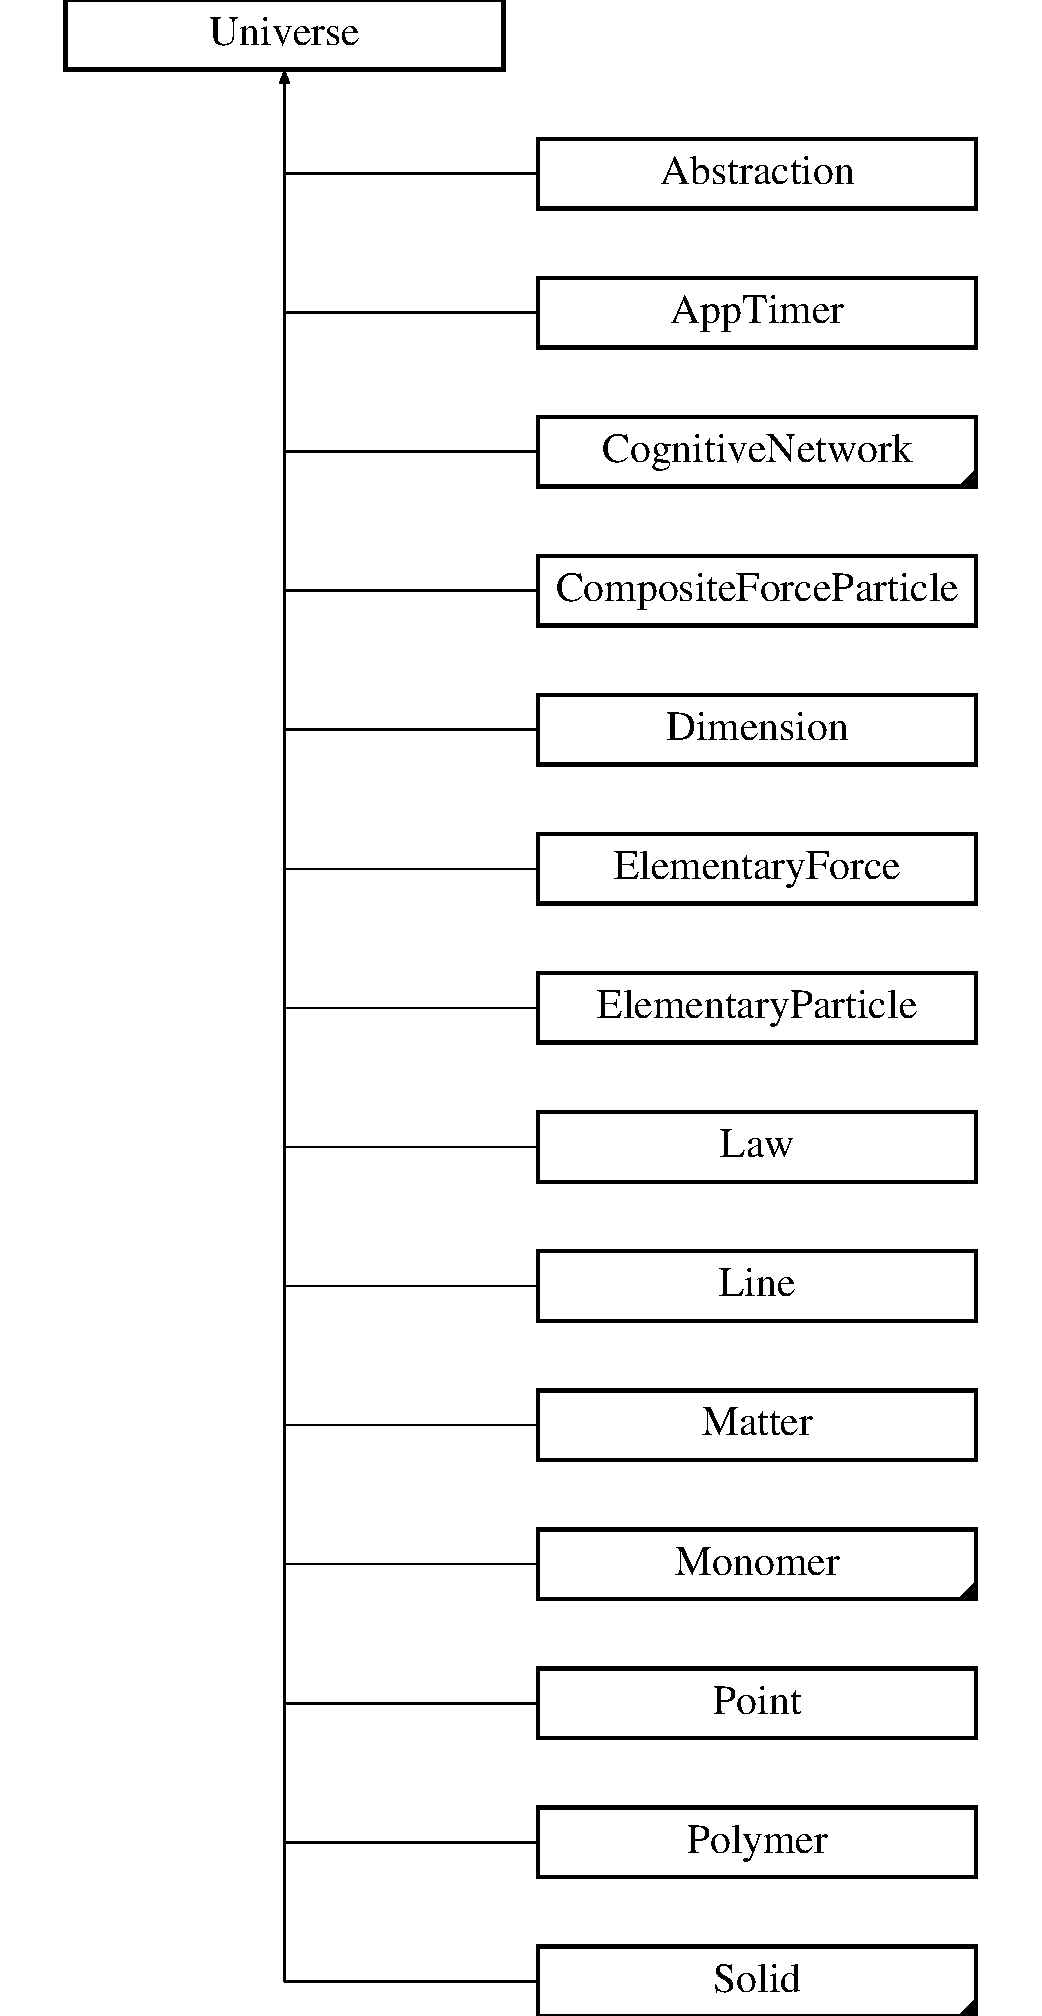
\includegraphics[height=12.000000cm]{classUniverse}
\end{center}
\end{figure}
\subsection*{Public Member Functions}
\begin{DoxyCompactItemize}
\item 
\mbox{\hyperlink{classUniverse_a4d137a146dd3c2514dfb692dfbab6984}{Universe}} ()
\item 
\mbox{\hyperlink{classUniverse_a1210ce56049f1fc67f53aeda223bb82b}{Universe}} (int interim\+\_\+object\+\_\+type)
\item 
\mbox{\hyperlink{classUniverse_a03af7455263d3028b55ca5dc93ebb6ba}{Universe}} (std\+::chrono\+::time\+\_\+point$<$ \mbox{\hyperlink{universe_8h_a0ef8d951d1ca5ab3cfaf7ab4c7a6fd80}{Clock}} $>$ event\+\_\+time, int object\+\_\+type)
\item 
virtual \mbox{\hyperlink{classUniverse_ad4d90f6f2727992762c6b409d3d3d228}{$\sim$\+Universe}} ()
\item 
double \mbox{\hyperlink{classUniverse_a3b25e7ce6552991b7d5e6a9eb6e8a7ff}{Get\+Energy}} (std\+::chrono\+::time\+\_\+point$<$ \mbox{\hyperlink{universe_8h_a0ef8d951d1ca5ab3cfaf7ab4c7a6fd80}{Clock}} $>$ event\+\_\+time)
\item 
void \mbox{\hyperlink{classUniverse_a868250e67d0fcb2483aa8bdd73c40a02}{Set\+Energy}} (std\+::chrono\+::time\+\_\+point$<$ \mbox{\hyperlink{universe_8h_a0ef8d951d1ca5ab3cfaf7ab4c7a6fd80}{Clock}} $>$ event\+\_\+time, double energy\+\_\+transfer)
\item 
double \mbox{\hyperlink{classUniverse_a63e878aaf03f1800b255e9a089a72a8b}{Use\+Energy}} (std\+::chrono\+::time\+\_\+point$<$ \mbox{\hyperlink{universe_8h_a0ef8d951d1ca5ab3cfaf7ab4c7a6fd80}{Clock}} $>$ event\+\_\+time, double energy\+\_\+transfer)
\item 
double \mbox{\hyperlink{classUniverse_aeda74e3902c0e56c0c09779854045cde}{Return\+Energy}} (std\+::chrono\+::time\+\_\+point$<$ \mbox{\hyperlink{universe_8h_a0ef8d951d1ca5ab3cfaf7ab4c7a6fd80}{Clock}} $>$ event\+\_\+time, double energy\+\_\+transfer)
\item 
void \mbox{\hyperlink{classUniverse_a28615baf47d4558cbe5eebeed6575024}{Creation}} (std\+::chrono\+::time\+\_\+point$<$ \mbox{\hyperlink{universe_8h_a0ef8d951d1ca5ab3cfaf7ab4c7a6fd80}{Clock}} $>$ event\+\_\+time, std\+::string object\+\_\+title, int object\+\_\+type)
\item 
void \mbox{\hyperlink{classUniverse_a2274a54fbdc7504c897e4272162bf17a}{Set\+Object\+Type}} (std\+::chrono\+::time\+\_\+point$<$ \mbox{\hyperlink{universe_8h_a0ef8d951d1ca5ab3cfaf7ab4c7a6fd80}{Clock}} $>$ event\+\_\+time, int object\+\_\+type)
\item 
bool \mbox{\hyperlink{classUniverse_a1d92b2277564577571c802f6e0c206dd}{Reset\+Parameters}} (std\+::chrono\+::time\+\_\+point$<$ \mbox{\hyperlink{universe_8h_a0ef8d951d1ca5ab3cfaf7ab4c7a6fd80}{Clock}} $>$ event\+\_\+time)
\item 
std\+::chrono\+::time\+\_\+point$<$ std\+::chrono\+::high\+\_\+resolution\+\_\+clock $>$ \mbox{\hyperlink{classUniverse_ae54d34c5d695917e074b8e07e8820bdb}{The\+Time\+Now}} ()
\item 
std\+::chrono\+::time\+\_\+point$<$ std\+::chrono\+::high\+\_\+resolution\+\_\+clock $>$ \mbox{\hyperlink{classUniverse_aa220508c4cc12b02c6fe494622ebb58d}{The\+Calculated\+Time\+Now}} (std\+::chrono\+::time\+\_\+point$<$ std\+::chrono\+::high\+\_\+resolution\+\_\+clock $>$ time\+\_\+object\+\_\+created\+\_\+time, std\+::chrono\+::time\+\_\+point$<$ \mbox{\hyperlink{universe_8h_a0ef8d951d1ca5ab3cfaf7ab4c7a6fd80}{Clock}} $>$ event\+\_\+time, double calculated\+\_\+scaled\+\_\+time)
\item 
void \mbox{\hyperlink{classUniverse_ac3443dd59b61ae3110f07f681f63ed0a}{Set\+Lifespan}} (std\+::chrono\+::time\+\_\+point$<$ \mbox{\hyperlink{universe_8h_a0ef8d951d1ca5ab3cfaf7ab4c7a6fd80}{Clock}} $>$ event\+\_\+time, std\+::chrono\+::nanoseconds life\+\_\+time)
\item 
void \mbox{\hyperlink{classUniverse_a982502e46868a00a9111738ccc9355c2}{Extend\+Life}} (std\+::chrono\+::time\+\_\+point$<$ \mbox{\hyperlink{universe_8h_a0ef8d951d1ca5ab3cfaf7ab4c7a6fd80}{Clock}} $>$ event\+\_\+time, std\+::chrono\+::nanoseconds life\+\_\+time)
\item 
bool \mbox{\hyperlink{classUniverse_a8fdaa6d06584e1ef50c4c613b22b786e}{Is\+Dead}} (std\+::chrono\+::time\+\_\+point$<$ \mbox{\hyperlink{universe_8h_a0ef8d951d1ca5ab3cfaf7ab4c7a6fd80}{Clock}} $>$ event\+\_\+time)
\item 
std\+::vector$<$ \mbox{\hyperlink{classUniverse}{Universe}} $\ast$ $>$ \mbox{\hyperlink{classUniverse_a03bdf5f7fea4209241e9bf5316d45517}{Add\+Dimensions}} (std\+::chrono\+::time\+\_\+point$<$ \mbox{\hyperlink{universe_8h_a0ef8d951d1ca5ab3cfaf7ab4c7a6fd80}{Clock}} $>$ event\+\_\+time, int quantity)
\item 
\mbox{\hyperlink{classUniverse}{Universe}} $\ast$ \mbox{\hyperlink{classUniverse_a6326158c47bf3f7fe9297299a9b5b7b7}{Add\+Dimension}} (std\+::chrono\+::time\+\_\+point$<$ \mbox{\hyperlink{universe_8h_a0ef8d951d1ca5ab3cfaf7ab4c7a6fd80}{Clock}} $>$ event\+\_\+time)
\item 
std\+::vector$<$ \mbox{\hyperlink{classUniverse}{Universe}} $\ast$ $>$ \mbox{\hyperlink{classUniverse_a1869fc7bf43827378bab5a701f7f917a}{Get\+Dimensions}} (std\+::chrono\+::time\+\_\+point$<$ \mbox{\hyperlink{universe_8h_a0ef8d951d1ca5ab3cfaf7ab4c7a6fd80}{Clock}} $>$ event\+\_\+time)
\item 
\mbox{\hyperlink{classUniverse}{Universe}} $\ast$ \mbox{\hyperlink{classUniverse_ab79a380dee684c6dc304b571f4d28645}{Get\+Dimension}} (std\+::chrono\+::time\+\_\+point$<$ \mbox{\hyperlink{universe_8h_a0ef8d951d1ca5ab3cfaf7ab4c7a6fd80}{Clock}} $>$ event\+\_\+time, int selector)
\item 
\mbox{\hyperlink{classDimension}{Dimension}} $\ast$ \mbox{\hyperlink{classUniverse_a79b95c06aadea69cec3b51046cd9e0f8}{Get\+Time\+Dimension}} (std\+::chrono\+::time\+\_\+point$<$ \mbox{\hyperlink{universe_8h_a0ef8d951d1ca5ab3cfaf7ab4c7a6fd80}{Clock}} $>$ event\+\_\+time)
\item 
std\+::vector$<$ \mbox{\hyperlink{classUniverse}{Universe}} $\ast$ $>$ \mbox{\hyperlink{classUniverse_a857cf7f208cd11c80736e82fa523feb5}{Add\+Elementary\+Particles}} (std\+::chrono\+::time\+\_\+point$<$ \mbox{\hyperlink{universe_8h_a0ef8d951d1ca5ab3cfaf7ab4c7a6fd80}{Clock}} $>$ event\+\_\+time, int quantity)
\item 
\mbox{\hyperlink{classUniverse}{Universe}} $\ast$ \mbox{\hyperlink{classUniverse_ab9c84e0576de50aa4fa46655832ce5e4}{Add\+Elementary\+Particle}} (std\+::chrono\+::time\+\_\+point$<$ \mbox{\hyperlink{universe_8h_a0ef8d951d1ca5ab3cfaf7ab4c7a6fd80}{Clock}} $>$ event\+\_\+time)
\item 
std\+::vector$<$ \mbox{\hyperlink{classUniverse}{Universe}} $\ast$ $>$ \mbox{\hyperlink{classUniverse_a168fd9bf7602adcba1de5dd93a212775}{Get\+Elementary\+Particles}} (std\+::chrono\+::time\+\_\+point$<$ \mbox{\hyperlink{universe_8h_a0ef8d951d1ca5ab3cfaf7ab4c7a6fd80}{Clock}} $>$ event\+\_\+time)
\item 
\mbox{\hyperlink{classUniverse}{Universe}} $\ast$ \mbox{\hyperlink{classUniverse_acef54e17666d17078c522388f8f6e4f9}{Get\+Elementary\+Particle}} (std\+::chrono\+::time\+\_\+point$<$ \mbox{\hyperlink{universe_8h_a0ef8d951d1ca5ab3cfaf7ab4c7a6fd80}{Clock}} $>$ event\+\_\+time, int selector)
\item 
std\+::vector$<$ \mbox{\hyperlink{classUniverse}{Universe}} $\ast$ $>$ \mbox{\hyperlink{classUniverse_a81d294300346e9f901836ab609cce942}{Add\+Elementary\+Forces}} (std\+::chrono\+::time\+\_\+point$<$ \mbox{\hyperlink{universe_8h_a0ef8d951d1ca5ab3cfaf7ab4c7a6fd80}{Clock}} $>$ event\+\_\+time, int quantity)
\item 
\mbox{\hyperlink{classUniverse}{Universe}} $\ast$ \mbox{\hyperlink{classUniverse_a90c573dec55f2b3ad5680015356f5f25}{Add\+Elementary\+Force}} (std\+::chrono\+::time\+\_\+point$<$ \mbox{\hyperlink{universe_8h_a0ef8d951d1ca5ab3cfaf7ab4c7a6fd80}{Clock}} $>$ event\+\_\+time)
\item 
std\+::vector$<$ \mbox{\hyperlink{classUniverse}{Universe}} $\ast$ $>$ \mbox{\hyperlink{classUniverse_a6a8ed579b2eedd3aceebda9f3d78aa0e}{Get\+Elementary\+Forces}} (std\+::chrono\+::time\+\_\+point$<$ \mbox{\hyperlink{universe_8h_a0ef8d951d1ca5ab3cfaf7ab4c7a6fd80}{Clock}} $>$ event\+\_\+time)
\item 
\mbox{\hyperlink{classUniverse}{Universe}} $\ast$ \mbox{\hyperlink{classUniverse_a9506017d944cb64e67567477c1505a53}{Get\+Elementary\+Force}} (std\+::chrono\+::time\+\_\+point$<$ \mbox{\hyperlink{universe_8h_a0ef8d951d1ca5ab3cfaf7ab4c7a6fd80}{Clock}} $>$ event\+\_\+time, int selector)
\item 
std\+::vector$<$ \mbox{\hyperlink{classUniverse}{Universe}} $\ast$ $>$ \mbox{\hyperlink{classUniverse_a23d74e377203fca7cb74e0ffee7244b6}{Add\+Composite\+Force\+Particles}} (std\+::chrono\+::time\+\_\+point$<$ \mbox{\hyperlink{universe_8h_a0ef8d951d1ca5ab3cfaf7ab4c7a6fd80}{Clock}} $>$ event\+\_\+time, int quantity)
\item 
\mbox{\hyperlink{classUniverse}{Universe}} $\ast$ \mbox{\hyperlink{classUniverse_ab2671c2218c98f0f1f487c5b3bb96e3c}{Add\+Composite\+Force\+Particle}} (std\+::chrono\+::time\+\_\+point$<$ \mbox{\hyperlink{universe_8h_a0ef8d951d1ca5ab3cfaf7ab4c7a6fd80}{Clock}} $>$ event\+\_\+time)
\item 
std\+::vector$<$ \mbox{\hyperlink{classUniverse}{Universe}} $\ast$ $>$ \mbox{\hyperlink{classUniverse_aed37d7224b4e31bdfb0632e39bf19694}{Get\+Composite\+Force\+Particles}} (std\+::chrono\+::time\+\_\+point$<$ \mbox{\hyperlink{universe_8h_a0ef8d951d1ca5ab3cfaf7ab4c7a6fd80}{Clock}} $>$ event\+\_\+time)
\item 
\mbox{\hyperlink{classUniverse}{Universe}} $\ast$ \mbox{\hyperlink{classUniverse_a3e2acc1d75765a6e8e852fca919c5b96}{Get\+Composite\+Force\+Particle}} (std\+::chrono\+::time\+\_\+point$<$ \mbox{\hyperlink{universe_8h_a0ef8d951d1ca5ab3cfaf7ab4c7a6fd80}{Clock}} $>$ event\+\_\+time, int selector)
\item 
std\+::vector$<$ \mbox{\hyperlink{classUniverse}{Universe}} $\ast$ $>$ \mbox{\hyperlink{classUniverse_ae00d10b2a23c9cedf1ff89e9da875563}{Add\+Matters}} (std\+::chrono\+::time\+\_\+point$<$ \mbox{\hyperlink{universe_8h_a0ef8d951d1ca5ab3cfaf7ab4c7a6fd80}{Clock}} $>$ event\+\_\+time, int quantity)
\item 
\mbox{\hyperlink{classUniverse}{Universe}} $\ast$ \mbox{\hyperlink{classUniverse_a090d9ad1b88d81364e872e17d65edca4}{Add\+Matter}} (std\+::chrono\+::time\+\_\+point$<$ \mbox{\hyperlink{universe_8h_a0ef8d951d1ca5ab3cfaf7ab4c7a6fd80}{Clock}} $>$ event\+\_\+time)
\item 
std\+::vector$<$ \mbox{\hyperlink{classUniverse}{Universe}} $\ast$ $>$ \mbox{\hyperlink{classUniverse_a4307a62e183fed8cf2b92be0f6014688}{Get\+Matters}} (std\+::chrono\+::time\+\_\+point$<$ \mbox{\hyperlink{universe_8h_a0ef8d951d1ca5ab3cfaf7ab4c7a6fd80}{Clock}} $>$ event\+\_\+time)
\item 
\mbox{\hyperlink{classUniverse}{Universe}} $\ast$ \mbox{\hyperlink{classUniverse_a69de663cf2e32e65ed28c44ae666db3a}{Get\+Matter}} (std\+::chrono\+::time\+\_\+point$<$ \mbox{\hyperlink{universe_8h_a0ef8d951d1ca5ab3cfaf7ab4c7a6fd80}{Clock}} $>$ event\+\_\+time, int selector)
\item 
std\+::vector$<$ \mbox{\hyperlink{classUniverse}{Universe}} $\ast$ $>$ \mbox{\hyperlink{classUniverse_a95fe7f99971bb2048121a7c4e87b9f79}{Add\+Monomers}} (std\+::chrono\+::time\+\_\+point$<$ \mbox{\hyperlink{universe_8h_a0ef8d951d1ca5ab3cfaf7ab4c7a6fd80}{Clock}} $>$ event\+\_\+time, int quantity)
\item 
\mbox{\hyperlink{classUniverse}{Universe}} $\ast$ \mbox{\hyperlink{classUniverse_a062a9472f0400e566ecc7dc056d989d9}{Add\+Monomer}} (std\+::chrono\+::time\+\_\+point$<$ \mbox{\hyperlink{universe_8h_a0ef8d951d1ca5ab3cfaf7ab4c7a6fd80}{Clock}} $>$ event\+\_\+time)
\item 
std\+::vector$<$ \mbox{\hyperlink{classUniverse}{Universe}} $\ast$ $>$ \mbox{\hyperlink{classUniverse_aca82a914e0f8bd7cd1ec80a7220f0a0e}{Get\+Monomers}} (std\+::chrono\+::time\+\_\+point$<$ \mbox{\hyperlink{universe_8h_a0ef8d951d1ca5ab3cfaf7ab4c7a6fd80}{Clock}} $>$ event\+\_\+time)
\item 
\mbox{\hyperlink{classUniverse}{Universe}} $\ast$ \mbox{\hyperlink{classUniverse_aaa03fb8178d790afd992dd094bb64b47}{Get\+Monomer}} (std\+::chrono\+::time\+\_\+point$<$ \mbox{\hyperlink{universe_8h_a0ef8d951d1ca5ab3cfaf7ab4c7a6fd80}{Clock}} $>$ event\+\_\+time, int selector)
\item 
std\+::vector$<$ \mbox{\hyperlink{classUniverse}{Universe}} $\ast$ $>$ \mbox{\hyperlink{classUniverse_aed7cb25507d516a2821ebb69d5345c54}{Add\+Polymers}} (std\+::chrono\+::time\+\_\+point$<$ \mbox{\hyperlink{universe_8h_a0ef8d951d1ca5ab3cfaf7ab4c7a6fd80}{Clock}} $>$ event\+\_\+time, int quantity)
\item 
\mbox{\hyperlink{classUniverse}{Universe}} $\ast$ \mbox{\hyperlink{classUniverse_a4ea0af5d2eb7b5070a83f7da29526fbd}{Add\+Polymer}} (std\+::chrono\+::time\+\_\+point$<$ \mbox{\hyperlink{universe_8h_a0ef8d951d1ca5ab3cfaf7ab4c7a6fd80}{Clock}} $>$ event\+\_\+time)
\item 
std\+::vector$<$ \mbox{\hyperlink{classUniverse}{Universe}} $\ast$ $>$ \mbox{\hyperlink{classUniverse_aac5d1c1a3a3ba56c8ca7115a85b2c239}{Get\+Polymers}} (std\+::chrono\+::time\+\_\+point$<$ \mbox{\hyperlink{universe_8h_a0ef8d951d1ca5ab3cfaf7ab4c7a6fd80}{Clock}} $>$ event\+\_\+time)
\item 
\mbox{\hyperlink{classUniverse}{Universe}} $\ast$ \mbox{\hyperlink{classUniverse_a2d5d3924a7d7ffd2a5f47be9f137d86e}{Get\+Polymer}} (std\+::chrono\+::time\+\_\+point$<$ \mbox{\hyperlink{universe_8h_a0ef8d951d1ca5ab3cfaf7ab4c7a6fd80}{Clock}} $>$ event\+\_\+time, int selector)
\item 
std\+::vector$<$ \mbox{\hyperlink{classUniverse}{Universe}} $\ast$ $>$ \mbox{\hyperlink{classUniverse_a410d5ba2224fe90584b1f1aa5b38b41c}{Add\+Solids}} (std\+::chrono\+::time\+\_\+point$<$ \mbox{\hyperlink{universe_8h_a0ef8d951d1ca5ab3cfaf7ab4c7a6fd80}{Clock}} $>$ event\+\_\+time, int quantity)
\item 
\mbox{\hyperlink{classUniverse}{Universe}} $\ast$ \mbox{\hyperlink{classUniverse_a598799e2fcdf9ed60e83e9f5a61bfc05}{Add\+Solid}} (std\+::chrono\+::time\+\_\+point$<$ \mbox{\hyperlink{universe_8h_a0ef8d951d1ca5ab3cfaf7ab4c7a6fd80}{Clock}} $>$ event\+\_\+time)
\item 
std\+::vector$<$ \mbox{\hyperlink{classUniverse}{Universe}} $\ast$ $>$ \mbox{\hyperlink{classUniverse_a669fc068dd7820a5af309bfbe67199aa}{Get\+Solids}} (std\+::chrono\+::time\+\_\+point$<$ \mbox{\hyperlink{universe_8h_a0ef8d951d1ca5ab3cfaf7ab4c7a6fd80}{Clock}} $>$ event\+\_\+time)
\item 
\mbox{\hyperlink{classUniverse}{Universe}} $\ast$ \mbox{\hyperlink{classUniverse_a9f7b74fc21d45ddaa78aa18e9a337bcd}{Get\+Solid}} (std\+::chrono\+::time\+\_\+point$<$ \mbox{\hyperlink{universe_8h_a0ef8d951d1ca5ab3cfaf7ab4c7a6fd80}{Clock}} $>$ event\+\_\+time, int selector)
\item 
std\+::vector$<$ \mbox{\hyperlink{classUniverse}{Universe}} $\ast$ $>$ \mbox{\hyperlink{classUniverse_a5199f6c27b1a97c8b8c9847b8be686cf}{Add\+Cognitive\+Networks}} (std\+::chrono\+::time\+\_\+point$<$ \mbox{\hyperlink{universe_8h_a0ef8d951d1ca5ab3cfaf7ab4c7a6fd80}{Clock}} $>$ event\+\_\+time, int quantity)
\item 
\mbox{\hyperlink{classUniverse}{Universe}} $\ast$ \mbox{\hyperlink{classUniverse_ab682307c963836cd81b35b5604bd7064}{Add\+Cognitive\+Network}} (std\+::chrono\+::time\+\_\+point$<$ \mbox{\hyperlink{universe_8h_a0ef8d951d1ca5ab3cfaf7ab4c7a6fd80}{Clock}} $>$ event\+\_\+time)
\item 
std\+::vector$<$ \mbox{\hyperlink{classUniverse}{Universe}} $\ast$ $>$ \mbox{\hyperlink{classUniverse_a06968a24194280a43f077c5b77379ea8}{Get\+Cognitive\+Networks}} (std\+::chrono\+::time\+\_\+point$<$ \mbox{\hyperlink{universe_8h_a0ef8d951d1ca5ab3cfaf7ab4c7a6fd80}{Clock}} $>$ event\+\_\+time)
\item 
\mbox{\hyperlink{classUniverse}{Universe}} $\ast$ \mbox{\hyperlink{classUniverse_a1ea2b7e438bfdc7dd599aa59c310b126}{Get\+Cognitive\+Network}} (std\+::chrono\+::time\+\_\+point$<$ \mbox{\hyperlink{universe_8h_a0ef8d951d1ca5ab3cfaf7ab4c7a6fd80}{Clock}} $>$ event\+\_\+time, int selector)
\item 
std\+::vector$<$ \mbox{\hyperlink{classUniverse}{Universe}} $\ast$ $>$ \mbox{\hyperlink{classUniverse_aa48ced2078ba863723050d8283b3fa67}{Add\+Points}} (std\+::chrono\+::time\+\_\+point$<$ \mbox{\hyperlink{universe_8h_a0ef8d951d1ca5ab3cfaf7ab4c7a6fd80}{Clock}} $>$ event\+\_\+time, int quantity)
\item 
\mbox{\hyperlink{classUniverse}{Universe}} $\ast$ \mbox{\hyperlink{classUniverse_a8508b791c6997d8abcdcc037a6776734}{Add\+Point}} (std\+::chrono\+::time\+\_\+point$<$ \mbox{\hyperlink{universe_8h_a0ef8d951d1ca5ab3cfaf7ab4c7a6fd80}{Clock}} $>$ event\+\_\+time)
\item 
std\+::vector$<$ \mbox{\hyperlink{classUniverse}{Universe}} $\ast$ $>$ \mbox{\hyperlink{classUniverse_a765c6c658b7a465cd92418690db846ae}{Get\+Points}} (std\+::chrono\+::time\+\_\+point$<$ \mbox{\hyperlink{universe_8h_a0ef8d951d1ca5ab3cfaf7ab4c7a6fd80}{Clock}} $>$ event\+\_\+time)
\item 
\mbox{\hyperlink{classUniverse}{Universe}} $\ast$ \mbox{\hyperlink{classUniverse_a3774f14a13a55827a1a4eea0a404edcb}{Get\+Point}} (std\+::chrono\+::time\+\_\+point$<$ \mbox{\hyperlink{universe_8h_a0ef8d951d1ca5ab3cfaf7ab4c7a6fd80}{Clock}} $>$ event\+\_\+time, int selector)
\item 
void \mbox{\hyperlink{classUniverse_a0d79e614e1af951c06b78cb5768f9c8e}{Update\+Cycle}} (std\+::chrono\+::time\+\_\+point$<$ \mbox{\hyperlink{universe_8h_a0ef8d951d1ca5ab3cfaf7ab4c7a6fd80}{Clock}} $>$ event\+\_\+time, std\+::vector$<$ \mbox{\hyperlink{classUniverse}{Universe}} $\ast$$>$ set\+\_\+of\+\_\+update\+\_\+pointers, unsigned int pointer\+\_\+type)
\item 
int \mbox{\hyperlink{classUniverse_a64ee5a2c7e86c56fa426acb750438ce9}{Update}} (std\+::chrono\+::time\+\_\+point$<$ \mbox{\hyperlink{universe_8h_a0ef8d951d1ca5ab3cfaf7ab4c7a6fd80}{Clock}} $>$ event\+\_\+time)
\item 
virtual void \mbox{\hyperlink{classUniverse_a901e16db5e8af258c66af7ac75662fe0}{Add\+Temporal\+Adjustment}} (std\+::chrono\+::time\+\_\+point$<$ \mbox{\hyperlink{universe_8h_a0ef8d951d1ca5ab3cfaf7ab4c7a6fd80}{Clock}} $>$ event\+\_\+time, double $\ast$point\+\_\+to\+\_\+counter, double pool, int interval, int shape)
\item 
virtual void \mbox{\hyperlink{classUniverse_a15aa20218286fd11ecb9b792dfb63be3}{Adjust\+Counters}} (std\+::chrono\+::time\+\_\+point$<$ std\+::chrono\+::high\+\_\+resolution\+\_\+clock $>$ current\+Time)
\item 
virtual void \mbox{\hyperlink{classUniverse_a3b3da7c86a7b75e5e5c0b7972ac82a87}{Set\+Charge}} (std\+::chrono\+::time\+\_\+point$<$ \mbox{\hyperlink{universe_8h_a0ef8d951d1ca5ab3cfaf7ab4c7a6fd80}{Clock}} $>$ event\+\_\+time, int val)
\item 
virtual void \mbox{\hyperlink{classUniverse_ae2ae1c3b3e4cde2c18f5f6a814761ec8}{Set\+Spin}} (std\+::chrono\+::time\+\_\+point$<$ \mbox{\hyperlink{universe_8h_a0ef8d951d1ca5ab3cfaf7ab4c7a6fd80}{Clock}} $>$ event\+\_\+time, int val)
\item 
virtual double \mbox{\hyperlink{classUniverse_ab0404e774ee0ed66b597ff5b8e989446}{Get\+Gravitation}} (std\+::chrono\+::time\+\_\+point$<$ \mbox{\hyperlink{universe_8h_a0ef8d951d1ca5ab3cfaf7ab4c7a6fd80}{Clock}} $>$ event\+\_\+time)
\item 
virtual double \mbox{\hyperlink{classUniverse_a4476b7e0a3fc1764909f556257fd9ec7}{Get\+Weak}} (std\+::chrono\+::time\+\_\+point$<$ \mbox{\hyperlink{universe_8h_a0ef8d951d1ca5ab3cfaf7ab4c7a6fd80}{Clock}} $>$ event\+\_\+time)
\item 
virtual double \mbox{\hyperlink{classUniverse_a645299738e6b798a037f2a15a2e7cf4d}{Get\+Weak\+Electroweak}} (std\+::chrono\+::time\+\_\+point$<$ \mbox{\hyperlink{universe_8h_a0ef8d951d1ca5ab3cfaf7ab4c7a6fd80}{Clock}} $>$ event\+\_\+time)
\item 
virtual double \mbox{\hyperlink{classUniverse_a63b850ef3f3394313353109d222bf5d1}{Get\+Electromagnetic}} (std\+::chrono\+::time\+\_\+point$<$ \mbox{\hyperlink{universe_8h_a0ef8d951d1ca5ab3cfaf7ab4c7a6fd80}{Clock}} $>$ event\+\_\+time)
\item 
virtual double \mbox{\hyperlink{classUniverse_a9f099605c082e7fa755787a6a8cab7ba}{Get\+Electromagnetic\+Electroweak}} (std\+::chrono\+::time\+\_\+point$<$ \mbox{\hyperlink{universe_8h_a0ef8d951d1ca5ab3cfaf7ab4c7a6fd80}{Clock}} $>$ event\+\_\+time)
\item 
virtual double \mbox{\hyperlink{classUniverse_acb453ce71da418c5b5617fecede9571b}{Get\+Strong}} (std\+::chrono\+::time\+\_\+point$<$ \mbox{\hyperlink{universe_8h_a0ef8d951d1ca5ab3cfaf7ab4c7a6fd80}{Clock}} $>$ event\+\_\+time)
\item 
virtual double \mbox{\hyperlink{classUniverse_ab44daccba01ee7e3cf9b50bba83dd19e}{Get\+Strong\+Fundamental}} (std\+::chrono\+::time\+\_\+point$<$ \mbox{\hyperlink{universe_8h_a0ef8d951d1ca5ab3cfaf7ab4c7a6fd80}{Clock}} $>$ event\+\_\+time)
\item 
virtual double \mbox{\hyperlink{classUniverse_af0f4b81950061e63c2855eb40957a5b1}{Get\+Strong\+Residual}} (std\+::chrono\+::time\+\_\+point$<$ \mbox{\hyperlink{universe_8h_a0ef8d951d1ca5ab3cfaf7ab4c7a6fd80}{Clock}} $>$ event\+\_\+time)
\item 
virtual double \mbox{\hyperlink{classUniverse_a76c0b5e63c2a7d1988c44db341c3d64c}{Apply\+Gravitation}} (std\+::chrono\+::time\+\_\+point$<$ \mbox{\hyperlink{universe_8h_a0ef8d951d1ca5ab3cfaf7ab4c7a6fd80}{Clock}} $>$ event\+\_\+time, double val)
\item 
virtual double \mbox{\hyperlink{classUniverse_a6d1226b3adec3c42a833afdbb6a65a92}{Apply\+Weak}} (std\+::chrono\+::time\+\_\+point$<$ \mbox{\hyperlink{universe_8h_a0ef8d951d1ca5ab3cfaf7ab4c7a6fd80}{Clock}} $>$ event\+\_\+time, double val)
\item 
virtual double \mbox{\hyperlink{classUniverse_a46a906baabb63e5d31f8b48ea1fae52e}{Apply\+Weak\+Electroweak}} (std\+::chrono\+::time\+\_\+point$<$ \mbox{\hyperlink{universe_8h_a0ef8d951d1ca5ab3cfaf7ab4c7a6fd80}{Clock}} $>$ event\+\_\+time, double val)
\item 
virtual double \mbox{\hyperlink{classUniverse_a1f787da78fa196ba635db21a9e91dabb}{Apply\+Electromagnetic}} (std\+::chrono\+::time\+\_\+point$<$ \mbox{\hyperlink{universe_8h_a0ef8d951d1ca5ab3cfaf7ab4c7a6fd80}{Clock}} $>$ event\+\_\+time, double val)
\item 
virtual double \mbox{\hyperlink{classUniverse_a4c36c1ab30db993307f88363dde5e8c5}{Apply\+Electromagnetic\+Electroweak}} (std\+::chrono\+::time\+\_\+point$<$ \mbox{\hyperlink{universe_8h_a0ef8d951d1ca5ab3cfaf7ab4c7a6fd80}{Clock}} $>$ event\+\_\+time, double val)
\item 
virtual double \mbox{\hyperlink{classUniverse_a906a88b37f10bfa630bef49dfd0e907a}{Apply\+Strong}} (std\+::chrono\+::time\+\_\+point$<$ \mbox{\hyperlink{universe_8h_a0ef8d951d1ca5ab3cfaf7ab4c7a6fd80}{Clock}} $>$ event\+\_\+time, double val)
\item 
virtual double \mbox{\hyperlink{classUniverse_a62789bcff84bd750b0366004381e2fdd}{Apply\+Strong\+Fundamental}} (std\+::chrono\+::time\+\_\+point$<$ \mbox{\hyperlink{universe_8h_a0ef8d951d1ca5ab3cfaf7ab4c7a6fd80}{Clock}} $>$ event\+\_\+time, double val)
\item 
virtual double \mbox{\hyperlink{classUniverse_af7becebb347be9a85541d96a3eca1ca7}{Apply\+Strong\+Residual}} (std\+::chrono\+::time\+\_\+point$<$ \mbox{\hyperlink{universe_8h_a0ef8d951d1ca5ab3cfaf7ab4c7a6fd80}{Clock}} $>$ event\+\_\+time, double val)
\item 
virtual void \mbox{\hyperlink{classUniverse_aa22202ae740eb1355529afcb13285e91}{Set\+Counter}} (std\+::chrono\+::time\+\_\+point$<$ \mbox{\hyperlink{universe_8h_a0ef8d951d1ca5ab3cfaf7ab4c7a6fd80}{Clock}} $>$ event\+\_\+time, unsigned int val)
\item 
virtual void \mbox{\hyperlink{classUniverse_ae0cb8d86b2fbb8396d605160344b42f5}{Set\+Gravitation}} (std\+::chrono\+::time\+\_\+point$<$ \mbox{\hyperlink{universe_8h_a0ef8d951d1ca5ab3cfaf7ab4c7a6fd80}{Clock}} $>$ event\+\_\+time, double val)
\item 
virtual void \mbox{\hyperlink{classUniverse_a0f5cd04081b41ee931c0557dc397f6fb}{Set\+Weak}} (std\+::chrono\+::time\+\_\+point$<$ \mbox{\hyperlink{universe_8h_a0ef8d951d1ca5ab3cfaf7ab4c7a6fd80}{Clock}} $>$ event\+\_\+time, double val)
\item 
virtual void \mbox{\hyperlink{classUniverse_a2d3d642bfdc863248e93535832fa4b00}{Set\+Weak\+Electroweak}} (std\+::chrono\+::time\+\_\+point$<$ \mbox{\hyperlink{universe_8h_a0ef8d951d1ca5ab3cfaf7ab4c7a6fd80}{Clock}} $>$ event\+\_\+time, double val)
\item 
virtual void \mbox{\hyperlink{classUniverse_aa981fc7e252b1fbbb675f0371860954d}{Set\+Electromagnetic}} (std\+::chrono\+::time\+\_\+point$<$ \mbox{\hyperlink{universe_8h_a0ef8d951d1ca5ab3cfaf7ab4c7a6fd80}{Clock}} $>$ event\+\_\+time, double val)
\item 
virtual void \mbox{\hyperlink{classUniverse_a608aa95698380f791a0ffba45cc1bee3}{Set\+Electromagnetic\+Electroweak}} (std\+::chrono\+::time\+\_\+point$<$ \mbox{\hyperlink{universe_8h_a0ef8d951d1ca5ab3cfaf7ab4c7a6fd80}{Clock}} $>$ event\+\_\+time, double val)
\item 
virtual void \mbox{\hyperlink{classUniverse_a5946c8f3d4cda305f3ecd10df21a2f94}{Set\+Strong}} (std\+::chrono\+::time\+\_\+point$<$ \mbox{\hyperlink{universe_8h_a0ef8d951d1ca5ab3cfaf7ab4c7a6fd80}{Clock}} $>$ event\+\_\+time, double val)
\item 
virtual void \mbox{\hyperlink{classUniverse_aafec97a231126b71c73ac1258609a284}{Set\+Strong\+Fundamental}} (std\+::chrono\+::time\+\_\+point$<$ \mbox{\hyperlink{universe_8h_a0ef8d951d1ca5ab3cfaf7ab4c7a6fd80}{Clock}} $>$ event\+\_\+time, double val)
\item 
virtual void \mbox{\hyperlink{classUniverse_a1b2d6197ddf3d613cc30bd04d22ed8b7}{Set\+Strong\+Residual}} (std\+::chrono\+::time\+\_\+point$<$ \mbox{\hyperlink{universe_8h_a0ef8d951d1ca5ab3cfaf7ab4c7a6fd80}{Clock}} $>$ event\+\_\+time, double val)
\item 
virtual void \mbox{\hyperlink{classUniverse_a0c485c504542409cbb5cfd8543c35b11}{Poll\+Elementary\+Force}} (std\+::chrono\+::time\+\_\+point$<$ \mbox{\hyperlink{universe_8h_a0ef8d951d1ca5ab3cfaf7ab4c7a6fd80}{Clock}} $>$ event\+\_\+time)
\end{DoxyCompactItemize}
\subsection*{Public Attributes}
\begin{DoxyCompactItemize}
\item 
double \mbox{\hyperlink{classUniverse_ab64777e25c83216e7a91d2761a10463c}{object\+\_\+energy}}
\item 
double \mbox{\hyperlink{classUniverse_a17c8d799331a5b32837f285c12cbe858}{object\+\_\+energy\+\_\+threshold}}
\item 
int \mbox{\hyperlink{classUniverse_a64f4f4025c9be1d84492c766a002a6d4}{object\+\_\+size}}
\item 
\mbox{\hyperlink{classUniverse}{Universe}} $\ast$ \mbox{\hyperlink{classUniverse_a3ce4365c727cb6eb5b650146a4188b9b}{time\+\_\+dimension\+\_\+pointer}}
\end{DoxyCompactItemize}
\subsection*{Protected Attributes}
\begin{DoxyCompactItemize}
\item 
std\+::vector$<$ \mbox{\hyperlink{classUniverse}{Universe}} $\ast$ $>$ \mbox{\hyperlink{classUniverse_a7a0e9796ff0d650a8b1fbde5fa5b761f}{cognitive\+\_\+network\+\_\+list}}
\item 
std\+::vector$<$ \mbox{\hyperlink{classUniverse}{Universe}} $\ast$ $>$ \mbox{\hyperlink{classUniverse_ae9795d06e406c4322637825aa545aa2f}{composite\+\_\+forceparticle\+\_\+list}}
\item 
std\+::vector$<$ \mbox{\hyperlink{classUniverse}{Universe}} $\ast$ $>$ \mbox{\hyperlink{classUniverse_a159461f7098c3a30274f54c8acff6eac}{dimension\+\_\+list}}
\item 
std\+::vector$<$ \mbox{\hyperlink{classUniverse}{Universe}} $\ast$ $>$ \mbox{\hyperlink{classUniverse_a015b19f6d5ad84ebaa9e3e7c8352389c}{elementary\+\_\+force\+\_\+list}}
\item 
std\+::vector$<$ \mbox{\hyperlink{classUniverse}{Universe}} $\ast$ $>$ \mbox{\hyperlink{classUniverse_aeb2e63cf49f0b5595e6c15109863bd3b}{elementary\+\_\+particle\+\_\+list}}
\item 
std\+::vector$<$ \mbox{\hyperlink{classUniverse}{Universe}} $\ast$ $>$ \mbox{\hyperlink{classUniverse_a409650bc0425fc22c7713487a2a6dd8e}{matter\+\_\+list}}
\item 
std\+::vector$<$ \mbox{\hyperlink{classUniverse}{Universe}} $\ast$ $>$ \mbox{\hyperlink{classUniverse_a3d55ba29f95a9793b69c01f7942eca9f}{monomer\+\_\+list}}
\item 
std\+::vector$<$ \mbox{\hyperlink{classUniverse}{Universe}} $\ast$ $>$ \mbox{\hyperlink{classUniverse_a4d898757f2d67ca5ab5d504388d6199a}{polymer\+\_\+list}}
\item 
std\+::vector$<$ \mbox{\hyperlink{classUniverse}{Universe}} $\ast$ $>$ \mbox{\hyperlink{classUniverse_a747f9d3cf0b2caada4461cb7b12ea17b}{solid\+\_\+list}}
\item 
std\+::vector$<$ \mbox{\hyperlink{classUniverse}{Universe}} $\ast$ $>$ \mbox{\hyperlink{classUniverse_a9dc8abd2f8f84318722184f38e1b8cc7}{point\+\_\+list}}
\end{DoxyCompactItemize}
\subsection*{Private Attributes}
\begin{DoxyCompactItemize}
\item 
friend \mbox{\hyperlink{classUniverse_aeccab978b0db45b64015aebdf44fa2d8}{Dimension}}
\item 
bool \mbox{\hyperlink{classUniverse_af8893059e57118d5da20d512b1df4d20}{object\+\_\+initialised}} = false
\item 
int \mbox{\hyperlink{classUniverse_a76279bc43f1ce7a7fc4ee2f6a2cf4228}{duration\+\_\+since\+\_\+last\+\_\+event}}
\item 
int \mbox{\hyperlink{classUniverse_a6c530f6d3647d078794b1060afbb1acf}{default\+\_\+object\+\_\+type}}
\item 
int \mbox{\hyperlink{classUniverse_ac7a26cb9cb97f61bb270a7bbef4a2ae2}{test\+\_\+subject\+\_\+one}} = 0
\item 
int \mbox{\hyperlink{classUniverse_ae4768ac314bcab322ffe484658b2bb06}{test\+\_\+subject\+\_\+two}} = 0
\item 
int \mbox{\hyperlink{classUniverse_a4332e3210a61dcfcb26e16b9f604d489}{universe\+\_\+type}}
\begin{DoxyCompactList}\small\item\em Member variable \char`\"{}universe\+\_\+type\char`\"{}. \end{DoxyCompactList}\item 
double \mbox{\hyperlink{classUniverse_a86742eff738f3d7812da8581a59f0812}{universe\+\_\+energy}}
\begin{DoxyCompactList}\small\item\em Member variable \char`\"{}universe\+\_\+energy\char`\"{}. \end{DoxyCompactList}\item 
double \mbox{\hyperlink{classUniverse_a0406fae45a576526b0ea78b2b5a74ebb}{scaled\+\_\+time}}
\begin{DoxyCompactList}\small\item\em Member variable \char`\"{}scaled\+\_\+time\char`\"{}. \end{DoxyCompactList}\item 
std\+::chrono\+::time\+\_\+point$<$ \mbox{\hyperlink{universe_8h_a0ef8d951d1ca5ab3cfaf7ab4c7a6fd80}{Clock}} $>$ \mbox{\hyperlink{classUniverse_a49ef0c3c2bd9ec438f5d9703c6aaa402}{time\+\_\+object\+\_\+created}}
\begin{DoxyCompactList}\small\item\em Member variable \char`\"{}time\+\_\+object\+\_\+created\char`\"{}. \end{DoxyCompactList}\item 
std\+::chrono\+::time\+\_\+point$<$ \mbox{\hyperlink{universe_8h_a0ef8d951d1ca5ab3cfaf7ab4c7a6fd80}{Clock}} $>$ \mbox{\hyperlink{classUniverse_aacac76865f3600d5f308b83db9809184}{object\+\_\+expiration}}
\begin{DoxyCompactList}\small\item\em Member variable \char`\"{}object\+\_\+expiration\char`\"{}. \end{DoxyCompactList}\item 
std\+::chrono\+::time\+\_\+point$<$ \mbox{\hyperlink{universe_8h_a0ef8d951d1ca5ab3cfaf7ab4c7a6fd80}{Clock}} $>$ \mbox{\hyperlink{classUniverse_ad31a1d2865f16b1b8f4c597e116416e8}{previous\+\_\+event\+\_\+time}}
\item 
std\+::chrono\+::nanoseconds \mbox{\hyperlink{classUniverse_acb8bc2b083f0227a0427a5fbe6109286}{object\+\_\+lifespan}}
\begin{DoxyCompactList}\small\item\em Member variable \char`\"{}object\+\_\+lifespan\char`\"{}. \end{DoxyCompactList}\end{DoxyCompactItemize}


\subsection{Constructor \& Destructor Documentation}
\mbox{\Hypertarget{classUniverse_a4d137a146dd3c2514dfb692dfbab6984}\label{classUniverse_a4d137a146dd3c2514dfb692dfbab6984}} 
\index{Universe@{Universe}!Universe@{Universe}}
\index{Universe@{Universe}!Universe@{Universe}}
\subsubsection{\texorpdfstring{Universe()}{Universe()}\hspace{0.1cm}{\footnotesize\ttfamily [1/3]}}
{\footnotesize\ttfamily Universe\+::\+Universe (\begin{DoxyParamCaption}{ }\end{DoxyParamCaption})\hspace{0.3cm}{\ttfamily [inline]}}

\mbox{\Hypertarget{classUniverse_a1210ce56049f1fc67f53aeda223bb82b}\label{classUniverse_a1210ce56049f1fc67f53aeda223bb82b}} 
\index{Universe@{Universe}!Universe@{Universe}}
\index{Universe@{Universe}!Universe@{Universe}}
\subsubsection{\texorpdfstring{Universe()}{Universe()}\hspace{0.1cm}{\footnotesize\ttfamily [2/3]}}
{\footnotesize\ttfamily Universe\+::\+Universe (\begin{DoxyParamCaption}\item[{int}]{interim\+\_\+object\+\_\+type }\end{DoxyParamCaption})\hspace{0.3cm}{\ttfamily [inline]}}

\mbox{\Hypertarget{classUniverse_a03af7455263d3028b55ca5dc93ebb6ba}\label{classUniverse_a03af7455263d3028b55ca5dc93ebb6ba}} 
\index{Universe@{Universe}!Universe@{Universe}}
\index{Universe@{Universe}!Universe@{Universe}}
\subsubsection{\texorpdfstring{Universe()}{Universe()}\hspace{0.1cm}{\footnotesize\ttfamily [3/3]}}
{\footnotesize\ttfamily Universe\+::\+Universe (\begin{DoxyParamCaption}\item[{std\+::chrono\+::time\+\_\+point$<$ \mbox{\hyperlink{universe_8h_a0ef8d951d1ca5ab3cfaf7ab4c7a6fd80}{Clock}} $>$}]{event\+\_\+time,  }\item[{int}]{object\+\_\+type }\end{DoxyParamCaption})\hspace{0.3cm}{\ttfamily [inline]}}

\mbox{\Hypertarget{classUniverse_ad4d90f6f2727992762c6b409d3d3d228}\label{classUniverse_ad4d90f6f2727992762c6b409d3d3d228}} 
\index{Universe@{Universe}!````~Universe@{$\sim$\+Universe}}
\index{````~Universe@{$\sim$\+Universe}!Universe@{Universe}}
\subsubsection{\texorpdfstring{$\sim$\+Universe()}{~Universe()}}
{\footnotesize\ttfamily virtual Universe\+::$\sim$\+Universe (\begin{DoxyParamCaption}{ }\end{DoxyParamCaption})\hspace{0.3cm}{\ttfamily [inline]}, {\ttfamily [virtual]}}



\subsection{Member Function Documentation}
\mbox{\Hypertarget{classUniverse_ab682307c963836cd81b35b5604bd7064}\label{classUniverse_ab682307c963836cd81b35b5604bd7064}} 
\index{Universe@{Universe}!Add\+Cognitive\+Network@{Add\+Cognitive\+Network}}
\index{Add\+Cognitive\+Network@{Add\+Cognitive\+Network}!Universe@{Universe}}
\subsubsection{\texorpdfstring{Add\+Cognitive\+Network()}{AddCognitiveNetwork()}}
{\footnotesize\ttfamily \mbox{\hyperlink{classUniverse}{Universe}} $\ast$ Universe\+::\+Add\+Cognitive\+Network (\begin{DoxyParamCaption}\item[{std\+::chrono\+::time\+\_\+point$<$ \mbox{\hyperlink{universe_8h_a0ef8d951d1ca5ab3cfaf7ab4c7a6fd80}{Clock}} $>$}]{event\+\_\+time }\end{DoxyParamCaption})}

\mbox{\Hypertarget{classUniverse_a5199f6c27b1a97c8b8c9847b8be686cf}\label{classUniverse_a5199f6c27b1a97c8b8c9847b8be686cf}} 
\index{Universe@{Universe}!Add\+Cognitive\+Networks@{Add\+Cognitive\+Networks}}
\index{Add\+Cognitive\+Networks@{Add\+Cognitive\+Networks}!Universe@{Universe}}
\subsubsection{\texorpdfstring{Add\+Cognitive\+Networks()}{AddCognitiveNetworks()}}
{\footnotesize\ttfamily std\+::vector$<$ \mbox{\hyperlink{classUniverse}{Universe}} $\ast$ $>$ Universe\+::\+Add\+Cognitive\+Networks (\begin{DoxyParamCaption}\item[{std\+::chrono\+::time\+\_\+point$<$ \mbox{\hyperlink{universe_8h_a0ef8d951d1ca5ab3cfaf7ab4c7a6fd80}{Clock}} $>$}]{event\+\_\+time,  }\item[{int}]{quantity }\end{DoxyParamCaption})}

\mbox{\Hypertarget{classUniverse_ab2671c2218c98f0f1f487c5b3bb96e3c}\label{classUniverse_ab2671c2218c98f0f1f487c5b3bb96e3c}} 
\index{Universe@{Universe}!Add\+Composite\+Force\+Particle@{Add\+Composite\+Force\+Particle}}
\index{Add\+Composite\+Force\+Particle@{Add\+Composite\+Force\+Particle}!Universe@{Universe}}
\subsubsection{\texorpdfstring{Add\+Composite\+Force\+Particle()}{AddCompositeForceParticle()}}
{\footnotesize\ttfamily \mbox{\hyperlink{classUniverse}{Universe}} $\ast$ Universe\+::\+Add\+Composite\+Force\+Particle (\begin{DoxyParamCaption}\item[{std\+::chrono\+::time\+\_\+point$<$ \mbox{\hyperlink{universe_8h_a0ef8d951d1ca5ab3cfaf7ab4c7a6fd80}{Clock}} $>$}]{event\+\_\+time }\end{DoxyParamCaption})}

\mbox{\Hypertarget{classUniverse_a23d74e377203fca7cb74e0ffee7244b6}\label{classUniverse_a23d74e377203fca7cb74e0ffee7244b6}} 
\index{Universe@{Universe}!Add\+Composite\+Force\+Particles@{Add\+Composite\+Force\+Particles}}
\index{Add\+Composite\+Force\+Particles@{Add\+Composite\+Force\+Particles}!Universe@{Universe}}
\subsubsection{\texorpdfstring{Add\+Composite\+Force\+Particles()}{AddCompositeForceParticles()}}
{\footnotesize\ttfamily std\+::vector$<$ \mbox{\hyperlink{classUniverse}{Universe}} $\ast$ $>$ Universe\+::\+Add\+Composite\+Force\+Particles (\begin{DoxyParamCaption}\item[{std\+::chrono\+::time\+\_\+point$<$ \mbox{\hyperlink{universe_8h_a0ef8d951d1ca5ab3cfaf7ab4c7a6fd80}{Clock}} $>$}]{event\+\_\+time,  }\item[{int}]{quantity }\end{DoxyParamCaption})}

\mbox{\Hypertarget{classUniverse_a6326158c47bf3f7fe9297299a9b5b7b7}\label{classUniverse_a6326158c47bf3f7fe9297299a9b5b7b7}} 
\index{Universe@{Universe}!Add\+Dimension@{Add\+Dimension}}
\index{Add\+Dimension@{Add\+Dimension}!Universe@{Universe}}
\subsubsection{\texorpdfstring{Add\+Dimension()}{AddDimension()}}
{\footnotesize\ttfamily \mbox{\hyperlink{classUniverse}{Universe}} $\ast$ Universe\+::\+Add\+Dimension (\begin{DoxyParamCaption}\item[{std\+::chrono\+::time\+\_\+point$<$ \mbox{\hyperlink{universe_8h_a0ef8d951d1ca5ab3cfaf7ab4c7a6fd80}{Clock}} $>$}]{event\+\_\+time }\end{DoxyParamCaption})}

Add a single dimension.

In a massively parallel environment you cannot trust that .back will give you Your object just allocated if another process just carried out the same thing in the same address space. Future development will add a signature to the request that can be compared on the return to get the right allocation.\mbox{\Hypertarget{classUniverse_a03bdf5f7fea4209241e9bf5316d45517}\label{classUniverse_a03bdf5f7fea4209241e9bf5316d45517}} 
\index{Universe@{Universe}!Add\+Dimensions@{Add\+Dimensions}}
\index{Add\+Dimensions@{Add\+Dimensions}!Universe@{Universe}}
\subsubsection{\texorpdfstring{Add\+Dimensions()}{AddDimensions()}}
{\footnotesize\ttfamily std\+::vector$<$ \mbox{\hyperlink{classUniverse}{Universe}} $\ast$ $>$ Universe\+::\+Add\+Dimensions (\begin{DoxyParamCaption}\item[{std\+::chrono\+::time\+\_\+point$<$ \mbox{\hyperlink{universe_8h_a0ef8d951d1ca5ab3cfaf7ab4c7a6fd80}{Clock}} $>$}]{event\+\_\+time,  }\item[{int}]{quantity }\end{DoxyParamCaption})}

Every \mbox{\hyperlink{classUniverse}{Universe}} should have at least 1 dimension.\mbox{\Hypertarget{classUniverse_a90c573dec55f2b3ad5680015356f5f25}\label{classUniverse_a90c573dec55f2b3ad5680015356f5f25}} 
\index{Universe@{Universe}!Add\+Elementary\+Force@{Add\+Elementary\+Force}}
\index{Add\+Elementary\+Force@{Add\+Elementary\+Force}!Universe@{Universe}}
\subsubsection{\texorpdfstring{Add\+Elementary\+Force()}{AddElementaryForce()}}
{\footnotesize\ttfamily \mbox{\hyperlink{classUniverse}{Universe}} $\ast$ Universe\+::\+Add\+Elementary\+Force (\begin{DoxyParamCaption}\item[{std\+::chrono\+::time\+\_\+point$<$ \mbox{\hyperlink{universe_8h_a0ef8d951d1ca5ab3cfaf7ab4c7a6fd80}{Clock}} $>$}]{event\+\_\+time }\end{DoxyParamCaption})}

\mbox{\Hypertarget{classUniverse_a81d294300346e9f901836ab609cce942}\label{classUniverse_a81d294300346e9f901836ab609cce942}} 
\index{Universe@{Universe}!Add\+Elementary\+Forces@{Add\+Elementary\+Forces}}
\index{Add\+Elementary\+Forces@{Add\+Elementary\+Forces}!Universe@{Universe}}
\subsubsection{\texorpdfstring{Add\+Elementary\+Forces()}{AddElementaryForces()}}
{\footnotesize\ttfamily std\+::vector$<$ \mbox{\hyperlink{classUniverse}{Universe}} $\ast$ $>$ Universe\+::\+Add\+Elementary\+Forces (\begin{DoxyParamCaption}\item[{std\+::chrono\+::time\+\_\+point$<$ \mbox{\hyperlink{universe_8h_a0ef8d951d1ca5ab3cfaf7ab4c7a6fd80}{Clock}} $>$}]{event\+\_\+time,  }\item[{int}]{quantity }\end{DoxyParamCaption})}

\mbox{\Hypertarget{classUniverse_ab9c84e0576de50aa4fa46655832ce5e4}\label{classUniverse_ab9c84e0576de50aa4fa46655832ce5e4}} 
\index{Universe@{Universe}!Add\+Elementary\+Particle@{Add\+Elementary\+Particle}}
\index{Add\+Elementary\+Particle@{Add\+Elementary\+Particle}!Universe@{Universe}}
\subsubsection{\texorpdfstring{Add\+Elementary\+Particle()}{AddElementaryParticle()}}
{\footnotesize\ttfamily \mbox{\hyperlink{classUniverse}{Universe}} $\ast$ Universe\+::\+Add\+Elementary\+Particle (\begin{DoxyParamCaption}\item[{std\+::chrono\+::time\+\_\+point$<$ \mbox{\hyperlink{universe_8h_a0ef8d951d1ca5ab3cfaf7ab4c7a6fd80}{Clock}} $>$}]{event\+\_\+time }\end{DoxyParamCaption})}

\mbox{\Hypertarget{classUniverse_a857cf7f208cd11c80736e82fa523feb5}\label{classUniverse_a857cf7f208cd11c80736e82fa523feb5}} 
\index{Universe@{Universe}!Add\+Elementary\+Particles@{Add\+Elementary\+Particles}}
\index{Add\+Elementary\+Particles@{Add\+Elementary\+Particles}!Universe@{Universe}}
\subsubsection{\texorpdfstring{Add\+Elementary\+Particles()}{AddElementaryParticles()}}
{\footnotesize\ttfamily std\+::vector$<$ \mbox{\hyperlink{classUniverse}{Universe}} $\ast$ $>$ Universe\+::\+Add\+Elementary\+Particles (\begin{DoxyParamCaption}\item[{std\+::chrono\+::time\+\_\+point$<$ \mbox{\hyperlink{universe_8h_a0ef8d951d1ca5ab3cfaf7ab4c7a6fd80}{Clock}} $>$}]{event\+\_\+time,  }\item[{int}]{quantity }\end{DoxyParamCaption})}

\mbox{\Hypertarget{classUniverse_a090d9ad1b88d81364e872e17d65edca4}\label{classUniverse_a090d9ad1b88d81364e872e17d65edca4}} 
\index{Universe@{Universe}!Add\+Matter@{Add\+Matter}}
\index{Add\+Matter@{Add\+Matter}!Universe@{Universe}}
\subsubsection{\texorpdfstring{Add\+Matter()}{AddMatter()}}
{\footnotesize\ttfamily \mbox{\hyperlink{classUniverse}{Universe}} $\ast$ Universe\+::\+Add\+Matter (\begin{DoxyParamCaption}\item[{std\+::chrono\+::time\+\_\+point$<$ \mbox{\hyperlink{universe_8h_a0ef8d951d1ca5ab3cfaf7ab4c7a6fd80}{Clock}} $>$}]{event\+\_\+time }\end{DoxyParamCaption})}

\mbox{\Hypertarget{classUniverse_ae00d10b2a23c9cedf1ff89e9da875563}\label{classUniverse_ae00d10b2a23c9cedf1ff89e9da875563}} 
\index{Universe@{Universe}!Add\+Matters@{Add\+Matters}}
\index{Add\+Matters@{Add\+Matters}!Universe@{Universe}}
\subsubsection{\texorpdfstring{Add\+Matters()}{AddMatters()}}
{\footnotesize\ttfamily std\+::vector$<$ \mbox{\hyperlink{classUniverse}{Universe}} $\ast$ $>$ Universe\+::\+Add\+Matters (\begin{DoxyParamCaption}\item[{std\+::chrono\+::time\+\_\+point$<$ \mbox{\hyperlink{universe_8h_a0ef8d951d1ca5ab3cfaf7ab4c7a6fd80}{Clock}} $>$}]{event\+\_\+time,  }\item[{int}]{quantity }\end{DoxyParamCaption})}

\mbox{\Hypertarget{classUniverse_a062a9472f0400e566ecc7dc056d989d9}\label{classUniverse_a062a9472f0400e566ecc7dc056d989d9}} 
\index{Universe@{Universe}!Add\+Monomer@{Add\+Monomer}}
\index{Add\+Monomer@{Add\+Monomer}!Universe@{Universe}}
\subsubsection{\texorpdfstring{Add\+Monomer()}{AddMonomer()}}
{\footnotesize\ttfamily \mbox{\hyperlink{classUniverse}{Universe}} $\ast$ Universe\+::\+Add\+Monomer (\begin{DoxyParamCaption}\item[{std\+::chrono\+::time\+\_\+point$<$ \mbox{\hyperlink{universe_8h_a0ef8d951d1ca5ab3cfaf7ab4c7a6fd80}{Clock}} $>$}]{event\+\_\+time }\end{DoxyParamCaption})}

\mbox{\Hypertarget{classUniverse_a95fe7f99971bb2048121a7c4e87b9f79}\label{classUniverse_a95fe7f99971bb2048121a7c4e87b9f79}} 
\index{Universe@{Universe}!Add\+Monomers@{Add\+Monomers}}
\index{Add\+Monomers@{Add\+Monomers}!Universe@{Universe}}
\subsubsection{\texorpdfstring{Add\+Monomers()}{AddMonomers()}}
{\footnotesize\ttfamily std\+::vector$<$ \mbox{\hyperlink{classUniverse}{Universe}} $\ast$ $>$ Universe\+::\+Add\+Monomers (\begin{DoxyParamCaption}\item[{std\+::chrono\+::time\+\_\+point$<$ \mbox{\hyperlink{universe_8h_a0ef8d951d1ca5ab3cfaf7ab4c7a6fd80}{Clock}} $>$}]{event\+\_\+time,  }\item[{int}]{quantity }\end{DoxyParamCaption})}

\mbox{\Hypertarget{classUniverse_a8508b791c6997d8abcdcc037a6776734}\label{classUniverse_a8508b791c6997d8abcdcc037a6776734}} 
\index{Universe@{Universe}!Add\+Point@{Add\+Point}}
\index{Add\+Point@{Add\+Point}!Universe@{Universe}}
\subsubsection{\texorpdfstring{Add\+Point()}{AddPoint()}}
{\footnotesize\ttfamily \mbox{\hyperlink{classUniverse}{Universe}} $\ast$ Universe\+::\+Add\+Point (\begin{DoxyParamCaption}\item[{std\+::chrono\+::time\+\_\+point$<$ \mbox{\hyperlink{universe_8h_a0ef8d951d1ca5ab3cfaf7ab4c7a6fd80}{Clock}} $>$}]{event\+\_\+time }\end{DoxyParamCaption})}

\mbox{\Hypertarget{classUniverse_aa48ced2078ba863723050d8283b3fa67}\label{classUniverse_aa48ced2078ba863723050d8283b3fa67}} 
\index{Universe@{Universe}!Add\+Points@{Add\+Points}}
\index{Add\+Points@{Add\+Points}!Universe@{Universe}}
\subsubsection{\texorpdfstring{Add\+Points()}{AddPoints()}}
{\footnotesize\ttfamily std\+::vector$<$ \mbox{\hyperlink{classUniverse}{Universe}} $\ast$ $>$ Universe\+::\+Add\+Points (\begin{DoxyParamCaption}\item[{std\+::chrono\+::time\+\_\+point$<$ \mbox{\hyperlink{universe_8h_a0ef8d951d1ca5ab3cfaf7ab4c7a6fd80}{Clock}} $>$}]{event\+\_\+time,  }\item[{int}]{quantity }\end{DoxyParamCaption})}

\mbox{\Hypertarget{classUniverse_a4ea0af5d2eb7b5070a83f7da29526fbd}\label{classUniverse_a4ea0af5d2eb7b5070a83f7da29526fbd}} 
\index{Universe@{Universe}!Add\+Polymer@{Add\+Polymer}}
\index{Add\+Polymer@{Add\+Polymer}!Universe@{Universe}}
\subsubsection{\texorpdfstring{Add\+Polymer()}{AddPolymer()}}
{\footnotesize\ttfamily \mbox{\hyperlink{classUniverse}{Universe}} $\ast$ Universe\+::\+Add\+Polymer (\begin{DoxyParamCaption}\item[{std\+::chrono\+::time\+\_\+point$<$ \mbox{\hyperlink{universe_8h_a0ef8d951d1ca5ab3cfaf7ab4c7a6fd80}{Clock}} $>$}]{event\+\_\+time }\end{DoxyParamCaption})}

\mbox{\Hypertarget{classUniverse_aed7cb25507d516a2821ebb69d5345c54}\label{classUniverse_aed7cb25507d516a2821ebb69d5345c54}} 
\index{Universe@{Universe}!Add\+Polymers@{Add\+Polymers}}
\index{Add\+Polymers@{Add\+Polymers}!Universe@{Universe}}
\subsubsection{\texorpdfstring{Add\+Polymers()}{AddPolymers()}}
{\footnotesize\ttfamily std\+::vector$<$ \mbox{\hyperlink{classUniverse}{Universe}} $\ast$ $>$ Universe\+::\+Add\+Polymers (\begin{DoxyParamCaption}\item[{std\+::chrono\+::time\+\_\+point$<$ \mbox{\hyperlink{universe_8h_a0ef8d951d1ca5ab3cfaf7ab4c7a6fd80}{Clock}} $>$}]{event\+\_\+time,  }\item[{int}]{quantity }\end{DoxyParamCaption})}

\mbox{\Hypertarget{classUniverse_a598799e2fcdf9ed60e83e9f5a61bfc05}\label{classUniverse_a598799e2fcdf9ed60e83e9f5a61bfc05}} 
\index{Universe@{Universe}!Add\+Solid@{Add\+Solid}}
\index{Add\+Solid@{Add\+Solid}!Universe@{Universe}}
\subsubsection{\texorpdfstring{Add\+Solid()}{AddSolid()}}
{\footnotesize\ttfamily \mbox{\hyperlink{classUniverse}{Universe}} $\ast$ Universe\+::\+Add\+Solid (\begin{DoxyParamCaption}\item[{std\+::chrono\+::time\+\_\+point$<$ \mbox{\hyperlink{universe_8h_a0ef8d951d1ca5ab3cfaf7ab4c7a6fd80}{Clock}} $>$}]{event\+\_\+time }\end{DoxyParamCaption})}

\mbox{\Hypertarget{classUniverse_a410d5ba2224fe90584b1f1aa5b38b41c}\label{classUniverse_a410d5ba2224fe90584b1f1aa5b38b41c}} 
\index{Universe@{Universe}!Add\+Solids@{Add\+Solids}}
\index{Add\+Solids@{Add\+Solids}!Universe@{Universe}}
\subsubsection{\texorpdfstring{Add\+Solids()}{AddSolids()}}
{\footnotesize\ttfamily std\+::vector$<$ \mbox{\hyperlink{classUniverse}{Universe}} $\ast$ $>$ Universe\+::\+Add\+Solids (\begin{DoxyParamCaption}\item[{std\+::chrono\+::time\+\_\+point$<$ \mbox{\hyperlink{universe_8h_a0ef8d951d1ca5ab3cfaf7ab4c7a6fd80}{Clock}} $>$}]{event\+\_\+time,  }\item[{int}]{quantity }\end{DoxyParamCaption})}

\mbox{\Hypertarget{classUniverse_a901e16db5e8af258c66af7ac75662fe0}\label{classUniverse_a901e16db5e8af258c66af7ac75662fe0}} 
\index{Universe@{Universe}!Add\+Temporal\+Adjustment@{Add\+Temporal\+Adjustment}}
\index{Add\+Temporal\+Adjustment@{Add\+Temporal\+Adjustment}!Universe@{Universe}}
\subsubsection{\texorpdfstring{Add\+Temporal\+Adjustment()}{AddTemporalAdjustment()}}
{\footnotesize\ttfamily void Universe\+::\+Add\+Temporal\+Adjustment (\begin{DoxyParamCaption}\item[{std\+::chrono\+::time\+\_\+point$<$ \mbox{\hyperlink{universe_8h_a0ef8d951d1ca5ab3cfaf7ab4c7a6fd80}{Clock}} $>$}]{event\+\_\+time,  }\item[{double $\ast$}]{point\+\_\+to\+\_\+counter,  }\item[{double}]{pool,  }\item[{int}]{interval,  }\item[{int}]{shape }\end{DoxyParamCaption})\hspace{0.3cm}{\ttfamily [virtual]}}



Reimplemented in \mbox{\hyperlink{classDimension_a278d8c3df7896eb01c55283482f8674a}{Dimension}}.

\mbox{\Hypertarget{classUniverse_a15aa20218286fd11ecb9b792dfb63be3}\label{classUniverse_a15aa20218286fd11ecb9b792dfb63be3}} 
\index{Universe@{Universe}!Adjust\+Counters@{Adjust\+Counters}}
\index{Adjust\+Counters@{Adjust\+Counters}!Universe@{Universe}}
\subsubsection{\texorpdfstring{Adjust\+Counters()}{AdjustCounters()}}
{\footnotesize\ttfamily void Universe\+::\+Adjust\+Counters (\begin{DoxyParamCaption}\item[{std\+::chrono\+::time\+\_\+point$<$ std\+::chrono\+::high\+\_\+resolution\+\_\+clock $>$}]{current\+Time }\end{DoxyParamCaption})\hspace{0.3cm}{\ttfamily [virtual]}}



Reimplemented in \mbox{\hyperlink{classDimension_a31e28c2777888449fad32843f6dd15ed}{Dimension}}.

\mbox{\Hypertarget{classUniverse_a1f787da78fa196ba635db21a9e91dabb}\label{classUniverse_a1f787da78fa196ba635db21a9e91dabb}} 
\index{Universe@{Universe}!Apply\+Electromagnetic@{Apply\+Electromagnetic}}
\index{Apply\+Electromagnetic@{Apply\+Electromagnetic}!Universe@{Universe}}
\subsubsection{\texorpdfstring{Apply\+Electromagnetic()}{ApplyElectromagnetic()}}
{\footnotesize\ttfamily double Universe\+::\+Apply\+Electromagnetic (\begin{DoxyParamCaption}\item[{std\+::chrono\+::time\+\_\+point$<$ \mbox{\hyperlink{universe_8h_a0ef8d951d1ca5ab3cfaf7ab4c7a6fd80}{Clock}} $>$}]{event\+\_\+time,  }\item[{double}]{val }\end{DoxyParamCaption})\hspace{0.3cm}{\ttfamily [virtual]}}



Reimplemented in \mbox{\hyperlink{classCognitiveNetwork_ae590ecb77db0a876425b9b74bcfe2bce}{Cognitive\+Network}}, \mbox{\hyperlink{classDimension_a65bcd3c09792cf53b1f614eff49cf111}{Dimension}}, \mbox{\hyperlink{classSolid_ab546d607d6f0bf70dc5e6bbac8baf287}{Solid}}, \mbox{\hyperlink{classMonomer_ae64dfbf82610ae26427be9c824aef70f}{Monomer}}, \mbox{\hyperlink{classElementaryForce_a0045a3380e468c6cfdbefce829888c1f}{Elementary\+Force}}, \mbox{\hyperlink{classLaw_a418791aee2a9204a99d3a917b86fafd3}{Law}}, and \mbox{\hyperlink{classCompositeForceParticle_afa4dc18258722b3c85fbc9789a4297a5}{Composite\+Force\+Particle}}.

\mbox{\Hypertarget{classUniverse_a4c36c1ab30db993307f88363dde5e8c5}\label{classUniverse_a4c36c1ab30db993307f88363dde5e8c5}} 
\index{Universe@{Universe}!Apply\+Electromagnetic\+Electroweak@{Apply\+Electromagnetic\+Electroweak}}
\index{Apply\+Electromagnetic\+Electroweak@{Apply\+Electromagnetic\+Electroweak}!Universe@{Universe}}
\subsubsection{\texorpdfstring{Apply\+Electromagnetic\+Electroweak()}{ApplyElectromagneticElectroweak()}}
{\footnotesize\ttfamily double Universe\+::\+Apply\+Electromagnetic\+Electroweak (\begin{DoxyParamCaption}\item[{std\+::chrono\+::time\+\_\+point$<$ \mbox{\hyperlink{universe_8h_a0ef8d951d1ca5ab3cfaf7ab4c7a6fd80}{Clock}} $>$}]{event\+\_\+time,  }\item[{double}]{val }\end{DoxyParamCaption})\hspace{0.3cm}{\ttfamily [virtual]}}



Reimplemented in \mbox{\hyperlink{classCognitiveNetwork_a9753f52c9e36ad44e9fac1d3e38a0770}{Cognitive\+Network}}, \mbox{\hyperlink{classDimension_ab13e8ed50a4373274636e542c917db01}{Dimension}}, \mbox{\hyperlink{classSolid_a46702e3109994b310eb4f1fba5610e0b}{Solid}}, \mbox{\hyperlink{classMonomer_a4c3f9894ea57047789bec32602f033cb}{Monomer}}, \mbox{\hyperlink{classElementaryForce_a3764a27b11760b6ead2c8a23ff25d77a}{Elementary\+Force}}, \mbox{\hyperlink{classLaw_a4485046db890a95cea16573042a4f4f6}{Law}}, and \mbox{\hyperlink{classCompositeForceParticle_a5f6aef9e15e2e5f346c7ede76ae6458b}{Composite\+Force\+Particle}}.

\mbox{\Hypertarget{classUniverse_a76c0b5e63c2a7d1988c44db341c3d64c}\label{classUniverse_a76c0b5e63c2a7d1988c44db341c3d64c}} 
\index{Universe@{Universe}!Apply\+Gravitation@{Apply\+Gravitation}}
\index{Apply\+Gravitation@{Apply\+Gravitation}!Universe@{Universe}}
\subsubsection{\texorpdfstring{Apply\+Gravitation()}{ApplyGravitation()}}
{\footnotesize\ttfamily double Universe\+::\+Apply\+Gravitation (\begin{DoxyParamCaption}\item[{std\+::chrono\+::time\+\_\+point$<$ \mbox{\hyperlink{universe_8h_a0ef8d951d1ca5ab3cfaf7ab4c7a6fd80}{Clock}} $>$}]{event\+\_\+time,  }\item[{double}]{val }\end{DoxyParamCaption})\hspace{0.3cm}{\ttfamily [virtual]}}



Reimplemented in \mbox{\hyperlink{classCognitiveNetwork_a7d3252977440a9a5c004f748647ce885}{Cognitive\+Network}}, \mbox{\hyperlink{classDimension_a9474b0dd3f6321a92bfe4375bb4b2266}{Dimension}}, \mbox{\hyperlink{classSolid_af2b3133138ce2482faa462d07aa23042}{Solid}}, \mbox{\hyperlink{classMonomer_a8747945cc2f7abd7ce0885345ad14ebc}{Monomer}}, \mbox{\hyperlink{classElementaryForce_a655a2c9489bfbbf15e05ba4953628134}{Elementary\+Force}}, \mbox{\hyperlink{classLaw_a04efdc724335219ab0affdcffb55eea2}{Law}}, and \mbox{\hyperlink{classCompositeForceParticle_ae26a03c2970a3825e8583a811339b28d}{Composite\+Force\+Particle}}.

\mbox{\Hypertarget{classUniverse_a906a88b37f10bfa630bef49dfd0e907a}\label{classUniverse_a906a88b37f10bfa630bef49dfd0e907a}} 
\index{Universe@{Universe}!Apply\+Strong@{Apply\+Strong}}
\index{Apply\+Strong@{Apply\+Strong}!Universe@{Universe}}
\subsubsection{\texorpdfstring{Apply\+Strong()}{ApplyStrong()}}
{\footnotesize\ttfamily double Universe\+::\+Apply\+Strong (\begin{DoxyParamCaption}\item[{std\+::chrono\+::time\+\_\+point$<$ \mbox{\hyperlink{universe_8h_a0ef8d951d1ca5ab3cfaf7ab4c7a6fd80}{Clock}} $>$}]{event\+\_\+time,  }\item[{double}]{val }\end{DoxyParamCaption})\hspace{0.3cm}{\ttfamily [virtual]}}



Reimplemented in \mbox{\hyperlink{classCognitiveNetwork_a7a55750d3c42a277c4ffe04a87ab3b19}{Cognitive\+Network}}, \mbox{\hyperlink{classDimension_a621e8f7f24db86e836c5b3da0f019290}{Dimension}}, \mbox{\hyperlink{classSolid_a0801ec0382bc509191575bcf9f5c83c1}{Solid}}, \mbox{\hyperlink{classMonomer_acba5091693082fdf2d28f1a5a4ae19a1}{Monomer}}, \mbox{\hyperlink{classElementaryForce_a8a16bff6b5df2b0ff918262bf6376ade}{Elementary\+Force}}, \mbox{\hyperlink{classLaw_ab38659b209055df7e59f4bcd1b9e545a}{Law}}, and \mbox{\hyperlink{classCompositeForceParticle_ac1464a04fbbca2d8927dfdbef0429878}{Composite\+Force\+Particle}}.

\mbox{\Hypertarget{classUniverse_a62789bcff84bd750b0366004381e2fdd}\label{classUniverse_a62789bcff84bd750b0366004381e2fdd}} 
\index{Universe@{Universe}!Apply\+Strong\+Fundamental@{Apply\+Strong\+Fundamental}}
\index{Apply\+Strong\+Fundamental@{Apply\+Strong\+Fundamental}!Universe@{Universe}}
\subsubsection{\texorpdfstring{Apply\+Strong\+Fundamental()}{ApplyStrongFundamental()}}
{\footnotesize\ttfamily double Universe\+::\+Apply\+Strong\+Fundamental (\begin{DoxyParamCaption}\item[{std\+::chrono\+::time\+\_\+point$<$ \mbox{\hyperlink{universe_8h_a0ef8d951d1ca5ab3cfaf7ab4c7a6fd80}{Clock}} $>$}]{event\+\_\+time,  }\item[{double}]{val }\end{DoxyParamCaption})\hspace{0.3cm}{\ttfamily [virtual]}}



Reimplemented in \mbox{\hyperlink{classCognitiveNetwork_af25bbd4f4d8f370cd2a48fd6db8302b9}{Cognitive\+Network}}, \mbox{\hyperlink{classDimension_afb01fb9e469da18899d4b14e5f095ece}{Dimension}}, \mbox{\hyperlink{classSolid_abd8fff76385306f97aa65dfd6b867fc6}{Solid}}, \mbox{\hyperlink{classMonomer_aa186454670f7796e196509238d419a35}{Monomer}}, \mbox{\hyperlink{classElementaryForce_a80f1977e777aa0c8cce2124b666e6446}{Elementary\+Force}}, \mbox{\hyperlink{classLaw_a57d05f26e1c0ee953260ebd3780248f8}{Law}}, and \mbox{\hyperlink{classCompositeForceParticle_a64fe19ee12d6ca0a69f650faa5bedb58}{Composite\+Force\+Particle}}.

\mbox{\Hypertarget{classUniverse_af7becebb347be9a85541d96a3eca1ca7}\label{classUniverse_af7becebb347be9a85541d96a3eca1ca7}} 
\index{Universe@{Universe}!Apply\+Strong\+Residual@{Apply\+Strong\+Residual}}
\index{Apply\+Strong\+Residual@{Apply\+Strong\+Residual}!Universe@{Universe}}
\subsubsection{\texorpdfstring{Apply\+Strong\+Residual()}{ApplyStrongResidual()}}
{\footnotesize\ttfamily double Universe\+::\+Apply\+Strong\+Residual (\begin{DoxyParamCaption}\item[{std\+::chrono\+::time\+\_\+point$<$ \mbox{\hyperlink{universe_8h_a0ef8d951d1ca5ab3cfaf7ab4c7a6fd80}{Clock}} $>$}]{event\+\_\+time,  }\item[{double}]{val }\end{DoxyParamCaption})\hspace{0.3cm}{\ttfamily [virtual]}}



Reimplemented in \mbox{\hyperlink{classCognitiveNetwork_a8b60fdb81d89a3a74d6c06cb29e7aad3}{Cognitive\+Network}}, \mbox{\hyperlink{classDimension_a2ae0b6a8ee17f6e28b6d2d3209df4bf4}{Dimension}}, \mbox{\hyperlink{classSolid_a07534fa79bb8a6eb32e081e5158ba9e5}{Solid}}, \mbox{\hyperlink{classMonomer_a921f7add2d446b8670513220ace6c4b2}{Monomer}}, \mbox{\hyperlink{classElementaryForce_a185dc4e0b840505df27dbbed9fdcdc7b}{Elementary\+Force}}, \mbox{\hyperlink{classLaw_a266f86cdcc01e813249a2f192ab85eb3}{Law}}, and \mbox{\hyperlink{classCompositeForceParticle_ae0937405e68dd40b19036d5a359f7e07}{Composite\+Force\+Particle}}.

\mbox{\Hypertarget{classUniverse_a6d1226b3adec3c42a833afdbb6a65a92}\label{classUniverse_a6d1226b3adec3c42a833afdbb6a65a92}} 
\index{Universe@{Universe}!Apply\+Weak@{Apply\+Weak}}
\index{Apply\+Weak@{Apply\+Weak}!Universe@{Universe}}
\subsubsection{\texorpdfstring{Apply\+Weak()}{ApplyWeak()}}
{\footnotesize\ttfamily double Universe\+::\+Apply\+Weak (\begin{DoxyParamCaption}\item[{std\+::chrono\+::time\+\_\+point$<$ \mbox{\hyperlink{universe_8h_a0ef8d951d1ca5ab3cfaf7ab4c7a6fd80}{Clock}} $>$}]{event\+\_\+time,  }\item[{double}]{val }\end{DoxyParamCaption})\hspace{0.3cm}{\ttfamily [virtual]}}



Reimplemented in \mbox{\hyperlink{classCognitiveNetwork_a46a15b24bd61049fa1c4f635268086a1}{Cognitive\+Network}}, \mbox{\hyperlink{classDimension_a72b8ab8d676b4df6b9a6ef948f5693c9}{Dimension}}, \mbox{\hyperlink{classSolid_a49e35bf258104b7bce225dc21058affb}{Solid}}, \mbox{\hyperlink{classMonomer_a176a1a4dfed1eaddc6637bbfd2660aba}{Monomer}}, \mbox{\hyperlink{classElementaryForce_aabf66a859e6e808a65c6929cd16f7597}{Elementary\+Force}}, \mbox{\hyperlink{classLaw_a96ddd42403e3665c6070283ac201658d}{Law}}, and \mbox{\hyperlink{classCompositeForceParticle_a1fd171a0c6fab0cbf9a45a0d24607bde}{Composite\+Force\+Particle}}.

\mbox{\Hypertarget{classUniverse_a46a906baabb63e5d31f8b48ea1fae52e}\label{classUniverse_a46a906baabb63e5d31f8b48ea1fae52e}} 
\index{Universe@{Universe}!Apply\+Weak\+Electroweak@{Apply\+Weak\+Electroweak}}
\index{Apply\+Weak\+Electroweak@{Apply\+Weak\+Electroweak}!Universe@{Universe}}
\subsubsection{\texorpdfstring{Apply\+Weak\+Electroweak()}{ApplyWeakElectroweak()}}
{\footnotesize\ttfamily double Universe\+::\+Apply\+Weak\+Electroweak (\begin{DoxyParamCaption}\item[{std\+::chrono\+::time\+\_\+point$<$ \mbox{\hyperlink{universe_8h_a0ef8d951d1ca5ab3cfaf7ab4c7a6fd80}{Clock}} $>$}]{event\+\_\+time,  }\item[{double}]{val }\end{DoxyParamCaption})\hspace{0.3cm}{\ttfamily [virtual]}}



Reimplemented in \mbox{\hyperlink{classCognitiveNetwork_ab8bc213d2806f0dc49c1284bf934fc24}{Cognitive\+Network}}, \mbox{\hyperlink{classDimension_abf490cabd486afa660f17940ed0d17e6}{Dimension}}, \mbox{\hyperlink{classSolid_ad6c28ec896cbcf64e24a7132a144befd}{Solid}}, \mbox{\hyperlink{classMonomer_a64f65c128ebc2428c42739c930696ea1}{Monomer}}, \mbox{\hyperlink{classElementaryForce_a2d3a5444c771f35d66d4151c62f53b12}{Elementary\+Force}}, \mbox{\hyperlink{classLaw_ae8a5d1d09686d79f7814c8800791460b}{Law}}, and \mbox{\hyperlink{classCompositeForceParticle_a3c1c0b427c633f0685f1d812e02b92ff}{Composite\+Force\+Particle}}.

\mbox{\Hypertarget{classUniverse_a28615baf47d4558cbe5eebeed6575024}\label{classUniverse_a28615baf47d4558cbe5eebeed6575024}} 
\index{Universe@{Universe}!Creation@{Creation}}
\index{Creation@{Creation}!Universe@{Universe}}
\subsubsection{\texorpdfstring{Creation()}{Creation()}}
{\footnotesize\ttfamily void Universe\+::\+Creation (\begin{DoxyParamCaption}\item[{std\+::chrono\+::time\+\_\+point$<$ \mbox{\hyperlink{universe_8h_a0ef8d951d1ca5ab3cfaf7ab4c7a6fd80}{Clock}} $>$}]{event\+\_\+time,  }\item[{std\+::string}]{object\+\_\+title,  }\item[{int}]{object\+\_\+type }\end{DoxyParamCaption})}

Each object has a type. When the object is created this function is called to announce the creation. Primarily used as a debug point.\mbox{\Hypertarget{classUniverse_a982502e46868a00a9111738ccc9355c2}\label{classUniverse_a982502e46868a00a9111738ccc9355c2}} 
\index{Universe@{Universe}!Extend\+Life@{Extend\+Life}}
\index{Extend\+Life@{Extend\+Life}!Universe@{Universe}}
\subsubsection{\texorpdfstring{Extend\+Life()}{ExtendLife()}}
{\footnotesize\ttfamily void Universe\+::\+Extend\+Life (\begin{DoxyParamCaption}\item[{std\+::chrono\+::time\+\_\+point$<$ \mbox{\hyperlink{universe_8h_a0ef8d951d1ca5ab3cfaf7ab4c7a6fd80}{Clock}} $>$}]{event\+\_\+time,  }\item[{std\+::chrono\+::nanoseconds}]{life\+\_\+time }\end{DoxyParamCaption})}

Extend object lifespan\mbox{\Hypertarget{classUniverse_a1ea2b7e438bfdc7dd599aa59c310b126}\label{classUniverse_a1ea2b7e438bfdc7dd599aa59c310b126}} 
\index{Universe@{Universe}!Get\+Cognitive\+Network@{Get\+Cognitive\+Network}}
\index{Get\+Cognitive\+Network@{Get\+Cognitive\+Network}!Universe@{Universe}}
\subsubsection{\texorpdfstring{Get\+Cognitive\+Network()}{GetCognitiveNetwork()}}
{\footnotesize\ttfamily \mbox{\hyperlink{classUniverse}{Universe}} $\ast$ Universe\+::\+Get\+Cognitive\+Network (\begin{DoxyParamCaption}\item[{std\+::chrono\+::time\+\_\+point$<$ \mbox{\hyperlink{universe_8h_a0ef8d951d1ca5ab3cfaf7ab4c7a6fd80}{Clock}} $>$}]{event\+\_\+time,  }\item[{int}]{selector }\end{DoxyParamCaption})}

\mbox{\Hypertarget{classUniverse_a06968a24194280a43f077c5b77379ea8}\label{classUniverse_a06968a24194280a43f077c5b77379ea8}} 
\index{Universe@{Universe}!Get\+Cognitive\+Networks@{Get\+Cognitive\+Networks}}
\index{Get\+Cognitive\+Networks@{Get\+Cognitive\+Networks}!Universe@{Universe}}
\subsubsection{\texorpdfstring{Get\+Cognitive\+Networks()}{GetCognitiveNetworks()}}
{\footnotesize\ttfamily std\+::vector$<$ \mbox{\hyperlink{classUniverse}{Universe}} $\ast$ $>$ Universe\+::\+Get\+Cognitive\+Networks (\begin{DoxyParamCaption}\item[{std\+::chrono\+::time\+\_\+point$<$ \mbox{\hyperlink{universe_8h_a0ef8d951d1ca5ab3cfaf7ab4c7a6fd80}{Clock}} $>$}]{event\+\_\+time }\end{DoxyParamCaption})}

\mbox{\Hypertarget{classUniverse_a3e2acc1d75765a6e8e852fca919c5b96}\label{classUniverse_a3e2acc1d75765a6e8e852fca919c5b96}} 
\index{Universe@{Universe}!Get\+Composite\+Force\+Particle@{Get\+Composite\+Force\+Particle}}
\index{Get\+Composite\+Force\+Particle@{Get\+Composite\+Force\+Particle}!Universe@{Universe}}
\subsubsection{\texorpdfstring{Get\+Composite\+Force\+Particle()}{GetCompositeForceParticle()}}
{\footnotesize\ttfamily \mbox{\hyperlink{classUniverse}{Universe}} $\ast$ Universe\+::\+Get\+Composite\+Force\+Particle (\begin{DoxyParamCaption}\item[{std\+::chrono\+::time\+\_\+point$<$ \mbox{\hyperlink{universe_8h_a0ef8d951d1ca5ab3cfaf7ab4c7a6fd80}{Clock}} $>$}]{event\+\_\+time,  }\item[{int}]{selector }\end{DoxyParamCaption})}

Needs test to verify selector is not out of bounds\mbox{\Hypertarget{classUniverse_aed37d7224b4e31bdfb0632e39bf19694}\label{classUniverse_aed37d7224b4e31bdfb0632e39bf19694}} 
\index{Universe@{Universe}!Get\+Composite\+Force\+Particles@{Get\+Composite\+Force\+Particles}}
\index{Get\+Composite\+Force\+Particles@{Get\+Composite\+Force\+Particles}!Universe@{Universe}}
\subsubsection{\texorpdfstring{Get\+Composite\+Force\+Particles()}{GetCompositeForceParticles()}}
{\footnotesize\ttfamily std\+::vector$<$ \mbox{\hyperlink{classUniverse}{Universe}} $\ast$ $>$ Universe\+::\+Get\+Composite\+Force\+Particles (\begin{DoxyParamCaption}\item[{std\+::chrono\+::time\+\_\+point$<$ \mbox{\hyperlink{universe_8h_a0ef8d951d1ca5ab3cfaf7ab4c7a6fd80}{Clock}} $>$}]{event\+\_\+time }\end{DoxyParamCaption})}

\mbox{\Hypertarget{classUniverse_ab79a380dee684c6dc304b571f4d28645}\label{classUniverse_ab79a380dee684c6dc304b571f4d28645}} 
\index{Universe@{Universe}!Get\+Dimension@{Get\+Dimension}}
\index{Get\+Dimension@{Get\+Dimension}!Universe@{Universe}}
\subsubsection{\texorpdfstring{Get\+Dimension()}{GetDimension()}}
{\footnotesize\ttfamily \mbox{\hyperlink{classUniverse}{Universe}} $\ast$ Universe\+::\+Get\+Dimension (\begin{DoxyParamCaption}\item[{std\+::chrono\+::time\+\_\+point$<$ \mbox{\hyperlink{universe_8h_a0ef8d951d1ca5ab3cfaf7ab4c7a6fd80}{Clock}} $>$}]{event\+\_\+time,  }\item[{int}]{selector }\end{DoxyParamCaption})}

Return a specific dimension pointer from the list of pointers to the dimensions in this universe instance.

Needs test to verify selector is not out of bounds\mbox{\Hypertarget{classUniverse_a1869fc7bf43827378bab5a701f7f917a}\label{classUniverse_a1869fc7bf43827378bab5a701f7f917a}} 
\index{Universe@{Universe}!Get\+Dimensions@{Get\+Dimensions}}
\index{Get\+Dimensions@{Get\+Dimensions}!Universe@{Universe}}
\subsubsection{\texorpdfstring{Get\+Dimensions()}{GetDimensions()}}
{\footnotesize\ttfamily std\+::vector$<$ \mbox{\hyperlink{classUniverse}{Universe}} $\ast$ $>$ Universe\+::\+Get\+Dimensions (\begin{DoxyParamCaption}\item[{std\+::chrono\+::time\+\_\+point$<$ \mbox{\hyperlink{universe_8h_a0ef8d951d1ca5ab3cfaf7ab4c7a6fd80}{Clock}} $>$}]{event\+\_\+time }\end{DoxyParamCaption})}

Return the list of pointers to the dimensions in this universe instance.\mbox{\Hypertarget{classUniverse_a63b850ef3f3394313353109d222bf5d1}\label{classUniverse_a63b850ef3f3394313353109d222bf5d1}} 
\index{Universe@{Universe}!Get\+Electromagnetic@{Get\+Electromagnetic}}
\index{Get\+Electromagnetic@{Get\+Electromagnetic}!Universe@{Universe}}
\subsubsection{\texorpdfstring{Get\+Electromagnetic()}{GetElectromagnetic()}}
{\footnotesize\ttfamily double Universe\+::\+Get\+Electromagnetic (\begin{DoxyParamCaption}\item[{std\+::chrono\+::time\+\_\+point$<$ \mbox{\hyperlink{universe_8h_a0ef8d951d1ca5ab3cfaf7ab4c7a6fd80}{Clock}} $>$}]{event\+\_\+time }\end{DoxyParamCaption})\hspace{0.3cm}{\ttfamily [virtual]}}



Reimplemented in \mbox{\hyperlink{classCognitiveNetwork_a09e5a1c774c84529a7adfe56fadb7467}{Cognitive\+Network}}, \mbox{\hyperlink{classDimension_a21783c29a576518b722512f1245fa598}{Dimension}}, \mbox{\hyperlink{classSolid_a01cd3c441a4e339927c43536de6d9b5e}{Solid}}, \mbox{\hyperlink{classMonomer_ad23f4829d66cb20401cc72a9d72ac320}{Monomer}}, \mbox{\hyperlink{classElementaryForce_a2c8bc3226f42710717775c73eee1644e}{Elementary\+Force}}, \mbox{\hyperlink{classLaw_a01eba6e68d2d8a717e2b4789be90853d}{Law}}, and \mbox{\hyperlink{classCompositeForceParticle_a8ef336fed7e33d52a3baae4bd4dd32fd}{Composite\+Force\+Particle}}.

\mbox{\Hypertarget{classUniverse_a9f099605c082e7fa755787a6a8cab7ba}\label{classUniverse_a9f099605c082e7fa755787a6a8cab7ba}} 
\index{Universe@{Universe}!Get\+Electromagnetic\+Electroweak@{Get\+Electromagnetic\+Electroweak}}
\index{Get\+Electromagnetic\+Electroweak@{Get\+Electromagnetic\+Electroweak}!Universe@{Universe}}
\subsubsection{\texorpdfstring{Get\+Electromagnetic\+Electroweak()}{GetElectromagneticElectroweak()}}
{\footnotesize\ttfamily double Universe\+::\+Get\+Electromagnetic\+Electroweak (\begin{DoxyParamCaption}\item[{std\+::chrono\+::time\+\_\+point$<$ \mbox{\hyperlink{universe_8h_a0ef8d951d1ca5ab3cfaf7ab4c7a6fd80}{Clock}} $>$}]{event\+\_\+time }\end{DoxyParamCaption})\hspace{0.3cm}{\ttfamily [virtual]}}



Reimplemented in \mbox{\hyperlink{classCognitiveNetwork_a8c4e0454068f714691ae250f795cdb67}{Cognitive\+Network}}, \mbox{\hyperlink{classDimension_ae1babb1fa280c35966d7ee3de6655e4d}{Dimension}}, \mbox{\hyperlink{classSolid_aff7ec13bcc584d8330e3f3a1b371bbe6}{Solid}}, \mbox{\hyperlink{classMonomer_a9b270cd1293bc9635813ead284bd3881}{Monomer}}, \mbox{\hyperlink{classElementaryForce_a58e503f2f3a7410f034a2a04bca560d1}{Elementary\+Force}}, \mbox{\hyperlink{classLaw_ae4ccaca7b78905f416f35f9556b1923c}{Law}}, and \mbox{\hyperlink{classCompositeForceParticle_ac26d7aab0daefcf13c68aba9e0f2ed53}{Composite\+Force\+Particle}}.

\mbox{\Hypertarget{classUniverse_a9506017d944cb64e67567477c1505a53}\label{classUniverse_a9506017d944cb64e67567477c1505a53}} 
\index{Universe@{Universe}!Get\+Elementary\+Force@{Get\+Elementary\+Force}}
\index{Get\+Elementary\+Force@{Get\+Elementary\+Force}!Universe@{Universe}}
\subsubsection{\texorpdfstring{Get\+Elementary\+Force()}{GetElementaryForce()}}
{\footnotesize\ttfamily \mbox{\hyperlink{classUniverse}{Universe}} $\ast$ Universe\+::\+Get\+Elementary\+Force (\begin{DoxyParamCaption}\item[{std\+::chrono\+::time\+\_\+point$<$ \mbox{\hyperlink{universe_8h_a0ef8d951d1ca5ab3cfaf7ab4c7a6fd80}{Clock}} $>$}]{event\+\_\+time,  }\item[{int}]{selector }\end{DoxyParamCaption})}

Needs test to verify selector is not out of bounds\mbox{\Hypertarget{classUniverse_a6a8ed579b2eedd3aceebda9f3d78aa0e}\label{classUniverse_a6a8ed579b2eedd3aceebda9f3d78aa0e}} 
\index{Universe@{Universe}!Get\+Elementary\+Forces@{Get\+Elementary\+Forces}}
\index{Get\+Elementary\+Forces@{Get\+Elementary\+Forces}!Universe@{Universe}}
\subsubsection{\texorpdfstring{Get\+Elementary\+Forces()}{GetElementaryForces()}}
{\footnotesize\ttfamily std\+::vector$<$ \mbox{\hyperlink{classUniverse}{Universe}} $\ast$ $>$ Universe\+::\+Get\+Elementary\+Forces (\begin{DoxyParamCaption}\item[{std\+::chrono\+::time\+\_\+point$<$ \mbox{\hyperlink{universe_8h_a0ef8d951d1ca5ab3cfaf7ab4c7a6fd80}{Clock}} $>$}]{event\+\_\+time }\end{DoxyParamCaption})}

\mbox{\Hypertarget{classUniverse_acef54e17666d17078c522388f8f6e4f9}\label{classUniverse_acef54e17666d17078c522388f8f6e4f9}} 
\index{Universe@{Universe}!Get\+Elementary\+Particle@{Get\+Elementary\+Particle}}
\index{Get\+Elementary\+Particle@{Get\+Elementary\+Particle}!Universe@{Universe}}
\subsubsection{\texorpdfstring{Get\+Elementary\+Particle()}{GetElementaryParticle()}}
{\footnotesize\ttfamily \mbox{\hyperlink{classUniverse}{Universe}} $\ast$ Universe\+::\+Get\+Elementary\+Particle (\begin{DoxyParamCaption}\item[{std\+::chrono\+::time\+\_\+point$<$ \mbox{\hyperlink{universe_8h_a0ef8d951d1ca5ab3cfaf7ab4c7a6fd80}{Clock}} $>$}]{event\+\_\+time,  }\item[{int}]{selector }\end{DoxyParamCaption})}

Needs test to verify selector is not out of bounds\mbox{\Hypertarget{classUniverse_a168fd9bf7602adcba1de5dd93a212775}\label{classUniverse_a168fd9bf7602adcba1de5dd93a212775}} 
\index{Universe@{Universe}!Get\+Elementary\+Particles@{Get\+Elementary\+Particles}}
\index{Get\+Elementary\+Particles@{Get\+Elementary\+Particles}!Universe@{Universe}}
\subsubsection{\texorpdfstring{Get\+Elementary\+Particles()}{GetElementaryParticles()}}
{\footnotesize\ttfamily std\+::vector$<$ \mbox{\hyperlink{classUniverse}{Universe}} $\ast$ $>$ Universe\+::\+Get\+Elementary\+Particles (\begin{DoxyParamCaption}\item[{std\+::chrono\+::time\+\_\+point$<$ \mbox{\hyperlink{universe_8h_a0ef8d951d1ca5ab3cfaf7ab4c7a6fd80}{Clock}} $>$}]{event\+\_\+time }\end{DoxyParamCaption})}

\mbox{\Hypertarget{classUniverse_a3b25e7ce6552991b7d5e6a9eb6e8a7ff}\label{classUniverse_a3b25e7ce6552991b7d5e6a9eb6e8a7ff}} 
\index{Universe@{Universe}!Get\+Energy@{Get\+Energy}}
\index{Get\+Energy@{Get\+Energy}!Universe@{Universe}}
\subsubsection{\texorpdfstring{Get\+Energy()}{GetEnergy()}}
{\footnotesize\ttfamily double Universe\+::\+Get\+Energy (\begin{DoxyParamCaption}\item[{std\+::chrono\+::time\+\_\+point$<$ \mbox{\hyperlink{universe_8h_a0ef8d951d1ca5ab3cfaf7ab4c7a6fd80}{Clock}} $>$}]{event\+\_\+time }\end{DoxyParamCaption})}

The object has finite energy that can be redistributed to child objects to control information flow. It can be used as an audit method for leaks.\mbox{\Hypertarget{classUniverse_ab0404e774ee0ed66b597ff5b8e989446}\label{classUniverse_ab0404e774ee0ed66b597ff5b8e989446}} 
\index{Universe@{Universe}!Get\+Gravitation@{Get\+Gravitation}}
\index{Get\+Gravitation@{Get\+Gravitation}!Universe@{Universe}}
\subsubsection{\texorpdfstring{Get\+Gravitation()}{GetGravitation()}}
{\footnotesize\ttfamily double Universe\+::\+Get\+Gravitation (\begin{DoxyParamCaption}\item[{std\+::chrono\+::time\+\_\+point$<$ \mbox{\hyperlink{universe_8h_a0ef8d951d1ca5ab3cfaf7ab4c7a6fd80}{Clock}} $>$}]{event\+\_\+time }\end{DoxyParamCaption})\hspace{0.3cm}{\ttfamily [virtual]}}



Reimplemented in \mbox{\hyperlink{classCognitiveNetwork_a4b5150310288c52f00ecb745ae9e7f86}{Cognitive\+Network}}, \mbox{\hyperlink{classDimension_a652220a2eb1b26c749ad032865d81788}{Dimension}}, \mbox{\hyperlink{classSolid_ab5ecb5598be93fe3cd2a21c0cfd363c8}{Solid}}, \mbox{\hyperlink{classMonomer_aa5f7b901e15c9a9eb6e1c3564cd06e4f}{Monomer}}, \mbox{\hyperlink{classElementaryForce_a579afb8079668f0587096934d1de9c04}{Elementary\+Force}}, \mbox{\hyperlink{classLaw_a84bdc0c2ca97a9c19422018ff761b992}{Law}}, and \mbox{\hyperlink{classCompositeForceParticle_a06483dc73c156679f34acf85aa5f924e}{Composite\+Force\+Particle}}.

\mbox{\Hypertarget{classUniverse_a69de663cf2e32e65ed28c44ae666db3a}\label{classUniverse_a69de663cf2e32e65ed28c44ae666db3a}} 
\index{Universe@{Universe}!Get\+Matter@{Get\+Matter}}
\index{Get\+Matter@{Get\+Matter}!Universe@{Universe}}
\subsubsection{\texorpdfstring{Get\+Matter()}{GetMatter()}}
{\footnotesize\ttfamily \mbox{\hyperlink{classUniverse}{Universe}} $\ast$ Universe\+::\+Get\+Matter (\begin{DoxyParamCaption}\item[{std\+::chrono\+::time\+\_\+point$<$ \mbox{\hyperlink{universe_8h_a0ef8d951d1ca5ab3cfaf7ab4c7a6fd80}{Clock}} $>$}]{event\+\_\+time,  }\item[{int}]{selector }\end{DoxyParamCaption})}

Needs test to verify selector is not out of bounds\mbox{\Hypertarget{classUniverse_a4307a62e183fed8cf2b92be0f6014688}\label{classUniverse_a4307a62e183fed8cf2b92be0f6014688}} 
\index{Universe@{Universe}!Get\+Matters@{Get\+Matters}}
\index{Get\+Matters@{Get\+Matters}!Universe@{Universe}}
\subsubsection{\texorpdfstring{Get\+Matters()}{GetMatters()}}
{\footnotesize\ttfamily std\+::vector$<$ \mbox{\hyperlink{classUniverse}{Universe}} $\ast$ $>$ Universe\+::\+Get\+Matters (\begin{DoxyParamCaption}\item[{std\+::chrono\+::time\+\_\+point$<$ \mbox{\hyperlink{universe_8h_a0ef8d951d1ca5ab3cfaf7ab4c7a6fd80}{Clock}} $>$}]{event\+\_\+time }\end{DoxyParamCaption})}

\mbox{\Hypertarget{classUniverse_aaa03fb8178d790afd992dd094bb64b47}\label{classUniverse_aaa03fb8178d790afd992dd094bb64b47}} 
\index{Universe@{Universe}!Get\+Monomer@{Get\+Monomer}}
\index{Get\+Monomer@{Get\+Monomer}!Universe@{Universe}}
\subsubsection{\texorpdfstring{Get\+Monomer()}{GetMonomer()}}
{\footnotesize\ttfamily \mbox{\hyperlink{classUniverse}{Universe}} $\ast$ Universe\+::\+Get\+Monomer (\begin{DoxyParamCaption}\item[{std\+::chrono\+::time\+\_\+point$<$ \mbox{\hyperlink{universe_8h_a0ef8d951d1ca5ab3cfaf7ab4c7a6fd80}{Clock}} $>$}]{event\+\_\+time,  }\item[{int}]{selector }\end{DoxyParamCaption})}

\mbox{\Hypertarget{classUniverse_aca82a914e0f8bd7cd1ec80a7220f0a0e}\label{classUniverse_aca82a914e0f8bd7cd1ec80a7220f0a0e}} 
\index{Universe@{Universe}!Get\+Monomers@{Get\+Monomers}}
\index{Get\+Monomers@{Get\+Monomers}!Universe@{Universe}}
\subsubsection{\texorpdfstring{Get\+Monomers()}{GetMonomers()}}
{\footnotesize\ttfamily std\+::vector$<$ \mbox{\hyperlink{classUniverse}{Universe}} $\ast$ $>$ Universe\+::\+Get\+Monomers (\begin{DoxyParamCaption}\item[{std\+::chrono\+::time\+\_\+point$<$ \mbox{\hyperlink{universe_8h_a0ef8d951d1ca5ab3cfaf7ab4c7a6fd80}{Clock}} $>$}]{event\+\_\+time }\end{DoxyParamCaption})}

\mbox{\Hypertarget{classUniverse_a3774f14a13a55827a1a4eea0a404edcb}\label{classUniverse_a3774f14a13a55827a1a4eea0a404edcb}} 
\index{Universe@{Universe}!Get\+Point@{Get\+Point}}
\index{Get\+Point@{Get\+Point}!Universe@{Universe}}
\subsubsection{\texorpdfstring{Get\+Point()}{GetPoint()}}
{\footnotesize\ttfamily \mbox{\hyperlink{classUniverse}{Universe}} $\ast$ Universe\+::\+Get\+Point (\begin{DoxyParamCaption}\item[{std\+::chrono\+::time\+\_\+point$<$ \mbox{\hyperlink{universe_8h_a0ef8d951d1ca5ab3cfaf7ab4c7a6fd80}{Clock}} $>$}]{event\+\_\+time,  }\item[{int}]{selector }\end{DoxyParamCaption})}

\mbox{\Hypertarget{classUniverse_a765c6c658b7a465cd92418690db846ae}\label{classUniverse_a765c6c658b7a465cd92418690db846ae}} 
\index{Universe@{Universe}!Get\+Points@{Get\+Points}}
\index{Get\+Points@{Get\+Points}!Universe@{Universe}}
\subsubsection{\texorpdfstring{Get\+Points()}{GetPoints()}}
{\footnotesize\ttfamily std\+::vector$<$ \mbox{\hyperlink{classUniverse}{Universe}} $\ast$ $>$ Universe\+::\+Get\+Points (\begin{DoxyParamCaption}\item[{std\+::chrono\+::time\+\_\+point$<$ \mbox{\hyperlink{universe_8h_a0ef8d951d1ca5ab3cfaf7ab4c7a6fd80}{Clock}} $>$}]{event\+\_\+time }\end{DoxyParamCaption})}

\mbox{\Hypertarget{classUniverse_a2d5d3924a7d7ffd2a5f47be9f137d86e}\label{classUniverse_a2d5d3924a7d7ffd2a5f47be9f137d86e}} 
\index{Universe@{Universe}!Get\+Polymer@{Get\+Polymer}}
\index{Get\+Polymer@{Get\+Polymer}!Universe@{Universe}}
\subsubsection{\texorpdfstring{Get\+Polymer()}{GetPolymer()}}
{\footnotesize\ttfamily \mbox{\hyperlink{classUniverse}{Universe}} $\ast$ Universe\+::\+Get\+Polymer (\begin{DoxyParamCaption}\item[{std\+::chrono\+::time\+\_\+point$<$ \mbox{\hyperlink{universe_8h_a0ef8d951d1ca5ab3cfaf7ab4c7a6fd80}{Clock}} $>$}]{event\+\_\+time,  }\item[{int}]{selector }\end{DoxyParamCaption})}

\mbox{\Hypertarget{classUniverse_aac5d1c1a3a3ba56c8ca7115a85b2c239}\label{classUniverse_aac5d1c1a3a3ba56c8ca7115a85b2c239}} 
\index{Universe@{Universe}!Get\+Polymers@{Get\+Polymers}}
\index{Get\+Polymers@{Get\+Polymers}!Universe@{Universe}}
\subsubsection{\texorpdfstring{Get\+Polymers()}{GetPolymers()}}
{\footnotesize\ttfamily std\+::vector$<$ \mbox{\hyperlink{classUniverse}{Universe}} $\ast$ $>$ Universe\+::\+Get\+Polymers (\begin{DoxyParamCaption}\item[{std\+::chrono\+::time\+\_\+point$<$ \mbox{\hyperlink{universe_8h_a0ef8d951d1ca5ab3cfaf7ab4c7a6fd80}{Clock}} $>$}]{event\+\_\+time }\end{DoxyParamCaption})}

\mbox{\Hypertarget{classUniverse_a9f7b74fc21d45ddaa78aa18e9a337bcd}\label{classUniverse_a9f7b74fc21d45ddaa78aa18e9a337bcd}} 
\index{Universe@{Universe}!Get\+Solid@{Get\+Solid}}
\index{Get\+Solid@{Get\+Solid}!Universe@{Universe}}
\subsubsection{\texorpdfstring{Get\+Solid()}{GetSolid()}}
{\footnotesize\ttfamily \mbox{\hyperlink{classUniverse}{Universe}} $\ast$ Universe\+::\+Get\+Solid (\begin{DoxyParamCaption}\item[{std\+::chrono\+::time\+\_\+point$<$ \mbox{\hyperlink{universe_8h_a0ef8d951d1ca5ab3cfaf7ab4c7a6fd80}{Clock}} $>$}]{event\+\_\+time,  }\item[{int}]{selector }\end{DoxyParamCaption})}

\mbox{\Hypertarget{classUniverse_a669fc068dd7820a5af309bfbe67199aa}\label{classUniverse_a669fc068dd7820a5af309bfbe67199aa}} 
\index{Universe@{Universe}!Get\+Solids@{Get\+Solids}}
\index{Get\+Solids@{Get\+Solids}!Universe@{Universe}}
\subsubsection{\texorpdfstring{Get\+Solids()}{GetSolids()}}
{\footnotesize\ttfamily std\+::vector$<$ \mbox{\hyperlink{classUniverse}{Universe}} $\ast$ $>$ Universe\+::\+Get\+Solids (\begin{DoxyParamCaption}\item[{std\+::chrono\+::time\+\_\+point$<$ \mbox{\hyperlink{universe_8h_a0ef8d951d1ca5ab3cfaf7ab4c7a6fd80}{Clock}} $>$}]{event\+\_\+time }\end{DoxyParamCaption})}

\mbox{\Hypertarget{classUniverse_acb453ce71da418c5b5617fecede9571b}\label{classUniverse_acb453ce71da418c5b5617fecede9571b}} 
\index{Universe@{Universe}!Get\+Strong@{Get\+Strong}}
\index{Get\+Strong@{Get\+Strong}!Universe@{Universe}}
\subsubsection{\texorpdfstring{Get\+Strong()}{GetStrong()}}
{\footnotesize\ttfamily double Universe\+::\+Get\+Strong (\begin{DoxyParamCaption}\item[{std\+::chrono\+::time\+\_\+point$<$ \mbox{\hyperlink{universe_8h_a0ef8d951d1ca5ab3cfaf7ab4c7a6fd80}{Clock}} $>$}]{event\+\_\+time }\end{DoxyParamCaption})\hspace{0.3cm}{\ttfamily [virtual]}}



Reimplemented in \mbox{\hyperlink{classCognitiveNetwork_a277247686f8af159e7a7beb0ec379225}{Cognitive\+Network}}, \mbox{\hyperlink{classDimension_ae36aadad4ae84735a5ff73bff4eb97b1}{Dimension}}, \mbox{\hyperlink{classSolid_ae39d0166456b8feaa39547e5a21c9096}{Solid}}, \mbox{\hyperlink{classMonomer_aa35033340e88c46757d1d5ccba21a21e}{Monomer}}, \mbox{\hyperlink{classElementaryForce_aaa1cde27b1508831f67353eb39745a7e}{Elementary\+Force}}, \mbox{\hyperlink{classLaw_afd94bf09dbaf5d5df36b8f093db02dd9}{Law}}, and \mbox{\hyperlink{classCompositeForceParticle_a9818d469c9841eaf77fbe329b0953354}{Composite\+Force\+Particle}}.

\mbox{\Hypertarget{classUniverse_ab44daccba01ee7e3cf9b50bba83dd19e}\label{classUniverse_ab44daccba01ee7e3cf9b50bba83dd19e}} 
\index{Universe@{Universe}!Get\+Strong\+Fundamental@{Get\+Strong\+Fundamental}}
\index{Get\+Strong\+Fundamental@{Get\+Strong\+Fundamental}!Universe@{Universe}}
\subsubsection{\texorpdfstring{Get\+Strong\+Fundamental()}{GetStrongFundamental()}}
{\footnotesize\ttfamily double Universe\+::\+Get\+Strong\+Fundamental (\begin{DoxyParamCaption}\item[{std\+::chrono\+::time\+\_\+point$<$ \mbox{\hyperlink{universe_8h_a0ef8d951d1ca5ab3cfaf7ab4c7a6fd80}{Clock}} $>$}]{event\+\_\+time }\end{DoxyParamCaption})\hspace{0.3cm}{\ttfamily [virtual]}}



Reimplemented in \mbox{\hyperlink{classCognitiveNetwork_a942ca90561fedae46136de620accbfea}{Cognitive\+Network}}, \mbox{\hyperlink{classDimension_ad0d067d7f9dc4841b0ad280979ebe7af}{Dimension}}, \mbox{\hyperlink{classSolid_ab3a972354b25ad1bbe8c3f3e7638e24c}{Solid}}, \mbox{\hyperlink{classMonomer_a4bc8b39086260e26a196b28b4fc6667f}{Monomer}}, \mbox{\hyperlink{classElementaryForce_a0974d6537c07dac2453d2a607324fa21}{Elementary\+Force}}, \mbox{\hyperlink{classLaw_afcdbea76524e5a52691fff7b526971e9}{Law}}, and \mbox{\hyperlink{classCompositeForceParticle_abc8597f3b4f7cf755ab4618bd624b046}{Composite\+Force\+Particle}}.

\mbox{\Hypertarget{classUniverse_af0f4b81950061e63c2855eb40957a5b1}\label{classUniverse_af0f4b81950061e63c2855eb40957a5b1}} 
\index{Universe@{Universe}!Get\+Strong\+Residual@{Get\+Strong\+Residual}}
\index{Get\+Strong\+Residual@{Get\+Strong\+Residual}!Universe@{Universe}}
\subsubsection{\texorpdfstring{Get\+Strong\+Residual()}{GetStrongResidual()}}
{\footnotesize\ttfamily double Universe\+::\+Get\+Strong\+Residual (\begin{DoxyParamCaption}\item[{std\+::chrono\+::time\+\_\+point$<$ \mbox{\hyperlink{universe_8h_a0ef8d951d1ca5ab3cfaf7ab4c7a6fd80}{Clock}} $>$}]{event\+\_\+time }\end{DoxyParamCaption})\hspace{0.3cm}{\ttfamily [virtual]}}



Reimplemented in \mbox{\hyperlink{classCognitiveNetwork_acfa5de663b3e686c4d9ea1a3bb483b11}{Cognitive\+Network}}, \mbox{\hyperlink{classDimension_aeee6025f17d9cd1bf7f324d715a30691}{Dimension}}, \mbox{\hyperlink{classSolid_a9cfde1c3a4b7c6d2a5a3719d74e27237}{Solid}}, \mbox{\hyperlink{classMonomer_a3b00168520f592098356f7cd3e663ad3}{Monomer}}, \mbox{\hyperlink{classElementaryForce_a3478c8ad35bce240055da7d4a03e555e}{Elementary\+Force}}, \mbox{\hyperlink{classLaw_a70fb2a7710776c4e2315a1e29fe35eb6}{Law}}, and \mbox{\hyperlink{classCompositeForceParticle_a24214566eb5b44340d5563b6583052e8}{Composite\+Force\+Particle}}.

\mbox{\Hypertarget{classUniverse_a79b95c06aadea69cec3b51046cd9e0f8}\label{classUniverse_a79b95c06aadea69cec3b51046cd9e0f8}} 
\index{Universe@{Universe}!Get\+Time\+Dimension@{Get\+Time\+Dimension}}
\index{Get\+Time\+Dimension@{Get\+Time\+Dimension}!Universe@{Universe}}
\subsubsection{\texorpdfstring{Get\+Time\+Dimension()}{GetTimeDimension()}}
{\footnotesize\ttfamily \mbox{\hyperlink{classDimension}{Dimension}} $\ast$ Universe\+::\+Get\+Time\+Dimension (\begin{DoxyParamCaption}\item[{std\+::chrono\+::time\+\_\+point$<$ \mbox{\hyperlink{universe_8h_a0ef8d951d1ca5ab3cfaf7ab4c7a6fd80}{Clock}} $>$}]{event\+\_\+time }\end{DoxyParamCaption})}

Return the dimension used for time\mbox{\Hypertarget{classUniverse_a4476b7e0a3fc1764909f556257fd9ec7}\label{classUniverse_a4476b7e0a3fc1764909f556257fd9ec7}} 
\index{Universe@{Universe}!Get\+Weak@{Get\+Weak}}
\index{Get\+Weak@{Get\+Weak}!Universe@{Universe}}
\subsubsection{\texorpdfstring{Get\+Weak()}{GetWeak()}}
{\footnotesize\ttfamily double Universe\+::\+Get\+Weak (\begin{DoxyParamCaption}\item[{std\+::chrono\+::time\+\_\+point$<$ \mbox{\hyperlink{universe_8h_a0ef8d951d1ca5ab3cfaf7ab4c7a6fd80}{Clock}} $>$}]{event\+\_\+time }\end{DoxyParamCaption})\hspace{0.3cm}{\ttfamily [virtual]}}



Reimplemented in \mbox{\hyperlink{classCognitiveNetwork_a761db75ac8eab7b4625e5a398891bd12}{Cognitive\+Network}}, \mbox{\hyperlink{classDimension_a656ce92d07ea600cc0ec53865ad515e2}{Dimension}}, \mbox{\hyperlink{classSolid_ac8a7738735a6bda4e89414a2b0c370e1}{Solid}}, \mbox{\hyperlink{classMonomer_ac2070d7e39cd0b2a00aa6023ffd51f55}{Monomer}}, \mbox{\hyperlink{classElementaryForce_a4669f2ce414e508c70ae4ce0df503ad1}{Elementary\+Force}}, \mbox{\hyperlink{classLaw_a303c365b7a17997a63a74756fc72fba3}{Law}}, and \mbox{\hyperlink{classCompositeForceParticle_ab5cc0893a4063cc353ea5d2404f27b0b}{Composite\+Force\+Particle}}.

\mbox{\Hypertarget{classUniverse_a645299738e6b798a037f2a15a2e7cf4d}\label{classUniverse_a645299738e6b798a037f2a15a2e7cf4d}} 
\index{Universe@{Universe}!Get\+Weak\+Electroweak@{Get\+Weak\+Electroweak}}
\index{Get\+Weak\+Electroweak@{Get\+Weak\+Electroweak}!Universe@{Universe}}
\subsubsection{\texorpdfstring{Get\+Weak\+Electroweak()}{GetWeakElectroweak()}}
{\footnotesize\ttfamily double Universe\+::\+Get\+Weak\+Electroweak (\begin{DoxyParamCaption}\item[{std\+::chrono\+::time\+\_\+point$<$ \mbox{\hyperlink{universe_8h_a0ef8d951d1ca5ab3cfaf7ab4c7a6fd80}{Clock}} $>$}]{event\+\_\+time }\end{DoxyParamCaption})\hspace{0.3cm}{\ttfamily [virtual]}}



Reimplemented in \mbox{\hyperlink{classCognitiveNetwork_aa6342c390fe8e7c648b4c6bc8f93ba4a}{Cognitive\+Network}}, \mbox{\hyperlink{classDimension_a5bb5a164564013a60728854cc2e5ddb3}{Dimension}}, \mbox{\hyperlink{classSolid_ac98f9c827d58a631627423e25dd611ba}{Solid}}, \mbox{\hyperlink{classMonomer_aec6e42dde40c5b3142fab880eabb346a}{Monomer}}, \mbox{\hyperlink{classElementaryForce_a928e06a1fa81b8d7ec4a426d959a0f98}{Elementary\+Force}}, \mbox{\hyperlink{classLaw_aad6e54da64a5d8499dcb6c232aa6748f}{Law}}, and \mbox{\hyperlink{classCompositeForceParticle_a27762218af4e3c021c89ff4792d81b41}{Composite\+Force\+Particle}}.

\mbox{\Hypertarget{classUniverse_a8fdaa6d06584e1ef50c4c613b22b786e}\label{classUniverse_a8fdaa6d06584e1ef50c4c613b22b786e}} 
\index{Universe@{Universe}!Is\+Dead@{Is\+Dead}}
\index{Is\+Dead@{Is\+Dead}!Universe@{Universe}}
\subsubsection{\texorpdfstring{Is\+Dead()}{IsDead()}}
{\footnotesize\ttfamily bool Universe\+::\+Is\+Dead (\begin{DoxyParamCaption}\item[{std\+::chrono\+::time\+\_\+point$<$ \mbox{\hyperlink{universe_8h_a0ef8d951d1ca5ab3cfaf7ab4c7a6fd80}{Clock}} $>$}]{event\+\_\+time }\end{DoxyParamCaption})}

Has lifespan expired? When a lifespan expires it is up to the main program to decide what happens. Cleanup would be required. It could spawn a new fresh object.\mbox{\Hypertarget{classUniverse_a0c485c504542409cbb5cfd8543c35b11}\label{classUniverse_a0c485c504542409cbb5cfd8543c35b11}} 
\index{Universe@{Universe}!Poll\+Elementary\+Force@{Poll\+Elementary\+Force}}
\index{Poll\+Elementary\+Force@{Poll\+Elementary\+Force}!Universe@{Universe}}
\subsubsection{\texorpdfstring{Poll\+Elementary\+Force()}{PollElementaryForce()}}
{\footnotesize\ttfamily void Universe\+::\+Poll\+Elementary\+Force (\begin{DoxyParamCaption}\item[{std\+::chrono\+::time\+\_\+point$<$ \mbox{\hyperlink{universe_8h_a0ef8d951d1ca5ab3cfaf7ab4c7a6fd80}{Clock}} $>$}]{event\+\_\+time }\end{DoxyParamCaption})\hspace{0.3cm}{\ttfamily [virtual]}}



Reimplemented in \mbox{\hyperlink{classCognitiveNetwork_ac97c08a0af7dc0d02fbe059827b6be87}{Cognitive\+Network}}, \mbox{\hyperlink{classDimension_a5b07f5c8558233c8f3488baf1fe3459a}{Dimension}}, \mbox{\hyperlink{classSolid_ae2a486e59f11f96a1a39756b3f3da53f}{Solid}}, \mbox{\hyperlink{classElementaryForce_aa5ab479744dbf3e8578f8d2974299ff7}{Elementary\+Force}}, \mbox{\hyperlink{classMonomer_a5b2375df1e19abdf6045c475d2ac23ca}{Monomer}}, and \mbox{\hyperlink{classLaw_af99520c95b2cd8af0af110b78b2288ef}{Law}}.

\mbox{\Hypertarget{classUniverse_a1d92b2277564577571c802f6e0c206dd}\label{classUniverse_a1d92b2277564577571c802f6e0c206dd}} 
\index{Universe@{Universe}!Reset\+Parameters@{Reset\+Parameters}}
\index{Reset\+Parameters@{Reset\+Parameters}!Universe@{Universe}}
\subsubsection{\texorpdfstring{Reset\+Parameters()}{ResetParameters()}}
{\footnotesize\ttfamily bool Universe\+::\+Reset\+Parameters (\begin{DoxyParamCaption}\item[{std\+::chrono\+::time\+\_\+point$<$ \mbox{\hyperlink{universe_8h_a0ef8d951d1ca5ab3cfaf7ab4c7a6fd80}{Clock}} $>$}]{event\+\_\+time }\end{DoxyParamCaption})}

Tidies up the construction of the \mbox{\hyperlink{classUniverse}{Universe}}

Establish base parameters depending on object type. This should be parameterised in a config file.\mbox{\Hypertarget{classUniverse_aeda74e3902c0e56c0c09779854045cde}\label{classUniverse_aeda74e3902c0e56c0c09779854045cde}} 
\index{Universe@{Universe}!Return\+Energy@{Return\+Energy}}
\index{Return\+Energy@{Return\+Energy}!Universe@{Universe}}
\subsubsection{\texorpdfstring{Return\+Energy()}{ReturnEnergy()}}
{\footnotesize\ttfamily double Universe\+::\+Return\+Energy (\begin{DoxyParamCaption}\item[{std\+::chrono\+::time\+\_\+point$<$ \mbox{\hyperlink{universe_8h_a0ef8d951d1ca5ab3cfaf7ab4c7a6fd80}{Clock}} $>$}]{event\+\_\+time,  }\item[{double}]{energy\+\_\+transfer }\end{DoxyParamCaption})}

If a child object is destroyed then its remaining energy is returned to the pool.\mbox{\Hypertarget{classUniverse_a3b3da7c86a7b75e5e5c0b7972ac82a87}\label{classUniverse_a3b3da7c86a7b75e5e5c0b7972ac82a87}} 
\index{Universe@{Universe}!Set\+Charge@{Set\+Charge}}
\index{Set\+Charge@{Set\+Charge}!Universe@{Universe}}
\subsubsection{\texorpdfstring{Set\+Charge()}{SetCharge()}}
{\footnotesize\ttfamily void Universe\+::\+Set\+Charge (\begin{DoxyParamCaption}\item[{std\+::chrono\+::time\+\_\+point$<$ \mbox{\hyperlink{universe_8h_a0ef8d951d1ca5ab3cfaf7ab4c7a6fd80}{Clock}} $>$}]{event\+\_\+time,  }\item[{int}]{val }\end{DoxyParamCaption})\hspace{0.3cm}{\ttfamily [virtual]}}



Reimplemented in \mbox{\hyperlink{classCognitiveNetwork_a99f801aeca299186cc706696696749b1}{Cognitive\+Network}}, \mbox{\hyperlink{classDimension_a6d3f7fa4a26b92d8ae6161a1b8bb8220}{Dimension}}, \mbox{\hyperlink{classSolid_a37503e6b25f912254414e778af2e75cd}{Solid}}, \mbox{\hyperlink{classElementaryParticle_abbc6d3c58509c4121df55bfef716d2f1}{Elementary\+Particle}}, \mbox{\hyperlink{classMonomer_a1ee35c888318e590082e6cd1772bb430}{Monomer}}, and \mbox{\hyperlink{classLaw_a2e780573f6285f88d167d45a2e243d01}{Law}}.

\mbox{\Hypertarget{classUniverse_aa22202ae740eb1355529afcb13285e91}\label{classUniverse_aa22202ae740eb1355529afcb13285e91}} 
\index{Universe@{Universe}!Set\+Counter@{Set\+Counter}}
\index{Set\+Counter@{Set\+Counter}!Universe@{Universe}}
\subsubsection{\texorpdfstring{Set\+Counter()}{SetCounter()}}
{\footnotesize\ttfamily void Universe\+::\+Set\+Counter (\begin{DoxyParamCaption}\item[{std\+::chrono\+::time\+\_\+point$<$ \mbox{\hyperlink{universe_8h_a0ef8d951d1ca5ab3cfaf7ab4c7a6fd80}{Clock}} $>$}]{event\+\_\+time,  }\item[{unsigned int}]{val }\end{DoxyParamCaption})\hspace{0.3cm}{\ttfamily [virtual]}}



Reimplemented in \mbox{\hyperlink{classDimension_a75c6a1a1e09c40b5860dc11a83384d9f}{Dimension}}, \mbox{\hyperlink{classElementaryForce_a3762cf66ed266b310446417215dec3fa}{Elementary\+Force}}, \mbox{\hyperlink{classCompositeForceParticle_a41cee6bd5a75fbf67fa6e76a9e7d7605}{Composite\+Force\+Particle}}, \mbox{\hyperlink{classMembraneChannel_a61931feff8f3bb485eeb5c80125bb732}{Membrane\+Channel}}, \mbox{\hyperlink{classNeuroreceptor_a0660a316ef44cf723509f720acd16f24}{Neuroreceptor}}, \mbox{\hyperlink{classSoma_a9ef49d3fea8c0fbe6513f3910339f736}{Soma}}, \mbox{\hyperlink{classElementaryParticle_a141316fd968cce8ecc5aa11ce0757d63}{Elementary\+Particle}}, \mbox{\hyperlink{classMembrane_a4bff43b38d7046867f220392a39cc272}{Membrane}}, \mbox{\hyperlink{classMatter_a514b4a64589eb3fbc3db6b3b356bd687}{Matter}}, \mbox{\hyperlink{classDendrite_a7529495515de74fff2b9a92b12531057}{Dendrite}}, \mbox{\hyperlink{classSolid_aea949040518e505ed39b1456a360c5e0}{Solid}}, \mbox{\hyperlink{classOrbital_ae2a2fb06700d1d68501b0cbdea87cc08}{Orbital}}, \mbox{\hyperlink{classPolymer_a1500ffc682396af2f4306c7c7ea7fd87}{Polymer}}, \mbox{\hyperlink{classMonomer_a6f0dfa4382b3d4fa19b7ee0fb8fe7a55}{Monomer}}, \mbox{\hyperlink{classPolygon_ad12083d8c152a1979b04bead93b6b730}{Polygon}}, \mbox{\hyperlink{classAppTimer_a77d5d447d6b136a35304b0571a166ddc}{App\+Timer}}, \mbox{\hyperlink{classLaw_a408c401c8a44870c29ba9d08b45cb40f}{Law}}, \mbox{\hyperlink{classInterneuronSpace_a60a46f22a2e575d65031635a698a60a9}{Interneuron\+Space}}, \mbox{\hyperlink{classSynapse_aa1a990a7b89fbeaf1109a8b70d86111b}{Synapse}}, \mbox{\hyperlink{classCognitiveInput_a4f09c1f176b5406d95a14d7cb1ab75e6}{Cognitive\+Input}}, \mbox{\hyperlink{classCognitiveOutput_a087e8bdab9eb6020dbbe6d47f524c8b6}{Cognitive\+Output}}, \mbox{\hyperlink{classNeurotransmitter_ae16ec051609867d4f64fad5ba4449443}{Neurotransmitter}}, \mbox{\hyperlink{classSchwannCell_a067f87983cb937d5fdb882c267e27921}{Schwann\+Cell}}, \mbox{\hyperlink{classSynapticVesicle_a7fd7cfce5eccb904206d968866f85220}{Synaptic\+Vesicle}}, \mbox{\hyperlink{classAxon_a3493cb97bde26bd66facc6084cd5f219}{Axon}}, \mbox{\hyperlink{classAxonHillock_a0220cee0ad99ddc48496982078c1856c}{Axon\+Hillock}}, \mbox{\hyperlink{classDendriteBranch_a2ce03fbad4a70564eeaafb62debd4d74}{Dendrite\+Branch}}, \mbox{\hyperlink{classMyelinSheath_afb9cd377a71881558f48cf8bb226af77}{Myelin\+Sheath}}, \mbox{\hyperlink{classAxonBouton_afe285478d414f2815afb98abe7b92898}{Axon\+Bouton}}, \mbox{\hyperlink{classDendriteCleft_a428b8e5117f381a382e0071b936d42a1}{Dendrite\+Cleft}}, \mbox{\hyperlink{classAxonBranch_a96ba30b18627563d637d4e02fac943be}{Axon\+Branch}}, and \mbox{\hyperlink{classAbstraction_a82cd32bf3de41f35ab76d80611fe6763}{Abstraction}}.

\mbox{\Hypertarget{classUniverse_aa981fc7e252b1fbbb675f0371860954d}\label{classUniverse_aa981fc7e252b1fbbb675f0371860954d}} 
\index{Universe@{Universe}!Set\+Electromagnetic@{Set\+Electromagnetic}}
\index{Set\+Electromagnetic@{Set\+Electromagnetic}!Universe@{Universe}}
\subsubsection{\texorpdfstring{Set\+Electromagnetic()}{SetElectromagnetic()}}
{\footnotesize\ttfamily void Universe\+::\+Set\+Electromagnetic (\begin{DoxyParamCaption}\item[{std\+::chrono\+::time\+\_\+point$<$ \mbox{\hyperlink{universe_8h_a0ef8d951d1ca5ab3cfaf7ab4c7a6fd80}{Clock}} $>$}]{event\+\_\+time,  }\item[{double}]{val }\end{DoxyParamCaption})\hspace{0.3cm}{\ttfamily [virtual]}}



Reimplemented in \mbox{\hyperlink{classCognitiveNetwork_a31764cd5746369d16b45f2ff74806a0b}{Cognitive\+Network}}, \mbox{\hyperlink{classDimension_ad8c18ce6358904e01594092dca9f1311}{Dimension}}, \mbox{\hyperlink{classSolid_a9a660f9d94f597712c67922aa1d4d795}{Solid}}, \mbox{\hyperlink{classElementaryForce_a67f6845bd715c29c17387d291b343a1b}{Elementary\+Force}}, \mbox{\hyperlink{classMonomer_a50e41be601b31450a97bfd15950cfb3d}{Monomer}}, \mbox{\hyperlink{classLaw_acabe1a3113c207368f3bb6fe81e13963}{Law}}, and \mbox{\hyperlink{classCompositeForceParticle_a476c0d570c3be75c9e186df1ec2a5cda}{Composite\+Force\+Particle}}.

\mbox{\Hypertarget{classUniverse_a608aa95698380f791a0ffba45cc1bee3}\label{classUniverse_a608aa95698380f791a0ffba45cc1bee3}} 
\index{Universe@{Universe}!Set\+Electromagnetic\+Electroweak@{Set\+Electromagnetic\+Electroweak}}
\index{Set\+Electromagnetic\+Electroweak@{Set\+Electromagnetic\+Electroweak}!Universe@{Universe}}
\subsubsection{\texorpdfstring{Set\+Electromagnetic\+Electroweak()}{SetElectromagneticElectroweak()}}
{\footnotesize\ttfamily void Universe\+::\+Set\+Electromagnetic\+Electroweak (\begin{DoxyParamCaption}\item[{std\+::chrono\+::time\+\_\+point$<$ \mbox{\hyperlink{universe_8h_a0ef8d951d1ca5ab3cfaf7ab4c7a6fd80}{Clock}} $>$}]{event\+\_\+time,  }\item[{double}]{val }\end{DoxyParamCaption})\hspace{0.3cm}{\ttfamily [virtual]}}



Reimplemented in \mbox{\hyperlink{classCognitiveNetwork_a270f6842ec14b3e5b80dedf7b48ea6f4}{Cognitive\+Network}}, \mbox{\hyperlink{classDimension_aead73fc6a25388d14b514b2170735b1b}{Dimension}}, \mbox{\hyperlink{classSolid_a6617ae9fe4707d760a23b54eddf00dec}{Solid}}, \mbox{\hyperlink{classElementaryForce_af4f12038c33d7edf9f13339fcd632ec9}{Elementary\+Force}}, \mbox{\hyperlink{classMonomer_aa034728b74053ed3df452ddc8f1b46e8}{Monomer}}, \mbox{\hyperlink{classLaw_aca9bb82839ddb46bd89f52b6211c5a54}{Law}}, and \mbox{\hyperlink{classCompositeForceParticle_ad53c5d396b3c56241174a9bd78f9e07a}{Composite\+Force\+Particle}}.

\mbox{\Hypertarget{classUniverse_a868250e67d0fcb2483aa8bdd73c40a02}\label{classUniverse_a868250e67d0fcb2483aa8bdd73c40a02}} 
\index{Universe@{Universe}!Set\+Energy@{Set\+Energy}}
\index{Set\+Energy@{Set\+Energy}!Universe@{Universe}}
\subsubsection{\texorpdfstring{Set\+Energy()}{SetEnergy()}}
{\footnotesize\ttfamily void Universe\+::\+Set\+Energy (\begin{DoxyParamCaption}\item[{std\+::chrono\+::time\+\_\+point$<$ \mbox{\hyperlink{universe_8h_a0ef8d951d1ca5ab3cfaf7ab4c7a6fd80}{Clock}} $>$}]{event\+\_\+time,  }\item[{double}]{energy\+\_\+transfer }\end{DoxyParamCaption})}

During construction specify the amount of energy available\mbox{\Hypertarget{classUniverse_ae0cb8d86b2fbb8396d605160344b42f5}\label{classUniverse_ae0cb8d86b2fbb8396d605160344b42f5}} 
\index{Universe@{Universe}!Set\+Gravitation@{Set\+Gravitation}}
\index{Set\+Gravitation@{Set\+Gravitation}!Universe@{Universe}}
\subsubsection{\texorpdfstring{Set\+Gravitation()}{SetGravitation()}}
{\footnotesize\ttfamily void Universe\+::\+Set\+Gravitation (\begin{DoxyParamCaption}\item[{std\+::chrono\+::time\+\_\+point$<$ \mbox{\hyperlink{universe_8h_a0ef8d951d1ca5ab3cfaf7ab4c7a6fd80}{Clock}} $>$}]{event\+\_\+time,  }\item[{double}]{val }\end{DoxyParamCaption})\hspace{0.3cm}{\ttfamily [virtual]}}



Reimplemented in \mbox{\hyperlink{classCognitiveNetwork_af9f082a70f0cc25a3f818d9eace5a527}{Cognitive\+Network}}, \mbox{\hyperlink{classDimension_aeec6887382d09e3d78382582ff4e7c33}{Dimension}}, \mbox{\hyperlink{classSolid_ae237f2c713868c133e28ed7f75fc9125}{Solid}}, \mbox{\hyperlink{classElementaryForce_aa36d5875964f7e2fc981f6fc5431be7f}{Elementary\+Force}}, \mbox{\hyperlink{classMonomer_ab38d44b27a46d5630aeb5e889f927c09}{Monomer}}, \mbox{\hyperlink{classLaw_a908ccc2b0a561a7324a15393ec157219}{Law}}, and \mbox{\hyperlink{classCompositeForceParticle_ad9e1553ab0096230edd591e3135b223d}{Composite\+Force\+Particle}}.

\mbox{\Hypertarget{classUniverse_ac3443dd59b61ae3110f07f681f63ed0a}\label{classUniverse_ac3443dd59b61ae3110f07f681f63ed0a}} 
\index{Universe@{Universe}!Set\+Lifespan@{Set\+Lifespan}}
\index{Set\+Lifespan@{Set\+Lifespan}!Universe@{Universe}}
\subsubsection{\texorpdfstring{Set\+Lifespan()}{SetLifespan()}}
{\footnotesize\ttfamily void Universe\+::\+Set\+Lifespan (\begin{DoxyParamCaption}\item[{std\+::chrono\+::time\+\_\+point$<$ \mbox{\hyperlink{universe_8h_a0ef8d951d1ca5ab3cfaf7ab4c7a6fd80}{Clock}} $>$}]{event\+\_\+time,  }\item[{std\+::chrono\+::nanoseconds}]{life\+\_\+time }\end{DoxyParamCaption})}

Limit object lifespan\mbox{\Hypertarget{classUniverse_a2274a54fbdc7504c897e4272162bf17a}\label{classUniverse_a2274a54fbdc7504c897e4272162bf17a}} 
\index{Universe@{Universe}!Set\+Object\+Type@{Set\+Object\+Type}}
\index{Set\+Object\+Type@{Set\+Object\+Type}!Universe@{Universe}}
\subsubsection{\texorpdfstring{Set\+Object\+Type()}{SetObjectType()}}
{\footnotesize\ttfamily void Universe\+::\+Set\+Object\+Type (\begin{DoxyParamCaption}\item[{std\+::chrono\+::time\+\_\+point$<$ \mbox{\hyperlink{universe_8h_a0ef8d951d1ca5ab3cfaf7ab4c7a6fd80}{Clock}} $>$}]{event\+\_\+time,  }\item[{int}]{object\+\_\+type }\end{DoxyParamCaption})}

Object\+Type helps differentiate between the universes. Such as graphical, physical, simulated etc. U1 = Internal Time, X, Y \& Z U2 = Physical U3 = Spatial X,Y,Z \& Time U4 = C\+PP U5 = Spikes U6 = Neurotransmitters U7 = Connectome U8 = Synapses U9 = \mbox{\hyperlink{classOrbital}{Orbital}} example\mbox{\Hypertarget{classUniverse_ae2ae1c3b3e4cde2c18f5f6a814761ec8}\label{classUniverse_ae2ae1c3b3e4cde2c18f5f6a814761ec8}} 
\index{Universe@{Universe}!Set\+Spin@{Set\+Spin}}
\index{Set\+Spin@{Set\+Spin}!Universe@{Universe}}
\subsubsection{\texorpdfstring{Set\+Spin()}{SetSpin()}}
{\footnotesize\ttfamily void Universe\+::\+Set\+Spin (\begin{DoxyParamCaption}\item[{std\+::chrono\+::time\+\_\+point$<$ \mbox{\hyperlink{universe_8h_a0ef8d951d1ca5ab3cfaf7ab4c7a6fd80}{Clock}} $>$}]{event\+\_\+time,  }\item[{int}]{val }\end{DoxyParamCaption})\hspace{0.3cm}{\ttfamily [virtual]}}



Reimplemented in \mbox{\hyperlink{classCognitiveNetwork_a3fc6d08413bfd4350f94d6f2627eedc7}{Cognitive\+Network}}, \mbox{\hyperlink{classDimension_a8d73c050c67b0226572b4a1b08ae6594}{Dimension}}, \mbox{\hyperlink{classSolid_a615cb8d1ec1376781726bcefa86339cb}{Solid}}, \mbox{\hyperlink{classElementaryParticle_a437fa86d88157314b84662b158d52353}{Elementary\+Particle}}, \mbox{\hyperlink{classMonomer_ad24a86a4c1ac62d1b0ce8040d6b08adf}{Monomer}}, and \mbox{\hyperlink{classLaw_a3de75edea5e20db0a7b731de61f07dea}{Law}}.

\mbox{\Hypertarget{classUniverse_a5946c8f3d4cda305f3ecd10df21a2f94}\label{classUniverse_a5946c8f3d4cda305f3ecd10df21a2f94}} 
\index{Universe@{Universe}!Set\+Strong@{Set\+Strong}}
\index{Set\+Strong@{Set\+Strong}!Universe@{Universe}}
\subsubsection{\texorpdfstring{Set\+Strong()}{SetStrong()}}
{\footnotesize\ttfamily void Universe\+::\+Set\+Strong (\begin{DoxyParamCaption}\item[{std\+::chrono\+::time\+\_\+point$<$ \mbox{\hyperlink{universe_8h_a0ef8d951d1ca5ab3cfaf7ab4c7a6fd80}{Clock}} $>$}]{event\+\_\+time,  }\item[{double}]{val }\end{DoxyParamCaption})\hspace{0.3cm}{\ttfamily [virtual]}}



Reimplemented in \mbox{\hyperlink{classCognitiveNetwork_a50f2a12c9873e623d6247318b041ba30}{Cognitive\+Network}}, \mbox{\hyperlink{classDimension_ab9021cb6727ed590026bf870c638576d}{Dimension}}, \mbox{\hyperlink{classSolid_a478e15cdf15c5bb01cbcbd5f584ef83a}{Solid}}, \mbox{\hyperlink{classElementaryForce_aa1b5708cfab2069049fec5c924e1f246}{Elementary\+Force}}, \mbox{\hyperlink{classMonomer_a10b864f6bcad43f11a2316dbbe4c4742}{Monomer}}, \mbox{\hyperlink{classLaw_a4cd0dd1908edbd02090dd1ba1387d722}{Law}}, and \mbox{\hyperlink{classCompositeForceParticle_a06488ef0457335648b161d3ed746b643}{Composite\+Force\+Particle}}.

\mbox{\Hypertarget{classUniverse_aafec97a231126b71c73ac1258609a284}\label{classUniverse_aafec97a231126b71c73ac1258609a284}} 
\index{Universe@{Universe}!Set\+Strong\+Fundamental@{Set\+Strong\+Fundamental}}
\index{Set\+Strong\+Fundamental@{Set\+Strong\+Fundamental}!Universe@{Universe}}
\subsubsection{\texorpdfstring{Set\+Strong\+Fundamental()}{SetStrongFundamental()}}
{\footnotesize\ttfamily void Universe\+::\+Set\+Strong\+Fundamental (\begin{DoxyParamCaption}\item[{std\+::chrono\+::time\+\_\+point$<$ \mbox{\hyperlink{universe_8h_a0ef8d951d1ca5ab3cfaf7ab4c7a6fd80}{Clock}} $>$}]{event\+\_\+time,  }\item[{double}]{val }\end{DoxyParamCaption})\hspace{0.3cm}{\ttfamily [virtual]}}



Reimplemented in \mbox{\hyperlink{classCognitiveNetwork_ac54286eea279f5caa98b642b9084fd55}{Cognitive\+Network}}, \mbox{\hyperlink{classDimension_a2de864aaa4b1074684395dbe928468c1}{Dimension}}, \mbox{\hyperlink{classSolid_a4342786a7785b1a3816d20de02105bcf}{Solid}}, \mbox{\hyperlink{classElementaryForce_afb00e9a10ec33eeb1daefce39b0468b7}{Elementary\+Force}}, \mbox{\hyperlink{classMonomer_ad9df06c1a8264bfdb514ef3ba04ef4c7}{Monomer}}, \mbox{\hyperlink{classLaw_a4a7c8caa24acf453c1a8782a1ec4acf4}{Law}}, and \mbox{\hyperlink{classCompositeForceParticle_a28d835658edcbecf60162475a8cb1ab6}{Composite\+Force\+Particle}}.

\mbox{\Hypertarget{classUniverse_a1b2d6197ddf3d613cc30bd04d22ed8b7}\label{classUniverse_a1b2d6197ddf3d613cc30bd04d22ed8b7}} 
\index{Universe@{Universe}!Set\+Strong\+Residual@{Set\+Strong\+Residual}}
\index{Set\+Strong\+Residual@{Set\+Strong\+Residual}!Universe@{Universe}}
\subsubsection{\texorpdfstring{Set\+Strong\+Residual()}{SetStrongResidual()}}
{\footnotesize\ttfamily void Universe\+::\+Set\+Strong\+Residual (\begin{DoxyParamCaption}\item[{std\+::chrono\+::time\+\_\+point$<$ \mbox{\hyperlink{universe_8h_a0ef8d951d1ca5ab3cfaf7ab4c7a6fd80}{Clock}} $>$}]{event\+\_\+time,  }\item[{double}]{val }\end{DoxyParamCaption})\hspace{0.3cm}{\ttfamily [virtual]}}



Reimplemented in \mbox{\hyperlink{classCognitiveNetwork_a6f7210dd8c2786518329faa61b6e14d5}{Cognitive\+Network}}, \mbox{\hyperlink{classDimension_a9bd5480b1da689cd58bf61dac7169080}{Dimension}}, \mbox{\hyperlink{classSolid_a8b80ebe209fcd3afa4791968127753d0}{Solid}}, \mbox{\hyperlink{classElementaryForce_ac25021d38c1d54bf711096ab37a461f6}{Elementary\+Force}}, \mbox{\hyperlink{classMonomer_ae6ca57913da27fa749d33d1c4fed27ca}{Monomer}}, \mbox{\hyperlink{classLaw_ad4a05c77d11ddec40b1e07246cac449d}{Law}}, and \mbox{\hyperlink{classCompositeForceParticle_aeba1070d4ec6e52fd8276e38c6a6c2e1}{Composite\+Force\+Particle}}.

\mbox{\Hypertarget{classUniverse_a0f5cd04081b41ee931c0557dc397f6fb}\label{classUniverse_a0f5cd04081b41ee931c0557dc397f6fb}} 
\index{Universe@{Universe}!Set\+Weak@{Set\+Weak}}
\index{Set\+Weak@{Set\+Weak}!Universe@{Universe}}
\subsubsection{\texorpdfstring{Set\+Weak()}{SetWeak()}}
{\footnotesize\ttfamily void Universe\+::\+Set\+Weak (\begin{DoxyParamCaption}\item[{std\+::chrono\+::time\+\_\+point$<$ \mbox{\hyperlink{universe_8h_a0ef8d951d1ca5ab3cfaf7ab4c7a6fd80}{Clock}} $>$}]{event\+\_\+time,  }\item[{double}]{val }\end{DoxyParamCaption})\hspace{0.3cm}{\ttfamily [virtual]}}



Reimplemented in \mbox{\hyperlink{classCognitiveNetwork_ab39c9eed50da6d3630c4498ae64b804e}{Cognitive\+Network}}, \mbox{\hyperlink{classDimension_a157cfa28dd6bc5518d622d01445ca827}{Dimension}}, \mbox{\hyperlink{classSolid_aa28e0f7e4de2fc0c1e28d385214296bf}{Solid}}, \mbox{\hyperlink{classElementaryForce_a093cdf0810e95f1d973bd9dc88c6788b}{Elementary\+Force}}, \mbox{\hyperlink{classMonomer_ad4fe1db33f493575281e1a2fb35004ca}{Monomer}}, \mbox{\hyperlink{classLaw_a1009b4e0bc0b91f41d48dc137529e97b}{Law}}, and \mbox{\hyperlink{classCompositeForceParticle_a7899a6efda98b062051e37c25c214e2a}{Composite\+Force\+Particle}}.

\mbox{\Hypertarget{classUniverse_a2d3d642bfdc863248e93535832fa4b00}\label{classUniverse_a2d3d642bfdc863248e93535832fa4b00}} 
\index{Universe@{Universe}!Set\+Weak\+Electroweak@{Set\+Weak\+Electroweak}}
\index{Set\+Weak\+Electroweak@{Set\+Weak\+Electroweak}!Universe@{Universe}}
\subsubsection{\texorpdfstring{Set\+Weak\+Electroweak()}{SetWeakElectroweak()}}
{\footnotesize\ttfamily void Universe\+::\+Set\+Weak\+Electroweak (\begin{DoxyParamCaption}\item[{std\+::chrono\+::time\+\_\+point$<$ \mbox{\hyperlink{universe_8h_a0ef8d951d1ca5ab3cfaf7ab4c7a6fd80}{Clock}} $>$}]{event\+\_\+time,  }\item[{double}]{val }\end{DoxyParamCaption})\hspace{0.3cm}{\ttfamily [virtual]}}



Reimplemented in \mbox{\hyperlink{classCognitiveNetwork_a116f6818986a622e4a318857859e2495}{Cognitive\+Network}}, \mbox{\hyperlink{classDimension_a1d2accef9e6adf747f5cc143ae4527c9}{Dimension}}, \mbox{\hyperlink{classSolid_adb34befc66f8c681f3a85c44e0d00e3a}{Solid}}, \mbox{\hyperlink{classElementaryForce_a38d4f86f18a9f84a4198ee43bc90f6b4}{Elementary\+Force}}, \mbox{\hyperlink{classMonomer_ab887d7cfd2ecb557efb3ace59852019c}{Monomer}}, \mbox{\hyperlink{classLaw_a65e5e757041c1e72bb046eccbb6d66db}{Law}}, and \mbox{\hyperlink{classCompositeForceParticle_a73a3792ae1c334e74f945fea56083f0b}{Composite\+Force\+Particle}}.

\mbox{\Hypertarget{classUniverse_aa220508c4cc12b02c6fe494622ebb58d}\label{classUniverse_aa220508c4cc12b02c6fe494622ebb58d}} 
\index{Universe@{Universe}!The\+Calculated\+Time\+Now@{The\+Calculated\+Time\+Now}}
\index{The\+Calculated\+Time\+Now@{The\+Calculated\+Time\+Now}!Universe@{Universe}}
\subsubsection{\texorpdfstring{The\+Calculated\+Time\+Now()}{TheCalculatedTimeNow()}}
{\footnotesize\ttfamily std\+::chrono\+::time\+\_\+point$<$ std\+::chrono\+::high\+\_\+resolution\+\_\+clock $>$ Universe\+::\+The\+Calculated\+Time\+Now (\begin{DoxyParamCaption}\item[{std\+::chrono\+::time\+\_\+point$<$ std\+::chrono\+::high\+\_\+resolution\+\_\+clock $>$}]{time\+\_\+object\+\_\+created\+\_\+time,  }\item[{std\+::chrono\+::time\+\_\+point$<$ \mbox{\hyperlink{universe_8h_a0ef8d951d1ca5ab3cfaf7ab4c7a6fd80}{Clock}} $>$}]{event\+\_\+time,  }\item[{double}]{calculated\+\_\+scaled\+\_\+time }\end{DoxyParamCaption})}

Scales time\mbox{\Hypertarget{classUniverse_ae54d34c5d695917e074b8e07e8820bdb}\label{classUniverse_ae54d34c5d695917e074b8e07e8820bdb}} 
\index{Universe@{Universe}!The\+Time\+Now@{The\+Time\+Now}}
\index{The\+Time\+Now@{The\+Time\+Now}!Universe@{Universe}}
\subsubsection{\texorpdfstring{The\+Time\+Now()}{TheTimeNow()}}
{\footnotesize\ttfamily std\+::chrono\+::time\+\_\+point$<$ std\+::chrono\+::high\+\_\+resolution\+\_\+clock $>$ Universe\+::\+The\+Time\+Now (\begin{DoxyParamCaption}{ }\end{DoxyParamCaption})}

Event-\/driven asynchronous solutions that are being simulated require timestamps to help identify which events across the whole system occur at the same time. Also when attempting to simulate biological speed there is a need to slow down events.\mbox{\Hypertarget{classUniverse_a64ee5a2c7e86c56fa426acb750438ce9}\label{classUniverse_a64ee5a2c7e86c56fa426acb750438ce9}} 
\index{Universe@{Universe}!Update@{Update}}
\index{Update@{Update}!Universe@{Universe}}
\subsubsection{\texorpdfstring{Update()}{Update()}}
{\footnotesize\ttfamily int Universe\+::\+Update (\begin{DoxyParamCaption}\item[{std\+::chrono\+::time\+\_\+point$<$ \mbox{\hyperlink{universe_8h_a0ef8d951d1ca5ab3cfaf7ab4c7a6fd80}{Clock}} $>$}]{event\+\_\+time }\end{DoxyParamCaption})}

\mbox{\Hypertarget{classUniverse_a0d79e614e1af951c06b78cb5768f9c8e}\label{classUniverse_a0d79e614e1af951c06b78cb5768f9c8e}} 
\index{Universe@{Universe}!Update\+Cycle@{Update\+Cycle}}
\index{Update\+Cycle@{Update\+Cycle}!Universe@{Universe}}
\subsubsection{\texorpdfstring{Update\+Cycle()}{UpdateCycle()}}
{\footnotesize\ttfamily void Universe\+::\+Update\+Cycle (\begin{DoxyParamCaption}\item[{std\+::chrono\+::time\+\_\+point$<$ \mbox{\hyperlink{universe_8h_a0ef8d951d1ca5ab3cfaf7ab4c7a6fd80}{Clock}} $>$}]{event\+\_\+time,  }\item[{std\+::vector$<$ \mbox{\hyperlink{classUniverse}{Universe}} $\ast$$>$}]{set\+\_\+of\+\_\+update\+\_\+pointers,  }\item[{unsigned int}]{pointer\+\_\+type }\end{DoxyParamCaption})}

\mbox{\Hypertarget{classUniverse_a63e878aaf03f1800b255e9a089a72a8b}\label{classUniverse_a63e878aaf03f1800b255e9a089a72a8b}} 
\index{Universe@{Universe}!Use\+Energy@{Use\+Energy}}
\index{Use\+Energy@{Use\+Energy}!Universe@{Universe}}
\subsubsection{\texorpdfstring{Use\+Energy()}{UseEnergy()}}
{\footnotesize\ttfamily double Universe\+::\+Use\+Energy (\begin{DoxyParamCaption}\item[{std\+::chrono\+::time\+\_\+point$<$ \mbox{\hyperlink{universe_8h_a0ef8d951d1ca5ab3cfaf7ab4c7a6fd80}{Clock}} $>$}]{event\+\_\+time,  }\item[{double}]{energy\+\_\+transfer }\end{DoxyParamCaption})}

Each time a new child object is created then it is given a share of the \mbox{\hyperlink{classUniverse}{Universe}} energy. Negative energy is not enabled and so when the pool is low only the remainder is returned.

\subsection{Member Data Documentation}
\mbox{\Hypertarget{classUniverse_a7a0e9796ff0d650a8b1fbde5fa5b761f}\label{classUniverse_a7a0e9796ff0d650a8b1fbde5fa5b761f}} 
\index{Universe@{Universe}!cognitive\+\_\+network\+\_\+list@{cognitive\+\_\+network\+\_\+list}}
\index{cognitive\+\_\+network\+\_\+list@{cognitive\+\_\+network\+\_\+list}!Universe@{Universe}}
\subsubsection{\texorpdfstring{cognitive\+\_\+network\+\_\+list}{cognitive\_network\_list}}
{\footnotesize\ttfamily std\+::vector$<$\mbox{\hyperlink{classUniverse}{Universe}}$\ast$$>$ Universe\+::cognitive\+\_\+network\+\_\+list\hspace{0.3cm}{\ttfamily [protected]}}

\mbox{\Hypertarget{classUniverse_ae9795d06e406c4322637825aa545aa2f}\label{classUniverse_ae9795d06e406c4322637825aa545aa2f}} 
\index{Universe@{Universe}!composite\+\_\+forceparticle\+\_\+list@{composite\+\_\+forceparticle\+\_\+list}}
\index{composite\+\_\+forceparticle\+\_\+list@{composite\+\_\+forceparticle\+\_\+list}!Universe@{Universe}}
\subsubsection{\texorpdfstring{composite\+\_\+forceparticle\+\_\+list}{composite\_forceparticle\_list}}
{\footnotesize\ttfamily std\+::vector$<$\mbox{\hyperlink{classUniverse}{Universe}}$\ast$$>$ Universe\+::composite\+\_\+forceparticle\+\_\+list\hspace{0.3cm}{\ttfamily [protected]}}

\mbox{\Hypertarget{classUniverse_a6c530f6d3647d078794b1060afbb1acf}\label{classUniverse_a6c530f6d3647d078794b1060afbb1acf}} 
\index{Universe@{Universe}!default\+\_\+object\+\_\+type@{default\+\_\+object\+\_\+type}}
\index{default\+\_\+object\+\_\+type@{default\+\_\+object\+\_\+type}!Universe@{Universe}}
\subsubsection{\texorpdfstring{default\+\_\+object\+\_\+type}{default\_object\_type}}
{\footnotesize\ttfamily int Universe\+::default\+\_\+object\+\_\+type\hspace{0.3cm}{\ttfamily [private]}}

\mbox{\Hypertarget{classUniverse_aeccab978b0db45b64015aebdf44fa2d8}\label{classUniverse_aeccab978b0db45b64015aebdf44fa2d8}} 
\index{Universe@{Universe}!Dimension@{Dimension}}
\index{Dimension@{Dimension}!Universe@{Universe}}
\subsubsection{\texorpdfstring{Dimension}{Dimension}}
{\footnotesize\ttfamily friend Universe\+::\+Dimension\hspace{0.3cm}{\ttfamily [private]}}

\mbox{\Hypertarget{classUniverse_a159461f7098c3a30274f54c8acff6eac}\label{classUniverse_a159461f7098c3a30274f54c8acff6eac}} 
\index{Universe@{Universe}!dimension\+\_\+list@{dimension\+\_\+list}}
\index{dimension\+\_\+list@{dimension\+\_\+list}!Universe@{Universe}}
\subsubsection{\texorpdfstring{dimension\+\_\+list}{dimension\_list}}
{\footnotesize\ttfamily std\+::vector$<$\mbox{\hyperlink{classUniverse}{Universe}}$\ast$$>$ Universe\+::dimension\+\_\+list\hspace{0.3cm}{\ttfamily [protected]}}

\mbox{\Hypertarget{classUniverse_a76279bc43f1ce7a7fc4ee2f6a2cf4228}\label{classUniverse_a76279bc43f1ce7a7fc4ee2f6a2cf4228}} 
\index{Universe@{Universe}!duration\+\_\+since\+\_\+last\+\_\+event@{duration\+\_\+since\+\_\+last\+\_\+event}}
\index{duration\+\_\+since\+\_\+last\+\_\+event@{duration\+\_\+since\+\_\+last\+\_\+event}!Universe@{Universe}}
\subsubsection{\texorpdfstring{duration\+\_\+since\+\_\+last\+\_\+event}{duration\_since\_last\_event}}
{\footnotesize\ttfamily int Universe\+::duration\+\_\+since\+\_\+last\+\_\+event\hspace{0.3cm}{\ttfamily [private]}}

\mbox{\Hypertarget{classUniverse_a015b19f6d5ad84ebaa9e3e7c8352389c}\label{classUniverse_a015b19f6d5ad84ebaa9e3e7c8352389c}} 
\index{Universe@{Universe}!elementary\+\_\+force\+\_\+list@{elementary\+\_\+force\+\_\+list}}
\index{elementary\+\_\+force\+\_\+list@{elementary\+\_\+force\+\_\+list}!Universe@{Universe}}
\subsubsection{\texorpdfstring{elementary\+\_\+force\+\_\+list}{elementary\_force\_list}}
{\footnotesize\ttfamily std\+::vector$<$\mbox{\hyperlink{classUniverse}{Universe}}$\ast$$>$ Universe\+::elementary\+\_\+force\+\_\+list\hspace{0.3cm}{\ttfamily [protected]}}

\mbox{\Hypertarget{classUniverse_aeb2e63cf49f0b5595e6c15109863bd3b}\label{classUniverse_aeb2e63cf49f0b5595e6c15109863bd3b}} 
\index{Universe@{Universe}!elementary\+\_\+particle\+\_\+list@{elementary\+\_\+particle\+\_\+list}}
\index{elementary\+\_\+particle\+\_\+list@{elementary\+\_\+particle\+\_\+list}!Universe@{Universe}}
\subsubsection{\texorpdfstring{elementary\+\_\+particle\+\_\+list}{elementary\_particle\_list}}
{\footnotesize\ttfamily std\+::vector$<$\mbox{\hyperlink{classUniverse}{Universe}}$\ast$$>$ Universe\+::elementary\+\_\+particle\+\_\+list\hspace{0.3cm}{\ttfamily [protected]}}

\mbox{\Hypertarget{classUniverse_a409650bc0425fc22c7713487a2a6dd8e}\label{classUniverse_a409650bc0425fc22c7713487a2a6dd8e}} 
\index{Universe@{Universe}!matter\+\_\+list@{matter\+\_\+list}}
\index{matter\+\_\+list@{matter\+\_\+list}!Universe@{Universe}}
\subsubsection{\texorpdfstring{matter\+\_\+list}{matter\_list}}
{\footnotesize\ttfamily std\+::vector$<$\mbox{\hyperlink{classUniverse}{Universe}}$\ast$$>$ Universe\+::matter\+\_\+list\hspace{0.3cm}{\ttfamily [protected]}}

\mbox{\Hypertarget{classUniverse_a3d55ba29f95a9793b69c01f7942eca9f}\label{classUniverse_a3d55ba29f95a9793b69c01f7942eca9f}} 
\index{Universe@{Universe}!monomer\+\_\+list@{monomer\+\_\+list}}
\index{monomer\+\_\+list@{monomer\+\_\+list}!Universe@{Universe}}
\subsubsection{\texorpdfstring{monomer\+\_\+list}{monomer\_list}}
{\footnotesize\ttfamily std\+::vector$<$\mbox{\hyperlink{classUniverse}{Universe}}$\ast$$>$ Universe\+::monomer\+\_\+list\hspace{0.3cm}{\ttfamily [protected]}}

\mbox{\Hypertarget{classUniverse_ab64777e25c83216e7a91d2761a10463c}\label{classUniverse_ab64777e25c83216e7a91d2761a10463c}} 
\index{Universe@{Universe}!object\+\_\+energy@{object\+\_\+energy}}
\index{object\+\_\+energy@{object\+\_\+energy}!Universe@{Universe}}
\subsubsection{\texorpdfstring{object\+\_\+energy}{object\_energy}}
{\footnotesize\ttfamily double Universe\+::object\+\_\+energy}

\mbox{\Hypertarget{classUniverse_a17c8d799331a5b32837f285c12cbe858}\label{classUniverse_a17c8d799331a5b32837f285c12cbe858}} 
\index{Universe@{Universe}!object\+\_\+energy\+\_\+threshold@{object\+\_\+energy\+\_\+threshold}}
\index{object\+\_\+energy\+\_\+threshold@{object\+\_\+energy\+\_\+threshold}!Universe@{Universe}}
\subsubsection{\texorpdfstring{object\+\_\+energy\+\_\+threshold}{object\_energy\_threshold}}
{\footnotesize\ttfamily double Universe\+::object\+\_\+energy\+\_\+threshold}

\mbox{\Hypertarget{classUniverse_aacac76865f3600d5f308b83db9809184}\label{classUniverse_aacac76865f3600d5f308b83db9809184}} 
\index{Universe@{Universe}!object\+\_\+expiration@{object\+\_\+expiration}}
\index{object\+\_\+expiration@{object\+\_\+expiration}!Universe@{Universe}}
\subsubsection{\texorpdfstring{object\+\_\+expiration}{object\_expiration}}
{\footnotesize\ttfamily std\+::chrono\+::time\+\_\+point$<$\mbox{\hyperlink{universe_8h_a0ef8d951d1ca5ab3cfaf7ab4c7a6fd80}{Clock}}$>$ Universe\+::object\+\_\+expiration\hspace{0.3cm}{\ttfamily [private]}}



Member variable \char`\"{}object\+\_\+expiration\char`\"{}. 

\mbox{\Hypertarget{classUniverse_af8893059e57118d5da20d512b1df4d20}\label{classUniverse_af8893059e57118d5da20d512b1df4d20}} 
\index{Universe@{Universe}!object\+\_\+initialised@{object\+\_\+initialised}}
\index{object\+\_\+initialised@{object\+\_\+initialised}!Universe@{Universe}}
\subsubsection{\texorpdfstring{object\+\_\+initialised}{object\_initialised}}
{\footnotesize\ttfamily bool Universe\+::object\+\_\+initialised = false\hspace{0.3cm}{\ttfamily [private]}}

\mbox{\Hypertarget{classUniverse_acb8bc2b083f0227a0427a5fbe6109286}\label{classUniverse_acb8bc2b083f0227a0427a5fbe6109286}} 
\index{Universe@{Universe}!object\+\_\+lifespan@{object\+\_\+lifespan}}
\index{object\+\_\+lifespan@{object\+\_\+lifespan}!Universe@{Universe}}
\subsubsection{\texorpdfstring{object\+\_\+lifespan}{object\_lifespan}}
{\footnotesize\ttfamily std\+::chrono\+::nanoseconds Universe\+::object\+\_\+lifespan\hspace{0.3cm}{\ttfamily [private]}}



Member variable \char`\"{}object\+\_\+lifespan\char`\"{}. 

\mbox{\Hypertarget{classUniverse_a64f4f4025c9be1d84492c766a002a6d4}\label{classUniverse_a64f4f4025c9be1d84492c766a002a6d4}} 
\index{Universe@{Universe}!object\+\_\+size@{object\+\_\+size}}
\index{object\+\_\+size@{object\+\_\+size}!Universe@{Universe}}
\subsubsection{\texorpdfstring{object\+\_\+size}{object\_size}}
{\footnotesize\ttfamily int Universe\+::object\+\_\+size}

\mbox{\Hypertarget{classUniverse_a9dc8abd2f8f84318722184f38e1b8cc7}\label{classUniverse_a9dc8abd2f8f84318722184f38e1b8cc7}} 
\index{Universe@{Universe}!point\+\_\+list@{point\+\_\+list}}
\index{point\+\_\+list@{point\+\_\+list}!Universe@{Universe}}
\subsubsection{\texorpdfstring{point\+\_\+list}{point\_list}}
{\footnotesize\ttfamily std\+::vector$<$\mbox{\hyperlink{classUniverse}{Universe}}$\ast$$>$ Universe\+::point\+\_\+list\hspace{0.3cm}{\ttfamily [protected]}}

\mbox{\Hypertarget{classUniverse_a4d898757f2d67ca5ab5d504388d6199a}\label{classUniverse_a4d898757f2d67ca5ab5d504388d6199a}} 
\index{Universe@{Universe}!polymer\+\_\+list@{polymer\+\_\+list}}
\index{polymer\+\_\+list@{polymer\+\_\+list}!Universe@{Universe}}
\subsubsection{\texorpdfstring{polymer\+\_\+list}{polymer\_list}}
{\footnotesize\ttfamily std\+::vector$<$\mbox{\hyperlink{classUniverse}{Universe}}$\ast$$>$ Universe\+::polymer\+\_\+list\hspace{0.3cm}{\ttfamily [protected]}}

\mbox{\Hypertarget{classUniverse_ad31a1d2865f16b1b8f4c597e116416e8}\label{classUniverse_ad31a1d2865f16b1b8f4c597e116416e8}} 
\index{Universe@{Universe}!previous\+\_\+event\+\_\+time@{previous\+\_\+event\+\_\+time}}
\index{previous\+\_\+event\+\_\+time@{previous\+\_\+event\+\_\+time}!Universe@{Universe}}
\subsubsection{\texorpdfstring{previous\+\_\+event\+\_\+time}{previous\_event\_time}}
{\footnotesize\ttfamily std\+::chrono\+::time\+\_\+point$<$\mbox{\hyperlink{universe_8h_a0ef8d951d1ca5ab3cfaf7ab4c7a6fd80}{Clock}}$>$ Universe\+::previous\+\_\+event\+\_\+time\hspace{0.3cm}{\ttfamily [private]}}

\mbox{\Hypertarget{classUniverse_a0406fae45a576526b0ea78b2b5a74ebb}\label{classUniverse_a0406fae45a576526b0ea78b2b5a74ebb}} 
\index{Universe@{Universe}!scaled\+\_\+time@{scaled\+\_\+time}}
\index{scaled\+\_\+time@{scaled\+\_\+time}!Universe@{Universe}}
\subsubsection{\texorpdfstring{scaled\+\_\+time}{scaled\_time}}
{\footnotesize\ttfamily double Universe\+::scaled\+\_\+time\hspace{0.3cm}{\ttfamily [private]}}



Member variable \char`\"{}scaled\+\_\+time\char`\"{}. 

\mbox{\Hypertarget{classUniverse_a747f9d3cf0b2caada4461cb7b12ea17b}\label{classUniverse_a747f9d3cf0b2caada4461cb7b12ea17b}} 
\index{Universe@{Universe}!solid\+\_\+list@{solid\+\_\+list}}
\index{solid\+\_\+list@{solid\+\_\+list}!Universe@{Universe}}
\subsubsection{\texorpdfstring{solid\+\_\+list}{solid\_list}}
{\footnotesize\ttfamily std\+::vector$<$\mbox{\hyperlink{classUniverse}{Universe}}$\ast$$>$ Universe\+::solid\+\_\+list\hspace{0.3cm}{\ttfamily [protected]}}

\mbox{\Hypertarget{classUniverse_ac7a26cb9cb97f61bb270a7bbef4a2ae2}\label{classUniverse_ac7a26cb9cb97f61bb270a7bbef4a2ae2}} 
\index{Universe@{Universe}!test\+\_\+subject\+\_\+one@{test\+\_\+subject\+\_\+one}}
\index{test\+\_\+subject\+\_\+one@{test\+\_\+subject\+\_\+one}!Universe@{Universe}}
\subsubsection{\texorpdfstring{test\+\_\+subject\+\_\+one}{test\_subject\_one}}
{\footnotesize\ttfamily int Universe\+::test\+\_\+subject\+\_\+one = 0\hspace{0.3cm}{\ttfamily [private]}}

\mbox{\Hypertarget{classUniverse_ae4768ac314bcab322ffe484658b2bb06}\label{classUniverse_ae4768ac314bcab322ffe484658b2bb06}} 
\index{Universe@{Universe}!test\+\_\+subject\+\_\+two@{test\+\_\+subject\+\_\+two}}
\index{test\+\_\+subject\+\_\+two@{test\+\_\+subject\+\_\+two}!Universe@{Universe}}
\subsubsection{\texorpdfstring{test\+\_\+subject\+\_\+two}{test\_subject\_two}}
{\footnotesize\ttfamily int Universe\+::test\+\_\+subject\+\_\+two = 0\hspace{0.3cm}{\ttfamily [private]}}

\mbox{\Hypertarget{classUniverse_a3ce4365c727cb6eb5b650146a4188b9b}\label{classUniverse_a3ce4365c727cb6eb5b650146a4188b9b}} 
\index{Universe@{Universe}!time\+\_\+dimension\+\_\+pointer@{time\+\_\+dimension\+\_\+pointer}}
\index{time\+\_\+dimension\+\_\+pointer@{time\+\_\+dimension\+\_\+pointer}!Universe@{Universe}}
\subsubsection{\texorpdfstring{time\+\_\+dimension\+\_\+pointer}{time\_dimension\_pointer}}
{\footnotesize\ttfamily \mbox{\hyperlink{classUniverse}{Universe}}$\ast$ Universe\+::time\+\_\+dimension\+\_\+pointer}

\mbox{\Hypertarget{classUniverse_a49ef0c3c2bd9ec438f5d9703c6aaa402}\label{classUniverse_a49ef0c3c2bd9ec438f5d9703c6aaa402}} 
\index{Universe@{Universe}!time\+\_\+object\+\_\+created@{time\+\_\+object\+\_\+created}}
\index{time\+\_\+object\+\_\+created@{time\+\_\+object\+\_\+created}!Universe@{Universe}}
\subsubsection{\texorpdfstring{time\+\_\+object\+\_\+created}{time\_object\_created}}
{\footnotesize\ttfamily std\+::chrono\+::time\+\_\+point$<$\mbox{\hyperlink{universe_8h_a0ef8d951d1ca5ab3cfaf7ab4c7a6fd80}{Clock}}$>$ Universe\+::time\+\_\+object\+\_\+created\hspace{0.3cm}{\ttfamily [private]}}



Member variable \char`\"{}time\+\_\+object\+\_\+created\char`\"{}. 

\mbox{\Hypertarget{classUniverse_a86742eff738f3d7812da8581a59f0812}\label{classUniverse_a86742eff738f3d7812da8581a59f0812}} 
\index{Universe@{Universe}!universe\+\_\+energy@{universe\+\_\+energy}}
\index{universe\+\_\+energy@{universe\+\_\+energy}!Universe@{Universe}}
\subsubsection{\texorpdfstring{universe\+\_\+energy}{universe\_energy}}
{\footnotesize\ttfamily double Universe\+::universe\+\_\+energy\hspace{0.3cm}{\ttfamily [private]}}



Member variable \char`\"{}universe\+\_\+energy\char`\"{}. 

\mbox{\Hypertarget{classUniverse_a4332e3210a61dcfcb26e16b9f604d489}\label{classUniverse_a4332e3210a61dcfcb26e16b9f604d489}} 
\index{Universe@{Universe}!universe\+\_\+type@{universe\+\_\+type}}
\index{universe\+\_\+type@{universe\+\_\+type}!Universe@{Universe}}
\subsubsection{\texorpdfstring{universe\+\_\+type}{universe\_type}}
{\footnotesize\ttfamily int Universe\+::universe\+\_\+type\hspace{0.3cm}{\ttfamily [private]}}



Member variable \char`\"{}universe\+\_\+type\char`\"{}. 



The documentation for this class was generated from the following files\+:\begin{DoxyCompactItemize}
\item 
/home/pbisaacs/\+Developer/\+Brain\+Harmonics/\mbox{\hyperlink{universe_8h}{universe.\+h}}\item 
/home/pbisaacs/\+Developer/\+Brain\+Harmonics/\mbox{\hyperlink{universe_8cc}{universe.\+cc}}\end{DoxyCompactItemize}

\hypertarget{classUpdateAllCommand}{}\section{Update\+All\+Command Class Reference}
\label{classUpdateAllCommand}\index{Update\+All\+Command@{Update\+All\+Command}}
Inheritance diagram for Update\+All\+Command\+:\begin{figure}[H]
\begin{center}
\leavevmode
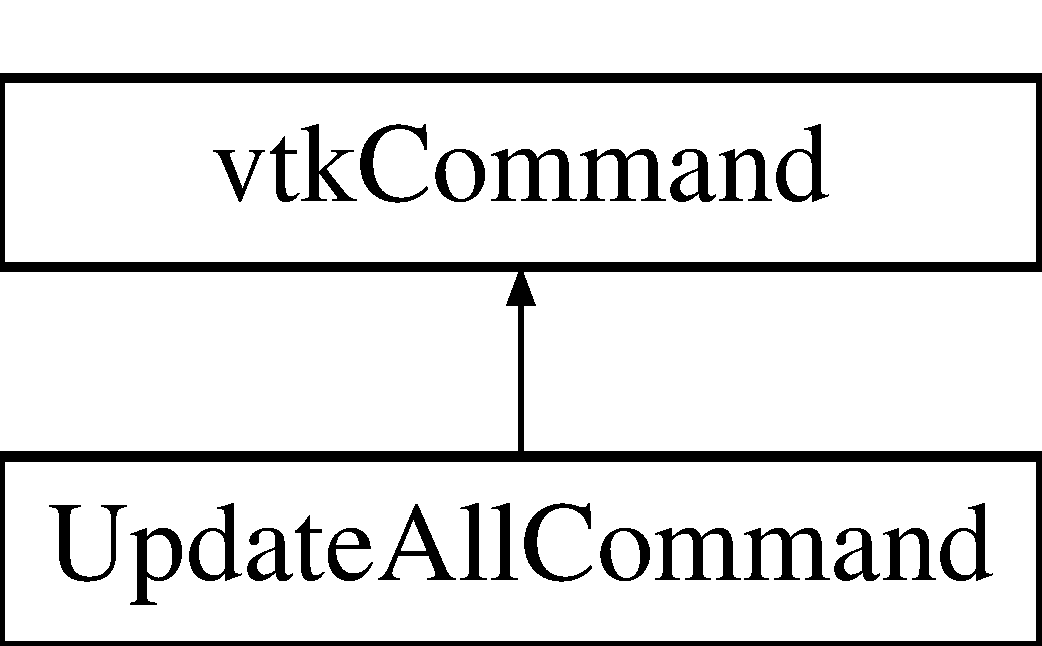
\includegraphics[height=2.000000cm]{classUpdateAllCommand}
\end{center}
\end{figure}
\subsection*{Public Member Functions}
\begin{DoxyCompactItemize}
\item 
\mbox{\hyperlink{classUpdateAllCommand_a228565b2a2306d425dc7eb3cda4d39a4}{vtk\+Type\+Macro}} (\mbox{\hyperlink{classUpdateAllCommand}{Update\+All\+Command}}, vtk\+Command)
\item 
virtual void \mbox{\hyperlink{classUpdateAllCommand_a0a2dab315be55642c65d7fa1b2892ec8}{Execute}} (vtk\+Object $\ast$vtk\+Not\+Used(caller), unsigned long event\+Id, void $\ast$vtk\+Not\+Used(call\+Data))
\end{DoxyCompactItemize}
\subsection*{Static Public Member Functions}
\begin{DoxyCompactItemize}
\item 
static \mbox{\hyperlink{classUpdateAllCommand}{Update\+All\+Command}} $\ast$ \mbox{\hyperlink{classUpdateAllCommand_a97cd6ef1c68bb473aef27c898b175517}{New}} ()
\end{DoxyCompactItemize}
\subsection*{Private Attributes}
\begin{DoxyCompactItemize}
\item 
int \mbox{\hyperlink{classUpdateAllCommand_a66ba9400072105306ca48a58470014dc}{Timer\+Count}}
\end{DoxyCompactItemize}


\subsection{Member Function Documentation}
\mbox{\Hypertarget{classUpdateAllCommand_a0a2dab315be55642c65d7fa1b2892ec8}\label{classUpdateAllCommand_a0a2dab315be55642c65d7fa1b2892ec8}} 
\index{Update\+All\+Command@{Update\+All\+Command}!Execute@{Execute}}
\index{Execute@{Execute}!Update\+All\+Command@{Update\+All\+Command}}
\subsubsection{\texorpdfstring{Execute()}{Execute()}}
{\footnotesize\ttfamily virtual void Update\+All\+Command\+::\+Execute (\begin{DoxyParamCaption}\item[{vtk\+Object $\ast$}]{vtk\+Not\+Usedcaller,  }\item[{unsigned long}]{event\+Id,  }\item[{void $\ast$}]{vtk\+Not\+Usedcall\+Data }\end{DoxyParamCaption})\hspace{0.3cm}{\ttfamily [inline]}, {\ttfamily [virtual]}}

Call universe update

For each \mbox{\hyperlink{classUniverse}{Universe}} locate solids for visualisation

Each solid is made up of a set of polyhedrons

Each polyhedron is made up of a set of points

Sometimes the contouring algorithm can create a volume whose gradient vector and ordering of polygon (using the right hand rule) are inconsistent. vtk\+Reverse\+Sense cures this problem. ~\newline
 Add the actors to the renderer \mbox{\Hypertarget{classUpdateAllCommand_a97cd6ef1c68bb473aef27c898b175517}\label{classUpdateAllCommand_a97cd6ef1c68bb473aef27c898b175517}} 
\index{Update\+All\+Command@{Update\+All\+Command}!New@{New}}
\index{New@{New}!Update\+All\+Command@{Update\+All\+Command}}
\subsubsection{\texorpdfstring{New()}{New()}}
{\footnotesize\ttfamily static \mbox{\hyperlink{classUpdateAllCommand}{Update\+All\+Command}}$\ast$ Update\+All\+Command\+::\+New (\begin{DoxyParamCaption}{ }\end{DoxyParamCaption})\hspace{0.3cm}{\ttfamily [inline]}, {\ttfamily [static]}}

\mbox{\Hypertarget{classUpdateAllCommand_a228565b2a2306d425dc7eb3cda4d39a4}\label{classUpdateAllCommand_a228565b2a2306d425dc7eb3cda4d39a4}} 
\index{Update\+All\+Command@{Update\+All\+Command}!vtk\+Type\+Macro@{vtk\+Type\+Macro}}
\index{vtk\+Type\+Macro@{vtk\+Type\+Macro}!Update\+All\+Command@{Update\+All\+Command}}
\subsubsection{\texorpdfstring{vtk\+Type\+Macro()}{vtkTypeMacro()}}
{\footnotesize\ttfamily Update\+All\+Command\+::vtk\+Type\+Macro (\begin{DoxyParamCaption}\item[{\mbox{\hyperlink{classUpdateAllCommand}{Update\+All\+Command}}}]{,  }\item[{vtk\+Command}]{ }\end{DoxyParamCaption})}



\subsection{Member Data Documentation}
\mbox{\Hypertarget{classUpdateAllCommand_a66ba9400072105306ca48a58470014dc}\label{classUpdateAllCommand_a66ba9400072105306ca48a58470014dc}} 
\index{Update\+All\+Command@{Update\+All\+Command}!Timer\+Count@{Timer\+Count}}
\index{Timer\+Count@{Timer\+Count}!Update\+All\+Command@{Update\+All\+Command}}
\subsubsection{\texorpdfstring{Timer\+Count}{TimerCount}}
{\footnotesize\ttfamily int Update\+All\+Command\+::\+Timer\+Count\hspace{0.3cm}{\ttfamily [private]}}



The documentation for this class was generated from the following file\+:\begin{DoxyCompactItemize}
\item 
/home/pbisaacs/\+Developer/\+Brain\+Harmonics/\+Brain\+Harmonics/\mbox{\hyperlink{BrainHarmonics_8cc}{Brain\+Harmonics.\+cc}}\end{DoxyCompactItemize}

\chapter{File Documentation}
\hypertarget{abstraction_8cc}{}\section{Brain\+Harmonics/abstraction.cc File Reference}
\label{abstraction_8cc}\index{Brain\+Harmonics/abstraction.\+cc@{Brain\+Harmonics/abstraction.\+cc}}
{\ttfamily \#include \char`\"{}abstraction.\+h\char`\"{}}\newline
Include dependency graph for abstraction.\+cc\+:\nopagebreak
\begin{figure}[H]
\begin{center}
\leavevmode
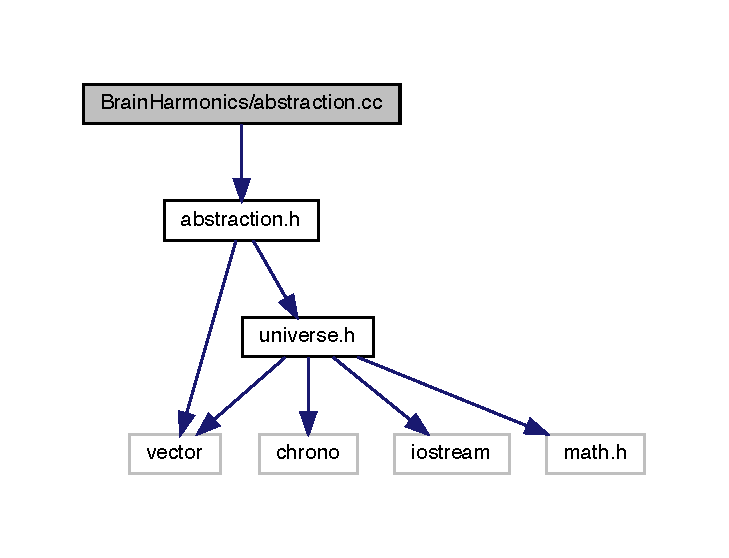
\includegraphics[width=350pt]{abstraction_8cc__incl}
\end{center}
\end{figure}

\hypertarget{abstraction_8h}{}\section{/home/pbisaacs/\+Developer/\+Brain\+Harmonics/abstraction.h File Reference}
\label{abstraction_8h}\index{/home/pbisaacs/\+Developer/\+Brain\+Harmonics/abstraction.\+h@{/home/pbisaacs/\+Developer/\+Brain\+Harmonics/abstraction.\+h}}
{\ttfamily \#include $<$vector$>$}\newline
{\ttfamily \#include \char`\"{}universe.\+h\char`\"{}}\newline
\subsection*{Classes}
\begin{DoxyCompactItemize}
\item 
class \mbox{\hyperlink{classAbstraction}{Abstraction}}
\end{DoxyCompactItemize}

\hypertarget{apptimer_8cc}{}\section{Brain\+Harmonics/apptimer.cc File Reference}
\label{apptimer_8cc}\index{Brain\+Harmonics/apptimer.\+cc@{Brain\+Harmonics/apptimer.\+cc}}
{\ttfamily \#include \char`\"{}apptimer.\+h\char`\"{}}\newline
Include dependency graph for apptimer.\+cc\+:\nopagebreak
\begin{figure}[H]
\begin{center}
\leavevmode
\includegraphics[width=336pt]{apptimer_8cc__incl}
\end{center}
\end{figure}

\hypertarget{apptimer_8h}{}\section{Brain\+Harmonics/apptimer.h File Reference}
\label{apptimer_8h}\index{Brain\+Harmonics/apptimer.\+h@{Brain\+Harmonics/apptimer.\+h}}
{\ttfamily \#include $<$iostream$>$}\newline
{\ttfamily \#include \char`\"{}universe.\+h\char`\"{}}\newline
Include dependency graph for apptimer.\+h\+:\nopagebreak
\begin{figure}[H]
\begin{center}
\leavevmode
\includegraphics[width=334pt]{apptimer_8h__incl}
\end{center}
\end{figure}
This graph shows which files directly or indirectly include this file\+:\nopagebreak
\begin{figure}[H]
\begin{center}
\leavevmode
\includegraphics[width=350pt]{apptimer_8h__dep__incl}
\end{center}
\end{figure}
\subsection*{Classes}
\begin{DoxyCompactItemize}
\item 
class \hyperlink{class_app_timer}{App\+Timer}
\end{DoxyCompactItemize}

\hypertarget{axon_8cc}{}\section{/home/pbisaacs/\+Developer/\+Brain\+Harmonics/axon.cc File Reference}
\label{axon_8cc}\index{/home/pbisaacs/\+Developer/\+Brain\+Harmonics/axon.\+cc@{/home/pbisaacs/\+Developer/\+Brain\+Harmonics/axon.\+cc}}
{\ttfamily \#include \char`\"{}axon.\+h\char`\"{}}\newline
{\ttfamily \#include \char`\"{}axonbranch.\+h\char`\"{}}\newline

\hypertarget{axon_8h}{}\section{Brain\+Harmonics/axon.h File Reference}
\label{axon_8h}\index{Brain\+Harmonics/axon.\+h@{Brain\+Harmonics/axon.\+h}}
{\ttfamily \#include \char`\"{}axonhillock.\+h\char`\"{}}\newline
Include dependency graph for axon.\+h\+:
\nopagebreak
\begin{figure}[H]
\begin{center}
\leavevmode
\includegraphics[width=350pt]{axon_8h__incl}
\end{center}
\end{figure}
This graph shows which files directly or indirectly include this file\+:
\nopagebreak
\begin{figure}[H]
\begin{center}
\leavevmode
\includegraphics[width=350pt]{axon_8h__dep__incl}
\end{center}
\end{figure}
\subsection*{Classes}
\begin{DoxyCompactItemize}
\item 
class \hyperlink{class_axon}{Axon}
\end{DoxyCompactItemize}

\hypertarget{axonbouton_8cc}{}\section{/home/pbisaacs/\+Developer/\+Brain\+Harmonics/\+Brain\+Harmonics/axonbouton.cc File Reference}
\label{axonbouton_8cc}\index{/home/pbisaacs/\+Developer/\+Brain\+Harmonics/\+Brain\+Harmonics/axonbouton.\+cc@{/home/pbisaacs/\+Developer/\+Brain\+Harmonics/\+Brain\+Harmonics/axonbouton.\+cc}}
{\ttfamily \#include \char`\"{}axonbouton.\+h\char`\"{}}\newline
{\ttfamily \#include \char`\"{}synapse.\+h\char`\"{}}\newline
{\ttfamily \#include \char`\"{}synapticvesicle.\+h\char`\"{}}\newline

\hypertarget{axonbouton_8h}{}\section{/home/pbisaacs/\+Developer/\+Brain\+Harmonics/axonbouton.h File Reference}
\label{axonbouton_8h}\index{/home/pbisaacs/\+Developer/\+Brain\+Harmonics/axonbouton.\+h@{/home/pbisaacs/\+Developer/\+Brain\+Harmonics/axonbouton.\+h}}
{\ttfamily \#include \char`\"{}axonbranch.\+h\char`\"{}}\newline
\subsection*{Classes}
\begin{DoxyCompactItemize}
\item 
class \mbox{\hyperlink{classAxonBouton}{Axon\+Bouton}}
\end{DoxyCompactItemize}

\hypertarget{axonbranch_8cc}{}\section{/home/pbisaacs/\+Developer/\+Brain\+Harmonics/\+Brain\+Harmonics/axonbranch.cc File Reference}
\label{axonbranch_8cc}\index{/home/pbisaacs/\+Developer/\+Brain\+Harmonics/\+Brain\+Harmonics/axonbranch.\+cc@{/home/pbisaacs/\+Developer/\+Brain\+Harmonics/\+Brain\+Harmonics/axonbranch.\+cc}}
{\ttfamily \#include \char`\"{}axonbranch.\+h\char`\"{}}\newline
{\ttfamily \#include \char`\"{}axonbouton.\+h\char`\"{}}\newline

\hypertarget{axonbranch_8h}{}\section{Brain\+Harmonics/axonbranch.h File Reference}
\label{axonbranch_8h}\index{Brain\+Harmonics/axonbranch.\+h@{Brain\+Harmonics/axonbranch.\+h}}
{\ttfamily \#include \char`\"{}axon.\+h\char`\"{}}\newline
Include dependency graph for axonbranch.\+h\+:
\nopagebreak
\begin{figure}[H]
\begin{center}
\leavevmode
\includegraphics[width=350pt]{axonbranch_8h__incl}
\end{center}
\end{figure}
This graph shows which files directly or indirectly include this file\+:
\nopagebreak
\begin{figure}[H]
\begin{center}
\leavevmode
\includegraphics[width=350pt]{axonbranch_8h__dep__incl}
\end{center}
\end{figure}
\subsection*{Classes}
\begin{DoxyCompactItemize}
\item 
class \hyperlink{class_axon_branch}{Axon\+Branch}
\end{DoxyCompactItemize}

\hypertarget{axonhillock_8cc}{}\section{Brain\+Harmonics/axonhillock.cc File Reference}
\label{axonhillock_8cc}\index{Brain\+Harmonics/axonhillock.\+cc@{Brain\+Harmonics/axonhillock.\+cc}}
{\ttfamily \#include \char`\"{}axon.\+h\char`\"{}}\newline
{\ttfamily \#include \char`\"{}axonhillock.\+h\char`\"{}}\newline
Include dependency graph for axonhillock.\+cc\+:\nopagebreak
\begin{figure}[H]
\begin{center}
\leavevmode
\includegraphics[width=350pt]{axonhillock_8cc__incl}
\end{center}
\end{figure}

\hypertarget{axonhillock_8h}{}\section{Brain\+Harmonics/axonhillock.h File Reference}
\label{axonhillock_8h}\index{Brain\+Harmonics/axonhillock.\+h@{Brain\+Harmonics/axonhillock.\+h}}
{\ttfamily \#include \char`\"{}soma.\+h\char`\"{}}\newline
Include dependency graph for axonhillock.\+h\+:
\nopagebreak
\begin{figure}[H]
\begin{center}
\leavevmode
\includegraphics[width=350pt]{axonhillock_8h__incl}
\end{center}
\end{figure}
This graph shows which files directly or indirectly include this file\+:
\nopagebreak
\begin{figure}[H]
\begin{center}
\leavevmode
\includegraphics[width=350pt]{axonhillock_8h__dep__incl}
\end{center}
\end{figure}
\subsection*{Classes}
\begin{DoxyCompactItemize}
\item 
class \hyperlink{class_axon_hillock}{Axon\+Hillock}
\end{DoxyCompactItemize}

\hypertarget{bhcompute_8py}{}\section{/home/pbisaacs/\+Developer/\+Brain\+Harmonics/bhcompute.py File Reference}
\label{bhcompute_8py}\index{/home/pbisaacs/\+Developer/\+Brain\+Harmonics/bhcompute.\+py@{/home/pbisaacs/\+Developer/\+Brain\+Harmonics/bhcompute.\+py}}
\subsection*{Namespaces}
\begin{DoxyCompactItemize}
\item 
 \mbox{\hyperlink{namespacebhcompute}{bhcompute}}
\end{DoxyCompactItemize}
\subsection*{Functions}
\begin{DoxyCompactItemize}
\item 
def \mbox{\hyperlink{namespacebhcompute_a9993be8ce88198085d067eb9d777fc6a}{bhcompute.\+multiply}} (a, b)
\item 
def \mbox{\hyperlink{namespacebhcompute_a7a8340e63a09c23e5e93dba91ad0d336}{bhcompute.\+mlkmeans}} (a, b)
\end{DoxyCompactItemize}

\hypertarget{BrainHarmonics_8cc}{}\section{/home/pbisaacs/\+Developer/\+Brain\+Harmonics/\+Brain\+Harmonics/\+Brain\+Harmonics.cc File Reference}
\label{BrainHarmonics_8cc}\index{/home/pbisaacs/\+Developer/\+Brain\+Harmonics/\+Brain\+Harmonics/\+Brain\+Harmonics.\+cc@{/home/pbisaacs/\+Developer/\+Brain\+Harmonics/\+Brain\+Harmonics/\+Brain\+Harmonics.\+cc}}
{\ttfamily \#include $<$sys/time.\+h$>$}\newline
{\ttfamily \#include $<$sys/types.\+h$>$}\newline
{\ttfamily \#include $<$sys/socket.\+h$>$}\newline
{\ttfamily \#include $<$netinet/in.\+h$>$}\newline
{\ttfamily \#include $<$arpa/inet.\+h$>$}\newline
{\ttfamily \#include $<$stdio.\+h$>$}\newline
{\ttfamily \#include $<$stdlib.\+h$>$}\newline
{\ttfamily \#include $<$fcntl.\+h$>$}\newline
{\ttfamily \#include $<$unistd.\+h$>$}\newline
{\ttfamily \#include $<$assert.\+h$>$}\newline
{\ttfamily \#include $<$time.\+h$>$}\newline
{\ttfamily \#include $<$array$>$}\newline
{\ttfamily \#include $<$cstring$>$}\newline
{\ttfamily \#include $<$cstdint$>$}\newline
{\ttfamily \#include $<$fstream$>$}\newline
{\ttfamily \#include $<$iomanip$>$}\newline
{\ttfamily \#include $<$iostream$>$}\newline
{\ttfamily \#include $<$map$>$}\newline
{\ttfamily \#include $<$math.\+h$>$}\newline
{\ttfamily \#include $<$mpi.\+h$>$}\newline
{\ttfamily \#include $<$numeric$>$}\newline
{\ttfamily \#include $<$queue$>$}\newline
{\ttfamily \#include $<$sstream$>$}\newline
{\ttfamily \#include $<$string$>$}\newline
{\ttfamily \#include $<$thread$>$}\newline
{\ttfamily \#include $<$vector$>$}\newline
{\ttfamily \#include $<$libcaercpp/devices/dynapse.\+hpp$>$}\newline
{\ttfamily \#include $<$libcaercpp/libcaer.\+hpp$>$}\newline
{\ttfamily \#include $<$libcaercpp/events/packet\+Container.\+hpp$>$}\newline
{\ttfamily \#include $<$csignal$>$}\newline
{\ttfamily \#include $<$atomic$>$}\newline
{\ttfamily \#include \char`\"{}sniffex.\+h\char`\"{}}\newline
{\ttfamily \#include $<$vtk\+Auto\+Init.\+h$>$}\newline
{\ttfamily \#include $<$vtk\+Version.\+h$>$}\newline
{\ttfamily \#include $<$vtk\+Actor.\+h$>$}\newline
{\ttfamily \#include $<$vtk\+Actor2\+D.\+h$>$}\newline
{\ttfamily \#include $<$vtk\+Camera.\+h$>$}\newline
{\ttfamily \#include $<$vtk\+Cell\+Array.\+h$>$}\newline
{\ttfamily \#include $<$vtk\+Cell\+Data.\+h$>$}\newline
{\ttfamily \#include $<$vtk\+Color\+Transfer\+Function.\+h$>$}\newline
{\ttfamily \#include $<$vtk\+Contour\+Filter.\+h$>$}\newline
{\ttfamily \#include $<$vtk\+Coordinate.\+h$>$}\newline
{\ttfamily \#include $<$vtk\+Float\+Array.\+h$>$}\newline
{\ttfamily \#include $<$vtk\+Math.\+h$>$}\newline
{\ttfamily \#include $<$vtk\+Parametric\+Function\+Source.\+h$>$}\newline
{\ttfamily \#include $<$vtk\+Point\+Data.\+h$>$}\newline
{\ttfamily \#include $<$vtk\+Points.\+h$>$}\newline
{\ttfamily \#include $<$vtk\+Polygon.\+h$>$}\newline
{\ttfamily \#include $<$vtk\+Poly\+Data.\+h$>$}\newline
{\ttfamily \#include $<$vtk\+Poly\+Data\+Mapper.\+h$>$}\newline
{\ttfamily \#include $<$vtk\+Poly\+Data\+Mapper2\+D.\+h$>$}\newline
{\ttfamily \#include $<$vtk\+Append\+Poly\+Data.\+h$>$}\newline
{\ttfamily \#include $<$vtk\+Programmable\+Source.\+h$>$}\newline
{\ttfamily \#include $<$vtk\+Property.\+h$>$}\newline
{\ttfamily \#include $<$vtk\+Property2\+D.\+h$>$}\newline
{\ttfamily \#include $<$vtk\+Render\+Window.\+h$>$}\newline
{\ttfamily \#include $<$vtk\+Renderer.\+h$>$}\newline
{\ttfamily \#include $<$vtk\+Render\+Window\+Interactor.\+h$>$}\newline
{\ttfamily \#include $<$vtk\+Reverse\+Sense.\+h$>$}\newline
{\ttfamily \#include $<$vtk\+Smart\+Pointer.\+h$>$}\newline
{\ttfamily \#include $<$vtk\+Surface\+Reconstruction\+Filter.\+h$>$}\newline
{\ttfamily \#include $<$vtk\+Text\+Actor.\+h$>$}\newline
{\ttfamily \#include $<$vtk\+Text\+Mapper.\+h$>$}\newline
{\ttfamily \#include $<$vtk\+Text\+Property.\+h$>$}\newline
{\ttfamily \#include $<$vtk\+Unsigned\+Char\+Array.\+h$>$}\newline
{\ttfamily \#include $<$vtk\+Vertex\+Glyph\+Filter.\+h$>$}\newline
{\ttfamily \#include $<$vtk\+X\+M\+L\+Poly\+Data\+Writer.\+h$>$}\newline
{\ttfamily \#include $<$cmath$>$}\newline
{\ttfamily \#include $<$vtk\+Transform.\+h$>$}\newline
{\ttfamily \#include $<$vtk\+Transform\+Poly\+Data\+Filter.\+h$>$}\newline
{\ttfamily \#include $<$Python.\+h$>$}\newline
{\ttfamily \#include $<$numpy/arrayobject.\+h$>$}\newline
{\ttfamily \#include $<$G\+L/gl.\+h$>$}\newline
{\ttfamily \#include $<$G\+L/glu.\+h$>$}\newline
{\ttfamily \#include $<$G\+L/glut.\+h$>$}\newline
{\ttfamily \#include \char`\"{}universe.\+h\char`\"{}}\newline
{\ttfamily \#include \char`\"{}dimension.\+h\char`\"{}}\newline
{\ttfamily \#include \char`\"{}elementaryparticle.\+h\char`\"{}}\newline
{\ttfamily \#include \char`\"{}elementaryforce.\+h\char`\"{}}\newline
{\ttfamily \#include \char`\"{}compositeforceparticle.\+h\char`\"{}}\newline
{\ttfamily \#include \char`\"{}law.\+h\char`\"{}}\newline
{\ttfamily \#include \char`\"{}matter.\+h\char`\"{}}\newline
{\ttfamily \#include \char`\"{}monomer.\+h\char`\"{}}\newline
{\ttfamily \#include \char`\"{}polymer.\+h\char`\"{}}\newline
{\ttfamily \#include \char`\"{}solid.\+h\char`\"{}}\newline
{\ttfamily \#include \char`\"{}polyhedron.\+h\char`\"{}}\newline
{\ttfamily \#include \char`\"{}polygon.\+h\char`\"{}}\newline
{\ttfamily \#include \char`\"{}quad.\+h\char`\"{}}\newline
{\ttfamily \#include \char`\"{}line.\+h\char`\"{}}\newline
{\ttfamily \#include \char`\"{}point.\+h\char`\"{}}\newline
{\ttfamily \#include \char`\"{}node.\+h\char`\"{}}\newline
{\ttfamily \#include \char`\"{}apptimer.\+h\char`\"{}}\newline
{\ttfamily \#include \char`\"{}cognitivenetwork.\+h\char`\"{}}\newline
{\ttfamily \#include \char`\"{}cognitiveinput.\+h\char`\"{}}\newline
{\ttfamily \#include \char`\"{}cognitiveoutput.\+h\char`\"{}}\newline
{\ttfamily \#include \char`\"{}orbital.\+h\char`\"{}}\newline
{\ttfamily \#include \char`\"{}neuron.\+h\char`\"{}}\newline
{\ttfamily \#include \char`\"{}dendritecleft.\+h\char`\"{}}\newline
{\ttfamily \#include \char`\"{}neuroreceptor.\+h\char`\"{}}\newline
{\ttfamily \#include \char`\"{}synapse.\+h\char`\"{}}\newline
{\ttfamily \#include \char`\"{}interneuronspace.\+h\char`\"{}}\newline
{\ttfamily \#include \char`\"{}membrane.\+h\char`\"{}}\newline
{\ttfamily \#include \char`\"{}membranechannel.\+h\char`\"{}}\newline
{\ttfamily \#include \char`\"{}dendrite.\+h\char`\"{}}\newline
{\ttfamily \#include \char`\"{}dendritebranch.\+h\char`\"{}}\newline
{\ttfamily \#include \char`\"{}soma.\+h\char`\"{}}\newline
{\ttfamily \#include \char`\"{}axonhillock.\+h\char`\"{}}\newline
{\ttfamily \#include \char`\"{}axon.\+h\char`\"{}}\newline
{\ttfamily \#include \char`\"{}axonbranch.\+h\char`\"{}}\newline
{\ttfamily \#include \char`\"{}myelinsheath.\+h\char`\"{}}\newline
{\ttfamily \#include \char`\"{}schwanncell.\+h\char`\"{}}\newline
{\ttfamily \#include \char`\"{}axonbouton.\+h\char`\"{}}\newline
{\ttfamily \#include \char`\"{}synapticvesicle.\+h\char`\"{}}\newline
{\ttfamily \#include \char`\"{}neurotransmitter.\+h\char`\"{}}\newline
{\ttfamily \#include \char`\"{}spike.\+h\char`\"{}}\newline
\subsection*{Classes}
\begin{DoxyCompactItemize}
\item 
class \mbox{\hyperlink{classUpdateAllCommand}{Update\+All\+Command}}
\end{DoxyCompactItemize}
\subsection*{Macros}
\begin{DoxyCompactItemize}
\item 
\#define \mbox{\hyperlink{BrainHarmonics_8cc_a5abc2fe5dd32fab087839bf8b005e6c9}{D\+E\+F\+A\+U\+L\+T\+B\+I\+A\+S\+ES}}~\char`\"{}data/defaultbiases\+\_\+values.\+txt\char`\"{}
\begin{DoxyCompactList}\small\item\em header defines four variable types, two macro and various functions for manipulating date and time. \end{DoxyCompactList}\item 
\#define \mbox{\hyperlink{BrainHarmonics_8cc_a0146dd22f0f9d4398188379a2bcb8d32}{L\+O\+W\+P\+O\+W\+E\+R\+B\+I\+A\+S\+ES}}~\char`\"{}data/lowpowerbiases\+\_\+values.\+txt\char`\"{}
\item 
\#define \mbox{\hyperlink{BrainHarmonics_8cc_ad25fb949974c3ffe51bb4a887ea0aedc}{D\+E\+B\+U\+G\+\_\+\+P\+R\+O\+G\+R\+AM}}~true
\begin{DoxyCompactList}\small\item\em Top of the tree, begin with \mbox{\hyperlink{classUniverse}{Universe}} class. \end{DoxyCompactList}\item 
\#define \mbox{\hyperlink{BrainHarmonics_8cc_a26769957ec1a2beaf223f33b66ee64ab}{I\+N\+V\+A\+L\+I\+D\+\_\+\+S\+O\+C\+K\+ET}}~-\/1
\begin{DoxyCompactList}\small\item\em D\+E\+B\+U\+G\+\_\+\+P\+R\+O\+G\+R\+AM. \end{DoxyCompactList}\item 
\#define \mbox{\hyperlink{BrainHarmonics_8cc_a633b0396ff93d336a088412a190a5072}{S\+O\+C\+K\+E\+T\+\_\+\+E\+R\+R\+OR}}~-\/1
\begin{DoxyCompactList}\small\item\em I\+N\+V\+A\+L\+I\+D\+\_\+\+S\+O\+C\+K\+ET. \end{DoxyCompactList}\item 
\#define \mbox{\hyperlink{BrainHarmonics_8cc_a120b3c12a694462fcedc15e429a53bd6}{S\+O\+C\+K\+E\+T\+\_\+\+P\+O\+RT}}~9876
\begin{DoxyCompactList}\small\item\em S\+O\+C\+K\+E\+T\+\_\+\+E\+R\+R\+OR. \end{DoxyCompactList}\item 
\#define \mbox{\hyperlink{BrainHarmonics_8cc_a8cccdb3b239ce7cf58e9781af267072b}{S\+O\+C\+K\+E\+T\+\_\+\+A\+D\+D\+R\+E\+SS}}~\char`\"{}192.\+168.\+42.\+56\char`\"{}
\begin{DoxyCompactList}\small\item\em S\+O\+C\+K\+E\+T\+\_\+\+P\+O\+RT. \end{DoxyCompactList}\item 
\#define \mbox{\hyperlink{BrainHarmonics_8cc_a6801baa546c6112d19eb095111d24720}{G\+R\+A\+V\+I\+TY}}~6.\+67384e-\/11;
\begin{DoxyCompactList}\small\item\em S\+O\+C\+K\+E\+T\+\_\+\+A\+D\+D\+R\+E\+SS. \end{DoxyCompactList}\end{DoxyCompactItemize}
\subsection*{Functions}
\begin{DoxyCompactItemize}
\item 
\mbox{\hyperlink{BrainHarmonics_8cc_aa072a4b02405a5306cadd819b01e3cee}{V\+T\+K\+\_\+\+M\+O\+D\+U\+L\+E\+\_\+\+I\+N\+IT}} (vtk\+Rendering\+Open\+G\+L2)
\item 
\mbox{\hyperlink{BrainHarmonics_8cc_a0887c3f67ba4e219d084c8d050597655}{V\+T\+K\+\_\+\+M\+O\+D\+U\+L\+E\+\_\+\+I\+N\+IT}} (vtk\+Rendering\+Free\+Type)
\begin{DoxyCompactList}\small\item\em V\+TK was built with vtk\+Rendering\+Open\+G\+L2 //! (\char`\"{}\+Type cannot be resolved\char`\"{}) \end{DoxyCompactList}\item 
\mbox{\hyperlink{BrainHarmonics_8cc_a80dd3a08d1ff10381e3ef1ca1231f4b5}{V\+T\+K\+\_\+\+M\+O\+D\+U\+L\+E\+\_\+\+I\+N\+IT}} (vtk\+Interaction\+Style)
\begin{DoxyCompactList}\small\item\em (\char`\"{}\+Type cannot be resolved\char`\"{}) \end{DoxyCompactList}\item 
static vtk\+Smart\+Pointer$<$ vtk\+Poly\+Data $>$ \mbox{\hyperlink{BrainHarmonics_8cc_a822a13cf5274e0650ca477e82b16605c}{Transform\+Back}} (vtk\+Smart\+Pointer$<$ vtk\+Points $>$ pt, vtk\+Smart\+Pointer$<$ vtk\+Poly\+Data $>$ pd)
\item 
static std\+::atomic\+\_\+bool \mbox{\hyperlink{BrainHarmonics_8cc_a750b53c1f2b32db320643808acfdd150}{global\+Shutdown}} (false)
\begin{DoxyCompactList}\small\item\em Dynap-\/se shutdown. \end{DoxyCompactList}\item 
static void \mbox{\hyperlink{BrainHarmonics_8cc_a36cc519845200149cde840d403609023}{global\+Shutdown\+Signal\+Handler}} (int signal)
\item 
bool \mbox{\hyperlink{BrainHarmonics_8cc_ac72744f7bdb5df7bb5088e5260589486}{mshandling}} (std\+::vector$<$ std\+::string $>$ $\ast$m\+\_\+messages, bool m\+\_\+response, int m\+\_\+ok, int m\+\_\+fail)
\item 
std\+::vector$<$ \mbox{\hyperlink{classUniverse}{Universe}} $\ast$ $>$ \mbox{\hyperlink{BrainHarmonics_8cc_a5b7bc303552f00bc26a7b5bf962f3376}{Create\+Universe}} (std\+::chrono\+::time\+\_\+point$<$ \mbox{\hyperlink{universe_8h_a0ef8d951d1ca5ab3cfaf7ab4c7a6fd80}{Clock}} $>$ event\+\_\+time, std\+::vector$<$ \mbox{\hyperlink{classUniverse}{Universe}} $\ast$$>$ $\ast$to\+Addto)
\begin{DoxyCompactList}\small\item\em Function to create a \mbox{\hyperlink{classUniverse}{Universe}} instance. Universes could be simulation, emulation, real or contemplative (What-\/if) \end{DoxyCompactList}\item 
bool \mbox{\hyperlink{BrainHarmonics_8cc_a9b04070a3ed092a2de7fd1496edb94ec}{Compare\+Swap\+Elementary\+Particle}} (std\+::chrono\+::time\+\_\+point$<$ \mbox{\hyperlink{universe_8h_a0ef8d951d1ca5ab3cfaf7ab4c7a6fd80}{Clock}} $>$ event\+\_\+time, std\+::vector$<$ \mbox{\hyperlink{classElementaryParticle}{Elementary\+Particle}} $\ast$$>$ \&origin, int l\+\_\+origin\+\_\+\+Swap, int l\+\_\+origin\+\_\+\+Candidate1, int l\+\_\+origin\+\_\+\+Candidate2)
\begin{DoxyCompactList}\small\item\em Test which Candidate is closest to being 3 away in the charge values and move that Candidate next to the Origin. \end{DoxyCompactList}\item 
int \mbox{\hyperlink{BrainHarmonics_8cc_ad9e8231d206ab9486cd74390d97e12fe}{Distance\+Between\+Nodes}} (std\+::chrono\+::time\+\_\+point$<$ \mbox{\hyperlink{universe_8h_a0ef8d951d1ca5ab3cfaf7ab4c7a6fd80}{Clock}} $>$ event\+\_\+time, std\+::vector$<$ \mbox{\hyperlink{classPoint}{Point}} $>$ $\ast$nodes\+Query, std\+::vector$<$ int $>$ $\ast$nodes\+\_\+list, int nodes\+Dimensions, double desired\+\_\+distance)
\item 
bool \mbox{\hyperlink{BrainHarmonics_8cc_ac0bef70f5c895e9fe4271808d3f87a96}{compare\+\_\+swap\+Synapse}} (std\+::chrono\+::time\+\_\+point$<$ \mbox{\hyperlink{universe_8h_a0ef8d951d1ca5ab3cfaf7ab4c7a6fd80}{Clock}} $>$ event\+\_\+time, std\+::vector$<$ \mbox{\hyperlink{classSynapse}{Synapse}} $\ast$$>$ origin, int l\+\_\+origin\+\_\+\+Swap, int l\+\_\+origin\+\_\+\+Candidate1, int l\+\_\+origin\+\_\+\+Candidate2)
\begin{DoxyCompactList}\small\item\em Test which Candidate is closest to being 3 away in the charge values and move that Candidate next to the Origin. \end{DoxyCompactList}\item 
bool \mbox{\hyperlink{BrainHarmonics_8cc_a5611d454c4206879b20ed7a094a223b0}{analyse\+Stream}} (std\+::chrono\+::time\+\_\+point$<$ \mbox{\hyperlink{universe_8h_a0ef8d951d1ca5ab3cfaf7ab4c7a6fd80}{Clock}} $>$ event\+\_\+time, \mbox{\hyperlink{classCognitiveNetwork}{Cognitive\+Network}} $\ast$cognitive\+\_\+network, std\+::vector$<$ \mbox{\hyperlink{classNeuron}{Neuron}} $\ast$$>$ neuron\+\_\+list, std\+::vector$<$ \mbox{\hyperlink{classPoint}{Point}} $\ast$$>$ a\+Point, int start\+\_\+point, int end\+\_\+point, int step\+Point, int neural\+\_\+sequence)
\item 
void \mbox{\hyperlink{BrainHarmonics_8cc_ac9572b51d93c224b7db42a9e06854242}{Clear\+Dimension\+Selection}} (std\+::vector$<$ int $>$ $\ast$dimension\+\_\+list)
\item 
void \mbox{\hyperlink{BrainHarmonics_8cc_ab8cdde3a90c31c1e2f30432b507359c1}{Select\+Dimension}} (const int Possible\+Dimensions\mbox{[}10\mbox{]}, std\+::vector$<$ int $>$ $\ast$dimension\+\_\+list, int which\+Dimension)
\item 
void \mbox{\hyperlink{BrainHarmonics_8cc_aeab5d0ce3757048194ec88e39b7fa82b}{Select\+Multi\+Dimensions}} (const int Possible\+Dimensions\mbox{[}10\mbox{]}, std\+::vector$<$ int $>$ $\ast$dimension\+\_\+list, int how\+\_\+many\+Dimensions)
\item 
bool \mbox{\hyperlink{BrainHarmonics_8cc_aefff80cf47ae6c975b4aed196c12d92a}{Clear\+Dynapse}} (caer\+Device\+Handle $\ast$usb\+\_\+handle)
\item 
void \mbox{\hyperlink{BrainHarmonics_8cc_a8760404347fd84a1ed5b49aae3737647}{exit\+CB}} ()
\begin{DoxyCompactList}\small\item\em Clear memory to cleanly exit application. \end{DoxyCompactList}\item 
int \mbox{\hyperlink{BrainHarmonics_8cc_a487a3c399210173e1b3d3a2f275a55b1}{init}} (int argc, const char $\ast$argv\mbox{[}$\,$\mbox{]})
\item 
void \mbox{\hyperlink{BrainHarmonics_8cc_a909ced1ec126d134c4c2bf71f5ead148}{init\+\_\+numpy}} ()
\begin{DoxyCompactList}\small\item\em Macro required otherwise return value upsets calling function. \end{DoxyCompactList}\item 
int \mbox{\hyperlink{BrainHarmonics_8cc_ac0f2228420376f4db7e1274f2b41667c}{main}} (int argc, const char $\ast$argv\mbox{[}$\,$\mbox{]})
\end{DoxyCompactItemize}
\subsection*{Variables}
\begin{DoxyCompactItemize}
\item 
vtk\+Smart\+Pointer$<$ vtk\+Render\+Window $>$ \mbox{\hyperlink{BrainHarmonics_8cc_a6ce111e58fd1f4622e6a322cefd19b26}{render\+\_\+window}}
\begin{DoxyCompactList}\small\item\em (\char`\"{}\+Type cannot be resolved\char`\"{}) \end{DoxyCompactList}\item 
vtk\+Smart\+Pointer$<$ vtk\+Render\+Window\+Interactor $>$ \mbox{\hyperlink{BrainHarmonics_8cc_a65b7a900454637a30df23b1044e07e07}{render\+\_\+window\+\_\+interactor}}
\item 
vtk\+Smart\+Pointer$<$ vtk\+Points $>$ \mbox{\hyperlink{BrainHarmonics_8cc_a459726c3dbd394d957c5e0e8fad43f71}{define\+\_\+points}} = vtk\+Smart\+Pointer$<$vtk\+Points$>$\+::New()
\item 
std\+::vector$<$ vtk\+Smart\+Pointer$<$ vtk\+Cell\+Array $>$ $>$ \mbox{\hyperlink{BrainHarmonics_8cc_aa97d4b3a68fbfaea550fe20234905b66}{define\+\_\+cellarrays}}
\item 
std\+::vector$<$ vtk\+Smart\+Pointer$<$ vtk\+Poly\+Data $>$ $>$ \mbox{\hyperlink{BrainHarmonics_8cc_a529fb94c7498f38828c4955476e55520}{define\+\_\+polydata}}
\item 
std\+::vector$<$ vtk\+Smart\+Pointer$<$ vtk\+Surface\+Reconstruction\+Filter $>$ $>$ \mbox{\hyperlink{BrainHarmonics_8cc_aec36b51ac72634d7a58846776cb61d43}{define\+\_\+surfaces}}
\item 
std\+::vector$<$ vtk\+Smart\+Pointer$<$ vtk\+Contour\+Filter $>$ $>$ \mbox{\hyperlink{BrainHarmonics_8cc_a60b4bc1ad91584494c1f04f858e34513}{define\+\_\+contourfilters}}
\item 
std\+::vector$<$ vtk\+Smart\+Pointer$<$ vtk\+Reverse\+Sense $>$ $>$ \mbox{\hyperlink{BrainHarmonics_8cc_a3f46d8452260ed4fbbdadf8ea634d866}{define\+\_\+reversals}}
\item 
std\+::vector$<$ vtk\+Smart\+Pointer$<$ vtk\+Poly\+Data\+Mapper $>$ $>$ \mbox{\hyperlink{BrainHarmonics_8cc_a67ee26302d766e5112a5f935e33a85c6}{define\+\_\+datamappers}}
\item 
std\+::vector$<$ vtk\+Smart\+Pointer$<$ vtk\+Poly\+Data\+Mapper2D $>$ $>$ \mbox{\hyperlink{BrainHarmonics_8cc_a804c9adf98d06fdd2f125e84deb75433}{define\+\_\+datamappers2D}}
\item 
std\+::vector$<$ vtk\+Smart\+Pointer$<$ vtk\+Actor $>$ $>$ \mbox{\hyperlink{BrainHarmonics_8cc_a564cb339c12906f6db5995be211dcda2}{define\+\_\+actors}}
\item 
std\+::vector$<$ vtk\+Smart\+Pointer$<$ vtk\+Actor2D $>$ $>$ \mbox{\hyperlink{BrainHarmonics_8cc_a06728597be70303b9f19f653a5dc90ee}{define\+\_\+actors2D}}
\item 
std\+::vector$<$ vtk\+Smart\+Pointer$<$ vtk\+Text\+Actor $>$ $>$ \mbox{\hyperlink{BrainHarmonics_8cc_a4929783757e2d051945177d626a74213}{define\+\_\+textactors}}
\item 
std\+::vector$<$ vtk\+Smart\+Pointer$<$ vtk\+Renderer $>$ $>$ \mbox{\hyperlink{BrainHarmonics_8cc_aab0f6cfd03b167486b3a0ebbb68922be}{define\+\_\+renderers}}
\item 
int \mbox{\hyperlink{BrainHarmonics_8cc_a81f74579a7b9471085578a377b3c1525}{static\+\_\+points\+\_\+counter}} = 0
\item 
int \mbox{\hyperlink{BrainHarmonics_8cc_a3ef1f27168082fed53b34b6781b7fef1}{static\+\_\+polygons\+\_\+counter}} = 0
\item 
int \mbox{\hyperlink{BrainHarmonics_8cc_a0ac21544be2eca2667c5acc784111848}{static\+\_\+polydata\+\_\+counter}} = 0
\item 
int \mbox{\hyperlink{BrainHarmonics_8cc_a3f51384611b8ff0bcedef8dc6f27bbc8}{static\+\_\+cellarrays\+\_\+counter}} = 0
\item 
int \mbox{\hyperlink{BrainHarmonics_8cc_acdcbc10d39db69593dfc42972b200e46}{static\+\_\+surfaces\+\_\+counter}} = 0
\item 
int \mbox{\hyperlink{BrainHarmonics_8cc_af896e11b42f684e4fadc0d4a2826538a}{static\+\_\+contourfilter\+\_\+counter}} = 0
\item 
int \mbox{\hyperlink{BrainHarmonics_8cc_a4062a4c3764de7ed239d33608ca291ae}{static\+\_\+reversals\+\_\+counter}} = 0
\item 
int \mbox{\hyperlink{BrainHarmonics_8cc_ab96b88b97440e7d703e0ac1774115227}{static\+\_\+datamappers\+\_\+counter}} = 0
\item 
int \mbox{\hyperlink{BrainHarmonics_8cc_a3e27beef07882d4684ad6d35239b7a60}{static\+\_\+datamappers2\+D\+\_\+counter}} = 0
\item 
int \mbox{\hyperlink{BrainHarmonics_8cc_ad53e9035f7facd9c99c57107d9f84ac6}{static\+\_\+actors\+\_\+counter}} = 0
\item 
int \mbox{\hyperlink{BrainHarmonics_8cc_a3fe403ad89b282d8d1b8fa92bf05f42e}{static\+\_\+actors2\+D\+\_\+counter}} = 0
\item 
int \mbox{\hyperlink{BrainHarmonics_8cc_aad3d1808a6ab9363f0430c1e9650324d}{static\+\_\+renderers\+\_\+counter}} = 0
\item 
int \mbox{\hyperlink{BrainHarmonics_8cc_adf365e8712584a5f83a2ae582e8a9fe3}{dynamic\+\_\+points\+\_\+counter}} = 0
\item 
int \mbox{\hyperlink{BrainHarmonics_8cc_ae699a3513aa90202fa4779bacdf343da}{dynamic\+\_\+polygons\+\_\+counter}} = 0
\item 
int \mbox{\hyperlink{BrainHarmonics_8cc_a8a93118d63dacb49915b567fa41319a7}{dynamic\+\_\+polydata\+\_\+counter}} = 0
\item 
int \mbox{\hyperlink{BrainHarmonics_8cc_ac86282f96c64009746f9517e7f9d613a}{dynamic\+\_\+cellarrays\+\_\+counter}} = 0
\item 
int \mbox{\hyperlink{BrainHarmonics_8cc_a32fdb8886e50e5a48cb78a26e9cf846d}{dynamic\+\_\+surfaces\+\_\+counter}} = 0
\item 
int \mbox{\hyperlink{BrainHarmonics_8cc_a4d42762d2c2ec0fe02455bab8d3cf4c9}{dynamic\+\_\+contourfilter\+\_\+counter}} = 0
\item 
int \mbox{\hyperlink{BrainHarmonics_8cc_a7e0e7dc174f686fe7ec2c1c10c33a5b7}{dynamic\+\_\+reversals\+\_\+counter}} = 0
\item 
int \mbox{\hyperlink{BrainHarmonics_8cc_ac11e052aaba6bcf48f760388d655dd11}{dynamic\+\_\+datamappers\+\_\+counter}} = 0
\item 
int \mbox{\hyperlink{BrainHarmonics_8cc_aafef3c73d5155f89a18f452d92f4e8a3}{dynamic\+\_\+datamappers2\+D\+\_\+counter}} = 0
\item 
int \mbox{\hyperlink{BrainHarmonics_8cc_a7d304e5a06130656fd9f36a54079bea4}{dynamic\+\_\+actors\+\_\+counter}} = 0
\item 
int \mbox{\hyperlink{BrainHarmonics_8cc_afabdd4a073eb734b7610de6f1769c050}{dynamic\+\_\+actors2\+D\+\_\+counter}} = 0
\item 
int \mbox{\hyperlink{BrainHarmonics_8cc_a295208b91ea89b7e23a14a2d431f4b33}{dynamic\+\_\+renderers\+\_\+counter}} = 0
\item 
std\+::vector$<$ \mbox{\hyperlink{classUniverse}{Universe}} $\ast$ $>$ \mbox{\hyperlink{BrainHarmonics_8cc_a602d3f70549216866d35be56a17fa06e}{universe\+\_\+list}}
\begin{DoxyCompactList}\small\item\em Python interpreter. \end{DoxyCompactList}\item 
struct caer\+\_\+dynapse\+\_\+info \mbox{\hyperlink{BrainHarmonics_8cc_af414029bac33d3b71ad5622dc83149d6}{dynapse\+\_\+info}}
\begin{DoxyCompactList}\small\item\em G\+R\+A\+V\+I\+TY. \end{DoxyCompactList}\end{DoxyCompactItemize}


\subsection{Detailed Description}
Brain Harmonics -\/ using harmonics to store and process neural spikes \begin{DoxyAuthor}{Author}
Paul B. Isaac\textquotesingle{}s, authored 03-\/\+F\+E\+B-\/2016 
\end{DoxyAuthor}
\begin{DoxyDate}{Date}
08-\/\+A\+P\+R-\/2020 
\end{DoxyDate}
\begin{DoxyCopyright}{Copyright}
© 2020 Linaro Limited. Open Source Software. 
\end{DoxyCopyright}


\subsection{Macro Definition Documentation}
\mbox{\Hypertarget{BrainHarmonics_8cc_ad25fb949974c3ffe51bb4a887ea0aedc}\label{BrainHarmonics_8cc_ad25fb949974c3ffe51bb4a887ea0aedc}} 
\index{Brain\+Harmonics.\+cc@{Brain\+Harmonics.\+cc}!D\+E\+B\+U\+G\+\_\+\+P\+R\+O\+G\+R\+AM@{D\+E\+B\+U\+G\+\_\+\+P\+R\+O\+G\+R\+AM}}
\index{D\+E\+B\+U\+G\+\_\+\+P\+R\+O\+G\+R\+AM@{D\+E\+B\+U\+G\+\_\+\+P\+R\+O\+G\+R\+AM}!Brain\+Harmonics.\+cc@{Brain\+Harmonics.\+cc}}
\subsubsection{\texorpdfstring{D\+E\+B\+U\+G\+\_\+\+P\+R\+O\+G\+R\+AM}{DEBUG\_PROGRAM}}
{\footnotesize\ttfamily \#define D\+E\+B\+U\+G\+\_\+\+P\+R\+O\+G\+R\+AM~true}



Top of the tree, begin with \mbox{\hyperlink{classUniverse}{Universe}} class. 

Application specific add-\/ins\+Neuron container for other neuron components \mbox{\hyperlink{classSynapse}{Synapse}}, area of stimulus transmission/reception \mbox{\hyperlink{classDendrite}{Dendrite}}, pre-\/\+Soma component of a neuron \mbox{\hyperlink{classDendrite}{Dendrite}} branch, division/join of dendrites \mbox{\hyperlink{classSoma}{Soma}}, component of a neuron \mbox{\hyperlink{classAxon}{Axon}} Hillock, component of \mbox{\hyperlink{classSoma}{Soma}} \mbox{\hyperlink{classAxon}{Axon}}, connected to \mbox{\hyperlink{classAxon}{Axon}} Hillock \mbox{\hyperlink{classAxon}{Axon}} branch, division/join of \mbox{\hyperlink{classAxon}{Axon}} \mbox{\hyperlink{classAxon}{Axon}} synaptic cleft, output area of neuron Synaptic vesicle, container of neurotransmitters \mbox{\Hypertarget{BrainHarmonics_8cc_a5abc2fe5dd32fab087839bf8b005e6c9}\label{BrainHarmonics_8cc_a5abc2fe5dd32fab087839bf8b005e6c9}} 
\index{Brain\+Harmonics.\+cc@{Brain\+Harmonics.\+cc}!D\+E\+F\+A\+U\+L\+T\+B\+I\+A\+S\+ES@{D\+E\+F\+A\+U\+L\+T\+B\+I\+A\+S\+ES}}
\index{D\+E\+F\+A\+U\+L\+T\+B\+I\+A\+S\+ES@{D\+E\+F\+A\+U\+L\+T\+B\+I\+A\+S\+ES}!Brain\+Harmonics.\+cc@{Brain\+Harmonics.\+cc}}
\subsubsection{\texorpdfstring{D\+E\+F\+A\+U\+L\+T\+B\+I\+A\+S\+ES}{DEFAULTBIASES}}
{\footnotesize\ttfamily \#define D\+E\+F\+A\+U\+L\+T\+B\+I\+A\+S\+ES~\char`\"{}data/defaultbiases\+\_\+values.\+txt\char`\"{}}



header defines four variable types, two macro and various functions for manipulating date and time. 

Code snippets used\+: Syntax comparison -\/ \href{http://stackoverflow.com}{\tt http\+://stackoverflow.\+com} \& \href{http://cplusplus.com}{\tt http\+://cplusplus.\+com} Using hierarchical linking the aim is to develop the application to relate to real-\/world physics. This will then ease mapping between simulation, emulation and real-\/world Universes.

The Code is primarily C++ however, where optimisations are available C-\/calls will be used. For connectivity to other datascience resources Python-\/calls are also supported.\+header defines the timeval structure header defines a minimum set of type definitions makes available a type, socklen\+\_\+t, which is an unsigned opaque integral defines at least in\+\_\+port\+\_\+t and in\+\_\+addr\+\_\+t header makes available the type in\+\_\+port\+\_\+t and the type in\+\_\+addr\+\_\+t header defines three variable types, several macros, and various functions for performing input and output This header defines several general purpose functions, including dynamic memory management, random number generation, communication with the environment, integer arithmetics, searching, sorting and converting. header in the C P\+O\+S\+IX library for the C programming language that contains constructs that refer to file control. header file that provides access to the P\+O\+S\+IX operating system A\+PI. header file in the standard library of the C programming language that defines the C preprocessor macro assert()Standard Template Libraries (S\+TL) For array in C\+R\+C-\/32 call For handling strings For byte handling in C\+R\+C-\/32 For reading files Formatting output to console For output to console For open and closed maps in A$\ast$ For Sine, Cosine, Power, Fabs \& Sqrt functions For Open M\+PI For C\+R\+C-\/32 For assigning priority queue in A$\ast$ For stringstream input from console For handling strings For thread handling To use vectors, which automatically handle resizing, as arrays to keep track of instances ~\newline
~\newline
~\newline
~\newline
~\newline
~\newline


The Addressable Event Representation is for asynchronous activation transmission. Initially, Brain\+Harmonics was written to make use of academic test hardware from the Institute of Neuroinformatics at the Univerisity of Zurich / E\+T\+H.\+The Dynap-\/se is a neuromorphic device from U\+Z\+H/\+E\+TH I\+NI. Addressable Event Representation (A\+ER) Package/\+Unpack events within packets C-\/library to handle signals Clarifies access method in multithreading \mbox{\Hypertarget{BrainHarmonics_8cc_a6801baa546c6112d19eb095111d24720}\label{BrainHarmonics_8cc_a6801baa546c6112d19eb095111d24720}} 
\index{Brain\+Harmonics.\+cc@{Brain\+Harmonics.\+cc}!G\+R\+A\+V\+I\+TY@{G\+R\+A\+V\+I\+TY}}
\index{G\+R\+A\+V\+I\+TY@{G\+R\+A\+V\+I\+TY}!Brain\+Harmonics.\+cc@{Brain\+Harmonics.\+cc}}
\subsubsection{\texorpdfstring{G\+R\+A\+V\+I\+TY}{GRAVITY}}
{\footnotesize\ttfamily \#define G\+R\+A\+V\+I\+TY~6.\+67384e-\/11;}



S\+O\+C\+K\+E\+T\+\_\+\+A\+D\+D\+R\+E\+SS. 

Handy conversions D\+E\+G2\+R\+AD R\+A\+D2\+D\+EG O\+N\+E\+R\+AD \mbox{\Hypertarget{BrainHarmonics_8cc_a26769957ec1a2beaf223f33b66ee64ab}\label{BrainHarmonics_8cc_a26769957ec1a2beaf223f33b66ee64ab}} 
\index{Brain\+Harmonics.\+cc@{Brain\+Harmonics.\+cc}!I\+N\+V\+A\+L\+I\+D\+\_\+\+S\+O\+C\+K\+ET@{I\+N\+V\+A\+L\+I\+D\+\_\+\+S\+O\+C\+K\+ET}}
\index{I\+N\+V\+A\+L\+I\+D\+\_\+\+S\+O\+C\+K\+ET@{I\+N\+V\+A\+L\+I\+D\+\_\+\+S\+O\+C\+K\+ET}!Brain\+Harmonics.\+cc@{Brain\+Harmonics.\+cc}}
\subsubsection{\texorpdfstring{I\+N\+V\+A\+L\+I\+D\+\_\+\+S\+O\+C\+K\+ET}{INVALID\_SOCKET}}
{\footnotesize\ttfamily \#define I\+N\+V\+A\+L\+I\+D\+\_\+\+S\+O\+C\+K\+ET~-\/1}



D\+E\+B\+U\+G\+\_\+\+P\+R\+O\+G\+R\+AM. 

\mbox{\Hypertarget{BrainHarmonics_8cc_a0146dd22f0f9d4398188379a2bcb8d32}\label{BrainHarmonics_8cc_a0146dd22f0f9d4398188379a2bcb8d32}} 
\index{Brain\+Harmonics.\+cc@{Brain\+Harmonics.\+cc}!L\+O\+W\+P\+O\+W\+E\+R\+B\+I\+A\+S\+ES@{L\+O\+W\+P\+O\+W\+E\+R\+B\+I\+A\+S\+ES}}
\index{L\+O\+W\+P\+O\+W\+E\+R\+B\+I\+A\+S\+ES@{L\+O\+W\+P\+O\+W\+E\+R\+B\+I\+A\+S\+ES}!Brain\+Harmonics.\+cc@{Brain\+Harmonics.\+cc}}
\subsubsection{\texorpdfstring{L\+O\+W\+P\+O\+W\+E\+R\+B\+I\+A\+S\+ES}{LOWPOWERBIASES}}
{\footnotesize\ttfamily \#define L\+O\+W\+P\+O\+W\+E\+R\+B\+I\+A\+S\+ES~\char`\"{}data/lowpowerbiases\+\_\+values.\+txt\char`\"{}}

\mbox{\Hypertarget{BrainHarmonics_8cc_a8cccdb3b239ce7cf58e9781af267072b}\label{BrainHarmonics_8cc_a8cccdb3b239ce7cf58e9781af267072b}} 
\index{Brain\+Harmonics.\+cc@{Brain\+Harmonics.\+cc}!S\+O\+C\+K\+E\+T\+\_\+\+A\+D\+D\+R\+E\+SS@{S\+O\+C\+K\+E\+T\+\_\+\+A\+D\+D\+R\+E\+SS}}
\index{S\+O\+C\+K\+E\+T\+\_\+\+A\+D\+D\+R\+E\+SS@{S\+O\+C\+K\+E\+T\+\_\+\+A\+D\+D\+R\+E\+SS}!Brain\+Harmonics.\+cc@{Brain\+Harmonics.\+cc}}
\subsubsection{\texorpdfstring{S\+O\+C\+K\+E\+T\+\_\+\+A\+D\+D\+R\+E\+SS}{SOCKET\_ADDRESS}}
{\footnotesize\ttfamily \#define S\+O\+C\+K\+E\+T\+\_\+\+A\+D\+D\+R\+E\+SS~\char`\"{}192.\+168.\+42.\+56\char`\"{}}



S\+O\+C\+K\+E\+T\+\_\+\+P\+O\+RT. 

\mbox{\Hypertarget{BrainHarmonics_8cc_a633b0396ff93d336a088412a190a5072}\label{BrainHarmonics_8cc_a633b0396ff93d336a088412a190a5072}} 
\index{Brain\+Harmonics.\+cc@{Brain\+Harmonics.\+cc}!S\+O\+C\+K\+E\+T\+\_\+\+E\+R\+R\+OR@{S\+O\+C\+K\+E\+T\+\_\+\+E\+R\+R\+OR}}
\index{S\+O\+C\+K\+E\+T\+\_\+\+E\+R\+R\+OR@{S\+O\+C\+K\+E\+T\+\_\+\+E\+R\+R\+OR}!Brain\+Harmonics.\+cc@{Brain\+Harmonics.\+cc}}
\subsubsection{\texorpdfstring{S\+O\+C\+K\+E\+T\+\_\+\+E\+R\+R\+OR}{SOCKET\_ERROR}}
{\footnotesize\ttfamily \#define S\+O\+C\+K\+E\+T\+\_\+\+E\+R\+R\+OR~-\/1}



I\+N\+V\+A\+L\+I\+D\+\_\+\+S\+O\+C\+K\+ET. 

\mbox{\Hypertarget{BrainHarmonics_8cc_a120b3c12a694462fcedc15e429a53bd6}\label{BrainHarmonics_8cc_a120b3c12a694462fcedc15e429a53bd6}} 
\index{Brain\+Harmonics.\+cc@{Brain\+Harmonics.\+cc}!S\+O\+C\+K\+E\+T\+\_\+\+P\+O\+RT@{S\+O\+C\+K\+E\+T\+\_\+\+P\+O\+RT}}
\index{S\+O\+C\+K\+E\+T\+\_\+\+P\+O\+RT@{S\+O\+C\+K\+E\+T\+\_\+\+P\+O\+RT}!Brain\+Harmonics.\+cc@{Brain\+Harmonics.\+cc}}
\subsubsection{\texorpdfstring{S\+O\+C\+K\+E\+T\+\_\+\+P\+O\+RT}{SOCKET\_PORT}}
{\footnotesize\ttfamily \#define S\+O\+C\+K\+E\+T\+\_\+\+P\+O\+RT~9876}



S\+O\+C\+K\+E\+T\+\_\+\+E\+R\+R\+OR. 



\subsection{Function Documentation}
\mbox{\Hypertarget{BrainHarmonics_8cc_a5611d454c4206879b20ed7a094a223b0}\label{BrainHarmonics_8cc_a5611d454c4206879b20ed7a094a223b0}} 
\index{Brain\+Harmonics.\+cc@{Brain\+Harmonics.\+cc}!analyse\+Stream@{analyse\+Stream}}
\index{analyse\+Stream@{analyse\+Stream}!Brain\+Harmonics.\+cc@{Brain\+Harmonics.\+cc}}
\subsubsection{\texorpdfstring{analyse\+Stream()}{analyseStream()}}
{\footnotesize\ttfamily bool analyse\+Stream (\begin{DoxyParamCaption}\item[{std\+::chrono\+::time\+\_\+point$<$ \mbox{\hyperlink{universe_8h_a0ef8d951d1ca5ab3cfaf7ab4c7a6fd80}{Clock}} $>$}]{event\+\_\+time,  }\item[{\mbox{\hyperlink{classCognitiveNetwork}{Cognitive\+Network}} $\ast$}]{cognitive\+\_\+network,  }\item[{std\+::vector$<$ \mbox{\hyperlink{classNeuron}{Neuron}} $\ast$$>$}]{neuron\+\_\+list,  }\item[{std\+::vector$<$ \mbox{\hyperlink{classPoint}{Point}} $\ast$$>$}]{a\+Point,  }\item[{int}]{start\+\_\+point,  }\item[{int}]{end\+\_\+point,  }\item[{int}]{step\+Point,  }\item[{int}]{neural\+\_\+sequence }\end{DoxyParamCaption})}

\mbox{\Hypertarget{BrainHarmonics_8cc_ac9572b51d93c224b7db42a9e06854242}\label{BrainHarmonics_8cc_ac9572b51d93c224b7db42a9e06854242}} 
\index{Brain\+Harmonics.\+cc@{Brain\+Harmonics.\+cc}!Clear\+Dimension\+Selection@{Clear\+Dimension\+Selection}}
\index{Clear\+Dimension\+Selection@{Clear\+Dimension\+Selection}!Brain\+Harmonics.\+cc@{Brain\+Harmonics.\+cc}}
\subsubsection{\texorpdfstring{Clear\+Dimension\+Selection()}{ClearDimensionSelection()}}
{\footnotesize\ttfamily void Clear\+Dimension\+Selection (\begin{DoxyParamCaption}\item[{std\+::vector$<$ int $>$ $\ast$}]{dimension\+\_\+list }\end{DoxyParamCaption})}

\mbox{\Hypertarget{BrainHarmonics_8cc_aefff80cf47ae6c975b4aed196c12d92a}\label{BrainHarmonics_8cc_aefff80cf47ae6c975b4aed196c12d92a}} 
\index{Brain\+Harmonics.\+cc@{Brain\+Harmonics.\+cc}!Clear\+Dynapse@{Clear\+Dynapse}}
\index{Clear\+Dynapse@{Clear\+Dynapse}!Brain\+Harmonics.\+cc@{Brain\+Harmonics.\+cc}}
\subsubsection{\texorpdfstring{Clear\+Dynapse()}{ClearDynapse()}}
{\footnotesize\ttfamily bool Clear\+Dynapse (\begin{DoxyParamCaption}\item[{caer\+Device\+Handle $\ast$}]{usb\+\_\+handle }\end{DoxyParamCaption})}

Let\textquotesingle{}s take a look at the information we have on the device.

Let\textquotesingle{}s turn on blocking data-\/get mode to avoid wasting resources.

chip id is D\+Y\+N\+A\+P\+S\+E\+\_\+\+C\+O\+N\+F\+I\+G\+\_\+\+D\+Y\+N\+A\+P\+S\+E\+\_\+\+U2

close config \mbox{\Hypertarget{BrainHarmonics_8cc_ac0bef70f5c895e9fe4271808d3f87a96}\label{BrainHarmonics_8cc_ac0bef70f5c895e9fe4271808d3f87a96}} 
\index{Brain\+Harmonics.\+cc@{Brain\+Harmonics.\+cc}!compare\+\_\+swap\+Synapse@{compare\+\_\+swap\+Synapse}}
\index{compare\+\_\+swap\+Synapse@{compare\+\_\+swap\+Synapse}!Brain\+Harmonics.\+cc@{Brain\+Harmonics.\+cc}}
\subsubsection{\texorpdfstring{compare\+\_\+swap\+Synapse()}{compare\_swapSynapse()}}
{\footnotesize\ttfamily bool compare\+\_\+swap\+Synapse (\begin{DoxyParamCaption}\item[{std\+::chrono\+::time\+\_\+point$<$ \mbox{\hyperlink{universe_8h_a0ef8d951d1ca5ab3cfaf7ab4c7a6fd80}{Clock}} $>$}]{event\+\_\+time,  }\item[{std\+::vector$<$ \mbox{\hyperlink{classSynapse}{Synapse}} $\ast$$>$}]{origin,  }\item[{int}]{l\+\_\+origin\+\_\+\+Swap,  }\item[{int}]{l\+\_\+origin\+\_\+\+Candidate1,  }\item[{int}]{l\+\_\+origin\+\_\+\+Candidate2 }\end{DoxyParamCaption})}



Test which Candidate is closest to being 3 away in the charge values and move that Candidate next to the Origin. 

Return answering whether or not an exchange occurred \mbox{\Hypertarget{BrainHarmonics_8cc_a9b04070a3ed092a2de7fd1496edb94ec}\label{BrainHarmonics_8cc_a9b04070a3ed092a2de7fd1496edb94ec}} 
\index{Brain\+Harmonics.\+cc@{Brain\+Harmonics.\+cc}!Compare\+Swap\+Elementary\+Particle@{Compare\+Swap\+Elementary\+Particle}}
\index{Compare\+Swap\+Elementary\+Particle@{Compare\+Swap\+Elementary\+Particle}!Brain\+Harmonics.\+cc@{Brain\+Harmonics.\+cc}}
\subsubsection{\texorpdfstring{Compare\+Swap\+Elementary\+Particle()}{CompareSwapElementaryParticle()}}
{\footnotesize\ttfamily bool Compare\+Swap\+Elementary\+Particle (\begin{DoxyParamCaption}\item[{std\+::chrono\+::time\+\_\+point$<$ \mbox{\hyperlink{universe_8h_a0ef8d951d1ca5ab3cfaf7ab4c7a6fd80}{Clock}} $>$}]{event\+\_\+time,  }\item[{std\+::vector$<$ \mbox{\hyperlink{classElementaryParticle}{Elementary\+Particle}} $\ast$$>$ \&}]{origin,  }\item[{int}]{l\+\_\+origin\+\_\+\+Swap,  }\item[{int}]{l\+\_\+origin\+\_\+\+Candidate1,  }\item[{int}]{l\+\_\+origin\+\_\+\+Candidate2 }\end{DoxyParamCaption})}



Test which Candidate is closest to being 3 away in the charge values and move that Candidate next to the Origin. 

Adding Dimensions enables physical and spatial calculations Possible to use this as a basis for higher dimensionality if it becomes relevant Return answering whether or not an exchange occurred \mbox{\Hypertarget{BrainHarmonics_8cc_a5b7bc303552f00bc26a7b5bf962f3376}\label{BrainHarmonics_8cc_a5b7bc303552f00bc26a7b5bf962f3376}} 
\index{Brain\+Harmonics.\+cc@{Brain\+Harmonics.\+cc}!Create\+Universe@{Create\+Universe}}
\index{Create\+Universe@{Create\+Universe}!Brain\+Harmonics.\+cc@{Brain\+Harmonics.\+cc}}
\subsubsection{\texorpdfstring{Create\+Universe()}{CreateUniverse()}}
{\footnotesize\ttfamily std\+::vector$<$\mbox{\hyperlink{classUniverse}{Universe}}$\ast$$>$ Create\+Universe (\begin{DoxyParamCaption}\item[{std\+::chrono\+::time\+\_\+point$<$ \mbox{\hyperlink{universe_8h_a0ef8d951d1ca5ab3cfaf7ab4c7a6fd80}{Clock}} $>$}]{event\+\_\+time,  }\item[{std\+::vector$<$ \mbox{\hyperlink{classUniverse}{Universe}} $\ast$$>$ $\ast$}]{to\+Addto }\end{DoxyParamCaption})}



Function to create a \mbox{\hyperlink{classUniverse}{Universe}} instance. Universes could be simulation, emulation, real or contemplative (What-\/if) 

P\+L\+A\+C\+E\+H\+O\+L\+D\+ER for Open\+M\+PI code (Shashi to integrate) int openmpi\+Init(int argc, char $\ast$argv\mbox{[}$\,$\mbox{]}) \{ int rank, size, next, prev, message, tag = 201;

! Start up M\+PI \begin{DoxyVerb}MPI_Init(&argc, &argv);
MPI_Comm_rank(MPI_COMM_WORLD, &rank);
MPI_Comm_size(MPI_COMM_WORLD, &size);
\end{DoxyVerb}


! Calculate the rank of the next process in the ring. Use the ! modulus operator so that the last process \char`\"{}wraps around\char`\"{} to ! rank zero. \begin{DoxyVerb}next = (rank + 1) % size;
prev = (rank + size - 1) % size;
\end{DoxyVerb}


! If we are the \char`\"{}master\char`\"{} process (i.\+e., M\+P\+I\+\_\+\+C\+O\+M\+M\+\_\+\+W\+O\+R\+LD rank 0), ! put the number of times to go around the ring in the ! message. \begin{DoxyVerb}if (0 == rank) {
    message = 10;

    printf("Process 0 sending %d to %d, tag %d (%d processes in ring)\n",
           message, next, tag, size);
    MPI_Send(&message, 1, MPI_INT, next, tag, MPI_COMM_WORLD);
    printf("Process 0 sent to %d\n", next);
}
\end{DoxyVerb}


! Pass the message around the ring. The exit mechanism works as ! follows\+: the message (a positive integer) is passed around the ! ring. Each time it passes rank 0, it is decremented. When ! each processes receives a message containing a 0 value, it ! passes the message on to the next process and then quits. By ! passing the 0 message first, every process gets the 0 message ! and can quit normally. \begin{DoxyVerb}while (1) {
    MPI_Recv(&message, 1, MPI_INT, prev, tag, MPI_COMM_WORLD,
             MPI_STATUS_IGNORE);

    if (0 == rank) {
        --message;
        printf("Process 0 decremented value: %d\n", message);
    }

    MPI_Send(&message, 1, MPI_INT, next, tag, MPI_COMM_WORLD);
    if (0 == message) {
        printf("Process %d exiting\n", rank);
        break;
    }
}
\end{DoxyVerb}


! The last process does one extra send to process 0, which needs ! to be received before the program can exit \begin{DoxyVerb}if (0 == rank) {
    MPI_Recv(&message, 1, MPI_INT, prev, tag, MPI_COMM_WORLD,
             MPI_STATUS_IGNORE);
}
\end{DoxyVerb}


! All done \begin{DoxyVerb}MPI_Finalize();
return 0;
\end{DoxyVerb}
 \} First, there is nothing. Then there was something...

Defined energy level of \mbox{\hyperlink{classUniverse}{Universe}} ~\newline
~\newline
~\newline
~\newline
~\newline
 Begin with singularity

Create instance of \mbox{\hyperlink{classUniverse}{Universe}} from \mbox{\hyperlink{classUniverse}{Universe}} class $\ast$/

Set an energy level and attempt to maintain physics laws by keeping the total in the \mbox{\hyperlink{classUniverse}{Universe}} the same. Uses the maximum value for double. Levels of abstraction used to cater for environment limitations $\ast$/

Cause initialisation

Use move not push\+\_\+back otherwise data is destroyed on exiting function std\+::copy(\&my\+Universe, \&my\+Universe + 1, std\+::back\+\_\+inserter($\ast$to\+Addto)); \mbox{\Hypertarget{BrainHarmonics_8cc_ad9e8231d206ab9486cd74390d97e12fe}\label{BrainHarmonics_8cc_ad9e8231d206ab9486cd74390d97e12fe}} 
\index{Brain\+Harmonics.\+cc@{Brain\+Harmonics.\+cc}!Distance\+Between\+Nodes@{Distance\+Between\+Nodes}}
\index{Distance\+Between\+Nodes@{Distance\+Between\+Nodes}!Brain\+Harmonics.\+cc@{Brain\+Harmonics.\+cc}}
\subsubsection{\texorpdfstring{Distance\+Between\+Nodes()}{DistanceBetweenNodes()}}
{\footnotesize\ttfamily int Distance\+Between\+Nodes (\begin{DoxyParamCaption}\item[{std\+::chrono\+::time\+\_\+point$<$ \mbox{\hyperlink{universe_8h_a0ef8d951d1ca5ab3cfaf7ab4c7a6fd80}{Clock}} $>$}]{event\+\_\+time,  }\item[{std\+::vector$<$ \mbox{\hyperlink{classPoint}{Point}} $>$ $\ast$}]{nodes\+Query,  }\item[{std\+::vector$<$ int $>$ $\ast$}]{nodes\+\_\+list,  }\item[{int}]{nodes\+Dimensions,  }\item[{double}]{desired\+\_\+distance }\end{DoxyParamCaption})}

diffX = 0; diffY = 0; ~\newline
~\newline
~\newline
 ($\ast$nodes\+Query)\mbox{[}node\+\_\+loop\mbox{]}.Set\+Point\+Differential(((($\ast$nodes\+Query)\mbox{[}node\+\_\+loop\mbox{]}.Get\+Point\+Differential()\mbox{[}nloop\mbox{]} + diffX)/2.0))\mbox{[}nloop\mbox{]}; ($\ast$nodes\+Query)\mbox{[}node\+\_\+loop\mbox{]}.Set\+Point\+Differential(((($\ast$nodes\+Query)\mbox{[}node\+\_\+loop\mbox{]}.Get\+Point\+Differential()\mbox{[}nloop\mbox{]} + diffY)/2.0))\mbox{[}nloop\mbox{]}; ~\newline
~\newline
 ($\ast$nodes\+Query)\mbox{[}($\ast$nodes\+\_\+list)\mbox{[}2\mbox{]}\mbox{]}-\/$>$Set\+Point\+Differential(((($\ast$nodes\+Query)\mbox{[}($\ast$nodes\+\_\+list)\mbox{[}2\mbox{]}\mbox{]}.get\+Point\+Differential() -\/ diffX)/2)); ($\ast$nodes\+Query)\mbox{[}($\ast$nodes\+\_\+list)\mbox{[}3\mbox{]}\mbox{]}-\/$>$Set\+Point\+Differential(((($\ast$nodes\+Query)\mbox{[}($\ast$nodes\+\_\+list)\mbox{[}3\mbox{]}\mbox{]}.get\+Point\+Differential() -\/ diffY)/2)); ~\newline
\begin{DoxyVerb}}
\end{DoxyVerb}
 \} \mbox{\Hypertarget{BrainHarmonics_8cc_a8760404347fd84a1ed5b49aae3737647}\label{BrainHarmonics_8cc_a8760404347fd84a1ed5b49aae3737647}} 
\index{Brain\+Harmonics.\+cc@{Brain\+Harmonics.\+cc}!exit\+CB@{exit\+CB}}
\index{exit\+CB@{exit\+CB}!Brain\+Harmonics.\+cc@{Brain\+Harmonics.\+cc}}
\subsubsection{\texorpdfstring{exit\+C\+B()}{exitCB()}}
{\footnotesize\ttfamily void exit\+CB (\begin{DoxyParamCaption}{ }\end{DoxyParamCaption})}



Clear memory to cleanly exit application. 

Clear vectors in reverse order to free-\/up memory before exiting

Remember to clear vectors / free memory before returning \mbox{\Hypertarget{BrainHarmonics_8cc_a750b53c1f2b32db320643808acfdd150}\label{BrainHarmonics_8cc_a750b53c1f2b32db320643808acfdd150}} 
\index{Brain\+Harmonics.\+cc@{Brain\+Harmonics.\+cc}!global\+Shutdown@{global\+Shutdown}}
\index{global\+Shutdown@{global\+Shutdown}!Brain\+Harmonics.\+cc@{Brain\+Harmonics.\+cc}}
\subsubsection{\texorpdfstring{global\+Shutdown()}{globalShutdown()}}
{\footnotesize\ttfamily static std\+::atomic\+\_\+bool global\+Shutdown (\begin{DoxyParamCaption}\item[{false}]{ }\end{DoxyParamCaption})\hspace{0.3cm}{\ttfamily [static]}}



Dynap-\/se shutdown. 

\mbox{\Hypertarget{BrainHarmonics_8cc_a36cc519845200149cde840d403609023}\label{BrainHarmonics_8cc_a36cc519845200149cde840d403609023}} 
\index{Brain\+Harmonics.\+cc@{Brain\+Harmonics.\+cc}!global\+Shutdown\+Signal\+Handler@{global\+Shutdown\+Signal\+Handler}}
\index{global\+Shutdown\+Signal\+Handler@{global\+Shutdown\+Signal\+Handler}!Brain\+Harmonics.\+cc@{Brain\+Harmonics.\+cc}}
\subsubsection{\texorpdfstring{global\+Shutdown\+Signal\+Handler()}{globalShutdownSignalHandler()}}
{\footnotesize\ttfamily static void global\+Shutdown\+Signal\+Handler (\begin{DoxyParamCaption}\item[{int}]{signal }\end{DoxyParamCaption})\hspace{0.3cm}{\ttfamily [static]}}

Simply set the running flag to false on S\+I\+G\+T\+E\+RM and S\+I\+G\+I\+NT (C\+T\+R\+L+C) for global shutdown. \mbox{\Hypertarget{BrainHarmonics_8cc_a487a3c399210173e1b3d3a2f275a55b1}\label{BrainHarmonics_8cc_a487a3c399210173e1b3d3a2f275a55b1}} 
\index{Brain\+Harmonics.\+cc@{Brain\+Harmonics.\+cc}!init@{init}}
\index{init@{init}!Brain\+Harmonics.\+cc@{Brain\+Harmonics.\+cc}}
\subsubsection{\texorpdfstring{init()}{init()}}
{\footnotesize\ttfamily int init (\begin{DoxyParamCaption}\item[{int}]{argc,  }\item[{const char $\ast$}]{argv\mbox{[}$\,$\mbox{]} }\end{DoxyParamCaption})}

\mbox{\Hypertarget{BrainHarmonics_8cc_a909ced1ec126d134c4c2bf71f5ead148}\label{BrainHarmonics_8cc_a909ced1ec126d134c4c2bf71f5ead148}} 
\index{Brain\+Harmonics.\+cc@{Brain\+Harmonics.\+cc}!init\+\_\+numpy@{init\+\_\+numpy}}
\index{init\+\_\+numpy@{init\+\_\+numpy}!Brain\+Harmonics.\+cc@{Brain\+Harmonics.\+cc}}
\subsubsection{\texorpdfstring{init\+\_\+numpy()}{init\_numpy()}}
{\footnotesize\ttfamily void init\+\_\+numpy (\begin{DoxyParamCaption}{ }\end{DoxyParamCaption})}



Macro required otherwise return value upsets calling function. 

import\+\_\+array(); \mbox{\Hypertarget{BrainHarmonics_8cc_ac0f2228420376f4db7e1274f2b41667c}\label{BrainHarmonics_8cc_ac0f2228420376f4db7e1274f2b41667c}} 
\index{Brain\+Harmonics.\+cc@{Brain\+Harmonics.\+cc}!main@{main}}
\index{main@{main}!Brain\+Harmonics.\+cc@{Brain\+Harmonics.\+cc}}
\subsubsection{\texorpdfstring{main()}{main()}}
{\footnotesize\ttfamily int main (\begin{DoxyParamCaption}\item[{int}]{argc,  }\item[{const char $\ast$}]{argv\mbox{[}$\,$\mbox{]} }\end{DoxyParamCaption})}

This application is designed to create an A\+A\+Re\+NN Cognitive AI network constructed using either simulated neurons or emulated neuromorphic chipsets

Initialise hardware if located

Bool flag is set to false when communication fails to discover hardware

Install Dynap-\/se signal handler for global shutdown.

Verify connection to all Dynap-\/se boards/chips and then ensure the chips are set to a basic known configuration.

Open the communication with Dynap-\/se, give it a device ID of 1, and don\textquotesingle{}t care about U\+SB bus or SN restrictions.

return (E\+X\+I\+T\+\_\+\+F\+A\+I\+L\+U\+RE); //! Not required because this program can run without dedicated hardware.

Verify or amend code to ensure all chips are reset at the beginning

Now re-\/open the communication with Dynap-\/se for a clean connection.

return (E\+X\+I\+T\+\_\+\+F\+A\+I\+L\+U\+RE);

End of initial hardware detection. Further communications errors will disable hardware use

Define bit-\/setting variables for hardware

Index arrays for instances of classes described above Early versions of this software maintained direct pointers to all objects. Now it is recoded to access through Get/\+Set class methods with the exception of the initial \mbox{\hyperlink{classUniverse}{Universe}} class. ~\newline
~\newline
~\newline
~\newline
~\newline
~\newline
~\newline
~\newline
~\newline
~\newline
~\newline
~\newline
~\newline
~\newline
~\newline
~\newline
~\newline
~\newline
~\newline
~\newline
~\newline
~\newline
~\newline
~\newline
~\newline
~\newline
~\newline
~\newline
~\newline
~\newline
~\newline
~\newline
~\newline
~\newline
~\newline
~\newline
~\newline
~\newline
~\newline
~\newline
~\newline
~\newline
~\newline
~\newline
~\newline
~\newline
~\newline
~\newline
~\newline
~\newline
~\newline
~\newline
~\newline
~\newline
~\newline
~\newline
~\newline
~\newline
~\newline
~\newline
~\newline
~\newline
~\newline
~\newline
~\newline
~\newline
~\newline
~\newline
~\newline
~\newline
~\newline
~\newline
~\newline
~\newline
~\newline
~\newline
~\newline
~\newline
~\newline
~\newline
~\newline
~\newline
~\newline
~\newline
~\newline
~\newline
~\newline
~\newline
~\newline
~\newline
~\newline
~\newline
~\newline
~\newline
~\newline
~\newline
~\newline
~\newline
~\newline
~\newline
~\newline
~\newline
~\newline
~\newline
~\newline
~\newline
~\newline
~\newline
~\newline
~\newline
~\newline
~\newline
~\newline
~\newline
~\newline
~\newline
~\newline
~\newline
~\newline
~\newline
~\newline
~\newline
~\newline
~\newline
~\newline
~\newline
~\newline
~\newline
~\newline
~\newline
~\newline
~\newline
~\newline
~\newline
~\newline
~\newline
~\newline
~\newline
~\newline
~\newline
~\newline
~\newline
~\newline
~\newline
~\newline
~\newline
~\newline
~\newline
~\newline
~\newline
~\newline
~\newline
~\newline
~\newline
~\newline
~\newline
~\newline
~\newline
~\newline
~\newline
~\newline
~\newline
~\newline
~\newline
~\newline
~\newline
~\newline
~\newline
~\newline
~\newline
~\newline
~\newline
~\newline
~\newline
~\newline
~\newline
~\newline
~\newline
 Add Dimensions for spatial identification $\ast$/

Follow with the creation of quarks/leptons $\ast$/

Define Force interaction between fundamentals $\ast$/

Define Particle Force interaction between Composites, Protons/\+Neutrons $\ast$/

Specify how Composites interact $\ast$/

Composites form elements of periodic table $\ast$/

Composites form molecules $\ast$/

Composites form complex molecules $\ast$/

Materials are a combination of \mbox{\hyperlink{classMatter}{Matter}} $\ast$/

Materials can be formed into multi\+Dimensional shapes $\ast$/

Complex shapes are a combination of simpler forms $\ast$/

Reducing high Dimensions to lower $\ast$/

Further reduction $\ast$/

Fundamental spatial description ~\newline
~\newline
~\newline
~\newline
~\newline
~\newline
~\newline
~\newline
~\newline
~\newline
~\newline
~\newline
~\newline
~\newline
~\newline
~\newline
~\newline
~\newline
~\newline
~\newline
~\newline
~\newline
~\newline
~\newline
~\newline
~\newline
~\newline
~\newline
~\newline
~\newline
~\newline
~\newline
~\newline
~\newline
~\newline
~\newline
~\newline
~\newline
~\newline
~\newline
~\newline
~\newline
~\newline
~\newline
~\newline
~\newline
~\newline
~\newline
~\newline
~\newline
~\newline
~\newline
~\newline
~\newline
~\newline
~\newline
~\newline
~\newline
~\newline
~\newline
~\newline
~\newline
~\newline
~\newline
~\newline
~\newline
~\newline
~\newline
~\newline
~\newline
~\newline
~\newline
~\newline
~\newline
~\newline
~\newline
~\newline
~\newline
~\newline
~\newline
~\newline
~\newline
~\newline
~\newline
~\newline
~\newline
~\newline
~\newline
~\newline
~\newline
~\newline
~\newline
~\newline
~\newline
~\newline
~\newline
~\newline
~\newline
~\newline
~\newline
~\newline
~\newline
~\newline
~\newline
~\newline
~\newline
~\newline
~\newline
~\newline
~\newline
~\newline
~\newline
~\newline
~\newline
~\newline
~\newline
~\newline
~\newline
~\newline
~\newline
~\newline
~\newline
~\newline
~\newline
~\newline
~\newline
~\newline
~\newline
~\newline
~\newline
~\newline
~\newline
~\newline
~\newline
~\newline
~\newline
~\newline
~\newline
~\newline
~\newline
~\newline
~\newline
~\newline
~\newline
~\newline
~\newline
~\newline
~\newline
~\newline
~\newline
~\newline
~\newline
~\newline
~\newline
~\newline
~\newline
~\newline
~\newline
~\newline
~\newline
~\newline
~\newline
~\newline
~\newline
 std\+::vector $<$\+Node$>$ Node; //! Node class for A$\ast$ search $\ast$/

Interim function describing time before inclusion as \mbox{\hyperlink{classDimension}{Dimension}} $\ast$/

Higher level of abstraction. Initial naming. Ideally use Get/\+Set methods rather than store pointers here.

Network container for all AI components $\ast$/

Example of orbital timing containing neurons $\ast$/

\mbox{\hyperlink{classNeuron}{Neuron}} container for other neuron components $\ast$/

Dendritic synaptic cleft, input to the neuron $\ast$/

\mbox{\hyperlink{classNeuroreceptor}{Neuroreceptor}}, component of dendritic cleft $\ast$/

\mbox{\hyperlink{classSynapse}{Synapse}}, area of stimulus transmission/reception $\ast$/

Between neurons is an energy pool $\ast$/

\mbox{\hyperlink{classMembrane}{Membrane}}, outer component of the neuron $\ast$/

Potassium/\+Sodium channel, component of the membrane $\ast$/

\mbox{\hyperlink{classDendrite}{Dendrite}}, pre-\/\+Soma component of a neuron $\ast$/

\mbox{\hyperlink{classDendrite}{Dendrite}} branch, division/join of dendrites $\ast$/

\mbox{\hyperlink{classSoma}{Soma}}, component of a neuron $\ast$/

\mbox{\hyperlink{classAxon}{Axon}} Hillock, component of \mbox{\hyperlink{classSoma}{Soma}} $\ast$/

\mbox{\hyperlink{classAxon}{Axon}}, connected to \mbox{\hyperlink{classAxon}{Axon}} Hillock $\ast$/

\mbox{\hyperlink{classAxon}{Axon}} branch, division/join of \mbox{\hyperlink{classAxon}{Axon}} $\ast$/

Myelin sheath, wraps around \mbox{\hyperlink{classAxon}{Axon}} $\ast$/

Schwann Cell, component of a Myelin sheath $\ast$/

\mbox{\hyperlink{classAxon}{Axon}} synaptic cleft, output area of neuron $\ast$/

Synaptic vesicle, container of neurotransmitters $\ast$/

\mbox{\hyperlink{classNeurotransmitter}{Neurotransmitter}}, transfer component between clefts $\ast$/

\mbox{\hyperlink{classSpike}{Spike}} $\ast$/

The initial parameters are to be read from an X\+ML Parameter file but for now are hard-\/coded.

Internal display, Physical material and spatial references

U1 = Internal Time, X, Y \& Z U2 = Physical U3 = Spatial X,Y,Z \& Time U4 = C\+PP U5 = Spikes U6 = Neurotransmitters U7 = Connectome U8 = Synapses U9 = \mbox{\hyperlink{classOrbital}{Orbital}} example ~\newline
~\newline
~\newline
~\newline
~\newline
~\newline
~\newline
~\newline
~\newline
~\newline
~\newline
~\newline
~\newline
~\newline
~\newline
~\newline
~\newline
~\newline
~\newline
~\newline
~\newline
~\newline
~\newline
~\newline
~\newline
~\newline
~\newline
~\newline
~\newline
~\newline
~\newline
~\newline
~\newline
~\newline
~\newline
~\newline
~\newline
~\newline
~\newline
~\newline
~\newline
~\newline
~\newline
~\newline
~\newline
~\newline
~\newline
~\newline
~\newline
~\newline
~\newline
~\newline
~\newline
~\newline
~\newline
~\newline
~\newline
~\newline
~\newline
~\newline
~\newline
~\newline
~\newline
~\newline
~\newline
~\newline
~\newline
~\newline
~\newline
~\newline
~\newline
~\newline
~\newline
~\newline
~\newline
~\newline
~\newline
~\newline
~\newline
~\newline
~\newline
~\newline
~\newline
~\newline
~\newline
~\newline
~\newline
~\newline
~\newline
~\newline
~\newline
~\newline
~\newline
~\newline
~\newline
~\newline
~\newline
~\newline
~\newline
~\newline
~\newline
~\newline
~\newline
~\newline
~\newline
~\newline
~\newline
~\newline
~\newline
~\newline
~\newline
~\newline
~\newline
~\newline
~\newline
~\newline
~\newline
~\newline
~\newline
~\newline
~\newline
~\newline
~\newline
~\newline
~\newline
~\newline
~\newline
~\newline
~\newline
~\newline
~\newline
~\newline
~\newline
~\newline
~\newline
~\newline
~\newline
 Initial number of starting components for each subproject

The Physics problem

Attempt to stimulate particle bonding by moving attracted objects nearer to each other.

The Cognitive problem

Attempt to stimulate neuron pairing by moving attracted objects nearer to each other.

The setup of neurons, orbitals and cognitive networks are initial. Changes to configuration occurs dynamically depending on stimulation.

How many neuron groups in each layer. May want to add some random variation in layer values.

Ensure the end value is also added.

Brain calculations

Define graphics window size, X axis$\ast$/

Define graphics window size, Y axis$\ast$/

Used to loop between min 0 and max 6

Base of data points (Moves because of use by internal graphics for points control too

std\+::string\+::size\+\_\+type sz; //! alias of size\+\_\+t

C\+P\+L\+EX Environment

Setup the Python environment for integrating K-\/means clustering solution

const char py\+Argv\mbox{[}\mbox{]} = \{ \textquotesingle{} \textquotesingle{},\textquotesingle{}b\textquotesingle{},\textquotesingle{}h\textquotesingle{},\textquotesingle{}c\textquotesingle{},\textquotesingle{}o\textquotesingle{},\textquotesingle{}m\textquotesingle{},\textquotesingle{}p\textquotesingle{},\textquotesingle{}u\textquotesingle{},\textquotesingle{}t\textquotesingle{},\textquotesingle{}e\textquotesingle{},\textquotesingle{} \textquotesingle{},\textquotesingle{}m\textquotesingle{},\textquotesingle{}u\textquotesingle{},\textquotesingle{}l\textquotesingle{},\textquotesingle{}t\textquotesingle{},\textquotesingle{}i\textquotesingle{},\textquotesingle{}p\textquotesingle{},\textquotesingle{}l\textquotesingle{},\textquotesingle{}y\textquotesingle{},\textquotesingle{} \textquotesingle{},\textquotesingle{}3\textquotesingle{},\textquotesingle{} \textquotesingle{},\textquotesingle{}4\textquotesingle{},\textquotesingle{}\textbackslash{}0\textquotesingle{}\}

int i;

Numpy array initialisation

File to be called. Must be in the same folder as the C++ executable and with a .py extension

Prepare screens

V\+TK Screens

Setup rectangle points

Create the polygon

Add the polygon to a cell array

Add the polygon to a cell array

Test for correct polygon insertion

the index inside the cell array

Assign Colour

Create Poly\+Data

Setup the text and add it to the renderer Build display text ~\newline
~\newline
~\newline
~\newline
~\newline
~\newline
~\newline
~\newline
~\newline
~\newline
~\newline
~\newline
~\newline
~\newline
~\newline
~\newline
~\newline
~\newline
~\newline
~\newline
~\newline
~\newline
~\newline
~\newline
~\newline
~\newline
~\newline
~\newline
~\newline
~\newline
~\newline
~\newline
~\newline
~\newline
~\newline
~\newline
~\newline
~\newline
~\newline
~\newline
~\newline
~\newline
~\newline
~\newline
~\newline
~\newline
~\newline
~\newline
~\newline
~\newline
~\newline
~\newline
~\newline
~\newline
~\newline
~\newline
~\newline
~\newline
~\newline
~\newline
~\newline
~\newline
~\newline
~\newline
~\newline
~\newline
~\newline
~\newline
~\newline
~\newline
~\newline
~\newline
~\newline
~\newline
~\newline
~\newline
~\newline
~\newline
~\newline
~\newline
~\newline
~\newline
~\newline
~\newline
~\newline
~\newline
~\newline
~\newline
~\newline
~\newline
~\newline
~\newline
~\newline
~\newline
~\newline
~\newline
~\newline
~\newline
~\newline
~\newline
~\newline
~\newline
~\newline
~\newline
~\newline
~\newline
 Create polydata mapper and actor

Create a renderer

Set background colour to white

Add the V\+TK actors to the scene

Create a render window

Create an interactor

Set-\/up the simulation environment. Currently a skeletal environment.

Synchronise events

universe\+\_\+list is a vector of pointers to the \mbox{\hyperlink{classUniverse}{Universe}} objects. Typically use one \mbox{\hyperlink{classUniverse}{Universe}} per experiment. ~\newline
~\newline
~\newline
~\newline
~\newline
~\newline
~\newline
~\newline
~\newline
~\newline
~\newline
~\newline
~\newline
~\newline
~\newline
~\newline
~\newline
~\newline
~\newline
~\newline
~\newline
~\newline
~\newline
~\newline
~\newline
~\newline
~\newline
~\newline
~\newline
~\newline
~\newline
~\newline
~\newline
~\newline
~\newline
~\newline
~\newline
~\newline
~\newline
~\newline
~\newline
~\newline
~\newline
~\newline
~\newline
~\newline
~\newline
~\newline
~\newline
~\newline
~\newline
~\newline
~\newline
~\newline
~\newline
~\newline
~\newline
~\newline
~\newline
~\newline
~\newline
~\newline
~\newline
~\newline
~\newline
~\newline
~\newline
~\newline
~\newline
~\newline
~\newline
~\newline
~\newline
~\newline
~\newline
~\newline
~\newline
~\newline
~\newline
~\newline
~\newline
~\newline
~\newline
~\newline
~\newline
~\newline
~\newline
~\newline
~\newline
~\newline
~\newline
~\newline
~\newline
~\newline
~\newline
~\newline
~\newline
 Ensure vector is empty

Pass the universe\+\_\+list address to the create function to keep all Universes within the same vector

Cycle through Universes allocating n Dimensions and updating total with reported back size.

Create new Elementary Particles -\/ Quarks etc

Cycle through Universes allocating n Elementary Particles and updating total with reported back size.

Try to ensure we get variations of particles. Not all one type by changing Charge and Spin.

Create new Elementary Forces

Cycle through Universes allocating n Elementary Forces and updating total with reported back size.

Try to ensure we get variations of forces. Not all one type by changing parameters.

Create new Composite Force Particles -\/ Protons / Neutrons

Cycle through Universes allocating n Composite Force Particles and updating total with reported back size.

Make Elements -\/ Hydrogen, Helium, Lithium etc

Make Monomers -\/ Carbohydrates/\+Sugars etc

Cycle through Universes allocating n Cognitive Networks and updating total with reported back size.

Add \mbox{\hyperlink{classOrbital}{Orbital}} objects to Cognitive Network which is derived from \mbox{\hyperlink{classUniverse}{Universe}}

Cause initialisation

Add \mbox{\hyperlink{classNeuron}{Neuron}} objects to Cognitive Network which is derived from \mbox{\hyperlink{classUniverse}{Universe}}

Add \mbox{\hyperlink{classSynapse}{Synapse}} objects to Cognitive Network which is derived from \mbox{\hyperlink{classUniverse}{Universe}}

Add \mbox{\hyperlink{classNeurotransmitter}{Neurotransmitter}} objects to Cognitive Network which is derived from \mbox{\hyperlink{classUniverse}{Universe}}

For later development if spikes need to be simulated per \mbox{\hyperlink{classCognitiveNetwork}{Cognitive\+Network}}

Physics dimensionality -\/ calculating quark interactions

Spatial dimensionality -\/ real world representation

\mbox{\hyperlink{classSynapse}{Synapse}} delivery problem -\/ separate project

Focus on spikes

Focus on neurotransmitter calculations

Focus on dendrite calculations

Focus on neuron calculations

Focus on synapse calculations

Focus on orbital example

After screen layout the second set of points is for the quantum environment

point\+\_\+list.\+clear();

Work out the charge difference between neighbouring particles to indicate how far apart they should be. \begin{DoxyVerb}   std::cout << "Charge: " << l_charge << std::endl;
\end{DoxyVerb}
 This angle to later be dynamic to adjust for different particle types and considering placement of existing particles ~\newline
~\newline
~\newline
~\newline
~\newline
~\newline
~\newline
~\newline
~\newline
~\newline
~\newline
~\newline
~\newline
~\newline
~\newline
~\newline
~\newline
~\newline
~\newline
~\newline
~\newline
~\newline
~\newline
~\newline
~\newline
~\newline
~\newline
~\newline
~\newline
~\newline
~\newline
~\newline
~\newline
~\newline
~\newline
~\newline
~\newline
~\newline
~\newline
~\newline
~\newline
~\newline
~\newline
~\newline
~\newline
~\newline
~\newline
~\newline
~\newline
~\newline
~\newline
~\newline
~\newline
~\newline
~\newline
~\newline
~\newline
~\newline
~\newline
~\newline
~\newline
~\newline
~\newline
~\newline
 in Radians

in Radians

for (int nloop = spa\+Dimensions\+Start; nloop $<$ spa\+Dimensions\+Start + num\+\_\+dimensions\mbox{[}2\mbox{]}; nloop++) \{

To calculate the position on the surface of a sphere is\+: ( where radial\+Distance is radius and s \& t are angles in Radians. The Origin is 0,0,0 ) x = radial\+Distance $\ast$ cos(s) $\ast$ sin(t) y = radial\+Distance $\ast$ sin(s) $\ast$ sin(t) z = radial\+Distance $\ast$ cos(t) ~\newline
~\newline
~\newline
~\newline
~\newline
~\newline
~\newline
~\newline
~\newline
~\newline
~\newline
~\newline
~\newline
~\newline
~\newline
~\newline
~\newline
~\newline
~\newline
~\newline
~\newline
~\newline
~\newline
~\newline
~\newline
~\newline
~\newline
~\newline
~\newline
~\newline
~\newline
~\newline
~\newline
~\newline
~\newline
~\newline
~\newline
~\newline
~\newline
~\newline
~\newline
~\newline
~\newline
~\newline
~\newline
~\newline
~\newline
~\newline
~\newline
~\newline
~\newline
~\newline
~\newline
~\newline
~\newline
~\newline
~\newline
~\newline
~\newline
~\newline
 radians = angle\+In\+Degrees $\ast$ Math.\+PI / 180

Calculate position on the surface of a sphere The sphere takes the previous particle as it\textquotesingle{}s Origin and the radius is related to the charge. The position on the surface will be affected by proximity to other particles. ~\newline
~\newline
~\newline
~\newline
~\newline
~\newline
~\newline
~\newline
~\newline
~\newline
~\newline
~\newline
~\newline
~\newline
~\newline
~\newline
~\newline
~\newline
~\newline
~\newline
~\newline
~\newline
~\newline
~\newline
~\newline
~\newline
~\newline
~\newline
~\newline
~\newline
~\newline
~\newline
~\newline
~\newline
~\newline
~\newline
~\newline
~\newline
~\newline
~\newline
~\newline
~\newline
~\newline
~\newline
~\newline
~\newline
~\newline
~\newline
~\newline
~\newline
~\newline
~\newline
~\newline
~\newline
~\newline
~\newline
~\newline
~\newline
 break; \begin{DoxyVerb}   distance_to_move = distance_to_move + point_origin;
    std::cout << "d:" << distance_to_move << " r:" << radialDistance << " s:" << s << " t:" << t << std::endl;
    std::cout <<  current_universe_pointer->GetPoints(event_time).back().getPointPosition() << ", ";
}
std::cout << std::endl;
\end{DoxyVerb}
 \} ~\newline
~\newline
~\newline
~\newline
~\newline
~\newline
~\newline
~\newline
~\newline
~\newline
~\newline
~\newline
~\newline
~\newline
~\newline
~\newline
~\newline
~\newline
~\newline
~\newline
~\newline
~\newline
~\newline
~\newline
~\newline
~\newline
~\newline
~\newline
~\newline
~\newline
~\newline
~\newline
~\newline
~\newline
~\newline
~\newline
~\newline
~\newline
~\newline
~\newline
~\newline
~\newline
~\newline
~\newline
~\newline
~\newline
~\newline
~\newline
~\newline
~\newline
~\newline
~\newline
~\newline
~\newline
~\newline
~\newline
 std\+::cout $<$$<$ current\+\_\+universe\+\_\+pointer-\/$>$Get\+Points(event\+\_\+time).size() $<$$<$ \char`\"{} point addresses created.\char`\"{} $<$$<$ std\+::endl;

Add \mbox{\hyperlink{classOrbital}{Orbital}} objects to Cognitive Network which is derived from \mbox{\hyperlink{classUniverse}{Universe}}

Read number of synapses and initial number of neurons

Walks through 1 row of 2 numbers

std\+::copy(\&buf, \&buf + 1, std\+::back\+\_\+inserter(l\+\_\+input\+Data));

Add initial 50 neurons

Read in synapse demand data from file

Walks through 5 rows of 10 numbers

std\+::copy(\&buf, \&buf + 1, std\+::back\+\_\+inserter(l\+\_\+input\+Data));

std\+::cout $<$$<$ std\+::endl;

Load capacity data to each neuron

Walks through 5 rows of 10 numbers

std\+::copy(\&buf, \&buf + 1, std\+::back\+\_\+inserter(l\+\_\+input\+Data));

Load distance data from 50 synapses to each neuron

Walks through 5 rows of 10 numbers

std\+::cout $<$$<$ buf $<$$<$ \char`\"{} \char`\"{};

std\+::copy(\&buf, \&buf + 1, std\+::back\+\_\+inserter(l\+\_\+input\+Data));

std\+::cout $<$$<$ std\+::endl;

Close data file -\/ all data read in.

Transfer distance data to synapse instances

std\+::cout $<$$<$ l\+\_\+input\+Data\mbox{[}(xloop $\ast$ 50) + nloop\mbox{]} $<$$<$ \char`\"{} \char`\"{};

current\+\_\+synapse\+\_\+pointer-\/$>$Add\+Distance(\& neuron\mbox{[}nloop\mbox{]}, std\+::stod(l\+\_\+input\+Data\mbox{[}(xloop $\ast$ 50) + nloop\mbox{]},\&sz));

std\+::cout $<$$<$ std\+::endl;

Rearrange new Synapses in an order closer to how they\textquotesingle{}re likely to group with neurons.

\mbox{\hyperlink{classOrbital}{Orbital}} function for interaction.

End of C\+CP draw points

Start of \mbox{\hyperlink{classSpike}{Spike}} draw points

End of C\+CP draw points

Start of \mbox{\hyperlink{classOrbital}{Orbital}} draw points

End of \mbox{\hyperlink{classOrbital}{Orbital}} Points

Configure Dynap-\/se, if attached to reflect simulation configuration

Let\textquotesingle{}s take a look at the information we have on the device.

force chip to be enable even if aer is off

core 0-\/3 neu 0

Handle, Pre\+Neuron\mbox{[}0,1023\mbox{]}, Post\+Neuron\mbox{[}0,1023\mbox{]}, Cam\mbox{[}0,63\mbox{]}, Type

Handle, Pre\+Neuron\mbox{[}0,1023\mbox{]}, Post\+Neuron\mbox{[}0,1023\mbox{]}, Cam\mbox{[}0,63\mbox{]}, Type

if(((int(neuron\+Id / (2$^\wedge$(neuron\+Id + 1))) + 8) $\ast$ ((neuron\+Id \% 3) == 0)) $>$ 0 \&\& ((int(neuron\+Id / (2$^\wedge$(inner\+Loop + 1))) + 8) $\ast$ ((neuron\+Id \% 3) == 0)) $<$ D\+Y\+N\+A\+P\+S\+E\+\_\+\+C\+O\+N\+F\+I\+G\+\_\+\+N\+U\+M\+N\+E\+U\+R\+O\+N\+S\+\_\+\+C\+O\+RE)

Now let\textquotesingle{}s start getting some data from the device. We just loop, no notification needed.

Establish Screen

in milliseconds

The program will loop whilst the graphics window is open

Remove Initialising banner from screen.

Set the title

Begin visualisation

Prepared for multiscreen screen = screens\mbox{[} screen\mbox{]}-\/$>$run\+Screen(window); ~\newline
~\newline
~\newline
~\newline
~\newline
~\newline
~\newline
~\newline
~\newline
~\newline
~\newline
 Retrieve data from Dynap-\/se (if any)

Now to put all the calculations into something visual. Drawing to the screen. Scaled and orientated. define\+\_\+points.\+clear(); ~\newline
~\newline
~\newline
~\newline
~\newline
~\newline
~\newline
~\newline
~\newline
 std\+::cout $<$$<$ std\+::endl;

window.\+clear(); \begin{DoxyVerb}  window.pushGLStates();
\end{DoxyVerb}
 window.\+draw(\& draw\+Quads\mbox{[}0\mbox{]}, draw\+Quads.\+size(), sf\+::\+Quads); window.\+pop\+G\+L\+States(); ~\newline
~\newline
~\newline
~\newline
~\newline
~\newline
 window.\+push\+G\+L\+States(); window.\+draw(\& define\+\_\+points\mbox{[}0\mbox{]}, define\+\_\+points.\+size(), sf\+::\+Points); window.\+pop\+G\+L\+States(); ~\newline
~\newline
~\newline
~\newline
~\newline
 window.\+push\+G\+L\+States(); window.\+draw(\& draw\+\_\+lines\mbox{[}0\mbox{]}, draw\+\_\+lines.\+size(), sf\+::\+Lines); window.\+pop\+G\+L\+States(); ~\newline
~\newline
~\newline
~\newline
 Group quads draw\+\_\+rectangles\mbox{[}1\mbox{]}.set\+Position(sf\+::\+Vector2f(((l\+\_\+screenX / 2 ) -\/ (20 / 2)) + (25 $\ast$ toggle), 30)); ~\newline
~\newline
~\newline
 Continue interaction until window closed

Empty vectors before exiting (in reverse of creation) for(int dloop = int( current\+\_\+universe\+\_\+pointer-\/$>$Get\+Points(event\+\_\+time).size()); dloop $>$ 0; --dloop) delete (\& current\+\_\+universe\+\_\+pointer-\/$>$Get\+Point(event\+\_\+time, dloop -\/ 1\mbox{]}); ~\newline
 point\+\_\+list.\+clear(); \mbox{\Hypertarget{BrainHarmonics_8cc_ac72744f7bdb5df7bb5088e5260589486}\label{BrainHarmonics_8cc_ac72744f7bdb5df7bb5088e5260589486}} 
\index{Brain\+Harmonics.\+cc@{Brain\+Harmonics.\+cc}!mshandling@{mshandling}}
\index{mshandling@{mshandling}!Brain\+Harmonics.\+cc@{Brain\+Harmonics.\+cc}}
\subsubsection{\texorpdfstring{mshandling()}{mshandling()}}
{\footnotesize\ttfamily bool mshandling (\begin{DoxyParamCaption}\item[{std\+::vector$<$ std\+::string $>$ $\ast$}]{m\+\_\+messages,  }\item[{bool}]{m\+\_\+response,  }\item[{int}]{m\+\_\+ok,  }\item[{int}]{m\+\_\+fail }\end{DoxyParamCaption})}

\mbox{\Hypertarget{BrainHarmonics_8cc_ab8cdde3a90c31c1e2f30432b507359c1}\label{BrainHarmonics_8cc_ab8cdde3a90c31c1e2f30432b507359c1}} 
\index{Brain\+Harmonics.\+cc@{Brain\+Harmonics.\+cc}!Select\+Dimension@{Select\+Dimension}}
\index{Select\+Dimension@{Select\+Dimension}!Brain\+Harmonics.\+cc@{Brain\+Harmonics.\+cc}}
\subsubsection{\texorpdfstring{Select\+Dimension()}{SelectDimension()}}
{\footnotesize\ttfamily void Select\+Dimension (\begin{DoxyParamCaption}\item[{const int}]{Possible\+Dimensions\mbox{[}10\mbox{]},  }\item[{std\+::vector$<$ int $>$ $\ast$}]{dimension\+\_\+list,  }\item[{int}]{which\+Dimension }\end{DoxyParamCaption})}

\mbox{\Hypertarget{BrainHarmonics_8cc_aeab5d0ce3757048194ec88e39b7fa82b}\label{BrainHarmonics_8cc_aeab5d0ce3757048194ec88e39b7fa82b}} 
\index{Brain\+Harmonics.\+cc@{Brain\+Harmonics.\+cc}!Select\+Multi\+Dimensions@{Select\+Multi\+Dimensions}}
\index{Select\+Multi\+Dimensions@{Select\+Multi\+Dimensions}!Brain\+Harmonics.\+cc@{Brain\+Harmonics.\+cc}}
\subsubsection{\texorpdfstring{Select\+Multi\+Dimensions()}{SelectMultiDimensions()}}
{\footnotesize\ttfamily void Select\+Multi\+Dimensions (\begin{DoxyParamCaption}\item[{const int}]{Possible\+Dimensions\mbox{[}10\mbox{]},  }\item[{std\+::vector$<$ int $>$ $\ast$}]{dimension\+\_\+list,  }\item[{int}]{how\+\_\+many\+Dimensions }\end{DoxyParamCaption})}

\mbox{\Hypertarget{BrainHarmonics_8cc_a822a13cf5274e0650ca477e82b16605c}\label{BrainHarmonics_8cc_a822a13cf5274e0650ca477e82b16605c}} 
\index{Brain\+Harmonics.\+cc@{Brain\+Harmonics.\+cc}!Transform\+Back@{Transform\+Back}}
\index{Transform\+Back@{Transform\+Back}!Brain\+Harmonics.\+cc@{Brain\+Harmonics.\+cc}}
\subsubsection{\texorpdfstring{Transform\+Back()}{TransformBack()}}
{\footnotesize\ttfamily vtk\+Smart\+Pointer$<$ vtk\+Poly\+Data $>$ Transform\+Back (\begin{DoxyParamCaption}\item[{vtk\+Smart\+Pointer$<$ vtk\+Points $>$}]{pt,  }\item[{vtk\+Smart\+Pointer$<$ vtk\+Poly\+Data $>$}]{pd }\end{DoxyParamCaption})\hspace{0.3cm}{\ttfamily [static]}}

The reconstructed surface is transformed back to where the original points are. (Hopefully) it is only a similarity transformation. ~\newline
~\newline
~\newline
~\newline
~\newline
~\newline
~\newline
~\newline
~\newline
~\newline
~\newline

\begin{DoxyEnumerate}
\item Get bounding box of pt, get its minimum corner (left, bottom, least-\/z), at c0, pt\+\_\+bounds
\item Get bounding box of surface pd, get its minimum corner (left, bottom, least-\/z), at c1, pd\+\_\+bounds
\item compute scale as\+: scale = (pt\+\_\+bounds\mbox{[}1\mbox{]} -\/ pt\+\_\+bounds\mbox{[}0\mbox{]})/(pd\+\_\+bounds\mbox{[}1\mbox{]} -\/ pd\+\_\+bounds\mbox{[}0\mbox{]}); ~\newline
~\newline
~\newline
~\newline
~\newline
~\newline
~\newline
~\newline

\item transform the surface by T \+:= T(pt\+\_\+bounds\mbox{[}0\mbox{]}, \mbox{[}2\mbox{]}, \mbox{[}4\mbox{]}).S(scale).T(-\/pd\+\_\+bounds\mbox{[}0\mbox{]}, -\/\mbox{[}2\mbox{]}, -\/\mbox{[}4\mbox{]})
\end{DoxyEnumerate}
\begin{DoxyEnumerate}
\item 
\end{DoxyEnumerate}

(xmin,xmax, ymin,ymax, zmin,zmax)


\begin{DoxyEnumerate}
\item 
\end{DoxyEnumerate}

(xmin,xmax, ymin,ymax, zmin,zmax)

//! test, make sure it is isotropic std\+::cout$<$$<$(pt\+\_\+bounds\mbox{[}1\mbox{]} -\/ pt\+\_\+bounds\mbox{[}0\mbox{]})/(pd\+\_\+bounds\mbox{[}1\mbox{]} -\/ pd\+\_\+bounds\mbox{[}0\mbox{]})$<$$<$std\+::endl; std\+::cout$<$$<$(pt\+\_\+bounds\mbox{[}3\mbox{]} -\/ pt\+\_\+bounds\mbox{[}2\mbox{]})/(pd\+\_\+bounds\mbox{[}3\mbox{]} -\/ pd\+\_\+bounds\mbox{[}2\mbox{]})$<$$<$std\+::endl; std\+::cout$<$$<$(pt\+\_\+bounds\mbox{[}5\mbox{]} -\/ pt\+\_\+bounds\mbox{[}4\mbox{]})/(pd\+\_\+bounds\mbox{[}5\mbox{]} -\/ pd\+\_\+bounds\mbox{[}4\mbox{]})$<$$<$std\+::endl; //! T\+E\+ST ~\newline
~\newline
 3


\begin{DoxyEnumerate}
\item 
\end{DoxyEnumerate}\mbox{\Hypertarget{BrainHarmonics_8cc_aa072a4b02405a5306cadd819b01e3cee}\label{BrainHarmonics_8cc_aa072a4b02405a5306cadd819b01e3cee}} 
\index{Brain\+Harmonics.\+cc@{Brain\+Harmonics.\+cc}!V\+T\+K\+\_\+\+M\+O\+D\+U\+L\+E\+\_\+\+I\+N\+IT@{V\+T\+K\+\_\+\+M\+O\+D\+U\+L\+E\+\_\+\+I\+N\+IT}}
\index{V\+T\+K\+\_\+\+M\+O\+D\+U\+L\+E\+\_\+\+I\+N\+IT@{V\+T\+K\+\_\+\+M\+O\+D\+U\+L\+E\+\_\+\+I\+N\+IT}!Brain\+Harmonics.\+cc@{Brain\+Harmonics.\+cc}}
\subsubsection{\texorpdfstring{V\+T\+K\+\_\+\+M\+O\+D\+U\+L\+E\+\_\+\+I\+N\+I\+T()}{VTK\_MODULE\_INIT()}\hspace{0.1cm}{\footnotesize\ttfamily [1/3]}}
{\footnotesize\ttfamily V\+T\+K\+\_\+\+M\+O\+D\+U\+L\+E\+\_\+\+I\+N\+IT (\begin{DoxyParamCaption}\item[{vtk\+Rendering\+Open\+G\+L2}]{ }\end{DoxyParamCaption})}

Planned feature to use network traffic as an input stimulus to the neural network

The V\+T\+K\+\_\+\+M\+O\+D\+U\+L\+E\+\_\+\+I\+N\+IT is definitely required. Without it N\+U\+LL is returned to \+::\+New() type calls \mbox{\Hypertarget{BrainHarmonics_8cc_a0887c3f67ba4e219d084c8d050597655}\label{BrainHarmonics_8cc_a0887c3f67ba4e219d084c8d050597655}} 
\index{Brain\+Harmonics.\+cc@{Brain\+Harmonics.\+cc}!V\+T\+K\+\_\+\+M\+O\+D\+U\+L\+E\+\_\+\+I\+N\+IT@{V\+T\+K\+\_\+\+M\+O\+D\+U\+L\+E\+\_\+\+I\+N\+IT}}
\index{V\+T\+K\+\_\+\+M\+O\+D\+U\+L\+E\+\_\+\+I\+N\+IT@{V\+T\+K\+\_\+\+M\+O\+D\+U\+L\+E\+\_\+\+I\+N\+IT}!Brain\+Harmonics.\+cc@{Brain\+Harmonics.\+cc}}
\subsubsection{\texorpdfstring{V\+T\+K\+\_\+\+M\+O\+D\+U\+L\+E\+\_\+\+I\+N\+I\+T()}{VTK\_MODULE\_INIT()}\hspace{0.1cm}{\footnotesize\ttfamily [2/3]}}
{\footnotesize\ttfamily V\+T\+K\+\_\+\+M\+O\+D\+U\+L\+E\+\_\+\+I\+N\+IT (\begin{DoxyParamCaption}\item[{vtk\+Rendering\+Free\+Type}]{ }\end{DoxyParamCaption})}



V\+TK was built with vtk\+Rendering\+Open\+G\+L2 //! (\char`\"{}\+Type cannot be resolved\char`\"{}) 

\mbox{\Hypertarget{BrainHarmonics_8cc_a80dd3a08d1ff10381e3ef1ca1231f4b5}\label{BrainHarmonics_8cc_a80dd3a08d1ff10381e3ef1ca1231f4b5}} 
\index{Brain\+Harmonics.\+cc@{Brain\+Harmonics.\+cc}!V\+T\+K\+\_\+\+M\+O\+D\+U\+L\+E\+\_\+\+I\+N\+IT@{V\+T\+K\+\_\+\+M\+O\+D\+U\+L\+E\+\_\+\+I\+N\+IT}}
\index{V\+T\+K\+\_\+\+M\+O\+D\+U\+L\+E\+\_\+\+I\+N\+IT@{V\+T\+K\+\_\+\+M\+O\+D\+U\+L\+E\+\_\+\+I\+N\+IT}!Brain\+Harmonics.\+cc@{Brain\+Harmonics.\+cc}}
\subsubsection{\texorpdfstring{V\+T\+K\+\_\+\+M\+O\+D\+U\+L\+E\+\_\+\+I\+N\+I\+T()}{VTK\_MODULE\_INIT()}\hspace{0.1cm}{\footnotesize\ttfamily [3/3]}}
{\footnotesize\ttfamily V\+T\+K\+\_\+\+M\+O\+D\+U\+L\+E\+\_\+\+I\+N\+IT (\begin{DoxyParamCaption}\item[{vtk\+Interaction\+Style}]{ }\end{DoxyParamCaption})}



(\char`\"{}\+Type cannot be resolved\char`\"{}) 



\subsection{Variable Documentation}
\mbox{\Hypertarget{BrainHarmonics_8cc_a564cb339c12906f6db5995be211dcda2}\label{BrainHarmonics_8cc_a564cb339c12906f6db5995be211dcda2}} 
\index{Brain\+Harmonics.\+cc@{Brain\+Harmonics.\+cc}!define\+\_\+actors@{define\+\_\+actors}}
\index{define\+\_\+actors@{define\+\_\+actors}!Brain\+Harmonics.\+cc@{Brain\+Harmonics.\+cc}}
\subsubsection{\texorpdfstring{define\+\_\+actors}{define\_actors}}
{\footnotesize\ttfamily std\+::vector$<$vtk\+Smart\+Pointer$<$vtk\+Actor$>$ $>$ define\+\_\+actors}

\mbox{\Hypertarget{BrainHarmonics_8cc_a06728597be70303b9f19f653a5dc90ee}\label{BrainHarmonics_8cc_a06728597be70303b9f19f653a5dc90ee}} 
\index{Brain\+Harmonics.\+cc@{Brain\+Harmonics.\+cc}!define\+\_\+actors2D@{define\+\_\+actors2D}}
\index{define\+\_\+actors2D@{define\+\_\+actors2D}!Brain\+Harmonics.\+cc@{Brain\+Harmonics.\+cc}}
\subsubsection{\texorpdfstring{define\+\_\+actors2D}{define\_actors2D}}
{\footnotesize\ttfamily std\+::vector$<$vtk\+Smart\+Pointer$<$vtk\+Actor2D$>$ $>$ define\+\_\+actors2D}

\mbox{\Hypertarget{BrainHarmonics_8cc_aa97d4b3a68fbfaea550fe20234905b66}\label{BrainHarmonics_8cc_aa97d4b3a68fbfaea550fe20234905b66}} 
\index{Brain\+Harmonics.\+cc@{Brain\+Harmonics.\+cc}!define\+\_\+cellarrays@{define\+\_\+cellarrays}}
\index{define\+\_\+cellarrays@{define\+\_\+cellarrays}!Brain\+Harmonics.\+cc@{Brain\+Harmonics.\+cc}}
\subsubsection{\texorpdfstring{define\+\_\+cellarrays}{define\_cellarrays}}
{\footnotesize\ttfamily std\+::vector$<$vtk\+Smart\+Pointer$<$vtk\+Cell\+Array$>$ $>$ define\+\_\+cellarrays}

\mbox{\Hypertarget{BrainHarmonics_8cc_a60b4bc1ad91584494c1f04f858e34513}\label{BrainHarmonics_8cc_a60b4bc1ad91584494c1f04f858e34513}} 
\index{Brain\+Harmonics.\+cc@{Brain\+Harmonics.\+cc}!define\+\_\+contourfilters@{define\+\_\+contourfilters}}
\index{define\+\_\+contourfilters@{define\+\_\+contourfilters}!Brain\+Harmonics.\+cc@{Brain\+Harmonics.\+cc}}
\subsubsection{\texorpdfstring{define\+\_\+contourfilters}{define\_contourfilters}}
{\footnotesize\ttfamily std\+::vector$<$vtk\+Smart\+Pointer$<$vtk\+Contour\+Filter$>$ $>$ define\+\_\+contourfilters}

\mbox{\Hypertarget{BrainHarmonics_8cc_a67ee26302d766e5112a5f935e33a85c6}\label{BrainHarmonics_8cc_a67ee26302d766e5112a5f935e33a85c6}} 
\index{Brain\+Harmonics.\+cc@{Brain\+Harmonics.\+cc}!define\+\_\+datamappers@{define\+\_\+datamappers}}
\index{define\+\_\+datamappers@{define\+\_\+datamappers}!Brain\+Harmonics.\+cc@{Brain\+Harmonics.\+cc}}
\subsubsection{\texorpdfstring{define\+\_\+datamappers}{define\_datamappers}}
{\footnotesize\ttfamily std\+::vector$<$vtk\+Smart\+Pointer$<$vtk\+Poly\+Data\+Mapper$>$ $>$ define\+\_\+datamappers}

\mbox{\Hypertarget{BrainHarmonics_8cc_a804c9adf98d06fdd2f125e84deb75433}\label{BrainHarmonics_8cc_a804c9adf98d06fdd2f125e84deb75433}} 
\index{Brain\+Harmonics.\+cc@{Brain\+Harmonics.\+cc}!define\+\_\+datamappers2D@{define\+\_\+datamappers2D}}
\index{define\+\_\+datamappers2D@{define\+\_\+datamappers2D}!Brain\+Harmonics.\+cc@{Brain\+Harmonics.\+cc}}
\subsubsection{\texorpdfstring{define\+\_\+datamappers2D}{define\_datamappers2D}}
{\footnotesize\ttfamily std\+::vector$<$vtk\+Smart\+Pointer$<$vtk\+Poly\+Data\+Mapper2D$>$ $>$ define\+\_\+datamappers2D}

\mbox{\Hypertarget{BrainHarmonics_8cc_a459726c3dbd394d957c5e0e8fad43f71}\label{BrainHarmonics_8cc_a459726c3dbd394d957c5e0e8fad43f71}} 
\index{Brain\+Harmonics.\+cc@{Brain\+Harmonics.\+cc}!define\+\_\+points@{define\+\_\+points}}
\index{define\+\_\+points@{define\+\_\+points}!Brain\+Harmonics.\+cc@{Brain\+Harmonics.\+cc}}
\subsubsection{\texorpdfstring{define\+\_\+points}{define\_points}}
{\footnotesize\ttfamily vtk\+Smart\+Pointer$<$vtk\+Points$>$ define\+\_\+points = vtk\+Smart\+Pointer$<$vtk\+Points$>$\+::New()}

\mbox{\Hypertarget{BrainHarmonics_8cc_a529fb94c7498f38828c4955476e55520}\label{BrainHarmonics_8cc_a529fb94c7498f38828c4955476e55520}} 
\index{Brain\+Harmonics.\+cc@{Brain\+Harmonics.\+cc}!define\+\_\+polydata@{define\+\_\+polydata}}
\index{define\+\_\+polydata@{define\+\_\+polydata}!Brain\+Harmonics.\+cc@{Brain\+Harmonics.\+cc}}
\subsubsection{\texorpdfstring{define\+\_\+polydata}{define\_polydata}}
{\footnotesize\ttfamily std\+::vector$<$vtk\+Smart\+Pointer$<$vtk\+Poly\+Data$>$ $>$ define\+\_\+polydata}

\mbox{\Hypertarget{BrainHarmonics_8cc_aab0f6cfd03b167486b3a0ebbb68922be}\label{BrainHarmonics_8cc_aab0f6cfd03b167486b3a0ebbb68922be}} 
\index{Brain\+Harmonics.\+cc@{Brain\+Harmonics.\+cc}!define\+\_\+renderers@{define\+\_\+renderers}}
\index{define\+\_\+renderers@{define\+\_\+renderers}!Brain\+Harmonics.\+cc@{Brain\+Harmonics.\+cc}}
\subsubsection{\texorpdfstring{define\+\_\+renderers}{define\_renderers}}
{\footnotesize\ttfamily std\+::vector$<$vtk\+Smart\+Pointer$<$vtk\+Renderer$>$ $>$ define\+\_\+renderers}

\mbox{\Hypertarget{BrainHarmonics_8cc_a3f46d8452260ed4fbbdadf8ea634d866}\label{BrainHarmonics_8cc_a3f46d8452260ed4fbbdadf8ea634d866}} 
\index{Brain\+Harmonics.\+cc@{Brain\+Harmonics.\+cc}!define\+\_\+reversals@{define\+\_\+reversals}}
\index{define\+\_\+reversals@{define\+\_\+reversals}!Brain\+Harmonics.\+cc@{Brain\+Harmonics.\+cc}}
\subsubsection{\texorpdfstring{define\+\_\+reversals}{define\_reversals}}
{\footnotesize\ttfamily std\+::vector$<$vtk\+Smart\+Pointer$<$vtk\+Reverse\+Sense$>$ $>$ define\+\_\+reversals}

\mbox{\Hypertarget{BrainHarmonics_8cc_aec36b51ac72634d7a58846776cb61d43}\label{BrainHarmonics_8cc_aec36b51ac72634d7a58846776cb61d43}} 
\index{Brain\+Harmonics.\+cc@{Brain\+Harmonics.\+cc}!define\+\_\+surfaces@{define\+\_\+surfaces}}
\index{define\+\_\+surfaces@{define\+\_\+surfaces}!Brain\+Harmonics.\+cc@{Brain\+Harmonics.\+cc}}
\subsubsection{\texorpdfstring{define\+\_\+surfaces}{define\_surfaces}}
{\footnotesize\ttfamily std\+::vector$<$vtk\+Smart\+Pointer$<$vtk\+Surface\+Reconstruction\+Filter$>$ $>$ define\+\_\+surfaces}

\mbox{\Hypertarget{BrainHarmonics_8cc_a4929783757e2d051945177d626a74213}\label{BrainHarmonics_8cc_a4929783757e2d051945177d626a74213}} 
\index{Brain\+Harmonics.\+cc@{Brain\+Harmonics.\+cc}!define\+\_\+textactors@{define\+\_\+textactors}}
\index{define\+\_\+textactors@{define\+\_\+textactors}!Brain\+Harmonics.\+cc@{Brain\+Harmonics.\+cc}}
\subsubsection{\texorpdfstring{define\+\_\+textactors}{define\_textactors}}
{\footnotesize\ttfamily std\+::vector$<$vtk\+Smart\+Pointer$<$vtk\+Text\+Actor$>$ $>$ define\+\_\+textactors}

\mbox{\Hypertarget{BrainHarmonics_8cc_afabdd4a073eb734b7610de6f1769c050}\label{BrainHarmonics_8cc_afabdd4a073eb734b7610de6f1769c050}} 
\index{Brain\+Harmonics.\+cc@{Brain\+Harmonics.\+cc}!dynamic\+\_\+actors2\+D\+\_\+counter@{dynamic\+\_\+actors2\+D\+\_\+counter}}
\index{dynamic\+\_\+actors2\+D\+\_\+counter@{dynamic\+\_\+actors2\+D\+\_\+counter}!Brain\+Harmonics.\+cc@{Brain\+Harmonics.\+cc}}
\subsubsection{\texorpdfstring{dynamic\+\_\+actors2\+D\+\_\+counter}{dynamic\_actors2D\_counter}}
{\footnotesize\ttfamily int dynamic\+\_\+actors2\+D\+\_\+counter = 0}

\mbox{\Hypertarget{BrainHarmonics_8cc_a7d304e5a06130656fd9f36a54079bea4}\label{BrainHarmonics_8cc_a7d304e5a06130656fd9f36a54079bea4}} 
\index{Brain\+Harmonics.\+cc@{Brain\+Harmonics.\+cc}!dynamic\+\_\+actors\+\_\+counter@{dynamic\+\_\+actors\+\_\+counter}}
\index{dynamic\+\_\+actors\+\_\+counter@{dynamic\+\_\+actors\+\_\+counter}!Brain\+Harmonics.\+cc@{Brain\+Harmonics.\+cc}}
\subsubsection{\texorpdfstring{dynamic\+\_\+actors\+\_\+counter}{dynamic\_actors\_counter}}
{\footnotesize\ttfamily int dynamic\+\_\+actors\+\_\+counter = 0}

\mbox{\Hypertarget{BrainHarmonics_8cc_ac86282f96c64009746f9517e7f9d613a}\label{BrainHarmonics_8cc_ac86282f96c64009746f9517e7f9d613a}} 
\index{Brain\+Harmonics.\+cc@{Brain\+Harmonics.\+cc}!dynamic\+\_\+cellarrays\+\_\+counter@{dynamic\+\_\+cellarrays\+\_\+counter}}
\index{dynamic\+\_\+cellarrays\+\_\+counter@{dynamic\+\_\+cellarrays\+\_\+counter}!Brain\+Harmonics.\+cc@{Brain\+Harmonics.\+cc}}
\subsubsection{\texorpdfstring{dynamic\+\_\+cellarrays\+\_\+counter}{dynamic\_cellarrays\_counter}}
{\footnotesize\ttfamily int dynamic\+\_\+cellarrays\+\_\+counter = 0}

\mbox{\Hypertarget{BrainHarmonics_8cc_a4d42762d2c2ec0fe02455bab8d3cf4c9}\label{BrainHarmonics_8cc_a4d42762d2c2ec0fe02455bab8d3cf4c9}} 
\index{Brain\+Harmonics.\+cc@{Brain\+Harmonics.\+cc}!dynamic\+\_\+contourfilter\+\_\+counter@{dynamic\+\_\+contourfilter\+\_\+counter}}
\index{dynamic\+\_\+contourfilter\+\_\+counter@{dynamic\+\_\+contourfilter\+\_\+counter}!Brain\+Harmonics.\+cc@{Brain\+Harmonics.\+cc}}
\subsubsection{\texorpdfstring{dynamic\+\_\+contourfilter\+\_\+counter}{dynamic\_contourfilter\_counter}}
{\footnotesize\ttfamily int dynamic\+\_\+contourfilter\+\_\+counter = 0}

\mbox{\Hypertarget{BrainHarmonics_8cc_aafef3c73d5155f89a18f452d92f4e8a3}\label{BrainHarmonics_8cc_aafef3c73d5155f89a18f452d92f4e8a3}} 
\index{Brain\+Harmonics.\+cc@{Brain\+Harmonics.\+cc}!dynamic\+\_\+datamappers2\+D\+\_\+counter@{dynamic\+\_\+datamappers2\+D\+\_\+counter}}
\index{dynamic\+\_\+datamappers2\+D\+\_\+counter@{dynamic\+\_\+datamappers2\+D\+\_\+counter}!Brain\+Harmonics.\+cc@{Brain\+Harmonics.\+cc}}
\subsubsection{\texorpdfstring{dynamic\+\_\+datamappers2\+D\+\_\+counter}{dynamic\_datamappers2D\_counter}}
{\footnotesize\ttfamily int dynamic\+\_\+datamappers2\+D\+\_\+counter = 0}

\mbox{\Hypertarget{BrainHarmonics_8cc_ac11e052aaba6bcf48f760388d655dd11}\label{BrainHarmonics_8cc_ac11e052aaba6bcf48f760388d655dd11}} 
\index{Brain\+Harmonics.\+cc@{Brain\+Harmonics.\+cc}!dynamic\+\_\+datamappers\+\_\+counter@{dynamic\+\_\+datamappers\+\_\+counter}}
\index{dynamic\+\_\+datamappers\+\_\+counter@{dynamic\+\_\+datamappers\+\_\+counter}!Brain\+Harmonics.\+cc@{Brain\+Harmonics.\+cc}}
\subsubsection{\texorpdfstring{dynamic\+\_\+datamappers\+\_\+counter}{dynamic\_datamappers\_counter}}
{\footnotesize\ttfamily int dynamic\+\_\+datamappers\+\_\+counter = 0}

\mbox{\Hypertarget{BrainHarmonics_8cc_adf365e8712584a5f83a2ae582e8a9fe3}\label{BrainHarmonics_8cc_adf365e8712584a5f83a2ae582e8a9fe3}} 
\index{Brain\+Harmonics.\+cc@{Brain\+Harmonics.\+cc}!dynamic\+\_\+points\+\_\+counter@{dynamic\+\_\+points\+\_\+counter}}
\index{dynamic\+\_\+points\+\_\+counter@{dynamic\+\_\+points\+\_\+counter}!Brain\+Harmonics.\+cc@{Brain\+Harmonics.\+cc}}
\subsubsection{\texorpdfstring{dynamic\+\_\+points\+\_\+counter}{dynamic\_points\_counter}}
{\footnotesize\ttfamily int dynamic\+\_\+points\+\_\+counter = 0}

\mbox{\Hypertarget{BrainHarmonics_8cc_a8a93118d63dacb49915b567fa41319a7}\label{BrainHarmonics_8cc_a8a93118d63dacb49915b567fa41319a7}} 
\index{Brain\+Harmonics.\+cc@{Brain\+Harmonics.\+cc}!dynamic\+\_\+polydata\+\_\+counter@{dynamic\+\_\+polydata\+\_\+counter}}
\index{dynamic\+\_\+polydata\+\_\+counter@{dynamic\+\_\+polydata\+\_\+counter}!Brain\+Harmonics.\+cc@{Brain\+Harmonics.\+cc}}
\subsubsection{\texorpdfstring{dynamic\+\_\+polydata\+\_\+counter}{dynamic\_polydata\_counter}}
{\footnotesize\ttfamily int dynamic\+\_\+polydata\+\_\+counter = 0}

\mbox{\Hypertarget{BrainHarmonics_8cc_ae699a3513aa90202fa4779bacdf343da}\label{BrainHarmonics_8cc_ae699a3513aa90202fa4779bacdf343da}} 
\index{Brain\+Harmonics.\+cc@{Brain\+Harmonics.\+cc}!dynamic\+\_\+polygons\+\_\+counter@{dynamic\+\_\+polygons\+\_\+counter}}
\index{dynamic\+\_\+polygons\+\_\+counter@{dynamic\+\_\+polygons\+\_\+counter}!Brain\+Harmonics.\+cc@{Brain\+Harmonics.\+cc}}
\subsubsection{\texorpdfstring{dynamic\+\_\+polygons\+\_\+counter}{dynamic\_polygons\_counter}}
{\footnotesize\ttfamily int dynamic\+\_\+polygons\+\_\+counter = 0}

\mbox{\Hypertarget{BrainHarmonics_8cc_a295208b91ea89b7e23a14a2d431f4b33}\label{BrainHarmonics_8cc_a295208b91ea89b7e23a14a2d431f4b33}} 
\index{Brain\+Harmonics.\+cc@{Brain\+Harmonics.\+cc}!dynamic\+\_\+renderers\+\_\+counter@{dynamic\+\_\+renderers\+\_\+counter}}
\index{dynamic\+\_\+renderers\+\_\+counter@{dynamic\+\_\+renderers\+\_\+counter}!Brain\+Harmonics.\+cc@{Brain\+Harmonics.\+cc}}
\subsubsection{\texorpdfstring{dynamic\+\_\+renderers\+\_\+counter}{dynamic\_renderers\_counter}}
{\footnotesize\ttfamily int dynamic\+\_\+renderers\+\_\+counter = 0}

\mbox{\Hypertarget{BrainHarmonics_8cc_a7e0e7dc174f686fe7ec2c1c10c33a5b7}\label{BrainHarmonics_8cc_a7e0e7dc174f686fe7ec2c1c10c33a5b7}} 
\index{Brain\+Harmonics.\+cc@{Brain\+Harmonics.\+cc}!dynamic\+\_\+reversals\+\_\+counter@{dynamic\+\_\+reversals\+\_\+counter}}
\index{dynamic\+\_\+reversals\+\_\+counter@{dynamic\+\_\+reversals\+\_\+counter}!Brain\+Harmonics.\+cc@{Brain\+Harmonics.\+cc}}
\subsubsection{\texorpdfstring{dynamic\+\_\+reversals\+\_\+counter}{dynamic\_reversals\_counter}}
{\footnotesize\ttfamily int dynamic\+\_\+reversals\+\_\+counter = 0}

\mbox{\Hypertarget{BrainHarmonics_8cc_a32fdb8886e50e5a48cb78a26e9cf846d}\label{BrainHarmonics_8cc_a32fdb8886e50e5a48cb78a26e9cf846d}} 
\index{Brain\+Harmonics.\+cc@{Brain\+Harmonics.\+cc}!dynamic\+\_\+surfaces\+\_\+counter@{dynamic\+\_\+surfaces\+\_\+counter}}
\index{dynamic\+\_\+surfaces\+\_\+counter@{dynamic\+\_\+surfaces\+\_\+counter}!Brain\+Harmonics.\+cc@{Brain\+Harmonics.\+cc}}
\subsubsection{\texorpdfstring{dynamic\+\_\+surfaces\+\_\+counter}{dynamic\_surfaces\_counter}}
{\footnotesize\ttfamily int dynamic\+\_\+surfaces\+\_\+counter = 0}

\mbox{\Hypertarget{BrainHarmonics_8cc_af414029bac33d3b71ad5622dc83149d6}\label{BrainHarmonics_8cc_af414029bac33d3b71ad5622dc83149d6}} 
\index{Brain\+Harmonics.\+cc@{Brain\+Harmonics.\+cc}!dynapse\+\_\+info@{dynapse\+\_\+info}}
\index{dynapse\+\_\+info@{dynapse\+\_\+info}!Brain\+Harmonics.\+cc@{Brain\+Harmonics.\+cc}}
\subsubsection{\texorpdfstring{dynapse\+\_\+info}{dynapse\_info}}
{\footnotesize\ttfamily struct caer\+\_\+dynapse\+\_\+info dynapse\+\_\+info}



G\+R\+A\+V\+I\+TY. 

\mbox{\Hypertarget{BrainHarmonics_8cc_a6ce111e58fd1f4622e6a322cefd19b26}\label{BrainHarmonics_8cc_a6ce111e58fd1f4622e6a322cefd19b26}} 
\index{Brain\+Harmonics.\+cc@{Brain\+Harmonics.\+cc}!render\+\_\+window@{render\+\_\+window}}
\index{render\+\_\+window@{render\+\_\+window}!Brain\+Harmonics.\+cc@{Brain\+Harmonics.\+cc}}
\subsubsection{\texorpdfstring{render\+\_\+window}{render\_window}}
{\footnotesize\ttfamily vtk\+Smart\+Pointer$<$vtk\+Render\+Window$>$ render\+\_\+window}



(\char`\"{}\+Type cannot be resolved\char`\"{}) 

\mbox{\Hypertarget{BrainHarmonics_8cc_a65b7a900454637a30df23b1044e07e07}\label{BrainHarmonics_8cc_a65b7a900454637a30df23b1044e07e07}} 
\index{Brain\+Harmonics.\+cc@{Brain\+Harmonics.\+cc}!render\+\_\+window\+\_\+interactor@{render\+\_\+window\+\_\+interactor}}
\index{render\+\_\+window\+\_\+interactor@{render\+\_\+window\+\_\+interactor}!Brain\+Harmonics.\+cc@{Brain\+Harmonics.\+cc}}
\subsubsection{\texorpdfstring{render\+\_\+window\+\_\+interactor}{render\_window\_interactor}}
{\footnotesize\ttfamily vtk\+Smart\+Pointer$<$vtk\+Render\+Window\+Interactor$>$ render\+\_\+window\+\_\+interactor}

\mbox{\Hypertarget{BrainHarmonics_8cc_a3fe403ad89b282d8d1b8fa92bf05f42e}\label{BrainHarmonics_8cc_a3fe403ad89b282d8d1b8fa92bf05f42e}} 
\index{Brain\+Harmonics.\+cc@{Brain\+Harmonics.\+cc}!static\+\_\+actors2\+D\+\_\+counter@{static\+\_\+actors2\+D\+\_\+counter}}
\index{static\+\_\+actors2\+D\+\_\+counter@{static\+\_\+actors2\+D\+\_\+counter}!Brain\+Harmonics.\+cc@{Brain\+Harmonics.\+cc}}
\subsubsection{\texorpdfstring{static\+\_\+actors2\+D\+\_\+counter}{static\_actors2D\_counter}}
{\footnotesize\ttfamily int static\+\_\+actors2\+D\+\_\+counter = 0}

\mbox{\Hypertarget{BrainHarmonics_8cc_ad53e9035f7facd9c99c57107d9f84ac6}\label{BrainHarmonics_8cc_ad53e9035f7facd9c99c57107d9f84ac6}} 
\index{Brain\+Harmonics.\+cc@{Brain\+Harmonics.\+cc}!static\+\_\+actors\+\_\+counter@{static\+\_\+actors\+\_\+counter}}
\index{static\+\_\+actors\+\_\+counter@{static\+\_\+actors\+\_\+counter}!Brain\+Harmonics.\+cc@{Brain\+Harmonics.\+cc}}
\subsubsection{\texorpdfstring{static\+\_\+actors\+\_\+counter}{static\_actors\_counter}}
{\footnotesize\ttfamily int static\+\_\+actors\+\_\+counter = 0}

\mbox{\Hypertarget{BrainHarmonics_8cc_a3f51384611b8ff0bcedef8dc6f27bbc8}\label{BrainHarmonics_8cc_a3f51384611b8ff0bcedef8dc6f27bbc8}} 
\index{Brain\+Harmonics.\+cc@{Brain\+Harmonics.\+cc}!static\+\_\+cellarrays\+\_\+counter@{static\+\_\+cellarrays\+\_\+counter}}
\index{static\+\_\+cellarrays\+\_\+counter@{static\+\_\+cellarrays\+\_\+counter}!Brain\+Harmonics.\+cc@{Brain\+Harmonics.\+cc}}
\subsubsection{\texorpdfstring{static\+\_\+cellarrays\+\_\+counter}{static\_cellarrays\_counter}}
{\footnotesize\ttfamily int static\+\_\+cellarrays\+\_\+counter = 0}

\mbox{\Hypertarget{BrainHarmonics_8cc_af896e11b42f684e4fadc0d4a2826538a}\label{BrainHarmonics_8cc_af896e11b42f684e4fadc0d4a2826538a}} 
\index{Brain\+Harmonics.\+cc@{Brain\+Harmonics.\+cc}!static\+\_\+contourfilter\+\_\+counter@{static\+\_\+contourfilter\+\_\+counter}}
\index{static\+\_\+contourfilter\+\_\+counter@{static\+\_\+contourfilter\+\_\+counter}!Brain\+Harmonics.\+cc@{Brain\+Harmonics.\+cc}}
\subsubsection{\texorpdfstring{static\+\_\+contourfilter\+\_\+counter}{static\_contourfilter\_counter}}
{\footnotesize\ttfamily int static\+\_\+contourfilter\+\_\+counter = 0}

\mbox{\Hypertarget{BrainHarmonics_8cc_a3e27beef07882d4684ad6d35239b7a60}\label{BrainHarmonics_8cc_a3e27beef07882d4684ad6d35239b7a60}} 
\index{Brain\+Harmonics.\+cc@{Brain\+Harmonics.\+cc}!static\+\_\+datamappers2\+D\+\_\+counter@{static\+\_\+datamappers2\+D\+\_\+counter}}
\index{static\+\_\+datamappers2\+D\+\_\+counter@{static\+\_\+datamappers2\+D\+\_\+counter}!Brain\+Harmonics.\+cc@{Brain\+Harmonics.\+cc}}
\subsubsection{\texorpdfstring{static\+\_\+datamappers2\+D\+\_\+counter}{static\_datamappers2D\_counter}}
{\footnotesize\ttfamily int static\+\_\+datamappers2\+D\+\_\+counter = 0}

\mbox{\Hypertarget{BrainHarmonics_8cc_ab96b88b97440e7d703e0ac1774115227}\label{BrainHarmonics_8cc_ab96b88b97440e7d703e0ac1774115227}} 
\index{Brain\+Harmonics.\+cc@{Brain\+Harmonics.\+cc}!static\+\_\+datamappers\+\_\+counter@{static\+\_\+datamappers\+\_\+counter}}
\index{static\+\_\+datamappers\+\_\+counter@{static\+\_\+datamappers\+\_\+counter}!Brain\+Harmonics.\+cc@{Brain\+Harmonics.\+cc}}
\subsubsection{\texorpdfstring{static\+\_\+datamappers\+\_\+counter}{static\_datamappers\_counter}}
{\footnotesize\ttfamily int static\+\_\+datamappers\+\_\+counter = 0}

\mbox{\Hypertarget{BrainHarmonics_8cc_a81f74579a7b9471085578a377b3c1525}\label{BrainHarmonics_8cc_a81f74579a7b9471085578a377b3c1525}} 
\index{Brain\+Harmonics.\+cc@{Brain\+Harmonics.\+cc}!static\+\_\+points\+\_\+counter@{static\+\_\+points\+\_\+counter}}
\index{static\+\_\+points\+\_\+counter@{static\+\_\+points\+\_\+counter}!Brain\+Harmonics.\+cc@{Brain\+Harmonics.\+cc}}
\subsubsection{\texorpdfstring{static\+\_\+points\+\_\+counter}{static\_points\_counter}}
{\footnotesize\ttfamily int static\+\_\+points\+\_\+counter = 0}

\mbox{\Hypertarget{BrainHarmonics_8cc_a0ac21544be2eca2667c5acc784111848}\label{BrainHarmonics_8cc_a0ac21544be2eca2667c5acc784111848}} 
\index{Brain\+Harmonics.\+cc@{Brain\+Harmonics.\+cc}!static\+\_\+polydata\+\_\+counter@{static\+\_\+polydata\+\_\+counter}}
\index{static\+\_\+polydata\+\_\+counter@{static\+\_\+polydata\+\_\+counter}!Brain\+Harmonics.\+cc@{Brain\+Harmonics.\+cc}}
\subsubsection{\texorpdfstring{static\+\_\+polydata\+\_\+counter}{static\_polydata\_counter}}
{\footnotesize\ttfamily int static\+\_\+polydata\+\_\+counter = 0}

\mbox{\Hypertarget{BrainHarmonics_8cc_a3ef1f27168082fed53b34b6781b7fef1}\label{BrainHarmonics_8cc_a3ef1f27168082fed53b34b6781b7fef1}} 
\index{Brain\+Harmonics.\+cc@{Brain\+Harmonics.\+cc}!static\+\_\+polygons\+\_\+counter@{static\+\_\+polygons\+\_\+counter}}
\index{static\+\_\+polygons\+\_\+counter@{static\+\_\+polygons\+\_\+counter}!Brain\+Harmonics.\+cc@{Brain\+Harmonics.\+cc}}
\subsubsection{\texorpdfstring{static\+\_\+polygons\+\_\+counter}{static\_polygons\_counter}}
{\footnotesize\ttfamily int static\+\_\+polygons\+\_\+counter = 0}

\mbox{\Hypertarget{BrainHarmonics_8cc_aad3d1808a6ab9363f0430c1e9650324d}\label{BrainHarmonics_8cc_aad3d1808a6ab9363f0430c1e9650324d}} 
\index{Brain\+Harmonics.\+cc@{Brain\+Harmonics.\+cc}!static\+\_\+renderers\+\_\+counter@{static\+\_\+renderers\+\_\+counter}}
\index{static\+\_\+renderers\+\_\+counter@{static\+\_\+renderers\+\_\+counter}!Brain\+Harmonics.\+cc@{Brain\+Harmonics.\+cc}}
\subsubsection{\texorpdfstring{static\+\_\+renderers\+\_\+counter}{static\_renderers\_counter}}
{\footnotesize\ttfamily int static\+\_\+renderers\+\_\+counter = 0}

\mbox{\Hypertarget{BrainHarmonics_8cc_a4062a4c3764de7ed239d33608ca291ae}\label{BrainHarmonics_8cc_a4062a4c3764de7ed239d33608ca291ae}} 
\index{Brain\+Harmonics.\+cc@{Brain\+Harmonics.\+cc}!static\+\_\+reversals\+\_\+counter@{static\+\_\+reversals\+\_\+counter}}
\index{static\+\_\+reversals\+\_\+counter@{static\+\_\+reversals\+\_\+counter}!Brain\+Harmonics.\+cc@{Brain\+Harmonics.\+cc}}
\subsubsection{\texorpdfstring{static\+\_\+reversals\+\_\+counter}{static\_reversals\_counter}}
{\footnotesize\ttfamily int static\+\_\+reversals\+\_\+counter = 0}

\mbox{\Hypertarget{BrainHarmonics_8cc_acdcbc10d39db69593dfc42972b200e46}\label{BrainHarmonics_8cc_acdcbc10d39db69593dfc42972b200e46}} 
\index{Brain\+Harmonics.\+cc@{Brain\+Harmonics.\+cc}!static\+\_\+surfaces\+\_\+counter@{static\+\_\+surfaces\+\_\+counter}}
\index{static\+\_\+surfaces\+\_\+counter@{static\+\_\+surfaces\+\_\+counter}!Brain\+Harmonics.\+cc@{Brain\+Harmonics.\+cc}}
\subsubsection{\texorpdfstring{static\+\_\+surfaces\+\_\+counter}{static\_surfaces\_counter}}
{\footnotesize\ttfamily int static\+\_\+surfaces\+\_\+counter = 0}

\mbox{\Hypertarget{BrainHarmonics_8cc_a602d3f70549216866d35be56a17fa06e}\label{BrainHarmonics_8cc_a602d3f70549216866d35be56a17fa06e}} 
\index{Brain\+Harmonics.\+cc@{Brain\+Harmonics.\+cc}!universe\+\_\+list@{universe\+\_\+list}}
\index{universe\+\_\+list@{universe\+\_\+list}!Brain\+Harmonics.\+cc@{Brain\+Harmonics.\+cc}}
\subsubsection{\texorpdfstring{universe\+\_\+list}{universe\_list}}
{\footnotesize\ttfamily std\+::vector$<$\mbox{\hyperlink{classUniverse}{Universe}}$\ast$$>$ universe\+\_\+list}



Python interpreter. 

Interim calls to Python (3.\+8) to use existing A\+P\+Is to Neuromorphic hardware and/or Brain simulators

G\+L\+UT on OS X El Capitan -\/ poor headers

Homegrown add-\/ins\+Top of the tree, begin with \mbox{\hyperlink{classUniverse}{Universe}} class Add Dimensions for spatial identification Materials are a combination of \mbox{\hyperlink{classMatter}{Matter}} Materials can be formed into multi\+Dimensional shapes Fundamental spatial description Interim function describing time before inclusion as \mbox{\hyperlink{classDimension}{Dimension}} 
\hypertarget{carbohydrates_8cpp}{}\section{Brain\+Harmonics/carbohydrates.cpp File Reference}
\label{carbohydrates_8cpp}\index{Brain\+Harmonics/carbohydrates.\+cpp@{Brain\+Harmonics/carbohydrates.\+cpp}}
{\ttfamily \#include \char`\"{}polymer.\+h\char`\"{}}\newline
Include dependency graph for carbohydrates.\+cpp\+:\nopagebreak
\begin{figure}[H]
\begin{center}
\leavevmode
\includegraphics[width=328pt]{carbohydrates_8cpp__incl}
\end{center}
\end{figure}

\hypertarget{carbohydrates_8h}{}\section{/home/pbisaacs/\+Developer/\+Brain\+Harmonics/\+Brain\+Harmonics/carbohydrates.h File Reference}
\label{carbohydrates_8h}\index{/home/pbisaacs/\+Developer/\+Brain\+Harmonics/\+Brain\+Harmonics/carbohydrates.\+h@{/home/pbisaacs/\+Developer/\+Brain\+Harmonics/\+Brain\+Harmonics/carbohydrates.\+h}}
{\ttfamily \#include $<$iostream$>$}\newline
{\ttfamily \#include $<$vector$>$}\newline
{\ttfamily \#include \char`\"{}monomer.\+h\char`\"{}}\newline
\subsection*{Classes}
\begin{DoxyCompactItemize}
\item 
class \mbox{\hyperlink{classPolymer}{Polymer}}
\end{DoxyCompactItemize}

\hypertarget{cellmembrane_8cpp}{}\section{/home/pbisaacs/\+Developer/\+Brain\+Harmonics/cellmembrane.cpp File Reference}
\label{cellmembrane_8cpp}\index{/home/pbisaacs/\+Developer/\+Brain\+Harmonics/cellmembrane.\+cpp@{/home/pbisaacs/\+Developer/\+Brain\+Harmonics/cellmembrane.\+cpp}}
{\ttfamily \#include \char`\"{}polymer.\+h\char`\"{}}\newline

\hypertarget{cellmembrane_8h}{}\section{Brain\+Harmonics/cellmembrane.h File Reference}
\label{cellmembrane_8h}\index{Brain\+Harmonics/cellmembrane.\+h@{Brain\+Harmonics/cellmembrane.\+h}}
{\ttfamily \#include $<$iostream$>$}\newline
{\ttfamily \#include $<$vector$>$}\newline
{\ttfamily \#include \char`\"{}monomer.\+h\char`\"{}}\newline
Include dependency graph for cellmembrane.\+h\+:\nopagebreak
\begin{figure}[H]
\begin{center}
\leavevmode
\includegraphics[width=328pt]{cellmembrane_8h__incl}
\end{center}
\end{figure}
\subsection*{Classes}
\begin{DoxyCompactItemize}
\item 
class \mbox{\hyperlink{class_polymer}{Polymer}}
\end{DoxyCompactItemize}

\hypertarget{cognitiveinput_8cc}{}\section{/home/pbisaacs/\+Developer/\+Brain\+Harmonics/cognitiveinput.cc File Reference}
\label{cognitiveinput_8cc}\index{/home/pbisaacs/\+Developer/\+Brain\+Harmonics/cognitiveinput.\+cc@{/home/pbisaacs/\+Developer/\+Brain\+Harmonics/cognitiveinput.\+cc}}
{\ttfamily \#include \char`\"{}cognitiveinput.\+h\char`\"{}}\newline

\hypertarget{cognitiveinput_8h}{}\section{Brain\+Harmonics/cognitiveinput.h File Reference}
\label{cognitiveinput_8h}\index{Brain\+Harmonics/cognitiveinput.\+h@{Brain\+Harmonics/cognitiveinput.\+h}}
{\ttfamily \#include $<$chrono$>$}\newline
{\ttfamily \#include $<$iostream$>$}\newline
{\ttfamily \#include \char`\"{}cognitivenetwork.\+h\char`\"{}}\newline
Include dependency graph for cognitiveinput.\+h\+:\nopagebreak
\begin{figure}[H]
\begin{center}
\leavevmode
\includegraphics[width=328pt]{cognitiveinput_8h__incl}
\end{center}
\end{figure}
This graph shows which files directly or indirectly include this file\+:\nopagebreak
\begin{figure}[H]
\begin{center}
\leavevmode
\includegraphics[width=350pt]{cognitiveinput_8h__dep__incl}
\end{center}
\end{figure}
\subsection*{Classes}
\begin{DoxyCompactItemize}
\item 
class \hyperlink{class_cognitive_input}{Cognitive\+Input}
\end{DoxyCompactItemize}

\hypertarget{cognitivenetwork_8cc}{}\section{/home/pbisaacs/\+Developer/\+Brain\+Harmonics/\+Brain\+Harmonics/cognitivenetwork.cc File Reference}
\label{cognitivenetwork_8cc}\index{/home/pbisaacs/\+Developer/\+Brain\+Harmonics/\+Brain\+Harmonics/cognitivenetwork.\+cc@{/home/pbisaacs/\+Developer/\+Brain\+Harmonics/\+Brain\+Harmonics/cognitivenetwork.\+cc}}
{\ttfamily \#include \char`\"{}cognitiveinput.\+h\char`\"{}}\newline
{\ttfamily \#include \char`\"{}cognitivenetwork.\+h\char`\"{}}\newline
{\ttfamily \#include \char`\"{}cognitiveoutput.\+h\char`\"{}}\newline
{\ttfamily \#include \char`\"{}interneuronspace.\+h\char`\"{}}\newline
{\ttfamily \#include \char`\"{}neuron.\+h\char`\"{}}\newline
{\ttfamily \#include \char`\"{}neurotransmitter.\+h\char`\"{}}\newline
{\ttfamily \#include \char`\"{}orbital.\+h\char`\"{}}\newline
{\ttfamily \#include \char`\"{}synapse.\+h\char`\"{}}\newline

\hypertarget{cognitivenetwork_8h}{}\section{Brain\+Harmonics/cognitivenetwork.h File Reference}
\label{cognitivenetwork_8h}\index{Brain\+Harmonics/cognitivenetwork.\+h@{Brain\+Harmonics/cognitivenetwork.\+h}}
{\ttfamily \#include \char`\"{}dimension.\+h\char`\"{}}\newline
{\ttfamily \#include \char`\"{}universe.\+h\char`\"{}}\newline
Include dependency graph for cognitivenetwork.\+h\+:\nopagebreak
\begin{figure}[H]
\begin{center}
\leavevmode
\includegraphics[width=328pt]{cognitivenetwork_8h__incl}
\end{center}
\end{figure}
This graph shows which files directly or indirectly include this file\+:\nopagebreak
\begin{figure}[H]
\begin{center}
\leavevmode
\includegraphics[width=350pt]{cognitivenetwork_8h__dep__incl}
\end{center}
\end{figure}
\subsection*{Classes}
\begin{DoxyCompactItemize}
\item 
class \mbox{\hyperlink{class_cognitive_network}{Cognitive\+Network}}
\end{DoxyCompactItemize}

\hypertarget{cognitiveoutput_8cc}{}\section{Brain\+Harmonics/cognitiveoutput.cc File Reference}
\label{cognitiveoutput_8cc}\index{Brain\+Harmonics/cognitiveoutput.\+cc@{Brain\+Harmonics/cognitiveoutput.\+cc}}
{\ttfamily \#include \char`\"{}cognitiveoutput.\+h\char`\"{}}\newline
Include dependency graph for cognitiveoutput.\+cc\+:\nopagebreak
\begin{figure}[H]
\begin{center}
\leavevmode
\includegraphics[width=328pt]{cognitiveoutput_8cc__incl}
\end{center}
\end{figure}

\hypertarget{cognitiveoutput_8h}{}\section{Brain\+Harmonics/cognitiveoutput.h File Reference}
\label{cognitiveoutput_8h}\index{Brain\+Harmonics/cognitiveoutput.\+h@{Brain\+Harmonics/cognitiveoutput.\+h}}
{\ttfamily \#include $<$chrono$>$}\newline
{\ttfamily \#include $<$iostream$>$}\newline
{\ttfamily \#include \char`\"{}cognitivenetwork.\+h\char`\"{}}\newline
Include dependency graph for cognitiveoutput.\+h\+:\nopagebreak
\begin{figure}[H]
\begin{center}
\leavevmode
\includegraphics[width=328pt]{cognitiveoutput_8h__incl}
\end{center}
\end{figure}
This graph shows which files directly or indirectly include this file\+:\nopagebreak
\begin{figure}[H]
\begin{center}
\leavevmode
\includegraphics[width=350pt]{cognitiveoutput_8h__dep__incl}
\end{center}
\end{figure}
\subsection*{Classes}
\begin{DoxyCompactItemize}
\item 
class \mbox{\hyperlink{class_cognitive_output}{Cognitive\+Output}}
\end{DoxyCompactItemize}

\hypertarget{combinationmolecules_8cpp}{}\section{/home/pbisaacs/\+Developer/\+Brain\+Harmonics/\+Brain\+Harmonics/combinationmolecules.cpp File Reference}
\label{combinationmolecules_8cpp}\index{/home/pbisaacs/\+Developer/\+Brain\+Harmonics/\+Brain\+Harmonics/combinationmolecules.\+cpp@{/home/pbisaacs/\+Developer/\+Brain\+Harmonics/\+Brain\+Harmonics/combinationmolecules.\+cpp}}
{\ttfamily \#include \char`\"{}polymer.\+h\char`\"{}}\newline

\hypertarget{combinationmolecules_8h}{}\section{/home/pbisaacs/\+Developer/\+Brain\+Harmonics/combinationmolecules.h File Reference}
\label{combinationmolecules_8h}\index{/home/pbisaacs/\+Developer/\+Brain\+Harmonics/combinationmolecules.\+h@{/home/pbisaacs/\+Developer/\+Brain\+Harmonics/combinationmolecules.\+h}}
{\ttfamily \#include $<$iostream$>$}\newline
{\ttfamily \#include $<$vector$>$}\newline
{\ttfamily \#include \char`\"{}monomer.\+h\char`\"{}}\newline
\subsection*{Classes}
\begin{DoxyCompactItemize}
\item 
class \mbox{\hyperlink{classPolymer}{Polymer}}
\end{DoxyCompactItemize}

\hypertarget{compositeforceparticle_8cc}{}\section{/home/pbisaacs/\+Developer/\+Brain\+Harmonics/compositeforceparticle.cc File Reference}
\label{compositeforceparticle_8cc}\index{/home/pbisaacs/\+Developer/\+Brain\+Harmonics/compositeforceparticle.\+cc@{/home/pbisaacs/\+Developer/\+Brain\+Harmonics/compositeforceparticle.\+cc}}
{\ttfamily \#include \char`\"{}compositeforceparticle.\+h\char`\"{}}\newline
{\ttfamily \#include \char`\"{}elementaryforce.\+h\char`\"{}}\newline
{\ttfamily \#include \char`\"{}elementaryparticle.\+h\char`\"{}}\newline

\hypertarget{compositeforceparticle_8h}{}\section{Brain\+Harmonics/compositeforceparticle.h File Reference}
\label{compositeforceparticle_8h}\index{Brain\+Harmonics/compositeforceparticle.\+h@{Brain\+Harmonics/compositeforceparticle.\+h}}
{\ttfamily \#include $<$iostream$>$}\newline
{\ttfamily \#include $<$vector$>$}\newline
{\ttfamily \#include \char`\"{}universe.\+h\char`\"{}}\newline
Include dependency graph for compositeforceparticle.\+h\+:\nopagebreak
\begin{figure}[H]
\begin{center}
\leavevmode
\includegraphics[width=340pt]{compositeforceparticle_8h__incl}
\end{center}
\end{figure}
This graph shows which files directly or indirectly include this file\+:\nopagebreak
\begin{figure}[H]
\begin{center}
\leavevmode
\includegraphics[width=350pt]{compositeforceparticle_8h__dep__incl}
\end{center}
\end{figure}
\subsection*{Classes}
\begin{DoxyCompactItemize}
\item 
class \mbox{\hyperlink{class_composite_force_particle}{Composite\+Force\+Particle}}
\end{DoxyCompactItemize}

\hypertarget{cytoplasm_8cpp}{}\section{/home/pbisaacs/\+Developer/\+Brain\+Harmonics/cytoplasm.cpp File Reference}
\label{cytoplasm_8cpp}\index{/home/pbisaacs/\+Developer/\+Brain\+Harmonics/cytoplasm.\+cpp@{/home/pbisaacs/\+Developer/\+Brain\+Harmonics/cytoplasm.\+cpp}}
{\ttfamily \#include \char`\"{}polymer.\+h\char`\"{}}\newline

\hypertarget{cytoplasm_8h}{}\section{/home/pbisaacs/\+Developer/\+Brain\+Harmonics/\+Brain\+Harmonics/cytoplasm.h File Reference}
\label{cytoplasm_8h}\index{/home/pbisaacs/\+Developer/\+Brain\+Harmonics/\+Brain\+Harmonics/cytoplasm.\+h@{/home/pbisaacs/\+Developer/\+Brain\+Harmonics/\+Brain\+Harmonics/cytoplasm.\+h}}
{\ttfamily \#include $<$iostream$>$}\newline
{\ttfamily \#include $<$vector$>$}\newline
{\ttfamily \#include \char`\"{}monomer.\+h\char`\"{}}\newline
\subsection*{Classes}
\begin{DoxyCompactItemize}
\item 
class \mbox{\hyperlink{classPolymer}{Polymer}}
\end{DoxyCompactItemize}

\hypertarget{dendrite_8cc}{}\section{Brain\+Harmonics/dendrite.cc File Reference}
\label{dendrite_8cc}\index{Brain\+Harmonics/dendrite.\+cc@{Brain\+Harmonics/dendrite.\+cc}}
{\ttfamily \#include \char`\"{}dendrite.\+h\char`\"{}}\newline
{\ttfamily \#include \char`\"{}dendritebranch.\+h\char`\"{}}\newline
Include dependency graph for dendrite.\+cc\+:\nopagebreak
\begin{figure}[H]
\begin{center}
\leavevmode
\includegraphics[width=350pt]{dendrite_8cc__incl}
\end{center}
\end{figure}

\hypertarget{dendrite_8h}{}\section{Brain\+Harmonics/dendrite.h File Reference}
\label{dendrite_8h}\index{Brain\+Harmonics/dendrite.\+h@{Brain\+Harmonics/dendrite.\+h}}
{\ttfamily \#include \char`\"{}soma.\+h\char`\"{}}\newline
Include dependency graph for dendrite.\+h\+:
\nopagebreak
\begin{figure}[H]
\begin{center}
\leavevmode
\includegraphics[width=350pt]{dendrite_8h__incl}
\end{center}
\end{figure}
This graph shows which files directly or indirectly include this file\+:
\nopagebreak
\begin{figure}[H]
\begin{center}
\leavevmode
\includegraphics[width=350pt]{dendrite_8h__dep__incl}
\end{center}
\end{figure}
\subsection*{Classes}
\begin{DoxyCompactItemize}
\item 
class \hyperlink{class_dendrite}{Dendrite}
\end{DoxyCompactItemize}

\hypertarget{dendritebranch_8cc}{}\section{Brain\+Harmonics/dendritebranch.cc File Reference}
\label{dendritebranch_8cc}\index{Brain\+Harmonics/dendritebranch.\+cc@{Brain\+Harmonics/dendritebranch.\+cc}}
{\ttfamily \#include \char`\"{}dendritebranch.\+h\char`\"{}}\newline
{\ttfamily \#include \char`\"{}dendritecleft.\+h\char`\"{}}\newline
Include dependency graph for dendritebranch.\+cc\+:
\nopagebreak
\begin{figure}[H]
\begin{center}
\leavevmode
\includegraphics[width=350pt]{dendritebranch_8cc__incl}
\end{center}
\end{figure}

\hypertarget{dendritebranch_8h}{}\section{/home/pbisaacs/\+Developer/\+Brain\+Harmonics/\+Brain\+Harmonics/dendritebranch.h File Reference}
\label{dendritebranch_8h}\index{/home/pbisaacs/\+Developer/\+Brain\+Harmonics/\+Brain\+Harmonics/dendritebranch.\+h@{/home/pbisaacs/\+Developer/\+Brain\+Harmonics/\+Brain\+Harmonics/dendritebranch.\+h}}
{\ttfamily \#include \char`\"{}dendrite.\+h\char`\"{}}\newline
\subsection*{Classes}
\begin{DoxyCompactItemize}
\item 
class \mbox{\hyperlink{classDendriteBranch}{Dendrite\+Branch}}
\end{DoxyCompactItemize}

\hypertarget{dendritecleft_8cc}{}\section{Brain\+Harmonics/dendritecleft.cc File Reference}
\label{dendritecleft_8cc}\index{Brain\+Harmonics/dendritecleft.\+cc@{Brain\+Harmonics/dendritecleft.\+cc}}
{\ttfamily \#include \char`\"{}dendritecleft.\+h\char`\"{}}\newline
{\ttfamily \#include \char`\"{}neuroreceptor.\+h\char`\"{}}\newline
Include dependency graph for dendritecleft.\+cc\+:\nopagebreak
\begin{figure}[H]
\begin{center}
\leavevmode
\includegraphics[width=350pt]{dendritecleft_8cc__incl}
\end{center}
\end{figure}

\hypertarget{dendritecleft_8h}{}\section{Brain\+Harmonics/dendritecleft.h File Reference}
\label{dendritecleft_8h}\index{Brain\+Harmonics/dendritecleft.\+h@{Brain\+Harmonics/dendritecleft.\+h}}
{\ttfamily \#include \char`\"{}dendritebranch.\+h\char`\"{}}\newline
Include dependency graph for dendritecleft.\+h\+:
\nopagebreak
\begin{figure}[H]
\begin{center}
\leavevmode
\includegraphics[width=350pt]{dendritecleft_8h__incl}
\end{center}
\end{figure}
This graph shows which files directly or indirectly include this file\+:
\nopagebreak
\begin{figure}[H]
\begin{center}
\leavevmode
\includegraphics[width=350pt]{dendritecleft_8h__dep__incl}
\end{center}
\end{figure}
\subsection*{Classes}
\begin{DoxyCompactItemize}
\item 
class \hyperlink{class_dendrite_cleft}{Dendrite\+Cleft}
\end{DoxyCompactItemize}

\hypertarget{dimension_8cc}{}\section{Brain\+Harmonics/dimension.cc File Reference}
\label{dimension_8cc}\index{Brain\+Harmonics/dimension.\+cc@{Brain\+Harmonics/dimension.\+cc}}
{\ttfamily \#include \char`\"{}dimension.\+h\char`\"{}}\newline
Include dependency graph for dimension.\+cc\+:\nopagebreak
\begin{figure}[H]
\begin{center}
\leavevmode
\includegraphics[width=328pt]{dimension_8cc__incl}
\end{center}
\end{figure}

\hypertarget{dimension_8h}{}\section{/home/pbisaacs/\+Developer/\+Brain\+Harmonics/\+Brain\+Harmonics/dimension.h File Reference}
\label{dimension_8h}\index{/home/pbisaacs/\+Developer/\+Brain\+Harmonics/\+Brain\+Harmonics/dimension.\+h@{/home/pbisaacs/\+Developer/\+Brain\+Harmonics/\+Brain\+Harmonics/dimension.\+h}}
{\ttfamily \#include $<$iostream$>$}\newline
{\ttfamily \#include $<$vector$>$}\newline
{\ttfamily \#include \char`\"{}universe.\+h\char`\"{}}\newline
\subsection*{Classes}
\begin{DoxyCompactItemize}
\item 
class \mbox{\hyperlink{classDimension}{Dimension}}
\item 
struct \mbox{\hyperlink{structDimension_1_1CounterAdjustment}{Dimension\+::\+Counter\+Adjustment}}
\end{DoxyCompactItemize}

\hypertarget{elementaryforce_8cc}{}\section{Brain\+Harmonics/elementaryforce.cc File Reference}
\label{elementaryforce_8cc}\index{Brain\+Harmonics/elementaryforce.\+cc@{Brain\+Harmonics/elementaryforce.\+cc}}
{\ttfamily \#include \char`\"{}elementaryforce.\+h\char`\"{}}\newline
{\ttfamily \#include \char`\"{}elementaryparticle.\+h\char`\"{}}\newline
Include dependency graph for elementaryforce.\+cc\+:\nopagebreak
\begin{figure}[H]
\begin{center}
\leavevmode
\includegraphics[width=328pt]{elementaryforce_8cc__incl}
\end{center}
\end{figure}

\hypertarget{elementaryforce_8h}{}\section{/home/pbisaacs/\+Developer/\+Brain\+Harmonics/\+Brain\+Harmonics/elementaryforce.h File Reference}
\label{elementaryforce_8h}\index{/home/pbisaacs/\+Developer/\+Brain\+Harmonics/\+Brain\+Harmonics/elementaryforce.\+h@{/home/pbisaacs/\+Developer/\+Brain\+Harmonics/\+Brain\+Harmonics/elementaryforce.\+h}}
{\ttfamily \#include $<$iostream$>$}\newline
{\ttfamily \#include $<$vector$>$}\newline
{\ttfamily \#include \char`\"{}universe.\+h\char`\"{}}\newline
\subsection*{Classes}
\begin{DoxyCompactItemize}
\item 
class \mbox{\hyperlink{classElementaryForce}{Elementary\+Force}}
\end{DoxyCompactItemize}

\hypertarget{elementaryparticle_8cc}{}\section{/home/pbisaacs/\+Developer/\+Brain\+Harmonics/\+Brain\+Harmonics/elementaryparticle.cc File Reference}
\label{elementaryparticle_8cc}\index{/home/pbisaacs/\+Developer/\+Brain\+Harmonics/\+Brain\+Harmonics/elementaryparticle.\+cc@{/home/pbisaacs/\+Developer/\+Brain\+Harmonics/\+Brain\+Harmonics/elementaryparticle.\+cc}}
{\ttfamily \#include \char`\"{}elementaryparticle.\+h\char`\"{}}\newline

\hypertarget{elementaryparticle_8h}{}\section{Brain\+Harmonics/elementaryparticle.h File Reference}
\label{elementaryparticle_8h}\index{Brain\+Harmonics/elementaryparticle.\+h@{Brain\+Harmonics/elementaryparticle.\+h}}
{\ttfamily \#include $<$iostream$>$}\newline
{\ttfamily \#include $<$vector$>$}\newline
{\ttfamily \#include \char`\"{}universe.\+h\char`\"{}}\newline
Include dependency graph for elementaryparticle.\+h\+:\nopagebreak
\begin{figure}[H]
\begin{center}
\leavevmode
\includegraphics[width=331pt]{elementaryparticle_8h__incl}
\end{center}
\end{figure}
This graph shows which files directly or indirectly include this file\+:\nopagebreak
\begin{figure}[H]
\begin{center}
\leavevmode
\includegraphics[width=350pt]{elementaryparticle_8h__dep__incl}
\end{center}
\end{figure}
\subsection*{Classes}
\begin{DoxyCompactItemize}
\item 
class \hyperlink{class_elementary_particle}{Elementary\+Particle}
\end{DoxyCompactItemize}

\hypertarget{golgiapparatus_8cpp}{}\section{/home/pbisaacs/\+Developer/\+Brain\+Harmonics/\+Brain\+Harmonics/golgiapparatus.cpp File Reference}
\label{golgiapparatus_8cpp}\index{/home/pbisaacs/\+Developer/\+Brain\+Harmonics/\+Brain\+Harmonics/golgiapparatus.\+cpp@{/home/pbisaacs/\+Developer/\+Brain\+Harmonics/\+Brain\+Harmonics/golgiapparatus.\+cpp}}
{\ttfamily \#include \char`\"{}polymer.\+h\char`\"{}}\newline

\hypertarget{golgiapparatus_8h}{}\section{/home/pbisaacs/\+Developer/\+Brain\+Harmonics/\+Brain\+Harmonics/golgiapparatus.h File Reference}
\label{golgiapparatus_8h}\index{/home/pbisaacs/\+Developer/\+Brain\+Harmonics/\+Brain\+Harmonics/golgiapparatus.\+h@{/home/pbisaacs/\+Developer/\+Brain\+Harmonics/\+Brain\+Harmonics/golgiapparatus.\+h}}
{\ttfamily \#include $<$iostream$>$}\newline
{\ttfamily \#include $<$vector$>$}\newline
{\ttfamily \#include \char`\"{}monomer.\+h\char`\"{}}\newline
\subsection*{Classes}
\begin{DoxyCompactItemize}
\item 
class \mbox{\hyperlink{classPolymer}{Polymer}}
\end{DoxyCompactItemize}

\hypertarget{implementation_01orig_8cpp}{}\section{Brain\+Harmonics/implementation orig.\+cpp File Reference}
\label{implementation_01orig_8cpp}\index{Brain\+Harmonics/implementation orig.\+cpp@{Brain\+Harmonics/implementation orig.\+cpp}}
{\ttfamily \#include $<$iostream$>$}\newline
{\ttfamily \#include $<$iomanip$>$}\newline
{\ttfamily \#include $<$unordered\+\_\+map$>$}\newline
{\ttfamily \#include $<$unordered\+\_\+set$>$}\newline
{\ttfamily \#include $<$array$>$}\newline
{\ttfamily \#include $<$vector$>$}\newline
{\ttfamily \#include $<$utility$>$}\newline
{\ttfamily \#include $<$queue$>$}\newline
{\ttfamily \#include $<$tuple$>$}\newline
{\ttfamily \#include $<$algorithm$>$}\newline
Include dependency graph for implementation orig.\+cpp\+:\nopagebreak
\begin{figure}[H]
\begin{center}
\leavevmode
\includegraphics[width=350pt]{implementation_01orig_8cpp__incl}
\end{center}
\end{figure}
\subsection*{Classes}
\begin{DoxyCompactItemize}
\item 
struct \mbox{\hyperlink{struct_graph}{Graph$<$ L $>$}}
\item 
struct \mbox{\hyperlink{structstd_1_1hash_3_01tuple_3_01int_00_01int_01_4_01_4}{std\+::hash$<$ tuple$<$ int, int $>$ $>$}}
\item 
struct \mbox{\hyperlink{struct_square_grid}{Square\+Grid}}
\item 
struct \mbox{\hyperlink{struct_grid_with_weights}{Grid\+With\+Weights}}
\item 
struct \mbox{\hyperlink{struct_priority_queue}{Priority\+Queue$<$ T, Number $>$}}
\end{DoxyCompactItemize}
\subsection*{Namespaces}
\begin{DoxyCompactItemize}
\item 
 \mbox{\hyperlink{namespacestd}{std}}
\end{DoxyCompactItemize}
\subsection*{Functions}
\begin{DoxyCompactItemize}
\item 
std\+::basic\+\_\+iostream$<$ char $>$\+::basic\+\_\+ostream \& \mbox{\hyperlink{implementation_01orig_8cpp_a14bbb7e7d9701d4b4f1839f5f7608fa5}{operator$<$$<$}} (std\+::basic\+\_\+iostream$<$ char $>$\+::basic\+\_\+ostream \&out, tuple$<$ int, int $>$ loc)
\item 
{\footnotesize template$<$class Graph $>$ }\\\mbox{\hyperlink{glad_8h_a950fc91edb4504f62f1c577bf4727c29}{void}} \mbox{\hyperlink{implementation_01orig_8cpp_a788438e9f72bf881df6ae25ba857a9f6}{draw\+\_\+grid}} (const \mbox{\hyperlink{struct_graph}{Graph}} \&graph, int field\+\_\+width, unordered\+\_\+map$<$ typename \mbox{\hyperlink{struct_graph_aea7d42bb67163fe692353674435a1426}{Graph\+::\+Location}}, int $>$ $\ast$distances=nullptr, unordered\+\_\+map$<$ typename \mbox{\hyperlink{struct_graph_aea7d42bb67163fe692353674435a1426}{Graph\+::\+Location}}, typename \mbox{\hyperlink{struct_graph_aea7d42bb67163fe692353674435a1426}{Graph\+::\+Location}} $>$ $\ast$point\+\_\+to=nullptr, vector$<$ typename \mbox{\hyperlink{struct_graph_aea7d42bb67163fe692353674435a1426}{Graph\+::\+Location}} $>$ $\ast$\mbox{\hyperlink{glad_8h_ab25d8cd967ccbd19b630d7100ff8f67e}{path}}=nullptr)
\item 
\mbox{\hyperlink{glad_8h_a950fc91edb4504f62f1c577bf4727c29}{void}} \mbox{\hyperlink{implementation_01orig_8cpp_accbfe5247dbef4f79673a2ff5dd05045}{add\+\_\+rect}} (\mbox{\hyperlink{struct_square_grid}{Square\+Grid}} \&grid, int \mbox{\hyperlink{glad_8h_a49825216c96caaeb09237b36651181c5}{x1}}, int \mbox{\hyperlink{glad_8h_a94830297cda3d635f4314f0106ed7ef7}{y1}}, int \mbox{\hyperlink{glad_8h_a7b907a03236685c534d89d604cff23c8}{x2}}, int \mbox{\hyperlink{glad_8h_a2be1135ed68e8d80fa9e130c7814f8c2}{y2}})
\item 
\mbox{\hyperlink{struct_square_grid}{Square\+Grid}} \mbox{\hyperlink{implementation_01orig_8cpp_a3e35f7b5b37cf00a0f0a2c6221c3f05e}{make\+\_\+diagram1}} ()
\item 
\mbox{\hyperlink{struct_grid_with_weights}{Grid\+With\+Weights}} \mbox{\hyperlink{implementation_01orig_8cpp_a78b3dfdcdf5ef633f554ecca192e5328}{make\+\_\+diagram4}} ()
\item 
{\footnotesize template$<$typename Graph $>$ }\\\mbox{\hyperlink{glad_8h_a950fc91edb4504f62f1c577bf4727c29}{void}} \mbox{\hyperlink{implementation_01orig_8cpp_ae5dda031f20466b1a419ca983a3dc474}{dijkstra\+\_\+search}} (\mbox{\hyperlink{struct_graph}{Graph}} graph, typename \mbox{\hyperlink{struct_graph_aea7d42bb67163fe692353674435a1426}{Graph\+::\+Location}} \mbox{\hyperlink{glad_8h_ac55adc720a3098c1b454d2a4647f4361}{start}}, typename \mbox{\hyperlink{struct_graph_aea7d42bb67163fe692353674435a1426}{Graph\+::\+Location}} goal, unordered\+\_\+map$<$ typename \mbox{\hyperlink{struct_graph_aea7d42bb67163fe692353674435a1426}{Graph\+::\+Location}}, typename \mbox{\hyperlink{struct_graph_aea7d42bb67163fe692353674435a1426}{Graph\+::\+Location}} $>$ \&came\+\_\+from, unordered\+\_\+map$<$ typename \mbox{\hyperlink{struct_graph_aea7d42bb67163fe692353674435a1426}{Graph\+::\+Location}}, int $>$ \&cost\+\_\+so\+\_\+far)
\item 
{\footnotesize template$<$typename Location $>$ }\\vector$<$ Location $>$ \mbox{\hyperlink{implementation_01orig_8cpp_af7ae297639a56db32da98fa801049faa}{reconstruct\+\_\+path}} (Location \mbox{\hyperlink{glad_8h_ac55adc720a3098c1b454d2a4647f4361}{start}}, Location goal, unordered\+\_\+map$<$ Location, Location $>$ \&came\+\_\+from)
\item 
int \mbox{\hyperlink{implementation_01orig_8cpp_a394ba0076283a1523c29842e95aa897d}{heuristic}} (\mbox{\hyperlink{struct_square_grid_a2c9a2cbd3912aa48ac97289abc3f1c0f}{Square\+Grid\+::\+Location}} \mbox{\hyperlink{glad_8h_a3309789fc188587d666cda5ece79cf82}{a}}, \mbox{\hyperlink{struct_square_grid_a2c9a2cbd3912aa48ac97289abc3f1c0f}{Square\+Grid\+::\+Location}} \mbox{\hyperlink{glad_8h_a0f71581a41fd2264c8944126dabbd010}{b}})
\item 
{\footnotesize template$<$typename Graph $>$ }\\\mbox{\hyperlink{glad_8h_a950fc91edb4504f62f1c577bf4727c29}{void}} \mbox{\hyperlink{implementation_01orig_8cpp_a9b1566d7e8a1017f075720664601abb0}{a\+\_\+star\+\_\+search}} (\mbox{\hyperlink{struct_graph}{Graph}} graph, typename \mbox{\hyperlink{struct_graph_aea7d42bb67163fe692353674435a1426}{Graph\+::\+Location}} \mbox{\hyperlink{glad_8h_ac55adc720a3098c1b454d2a4647f4361}{start}}, typename \mbox{\hyperlink{struct_graph_aea7d42bb67163fe692353674435a1426}{Graph\+::\+Location}} goal, unordered\+\_\+map$<$ typename \mbox{\hyperlink{struct_graph_aea7d42bb67163fe692353674435a1426}{Graph\+::\+Location}}, typename \mbox{\hyperlink{struct_graph_aea7d42bb67163fe692353674435a1426}{Graph\+::\+Location}} $>$ \&came\+\_\+from, unordered\+\_\+map$<$ typename \mbox{\hyperlink{struct_graph_aea7d42bb67163fe692353674435a1426}{Graph\+::\+Location}}, int $>$ \&cost\+\_\+so\+\_\+far)
\end{DoxyCompactItemize}
\subsection*{Variables}
\begin{DoxyCompactItemize}
\item 
\mbox{\hyperlink{struct_graph}{Graph}}$<$ char $>$ \mbox{\hyperlink{implementation_01orig_8cpp_a6bf00a88b62b9e264eeaac21edbd181b}{example\+\_\+graph}}
\end{DoxyCompactItemize}


\subsection{Function Documentation}
\mbox{\Hypertarget{implementation_01orig_8cpp_a9b1566d7e8a1017f075720664601abb0}\label{implementation_01orig_8cpp_a9b1566d7e8a1017f075720664601abb0}} 
\index{implementation orig.\+cpp@{implementation orig.\+cpp}!a\+\_\+star\+\_\+search@{a\+\_\+star\+\_\+search}}
\index{a\+\_\+star\+\_\+search@{a\+\_\+star\+\_\+search}!implementation orig.\+cpp@{implementation orig.\+cpp}}
\subsubsection{\texorpdfstring{a\+\_\+star\+\_\+search()}{a\_star\_search()}}
{\footnotesize\ttfamily template$<$typename Graph $>$ \\
\mbox{\hyperlink{glad_8h_a950fc91edb4504f62f1c577bf4727c29}{void}} a\+\_\+star\+\_\+search (\begin{DoxyParamCaption}\item[{\mbox{\hyperlink{struct_graph}{Graph}}}]{graph,  }\item[{typename \mbox{\hyperlink{struct_graph_aea7d42bb67163fe692353674435a1426}{Graph\+::\+Location}}}]{start,  }\item[{typename \mbox{\hyperlink{struct_graph_aea7d42bb67163fe692353674435a1426}{Graph\+::\+Location}}}]{goal,  }\item[{unordered\+\_\+map$<$ typename \mbox{\hyperlink{struct_graph_aea7d42bb67163fe692353674435a1426}{Graph\+::\+Location}}, typename \mbox{\hyperlink{struct_graph_aea7d42bb67163fe692353674435a1426}{Graph\+::\+Location}} $>$ \&}]{came\+\_\+from,  }\item[{unordered\+\_\+map$<$ typename \mbox{\hyperlink{struct_graph_aea7d42bb67163fe692353674435a1426}{Graph\+::\+Location}}, int $>$ \&}]{cost\+\_\+so\+\_\+far }\end{DoxyParamCaption})}



Definition at line 267 of file implementation orig.\+cpp.

Here is the call graph for this function\+:\nopagebreak
\begin{figure}[H]
\begin{center}
\leavevmode
\includegraphics[width=321pt]{implementation_01orig_8cpp_a9b1566d7e8a1017f075720664601abb0_cgraph}
\end{center}
\end{figure}
\mbox{\Hypertarget{implementation_01orig_8cpp_accbfe5247dbef4f79673a2ff5dd05045}\label{implementation_01orig_8cpp_accbfe5247dbef4f79673a2ff5dd05045}} 
\index{implementation orig.\+cpp@{implementation orig.\+cpp}!add\+\_\+rect@{add\+\_\+rect}}
\index{add\+\_\+rect@{add\+\_\+rect}!implementation orig.\+cpp@{implementation orig.\+cpp}}
\subsubsection{\texorpdfstring{add\+\_\+rect()}{add\_rect()}}
{\footnotesize\ttfamily \mbox{\hyperlink{glad_8h_a950fc91edb4504f62f1c577bf4727c29}{void}} add\+\_\+rect (\begin{DoxyParamCaption}\item[{\mbox{\hyperlink{struct_square_grid}{Square\+Grid}} \&}]{grid,  }\item[{int}]{x1,  }\item[{int}]{y1,  }\item[{int}]{x2,  }\item[{int}]{y2 }\end{DoxyParamCaption})}



Definition at line 148 of file implementation orig.\+cpp.

Here is the caller graph for this function\+:\nopagebreak
\begin{figure}[H]
\begin{center}
\leavevmode
\includegraphics[width=271pt]{implementation_01orig_8cpp_accbfe5247dbef4f79673a2ff5dd05045_icgraph}
\end{center}
\end{figure}
\mbox{\Hypertarget{implementation_01orig_8cpp_ae5dda031f20466b1a419ca983a3dc474}\label{implementation_01orig_8cpp_ae5dda031f20466b1a419ca983a3dc474}} 
\index{implementation orig.\+cpp@{implementation orig.\+cpp}!dijkstra\+\_\+search@{dijkstra\+\_\+search}}
\index{dijkstra\+\_\+search@{dijkstra\+\_\+search}!implementation orig.\+cpp@{implementation orig.\+cpp}}
\subsubsection{\texorpdfstring{dijkstra\+\_\+search()}{dijkstra\_search()}}
{\footnotesize\ttfamily template$<$typename Graph $>$ \\
\mbox{\hyperlink{glad_8h_a950fc91edb4504f62f1c577bf4727c29}{void}} dijkstra\+\_\+search (\begin{DoxyParamCaption}\item[{\mbox{\hyperlink{struct_graph}{Graph}}}]{graph,  }\item[{typename \mbox{\hyperlink{struct_graph_aea7d42bb67163fe692353674435a1426}{Graph\+::\+Location}}}]{start,  }\item[{typename \mbox{\hyperlink{struct_graph_aea7d42bb67163fe692353674435a1426}{Graph\+::\+Location}}}]{goal,  }\item[{unordered\+\_\+map$<$ typename \mbox{\hyperlink{struct_graph_aea7d42bb67163fe692353674435a1426}{Graph\+::\+Location}}, typename \mbox{\hyperlink{struct_graph_aea7d42bb67163fe692353674435a1426}{Graph\+::\+Location}} $>$ \&}]{came\+\_\+from,  }\item[{unordered\+\_\+map$<$ typename \mbox{\hyperlink{struct_graph_aea7d42bb67163fe692353674435a1426}{Graph\+::\+Location}}, int $>$ \&}]{cost\+\_\+so\+\_\+far }\end{DoxyParamCaption})}



Definition at line 210 of file implementation orig.\+cpp.

Here is the call graph for this function\+:\nopagebreak
\begin{figure}[H]
\begin{center}
\leavevmode
\includegraphics[width=328pt]{implementation_01orig_8cpp_ae5dda031f20466b1a419ca983a3dc474_cgraph}
\end{center}
\end{figure}
\mbox{\Hypertarget{implementation_01orig_8cpp_a788438e9f72bf881df6ae25ba857a9f6}\label{implementation_01orig_8cpp_a788438e9f72bf881df6ae25ba857a9f6}} 
\index{implementation orig.\+cpp@{implementation orig.\+cpp}!draw\+\_\+grid@{draw\+\_\+grid}}
\index{draw\+\_\+grid@{draw\+\_\+grid}!implementation orig.\+cpp@{implementation orig.\+cpp}}
\subsubsection{\texorpdfstring{draw\+\_\+grid()}{draw\_grid()}}
{\footnotesize\ttfamily template$<$class Graph $>$ \\
\mbox{\hyperlink{glad_8h_a950fc91edb4504f62f1c577bf4727c29}{void}} draw\+\_\+grid (\begin{DoxyParamCaption}\item[{const \mbox{\hyperlink{struct_graph}{Graph}} \&}]{graph,  }\item[{int}]{field\+\_\+width,  }\item[{unordered\+\_\+map$<$ typename \mbox{\hyperlink{struct_graph_aea7d42bb67163fe692353674435a1426}{Graph\+::\+Location}}, int $>$ $\ast$}]{distances = {\ttfamily nullptr},  }\item[{unordered\+\_\+map$<$ typename \mbox{\hyperlink{struct_graph_aea7d42bb67163fe692353674435a1426}{Graph\+::\+Location}}, typename \mbox{\hyperlink{struct_graph_aea7d42bb67163fe692353674435a1426}{Graph\+::\+Location}} $>$ $\ast$}]{point\+\_\+to = {\ttfamily nullptr},  }\item[{vector$<$ typename \mbox{\hyperlink{struct_graph_aea7d42bb67163fe692353674435a1426}{Graph\+::\+Location}} $>$ $\ast$}]{path = {\ttfamily nullptr} }\end{DoxyParamCaption})}



Definition at line 73 of file implementation orig.\+cpp.

\mbox{\Hypertarget{implementation_01orig_8cpp_a394ba0076283a1523c29842e95aa897d}\label{implementation_01orig_8cpp_a394ba0076283a1523c29842e95aa897d}} 
\index{implementation orig.\+cpp@{implementation orig.\+cpp}!heuristic@{heuristic}}
\index{heuristic@{heuristic}!implementation orig.\+cpp@{implementation orig.\+cpp}}
\subsubsection{\texorpdfstring{heuristic()}{heuristic()}}
{\footnotesize\ttfamily int heuristic (\begin{DoxyParamCaption}\item[{\mbox{\hyperlink{struct_square_grid_a2c9a2cbd3912aa48ac97289abc3f1c0f}{Square\+Grid\+::\+Location}}}]{a,  }\item[{\mbox{\hyperlink{struct_square_grid_a2c9a2cbd3912aa48ac97289abc3f1c0f}{Square\+Grid\+::\+Location}}}]{b }\end{DoxyParamCaption})\hspace{0.3cm}{\ttfamily [inline]}}



Definition at line 258 of file implementation orig.\+cpp.

Here is the caller graph for this function\+:\nopagebreak
\begin{figure}[H]
\begin{center}
\leavevmode
\includegraphics[width=259pt]{implementation_01orig_8cpp_a394ba0076283a1523c29842e95aa897d_icgraph}
\end{center}
\end{figure}
\mbox{\Hypertarget{implementation_01orig_8cpp_a3e35f7b5b37cf00a0f0a2c6221c3f05e}\label{implementation_01orig_8cpp_a3e35f7b5b37cf00a0f0a2c6221c3f05e}} 
\index{implementation orig.\+cpp@{implementation orig.\+cpp}!make\+\_\+diagram1@{make\+\_\+diagram1}}
\index{make\+\_\+diagram1@{make\+\_\+diagram1}!implementation orig.\+cpp@{implementation orig.\+cpp}}
\subsubsection{\texorpdfstring{make\+\_\+diagram1()}{make\_diagram1()}}
{\footnotesize\ttfamily \mbox{\hyperlink{struct_square_grid}{Square\+Grid}} make\+\_\+diagram1 (\begin{DoxyParamCaption}{ }\end{DoxyParamCaption})}



Definition at line 156 of file implementation orig.\+cpp.

Here is the call graph for this function\+:\nopagebreak
\begin{figure}[H]
\begin{center}
\leavevmode
\includegraphics[width=271pt]{implementation_01orig_8cpp_a3e35f7b5b37cf00a0f0a2c6221c3f05e_cgraph}
\end{center}
\end{figure}
\mbox{\Hypertarget{implementation_01orig_8cpp_a78b3dfdcdf5ef633f554ecca192e5328}\label{implementation_01orig_8cpp_a78b3dfdcdf5ef633f554ecca192e5328}} 
\index{implementation orig.\+cpp@{implementation orig.\+cpp}!make\+\_\+diagram4@{make\+\_\+diagram4}}
\index{make\+\_\+diagram4@{make\+\_\+diagram4}!implementation orig.\+cpp@{implementation orig.\+cpp}}
\subsubsection{\texorpdfstring{make\+\_\+diagram4()}{make\_diagram4()}}
{\footnotesize\ttfamily \mbox{\hyperlink{struct_grid_with_weights}{Grid\+With\+Weights}} make\+\_\+diagram4 (\begin{DoxyParamCaption}{ }\end{DoxyParamCaption})}



Definition at line 173 of file implementation orig.\+cpp.

Here is the call graph for this function\+:\nopagebreak
\begin{figure}[H]
\begin{center}
\leavevmode
\includegraphics[width=271pt]{implementation_01orig_8cpp_a78b3dfdcdf5ef633f554ecca192e5328_cgraph}
\end{center}
\end{figure}
\mbox{\Hypertarget{implementation_01orig_8cpp_a14bbb7e7d9701d4b4f1839f5f7608fa5}\label{implementation_01orig_8cpp_a14bbb7e7d9701d4b4f1839f5f7608fa5}} 
\index{implementation orig.\+cpp@{implementation orig.\+cpp}!operator$<$$<$@{operator$<$$<$}}
\index{operator$<$$<$@{operator$<$$<$}!implementation orig.\+cpp@{implementation orig.\+cpp}}
\subsubsection{\texorpdfstring{operator$<$$<$()}{operator<<()}}
{\footnotesize\ttfamily std\+::basic\+\_\+iostream$<$char$>$\+::basic\+\_\+ostream\& operator$<$$<$ (\begin{DoxyParamCaption}\item[{std\+::basic\+\_\+iostream$<$ char $>$\+::basic\+\_\+ostream \&}]{out,  }\item[{tuple$<$ int, int $>$}]{loc }\end{DoxyParamCaption})}



Definition at line 65 of file implementation orig.\+cpp.

\mbox{\Hypertarget{implementation_01orig_8cpp_af7ae297639a56db32da98fa801049faa}\label{implementation_01orig_8cpp_af7ae297639a56db32da98fa801049faa}} 
\index{implementation orig.\+cpp@{implementation orig.\+cpp}!reconstruct\+\_\+path@{reconstruct\+\_\+path}}
\index{reconstruct\+\_\+path@{reconstruct\+\_\+path}!implementation orig.\+cpp@{implementation orig.\+cpp}}
\subsubsection{\texorpdfstring{reconstruct\+\_\+path()}{reconstruct\_path()}}
{\footnotesize\ttfamily template$<$typename Location $>$ \\
vector$<$Location$>$ reconstruct\+\_\+path (\begin{DoxyParamCaption}\item[{Location}]{start,  }\item[{Location}]{goal,  }\item[{unordered\+\_\+map$<$ Location, Location $>$ \&}]{came\+\_\+from }\end{DoxyParamCaption})}



Definition at line 243 of file implementation orig.\+cpp.



\subsection{Variable Documentation}
\mbox{\Hypertarget{implementation_01orig_8cpp_a6bf00a88b62b9e264eeaac21edbd181b}\label{implementation_01orig_8cpp_a6bf00a88b62b9e264eeaac21edbd181b}} 
\index{implementation orig.\+cpp@{implementation orig.\+cpp}!example\+\_\+graph@{example\+\_\+graph}}
\index{example\+\_\+graph@{example\+\_\+graph}!implementation orig.\+cpp@{implementation orig.\+cpp}}
\subsubsection{\texorpdfstring{example\+\_\+graph}{example\_graph}}
{\footnotesize\ttfamily \mbox{\hyperlink{struct_graph}{Graph}}$<$char$>$ example\+\_\+graph}

{\bfseries Initial value\+:}
\begin{DoxyCode}
\{\{
    \{\textcolor{charliteral}{'A'}, \{\textcolor{charliteral}{'B'}\}\},
    \{\textcolor{charliteral}{'B'}, \{\textcolor{charliteral}{'A'}, \textcolor{charliteral}{'C'}, \textcolor{charliteral}{'D'}\}\},
    \{\textcolor{charliteral}{'C'}, \{\textcolor{charliteral}{'A'}\}\},
    \{\textcolor{charliteral}{'D'}, \{\textcolor{charliteral}{'E'}, \textcolor{charliteral}{'A'}\}\},
    \{\textcolor{charliteral}{'E'}, \{\textcolor{charliteral}{'B'}\}\}
  \}\}
\end{DoxyCode}


Definition at line 43 of file implementation orig.\+cpp.


\hypertarget{interneuronspace_8cc}{}\section{Brain\+Harmonics/interneuronspace.cc File Reference}
\label{interneuronspace_8cc}\index{Brain\+Harmonics/interneuronspace.\+cc@{Brain\+Harmonics/interneuronspace.\+cc}}
{\ttfamily \#include \char`\"{}interneuronspace.\+h\char`\"{}}\newline
{\ttfamily \#include \char`\"{}neuron.\+h\char`\"{}}\newline
{\ttfamily \#include \char`\"{}neurotransmitter.\+h\char`\"{}}\newline
{\ttfamily \#include \char`\"{}neuroreceptor.\+h\char`\"{}}\newline
Include dependency graph for interneuronspace.\+cc\+:\nopagebreak
\begin{figure}[H]
\begin{center}
\leavevmode
\includegraphics[width=350pt]{interneuronspace_8cc__incl}
\end{center}
\end{figure}

\hypertarget{interneuronspace_8h}{}\section{/home/pbisaacs/\+Developer/\+Brain\+Harmonics/interneuronspace.h File Reference}
\label{interneuronspace_8h}\index{/home/pbisaacs/\+Developer/\+Brain\+Harmonics/interneuronspace.\+h@{/home/pbisaacs/\+Developer/\+Brain\+Harmonics/interneuronspace.\+h}}
{\ttfamily \#include $<$chrono$>$}\newline
{\ttfamily \#include $<$iostream$>$}\newline
{\ttfamily \#include $<$vector$>$}\newline
{\ttfamily \#include \char`\"{}cognitivenetwork.\+h\char`\"{}}\newline
\subsection*{Classes}
\begin{DoxyCompactItemize}
\item 
class \mbox{\hyperlink{classInterneuronSpace}{Interneuron\+Space}}
\item 
struct \mbox{\hyperlink{structInterneuronSpace_1_1s__BindList}{Interneuron\+Space\+::s\+\_\+\+Bind\+List}}
\item 
struct \mbox{\hyperlink{structInterneuronSpace_1_1NearbyNeuron}{Interneuron\+Space\+::\+Nearby\+Neuron}}
\end{DoxyCompactItemize}

\hypertarget{law_8cc}{}\section{/home/pbisaacs/\+Developer/\+Brain\+Harmonics/law.cc File Reference}
\label{law_8cc}\index{/home/pbisaacs/\+Developer/\+Brain\+Harmonics/law.\+cc@{/home/pbisaacs/\+Developer/\+Brain\+Harmonics/law.\+cc}}
{\ttfamily \#include \char`\"{}law.\+h\char`\"{}}\newline
{\ttfamily \#include \char`\"{}compositeforceparticle.\+h\char`\"{}}\newline

\hypertarget{law_8h}{}\section{Brain\+Harmonics/law.h File Reference}
\label{law_8h}\index{Brain\+Harmonics/law.\+h@{Brain\+Harmonics/law.\+h}}
{\ttfamily \#include $<$iostream$>$}\newline
{\ttfamily \#include \char`\"{}universe.\+h\char`\"{}}\newline
Include dependency graph for law.\+h\+:\nopagebreak
\begin{figure}[H]
\begin{center}
\leavevmode
\includegraphics[width=328pt]{law_8h__incl}
\end{center}
\end{figure}
This graph shows which files directly or indirectly include this file\+:\nopagebreak
\begin{figure}[H]
\begin{center}
\leavevmode
\includegraphics[width=350pt]{law_8h__dep__incl}
\end{center}
\end{figure}
\subsection*{Classes}
\begin{DoxyCompactItemize}
\item 
class \mbox{\hyperlink{class_law}{Law}}
\end{DoxyCompactItemize}

\hypertarget{line_8cc}{}\section{/home/pbisaacs/\+Developer/\+Brain\+Harmonics/\+Brain\+Harmonics/line.cc File Reference}
\label{line_8cc}\index{/home/pbisaacs/\+Developer/\+Brain\+Harmonics/\+Brain\+Harmonics/line.\+cc@{/home/pbisaacs/\+Developer/\+Brain\+Harmonics/\+Brain\+Harmonics/line.\+cc}}
{\ttfamily \#include \char`\"{}line.\+h\char`\"{}}\newline

\hypertarget{line_8h}{}\section{/home/pbisaacs/\+Developer/\+Brain\+Harmonics/\+Brain\+Harmonics/line.h File Reference}
\label{line_8h}\index{/home/pbisaacs/\+Developer/\+Brain\+Harmonics/\+Brain\+Harmonics/line.\+h@{/home/pbisaacs/\+Developer/\+Brain\+Harmonics/\+Brain\+Harmonics/line.\+h}}
{\ttfamily \#include $<$math.\+h$>$}\newline
{\ttfamily \#include $<$iostream$>$}\newline
{\ttfamily \#include \char`\"{}universe.\+h\char`\"{}}\newline
\subsection*{Classes}
\begin{DoxyCompactItemize}
\item 
class \mbox{\hyperlink{classLine}{Line}}
\end{DoxyCompactItemize}

\hypertarget{lipids_8cpp}{}\section{/home/pbisaacs/\+Developer/\+Brain\+Harmonics/\+Brain\+Harmonics/lipids.cpp File Reference}
\label{lipids_8cpp}\index{/home/pbisaacs/\+Developer/\+Brain\+Harmonics/\+Brain\+Harmonics/lipids.\+cpp@{/home/pbisaacs/\+Developer/\+Brain\+Harmonics/\+Brain\+Harmonics/lipids.\+cpp}}
{\ttfamily \#include \char`\"{}polymer.\+h\char`\"{}}\newline

\hypertarget{lipids_8h}{}\section{Brain\+Harmonics/lipids.h File Reference}
\label{lipids_8h}\index{Brain\+Harmonics/lipids.\+h@{Brain\+Harmonics/lipids.\+h}}
{\ttfamily \#include $<$iostream$>$}\newline
{\ttfamily \#include $<$vector$>$}\newline
{\ttfamily \#include \char`\"{}monomer.\+h\char`\"{}}\newline
Include dependency graph for lipids.\+h\+:\nopagebreak
\begin{figure}[H]
\begin{center}
\leavevmode
\includegraphics[width=328pt]{lipids_8h__incl}
\end{center}
\end{figure}
\subsection*{Classes}
\begin{DoxyCompactItemize}
\item 
class \hyperlink{class_polymer}{Polymer}
\end{DoxyCompactItemize}

\hypertarget{mapper_8cpp}{}\section{Brain\+Harmonics/mapper.cpp File Reference}
\label{mapper_8cpp}\index{Brain\+Harmonics/mapper.\+cpp@{Brain\+Harmonics/mapper.\+cpp}}
{\ttfamily \#include $<$Aria.\+h$>$}\newline
{\ttfamily \#include \char`\"{}mapper.\+h\char`\"{}}\newline
Include dependency graph for mapper.\+cpp\+:\nopagebreak
\begin{figure}[H]
\begin{center}
\leavevmode
\includegraphics[width=223pt]{mapper_8cpp__incl}
\end{center}
\end{figure}

\hypertarget{mapper_8h}{}\section{/home/pbisaacs/\+Developer/\+Brain\+Harmonics/mapper.h File Reference}
\label{mapper_8h}\index{/home/pbisaacs/\+Developer/\+Brain\+Harmonics/mapper.\+h@{/home/pbisaacs/\+Developer/\+Brain\+Harmonics/mapper.\+h}}
\subsection*{Classes}
\begin{DoxyCompactItemize}
\item 
class \mbox{\hyperlink{classmapper}{mapper}}
\end{DoxyCompactItemize}

\hypertarget{matter_8cc}{}\section{Brain\+Harmonics/matter.cc File Reference}
\label{matter_8cc}\index{Brain\+Harmonics/matter.\+cc@{Brain\+Harmonics/matter.\+cc}}
{\ttfamily \#include \char`\"{}matter.\+h\char`\"{}}\newline
{\ttfamily \#include \char`\"{}compositeforceparticle.\+h\char`\"{}}\newline
Include dependency graph for matter.\+cc\+:\nopagebreak
\begin{figure}[H]
\begin{center}
\leavevmode
\includegraphics[width=328pt]{matter_8cc__incl}
\end{center}
\end{figure}

\hypertarget{matter_8h}{}\section{/home/pbisaacs/\+Developer/\+Brain\+Harmonics/matter.h File Reference}
\label{matter_8h}\index{/home/pbisaacs/\+Developer/\+Brain\+Harmonics/matter.\+h@{/home/pbisaacs/\+Developer/\+Brain\+Harmonics/matter.\+h}}
{\ttfamily \#include $<$iostream$>$}\newline
{\ttfamily \#include $<$vector$>$}\newline
{\ttfamily \#include \char`\"{}universe.\+h\char`\"{}}\newline
\subsection*{Classes}
\begin{DoxyCompactItemize}
\item 
class \mbox{\hyperlink{classMatter}{Matter}}
\end{DoxyCompactItemize}

\hypertarget{membrane_8cc}{}\section{/home/pbisaacs/\+Developer/\+Brain\+Harmonics/membrane.cc File Reference}
\label{membrane_8cc}\index{/home/pbisaacs/\+Developer/\+Brain\+Harmonics/membrane.\+cc@{/home/pbisaacs/\+Developer/\+Brain\+Harmonics/membrane.\+cc}}
{\ttfamily \#include \char`\"{}membrane.\+h\char`\"{}}\newline
{\ttfamily \#include \char`\"{}membranechannel.\+h\char`\"{}}\newline

\hypertarget{membrane_8h}{}\section{Brain\+Harmonics/membrane.h File Reference}
\label{membrane_8h}\index{Brain\+Harmonics/membrane.\+h@{Brain\+Harmonics/membrane.\+h}}
{\ttfamily \#include $<$iostream$>$}\newline
{\ttfamily \#include $<$vector$>$}\newline
{\ttfamily \#include \char`\"{}neuron.\+h\char`\"{}}\newline
{\ttfamily \#include \char`\"{}polyhedron.\+h\char`\"{}}\newline
Include dependency graph for membrane.\+h\+:
\nopagebreak
\begin{figure}[H]
\begin{center}
\leavevmode
\includegraphics[width=350pt]{membrane_8h__incl}
\end{center}
\end{figure}
This graph shows which files directly or indirectly include this file\+:
\nopagebreak
\begin{figure}[H]
\begin{center}
\leavevmode
\includegraphics[width=350pt]{membrane_8h__dep__incl}
\end{center}
\end{figure}
\subsection*{Classes}
\begin{DoxyCompactItemize}
\item 
class \hyperlink{class_membrane}{Membrane}
\end{DoxyCompactItemize}

\hypertarget{membranechannel_8cc}{}\section{/home/pbisaacs/\+Developer/\+Brain\+Harmonics/membranechannel.cc File Reference}
\label{membranechannel_8cc}\index{/home/pbisaacs/\+Developer/\+Brain\+Harmonics/membranechannel.\+cc@{/home/pbisaacs/\+Developer/\+Brain\+Harmonics/membranechannel.\+cc}}
{\ttfamily \#include \char`\"{}membranechannel.\+h\char`\"{}}\newline
{\ttfamily \#include \char`\"{}neurotransmitter.\+h\char`\"{}}\newline

\hypertarget{membranechannel_8h}{}\section{/home/pbisaacs/\+Developer/\+Brain\+Harmonics/membranechannel.h File Reference}
\label{membranechannel_8h}\index{/home/pbisaacs/\+Developer/\+Brain\+Harmonics/membranechannel.\+h@{/home/pbisaacs/\+Developer/\+Brain\+Harmonics/membranechannel.\+h}}
{\ttfamily \#include $<$chrono$>$}\newline
{\ttfamily \#include $<$iostream$>$}\newline
{\ttfamily \#include \char`\"{}membrane.\+h\char`\"{}}\newline
\subsection*{Classes}
\begin{DoxyCompactItemize}
\item 
class \mbox{\hyperlink{classMembraneChannel}{Membrane\+Channel}}
\end{DoxyCompactItemize}

\hypertarget{messages_8cpp}{}\section{Brain\+Harmonics/messages.cpp File Reference}
\label{messages_8cpp}\index{Brain\+Harmonics/messages.\+cpp@{Brain\+Harmonics/messages.\+cpp}}
{\ttfamily \#include $<$cstdlib$>$}\newline
{\ttfamily \#include $<$cstring$>$}\newline
{\ttfamily \#include \char`\"{}messages.\+hpp\char`\"{}}\newline
Include dependency graph for messages.\+cpp\+:\nopagebreak
\begin{figure}[H]
\begin{center}
\leavevmode
\includegraphics[width=310pt]{messages_8cpp__incl}
\end{center}
\end{figure}

\hypertarget{messages_8hpp}{}\section{/home/pbisaacs/\+Developer/\+Brain\+Harmonics/messages.hpp File Reference}
\label{messages_8hpp}\index{/home/pbisaacs/\+Developer/\+Brain\+Harmonics/messages.\+hpp@{/home/pbisaacs/\+Developer/\+Brain\+Harmonics/messages.\+hpp}}
{\ttfamily \#include $<$stdio.\+h$>$}\newline
{\ttfamily \#include $<$iostream$>$}\newline
\subsection*{Classes}
\begin{DoxyCompactItemize}
\item 
class \mbox{\hyperlink{classMessages}{Messages}}
\end{DoxyCompactItemize}

\hypertarget{mitochondria_8cpp}{}\section{/home/pbisaacs/\+Developer/\+Brain\+Harmonics/\+Brain\+Harmonics/mitochondria.cpp File Reference}
\label{mitochondria_8cpp}\index{/home/pbisaacs/\+Developer/\+Brain\+Harmonics/\+Brain\+Harmonics/mitochondria.\+cpp@{/home/pbisaacs/\+Developer/\+Brain\+Harmonics/\+Brain\+Harmonics/mitochondria.\+cpp}}
{\ttfamily \#include \char`\"{}polymer.\+h\char`\"{}}\newline

\hypertarget{mitochondria_8h}{}\section{Brain\+Harmonics/mitochondria.h File Reference}
\label{mitochondria_8h}\index{Brain\+Harmonics/mitochondria.\+h@{Brain\+Harmonics/mitochondria.\+h}}
{\ttfamily \#include $<$iostream$>$}\newline
{\ttfamily \#include $<$vector$>$}\newline
{\ttfamily \#include \char`\"{}monomer.\+h\char`\"{}}\newline
Include dependency graph for mitochondria.\+h\+:\nopagebreak
\begin{figure}[H]
\begin{center}
\leavevmode
\includegraphics[width=328pt]{mitochondria_8h__incl}
\end{center}
\end{figure}
\subsection*{Classes}
\begin{DoxyCompactItemize}
\item 
class \hyperlink{class_polymer}{Polymer}
\end{DoxyCompactItemize}

\hypertarget{monomer_8cc}{}\section{Brain\+Harmonics/monomer.cc File Reference}
\label{monomer_8cc}\index{Brain\+Harmonics/monomer.\+cc@{Brain\+Harmonics/monomer.\+cc}}
{\ttfamily \#include \char`\"{}monomer.\+h\char`\"{}}\newline
{\ttfamily \#include \char`\"{}solid.\+h\char`\"{}}\newline
Include dependency graph for monomer.\+cc\+:\nopagebreak
\begin{figure}[H]
\begin{center}
\leavevmode
\includegraphics[width=328pt]{monomer_8cc__incl}
\end{center}
\end{figure}

\hypertarget{monomer_8h}{}\section{/home/pbisaacs/\+Developer/\+Brain\+Harmonics/\+Brain\+Harmonics/monomer.h File Reference}
\label{monomer_8h}\index{/home/pbisaacs/\+Developer/\+Brain\+Harmonics/\+Brain\+Harmonics/monomer.\+h@{/home/pbisaacs/\+Developer/\+Brain\+Harmonics/\+Brain\+Harmonics/monomer.\+h}}
{\ttfamily \#include $<$iostream$>$}\newline
{\ttfamily \#include $<$vector$>$}\newline
{\ttfamily \#include \char`\"{}universe.\+h\char`\"{}}\newline
\subsection*{Classes}
\begin{DoxyCompactItemize}
\item 
class \mbox{\hyperlink{classMonomer}{Monomer}}
\end{DoxyCompactItemize}

\hypertarget{mpi__test_8c}{}\section{/home/pbisaacs/\+Developer/\+Brain\+Harmonics/mpi\+\_\+test.c File Reference}
\label{mpi__test_8c}\index{/home/pbisaacs/\+Developer/\+Brain\+Harmonics/mpi\+\_\+test.\+c@{/home/pbisaacs/\+Developer/\+Brain\+Harmonics/mpi\+\_\+test.\+c}}
{\ttfamily \#include $<$stdio.\+h$>$}\newline
{\ttfamily \#include \char`\"{}mpi.\+h\char`\"{}}\newline
\subsection*{Functions}
\begin{DoxyCompactItemize}
\item 
int \mbox{\hyperlink{mpi__test_8c_a0ddf1224851353fc92bfbff6f499fa97}{main}} (int argc, char $\ast$argv\mbox{[}$\,$\mbox{]})
\end{DoxyCompactItemize}


\subsection{Function Documentation}
\mbox{\Hypertarget{mpi__test_8c_a0ddf1224851353fc92bfbff6f499fa97}\label{mpi__test_8c_a0ddf1224851353fc92bfbff6f499fa97}} 
\index{mpi\+\_\+test.\+c@{mpi\+\_\+test.\+c}!main@{main}}
\index{main@{main}!mpi\+\_\+test.\+c@{mpi\+\_\+test.\+c}}
\subsubsection{\texorpdfstring{main()}{main()}}
{\footnotesize\ttfamily int main (\begin{DoxyParamCaption}\item[{int}]{argc,  }\item[{char $\ast$}]{argv\mbox{[}$\,$\mbox{]} }\end{DoxyParamCaption})}


\hypertarget{myelinsheath_8cc}{}\section{/home/pbisaacs/\+Developer/\+Brain\+Harmonics/\+Brain\+Harmonics/myelinsheath.cc File Reference}
\label{myelinsheath_8cc}\index{/home/pbisaacs/\+Developer/\+Brain\+Harmonics/\+Brain\+Harmonics/myelinsheath.\+cc@{/home/pbisaacs/\+Developer/\+Brain\+Harmonics/\+Brain\+Harmonics/myelinsheath.\+cc}}
{\ttfamily \#include \char`\"{}myelinsheath.\+h\char`\"{}}\newline
{\ttfamily \#include \char`\"{}axonbranch.\+h\char`\"{}}\newline

\hypertarget{myelinsheath_8h}{}\section{/home/pbisaacs/\+Developer/\+Brain\+Harmonics/\+Brain\+Harmonics/myelinsheath.h File Reference}
\label{myelinsheath_8h}\index{/home/pbisaacs/\+Developer/\+Brain\+Harmonics/\+Brain\+Harmonics/myelinsheath.\+h@{/home/pbisaacs/\+Developer/\+Brain\+Harmonics/\+Brain\+Harmonics/myelinsheath.\+h}}
{\ttfamily \#include $<$iostream$>$}\newline
{\ttfamily \#include $<$vector$>$}\newline
{\ttfamily \#include \char`\"{}cognitivenetwork.\+h\char`\"{}}\newline
\subsection*{Classes}
\begin{DoxyCompactItemize}
\item 
class \mbox{\hyperlink{classMyelinSheath}{Myelin\+Sheath}}
\end{DoxyCompactItemize}

\hypertarget{neuron_8cc}{}\section{Brain\+Harmonics/neuron.cc File Reference}
\label{neuron_8cc}\index{Brain\+Harmonics/neuron.\+cc@{Brain\+Harmonics/neuron.\+cc}}
{\ttfamily \#include \char`\"{}neuron.\+h\char`\"{}}\newline
{\ttfamily \#include \char`\"{}membrane.\+h\char`\"{}}\newline
{\ttfamily \#include \char`\"{}soma.\+h\char`\"{}}\newline
Include dependency graph for neuron.\+cc\+:
\nopagebreak
\begin{figure}[H]
\begin{center}
\leavevmode
\includegraphics[width=350pt]{neuron_8cc__incl}
\end{center}
\end{figure}

\hypertarget{neuron_8h}{}\section{Brain\+Harmonics/neuron.h File Reference}
\label{neuron_8h}\index{Brain\+Harmonics/neuron.\+h@{Brain\+Harmonics/neuron.\+h}}
{\ttfamily \#include \char`\"{}cognitivenetwork.\+h\char`\"{}}\newline
Include dependency graph for neuron.\+h\+:\nopagebreak
\begin{figure}[H]
\begin{center}
\leavevmode
\includegraphics[width=328pt]{neuron_8h__incl}
\end{center}
\end{figure}
This graph shows which files directly or indirectly include this file\+:\nopagebreak
\begin{figure}[H]
\begin{center}
\leavevmode
\includegraphics[width=350pt]{neuron_8h__dep__incl}
\end{center}
\end{figure}
\subsection*{Classes}
\begin{DoxyCompactItemize}
\item 
class \mbox{\hyperlink{class_neuron}{Neuron}}
\item 
struct \mbox{\hyperlink{struct_neuron_1_1_object_connection}{Neuron\+::\+Object\+Connection}}
\end{DoxyCompactItemize}

\hypertarget{neuroreceptor_8cc}{}\section{Brain\+Harmonics/neuroreceptor.cc File Reference}
\label{neuroreceptor_8cc}\index{Brain\+Harmonics/neuroreceptor.\+cc@{Brain\+Harmonics/neuroreceptor.\+cc}}
{\ttfamily \#include \char`\"{}neuroreceptor.\+h\char`\"{}}\newline
{\ttfamily \#include \char`\"{}neurotransmitter.\+h\char`\"{}}\newline
Include dependency graph for neuroreceptor.\+cc\+:
\nopagebreak
\begin{figure}[H]
\begin{center}
\leavevmode
\includegraphics[width=350pt]{neuroreceptor_8cc__incl}
\end{center}
\end{figure}

\hypertarget{neuroreceptor_8h}{}\section{/home/pbisaacs/\+Developer/\+Brain\+Harmonics/neuroreceptor.h File Reference}
\label{neuroreceptor_8h}\index{/home/pbisaacs/\+Developer/\+Brain\+Harmonics/neuroreceptor.\+h@{/home/pbisaacs/\+Developer/\+Brain\+Harmonics/neuroreceptor.\+h}}
{\ttfamily \#include \char`\"{}dendritecleft.\+h\char`\"{}}\newline
\subsection*{Classes}
\begin{DoxyCompactItemize}
\item 
class \mbox{\hyperlink{classNeuroreceptor}{Neuroreceptor}}
\end{DoxyCompactItemize}

\hypertarget{neurotransmitter_8cc}{}\section{/home/pbisaacs/\+Developer/\+Brain\+Harmonics/\+Brain\+Harmonics/neurotransmitter.cc File Reference}
\label{neurotransmitter_8cc}\index{/home/pbisaacs/\+Developer/\+Brain\+Harmonics/\+Brain\+Harmonics/neurotransmitter.\+cc@{/home/pbisaacs/\+Developer/\+Brain\+Harmonics/\+Brain\+Harmonics/neurotransmitter.\+cc}}
{\ttfamily \#include \char`\"{}neurotransmitter.\+h\char`\"{}}\newline

\hypertarget{neurotransmitter_8h}{}\section{/home/pbisaacs/\+Developer/\+Brain\+Harmonics/neurotransmitter.h File Reference}
\label{neurotransmitter_8h}\index{/home/pbisaacs/\+Developer/\+Brain\+Harmonics/neurotransmitter.\+h@{/home/pbisaacs/\+Developer/\+Brain\+Harmonics/neurotransmitter.\+h}}
{\ttfamily \#include $<$chrono$>$}\newline
{\ttfamily \#include $<$iostream$>$}\newline
{\ttfamily \#include \char`\"{}cognitivenetwork.\+h\char`\"{}}\newline
\subsection*{Classes}
\begin{DoxyCompactItemize}
\item 
class \mbox{\hyperlink{classNeurotransmitter}{Neurotransmitter}}
\end{DoxyCompactItemize}

\hypertarget{node_8cc}{}\section{Brain\+Harmonics/node.cc File Reference}
\label{node_8cc}\index{Brain\+Harmonics/node.\+cc@{Brain\+Harmonics/node.\+cc}}
{\ttfamily \#include \char`\"{}node.\+h\char`\"{}}\newline
Include dependency graph for node.\+cc\+:\nopagebreak
\begin{figure}[H]
\begin{center}
\leavevmode
\includegraphics[width=205pt]{node_8cc__incl}
\end{center}
\end{figure}

\hypertarget{node_8h}{}\section{Brain\+Harmonics/node.h File Reference}
\label{node_8h}\index{Brain\+Harmonics/node.\+h@{Brain\+Harmonics/node.\+h}}
{\ttfamily \#include $<$math.\+h$>$}\newline
Include dependency graph for node.\+h\+:\nopagebreak
\begin{figure}[H]
\begin{center}
\leavevmode
\includegraphics[width=201pt]{node_8h__incl}
\end{center}
\end{figure}
This graph shows which files directly or indirectly include this file\+:\nopagebreak
\begin{figure}[H]
\begin{center}
\leavevmode
\includegraphics[width=350pt]{node_8h__dep__incl}
\end{center}
\end{figure}
\subsection*{Classes}
\begin{DoxyCompactItemize}
\item 
class \hyperlink{classnode}{node}
\end{DoxyCompactItemize}
\subsection*{Macros}
\begin{DoxyCompactItemize}
\item 
\#define \hyperlink{node_8h_ad34444903c6c059c8948b80e8df987ca}{R\+O\+B\+O\+T\+E\+N\+G\+I\+N\+E\+E\+R\+I\+N\+G\+\_\+\+N\+O\+D\+E\+\_\+H}
\end{DoxyCompactItemize}


\subsection{Macro Definition Documentation}
\mbox{\Hypertarget{node_8h_ad34444903c6c059c8948b80e8df987ca}\label{node_8h_ad34444903c6c059c8948b80e8df987ca}} 
\index{node.\+h@{node.\+h}!R\+O\+B\+O\+T\+E\+N\+G\+I\+N\+E\+E\+R\+I\+N\+G\+\_\+\+N\+O\+D\+E\+\_\+H@{R\+O\+B\+O\+T\+E\+N\+G\+I\+N\+E\+E\+R\+I\+N\+G\+\_\+\+N\+O\+D\+E\+\_\+H}}
\index{R\+O\+B\+O\+T\+E\+N\+G\+I\+N\+E\+E\+R\+I\+N\+G\+\_\+\+N\+O\+D\+E\+\_\+H@{R\+O\+B\+O\+T\+E\+N\+G\+I\+N\+E\+E\+R\+I\+N\+G\+\_\+\+N\+O\+D\+E\+\_\+H}!node.\+h@{node.\+h}}
\subsubsection{\texorpdfstring{R\+O\+B\+O\+T\+E\+N\+G\+I\+N\+E\+E\+R\+I\+N\+G\+\_\+\+N\+O\+D\+E\+\_\+H}{ROBOTENGINEERING\_NODE\_H}}
{\footnotesize\ttfamily \#define R\+O\+B\+O\+T\+E\+N\+G\+I\+N\+E\+E\+R\+I\+N\+G\+\_\+\+N\+O\+D\+E\+\_\+H}

$<$ For Sine, Cosine, Power, Fabs \& Sqrt functions 

Definition at line 12 of file node.\+h.


\hypertarget{nucleicacids_8cpp}{}\section{/home/pbisaacs/\+Developer/\+Brain\+Harmonics/\+Brain\+Harmonics/nucleicacids.cpp File Reference}
\label{nucleicacids_8cpp}\index{/home/pbisaacs/\+Developer/\+Brain\+Harmonics/\+Brain\+Harmonics/nucleicacids.\+cpp@{/home/pbisaacs/\+Developer/\+Brain\+Harmonics/\+Brain\+Harmonics/nucleicacids.\+cpp}}
{\ttfamily \#include \char`\"{}polymer.\+h\char`\"{}}\newline

\hypertarget{nucleicacids_8h}{}\section{Brain\+Harmonics/nucleicacids.h File Reference}
\label{nucleicacids_8h}\index{Brain\+Harmonics/nucleicacids.\+h@{Brain\+Harmonics/nucleicacids.\+h}}
{\ttfamily \#include $<$iostream$>$}\newline
{\ttfamily \#include $<$vector$>$}\newline
{\ttfamily \#include \char`\"{}monomer.\+h\char`\"{}}\newline
Include dependency graph for nucleicacids.\+h\+:\nopagebreak
\begin{figure}[H]
\begin{center}
\leavevmode
\includegraphics[width=328pt]{nucleicacids_8h__incl}
\end{center}
\end{figure}
\subsection*{Classes}
\begin{DoxyCompactItemize}
\item 
class \hyperlink{class_polymer}{Polymer}
\end{DoxyCompactItemize}

\hypertarget{nucleus_8cpp}{}\section{/home/pbisaacs/\+Developer/\+Brain\+Harmonics/\+Brain\+Harmonics/nucleus.cpp File Reference}
\label{nucleus_8cpp}\index{/home/pbisaacs/\+Developer/\+Brain\+Harmonics/\+Brain\+Harmonics/nucleus.\+cpp@{/home/pbisaacs/\+Developer/\+Brain\+Harmonics/\+Brain\+Harmonics/nucleus.\+cpp}}
{\ttfamily \#include \char`\"{}polymer.\+h\char`\"{}}\newline

\hypertarget{nucleus_8h}{}\section{/home/pbisaacs/\+Developer/\+Brain\+Harmonics/nucleus.h File Reference}
\label{nucleus_8h}\index{/home/pbisaacs/\+Developer/\+Brain\+Harmonics/nucleus.\+h@{/home/pbisaacs/\+Developer/\+Brain\+Harmonics/nucleus.\+h}}
{\ttfamily \#include $<$iostream$>$}\newline
{\ttfamily \#include $<$vector$>$}\newline
{\ttfamily \#include \char`\"{}monomer.\+h\char`\"{}}\newline
\subsection*{Classes}
\begin{DoxyCompactItemize}
\item 
class \mbox{\hyperlink{classPolymer}{Polymer}}
\end{DoxyCompactItemize}

\hypertarget{orbital_8cc}{}\section{/home/pbisaacs/\+Developer/\+Brain\+Harmonics/orbital.cc File Reference}
\label{orbital_8cc}\index{/home/pbisaacs/\+Developer/\+Brain\+Harmonics/orbital.\+cc@{/home/pbisaacs/\+Developer/\+Brain\+Harmonics/orbital.\+cc}}
{\ttfamily \#include \char`\"{}neuron.\+h\char`\"{}}\newline
{\ttfamily \#include \char`\"{}orbital.\+h\char`\"{}}\newline

\hypertarget{orbital_8h}{}\section{/home/pbisaacs/\+Developer/\+Brain\+Harmonics/orbital.h File Reference}
\label{orbital_8h}\index{/home/pbisaacs/\+Developer/\+Brain\+Harmonics/orbital.\+h@{/home/pbisaacs/\+Developer/\+Brain\+Harmonics/orbital.\+h}}
{\ttfamily \#include $<$algorithm$>$}\newline
{\ttfamily \#include $<$chrono$>$}\newline
{\ttfamily \#include $<$iostream$>$}\newline
{\ttfamily \#include $<$math.\+h$>$}\newline
{\ttfamily \#include $<$string$>$}\newline
{\ttfamily \#include $<$vector$>$}\newline
{\ttfamily \#include \char`\"{}cognitivenetwork.\+h\char`\"{}}\newline
\subsection*{Classes}
\begin{DoxyCompactItemize}
\item 
class \mbox{\hyperlink{classOrbital}{Orbital}}
\end{DoxyCompactItemize}

\hypertarget{point_8cc}{}\section{Brain\+Harmonics/point.cc File Reference}
\label{point_8cc}\index{Brain\+Harmonics/point.\+cc@{Brain\+Harmonics/point.\+cc}}
{\ttfamily \#include \char`\"{}point.\+h\char`\"{}}\newline
{\ttfamily \#include \char`\"{}dimension.\+h\char`\"{}}\newline
Include dependency graph for point.\+cc\+:\nopagebreak
\begin{figure}[H]
\begin{center}
\leavevmode
\includegraphics[width=344pt]{point_8cc__incl}
\end{center}
\end{figure}

\hypertarget{point_8h}{}\section{Brain\+Harmonics/point.h File Reference}
\label{point_8h}\index{Brain\+Harmonics/point.\+h@{Brain\+Harmonics/point.\+h}}
{\ttfamily \#include $<$chrono$>$}\newline
{\ttfamily \#include $<$iostream$>$}\newline
{\ttfamily \#include $<$math.\+h$>$}\newline
{\ttfamily \#include \char`\"{}universe.\+h\char`\"{}}\newline
Include dependency graph for point.\+h\+:\nopagebreak
\begin{figure}[H]
\begin{center}
\leavevmode
\includegraphics[width=328pt]{point_8h__incl}
\end{center}
\end{figure}
This graph shows which files directly or indirectly include this file\+:\nopagebreak
\begin{figure}[H]
\begin{center}
\leavevmode
\includegraphics[width=350pt]{point_8h__dep__incl}
\end{center}
\end{figure}
\subsection*{Classes}
\begin{DoxyCompactItemize}
\item 
class \mbox{\hyperlink{class_point}{Point}}
\end{DoxyCompactItemize}

\hypertarget{polygon_8cc}{}\section{Brain\+Harmonics/polygon.cc File Reference}
\label{polygon_8cc}\index{Brain\+Harmonics/polygon.\+cc@{Brain\+Harmonics/polygon.\+cc}}
{\ttfamily \#include \char`\"{}polygon.\+h\char`\"{}}\newline
Include dependency graph for polygon.\+cc\+:\nopagebreak
\begin{figure}[H]
\begin{center}
\leavevmode
\includegraphics[width=350pt]{polygon_8cc__incl}
\end{center}
\end{figure}

\hypertarget{polygon_8h}{}\section{/home/pbisaacs/\+Developer/\+Brain\+Harmonics/polygon.h File Reference}
\label{polygon_8h}\index{/home/pbisaacs/\+Developer/\+Brain\+Harmonics/polygon.\+h@{/home/pbisaacs/\+Developer/\+Brain\+Harmonics/polygon.\+h}}
{\ttfamily \#include $<$iostream$>$}\newline
{\ttfamily \#include $<$vector$>$}\newline
{\ttfamily \#include \char`\"{}polyhedron.\+h\char`\"{}}\newline
\subsection*{Classes}
\begin{DoxyCompactItemize}
\item 
class \mbox{\hyperlink{classPolygon}{Polygon}}
\end{DoxyCompactItemize}

\hypertarget{polyhedron_8cc}{}\section{Brain\+Harmonics/polyhedron.cc File Reference}
\label{polyhedron_8cc}\index{Brain\+Harmonics/polyhedron.\+cc@{Brain\+Harmonics/polyhedron.\+cc}}
{\ttfamily \#include \char`\"{}polyhedron.\+h\char`\"{}}\newline
{\ttfamily \#include \char`\"{}polygon.\+h\char`\"{}}\newline
{\ttfamily \#include $<$cmath$>$}\newline
Include dependency graph for polyhedron.\+cc\+:
\nopagebreak
\begin{figure}[H]
\begin{center}
\leavevmode
\includegraphics[width=350pt]{polyhedron_8cc__incl}
\end{center}
\end{figure}

\hypertarget{polyhedron_8h}{}\section{Brain\+Harmonics/polyhedron.h File Reference}
\label{polyhedron_8h}\index{Brain\+Harmonics/polyhedron.\+h@{Brain\+Harmonics/polyhedron.\+h}}
{\ttfamily \#include $<$iostream$>$}\newline
{\ttfamily \#include \char`\"{}solid.\+h\char`\"{}}\newline
{\ttfamily \#include \char`\"{}point.\+h\char`\"{}}\newline
Include dependency graph for polyhedron.\+h\+:\nopagebreak
\begin{figure}[H]
\begin{center}
\leavevmode
\includegraphics[width=350pt]{polyhedron_8h__incl}
\end{center}
\end{figure}
This graph shows which files directly or indirectly include this file\+:\nopagebreak
\begin{figure}[H]
\begin{center}
\leavevmode
\includegraphics[width=350pt]{polyhedron_8h__dep__incl}
\end{center}
\end{figure}
\subsection*{Classes}
\begin{DoxyCompactItemize}
\item 
class \mbox{\hyperlink{class_polyhedron}{Polyhedron}}
\end{DoxyCompactItemize}

\hypertarget{polymer_8cc}{}\section{/home/pbisaacs/\+Developer/\+Brain\+Harmonics/\+Brain\+Harmonics/polymer.cc File Reference}
\label{polymer_8cc}\index{/home/pbisaacs/\+Developer/\+Brain\+Harmonics/\+Brain\+Harmonics/polymer.\+cc@{/home/pbisaacs/\+Developer/\+Brain\+Harmonics/\+Brain\+Harmonics/polymer.\+cc}}
{\ttfamily \#include \char`\"{}polymer.\+h\char`\"{}}\newline

\hypertarget{polymer_8h}{}\section{Brain\+Harmonics/polymer.h File Reference}
\label{polymer_8h}\index{Brain\+Harmonics/polymer.\+h@{Brain\+Harmonics/polymer.\+h}}
{\ttfamily \#include $<$iostream$>$}\newline
{\ttfamily \#include $<$vector$>$}\newline
{\ttfamily \#include \char`\"{}universe.\+h\char`\"{}}\newline
Include dependency graph for polymer.\+h\+:\nopagebreak
\begin{figure}[H]
\begin{center}
\leavevmode
\includegraphics[width=328pt]{polymer_8h__incl}
\end{center}
\end{figure}
This graph shows which files directly or indirectly include this file\+:\nopagebreak
\begin{figure}[H]
\begin{center}
\leavevmode
\includegraphics[width=350pt]{polymer_8h__dep__incl}
\end{center}
\end{figure}
\subsection*{Classes}
\begin{DoxyCompactItemize}
\item 
class \hyperlink{class_polymer}{Polymer}
\end{DoxyCompactItemize}

\hypertarget{proteins_8cpp}{}\section{/home/pbisaacs/\+Developer/\+Brain\+Harmonics/\+Brain\+Harmonics/proteins.cpp File Reference}
\label{proteins_8cpp}\index{/home/pbisaacs/\+Developer/\+Brain\+Harmonics/\+Brain\+Harmonics/proteins.\+cpp@{/home/pbisaacs/\+Developer/\+Brain\+Harmonics/\+Brain\+Harmonics/proteins.\+cpp}}
{\ttfamily \#include \char`\"{}polymer.\+h\char`\"{}}\newline

\hypertarget{proteins_8h}{}\section{/home/pbisaacs/\+Developer/\+Brain\+Harmonics/proteins.h File Reference}
\label{proteins_8h}\index{/home/pbisaacs/\+Developer/\+Brain\+Harmonics/proteins.\+h@{/home/pbisaacs/\+Developer/\+Brain\+Harmonics/proteins.\+h}}
{\ttfamily \#include $<$iostream$>$}\newline
{\ttfamily \#include $<$vector$>$}\newline
{\ttfamily \#include \char`\"{}monomer.\+h\char`\"{}}\newline
\subsection*{Classes}
\begin{DoxyCompactItemize}
\item 
class \mbox{\hyperlink{classPolymer}{Polymer}}
\end{DoxyCompactItemize}

\hypertarget{quad_8cc}{}\section{Brain\+Harmonics/quad.cc File Reference}
\label{quad_8cc}\index{Brain\+Harmonics/quad.\+cc@{Brain\+Harmonics/quad.\+cc}}
{\ttfamily \#include \char`\"{}quad.\+h\char`\"{}}\newline
Include dependency graph for quad.\+cc\+:
\nopagebreak
\begin{figure}[H]
\begin{center}
\leavevmode
\includegraphics[width=350pt]{quad_8cc__incl}
\end{center}
\end{figure}

\hypertarget{quad_8h}{}\section{Brain\+Harmonics/quad.h File Reference}
\label{quad_8h}\index{Brain\+Harmonics/quad.\+h@{Brain\+Harmonics/quad.\+h}}
{\ttfamily \#include $<$iostream$>$}\newline
{\ttfamily \#include \char`\"{}polygon.\+h\char`\"{}}\newline
Include dependency graph for quad.\+h\+:
\nopagebreak
\begin{figure}[H]
\begin{center}
\leavevmode
\includegraphics[width=350pt]{quad_8h__incl}
\end{center}
\end{figure}
This graph shows which files directly or indirectly include this file\+:
\nopagebreak
\begin{figure}[H]
\begin{center}
\leavevmode
\includegraphics[width=350pt]{quad_8h__dep__incl}
\end{center}
\end{figure}
\subsection*{Classes}
\begin{DoxyCompactItemize}
\item 
class \hyperlink{class_quad}{Quad}
\end{DoxyCompactItemize}

\hypertarget{schwanncell_8cc}{}\section{/home/pbisaacs/\+Developer/\+Brain\+Harmonics/schwanncell.cc File Reference}
\label{schwanncell_8cc}\index{/home/pbisaacs/\+Developer/\+Brain\+Harmonics/schwanncell.\+cc@{/home/pbisaacs/\+Developer/\+Brain\+Harmonics/schwanncell.\+cc}}
{\ttfamily \#include \char`\"{}schwanncell.\+h\char`\"{}}\newline

\hypertarget{schwanncell_8h}{}\section{/home/pbisaacs/\+Developer/\+Brain\+Harmonics/\+Brain\+Harmonics/schwanncell.h File Reference}
\label{schwanncell_8h}\index{/home/pbisaacs/\+Developer/\+Brain\+Harmonics/\+Brain\+Harmonics/schwanncell.\+h@{/home/pbisaacs/\+Developer/\+Brain\+Harmonics/\+Brain\+Harmonics/schwanncell.\+h}}
{\ttfamily \#include $<$iostream$>$}\newline
{\ttfamily \#include $<$vector$>$}\newline
{\ttfamily \#include \char`\"{}interneuronspace.\+h\char`\"{}}\newline
\subsection*{Classes}
\begin{DoxyCompactItemize}
\item 
class \mbox{\hyperlink{classSchwannCell}{Schwann\+Cell}}
\end{DoxyCompactItemize}

\hypertarget{screenlist_8cpp}{}\section{/home/pbisaacs/\+Developer/\+Brain\+Harmonics/screenlist.cpp File Reference}
\label{screenlist_8cpp}\index{/home/pbisaacs/\+Developer/\+Brain\+Harmonics/screenlist.\+cpp@{/home/pbisaacs/\+Developer/\+Brain\+Harmonics/screenlist.\+cpp}}
{\ttfamily \#include \char`\"{}screenlist.\+hpp\char`\"{}}\newline

\hypertarget{screenlist_8hpp}{}\section{/home/pbisaacs/\+Developer/\+Brain\+Harmonics/screenlist.hpp File Reference}
\label{screenlist_8hpp}\index{/home/pbisaacs/\+Developer/\+Brain\+Harmonics/screenlist.\+hpp@{/home/pbisaacs/\+Developer/\+Brain\+Harmonics/screenlist.\+hpp}}
{\ttfamily \#include \char`\"{}screen\+\_\+0.\+hpp\char`\"{}}\newline
{\ttfamily \#include \char`\"{}screen\+\_\+1.\+hpp\char`\"{}}\newline

\hypertarget{search_8cpp}{}\section{/home/pbisaacs/\+Developer/\+Brain\+Harmonics/search.cpp File Reference}
\label{search_8cpp}\index{/home/pbisaacs/\+Developer/\+Brain\+Harmonics/search.\+cpp@{/home/pbisaacs/\+Developer/\+Brain\+Harmonics/search.\+cpp}}
{\ttfamily \#include $<$iostream$>$}\newline
{\ttfamily \#include $<$iomanip$>$}\newline
{\ttfamily \#include $<$unordered\+\_\+map$>$}\newline
{\ttfamily \#include $<$unordered\+\_\+set$>$}\newline
{\ttfamily \#include $<$array$>$}\newline
{\ttfamily \#include $<$vector$>$}\newline
{\ttfamily \#include $<$utility$>$}\newline
{\ttfamily \#include $<$queue$>$}\newline
{\ttfamily \#include $<$tuple$>$}\newline
{\ttfamily \#include $<$algorithm$>$}\newline
\subsection*{Classes}
\begin{DoxyCompactItemize}
\item 
struct \mbox{\hyperlink{structGraph}{Graph$<$ L $>$}}
\item 
struct \mbox{\hyperlink{structstd_1_1hash_3_01tuple_3_01int_00_01int_01_4_01_4}{std\+::hash$<$ tuple$<$ int, int $>$ $>$}}
\item 
struct \mbox{\hyperlink{structSquareGrid}{Square\+Grid}}
\item 
struct \mbox{\hyperlink{structGridWithWeights}{Grid\+With\+Weights}}
\item 
struct \mbox{\hyperlink{structPriorityQueue}{Priority\+Queue$<$ T, Number $>$}}
\end{DoxyCompactItemize}
\subsection*{Namespaces}
\begin{DoxyCompactItemize}
\item 
 \mbox{\hyperlink{namespacestd}{std}}
\end{DoxyCompactItemize}
\subsection*{Functions}
\begin{DoxyCompactItemize}
\item 
std\+::basic\+\_\+iostream$<$ char $>$\+::basic\+\_\+ostream \& \mbox{\hyperlink{search_8cpp_a14bbb7e7d9701d4b4f1839f5f7608fa5}{operator$<$$<$}} (std\+::basic\+\_\+iostream$<$ char $>$\+::basic\+\_\+ostream \&out, tuple$<$ int, int $>$ loc)
\item 
{\footnotesize template$<$class Graph $>$ }\\void \mbox{\hyperlink{search_8cpp_a788438e9f72bf881df6ae25ba857a9f6}{draw\+\_\+grid}} (const \mbox{\hyperlink{structGraph}{Graph}} \&graph, int field\+\_\+width, unordered\+\_\+map$<$ typename \mbox{\hyperlink{structGraph_aea7d42bb67163fe692353674435a1426}{Graph\+::\+Location}}, int $>$ $\ast$distances=nullptr, unordered\+\_\+map$<$ typename \mbox{\hyperlink{structGraph_aea7d42bb67163fe692353674435a1426}{Graph\+::\+Location}}, typename \mbox{\hyperlink{structGraph_aea7d42bb67163fe692353674435a1426}{Graph\+::\+Location}} $>$ $\ast$point\+\_\+to=nullptr, vector$<$ typename \mbox{\hyperlink{structGraph_aea7d42bb67163fe692353674435a1426}{Graph\+::\+Location}} $>$ $\ast$path=nullptr)
\item 
void \mbox{\hyperlink{search_8cpp_accbfe5247dbef4f79673a2ff5dd05045}{add\+\_\+rect}} (\mbox{\hyperlink{structSquareGrid}{Square\+Grid}} \&grid, int x1, int y1, int x2, int y2)
\item 
\mbox{\hyperlink{structSquareGrid}{Square\+Grid}} \mbox{\hyperlink{search_8cpp_a3e35f7b5b37cf00a0f0a2c6221c3f05e}{make\+\_\+diagram1}} ()
\item 
\mbox{\hyperlink{structGridWithWeights}{Grid\+With\+Weights}} \mbox{\hyperlink{search_8cpp_a78b3dfdcdf5ef633f554ecca192e5328}{make\+\_\+diagram4}} ()
\item 
{\footnotesize template$<$typename Graph $>$ }\\void \mbox{\hyperlink{search_8cpp_ae5dda031f20466b1a419ca983a3dc474}{dijkstra\+\_\+search}} (\mbox{\hyperlink{structGraph}{Graph}} graph, typename \mbox{\hyperlink{structGraph_aea7d42bb67163fe692353674435a1426}{Graph\+::\+Location}} start, typename \mbox{\hyperlink{structGraph_aea7d42bb67163fe692353674435a1426}{Graph\+::\+Location}} goal, unordered\+\_\+map$<$ typename \mbox{\hyperlink{structGraph_aea7d42bb67163fe692353674435a1426}{Graph\+::\+Location}}, typename \mbox{\hyperlink{structGraph_aea7d42bb67163fe692353674435a1426}{Graph\+::\+Location}} $>$ \&came\+\_\+from, unordered\+\_\+map$<$ typename \mbox{\hyperlink{structGraph_aea7d42bb67163fe692353674435a1426}{Graph\+::\+Location}}, int $>$ \&cost\+\_\+so\+\_\+far)
\item 
{\footnotesize template$<$typename Location $>$ }\\vector$<$ Location $>$ \mbox{\hyperlink{search_8cpp_af7ae297639a56db32da98fa801049faa}{reconstruct\+\_\+path}} (Location start, Location goal, unordered\+\_\+map$<$ Location, Location $>$ \&came\+\_\+from)
\item 
int \mbox{\hyperlink{search_8cpp_a394ba0076283a1523c29842e95aa897d}{heuristic}} (\mbox{\hyperlink{structSquareGrid_a2c9a2cbd3912aa48ac97289abc3f1c0f}{Square\+Grid\+::\+Location}} a, \mbox{\hyperlink{structSquareGrid_a2c9a2cbd3912aa48ac97289abc3f1c0f}{Square\+Grid\+::\+Location}} b)
\item 
{\footnotesize template$<$typename Graph $>$ }\\void \mbox{\hyperlink{search_8cpp_a9b1566d7e8a1017f075720664601abb0}{a\+\_\+star\+\_\+search}} (\mbox{\hyperlink{structGraph}{Graph}} graph, typename \mbox{\hyperlink{structGraph_aea7d42bb67163fe692353674435a1426}{Graph\+::\+Location}} start, typename \mbox{\hyperlink{structGraph_aea7d42bb67163fe692353674435a1426}{Graph\+::\+Location}} goal, unordered\+\_\+map$<$ typename \mbox{\hyperlink{structGraph_aea7d42bb67163fe692353674435a1426}{Graph\+::\+Location}}, typename \mbox{\hyperlink{structGraph_aea7d42bb67163fe692353674435a1426}{Graph\+::\+Location}} $>$ \&came\+\_\+from, unordered\+\_\+map$<$ typename \mbox{\hyperlink{structGraph_aea7d42bb67163fe692353674435a1426}{Graph\+::\+Location}}, int $>$ \&cost\+\_\+so\+\_\+far)
\end{DoxyCompactItemize}
\subsection*{Variables}
\begin{DoxyCompactItemize}
\item 
\mbox{\hyperlink{structGraph}{Graph}}$<$ char $>$ \mbox{\hyperlink{search_8cpp_a6bf00a88b62b9e264eeaac21edbd181b}{example\+\_\+graph}}
\end{DoxyCompactItemize}


\subsection{Function Documentation}
\mbox{\Hypertarget{search_8cpp_a9b1566d7e8a1017f075720664601abb0}\label{search_8cpp_a9b1566d7e8a1017f075720664601abb0}} 
\index{search.\+cpp@{search.\+cpp}!a\+\_\+star\+\_\+search@{a\+\_\+star\+\_\+search}}
\index{a\+\_\+star\+\_\+search@{a\+\_\+star\+\_\+search}!search.\+cpp@{search.\+cpp}}
\subsubsection{\texorpdfstring{a\+\_\+star\+\_\+search()}{a\_star\_search()}}
{\footnotesize\ttfamily template$<$typename Graph $>$ \\
void a\+\_\+star\+\_\+search (\begin{DoxyParamCaption}\item[{\mbox{\hyperlink{structGraph}{Graph}}}]{graph,  }\item[{typename \mbox{\hyperlink{structGraph_aea7d42bb67163fe692353674435a1426}{Graph\+::\+Location}}}]{start,  }\item[{typename \mbox{\hyperlink{structGraph_aea7d42bb67163fe692353674435a1426}{Graph\+::\+Location}}}]{goal,  }\item[{unordered\+\_\+map$<$ typename \mbox{\hyperlink{structGraph_aea7d42bb67163fe692353674435a1426}{Graph\+::\+Location}}, typename \mbox{\hyperlink{structGraph_aea7d42bb67163fe692353674435a1426}{Graph\+::\+Location}} $>$ \&}]{came\+\_\+from,  }\item[{unordered\+\_\+map$<$ typename \mbox{\hyperlink{structGraph_aea7d42bb67163fe692353674435a1426}{Graph\+::\+Location}}, int $>$ \&}]{cost\+\_\+so\+\_\+far }\end{DoxyParamCaption})}

\mbox{\Hypertarget{search_8cpp_accbfe5247dbef4f79673a2ff5dd05045}\label{search_8cpp_accbfe5247dbef4f79673a2ff5dd05045}} 
\index{search.\+cpp@{search.\+cpp}!add\+\_\+rect@{add\+\_\+rect}}
\index{add\+\_\+rect@{add\+\_\+rect}!search.\+cpp@{search.\+cpp}}
\subsubsection{\texorpdfstring{add\+\_\+rect()}{add\_rect()}}
{\footnotesize\ttfamily void add\+\_\+rect (\begin{DoxyParamCaption}\item[{\mbox{\hyperlink{structSquareGrid}{Square\+Grid}} \&}]{grid,  }\item[{int}]{x1,  }\item[{int}]{y1,  }\item[{int}]{x2,  }\item[{int}]{y2 }\end{DoxyParamCaption})}

\mbox{\Hypertarget{search_8cpp_ae5dda031f20466b1a419ca983a3dc474}\label{search_8cpp_ae5dda031f20466b1a419ca983a3dc474}} 
\index{search.\+cpp@{search.\+cpp}!dijkstra\+\_\+search@{dijkstra\+\_\+search}}
\index{dijkstra\+\_\+search@{dijkstra\+\_\+search}!search.\+cpp@{search.\+cpp}}
\subsubsection{\texorpdfstring{dijkstra\+\_\+search()}{dijkstra\_search()}}
{\footnotesize\ttfamily template$<$typename Graph $>$ \\
void dijkstra\+\_\+search (\begin{DoxyParamCaption}\item[{\mbox{\hyperlink{structGraph}{Graph}}}]{graph,  }\item[{typename \mbox{\hyperlink{structGraph_aea7d42bb67163fe692353674435a1426}{Graph\+::\+Location}}}]{start,  }\item[{typename \mbox{\hyperlink{structGraph_aea7d42bb67163fe692353674435a1426}{Graph\+::\+Location}}}]{goal,  }\item[{unordered\+\_\+map$<$ typename \mbox{\hyperlink{structGraph_aea7d42bb67163fe692353674435a1426}{Graph\+::\+Location}}, typename \mbox{\hyperlink{structGraph_aea7d42bb67163fe692353674435a1426}{Graph\+::\+Location}} $>$ \&}]{came\+\_\+from,  }\item[{unordered\+\_\+map$<$ typename \mbox{\hyperlink{structGraph_aea7d42bb67163fe692353674435a1426}{Graph\+::\+Location}}, int $>$ \&}]{cost\+\_\+so\+\_\+far }\end{DoxyParamCaption})}

\mbox{\Hypertarget{search_8cpp_a788438e9f72bf881df6ae25ba857a9f6}\label{search_8cpp_a788438e9f72bf881df6ae25ba857a9f6}} 
\index{search.\+cpp@{search.\+cpp}!draw\+\_\+grid@{draw\+\_\+grid}}
\index{draw\+\_\+grid@{draw\+\_\+grid}!search.\+cpp@{search.\+cpp}}
\subsubsection{\texorpdfstring{draw\+\_\+grid()}{draw\_grid()}}
{\footnotesize\ttfamily template$<$class Graph $>$ \\
void draw\+\_\+grid (\begin{DoxyParamCaption}\item[{const \mbox{\hyperlink{structGraph}{Graph}} \&}]{graph,  }\item[{int}]{field\+\_\+width,  }\item[{unordered\+\_\+map$<$ typename \mbox{\hyperlink{structGraph_aea7d42bb67163fe692353674435a1426}{Graph\+::\+Location}}, int $>$ $\ast$}]{distances = {\ttfamily nullptr},  }\item[{unordered\+\_\+map$<$ typename \mbox{\hyperlink{structGraph_aea7d42bb67163fe692353674435a1426}{Graph\+::\+Location}}, typename \mbox{\hyperlink{structGraph_aea7d42bb67163fe692353674435a1426}{Graph\+::\+Location}} $>$ $\ast$}]{point\+\_\+to = {\ttfamily nullptr},  }\item[{vector$<$ typename \mbox{\hyperlink{structGraph_aea7d42bb67163fe692353674435a1426}{Graph\+::\+Location}} $>$ $\ast$}]{path = {\ttfamily nullptr} }\end{DoxyParamCaption})}

\mbox{\Hypertarget{search_8cpp_a394ba0076283a1523c29842e95aa897d}\label{search_8cpp_a394ba0076283a1523c29842e95aa897d}} 
\index{search.\+cpp@{search.\+cpp}!heuristic@{heuristic}}
\index{heuristic@{heuristic}!search.\+cpp@{search.\+cpp}}
\subsubsection{\texorpdfstring{heuristic()}{heuristic()}}
{\footnotesize\ttfamily int heuristic (\begin{DoxyParamCaption}\item[{\mbox{\hyperlink{structSquareGrid_a2c9a2cbd3912aa48ac97289abc3f1c0f}{Square\+Grid\+::\+Location}}}]{a,  }\item[{\mbox{\hyperlink{structSquareGrid_a2c9a2cbd3912aa48ac97289abc3f1c0f}{Square\+Grid\+::\+Location}}}]{b }\end{DoxyParamCaption})\hspace{0.3cm}{\ttfamily [inline]}}

\mbox{\Hypertarget{search_8cpp_a3e35f7b5b37cf00a0f0a2c6221c3f05e}\label{search_8cpp_a3e35f7b5b37cf00a0f0a2c6221c3f05e}} 
\index{search.\+cpp@{search.\+cpp}!make\+\_\+diagram1@{make\+\_\+diagram1}}
\index{make\+\_\+diagram1@{make\+\_\+diagram1}!search.\+cpp@{search.\+cpp}}
\subsubsection{\texorpdfstring{make\+\_\+diagram1()}{make\_diagram1()}}
{\footnotesize\ttfamily \mbox{\hyperlink{structSquareGrid}{Square\+Grid}} make\+\_\+diagram1 (\begin{DoxyParamCaption}{ }\end{DoxyParamCaption})}

\mbox{\Hypertarget{search_8cpp_a78b3dfdcdf5ef633f554ecca192e5328}\label{search_8cpp_a78b3dfdcdf5ef633f554ecca192e5328}} 
\index{search.\+cpp@{search.\+cpp}!make\+\_\+diagram4@{make\+\_\+diagram4}}
\index{make\+\_\+diagram4@{make\+\_\+diagram4}!search.\+cpp@{search.\+cpp}}
\subsubsection{\texorpdfstring{make\+\_\+diagram4()}{make\_diagram4()}}
{\footnotesize\ttfamily \mbox{\hyperlink{structGridWithWeights}{Grid\+With\+Weights}} make\+\_\+diagram4 (\begin{DoxyParamCaption}{ }\end{DoxyParamCaption})}

\mbox{\Hypertarget{search_8cpp_a14bbb7e7d9701d4b4f1839f5f7608fa5}\label{search_8cpp_a14bbb7e7d9701d4b4f1839f5f7608fa5}} 
\index{search.\+cpp@{search.\+cpp}!operator$<$$<$@{operator$<$$<$}}
\index{operator$<$$<$@{operator$<$$<$}!search.\+cpp@{search.\+cpp}}
\subsubsection{\texorpdfstring{operator$<$$<$()}{operator<<()}}
{\footnotesize\ttfamily std\+::basic\+\_\+iostream$<$char$>$\+::basic\+\_\+ostream\& operator$<$$<$ (\begin{DoxyParamCaption}\item[{std\+::basic\+\_\+iostream$<$ char $>$\+::basic\+\_\+ostream \&}]{out,  }\item[{tuple$<$ int, int $>$}]{loc }\end{DoxyParamCaption})}

\mbox{\Hypertarget{search_8cpp_af7ae297639a56db32da98fa801049faa}\label{search_8cpp_af7ae297639a56db32da98fa801049faa}} 
\index{search.\+cpp@{search.\+cpp}!reconstruct\+\_\+path@{reconstruct\+\_\+path}}
\index{reconstruct\+\_\+path@{reconstruct\+\_\+path}!search.\+cpp@{search.\+cpp}}
\subsubsection{\texorpdfstring{reconstruct\+\_\+path()}{reconstruct\_path()}}
{\footnotesize\ttfamily template$<$typename Location $>$ \\
vector$<$Location$>$ reconstruct\+\_\+path (\begin{DoxyParamCaption}\item[{Location}]{start,  }\item[{Location}]{goal,  }\item[{unordered\+\_\+map$<$ Location, Location $>$ \&}]{came\+\_\+from }\end{DoxyParamCaption})}



\subsection{Variable Documentation}
\mbox{\Hypertarget{search_8cpp_a6bf00a88b62b9e264eeaac21edbd181b}\label{search_8cpp_a6bf00a88b62b9e264eeaac21edbd181b}} 
\index{search.\+cpp@{search.\+cpp}!example\+\_\+graph@{example\+\_\+graph}}
\index{example\+\_\+graph@{example\+\_\+graph}!search.\+cpp@{search.\+cpp}}
\subsubsection{\texorpdfstring{example\+\_\+graph}{example\_graph}}
{\footnotesize\ttfamily \mbox{\hyperlink{structGraph}{Graph}}$<$char$>$ example\+\_\+graph}

{\bfseries Initial value\+:}
\begin{DoxyCode}
\{\{
    \{\textcolor{charliteral}{'A'}, \{\textcolor{charliteral}{'B'}\}\},
    \{\textcolor{charliteral}{'B'}, \{\textcolor{charliteral}{'A'}, \textcolor{charliteral}{'C'}, \textcolor{charliteral}{'D'}\}\},
    \{\textcolor{charliteral}{'C'}, \{\textcolor{charliteral}{'A'}\}\},
    \{\textcolor{charliteral}{'D'}, \{\textcolor{charliteral}{'E'}, \textcolor{charliteral}{'A'}\}\},
    \{\textcolor{charliteral}{'E'}, \{\textcolor{charliteral}{'B'}\}\}
  \}\}
\end{DoxyCode}

\hypertarget{sniffex_8cc}{}\section{/home/pbisaacs/\+Developer/\+Brain\+Harmonics/\+Brain\+Harmonics/sniffex.cc File Reference}
\label{sniffex_8cc}\index{/home/pbisaacs/\+Developer/\+Brain\+Harmonics/\+Brain\+Harmonics/sniffex.\+cc@{/home/pbisaacs/\+Developer/\+Brain\+Harmonics/\+Brain\+Harmonics/sniffex.\+cc}}
{\ttfamily \#include \char`\"{}sniffex.\+h\char`\"{}}\newline

\hypertarget{sniffex_8h}{}\section{/home/pbisaacs/\+Developer/\+Brain\+Harmonics/\+Brain\+Harmonics/sniffex.h File Reference}
\label{sniffex_8h}\index{/home/pbisaacs/\+Developer/\+Brain\+Harmonics/\+Brain\+Harmonics/sniffex.\+h@{/home/pbisaacs/\+Developer/\+Brain\+Harmonics/\+Brain\+Harmonics/sniffex.\+h}}
{\ttfamily \#include $<$pcap.\+h$>$}\newline
{\ttfamily \#include $<$stdio.\+h$>$}\newline
{\ttfamily \#include $<$string.\+h$>$}\newline
{\ttfamily \#include $<$stdlib.\+h$>$}\newline
{\ttfamily \#include $<$ctype.\+h$>$}\newline
{\ttfamily \#include $<$errno.\+h$>$}\newline
{\ttfamily \#include $<$sys/types.\+h$>$}\newline
{\ttfamily \#include $<$sys/socket.\+h$>$}\newline
{\ttfamily \#include $<$netinet/in.\+h$>$}\newline
{\ttfamily \#include $<$arpa/inet.\+h$>$}\newline
\subsection*{Classes}
\begin{DoxyCompactItemize}
\item 
class \mbox{\hyperlink{classSniffex}{Sniffex}}
\item 
struct \mbox{\hyperlink{structSniffex_1_1sniff__ethernet}{Sniffex\+::sniff\+\_\+ethernet}}
\item 
struct \mbox{\hyperlink{structSniffex_1_1sniff__ip}{Sniffex\+::sniff\+\_\+ip}}
\item 
struct \mbox{\hyperlink{structSniffex_1_1sniff__tcp}{Sniffex\+::sniff\+\_\+tcp}}
\end{DoxyCompactItemize}
\subsection*{Macros}
\begin{DoxyCompactItemize}
\item 
\#define \mbox{\hyperlink{sniffex_8h_af0b5cfa4242ae7f98ba80fd23ef8afa9}{A\+P\+P\+\_\+\+N\+A\+ME}}~\char`\"{}sniffex\char`\"{}
\item 
\#define \mbox{\hyperlink{sniffex_8h_a97559a7d956f0ee6aeae5f3886a2159e}{A\+P\+P\+\_\+\+D\+E\+SC}}~\char`\"{}Sniffer example using libpcap\char`\"{}
\item 
\#define \mbox{\hyperlink{sniffex_8h_a9cf15f62d0ce89ef66e46d834242993e}{A\+P\+P\+\_\+\+C\+O\+P\+Y\+R\+I\+G\+HT}}~\char`\"{}Copyright (c) 2005 The Tcpdump Group\char`\"{}
\item 
\#define \mbox{\hyperlink{sniffex_8h_a4994f979b73469e1e5cb01f62ad2ed57}{A\+P\+P\+\_\+\+D\+I\+S\+C\+L\+A\+I\+M\+ER}}~\char`\"{}T\+H\+E\+RE IS A\+B\+S\+O\+L\+U\+T\+E\+LY NO W\+A\+R\+R\+A\+N\+TY F\+OR T\+H\+IS P\+R\+O\+G\+R\+A\+M.\char`\"{}
\item 
\#define \mbox{\hyperlink{sniffex_8h_a3b914b7c1a034667fcde02cd420a7928}{S\+N\+A\+P\+\_\+\+L\+EN}}~1518
\item 
\#define \mbox{\hyperlink{sniffex_8h_a3f5b604fac0a778d4d05140ac486303a}{S\+I\+Z\+E\+\_\+\+E\+T\+H\+E\+R\+N\+ET}}~14
\item 
\#define \mbox{\hyperlink{sniffex_8h_abf4fcaacb1ad2010711b7c880ec2ed20}{E\+T\+H\+E\+R\+\_\+\+A\+D\+D\+R\+\_\+\+L\+EN}}~6
\item 
\#define \mbox{\hyperlink{sniffex_8h_a895709708f8f909cf7b7459491d549e7}{I\+P\+\_\+\+RF}}~0x8000            /$\ast$ reserved fragment flag $\ast$/
\item 
\#define \mbox{\hyperlink{sniffex_8h_ae2473f4a88d141d5298f92a4335b714a}{I\+P\+\_\+\+DF}}~0x4000            /$\ast$ dont fragment flag $\ast$/
\item 
\#define \mbox{\hyperlink{sniffex_8h_ae8afe1e04bb9bad791443556c3b2cd73}{I\+P\+\_\+\+MF}}~0x2000            /$\ast$ more fragments flag $\ast$/
\item 
\#define \mbox{\hyperlink{sniffex_8h_ad059798b16d1f615b5af8770175121ba}{I\+P\+\_\+\+O\+F\+F\+M\+A\+SK}}~0x1fff       /$\ast$ mask for fragmenting bits $\ast$/
\item 
\#define \mbox{\hyperlink{sniffex_8h_a316a88421a4b66af822ec0e097c01f9a}{I\+P\+\_\+\+HL}}(ip)~(((ip)-\/$>$ip\+\_\+vhl) \& 0x0f)
\item 
\#define \mbox{\hyperlink{sniffex_8h_ad79fc88954ed6d1ab77e5fde5e23b864}{I\+P\+\_\+V}}(ip)~(((ip)-\/$>$ip\+\_\+vhl) $>$$>$ 4)
\item 
\#define \mbox{\hyperlink{sniffex_8h_a040e084a163464aace3da0ab5673f97b}{T\+H\+\_\+\+O\+FF}}(th)~(((th)-\/$>$th\+\_\+offx2 \& 0xf0) $>$$>$ 4)
\item 
\#define \mbox{\hyperlink{sniffex_8h_a1cec9b372679734fcd8394d779442ddb}{T\+H\+\_\+\+F\+IN}}~0x01
\item 
\#define \mbox{\hyperlink{sniffex_8h_a91006117f7ae427b957773ab0e80bfa4}{T\+H\+\_\+\+S\+YN}}~0x02
\item 
\#define \mbox{\hyperlink{sniffex_8h_a7f2ce15991898c8d3397045087c4381f}{T\+H\+\_\+\+R\+ST}}~0x04
\item 
\#define \mbox{\hyperlink{sniffex_8h_a45b9964096064c9a0c84fbddd2c80d38}{T\+H\+\_\+\+P\+U\+SH}}~0x08
\item 
\#define \mbox{\hyperlink{sniffex_8h_a362dae974cf06bab2b79b70f0cde524f}{T\+H\+\_\+\+A\+CK}}~0x10
\item 
\#define \mbox{\hyperlink{sniffex_8h_a7b18ca973f14696013696a00c5235f32}{T\+H\+\_\+\+U\+RG}}~0x20
\item 
\#define \mbox{\hyperlink{sniffex_8h_acb3203940d8aab3eef7dd8ec1e0112db}{T\+H\+\_\+\+E\+CE}}~0x40
\item 
\#define \mbox{\hyperlink{sniffex_8h_a427da5535811ecaae82a11869ea9e1d9}{T\+H\+\_\+\+C\+WR}}~0x80
\item 
\#define \mbox{\hyperlink{sniffex_8h_a618dec9145afa92eb20e74a97625f754}{T\+H\+\_\+\+F\+L\+A\+GS}}~(\mbox{\hyperlink{sniffex_8h_a1cec9b372679734fcd8394d779442ddb}{T\+H\+\_\+\+F\+IN}}$\vert$\mbox{\hyperlink{sniffex_8h_a91006117f7ae427b957773ab0e80bfa4}{T\+H\+\_\+\+S\+YN}}$\vert$\mbox{\hyperlink{sniffex_8h_a7f2ce15991898c8d3397045087c4381f}{T\+H\+\_\+\+R\+ST}}$\vert$\mbox{\hyperlink{sniffex_8h_a362dae974cf06bab2b79b70f0cde524f}{T\+H\+\_\+\+A\+CK}}$\vert$\mbox{\hyperlink{sniffex_8h_a7b18ca973f14696013696a00c5235f32}{T\+H\+\_\+\+U\+RG}}$\vert$\mbox{\hyperlink{sniffex_8h_acb3203940d8aab3eef7dd8ec1e0112db}{T\+H\+\_\+\+E\+CE}}$\vert$\mbox{\hyperlink{sniffex_8h_a427da5535811ecaae82a11869ea9e1d9}{T\+H\+\_\+\+C\+WR}})
\end{DoxyCompactItemize}


\subsection{Macro Definition Documentation}
\mbox{\Hypertarget{sniffex_8h_a9cf15f62d0ce89ef66e46d834242993e}\label{sniffex_8h_a9cf15f62d0ce89ef66e46d834242993e}} 
\index{sniffex.\+h@{sniffex.\+h}!A\+P\+P\+\_\+\+C\+O\+P\+Y\+R\+I\+G\+HT@{A\+P\+P\+\_\+\+C\+O\+P\+Y\+R\+I\+G\+HT}}
\index{A\+P\+P\+\_\+\+C\+O\+P\+Y\+R\+I\+G\+HT@{A\+P\+P\+\_\+\+C\+O\+P\+Y\+R\+I\+G\+HT}!sniffex.\+h@{sniffex.\+h}}
\subsubsection{\texorpdfstring{A\+P\+P\+\_\+\+C\+O\+P\+Y\+R\+I\+G\+HT}{APP\_COPYRIGHT}}
{\footnotesize\ttfamily \#define A\+P\+P\+\_\+\+C\+O\+P\+Y\+R\+I\+G\+HT~\char`\"{}Copyright (c) 2005 The Tcpdump Group\char`\"{}}

\mbox{\Hypertarget{sniffex_8h_a97559a7d956f0ee6aeae5f3886a2159e}\label{sniffex_8h_a97559a7d956f0ee6aeae5f3886a2159e}} 
\index{sniffex.\+h@{sniffex.\+h}!A\+P\+P\+\_\+\+D\+E\+SC@{A\+P\+P\+\_\+\+D\+E\+SC}}
\index{A\+P\+P\+\_\+\+D\+E\+SC@{A\+P\+P\+\_\+\+D\+E\+SC}!sniffex.\+h@{sniffex.\+h}}
\subsubsection{\texorpdfstring{A\+P\+P\+\_\+\+D\+E\+SC}{APP\_DESC}}
{\footnotesize\ttfamily \#define A\+P\+P\+\_\+\+D\+E\+SC~\char`\"{}Sniffer example using libpcap\char`\"{}}

\mbox{\Hypertarget{sniffex_8h_a4994f979b73469e1e5cb01f62ad2ed57}\label{sniffex_8h_a4994f979b73469e1e5cb01f62ad2ed57}} 
\index{sniffex.\+h@{sniffex.\+h}!A\+P\+P\+\_\+\+D\+I\+S\+C\+L\+A\+I\+M\+ER@{A\+P\+P\+\_\+\+D\+I\+S\+C\+L\+A\+I\+M\+ER}}
\index{A\+P\+P\+\_\+\+D\+I\+S\+C\+L\+A\+I\+M\+ER@{A\+P\+P\+\_\+\+D\+I\+S\+C\+L\+A\+I\+M\+ER}!sniffex.\+h@{sniffex.\+h}}
\subsubsection{\texorpdfstring{A\+P\+P\+\_\+\+D\+I\+S\+C\+L\+A\+I\+M\+ER}{APP\_DISCLAIMER}}
{\footnotesize\ttfamily \#define A\+P\+P\+\_\+\+D\+I\+S\+C\+L\+A\+I\+M\+ER~\char`\"{}T\+H\+E\+RE IS A\+B\+S\+O\+L\+U\+T\+E\+LY NO W\+A\+R\+R\+A\+N\+TY F\+OR T\+H\+IS P\+R\+O\+G\+R\+A\+M.\char`\"{}}

\mbox{\Hypertarget{sniffex_8h_af0b5cfa4242ae7f98ba80fd23ef8afa9}\label{sniffex_8h_af0b5cfa4242ae7f98ba80fd23ef8afa9}} 
\index{sniffex.\+h@{sniffex.\+h}!A\+P\+P\+\_\+\+N\+A\+ME@{A\+P\+P\+\_\+\+N\+A\+ME}}
\index{A\+P\+P\+\_\+\+N\+A\+ME@{A\+P\+P\+\_\+\+N\+A\+ME}!sniffex.\+h@{sniffex.\+h}}
\subsubsection{\texorpdfstring{A\+P\+P\+\_\+\+N\+A\+ME}{APP\_NAME}}
{\footnotesize\ttfamily \#define A\+P\+P\+\_\+\+N\+A\+ME~\char`\"{}sniffex\char`\"{}}

\mbox{\Hypertarget{sniffex_8h_abf4fcaacb1ad2010711b7c880ec2ed20}\label{sniffex_8h_abf4fcaacb1ad2010711b7c880ec2ed20}} 
\index{sniffex.\+h@{sniffex.\+h}!E\+T\+H\+E\+R\+\_\+\+A\+D\+D\+R\+\_\+\+L\+EN@{E\+T\+H\+E\+R\+\_\+\+A\+D\+D\+R\+\_\+\+L\+EN}}
\index{E\+T\+H\+E\+R\+\_\+\+A\+D\+D\+R\+\_\+\+L\+EN@{E\+T\+H\+E\+R\+\_\+\+A\+D\+D\+R\+\_\+\+L\+EN}!sniffex.\+h@{sniffex.\+h}}
\subsubsection{\texorpdfstring{E\+T\+H\+E\+R\+\_\+\+A\+D\+D\+R\+\_\+\+L\+EN}{ETHER\_ADDR\_LEN}}
{\footnotesize\ttfamily \#define E\+T\+H\+E\+R\+\_\+\+A\+D\+D\+R\+\_\+\+L\+EN~6}

\mbox{\Hypertarget{sniffex_8h_ae2473f4a88d141d5298f92a4335b714a}\label{sniffex_8h_ae2473f4a88d141d5298f92a4335b714a}} 
\index{sniffex.\+h@{sniffex.\+h}!I\+P\+\_\+\+DF@{I\+P\+\_\+\+DF}}
\index{I\+P\+\_\+\+DF@{I\+P\+\_\+\+DF}!sniffex.\+h@{sniffex.\+h}}
\subsubsection{\texorpdfstring{I\+P\+\_\+\+DF}{IP\_DF}}
{\footnotesize\ttfamily \#define I\+P\+\_\+\+DF~0x4000            /$\ast$ dont fragment flag $\ast$/}

\mbox{\Hypertarget{sniffex_8h_a316a88421a4b66af822ec0e097c01f9a}\label{sniffex_8h_a316a88421a4b66af822ec0e097c01f9a}} 
\index{sniffex.\+h@{sniffex.\+h}!I\+P\+\_\+\+HL@{I\+P\+\_\+\+HL}}
\index{I\+P\+\_\+\+HL@{I\+P\+\_\+\+HL}!sniffex.\+h@{sniffex.\+h}}
\subsubsection{\texorpdfstring{I\+P\+\_\+\+HL}{IP\_HL}}
{\footnotesize\ttfamily \#define I\+P\+\_\+\+HL(\begin{DoxyParamCaption}\item[{}]{ip }\end{DoxyParamCaption})~(((ip)-\/$>$ip\+\_\+vhl) \& 0x0f)}

\mbox{\Hypertarget{sniffex_8h_ae8afe1e04bb9bad791443556c3b2cd73}\label{sniffex_8h_ae8afe1e04bb9bad791443556c3b2cd73}} 
\index{sniffex.\+h@{sniffex.\+h}!I\+P\+\_\+\+MF@{I\+P\+\_\+\+MF}}
\index{I\+P\+\_\+\+MF@{I\+P\+\_\+\+MF}!sniffex.\+h@{sniffex.\+h}}
\subsubsection{\texorpdfstring{I\+P\+\_\+\+MF}{IP\_MF}}
{\footnotesize\ttfamily \#define I\+P\+\_\+\+MF~0x2000            /$\ast$ more fragments flag $\ast$/}

\mbox{\Hypertarget{sniffex_8h_ad059798b16d1f615b5af8770175121ba}\label{sniffex_8h_ad059798b16d1f615b5af8770175121ba}} 
\index{sniffex.\+h@{sniffex.\+h}!I\+P\+\_\+\+O\+F\+F\+M\+A\+SK@{I\+P\+\_\+\+O\+F\+F\+M\+A\+SK}}
\index{I\+P\+\_\+\+O\+F\+F\+M\+A\+SK@{I\+P\+\_\+\+O\+F\+F\+M\+A\+SK}!sniffex.\+h@{sniffex.\+h}}
\subsubsection{\texorpdfstring{I\+P\+\_\+\+O\+F\+F\+M\+A\+SK}{IP\_OFFMASK}}
{\footnotesize\ttfamily \#define I\+P\+\_\+\+O\+F\+F\+M\+A\+SK~0x1fff       /$\ast$ mask for fragmenting bits $\ast$/}

\mbox{\Hypertarget{sniffex_8h_a895709708f8f909cf7b7459491d549e7}\label{sniffex_8h_a895709708f8f909cf7b7459491d549e7}} 
\index{sniffex.\+h@{sniffex.\+h}!I\+P\+\_\+\+RF@{I\+P\+\_\+\+RF}}
\index{I\+P\+\_\+\+RF@{I\+P\+\_\+\+RF}!sniffex.\+h@{sniffex.\+h}}
\subsubsection{\texorpdfstring{I\+P\+\_\+\+RF}{IP\_RF}}
{\footnotesize\ttfamily \#define I\+P\+\_\+\+RF~0x8000            /$\ast$ reserved fragment flag $\ast$/}

\mbox{\Hypertarget{sniffex_8h_ad79fc88954ed6d1ab77e5fde5e23b864}\label{sniffex_8h_ad79fc88954ed6d1ab77e5fde5e23b864}} 
\index{sniffex.\+h@{sniffex.\+h}!I\+P\+\_\+V@{I\+P\+\_\+V}}
\index{I\+P\+\_\+V@{I\+P\+\_\+V}!sniffex.\+h@{sniffex.\+h}}
\subsubsection{\texorpdfstring{I\+P\+\_\+V}{IP\_V}}
{\footnotesize\ttfamily \#define I\+P\+\_\+V(\begin{DoxyParamCaption}\item[{}]{ip }\end{DoxyParamCaption})~(((ip)-\/$>$ip\+\_\+vhl) $>$$>$ 4)}

\mbox{\Hypertarget{sniffex_8h_a3f5b604fac0a778d4d05140ac486303a}\label{sniffex_8h_a3f5b604fac0a778d4d05140ac486303a}} 
\index{sniffex.\+h@{sniffex.\+h}!S\+I\+Z\+E\+\_\+\+E\+T\+H\+E\+R\+N\+ET@{S\+I\+Z\+E\+\_\+\+E\+T\+H\+E\+R\+N\+ET}}
\index{S\+I\+Z\+E\+\_\+\+E\+T\+H\+E\+R\+N\+ET@{S\+I\+Z\+E\+\_\+\+E\+T\+H\+E\+R\+N\+ET}!sniffex.\+h@{sniffex.\+h}}
\subsubsection{\texorpdfstring{S\+I\+Z\+E\+\_\+\+E\+T\+H\+E\+R\+N\+ET}{SIZE\_ETHERNET}}
{\footnotesize\ttfamily \#define S\+I\+Z\+E\+\_\+\+E\+T\+H\+E\+R\+N\+ET~14}

\mbox{\Hypertarget{sniffex_8h_a3b914b7c1a034667fcde02cd420a7928}\label{sniffex_8h_a3b914b7c1a034667fcde02cd420a7928}} 
\index{sniffex.\+h@{sniffex.\+h}!S\+N\+A\+P\+\_\+\+L\+EN@{S\+N\+A\+P\+\_\+\+L\+EN}}
\index{S\+N\+A\+P\+\_\+\+L\+EN@{S\+N\+A\+P\+\_\+\+L\+EN}!sniffex.\+h@{sniffex.\+h}}
\subsubsection{\texorpdfstring{S\+N\+A\+P\+\_\+\+L\+EN}{SNAP\_LEN}}
{\footnotesize\ttfamily \#define S\+N\+A\+P\+\_\+\+L\+EN~1518}

\mbox{\Hypertarget{sniffex_8h_a362dae974cf06bab2b79b70f0cde524f}\label{sniffex_8h_a362dae974cf06bab2b79b70f0cde524f}} 
\index{sniffex.\+h@{sniffex.\+h}!T\+H\+\_\+\+A\+CK@{T\+H\+\_\+\+A\+CK}}
\index{T\+H\+\_\+\+A\+CK@{T\+H\+\_\+\+A\+CK}!sniffex.\+h@{sniffex.\+h}}
\subsubsection{\texorpdfstring{T\+H\+\_\+\+A\+CK}{TH\_ACK}}
{\footnotesize\ttfamily \#define T\+H\+\_\+\+A\+CK~0x10}

\mbox{\Hypertarget{sniffex_8h_a427da5535811ecaae82a11869ea9e1d9}\label{sniffex_8h_a427da5535811ecaae82a11869ea9e1d9}} 
\index{sniffex.\+h@{sniffex.\+h}!T\+H\+\_\+\+C\+WR@{T\+H\+\_\+\+C\+WR}}
\index{T\+H\+\_\+\+C\+WR@{T\+H\+\_\+\+C\+WR}!sniffex.\+h@{sniffex.\+h}}
\subsubsection{\texorpdfstring{T\+H\+\_\+\+C\+WR}{TH\_CWR}}
{\footnotesize\ttfamily \#define T\+H\+\_\+\+C\+WR~0x80}

\mbox{\Hypertarget{sniffex_8h_acb3203940d8aab3eef7dd8ec1e0112db}\label{sniffex_8h_acb3203940d8aab3eef7dd8ec1e0112db}} 
\index{sniffex.\+h@{sniffex.\+h}!T\+H\+\_\+\+E\+CE@{T\+H\+\_\+\+E\+CE}}
\index{T\+H\+\_\+\+E\+CE@{T\+H\+\_\+\+E\+CE}!sniffex.\+h@{sniffex.\+h}}
\subsubsection{\texorpdfstring{T\+H\+\_\+\+E\+CE}{TH\_ECE}}
{\footnotesize\ttfamily \#define T\+H\+\_\+\+E\+CE~0x40}

\mbox{\Hypertarget{sniffex_8h_a1cec9b372679734fcd8394d779442ddb}\label{sniffex_8h_a1cec9b372679734fcd8394d779442ddb}} 
\index{sniffex.\+h@{sniffex.\+h}!T\+H\+\_\+\+F\+IN@{T\+H\+\_\+\+F\+IN}}
\index{T\+H\+\_\+\+F\+IN@{T\+H\+\_\+\+F\+IN}!sniffex.\+h@{sniffex.\+h}}
\subsubsection{\texorpdfstring{T\+H\+\_\+\+F\+IN}{TH\_FIN}}
{\footnotesize\ttfamily \#define T\+H\+\_\+\+F\+IN~0x01}

\mbox{\Hypertarget{sniffex_8h_a618dec9145afa92eb20e74a97625f754}\label{sniffex_8h_a618dec9145afa92eb20e74a97625f754}} 
\index{sniffex.\+h@{sniffex.\+h}!T\+H\+\_\+\+F\+L\+A\+GS@{T\+H\+\_\+\+F\+L\+A\+GS}}
\index{T\+H\+\_\+\+F\+L\+A\+GS@{T\+H\+\_\+\+F\+L\+A\+GS}!sniffex.\+h@{sniffex.\+h}}
\subsubsection{\texorpdfstring{T\+H\+\_\+\+F\+L\+A\+GS}{TH\_FLAGS}}
{\footnotesize\ttfamily \#define T\+H\+\_\+\+F\+L\+A\+GS~(\mbox{\hyperlink{sniffex_8h_a1cec9b372679734fcd8394d779442ddb}{T\+H\+\_\+\+F\+IN}}$\vert$\mbox{\hyperlink{sniffex_8h_a91006117f7ae427b957773ab0e80bfa4}{T\+H\+\_\+\+S\+YN}}$\vert$\mbox{\hyperlink{sniffex_8h_a7f2ce15991898c8d3397045087c4381f}{T\+H\+\_\+\+R\+ST}}$\vert$\mbox{\hyperlink{sniffex_8h_a362dae974cf06bab2b79b70f0cde524f}{T\+H\+\_\+\+A\+CK}}$\vert$\mbox{\hyperlink{sniffex_8h_a7b18ca973f14696013696a00c5235f32}{T\+H\+\_\+\+U\+RG}}$\vert$\mbox{\hyperlink{sniffex_8h_acb3203940d8aab3eef7dd8ec1e0112db}{T\+H\+\_\+\+E\+CE}}$\vert$\mbox{\hyperlink{sniffex_8h_a427da5535811ecaae82a11869ea9e1d9}{T\+H\+\_\+\+C\+WR}})}

\mbox{\Hypertarget{sniffex_8h_a040e084a163464aace3da0ab5673f97b}\label{sniffex_8h_a040e084a163464aace3da0ab5673f97b}} 
\index{sniffex.\+h@{sniffex.\+h}!T\+H\+\_\+\+O\+FF@{T\+H\+\_\+\+O\+FF}}
\index{T\+H\+\_\+\+O\+FF@{T\+H\+\_\+\+O\+FF}!sniffex.\+h@{sniffex.\+h}}
\subsubsection{\texorpdfstring{T\+H\+\_\+\+O\+FF}{TH\_OFF}}
{\footnotesize\ttfamily \#define T\+H\+\_\+\+O\+FF(\begin{DoxyParamCaption}\item[{}]{th }\end{DoxyParamCaption})~(((th)-\/$>$th\+\_\+offx2 \& 0xf0) $>$$>$ 4)}

\mbox{\Hypertarget{sniffex_8h_a45b9964096064c9a0c84fbddd2c80d38}\label{sniffex_8h_a45b9964096064c9a0c84fbddd2c80d38}} 
\index{sniffex.\+h@{sniffex.\+h}!T\+H\+\_\+\+P\+U\+SH@{T\+H\+\_\+\+P\+U\+SH}}
\index{T\+H\+\_\+\+P\+U\+SH@{T\+H\+\_\+\+P\+U\+SH}!sniffex.\+h@{sniffex.\+h}}
\subsubsection{\texorpdfstring{T\+H\+\_\+\+P\+U\+SH}{TH\_PUSH}}
{\footnotesize\ttfamily \#define T\+H\+\_\+\+P\+U\+SH~0x08}

\mbox{\Hypertarget{sniffex_8h_a7f2ce15991898c8d3397045087c4381f}\label{sniffex_8h_a7f2ce15991898c8d3397045087c4381f}} 
\index{sniffex.\+h@{sniffex.\+h}!T\+H\+\_\+\+R\+ST@{T\+H\+\_\+\+R\+ST}}
\index{T\+H\+\_\+\+R\+ST@{T\+H\+\_\+\+R\+ST}!sniffex.\+h@{sniffex.\+h}}
\subsubsection{\texorpdfstring{T\+H\+\_\+\+R\+ST}{TH\_RST}}
{\footnotesize\ttfamily \#define T\+H\+\_\+\+R\+ST~0x04}

\mbox{\Hypertarget{sniffex_8h_a91006117f7ae427b957773ab0e80bfa4}\label{sniffex_8h_a91006117f7ae427b957773ab0e80bfa4}} 
\index{sniffex.\+h@{sniffex.\+h}!T\+H\+\_\+\+S\+YN@{T\+H\+\_\+\+S\+YN}}
\index{T\+H\+\_\+\+S\+YN@{T\+H\+\_\+\+S\+YN}!sniffex.\+h@{sniffex.\+h}}
\subsubsection{\texorpdfstring{T\+H\+\_\+\+S\+YN}{TH\_SYN}}
{\footnotesize\ttfamily \#define T\+H\+\_\+\+S\+YN~0x02}

\mbox{\Hypertarget{sniffex_8h_a7b18ca973f14696013696a00c5235f32}\label{sniffex_8h_a7b18ca973f14696013696a00c5235f32}} 
\index{sniffex.\+h@{sniffex.\+h}!T\+H\+\_\+\+U\+RG@{T\+H\+\_\+\+U\+RG}}
\index{T\+H\+\_\+\+U\+RG@{T\+H\+\_\+\+U\+RG}!sniffex.\+h@{sniffex.\+h}}
\subsubsection{\texorpdfstring{T\+H\+\_\+\+U\+RG}{TH\_URG}}
{\footnotesize\ttfamily \#define T\+H\+\_\+\+U\+RG~0x20}


\hypertarget{solid_8cc}{}\section{Brain\+Harmonics/solid.cc File Reference}
\label{solid_8cc}\index{Brain\+Harmonics/solid.\+cc@{Brain\+Harmonics/solid.\+cc}}
{\ttfamily \#include \char`\"{}solid.\+h\char`\"{}}\newline
{\ttfamily \#include \char`\"{}polyhedron.\+h\char`\"{}}\newline
Include dependency graph for solid.\+cc\+:
\nopagebreak
\begin{figure}[H]
\begin{center}
\leavevmode
\includegraphics[width=339pt]{solid_8cc__incl}
\end{center}
\end{figure}

\hypertarget{solid_8h}{}\section{Brain\+Harmonics/solid.h File Reference}
\label{solid_8h}\index{Brain\+Harmonics/solid.\+h@{Brain\+Harmonics/solid.\+h}}
{\ttfamily \#include $<$iostream$>$}\newline
{\ttfamily \#include \char`\"{}universe.\+h\char`\"{}}\newline
Include dependency graph for solid.\+h\+:\nopagebreak
\begin{figure}[H]
\begin{center}
\leavevmode
\includegraphics[width=328pt]{solid_8h__incl}
\end{center}
\end{figure}
This graph shows which files directly or indirectly include this file\+:\nopagebreak
\begin{figure}[H]
\begin{center}
\leavevmode
\includegraphics[width=350pt]{solid_8h__dep__incl}
\end{center}
\end{figure}
\subsection*{Classes}
\begin{DoxyCompactItemize}
\item 
class \mbox{\hyperlink{class_solid}{Solid}}
\end{DoxyCompactItemize}

\hypertarget{soma_8cc}{}\section{Brain\+Harmonics/soma.cc File Reference}
\label{soma_8cc}\index{Brain\+Harmonics/soma.\+cc@{Brain\+Harmonics/soma.\+cc}}
{\ttfamily \#include \char`\"{}axonhillock.\+h\char`\"{}}\newline
{\ttfamily \#include \char`\"{}dendrite.\+h\char`\"{}}\newline
{\ttfamily \#include \char`\"{}soma.\+h\char`\"{}}\newline
Include dependency graph for soma.\+cc\+:\nopagebreak
\begin{figure}[H]
\begin{center}
\leavevmode
\includegraphics[width=350pt]{soma_8cc__incl}
\end{center}
\end{figure}

\hypertarget{soma_8h}{}\section{Brain\+Harmonics/soma.h File Reference}
\label{soma_8h}\index{Brain\+Harmonics/soma.\+h@{Brain\+Harmonics/soma.\+h}}
{\ttfamily \#include \char`\"{}neuron.\+h\char`\"{}}\newline
{\ttfamily \#include \char`\"{}polyhedron.\+h\char`\"{}}\newline
Include dependency graph for soma.\+h\+:
\nopagebreak
\begin{figure}[H]
\begin{center}
\leavevmode
\includegraphics[width=350pt]{soma_8h__incl}
\end{center}
\end{figure}
This graph shows which files directly or indirectly include this file\+:
\nopagebreak
\begin{figure}[H]
\begin{center}
\leavevmode
\includegraphics[width=350pt]{soma_8h__dep__incl}
\end{center}
\end{figure}
\subsection*{Classes}
\begin{DoxyCompactItemize}
\item 
class \hyperlink{class_soma}{Soma}
\item 
struct \hyperlink{struct_soma_1_1_object_connection}{Soma\+::\+Object\+Connection}
\end{DoxyCompactItemize}

\hypertarget{spike_8cc}{}\section{/home/pbisaacs/\+Developer/\+Brain\+Harmonics/\+Brain\+Harmonics/spike.cc File Reference}
\label{spike_8cc}\index{/home/pbisaacs/\+Developer/\+Brain\+Harmonics/\+Brain\+Harmonics/spike.\+cc@{/home/pbisaacs/\+Developer/\+Brain\+Harmonics/\+Brain\+Harmonics/spike.\+cc}}
{\ttfamily \#include \char`\"{}spike.\+h\char`\"{}}\newline

\hypertarget{spike_8h}{}\section{Brain\+Harmonics/spike.h File Reference}
\label{spike_8h}\index{Brain\+Harmonics/spike.\+h@{Brain\+Harmonics/spike.\+h}}
{\ttfamily \#include $<$stdio.\+h$>$}\newline
{\ttfamily \#include $<$vector$>$}\newline
{\ttfamily \#include \char`\"{}cognitivenetwork.\+h\char`\"{}}\newline
Include dependency graph for spike.\+h\+:\nopagebreak
\begin{figure}[H]
\begin{center}
\leavevmode
\includegraphics[width=350pt]{spike_8h__incl}
\end{center}
\end{figure}
This graph shows which files directly or indirectly include this file\+:\nopagebreak
\begin{figure}[H]
\begin{center}
\leavevmode
\includegraphics[width=350pt]{spike_8h__dep__incl}
\end{center}
\end{figure}
\subsection*{Classes}
\begin{DoxyCompactItemize}
\item 
class \hyperlink{class_spike}{Spike}
\end{DoxyCompactItemize}

\hypertarget{synapse_8cc}{}\section{/home/pbisaacs/\+Developer/\+Brain\+Harmonics/synapse.cc File Reference}
\label{synapse_8cc}\index{/home/pbisaacs/\+Developer/\+Brain\+Harmonics/synapse.\+cc@{/home/pbisaacs/\+Developer/\+Brain\+Harmonics/synapse.\+cc}}
{\ttfamily \#include \char`\"{}synapse.\+h\char`\"{}}\newline
{\ttfamily \#include \char`\"{}neuron.\+h\char`\"{}}\newline
{\ttfamily \#include \char`\"{}neurotransmitter.\+h\char`\"{}}\newline
{\ttfamily \#include \char`\"{}neuroreceptor.\+h\char`\"{}}\newline

\hypertarget{synapse_8h}{}\section{/home/pbisaacs/\+Developer/\+Brain\+Harmonics/synapse.h File Reference}
\label{synapse_8h}\index{/home/pbisaacs/\+Developer/\+Brain\+Harmonics/synapse.\+h@{/home/pbisaacs/\+Developer/\+Brain\+Harmonics/synapse.\+h}}
{\ttfamily \#include $<$chrono$>$}\newline
{\ttfamily \#include $<$iostream$>$}\newline
{\ttfamily \#include $<$vector$>$}\newline
{\ttfamily \#include \char`\"{}cognitivenetwork.\+h\char`\"{}}\newline
\subsection*{Classes}
\begin{DoxyCompactItemize}
\item 
class \mbox{\hyperlink{classSynapse}{Synapse}}
\item 
struct \mbox{\hyperlink{structSynapse_1_1s__BindList}{Synapse\+::s\+\_\+\+Bind\+List}}
\item 
struct \mbox{\hyperlink{structSynapse_1_1NearbyNeuron}{Synapse\+::\+Nearby\+Neuron}}
\end{DoxyCompactItemize}

\hypertarget{synapticvesicle_8cc}{}\section{/home/pbisaacs/\+Developer/\+Brain\+Harmonics/\+Brain\+Harmonics/synapticvesicle.cc File Reference}
\label{synapticvesicle_8cc}\index{/home/pbisaacs/\+Developer/\+Brain\+Harmonics/\+Brain\+Harmonics/synapticvesicle.\+cc@{/home/pbisaacs/\+Developer/\+Brain\+Harmonics/\+Brain\+Harmonics/synapticvesicle.\+cc}}
{\ttfamily \#include \char`\"{}synapticvesicle.\+h\char`\"{}}\newline
{\ttfamily \#include \char`\"{}neurotransmitter.\+h\char`\"{}}\newline

\hypertarget{synapticvesicle_8h}{}\section{Brain\+Harmonics/synapticvesicle.h File Reference}
\label{synapticvesicle_8h}\index{Brain\+Harmonics/synapticvesicle.\+h@{Brain\+Harmonics/synapticvesicle.\+h}}
{\ttfamily \#include $<$chrono$>$}\newline
{\ttfamily \#include $<$iostream$>$}\newline
{\ttfamily \#include \char`\"{}axonbouton.\+h\char`\"{}}\newline
Include dependency graph for synapticvesicle.\+h\+:\nopagebreak
\begin{figure}[H]
\begin{center}
\leavevmode
\includegraphics[width=350pt]{synapticvesicle_8h__incl}
\end{center}
\end{figure}
This graph shows which files directly or indirectly include this file\+:\nopagebreak
\begin{figure}[H]
\begin{center}
\leavevmode
\includegraphics[width=350pt]{synapticvesicle_8h__dep__incl}
\end{center}
\end{figure}
\subsection*{Classes}
\begin{DoxyCompactItemize}
\item 
class \mbox{\hyperlink{class_synaptic_vesicle}{Synaptic\+Vesicle}}
\end{DoxyCompactItemize}

\hypertarget{universe_8cc}{}\section{/home/pbisaacs/\+Developer/\+Brain\+Harmonics/\+Brain\+Harmonics/universe.cc File Reference}
\label{universe_8cc}\index{/home/pbisaacs/\+Developer/\+Brain\+Harmonics/\+Brain\+Harmonics/universe.\+cc@{/home/pbisaacs/\+Developer/\+Brain\+Harmonics/\+Brain\+Harmonics/universe.\+cc}}
{\ttfamily \#include \char`\"{}universe.\+h\char`\"{}}\newline
{\ttfamily \#include \char`\"{}cognitivenetwork.\+h\char`\"{}}\newline
{\ttfamily \#include \char`\"{}compositeforceparticle.\+h\char`\"{}}\newline
{\ttfamily \#include \char`\"{}dimension.\+h\char`\"{}}\newline
{\ttfamily \#include \char`\"{}elementaryforce.\+h\char`\"{}}\newline
{\ttfamily \#include \char`\"{}elementaryparticle.\+h\char`\"{}}\newline
{\ttfamily \#include \char`\"{}matter.\+h\char`\"{}}\newline
{\ttfamily \#include \char`\"{}monomer.\+h\char`\"{}}\newline
{\ttfamily \#include \char`\"{}polymer.\+h\char`\"{}}\newline
{\ttfamily \#include \char`\"{}solid.\+h\char`\"{}}\newline
{\ttfamily \#include \char`\"{}point.\+h\char`\"{}}\newline


\subsection{Detailed Description}
Base class of all operations \begin{DoxyAuthor}{Author}
Paul B. Isaac\textquotesingle{}s, authored 03-\/\+F\+E\+B-\/2016 
\end{DoxyAuthor}
\begin{DoxyDate}{Date}
08-\/\+A\+P\+R-\/2020 
\end{DoxyDate}
\begin{DoxyCopyright}{Copyright}
© 2020 Linaro Limited.
\end{DoxyCopyright}
This program is free software\+: you can redistribute it and/or modify it under the terms of the G\+NU General Public License as published by the Free Software Foundation, either version 3 of the License, or any later version.

This program is distributed in the hope that it will be useful, but W\+I\+T\+H\+O\+UT A\+NY W\+A\+R\+R\+A\+N\+TY; without even the implied warranty of M\+E\+R\+C\+H\+A\+N\+T\+A\+B\+I\+L\+I\+TY or F\+I\+T\+N\+E\+SS F\+OR A P\+A\+R\+T\+I\+C\+U\+L\+AR P\+U\+R\+P\+O\+SE. See the G\+NU General Public License for more details.

You should have received a copy of the G\+NU General Public License along with this program. If not, see \href{https://www.gnu.org/licenses/}{\tt https\+://www.\+gnu.\+org/licenses/}.

Using the hierarchical linking the aim is to develop the application to relate to real-\/world physics. This will then ease mapping between simulation, emulation and real-\/world universes. 
\hypertarget{universe_8h}{}\section{/home/pbisaacs/\+Developer/\+Brain\+Harmonics/\+Brain\+Harmonics/universe.h File Reference}
\label{universe_8h}\index{/home/pbisaacs/\+Developer/\+Brain\+Harmonics/\+Brain\+Harmonics/universe.\+h@{/home/pbisaacs/\+Developer/\+Brain\+Harmonics/\+Brain\+Harmonics/universe.\+h}}
{\ttfamily \#include $<$chrono$>$}\newline
{\ttfamily \#include $<$iostream$>$}\newline
{\ttfamily \#include $<$math.\+h$>$}\newline
{\ttfamily \#include $<$vector$>$}\newline
\subsection*{Classes}
\begin{DoxyCompactItemize}
\item 
class \mbox{\hyperlink{classUniverse}{Universe}}
\end{DoxyCompactItemize}
\subsection*{Macros}
\begin{DoxyCompactItemize}
\item 
\#define \mbox{\hyperlink{universe_8h_af7e8592d0a634bd3642e9fd508ea8022}{D\+E\+G2\+R\+AD}}~0.\+01745329252f
\item 
\#define \mbox{\hyperlink{universe_8h_ac5a945020d3528355cda82d383676736}{R\+A\+D2\+D\+EG}}~57.\+29577951f
\item 
\#define \mbox{\hyperlink{universe_8h_a96b841da40c6e1433363c795f4d67ac3}{O\+N\+E\+R\+AD}}~3.\+14159265f
\item 
\#define \mbox{\hyperlink{universe_8h_a5abfe2e697fbc57169f4285aad22ea6c}{T\+W\+O\+R\+AD}}~6.\+28318530f
\item 
\#define \mbox{\hyperlink{universe_8h_a25adbb97ffa9d069c11f142f99b01fe1}{T\+Y\+P\+E\+\_\+\+N\+E\+U\+R\+O\+N\+\_\+\+G\+E\+N1}}~1000000000
\item 
\#define \mbox{\hyperlink{universe_8h_a3c6e5911dcec70a042fb3f5040090bdb}{T\+Y\+P\+E\+\_\+\+N\+E\+U\+R\+O\+N\+\_\+\+P\+Y\+R\+A\+M\+I\+D\+A\+L\+\_\+\+G\+E\+N1}}~1100000000
\item 
\#define \mbox{\hyperlink{universe_8h_af01e6a08d02b5ef0e585f464dd6c18b4}{T\+Y\+P\+E\+\_\+\+N\+E\+U\+R\+O\+N\+\_\+\+P\+Y\+R\+A\+M\+I\+D\+A\+L\+\_\+\+M\+E\+M\+B\+R\+A\+N\+E\+\_\+\+G\+E\+N1}}~1110000000
\item 
\#define \mbox{\hyperlink{universe_8h_ac14d822125dcc246f9e6af61152f7bdc}{T\+Y\+P\+E\+\_\+\+N\+E\+U\+R\+O\+N\+\_\+\+P\+Y\+R\+A\+M\+I\+D\+A\+L\+\_\+\+S\+O\+M\+A\+\_\+\+G\+E\+N1}}~1120000000
\item 
\#define \mbox{\hyperlink{universe_8h_a77cdb28142a3edbd9d92cf17482e84a9}{T\+Y\+P\+E\+\_\+\+N\+E\+U\+R\+O\+N\+\_\+\+P\+Y\+R\+A\+M\+I\+D\+A\+L\+\_\+\+S\+O\+M\+A\+\_\+\+A\+X\+O\+N\+H\+I\+L\+L\+O\+C\+K\+\_\+\+G\+E\+N1}}~1121000000
\item 
\#define \mbox{\hyperlink{universe_8h_ab68c01ca1b738452c0161cb1028a3858}{T\+Y\+P\+E\+\_\+\+N\+E\+U\+R\+O\+N\+\_\+\+P\+Y\+R\+A\+M\+I\+D\+A\+L\+\_\+\+S\+O\+M\+A\+\_\+\+D\+E\+N\+D\+R\+I\+T\+E\+\_\+\+G\+E\+N1}}~1122000000
\item 
\#define \mbox{\hyperlink{universe_8h_a5440abb684a534df879f19e292e2b8bf}{T\+Y\+P\+E\+\_\+\+N\+E\+U\+R\+O\+N\+\_\+\+P\+Y\+R\+A\+M\+I\+D\+A\+L\+\_\+\+S\+O\+M\+A\+\_\+\+D\+E\+N\+D\+R\+I\+T\+E\+\_\+\+D\+E\+N\+D\+R\+I\+T\+E\+B\+R\+A\+N\+C\+H\+\_\+\+G\+E\+N1}}~1122100000
\item 
\#define \mbox{\hyperlink{universe_8h_a048c713185f5a69756b77216f02419d8}{T\+Y\+P\+E\+\_\+\+N\+E\+U\+R\+O\+N\+\_\+\+P\+Y\+R\+A\+M\+I\+D\+A\+L\+\_\+\+S\+O\+M\+A\+\_\+\+D\+E\+N\+D\+R\+I\+T\+E\+\_\+\+D\+E\+N\+D\+R\+I\+T\+E\+B\+R\+A\+N\+C\+H\+\_\+\+D\+E\+N\+D\+R\+I\+T\+E\+C\+L\+E\+F\+T\+\_\+\+G\+E\+N1}}~1122110000
\item 
\#define \mbox{\hyperlink{universe_8h_a6f4a7b2ac0d820de4bcaa5221cae4ab2}{T\+Y\+P\+E\+\_\+\+N\+E\+U\+R\+O\+N\+\_\+\+P\+Y\+R\+A\+M\+I\+D\+A\+L\+\_\+\+S\+O\+M\+A\+\_\+\+A\+X\+O\+N\+H\+I\+L\+L\+O\+C\+K\+\_\+\+A\+X\+O\+N\+\_\+\+G\+E\+N1}}~1121100000
\item 
\#define \mbox{\hyperlink{universe_8h_a6cf688b98e2bf745783c999b0fb9962f}{T\+Y\+P\+E\+\_\+\+N\+E\+U\+R\+O\+N\+\_\+\+P\+Y\+R\+A\+M\+I\+D\+A\+L\+\_\+\+S\+O\+M\+A\+\_\+\+A\+X\+O\+N\+H\+I\+L\+L\+O\+C\+K\+\_\+\+A\+X\+O\+N\+\_\+\+A\+X\+O\+N\+B\+R\+A\+N\+C\+H\+\_\+\+G\+E\+N1}}~1121110000
\item 
\#define \mbox{\hyperlink{universe_8h_ae9b0989d51798e295a0109ab57bcc257}{T\+Y\+P\+E\+\_\+\+N\+E\+U\+R\+O\+N\+\_\+\+P\+Y\+R\+A\+M\+I\+D\+A\+L\+\_\+\+S\+O\+M\+A\+\_\+\+A\+X\+O\+N\+H\+I\+L\+L\+O\+C\+K\+\_\+\+A\+X\+O\+N\+\_\+\+A\+X\+O\+N\+B\+R\+A\+N\+C\+H\+\_\+\+A\+X\+O\+N\+B\+O\+U\+T\+O\+N\+\_\+\+G\+E\+N1}}~1121111000
\item 
\#define \mbox{\hyperlink{universe_8h_af195d08bd4333e3ed6abac93c1620318}{T\+Y\+P\+E\+\_\+\+S\+O\+L\+I\+D\+\_\+\+N\+E\+U\+R\+O\+N\+\_\+\+G\+E\+N1}}~2100000000
\item 
\#define \mbox{\hyperlink{universe_8h_ac03a57fb203395d1e046d5052c757141}{T\+Y\+P\+E\+\_\+\+S\+O\+L\+I\+D\+\_\+\+P\+O\+L\+Y\+H\+E\+D\+R\+O\+N\+\_\+\+S\+O\+M\+A\+\_\+\+G\+E\+N1}}~2110000000
\item 
\#define \mbox{\hyperlink{universe_8h_aca407afbe257ceb6caf54c2cc39229e7}{T\+Y\+P\+E\+\_\+\+S\+O\+L\+I\+D\+\_\+\+P\+O\+L\+Y\+H\+E\+D\+R\+O\+N\+\_\+\+M\+E\+M\+B\+R\+A\+N\+E\+\_\+\+G\+E\+N1}}~2120000000
\item 
\#define \mbox{\hyperlink{universe_8h_a0d5cd790716d1479d3a0ea0dd0049dcb}{T\+Y\+P\+E\+\_\+\+S\+O\+L\+I\+D\+\_\+\+P\+O\+L\+Y\+H\+E\+D\+R\+O\+N\+\_\+\+S\+O\+M\+A\+\_\+\+A\+X\+O\+N\+H\+I\+L\+L\+O\+C\+K\+\_\+\+G\+E\+N1}}~2111000000
\item 
\#define \mbox{\hyperlink{universe_8h_add8b0e8ffe44dd6143388d9c9e4d743c}{T\+Y\+P\+E\+\_\+\+S\+O\+L\+I\+D\+\_\+\+P\+O\+L\+Y\+H\+E\+D\+R\+O\+N\+\_\+\+S\+O\+M\+A\+\_\+\+A\+X\+O\+N\+H\+I\+L\+L\+O\+C\+K\+\_\+\+A\+X\+O\+N\+\_\+\+G\+E\+N1}}~2111100000
\item 
\#define \mbox{\hyperlink{universe_8h_a462cce704efb80bde68c7d7404f7c0f4}{T\+Y\+P\+E\+\_\+\+S\+O\+L\+I\+D\+\_\+\+P\+O\+L\+Y\+H\+E\+D\+R\+O\+N\+\_\+\+S\+O\+M\+A\+\_\+\+A\+X\+O\+N\+H\+I\+L\+L\+O\+C\+K\+\_\+\+A\+X\+O\+N\+\_\+\+A\+X\+O\+N\+B\+R\+A\+N\+C\+H\+\_\+\+G\+E\+N1}}~2111110000
\item 
\#define \mbox{\hyperlink{universe_8h_a1b6223499f2de31ef85d8787c9cbd529}{T\+Y\+P\+E\+\_\+\+S\+O\+L\+I\+D\+\_\+\+P\+O\+L\+Y\+H\+E\+D\+R\+O\+N\+\_\+\+S\+O\+M\+A\+\_\+\+A\+X\+O\+N\+H\+I\+L\+L\+O\+C\+K\+\_\+\+A\+X\+O\+N\+\_\+\+A\+X\+O\+N\+B\+R\+A\+N\+C\+H\+\_\+\+A\+X\+O\+N\+B\+O\+U\+T\+O\+N\+\_\+\+G\+E\+N1}}~2111111000
\item 
\#define \mbox{\hyperlink{universe_8h_a90f14c98fce41d2cb95499162787c9de}{T\+Y\+P\+E\+\_\+\+S\+O\+L\+I\+D\+\_\+\+P\+O\+L\+Y\+H\+E\+D\+R\+O\+N\+\_\+\+S\+O\+M\+A\+\_\+\+D\+E\+N\+D\+R\+I\+T\+E\+\_\+\+G\+E\+N1}}~2112000000
\item 
\#define \mbox{\hyperlink{universe_8h_a01f964c7ca05fa3f7f5a7b430761ca99}{T\+Y\+P\+E\+\_\+\+S\+O\+L\+I\+D\+\_\+\+P\+O\+L\+Y\+H\+E\+D\+R\+O\+N\+\_\+\+S\+O\+M\+A\+\_\+\+D\+E\+N\+D\+R\+I\+T\+E\+\_\+\+D\+E\+N\+D\+R\+I\+T\+E\+B\+R\+A\+N\+C\+H\+\_\+\+G\+E\+N1}}~2112100000
\item 
\#define \mbox{\hyperlink{universe_8h_a76028f4d66e31c7b51113514a7713edc}{T\+Y\+P\+E\+\_\+\+S\+O\+L\+I\+D\+\_\+\+P\+O\+L\+Y\+H\+E\+D\+R\+O\+N\+\_\+\+S\+O\+M\+A\+\_\+\+D\+E\+N\+D\+R\+I\+T\+E\+\_\+\+D\+E\+N\+D\+R\+I\+T\+E\+B\+R\+A\+N\+C\+H\+\_\+\+D\+E\+N\+D\+R\+I\+T\+E\+C\+L\+E\+F\+T\+\_\+\+G\+E\+N1}}~2112110000
\end{DoxyCompactItemize}
\subsection*{Typedefs}
\begin{DoxyCompactItemize}
\item 
typedef std\+::chrono\+::high\+\_\+resolution\+\_\+clock \mbox{\hyperlink{universe_8h_a0ef8d951d1ca5ab3cfaf7ab4c7a6fd80}{Clock}}
\end{DoxyCompactItemize}


\subsection{Macro Definition Documentation}
\mbox{\Hypertarget{universe_8h_af7e8592d0a634bd3642e9fd508ea8022}\label{universe_8h_af7e8592d0a634bd3642e9fd508ea8022}} 
\index{universe.\+h@{universe.\+h}!D\+E\+G2\+R\+AD@{D\+E\+G2\+R\+AD}}
\index{D\+E\+G2\+R\+AD@{D\+E\+G2\+R\+AD}!universe.\+h@{universe.\+h}}
\subsubsection{\texorpdfstring{D\+E\+G2\+R\+AD}{DEG2RAD}}
{\footnotesize\ttfamily \#define D\+E\+G2\+R\+AD~0.\+01745329252f}

Avoids having to recalculate a constant P\+I/180 \mbox{\Hypertarget{universe_8h_a96b841da40c6e1433363c795f4d67ac3}\label{universe_8h_a96b841da40c6e1433363c795f4d67ac3}} 
\index{universe.\+h@{universe.\+h}!O\+N\+E\+R\+AD@{O\+N\+E\+R\+AD}}
\index{O\+N\+E\+R\+AD@{O\+N\+E\+R\+AD}!universe.\+h@{universe.\+h}}
\subsubsection{\texorpdfstring{O\+N\+E\+R\+AD}{ONERAD}}
{\footnotesize\ttfamily \#define O\+N\+E\+R\+AD~3.\+14159265f}

Avoids having to recalculate \mbox{\Hypertarget{universe_8h_ac5a945020d3528355cda82d383676736}\label{universe_8h_ac5a945020d3528355cda82d383676736}} 
\index{universe.\+h@{universe.\+h}!R\+A\+D2\+D\+EG@{R\+A\+D2\+D\+EG}}
\index{R\+A\+D2\+D\+EG@{R\+A\+D2\+D\+EG}!universe.\+h@{universe.\+h}}
\subsubsection{\texorpdfstring{R\+A\+D2\+D\+EG}{RAD2DEG}}
{\footnotesize\ttfamily \#define R\+A\+D2\+D\+EG~57.\+29577951f}

Avoids having to recalculate a constant 180/\+PI \mbox{\Hypertarget{universe_8h_a5abfe2e697fbc57169f4285aad22ea6c}\label{universe_8h_a5abfe2e697fbc57169f4285aad22ea6c}} 
\index{universe.\+h@{universe.\+h}!T\+W\+O\+R\+AD@{T\+W\+O\+R\+AD}}
\index{T\+W\+O\+R\+AD@{T\+W\+O\+R\+AD}!universe.\+h@{universe.\+h}}
\subsubsection{\texorpdfstring{T\+W\+O\+R\+AD}{TWORAD}}
{\footnotesize\ttfamily \#define T\+W\+O\+R\+AD~6.\+28318530f}

Avoids having to recalculate \mbox{\Hypertarget{universe_8h_a25adbb97ffa9d069c11f142f99b01fe1}\label{universe_8h_a25adbb97ffa9d069c11f142f99b01fe1}} 
\index{universe.\+h@{universe.\+h}!T\+Y\+P\+E\+\_\+\+N\+E\+U\+R\+O\+N\+\_\+\+G\+E\+N1@{T\+Y\+P\+E\+\_\+\+N\+E\+U\+R\+O\+N\+\_\+\+G\+E\+N1}}
\index{T\+Y\+P\+E\+\_\+\+N\+E\+U\+R\+O\+N\+\_\+\+G\+E\+N1@{T\+Y\+P\+E\+\_\+\+N\+E\+U\+R\+O\+N\+\_\+\+G\+E\+N1}!universe.\+h@{universe.\+h}}
\subsubsection{\texorpdfstring{T\+Y\+P\+E\+\_\+\+N\+E\+U\+R\+O\+N\+\_\+\+G\+E\+N1}{TYPE\_NEURON\_GEN1}}
{\footnotesize\ttfamily \#define T\+Y\+P\+E\+\_\+\+N\+E\+U\+R\+O\+N\+\_\+\+G\+E\+N1~1000000000}

\mbox{\Hypertarget{universe_8h_a3c6e5911dcec70a042fb3f5040090bdb}\label{universe_8h_a3c6e5911dcec70a042fb3f5040090bdb}} 
\index{universe.\+h@{universe.\+h}!T\+Y\+P\+E\+\_\+\+N\+E\+U\+R\+O\+N\+\_\+\+P\+Y\+R\+A\+M\+I\+D\+A\+L\+\_\+\+G\+E\+N1@{T\+Y\+P\+E\+\_\+\+N\+E\+U\+R\+O\+N\+\_\+\+P\+Y\+R\+A\+M\+I\+D\+A\+L\+\_\+\+G\+E\+N1}}
\index{T\+Y\+P\+E\+\_\+\+N\+E\+U\+R\+O\+N\+\_\+\+P\+Y\+R\+A\+M\+I\+D\+A\+L\+\_\+\+G\+E\+N1@{T\+Y\+P\+E\+\_\+\+N\+E\+U\+R\+O\+N\+\_\+\+P\+Y\+R\+A\+M\+I\+D\+A\+L\+\_\+\+G\+E\+N1}!universe.\+h@{universe.\+h}}
\subsubsection{\texorpdfstring{T\+Y\+P\+E\+\_\+\+N\+E\+U\+R\+O\+N\+\_\+\+P\+Y\+R\+A\+M\+I\+D\+A\+L\+\_\+\+G\+E\+N1}{TYPE\_NEURON\_PYRAMIDAL\_GEN1}}
{\footnotesize\ttfamily \#define T\+Y\+P\+E\+\_\+\+N\+E\+U\+R\+O\+N\+\_\+\+P\+Y\+R\+A\+M\+I\+D\+A\+L\+\_\+\+G\+E\+N1~1100000000}

\mbox{\Hypertarget{universe_8h_af01e6a08d02b5ef0e585f464dd6c18b4}\label{universe_8h_af01e6a08d02b5ef0e585f464dd6c18b4}} 
\index{universe.\+h@{universe.\+h}!T\+Y\+P\+E\+\_\+\+N\+E\+U\+R\+O\+N\+\_\+\+P\+Y\+R\+A\+M\+I\+D\+A\+L\+\_\+\+M\+E\+M\+B\+R\+A\+N\+E\+\_\+\+G\+E\+N1@{T\+Y\+P\+E\+\_\+\+N\+E\+U\+R\+O\+N\+\_\+\+P\+Y\+R\+A\+M\+I\+D\+A\+L\+\_\+\+M\+E\+M\+B\+R\+A\+N\+E\+\_\+\+G\+E\+N1}}
\index{T\+Y\+P\+E\+\_\+\+N\+E\+U\+R\+O\+N\+\_\+\+P\+Y\+R\+A\+M\+I\+D\+A\+L\+\_\+\+M\+E\+M\+B\+R\+A\+N\+E\+\_\+\+G\+E\+N1@{T\+Y\+P\+E\+\_\+\+N\+E\+U\+R\+O\+N\+\_\+\+P\+Y\+R\+A\+M\+I\+D\+A\+L\+\_\+\+M\+E\+M\+B\+R\+A\+N\+E\+\_\+\+G\+E\+N1}!universe.\+h@{universe.\+h}}
\subsubsection{\texorpdfstring{T\+Y\+P\+E\+\_\+\+N\+E\+U\+R\+O\+N\+\_\+\+P\+Y\+R\+A\+M\+I\+D\+A\+L\+\_\+\+M\+E\+M\+B\+R\+A\+N\+E\+\_\+\+G\+E\+N1}{TYPE\_NEURON\_PYRAMIDAL\_MEMBRANE\_GEN1}}
{\footnotesize\ttfamily \#define T\+Y\+P\+E\+\_\+\+N\+E\+U\+R\+O\+N\+\_\+\+P\+Y\+R\+A\+M\+I\+D\+A\+L\+\_\+\+M\+E\+M\+B\+R\+A\+N\+E\+\_\+\+G\+E\+N1~1110000000}

\mbox{\Hypertarget{universe_8h_ae9b0989d51798e295a0109ab57bcc257}\label{universe_8h_ae9b0989d51798e295a0109ab57bcc257}} 
\index{universe.\+h@{universe.\+h}!T\+Y\+P\+E\+\_\+\+N\+E\+U\+R\+O\+N\+\_\+\+P\+Y\+R\+A\+M\+I\+D\+A\+L\+\_\+\+S\+O\+M\+A\+\_\+\+A\+X\+O\+N\+H\+I\+L\+L\+O\+C\+K\+\_\+\+A\+X\+O\+N\+\_\+\+A\+X\+O\+N\+B\+R\+A\+N\+C\+H\+\_\+\+A\+X\+O\+N\+B\+O\+U\+T\+O\+N\+\_\+\+G\+E\+N1@{T\+Y\+P\+E\+\_\+\+N\+E\+U\+R\+O\+N\+\_\+\+P\+Y\+R\+A\+M\+I\+D\+A\+L\+\_\+\+S\+O\+M\+A\+\_\+\+A\+X\+O\+N\+H\+I\+L\+L\+O\+C\+K\+\_\+\+A\+X\+O\+N\+\_\+\+A\+X\+O\+N\+B\+R\+A\+N\+C\+H\+\_\+\+A\+X\+O\+N\+B\+O\+U\+T\+O\+N\+\_\+\+G\+E\+N1}}
\index{T\+Y\+P\+E\+\_\+\+N\+E\+U\+R\+O\+N\+\_\+\+P\+Y\+R\+A\+M\+I\+D\+A\+L\+\_\+\+S\+O\+M\+A\+\_\+\+A\+X\+O\+N\+H\+I\+L\+L\+O\+C\+K\+\_\+\+A\+X\+O\+N\+\_\+\+A\+X\+O\+N\+B\+R\+A\+N\+C\+H\+\_\+\+A\+X\+O\+N\+B\+O\+U\+T\+O\+N\+\_\+\+G\+E\+N1@{T\+Y\+P\+E\+\_\+\+N\+E\+U\+R\+O\+N\+\_\+\+P\+Y\+R\+A\+M\+I\+D\+A\+L\+\_\+\+S\+O\+M\+A\+\_\+\+A\+X\+O\+N\+H\+I\+L\+L\+O\+C\+K\+\_\+\+A\+X\+O\+N\+\_\+\+A\+X\+O\+N\+B\+R\+A\+N\+C\+H\+\_\+\+A\+X\+O\+N\+B\+O\+U\+T\+O\+N\+\_\+\+G\+E\+N1}!universe.\+h@{universe.\+h}}
\subsubsection{\texorpdfstring{T\+Y\+P\+E\+\_\+\+N\+E\+U\+R\+O\+N\+\_\+\+P\+Y\+R\+A\+M\+I\+D\+A\+L\+\_\+\+S\+O\+M\+A\+\_\+\+A\+X\+O\+N\+H\+I\+L\+L\+O\+C\+K\+\_\+\+A\+X\+O\+N\+\_\+\+A\+X\+O\+N\+B\+R\+A\+N\+C\+H\+\_\+\+A\+X\+O\+N\+B\+O\+U\+T\+O\+N\+\_\+\+G\+E\+N1}{TYPE\_NEURON\_PYRAMIDAL\_SOMA\_AXONHILLOCK\_AXON\_AXONBRANCH\_AXONBOUTON\_GEN1}}
{\footnotesize\ttfamily \#define T\+Y\+P\+E\+\_\+\+N\+E\+U\+R\+O\+N\+\_\+\+P\+Y\+R\+A\+M\+I\+D\+A\+L\+\_\+\+S\+O\+M\+A\+\_\+\+A\+X\+O\+N\+H\+I\+L\+L\+O\+C\+K\+\_\+\+A\+X\+O\+N\+\_\+\+A\+X\+O\+N\+B\+R\+A\+N\+C\+H\+\_\+\+A\+X\+O\+N\+B\+O\+U\+T\+O\+N\+\_\+\+G\+E\+N1~1121111000}

\mbox{\Hypertarget{universe_8h_a6cf688b98e2bf745783c999b0fb9962f}\label{universe_8h_a6cf688b98e2bf745783c999b0fb9962f}} 
\index{universe.\+h@{universe.\+h}!T\+Y\+P\+E\+\_\+\+N\+E\+U\+R\+O\+N\+\_\+\+P\+Y\+R\+A\+M\+I\+D\+A\+L\+\_\+\+S\+O\+M\+A\+\_\+\+A\+X\+O\+N\+H\+I\+L\+L\+O\+C\+K\+\_\+\+A\+X\+O\+N\+\_\+\+A\+X\+O\+N\+B\+R\+A\+N\+C\+H\+\_\+\+G\+E\+N1@{T\+Y\+P\+E\+\_\+\+N\+E\+U\+R\+O\+N\+\_\+\+P\+Y\+R\+A\+M\+I\+D\+A\+L\+\_\+\+S\+O\+M\+A\+\_\+\+A\+X\+O\+N\+H\+I\+L\+L\+O\+C\+K\+\_\+\+A\+X\+O\+N\+\_\+\+A\+X\+O\+N\+B\+R\+A\+N\+C\+H\+\_\+\+G\+E\+N1}}
\index{T\+Y\+P\+E\+\_\+\+N\+E\+U\+R\+O\+N\+\_\+\+P\+Y\+R\+A\+M\+I\+D\+A\+L\+\_\+\+S\+O\+M\+A\+\_\+\+A\+X\+O\+N\+H\+I\+L\+L\+O\+C\+K\+\_\+\+A\+X\+O\+N\+\_\+\+A\+X\+O\+N\+B\+R\+A\+N\+C\+H\+\_\+\+G\+E\+N1@{T\+Y\+P\+E\+\_\+\+N\+E\+U\+R\+O\+N\+\_\+\+P\+Y\+R\+A\+M\+I\+D\+A\+L\+\_\+\+S\+O\+M\+A\+\_\+\+A\+X\+O\+N\+H\+I\+L\+L\+O\+C\+K\+\_\+\+A\+X\+O\+N\+\_\+\+A\+X\+O\+N\+B\+R\+A\+N\+C\+H\+\_\+\+G\+E\+N1}!universe.\+h@{universe.\+h}}
\subsubsection{\texorpdfstring{T\+Y\+P\+E\+\_\+\+N\+E\+U\+R\+O\+N\+\_\+\+P\+Y\+R\+A\+M\+I\+D\+A\+L\+\_\+\+S\+O\+M\+A\+\_\+\+A\+X\+O\+N\+H\+I\+L\+L\+O\+C\+K\+\_\+\+A\+X\+O\+N\+\_\+\+A\+X\+O\+N\+B\+R\+A\+N\+C\+H\+\_\+\+G\+E\+N1}{TYPE\_NEURON\_PYRAMIDAL\_SOMA\_AXONHILLOCK\_AXON\_AXONBRANCH\_GEN1}}
{\footnotesize\ttfamily \#define T\+Y\+P\+E\+\_\+\+N\+E\+U\+R\+O\+N\+\_\+\+P\+Y\+R\+A\+M\+I\+D\+A\+L\+\_\+\+S\+O\+M\+A\+\_\+\+A\+X\+O\+N\+H\+I\+L\+L\+O\+C\+K\+\_\+\+A\+X\+O\+N\+\_\+\+A\+X\+O\+N\+B\+R\+A\+N\+C\+H\+\_\+\+G\+E\+N1~1121110000}

\mbox{\Hypertarget{universe_8h_a6f4a7b2ac0d820de4bcaa5221cae4ab2}\label{universe_8h_a6f4a7b2ac0d820de4bcaa5221cae4ab2}} 
\index{universe.\+h@{universe.\+h}!T\+Y\+P\+E\+\_\+\+N\+E\+U\+R\+O\+N\+\_\+\+P\+Y\+R\+A\+M\+I\+D\+A\+L\+\_\+\+S\+O\+M\+A\+\_\+\+A\+X\+O\+N\+H\+I\+L\+L\+O\+C\+K\+\_\+\+A\+X\+O\+N\+\_\+\+G\+E\+N1@{T\+Y\+P\+E\+\_\+\+N\+E\+U\+R\+O\+N\+\_\+\+P\+Y\+R\+A\+M\+I\+D\+A\+L\+\_\+\+S\+O\+M\+A\+\_\+\+A\+X\+O\+N\+H\+I\+L\+L\+O\+C\+K\+\_\+\+A\+X\+O\+N\+\_\+\+G\+E\+N1}}
\index{T\+Y\+P\+E\+\_\+\+N\+E\+U\+R\+O\+N\+\_\+\+P\+Y\+R\+A\+M\+I\+D\+A\+L\+\_\+\+S\+O\+M\+A\+\_\+\+A\+X\+O\+N\+H\+I\+L\+L\+O\+C\+K\+\_\+\+A\+X\+O\+N\+\_\+\+G\+E\+N1@{T\+Y\+P\+E\+\_\+\+N\+E\+U\+R\+O\+N\+\_\+\+P\+Y\+R\+A\+M\+I\+D\+A\+L\+\_\+\+S\+O\+M\+A\+\_\+\+A\+X\+O\+N\+H\+I\+L\+L\+O\+C\+K\+\_\+\+A\+X\+O\+N\+\_\+\+G\+E\+N1}!universe.\+h@{universe.\+h}}
\subsubsection{\texorpdfstring{T\+Y\+P\+E\+\_\+\+N\+E\+U\+R\+O\+N\+\_\+\+P\+Y\+R\+A\+M\+I\+D\+A\+L\+\_\+\+S\+O\+M\+A\+\_\+\+A\+X\+O\+N\+H\+I\+L\+L\+O\+C\+K\+\_\+\+A\+X\+O\+N\+\_\+\+G\+E\+N1}{TYPE\_NEURON\_PYRAMIDAL\_SOMA\_AXONHILLOCK\_AXON\_GEN1}}
{\footnotesize\ttfamily \#define T\+Y\+P\+E\+\_\+\+N\+E\+U\+R\+O\+N\+\_\+\+P\+Y\+R\+A\+M\+I\+D\+A\+L\+\_\+\+S\+O\+M\+A\+\_\+\+A\+X\+O\+N\+H\+I\+L\+L\+O\+C\+K\+\_\+\+A\+X\+O\+N\+\_\+\+G\+E\+N1~1121100000}

\mbox{\Hypertarget{universe_8h_a77cdb28142a3edbd9d92cf17482e84a9}\label{universe_8h_a77cdb28142a3edbd9d92cf17482e84a9}} 
\index{universe.\+h@{universe.\+h}!T\+Y\+P\+E\+\_\+\+N\+E\+U\+R\+O\+N\+\_\+\+P\+Y\+R\+A\+M\+I\+D\+A\+L\+\_\+\+S\+O\+M\+A\+\_\+\+A\+X\+O\+N\+H\+I\+L\+L\+O\+C\+K\+\_\+\+G\+E\+N1@{T\+Y\+P\+E\+\_\+\+N\+E\+U\+R\+O\+N\+\_\+\+P\+Y\+R\+A\+M\+I\+D\+A\+L\+\_\+\+S\+O\+M\+A\+\_\+\+A\+X\+O\+N\+H\+I\+L\+L\+O\+C\+K\+\_\+\+G\+E\+N1}}
\index{T\+Y\+P\+E\+\_\+\+N\+E\+U\+R\+O\+N\+\_\+\+P\+Y\+R\+A\+M\+I\+D\+A\+L\+\_\+\+S\+O\+M\+A\+\_\+\+A\+X\+O\+N\+H\+I\+L\+L\+O\+C\+K\+\_\+\+G\+E\+N1@{T\+Y\+P\+E\+\_\+\+N\+E\+U\+R\+O\+N\+\_\+\+P\+Y\+R\+A\+M\+I\+D\+A\+L\+\_\+\+S\+O\+M\+A\+\_\+\+A\+X\+O\+N\+H\+I\+L\+L\+O\+C\+K\+\_\+\+G\+E\+N1}!universe.\+h@{universe.\+h}}
\subsubsection{\texorpdfstring{T\+Y\+P\+E\+\_\+\+N\+E\+U\+R\+O\+N\+\_\+\+P\+Y\+R\+A\+M\+I\+D\+A\+L\+\_\+\+S\+O\+M\+A\+\_\+\+A\+X\+O\+N\+H\+I\+L\+L\+O\+C\+K\+\_\+\+G\+E\+N1}{TYPE\_NEURON\_PYRAMIDAL\_SOMA\_AXONHILLOCK\_GEN1}}
{\footnotesize\ttfamily \#define T\+Y\+P\+E\+\_\+\+N\+E\+U\+R\+O\+N\+\_\+\+P\+Y\+R\+A\+M\+I\+D\+A\+L\+\_\+\+S\+O\+M\+A\+\_\+\+A\+X\+O\+N\+H\+I\+L\+L\+O\+C\+K\+\_\+\+G\+E\+N1~1121000000}

\mbox{\Hypertarget{universe_8h_a048c713185f5a69756b77216f02419d8}\label{universe_8h_a048c713185f5a69756b77216f02419d8}} 
\index{universe.\+h@{universe.\+h}!T\+Y\+P\+E\+\_\+\+N\+E\+U\+R\+O\+N\+\_\+\+P\+Y\+R\+A\+M\+I\+D\+A\+L\+\_\+\+S\+O\+M\+A\+\_\+\+D\+E\+N\+D\+R\+I\+T\+E\+\_\+\+D\+E\+N\+D\+R\+I\+T\+E\+B\+R\+A\+N\+C\+H\+\_\+\+D\+E\+N\+D\+R\+I\+T\+E\+C\+L\+E\+F\+T\+\_\+\+G\+E\+N1@{T\+Y\+P\+E\+\_\+\+N\+E\+U\+R\+O\+N\+\_\+\+P\+Y\+R\+A\+M\+I\+D\+A\+L\+\_\+\+S\+O\+M\+A\+\_\+\+D\+E\+N\+D\+R\+I\+T\+E\+\_\+\+D\+E\+N\+D\+R\+I\+T\+E\+B\+R\+A\+N\+C\+H\+\_\+\+D\+E\+N\+D\+R\+I\+T\+E\+C\+L\+E\+F\+T\+\_\+\+G\+E\+N1}}
\index{T\+Y\+P\+E\+\_\+\+N\+E\+U\+R\+O\+N\+\_\+\+P\+Y\+R\+A\+M\+I\+D\+A\+L\+\_\+\+S\+O\+M\+A\+\_\+\+D\+E\+N\+D\+R\+I\+T\+E\+\_\+\+D\+E\+N\+D\+R\+I\+T\+E\+B\+R\+A\+N\+C\+H\+\_\+\+D\+E\+N\+D\+R\+I\+T\+E\+C\+L\+E\+F\+T\+\_\+\+G\+E\+N1@{T\+Y\+P\+E\+\_\+\+N\+E\+U\+R\+O\+N\+\_\+\+P\+Y\+R\+A\+M\+I\+D\+A\+L\+\_\+\+S\+O\+M\+A\+\_\+\+D\+E\+N\+D\+R\+I\+T\+E\+\_\+\+D\+E\+N\+D\+R\+I\+T\+E\+B\+R\+A\+N\+C\+H\+\_\+\+D\+E\+N\+D\+R\+I\+T\+E\+C\+L\+E\+F\+T\+\_\+\+G\+E\+N1}!universe.\+h@{universe.\+h}}
\subsubsection{\texorpdfstring{T\+Y\+P\+E\+\_\+\+N\+E\+U\+R\+O\+N\+\_\+\+P\+Y\+R\+A\+M\+I\+D\+A\+L\+\_\+\+S\+O\+M\+A\+\_\+\+D\+E\+N\+D\+R\+I\+T\+E\+\_\+\+D\+E\+N\+D\+R\+I\+T\+E\+B\+R\+A\+N\+C\+H\+\_\+\+D\+E\+N\+D\+R\+I\+T\+E\+C\+L\+E\+F\+T\+\_\+\+G\+E\+N1}{TYPE\_NEURON\_PYRAMIDAL\_SOMA\_DENDRITE\_DENDRITEBRANCH\_DENDRITECLEFT\_GEN1}}
{\footnotesize\ttfamily \#define T\+Y\+P\+E\+\_\+\+N\+E\+U\+R\+O\+N\+\_\+\+P\+Y\+R\+A\+M\+I\+D\+A\+L\+\_\+\+S\+O\+M\+A\+\_\+\+D\+E\+N\+D\+R\+I\+T\+E\+\_\+\+D\+E\+N\+D\+R\+I\+T\+E\+B\+R\+A\+N\+C\+H\+\_\+\+D\+E\+N\+D\+R\+I\+T\+E\+C\+L\+E\+F\+T\+\_\+\+G\+E\+N1~1122110000}

\mbox{\Hypertarget{universe_8h_a5440abb684a534df879f19e292e2b8bf}\label{universe_8h_a5440abb684a534df879f19e292e2b8bf}} 
\index{universe.\+h@{universe.\+h}!T\+Y\+P\+E\+\_\+\+N\+E\+U\+R\+O\+N\+\_\+\+P\+Y\+R\+A\+M\+I\+D\+A\+L\+\_\+\+S\+O\+M\+A\+\_\+\+D\+E\+N\+D\+R\+I\+T\+E\+\_\+\+D\+E\+N\+D\+R\+I\+T\+E\+B\+R\+A\+N\+C\+H\+\_\+\+G\+E\+N1@{T\+Y\+P\+E\+\_\+\+N\+E\+U\+R\+O\+N\+\_\+\+P\+Y\+R\+A\+M\+I\+D\+A\+L\+\_\+\+S\+O\+M\+A\+\_\+\+D\+E\+N\+D\+R\+I\+T\+E\+\_\+\+D\+E\+N\+D\+R\+I\+T\+E\+B\+R\+A\+N\+C\+H\+\_\+\+G\+E\+N1}}
\index{T\+Y\+P\+E\+\_\+\+N\+E\+U\+R\+O\+N\+\_\+\+P\+Y\+R\+A\+M\+I\+D\+A\+L\+\_\+\+S\+O\+M\+A\+\_\+\+D\+E\+N\+D\+R\+I\+T\+E\+\_\+\+D\+E\+N\+D\+R\+I\+T\+E\+B\+R\+A\+N\+C\+H\+\_\+\+G\+E\+N1@{T\+Y\+P\+E\+\_\+\+N\+E\+U\+R\+O\+N\+\_\+\+P\+Y\+R\+A\+M\+I\+D\+A\+L\+\_\+\+S\+O\+M\+A\+\_\+\+D\+E\+N\+D\+R\+I\+T\+E\+\_\+\+D\+E\+N\+D\+R\+I\+T\+E\+B\+R\+A\+N\+C\+H\+\_\+\+G\+E\+N1}!universe.\+h@{universe.\+h}}
\subsubsection{\texorpdfstring{T\+Y\+P\+E\+\_\+\+N\+E\+U\+R\+O\+N\+\_\+\+P\+Y\+R\+A\+M\+I\+D\+A\+L\+\_\+\+S\+O\+M\+A\+\_\+\+D\+E\+N\+D\+R\+I\+T\+E\+\_\+\+D\+E\+N\+D\+R\+I\+T\+E\+B\+R\+A\+N\+C\+H\+\_\+\+G\+E\+N1}{TYPE\_NEURON\_PYRAMIDAL\_SOMA\_DENDRITE\_DENDRITEBRANCH\_GEN1}}
{\footnotesize\ttfamily \#define T\+Y\+P\+E\+\_\+\+N\+E\+U\+R\+O\+N\+\_\+\+P\+Y\+R\+A\+M\+I\+D\+A\+L\+\_\+\+S\+O\+M\+A\+\_\+\+D\+E\+N\+D\+R\+I\+T\+E\+\_\+\+D\+E\+N\+D\+R\+I\+T\+E\+B\+R\+A\+N\+C\+H\+\_\+\+G\+E\+N1~1122100000}

\mbox{\Hypertarget{universe_8h_ab68c01ca1b738452c0161cb1028a3858}\label{universe_8h_ab68c01ca1b738452c0161cb1028a3858}} 
\index{universe.\+h@{universe.\+h}!T\+Y\+P\+E\+\_\+\+N\+E\+U\+R\+O\+N\+\_\+\+P\+Y\+R\+A\+M\+I\+D\+A\+L\+\_\+\+S\+O\+M\+A\+\_\+\+D\+E\+N\+D\+R\+I\+T\+E\+\_\+\+G\+E\+N1@{T\+Y\+P\+E\+\_\+\+N\+E\+U\+R\+O\+N\+\_\+\+P\+Y\+R\+A\+M\+I\+D\+A\+L\+\_\+\+S\+O\+M\+A\+\_\+\+D\+E\+N\+D\+R\+I\+T\+E\+\_\+\+G\+E\+N1}}
\index{T\+Y\+P\+E\+\_\+\+N\+E\+U\+R\+O\+N\+\_\+\+P\+Y\+R\+A\+M\+I\+D\+A\+L\+\_\+\+S\+O\+M\+A\+\_\+\+D\+E\+N\+D\+R\+I\+T\+E\+\_\+\+G\+E\+N1@{T\+Y\+P\+E\+\_\+\+N\+E\+U\+R\+O\+N\+\_\+\+P\+Y\+R\+A\+M\+I\+D\+A\+L\+\_\+\+S\+O\+M\+A\+\_\+\+D\+E\+N\+D\+R\+I\+T\+E\+\_\+\+G\+E\+N1}!universe.\+h@{universe.\+h}}
\subsubsection{\texorpdfstring{T\+Y\+P\+E\+\_\+\+N\+E\+U\+R\+O\+N\+\_\+\+P\+Y\+R\+A\+M\+I\+D\+A\+L\+\_\+\+S\+O\+M\+A\+\_\+\+D\+E\+N\+D\+R\+I\+T\+E\+\_\+\+G\+E\+N1}{TYPE\_NEURON\_PYRAMIDAL\_SOMA\_DENDRITE\_GEN1}}
{\footnotesize\ttfamily \#define T\+Y\+P\+E\+\_\+\+N\+E\+U\+R\+O\+N\+\_\+\+P\+Y\+R\+A\+M\+I\+D\+A\+L\+\_\+\+S\+O\+M\+A\+\_\+\+D\+E\+N\+D\+R\+I\+T\+E\+\_\+\+G\+E\+N1~1122000000}

\mbox{\Hypertarget{universe_8h_ac14d822125dcc246f9e6af61152f7bdc}\label{universe_8h_ac14d822125dcc246f9e6af61152f7bdc}} 
\index{universe.\+h@{universe.\+h}!T\+Y\+P\+E\+\_\+\+N\+E\+U\+R\+O\+N\+\_\+\+P\+Y\+R\+A\+M\+I\+D\+A\+L\+\_\+\+S\+O\+M\+A\+\_\+\+G\+E\+N1@{T\+Y\+P\+E\+\_\+\+N\+E\+U\+R\+O\+N\+\_\+\+P\+Y\+R\+A\+M\+I\+D\+A\+L\+\_\+\+S\+O\+M\+A\+\_\+\+G\+E\+N1}}
\index{T\+Y\+P\+E\+\_\+\+N\+E\+U\+R\+O\+N\+\_\+\+P\+Y\+R\+A\+M\+I\+D\+A\+L\+\_\+\+S\+O\+M\+A\+\_\+\+G\+E\+N1@{T\+Y\+P\+E\+\_\+\+N\+E\+U\+R\+O\+N\+\_\+\+P\+Y\+R\+A\+M\+I\+D\+A\+L\+\_\+\+S\+O\+M\+A\+\_\+\+G\+E\+N1}!universe.\+h@{universe.\+h}}
\subsubsection{\texorpdfstring{T\+Y\+P\+E\+\_\+\+N\+E\+U\+R\+O\+N\+\_\+\+P\+Y\+R\+A\+M\+I\+D\+A\+L\+\_\+\+S\+O\+M\+A\+\_\+\+G\+E\+N1}{TYPE\_NEURON\_PYRAMIDAL\_SOMA\_GEN1}}
{\footnotesize\ttfamily \#define T\+Y\+P\+E\+\_\+\+N\+E\+U\+R\+O\+N\+\_\+\+P\+Y\+R\+A\+M\+I\+D\+A\+L\+\_\+\+S\+O\+M\+A\+\_\+\+G\+E\+N1~1120000000}

\mbox{\Hypertarget{universe_8h_af195d08bd4333e3ed6abac93c1620318}\label{universe_8h_af195d08bd4333e3ed6abac93c1620318}} 
\index{universe.\+h@{universe.\+h}!T\+Y\+P\+E\+\_\+\+S\+O\+L\+I\+D\+\_\+\+N\+E\+U\+R\+O\+N\+\_\+\+G\+E\+N1@{T\+Y\+P\+E\+\_\+\+S\+O\+L\+I\+D\+\_\+\+N\+E\+U\+R\+O\+N\+\_\+\+G\+E\+N1}}
\index{T\+Y\+P\+E\+\_\+\+S\+O\+L\+I\+D\+\_\+\+N\+E\+U\+R\+O\+N\+\_\+\+G\+E\+N1@{T\+Y\+P\+E\+\_\+\+S\+O\+L\+I\+D\+\_\+\+N\+E\+U\+R\+O\+N\+\_\+\+G\+E\+N1}!universe.\+h@{universe.\+h}}
\subsubsection{\texorpdfstring{T\+Y\+P\+E\+\_\+\+S\+O\+L\+I\+D\+\_\+\+N\+E\+U\+R\+O\+N\+\_\+\+G\+E\+N1}{TYPE\_SOLID\_NEURON\_GEN1}}
{\footnotesize\ttfamily \#define T\+Y\+P\+E\+\_\+\+S\+O\+L\+I\+D\+\_\+\+N\+E\+U\+R\+O\+N\+\_\+\+G\+E\+N1~2100000000}

\mbox{\Hypertarget{universe_8h_aca407afbe257ceb6caf54c2cc39229e7}\label{universe_8h_aca407afbe257ceb6caf54c2cc39229e7}} 
\index{universe.\+h@{universe.\+h}!T\+Y\+P\+E\+\_\+\+S\+O\+L\+I\+D\+\_\+\+P\+O\+L\+Y\+H\+E\+D\+R\+O\+N\+\_\+\+M\+E\+M\+B\+R\+A\+N\+E\+\_\+\+G\+E\+N1@{T\+Y\+P\+E\+\_\+\+S\+O\+L\+I\+D\+\_\+\+P\+O\+L\+Y\+H\+E\+D\+R\+O\+N\+\_\+\+M\+E\+M\+B\+R\+A\+N\+E\+\_\+\+G\+E\+N1}}
\index{T\+Y\+P\+E\+\_\+\+S\+O\+L\+I\+D\+\_\+\+P\+O\+L\+Y\+H\+E\+D\+R\+O\+N\+\_\+\+M\+E\+M\+B\+R\+A\+N\+E\+\_\+\+G\+E\+N1@{T\+Y\+P\+E\+\_\+\+S\+O\+L\+I\+D\+\_\+\+P\+O\+L\+Y\+H\+E\+D\+R\+O\+N\+\_\+\+M\+E\+M\+B\+R\+A\+N\+E\+\_\+\+G\+E\+N1}!universe.\+h@{universe.\+h}}
\subsubsection{\texorpdfstring{T\+Y\+P\+E\+\_\+\+S\+O\+L\+I\+D\+\_\+\+P\+O\+L\+Y\+H\+E\+D\+R\+O\+N\+\_\+\+M\+E\+M\+B\+R\+A\+N\+E\+\_\+\+G\+E\+N1}{TYPE\_SOLID\_POLYHEDRON\_MEMBRANE\_GEN1}}
{\footnotesize\ttfamily \#define T\+Y\+P\+E\+\_\+\+S\+O\+L\+I\+D\+\_\+\+P\+O\+L\+Y\+H\+E\+D\+R\+O\+N\+\_\+\+M\+E\+M\+B\+R\+A\+N\+E\+\_\+\+G\+E\+N1~2120000000}

\mbox{\Hypertarget{universe_8h_a1b6223499f2de31ef85d8787c9cbd529}\label{universe_8h_a1b6223499f2de31ef85d8787c9cbd529}} 
\index{universe.\+h@{universe.\+h}!T\+Y\+P\+E\+\_\+\+S\+O\+L\+I\+D\+\_\+\+P\+O\+L\+Y\+H\+E\+D\+R\+O\+N\+\_\+\+S\+O\+M\+A\+\_\+\+A\+X\+O\+N\+H\+I\+L\+L\+O\+C\+K\+\_\+\+A\+X\+O\+N\+\_\+\+A\+X\+O\+N\+B\+R\+A\+N\+C\+H\+\_\+\+A\+X\+O\+N\+B\+O\+U\+T\+O\+N\+\_\+\+G\+E\+N1@{T\+Y\+P\+E\+\_\+\+S\+O\+L\+I\+D\+\_\+\+P\+O\+L\+Y\+H\+E\+D\+R\+O\+N\+\_\+\+S\+O\+M\+A\+\_\+\+A\+X\+O\+N\+H\+I\+L\+L\+O\+C\+K\+\_\+\+A\+X\+O\+N\+\_\+\+A\+X\+O\+N\+B\+R\+A\+N\+C\+H\+\_\+\+A\+X\+O\+N\+B\+O\+U\+T\+O\+N\+\_\+\+G\+E\+N1}}
\index{T\+Y\+P\+E\+\_\+\+S\+O\+L\+I\+D\+\_\+\+P\+O\+L\+Y\+H\+E\+D\+R\+O\+N\+\_\+\+S\+O\+M\+A\+\_\+\+A\+X\+O\+N\+H\+I\+L\+L\+O\+C\+K\+\_\+\+A\+X\+O\+N\+\_\+\+A\+X\+O\+N\+B\+R\+A\+N\+C\+H\+\_\+\+A\+X\+O\+N\+B\+O\+U\+T\+O\+N\+\_\+\+G\+E\+N1@{T\+Y\+P\+E\+\_\+\+S\+O\+L\+I\+D\+\_\+\+P\+O\+L\+Y\+H\+E\+D\+R\+O\+N\+\_\+\+S\+O\+M\+A\+\_\+\+A\+X\+O\+N\+H\+I\+L\+L\+O\+C\+K\+\_\+\+A\+X\+O\+N\+\_\+\+A\+X\+O\+N\+B\+R\+A\+N\+C\+H\+\_\+\+A\+X\+O\+N\+B\+O\+U\+T\+O\+N\+\_\+\+G\+E\+N1}!universe.\+h@{universe.\+h}}
\subsubsection{\texorpdfstring{T\+Y\+P\+E\+\_\+\+S\+O\+L\+I\+D\+\_\+\+P\+O\+L\+Y\+H\+E\+D\+R\+O\+N\+\_\+\+S\+O\+M\+A\+\_\+\+A\+X\+O\+N\+H\+I\+L\+L\+O\+C\+K\+\_\+\+A\+X\+O\+N\+\_\+\+A\+X\+O\+N\+B\+R\+A\+N\+C\+H\+\_\+\+A\+X\+O\+N\+B\+O\+U\+T\+O\+N\+\_\+\+G\+E\+N1}{TYPE\_SOLID\_POLYHEDRON\_SOMA\_AXONHILLOCK\_AXON\_AXONBRANCH\_AXONBOUTON\_GEN1}}
{\footnotesize\ttfamily \#define T\+Y\+P\+E\+\_\+\+S\+O\+L\+I\+D\+\_\+\+P\+O\+L\+Y\+H\+E\+D\+R\+O\+N\+\_\+\+S\+O\+M\+A\+\_\+\+A\+X\+O\+N\+H\+I\+L\+L\+O\+C\+K\+\_\+\+A\+X\+O\+N\+\_\+\+A\+X\+O\+N\+B\+R\+A\+N\+C\+H\+\_\+\+A\+X\+O\+N\+B\+O\+U\+T\+O\+N\+\_\+\+G\+E\+N1~2111111000}

\mbox{\Hypertarget{universe_8h_a462cce704efb80bde68c7d7404f7c0f4}\label{universe_8h_a462cce704efb80bde68c7d7404f7c0f4}} 
\index{universe.\+h@{universe.\+h}!T\+Y\+P\+E\+\_\+\+S\+O\+L\+I\+D\+\_\+\+P\+O\+L\+Y\+H\+E\+D\+R\+O\+N\+\_\+\+S\+O\+M\+A\+\_\+\+A\+X\+O\+N\+H\+I\+L\+L\+O\+C\+K\+\_\+\+A\+X\+O\+N\+\_\+\+A\+X\+O\+N\+B\+R\+A\+N\+C\+H\+\_\+\+G\+E\+N1@{T\+Y\+P\+E\+\_\+\+S\+O\+L\+I\+D\+\_\+\+P\+O\+L\+Y\+H\+E\+D\+R\+O\+N\+\_\+\+S\+O\+M\+A\+\_\+\+A\+X\+O\+N\+H\+I\+L\+L\+O\+C\+K\+\_\+\+A\+X\+O\+N\+\_\+\+A\+X\+O\+N\+B\+R\+A\+N\+C\+H\+\_\+\+G\+E\+N1}}
\index{T\+Y\+P\+E\+\_\+\+S\+O\+L\+I\+D\+\_\+\+P\+O\+L\+Y\+H\+E\+D\+R\+O\+N\+\_\+\+S\+O\+M\+A\+\_\+\+A\+X\+O\+N\+H\+I\+L\+L\+O\+C\+K\+\_\+\+A\+X\+O\+N\+\_\+\+A\+X\+O\+N\+B\+R\+A\+N\+C\+H\+\_\+\+G\+E\+N1@{T\+Y\+P\+E\+\_\+\+S\+O\+L\+I\+D\+\_\+\+P\+O\+L\+Y\+H\+E\+D\+R\+O\+N\+\_\+\+S\+O\+M\+A\+\_\+\+A\+X\+O\+N\+H\+I\+L\+L\+O\+C\+K\+\_\+\+A\+X\+O\+N\+\_\+\+A\+X\+O\+N\+B\+R\+A\+N\+C\+H\+\_\+\+G\+E\+N1}!universe.\+h@{universe.\+h}}
\subsubsection{\texorpdfstring{T\+Y\+P\+E\+\_\+\+S\+O\+L\+I\+D\+\_\+\+P\+O\+L\+Y\+H\+E\+D\+R\+O\+N\+\_\+\+S\+O\+M\+A\+\_\+\+A\+X\+O\+N\+H\+I\+L\+L\+O\+C\+K\+\_\+\+A\+X\+O\+N\+\_\+\+A\+X\+O\+N\+B\+R\+A\+N\+C\+H\+\_\+\+G\+E\+N1}{TYPE\_SOLID\_POLYHEDRON\_SOMA\_AXONHILLOCK\_AXON\_AXONBRANCH\_GEN1}}
{\footnotesize\ttfamily \#define T\+Y\+P\+E\+\_\+\+S\+O\+L\+I\+D\+\_\+\+P\+O\+L\+Y\+H\+E\+D\+R\+O\+N\+\_\+\+S\+O\+M\+A\+\_\+\+A\+X\+O\+N\+H\+I\+L\+L\+O\+C\+K\+\_\+\+A\+X\+O\+N\+\_\+\+A\+X\+O\+N\+B\+R\+A\+N\+C\+H\+\_\+\+G\+E\+N1~2111110000}

\mbox{\Hypertarget{universe_8h_add8b0e8ffe44dd6143388d9c9e4d743c}\label{universe_8h_add8b0e8ffe44dd6143388d9c9e4d743c}} 
\index{universe.\+h@{universe.\+h}!T\+Y\+P\+E\+\_\+\+S\+O\+L\+I\+D\+\_\+\+P\+O\+L\+Y\+H\+E\+D\+R\+O\+N\+\_\+\+S\+O\+M\+A\+\_\+\+A\+X\+O\+N\+H\+I\+L\+L\+O\+C\+K\+\_\+\+A\+X\+O\+N\+\_\+\+G\+E\+N1@{T\+Y\+P\+E\+\_\+\+S\+O\+L\+I\+D\+\_\+\+P\+O\+L\+Y\+H\+E\+D\+R\+O\+N\+\_\+\+S\+O\+M\+A\+\_\+\+A\+X\+O\+N\+H\+I\+L\+L\+O\+C\+K\+\_\+\+A\+X\+O\+N\+\_\+\+G\+E\+N1}}
\index{T\+Y\+P\+E\+\_\+\+S\+O\+L\+I\+D\+\_\+\+P\+O\+L\+Y\+H\+E\+D\+R\+O\+N\+\_\+\+S\+O\+M\+A\+\_\+\+A\+X\+O\+N\+H\+I\+L\+L\+O\+C\+K\+\_\+\+A\+X\+O\+N\+\_\+\+G\+E\+N1@{T\+Y\+P\+E\+\_\+\+S\+O\+L\+I\+D\+\_\+\+P\+O\+L\+Y\+H\+E\+D\+R\+O\+N\+\_\+\+S\+O\+M\+A\+\_\+\+A\+X\+O\+N\+H\+I\+L\+L\+O\+C\+K\+\_\+\+A\+X\+O\+N\+\_\+\+G\+E\+N1}!universe.\+h@{universe.\+h}}
\subsubsection{\texorpdfstring{T\+Y\+P\+E\+\_\+\+S\+O\+L\+I\+D\+\_\+\+P\+O\+L\+Y\+H\+E\+D\+R\+O\+N\+\_\+\+S\+O\+M\+A\+\_\+\+A\+X\+O\+N\+H\+I\+L\+L\+O\+C\+K\+\_\+\+A\+X\+O\+N\+\_\+\+G\+E\+N1}{TYPE\_SOLID\_POLYHEDRON\_SOMA\_AXONHILLOCK\_AXON\_GEN1}}
{\footnotesize\ttfamily \#define T\+Y\+P\+E\+\_\+\+S\+O\+L\+I\+D\+\_\+\+P\+O\+L\+Y\+H\+E\+D\+R\+O\+N\+\_\+\+S\+O\+M\+A\+\_\+\+A\+X\+O\+N\+H\+I\+L\+L\+O\+C\+K\+\_\+\+A\+X\+O\+N\+\_\+\+G\+E\+N1~2111100000}

\mbox{\Hypertarget{universe_8h_a0d5cd790716d1479d3a0ea0dd0049dcb}\label{universe_8h_a0d5cd790716d1479d3a0ea0dd0049dcb}} 
\index{universe.\+h@{universe.\+h}!T\+Y\+P\+E\+\_\+\+S\+O\+L\+I\+D\+\_\+\+P\+O\+L\+Y\+H\+E\+D\+R\+O\+N\+\_\+\+S\+O\+M\+A\+\_\+\+A\+X\+O\+N\+H\+I\+L\+L\+O\+C\+K\+\_\+\+G\+E\+N1@{T\+Y\+P\+E\+\_\+\+S\+O\+L\+I\+D\+\_\+\+P\+O\+L\+Y\+H\+E\+D\+R\+O\+N\+\_\+\+S\+O\+M\+A\+\_\+\+A\+X\+O\+N\+H\+I\+L\+L\+O\+C\+K\+\_\+\+G\+E\+N1}}
\index{T\+Y\+P\+E\+\_\+\+S\+O\+L\+I\+D\+\_\+\+P\+O\+L\+Y\+H\+E\+D\+R\+O\+N\+\_\+\+S\+O\+M\+A\+\_\+\+A\+X\+O\+N\+H\+I\+L\+L\+O\+C\+K\+\_\+\+G\+E\+N1@{T\+Y\+P\+E\+\_\+\+S\+O\+L\+I\+D\+\_\+\+P\+O\+L\+Y\+H\+E\+D\+R\+O\+N\+\_\+\+S\+O\+M\+A\+\_\+\+A\+X\+O\+N\+H\+I\+L\+L\+O\+C\+K\+\_\+\+G\+E\+N1}!universe.\+h@{universe.\+h}}
\subsubsection{\texorpdfstring{T\+Y\+P\+E\+\_\+\+S\+O\+L\+I\+D\+\_\+\+P\+O\+L\+Y\+H\+E\+D\+R\+O\+N\+\_\+\+S\+O\+M\+A\+\_\+\+A\+X\+O\+N\+H\+I\+L\+L\+O\+C\+K\+\_\+\+G\+E\+N1}{TYPE\_SOLID\_POLYHEDRON\_SOMA\_AXONHILLOCK\_GEN1}}
{\footnotesize\ttfamily \#define T\+Y\+P\+E\+\_\+\+S\+O\+L\+I\+D\+\_\+\+P\+O\+L\+Y\+H\+E\+D\+R\+O\+N\+\_\+\+S\+O\+M\+A\+\_\+\+A\+X\+O\+N\+H\+I\+L\+L\+O\+C\+K\+\_\+\+G\+E\+N1~2111000000}

\mbox{\Hypertarget{universe_8h_a76028f4d66e31c7b51113514a7713edc}\label{universe_8h_a76028f4d66e31c7b51113514a7713edc}} 
\index{universe.\+h@{universe.\+h}!T\+Y\+P\+E\+\_\+\+S\+O\+L\+I\+D\+\_\+\+P\+O\+L\+Y\+H\+E\+D\+R\+O\+N\+\_\+\+S\+O\+M\+A\+\_\+\+D\+E\+N\+D\+R\+I\+T\+E\+\_\+\+D\+E\+N\+D\+R\+I\+T\+E\+B\+R\+A\+N\+C\+H\+\_\+\+D\+E\+N\+D\+R\+I\+T\+E\+C\+L\+E\+F\+T\+\_\+\+G\+E\+N1@{T\+Y\+P\+E\+\_\+\+S\+O\+L\+I\+D\+\_\+\+P\+O\+L\+Y\+H\+E\+D\+R\+O\+N\+\_\+\+S\+O\+M\+A\+\_\+\+D\+E\+N\+D\+R\+I\+T\+E\+\_\+\+D\+E\+N\+D\+R\+I\+T\+E\+B\+R\+A\+N\+C\+H\+\_\+\+D\+E\+N\+D\+R\+I\+T\+E\+C\+L\+E\+F\+T\+\_\+\+G\+E\+N1}}
\index{T\+Y\+P\+E\+\_\+\+S\+O\+L\+I\+D\+\_\+\+P\+O\+L\+Y\+H\+E\+D\+R\+O\+N\+\_\+\+S\+O\+M\+A\+\_\+\+D\+E\+N\+D\+R\+I\+T\+E\+\_\+\+D\+E\+N\+D\+R\+I\+T\+E\+B\+R\+A\+N\+C\+H\+\_\+\+D\+E\+N\+D\+R\+I\+T\+E\+C\+L\+E\+F\+T\+\_\+\+G\+E\+N1@{T\+Y\+P\+E\+\_\+\+S\+O\+L\+I\+D\+\_\+\+P\+O\+L\+Y\+H\+E\+D\+R\+O\+N\+\_\+\+S\+O\+M\+A\+\_\+\+D\+E\+N\+D\+R\+I\+T\+E\+\_\+\+D\+E\+N\+D\+R\+I\+T\+E\+B\+R\+A\+N\+C\+H\+\_\+\+D\+E\+N\+D\+R\+I\+T\+E\+C\+L\+E\+F\+T\+\_\+\+G\+E\+N1}!universe.\+h@{universe.\+h}}
\subsubsection{\texorpdfstring{T\+Y\+P\+E\+\_\+\+S\+O\+L\+I\+D\+\_\+\+P\+O\+L\+Y\+H\+E\+D\+R\+O\+N\+\_\+\+S\+O\+M\+A\+\_\+\+D\+E\+N\+D\+R\+I\+T\+E\+\_\+\+D\+E\+N\+D\+R\+I\+T\+E\+B\+R\+A\+N\+C\+H\+\_\+\+D\+E\+N\+D\+R\+I\+T\+E\+C\+L\+E\+F\+T\+\_\+\+G\+E\+N1}{TYPE\_SOLID\_POLYHEDRON\_SOMA\_DENDRITE\_DENDRITEBRANCH\_DENDRITECLEFT\_GEN1}}
{\footnotesize\ttfamily \#define T\+Y\+P\+E\+\_\+\+S\+O\+L\+I\+D\+\_\+\+P\+O\+L\+Y\+H\+E\+D\+R\+O\+N\+\_\+\+S\+O\+M\+A\+\_\+\+D\+E\+N\+D\+R\+I\+T\+E\+\_\+\+D\+E\+N\+D\+R\+I\+T\+E\+B\+R\+A\+N\+C\+H\+\_\+\+D\+E\+N\+D\+R\+I\+T\+E\+C\+L\+E\+F\+T\+\_\+\+G\+E\+N1~2112110000}

\mbox{\Hypertarget{universe_8h_a01f964c7ca05fa3f7f5a7b430761ca99}\label{universe_8h_a01f964c7ca05fa3f7f5a7b430761ca99}} 
\index{universe.\+h@{universe.\+h}!T\+Y\+P\+E\+\_\+\+S\+O\+L\+I\+D\+\_\+\+P\+O\+L\+Y\+H\+E\+D\+R\+O\+N\+\_\+\+S\+O\+M\+A\+\_\+\+D\+E\+N\+D\+R\+I\+T\+E\+\_\+\+D\+E\+N\+D\+R\+I\+T\+E\+B\+R\+A\+N\+C\+H\+\_\+\+G\+E\+N1@{T\+Y\+P\+E\+\_\+\+S\+O\+L\+I\+D\+\_\+\+P\+O\+L\+Y\+H\+E\+D\+R\+O\+N\+\_\+\+S\+O\+M\+A\+\_\+\+D\+E\+N\+D\+R\+I\+T\+E\+\_\+\+D\+E\+N\+D\+R\+I\+T\+E\+B\+R\+A\+N\+C\+H\+\_\+\+G\+E\+N1}}
\index{T\+Y\+P\+E\+\_\+\+S\+O\+L\+I\+D\+\_\+\+P\+O\+L\+Y\+H\+E\+D\+R\+O\+N\+\_\+\+S\+O\+M\+A\+\_\+\+D\+E\+N\+D\+R\+I\+T\+E\+\_\+\+D\+E\+N\+D\+R\+I\+T\+E\+B\+R\+A\+N\+C\+H\+\_\+\+G\+E\+N1@{T\+Y\+P\+E\+\_\+\+S\+O\+L\+I\+D\+\_\+\+P\+O\+L\+Y\+H\+E\+D\+R\+O\+N\+\_\+\+S\+O\+M\+A\+\_\+\+D\+E\+N\+D\+R\+I\+T\+E\+\_\+\+D\+E\+N\+D\+R\+I\+T\+E\+B\+R\+A\+N\+C\+H\+\_\+\+G\+E\+N1}!universe.\+h@{universe.\+h}}
\subsubsection{\texorpdfstring{T\+Y\+P\+E\+\_\+\+S\+O\+L\+I\+D\+\_\+\+P\+O\+L\+Y\+H\+E\+D\+R\+O\+N\+\_\+\+S\+O\+M\+A\+\_\+\+D\+E\+N\+D\+R\+I\+T\+E\+\_\+\+D\+E\+N\+D\+R\+I\+T\+E\+B\+R\+A\+N\+C\+H\+\_\+\+G\+E\+N1}{TYPE\_SOLID\_POLYHEDRON\_SOMA\_DENDRITE\_DENDRITEBRANCH\_GEN1}}
{\footnotesize\ttfamily \#define T\+Y\+P\+E\+\_\+\+S\+O\+L\+I\+D\+\_\+\+P\+O\+L\+Y\+H\+E\+D\+R\+O\+N\+\_\+\+S\+O\+M\+A\+\_\+\+D\+E\+N\+D\+R\+I\+T\+E\+\_\+\+D\+E\+N\+D\+R\+I\+T\+E\+B\+R\+A\+N\+C\+H\+\_\+\+G\+E\+N1~2112100000}

\mbox{\Hypertarget{universe_8h_a90f14c98fce41d2cb95499162787c9de}\label{universe_8h_a90f14c98fce41d2cb95499162787c9de}} 
\index{universe.\+h@{universe.\+h}!T\+Y\+P\+E\+\_\+\+S\+O\+L\+I\+D\+\_\+\+P\+O\+L\+Y\+H\+E\+D\+R\+O\+N\+\_\+\+S\+O\+M\+A\+\_\+\+D\+E\+N\+D\+R\+I\+T\+E\+\_\+\+G\+E\+N1@{T\+Y\+P\+E\+\_\+\+S\+O\+L\+I\+D\+\_\+\+P\+O\+L\+Y\+H\+E\+D\+R\+O\+N\+\_\+\+S\+O\+M\+A\+\_\+\+D\+E\+N\+D\+R\+I\+T\+E\+\_\+\+G\+E\+N1}}
\index{T\+Y\+P\+E\+\_\+\+S\+O\+L\+I\+D\+\_\+\+P\+O\+L\+Y\+H\+E\+D\+R\+O\+N\+\_\+\+S\+O\+M\+A\+\_\+\+D\+E\+N\+D\+R\+I\+T\+E\+\_\+\+G\+E\+N1@{T\+Y\+P\+E\+\_\+\+S\+O\+L\+I\+D\+\_\+\+P\+O\+L\+Y\+H\+E\+D\+R\+O\+N\+\_\+\+S\+O\+M\+A\+\_\+\+D\+E\+N\+D\+R\+I\+T\+E\+\_\+\+G\+E\+N1}!universe.\+h@{universe.\+h}}
\subsubsection{\texorpdfstring{T\+Y\+P\+E\+\_\+\+S\+O\+L\+I\+D\+\_\+\+P\+O\+L\+Y\+H\+E\+D\+R\+O\+N\+\_\+\+S\+O\+M\+A\+\_\+\+D\+E\+N\+D\+R\+I\+T\+E\+\_\+\+G\+E\+N1}{TYPE\_SOLID\_POLYHEDRON\_SOMA\_DENDRITE\_GEN1}}
{\footnotesize\ttfamily \#define T\+Y\+P\+E\+\_\+\+S\+O\+L\+I\+D\+\_\+\+P\+O\+L\+Y\+H\+E\+D\+R\+O\+N\+\_\+\+S\+O\+M\+A\+\_\+\+D\+E\+N\+D\+R\+I\+T\+E\+\_\+\+G\+E\+N1~2112000000}

\mbox{\Hypertarget{universe_8h_ac03a57fb203395d1e046d5052c757141}\label{universe_8h_ac03a57fb203395d1e046d5052c757141}} 
\index{universe.\+h@{universe.\+h}!T\+Y\+P\+E\+\_\+\+S\+O\+L\+I\+D\+\_\+\+P\+O\+L\+Y\+H\+E\+D\+R\+O\+N\+\_\+\+S\+O\+M\+A\+\_\+\+G\+E\+N1@{T\+Y\+P\+E\+\_\+\+S\+O\+L\+I\+D\+\_\+\+P\+O\+L\+Y\+H\+E\+D\+R\+O\+N\+\_\+\+S\+O\+M\+A\+\_\+\+G\+E\+N1}}
\index{T\+Y\+P\+E\+\_\+\+S\+O\+L\+I\+D\+\_\+\+P\+O\+L\+Y\+H\+E\+D\+R\+O\+N\+\_\+\+S\+O\+M\+A\+\_\+\+G\+E\+N1@{T\+Y\+P\+E\+\_\+\+S\+O\+L\+I\+D\+\_\+\+P\+O\+L\+Y\+H\+E\+D\+R\+O\+N\+\_\+\+S\+O\+M\+A\+\_\+\+G\+E\+N1}!universe.\+h@{universe.\+h}}
\subsubsection{\texorpdfstring{T\+Y\+P\+E\+\_\+\+S\+O\+L\+I\+D\+\_\+\+P\+O\+L\+Y\+H\+E\+D\+R\+O\+N\+\_\+\+S\+O\+M\+A\+\_\+\+G\+E\+N1}{TYPE\_SOLID\_POLYHEDRON\_SOMA\_GEN1}}
{\footnotesize\ttfamily \#define T\+Y\+P\+E\+\_\+\+S\+O\+L\+I\+D\+\_\+\+P\+O\+L\+Y\+H\+E\+D\+R\+O\+N\+\_\+\+S\+O\+M\+A\+\_\+\+G\+E\+N1~2110000000}



\subsection{Typedef Documentation}
\mbox{\Hypertarget{universe_8h_a0ef8d951d1ca5ab3cfaf7ab4c7a6fd80}\label{universe_8h_a0ef8d951d1ca5ab3cfaf7ab4c7a6fd80}} 
\index{universe.\+h@{universe.\+h}!Clock@{Clock}}
\index{Clock@{Clock}!universe.\+h@{universe.\+h}}
\subsubsection{\texorpdfstring{Clock}{Clock}}
{\footnotesize\ttfamily typedef std\+::chrono\+::high\+\_\+resolution\+\_\+clock \mbox{\hyperlink{universe_8h_a0ef8d951d1ca5ab3cfaf7ab4c7a6fd80}{Clock}}}


%--- End generated contents ---

% Index
\backmatter
\newpage
\phantomsection
\clearemptydoublepage
\addcontentsline{toc}{chapter}{Index}
\printindex

\end{document}
